
\chapter{Introduction}
Loudspeakers today come in all sizes, types and shapes, has existed for over a century and is owned by most people. In the 1980's the active loudspeaker, began popping up and has gained popularity ever since. The active loudspeaker and other multimedia have attributed to the a rapid development in signal processors as the demand of digital signal processing grew higher. With digital signal processing possibilities of processing signals such as equalization, compression and image processing were possible.

These possibilities signal processing means that the potential of the active loudspeaker is greater than the passive loudspeaker because the active loudspeaker has the amplifier which means it can supply peripheral electronics with power.


% Danger
To compensate for the lack of bass the user may want to boost the bass in order to achieve a more rich sound. Because of the limited size, increasing the bass can potentially lead to sound distortions and cause the coil to hit the back plate of the driver if played too loud. The back plate hit will damage the loudspeaker and shorten the life time of the loudspeaker.

% Protection and optimal sound
To avoid potential damage, a system must be designed to prevent the coil from hitting the back plate. A common solution is to hard clip the signal whenever it is beyond the capabilities of the loudspeaker, as this ensures that the signal level is kept in the rated region. This is however creates distortion which is undesirable. The aim of this project is therefore to develop a loudspeaker protective system, which can protect the loudspeaker against damage and still keep the amount distortion at a low level.



% The market for Bluetooth loudspeakers has been growing considerably the last few years. According to \gls{CTA} the revenue of Bluetooth loudspeakers has been growing 69 \% between 2013 and 2014 \cite{sou:CTA}. The high growth is partly due to the increasing usage of smartphones and music streaming services, such as Spotify. As a result it is now more desirable for some users to wirelessly connect the smartphone to an audio system through for instance Bluetooth. By doing so, the user can use the smartphone to remote control his or her audio system. 

% Wireless loudspeakers are primarily active loudspeakers and are usually small. As a result of the physical limitations the loudspeaker may not play very loud and the performance of the loudspeaker in the bass region is limited.   

%To compensate for the lack of bass the user may want to boost the bass in order to achieve a more rich sound. However because of the limited size, increasing the bass can potentially lead to sound distortions caused by clipping or enclosure vibrations. The measurements in \autoref{fig:introduction} shows how a boost in the bass region can distort the sound.

% \begin{figure}[H]
% \centering
% \tikzsetnextfilename{signal}
% % This file was created by matlab2tikz.
%
%The latest updates can be retrieved from
%  http://www.mathworks.com/matlabcentral/fileexchange/22022-matlab2tikz-matlab2tikz
%where you can also make suggestions and rate matlab2tikz.
%
\definecolor{mycolor1}{rgb}{0.00000,0.44700,0.74100}%
\definecolor{mycolor2}{rgb}{0.85000,0.32500,0.09800}%
%
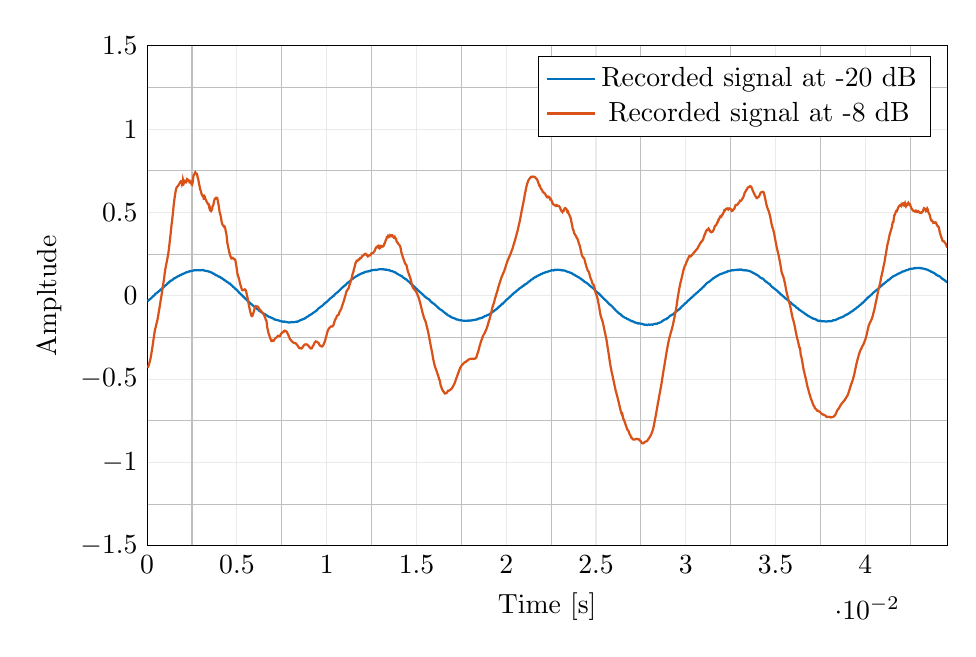
\begin{tikzpicture}

\begin{axis}[%
width=4in,
height=2.5in,
    grid = both,
    minor tick num=1,
    every major grid/.style={opacity=0.3},
    major tick length=0pt,
    minor tick length=0pt,
scale only axis,
xmin=0,
xmax=0.0445578231292517,
xlabel={Time [s]},
ymin=-1.5,
ymax=1.5,
ylabel={Ampltude},
axis background/.style={fill=white}
]
\addplot [color=mycolor1,solid,thick]
  table[row sep=crcr]{%
2.26757369614512e-05	-0.0328369140625\\
4.53514739229025e-05	-0.02972412109375\\
6.80272108843537e-05	-0.027435302734375\\
9.0702947845805e-05	-0.024932861328125\\
0.000113378684807256	-0.023895263671875\\
0.000136054421768707	-0.02191162109375\\
0.000158730158730159	-0.01983642578125\\
0.00018140589569161	-0.018402099609375\\
0.000204081632653061	-0.01605224609375\\
0.000226757369614512	-0.014068603515625\\
0.000249433106575964	-0.011749267578125\\
0.000272108843537415	-0.009124755859375\\
0.000294784580498866	-0.006683349609375\\
0.000317460317460317	-0.00439453125\\
0.000340136054421769	-0.001434326171875\\
0.00036281179138322	0.000579833984375\\
0.000385487528344671	0.001953125\\
0.000408163265306122	0.003631591796875\\
0.000430839002267574	0.007354736328125\\
0.000453514739229025	0.0113525390625\\
0.000476190476190476	0.013397216796875\\
0.000498866213151927	0.01416015625\\
0.000521541950113379	0.0147705078125\\
0.00054421768707483	0.0172119140625\\
0.000566893424036281	0.020050048828125\\
0.000589569160997732	0.021759033203125\\
0.000612244897959184	0.0238037109375\\
0.000634920634920635	0.026397705078125\\
0.000657596371882086	0.027740478515625\\
0.000680272108843537	0.02886962890625\\
0.000702947845804989	0.031829833984375\\
0.00072562358276644	0.03570556640625\\
0.000748299319727891	0.0372314453125\\
0.000770975056689342	0.038848876953125\\
0.000793650793650794	0.041229248046875\\
0.000816326530612245	0.0435791015625\\
0.000839002267573696	0.0457763671875\\
0.000861678004535147	0.047821044921875\\
0.000884353741496599	0.050567626953125\\
0.00090702947845805	0.05145263671875\\
0.000929705215419501	0.052490234375\\
0.000952380952380952	0.0550537109375\\
0.000975056689342404	0.05914306640625\\
0.000997732426303855	0.0614013671875\\
0.00102040816326531	0.062103271484375\\
0.00104308390022676	0.06439208984375\\
0.00106575963718821	0.066558837890625\\
0.00108843537414966	0.068572998046875\\
0.00111111111111111	0.0709228515625\\
0.00113378684807256	0.074066162109375\\
0.00115646258503401	0.076202392578125\\
0.00117913832199546	0.077545166015625\\
0.00120181405895692	0.079559326171875\\
0.00122448979591837	0.0819091796875\\
0.00124716553287982	0.0850830078125\\
0.00126984126984127	0.08746337890625\\
0.00129251700680272	0.08843994140625\\
0.00131519274376417	0.09027099609375\\
0.00133786848072562	0.09173583984375\\
0.00136054421768707	0.0921630859375\\
0.00138321995464853	0.09375\\
0.00140589569160998	0.095672607421875\\
0.00142857142857143	0.097320556640625\\
0.00145124716553288	0.099090576171875\\
0.00147392290249433	0.101531982421875\\
0.00149659863945578	0.104339599609375\\
0.00151927437641723	0.10528564453125\\
0.00154195011337868	0.106475830078125\\
0.00156462585034014	0.107421875\\
0.00158730158730159	0.108673095703125\\
0.00160997732426304	0.1104736328125\\
0.00163265306122449	0.1121826171875\\
0.00165532879818594	0.113677978515625\\
0.00167800453514739	0.11480712890625\\
0.00170068027210884	0.115875244140625\\
0.00172335600907029	0.116790771484375\\
0.00174603174603175	0.118560791015625\\
0.0017687074829932	0.119781494140625\\
0.00179138321995465	0.120635986328125\\
0.0018140589569161	0.122283935546875\\
0.00183673469387755	0.123809814453125\\
0.001859410430839	0.125030517578125\\
0.00188208616780045	0.124969482421875\\
0.0019047619047619	0.1268310546875\\
0.00192743764172336	0.128265380859375\\
0.00195011337868481	0.129302978515625\\
0.00197278911564626	0.130584716796875\\
0.00199546485260771	0.1318359375\\
0.00201814058956916	0.132537841796875\\
0.00204081632653061	0.13311767578125\\
0.00206349206349206	0.134429931640625\\
0.00208616780045351	0.13665771484375\\
0.00210884353741497	0.13739013671875\\
0.00213151927437642	0.137847900390625\\
0.00215419501133787	0.13946533203125\\
0.00217687074829932	0.1407470703125\\
0.00219954648526077	0.14117431640625\\
0.00222222222222222	0.140960693359375\\
0.00224489795918367	0.14215087890625\\
0.00226757369614512	0.143341064453125\\
0.00229024943310658	0.14422607421875\\
0.00231292517006803	0.144805908203125\\
0.00233560090702948	0.146392822265625\\
0.00235827664399093	0.14703369140625\\
0.00238095238095238	0.14642333984375\\
0.00240362811791383	0.14752197265625\\
0.00242630385487528	0.148284912109375\\
0.00244897959183673	0.148406982421875\\
0.00247165532879819	0.149078369140625\\
0.00249433106575964	0.149139404296875\\
0.00251700680272109	0.149993896484375\\
0.00253968253968254	0.151153564453125\\
0.00256235827664399	0.15118408203125\\
0.00258503401360544	0.151702880859375\\
0.00260770975056689	0.153106689453125\\
0.00263038548752834	0.15399169921875\\
0.0026530612244898	0.1534423828125\\
0.00267573696145125	0.1531982421875\\
0.0026984126984127	0.153533935546875\\
0.00272108843537415	0.15338134765625\\
0.0027437641723356	0.153411865234375\\
0.00276643990929705	0.153961181640625\\
0.0027891156462585	0.154144287109375\\
0.00281179138321995	0.15386962890625\\
0.00283446712018141	0.153717041015625\\
0.00285714285714286	0.1539306640625\\
0.00287981859410431	0.153778076171875\\
0.00290249433106576	0.1533203125\\
0.00292517006802721	0.1531982421875\\
0.00294784580498866	0.153472900390625\\
0.00297052154195011	0.153350830078125\\
0.00299319727891156	0.15325927734375\\
0.00301587301587302	0.1533203125\\
0.00303854875283447	0.154144287109375\\
0.00306122448979592	0.15496826171875\\
0.00308390022675737	0.15557861328125\\
0.00310657596371882	0.1551513671875\\
0.00312925170068027	0.153656005859375\\
0.00315192743764172	0.15228271484375\\
0.00317460317460317	0.151397705078125\\
0.00319727891156463	0.151763916015625\\
0.00321995464852608	0.151275634765625\\
0.00324263038548753	0.149658203125\\
0.00326530612244898	0.1494140625\\
0.00328798185941043	0.149505615234375\\
0.00331065759637188	0.149322509765625\\
0.00333333333333333	0.14910888671875\\
0.00335600907029478	0.148101806640625\\
0.00337868480725624	0.14752197265625\\
0.00340136054421769	0.146392822265625\\
0.00342403628117914	0.1461181640625\\
0.00344671201814059	0.145416259765625\\
0.00346938775510204	0.143798828125\\
0.00349206349206349	0.14276123046875\\
0.00351473922902494	0.142303466796875\\
0.00353741496598639	0.1417236328125\\
0.00356009070294785	0.140625\\
0.0035827664399093	0.13922119140625\\
0.00360544217687075	0.1378173828125\\
0.0036281179138322	0.1368408203125\\
0.00365079365079365	0.1356201171875\\
0.0036734693877551	0.133758544921875\\
0.00369614512471655	0.132568359375\\
0.003718820861678	0.132232666015625\\
0.00374149659863946	0.130584716796875\\
0.00376417233560091	0.1282958984375\\
0.00378684807256236	0.12701416015625\\
0.00380952380952381	0.12591552734375\\
0.00383219954648526	0.123687744140625\\
0.00385487528344671	0.1226806640625\\
0.00387755102040816	0.122528076171875\\
0.00390022675736961	0.121734619140625\\
0.00392290249433107	0.118927001953125\\
0.00394557823129252	0.11669921875\\
0.00396825396825397	0.1163330078125\\
0.00399092970521542	0.116241455078125\\
0.00401360544217687	0.1156005859375\\
0.00403628117913832	0.11358642578125\\
0.00405895691609977	0.1124267578125\\
0.00408163265306122	0.1104736328125\\
0.00410430839002268	0.10821533203125\\
0.00412698412698413	0.1068115234375\\
0.00414965986394558	0.106536865234375\\
0.00417233560090703	0.1048583984375\\
0.00419501133786848	0.101898193359375\\
0.00421768707482993	0.100555419921875\\
0.00424036281179138	0.099365234375\\
0.00426303854875283	0.097900390625\\
0.00428571428571429	0.095703125\\
0.00430839002267574	0.094207763671875\\
0.00433106575963719	0.093353271484375\\
0.00435374149659864	0.0906982421875\\
0.00437641723356009	0.08831787109375\\
0.00439909297052154	0.087249755859375\\
0.00442176870748299	0.085906982421875\\
0.00444444444444444	0.084075927734375\\
0.0044671201814059	0.081939697265625\\
0.00448979591836735	0.080902099609375\\
0.0045124716553288	0.079864501953125\\
0.00453514739229025	0.07708740234375\\
0.0045578231292517	0.074920654296875\\
0.00458049886621315	0.073486328125\\
0.0046031746031746	0.073577880859375\\
0.00462585034013605	0.071044921875\\
0.00464852607709751	0.06787109375\\
0.00467120181405896	0.065948486328125\\
0.00469387755102041	0.064178466796875\\
0.00471655328798186	0.06201171875\\
0.00473922902494331	0.0595703125\\
0.00476190476190476	0.057464599609375\\
0.00478458049886621	0.0543212890625\\
0.00480725623582766	0.05194091796875\\
0.00482993197278912	0.050537109375\\
0.00485260770975057	0.049224853515625\\
0.00487528344671202	0.046630859375\\
0.00489795918367347	0.04290771484375\\
0.00492063492063492	0.040374755859375\\
0.00494331065759637	0.03961181640625\\
0.00496598639455782	0.037689208984375\\
0.00498866213151927	0.03509521484375\\
0.00501133786848073	0.033721923828125\\
0.00503401360544218	0.03094482421875\\
0.00505668934240363	0.0269775390625\\
0.00507936507936508	0.024444580078125\\
0.00510204081632653	0.022491455078125\\
0.00512471655328798	0.01904296875\\
0.00514739229024943	0.015899658203125\\
0.00517006802721088	0.014678955078125\\
0.00519274376417234	0.01312255859375\\
0.00521541950113379	0.009857177734375\\
0.00523809523809524	0.007110595703125\\
0.00526077097505669	0.00543212890625\\
0.00528344671201814	0.003265380859375\\
0.00530612244897959	0.00048828125\\
0.00532879818594104	-0.001556396484375\\
0.00535147392290249	-0.00384521484375\\
0.00537414965986395	-0.006439208984375\\
0.0053968253968254	-0.009033203125\\
0.00541950113378685	-0.011688232421875\\
0.0054421768707483	-0.013916015625\\
0.00546485260770975	-0.01617431640625\\
0.0054875283446712	-0.018646240234375\\
0.00551020408163265	-0.021026611328125\\
0.0055328798185941	-0.022247314453125\\
0.00555555555555555	-0.02508544921875\\
0.00557823129251701	-0.0284423828125\\
0.00560090702947846	-0.03082275390625\\
0.00562358276643991	-0.0318603515625\\
0.00564625850340136	-0.033935546875\\
0.00566893424036281	-0.03662109375\\
0.00569160997732426	-0.039215087890625\\
0.00571428571428571	-0.0421142578125\\
0.00573696145124717	-0.043975830078125\\
0.00575963718820862	-0.046478271484375\\
0.00578231292517007	-0.048004150390625\\
0.00580498866213152	-0.04962158203125\\
0.00582766439909297	-0.052490234375\\
0.00585034013605442	-0.05419921875\\
0.00587301587301587	-0.056610107421875\\
0.00589569160997732	-0.059234619140625\\
0.00591836734693878	-0.061187744140625\\
0.00594104308390023	-0.06317138671875\\
0.00596371882086168	-0.064971923828125\\
0.00598639455782313	-0.06671142578125\\
0.00600907029478458	-0.06817626953125\\
0.00603174603174603	-0.069183349609375\\
0.00605442176870748	-0.071868896484375\\
0.00607709750566893	-0.074310302734375\\
0.00609977324263039	-0.07647705078125\\
0.00612244897959184	-0.07861328125\\
0.00614512471655329	-0.080596923828125\\
0.00616780045351474	-0.081634521484375\\
0.00619047619047619	-0.08306884765625\\
0.00621315192743764	-0.08538818359375\\
0.00623582766439909	-0.088958740234375\\
0.00625850340136054	-0.091156005859375\\
0.00628117913832199	-0.0921630859375\\
0.00630385487528345	-0.0936279296875\\
0.0063265306122449	-0.095733642578125\\
0.00634920634920635	-0.0966796875\\
0.0063718820861678	-0.098663330078125\\
0.00639455782312925	-0.100433349609375\\
0.0064172335600907	-0.10113525390625\\
0.00643990929705215	-0.102874755859375\\
0.00646258503401361	-0.10498046875\\
0.00648526077097506	-0.10638427734375\\
0.00650793650793651	-0.107666015625\\
0.00653061224489796	-0.109283447265625\\
0.00655328798185941	-0.110809326171875\\
0.00657596371882086	-0.111907958984375\\
0.00659863945578231	-0.11358642578125\\
0.00662131519274376	-0.115692138671875\\
0.00664399092970522	-0.117156982421875\\
0.00666666666666667	-0.118743896484375\\
0.00668934240362812	-0.119415283203125\\
0.00671201814058957	-0.1209716796875\\
0.00673469387755102	-0.123077392578125\\
0.00675736961451247	-0.1243896484375\\
0.00678004535147392	-0.126068115234375\\
0.00680272108843537	-0.127105712890625\\
0.00682539682539682	-0.127685546875\\
0.00684807256235828	-0.12799072265625\\
0.00687074829931973	-0.128814697265625\\
0.00689342403628118	-0.13043212890625\\
0.00691609977324263	-0.132568359375\\
0.00693877551020408	-0.133453369140625\\
0.00696145124716553	-0.133331298828125\\
0.00698412698412698	-0.13427734375\\
0.00700680272108843	-0.1356201171875\\
0.00702947845804989	-0.137054443359375\\
0.00705215419501134	-0.138763427734375\\
0.00707482993197279	-0.140838623046875\\
0.00709750566893424	-0.14208984375\\
0.00712018140589569	-0.14202880859375\\
0.00714285714285714	-0.142822265625\\
0.00716553287981859	-0.1439208984375\\
0.00718820861678005	-0.1448974609375\\
0.0072108843537415	-0.144805908203125\\
0.00723356009070295	-0.145263671875\\
0.0072562358276644	-0.145721435546875\\
0.00727891156462585	-0.1466064453125\\
0.0073015873015873	-0.147430419921875\\
0.00732426303854875	-0.14752197265625\\
0.0073469387755102	-0.148681640625\\
0.00736961451247166	-0.150543212890625\\
0.00739229024943311	-0.151031494140625\\
0.00741496598639456	-0.151031494140625\\
0.00743764172335601	-0.152435302734375\\
0.00746031746031746	-0.15252685546875\\
0.00748299319727891	-0.15283203125\\
0.00750566893424036	-0.153472900390625\\
0.00752834467120181	-0.154327392578125\\
0.00755102040816326	-0.154876708984375\\
0.00757369614512472	-0.15576171875\\
0.00759637188208617	-0.1556396484375\\
0.00761904761904762	-0.1539306640625\\
0.00764172335600907	-0.153656005859375\\
0.00766439909297052	-0.15484619140625\\
0.00768707482993197	-0.156005859375\\
0.00770975056689342	-0.156768798828125\\
0.00773242630385487	-0.157623291015625\\
0.00775510204081633	-0.15716552734375\\
0.00777777777777778	-0.1573486328125\\
0.00780045351473923	-0.1578369140625\\
0.00782312925170068	-0.15850830078125\\
0.00784580498866213	-0.15899658203125\\
0.00786848072562358	-0.1597900390625\\
0.00789115646258503	-0.16033935546875\\
0.00791383219954649	-0.16058349609375\\
0.00793650793650794	-0.160400390625\\
0.00795918367346939	-0.159149169921875\\
0.00798185941043084	-0.1583251953125\\
0.00800453514739229	-0.15863037109375\\
0.00802721088435374	-0.1585693359375\\
0.00804988662131519	-0.157562255859375\\
0.00807256235827664	-0.157196044921875\\
0.0080952380952381	-0.15771484375\\
0.00811791383219955	-0.15899658203125\\
0.008140589569161	-0.158905029296875\\
0.00816326530612245	-0.158111572265625\\
0.0081859410430839	-0.157684326171875\\
0.00820861678004535	-0.156585693359375\\
0.0082312925170068	-0.15679931640625\\
0.00825396825396825	-0.156280517578125\\
0.00827664399092971	-0.15594482421875\\
0.00829931972789116	-0.155059814453125\\
0.00832199546485261	-0.154815673828125\\
0.00834467120181406	-0.155792236328125\\
0.00836734693877551	-0.155517578125\\
0.00839002267573696	-0.154205322265625\\
0.00841269841269841	-0.15264892578125\\
0.00843537414965987	-0.151611328125\\
0.00845804988662132	-0.1507568359375\\
0.00848072562358277	-0.149505615234375\\
0.00850340136054422	-0.147491455078125\\
0.00852607709750567	-0.146728515625\\
0.00854875283446712	-0.1458740234375\\
0.00857142857142857	-0.14483642578125\\
0.00859410430839002	-0.14447021484375\\
0.00861678004535148	-0.143798828125\\
0.00863945578231293	-0.14178466796875\\
0.00866213151927438	-0.139739990234375\\
0.00868480725623583	-0.139617919921875\\
0.00870748299319728	-0.139923095703125\\
0.00873015873015873	-0.138702392578125\\
0.00875283446712018	-0.1373291015625\\
0.00877551020408163	-0.1361083984375\\
0.00879818594104308	-0.134552001953125\\
0.00882086167800454	-0.13323974609375\\
0.00884353741496599	-0.131500244140625\\
0.00886621315192744	-0.1295166015625\\
0.00888888888888889	-0.126678466796875\\
0.00891156462585034	-0.12518310546875\\
0.00893424036281179	-0.12493896484375\\
0.00895691609977324	-0.123809814453125\\
0.00897959183673469	-0.1221923828125\\
0.00900226757369615	-0.119842529296875\\
0.0090249433106576	-0.11712646484375\\
0.00904761904761905	-0.116302490234375\\
0.0090702947845805	-0.115997314453125\\
0.00909297052154195	-0.114349365234375\\
0.0091156462585034	-0.112060546875\\
0.00913832199546485	-0.110565185546875\\
0.0091609977324263	-0.108978271484375\\
0.00918367346938776	-0.107635498046875\\
0.00920634920634921	-0.10589599609375\\
0.00922902494331066	-0.10406494140625\\
0.00925170068027211	-0.10211181640625\\
0.00927437641723356	-0.100341796875\\
0.00929705215419501	-0.09912109375\\
0.00931972789115646	-0.09722900390625\\
0.00934240362811791	-0.095306396484375\\
0.00936507936507937	-0.094024658203125\\
0.00938775510204082	-0.09228515625\\
0.00941043083900227	-0.090118408203125\\
0.00943310657596372	-0.088226318359375\\
0.00945578231292517	-0.08599853515625\\
0.00947845804988662	-0.0836181640625\\
0.00950113378684807	-0.080535888671875\\
0.00952380952380952	-0.077392578125\\
0.00954648526077098	-0.0758056640625\\
0.00956916099773243	-0.07415771484375\\
0.00959183673469388	-0.0726318359375\\
0.00961451247165533	-0.07061767578125\\
0.00963718820861678	-0.068328857421875\\
0.00965986394557823	-0.0660400390625\\
0.00968253968253968	-0.064208984375\\
0.00970521541950113	-0.06304931640625\\
0.00972789115646258	-0.062164306640625\\
0.00975056689342404	-0.060089111328125\\
0.00977324263038549	-0.058074951171875\\
0.00979591836734694	-0.0557861328125\\
0.00981859410430839	-0.053192138671875\\
0.00984126984126984	-0.050323486328125\\
0.00986394557823129	-0.0474853515625\\
0.00988662131519275	-0.046356201171875\\
0.0099092970521542	-0.044464111328125\\
0.00993197278911565	-0.041748046875\\
0.0099546485260771	-0.039825439453125\\
0.00997732426303855	-0.0382080078125\\
0.01	-0.036590576171875\\
0.0100226757369615	-0.034942626953125\\
0.0100453514739229	-0.032318115234375\\
0.0100680272108844	-0.02935791015625\\
0.0100907029478458	-0.027374267578125\\
0.0101133786848073	-0.025238037109375\\
0.0101360544217687	-0.022552490234375\\
0.0101587301587302	-0.0198974609375\\
0.0101814058956916	-0.016815185546875\\
0.0102040816326531	-0.014434814453125\\
0.0102267573696145	-0.01318359375\\
0.010249433106576	-0.011383056640625\\
0.0102721088435374	-0.0098876953125\\
0.0102947845804989	-0.007965087890625\\
0.0103174603174603	-0.005126953125\\
0.0103401360544218	-0.0029296875\\
0.0103628117913832	-0.00213623046875\\
0.0103854875283447	-0.001007080078125\\
0.0104081632653061	0.00177001953125\\
0.0104308390022676	0.005462646484375\\
0.010453514739229	0.008270263671875\\
0.0104761904761905	0.01031494140625\\
0.0104988662131519	0.012908935546875\\
0.0105215419501134	0.015167236328125\\
0.0105442176870748	0.01617431640625\\
0.0105668934240363	0.018280029296875\\
0.0105895691609977	0.020843505859375\\
0.0106122448979592	0.022064208984375\\
0.0106349206349206	0.02398681640625\\
0.0106575963718821	0.026580810546875\\
0.0106802721088435	0.02972412109375\\
0.010702947845805	0.031494140625\\
0.0107256235827664	0.033843994140625\\
0.0107482993197279	0.036865234375\\
0.0107709750566893	0.0390625\\
0.0107936507936508	0.04156494140625\\
0.0108163265306122	0.04388427734375\\
0.0108390022675737	0.04669189453125\\
0.0108616780045351	0.0487060546875\\
0.0108843537414966	0.050323486328125\\
0.0109070294784581	0.052825927734375\\
0.0109297052154195	0.055419921875\\
0.010952380952381	0.0567626953125\\
0.0109750566893424	0.058563232421875\\
0.0109977324263039	0.061065673828125\\
0.0110204081632653	0.062530517578125\\
0.0110430839002268	0.06451416015625\\
0.0110657596371882	0.06707763671875\\
0.0110884353741497	0.06982421875\\
0.0111111111111111	0.072723388671875\\
0.0111337868480726	0.07489013671875\\
0.011156462585034	0.07708740234375\\
0.0111791383219955	0.079132080078125\\
0.0112018140589569	0.0809326171875\\
0.0112244897959184	0.0823974609375\\
0.0112471655328798	0.08416748046875\\
0.0112698412698413	0.08587646484375\\
0.0112925170068027	0.088043212890625\\
0.0113151927437642	0.089996337890625\\
0.0113378684807256	0.09228515625\\
0.0113605442176871	0.09503173828125\\
0.0113832199546485	0.0972900390625\\
0.01140589569161	0.09942626953125\\
0.0114285714285714	0.100433349609375\\
0.0114512471655329	0.101715087890625\\
0.0114739229024943	0.104583740234375\\
0.0114965986394558	0.10662841796875\\
0.0115192743764172	0.1083984375\\
0.0115419501133787	0.110198974609375\\
0.0115646258503401	0.11138916015625\\
0.0115873015873016	0.112884521484375\\
0.011609977324263	0.11480712890625\\
0.0116326530612245	0.116668701171875\\
0.0116553287981859	0.117950439453125\\
0.0116780045351474	0.1182861328125\\
0.0117006802721088	0.119232177734375\\
0.0117233560090703	0.121429443359375\\
0.0117460317460317	0.123809814453125\\
0.0117687074829932	0.124908447265625\\
0.0117913832199546	0.1265869140625\\
0.0118140589569161	0.127288818359375\\
0.0118367346938776	0.127593994140625\\
0.011859410430839	0.129119873046875\\
0.0118820861678005	0.131317138671875\\
0.0119047619047619	0.132476806640625\\
0.0119274376417234	0.1331787109375\\
0.0119501133786848	0.134002685546875\\
0.0119727891156463	0.135345458984375\\
0.0119954648526077	0.135345458984375\\
0.0120181405895692	0.1363525390625\\
0.0120408163265306	0.138214111328125\\
0.0120634920634921	0.138702392578125\\
0.0120861678004535	0.139923095703125\\
0.012108843537415	0.141754150390625\\
0.0121315192743764	0.14300537109375\\
0.0121541950113379	0.143402099609375\\
0.0121768707482993	0.144195556640625\\
0.0121995464852608	0.145050048828125\\
0.0122222222222222	0.145050048828125\\
0.0122448979591837	0.145599365234375\\
0.0122675736961451	0.146484375\\
0.0122902494331066	0.14593505859375\\
0.012312925170068	0.146270751953125\\
0.0123356009070295	0.14764404296875\\
0.0123582766439909	0.149139404296875\\
0.0123809523809524	0.149444580078125\\
0.0124036281179138	0.14910888671875\\
0.0124263038548753	0.149261474609375\\
0.0124489795918367	0.150970458984375\\
0.0124716553287982	0.152740478515625\\
0.0124943310657596	0.153289794921875\\
0.0125170068027211	0.15325927734375\\
0.0125396825396825	0.1531982421875\\
0.012562358276644	0.154052734375\\
0.0125850340136054	0.154571533203125\\
0.0126077097505669	0.15447998046875\\
0.0126303854875283	0.15460205078125\\
0.0126530612244898	0.1549072265625\\
0.0126757369614512	0.15496826171875\\
0.0126984126984127	0.155975341796875\\
0.0127210884353742	0.155975341796875\\
0.0127437641723356	0.15521240234375\\
0.0127664399092971	0.155029296875\\
0.0127891156462585	0.155853271484375\\
0.01281179138322	0.156158447265625\\
0.0128344671201814	0.1572265625\\
0.0128571428571429	0.157928466796875\\
0.0128798185941043	0.158477783203125\\
0.0129024943310658	0.158660888671875\\
0.0129251700680272	0.158905029296875\\
0.0129478458049887	0.158782958984375\\
0.0129705215419501	0.15899658203125\\
0.0129931972789116	0.15887451171875\\
0.013015873015873	0.158660888671875\\
0.0130385487528345	0.159088134765625\\
0.0130612244897959	0.159271240234375\\
0.0130839002267574	0.159332275390625\\
0.0131065759637188	0.1590576171875\\
0.0131292517006803	0.15960693359375\\
0.0131519274376417	0.16015625\\
0.0131746031746032	0.159393310546875\\
0.0131972789115646	0.157867431640625\\
0.0132199546485261	0.15838623046875\\
0.0132426303854875	0.158477783203125\\
0.013265306122449	0.156585693359375\\
0.0132879818594104	0.155853271484375\\
0.0133106575963719	0.156890869140625\\
0.0133333333333333	0.157440185546875\\
0.0133560090702948	0.156524658203125\\
0.0133786848072562	0.155364990234375\\
0.0134013605442177	0.15557861328125\\
0.0134240362811791	0.154815673828125\\
0.0134467120181406	0.153778076171875\\
0.013469387755102	0.15411376953125\\
0.0134920634920635	0.154815673828125\\
0.0135147392290249	0.152618408203125\\
0.0135374149659864	0.150787353515625\\
0.0135600907029478	0.149505615234375\\
0.0135827664399093	0.148529052734375\\
0.0136054421768707	0.148284912109375\\
0.0136281179138322	0.14788818359375\\
0.0136507936507937	0.14752197265625\\
0.0136734693877551	0.146575927734375\\
0.0136961451247166	0.14599609375\\
0.013718820861678	0.144866943359375\\
0.0137414965986395	0.142913818359375\\
0.0137641723356009	0.1414794921875\\
0.0137868480725624	0.141082763671875\\
0.0138095238095238	0.14105224609375\\
0.0138321995464853	0.139678955078125\\
0.0138548752834467	0.138092041015625\\
0.0138775510204082	0.13580322265625\\
0.0139002267573696	0.13458251953125\\
0.0139229024943311	0.13323974609375\\
0.0139455782312925	0.1309814453125\\
0.013968253968254	0.129638671875\\
0.0139909297052154	0.128204345703125\\
0.0140136054421769	0.127105712890625\\
0.0140362811791383	0.125885009765625\\
0.0140589569160998	0.12457275390625\\
0.0140816326530612	0.123077392578125\\
0.0141043083900227	0.12127685546875\\
0.0141269841269841	0.120208740234375\\
0.0141496598639456	0.119110107421875\\
0.014172335600907	0.1182861328125\\
0.0141950113378685	0.117095947265625\\
0.0142176870748299	0.114959716796875\\
0.0142403628117914	0.11138916015625\\
0.0142630385487528	0.10968017578125\\
0.0142857142857143	0.10858154296875\\
0.0143083900226757	0.107330322265625\\
0.0143310657596372	0.105316162109375\\
0.0143537414965986	0.103057861328125\\
0.0143764172335601	0.100738525390625\\
0.0143990929705215	0.099761962890625\\
0.014421768707483	0.09967041015625\\
0.0144444444444444	0.097747802734375\\
0.0144671201814059	0.094696044921875\\
0.0144897959183673	0.091888427734375\\
0.0145124716553288	0.089996337890625\\
0.0145351473922903	0.08746337890625\\
0.0145578231292517	0.086334228515625\\
0.0145804988662132	0.084869384765625\\
0.0146031746031746	0.083160400390625\\
0.0146258503401361	0.079742431640625\\
0.0146485260770975	0.076171875\\
0.014671201814059	0.0738525390625\\
0.0146938775510204	0.0712890625\\
0.0147165532879819	0.06915283203125\\
0.0147392290249433	0.067779541015625\\
0.0147619047619048	0.06646728515625\\
0.0147845804988662	0.063995361328125\\
0.0148072562358277	0.06103515625\\
0.0148299319727891	0.059326171875\\
0.0148526077097506	0.057525634765625\\
0.014875283446712	0.055328369140625\\
0.0148979591836735	0.052520751953125\\
0.0149206349206349	0.049957275390625\\
0.0149433106575964	0.0472412109375\\
0.0149659863945578	0.04473876953125\\
0.0149886621315193	0.04302978515625\\
0.0150113378684807	0.0411376953125\\
0.0150340136054422	0.038726806640625\\
0.0150566893424036	0.0352783203125\\
0.0150793650793651	0.0333251953125\\
0.0151020408163265	0.031463623046875\\
0.015124716553288	0.028900146484375\\
0.0151473922902494	0.026702880859375\\
0.0151700680272109	0.024627685546875\\
0.0151927437641723	0.022369384765625\\
0.0152154195011338	0.02020263671875\\
0.0152380952380952	0.018829345703125\\
0.0152607709750567	0.016754150390625\\
0.0152834467120181	0.01416015625\\
0.0153061224489796	0.01171875\\
0.015328798185941	0.009429931640625\\
0.0153514739229025	0.007781982421875\\
0.0153741496598639	0.005615234375\\
0.0153968253968254	0.0032958984375\\
0.0154195011337868	0.0009765625\\
0.0154421768707483	-0.00201416015625\\
0.0154648526077098	-0.004364013671875\\
0.0154875283446712	-0.0064697265625\\
0.0155102040816327	-0.00860595703125\\
0.0155328798185941	-0.009735107421875\\
0.0155555555555556	-0.011322021484375\\
0.015578231292517	-0.01348876953125\\
0.0156009070294785	-0.01568603515625\\
0.0156235827664399	-0.01666259765625\\
0.0156462585034014	-0.017852783203125\\
0.0156689342403628	-0.01934814453125\\
0.0156916099773243	-0.021240234375\\
0.0157142857142857	-0.023712158203125\\
0.0157369614512472	-0.026275634765625\\
0.0157596371882086	-0.0291748046875\\
0.0157823129251701	-0.0325927734375\\
0.0158049886621315	-0.035186767578125\\
0.015827664399093	-0.036285400390625\\
0.0158503401360544	-0.038238525390625\\
0.0158730158730159	-0.040802001953125\\
0.0158956916099773	-0.0426025390625\\
0.0159183673469388	-0.044769287109375\\
0.0159410430839002	-0.046173095703125\\
0.0159637188208617	-0.0474853515625\\
0.0159863945578231	-0.048858642578125\\
0.0160090702947846	-0.050628662109375\\
0.016031746031746	-0.05303955078125\\
0.0160544217687075	-0.05584716796875\\
0.0160770975056689	-0.057769775390625\\
0.0160997732426304	-0.06005859375\\
0.0161224489795918	-0.06268310546875\\
0.0161451247165533	-0.065032958984375\\
0.0161678004535147	-0.067047119140625\\
0.0161904761904762	-0.0689697265625\\
0.0162131519274376	-0.0711669921875\\
0.0162358276643991	-0.074493408203125\\
0.0162585034013605	-0.076171875\\
0.016281179138322	-0.07794189453125\\
0.0163038548752834	-0.080352783203125\\
0.0163265306122449	-0.08221435546875\\
0.0163492063492063	-0.082794189453125\\
0.0163718820861678	-0.084136962890625\\
0.0163945578231292	-0.086578369140625\\
0.0164172335600907	-0.087646484375\\
0.0164399092970522	-0.0894775390625\\
0.0164625850340136	-0.091949462890625\\
0.0164852607709751	-0.093994140625\\
0.0165079365079365	-0.0953369140625\\
0.016530612244898	-0.097625732421875\\
0.0165532879818594	-0.100006103515625\\
0.0165759637188209	-0.101837158203125\\
0.0165986394557823	-0.103424072265625\\
0.0166213151927438	-0.105255126953125\\
0.0166439909297052	-0.107421875\\
0.0166666666666667	-0.10906982421875\\
0.0166893424036281	-0.11077880859375\\
0.0167120181405896	-0.11328125\\
0.016734693877551	-0.11529541015625\\
0.0167573696145125	-0.116668701171875\\
0.0167800453514739	-0.117889404296875\\
0.0168027210884354	-0.119140625\\
0.0168253968253968	-0.119598388671875\\
0.0168480725623583	-0.120635986328125\\
0.0168707482993197	-0.123565673828125\\
0.0168934240362812	-0.125885009765625\\
0.0169160997732426	-0.126312255859375\\
0.0169387755102041	-0.127227783203125\\
0.0169614512471655	-0.12939453125\\
0.016984126984127	-0.130645751953125\\
0.0170068027210884	-0.1314697265625\\
0.0170294784580499	-0.132080078125\\
0.0170521541950113	-0.1326904296875\\
0.0170748299319728	-0.133270263671875\\
0.0170975056689342	-0.13458251953125\\
0.0171201814058957	-0.13555908203125\\
0.0171428571428571	-0.135986328125\\
0.0171655328798186	-0.137420654296875\\
0.01718820861678	-0.139556884765625\\
0.0172108843537415	-0.14117431640625\\
0.0172335600907029	-0.14178466796875\\
0.0172562358276644	-0.141876220703125\\
0.0172789115646259	-0.142120361328125\\
0.0173015873015873	-0.14288330078125\\
0.0173242630385488	-0.143218994140625\\
0.0173469387755102	-0.14434814453125\\
0.0173696145124717	-0.145751953125\\
0.0173922902494331	-0.14691162109375\\
0.0174149659863946	-0.147186279296875\\
0.017437641723356	-0.14617919921875\\
0.0174603174603175	-0.146331787109375\\
0.0174829931972789	-0.14691162109375\\
0.0175056689342404	-0.1473388671875\\
0.0175283446712018	-0.1478271484375\\
0.0175510204081633	-0.148406982421875\\
0.0175736961451247	-0.1488037109375\\
0.0175963718820862	-0.1490478515625\\
0.0176190476190476	-0.149383544921875\\
0.0176417233560091	-0.14990234375\\
0.0176643990929705	-0.14990234375\\
0.017687074829932	-0.149688720703125\\
0.0177097505668934	-0.14984130859375\\
0.0177324263038549	-0.149139404296875\\
0.0177551020408163	-0.15008544921875\\
0.0177777777777778	-0.1497802734375\\
0.0178004535147392	-0.149627685546875\\
0.0178231292517007	-0.149749755859375\\
0.0178458049886621	-0.149932861328125\\
0.0178684807256236	-0.149078369140625\\
0.017891156462585	-0.148193359375\\
0.0179138321995465	-0.148590087890625\\
0.0179365079365079	-0.149322509765625\\
0.0179591836734694	-0.1490478515625\\
0.0179818594104308	-0.148284912109375\\
0.0180045351473923	-0.14849853515625\\
0.0180272108843537	-0.148651123046875\\
0.0180498866213152	-0.1480712890625\\
0.0180725623582766	-0.146881103515625\\
0.0180952380952381	-0.147552490234375\\
0.0181179138321995	-0.147216796875\\
0.018140589569161	-0.145751953125\\
0.0181632653061224	-0.144561767578125\\
0.0181859410430839	-0.14483642578125\\
0.0182086167800454	-0.145233154296875\\
0.0182312925170068	-0.144500732421875\\
0.0182539682539683	-0.14404296875\\
0.0182766439909297	-0.144073486328125\\
0.0182993197278912	-0.14361572265625\\
0.0183219954648526	-0.14178466796875\\
0.0183446712018141	-0.14141845703125\\
0.0183673469387755	-0.1422119140625\\
0.018390022675737	-0.1402587890625\\
0.0184126984126984	-0.13824462890625\\
0.0184353741496599	-0.13775634765625\\
0.0184580498866213	-0.1373291015625\\
0.0184807256235828	-0.13616943359375\\
0.0185034013605442	-0.13531494140625\\
0.0185260770975057	-0.13568115234375\\
0.0185487528344671	-0.1353759765625\\
0.0185714285714286	-0.133941650390625\\
0.01859410430839	-0.13287353515625\\
0.0186167800453515	-0.13275146484375\\
0.0186394557823129	-0.132659912109375\\
0.0186621315192744	-0.130157470703125\\
0.0186848072562358	-0.12890625\\
0.0187074829931973	-0.1287841796875\\
0.0187301587301587	-0.12774658203125\\
0.0187528344671202	-0.125762939453125\\
0.0187755102040816	-0.123870849609375\\
0.0187981859410431	-0.122711181640625\\
0.0188208616780045	-0.12152099609375\\
0.018843537414966	-0.12139892578125\\
0.0188662131519274	-0.1207275390625\\
0.0188888888888889	-0.120147705078125\\
0.0189115646258503	-0.118194580078125\\
0.0189342403628118	-0.116729736328125\\
0.0189569160997732	-0.1153564453125\\
0.0189795918367347	-0.11468505859375\\
0.0190022675736961	-0.113922119140625\\
0.0190249433106576	-0.112640380859375\\
0.019047619047619	-0.111572265625\\
0.0190702947845805	-0.110443115234375\\
0.0190929705215419	-0.108673095703125\\
0.0191156462585034	-0.106109619140625\\
0.0191383219954649	-0.104705810546875\\
0.0191609977324263	-0.1031494140625\\
0.0191836734693878	-0.10125732421875\\
0.0192063492063492	-0.09954833984375\\
0.0192290249433107	-0.097503662109375\\
0.0192517006802721	-0.095367431640625\\
0.0192743764172336	-0.09442138671875\\
0.019297052154195	-0.092803955078125\\
0.0193197278911565	-0.091400146484375\\
0.0193424036281179	-0.08941650390625\\
0.0193650793650794	-0.086669921875\\
0.0193877551020408	-0.084747314453125\\
0.0194104308390023	-0.083038330078125\\
0.0194331065759637	-0.081756591796875\\
0.0194557823129252	-0.0799560546875\\
0.0194784580498866	-0.0780029296875\\
0.0195011337868481	-0.07513427734375\\
0.0195238095238095	-0.0731201171875\\
0.019546485260771	-0.071319580078125\\
0.0195691609977324	-0.069000244140625\\
0.0195918367346939	-0.0660400390625\\
0.0196145124716553	-0.06378173828125\\
0.0196371882086168	-0.062530517578125\\
0.0196598639455782	-0.061004638671875\\
0.0196825396825397	-0.058258056640625\\
0.0197052154195011	-0.05517578125\\
0.0197278911564626	-0.053131103515625\\
0.019750566893424	-0.050445556640625\\
0.0197732426303855	-0.04803466796875\\
0.0197959183673469	-0.04766845703125\\
0.0198185941043084	-0.046295166015625\\
0.0198412698412698	-0.04345703125\\
0.0198639455782313	-0.040313720703125\\
0.0198866213151927	-0.037811279296875\\
0.0199092970521542	-0.035552978515625\\
0.0199319727891156	-0.033050537109375\\
0.0199546485260771	-0.030731201171875\\
0.0199773242630385	-0.02783203125\\
0.02	-0.025482177734375\\
0.0200226757369615	-0.023101806640625\\
0.0200453514739229	-0.02105712890625\\
0.0200680272108844	-0.01971435546875\\
0.0200907029478458	-0.017822265625\\
0.0201133786848073	-0.015472412109375\\
0.0201360544217687	-0.012908935546875\\
0.0201587301587302	-0.010498046875\\
0.0201814058956916	-0.008636474609375\\
0.0202040816326531	-0.006072998046875\\
0.0202267573696145	-0.003173828125\\
0.020249433106576	-0.001953125\\
0.0202721088435374	0.0001220703125\\
0.0202947845804989	0.003082275390625\\
0.0203174603174603	0.00628662109375\\
0.0203401360544218	0.007843017578125\\
0.0203628117913832	0.009490966796875\\
0.0203854875283447	0.01275634765625\\
0.0204081632653061	0.014892578125\\
0.0204308390022676	0.016632080078125\\
0.020453514739229	0.018951416015625\\
0.0204761904761905	0.020233154296875\\
0.0204988662131519	0.0220947265625\\
0.0205215419501134	0.024078369140625\\
0.0205442176870748	0.026092529296875\\
0.0205668934240363	0.028778076171875\\
0.0205895691609977	0.0303955078125\\
0.0206122448979592	0.032073974609375\\
0.0206349206349206	0.034942626953125\\
0.0206575963718821	0.037384033203125\\
0.0206802721088435	0.0380859375\\
0.020702947845805	0.03985595703125\\
0.0207256235827664	0.042572021484375\\
0.0207482993197279	0.044830322265625\\
0.0207709750566893	0.04681396484375\\
0.0207936507936508	0.047882080078125\\
0.0208163265306122	0.049774169921875\\
0.0208390022675737	0.0513916015625\\
0.0208616780045351	0.0531005859375\\
0.0208843537414966	0.055084228515625\\
0.020907029478458	0.057342529296875\\
0.0209297052154195	0.05841064453125\\
0.020952380952381	0.05938720703125\\
0.0209750566893424	0.062042236328125\\
0.0209977324263039	0.064697265625\\
0.0210204081632653	0.0672607421875\\
0.0210430839002268	0.06768798828125\\
0.0210657596371882	0.0694580078125\\
0.0210884353741497	0.07049560546875\\
0.0211111111111111	0.07183837890625\\
0.0211337868480726	0.0733642578125\\
0.021156462585034	0.0748291015625\\
0.0211791383219955	0.077484130859375\\
0.0212018140589569	0.079345703125\\
0.0212244897959184	0.08148193359375\\
0.0212471655328798	0.084564208984375\\
0.0212698412698413	0.08587646484375\\
0.0212925170068027	0.0865478515625\\
0.0213151927437642	0.088470458984375\\
0.0213378684807256	0.090667724609375\\
0.0213605442176871	0.09368896484375\\
0.0213832199546485	0.095977783203125\\
0.02140589569161	0.097015380859375\\
0.0214285714285714	0.09808349609375\\
0.0214512471655329	0.100006103515625\\
0.0214739229024943	0.10205078125\\
0.0214965986394558	0.103271484375\\
0.0215192743764172	0.10540771484375\\
0.0215419501133787	0.10809326171875\\
0.0215646258503401	0.109222412109375\\
0.0215873015873016	0.1097412109375\\
0.021609977324263	0.1112060546875\\
0.0216326530612245	0.113494873046875\\
0.0216553287981859	0.114715576171875\\
0.0216780045351474	0.114593505859375\\
0.0217006802721088	0.11676025390625\\
0.0217233560090703	0.11883544921875\\
0.0217460317460317	0.119842529296875\\
0.0217687074829932	0.12091064453125\\
0.0217913832199546	0.1220703125\\
0.0218140589569161	0.124114990234375\\
0.0218367346938775	0.124237060546875\\
0.021859410430839	0.125\\
0.0218820861678005	0.1268310546875\\
0.0219047619047619	0.128692626953125\\
0.0219274376417234	0.130584716796875\\
0.0219501133786848	0.130706787109375\\
0.0219727891156463	0.130859375\\
0.0219954648526077	0.13232421875\\
0.0220181405895692	0.133819580078125\\
0.0220408163265306	0.135009765625\\
0.0220634920634921	0.136627197265625\\
0.0220861678004535	0.137298583984375\\
0.022108843537415	0.137969970703125\\
0.0221315192743764	0.13836669921875\\
0.0221541950113379	0.139373779296875\\
0.0221768707482993	0.141082763671875\\
0.0221995464852608	0.141876220703125\\
0.0222222222222222	0.142181396484375\\
0.0222448979591837	0.1429443359375\\
0.0222675736961451	0.14337158203125\\
0.0222902494331066	0.14337158203125\\
0.022312925170068	0.144500732421875\\
0.0223356009070295	0.146514892578125\\
0.0223582766439909	0.14691162109375\\
0.0223809523809524	0.14788818359375\\
0.0224036281179138	0.1484375\\
0.0224263038548753	0.14935302734375\\
0.0224489795918367	0.15008544921875\\
0.0224716553287982	0.1502685546875\\
0.0224943310657596	0.1510009765625\\
0.0225170068027211	0.15301513671875\\
0.0225396825396825	0.15380859375\\
0.022562358276644	0.153045654296875\\
0.0225850340136054	0.152587890625\\
0.0226077097505669	0.15240478515625\\
0.0226303854875283	0.152252197265625\\
0.0226530612244898	0.1529541015625\\
0.0226757369614512	0.155029296875\\
0.0226984126984127	0.1561279296875\\
0.0227210884353742	0.156005859375\\
0.0227437641723356	0.155181884765625\\
0.0227664399092971	0.1553955078125\\
0.0227891156462585	0.155120849609375\\
0.02281179138322	0.15582275390625\\
0.0228344671201814	0.156829833984375\\
0.0228571428571429	0.1568603515625\\
0.0228798185941043	0.157012939453125\\
0.0229024943310658	0.15631103515625\\
0.0229251700680272	0.1558837890625\\
0.0229478458049887	0.155364990234375\\
0.0229705215419501	0.1551513671875\\
0.0229931972789116	0.155181884765625\\
0.023015873015873	0.15460205078125\\
0.0230385487528345	0.15472412109375\\
0.0230612244897959	0.15447998046875\\
0.0230839002267574	0.152740478515625\\
0.0231065759637188	0.15203857421875\\
0.0231292517006803	0.152313232421875\\
0.0231519274376417	0.153045654296875\\
0.0231746031746032	0.15264892578125\\
0.0231972789115646	0.152252197265625\\
0.0232199546485261	0.1524658203125\\
0.0232426303854875	0.1514892578125\\
0.023265306122449	0.151123046875\\
0.0232879818594104	0.149444580078125\\
0.0233106575963719	0.148406982421875\\
0.0233333333333333	0.14794921875\\
0.0233560090702948	0.14697265625\\
0.0233786848072562	0.1453857421875\\
0.0234013605442177	0.14459228515625\\
0.0234240362811791	0.14410400390625\\
0.0234467120181406	0.14312744140625\\
0.023469387755102	0.1431884765625\\
0.0234920634920635	0.14276123046875\\
0.0235147392290249	0.141693115234375\\
0.0235374149659864	0.14013671875\\
0.0235600907029478	0.138427734375\\
0.0235827664399093	0.137481689453125\\
0.0236054421768707	0.137451171875\\
0.0236281179138322	0.136932373046875\\
0.0236507936507937	0.1351318359375\\
0.0236734693877551	0.133819580078125\\
0.0236961451247166	0.131988525390625\\
0.023718820861678	0.129486083984375\\
0.0237414965986395	0.128143310546875\\
0.0237641723356009	0.12713623046875\\
0.0237868480725624	0.126617431640625\\
0.0238095238095238	0.125213623046875\\
0.0238321995464853	0.123321533203125\\
0.0238548752834467	0.12152099609375\\
0.0238775510204082	0.120574951171875\\
0.0239002267573696	0.11944580078125\\
0.0239229024943311	0.11785888671875\\
0.0239455782312925	0.11602783203125\\
0.023968253968254	0.114013671875\\
0.0239909297052154	0.11273193359375\\
0.0240136054421769	0.111297607421875\\
0.0240362811791383	0.110595703125\\
0.0240589569160998	0.109619140625\\
0.0240816326530612	0.10748291015625\\
0.0241043083900227	0.10540771484375\\
0.0241269841269841	0.10443115234375\\
0.0241496598639456	0.10321044921875\\
0.024172335600907	0.101409912109375\\
0.0241950113378685	0.09893798828125\\
0.0242176870748299	0.096771240234375\\
0.0242403628117914	0.094879150390625\\
0.0242630385487528	0.093780517578125\\
0.0242857142857143	0.09149169921875\\
0.0243083900226757	0.08941650390625\\
0.0243310657596372	0.0880126953125\\
0.0243537414965986	0.085113525390625\\
0.0243764172335601	0.082733154296875\\
0.0243990929705215	0.081451416015625\\
0.024421768707483	0.080810546875\\
0.0244444444444444	0.079742431640625\\
0.0244671201814059	0.07794189453125\\
0.0244897959183673	0.0762939453125\\
0.0245124716553288	0.074249267578125\\
0.0245351473922902	0.072845458984375\\
0.0245578231292517	0.0711669921875\\
0.0245804988662132	0.06890869140625\\
0.0246031746031746	0.06585693359375\\
0.0246258503401361	0.0633544921875\\
0.0246485260770975	0.061187744140625\\
0.024671201814059	0.059326171875\\
0.0246938775510204	0.0579833984375\\
0.0247165532879819	0.05517578125\\
0.0247392290249433	0.053192138671875\\
0.0247619047619048	0.052154541015625\\
0.0247845804988662	0.050201416015625\\
0.0248072562358277	0.0484619140625\\
0.0248299319727891	0.04644775390625\\
0.0248526077097506	0.044158935546875\\
0.024875283446712	0.041778564453125\\
0.0248979591836735	0.03955078125\\
0.0249206349206349	0.03570556640625\\
0.0249433106575964	0.033905029296875\\
0.0249659863945578	0.03155517578125\\
0.0249886621315193	0.02850341796875\\
0.0250113378684807	0.0262451171875\\
0.0250340136054422	0.023590087890625\\
0.0250566893424036	0.02166748046875\\
0.0250793650793651	0.019775390625\\
0.0251020408163265	0.017791748046875\\
0.025124716553288	0.016448974609375\\
0.0251473922902494	0.01483154296875\\
0.0251700680272109	0.01202392578125\\
0.0251927437641723	0.00933837890625\\
0.0252154195011338	0.00677490234375\\
0.0252380952380952	0.004425048828125\\
0.0252607709750567	0.002044677734375\\
0.0252834467120181	-0.000885009765625\\
0.0253061224489796	-0.00341796875\\
0.025328798185941	-0.005340576171875\\
0.0253514739229025	-0.007720947265625\\
0.0253741496598639	-0.010986328125\\
0.0253968253968254	-0.01348876953125\\
0.0254195011337868	-0.0159912109375\\
0.0254421768707483	-0.01806640625\\
0.0254648526077098	-0.020263671875\\
0.0254875283446712	-0.022552490234375\\
0.0255102040816327	-0.02471923828125\\
0.0255328798185941	-0.026947021484375\\
0.0255555555555556	-0.02880859375\\
0.025578231292517	-0.031005859375\\
0.0256009070294785	-0.033477783203125\\
0.0256235827664399	-0.036651611328125\\
0.0256462585034014	-0.03955078125\\
0.0256689342403628	-0.04193115234375\\
0.0256916099773243	-0.044677734375\\
0.0257142857142857	-0.04730224609375\\
0.0257369614512472	-0.049560546875\\
0.0257596371882086	-0.05157470703125\\
0.0257823129251701	-0.0538330078125\\
0.0258049886621315	-0.05535888671875\\
0.025827664399093	-0.056640625\\
0.0258503401360544	-0.05902099609375\\
0.0258730158730159	-0.061614990234375\\
0.0258956916099773	-0.0643310546875\\
0.0259183673469388	-0.06671142578125\\
0.0259410430839002	-0.068572998046875\\
0.0259637188208617	-0.0716552734375\\
0.0259863945578231	-0.074554443359375\\
0.0260090702947846	-0.077911376953125\\
0.026031746031746	-0.079681396484375\\
0.0260544217687075	-0.08148193359375\\
0.0260770975056689	-0.084808349609375\\
0.0260997732426304	-0.087493896484375\\
0.0261224489795918	-0.09002685546875\\
0.0261451247165533	-0.09271240234375\\
0.0261678004535147	-0.094482421875\\
0.0261904761904762	-0.096038818359375\\
0.0262131519274376	-0.0986328125\\
0.0262358276643991	-0.1015625\\
0.0262585034013605	-0.103607177734375\\
0.026281179138322	-0.10504150390625\\
0.0263038548752834	-0.1070556640625\\
0.0263265306122449	-0.108428955078125\\
0.0263492063492063	-0.110107421875\\
0.0263718820861678	-0.111663818359375\\
0.0263945578231293	-0.113739013671875\\
0.0264172335600907	-0.1162109375\\
0.0264399092970522	-0.11865234375\\
0.0264625850340136	-0.121124267578125\\
0.0264852607709751	-0.12310791015625\\
0.0265079365079365	-0.12451171875\\
0.026530612244898	-0.1265869140625\\
0.0265532879818594	-0.127532958984375\\
0.0265759637188209	-0.12890625\\
0.0265986394557823	-0.130340576171875\\
0.0266213151927438	-0.1319580078125\\
0.0266439909297052	-0.133514404296875\\
0.0266666666666667	-0.134002685546875\\
0.0266893424036281	-0.13482666015625\\
0.0267120181405896	-0.136871337890625\\
0.026734693877551	-0.138763427734375\\
0.0267573696145125	-0.1392822265625\\
0.0267800453514739	-0.139617919921875\\
0.0268027210884354	-0.141326904296875\\
0.0268253968253968	-0.14288330078125\\
0.0268480725623583	-0.1435546875\\
0.0268707482993197	-0.14508056640625\\
0.0268934240362812	-0.14691162109375\\
0.0269160997732426	-0.147796630859375\\
0.0269387755102041	-0.149505615234375\\
0.0269614512471655	-0.150634765625\\
0.026984126984127	-0.152099609375\\
0.0270068027210884	-0.1527099609375\\
0.0270294784580499	-0.151824951171875\\
0.0270521541950113	-0.153289794921875\\
0.0270748299319728	-0.15521240234375\\
0.0270975056689342	-0.156646728515625\\
0.0271201814058957	-0.15692138671875\\
0.0271428571428571	-0.157562255859375\\
0.0271655328798186	-0.159759521484375\\
0.02718820861678	-0.160003662109375\\
0.0272108843537415	-0.160308837890625\\
0.0272335600907029	-0.162200927734375\\
0.0272562358276644	-0.16357421875\\
0.0272789115646258	-0.163818359375\\
0.0273015873015873	-0.164093017578125\\
0.0273242630385488	-0.16522216796875\\
0.0273469387755102	-0.166290283203125\\
0.0273696145124717	-0.1656494140625\\
0.0273922902494331	-0.164947509765625\\
0.0274149659863946	-0.165771484375\\
0.027437641723356	-0.166656494140625\\
0.0274603174603175	-0.16668701171875\\
0.0274829931972789	-0.16729736328125\\
0.0275056689342404	-0.168212890625\\
0.0275283446712018	-0.16796875\\
0.0275510204081633	-0.16802978515625\\
0.0275736961451247	-0.1685791015625\\
0.0275963718820862	-0.170379638671875\\
0.0276190476190476	-0.17034912109375\\
0.0276417233560091	-0.170684814453125\\
0.0276643990929705	-0.17193603515625\\
0.027687074829932	-0.172698974609375\\
0.0277097505668934	-0.1739501953125\\
0.0277324263038549	-0.17327880859375\\
0.0277551020408163	-0.17340087890625\\
0.0277777777777778	-0.173828125\\
0.0278004535147392	-0.17401123046875\\
0.0278231292517007	-0.17425537109375\\
0.0278458049886621	-0.1749267578125\\
0.0278684807256236	-0.1746826171875\\
0.027891156462585	-0.17376708984375\\
0.0279138321995465	-0.172607421875\\
0.0279365079365079	-0.17205810546875\\
0.0279591836734694	-0.172698974609375\\
0.0279818594104308	-0.173614501953125\\
0.0280045351473923	-0.17425537109375\\
0.0280272108843537	-0.173736572265625\\
0.0280498866213152	-0.172698974609375\\
0.0280725623582766	-0.172821044921875\\
0.0280952380952381	-0.172760009765625\\
0.0281179138321995	-0.173126220703125\\
0.028140589569161	-0.173614501953125\\
0.0281632653061224	-0.17291259765625\\
0.0281859410430839	-0.171722412109375\\
0.0282086167800454	-0.170074462890625\\
0.0282312925170068	-0.169158935546875\\
0.0282539682539683	-0.168853759765625\\
0.0282766439909297	-0.16925048828125\\
0.0282993197278912	-0.16790771484375\\
0.0283219954648526	-0.167999267578125\\
0.0283446712018141	-0.168609619140625\\
0.0283673469387755	-0.1683349609375\\
0.028390022675737	-0.167938232421875\\
0.0284126984126984	-0.16571044921875\\
0.0284353741496599	-0.164398193359375\\
0.0284580498866213	-0.163818359375\\
0.0284807256235828	-0.163299560546875\\
0.0285034013605442	-0.162322998046875\\
0.0285260770975057	-0.162078857421875\\
0.0285487528344671	-0.1610107421875\\
0.0285714285714286	-0.15960693359375\\
0.02859410430839	-0.159454345703125\\
0.0286167800453515	-0.15802001953125\\
0.0286394557823129	-0.15631103515625\\
0.0286621315192744	-0.15423583984375\\
0.0286848072562358	-0.1519775390625\\
0.0287074829931973	-0.150543212890625\\
0.0287301587301587	-0.14892578125\\
0.0287528344671202	-0.147216796875\\
0.0287755102040816	-0.145782470703125\\
0.0287981859410431	-0.144073486328125\\
0.0288208616780045	-0.143096923828125\\
0.028843537414966	-0.1419677734375\\
0.0288662131519274	-0.141204833984375\\
0.0288888888888889	-0.141357421875\\
0.0289115646258503	-0.1405029296875\\
0.0289342403628118	-0.1383056640625\\
0.0289569160997732	-0.135345458984375\\
0.0289795918367347	-0.13323974609375\\
0.0290022675736961	-0.132232666015625\\
0.0290249433106576	-0.13079833984375\\
0.029047619047619	-0.128631591796875\\
0.0290702947845805	-0.125701904296875\\
0.0290929705215419	-0.123382568359375\\
0.0291156462585034	-0.120941162109375\\
0.0291383219954649	-0.11920166015625\\
0.0291609977324263	-0.11883544921875\\
0.0291836734693878	-0.11761474609375\\
0.0292063492063492	-0.11639404296875\\
0.0292290249433107	-0.11376953125\\
0.0292517006802721	-0.11212158203125\\
0.0292743764172336	-0.1119384765625\\
0.029297052154195	-0.11126708984375\\
0.0293197278911565	-0.1094970703125\\
0.0293424036281179	-0.10650634765625\\
0.0293650793650794	-0.10345458984375\\
0.0293877551020408	-0.10198974609375\\
0.0294104308390023	-0.0997314453125\\
0.0294331065759637	-0.097412109375\\
0.0294557823129252	-0.095367431640625\\
0.0294784580498866	-0.09259033203125\\
0.0295011337868481	-0.090667724609375\\
0.0295238095238095	-0.08905029296875\\
0.029546485260771	-0.0880126953125\\
0.0295691609977324	-0.086273193359375\\
0.0295918367346939	-0.084259033203125\\
0.0296145124716553	-0.08233642578125\\
0.0296371882086168	-0.08074951171875\\
0.0296598639455782	-0.078369140625\\
0.0296825396825397	-0.075408935546875\\
0.0297052154195011	-0.073333740234375\\
0.0297278911564626	-0.071136474609375\\
0.029750566893424	-0.0679931640625\\
0.0297732426303855	-0.0645751953125\\
0.0297959183673469	-0.062530517578125\\
0.0298185941043084	-0.06097412109375\\
0.0298412698412698	-0.05914306640625\\
0.0298639455782313	-0.056488037109375\\
0.0298866213151927	-0.054412841796875\\
0.0299092970521542	-0.051849365234375\\
0.0299319727891156	-0.04864501953125\\
0.0299546485260771	-0.04595947265625\\
0.0299773242630385	-0.044891357421875\\
0.03	-0.043548583984375\\
0.0300226757369614	-0.041656494140625\\
0.0300453514739229	-0.03912353515625\\
0.0300680272108844	-0.036102294921875\\
0.0300907029478458	-0.03302001953125\\
0.0301133786848073	-0.0301513671875\\
0.0301360544217687	-0.02777099609375\\
0.0301587301587302	-0.026580810546875\\
0.0301814058956916	-0.02545166015625\\
0.0302040816326531	-0.022369384765625\\
0.0302267573696145	-0.019317626953125\\
0.030249433106576	-0.0174560546875\\
0.0302721088435374	-0.015472412109375\\
0.0302947845804989	-0.01251220703125\\
0.0303174603174603	-0.010345458984375\\
0.0303401360544218	-0.00933837890625\\
0.0303628117913832	-0.007568359375\\
0.0303854875283447	-0.00506591796875\\
0.0304081632653061	-0.002532958984375\\
0.0304308390022676	0.00030517578125\\
0.030453514739229	0.00299072265625\\
0.0304761904761905	0.005767822265625\\
0.0304988662131519	0.007049560546875\\
0.0305215419501134	0.008392333984375\\
0.0305442176870748	0.010467529296875\\
0.0305668934240363	0.01336669921875\\
0.0305895691609977	0.015838623046875\\
0.0306122448979592	0.01788330078125\\
0.0306349206349206	0.01934814453125\\
0.0306575963718821	0.021240234375\\
0.0306802721088435	0.02325439453125\\
0.030702947845805	0.02581787109375\\
0.0307256235827664	0.028717041015625\\
0.0307482993197279	0.031005859375\\
0.0307709750566893	0.032806396484375\\
0.0307936507936508	0.034637451171875\\
0.0308163265306122	0.03765869140625\\
0.0308390022675737	0.0390625\\
0.0308616780045351	0.041473388671875\\
0.0308843537414966	0.04339599609375\\
0.0309070294784581	0.0462646484375\\
0.0309297052154195	0.049163818359375\\
0.030952380952381	0.050933837890625\\
0.0309750566893424	0.053131103515625\\
0.0309977324263039	0.055419921875\\
0.0310204081632653	0.057647705078125\\
0.0310430839002268	0.06048583984375\\
0.0310657596371882	0.063507080078125\\
0.0310884353741497	0.066070556640625\\
0.0311111111111111	0.068939208984375\\
0.0311337868480726	0.0721435546875\\
0.031156462585034	0.07470703125\\
0.0311791383219955	0.07611083984375\\
0.0312018140589569	0.07757568359375\\
0.0312244897959184	0.079315185546875\\
0.0312471655328798	0.081146240234375\\
0.0312698412698413	0.08294677734375\\
0.0312925170068027	0.084564208984375\\
0.0313151927437642	0.085296630859375\\
0.0313378684807256	0.08685302734375\\
0.0313605442176871	0.0892333984375\\
0.0313832199546485	0.09222412109375\\
0.03140589569161	0.093780517578125\\
0.0314285714285714	0.09552001953125\\
0.0314512471655329	0.098052978515625\\
0.0314739229024943	0.099456787109375\\
0.0314965986394558	0.101165771484375\\
0.0315192743764172	0.104217529296875\\
0.0315419501133787	0.105865478515625\\
0.0315646258503401	0.10687255859375\\
0.0315873015873016	0.10833740234375\\
0.031609977324263	0.110321044921875\\
0.0316326530612245	0.112060546875\\
0.0316553287981859	0.11334228515625\\
0.0316780045351474	0.115234375\\
0.0317006802721088	0.116851806640625\\
0.0317233560090703	0.117095947265625\\
0.0317460317460317	0.118255615234375\\
0.0317687074829932	0.12060546875\\
0.0317913832199547	0.122039794921875\\
0.0318140589569161	0.12371826171875\\
0.0318367346938776	0.124908447265625\\
0.031859410430839	0.1263427734375\\
0.0318820861678005	0.127777099609375\\
0.0319047619047619	0.12884521484375\\
0.0319274376417234	0.129974365234375\\
0.0319501133786848	0.131195068359375\\
0.0319727891156463	0.1322021484375\\
0.0319954648526077	0.132568359375\\
0.0320181405895692	0.132965087890625\\
0.0320408163265306	0.1336669921875\\
0.0320634920634921	0.135101318359375\\
0.0320861678004535	0.136260986328125\\
0.032108843537415	0.137176513671875\\
0.0321315192743764	0.137725830078125\\
0.0321541950113379	0.13946533203125\\
0.0321768707482993	0.1396484375\\
0.0321995464852608	0.140045166015625\\
0.0322222222222222	0.140899658203125\\
0.0322448979591837	0.14202880859375\\
0.0322675736961451	0.1431884765625\\
0.0322902494331066	0.143798828125\\
0.032312925170068	0.146026611328125\\
0.0323356009070295	0.147735595703125\\
0.0323582766439909	0.14752197265625\\
0.0323809523809524	0.147857666015625\\
0.0324036281179138	0.14910888671875\\
0.0324263038548753	0.149261474609375\\
0.0324489795918367	0.149322509765625\\
0.0324716553287982	0.150238037109375\\
0.0324943310657596	0.151123046875\\
0.0325170068027211	0.151763916015625\\
0.0325396825396825	0.152191162109375\\
0.032562358276644	0.1534423828125\\
0.0325850340136054	0.153717041015625\\
0.0326077097505669	0.153289794921875\\
0.0326303854875283	0.152557373046875\\
0.0326530612244898	0.15289306640625\\
0.0326757369614512	0.154022216796875\\
0.0326984126984127	0.15423583984375\\
0.0327210884353741	0.154998779296875\\
0.0327437641723356	0.155517578125\\
0.032766439909297	0.15521240234375\\
0.0327891156462585	0.154998779296875\\
0.03281179138322	0.1556396484375\\
0.0328344671201814	0.156494140625\\
0.0328571428571429	0.155853271484375\\
0.0328798185941043	0.15533447265625\\
0.0329024943310658	0.155853271484375\\
0.0329251700680272	0.15625\\
0.0329478458049887	0.15643310546875\\
0.0329705215419501	0.157867431640625\\
0.0329931972789116	0.158111572265625\\
0.033015873015873	0.156951904296875\\
0.0330385487528345	0.155975341796875\\
0.0330612244897959	0.1561279296875\\
0.0330839002267574	0.157073974609375\\
0.0331065759637188	0.15753173828125\\
0.0331292517006803	0.156494140625\\
0.0331519274376417	0.155059814453125\\
0.0331746031746032	0.154541015625\\
0.0331972789115646	0.153411865234375\\
0.0332199546485261	0.152801513671875\\
0.0332426303854875	0.15362548828125\\
0.033265306122449	0.153045654296875\\
0.0332879818594104	0.1522216796875\\
0.0333106575963719	0.152984619140625\\
0.0333333333333333	0.153839111328125\\
0.0333560090702948	0.1529541015625\\
0.0333786848072562	0.152099609375\\
0.0334013605442177	0.151885986328125\\
0.0334240362811791	0.151763916015625\\
0.0334467120181406	0.15142822265625\\
0.033469387755102	0.15032958984375\\
0.0334920634920635	0.150054931640625\\
0.0335147392290249	0.149078369140625\\
0.0335374149659864	0.14825439453125\\
0.0335600907029478	0.148345947265625\\
0.0335827664399093	0.14764404296875\\
0.0336054421768707	0.146331787109375\\
0.0336281179138322	0.144927978515625\\
0.0336507936507937	0.14306640625\\
0.0336734693877551	0.142120361328125\\
0.0336961451247166	0.141204833984375\\
0.033718820861678	0.13922119140625\\
0.0337414965986395	0.13818359375\\
0.0337641723356009	0.137664794921875\\
0.0337868480725624	0.136016845703125\\
0.0338095238095238	0.134521484375\\
0.0338321995464853	0.133514404296875\\
0.0338548752834467	0.1322021484375\\
0.0338775510204082	0.130767822265625\\
0.0339002267573696	0.12921142578125\\
0.0339229024943311	0.127655029296875\\
0.0339455782312925	0.126068115234375\\
0.033968253968254	0.1251220703125\\
0.0339909297052154	0.123382568359375\\
0.0340136054421769	0.1217041015625\\
0.0340362811791383	0.120574951171875\\
0.0340589569160998	0.11871337890625\\
0.0340816326530612	0.116302490234375\\
0.0341043083900227	0.113555908203125\\
0.0341269841269841	0.111328125\\
0.0341496598639456	0.110260009765625\\
0.034172335600907	0.10888671875\\
0.0341950113378685	0.107025146484375\\
0.0342176870748299	0.1053466796875\\
0.0342403628117914	0.10394287109375\\
0.0342630385487528	0.103790283203125\\
0.0342857142857143	0.10321044921875\\
0.0343083900226757	0.10235595703125\\
0.0343310657596372	0.09930419921875\\
0.0343537414965986	0.096038818359375\\
0.0343764172335601	0.093414306640625\\
0.0343990929705215	0.090850830078125\\
0.034421768707483	0.08917236328125\\
0.0344444444444444	0.086761474609375\\
0.0344671201814059	0.08453369140625\\
0.0344897959183673	0.082855224609375\\
0.0345124716553288	0.081451416015625\\
0.0345351473922903	0.080078125\\
0.0345578231292517	0.078399658203125\\
0.0345804988662132	0.07611083984375\\
0.0346031746031746	0.073974609375\\
0.0346258503401361	0.07257080078125\\
0.0346485260770975	0.072052001953125\\
0.034671201814059	0.0703125\\
0.0346938775510204	0.067840576171875\\
0.0347165532879819	0.06365966796875\\
0.0347392290249433	0.06024169921875\\
0.0347619047619048	0.057861328125\\
0.0347845804988662	0.05517578125\\
0.0348072562358277	0.053619384765625\\
0.0348299319727891	0.0521240234375\\
0.0348526077097506	0.04998779296875\\
0.034875283446712	0.047637939453125\\
0.0348979591836735	0.0457763671875\\
0.0349206349206349	0.044097900390625\\
0.0349433106575964	0.0423583984375\\
0.0349659863945578	0.040435791015625\\
0.0349886621315193	0.03863525390625\\
0.0350113378684807	0.036773681640625\\
0.0350340136054422	0.03460693359375\\
0.0350566893424036	0.03277587890625\\
0.0350793650793651	0.031219482421875\\
0.0351020408163265	0.029144287109375\\
0.035124716553288	0.026214599609375\\
0.0351473922902494	0.0230712890625\\
0.0351700680272109	0.0203857421875\\
0.0351927437641723	0.019500732421875\\
0.0352154195011338	0.0177001953125\\
0.0352380952380952	0.01513671875\\
0.0352607709750567	0.0125732421875\\
0.0352834467120181	0.00921630859375\\
0.0353061224489796	0.007476806640625\\
0.035328798185941	0.00604248046875\\
0.0353514739229025	0.00445556640625\\
0.0353741496598639	0.00238037109375\\
0.0353968253968254	-0.0006103515625\\
0.0354195011337868	-0.002655029296875\\
0.0354421768707483	-0.0045166015625\\
0.0354648526077097	-0.0059814453125\\
0.0354875283446712	-0.008575439453125\\
0.0355102040816327	-0.011962890625\\
0.0355328798185941	-0.014556884765625\\
0.0355555555555556	-0.015533447265625\\
0.035578231292517	-0.0166015625\\
0.0356009070294785	-0.01904296875\\
0.0356235827664399	-0.020843505859375\\
0.0356462585034014	-0.02313232421875\\
0.0356689342403628	-0.0247802734375\\
0.0356916099773243	-0.02593994140625\\
0.0357142857142857	-0.02679443359375\\
0.0357369614512472	-0.02960205078125\\
0.0357596371882086	-0.0330810546875\\
0.0357823129251701	-0.03564453125\\
0.0358049886621315	-0.03778076171875\\
0.035827664399093	-0.0386962890625\\
0.0358503401360544	-0.040802001953125\\
0.0358730158730159	-0.043670654296875\\
0.0358956916099773	-0.045989990234375\\
0.0359183673469388	-0.04827880859375\\
0.0359410430839002	-0.049896240234375\\
0.0359637188208617	-0.052581787109375\\
0.0359863945578231	-0.054412841796875\\
0.0360090702947846	-0.05560302734375\\
0.036031746031746	-0.058013916015625\\
0.0360544217687075	-0.0594482421875\\
0.0360770975056689	-0.06048583984375\\
0.0360997732426304	-0.0621337890625\\
0.0361224489795918	-0.065460205078125\\
0.0361451247165533	-0.069061279296875\\
0.0361678004535147	-0.070709228515625\\
0.0361904761904762	-0.07171630859375\\
0.0362131519274376	-0.072998046875\\
0.0362358276643991	-0.0743408203125\\
0.0362585034013605	-0.07696533203125\\
0.036281179138322	-0.079803466796875\\
0.0363038548752834	-0.082275390625\\
0.0363265306122449	-0.084259033203125\\
0.0363492063492063	-0.08563232421875\\
0.0363718820861678	-0.0865478515625\\
0.0363945578231293	-0.087982177734375\\
0.0364172335600907	-0.09027099609375\\
0.0364399092970522	-0.092926025390625\\
0.0364625850340136	-0.09429931640625\\
0.0364852607709751	-0.09564208984375\\
0.0365079365079365	-0.097625732421875\\
0.036530612244898	-0.09918212890625\\
0.0365532879818594	-0.099884033203125\\
0.0365759637188209	-0.101593017578125\\
0.0365986394557823	-0.10394287109375\\
0.0366213151927438	-0.105987548828125\\
0.0366439909297052	-0.10784912109375\\
0.0366666666666667	-0.108795166015625\\
0.0366893424036281	-0.1109619140625\\
0.0367120181405896	-0.112823486328125\\
0.036734693877551	-0.113616943359375\\
0.0367573696145125	-0.11529541015625\\
0.0367800453514739	-0.11810302734375\\
0.0368027210884354	-0.119720458984375\\
0.0368253968253968	-0.120697021484375\\
0.0368480725623583	-0.122406005859375\\
0.0368707482993197	-0.123870849609375\\
0.0368934240362812	-0.12445068359375\\
0.0369160997732426	-0.125946044921875\\
0.0369387755102041	-0.128326416015625\\
0.0369614512471655	-0.12945556640625\\
0.036984126984127	-0.13055419921875\\
0.0370068027210884	-0.131744384765625\\
0.0370294784580499	-0.1326904296875\\
0.0370521541950113	-0.133148193359375\\
0.0370748299319728	-0.1353759765625\\
0.0370975056689342	-0.1373291015625\\
0.0371201814058957	-0.137359619140625\\
0.0371428571428571	-0.13726806640625\\
0.0371655328798186	-0.138641357421875\\
0.03718820861678	-0.139190673828125\\
0.0372108843537415	-0.139190673828125\\
0.0372335600907029	-0.140533447265625\\
0.0372562358276644	-0.14276123046875\\
0.0372789115646259	-0.144805908203125\\
0.0373015873015873	-0.14532470703125\\
0.0373242630385488	-0.1470947265625\\
0.0373469387755102	-0.14892578125\\
0.0373696145124717	-0.15008544921875\\
0.0373922902494331	-0.149658203125\\
0.0374149659863946	-0.149200439453125\\
0.037437641723356	-0.15057373046875\\
0.0374603174603175	-0.150604248046875\\
0.0374829931972789	-0.15020751953125\\
0.0375056689342404	-0.150146484375\\
0.0375283446712018	-0.151519775390625\\
0.0375510204081633	-0.152191162109375\\
0.0375736961451247	-0.152252197265625\\
0.0375963718820862	-0.152618408203125\\
0.0376190476190476	-0.15313720703125\\
0.0376417233560091	-0.152923583984375\\
0.0376643990929705	-0.152099609375\\
0.037687074829932	-0.15216064453125\\
0.0377097505668934	-0.15289306640625\\
0.0377324263038549	-0.152923583984375\\
0.0377551020408163	-0.153533935546875\\
0.0377777777777778	-0.154266357421875\\
0.0378004535147392	-0.1546630859375\\
0.0378231292517007	-0.15484619140625\\
0.0378458049886621	-0.15411376953125\\
0.0378684807256236	-0.15362548828125\\
0.037891156462585	-0.153045654296875\\
0.0379138321995465	-0.15325927734375\\
0.0379365079365079	-0.153076171875\\
0.0379591836734694	-0.15234375\\
0.0379818594104308	-0.152557373046875\\
0.0380045351473923	-0.15252685546875\\
0.0380272108843537	-0.151702880859375\\
0.0380498866213152	-0.152130126953125\\
0.0380725623582766	-0.152984619140625\\
0.0380952380952381	-0.15283203125\\
0.0381179138321995	-0.1512451171875\\
0.038140589569161	-0.150787353515625\\
0.0381632653061224	-0.14935302734375\\
0.0381859410430839	-0.14715576171875\\
0.0382086167800453	-0.146240234375\\
0.0382312925170068	-0.146209716796875\\
0.0382539682539683	-0.14642333984375\\
0.0382766439909297	-0.14691162109375\\
0.0382993197278912	-0.146240234375\\
0.0383219954648526	-0.145263671875\\
0.0383446712018141	-0.14447021484375\\
0.0383673469387755	-0.14300537109375\\
0.038390022675737	-0.141754150390625\\
0.0384126984126984	-0.1407470703125\\
0.0384353741496599	-0.139923095703125\\
0.0384580498866213	-0.13873291015625\\
0.0384807256235828	-0.1380615234375\\
0.0385034013605442	-0.13641357421875\\
0.0385260770975057	-0.134429931640625\\
0.0385487528344671	-0.133636474609375\\
0.0385714285714286	-0.13323974609375\\
0.03859410430839	-0.132110595703125\\
0.0386167800453515	-0.130950927734375\\
0.0386394557823129	-0.13031005859375\\
0.0386621315192744	-0.130157470703125\\
0.0386848072562358	-0.129058837890625\\
0.0387074829931973	-0.12725830078125\\
0.0387301587301587	-0.126373291015625\\
0.0387528344671202	-0.1258544921875\\
0.0387755102040816	-0.12445068359375\\
0.0387981859410431	-0.122955322265625\\
0.0388208616780045	-0.121978759765625\\
0.038843537414966	-0.119873046875\\
0.0388662131519274	-0.11798095703125\\
0.0388888888888889	-0.1160888671875\\
0.0389115646258503	-0.114776611328125\\
0.0389342403628118	-0.114227294921875\\
0.0389569160997732	-0.1136474609375\\
0.0389795918367347	-0.111602783203125\\
0.0390022675736961	-0.110595703125\\
0.0390249433106576	-0.10980224609375\\
0.039047619047619	-0.107635498046875\\
0.0390702947845805	-0.105743408203125\\
0.0390929705215419	-0.104461669921875\\
0.0391156462585034	-0.103179931640625\\
0.0391383219954649	-0.101654052734375\\
0.0391609977324263	-0.0994873046875\\
0.0391836734693878	-0.097503662109375\\
0.0392063492063492	-0.09552001953125\\
0.0392290249433107	-0.094146728515625\\
0.0392517006802721	-0.09356689453125\\
0.0392743764172336	-0.092041015625\\
0.039297052154195	-0.090240478515625\\
0.0393197278911565	-0.08880615234375\\
0.0393424036281179	-0.086334228515625\\
0.0393650793650794	-0.083648681640625\\
0.0393877551020408	-0.08221435546875\\
0.0394104308390023	-0.08111572265625\\
0.0394331065759637	-0.07916259765625\\
0.0394557823129252	-0.07769775390625\\
0.0394784580498866	-0.07586669921875\\
0.0395011337868481	-0.072784423828125\\
0.0395238095238095	-0.07049560546875\\
0.039546485260771	-0.06927490234375\\
0.0395691609977324	-0.06781005859375\\
0.0395918367346939	-0.066619873046875\\
0.0396145124716553	-0.06475830078125\\
0.0396371882086168	-0.061279296875\\
0.0396598639455782	-0.05914306640625\\
0.0396825396825397	-0.057586669921875\\
0.0397052154195011	-0.0552978515625\\
0.0397278911564626	-0.053558349609375\\
0.039750566893424	-0.051788330078125\\
0.0397732426303855	-0.049774169921875\\
0.0397959183673469	-0.0465087890625\\
0.0398185941043084	-0.043914794921875\\
0.0398412698412698	-0.042388916015625\\
0.0398639455782313	-0.041473388671875\\
0.0398866213151927	-0.039093017578125\\
0.0399092970521542	-0.0367431640625\\
0.0399319727891156	-0.034027099609375\\
0.0399546485260771	-0.0313720703125\\
0.0399773242630386	-0.028228759765625\\
0.04	-0.02587890625\\
0.0400226757369615	-0.02447509765625\\
0.0400453514739229	-0.0216064453125\\
0.0400680272108844	-0.018646240234375\\
0.0400907029478458	-0.015380859375\\
0.0401133786848073	-0.01416015625\\
0.0401360544217687	-0.011688232421875\\
0.0401587301587302	-0.00823974609375\\
0.0401814058956916	-0.00653076171875\\
0.0402040816326531	-0.006195068359375\\
0.0402267573696145	-0.004241943359375\\
0.040249433106576	-0.00079345703125\\
0.0402721088435374	0.0008544921875\\
0.0402947845804989	0.002716064453125\\
0.0403174603174603	0.005645751953125\\
0.0403401360544218	0.006988525390625\\
0.0403628117913832	0.0084228515625\\
0.0403854875283447	0.011688232421875\\
0.0404081632653061	0.015350341796875\\
0.0404308390022676	0.017608642578125\\
0.040453514739229	0.01873779296875\\
0.0404761904761905	0.0216064453125\\
0.0404988662131519	0.02362060546875\\
0.0405215419501134	0.025360107421875\\
0.0405442176870748	0.0274658203125\\
0.0405668934240363	0.029876708984375\\
0.0405895691609977	0.032379150390625\\
0.0406122448979592	0.033477783203125\\
0.0406349206349206	0.035369873046875\\
0.0406575963718821	0.037384033203125\\
0.0406802721088435	0.039154052734375\\
0.040702947845805	0.040618896484375\\
0.0407256235827664	0.04290771484375\\
0.0407482993197279	0.04541015625\\
0.0407709750566893	0.04705810546875\\
0.0407936507936508	0.049530029296875\\
0.0408163265306122	0.052215576171875\\
0.0408390022675737	0.0555419921875\\
0.0408616780045351	0.057861328125\\
0.0408843537414966	0.058990478515625\\
0.040907029478458	0.06024169921875\\
0.0409297052154195	0.062530517578125\\
0.040952380952381	0.06591796875\\
0.0409750566893424	0.06854248046875\\
0.0409977324263039	0.070281982421875\\
0.0410204081632653	0.071533203125\\
0.0410430839002268	0.073150634765625\\
0.0410657596371882	0.074798583984375\\
0.0410884353741497	0.07672119140625\\
0.0411111111111111	0.079559326171875\\
0.0411337868480726	0.081634521484375\\
0.041156462585034	0.082855224609375\\
0.0411791383219955	0.0853271484375\\
0.0412018140589569	0.0877685546875\\
0.0412244897959184	0.089599609375\\
0.0412471655328798	0.09173583984375\\
0.0412698412698413	0.09423828125\\
0.0412925170068027	0.09527587890625\\
0.0413151927437642	0.09539794921875\\
0.0413378684807256	0.097747802734375\\
0.0413605442176871	0.100799560546875\\
0.0413832199546485	0.102294921875\\
0.04140589569161	0.10400390625\\
0.0414285714285714	0.10662841796875\\
0.0414512471655329	0.10845947265625\\
0.0414739229024943	0.11065673828125\\
0.0414965986394558	0.112762451171875\\
0.0415192743764172	0.114410400390625\\
0.0415419501133787	0.116180419921875\\
0.0415646258503401	0.11700439453125\\
0.0415873015873016	0.118194580078125\\
0.041609977324263	0.119659423828125\\
0.0416326530612245	0.120849609375\\
0.0416553287981859	0.121795654296875\\
0.0416780045351474	0.12274169921875\\
0.0417006802721088	0.12420654296875\\
0.0417233560090703	0.1253662109375\\
0.0417460317460317	0.12677001953125\\
0.0417687074829932	0.129180908203125\\
0.0417913832199546	0.130767822265625\\
0.0418140589569161	0.132049560546875\\
0.0418367346938776	0.1329345703125\\
0.041859410430839	0.133453369140625\\
0.0418820861678005	0.134490966796875\\
0.0419047619047619	0.135955810546875\\
0.0419274376417234	0.137176513671875\\
0.0419501133786848	0.138153076171875\\
0.0419727891156463	0.13946533203125\\
0.0419954648526077	0.139892578125\\
0.0420181405895692	0.141082763671875\\
0.0420408163265306	0.1434326171875\\
0.0420634920634921	0.1455078125\\
0.0420861678004535	0.146514892578125\\
0.042108843537415	0.14593505859375\\
0.0421315192743764	0.146514892578125\\
0.0421541950113379	0.146942138671875\\
0.0421768707482993	0.148040771484375\\
0.0421995464852608	0.149749755859375\\
0.0422222222222222	0.150848388671875\\
0.0422448979591837	0.15167236328125\\
0.0422675736961451	0.152740478515625\\
0.0422902494331066	0.153594970703125\\
0.042312925170068	0.154083251953125\\
0.0423356009070295	0.154815673828125\\
0.0423582766439909	0.15521240234375\\
0.0423809523809524	0.156524658203125\\
0.0424036281179138	0.15777587890625\\
0.0424263038548753	0.158843994140625\\
0.0424489795918367	0.15966796875\\
0.0424716553287982	0.16094970703125\\
0.0424943310657596	0.16131591796875\\
0.0425170068027211	0.161285400390625\\
0.0425396825396825	0.162567138671875\\
0.042562358276644	0.16278076171875\\
0.0425850340136054	0.16204833984375\\
0.0426077097505669	0.16229248046875\\
0.0426303854875283	0.162994384765625\\
0.0426530612244898	0.1630859375\\
0.0426757369614512	0.163726806640625\\
0.0426984126984127	0.16497802734375\\
0.0427210884353742	0.164581298828125\\
0.0427437641723356	0.165557861328125\\
0.0427664399092971	0.16632080078125\\
0.0427891156462585	0.165924072265625\\
0.04281179138322	0.1658935546875\\
0.0428344671201814	0.16680908203125\\
0.0428571428571429	0.167144775390625\\
0.0428798185941043	0.16717529296875\\
0.0429024943310658	0.1666259765625\\
0.0429251700680272	0.16650390625\\
0.0429478458049887	0.166656494140625\\
0.0429705215419501	0.16705322265625\\
0.0429931972789116	0.1676025390625\\
0.043015873015873	0.166717529296875\\
0.0430385487528345	0.166534423828125\\
0.0430612244897959	0.165496826171875\\
0.0430839002267574	0.16607666015625\\
0.0431065759637188	0.166839599609375\\
0.0431292517006803	0.166259765625\\
0.0431519274376417	0.164642333984375\\
0.0431746031746032	0.163421630859375\\
0.0431972789115646	0.1636962890625\\
0.0432199546485261	0.163482666015625\\
0.0432426303854875	0.162811279296875\\
0.043265306122449	0.162445068359375\\
0.0432879818594104	0.16204833984375\\
0.0433106575963719	0.161041259765625\\
0.0433333333333333	0.160369873046875\\
0.0433560090702948	0.159210205078125\\
0.0433786848072562	0.159454345703125\\
0.0434013605442177	0.15850830078125\\
0.0434240362811791	0.15753173828125\\
0.0434467120181406	0.157135009765625\\
0.043469387755102	0.155548095703125\\
0.0434920634920635	0.15423583984375\\
0.0435147392290249	0.1529541015625\\
0.0435374149659864	0.15203857421875\\
0.0435600907029478	0.151092529296875\\
0.0435827664399093	0.14996337890625\\
0.0436054421768707	0.148590087890625\\
0.0436281179138322	0.147674560546875\\
0.0436507936507936	0.145538330078125\\
0.0436734693877551	0.143585205078125\\
0.0436961451247166	0.1436767578125\\
0.043718820861678	0.142578125\\
0.0437414965986395	0.141143798828125\\
0.0437641723356009	0.1392822265625\\
0.0437868480725624	0.138671875\\
0.0438095238095238	0.137908935546875\\
0.0438321995464853	0.1368408203125\\
0.0438548752834467	0.135009765625\\
0.0438775510204082	0.132659912109375\\
0.0439002267573696	0.1312255859375\\
0.0439229024943311	0.12908935546875\\
0.0439455782312925	0.126495361328125\\
0.043968253968254	0.12530517578125\\
0.0439909297052154	0.12445068359375\\
0.0440136054421769	0.1224365234375\\
0.0440362811791383	0.12091064453125\\
0.0440589569160998	0.120880126953125\\
0.0440816326530612	0.119384765625\\
0.0441043083900227	0.118011474609375\\
0.0441269841269841	0.1173095703125\\
0.0441496598639456	0.115692138671875\\
0.044172335600907	0.113525390625\\
0.0441950113378685	0.111175537109375\\
0.0442176870748299	0.109161376953125\\
0.0442403628117914	0.1065673828125\\
0.0442630385487528	0.104400634765625\\
0.0442857142857143	0.10247802734375\\
0.0443083900226757	0.10089111328125\\
0.0443310657596372	0.10003662109375\\
0.0443537414965986	0.098236083984375\\
0.0443764172335601	0.095977783203125\\
0.0443990929705215	0.094818115234375\\
0.044421768707483	0.093475341796875\\
0.0444444444444444	0.0906982421875\\
0.0444671201814059	0.088165283203125\\
0.0444897959183673	0.08709716796875\\
0.0445124716553288	0.08538818359375\\
0.0445351473922902	0.08294677734375\\
0.0445578231292517	0.0811767578125\\
};
\addplot [color=mycolor2,solid,thick]
  table[row sep=crcr]{%
2.26757369614512e-05	-0.430908203125\\
4.53514739229025e-05	-0.427520751953125\\
6.80272108843537e-05	-0.423095703125\\
9.0702947845805e-05	-0.41522216796875\\
0.000113378684807256	-0.4066162109375\\
0.000136054421768707	-0.398406982421875\\
0.000158730158730159	-0.389404296875\\
0.00018140589569161	-0.3785400390625\\
0.000204081632653061	-0.3656005859375\\
0.000226757369614512	-0.35150146484375\\
0.000249433106575964	-0.335968017578125\\
0.000272108843537415	-0.321136474609375\\
0.000294784580498866	-0.30645751953125\\
0.000317460317460317	-0.289642333984375\\
0.000340136054421769	-0.270904541015625\\
0.00036281179138322	-0.25396728515625\\
0.000385487528344671	-0.2381591796875\\
0.000408163265306122	-0.222686767578125\\
0.000430839002267574	-0.20709228515625\\
0.000453514739229025	-0.19659423828125\\
0.000476190476190476	-0.18780517578125\\
0.000498866213151927	-0.176666259765625\\
0.000521541950113379	-0.165924072265625\\
0.00054421768707483	-0.157623291015625\\
0.000566893424036281	-0.147308349609375\\
0.000589569160997732	-0.133880615234375\\
0.000612244897959184	-0.12091064453125\\
0.000634920634920635	-0.10516357421875\\
0.000657596371882086	-0.089447021484375\\
0.000680272108843537	-0.0765380859375\\
0.000702947845804989	-0.06195068359375\\
0.00072562358276644	-0.045928955078125\\
0.000748299319727891	-0.030029296875\\
0.000770975056689342	-0.0157470703125\\
0.000793650793650794	-0.00146484375\\
0.000816326530612245	0.014129638671875\\
0.000839002267573696	0.02996826171875\\
0.000861678004535147	0.046356201171875\\
0.000884353741496599	0.063201904296875\\
0.00090702947845805	0.079986572265625\\
0.000929705215419501	0.093505859375\\
0.000952380952380952	0.111846923828125\\
0.000975056689342404	0.1329345703125\\
0.000997732426303855	0.151031494140625\\
0.00102040816326531	0.164764404296875\\
0.00104308390022676	0.177703857421875\\
0.00106575963718821	0.190582275390625\\
0.00108843537414966	0.20135498046875\\
0.00111111111111111	0.215179443359375\\
0.00113378684807256	0.22784423828125\\
0.00115646258503401	0.240386962890625\\
0.00117913832199546	0.255615234375\\
0.00120181405895692	0.274139404296875\\
0.00122448979591837	0.294158935546875\\
0.00124716553287982	0.314971923828125\\
0.00126984126984127	0.337738037109375\\
0.00129251700680272	0.35870361328125\\
0.00131519274376417	0.381072998046875\\
0.00133786848072562	0.40478515625\\
0.00136054421768707	0.427581787109375\\
0.00138321995464853	0.447052001953125\\
0.00140589569160998	0.4674072265625\\
0.00142857142857143	0.490692138671875\\
0.00145124716553288	0.51409912109375\\
0.00147392290249433	0.5384521484375\\
0.00149659863945578	0.5609130859375\\
0.00151927437641723	0.579742431640625\\
0.00154195011337868	0.596923828125\\
0.00156462585034014	0.613128662109375\\
0.00158730158730159	0.62725830078125\\
0.00160997732426304	0.639739990234375\\
0.00163265306122449	0.64691162109375\\
0.00165532879818594	0.652374267578125\\
0.00167800453514739	0.6552734375\\
0.00170068027210884	0.6578369140625\\
0.00172335600907029	0.66094970703125\\
0.00174603174603175	0.663787841796875\\
0.0017687074829932	0.666351318359375\\
0.00179138321995465	0.671661376953125\\
0.0018140589569161	0.676910400390625\\
0.00183673469387755	0.681793212890625\\
0.001859410430839	0.683929443359375\\
0.00188208616780045	0.686676025390625\\
0.0019047619047619	0.685089111328125\\
0.00192743764172336	0.680450439453125\\
0.00195011337868481	0.666534423828125\\
0.00197278911564626	0.67047119140625\\
0.00199546485260771	0.69451904296875\\
0.00201814058956916	0.683868408203125\\
0.00204081632653061	0.67327880859375\\
0.00206349206349206	0.67669677734375\\
0.00208616780045351	0.684295654296875\\
0.00210884353741497	0.690093994140625\\
0.00213151927437642	0.688995361328125\\
0.00215419501133787	0.683135986328125\\
0.00217687074829932	0.681884765625\\
0.00219954648526077	0.69122314453125\\
0.00222222222222222	0.6988525390625\\
0.00224489795918367	0.6962890625\\
0.00226757369614512	0.69683837890625\\
0.00229024943310658	0.695709228515625\\
0.00231292517006803	0.69305419921875\\
0.00233560090702948	0.686309814453125\\
0.00235827664399093	0.68121337890625\\
0.00238095238095238	0.68096923828125\\
0.00240362811791383	0.679107666015625\\
0.00242630385487528	0.683441162109375\\
0.00244897959183673	0.676544189453125\\
0.00247165532879819	0.682586669921875\\
0.00249433106575964	0.68145751953125\\
0.00251700680272109	0.674041748046875\\
0.00253968253968254	0.68157958984375\\
0.00256235827664399	0.708160400390625\\
0.00258503401360544	0.72308349609375\\
0.00260770975056689	0.724273681640625\\
0.00263038548752834	0.73101806640625\\
0.0026530612244898	0.736419677734375\\
0.00267573696145125	0.740692138671875\\
0.0026984126984127	0.735443115234375\\
0.00272108843537415	0.734619140625\\
0.0027437641723356	0.733734130859375\\
0.00276643990929705	0.732513427734375\\
0.0027891156462585	0.7227783203125\\
0.00281179138321995	0.711700439453125\\
0.00283446712018141	0.7044677734375\\
0.00285714285714286	0.69281005859375\\
0.00287981859410431	0.67669677734375\\
0.00290249433106576	0.6651611328125\\
0.00292517006802721	0.654876708984375\\
0.00294784580498866	0.638916015625\\
0.00297052154195011	0.63433837890625\\
0.00299319727891156	0.62811279296875\\
0.00301587301587302	0.617156982421875\\
0.00303854875283447	0.609100341796875\\
0.00306122448979592	0.604644775390625\\
0.00308390022675737	0.599395751953125\\
0.00310657596371882	0.60150146484375\\
0.00312925170068027	0.60003662109375\\
0.00315192743764172	0.582855224609375\\
0.00317460317460317	0.583709716796875\\
0.00319727891156463	0.596343994140625\\
0.00321995464852608	0.592926025390625\\
0.00324263038548753	0.580291748046875\\
0.00326530612244898	0.57623291015625\\
0.00328798185941043	0.5714111328125\\
0.00331065759637188	0.565185546875\\
0.00333333333333333	0.56085205078125\\
0.00335600907029478	0.557281494140625\\
0.00337868480725624	0.5518798828125\\
0.00340136054421769	0.5509033203125\\
0.00342403628117914	0.55059814453125\\
0.00344671201814059	0.53369140625\\
0.00346938775510204	0.525421142578125\\
0.00349206349206349	0.529205322265625\\
0.00351473922902494	0.519775390625\\
0.00353741496598639	0.508514404296875\\
0.00356009070294785	0.507415771484375\\
0.0035827664399093	0.510986328125\\
0.00360544217687075	0.515625\\
0.0036281179138322	0.5283203125\\
0.00365079365079365	0.540252685546875\\
0.0036734693877551	0.541229248046875\\
0.00369614512471655	0.550323486328125\\
0.003718820861678	0.5621337890625\\
0.00374149659863946	0.573211669921875\\
0.00376417233560091	0.581573486328125\\
0.00378684807256236	0.580902099609375\\
0.00380952380952381	0.58343505859375\\
0.00383219954648526	0.586761474609375\\
0.00385487528344671	0.584991455078125\\
0.00387755102040816	0.5882568359375\\
0.00390022675736961	0.587890625\\
0.00392290249433107	0.577178955078125\\
0.00394557823129252	0.561981201171875\\
0.00396825396825397	0.5511474609375\\
0.00399092970521542	0.537689208984375\\
0.00401360544217687	0.518402099609375\\
0.00403628117913832	0.50408935546875\\
0.00405895691609977	0.491668701171875\\
0.00408163265306122	0.4849853515625\\
0.00410430839002268	0.4765625\\
0.00412698412698413	0.45892333984375\\
0.00414965986394558	0.443267822265625\\
0.00417233560090703	0.435089111328125\\
0.00419501133786848	0.42803955078125\\
0.00421768707482993	0.422149658203125\\
0.00424036281179138	0.42132568359375\\
0.00426303854875283	0.4210205078125\\
0.00428571428571429	0.41400146484375\\
0.00430839002267574	0.41009521484375\\
0.00433106575963719	0.411529541015625\\
0.00435374149659864	0.40185546875\\
0.00437641723356009	0.3878173828125\\
0.00439909297052154	0.37811279296875\\
0.00442176870748299	0.36383056640625\\
0.00444444444444444	0.339263916015625\\
0.0044671201814059	0.31781005859375\\
0.00448979591836735	0.30511474609375\\
0.0045124716553288	0.292510986328125\\
0.00453514739229025	0.28076171875\\
0.0045578231292517	0.269927978515625\\
0.00458049886621315	0.259063720703125\\
0.0046031746031746	0.249114990234375\\
0.00462585034013605	0.24169921875\\
0.00464852607709751	0.235198974609375\\
0.00467120181405896	0.228363037109375\\
0.00469387755102041	0.22412109375\\
0.00471655328798186	0.224822998046875\\
0.00473922902494331	0.227508544921875\\
0.00476190476190476	0.227813720703125\\
0.00478458049886621	0.224212646484375\\
0.00480725623582766	0.2215576171875\\
0.00482993197278912	0.221954345703125\\
0.00485260770975057	0.22100830078125\\
0.00487528344671202	0.2196044921875\\
0.00489795918367347	0.215545654296875\\
0.00492063492063492	0.2081298828125\\
0.00494331065759637	0.195281982421875\\
0.00496598639455782	0.18011474609375\\
0.00498866213151927	0.1619873046875\\
0.00501133786848073	0.1441650390625\\
0.00503401360544218	0.13006591796875\\
0.00505668934240363	0.120452880859375\\
0.00507936507936508	0.11431884765625\\
0.00510204081632653	0.106719970703125\\
0.00512471655328798	0.097991943359375\\
0.00514739229024943	0.08648681640625\\
0.00517006802721088	0.074859619140625\\
0.00519274376417234	0.065399169921875\\
0.00521541950113379	0.0592041015625\\
0.00523809523809524	0.0516357421875\\
0.00526077097505669	0.042266845703125\\
0.00528344671201814	0.036407470703125\\
0.00530612244897959	0.033843994140625\\
0.00532879818594104	0.033935546875\\
0.00535147392290249	0.034912109375\\
0.00537414965986395	0.03521728515625\\
0.0053968253968254	0.034820556640625\\
0.00541950113378685	0.036346435546875\\
0.0054421768707483	0.038665771484375\\
0.00546485260770975	0.037017822265625\\
0.0054875283446712	0.033477783203125\\
0.00551020408163265	0.02777099609375\\
0.0055328798185941	0.016754150390625\\
0.00555555555555555	0.0057373046875\\
0.00557823129251701	-0.00531005859375\\
0.00560090702947846	-0.01727294921875\\
0.00562358276643991	-0.030517578125\\
0.00564625850340136	-0.0452880859375\\
0.00566893424036281	-0.057708740234375\\
0.00569160997732426	-0.0704345703125\\
0.00571428571428571	-0.08294677734375\\
0.00573696145124717	-0.09332275390625\\
0.00575963718820862	-0.1021728515625\\
0.00578231292517007	-0.110931396484375\\
0.00580498866213152	-0.11767578125\\
0.00582766439909297	-0.121917724609375\\
0.00585034013605442	-0.121734619140625\\
0.00587301587301587	-0.116302490234375\\
0.00589569160997732	-0.108856201171875\\
0.00591836734693878	-0.101898193359375\\
0.00594104308390023	-0.094940185546875\\
0.00596371882086168	-0.08489990234375\\
0.00598639455782313	-0.075531005859375\\
0.00600907029478458	-0.06915283203125\\
0.00603174603174603	-0.06451416015625\\
0.00605442176870748	-0.0621337890625\\
0.00607709750566893	-0.06280517578125\\
0.00609977324263039	-0.063446044921875\\
0.00612244897959184	-0.064666748046875\\
0.00614512471655329	-0.064361572265625\\
0.00616780045351474	-0.06500244140625\\
0.00619047619047619	-0.068023681640625\\
0.00621315192743764	-0.072784423828125\\
0.00623582766439909	-0.078094482421875\\
0.00625850340136054	-0.080810546875\\
0.00628117913832199	-0.083709716796875\\
0.00630385487528345	-0.085845947265625\\
0.0063265306122449	-0.08807373046875\\
0.00634920634920635	-0.092376708984375\\
0.0063718820861678	-0.09747314453125\\
0.00639455782312925	-0.099609375\\
0.0064172335600907	-0.100311279296875\\
0.00643990929705215	-0.102813720703125\\
0.00646258503401361	-0.10711669921875\\
0.00648526077097506	-0.11083984375\\
0.00650793650793651	-0.115753173828125\\
0.00653061224489796	-0.12127685546875\\
0.00655328798185941	-0.126617431640625\\
0.00657596371882086	-0.13177490234375\\
0.00659863945578231	-0.14178466796875\\
0.00662131519274376	-0.147064208984375\\
0.00664399092970522	-0.149688720703125\\
0.00666666666666667	-0.169097900390625\\
0.00668934240362812	-0.19073486328125\\
0.00671201814058957	-0.200958251953125\\
0.00673469387755102	-0.21148681640625\\
0.00675736961451247	-0.22412109375\\
0.00678004535147392	-0.23126220703125\\
0.00680272108843537	-0.236724853515625\\
0.00682539682539682	-0.245758056640625\\
0.00684807256235828	-0.252288818359375\\
0.00687074829931973	-0.257537841796875\\
0.00689342403628118	-0.2652587890625\\
0.00691609977324263	-0.271087646484375\\
0.00693877551020408	-0.271575927734375\\
0.00696145124716553	-0.269134521484375\\
0.00698412698412698	-0.26727294921875\\
0.00700680272108843	-0.26751708984375\\
0.00702947845804989	-0.269805908203125\\
0.00705215419501134	-0.26910400390625\\
0.00707482993197279	-0.26495361328125\\
0.00709750566893424	-0.26068115234375\\
0.00712018140589569	-0.2567138671875\\
0.00714285714285714	-0.254547119140625\\
0.00716553287981859	-0.253814697265625\\
0.00718820861678005	-0.250701904296875\\
0.0072108843537415	-0.2484130859375\\
0.00723356009070295	-0.2467041015625\\
0.0072562358276644	-0.24334716796875\\
0.00727891156462585	-0.239990234375\\
0.0073015873015873	-0.240386962890625\\
0.00732426303854875	-0.2421875\\
0.0073469387755102	-0.243255615234375\\
0.00736961451247166	-0.24298095703125\\
0.00739229024943311	-0.241546630859375\\
0.00741496598639456	-0.236053466796875\\
0.00743764172335601	-0.231658935546875\\
0.00746031746031746	-0.22808837890625\\
0.00748299319727891	-0.224945068359375\\
0.00750566893424036	-0.22174072265625\\
0.00752834467120181	-0.21942138671875\\
0.00755102040816326	-0.218017578125\\
0.00757369614512472	-0.21636962890625\\
0.00759637188208617	-0.21649169921875\\
0.00761904761904762	-0.2142333984375\\
0.00764172335600907	-0.21002197265625\\
0.00766439909297052	-0.208740234375\\
0.00768707482993197	-0.210601806640625\\
0.00770975056689342	-0.211517333984375\\
0.00773242630385487	-0.212371826171875\\
0.00775510204081633	-0.213623046875\\
0.00777777777777778	-0.216888427734375\\
0.00780045351473923	-0.222198486328125\\
0.00782312925170068	-0.227203369140625\\
0.00784580498866213	-0.2313232421875\\
0.00786848072562358	-0.236968994140625\\
0.00789115646258503	-0.243988037109375\\
0.00791383219954649	-0.249420166015625\\
0.00793650793650794	-0.255126953125\\
0.00795918367346939	-0.260650634765625\\
0.00798185941043084	-0.263275146484375\\
0.00800453514739229	-0.26531982421875\\
0.00802721088435374	-0.269317626953125\\
0.00804988662131519	-0.2718505859375\\
0.00807256235827664	-0.2735595703125\\
0.0080952380952381	-0.277008056640625\\
0.00811791383219955	-0.27874755859375\\
0.008140589569161	-0.2803955078125\\
0.00816326530612245	-0.282196044921875\\
0.0081859410430839	-0.28277587890625\\
0.00820861678004535	-0.282440185546875\\
0.0082312925170068	-0.282623291015625\\
0.00825396825396825	-0.283843994140625\\
0.00827664399092971	-0.2850341796875\\
0.00829931972789116	-0.287933349609375\\
0.00832199546485261	-0.291259765625\\
0.00834467120181406	-0.293365478515625\\
0.00836734693877551	-0.296966552734375\\
0.00839002267573696	-0.300872802734375\\
0.00841269841269841	-0.304931640625\\
0.00843537414965987	-0.3092041015625\\
0.00845804988662132	-0.3115234375\\
0.00848072562358277	-0.313934326171875\\
0.00850340136054422	-0.314544677734375\\
0.00852607709750567	-0.313568115234375\\
0.00854875283446712	-0.3143310546875\\
0.00857142857142857	-0.316009521484375\\
0.00859410430839002	-0.31585693359375\\
0.00861678004535148	-0.314361572265625\\
0.00863945578231293	-0.3118896484375\\
0.00866213151927438	-0.30841064453125\\
0.00868480725623583	-0.303375244140625\\
0.00870748299319728	-0.30035400390625\\
0.00873015873015873	-0.298004150390625\\
0.00875283446712018	-0.294464111328125\\
0.00877551020408163	-0.292083740234375\\
0.00879818594104308	-0.2918701171875\\
0.00882086167800454	-0.291778564453125\\
0.00884353741496599	-0.291473388671875\\
0.00886621315192744	-0.291107177734375\\
0.00888888888888889	-0.292083740234375\\
0.00891156462585034	-0.293731689453125\\
0.00893424036281179	-0.2952880859375\\
0.00895691609977324	-0.29766845703125\\
0.00897959183673469	-0.29962158203125\\
0.00900226757369615	-0.3023681640625\\
0.0090249433106576	-0.30517578125\\
0.00904761904761905	-0.30877685546875\\
0.0090702947845805	-0.3106689453125\\
0.00909297052154195	-0.314056396484375\\
0.0091156462585034	-0.315887451171875\\
0.00913832199546485	-0.31597900390625\\
0.0091609977324263	-0.315338134765625\\
0.00918367346938776	-0.312255859375\\
0.00920634920634921	-0.306427001953125\\
0.00922902494331066	-0.30059814453125\\
0.00925170068027211	-0.298492431640625\\
0.00927437641723356	-0.29473876953125\\
0.00929705215419501	-0.289154052734375\\
0.00931972789115646	-0.28277587890625\\
0.00934240362811791	-0.279144287109375\\
0.00936507936507937	-0.276092529296875\\
0.00938775510204082	-0.273681640625\\
0.00941043083900227	-0.274658203125\\
0.00943310657596372	-0.27545166015625\\
0.00945578231292517	-0.275909423828125\\
0.00947845804988662	-0.27740478515625\\
0.00950113378684807	-0.27972412109375\\
0.00952380952380952	-0.2813720703125\\
0.00954648526077098	-0.28253173828125\\
0.00956916099773243	-0.287445068359375\\
0.00959183673469388	-0.2928466796875\\
0.00961451247165533	-0.297119140625\\
0.00963718820861678	-0.2991943359375\\
0.00965986394557823	-0.30108642578125\\
0.00968253968253968	-0.302520751953125\\
0.00970521541950113	-0.303466796875\\
0.00972789115646258	-0.303558349609375\\
0.00975056689342404	-0.303985595703125\\
0.00977324263038549	-0.301177978515625\\
0.00979591836734694	-0.2977294921875\\
0.00981859410430839	-0.293731689453125\\
0.00984126984126984	-0.287139892578125\\
0.00986394557823129	-0.2821044921875\\
0.00988662131519275	-0.27703857421875\\
0.0099092970521542	-0.26861572265625\\
0.00993197278911565	-0.25994873046875\\
0.0099546485260771	-0.251129150390625\\
0.00997732426303855	-0.242431640625\\
0.01	-0.232696533203125\\
0.0100226757369615	-0.222412109375\\
0.0100453514739229	-0.21514892578125\\
0.0100680272108844	-0.207794189453125\\
0.0100907029478458	-0.2020263671875\\
0.0101133786848073	-0.19921875\\
0.0101360544217687	-0.19549560546875\\
0.0101587301587302	-0.1920166015625\\
0.0101814058956916	-0.18927001953125\\
0.0102040816326531	-0.187225341796875\\
0.0102267573696145	-0.183746337890625\\
0.010249433106576	-0.183563232421875\\
0.0102721088435374	-0.183929443359375\\
0.0102947845804989	-0.184173583984375\\
0.0103174603174603	-0.183258056640625\\
0.0103401360544218	-0.181060791015625\\
0.0103628117913832	-0.178436279296875\\
0.0103854875283447	-0.172515869140625\\
0.0104081632653061	-0.164031982421875\\
0.0104308390022676	-0.154693603515625\\
0.010453514739229	-0.14947509765625\\
0.0104761904761905	-0.143402099609375\\
0.0104988662131519	-0.13824462890625\\
0.0105215419501134	-0.13470458984375\\
0.0105442176870748	-0.127899169921875\\
0.0105668934240363	-0.121734619140625\\
0.0105895691609977	-0.118377685546875\\
0.0106122448979592	-0.117218017578125\\
0.0106349206349206	-0.11566162109375\\
0.0106575963718821	-0.1138916015625\\
0.0106802721088435	-0.109130859375\\
0.010702947845805	-0.09979248046875\\
0.0107256235827664	-0.09442138671875\\
0.0107482993197279	-0.089691162109375\\
0.0107709750566893	-0.08489990234375\\
0.0107936507936508	-0.081298828125\\
0.0108163265306122	-0.076812744140625\\
0.0108390022675737	-0.067535400390625\\
0.0108616780045351	-0.058868408203125\\
0.0108843537414966	-0.052520751953125\\
0.0109070294784581	-0.045501708984375\\
0.0109297052154195	-0.038909912109375\\
0.010952380952381	-0.031646728515625\\
0.0109750566893424	-0.022979736328125\\
0.0109977324263039	-0.0126953125\\
0.0110204081632653	-0.0054931640625\\
0.0110430839002268	0.001556396484375\\
0.0110657596371882	0.01251220703125\\
0.0110884353741497	0.022186279296875\\
0.0111111111111111	0.028350830078125\\
0.0111337868480726	0.030426025390625\\
0.011156462585034	0.034759521484375\\
0.0111791383219955	0.0396728515625\\
0.0112018140589569	0.043060302734375\\
0.0112244897959184	0.047088623046875\\
0.0112471655328798	0.05511474609375\\
0.0112698412698413	0.06561279296875\\
0.0112925170068027	0.071136474609375\\
0.0113151927437642	0.078399658203125\\
0.0113378684807256	0.088409423828125\\
0.0113605442176871	0.095977783203125\\
0.0113832199546485	0.101959228515625\\
0.01140589569161	0.11279296875\\
0.0114285714285714	0.12506103515625\\
0.0114512471655329	0.133544921875\\
0.0114739229024943	0.139495849609375\\
0.0114965986394558	0.14971923828125\\
0.0115192743764172	0.161834716796875\\
0.0115419501133787	0.169158935546875\\
0.0115646258503401	0.177581787109375\\
0.0115873015873016	0.189300537109375\\
0.011609977324263	0.19775390625\\
0.0116326530612245	0.201812744140625\\
0.0116553287981859	0.206878662109375\\
0.0116780045351474	0.211212158203125\\
0.0117006802721088	0.212066650390625\\
0.0117233560090703	0.21075439453125\\
0.0117460317460317	0.21368408203125\\
0.0117687074829932	0.2174072265625\\
0.0117913832199546	0.21661376953125\\
0.0118140589569161	0.217041015625\\
0.0118367346938776	0.222259521484375\\
0.011859410430839	0.226715087890625\\
0.0118820861678005	0.22711181640625\\
0.0119047619047619	0.22637939453125\\
0.0119274376417234	0.228515625\\
0.0119501133786848	0.23321533203125\\
0.0119727891156463	0.23828125\\
0.0119954648526077	0.239959716796875\\
0.0120181405895692	0.240509033203125\\
0.0120408163265306	0.24237060546875\\
0.0120634920634921	0.243743896484375\\
0.0120861678004535	0.247161865234375\\
0.012108843537415	0.25006103515625\\
0.0121315192743764	0.248779296875\\
0.0121541950113379	0.24822998046875\\
0.0121768707482993	0.251129150390625\\
0.0121995464852608	0.2493896484375\\
0.0122222222222222	0.2476806640625\\
0.0122448979591837	0.244171142578125\\
0.0122675736961451	0.238739013671875\\
0.0122902494331066	0.23663330078125\\
0.012312925170068	0.240020751953125\\
0.0123356009070295	0.24151611328125\\
0.0123582766439909	0.241363525390625\\
0.0123809523809524	0.24114990234375\\
0.0124036281179138	0.24200439453125\\
0.0124263038548753	0.244110107421875\\
0.0124489795918367	0.24676513671875\\
0.0124716553287982	0.25177001953125\\
0.0124943310657596	0.254791259765625\\
0.0125170068027211	0.255218505859375\\
0.0125396825396825	0.25738525390625\\
0.012562358276644	0.257476806640625\\
0.0125850340136054	0.257598876953125\\
0.0126077097505669	0.2606201171875\\
0.0126303854875283	0.26361083984375\\
0.0126530612244898	0.267852783203125\\
0.0126757369614512	0.27069091796875\\
0.0126984126984127	0.27734375\\
0.0127210884353742	0.283538818359375\\
0.0127437641723356	0.288482666015625\\
0.0127664399092971	0.291046142578125\\
0.0127891156462585	0.293670654296875\\
0.01281179138322	0.295379638671875\\
0.0128344671201814	0.297271728515625\\
0.0128571428571429	0.298980712890625\\
0.0128798185941043	0.290802001953125\\
0.0129024943310658	0.287994384765625\\
0.0129251700680272	0.28985595703125\\
0.0129478458049887	0.28521728515625\\
0.0129705215419501	0.286834716796875\\
0.0129931972789116	0.299835205078125\\
0.013015873015873	0.298828125\\
0.0130385487528345	0.294708251953125\\
0.0130612244897959	0.29742431640625\\
0.0130839002267574	0.294830322265625\\
0.0131065759637188	0.295867919921875\\
0.0131292517006803	0.29541015625\\
0.0131519274376417	0.297149658203125\\
0.0131746031746032	0.30072021484375\\
0.0131972789115646	0.308807373046875\\
0.0132199546485261	0.315277099609375\\
0.0132426303854875	0.316497802734375\\
0.013265306122449	0.325225830078125\\
0.0132879818594104	0.334136962890625\\
0.0133106575963719	0.336212158203125\\
0.0133333333333333	0.343780517578125\\
0.0133560090702948	0.353546142578125\\
0.0133786848072562	0.354400634765625\\
0.0134013605442177	0.35528564453125\\
0.0134240362811791	0.3612060546875\\
0.0134467120181406	0.360595703125\\
0.013469387755102	0.3548583984375\\
0.0134920634920635	0.3583984375\\
0.0135147392290249	0.36212158203125\\
0.0135374149659864	0.3572998046875\\
0.0135600907029478	0.3565673828125\\
0.0135827664399093	0.362335205078125\\
0.0136054421768707	0.3641357421875\\
0.0136281179138322	0.36376953125\\
0.0136507936507937	0.363525390625\\
0.0136734693877551	0.358428955078125\\
0.0136961451247166	0.3544921875\\
0.013718820861678	0.35321044921875\\
0.0137414965986395	0.348907470703125\\
0.0137641723356009	0.34991455078125\\
0.0137868480725624	0.353668212890625\\
0.0138095238095238	0.346588134765625\\
0.0138321995464853	0.342437744140625\\
0.0138548752834467	0.34295654296875\\
0.0138775510204082	0.334991455078125\\
0.0139002267573696	0.325103759765625\\
0.0139229024943311	0.3221435546875\\
0.0139455782312925	0.320556640625\\
0.013968253968254	0.31488037109375\\
0.0139909297052154	0.3111572265625\\
0.0140136054421769	0.308502197265625\\
0.0140362811791383	0.30609130859375\\
0.0140589569160998	0.303070068359375\\
0.0140816326530612	0.297393798828125\\
0.0141043083900227	0.29248046875\\
0.0141269841269841	0.2816162109375\\
0.0141496598639456	0.2655029296875\\
0.014172335600907	0.254974365234375\\
0.0141950113378685	0.249053955078125\\
0.0142176870748299	0.24066162109375\\
0.0142403628117914	0.231353759765625\\
0.0142630385487528	0.224853515625\\
0.0142857142857143	0.219024658203125\\
0.0143083900226757	0.21221923828125\\
0.0143310657596372	0.204833984375\\
0.0143537414965986	0.19879150390625\\
0.0143764172335601	0.192138671875\\
0.0143990929705215	0.188568115234375\\
0.014421768707483	0.187103271484375\\
0.0144444444444444	0.1820068359375\\
0.0144671201814059	0.173431396484375\\
0.0144897959183673	0.161834716796875\\
0.0145124716553288	0.150238037109375\\
0.0145351473922903	0.141510009765625\\
0.0145578231292517	0.13623046875\\
0.0145804988662132	0.12945556640625\\
0.0146031746031746	0.121337890625\\
0.0146258503401361	0.115875244140625\\
0.0146485260770975	0.11004638671875\\
0.014671201814059	0.100494384765625\\
0.0146938775510204	0.091094970703125\\
0.0147165532879819	0.079986572265625\\
0.0147392290249433	0.067108154296875\\
0.0147619047619048	0.058837890625\\
0.0147845804988662	0.05352783203125\\
0.0148072562358277	0.047882080078125\\
0.0148299319727891	0.0455322265625\\
0.0148526077097506	0.043670654296875\\
0.014875283446712	0.039154052734375\\
0.0148979591836735	0.034820556640625\\
0.0149206349206349	0.033111572265625\\
0.0149433106575964	0.031280517578125\\
0.0149659863945578	0.026580810546875\\
0.0149886621315193	0.0230712890625\\
0.0150113378684807	0.019317626953125\\
0.0150340136054422	0.0126953125\\
0.0150566893424036	0.006317138671875\\
0.0150793650793651	0.000823974609375\\
0.0151020408163265	-0.00439453125\\
0.015124716553288	-0.01104736328125\\
0.0151473922902494	-0.020111083984375\\
0.0151700680272109	-0.029937744140625\\
0.0151927437641723	-0.037322998046875\\
0.0152154195011338	-0.046661376953125\\
0.0152380952380952	-0.0576171875\\
0.0152607709750567	-0.067596435546875\\
0.0152834467120181	-0.077117919921875\\
0.0153061224489796	-0.086700439453125\\
0.015328798185941	-0.09716796875\\
0.0153514739229025	-0.10589599609375\\
0.0153741496598639	-0.114654541015625\\
0.0153968253968254	-0.123443603515625\\
0.0154195011337868	-0.132171630859375\\
0.0154421768707483	-0.138916015625\\
0.0154648526077098	-0.143341064453125\\
0.0154875283446712	-0.149017333984375\\
0.0155102040816327	-0.156402587890625\\
0.0155328798185941	-0.16522216796875\\
0.0155555555555556	-0.175079345703125\\
0.015578231292517	-0.185455322265625\\
0.0156009070294785	-0.194976806640625\\
0.0156235827664399	-0.204193115234375\\
0.0156462585034014	-0.2147216796875\\
0.0156689342403628	-0.22662353515625\\
0.0156916099773243	-0.239105224609375\\
0.0157142857142857	-0.25225830078125\\
0.0157369614512472	-0.266265869140625\\
0.0157596371882086	-0.278717041015625\\
0.0157823129251701	-0.292816162109375\\
0.0158049886621315	-0.30657958984375\\
0.015827664399093	-0.317962646484375\\
0.0158503401360544	-0.328887939453125\\
0.0158730158730159	-0.341522216796875\\
0.0158956916099773	-0.355560302734375\\
0.0159183673469388	-0.371185302734375\\
0.0159410430839002	-0.38507080078125\\
0.0159637188208617	-0.39508056640625\\
0.0159863945578231	-0.405517578125\\
0.0160090702947846	-0.41656494140625\\
0.016031746031746	-0.42529296875\\
0.0160544217687075	-0.431610107421875\\
0.0160770975056689	-0.43798828125\\
0.0160997732426304	-0.44512939453125\\
0.0161224489795918	-0.4515380859375\\
0.0161451247165533	-0.45904541015625\\
0.0161678004535147	-0.467498779296875\\
0.0161904761904762	-0.474365234375\\
0.0162131519274376	-0.48101806640625\\
0.0162358276643991	-0.4892578125\\
0.0162585034013605	-0.501129150390625\\
0.016281179138322	-0.50439453125\\
0.0163038548752834	-0.5089111328125\\
0.0163265306122449	-0.5257568359375\\
0.0163492063492063	-0.538177490234375\\
0.0163718820861678	-0.5433349609375\\
0.0163945578231292	-0.55133056640625\\
0.0164172335600907	-0.55938720703125\\
0.0164399092970522	-0.563690185546875\\
0.0164625850340136	-0.56781005859375\\
0.0164852607709751	-0.571807861328125\\
0.0165079365079365	-0.57421875\\
0.016530612244898	-0.57684326171875\\
0.0165532879818594	-0.58197021484375\\
0.0165759637188209	-0.586212158203125\\
0.0165986394557823	-0.586700439453125\\
0.0166213151927438	-0.58563232421875\\
0.0166439909297052	-0.58392333984375\\
0.0166666666666667	-0.5830078125\\
0.0166893424036281	-0.581787109375\\
0.0167120181405896	-0.5784912109375\\
0.016734693877551	-0.573883056640625\\
0.0167573696145125	-0.569915771484375\\
0.0167800453514739	-0.569915771484375\\
0.0168027210884354	-0.56939697265625\\
0.0168253968253968	-0.567352294921875\\
0.0168480725623583	-0.56640625\\
0.0168707482993197	-0.564605712890625\\
0.0168934240362812	-0.5628662109375\\
0.0169160997732426	-0.561553955078125\\
0.0169387755102041	-0.5601806640625\\
0.0169614512471655	-0.555908203125\\
0.016984126984127	-0.552703857421875\\
0.0170068027210884	-0.549407958984375\\
0.0170294784580499	-0.54437255859375\\
0.0170521541950113	-0.53997802734375\\
0.0170748299319728	-0.53546142578125\\
0.0170975056689342	-0.530426025390625\\
0.0171201814058957	-0.5255126953125\\
0.0171428571428571	-0.5196533203125\\
0.0171655328798186	-0.51239013671875\\
0.01718820861678	-0.50347900390625\\
0.0172108843537415	-0.496337890625\\
0.0172335600907029	-0.4912109375\\
0.0172562358276644	-0.485260009765625\\
0.0172789115646259	-0.47747802734375\\
0.0173015873015873	-0.470123291015625\\
0.0173242630385488	-0.463226318359375\\
0.0173469387755102	-0.458038330078125\\
0.0173696145124717	-0.4515380859375\\
0.0173922902494331	-0.444091796875\\
0.0174149659863946	-0.436614990234375\\
0.017437641723356	-0.43145751953125\\
0.0174603174603175	-0.428741455078125\\
0.0174829931972789	-0.424713134765625\\
0.0175056689342404	-0.419921875\\
0.0175283446712018	-0.41583251953125\\
0.0175510204081633	-0.41290283203125\\
0.0175736961451247	-0.411163330078125\\
0.0175963718820862	-0.409271240234375\\
0.0176190476190476	-0.406158447265625\\
0.0176417233560091	-0.402618408203125\\
0.0176643990929705	-0.400726318359375\\
0.017687074829932	-0.399139404296875\\
0.0177097505668934	-0.397705078125\\
0.0177324263038549	-0.39752197265625\\
0.0177551020408163	-0.3961181640625\\
0.0177777777777778	-0.39300537109375\\
0.0178004535147392	-0.390594482421875\\
0.0178231292517007	-0.389678955078125\\
0.0178458049886621	-0.387847900390625\\
0.0178684807256236	-0.384735107421875\\
0.017891156462585	-0.383575439453125\\
0.0179138321995465	-0.382415771484375\\
0.0179365079365079	-0.380584716796875\\
0.0179591836734694	-0.379669189453125\\
0.0179818594104308	-0.37908935546875\\
0.0180045351473923	-0.37847900390625\\
0.0180272108843537	-0.377593994140625\\
0.0180498866213152	-0.377899169921875\\
0.0180725623582766	-0.378143310546875\\
0.0180952380952381	-0.378631591796875\\
0.0181179138321995	-0.377777099609375\\
0.018140589569161	-0.377655029296875\\
0.0181632653061224	-0.378662109375\\
0.0181859410430839	-0.378753662109375\\
0.0182086167800454	-0.3778076171875\\
0.0182312925170068	-0.377105712890625\\
0.0182539682539683	-0.3770751953125\\
0.0182766439909297	-0.375885009765625\\
0.0182993197278912	-0.373260498046875\\
0.0183219954648526	-0.370758056640625\\
0.0183446712018141	-0.36602783203125\\
0.0183673469387755	-0.35772705078125\\
0.018390022675737	-0.34912109375\\
0.0184126984126984	-0.341278076171875\\
0.0184353741496599	-0.334747314453125\\
0.0184580498866213	-0.3271484375\\
0.0184807256235828	-0.31744384765625\\
0.0185034013605442	-0.30682373046875\\
0.0185260770975057	-0.298614501953125\\
0.0185487528344671	-0.291473388671875\\
0.0185714285714286	-0.281829833984375\\
0.01859410430839	-0.273681640625\\
0.0186167800453515	-0.26739501953125\\
0.0186394557823129	-0.2608642578125\\
0.0186621315192744	-0.253662109375\\
0.0186848072562358	-0.24700927734375\\
0.0187074829931973	-0.240966796875\\
0.0187301587301587	-0.235748291015625\\
0.0187528344671202	-0.2308349609375\\
0.0187755102040816	-0.227630615234375\\
0.0187981859410431	-0.224151611328125\\
0.0188208616780045	-0.217864990234375\\
0.018843537414966	-0.211517333984375\\
0.0188662131519274	-0.207427978515625\\
0.0188888888888889	-0.20147705078125\\
0.0189115646258503	-0.19403076171875\\
0.0189342403628118	-0.186767578125\\
0.0189569160997732	-0.17987060546875\\
0.0189795918367347	-0.1715087890625\\
0.0190022675736961	-0.162872314453125\\
0.0190249433106576	-0.155364990234375\\
0.019047619047619	-0.1484375\\
0.0190702947845805	-0.14093017578125\\
0.0190929705215419	-0.131378173828125\\
0.0191156462585034	-0.1220703125\\
0.0191383219954649	-0.1121826171875\\
0.0191609977324263	-0.10162353515625\\
0.0191836734693878	-0.091094970703125\\
0.0192063492063492	-0.080169677734375\\
0.0192290249433107	-0.07061767578125\\
0.0192517006802721	-0.062286376953125\\
0.0192743764172336	-0.054168701171875\\
0.019297052154195	-0.047332763671875\\
0.0193197278911565	-0.039794921875\\
0.0193424036281179	-0.03106689453125\\
0.0193650793650794	-0.020355224609375\\
0.0193877551020408	-0.011474609375\\
0.0194104308390023	-0.004547119140625\\
0.0194331065759637	0.00421142578125\\
0.0194557823129252	0.012481689453125\\
0.0194784580498866	0.01995849609375\\
0.0195011337868481	0.028289794921875\\
0.0195238095238095	0.036956787109375\\
0.019546485260771	0.04644775390625\\
0.0195691609977324	0.05560302734375\\
0.0195918367346939	0.062255859375\\
0.0196145124716553	0.070709228515625\\
0.0196371882086168	0.079315185546875\\
0.0196598639455782	0.086883544921875\\
0.0196825396825397	0.09332275390625\\
0.0197052154195011	0.100341796875\\
0.0197278911564626	0.1083984375\\
0.019750566893424	0.11517333984375\\
0.0197732426303855	0.12042236328125\\
0.0197959183673469	0.12646484375\\
0.0198185941043084	0.13232421875\\
0.0198412698412698	0.13775634765625\\
0.0198639455782313	0.14208984375\\
0.0198866213151927	0.1485595703125\\
0.0199092970521542	0.155853271484375\\
0.0199319727891156	0.162628173828125\\
0.0199546485260771	0.17095947265625\\
0.0199773242630385	0.180419921875\\
0.02	0.187896728515625\\
0.0200226757369615	0.194000244140625\\
0.0200453514739229	0.20062255859375\\
0.0200680272108844	0.208587646484375\\
0.0200907029478458	0.21514892578125\\
0.0201133786848073	0.220062255859375\\
0.0201360544217687	0.2255859375\\
0.0201587301587302	0.231658935546875\\
0.0201814058956916	0.23724365234375\\
0.0202040816326531	0.24346923828125\\
0.0202267573696145	0.248870849609375\\
0.020249433106576	0.254730224609375\\
0.0202721088435374	0.261505126953125\\
0.0202947845804989	0.268646240234375\\
0.0203174603174603	0.274658203125\\
0.0203401360544218	0.2811279296875\\
0.0203628117913832	0.288421630859375\\
0.0203854875283447	0.29669189453125\\
0.0204081632653061	0.30523681640625\\
0.0204308390022676	0.31329345703125\\
0.020453514739229	0.321075439453125\\
0.0204761904761905	0.3287353515625\\
0.0204988662131519	0.336883544921875\\
0.0205215419501134	0.346649169921875\\
0.0205442176870748	0.3558349609375\\
0.0205668934240363	0.364959716796875\\
0.0205895691609977	0.374725341796875\\
0.0206122448979592	0.3829345703125\\
0.0206349206349206	0.39166259765625\\
0.0206575963718821	0.40240478515625\\
0.0206802721088435	0.414581298828125\\
0.020702947845805	0.42559814453125\\
0.0207256235827664	0.435028076171875\\
0.0207482993197279	0.4459228515625\\
0.0207709750566893	0.45721435546875\\
0.0207936507936508	0.471282958984375\\
0.0208163265306122	0.4842529296875\\
0.0208390022675737	0.497222900390625\\
0.0208616780045351	0.5108642578125\\
0.0208843537414966	0.523284912109375\\
0.020907029478458	0.534332275390625\\
0.0209297052154195	0.545562744140625\\
0.020952380952381	0.55804443359375\\
0.0209750566893424	0.57171630859375\\
0.0209977324263039	0.584930419921875\\
0.0210204081632653	0.598663330078125\\
0.0210430839002268	0.612396240234375\\
0.0210657596371882	0.624359130859375\\
0.0210884353741497	0.635986328125\\
0.0211111111111111	0.647918701171875\\
0.0211337868480726	0.65924072265625\\
0.021156462585034	0.668121337890625\\
0.0211791383219955	0.6759033203125\\
0.0212018140589569	0.683380126953125\\
0.0212244897959184	0.69049072265625\\
0.0212471655328798	0.694915771484375\\
0.0212698412698413	0.699066162109375\\
0.0212925170068027	0.70263671875\\
0.0213151927437642	0.705596923828125\\
0.0213378684807256	0.70916748046875\\
0.0213605442176871	0.71185302734375\\
0.0213832199546485	0.713592529296875\\
0.02140589569161	0.713531494140625\\
0.0214285714285714	0.71502685546875\\
0.0214512471655329	0.715240478515625\\
0.0214739229024943	0.7144775390625\\
0.0214965986394558	0.715179443359375\\
0.0215192743764172	0.714874267578125\\
0.0215419501133787	0.715057373046875\\
0.0215646258503401	0.713653564453125\\
0.0215873015873016	0.7122802734375\\
0.021609977324263	0.711090087890625\\
0.0216326530612245	0.707183837890625\\
0.0216553287981859	0.705474853515625\\
0.0216780045351474	0.70330810546875\\
0.0217006802721088	0.700592041015625\\
0.0217233560090703	0.696380615234375\\
0.0217460317460317	0.691253662109375\\
0.0217687074829932	0.683135986328125\\
0.0217913832199546	0.67645263671875\\
0.0218140589569161	0.669586181640625\\
0.0218367346938775	0.662322998046875\\
0.021859410430839	0.663330078125\\
0.0218820861678005	0.6583251953125\\
0.0219047619047619	0.649993896484375\\
0.0219274376417234	0.643707275390625\\
0.0219501133786848	0.640869140625\\
0.0219727891156463	0.637359619140625\\
0.0219954648526077	0.633209228515625\\
0.0220181405895692	0.628997802734375\\
0.0220408163265306	0.62371826171875\\
0.0220634920634921	0.62060546875\\
0.0220861678004535	0.620208740234375\\
0.022108843537415	0.61773681640625\\
0.0221315192743764	0.615570068359375\\
0.0221541950113379	0.613739013671875\\
0.0221768707482993	0.609649658203125\\
0.0221995464852608	0.60479736328125\\
0.0222222222222222	0.599365234375\\
0.0222448979591837	0.597076416015625\\
0.0222675736961451	0.591583251953125\\
0.0222902494331066	0.59075927734375\\
0.022312925170068	0.5955810546875\\
0.0223356009070295	0.595550537109375\\
0.0223582766439909	0.593414306640625\\
0.0223809523809524	0.593505859375\\
0.0224036281179138	0.591888427734375\\
0.0224263038548753	0.585723876953125\\
0.0224489795918367	0.579437255859375\\
0.0224716553287982	0.580902099609375\\
0.0224943310657596	0.57989501953125\\
0.0225170068027211	0.572540283203125\\
0.0225396825396825	0.5667724609375\\
0.022562358276644	0.5606689453125\\
0.0225850340136054	0.555450439453125\\
0.0226077097505669	0.55078125\\
0.0226303854875283	0.5479736328125\\
0.0226530612244898	0.54681396484375\\
0.0226757369614512	0.545257568359375\\
0.0226984126984127	0.544708251953125\\
0.0227210884353742	0.542694091796875\\
0.0227437641723356	0.539947509765625\\
0.0227664399092971	0.538818359375\\
0.0227891156462585	0.539154052734375\\
0.02281179138322	0.543853759765625\\
0.0228344671201814	0.542633056640625\\
0.0228571428571429	0.540374755859375\\
0.0228798185941043	0.540252685546875\\
0.0229024943310658	0.538116455078125\\
0.0229251700680272	0.537445068359375\\
0.0229478458049887	0.537322998046875\\
0.0229705215419501	0.534454345703125\\
0.0229931972789116	0.5303955078125\\
0.023015873015873	0.524444580078125\\
0.0230385487528345	0.51519775390625\\
0.0230612244897959	0.511627197265625\\
0.0230839002267574	0.508087158203125\\
0.0231065759637188	0.50494384765625\\
0.0231292517006803	0.502197265625\\
0.0231519274376417	0.508575439453125\\
0.0231746031746032	0.509796142578125\\
0.0231972789115646	0.510162353515625\\
0.0232199546485261	0.51837158203125\\
0.0232426303854875	0.520263671875\\
0.023265306122449	0.525238037109375\\
0.0232879818594104	0.5257568359375\\
0.0233106575963719	0.523651123046875\\
0.0233333333333333	0.5225830078125\\
0.0233560090702948	0.51904296875\\
0.0233786848072562	0.5123291015625\\
0.0234013605442177	0.501708984375\\
0.0234240362811791	0.499420166015625\\
0.0234467120181406	0.50250244140625\\
0.023469387755102	0.49493408203125\\
0.0234920634920635	0.49017333984375\\
0.0235147392290249	0.48614501953125\\
0.0235374149659864	0.479705810546875\\
0.0235600907029478	0.473846435546875\\
0.0235827664399093	0.4681396484375\\
0.0236054421768707	0.458648681640625\\
0.0236281179138322	0.44378662109375\\
0.0236507936507937	0.433013916015625\\
0.0236734693877551	0.42205810546875\\
0.0236961451247166	0.40582275390625\\
0.023718820861678	0.39788818359375\\
0.0237414965986395	0.39471435546875\\
0.0237641723356009	0.3839111328125\\
0.0237868480725624	0.375274658203125\\
0.0238095238095238	0.371002197265625\\
0.0238321995464853	0.366973876953125\\
0.0238548752834467	0.3626708984375\\
0.0238775510204082	0.3602294921875\\
0.0239002267573696	0.354034423828125\\
0.0239229024943311	0.3468017578125\\
0.0239455782312925	0.3466796875\\
0.023968253968254	0.341522216796875\\
0.0239909297052154	0.334197998046875\\
0.0240136054421769	0.32763671875\\
0.0240362811791383	0.317169189453125\\
0.0240589569160998	0.30926513671875\\
0.0240816326530612	0.3043212890625\\
0.0241043083900227	0.29766845703125\\
0.0241269841269841	0.284881591796875\\
0.0241496598639456	0.272796630859375\\
0.024172335600907	0.263092041015625\\
0.0241950113378685	0.25262451171875\\
0.0242176870748299	0.24261474609375\\
0.0242403628117914	0.237030029296875\\
0.0242630385487528	0.23284912109375\\
0.0242857142857143	0.22918701171875\\
0.0243083900226757	0.227508544921875\\
0.0243310657596372	0.225372314453125\\
0.0243537414965986	0.22015380859375\\
0.0243764172335601	0.21075439453125\\
0.0243990929705215	0.199951171875\\
0.024421768707483	0.191162109375\\
0.0244444444444444	0.182647705078125\\
0.0244671201814059	0.17425537109375\\
0.0244897959183673	0.16778564453125\\
0.0245124716553288	0.161102294921875\\
0.0245351473922902	0.1519775390625\\
0.0245578231292517	0.148590087890625\\
0.0245804988662132	0.1470947265625\\
0.0246031746031746	0.14166259765625\\
0.0246258503401361	0.133758544921875\\
0.0246485260770975	0.124481201171875\\
0.024671201814059	0.1151123046875\\
0.0246938775510204	0.106964111328125\\
0.0247165532879819	0.101348876953125\\
0.0247392290249433	0.09527587890625\\
0.0247619047619048	0.088134765625\\
0.0247845804988662	0.079925537109375\\
0.0248072562358277	0.072906494140625\\
0.0248299319727891	0.068603515625\\
0.0248526077097506	0.0672607421875\\
0.024875283446712	0.064544677734375\\
0.0248979591836735	0.0557861328125\\
0.0249206349206349	0.04632568359375\\
0.0249433106575964	0.035247802734375\\
0.0249659863945578	0.022369384765625\\
0.0249886621315193	0.01348876953125\\
0.0250113378684807	0.009033203125\\
0.0250340136054422	0.001983642578125\\
0.0250566893424036	-0.006011962890625\\
0.0250793650793651	-0.013824462890625\\
0.0251020408163265	-0.025787353515625\\
0.025124716553288	-0.039337158203125\\
0.0251473922902494	-0.051239013671875\\
0.0251700680272109	-0.063385009765625\\
0.0251927437641723	-0.0784912109375\\
0.0252154195011338	-0.0938720703125\\
0.0252380952380952	-0.108367919921875\\
0.0252607709750567	-0.11993408203125\\
0.0252834467120181	-0.128662109375\\
0.0253061224489796	-0.136199951171875\\
0.025328798185941	-0.1417236328125\\
0.0253514739229025	-0.1488037109375\\
0.0253741496598639	-0.158416748046875\\
0.0253968253968254	-0.16864013671875\\
0.0254195011337868	-0.179443359375\\
0.0254421768707483	-0.19134521484375\\
0.0254648526077098	-0.20355224609375\\
0.0254875283446712	-0.215789794921875\\
0.0255102040816327	-0.22747802734375\\
0.0255328798185941	-0.237945556640625\\
0.0255555555555556	-0.249725341796875\\
0.025578231292517	-0.26116943359375\\
0.0256009070294785	-0.275115966796875\\
0.0256235827664399	-0.29205322265625\\
0.0256462585034014	-0.30853271484375\\
0.0256689342403628	-0.32440185546875\\
0.0256916099773243	-0.33941650390625\\
0.0257142857142857	-0.35430908203125\\
0.0257369614512472	-0.371337890625\\
0.0257596371882086	-0.388580322265625\\
0.0257823129251701	-0.404876708984375\\
0.0258049886621315	-0.42010498046875\\
0.025827664399093	-0.4332275390625\\
0.0258503401360544	-0.445098876953125\\
0.0258730158730159	-0.457916259765625\\
0.0258956916099773	-0.46868896484375\\
0.0259183673469388	-0.47833251953125\\
0.0259410430839002	-0.49005126953125\\
0.0259637188208617	-0.5023193359375\\
0.0259863945578231	-0.513763427734375\\
0.0260090702947846	-0.52569580078125\\
0.026031746031746	-0.536834716796875\\
0.0260544217687075	-0.547515869140625\\
0.0260770975056689	-0.56036376953125\\
0.0260997732426304	-0.57080078125\\
0.0261224489795918	-0.578399658203125\\
0.0261451247165533	-0.588226318359375\\
0.0261678004535147	-0.5980224609375\\
0.0261904761904762	-0.6070556640625\\
0.0262131519274376	-0.616607666015625\\
0.0262358276643991	-0.627105712890625\\
0.0262585034013605	-0.63592529296875\\
0.026281179138322	-0.646575927734375\\
0.0263038548752834	-0.65802001953125\\
0.0263265306122449	-0.668060302734375\\
0.0263492063492063	-0.678314208984375\\
0.0263718820861678	-0.6885986328125\\
0.0263945578231293	-0.696319580078125\\
0.0264172335600907	-0.705413818359375\\
0.0264399092970522	-0.711212158203125\\
0.0264625850340136	-0.708892822265625\\
0.0264852607709751	-0.719512939453125\\
0.0265079365079365	-0.735321044921875\\
0.026530612244898	-0.740875244140625\\
0.0265532879818594	-0.74273681640625\\
0.0265759637188209	-0.749847412109375\\
0.0265986394557823	-0.758209228515625\\
0.0266213151927438	-0.763824462890625\\
0.0266439909297052	-0.772064208984375\\
0.0266666666666667	-0.779937744140625\\
0.0266893424036281	-0.78521728515625\\
0.0267120181405896	-0.792449951171875\\
0.026734693877551	-0.800537109375\\
0.0267573696145125	-0.80487060546875\\
0.0267800453514739	-0.80670166015625\\
0.0268027210884354	-0.809722900390625\\
0.0268253968253968	-0.816009521484375\\
0.0268480725623583	-0.823577880859375\\
0.0268707482993197	-0.8299560546875\\
0.0268934240362812	-0.834320068359375\\
0.0269160997732426	-0.837615966796875\\
0.0269387755102041	-0.844207763671875\\
0.0269614512471655	-0.85076904296875\\
0.026984126984127	-0.852691650390625\\
0.0270068027210884	-0.85467529296875\\
0.0270294784580499	-0.857452392578125\\
0.0270521541950113	-0.860076904296875\\
0.0270748299319728	-0.862213134765625\\
0.0270975056689342	-0.8626708984375\\
0.0271201814058957	-0.862518310546875\\
0.0271428571428571	-0.862091064453125\\
0.0271655328798186	-0.86224365234375\\
0.02718820861678	-0.8612060546875\\
0.0272108843537415	-0.859649658203125\\
0.0272335600907029	-0.859161376953125\\
0.0272562358276644	-0.85809326171875\\
0.0272789115646258	-0.858123779296875\\
0.0273015873015873	-0.860015869140625\\
0.0273242630385488	-0.86029052734375\\
0.0273469387755102	-0.860931396484375\\
0.0273696145124717	-0.860382080078125\\
0.0273922902494331	-0.860992431640625\\
0.0274149659863946	-0.864013671875\\
0.027437641723356	-0.86822509765625\\
0.0274603174603175	-0.870391845703125\\
0.0274829931972789	-0.87091064453125\\
0.0275056689342404	-0.874237060546875\\
0.0275283446712018	-0.8792724609375\\
0.0275510204081633	-0.88336181640625\\
0.0275736961451247	-0.885101318359375\\
0.0275963718820862	-0.884613037109375\\
0.0276190476190476	-0.88409423828125\\
0.0276417233560091	-0.884613037109375\\
0.0276643990929705	-0.8824462890625\\
0.027687074829932	-0.879486083984375\\
0.0277097505668934	-0.87744140625\\
0.0277324263038549	-0.87615966796875\\
0.0277551020408163	-0.874664306640625\\
0.0277777777777778	-0.8740234375\\
0.0278004535147392	-0.87347412109375\\
0.0278231292517007	-0.872283935546875\\
0.0278458049886621	-0.870452880859375\\
0.0278684807256236	-0.866729736328125\\
0.027891156462585	-0.86279296875\\
0.0279138321995465	-0.8594970703125\\
0.0279365079365079	-0.8565673828125\\
0.0279591836734694	-0.853179931640625\\
0.0279818594104308	-0.849517822265625\\
0.0280045351473923	-0.84552001953125\\
0.0280272108843537	-0.84075927734375\\
0.0280498866213152	-0.836456298828125\\
0.0280725623582766	-0.83160400390625\\
0.0280952380952381	-0.825286865234375\\
0.0281179138321995	-0.81854248046875\\
0.028140589569161	-0.81219482421875\\
0.0281632653061224	-0.8050537109375\\
0.0281859410430839	-0.795654296875\\
0.0282086167800454	-0.785430908203125\\
0.0282312925170068	-0.773681640625\\
0.0282539682539683	-0.760711669921875\\
0.0282766439909297	-0.7470703125\\
0.0282993197278912	-0.734375\\
0.0283219954648526	-0.72198486328125\\
0.0283446712018141	-0.708343505859375\\
0.0283673469387755	-0.693511962890625\\
0.028390022675737	-0.680419921875\\
0.0284126984126984	-0.666473388671875\\
0.0284353741496599	-0.65179443359375\\
0.0284580498866213	-0.63818359375\\
0.0284807256235828	-0.625823974609375\\
0.0285034013605442	-0.612335205078125\\
0.0285260770975057	-0.597564697265625\\
0.0285487528344671	-0.585235595703125\\
0.0285714285714286	-0.572357177734375\\
0.02859410430839	-0.558502197265625\\
0.0286167800453515	-0.545501708984375\\
0.0286394557823129	-0.532196044921875\\
0.0286621315192744	-0.51641845703125\\
0.0286848072562358	-0.500640869140625\\
0.0287074829931973	-0.4844970703125\\
0.0287301587301587	-0.46856689453125\\
0.0287528344671202	-0.4530029296875\\
0.0287755102040816	-0.438690185546875\\
0.0287981859410431	-0.42535400390625\\
0.0288208616780045	-0.409759521484375\\
0.028843537414966	-0.39434814453125\\
0.0288662131519274	-0.380523681640625\\
0.0288888888888889	-0.364288330078125\\
0.0289115646258503	-0.349578857421875\\
0.0289342403628118	-0.336029052734375\\
0.0289569160997732	-0.3223876953125\\
0.0289795918367347	-0.307952880859375\\
0.0290022675736961	-0.294281005859375\\
0.0290249433106576	-0.2821044921875\\
0.029047619047619	-0.271087646484375\\
0.0290702947845805	-0.25970458984375\\
0.0290929705215419	-0.248992919921875\\
0.0291156462585034	-0.24114990234375\\
0.0291383219954649	-0.23284912109375\\
0.0291609977324263	-0.222900390625\\
0.0291836734693878	-0.21417236328125\\
0.0292063492063492	-0.20697021484375\\
0.0292290249433107	-0.19769287109375\\
0.0292517006802721	-0.187225341796875\\
0.0292743764172336	-0.17718505859375\\
0.029297052154195	-0.16729736328125\\
0.0293197278911565	-0.155517578125\\
0.0293424036281179	-0.14306640625\\
0.0293650793650794	-0.130706787109375\\
0.0293877551020408	-0.1190185546875\\
0.0294104308390023	-0.106903076171875\\
0.0294331065759637	-0.0941162109375\\
0.0294557823129252	-0.08038330078125\\
0.0294784580498866	-0.0655517578125\\
0.0295011337868481	-0.049896240234375\\
0.0295238095238095	-0.031402587890625\\
0.029546485260771	-0.01409912109375\\
0.0295691609977324	0.00103759765625\\
0.0295918367346939	0.01446533203125\\
0.0296145124716553	0.028411865234375\\
0.0296371882086168	0.042236328125\\
0.0296598639455782	0.055633544921875\\
0.0296825396825397	0.06781005859375\\
0.0297052154195011	0.0787353515625\\
0.0297278911564626	0.088775634765625\\
0.029750566893424	0.09814453125\\
0.0297732426303855	0.1083984375\\
0.0297959183673469	0.11944580078125\\
0.0298185941043084	0.129180908203125\\
0.0298412698412698	0.1402587890625\\
0.0298639455782313	0.151031494140625\\
0.0298866213151927	0.159393310546875\\
0.0299092970521542	0.1678466796875\\
0.0299319727891156	0.175537109375\\
0.0299546485260771	0.181304931640625\\
0.0299773242630385	0.1844482421875\\
0.03	0.189788818359375\\
0.0300226757369614	0.197723388671875\\
0.0300453514739229	0.204254150390625\\
0.0300680272108844	0.20843505859375\\
0.0300907029478458	0.21435546875\\
0.0301133786848073	0.220977783203125\\
0.0301360544217687	0.224456787109375\\
0.0301587301587302	0.230316162109375\\
0.0301814058956916	0.236083984375\\
0.0302040816326531	0.238525390625\\
0.0302267573696145	0.23663330078125\\
0.030249433106576	0.23577880859375\\
0.0302721088435374	0.236297607421875\\
0.0302947845804989	0.23834228515625\\
0.0303174603174603	0.2420654296875\\
0.0303401360544218	0.2437744140625\\
0.0303628117913832	0.247283935546875\\
0.0303854875283447	0.251251220703125\\
0.0304081632653061	0.25372314453125\\
0.0304308390022676	0.256256103515625\\
0.030453514739229	0.2596435546875\\
0.0304761904761905	0.261749267578125\\
0.0304988662131519	0.2635498046875\\
0.0305215419501134	0.26849365234375\\
0.0305442176870748	0.27069091796875\\
0.0305668934240363	0.272735595703125\\
0.0305895691609977	0.276641845703125\\
0.0306122448979592	0.27972412109375\\
0.0306349206349206	0.281219482421875\\
0.0306575963718821	0.285369873046875\\
0.0306802721088435	0.29107666015625\\
0.030702947845805	0.296295166015625\\
0.0307256235827664	0.3006591796875\\
0.0307482993197279	0.302947998046875\\
0.0307709750566893	0.307891845703125\\
0.0307936507936508	0.313934326171875\\
0.0308163265306122	0.316680908203125\\
0.0308390022675737	0.32025146484375\\
0.0308616780045351	0.32476806640625\\
0.0308843537414966	0.326812744140625\\
0.0309070294784581	0.32733154296875\\
0.0309297052154195	0.3326416015625\\
0.030952380952381	0.336700439453125\\
0.0309750566893424	0.341156005859375\\
0.0309977324263039	0.351531982421875\\
0.0310204081632653	0.35858154296875\\
0.0310430839002268	0.364837646484375\\
0.0310657596371882	0.36865234375\\
0.0310884353741497	0.37408447265625\\
0.0311111111111111	0.38385009765625\\
0.0311337868480726	0.387969970703125\\
0.031156462585034	0.39202880859375\\
0.0311791383219955	0.395782470703125\\
0.0312018140589569	0.39453125\\
0.0312244897959184	0.394561767578125\\
0.0312471655328798	0.39801025390625\\
0.0312698412698413	0.403533935546875\\
0.0312925170068027	0.40106201171875\\
0.0313151927437642	0.39471435546875\\
0.0313378684807256	0.390167236328125\\
0.0313605442176871	0.3856201171875\\
0.0313832199546485	0.384552001953125\\
0.03140589569161	0.384857177734375\\
0.0314285714285714	0.3819580078125\\
0.0314512471655329	0.383514404296875\\
0.0314739229024943	0.38372802734375\\
0.0314965986394558	0.385589599609375\\
0.0315192743764172	0.39019775390625\\
0.0315419501133787	0.393646240234375\\
0.0315646258503401	0.399444580078125\\
0.0315873015873016	0.407806396484375\\
0.031609977324263	0.416412353515625\\
0.0316326530612245	0.420501708984375\\
0.0316553287981859	0.421295166015625\\
0.0316780045351474	0.4229736328125\\
0.0317006802721088	0.4256591796875\\
0.0317233560090703	0.432708740234375\\
0.0317460317460317	0.437591552734375\\
0.0317687074829932	0.43896484375\\
0.0317913832199547	0.44940185546875\\
0.0318140589569161	0.455841064453125\\
0.0318367346938776	0.455291748046875\\
0.031859410430839	0.461517333984375\\
0.0318820861678005	0.46746826171875\\
0.0319047619047619	0.472625732421875\\
0.0319274376417234	0.477294921875\\
0.0319501133786848	0.47705078125\\
0.0319727891156463	0.474945068359375\\
0.0319954648526077	0.47918701171875\\
0.0320181405895692	0.486907958984375\\
0.0320408163265306	0.487823486328125\\
0.0320634920634921	0.488250732421875\\
0.0320861678004535	0.495758056640625\\
0.032108843537415	0.501617431640625\\
0.0321315192743764	0.506195068359375\\
0.0321541950113379	0.515533447265625\\
0.0321768707482993	0.515777587890625\\
0.0321995464852608	0.51422119140625\\
0.0322222222222222	0.51812744140625\\
0.0322448979591837	0.522186279296875\\
0.0322675736961451	0.522430419921875\\
0.0322902494331066	0.52264404296875\\
0.032312925170068	0.5238037109375\\
0.0323356009070295	0.520294189453125\\
0.0323582766439909	0.5177001953125\\
0.0323809523809524	0.521759033203125\\
0.0324036281179138	0.52398681640625\\
0.0324263038548753	0.522735595703125\\
0.0324489795918367	0.5242919921875\\
0.0324716553287982	0.522796630859375\\
0.0324943310657596	0.52032470703125\\
0.0325170068027211	0.518768310546875\\
0.0325396825396825	0.5146484375\\
0.032562358276644	0.509124755859375\\
0.0325850340136054	0.510040283203125\\
0.0326077097505669	0.512664794921875\\
0.0326303854875283	0.51312255859375\\
0.0326530612244898	0.517059326171875\\
0.0326757369614512	0.521331787109375\\
0.0326984126984127	0.522247314453125\\
0.0327210884353741	0.5264892578125\\
0.0327437641723356	0.53656005859375\\
0.032766439909297	0.5430908203125\\
0.0327891156462585	0.54449462890625\\
0.03281179138322	0.544281005859375\\
0.0328344671201814	0.544158935546875\\
0.0328571428571429	0.546142578125\\
0.0328798185941043	0.54766845703125\\
0.0329024943310658	0.551910400390625\\
0.0329251700680272	0.555389404296875\\
0.0329478458049887	0.557098388671875\\
0.0329705215419501	0.559783935546875\\
0.0329931972789116	0.56475830078125\\
0.033015873015873	0.570709228515625\\
0.0330385487528345	0.570098876953125\\
0.0330612244897959	0.569732666015625\\
0.0330839002267574	0.57196044921875\\
0.0331065759637188	0.574981689453125\\
0.0331292517006803	0.579559326171875\\
0.0331519274376417	0.583343505859375\\
0.0331746031746032	0.586273193359375\\
0.0331972789115646	0.590606689453125\\
0.0332199546485261	0.596771240234375\\
0.0332426303854875	0.603485107421875\\
0.033265306122449	0.612884521484375\\
0.0332879818594104	0.620391845703125\\
0.0333106575963719	0.622955322265625\\
0.0333333333333333	0.626068115234375\\
0.0333560090702948	0.632965087890625\\
0.0333786848072562	0.6365966796875\\
0.0334013605442177	0.6383056640625\\
0.0334240362811791	0.642669677734375\\
0.0334467120181406	0.6485595703125\\
0.033469387755102	0.651123046875\\
0.0334920634920635	0.651611328125\\
0.0335147392290249	0.65234375\\
0.0335374149659864	0.653045654296875\\
0.0335600907029478	0.656005859375\\
0.0335827664399093	0.658172607421875\\
0.0336054421768707	0.6571044921875\\
0.0336281179138322	0.655517578125\\
0.0336507936507937	0.6533203125\\
0.0336734693877551	0.647796630859375\\
0.0336961451247166	0.640960693359375\\
0.033718820861678	0.634307861328125\\
0.0337414965986395	0.628753662109375\\
0.0337641723356009	0.622711181640625\\
0.0337868480725624	0.617828369140625\\
0.0338095238095238	0.614471435546875\\
0.0338321995464853	0.60748291015625\\
0.0338548752834467	0.600982666015625\\
0.0338775510204082	0.5987548828125\\
0.0339002267573696	0.5950927734375\\
0.0339229024943311	0.58978271484375\\
0.0339455782312925	0.58648681640625\\
0.033968253968254	0.58599853515625\\
0.0339909297052154	0.58856201171875\\
0.0340136054421769	0.59039306640625\\
0.0340362811791383	0.5916748046875\\
0.0340589569160998	0.593841552734375\\
0.0340816326530612	0.5975341796875\\
0.0341043083900227	0.60284423828125\\
0.0341269841269841	0.6083984375\\
0.0341496598639456	0.6131591796875\\
0.034172335600907	0.618255615234375\\
0.0341950113378685	0.620758056640625\\
0.0342176870748299	0.621337890625\\
0.0342403628117914	0.62188720703125\\
0.0342630385487528	0.62335205078125\\
0.0342857142857143	0.6241455078125\\
0.0343083900226757	0.62396240234375\\
0.0343310657596372	0.621795654296875\\
0.0343537414965986	0.614776611328125\\
0.0343764172335601	0.60528564453125\\
0.0343990929705215	0.595367431640625\\
0.034421768707483	0.584228515625\\
0.0344444444444444	0.5718994140625\\
0.0344671201814059	0.55926513671875\\
0.0344897959183673	0.548309326171875\\
0.0345124716553288	0.53900146484375\\
0.0345351473922903	0.530975341796875\\
0.0345578231292517	0.5233154296875\\
0.0345804988662132	0.515625\\
0.0346031746031746	0.511383056640625\\
0.0346258503401361	0.506072998046875\\
0.0346485260770975	0.49700927734375\\
0.034671201814059	0.48779296875\\
0.0346938775510204	0.477874755859375\\
0.0347165532879819	0.466033935546875\\
0.0347392290249433	0.452789306640625\\
0.0347619047619048	0.440460205078125\\
0.0347845804988662	0.428680419921875\\
0.0348072562358277	0.417938232421875\\
0.0348299319727891	0.40948486328125\\
0.0348526077097506	0.40277099609375\\
0.034875283446712	0.39459228515625\\
0.0348979591836735	0.38385009765625\\
0.0349206349206349	0.3740234375\\
0.0349433106575964	0.36151123046875\\
0.0349659863945578	0.3468017578125\\
0.0349886621315193	0.3328857421875\\
0.0350113378684807	0.3203125\\
0.0350340136054422	0.30792236328125\\
0.0350566893424036	0.294647216796875\\
0.0350793650793651	0.282684326171875\\
0.0351020408163265	0.27313232421875\\
0.035124716553288	0.264495849609375\\
0.0351473922902494	0.254150390625\\
0.0351700680272109	0.24334716796875\\
0.0351927437641723	0.231689453125\\
0.0352154195011338	0.21875\\
0.0352380952380952	0.2052001953125\\
0.0352607709750567	0.192230224609375\\
0.0352834467120181	0.17913818359375\\
0.0353061224489796	0.163116455078125\\
0.035328798185941	0.148223876953125\\
0.0353514739229025	0.137115478515625\\
0.0353741496598639	0.13006591796875\\
0.0353968253968254	0.1253662109375\\
0.0354195011337868	0.118255615234375\\
0.0354421768707483	0.110504150390625\\
0.0354648526077097	0.101837158203125\\
0.0354875283446712	0.09100341796875\\
0.0355102040816327	0.080322265625\\
0.0355328798185941	0.06866455078125\\
0.0355555555555556	0.05572509765625\\
0.035578231292517	0.0421142578125\\
0.0356009070294785	0.0281982421875\\
0.0356235827664399	0.017669677734375\\
0.0356462585034014	0.008026123046875\\
0.0356689342403628	-0.002532958984375\\
0.0356916099773243	-0.01263427734375\\
0.0357142857142857	-0.022247314453125\\
0.0357369614512472	-0.03131103515625\\
0.0357596371882086	-0.0396728515625\\
0.0357823129251701	-0.048004150390625\\
0.0358049886621315	-0.057281494140625\\
0.035827664399093	-0.06781005859375\\
0.0358503401360544	-0.0794677734375\\
0.0358730158730159	-0.092681884765625\\
0.0358956916099773	-0.105377197265625\\
0.0359183673469388	-0.117431640625\\
0.0359410430839002	-0.129119873046875\\
0.0359637188208617	-0.138702392578125\\
0.0359863945578231	-0.146697998046875\\
0.0360090702947846	-0.15478515625\\
0.036031746031746	-0.164398193359375\\
0.0360544217687075	-0.17535400390625\\
0.0360770975056689	-0.18804931640625\\
0.0360997732426304	-0.200531005859375\\
0.0361224489795918	-0.212890625\\
0.0361451247165533	-0.225860595703125\\
0.0361678004535147	-0.23748779296875\\
0.0361904761904762	-0.248138427734375\\
0.0362131519274376	-0.25787353515625\\
0.0362358276643991	-0.267242431640625\\
0.0362585034013605	-0.2779541015625\\
0.036281179138322	-0.28741455078125\\
0.0363038548752834	-0.299713134765625\\
0.0363265306122449	-0.310760498046875\\
0.0363492063492063	-0.311492919921875\\
0.0363718820861678	-0.321868896484375\\
0.0363945578231293	-0.34759521484375\\
0.0364172335600907	-0.362945556640625\\
0.0364399092970522	-0.36773681640625\\
0.0364625850340136	-0.379364013671875\\
0.0364852607709751	-0.394287109375\\
0.0365079365079365	-0.406768798828125\\
0.036530612244898	-0.4219970703125\\
0.0365532879818594	-0.43853759765625\\
0.0365759637188209	-0.44769287109375\\
0.0365986394557823	-0.457366943359375\\
0.0366213151927438	-0.470306396484375\\
0.0366439909297052	-0.480865478515625\\
0.0366666666666667	-0.4893798828125\\
0.0366893424036281	-0.499603271484375\\
0.0367120181405896	-0.51123046875\\
0.036734693877551	-0.524078369140625\\
0.0367573696145125	-0.536346435546875\\
0.0367800453514739	-0.5462646484375\\
0.0368027210884354	-0.553497314453125\\
0.0368253968253968	-0.562286376953125\\
0.0368480725623583	-0.5738525390625\\
0.0368707482993197	-0.58319091796875\\
0.0368934240362812	-0.5888671875\\
0.0369160997732426	-0.5960693359375\\
0.0369387755102041	-0.605499267578125\\
0.0369614512471655	-0.61431884765625\\
0.036984126984127	-0.62109375\\
0.0370068027210884	-0.62725830078125\\
0.0370294784580499	-0.633026123046875\\
0.0370521541950113	-0.640289306640625\\
0.0370748299319728	-0.64715576171875\\
0.0370975056689342	-0.6533203125\\
0.0371201814058957	-0.65869140625\\
0.0371428571428571	-0.661590576171875\\
0.0371655328798186	-0.665679931640625\\
0.03718820861678	-0.671966552734375\\
0.0372108843537415	-0.67633056640625\\
0.0372335600907029	-0.6790771484375\\
0.0372562358276644	-0.680511474609375\\
0.0372789115646259	-0.6822509765625\\
0.0373015873015873	-0.6861572265625\\
0.0373242630385488	-0.689453125\\
0.0373469387755102	-0.689544677734375\\
0.0373696145124717	-0.689605712890625\\
0.0373922902494331	-0.69134521484375\\
0.0374149659863946	-0.69384765625\\
0.037437641723356	-0.694488525390625\\
0.0374603174603175	-0.695281982421875\\
0.0374829931972789	-0.697052001953125\\
0.0375056689342404	-0.700714111328125\\
0.0375283446712018	-0.703582763671875\\
0.0375510204081633	-0.70623779296875\\
0.0375736961451247	-0.70880126953125\\
0.0375963718820862	-0.70965576171875\\
0.0376190476190476	-0.710113525390625\\
0.0376417233560091	-0.712158203125\\
0.0376643990929705	-0.714019775390625\\
0.037687074829932	-0.714385986328125\\
0.0377097505668934	-0.71435546875\\
0.0377324263038549	-0.71563720703125\\
0.0377551020408163	-0.71746826171875\\
0.0377777777777778	-0.719940185546875\\
0.0378004535147392	-0.72161865234375\\
0.0378231292517007	-0.723907470703125\\
0.0378458049886621	-0.726806640625\\
0.0378684807256236	-0.7271728515625\\
0.037891156462585	-0.726531982421875\\
0.0379138321995465	-0.725921630859375\\
0.0379365079365079	-0.725311279296875\\
0.0379591836734694	-0.7249755859375\\
0.0379818594104308	-0.726104736328125\\
0.0380045351473923	-0.72674560546875\\
0.0380272108843537	-0.72662353515625\\
0.0380498866213152	-0.728424072265625\\
0.0380725623582766	-0.72979736328125\\
0.0380952380952381	-0.728729248046875\\
0.0381179138321995	-0.72784423828125\\
0.038140589569161	-0.72747802734375\\
0.0381632653061224	-0.72760009765625\\
0.0381859410430839	-0.72674560546875\\
0.0382086167800453	-0.72576904296875\\
0.0382312925170068	-0.724853515625\\
0.0382539682539683	-0.722625732421875\\
0.0382766439909297	-0.719573974609375\\
0.0382993197278912	-0.717803955078125\\
0.0383219954648526	-0.715087890625\\
0.0383446712018141	-0.710906982421875\\
0.0383673469387755	-0.705047607421875\\
0.038390022675737	-0.698883056640625\\
0.0384126984126984	-0.693115234375\\
0.0384353741496599	-0.6878662109375\\
0.0384580498866213	-0.683929443359375\\
0.0384807256235828	-0.680267333984375\\
0.0385034013605442	-0.678192138671875\\
0.0385260770975057	-0.6754150390625\\
0.0385487528344671	-0.670989990234375\\
0.0385714285714286	-0.666259765625\\
0.03859410430839	-0.6622314453125\\
0.0386167800453515	-0.657745361328125\\
0.0386394557823129	-0.653167724609375\\
0.0386621315192744	-0.649688720703125\\
0.0386848072562358	-0.647125244140625\\
0.0387074829931973	-0.643768310546875\\
0.0387301587301587	-0.640716552734375\\
0.0387528344671202	-0.637359619140625\\
0.0387755102040816	-0.634979248046875\\
0.0387981859410431	-0.632171630859375\\
0.0388208616780045	-0.628570556640625\\
0.038843537414966	-0.62677001953125\\
0.0388662131519274	-0.623138427734375\\
0.0388888888888889	-0.618255615234375\\
0.0389115646258503	-0.614349365234375\\
0.0389342403628118	-0.6104736328125\\
0.0389569160997732	-0.606414794921875\\
0.0389795918367347	-0.60308837890625\\
0.0390022675736961	-0.599029541015625\\
0.0390249433106576	-0.593505859375\\
0.039047619047619	-0.587371826171875\\
0.0390702947845805	-0.579315185546875\\
0.0390929705215419	-0.57171630859375\\
0.0391156462585034	-0.564208984375\\
0.0391383219954649	-0.555816650390625\\
0.0391609977324263	-0.546600341796875\\
0.0391836734693878	-0.539703369140625\\
0.0392063492063492	-0.53271484375\\
0.0392290249433107	-0.525634765625\\
0.0392517006802721	-0.51995849609375\\
0.0392743764172336	-0.513031005859375\\
0.039297052154195	-0.50567626953125\\
0.0393197278911565	-0.497344970703125\\
0.0393424036281179	-0.48809814453125\\
0.0393650793650794	-0.479522705078125\\
0.0393877551020408	-0.468841552734375\\
0.0394104308390023	-0.456787109375\\
0.0394331065759637	-0.444793701171875\\
0.0394557823129252	-0.43389892578125\\
0.0394784580498866	-0.4219970703125\\
0.0395011337868481	-0.4105224609375\\
0.0395238095238095	-0.399871826171875\\
0.039546485260771	-0.390716552734375\\
0.0395691609977324	-0.381500244140625\\
0.0395918367346939	-0.3717041015625\\
0.0396145124716553	-0.363037109375\\
0.0396371882086168	-0.354827880859375\\
0.0396598639455782	-0.347564697265625\\
0.0396825396825397	-0.33856201171875\\
0.0397052154195011	-0.331939697265625\\
0.0397278911564626	-0.32720947265625\\
0.039750566893424	-0.3212890625\\
0.0397732426303855	-0.3162841796875\\
0.0397959183673469	-0.31170654296875\\
0.0398185941043084	-0.30572509765625\\
0.0398412698412698	-0.30059814453125\\
0.0398639455782313	-0.2967529296875\\
0.0398866213151927	-0.29327392578125\\
0.0399092970521542	-0.28753662109375\\
0.0399319727891156	-0.281219482421875\\
0.0399546485260771	-0.274505615234375\\
0.0399773242630386	-0.26788330078125\\
0.04	-0.26171875\\
0.0400226757369615	-0.253997802734375\\
0.0400453514739229	-0.246002197265625\\
0.0400680272108844	-0.23590087890625\\
0.0400907029478458	-0.22357177734375\\
0.0401133786848073	-0.2130126953125\\
0.0401360544217687	-0.2042236328125\\
0.0401587301587302	-0.19195556640625\\
0.0401814058956916	-0.18182373046875\\
0.0402040816326531	-0.1749267578125\\
0.0402267573696145	-0.169403076171875\\
0.040249433106576	-0.163726806640625\\
0.0402721088435374	-0.15850830078125\\
0.0402947845804989	-0.1534423828125\\
0.0403174603174603	-0.148406982421875\\
0.0403401360544218	-0.14361572265625\\
0.0403628117913832	-0.137420654296875\\
0.0403854875283447	-0.129119873046875\\
0.0404081632653061	-0.122772216796875\\
0.0404308390022676	-0.112518310546875\\
0.040453514739229	-0.102386474609375\\
0.0404761904761905	-0.091827392578125\\
0.0404988662131519	-0.084442138671875\\
0.0405215419501134	-0.072723388671875\\
0.0405442176870748	-0.060760498046875\\
0.0405668934240363	-0.048828125\\
0.0405895691609977	-0.036712646484375\\
0.0406122448979592	-0.0267333984375\\
0.0406349206349206	-0.0140380859375\\
0.0406575963718821	-0.003326416015625\\
0.0406802721088435	0.010406494140625\\
0.040702947845805	0.022552490234375\\
0.0407256235827664	0.035430908203125\\
0.0407482993197279	0.0460205078125\\
0.0407709750566893	0.0523681640625\\
0.0407936507936508	0.063018798828125\\
0.0408163265306122	0.072906494140625\\
0.0408390022675737	0.084747314453125\\
0.0408616780045351	0.0987548828125\\
0.0408843537414966	0.11236572265625\\
0.040907029478458	0.12176513671875\\
0.0409297052154195	0.13287353515625\\
0.040952380952381	0.14434814453125\\
0.0409750566893424	0.153900146484375\\
0.0409977324263039	0.1680908203125\\
0.0410204081632653	0.17950439453125\\
0.0410430839002268	0.19061279296875\\
0.0410657596371882	0.2015380859375\\
0.0410884353741497	0.2159423828125\\
0.0411111111111111	0.23199462890625\\
0.0411337868480726	0.244110107421875\\
0.041156462585034	0.258636474609375\\
0.0411791383219955	0.27423095703125\\
0.0412018140589569	0.29022216796875\\
0.0412244897959184	0.30328369140625\\
0.0412471655328798	0.313995361328125\\
0.0412698412698413	0.324127197265625\\
0.0412925170068027	0.33331298828125\\
0.0413151927437642	0.34661865234375\\
0.0413378684807256	0.359466552734375\\
0.0413605442176871	0.369598388671875\\
0.0413832199546485	0.37811279296875\\
0.04140589569161	0.385894775390625\\
0.0414285714285714	0.3934326171875\\
0.0414512471655329	0.400787353515625\\
0.0414739229024943	0.41107177734375\\
0.0414965986394558	0.423095703125\\
0.0415192743764172	0.439483642578125\\
0.0415419501133787	0.444610595703125\\
0.0415646258503401	0.444000244140625\\
0.0415873015873016	0.463348388671875\\
0.041609977324263	0.482208251953125\\
0.0416326530612245	0.485595703125\\
0.0416553287981859	0.488494873046875\\
0.0416780045351474	0.498291015625\\
0.0417006802721088	0.50457763671875\\
0.0417233560090703	0.510101318359375\\
0.0417460317460317	0.512420654296875\\
0.0417687074829932	0.51055908203125\\
0.0417913832199546	0.5179443359375\\
0.0418140589569161	0.524566650390625\\
0.0418367346938776	0.52978515625\\
0.041859410430839	0.534515380859375\\
0.0418820861678005	0.53814697265625\\
0.0419047619047619	0.54095458984375\\
0.0419274376417234	0.543487548828125\\
0.0419501133786848	0.54217529296875\\
0.0419727891156463	0.5465087890625\\
0.0419954648526077	0.54791259765625\\
0.0420181405895692	0.541839599609375\\
0.0420408163265306	0.546844482421875\\
0.0420634920634921	0.5540771484375\\
0.0420861678004535	0.552764892578125\\
0.042108843537415	0.550048828125\\
0.0421315192743764	0.554656982421875\\
0.0421541950113379	0.555450439453125\\
0.0421768707482993	0.54156494140625\\
0.0421995464852608	0.54327392578125\\
0.0422222222222222	0.553192138671875\\
0.0422448979591837	0.54595947265625\\
0.0422675736961451	0.536590576171875\\
0.0422902494331066	0.539093017578125\\
0.042312925170068	0.542938232421875\\
0.0423356009070295	0.545684814453125\\
0.0423582766439909	0.5535888671875\\
0.0423809523809524	0.556915283203125\\
0.0424036281179138	0.549407958984375\\
0.0424263038548753	0.548004150390625\\
0.0424489795918367	0.55255126953125\\
0.0424716553287982	0.55242919921875\\
0.0424943310657596	0.546600341796875\\
0.0425170068027211	0.53863525390625\\
0.0425396825396825	0.5322265625\\
0.042562358276644	0.525421142578125\\
0.0425850340136054	0.52288818359375\\
0.0426077097505669	0.519378662109375\\
0.0426303854875283	0.513885498046875\\
0.0426530612244898	0.511199951171875\\
0.0426757369614512	0.511138916015625\\
0.0426984126984127	0.50848388671875\\
0.0427210884353742	0.507965087890625\\
0.0427437641723356	0.509124755859375\\
0.0427664399092971	0.506072998046875\\
0.0427891156462585	0.5089111328125\\
0.04281179138322	0.511322021484375\\
0.0428344671201814	0.509552001953125\\
0.0428571428571429	0.50433349609375\\
0.0428798185941043	0.502838134765625\\
0.0429024943310658	0.505889892578125\\
0.0429251700680272	0.507904052734375\\
0.0429478458049887	0.508209228515625\\
0.0429705215419501	0.5050048828125\\
0.0429931972789116	0.50091552734375\\
0.043015873015873	0.5009765625\\
0.0430385487528345	0.498687744140625\\
0.0430612244897959	0.497833251953125\\
0.0430839002267574	0.4993896484375\\
0.0431065759637188	0.4976806640625\\
0.0431292517006803	0.499481201171875\\
0.0431519274376417	0.50201416015625\\
0.0431746031746032	0.502410888671875\\
0.0431972789115646	0.506561279296875\\
0.0432199546485261	0.512603759765625\\
0.0432426303854875	0.51885986328125\\
0.043265306122449	0.52490234375\\
0.0432879818594104	0.52325439453125\\
0.0433106575963719	0.523284912109375\\
0.0433333333333333	0.5203857421875\\
0.0433560090702948	0.51318359375\\
0.0433786848072562	0.50811767578125\\
0.0434013605442177	0.51019287109375\\
0.0434240362811791	0.5191650390625\\
0.0434467120181406	0.524505615234375\\
0.043469387755102	0.5201416015625\\
0.0434920634920635	0.510040283203125\\
0.0435147392290249	0.50030517578125\\
0.0435374149659864	0.495635986328125\\
0.0435600907029478	0.4918212890625\\
0.0435827664399093	0.486297607421875\\
0.0436054421768707	0.477569580078125\\
0.0436281179138322	0.466583251953125\\
0.0436507936507936	0.457672119140625\\
0.0436734693877551	0.451904296875\\
0.0436961451247166	0.450592041015625\\
0.043718820861678	0.45098876953125\\
0.0437414965986395	0.4478759765625\\
0.0437641723356009	0.4415283203125\\
0.0437868480725624	0.43731689453125\\
0.0438095238095238	0.438140869140625\\
0.0438321995464853	0.440765380859375\\
0.0438548752834467	0.440093994140625\\
0.0438775510204082	0.439453125\\
0.0439002267573696	0.4378662109375\\
0.0439229024943311	0.439910888671875\\
0.0439455782312925	0.43792724609375\\
0.043968253968254	0.429351806640625\\
0.0439909297052154	0.423858642578125\\
0.0440136054421769	0.420074462890625\\
0.0440362811791383	0.416656494140625\\
0.0440589569160998	0.41595458984375\\
0.0440816326530612	0.413543701171875\\
0.0441043083900227	0.40576171875\\
0.0441269841269841	0.39215087890625\\
0.0441496598639456	0.380035400390625\\
0.044172335600907	0.372406005859375\\
0.0441950113378685	0.363616943359375\\
0.0442176870748299	0.355072021484375\\
0.0442403628117914	0.349029541015625\\
0.0442630385487528	0.3427734375\\
0.0442857142857143	0.333831787109375\\
0.0443083900226757	0.328216552734375\\
0.0443310657596372	0.327728271484375\\
0.0443537414965986	0.328460693359375\\
0.0443764172335601	0.3262939453125\\
0.0443990929705215	0.322845458984375\\
0.044421768707483	0.319915771484375\\
0.0444444444444444	0.31646728515625\\
0.0444671201814059	0.3131103515625\\
0.0444897959183673	0.3089599609375\\
0.0445124716553288	0.302215576171875\\
0.0445351473922902	0.29571533203125\\
0.0445578231292517	0.289825439453125\\
};
\addlegendentry{Recorded signal at -20 dB};
\addlegendentry{Recorded signal at -8 dB};
\end{axis}
\end{tikzpicture}%
% \caption{Comparison between two recorded 100 Hz sinusoid by a microphone. Increasing the gain by 12 dB at 100 Hz distorts the signal significantly. The used loudspeaker is an active Music Angel Best Friendz.}
% \label{fig:introduction}
% \end{figure}
% % The measurements are recorded by a microphone and shows the distorted sound created by a small active loudspeaker. The loudspeaker is set to playback a 100 Hz sinusoid with two different amplitudes. 
% As shown in \autoref{fig:introduction}, pushing the loudspeaker too much will create distorted sound caused by the vibrations created by the speaker enclosure. This results in an unpleasant sound which is undesirable for the user. The purpose of this project is therefore to improve the performance of a speaker while not changing the physical limitation or breaking it. 
% The purpose of this project is therefore to develop an real-time embedded system to an wireless active loudspeaker which can both improve the sound and avoid distortion created by enclosure vibration and clipping.


% \section{Cooperation with DALI}

% This project will be developed in cooperation with Danish Audiophile Loudspeaker Industries (DALI). DALI is a loudspeaker manufacture from Denmark and mainly produces and develops high quality passive and active loudspeakers. An advantages of cooperating with DALI is their many years of experience in developing high quality loudspeakers. Because of this, they can help with stressing out actual problems in wireless loudspeakers.

% Among their products, they have recently introduced a new version of their DALI Zensor-series, which is the DALI Zensor 1 AX and DALI Zensor 5 AX. The  new versions include a amplification stage with a Bluetooth module, so the user can interface to the loudspeakers wirelessly. The amplification stage includes a pre-amplifier with a embedded system included. The purpose of the embedded system is to process the audio signal to achieve a better sound.
% As this project primarily concerns improving the sound of small wireless loudspeakers without changing the physical dimensions of the loudspeaker, the starting point will be to develop a embedded system based upon one of their loudspeaker system. In this project the system will be developed upon the DALI Zensor 1 AX.

% \begin{figure}[H]
% \centering
% \includegraphics[width=0.5\textwidth]{figures/dali_zensor_1_ax.jpg}
% \caption{The system will be developed upon the DALI Zensor 1 AX.}
% \label{fig:dali_zensor}
% \end{figure}

% In the following sections, there will be an analysis on how the sound can be improved.

% \todo[inline]{Ikke gennemlæst}








%%%%%%%%%%%%%%%%%%%%%%%% Problem analyse %%%%%%%%%%%%%%%%%%%%%%%%
\chapter{The Active Loudspeaker and its Limitations}
Before developing a system which can improve the overall performance of an active loudspeaker an brief analysis on how an active loudspeaker works, is needed. The main topic of this chapter is to analyse how a human perceives sound and examine any issues concerning distortion in an active loudspeaker, since it is commonly known that distortion adds undesirable artefacts to the sound. The purpose of this chapter is therefore to examine if it is possible to increase the performance of an active loudspeaker without creating too much distortion. 

The initial starting point for the analysis is the block diagram of an active loudspeaker as seen in \autoref{fig:speaker_block}. It is seen that the the active loudspeaker is a passive loudspeaker with an incorporated amplifier.

\begin{figure}[H]
\centering
\tikzsetnextfilename{SpeakerBlock}
\scalebox{0.9}{
\begin{tikzpicture}
%% Audio Source %%
\node [block, fill=white] (AudioSource) at (0,0) {Audio Source};

%% Subsystems in enclosure %%
\node [block, fill=white] (Signal processor) at ($(AudioSource)+(4,0)$) {Signal processor};
\node [block, fill=white] (Amplifier) at ($(Signal processor)+(4,0)$) {Amplifier};
\node [block, fill=white] (PSU) at ($(Amplifier)+(0,2)$) {PSU};
\node [block, fill=white] (Driver) at ($(Amplifier)+(3.5,0)$) {Driver};

%% Store Blokke %%
\begin{pgfonlayer}{bg}
\draw[thick, fill=black!20] ($(-6,3)+(Amplifier)$) -- ($(1.750,3)+(Driver)$) -- ($(1.750,-1.25)+(Driver)$) -- ($(-6,-1.25)+(Amplifier)$) -- ($(-6,3)+(Amplifier)$); 
\node (Speakertag) at ($(-.25,-1)+(Driver)$) {\textbf{Speaker Enclosure}};
\end{pgfonlayer}

%% Forbindelse %%
\draw[->,thick] (AudioSource) -- (Signal processor);
\draw[->,thick] (PSU) -- (Amplifier);
\draw[->,thick] (Signal processor) -- (Amplifier);
\draw[->,thick] (Amplifier) -- (Driver);
\draw[->, to path={-| (\tikztotarget)},thick] (PSU) edge (Signal processor);
%\draw[->] ($(EnclosureDriver)+(-1.375,0.3)$) -- ($(EnclosureDriver)+(-1.75,0.3)$) -- ($(EnclosureDriver)+(-1.75,1)$) -- ($(EnclosureDriver)+(-5.5,1)$) |- ($(SpectralAnalysis)+(1.375,0.3)$);

\end{tikzpicture}}
\caption{Block diagram of an active speaker.}
\label{fig:speaker_block}
\end{figure}
The amplifier gives the active loudspeaker more flexibility than a passive loudspeaker because an active loudspeaker is powered by its own power supply. can be incorporated with for example a wireless module for streaming, which makes the only wiring the 230 V connector. An example of the backside of an active speaker is seen on \autoref{fig:dali_zensor_ax}, which shows the Zensor 1 AX's from DALI.
\begin{figure}[H]
\centering
\includegraphics[width=0.6\textwidth]{figures/dali_zensor_1_ax.jpg}
\caption{DALI Zensor 1 AX.}
\label{fig:dali_zensor_ax}
\end{figure}
On this loudspeaker you are able to connect via cable or via Bluetooth and change volume and source directly on the speaker itself which makes it very flexible in its use. With this very general description a more detailed analysis of how an active loudspeaker is build and how its performance can create distortion will now follow. 

\section{Amplifier topology}
This section will briefly describe the amplifier in a active loudspeaker and analyse how distortion is created in the amplifier.

The amplifier is the module which amplifies the input signal. There are several different classes of amplifiers for example class A, AB and D, these classes have different characteristics which gives them different advantages and disadvantages. Two main parameters for the performance of an amplifier are distortion and efficiency. There are several sources for the distortion in a amplifier, such as non-linearity in the active components, cross over distortion and audio clipping. Since no active components are ideal, all active components will create some distortion whenever a signal is passed through the components. An option for better performance is to increase the open-loop amplification of the amplifier as this will give more signal to feedback over thus decreasing the distortion from the components. Since the extend of this project will not deal with circuit design of an amplifier, cross over and non-linearity in component will not be further investigated.

Audio clipping is a wave distortion that occurs when the output signal has a greater signal level than the device is capable of producing. If the signal level is beyond the limitation of the device, the device will cut the signal to its maximum level. This type of clipping is called hard clipping and is often undesirable. In \autoref{fig:audioclipping} an example of how hard clipping affects a 1 kHz sinusoid with a peak amplitude of 1.5. The maximum output level of the device is simulated to be 1.

\begin{figure}[H]
\centering
\begin{subfigure}[t]{0.47\textwidth}
	\tikzsetnextfilename{clippingClean}
	% This file was created by matlab2tikz.
%
%The latest updates can be retrieved from
%  http://www.mathworks.com/matlabcentral/fileexchange/22022-matlab2tikz-matlab2tikz
%where you can also make suggestions and rate matlab2tikz.
%
\begin{tikzpicture}

\begin{axis}[%
width=6.028in,
height=4.754in,
at={(1.011in,0.642in)},
scale only axis,
xmin=0,
xmax=1,
xlabel={Time [s]},
xmajorgrids,
ymin=-2,
ymax=2,
ylabel={Amplitude [V]},
ymajorgrids,
axis background/.style={fill=white}
]
\addplot [color=black,solid,line width=1.2pt,forget plot]
  table[row sep=crcr]{%
0	0\\
2.26757369614512e-05	0.000227961368604074\\
4.53514739229025e-05	0.000455922718698259\\
6.80272108843537e-05	0.000683884031772669\\
9.0702947845805e-05	0.00091184528931742\\
0.000113378684807256	0.00113980647282263\\
0.000136054421768707	0.00136776756377843\\
0.000158730158730159	0.00159572854367495\\
0.00018140589569161	0.00182368939400234\\
0.000204081632653061	0.00205165009625074\\
0.000226757369614512	0.00227961063191033\\
0.000249433106575964	0.00250757098247128\\
0.000272108843537415	0.00273553112942379\\
0.000294784580498866	0.00296349105425807\\
0.000317460317460317	0.00319145073846435\\
0.000340136054421769	0.00341941016353287\\
0.00036281179138322	0.0036473693109539\\
0.000385487528344671	0.00387532816221774\\
0.000408163265306122	0.00410328669881471\\
0.000430839002267574	0.00433124490223514\\
0.000453514739229025	0.0045592027539694\\
0.000476190476190476	0.00478716023550789\\
0.000498866213151927	0.00501511732834103\\
0.000521541950113379	0.0052430740139593\\
0.00054421768707483	0.00547103027385317\\
0.000566893424036281	0.00569898608951317\\
0.000589569160997732	0.00592694144242987\\
0.000612244897959184	0.00615489631409386\\
0.000634920634920635	0.00638285068599579\\
0.000657596371882086	0.00661080453962634\\
0.000680272108843537	0.00683875785647622\\
0.000702947845804989	0.00706671061803621\\
0.00072562358276644	0.0072946628057971\\
0.000748299319727891	0.00752261440124977\\
0.000770975056689342	0.00775056538588511\\
0.000793650793650794	0.00797851574119408\\
0.000816326530612245	0.00820646544866768\\
0.000839002267573696	0.00843441448979698\\
0.000861678004535147	0.00866236284607308\\
0.000884353741496599	0.00889031049898715\\
0.00090702947845805	0.00911825743003043\\
0.000929705215419501	0.00934620362069418\\
0.000952380952380952	0.00957414905246977\\
0.000975056689342404	0.00980209370684858\\
0.000997732426303855	0.0100300375653221\\
0.00102040816326531	0.0102579806093819\\
0.00104308390022676	0.0104859228205194\\
0.00106575963718821	0.0107138641802265\\
0.00108843537414966	0.0109418046699949\\
0.00111111111111111	0.0111697442713162\\
0.00113378684807256	0.0113976829656825\\
0.00115646258503401	0.0116256207345857\\
0.00117913832199546	0.0118535575595177\\
0.00120181405895692	0.0120814934219708\\
0.00122448979591837	0.0123094283034371\\
0.00124716553287982	0.0125373621854088\\
0.00126984126984127	0.0127652950493783\\
0.00129251700680272	0.0129932268768381\\
0.00131519274376417	0.0132211576492805\\
0.00133786848072562	0.0134490873481983\\
0.00136054421768707	0.0136770159550841\\
0.00138321995464853	0.0139049434514307\\
0.00140589569160998	0.014132869818731\\
0.00142857142857143	0.0143607950384778\\
0.00145124716553288	0.0145887190921643\\
0.00147392290249433	0.0148166419612835\\
0.00149659863945578	0.0150445636273288\\
0.00151927437641723	0.0152724840717935\\
0.00154195011337868	0.0155004032761709\\
0.00156462585034014	0.0157283212219547\\
0.00158730158730159	0.0159562378906384\\
0.00160997732426304	0.0161841532637159\\
0.00163265306122449	0.0164120673226809\\
0.00165532879818594	0.0166399800490274\\
0.00167800453514739	0.0168678914242494\\
0.00170068027210884	0.0170958014298412\\
0.00172335600907029	0.0173237100472971\\
0.00174603174603175	0.0175516172581113\\
0.0017687074829932	0.0177795230437785\\
0.00179138321995465	0.0180074273857932\\
0.0018140589569161	0.0182353302656502\\
0.00183673469387755	0.0184632316648444\\
0.001859410430839	0.0186911315648707\\
0.00188208616780045	0.0189190299472242\\
0.0019047619047619	0.0191469267934002\\
0.00192743764172336	0.019374822084894\\
0.00195011337868481	0.0196027158032011\\
0.00197278911564626	0.0198306079298171\\
0.00199546485260771	0.0200584984462377\\
0.00201814058956916	0.0202863873339588\\
0.00204081632653061	0.0205142745744764\\
0.00206349206349206	0.0207421601492866\\
0.00208616780045351	0.0209700440398857\\
0.00210884353741497	0.02119792622777\\
0.00213151927437642	0.0214258066944363\\
0.00215419501133787	0.021653685421381\\
0.00217687074829932	0.021881562390101\\
0.00219954648526077	0.0221094375820934\\
0.00222222222222222	0.0223373109788551\\
0.00224489795918367	0.0225651825618835\\
0.00226757369614512	0.022793052312676\\
0.00229024943310658	0.02302092021273\\
0.00231292517006803	0.0232487862435434\\
0.00233560090702948	0.023476650386614\\
0.00235827664399093	0.0237045126234397\\
0.00238095238095238	0.0239323729355188\\
0.00240362811791383	0.0241602313043495\\
0.00242630385487528	0.0243880877114303\\
0.00244897959183673	0.0246159421382599\\
0.00247165532879819	0.024843794566337\\
0.00249433106575964	0.0250716449771607\\
0.00251700680272109	0.0252994933522299\\
0.00253968253968254	0.0255273396730441\\
0.00256235827664399	0.0257551839211027\\
0.00258503401360544	0.0259830260779052\\
0.00260770975056689	0.0262108661249516\\
0.00263038548752834	0.0264387040437417\\
0.0026530612244898	0.0266665398157756\\
0.00267573696145125	0.0268943734225538\\
0.0026984126984127	0.0271222048455766\\
0.00272108843537415	0.0273500340663448\\
0.0027437641723356	0.0275778610663591\\
0.00276643990929705	0.0278056858271207\\
0.0027891156462585	0.0280335083301306\\
0.00281179138321995	0.0282613285568904\\
0.00283446712018141	0.0284891464889015\\
0.00285714285714286	0.0287169621076657\\
0.00287981859410431	0.028944775394685\\
0.00290249433106576	0.0291725863314616\\
0.00292517006802721	0.0294003948994976\\
0.00294784580498866	0.0296282010802957\\
0.00297052154195011	0.0298560048553585\\
0.00299319727891156	0.0300838062061891\\
0.00301587301587302	0.0303116051142904\\
0.00303854875283447	0.0305394015611657\\
0.00306122448979592	0.0307671955283187\\
0.00308390022675737	0.0309949869972529\\
0.00310657596371882	0.0312227759494724\\
0.00312925170068027	0.0314505623664811\\
0.00315192743764172	0.0316783462297834\\
0.00317460317460317	0.0319061275208839\\
0.00319727891156463	0.0321339062212873\\
0.00321995464852608	0.0323616823124985\\
0.00324263038548753	0.0325894557760227\\
0.00326530612244898	0.0328172265933652\\
0.00328798185941043	0.0330449947460316\\
0.00331065759637188	0.0332727602155278\\
0.00333333333333333	0.0335005229833597\\
0.00335600907029478	0.0337282830310336\\
0.00337868480725624	0.033956040340056\\
0.00340136054421769	0.0341837948919334\\
0.00342403628117914	0.0344115466681729\\
0.00344671201814059	0.0346392956502816\\
0.00346938775510204	0.0348670418197668\\
0.00349206349206349	0.035094785158136\\
0.00351473922902494	0.0353225256468972\\
0.00353741496598639	0.0355502632675584\\
0.00356009070294785	0.0357779980016278\\
0.0035827664399093	0.0360057298306139\\
0.00360544217687075	0.0362334587360255\\
0.0036281179138322	0.0364611846993717\\
0.00365079365079365	0.0366889077021616\\
0.0036734693877551	0.0369166277259046\\
0.00369614512471655	0.0371443447521105\\
0.003718820861678	0.0373720587622893\\
0.00374149659863946	0.0375997697379511\\
0.00376417233560091	0.0378274776606064\\
0.00378684807256236	0.0380551825117659\\
0.00380952380952381	0.0382828842729405\\
0.00383219954648526	0.0385105829256413\\
0.00385487528344671	0.03873827845138\\
0.00387755102040816	0.0389659708316681\\
0.00390022675736961	0.0391936600480175\\
0.00392290249433107	0.0394213460819406\\
0.00394557823129252	0.0396490289149498\\
0.00396825396825397	0.0398767085285577\\
0.00399092970521542	0.0401043849042775\\
0.00401360544217687	0.0403320580236223\\
0.00403628117913832	0.0405597278681056\\
0.00405895691609977	0.0407873944192413\\
0.00408163265306122	0.0410150576585434\\
0.00410430839002268	0.0412427175675262\\
0.00412698412698413	0.0414703741277044\\
0.00414965986394558	0.0416980273205926\\
0.00417233560090703	0.0419256771277062\\
0.00419501133786848	0.0421533235305605\\
0.00421768707482993	0.0423809665106711\\
0.00424036281179138	0.0426086060495542\\
0.00426303854875283	0.0428362421287258\\
0.00428571428571429	0.0430638747297026\\
0.00430839002267574	0.0432915038340012\\
0.00433106575963719	0.043519129423139\\
0.00435374149659864	0.0437467514786331\\
0.00437641723356009	0.0439743699820012\\
0.00439909297052154	0.0442019849147614\\
0.00442176870748299	0.0444295962584318\\
0.00444444444444444	0.044657203994531\\
0.0044671201814059	0.0448848081045779\\
0.00448979591836735	0.0451124085700914\\
0.0045124716553288	0.0453400053725911\\
0.00453514739229025	0.0455675984935967\\
0.0045578231292517	0.0457951879146281\\
0.00458049886621315	0.0460227736172058\\
0.0046031746031746	0.0462503555828502\\
0.00462585034013605	0.0464779337930823\\
0.00464852607709751	0.0467055082294234\\
0.00467120181405896	0.046933078873395\\
0.00469387755102041	0.0471606457065189\\
0.00471655328798186	0.0473882087103172\\
0.00473922902494331	0.0476157678663124\\
0.00476190476190476	0.0478433231560273\\
0.00478458049886621	0.048070874560985\\
0.00480725623582766	0.0482984220627089\\
0.00482993197278912	0.0485259656427226\\
0.00485260770975057	0.0487535052825503\\
0.00487528344671202	0.0489810409637162\\
0.00489795918367347	0.0492085726677451\\
0.00492063492063492	0.0494361003761619\\
0.00494331065759637	0.049663624070492\\
0.00496598639455782	0.049891143732261\\
0.00498866213151927	0.050118659342995\\
0.00501133786848073	0.0503461708842201\\
0.00503401360544218	0.050573678337463\\
0.00505668934240363	0.0508011816842508\\
0.00507936507936508	0.0510286809061107\\
0.00510204081632653	0.0512561759845703\\
0.00512471655328798	0.0514836669011577\\
0.00514739229024943	0.0517111536374011\\
0.00517006802721088	0.0519386361748292\\
0.00519274376417234	0.0521661144949709\\
0.00521541950113379	0.0523935885793557\\
0.00523809523809524	0.0526210584095131\\
0.00526077097505669	0.0528485239669733\\
0.00528344671201814	0.0530759852332665\\
0.00530612244897959	0.0533034421899235\\
0.00532879818594104	0.0535308948184754\\
0.00535147392290249	0.0537583431004536\\
0.00537414965986395	0.0539857870173898\\
0.0053968253968254	0.0542132265508162\\
0.00541950113378685	0.0544406616822653\\
0.0054421768707483	0.0546680923932699\\
0.00546485260770975	0.0548955186653632\\
0.0054875283446712	0.0551229404800788\\
0.00551020408163265	0.0553503578189506\\
0.0055328798185941	0.0555777706635129\\
0.00555555555555556	0.0558051789953002\\
0.00557823129251701	0.0560325827958478\\
0.00560090702947846	0.0562599820466908\\
0.00562358276643991	0.0564873767293652\\
0.00564625850340136	0.0567147668254069\\
0.00566893424036281	0.0569421523163526\\
0.00569160997732426	0.057169533183739\\
0.00571428571428571	0.0573969094091034\\
0.00573696145124717	0.0576242809739835\\
0.00575963718820862	0.0578516478599173\\
0.00578231292517007	0.0580790100484431\\
0.00580498866213152	0.0583063675210996\\
0.00582766439909297	0.0585337202594261\\
0.00585034013605442	0.0587610682449621\\
0.00587301587301587	0.0589884114592475\\
0.00589569160997732	0.0592157498838226\\
0.00591836734693878	0.059443083500228\\
0.00594104308390023	0.0596704122900049\\
0.00596371882086168	0.0598977362346948\\
0.00598639455782313	0.0601250553158395\\
0.00600907029478458	0.0603523695149812\\
0.00603174603174603	0.0605796788136628\\
0.00605442176870748	0.060806983193427\\
0.00607709750566893	0.0610342826358176\\
0.00609977324263039	0.0612615771223782\\
0.00612244897959184	0.0614888666346533\\
0.00614512471655329	0.0617161511541873\\
0.00616780045351474	0.0619434306625255\\
0.00619047619047619	0.0621707051412132\\
0.00621315192743764	0.0623979745717964\\
0.00623582766439909	0.0626252389358214\\
0.00625850340136054	0.0628524982148349\\
0.006281179138322	0.0630797523903839\\
0.00630385487528345	0.0633070014440161\\
0.0063265306122449	0.0635342453572793\\
0.00634920634920635	0.063761484111722\\
0.0063718820861678	0.0639887176888929\\
0.00639455782312925	0.0642159460703412\\
0.0064172335600907	0.0644431692376166\\
0.00643990929705215	0.0646703871722691\\
0.00646258503401361	0.0648975998558492\\
0.00648526077097506	0.0651248072699078\\
0.00650793650793651	0.0653520093959962\\
0.00653061224489796	0.0655792062156662\\
0.00655328798185941	0.06580639771047\\
0.00657596371882086	0.0660335838619601\\
0.00659863945578231	0.0662607646516897\\
0.00662131519274376	0.0664879400612123\\
0.00664399092970522	0.0667151100720817\\
0.00666666666666667	0.0669422746658524\\
0.00668934240362812	0.0671694338240791\\
0.00671201814058957	0.0673965875283172\\
0.00673469387755102	0.0676237357601222\\
0.00675736961451247	0.0678508785010503\\
0.00678004535147392	0.0680780157326582\\
0.00680272108843537	0.0683051474365028\\
0.00682539682539683	0.0685322735941416\\
0.00684807256235828	0.0687593941871326\\
0.00687074829931973	0.0689865091970341\\
0.00689342403628118	0.0692136186054049\\
0.00691609977324263	0.0694407223938044\\
0.00693877551020408	0.0696678205437923\\
0.00696145124716553	0.0698949130369288\\
0.00698412698412698	0.0701219998547745\\
0.00700680272108844	0.0703490809788907\\
0.00702947845804989	0.0705761563908388\\
0.00705215419501134	0.0708032260721809\\
0.00707482993197279	0.0710302900044795\\
0.00709750566893424	0.0712573481692977\\
0.00712018140589569	0.0714844005481988\\
0.00714285714285714	0.0717114471227468\\
0.00716553287981859	0.0719384878745061\\
0.00718820861678005	0.0721655227850415\\
0.0072108843537415	0.0723925518359183\\
0.00723356009070295	0.0726195750087025\\
0.0072562358276644	0.0728465922849602\\
0.00727891156462585	0.0730736036462583\\
0.0073015873015873	0.073300609074164\\
0.00732426303854875	0.073527608550245\\
0.0073469387755102	0.0737546020560695\\
0.00736961451247166	0.0739815895732063\\
0.00739229024943311	0.0742085710832245\\
0.00741496598639456	0.0744355465676938\\
0.00743764172335601	0.0746625160081843\\
0.00746031746031746	0.0748894793862668\\
0.00748299319727891	0.0751164366835124\\
0.00750566893424036	0.0753433878814926\\
0.00752834467120181	0.0755703329617797\\
0.00755102040816327	0.0757972719059462\\
0.00757369614512472	0.0760242046955654\\
0.00759637188208617	0.0762511313122108\\
0.00761904761904762	0.0764780517374565\\
0.00764172335600907	0.0767049659528772\\
0.00766439909297052	0.0769318739400481\\
0.00768707482993197	0.0771587756805447\\
0.00770975056689342	0.0773856711559432\\
0.00773242630385488	0.0776125603478204\\
0.00775510204081633	0.0778394432377533\\
0.00777777777777778	0.0780663198073196\\
0.00780045351473923	0.0782931900380975\\
0.00782312925170068	0.0785200539116658\\
0.00784580498866213	0.0787469114096036\\
0.00786848072562358	0.0789737625134908\\
0.00789115646258503	0.0792006072049075\\
0.00791383219954649	0.0794274454654346\\
0.00793650793650794	0.0796542772766533\\
0.00795918367346939	0.0798811026201455\\
0.00798185941043084	0.0801079214774936\\
0.00800453514739229	0.0803347338302804\\
0.00802721088435374	0.0805615396600893\\
0.00804988662131519	0.0807883389485042\\
0.00807256235827664	0.0810151316771097\\
0.00809523809523809	0.0812419178274907\\
0.00811791383219955	0.0814686973812329\\
0.008140589569161	0.0816954703199221\\
0.00816326530612245	0.0819222366251452\\
0.0081859410430839	0.0821489962784891\\
0.00820861678004535	0.0823757492615416\\
0.0082312925170068	0.0826024955558909\\
0.00825396825396825	0.0828292351431258\\
0.0082766439909297	0.0830559680048356\\
0.00829931972789116	0.0832826941226102\\
0.00832199546485261	0.08350941347804\\
0.00834467120181406	0.083736126052716\\
0.00836734693877551	0.0839628318282296\\
0.00839002267573696	0.0841895307861729\\
0.00841269841269841	0.0844162229081385\\
0.00843537414965986	0.0846429081757196\\
0.00845804988662132	0.08486958657051\\
0.00848072562358277	0.0850962580741039\\
0.00850340136054422	0.0853229226680961\\
0.00852607709750567	0.0855495803340821\\
0.00854875283446712	0.0857762310536579\\
0.00857142857142857	0.0860028748084199\\
0.00859410430839002	0.0862295115799653\\
0.00861678004535147	0.0864561413498918\\
0.00863945578231293	0.0866827640997975\\
0.00866213151927438	0.0869093798112812\\
0.00868480725623583	0.0871359884659424\\
0.00870748299319728	0.0873625900453811\\
0.00873015873015873	0.0875891845311976\\
0.00875283446712018	0.0878157719049932\\
0.00877551020408163	0.0880423521483694\\
0.00879818594104308	0.0882689252429286\\
0.00882086167800454	0.0884954911702736\\
0.00884353741496599	0.0887220499120078\\
0.00886621315192744	0.0889486014497352\\
0.00888888888888889	0.0891751457650604\\
0.00891156462585034	0.0894016828395885\\
0.00893424036281179	0.0896282126549254\\
0.00895691609977324	0.0898547351926774\\
0.00897959183673469	0.0900812504344513\\
0.00900226757369615	0.0903077583618549\\
0.0090249433106576	0.0905342589564961\\
0.00904761904761905	0.0907607521999837\\
0.0090702947845805	0.090987238073927\\
0.00909297052154195	0.0912137165599359\\
0.0091156462585034	0.091440187639621\\
0.00913832199546485	0.0916666512945934\\
0.0091609977324263	0.0918931075064648\\
0.00918367346938776	0.0921195562568475\\
0.00920634920634921	0.0923459975273545\\
0.00922902494331066	0.0925724312995992\\
0.00925170068027211	0.0927988575551959\\
0.00927437641723356	0.0930252762757593\\
0.00929705215419501	0.0932516874429048\\
0.00931972789115646	0.0934780910382483\\
0.00934240362811791	0.0937044870434065\\
0.00936507936507936	0.0939308754399965\\
0.00938775510204082	0.0941572562096363\\
0.00941043083900227	0.0943836293339442\\
0.00943310657596372	0.0946099947945394\\
0.00945578231292517	0.0948363525730414\\
0.00947845804988662	0.0950627026510707\\
0.00950113378684807	0.0952890450102482\\
0.00952380952380952	0.0955153796321955\\
0.00954648526077097	0.0957417064985347\\
0.00956916099773243	0.0959680255908887\\
0.00959183673469388	0.0961943368908809\\
0.00961451247165533	0.0964206403801355\\
0.00963718820861678	0.0966469360402772\\
0.00965986394557823	0.0968732238529312\\
0.00968253968253968	0.0970995037997238\\
0.00970521541950113	0.0973257758622813\\
0.00972789115646258	0.0975520400222313\\
0.00975056689342404	0.0977782962612015\\
0.00977324263038549	0.0980045445608205\\
0.00979591836734694	0.0982307849027176\\
0.00981859410430839	0.0984570172685225\\
0.00984126984126984	0.0986832416398659\\
0.00986394557823129	0.0989094579983788\\
0.00988662131519274	0.099135666325693\\
0.0099092970521542	0.0993618666034411\\
0.00993197278911565	0.0995880588132561\\
0.0099546485260771	0.0998142429367717\\
0.00997732426303855	0.100040418955622\\
0.01	0.100266586851443\\
0.0100226757369615	0.10049274660587\\
0.0100453514739229	0.100718898200539\\
0.0100680272108844	0.100945041617088\\
0.0100907029478458	0.101171176837153\\
0.0101133786848073	0.101397303842375\\
0.0101360544217687	0.10162342261439\\
0.0101587301587302	0.10184953313484\\
0.0101814058956916	0.102075635385365\\
0.0102040816326531	0.102301729347605\\
0.0102267573696145	0.102527815003203\\
0.010249433106576	0.1027538923338\\
0.0102721088435374	0.102979961321041\\
0.0102947845804989	0.103206021946568\\
0.0103174603174603	0.103432074192027\\
0.0103401360544218	0.103658118039061\\
0.0103628117913832	0.103884153469318\\
0.0103854875283447	0.104110180464444\\
0.0104081632653061	0.104336199006085\\
0.0104308390022676	0.10456220907589\\
0.010453514739229	0.104788210655508\\
0.0104761904761905	0.105014203726586\\
0.0104988662131519	0.105240188270776\\
0.0105215419501134	0.105466164269729\\
0.0105442176870748	0.105692131705094\\
0.0105668934240363	0.105918090558525\\
0.0105895691609977	0.106144040811674\\
0.0106122448979592	0.106369982446194\\
0.0106349206349206	0.10659591544374\\
0.0106575963718821	0.106821839785966\\
0.0106802721088435	0.107047755454528\\
0.010702947845805	0.107273662431082\\
0.0107256235827664	0.107499560697286\\
0.0107482993197279	0.107725450234796\\
0.0107709750566893	0.107951331025271\\
0.0107936507936508	0.10817720305037\\
0.0108163265306122	0.108403066291753\\
0.0108390022675737	0.10862892073108\\
0.0108616780045351	0.108854766350012\\
0.0108843537414966	0.109080603130212\\
0.010907029478458	0.109306431053342\\
0.0109297052154195	0.109532250101066\\
0.010952380952381	0.109758060255046\\
0.0109750566893424	0.109983861496949\\
0.0109977324263039	0.11020965380844\\
0.0110204081632653	0.110435437171184\\
0.0110430839002268	0.11066121156685\\
0.0110657596371882	0.110886976977104\\
0.0110884353741497	0.111112733383615\\
0.0111111111111111	0.111338480768052\\
0.0111337868480726	0.111564219112086\\
0.011156462585034	0.111789948397386\\
0.0111791383219955	0.112015668605623\\
0.0112018140589569	0.112241379718471\\
0.0112244897959184	0.112467081717602\\
0.0112471655328798	0.11269277458469\\
0.0112698412698413	0.112918458301408\\
0.0112925170068027	0.113144132849432\\
0.0113151927437642	0.113369798210438\\
0.0113378684807256	0.113595454366101\\
0.0113605442176871	0.113821101298101\\
0.0113832199546485	0.114046738988114\\
0.01140589569161	0.114272367417819\\
0.0114285714285714	0.114497986568896\\
0.0114512471655329	0.114723596423025\\
0.0114739229024943	0.114949196961887\\
0.0114965986394558	0.115174788167164\\
0.0115192743764172	0.115400370020539\\
0.0115419501133787	0.115625942503694\\
0.0115646258503401	0.115851505598315\\
0.0115873015873016	0.116077059286085\\
0.011609977324263	0.116302603548691\\
0.0116326530612245	0.116528138367819\\
0.0116553287981859	0.116753663725155\\
0.0116780045351474	0.116979179602389\\
0.0117006802721088	0.117204685981207\\
0.0117233560090703	0.117430182843301\\
0.0117460317460317	0.11765567017036\\
0.0117687074829932	0.117881147944075\\
0.0117913832199546	0.118106616146138\\
0.0118140589569161	0.118332074758242\\
0.0118367346938776	0.118557523762079\\
0.011859410430839	0.118782963139345\\
0.0118820861678005	0.119008392871733\\
0.0119047619047619	0.11923381294094\\
0.0119274376417234	0.119459223328661\\
0.0119501133786848	0.119684624016595\\
0.0119727891156463	0.119910014986439\\
0.0119954648526077	0.120135396219892\\
0.0120181405895692	0.120360767698654\\
0.0120408163265306	0.120586129404425\\
0.0120634920634921	0.120811481318906\\
0.0120861678004535	0.1210368234238\\
0.012108843537415	0.121262155700808\\
0.0121315192743764	0.121487478131636\\
0.0121541950113379	0.121712790697986\\
0.0121768707482993	0.121938093381564\\
0.0121995464852608	0.122163386164077\\
0.0122222222222222	0.12238866902723\\
0.0122448979591837	0.122613941952733\\
0.0122675736961451	0.122839204922292\\
0.0122902494331066	0.123064457917617\\
0.012312925170068	0.123289700920419\\
0.0123356009070295	0.123514933912408\\
0.0123582766439909	0.123740156875296\\
0.0123809523809524	0.123965369790794\\
0.0124036281179138	0.124190572640618\\
0.0124263038548753	0.124415765406479\\
0.0124489795918367	0.124640948070095\\
0.0124716553287982	0.124866120613179\\
0.0124943310657596	0.125091283017449\\
0.0125170068027211	0.125316435264623\\
0.0125396825396825	0.125541577336418\\
0.012562358276644	0.125766709214553\\
0.0125850340136054	0.125991830880748\\
0.0126077097505669	0.126216942316725\\
0.0126303854875283	0.126442043504204\\
0.0126530612244898	0.126667134424907\\
0.0126757369614512	0.126892215060559\\
0.0126984126984127	0.127117285392883\\
0.0127210884353742	0.127342345403603\\
0.0127437641723356	0.127567395074446\\
0.0127664399092971	0.127792434387139\\
0.0127891156462585	0.128017463323407\\
0.01281179138322	0.128242481864981\\
0.0128344671201814	0.128467489993588\\
0.0128571428571429	0.128692487690959\\
0.0128798185941043	0.128917474938824\\
0.0129024943310658	0.129142451718915\\
0.0129251700680272	0.129367418012965\\
0.0129478458049887	0.129592373802707\\
0.0129705215419501	0.129817319069874\\
0.0129931972789116	0.130042253796202\\
0.013015873015873	0.130267177963428\\
0.0130385487528345	0.130492091553287\\
0.0130612244897959	0.130716994547516\\
0.0130839002267574	0.130941886927856\\
0.0131065759637188	0.131166768676044\\
0.0131292517006803	0.131391639773822\\
0.0131519274376417	0.131616500202929\\
0.0131746031746032	0.131841349945108\\
0.0131972789115646	0.132066188982103\\
0.0132199546485261	0.132291017295655\\
0.0132426303854875	0.132515834867511\\
0.013265306122449	0.132740641679414\\
0.0132879818594104	0.132965437713112\\
0.0133106575963719	0.133190222950352\\
0.0133333333333333	0.133414997372882\\
0.0133560090702948	0.13363976096245\\
0.0133786848072562	0.133864513700806\\
0.0134013605442177	0.134089255569702\\
0.0134240362811791	0.134313986550887\\
0.0134467120181406	0.134538706626116\\
0.013469387755102	0.134763415777141\\
0.0134920634920635	0.134988113985716\\
0.0135147392290249	0.135212801233597\\
0.0135374149659864	0.135437477502539\\
0.0135600907029478	0.135662142774299\\
0.0135827664399093	0.135886797030635\\
0.0136054421768707	0.136111440253306\\
0.0136281179138322	0.136336072424071\\
0.0136507936507937	0.136560693524691\\
0.0136734693877551	0.136785303536927\\
0.0136961451247166	0.13700990244254\\
0.013718820861678	0.137234490223295\\
0.0137414965986395	0.137459066860956\\
0.0137641723356009	0.137683632337287\\
0.0137868480725624	0.137908186634054\\
0.0138095238095238	0.138132729733023\\
0.0138321995464853	0.138357261615964\\
0.0138548752834467	0.138581782264643\\
0.0138775510204082	0.138806291660831\\
0.0139002267573696	0.139030789786298\\
0.0139229024943311	0.139255276622816\\
0.0139455782312925	0.139479752152156\\
0.013968253968254	0.139704216356092\\
0.0139909297052154	0.139928669216397\\
0.0140136054421769	0.140153110714848\\
0.0140362811791383	0.140377540833219\\
0.0140589569160998	0.140601959553288\\
0.0140816326530612	0.140826366856832\\
0.0141043083900227	0.14105076272563\\
0.0141269841269841	0.141275147141462\\
0.0141496598639456	0.141499520086108\\
0.014172335600907	0.141723881541349\\
0.0141950113378685	0.141948231488969\\
0.0142176870748299	0.14217256991075\\
0.0142403628117914	0.142396896788477\\
0.0142630385487528	0.142621212103934\\
0.0142857142857143	0.142845515838909\\
0.0143083900226757	0.143069807975188\\
0.0143310657596372	0.14329408849456\\
0.0143537414965986	0.143518357378812\\
0.0143764172335601	0.143742614609736\\
0.0143990929705215	0.143966860169122\\
0.014421768707483	0.144191094038762\\
0.0144444444444444	0.144415316200448\\
0.0144671201814059	0.144639526635975\\
0.0144897959183673	0.144863725327137\\
0.0145124716553288	0.145087912255729\\
0.0145351473922902	0.145312087403549\\
0.0145578231292517	0.145536250752393\\
0.0145804988662132	0.145760402284061\\
0.0146031746031746	0.145984541980352\\
0.0146258503401361	0.146208669823066\\
0.0146485260770975	0.146432785794004\\
0.014671201814059	0.14665688987497\\
0.0146938775510204	0.146880982047765\\
0.0147165532879819	0.147105062294195\\
0.0147392290249433	0.147329130596065\\
0.0147619047619048	0.147553186935181\\
0.0147845804988662	0.14777723129335\\
0.0148072562358277	0.148001263652381\\
0.0148299319727891	0.148225283994082\\
0.0148526077097506	0.148449292300263\\
0.014875283446712	0.148673288552737\\
0.0148979591836735	0.148897272733314\\
0.0149206349206349	0.149121244823808\\
0.0149433106575964	0.149345204806032\\
0.0149659863945578	0.149569152661803\\
0.0149886621315193	0.149793088372935\\
0.0150113378684807	0.150017011921246\\
0.0150340136054422	0.150240923288554\\
0.0150566893424036	0.150464822456678\\
0.0150793650793651	0.150688709407438\\
0.0151020408163265	0.150912584122654\\
0.015124716553288	0.151136446584148\\
0.0151473922902494	0.151360296773745\\
0.0151700680272109	0.151584134673267\\
0.0151927437641723	0.151807960264539\\
0.0152154195011338	0.152031773529387\\
0.0152380952380952	0.152255574449639\\
0.0152607709750567	0.152479363007122\\
0.0152834467120181	0.152703139183665\\
0.0153061224489796	0.152926902961098\\
0.015328798185941	0.153150654321252\\
0.0153514739229025	0.153374393245959\\
0.0153741496598639	0.153598119717052\\
0.0153968253968254	0.153821833716365\\
0.0154195011337868	0.154045535225732\\
0.0154421768707483	0.154269224226991\\
0.0154648526077098	0.154492900701977\\
0.0154875283446712	0.154716564632529\\
0.0155102040816327	0.154940216000487\\
0.0155328798185941	0.155163854787689\\
0.0155555555555556	0.155387480975978\\
0.015578231292517	0.155611094547194\\
0.0156009070294785	0.155834695483183\\
0.0156235827664399	0.156058283765786\\
0.0156462585034014	0.156281859376851\\
0.0156689342403628	0.156505422298222\\
0.0156916099773243	0.156728972511748\\
0.0157142857142857	0.156952509999276\\
0.0157369614512472	0.157176034742656\\
0.0157596371882086	0.157399546723739\\
0.0157823129251701	0.157623045924374\\
0.0158049886621315	0.157846532326416\\
0.015827664399093	0.158070005911718\\
0.0158503401360544	0.158293466662133\\
0.0158730158730159	0.158516914559518\\
0.0158956916099773	0.158740349585729\\
0.0159183673469388	0.158963771722624\\
0.0159410430839002	0.159187180952061\\
0.0159637188208617	0.159410577255901\\
0.0159863945578231	0.159633960616003\\
0.0160090702947846	0.159857331014231\\
0.016031746031746	0.160080688432446\\
0.0160544217687075	0.160304032852512\\
0.0160770975056689	0.160527364256296\\
0.0160997732426304	0.160750682625662\\
0.0161224489795918	0.160973987942478\\
0.0161451247165533	0.161197280188611\\
0.0161678004535147	0.161420559345932\\
0.0161904761904762	0.161643825396311\\
0.0162131519274376	0.161867078321618\\
0.0162358276643991	0.162090318103727\\
0.0162585034013605	0.16231354472451\\
0.016281179138322	0.162536758165843\\
0.0163038548752834	0.162759958409601\\
0.0163265306122449	0.16298314543766\\
0.0163492063492063	0.163206319231899\\
0.0163718820861678	0.163429479774197\\
0.0163945578231293	0.163652627046432\\
0.0164172335600907	0.163875761030487\\
0.0164399092970522	0.164098881708243\\
0.0164625850340136	0.164321989061583\\
0.0164852607709751	0.164545083072392\\
0.0165079365079365	0.164768163722555\\
0.016530612244898	0.164991230993959\\
0.0165532879818594	0.165214284868491\\
0.0165759637188209	0.165437325328039\\
0.0165986394557823	0.165660352354494\\
0.0166213151927438	0.165883365929745\\
0.0166439909297052	0.166106366035685\\
0.0166666666666667	0.166329352654207\\
0.0166893424036281	0.166552325767205\\
0.0167120181405896	0.166775285356574\\
0.016734693877551	0.166998231404211\\
0.0167573696145125	0.167221163892012\\
0.0167800453514739	0.167444082801876\\
0.0168027210884354	0.167666988115702\\
0.0168253968253968	0.167889879815392\\
0.0168480725623583	0.168112757882846\\
0.0168707482993197	0.168335622299969\\
0.0168934240362812	0.168558473048663\\
0.0169160997732426	0.168781310110835\\
0.0169387755102041	0.169004133468389\\
0.0169614512471655	0.169226943103234\\
0.016984126984127	0.169449738997277\\
0.0170068027210884	0.169672521132429\\
0.0170294784580499	0.1698952894906\\
0.0170521541950113	0.170118044053702\\
0.0170748299319728	0.170340784803648\\
0.0170975056689342	0.170563511722351\\
0.0171201814058957	0.170786224791727\\
0.0171428571428571	0.171008923993692\\
0.0171655328798186	0.171231609310163\\
0.01718820861678	0.17145428072306\\
0.0172108843537415	0.171676938214301\\
0.0172335600907029	0.171899581765807\\
0.0172562358276644	0.172122211359501\\
0.0172789115646259	0.172344826977305\\
0.0173015873015873	0.172567428601144\\
0.0173242630385488	0.172790016212942\\
0.0173469387755102	0.173012589794627\\
0.0173696145124717	0.173235149328125\\
0.0173922902494331	0.173457694795367\\
0.0174149659863946	0.17368022617828\\
0.017437641723356	0.173902743458797\\
0.0174603174603175	0.17412524661885\\
0.0174829931972789	0.174347735640371\\
0.0175056689342404	0.174570210505296\\
0.0175283446712018	0.17479267119556\\
0.0175510204081633	0.1750151176931\\
0.0175736961451247	0.175237549979853\\
0.0175963718820862	0.175459968037759\\
0.0176190476190476	0.175682371848758\\
0.0176417233560091	0.175904761394792\\
0.0176643990929705	0.176127136657802\\
0.017687074829932	0.176349497619732\\
0.0177097505668934	0.176571844262528\\
0.0177324263038549	0.176794176568135\\
0.0177551020408163	0.177016494518501\\
0.0177777777777778	0.177238798095574\\
0.0178004535147392	0.177461087281303\\
0.0178231292517007	0.177683362057639\\
0.0178458049886621	0.177905622406534\\
0.0178684807256236	0.178127868309941\\
0.017891156462585	0.178350099749814\\
0.0179138321995465	0.178572316708109\\
0.0179365079365079	0.178794519166782\\
0.0179591836734694	0.17901670710779\\
0.0179818594104308	0.179238880513093\\
0.0180045351473923	0.179461039364651\\
0.0180272108843537	0.179683183644425\\
0.0180498866213152	0.179905313334377\\
0.0180725623582766	0.180127428416472\\
0.0180952380952381	0.180349528872673\\
0.0181179138321995	0.180571614684947\\
0.018140589569161	0.180793685835261\\
0.0181632653061224	0.181015742305584\\
0.0181859410430839	0.181237784077885\\
0.0182086167800454	0.181459811134134\\
0.0182312925170068	0.181681823456305\\
0.0182539682539683	0.181903821026369\\
0.0182766439909297	0.182125803826302\\
0.0182993197278912	0.182347771838078\\
0.0183219954648526	0.182569725043675\\
0.0183446712018141	0.182791663425071\\
0.0183673469387755	0.183013586964244\\
0.018390022675737	0.183235495643176\\
0.0184126984126984	0.183457389443847\\
0.0184353741496599	0.18367926834824\\
0.0184580498866213	0.18390113233834\\
0.0184807256235828	0.184122981396132\\
0.0185034013605442	0.184344815503602\\
0.0185260770975057	0.184566634642737\\
0.0185487528344671	0.184788438795527\\
0.0185714285714286	0.185010227943962\\
0.01859410430839	0.185232002070032\\
0.0186167800453515	0.185453761155731\\
0.0186394557823129	0.185675505183052\\
0.0186621315192744	0.18589723413399\\
0.0186848072562358	0.186118947990541\\
0.0187074829931973	0.186340646734703\\
0.0187301587301587	0.186562330348474\\
0.0187528344671202	0.186783998813854\\
0.0187755102040816	0.187005652112844\\
0.0187981859410431	0.187227290227447\\
0.0188208616780045	0.187448913139666\\
0.018843537414966	0.187670520831505\\
0.0188662131519274	0.187892113284972\\
0.0188888888888889	0.188113690482072\\
0.0189115646258503	0.188335252404815\\
0.0189342403628118	0.18855679903521\\
0.0189569160997732	0.188778330355269\\
0.0189795918367347	0.188999846347003\\
0.0190022675736961	0.189221346992425\\
0.0190249433106576	0.189442832273552\\
0.019047619047619	0.189664302172398\\
0.0190702947845805	0.189885756670981\\
0.0190929705215419	0.190107195751319\\
0.0191156462585034	0.190328619395432\\
0.0191383219954649	0.190550027585341\\
0.0191609977324263	0.190771420303068\\
0.0191836734693878	0.190992797530637\\
0.0192063492063492	0.191214159250072\\
0.0192290249433107	0.191435505443399\\
0.0192517006802721	0.191656836092646\\
0.0192743764172336	0.191878151179841\\
0.019297052154195	0.192099450687013\\
0.0193197278911565	0.192320734596195\\
0.0193424036281179	0.192542002889417\\
0.0193650793650794	0.192763255548715\\
0.0193877551020408	0.192984492556122\\
0.0194104308390023	0.193205713893675\\
0.0194331065759637	0.193426919543411\\
0.0194557823129252	0.193648109487368\\
0.0194784580498866	0.193869283707587\\
0.0195011337868481	0.19409044218611\\
0.0195238095238095	0.194311584904977\\
0.019546485260771	0.194532711846234\\
0.0195691609977324	0.194753822991925\\
0.0195918367346939	0.194974918324096\\
0.0196145124716553	0.195195997824795\\
0.0196371882086168	0.195417061476072\\
0.0196598639455782	0.195638109259976\\
0.0196825396825397	0.195859141158558\\
0.0197052154195011	0.196080157153872\\
0.0197278911564626	0.196301157227972\\
0.019750566893424	0.196522141362912\\
0.0197732426303855	0.19674310954075\\
0.0197959183673469	0.196964061743543\\
0.0198185941043084	0.197184997953352\\
0.0198412698412698	0.197405918152235\\
0.0198639455782313	0.197626822322255\\
0.0198866213151927	0.197847710445476\\
0.0199092970521542	0.198068582503961\\
0.0199319727891156	0.198289438479777\\
0.0199546485260771	0.19851027835499\\
0.0199773242630386	0.198731102111669\\
0.02	0.198951909731884\\
0.0200226757369615	0.199172701197705\\
0.0200453514739229	0.199393476491205\\
0.0200680272108844	0.199614235594457\\
0.0200907029478458	0.199834978489536\\
0.0201133786848073	0.200055705158519\\
0.0201360544217687	0.200276415583483\\
0.0201587301587302	0.200497109746507\\
0.0201814058956916	0.200717787629671\\
0.0202040816326531	0.200938449215056\\
0.0202267573696145	0.201159094484746\\
0.020249433106576	0.201379723420825\\
0.0202721088435374	0.201600336005378\\
0.0202947845804989	0.201820932220492\\
0.0203174603174603	0.202041512048254\\
0.0203401360544218	0.202262075470756\\
0.0203628117913832	0.202482622470087\\
0.0203854875283447	0.202703153028339\\
0.0204081632653061	0.202923667127606\\
0.0204308390022676	0.203144164749983\\
0.020453514739229	0.203364645877566\\
0.0204761904761905	0.203585110492452\\
0.0204988662131519	0.203805558576741\\
0.0205215419501134	0.204025990112532\\
0.0205442176870748	0.204246405081926\\
0.0205668934240363	0.204466803467028\\
0.0205895691609977	0.204687185249941\\
0.0206122448979592	0.20490755041277\\
0.0206349206349206	0.205127898937623\\
0.0206575963718821	0.205348230806607\\
0.0206802721088435	0.205568546001833\\
0.020702947845805	0.205788844505411\\
0.0207256235827664	0.206009126299453\\
0.0207482993197279	0.206229391366074\\
0.0207709750566893	0.206449639687388\\
0.0207936507936508	0.206669871245512\\
0.0208163265306122	0.206890086022564\\
0.0208390022675737	0.207110284000661\\
0.0208616780045351	0.207330465161926\\
0.0208843537414966	0.20755062948848\\
0.0209070294784581	0.207770776962446\\
0.0209297052154195	0.207990907565949\\
0.020952380952381	0.208211021281114\\
0.0209750566893424	0.208431118090069\\
0.0209977324263039	0.208651197974943\\
0.0210204081632653	0.208871260917865\\
0.0210430839002268	0.209091306900968\\
0.0210657596371882	0.209311335906383\\
0.0210884353741497	0.209531347916246\\
0.0211111111111111	0.209751342912692\\
0.0211337868480726	0.209971320877857\\
0.021156462585034	0.21019128179388\\
0.0211791383219955	0.210411225642902\\
0.0212018140589569	0.210631152407062\\
0.0212244897959184	0.210851062068503\\
0.0212471655328798	0.21107095460937\\
0.0212698412698413	0.211290830011807\\
0.0212925170068027	0.211510688257961\\
0.0213151927437642	0.211730529329981\\
0.0213378684807256	0.211950353210016\\
0.0213605442176871	0.212170159880216\\
0.0213832199546485	0.212389949322734\\
0.02140589569161	0.212609721519724\\
0.0214285714285714	0.21282947645334\\
0.0214512471655329	0.213049214105739\\
0.0214739229024943	0.213268934459079\\
0.0214965986394558	0.21348863749552\\
0.0215192743764172	0.213708323197221\\
0.0215419501133787	0.213927991546345\\
0.0215646258503401	0.214147642525055\\
0.0215873015873016	0.214367276115517\\
0.021609977324263	0.214586892299896\\
0.0216326530612245	0.21480649106036\\
0.0216553287981859	0.215026072379079\\
0.0216780045351474	0.215245636238223\\
0.0217006802721088	0.215465182619964\\
0.0217233560090703	0.215684711506475\\
0.0217460317460317	0.215904222879932\\
0.0217687074829932	0.21612371672251\\
0.0217913832199546	0.216343193016386\\
0.0218140589569161	0.216562651743741\\
0.0218367346938776	0.216782092886755\\
0.021859410430839	0.217001516427608\\
0.0218820861678005	0.217220922348486\\
0.0219047619047619	0.217440310631573\\
0.0219274376417234	0.217659681259054\\
0.0219501133786848	0.217879034213119\\
0.0219727891156463	0.218098369475954\\
0.0219954648526077	0.218317687029752\\
0.0220181405895692	0.218536986856704\\
0.0220408163265306	0.218756268939004\\
0.0220634920634921	0.218975533258846\\
0.0220861678004535	0.219194779798427\\
0.022108843537415	0.219414008539944\\
0.0221315192743764	0.219633219465597\\
0.0221541950113379	0.219852412557586\\
0.0221768707482993	0.220071587798114\\
0.0221995464852608	0.220290745169383\\
0.0222222222222222	0.220509884653599\\
0.0222448979591837	0.220729006232969\\
0.0222675736961451	0.220948109889699\\
0.0222902494331066	0.221167195606\\
0.022312925170068	0.221386263364083\\
0.0223356009070295	0.221605313146158\\
0.0223582766439909	0.221824344934441\\
0.0223809523809524	0.222043358711147\\
0.0224036281179138	0.222262354458491\\
0.0224263038548753	0.222481332158692\\
0.0224489795918367	0.222700291793971\\
0.0224716553287982	0.222919233346546\\
0.0224943310657596	0.223138156798643\\
0.0225170068027211	0.223357062132483\\
0.0225396825396825	0.223575949330293\\
0.022562358276644	0.223794818374299\\
0.0225850340136054	0.22401366924673\\
0.0226077097505669	0.224232501929816\\
0.0226303854875283	0.224451316405789\\
0.0226530612244898	0.22467011265688\\
0.0226757369614512	0.224888890665324\\
0.0226984126984127	0.225107650413357\\
0.0227210884353742	0.225326391883217\\
0.0227437641723356	0.225545115057141\\
0.0227664399092971	0.225763819917371\\
0.0227891156462585	0.225982506446148\\
0.02281179138322	0.226201174625715\\
0.0228344671201814	0.226419824438317\\
0.0228571428571429	0.2266384558662\\
0.0228798185941043	0.226857068891611\\
0.0229024943310658	0.227075663496801\\
0.0229251700680272	0.227294239664018\\
0.0229478458049887	0.227512797375517\\
0.0229705215419501	0.22773133661355\\
0.0229931972789116	0.227949857360373\\
0.023015873015873	0.228168359598242\\
0.0230385487528345	0.228386843309415\\
0.0230612244897959	0.228605308476152\\
0.0230839002267574	0.228823755080715\\
0.0231065759637188	0.229042183105365\\
0.0231292517006803	0.229260592532368\\
0.0231519274376417	0.229478983343988\\
0.0231746031746032	0.229697355522494\\
0.0231972789115646	0.229915709050153\\
0.0232199546485261	0.230134043909236\\
0.0232426303854875	0.230352360082015\\
0.023265306122449	0.230570657550763\\
0.0232879818594104	0.230788936297755\\
0.0233106575963719	0.231007196305267\\
0.0233333333333333	0.231225437555577\\
0.0233560090702948	0.231443660030965\\
0.0233786848072562	0.23166186371371\\
0.0234013605442177	0.231880048586097\\
0.0234240362811791	0.232098214630408\\
0.0234467120181406	0.232316361828929\\
0.023469387755102	0.232534490163947\\
0.0234920634920635	0.232752599617751\\
0.0235147392290249	0.23297069017263\\
0.0235374149659864	0.233188761810877\\
0.0235600907029478	0.233406814514783\\
0.0235827664399093	0.233624848266646\\
0.0236054421768707	0.233842863048759\\
0.0236281179138322	0.234060858843421\\
0.0236507936507937	0.234278835632932\\
0.0236734693877551	0.234496793399592\\
0.0236961451247166	0.234714732125703\\
0.023718820861678	0.234932651793569\\
0.0237414965986395	0.235150552385497\\
0.0237641723356009	0.235368433883793\\
0.0237868480725624	0.235586296270765\\
0.0238095238095238	0.235804139528723\\
0.0238321995464853	0.23602196363998\\
0.0238548752834467	0.236239768586849\\
0.0238775510204082	0.236457554351644\\
0.0239002267573696	0.236675320916681\\
0.0239229024943311	0.236893068264279\\
0.0239455782312925	0.237110796376758\\
0.023968253968254	0.237328505236437\\
0.0239909297052154	0.23754619482564\\
0.0240136054421769	0.23776386512669\\
0.0240362811791383	0.237981516121914\\
0.0240589569160998	0.238199147793639\\
0.0240816326530612	0.238416760124194\\
0.0241043083900227	0.238634353095909\\
0.0241269841269841	0.238851926691116\\
0.0241496598639456	0.239069480892148\\
0.024172335600907	0.239287015681342\\
0.0241950113378685	0.239504531041033\\
0.0242176870748299	0.239722026953559\\
0.0242403628117914	0.239939503401262\\
0.0242630385487528	0.240156960366482\\
0.0242857142857143	0.240374397831562\\
0.0243083900226757	0.240591815778846\\
0.0243310657596372	0.240809214190682\\
0.0243537414965986	0.241026593049417\\
0.0243764172335601	0.2412439523374\\
0.0243990929705215	0.241461292036982\\
0.024421768707483	0.241678612130516\\
0.0244444444444444	0.241895912600356\\
0.0244671201814059	0.242113193428857\\
0.0244897959183673	0.242330454598378\\
0.0245124716553288	0.242547696091276\\
0.0245351473922902	0.242764917889913\\
0.0245578231292517	0.242982119976651\\
0.0245804988662132	0.243199302333853\\
0.0246031746031746	0.243416464943885\\
0.0246258503401361	0.243633607789114\\
0.0246485260770975	0.243850730851907\\
0.024671201814059	0.244067834114636\\
0.0246938775510204	0.244284917559673\\
0.0247165532879819	0.244501981169389\\
0.0247392290249433	0.244719024926162\\
0.0247619047619048	0.244936048812366\\
0.0247845804988662	0.245153052810381\\
0.0248072562358277	0.245370036902585\\
0.0248299319727891	0.245587001071362\\
0.0248526077097506	0.245803945299093\\
0.024875283446712	0.246020869568163\\
0.0248979591836735	0.246237773860959\\
0.0249206349206349	0.246454658159868\\
0.0249433106575964	0.24667152244728\\
0.0249659863945578	0.246888366705587\\
0.0249886621315193	0.24710519091718\\
0.0250113378684807	0.247321995064455\\
0.0250340136054422	0.247538779129808\\
0.0250566893424036	0.247755543095635\\
0.0250793650793651	0.247972286944337\\
0.0251020408163265	0.248189010658315\\
0.025124716553288	0.24840571421997\\
0.0251473922902494	0.248622397611708\\
0.0251700680272109	0.248839060815934\\
0.0251927437641723	0.249055703815055\\
0.0252154195011338	0.249272326591481\\
0.0252380952380952	0.249488929127622\\
0.0252607709750567	0.249705511405892\\
0.0252834467120181	0.249922073408703\\
0.0253061224489796	0.250138615118472\\
0.025328798185941	0.250355136517616\\
0.0253514739229025	0.250571637588554\\
0.0253741496598639	0.250788118313707\\
0.0253968253968254	0.251004578675496\\
0.0254195011337869	0.251221018656347\\
0.0254421768707483	0.251437438238684\\
0.0254648526077098	0.251653837404935\\
0.0254875283446712	0.251870216137529\\
0.0255102040816327	0.252086574418897\\
0.0255328798185941	0.252302912231469\\
0.0255555555555556	0.252519229557682\\
0.025578231292517	0.25273552637997\\
0.0256009070294785	0.25295180268077\\
0.0256235827664399	0.253168058442521\\
0.0256462585034014	0.253384293647664\\
0.0256689342403628	0.253600508278641\\
0.0256916099773243	0.253816702317897\\
0.0257142857142857	0.254032875747875\\
0.0257369614512472	0.254249028551025\\
0.0257596371882086	0.254465160709795\\
0.0257823129251701	0.254681272206635\\
0.0258049886621315	0.254897363023998\\
0.025827664399093	0.255113433144337\\
0.0258503401360544	0.255329482550109\\
0.0258730158730159	0.25554551122377\\
0.0258956916099773	0.25576151914778\\
0.0259183673469388	0.2559775063046\\
0.0259410430839002	0.256193472676691\\
0.0259637188208617	0.256409418246518\\
0.0259863945578231	0.256625342996547\\
0.0260090702947846	0.256841246909245\\
0.026031746031746	0.257057129967081\\
0.0260544217687075	0.257272992152526\\
0.0260770975056689	0.257488833448053\\
0.0260997732426304	0.257704653836136\\
0.0261224489795918	0.25792045329925\\
0.0261451247165533	0.258136231819873\\
0.0261678004535147	0.258351989380486\\
0.0261904761904762	0.258567725963568\\
0.0262131519274376	0.258783441551603\\
0.0262358276643991	0.258999136127074\\
0.0262585034013605	0.259214809672469\\
0.026281179138322	0.259430462170274\\
0.0263038548752834	0.25964609360298\\
0.0263265306122449	0.259861703953078\\
0.0263492063492064	0.26007729320306\\
0.0263718820861678	0.260292861335422\\
0.0263945578231293	0.26050840833266\\
0.0264172335600907	0.260723934177271\\
0.0264399092970522	0.260939438851757\\
0.0264625850340136	0.261154922338617\\
0.0264852607709751	0.261370384620357\\
0.0265079365079365	0.26158582567948\\
0.026530612244898	0.261801245498493\\
0.0265532879818594	0.262016644059906\\
0.0265759637188209	0.262232021346227\\
0.0265986394557823	0.262447377339969\\
0.0266213151927438	0.262662712023646\\
0.0266439909297052	0.262878025379773\\
0.0266666666666667	0.263093317390867\\
0.0266893424036281	0.263308588039446\\
0.0267120181405896	0.263523837308032\\
0.026734693877551	0.263739065179147\\
0.0267573696145125	0.263954271635314\\
0.0267800453514739	0.264169456659061\\
0.0268027210884354	0.264384620232913\\
0.0268253968253968	0.2645997623394\\
0.0268480725623583	0.264814882961054\\
0.0268707482993197	0.265029982080407\\
0.0268934240362812	0.265245059679993\\
0.0269160997732426	0.265460115742349\\
0.0269387755102041	0.265675150250013\\
0.0269614512471655	0.265890163185525\\
0.026984126984127	0.266105154531426\\
0.0270068027210884	0.266320124270258\\
0.0270294784580499	0.266535072384569\\
0.0270521541950113	0.266749998856903\\
0.0270748299319728	0.266964903669809\\
0.0270975056689342	0.267179786805839\\
0.0271201814058957	0.267394648247543\\
0.0271428571428571	0.267609487977476\\
0.0271655328798186	0.267824305978193\\
0.02718820861678	0.268039102232252\\
0.0272108843537415	0.268253876722211\\
0.0272335600907029	0.268468629430632\\
0.0272562358276644	0.268683360340077\\
0.0272789115646259	0.26889806943311\\
0.0273015873015873	0.269112756692298\\
0.0273242630385488	0.269327422100209\\
0.0273469387755102	0.269542065639411\\
0.0273696145124717	0.269756687292478\\
0.0273922902494331	0.269971287041981\\
0.0274149659863946	0.270185864870497\\
0.027437641723356	0.270400420760601\\
0.0274603174603175	0.270614954694873\\
0.0274829931972789	0.270829466655893\\
0.0275056689342404	0.271043956626243\\
0.0275283446712018	0.271258424588507\\
0.0275510204081633	0.27147287052527\\
0.0275736961451247	0.271687294419121\\
0.0275963718820862	0.271901696252648\\
0.0276190476190476	0.272116076008444\\
0.0276417233560091	0.272330433669099\\
0.0276643990929705	0.27254476921721\\
0.027687074829932	0.272759082635373\\
0.0277097505668934	0.272973373906186\\
0.0277324263038549	0.273187643012249\\
0.0277551020408163	0.273401889936164\\
0.0277777777777778	0.273616114660535\\
0.0278004535147392	0.273830317167967\\
0.0278231292517007	0.274044497441068\\
0.0278458049886621	0.274258655462446\\
0.0278684807256236	0.274472791214713\\
0.027891156462585	0.274686904680481\\
0.0279138321995465	0.274900995842365\\
0.0279365079365079	0.275115064682981\\
0.0279591836734694	0.275329111184947\\
0.0279818594104308	0.275543135330884\\
0.0280045351473923	0.275757137103413\\
0.0280272108843537	0.275971116485157\\
0.0280498866213152	0.276185073458742\\
0.0280725623582766	0.276399008006796\\
0.0280952380952381	0.276612920111947\\
0.0281179138321995	0.276826809756826\\
0.028140589569161	0.277040676924066\\
0.0281632653061225	0.277254521596301\\
0.0281859410430839	0.277468343756168\\
0.0282086167800454	0.277682143386305\\
0.0282312925170068	0.277895920469352\\
0.0282539682539683	0.278109674987951\\
0.0282766439909297	0.278323406924745\\
0.0282993197278912	0.278537116262381\\
0.0283219954648526	0.278750802983504\\
0.0283446712018141	0.278964467070766\\
0.0283673469387755	0.279178108506815\\
0.028390022675737	0.279391727274306\\
0.0284126984126984	0.279605323355893\\
0.0284353741496599	0.279818896734233\\
0.0284580498866213	0.280032447391984\\
0.0284807256235828	0.280245975311806\\
0.0285034013605442	0.280459480476361\\
0.0285260770975057	0.280672962868313\\
0.0285487528344671	0.280886422470328\\
0.0285714285714286	0.281099859265074\\
0.02859410430839	0.28131327323522\\
0.0286167800453515	0.281526664363437\\
0.0286394557823129	0.281740032632399\\
0.0286621315192744	0.281953378024781\\
0.0286848072562358	0.282166700523259\\
0.0287074829931973	0.282380000110512\\
0.0287301587301587	0.282593276769221\\
0.0287528344671202	0.282806530482068\\
0.0287755102040816	0.283019761231738\\
0.0287981859410431	0.283232969000917\\
0.0288208616780045	0.283446153772292\\
0.028843537414966	0.283659315528555\\
0.0288662131519274	0.283872454252396\\
0.0288888888888889	0.28408556992651\\
0.0289115646258503	0.284298662533591\\
0.0289342403628118	0.284511732056338\\
0.0289569160997732	0.284724778477449\\
0.0289795918367347	0.284937801779626\\
0.0290022675736961	0.285150801945572\\
0.0290249433106576	0.285363778957991\\
0.029047619047619	0.285576732799591\\
0.0290702947845805	0.285789663453081\\
0.029092970521542	0.28600257090117\\
0.0291156462585034	0.286215455126571\\
0.0291383219954649	0.286428316111999\\
0.0291609977324263	0.286641153840169\\
0.0291836734693878	0.286853968293801\\
0.0292063492063492	0.287066759455613\\
0.0292290249433107	0.287279527308328\\
0.0292517006802721	0.28749227183467\\
0.0292743764172336	0.287704993017364\\
0.029297052154195	0.287917690839138\\
0.0293197278911565	0.288130365282721\\
0.0293424036281179	0.288343016330845\\
0.0293650793650794	0.288555643966243\\
0.0293877551020408	0.28876824817165\\
0.0294104308390023	0.288980828929803\\
0.0294331065759637	0.289193386223441\\
0.0294557823129252	0.289405920035306\\
0.0294784580498866	0.289618430348139\\
0.0295011337868481	0.289830917144686\\
0.0295238095238095	0.290043380407693\\
0.029546485260771	0.290255820119908\\
0.0295691609977324	0.290468236264083\\
0.0295918367346939	0.290680628822969\\
0.0296145124716553	0.290892997779321\\
0.0296371882086168	0.291105343115895\\
0.0296598639455782	0.291317664815449\\
0.0296825396825397	0.291529962860743\\
0.0297052154195011	0.291742237234538\\
0.0297278911564626	0.2919544879196\\
0.029750566893424	0.292166714898693\\
0.0297732426303855	0.292378918154585\\
0.0297959183673469	0.292591097670046\\
0.0298185941043084	0.292803253427848\\
0.0298412698412698	0.293015385410764\\
0.0298639455782313	0.293227493601569\\
0.0298866213151927	0.29343957798304\\
0.0299092970521542	0.293651638537958\\
0.0299319727891156	0.293863675249103\\
0.0299546485260771	0.294075688099258\\
0.0299773242630385	0.294287677071209\\
0.03	0.294499642147742\\
0.0300226757369615	0.294711583311647\\
0.0300453514739229	0.294923500545714\\
0.0300680272108844	0.295135393832736\\
0.0300907029478458	0.295347263155509\\
0.0301133786848073	0.295559108496828\\
0.0301360544217687	0.295770929839492\\
0.0301587301587302	0.295982727166303\\
0.0301814058956916	0.296194500460062\\
0.0302040816326531	0.296406249703575\\
0.0302267573696145	0.296617974879647\\
0.030249433106576	0.296829675971088\\
0.0302721088435374	0.297041352960707\\
0.0302947845804989	0.297253005831317\\
0.0303174603174603	0.297464634565732\\
0.0303401360544218	0.297676239146769\\
0.0303628117913832	0.297887819557246\\
0.0303854875283447	0.298099375779982\\
0.0304081632653061	0.298310907797801\\
0.0304308390022676	0.298522415593526\\
0.030453514739229	0.298733899149984\\
0.0304761904761905	0.298945358450002\\
0.0304988662131519	0.29915679347641\\
0.0305215419501134	0.299368204212041\\
0.0305442176870748	0.299579590639729\\
0.0305668934240363	0.299790952742308\\
0.0305895691609977	0.300002290502619\\
0.0306122448979592	0.300213603903499\\
0.0306349206349206	0.300424892927792\\
0.0306575963718821	0.300636157558341\\
0.0306802721088435	0.300847397777991\\
0.030702947845805	0.301058613569592\\
0.0307256235827664	0.301269804915992\\
0.0307482993197279	0.301480971800043\\
0.0307709750566893	0.301692114204599\\
0.0307936507936508	0.301903232112516\\
0.0308163265306122	0.302114325506652\\
0.0308390022675737	0.302325394369866\\
0.0308616780045351	0.30253643868502\\
0.0308843537414966	0.302747458434978\\
0.0309070294784581	0.302958453602606\\
0.0309297052154195	0.303169424170771\\
0.030952380952381	0.303380370122343\\
0.0309750566893424	0.303591291440193\\
0.0309977324263039	0.303802188107197\\
0.0310204081632653	0.304013060106228\\
0.0310430839002268	0.304223907420165\\
0.0310657596371882	0.304434730031888\\
0.0310884353741497	0.304645527924278\\
0.0311111111111111	0.304856301080219\\
0.0311337868480726	0.305067049482597\\
0.031156462585034	0.3052777731143\\
0.0311791383219955	0.305488471958217\\
0.0312018140589569	0.305699145997241\\
0.0312244897959184	0.305909795214264\\
0.0312471655328798	0.306120419592183\\
0.0312698412698413	0.306331019113896\\
0.0312925170068027	0.306541593762302\\
0.0313151927437642	0.306752143520304\\
0.0313378684807256	0.306962668370805\\
0.0313605442176871	0.307173168296711\\
0.0313832199546485	0.30738364328093\\
0.03140589569161	0.307594093306372\\
0.0314285714285714	0.307804518355949\\
0.0314512471655329	0.308014918412575\\
0.0314739229024943	0.308225293459166\\
0.0314965986394558	0.308435643478641\\
0.0315192743764172	0.308645968453918\\
0.0315419501133787	0.308856268367922\\
0.0315646258503401	0.309066543203574\\
0.0315873015873016	0.309276792943803\\
0.031609977324263	0.309487017571535\\
0.0316326530612245	0.309697217069702\\
0.0316553287981859	0.309907391421236\\
0.0316780045351474	0.310117540609071\\
0.0317006802721088	0.310327664616143\\
0.0317233560090703	0.310537763425391\\
0.0317460317460317	0.310747837019756\\
0.0317687074829932	0.310957885382179\\
0.0317913832199547	0.311167908495607\\
0.0318140589569161	0.311377906342984\\
0.0318367346938776	0.31158787890726\\
0.031859410430839	0.311797826171386\\
0.0318820861678005	0.312007748118315\\
0.0319047619047619	0.312217644731001\\
0.0319274376417234	0.312427515992401\\
0.0319501133786848	0.312637361885475\\
0.0319727891156463	0.312847182393183\\
0.0319954648526077	0.313056977498488\\
0.0320181405895692	0.313266747184356\\
0.0320408163265306	0.313476491433754\\
0.0320634920634921	0.313686210229651\\
0.0320861678004535	0.313895903555019\\
0.032108843537415	0.31410557139283\\
0.0321315192743764	0.314315213726061\\
0.0321541950113379	0.314524830537689\\
0.0321768707482993	0.314734421810693\\
0.0321995464852608	0.314943987528056\\
0.0322222222222222	0.315153527672761\\
0.0322448979591837	0.315363042227794\\
0.0322675736961451	0.315572531176143\\
0.0322902494331066	0.315781994500798\\
0.032312925170068	0.315991432184751\\
0.0323356009070295	0.316200844210996\\
0.0323582766439909	0.31641023056253\\
0.0323809523809524	0.316619591222351\\
0.0324036281179138	0.316828926173459\\
0.0324263038548753	0.317038235398857\\
0.0324489795918367	0.31724751888155\\
0.0324716553287982	0.317456776604544\\
0.0324943310657596	0.317666008550847\\
0.0325170068027211	0.317875214703472\\
0.0325396825396825	0.318084395045431\\
0.032562358276644	0.318293549559738\\
0.0325850340136054	0.318502678229412\\
0.0326077097505669	0.318711781037471\\
0.0326303854875283	0.318920857966937\\
0.0326530612244898	0.319129909000833\\
0.0326757369614512	0.319338934122186\\
0.0326984126984127	0.319547933314021\\
0.0327210884353741	0.31975690655937\\
0.0327437641723356	0.319965853841265\\
0.0327664399092971	0.320174775142738\\
0.0327891156462585	0.320383670446827\\
0.03281179138322	0.32059253973657\\
0.0328344671201814	0.320801382995006\\
0.0328571428571429	0.321010200205179\\
0.0328798185941043	0.321218991350133\\
0.0329024943310658	0.321427756412915\\
0.0329251700680272	0.321636495376573\\
0.0329478458049887	0.321845208224158\\
0.0329705215419501	0.322053894938724\\
0.0329931972789116	0.322262555503326\\
0.033015873015873	0.32247118990102\\
0.0330385487528345	0.322679798114867\\
0.0330612244897959	0.322888380127927\\
0.0330839002267574	0.323096935923265\\
0.0331065759637188	0.323305465483946\\
0.0331292517006803	0.323513968793039\\
0.0331519274376417	0.323722445833613\\
0.0331746031746032	0.32393089658874\\
0.0331972789115646	0.324139321041495\\
0.0332199546485261	0.324347719174954\\
0.0332426303854875	0.324556090972196\\
0.033265306122449	0.324764436416302\\
0.0332879818594104	0.324972755490354\\
0.0333106575963719	0.325181048177438\\
0.0333333333333333	0.32538931446064\\
0.0333560090702948	0.32559755432305\\
0.0333786848072562	0.32580576774776\\
0.0334013605442177	0.326013954717863\\
0.0334240362811791	0.326222115216454\\
0.0334467120181406	0.326430249226632\\
0.033469387755102	0.326638356731496\\
0.0334920634920635	0.32684643771415\\
0.0335147392290249	0.327054492157696\\
0.0335374149659864	0.327262520045243\\
0.0335600907029478	0.327470521359897\\
0.0335827664399093	0.327678496084771\\
0.0336054421768707	0.327886444202977\\
0.0336281179138322	0.328094365697631\\
0.0336507936507937	0.328302260551849\\
0.0336734693877551	0.328510128748751\\
0.0336961451247166	0.328717970271458\\
0.033718820861678	0.328925785103095\\
0.0337414965986395	0.329133573226788\\
0.0337641723356009	0.329341334625664\\
0.0337868480725624	0.329549069282854\\
0.0338095238095238	0.32975677718149\\
0.0338321995464853	0.329964458304708\\
0.0338548752834467	0.330172112635643\\
0.0338775510204082	0.330379740157435\\
0.0339002267573696	0.330587340853224\\
0.0339229024943311	0.330794914706156\\
0.0339455782312925	0.331002461699374\\
0.033968253968254	0.331209981816026\\
0.0339909297052154	0.331417475039263\\
0.0340136054421769	0.331624941352236\\
0.0340362811791383	0.331832380738101\\
0.0340589569160998	0.332039793180012\\
0.0340816326530612	0.332247178661129\\
0.0341043083900227	0.332454537164613\\
0.0341269841269841	0.332661868673626\\
0.0341496598639456	0.332869173171335\\
0.034172335600907	0.333076450640905\\
0.0341950113378685	0.333283701065508\\
0.0342176870748299	0.333490924428314\\
0.0342403628117914	0.333698120712498\\
0.0342630385487528	0.333905289901235\\
0.0342857142857143	0.334112431977705\\
0.0343083900226757	0.334319546925087\\
0.0343310657596372	0.334526634726566\\
0.0343537414965986	0.334733695365324\\
0.0343764172335601	0.334940728824551\\
0.0343990929705215	0.335147735087434\\
0.034421768707483	0.335354714137167\\
0.0344444444444444	0.335561665956942\\
0.0344671201814059	0.335768590529955\\
0.0344897959183674	0.335975487839406\\
0.0345124716553288	0.336182357868494\\
0.0345351473922903	0.336389200600422\\
0.0345578231292517	0.336596016018394\\
0.0345804988662132	0.336802804105619\\
0.0346031746031746	0.337009564845305\\
0.0346258503401361	0.337216298220665\\
0.0346485260770975	0.33742300421491\\
0.034671201814059	0.337629682811259\\
0.0346938775510204	0.337836333992928\\
0.0347165532879819	0.338042957743138\\
0.0347392290249433	0.338249554045113\\
0.0347619047619048	0.338456122882077\\
0.0347845804988662	0.338662664237256\\
0.0348072562358277	0.338869178093881\\
0.0348299319727891	0.339075664435183\\
0.0348526077097506	0.339282123244396\\
0.034875283446712	0.339488554504755\\
0.0348979591836735	0.3396949581995\\
0.0349206349206349	0.339901334311871\\
0.0349433106575964	0.34010768282511\\
0.0349659863945578	0.340314003722462\\
0.0349886621315193	0.340520296987176\\
0.0350113378684807	0.3407265626025\\
0.0350340136054422	0.340932800551685\\
0.0350566893424036	0.341139010817987\\
0.0350793650793651	0.341345193384661\\
0.0351020408163265	0.341551348234966\\
0.035124716553288	0.341757475352162\\
0.0351473922902494	0.341963574719513\\
0.0351700680272109	0.342169646320284\\
0.0351927437641723	0.342375690137742\\
0.0352154195011338	0.342581706155157\\
0.0352380952380952	0.342787694355801\\
0.0352607709750567	0.342993654722949\\
0.0352834467120181	0.343199587239876\\
0.0353061224489796	0.343405491889862\\
0.035328798185941	0.343611368656188\\
0.0353514739229025	0.343817217522137\\
0.0353741496598639	0.344023038470994\\
0.0353968253968254	0.344228831486048\\
0.0354195011337868	0.344434596550589\\
0.0354421768707483	0.344640333647909\\
0.0354648526077097	0.344846042761302\\
0.0354875283446712	0.345051723874066\\
0.0355102040816327	0.3452573769695\\
0.0355328798185941	0.345463002030905\\
0.0355555555555556	0.345668599041586\\
0.035578231292517	0.345874167984847\\
0.0356009070294785	0.346079708843998\\
0.0356235827664399	0.34628522160235\\
0.0356462585034014	0.346490706243214\\
0.0356689342403628	0.346696162749906\\
0.0356916099773243	0.346901591105743\\
0.0357142857142857	0.347106991294047\\
0.0357369614512472	0.347312363298137\\
0.0357596371882086	0.347517707101339\\
0.0357823129251701	0.347723022686979\\
0.0358049886621315	0.347928310038386\\
0.035827664399093	0.348133569138892\\
0.0358503401360544	0.34833879997183\\
0.0358730158730159	0.348544002520535\\
0.0358956916099773	0.348749176768345\\
0.0359183673469388	0.348954322698602\\
0.0359410430839002	0.349159440294647\\
0.0359637188208617	0.349364529539826\\
0.0359863945578231	0.349569590417486\\
0.0360090702947846	0.349774622910977\\
0.036031746031746	0.349979627003649\\
0.0360544217687075	0.350184602678859\\
0.0360770975056689	0.350389549919961\\
0.0360997732426304	0.350594468710315\\
0.0361224489795918	0.350799359033282\\
0.0361451247165533	0.351004220872226\\
0.0361678004535147	0.351209054210511\\
0.0361904761904762	0.351413859031507\\
0.0362131519274376	0.351618635318583\\
0.0362358276643991	0.351823383055113\\
0.0362585034013605	0.352028102224471\\
0.036281179138322	0.352232792810034\\
0.0363038548752834	0.352437454795182\\
0.0363265306122449	0.352642088163298\\
0.0363492063492064	0.352846692897765\\
0.0363718820861678	0.35305126898197\\
0.0363945578231293	0.353255816399301\\
0.0364172335600907	0.353460335133152\\
0.0364399092970522	0.353664825166914\\
0.0364625850340136	0.353869286483983\\
0.0364852607709751	0.354073719067759\\
0.0365079365079365	0.354278122901641\\
0.036530612244898	0.354482497969033\\
0.0365532879818594	0.35468684425334\\
0.0365759637188209	0.354891161737969\\
0.0365986394557823	0.35509545040633\\
0.0366213151927438	0.355299710241836\\
0.0366439909297052	0.355503941227901\\
0.0366666666666667	0.355708143347942\\
0.0366893424036281	0.355912316585379\\
0.0367120181405896	0.356116460923632\\
0.036734693877551	0.356320576346127\\
0.0367573696145125	0.35652466283629\\
0.0367800453514739	0.356728720377548\\
0.0368027210884354	0.356932748953334\\
0.0368253968253968	0.35713674854708\\
0.0368480725623583	0.357340719142223\\
0.0368707482993197	0.357544660722199\\
0.0368934240362812	0.357748573270451\\
0.0369160997732426	0.357952456770421\\
0.0369387755102041	0.358156311205553\\
0.0369614512471655	0.358360136559296\\
0.036984126984127	0.358563932815099\\
0.0370068027210884	0.358767699956415\\
0.0370294784580499	0.358971437966698\\
0.0370521541950113	0.359175146829405\\
0.0370748299319728	0.359378826527995\\
0.0370975056689342	0.359582477045931\\
0.0371201814058957	0.359786098366676\\
0.0371428571428571	0.359989690473697\\
0.0371655328798186	0.360193253350462\\
0.03718820861678	0.360396786980444\\
0.0372108843537415	0.360600291347115\\
0.037233560090703	0.360803766433951\\
0.0372562358276644	0.361007212224431\\
0.0372789115646259	0.361210628702035\\
0.0373015873015873	0.361414015850247\\
0.0373242630385488	0.361617373652551\\
0.0373469387755102	0.361820702092437\\
0.0373696145124717	0.362024001153394\\
0.0373922902494331	0.362227270818914\\
0.0374149659863946	0.362430511072494\\
0.037437641723356	0.362633721897629\\
0.0374603174603175	0.36283690327782\\
0.0374829931972789	0.36304005519657\\
0.0375056689342404	0.363243177637382\\
0.0375283446712018	0.363446270583764\\
0.0375510204081633	0.363649334019225\\
0.0375736961451247	0.363852367927276\\
0.0375963718820862	0.364055372291433\\
0.0376190476190476	0.364258347095211\\
0.0376417233560091	0.36446129232213\\
0.0376643990929705	0.36466420795571\\
0.037687074829932	0.364867093979476\\
0.0377097505668934	0.365069950376954\\
0.0377324263038549	0.365272777131672\\
0.0377551020408163	0.365475574227161\\
0.0377777777777778	0.365678341646955\\
0.0378004535147392	0.36588107937459\\
0.0378231292517007	0.366083787393603\\
0.0378458049886621	0.366286465687536\\
0.0378684807256236	0.366489114239931\\
0.037891156462585	0.366691733034334\\
0.0379138321995465	0.366894322054292\\
0.0379365079365079	0.367096881283356\\
0.0379591836734694	0.36729941070508\\
0.0379818594104308	0.367501910303016\\
0.0380045351473923	0.367704380060724\\
0.0380272108843537	0.367906819961764\\
0.0380498866213152	0.368109229989697\\
0.0380725623582766	0.368311610128089\\
0.0380952380952381	0.368513960360506\\
0.0381179138321995	0.368716280670519\\
0.038140589569161	0.368918571041699\\
0.0381632653061224	0.369120831457621\\
0.0381859410430839	0.369323061901862\\
0.0382086167800454	0.369525262358002\\
0.0382312925170068	0.369727432809622\\
0.0382539682539683	0.369929573240306\\
0.0382766439909297	0.370131683633642\\
0.0382993197278912	0.370333763973218\\
0.0383219954648526	0.370535814242625\\
0.0383446712018141	0.370737834425459\\
0.0383673469387755	0.370939824505316\\
0.038390022675737	0.371141784465793\\
0.0384126984126984	0.371343714290493\\
0.0384353741496599	0.37154561396302\\
0.0384580498866213	0.37174748346698\\
0.0384807256235828	0.371949322785981\\
0.0385034013605442	0.372151131903635\\
0.0385260770975057	0.372352910803555\\
0.0385487528344671	0.372554659469357\\
0.0385714285714286	0.37275637788466\\
0.03859410430839	0.372958066033085\\
0.0386167800453515	0.373159723898255\\
0.0386394557823129	0.373361351463796\\
0.0386621315192744	0.373562948713337\\
0.0386848072562358	0.373764515630508\\
0.0387074829931973	0.373966052198942\\
0.0387301587301587	0.374167558402276\\
0.0387528344671202	0.374369034224147\\
0.0387755102040816	0.374570479648197\\
0.0387981859410431	0.374771894658067\\
0.0388208616780045	0.374973279237405\\
0.038843537414966	0.375174633369858\\
0.0388662131519274	0.375375957039076\\
0.0388888888888889	0.375577250228713\\
0.0389115646258503	0.375778512922423\\
0.0389342403628118	0.375979745103866\\
0.0389569160997732	0.376180946756702\\
0.0389795918367347	0.376382117864593\\
0.0390022675736961	0.376583258411204\\
0.0390249433106576	0.376784368380205\\
0.039047619047619	0.376985447755264\\
0.0390702947845805	0.377186496520056\\
0.039092970521542	0.377387514658254\\
0.0391156462585034	0.377588502153538\\
0.0391383219954649	0.377789458989588\\
0.0391609977324263	0.377990385150086\\
0.0391836734693878	0.378191280618717\\
0.0392063492063492	0.37839214537917\\
0.0392290249433107	0.378592979415134\\
0.0392517006802721	0.378793782710303\\
0.0392743764172336	0.378994555248372\\
0.039297052154195	0.379195297013038\\
0.0393197278911565	0.379396007988002\\
0.0393424036281179	0.379596688156966\\
0.0393650793650794	0.379797337503637\\
0.0393877551020408	0.379997956011721\\
0.0394104308390023	0.380198543664929\\
0.0394331065759637	0.380399100446973\\
0.0394557823129252	0.38059962634157\\
0.0394784580498866	0.380800121332436\\
0.0395011337868481	0.381000585403293\\
0.0395238095238095	0.381201018537862\\
0.039546485260771	0.38140142071987\\
0.0395691609977324	0.381601791933043\\
0.0395918367346939	0.381802132161114\\
0.0396145124716553	0.382002441387813\\
0.0396371882086168	0.382202719596878\\
0.0396598639455782	0.382402966772044\\
0.0396825396825397	0.382603182897055\\
0.0397052154195011	0.382803367955651\\
0.0397278911564626	0.383003521931578\\
0.039750566893424	0.383203644808586\\
0.0397732426303855	0.383403736570423\\
0.0397959183673469	0.383603797200843\\
0.0398185941043084	0.383803826683602\\
0.0398412698412698	0.384003825002458\\
0.0398639455782313	0.384203792141171\\
0.0398866213151927	0.384403728083505\\
0.0399092970521542	0.384603632813225\\
0.0399319727891156	0.3848035063141\\
0.0399546485260771	0.3850033485699\\
0.0399773242630386	0.385203159564399\\
0.04	0.385402939281372\\
0.0400226757369615	0.385602687704598\\
0.0400453514739229	0.385802404817858\\
0.0400680272108844	0.386002090604936\\
0.0400907029478458	0.386201745049616\\
0.0401133786848073	0.386401368135689\\
0.0401360544217687	0.386600959846944\\
0.0401587301587302	0.386800520167176\\
0.0401814058956916	0.387000049080181\\
0.0402040816326531	0.387199546569757\\
0.0402267573696145	0.387399012619707\\
0.040249433106576	0.387598447213833\\
0.0402721088435374	0.387797850335942\\
0.0402947845804989	0.387997221969844\\
0.0403174603174603	0.388196562099349\\
0.0403401360544218	0.388395870708272\\
0.0403628117913832	0.388595147780429\\
0.0403854875283447	0.38879439329964\\
0.0404081632653061	0.388993607249727\\
0.0404308390022676	0.389192789614513\\
0.040453514739229	0.389391940377825\\
0.0404761904761905	0.389591059523494\\
0.0404988662131519	0.389790147035351\\
0.0405215419501134	0.38998920289723\\
0.0405442176870748	0.390188227092969\\
0.0405668934240363	0.390387219606408\\
0.0405895691609977	0.390586180421389\\
0.0406122448979592	0.390785109521756\\
0.0406349206349206	0.390984006891358\\
0.0406575963718821	0.391182872514044\\
0.0406802721088435	0.391381706373667\\
0.040702947845805	0.391580508454082\\
0.0407256235827664	0.391779278739147\\
0.0407482993197279	0.391978017212722\\
0.0407709750566893	0.39217672385867\\
0.0407936507936508	0.392375398660857\\
0.0408163265306122	0.39257404160315\\
0.0408390022675737	0.392772652669421\\
0.0408616780045351	0.392971231843543\\
0.0408843537414966	0.393169779109391\\
0.040907029478458	0.393368294450845\\
0.0409297052154195	0.393566777851785\\
0.040952380952381	0.393765229296094\\
0.0409750566893424	0.393963648767659\\
0.0409977324263039	0.394162036250369\\
0.0410204081632653	0.394360391728116\\
0.0410430839002268	0.394558715184793\\
0.0410657596371882	0.394757006604297\\
0.0410884353741497	0.394955265970527\\
0.0411111111111111	0.395153493267385\\
0.0411337868480726	0.395351688478775\\
0.041156462585034	0.395549851588605\\
0.0411791383219955	0.395747982580785\\
0.0412018140589569	0.395946081439225\\
0.0412244897959184	0.396144148147842\\
0.0412471655328798	0.396342182690553\\
0.0412698412698413	0.396540185051278\\
0.0412925170068027	0.396738155213939\\
0.0413151927437642	0.396936093162463\\
0.0413378684807256	0.397133998880776\\
0.0413605442176871	0.397331872352809\\
0.0413832199546485	0.397529713562497\\
0.04140589569161	0.397727522493773\\
0.0414285714285714	0.397925299130578\\
0.0414512471655329	0.398123043456851\\
0.0414739229024943	0.398320755456537\\
0.0414965986394558	0.398518435113581\\
0.0415192743764172	0.398716082411933\\
0.0415419501133787	0.398913697335545\\
0.0415646258503401	0.399111279868369\\
0.0415873015873016	0.399308829994364\\
0.041609977324263	0.399506347697489\\
0.0416326530612245	0.399703832961705\\
0.0416553287981859	0.399901285770978\\
0.0416780045351474	0.400098706109274\\
0.0417006802721088	0.400296093960564\\
0.0417233560090703	0.400493449308821\\
0.0417460317460317	0.400690772138018\\
0.0417687074829932	0.400888062432136\\
0.0417913832199546	0.401085320175153\\
0.0418140589569161	0.401282545351053\\
0.0418367346938776	0.401479737943822\\
0.041859410430839	0.401676897937448\\
0.0418820861678005	0.401874025315924\\
0.0419047619047619	0.402071120063241\\
0.0419274376417234	0.402268182163397\\
0.0419501133786848	0.40246521160039\\
0.0419727891156463	0.402662208358223\\
0.0419954648526077	0.4028591724209\\
0.0420181405895692	0.403056103772427\\
0.0420408163265306	0.403253002396815\\
0.0420634920634921	0.403449868278075\\
0.0420861678004535	0.403646701400224\\
0.042108843537415	0.403843501747277\\
0.0421315192743764	0.404040269303257\\
0.0421541950113379	0.404237004052185\\
0.0421768707482993	0.404433705978087\\
0.0421995464852608	0.404630375064992\\
0.0422222222222222	0.404827011296931\\
0.0422448979591837	0.405023614657937\\
0.0422675736961451	0.405220185132046\\
0.0422902494331066	0.405416722703298\\
0.042312925170068	0.405613227355734\\
0.0423356009070295	0.405809699073398\\
0.0423582766439909	0.406006137840338\\
0.0423809523809524	0.406202543640603\\
0.0424036281179138	0.406398916458245\\
0.0424263038548753	0.40659525627732\\
0.0424489795918367	0.406791563081885\\
0.0424716553287982	0.406987836856001\\
0.0424943310657596	0.40718407758373\\
0.0425170068027211	0.407380285249138\\
0.0425396825396825	0.407576459836295\\
0.042562358276644	0.40777260132927\\
0.0425850340136054	0.407968709712138\\
0.0426077097505669	0.408164784968975\\
0.0426303854875283	0.408360827083861\\
0.0426530612244898	0.408556836040877\\
0.0426757369614513	0.408752811824107\\
0.0426984126984127	0.40894875441764\\
0.0427210884353742	0.409144663805565\\
0.0427437641723356	0.409340539971975\\
0.0427664399092971	0.409536382900964\\
0.0427891156462585	0.409732192576632\\
0.04281179138322	0.409927968983079\\
0.0428344671201814	0.410123712104408\\
0.0428571428571429	0.410319421924725\\
0.0428798185941043	0.41051509842814\\
0.0429024943310658	0.410710741598763\\
0.0429251700680272	0.41090635142071\\
0.0429478458049887	0.411101927878097\\
0.0429705215419501	0.411297470955043\\
0.0429931972789116	0.411492980635672\\
0.043015873015873	0.411688456904108\\
0.0430385487528345	0.411883899744479\\
0.0430612244897959	0.412079309140916\\
0.0430839002267574	0.412274685077552\\
0.0431065759637188	0.412470027538522\\
0.0431292517006803	0.412665336507967\\
0.0431519274376417	0.412860611970026\\
0.0431746031746032	0.413055853908844\\
0.0431972789115646	0.413251062308568\\
0.0432199546485261	0.413446237153348\\
0.0432426303854875	0.413641378427335\\
0.043265306122449	0.413836486114685\\
0.0432879818594104	0.414031560199556\\
0.0433106575963719	0.414226600666108\\
0.0433333333333333	0.414421607498504\\
0.0433560090702948	0.41461658068091\\
0.0433786848072562	0.414811520197496\\
0.0434013605442177	0.415006426032431\\
0.0434240362811791	0.415201298169891\\
0.0434467120181406	0.415396136594052\\
0.043469387755102	0.415590941289094\\
0.0434920634920635	0.415785712239199\\
0.0435147392290249	0.415980449428552\\
0.0435374149659864	0.416175152841342\\
0.0435600907029478	0.416369822461758\\
0.0435827664399093	0.416564458273995\\
0.0436054421768707	0.416759060262247\\
0.0436281179138322	0.416953628410715\\
0.0436507936507936	0.417148162703598\\
0.0436734693877551	0.417342663125103\\
0.0436961451247166	0.417537129659436\\
0.043718820861678	0.417731562290806\\
0.0437414965986395	0.417925961003426\\
0.0437641723356009	0.418120325781512\\
0.0437868480725624	0.418314656609281\\
0.0438095238095238	0.418508953470955\\
0.0438321995464853	0.418703216350757\\
0.0438548752834467	0.418897445232913\\
0.0438775510204082	0.419091640101652\\
0.0439002267573696	0.419285800941207\\
0.0439229024943311	0.419479927735812\\
0.0439455782312925	0.419674020469704\\
0.043968253968254	0.419868079127124\\
0.0439909297052154	0.420062103692314\\
0.0440136054421769	0.42025609414952\\
0.0440362811791383	0.420450050482991\\
0.0440589569160998	0.420643972676977\\
0.0440816326530612	0.420837860715734\\
0.0441043083900227	0.421031714583517\\
0.0441269841269841	0.421225534264586\\
0.0441496598639456	0.421419319743203\\
0.044172335600907	0.421613071003634\\
0.0441950113378685	0.421806788030147\\
0.0442176870748299	0.422000470807012\\
0.0442403628117914	0.422194119318502\\
0.0442630385487528	0.422387733548894\\
0.0442857142857143	0.422581313482468\\
0.0443083900226757	0.422774859103503\\
0.0443310657596372	0.422968370396286\\
0.0443537414965986	0.423161847345103\\
0.0443764172335601	0.423355289934246\\
0.0443990929705215	0.423548698148005\\
0.044421768707483	0.423742071970679\\
0.0444444444444444	0.423935411386564\\
0.0444671201814059	0.424128716379962\\
0.0444897959183673	0.424321986935178\\
0.0445124716553288	0.424515223036519\\
0.0445351473922903	0.424708424668293\\
0.0445578231292517	0.424901591814814\\
0.0445804988662132	0.425094724460397\\
0.0446031746031746	0.42528782258936\\
0.0446258503401361	0.425480886186023\\
0.0446485260770975	0.425673915234712\\
0.044671201814059	0.425866909719751\\
0.0446938775510204	0.426059869625471\\
0.0447165532879819	0.426252794936203\\
0.0447392290249433	0.426445685636284\\
0.0447619047619048	0.426638541710049\\
0.0447845804988662	0.426831363141841\\
0.0448072562358277	0.427024149916001\\
0.0448299319727891	0.427216902016878\\
0.0448526077097506	0.427409619428818\\
0.044875283446712	0.427602302136175\\
0.0448979591836735	0.427794950123304\\
0.0449206349206349	0.42798756337456\\
0.0449433106575964	0.428180141874306\\
0.0449659863945578	0.428372685606903\\
0.0449886621315193	0.428565194556718\\
0.0450113378684807	0.42875766870812\\
0.0450340136054422	0.428950108045479\\
0.0450566893424036	0.429142512553172\\
0.0450793650793651	0.429334882215574\\
0.0451020408163265	0.429527217017066\\
0.045124716553288	0.429719516942031\\
0.0451473922902494	0.429911781974854\\
0.0451700680272109	0.430104012099924\\
0.0451927437641723	0.430296207301633\\
0.0452154195011338	0.430488367564375\\
0.0452380952380952	0.430680492872546\\
0.0452607709750567	0.430872583210547\\
0.0452834467120181	0.43106463856278\\
0.0453061224489796	0.431256658913652\\
0.045328798185941	0.431448644247569\\
0.0453514739229025	0.431640594548945\\
0.0453741496598639	0.431832509802192\\
0.0453968253968254	0.432024389991729\\
0.0454195011337869	0.432216235101973\\
0.0454421768707483	0.43240804511735\\
0.0454648526077098	0.432599820022282\\
0.0454875283446712	0.4327915598012\\
0.0455102040816327	0.432983264438535\\
0.0455328798185941	0.43317493391872\\
0.0455555555555556	0.433366568226192\\
0.045578231292517	0.433558167345391\\
0.0456009070294785	0.43374973126076\\
0.0456235827664399	0.433941259956745\\
0.0456462585034014	0.434132753417793\\
0.0456689342403628	0.434324211628355\\
0.0456916099773243	0.434515634572887\\
0.0457142857142857	0.434707022235845\\
0.0457369614512472	0.434898374601688\\
0.0457596371882086	0.435089691654879\\
0.0457823129251701	0.435280973379884\\
0.0458049886621315	0.435472219761172\\
0.045827664399093	0.435663430783213\\
0.0458503401360544	0.435854606430482\\
0.0458730158730159	0.436045746687455\\
0.0458956916099773	0.436236851538614\\
0.0459183673469388	0.436427920968439\\
0.0459410430839002	0.436618954961417\\
0.0459637188208617	0.436809953502037\\
0.0459863945578231	0.43700091657479\\
0.0460090702947846	0.43719184416417\\
0.046031746031746	0.437382736254675\\
0.0460544217687075	0.437573592830804\\
0.0460770975056689	0.43776441387706\\
0.0460997732426304	0.437955199377949\\
0.0461224489795918	0.43814594931798\\
0.0461451247165533	0.438336663681665\\
0.0461678004535147	0.438527342453518\\
0.0461904761904762	0.438717985618055\\
0.0462131519274376	0.438908593159799\\
0.0462358276643991	0.439099165063271\\
0.0462585034013605	0.439289701312998\\
0.046281179138322	0.439480201893508\\
0.0463038548752834	0.439670666789334\\
0.0463265306122449	0.43986109598501\\
0.0463492063492063	0.440051489465074\\
0.0463718820861678	0.440241847214066\\
0.0463945578231293	0.44043216921653\\
0.0464172335600907	0.440622455457013\\
0.0464399092970522	0.440812705920062\\
0.0464625850340136	0.441002920590231\\
0.0464852607709751	0.441193099452075\\
0.0465079365079365	0.441383242490151\\
0.046530612244898	0.441573349689021\\
0.0465532879818594	0.441763421033248\\
0.0465759637188209	0.441953456507398\\
0.0465986394557823	0.442143456096043\\
0.0466213151927438	0.442333419783753\\
0.0466439909297052	0.442523347555104\\
0.0466666666666667	0.442713239394675\\
0.0466893424036281	0.442903095287047\\
0.0467120181405896	0.443092915216805\\
0.046734693877551	0.443282699168534\\
0.0467573696145125	0.443472447126826\\
0.0467800453514739	0.443662159076273\\
0.0468027210884354	0.443851835001472\\
0.0468253968253968	0.44404147488702\\
0.0468480725623583	0.44423107871752\\
0.0468707482993197	0.444420646477576\\
0.0468934240362812	0.444610178151796\\
0.0469160997732426	0.44479967372479\\
0.0469387755102041	0.444989133181172\\
0.0469614512471655	0.445178556505558\\
0.046984126984127	0.445367943682568\\
0.0470068027210884	0.445557294696823\\
0.0470294784580499	0.445746609532949\\
0.0470521541950113	0.445935888175574\\
0.0470748299319728	0.44612513060933\\
0.0470975056689342	0.446314336818849\\
0.0471201814058957	0.446503506788769\\
0.0471428571428571	0.44669264050373\\
0.0471655328798186	0.446881737948375\\
0.04718820861678	0.447070799107349\\
0.0472108843537415	0.447259823965301\\
0.0472335600907029	0.447448812506883\\
0.0472562358276644	0.447637764716749\\
0.0472789115646259	0.447826680579558\\
0.0473015873015873	0.448015560079969\\
0.0473242630385488	0.448204403202645\\
0.0473469387755102	0.448393209932254\\
0.0473696145124717	0.448581980253465\\
0.0473922902494331	0.44877071415095\\
0.0474149659863946	0.448959411609384\\
0.047437641723356	0.449148072613446\\
0.0474603174603175	0.449336697147816\\
0.0474829931972789	0.44952528519718\\
0.0475056689342404	0.449713836746223\\
0.0475283446712018	0.449902351779637\\
0.0475510204081633	0.450090830282113\\
0.0475736961451247	0.450279272238349\\
0.0475963718820862	0.450467677633043\\
0.0476190476190476	0.450656046450898\\
0.0476417233560091	0.450844378676617\\
0.0476643990929705	0.451032674294909\\
0.047687074829932	0.451220933290486\\
0.0477097505668934	0.45140915564806\\
0.0477324263038549	0.451597341352348\\
0.0477551020408163	0.451785490388071\\
0.0477777777777778	0.45197360273995\\
0.0478004535147392	0.452161678392713\\
0.0478231292517007	0.452349717331087\\
0.0478458049886621	0.452537719539805\\
0.0478684807256236	0.4527256850036\\
0.047891156462585	0.452913613707211\\
0.0479138321995465	0.453101505635379\\
0.0479365079365079	0.453289360772846\\
0.0479591836734694	0.45347717910436\\
0.0479818594104308	0.45366496061467\\
0.0480045351473923	0.453852705288529\\
0.0480272108843537	0.454040413110693\\
0.0480498866213152	0.454228084065919\\
0.0480725623582766	0.45441571813897\\
0.0480952380952381	0.454603315314611\\
0.0481179138321996	0.454790875577608\\
0.048140589569161	0.454978398912732\\
0.0481632653061225	0.455165885304758\\
0.0481859410430839	0.455353334738461\\
0.0482086167800454	0.455540747198621\\
0.0482312925170068	0.455728122670021\\
0.0482539682539683	0.455915461137446\\
0.0482766439909297	0.456102762585685\\
0.0482993197278912	0.456290026999529\\
0.0483219954648526	0.456477254363774\\
0.0483446712018141	0.456664444663216\\
0.0483673469387755	0.456851597882657\\
0.048390022675737	0.457038714006899\\
0.0484126984126984	0.45722579302075\\
0.0484353741496599	0.457412834909019\\
0.0484580498866213	0.457599839656519\\
0.0484807256235828	0.457786807248066\\
0.0485034013605442	0.457973737668478\\
0.0485260770975057	0.458160630902577\\
0.0485487528344671	0.458347486935188\\
0.0485714285714286	0.458534305751138\\
0.04859410430839	0.458721087335258\\
0.0486167800453515	0.458907831672383\\
0.0486394557823129	0.459094538747348\\
0.0486621315192744	0.459281208544995\\
0.0486848072562358	0.459467841050165\\
0.0487074829931973	0.459654436247704\\
0.0487301587301587	0.459840994122462\\
0.0487528344671202	0.460027514659291\\
0.0487755102040816	0.460213997843045\\
0.0487981859410431	0.460400443658582\\
0.0488208616780045	0.460586852090764\\
0.048843537414966	0.460773223124455\\
0.0488662131519274	0.460959556744522\\
0.0488888888888889	0.461145852935835\\
0.0489115646258503	0.461332111683267\\
0.0489342403628118	0.461518332971694\\
0.0489569160997732	0.461704516785996\\
0.0489795918367347	0.461890663111056\\
0.0490022675736961	0.462076771931758\\
0.0490249433106576	0.46226284323299\\
0.049047619047619	0.462448876999646\\
0.0490702947845805	0.462634873216618\\
0.0490929705215419	0.462820831868805\\
0.0491156462585034	0.463006752941107\\
0.0491383219954649	0.463192636418428\\
0.0491609977324263	0.463378482285674\\
0.0491836734693878	0.463564290527756\\
0.0492063492063492	0.463750061129586\\
0.0492290249433107	0.46393579407608\\
0.0492517006802721	0.464121489352157\\
0.0492743764172336	0.464307146942739\\
0.049297052154195	0.464492766832752\\
0.0493197278911565	0.464678349007122\\
0.0493424036281179	0.464863893450782\\
0.0493650793650794	0.465049400148666\\
0.0493877551020408	0.465234869085711\\
0.0494104308390023	0.465420300246857\\
0.0494331065759637	0.465605693617049\\
0.0494557823129252	0.465791049181231\\
0.0494784580498866	0.465976366924355\\
0.0495011337868481	0.466161646831372\\
0.0495238095238095	0.466346888887239\\
0.049546485260771	0.466532093076914\\
0.0495691609977324	0.466717259385359\\
0.0495918367346939	0.466902387797539\\
0.0496145124716553	0.467087478298422\\
0.0496371882086168	0.46727253087298\\
0.0496598639455782	0.467457545506185\\
0.0496825396825397	0.467642522183017\\
0.0497052154195011	0.467827460888455\\
0.0497278911564626	0.468012361607482\\
0.049750566893424	0.468197224325085\\
0.0497732426303855	0.468382049026254\\
0.0497959183673469	0.468566835695982\\
0.0498185941043084	0.468751584319263\\
0.0498412698412698	0.468936294881098\\
0.0498639455782313	0.469120967366487\\
0.0498866213151927	0.469305601760436\\
0.0499092970521542	0.469490198047954\\
0.0499319727891156	0.469674756214051\\
0.0499546485260771	0.469859276243742\\
0.0499773242630386	0.470043758122045\\
0.05	0.470228201833979\\
0.0500226757369615	0.470412607364568\\
0.0500453514739229	0.470596974698839\\
0.0500680272108844	0.470781303821823\\
0.0500907029478458	0.470965594718551\\
0.0501133786848073	0.471149847374061\\
0.0501360544217687	0.47133406177339\\
0.0501587301587302	0.471518237901582\\
0.0501814058956916	0.471702375743682\\
0.0502040816326531	0.471886475284737\\
0.0502267573696145	0.472070536509801\\
0.050249433106576	0.472254559403927\\
0.0502721088435374	0.472438543952173\\
0.0502947845804989	0.472622490139601\\
0.0503174603174603	0.472806397951273\\
0.0503401360544218	0.472990267372258\\
0.0503628117913832	0.473174098387626\\
0.0503854875283447	0.47335789098245\\
0.0504081632653061	0.473541645141806\\
0.0504308390022676	0.473725360850775\\
0.050453514739229	0.473909038094438\\
0.0504761904761905	0.474092676857882\\
0.0504988662131519	0.474276277126196\\
0.0505215419501134	0.474459838884472\\
0.0505442176870748	0.474643362117805\\
0.0505668934240363	0.474826846811294\\
0.0505895691609977	0.475010292950039\\
0.0506122448979592	0.475193700519146\\
0.0506349206349206	0.475377069503723\\
0.0506575963718821	0.47556039988888\\
0.0506802721088435	0.475743691659731\\
0.050702947845805	0.475926944801394\\
0.0507256235827664	0.476110159298989\\
0.0507482993197279	0.476293335137639\\
0.0507709750566893	0.47647647230247\\
0.0507936507936508	0.476659570778614\\
0.0508163265306122	0.476842630551202\\
0.0508390022675737	0.47702565160537\\
0.0508616780045352	0.477208633926258\\
0.0508843537414966	0.477391577499008\\
0.0509070294784581	0.477574482308765\\
0.0509297052154195	0.477757348340678\\
0.050952380952381	0.477940175579899\\
0.0509750566893424	0.478122964011583\\
0.0509977324263039	0.478305713620887\\
0.0510204081632653	0.478488424392973\\
0.0510430839002268	0.478671096313005\\
0.0510657596371882	0.478853729366151\\
0.0510884353741497	0.479036323537581\\
0.0511111111111111	0.479218878812469\\
0.0511337868480726	0.479401395175992\\
0.051156462585034	0.47958387261333\\
0.0511791383219955	0.479766311109667\\
0.0512018140589569	0.479948710650189\\
0.0512244897959184	0.480131071220086\\
0.0512471655328798	0.48031339280455\\
0.0512698412698413	0.480495675388777\\
0.0512925170068027	0.480677918957967\\
0.0513151927437642	0.480860123497321\\
0.0513378684807256	0.481042288992046\\
0.0513605442176871	0.481224415427349\\
0.0513832199546485	0.481406502788443\\
0.05140589569161	0.481588551060543\\
0.0514285714285714	0.481770560228866\\
0.0514512471655329	0.481952530278634\\
0.0514739229024943	0.482134461195072\\
0.0514965986394558	0.482316352963406\\
0.0515192743764172	0.482498205568869\\
0.0515419501133787	0.482680018996694\\
0.0515646258503401	0.482861793232118\\
0.0515873015873016	0.483043528260382\\
0.051609977324263	0.483225224066729\\
0.0516326530612245	0.483406880636406\\
0.0516553287981859	0.483588497954663\\
0.0516780045351474	0.483770076006752\\
0.0517006802721088	0.483951614777932\\
0.0517233560090703	0.48413311425346\\
0.0517460317460317	0.484314574418599\\
0.0517687074829932	0.484495995258616\\
0.0517913832199546	0.48467737675878\\
0.0518140589569161	0.484858718904363\\
0.0518367346938776	0.485040021680639\\
0.051859410430839	0.485221285072889\\
0.0518820861678005	0.485402509066394\\
0.0519047619047619	0.485583693646438\\
0.0519274376417234	0.485764838798311\\
0.0519501133786848	0.485945944507303\\
0.0519727891156463	0.48612701075871\\
0.0519954648526077	0.486308037537829\\
0.0520181405895692	0.486489024829961\\
0.0520408163265306	0.48666997262041\\
0.0520634920634921	0.486850880894485\\
0.0520861678004535	0.487031749637496\\
0.052108843537415	0.487212578834756\\
0.0521315192743764	0.487393368471583\\
0.0521541950113379	0.487574118533297\\
0.0521768707482993	0.487754829005222\\
0.0521995464852608	0.487935499872684\\
0.0522222222222222	0.488116131121014\\
0.0522448979591837	0.488296722735544\\
0.0522675736961451	0.488477274701612\\
0.0522902494331066	0.488657787004556\\
0.052312925170068	0.48883825962972\\
0.0523356009070295	0.489018692562449\\
0.0523582766439909	0.489199085788093\\
0.0523809523809524	0.489379439292005\\
0.0524036281179138	0.48955975305954\\
0.0524263038548753	0.489740027076057\\
0.0524489795918367	0.489920261326919\\
0.0524716553287982	0.49010045579749\\
0.0524943310657596	0.49028061047314\\
0.0525170068027211	0.49046072533924\\
0.0525396825396825	0.490640800381165\\
0.052562358276644	0.490820835584295\\
0.0525850340136054	0.49100083093401\\
0.0526077097505669	0.491180786415695\\
0.0526303854875283	0.491360702014739\\
0.0526530612244898	0.491540577716532\\
0.0526757369614512	0.491720413506469\\
0.0526984126984127	0.491900209369949\\
0.0527210884353742	0.492079965292371\\
0.0527437641723356	0.492259681259141\\
0.0527664399092971	0.492439357255666\\
0.0527891156462585	0.492618993267356\\
0.05281179138322	0.492798589279625\\
0.0528344671201814	0.492978145277892\\
0.0528571428571429	0.493157661247576\\
0.0528798185941043	0.493337137174101\\
0.0529024943310658	0.493516573042894\\
0.0529251700680272	0.493695968839386\\
0.0529478458049887	0.493875324549009\\
0.0529705215419501	0.494054640157201\\
0.0529931972789116	0.494233915649402\\
0.053015873015873	0.494413151011055\\
0.0530385487528345	0.494592346227606\\
0.0530612244897959	0.494771501284505\\
0.0530839002267574	0.494950616167206\\
0.0531065759637188	0.495129690861165\\
0.0531292517006803	0.49530872535184\\
0.0531519274376417	0.495487719624696\\
0.0531746031746032	0.495666673665199\\
0.0531972789115646	0.495845587458816\\
0.0532199546485261	0.496024460991022\\
0.0532426303854875	0.496203294247293\\
0.053265306122449	0.496382087213106\\
0.0532879818594104	0.496560839873946\\
0.0533106575963719	0.496739552215297\\
0.0533333333333333	0.496918224222648\\
0.0533560090702948	0.497096855881493\\
0.0533786848072562	0.497275447177326\\
0.0534013605442177	0.497453998095646\\
0.0534240362811791	0.497632508621955\\
0.0534467120181406	0.49781097874176\\
0.053469387755102	0.497989408440568\\
0.0534920634920635	0.498167797703891\\
0.0535147392290249	0.498346146517245\\
0.0535374149659864	0.498524454866148\\
0.0535600907029478	0.498702722736122\\
0.0535827664399093	0.498880950112692\\
0.0536054421768708	0.499059136981386\\
0.0536281179138322	0.499237283327737\\
0.0536507936507937	0.499415389137279\\
0.0536734693877551	0.49959345439555\\
0.0536961451247166	0.499771479088092\\
0.053718820861678	0.49994946320045\\
0.0537414965986395	0.500127406718172\\
0.0537641723356009	0.500305309626809\\
0.0537868480725624	0.500483171911917\\
0.0538095238095238	0.500660993559052\\
0.0538321995464853	0.500838774553777\\
0.0538548752834467	0.501016514881656\\
0.0538775510204082	0.501194214528256\\
0.0539002267573696	0.50137187347915\\
0.0539229024943311	0.501549491719912\\
0.0539455782312925	0.50172706923612\\
0.053968253968254	0.501904606013354\\
0.0539909297052154	0.5020821020372\\
0.0540136054421769	0.502259557293244\\
0.0540362811791383	0.502436971767079\\
0.0540589569160998	0.502614345444298\\
0.0540816326530612	0.502791678310499\\
0.0541043083900227	0.502968970351283\\
0.0541269841269841	0.503146221552255\\
0.0541496598639456	0.503323431899023\\
0.054172335600907	0.503500601377196\\
0.0541950113378685	0.50367772997239\\
0.0542176870748299	0.503854817670221\\
0.0542403628117914	0.504031864456312\\
0.0542630385487528	0.504208870316286\\
0.0542857142857143	0.504385835235771\\
0.0543083900226757	0.504562759200398\\
0.0543310657596372	0.5047396421958\\
0.0543537414965986	0.504916484207616\\
0.0543764172335601	0.505093285221486\\
0.0543990929705215	0.505270045223054\\
0.054421768707483	0.505446764197969\\
0.0544444444444444	0.505623442131881\\
0.0544671201814059	0.505800079010444\\
0.0544897959183673	0.505976674819315\\
0.0545124716553288	0.506153229544156\\
0.0545351473922902	0.50632974317063\\
0.0545578231292517	0.506506215684406\\
0.0545804988662132	0.506682647071154\\
0.0546031746031746	0.506859037316549\\
0.0546258503401361	0.507035386406267\\
0.0546485260770975	0.50721169432599\\
0.054671201814059	0.507387961061402\\
0.0546938775510204	0.507564186598191\\
0.0547165532879819	0.507740370922047\\
0.0547392290249433	0.507916514018665\\
0.0547619047619048	0.508092615873743\\
0.0547845804988662	0.508268676472981\\
0.0548072562358277	0.508444695802084\\
0.0548299319727891	0.508620673846759\\
0.0548526077097506	0.508796610592718\\
0.054875283446712	0.508972506025674\\
0.0548979591836735	0.509148360131347\\
0.0549206349206349	0.509324172895455\\
0.0549433106575964	0.509499944303725\\
0.0549659863945578	0.509675674341884\\
0.0549886621315193	0.509851362995663\\
0.0550113378684807	0.510027010250796\\
0.0550340136054422	0.510202616093022\\
0.0550566893424036	0.510378180508082\\
0.0550793650793651	0.51055370348172\\
0.0551020408163265	0.510729184999685\\
0.055124716553288	0.510904625047727\\
0.0551473922902494	0.511080023611601\\
0.0551700680272109	0.511255380677066\\
0.0551927437641723	0.511430696229883\\
0.0552154195011338	0.511605970255816\\
0.0552380952380952	0.511781202740635\\
0.0552607709750567	0.51195639367011\\
0.0552834467120181	0.512131543030016\\
0.0553061224489796	0.512306650806132\\
0.055328798185941	0.51248171698424\\
0.0553514739229025	0.512656741550124\\
0.0553741496598639	0.512831724489573\\
0.0553968253968254	0.513006665788378\\
0.0554195011337869	0.513181565432336\\
0.0554421768707483	0.513356423407244\\
0.0554648526077098	0.513531239698905\\
0.0554875283446712	0.513706014293124\\
0.0555102040816327	0.513880747175709\\
0.0555328798185941	0.514055438332473\\
0.0555555555555556	0.514230087749232\\
0.055578231292517	0.514404695411803\\
0.0556009070294785	0.51457926130601\\
0.0556235827664399	0.514753785417678\\
0.0556462585034014	0.514928267732637\\
0.0556689342403628	0.515102708236718\\
0.0556916099773243	0.515277106915758\\
0.0557142857142857	0.515451463755595\\
0.0557369614512472	0.515625778742074\\
0.0557596371882086	0.515800051861038\\
0.0557823129251701	0.515974283098339\\
0.0558049886621315	0.516148472439829\\
0.055827664399093	0.516322619871364\\
0.0558503401360544	0.516496725378804\\
0.0558730158730159	0.516670788948012\\
0.0558956916099773	0.516844810564854\\
0.0559183673469388	0.517018790215201\\
0.0559410430839002	0.517192727884925\\
0.0559637188208617	0.517366623559903\\
0.0559863945578231	0.517540477226016\\
0.0560090702947846	0.517714288869146\\
0.056031746031746	0.517888058475182\\
0.0560544217687075	0.518061786030013\\
0.0560770975056689	0.518235471519532\\
0.0560997732426304	0.518409114929638\\
0.0561224489795918	0.518582716246231\\
0.0561451247165533	0.518756275455214\\
0.0561678004535147	0.518929792542495\\
0.0561904761904762	0.519103267493986\\
0.0562131519274376	0.519276700295599\\
0.0562358276643991	0.519450090933254\\
0.0562585034013605	0.519623439392871\\
0.056281179138322	0.519796745660374\\
0.0563038548752835	0.519970009721692\\
0.0563265306122449	0.520143231562756\\
0.0563492063492064	0.520316411169501\\
0.0563718820861678	0.520489548527865\\
0.0563945578231293	0.52066264362379\\
0.0564172335600907	0.52083569644322\\
0.0564399092970522	0.521008706972105\\
0.0564625850340136	0.521181675196396\\
0.0564852607709751	0.521354601102049\\
0.0565079365079365	0.521527484675023\\
0.056530612244898	0.52170032590128\\
0.0565532879818594	0.521873124766785\\
0.0565759637188209	0.522045881257509\\
0.0565986394557823	0.522218595359423\\
0.0566213151927438	0.522391267058503\\
0.0566439909297052	0.522563896340729\\
0.0566666666666667	0.522736483192084\\
0.0566893424036281	0.522909027598555\\
0.0567120181405896	0.523081529546131\\
0.056734693877551	0.523253989020805\\
0.0567573696145125	0.523426406008574\\
0.0567800453514739	0.523598780495439\\
0.0568027210884354	0.523771112467402\\
0.0568253968253968	0.523943401910472\\
0.0568480725623583	0.524115648810658\\
0.0568707482993197	0.524287853153975\\
0.0568934240362812	0.52446001492644\\
0.0569160997732426	0.524632134114073\\
0.0569387755102041	0.5248042107029\\
0.0569614512471655	0.524976244678948\\
0.056984126984127	0.525148236028248\\
0.0570068027210884	0.525320184736836\\
0.0570294784580499	0.525492090790748\\
0.0570521541950113	0.525663954176028\\
0.0570748299319728	0.52583577487872\\
0.0570975056689342	0.526007552884872\\
0.0571201814058957	0.526179288180537\\
0.0571428571428571	0.52635098075177\\
0.0571655328798186	0.526522630584631\\
0.05718820861678	0.526694237665181\\
0.0572108843537415	0.526865801979487\\
0.0572335600907029	0.527037323513617\\
0.0572562358276644	0.527208802253646\\
0.0572789115646259	0.527380238185649\\
0.0573015873015873	0.527551631295707\\
0.0573242630385488	0.527722981569901\\
0.0573469387755102	0.52789428899432\\
0.0573696145124717	0.528065553555053\\
0.0573922902494331	0.528236775238195\\
0.0574149659863946	0.528407954029842\\
0.057437641723356	0.528579089916095\\
0.0574603174603175	0.528750182883059\\
0.0574829931972789	0.528921232916841\\
0.0575056689342404	0.529092240003552\\
0.0575283446712018	0.529263204129307\\
0.0575510204081633	0.529434125280224\\
0.0575736961451247	0.529605003442424\\
0.0575963718820862	0.529775838602034\\
0.0576190476190476	0.529946630745181\\
0.0576417233560091	0.530117379857997\\
0.0576643990929705	0.530288085926618\\
0.057687074829932	0.530458748937184\\
0.0577097505668934	0.530629368875837\\
0.0577324263038549	0.530799945728722\\
0.0577551020408163	0.53097047948199\\
0.0577777777777778	0.531140970121793\\
0.0578004535147392	0.531311417634289\\
0.0578231292517007	0.531481822005637\\
0.0578458049886621	0.531652183222001\\
0.0578684807256236	0.531822501269547\\
0.057891156462585	0.531992776134448\\
0.0579138321995465	0.532163007802876\\
0.0579365079365079	0.532333196261009\\
0.0579591836734694	0.532503341495029\\
0.0579818594104308	0.532673443491119\\
0.0580045351473923	0.532843502235469\\
0.0580272108843537	0.53301351771427\\
0.0580498866213152	0.533183489913717\\
0.0580725623582766	0.533353418820008\\
0.0580952380952381	0.533523304419347\\
0.0581179138321995	0.533693146697938\\
0.058140589569161	0.533862945641991\\
0.0581632653061225	0.534032701237718\\
0.0581859410430839	0.534202413471337\\
0.0582086167800454	0.534372082329066\\
0.0582312925170068	0.534541707797129\\
0.0582539682539683	0.534711289861753\\
0.0582766439909297	0.534880828509169\\
0.0582993197278912	0.535050323725609\\
0.0583219954648526	0.535219775497312\\
0.0583446712018141	0.535389183810518\\
0.0583673469387755	0.535558548651472\\
0.058390022675737	0.535727870006422\\
0.0584126984126984	0.53589714786162\\
0.0584353741496599	0.53606638220332\\
0.0584580498866213	0.536235573017781\\
0.0584807256235828	0.536404720291266\\
0.0585034013605442	0.536573824010039\\
0.0585260770975057	0.536742884160371\\
0.0585487528344671	0.536911900728533\\
0.0585714285714286	0.537080873700803\\
0.05859410430839	0.53724980306346\\
0.0586167800453515	0.537418688802787\\
0.0586394557823129	0.537587530905071\\
0.0586621315192744	0.537756329356603\\
0.0586848072562358	0.537925084143676\\
0.0587074829931973	0.538093795252589\\
0.0587301587301587	0.538262462669642\\
0.0587528344671202	0.53843108638114\\
0.0587755102040816	0.538599666373392\\
0.0587981859410431	0.538768202632708\\
0.0588208616780045	0.538936695145404\\
0.058843537414966	0.539105143897799\\
0.0588662131519274	0.539273548876215\\
0.0588888888888889	0.539441910066979\\
0.0589115646258503	0.539610227456419\\
0.0589342403628118	0.539778501030869\\
0.0589569160997732	0.539946730776666\\
0.0589795918367347	0.540114916680149\\
0.0590022675736961	0.540283058727663\\
0.0590249433106576	0.540451156905554\\
0.0590476190476191	0.540619211200174\\
0.0590702947845805	0.540787221597877\\
0.059092970521542	0.54095518808502\\
0.0591156462585034	0.541123110647966\\
0.0591383219954649	0.54129098927308\\
0.0591609977324263	0.54145882394673\\
0.0591836734693878	0.541626614655288\\
0.0592063492063492	0.54179436138513\\
0.0592290249433107	0.541962064122636\\
0.0592517006802721	0.542129722854189\\
0.0592743764172336	0.542297337566175\\
0.059297052154195	0.542464908244984\\
0.0593197278911565	0.54263243487701\\
0.0593424036281179	0.54279991744865\\
0.0593650793650794	0.542967355946305\\
0.0593877551020408	0.54313475035638\\
0.0594104308390023	0.543302100665282\\
0.0594331065759637	0.543469406859423\\
0.0594557823129252	0.543636668925219\\
0.0594784580498866	0.543803886849087\\
0.0595011337868481	0.543971060617451\\
0.0595238095238095	0.544138190216736\\
0.059546485260771	0.544305275633371\\
0.0595691609977324	0.54447231685379\\
0.0595918367346939	0.54463931386443\\
0.0596145124716553	0.54480626665173\\
0.0596371882086168	0.544973175202135\\
0.0596598639455782	0.545140039502092\\
0.0596825396825397	0.545306859538052\\
0.0597052154195011	0.545473635296469\\
0.0597278911564626	0.545640366763803\\
0.059750566893424	0.545807053926514\\
0.0597732426303855	0.545973696771068\\
0.0597959183673469	0.546140295283934\\
0.0598185941043084	0.546306849451586\\
0.0598412698412698	0.546473359260498\\
0.0598639455782313	0.546639824697151\\
0.0598866213151927	0.546806245748028\\
0.0599092970521542	0.546972622399617\\
0.0599319727891156	0.547138954638407\\
0.0599546485260771	0.547305242450894\\
0.0599773242630385	0.547471485823575\\
0.06	0.547637684742951\\
0.0600226757369615	0.547803839195528\\
0.0600453514739229	0.547969949167813\\
0.0600680272108844	0.548136014646321\\
0.0600907029478458	0.548302035617566\\
0.0601133786848073	0.548468012068067\\
0.0601360544217687	0.548633943984349\\
0.0601587301587302	0.548799831352938\\
0.0601814058956916	0.548965674160363\\
0.0602040816326531	0.54913147239316\\
0.0602267573696145	0.549297226037866\\
0.060249433106576	0.549462935081022\\
0.0602721088435374	0.549628599509172\\
0.0602947845804989	0.549794219308866\\
0.0603174603174603	0.549959794466654\\
0.0603401360544218	0.550125324969095\\
0.0603628117913832	0.550290810802745\\
0.0603854875283447	0.550456251954169\\
0.0604081632653061	0.550621648409933\\
0.0604308390022676	0.550787000156607\\
0.060453514739229	0.550952307180765\\
0.0604761904761905	0.551117569468985\\
0.0604988662131519	0.551282787007847\\
0.0605215419501134	0.551447959783937\\
0.0605442176870748	0.551613087783842\\
0.0605668934240363	0.551778170994156\\
0.0605895691609977	0.551943209401473\\
0.0606122448979592	0.552108202992392\\
0.0606349206349206	0.552273151753518\\
0.0606575963718821	0.552438055671455\\
0.0606802721088435	0.552602914732815\\
0.060702947845805	0.552767728924212\\
0.0607256235827664	0.552932498232262\\
0.0607482993197279	0.553097222643588\\
0.0607709750566893	0.553261902144813\\
0.0607936507936508	0.553426536722567\\
0.0608163265306122	0.553591126363481\\
0.0608390022675737	0.553755671054191\\
0.0608616780045351	0.553920170781336\\
0.0608843537414966	0.55408462553156\\
0.0609070294784581	0.554249035291509\\
0.0609297052154195	0.554413400047834\\
0.060952380952381	0.554577719787188\\
0.0609750566893424	0.554741994496229\\
0.0609977324263039	0.554906224161619\\
0.0610204081632653	0.555070408770023\\
0.0610430839002268	0.555234548308108\\
0.0610657596371882	0.555398642762548\\
0.0610884353741497	0.555562692120018\\
0.0611111111111111	0.555726696367198\\
0.0611337868480726	0.555890655490771\\
0.061156462585034	0.556054569477424\\
0.0611791383219955	0.556218438313848\\
0.0612018140589569	0.556382261986737\\
0.0612244897959184	0.556546040482789\\
0.0612471655328798	0.556709773788706\\
0.0612698412698413	0.556873461891192\\
0.0612925170068027	0.557037104776957\\
0.0613151927437642	0.557200702432713\\
0.0613378684807256	0.557364254845176\\
0.0613605442176871	0.557527762001068\\
0.0613832199546485	0.55769122388711\\
0.06140589569161	0.557854640490031\\
0.0614285714285714	0.558018011796562\\
0.0614512471655329	0.558181337793436\\
0.0614739229024943	0.558344618467394\\
0.0614965986394558	0.558507853805175\\
0.0615192743764172	0.558671043793527\\
0.0615419501133787	0.558834188419199\\
0.0615646258503401	0.558997287668943\\
0.0615873015873016	0.559160341529516\\
0.061609977324263	0.55932334998768\\
0.0616326530612245	0.559486313030197\\
0.0616553287981859	0.559649230643836\\
0.0616780045351474	0.559812102815369\\
0.0617006802721088	0.559974929531569\\
0.0617233560090703	0.560137710779218\\
0.0617460317460318	0.560300446545096\\
0.0617687074829932	0.56046313681599\\
0.0617913832199547	0.560625781578691\\
0.0618140589569161	0.560788380819991\\
0.0618367346938776	0.560950934526689\\
0.061859410430839	0.561113442685584\\
0.0618820861678005	0.561275905283483\\
0.0619047619047619	0.561438322307193\\
0.0619274376417234	0.561600693743527\\
0.0619501133786848	0.5617630195793\\
0.0619727891156463	0.561925299801332\\
0.0619954648526077	0.562087534396446\\
0.0620181405895692	0.562249723351469\\
0.0620408163265306	0.562411866653233\\
0.0620634920634921	0.56257396428857\\
0.0620861678004535	0.56273601624432\\
0.062108843537415	0.562898022507323\\
0.0621315192743764	0.563059983064427\\
0.0621541950113379	0.563221897902479\\
0.0621768707482993	0.563383767008333\\
0.0621995464852608	0.563545590368845\\
0.0622222222222222	0.563707367970876\\
0.0622448979591837	0.563869099801289\\
0.0622675736961451	0.564030785846954\\
0.0622902494331066	0.56419242609474\\
0.062312925170068	0.564354020531523\\
0.0623356009070295	0.564515569144183\\
0.0623582766439909	0.564677071919602\\
0.0623809523809524	0.564838528844666\\
0.0624036281179138	0.564999939906265\\
0.0624263038548753	0.565161305091293\\
0.0624489795918367	0.565322624386648\\
0.0624716553287982	0.565483897779231\\
0.0624943310657596	0.565645125255947\\
0.0625170068027211	0.565806306803705\\
0.0625396825396825	0.565967442409418\\
0.062562358276644	0.56612853206\\
0.0625850340136054	0.566289575742373\\
0.0626077097505669	0.56645057344346\\
0.0626303854875283	0.566611525150188\\
0.0626530612244898	0.566772430849489\\
0.0626757369614512	0.566933290528297\\
0.0626984126984127	0.567094104173551\\
0.0627210884353741	0.567254871772194\\
0.0627437641723356	0.567415593311171\\
0.062766439909297	0.567576268777432\\
0.0627891156462585	0.567736898157931\\
0.06281179138322	0.567897481439625\\
0.0628344671201814	0.568058018609475\\
0.0628571428571429	0.568218509654446\\
0.0628798185941043	0.568378954561506\\
0.0629024943310658	0.568539353317628\\
0.0629251700680272	0.568699705909788\\
0.0629478458049887	0.568860012324965\\
0.0629705215419501	0.569020272550144\\
0.0629931972789116	0.569180486572311\\
0.063015873015873	0.569340654378456\\
0.0630385487528345	0.569500775955577\\
0.0630612244897959	0.569660851290669\\
0.0630839002267574	0.569820880370737\\
0.0631065759637188	0.569980863182786\\
0.0631292517006803	0.570140799713825\\
0.0631519274376417	0.570300689950869\\
0.0631746031746032	0.570460533880934\\
0.0631972789115646	0.570620331491043\\
0.0632199546485261	0.570780082768218\\
0.0632426303854875	0.57093978769949\\
0.063265306122449	0.57109944627189\\
0.0632879818594104	0.571259058472456\\
0.0633106575963719	0.571418624288225\\
0.0633333333333333	0.571578143706243\\
0.0633560090702948	0.571737616713556\\
0.0633786848072562	0.571897043297216\\
0.0634013605442177	0.572056423444278\\
0.0634240362811791	0.572215757141801\\
0.0634467120181406	0.572375044376846\\
0.063469387755102	0.572534285136481\\
0.0634920634920635	0.572693479407775\\
0.0635147392290249	0.572852627177802\\
0.0635374149659864	0.57301172843364\\
0.0635600907029479	0.57317078316237\\
0.0635827664399093	0.573329791351078\\
0.0636054421768708	0.573488752986851\\
0.0636281179138322	0.573647668056784\\
0.0636507936507937	0.573806536547972\\
0.0636734693877551	0.573965358447516\\
0.0636961451247166	0.57412413374252\\
0.063718820861678	0.574282862420091\\
0.0637414965986395	0.574441544467342\\
0.0637641723356009	0.574600179871387\\
0.0637868480725624	0.574758768619346\\
0.0638095238095238	0.574917310698342\\
0.0638321995464853	0.575075806095502\\
0.0638548752834467	0.575234254797956\\
0.0638775510204082	0.575392656792838\\
0.0639002267573696	0.575551012067288\\
0.0639229024943311	0.575709320608446\\
0.0639455782312925	0.575867582403458\\
0.063968253968254	0.576025797439475\\
0.0639909297052154	0.576183965703649\\
0.0640136054421769	0.576342087183137\\
0.0640362811791383	0.576500161865101\\
0.0640589569160998	0.576658189736705\\
0.0640816326530612	0.576816170785118\\
0.0641043083900227	0.576974104997511\\
0.0641269841269841	0.577131992361062\\
0.0641496598639456	0.57728983286295\\
0.064172335600907	0.577447626490359\\
0.0641950113378685	0.577605373230476\\
0.0642176870748299	0.577763073070493\\
0.0642403628117914	0.577920725997605\\
0.0642630385487528	0.578078331999011\\
0.0642857142857143	0.578235891061913\\
0.0643083900226757	0.578393403173519\\
0.0643310657596372	0.578550868321039\\
0.0643537414965986	0.578708286491686\\
0.0643764172335601	0.57886565767268\\
0.0643990929705215	0.579022981851241\\
0.064421768707483	0.579180259014596\\
0.0644444444444444	0.579337489149974\\
0.0644671201814059	0.579494672244608\\
0.0644897959183673	0.579651808285736\\
0.0645124716553288	0.579808897260598\\
0.0645351473922903	0.579965939156439\\
0.0645578231292517	0.580122933960509\\
0.0645804988662132	0.580279881660058\\
0.0646031746031746	0.580436782242343\\
0.0646258503401361	0.580593635694626\\
0.0646485260770975	0.580750442004168\\
0.064671201814059	0.580907201158239\\
0.0646938775510204	0.581063913144109\\
0.0647165532879819	0.581220577949055\\
0.0647392290249433	0.581377195560354\\
0.0647619047619048	0.581533765965291\\
0.0647845804988662	0.581690289151153\\
0.0648072562358277	0.581846765105229\\
0.0648299319727891	0.582003193814814\\
0.0648526077097506	0.582159575267208\\
0.064875283446712	0.582315909449711\\
0.0648979591836735	0.58247219634963\\
0.0649206349206349	0.582628435954276\\
0.0649433106575964	0.582784628250961\\
0.0649659863945578	0.582940773227004\\
0.0649886621315193	0.583096870869725\\
0.0650113378684807	0.58325292116645\\
0.0650340136054422	0.583408924104509\\
0.0650566893424036	0.583564879671233\\
0.0650793650793651	0.583720787853961\\
0.0651020408163265	0.583876648640032\\
0.065124716553288	0.584032462016791\\
0.0651473922902494	0.584188227971586\\
0.0651700680272109	0.58434394649177\\
0.0651927437641723	0.584499617564698\\
0.0652154195011338	0.584655241177731\\
0.0652380952380952	0.584810817318232\\
0.0652607709750567	0.584966345973569\\
0.0652834467120181	0.585121827131114\\
0.0653061224489796	0.585277260778241\\
0.065328798185941	0.58543264690233\\
0.0653514739229025	0.585587985490764\\
0.0653741496598639	0.58574327653093\\
0.0653968253968254	0.585898520010218\\
0.0654195011337868	0.586053715916023\\
0.0654421768707483	0.586208864235744\\
0.0654648526077097	0.586363964956783\\
0.0654875283446712	0.586519018066546\\
0.0655102040816326	0.586674023552444\\
0.0655328798185941	0.586828981401889\\
0.0655555555555556	0.586983891602301\\
0.065578231292517	0.587138754141101\\
0.0656009070294785	0.587293569005713\\
0.0656235827664399	0.587448336183569\\
0.0656462585034014	0.5876030556621\\
0.0656689342403628	0.587757727428745\\
0.0656916099773243	0.587912351470944\\
0.0657142857142857	0.588066927776141\\
0.0657369614512472	0.588221456331787\\
0.0657596371882086	0.588375937125334\\
0.0657823129251701	0.588530370144237\\
0.0658049886621315	0.588684755375958\\
0.065827664399093	0.588839092807961\\
0.0658503401360544	0.588993382427714\\
0.0658730158730159	0.58914762422269\\
0.0658956916099773	0.589301818180363\\
0.0659183673469388	0.589455964288214\\
0.0659410430839002	0.589610062533727\\
0.0659637188208617	0.589764112904389\\
0.0659863945578231	0.589918115387692\\
0.0660090702947846	0.590072069971131\\
0.066031746031746	0.590225976642205\\
0.0660544217687075	0.590379835388418\\
0.0660770975056689	0.590533646197277\\
0.0660997732426304	0.590687409056292\\
0.0661224489795918	0.590841123952979\\
0.0661451247165533	0.590994790874856\\
0.0661678004535147	0.591148409809446\\
0.0661904761904762	0.591301980744275\\
0.0662131519274376	0.591455503666874\\
0.0662358276643991	0.591608978564777\\
0.0662585034013606	0.591762405425522\\
0.066281179138322	0.591915784236652\\
0.0663038548752835	0.592069114985712\\
0.0663265306122449	0.592222397660252\\
0.0663492063492064	0.592375632247827\\
0.0663718820861678	0.592528818735994\\
0.0663945578231293	0.592681957112314\\
0.0664172335600907	0.592835047364354\\
0.0664399092970522	0.592988089479682\\
0.0664625850340136	0.593141083445872\\
0.0664852607709751	0.593294029250502\\
0.0665079365079365	0.593446926881152\\
0.066530612244898	0.593599776325408\\
0.0665532879818594	0.593752577570858\\
0.0665759637188209	0.593905330605095\\
0.0665986394557823	0.594058035415717\\
0.0666213151927438	0.594210691990324\\
0.0666439909297052	0.59436330031652\\
0.0666666666666667	0.594515860381915\\
0.0666893424036281	0.594668372174121\\
0.0667120181405896	0.594820835680754\\
0.066734693877551	0.594973250889435\\
0.0667573696145125	0.595125617787788\\
0.0667800453514739	0.595277936363441\\
0.0668027210884354	0.595430206604025\\
0.0668253968253968	0.595582428497179\\
0.0668480725623583	0.59573460203054\\
0.0668707482993197	0.595886727191754\\
0.0668934240362812	0.596038803968467\\
0.0669160997732426	0.596190832348332\\
0.0669387755102041	0.596342812319004\\
0.0669614512471655	0.596494743868143\\
0.066984126984127	0.596646626983413\\
0.0670068027210884	0.596798461652481\\
0.0670294784580499	0.596950247863019\\
0.0670521541950113	0.5971019856027\\
0.0670748299319728	0.597253674859206\\
0.0670975056689342	0.597405315620219\\
0.0671201814058957	0.597556907873427\\
0.0671428571428571	0.59770845160652\\
0.0671655328798186	0.597859946807193\\
0.06718820861678	0.598011393463146\\
0.0672108843537415	0.598162791562081\\
0.0672335600907029	0.598314141091706\\
0.0672562358276644	0.59846544203973\\
0.0672789115646259	0.59861669439387\\
0.0673015873015873	0.598767898141842\\
0.0673242630385488	0.598919053271371\\
0.0673469387755102	0.599070159770183\\
0.0673696145124717	0.599221217626007\\
0.0673922902494331	0.59937222682658\\
0.0674149659863946	0.599523187359638\\
0.067437641723356	0.599674099212925\\
0.0674603174603175	0.599824962374187\\
0.0674829931972789	0.599975776831174\\
0.0675056689342404	0.600126542571641\\
0.0675283446712018	0.600277259583345\\
0.0675510204081633	0.600427927854049\\
0.0675736961451247	0.600578547371519\\
0.0675963718820862	0.600729118123524\\
0.0676190476190476	0.60087964009784\\
0.0676417233560091	0.601030113282243\\
0.0676643990929705	0.601180537664517\\
0.067687074829932	0.601330913232446\\
0.0677097505668934	0.601481239973821\\
0.0677324263038549	0.601631517876436\\
0.0677551020408163	0.601781746928088\\
0.0677777777777778	0.60193192711658\\
0.0678004535147392	0.602082058429716\\
0.0678231292517007	0.602232140855307\\
0.0678458049886621	0.602382174381166\\
0.0678684807256236	0.602532158995111\\
0.067891156462585	0.602682094684964\\
0.0679138321995465	0.60283198143855\\
0.0679365079365079	0.602981819243698\\
0.0679591836734694	0.603131608088243\\
0.0679818594104308	0.603281347960022\\
0.0680045351473923	0.603431038846876\\
0.0680272108843537	0.603580680736652\\
0.0680498866213152	0.603730273617197\\
0.0680725623582766	0.603879817476366\\
0.0680952380952381	0.604029312302016\\
0.0681179138321995	0.604178758082009\\
0.068140589569161	0.60432815480421\\
0.0681632653061224	0.604477502456488\\
0.0681859410430839	0.604626801026716\\
0.0682086167800453	0.604776050502773\\
0.0682312925170068	0.604925250872538\\
0.0682539682539683	0.605074402123899\\
0.0682766439909297	0.605223504244743\\
0.0682993197278912	0.605372557222965\\
0.0683219954648526	0.60552156104646\\
0.0683446712018141	0.605670515703132\\
0.0683673469387755	0.605819421180884\\
0.068390022675737	0.605968277467627\\
0.0684126984126984	0.606117084551273\\
0.0684353741496599	0.60626584241974\\
0.0684580498866213	0.606414551060949\\
0.0684807256235828	0.606563210462825\\
0.0685034013605442	0.606711820613297\\
0.0685260770975057	0.606860381500299\\
0.0685487528344671	0.607008893111768\\
0.0685714285714286	0.607157355435644\\
0.06859410430839	0.607305768459875\\
0.0686167800453515	0.607454132172407\\
0.0686394557823129	0.607602446561196\\
0.0686621315192744	0.607750711614197\\
0.0686848072562358	0.607898927319373\\
0.0687074829931973	0.608047093664689\\
0.0687301587301587	0.608195210638113\\
0.0687528344671202	0.608343278227619\\
0.0687755102040816	0.608491296421185\\
0.0687981859410431	0.608639265206791\\
0.0688208616780045	0.608787184572423\\
0.068843537414966	0.608935054506071\\
0.0688662131519274	0.609082874995727\\
0.0688888888888889	0.609230646029389\\
0.0689115646258503	0.609378367595059\\
0.0689342403628118	0.609526039680741\\
0.0689569160997732	0.609673662274446\\
0.0689795918367347	0.609821235364186\\
0.0690022675736962	0.609968758937979\\
0.0690249433106576	0.610116232983846\\
0.0690476190476191	0.610263657489813\\
0.0690702947845805	0.61041103244391\\
0.069092970521542	0.61055835783417\\
0.0691156462585034	0.61070563364863\\
0.0691383219954649	0.610852859875332\\
0.0691609977324263	0.611000036502322\\
0.0691836734693878	0.611147163517649\\
0.0692063492063492	0.611294240909367\\
0.0692290249433107	0.611441268665534\\
0.0692517006802721	0.611588246774211\\
0.0692743764172336	0.611735175223465\\
0.069297052154195	0.611882054001364\\
0.0693197278911565	0.612028883095982\\
0.0693424036281179	0.612175662495399\\
0.0693650793650794	0.612322392187695\\
0.0693877551020408	0.612469072160956\\
0.0694104308390023	0.612615702403272\\
0.0694331065759637	0.612762282902738\\
0.0694557823129252	0.612908813647451\\
0.0694784580498866	0.613055294625514\\
0.0695011337868481	0.613201725825032\\
0.0695238095238095	0.613348107234116\\
0.069546485260771	0.613494438840879\\
0.0695691609977324	0.613640720633441\\
0.0695918367346939	0.613786952599923\\
0.0696145124716553	0.613933134728452\\
0.0696371882086168	0.614079267007158\\
0.0696598639455782	0.614225349424175\\
0.0696825396825397	0.614371381967643\\
0.0697052154195011	0.614517364625703\\
0.0697278911564626	0.614663297386502\\
0.069750566893424	0.614809180238191\\
0.0697732426303855	0.614955013168925\\
0.0697959183673469	0.615100796166861\\
0.0698185941043084	0.615246529220164\\
0.0698412698412698	0.615392212316999\\
0.0698639455782313	0.615537845445538\\
0.0698866213151927	0.615683428593956\\
0.0699092970521542	0.615828961750431\\
0.0699319727891156	0.615974444903147\\
0.0699546485260771	0.616119878040291\\
0.0699773242630386	0.616265261150054\\
0.07	0.616410594220631\\
0.0700226757369615	0.616555877240223\\
0.0700453514739229	0.616701110197031\\
0.0700680272108844	0.616846293079263\\
0.0700907029478458	0.616991425875132\\
0.0701133786848073	0.617136508572852\\
0.0701360544217687	0.617281541160643\\
0.0701587301587302	0.617426523626729\\
0.0701814058956916	0.617571455959338\\
0.0702040816326531	0.617716338146702\\
0.0702267573696145	0.617861170177056\\
0.070249433106576	0.618005952038641\\
0.0702721088435374	0.6181506837197\\
0.0702947845804989	0.618295365208482\\
0.0703174603174603	0.61843999649324\\
0.0703401360544218	0.618584577562228\\
0.0703628117913832	0.618729108403708\\
0.0703854875283447	0.618873589005944\\
0.0704081632653061	0.619018019357205\\
0.0704308390022676	0.619162399445764\\
0.070453514739229	0.619306729259896\\
0.0704761904761905	0.619451008787883\\
0.0704988662131519	0.61959523801801\\
0.0705215419501134	0.619739416938565\\
0.0705442176870748	0.619883545537842\\
0.0705668934240363	0.620027623804138\\
0.0705895691609977	0.620171651725753\\
0.0706122448979592	0.620315629290994\\
0.0706349206349206	0.62045955648817\\
0.0706575963718821	0.620603433305594\\
0.0706802721088435	0.620747259731583\\
0.070702947845805	0.62089103575446\\
0.0707256235827664	0.62103476136255\\
0.0707482993197279	0.621178436544182\\
0.0707709750566893	0.621322061287692\\
0.0707936507936508	0.621465635581417\\
0.0708163265306122	0.621609159413698\\
0.0708390022675737	0.621752632772883\\
0.0708616780045351	0.621896055647321\\
0.0708843537414966	0.622039428025368\\
0.070907029478458	0.622182749895381\\
0.0709297052154195	0.622326021245723\\
0.0709523809523809	0.622469242064761\\
0.0709750566893424	0.622612412340866\\
0.0709977324263039	0.622755532062412\\
0.0710204081632653	0.622898601217779\\
0.0710430839002268	0.62304161979535\\
0.0710657596371882	0.623184587783512\\
0.0710884353741497	0.623327505170657\\
0.0711111111111111	0.623470371945179\\
0.0711337868480726	0.623613188095479\\
0.071156462585034	0.62375595360996\\
0.0711791383219955	0.62389866847703\\
0.0712018140589569	0.624041332685101\\
0.0712244897959184	0.624183946222589\\
0.0712471655328798	0.624326509077914\\
0.0712698412698413	0.624469021239501\\
0.0712925170068027	0.624611482695777\\
0.0713151927437642	0.624753893435175\\
0.0713378684807256	0.624896253446132\\
0.0713605442176871	0.625038562717088\\
0.0713832199546485	0.625180821236489\\
0.07140589569161	0.625323028992783\\
0.0714285714285714	0.625465185974424\\
0.0714512471655329	0.625607292169868\\
0.0714739229024943	0.625749347567577\\
0.0714965986394558	0.625891352156017\\
0.0715192743764172	0.626033305923657\\
0.0715419501133787	0.62617520885897\\
0.0715646258503401	0.626317060950435\\
0.0715873015873016	0.626458862186533\\
0.071609977324263	0.626600612555751\\
0.0716326530612245	0.626742312046579\\
0.0716553287981859	0.626883960647511\\
0.0716780045351474	0.627025558347046\\
0.0717006802721088	0.627167105133686\\
0.0717233560090703	0.627308600995938\\
0.0717460317460318	0.627450045922313\\
0.0717687074829932	0.627591439901327\\
0.0717913832199547	0.627732782921497\\
0.0718140589569161	0.627874074971348\\
0.0718367346938776	0.628015316039407\\
0.071859410430839	0.628156506114205\\
0.0718820861678005	0.628297645184278\\
0.0719047619047619	0.628438733238167\\
0.0719274376417234	0.628579770264414\\
0.0719501133786848	0.628720756251569\\
0.0719727891156463	0.628861691188184\\
0.0719954648526077	0.629002575062814\\
0.0720181405895692	0.629143407864021\\
0.0720408163265306	0.629284189580369\\
0.0720634920634921	0.629424920200427\\
0.0720861678004535	0.629565599712769\\
0.072108843537415	0.629706228105971\\
0.0721315192743764	0.629846805368614\\
0.0721541950113379	0.629987331489285\\
0.0721768707482993	0.630127806456573\\
0.0721995464852608	0.630268230259071\\
0.0722222222222222	0.630408602885378\\
0.0722448979591837	0.630548924324095\\
0.0722675736961451	0.630689194563829\\
0.0722902494331066	0.630829413593191\\
0.072312925170068	0.630969581400794\\
0.0723356009070295	0.631109697975258\\
0.0723582766439909	0.631249763305206\\
0.0723809523809524	0.631389777379264\\
0.0724036281179138	0.631529740186063\\
0.0724263038548753	0.63166965171424\\
0.0724489795918367	0.631809511952434\\
0.0724716553287982	0.631949320889288\\
0.0724943310657596	0.63208907851345\\
0.0725170068027211	0.632228784813572\\
0.0725396825396825	0.632368439778311\\
0.072562358276644	0.632508043396327\\
0.0725850340136054	0.632647595656283\\
0.0726077097505669	0.632787096546851\\
0.0726303854875283	0.632926546056701\\
0.0726530612244898	0.633065944174511\\
0.0726757369614512	0.633205290888962\\
0.0726984126984127	0.63334458618874\\
0.0727210884353742	0.633483830062534\\
0.0727437641723356	0.633623022499038\\
0.0727664399092971	0.63376216348695\\
0.0727891156462585	0.633901253014971\\
0.07281179138322	0.634040291071809\\
0.0728344671201814	0.634179277646174\\
0.0728571428571429	0.63431821272678\\
0.0728798185941043	0.634457096302346\\
0.0729024943310658	0.634595928361596\\
0.0729251700680272	0.634734708893256\\
0.0729478458049887	0.634873437886057\\
0.0729705215419501	0.635012115328736\\
0.0729931972789116	0.635150741210032\\
0.073015873015873	0.635289315518689\\
0.0730385487528345	0.635427838243455\\
0.0730612244897959	0.635566309373082\\
0.0730839002267574	0.635704728896327\\
0.0731065759637188	0.635843096801951\\
0.0731292517006803	0.635981413078718\\
0.0731519274376417	0.636119677715398\\
0.0731746031746032	0.636257890700763\\
0.0731972789115646	0.636396052023592\\
0.0732199546485261	0.636534161672665\\
0.0732426303854875	0.63667221963677\\
0.073265306122449	0.636810225904694\\
0.0732879818594104	0.636948180465234\\
0.0733106575963719	0.637086083307188\\
0.0733333333333333	0.637223934419357\\
0.0733560090702948	0.637361733790549\\
0.0733786848072562	0.637499481409576\\
0.0734013605442177	0.637637177265251\\
0.0734240362811791	0.637774821346395\\
0.0734467120181406	0.637912413641831\\
0.073469387755102	0.638049954140388\\
0.0734920634920635	0.638187442830896\\
0.0735147392290249	0.638324879702193\\
0.0735374149659864	0.638462264743119\\
0.0735600907029478	0.638599597942519\\
0.0735827664399093	0.638736879289241\\
0.0736054421768707	0.638874108772138\\
0.0736281179138322	0.639011286380069\\
0.0736507936507936	0.639148412101894\\
0.0736734693877551	0.639285485926479\\
0.0736961451247166	0.639422507842694\\
0.073718820861678	0.639559477839414\\
0.0737414965986395	0.639696395905516\\
0.0737641723356009	0.639833262029883\\
0.0737868480725624	0.639970076201402\\
0.0738095238095238	0.640106838408965\\
0.0738321995464853	0.640243548641466\\
0.0738548752834467	0.640380206887805\\
0.0738775510204082	0.640516813136885\\
0.0739002267573696	0.640653367377615\\
0.0739229024943311	0.640789869598906\\
0.0739455782312925	0.640926319789676\\
0.073968253968254	0.641062717938843\\
0.0739909297052154	0.641199064035334\\
0.0740136054421769	0.641335358068078\\
0.0740362811791383	0.641471600026007\\
0.0740589569160998	0.641607789898059\\
0.0740816326530612	0.641743927673177\\
0.0741043083900227	0.641880013340305\\
0.0741269841269841	0.642016046888394\\
0.0741496598639456	0.642152028306398\\
0.074172335600907	0.642287957583277\\
0.0741950113378685	0.642423834707993\\
0.0742176870748299	0.642559659669512\\
0.0742403628117914	0.642695432456808\\
0.0742630385487528	0.642831153058854\\
0.0742857142857143	0.642966821464631\\
0.0743083900226757	0.643102437663123\\
0.0743310657596372	0.643238001643318\\
0.0743537414965986	0.643373513394209\\
0.0743764172335601	0.643508972904793\\
0.0743990929705215	0.643644380164071\\
0.074421768707483	0.643779735161047\\
0.0744444444444445	0.643915037884731\\
0.0744671201814059	0.644050288324138\\
0.0744897959183674	0.644185486468285\\
0.0745124716553288	0.644320632306194\\
0.0745351473922903	0.644455725826893\\
0.0745578231292517	0.644590767019411\\
0.0745804988662132	0.644725755872783\\
0.0746031746031746	0.64486069237605\\
0.0746258503401361	0.644995576518254\\
0.0746485260770975	0.645130408288443\\
0.074671201814059	0.645265187675669\\
0.0746938775510204	0.645399914668988\\
0.0747165532879819	0.645534589257462\\
0.0747392290249433	0.645669211430154\\
0.0747619047619048	0.645803781176134\\
0.0747845804988662	0.645938298484475\\
0.0748072562358277	0.646072763344254\\
0.0748299319727891	0.646207175744554\\
0.0748526077097506	0.64634153567446\\
0.074875283446712	0.646475843123062\\
0.0748979591836735	0.646610098079456\\
0.0749206349206349	0.64674430053274\\
0.0749433106575964	0.646878450472018\\
0.0749659863945578	0.647012547886395\\
0.0749886621315193	0.647146592764985\\
0.0750113378684807	0.647280585096903\\
0.0750340136054422	0.647414524871269\\
0.0750566893424036	0.647548412077208\\
0.0750793650793651	0.647682246703848\\
0.0751020408163265	0.647816028740322\\
0.075124716553288	0.647949758175768\\
0.0751473922902494	0.648083434999327\\
0.0751700680272109	0.648217059200145\\
0.0751927437641723	0.648350630767371\\
0.0752154195011338	0.648484149690161\\
0.0752380952380952	0.648617615957673\\
0.0752607709750567	0.648751029559069\\
0.0752834467120181	0.648884390483517\\
0.0753061224489796	0.649017698720189\\
0.075328798185941	0.649150954258259\\
0.0753514739229025	0.649284157086908\\
0.0753741496598639	0.649417307195321\\
0.0753968253968254	0.649550404572685\\
0.0754195011337869	0.649683449208194\\
0.0754421768707483	0.649816441091045\\
0.0754648526077098	0.649949380210439\\
0.0754875283446712	0.650082266555581\\
0.0755102040816327	0.650215100115682\\
0.0755328798185941	0.650347880879956\\
0.0755555555555556	0.650480608837622\\
0.075578231292517	0.650613283977902\\
0.0756009070294785	0.650745906290024\\
0.0756235827664399	0.650878475763218\\
0.0756462585034014	0.651010992386721\\
0.0756689342403628	0.651143456149773\\
0.0756916099773243	0.651275867041617\\
0.0757142857142857	0.651408225051503\\
0.0757369614512472	0.651540530168683\\
0.0757596371882086	0.651672782382414\\
0.0757823129251701	0.651804981681959\\
0.0758049886621315	0.651937128056582\\
0.075827664399093	0.652069221495553\\
0.0758503401360544	0.652201261988148\\
0.0758730158730159	0.652333249523644\\
0.0758956916099773	0.652465184091325\\
0.0759183673469388	0.652597065680477\\
0.0759410430839002	0.652728894280393\\
0.0759637188208617	0.652860669880369\\
0.0759863945578231	0.652992392469703\\
0.0760090702947846	0.653124062037702\\
0.076031746031746	0.653255678573673\\
0.0760544217687075	0.65338724206693\\
0.0760770975056689	0.65351875250679\\
0.0760997732426304	0.653650209882574\\
0.0761224489795918	0.65378161418361\\
0.0761451247165533	0.653912965399226\\
0.0761678004535147	0.654044263518758\\
0.0761904761904762	0.654175508531545\\
0.0762131519274376	0.65430670042693\\
0.0762358276643991	0.654437839194259\\
0.0762585034013605	0.654568924822887\\
0.076281179138322	0.654699957302167\\
0.0763038548752834	0.654830936621461\\
0.0763265306122449	0.654961862770134\\
0.0763492063492063	0.655092735737555\\
0.0763718820861678	0.655223555513097\\
0.0763945578231292	0.655354322086139\\
0.0764172335600907	0.655485035446061\\
0.0764399092970522	0.655615695582251\\
0.0764625850340136	0.655746302484099\\
0.0764852607709751	0.655876856141\\
0.0765079365079365	0.656007356542354\\
0.076530612244898	0.656137803677565\\
0.0765532879818594	0.65626819753604\\
0.0765759637188209	0.656398538107191\\
0.0765986394557823	0.656528825380436\\
0.0766213151927438	0.656659059345196\\
0.0766439909297052	0.656789239990895\\
0.0766666666666667	0.656919367306963\\
0.0766893424036281	0.657049441282835\\
0.0767120181405896	0.657179461907949\\
0.076734693877551	0.657309429171747\\
0.0767573696145125	0.657439343063676\\
0.0767800453514739	0.657569203573188\\
0.0768027210884354	0.657699010689739\\
0.0768253968253968	0.657828764402787\\
0.0768480725623583	0.657958464701799\\
0.0768707482993197	0.658088111576242\\
0.0768934240362812	0.658217705015589\\
0.0769160997732426	0.658347245009317\\
0.0769387755102041	0.658476731546909\\
0.0769614512471655	0.65860616461785\\
0.076984126984127	0.658735544211631\\
0.0770068027210884	0.658864870317747\\
0.0770294784580499	0.658994142925696\\
0.0770521541950113	0.659123362024981\\
0.0770748299319728	0.659252527605112\\
0.0770975056689342	0.659381639655599\\
0.0771201814058957	0.659510698165959\\
0.0771428571428571	0.659639703125713\\
0.0771655328798186	0.659768654524385\\
0.0771882086167801	0.659897552351507\\
0.0772108843537415	0.66002639659661\\
0.077233560090703	0.660155187249234\\
0.0772562358276644	0.660283924298922\\
0.0772789115646259	0.660412607735218\\
0.0773015873015873	0.660541237547676\\
0.0773242630385488	0.660669813725851\\
0.0773469387755102	0.660798336259302\\
0.0773696145124717	0.660926805137594\\
0.0773922902494331	0.661055220350296\\
0.0774149659863946	0.66118358188698\\
0.077437641723356	0.661311889737225\\
0.0774603174603175	0.66144014389061\\
0.0774829931972789	0.661568344336724\\
0.0775056689342404	0.661696491065156\\
0.0775283446712018	0.6618245840655\\
0.0775510204081633	0.661952623327357\\
0.0775736961451247	0.66208060884033\\
0.0775963718820862	0.662208540594026\\
0.0776190476190476	0.662336418578058\\
0.0776417233560091	0.662464242782042\\
0.0776643990929705	0.662592013195601\\
0.077687074829932	0.662719729808357\\
0.0777097505668934	0.662847392609943\\
0.0777324263038549	0.662975001589991\\
0.0777551020408163	0.66310255673814\\
0.0777777777777778	0.663230058044033\\
0.0778004535147392	0.663357505497318\\
0.0778231292517007	0.663484899087645\\
0.0778458049886621	0.663612238804671\\
0.0778684807256236	0.663739524638056\\
0.077891156462585	0.663866756577465\\
0.0779138321995465	0.663993934612567\\
0.0779365079365079	0.664121058733036\\
0.0779591836734694	0.664248128928548\\
0.0779818594104308	0.664375145188787\\
0.0780045351473923	0.664502107503439\\
0.0780272108843537	0.664629015862195\\
0.0780498866213152	0.66475587025475\\
0.0780725623582766	0.664882670670804\\
0.0780952380952381	0.665009417100062\\
0.0781179138321995	0.665136109532231\\
0.078140589569161	0.665262747957025\\
0.0781632653061225	0.665389332364161\\
0.0781859410430839	0.665515862743361\\
0.0782086167800454	0.66564233908435\\
0.0782312925170068	0.665768761376859\\
0.0782539682539683	0.665895129610623\\
0.0782766439909297	0.666021443775382\\
0.0782993197278912	0.666147703860877\\
0.0783219954648526	0.666273909856859\\
0.0783446712018141	0.666400061753079\\
0.0783673469387755	0.666526159539294\\
0.078390022675737	0.666652203205265\\
0.0784126984126984	0.666778192740757\\
0.0784353741496599	0.666904128135541\\
0.0784580498866213	0.667030009379391\\
0.0784807256235828	0.667155836462086\\
0.0785034013605442	0.667281609373409\\
0.0785260770975057	0.667407328103147\\
0.0785487528344671	0.667532992641093\\
0.0785714285714286	0.667658602977042\\
0.07859410430839	0.667784159100796\\
0.0786167800453515	0.66790966100216\\
0.0786394557823129	0.668035108670943\\
0.0786621315192744	0.668160502096959\\
0.0786848072562358	0.668285841270026\\
0.0787074829931973	0.668411126179969\\
0.0787301587301587	0.668536356816612\\
0.0787528344671202	0.668661533169789\\
0.0787755102040816	0.668786655229335\\
0.0787981859410431	0.66891172298509\\
0.0788208616780045	0.6690367364269\\
0.078843537414966	0.669161695544613\\
0.0788662131519274	0.669286600328084\\
0.0788888888888889	0.669411450767169\\
0.0789115646258503	0.669536246851733\\
0.0789342403628118	0.669660988571641\\
0.0789569160997732	0.669785675916765\\
0.0789795918367347	0.66991030887698\\
0.0790022675736961	0.670034887442168\\
0.0790249433106576	0.670159411602211\\
0.079047619047619	0.670283881346999\\
0.0790702947845805	0.670408296666427\\
0.0790929705215419	0.67053265755039\\
0.0791156462585034	0.670656963988792\\
0.0791383219954649	0.670781215971539\\
0.0791609977324263	0.670905413488543\\
0.0791836734693878	0.671029556529718\\
0.0792063492063492	0.671153645084985\\
0.0792290249433107	0.671277679144267\\
0.0792517006802721	0.671401658697495\\
0.0792743764172336	0.6715255837346\\
0.079297052154195	0.67164945424552\\
0.0793197278911565	0.671773270220198\\
0.0793424036281179	0.67189703164858\\
0.0793650793650794	0.672020738520617\\
0.0793877551020408	0.672144390826264\\
0.0794104308390023	0.672267988555481\\
0.0794331065759637	0.672391531698232\\
0.0794557823129252	0.672515020244485\\
0.0794784580498866	0.672638454184214\\
0.0795011337868481	0.672761833507397\\
0.0795238095238095	0.672885158204014\\
0.079546485260771	0.673008428264053\\
0.0795691609977324	0.673131643677504\\
0.0795918367346939	0.673254804434362\\
0.0796145124716553	0.673377910524628\\
0.0796371882086168	0.673500961938305\\
0.0796598639455782	0.673623958665401\\
0.0796825396825397	0.67374690069593\\
0.0797052154195011	0.67386978801991\\
0.0797278911564626	0.673992620627361\\
0.079750566893424	0.67411539850831\\
0.0797732426303855	0.674238121652789\\
0.0797959183673469	0.674360790050831\\
0.0798185941043084	0.674483403692478\\
0.0798412698412698	0.674605962567772\\
0.0798639455782313	0.674728466666763\\
0.0798866213151928	0.674850915979504\\
0.0799092970521542	0.674973310496051\\
0.0799319727891157	0.675095650206467\\
0.0799546485260771	0.675217935100818\\
0.0799773242630386	0.675340165169174\\
0.08	0.675462340401612\\
0.0800226757369615	0.675584460788211\\
0.0800453514739229	0.675706526319054\\
0.0800680272108844	0.675828536984231\\
0.0800907029478458	0.675950492773834\\
0.0801133786848073	0.676072393677961\\
0.0801360544217687	0.676194239686715\\
0.0801587301587302	0.6763160307902\\
0.0801814058956916	0.676437766978529\\
0.0802040816326531	0.676559448241816\\
0.0802267573696145	0.676681074570182\\
0.080249433106576	0.67680264595375\\
0.0802721088435374	0.67692416238265\\
0.0802947845804989	0.677045623847014\\
0.0803174603174603	0.67716703033698\\
0.0803401360544218	0.67728838184269\\
0.0803628117913832	0.677409678354291\\
0.0803854875283447	0.677530919861934\\
0.0804081632653061	0.677652106355774\\
0.0804308390022676	0.677773237825972\\
0.080453514739229	0.677894314262691\\
0.0804761904761905	0.6780153356561\\
0.0804988662131519	0.678136301996374\\
0.0805215419501134	0.678257213273689\\
0.0805442176870748	0.678378069478229\\
0.0805668934240363	0.678498870600179\\
0.0805895691609977	0.678619616629732\\
0.0806122448979592	0.678740307557082\\
0.0806349206349206	0.67886094337243\\
0.0806575963718821	0.678981524065982\\
0.0806802721088435	0.679102049627945\\
0.080702947845805	0.679222520048533\\
0.0807256235827664	0.679342935317965\\
0.0807482993197279	0.679463295426464\\
0.0807709750566893	0.679583600364255\\
0.0807936507936508	0.679703850121572\\
0.0808163265306122	0.679824044688649\\
0.0808390022675737	0.679944184055727\\
0.0808616780045351	0.680064268213052\\
0.0808843537414966	0.680184297150873\\
0.0809070294784581	0.680304270859443\\
0.0809297052154195	0.680424189329022\\
0.080952380952381	0.680544052549872\\
0.0809750566893424	0.68066386051226\\
0.0809977324263039	0.680783613206458\\
0.0810204081632653	0.680903310622744\\
0.0810430839002268	0.681022952751397\\
0.0810657596371882	0.681142539582703\\
0.0810884353741497	0.681262071106952\\
0.0811111111111111	0.681381547314438\\
0.0811337868480726	0.68150096819546\\
0.081156462585034	0.681620333740322\\
0.0811791383219955	0.681739643939331\\
0.0812018140589569	0.681858898782799\\
0.0812244897959184	0.681978098261043\\
0.0812471655328798	0.682097242364386\\
0.0812698412698413	0.682216331083151\\
0.0812925170068027	0.682335364407671\\
0.0813151927437642	0.682454342328278\\
0.0813378684807256	0.682573264835314\\
0.0813605442176871	0.682692131919121\\
0.0813832199546485	0.682810943570048\\
0.08140589569161	0.682929699778448\\
0.0814285714285714	0.683048400534678\\
0.0814512471655329	0.683167045829099\\
0.0814739229024943	0.683285635652079\\
0.0814965986394558	0.683404169993987\\
0.0815192743764172	0.6835226488452\\
0.0815419501133787	0.683641072196096\\
0.0815646258503401	0.683759440037061\\
0.0815873015873016	0.683877752358483\\
0.081609977324263	0.683996009150756\\
0.0816326530612245	0.684114210404277\\
0.0816553287981859	0.684232356109449\\
0.0816780045351474	0.684350446256678\\
0.0817006802721088	0.684468480836376\\
0.0817233560090703	0.684586459838959\\
0.0817460317460317	0.684704383254847\\
0.0817687074829932	0.684822251074465\\
0.0817913832199546	0.684940063288243\\
0.0818140589569161	0.685057819886614\\
0.0818367346938775	0.685175520860018\\
0.081859410430839	0.685293166198896\\
0.0818820861678005	0.685410755893697\\
0.0819047619047619	0.685528289934872\\
0.0819274376417234	0.685645768312878\\
0.0819501133786848	0.685763191018177\\
0.0819727891156463	0.685880558041232\\
0.0819954648526077	0.685997869372516\\
0.0820181405895692	0.686115125002502\\
0.0820408163265306	0.68623232492167\\
0.0820634920634921	0.686349469120502\\
0.0820861678004535	0.686466557589488\\
0.082108843537415	0.68658359031912\\
0.0821315192743764	0.686700567299895\\
0.0821541950113379	0.686817488522315\\
0.0821768707482993	0.686934353976887\\
0.0821995464852608	0.68705116365412\\
0.0822222222222222	0.687167917544532\\
0.0822448979591837	0.68728461563864\\
0.0822675736961451	0.68740125792697\\
0.0822902494331066	0.687517844400051\\
0.082312925170068	0.687634375048417\\
0.0823356009070295	0.687750849862604\\
0.0823582766439909	0.687867268833156\\
0.0823809523809524	0.68798363195062\\
0.0824036281179138	0.688099939205548\\
0.0824263038548753	0.688216190588494\\
0.0824489795918367	0.688332386090022\\
0.0824716553287982	0.688448525700694\\
0.0824943310657596	0.688564609411082\\
0.0825170068027211	0.68868063721176\\
0.0825396825396825	0.688796609093305\\
0.082562358276644	0.688912525046303\\
0.0825850340136054	0.68902838506134\\
0.0826077097505669	0.689144189129009\\
0.0826303854875284	0.689259937239907\\
0.0826530612244898	0.689375629384636\\
0.0826757369614513	0.689491265553802\\
0.0826984126984127	0.689606845738015\\
0.0827210884353742	0.68972236992789\\
0.0827437641723356	0.689837838114048\\
0.0827664399092971	0.689953250287112\\
0.0827891156462585	0.690068606437712\\
0.08281179138322	0.690183906556481\\
0.0828344671201814	0.690299150634056\\
0.0828571428571429	0.69041433866108\\
0.0828798185941043	0.690529470628201\\
0.0829024943310658	0.690644546526069\\
0.0829251700680272	0.690759566345341\\
0.0829478458049887	0.690874530076678\\
0.0829705215419501	0.690989437710744\\
0.0829931972789116	0.69110428923821\\
0.083015873015873	0.69121908464975\\
0.0830385487528345	0.691333823936042\\
0.0830612244897959	0.691448507087771\\
0.0830839002267574	0.691563134095625\\
0.0831065759637188	0.691677704950295\\
0.0831292517006803	0.691792219642479\\
0.0831519274376417	0.691906678162879\\
0.0831746031746032	0.6920210805022\\
0.0831972789115646	0.692135426651155\\
0.0832199546485261	0.692249716600458\\
0.0832426303854875	0.692363950340828\\
0.083265306122449	0.692478127862992\\
0.0832879818594104	0.692592249157677\\
0.0833106575963719	0.692706314215617\\
0.0833333333333333	0.692820323027551\\
0.0833560090702948	0.692934275584221\\
0.0833786848072562	0.693048171876375\\
0.0834013605442177	0.693162011894764\\
0.0834240362811791	0.693275795630146\\
0.0834467120181406	0.69338952307328\\
0.083469387755102	0.693503194214933\\
0.0834920634920635	0.693616809045875\\
0.0835147392290249	0.693730367556881\\
0.0835374149659864	0.693843869738729\\
0.0835600907029478	0.693957315582205\\
0.0835827664399093	0.694070705078096\\
0.0836054421768708	0.694184038217195\\
0.0836281179138322	0.6942973149903\\
0.0836507936507937	0.694410535388214\\
0.0836734693877551	0.694523699401743\\
0.0836961451247166	0.694636807021698\\
0.083718820861678	0.694749858238895\\
0.0837414965986395	0.694862853044156\\
0.0837641723356009	0.694975791428304\\
0.0837868480725624	0.69508867338217\\
0.0838095238095238	0.695201498896588\\
0.0838321995464853	0.695314267962397\\
0.0838548752834467	0.69542698057044\\
0.0838775510204082	0.695539636711565\\
0.0839002267573696	0.695652236376626\\
0.0839229024943311	0.695764779556478\\
0.0839455782312925	0.695877266241984\\
0.083968253968254	0.695989696424011\\
0.0839909297052154	0.696102070093428\\
0.0840136054421769	0.696214387241112\\
0.0840362811791383	0.696326647857943\\
0.0840589569160998	0.696438851934806\\
0.0840816326530612	0.696550999462589\\
0.0841043083900227	0.696663090432188\\
0.0841269841269841	0.696775124834499\\
0.0841496598639456	0.696887102660427\\
0.084172335600907	0.696999023900879\\
0.0841950113378685	0.697110888546767\\
0.0842176870748299	0.697222696589009\\
0.0842403628117914	0.697334448018525\\
0.0842630385487528	0.697446142826242\\
0.0842857142857143	0.69755778100309\\
0.0843083900226757	0.697669362540005\\
0.0843310657596372	0.697780887427926\\
0.0843537414965986	0.697892355657799\\
0.0843764172335601	0.698003767220571\\
0.0843990929705215	0.698115122107197\\
0.084421768707483	0.698226420308635\\
0.0844444444444444	0.698337661815848\\
0.0844671201814059	0.698448846619803\\
0.0844897959183673	0.698559974711472\\
0.0845124716553288	0.698671046081833\\
0.0845351473922902	0.698782060721866\\
0.0845578231292517	0.698893018622557\\
0.0845804988662131	0.699003919774897\\
0.0846031746031746	0.69911476416988\\
0.0846258503401361	0.699225551798508\\
0.0846485260770975	0.699336282651783\\
0.084671201814059	0.699446956720714\\
0.0846938775510204	0.699557573996317\\
0.0847165532879819	0.699668134469607\\
0.0847392290249433	0.699778638131609\\
0.0847619047619048	0.69988908497335\\
0.0847845804988662	0.699999474985861\\
0.0848072562358277	0.70010980816018\\
0.0848299319727891	0.700220084487347\\
0.0848526077097506	0.700330303958408\\
0.084875283446712	0.700440466564414\\
0.0848979591836735	0.70055057229642\\
0.0849206349206349	0.700660621145485\\
0.0849433106575964	0.700770613102675\\
0.0849659863945578	0.700880548159057\\
0.0849886621315193	0.700990426305705\\
0.0850113378684807	0.701100247533698\\
0.0850340136054422	0.701210011834118\\
0.0850566893424036	0.701319719198053\\
0.0850793650793651	0.701429369616595\\
0.0851020408163265	0.70153896308084\\
0.085124716553288	0.70164849958189\\
0.0851473922902494	0.70175797911085\\
0.0851700680272109	0.701867401658832\\
0.0851927437641723	0.701976767216949\\
0.0852154195011338	0.702086075776323\\
0.0852380952380952	0.702195327328078\\
0.0852607709750567	0.702304521863342\\
0.0852834467120181	0.702413659373249\\
0.0853061224489796	0.702522739848938\\
0.0853287981859411	0.702631763281552\\
0.0853514739229025	0.702740729662237\\
0.085374149659864	0.702849638982147\\
0.0853968253968254	0.702958491232438\\
0.0854195011337869	0.703067286404271\\
0.0854421768707483	0.703176024488814\\
0.0854648526077098	0.703284705477235\\
0.0854875283446712	0.703393329360712\\
0.0855102040816327	0.703501896130423\\
0.0855328798185941	0.703610405777554\\
0.0855555555555556	0.703718858293293\\
0.085578231292517	0.703827253668836\\
0.0856009070294785	0.703935591895379\\
0.0856235827664399	0.704043872964127\\
0.0856462585034014	0.704152096866287\\
0.0856689342403628	0.704260263593072\\
0.0856916099773243	0.7043683731357\\
0.0857142857142857	0.70447642548539\\
0.0857369614512472	0.704584420633371\\
0.0857596371882086	0.704692358570874\\
0.0857823129251701	0.704800239289133\\
0.0858049886621315	0.704908062779389\\
0.085827664399093	0.705015829032888\\
0.0858503401360544	0.705123538040879\\
0.0858730158730159	0.705231189794616\\
0.0858956916099773	0.705338784285358\\
0.0859183673469388	0.705446321504369\\
0.0859410430839002	0.705553801442917\\
0.0859637188208617	0.705661224092275\\
0.0859863945578231	0.70576858944372\\
0.0860090702947846	0.705875897488535\\
0.086031746031746	0.705983148218007\\
0.0860544217687075	0.706090341623427\\
0.0860770975056689	0.706197477696091\\
0.0860997732426304	0.7063045564273\\
0.0861224489795918	0.70641157780836\\
0.0861451247165533	0.70651854183058\\
0.0861678004535147	0.706625448485275\\
0.0861904761904762	0.706732297763766\\
0.0862131519274376	0.706839089657376\\
0.0862358276643991	0.706945824157433\\
0.0862585034013605	0.707052501255272\\
0.086281179138322	0.70715912094223\\
0.0863038548752834	0.70726568320965\\
0.0863265306122449	0.707372188048879\\
0.0863492063492064	0.70747863545127\\
0.0863718820861678	0.707585025408179\\
0.0863945578231293	0.707691357910968\\
0.0864172335600907	0.707797632951003\\
0.0864399092970522	0.707903850519654\\
0.0864625850340136	0.708010010608297\\
0.0864852607709751	0.708116113208312\\
0.0865079365079365	0.708222158311084\\
0.086530612244898	0.708328145908002\\
0.0865532879818594	0.70843407599046\\
0.0865759637188209	0.708539948549857\\
0.0865986394557823	0.708645763577596\\
0.0866213151927438	0.708751521065086\\
0.0866439909297052	0.708857221003738\\
0.0866666666666667	0.708962863384972\\
0.0866893424036281	0.709068448200208\\
0.0867120181405896	0.709173975440873\\
0.086734693877551	0.7092794450984\\
0.0867573696145125	0.709384857164224\\
0.0867800453514739	0.709490211629785\\
0.0868027210884354	0.70959550848653\\
0.0868253968253968	0.709700747725909\\
0.0868480725623583	0.709805929339375\\
0.0868707482993197	0.70991105331839\\
0.0868934240362812	0.710016119654417\\
0.0869160997732426	0.710121128338924\\
0.0869387755102041	0.710226079363386\\
0.0869614512471655	0.710330972719281\\
0.086984126984127	0.710435808398092\\
0.0870068027210884	0.710540586391306\\
0.0870294784580499	0.710645306690415\\
0.0870521541950113	0.710749969286917\\
0.0870748299319728	0.710854574172314\\
0.0870975056689342	0.710959121338111\\
0.0871201814058957	0.711063610775819\\
0.0871428571428571	0.711168042476955\\
0.0871655328798186	0.711272416433038\\
0.08718820861678	0.711376732635594\\
0.0872108843537415	0.711480991076153\\
0.0872335600907029	0.711585191746249\\
0.0872562358276644	0.711689334637422\\
0.0872789115646258	0.711793419741214\\
0.0873015873015873	0.711897447049175\\
0.0873242630385488	0.712001416552858\\
0.0873469387755102	0.712105328243821\\
0.0873696145124717	0.712209182113626\\
0.0873922902494331	0.712312978153841\\
0.0874149659863946	0.712416716356038\\
0.087437641723356	0.712520396711793\\
0.0874603174603175	0.712624019212689\\
0.0874829931972789	0.71272758385031\\
0.0875056689342404	0.712831090616249\\
0.0875283446712018	0.7129345395021\\
0.0875510204081633	0.713037930499463\\
0.0875736961451247	0.713141263599944\\
0.0875963718820862	0.713244538795152\\
0.0876190476190476	0.713347756076702\\
0.0876417233560091	0.713450915436212\\
0.0876643990929705	0.713554016865307\\
0.087687074829932	0.713657060355613\\
0.0877097505668934	0.713760045898766\\
0.0877324263038549	0.713862973486402\\
0.0877551020408163	0.713965843110165\\
0.0877777777777778	0.7140686547617\\
0.0878004535147392	0.714171408432661\\
0.0878231292517007	0.714274104114705\\
0.0878458049886621	0.714376741799491\\
0.0878684807256236	0.714479321478687\\
0.087891156462585	0.714581843143963\\
0.0879138321995465	0.714684306786995\\
0.0879365079365079	0.714786712399462\\
0.0879591836734694	0.714889059973051\\
0.0879818594104308	0.71499134949945\\
0.0880045351473923	0.715093580970354\\
0.0880272108843537	0.715195754377461\\
0.0880498866213152	0.715297869712477\\
0.0880725623582767	0.715399926967109\\
0.0880952380952381	0.71550192613307\\
0.0881179138321996	0.715603867202078\\
0.088140589569161	0.715705750165856\\
0.0881632653061225	0.715807575016131\\
0.0881859410430839	0.715909341744636\\
0.0882086167800454	0.716011050343107\\
0.0882312925170068	0.716112700803286\\
0.0882539682539683	0.716214293116919\\
0.0882766439909297	0.716315827275757\\
0.0882993197278912	0.716417303271555\\
0.0883219954648526	0.716518721096074\\
0.0883446712018141	0.716620080741079\\
0.0883673469387755	0.71672138219834\\
0.088390022675737	0.716822625459632\\
0.0884126984126984	0.716923810516734\\
0.0884353741496599	0.717024937361429\\
0.0884580498866213	0.717126005985508\\
0.0884807256235828	0.717227016380762\\
0.0885034013605442	0.71732796853899\\
0.0885260770975057	0.717428862451996\\
0.0885487528344671	0.717529698111587\\
0.0885714285714286	0.717630475509575\\
0.08859410430839	0.717731194637778\\
0.0886167800453515	0.717831855488016\\
0.0886394557823129	0.717932458052118\\
0.0886621315192744	0.718033002321914\\
0.0886848072562358	0.71813348828924\\
0.0887074829931973	0.718233915945938\\
0.0887301587301587	0.718334285283852\\
0.0887528344671202	0.718434596294833\\
0.0887755102040816	0.718534848970735\\
0.0887981859410431	0.71863504330342\\
0.0888208616780045	0.71873517928475\\
0.088843537414966	0.718835256906596\\
0.0888662131519274	0.718935276160831\\
0.0888888888888889	0.719035237039334\\
0.0889115646258503	0.719135139533988\\
0.0889342403628118	0.719234983636682\\
0.0889569160997732	0.719334769339308\\
0.0889795918367347	0.719434496633764\\
0.0890022675736961	0.719534165511953\\
0.0890249433106576	0.719633775965781\\
0.0890476190476191	0.719733327987161\\
0.0890702947845805	0.719832821568009\\
0.089092970521542	0.719932256700247\\
0.0891156462585034	0.7200316333758\\
0.0891383219954649	0.7201309515866\\
0.0891609977324263	0.720230211324582\\
0.0891836734693878	0.720329412581686\\
0.0892063492063492	0.720428555349858\\
0.0892290249433107	0.720527639621047\\
0.0892517006802721	0.720626665387208\\
0.0892743764172336	0.720725632640301\\
0.089297052154195	0.720824541372289\\
0.0893197278911565	0.720923391575142\\
0.0893424036281179	0.721022183240832\\
0.0893650793650794	0.721120916361339\\
0.0893877551020408	0.721219590928646\\
0.0894104308390023	0.721318206934739\\
0.0894331065759637	0.721416764371613\\
0.0894557823129252	0.721515263231264\\
0.0894784580498866	0.721613703505694\\
0.0895011337868481	0.721712085186911\\
0.0895238095238095	0.721810408266926\\
0.089546485260771	0.721908672737755\\
0.0895691609977324	0.72200687859142\\
0.0895918367346939	0.722105025819947\\
0.0896145124716553	0.722203114415365\\
0.0896371882086168	0.722301144369712\\
0.0896598639455782	0.722399115675026\\
0.0896825396825397	0.722497028323353\\
0.0897052154195011	0.722594882306743\\
0.0897278911564626	0.72269267761725\\
0.089750566893424	0.722790414246934\\
0.0897732426303855	0.722888092187858\\
0.0897959183673469	0.722985711432091\\
0.0898185941043084	0.723083271971707\\
0.0898412698412698	0.723180773798784\\
0.0898639455782313	0.723278216905405\\
0.0898866213151927	0.723375601283658\\
0.0899092970521542	0.723472926925636\\
0.0899319727891156	0.723570193823437\\
0.0899546485260771	0.723667401969161\\
0.0899773242630385	0.723764551354917\\
0.09	0.723861641972816\\
0.0900226757369614	0.723958673814974\\
0.0900453514739229	0.724055646873513\\
0.0900680272108844	0.724152561140558\\
0.0900907029478458	0.724249416608242\\
0.0901133786848073	0.724346213268698\\
0.0901360544217687	0.724442951114068\\
0.0901587301587302	0.724539630136496\\
0.0901814058956916	0.724636250328133\\
0.0902040816326531	0.724732811681133\\
0.0902267573696145	0.724829314187656\\
0.090249433106576	0.724925757839865\\
0.0902721088435374	0.725022142629931\\
0.0902947845804989	0.725118468550026\\
0.0903174603174603	0.72521473559233\\
0.0903401360544218	0.725310943749025\\
0.0903628117913832	0.7254070930123\\
0.0903854875283447	0.725503183374348\\
0.0904081632653061	0.725599214827366\\
0.0904308390022676	0.725695187363557\\
0.090453514739229	0.725791100975128\\
0.0904761904761905	0.725886955654292\\
0.0904988662131519	0.725982751393265\\
0.0905215419501134	0.726078488184268\\
0.0905442176870748	0.726174166019528\\
0.0905668934240363	0.726269784891277\\
0.0905895691609977	0.72636534479175\\
0.0906122448979592	0.726460845713188\\
0.0906349206349206	0.726556287647837\\
0.0906575963718821	0.726651670587947\\
0.0906802721088435	0.726746994525773\\
0.090702947845805	0.726842259453575\\
};
\addplot [color=black,solid,line width=1.2pt,forget plot]
  table[row sep=crcr]{%
0.090702947845805	0.726842259453575\\
0.0907256235827664	0.726937465363618\\
0.0907482993197279	0.727032612248171\\
0.0907709750566893	0.727127700099509\\
0.0907936507936508	0.727222728909911\\
0.0908163265306123	0.72731769867166\\
0.0908390022675737	0.727412609377046\\
0.0908616780045352	0.727507461018361\\
0.0908843537414966	0.727602253587905\\
0.0909070294784581	0.72769698707798\\
0.0909297052154195	0.727791661480894\\
0.090952380952381	0.727886276788959\\
0.0909750566893424	0.727980832994494\\
0.0909977324263039	0.728075330089821\\
0.0910204081632653	0.728169768067266\\
0.0910430839002268	0.728264146919162\\
0.0910657596371882	0.728358466637844\\
0.0910884353741497	0.728452727215656\\
0.0911111111111111	0.728546928644942\\
0.0911337868480726	0.728641070918054\\
0.091156462585034	0.728735154027348\\
0.0911791383219955	0.728829177965185\\
0.0912018140589569	0.728923142723929\\
0.0912244897959184	0.729017048295952\\
0.0912471655328798	0.729110894673629\\
0.0912698412698413	0.729204681849339\\
0.0912925170068027	0.729298409815466\\
0.0913151927437642	0.729392078564402\\
0.0913378684807256	0.729485688088539\\
0.0913605442176871	0.729579238380278\\
0.0913832199546485	0.729672729432021\\
0.09140589569161	0.729766161236179\\
0.0914285714285714	0.729859533785163\\
0.0914512471655329	0.729952847071394\\
0.0914739229024943	0.730046101087293\\
0.0914965986394558	0.73013929582529\\
0.0915192743764172	0.730232431277816\\
0.0915419501133787	0.73032550743731\\
0.0915646258503401	0.730418524296213\\
0.0915873015873016	0.730511481846974\\
0.091609977324263	0.730604380082043\\
0.0916326530612245	0.730697218993879\\
0.0916553287981859	0.730789998574943\\
0.0916780045351474	0.730882718817701\\
0.0917006802721088	0.730975379714625\\
0.0917233560090703	0.73106798125819\\
0.0917460317460317	0.731160523440879\\
0.0917687074829932	0.731253006255176\\
0.0917913832199547	0.731345429693573\\
0.0918140589569161	0.731437793748564\\
0.0918367346938776	0.73153009841265\\
0.091859410430839	0.731622343678336\\
0.0918820861678005	0.731714529538133\\
0.0919047619047619	0.731806655984554\\
0.0919274376417234	0.731898723010119\\
0.0919501133786848	0.731990730607354\\
0.0919727891156463	0.732082678768786\\
0.0919954648526077	0.73217456748695\\
0.0920181405895692	0.732266396754385\\
0.0920408163265306	0.732358166563635\\
0.0920634920634921	0.732449876907247\\
0.0920861678004535	0.732541527777776\\
0.092108843537415	0.73263311916778\\
0.0921315192743764	0.732724651069821\\
0.0921541950113379	0.732816123476468\\
0.0921768707482993	0.732907536380293\\
0.0921995464852608	0.732998889773873\\
0.0922222222222222	0.733090183649792\\
0.0922448979591837	0.733181418000635\\
0.0922675736961451	0.733272592818996\\
0.0922902494331066	0.733363708097471\\
0.092312925170068	0.733454763828661\\
0.0923356009070295	0.733545760005173\\
0.0923582766439909	0.733636696619619\\
0.0923809523809524	0.733727573664615\\
0.0924036281179138	0.733818391132781\\
0.0924263038548753	0.733909149016744\\
0.0924489795918367	0.733999847309133\\
0.0924716553287982	0.734090486002586\\
0.0924943310657596	0.734181065089742\\
0.0925170068027211	0.734271584563246\\
0.0925396825396825	0.734362044415748\\
0.092562358276644	0.734452444639904\\
0.0925850340136054	0.734542785228373\\
0.0926077097505669	0.734633066173819\\
0.0926303854875283	0.734723287468912\\
0.0926530612244898	0.734813449106326\\
0.0926757369614512	0.734903551078741\\
0.0926984126984127	0.73499359337884\\
0.0927210884353741	0.735083575999312\\
0.0927437641723356	0.73517349893285\\
0.0927664399092971	0.735263362172154\\
0.0927891156462585	0.735353165709926\\
0.09281179138322	0.735442909538875\\
0.0928344671201814	0.735532593651714\\
0.0928571428571429	0.73562221804116\\
0.0928798185941043	0.735711782699937\\
0.0929024943310658	0.735801287620772\\
0.0929251700680272	0.735890732796397\\
0.0929478458049887	0.735980118219549\\
0.0929705215419501	0.736069443882971\\
0.0929931972789116	0.73615870977941\\
0.093015873015873	0.736247915901618\\
0.0930385487528345	0.73633706224235\\
0.0930612244897959	0.73642614879437\\
0.0930839002267574	0.736515175550442\\
0.0931065759637188	0.736604142503339\\
0.0931292517006803	0.736693049645837\\
0.0931519274376417	0.736781896970716\\
0.0931746031746032	0.736870684470762\\
0.0931972789115646	0.736959412138766\\
0.0932199546485261	0.737048079967524\\
0.0932426303854875	0.737136687949836\\
0.093265306122449	0.737225236078507\\
0.0932879818594104	0.737313724346347\\
0.0933106575963719	0.737402152746172\\
0.0933333333333333	0.737490521270801\\
0.0933560090702948	0.737578829913058\\
0.0933786848072562	0.737667078665774\\
0.0934013605442177	0.737755267521782\\
0.0934240362811791	0.737843396473923\\
0.0934467120181406	0.73793146551504\\
0.093469387755102	0.738019474637982\\
0.0934920634920635	0.738107423835603\\
0.093514739229025	0.738195313100762\\
0.0935374149659864	0.738283142426323\\
0.0935600907029479	0.738370911805154\\
0.0935827664399093	0.738458621230128\\
0.0936054421768708	0.738546270694123\\
0.0936281179138322	0.738633860190023\\
0.0936507936507937	0.738721389710716\\
0.0936734693877551	0.738808859249094\\
0.0936961451247166	0.738896268798055\\
0.093718820861678	0.738983618350501\\
0.0937414965986395	0.739070907899341\\
0.0937641723356009	0.739158137437486\\
0.0937868480725624	0.739245306957854\\
0.0938095238095238	0.739332416453367\\
0.0938321995464853	0.739419465916951\\
0.0938548752834467	0.739506455341538\\
0.0938775510204082	0.739593384720065\\
0.0939002267573696	0.739680254045474\\
0.0939229024943311	0.739767063310711\\
0.0939455782312925	0.739853812508728\\
0.093968253968254	0.739940501632479\\
0.0939909297052154	0.740027130674928\\
0.0940136054421769	0.740113699629039\\
0.0940362811791383	0.740200208487783\\
0.0940589569160998	0.740286657244136\\
0.0940816326530612	0.740373045891079\\
0.0941043083900227	0.740459374421597\\
0.0941269841269841	0.740545642828681\\
0.0941496598639456	0.740631851105325\\
0.094172335600907	0.740717999244529\\
0.0941950113378685	0.7408040872393\\
0.0942176870748299	0.740890115082646\\
0.0942403628117914	0.740976082767583\\
0.0942630385487528	0.741061990287129\\
0.0942857142857143	0.74114783763431\\
0.0943083900226757	0.741233624802155\\
0.0943310657596372	0.741319351783698\\
0.0943537414965986	0.741405018571979\\
0.0943764172335601	0.741490625160041\\
0.0943990929705215	0.741576171540933\\
0.094421768707483	0.74166165770771\\
0.0944444444444444	0.74174708365343\\
0.0944671201814059	0.741832449371156\\
0.0944897959183674	0.741917754853958\\
0.0945124716553288	0.742003000094908\\
0.0945351473922903	0.742088185087086\\
0.0945578231292517	0.742173309823573\\
0.0945804988662132	0.742258374297459\\
0.0946031746031746	0.742343378501835\\
0.0946258503401361	0.742428322429801\\
0.0946485260770975	0.742513206074458\\
0.094671201814059	0.742598029428915\\
0.0946938775510204	0.742682792486284\\
0.0947165532879819	0.742767495239683\\
0.0947392290249433	0.742852137682233\\
0.0947619047619048	0.742936719807062\\
0.0947845804988662	0.743021241607303\\
0.0948072562358277	0.743105703076092\\
0.0948299319727891	0.743190104206571\\
0.0948526077097506	0.743274444991887\\
0.094875283446712	0.743358725425191\\
0.0948979591836735	0.743442945499642\\
0.0949206349206349	0.743527105208399\\
0.0949433106575964	0.743611204544629\\
0.0949659863945578	0.743695243501505\\
0.0949886621315193	0.743779222072201\\
0.0950113378684807	0.7438631402499\\
0.0950340136054422	0.743946998027786\\
0.0950566893424036	0.744030795399052\\
0.0950793650793651	0.744114532356893\\
0.0951020408163265	0.74419820889451\\
0.095124716553288	0.744281825005108\\
0.0951473922902494	0.744365380681898\\
0.0951700680272109	0.744448875918096\\
0.0951927437641723	0.744532310706922\\
0.0952154195011338	0.744615685041601\\
0.0952380952380952	0.744698998915363\\
0.0952607709750567	0.744782252321444\\
0.0952834467120181	0.744865445253084\\
0.0953061224489796	0.744948577703528\\
0.095328798185941	0.745031649666024\\
0.0953514739229025	0.745114661133829\\
0.0953741496598639	0.745197612100202\\
0.0953968253968254	0.745280502558407\\
0.0954195011337868	0.745363332501714\\
0.0954421768707483	0.745446101923398\\
0.0954648526077097	0.745528810816737\\
0.0954875283446712	0.745611459175016\\
0.0955102040816327	0.745694046991525\\
0.0955328798185941	0.745776574259556\\
0.0955555555555556	0.74585904097241\\
0.095578231292517	0.74594144712339\\
0.0956009070294785	0.746023792705804\\
0.0956235827664399	0.746106077712968\\
0.0956462585034014	0.746188302138199\\
0.0956689342403628	0.74627046597482\\
0.0956916099773243	0.746352569216161\\
0.0957142857142857	0.746434611855555\\
0.0957369614512472	0.746516593886341\\
0.0957596371882086	0.74659851530186\\
0.0957823129251701	0.746680376095462\\
0.0958049886621315	0.7467621762605\\
0.095827664399093	0.746843915790332\\
0.0958503401360544	0.746925594678321\\
0.0958730158730159	0.747007212917834\\
0.0958956916099773	0.747088770502245\\
0.0959183673469388	0.747170267424931\\
0.0959410430839002	0.747251703679274\\
0.0959637188208617	0.747333079258663\\
0.0959863945578231	0.74741439415649\\
0.0960090702947846	0.747495648366153\\
0.096031746031746	0.747576841881052\\
0.0960544217687075	0.747657974694597\\
0.0960770975056689	0.7477390468002\\
0.0960997732426304	0.747820058191276\\
0.0961224489795918	0.747901008861249\\
0.0961451247165533	0.747981898803546\\
0.0961678004535147	0.748062728011598\\
0.0961904761904762	0.748143496478842\\
0.0962131519274376	0.74822420419872\\
0.0962358276643991	0.748304851164679\\
0.0962585034013606	0.74838543737017\\
0.096281179138322	0.748465962808651\\
0.0963038548752835	0.748546427473582\\
0.0963265306122449	0.748626831358431\\
0.0963492063492064	0.748707174456667\\
0.0963718820861678	0.748787456761769\\
0.0963945578231293	0.748867678267217\\
0.0964172335600907	0.748947838966497\\
0.0964399092970522	0.7490279388531\\
0.0964625850340136	0.749107977920524\\
0.0964852607709751	0.749187956162267\\
0.0965079365079365	0.749267873571838\\
0.096530612244898	0.749347730142746\\
0.0965532879818594	0.749427525868507\\
0.0965759637188209	0.749507260742642\\
0.0965986394557823	0.749586934758677\\
0.0966213151927438	0.749666547910143\\
0.0966439909297052	0.749746100190575\\
0.0966666666666667	0.749825591593513\\
0.0966893424036281	0.749905022112504\\
0.0967120181405896	0.749984391741097\\
0.096734693877551	0.750063700472849\\
0.0967573696145125	0.750142948301318\\
0.0967800453514739	0.750222135220072\\
0.0968027210884354	0.750301261222679\\
0.0968253968253968	0.750380326302715\\
0.0968480725623583	0.75045933045376\\
0.0968707482993197	0.7505382736694\\
0.0968934240362812	0.750617155943224\\
0.0969160997732426	0.750695977268826\\
0.0969387755102041	0.750774737639808\\
0.0969614512471655	0.750853437049774\\
0.096984126984127	0.750932075492334\\
0.0970068027210884	0.751010652961102\\
0.0970294784580499	0.751089169449698\\
0.0970521541950113	0.751167624951747\\
0.0970748299319728	0.751246019460879\\
0.0970975056689342	0.751324352970728\\
0.0971201814058957	0.751402625474933\\
0.0971428571428571	0.751480836967139\\
0.0971655328798186	0.751558987440995\\
0.09718820861678	0.751637076890157\\
0.0972108843537415	0.751715105308282\\
0.097233560090703	0.751793072689037\\
0.0972562358276644	0.751870979026088\\
0.0972789115646259	0.751948824313112\\
0.0973015873015873	0.752026608543786\\
0.0973242630385488	0.752104331711796\\
0.0973469387755102	0.75218199381083\\
0.0973696145124717	0.752259594834583\\
0.0973922902494331	0.752337134776752\\
0.0974149659863946	0.752414613631043\\
0.097437641723356	0.752492031391164\\
0.0974603174603175	0.752569388050829\\
0.0974829931972789	0.752646683603757\\
0.0975056689342404	0.752723918043671\\
0.0975283446712018	0.752801091364301\\
0.0975510204081633	0.75287820355938\\
0.0975736961451247	0.752955254622646\\
0.0975963718820862	0.753032244547844\\
0.0976190476190476	0.753109173328723\\
0.0976417233560091	0.753186040959034\\
0.0976643990929705	0.753262847432538\\
0.097687074829932	0.753339592742998\\
0.0977097505668934	0.753416276884182\\
0.0977324263038549	0.753492899849863\\
0.0977551020408163	0.753569461633821\\
0.0977777777777778	0.753645962229837\\
0.0978004535147392	0.753722401631702\\
0.0978231292517007	0.753798779833208\\
0.0978458049886621	0.753875096828152\\
0.0978684807256236	0.75395135261034\\
0.097891156462585	0.754027547173578\\
0.0979138321995465	0.75410368051168\\
0.0979365079365079	0.754179752618465\\
0.0979591836734694	0.754255763487754\\
0.0979818594104308	0.754331713113377\\
0.0980045351473923	0.754407601489167\\
0.0980272108843537	0.754483428608961\\
0.0980498866213152	0.754559194466603\\
0.0980725623582766	0.75463489905594\\
0.0980952380952381	0.754710542370826\\
0.0981179138321995	0.754786124405118\\
0.098140589569161	0.75486164515268\\
0.0981632653061224	0.754937104607379\\
0.0981859410430839	0.755012502763088\\
0.0982086167800454	0.755087839613685\\
0.0982312925170068	0.755163115153054\\
0.0982539682539683	0.755238329375081\\
0.0982766439909297	0.755313482273659\\
0.0982993197278912	0.755388573842687\\
0.0983219954648526	0.755463604076067\\
0.0983446712018141	0.755538572967707\\
0.0983673469387755	0.755613480511519\\
0.098390022675737	0.755688326701421\\
0.0984126984126984	0.755763111531336\\
0.0984353741496599	0.755837834995192\\
0.0984580498866213	0.755912497086921\\
0.0984807256235828	0.755987097800461\\
0.0985034013605442	0.756061637129754\\
0.0985260770975057	0.756136115068748\\
0.0985487528344671	0.756210531611396\\
0.0985714285714286	0.756284886751655\\
0.09859410430839	0.756359180483488\\
0.0986167800453515	0.756433412800862\\
0.0986394557823129	0.756507583697749\\
0.0986621315192744	0.756581693168128\\
0.0986848072562358	0.756655741205981\\
0.0987074829931973	0.756729727805295\\
0.0987301587301587	0.756803652960063\\
0.0987528344671202	0.756877516664282\\
0.0987755102040816	0.756951318911954\\
0.0987981859410431	0.757025059697088\\
0.0988208616780045	0.757098739013695\\
0.098843537414966	0.757172356855793\\
0.0988662131519274	0.757245913217405\\
0.0988888888888889	0.757319408092557\\
0.0989115646258503	0.757392841475283\\
0.0989342403628118	0.757466213359619\\
0.0989569160997733	0.757539523739608\\
0.0989795918367347	0.757612772609297\\
0.0990022675736962	0.757685959962739\\
0.0990249433106576	0.757759085793991\\
0.0990476190476191	0.757832150097116\\
0.0990702947845805	0.75790515286618\\
0.099092970521542	0.757978094095257\\
0.0991156462585034	0.758050973778423\\
0.0991383219954649	0.758123791909761\\
0.0991609977324263	0.758196548483359\\
0.0991836734693878	0.758269243493308\\
0.0992063492063492	0.758341876933705\\
0.0992290249433107	0.758414448798655\\
0.0992517006802721	0.758486959082262\\
0.0992743764172336	0.758559407778641\\
0.099297052154195	0.758631794881908\\
0.0993197278911565	0.758704120386186\\
0.0993424036281179	0.758776384285602\\
0.0993650793650794	0.758848586574288\\
0.0993877551020408	0.758920727246382\\
0.0994104308390023	0.758992806296026\\
0.0994331065759637	0.759064823717368\\
0.0994557823129252	0.759136779504559\\
0.0994784580498866	0.759208673651757\\
0.0995011337868481	0.759280506153126\\
0.0995238095238095	0.759352277002831\\
0.099546485260771	0.759423986195045\\
0.0995691609977324	0.759495633723946\\
0.0995918367346939	0.759567219583717\\
0.0996145124716553	0.759638743768543\\
0.0996371882086168	0.759710206272619\\
0.0996598639455782	0.759781607090142\\
0.0996825396825397	0.759852946215313\\
0.0997052154195011	0.75992422364234\\
0.0997278911564626	0.759995439365436\\
0.099750566893424	0.760066593378819\\
0.0997732426303855	0.760137685676709\\
0.0997959183673469	0.760208716253337\\
0.0998185941043084	0.760279685102932\\
0.0998412698412698	0.760350592219734\\
0.0998639455782313	0.760421437597985\\
0.0998866213151927	0.760492221231931\\
0.0999092970521542	0.760562943115827\\
0.0999319727891156	0.760633603243929\\
0.0999546485260771	0.760704201610499\\
0.0999773242630386	0.760774738209807\\
0.1	0.760845213036123\\
0.100022675736961	0.760915626083726\\
0.100045351473923	0.760985977346898\\
0.100068027210884	0.761056266819927\\
0.100090702947846	0.761126494497107\\
0.100113378684807	0.761196660372733\\
0.100136054421769	0.761266764441109\\
0.10015873015873	0.761336806696544\\
0.100181405895692	0.761406787133348\\
0.100204081632653	0.761476705745841\\
0.100226757369615	0.761546562528346\\
0.100249433106576	0.761616357475189\\
0.100272108843537	0.761686090580703\\
0.100294784580499	0.761755761839228\\
0.10031746031746	0.761825371245105\\
0.100340136054422	0.761894918792682\\
0.100362811791383	0.761964404476312\\
0.100385487528345	0.762033828290354\\
0.100408163265306	0.76210319022917\\
0.100430839002268	0.762172490287127\\
0.100453514739229	0.7622417284586\\
0.10047619047619	0.762310904737967\\
0.100498866213152	0.762380019119609\\
0.100521541950113	0.762449071597916\\
0.100544217687075	0.76251806216728\\
0.100566893424036	0.7625869908221\\
0.100589569160998	0.762655857556778\\
0.100612244897959	0.762724662365723\\
0.100634920634921	0.762793405243349\\
0.100657596371882	0.762862086184073\\
0.100680272108844	0.762930705182319\\
0.100702947845805	0.762999262232514\\
0.100725623582766	0.763067757329093\\
0.100748299319728	0.763136190466494\\
0.100770975056689	0.76320456163916\\
0.100793650793651	0.763272870841539\\
0.100816326530612	0.763341118068086\\
0.100839002267574	0.763409303313258\\
0.100861678004535	0.763477426571519\\
0.100884353741497	0.763545487837337\\
0.100907029478458	0.763613487105187\\
0.10092970521542	0.763681424369547\\
0.100952380952381	0.7637492996249\\
0.100975056689342	0.763817112865735\\
0.100997732426304	0.763884864086546\\
0.101020408163265	0.763952553281832\\
0.101043083900227	0.764020180446097\\
0.101065759637188	0.764087745573849\\
0.10108843537415	0.764155248659602\\
0.101111111111111	0.764222689697875\\
0.101133786848073	0.764290068683192\\
0.101156462585034	0.764357385610083\\
0.101179138321995	0.76442464047308\\
0.101201814058957	0.764491833266724\\
0.101224489795918	0.764558963985558\\
0.10124716553288	0.764626032624132\\
0.101269841269841	0.764693039176999\\
0.101292517006803	0.76475998363872\\
0.101315192743764	0.764826866003857\\
0.101337868480726	0.764893686266981\\
0.101360544217687	0.764960444422666\\
0.101383219954649	0.765027140465491\\
0.10140589569161	0.765093774390041\\
0.101428571428571	0.765160346190905\\
0.101451247165533	0.765226855862678\\
0.101473922902494	0.76529330339996\\
0.101496598639456	0.765359688797354\\
0.101519274376417	0.765426012049471\\
0.101541950113379	0.765492273150925\\
0.10156462585034	0.765558472096336\\
0.101587301587302	0.76562460888033\\
0.101609977324263	0.765690683497535\\
0.101632653061224	0.765756695942587\\
0.101655328798186	0.765822646210126\\
0.101678004535147	0.765888534294796\\
0.101700680272109	0.765954360191248\\
0.10172335600907	0.766020123894137\\
0.101746031746032	0.766085825398123\\
0.101768707482993	0.766151464697871\\
0.101791383219955	0.766217041788051\\
0.101814058956916	0.76628255666334\\
0.101836734693878	0.766348009318416\\
0.101859410430839	0.766413399747966\\
0.1018820861678	0.76647872794668\\
0.101904761904762	0.766543993909253\\
0.101927437641723	0.766609197630387\\
0.101950113378685	0.766674339104786\\
0.101972789115646	0.766739418327161\\
0.101995464852608	0.766804435292229\\
0.102018140589569	0.766869389994709\\
0.102040816326531	0.766934282429328\\
0.102063492063492	0.766999112590817\\
0.102086167800454	0.767063880473912\\
0.102108843537415	0.767128586073353\\
0.102131519274376	0.767193229383886\\
0.102154195011338	0.767257810400264\\
0.102176870748299	0.767322329117241\\
0.102199546485261	0.76738678552958\\
0.102222222222222	0.767451179632046\\
0.102244897959184	0.767515511419411\\
0.102267573696145	0.767579780886451\\
0.102290249433107	0.767643988027948\\
0.102312925170068	0.767708132838689\\
0.102335600907029	0.767772215313464\\
0.102358276643991	0.767836235447071\\
0.102380952380952	0.767900193234311\\
0.102403628117914	0.767964088669992\\
0.102426303854875	0.768027921748924\\
0.102448979591837	0.768091692465925\\
0.102471655328798	0.768155400815817\\
0.10249433106576	0.768219046793427\\
0.102517006802721	0.768282630393587\\
0.102539682539683	0.768346151611134\\
0.102562358276644	0.76840961044091\\
0.102585034013605	0.768473006877763\\
0.102607709750567	0.768536340916546\\
0.102630385487528	0.768599612552114\\
0.10265306122449	0.768662821779332\\
0.102675736961451	0.768725968593066\\
0.102698412698413	0.76878905298819\\
0.102721088435374	0.76885207495958\\
0.102743764172336	0.768915034502121\\
0.102766439909297	0.768977931610698\\
0.102789115646259	0.769040766280207\\
0.10281179138322	0.769103538505543\\
0.102834467120181	0.769166248281611\\
0.102857142857143	0.769228895603319\\
0.102879818594104	0.76929148046558\\
0.102902494331066	0.769354002863311\\
0.102925170068027	0.769416462791437\\
0.102947845804989	0.769478860244886\\
0.10297052154195	0.769541195218592\\
0.102993197278912	0.769603467707492\\
0.103015873015873	0.76966567770653\\
0.103038548752834	0.769727825210656\\
0.103061224489796	0.769789910214823\\
0.103083900226757	0.76985193271399\\
0.103106575963719	0.76991389270312\\
0.10312925170068	0.769975790177183\\
0.103151927437642	0.770037625131154\\
0.103174603174603	0.77009939756001\\
0.103197278911565	0.770161107458736\\
0.103219954648526	0.770222754822322\\
0.103242630385488	0.770284339645762\\
0.103265306122449	0.770345861924055\\
0.10328798185941	0.770407321652206\\
0.103310657596372	0.770468718825225\\
0.103333333333333	0.770530053438127\\
0.103356009070295	0.77059132548593\\
0.103378684807256	0.77065253496366\\
0.103401360544218	0.770713681866347\\
0.103424036281179	0.770774766189026\\
0.103446712018141	0.770835787926737\\
0.103469387755102	0.770896747074525\\
0.103492063492063	0.770957643627441\\
0.103514739229025	0.77101847758054\\
0.103537414965986	0.771079248928882\\
0.103560090702948	0.771139957667532\\
0.103582766439909	0.771200603791562\\
0.103605442176871	0.771261187296047\\
0.103628117913832	0.771321708176068\\
0.103650793650794	0.771382166426711\\
0.103673469387755	0.771442562043066\\
0.103696145124717	0.77150289502023\\
0.103718820861678	0.771563165353304\\
0.103741496598639	0.771623373037394\\
0.103764172335601	0.771683518067611\\
0.103786848072562	0.771743600439072\\
0.103809523809524	0.771803620146898\\
0.103832199546485	0.771863577186215\\
0.103854875283447	0.771923471552156\\
0.103877551020408	0.771983303239857\\
0.10390022675737	0.77204307224446\\
0.103922902494331	0.772102778561111\\
0.103945578231293	0.772162422184964\\
0.103968253968254	0.772222003111174\\
0.103990929705215	0.772281521334904\\
0.104013605442177	0.772340976851322\\
0.104036281179138	0.772400369655599\\
0.1040589569161	0.772459699742913\\
0.104081632653061	0.772518967108447\\
0.104104308390023	0.772578171747388\\
0.104126984126984	0.77263731365493\\
0.104149659863946	0.772696392826269\\
0.104172335600907	0.772755409256609\\
0.104195011337868	0.772814362941158\\
0.10421768707483	0.772873253875128\\
0.104240362811791	0.772932082053739\\
0.104263038548753	0.772990847472213\\
0.104285714285714	0.773049550125779\\
0.104308390022676	0.773108190009671\\
0.104331065759637	0.773166767119126\\
0.104353741496599	0.773225281449389\\
0.10437641723356	0.773283732995708\\
0.104399092970522	0.773342121753337\\
0.104421768707483	0.773400447717536\\
0.104444444444444	0.773458710883568\\
0.104467120181406	0.773516911246702\\
0.104489795918367	0.773575048802213\\
0.104512471655329	0.77363312354538\\
0.10453514739229	0.773691135471488\\
0.104557823129252	0.773749084575826\\
0.104580498866213	0.773806970853689\\
0.104603174603175	0.773864794300377\\
0.104625850340136	0.773922554911194\\
0.104648526077098	0.773980252681451\\
0.104671201814059	0.774037887606462\\
0.10469387755102	0.774095459681548\\
0.104716553287982	0.774152968902034\\
0.104739229024943	0.774210415263251\\
0.104761904761905	0.774267798760533\\
0.104784580498866	0.774325119389222\\
0.104807256235828	0.774382377144664\\
0.104829931972789	0.774439572022208\\
0.104852607709751	0.774496704017212\\
0.104875283446712	0.774553773125036\\
0.104897959183673	0.774610779341045\\
0.104920634920635	0.774667722660613\\
0.104943310657596	0.774724603079114\\
0.104965986394558	0.77478142059193\\
0.104988662131519	0.774838175194448\\
0.105011337868481	0.77489486688206\\
0.105034013605442	0.774951495650161\\
0.105056689342404	0.775008061494155\\
0.105079365079365	0.775064564409448\\
0.105102040816327	0.775121004391452\\
0.105124716553288	0.775177381435585\\
0.105147392290249	0.775233695537268\\
0.105170068027211	0.77528994669193\\
0.105192743764172	0.775346134895002\\
0.105215419501134	0.775402260141923\\
0.105238095238095	0.775458322428135\\
0.105260770975057	0.775514321749086\\
0.105283446712018	0.775570258100229\\
0.10530612244898	0.775626131477022\\
0.105328798185941	0.775681941874929\\
0.105351473922902	0.775737689289417\\
0.105374149659864	0.775793373715961\\
0.105396825396825	0.775848995150038\\
0.105419501133787	0.775904553587133\\
0.105442176870748	0.775960049022733\\
0.10546485260771	0.776015481452335\\
0.105487528344671	0.776070850871435\\
0.105510204081633	0.776126157275538\\
0.105532879818594	0.776181400660154\\
0.105555555555556	0.776236581020797\\
0.105578231292517	0.776291698352987\\
0.105600907029478	0.776346752652247\\
0.10562358276644	0.776401743914108\\
0.105646258503401	0.776456672134105\\
0.105668934240363	0.776511537307778\\
0.105691609977324	0.776566339430671\\
0.105714285714286	0.776621078498335\\
0.105736961451247	0.776675754506325\\
0.105759637188209	0.776730367450202\\
0.10578231292517	0.776784917325531\\
0.105804988662132	0.776839404127883\\
0.105827664399093	0.776893827852833\\
0.105850340136054	0.776948188495963\\
0.105873015873016	0.777002486052859\\
0.105895691609977	0.777056720519112\\
0.105918367346939	0.777110891890318\\
0.1059410430839	0.777165000162079\\
0.105963718820862	0.777219045330001\\
0.105986394557823	0.777273027389695\\
0.106009070294785	0.777326946336779\\
0.106031746031746	0.777380802166875\\
0.106054421768707	0.777434594875609\\
0.106077097505669	0.777488324458614\\
0.10609977324263	0.777541990911527\\
0.106122448979592	0.77759559422999\\
0.106145124716553	0.777649134409652\\
0.106167800453515	0.777702611446164\\
0.106190476190476	0.777756025335184\\
0.106213151927438	0.777809376072376\\
0.106235827664399	0.777862663653407\\
0.106258503401361	0.777915888073951\\
0.106281179138322	0.777969049329686\\
0.106303854875283	0.778022147416295\\
0.106326530612245	0.778075182329467\\
0.106349206349206	0.778128154064896\\
0.106371882086168	0.77818106261828\\
0.106394557823129	0.778233907985324\\
0.106417233560091	0.778286690161736\\
0.106439909297052	0.778339409143231\\
0.106462585034014	0.778392064925528\\
0.106485260770975	0.778444657504352\\
0.106507936507937	0.778497186875431\\
0.106530612244898	0.778549653034502\\
0.106553287981859	0.778602055977303\\
0.106575963718821	0.778654395699581\\
0.106598639455782	0.778706672197084\\
0.106621315192744	0.778758885465569\\
0.106643990929705	0.778811035500795\\
0.106666666666667	0.778863122298528\\
0.106689342403628	0.77891514585454\\
0.10671201814059	0.778967106164605\\
0.106734693877551	0.779019003224504\\
0.106757369614512	0.779070837030025\\
0.106780045351474	0.779122607576957\\
0.106802721088435	0.779174314861098\\
0.106825396825397	0.779225958878249\\
0.106848072562358	0.779277539624216\\
0.10687074829932	0.779329057094811\\
0.106893424036281	0.779380511285852\\
0.106916099773243	0.779431902193159\\
0.106938775510204	0.779483229812561\\
0.106961451247166	0.77953449413989\\
0.106984126984127	0.779585695170983\\
0.107006802721088	0.779636832901683\\
0.10702947845805	0.779687907327838\\
0.107052154195011	0.7797389184453\\
0.107074829931973	0.779789866249927\\
0.107097505668934	0.779840750737583\\
0.107120181405896	0.779891571904136\\
0.107142857142857	0.779942329745459\\
0.107165532879819	0.779993024257431\\
0.10718820861678	0.780043655435936\\
0.107210884353742	0.780094223276863\\
0.107233560090703	0.780144727776105\\
0.107256235827664	0.780195168929562\\
0.107278911564626	0.780245546733138\\
0.107301587301587	0.780295861182742\\
0.107324263038549	0.78034611227429\\
0.10734693877551	0.7803963000037\\
0.107369614512472	0.780446424366898\\
0.107392290249433	0.780496485359814\\
0.107414965986395	0.780546482978383\\
0.107437641723356	0.780596417218545\\
0.107460317460317	0.780646288076246\\
0.107482993197279	0.780696095547436\\
0.10750566893424	0.780745839628071\\
0.107528344671202	0.780795520314113\\
0.107551020408163	0.780845137601526\\
0.107573696145125	0.780894691486282\\
0.107596371882086	0.780944181964359\\
0.107619047619048	0.780993609031736\\
0.107641723356009	0.781042972684401\\
0.107664399092971	0.781092272918345\\
0.107687074829932	0.781141509729566\\
0.107709750566893	0.781190683114066\\
0.107732426303855	0.781239793067851\\
0.107755102040816	0.781288839586935\\
0.107777777777778	0.781337822667334\\
0.107800453514739	0.781386742305072\\
0.107823129251701	0.781435598496176\\
0.107845804988662	0.78148439123668\\
0.107868480725624	0.781533120522621\\
0.107891156462585	0.781581786350043\\
0.107913832199546	0.781630388714994\\
0.107936507936508	0.781678927613528\\
0.107959183673469	0.781727403041703\\
0.107981859410431	0.781775814995584\\
0.108004535147392	0.781824163471239\\
0.108027210884354	0.781872448464744\\
0.108049886621315	0.781920669972176\\
0.108072562358277	0.781968827989622\\
0.108095238095238	0.782016922513169\\
0.1081179138322	0.782064953538914\\
0.108140589569161	0.782112921062957\\
0.108163265306122	0.782160825081401\\
0.108185941043084	0.782208665590359\\
0.108208616780045	0.782256442585944\\
0.108231292517007	0.782304156064279\\
0.108253968253968	0.782351806021488\\
0.10827664399093	0.782399392453703\\
0.108299319727891	0.782446915357059\\
0.108321995464853	0.782494374727698\\
0.108344671201814	0.782541770561767\\
0.108367346938776	0.782589102855416\\
0.108390022675737	0.782636371604804\\
0.108412698412698	0.782683576806091\\
0.10843537414966	0.782730718455444\\
0.108458049886621	0.782777796549036\\
0.108480725623583	0.782824811083045\\
0.108503401360544	0.782871762053652\\
0.108526077097506	0.782918649457046\\
0.108548752834467	0.782965473289419\\
0.108571428571429	0.783012233546969\\
0.10859410430839	0.7830589302259\\
0.108616780045351	0.78310556332242\\
0.108639455782313	0.783152132832742\\
0.108662131519274	0.783198638753085\\
0.108684807256236	0.783245081079673\\
0.108707482993197	0.783291459808735\\
0.108730158730159	0.783337774936505\\
0.10875283446712	0.783384026459223\\
0.108775510204082	0.783430214373132\\
0.108798185941043	0.783476338674483\\
0.108820861678005	0.78352239935953\\
0.108843537414966	0.783568396424533\\
0.108866213151927	0.783614329865758\\
0.108888888888889	0.783660199679475\\
0.10891156462585	0.783706005861959\\
0.108934240362812	0.783751748409492\\
0.108956916099773	0.783797427318357\\
0.108979591836735	0.783843042584848\\
0.109002267573696	0.78388859420526\\
0.109024943310658	0.783934082175894\\
0.109047619047619	0.783979506493056\\
0.10907029478458	0.784024867153059\\
0.109092970521542	0.784070164152219\\
0.109115646258503	0.784115397486859\\
0.109138321995465	0.784160567153305\\
0.109160997732426	0.784205673147889\\
0.109183673469388	0.78425071546695\\
0.109206349206349	0.78429569410683\\
0.109229024943311	0.784340609063876\\
0.109251700680272	0.784385460334442\\
0.109274376417234	0.784430247914886\\
0.109297052154195	0.784474971801572\\
0.109319727891156	0.784519631990867\\
0.109342403628118	0.784564228479146\\
0.109365079365079	0.784608761262788\\
0.109387755102041	0.784653230338176\\
0.109410430839002	0.784697635701699\\
0.109433106575964	0.784741977349753\\
0.109455782312925	0.784786255278736\\
0.109478458049887	0.784830469485054\\
0.109501133786848	0.784874619965116\\
0.10952380952381	0.784918706715338\\
0.109546485260771	0.78496272973214\\
0.109569160997732	0.785006689011946\\
0.109591836734694	0.785050584551188\\
0.109614512471655	0.785094416346302\\
0.109637188208617	0.785138184393729\\
0.109659863945578	0.785181888689914\\
0.10968253968254	0.785225529231309\\
0.109705215419501	0.78526910601437\\
0.109727891156463	0.78531261903556\\
0.109750566893424	0.785356068291345\\
0.109773242630385	0.785399453778196\\
0.109795918367347	0.785442775492592\\
0.109818594104308	0.785486033431015\\
0.10984126984127	0.785529227589952\\
0.109863945578231	0.785572357965896\\
0.109886621315193	0.785615424555344\\
0.109909297052154	0.785658427354801\\
0.109931972789116	0.785701366360774\\
0.109954648526077	0.785744241569777\\
0.109977324263039	0.785787052978328\\
0.11	0.785829800582951\\
0.110022675736961	0.785872484380175\\
0.110045351473923	0.785915104366535\\
0.110068027210884	0.78595766053857\\
0.110090702947846	0.786000152892823\\
0.110113378684807	0.786042581425846\\
0.110136054421769	0.786084946134193\\
0.11015873015873	0.786127247014423\\
0.110181405895692	0.786169484063103\\
0.110204081632653	0.786211657276803\\
0.110226757369615	0.786253766652098\\
0.110249433106576	0.78629581218557\\
0.110272108843537	0.786337793873803\\
0.110294784580499	0.78637971171339\\
0.11031746031746	0.786421565700927\\
0.110340136054422	0.786463355833015\\
0.110362811791383	0.786505082106261\\
0.110385487528345	0.786546744517277\\
0.110408163265306	0.78658834306268\\
0.110430839002268	0.786629877739093\\
0.110453514739229	0.786671348543143\\
0.11047619047619	0.786712755471462\\
0.110498866213152	0.786754098520689\\
0.110521541950113	0.786795377687466\\
0.110544217687075	0.786836592968442\\
0.110566893424036	0.78687774436027\\
0.110589569160998	0.78691883185961\\
0.110612244897959	0.786959855463123\\
0.110634920634921	0.78700081516748\\
0.110657596371882	0.787041710969355\\
0.110680272108844	0.787082542865427\\
0.110702947845805	0.787123310852381\\
0.110725623582766	0.787164014926906\\
0.110748299319728	0.787204655085697\\
0.110770975056689	0.787245231325455\\
0.110793650793651	0.787285743642885\\
0.110816326530612	0.787326192034697\\
0.110839002267574	0.787366576497607\\
0.110861678004535	0.787406897028336\\
0.110884353741497	0.78744715362361\\
0.110907029478458	0.78748734628016\\
0.11092970521542	0.787527474994722\\
0.110952380952381	0.787567539764039\\
0.110975056689342	0.787607540584857\\
0.110997732426304	0.787647477453928\\
0.111020408163265	0.78768735036801\\
0.111043083900227	0.787727159323864\\
0.111065759637188	0.787766904318259\\
0.11108843537415	0.787806585347967\\
0.111111111111111	0.787846202409767\\
0.111133786848073	0.78788575550044\\
0.111156462585034	0.787925244616777\\
0.111179138321995	0.78796466975557\\
0.111201814058957	0.788004030913618\\
0.111224489795918	0.788043328087725\\
0.11124716553288	0.788082561274701\\
0.111269841269841	0.788121730471359\\
0.111292517006803	0.78816083567452\\
0.111315192743764	0.788199876881008\\
0.111337868480726	0.788238854087652\\
0.111360544217687	0.788277767291289\\
0.111383219954649	0.788316616488758\\
0.11140589569161	0.788355401676906\\
0.111428571428571	0.788394122852581\\
0.111451247165533	0.788432780012642\\
0.111473922902494	0.788471373153948\\
0.111496598639456	0.788509902273367\\
0.111519274376417	0.788548367367769\\
0.111541950113379	0.788586768434032\\
0.11156462585034	0.788625105469037\\
0.111587301587302	0.788663378469671\\
0.111609977324263	0.788701587432828\\
0.111632653061224	0.788739732355403\\
0.111655328798186	0.788777813234301\\
0.111678004535147	0.788815830066429\\
0.111700680272109	0.788853782848699\\
0.11172335600907	0.788891671578031\\
0.111746031746032	0.788929496251349\\
0.111768707482993	0.78896725686558\\
0.111791383219955	0.789004953417658\\
0.111814058956916	0.789042585904523\\
0.111836734693878	0.78908015432312\\
0.111859410430839	0.789117658670397\\
0.1118820861678	0.789155098943309\\
0.111904761904762	0.789192475138817\\
0.111927437641723	0.789229787253885\\
0.111950113378685	0.789267035285485\\
0.111972789115646	0.78930421923059\\
0.111995464852608	0.789341339086183\\
0.112018140589569	0.789378394849249\\
0.112040816326531	0.789415386516779\\
0.112063492063492	0.789452314085769\\
0.112086167800454	0.789489177553222\\
0.112108843537415	0.789525976916144\\
0.112131519274376	0.789562712171547\\
0.112154195011338	0.789599383316448\\
0.112176870748299	0.78963599034787\\
0.112199546485261	0.78967253326284\\
0.112222222222222	0.78970901205839\\
0.112244897959184	0.78974542673156\\
0.112267573696145	0.789781777279392\\
0.112290249433107	0.789818063698935\\
0.112312925170068	0.789854285987242\\
0.112335600907029	0.789890444141372\\
0.112358276643991	0.789926538158389\\
0.112380952380952	0.789962568035362\\
0.112403628117914	0.789998533769367\\
0.112426303854875	0.790034435357482\\
0.112448979591837	0.790070272796792\\
0.112471655328798	0.790106046084388\\
0.11249433106576	0.790141755217365\\
0.112517006802721	0.790177400192823\\
0.112539682539683	0.790212981007869\\
0.112562358276644	0.790248497659612\\
0.112585034013605	0.790283950145169\\
0.112607709750567	0.790319338461662\\
0.112630385487528	0.790354662606217\\
0.11265306122449	0.790389922575965\\
0.112675736961451	0.790425118368045\\
0.112698412698413	0.790460249979597\\
0.112721088435374	0.79049531740777\\
0.112743764172336	0.790530320649715\\
0.112766439909297	0.790565259702592\\
0.112789115646259	0.790600134563562\\
0.11281179138322	0.790634945229794\\
0.112834467120181	0.790669691698462\\
0.112857142857143	0.790704373966745\\
0.112879818594104	0.790738992031825\\
0.112902494331066	0.790773545890892\\
0.112925170068027	0.790808035541141\\
0.112947845804989	0.790842460979772\\
0.11297052154195	0.790876822203987\\
0.112993197278912	0.790911119210999\\
0.113015873015873	0.790945351998022\\
0.113038548752834	0.790979520562275\\
0.113061224489796	0.791013624900986\\
0.113083900226757	0.791047665011385\\
0.113106575963719	0.791081640890707\\
0.11312925170068	0.791115552536194\\
0.113151927437642	0.791149399945093\\
0.113174603174603	0.791183183114655\\
0.113197278911565	0.791216902042136\\
0.113219954648526	0.7912505567248\\
0.113242630385488	0.791284147159914\\
0.113265306122449	0.791317673344749\\
0.11328798185941	0.791351135276584\\
0.113310657596372	0.791384532952702\\
0.113333333333333	0.791417866370391\\
0.113356009070295	0.791451135526944\\
0.113378684807256	0.79148434041966\\
0.113401360544218	0.791517481045843\\
0.113424036281179	0.791550557402801\\
0.113446712018141	0.79158356948785\\
0.113469387755102	0.791616517298309\\
0.113492063492063	0.791649400831502\\
0.113514739229025	0.791682220084759\\
0.113537414965986	0.791714975055415\\
0.113560090702948	0.791747665740812\\
0.113582766439909	0.791780292138294\\
0.113605442176871	0.791812854245212\\
0.113628117913832	0.791845352058923\\
0.113650793650794	0.791877785576787\\
0.113673469387755	0.791910154796171\\
0.113696145124717	0.791942459714447\\
0.113718820861678	0.791974700328991\\
0.113741496598639	0.792006876637187\\
0.113764172335601	0.792038988636421\\
0.113786848072562	0.792071036324085\\
0.113809523809524	0.792103019697578\\
0.113832199546485	0.792134938754302\\
0.113854875283447	0.792166793491667\\
0.113877551020408	0.792198583907084\\
0.11390022675737	0.792230309997974\\
0.113922902494331	0.79226197176176\\
0.113945578231293	0.79229356919587\\
0.113968253968254	0.792325102297741\\
0.113990929705215	0.79235657106481\\
0.114013605442177	0.792387975494523\\
0.114036281179138	0.79241931558433\\
0.1140589569161	0.792450591331687\\
0.114081632653061	0.792481802734053\\
0.114104308390023	0.792512949788894\\
0.114126984126984	0.792544032493682\\
0.114149659863946	0.792575050845892\\
0.114172335600907	0.792606004843006\\
0.114195011337868	0.79263689448251\\
0.11421768707483	0.792667719761897\\
0.114240362811791	0.792698480678663\\
0.114263038548753	0.792729177230311\\
0.114285714285714	0.792759809414348\\
0.114308390022676	0.792790377228287\\
0.114331065759637	0.792820880669646\\
0.114353741496599	0.792851319735948\\
0.11437641723356	0.792881694424721\\
0.114399092970522	0.7929120047335\\
0.114421768707483	0.792942250659822\\
0.114444444444444	0.792972432201233\\
0.114467120181406	0.793002549355282\\
0.114489795918367	0.793032602119522\\
0.114512471655329	0.793062590491515\\
0.11453514739229	0.793092514468824\\
0.114557823129252	0.79312237404902\\
0.114580498866213	0.793152169229679\\
0.114603174603175	0.793181900008381\\
0.114625850340136	0.793211566382713\\
0.114648526077098	0.793241168350265\\
0.114671201814059	0.793270705908633\\
0.11469387755102	0.79330017905542\\
0.114716553287982	0.793329587788233\\
0.114739229024943	0.793358932104683\\
0.114761904761905	0.793388212002387\\
0.114784580498866	0.793417427478969\\
0.114807256235828	0.793446578532055\\
0.114829931972789	0.79347566515928\\
0.114852607709751	0.793504687358281\\
0.114875283446712	0.793533645126702\\
0.114897959183673	0.793562538462191\\
0.114920634920635	0.793591367362402\\
0.114943310657596	0.793620131824995\\
0.114965986394558	0.793648831847634\\
0.114988662131519	0.793677467427989\\
0.115011337868481	0.793706038563733\\
0.115034013605442	0.793734545252549\\
0.115056689342404	0.79376298749212\\
0.115079365079365	0.793791365280138\\
0.115102040816327	0.793819678614298\\
0.115124716553288	0.793847927492301\\
0.115147392290249	0.793876111911853\\
0.115170068027211	0.793904231870667\\
0.115192743764172	0.793932287366458\\
0.115215419501134	0.793960278396949\\
0.115238095238095	0.793988204959867\\
0.115260770975057	0.794016067052944\\
0.115283446712018	0.794043864673918\\
0.11530612244898	0.794071597820532\\
0.115328798185941	0.794099266490534\\
0.115351473922903	0.794126870681677\\
0.115374149659864	0.794154410391721\\
0.115396825396825	0.794181885618428\\
0.115419501133787	0.794209296359568\\
0.115442176870748	0.794236642612916\\
0.11546485260771	0.79426392437625\\
0.115487528344671	0.794291141647356\\
0.115510204081633	0.794318294424023\\
0.115532879818594	0.794345382704048\\
0.115555555555556	0.79437240648523\\
0.115578231292517	0.794399365765375\\
0.115600907029478	0.794426260542293\\
0.11562358276644	0.794453090813803\\
0.115646258503401	0.794479856577724\\
0.115668934240363	0.794506557831883\\
0.115691609977324	0.794533194574113\\
0.115714285714286	0.79455976680225\\
0.115736961451247	0.794586274514138\\
0.115759637188209	0.794612717707623\\
0.11578231292517	0.794639096380558\\
0.115804988662132	0.794665410530802\\
0.115827664399093	0.794691660156218\\
0.115850340136054	0.794717845254674\\
0.115873015873016	0.794743965824045\\
0.115895691609977	0.794770021862209\\
0.115918367346939	0.794796013367051\\
0.1159410430839	0.79482194033646\\
0.115963718820862	0.794847802768331\\
0.115986394557823	0.794873600660564\\
0.116009070294785	0.794899334011065\\
0.116031746031746	0.794925002817744\\
0.116054421768707	0.794950607078517\\
0.116077097505669	0.794976146791304\\
0.11609977324263	0.795001621954032\\
0.116122448979592	0.795027032564632\\
0.116145124716553	0.795052378621042\\
0.116167800453515	0.795077660121203\\
0.116190476190476	0.795102877063062\\
0.116213151927438	0.795128029444572\\
0.116235827664399	0.79515311726369\\
0.116258503401361	0.795178140518379\\
0.116281179138322	0.795203099206608\\
0.116303854875283	0.795227993326351\\
0.116326530612245	0.795252822875584\\
0.116349206349206	0.795277587852294\\
0.116371882086168	0.795302288254467\\
0.116394557823129	0.7953269240801\\
0.116417233560091	0.795351495327192\\
0.116439909297052	0.795376001993747\\
0.116462585034014	0.795400444077776\\
0.116485260770975	0.795424821577294\\
0.116507936507937	0.795449134490322\\
0.116530612244898	0.795473382814885\\
0.116553287981859	0.795497566549015\\
0.116575963718821	0.795521685690748\\
0.116598639455782	0.795545740238125\\
0.116621315192744	0.795569730189194\\
0.116643990929705	0.795593655542006\\
0.116666666666667	0.795617516294619\\
0.116689342403628	0.795641312445095\\
0.11671201814059	0.795665043991502\\
0.116734693877551	0.795688710931914\\
0.116757369614512	0.795712313264408\\
0.116780045351474	0.795735850987068\\
0.116802721088435	0.795759324097983\\
0.116825396825397	0.795782732595247\\
0.116848072562358	0.795806076476959\\
0.11687074829932	0.795829355741224\\
0.116893424036281	0.795852570386152\\
0.116916099773243	0.795875720409857\\
0.116938775510204	0.795898805810459\\
0.116961451247166	0.795921826586085\\
0.116984126984127	0.795944782734866\\
0.117006802721088	0.795967674254936\\
0.11702947845805	0.795990501144438\\
0.117052154195011	0.796013263401517\\
0.117074829931973	0.796035961024327\\
0.117097505668934	0.796058594011023\\
0.117120181405896	0.796081162359768\\
0.117142857142857	0.796103666068729\\
0.117165532879819	0.79612610513608\\
0.11718820861678	0.796148479559997\\
0.117210884353741	0.796170789338666\\
0.117233560090703	0.796193034470273\\
0.117256235827664	0.796215214953013\\
0.117278911564626	0.796237330785085\\
0.117301587301587	0.796259381964692\\
0.117324263038549	0.796281368490045\\
0.11734693877551	0.796303290359359\\
0.117369614512472	0.796325147570852\\
0.117392290249433	0.796346940122751\\
0.117414965986395	0.796368668013286\\
0.117437641723356	0.796390331240693\\
0.117460317460317	0.796411929803212\\
0.117482993197279	0.796433463699091\\
0.11750566893424	0.796454932926579\\
0.117528344671202	0.796476337483935\\
0.117551020408163	0.796497677369421\\
0.117573696145125	0.796518952581302\\
0.117596371882086	0.796540163117853\\
0.117619047619048	0.796561308977351\\
0.117641723356009	0.796582390158078\\
0.117664399092971	0.796603406658323\\
0.117687074829932	0.79662435847638\\
0.117709750566893	0.796645245610547\\
0.117732426303855	0.796666068059128\\
0.117755102040816	0.796686825820433\\
0.117777777777778	0.796707518892776\\
0.117800453514739	0.796728147274477\\
0.117823129251701	0.796748710963861\\
0.117845804988662	0.796769209959258\\
0.117868480725624	0.796789644259004\\
0.117891156462585	0.796810013861439\\
0.117913832199546	0.79683031876491\\
0.117936507936508	0.796850558967768\\
0.117959183673469	0.796870734468369\\
0.117981859410431	0.796890845265075\\
0.118004535147392	0.796910891356253\\
0.118027210884354	0.796930872740276\\
0.118049886621315	0.796950789415521\\
0.118072562358277	0.796970641380371\\
0.118095238095238	0.796990428633214\\
0.1181179138322	0.797010151172444\\
0.118140589569161	0.797029808996458\\
0.118163265306122	0.797049402103661\\
0.118185941043084	0.797068930492462\\
0.118208616780045	0.797088394161275\\
0.118231292517007	0.797107793108519\\
0.118253968253968	0.797127127332621\\
0.11827664399093	0.797146396832009\\
0.118299319727891	0.797165601605119\\
0.118321995464853	0.797184741650392\\
0.118344671201814	0.797203816966273\\
0.118367346938776	0.797222827551215\\
0.118390022675737	0.797241773403672\\
0.118412698412698	0.797260654522107\\
0.11843537414966	0.797279470904987\\
0.118458049886621	0.797298222550783\\
0.118480725623583	0.797316909457974\\
0.118503401360544	0.797335531625042\\
0.118526077097506	0.797354089050474\\
0.118548752834467	0.797372581732765\\
0.118571428571429	0.797391009670412\\
0.11859410430839	0.797409372861919\\
0.118616780045351	0.797427671305795\\
0.118639455782313	0.797445905000555\\
0.118662131519274	0.797464073944717\\
0.118684807256236	0.797482178136807\\
0.118707482993197	0.797500217575354\\
0.118730158730159	0.797518192258894\\
0.11875283446712	0.797536102185968\\
0.118775510204082	0.79755394735512\\
0.118798185941043	0.797571727764902\\
0.118820861678005	0.797589443413871\\
0.118843537414966	0.797607094300587\\
0.118866213151927	0.797624680423618\\
0.118888888888889	0.797642201781536\\
0.11891156462585	0.797659658372918\\
0.118934240362812	0.797677050196346\\
0.118956916099773	0.797694377250409\\
0.118979591836735	0.797711639533699\\
0.119002267573696	0.797728837044815\\
0.119024943310658	0.797745969782361\\
0.119047619047619	0.797763037744944\\
0.119070294784581	0.79778004093118\\
0.119092970521542	0.797796979339688\\
0.119115646258503	0.797813852969092\\
0.119138321995465	0.797830661818023\\
0.119160997732426	0.797847405885115\\
0.119183673469388	0.797864085169009\\
0.119206349206349	0.797880699668351\\
0.119229024943311	0.797897249381791\\
0.119251700680272	0.797913734307986\\
0.119274376417234	0.797930154445597\\
0.119297052154195	0.797946509793292\\
0.119319727891156	0.797962800349741\\
0.119342403628118	0.797979026113622\\
0.119365079365079	0.797995187083618\\
0.119387755102041	0.798011283258417\\
0.119410430839002	0.798027314636711\\
0.119433106575964	0.798043281217198\\
0.119455782312925	0.798059182998583\\
0.119478458049887	0.798075019979575\\
0.119501133786848	0.798090792158886\\
0.11952380952381	0.798106499535237\\
0.119546485260771	0.798122142107352\\
0.119569160997732	0.798137719873962\\
0.119591836734694	0.7981532328338\\
0.119614512471655	0.798168680985608\\
0.119637188208617	0.798184064328131\\
0.119659863945578	0.798199382860121\\
0.11968253968254	0.798214636580332\\
0.119705215419501	0.798229825487528\\
0.119727891156463	0.798244949580473\\
0.119750566893424	0.798260008857941\\
0.119773242630385	0.798275003318709\\
0.119795918367347	0.798289932961559\\
0.119818594104308	0.798304797785279\\
0.11984126984127	0.798319597788661\\
0.119863945578231	0.798334332970505\\
0.119886621315193	0.798349003329613\\
0.119909297052154	0.798363608864795\\
0.119931972789116	0.798378149574864\\
0.119954648526077	0.798392625458641\\
0.119977324263039	0.798407036514948\\
0.12	0.798421382742617\\
0.120022675736961	0.798435664140483\\
0.120045351473923	0.798449880707385\\
0.120068027210884	0.79846403244217\\
0.120090702947846	0.798478119343688\\
0.120113378684807	0.798492141410796\\
0.120136054421769	0.798506098642355\\
0.12015873015873	0.798519991037231\\
0.120181405895692	0.798533818594298\\
0.120204081632653	0.798547581312431\\
0.120226757369615	0.798561279190514\\
0.120249433106576	0.798574912227433\\
0.120272108843537	0.798588480422084\\
0.120294784580499	0.798601983773362\\
0.12031746031746	0.798615422280173\\
0.120340136054422	0.798628795941425\\
0.120362811791383	0.798642104756031\\
0.120385487528345	0.798655348722913\\
0.120408163265306	0.798668527840993\\
0.120430839002268	0.798681642109202\\
0.120453514739229	0.798694691526475\\
0.12047619047619	0.798707676091752\\
0.120498866213152	0.79872059580398\\
0.120521541950113	0.798733450662109\\
0.120544217687075	0.798746240665095\\
0.120566893424036	0.7987589658119\\
0.120589569160998	0.79877162610149\\
0.120612244897959	0.798784221532839\\
0.120634920634921	0.798796752104921\\
0.120657596371882	0.798809217816722\\
0.120680272108844	0.798821618667227\\
0.120702947845805	0.798833954655431\\
0.120725623582766	0.798846225780332\\
0.120748299319728	0.798858432040933\\
0.120770975056689	0.798870573436242\\
0.120793650793651	0.798882649965276\\
0.120816326530612	0.798894661627052\\
0.120839002267574	0.798906608420595\\
0.120861678004535	0.798918490344936\\
0.120884353741497	0.798930307399109\\
0.120907029478458	0.798942059582155\\
0.12092970521542	0.79895374689312\\
0.120952380952381	0.798965369331055\\
0.120975056689342	0.798976926895017\\
0.120997732426304	0.798988419584065\\
0.121020408163265	0.798999847397269\\
0.121043083900227	0.799011210333698\\
0.121065759637188	0.799022508392432\\
0.12108843537415	0.799033741572552\\
0.121111111111111	0.799044909873147\\
0.121133786848073	0.79905601329331\\
0.121156462585034	0.799067051832138\\
0.121179138321995	0.799078025488736\\
0.121201814058957	0.799088934262213\\
0.121224489795918	0.799099778151683\\
0.12124716553288	0.799110557156266\\
0.121269841269841	0.799121271275085\\
0.121292517006803	0.799131920507272\\
0.121315192743764	0.799142504851961\\
0.121337868480726	0.799153024308294\\
0.121360544217687	0.799163478875416\\
0.121383219954649	0.799173868552477\\
0.12140589569161	0.799184193338635\\
0.121428571428571	0.799194453233052\\
0.121451247165533	0.799204648234893\\
0.121473922902494	0.799214778343332\\
0.121496598639456	0.799224843557545\\
0.121519274376417	0.799234843876716\\
0.121541950113379	0.799244779300033\\
0.12156462585034	0.799254649826688\\
0.121587301587302	0.79926445545588\\
0.121609977324263	0.799274196186814\\
0.121632653061224	0.799283872018697\\
0.121655328798186	0.799293482950745\\
0.121678004535147	0.799303028982177\\
0.121700680272109	0.799312510112218\\
0.12172335600907	0.799321926340099\\
0.121746031746032	0.799331277665054\\
0.121768707482993	0.799340564086324\\
0.121791383219955	0.799349785603155\\
0.121814058956916	0.799358942214799\\
0.121836734693878	0.799368033920512\\
0.121859410430839	0.799377060719556\\
0.1218820861678	0.799386022611198\\
0.121904761904762	0.799394919594709\\
0.121927437641723	0.799403751669368\\
0.121950113378685	0.799412518834458\\
0.121972789115646	0.799421221089267\\
0.121995464852608	0.799429858433088\\
0.122018140589569	0.799438430865219\\
0.122040816326531	0.799446938384965\\
0.122063492063492	0.799455380991635\\
0.122086167800454	0.799463758684544\\
0.122108843537415	0.799472071463011\\
0.122131519274376	0.79948031932636\\
0.122154195011338	0.799488502273924\\
0.122176870748299	0.799496620305036\\
0.122199546485261	0.799504673419038\\
0.122222222222222	0.799512661615277\\
0.122244897959184	0.799520584893102\\
0.122267573696145	0.799528443251872\\
0.122290249433107	0.799536236690947\\
0.122312925170068	0.799543965209696\\
0.122335600907029	0.79955162880749\\
0.122358276643991	0.799559227483708\\
0.122380952380952	0.799566761237732\\
0.122403628117914	0.79957423006895\\
0.122426303854875	0.799581633976757\\
0.122448979591837	0.79958897296055\\
0.122471655328798	0.799596247019735\\
0.12249433106576	0.79960345615372\\
0.122517006802721	0.79961060036192\\
0.122539682539683	0.799617679643756\\
0.122562358276644	0.799624693998651\\
0.122585034013605	0.799631643426037\\
0.122607709750567	0.799638527925349\\
0.122630385487528	0.799645347496029\\
0.12265306122449	0.799652102137522\\
0.122675736961451	0.79965879184928\\
0.122698412698413	0.799665416630761\\
0.122721088435374	0.799671976481425\\
0.122743764172336	0.799678471400741\\
0.122766439909297	0.79968490138818\\
0.122789115646259	0.799691266443222\\
0.12281179138322	0.799697566565349\\
0.122834467120181	0.799703801754049\\
0.122857142857143	0.799709972008817\\
0.122879818594104	0.799716077329151\\
0.122902494331066	0.799722117714555\\
0.122925170068027	0.79972809316454\\
0.122947845804989	0.799734003678619\\
0.12297052154195	0.799739849256313\\
0.122993197278912	0.799745629897148\\
0.123015873015873	0.799751345600653\\
0.123038548752834	0.799756996366365\\
0.123061224489796	0.799762582193826\\
0.123083900226757	0.79976810308258\\
0.123106575963719	0.799773559032181\\
0.12312925170068	0.799778950042185\\
0.123151927437642	0.799784276112155\\
0.123174603174603	0.799789537241657\\
0.123197278911565	0.799794733430265\\
0.123219954648526	0.799799864677557\\
0.123242630385488	0.799804930983116\\
0.123265306122449	0.799809932346531\\
0.12328798185941	0.799814868767396\\
0.123310657596372	0.799819740245309\\
0.123333333333333	0.799824546779876\\
0.123356009070295	0.799829288370706\\
0.123378684807256	0.799833965017415\\
0.123401360544218	0.799838576719621\\
0.123424036281179	0.799843123476951\\
0.123446712018141	0.799847605289036\\
0.123469387755102	0.799852022155512\\
0.123492063492064	0.79985637407602\\
0.123514739229025	0.799860661050207\\
0.123537414965986	0.799864883077724\\
0.123560090702948	0.799869040158229\\
0.123582766439909	0.799873132291385\\
0.123605442176871	0.799877159476858\\
0.123628117913832	0.799881121714323\\
0.123650793650794	0.799885019003457\\
0.123673469387755	0.799888851343944\\
0.123696145124717	0.799892618735472\\
0.123718820861678	0.799896321177737\\
0.123741496598639	0.799899958670436\\
0.123764172335601	0.799903531213276\\
0.123786848072562	0.799907038805965\\
0.123809523809524	0.799910481448219\\
0.123832199546485	0.799913859139758\\
0.123854875283447	0.799917171880309\\
0.123877551020408	0.799920419669601\\
0.12390022675737	0.799923602507372\\
0.123922902494331	0.799926720393364\\
0.123945578231293	0.799929773327322\\
0.123968253968254	0.799932761308998\\
0.123990929705215	0.799935684338152\\
0.124013605442177	0.799938542414544\\
0.124036281179138	0.799941335537943\\
0.1240589569161	0.799944063708122\\
0.124081632653061	0.79994672692486\\
0.124104308390023	0.79994932518794\\
0.124126984126984	0.799951858497152\\
0.124149659863946	0.799954326852289\\
0.124172335600907	0.799956730253151\\
0.124195011337868	0.799959068699544\\
0.12421768707483	0.799961342191277\\
0.124240362811791	0.799963550728165\\
0.124263038548753	0.79996569431003\\
0.124285714285714	0.799967772936697\\
0.124308390022676	0.799969786607997\\
0.124331065759637	0.799971735323768\\
0.124353741496599	0.79997361908385\\
0.12437641723356	0.799975437888091\\
0.124399092970522	0.799977191736343\\
0.124421768707483	0.799978880628464\\
0.124444444444444	0.799980504564316\\
0.124467120181406	0.799982063543768\\
0.124489795918367	0.799983557566693\\
0.124512471655329	0.79998498663297\\
0.12453514739229	0.799986350742482\\
0.124557823129252	0.79998764989512\\
0.124580498866213	0.799988884090777\\
0.124603174603175	0.799990053329354\\
0.124625850340136	0.799991157610754\\
0.124648526077098	0.79999219693489\\
0.124671201814059	0.799993171301675\\
0.12469387755102	0.799994080711032\\
0.124716553287982	0.799994925162887\\
0.124739229024943	0.79999570465717\\
0.124761904761905	0.799996419193818\\
0.124784580498866	0.799997068772774\\
0.124807256235828	0.799997653393985\\
0.124829931972789	0.799998173057403\\
0.124852607709751	0.799998627762986\\
0.124875283446712	0.799999017510697\\
0.124897959183673	0.799999342300505\\
0.124920634920635	0.799999602132383\\
0.124943310657596	0.79999979700631\\
0.124965986394558	0.799999926922269\\
0.124988662131519	0.799999991880252\\
0.125011337868481	0.799999991880252\\
0.125034013605442	0.799999926922269\\
0.125056689342404	0.79999979700631\\
0.125079365079365	0.799999602132383\\
0.125102040816327	0.799999342300505\\
0.125124716553288	0.799999017510697\\
0.125147392290249	0.799998627762986\\
0.125170068027211	0.799998173057403\\
0.125192743764172	0.799997653393985\\
0.125215419501134	0.799997068772774\\
0.125238095238095	0.799996419193818\\
0.125260770975057	0.79999570465717\\
0.125283446712018	0.799994925162887\\
0.12530612244898	0.799994080711032\\
0.125328798185941	0.799993171301675\\
0.125351473922902	0.79999219693489\\
0.125374149659864	0.799991157610754\\
0.125396825396825	0.799990053329354\\
0.125419501133787	0.799988884090777\\
0.125442176870748	0.79998764989512\\
0.12546485260771	0.799986350742482\\
0.125487528344671	0.79998498663297\\
0.125510204081633	0.799983557566693\\
0.125532879818594	0.799982063543768\\
0.125555555555556	0.799980504564316\\
0.125578231292517	0.799978880628464\\
0.125600907029478	0.799977191736343\\
0.12562358276644	0.799975437888091\\
0.125646258503401	0.79997361908385\\
0.125668934240363	0.799971735323768\\
0.125691609977324	0.799969786607997\\
0.125714285714286	0.799967772936697\\
0.125736961451247	0.79996569431003\\
0.125759637188209	0.799963550728165\\
0.12578231292517	0.799961342191277\\
0.125804988662132	0.799959068699544\\
0.125827664399093	0.799956730253151\\
0.125850340136054	0.799954326852289\\
0.125873015873016	0.799951858497152\\
0.125895691609977	0.79994932518794\\
0.125918367346939	0.79994672692486\\
0.1259410430839	0.799944063708122\\
0.125963718820862	0.799941335537943\\
0.125986394557823	0.799938542414544\\
0.126009070294785	0.799935684338152\\
0.126031746031746	0.799932761308998\\
0.126054421768707	0.799929773327322\\
0.126077097505669	0.799926720393364\\
0.12609977324263	0.799923602507372\\
0.126122448979592	0.799920419669601\\
0.126145124716553	0.799917171880309\\
0.126167800453515	0.799913859139758\\
0.126190476190476	0.799910481448219\\
0.126213151927438	0.799907038805965\\
0.126235827664399	0.799903531213276\\
0.126258503401361	0.799899958670436\\
0.126281179138322	0.799896321177737\\
0.126303854875283	0.799892618735472\\
0.126326530612245	0.799888851343944\\
0.126349206349206	0.799885019003457\\
0.126371882086168	0.799881121714323\\
0.126394557823129	0.799877159476858\\
0.126417233560091	0.799873132291385\\
0.126439909297052	0.799869040158229\\
0.126462585034014	0.799864883077724\\
0.126485260770975	0.799860661050207\\
0.126507936507937	0.79985637407602\\
0.126530612244898	0.799852022155512\\
0.126553287981859	0.799847605289036\\
0.126575963718821	0.799843123476951\\
0.126598639455782	0.799838576719621\\
0.126621315192744	0.799833965017415\\
0.126643990929705	0.799829288370706\\
0.126666666666667	0.799824546779876\\
0.126689342403628	0.799819740245309\\
0.12671201814059	0.799814868767396\\
0.126734693877551	0.799809932346531\\
0.126757369614512	0.799804930983116\\
0.126780045351474	0.799799864677557\\
0.126802721088435	0.799794733430265\\
0.126825396825397	0.799789537241657\\
0.126848072562358	0.799784276112155\\
0.12687074829932	0.799778950042185\\
0.126893424036281	0.799773559032181\\
0.126916099773243	0.79976810308258\\
0.126938775510204	0.799762582193826\\
0.126961451247166	0.799756996366365\\
0.126984126984127	0.799751345600653\\
0.127006802721088	0.799745629897148\\
0.12702947845805	0.799739849256313\\
0.127052154195011	0.799734003678619\\
0.127074829931973	0.79972809316454\\
0.127097505668934	0.799722117714555\\
0.127120181405896	0.799716077329151\\
0.127142857142857	0.799709972008817\\
0.127165532879819	0.799703801754049\\
0.12718820861678	0.799697566565349\\
0.127210884353742	0.799691266443222\\
0.127233560090703	0.799684901388181\\
0.127256235827664	0.799678471400741\\
0.127278911564626	0.799671976481425\\
0.127301587301587	0.799665416630761\\
0.127324263038549	0.79965879184928\\
0.12734693877551	0.799652102137522\\
0.127369614512472	0.799645347496029\\
0.127392290249433	0.799638527925349\\
0.127414965986395	0.799631643426037\\
0.127437641723356	0.799624693998651\\
0.127460317460317	0.799617679643756\\
0.127482993197279	0.79961060036192\\
0.12750566893424	0.79960345615372\\
0.127528344671202	0.799596247019735\\
0.127551020408163	0.79958897296055\\
0.127573696145125	0.799581633976757\\
0.127596371882086	0.79957423006895\\
0.127619047619048	0.799566761237732\\
0.127641723356009	0.799559227483708\\
0.127664399092971	0.79955162880749\\
0.127687074829932	0.799543965209696\\
0.127709750566893	0.799536236690947\\
0.127732426303855	0.799528443251872\\
0.127755102040816	0.799520584893102\\
0.127777777777778	0.799512661615277\\
0.127800453514739	0.799504673419038\\
0.127823129251701	0.799496620305036\\
0.127845804988662	0.799488502273924\\
0.127868480725624	0.79948031932636\\
0.127891156462585	0.799472071463011\\
0.127913832199546	0.799463758684544\\
0.127936507936508	0.799455380991635\\
0.127959183673469	0.799446938384965\\
0.127981859410431	0.799438430865219\\
0.128004535147392	0.799429858433088\\
0.128027210884354	0.799421221089267\\
0.128049886621315	0.799412518834458\\
0.128072562358277	0.799403751669368\\
0.128095238095238	0.799394919594709\\
0.1281179138322	0.799386022611198\\
0.128140589569161	0.799377060719556\\
0.128163265306122	0.799368033920512\\
0.128185941043084	0.799358942214799\\
0.128208616780045	0.799349785603155\\
0.128231292517007	0.799340564086324\\
0.128253968253968	0.799331277665054\\
0.12827664399093	0.799321926340099\\
0.128299319727891	0.799312510112218\\
0.128321995464853	0.799303028982177\\
0.128344671201814	0.799293482950745\\
0.128367346938776	0.799283872018697\\
0.128390022675737	0.799274196186814\\
0.128412698412698	0.79926445545588\\
0.12843537414966	0.799254649826688\\
0.128458049886621	0.799244779300033\\
0.128480725623583	0.799234843876716\\
0.128503401360544	0.799224843557545\\
0.128526077097506	0.799214778343332\\
0.128548752834467	0.799204648234893\\
0.128571428571429	0.799194453233052\\
0.12859410430839	0.799184193338635\\
0.128616780045351	0.799173868552477\\
0.128639455782313	0.799163478875416\\
0.128662131519274	0.799153024308294\\
0.128684807256236	0.799142504851961\\
0.128707482993197	0.799131920507272\\
0.128730158730159	0.799121271275085\\
0.12875283446712	0.799110557156266\\
0.128775510204082	0.799099778151683\\
0.128798185941043	0.799088934262213\\
0.128820861678005	0.799078025488736\\
0.128843537414966	0.799067051832138\\
0.128866213151927	0.79905601329331\\
0.128888888888889	0.799044909873147\\
0.12891156462585	0.799033741572552\\
0.128934240362812	0.799022508392432\\
0.128956916099773	0.799011210333698\\
0.128979591836735	0.798999847397269\\
0.129002267573696	0.798988419584065\\
0.129024943310658	0.798976926895017\\
0.129047619047619	0.798965369331055\\
0.129070294784581	0.79895374689312\\
0.129092970521542	0.798942059582155\\
0.129115646258503	0.798930307399109\\
0.129138321995465	0.798918490344936\\
0.129160997732426	0.798906608420595\\
0.129183673469388	0.798894661627052\\
0.129206349206349	0.798882649965276\\
0.129229024943311	0.798870573436242\\
0.129251700680272	0.798858432040933\\
0.129274376417234	0.798846225780332\\
0.129297052154195	0.798833954655431\\
0.129319727891156	0.798821618667227\\
0.129342403628118	0.798809217816722\\
0.129365079365079	0.798796752104921\\
0.129387755102041	0.798784221532839\\
0.129410430839002	0.79877162610149\\
0.129433106575964	0.7987589658119\\
0.129455782312925	0.798746240665095\\
0.129478458049887	0.798733450662109\\
0.129501133786848	0.79872059580398\\
0.12952380952381	0.798707676091752\\
0.129546485260771	0.798694691526475\\
0.129569160997732	0.798681642109202\\
0.129591836734694	0.798668527840993\\
0.129614512471655	0.798655348722913\\
0.129637188208617	0.798642104756031\\
0.129659863945578	0.798628795941425\\
0.12968253968254	0.798615422280173\\
0.129705215419501	0.798601983773362\\
0.129727891156463	0.798588480422084\\
0.129750566893424	0.798574912227433\\
0.129773242630385	0.798561279190514\\
0.129795918367347	0.798547581312431\\
0.129818594104308	0.798533818594298\\
0.12984126984127	0.798519991037231\\
0.129863945578231	0.798506098642355\\
0.129886621315193	0.798492141410796\\
0.129909297052154	0.798478119343688\\
0.129931972789116	0.79846403244217\\
0.129954648526077	0.798449880707385\\
0.129977324263039	0.798435664140483\\
0.13	0.798421382742617\\
0.130022675736961	0.798407036514948\\
0.130045351473923	0.798392625458641\\
0.130068027210884	0.798378149574864\\
0.130090702947846	0.798363608864795\\
0.130113378684807	0.798349003329613\\
0.130136054421769	0.798334332970505\\
0.13015873015873	0.798319597788661\\
0.130181405895692	0.798304797785279\\
0.130204081632653	0.798289932961559\\
0.130226757369615	0.798275003318709\\
0.130249433106576	0.798260008857941\\
0.130272108843537	0.798244949580473\\
0.130294784580499	0.798229825487528\\
0.13031746031746	0.798214636580332\\
0.130340136054422	0.798199382860121\\
0.130362811791383	0.798184064328131\\
0.130385487528345	0.798168680985608\\
0.130408163265306	0.7981532328338\\
0.130430839002268	0.798137719873962\\
0.130453514739229	0.798122142107352\\
0.13047619047619	0.798106499535237\\
0.130498866213152	0.798090792158886\\
0.130521541950113	0.798075019979575\\
0.130544217687075	0.798059182998583\\
0.130566893424036	0.798043281217198\\
0.130589569160998	0.798027314636711\\
0.130612244897959	0.798011283258417\\
0.130634920634921	0.797995187083618\\
0.130657596371882	0.797979026113622\\
0.130680272108844	0.797962800349741\\
0.130702947845805	0.797946509793292\\
0.130725623582766	0.797930154445597\\
0.130748299319728	0.797913734307986\\
0.130770975056689	0.797897249381791\\
0.130793650793651	0.797880699668351\\
0.130816326530612	0.797864085169009\\
0.130839002267574	0.797847405885115\\
0.130861678004535	0.797830661818023\\
0.130884353741497	0.797813852969092\\
0.130907029478458	0.797796979339688\\
0.130929705215419	0.79778004093118\\
0.130952380952381	0.797763037744944\\
0.130975056689342	0.797745969782361\\
0.130997732426304	0.797728837044815\\
0.131020408163265	0.797711639533699\\
0.131043083900227	0.797694377250409\\
0.131065759637188	0.797677050196346\\
0.13108843537415	0.797659658372918\\
0.131111111111111	0.797642201781536\\
0.131133786848073	0.797624680423618\\
0.131156462585034	0.797607094300587\\
0.131179138321995	0.797589443413871\\
0.131201814058957	0.797571727764902\\
0.131224489795918	0.79755394735512\\
0.13124716553288	0.797536102185968\\
0.131269841269841	0.797518192258894\\
0.131292517006803	0.797500217575354\\
0.131315192743764	0.797482178136807\\
0.131337868480726	0.797464073944717\\
0.131360544217687	0.797445905000555\\
0.131383219954649	0.797427671305795\\
0.13140589569161	0.797409372861919\\
0.131428571428571	0.797391009670412\\
0.131451247165533	0.797372581732765\\
0.131473922902494	0.797354089050474\\
0.131496598639456	0.797335531625042\\
0.131519274376417	0.797316909457974\\
0.131541950113379	0.797298222550783\\
0.13156462585034	0.797279470904987\\
0.131587301587302	0.797260654522107\\
0.131609977324263	0.797241773403672\\
0.131632653061224	0.797222827551215\\
0.131655328798186	0.797203816966273\\
0.131678004535147	0.797184741650392\\
0.131700680272109	0.797165601605119\\
0.13172335600907	0.797146396832009\\
0.131746031746032	0.797127127332621\\
0.131768707482993	0.797107793108519\\
0.131791383219955	0.797088394161275\\
0.131814058956916	0.797068930492462\\
0.131836734693878	0.797049402103661\\
0.131859410430839	0.797029808996458\\
0.1318820861678	0.797010151172444\\
0.131904761904762	0.796990428633214\\
0.131927437641723	0.796970641380371\\
0.131950113378685	0.796950789415521\\
0.131972789115646	0.796930872740276\\
0.131995464852608	0.796910891356253\\
0.132018140589569	0.796890845265075\\
0.132040816326531	0.796870734468369\\
0.132063492063492	0.796850558967768\\
0.132086167800454	0.79683031876491\\
0.132108843537415	0.796810013861439\\
0.132131519274376	0.796789644259004\\
0.132154195011338	0.796769209959258\\
0.132176870748299	0.796748710963861\\
0.132199546485261	0.796728147274477\\
0.132222222222222	0.796707518892776\\
0.132244897959184	0.796686825820433\\
0.132267573696145	0.796666068059128\\
0.132290249433107	0.796645245610547\\
0.132312925170068	0.79662435847638\\
0.132335600907029	0.796603406658323\\
0.132358276643991	0.796582390158078\\
0.132380952380952	0.796561308977351\\
0.132403628117914	0.796540163117853\\
0.132426303854875	0.796518952581302\\
0.132448979591837	0.796497677369421\\
0.132471655328798	0.796476337483935\\
0.13249433106576	0.796454932926579\\
0.132517006802721	0.796433463699091\\
0.132539682539683	0.796411929803212\\
0.132562358276644	0.796390331240693\\
0.132585034013605	0.796368668013286\\
0.132607709750567	0.796346940122751\\
0.132630385487528	0.796325147570852\\
0.13265306122449	0.796303290359359\\
0.132675736961451	0.796281368490045\\
0.132698412698413	0.796259381964692\\
0.132721088435374	0.796237330785085\\
0.132743764172336	0.796215214953013\\
0.132766439909297	0.796193034470273\\
0.132789115646259	0.796170789338666\\
0.13281179138322	0.796148479559997\\
0.132834467120181	0.79612610513608\\
0.132857142857143	0.796103666068729\\
0.132879818594104	0.796081162359768\\
0.132902494331066	0.796058594011023\\
0.132925170068027	0.796035961024327\\
0.132947845804989	0.796013263401517\\
0.13297052154195	0.795990501144438\\
0.132993197278912	0.795967674254936\\
0.133015873015873	0.795944782734866\\
0.133038548752834	0.795921826586085\\
0.133061224489796	0.795898805810459\\
0.133083900226757	0.795875720409857\\
0.133106575963719	0.795852570386152\\
0.13312925170068	0.795829355741224\\
0.133151927437642	0.795806076476959\\
0.133174603174603	0.795782732595247\\
0.133197278911565	0.795759324097983\\
0.133219954648526	0.795735850987068\\
0.133242630385488	0.795712313264408\\
0.133265306122449	0.795688710931914\\
0.13328798185941	0.795665043991502\\
0.133310657596372	0.795641312445095\\
0.133333333333333	0.795617516294619\\
0.133356009070295	0.795593655542006\\
0.133378684807256	0.795569730189194\\
0.133401360544218	0.795545740238125\\
0.133424036281179	0.795521685690748\\
0.133446712018141	0.795497566549015\\
0.133469387755102	0.795473382814885\\
0.133492063492063	0.795449134490322\\
0.133514739229025	0.795424821577294\\
0.133537414965986	0.795400444077776\\
0.133560090702948	0.795376001993747\\
0.133582766439909	0.795351495327192\\
0.133605442176871	0.7953269240801\\
0.133628117913832	0.795302288254467\\
0.133650793650794	0.795277587852294\\
0.133673469387755	0.795252822875584\\
0.133696145124717	0.795227993326351\\
0.133718820861678	0.795203099206608\\
0.133741496598639	0.795178140518379\\
0.133764172335601	0.79515311726369\\
0.133786848072562	0.795128029444572\\
0.133809523809524	0.795102877063062\\
0.133832199546485	0.795077660121203\\
0.133854875283447	0.795052378621042\\
0.133877551020408	0.795027032564632\\
0.13390022675737	0.795001621954032\\
0.133922902494331	0.794976146791304\\
0.133945578231293	0.794950607078517\\
0.133968253968254	0.794925002817744\\
0.133990929705215	0.794899334011065\\
0.134013605442177	0.794873600660564\\
0.134036281179138	0.794847802768331\\
0.1340589569161	0.79482194033646\\
0.134081632653061	0.794796013367051\\
0.134104308390023	0.794770021862209\\
0.134126984126984	0.794743965824045\\
0.134149659863946	0.794717845254674\\
0.134172335600907	0.794691660156218\\
0.134195011337868	0.794665410530802\\
0.13421768707483	0.794639096380558\\
0.134240362811791	0.794612717707623\\
0.134263038548753	0.794586274514138\\
0.134285714285714	0.79455976680225\\
0.134308390022676	0.794533194574113\\
0.134331065759637	0.794506557831883\\
0.134353741496599	0.794479856577724\\
0.13437641723356	0.794453090813803\\
0.134399092970522	0.794426260542293\\
0.134421768707483	0.794399365765375\\
0.134444444444444	0.79437240648523\\
0.134467120181406	0.794345382704048\\
0.134489795918367	0.794318294424023\\
0.134512471655329	0.794291141647356\\
0.13453514739229	0.79426392437625\\
0.134557823129252	0.794236642612916\\
0.134580498866213	0.794209296359568\\
0.134603174603175	0.794181885618428\\
0.134625850340136	0.794154410391721\\
0.134648526077098	0.794126870681677\\
0.134671201814059	0.794099266490534\\
0.13469387755102	0.794071597820532\\
0.134716553287982	0.794043864673918\\
0.134739229024943	0.794016067052944\\
0.134761904761905	0.793988204959867\\
0.134784580498866	0.793960278396949\\
0.134807256235828	0.793932287366458\\
0.134829931972789	0.793904231870667\\
0.134852607709751	0.793876111911853\\
0.134875283446712	0.793847927492301\\
0.134897959183673	0.793819678614298\\
0.134920634920635	0.793791365280138\\
0.134943310657596	0.79376298749212\\
0.134965986394558	0.793734545252549\\
0.134988662131519	0.793706038563733\\
0.135011337868481	0.793677467427989\\
0.135034013605442	0.793648831847634\\
0.135056689342404	0.793620131824995\\
0.135079365079365	0.793591367362402\\
0.135102040816327	0.793562538462191\\
0.135124716553288	0.793533645126702\\
0.135147392290249	0.793504687358281\\
0.135170068027211	0.79347566515928\\
0.135192743764172	0.793446578532055\\
0.135215419501134	0.793417427478969\\
0.135238095238095	0.793388212002387\\
0.135260770975057	0.793358932104683\\
0.135283446712018	0.793329587788233\\
0.13530612244898	0.79330017905542\\
0.135328798185941	0.793270705908633\\
0.135351473922903	0.793241168350265\\
0.135374149659864	0.793211566382713\\
0.135396825396825	0.793181900008381\\
0.135419501133787	0.793152169229679\\
0.135442176870748	0.79312237404902\\
0.13546485260771	0.793092514468824\\
0.135487528344671	0.793062590491515\\
0.135510204081633	0.793032602119522\\
0.135532879818594	0.793002549355282\\
0.135555555555556	0.792972432201233\\
0.135578231292517	0.792942250659823\\
0.135600907029478	0.7929120047335\\
0.13562358276644	0.792881694424721\\
0.135646258503401	0.792851319735948\\
0.135668934240363	0.792820880669646\\
0.135691609977324	0.792790377228287\\
0.135714285714286	0.792759809414348\\
0.135736961451247	0.792729177230311\\
0.135759637188209	0.792698480678663\\
0.13578231292517	0.792667719761897\\
0.135804988662132	0.79263689448251\\
0.135827664399093	0.792606004843006\\
0.135850340136054	0.792575050845892\\
0.135873015873016	0.792544032493682\\
0.135895691609977	0.792512949788894\\
0.135918367346939	0.792481802734053\\
0.1359410430839	0.792450591331687\\
0.135963718820862	0.79241931558433\\
0.135986394557823	0.792387975494523\\
0.136009070294785	0.79235657106481\\
0.136031746031746	0.792325102297741\\
0.136054421768707	0.79229356919587\\
0.136077097505669	0.79226197176176\\
0.13609977324263	0.792230309997974\\
0.136122448979592	0.792198583907084\\
0.136145124716553	0.792166793491667\\
0.136167800453515	0.792134938754302\\
0.136190476190476	0.792103019697578\\
0.136213151927438	0.792071036324085\\
0.136235827664399	0.792038988636421\\
0.136258503401361	0.792006876637187\\
0.136281179138322	0.791974700328991\\
0.136303854875283	0.791942459714447\\
0.136326530612245	0.791910154796171\\
0.136349206349206	0.791877785576787\\
0.136371882086168	0.791845352058923\\
0.136394557823129	0.791812854245212\\
0.136417233560091	0.791780292138294\\
0.136439909297052	0.791747665740812\\
0.136462585034014	0.791714975055415\\
0.136485260770975	0.791682220084759\\
0.136507936507937	0.791649400831502\\
0.136530612244898	0.791616517298309\\
0.136553287981859	0.79158356948785\\
0.136575963718821	0.791550557402801\\
0.136598639455782	0.791517481045843\\
0.136621315192744	0.79148434041966\\
0.136643990929705	0.791451135526944\\
0.136666666666667	0.791417866370391\\
0.136689342403628	0.791384532952702\\
0.13671201814059	0.791351135276584\\
0.136734693877551	0.791317673344749\\
0.136757369614512	0.791284147159914\\
0.136780045351474	0.7912505567248\\
0.136802721088435	0.791216902042136\\
0.136825396825397	0.791183183114655\\
0.136848072562358	0.791149399945093\\
0.13687074829932	0.791115552536194\\
0.136893424036281	0.791081640890707\\
0.136916099773243	0.791047665011385\\
0.136938775510204	0.791013624900986\\
0.136961451247166	0.790979520562275\\
0.136984126984127	0.790945351998022\\
0.137006802721088	0.790911119210999\\
0.13702947845805	0.790876822203987\\
0.137052154195011	0.790842460979772\\
0.137074829931973	0.790808035541141\\
0.137097505668934	0.790773545890892\\
0.137120181405896	0.790738992031825\\
0.137142857142857	0.790704373966745\\
0.137165532879819	0.790669691698462\\
0.13718820861678	0.790634945229794\\
0.137210884353741	0.790600134563562\\
0.137233560090703	0.790565259702592\\
0.137256235827664	0.790530320649715\\
0.137278911564626	0.79049531740777\\
0.137301587301587	0.790460249979597\\
0.137324263038549	0.790425118368045\\
0.13734693877551	0.790389922575965\\
0.137369614512472	0.790354662606217\\
0.137392290249433	0.790319338461662\\
0.137414965986395	0.790283950145169\\
0.137437641723356	0.790248497659612\\
0.137460317460317	0.790212981007869\\
0.137482993197279	0.790177400192823\\
0.13750566893424	0.790141755217365\\
0.137528344671202	0.790106046084388\\
0.137551020408163	0.790070272796792\\
0.137573696145125	0.790034435357482\\
0.137596371882086	0.789998533769367\\
0.137619047619048	0.789962568035362\\
0.137641723356009	0.789926538158389\\
0.137664399092971	0.789890444141372\\
0.137687074829932	0.789854285987242\\
0.137709750566893	0.789818063698935\\
0.137732426303855	0.789781777279392\\
0.137755102040816	0.78974542673156\\
0.137777777777778	0.78970901205839\\
0.137800453514739	0.78967253326284\\
0.137823129251701	0.78963599034787\\
0.137845804988662	0.789599383316448\\
0.137868480725624	0.789562712171547\\
0.137891156462585	0.789525976916144\\
0.137913832199546	0.789489177553222\\
0.137936507936508	0.789452314085769\\
0.137959183673469	0.789415386516779\\
0.137981859410431	0.789378394849249\\
0.138004535147392	0.789341339086183\\
0.138027210884354	0.78930421923059\\
0.138049886621315	0.789267035285485\\
0.138072562358277	0.789229787253885\\
0.138095238095238	0.789192475138817\\
0.1381179138322	0.789155098943309\\
0.138140589569161	0.789117658670397\\
0.138163265306122	0.78908015432312\\
0.138185941043084	0.789042585904523\\
0.138208616780045	0.789004953417658\\
0.138231292517007	0.78896725686558\\
0.138253968253968	0.788929496251349\\
0.13827664399093	0.788891671578031\\
0.138299319727891	0.788853782848699\\
0.138321995464853	0.788815830066429\\
0.138344671201814	0.788777813234301\\
0.138367346938776	0.788739732355403\\
0.138390022675737	0.788701587432828\\
0.138412698412698	0.788663378469671\\
0.13843537414966	0.788625105469037\\
0.138458049886621	0.788586768434032\\
0.138480725623583	0.788548367367769\\
0.138503401360544	0.788509902273367\\
0.138526077097506	0.788471373153948\\
0.138548752834467	0.788432780012642\\
0.138571428571429	0.788394122852581\\
0.13859410430839	0.788355401676905\\
0.138616780045351	0.788316616488758\\
0.138639455782313	0.788277767291289\\
0.138662131519274	0.788238854087652\\
0.138684807256236	0.788199876881008\\
0.138707482993197	0.78816083567452\\
0.138730158730159	0.78812173047136\\
0.13875283446712	0.788082561274701\\
0.138775510204082	0.788043328087725\\
0.138798185941043	0.788004030913618\\
0.138820861678005	0.78796466975557\\
0.138843537414966	0.787925244616777\\
0.138866213151927	0.78788575550044\\
0.138888888888889	0.787846202409766\\
0.13891156462585	0.787806585347967\\
0.138934240362812	0.787766904318259\\
0.138956916099773	0.787727159323864\\
0.138979591836735	0.78768735036801\\
0.139002267573696	0.787647477453928\\
0.139024943310658	0.787607540584857\\
0.139047619047619	0.787567539764039\\
0.13907029478458	0.787527474994722\\
0.139092970521542	0.78748734628016\\
0.139115646258503	0.78744715362361\\
0.139138321995465	0.787406897028336\\
0.139160997732426	0.787366576497607\\
0.139183673469388	0.787326192034697\\
0.139206349206349	0.787285743642885\\
0.139229024943311	0.787245231325455\\
0.139251700680272	0.787204655085697\\
0.139274376417234	0.787164014926906\\
0.139297052154195	0.787123310852381\\
0.139319727891156	0.787082542865427\\
0.139342403628118	0.787041710969355\\
0.139365079365079	0.78700081516748\\
0.139387755102041	0.786959855463123\\
0.139410430839002	0.78691883185961\\
0.139433106575964	0.78687774436027\\
0.139455782312925	0.786836592968442\\
0.139478458049887	0.786795377687466\\
0.139501133786848	0.786754098520689\\
0.13952380952381	0.786712755471462\\
0.139546485260771	0.786671348543143\\
0.139569160997732	0.786629877739093\\
0.139591836734694	0.78658834306268\\
0.139614512471655	0.786546744517277\\
0.139637188208617	0.786505082106261\\
0.139659863945578	0.786463355833015\\
0.13968253968254	0.786421565700927\\
0.139705215419501	0.78637971171339\\
0.139727891156463	0.786337793873803\\
0.139750566893424	0.78629581218557\\
0.139773242630385	0.786253766652098\\
0.139795918367347	0.786211657276803\\
0.139818594104308	0.786169484063103\\
0.13984126984127	0.786127247014423\\
0.139863945578231	0.786084946134193\\
0.139886621315193	0.786042581425846\\
0.139909297052154	0.786000152892823\\
0.139931972789116	0.78595766053857\\
0.139954648526077	0.785915104366535\\
0.139977324263039	0.785872484380175\\
0.14	0.785829800582951\\
0.140022675736961	0.785787052978328\\
0.140045351473923	0.785744241569777\\
0.140068027210884	0.785701366360774\\
0.140090702947846	0.785658427354801\\
0.140113378684807	0.785615424555344\\
0.140136054421769	0.785572357965896\\
0.14015873015873	0.785529227589952\\
0.140181405895692	0.785486033431015\\
0.140204081632653	0.785442775492592\\
0.140226757369615	0.785399453778196\\
0.140249433106576	0.785356068291345\\
0.140272108843537	0.78531261903556\\
0.140294784580499	0.78526910601437\\
0.14031746031746	0.785225529231309\\
0.140340136054422	0.785181888689914\\
0.140362811791383	0.785138184393729\\
0.140385487528345	0.785094416346302\\
0.140408163265306	0.785050584551188\\
0.140430839002268	0.785006689011946\\
0.140453514739229	0.784962729732139\\
0.14047619047619	0.784918706715338\\
0.140498866213152	0.784874619965116\\
0.140521541950113	0.784830469485054\\
0.140544217687075	0.784786255278736\\
0.140566893424036	0.784741977349753\\
0.140589569160998	0.784697635701699\\
0.140612244897959	0.784653230338176\\
0.140634920634921	0.784608761262788\\
0.140657596371882	0.784564228479146\\
0.140680272108844	0.784519631990867\\
0.140702947845805	0.784474971801572\\
0.140725623582766	0.784430247914886\\
0.140748299319728	0.784385460334442\\
0.140770975056689	0.784340609063876\\
0.140793650793651	0.78429569410683\\
0.140816326530612	0.78425071546695\\
0.140839002267574	0.784205673147889\\
0.140861678004535	0.784160567153305\\
0.140884353741497	0.784115397486859\\
0.140907029478458	0.784070164152219\\
0.14092970521542	0.784024867153059\\
0.140952380952381	0.783979506493056\\
0.140975056689342	0.783934082175894\\
0.140997732426304	0.78388859420526\\
0.141020408163265	0.783843042584848\\
0.141043083900227	0.783797427318357\\
0.141065759637188	0.783751748409492\\
0.14108843537415	0.783706005861959\\
0.141111111111111	0.783660199679475\\
0.141133786848073	0.783614329865758\\
0.141156462585034	0.783568396424533\\
0.141179138321995	0.78352239935953\\
0.141201814058957	0.783476338674483\\
0.141224489795918	0.783430214373132\\
0.14124716553288	0.783384026459223\\
0.141269841269841	0.783337774936505\\
0.141292517006803	0.783291459808735\\
0.141315192743764	0.783245081079673\\
0.141337868480726	0.783198638753085\\
0.141360544217687	0.783152132832742\\
0.141383219954649	0.78310556332242\\
0.14140589569161	0.7830589302259\\
0.141428571428571	0.783012233546969\\
0.141451247165533	0.782965473289419\\
0.141473922902494	0.782918649457046\\
0.141496598639456	0.782871762053652\\
0.141519274376417	0.782824811083045\\
0.141541950113379	0.782777796549036\\
0.14156462585034	0.782730718455444\\
0.141587301587302	0.782683576806091\\
0.141609977324263	0.782636371604804\\
0.141632653061224	0.782589102855416\\
0.141655328798186	0.782541770561767\\
0.141678004535147	0.782494374727698\\
0.141700680272109	0.782446915357059\\
0.14172335600907	0.782399392453703\\
0.141746031746032	0.782351806021488\\
0.141768707482993	0.782304156064279\\
0.141791383219955	0.782256442585944\\
0.141814058956916	0.782208665590359\\
0.141836734693878	0.782160825081401\\
0.141859410430839	0.782112921062957\\
0.1418820861678	0.782064953538914\\
0.141904761904762	0.782016922513169\\
0.141927437641723	0.781968827989622\\
0.141950113378685	0.781920669972176\\
0.141972789115646	0.781872448464744\\
0.141995464852608	0.781824163471239\\
0.142018140589569	0.781775814995584\\
0.142040816326531	0.781727403041703\\
0.142063492063492	0.781678927613528\\
0.142086167800454	0.781630388714994\\
0.142108843537415	0.781581786350043\\
0.142131519274376	0.781533120522621\\
0.142154195011338	0.78148439123668\\
0.142176870748299	0.781435598496176\\
0.142199546485261	0.781386742305072\\
0.142222222222222	0.781337822667334\\
0.142244897959184	0.781288839586935\\
0.142267573696145	0.781239793067851\\
0.142290249433107	0.781190683114066\\
0.142312925170068	0.781141509729566\\
0.142335600907029	0.781092272918345\\
0.142358276643991	0.781042972684401\\
0.142380952380952	0.780993609031736\\
0.142403628117914	0.780944181964359\\
0.142426303854875	0.780894691486282\\
0.142448979591837	0.780845137601526\\
0.142471655328798	0.780795520314113\\
0.14249433106576	0.780745839628071\\
0.142517006802721	0.780696095547436\\
0.142539682539683	0.780646288076246\\
0.142562358276644	0.780596417218545\\
0.142585034013605	0.780546482978383\\
0.142607709750567	0.780496485359814\\
0.142630385487528	0.780446424366898\\
0.14265306122449	0.7803963000037\\
0.142675736961451	0.78034611227429\\
0.142698412698413	0.780295861182742\\
0.142721088435374	0.780245546733138\\
0.142743764172336	0.780195168929562\\
0.142766439909297	0.780144727776105\\
0.142789115646259	0.780094223276863\\
0.14281179138322	0.780043655435936\\
0.142834467120181	0.779993024257431\\
0.142857142857143	0.779942329745459\\
0.142879818594104	0.779891571904136\\
0.142902494331066	0.779840750737583\\
0.142925170068027	0.779789866249927\\
0.142947845804989	0.7797389184453\\
0.14297052154195	0.779687907327838\\
0.142993197278912	0.779636832901683\\
0.143015873015873	0.779585695170983\\
0.143038548752834	0.77953449413989\\
0.143061224489796	0.779483229812561\\
0.143083900226757	0.779431902193159\\
0.143106575963719	0.779380511285852\\
0.14312925170068	0.779329057094811\\
0.143151927437642	0.779277539624216\\
0.143174603174603	0.779225958878249\\
0.143197278911565	0.779174314861098\\
0.143219954648526	0.779122607576957\\
0.143242630385488	0.779070837030025\\
0.143265306122449	0.779019003224504\\
0.14328798185941	0.778967106164605\\
0.143310657596372	0.77891514585454\\
0.143333333333333	0.778863122298528\\
0.143356009070295	0.778811035500795\\
0.143378684807256	0.778758885465569\\
0.143401360544218	0.778706672197084\\
0.143424036281179	0.778654395699581\\
0.143446712018141	0.778602055977303\\
0.143469387755102	0.778549653034502\\
0.143492063492064	0.778497186875431\\
0.143514739229025	0.778444657504352\\
0.143537414965986	0.778392064925528\\
0.143560090702948	0.778339409143231\\
0.143582766439909	0.778286690161736\\
0.143605442176871	0.778233907985324\\
0.143628117913832	0.77818106261828\\
0.143650793650794	0.778128154064896\\
0.143673469387755	0.778075182329467\\
0.143696145124717	0.778022147416295\\
0.143718820861678	0.777969049329686\\
0.143741496598639	0.777915888073951\\
0.143764172335601	0.777862663653407\\
0.143786848072562	0.777809376072376\\
0.143809523809524	0.777756025335184\\
0.143832199546485	0.777702611446164\\
0.143854875283447	0.777649134409652\\
0.143877551020408	0.77759559422999\\
0.14390022675737	0.777541990911527\\
0.143922902494331	0.777488324458614\\
0.143945578231293	0.777434594875609\\
0.143968253968254	0.777380802166875\\
0.143990929705215	0.777326946336779\\
0.144013605442177	0.777273027389695\\
0.144036281179138	0.777219045330001\\
0.1440589569161	0.777165000162079\\
0.144081632653061	0.777110891890318\\
0.144104308390023	0.777056720519112\\
0.144126984126984	0.777002486052859\\
0.144149659863946	0.776948188495963\\
0.144172335600907	0.776893827852833\\
0.144195011337868	0.776839404127883\\
0.14421768707483	0.776784917325531\\
0.144240362811791	0.776730367450202\\
0.144263038548753	0.776675754506325\\
0.144285714285714	0.776621078498335\\
0.144308390022676	0.776566339430671\\
0.144331065759637	0.776511537307778\\
0.144353741496599	0.776456672134105\\
0.14437641723356	0.776401743914108\\
0.144399092970522	0.776346752652247\\
0.144421768707483	0.776291698352987\\
0.144444444444444	0.776236581020797\\
0.144467120181406	0.776181400660154\\
0.144489795918367	0.776126157275538\\
0.144512471655329	0.776070850871435\\
0.14453514739229	0.776015481452335\\
0.144557823129252	0.775960049022734\\
0.144580498866213	0.775904553587133\\
0.144603174603175	0.775848995150038\\
0.144625850340136	0.775793373715961\\
0.144648526077098	0.775737689289417\\
0.144671201814059	0.775681941874929\\
0.14469387755102	0.775626131477022\\
0.144716553287982	0.775570258100229\\
0.144739229024943	0.775514321749086\\
0.144761904761905	0.775458322428135\\
0.144784580498866	0.775402260141923\\
0.144807256235828	0.775346134895002\\
0.144829931972789	0.77528994669193\\
0.144852607709751	0.775233695537268\\
0.144875283446712	0.775177381435585\\
0.144897959183673	0.775121004391452\\
0.144920634920635	0.775064564409448\\
0.144943310657596	0.775008061494155\\
0.144965986394558	0.774951495650161\\
0.144988662131519	0.77489486688206\\
0.145011337868481	0.774838175194448\\
0.145034013605442	0.77478142059193\\
0.145056689342404	0.774724603079114\\
0.145079365079365	0.774667722660613\\
0.145102040816327	0.774610779341045\\
0.145124716553288	0.774553773125036\\
0.145147392290249	0.774496704017212\\
0.145170068027211	0.774439572022208\\
0.145192743764172	0.774382377144664\\
0.145215419501134	0.774325119389222\\
0.145238095238095	0.774267798760533\\
0.145260770975057	0.774210415263251\\
0.145283446712018	0.774152968902034\\
0.14530612244898	0.774095459681548\\
0.145328798185941	0.774037887606462\\
0.145351473922902	0.773980252681451\\
0.145374149659864	0.773922554911194\\
0.145396825396825	0.773864794300377\\
0.145419501133787	0.773806970853689\\
0.145442176870748	0.773749084575826\\
0.14546485260771	0.773691135471488\\
0.145487528344671	0.77363312354538\\
0.145510204081633	0.773575048802213\\
0.145532879818594	0.773516911246702\\
0.145555555555556	0.773458710883568\\
0.145578231292517	0.773400447717536\\
0.145600907029478	0.773342121753337\\
0.14562358276644	0.773283732995708\\
0.145646258503401	0.773225281449389\\
0.145668934240363	0.773166767119126\\
0.145691609977324	0.77310819000967\\
0.145714285714286	0.773049550125779\\
0.145736961451247	0.772990847472213\\
0.145759637188209	0.772932082053739\\
0.14578231292517	0.772873253875128\\
0.145804988662132	0.772814362941158\\
0.145827664399093	0.772755409256609\\
0.145850340136054	0.772696392826269\\
0.145873015873016	0.77263731365493\\
0.145895691609977	0.772578171747388\\
0.145918367346939	0.772518967108447\\
0.1459410430839	0.772459699742913\\
0.145963718820862	0.772400369655599\\
0.145986394557823	0.772340976851322\\
0.146009070294785	0.772281521334904\\
0.146031746031746	0.772222003111174\\
0.146054421768707	0.772162422184964\\
0.146077097505669	0.772102778561111\\
0.14609977324263	0.77204307224446\\
0.146122448979592	0.771983303239857\\
0.146145124716553	0.771923471552156\\
0.146167800453515	0.771863577186215\\
0.146190476190476	0.771803620146898\\
0.146213151927438	0.771743600439072\\
0.146235827664399	0.771683518067611\\
0.146258503401361	0.771623373037394\\
0.146281179138322	0.771563165353304\\
0.146303854875283	0.77150289502023\\
0.146326530612245	0.771442562043066\\
0.146349206349206	0.771382166426711\\
0.146371882086168	0.771321708176068\\
0.146394557823129	0.771261187296047\\
0.146417233560091	0.771200603791562\\
0.146439909297052	0.771139957667532\\
0.146462585034014	0.771079248928882\\
0.146485260770975	0.77101847758054\\
0.146507936507937	0.770957643627441\\
0.146530612244898	0.770896747074525\\
0.146553287981859	0.770835787926737\\
0.146575963718821	0.770774766189026\\
0.146598639455782	0.770713681866347\\
0.146621315192744	0.77065253496366\\
0.146643990929705	0.77059132548593\\
0.146666666666667	0.770530053438127\\
0.146689342403628	0.770468718825225\\
0.14671201814059	0.770407321652207\\
0.146734693877551	0.770345861924055\\
0.146757369614512	0.770284339645762\\
0.146780045351474	0.770222754822322\\
0.146802721088435	0.770161107458736\\
0.146825396825397	0.77009939756001\\
0.146848072562358	0.770037625131154\\
0.14687074829932	0.769975790177183\\
0.146893424036281	0.76991389270312\\
0.146916099773243	0.76985193271399\\
0.146938775510204	0.769789910214823\\
0.146961451247166	0.769727825210656\\
0.146984126984127	0.76966567770653\\
0.147006802721088	0.769603467707492\\
0.14702947845805	0.769541195218592\\
0.147052154195011	0.769478860244886\\
0.147074829931973	0.769416462791437\\
0.147097505668934	0.769354002863311\\
0.147120181405896	0.76929148046558\\
0.147142857142857	0.769228895603319\\
0.147165532879819	0.769166248281611\\
0.14718820861678	0.769103538505543\\
0.147210884353741	0.769040766280207\\
0.147233560090703	0.768977931610698\\
0.147256235827664	0.768915034502121\\
0.147278911564626	0.76885207495958\\
0.147301587301587	0.76878905298819\\
0.147324263038549	0.768725968593066\\
0.14734693877551	0.768662821779332\\
0.147369614512472	0.768599612552114\\
0.147392290249433	0.768536340916546\\
0.147414965986395	0.768473006877763\\
0.147437641723356	0.76840961044091\\
0.147460317460317	0.768346151611134\\
0.147482993197279	0.768282630393587\\
0.14750566893424	0.768219046793427\\
0.147528344671202	0.768155400815817\\
0.147551020408163	0.768091692465925\\
0.147573696145125	0.768027921748924\\
0.147596371882086	0.767964088669992\\
0.147619047619048	0.767900193234311\\
0.147641723356009	0.767836235447071\\
0.147664399092971	0.767772215313464\\
0.147687074829932	0.767708132838689\\
0.147709750566893	0.767643988027948\\
0.147732426303855	0.767579780886451\\
0.147755102040816	0.767515511419411\\
0.147777777777778	0.767451179632046\\
0.147800453514739	0.76738678552958\\
0.147823129251701	0.767322329117241\\
0.147845804988662	0.767257810400264\\
0.147868480725624	0.767193229383886\\
0.147891156462585	0.767128586073353\\
0.147913832199546	0.767063880473912\\
0.147936507936508	0.766999112590817\\
0.147959183673469	0.766934282429329\\
0.147981859410431	0.766869389994709\\
0.148004535147392	0.766804435292229\\
0.148027210884354	0.766739418327161\\
0.148049886621315	0.766674339104786\\
0.148072562358277	0.766609197630387\\
0.148095238095238	0.766543993909253\\
0.1481179138322	0.76647872794668\\
0.148140589569161	0.766413399747966\\
0.148163265306122	0.766348009318416\\
0.148185941043084	0.76628255666334\\
0.148208616780045	0.766217041788051\\
0.148231292517007	0.766151464697871\\
0.148253968253968	0.766085825398123\\
0.14827664399093	0.766020123894137\\
0.148299319727891	0.765954360191248\\
0.148321995464853	0.765888534294796\\
0.148344671201814	0.765822646210126\\
0.148367346938776	0.765756695942587\\
0.148390022675737	0.765690683497535\\
0.148412698412698	0.76562460888033\\
0.14843537414966	0.765558472096337\\
0.148458049886621	0.765492273150925\\
0.148480725623583	0.765426012049471\\
0.148503401360544	0.765359688797354\\
0.148526077097506	0.765293303399959\\
0.148548752834467	0.765226855862678\\
0.148571428571429	0.765160346190905\\
0.14859410430839	0.765093774390041\\
0.148616780045351	0.765027140465491\\
0.148639455782313	0.764960444422666\\
0.148662131519274	0.764893686266981\\
0.148684807256236	0.764826866003857\\
0.148707482993197	0.76475998363872\\
0.148730158730159	0.764693039176999\\
0.14875283446712	0.764626032624132\\
0.148775510204082	0.764558963985558\\
0.148798185941043	0.764491833266724\\
0.148820861678005	0.76442464047308\\
0.148843537414966	0.764357385610083\\
0.148866213151927	0.764290068683192\\
0.148888888888889	0.764222689697875\\
0.14891156462585	0.764155248659602\\
0.148934240362812	0.764087745573849\\
0.148956916099773	0.764020180446097\\
0.148979591836735	0.763952553281832\\
0.149002267573696	0.763884864086547\\
0.149024943310658	0.763817112865735\\
0.149047619047619	0.7637492996249\\
0.149070294784581	0.763681424369547\\
0.149092970521542	0.763613487105187\\
0.149115646258503	0.763545487837337\\
0.149138321995465	0.763477426571519\\
0.149160997732426	0.763409303313258\\
0.149183673469388	0.763341118068086\\
0.149206349206349	0.763272870841539\\
0.149229024943311	0.76320456163916\\
0.149251700680272	0.763136190466494\\
0.149274376417234	0.763067757329093\\
0.149297052154195	0.762999262232514\\
0.149319727891156	0.762930705182319\\
0.149342403628118	0.762862086184073\\
0.149365079365079	0.762793405243349\\
0.149387755102041	0.762724662365723\\
0.149410430839002	0.762655857556778\\
0.149433106575964	0.7625869908221\\
0.149455782312925	0.76251806216728\\
0.149478458049887	0.762449071597916\\
0.149501133786848	0.762380019119609\\
0.14952380952381	0.762310904737966\\
0.149546485260771	0.7622417284586\\
0.149569160997732	0.762172490287127\\
0.149591836734694	0.76210319022917\\
0.149614512471655	0.762033828290354\\
0.149637188208617	0.761964404476312\\
0.149659863945578	0.761894918792682\\
0.14968253968254	0.761825371245105\\
0.149705215419501	0.761755761839228\\
0.149727891156463	0.761686090580703\\
0.149750566893424	0.761616357475189\\
0.149773242630385	0.761546562528346\\
0.149795918367347	0.761476705745841\\
0.149818594104308	0.761406787133348\\
0.14984126984127	0.761336806696544\\
0.149863945578231	0.761266764441109\\
0.149886621315193	0.761196660372733\\
0.149909297052154	0.761126494497107\\
0.149931972789116	0.761056266819928\\
0.149954648526077	0.760985977346898\\
0.149977324263039	0.760915626083726\\
0.15	0.760845213036123\\
0.150022675736961	0.760774738209807\\
0.150045351473923	0.760704201610499\\
0.150068027210884	0.760633603243929\\
0.150090702947846	0.760562943115827\\
0.150113378684807	0.760492221231931\\
0.150136054421769	0.760421437597985\\
0.15015873015873	0.760350592219734\\
0.150181405895692	0.760279685102932\\
0.150204081632653	0.760208716253337\\
0.150226757369615	0.760137685676709\\
0.150249433106576	0.760066593378819\\
0.150272108843537	0.759995439365436\\
0.150294784580499	0.75992422364234\\
0.15031746031746	0.759852946215313\\
0.150340136054422	0.759781607090142\\
0.150362811791383	0.759710206272619\\
0.150385487528345	0.759638743768543\\
0.150408163265306	0.759567219583717\\
0.150430839002268	0.759495633723946\\
0.150453514739229	0.759423986195045\\
0.15047619047619	0.759352277002831\\
0.150498866213152	0.759280506153126\\
0.150521541950113	0.759208673651757\\
0.150544217687075	0.759136779504559\\
0.150566893424036	0.759064823717368\\
0.150589569160998	0.758992806296026\\
0.150612244897959	0.758920727246382\\
0.150634920634921	0.758848586574288\\
0.150657596371882	0.758776384285602\\
0.150680272108844	0.758704120386186\\
0.150702947845805	0.758631794881908\\
0.150725623582766	0.758559407778641\\
0.150748299319728	0.758486959082262\\
0.150770975056689	0.758414448798655\\
0.150793650793651	0.758341876933705\\
0.150816326530612	0.758269243493308\\
0.150839002267574	0.758196548483359\\
0.150861678004535	0.758123791909761\\
0.150884353741497	0.758050973778423\\
0.150907029478458	0.757978094095257\\
0.15092970521542	0.75790515286618\\
0.150952380952381	0.757832150097116\\
0.150975056689342	0.757759085793991\\
0.150997732426304	0.757685959962739\\
0.151020408163265	0.757612772609297\\
0.151043083900227	0.757539523739608\\
0.151065759637188	0.757466213359619\\
0.15108843537415	0.757392841475283\\
0.151111111111111	0.757319408092557\\
0.151133786848073	0.757245913217405\\
0.151156462585034	0.757172356855793\\
0.151179138321995	0.757098739013695\\
0.151201814058957	0.757025059697088\\
0.151224489795918	0.756951318911954\\
0.15124716553288	0.756877516664282\\
0.151269841269841	0.756803652960063\\
0.151292517006803	0.756729727805295\\
0.151315192743764	0.756655741205981\\
0.151337868480726	0.756581693168128\\
0.151360544217687	0.756507583697749\\
0.151383219954649	0.756433412800862\\
0.15140589569161	0.756359180483488\\
0.151428571428571	0.756284886751655\\
0.151451247165533	0.756210531611396\\
0.151473922902494	0.756136115068748\\
0.151496598639456	0.756061637129754\\
0.151519274376417	0.755987097800461\\
0.151541950113379	0.755912497086921\\
0.15156462585034	0.755837834995192\\
0.151587301587302	0.755763111531336\\
0.151609977324263	0.755688326701421\\
0.151632653061225	0.755613480511519\\
0.151655328798186	0.755538572967707\\
0.151678004535147	0.755463604076067\\
0.151700680272109	0.755388573842687\\
0.15172335600907	0.755313482273659\\
0.151746031746032	0.755238329375081\\
0.151768707482993	0.755163115153054\\
0.151791383219955	0.755087839613686\\
0.151814058956916	0.755012502763088\\
0.151836734693878	0.754937104607379\\
0.151859410430839	0.75486164515268\\
0.1518820861678	0.754786124405118\\
0.151904761904762	0.754710542370826\\
0.151927437641723	0.75463489905594\\
0.151950113378685	0.754559194466603\\
0.151972789115646	0.754483428608961\\
0.151995464852608	0.754407601489167\\
0.152018140589569	0.754331713113377\\
0.152040816326531	0.754255763487754\\
0.152063492063492	0.754179752618465\\
0.152086167800454	0.75410368051168\\
0.152108843537415	0.754027547173578\\
0.152131519274376	0.75395135261034\\
0.152154195011338	0.753875096828152\\
0.152176870748299	0.753798779833208\\
0.152199546485261	0.753722401631702\\
0.152222222222222	0.753645962229837\\
0.152244897959184	0.753569461633821\\
0.152267573696145	0.753492899849863\\
0.152290249433107	0.753416276884182\\
0.152312925170068	0.753339592742998\\
0.152335600907029	0.753262847432538\\
0.152358276643991	0.753186040959034\\
0.152380952380952	0.753109173328723\\
0.152403628117914	0.753032244547844\\
0.152426303854875	0.752955254622646\\
0.152448979591837	0.75287820355938\\
0.152471655328798	0.752801091364301\\
0.15249433106576	0.752723918043671\\
0.152517006802721	0.752646683603757\\
0.152539682539683	0.752569388050829\\
0.152562358276644	0.752492031391164\\
0.152585034013605	0.752414613631043\\
0.152607709750567	0.752337134776752\\
0.152630385487528	0.752259594834583\\
0.15265306122449	0.75218199381083\\
0.152675736961451	0.752104331711796\\
0.152698412698413	0.752026608543787\\
0.152721088435374	0.751948824313112\\
0.152743764172336	0.751870979026088\\
0.152766439909297	0.751793072689037\\
0.152789115646258	0.751715105308283\\
0.15281179138322	0.751637076890157\\
0.152834467120181	0.751558987440995\\
0.152857142857143	0.751480836967139\\
0.152879818594104	0.751402625474933\\
0.152902494331066	0.751324352970728\\
0.152925170068027	0.751246019460879\\
0.152947845804989	0.751167624951747\\
0.15297052154195	0.751089169449698\\
0.152993197278912	0.751010652961102\\
0.153015873015873	0.750932075492334\\
0.153038548752834	0.750853437049774\\
0.153061224489796	0.750774737639808\\
0.153083900226757	0.750695977268826\\
0.153106575963719	0.750617155943224\\
0.15312925170068	0.7505382736694\\
0.153151927437642	0.75045933045376\\
0.153174603174603	0.750380326302715\\
0.153197278911565	0.750301261222679\\
0.153219954648526	0.750222135220072\\
0.153242630385488	0.750142948301318\\
0.153265306122449	0.750063700472849\\
0.15328798185941	0.749984391741097\\
0.153310657596372	0.749905022112504\\
0.153333333333333	0.749825591593513\\
0.153356009070295	0.749746100190575\\
0.153378684807256	0.749666547910143\\
0.153401360544218	0.749586934758677\\
0.153424036281179	0.749507260742642\\
0.153446712018141	0.749427525868507\\
0.153469387755102	0.749347730142746\\
0.153492063492063	0.749267873571838\\
0.153514739229025	0.749187956162267\\
0.153537414965986	0.749107977920524\\
0.153560090702948	0.7490279388531\\
0.153582766439909	0.748947838966497\\
0.153605442176871	0.748867678267217\\
0.153628117913832	0.748787456761769\\
0.153650793650794	0.748707174456667\\
0.153673469387755	0.748626831358431\\
0.153696145124717	0.748546427473582\\
0.153718820861678	0.748465962808651\\
0.153741496598639	0.74838543737017\\
0.153764172335601	0.748304851164679\\
0.153786848072562	0.74822420419872\\
0.153809523809524	0.748143496478842\\
0.153832199546485	0.748062728011598\\
0.153854875283447	0.747981898803546\\
0.153877551020408	0.747901008861249\\
0.15390022675737	0.747820058191276\\
0.153922902494331	0.7477390468002\\
0.153945578231293	0.747657974694597\\
0.153968253968254	0.747576841881052\\
0.153990929705215	0.747495648366153\\
0.154013605442177	0.74741439415649\\
0.154036281179138	0.747333079258663\\
0.1540589569161	0.747251703679274\\
0.154081632653061	0.747170267424931\\
0.154104308390023	0.747088770502245\\
0.154126984126984	0.747007212917834\\
0.154149659863946	0.746925594678321\\
0.154172335600907	0.746843915790332\\
0.154195011337868	0.746762176260501\\
0.15421768707483	0.746680376095462\\
0.154240362811791	0.74659851530186\\
0.154263038548753	0.746516593886341\\
0.154285714285714	0.746434611855555\\
0.154308390022676	0.746352569216161\\
0.154331065759637	0.74627046597482\\
0.154353741496599	0.746188302138199\\
0.15437641723356	0.746106077712968\\
0.154399092970522	0.746023792705804\\
0.154421768707483	0.74594144712339\\
0.154444444444444	0.74585904097241\\
0.154467120181406	0.745776574259556\\
0.154489795918367	0.745694046991525\\
0.154512471655329	0.745611459175016\\
0.15453514739229	0.745528810816737\\
0.154557823129252	0.745446101923398\\
0.154580498866213	0.745363332501714\\
0.154603174603175	0.745280502558407\\
0.154625850340136	0.745197612100202\\
0.154648526077098	0.745114661133829\\
0.154671201814059	0.745031649666024\\
0.15469387755102	0.744948577703528\\
0.154716553287982	0.744865445253084\\
0.154739229024943	0.744782252321445\\
0.154761904761905	0.744698998915363\\
0.154784580498866	0.744615685041601\\
0.154807256235828	0.744532310706922\\
0.154829931972789	0.744448875918096\\
0.154852607709751	0.744365380681898\\
0.154875283446712	0.744281825005108\\
0.154897959183673	0.74419820889451\\
0.154920634920635	0.744114532356893\\
0.154943310657596	0.744030795399052\\
0.154965986394558	0.743946998027786\\
0.154988662131519	0.7438631402499\\
0.155011337868481	0.743779222072201\\
0.155034013605442	0.743695243501505\\
0.155056689342404	0.743611204544629\\
0.155079365079365	0.743527105208399\\
0.155102040816327	0.743442945499642\\
0.155124716553288	0.743358725425191\\
0.155147392290249	0.743274444991887\\
0.155170068027211	0.743190104206571\\
0.155192743764172	0.743105703076092\\
0.155215419501134	0.743021241607303\\
0.155238095238095	0.742936719807062\\
0.155260770975057	0.742852137682233\\
0.155283446712018	0.742767495239683\\
0.15530612244898	0.742682792486284\\
0.155328798185941	0.742598029428915\\
0.155351473922902	0.742513206074458\\
0.155374149659864	0.742428322429801\\
0.155396825396825	0.742343378501835\\
0.155419501133787	0.742258374297459\\
0.155442176870748	0.742173309823573\\
0.15546485260771	0.742088185087086\\
0.155487528344671	0.742003000094909\\
0.155510204081633	0.741917754853958\\
0.155532879818594	0.741832449371157\\
0.155555555555556	0.74174708365343\\
0.155578231292517	0.74166165770771\\
0.155600907029478	0.741576171540933\\
0.15562358276644	0.741490625160041\\
0.155646258503401	0.741405018571979\\
0.155668934240363	0.741319351783698\\
0.155691609977324	0.741233624802155\\
0.155714285714286	0.74114783763431\\
0.155736961451247	0.741061990287129\\
0.155759637188209	0.740976082767583\\
0.15578231292517	0.740890115082646\\
0.155804988662132	0.7408040872393\\
0.155827664399093	0.740717999244529\\
0.155850340136054	0.740631851105325\\
0.155873015873016	0.740545642828681\\
0.155895691609977	0.740459374421597\\
0.155918367346939	0.740373045891079\\
0.1559410430839	0.740286657244136\\
0.155963718820862	0.740200208487783\\
0.155986394557823	0.740113699629039\\
0.156009070294785	0.740027130674928\\
0.156031746031746	0.739940501632479\\
0.156054421768707	0.739853812508728\\
0.156077097505669	0.739767063310711\\
0.15609977324263	0.739680254045474\\
0.156122448979592	0.739593384720065\\
0.156145124716553	0.739506455341538\\
0.156167800453515	0.739419465916951\\
0.156190476190476	0.739332416453367\\
0.156213151927438	0.739245306957854\\
0.156235827664399	0.739158137437486\\
0.156258503401361	0.739070907899341\\
0.156281179138322	0.738983618350501\\
0.156303854875283	0.738896268798055\\
0.156326530612245	0.738808859249094\\
0.156349206349206	0.738721389710716\\
0.156371882086168	0.738633860190023\\
0.156394557823129	0.738546270694123\\
0.156417233560091	0.738458621230127\\
0.156439909297052	0.738370911805154\\
0.156462585034014	0.738283142426323\\
0.156485260770975	0.738195313100762\\
0.156507936507937	0.738107423835603\\
0.156530612244898	0.738019474637982\\
0.156553287981859	0.73793146551504\\
0.156575963718821	0.737843396473923\\
0.156598639455782	0.737755267521782\\
0.156621315192744	0.737667078665774\\
0.156643990929705	0.737578829913058\\
0.156666666666667	0.737490521270801\\
0.156689342403628	0.737402152746172\\
0.15671201814059	0.737313724346347\\
0.156734693877551	0.737225236078507\\
0.156757369614512	0.737136687949836\\
0.156780045351474	0.737048079967524\\
0.156802721088435	0.736959412138766\\
0.156825396825397	0.736870684470762\\
0.156848072562358	0.736781896970716\\
0.15687074829932	0.736693049645837\\
0.156893424036281	0.736604142503339\\
0.156916099773243	0.736515175550442\\
0.156938775510204	0.73642614879437\\
0.156961451247166	0.73633706224235\\
0.156984126984127	0.736247915901618\\
0.157006802721088	0.73615870977941\\
0.15702947845805	0.736069443882971\\
0.157052154195011	0.735980118219549\\
0.157074829931973	0.735890732796397\\
0.157097505668934	0.735801287620772\\
0.157120181405896	0.735711782699937\\
0.157142857142857	0.735622218041161\\
0.157165532879819	0.735532593651714\\
0.15718820861678	0.735442909538876\\
0.157210884353742	0.735353165709926\\
0.157233560090703	0.735263362172154\\
0.157256235827664	0.73517349893285\\
0.157278911564626	0.735083575999312\\
0.157301587301587	0.73499359337884\\
0.157324263038549	0.734903551078741\\
0.15734693877551	0.734813449106326\\
0.157369614512472	0.734723287468912\\
0.157392290249433	0.734633066173819\\
0.157414965986395	0.734542785228373\\
0.157437641723356	0.734452444639904\\
0.157460317460317	0.734362044415748\\
0.157482993197279	0.734271584563246\\
0.15750566893424	0.734181065089742\\
0.157528344671202	0.734090486002586\\
0.157551020408163	0.733999847309133\\
0.157573696145125	0.733909149016744\\
0.157596371882086	0.733818391132781\\
0.157619047619048	0.733727573664615\\
0.157641723356009	0.733636696619619\\
0.157664399092971	0.733545760005173\\
0.157687074829932	0.733454763828661\\
0.157709750566893	0.733363708097471\\
0.157732426303855	0.733272592818996\\
0.157755102040816	0.733181418000635\\
0.157777777777778	0.733090183649792\\
0.157800453514739	0.732998889773873\\
0.157823129251701	0.732907536380293\\
0.157845804988662	0.732816123476468\\
0.157868480725624	0.732724651069821\\
0.157891156462585	0.73263311916778\\
0.157913832199546	0.732541527777776\\
0.157936507936508	0.732449876907247\\
0.157959183673469	0.732358166563635\\
0.157981859410431	0.732266396754385\\
0.158004535147392	0.73217456748695\\
0.158027210884354	0.732082678768786\\
0.158049886621315	0.731990730607354\\
0.158072562358277	0.731898723010119\\
0.158095238095238	0.731806655984554\\
0.1581179138322	0.731714529538133\\
0.158140589569161	0.731622343678336\\
0.158163265306122	0.73153009841265\\
0.158185941043084	0.731437793748564\\
0.158208616780045	0.731345429693573\\
0.158231292517007	0.731253006255176\\
0.158253968253968	0.731160523440879\\
0.15827664399093	0.73106798125819\\
0.158299319727891	0.730975379714625\\
0.158321995464853	0.730882718817701\\
0.158344671201814	0.730789998574943\\
0.158367346938776	0.730697218993879\\
0.158390022675737	0.730604380082043\\
0.158412698412698	0.730511481846973\\
0.15843537414966	0.730418524296213\\
0.158458049886621	0.73032550743731\\
0.158480725623583	0.730232431277816\\
0.158503401360544	0.73013929582529\\
0.158526077097506	0.730046101087293\\
0.158548752834467	0.729952847071394\\
0.158571428571429	0.729859533785164\\
0.15859410430839	0.729766161236179\\
0.158616780045351	0.729672729432021\\
0.158639455782313	0.729579238380278\\
0.158662131519274	0.729485688088539\\
0.158684807256236	0.729392078564402\\
0.158707482993197	0.729298409815466\\
0.158730158730159	0.729204681849339\\
0.15875283446712	0.729110894673629\\
0.158775510204082	0.729017048295952\\
0.158798185941043	0.728923142723929\\
0.158820861678005	0.728829177965185\\
0.158843537414966	0.728735154027348\\
0.158866213151927	0.728641070918054\\
0.158888888888889	0.728546928644942\\
0.15891156462585	0.728452727215656\\
0.158934240362812	0.728358466637844\\
0.158956916099773	0.728264146919162\\
0.158979591836735	0.728169768067266\\
0.159002267573696	0.728075330089821\\
0.159024943310658	0.727980832994494\\
0.159047619047619	0.727886276788959\\
0.159070294784581	0.727791661480894\\
0.159092970521542	0.72769698707798\\
0.159115646258503	0.727602253587905\\
0.159138321995465	0.727507461018361\\
0.159160997732426	0.727412609377046\\
0.159183673469388	0.72731769867166\\
0.159206349206349	0.727222728909911\\
0.159229024943311	0.727127700099509\\
0.159251700680272	0.727032612248171\\
0.159274376417234	0.726937465363618\\
0.159297052154195	0.726842259453575\\
0.159319727891156	0.726746994525773\\
0.159342403628118	0.726651670587947\\
0.159365079365079	0.726556287647837\\
0.159387755102041	0.726460845713188\\
0.159410430839002	0.72636534479175\\
0.159433106575964	0.726269784891277\\
0.159455782312925	0.726174166019528\\
0.159478458049887	0.726078488184268\\
0.159501133786848	0.725982751393265\\
0.15952380952381	0.725886955654292\\
0.159546485260771	0.725791100975128\\
0.159569160997732	0.725695187363557\\
0.159591836734694	0.725599214827366\\
0.159614512471655	0.725503183374348\\
0.159637188208617	0.7254070930123\\
0.159659863945578	0.725310943749025\\
0.15968253968254	0.72521473559233\\
0.159705215419501	0.725118468550026\\
0.159727891156463	0.725022142629931\\
0.159750566893424	0.724925757839865\\
0.159773242630386	0.724829314187656\\
0.159795918367347	0.724732811681133\\
0.159818594104308	0.724636250328133\\
0.15984126984127	0.724539630136496\\
0.159863945578231	0.724442951114067\\
0.159886621315193	0.724346213268698\\
0.159909297052154	0.724249416608241\\
0.159931972789116	0.724152561140558\\
0.159954648526077	0.724055646873513\\
0.159977324263039	0.723958673814974\\
0.16	0.723861641972816\\
0.160022675736961	0.723764551354917\\
0.160045351473923	0.723667401969161\\
0.160068027210884	0.723570193823437\\
0.160090702947846	0.723472926925636\\
0.160113378684807	0.723375601283658\\
0.160136054421769	0.723278216905405\\
0.16015873015873	0.723180773798784\\
0.160181405895692	0.723083271971707\\
0.160204081632653	0.722985711432091\\
0.160226757369615	0.722888092187858\\
0.160249433106576	0.722790414246934\\
0.160272108843537	0.72269267761725\\
0.160294784580499	0.722594882306743\\
0.16031746031746	0.722497028323353\\
0.160340136054422	0.722399115675026\\
0.160362811791383	0.722301144369712\\
0.160385487528345	0.722203114415365\\
0.160408163265306	0.722105025819947\\
0.160430839002268	0.72200687859142\\
0.160453514739229	0.721908672737755\\
0.16047619047619	0.721810408266926\\
0.160498866213152	0.721712085186911\\
0.160521541950113	0.721613703505694\\
0.160544217687075	0.721515263231264\\
0.160566893424036	0.721416764371613\\
0.160589569160998	0.721318206934739\\
0.160612244897959	0.721219590928646\\
0.160634920634921	0.721120916361339\\
0.160657596371882	0.721022183240832\\
0.160680272108844	0.720923391575142\\
0.160702947845805	0.720824541372289\\
0.160725623582766	0.720725632640301\\
0.160748299319728	0.720626665387208\\
0.160770975056689	0.720527639621047\\
0.160793650793651	0.720428555349858\\
0.160816326530612	0.720329412581686\\
0.160839002267574	0.720230211324582\\
0.160861678004535	0.7201309515866\\
0.160884353741497	0.7200316333758\\
0.160907029478458	0.719932256700247\\
0.160929705215419	0.71983282156801\\
0.160952380952381	0.719733327987161\\
0.160975056689342	0.719633775965781\\
0.160997732426304	0.719534165511953\\
0.161020408163265	0.719434496633764\\
0.161043083900227	0.719334769339308\\
0.161065759637188	0.719234983636682\\
0.16108843537415	0.719135139533988\\
0.161111111111111	0.719035237039334\\
0.161133786848073	0.718935276160831\\
0.161156462585034	0.718835256906596\\
0.161179138321995	0.71873517928475\\
0.161201814058957	0.71863504330342\\
0.161224489795918	0.718534848970735\\
0.16124716553288	0.718434596294833\\
0.161269841269841	0.718334285283852\\
0.161292517006803	0.718233915945938\\
0.161315192743764	0.71813348828924\\
0.161337868480726	0.718033002321914\\
0.161360544217687	0.717932458052118\\
0.161383219954649	0.717831855488016\\
0.16140589569161	0.717731194637777\\
0.161428571428571	0.717630475509575\\
0.161451247165533	0.717529698111587\\
0.161473922902494	0.717428862451996\\
0.161496598639456	0.71732796853899\\
0.161519274376417	0.717227016380762\\
0.161541950113379	0.717126005985508\\
0.16156462585034	0.717024937361429\\
0.161587301587302	0.716923810516734\\
0.161609977324263	0.716822625459632\\
0.161632653061224	0.71672138219834\\
0.161655328798186	0.716620080741079\\
0.161678004535147	0.716518721096074\\
0.161700680272109	0.716417303271555\\
0.16172335600907	0.716315827275757\\
0.161746031746032	0.716214293116919\\
0.161768707482993	0.716112700803286\\
0.161791383219955	0.716011050343108\\
0.161814058956916	0.715909341744636\\
0.161836734693878	0.715807575016132\\
0.161859410430839	0.715705750165856\\
0.1618820861678	0.715603867202078\\
0.161904761904762	0.71550192613307\\
0.161927437641723	0.715399926967109\\
0.161950113378685	0.715297869712477\\
0.161972789115646	0.715195754377461\\
0.161995464852608	0.715093580970354\\
0.162018140589569	0.71499134949945\\
0.162040816326531	0.714889059973051\\
0.162063492063492	0.714786712399462\\
0.162086167800454	0.714684306786995\\
0.162108843537415	0.714581843143963\\
0.162131519274376	0.714479321478687\\
0.162154195011338	0.714376741799491\\
0.162176870748299	0.714274104114705\\
0.162199546485261	0.714171408432661\\
0.162222222222222	0.714068654761701\\
0.162244897959184	0.713965843110165\\
0.162267573696145	0.713862973486402\\
0.162290249433107	0.713760045898766\\
0.162312925170068	0.713657060355613\\
0.162335600907029	0.713554016865307\\
0.162358276643991	0.713450915436212\\
0.162380952380952	0.713347756076702\\
0.162403628117914	0.713244538795152\\
0.162426303854875	0.713141263599944\\
0.162448979591837	0.713037930499463\\
0.162471655328798	0.7129345395021\\
0.16249433106576	0.712831090616249\\
0.162517006802721	0.71272758385031\\
0.162539682539683	0.712624019212689\\
0.162562358276644	0.712520396711793\\
0.162585034013605	0.712416716356038\\
0.162607709750567	0.712312978153841\\
0.162630385487528	0.712209182113626\\
0.16265306122449	0.712105328243821\\
0.162675736961451	0.712001416552858\\
0.162698412698413	0.711897447049175\\
0.162721088435374	0.711793419741214\\
0.162743764172336	0.711689334637422\\
0.162766439909297	0.711585191746249\\
0.162789115646259	0.711480991076153\\
0.16281179138322	0.711376732635594\\
0.162834467120181	0.711272416433038\\
0.162857142857143	0.711168042476955\\
0.162879818594104	0.711063610775819\\
0.162902494331066	0.71095912133811\\
0.162925170068027	0.710854574172314\\
0.162947845804989	0.710749969286917\\
0.16297052154195	0.710645306690415\\
0.162993197278912	0.710540586391306\\
0.163015873015873	0.710435808398092\\
0.163038548752834	0.710330972719281\\
0.163061224489796	0.710226079363386\\
0.163083900226757	0.710121128338924\\
0.163106575963719	0.710016119654417\\
0.16312925170068	0.70991105331839\\
0.163151927437642	0.709805929339375\\
0.163174603174603	0.709700747725909\\
0.163197278911565	0.70959550848653\\
0.163219954648526	0.709490211629785\\
0.163242630385488	0.709384857164224\\
0.163265306122449	0.7092794450984\\
0.16328798185941	0.709173975440874\\
0.163310657596372	0.709068448200208\\
0.163333333333333	0.708962863384972\\
0.163356009070295	0.708857221003738\\
0.163378684807256	0.708751521065086\\
0.163401360544218	0.708645763577596\\
0.163424036281179	0.708539948549857\\
0.163446712018141	0.70843407599046\\
0.163469387755102	0.708328145908002\\
0.163492063492063	0.708222158311084\\
0.163514739229025	0.708116113208312\\
0.163537414965986	0.708010010608297\\
0.163560090702948	0.707903850519654\\
0.163582766439909	0.707797632951003\\
0.163605442176871	0.707691357910968\\
0.163628117913832	0.707585025408179\\
0.163650793650794	0.70747863545127\\
0.163673469387755	0.707372188048879\\
0.163696145124717	0.70726568320965\\
0.163718820861678	0.70715912094223\\
0.163741496598639	0.707052501255272\\
0.163764172335601	0.706945824157433\\
0.163786848072562	0.706839089657376\\
0.163809523809524	0.706732297763766\\
0.163832199546485	0.706625448485275\\
0.163854875283447	0.70651854183058\\
0.163877551020408	0.70641157780836\\
0.16390022675737	0.7063045564273\\
0.163922902494331	0.706197477696091\\
0.163945578231293	0.706090341623427\\
0.163968253968254	0.705983148218007\\
0.163990929705215	0.705875897488535\\
0.164013605442177	0.70576858944372\\
0.164036281179138	0.705661224092275\\
0.1640589569161	0.705553801442917\\
0.164081632653061	0.705446321504369\\
0.164104308390023	0.705338784285358\\
0.164126984126984	0.705231189794616\\
0.164149659863946	0.705123538040879\\
0.164172335600907	0.705015829032888\\
0.164195011337868	0.704908062779389\\
0.16421768707483	0.704800239289133\\
0.164240362811791	0.704692358570874\\
0.164263038548753	0.704584420633371\\
0.164285714285714	0.70447642548539\\
0.164308390022676	0.7043683731357\\
0.164331065759637	0.704260263593072\\
0.164353741496599	0.704152096866287\\
0.16437641723356	0.704043872964127\\
0.164399092970522	0.703935591895379\\
0.164421768707483	0.703827253668836\\
0.164444444444444	0.703718858293293\\
0.164467120181406	0.703610405777554\\
0.164489795918367	0.703501896130423\\
0.164512471655329	0.703393329360712\\
0.16453514739229	0.703284705477235\\
0.164557823129252	0.703176024488814\\
0.164580498866213	0.703067286404271\\
0.164603174603175	0.702958491232438\\
0.164625850340136	0.702849638982147\\
0.164648526077098	0.702740729662237\\
0.164671201814059	0.702631763281552\\
0.16469387755102	0.702522739848938\\
0.164716553287982	0.702413659373249\\
0.164739229024943	0.702304521863342\\
0.164761904761905	0.702195327328078\\
0.164784580498866	0.702086075776324\\
0.164807256235828	0.701976767216949\\
0.164829931972789	0.701867401658832\\
0.164852607709751	0.70175797911085\\
0.164875283446712	0.70164849958189\\
0.164897959183673	0.70153896308084\\
0.164920634920635	0.701429369616595\\
0.164943310657596	0.701319719198053\\
0.164965986394558	0.701210011834118\\
0.164988662131519	0.701100247533698\\
0.165011337868481	0.700990426305705\\
0.165034013605442	0.700880548159057\\
0.165056689342404	0.700770613102675\\
0.165079365079365	0.700660621145485\\
0.165102040816327	0.70055057229642\\
0.165124716553288	0.700440466564414\\
0.165147392290249	0.700330303958408\\
0.165170068027211	0.700220084487347\\
0.165192743764172	0.70010980816018\\
0.165215419501134	0.699999474985861\\
0.165238095238095	0.69988908497335\\
0.165260770975057	0.699778638131609\\
0.165283446712018	0.699668134469607\\
0.16530612244898	0.699557573996317\\
0.165328798185941	0.699446956720714\\
0.165351473922903	0.699336282651783\\
0.165374149659864	0.699225551798508\\
0.165396825396825	0.69911476416988\\
0.165419501133787	0.699003919774897\\
0.165442176870748	0.698893018622557\\
0.16546485260771	0.698782060721866\\
0.165487528344671	0.698671046081833\\
0.165510204081633	0.698559974711472\\
0.165532879818594	0.698448846619803\\
0.165555555555556	0.698337661815848\\
0.165578231292517	0.698226420308635\\
0.165600907029478	0.698115122107197\\
0.16562358276644	0.698003767220571\\
0.165646258503401	0.697892355657799\\
0.165668934240363	0.697780887427926\\
0.165691609977324	0.697669362540005\\
0.165714285714286	0.69755778100309\\
0.165736961451247	0.697446142826242\\
0.165759637188209	0.697334448018525\\
0.16578231292517	0.697222696589009\\
0.165804988662132	0.697110888546767\\
0.165827664399093	0.696999023900879\\
0.165850340136054	0.696887102660427\\
0.165873015873016	0.696775124834499\\
0.165895691609977	0.696663090432188\\
0.165918367346939	0.69655099946259\\
0.1659410430839	0.696438851934806\\
0.165963718820862	0.696326647857943\\
0.165986394557823	0.696214387241112\\
0.166009070294785	0.696102070093428\\
0.166031746031746	0.69598969642401\\
0.166054421768707	0.695877266241984\\
0.166077097505669	0.695764779556478\\
0.16609977324263	0.695652236376626\\
0.166122448979592	0.695539636711565\\
0.166145124716553	0.69542698057044\\
0.166167800453515	0.695314267962397\\
0.166190476190476	0.695201498896588\\
0.166213151927438	0.69508867338217\\
0.166235827664399	0.694975791428304\\
0.166258503401361	0.694862853044156\\
0.166281179138322	0.694749858238895\\
0.166303854875283	0.694636807021698\\
0.166326530612245	0.694523699401743\\
0.166349206349206	0.694410535388214\\
0.166371882086168	0.694297314990301\\
0.166394557823129	0.694184038217195\\
0.166417233560091	0.694070705078096\\
0.166439909297052	0.693957315582205\\
0.166462585034014	0.69384386973873\\
0.166485260770975	0.693730367556881\\
0.166507936507937	0.693616809045875\\
0.166530612244898	0.693503194214933\\
0.166553287981859	0.69338952307328\\
0.166575963718821	0.693275795630146\\
0.166598639455782	0.693162011894764\\
0.166621315192744	0.693048171876375\\
0.166643990929705	0.692934275584221\\
0.166666666666667	0.692820323027551\\
0.166689342403628	0.692706314215617\\
0.16671201814059	0.692592249157677\\
0.166734693877551	0.692478127862992\\
0.166757369614512	0.692363950340828\\
0.166780045351474	0.692249716600458\\
0.166802721088435	0.692135426651155\\
0.166825396825397	0.6920210805022\\
0.166848072562358	0.691906678162879\\
0.16687074829932	0.691792219642479\\
0.166893424036281	0.691677704950295\\
0.166916099773243	0.691563134095625\\
0.166938775510204	0.691448507087771\\
0.166961451247166	0.691333823936042\\
0.166984126984127	0.69121908464975\\
0.167006802721088	0.69110428923821\\
0.16702947845805	0.690989437710744\\
0.167052154195011	0.690874530076678\\
0.167074829931973	0.690759566345341\\
0.167097505668934	0.690644546526069\\
0.167120181405896	0.690529470628201\\
0.167142857142857	0.69041433866108\\
0.167165532879819	0.690299150634056\\
0.16718820861678	0.690183906556481\\
0.167210884353742	0.690068606437712\\
0.167233560090703	0.689953250287113\\
0.167256235827664	0.689837838114048\\
0.167278911564626	0.68972236992789\\
0.167301587301587	0.689606845738015\\
0.167324263038549	0.689491265553802\\
0.16734693877551	0.689375629384636\\
0.167369614512472	0.689259937239907\\
0.167392290249433	0.689144189129009\\
0.167414965986395	0.68902838506134\\
0.167437641723356	0.688912525046303\\
0.167460317460317	0.688796609093305\\
0.167482993197279	0.68868063721176\\
0.16750566893424	0.688564609411082\\
0.167528344671202	0.688448525700694\\
0.167551020408163	0.688332386090022\\
0.167573696145125	0.688216190588494\\
0.167596371882086	0.688099939205548\\
0.167619047619048	0.68798363195062\\
0.167641723356009	0.687867268833156\\
0.167664399092971	0.687750849862604\\
0.167687074829932	0.687634375048417\\
0.167709750566893	0.687517844400051\\
0.167732426303855	0.68740125792697\\
0.167755102040816	0.68728461563864\\
0.167777777777778	0.687167917544532\\
0.167800453514739	0.68705116365412\\
0.167823129251701	0.686934353976887\\
0.167845804988662	0.686817488522315\\
0.167868480725624	0.686700567299895\\
0.167891156462585	0.68658359031912\\
0.167913832199546	0.686466557589488\\
0.167936507936508	0.686349469120502\\
0.167959183673469	0.68623232492167\\
0.167981859410431	0.686115125002502\\
0.168004535147392	0.685997869372516\\
0.168027210884354	0.685880558041232\\
0.168049886621315	0.685763191018177\\
0.168072562358277	0.685645768312878\\
0.168095238095238	0.685528289934872\\
0.1681179138322	0.685410755893697\\
0.168140589569161	0.685293166198896\\
0.168163265306122	0.685175520860018\\
0.168185941043084	0.685057819886615\\
0.168208616780045	0.684940063288243\\
0.168231292517007	0.684822251074465\\
0.168253968253968	0.684704383254847\\
0.16827664399093	0.684586459838959\\
0.168299319727891	0.684468480836376\\
0.168321995464853	0.684350446256678\\
0.168344671201814	0.684232356109449\\
0.168367346938776	0.684114210404277\\
0.168390022675737	0.683996009150756\\
0.168412698412698	0.683877752358484\\
0.16843537414966	0.683759440037061\\
0.168458049886621	0.683641072196096\\
0.168480725623583	0.6835226488452\\
0.168503401360544	0.683404169993987\\
0.168526077097506	0.683285635652079\\
0.168548752834467	0.683167045829099\\
0.168571428571429	0.683048400534678\\
0.16859410430839	0.682929699778448\\
0.168616780045351	0.682810943570048\\
0.168639455782313	0.682692131919121\\
0.168662131519274	0.682573264835314\\
0.168684807256236	0.682454342328279\\
0.168707482993197	0.682335364407671\\
0.168730158730159	0.682216331083151\\
0.16875283446712	0.682097242364386\\
0.168775510204082	0.681978098261044\\
0.168798185941043	0.681858898782799\\
0.168820861678005	0.681739643939331\\
0.168843537414966	0.681620333740322\\
0.168866213151927	0.68150096819546\\
0.168888888888889	0.681381547314438\\
0.16891156462585	0.681262071106952\\
0.168934240362812	0.681142539582703\\
0.168956916099773	0.681022952751397\\
0.168979591836735	0.680903310622744\\
0.169002267573696	0.680783613206458\\
0.169024943310658	0.68066386051226\\
0.169047619047619	0.680544052549872\\
0.16907029478458	0.680424189329022\\
0.169092970521542	0.680304270859443\\
0.169115646258503	0.680184297150873\\
0.169138321995465	0.680064268213052\\
0.169160997732426	0.679944184055727\\
0.169183673469388	0.679824044688649\\
0.169206349206349	0.679703850121571\\
0.169229024943311	0.679583600364255\\
0.169251700680272	0.679463295426463\\
0.169274376417234	0.679342935317965\\
0.169297052154195	0.679222520048533\\
0.169319727891156	0.679102049627945\\
0.169342403628118	0.678981524065982\\
0.169365079365079	0.678860943372431\\
0.169387755102041	0.678740307557082\\
0.169410430839002	0.678619616629732\\
0.169433106575964	0.678498870600179\\
0.169455782312925	0.678378069478229\\
0.169478458049887	0.678257213273689\\
0.169501133786848	0.678136301996374\\
0.16952380952381	0.6780153356561\\
0.169546485260771	0.677894314262691\\
0.169569160997732	0.677773237825972\\
0.169591836734694	0.677652106355774\\
0.169614512471655	0.677530919861934\\
0.169637188208617	0.677409678354291\\
0.169659863945578	0.67728838184269\\
0.16968253968254	0.67716703033698\\
0.169705215419501	0.677045623847014\\
0.169727891156463	0.67692416238265\\
0.169750566893424	0.67680264595375\\
0.169773242630385	0.676681074570182\\
0.169795918367347	0.676559448241816\\
0.169818594104308	0.676437766978529\\
0.16984126984127	0.6763160307902\\
0.169863945578231	0.676194239686715\\
0.169886621315193	0.676072393677961\\
0.169909297052154	0.675950492773834\\
0.169931972789116	0.675828536984231\\
0.169954648526077	0.675706526319054\\
0.169977324263039	0.675584460788211\\
0.17	0.675462340401612\\
0.170022675736961	0.675340165169174\\
0.170045351473923	0.675217935100818\\
0.170068027210884	0.675095650206467\\
0.170090702947846	0.674973310496051\\
0.170113378684807	0.674850915979504\\
0.170136054421769	0.674728466666763\\
0.17015873015873	0.674605962567772\\
0.170181405895692	0.674483403692478\\
0.170204081632653	0.674360790050831\\
0.170226757369615	0.674238121652789\\
0.170249433106576	0.67411539850831\\
0.170272108843537	0.673992620627361\\
0.170294784580499	0.67386978801991\\
0.17031746031746	0.67374690069593\\
0.170340136054422	0.673623958665401\\
0.170362811791383	0.673500961938305\\
0.170385487528345	0.673377910524628\\
0.170408163265306	0.673254804434362\\
0.170430839002268	0.673131643677504\\
0.170453514739229	0.673008428264053\\
0.17047619047619	0.672885158204014\\
0.170498866213152	0.672761833507397\\
0.170521541950113	0.672638454184215\\
0.170544217687075	0.672515020244485\\
0.170566893424036	0.672391531698232\\
0.170589569160998	0.672267988555481\\
0.170612244897959	0.672144390826264\\
0.170634920634921	0.672020738520617\\
0.170657596371882	0.67189703164858\\
0.170680272108844	0.671773270220198\\
0.170702947845805	0.67164945424552\\
0.170725623582766	0.6715255837346\\
0.170748299319728	0.671401658697494\\
0.170770975056689	0.671277679144267\\
0.170793650793651	0.671153645084984\\
0.170816326530612	0.671029556529718\\
0.170839002267574	0.670905413488543\\
0.170861678004535	0.67078121597154\\
0.170884353741497	0.670656963988792\\
0.170907029478458	0.67053265755039\\
0.17092970521542	0.670408296666427\\
0.170952380952381	0.670283881346999\\
0.170975056689342	0.670159411602211\\
0.170997732426304	0.670034887442168\\
0.171020408163265	0.66991030887698\\
0.171043083900227	0.669785675916765\\
0.171065759637188	0.669660988571641\\
0.17108843537415	0.669536246851733\\
0.171111111111111	0.669411450767169\\
0.171133786848073	0.669286600328084\\
0.171156462585034	0.669161695544613\\
0.171179138321995	0.6690367364269\\
0.171201814058957	0.66891172298509\\
0.171224489795918	0.668786655229335\\
0.17124716553288	0.668661533169789\\
0.171269841269841	0.668536356816612\\
0.171292517006803	0.668411126179968\\
0.171315192743764	0.668285841270026\\
0.171337868480726	0.668160502096959\\
0.171360544217687	0.668035108670943\\
0.171383219954649	0.66790966100216\\
0.17140589569161	0.667784159100796\\
0.171428571428571	0.667658602977042\\
0.171451247165533	0.667532992641093\\
0.171473922902494	0.667407328103147\\
0.171496598639456	0.667281609373409\\
0.171519274376417	0.667155836462086\\
0.171541950113379	0.667030009379391\\
0.17156462585034	0.666904128135541\\
0.171587301587302	0.666778192740757\\
0.171609977324263	0.666652203205265\\
0.171632653061224	0.666526159539294\\
0.171655328798186	0.666400061753079\\
0.171678004535147	0.666273909856859\\
0.171700680272109	0.666147703860877\\
0.17172335600907	0.666021443775382\\
0.171746031746032	0.665895129610623\\
0.171768707482993	0.665768761376859\\
0.171791383219955	0.66564233908435\\
0.171814058956916	0.665515862743361\\
0.171836734693878	0.665389332364161\\
0.171859410430839	0.665262747957025\\
0.1718820861678	0.665136109532231\\
0.171904761904762	0.665009417100062\\
0.171927437641723	0.664882670670804\\
0.171950113378685	0.66475587025475\\
0.171972789115646	0.664629015862195\\
0.171995464852608	0.664502107503439\\
0.172018140589569	0.664375145188787\\
0.172040816326531	0.664248128928548\\
0.172063492063492	0.664121058733036\\
0.172086167800454	0.663993934612567\\
0.172108843537415	0.663866756577465\\
0.172131519274376	0.663739524638056\\
0.172154195011338	0.663612238804671\\
0.172176870748299	0.663484899087645\\
0.172199546485261	0.663357505497318\\
0.172222222222222	0.663230058044033\\
0.172244897959184	0.66310255673814\\
0.172267573696145	0.662975001589991\\
0.172290249433107	0.662847392609943\\
0.172312925170068	0.662719729808357\\
0.172335600907029	0.6625920131956\\
0.172358276643991	0.662464242782043\\
0.172380952380952	0.662336418578058\\
0.172403628117914	0.662208540594026\\
0.172426303854875	0.66208060884033\\
0.172448979591837	0.661952623327357\\
0.172471655328798	0.6618245840655\\
0.17249433106576	0.661696491065156\\
0.172517006802721	0.661568344336724\\
0.172539682539683	0.66144014389061\\
0.172562358276644	0.661311889737225\\
0.172585034013605	0.66118358188698\\
0.172607709750567	0.661055220350296\\
0.172630385487528	0.660926805137595\\
0.17265306122449	0.660798336259302\\
0.172675736961451	0.660669813725851\\
0.172698412698413	0.660541237547676\\
0.172721088435374	0.660412607735219\\
0.172743764172336	0.660283924298922\\
0.172766439909297	0.660155187249235\\
0.172789115646259	0.66002639659661\\
0.17281179138322	0.659897552351507\\
0.172834467120181	0.659768654524385\\
0.172857142857143	0.659639703125713\\
0.172879818594104	0.659510698165959\\
0.172902494331066	0.659381639655599\\
0.172925170068027	0.659252527605112\\
0.172947845804989	0.659123362024981\\
0.17297052154195	0.658994142925696\\
0.172993197278912	0.658864870317747\\
0.173015873015873	0.658735544211631\\
0.173038548752834	0.65860616461785\\
0.173061224489796	0.658476731546909\\
0.173083900226757	0.658347245009317\\
0.173106575963719	0.658217705015589\\
0.17312925170068	0.658088111576241\\
0.173151927437642	0.657958464701799\\
0.173174603174603	0.657828764402787\\
0.173197278911565	0.657699010689739\\
0.173219954648526	0.657569203573188\\
0.173242630385488	0.657439343063676\\
0.173265306122449	0.657309429171747\\
0.17328798185941	0.657179461907949\\
0.173310657596372	0.657049441282835\\
0.173333333333333	0.656919367306963\\
0.173356009070295	0.656789239990895\\
0.173378684807256	0.656659059345196\\
0.173401360544218	0.656528825380436\\
0.173424036281179	0.656398538107191\\
0.173446712018141	0.656268197536039\\
0.173469387755102	0.656137803677565\\
0.173492063492064	0.656007356542354\\
0.173514739229025	0.655876856141\\
0.173537414965986	0.655746302484099\\
0.173560090702948	0.655615695582251\\
0.173582766439909	0.655485035446061\\
0.173605442176871	0.655354322086139\\
0.173628117913832	0.655223555513097\\
0.173650793650794	0.655092735737555\\
0.173673469387755	0.654961862770134\\
0.173696145124717	0.654830936621461\\
0.173718820861678	0.654699957302167\\
0.173741496598639	0.654568924822887\\
0.173764172335601	0.65443783919426\\
0.173786848072562	0.65430670042693\\
0.173809523809524	0.654175508531545\\
0.173832199546485	0.654044263518758\\
0.173854875283447	0.653912965399226\\
0.173877551020408	0.65378161418361\\
0.17390022675737	0.653650209882574\\
0.173922902494331	0.65351875250679\\
0.173945578231293	0.65338724206693\\
0.173968253968254	0.653255678573673\\
0.173990929705215	0.653124062037702\\
0.174013605442177	0.652992392469703\\
0.174036281179138	0.652860669880369\\
0.1740589569161	0.652728894280393\\
0.174081632653061	0.652597065680477\\
0.174104308390023	0.652465184091325\\
0.174126984126984	0.652333249523644\\
0.174149659863946	0.652201261988147\\
0.174172335600907	0.652069221495553\\
0.174195011337868	0.651937128056581\\
0.17421768707483	0.651804981681959\\
0.174240362811791	0.651672782382414\\
0.174263038548753	0.651540530168683\\
0.174285714285714	0.651408225051503\\
0.174308390022676	0.651275867041617\\
0.174331065759637	0.651143456149773\\
0.174353741496599	0.651010992386721\\
0.17437641723356	0.650878475763218\\
0.174399092970522	0.650745906290024\\
0.174421768707483	0.650613283977902\\
0.174444444444444	0.650480608837622\\
0.174467120181406	0.650347880879957\\
0.174489795918367	0.650215100115682\\
0.174512471655329	0.650082266555581\\
0.17453514739229	0.649949380210439\\
0.174557823129252	0.649816441091045\\
0.174580498866213	0.649683449208194\\
0.174603174603175	0.649550404572685\\
0.174625850340136	0.649417307195321\\
0.174648526077098	0.649284157086908\\
0.174671201814059	0.649150954258259\\
0.17469387755102	0.649017698720189\\
0.174716553287982	0.648884390483517\\
0.174739229024943	0.648751029559069\\
0.174761904761905	0.648617615957673\\
0.174784580498866	0.648484149690161\\
0.174807256235828	0.648350630767371\\
0.174829931972789	0.648217059200145\\
0.174852607709751	0.648083434999327\\
0.174875283446712	0.647949758175768\\
0.174897959183673	0.647816028740322\\
0.174920634920635	0.647682246703848\\
0.174943310657596	0.647548412077207\\
0.174965986394558	0.647414524871269\\
0.174988662131519	0.647280585096903\\
0.175011337868481	0.647146592764985\\
0.175034013605442	0.647012547886395\\
0.175056689342404	0.646878450472018\\
0.175079365079365	0.64674430053274\\
0.175102040816327	0.646610098079457\\
0.175124716553288	0.646475843123063\\
0.175147392290249	0.64634153567446\\
0.175170068027211	0.646207175744554\\
0.175192743764172	0.646072763344254\\
0.175215419501134	0.645938298484475\\
0.175238095238095	0.645803781176134\\
0.175260770975057	0.645669211430154\\
0.175283446712018	0.645534589257462\\
0.17530612244898	0.645399914668989\\
0.175328798185941	0.645265187675669\\
0.175351473922902	0.645130408288443\\
0.175374149659864	0.644995576518254\\
0.175396825396825	0.64486069237605\\
0.175419501133787	0.644725755872783\\
0.175442176870748	0.644590767019411\\
0.17546485260771	0.644455725826893\\
0.175487528344671	0.644320632306194\\
0.175510204081633	0.644185486468285\\
0.175532879818594	0.644050288324138\\
0.175555555555556	0.643915037884731\\
0.175578231292517	0.643779735161047\\
0.175600907029478	0.643644380164071\\
0.17562358276644	0.643508972904793\\
0.175646258503401	0.643373513394209\\
0.175668934240363	0.643238001643319\\
0.175691609977324	0.643102437663123\\
0.175714285714286	0.642966821464631\\
0.175736961451247	0.642831153058854\\
0.175759637188209	0.642695432456808\\
0.17578231292517	0.642559659669512\\
0.175804988662132	0.642423834707993\\
0.175827664399093	0.642287957583277\\
0.175850340136054	0.642152028306399\\
0.175873015873016	0.642016046888394\\
0.175895691609977	0.641880013340305\\
0.175918367346939	0.641743927673177\\
0.1759410430839	0.641607789898059\\
0.175963718820862	0.641471600026007\\
0.175986394557823	0.641335358068078\\
0.176009070294785	0.641199064035334\\
0.176031746031746	0.641062717938843\\
0.176054421768707	0.640926319789676\\
0.176077097505669	0.640789869598906\\
0.17609977324263	0.640653367377615\\
0.176122448979592	0.640516813136885\\
0.176145124716553	0.640380206887805\\
0.176167800453515	0.640243548641466\\
0.176190476190476	0.640106838408965\\
0.176213151927438	0.639970076201402\\
0.176235827664399	0.639833262029883\\
0.176258503401361	0.639696395905516\\
0.176281179138322	0.639559477839414\\
0.176303854875283	0.639422507842694\\
0.176326530612245	0.639285485926479\\
0.176349206349206	0.639148412101894\\
0.176371882086168	0.639011286380069\\
0.176394557823129	0.638874108772138\\
0.176417233560091	0.638736879289241\\
0.176439909297052	0.638599597942519\\
0.176462585034014	0.638462264743119\\
0.176485260770975	0.638324879702193\\
0.176507936507937	0.638187442830896\\
0.176530612244898	0.638049954140388\\
0.176553287981859	0.637912413641831\\
0.176575963718821	0.637774821346395\\
0.176598639455782	0.637637177265251\\
0.176621315192744	0.637499481409576\\
0.176643990929705	0.637361733790549\\
0.176666666666667	0.637223934419357\\
0.176689342403628	0.637086083307188\\
0.17671201814059	0.636948180465234\\
0.176734693877551	0.636810225904694\\
0.176757369614512	0.63667221963677\\
0.176780045351474	0.636534161672665\\
0.176802721088435	0.636396052023592\\
0.176825396825397	0.636257890700763\\
0.176848072562358	0.636119677715398\\
0.17687074829932	0.635981413078718\\
0.176893424036281	0.635843096801951\\
0.176916099773243	0.635704728896327\\
0.176938775510204	0.635566309373082\\
0.176961451247166	0.635427838243455\\
0.176984126984127	0.635289315518689\\
0.177006802721088	0.635150741210032\\
0.17702947845805	0.635012115328736\\
0.177052154195011	0.634873437886057\\
0.177074829931973	0.634734708893256\\
0.177097505668934	0.634595928361596\\
0.177120181405896	0.634457096302347\\
0.177142857142857	0.63431821272678\\
0.177165532879819	0.634179277646174\\
0.17718820861678	0.634040291071809\\
0.177210884353741	0.633901253014971\\
0.177233560090703	0.633762163486949\\
0.177256235827664	0.633623022499038\\
0.177278911564626	0.633483830062534\\
0.177301587301587	0.63334458618874\\
0.177324263038549	0.633205290888962\\
0.17734693877551	0.633065944174511\\
0.177369614512472	0.632926546056701\\
0.177392290249433	0.632787096546851\\
0.177414965986395	0.632647595656284\\
0.177437641723356	0.632508043396327\\
0.177460317460317	0.632368439778311\\
0.177482993197279	0.632228784813572\\
0.17750566893424	0.63208907851345\\
0.177528344671202	0.631949320889288\\
0.177551020408163	0.631809511952434\\
0.177573696145125	0.63166965171424\\
0.177596371882086	0.631529740186063\\
0.177619047619048	0.631389777379264\\
0.177641723356009	0.631249763305206\\
0.177664399092971	0.631109697975258\\
0.177687074829932	0.630969581400794\\
0.177709750566893	0.630829413593191\\
0.177732426303855	0.630689194563829\\
0.177755102040816	0.630548924324095\\
0.177777777777778	0.630408602885378\\
0.177800453514739	0.630268230259071\\
0.177823129251701	0.630127806456573\\
0.177845804988662	0.629987331489285\\
0.177868480725624	0.629846805368614\\
0.177891156462585	0.629706228105971\\
0.177913832199546	0.629565599712769\\
0.177936507936508	0.629424920200427\\
0.177959183673469	0.629284189580369\\
0.177981859410431	0.629143407864021\\
0.178004535147392	0.629002575062814\\
0.178027210884354	0.628861691188184\\
0.178049886621315	0.628720756251569\\
0.178072562358277	0.628579770264414\\
0.178095238095238	0.628438733238167\\
0.1781179138322	0.628297645184278\\
0.178140589569161	0.628156506114205\\
0.178163265306122	0.628015316039407\\
0.178185941043084	0.627874074971348\\
0.178208616780045	0.627732782921497\\
0.178231292517007	0.627591439901327\\
0.178253968253968	0.627450045922314\\
0.17827664399093	0.627308600995938\\
0.178299319727891	0.627167105133686\\
0.178321995464853	0.627025558347046\\
0.178344671201814	0.626883960647511\\
0.178367346938776	0.626742312046579\\
0.178390022675737	0.626600612555751\\
0.178412698412698	0.626458862186533\\
0.17843537414966	0.626317060950435\\
0.178458049886621	0.62617520885897\\
0.178480725623583	0.626033305923656\\
0.178503401360544	0.625891352156017\\
0.178526077097506	0.625749347567577\\
0.178548752834467	0.625607292169868\\
0.178571428571429	0.625465185974424\\
0.17859410430839	0.625323028992783\\
0.178616780045351	0.625180821236489\\
0.178639455782313	0.625038562717088\\
0.178662131519274	0.624896253446132\\
0.178684807256236	0.624753893435175\\
0.178707482993197	0.624611482695777\\
0.178730158730159	0.624469021239501\\
0.17875283446712	0.624326509077914\\
0.178775510204082	0.624183946222589\\
0.178798185941043	0.624041332685102\\
0.178820861678005	0.62389866847703\\
0.178843537414966	0.62375595360996\\
0.178866213151927	0.623613188095479\\
0.178888888888889	0.623470371945179\\
0.17891156462585	0.623327505170657\\
0.178934240362812	0.623184587783512\\
0.178956916099773	0.62304161979535\\
0.178979591836735	0.62289860121778\\
0.179002267573696	0.622755532062412\\
0.179024943310658	0.622612412340866\\
0.179047619047619	0.622469242064761\\
0.179070294784581	0.622326021245723\\
0.179092970521542	0.622182749895381\\
0.179115646258503	0.622039428025368\\
0.179138321995465	0.621896055647321\\
0.179160997732426	0.621752632772883\\
0.179183673469388	0.621609159413698\\
0.179206349206349	0.621465635581417\\
0.179229024943311	0.621322061287692\\
0.179251700680272	0.621178436544182\\
0.179274376417234	0.62103476136255\\
0.179297052154195	0.62089103575446\\
0.179319727891156	0.620747259731583\\
0.179342403628118	0.620603433305593\\
0.179365079365079	0.62045955648817\\
0.179387755102041	0.620315629290994\\
0.179410430839002	0.620171651725753\\
0.179433106575964	0.620027623804138\\
0.179455782312925	0.619883545537842\\
0.179478458049887	0.619739416938565\\
0.179501133786848	0.61959523801801\\
0.17952380952381	0.619451008787883\\
0.179546485260771	0.619306729259896\\
0.179569160997732	0.619162399445764\\
0.179591836734694	0.619018019357205\\
0.179614512471655	0.618873589005944\\
0.179637188208617	0.618729108403708\\
0.179659863945578	0.618584577562228\\
0.17968253968254	0.61843999649324\\
0.179705215419501	0.618295365208482\\
0.179727891156463	0.6181506837197\\
0.179750566893424	0.618005952038641\\
0.179773242630385	0.617861170177056\\
0.179795918367347	0.617716338146702\\
0.179818594104308	0.617571455959338\\
0.17984126984127	0.617426523626729\\
0.179863945578231	0.617281541160643\\
0.179886621315193	0.617136508572852\\
0.179909297052154	0.616991425875131\\
0.179931972789116	0.616846293079263\\
0.179954648526077	0.61670111019703\\
0.179977324263039	0.616555877240222\\
0.18	0.616410594220631\\
0.180022675736961	0.616265261150054\\
0.180045351473923	0.616119878040291\\
0.180068027210884	0.615974444903147\\
0.180090702947846	0.615828961750431\\
0.180113378684807	0.615683428593956\\
0.180136054421769	0.615537845445538\\
0.18015873015873	0.615392212316999\\
0.180181405895692	0.615246529220164\\
0.180204081632653	0.615100796166861\\
0.180226757369615	0.614955013168925\\
0.180249433106576	0.614809180238191\\
0.180272108843537	0.614663297386502\\
0.180294784580499	0.614517364625703\\
0.18031746031746	0.614371381967643\\
0.180340136054422	0.614225349424175\\
0.180362811791383	0.614079267007158\\
0.180385487528345	0.613933134728452\\
0.180408163265306	0.613786952599923\\
0.180430839002268	0.613640720633441\\
0.180453514739229	0.613494438840879\\
0.18047619047619	0.613348107234116\\
0.180498866213152	0.613201725825032\\
0.180521541950113	0.613055294625514\\
0.180544217687075	0.612908813647451\\
0.180566893424036	0.612762282902738\\
0.180589569160998	0.612615702403272\\
0.180612244897959	0.612469072160956\\
0.180634920634921	0.612322392187695\\
0.180657596371882	0.612175662495399\\
0.180680272108844	0.612028883095982\\
0.180702947845805	0.611882054001364\\
0.180725623582766	0.611735175223464\\
0.180748299319728	0.611588246774211\\
0.180770975056689	0.611441268665534\\
0.180793650793651	0.611294240909367\\
0.180816326530612	0.611147163517649\\
0.180839002267574	0.611000036502322\\
0.180861678004535	0.610852859875332\\
0.180884353741497	0.61070563364863\\
0.180907029478458	0.61055835783417\\
0.18092970521542	0.61041103244391\\
0.180952380952381	0.610263657489813\\
0.180975056689342	0.610116232983846\\
0.180997732426304	0.609968758937979\\
0.181020408163265	0.609821235364186\\
0.181043083900227	0.609673662274446\\
0.181065759637188	0.609526039680741\\
0.18108843537415	0.609378367595059\\
0.181111111111111	0.609230646029389\\
0.181133786848073	0.609082874995727\\
0.181156462585034	0.608935054506071\\
0.181179138321995	0.608787184572423\\
0.181201814058957	0.608639265206791\\
0.181224489795918	0.608491296421185\\
0.18124716553288	0.608343278227619\\
0.181269841269841	0.608195210638113\\
0.181292517006803	0.608047093664689\\
0.181315192743764	0.607898927319373\\
0.181337868480726	0.607750711614197\\
0.181360544217687	0.607602446561196\\
0.181383219954649	0.607454132172407\\
0.18140589569161	0.607305768459875\\
};
\addplot [color=black,solid,line width=1.2pt,forget plot]
  table[row sep=crcr]{%
0.18140589569161	0.607305768459875\\
0.181428571428571	0.607157355435644\\
0.181451247165533	0.607008893111768\\
0.181473922902494	0.606860381500299\\
0.181496598639456	0.606711820613297\\
0.181519274376417	0.606563210462825\\
0.181541950113379	0.606414551060949\\
0.18156462585034	0.60626584241974\\
0.181587301587302	0.606117084551273\\
0.181609977324263	0.605968277467627\\
0.181632653061225	0.605819421180884\\
0.181655328798186	0.605670515703132\\
0.181678004535147	0.60552156104646\\
0.181700680272109	0.605372557222965\\
0.18172335600907	0.605223504244743\\
0.181746031746032	0.605074402123899\\
0.181768707482993	0.604925250872538\\
0.181791383219955	0.604776050502773\\
0.181814058956916	0.604626801026716\\
0.181836734693878	0.604477502456488\\
0.181859410430839	0.60432815480421\\
0.1818820861678	0.604178758082009\\
0.181904761904762	0.604029312302016\\
0.181927437641723	0.603879817476366\\
0.181950113378685	0.603730273617197\\
0.181972789115646	0.603580680736652\\
0.181995464852608	0.603431038846877\\
0.182018140589569	0.603281347960022\\
0.182040816326531	0.603131608088243\\
0.182063492063492	0.602981819243698\\
0.182086167800454	0.602831981438549\\
0.182108843537415	0.602682094684964\\
0.182131519274376	0.602532158995111\\
0.182154195011338	0.602382174381166\\
0.182176870748299	0.602232140855307\\
0.182199546485261	0.602082058429716\\
0.182222222222222	0.60193192711658\\
0.182244897959184	0.601781746928088\\
0.182267573696145	0.601631517876436\\
0.182290249433107	0.601481239973822\\
0.182312925170068	0.601330913232446\\
0.182335600907029	0.601180537664517\\
0.182358276643991	0.601030113282243\\
0.182380952380952	0.60087964009784\\
0.182403628117914	0.600729118123524\\
0.182426303854875	0.600578547371518\\
0.182448979591837	0.600427927854049\\
0.182471655328798	0.600277259583345\\
0.18249433106576	0.600126542571641\\
0.182517006802721	0.599975776831174\\
0.182539682539683	0.599824962374188\\
0.182562358276644	0.599674099212925\\
0.182585034013605	0.599523187359638\\
0.182607709750567	0.59937222682658\\
0.182630385487528	0.599221217626007\\
0.18265306122449	0.599070159770183\\
0.182675736961451	0.598919053271371\\
0.182698412698413	0.598767898141842\\
0.182721088435374	0.59861669439387\\
0.182743764172336	0.59846544203973\\
0.182766439909297	0.598314141091706\\
0.182789115646259	0.598162791562081\\
0.18281179138322	0.598011393463146\\
0.182834467120181	0.597859946807193\\
0.182857142857143	0.59770845160652\\
0.182879818594104	0.597556907873427\\
0.182902494331066	0.597405315620219\\
0.182925170068027	0.597253674859206\\
0.182947845804989	0.597101985602701\\
0.18297052154195	0.596950247863018\\
0.182993197278912	0.596798461652481\\
0.183015873015873	0.596646626983413\\
0.183038548752834	0.596494743868144\\
0.183061224489796	0.596342812319004\\
0.183083900226757	0.596190832348332\\
0.183106575963719	0.596038803968467\\
0.18312925170068	0.595886727191754\\
0.183151927437642	0.59573460203054\\
0.183174603174603	0.595582428497178\\
0.183197278911565	0.595430206604026\\
0.183219954648526	0.59527793636344\\
0.183242630385488	0.595125617787788\\
0.183265306122449	0.594973250889435\\
0.18328798185941	0.594820835680754\\
0.183310657596372	0.594668372174121\\
0.183333333333333	0.594515860381915\\
0.183356009070295	0.59436330031652\\
0.183378684807256	0.594210691990324\\
0.183401360544218	0.594058035415717\\
0.183424036281179	0.593905330605095\\
0.183446712018141	0.593752577570857\\
0.183469387755102	0.593599776325407\\
0.183492063492063	0.593446926881152\\
0.183514739229025	0.593294029250502\\
0.183537414965986	0.593141083445872\\
0.183560090702948	0.592988089479682\\
0.183582766439909	0.592835047364354\\
0.183605442176871	0.592681957112315\\
0.183628117913832	0.592528818735994\\
0.183650793650794	0.592375632247827\\
0.183673469387755	0.592222397660252\\
0.183696145124717	0.592069114985712\\
0.183718820861678	0.591915784236652\\
0.183741496598639	0.591762405425522\\
0.183764172335601	0.591608978564777\\
0.183786848072562	0.591455503666874\\
0.183809523809524	0.591301980744275\\
0.183832199546485	0.591148409809446\\
0.183854875283447	0.590994790874856\\
0.183877551020408	0.590841123952979\\
0.18390022675737	0.590687409056293\\
0.183922902494331	0.590533646197277\\
0.183945578231293	0.590379835388419\\
0.183968253968254	0.590225976642205\\
0.183990929705215	0.590072069971131\\
0.184013605442177	0.589918115387692\\
0.184036281179138	0.589764112904389\\
0.1840589569161	0.589610062533727\\
0.184081632653061	0.589455964288214\\
0.184104308390023	0.589301818180363\\
0.184126984126984	0.58914762422269\\
0.184149659863946	0.588993382427714\\
0.184172335600907	0.588839092807961\\
0.184195011337868	0.588684755375958\\
0.18421768707483	0.588530370144237\\
0.184240362811791	0.588375937125334\\
0.184263038548753	0.588221456331787\\
0.184285714285714	0.588066927776141\\
0.184308390022676	0.587912351470944\\
0.184331065759637	0.587757727428745\\
0.184353741496599	0.5876030556621\\
0.18437641723356	0.587448336183569\\
0.184399092970522	0.587293569005714\\
0.184421768707483	0.587138754141101\\
0.184444444444444	0.586983891602301\\
0.184467120181406	0.586828981401889\\
0.184489795918367	0.586674023552444\\
0.184512471655329	0.586519018066546\\
0.18453514739229	0.586363964956783\\
0.184557823129252	0.586208864235744\\
0.184580498866213	0.586053715916023\\
0.184603174603175	0.585898520010218\\
0.184625850340136	0.58574327653093\\
0.184648526077098	0.585587985490764\\
0.184671201814059	0.58543264690233\\
0.18469387755102	0.585277260778241\\
0.184716553287982	0.585121827131114\\
0.184739229024943	0.58496634597357\\
0.184761904761905	0.584810817318232\\
0.184784580498866	0.584655241177731\\
0.184807256235828	0.584499617564698\\
0.184829931972789	0.58434394649177\\
0.184852607709751	0.584188227971586\\
0.184875283446712	0.584032462016791\\
0.184897959183673	0.583876648640032\\
0.184920634920635	0.583720787853961\\
0.184943310657596	0.583564879671233\\
0.184965986394558	0.583408924104509\\
0.184988662131519	0.58325292116645\\
0.185011337868481	0.583096870869725\\
0.185034013605442	0.582940773227004\\
0.185056689342404	0.582784628250961\\
0.185079365079365	0.582628435954276\\
0.185102040816327	0.582472196349631\\
0.185124716553288	0.582315909449711\\
0.185147392290249	0.582159575267208\\
0.185170068027211	0.582003193814814\\
0.185192743764172	0.581846765105229\\
0.185215419501134	0.581690289151153\\
0.185238095238095	0.581533765965292\\
0.185260770975057	0.581377195560354\\
0.185283446712018	0.581220577949055\\
0.18530612244898	0.581063913144109\\
0.185328798185941	0.580907201158239\\
0.185351473922902	0.580750442004168\\
0.185374149659864	0.580593635694626\\
0.185396825396825	0.580436782242344\\
0.185419501133787	0.580279881660058\\
0.185442176870748	0.580122933960509\\
0.18546485260771	0.579965939156439\\
0.185487528344671	0.579808897260598\\
0.185510204081633	0.579651808285736\\
0.185532879818594	0.579494672244608\\
0.185555555555556	0.579337489149974\\
0.185578231292517	0.579180259014596\\
0.185600907029478	0.579022981851241\\
0.18562358276644	0.57886565767268\\
0.185646258503401	0.578708286491686\\
0.185668934240363	0.578550868321039\\
0.185691609977324	0.578393403173519\\
0.185714285714286	0.578235891061913\\
0.185736961451247	0.578078331999011\\
0.185759637188209	0.577920725997605\\
0.18578231292517	0.577763073070493\\
0.185804988662132	0.577605373230476\\
0.185827664399093	0.577447626490359\\
0.185850340136054	0.57728983286295\\
0.185873015873016	0.577131992361062\\
0.185895691609977	0.576974104997511\\
0.185918367346939	0.576816170785117\\
0.1859410430839	0.576658189736705\\
0.185963718820862	0.576500161865101\\
0.185986394557823	0.576342087183137\\
0.186009070294785	0.576183965703649\\
0.186031746031746	0.576025797439475\\
0.186054421768707	0.575867582403458\\
0.186077097505669	0.575709320608446\\
0.18609977324263	0.575551012067288\\
0.186122448979592	0.575392656792838\\
0.186145124716553	0.575234254797956\\
0.186167800453515	0.575075806095502\\
0.186190476190476	0.574917310698342\\
0.186213151927438	0.574758768619346\\
0.186235827664399	0.574600179871387\\
0.186258503401361	0.574441544467342\\
0.186281179138322	0.574282862420091\\
0.186303854875283	0.57412413374252\\
0.186326530612245	0.573965358447516\\
0.186349206349206	0.573806536547972\\
0.186371882086168	0.573647668056784\\
0.186394557823129	0.573488752986851\\
0.186417233560091	0.573329791351078\\
0.186439909297052	0.57317078316237\\
0.186462585034014	0.57301172843364\\
0.186485260770975	0.572852627177802\\
0.186507936507937	0.572693479407775\\
0.186530612244898	0.572534285136481\\
0.186553287981859	0.572375044376846\\
0.186575963718821	0.5722157571418\\
0.186598639455782	0.572056423444278\\
0.186621315192744	0.571897043297216\\
0.186643990929705	0.571737616713556\\
0.186666666666667	0.571578143706243\\
0.186689342403628	0.571418624288225\\
0.18671201814059	0.571259058472455\\
0.186734693877551	0.571099446271891\\
0.186757369614512	0.57093978769949\\
0.186780045351474	0.570780082768218\\
0.186802721088435	0.570620331491043\\
0.186825396825397	0.570460533880935\\
0.186848072562358	0.570300689950869\\
0.18687074829932	0.570140799713825\\
0.186893424036281	0.569980863182786\\
0.186916099773243	0.569820880370737\\
0.186938775510204	0.56966085129067\\
0.186961451247166	0.569500775955577\\
0.186984126984127	0.569340654378457\\
0.187006802721088	0.56918048657231\\
0.18702947845805	0.569020272550144\\
0.187052154195011	0.568860012324965\\
0.187074829931973	0.568699705909788\\
0.187097505668934	0.568539353317628\\
0.187120181405896	0.568378954561506\\
0.187142857142857	0.568218509654446\\
0.187165532879819	0.568058018609475\\
0.18718820861678	0.567897481439625\\
0.187210884353742	0.567736898157931\\
0.187233560090703	0.567576268777432\\
0.187256235827664	0.567415593311171\\
0.187278911564626	0.567254871772194\\
0.187301587301587	0.567094104173551\\
0.187324263038549	0.566933290528297\\
0.18734693877551	0.566772430849489\\
0.187369614512472	0.566611525150188\\
0.187392290249433	0.56645057344346\\
0.187414965986395	0.566289575742373\\
0.187437641723356	0.56612853206\\
0.187460317460317	0.565967442409417\\
0.187482993197279	0.565806306803706\\
0.18750566893424	0.565645125255947\\
0.187528344671202	0.565483897779231\\
0.187551020408163	0.565322624386648\\
0.187573696145125	0.565161305091293\\
0.187596371882086	0.564999939906265\\
0.187619047619048	0.564838528844666\\
0.187641723356009	0.564677071919602\\
0.187664399092971	0.564515569144183\\
0.187687074829932	0.564354020531524\\
0.187709750566893	0.56419242609474\\
0.187732426303855	0.564030785846954\\
0.187755102040816	0.563869099801289\\
0.187777777777778	0.563707367970876\\
0.187800453514739	0.563545590368845\\
0.187823129251701	0.563383767008333\\
0.187845804988662	0.563221897902479\\
0.187868480725624	0.563059983064427\\
0.187891156462585	0.562898022507323\\
0.187913832199546	0.56273601624432\\
0.187936507936508	0.56257396428857\\
0.187959183673469	0.562411866653233\\
0.187981859410431	0.562249723351469\\
0.188004535147392	0.562087534396446\\
0.188027210884354	0.561925299801332\\
0.188049886621315	0.5617630195793\\
0.188072562358277	0.561600693743527\\
0.188095238095238	0.561438322307193\\
0.1881179138322	0.561275905283483\\
0.188140589569161	0.561113442685584\\
0.188163265306122	0.560950934526689\\
0.188185941043084	0.560788380819991\\
0.188208616780045	0.560625781578691\\
0.188231292517007	0.56046313681599\\
0.188253968253968	0.560300446545096\\
0.18827664399093	0.560137710779218\\
0.188299319727891	0.559974929531569\\
0.188321995464853	0.559812102815369\\
0.188344671201814	0.559649230643836\\
0.188367346938776	0.559486313030197\\
0.188390022675737	0.55932334998768\\
0.188412698412698	0.559160341529516\\
0.18843537414966	0.558997287668943\\
0.188458049886621	0.558834188419199\\
0.188480725623583	0.558671043793527\\
0.188503401360544	0.558507853805176\\
0.188526077097506	0.558344618467394\\
0.188548752834467	0.558181337793436\\
0.188571428571429	0.558018011796562\\
0.18859410430839	0.557854640490031\\
0.188616780045351	0.55769122388711\\
0.188639455782313	0.557527762001068\\
0.188662131519274	0.557364254845177\\
0.188684807256236	0.557200702432713\\
0.188707482993197	0.557037104776957\\
0.188730158730159	0.556873461891192\\
0.18875283446712	0.556709773788706\\
0.188775510204082	0.556546040482789\\
0.188798185941043	0.556382261986737\\
0.188820861678005	0.556218438313848\\
0.188843537414966	0.556054569477424\\
0.188866213151927	0.555890655490771\\
0.188888888888889	0.555726696367198\\
0.18891156462585	0.555562692120018\\
0.188934240362812	0.555398642762548\\
0.188956916099773	0.555234548308108\\
0.188979591836735	0.555070408770023\\
0.189002267573696	0.554906224161619\\
0.189024943310658	0.554741994496229\\
0.189047619047619	0.554577719787188\\
0.189070294784581	0.554413400047834\\
0.189092970521542	0.554249035291509\\
0.189115646258503	0.55408462553156\\
0.189138321995465	0.553920170781336\\
0.189160997732426	0.553755671054191\\
0.189183673469388	0.553591126363481\\
0.189206349206349	0.553426536722567\\
0.189229024943311	0.553261902144813\\
0.189251700680272	0.553097222643588\\
0.189274376417234	0.552932498232262\\
0.189297052154195	0.552767728924212\\
0.189319727891156	0.552602914732815\\
0.189342403628118	0.552438055671455\\
0.189365079365079	0.552273151753518\\
0.189387755102041	0.552108202992392\\
0.189410430839002	0.551943209401473\\
0.189433106575964	0.551778170994156\\
0.189455782312925	0.551613087783842\\
0.189478458049887	0.551447959783937\\
0.189501133786848	0.551282787007847\\
0.18952380952381	0.551117569468984\\
0.189546485260771	0.550952307180765\\
0.189569160997732	0.550787000156607\\
0.189591836734694	0.550621648409933\\
0.189614512471655	0.550456251954169\\
0.189637188208617	0.550290810802745\\
0.189659863945578	0.550125324969094\\
0.18968253968254	0.549959794466655\\
0.189705215419501	0.549794219308865\\
0.189727891156463	0.549628599509172\\
0.189750566893424	0.549462935081022\\
0.189773242630386	0.549297226037866\\
0.189795918367347	0.54913147239316\\
0.189818594104308	0.548965674160363\\
0.18984126984127	0.548799831352938\\
0.189863945578231	0.548633943984349\\
0.189886621315193	0.548468012068068\\
0.189909297052154	0.548302035617566\\
0.189931972789116	0.548136014646321\\
0.189954648526077	0.547969949167814\\
0.189977324263039	0.547803839195528\\
0.19	0.547637684742951\\
0.190022675736961	0.547471485823575\\
0.190045351473923	0.547305242450894\\
0.190068027210884	0.547138954638407\\
0.190090702947846	0.546972622399617\\
0.190113378684807	0.546806245748028\\
0.190136054421769	0.546639824697151\\
0.19015873015873	0.546473359260498\\
0.190181405895692	0.546306849451586\\
0.190204081632653	0.546140295283934\\
0.190226757369615	0.545973696771068\\
0.190249433106576	0.545807053926514\\
0.190272108843537	0.545640366763802\\
0.190294784580499	0.545473635296469\\
0.19031746031746	0.545306859538051\\
0.190340136054422	0.545140039502092\\
0.190362811791383	0.544973175202135\\
0.190385487528345	0.54480626665173\\
0.190408163265306	0.54463931386443\\
0.190430839002268	0.54447231685379\\
0.190453514739229	0.544305275633371\\
0.19047619047619	0.544138190216735\\
0.190498866213152	0.543971060617451\\
0.190521541950113	0.543803886849087\\
0.190544217687075	0.543636668925219\\
0.190566893424036	0.543469406859423\\
0.190589569160998	0.543302100665282\\
0.190612244897959	0.54313475035638\\
0.190634920634921	0.542967355946305\\
0.190657596371882	0.54279991744865\\
0.190680272108844	0.54263243487701\\
0.190702947845805	0.542464908244984\\
0.190725623582766	0.542297337566174\\
0.190748299319728	0.542129722854189\\
0.190770975056689	0.541962064122636\\
0.190793650793651	0.54179436138513\\
0.190816326530612	0.541626614655287\\
0.190839002267574	0.541458823946729\\
0.190861678004535	0.54129098927308\\
0.190884353741497	0.541123110647966\\
0.190907029478458	0.54095518808502\\
0.190929705215419	0.540787221597877\\
0.190952380952381	0.540619211200174\\
0.190975056689342	0.540451156905555\\
0.190997732426304	0.540283058727663\\
0.191020408163265	0.540114916680149\\
0.191043083900227	0.539946730776666\\
0.191065759637188	0.539778501030869\\
0.19108843537415	0.539610227456419\\
0.191111111111111	0.539441910066979\\
0.191133786848073	0.539273548876215\\
0.191156462585034	0.539105143897799\\
0.191179138321995	0.538936695145404\\
0.191201814058957	0.538768202632708\\
0.191224489795918	0.538599666373392\\
0.19124716553288	0.53843108638114\\
0.191269841269841	0.538262462669642\\
0.191292517006803	0.538093795252589\\
0.191315192743764	0.537925084143676\\
0.191337868480726	0.537756329356603\\
0.191360544217687	0.537587530905071\\
0.191383219954649	0.537418688802787\\
0.19140589569161	0.53724980306346\\
0.191428571428571	0.537080873700803\\
0.191451247165533	0.536911900728534\\
0.191473922902494	0.536742884160371\\
0.191496598639456	0.53657382401004\\
0.191519274376417	0.536404720291266\\
0.191541950113379	0.536235573017782\\
0.19156462585034	0.53606638220332\\
0.191587301587302	0.53589714786162\\
0.191609977324263	0.535727870006422\\
0.191632653061224	0.535558548651472\\
0.191655328798186	0.535389183810518\\
0.191678004535147	0.535219775497312\\
0.191700680272109	0.535050323725609\\
0.19172335600907	0.534880828509169\\
0.191746031746032	0.534711289861753\\
0.191768707482993	0.534541707797129\\
0.191791383219955	0.534372082329066\\
0.191814058956916	0.534202413471337\\
0.191836734693878	0.534032701237719\\
0.191859410430839	0.533862945641991\\
0.1918820861678	0.533693146697938\\
0.191904761904762	0.533523304419347\\
0.191927437641723	0.533353418820009\\
0.191950113378685	0.533183489913717\\
0.191972789115646	0.53301351771427\\
0.191995464852608	0.532843502235469\\
0.192018140589569	0.532673443491119\\
0.192040816326531	0.532503341495029\\
0.192063492063492	0.532333196261009\\
0.192086167800454	0.532163007802876\\
0.192108843537415	0.531992776134448\\
0.192131519274376	0.531822501269547\\
0.192154195011338	0.531652183222001\\
0.192176870748299	0.531481822005637\\
0.192199546485261	0.531311417634289\\
0.192222222222222	0.531140970121793\\
0.192244897959184	0.53097047948199\\
0.192267573696145	0.530799945728722\\
0.192290249433107	0.530629368875837\\
0.192312925170068	0.530458748937184\\
0.192335600907029	0.530288085926618\\
0.192358276643991	0.530117379857997\\
0.192380952380952	0.529946630745181\\
0.192403628117914	0.529775838602034\\
0.192426303854875	0.529605003442424\\
0.192448979591837	0.529434125280224\\
0.192471655328798	0.529263204129307\\
0.19249433106576	0.529092240003552\\
0.192517006802721	0.528921232916841\\
0.192539682539683	0.528750182883059\\
0.192562358276644	0.528579089916095\\
0.192585034013605	0.528407954029842\\
0.192607709750567	0.528236775238195\\
0.192630385487528	0.528065553555054\\
0.19265306122449	0.52789428899432\\
0.192675736961451	0.527722981569901\\
0.192698412698413	0.527551631295707\\
0.192721088435374	0.527380238185649\\
0.192743764172336	0.527208802253646\\
0.192766439909297	0.527037323513617\\
0.192789115646259	0.526865801979487\\
0.19281179138322	0.526694237665181\\
0.192834467120181	0.526522630584631\\
0.192857142857143	0.52635098075177\\
0.192879818594104	0.526179288180537\\
0.192902494331066	0.526007552884872\\
0.192925170068027	0.52583577487872\\
0.192947845804989	0.525663954176028\\
0.19297052154195	0.525492090790748\\
0.192993197278912	0.525320184736836\\
0.193015873015873	0.525148236028248\\
0.193038548752834	0.524976244678948\\
0.193061224489796	0.5248042107029\\
0.193083900226757	0.524632134114074\\
0.193106575963719	0.52446001492644\\
0.19312925170068	0.524287853153975\\
0.193151927437642	0.524115648810658\\
0.193174603174603	0.523943401910472\\
0.193197278911565	0.523771112467402\\
0.193219954648526	0.523598780495439\\
0.193242630385488	0.523426406008574\\
0.193265306122449	0.523253989020805\\
0.19328798185941	0.523081529546131\\
0.193310657596372	0.522909027598555\\
0.193333333333333	0.522736483192085\\
0.193356009070295	0.522563896340729\\
0.193378684807256	0.522391267058503\\
0.193401360544218	0.522218595359422\\
0.193424036281179	0.522045881257509\\
0.193446712018141	0.521873124766785\\
0.193469387755102	0.52170032590128\\
0.193492063492063	0.521527484675023\\
0.193514739229025	0.521354601102049\\
0.193537414965986	0.521181675196396\\
0.193560090702948	0.521008706972105\\
0.193582766439909	0.52083569644322\\
0.193605442176871	0.52066264362379\\
0.193628117913832	0.520489548527865\\
0.193650793650794	0.520316411169501\\
0.193673469387755	0.520143231562756\\
0.193696145124717	0.519970009721692\\
0.193718820861678	0.519796745660374\\
0.193741496598639	0.519623439392871\\
0.193764172335601	0.519450090933254\\
0.193786848072562	0.5192767002956\\
0.193809523809524	0.519103267493986\\
0.193832199546485	0.518929792542496\\
0.193854875283447	0.518756275455214\\
0.193877551020408	0.518582716246231\\
0.19390022675737	0.518409114929638\\
0.193922902494331	0.518235471519532\\
0.193945578231293	0.518061786030013\\
0.193968253968254	0.517888058475182\\
0.193990929705215	0.517714288869147\\
0.194013605442177	0.517540477226016\\
0.194036281179138	0.517366623559903\\
0.1940589569161	0.517192727884925\\
0.194081632653061	0.517018790215201\\
0.194104308390023	0.516844810564854\\
0.194126984126984	0.516670788948012\\
0.194149659863946	0.516496725378804\\
0.194172335600907	0.516322619871365\\
0.194195011337868	0.516148472439829\\
0.19421768707483	0.515974283098339\\
0.194240362811791	0.515800051861038\\
0.194263038548753	0.515625778742074\\
0.194285714285714	0.515451463755595\\
0.194308390022676	0.515277106915758\\
0.194331065759637	0.515102708236718\\
0.194353741496599	0.514928267732637\\
0.19437641723356	0.514753785417678\\
0.194399092970522	0.51457926130601\\
0.194421768707483	0.514404695411803\\
0.194444444444444	0.514230087749232\\
0.194467120181406	0.514055438332473\\
0.194489795918367	0.513880747175709\\
0.194512471655329	0.513706014293124\\
0.19453514739229	0.513531239698905\\
0.194557823129252	0.513356423407244\\
0.194580498866213	0.513181565432336\\
0.194603174603175	0.513006665788378\\
0.194625850340136	0.512831724489573\\
0.194648526077098	0.512656741550124\\
0.194671201814059	0.51248171698424\\
0.19469387755102	0.512306650806132\\
0.194716553287982	0.512131543030016\\
0.194739229024943	0.51195639367011\\
0.194761904761905	0.511781202740635\\
0.194784580498866	0.511605970255816\\
0.194807256235828	0.511430696229883\\
0.194829931972789	0.511255380677066\\
0.194852607709751	0.511080023611601\\
0.194875283446712	0.510904625047727\\
0.194897959183673	0.510729184999684\\
0.194920634920635	0.51055370348172\\
0.194943310657596	0.510378180508082\\
0.194965986394558	0.510202616093022\\
0.194988662131519	0.510027010250796\\
0.195011337868481	0.509851362995663\\
0.195034013605442	0.509675674341884\\
0.195056689342404	0.509499944303725\\
0.195079365079365	0.509324172895455\\
0.195102040816327	0.509148360131347\\
0.195124716553288	0.508972506025674\\
0.195147392290249	0.508796610592718\\
0.195170068027211	0.508620673846759\\
0.195192743764172	0.508444695802084\\
0.195215419501134	0.508268676472981\\
0.195238095238095	0.508092615873743\\
0.195260770975057	0.507916514018665\\
0.195283446712018	0.507740370922047\\
0.19530612244898	0.507564186598191\\
0.195328798185941	0.507387961061402\\
0.195351473922903	0.50721169432599\\
0.195374149659864	0.507035386406267\\
0.195396825396825	0.506859037316549\\
0.195419501133787	0.506682647071154\\
0.195442176870748	0.506506215684406\\
0.19546485260771	0.50632974317063\\
0.195487528344671	0.506153229544156\\
0.195510204081633	0.505976674819315\\
0.195532879818594	0.505800079010444\\
0.195555555555556	0.505623442131881\\
0.195578231292517	0.505446764197969\\
0.195600907029478	0.505270045223054\\
0.19562358276644	0.505093285221486\\
0.195646258503401	0.504916484207615\\
0.195668934240363	0.5047396421958\\
0.195691609977324	0.504562759200397\\
0.195714285714286	0.504385835235771\\
0.195736961451247	0.504208870316286\\
0.195759637188209	0.504031864456312\\
0.19578231292517	0.503854817670221\\
0.195804988662132	0.50367772997239\\
0.195827664399093	0.503500601377196\\
0.195850340136054	0.503323431899023\\
0.195873015873016	0.503146221552255\\
0.195895691609977	0.502968970351283\\
0.195918367346939	0.502791678310499\\
0.1959410430839	0.502614345444298\\
0.195963718820862	0.502436971767078\\
0.195986394557823	0.502259557293244\\
0.196009070294785	0.502082102037199\\
0.196031746031746	0.501904606013354\\
0.196054421768707	0.50172706923612\\
0.196077097505669	0.501549491719912\\
0.19609977324263	0.50137187347915\\
0.196122448979592	0.501194214528257\\
0.196145124716553	0.501016514881656\\
0.196167800453515	0.500838774553777\\
0.196190476190476	0.500660993559052\\
0.196213151927438	0.500483171911917\\
0.196235827664399	0.500305309626809\\
0.196258503401361	0.500127406718172\\
0.196281179138322	0.49994946320045\\
0.196303854875283	0.499771479088093\\
0.196326530612245	0.49959345439555\\
0.196349206349206	0.499415389137279\\
0.196371882086168	0.499237283327737\\
0.196394557823129	0.499059136981386\\
0.196417233560091	0.498880950112692\\
0.196439909297052	0.498702722736122\\
0.196462585034014	0.498524454866148\\
0.196485260770975	0.498346146517245\\
0.196507936507937	0.498167797703891\\
0.196530612244898	0.497989408440568\\
0.196553287981859	0.49781097874176\\
0.196575963718821	0.497632508621956\\
0.196598639455782	0.497453998095646\\
0.196621315192744	0.497275447177326\\
0.196643990929705	0.497096855881493\\
0.196666666666667	0.496918224222648\\
0.196689342403628	0.496739552215297\\
0.19671201814059	0.496560839873946\\
0.196734693877551	0.496382087213106\\
0.196757369614512	0.496203294247292\\
0.196780045351474	0.496024460991022\\
0.196802721088435	0.495845587458816\\
0.196825396825397	0.495666673665199\\
0.196848072562358	0.495487719624696\\
0.19687074829932	0.495308725351841\\
0.196893424036281	0.495129690861165\\
0.196916099773243	0.494950616167206\\
0.196938775510204	0.494771501284505\\
0.196961451247166	0.494592346227606\\
0.196984126984127	0.494413151011055\\
0.197006802721088	0.494233915649402\\
0.19702947845805	0.494054640157201\\
0.197052154195011	0.493875324549009\\
0.197074829931973	0.493695968839386\\
0.197097505668934	0.493516573042894\\
0.197120181405896	0.493337137174101\\
0.197142857142857	0.493157661247576\\
0.197165532879819	0.492978145277892\\
0.19718820861678	0.492798589279625\\
0.197210884353742	0.492618993267356\\
0.197233560090703	0.492439357255666\\
0.197256235827664	0.492259681259141\\
0.197278911564626	0.492079965292371\\
0.197301587301587	0.491900209369949\\
0.197324263038549	0.491720413506469\\
0.19734693877551	0.491540577716532\\
0.197369614512472	0.491360702014739\\
0.197392290249433	0.491180786415695\\
0.197414965986395	0.49100083093401\\
0.197437641723356	0.490820835584295\\
0.197460317460317	0.490640800381165\\
0.197482993197279	0.49046072533924\\
0.19750566893424	0.490280610473139\\
0.197528344671202	0.49010045579749\\
0.197551020408163	0.489920261326918\\
0.197573696145125	0.489740027076057\\
0.197596371882086	0.48955975305954\\
0.197619047619048	0.489379439292005\\
0.197641723356009	0.489199085788093\\
0.197664399092971	0.489018692562449\\
0.197687074829932	0.48883825962972\\
0.197709750566893	0.488657787004556\\
0.197732426303855	0.488477274701612\\
0.197755102040816	0.488296722735545\\
0.197777777777778	0.488116131121014\\
0.197800453514739	0.487935499872684\\
0.197823129251701	0.487754829005222\\
0.197845804988662	0.487574118533297\\
0.197868480725624	0.487393368471583\\
0.197891156462585	0.487212578834756\\
0.197913832199547	0.487031749637496\\
0.197936507936508	0.486850880894485\\
0.197959183673469	0.48666997262041\\
0.197981859410431	0.486489024829961\\
0.198004535147392	0.486308037537829\\
0.198027210884354	0.48612701075871\\
0.198049886621315	0.485945944507303\\
0.198072562358277	0.485764838798311\\
0.198095238095238	0.485583693646438\\
0.1981179138322	0.485402509066394\\
0.198140589569161	0.485221285072889\\
0.198163265306122	0.485040021680639\\
0.198185941043084	0.484858718904363\\
0.198208616780045	0.48467737675878\\
0.198231292517007	0.484495995258617\\
0.198253968253968	0.484314574418599\\
0.19827664399093	0.48413311425346\\
0.198299319727891	0.483951614777931\\
0.198321995464853	0.483770076006753\\
0.198344671201814	0.483588497954663\\
0.198367346938776	0.483406880636406\\
0.198390022675737	0.483225224066729\\
0.198412698412698	0.483043528260382\\
0.19843537414966	0.482861793232118\\
0.198458049886621	0.482680018996694\\
0.198480725623583	0.482498205568869\\
0.198503401360544	0.482316352963406\\
0.198526077097506	0.482134461195072\\
0.198548752834467	0.481952530278634\\
0.198571428571429	0.481770560228866\\
0.19859410430839	0.481588551060543\\
0.198616780045351	0.481406502788443\\
0.198639455782313	0.481224415427349\\
0.198662131519274	0.481042288992046\\
0.198684807256236	0.480860123497321\\
0.198707482993197	0.480677918957967\\
0.198730158730159	0.480495675388777\\
0.19875283446712	0.48031339280455\\
0.198775510204082	0.480131071220086\\
0.198798185941043	0.479948710650189\\
0.198820861678005	0.479766311109667\\
0.198843537414966	0.47958387261333\\
0.198866213151927	0.479401395175992\\
0.198888888888889	0.479218878812469\\
0.19891156462585	0.47903632353758\\
0.198934240362812	0.478853729366151\\
0.198956916099773	0.478671096313005\\
0.198979591836735	0.478488424392973\\
0.199002267573696	0.478305713620887\\
0.199024943310658	0.478122964011583\\
0.199047619047619	0.477940175579899\\
0.19907029478458	0.477757348340679\\
0.199092970521542	0.477574482308765\\
0.199115646258503	0.477391577499008\\
0.199138321995465	0.477208633926258\\
0.199160997732426	0.47702565160537\\
0.199183673469388	0.476842630551202\\
0.199206349206349	0.476659570778614\\
0.199229024943311	0.476476472302471\\
0.199251700680272	0.476293335137639\\
0.199274376417234	0.476110159298989\\
0.199297052154195	0.475926944801394\\
0.199319727891156	0.475743691659731\\
0.199342403628118	0.47556039988888\\
0.199365079365079	0.475377069503723\\
0.199387755102041	0.475193700519147\\
0.199410430839002	0.475010292950039\\
0.199433106575964	0.474826846811294\\
0.199455782312925	0.474643362117805\\
0.199478458049887	0.474459838884472\\
0.199501133786848	0.474276277126196\\
0.19952380952381	0.474092676857882\\
0.199546485260771	0.473909038094438\\
0.199569160997732	0.473725360850775\\
0.199591836734694	0.473541645141806\\
0.199614512471655	0.47335789098245\\
0.199637188208617	0.473174098387626\\
0.199659863945578	0.472990267372258\\
0.19968253968254	0.472806397951273\\
0.199705215419501	0.472622490139601\\
0.199727891156463	0.472438543952173\\
0.199750566893424	0.472254559403927\\
0.199773242630385	0.472070536509801\\
0.199795918367347	0.471886475284737\\
0.199818594104308	0.471702375743682\\
0.19984126984127	0.471518237901582\\
0.199863945578231	0.47133406177339\\
0.199886621315193	0.471149847374061\\
0.199909297052154	0.470965594718551\\
0.199931972789116	0.470781303821823\\
0.199954648526077	0.470596974698839\\
0.199977324263039	0.470412607364568\\
0.2	0.470228201833979\\
0.200022675736961	0.470043758122045\\
0.200045351473923	0.469859276243743\\
0.200068027210884	0.469674756214052\\
0.200090702947846	0.469490198047954\\
0.200113378684807	0.469305601760437\\
0.200136054421769	0.469120967366487\\
0.20015873015873	0.468936294881097\\
0.200181405895692	0.468751584319263\\
0.200204081632653	0.468566835695982\\
0.200226757369615	0.468382049026254\\
0.200249433106576	0.468197224325085\\
0.200272108843537	0.468012361607482\\
0.200294784580499	0.467827460888455\\
0.20031746031746	0.467642522183017\\
0.200340136054422	0.467457545506186\\
0.200362811791383	0.46727253087298\\
0.200385487528345	0.467087478298422\\
0.200408163265306	0.466902387797539\\
0.200430839002268	0.466717259385359\\
0.200453514739229	0.466532093076913\\
0.20047619047619	0.466346888887239\\
0.200498866213152	0.466161646831372\\
0.200521541950113	0.465976366924355\\
0.200544217687075	0.465791049181231\\
0.200566893424036	0.465605693617049\\
0.200589569160998	0.465420300246857\\
0.200612244897959	0.465234869085711\\
0.200634920634921	0.465049400148666\\
0.200657596371882	0.464863893450782\\
0.200680272108844	0.464678349007122\\
0.200702947845805	0.464492766832752\\
0.200725623582766	0.464307146942739\\
0.200748299319728	0.464121489352157\\
0.200770975056689	0.46393579407608\\
0.200793650793651	0.463750061129586\\
0.200816326530612	0.463564290527756\\
0.200839002267574	0.463378482285674\\
0.200861678004535	0.463192636418428\\
0.200884353741497	0.463006752941107\\
0.200907029478458	0.462820831868805\\
0.20092970521542	0.462634873216618\\
0.200952380952381	0.462448876999646\\
0.200975056689342	0.46226284323299\\
0.200997732426304	0.462076771931757\\
0.201020408163265	0.461890663111056\\
0.201043083900227	0.461704516785996\\
0.201065759637188	0.461518332971694\\
0.20108843537415	0.461332111683267\\
0.201111111111111	0.461145852935835\\
0.201133786848073	0.460959556744522\\
0.201156462585034	0.460773223124455\\
0.201179138321995	0.460586852090765\\
0.201201814058957	0.460400443658582\\
0.201224489795918	0.460213997843045\\
0.20124716553288	0.460027514659291\\
0.201269841269841	0.459840994122462\\
0.201292517006803	0.459654436247704\\
0.201315192743764	0.459467841050165\\
0.201337868480726	0.459281208544995\\
0.201360544217687	0.459094538747349\\
0.201383219954649	0.458907831672383\\
0.20140589569161	0.458721087335258\\
0.201428571428571	0.458534305751138\\
0.201451247165533	0.458347486935188\\
0.201473922902494	0.458160630902577\\
0.201496598639456	0.457973737668478\\
0.201519274376417	0.457786807248066\\
0.201541950113379	0.457599839656519\\
0.20156462585034	0.457412834909019\\
0.201587301587302	0.45722579302075\\
0.201609977324263	0.457038714006899\\
0.201632653061224	0.456851597882657\\
0.201655328798186	0.456664444663216\\
0.201678004535147	0.456477254363774\\
0.201700680272109	0.456290026999529\\
0.20172335600907	0.456102762585685\\
0.201746031746032	0.455915461137446\\
0.201768707482993	0.455728122670021\\
0.201791383219955	0.455540747198621\\
0.201814058956916	0.455353334738461\\
0.201836734693878	0.455165885304758\\
0.201859410430839	0.454978398912732\\
0.2018820861678	0.454790875577608\\
0.201904761904762	0.45460331531461\\
0.201927437641723	0.45441571813897\\
0.201950113378685	0.454228084065919\\
0.201972789115646	0.454040413110693\\
0.201995464852608	0.453852705288529\\
0.202018140589569	0.45366496061467\\
0.202040816326531	0.45347717910436\\
0.202063492063492	0.453289360772846\\
0.202086167800454	0.453101505635379\\
0.202108843537415	0.452913613707211\\
0.202131519274376	0.4527256850036\\
0.202154195011338	0.452537719539805\\
0.202176870748299	0.452349717331087\\
0.202199546485261	0.452161678392713\\
0.202222222222222	0.45197360273995\\
0.202244897959184	0.451785490388071\\
0.202267573696145	0.451597341352348\\
0.202290249433107	0.45140915564806\\
0.202312925170068	0.451220933290486\\
0.202335600907029	0.451032674294909\\
0.202358276643991	0.450844378676617\\
0.202380952380952	0.450656046450898\\
0.202403628117914	0.450467677633043\\
0.202426303854875	0.450279272238349\\
0.202448979591837	0.450090830282113\\
0.202471655328798	0.449902351779637\\
0.20249433106576	0.449713836746223\\
0.202517006802721	0.44952528519718\\
0.202539682539683	0.449336697147816\\
0.202562358276644	0.449148072613446\\
0.202585034013605	0.448959411609384\\
0.202607709750567	0.44877071415095\\
0.202630385487528	0.448581980253465\\
0.20265306122449	0.448393209932255\\
0.202675736961451	0.448204403202645\\
0.202698412698413	0.448015560079968\\
0.202721088435374	0.447826680579558\\
0.202743764172336	0.447637764716749\\
0.202766439909297	0.447448812506883\\
0.202789115646259	0.447259823965301\\
0.20281179138322	0.447070799107349\\
0.202834467120181	0.446881737948375\\
0.202857142857143	0.44669264050373\\
0.202879818594104	0.446503506788769\\
0.202902494331066	0.446314336818849\\
0.202925170068027	0.44612513060933\\
0.202947845804989	0.445935888175574\\
0.20297052154195	0.445746609532949\\
0.202993197278912	0.445557294696823\\
0.203015873015873	0.445367943682568\\
0.203038548752834	0.445178556505558\\
0.203061224489796	0.444989133181172\\
0.203083900226757	0.44479967372479\\
0.203106575963719	0.444610178151795\\
0.20312925170068	0.444420646477576\\
0.203151927437642	0.44423107871752\\
0.203174603174603	0.44404147488702\\
0.203197278911565	0.443851835001472\\
0.203219954648526	0.443662159076274\\
0.203242630385488	0.443472447126826\\
0.203265306122449	0.443282699168534\\
0.20328798185941	0.443092915216805\\
0.203310657596372	0.442903095287047\\
0.203333333333333	0.442713239394675\\
0.203356009070295	0.442523347555104\\
0.203378684807256	0.442333419783753\\
0.203401360544218	0.442143456096043\\
0.203424036281179	0.441953456507399\\
0.203446712018141	0.441763421033248\\
0.203469387755102	0.441573349689021\\
0.203492063492064	0.441383242490151\\
0.203514739229025	0.441193099452075\\
0.203537414965986	0.441002920590231\\
0.203560090702948	0.440812705920062\\
0.203582766439909	0.440622455457013\\
0.203605442176871	0.44043216921653\\
0.203628117913832	0.440241847214066\\
0.203650793650794	0.440051489465074\\
0.203673469387755	0.43986109598501\\
0.203696145124717	0.439670666789334\\
0.203718820861678	0.439480201893508\\
0.203741496598639	0.439289701312998\\
0.203764172335601	0.439099165063271\\
0.203786848072562	0.438908593159799\\
0.203809523809524	0.438717985618056\\
0.203832199546485	0.438527342453518\\
0.203854875283447	0.438336663681665\\
0.203877551020408	0.438145949317981\\
0.20390022675737	0.437955199377949\\
0.203922902494331	0.43776441387706\\
0.203945578231293	0.437573592830804\\
0.203968253968254	0.437382736254675\\
0.203990929705215	0.43719184416417\\
0.204013605442177	0.43700091657479\\
0.204036281179138	0.436809953502037\\
0.2040589569161	0.436618954961417\\
0.204081632653061	0.436427920968439\\
0.204104308390023	0.436236851538614\\
0.204126984126984	0.436045746687455\\
0.204149659863946	0.435854606430482\\
0.204172335600907	0.435663430783213\\
0.204195011337868	0.435472219761172\\
0.20421768707483	0.435280973379885\\
0.204240362811791	0.435089691654879\\
0.204263038548753	0.434898374601688\\
0.204285714285714	0.434707022235844\\
0.204308390022676	0.434515634572887\\
0.204331065759637	0.434324211628355\\
0.204353741496599	0.434132753417793\\
0.20437641723356	0.433941259956745\\
0.204399092970522	0.43374973126076\\
0.204421768707483	0.433558167345391\\
0.204444444444444	0.433366568226192\\
0.204467120181406	0.43317493391872\\
0.204489795918367	0.432983264438535\\
0.204512471655329	0.432791559801201\\
0.20453514739229	0.432599820022283\\
0.204557823129252	0.43240804511735\\
0.204580498866213	0.432216235101974\\
0.204603174603175	0.432024389991728\\
0.204625850340136	0.431832509802193\\
0.204648526077098	0.431640594548945\\
0.204671201814059	0.43144864424757\\
0.20469387755102	0.431256658913652\\
0.204716553287982	0.43106463856278\\
0.204739229024943	0.430872583210547\\
0.204761904761905	0.430680492872546\\
0.204784580498866	0.430488367564375\\
0.204807256235828	0.430296207301633\\
0.204829931972789	0.430104012099924\\
0.204852607709751	0.429911781974854\\
0.204875283446712	0.429719516942031\\
0.204897959183673	0.429527217017066\\
0.204920634920635	0.429334882215574\\
0.204943310657596	0.429142512553172\\
0.204965986394558	0.42895010804548\\
0.204988662131519	0.428757668708119\\
0.205011337868481	0.428565194556718\\
0.205034013605442	0.428372685606903\\
0.205056689342404	0.428180141874306\\
0.205079365079365	0.42798756337456\\
0.205102040816327	0.427794950123304\\
0.205124716553288	0.427602302136175\\
0.205147392290249	0.427409619428818\\
0.205170068027211	0.427216902016878\\
0.205192743764172	0.427024149916001\\
0.205215419501134	0.426831363141841\\
0.205238095238095	0.426638541710049\\
0.205260770975057	0.426445685636284\\
0.205283446712018	0.426252794936204\\
0.20530612244898	0.426059869625471\\
0.205328798185941	0.425866909719751\\
0.205351473922903	0.425673915234711\\
0.205374149659864	0.425480886186023\\
0.205396825396825	0.425287822589359\\
0.205419501133787	0.425094724460397\\
0.205442176870748	0.424901591814814\\
0.20546485260771	0.424708424668293\\
0.205487528344671	0.424515223036519\\
0.205510204081633	0.424321986935179\\
0.205532879818594	0.424128716379963\\
0.205555555555556	0.423935411386564\\
0.205578231292517	0.423742071970679\\
0.205600907029478	0.423548698148005\\
0.20562358276644	0.423355289934246\\
0.205646258503401	0.423161847345104\\
0.205668934240363	0.422968370396286\\
0.205691609977324	0.422774859103503\\
0.205714285714286	0.422581313482468\\
0.205736961451247	0.422387733548894\\
0.205759637188209	0.422194119318502\\
0.20578231292517	0.422000470807012\\
0.205804988662132	0.421806788030147\\
0.205827664399093	0.421613071003634\\
0.205850340136054	0.421419319743203\\
0.205873015873016	0.421225534264586\\
0.205895691609977	0.421031714583517\\
0.205918367346939	0.420837860715734\\
0.2059410430839	0.420643972676977\\
0.205963718820862	0.420450050482991\\
0.205986394557823	0.42025609414952\\
0.206009070294785	0.420062103692314\\
0.206031746031746	0.419868079127124\\
0.206054421768707	0.419674020469704\\
0.206077097505669	0.419479927735812\\
0.20609977324263	0.419285800941207\\
0.206122448979592	0.419091640101653\\
0.206145124716553	0.418897445232913\\
0.206167800453515	0.418703216350757\\
0.206190476190476	0.418508953470955\\
0.206213151927438	0.418314656609281\\
0.206235827664399	0.418120325781512\\
0.206258503401361	0.417925961003426\\
0.206281179138322	0.417731562290806\\
0.206303854875283	0.417537129659436\\
0.206326530612245	0.417342663125103\\
0.206349206349206	0.417148162703599\\
0.206371882086168	0.416953628410715\\
0.206394557823129	0.416759060262247\\
0.206417233560091	0.416564458273995\\
0.206439909297052	0.416369822461758\\
0.206462585034014	0.416175152841342\\
0.206485260770975	0.415980449428553\\
0.206507936507937	0.415785712239199\\
0.206530612244898	0.415590941289094\\
0.206553287981859	0.415396136594052\\
0.206575963718821	0.415201298169891\\
0.206598639455782	0.415006426032431\\
0.206621315192744	0.414811520197496\\
0.206643990929705	0.414616580680911\\
0.206666666666667	0.414421607498504\\
0.206689342403628	0.414226600666108\\
0.20671201814059	0.414031560199556\\
0.206734693877551	0.413836486114685\\
0.206757369614512	0.413641378427335\\
0.206780045351474	0.413446237153348\\
0.206802721088435	0.413251062308568\\
0.206825396825397	0.413055853908844\\
0.206848072562358	0.412860611970025\\
0.20687074829932	0.412665336507967\\
0.206893424036281	0.412470027538522\\
0.206916099773243	0.412274685077552\\
0.206938775510204	0.412079309140916\\
0.206961451247166	0.411883899744479\\
0.206984126984127	0.411688456904108\\
0.207006802721088	0.411492980635672\\
0.20702947845805	0.411297470955043\\
0.207052154195011	0.411101927878097\\
0.207074829931973	0.41090635142071\\
0.207097505668934	0.410710741598763\\
0.207120181405896	0.41051509842814\\
0.207142857142857	0.410319421924725\\
0.207165532879819	0.410123712104408\\
0.20718820861678	0.409927968983079\\
0.207210884353741	0.409732192576632\\
0.207233560090703	0.409536382900965\\
0.207256235827664	0.409340539971975\\
0.207278911564626	0.409144663805565\\
0.207301587301587	0.408948754417641\\
0.207324263038549	0.408752811824107\\
0.20734693877551	0.408556836040877\\
0.207369614512472	0.408360827083861\\
0.207392290249433	0.408164784968975\\
0.207414965986395	0.407968709712138\\
0.207437641723356	0.40777260132927\\
0.207460317460317	0.407576459836295\\
0.207482993197279	0.407380285249139\\
0.20750566893424	0.40718407758373\\
0.207528344671202	0.406987836856001\\
0.207551020408163	0.406791563081885\\
0.207573696145125	0.40659525627732\\
0.207596371882086	0.406398916458245\\
0.207619047619048	0.406202543640603\\
0.207641723356009	0.406006137840338\\
0.207664399092971	0.405809699073398\\
0.207687074829932	0.405613227355734\\
0.207709750566893	0.405416722703298\\
0.207732426303855	0.405220185132046\\
0.207755102040816	0.405023614657937\\
0.207777777777778	0.404827011296931\\
0.207800453514739	0.404630375064993\\
0.207823129251701	0.404433705978087\\
0.207845804988662	0.404237004052185\\
0.207868480725624	0.404040269303257\\
0.207891156462585	0.403843501747278\\
0.207913832199546	0.403646701400224\\
0.207936507936508	0.403449868278075\\
0.207959183673469	0.403253002396815\\
0.207981859410431	0.403056103772427\\
0.208004535147392	0.4028591724209\\
0.208027210884354	0.402662208358223\\
0.208049886621315	0.40246521160039\\
0.208072562358277	0.402268182163396\\
0.208095238095238	0.402071120063241\\
0.2081179138322	0.401874025315923\\
0.208140589569161	0.401676897937448\\
0.208163265306122	0.401479737943822\\
0.208185941043084	0.401282545351053\\
0.208208616780045	0.401085320175153\\
0.208231292517007	0.400888062432136\\
0.208253968253968	0.400690772138018\\
0.20827664399093	0.400493449308821\\
0.208299319727891	0.400296093960564\\
0.208321995464853	0.400098706109274\\
0.208344671201814	0.399901285770978\\
0.208367346938776	0.399703832961705\\
0.208390022675737	0.399506347697489\\
0.208412698412698	0.399308829994365\\
0.20843537414966	0.399111279868369\\
0.208458049886621	0.398913697335545\\
0.208480725623583	0.398716082411933\\
0.208503401360544	0.398518435113581\\
0.208526077097506	0.398320755456537\\
0.208548752834467	0.398123043456851\\
0.208571428571429	0.397925299130578\\
0.20859410430839	0.397727522493773\\
0.208616780045351	0.397529713562497\\
0.208639455782313	0.39733187235281\\
0.208662131519274	0.397133998880776\\
0.208684807256236	0.396936093162463\\
0.208707482993197	0.39673815521394\\
0.208730158730159	0.396540185051278\\
0.20875283446712	0.396342182690554\\
0.208775510204082	0.396144148147843\\
0.208798185941043	0.395946081439225\\
0.208820861678005	0.395747982580785\\
0.208843537414966	0.395549851588605\\
0.208866213151927	0.395351688478775\\
0.208888888888889	0.395153493267385\\
0.20891156462585	0.394955265970527\\
0.208934240362812	0.394757006604297\\
0.208956916099773	0.394558715184793\\
0.208979591836735	0.394360391728116\\
0.209002267573696	0.39416203625037\\
0.209024943310658	0.393963648767659\\
0.209047619047619	0.393765229296094\\
0.209070294784581	0.393566777851785\\
0.209092970521542	0.393368294450845\\
0.209115646258503	0.393169779109392\\
0.209138321995465	0.392971231843543\\
0.209160997732426	0.392772652669422\\
0.209183673469388	0.39257404160315\\
0.209206349206349	0.392375398660857\\
0.209229024943311	0.39217672385867\\
0.209251700680272	0.391978017212722\\
0.209274376417234	0.391779278739147\\
0.209297052154195	0.391580508454082\\
0.209319727891156	0.391381706373667\\
0.209342403628118	0.391182872514044\\
0.209365079365079	0.390984006891358\\
0.209387755102041	0.390785109521756\\
0.209410430839002	0.390586180421389\\
0.209433106575964	0.390387219606408\\
0.209455782312925	0.390188227092969\\
0.209478458049887	0.38998920289723\\
0.209501133786848	0.389790147035351\\
0.20952380952381	0.389591059523494\\
0.209546485260771	0.389391940377825\\
0.209569160997732	0.389192789614512\\
0.209591836734694	0.388993607249726\\
0.209614512471655	0.38879439329964\\
0.209637188208617	0.388595147780429\\
0.209659863945578	0.388395870708272\\
0.20968253968254	0.388196562099349\\
0.209705215419501	0.387997221969844\\
0.209727891156463	0.387797850335942\\
0.209750566893424	0.387598447213833\\
0.209773242630385	0.387399012619707\\
0.209795918367347	0.387199546569757\\
0.209818594104308	0.387000049080181\\
0.20984126984127	0.386800520167176\\
0.209863945578231	0.386600959846944\\
0.209886621315193	0.386401368135688\\
0.209909297052154	0.386201745049616\\
0.209931972789116	0.386002090604936\\
0.209954648526077	0.385802404817859\\
0.209977324263039	0.385602687704598\\
0.21	0.385402939281372\\
0.210022675736961	0.385203159564399\\
0.210045351473923	0.3850033485699\\
0.210068027210884	0.3848035063141\\
0.210090702947846	0.384603632813225\\
0.210113378684807	0.384403728083505\\
0.210136054421769	0.384203792141171\\
0.21015873015873	0.384003825002458\\
0.210181405895692	0.383803826683602\\
0.210204081632653	0.383603797200843\\
0.210226757369615	0.383403736570423\\
0.210249433106576	0.383203644808586\\
0.210272108843537	0.383003521931579\\
0.210294784580499	0.382803367955651\\
0.21031746031746	0.382603182897054\\
0.210340136054422	0.382402966772044\\
0.210362811791383	0.382202719596877\\
0.210385487528345	0.382002441387813\\
0.210408163265306	0.381802132161114\\
0.210430839002268	0.381601791933043\\
0.210453514739229	0.38140142071987\\
0.21047619047619	0.381201018537862\\
0.210498866213152	0.381000585403293\\
0.210521541950113	0.380800121332436\\
0.210544217687075	0.38059962634157\\
0.210566893424036	0.380399100446973\\
0.210589569160998	0.380198543664928\\
0.210612244897959	0.379997956011721\\
0.210634920634921	0.379797337503637\\
0.210657596371882	0.379596688156967\\
0.210680272108844	0.379396007988002\\
0.210702947845805	0.379195297013038\\
0.210725623582766	0.378994555248372\\
0.210748299319728	0.378793782710303\\
0.210770975056689	0.378592979415134\\
0.210793650793651	0.37839214537917\\
0.210816326530612	0.378191280618717\\
0.210839002267574	0.377990385150086\\
0.210861678004535	0.377789458989588\\
0.210884353741497	0.377588502153539\\
0.210907029478458	0.377387514658255\\
0.21092970521542	0.377186496520056\\
0.210952380952381	0.376985447755264\\
0.210975056689342	0.376784368380205\\
0.210997732426304	0.376583258411204\\
0.211020408163265	0.376382117864593\\
0.211043083900227	0.376180946756702\\
0.211065759637188	0.375979745103867\\
0.21108843537415	0.375778512922423\\
0.211111111111111	0.375577250228713\\
0.211133786848073	0.375375957039076\\
0.211156462585034	0.375174633369858\\
0.211179138321995	0.374973279237405\\
0.211201814058957	0.374771894658067\\
0.211224489795918	0.374570479648197\\
0.21124716553288	0.374369034224147\\
0.211269841269841	0.374167558402276\\
0.211292517006803	0.373966052198942\\
0.211315192743764	0.373764515630508\\
0.211337868480726	0.373562948713337\\
0.211360544217687	0.373361351463796\\
0.211383219954649	0.373159723898255\\
0.21140589569161	0.372958066033085\\
0.211428571428571	0.37275637788466\\
0.211451247165533	0.372554659469357\\
0.211473922902494	0.372352910803555\\
0.211496598639456	0.372151131903635\\
0.211519274376417	0.371949322785981\\
0.211541950113379	0.37174748346698\\
0.21156462585034	0.37154561396302\\
0.211587301587302	0.371343714290493\\
0.211609977324263	0.371141784465793\\
0.211632653061225	0.370939824505316\\
0.211655328798186	0.370737834425459\\
0.211678004535147	0.370535814242626\\
0.211700680272109	0.370333763973218\\
0.21172335600907	0.370131683633642\\
0.211746031746032	0.369929573240306\\
0.211768707482993	0.369727432809622\\
0.211791383219955	0.369525262358002\\
0.211814058956916	0.369323061901862\\
0.211836734693878	0.369120831457621\\
0.211859410430839	0.368918571041699\\
0.2118820861678	0.368716280670519\\
0.211904761904762	0.368513960360506\\
0.211927437641723	0.368311610128089\\
0.211950113378685	0.368109229989697\\
0.211972789115646	0.367906819961764\\
0.211995464852608	0.367704380060725\\
0.212018140589569	0.367501910303016\\
0.212040816326531	0.367299410705079\\
0.212063492063492	0.367096881283357\\
0.212086167800454	0.366894322054292\\
0.212108843537415	0.366691733034334\\
0.212131519274376	0.366489114239931\\
0.212154195011338	0.366286465687536\\
0.212176870748299	0.366083787393603\\
0.212199546485261	0.36588107937459\\
0.212222222222222	0.365678341646955\\
0.212244897959184	0.365475574227161\\
0.212267573696145	0.365272777131672\\
0.212290249433107	0.365069950376954\\
0.212312925170068	0.364867093979476\\
0.212335600907029	0.36466420795571\\
0.212358276643991	0.36446129232213\\
0.212380952380952	0.364258347095211\\
0.212403628117914	0.364055372291433\\
0.212426303854875	0.363852367927276\\
0.212448979591837	0.363649334019225\\
0.212471655328798	0.363446270583764\\
0.21249433106576	0.363243177637382\\
0.212517006802721	0.36304005519657\\
0.212539682539683	0.36283690327782\\
0.212562358276644	0.362633721897629\\
0.212585034013605	0.362430511072493\\
0.212607709750567	0.362227270818914\\
0.212630385487528	0.362024001153394\\
0.21265306122449	0.361820702092437\\
0.212675736961451	0.361617373652551\\
0.212698412698413	0.361414015850247\\
0.212721088435374	0.361210628702035\\
0.212743764172336	0.361007212224431\\
0.212766439909297	0.360803766433951\\
0.212789115646259	0.360600291347115\\
0.21281179138322	0.360396786980444\\
0.212834467120181	0.360193253350462\\
0.212857142857143	0.359989690473697\\
0.212879818594104	0.359786098366676\\
0.212902494331066	0.359582477045931\\
0.212925170068027	0.359378826527995\\
0.212947845804989	0.359175146829405\\
0.21297052154195	0.358971437966698\\
0.212993197278912	0.358767699956415\\
0.213015873015873	0.358563932815099\\
0.213038548752834	0.358360136559296\\
0.213061224489796	0.358156311205553\\
0.213083900226757	0.357952456770421\\
0.213106575963719	0.357748573270451\\
0.21312925170068	0.3575446607222\\
0.213151927437642	0.357340719142223\\
0.213174603174603	0.35713674854708\\
0.213197278911565	0.356932748953334\\
0.213219954648526	0.356728720377548\\
0.213242630385488	0.35652466283629\\
0.213265306122449	0.356320576346128\\
0.21328798185941	0.356116460923632\\
0.213310657596372	0.355912316585379\\
0.213333333333333	0.355708143347942\\
0.213356009070295	0.355503941227901\\
0.213378684807256	0.355299710241836\\
0.213401360544218	0.35509545040633\\
0.213424036281179	0.354891161737969\\
0.213446712018141	0.35468684425334\\
0.213469387755102	0.354482497969033\\
0.213492063492063	0.354278122901641\\
0.213514739229025	0.354073719067759\\
0.213537414965986	0.353869286483983\\
0.213560090702948	0.353664825166914\\
0.213582766439909	0.353460335133151\\
0.213605442176871	0.353255816399302\\
0.213628117913832	0.353051268981969\\
0.213650793650794	0.352846692897765\\
0.213673469387755	0.352642088163298\\
0.213696145124717	0.352437454795182\\
0.213718820861678	0.352232792810034\\
0.213741496598639	0.352028102224471\\
0.213764172335601	0.351823383055113\\
0.213786848072562	0.351618635318583\\
0.213809523809524	0.351413859031507\\
0.213832199546485	0.351209054210511\\
0.213854875283447	0.351004220872226\\
0.213877551020408	0.350799359033282\\
0.21390022675737	0.350594468710315\\
0.213922902494331	0.350389549919961\\
0.213945578231293	0.350184602678859\\
0.213968253968254	0.349979627003649\\
0.213990929705215	0.349774622910977\\
0.214013605442177	0.349569590417486\\
0.214036281179138	0.349364529539826\\
0.2140589569161	0.349159440294648\\
0.214081632653061	0.348954322698602\\
0.214104308390023	0.348749176768346\\
0.214126984126984	0.348544002520535\\
0.214149659863946	0.34833879997183\\
0.214172335600907	0.348133569138892\\
0.214195011337868	0.347928310038386\\
0.21421768707483	0.347723022686979\\
0.214240362811791	0.347517707101339\\
0.214263038548753	0.347312363298137\\
0.214285714285714	0.347106991294047\\
0.214308390022676	0.346901591105744\\
0.214331065759637	0.346696162749906\\
0.214353741496599	0.346490706243214\\
0.21437641723356	0.346285221602349\\
0.214399092970522	0.346079708843999\\
0.214421768707483	0.345874167984847\\
0.214444444444444	0.345668599041586\\
0.214467120181406	0.345463002030905\\
0.214489795918367	0.3452573769695\\
0.214512471655329	0.345051723874066\\
0.21453514739229	0.344846042761302\\
0.214557823129252	0.344640333647909\\
0.214580498866213	0.344434596550589\\
0.214603174603175	0.344228831486048\\
0.214625850340136	0.344023038470994\\
0.214648526077098	0.343817217522137\\
0.214671201814059	0.343611368656188\\
0.21469387755102	0.343405491889862\\
0.214716553287982	0.343199587239876\\
0.214739229024943	0.342993654722948\\
0.214761904761905	0.342787694355801\\
0.214784580498866	0.342581706155157\\
0.214807256235828	0.342375690137742\\
0.214829931972789	0.342169646320284\\
0.214852607709751	0.341963574719513\\
0.214875283446712	0.341757475352162\\
0.214897959183673	0.341551348234966\\
0.214920634920635	0.341345193384661\\
0.214943310657596	0.341139010817987\\
0.214965986394558	0.340932800551685\\
0.214988662131519	0.3407265626025\\
0.215011337868481	0.340520296987176\\
0.215034013605442	0.340314003722462\\
0.215056689342404	0.34010768282511\\
0.215079365079365	0.339901334311871\\
0.215102040816327	0.3396949581995\\
0.215124716553288	0.339488554504755\\
0.215147392290249	0.339282123244396\\
0.215170068027211	0.339075664435183\\
0.215192743764172	0.338869178093881\\
0.215215419501134	0.338662664237256\\
0.215238095238095	0.338456122882077\\
0.215260770975057	0.338249554045113\\
0.215283446712018	0.338042957743138\\
0.21530612244898	0.337836333992928\\
0.215328798185941	0.337629682811259\\
0.215351473922902	0.33742300421491\\
0.215374149659864	0.337216298220665\\
0.215396825396825	0.337009564845305\\
0.215419501133787	0.336802804105619\\
0.215442176870748	0.336596016018395\\
0.21546485260771	0.336389200600422\\
0.215487528344671	0.336182357868494\\
0.215510204081633	0.335975487839406\\
0.215532879818594	0.335768590529955\\
0.215555555555556	0.335561665956942\\
0.215578231292517	0.335354714137167\\
0.215600907029478	0.335147735087435\\
0.21562358276644	0.334940728824551\\
0.215646258503401	0.334733695365325\\
0.215668934240363	0.334526634726566\\
0.215691609977324	0.334319546925087\\
0.215714285714286	0.334112431977705\\
0.215736961451247	0.333905289901235\\
0.215759637188209	0.333698120712498\\
0.21578231292517	0.333490924428314\\
0.215804988662132	0.333283701065508\\
0.215827664399093	0.333076450640905\\
0.215850340136054	0.332869173171335\\
0.215873015873016	0.332661868673626\\
0.215895691609977	0.332454537164613\\
0.215918367346939	0.332247178661129\\
0.2159410430839	0.332039793180012\\
0.215963718820862	0.3318323807381\\
0.215986394557823	0.331624941352236\\
0.216009070294785	0.331417475039263\\
0.216031746031746	0.331209981816026\\
0.216054421768707	0.331002461699374\\
0.216077097505669	0.330794914706156\\
0.21609977324263	0.330587340853224\\
0.216122448979592	0.330379740157435\\
0.216145124716553	0.330172112635643\\
0.216167800453515	0.329964458304708\\
0.216190476190476	0.32975677718149\\
0.216213151927438	0.329549069282854\\
0.216235827664399	0.329341334625664\\
0.216258503401361	0.329133573226788\\
0.216281179138322	0.328925785103095\\
0.216303854875283	0.328717970271458\\
0.216326530612245	0.32851012874875\\
0.216349206349206	0.328302260551849\\
0.216371882086168	0.328094365697631\\
0.216394557823129	0.327886444202978\\
0.216417233560091	0.327678496084771\\
0.216439909297052	0.327470521359897\\
0.216462585034014	0.327262520045243\\
0.216485260770975	0.327054492157696\\
0.216507936507937	0.32684643771415\\
0.216530612244898	0.326638356731496\\
0.216553287981859	0.326430249226632\\
0.216575963718821	0.326222115216454\\
0.216598639455782	0.326013954717863\\
0.216621315192744	0.32580576774776\\
0.216643990929705	0.325597554323051\\
0.216666666666667	0.32538931446064\\
0.216689342403628	0.325181048177438\\
0.21671201814059	0.324972755490354\\
0.216734693877551	0.324764436416302\\
0.216757369614512	0.324556090972196\\
0.216780045351474	0.324347719174954\\
0.216802721088435	0.324139321041495\\
0.216825396825397	0.32393089658874\\
0.216848072562358	0.323722445833613\\
0.21687074829932	0.323513968793039\\
0.216893424036281	0.323305465483947\\
0.216916099773243	0.323096935923265\\
0.216938775510204	0.322888380127927\\
0.216961451247166	0.322679798114867\\
0.216984126984127	0.32247118990102\\
0.217006802721088	0.322262555503326\\
0.21702947845805	0.322053894938724\\
0.217052154195011	0.321845208224159\\
0.217074829931973	0.321636495376573\\
0.217097505668934	0.321427756412915\\
0.217120181405896	0.321218991350133\\
0.217142857142857	0.32101020020518\\
0.217165532879819	0.320801382995006\\
0.21718820861678	0.32059253973657\\
0.217210884353742	0.320383670446827\\
0.217233560090703	0.320174775142738\\
0.217256235827664	0.319965853841265\\
0.217278911564626	0.31975690655937\\
0.217301587301587	0.319547933314021\\
0.217324263038549	0.319338934122186\\
0.21734693877551	0.319129909000833\\
0.217369614512472	0.318920857966937\\
0.217392290249433	0.318711781037471\\
0.217414965986395	0.318502678229412\\
0.217437641723356	0.318293549559738\\
0.217460317460317	0.318084395045431\\
0.217482993197279	0.317875214703472\\
0.21750566893424	0.317666008550847\\
0.217528344671202	0.317456776604544\\
0.217551020408163	0.31724751888155\\
0.217573696145125	0.317038235398857\\
0.217596371882086	0.316828926173459\\
0.217619047619048	0.316619591222351\\
0.217641723356009	0.31641023056253\\
0.217664399092971	0.316200844210996\\
0.217687074829932	0.315991432184751\\
0.217709750566893	0.315781994500798\\
0.217732426303855	0.315572531176143\\
0.217755102040816	0.315363042227794\\
0.217777777777778	0.315153527672761\\
0.217800453514739	0.314943987528056\\
0.217823129251701	0.314734421810693\\
0.217845804988662	0.314524830537689\\
0.217868480725624	0.314315213726061\\
0.217891156462585	0.31410557139283\\
0.217913832199546	0.313895903555019\\
0.217936507936508	0.313686210229651\\
0.217959183673469	0.313476491433754\\
0.217981859410431	0.313266747184356\\
0.218004535147392	0.313056977498488\\
0.218027210884354	0.312847182393183\\
0.218049886621315	0.312637361885475\\
0.218072562358277	0.312427515992401\\
0.218095238095238	0.312217644731001\\
0.2181179138322	0.312007748118315\\
0.218140589569161	0.311797826171387\\
0.218163265306122	0.31158787890726\\
0.218185941043084	0.311377906342984\\
0.218208616780045	0.311167908495606\\
0.218231292517007	0.310957885382179\\
0.218253968253968	0.310747837019756\\
0.21827664399093	0.310537763425391\\
0.218299319727891	0.310327664616143\\
0.218321995464853	0.310117540609071\\
0.218344671201814	0.309907391421236\\
0.218367346938776	0.309697217069703\\
0.218390022675737	0.309487017571536\\
0.218412698412698	0.309276792943803\\
0.21843537414966	0.309066543203574\\
0.218458049886621	0.308856268367922\\
0.218480725623583	0.308645968453918\\
0.218503401360544	0.308435643478641\\
0.218526077097506	0.308225293459166\\
0.218548752834467	0.308014918412575\\
0.218571428571429	0.307804518355949\\
0.21859410430839	0.307594093306372\\
0.218616780045351	0.30738364328093\\
0.218639455782313	0.307173168296711\\
0.218662131519274	0.306962668370805\\
0.218684807256236	0.306752143520304\\
0.218707482993197	0.306541593762302\\
0.218730158730159	0.306331019113896\\
0.21875283446712	0.306120419592183\\
0.218775510204082	0.305909795214264\\
0.218798185941043	0.305699145997241\\
0.218820861678005	0.305488471958218\\
0.218843537414966	0.3052777731143\\
0.218866213151927	0.305067049482598\\
0.218888888888889	0.304856301080219\\
0.21891156462585	0.304645527924278\\
0.218934240362812	0.304434730031888\\
0.218956916099773	0.304223907420165\\
0.218979591836735	0.304013060106228\\
0.219002267573696	0.303802188107196\\
0.219024943310658	0.303591291440193\\
0.219047619047619	0.303380370122343\\
0.219070294784581	0.303169424170771\\
0.219092970521542	0.302958453602606\\
0.219115646258503	0.302747458434978\\
0.219138321995465	0.30253643868502\\
0.219160997732426	0.302325394369866\\
0.219183673469388	0.302114325506652\\
0.219206349206349	0.301903232112516\\
0.219229024943311	0.301692114204599\\
0.219251700680272	0.301480971800043\\
0.219274376417234	0.301269804915992\\
0.219297052154195	0.301058613569592\\
0.219319727891156	0.300847397777991\\
0.219342403628118	0.300636157558341\\
0.219365079365079	0.300424892927792\\
0.219387755102041	0.3002136039035\\
0.219410430839002	0.300002290502619\\
0.219433106575964	0.299790952742309\\
0.219455782312925	0.299579590639729\\
0.219478458049887	0.299368204212041\\
0.219501133786848	0.29915679347641\\
0.21952380952381	0.298945358450002\\
0.219546485260771	0.298733899149984\\
0.219569160997732	0.298522415593526\\
0.219591836734694	0.298310907797801\\
0.219614512471655	0.298099375779983\\
0.219637188208617	0.297887819557246\\
0.219659863945578	0.297676239146769\\
0.21968253968254	0.297464634565732\\
0.219705215419501	0.297253005831317\\
0.219727891156463	0.297041352960707\\
0.219750566893424	0.296829675971088\\
0.219773242630386	0.296617974879647\\
0.219795918367347	0.296406249703575\\
0.219818594104308	0.296194500460062\\
0.21984126984127	0.295982727166303\\
0.219863945578231	0.295770929839492\\
0.219886621315193	0.295559108496828\\
0.219909297052154	0.295347263155509\\
0.219931972789116	0.295135393832737\\
0.219954648526077	0.294923500545714\\
0.219977324263039	0.294711583311647\\
0.22	0.294499642147743\\
0.220022675736961	0.294287677071209\\
0.220045351473923	0.294075688099259\\
0.220068027210884	0.293863675249103\\
0.220090702947846	0.293651638537958\\
0.220113378684807	0.29343957798304\\
0.220136054421769	0.293227493601569\\
0.22015873015873	0.293015385410764\\
0.220181405895692	0.292803253427848\\
0.220204081632653	0.292591097670046\\
0.220226757369615	0.292378918154585\\
0.220249433106576	0.292166714898693\\
0.220272108843537	0.2919544879196\\
0.220294784580499	0.291742237234538\\
0.22031746031746	0.291529962860743\\
0.220340136054422	0.291317664815449\\
0.220362811791383	0.291105343115895\\
0.220385487528345	0.290892997779321\\
0.220408163265306	0.290680628822969\\
0.220430839002268	0.290468236264083\\
0.220453514739229	0.290255820119908\\
0.22047619047619	0.290043380407693\\
0.220498866213152	0.289830917144686\\
0.220521541950113	0.289618430348139\\
0.220544217687075	0.289405920035306\\
0.220566893424036	0.289193386223441\\
0.220589569160998	0.288980828929803\\
0.220612244897959	0.28876824817165\\
0.220634920634921	0.288555643966243\\
0.220657596371882	0.288343016330845\\
0.220680272108844	0.288130365282721\\
0.220702947845805	0.287917690839138\\
0.220725623582766	0.287704993017364\\
0.220748299319728	0.28749227183467\\
0.220770975056689	0.287279527308328\\
0.220793650793651	0.287066759455613\\
0.220816326530612	0.286853968293801\\
0.220839002267574	0.28664115384017\\
0.220861678004535	0.286428316111999\\
0.220884353741497	0.286215455126571\\
0.220907029478458	0.28600257090117\\
0.220929705215419	0.285789663453081\\
0.220952380952381	0.285576732799591\\
0.220975056689342	0.285363778957991\\
0.220997732426304	0.285150801945572\\
0.221020408163265	0.284937801779626\\
0.221043083900227	0.284724778477449\\
0.221065759637188	0.284511732056338\\
0.22108843537415	0.284298662533591\\
0.221111111111111	0.28408556992651\\
0.221133786848073	0.283872454252396\\
0.221156462585034	0.283659315528555\\
0.221179138321995	0.283446153772292\\
0.221201814058957	0.283232969000917\\
0.221224489795918	0.283019761231738\\
0.22124716553288	0.282806530482068\\
0.221269841269841	0.282593276769221\\
0.221292517006803	0.282380000110512\\
0.221315192743764	0.282166700523259\\
0.221337868480726	0.281953378024781\\
0.221360544217687	0.281740032632399\\
0.221383219954649	0.281526664363437\\
0.22140589569161	0.28131327323522\\
0.221428571428571	0.281099859265074\\
0.221451247165533	0.280886422470328\\
0.221473922902494	0.280672962868313\\
0.221496598639456	0.280459480476361\\
0.221519274376417	0.280245975311805\\
0.221541950113379	0.280032447391984\\
0.22156462585034	0.279818896734233\\
0.221587301587302	0.279605323355894\\
0.221609977324263	0.279391727274306\\
0.221632653061224	0.279178108506816\\
0.221655328798186	0.278964467070766\\
0.221678004535147	0.278750802983504\\
0.221700680272109	0.278537116262381\\
0.22172335600907	0.278323406924745\\
0.221746031746032	0.278109674987951\\
0.221768707482993	0.277895920469352\\
0.221791383219955	0.277682143386305\\
0.221814058956916	0.277468343756168\\
0.221836734693878	0.277254521596301\\
0.221859410430839	0.277040676924066\\
0.2218820861678	0.276826809756826\\
0.221904761904762	0.276612920111947\\
0.221927437641723	0.276399008006796\\
0.221950113378685	0.276185073458742\\
0.221972789115646	0.275971116485157\\
0.221995464852608	0.275757137103413\\
0.222018140589569	0.275543135330884\\
0.222040816326531	0.275329111184947\\
0.222063492063492	0.275115064682981\\
0.222086167800454	0.274900995842365\\
0.222108843537415	0.274686904680481\\
0.222131519274376	0.274472791214713\\
0.222154195011338	0.274258655462446\\
0.222176870748299	0.274044497441068\\
0.222199546485261	0.273830317167967\\
0.222222222222222	0.273616114660535\\
0.222244897959184	0.273401889936164\\
0.222267573696145	0.273187643012249\\
0.222290249433107	0.272973373906186\\
0.222312925170068	0.272759082635373\\
0.222335600907029	0.27254476921721\\
0.222358276643991	0.272330433669099\\
0.222380952380952	0.272116076008444\\
0.222403628117914	0.271901696252648\\
0.222426303854875	0.271687294419121\\
0.222448979591837	0.27147287052527\\
0.222471655328798	0.271258424588507\\
0.22249433106576	0.271043956626243\\
0.222517006802721	0.270829466655893\\
0.222539682539683	0.270614954694873\\
0.222562358276644	0.270400420760601\\
0.222585034013605	0.270185864870497\\
0.222607709750567	0.269971287041981\\
0.222630385487528	0.269756687292478\\
0.22265306122449	0.269542065639411\\
0.222675736961451	0.269327422100208\\
0.222698412698413	0.269112756692298\\
0.222721088435374	0.26889806943311\\
0.222743764172336	0.268683360340077\\
0.222766439909297	0.268468629430632\\
0.222789115646259	0.268253876722211\\
0.22281179138322	0.268039102232252\\
0.222834467120181	0.267824305978193\\
0.222857142857143	0.267609487977476\\
0.222879818594104	0.267394648247543\\
0.222902494331066	0.267179786805839\\
0.222925170068027	0.26696490366981\\
0.222947845804989	0.266749998856903\\
0.22297052154195	0.266535072384568\\
0.222993197278912	0.266320124270259\\
0.223015873015873	0.266105154531425\\
0.223038548752834	0.265890163185525\\
0.223061224489796	0.265675150250013\\
0.223083900226757	0.26546011574235\\
0.223106575963719	0.265245059679993\\
0.22312925170068	0.265029982080407\\
0.223151927437642	0.264814882961054\\
0.223174603174603	0.2645997623394\\
0.223197278911565	0.264384620232913\\
0.223219954648526	0.264169456659061\\
0.223242630385488	0.263954271635315\\
0.223265306122449	0.263739065179147\\
0.22328798185941	0.263523837308032\\
0.223310657596372	0.263308588039446\\
0.223333333333333	0.263093317390867\\
0.223356009070295	0.262878025379773\\
0.223378684807256	0.262662712023646\\
0.223401360544218	0.262447377339969\\
0.223424036281179	0.262232021346227\\
0.223446712018141	0.262016644059906\\
0.223469387755102	0.261801245498493\\
0.223492063492063	0.26158582567948\\
0.223514739229025	0.261370384620357\\
0.223537414965986	0.261154922338617\\
0.223560090702948	0.260939438851757\\
0.223582766439909	0.260723934177271\\
0.223605442176871	0.26050840833266\\
0.223628117913832	0.260292861335422\\
0.223650793650794	0.26007729320306\\
0.223673469387755	0.259861703953078\\
0.223696145124717	0.25964609360298\\
0.223718820861678	0.259430462170274\\
0.223741496598639	0.259214809672469\\
0.223764172335601	0.258999136127074\\
0.223786848072562	0.258783441551603\\
0.223809523809524	0.258567725963568\\
0.223832199546485	0.258351989380486\\
0.223854875283447	0.258136231819873\\
0.223877551020408	0.25792045329925\\
0.22390022675737	0.257704653836135\\
0.223922902494331	0.257488833448053\\
0.223945578231293	0.257272992152526\\
0.223968253968254	0.257057129967081\\
0.223990929705215	0.256841246909245\\
0.224013605442177	0.256625342996547\\
0.224036281179138	0.256409418246518\\
0.2240589569161	0.256193472676691\\
0.224081632653061	0.2559775063046\\
0.224104308390023	0.255761519147781\\
0.224126984126984	0.25554551122377\\
0.224149659863946	0.255329482550109\\
0.224172335600907	0.255113433144337\\
0.224195011337868	0.254897363023998\\
0.22421768707483	0.254681272206635\\
0.224240362811791	0.254465160709795\\
0.224263038548753	0.254249028551025\\
0.224285714285714	0.254032875747875\\
0.224308390022676	0.253816702317897\\
0.224331065759637	0.253600508278641\\
0.224353741496599	0.253384293647664\\
0.22437641723356	0.253168058442521\\
0.224399092970522	0.25295180268077\\
0.224421768707483	0.25273552637997\\
0.224444444444444	0.252519229557682\\
0.224467120181406	0.25230291223147\\
0.224489795918367	0.252086574418897\\
0.224512471655329	0.251870216137529\\
0.22453514739229	0.251653837404936\\
0.224557823129252	0.251437438238684\\
0.224580498866213	0.251221018656347\\
0.224603174603175	0.251004578675496\\
0.224625850340136	0.250788118313707\\
0.224648526077098	0.250571637588554\\
0.224671201814059	0.250355136517616\\
0.22469387755102	0.250138615118472\\
0.224716553287982	0.249922073408703\\
0.224739229024943	0.249705511405892\\
0.224761904761905	0.249488929127622\\
0.224784580498866	0.249272326591481\\
0.224807256235828	0.249055703815055\\
0.224829931972789	0.248839060815934\\
0.224852607709751	0.248622397611708\\
0.224875283446712	0.24840571421997\\
0.224897959183673	0.248189010658315\\
0.224920634920635	0.247972286944337\\
0.224943310657596	0.247755543095636\\
0.224965986394558	0.247538779129808\\
0.224988662131519	0.247321995064456\\
0.225011337868481	0.24710519091718\\
0.225034013605442	0.246888366705587\\
0.225056689342404	0.24667152244728\\
0.225079365079365	0.246454658159868\\
0.225102040816327	0.246237773860959\\
0.225124716553288	0.246020869568163\\
0.225147392290249	0.245803945299093\\
0.225170068027211	0.245587001071362\\
0.225192743764172	0.245370036902586\\
0.225215419501134	0.245153052810381\\
0.225238095238095	0.244936048812366\\
0.225260770975057	0.244719024926162\\
0.225283446712018	0.24450198116939\\
0.22530612244898	0.244284917559673\\
0.225328798185941	0.244067834114637\\
0.225351473922903	0.243850730851907\\
0.225374149659864	0.243633607789114\\
0.225396825396825	0.243416464943885\\
0.225419501133787	0.243199302333853\\
0.225442176870748	0.242982119976651\\
0.22546485260771	0.242764917889913\\
0.225487528344671	0.242547696091276\\
0.225510204081633	0.242330454598378\\
0.225532879818594	0.242113193428857\\
0.225555555555556	0.241895912600356\\
0.225578231292517	0.241678612130516\\
0.225600907029478	0.241461292036982\\
0.22562358276644	0.2412439523374\\
0.225646258503401	0.241026593049417\\
0.225668934240363	0.240809214190682\\
0.225691609977324	0.240591815778846\\
0.225714285714286	0.240374397831561\\
0.225736961451247	0.240156960366482\\
0.225759637188209	0.239939503401262\\
0.22578231292517	0.23972202695356\\
0.225804988662132	0.239504531041033\\
0.225827664399093	0.239287015681342\\
0.225850340136054	0.239069480892148\\
0.225873015873016	0.238851926691116\\
0.225895691609977	0.238634353095909\\
0.225918367346939	0.238416760124194\\
0.2259410430839	0.23819914779364\\
0.225963718820862	0.237981516121915\\
0.225986394557823	0.23776386512669\\
0.226009070294785	0.237546194825639\\
0.226031746031746	0.237328505236437\\
0.226054421768707	0.237110796376757\\
0.226077097505669	0.23689306826428\\
0.22609977324263	0.236675320916681\\
0.226122448979592	0.236457554351644\\
0.226145124716553	0.236239768586849\\
0.226167800453515	0.23602196363998\\
0.226190476190476	0.235804139528723\\
0.226213151927438	0.235586296270765\\
0.226235827664399	0.235368433883793\\
0.226258503401361	0.235150552385497\\
0.226281179138322	0.23493265179357\\
0.226303854875283	0.234714732125703\\
0.226326530612245	0.234496793399592\\
0.226349206349206	0.234278835632932\\
0.226371882086168	0.234060858843421\\
0.226394557823129	0.233842863048759\\
0.226417233560091	0.233624848266645\\
0.226439909297052	0.233406814514784\\
0.226462585034014	0.233188761810876\\
0.226485260770975	0.23297069017263\\
0.226507936507937	0.232752599617751\\
0.226530612244898	0.232534490163947\\
0.226553287981859	0.232316361828929\\
0.226575963718821	0.232098214630408\\
0.226598639455782	0.231880048586097\\
0.226621315192744	0.23166186371371\\
0.226643990929705	0.231443660030965\\
0.226666666666667	0.231225437555577\\
0.226689342403628	0.231007196305267\\
0.22671201814059	0.230788936297755\\
0.226734693877551	0.230570657550763\\
0.226757369614512	0.230352360082015\\
0.226780045351474	0.230134043909236\\
0.226802721088435	0.229915709050153\\
0.226825396825397	0.229697355522494\\
0.226848072562358	0.229478983343988\\
0.22687074829932	0.229260592532368\\
0.226893424036281	0.229042183105365\\
0.226916099773243	0.228823755080715\\
0.226938775510204	0.228605308476152\\
0.226961451247166	0.228386843309415\\
0.226984126984127	0.228168359598242\\
0.227006802721088	0.227949857360373\\
0.22702947845805	0.22773133661355\\
0.227052154195011	0.227512797375517\\
0.227074829931973	0.227294239664019\\
0.227097505668934	0.227075663496801\\
0.227120181405896	0.226857068891611\\
0.227142857142857	0.2266384558662\\
0.227165532879819	0.226419824438317\\
0.22718820861678	0.226201174625715\\
0.227210884353742	0.225982506446148\\
0.227233560090703	0.225763819917372\\
0.227256235827664	0.225545115057141\\
0.227278911564626	0.225326391883217\\
0.227301587301587	0.225107650413357\\
0.227324263038549	0.224888890665324\\
0.22734693877551	0.22467011265688\\
0.227369614512472	0.224451316405789\\
0.227392290249433	0.224232501929816\\
0.227414965986395	0.22401366924673\\
0.227437641723356	0.223794818374299\\
0.227460317460317	0.223575949330293\\
0.227482993197279	0.223357062132483\\
0.22750566893424	0.223138156798643\\
0.227528344671202	0.222919233346547\\
0.227551020408163	0.22270029179397\\
0.227573696145125	0.222481332158693\\
0.227596371882086	0.222262354458491\\
0.227619047619048	0.222043358711146\\
0.227641723356009	0.221824344934441\\
0.227664399092971	0.221605313146158\\
0.227687074829932	0.221386263364082\\
0.227709750566893	0.221167195606\\
0.227732426303855	0.220948109889699\\
0.227755102040816	0.220729006232969\\
0.227777777777778	0.220509884653599\\
0.227800453514739	0.220290745169383\\
0.227823129251701	0.220071587798114\\
0.227845804988662	0.219852412557587\\
0.227868480725624	0.219633219465597\\
0.227891156462585	0.219414008539944\\
0.227913832199547	0.219194779798427\\
0.227936507936508	0.218975533258846\\
0.227959183673469	0.218756268939004\\
0.227981859410431	0.218536986856705\\
0.228004535147392	0.218317687029752\\
0.228027210884354	0.218098369475955\\
0.228049886621315	0.217879034213118\\
0.228072562358277	0.217659681259055\\
0.228095238095238	0.217440310631573\\
0.2281179138322	0.217220922348486\\
0.228140589569161	0.217001516427609\\
0.228163265306122	0.216782092886755\\
0.228185941043084	0.216562651743741\\
0.228208616780045	0.216343193016386\\
0.228231292517007	0.21612371672251\\
0.228253968253968	0.215904222879932\\
0.22827664399093	0.215684711506476\\
0.228299319727891	0.215465182619964\\
0.228321995464853	0.215245636238224\\
0.228344671201814	0.215026072379079\\
0.228367346938776	0.21480649106036\\
0.228390022675737	0.214586892299896\\
0.228412698412698	0.214367276115517\\
0.22843537414966	0.214147642525055\\
0.228458049886621	0.213927991546345\\
0.228480725623583	0.213708323197221\\
0.228503401360544	0.21348863749552\\
0.228526077097506	0.21326893445908\\
0.228548752834467	0.213049214105739\\
0.228571428571429	0.21282947645334\\
0.22859410430839	0.212609721519724\\
0.228616780045351	0.212389949322734\\
0.228639455782313	0.212170159880216\\
0.228662131519274	0.211950353210016\\
0.228684807256236	0.211730529329982\\
0.228707482993197	0.211510688257961\\
0.228730158730159	0.211290830011807\\
0.22875283446712	0.21107095460937\\
0.228775510204082	0.210851062068503\\
0.228798185941043	0.210631152407061\\
0.228820861678005	0.210411225642902\\
0.228843537414966	0.21019128179388\\
0.228866213151927	0.209971320877857\\
0.228888888888889	0.209751342912692\\
0.22891156462585	0.209531347916246\\
0.228934240362812	0.209311335906384\\
0.228956916099773	0.209091306900968\\
0.228979591836735	0.208871260917865\\
0.229002267573696	0.208651197974943\\
0.229024943310658	0.208431118090069\\
0.229047619047619	0.208211021281114\\
0.22907029478458	0.207990907565949\\
0.229092970521542	0.207770776962446\\
0.229115646258503	0.20755062948848\\
0.229138321995465	0.207330465161926\\
0.229160997732426	0.207110284000661\\
0.229183673469388	0.206890086022564\\
0.229206349206349	0.206669871245512\\
0.229229024943311	0.206449639687388\\
0.229251700680272	0.206229391366074\\
0.229274376417234	0.206009126299453\\
0.229297052154195	0.205788844505411\\
0.229319727891156	0.205568546001833\\
0.229342403628118	0.205348230806607\\
0.229365079365079	0.205127898937622\\
0.229387755102041	0.20490755041277\\
0.229410430839002	0.204687185249941\\
0.229433106575964	0.204466803467028\\
0.229455782312925	0.204246405081926\\
0.229478458049887	0.204025990112532\\
0.229501133786848	0.20380555857674\\
0.22952380952381	0.203585110492452\\
0.229546485260771	0.203364645877566\\
0.229569160997732	0.203144164749983\\
0.229591836734694	0.202923667127606\\
0.229614512471655	0.202703153028339\\
0.229637188208617	0.202482622470087\\
0.229659863945578	0.202262075470756\\
0.22968253968254	0.202041512048255\\
0.229705215419501	0.201820932220492\\
0.229727891156463	0.201600336005378\\
0.229750566893424	0.201379723420825\\
0.229773242630385	0.201159094484746\\
0.229795918367347	0.200938449215056\\
0.229818594104308	0.200717787629671\\
0.22984126984127	0.200497109746507\\
0.229863945578231	0.200276415583483\\
0.229886621315193	0.200055705158519\\
0.229909297052154	0.199834978489536\\
0.229931972789116	0.199614235594457\\
0.229954648526077	0.199393476491205\\
0.229977324263039	0.199172701197705\\
0.23	0.198951909731884\\
0.230022675736961	0.198731102111669\\
0.230045351473923	0.19851027835499\\
0.230068027210884	0.198289438479777\\
0.230090702947846	0.198068582503961\\
0.230113378684807	0.197847710445476\\
0.230136054421769	0.197626822322256\\
0.23015873015873	0.197405918152235\\
0.230181405895692	0.197184997953352\\
0.230204081632653	0.196964061743543\\
0.230226757369615	0.19674310954075\\
0.230249433106576	0.196522141362912\\
0.230272108843537	0.196301157227972\\
0.230294784580499	0.196080157153872\\
0.23031746031746	0.195859141158559\\
0.230340136054422	0.195638109259976\\
0.230362811791383	0.195417061476072\\
0.230385487528345	0.195195997824795\\
0.230408163265306	0.194974918324096\\
0.230430839002268	0.194753822991925\\
0.230453514739229	0.194532711846234\\
0.23047619047619	0.194311584904977\\
0.230498866213152	0.19409044218611\\
0.230521541950113	0.193869283707588\\
0.230544217687075	0.193648109487368\\
0.230566893424036	0.193426919543411\\
0.230589569160998	0.193205713893675\\
0.230612244897959	0.192984492556122\\
0.230634920634921	0.192763255548715\\
0.230657596371882	0.192542002889417\\
0.230680272108844	0.192320734596195\\
0.230702947845805	0.192099450687013\\
0.230725623582766	0.191878151179841\\
0.230748299319728	0.191656836092646\\
0.230770975056689	0.191435505443399\\
0.230793650793651	0.191214159250072\\
0.230816326530612	0.190992797530637\\
0.230839002267574	0.190771420303068\\
0.230861678004535	0.190550027585341\\
0.230884353741497	0.190328619395432\\
0.230907029478458	0.190107195751319\\
0.23092970521542	0.189885756670981\\
0.230952380952381	0.189664302172398\\
0.230975056689342	0.189442832273552\\
0.230997732426304	0.189221346992425\\
0.231020408163265	0.188999846347003\\
0.231043083900227	0.188778330355269\\
0.231065759637188	0.18855679903521\\
0.23108843537415	0.188335252404815\\
0.231111111111111	0.188113690482072\\
0.231133786848073	0.187892113284972\\
0.231156462585034	0.187670520831505\\
0.231179138321995	0.187448913139666\\
0.231201814058957	0.187227290227447\\
0.231224489795918	0.187005652112844\\
0.23124716553288	0.186783998813854\\
0.231269841269841	0.186562330348474\\
0.231292517006803	0.186340646734703\\
0.231315192743764	0.186118947990541\\
0.231337868480726	0.18589723413399\\
0.231360544217687	0.185675505183052\\
0.231383219954649	0.185453761155731\\
0.23140589569161	0.185232002070032\\
0.231428571428571	0.185010227943962\\
0.231451247165533	0.184788438795527\\
0.231473922902494	0.184566634642737\\
0.231496598639456	0.184344815503602\\
0.231519274376417	0.184122981396132\\
0.231541950113379	0.18390113233834\\
0.23156462585034	0.18367926834824\\
0.231587301587302	0.183457389443847\\
0.231609977324263	0.183235495643175\\
0.231632653061224	0.183013586964244\\
0.231655328798186	0.182791663425071\\
0.231678004535147	0.182569725043675\\
0.231700680272109	0.182347771838078\\
0.23172335600907	0.182125803826302\\
0.231746031746032	0.181903821026369\\
0.231768707482993	0.181681823456305\\
0.231791383219955	0.181459811134134\\
0.231814058956916	0.181237784077885\\
0.231836734693878	0.181015742305584\\
0.231859410430839	0.180793685835261\\
0.2318820861678	0.180571614684947\\
0.231904761904762	0.180349528872673\\
0.231927437641723	0.180127428416472\\
0.231950113378685	0.179905313334377\\
0.231972789115646	0.179683183644425\\
0.231995464852608	0.179461039364651\\
0.232018140589569	0.179238880513093\\
0.232040816326531	0.17901670710779\\
0.232063492063492	0.178794519166782\\
0.232086167800454	0.178572316708109\\
0.232108843537415	0.178350099749814\\
0.232131519274376	0.178127868309941\\
0.232154195011338	0.177905622406534\\
0.232176870748299	0.177683362057639\\
0.232199546485261	0.177461087281303\\
0.232222222222222	0.177238798095574\\
0.232244897959184	0.177016494518501\\
0.232267573696145	0.176794176568135\\
0.232290249433107	0.176571844262528\\
0.232312925170068	0.176349497619732\\
0.232335600907029	0.176127136657802\\
0.232358276643991	0.175904761394791\\
0.232380952380952	0.175682371848759\\
0.232403628117914	0.175459968037759\\
0.232426303854875	0.175237549979854\\
0.232448979591837	0.1750151176931\\
0.232471655328798	0.174792671195561\\
0.23249433106576	0.174570210505296\\
0.232517006802721	0.174347735640372\\
0.232539682539683	0.17412524661885\\
0.232562358276644	0.173902743458797\\
0.232585034013605	0.17368022617828\\
0.232607709750567	0.173457694795366\\
0.232630385487528	0.173235149328125\\
0.23265306122449	0.173012589794627\\
0.232675736961451	0.172790016212942\\
0.232698412698413	0.172567428601144\\
0.232721088435374	0.172344826977305\\
0.232743764172336	0.172122211359501\\
0.232766439909297	0.171899581765807\\
0.232789115646259	0.171676938214301\\
0.23281179138322	0.17145428072306\\
0.232834467120181	0.171231609310163\\
0.232857142857143	0.171008923993691\\
0.232879818594104	0.170786224791727\\
0.232902494331066	0.170563511722351\\
0.232925170068027	0.170340784803647\\
0.232947845804989	0.170118044053702\\
0.23297052154195	0.1698952894906\\
0.232993197278912	0.169672521132429\\
0.233015873015873	0.169449738997277\\
0.233038548752834	0.169226943103234\\
0.233061224489796	0.169004133468389\\
0.233083900226757	0.168781310110835\\
0.233106575963719	0.168558473048663\\
0.23312925170068	0.168335622299969\\
0.233151927437642	0.168112757882846\\
0.233174603174603	0.167889879815392\\
0.233197278911565	0.167666988115702\\
0.233219954648526	0.167444082801876\\
0.233242630385488	0.167221163892011\\
0.233265306122449	0.166998231404211\\
0.23328798185941	0.166775285356574\\
0.233310657596372	0.166552325767206\\
0.233333333333333	0.166329352654207\\
0.233356009070295	0.166106366035685\\
0.233378684807256	0.165883365929745\\
0.233401360544218	0.165660352354494\\
0.233424036281179	0.165437325328039\\
0.233446712018141	0.165214284868491\\
0.233469387755102	0.164991230993959\\
0.233492063492064	0.164768163722556\\
0.233514739229025	0.164545083072392\\
0.233537414965986	0.164321989061583\\
0.233560090702948	0.164098881708243\\
0.233582766439909	0.163875761030487\\
0.233605442176871	0.163652627046432\\
0.233628117913832	0.163429479774197\\
0.233650793650794	0.163206319231899\\
0.233673469387755	0.16298314543766\\
0.233696145124717	0.162759958409601\\
0.233718820861678	0.162536758165843\\
0.233741496598639	0.16231354472451\\
0.233764172335601	0.162090318103727\\
0.233786848072562	0.161867078321618\\
0.233809523809524	0.161643825396311\\
0.233832199546485	0.161420559345932\\
0.233854875283447	0.161197280188611\\
0.233877551020408	0.160973987942478\\
0.23390022675737	0.160750682625662\\
0.233922902494331	0.160527364256296\\
0.233945578231293	0.160304032852512\\
0.233968253968254	0.160080688432446\\
0.233990929705215	0.159857331014231\\
0.234013605442177	0.159633960616004\\
0.234036281179138	0.159410577255901\\
0.2340589569161	0.159187180952061\\
0.234081632653061	0.158963771722624\\
0.234104308390023	0.158740349585729\\
0.234126984126984	0.158516914559518\\
0.234149659863946	0.158293466662133\\
0.234172335600907	0.158070005911718\\
0.234195011337868	0.157846532326416\\
0.23421768707483	0.157623045924375\\
0.234240362811791	0.157399546723739\\
0.234263038548753	0.157176034742656\\
0.234285714285714	0.156952509999276\\
0.234308390022676	0.156728972511748\\
0.234331065759637	0.156505422298222\\
0.234353741496599	0.156281859376851\\
0.23437641723356	0.156058283765786\\
0.234399092970522	0.155834695483182\\
0.234421768707483	0.155611094547194\\
0.234444444444444	0.155387480975978\\
0.234467120181406	0.155163854787689\\
0.234489795918367	0.154940216000487\\
0.234512471655329	0.154716564632529\\
0.23453514739229	0.154492900701977\\
0.234557823129252	0.154269224226991\\
0.234580498866213	0.154045535225732\\
0.234603174603175	0.153821833716365\\
0.234625850340136	0.153598119717052\\
0.234648526077098	0.153374393245959\\
0.234671201814059	0.153150654321252\\
0.23469387755102	0.152926902961098\\
0.234716553287982	0.152703139183665\\
0.234739229024943	0.152479363007122\\
0.234761904761905	0.152255574449639\\
0.234784580498866	0.152031773529387\\
0.234807256235828	0.151807960264539\\
0.234829931972789	0.151584134673267\\
0.234852607709751	0.151360296773745\\
0.234875283446712	0.151136446584148\\
0.234897959183673	0.150912584122654\\
0.234920634920635	0.150688709407438\\
0.234943310657596	0.150464822456678\\
0.234965986394558	0.150240923288554\\
0.234988662131519	0.150017011921246\\
0.235011337868481	0.149793088372935\\
0.235034013605442	0.149569152661803\\
0.235056689342404	0.149345204806032\\
0.235079365079365	0.149121244823808\\
0.235102040816327	0.148897272733314\\
0.235124716553288	0.148673288552737\\
0.235147392290249	0.148449292300263\\
0.235170068027211	0.148225283994082\\
0.235192743764172	0.148001263652381\\
0.235215419501134	0.14777723129335\\
0.235238095238095	0.147553186935181\\
0.235260770975057	0.147329130596065\\
0.235283446712018	0.147105062294195\\
0.23530612244898	0.146880982047765\\
0.235328798185941	0.14665688987497\\
0.235351473922903	0.146432785794004\\
0.235374149659864	0.146208669823066\\
0.235396825396825	0.145984541980352\\
0.235419501133787	0.145760402284061\\
0.235442176870748	0.145536250752393\\
0.23546485260771	0.145312087403549\\
0.235487528344671	0.145087912255729\\
0.235510204081633	0.144863725327137\\
0.235532879818594	0.144639526635975\\
0.235555555555556	0.144415316200448\\
0.235578231292517	0.144191094038762\\
0.235600907029478	0.143966860169122\\
0.23562358276644	0.143742614609736\\
0.235646258503401	0.143518357378812\\
0.235668934240363	0.14329408849456\\
0.235691609977324	0.143069807975189\\
0.235714285714286	0.142845515838909\\
0.235736961451247	0.142621212103935\\
0.235759637188209	0.142396896788477\\
0.23578231292517	0.14217256991075\\
0.235804988662132	0.141948231488969\\
0.235827664399093	0.141723881541349\\
0.235850340136054	0.141499520086107\\
0.235873015873016	0.141275147141462\\
0.235895691609977	0.14105076272563\\
0.235918367346939	0.140826366856832\\
0.2359410430839	0.140601959553288\\
0.235963718820862	0.140377540833219\\
0.235986394557823	0.140153110714848\\
0.236009070294785	0.139928669216397\\
0.236031746031746	0.139704216356092\\
0.236054421768708	0.139479752152156\\
0.236077097505669	0.139255276622816\\
0.23609977324263	0.139030789786299\\
0.236122448979592	0.138806291660831\\
0.236145124716553	0.138581782264643\\
0.236167800453515	0.138357261615964\\
0.236190476190476	0.138132729733023\\
0.236213151927438	0.137908186634054\\
0.236235827664399	0.137683632337287\\
0.236258503401361	0.137459066860956\\
0.236281179138322	0.137234490223295\\
0.236303854875283	0.13700990244254\\
0.236326530612245	0.136785303536926\\
0.236349206349206	0.136560693524691\\
0.236371882086168	0.136336072424071\\
0.236394557823129	0.136111440253306\\
0.236417233560091	0.135886797030635\\
0.236439909297052	0.135662142774299\\
0.236462585034014	0.135437477502539\\
0.236485260770975	0.135212801233597\\
0.236507936507937	0.134988113985716\\
0.236530612244898	0.134763415777141\\
0.236553287981859	0.134538706626116\\
0.236575963718821	0.134313986550887\\
0.236598639455782	0.134089255569701\\
0.236621315192744	0.133864513700806\\
0.236643990929705	0.13363976096245\\
0.236666666666667	0.133414997372882\\
0.236689342403628	0.133190222950352\\
0.23671201814059	0.132965437713112\\
0.236734693877551	0.132740641679414\\
0.236757369614512	0.132515834867511\\
0.236780045351474	0.132291017295655\\
0.236802721088435	0.132066188982103\\
0.236825396825397	0.131841349945108\\
0.236848072562358	0.131616500202929\\
0.23687074829932	0.131391639773822\\
0.236893424036281	0.131166768676044\\
0.236916099773243	0.130941886927856\\
0.236938775510204	0.130716994547516\\
0.236961451247166	0.130492091553287\\
0.236984126984127	0.130267177963428\\
0.237006802721088	0.130042253796203\\
0.23702947845805	0.129817319069874\\
0.237052154195011	0.129592373802707\\
0.237074829931973	0.129367418012965\\
0.237097505668934	0.129142451718915\\
0.237120181405896	0.128917474938824\\
0.237142857142857	0.128692487690959\\
0.237165532879819	0.128467489993588\\
0.23718820861678	0.128242481864981\\
0.237210884353741	0.128017463323407\\
0.237233560090703	0.127792434387139\\
0.237256235827664	0.127567395074446\\
0.237278911564626	0.127342345403603\\
0.237301587301587	0.127117285392882\\
0.237324263038549	0.126892215060559\\
0.23734693877551	0.126667134424907\\
0.237369614512472	0.126442043504204\\
0.237392290249433	0.126216942316725\\
0.237414965986395	0.125991830880749\\
0.237437641723356	0.125766709214553\\
0.237460317460317	0.125541577336418\\
0.237482993197279	0.125316435264623\\
0.23750566893424	0.125091283017449\\
0.237528344671202	0.124866120613179\\
0.237551020408163	0.124640948070095\\
0.237573696145125	0.124415765406479\\
0.237596371882086	0.124190572640618\\
0.237619047619048	0.123965369790794\\
0.237641723356009	0.123740156875296\\
0.237664399092971	0.123514933912408\\
0.237687074829932	0.123289700920419\\
0.237709750566893	0.123064457917618\\
0.237732426303855	0.122839204922292\\
0.237755102040816	0.122613941952733\\
0.237777777777778	0.12238866902723\\
0.237800453514739	0.122163386164077\\
0.237823129251701	0.121938093381564\\
0.237845804988662	0.121712790697986\\
0.237868480725624	0.121487478131636\\
0.237891156462585	0.121262155700808\\
0.237913832199546	0.1210368234238\\
0.237936507936508	0.120811481318906\\
0.237959183673469	0.120586129404425\\
0.237981859410431	0.120360767698654\\
0.238004535147392	0.120135396219892\\
0.238027210884354	0.119910014986439\\
0.238049886621315	0.119684624016595\\
0.238072562358277	0.119459223328661\\
0.238095238095238	0.119233812940939\\
0.2381179138322	0.119008392871733\\
0.238140589569161	0.118782963139345\\
0.238163265306122	0.11855752376208\\
0.238185941043084	0.118332074758242\\
0.238208616780045	0.118106616146139\\
0.238231292517007	0.117881147944075\\
0.238253968253968	0.11765567017036\\
0.23827664399093	0.117430182843301\\
0.238299319727891	0.117204685981207\\
0.238321995464853	0.116979179602389\\
0.238344671201814	0.116753663725155\\
0.238367346938776	0.116528138367819\\
0.238390022675737	0.116302603548691\\
0.238412698412698	0.116077059286086\\
0.23843537414966	0.115851505598315\\
0.238458049886621	0.115625942503695\\
0.238480725623583	0.115400370020539\\
0.238503401360544	0.115174788167164\\
0.238526077097506	0.114949196961887\\
0.238548752834467	0.114723596423025\\
0.238571428571429	0.114497986568896\\
0.23859410430839	0.114272367417819\\
0.238616780045351	0.114046738988114\\
0.238639455782313	0.113821101298101\\
0.238662131519274	0.113595454366101\\
0.238684807256236	0.113369798210438\\
0.238707482993197	0.113144132849432\\
0.238730158730159	0.112918458301408\\
0.23875283446712	0.11269277458469\\
0.238775510204082	0.112467081717602\\
0.238798185941043	0.112241379718471\\
0.238820861678005	0.112015668605624\\
0.238843537414966	0.111789948397385\\
0.238866213151927	0.111564219112086\\
0.238888888888889	0.111338480768052\\
0.23891156462585	0.111112733383615\\
0.238934240362812	0.110886976977104\\
0.238956916099773	0.11066121156685\\
0.238979591836735	0.110435437171184\\
0.239002267573696	0.11020965380844\\
0.239024943310658	0.109983861496949\\
0.239047619047619	0.109758060255046\\
0.239070294784581	0.109532250101066\\
0.239092970521542	0.109306431053342\\
0.239115646258503	0.109080603130212\\
0.239138321995465	0.108854766350012\\
0.239160997732426	0.10862892073108\\
0.239183673469388	0.108403066291753\\
0.239206349206349	0.10817720305037\\
0.239229024943311	0.107951331025271\\
0.239251700680272	0.107725450234796\\
0.239274376417234	0.107499560697286\\
0.239297052154195	0.107273662431082\\
0.239319727891156	0.107047755454528\\
0.239342403628118	0.106821839785966\\
0.239365079365079	0.10659591544374\\
0.239387755102041	0.106369982446194\\
0.239410430839002	0.106144040811674\\
0.239433106575964	0.105918090558525\\
0.239455782312925	0.105692131705094\\
0.239478458049887	0.105466164269729\\
0.239501133786848	0.105240188270777\\
0.23952380952381	0.105014203726587\\
0.239546485260771	0.104788210655507\\
0.239569160997732	0.104562209075891\\
0.239591836734694	0.104336199006085\\
0.239614512471655	0.104110180464444\\
0.239637188208617	0.103884153469318\\
0.239659863945578	0.103658118039062\\
0.23968253968254	0.103432074192027\\
0.239705215419501	0.103206021946568\\
0.239727891156463	0.102979961321041\\
0.239750566893424	0.102753892333801\\
0.239773242630385	0.102527815003203\\
0.239795918367347	0.102301729347605\\
0.239818594104308	0.102075635385365\\
0.23984126984127	0.10184953313484\\
0.239863945578231	0.10162342261439\\
0.239886621315193	0.101397303842375\\
0.239909297052154	0.101171176837154\\
0.239931972789116	0.100945041617088\\
0.239954648526077	0.10071889820054\\
0.239977324263039	0.10049274660587\\
0.24	0.100266586851444\\
0.240022675736961	0.100040418955622\\
0.240045351473923	0.0998142429367717\\
0.240068027210884	0.099588058813256\\
0.240090702947846	0.0993618666034411\\
0.240113378684807	0.099135666325693\\
0.240136054421769	0.0989094579983788\\
0.24015873015873	0.0986832416398659\\
0.240181405895692	0.0984570172685226\\
0.240204081632653	0.0982307849027176\\
0.240226757369615	0.0980045445608206\\
0.240249433106576	0.0977782962612012\\
0.240272108843537	0.0975520400222314\\
0.240294784580499	0.0973257758622811\\
0.24031746031746	0.0970995037997239\\
0.240340136054422	0.0968732238529311\\
0.240362811791383	0.0966469360402774\\
0.240385487528345	0.0964206403801354\\
0.240408163265306	0.0961943368908812\\
0.240430839002268	0.0959680255908886\\
0.240453514739229	0.095741706498535\\
0.24047619047619	0.0955153796321954\\
0.240498866213152	0.0952890450102482\\
0.240521541950113	0.0950627026510708\\
0.240544217687075	0.0948363525730415\\
0.240566893424036	0.0946099947945394\\
0.240589569160998	0.0943836293339443\\
0.240612244897959	0.0941572562096364\\
0.240634920634921	0.0939308754399967\\
0.240657596371882	0.0937044870434066\\
0.240680272108844	0.0934780910382485\\
0.240702947845805	0.093251687442905\\
0.240725623582766	0.0930252762757595\\
0.240748299319728	0.0927988575551958\\
0.240770975056689	0.0925724312995991\\
0.240793650793651	0.0923459975273544\\
0.240816326530612	0.0921195562568474\\
0.240839002267574	0.0918931075064648\\
0.240861678004535	0.0916666512945934\\
0.240884353741497	0.091440187639621\\
0.240907029478458	0.091213716559936\\
0.24092970521542	0.090987238073927\\
0.240952380952381	0.0907607521999837\\
0.240975056689342	0.0905342589564962\\
0.240997732426304	0.0903077583618546\\
0.241020408163265	0.0900812504344515\\
0.241043083900227	0.0898547351926772\\
0.241065759637188	0.0896282126549256\\
0.24108843537415	0.0894016828395884\\
0.241111111111111	0.0891751457650606\\
0.241133786848073	0.0889486014497351\\
0.241156462585034	0.088722049912008\\
0.241179138321995	0.0884954911702735\\
0.241201814058957	0.0882689252429289\\
0.241224489795918	0.0880423521483694\\
0.24124716553288	0.0878157719049932\\
0.241269841269841	0.0875891845311976\\
0.241292517006803	0.0873625900453811\\
0.241315192743764	0.0871359884659425\\
0.241337868480726	0.0869093798112813\\
0.241360544217687	0.0866827640997976\\
0.241383219954649	0.0864561413498919\\
0.24140589569161	0.0862295115799655\\
0.241428571428571	0.0860028748084201\\
0.241451247165533	0.0857762310536581\\
0.241473922902494	0.0855495803340824\\
0.241496598639456	0.085322922668096\\
0.241519274376417	0.0850962580741038\\
0.241541950113379	0.0848695865705099\\
0.24156462585034	0.0846429081757196\\
0.241587301587302	0.0844162229081385\\
0.241609977324263	0.0841895307861728\\
0.241632653061225	0.0839628318282296\\
0.241655328798186	0.083736126052716\\
0.241678004535147	0.0835094134780401\\
0.241700680272109	0.0832826941226103\\
0.24172335600907	0.0830559680048357\\
0.241746031746032	0.0828292351431256\\
0.241768707482993	0.082602495555891\\
0.241791383219955	0.0823757492615414\\
0.241814058956916	0.0821489962784892\\
0.241836734693878	0.081922236625145\\
0.241859410430839	0.0816954703199224\\
0.2418820861678	0.0814686973812328\\
0.241904761904762	0.081241917827491\\
0.241927437641723	0.0810151316771097\\
0.241950113378685	0.0807883389485045\\
0.241972789115646	0.0805615396600892\\
0.241995464852608	0.0803347338302803\\
0.242018140589569	0.0801079214774936\\
0.242040816326531	0.0798811026201456\\
0.242063492063492	0.0796542772766534\\
0.242086167800454	0.0794274454654347\\
0.242108843537415	0.0792006072049076\\
0.242131519274376	0.0789737625134909\\
0.242154195011338	0.0787469114096038\\
0.242176870748299	0.078520053911666\\
0.242199546485261	0.0782931900380977\\
0.242222222222222	0.0780663198073198\\
0.242244897959184	0.0778394432377531\\
0.242267573696145	0.0776125603478203\\
0.242290249433107	0.0773856711559432\\
0.242312925170068	0.0771587756805446\\
0.242335600907029	0.076931873940048\\
0.242358276643991	0.0767049659528772\\
0.242380952380952	0.0764780517374565\\
0.242403628117914	0.0762511313122108\\
0.242426303854875	0.0760242046955654\\
0.242448979591837	0.0757972719059463\\
0.242471655328798	0.0755703329617798\\
0.24249433106576	0.0753433878814924\\
0.242517006802721	0.0751164366835125\\
0.242539682539683	0.0748894793862666\\
0.242562358276644	0.0746625160081845\\
0.242585034013605	0.0744355465676936\\
0.242607709750567	0.0742085710832247\\
0.242630385487528	0.0739815895732061\\
0.24265306122449	0.0737546020560697\\
0.242675736961451	0.0735276085502449\\
0.242698412698413	0.0733006090741643\\
0.242721088435374	0.0730736036462583\\
0.242743764172336	0.0728465922849602\\
0.242766439909297	0.0726195750087025\\
0.242789115646259	0.0723925518359184\\
0.24281179138322	0.0721655227850415\\
0.242834467120181	0.0719384878745061\\
0.242857142857143	0.0717114471227469\\
0.242879818594104	0.0714844005481989\\
0.242902494331066	0.0712573481692978\\
0.242925170068027	0.0710302900044797\\
0.242947845804989	0.0708032260721811\\
0.24297052154195	0.070576156390839\\
0.242993197278912	0.0703490809788905\\
0.243015873015873	0.0701219998547748\\
0.243038548752834	0.0698949130369287\\
0.243061224489796	0.0696678205437922\\
0.243083900226757	0.0694407223938044\\
0.243106575963719	0.0692136186054049\\
0.24312925170068	0.0689865091970341\\
0.243151927437642	0.0687593941871326\\
0.243174603174603	0.0685322735941416\\
0.243197278911565	0.0683051474365028\\
0.243219954648526	0.0680780157326583\\
0.243242630385488	0.0678508785010501\\
0.243265306122449	0.0676237357601223\\
0.24328798185941	0.0673965875283169\\
0.243310657596372	0.0671694338240793\\
0.243333333333333	0.0669422746658522\\
0.243356009070295	0.0667151100720819\\
0.243378684807256	0.0664879400612122\\
0.243401360544218	0.06626076465169\\
0.243424036281179	0.06603358386196\\
0.243446712018141	0.0658063977104702\\
0.243469387755102	0.0655792062156662\\
0.243492063492064	0.0653520093959962\\
0.243514739229025	0.0651248072699078\\
0.243537414965986	0.0648975998558492\\
0.243560090702948	0.0646703871722692\\
0.243582766439909	0.0644431692376167\\
0.243605442176871	0.0642159460703413\\
0.243628117913832	0.063988717688893\\
0.243650793650794	0.0637614841117221\\
0.243673469387755	0.0635342453572795\\
0.243696145124717	0.0633070014440163\\
0.243718820861678	0.0630797523903841\\
0.243741496598639	0.0628524982148347\\
0.243764172335601	0.0626252389358217\\
0.243786848072562	0.0623979745717964\\
0.243809523809524	0.0621707051412132\\
0.243832199546485	0.0619434306625254\\
0.243854875283447	0.0617161511541873\\
0.243877551020408	0.0614888666346532\\
0.24390022675737	0.0612615771223782\\
0.243922902494331	0.0610342826358176\\
0.243945578231293	0.0608069831934271\\
0.243968253968254	0.0605796788136628\\
0.243990929705215	0.060352369514981\\
0.244013605442177	0.0601250553158396\\
0.244036281179138	0.0598977362346946\\
0.2440589569161	0.0596704122900051\\
0.244081632653061	0.0594430835002279\\
0.244104308390023	0.0592157498838228\\
0.244126984126984	0.0589884114592474\\
0.244149659863946	0.0587610682449624\\
0.244172335600907	0.0585337202594261\\
0.244195011337868	0.0583063675210999\\
0.24421768707483	0.058079010048443\\
0.244240362811791	0.0578516478599173\\
0.244263038548753	0.0576242809739835\\
0.244285714285714	0.0573969094091035\\
0.244308390022676	0.057169533183739\\
0.244331065759637	0.0569421523163526\\
0.244353741496599	0.056714766825407\\
0.24437641723356	0.0564873767293653\\
0.244399092970522	0.0562599820466909\\
0.244421768707483	0.0560325827958479\\
0.244444444444444	0.0558051789953004\\
0.244467120181406	0.0555777706635131\\
0.244489795918367	0.0553503578189505\\
0.244512471655329	0.0551229404800791\\
0.24453514739229	0.0548955186653632\\
0.244557823129252	0.0546680923932699\\
0.244580498866213	0.0544406616822653\\
0.244603174603175	0.0542132265508162\\
0.244625850340136	0.0539857870173898\\
0.244648526077098	0.0537583431004536\\
0.244671201814059	0.0535308948184754\\
0.24469387755102	0.0533034421899236\\
0.244716553287982	0.0530759852332666\\
0.244739229024943	0.0528485239669734\\
0.244761904761905	0.0526210584095132\\
0.244784580498866	0.0523935885793554\\
0.244807256235828	0.0521661144949711\\
0.244829931972789	0.051938636174829\\
0.244852607709751	0.0517111536374013\\
0.244875283446712	0.0514836669011576\\
0.244897959183673	0.0512561759845706\\
0.244920634920635	0.0510286809061106\\
0.244943310657596	0.0508011816842511\\
0.244965986394558	0.050573678337463\\
0.244988662131519	0.0503461708842201\\
0.245011337868481	0.0501186593429949\\
0.245034013605442	0.049891143732261\\
0.245056689342404	0.049663624070492\\
0.245079365079365	0.049436100376162\\
0.245102040816327	0.0492085726677452\\
0.245124716553288	0.0489810409637163\\
0.245147392290249	0.0487535052825504\\
0.245170068027211	0.0485259656427228\\
0.245192743764172	0.048298422062709\\
0.245215419501134	0.0480708745609852\\
0.245238095238095	0.0478433231560272\\
0.245260770975057	0.0476157678663127\\
0.245283446712018	0.0473882087103171\\
0.24530612244898	0.0471606457065191\\
0.245328798185941	0.0469330788733949\\
0.245351473922902	0.0467055082294234\\
0.245374149659864	0.0464779337930823\\
0.245396825396825	0.0462503555828502\\
0.245419501133787	0.0460227736172058\\
0.245442176870748	0.0457951879146282\\
0.24546485260771	0.0455675984935968\\
0.245487528344671	0.0453400053725912\\
0.245510204081633	0.0451124085700916\\
0.245532879818594	0.0448848081045777\\
0.245555555555556	0.0446572039945312\\
0.245578231292517	0.0444295962584317\\
0.245600907029478	0.0442019849147616\\
0.24562358276644	0.0439743699820011\\
0.245646258503401	0.0437467514786333\\
0.245668934240363	0.0435191294231389\\
0.245691609977324	0.0432915038340015\\
0.245714285714286	0.0430638747297025\\
0.245736961451247	0.0428362421287258\\
0.245759637188209	0.0426086060495542\\
0.24578231292517	0.0423809665106712\\
0.245804988662132	0.0421533235305605\\
0.245827664399093	0.0419256771277063\\
0.245850340136054	0.0416980273205927\\
0.245873015873016	0.0414703741277045\\
0.245895691609977	0.0412427175675264\\
0.245918367346939	0.0410150576585436\\
0.2459410430839	0.0407873944192415\\
0.245963718820862	0.0405597278681058\\
0.245986394557823	0.0403320580236221\\
0.246009070294785	0.0401043849042777\\
0.246031746031746	0.0398767085285576\\
0.246054421768707	0.03964902891495\\
0.246077097505669	0.0394213460819406\\
0.24609977324263	0.0391936600480175\\
0.246122448979592	0.038965970831668\\
0.246145124716553	0.03873827845138\\
0.246167800453515	0.0385105829256414\\
0.246190476190476	0.0382828842729405\\
0.246213151927438	0.0380551825117659\\
0.246235827664399	0.0378274776606065\\
0.246258503401361	0.0375997697379512\\
0.246281179138322	0.0373720587622891\\
0.246303854875283	0.0371443447521107\\
0.246326530612245	0.0369166277259044\\
0.246349206349206	0.0366889077021617\\
0.246371882086168	0.0364611846993716\\
0.246394557823129	0.0362334587360258\\
0.246417233560091	0.0360057298306138\\
0.246439909297052	0.035777998001628\\
0.246462585034014	0.0355502632675583\\
0.246485260770975	0.0353225256468972\\
0.246507936507937	0.035094785158136\\
0.246530612244898	0.0348670418197668\\
0.246553287981859	0.0346392956502816\\
0.246575963718821	0.034411546668173\\
0.246598639455782	0.0341837948919335\\
0.246621315192744	0.0339560403400561\\
0.246643990929705	0.0337282830310337\\
0.246666666666667	0.0335005229833598\\
0.246689342403628	0.0332727602155276\\
0.24671201814059	0.0330449947460318\\
0.246734693877551	0.032817226593365\\
0.246757369614512	0.0325894557760229\\
0.246780045351474	0.0323616823124984\\
0.246802721088435	0.0321339062212876\\
0.246825396825397	0.0319061275208839\\
0.246848072562358	0.0316783462297834\\
0.24687074829932	0.0314505623664811\\
0.246893424036281	0.0312227759494724\\
0.246916099773243	0.030994986997253\\
0.246938775510204	0.0307671955283187\\
0.246961451247166	0.0305394015611658\\
0.246984126984127	0.0303116051142905\\
0.247006802721088	0.0300838062061892\\
0.24702947845805	0.0298560048553587\\
0.247052154195011	0.0296282010802958\\
0.247074829931973	0.0294003948994974\\
0.247097505668934	0.0291725863314618\\
0.247120181405896	0.0289447753946849\\
0.247142857142857	0.028716962107666\\
0.247165532879819	0.0284891464889014\\
0.24718820861678	0.0282613285568903\\
0.247210884353742	0.0280335083301306\\
0.247233560090703	0.0278056858271207\\
0.247256235827664	0.0275778610663591\\
0.247278911564626	0.0273500340663448\\
0.247301587301587	0.0271222048455766\\
0.247324263038549	0.0268943734225538\\
0.24734693877551	0.0266665398157757\\
0.247369614512472	0.0264387040437418\\
0.247392290249433	0.0262108661249517\\
0.247414965986395	0.0259830260779054\\
0.247437641723356	0.0257551839211025\\
0.247460317460317	0.0255273396730443\\
0.247482993197279	0.0252994933522298\\
0.24750566893424	0.0250716449771609\\
0.247528344671202	0.0248437945663369\\
0.247551020408163	0.0246159421382601\\
0.247573696145125	0.0243880877114302\\
0.247596371882086	0.0241602313043498\\
0.247619047619048	0.0239323729355187\\
0.247641723356009	0.0237045126234397\\
0.247664399092971	0.023476650386614\\
0.247687074829932	0.0232487862435435\\
0.247709750566893	0.0230209202127301\\
0.247732426303855	0.0227930523126761\\
0.247755102040816	0.0225651825618836\\
0.247777777777778	0.0223373109788552\\
0.247800453514739	0.0221094375820935\\
0.247823129251701	0.0218815623901008\\
0.247845804988662	0.0216536854213812\\
0.247868480725624	0.0214258066944361\\
0.247891156462585	0.0211979262277703\\
0.247913832199546	0.0209700440398856\\
0.247936507936508	0.0207421601492865\\
0.247959183673469	0.0205142745744763\\
0.247981859410431	0.0202863873339587\\
0.248004535147392	0.0200584984462377\\
0.248027210884354	0.0198306079298171\\
0.248049886621315	0.0196027158032011\\
0.248072562358277	0.019374822084894\\
0.248095238095238	0.0191469267934003\\
0.2481179138322	0.0189190299472243\\
0.248140589569161	0.0186911315648708\\
0.248163265306122	0.0184632316648445\\
0.248185941043084	0.01823533026565\\
0.248208616780045	0.0180074273857934\\
0.248231292517007	0.0177795230437783\\
0.248253968253968	0.0175516172581115\\
0.24827664399093	0.017323710047297\\
0.248299319727891	0.0170958014298415\\
0.248321995464853	0.0168678914242494\\
0.248344671201814	0.0166399800490277\\
0.248367346938776	0.0164120673226808\\
0.248390022675737	0.0161841532637159\\
0.248412698412698	0.0159562378906384\\
0.24843537414966	0.0157283212219547\\
0.248458049886621	0.015500403276171\\
0.248480725623583	0.0152724840717936\\
0.248503401360544	0.0150445636273289\\
0.248526077097506	0.0148166419612837\\
0.248548752834467	0.0145887190921644\\
0.248571428571429	0.0143607950384776\\
0.24859410430839	0.0141328698187311\\
0.248616780045351	0.0139049434514306\\
0.248639455782313	0.0136770159550844\\
0.248662131519274	0.0134490873481982\\
0.248684807256236	0.0132211576492804\\
0.248707482993197	0.012993226876838\\
0.248730158730159	0.0127652950493783\\
0.24875283446712	0.0125373621854088\\
0.248775510204082	0.0123094283034371\\
0.248798185941043	0.0120814934219708\\
0.248820861678005	0.0118535575595178\\
0.248843537414966	0.0116256207345857\\
0.248866213151927	0.0113976829656826\\
0.248888888888889	0.0111697442713163\\
0.24891156462585	0.010941804669995\\
0.248934240362812	0.0107138641802263\\
0.248956916099773	0.0104859228205196\\
0.248979591836735	0.0102579806093817\\
0.249002267573696	0.0100300375653223\\
0.249024943310658	0.00980209370684847\\
0.249047619047619	0.00957414905247003\\
0.249070294784581	0.00934620362069412\\
0.249092970521542	0.00911825743003073\\
0.249115646258503	0.00889031049898713\\
0.249138321995465	0.00866236284607307\\
0.249160997732426	0.00843441448979699\\
0.249183673469388	0.00820646544866772\\
0.249206349206349	0.00797851574119413\\
0.249229024943311	0.00775056538588519\\
0.249251700680272	0.00752261440124987\\
0.249274376417234	0.00729466280579723\\
0.249297052154195	0.00706671061803635\\
0.249319727891156	0.00683875785647639\\
0.249342403628118	0.00661080453962653\\
0.249365079365079	0.00638285068599565\\
0.249387755102041	0.00615489631409409\\
0.249410430839002	0.00592694144242977\\
0.249433106575964	0.00569898608951309\\
0.249455782312925	0.00547103027385311\\
0.249478458049887	0.00524307401395926\\
0.249501133786848	0.00501511732834102\\
0.24952380952381	0.00478716023550789\\
0.249546485260771	0.00455920275396942\\
0.249569160997732	0.00433124490223518\\
0.249591836734694	0.00410328669881478\\
0.249614512471655	0.00387532816221783\\
0.249637188208617	0.00364736931095401\\
0.249659863945578	0.003419410163533\\
0.24968253968254	0.00319145073846414\\
0.249705215419501	0.00296349105425825\\
0.249727891156463	0.00273553112942363\\
0.249750566893424	0.0025075709824715\\
0.249773242630386	0.00227961063191022\\
0.249795918367347	0.002051650096251\\
0.249818594104308	0.00182368939400226\\
0.24984126984127	0.00159572854367526\\
0.249863945578231	0.0013677675637784\\
0.249886621315193	0.00113980647282298\\
0.249909297052154	0.000911845289317432\\
0.249931972789116	0.000683884031772703\\
0.249954648526077	0.000455922718698314\\
0.249977324263039	0.00022796136860415\\
0.25	9.79717439317883e-17\\
0.250022675736961	-0.000227961368603954\\
0.250045351473923	-0.000455922718698474\\
0.250068027210884	-0.000683884031772507\\
0.250090702947846	-0.000911845289317236\\
0.250113378684807	-0.00113980647282278\\
0.250136054421769	-0.00136776756377856\\
0.25015873015873	-0.00159572854367506\\
0.250181405895692	-0.00182368939400207\\
0.250204081632653	-0.00205165009625081\\
0.250226757369615	-0.00227961063191037\\
0.250249433106576	-0.00250757098247131\\
0.250272108843537	-0.00273553112942344\\
0.250294784580499	-0.00296349105425805\\
0.25031746031746	-0.0031914507384643\\
0.250340136054422	-0.00341941016353316\\
0.250362811791383	-0.00364736931095346\\
0.250385487528345	-0.00387532816221764\\
0.250408163265306	-0.00410328669881458\\
0.250430839002268	-0.00433124490223534\\
0.250453514739229	-0.00455920275396958\\
0.25047619047619	-0.00478716023550769\\
0.250498866213152	-0.00501511732834082\\
0.250521541950113	-0.00524307401395942\\
0.250544217687075	-0.00547103027385326\\
0.250566893424036	-0.00569898608951289\\
0.250589569160998	-0.00592694144242957\\
0.250612244897959	-0.0061548963140939\\
0.250634920634921	-0.00638285068599581\\
0.250657596371882	-0.00661080453962669\\
0.250680272108844	-0.00683875785647619\\
0.250702947845805	-0.00706671061803615\\
0.250725623582766	-0.00729466280579703\\
0.250748299319728	-0.00752261440125003\\
0.250770975056689	-0.00775056538588499\\
0.250793650793651	-0.00797851574119394\\
0.250816326530612	-0.00820646544866752\\
0.250839002267574	-0.00843441448979715\\
0.250861678004535	-0.00866236284607287\\
0.250884353741497	-0.00889031049898693\\
0.250907029478458	-0.00911825743003054\\
0.25092970521542	-0.00934620362069427\\
0.250952380952381	-0.00957414905246984\\
0.250975056689342	-0.00980209370684828\\
0.250997732426304	-0.0100300375653221\\
0.251020408163265	-0.0102579806093819\\
0.251043083900227	-0.0104859228205194\\
0.251065759637188	-0.0107138641802261\\
0.25108843537415	-0.0109418046699948\\
0.251111111111111	-0.0111697442713161\\
0.251133786848073	-0.0113976829656828\\
0.251156462585034	-0.0116256207345859\\
0.251179138321995	-0.0118535575595176\\
0.251201814058957	-0.0120814934219707\\
0.251224489795918	-0.0123094283034373\\
0.25124716553288	-0.0125373621854089\\
0.251269841269841	-0.0127652950493781\\
0.251292517006803	-0.0129932268768378\\
0.251315192743764	-0.0132211576492806\\
0.251337868480726	-0.0134490873481984\\
0.251360544217687	-0.0136770159550838\\
0.251383219954649	-0.0139049434514304\\
0.25140589569161	-0.014132869818731\\
0.251428571428571	-0.0143607950384778\\
0.251451247165533	-0.0145887190921646\\
0.251473922902494	-0.0148166419612835\\
0.251496598639456	-0.0150445636273287\\
0.251519274376417	-0.0152724840717934\\
0.251541950113379	-0.0155004032761711\\
0.25156462585034	-0.0157283212219545\\
0.251587301587302	-0.0159562378906382\\
0.251609977324263	-0.0161841532637157\\
0.251632653061225	-0.016412067322681\\
0.251655328798186	-0.0166399800490275\\
0.251678004535147	-0.0168678914242492\\
0.251700680272109	-0.0170958014298413\\
0.25172335600907	-0.0173237100472971\\
0.251746031746032	-0.0175516172581113\\
0.251768707482993	-0.0177795230437781\\
0.251791383219955	-0.0180074273857932\\
0.251814058956916	-0.0182353302656502\\
0.251836734693878	-0.0184632316648447\\
0.251859410430839	-0.0186911315648702\\
0.2518820861678	-0.0189190299472241\\
0.251904761904762	-0.0191469267934001\\
0.251927437641723	-0.0193748220848942\\
0.251950113378685	-0.0196027158032013\\
0.251972789115646	-0.0198306079298169\\
0.251995464852608	-0.0200584984462375\\
0.252018140589569	-0.0202863873339589\\
0.252040816326531	-0.0205142745744765\\
0.252063492063492	-0.0207421601492863\\
0.252086167800454	-0.0209700440398854\\
0.252108843537415	-0.0211979262277701\\
0.252131519274376	-0.0214258066944363\\
0.252154195011338	-0.0216536854213813\\
0.252176870748299	-0.0218815623901006\\
0.252199546485261	-0.0221094375820933\\
0.252222222222222	-0.022337310978855\\
0.252244897959184	-0.0225651825618838\\
0.252267573696145	-0.0227930523126759\\
0.252290249433107	-0.0230209202127299\\
0.252312925170068	-0.0232487862435433\\
0.25233560090703	-0.0234766503866142\\
0.252358276643991	-0.0237045126234395\\
0.252380952380952	-0.0239323729355185\\
0.252403628117914	-0.0241602313043496\\
0.252426303854875	-0.0243880877114304\\
0.252448979591837	-0.02461594213826\\
0.252471655328798	-0.0248437945663367\\
0.25249433106576	-0.0250716449771607\\
0.252517006802721	-0.0252994933522299\\
0.252539682539683	-0.0255273396730441\\
0.252562358276644	-0.0257551839211023\\
0.252585034013605	-0.0259830260779052\\
0.252607709750567	-0.0262108661249515\\
0.252630385487528	-0.0264387040437419\\
0.25265306122449	-0.0266665398157759\\
0.252675736961451	-0.0268943734225536\\
0.252698412698413	-0.0271222048455765\\
0.252721088435374	-0.027350034066345\\
0.252743764172336	-0.0275778610663593\\
0.252766439909297	-0.0278056858271205\\
0.252789115646258	-0.0280335083301304\\
0.25281179138322	-0.0282613285568905\\
0.252834467120181	-0.0284891464889016\\
0.252857142857143	-0.0287169621076654\\
0.252879818594104	-0.0289447753946847\\
0.252902494331066	-0.0291725863314616\\
0.252925170068027	-0.0294003948994976\\
0.252947845804989	-0.029628201080296\\
0.25297052154195	-0.0298560048553585\\
0.252993197278912	-0.030083806206189\\
0.253015873015873	-0.0303116051142903\\
0.253038548752834	-0.030539401561166\\
0.253061224489796	-0.0307671955283185\\
0.253083900226757	-0.0309949869972528\\
0.253106575963719	-0.0312227759494722\\
0.25312925170068	-0.0314505623664812\\
0.253151927437642	-0.0316783462297836\\
0.253174603174603	-0.0319061275208837\\
0.253197278911565	-0.0321339062212874\\
0.253219954648526	-0.0323616823124986\\
0.253242630385488	-0.0325894557760227\\
0.253265306122449	-0.0328172265933648\\
0.25328798185941	-0.0330449947460316\\
0.253310657596372	-0.0332727602155278\\
0.253333333333333	-0.0335005229833597\\
0.253356009070295	-0.0337282830310332\\
0.253378684807256	-0.0339560403400559\\
0.253401360544218	-0.0341837948919333\\
0.253424036281179	-0.0344115466681731\\
0.253446712018141	-0.0346392956502818\\
0.253469387755102	-0.0348670418197666\\
0.253492063492063	-0.0350947851581358\\
0.253514739229025	-0.0353225256468973\\
0.253537414965986	-0.0355502632675585\\
0.253560090702948	-0.0357779980016275\\
0.253582766439909	-0.0360057298306136\\
0.253605442176871	-0.0362334587360256\\
0.253628117913832	-0.0364611846993717\\
0.253650793650794	-0.0366889077021619\\
0.253673469387755	-0.0369166277259042\\
0.253696145124717	-0.0371443447521105\\
0.253718820861678	-0.0373720587622892\\
0.253741496598639	-0.0375997697379514\\
0.253764172335601	-0.0378274776606063\\
0.253786848072562	-0.0380551825117658\\
0.253809523809524	-0.0382828842729403\\
0.253832199546485	-0.0385105829256415\\
0.253854875283447	-0.0387382784513798\\
0.253877551020408	-0.0389659708316678\\
0.25390022675737	-0.0391936600480173\\
0.253922902494331	-0.0394213460819407\\
0.253945578231293	-0.0396490289149499\\
0.253968253968254	-0.0398767085285574\\
0.253990929705215	-0.0401043849042775\\
0.254013605442177	-0.0403320580236223\\
0.254036281179138	-0.0405597278681056\\
0.2540589569161	-0.040787394419241\\
0.254081632653061	-0.0410150576585434\\
0.254104308390023	-0.0412427175675262\\
0.254126984126984	-0.0414703741277046\\
0.254149659863946	-0.0416980273205929\\
0.254172335600907	-0.0419256771277061\\
0.254195011337868	-0.0421533235305603\\
0.25421768707483	-0.0423809665106713\\
0.254240362811791	-0.0426086060495543\\
0.254263038548753	-0.0428362421287256\\
0.254285714285714	-0.0430638747297023\\
0.254308390022676	-0.0432915038340013\\
0.254331065759637	-0.043519129423139\\
0.254353741496599	-0.0437467514786328\\
0.25437641723356	-0.0439743699820009\\
0.254399092970522	-0.0442019849147614\\
0.254421768707483	-0.0444295962584318\\
0.254444444444444	-0.0446572039945314\\
0.254467120181406	-0.0448848081045775\\
0.254489795918367	-0.0451124085700914\\
0.254512471655329	-0.045340005372591\\
0.25453514739229	-0.0455675984935969\\
0.254557823129252	-0.045795187914628\\
0.254580498866213	-0.0460227736172056\\
0.254603174603175	-0.04625035558285\\
0.254625850340136	-0.0464779337930825\\
0.254648526077098	-0.0467055082294236\\
0.254671201814059	-0.0469330788733947\\
0.25469387755102	-0.0471606457065189\\
0.254716553287982	-0.0473882087103172\\
0.254739229024943	-0.0476157678663125\\
0.254761904761905	-0.047843323156027\\
0.254784580498866	-0.048070874560985\\
0.254807256235828	-0.0482984220627089\\
0.254829931972789	-0.0485259656427226\\
0.254852607709751	-0.0487535052825498\\
0.254875283446712	-0.0489810409637161\\
0.254897959183673	-0.049208572667745\\
0.254920634920635	-0.0494361003761621\\
0.254943310657596	-0.0496636240704922\\
0.254965986394558	-0.0498911437322609\\
0.254988662131519	-0.0501186593429948\\
0.255011337868481	-0.0503461708842202\\
0.255034013605442	-0.0505736783374632\\
0.255056689342404	-0.0508011816842506\\
0.255079365079365	-0.0510286809061104\\
0.255102040816327	-0.0512561759845704\\
0.255124716553288	-0.0514836669011577\\
0.255147392290249	-0.0517111536374015\\
0.255170068027211	-0.0519386361748288\\
0.255192743764172	-0.0521661144949709\\
0.255215419501134	-0.0523935885793556\\
0.255238095238095	-0.0526210584095134\\
0.255260770975057	-0.0528485239669731\\
0.255283446712018	-0.0530759852332664\\
0.25530612244898	-0.0533034421899234\\
0.255328798185941	-0.0535308948184756\\
0.255351473922902	-0.0537583431004534\\
0.255374149659864	-0.0539857870173896\\
0.255396825396825	-0.054213226550816\\
0.255419501133787	-0.0544406616822654\\
0.255442176870748	-0.05466809239327\\
0.25546485260771	-0.054895518665363\\
0.255487528344671	-0.0551229404800789\\
0.255510204081633	-0.0553503578189506\\
0.255532879818594	-0.0555777706635129\\
0.255555555555556	-0.0558051789952999\\
0.255578231292517	-0.0560325827958477\\
0.255600907029478	-0.0562599820466908\\
0.25562358276644	-0.0564873767293651\\
0.255646258503401	-0.0567147668254072\\
0.255668934240363	-0.0569421523163524\\
0.255691609977324	-0.0571695331837388\\
0.255714285714286	-0.0573969094091036\\
0.255736961451247	-0.0576242809739837\\
0.255759637188209	-0.0578516478599171\\
0.25578231292517	-0.0580790100484428\\
0.255804988662132	-0.0583063675210997\\
0.255827664399093	-0.0585337202594262\\
0.255850340136054	-0.0587610682449618\\
0.255873015873016	-0.0589884114592472\\
0.255895691609977	-0.0592157498838226\\
0.255918367346939	-0.059443083500228\\
0.2559410430839	-0.0596704122900053\\
0.255963718820862	-0.0598977362346944\\
0.255986394557823	-0.0601250553158394\\
0.256009070294785	-0.0603523695149812\\
0.256031746031746	-0.060579678813663\\
0.256054421768707	-0.0608069831934269\\
0.256077097505669	-0.0610342826358174\\
0.25609977324263	-0.0612615771223781\\
0.256122448979592	-0.0614888666346534\\
0.256145124716553	-0.0617161511541875\\
0.256167800453515	-0.0619434306625252\\
0.256190476190476	-0.062170705141213\\
0.256213151927438	-0.0623979745717965\\
0.256235827664399	-0.0626252389358215\\
0.256258503401361	-0.0628524982148346\\
0.256281179138322	-0.0630797523903839\\
0.256303854875283	-0.0633070014440161\\
0.256326530612245	-0.0635342453572793\\
0.256349206349206	-0.0637614841117223\\
0.256371882086168	-0.0639887176888928\\
0.256394557823129	-0.0642159460703411\\
0.256417233560091	-0.0644431692376168\\
0.256439909297052	-0.0646703871722693\\
0.256462585034014	-0.064897599855849\\
0.256485260770975	-0.0651248072699076\\
0.256507936507937	-0.0653520093959963\\
0.256530612244898	-0.0655792062156663\\
0.256553287981859	-0.0658063977104697\\
0.256575963718821	-0.0660335838619598\\
0.256598639455782	-0.0662607646516898\\
0.256621315192744	-0.0664879400612123\\
0.256643990929705	-0.0667151100720821\\
0.256666666666667	-0.066942274665852\\
0.256689342403628	-0.0671694338240791\\
0.25671201814059	-0.0673965875283171\\
0.256734693877551	-0.0676237357601225\\
0.256757369614512	-0.0678508785010499\\
0.256780045351474	-0.0680780157326581\\
0.256802721088435	-0.0683051474365027\\
0.256825396825397	-0.0685322735941418\\
0.256848072562358	-0.0687593941871327\\
0.25687074829932	-0.0689865091970339\\
0.256893424036281	-0.0692136186054047\\
0.256916099773243	-0.0694407223938045\\
0.256938775510204	-0.0696678205437924\\
0.256961451247166	-0.0698949130369285\\
0.256984126984127	-0.0701219998547746\\
0.257006802721088	-0.0703490809788907\\
0.25702947845805	-0.0705761563908388\\
0.257052154195011	-0.0708032260721805\\
0.257074829931973	-0.0710302900044795\\
0.257097505668934	-0.0712573481692976\\
0.257120181405896	-0.0714844005481987\\
0.257142857142857	-0.0717114471227471\\
0.257165532879819	-0.0719384878745059\\
0.25718820861678	-0.0721655227850413\\
0.257210884353742	-0.0723925518359185\\
0.257233560090703	-0.0726195750087027\\
0.257256235827664	-0.07284659228496\\
0.257278911564626	-0.0730736036462581\\
0.257301587301587	-0.0733006090741641\\
0.257324263038549	-0.0735276085502451\\
0.25734693877551	-0.0737546020560696\\
0.257369614512472	-0.073981589573206\\
0.257392290249433	-0.0742085710832245\\
0.257414965986395	-0.0744355465676938\\
0.257437641723356	-0.0746625160081847\\
0.257460317460317	-0.0748894793862664\\
0.257482993197279	-0.0751164366835123\\
0.25750566893424	-0.0753433878814925\\
0.257528344671202	-0.07557033296178\\
0.257551020408163	-0.0757972719059461\\
0.257573696145125	-0.0760242046955652\\
0.257596371882086	-0.0762511313122106\\
0.257619047619048	-0.0764780517374567\\
0.257641723356009	-0.0767049659528774\\
0.257664399092971	-0.0769318739400478\\
0.257687074829932	-0.0771587756805444\\
0.257709750566893	-0.0773856711559433\\
0.257732426303855	-0.0776125603478204\\
0.257755102040816	-0.0778394432377529\\
0.257777777777778	-0.0780663198073196\\
0.257800453514739	-0.0782931900380975\\
0.257823129251701	-0.0785200539116658\\
0.257845804988662	-0.078746911409604\\
0.257868480725624	-0.0789737625134907\\
0.257891156462585	-0.0792006072049074\\
0.257913832199546	-0.0794274454654345\\
0.257936507936508	-0.0796542772766535\\
0.257959183673469	-0.0798811026201454\\
0.257981859410431	-0.0801079214774934\\
0.258004535147392	-0.0803347338302805\\
0.258027210884354	-0.0805615396600894\\
0.258049886621315	-0.080788338948504\\
0.258072562358277	-0.0810151316771095\\
0.258095238095238	-0.0812419178274908\\
0.2581179138322	-0.0814686973812329\\
0.258140589569161	-0.0816954703199222\\
0.258163265306122	-0.0819222366251448\\
0.258185941043084	-0.082148996278489\\
0.258208616780045	-0.0823757492615415\\
0.258231292517007	-0.0826024955558912\\
0.258253968253968	-0.0828292351431254\\
0.25827664399093	-0.0830559680048356\\
0.258299319727891	-0.0832826941226101\\
0.258321995464853	-0.0835094134780403\\
0.258344671201814	-0.0837361260527162\\
0.258367346938775	-0.0839628318282294\\
0.258390022675737	-0.0841895307861726\\
0.258412698412698	-0.0844162229081386\\
0.25843537414966	-0.0846429081757197\\
0.258458049886621	-0.0848695865705097\\
0.258480725623583	-0.0850962580741036\\
0.258503401360544	-0.0853229226680962\\
0.258526077097506	-0.0855495803340822\\
0.258548752834467	-0.0857762310536575\\
0.258571428571429	-0.0860028748084199\\
0.25859410430839	-0.0862295115799653\\
0.258616780045351	-0.0864561413498917\\
0.258639455782313	-0.0866827640997977\\
0.258662131519274	-0.0869093798112811\\
0.258684807256236	-0.0871359884659423\\
0.258707482993197	-0.0873625900453809\\
0.258730158730159	-0.0875891845311978\\
0.25875283446712	-0.087815771904993\\
0.258775510204082	-0.0880423521483692\\
0.258798185941043	-0.0882689252429287\\
0.258820861678005	-0.0884954911702737\\
0.258843537414966	-0.0887220499120079\\
0.258866213151927	-0.0889486014497349\\
0.258888888888889	-0.0891751457650604\\
0.25891156462585	-0.0894016828395885\\
0.258934240362812	-0.0896282126549258\\
0.258956916099773	-0.089854735192677\\
0.258979591836735	-0.0900812504344513\\
0.259002267573696	-0.0903077583618548\\
0.259024943310658	-0.0905342589564963\\
0.259047619047619	-0.0907607521999832\\
0.25907029478458	-0.0909872380739268\\
0.259092970521542	-0.0912137165599358\\
0.259115646258503	-0.0914401876396212\\
0.259138321995465	-0.0916666512945936\\
0.259160997732426	-0.0918931075064646\\
0.259183673469388	-0.0921195562568473\\
0.259206349206349	-0.0923459975273545\\
0.259229024943311	-0.0925724312995993\\
0.259251700680272	-0.0927988575551956\\
0.259274376417234	-0.0930252762757593\\
0.259297052154195	-0.0932516874429048\\
0.259319727891156	-0.0934780910382483\\
0.259342403628118	-0.0937044870434068\\
0.259365079365079	-0.0939308754399965\\
0.259387755102041	-0.0941572562096362\\
0.259410430839002	-0.0943836293339441\\
0.259433106575964	-0.0946099947945396\\
0.259455782312925	-0.0948363525730413\\
0.259478458049887	-0.0950627026510705\\
0.259501133786848	-0.0952890450102484\\
0.25952380952381	-0.0955153796321956\\
0.259546485260771	-0.0957417064985344\\
0.259569160997732	-0.0959680255908884\\
0.259591836734694	-0.096194336890881\\
0.259614512471655	-0.0964206403801356\\
0.259637188208617	-0.0966469360402772\\
0.259659863945578	-0.0968732238529309\\
0.25968253968254	-0.0970995037997237\\
0.259705215419501	-0.0973257758622813\\
0.259727891156463	-0.0975520400222316\\
0.259750566893424	-0.097778296261201\\
0.259773242630385	-0.0980045445608204\\
0.259795918367347	-0.0982307849027174\\
0.259818594104308	-0.0984570172685227\\
0.25984126984127	-0.0986832416398661\\
0.259863945578231	-0.0989094579983786\\
0.259886621315193	-0.0991356663256928\\
0.259909297052154	-0.0993618666034412\\
0.259931972789116	-0.0995880588132562\\
0.259954648526077	-0.0998142429367715\\
0.259977324263039	-0.100040418955622\\
0.26	-0.100266586851443\\
0.260022675736961	-0.10049274660587\\
0.260045351473923	-0.100718898200539\\
0.260068027210884	-0.100945041617088\\
0.260090702947846	-0.101171176837153\\
0.260113378684807	-0.101397303842374\\
0.260136054421769	-0.10162342261439\\
0.26015873015873	-0.10184953313484\\
0.260181405895692	-0.102075635385364\\
0.260204081632653	-0.102301729347605\\
0.260226757369615	-0.102527815003203\\
0.260249433106576	-0.1027538923338\\
0.260272108843537	-0.102979961321041\\
0.260294784580499	-0.103206021946568\\
0.26031746031746	-0.103432074192027\\
0.260340136054422	-0.103658118039062\\
0.260362811791383	-0.103884153469318\\
0.260385487528345	-0.104110180464444\\
0.260408163265306	-0.104336199006085\\
0.260430839002268	-0.10456220907589\\
0.260453514739229	-0.104788210655507\\
0.26047619047619	-0.105014203726586\\
0.260498866213152	-0.105240188270776\\
0.260521541950113	-0.105466164269729\\
0.260544217687075	-0.105692131705094\\
0.260566893424036	-0.105918090558525\\
0.260589569160998	-0.106144040811673\\
0.260612244897959	-0.106369982446194\\
0.260634920634921	-0.10659591544374\\
0.260657596371882	-0.106821839785966\\
0.260680272108844	-0.107047755454528\\
0.260702947845805	-0.107273662431083\\
0.260725623582766	-0.107499560697286\\
0.260748299319728	-0.107725450234795\\
0.260770975056689	-0.10795133102527\\
0.260793650793651	-0.10817720305037\\
0.260816326530612	-0.108403066291753\\
0.260839002267574	-0.10862892073108\\
0.260861678004535	-0.108854766350012\\
0.260884353741497	-0.109080603130212\\
0.260907029478458	-0.109306431053342\\
0.26092970521542	-0.109532250101066\\
0.260952380952381	-0.109758060255046\\
0.260975056689342	-0.109983861496949\\
0.260997732426304	-0.11020965380844\\
0.261020408163265	-0.110435437171185\\
0.261043083900227	-0.11066121156685\\
0.261065759637188	-0.110886976977104\\
0.26108843537415	-0.111112733383615\\
0.261111111111111	-0.111338480768052\\
0.261133786848073	-0.111564219112086\\
0.261156462585034	-0.111789948397385\\
0.261179138321995	-0.112015668605623\\
0.261201814058957	-0.112241379718471\\
0.261224489795918	-0.112467081717603\\
0.26124716553288	-0.112692774584689\\
0.261269841269841	-0.112918458301408\\
0.261292517006803	-0.113144132849432\\
0.261315192743764	-0.113369798210438\\
0.261337868480726	-0.113595454366102\\
0.261360544217687	-0.113821101298101\\
0.261383219954649	-0.114046738988113\\
0.26140589569161	-0.114272367417819\\
0.261428571428571	-0.114497986568896\\
0.261451247165533	-0.114723596423024\\
0.261473922902494	-0.114949196961887\\
0.261496598639456	-0.115174788167164\\
0.261519274376417	-0.115400370020539\\
0.261541950113379	-0.115625942503694\\
0.26156462585034	-0.115851505598315\\
0.261587301587302	-0.116077059286085\\
0.261609977324263	-0.116302603548691\\
0.261632653061225	-0.116528138367819\\
0.261655328798186	-0.116753663725155\\
0.261678004535147	-0.116979179602388\\
0.261700680272109	-0.117204685981207\\
0.26172335600907	-0.117430182843301\\
0.261746031746032	-0.11765567017036\\
0.261768707482993	-0.117881147944075\\
0.261791383219955	-0.118106616146138\\
0.261814058956916	-0.118332074758242\\
0.261836734693878	-0.118557523762079\\
0.261859410430839	-0.118782963139344\\
0.2618820861678	-0.119008392871733\\
0.261904761904762	-0.11923381294094\\
0.261927437641723	-0.119459223328661\\
0.261950113378685	-0.119684624016595\\
0.261972789115646	-0.119910014986439\\
0.261995464852608	-0.120135396219892\\
0.262018140589569	-0.120360767698654\\
0.262040816326531	-0.120586129404425\\
0.262063492063492	-0.120811481318906\\
0.262086167800454	-0.1210368234238\\
0.262108843537415	-0.121262155700809\\
0.262131519274376	-0.121487478131636\\
0.262154195011338	-0.121712790697986\\
0.262176870748299	-0.121938093381564\\
0.262199546485261	-0.122163386164077\\
0.262222222222222	-0.122388669027231\\
0.262244897959184	-0.122613941952732\\
0.262267573696145	-0.122839204922292\\
0.262290249433107	-0.123064457917617\\
0.262312925170068	-0.123289700920419\\
0.26233560090703	-0.123514933912408\\
0.262358276643991	-0.123740156875295\\
0.262380952380952	-0.123965369790794\\
0.262403628117914	-0.124190572640617\\
0.262426303854875	-0.12441576540648\\
0.262448979591837	-0.124640948070094\\
0.262471655328798	-0.124866120613179\\
0.26249433106576	-0.125091283017449\\
0.262517006802721	-0.125316435264623\\
0.262539682539683	-0.125541577336417\\
0.262562358276644	-0.125766709214553\\
0.262585034013605	-0.125991830880748\\
0.262607709750567	-0.126216942316725\\
0.262630385487528	-0.126442043504204\\
0.26265306122449	-0.126667134424907\\
0.262675736961451	-0.126892215060559\\
0.262698412698413	-0.127117285392883\\
0.262721088435374	-0.127342345403603\\
0.262743764172336	-0.127567395074446\\
0.262766439909297	-0.127792434387138\\
0.262789115646259	-0.128017463323407\\
0.26281179138322	-0.128242481864981\\
0.262834467120181	-0.128467489993588\\
0.262857142857143	-0.128692487690959\\
0.262879818594104	-0.128917474938824\\
0.262902494331066	-0.129142451718915\\
0.262925170068027	-0.129367418012965\\
0.262947845804989	-0.129592373802706\\
0.26297052154195	-0.129817319069874\\
0.262993197278912	-0.130042253796203\\
0.263015873015873	-0.130267177963428\\
0.263038548752835	-0.130492091553287\\
0.263061224489796	-0.130716994547516\\
0.263083900226757	-0.130941886927856\\
0.263106575963719	-0.131166768676044\\
0.26312925170068	-0.131391639773822\\
0.263151927437642	-0.131616500202929\\
0.263174603174603	-0.131841349945108\\
0.263197278911565	-0.132066188982102\\
0.263219954648526	-0.132291017295655\\
0.263242630385488	-0.13251583486751\\
0.263265306122449	-0.132740641679414\\
0.26328798185941	-0.132965437713112\\
0.263310657596372	-0.133190222950352\\
0.263333333333333	-0.133414997372882\\
0.263356009070295	-0.13363976096245\\
0.263378684807256	-0.133864513700806\\
0.263401360544218	-0.134089255569702\\
0.263424036281179	-0.134313986550887\\
0.263446712018141	-0.134538706626116\\
0.263469387755102	-0.134763415777141\\
0.263492063492063	-0.134988113985716\\
0.263514739229025	-0.135212801233597\\
0.263537414965986	-0.135437477502539\\
0.263560090702948	-0.135662142774299\\
0.263582766439909	-0.135886797030635\\
0.263605442176871	-0.136111440253306\\
0.263628117913832	-0.136336072424071\\
0.263650793650794	-0.136560693524691\\
0.263673469387755	-0.136785303536926\\
0.263696145124717	-0.13700990244254\\
0.263718820861678	-0.137234490223296\\
0.263741496598639	-0.137459066860956\\
0.263764172335601	-0.137683632337286\\
0.263786848072562	-0.137908186634054\\
0.263809523809524	-0.138132729733023\\
0.263832199546485	-0.138357261615964\\
0.263854875283447	-0.138581782264643\\
0.263877551020408	-0.138806291660831\\
0.26390022675737	-0.139030789786298\\
0.263922902494331	-0.139255276622816\\
0.263945578231292	-0.139479752152156\\
0.263968253968254	-0.139704216356092\\
0.263990929705215	-0.139928669216397\\
0.264013605442177	-0.140153110714848\\
0.264036281179138	-0.140377540833219\\
0.2640589569161	-0.140601959553288\\
0.264081632653061	-0.140826366856832\\
0.264104308390023	-0.14105076272563\\
0.264126984126984	-0.141275147141462\\
0.264149659863946	-0.141499520086107\\
0.264172335600907	-0.141723881541349\\
0.264195011337868	-0.141948231488969\\
0.26421768707483	-0.14217256991075\\
0.264240362811791	-0.142396896788476\\
0.264263038548753	-0.142621212103934\\
0.264285714285714	-0.142845515838909\\
0.264308390022676	-0.143069807975189\\
0.264331065759637	-0.14329408849456\\
0.264353741496599	-0.143518357378812\\
0.26437641723356	-0.143742614609736\\
0.264399092970522	-0.143966860169122\\
0.264421768707483	-0.144191094038762\\
0.264444444444444	-0.144415316200448\\
0.264467120181406	-0.144639526635974\\
0.264489795918367	-0.144863725327137\\
0.264512471655329	-0.145087912255729\\
0.26453514739229	-0.145312087403549\\
0.264557823129252	-0.145536250752393\\
0.264580498866213	-0.145760402284061\\
0.264603174603175	-0.145984541980352\\
0.264625850340136	-0.146208669823066\\
0.264648526077097	-0.146432785794004\\
0.264671201814059	-0.146656889874969\\
0.26469387755102	-0.146880982047765\\
0.264716553287982	-0.147105062294196\\
0.264739229024943	-0.147329130596065\\
0.264761904761905	-0.147553186935181\\
0.264784580498866	-0.14777723129335\\
0.264807256235828	-0.148001263652381\\
0.264829931972789	-0.148225283994082\\
0.264852607709751	-0.148449292300263\\
0.264875283446712	-0.148673288552737\\
0.264897959183673	-0.148897272733314\\
0.264920634920635	-0.149121244823808\\
0.264943310657596	-0.149345204806032\\
0.264965986394558	-0.149569152661803\\
0.264988662131519	-0.149793088372935\\
0.265011337868481	-0.150017011921246\\
0.265034013605442	-0.150240923288555\\
0.265056689342404	-0.150464822456678\\
0.265079365079365	-0.150688709407437\\
0.265102040816327	-0.150912584122654\\
0.265124716553288	-0.151136446584149\\
0.265147392290249	-0.151360296773745\\
0.265170068027211	-0.151584134673266\\
0.265192743764172	-0.151807960264539\\
0.265215419501134	-0.152031773529387\\
0.265238095238095	-0.152255574449639\\
0.265260770975057	-0.152479363007122\\
0.265283446712018	-0.152703139183665\\
0.26530612244898	-0.152926902961098\\
0.265328798185941	-0.153150654321252\\
0.265351473922902	-0.153374393245958\\
0.265374149659864	-0.153598119717052\\
0.265396825396825	-0.153821833716364\\
0.265419501133787	-0.154045535225732\\
0.265442176870748	-0.154269224226991\\
0.26546485260771	-0.154492900701977\\
0.265487528344671	-0.154716564632529\\
0.265510204081633	-0.154940216000487\\
0.265532879818594	-0.155163854787689\\
0.265555555555556	-0.155387480975977\\
0.265578231292517	-0.155611094547194\\
0.265600907029478	-0.155834695483183\\
0.26562358276644	-0.156058283765786\\
0.265646258503401	-0.15628185937685\\
0.265668934240363	-0.156505422298222\\
0.265691609977324	-0.156728972511748\\
0.265714285714286	-0.156952509999276\\
0.265736961451247	-0.157176034742656\\
0.265759637188209	-0.157399546723738\\
0.26578231292517	-0.157623045924374\\
0.265804988662132	-0.157846532326417\\
0.265827664399093	-0.158070005911718\\
0.265850340136054	-0.158293466662133\\
0.265873015873016	-0.158516914559518\\
0.265895691609977	-0.158740349585729\\
0.265918367346939	-0.158963771722624\\
0.2659410430839	-0.159187180952061\\
0.265963718820862	-0.159410577255901\\
0.265986394557823	-0.159633960616003\\
0.266009070294785	-0.159857331014231\\
0.266031746031746	-0.160080688432446\\
0.266054421768707	-0.160304032852512\\
0.266077097505669	-0.160527364256296\\
0.26609977324263	-0.160750682625662\\
0.266122448979592	-0.160973987942478\\
0.266145124716553	-0.161197280188611\\
0.266167800453515	-0.161420559345932\\
0.266190476190476	-0.161643825396311\\
0.266213151927438	-0.161867078321619\\
0.266235827664399	-0.162090318103727\\
0.266258503401361	-0.16231354472451\\
0.266281179138322	-0.162536758165843\\
0.266303854875283	-0.162759958409601\\
0.266326530612245	-0.162983145437661\\
0.266349206349206	-0.163206319231899\\
0.266371882086168	-0.163429479774197\\
0.266394557823129	-0.163652627046432\\
0.266417233560091	-0.163875761030487\\
0.266439909297052	-0.164098881708242\\
0.266462585034014	-0.164321989061583\\
0.266485260770975	-0.164545083072392\\
0.266507936507937	-0.164768163722555\\
0.266530612244898	-0.164991230993959\\
0.266553287981859	-0.165214284868491\\
0.266575963718821	-0.165437325328039\\
0.266598639455782	-0.165660352354494\\
0.266621315192744	-0.165883365929745\\
0.266643990929705	-0.166106366035685\\
0.266666666666667	-0.166329352654207\\
0.266689342403628	-0.166552325767206\\
0.26671201814059	-0.166775285356575\\
0.266734693877551	-0.16699823140421\\
0.266757369614512	-0.167221163892011\\
0.266780045351474	-0.167444082801876\\
0.266802721088435	-0.167666988115702\\
0.266825396825397	-0.167889879815392\\
0.266848072562358	-0.168112757882846\\
0.26687074829932	-0.168335622299969\\
0.266893424036281	-0.168558473048663\\
0.266916099773243	-0.168781310110835\\
0.266938775510204	-0.169004133468389\\
0.266961451247166	-0.169226943103234\\
0.266984126984127	-0.169449738997277\\
0.267006802721088	-0.16967252113243\\
0.26702947845805	-0.1698952894906\\
0.267052154195011	-0.170118044053702\\
0.267074829931973	-0.170340784803647\\
0.267097505668934	-0.170563511722351\\
0.267120181405896	-0.170786224791727\\
0.267142857142857	-0.171008923993691\\
0.267165532879819	-0.171231609310163\\
0.26718820861678	-0.17145428072306\\
0.267210884353742	-0.171676938214301\\
0.267233560090703	-0.171899581765807\\
0.267256235827664	-0.172122211359501\\
0.267278911564626	-0.172344826977305\\
0.267301587301587	-0.172567428601143\\
0.267324263038549	-0.172790016212942\\
0.26734693877551	-0.173012589794627\\
0.267369614512472	-0.173235149328125\\
0.267392290249433	-0.173457694795367\\
0.267414965986395	-0.17368022617828\\
0.267437641723356	-0.173902743458797\\
0.267460317460317	-0.17412524661885\\
0.267482993197279	-0.174347735640372\\
0.26750566893424	-0.174570210505297\\
0.267528344671202	-0.174792671195561\\
0.267551020408163	-0.1750151176931\\
0.267573696145125	-0.175237549979853\\
0.267596371882086	-0.175459968037759\\
0.267619047619048	-0.175682371848759\\
0.267641723356009	-0.175904761394791\\
0.267664399092971	-0.176127136657802\\
0.267687074829932	-0.176349497619732\\
0.267709750566893	-0.176571844262528\\
0.267732426303855	-0.176794176568135\\
0.267755102040816	-0.177016494518501\\
0.267777777777778	-0.177238798095574\\
0.267800453514739	-0.177461087281303\\
0.267823129251701	-0.177683362057639\\
0.267845804988662	-0.177905622406534\\
0.267868480725624	-0.178127868309941\\
0.267891156462585	-0.178350099749814\\
0.267913832199547	-0.178572316708109\\
0.267936507936508	-0.178794519166781\\
0.267959183673469	-0.17901670710779\\
0.267981859410431	-0.179238880513093\\
0.268004535147392	-0.179461039364651\\
0.268027210884354	-0.179683183644425\\
0.268049886621315	-0.179905313334377\\
0.268072562358277	-0.180127428416471\\
0.268095238095238	-0.180349528872673\\
0.2681179138322	-0.180571614684947\\
0.268140589569161	-0.180793685835261\\
0.268163265306122	-0.181015742305584\\
0.268185941043084	-0.181237784077885\\
0.268208616780045	-0.181459811134135\\
0.268231292517007	-0.181681823456305\\
0.268253968253968	-0.181903821026369\\
0.26827664399093	-0.182125803826302\\
0.268299319727891	-0.182347771838078\\
0.268321995464853	-0.182569725043676\\
0.268344671201814	-0.182791663425071\\
0.268367346938776	-0.183013586964244\\
0.268390022675737	-0.183235495643176\\
0.268412698412698	-0.183457389443847\\
0.26843537414966	-0.18367926834824\\
0.268458049886621	-0.18390113233834\\
0.268480725623583	-0.184122981396132\\
0.268503401360544	-0.184344815503602\\
0.268526077097506	-0.184566634642737\\
0.268548752834467	-0.184788438795527\\
0.268571428571429	-0.185010227943961\\
0.26859410430839	-0.185232002070032\\
0.268616780045351	-0.185453761155731\\
0.268639455782313	-0.185675505183052\\
0.268662131519274	-0.18589723413399\\
0.268684807256236	-0.186118947990541\\
0.268707482993197	-0.186340646734703\\
0.268730158730159	-0.186562330348474\\
0.26875283446712	-0.186783998813854\\
0.268775510204082	-0.187005652112844\\
0.268798185941043	-0.187227290227447\\
0.268820861678005	-0.187448913139666\\
0.268843537414966	-0.187670520831505\\
0.268866213151927	-0.187892113284971\\
0.268888888888889	-0.188113690482072\\
0.26891156462585	-0.188335252404815\\
0.268934240362812	-0.18855679903521\\
0.268956916099773	-0.188778330355268\\
0.268979591836735	-0.188999846347003\\
0.269002267573696	-0.189221346992426\\
0.269024943310658	-0.189442832273552\\
0.269047619047619	-0.189664302172398\\
0.26907029478458	-0.189885756670981\\
0.269092970521542	-0.190107195751319\\
0.269115646258503	-0.190328619395432\\
0.269138321995465	-0.190550027585341\\
0.269160997732426	-0.190771420303068\\
0.269183673469388	-0.190992797530637\\
0.269206349206349	-0.191214159250072\\
0.269229024943311	-0.191435505443399\\
0.269251700680272	-0.191656836092645\\
0.269274376417234	-0.19187815117984\\
0.269297052154195	-0.192099450687013\\
0.269319727891156	-0.192320734596195\\
0.269342403628118	-0.192542002889417\\
0.269365079365079	-0.192763255548715\\
0.269387755102041	-0.192984492556122\\
0.269410430839002	-0.193205713893675\\
0.269433106575964	-0.19342691954341\\
0.269455782312925	-0.193648109487368\\
0.269478458049887	-0.193869283707587\\
0.269501133786848	-0.194090442186109\\
0.26952380952381	-0.194311584904977\\
0.269546485260771	-0.194532711846234\\
0.269569160997732	-0.194753822991924\\
0.269591836734694	-0.194974918324096\\
0.269614512471655	-0.195195997824796\\
0.269637188208617	-0.195417061476072\\
0.269659863945578	-0.195638109259976\\
0.26968253968254	-0.195859141158558\\
0.269705215419501	-0.196080157153872\\
0.269727891156463	-0.196301157227972\\
0.269750566893424	-0.196522141362912\\
0.269773242630385	-0.19674310954075\\
0.269795918367347	-0.196964061743543\\
0.269818594104308	-0.197184997953352\\
0.26984126984127	-0.197405918152235\\
0.269863945578231	-0.197626822322255\\
0.269886621315193	-0.197847710445476\\
0.269909297052154	-0.198068582503962\\
0.269931972789116	-0.198289438479777\\
0.269954648526077	-0.19851027835499\\
0.269977324263039	-0.198731102111669\\
0.27	-0.198951909731884\\
0.270022675736961	-0.199172701197705\\
0.270045351473923	-0.199393476491204\\
0.270068027210884	-0.199614235594456\\
0.270090702947846	-0.199834978489536\\
0.270113378684807	-0.200055705158519\\
0.270136054421769	-0.200276415583483\\
0.27015873015873	-0.200497109746506\\
0.270181405895692	-0.200717787629671\\
0.270204081632653	-0.200938449215056\\
0.270226757369615	-0.201159094484747\\
0.270249433106576	-0.201379723420825\\
0.270272108843537	-0.201600336005378\\
0.270294784580499	-0.201820932220491\\
0.27031746031746	-0.202041512048255\\
0.270340136054422	-0.202262075470756\\
0.270362811791383	-0.202482622470086\\
0.270385487528345	-0.202703153028339\\
0.270408163265306	-0.202923667127606\\
0.270430839002268	-0.203144164749983\\
0.270453514739229	-0.203364645877566\\
0.27047619047619	-0.203585110492452\\
0.270498866213152	-0.203805558576741\\
0.270521541950113	-0.204025990112532\\
0.270544217687075	-0.204246405081926\\
0.270566893424036	-0.204466803467028\\
0.270589569160998	-0.204687185249941\\
0.270612244897959	-0.20490755041277\\
0.270634920634921	-0.205127898937622\\
0.270657596371882	-0.205348230806607\\
0.270680272108844	-0.205568546001833\\
0.270702947845805	-0.205788844505411\\
0.270725623582766	-0.206009126299454\\
0.270748299319728	-0.206229391366074\\
0.270770975056689	-0.206449639687388\\
0.270793650793651	-0.206669871245512\\
0.270816326530612	-0.206890086022564\\
0.270839002267574	-0.207110284000661\\
0.270861678004535	-0.207330465161926\\
0.270884353741497	-0.20755062948848\\
0.270907029478458	-0.207770776962446\\
0.270929705215419	-0.207990907565948\\
0.270952380952381	-0.208211021281114\\
0.270975056689342	-0.208431118090069\\
0.270997732426304	-0.208651197974943\\
0.271020408163265	-0.208871260917865\\
0.271043083900227	-0.209091306900968\\
0.271065759637188	-0.209311335906383\\
0.27108843537415	-0.209531347916246\\
0.271111111111111	-0.209751342912692\\
0.271133786848073	-0.209971320877857\\
0.271156462585034	-0.21019128179388\\
0.271179138321995	-0.210411225642902\\
0.271201814058957	-0.210631152407062\\
0.271224489795918	-0.210851062068503\\
0.27124716553288	-0.211070954609369\\
0.271269841269841	-0.211290830011807\\
0.271292517006803	-0.211510688257962\\
0.271315192743764	-0.211730529329981\\
0.271337868480726	-0.211950353210016\\
0.271360544217687	-0.212170159880216\\
0.271383219954649	-0.212389949322734\\
0.27140589569161	-0.212609721519724\\
0.271428571428571	-0.21282947645334\\
0.271451247165533	-0.213049214105739\\
0.271473922902494	-0.213268934459079\\
0.271496598639456	-0.21348863749552\\
0.271519274376417	-0.213708323197221\\
0.271541950113379	-0.213927991546345\\
0.27156462585034	-0.214147642525055\\
0.271587301587302	-0.214367276115517\\
0.271609977324263	-0.214586892299896\\
0.271632653061224	-0.21480649106036\\
0.271655328798186	-0.215026072379079\\
0.271678004535147	-0.215245636238223\\
0.271700680272109	-0.215465182619964\\
0.27172335600907	-0.215684711506476\\
0.271746031746032	-0.215904222879932\\
0.271768707482993	-0.216123716722509\\
0.271791383219955	-0.216343193016386\\
0.271814058956916	-0.216562651743741\\
0.271836734693878	-0.216782092886754\\
0.271859410430839	-0.217001516427608\\
0.2718820861678	-0.217220922348486\\
0.271904761904762	-0.217440310631573\\
0.271927437641723	-0.217659681259054\\
0.271950113378685	-0.217879034213118\\
0.271972789115646	-0.218098369475954\\
0.271995464852608	-0.218317687029752\\
0.272018140589569	-0.218536986856704\\
0.272040816326531	-0.218756268939004\\
0.272063492063492	-0.218975533258846\\
0.272086167800454	-0.219194779798427\\
0.272108843537415	-0.219414008539945\\
};
\addplot [color=black,solid,line width=1.2pt,forget plot]
  table[row sep=crcr]{%
0.272108843537415	-0.219414008539945\\
0.272131519274376	-0.219633219465597\\
0.272154195011338	-0.219852412557586\\
0.272176870748299	-0.220071587798114\\
0.272199546485261	-0.220290745169383\\
0.272222222222222	-0.2205098846536\\
0.272244897959184	-0.220729006232969\\
0.272267573696145	-0.220948109889699\\
0.272290249433107	-0.221167195606\\
0.272312925170068	-0.221386263364083\\
0.272335600907029	-0.221605313146158\\
0.272358276643991	-0.221824344934441\\
0.272380952380952	-0.222043358711147\\
0.272403628117914	-0.222262354458491\\
0.272426303854875	-0.222481332158692\\
0.272448979591837	-0.22270029179397\\
0.272471655328798	-0.222919233346546\\
0.27249433106576	-0.223138156798642\\
0.272517006802721	-0.223357062132483\\
0.272539682539683	-0.223575949330293\\
0.272562358276644	-0.223794818374299\\
0.272585034013605	-0.22401366924673\\
0.272607709750567	-0.224232501929817\\
0.272630385487528	-0.224451316405788\\
0.27265306122449	-0.22467011265688\\
0.272675736961451	-0.224888890665324\\
0.272698412698413	-0.225107650413357\\
0.272721088435374	-0.225326391883217\\
0.272743764172336	-0.225545115057141\\
0.272766439909297	-0.225763819917371\\
0.272789115646259	-0.225982506446148\\
0.27281179138322	-0.226201174625715\\
0.272834467120181	-0.226419824438316\\
0.272857142857143	-0.2266384558662\\
0.272879818594104	-0.226857068891611\\
0.272902494331066	-0.227075663496801\\
0.272925170068027	-0.227294239664018\\
0.272947845804989	-0.227512797375517\\
0.27297052154195	-0.22773133661355\\
0.272993197278912	-0.227949857360373\\
0.273015873015873	-0.228168359598242\\
0.273038548752834	-0.228386843309415\\
0.273061224489796	-0.228605308476152\\
0.273083900226757	-0.228823755080715\\
0.273106575963719	-0.229042183105365\\
0.27312925170068	-0.229260592532367\\
0.273151927437642	-0.229478983343988\\
0.273174603174603	-0.229697355522494\\
0.273197278911565	-0.229915709050153\\
0.273219954648526	-0.230134043909236\\
0.273242630385488	-0.230352360082015\\
0.273265306122449	-0.230570657550763\\
0.27328798185941	-0.230788936297755\\
0.273310657596372	-0.231007196305267\\
0.273333333333333	-0.231225437555577\\
0.273356009070295	-0.231443660030965\\
0.273378684807256	-0.23166186371371\\
0.273401360544218	-0.231880048586097\\
0.273424036281179	-0.232098214630408\\
0.273446712018141	-0.232316361828929\\
0.273469387755102	-0.232534490163947\\
0.273492063492064	-0.232752599617751\\
0.273514739229025	-0.23297069017263\\
0.273537414965986	-0.233188761810876\\
0.273560090702948	-0.233406814514784\\
0.273582766439909	-0.233624848266646\\
0.273605442176871	-0.233842863048759\\
0.273628117913832	-0.234060858843421\\
0.273650793650794	-0.234278835632932\\
0.273673469387755	-0.234496793399591\\
0.273696145124717	-0.234714732125703\\
0.273718820861678	-0.23493265179357\\
0.273741496598639	-0.235150552385497\\
0.273764172335601	-0.235368433883792\\
0.273786848072562	-0.235586296270765\\
0.273809523809524	-0.235804139528724\\
0.273832199546485	-0.23602196363998\\
0.273854875283447	-0.236239768586849\\
0.273877551020408	-0.236457554351644\\
0.27390022675737	-0.236675320916681\\
0.273922902494331	-0.236893068264279\\
0.273945578231293	-0.237110796376757\\
0.273968253968254	-0.237328505236437\\
0.273990929705215	-0.23754619482564\\
0.274013605442177	-0.237763865126691\\
0.274036281179138	-0.237981516121914\\
0.2740589569161	-0.238199147793639\\
0.274081632653061	-0.238416760124194\\
0.274104308390023	-0.238634353095909\\
0.274126984126984	-0.238851926691116\\
0.274149659863946	-0.239069480892148\\
0.274172335600907	-0.239287015681342\\
0.274195011337868	-0.239504531041033\\
0.27421768707483	-0.23972202695356\\
0.274240362811791	-0.239939503401262\\
0.274263038548753	-0.240156960366482\\
0.274285714285714	-0.240374397831562\\
0.274308390022676	-0.240591815778846\\
0.274331065759637	-0.240809214190682\\
0.274353741496599	-0.241026593049417\\
0.27437641723356	-0.2412439523374\\
0.274399092970522	-0.241461292036982\\
0.274421768707483	-0.241678612130515\\
0.274444444444444	-0.241895912600355\\
0.274467120181406	-0.242113193428857\\
0.274489795918367	-0.242330454598378\\
0.274512471655329	-0.242547696091276\\
0.27453514739229	-0.242764917889913\\
0.274557823129252	-0.242982119976651\\
0.274580498866213	-0.243199302333853\\
0.274603174603175	-0.243416464943885\\
0.274625850340136	-0.243633607789113\\
0.274648526077097	-0.243850730851907\\
0.274671201814059	-0.244067834114637\\
0.27469387755102	-0.244284917559673\\
0.274716553287982	-0.24450198116939\\
0.274739229024943	-0.244719024926161\\
0.274761904761905	-0.244936048812366\\
0.274784580498866	-0.245153052810381\\
0.274807256235828	-0.245370036902586\\
0.274829931972789	-0.245587001071362\\
0.274852607709751	-0.245803945299093\\
0.274875283446712	-0.246020869568163\\
0.274897959183673	-0.246237773860959\\
0.274920634920635	-0.246454658159868\\
0.274943310657596	-0.24667152244728\\
0.274965986394558	-0.246888366705587\\
0.274988662131519	-0.24710519091718\\
0.275011337868481	-0.247321995064455\\
0.275034013605442	-0.247538779129807\\
0.275056689342404	-0.247755543095635\\
0.275079365079365	-0.247972286944337\\
0.275102040816327	-0.248189010658315\\
0.275124716553288	-0.24840571421997\\
0.275147392290249	-0.248622397611708\\
0.275170068027211	-0.248839060815934\\
0.275192743764172	-0.249055703815055\\
0.275215419501134	-0.249272326591481\\
0.275238095238095	-0.249488929127622\\
0.275260770975057	-0.249705511405892\\
0.275283446712018	-0.249922073408703\\
0.27530612244898	-0.250138615118472\\
0.275328798185941	-0.250355136517616\\
0.275351473922902	-0.250571637588554\\
0.275374149659864	-0.250788118313707\\
0.275396825396825	-0.251004578675496\\
0.275419501133787	-0.251221018656347\\
0.275442176870748	-0.251437438238684\\
0.27546485260771	-0.251653837404935\\
0.275487528344671	-0.251870216137529\\
0.275510204081633	-0.252086574418897\\
0.275532879818594	-0.252302912231469\\
0.275555555555556	-0.252519229557682\\
0.275578231292517	-0.252735526379969\\
0.275600907029478	-0.25295180268077\\
0.27562358276644	-0.253168058442521\\
0.275646258503401	-0.253384293647664\\
0.275668934240363	-0.253600508278641\\
0.275691609977324	-0.253816702317897\\
0.275714285714286	-0.254032875747876\\
0.275736961451247	-0.254249028551025\\
0.275759637188209	-0.254465160709795\\
0.27578231292517	-0.254681272206635\\
0.275804988662132	-0.254897363023998\\
0.275827664399093	-0.255113433144337\\
0.275850340136054	-0.255329482550109\\
0.275873015873016	-0.25554551122377\\
0.275895691609977	-0.25576151914778\\
0.275918367346939	-0.2559775063046\\
0.2759410430839	-0.256193472676691\\
0.275963718820862	-0.256409418246518\\
0.275986394557823	-0.256625342996547\\
0.276009070294785	-0.256841246909245\\
0.276031746031746	-0.257057129967081\\
0.276054421768707	-0.257272992152526\\
0.276077097505669	-0.257488833448053\\
0.27609977324263	-0.257704653836136\\
0.276122448979592	-0.25792045329925\\
0.276145124716553	-0.258136231819873\\
0.276167800453515	-0.258351989380486\\
0.276190476190476	-0.258567725963568\\
0.276213151927438	-0.258783441551603\\
0.276235827664399	-0.258999136127074\\
0.276258503401361	-0.259214809672469\\
0.276281179138322	-0.259430462170274\\
0.276303854875283	-0.25964609360298\\
0.276326530612245	-0.259861703953078\\
0.276349206349206	-0.26007729320306\\
0.276371882086168	-0.260292861335422\\
0.276394557823129	-0.26050840833266\\
0.276417233560091	-0.260723934177271\\
0.276439909297052	-0.260939438851756\\
0.276462585034014	-0.261154922338617\\
0.276485260770975	-0.261370384620357\\
0.276507936507937	-0.26158582567948\\
0.276530612244898	-0.261801245498493\\
0.276553287981859	-0.262016644059906\\
0.276575963718821	-0.262232021346227\\
0.276598639455782	-0.262447377339969\\
0.276621315192744	-0.262662712023646\\
0.276643990929705	-0.262878025379773\\
0.276666666666667	-0.263093317390866\\
0.276689342403628	-0.263308588039446\\
0.27671201814059	-0.263523837308032\\
0.276734693877551	-0.263739065179147\\
0.276757369614512	-0.263954271635314\\
0.276780045351474	-0.264169456659061\\
0.276802721088435	-0.264384620232913\\
0.276825396825397	-0.2645997623394\\
0.276848072562358	-0.264814882961054\\
0.27687074829932	-0.265029982080407\\
0.276893424036281	-0.265245059679993\\
0.276916099773243	-0.26546011574235\\
0.276938775510204	-0.265675150250013\\
0.276961451247166	-0.265890163185525\\
0.276984126984127	-0.266105154531426\\
0.277006802721088	-0.266320124270259\\
0.27702947845805	-0.266535072384568\\
0.277052154195011	-0.266749998856903\\
0.277074829931973	-0.266964903669809\\
0.277097505668934	-0.267179786805839\\
0.277120181405896	-0.267394648247543\\
0.277142857142857	-0.267609487977476\\
0.277165532879819	-0.267824305978193\\
0.27718820861678	-0.268039102232252\\
0.277210884353742	-0.268253876722212\\
0.277233560090703	-0.268468629430632\\
0.277256235827664	-0.268683360340077\\
0.277278911564626	-0.26889806943311\\
0.277301587301587	-0.269112756692298\\
0.277324263038549	-0.269327422100208\\
0.27734693877551	-0.269542065639411\\
0.277369614512472	-0.269756687292478\\
0.277392290249433	-0.269971287041981\\
0.277414965986395	-0.270185864870497\\
0.277437641723356	-0.270400420760601\\
0.277460317460317	-0.270614954694873\\
0.277482993197279	-0.270829466655893\\
0.27750566893424	-0.271043956626243\\
0.277528344671202	-0.271258424588506\\
0.277551020408163	-0.27147287052527\\
0.277573696145125	-0.271687294419121\\
0.277596371882086	-0.271901696252648\\
0.277619047619048	-0.272116076008443\\
0.277641723356009	-0.272330433669099\\
0.277664399092971	-0.27254476921721\\
0.277687074829932	-0.272759082635373\\
0.277709750566893	-0.272973373906186\\
0.277732426303855	-0.273187643012249\\
0.277755102040816	-0.273401889936164\\
0.277777777777778	-0.273616114660535\\
0.277800453514739	-0.273830317167967\\
0.277823129251701	-0.274044497441068\\
0.277845804988662	-0.274258655462446\\
0.277868480725624	-0.274472791214713\\
0.277891156462585	-0.274686904680481\\
0.277913832199547	-0.274900995842365\\
0.277936507936508	-0.275115064682981\\
0.277959183673469	-0.275329111184947\\
0.277981859410431	-0.275543135330884\\
0.278004535147392	-0.275757137103413\\
0.278027210884354	-0.275971116485157\\
0.278049886621315	-0.276185073458742\\
0.278072562358277	-0.276399008006796\\
0.278095238095238	-0.276612920111947\\
0.2781179138322	-0.276826809756825\\
0.278140589569161	-0.277040676924066\\
0.278163265306122	-0.277254521596301\\
0.278185941043084	-0.277468343756168\\
0.278208616780045	-0.277682143386305\\
0.278231292517007	-0.277895920469352\\
0.278253968253968	-0.278109674987951\\
0.27827664399093	-0.278323406924746\\
0.278299319727891	-0.278537116262381\\
0.278321995464853	-0.278750802983504\\
0.278344671201814	-0.278964467070765\\
0.278367346938776	-0.279178108506815\\
0.278390022675737	-0.279391727274306\\
0.278412698412698	-0.279605323355893\\
0.27843537414966	-0.279818896734233\\
0.278458049886621	-0.280032447391984\\
0.278480725623583	-0.280245975311806\\
0.278503401360544	-0.280459480476361\\
0.278526077097506	-0.280672962868313\\
0.278548752834467	-0.280886422470328\\
0.278571428571429	-0.281099859265074\\
0.27859410430839	-0.28131327323522\\
0.278616780045351	-0.281526664363437\\
0.278639455782313	-0.281740032632399\\
0.278662131519274	-0.28195337802478\\
0.278684807256236	-0.282166700523259\\
0.278707482993197	-0.282380000110512\\
0.278730158730159	-0.28259327676922\\
0.27875283446712	-0.282806530482068\\
0.278775510204082	-0.283019761231738\\
0.278798185941043	-0.283232969000917\\
0.278820861678005	-0.283446153772292\\
0.278843537414966	-0.283659315528555\\
0.278866213151927	-0.283872454252396\\
0.278888888888889	-0.28408556992651\\
0.27891156462585	-0.284298662533591\\
0.278934240362812	-0.284511732056338\\
0.278956916099773	-0.284724778477449\\
0.278979591836735	-0.284937801779626\\
0.279002267573696	-0.285150801945572\\
0.279024943310658	-0.285363778957991\\
0.279047619047619	-0.285576732799591\\
0.279070294784581	-0.285789663453081\\
0.279092970521542	-0.28600257090117\\
0.279115646258503	-0.286215455126571\\
0.279138321995465	-0.286428316111998\\
0.279160997732426	-0.286641153840169\\
0.279183673469388	-0.286853968293801\\
0.279206349206349	-0.287066759455613\\
0.279229024943311	-0.287279527308328\\
0.279251700680272	-0.28749227183467\\
0.279274376417234	-0.287704993017364\\
0.279297052154195	-0.287917690839138\\
0.279319727891156	-0.288130365282721\\
0.279342403628118	-0.288343016330845\\
0.279365079365079	-0.288555643966243\\
0.279387755102041	-0.28876824817165\\
0.279410430839002	-0.288980828929803\\
0.279433106575964	-0.289193386223441\\
0.279455782312925	-0.289405920035305\\
0.279478458049887	-0.289618430348139\\
0.279501133786848	-0.289830917144686\\
0.27952380952381	-0.290043380407692\\
0.279546485260771	-0.290255820119908\\
0.279569160997732	-0.290468236264083\\
0.279591836734694	-0.290680628822969\\
0.279614512471655	-0.290892997779321\\
0.279637188208617	-0.291105343115895\\
0.279659863945578	-0.291317664815449\\
0.27968253968254	-0.291529962860742\\
0.279705215419501	-0.291742237234539\\
0.279727891156463	-0.2919544879196\\
0.279750566893424	-0.292166714898693\\
0.279773242630385	-0.292378918154585\\
0.279795918367347	-0.292591097670047\\
0.279818594104308	-0.292803253427848\\
0.27984126984127	-0.293015385410763\\
0.279863945578231	-0.293227493601569\\
0.279886621315193	-0.29343957798304\\
0.279909297052154	-0.293651638537958\\
0.279931972789116	-0.293863675249103\\
0.279954648526077	-0.294075688099258\\
0.279977324263039	-0.294287677071209\\
0.28	-0.294499642147743\\
0.280022675736961	-0.294711583311647\\
0.280045351473923	-0.294923500545714\\
0.280068027210884	-0.295135393832736\\
0.280090702947846	-0.295347263155509\\
0.280113378684807	-0.295559108496827\\
0.280136054421769	-0.295770929839492\\
0.28015873015873	-0.295982727166303\\
0.280181405895692	-0.296194500460063\\
0.280204081632653	-0.296406249703575\\
0.280226757369614	-0.296617974879647\\
0.280249433106576	-0.296829675971088\\
0.280272108843537	-0.297041352960707\\
0.280294784580499	-0.297253005831317\\
0.28031746031746	-0.297464634565732\\
0.280340136054422	-0.297676239146769\\
0.280362811791383	-0.297887819557246\\
0.280385487528345	-0.298099375779982\\
0.280408163265306	-0.298310907797801\\
0.280430839002268	-0.298522415593526\\
0.280453514739229	-0.298733899149984\\
0.28047619047619	-0.298945358450002\\
0.280498866213152	-0.29915679347641\\
0.280521541950113	-0.299368204212041\\
0.280544217687075	-0.299579590639728\\
0.280566893424036	-0.299790952742309\\
0.280589569160998	-0.300002290502619\\
0.280612244897959	-0.300213603903499\\
0.280634920634921	-0.300424892927792\\
0.280657596371882	-0.300636157558341\\
0.280680272108844	-0.300847397777992\\
0.280702947845805	-0.301058613569592\\
0.280725623582766	-0.301269804915991\\
0.280748299319728	-0.301480971800043\\
0.280770975056689	-0.301692114204599\\
0.280793650793651	-0.301903232112516\\
0.280816326530612	-0.302114325506652\\
0.280839002267574	-0.302325394369866\\
0.280861678004535	-0.30253643868502\\
0.280884353741497	-0.302747458434979\\
0.280907029478458	-0.302958453602606\\
0.280929705215419	-0.303169424170771\\
0.280952380952381	-0.303380370122343\\
0.280975056689342	-0.303591291440193\\
0.280997732426304	-0.303802188107197\\
0.281020408163265	-0.304013060106228\\
0.281043083900227	-0.304223907420165\\
0.281065759637188	-0.304434730031888\\
0.28108843537415	-0.304645527924278\\
0.281111111111111	-0.304856301080219\\
0.281133786848073	-0.305067049482597\\
0.281156462585034	-0.3052777731143\\
0.281179138321995	-0.305488471958217\\
0.281201814058957	-0.305699145997241\\
0.281224489795918	-0.305909795214264\\
0.28124716553288	-0.306120419592183\\
0.281269841269841	-0.306331019113896\\
0.281292517006803	-0.306541593762302\\
0.281315192743764	-0.306752143520304\\
0.281337868480726	-0.306962668370804\\
0.281360544217687	-0.307173168296711\\
0.281383219954649	-0.30738364328093\\
0.28140589569161	-0.307594093306372\\
0.281428571428571	-0.307804518355949\\
0.281451247165533	-0.308014918412575\\
0.281473922902494	-0.308225293459166\\
0.281496598639456	-0.308435643478641\\
0.281519274376417	-0.308645968453918\\
0.281541950113379	-0.308856268367921\\
0.28156462585034	-0.309066543203574\\
0.281587301587302	-0.309276792943803\\
0.281609977324263	-0.309487017571535\\
0.281632653061224	-0.309697217069702\\
0.281655328798186	-0.309907391421236\\
0.281678004535147	-0.310117540609071\\
0.281700680272109	-0.310327664616143\\
0.28172335600907	-0.310537763425391\\
0.281746031746032	-0.310747837019756\\
0.281768707482993	-0.310957885382179\\
0.281791383219955	-0.311167908495607\\
0.281814058956916	-0.311377906342984\\
0.281836734693878	-0.31158787890726\\
0.281859410430839	-0.311797826171386\\
0.2818820861678	-0.312007748118315\\
0.281904761904762	-0.312217644731001\\
0.281927437641723	-0.312427515992401\\
0.281950113378685	-0.312637361885475\\
0.281972789115646	-0.312847182393183\\
0.281995464852608	-0.313056977498488\\
0.282018140589569	-0.313266747184356\\
0.282040816326531	-0.313476491433754\\
0.282063492063492	-0.313686210229651\\
0.282086167800454	-0.313895903555019\\
0.282108843537415	-0.31410557139283\\
0.282131519274376	-0.314315213726061\\
0.282154195011338	-0.314524830537689\\
0.282176870748299	-0.314734421810693\\
0.282199546485261	-0.314943987528056\\
0.282222222222222	-0.315153527672761\\
0.282244897959184	-0.315363042227794\\
0.282267573696145	-0.315572531176143\\
0.282290249433107	-0.315781994500798\\
0.282312925170068	-0.315991432184751\\
0.282335600907029	-0.316200844210996\\
0.282358276643991	-0.31641023056253\\
0.282380952380952	-0.316619591222351\\
0.282403628117914	-0.316828926173459\\
0.282426303854875	-0.317038235398857\\
0.282448979591837	-0.31724751888155\\
0.282471655328798	-0.317456776604544\\
0.28249433106576	-0.317666008550847\\
0.282517006802721	-0.317875214703472\\
0.282539682539683	-0.31808439504543\\
0.282562358276644	-0.318293549559738\\
0.282585034013605	-0.318502678229412\\
0.282607709750567	-0.318711781037471\\
0.282630385487528	-0.318920857966937\\
0.28265306122449	-0.319129909000833\\
0.282675736961451	-0.319338934122185\\
0.282698412698413	-0.319547933314021\\
0.282721088435374	-0.31975690655937\\
0.282743764172336	-0.319965853841265\\
0.282766439909297	-0.320174775142738\\
0.282789115646259	-0.320383670446827\\
0.28281179138322	-0.32059253973657\\
0.282834467120181	-0.320801382995006\\
0.282857142857143	-0.321010200205179\\
0.282879818594104	-0.321218991350133\\
0.282902494331066	-0.321427756412915\\
0.282925170068027	-0.321636495376573\\
0.282947845804989	-0.321845208224158\\
0.28297052154195	-0.322053894938724\\
0.282993197278912	-0.322262555503326\\
0.283015873015873	-0.32247118990102\\
0.283038548752834	-0.322679798114867\\
0.283061224489796	-0.322888380127927\\
0.283083900226757	-0.323096935923265\\
0.283106575963719	-0.323305465483947\\
0.28312925170068	-0.323513968793039\\
0.283151927437642	-0.323722445833613\\
0.283174603174603	-0.32393089658874\\
0.283197278911565	-0.324139321041495\\
0.283219954648526	-0.324347719174954\\
0.283242630385488	-0.324556090972196\\
0.283265306122449	-0.324764436416302\\
0.28328798185941	-0.324972755490354\\
0.283310657596372	-0.325181048177438\\
0.283333333333333	-0.32538931446064\\
0.283356009070295	-0.32559755432305\\
0.283378684807256	-0.32580576774776\\
0.283401360544218	-0.326013954717863\\
0.283424036281179	-0.326222115216454\\
0.283446712018141	-0.326430249226632\\
0.283469387755102	-0.326638356731496\\
0.283492063492064	-0.32684643771415\\
0.283514739229025	-0.327054492157696\\
0.283537414965986	-0.327262520045243\\
0.283560090702948	-0.327470521359897\\
0.283582766439909	-0.327678496084771\\
0.283605442176871	-0.327886444202977\\
0.283628117913832	-0.32809436569763\\
0.283650793650794	-0.328302260551849\\
0.283673469387755	-0.328510128748751\\
0.283696145124717	-0.328717970271458\\
0.283718820861678	-0.328925785103095\\
0.283741496598639	-0.329133573226788\\
0.283764172335601	-0.329341334625664\\
0.283786848072562	-0.329549069282854\\
0.283809523809524	-0.32975677718149\\
0.283832199546485	-0.329964458304708\\
0.283854875283447	-0.330172112635643\\
0.283877551020408	-0.330379740157435\\
0.28390022675737	-0.330587340853225\\
0.283922902494331	-0.330794914706155\\
0.283945578231293	-0.331002461699373\\
0.283968253968254	-0.331209981816026\\
0.283990929705215	-0.331417475039263\\
0.284013605442177	-0.331624941352236\\
0.284036281179138	-0.3318323807381\\
0.2840589569161	-0.332039793180012\\
0.284081632653061	-0.332247178661129\\
0.284104308390023	-0.332454537164613\\
0.284126984126984	-0.332661868673626\\
0.284149659863946	-0.332869173171335\\
0.284172335600907	-0.333076450640905\\
0.284195011337869	-0.333283701065508\\
0.28421768707483	-0.333490924428314\\
0.284240362811791	-0.333698120712497\\
0.284263038548753	-0.333905289901235\\
0.284285714285714	-0.334112431977705\\
0.284308390022676	-0.334319546925087\\
0.284331065759637	-0.334526634726565\\
0.284353741496599	-0.334733695365324\\
0.28437641723356	-0.334940728824551\\
0.284399092970522	-0.335147735087434\\
0.284421768707483	-0.335354714137166\\
0.284444444444444	-0.335561665956942\\
0.284467120181406	-0.335768590529955\\
0.284489795918367	-0.335975487839406\\
0.284512471655329	-0.336182357868493\\
0.28453514739229	-0.336389200600422\\
0.284557823129252	-0.336596016018394\\
0.284580498866213	-0.336802804105619\\
0.284603174603175	-0.337009564845306\\
0.284625850340136	-0.337216298220664\\
0.284648526077098	-0.33742300421491\\
0.284671201814059	-0.337629682811259\\
0.28469387755102	-0.337836333992928\\
0.284716553287982	-0.338042957743138\\
0.284739229024943	-0.338249554045113\\
0.284761904761905	-0.338456122882077\\
0.284784580498866	-0.338662664237256\\
0.284807256235828	-0.338869178093881\\
0.284829931972789	-0.339075664435183\\
0.284852607709751	-0.339282123244396\\
0.284875283446712	-0.339488554504755\\
0.284897959183673	-0.3396949581995\\
0.284920634920635	-0.339901334311871\\
0.284943310657596	-0.34010768282511\\
0.284965986394558	-0.340314003722462\\
0.284988662131519	-0.340520296987176\\
0.285011337868481	-0.340726562602499\\
0.285034013605442	-0.340932800551685\\
0.285056689342404	-0.341139010817987\\
0.285079365079365	-0.341345193384661\\
0.285102040816327	-0.341551348234966\\
0.285124716553288	-0.341757475352162\\
0.285147392290249	-0.341963574719513\\
0.285170068027211	-0.342169646320284\\
0.285192743764172	-0.342375690137742\\
0.285215419501134	-0.342581706155157\\
0.285238095238095	-0.342787694355801\\
0.285260770975057	-0.342993654722949\\
0.285283446712018	-0.343199587239876\\
0.28530612244898	-0.343405491889862\\
0.285328798185941	-0.343611368656188\\
0.285351473922902	-0.343817217522137\\
0.285374149659864	-0.344023038470994\\
0.285396825396825	-0.344228831486048\\
0.285419501133787	-0.344434596550589\\
0.285442176870748	-0.344640333647908\\
0.28546485260771	-0.344846042761302\\
0.285487528344671	-0.345051723874066\\
0.285510204081633	-0.3452573769695\\
0.285532879818594	-0.345463002030905\\
0.285555555555556	-0.345668599041586\\
0.285578231292517	-0.345874167984847\\
0.285600907029478	-0.346079708843999\\
0.28562358276644	-0.346285221602349\\
0.285646258503401	-0.346490706243214\\
0.285668934240363	-0.346696162749906\\
0.285691609977324	-0.346901591105744\\
0.285714285714286	-0.347106991294046\\
0.285736961451247	-0.347312363298137\\
0.285759637188209	-0.347517707101339\\
0.28578231292517	-0.347723022686979\\
0.285804988662131	-0.347928310038386\\
0.285827664399093	-0.348133569138892\\
0.285850340136054	-0.348338799971829\\
0.285873015873016	-0.348544002520535\\
0.285895691609977	-0.348749176768345\\
0.285918367346939	-0.348954322698602\\
0.2859410430839	-0.349159440294647\\
0.285963718820862	-0.349364529539826\\
0.285986394557823	-0.349569590417486\\
0.286009070294785	-0.349774622910976\\
0.286031746031746	-0.349979627003649\\
0.286054421768707	-0.350184602678859\\
0.286077097505669	-0.350389549919961\\
0.28609977324263	-0.350594468710315\\
0.286122448979592	-0.350799359033282\\
0.286145124716553	-0.351004220872226\\
0.286167800453515	-0.351209054210512\\
0.286190476190476	-0.351413859031507\\
0.286213151927438	-0.351618635318583\\
0.286235827664399	-0.351823383055113\\
0.286258503401361	-0.352028102224471\\
0.286281179138322	-0.352232792810034\\
0.286303854875283	-0.352437454795182\\
0.286326530612245	-0.352642088163297\\
0.286349206349206	-0.352846692897765\\
0.286371882086168	-0.35305126898197\\
0.286394557823129	-0.353255816399302\\
0.286417233560091	-0.353460335133151\\
0.286439909297052	-0.353664825166913\\
0.286462585034014	-0.353869286483983\\
0.286485260770975	-0.354073719067759\\
0.286507936507936	-0.354278122901641\\
0.286530612244898	-0.354482497969033\\
0.286553287981859	-0.35468684425334\\
0.286575963718821	-0.354891161737969\\
0.286598639455782	-0.35509545040633\\
0.286621315192744	-0.355299710241836\\
0.286643990929705	-0.355503941227901\\
0.286666666666667	-0.355708143347942\\
0.286689342403628	-0.355912316585379\\
0.28671201814059	-0.356116460923632\\
0.286734693877551	-0.356320576346127\\
0.286757369614512	-0.35652466283629\\
0.286780045351474	-0.356728720377548\\
0.286802721088435	-0.356932748953333\\
0.286825396825397	-0.35713674854708\\
0.286848072562358	-0.357340719142222\\
0.28687074829932	-0.3575446607222\\
0.286893424036281	-0.357748573270452\\
0.286916099773243	-0.357952456770421\\
0.286938775510204	-0.358156311205553\\
0.286961451247166	-0.358360136559296\\
0.286984126984127	-0.358563932815099\\
0.287006802721088	-0.358767699956415\\
0.28702947845805	-0.358971437966697\\
0.287052154195011	-0.359175146829405\\
0.287074829931973	-0.359378826527995\\
0.287097505668934	-0.359582477045931\\
0.287120181405896	-0.359786098366676\\
0.287142857142857	-0.359989690473697\\
0.287165532879819	-0.360193253350462\\
0.28718820861678	-0.360396786980444\\
0.287210884353741	-0.360600291347114\\
0.287233560090703	-0.360803766433951\\
0.287256235827664	-0.36100721222443\\
0.287278911564626	-0.361210628702035\\
0.287301587301587	-0.361414015850246\\
0.287324263038549	-0.361617373652551\\
0.28734693877551	-0.361820702092437\\
0.287369614512472	-0.362024001153394\\
0.287392290249433	-0.362227270818914\\
0.287414965986395	-0.362430511072493\\
0.287437641723356	-0.362633721897629\\
0.287460317460317	-0.36283690327782\\
0.287482993197279	-0.36304005519657\\
0.28750566893424	-0.363243177637382\\
0.287528344671202	-0.363446270583764\\
0.287551020408163	-0.363649334019225\\
0.287573696145125	-0.363852367927276\\
0.287596371882086	-0.364055372291433\\
0.287619047619048	-0.364258347095211\\
0.287641723356009	-0.364461292322129\\
0.287664399092971	-0.36466420795571\\
0.287687074829932	-0.364867093979476\\
0.287709750566893	-0.365069950376954\\
0.287732426303855	-0.365272777131672\\
0.287755102040816	-0.365475574227161\\
0.287777777777778	-0.365678341646955\\
0.287800453514739	-0.36588107937459\\
0.287823129251701	-0.366083787393603\\
0.287845804988662	-0.366286465687536\\
0.287868480725624	-0.366489114239931\\
0.287891156462585	-0.366691733034334\\
0.287913832199546	-0.366894322054292\\
0.287936507936508	-0.367096881283356\\
0.287959183673469	-0.367299410705079\\
0.287981859410431	-0.367501910303017\\
0.288004535147392	-0.367704380060724\\
0.288027210884354	-0.367906819961764\\
0.288049886621315	-0.368109229989697\\
0.288072562358277	-0.368311610128089\\
0.288095238095238	-0.368513960360506\\
0.2881179138322	-0.368716280670518\\
0.288140589569161	-0.368918571041699\\
0.288163265306122	-0.369120831457621\\
0.288185941043084	-0.369323061901862\\
0.288208616780045	-0.369525262358002\\
0.288231292517007	-0.369727432809622\\
0.288253968253968	-0.369929573240306\\
0.28827664399093	-0.370131683633642\\
0.288299319727891	-0.370333763973218\\
0.288321995464853	-0.370535814242625\\
0.288344671201814	-0.370737834425459\\
0.288367346938776	-0.370939824505316\\
0.288390022675737	-0.371141784465793\\
0.288412698412698	-0.371343714290493\\
0.28843537414966	-0.37154561396302\\
0.288458049886621	-0.37174748346698\\
0.288480725623583	-0.371949322785981\\
0.288503401360544	-0.372151131903634\\
0.288526077097506	-0.372352910803554\\
0.288548752834467	-0.372554659469357\\
0.288571428571429	-0.37275637788466\\
0.28859410430839	-0.372958066033085\\
0.288616780045351	-0.373159723898255\\
0.288639455782313	-0.373361351463796\\
0.288662131519274	-0.373562948713337\\
0.288684807256236	-0.373764515630508\\
0.288707482993197	-0.373966052198942\\
0.288730158730159	-0.374167558402276\\
0.28875283446712	-0.374369034224147\\
0.288775510204082	-0.374570479648197\\
0.288798185941043	-0.374771894658068\\
0.288820861678005	-0.374973279237405\\
0.288843537414966	-0.375174633369858\\
0.288866213151927	-0.375375957039076\\
0.288888888888889	-0.375577250228713\\
0.28891156462585	-0.375778512922423\\
0.288934240362812	-0.375979745103866\\
0.288956916099773	-0.376180946756702\\
0.288979591836735	-0.376382117864593\\
0.289002267573696	-0.376583258411204\\
0.289024943310658	-0.376784368380205\\
0.289047619047619	-0.376985447755264\\
0.289070294784581	-0.377186496520056\\
0.289092970521542	-0.377387514658255\\
0.289115646258503	-0.377588502153538\\
0.289138321995465	-0.377789458989588\\
0.289160997732426	-0.377990385150086\\
0.289183673469388	-0.378191280618717\\
0.289206349206349	-0.37839214537917\\
0.289229024943311	-0.378592979415134\\
0.289251700680272	-0.378793782710303\\
0.289274376417234	-0.378994555248372\\
0.289297052154195	-0.379195297013038\\
0.289319727891156	-0.379396007988002\\
0.289342403628118	-0.379596688156966\\
0.289365079365079	-0.379797337503637\\
0.289387755102041	-0.379997956011721\\
0.289410430839002	-0.380198543664928\\
0.289433106575964	-0.380399100446973\\
0.289455782312925	-0.38059962634157\\
0.289478458049887	-0.380800121332436\\
0.289501133786848	-0.381000585403293\\
0.28952380952381	-0.381201018537862\\
0.289546485260771	-0.381401420719869\\
0.289569160997732	-0.381601791933044\\
0.289591836734694	-0.381802132161114\\
0.289614512471655	-0.382002441387813\\
0.289637188208617	-0.382202719596877\\
0.289659863945578	-0.382402966772045\\
0.28968253968254	-0.382603182897055\\
0.289705215419501	-0.38280336795565\\
0.289727891156463	-0.383003521931578\\
0.289750566893424	-0.383203644808586\\
0.289773242630386	-0.383403736570423\\
0.289795918367347	-0.383603797200843\\
0.289818594104308	-0.383803826683602\\
0.28984126984127	-0.384003825002458\\
0.289863945578231	-0.384203792141171\\
0.289886621315193	-0.384403728083505\\
0.289909297052154	-0.384603632813225\\
0.289931972789116	-0.3848035063141\\
0.289954648526077	-0.3850033485699\\
0.289977324263039	-0.385203159564399\\
0.29	-0.385402939281372\\
0.290022675736961	-0.385602687704598\\
0.290045351473923	-0.385802404817858\\
0.290068027210884	-0.386002090604936\\
0.290090702947846	-0.386201745049616\\
0.290113378684807	-0.386401368135688\\
0.290136054421769	-0.386600959846944\\
0.29015873015873	-0.386800520167176\\
0.290181405895692	-0.387000049080181\\
0.290204081632653	-0.387199546569757\\
0.290226757369615	-0.387399012619707\\
0.290249433106576	-0.387598447213833\\
0.290272108843537	-0.387797850335943\\
0.290294784580499	-0.387997221969844\\
0.29031746031746	-0.388196562099349\\
0.290340136054422	-0.388395870708272\\
0.290362811791383	-0.388595147780429\\
0.290385487528345	-0.38879439329964\\
0.290408163265306	-0.388993607249726\\
0.290430839002268	-0.389192789614512\\
0.290453514739229	-0.389391940377825\\
0.29047619047619	-0.389591059523494\\
0.290498866213152	-0.38979014703535\\
0.290521541950113	-0.38998920289723\\
0.290544217687075	-0.390188227092969\\
0.290566893424036	-0.390387219606408\\
0.290589569160998	-0.390586180421389\\
0.290612244897959	-0.390785109521756\\
0.290634920634921	-0.390984006891358\\
0.290657596371882	-0.391182872514044\\
0.290680272108844	-0.391381706373667\\
0.290702947845805	-0.391580508454082\\
0.290725623582766	-0.391779278739147\\
0.290748299319728	-0.391978017212722\\
0.290770975056689	-0.39217672385867\\
0.290793650793651	-0.392375398660857\\
0.290816326530612	-0.39257404160315\\
0.290839002267574	-0.392772652669421\\
0.290861678004535	-0.392971231843543\\
0.290884353741497	-0.393169779109392\\
0.290907029478458	-0.393368294450845\\
0.290929705215419	-0.393566777851784\\
0.290952380952381	-0.393765229296094\\
0.290975056689342	-0.393963648767659\\
0.290997732426304	-0.394162036250369\\
0.291020408163265	-0.394360391728116\\
0.291043083900227	-0.394558715184793\\
0.291065759637188	-0.394757006604297\\
0.29108843537415	-0.394955265970527\\
0.291111111111111	-0.395153493267385\\
0.291133786848073	-0.395351688478775\\
0.291156462585034	-0.395549851588606\\
0.291179138321995	-0.395747982580785\\
0.291201814058957	-0.395946081439225\\
0.291224489795918	-0.396144148147842\\
0.29124716553288	-0.396342182690553\\
0.291269841269841	-0.396540185051278\\
0.291292517006803	-0.39673815521394\\
0.291315192743764	-0.396936093162463\\
0.291337868480726	-0.397133998880776\\
0.291360544217687	-0.397331872352809\\
0.291383219954649	-0.397529713562497\\
0.29140589569161	-0.397727522493773\\
0.291428571428571	-0.397925299130578\\
0.291451247165533	-0.398123043456851\\
0.291473922902494	-0.398320755456537\\
0.291496598639456	-0.398518435113581\\
0.291519274376417	-0.398716082411933\\
0.291541950113379	-0.398913697335545\\
0.29156462585034	-0.399111279868369\\
0.291587301587302	-0.399308829994364\\
0.291609977324263	-0.399506347697489\\
0.291632653061224	-0.399703832961705\\
0.291655328798186	-0.399901285770978\\
0.291678004535147	-0.400098706109274\\
0.291700680272109	-0.400296093960564\\
0.29172335600907	-0.40049344930882\\
0.291746031746032	-0.400690772138018\\
0.291768707482993	-0.400888062432136\\
0.291791383219955	-0.401085320175153\\
0.291814058956916	-0.401282545351053\\
0.291836734693878	-0.401479737943822\\
0.291859410430839	-0.401676897937449\\
0.2918820861678	-0.401874025315924\\
0.291904761904762	-0.40207112006324\\
0.291927437641723	-0.402268182163396\\
0.291950113378685	-0.40246521160039\\
0.291972789115646	-0.402662208358223\\
0.291995464852608	-0.402859172420899\\
0.292018140589569	-0.403056103772427\\
0.292040816326531	-0.403253002396815\\
0.292063492063492	-0.403449868278075\\
0.292086167800454	-0.403646701400224\\
0.292108843537415	-0.403843501747277\\
0.292131519274376	-0.404040269303257\\
0.292154195011338	-0.404237004052185\\
0.292176870748299	-0.404433705978088\\
0.292199546485261	-0.404630375064992\\
0.292222222222222	-0.404827011296931\\
0.292244897959184	-0.405023614657937\\
0.292267573696145	-0.405220185132046\\
0.292290249433107	-0.405416722703298\\
0.292312925170068	-0.405613227355734\\
0.292335600907029	-0.405809699073398\\
0.292358276643991	-0.406006137840338\\
0.292380952380952	-0.406202543640603\\
0.292403628117914	-0.406398916458245\\
0.292426303854875	-0.40659525627732\\
0.292448979591837	-0.406791563081885\\
0.292471655328798	-0.406987836856001\\
0.29249433106576	-0.40718407758373\\
0.292517006802721	-0.407380285249138\\
0.292539682539683	-0.407576459836295\\
0.292562358276644	-0.40777260132927\\
0.292585034013605	-0.407968709712138\\
0.292607709750567	-0.408164784968975\\
0.292630385487528	-0.408360827083861\\
0.29265306122449	-0.408556836040877\\
0.292675736961451	-0.408752811824108\\
0.292698412698413	-0.40894875441764\\
0.292721088435374	-0.409144663805565\\
0.292743764172336	-0.409340539971975\\
0.292766439909297	-0.409536382900964\\
0.292789115646259	-0.409732192576632\\
0.29281179138322	-0.409927968983079\\
0.292834467120181	-0.410123712104407\\
0.292857142857143	-0.410319421924725\\
0.292879818594104	-0.41051509842814\\
0.292902494331066	-0.410710741598763\\
0.292925170068027	-0.41090635142071\\
0.292947845804989	-0.411101927878097\\
0.29297052154195	-0.411297470955043\\
0.292993197278912	-0.411492980635672\\
0.293015873015873	-0.411688456904108\\
0.293038548752834	-0.411883899744479\\
0.293061224489796	-0.412079309140916\\
0.293083900226757	-0.412274685077552\\
0.293106575963719	-0.412470027538522\\
0.29312925170068	-0.412665336507967\\
0.293151927437642	-0.412860611970026\\
0.293174603174603	-0.413055853908844\\
0.293197278911565	-0.413251062308568\\
0.293219954648526	-0.413446237153348\\
0.293242630385488	-0.413641378427335\\
0.293265306122449	-0.413836486114686\\
0.29328798185941	-0.414031560199556\\
0.293310657596372	-0.414226600666108\\
0.293333333333333	-0.414421607498504\\
0.293356009070295	-0.414616580680911\\
0.293378684807256	-0.414811520197496\\
0.293401360544218	-0.415006426032431\\
0.293424036281179	-0.415201298169891\\
0.293446712018141	-0.415396136594052\\
0.293469387755102	-0.415590941289094\\
0.293492063492063	-0.415785712239199\\
0.293514739229025	-0.415980449428552\\
0.293537414965986	-0.416175152841342\\
0.293560090702948	-0.416369822461758\\
0.293582766439909	-0.416564458273995\\
0.293605442176871	-0.416759060262247\\
0.293628117913832	-0.416953628410714\\
0.293650793650794	-0.417148162703598\\
0.293673469387755	-0.417342663125103\\
0.293696145124717	-0.417537129659435\\
0.293718820861678	-0.417731562290805\\
0.293741496598639	-0.417925961003426\\
0.293764172335601	-0.418120325781512\\
0.293786848072562	-0.418314656609281\\
0.293809523809524	-0.418508953470955\\
0.293832199546485	-0.418703216350757\\
0.293854875283447	-0.418897445232913\\
0.293877551020408	-0.419091640101652\\
0.29390022675737	-0.419285800941207\\
0.293922902494331	-0.419479927735812\\
0.293945578231293	-0.419674020469704\\
0.293968253968254	-0.419868079127124\\
0.293990929705215	-0.420062103692314\\
0.294013605442177	-0.42025609414952\\
0.294036281179138	-0.420450050482991\\
0.2940589569161	-0.420643972676978\\
0.294081632653061	-0.420837860715734\\
0.294104308390023	-0.421031714583516\\
0.294126984126984	-0.421225534264585\\
0.294149659863946	-0.421419319743203\\
0.294172335600907	-0.421613071003635\\
0.294195011337868	-0.421806788030147\\
0.29421768707483	-0.422000470807012\\
0.294240362811791	-0.422194119318502\\
0.294263038548753	-0.422387733548894\\
0.294285714285714	-0.422581313482468\\
0.294308390022676	-0.422774859103503\\
0.294331065759637	-0.422968370396286\\
0.294353741496599	-0.423161847345103\\
0.29437641723356	-0.423355289934246\\
0.294399092970522	-0.423548698148005\\
0.294421768707483	-0.423742071970679\\
0.294444444444444	-0.423935411386564\\
0.294467120181406	-0.424128716379963\\
0.294489795918367	-0.424321986935178\\
0.294512471655329	-0.424515223036519\\
0.29453514739229	-0.424708424668293\\
0.294557823129252	-0.424901591814814\\
0.294580498866213	-0.425094724460397\\
0.294603174603175	-0.425287822589359\\
0.294625850340136	-0.425480886186023\\
0.294648526077098	-0.425673915234711\\
0.294671201814059	-0.425866909719751\\
0.29469387755102	-0.42605986962547\\
0.294716553287982	-0.426252794936203\\
0.294739229024943	-0.426445685636283\\
0.294761904761905	-0.426638541710049\\
0.294784580498866	-0.426831363141841\\
0.294807256235828	-0.427024149916001\\
0.294829931972789	-0.427216902016877\\
0.294852607709751	-0.427409619428818\\
0.294875283446712	-0.427602302136176\\
0.294897959183673	-0.427794950123303\\
0.294920634920635	-0.42798756337456\\
0.294943310657596	-0.428180141874306\\
0.294965986394558	-0.428372685606903\\
0.294988662131519	-0.428565194556718\\
0.295011337868481	-0.428757668708119\\
0.295034013605442	-0.428950108045479\\
0.295056689342404	-0.429142512553172\\
0.295079365079365	-0.429334882215574\\
0.295102040816327	-0.429527217017066\\
0.295124716553288	-0.429719516942031\\
0.295147392290249	-0.429911781974854\\
0.295170068027211	-0.430104012099924\\
0.295192743764172	-0.430296207301633\\
0.295215419501134	-0.430488367564374\\
0.295238095238095	-0.430680492872546\\
0.295260770975057	-0.430872583210547\\
0.295283446712018	-0.43106463856278\\
0.29530612244898	-0.431256658913651\\
0.295328798185941	-0.43144864424757\\
0.295351473922903	-0.431640594548945\\
0.295374149659864	-0.431832509802192\\
0.295396825396825	-0.432024389991728\\
0.295419501133787	-0.432216235101973\\
0.295442176870748	-0.432408045117349\\
0.29546485260771	-0.432599820022283\\
0.295487528344671	-0.432791559801201\\
0.295510204081633	-0.432983264438535\\
0.295532879818594	-0.43317493391872\\
0.295555555555556	-0.433366568226192\\
0.295578231292517	-0.433558167345391\\
0.295600907029478	-0.43374973126076\\
0.29562358276644	-0.433941259956744\\
0.295646258503401	-0.434132753417793\\
0.295668934240363	-0.434324211628355\\
0.295691609977324	-0.434515634572887\\
0.295714285714286	-0.434707022235844\\
0.295736961451247	-0.434898374601688\\
0.295759637188209	-0.435089691654879\\
0.29578231292517	-0.435280973379885\\
0.295804988662132	-0.435472219761172\\
0.295827664399093	-0.435663430783213\\
0.295850340136054	-0.435854606430482\\
0.295873015873016	-0.436045746687456\\
0.295895691609977	-0.436236851538613\\
0.295918367346939	-0.436427920968439\\
0.2959410430839	-0.436618954961417\\
0.295963718820862	-0.436809953502037\\
0.295986394557823	-0.43700091657479\\
0.296009070294785	-0.43719184416417\\
0.296031746031746	-0.437382736254675\\
0.296054421768707	-0.437573592830804\\
0.296077097505669	-0.43776441387706\\
0.29609977324263	-0.437955199377949\\
0.296122448979592	-0.43814594931798\\
0.296145124716553	-0.438336663681665\\
0.296167800453515	-0.438527342453518\\
0.296190476190476	-0.438717985618055\\
0.296213151927438	-0.438908593159799\\
0.296235827664399	-0.439099165063271\\
0.296258503401361	-0.439289701312998\\
0.296281179138322	-0.439480201893508\\
0.296303854875283	-0.439670666789334\\
0.296326530612245	-0.43986109598501\\
0.296349206349206	-0.440051489465074\\
0.296371882086168	-0.440241847214066\\
0.296394557823129	-0.44043216921653\\
0.296417233560091	-0.440622455457012\\
0.296439909297052	-0.440812705920062\\
0.296462585034014	-0.441002920590231\\
0.296485260770975	-0.441193099452075\\
0.296507936507936	-0.441383242490151\\
0.296530612244898	-0.441573349689021\\
0.296553287981859	-0.441763421033248\\
0.296575963718821	-0.441953456507399\\
0.296598639455782	-0.442143456096042\\
0.296621315192744	-0.442333419783753\\
0.296643990929705	-0.442523347555104\\
0.296666666666667	-0.442713239394675\\
0.296689342403628	-0.442903095287047\\
0.29671201814059	-0.443092915216805\\
0.296734693877551	-0.443282699168534\\
0.296757369614512	-0.443472447126826\\
0.296780045351474	-0.443662159076274\\
0.296802721088435	-0.443851835001471\\
0.296825396825397	-0.44404147488702\\
0.296848072562358	-0.44423107871752\\
0.29687074829932	-0.444420646477576\\
0.296893424036281	-0.444610178151795\\
0.296916099773243	-0.44479967372479\\
0.296938775510204	-0.444989133181172\\
0.296961451247166	-0.445178556505558\\
0.296984126984127	-0.445367943682568\\
0.297006802721088	-0.445557294696823\\
0.29702947845805	-0.445746609532949\\
0.297052154195011	-0.445935888175575\\
0.297074829931973	-0.44612513060933\\
0.297097505668934	-0.446314336818849\\
0.297120181405896	-0.446503506788769\\
0.297142857142857	-0.44669264050373\\
0.297165532879819	-0.446881737948375\\
0.29718820861678	-0.447070799107349\\
0.297210884353741	-0.447259823965301\\
0.297233560090703	-0.447448812506883\\
0.297256235827664	-0.447637764716749\\
0.297278911564626	-0.447826680579558\\
0.297301587301587	-0.448015560079968\\
0.297324263038549	-0.448204403202645\\
0.29734693877551	-0.448393209932254\\
0.297369614512472	-0.448581980253465\\
0.297392290249433	-0.44877071415095\\
0.297414965986395	-0.448959411609384\\
0.297437641723356	-0.449148072613446\\
0.297460317460317	-0.449336697147816\\
0.297482993197279	-0.44952528519718\\
0.29750566893424	-0.449713836746223\\
0.297528344671202	-0.449902351779636\\
0.297551020408163	-0.450090830282113\\
0.297573696145125	-0.450279272238349\\
0.297596371882086	-0.450467677633043\\
0.297619047619048	-0.450656046450898\\
0.297641723356009	-0.450844378676617\\
0.297664399092971	-0.451032674294909\\
0.297687074829932	-0.451220933290485\\
0.297709750566893	-0.451409155648059\\
0.297732426303855	-0.451597341352348\\
0.297755102040816	-0.451785490388071\\
0.297777777777778	-0.451973602739951\\
0.297800453514739	-0.452161678392713\\
0.297823129251701	-0.452349717331087\\
0.297845804988662	-0.452537719539805\\
0.297868480725624	-0.4527256850036\\
0.297891156462585	-0.452913613707211\\
0.297913832199546	-0.453101505635378\\
0.297936507936508	-0.453289360772846\\
0.297959183673469	-0.45347717910436\\
0.297981859410431	-0.45366496061467\\
0.298004535147392	-0.453852705288529\\
0.298027210884354	-0.454040413110693\\
0.298049886621315	-0.454228084065919\\
0.298072562358277	-0.454415718138971\\
0.298095238095238	-0.45460331531461\\
0.2981179138322	-0.454790875577608\\
0.298140589569161	-0.454978398912732\\
0.298163265306122	-0.455165885304758\\
0.298185941043084	-0.455353334738461\\
0.298208616780045	-0.455540747198621\\
0.298231292517007	-0.455728122670021\\
0.298253968253968	-0.455915461137446\\
0.29827664399093	-0.456102762585685\\
0.298299319727891	-0.456290026999529\\
0.298321995464853	-0.456477254363774\\
0.298344671201814	-0.456664444663216\\
0.298367346938776	-0.456851597882657\\
0.298390022675737	-0.457038714006899\\
0.298412698412698	-0.45722579302075\\
0.29843537414966	-0.457412834909019\\
0.298458049886621	-0.457599839656519\\
0.298480725623583	-0.457786807248066\\
0.298503401360544	-0.457973737668478\\
0.298526077097506	-0.458160630902577\\
0.298548752834467	-0.458347486935188\\
0.298571428571429	-0.458534305751138\\
0.29859410430839	-0.458721087335258\\
0.298616780045351	-0.458907831672383\\
0.298639455782313	-0.459094538747349\\
0.298662131519274	-0.459281208544995\\
0.298684807256236	-0.459467841050164\\
0.298707482993197	-0.459654436247704\\
0.298730158730159	-0.459840994122462\\
0.29875283446712	-0.460027514659291\\
0.298775510204082	-0.460213997843045\\
0.298798185941043	-0.460400443658582\\
0.298820861678005	-0.460586852090764\\
0.298843537414966	-0.460773223124455\\
0.298866213151927	-0.460959556744522\\
0.298888888888889	-0.461145852935834\\
0.29891156462585	-0.461332111683266\\
0.298934240362812	-0.461518332971694\\
0.298956916099773	-0.461704516785996\\
0.298979591836735	-0.461890663111056\\
0.299002267573696	-0.462076771931757\\
0.299024943310658	-0.46226284323299\\
0.299047619047619	-0.462448876999646\\
0.299070294784581	-0.462634873216618\\
0.299092970521542	-0.462820831868805\\
0.299115646258503	-0.463006752941107\\
0.299138321995465	-0.463192636418428\\
0.299160997732426	-0.463378482285674\\
0.299183673469388	-0.463564290527755\\
0.299206349206349	-0.463750061129586\\
0.299229024943311	-0.46393579407608\\
0.299251700680272	-0.464121489352157\\
0.299274376417234	-0.46430714694274\\
0.299297052154195	-0.464492766832752\\
0.299319727891156	-0.464678349007122\\
0.299342403628118	-0.464863893450782\\
0.299365079365079	-0.465049400148666\\
0.299387755102041	-0.465234869085711\\
0.299410430839002	-0.465420300246857\\
0.299433106575964	-0.465605693617049\\
0.299455782312925	-0.465791049181231\\
0.299478458049887	-0.465976366924355\\
0.299501133786848	-0.466161646831372\\
0.29952380952381	-0.466346888887239\\
0.299546485260771	-0.466532093076914\\
0.299569160997732	-0.466717259385359\\
0.299591836734694	-0.466902387797538\\
0.299614512471655	-0.467087478298422\\
0.299637188208617	-0.467272530872979\\
0.299659863945578	-0.467457545506186\\
0.29968253968254	-0.467642522183017\\
0.299705215419501	-0.467827460888455\\
0.299727891156463	-0.468012361607482\\
0.299750566893424	-0.468197224325085\\
0.299773242630386	-0.468382049026254\\
0.299795918367347	-0.468566835695981\\
0.299818594104308	-0.468751584319263\\
0.29984126984127	-0.468936294881098\\
0.299863945578231	-0.469120967366487\\
0.299886621315193	-0.469305601760436\\
0.299909297052154	-0.469490198047954\\
0.299931972789116	-0.469674756214051\\
0.299954648526077	-0.469859276243742\\
0.299977324263039	-0.470043758122045\\
0.3	-0.470228201833978\\
0.300022675736961	-0.470412607364568\\
0.300045351473923	-0.47059697469884\\
0.300068027210884	-0.470781303821823\\
0.300090702947846	-0.470965594718551\\
0.300113378684807	-0.471149847374061\\
0.300136054421769	-0.47133406177339\\
0.30015873015873	-0.471518237901582\\
0.300181405895692	-0.471702375743681\\
0.300204081632653	-0.471886475284737\\
0.300226757369615	-0.472070536509801\\
0.300249433106576	-0.472254559403927\\
0.300272108843537	-0.472438543952173\\
0.300294784580499	-0.4726224901396\\
0.30031746031746	-0.472806397951273\\
0.300340136054422	-0.472990267372258\\
0.300362811791383	-0.473174098387626\\
0.300385487528345	-0.47335789098245\\
0.300408163265306	-0.473541645141806\\
0.300430839002268	-0.473725360850775\\
0.300453514739229	-0.473909038094438\\
0.300476190476191	-0.474092676857882\\
0.300498866213152	-0.474276277126196\\
0.300521541950113	-0.474459838884472\\
0.300544217687075	-0.474643362117805\\
0.300566893424036	-0.474826846811294\\
0.300589569160998	-0.475010292950039\\
0.300612244897959	-0.475193700519146\\
0.300634920634921	-0.475377069503723\\
0.300657596371882	-0.47556039988888\\
0.300680272108844	-0.475743691659731\\
0.300702947845805	-0.475926944801394\\
0.300725623582766	-0.476110159298989\\
0.300748299319728	-0.476293335137639\\
0.300770975056689	-0.476476472302471\\
0.300793650793651	-0.476659570778614\\
0.300816326530612	-0.476842630551202\\
0.300839002267574	-0.47702565160537\\
0.300861678004535	-0.477208633926258\\
0.300884353741497	-0.477391577499008\\
0.300907029478458	-0.477574482308765\\
0.30092970521542	-0.477757348340679\\
0.300952380952381	-0.477940175579899\\
0.300975056689342	-0.478122964011583\\
0.300997732426304	-0.478305713620887\\
0.301020408163265	-0.478488424392973\\
0.301043083900227	-0.478671096313005\\
0.301065759637188	-0.478853729366151\\
0.30108843537415	-0.47903632353758\\
0.301111111111111	-0.479218878812469\\
0.301133786848073	-0.479401395175992\\
0.301156462585034	-0.479583872613331\\
0.301179138321995	-0.479766311109667\\
0.301201814058957	-0.479948710650189\\
0.301224489795918	-0.480131071220086\\
0.30124716553288	-0.48031339280455\\
0.301269841269841	-0.480495675388777\\
0.301292517006803	-0.480677918957967\\
0.301315192743764	-0.480860123497321\\
0.301337868480726	-0.481042288992046\\
0.301360544217687	-0.481224415427349\\
0.301383219954649	-0.481406502788443\\
0.30140589569161	-0.481588551060543\\
0.301428571428571	-0.481770560228866\\
0.301451247165533	-0.481952530278634\\
0.301473922902494	-0.482134461195072\\
0.301496598639456	-0.482316352963406\\
0.301519274376417	-0.482498205568869\\
0.301541950113379	-0.482680018996694\\
0.30156462585034	-0.482861793232118\\
0.301587301587302	-0.483043528260382\\
0.301609977324263	-0.483225224066729\\
0.301632653061224	-0.483406880636406\\
0.301655328798186	-0.483588497954663\\
0.301678004535147	-0.483770076006752\\
0.301700680272109	-0.483951614777931\\
0.30172335600907	-0.48413311425346\\
0.301746031746032	-0.484314574418599\\
0.301768707482993	-0.484495995258617\\
0.301791383219955	-0.48467737675878\\
0.301814058956916	-0.484858718904362\\
0.301836734693878	-0.485040021680639\\
0.301859410430839	-0.485221285072889\\
0.3018820861678	-0.485402509066393\\
0.301904761904762	-0.485583693646438\\
0.301927437641723	-0.485764838798311\\
0.301950113378685	-0.485945944507303\\
0.301972789115646	-0.48612701075871\\
0.301995464852608	-0.486308037537829\\
0.302018140589569	-0.486489024829961\\
0.302040816326531	-0.486669972620411\\
0.302063492063492	-0.486850880894485\\
0.302086167800453	-0.487031749637496\\
0.302108843537415	-0.487212578834756\\
0.302131519274376	-0.487393368471583\\
0.302154195011338	-0.487574118533297\\
0.302176870748299	-0.487754829005222\\
0.302199546485261	-0.487935499872684\\
0.302222222222222	-0.488116131121014\\
0.302244897959184	-0.488296722735544\\
0.302267573696145	-0.488477274701612\\
0.302290249433107	-0.488657787004556\\
0.302312925170068	-0.48883825962972\\
0.302335600907029	-0.489018692562449\\
0.302358276643991	-0.489199085788094\\
0.302380952380952	-0.489379439292005\\
0.302403628117914	-0.48955975305954\\
0.302426303854875	-0.489740027076057\\
0.302448979591837	-0.489920261326919\\
0.302471655328798	-0.49010045579749\\
0.30249433106576	-0.490280610473139\\
0.302517006802721	-0.49046072533924\\
0.302539682539683	-0.490640800381165\\
0.302562358276644	-0.490820835584295\\
0.302585034013605	-0.491000830934009\\
0.302607709750567	-0.491180786415695\\
0.302630385487528	-0.491360702014738\\
0.30265306122449	-0.491540577716532\\
0.302675736961451	-0.491720413506469\\
0.302698412698413	-0.491900209369949\\
0.302721088435374	-0.492079965292371\\
0.302743764172336	-0.492259681259141\\
0.302766439909297	-0.492439357255666\\
0.302789115646258	-0.492618993267356\\
0.30281179138322	-0.492798589279625\\
0.302834467120181	-0.492978145277892\\
0.302857142857143	-0.493157661247576\\
0.302879818594104	-0.493337137174101\\
0.302902494331066	-0.493516573042894\\
0.302925170068027	-0.493695968839386\\
0.302947845804989	-0.493875324549009\\
0.30297052154195	-0.494054640157201\\
0.302993197278912	-0.494233915649402\\
0.303015873015873	-0.494413151011054\\
0.303038548752834	-0.494592346227606\\
0.303061224489796	-0.494771501284505\\
0.303083900226757	-0.494950616167206\\
0.303106575963719	-0.495129690861164\\
0.30312925170068	-0.495308725351841\\
0.303151927437642	-0.495487719624696\\
0.303174603174603	-0.495666673665199\\
0.303197278911565	-0.495845587458816\\
0.303219954648526	-0.496024460991022\\
0.303242630385488	-0.496203294247293\\
0.303265306122449	-0.496382087213106\\
0.30328798185941	-0.496560839873945\\
0.303310657596372	-0.496739552215297\\
0.303333333333333	-0.496918224222648\\
0.303356009070295	-0.497096855881493\\
0.303378684807256	-0.497275447177325\\
0.303401360544218	-0.497453998095646\\
0.303424036281179	-0.497632508621955\\
0.303446712018141	-0.49781097874176\\
0.303469387755102	-0.497989408440568\\
0.303492063492063	-0.498167797703891\\
0.303514739229025	-0.498346146517245\\
0.303537414965986	-0.498524454866148\\
0.303560090702948	-0.498702722736122\\
0.303582766439909	-0.498880950112692\\
0.303605442176871	-0.499059136981386\\
0.303628117913832	-0.499237283327737\\
0.303650793650794	-0.499415389137279\\
0.303673469387755	-0.49959345439555\\
0.303696145124717	-0.499771479088092\\
0.303718820861678	-0.49994946320045\\
0.303741496598639	-0.500127406718172\\
0.303764172335601	-0.50030530962681\\
0.303786848072562	-0.500483171911916\\
0.303809523809524	-0.500660993559052\\
0.303832199546485	-0.500838774553777\\
0.303854875283447	-0.501016514881656\\
0.303877551020408	-0.501194214528256\\
0.30390022675737	-0.50137187347915\\
0.303922902494331	-0.501549491719912\\
0.303945578231293	-0.50172706923612\\
0.303968253968254	-0.501904606013354\\
0.303990929705215	-0.502082102037199\\
0.304013605442177	-0.502259557293244\\
0.304036281179138	-0.502436971767079\\
0.3040589569161	-0.502614345444298\\
0.304081632653061	-0.502791678310499\\
0.304104308390023	-0.502968970351283\\
0.304126984126984	-0.503146221552255\\
0.304149659863946	-0.503323431899023\\
0.304172335600907	-0.503500601377196\\
0.304195011337868	-0.503677729972389\\
0.30421768707483	-0.503854817670221\\
0.304240362811791	-0.504031864456312\\
0.304263038548753	-0.504208870316286\\
0.304285714285714	-0.504385835235771\\
0.304308390022676	-0.504562759200397\\
0.304331065759637	-0.5047396421958\\
0.304353741496599	-0.504916484207616\\
0.30437641723356	-0.505093285221485\\
0.304399092970522	-0.505270045223054\\
0.304421768707483	-0.505446764197969\\
0.304444444444444	-0.505623442131881\\
0.304467120181406	-0.505800079010444\\
0.304489795918367	-0.505976674819315\\
0.304512471655329	-0.506153229544156\\
0.30453514739229	-0.50632974317063\\
0.304557823129252	-0.506506215684406\\
0.304580498866213	-0.506682647071154\\
0.304603174603175	-0.506859037316548\\
0.304625850340136	-0.507035386406267\\
0.304648526077098	-0.50721169432599\\
0.304671201814059	-0.507387961061402\\
0.30469387755102	-0.507564186598191\\
0.304716553287982	-0.507740370922047\\
0.304739229024943	-0.507916514018665\\
0.304761904761905	-0.508092615873743\\
0.304784580498866	-0.508268676472981\\
0.304807256235828	-0.508444695802084\\
0.304829931972789	-0.508620673846759\\
0.304852607709751	-0.508796610592718\\
0.304875283446712	-0.508972506025674\\
0.304897959183673	-0.509148360131346\\
0.304920634920635	-0.509324172895455\\
0.304943310657596	-0.509499944303725\\
0.304965986394558	-0.509675674341884\\
0.304988662131519	-0.509851362995663\\
0.305011337868481	-0.510027010250796\\
0.305034013605442	-0.510202616093022\\
0.305056689342404	-0.510378180508082\\
0.305079365079365	-0.51055370348172\\
0.305102040816327	-0.510729184999684\\
0.305124716553288	-0.510904625047727\\
0.305147392290249	-0.511080023611601\\
0.305170068027211	-0.511255380677066\\
0.305192743764172	-0.511430696229883\\
0.305215419501134	-0.511605970255816\\
0.305238095238095	-0.511781202740635\\
0.305260770975057	-0.51195639367011\\
0.305283446712018	-0.512131543030016\\
0.30530612244898	-0.512306650806132\\
0.305328798185941	-0.51248171698424\\
0.305351473922903	-0.512656741550124\\
0.305374149659864	-0.512831724489572\\
0.305396825396825	-0.513006665788378\\
0.305419501133787	-0.513181565432336\\
0.305442176870748	-0.513356423407244\\
0.30546485260771	-0.513531239698905\\
0.305487528344671	-0.513706014293123\\
0.305510204081633	-0.513880747175709\\
0.305532879818594	-0.514055438332473\\
0.305555555555556	-0.514230087749231\\
0.305578231292517	-0.514404695411803\\
0.305600907029478	-0.51457926130601\\
0.30562358276644	-0.514753785417678\\
0.305646258503401	-0.514928267732637\\
0.305668934240363	-0.515102708236718\\
0.305691609977324	-0.515277106915758\\
0.305714285714286	-0.515451463755595\\
0.305736961451247	-0.515625778742074\\
0.305759637188209	-0.515800051861039\\
0.30578231292517	-0.515974283098339\\
0.305804988662132	-0.516148472439829\\
0.305827664399093	-0.516322619871364\\
0.305850340136054	-0.516496725378804\\
0.305873015873016	-0.516670788948012\\
0.305895691609977	-0.516844810564854\\
0.305918367346939	-0.517018790215201\\
0.3059410430839	-0.517192727884925\\
0.305963718820862	-0.517366623559903\\
0.305986394557823	-0.517540477226016\\
0.306009070294785	-0.517714288869146\\
0.306031746031746	-0.517888058475182\\
0.306054421768708	-0.518061786030013\\
0.306077097505669	-0.518235471519532\\
0.30609977324263	-0.518409114929638\\
0.306122448979592	-0.518582716246231\\
0.306145124716553	-0.518756275455214\\
0.306167800453515	-0.518929792542495\\
0.306190476190476	-0.519103267493985\\
0.306213151927438	-0.519276700295599\\
0.306235827664399	-0.519450090933254\\
0.306258503401361	-0.519623439392871\\
0.306281179138322	-0.519796745660374\\
0.306303854875283	-0.519970009721692\\
0.306326530612245	-0.520143231562756\\
0.306349206349206	-0.520316411169501\\
0.306371882086168	-0.520489548527865\\
0.306394557823129	-0.520662643623789\\
0.306417233560091	-0.52083569644322\\
0.306439909297052	-0.521008706972105\\
0.306462585034014	-0.521181675196396\\
0.306485260770975	-0.521354601102049\\
0.306507936507937	-0.521527484675023\\
0.306530612244898	-0.52170032590128\\
0.306553287981859	-0.521873124766785\\
0.306575963718821	-0.522045881257509\\
0.306598639455782	-0.522218595359422\\
0.306621315192744	-0.522391267058503\\
0.306643990929705	-0.522563896340729\\
0.306666666666667	-0.522736483192085\\
0.306689342403628	-0.522909027598555\\
0.30671201814059	-0.523081529546131\\
0.306734693877551	-0.523253989020805\\
0.306757369614512	-0.523426406008574\\
0.306780045351474	-0.523598780495439\\
0.306802721088435	-0.523771112467402\\
0.306825396825397	-0.523943401910472\\
0.306848072562358	-0.524115648810658\\
0.30687074829932	-0.524287853153975\\
0.306893424036281	-0.524460014926439\\
0.306916099773243	-0.524632134114073\\
0.306938775510204	-0.5248042107029\\
0.306961451247166	-0.524976244678948\\
0.306984126984127	-0.525148236028248\\
0.307006802721088	-0.525320184736836\\
0.30702947845805	-0.525492090790748\\
0.307052154195011	-0.525663954176028\\
0.307074829931973	-0.525835774878719\\
0.307097505668934	-0.526007552884872\\
0.307120181405896	-0.526179288180537\\
0.307142857142857	-0.52635098075177\\
0.307165532879819	-0.526522630584631\\
0.30718820861678	-0.526694237665181\\
0.307210884353741	-0.526865801979487\\
0.307233560090703	-0.527037323513618\\
0.307256235827664	-0.527208802253646\\
0.307278911564626	-0.527380238185649\\
0.307301587301587	-0.527551631295706\\
0.307324263038549	-0.527722981569901\\
0.30734693877551	-0.52789428899432\\
0.307369614512472	-0.528065553555053\\
0.307392290249433	-0.528236775238195\\
0.307414965986395	-0.528407954029842\\
0.307437641723356	-0.528579089916095\\
0.307460317460317	-0.528750182883059\\
0.307482993197279	-0.528921232916841\\
0.30750566893424	-0.529092240003552\\
0.307528344671202	-0.529263204129307\\
0.307551020408163	-0.529434125280224\\
0.307573696145125	-0.529605003442424\\
0.307596371882086	-0.529775838602034\\
0.307619047619048	-0.52994663074518\\
0.307641723356009	-0.530117379857997\\
0.307664399092971	-0.530288085926618\\
0.307687074829932	-0.530458748937184\\
0.307709750566893	-0.530629368875837\\
0.307732426303855	-0.530799945728722\\
0.307755102040816	-0.53097047948199\\
0.307777777777778	-0.531140970121793\\
0.307800453514739	-0.531311417634289\\
0.307823129251701	-0.531481822005637\\
0.307845804988662	-0.531652183222001\\
0.307868480725624	-0.531822501269548\\
0.307891156462585	-0.531992776134448\\
0.307913832199546	-0.532163007802876\\
0.307936507936508	-0.532333196261009\\
0.307959183673469	-0.532503341495029\\
0.307981859410431	-0.532673443491119\\
0.308004535147392	-0.532843502235469\\
0.308027210884354	-0.53301351771427\\
0.308049886621315	-0.533183489913717\\
0.308072562358277	-0.533353418820008\\
0.308095238095238	-0.533523304419347\\
0.3081179138322	-0.533693146697938\\
0.308140589569161	-0.533862945641991\\
0.308163265306122	-0.534032701237719\\
0.308185941043084	-0.534202413471337\\
0.308208616780045	-0.534372082329066\\
0.308231292517007	-0.534541707797129\\
0.308253968253968	-0.534711289861753\\
0.30827664399093	-0.534880828509168\\
0.308299319727891	-0.535050323725609\\
0.308321995464853	-0.535219775497311\\
0.308344671201814	-0.535389183810518\\
0.308367346938776	-0.535558548651472\\
0.308390022675737	-0.535727870006422\\
0.308412698412698	-0.53589714786162\\
0.30843537414966	-0.53606638220332\\
0.308458049886621	-0.536235573017781\\
0.308480725623583	-0.536404720291266\\
0.308503401360544	-0.536573824010039\\
0.308526077097506	-0.536742884160371\\
0.308548752834467	-0.536911900728533\\
0.308571428571429	-0.537080873700803\\
0.30859410430839	-0.53724980306346\\
0.308616780045351	-0.537418688802787\\
0.308639455782313	-0.537587530905071\\
0.308662131519274	-0.537756329356603\\
0.308684807256236	-0.537925084143676\\
0.308707482993197	-0.538093795252589\\
0.308730158730159	-0.538262462669643\\
0.30875283446712	-0.53843108638114\\
0.308775510204082	-0.538599666373391\\
0.308798185941043	-0.538768202632707\\
0.308820861678005	-0.538936695145404\\
0.308843537414966	-0.539105143897799\\
0.308866213151927	-0.539273548876215\\
0.308888888888889	-0.539441910066979\\
0.30891156462585	-0.539610227456419\\
0.308934240362812	-0.539778501030869\\
0.308956916099773	-0.539946730776666\\
0.308979591836735	-0.540114916680149\\
0.309002267573696	-0.540283058727663\\
0.309024943310658	-0.540451156905554\\
0.309047619047619	-0.540619211200174\\
0.30907029478458	-0.540787221597877\\
0.309092970521542	-0.54095518808502\\
0.309115646258503	-0.541123110647966\\
0.309138321995465	-0.54129098927308\\
0.309160997732426	-0.54145882394673\\
0.309183673469388	-0.541626614655287\\
0.309206349206349	-0.54179436138513\\
0.309229024943311	-0.541962064122636\\
0.309251700680272	-0.542129722854189\\
0.309274376417234	-0.542297337566174\\
0.309297052154195	-0.542464908244984\\
0.309319727891156	-0.54263243487701\\
0.309342403628118	-0.54279991744865\\
0.309365079365079	-0.542967355946305\\
0.309387755102041	-0.54313475035638\\
0.309410430839002	-0.543302100665282\\
0.309433106575964	-0.543469406859424\\
0.309455782312925	-0.543636668925219\\
0.309478458049887	-0.543803886849087\\
0.309501133786848	-0.543971060617451\\
0.30952380952381	-0.544138190216736\\
0.309546485260771	-0.544305275633371\\
0.309569160997732	-0.54447231685379\\
0.309591836734694	-0.54463931386443\\
0.309614512471655	-0.54480626665173\\
0.309637188208617	-0.544973175202135\\
0.309659863945578	-0.545140039502092\\
0.30968253968254	-0.545306859538051\\
0.309705215419501	-0.545473635296469\\
0.309727891156463	-0.545640366763803\\
0.309750566893424	-0.545807053926514\\
0.309773242630385	-0.545973696771068\\
0.309795918367347	-0.546140295283934\\
0.309818594104308	-0.546306849451586\\
0.30984126984127	-0.546473359260498\\
0.309863945578231	-0.546639824697151\\
0.309886621315193	-0.546806245748028\\
0.309909297052154	-0.546972622399617\\
0.309931972789116	-0.547138954638408\\
0.309954648526077	-0.547305242450894\\
0.309977324263039	-0.547471485823575\\
0.31	-0.547637684742951\\
0.310022675736961	-0.547803839195528\\
0.310045351473923	-0.547969949167813\\
0.310068027210884	-0.548136014646321\\
0.310090702947846	-0.548302035617566\\
0.310113378684807	-0.548468012068067\\
0.310136054421769	-0.548633943984349\\
0.31015873015873	-0.548799831352938\\
0.310181405895692	-0.548965674160363\\
0.310204081632653	-0.54913147239316\\
0.310226757369615	-0.549297226037866\\
0.310249433106576	-0.549462935081022\\
0.310272108843537	-0.549628599509172\\
0.310294784580499	-0.549794219308865\\
0.31031746031746	-0.549959794466654\\
0.310340136054422	-0.550125324969095\\
0.310362811791383	-0.550290810802745\\
0.310385487528345	-0.550456251954169\\
0.310408163265306	-0.550621648409933\\
0.310430839002268	-0.550787000156607\\
0.310453514739229	-0.550952307180765\\
0.31047619047619	-0.551117569468984\\
0.310498866213152	-0.551282787007847\\
0.310521541950113	-0.551447959783937\\
0.310544217687075	-0.551613087783842\\
0.310566893424036	-0.551778170994156\\
0.310589569160998	-0.551943209401472\\
0.310612244897959	-0.552108202992392\\
0.310634920634921	-0.552273151753518\\
0.310657596371882	-0.552438055671455\\
0.310680272108844	-0.552602914732815\\
0.310702947845805	-0.552767728924212\\
0.310725623582766	-0.552932498232263\\
0.310748299319728	-0.553097222643588\\
0.310770975056689	-0.553261902144813\\
0.310793650793651	-0.553426536722567\\
0.310816326530612	-0.553591126363481\\
0.310839002267574	-0.553755671054191\\
0.310861678004535	-0.553920170781336\\
0.310884353741497	-0.55408462553156\\
0.310907029478458	-0.554249035291509\\
0.31092970521542	-0.554413400047834\\
0.310952380952381	-0.554577719787188\\
0.310975056689342	-0.554741994496229\\
0.310997732426304	-0.554906224161619\\
0.311020408163265	-0.555070408770023\\
0.311043083900227	-0.555234548308108\\
0.311065759637188	-0.555398642762548\\
0.31108843537415	-0.555562692120018\\
0.311111111111111	-0.555726696367198\\
0.311133786848073	-0.555890655490771\\
0.311156462585034	-0.556054569477425\\
0.311179138321995	-0.556218438313848\\
0.311201814058957	-0.556382261986737\\
0.311224489795918	-0.556546040482789\\
0.31124716553288	-0.556709773788706\\
0.311269841269841	-0.556873461891191\\
0.311292517006803	-0.557037104776956\\
0.311315192743764	-0.557200702432713\\
0.311337868480726	-0.557364254845177\\
0.311360544217687	-0.557527762001068\\
0.311383219954649	-0.55769122388711\\
0.31140589569161	-0.557854640490031\\
0.311428571428571	-0.558018011796562\\
0.311451247165533	-0.558181337793437\\
0.311473922902494	-0.558344618467394\\
0.311496598639456	-0.558507853805175\\
0.311519274376417	-0.558671043793527\\
0.311541950113379	-0.558834188419199\\
0.31156462585034	-0.558997287668943\\
0.311587301587302	-0.559160341529516\\
0.311609977324263	-0.55932334998768\\
0.311632653061225	-0.559486313030197\\
0.311655328798186	-0.559649230643836\\
0.311678004535147	-0.559812102815369\\
0.311700680272109	-0.559974929531569\\
0.31172335600907	-0.560137710779218\\
0.311746031746032	-0.560300446545096\\
0.311768707482993	-0.56046313681599\\
0.311791383219955	-0.560625781578691\\
0.311814058956916	-0.560788380819991\\
0.311836734693878	-0.560950934526689\\
0.311859410430839	-0.561113442685584\\
0.3118820861678	-0.561275905283483\\
0.311904761904762	-0.561438322307193\\
0.311927437641723	-0.561600693743527\\
0.311950113378685	-0.5617630195793\\
0.311972789115646	-0.561925299801331\\
0.311995464852608	-0.562087534396446\\
0.312018140589569	-0.562249723351469\\
0.312040816326531	-0.562411866653233\\
0.312063492063492	-0.56257396428857\\
0.312086167800454	-0.562736016244319\\
0.312108843537415	-0.562898022507323\\
0.312131519274376	-0.563059983064427\\
0.312154195011338	-0.563221897902479\\
0.312176870748299	-0.563383767008332\\
0.312199546485261	-0.563545590368845\\
0.312222222222222	-0.563707367970876\\
0.312244897959184	-0.563869099801289\\
0.312267573696145	-0.564030785846953\\
0.312290249433107	-0.56419242609474\\
0.312312925170068	-0.564354020531523\\
0.312335600907029	-0.564515569144183\\
0.312358276643991	-0.564677071919602\\
0.312380952380952	-0.564838528844665\\
0.312403628117914	-0.564999939906265\\
0.312426303854875	-0.565161305091293\\
0.312448979591837	-0.565322624386648\\
0.312471655328798	-0.565483897779231\\
0.31249433106576	-0.565645125255947\\
0.312517006802721	-0.565806306803705\\
0.312539682539683	-0.565967442409418\\
0.312562358276644	-0.56612853206\\
0.312585034013605	-0.566289575742373\\
0.312607709750567	-0.56645057344346\\
0.312630385487528	-0.566611525150188\\
0.31265306122449	-0.566772430849489\\
0.312675736961451	-0.566933290528297\\
0.312698412698413	-0.567094104173551\\
0.312721088435374	-0.567254871772194\\
0.312743764172336	-0.567415593311171\\
0.312766439909297	-0.567576268777432\\
0.312789115646258	-0.567736898157931\\
0.31281179138322	-0.567897481439624\\
0.312834467120181	-0.568058018609475\\
0.312857142857143	-0.568218509654446\\
0.312879818594104	-0.568378954561506\\
0.312902494331066	-0.568539353317628\\
0.312925170068027	-0.568699705909788\\
0.312947845804989	-0.568860012324966\\
0.31297052154195	-0.569020272550144\\
0.312993197278912	-0.56918048657231\\
0.313015873015873	-0.569340654378457\\
0.313038548752834	-0.569500775955577\\
0.313061224489796	-0.569660851290669\\
0.313083900226757	-0.569820880370737\\
0.313106575963719	-0.569980863182786\\
0.31312925170068	-0.570140799713825\\
0.313151927437642	-0.570300689950869\\
0.313174603174603	-0.570460533880934\\
0.313197278911565	-0.570620331491043\\
0.313219954648526	-0.570780082768218\\
0.313242630385488	-0.57093978769949\\
0.313265306122449	-0.57109944627189\\
0.31328798185941	-0.571259058472455\\
0.313310657596372	-0.571418624288225\\
0.313333333333333	-0.571578143706243\\
0.313356009070295	-0.571737616713556\\
0.313378684807256	-0.571897043297216\\
0.313401360544218	-0.572056423444278\\
0.313424036281179	-0.572215757141801\\
0.313446712018141	-0.572375044376846\\
0.313469387755102	-0.57253428513648\\
0.313492063492063	-0.572693479407775\\
0.313514739229025	-0.572852627177802\\
0.313537414965986	-0.57301172843364\\
0.313560090702948	-0.57317078316237\\
0.313582766439909	-0.573329791351078\\
0.313605442176871	-0.573488752986851\\
0.313628117913832	-0.573647668056784\\
0.313650793650794	-0.573806536547972\\
0.313673469387755	-0.573965358447516\\
0.313696145124717	-0.574124133742519\\
0.313718820861678	-0.574282862420091\\
0.313741496598639	-0.574441544467342\\
0.313764172335601	-0.574600179871387\\
0.313786848072562	-0.574758768619346\\
0.313809523809524	-0.574917310698342\\
0.313832199546485	-0.575075806095502\\
0.313854875283447	-0.575234254797956\\
0.313877551020408	-0.575392656792838\\
0.31390022675737	-0.575551012067288\\
0.313922902494331	-0.575709320608446\\
0.313945578231293	-0.575867582403458\\
0.313968253968254	-0.576025797439475\\
0.313990929705215	-0.576183965703649\\
0.314013605442177	-0.576342087183137\\
0.314036281179138	-0.576500161865101\\
0.3140589569161	-0.576658189736705\\
0.314081632653061	-0.576816170785117\\
0.314104308390023	-0.576974104997511\\
0.314126984126984	-0.577131992361062\\
0.314149659863946	-0.57728983286295\\
0.314172335600907	-0.577447626490359\\
0.314195011337868	-0.577605373230476\\
0.31421768707483	-0.577763073070493\\
0.314240362811791	-0.577920725997605\\
0.314263038548753	-0.57807833199901\\
0.314285714285714	-0.578235891061913\\
0.314308390022676	-0.578393403173519\\
0.314331065759637	-0.578550868321039\\
0.314353741496599	-0.578708286491686\\
0.31437641723356	-0.57886565767268\\
0.314399092970522	-0.579022981851241\\
0.314421768707483	-0.579180259014596\\
0.314444444444444	-0.579337489149974\\
0.314467120181406	-0.579494672244608\\
0.314489795918367	-0.579651808285736\\
0.314512471655329	-0.579808897260598\\
0.31453514739229	-0.579965939156439\\
0.314557823129252	-0.580122933960509\\
0.314580498866213	-0.580279881660058\\
0.314603174603175	-0.580436782242343\\
0.314625850340136	-0.580593635694626\\
0.314648526077098	-0.580750442004168\\
0.314671201814059	-0.580907201158239\\
0.31469387755102	-0.581063913144109\\
0.314716553287982	-0.581220577949055\\
0.314739229024943	-0.581377195560354\\
0.314761904761905	-0.581533765965291\\
0.314784580498866	-0.581690289151152\\
0.314807256235828	-0.581846765105229\\
0.314829931972789	-0.582003193814814\\
0.314852607709751	-0.582159575267208\\
0.314875283446712	-0.582315909449711\\
0.314897959183673	-0.58247219634963\\
0.314920634920635	-0.582628435954276\\
0.314943310657596	-0.582784628250961\\
0.314965986394558	-0.582940773227003\\
0.314988662131519	-0.583096870869725\\
0.315011337868481	-0.58325292116645\\
0.315034013605442	-0.583408924104509\\
0.315056689342404	-0.583564879671233\\
0.315079365079365	-0.583720787853961\\
0.315102040816327	-0.583876648640032\\
0.315124716553288	-0.584032462016791\\
0.315147392290249	-0.584188227971586\\
0.315170068027211	-0.58434394649177\\
0.315192743764172	-0.584499617564698\\
0.315215419501134	-0.584655241177731\\
0.315238095238095	-0.584810817318232\\
0.315260770975057	-0.584966345973569\\
0.315283446712018	-0.585121827131114\\
0.31530612244898	-0.585277260778241\\
0.315328798185941	-0.58543264690233\\
0.315351473922903	-0.585587985490764\\
0.315374149659864	-0.58574327653093\\
0.315396825396825	-0.585898520010218\\
0.315419501133787	-0.586053715916023\\
0.315442176870748	-0.586208864235744\\
0.31546485260771	-0.586363964956783\\
0.315487528344671	-0.586519018066546\\
0.315510204081633	-0.586674023552444\\
0.315532879818594	-0.58682898140189\\
0.315555555555556	-0.586983891602301\\
0.315578231292517	-0.5871387541411\\
0.315600907029478	-0.587293569005713\\
0.31562358276644	-0.587448336183569\\
0.315646258503401	-0.5876030556621\\
0.315668934240363	-0.587757727428745\\
0.315691609977324	-0.587912351470944\\
0.315714285714286	-0.588066927776141\\
0.315736961451247	-0.588221456331787\\
0.315759637188209	-0.588375937125333\\
0.31578231292517	-0.588530370144237\\
0.315804988662132	-0.588684755375958\\
0.315827664399093	-0.588839092807961\\
0.315850340136054	-0.588993382427715\\
0.315873015873016	-0.58914762422269\\
0.315895691609977	-0.589301818180363\\
0.315918367346939	-0.589455964288214\\
0.3159410430839	-0.589610062533727\\
0.315963718820862	-0.589764112904389\\
0.315986394557823	-0.589918115387692\\
0.316009070294785	-0.590072069971131\\
0.316031746031746	-0.590225976642205\\
0.316054421768708	-0.590379835388419\\
0.316077097505669	-0.590533646197277\\
0.31609977324263	-0.590687409056292\\
0.316122448979592	-0.590841123952979\\
0.316145124716553	-0.590994790874856\\
0.316167800453515	-0.591148409809446\\
0.316190476190476	-0.591301980744275\\
0.316213151927438	-0.591455503666874\\
0.316235827664399	-0.591608978564777\\
0.316258503401361	-0.591762405425522\\
0.316281179138322	-0.591915784236651\\
0.316303854875283	-0.592069114985712\\
0.316326530612245	-0.592222397660253\\
0.316349206349206	-0.592375632247827\\
0.316371882086168	-0.592528818735994\\
0.316394557823129	-0.592681957112315\\
0.316417233560091	-0.592835047364354\\
0.316439909297052	-0.592988089479682\\
0.316462585034014	-0.593141083445872\\
0.316485260770975	-0.593294029250502\\
0.316507936507937	-0.593446926881152\\
0.316530612244898	-0.593599776325408\\
0.316553287981859	-0.593752577570858\\
0.316575963718821	-0.593905330605095\\
0.316598639455782	-0.594058035415717\\
0.316621315192744	-0.594210691990324\\
0.316643990929705	-0.594363300316521\\
0.316666666666667	-0.594515860381915\\
0.316689342403628	-0.594668372174121\\
0.31671201814059	-0.594820835680755\\
0.316734693877551	-0.594973250889435\\
0.316757369614512	-0.595125617787788\\
0.316780045351474	-0.59527793636344\\
0.316802721088435	-0.595430206604025\\
0.316825396825397	-0.595582428497179\\
0.316848072562358	-0.59573460203054\\
0.31687074829932	-0.595886727191753\\
0.316893424036281	-0.596038803968467\\
0.316916099773243	-0.596190832348332\\
0.316938775510204	-0.596342812319004\\
0.316961451247166	-0.596494743868143\\
0.316984126984127	-0.596646626983413\\
0.317006802721088	-0.596798461652481\\
0.31702947845805	-0.596950247863019\\
0.317052154195011	-0.5971019856027\\
0.317074829931973	-0.597253674859206\\
0.317097505668934	-0.597405315620219\\
0.317120181405896	-0.597556907873427\\
0.317142857142857	-0.59770845160652\\
0.317165532879819	-0.597859946807193\\
0.31718820861678	-0.598011393463146\\
0.317210884353742	-0.598162791562081\\
0.317233560090703	-0.598314141091706\\
0.317256235827664	-0.59846544203973\\
0.317278911564626	-0.598616694393869\\
0.317301587301587	-0.598767898141842\\
0.317324263038549	-0.598919053271371\\
0.31734693877551	-0.599070159770183\\
0.317369614512472	-0.599221217626007\\
0.317392290249433	-0.59937222682658\\
0.317414965986395	-0.599523187359638\\
0.317437641723356	-0.599674099212925\\
0.317460317460317	-0.599824962374187\\
0.317482993197279	-0.599975776831174\\
0.31750566893424	-0.600126542571641\\
0.317528344671202	-0.600277259583345\\
0.317551020408163	-0.600427927854049\\
0.317573696145125	-0.600578547371518\\
0.317596371882086	-0.600729118123524\\
0.317619047619048	-0.60087964009784\\
0.317641723356009	-0.601030113282244\\
0.317664399092971	-0.601180537664517\\
0.317687074829932	-0.601330913232446\\
0.317709750566893	-0.601481239973821\\
0.317732426303855	-0.601631517876436\\
0.317755102040816	-0.601781746928088\\
0.317777777777778	-0.601931927116579\\
0.317800453514739	-0.602082058429716\\
0.317823129251701	-0.602232140855307\\
0.317845804988662	-0.602382174381166\\
0.317868480725624	-0.602532158995111\\
0.317891156462585	-0.602682094684964\\
0.317913832199546	-0.60283198143855\\
0.317936507936508	-0.602981819243698\\
0.317959183673469	-0.603131608088243\\
0.317981859410431	-0.603281347960022\\
0.318004535147392	-0.603431038846876\\
0.318027210884354	-0.603580680736652\\
0.318049886621315	-0.603730273617197\\
0.318072562358277	-0.603879817476366\\
0.318095238095238	-0.604029312302016\\
0.3181179138322	-0.604178758082009\\
0.318140589569161	-0.60432815480421\\
0.318163265306122	-0.604477502456487\\
0.318185941043084	-0.604626801026716\\
0.318208616780045	-0.604776050502773\\
0.318231292517007	-0.604925250872538\\
0.318253968253968	-0.605074402123899\\
0.31827664399093	-0.605223504244743\\
0.318299319727891	-0.605372557222965\\
0.318321995464853	-0.605521561046461\\
0.318344671201814	-0.605670515703132\\
0.318367346938775	-0.605819421180884\\
0.318390022675737	-0.605968277467627\\
0.318412698412698	-0.606117084551273\\
0.31843537414966	-0.60626584241974\\
0.318458049886621	-0.606414551060948\\
0.318480725623583	-0.606563210462825\\
0.318503401360544	-0.606711820613297\\
0.318526077097506	-0.606860381500299\\
0.318548752834467	-0.607008893111768\\
0.318571428571429	-0.607157355435644\\
0.31859410430839	-0.607305768459875\\
0.318616780045351	-0.607454132172407\\
0.318639455782313	-0.607602446561196\\
0.318662131519274	-0.607750711614197\\
0.318684807256236	-0.607898927319373\\
0.318707482993197	-0.608047093664689\\
0.318730158730159	-0.608195210638113\\
0.31875283446712	-0.608343278227619\\
0.318775510204082	-0.608491296421185\\
0.318798185941043	-0.608639265206791\\
0.318820861678005	-0.608787184572423\\
0.318843537414966	-0.608935054506071\\
0.318866213151927	-0.609082874995727\\
0.318888888888889	-0.60923064602939\\
0.31891156462585	-0.609378367595059\\
0.318934240362812	-0.609526039680741\\
0.318956916099773	-0.609673662274446\\
0.318979591836735	-0.609821235364186\\
0.319002267573696	-0.609968758937978\\
0.319024943310658	-0.610116232983846\\
0.319047619047619	-0.610263657489813\\
0.31907029478458	-0.61041103244391\\
0.319092970521542	-0.610558357834169\\
0.319115646258503	-0.61070563364863\\
0.319138321995465	-0.610852859875332\\
0.319160997732426	-0.611000036502322\\
0.319183673469388	-0.611147163517649\\
0.319206349206349	-0.611294240909367\\
0.319229024943311	-0.611441268665534\\
0.319251700680272	-0.611588246774211\\
0.319274376417234	-0.611735175223465\\
0.319297052154195	-0.611882054001363\\
0.319319727891156	-0.612028883095982\\
0.319342403628118	-0.612175662495399\\
0.319365079365079	-0.612322392187695\\
0.319387755102041	-0.612469072160956\\
0.319410430839002	-0.612615702403272\\
0.319433106575964	-0.612762282902738\\
0.319455782312925	-0.612908813647451\\
0.319478458049887	-0.613055294625513\\
0.319501133786848	-0.613201725825032\\
0.31952380952381	-0.613348107234116\\
0.319546485260771	-0.613494438840879\\
0.319569160997732	-0.613640720633441\\
0.319591836734694	-0.613786952599923\\
0.319614512471655	-0.613933134728452\\
0.319637188208617	-0.614079267007158\\
0.319659863945578	-0.614225349424175\\
0.31968253968254	-0.614371381967643\\
0.319705215419501	-0.614517364625703\\
0.319727891156463	-0.614663297386502\\
0.319750566893424	-0.614809180238191\\
0.319773242630385	-0.614955013168924\\
0.319795918367347	-0.615100796166861\\
0.319818594104308	-0.615246529220164\\
0.31984126984127	-0.615392212316999\\
0.319863945578231	-0.615537845445538\\
0.319886621315193	-0.615683428593956\\
0.319909297052154	-0.615828961750431\\
0.319931972789116	-0.615974444903147\\
0.319954648526077	-0.616119878040291\\
0.319977324263039	-0.616265261150054\\
0.32	-0.616410594220631\\
0.320022675736961	-0.616555877240222\\
0.320045351473923	-0.616701110197031\\
0.320068027210884	-0.616846293079263\\
0.320090702947846	-0.616991425875132\\
0.320113378684807	-0.617136508572851\\
0.320136054421769	-0.617281541160643\\
0.32015873015873	-0.617426523626729\\
0.320181405895692	-0.617571455959338\\
0.320204081632653	-0.617716338146702\\
0.320226757369615	-0.617861170177056\\
0.320249433106576	-0.618005952038641\\
0.320272108843537	-0.6181506837197\\
0.320294784580499	-0.618295365208483\\
0.32031746031746	-0.61843999649324\\
0.320340136054422	-0.618584577562228\\
0.320362811791383	-0.618729108403708\\
0.320385487528345	-0.618873589005945\\
0.320408163265306	-0.619018019357205\\
0.320430839002268	-0.619162399445764\\
0.320453514739229	-0.619306729259896\\
0.32047619047619	-0.619451008787883\\
0.320498866213152	-0.61959523801801\\
0.320521541950113	-0.619739416938565\\
0.320544217687075	-0.619883545537842\\
0.320566893424036	-0.620027623804138\\
0.320589569160998	-0.620171651725753\\
0.320612244897959	-0.620315629290994\\
0.320634920634921	-0.62045955648817\\
0.320657596371882	-0.620603433305594\\
0.320680272108844	-0.620747259731583\\
0.320702947845805	-0.62089103575446\\
0.320725623582766	-0.62103476136255\\
0.320748299319728	-0.621178436544183\\
0.320770975056689	-0.621322061287692\\
0.320793650793651	-0.621465635581416\\
0.320816326530612	-0.621609159413698\\
0.320839002267574	-0.621752632772883\\
0.320861678004535	-0.621896055647321\\
0.320884353741497	-0.622039428025368\\
0.320907029478458	-0.622182749895381\\
0.32092970521542	-0.622326021245723\\
0.320952380952381	-0.622469242064761\\
0.320975056689342	-0.622612412340866\\
0.320997732426304	-0.622755532062412\\
0.321020408163265	-0.62289860121778\\
0.321043083900227	-0.62304161979535\\
0.321065759637188	-0.623184587783512\\
0.32108843537415	-0.623327505170657\\
0.321111111111111	-0.623470371945179\\
0.321133786848073	-0.623613188095479\\
0.321156462585034	-0.62375595360996\\
0.321179138321995	-0.62389866847703\\
0.321201814058957	-0.624041332685102\\
0.321224489795918	-0.62418394622259\\
0.32124716553288	-0.624326509077914\\
0.321269841269841	-0.6244690212395\\
0.321292517006803	-0.624611482695777\\
0.321315192743764	-0.624753893435175\\
0.321337868480726	-0.624896253446132\\
0.321360544217687	-0.625038562717088\\
0.321383219954649	-0.625180821236489\\
0.32140589569161	-0.625323028992783\\
0.321428571428571	-0.625465185974424\\
0.321451247165533	-0.625607292169868\\
0.321473922902494	-0.625749347567577\\
0.321496598639456	-0.625891352156017\\
0.321519274376417	-0.626033305923656\\
0.321541950113379	-0.62617520885897\\
0.32156462585034	-0.626317060950435\\
0.321587301587302	-0.626458862186533\\
0.321609977324263	-0.626600612555751\\
0.321632653061225	-0.626742312046579\\
0.321655328798186	-0.626883960647511\\
0.321678004535147	-0.627025558347046\\
0.321700680272109	-0.627167105133686\\
0.32172335600907	-0.627308600995938\\
0.321746031746032	-0.627450045922314\\
0.321768707482993	-0.627591439901327\\
0.321791383219955	-0.627732782921497\\
0.321814058956916	-0.627874074971348\\
0.321836734693878	-0.628015316039407\\
0.321859410430839	-0.628156506114205\\
0.3218820861678	-0.628297645184278\\
0.321904761904762	-0.628438733238167\\
0.321927437641723	-0.628579770264414\\
0.321950113378685	-0.628720756251569\\
0.321972789115646	-0.628861691188184\\
0.321995464852608	-0.629002575062814\\
0.322018140589569	-0.629143407864021\\
0.322040816326531	-0.629284189580369\\
0.322063492063492	-0.629424920200427\\
0.322086167800454	-0.629565599712769\\
0.322108843537415	-0.629706228105971\\
0.322131519274376	-0.629846805368615\\
0.322154195011338	-0.629987331489285\\
0.322176870748299	-0.630127806456572\\
0.322199546485261	-0.630268230259071\\
0.322222222222222	-0.630408602885378\\
0.322244897959184	-0.630548924324095\\
0.322267573696145	-0.630689194563829\\
0.322290249433107	-0.630829413593191\\
0.322312925170068	-0.630969581400794\\
0.32233560090703	-0.631109697975258\\
0.322358276643991	-0.631249763305206\\
0.322380952380952	-0.631389777379263\\
0.322403628117914	-0.631529740186064\\
0.322426303854875	-0.63166965171424\\
0.322448979591837	-0.631809511952434\\
0.322471655328798	-0.631949320889287\\
0.32249433106576	-0.63208907851345\\
0.322517006802721	-0.632228784813572\\
0.322539682539683	-0.632368439778311\\
0.322562358276644	-0.632508043396326\\
0.322585034013605	-0.632647595656283\\
0.322607709750567	-0.632787096546851\\
0.322630385487528	-0.632926546056701\\
0.32265306122449	-0.63306594417451\\
0.322675736961451	-0.633205290888962\\
0.322698412698413	-0.63334458618874\\
0.322721088435374	-0.633483830062534\\
0.322743764172336	-0.633623022499038\\
0.322766439909297	-0.633762163486949\\
0.322789115646259	-0.633901253014971\\
0.32281179138322	-0.634040291071809\\
0.322834467120181	-0.634179277646174\\
0.322857142857143	-0.63431821272678\\
0.322879818594104	-0.634457096302346\\
0.322902494331066	-0.634595928361596\\
0.322925170068027	-0.634734708893256\\
0.322947845804989	-0.634873437886057\\
0.32297052154195	-0.635012115328736\\
0.322993197278912	-0.635150741210032\\
0.323015873015873	-0.635289315518689\\
0.323038548752834	-0.635427838243455\\
0.323061224489796	-0.635566309373082\\
0.323083900226757	-0.635704728896327\\
0.323106575963719	-0.635843096801951\\
0.32312925170068	-0.635981413078718\\
0.323151927437642	-0.636119677715398\\
0.323174603174603	-0.636257890700763\\
0.323197278911565	-0.636396052023592\\
0.323219954648526	-0.636534161672665\\
0.323242630385488	-0.63667221963677\\
0.323265306122449	-0.636810225904694\\
0.32328798185941	-0.636948180465234\\
0.323310657596372	-0.637086083307188\\
0.323333333333333	-0.637223934419357\\
0.323356009070295	-0.637361733790549\\
0.323378684807256	-0.637499481409576\\
0.323401360544218	-0.637637177265251\\
0.323424036281179	-0.637774821346395\\
0.323446712018141	-0.637912413641831\\
0.323469387755102	-0.638049954140388\\
0.323492063492063	-0.638187442830896\\
0.323514739229025	-0.638324879702193\\
0.323537414965986	-0.63846226474312\\
0.323560090702948	-0.638599597942519\\
0.323582766439909	-0.638736879289241\\
0.323605442176871	-0.638874108772138\\
0.323628117913832	-0.639011286380069\\
0.323650793650794	-0.639148412101894\\
0.323673469387755	-0.639285485926479\\
0.323696145124717	-0.639422507842694\\
0.323718820861678	-0.639559477839414\\
0.323741496598639	-0.639696395905516\\
0.323764172335601	-0.639833262029883\\
0.323786848072562	-0.639970076201402\\
0.323809523809524	-0.640106838408965\\
0.323832199546485	-0.640243548641466\\
0.323854875283447	-0.640380206887805\\
0.323877551020408	-0.640516813136885\\
0.32390022675737	-0.640653367377615\\
0.323922902494331	-0.640789869598906\\
0.323945578231292	-0.640926319789675\\
0.323968253968254	-0.641062717938843\\
0.323990929705215	-0.641199064035334\\
0.324013605442177	-0.641335358068078\\
0.324036281179138	-0.641471600026007\\
0.3240589569161	-0.641607789898059\\
0.324081632653061	-0.641743927673177\\
0.324104308390023	-0.641880013340305\\
0.324126984126984	-0.642016046888394\\
0.324149659863946	-0.642152028306398\\
0.324172335600907	-0.642287957583277\\
0.324195011337868	-0.642423834707993\\
0.32421768707483	-0.642559659669512\\
0.324240362811791	-0.642695432456808\\
0.324263038548753	-0.642831153058854\\
0.324285714285714	-0.642966821464631\\
0.324308390022676	-0.643102437663123\\
0.324331065759637	-0.643238001643318\\
0.324353741496599	-0.643373513394209\\
0.32437641723356	-0.643508972904793\\
0.324399092970522	-0.643644380164071\\
0.324421768707483	-0.643779735161047\\
0.324444444444444	-0.643915037884731\\
0.324467120181406	-0.644050288324138\\
0.324489795918367	-0.644185486468285\\
0.324512471655329	-0.644320632306194\\
0.32453514739229	-0.644455725826893\\
0.324557823129252	-0.64459076701941\\
0.324580498866213	-0.644725755872783\\
0.324603174603175	-0.644860692376049\\
0.324625850340136	-0.644995576518254\\
0.324648526077097	-0.645130408288442\\
0.324671201814059	-0.645265187675669\\
0.32469387755102	-0.645399914668988\\
0.324716553287982	-0.645534589257462\\
0.324739229024943	-0.645669211430154\\
0.324761904761905	-0.645803781176134\\
0.324784580498866	-0.645938298484475\\
0.324807256235828	-0.646072763344254\\
0.324829931972789	-0.646207175744554\\
0.324852607709751	-0.64634153567446\\
0.324875283446712	-0.646475843123063\\
0.324897959183673	-0.646610098079456\\
0.324920634920635	-0.64674430053274\\
0.324943310657596	-0.646878450472017\\
0.324965986394558	-0.647012547886395\\
0.324988662131519	-0.647146592764985\\
0.325011337868481	-0.647280585096903\\
0.325034013605442	-0.647414524871269\\
0.325056689342404	-0.647548412077208\\
0.325079365079365	-0.647682246703847\\
0.325102040816327	-0.647816028740322\\
0.325124716553288	-0.647949758175768\\
0.325147392290249	-0.648083434999327\\
0.325170068027211	-0.648217059200144\\
0.325192743764172	-0.648350630767371\\
0.325215419501134	-0.648484149690161\\
0.325238095238095	-0.648617615957673\\
0.325260770975057	-0.648751029559069\\
0.325283446712018	-0.648884390483517\\
0.32530612244898	-0.649017698720189\\
0.325328798185941	-0.649150954258259\\
0.325351473922902	-0.649284157086908\\
0.325374149659864	-0.649417307195321\\
0.325396825396825	-0.649550404572685\\
0.325419501133787	-0.649683449208194\\
0.325442176870748	-0.649816441091045\\
0.32546485260771	-0.649949380210438\\
0.325487528344671	-0.650082266555581\\
0.325510204081633	-0.650215100115682\\
0.325532879818594	-0.650347880879956\\
0.325555555555556	-0.650480608837622\\
0.325578231292517	-0.650613283977902\\
0.325600907029478	-0.650745906290024\\
0.32562358276644	-0.650878475763218\\
0.325646258503401	-0.651010992386721\\
0.325668934240363	-0.651143456149773\\
0.325691609977324	-0.651275867041617\\
0.325714285714286	-0.651408225051503\\
0.325736961451247	-0.651540530168683\\
0.325759637188209	-0.651672782382414\\
0.32578231292517	-0.651804981681959\\
0.325804988662132	-0.651937128056582\\
0.325827664399093	-0.652069221495553\\
0.325850340136054	-0.652201261988147\\
0.325873015873016	-0.652333249523644\\
0.325895691609977	-0.652465184091325\\
0.325918367346939	-0.652597065680477\\
0.3259410430839	-0.652728894280393\\
0.325963718820862	-0.652860669880369\\
0.325986394557823	-0.652992392469704\\
0.326009070294785	-0.653124062037702\\
0.326031746031746	-0.653255678573673\\
0.326054421768707	-0.65338724206693\\
0.326077097505669	-0.65351875250679\\
0.32609977324263	-0.653650209882574\\
0.326122448979592	-0.65378161418361\\
0.326145124716553	-0.653912965399226\\
0.326167800453515	-0.654044263518758\\
0.326190476190476	-0.654175508531545\\
0.326213151927438	-0.65430670042693\\
0.326235827664399	-0.65443783919426\\
0.326258503401361	-0.654568924822886\\
0.326281179138322	-0.654699957302167\\
0.326303854875283	-0.654830936621461\\
0.326326530612245	-0.654961862770134\\
0.326349206349206	-0.655092735737555\\
0.326371882086168	-0.655223555513098\\
0.326394557823129	-0.655354322086138\\
0.326417233560091	-0.655485035446061\\
0.326439909297052	-0.655615695582251\\
0.326462585034014	-0.655746302484099\\
0.326485260770975	-0.655876856141\\
0.326507936507937	-0.656007356542354\\
0.326530612244898	-0.656137803677565\\
0.326553287981859	-0.65626819753604\\
0.326575963718821	-0.656398538107191\\
0.326598639455782	-0.656528825380436\\
0.326621315192744	-0.656659059345196\\
0.326643990929705	-0.656789239990895\\
0.326666666666667	-0.656919367306963\\
0.326689342403628	-0.657049441282835\\
0.32671201814059	-0.657179461907949\\
0.326734693877551	-0.657309429171747\\
0.326757369614512	-0.657439343063676\\
0.326780045351474	-0.657569203573188\\
0.326802721088435	-0.657699010689739\\
0.326825396825397	-0.657828764402788\\
0.326848072562358	-0.657958464701799\\
0.32687074829932	-0.658088111576241\\
0.326893424036281	-0.658217705015589\\
0.326916099773243	-0.658347245009317\\
0.326938775510204	-0.658476731546909\\
0.326961451247166	-0.65860616461785\\
0.326984126984127	-0.658735544211631\\
0.327006802721088	-0.658864870317747\\
0.32702947845805	-0.658994142925696\\
0.327052154195011	-0.659123362024981\\
0.327074829931973	-0.659252527605112\\
0.327097505668934	-0.659381639655599\\
0.327120181405896	-0.659510698165959\\
0.327142857142857	-0.659639703125712\\
0.327165532879819	-0.659768654524385\\
0.32718820861678	-0.659897552351507\\
0.327210884353742	-0.66002639659661\\
0.327233560090703	-0.660155187249235\\
0.327256235827664	-0.660283924298921\\
0.327278911564626	-0.660412607735219\\
0.327301587301587	-0.660541237547677\\
0.327324263038549	-0.660669813725851\\
0.32734693877551	-0.660798336259302\\
0.327369614512472	-0.660926805137594\\
0.327392290249433	-0.661055220350296\\
0.327414965986395	-0.66118358188698\\
0.327437641723356	-0.661311889737225\\
0.327460317460317	-0.66144014389061\\
0.327482993197279	-0.661568344336724\\
0.32750566893424	-0.661696491065156\\
0.327528344671202	-0.6618245840655\\
0.327551020408163	-0.661952623327357\\
0.327573696145125	-0.66208060884033\\
0.327596371882086	-0.662208540594026\\
0.327619047619048	-0.662336418578058\\
0.327641723356009	-0.662464242782042\\
0.327664399092971	-0.6625920131956\\
0.327687074829932	-0.662719729808357\\
0.327709750566893	-0.662847392609943\\
0.327732426303855	-0.662975001589991\\
0.327755102040816	-0.66310255673814\\
0.327777777777778	-0.663230058044033\\
0.327800453514739	-0.663357505497318\\
0.327823129251701	-0.663484899087645\\
0.327845804988662	-0.663612238804671\\
0.327868480725624	-0.663739524638057\\
0.327891156462585	-0.663866756577465\\
0.327913832199547	-0.663993934612567\\
0.327936507936508	-0.664121058733036\\
0.327959183673469	-0.664248128928548\\
0.327981859410431	-0.664375145188787\\
0.328004535147392	-0.664502107503439\\
0.328027210884354	-0.664629015862195\\
0.328049886621315	-0.66475587025475\\
0.328072562358277	-0.664882670670804\\
0.328095238095238	-0.665009417100062\\
0.3281179138322	-0.665136109532231\\
0.328140589569161	-0.665262747957025\\
0.328163265306122	-0.665389332364161\\
0.328185941043084	-0.665515862743361\\
0.328208616780045	-0.66564233908435\\
0.328231292517007	-0.665768761376859\\
0.328253968253968	-0.665895129610623\\
0.32827664399093	-0.666021443775381\\
0.328299319727891	-0.666147703860878\\
0.328321995464853	-0.666273909856859\\
0.328344671201814	-0.666400061753079\\
0.328367346938776	-0.666526159539294\\
0.328390022675737	-0.666652203205265\\
0.328412698412698	-0.666778192740757\\
0.32843537414966	-0.666904128135541\\
0.328458049886621	-0.667030009379391\\
0.328480725623583	-0.667155836462086\\
0.328503401360544	-0.667281609373409\\
0.328526077097506	-0.667407328103147\\
0.328548752834467	-0.667532992641092\\
0.328571428571429	-0.667658602977042\\
0.32859410430839	-0.667784159100796\\
0.328616780045351	-0.66790966100216\\
0.328639455782313	-0.668035108670942\\
0.328662131519274	-0.668160502096959\\
0.328684807256236	-0.668285841270027\\
0.328707482993197	-0.668411126179968\\
0.328730158730159	-0.668536356816612\\
0.32875283446712	-0.668661533169789\\
0.328775510204082	-0.668786655229335\\
0.328798185941043	-0.66891172298509\\
0.328820861678005	-0.6690367364269\\
0.328843537414966	-0.669161695544613\\
0.328866213151927	-0.669286600328084\\
0.328888888888889	-0.66941145076717\\
0.32891156462585	-0.669536246851733\\
0.328934240362812	-0.669660988571641\\
0.328956916099773	-0.669785675916765\\
0.328979591836735	-0.66991030887698\\
0.329002267573696	-0.670034887442167\\
0.329024943310658	-0.670159411602211\\
0.329047619047619	-0.670283881346999\\
0.32907029478458	-0.670408296666427\\
0.329092970521542	-0.67053265755039\\
0.329115646258503	-0.670656963988792\\
0.329138321995465	-0.670781215971539\\
0.329160997732426	-0.670905413488543\\
0.329183673469388	-0.671029556529718\\
0.329206349206349	-0.671153645084985\\
0.329229024943311	-0.671277679144267\\
0.329251700680272	-0.671401658697495\\
0.329274376417234	-0.671525583734599\\
0.329297052154195	-0.67164945424552\\
0.329319727891156	-0.671773270220199\\
0.329342403628118	-0.67189703164858\\
0.329365079365079	-0.672020738520617\\
0.329387755102041	-0.672144390826264\\
0.329410430839002	-0.672267988555481\\
0.329433106575964	-0.672391531698232\\
0.329455782312925	-0.672515020244485\\
0.329478458049887	-0.672638454184214\\
0.329501133786848	-0.672761833507397\\
0.32952380952381	-0.672885158204014\\
0.329546485260771	-0.673008428264053\\
0.329569160997732	-0.673131643677504\\
0.329591836734694	-0.673254804434363\\
0.329614512471655	-0.673377910524628\\
0.329637188208617	-0.673500961938305\\
0.329659863945578	-0.673623958665401\\
0.32968253968254	-0.67374690069593\\
0.329705215419501	-0.67386978801991\\
0.329727891156463	-0.673992620627361\\
0.329750566893424	-0.67411539850831\\
0.329773242630385	-0.674238121652789\\
0.329795918367347	-0.674360790050831\\
0.329818594104308	-0.674483403692478\\
0.32984126984127	-0.674605962567772\\
0.329863945578231	-0.674728466666763\\
0.329886621315193	-0.674850915979504\\
0.329909297052154	-0.674973310496051\\
0.329931972789116	-0.675095650206467\\
0.329954648526077	-0.675217935100817\\
0.329977324263039	-0.675340165169174\\
0.33	-0.675462340401612\\
0.330022675736961	-0.675584460788211\\
0.330045351473923	-0.675706526319054\\
0.330068027210884	-0.675828536984231\\
0.330090702947846	-0.675950492773834\\
0.330113378684807	-0.676072393677961\\
0.330136054421769	-0.676194239686714\\
0.33015873015873	-0.6763160307902\\
0.330181405895692	-0.676437766978529\\
0.330204081632653	-0.676559448241816\\
0.330226757369615	-0.676681074570182\\
0.330249433106576	-0.67680264595375\\
0.330272108843537	-0.67692416238265\\
0.330294784580499	-0.677045623847014\\
0.33031746031746	-0.67716703033698\\
0.330340136054422	-0.67728838184269\\
0.330362811791383	-0.677409678354291\\
0.330385487528345	-0.677530919861934\\
0.330408163265306	-0.677652106355774\\
0.330430839002268	-0.677773237825972\\
0.330453514739229	-0.677894314262691\\
0.33047619047619	-0.678015335656101\\
0.330498866213152	-0.678136301996374\\
0.330521541950113	-0.678257213273689\\
0.330544217687075	-0.678378069478229\\
0.330566893424036	-0.678498870600179\\
0.330589569160998	-0.678619616629732\\
0.330612244897959	-0.678740307557082\\
0.330634920634921	-0.67886094337243\\
0.330657596371882	-0.678981524065982\\
0.330680272108844	-0.679102049627944\\
0.330702947845805	-0.679222520048533\\
0.330725623582766	-0.679342935317965\\
0.330748299319728	-0.679463295426464\\
0.330770975056689	-0.679583600364255\\
0.330793650793651	-0.679703850121572\\
0.330816326530612	-0.679824044688649\\
0.330839002267574	-0.679944184055727\\
0.330861678004535	-0.680064268213052\\
0.330884353741497	-0.680184297150873\\
0.330907029478458	-0.680304270859443\\
0.33092970521542	-0.680424189329022\\
0.330952380952381	-0.680544052549872\\
0.330975056689342	-0.68066386051226\\
0.330997732426304	-0.680783613206459\\
0.331020408163265	-0.680903310622744\\
0.331043083900227	-0.681022952751397\\
0.331065759637188	-0.681142539582703\\
0.33108843537415	-0.681262071106952\\
0.331111111111111	-0.681381547314438\\
0.331133786848073	-0.68150096819546\\
0.331156462585034	-0.681620333740322\\
0.331179138321995	-0.681739643939331\\
0.331201814058957	-0.681858898782799\\
0.331224489795918	-0.681978098261043\\
0.33124716553288	-0.682097242364386\\
0.331269841269841	-0.682216331083151\\
0.331292517006803	-0.682335364407671\\
0.331315192743764	-0.682454342328279\\
0.331337868480726	-0.682573264835314\\
0.331360544217687	-0.682692131919121\\
0.331383219954649	-0.682810943570048\\
0.33140589569161	-0.682929699778448\\
0.331428571428571	-0.683048400534678\\
0.331451247165533	-0.683167045829099\\
0.331473922902494	-0.683285635652079\\
0.331496598639456	-0.683404169993987\\
0.331519274376417	-0.6835226488452\\
0.331541950113379	-0.683641072196096\\
0.33156462585034	-0.683759440037061\\
0.331587301587302	-0.683877752358484\\
0.331609977324263	-0.683996009150756\\
0.331632653061224	-0.684114210404277\\
0.331655328798186	-0.684232356109448\\
0.331678004535147	-0.684350446256678\\
0.331700680272109	-0.684468480836376\\
0.33172335600907	-0.684586459838959\\
0.331746031746032	-0.684704383254847\\
0.331768707482993	-0.684822251074465\\
0.331791383219955	-0.684940063288243\\
0.331814058956916	-0.685057819886614\\
0.331836734693878	-0.685175520860018\\
0.331859410430839	-0.685293166198896\\
0.3318820861678	-0.685410755893697\\
0.331904761904762	-0.685528289934872\\
0.331927437641723	-0.685645768312878\\
0.331950113378685	-0.685763191018177\\
0.331972789115646	-0.685880558041233\\
0.331995464852608	-0.685997869372516\\
0.332018140589569	-0.686115125002502\\
0.332040816326531	-0.686232324921669\\
0.332063492063492	-0.686349469120502\\
0.332086167800454	-0.686466557589488\\
0.332108843537415	-0.68658359031912\\
0.332131519274376	-0.686700567299895\\
0.332154195011338	-0.686817488522315\\
0.332176870748299	-0.686934353976887\\
0.332199546485261	-0.68705116365412\\
0.332222222222222	-0.687167917544532\\
0.332244897959184	-0.68728461563864\\
0.332267573696145	-0.68740125792697\\
0.332290249433107	-0.687517844400051\\
0.332312925170068	-0.687634375048417\\
0.332335600907029	-0.687750849862604\\
0.332358276643991	-0.687867268833156\\
0.332380952380952	-0.68798363195062\\
0.332403628117914	-0.688099939205548\\
0.332426303854875	-0.688216190588495\\
0.332448979591837	-0.688332386090022\\
0.332471655328798	-0.688448525700694\\
0.33249433106576	-0.688564609411082\\
0.332517006802721	-0.68868063721176\\
0.332539682539683	-0.688796609093305\\
0.332562358276644	-0.688912525046303\\
0.332585034013605	-0.68902838506134\\
0.332607709750567	-0.689144189129009\\
0.332630385487528	-0.689259937239907\\
0.33265306122449	-0.689375629384636\\
0.332675736961451	-0.689491265553802\\
0.332698412698413	-0.689606845738015\\
0.332721088435374	-0.68972236992789\\
0.332743764172336	-0.689837838114048\\
0.332766439909297	-0.689953250287112\\
0.332789115646259	-0.690068606437712\\
0.33281179138322	-0.690183906556481\\
0.332834467120181	-0.690299150634056\\
0.332857142857143	-0.69041433866108\\
0.332879818594104	-0.690529470628201\\
0.332902494331066	-0.690644546526069\\
0.332925170068027	-0.690759566345341\\
0.332947845804989	-0.690874530076677\\
0.33297052154195	-0.690989437710744\\
0.332993197278912	-0.69110428923821\\
0.333015873015873	-0.69121908464975\\
0.333038548752834	-0.691333823936042\\
0.333061224489796	-0.691448507087771\\
0.333083900226757	-0.691563134095625\\
0.333106575963719	-0.691677704950295\\
0.33312925170068	-0.691792219642479\\
0.333151927437642	-0.691906678162879\\
0.333174603174603	-0.6920210805022\\
0.333197278911565	-0.692135426651155\\
0.333219954648526	-0.692249716600458\\
0.333242630385488	-0.692363950340828\\
0.333265306122449	-0.692478127862992\\
0.33328798185941	-0.692592249157677\\
0.333310657596372	-0.692706314215617\\
0.333333333333333	-0.692820323027551\\
0.333356009070295	-0.692934275584221\\
0.333378684807256	-0.693048171876375\\
0.333401360544218	-0.693162011894764\\
0.333424036281179	-0.693275795630146\\
0.333446712018141	-0.69338952307328\\
0.333469387755102	-0.693503194214933\\
0.333492063492064	-0.693616809045875\\
0.333514739229025	-0.693730367556881\\
0.333537414965986	-0.693843869738729\\
0.333560090702948	-0.693957315582205\\
0.333582766439909	-0.694070705078096\\
0.333605442176871	-0.694184038217195\\
0.333628117913832	-0.694297314990301\\
0.333650793650794	-0.694410535388214\\
0.333673469387755	-0.694523699401743\\
0.333696145124717	-0.694636807021698\\
0.333718820861678	-0.694749858238895\\
0.333741496598639	-0.694862853044156\\
0.333764172335601	-0.694975791428304\\
0.333786848072562	-0.69508867338217\\
0.333809523809524	-0.695201498896588\\
0.333832199546485	-0.695314267962397\\
0.333854875283447	-0.69542698057044\\
0.333877551020408	-0.695539636711565\\
0.33390022675737	-0.695652236376626\\
0.333922902494331	-0.695764779556478\\
0.333945578231293	-0.695877266241984\\
0.333968253968254	-0.69598969642401\\
0.333990929705215	-0.696102070093428\\
0.334013605442177	-0.696214387241113\\
0.334036281179138	-0.696326647857943\\
0.3340589569161	-0.696438851934806\\
0.334081632653061	-0.696550999462589\\
0.334104308390023	-0.696663090432188\\
0.334126984126984	-0.696775124834499\\
0.334149659863946	-0.696887102660427\\
0.334172335600907	-0.696999023900879\\
0.334195011337868	-0.697110888546768\\
0.33421768707483	-0.697222696589009\\
0.334240362811791	-0.697334448018525\\
0.334263038548753	-0.697446142826242\\
0.334285714285714	-0.69755778100309\\
0.334308390022676	-0.697669362540005\\
0.334331065759637	-0.697780887427926\\
0.334353741496599	-0.697892355657798\\
0.33437641723356	-0.698003767220571\\
0.334399092970522	-0.698115122107197\\
0.334421768707483	-0.698226420308635\\
0.334444444444444	-0.698337661815848\\
0.334467120181406	-0.698448846619803\\
0.334489795918367	-0.698559974711473\\
0.334512471655329	-0.698671046081833\\
0.33453514739229	-0.698782060721866\\
0.334557823129252	-0.698893018622557\\
0.334580498866213	-0.699003919774897\\
0.334603174603175	-0.69911476416988\\
0.334625850340136	-0.699225551798508\\
0.334648526077097	-0.699336282651782\\
0.334671201814059	-0.699446956720715\\
0.33469387755102	-0.699557573996317\\
0.334716553287982	-0.699668134469607\\
0.334739229024943	-0.699778638131609\\
0.334761904761905	-0.69988908497335\\
0.334784580498866	-0.699999474985861\\
0.334807256235828	-0.70010980816018\\
0.334829931972789	-0.700220084487346\\
0.334852607709751	-0.700330303958408\\
0.334875283446712	-0.700440466564414\\
0.334897959183673	-0.70055057229642\\
0.334920634920635	-0.700660621145485\\
0.334943310657596	-0.700770613102675\\
0.334965986394558	-0.700880548159057\\
0.334988662131519	-0.700990426305705\\
0.335011337868481	-0.701100247533698\\
0.335034013605442	-0.701210011834118\\
0.335056689342404	-0.701319719198053\\
0.335079365079365	-0.701429369616595\\
0.335102040816327	-0.70153896308084\\
0.335124716553288	-0.70164849958189\\
0.335147392290249	-0.70175797911085\\
0.335170068027211	-0.701867401658832\\
0.335192743764172	-0.70197676721695\\
0.335215419501134	-0.702086075776324\\
0.335238095238095	-0.702195327328078\\
0.335260770975057	-0.702304521863342\\
0.335283446712018	-0.702413659373249\\
0.33530612244898	-0.702522739848938\\
0.335328798185941	-0.702631763281552\\
0.335351473922902	-0.702740729662237\\
0.335374149659864	-0.702849638982147\\
0.335396825396825	-0.702958491232438\\
0.335419501133787	-0.703067286404272\\
0.335442176870748	-0.703176024488813\\
0.33546485260771	-0.703284705477235\\
0.335487528344671	-0.703393329360712\\
0.335510204081633	-0.703501896130423\\
0.335532879818594	-0.703610405777554\\
0.335555555555556	-0.703718858293293\\
0.335578231292517	-0.703827253668835\\
0.335600907029478	-0.703935591895379\\
0.33562358276644	-0.704043872964127\\
0.335646258503401	-0.704152096866287\\
0.335668934240363	-0.704260263593072\\
0.335691609977324	-0.7043683731357\\
0.335714285714286	-0.70447642548539\\
0.335736961451247	-0.704584420633371\\
0.335759637188209	-0.704692358570874\\
0.33578231292517	-0.704800239289133\\
0.335804988662132	-0.704908062779389\\
0.335827664399093	-0.705015829032888\\
0.335850340136054	-0.705123538040879\\
0.335873015873016	-0.705231189794616\\
0.335895691609977	-0.705338784285358\\
0.335918367346939	-0.705446321504369\\
0.3359410430839	-0.705553801442917\\
0.335963718820862	-0.705661224092275\\
0.335986394557823	-0.70576858944372\\
0.336009070294785	-0.705875897488535\\
0.336031746031746	-0.705983148218007\\
0.336054421768707	-0.706090341623427\\
0.336077097505669	-0.706197477696091\\
0.33609977324263	-0.7063045564273\\
0.336122448979592	-0.70641157780836\\
0.336145124716553	-0.70651854183058\\
0.336167800453515	-0.706625448485276\\
0.336190476190476	-0.706732297763766\\
0.336213151927438	-0.706839089657376\\
0.336235827664399	-0.706945824157433\\
0.336258503401361	-0.707052501255272\\
0.336281179138322	-0.70715912094223\\
0.336303854875283	-0.70726568320965\\
0.336326530612245	-0.707372188048879\\
0.336349206349206	-0.70747863545127\\
0.336371882086168	-0.707585025408179\\
0.336394557823129	-0.707691357910968\\
0.336417233560091	-0.707797632951003\\
0.336439909297052	-0.707903850519654\\
0.336462585034014	-0.708010010608297\\
0.336485260770975	-0.708116113208312\\
0.336507936507937	-0.708222158311084\\
0.336530612244898	-0.708328145908002\\
0.336553287981859	-0.70843407599046\\
0.336575963718821	-0.708539948549857\\
0.336598639455782	-0.708645763577596\\
0.336621315192744	-0.708751521065086\\
0.336643990929705	-0.708857221003738\\
0.336666666666667	-0.708962863384972\\
0.336689342403628	-0.709068448200208\\
0.33671201814059	-0.709173975440874\\
0.336734693877551	-0.7092794450984\\
0.336757369614512	-0.709384857164224\\
0.336780045351474	-0.709490211629785\\
0.336802721088435	-0.70959550848653\\
0.336825396825397	-0.709700747725908\\
0.336848072562358	-0.709805929339375\\
0.33687074829932	-0.70991105331839\\
0.336893424036281	-0.710016119654417\\
0.336916099773243	-0.710121128338924\\
0.336938775510204	-0.710226079363386\\
0.336961451247166	-0.710330972719281\\
0.336984126984127	-0.710435808398092\\
0.337006802721088	-0.710540586391306\\
0.33702947845805	-0.710645306690415\\
0.337052154195011	-0.710749969286917\\
0.337074829931973	-0.710854574172314\\
0.337097505668934	-0.710959121338111\\
0.337120181405896	-0.711063610775819\\
0.337142857142857	-0.711168042476954\\
0.337165532879819	-0.711272416433038\\
0.33718820861678	-0.711376732635594\\
0.337210884353742	-0.711480991076153\\
0.337233560090703	-0.711585191746249\\
0.337256235827664	-0.711689334637421\\
0.337278911564626	-0.711793419741214\\
0.337301587301587	-0.711897447049175\\
0.337324263038549	-0.712001416552858\\
0.33734693877551	-0.712105328243821\\
0.337369614512472	-0.712209182113626\\
0.337392290249433	-0.712312978153841\\
0.337414965986395	-0.712416716356038\\
0.337437641723356	-0.712520396711793\\
0.337460317460317	-0.712624019212689\\
0.337482993197279	-0.712727583850311\\
0.33750566893424	-0.712831090616249\\
0.337528344671202	-0.7129345395021\\
0.337551020408163	-0.713037930499463\\
0.337573696145125	-0.713141263599944\\
0.337596371882086	-0.713244538795152\\
0.337619047619048	-0.713347756076702\\
0.337641723356009	-0.713450915436212\\
0.337664399092971	-0.713554016865307\\
0.337687074829932	-0.713657060355613\\
0.337709750566893	-0.713760045898766\\
0.337732426303855	-0.713862973486402\\
0.337755102040816	-0.713965843110165\\
0.337777777777778	-0.7140686547617\\
0.337800453514739	-0.714171408432661\\
0.337823129251701	-0.714274104114704\\
0.337845804988662	-0.714376741799491\\
0.337868480725624	-0.714479321478687\\
0.337891156462585	-0.714581843143963\\
0.337913832199547	-0.714684306786995\\
0.337936507936508	-0.714786712399462\\
0.337959183673469	-0.714889059973051\\
0.337981859410431	-0.71499134949945\\
0.338004535147392	-0.715093580970354\\
0.338027210884354	-0.715195754377461\\
0.338049886621315	-0.715297869712477\\
0.338072562358277	-0.715399926967108\\
0.338095238095238	-0.71550192613307\\
0.3381179138322	-0.715603867202078\\
0.338140589569161	-0.715705750165856\\
0.338163265306122	-0.715807575016131\\
0.338185941043084	-0.715909341744636\\
0.338208616780045	-0.716011050343108\\
0.338231292517007	-0.716112700803286\\
0.338253968253968	-0.716214293116919\\
0.33827664399093	-0.716315827275757\\
0.338299319727891	-0.716417303271555\\
0.338321995464853	-0.716518721096074\\
0.338344671201814	-0.716620080741079\\
0.338367346938776	-0.71672138219834\\
0.338390022675737	-0.716822625459632\\
0.338412698412698	-0.716923810516734\\
0.33843537414966	-0.717024937361429\\
0.338458049886621	-0.717126005985507\\
0.338480725623583	-0.717227016380762\\
0.338503401360544	-0.717327968538991\\
0.338526077097506	-0.717428862451996\\
0.338548752834467	-0.717529698111587\\
0.338571428571429	-0.717630475509575\\
0.33859410430839	-0.717731194637778\\
0.338616780045352	-0.717831855488016\\
0.338639455782313	-0.717932458052118\\
0.338662131519274	-0.718033002321914\\
0.338684807256236	-0.718133488289241\\
0.338707482993197	-0.718233915945938\\
0.338730158730159	-0.718334285283851\\
0.33875283446712	-0.718434596294832\\
0.338775510204082	-0.718534848970735\\
0.338798185941043	-0.71863504330342\\
0.338820861678005	-0.71873517928475\\
0.338843537414966	-0.718835256906596\\
0.338866213151927	-0.718935276160831\\
0.338888888888889	-0.719035237039333\\
0.33891156462585	-0.719135139533988\\
0.338934240362812	-0.719234983636682\\
0.338956916099773	-0.719334769339308\\
0.338979591836735	-0.719434496633764\\
0.339002267573696	-0.719534165511953\\
0.339024943310658	-0.719633775965781\\
0.339047619047619	-0.719733327987161\\
0.339070294784581	-0.71983282156801\\
0.339092970521542	-0.719932256700247\\
0.339115646258503	-0.7200316333758\\
0.339138321995465	-0.7201309515866\\
0.339160997732426	-0.720230211324582\\
0.339183673469388	-0.720329412581686\\
0.339206349206349	-0.720428555349858\\
0.339229024943311	-0.720527639621047\\
0.339251700680272	-0.720626665387209\\
0.339274376417234	-0.720725632640301\\
0.339297052154195	-0.720824541372289\\
0.339319727891156	-0.720923391575142\\
0.339342403628118	-0.721022183240832\\
0.339365079365079	-0.721120916361339\\
0.339387755102041	-0.721219590928646\\
0.339410430839002	-0.721318206934739\\
0.339433106575964	-0.721416764371613\\
0.339455782312925	-0.721515263231264\\
0.339478458049887	-0.721613703505694\\
0.339501133786848	-0.721712085186911\\
0.33952380952381	-0.721810408266926\\
0.339546485260771	-0.721908672737755\\
0.339569160997732	-0.72200687859142\\
0.339591836734694	-0.722105025819947\\
0.339614512471655	-0.722203114415366\\
0.339637188208617	-0.722301144369712\\
0.339659863945578	-0.722399115675026\\
0.33968253968254	-0.722497028323353\\
0.339705215419501	-0.722594882306744\\
0.339727891156463	-0.72269267761725\\
0.339750566893424	-0.722790414246934\\
0.339773242630385	-0.722888092187858\\
0.339795918367347	-0.722985711432091\\
0.339818594104308	-0.723083271971707\\
0.33984126984127	-0.723180773798784\\
0.339863945578231	-0.723278216905405\\
0.339886621315193	-0.723375601283658\\
0.339909297052154	-0.723472926925636\\
0.339931972789116	-0.723570193823436\\
0.339954648526077	-0.723667401969161\\
0.339977324263039	-0.723764551354917\\
0.34	-0.723861641972816\\
0.340022675736961	-0.723958673814974\\
0.340045351473923	-0.724055646873513\\
0.340068027210884	-0.724152561140558\\
0.340090702947846	-0.724249416608242\\
0.340113378684807	-0.724346213268698\\
0.340136054421769	-0.724442951114067\\
0.34015873015873	-0.724539630136496\\
0.340181405895692	-0.724636250328133\\
0.340204081632653	-0.724732811681133\\
0.340226757369614	-0.724829314187655\\
0.340249433106576	-0.724925757839865\\
0.340272108843537	-0.725022142629931\\
0.340294784580499	-0.725118468550026\\
0.34031746031746	-0.72521473559233\\
0.340340136054422	-0.725310943749025\\
0.340362811791383	-0.7254070930123\\
0.340385487528345	-0.725503183374348\\
0.340408163265306	-0.725599214827366\\
0.340430839002268	-0.725695187363557\\
0.340453514739229	-0.725791100975128\\
0.34047619047619	-0.725886955654292\\
0.340498866213152	-0.725982751393265\\
0.340521541950113	-0.726078488184268\\
0.340544217687075	-0.726174166019528\\
0.340566893424036	-0.726269784891277\\
0.340589569160998	-0.72636534479175\\
0.340612244897959	-0.726460845713188\\
0.340634920634921	-0.726556287647837\\
0.340657596371882	-0.726651670587947\\
0.340680272108844	-0.726746994525773\\
0.340702947845805	-0.726842259453575\\
0.340725623582766	-0.726937465363618\\
0.340748299319728	-0.727032612248171\\
0.340770975056689	-0.727127700099509\\
0.340793650793651	-0.727222728909911\\
0.340816326530612	-0.72731769867166\\
0.340839002267574	-0.727412609377046\\
0.340861678004535	-0.727507461018361\\
0.340884353741497	-0.727602253587905\\
0.340907029478458	-0.72769698707798\\
0.340929705215419	-0.727791661480894\\
0.340952380952381	-0.727886276788959\\
0.340975056689342	-0.727980832994494\\
0.340997732426304	-0.728075330089821\\
0.341020408163265	-0.728169768067266\\
0.341043083900227	-0.728264146919161\\
0.341065759637188	-0.728358466637844\\
0.34108843537415	-0.728452727215656\\
0.341111111111111	-0.728546928644942\\
0.341133786848073	-0.728641070918054\\
0.341156462585034	-0.728735154027348\\
0.341179138321995	-0.728829177965185\\
0.341201814058957	-0.728923142723929\\
0.341224489795918	-0.729017048295952\\
0.34124716553288	-0.729110894673629\\
0.341269841269841	-0.729204681849339\\
0.341292517006803	-0.729298409815467\\
0.341315192743764	-0.729392078564402\\
0.341337868480726	-0.729485688088539\\
0.341360544217687	-0.729579238380278\\
0.341383219954649	-0.729672729432022\\
0.34140589569161	-0.729766161236179\\
0.341428571428571	-0.729859533785163\\
0.341451247165533	-0.729952847071394\\
0.341473922902494	-0.730046101087293\\
0.341496598639456	-0.73013929582529\\
0.341519274376417	-0.730232431277816\\
0.341541950113379	-0.730325507437309\\
0.34156462585034	-0.730418524296213\\
0.341587301587302	-0.730511481846974\\
0.341609977324263	-0.730604380082043\\
0.341632653061224	-0.730697218993879\\
0.341655328798186	-0.730789998574943\\
0.341678004535147	-0.730882718817701\\
0.341700680272109	-0.730975379714625\\
0.34172335600907	-0.73106798125819\\
0.341746031746032	-0.731160523440879\\
0.341768707482993	-0.731253006255176\\
0.341791383219955	-0.731345429693572\\
0.341814058956916	-0.731437793748564\\
0.341836734693878	-0.73153009841265\\
0.341859410430839	-0.731622343678336\\
0.3418820861678	-0.731714529538133\\
0.341904761904762	-0.731806655984554\\
0.341927437641723	-0.731898723010119\\
0.341950113378685	-0.731990730607354\\
0.341972789115646	-0.732082678768786\\
0.341995464852608	-0.73217456748695\\
0.342018140589569	-0.732266396754385\\
0.342040816326531	-0.732358166563635\\
0.342063492063492	-0.732449876907247\\
0.342086167800454	-0.732541527777776\\
0.342108843537415	-0.73263311916778\\
0.342131519274376	-0.732724651069821\\
0.342154195011338	-0.732816123476468\\
0.342176870748299	-0.732907536380293\\
0.342199546485261	-0.732998889773873\\
0.342222222222222	-0.733090183649792\\
0.342244897959184	-0.733181418000635\\
0.342267573696145	-0.733272592818996\\
0.342290249433107	-0.733363708097471\\
0.342312925170068	-0.733454763828661\\
0.342335600907029	-0.733545760005173\\
0.342358276643991	-0.733636696619619\\
0.342380952380952	-0.733727573664615\\
0.342403628117914	-0.733818391132781\\
0.342426303854875	-0.733909149016744\\
0.342448979591837	-0.733999847309133\\
0.342471655328798	-0.734090486002586\\
0.34249433106576	-0.734181065089742\\
0.342517006802721	-0.734271584563246\\
0.342539682539683	-0.734362044415748\\
0.342562358276644	-0.734452444639904\\
0.342585034013605	-0.734542785228373\\
0.342607709750567	-0.734633066173819\\
0.342630385487528	-0.734723287468912\\
0.34265306122449	-0.734813449106326\\
0.342675736961451	-0.734903551078741\\
0.342698412698413	-0.73499359337884\\
0.342721088435374	-0.735083575999312\\
0.342743764172336	-0.73517349893285\\
0.342766439909297	-0.735263362172154\\
0.342789115646259	-0.735353165709927\\
0.34281179138322	-0.735442909538875\\
0.342834467120181	-0.735532593651714\\
0.342857142857143	-0.73562221804116\\
0.342879818594104	-0.735711782699937\\
0.342902494331066	-0.735801287620772\\
0.342925170068027	-0.735890732796396\\
0.342947845804989	-0.735980118219549\\
0.34297052154195	-0.736069443882971\\
0.342993197278912	-0.73615870977941\\
0.343015873015873	-0.736247915901617\\
0.343038548752834	-0.73633706224235\\
0.343061224489796	-0.73642614879437\\
0.343083900226757	-0.736515175550442\\
0.343106575963719	-0.736604142503339\\
0.34312925170068	-0.736693049645837\\
0.343151927437642	-0.736781896970716\\
0.343174603174603	-0.736870684470762\\
0.343197278911565	-0.736959412138766\\
0.343219954648526	-0.737048079967524\\
0.343242630385488	-0.737136687949836\\
0.343265306122449	-0.737225236078507\\
0.34328798185941	-0.737313724346347\\
0.343310657596372	-0.737402152746172\\
0.343333333333333	-0.7374905212708\\
0.343356009070295	-0.737578829913058\\
0.343378684807256	-0.737667078665774\\
0.343401360544218	-0.737755267521782\\
0.343424036281179	-0.737843396473923\\
0.343446712018141	-0.73793146551504\\
0.343469387755102	-0.738019474637982\\
0.343492063492064	-0.738107423835603\\
0.343514739229025	-0.738195313100762\\
0.343537414965986	-0.738283142426323\\
0.343560090702948	-0.738370911805154\\
0.343582766439909	-0.738458621230127\\
0.343605442176871	-0.738546270694123\\
0.343628117913832	-0.738633860190023\\
0.343650793650794	-0.738721389710716\\
0.343673469387755	-0.738808859249093\\
0.343696145124717	-0.738896268798055\\
0.343718820861678	-0.738983618350501\\
0.343741496598639	-0.739070907899341\\
0.343764172335601	-0.739158137437486\\
0.343786848072562	-0.739245306957854\\
0.343809523809524	-0.739332416453367\\
0.343832199546485	-0.739419465916951\\
0.343854875283447	-0.739506455341538\\
0.343877551020408	-0.739593384720065\\
0.34390022675737	-0.739680254045474\\
0.343922902494331	-0.739767063310711\\
0.343945578231293	-0.739853812508728\\
0.343968253968254	-0.739940501632479\\
0.343990929705215	-0.740027130674928\\
0.344013605442177	-0.740113699629039\\
0.344036281179138	-0.740200208487783\\
0.3440589569161	-0.740286657244136\\
0.344081632653061	-0.740373045891079\\
0.344104308390023	-0.740459374421597\\
0.344126984126984	-0.740545642828681\\
0.344149659863946	-0.740631851105325\\
0.344172335600907	-0.74071799924453\\
0.344195011337869	-0.7408040872393\\
0.34421768707483	-0.740890115082646\\
0.344240362811791	-0.740976082767582\\
0.344263038548753	-0.741061990287129\\
0.344285714285714	-0.74114783763431\\
0.344308390022676	-0.741233624802155\\
0.344331065759637	-0.741319351783698\\
0.344353741496599	-0.741405018571979\\
0.34437641723356	-0.741490625160041\\
0.344399092970522	-0.741576171540933\\
0.344421768707483	-0.74166165770771\\
0.344444444444444	-0.74174708365343\\
0.344467120181406	-0.741832449371157\\
0.344489795918367	-0.741917754853958\\
0.344512471655329	-0.742003000094908\\
0.34453514739229	-0.742088185087086\\
0.344557823129252	-0.742173309823573\\
0.344580498866213	-0.742258374297459\\
0.344603174603175	-0.742343378501835\\
0.344625850340136	-0.742428322429801\\
0.344648526077098	-0.742513206074458\\
0.344671201814059	-0.742598029428915\\
0.34469387755102	-0.742682792486284\\
0.344716553287982	-0.742767495239683\\
0.344739229024943	-0.742852137682233\\
0.344761904761905	-0.742936719807062\\
0.344784580498866	-0.743021241607303\\
0.344807256235828	-0.743105703076092\\
0.344829931972789	-0.743190104206571\\
0.344852607709751	-0.743274444991887\\
0.344875283446712	-0.743358725425191\\
0.344897959183673	-0.743442945499642\\
0.344920634920635	-0.743527105208399\\
0.344943310657596	-0.743611204544629\\
0.344965986394558	-0.743695243501505\\
0.344988662131519	-0.743779222072201\\
0.345011337868481	-0.7438631402499\\
0.345034013605442	-0.743946998027786\\
0.345056689342404	-0.744030795399052\\
0.345079365079365	-0.744114532356893\\
0.345102040816327	-0.74419820889451\\
0.345124716553288	-0.744281825005108\\
0.345147392290249	-0.744365380681899\\
0.345170068027211	-0.744448875918096\\
0.345192743764172	-0.744532310706922\\
0.345215419501134	-0.744615685041601\\
0.345238095238095	-0.744698998915363\\
0.345260770975057	-0.744782252321444\\
0.345283446712018	-0.744865445253084\\
0.34530612244898	-0.744948577703528\\
0.345328798185941	-0.745031649666024\\
0.345351473922902	-0.745114661133829\\
0.345374149659864	-0.745197612100202\\
0.345396825396825	-0.745280502558407\\
0.345419501133787	-0.745363332501714\\
0.345442176870748	-0.745446101923398\\
0.34546485260771	-0.745528810816737\\
0.345487528344671	-0.745611459175016\\
0.345510204081633	-0.745694046991525\\
0.345532879818594	-0.745776574259556\\
0.345555555555556	-0.74585904097241\\
0.345578231292517	-0.74594144712339\\
0.345600907029478	-0.746023792705805\\
0.34562358276644	-0.746106077712968\\
0.345646258503401	-0.746188302138199\\
0.345668934240363	-0.74627046597482\\
0.345691609977324	-0.746352569216162\\
0.345714285714286	-0.746434611855555\\
0.345736961451247	-0.74651659388634\\
0.345759637188209	-0.74659851530186\\
0.34578231292517	-0.746680376095463\\
0.345804988662132	-0.7467621762605\\
0.345827664399093	-0.746843915790332\\
0.345850340136054	-0.746925594678321\\
0.345873015873016	-0.747007212917834\\
0.345895691609977	-0.747088770502245\\
0.345918367346939	-0.74717026742493\\
0.3459410430839	-0.747251703679274\\
0.345963718820862	-0.747333079258663\\
0.345986394557823	-0.74741439415649\\
0.346009070294785	-0.747495648366153\\
0.346031746031746	-0.747576841881052\\
0.346054421768707	-0.747657974694597\\
0.346077097505669	-0.7477390468002\\
0.34609977324263	-0.747820058191276\\
0.346122448979592	-0.747901008861249\\
0.346145124716553	-0.747981898803546\\
0.346167800453515	-0.748062728011598\\
0.346190476190476	-0.748143496478842\\
0.346213151927438	-0.74822420419872\\
0.346235827664399	-0.748304851164679\\
0.346258503401361	-0.748385437370171\\
0.346281179138322	-0.748465962808651\\
0.346303854875283	-0.748546427473582\\
0.346326530612245	-0.74862683135843\\
0.346349206349206	-0.748707174456667\\
0.346371882086168	-0.748787456761769\\
0.346394557823129	-0.748867678267217\\
0.346417233560091	-0.748947838966497\\
0.346439909297052	-0.7490279388531\\
0.346462585034014	-0.749107977920524\\
0.346485260770975	-0.749187956162267\\
0.346507936507937	-0.749267873571838\\
0.346530612244898	-0.749347730142746\\
0.346553287981859	-0.749427525868507\\
0.346575963718821	-0.749507260742642\\
0.346598639455782	-0.749586934758677\\
0.346621315192744	-0.749666547910143\\
0.346643990929705	-0.749746100190575\\
0.346666666666667	-0.749825591593513\\
0.346689342403628	-0.749905022112504\\
0.34671201814059	-0.749984391741097\\
0.346734693877551	-0.750063700472849\\
0.346757369614512	-0.750142948301318\\
0.346780045351474	-0.750222135220072\\
0.346802721088435	-0.750301261222679\\
0.346825396825397	-0.750380326302715\\
0.346848072562358	-0.75045933045376\\
0.34687074829932	-0.7505382736694\\
0.346893424036281	-0.750617155943224\\
0.346916099773243	-0.750695977268826\\
0.346938775510204	-0.750774737639808\\
0.346961451247166	-0.750853437049774\\
0.346984126984127	-0.750932075492334\\
0.347006802721088	-0.751010652961102\\
0.34702947845805	-0.751089169449698\\
0.347052154195011	-0.751167624951747\\
0.347074829931973	-0.751246019460879\\
0.347097505668934	-0.751324352970728\\
0.347120181405896	-0.751402625474932\\
0.347142857142857	-0.751480836967139\\
0.347165532879819	-0.751558987440995\\
0.34718820861678	-0.751637076890157\\
0.347210884353741	-0.751715105308282\\
0.347233560090703	-0.751793072689036\\
0.347256235827664	-0.751870979026088\\
0.347278911564626	-0.751948824313112\\
0.347301587301587	-0.752026608543786\\
0.347324263038549	-0.752104331711796\\
0.34734693877551	-0.75218199381083\\
0.347369614512472	-0.752259594834583\\
0.347392290249433	-0.752337134776752\\
0.347414965986395	-0.752414613631043\\
0.347437641723356	-0.752492031391164\\
0.347460317460317	-0.752569388050829\\
0.347482993197279	-0.752646683603757\\
0.34750566893424	-0.752723918043671\\
0.347528344671202	-0.752801091364301\\
0.347551020408163	-0.75287820355938\\
0.347573696145125	-0.752955254622646\\
0.347596371882086	-0.753032244547844\\
0.347619047619048	-0.753109173328722\\
0.347641723356009	-0.753186040959034\\
0.347664399092971	-0.753262847432538\\
0.347687074829932	-0.753339592742998\\
0.347709750566893	-0.753416276884182\\
0.347732426303855	-0.753492899849863\\
0.347755102040816	-0.753569461633821\\
0.347777777777778	-0.753645962229837\\
0.347800453514739	-0.753722401631702\\
0.347823129251701	-0.753798779833207\\
0.347845804988662	-0.753875096828152\\
0.347868480725624	-0.75395135261034\\
0.347891156462585	-0.754027547173578\\
0.347913832199546	-0.75410368051168\\
0.347936507936508	-0.754179752618465\\
0.347959183673469	-0.754255763487754\\
0.347981859410431	-0.754331713113377\\
0.348004535147392	-0.754407601489167\\
0.348027210884354	-0.754483428608961\\
0.348049886621315	-0.754559194466603\\
0.348072562358277	-0.75463489905594\\
0.348095238095238	-0.754710542370826\\
0.3481179138322	-0.754786124405118\\
0.348140589569161	-0.75486164515268\\
0.348163265306122	-0.754937104607379\\
0.348185941043084	-0.755012502763088\\
0.348208616780045	-0.755087839613685\\
0.348231292517007	-0.755163115153054\\
0.348253968253968	-0.755238329375081\\
0.34827664399093	-0.755313482273659\\
0.348299319727891	-0.755388573842687\\
0.348321995464853	-0.755463604076067\\
0.348344671201814	-0.755538572967707\\
0.348367346938776	-0.755613480511519\\
0.348390022675737	-0.755688326701421\\
0.348412698412698	-0.755763111531336\\
0.34843537414966	-0.755837834995192\\
0.348458049886621	-0.755912497086921\\
0.348480725623583	-0.755987097800461\\
0.348503401360544	-0.756061637129754\\
0.348526077097506	-0.756136115068748\\
0.348548752834467	-0.756210531611396\\
0.348571428571429	-0.756284886751655\\
0.34859410430839	-0.756359180483488\\
0.348616780045351	-0.756433412800862\\
0.348639455782313	-0.756507583697749\\
0.348662131519274	-0.756581693168128\\
0.348684807256236	-0.756655741205981\\
0.348707482993197	-0.756729727805295\\
0.348730158730159	-0.756803652960063\\
0.34875283446712	-0.756877516664282\\
0.348775510204082	-0.756951318911954\\
0.348798185941043	-0.757025059697088\\
0.348820861678005	-0.757098739013695\\
0.348843537414966	-0.757172356855793\\
0.348866213151927	-0.757245913217405\\
0.348888888888889	-0.757319408092557\\
0.34891156462585	-0.757392841475282\\
0.348934240362812	-0.757466213359619\\
0.348956916099773	-0.757539523739608\\
0.348979591836735	-0.757612772609297\\
0.349002267573696	-0.757685959962739\\
0.349024943310658	-0.757759085793991\\
0.349047619047619	-0.757832150097116\\
0.349070294784581	-0.75790515286618\\
0.349092970521542	-0.757978094095257\\
0.349115646258503	-0.758050973778423\\
0.349138321995465	-0.758123791909761\\
0.349160997732426	-0.758196548483359\\
0.349183673469388	-0.758269243493308\\
0.349206349206349	-0.758341876933705\\
0.349229024943311	-0.758414448798654\\
0.349251700680272	-0.758486959082262\\
0.349274376417234	-0.758559407778641\\
0.349297052154195	-0.758631794881908\\
0.349319727891156	-0.758704120386186\\
0.349342403628118	-0.758776384285602\\
0.349365079365079	-0.758848586574288\\
0.349387755102041	-0.758920727246382\\
0.349410430839002	-0.758992806296026\\
0.349433106575964	-0.759064823717368\\
0.349455782312925	-0.759136779504559\\
0.349478458049887	-0.759208673651757\\
0.349501133786848	-0.759280506153126\\
0.34952380952381	-0.759352277002831\\
0.349546485260771	-0.759423986195045\\
0.349569160997732	-0.759495633723946\\
0.349591836734694	-0.759567219583717\\
0.349614512471655	-0.759638743768543\\
0.349637188208617	-0.759710206272619\\
0.349659863945578	-0.759781607090142\\
0.34968253968254	-0.759852946215313\\
0.349705215419501	-0.75992422364234\\
0.349727891156463	-0.759995439365436\\
0.349750566893424	-0.760066593378818\\
0.349773242630386	-0.760137685676709\\
0.349795918367347	-0.760208716253337\\
0.349818594104308	-0.760279685102932\\
0.34984126984127	-0.760350592219734\\
0.349863945578231	-0.760421437597985\\
0.349886621315193	-0.760492221231931\\
0.349909297052154	-0.760562943115827\\
0.349931972789116	-0.760633603243929\\
0.349954648526077	-0.760704201610499\\
0.349977324263039	-0.760774738209807\\
0.35	-0.760845213036123\\
0.350022675736961	-0.760915626083726\\
0.350045351473923	-0.760985977346898\\
0.350068027210884	-0.761056266819928\\
0.350090702947846	-0.761126494497107\\
0.350113378684807	-0.761196660372733\\
0.350136054421769	-0.761266764441109\\
0.35015873015873	-0.761336806696544\\
0.350181405895692	-0.761406787133349\\
0.350204081632653	-0.761476705745841\\
0.350226757369615	-0.761546562528346\\
0.350249433106576	-0.761616357475189\\
0.350272108843537	-0.761686090580704\\
0.350294784580499	-0.761755761839228\\
0.35031746031746	-0.761825371245105\\
0.350340136054422	-0.761894918792682\\
0.350362811791383	-0.761964404476312\\
0.350385487528345	-0.762033828290354\\
0.350408163265306	-0.762103190229169\\
0.350430839002268	-0.762172490287127\\
0.350453514739229	-0.7622417284586\\
0.35047619047619	-0.762310904737966\\
0.350498866213152	-0.762380019119609\\
0.350521541950113	-0.762449071597916\\
0.350544217687075	-0.76251806216728\\
0.350566893424036	-0.762586990822099\\
0.350589569160998	-0.762655857556778\\
0.350612244897959	-0.762724662365723\\
0.350634920634921	-0.762793405243349\\
0.350657596371882	-0.762862086184073\\
0.350680272108844	-0.762930705182319\\
0.350702947845805	-0.762999262232514\\
0.350725623582766	-0.763067757329093\\
0.350748299319728	-0.763136190466494\\
0.350770975056689	-0.76320456163916\\
0.350793650793651	-0.763272870841539\\
0.350816326530612	-0.763341118068086\\
0.350839002267574	-0.763409303313258\\
0.350861678004535	-0.763477426571519\\
0.350884353741497	-0.763545487837337\\
0.350907029478458	-0.763613487105187\\
0.350929705215419	-0.763681424369547\\
0.350952380952381	-0.7637492996249\\
0.350975056689342	-0.763817112865735\\
0.350997732426304	-0.763884864086547\\
0.351020408163265	-0.763952553281832\\
0.351043083900227	-0.764020180446097\\
0.351065759637188	-0.764087745573849\\
0.35108843537415	-0.764155248659602\\
0.351111111111111	-0.764222689697875\\
0.351133786848073	-0.764290068683192\\
0.351156462585034	-0.764357385610083\\
0.351179138321995	-0.76442464047308\\
0.351201814058957	-0.764491833266724\\
0.351224489795918	-0.764558963985558\\
0.35124716553288	-0.764626032624132\\
0.351269841269841	-0.764693039176999\\
0.351292517006803	-0.76475998363872\\
0.351315192743764	-0.764826866003857\\
0.351337868480726	-0.764893686266981\\
0.351360544217687	-0.764960444422666\\
0.351383219954649	-0.765027140465491\\
0.35140589569161	-0.765093774390041\\
0.351428571428571	-0.765160346190905\\
0.351451247165533	-0.765226855862678\\
0.351473922902494	-0.76529330339996\\
0.351496598639456	-0.765359688797354\\
0.351519274376417	-0.765426012049471\\
0.351541950113379	-0.765492273150925\\
0.35156462585034	-0.765558472096337\\
0.351587301587302	-0.76562460888033\\
0.351609977324263	-0.765690683497535\\
0.351632653061224	-0.765756695942587\\
0.351655328798186	-0.765822646210126\\
0.351678004535147	-0.765888534294796\\
0.351700680272109	-0.765954360191248\\
0.35172335600907	-0.766020123894137\\
0.351746031746032	-0.766085825398123\\
0.351768707482993	-0.766151464697871\\
0.351791383219955	-0.766217041788051\\
0.351814058956916	-0.766282556663339\\
0.351836734693878	-0.766348009318416\\
0.351859410430839	-0.766413399747966\\
0.3518820861678	-0.76647872794668\\
0.351904761904762	-0.766543993909253\\
0.351927437641723	-0.766609197630387\\
0.351950113378685	-0.766674339104786\\
0.351972789115646	-0.766739418327161\\
0.351995464852608	-0.766804435292229\\
0.352018140589569	-0.766869389994709\\
0.352040816326531	-0.766934282429329\\
0.352063492063492	-0.766999112590817\\
0.352086167800454	-0.767063880473912\\
0.352108843537415	-0.767128586073353\\
0.352131519274376	-0.767193229383886\\
0.352154195011338	-0.767257810400264\\
0.352176870748299	-0.767322329117241\\
0.352199546485261	-0.76738678552958\\
0.352222222222222	-0.767451179632046\\
0.352244897959184	-0.767515511419411\\
0.352267573696145	-0.767579780886451\\
0.352290249433107	-0.767643988027948\\
0.352312925170068	-0.767708132838689\\
0.352335600907029	-0.767772215313464\\
0.352358276643991	-0.767836235447071\\
0.352380952380952	-0.767900193234311\\
0.352403628117914	-0.767964088669991\\
0.352426303854875	-0.768027921748924\\
0.352448979591837	-0.768091692465925\\
0.352471655328798	-0.768155400815817\\
0.35249433106576	-0.768219046793427\\
0.352517006802721	-0.768282630393587\\
0.352539682539683	-0.768346151611134\\
0.352562358276644	-0.76840961044091\\
0.352585034013605	-0.768473006877763\\
0.352607709750567	-0.768536340916546\\
0.352630385487528	-0.768599612552114\\
0.35265306122449	-0.768662821779332\\
0.352675736961451	-0.768725968593066\\
0.352698412698413	-0.76878905298819\\
0.352721088435374	-0.76885207495958\\
0.352743764172336	-0.768915034502121\\
0.352766439909297	-0.768977931610698\\
0.352789115646259	-0.769040766280207\\
0.35281179138322	-0.769103538505543\\
0.352834467120181	-0.769166248281611\\
0.352857142857143	-0.769228895603319\\
0.352879818594104	-0.76929148046558\\
0.352902494331066	-0.769354002863311\\
0.352925170068027	-0.769416462791437\\
0.352947845804989	-0.769478860244886\\
0.35297052154195	-0.769541195218592\\
0.352993197278912	-0.769603467707492\\
0.353015873015873	-0.76966567770653\\
0.353038548752834	-0.769727825210656\\
0.353061224489796	-0.769789910214823\\
0.353083900226757	-0.76985193271399\\
0.353106575963719	-0.76991389270312\\
0.35312925170068	-0.769975790177183\\
0.353151927437642	-0.770037625131154\\
0.353174603174603	-0.77009939756001\\
0.353197278911565	-0.770161107458736\\
0.353219954648526	-0.770222754822322\\
0.353242630385488	-0.770284339645762\\
0.353265306122449	-0.770345861924055\\
0.35328798185941	-0.770407321652206\\
0.353310657596372	-0.770468718825225\\
0.353333333333333	-0.770530053438127\\
0.353356009070295	-0.77059132548593\\
0.353378684807256	-0.77065253496366\\
0.353401360544218	-0.770713681866347\\
0.353424036281179	-0.770774766189026\\
0.353446712018141	-0.770835787926737\\
0.353469387755102	-0.770896747074525\\
0.353492063492064	-0.770957643627441\\
0.353514739229025	-0.77101847758054\\
0.353537414965986	-0.771079248928882\\
0.353560090702948	-0.771139957667532\\
0.353582766439909	-0.771200603791562\\
0.353605442176871	-0.771261187296047\\
0.353628117913832	-0.771321708176068\\
0.353650793650794	-0.771382166426711\\
0.353673469387755	-0.771442562043066\\
0.353696145124717	-0.77150289502023\\
0.353718820861678	-0.771563165353304\\
0.353741496598639	-0.771623373037394\\
0.353764172335601	-0.771683518067611\\
0.353786848072562	-0.771743600439072\\
0.353809523809524	-0.771803620146898\\
0.353832199546485	-0.771863577186215\\
0.353854875283447	-0.771923471552156\\
0.353877551020408	-0.771983303239857\\
0.35390022675737	-0.77204307224446\\
0.353922902494331	-0.772102778561111\\
0.353945578231293	-0.772162422184964\\
0.353968253968254	-0.772222003111174\\
0.353990929705215	-0.772281521334904\\
0.354013605442177	-0.772340976851322\\
0.354036281179138	-0.772400369655599\\
0.3540589569161	-0.772459699742913\\
0.354081632653061	-0.772518967108447\\
0.354104308390023	-0.772578171747388\\
0.354126984126984	-0.77263731365493\\
0.354149659863946	-0.772696392826269\\
0.354172335600907	-0.772755409256609\\
0.354195011337869	-0.772814362941158\\
0.35421768707483	-0.772873253875128\\
0.354240362811791	-0.772932082053739\\
0.354263038548753	-0.772990847472213\\
0.354285714285714	-0.773049550125779\\
0.354308390022676	-0.773108190009671\\
0.354331065759637	-0.773166767119126\\
0.354353741496599	-0.773225281449389\\
0.35437641723356	-0.773283732995708\\
0.354399092970522	-0.773342121753337\\
0.354421768707483	-0.773400447717536\\
0.354444444444444	-0.773458710883568\\
0.354467120181406	-0.773516911246702\\
0.354489795918367	-0.773575048802213\\
0.354512471655329	-0.77363312354538\\
0.35453514739229	-0.773691135471488\\
0.354557823129252	-0.773749084575826\\
0.354580498866213	-0.773806970853689\\
0.354603174603175	-0.773864794300377\\
0.354625850340136	-0.773922554911194\\
0.354648526077098	-0.773980252681451\\
0.354671201814059	-0.774037887606462\\
0.35469387755102	-0.774095459681548\\
0.354716553287982	-0.774152968902034\\
0.354739229024943	-0.774210415263251\\
0.354761904761905	-0.774267798760533\\
0.354784580498866	-0.774325119389222\\
0.354807256235828	-0.774382377144664\\
0.354829931972789	-0.774439572022208\\
0.354852607709751	-0.774496704017212\\
0.354875283446712	-0.774553773125036\\
0.354897959183673	-0.774610779341045\\
0.354920634920635	-0.774667722660613\\
0.354943310657596	-0.774724603079114\\
0.354965986394558	-0.77478142059193\\
0.354988662131519	-0.774838175194448\\
0.355011337868481	-0.774894866882059\\
0.355034013605442	-0.774951495650161\\
0.355056689342404	-0.775008061494155\\
0.355079365079365	-0.775064564409448\\
0.355102040816327	-0.775121004391452\\
0.355124716553288	-0.775177381435585\\
0.355147392290249	-0.775233695537268\\
0.355170068027211	-0.77528994669193\\
0.355192743764172	-0.775346134895002\\
0.355215419501134	-0.775402260141923\\
0.355238095238095	-0.775458322428135\\
0.355260770975057	-0.775514321749086\\
0.355283446712018	-0.775570258100229\\
0.35530612244898	-0.775626131477022\\
0.355328798185941	-0.775681941874929\\
0.355351473922903	-0.775737689289417\\
0.355374149659864	-0.775793373715961\\
0.355396825396825	-0.775848995150038\\
0.355419501133787	-0.775904553587133\\
0.355442176870748	-0.775960049022733\\
0.35546485260771	-0.776015481452335\\
0.355487528344671	-0.776070850871435\\
0.355510204081633	-0.776126157275538\\
0.355532879818594	-0.776181400660154\\
0.355555555555556	-0.776236581020797\\
0.355578231292517	-0.776291698352987\\
0.355600907029478	-0.776346752652247\\
0.35562358276644	-0.776401743914108\\
0.355646258503401	-0.776456672134105\\
0.355668934240363	-0.776511537307778\\
0.355691609977324	-0.776566339430671\\
0.355714285714286	-0.776621078498335\\
0.355736961451247	-0.776675754506325\\
0.355759637188209	-0.776730367450202\\
0.35578231292517	-0.776784917325531\\
0.355804988662132	-0.776839404127883\\
0.355827664399093	-0.776893827852833\\
0.355850340136054	-0.776948188495963\\
0.355873015873016	-0.777002486052859\\
0.355895691609977	-0.777056720519112\\
0.355918367346939	-0.777110891890318\\
0.3559410430839	-0.777165000162079\\
0.355963718820862	-0.777219045330001\\
0.355986394557823	-0.777273027389695\\
0.356009070294785	-0.777326946336779\\
0.356031746031746	-0.777380802166875\\
0.356054421768707	-0.777434594875609\\
0.356077097505669	-0.777488324458614\\
0.35609977324263	-0.777541990911527\\
0.356122448979592	-0.77759559422999\\
0.356145124716553	-0.777649134409652\\
0.356167800453515	-0.777702611446164\\
0.356190476190476	-0.777756025335184\\
0.356213151927438	-0.777809376072376\\
0.356235827664399	-0.777862663653407\\
0.356258503401361	-0.777915888073951\\
0.356281179138322	-0.777969049329686\\
0.356303854875283	-0.778022147416295\\
0.356326530612245	-0.778075182329467\\
0.356349206349206	-0.778128154064896\\
0.356371882086168	-0.77818106261828\\
0.356394557823129	-0.778233907985324\\
0.356417233560091	-0.778286690161736\\
0.356439909297052	-0.778339409143231\\
0.356462585034014	-0.778392064925528\\
0.356485260770975	-0.778444657504352\\
0.356507936507936	-0.778497186875431\\
0.356530612244898	-0.778549653034502\\
0.356553287981859	-0.778602055977303\\
0.356575963718821	-0.778654395699581\\
0.356598639455782	-0.778706672197084\\
0.356621315192744	-0.778758885465569\\
0.356643990929705	-0.778811035500795\\
0.356666666666667	-0.778863122298528\\
0.356689342403628	-0.77891514585454\\
0.35671201814059	-0.778967106164605\\
0.356734693877551	-0.779019003224504\\
0.356757369614512	-0.779070837030025\\
0.356780045351474	-0.779122607576957\\
0.356802721088435	-0.779174314861098\\
0.356825396825397	-0.779225958878249\\
0.356848072562358	-0.779277539624216\\
0.35687074829932	-0.779329057094811\\
0.356893424036281	-0.779380511285852\\
0.356916099773243	-0.779431902193159\\
0.356938775510204	-0.779483229812561\\
0.356961451247166	-0.77953449413989\\
0.356984126984127	-0.779585695170983\\
0.357006802721088	-0.779636832901683\\
0.35702947845805	-0.779687907327838\\
0.357052154195011	-0.7797389184453\\
0.357074829931973	-0.779789866249927\\
0.357097505668934	-0.779840750737583\\
0.357120181405896	-0.779891571904136\\
0.357142857142857	-0.779942329745459\\
0.357165532879819	-0.779993024257431\\
0.35718820861678	-0.780043655435936\\
0.357210884353741	-0.780094223276862\\
0.357233560090703	-0.780144727776105\\
0.357256235827664	-0.780195168929562\\
0.357278911564626	-0.780245546733138\\
0.357301587301587	-0.780295861182742\\
0.357324263038549	-0.78034611227429\\
0.35734693877551	-0.7803963000037\\
0.357369614512472	-0.780446424366898\\
0.357392290249433	-0.780496485359814\\
0.357414965986395	-0.780546482978383\\
0.357437641723356	-0.780596417218545\\
0.357460317460317	-0.780646288076246\\
0.357482993197279	-0.780696095547436\\
0.35750566893424	-0.780745839628071\\
0.357528344671202	-0.780795520314112\\
0.357551020408163	-0.780845137601526\\
0.357573696145125	-0.780894691486282\\
0.357596371882086	-0.780944181964358\\
0.357619047619048	-0.780993609031736\\
0.357641723356009	-0.781042972684401\\
0.357664399092971	-0.781092272918345\\
0.357687074829932	-0.781141509729566\\
0.357709750566893	-0.781190683114066\\
0.357732426303855	-0.781239793067851\\
0.357755102040816	-0.781288839586935\\
0.357777777777778	-0.781337822667334\\
0.357800453514739	-0.781386742305072\\
0.357823129251701	-0.781435598496176\\
0.357845804988662	-0.78148439123668\\
0.357868480725624	-0.781533120522621\\
0.357891156462585	-0.781581786350042\\
0.357913832199546	-0.781630388714994\\
0.357936507936508	-0.781678927613528\\
0.357959183673469	-0.781727403041703\\
0.357981859410431	-0.781775814995584\\
0.358004535147392	-0.781824163471239\\
0.358027210884354	-0.781872448464744\\
0.358049886621315	-0.781920669972176\\
0.358072562358277	-0.781968827989622\\
0.358095238095238	-0.782016922513169\\
0.3581179138322	-0.782064953538914\\
0.358140589569161	-0.782112921062956\\
0.358163265306122	-0.782160825081401\\
0.358185941043084	-0.782208665590359\\
0.358208616780045	-0.782256442585944\\
0.358231292517007	-0.782304156064279\\
0.358253968253968	-0.782351806021488\\
0.35827664399093	-0.782399392453703\\
0.358299319727891	-0.782446915357059\\
0.358321995464853	-0.782494374727698\\
0.358344671201814	-0.782541770561767\\
0.358367346938776	-0.782589102855416\\
0.358390022675737	-0.782636371604804\\
0.358412698412698	-0.782683576806091\\
0.35843537414966	-0.782730718455444\\
0.358458049886621	-0.782777796549036\\
0.358480725623583	-0.782824811083045\\
0.358503401360544	-0.782871762053652\\
0.358526077097506	-0.782918649457046\\
0.358548752834467	-0.782965473289419\\
0.358571428571429	-0.783012233546969\\
0.35859410430839	-0.7830589302259\\
0.358616780045351	-0.78310556332242\\
0.358639455782313	-0.783152132832742\\
0.358662131519274	-0.783198638753085\\
0.358684807256236	-0.783245081079673\\
0.358707482993197	-0.783291459808735\\
0.358730158730159	-0.783337774936505\\
0.35875283446712	-0.783384026459223\\
0.358775510204082	-0.783430214373132\\
0.358798185941043	-0.783476338674483\\
0.358820861678005	-0.78352239935953\\
0.358843537414966	-0.783568396424533\\
0.358866213151927	-0.783614329865759\\
0.358888888888889	-0.783660199679475\\
0.35891156462585	-0.783706005861959\\
0.358934240362812	-0.783751748409492\\
0.358956916099773	-0.783797427318357\\
0.358979591836735	-0.783843042584848\\
0.359002267573696	-0.78388859420526\\
0.359024943310658	-0.783934082175894\\
0.359047619047619	-0.783979506493056\\
0.359070294784581	-0.784024867153059\\
0.359092970521542	-0.784070164152219\\
0.359115646258503	-0.784115397486859\\
0.359138321995465	-0.784160567153305\\
0.359160997732426	-0.784205673147889\\
0.359183673469388	-0.78425071546695\\
0.359206349206349	-0.784295694106829\\
0.359229024943311	-0.784340609063876\\
0.359251700680272	-0.784385460334442\\
0.359274376417234	-0.784430247914886\\
0.359297052154195	-0.784474971801572\\
0.359319727891156	-0.784519631990867\\
0.359342403628118	-0.784564228479146\\
0.359365079365079	-0.784608761262788\\
0.359387755102041	-0.784653230338176\\
0.359410430839002	-0.784697635701699\\
0.359433106575964	-0.784741977349753\\
0.359455782312925	-0.784786255278736\\
0.359478458049887	-0.784830469485054\\
0.359501133786848	-0.784874619965116\\
0.35952380952381	-0.784918706715338\\
0.359546485260771	-0.784962729732139\\
0.359569160997732	-0.785006689011946\\
0.359591836734694	-0.785050584551188\\
0.359614512471655	-0.785094416346302\\
0.359637188208617	-0.785138184393729\\
0.359659863945578	-0.785181888689914\\
0.35968253968254	-0.785225529231309\\
0.359705215419501	-0.78526910601437\\
0.359727891156463	-0.78531261903556\\
0.359750566893424	-0.785356068291345\\
0.359773242630386	-0.785399453778196\\
0.359795918367347	-0.785442775492592\\
0.359818594104308	-0.785486033431015\\
0.35984126984127	-0.785529227589952\\
0.359863945578231	-0.785572357965896\\
0.359886621315193	-0.785615424555345\\
0.359909297052154	-0.785658427354801\\
0.359931972789116	-0.785701366360774\\
0.359954648526077	-0.785744241569777\\
0.359977324263039	-0.785787052978328\\
0.36	-0.785829800582951\\
0.360022675736961	-0.785872484380175\\
0.360045351473923	-0.785915104366535\\
0.360068027210884	-0.78595766053857\\
0.360090702947846	-0.786000152892823\\
0.360113378684807	-0.786042581425846\\
0.360136054421769	-0.786084946134193\\
0.36015873015873	-0.786127247014424\\
0.360181405895692	-0.786169484063103\\
0.360204081632653	-0.786211657276803\\
0.360226757369615	-0.786253766652098\\
0.360249433106576	-0.78629581218557\\
0.360272108843537	-0.786337793873803\\
0.360294784580499	-0.78637971171339\\
0.36031746031746	-0.786421565700927\\
0.360340136054422	-0.786463355833015\\
0.360362811791383	-0.786505082106261\\
0.360385487528345	-0.786546744517277\\
0.360408163265306	-0.78658834306268\\
0.360430839002268	-0.786629877739093\\
0.360453514739229	-0.786671348543143\\
0.360476190476191	-0.786712755471462\\
0.360498866213152	-0.786754098520689\\
0.360521541950113	-0.786795377687466\\
0.360544217687075	-0.786836592968442\\
0.360566893424036	-0.78687774436027\\
0.360589569160998	-0.786918831859609\\
0.360612244897959	-0.786959855463123\\
0.360634920634921	-0.78700081516748\\
0.360657596371882	-0.787041710969355\\
0.360680272108844	-0.787082542865427\\
0.360702947845805	-0.787123310852381\\
0.360725623582766	-0.787164014926906\\
0.360748299319728	-0.787204655085697\\
0.360770975056689	-0.787245231325455\\
0.360793650793651	-0.787285743642885\\
0.360816326530612	-0.787326192034697\\
0.360839002267574	-0.787366576497607\\
0.360861678004535	-0.787406897028336\\
0.360884353741497	-0.78744715362361\\
0.360907029478458	-0.787487346280159\\
0.36092970521542	-0.787527474994722\\
0.360952380952381	-0.787567539764039\\
0.360975056689342	-0.787607540584857\\
0.360997732426304	-0.787647477453928\\
0.361020408163265	-0.78768735036801\\
0.361043083900227	-0.787727159323864\\
0.361065759637188	-0.787766904318259\\
0.36108843537415	-0.787806585347967\\
0.361111111111111	-0.787846202409766\\
0.361133786848073	-0.78788575550044\\
0.361156462585034	-0.787925244616777\\
0.361179138321995	-0.78796466975557\\
0.361201814058957	-0.788004030913618\\
0.361224489795918	-0.788043328087725\\
0.36124716553288	-0.788082561274701\\
0.361269841269841	-0.78812173047136\\
0.361292517006803	-0.78816083567452\\
0.361315192743764	-0.788199876881008\\
0.361337868480726	-0.788238854087652\\
0.361360544217687	-0.788277767291289\\
0.361383219954649	-0.788316616488758\\
0.36140589569161	-0.788355401676906\\
0.361428571428571	-0.788394122852581\\
0.361451247165533	-0.788432780012642\\
0.361473922902494	-0.788471373153949\\
0.361496598639456	-0.788509902273367\\
0.361519274376417	-0.788548367367769\\
0.361541950113379	-0.788586768434032\\
0.36156462585034	-0.788625105469037\\
0.361587301587302	-0.788663378469671\\
0.361609977324263	-0.788701587432827\\
0.361632653061224	-0.788739732355403\\
0.361655328798186	-0.788777813234301\\
0.361678004535147	-0.788815830066429\\
0.361700680272109	-0.788853782848699\\
0.36172335600907	-0.788891671578031\\
0.361746031746032	-0.788929496251349\\
0.361768707482993	-0.78896725686558\\
0.361791383219955	-0.789004953417658\\
0.361814058956916	-0.789042585904523\\
0.361836734693878	-0.78908015432312\\
0.361859410430839	-0.789117658670397\\
0.3618820861678	-0.789155098943309\\
0.361904761904762	-0.789192475138817\\
0.361927437641723	-0.789229787253885\\
0.361950113378685	-0.789267035285485\\
0.361972789115646	-0.78930421923059\\
0.361995464852608	-0.789341339086183\\
0.362018140589569	-0.789378394849249\\
0.362040816326531	-0.789415386516779\\
0.362063492063492	-0.789452314085769\\
0.362086167800453	-0.789489177553222\\
0.362108843537415	-0.789525976916144\\
0.362131519274376	-0.789562712171547\\
0.362154195011338	-0.789599383316448\\
0.362176870748299	-0.78963599034787\\
0.362199546485261	-0.78967253326284\\
0.362222222222222	-0.78970901205839\\
0.362244897959184	-0.78974542673156\\
0.362267573696145	-0.789781777279392\\
0.362290249433107	-0.789818063698935\\
0.362312925170068	-0.789854285987242\\
0.362335600907029	-0.789890444141372\\
0.362358276643991	-0.789926538158389\\
0.362380952380952	-0.789962568035362\\
0.362403628117914	-0.789998533769367\\
0.362426303854875	-0.790034435357482\\
0.362448979591837	-0.790070272796792\\
0.362471655328798	-0.790106046084388\\
0.36249433106576	-0.790141755217365\\
0.362517006802721	-0.790177400192823\\
0.362539682539683	-0.790212981007869\\
0.362562358276644	-0.790248497659612\\
0.362585034013605	-0.790283950145169\\
0.362607709750567	-0.790319338461662\\
0.362630385487528	-0.790354662606217\\
0.36265306122449	-0.790389922575965\\
0.362675736961451	-0.790425118368045\\
0.362698412698413	-0.790460249979597\\
0.362721088435374	-0.79049531740777\\
0.362743764172336	-0.790530320649715\\
0.362766439909297	-0.790565259702592\\
0.362789115646258	-0.790600134563562\\
0.36281179138322	-0.790634945229794\\
};
\addplot [color=black,solid,line width=1.2pt,forget plot]
  table[row sep=crcr]{%
0.36281179138322	-0.790634945229794\\
0.362834467120181	-0.790669691698462\\
0.362857142857143	-0.790704373966745\\
0.362879818594104	-0.790738992031825\\
0.362902494331066	-0.790773545890892\\
0.362925170068027	-0.790808035541141\\
0.362947845804989	-0.790842460979772\\
0.36297052154195	-0.790876822203987\\
0.362993197278912	-0.790911119210999\\
0.363015873015873	-0.790945351998022\\
0.363038548752834	-0.790979520562275\\
0.363061224489796	-0.791013624900986\\
0.363083900226757	-0.791047665011385\\
0.363106575963719	-0.791081640890707\\
0.36312925170068	-0.791115552536194\\
0.363151927437642	-0.791149399945093\\
0.363174603174603	-0.791183183114655\\
0.363197278911565	-0.791216902042136\\
0.363219954648526	-0.7912505567248\\
0.363242630385488	-0.791284147159914\\
0.363265306122449	-0.791317673344749\\
0.36328798185941	-0.791351135276584\\
0.363310657596372	-0.791384532952702\\
0.363333333333333	-0.791417866370391\\
0.363356009070295	-0.791451135526944\\
0.363378684807256	-0.79148434041966\\
0.363401360544218	-0.791517481045843\\
0.363424036281179	-0.791550557402801\\
0.363446712018141	-0.79158356948785\\
0.363469387755102	-0.791616517298309\\
0.363492063492063	-0.791649400831501\\
0.363514739229025	-0.791682220084759\\
0.363537414965986	-0.791714975055415\\
0.363560090702948	-0.791747665740812\\
0.363582766439909	-0.791780292138294\\
0.363605442176871	-0.791812854245212\\
0.363628117913832	-0.791845352058923\\
0.363650793650794	-0.791877785576787\\
0.363673469387755	-0.791910154796171\\
0.363696145124717	-0.791942459714447\\
0.363718820861678	-0.791974700328991\\
0.363741496598639	-0.792006876637187\\
0.363764172335601	-0.792038988636421\\
0.363786848072562	-0.792071036324085\\
0.363809523809524	-0.792103019697578\\
0.363832199546485	-0.792134938754302\\
0.363854875283447	-0.792166793491667\\
0.363877551020408	-0.792198583907084\\
0.36390022675737	-0.792230309997974\\
0.363922902494331	-0.79226197176176\\
0.363945578231293	-0.79229356919587\\
0.363968253968254	-0.792325102297741\\
0.363990929705215	-0.79235657106481\\
0.364013605442177	-0.792387975494523\\
0.364036281179138	-0.79241931558433\\
0.3640589569161	-0.792450591331687\\
0.364081632653061	-0.792481802734053\\
0.364104308390023	-0.792512949788894\\
0.364126984126984	-0.792544032493681\\
0.364149659863946	-0.792575050845892\\
0.364172335600907	-0.792606004843006\\
0.364195011337868	-0.79263689448251\\
0.36421768707483	-0.792667719761897\\
0.364240362811791	-0.792698480678663\\
0.364263038548753	-0.792729177230311\\
0.364285714285714	-0.792759809414348\\
0.364308390022676	-0.792790377228287\\
0.364331065759637	-0.792820880669646\\
0.364353741496599	-0.792851319735948\\
0.36437641723356	-0.792881694424721\\
0.364399092970522	-0.7929120047335\\
0.364421768707483	-0.792942250659822\\
0.364444444444444	-0.792972432201233\\
0.364467120181406	-0.793002549355282\\
0.364489795918367	-0.793032602119522\\
0.364512471655329	-0.793062590491515\\
0.36453514739229	-0.793092514468824\\
0.364557823129252	-0.79312237404902\\
0.364580498866213	-0.793152169229679\\
0.364603174603175	-0.793181900008381\\
0.364625850340136	-0.793211566382713\\
0.364648526077098	-0.793241168350265\\
0.364671201814059	-0.793270705908633\\
0.36469387755102	-0.79330017905542\\
0.364716553287982	-0.793329587788233\\
0.364739229024943	-0.793358932104683\\
0.364761904761905	-0.793388212002387\\
0.364784580498866	-0.793417427478969\\
0.364807256235828	-0.793446578532055\\
0.364829931972789	-0.79347566515928\\
0.364852607709751	-0.793504687358281\\
0.364875283446712	-0.793533645126702\\
0.364897959183673	-0.793562538462191\\
0.364920634920635	-0.793591367362402\\
0.364943310657596	-0.793620131824995\\
0.364965986394558	-0.793648831847634\\
0.364988662131519	-0.793677467427989\\
0.365011337868481	-0.793706038563733\\
0.365034013605442	-0.793734545252549\\
0.365056689342404	-0.79376298749212\\
0.365079365079365	-0.793791365280138\\
0.365102040816327	-0.793819678614298\\
0.365124716553288	-0.793847927492301\\
0.365147392290249	-0.793876111911853\\
0.365170068027211	-0.793904231870667\\
0.365192743764172	-0.793932287366458\\
0.365215419501134	-0.793960278396949\\
0.365238095238095	-0.793988204959867\\
0.365260770975057	-0.794016067052944\\
0.365283446712018	-0.794043864673918\\
0.36530612244898	-0.794071597820532\\
0.365328798185941	-0.794099266490534\\
0.365351473922903	-0.794126870681677\\
0.365374149659864	-0.794154410391721\\
0.365396825396825	-0.794181885618428\\
0.365419501133787	-0.794209296359568\\
0.365442176870748	-0.794236642612916\\
0.36546485260771	-0.79426392437625\\
0.365487528344671	-0.794291141647356\\
0.365510204081633	-0.794318294424023\\
0.365532879818594	-0.794345382704048\\
0.365555555555556	-0.79437240648523\\
0.365578231292517	-0.794399365765375\\
0.365600907029478	-0.794426260542293\\
0.36562358276644	-0.794453090813803\\
0.365646258503401	-0.794479856577724\\
0.365668934240363	-0.794506557831883\\
0.365691609977324	-0.794533194574113\\
0.365714285714286	-0.79455976680225\\
0.365736961451247	-0.794586274514138\\
0.365759637188209	-0.794612717707623\\
0.36578231292517	-0.794639096380558\\
0.365804988662132	-0.794665410530802\\
0.365827664399093	-0.794691660156218\\
0.365850340136054	-0.794717845254674\\
0.365873015873016	-0.794743965824045\\
0.365895691609977	-0.794770021862209\\
0.365918367346939	-0.794796013367051\\
0.3659410430839	-0.79482194033646\\
0.365963718820862	-0.794847802768331\\
0.365986394557823	-0.794873600660564\\
0.366009070294785	-0.794899334011065\\
0.366031746031746	-0.794925002817744\\
0.366054421768708	-0.794950607078517\\
0.366077097505669	-0.794976146791304\\
0.36609977324263	-0.795001621954032\\
0.366122448979592	-0.795027032564632\\
0.366145124716553	-0.795052378621042\\
0.366167800453515	-0.795077660121203\\
0.366190476190476	-0.795102877063062\\
0.366213151927438	-0.795128029444572\\
0.366235827664399	-0.79515311726369\\
0.366258503401361	-0.795178140518379\\
0.366281179138322	-0.795203099206608\\
0.366303854875283	-0.795227993326351\\
0.366326530612245	-0.795252822875584\\
0.366349206349206	-0.795277587852294\\
0.366371882086168	-0.795302288254467\\
0.366394557823129	-0.7953269240801\\
0.366417233560091	-0.795351495327192\\
0.366439909297052	-0.795376001993747\\
0.366462585034014	-0.795400444077776\\
0.366485260770975	-0.795424821577294\\
0.366507936507937	-0.795449134490322\\
0.366530612244898	-0.795473382814885\\
0.366553287981859	-0.795497566549015\\
0.366575963718821	-0.795521685690748\\
0.366598639455782	-0.795545740238125\\
0.366621315192744	-0.795569730189194\\
0.366643990929705	-0.795593655542006\\
0.366666666666667	-0.795617516294619\\
0.366689342403628	-0.795641312445095\\
0.36671201814059	-0.795665043991502\\
0.366734693877551	-0.795688710931914\\
0.366757369614512	-0.795712313264408\\
0.366780045351474	-0.795735850987068\\
0.366802721088435	-0.795759324097983\\
0.366825396825397	-0.795782732595247\\
0.366848072562358	-0.795806076476959\\
0.36687074829932	-0.795829355741224\\
0.366893424036281	-0.795852570386152\\
0.366916099773243	-0.795875720409857\\
0.366938775510204	-0.795898805810459\\
0.366961451247166	-0.795921826586086\\
0.366984126984127	-0.795944782734866\\
0.367006802721088	-0.795967674254936\\
0.36702947845805	-0.795990501144438\\
0.367052154195011	-0.796013263401517\\
0.367074829931973	-0.796035961024327\\
0.367097505668934	-0.796058594011023\\
0.367120181405896	-0.796081162359768\\
0.367142857142857	-0.796103666068729\\
0.367165532879819	-0.79612610513608\\
0.36718820861678	-0.796148479559997\\
0.367210884353741	-0.796170789338666\\
0.367233560090703	-0.796193034470273\\
0.367256235827664	-0.796215214953013\\
0.367278911564626	-0.796237330785085\\
0.367301587301587	-0.796259381964692\\
0.367324263038549	-0.796281368490045\\
0.36734693877551	-0.796303290359359\\
0.367369614512472	-0.796325147570852\\
0.367392290249433	-0.796346940122751\\
0.367414965986395	-0.796368668013286\\
0.367437641723356	-0.796390331240693\\
0.367460317460317	-0.796411929803212\\
0.367482993197279	-0.796433463699091\\
0.36750566893424	-0.796454932926579\\
0.367528344671202	-0.796476337483935\\
0.367551020408163	-0.796497677369421\\
0.367573696145125	-0.796518952581302\\
0.367596371882086	-0.796540163117853\\
0.367619047619048	-0.796561308977351\\
0.367641723356009	-0.796582390158078\\
0.367664399092971	-0.796603406658323\\
0.367687074829932	-0.79662435847638\\
0.367709750566893	-0.796645245610547\\
0.367732426303855	-0.796666068059128\\
0.367755102040816	-0.796686825820433\\
0.367777777777778	-0.796707518892776\\
0.367800453514739	-0.796728147274477\\
0.367823129251701	-0.796748710963861\\
0.367845804988662	-0.796769209959258\\
0.367868480725624	-0.796789644259004\\
0.367891156462585	-0.796810013861439\\
0.367913832199546	-0.79683031876491\\
0.367936507936508	-0.796850558967768\\
0.367959183673469	-0.796870734468369\\
0.367981859410431	-0.796890845265075\\
0.368004535147392	-0.796910891356253\\
0.368027210884354	-0.796930872740276\\
0.368049886621315	-0.796950789415521\\
0.368072562358277	-0.796970641380371\\
0.368095238095238	-0.796990428633214\\
0.3681179138322	-0.797010151172444\\
0.368140589569161	-0.797029808996458\\
0.368163265306122	-0.797049402103661\\
0.368185941043084	-0.797068930492462\\
0.368208616780045	-0.797088394161275\\
0.368231292517007	-0.797107793108519\\
0.368253968253968	-0.797127127332621\\
0.36827664399093	-0.797146396832009\\
0.368299319727891	-0.797165601605119\\
0.368321995464853	-0.797184741650392\\
0.368344671201814	-0.797203816966273\\
0.368367346938776	-0.797222827551215\\
0.368390022675737	-0.797241773403672\\
0.368412698412698	-0.797260654522107\\
0.36843537414966	-0.797279470904987\\
0.368458049886621	-0.797298222550783\\
0.368480725623583	-0.797316909457974\\
0.368503401360544	-0.797335531625042\\
0.368526077097506	-0.797354089050474\\
0.368548752834467	-0.797372581732765\\
0.368571428571429	-0.797391009670412\\
0.36859410430839	-0.797409372861919\\
0.368616780045351	-0.797427671305795\\
0.368639455782313	-0.797445905000555\\
0.368662131519274	-0.797464073944717\\
0.368684807256236	-0.797482178136807\\
0.368707482993197	-0.797500217575354\\
0.368730158730159	-0.797518192258894\\
0.36875283446712	-0.797536102185968\\
0.368775510204082	-0.79755394735512\\
0.368798185941043	-0.797571727764902\\
0.368820861678005	-0.797589443413871\\
0.368843537414966	-0.797607094300587\\
0.368866213151927	-0.797624680423619\\
0.368888888888889	-0.797642201781536\\
0.36891156462585	-0.797659658372918\\
0.368934240362812	-0.797677050196346\\
0.368956916099773	-0.797694377250409\\
0.368979591836735	-0.797711639533699\\
0.369002267573696	-0.797728837044815\\
0.369024943310658	-0.797745969782361\\
0.369047619047619	-0.797763037744944\\
0.369070294784581	-0.79778004093118\\
0.369092970521542	-0.797796979339688\\
0.369115646258503	-0.797813852969092\\
0.369138321995465	-0.797830661818023\\
0.369160997732426	-0.797847405885115\\
0.369183673469388	-0.797864085169009\\
0.369206349206349	-0.797880699668351\\
0.369229024943311	-0.797897249381791\\
0.369251700680272	-0.797913734307986\\
0.369274376417234	-0.797930154445597\\
0.369297052154195	-0.797946509793292\\
0.369319727891156	-0.797962800349741\\
0.369342403628118	-0.797979026113622\\
0.369365079365079	-0.797995187083618\\
0.369387755102041	-0.798011283258417\\
0.369410430839002	-0.798027314636711\\
0.369433106575964	-0.798043281217198\\
0.369455782312925	-0.798059182998583\\
0.369478458049887	-0.798075019979575\\
0.369501133786848	-0.798090792158886\\
0.36952380952381	-0.798106499535237\\
0.369546485260771	-0.798122142107352\\
0.369569160997732	-0.798137719873962\\
0.369591836734694	-0.7981532328338\\
0.369614512471655	-0.798168680985608\\
0.369637188208617	-0.798184064328131\\
0.369659863945578	-0.798199382860121\\
0.36968253968254	-0.798214636580332\\
0.369705215419501	-0.798229825487528\\
0.369727891156463	-0.798244949580473\\
0.369750566893424	-0.798260008857941\\
0.369773242630385	-0.798275003318709\\
0.369795918367347	-0.798289932961559\\
0.369818594104308	-0.798304797785279\\
0.36984126984127	-0.798319597788661\\
0.369863945578231	-0.798334332970505\\
0.369886621315193	-0.798349003329613\\
0.369909297052154	-0.798363608864795\\
0.369931972789116	-0.798378149574864\\
0.369954648526077	-0.798392625458641\\
0.369977324263039	-0.798407036514948\\
0.37	-0.798421382742617\\
0.370022675736961	-0.798435664140483\\
0.370045351473923	-0.798449880707385\\
0.370068027210884	-0.79846403244217\\
0.370090702947846	-0.798478119343688\\
0.370113378684807	-0.798492141410796\\
0.370136054421769	-0.798506098642355\\
0.37015873015873	-0.798519991037231\\
0.370181405895692	-0.798533818594298\\
0.370204081632653	-0.798547581312431\\
0.370226757369615	-0.798561279190514\\
0.370249433106576	-0.798574912227433\\
0.370272108843537	-0.798588480422084\\
0.370294784580499	-0.798601983773362\\
0.37031746031746	-0.798615422280173\\
0.370340136054422	-0.798628795941425\\
0.370362811791383	-0.798642104756031\\
0.370385487528345	-0.798655348722913\\
0.370408163265306	-0.798668527840993\\
0.370430839002268	-0.798681642109202\\
0.370453514739229	-0.798694691526475\\
0.37047619047619	-0.798707676091752\\
0.370498866213152	-0.79872059580398\\
0.370521541950113	-0.798733450662109\\
0.370544217687075	-0.798746240665095\\
0.370566893424036	-0.7987589658119\\
0.370589569160998	-0.79877162610149\\
0.370612244897959	-0.798784221532839\\
0.370634920634921	-0.798796752104922\\
0.370657596371882	-0.798809217816722\\
0.370680272108844	-0.798821618667227\\
0.370702947845805	-0.798833954655431\\
0.370725623582766	-0.798846225780332\\
0.370748299319728	-0.798858432040932\\
0.370770975056689	-0.798870573436242\\
0.370793650793651	-0.798882649965276\\
0.370816326530612	-0.798894661627052\\
0.370839002267574	-0.798906608420595\\
0.370861678004535	-0.798918490344936\\
0.370884353741497	-0.798930307399109\\
0.370907029478458	-0.798942059582155\\
0.37092970521542	-0.79895374689312\\
0.370952380952381	-0.798965369331055\\
0.370975056689342	-0.798976926895017\\
0.370997732426304	-0.798988419584065\\
0.371020408163265	-0.798999847397269\\
0.371043083900227	-0.799011210333698\\
0.371065759637188	-0.799022508392432\\
0.37108843537415	-0.799033741572552\\
0.371111111111111	-0.799044909873147\\
0.371133786848073	-0.79905601329331\\
0.371156462585034	-0.799067051832138\\
0.371179138321995	-0.799078025488736\\
0.371201814058957	-0.799088934262213\\
0.371224489795918	-0.799099778151683\\
0.37124716553288	-0.799110557156266\\
0.371269841269841	-0.799121271275085\\
0.371292517006803	-0.799131920507272\\
0.371315192743764	-0.799142504851961\\
0.371337868480726	-0.799153024308294\\
0.371360544217687	-0.799163478875416\\
0.371383219954649	-0.799173868552477\\
0.37140589569161	-0.799184193338635\\
0.371428571428571	-0.799194453233052\\
0.371451247165533	-0.799204648234893\\
0.371473922902494	-0.799214778343332\\
0.371496598639456	-0.799224843557545\\
0.371519274376417	-0.799234843876716\\
0.371541950113379	-0.799244779300033\\
0.37156462585034	-0.799254649826688\\
0.371587301587302	-0.79926445545588\\
0.371609977324263	-0.799274196186814\\
0.371632653061225	-0.799283872018697\\
0.371655328798186	-0.799293482950745\\
0.371678004535147	-0.799303028982177\\
0.371700680272109	-0.799312510112218\\
0.37172335600907	-0.799321926340099\\
0.371746031746032	-0.799331277665054\\
0.371768707482993	-0.799340564086324\\
0.371791383219955	-0.799349785603155\\
0.371814058956916	-0.799358942214799\\
0.371836734693878	-0.799368033920512\\
0.371859410430839	-0.799377060719556\\
0.3718820861678	-0.799386022611197\\
0.371904761904762	-0.799394919594709\\
0.371927437641723	-0.799403751669368\\
0.371950113378685	-0.799412518834458\\
0.371972789115646	-0.799421221089267\\
0.371995464852608	-0.799429858433088\\
0.372018140589569	-0.799438430865219\\
0.372040816326531	-0.799446938384965\\
0.372063492063492	-0.799455380991635\\
0.372086167800454	-0.799463758684544\\
0.372108843537415	-0.799472071463011\\
0.372131519274376	-0.79948031932636\\
0.372154195011338	-0.799488502273924\\
0.372176870748299	-0.799496620305036\\
0.372199546485261	-0.799504673419038\\
0.372222222222222	-0.799512661615277\\
0.372244897959184	-0.799520584893102\\
0.372267573696145	-0.799528443251872\\
0.372290249433107	-0.799536236690947\\
0.372312925170068	-0.799543965209696\\
0.372335600907029	-0.79955162880749\\
0.372358276643991	-0.799559227483708\\
0.372380952380952	-0.799566761237732\\
0.372403628117914	-0.79957423006895\\
0.372426303854875	-0.799581633976757\\
0.372448979591837	-0.79958897296055\\
0.372471655328798	-0.799596247019735\\
0.37249433106576	-0.79960345615372\\
0.372517006802721	-0.79961060036192\\
0.372539682539683	-0.799617679643756\\
0.372562358276644	-0.799624693998651\\
0.372585034013605	-0.799631643426037\\
0.372607709750567	-0.799638527925349\\
0.372630385487528	-0.799645347496029\\
0.37265306122449	-0.799652102137522\\
0.372675736961451	-0.79965879184928\\
0.372698412698413	-0.799665416630761\\
0.372721088435374	-0.799671976481425\\
0.372743764172336	-0.799678471400741\\
0.372766439909297	-0.799684901388181\\
0.372789115646258	-0.799691266443222\\
0.37281179138322	-0.799697566565349\\
0.372834467120181	-0.799703801754049\\
0.372857142857143	-0.799709972008817\\
0.372879818594104	-0.799716077329151\\
0.372902494331066	-0.799722117714555\\
0.372925170068027	-0.79972809316454\\
0.372947845804989	-0.799734003678619\\
0.37297052154195	-0.799739849256313\\
0.372993197278912	-0.799745629897148\\
0.373015873015873	-0.799751345600653\\
0.373038548752834	-0.799756996366365\\
0.373061224489796	-0.799762582193826\\
0.373083900226757	-0.79976810308258\\
0.373106575963719	-0.799773559032181\\
0.37312925170068	-0.799778950042185\\
0.373151927437642	-0.799784276112155\\
0.373174603174603	-0.799789537241657\\
0.373197278911565	-0.799794733430265\\
0.373219954648526	-0.799799864677557\\
0.373242630385488	-0.799804930983116\\
0.373265306122449	-0.799809932346531\\
0.37328798185941	-0.799814868767396\\
0.373310657596372	-0.799819740245309\\
0.373333333333333	-0.799824546779876\\
0.373356009070295	-0.799829288370706\\
0.373378684807256	-0.799833965017415\\
0.373401360544218	-0.799838576719621\\
0.373424036281179	-0.799843123476951\\
0.373446712018141	-0.799847605289036\\
0.373469387755102	-0.799852022155512\\
0.373492063492063	-0.79985637407602\\
0.373514739229025	-0.799860661050207\\
0.373537414965986	-0.799864883077724\\
0.373560090702948	-0.799869040158229\\
0.373582766439909	-0.799873132291385\\
0.373605442176871	-0.799877159476858\\
0.373628117913832	-0.799881121714323\\
0.373650793650794	-0.799885019003457\\
0.373673469387755	-0.799888851343944\\
0.373696145124717	-0.799892618735472\\
0.373718820861678	-0.799896321177737\\
0.373741496598639	-0.799899958670436\\
0.373764172335601	-0.799903531213276\\
0.373786848072562	-0.799907038805965\\
0.373809523809524	-0.799910481448219\\
0.373832199546485	-0.799913859139758\\
0.373854875283447	-0.799917171880309\\
0.373877551020408	-0.799920419669601\\
0.37390022675737	-0.799923602507372\\
0.373922902494331	-0.799926720393364\\
0.373945578231293	-0.799929773327322\\
0.373968253968254	-0.799932761308998\\
0.373990929705215	-0.799935684338152\\
0.374013605442177	-0.799938542414544\\
0.374036281179138	-0.799941335537943\\
0.3740589569161	-0.799944063708122\\
0.374081632653061	-0.79994672692486\\
0.374104308390023	-0.79994932518794\\
0.374126984126984	-0.799951858497152\\
0.374149659863946	-0.799954326852289\\
0.374172335600907	-0.799956730253151\\
0.374195011337868	-0.799959068699544\\
0.37421768707483	-0.799961342191277\\
0.374240362811791	-0.799963550728165\\
0.374263038548753	-0.79996569431003\\
0.374285714285714	-0.799967772936697\\
0.374308390022676	-0.799969786607997\\
0.374331065759637	-0.799971735323768\\
0.374353741496599	-0.79997361908385\\
0.37437641723356	-0.799975437888091\\
0.374399092970522	-0.799977191736343\\
0.374421768707483	-0.799978880628464\\
0.374444444444444	-0.799980504564316\\
0.374467120181406	-0.799982063543768\\
0.374489795918367	-0.799983557566693\\
0.374512471655329	-0.79998498663297\\
0.37453514739229	-0.799986350742482\\
0.374557823129252	-0.79998764989512\\
0.374580498866213	-0.799988884090777\\
0.374603174603175	-0.799990053329354\\
0.374625850340136	-0.799991157610754\\
0.374648526077098	-0.79999219693489\\
0.374671201814059	-0.799993171301675\\
0.37469387755102	-0.799994080711032\\
0.374716553287982	-0.799994925162887\\
0.374739229024943	-0.79999570465717\\
0.374761904761905	-0.799996419193818\\
0.374784580498866	-0.799997068772774\\
0.374807256235828	-0.799997653393985\\
0.374829931972789	-0.799998173057403\\
0.374852607709751	-0.799998627762986\\
0.374875283446712	-0.799999017510697\\
0.374897959183673	-0.799999342300505\\
0.374920634920635	-0.799999602132383\\
0.374943310657596	-0.79999979700631\\
0.374965986394558	-0.799999926922269\\
0.374988662131519	-0.799999991880252\\
0.375011337868481	-0.799999991880252\\
0.375034013605442	-0.799999926922269\\
0.375056689342404	-0.79999979700631\\
0.375079365079365	-0.799999602132383\\
0.375102040816327	-0.799999342300505\\
0.375124716553288	-0.799999017510697\\
0.375147392290249	-0.799998627762986\\
0.375170068027211	-0.799998173057403\\
0.375192743764172	-0.799997653393985\\
0.375215419501134	-0.799997068772774\\
0.375238095238095	-0.799996419193818\\
0.375260770975057	-0.79999570465717\\
0.375283446712018	-0.799994925162887\\
0.37530612244898	-0.799994080711032\\
0.375328798185941	-0.799993171301675\\
0.375351473922903	-0.79999219693489\\
0.375374149659864	-0.799991157610754\\
0.375396825396825	-0.799990053329354\\
0.375419501133787	-0.799988884090777\\
0.375442176870748	-0.79998764989512\\
0.37546485260771	-0.799986350742482\\
0.375487528344671	-0.79998498663297\\
0.375510204081633	-0.799983557566693\\
0.375532879818594	-0.799982063543768\\
0.375555555555556	-0.799980504564316\\
0.375578231292517	-0.799978880628464\\
0.375600907029478	-0.799977191736343\\
0.37562358276644	-0.799975437888091\\
0.375646258503401	-0.79997361908385\\
0.375668934240363	-0.799971735323768\\
0.375691609977324	-0.799969786607997\\
0.375714285714286	-0.799967772936697\\
0.375736961451247	-0.79996569431003\\
0.375759637188209	-0.799963550728165\\
0.37578231292517	-0.799961342191277\\
0.375804988662132	-0.799959068699544\\
0.375827664399093	-0.799956730253151\\
0.375850340136054	-0.799954326852289\\
0.375873015873016	-0.799951858497152\\
0.375895691609977	-0.79994932518794\\
0.375918367346939	-0.79994672692486\\
0.3759410430839	-0.799944063708122\\
0.375963718820862	-0.799941335537943\\
0.375986394557823	-0.799938542414544\\
0.376009070294785	-0.799935684338152\\
0.376031746031746	-0.799932761308998\\
0.376054421768708	-0.799929773327322\\
0.376077097505669	-0.799926720393364\\
0.37609977324263	-0.799923602507372\\
0.376122448979592	-0.799920419669601\\
0.376145124716553	-0.799917171880309\\
0.376167800453515	-0.799913859139758\\
0.376190476190476	-0.799910481448219\\
0.376213151927438	-0.799907038805965\\
0.376235827664399	-0.799903531213276\\
0.376258503401361	-0.799899958670436\\
0.376281179138322	-0.799896321177737\\
0.376303854875283	-0.799892618735472\\
0.376326530612245	-0.799888851343944\\
0.376349206349206	-0.799885019003457\\
0.376371882086168	-0.799881121714323\\
0.376394557823129	-0.799877159476858\\
0.376417233560091	-0.799873132291385\\
0.376439909297052	-0.799869040158229\\
0.376462585034014	-0.799864883077724\\
0.376485260770975	-0.799860661050207\\
0.376507936507937	-0.79985637407602\\
0.376530612244898	-0.799852022155512\\
0.376553287981859	-0.799847605289036\\
0.376575963718821	-0.799843123476951\\
0.376598639455782	-0.799838576719621\\
0.376621315192744	-0.799833965017415\\
0.376643990929705	-0.799829288370706\\
0.376666666666667	-0.799824546779876\\
0.376689342403628	-0.799819740245309\\
0.37671201814059	-0.799814868767396\\
0.376734693877551	-0.799809932346531\\
0.376757369614513	-0.799804930983116\\
0.376780045351474	-0.799799864677557\\
0.376802721088435	-0.799794733430265\\
0.376825396825397	-0.799789537241657\\
0.376848072562358	-0.799784276112155\\
0.37687074829932	-0.799778950042185\\
0.376893424036281	-0.799773559032181\\
0.376916099773243	-0.79976810308258\\
0.376938775510204	-0.799762582193826\\
0.376961451247166	-0.799756996366365\\
0.376984126984127	-0.799751345600653\\
0.377006802721088	-0.799745629897148\\
0.37702947845805	-0.799739849256313\\
0.377052154195011	-0.799734003678619\\
0.377074829931973	-0.79972809316454\\
0.377097505668934	-0.799722117714555\\
0.377120181405896	-0.799716077329151\\
0.377142857142857	-0.799709972008817\\
0.377165532879819	-0.799703801754049\\
0.37718820861678	-0.799697566565349\\
0.377210884353742	-0.799691266443222\\
0.377233560090703	-0.79968490138818\\
0.377256235827664	-0.799678471400741\\
0.377278911564626	-0.799671976481425\\
0.377301587301587	-0.799665416630761\\
0.377324263038549	-0.79965879184928\\
0.37734693877551	-0.799652102137522\\
0.377369614512472	-0.799645347496029\\
0.377392290249433	-0.799638527925349\\
0.377414965986395	-0.799631643426037\\
0.377437641723356	-0.799624693998651\\
0.377460317460317	-0.799617679643756\\
0.377482993197279	-0.79961060036192\\
0.37750566893424	-0.79960345615372\\
0.377528344671202	-0.799596247019735\\
0.377551020408163	-0.79958897296055\\
0.377573696145125	-0.799581633976757\\
0.377596371882086	-0.79957423006895\\
0.377619047619048	-0.799566761237732\\
0.377641723356009	-0.799559227483708\\
0.377664399092971	-0.79955162880749\\
0.377687074829932	-0.799543965209696\\
0.377709750566893	-0.799536236690947\\
0.377732426303855	-0.799528443251872\\
0.377755102040816	-0.799520584893102\\
0.377777777777778	-0.799512661615277\\
0.377800453514739	-0.799504673419038\\
0.377823129251701	-0.799496620305036\\
0.377845804988662	-0.799488502273924\\
0.377868480725624	-0.79948031932636\\
0.377891156462585	-0.799472071463011\\
0.377913832199546	-0.799463758684544\\
0.377936507936508	-0.799455380991635\\
0.377959183673469	-0.799446938384965\\
0.377981859410431	-0.799438430865219\\
0.378004535147392	-0.799429858433088\\
0.378027210884354	-0.799421221089267\\
0.378049886621315	-0.799412518834458\\
0.378072562358277	-0.799403751669368\\
0.378095238095238	-0.799394919594709\\
0.3781179138322	-0.799386022611198\\
0.378140589569161	-0.799377060719556\\
0.378163265306122	-0.799368033920512\\
0.378185941043084	-0.799358942214799\\
0.378208616780045	-0.799349785603155\\
0.378231292517007	-0.799340564086324\\
0.378253968253968	-0.799331277665054\\
0.37827664399093	-0.799321926340099\\
0.378299319727891	-0.799312510112218\\
0.378321995464853	-0.799303028982177\\
0.378344671201814	-0.799293482950745\\
0.378367346938775	-0.799283872018697\\
0.378390022675737	-0.799274196186814\\
0.378412698412698	-0.79926445545588\\
0.37843537414966	-0.799254649826688\\
0.378458049886621	-0.799244779300033\\
0.378480725623583	-0.799234843876716\\
0.378503401360544	-0.799224843557545\\
0.378526077097506	-0.799214778343332\\
0.378548752834467	-0.799204648234893\\
0.378571428571429	-0.799194453233052\\
0.37859410430839	-0.799184193338635\\
0.378616780045351	-0.799173868552477\\
0.378639455782313	-0.799163478875416\\
0.378662131519274	-0.799153024308294\\
0.378684807256236	-0.799142504851961\\
0.378707482993197	-0.799131920507272\\
0.378730158730159	-0.799121271275085\\
0.37875283446712	-0.799110557156266\\
0.378775510204082	-0.799099778151683\\
0.378798185941043	-0.799088934262213\\
0.378820861678005	-0.799078025488736\\
0.378843537414966	-0.799067051832138\\
0.378866213151927	-0.79905601329331\\
0.378888888888889	-0.799044909873147\\
0.37891156462585	-0.799033741572552\\
0.378934240362812	-0.799022508392432\\
0.378956916099773	-0.799011210333698\\
0.378979591836735	-0.798999847397269\\
0.379002267573696	-0.798988419584065\\
0.379024943310658	-0.798976926895017\\
0.379047619047619	-0.798965369331055\\
0.37907029478458	-0.798953746893121\\
0.379092970521542	-0.798942059582155\\
0.379115646258503	-0.798930307399109\\
0.379138321995465	-0.798918490344936\\
0.379160997732426	-0.798906608420595\\
0.379183673469388	-0.798894661627052\\
0.379206349206349	-0.798882649965276\\
0.379229024943311	-0.798870573436242\\
0.379251700680272	-0.798858432040933\\
0.379274376417234	-0.798846225780332\\
0.379297052154195	-0.798833954655431\\
0.379319727891156	-0.798821618667227\\
0.379342403628118	-0.798809217816722\\
0.379365079365079	-0.798796752104922\\
0.379387755102041	-0.798784221532839\\
0.379410430839002	-0.79877162610149\\
0.379433106575964	-0.7987589658119\\
0.379455782312925	-0.798746240665095\\
0.379478458049887	-0.798733450662109\\
0.379501133786848	-0.79872059580398\\
0.37952380952381	-0.798707676091752\\
0.379546485260771	-0.798694691526475\\
0.379569160997732	-0.798681642109202\\
0.379591836734694	-0.798668527840993\\
0.379614512471655	-0.798655348722913\\
0.379637188208617	-0.798642104756031\\
0.379659863945578	-0.798628795941425\\
0.37968253968254	-0.798615422280173\\
0.379705215419501	-0.798601983773362\\
0.379727891156463	-0.798588480422084\\
0.379750566893424	-0.798574912227433\\
0.379773242630385	-0.798561279190514\\
0.379795918367347	-0.798547581312431\\
0.379818594104308	-0.798533818594298\\
0.37984126984127	-0.798519991037231\\
0.379863945578231	-0.798506098642355\\
0.379886621315193	-0.798492141410796\\
0.379909297052154	-0.798478119343688\\
0.379931972789116	-0.79846403244217\\
0.379954648526077	-0.798449880707385\\
0.379977324263039	-0.798435664140483\\
0.38	-0.798421382742617\\
0.380022675736961	-0.798407036514948\\
0.380045351473923	-0.798392625458641\\
0.380068027210884	-0.798378149574864\\
0.380090702947846	-0.798363608864795\\
0.380113378684807	-0.798349003329613\\
0.380136054421769	-0.798334332970505\\
0.38015873015873	-0.798319597788661\\
0.380181405895692	-0.798304797785279\\
0.380204081632653	-0.798289932961559\\
0.380226757369615	-0.798275003318709\\
0.380249433106576	-0.798260008857941\\
0.380272108843537	-0.798244949580473\\
0.380294784580499	-0.798229825487528\\
0.38031746031746	-0.798214636580332\\
0.380340136054422	-0.798199382860121\\
0.380362811791383	-0.798184064328131\\
0.380385487528345	-0.798168680985608\\
0.380408163265306	-0.7981532328338\\
0.380430839002268	-0.798137719873962\\
0.380453514739229	-0.798122142107352\\
0.38047619047619	-0.798106499535237\\
0.380498866213152	-0.798090792158886\\
0.380521541950113	-0.798075019979575\\
0.380544217687075	-0.798059182998583\\
0.380566893424036	-0.798043281217198\\
0.380589569160998	-0.798027314636711\\
0.380612244897959	-0.798011283258417\\
0.380634920634921	-0.797995187083618\\
0.380657596371882	-0.797979026113622\\
0.380680272108844	-0.797962800349741\\
0.380702947845805	-0.797946509793292\\
0.380725623582766	-0.797930154445597\\
0.380748299319728	-0.797913734307986\\
0.380770975056689	-0.797897249381791\\
0.380793650793651	-0.797880699668351\\
0.380816326530612	-0.797864085169009\\
0.380839002267574	-0.797847405885115\\
0.380861678004535	-0.797830661818023\\
0.380884353741497	-0.797813852969092\\
0.380907029478458	-0.797796979339688\\
0.38092970521542	-0.79778004093118\\
0.380952380952381	-0.797763037744944\\
0.380975056689342	-0.797745969782361\\
0.380997732426304	-0.797728837044815\\
0.381020408163265	-0.797711639533699\\
0.381043083900227	-0.797694377250409\\
0.381065759637188	-0.797677050196346\\
0.38108843537415	-0.797659658372918\\
0.381111111111111	-0.797642201781536\\
0.381133786848073	-0.797624680423618\\
0.381156462585034	-0.797607094300587\\
0.381179138321995	-0.797589443413871\\
0.381201814058957	-0.797571727764902\\
0.381224489795918	-0.79755394735512\\
0.38124716553288	-0.797536102185968\\
0.381269841269841	-0.797518192258894\\
0.381292517006803	-0.797500217575354\\
0.381315192743764	-0.797482178136807\\
0.381337868480726	-0.797464073944717\\
0.381360544217687	-0.797445905000555\\
0.381383219954649	-0.797427671305795\\
0.38140589569161	-0.797409372861919\\
0.381428571428571	-0.797391009670412\\
0.381451247165533	-0.797372581732765\\
0.381473922902494	-0.797354089050474\\
0.381496598639456	-0.797335531625042\\
0.381519274376417	-0.797316909457974\\
0.381541950113379	-0.797298222550783\\
0.38156462585034	-0.797279470904987\\
0.381587301587302	-0.797260654522107\\
0.381609977324263	-0.797241773403672\\
0.381632653061225	-0.797222827551215\\
0.381655328798186	-0.797203816966273\\
0.381678004535147	-0.797184741650392\\
0.381700680272109	-0.797165601605119\\
0.38172335600907	-0.797146396832009\\
0.381746031746032	-0.797127127332621\\
0.381768707482993	-0.797107793108519\\
0.381791383219955	-0.797088394161275\\
0.381814058956916	-0.797068930492462\\
0.381836734693878	-0.797049402103661\\
0.381859410430839	-0.797029808996458\\
0.3818820861678	-0.797010151172444\\
0.381904761904762	-0.796990428633214\\
0.381927437641723	-0.796970641380371\\
0.381950113378685	-0.796950789415521\\
0.381972789115646	-0.796930872740276\\
0.381995464852608	-0.796910891356253\\
0.382018140589569	-0.796890845265075\\
0.382040816326531	-0.796870734468369\\
0.382063492063492	-0.796850558967768\\
0.382086167800454	-0.79683031876491\\
0.382108843537415	-0.796810013861439\\
0.382131519274376	-0.796789644259004\\
0.382154195011338	-0.796769209959258\\
0.382176870748299	-0.796748710963861\\
0.382199546485261	-0.796728147274477\\
0.382222222222222	-0.796707518892776\\
0.382244897959184	-0.796686825820433\\
0.382267573696145	-0.796666068059128\\
0.382290249433107	-0.796645245610547\\
0.382312925170068	-0.79662435847638\\
0.38233560090703	-0.796603406658323\\
0.382358276643991	-0.796582390158078\\
0.382380952380952	-0.796561308977351\\
0.382403628117914	-0.796540163117853\\
0.382426303854875	-0.796518952581302\\
0.382448979591837	-0.796497677369421\\
0.382471655328798	-0.796476337483935\\
0.38249433106576	-0.796454932926579\\
0.382517006802721	-0.796433463699091\\
0.382539682539683	-0.796411929803212\\
0.382562358276644	-0.796390331240693\\
0.382585034013605	-0.796368668013286\\
0.382607709750567	-0.796346940122751\\
0.382630385487528	-0.796325147570852\\
0.38265306122449	-0.796303290359359\\
0.382675736961451	-0.796281368490045\\
0.382698412698413	-0.796259381964692\\
0.382721088435374	-0.796237330785085\\
0.382743764172336	-0.796215214953013\\
0.382766439909297	-0.796193034470273\\
0.382789115646259	-0.796170789338666\\
0.38281179138322	-0.796148479559998\\
0.382834467120181	-0.79612610513608\\
0.382857142857143	-0.796103666068729\\
0.382879818594104	-0.796081162359768\\
0.382902494331066	-0.796058594011023\\
0.382925170068027	-0.796035961024327\\
0.382947845804989	-0.796013263401517\\
0.38297052154195	-0.795990501144438\\
0.382993197278912	-0.795967674254936\\
0.383015873015873	-0.795944782734866\\
0.383038548752834	-0.795921826586085\\
0.383061224489796	-0.795898805810459\\
0.383083900226757	-0.795875720409857\\
0.383106575963719	-0.795852570386152\\
0.38312925170068	-0.795829355741224\\
0.383151927437642	-0.795806076476959\\
0.383174603174603	-0.795782732595247\\
0.383197278911565	-0.795759324097983\\
0.383219954648526	-0.795735850987068\\
0.383242630385488	-0.795712313264408\\
0.383265306122449	-0.795688710931914\\
0.38328798185941	-0.795665043991502\\
0.383310657596372	-0.795641312445095\\
0.383333333333333	-0.795617516294619\\
0.383356009070295	-0.795593655542006\\
0.383378684807256	-0.795569730189194\\
0.383401360544218	-0.795545740238125\\
0.383424036281179	-0.795521685690748\\
0.383446712018141	-0.795497566549015\\
0.383469387755102	-0.795473382814885\\
0.383492063492063	-0.795449134490322\\
0.383514739229025	-0.795424821577294\\
0.383537414965986	-0.795400444077776\\
0.383560090702948	-0.795376001993747\\
0.383582766439909	-0.795351495327192\\
0.383605442176871	-0.7953269240801\\
0.383628117913832	-0.795302288254467\\
0.383650793650794	-0.795277587852294\\
0.383673469387755	-0.795252822875584\\
0.383696145124717	-0.795227993326351\\
0.383718820861678	-0.795203099206608\\
0.383741496598639	-0.795178140518379\\
0.383764172335601	-0.79515311726369\\
0.383786848072562	-0.795128029444572\\
0.383809523809524	-0.795102877063062\\
0.383832199546485	-0.795077660121203\\
0.383854875283447	-0.795052378621042\\
0.383877551020408	-0.795027032564632\\
0.38390022675737	-0.795001621954032\\
0.383922902494331	-0.794976146791304\\
0.383945578231293	-0.794950607078517\\
0.383968253968254	-0.794925002817744\\
0.383990929705215	-0.794899334011065\\
0.384013605442177	-0.794873600660565\\
0.384036281179138	-0.794847802768331\\
0.3840589569161	-0.79482194033646\\
0.384081632653061	-0.794796013367051\\
0.384104308390023	-0.794770021862209\\
0.384126984126984	-0.794743965824045\\
0.384149659863946	-0.794717845254674\\
0.384172335600907	-0.794691660156218\\
0.384195011337868	-0.794665410530802\\
0.38421768707483	-0.794639096380558\\
0.384240362811791	-0.794612717707623\\
0.384263038548753	-0.794586274514138\\
0.384285714285714	-0.79455976680225\\
0.384308390022676	-0.794533194574113\\
0.384331065759637	-0.794506557831883\\
0.384353741496599	-0.794479856577724\\
0.38437641723356	-0.794453090813803\\
0.384399092970522	-0.794426260542293\\
0.384421768707483	-0.794399365765375\\
0.384444444444444	-0.79437240648523\\
0.384467120181406	-0.794345382704048\\
0.384489795918367	-0.794318294424024\\
0.384512471655329	-0.794291141647356\\
0.38453514739229	-0.79426392437625\\
0.384557823129252	-0.794236642612916\\
0.384580498866213	-0.794209296359568\\
0.384603174603175	-0.794181885618428\\
0.384625850340136	-0.794154410391721\\
0.384648526077098	-0.794126870681677\\
0.384671201814059	-0.794099266490534\\
0.38469387755102	-0.794071597820532\\
0.384716553287982	-0.794043864673918\\
0.384739229024943	-0.794016067052944\\
0.384761904761905	-0.793988204959867\\
0.384784580498866	-0.793960278396949\\
0.384807256235828	-0.793932287366458\\
0.384829931972789	-0.793904231870667\\
0.384852607709751	-0.793876111911853\\
0.384875283446712	-0.793847927492301\\
0.384897959183673	-0.793819678614298\\
0.384920634920635	-0.793791365280138\\
0.384943310657596	-0.79376298749212\\
0.384965986394558	-0.793734545252549\\
0.384988662131519	-0.793706038563733\\
0.385011337868481	-0.793677467427989\\
0.385034013605442	-0.793648831847634\\
0.385056689342404	-0.793620131824995\\
0.385079365079365	-0.793591367362402\\
0.385102040816327	-0.793562538462191\\
0.385124716553288	-0.793533645126702\\
0.385147392290249	-0.793504687358281\\
0.385170068027211	-0.79347566515928\\
0.385192743764172	-0.793446578532055\\
0.385215419501134	-0.793417427478969\\
0.385238095238095	-0.793388212002387\\
0.385260770975057	-0.793358932104683\\
0.385283446712018	-0.793329587788233\\
0.38530612244898	-0.79330017905542\\
0.385328798185941	-0.793270705908633\\
0.385351473922902	-0.793241168350265\\
0.385374149659864	-0.793211566382713\\
0.385396825396825	-0.793181900008381\\
0.385419501133787	-0.793152169229679\\
0.385442176870748	-0.79312237404902\\
0.38546485260771	-0.793092514468824\\
0.385487528344671	-0.793062590491515\\
0.385510204081633	-0.793032602119522\\
0.385532879818594	-0.793002549355282\\
0.385555555555556	-0.792972432201233\\
0.385578231292517	-0.792942250659822\\
0.385600907029478	-0.7929120047335\\
0.38562358276644	-0.792881694424721\\
0.385646258503401	-0.792851319735948\\
0.385668934240363	-0.792820880669646\\
0.385691609977324	-0.792790377228287\\
0.385714285714286	-0.792759809414348\\
0.385736961451247	-0.792729177230311\\
0.385759637188209	-0.792698480678663\\
0.38578231292517	-0.792667719761897\\
0.385804988662132	-0.79263689448251\\
0.385827664399093	-0.792606004843006\\
0.385850340136054	-0.792575050845892\\
0.385873015873016	-0.792544032493682\\
0.385895691609977	-0.792512949788894\\
0.385918367346939	-0.792481802734053\\
0.3859410430839	-0.792450591331687\\
0.385963718820862	-0.79241931558433\\
0.385986394557823	-0.792387975494523\\
0.386009070294785	-0.79235657106481\\
0.386031746031746	-0.792325102297741\\
0.386054421768707	-0.792293569195871\\
0.386077097505669	-0.79226197176176\\
0.38609977324263	-0.792230309997974\\
0.386122448979592	-0.792198583907084\\
0.386145124716553	-0.792166793491667\\
0.386167800453515	-0.792134938754302\\
0.386190476190476	-0.792103019697578\\
0.386213151927438	-0.792071036324085\\
0.386235827664399	-0.79203898863642\\
0.386258503401361	-0.792006876637187\\
0.386281179138322	-0.791974700328992\\
0.386303854875283	-0.791942459714447\\
0.386326530612245	-0.791910154796171\\
0.386349206349206	-0.791877785576787\\
0.386371882086168	-0.791845352058923\\
0.386394557823129	-0.791812854245212\\
0.386417233560091	-0.791780292138294\\
0.386439909297052	-0.791747665740812\\
0.386462585034014	-0.791714975055416\\
0.386485260770975	-0.791682220084759\\
0.386507936507937	-0.791649400831502\\
0.386530612244898	-0.791616517298309\\
0.386553287981859	-0.79158356948785\\
0.386575963718821	-0.791550557402801\\
0.386598639455782	-0.791517481045843\\
0.386621315192744	-0.79148434041966\\
0.386643990929705	-0.791451135526944\\
0.386666666666667	-0.791417866370391\\
0.386689342403628	-0.791384532952702\\
0.38671201814059	-0.791351135276584\\
0.386734693877551	-0.791317673344749\\
0.386757369614512	-0.791284147159914\\
0.386780045351474	-0.7912505567248\\
0.386802721088435	-0.791216902042136\\
0.386825396825397	-0.791183183114655\\
0.386848072562358	-0.791149399945093\\
0.38687074829932	-0.791115552536194\\
0.386893424036281	-0.791081640890707\\
0.386916099773243	-0.791047665011385\\
0.386938775510204	-0.791013624900986\\
0.386961451247166	-0.790979520562275\\
0.386984126984127	-0.790945351998022\\
0.387006802721088	-0.790911119210999\\
0.38702947845805	-0.790876822203987\\
0.387052154195011	-0.790842460979772\\
0.387074829931973	-0.790808035541141\\
0.387097505668934	-0.790773545890893\\
0.387120181405896	-0.790738992031825\\
0.387142857142857	-0.790704373966745\\
0.387165532879819	-0.790669691698462\\
0.38718820861678	-0.790634945229794\\
0.387210884353742	-0.790600134563562\\
0.387233560090703	-0.790565259702592\\
0.387256235827664	-0.790530320649715\\
0.387278911564626	-0.79049531740777\\
0.387301587301587	-0.790460249979597\\
0.387324263038549	-0.790425118368045\\
0.38734693877551	-0.790389922575965\\
0.387369614512472	-0.790354662606217\\
0.387392290249433	-0.790319338461662\\
0.387414965986395	-0.790283950145169\\
0.387437641723356	-0.790248497659612\\
0.387460317460317	-0.790212981007869\\
0.387482993197279	-0.790177400192823\\
0.38750566893424	-0.790141755217365\\
0.387528344671202	-0.790106046084388\\
0.387551020408163	-0.790070272796792\\
0.387573696145125	-0.790034435357482\\
0.387596371882086	-0.789998533769367\\
0.387619047619048	-0.789962568035362\\
0.387641723356009	-0.789926538158389\\
0.387664399092971	-0.789890444141372\\
0.387687074829932	-0.789854285987242\\
0.387709750566893	-0.789818063698935\\
0.387732426303855	-0.789781777279392\\
0.387755102040816	-0.78974542673156\\
0.387777777777778	-0.789709012058391\\
0.387800453514739	-0.78967253326284\\
0.387823129251701	-0.78963599034787\\
0.387845804988662	-0.789599383316448\\
0.387868480725624	-0.789562712171547\\
0.387891156462585	-0.789525976916144\\
0.387913832199547	-0.789489177553222\\
0.387936507936508	-0.789452314085769\\
0.387959183673469	-0.789415386516779\\
0.387981859410431	-0.789378394849249\\
0.388004535147392	-0.789341339086183\\
0.388027210884354	-0.78930421923059\\
0.388049886621315	-0.789267035285485\\
0.388072562358277	-0.789229787253885\\
0.388095238095238	-0.789192475138817\\
0.3881179138322	-0.789155098943309\\
0.388140589569161	-0.789117658670397\\
0.388163265306122	-0.78908015432312\\
0.388185941043084	-0.789042585904523\\
0.388208616780045	-0.789004953417658\\
0.388231292517007	-0.78896725686558\\
0.388253968253968	-0.788929496251349\\
0.38827664399093	-0.788891671578031\\
0.388299319727891	-0.788853782848699\\
0.388321995464853	-0.788815830066429\\
0.388344671201814	-0.788777813234301\\
0.388367346938776	-0.788739732355403\\
0.388390022675737	-0.788701587432828\\
0.388412698412698	-0.788663378469671\\
0.38843537414966	-0.788625105469037\\
0.388458049886621	-0.788586768434032\\
0.388480725623583	-0.788548367367769\\
0.388503401360544	-0.788509902273367\\
0.388526077097506	-0.788471373153948\\
0.388548752834467	-0.788432780012642\\
0.388571428571429	-0.788394122852581\\
0.38859410430839	-0.788355401676906\\
0.388616780045351	-0.788316616488758\\
0.388639455782313	-0.788277767291289\\
0.388662131519274	-0.788238854087652\\
0.388684807256236	-0.788199876881008\\
0.388707482993197	-0.78816083567452\\
0.388730158730159	-0.788121730471359\\
0.38875283446712	-0.788082561274701\\
0.388775510204082	-0.788043328087725\\
0.388798185941043	-0.788004030913618\\
0.388820861678005	-0.78796466975557\\
0.388843537414966	-0.787925244616777\\
0.388866213151927	-0.78788575550044\\
0.388888888888889	-0.787846202409767\\
0.38891156462585	-0.787806585347967\\
0.388934240362812	-0.787766904318259\\
0.388956916099773	-0.787727159323864\\
0.388979591836735	-0.78768735036801\\
0.389002267573696	-0.787647477453928\\
0.389024943310658	-0.787607540584857\\
0.389047619047619	-0.787567539764039\\
0.38907029478458	-0.787527474994722\\
0.389092970521542	-0.78748734628016\\
0.389115646258503	-0.78744715362361\\
0.389138321995465	-0.787406897028336\\
0.389160997732426	-0.787366576497607\\
0.389183673469388	-0.787326192034697\\
0.389206349206349	-0.787285743642885\\
0.389229024943311	-0.787245231325455\\
0.389251700680272	-0.787204655085698\\
0.389274376417234	-0.787164014926906\\
0.389297052154195	-0.787123310852381\\
0.389319727891156	-0.787082542865427\\
0.389342403628118	-0.787041710969355\\
0.389365079365079	-0.78700081516748\\
0.389387755102041	-0.786959855463123\\
0.389410430839002	-0.786918831859609\\
0.389433106575964	-0.78687774436027\\
0.389455782312925	-0.786836592968442\\
0.389478458049887	-0.786795377687466\\
0.389501133786848	-0.786754098520689\\
0.38952380952381	-0.786712755471462\\
0.389546485260771	-0.786671348543143\\
0.389569160997732	-0.786629877739093\\
0.389591836734694	-0.78658834306268\\
0.389614512471655	-0.786546744517277\\
0.389637188208617	-0.786505082106261\\
0.389659863945578	-0.786463355833015\\
0.38968253968254	-0.786421565700927\\
0.389705215419501	-0.78637971171339\\
0.389727891156463	-0.786337793873803\\
0.389750566893424	-0.78629581218557\\
0.389773242630385	-0.786253766652098\\
0.389795918367347	-0.786211657276803\\
0.389818594104308	-0.786169484063103\\
0.38984126984127	-0.786127247014424\\
0.389863945578231	-0.786084946134193\\
0.389886621315193	-0.786042581425846\\
0.389909297052154	-0.786000152892823\\
0.389931972789116	-0.78595766053857\\
0.389954648526077	-0.785915104366535\\
0.389977324263039	-0.785872484380175\\
0.39	-0.785829800582951\\
0.390022675736961	-0.785787052978328\\
0.390045351473923	-0.785744241569777\\
0.390068027210884	-0.785701366360774\\
0.390090702947846	-0.785658427354801\\
0.390113378684807	-0.785615424555344\\
0.390136054421769	-0.785572357965896\\
0.39015873015873	-0.785529227589952\\
0.390181405895692	-0.785486033431015\\
0.390204081632653	-0.785442775492592\\
0.390226757369615	-0.785399453778196\\
0.390249433106576	-0.785356068291345\\
0.390272108843537	-0.78531261903556\\
0.390294784580499	-0.78526910601437\\
0.39031746031746	-0.785225529231309\\
0.390340136054422	-0.785181888689914\\
0.390362811791383	-0.785138184393729\\
0.390385487528345	-0.785094416346302\\
0.390408163265306	-0.785050584551188\\
0.390430839002268	-0.785006689011946\\
0.390453514739229	-0.78496272973214\\
0.39047619047619	-0.784918706715338\\
0.390498866213152	-0.784874619965116\\
0.390521541950113	-0.784830469485054\\
0.390544217687075	-0.784786255278736\\
0.390566893424036	-0.784741977349753\\
0.390589569160998	-0.784697635701699\\
0.390612244897959	-0.784653230338176\\
0.390634920634921	-0.784608761262788\\
0.390657596371882	-0.784564228479146\\
0.390680272108844	-0.784519631990867\\
0.390702947845805	-0.784474971801572\\
0.390725623582766	-0.784430247914886\\
0.390748299319728	-0.784385460334442\\
0.390770975056689	-0.784340609063876\\
0.390793650793651	-0.78429569410683\\
0.390816326530612	-0.78425071546695\\
0.390839002267574	-0.784205673147889\\
0.390861678004535	-0.784160567153305\\
0.390884353741497	-0.784115397486859\\
0.390907029478458	-0.784070164152219\\
0.39092970521542	-0.784024867153059\\
0.390952380952381	-0.783979506493056\\
0.390975056689342	-0.783934082175894\\
0.390997732426304	-0.78388859420526\\
0.391020408163265	-0.783843042584848\\
0.391043083900227	-0.783797427318358\\
0.391065759637188	-0.783751748409492\\
0.39108843537415	-0.783706005861959\\
0.391111111111111	-0.783660199679475\\
0.391133786848073	-0.783614329865758\\
0.391156462585034	-0.783568396424533\\
0.391179138321995	-0.78352239935953\\
0.391201814058957	-0.783476338674483\\
0.391224489795918	-0.783430214373132\\
0.39124716553288	-0.783384026459223\\
0.391269841269841	-0.783337774936505\\
0.391292517006803	-0.783291459808735\\
0.391315192743764	-0.783245081079673\\
0.391337868480726	-0.783198638753085\\
0.391360544217687	-0.783152132832742\\
0.391383219954649	-0.78310556332242\\
0.39140589569161	-0.7830589302259\\
0.391428571428571	-0.783012233546969\\
0.391451247165533	-0.782965473289419\\
0.391473922902494	-0.782918649457046\\
0.391496598639456	-0.782871762053652\\
0.391519274376417	-0.782824811083045\\
0.391541950113379	-0.782777796549036\\
0.39156462585034	-0.782730718455444\\
0.391587301587302	-0.782683576806091\\
0.391609977324263	-0.782636371604804\\
0.391632653061225	-0.782589102855416\\
0.391655328798186	-0.782541770561767\\
0.391678004535147	-0.782494374727698\\
0.391700680272109	-0.782446915357059\\
0.39172335600907	-0.782399392453702\\
0.391746031746032	-0.782351806021488\\
0.391768707482993	-0.782304156064279\\
0.391791383219955	-0.782256442585944\\
0.391814058956916	-0.782208665590359\\
0.391836734693878	-0.782160825081401\\
0.391859410430839	-0.782112921062956\\
0.3918820861678	-0.782064953538914\\
0.391904761904762	-0.782016922513169\\
0.391927437641723	-0.781968827989622\\
0.391950113378685	-0.781920669972176\\
0.391972789115646	-0.781872448464744\\
0.391995464852608	-0.781824163471239\\
0.392018140589569	-0.781775814995584\\
0.392040816326531	-0.781727403041703\\
0.392063492063492	-0.781678927613528\\
0.392086167800454	-0.781630388714994\\
0.392108843537415	-0.781581786350043\\
0.392131519274376	-0.781533120522621\\
0.392154195011338	-0.78148439123668\\
0.392176870748299	-0.781435598496176\\
0.392199546485261	-0.781386742305072\\
0.392222222222222	-0.781337822667334\\
0.392244897959184	-0.781288839586935\\
0.392267573696145	-0.781239793067851\\
0.392290249433107	-0.781190683114066\\
0.392312925170068	-0.781141509729566\\
0.39233560090703	-0.781092272918345\\
0.392358276643991	-0.781042972684401\\
0.392380952380952	-0.780993609031736\\
0.392403628117914	-0.780944181964358\\
0.392426303854875	-0.780894691486282\\
0.392448979591837	-0.780845137601526\\
0.392471655328798	-0.780795520314113\\
0.39249433106576	-0.780745839628071\\
0.392517006802721	-0.780696095547436\\
0.392539682539683	-0.780646288076246\\
0.392562358276644	-0.780596417218545\\
0.392585034013605	-0.780546482978383\\
0.392607709750567	-0.780496485359814\\
0.392630385487528	-0.780446424366898\\
0.39265306122449	-0.7803963000037\\
0.392675736961451	-0.78034611227429\\
0.392698412698413	-0.780295861182742\\
0.392721088435374	-0.780245546733138\\
0.392743764172336	-0.780195168929562\\
0.392766439909297	-0.780144727776105\\
0.392789115646259	-0.780094223276863\\
0.39281179138322	-0.780043655435936\\
0.392834467120181	-0.779993024257431\\
0.392857142857143	-0.779942329745459\\
0.392879818594104	-0.779891571904136\\
0.392902494331066	-0.779840750737583\\
0.392925170068027	-0.779789866249927\\
0.392947845804989	-0.7797389184453\\
0.39297052154195	-0.779687907327838\\
0.392993197278912	-0.779636832901683\\
0.393015873015873	-0.779585695170983\\
0.393038548752834	-0.77953449413989\\
0.393061224489796	-0.779483229812561\\
0.393083900226757	-0.779431902193159\\
0.393106575963719	-0.779380511285852\\
0.39312925170068	-0.779329057094811\\
0.393151927437642	-0.779277539624216\\
0.393174603174603	-0.779225958878249\\
0.393197278911565	-0.779174314861098\\
0.393219954648526	-0.779122607576957\\
0.393242630385488	-0.779070837030025\\
0.393265306122449	-0.779019003224504\\
0.39328798185941	-0.778967106164605\\
0.393310657596372	-0.77891514585454\\
0.393333333333333	-0.778863122298528\\
0.393356009070295	-0.778811035500795\\
0.393378684807256	-0.778758885465569\\
0.393401360544218	-0.778706672197084\\
0.393424036281179	-0.778654395699581\\
0.393446712018141	-0.778602055977303\\
0.393469387755102	-0.778549653034502\\
0.393492063492064	-0.778497186875431\\
0.393514739229025	-0.778444657504352\\
0.393537414965986	-0.778392064925528\\
0.393560090702948	-0.778339409143231\\
0.393582766439909	-0.778286690161736\\
0.393605442176871	-0.778233907985324\\
0.393628117913832	-0.77818106261828\\
0.393650793650794	-0.778128154064896\\
0.393673469387755	-0.778075182329467\\
0.393696145124717	-0.778022147416295\\
0.393718820861678	-0.777969049329686\\
0.393741496598639	-0.777915888073951\\
0.393764172335601	-0.777862663653407\\
0.393786848072562	-0.777809376072376\\
0.393809523809524	-0.777756025335184\\
0.393832199546485	-0.777702611446164\\
0.393854875283447	-0.777649134409652\\
0.393877551020408	-0.77759559422999\\
0.39390022675737	-0.777541990911527\\
0.393922902494331	-0.777488324458614\\
0.393945578231293	-0.777434594875609\\
0.393968253968254	-0.777380802166875\\
0.393990929705215	-0.777326946336779\\
0.394013605442177	-0.777273027389695\\
0.394036281179138	-0.777219045330001\\
0.3940589569161	-0.777165000162079\\
0.394081632653061	-0.777110891890318\\
0.394104308390023	-0.777056720519112\\
0.394126984126984	-0.777002486052859\\
0.394149659863946	-0.776948188495963\\
0.394172335600907	-0.776893827852833\\
0.394195011337868	-0.776839404127883\\
0.39421768707483	-0.776784917325531\\
0.394240362811791	-0.776730367450202\\
0.394263038548753	-0.776675754506325\\
0.394285714285714	-0.776621078498335\\
0.394308390022676	-0.776566339430671\\
0.394331065759637	-0.776511537307778\\
0.394353741496599	-0.776456672134105\\
0.39437641723356	-0.776401743914108\\
0.394399092970522	-0.776346752652247\\
0.394421768707483	-0.776291698352987\\
0.394444444444444	-0.776236581020797\\
0.394467120181406	-0.776181400660154\\
0.394489795918367	-0.776126157275538\\
0.394512471655329	-0.776070850871435\\
0.39453514739229	-0.776015481452335\\
0.394557823129252	-0.775960049022733\\
0.394580498866213	-0.775904553587133\\
0.394603174603175	-0.775848995150038\\
0.394625850340136	-0.775793373715961\\
0.394648526077097	-0.775737689289417\\
0.394671201814059	-0.775681941874929\\
0.39469387755102	-0.775626131477022\\
0.394716553287982	-0.775570258100229\\
0.394739229024943	-0.775514321749086\\
0.394761904761905	-0.775458322428135\\
0.394784580498866	-0.775402260141923\\
0.394807256235828	-0.775346134895002\\
0.394829931972789	-0.77528994669193\\
0.394852607709751	-0.775233695537268\\
0.394875283446712	-0.775177381435585\\
0.394897959183673	-0.775121004391452\\
0.394920634920635	-0.775064564409448\\
0.394943310657596	-0.775008061494155\\
0.394965986394558	-0.774951495650161\\
0.394988662131519	-0.77489486688206\\
0.395011337868481	-0.774838175194448\\
0.395034013605442	-0.77478142059193\\
0.395056689342404	-0.774724603079114\\
0.395079365079365	-0.774667722660613\\
0.395102040816327	-0.774610779341045\\
0.395124716553288	-0.774553773125036\\
0.395147392290249	-0.774496704017212\\
0.395170068027211	-0.774439572022208\\
0.395192743764172	-0.774382377144664\\
0.395215419501134	-0.774325119389222\\
0.395238095238095	-0.774267798760533\\
0.395260770975057	-0.774210415263251\\
0.395283446712018	-0.774152968902034\\
0.39530612244898	-0.774095459681548\\
0.395328798185941	-0.774037887606462\\
0.395351473922902	-0.773980252681451\\
0.395374149659864	-0.773922554911194\\
0.395396825396825	-0.773864794300377\\
0.395419501133787	-0.773806970853689\\
0.395442176870748	-0.773749084575826\\
0.39546485260771	-0.773691135471488\\
0.395487528344671	-0.77363312354538\\
0.395510204081633	-0.773575048802213\\
0.395532879818594	-0.773516911246702\\
0.395555555555556	-0.773458710883568\\
0.395578231292517	-0.773400447717536\\
0.395600907029478	-0.773342121753337\\
0.39562358276644	-0.773283732995708\\
0.395646258503401	-0.773225281449389\\
0.395668934240363	-0.773166767119126\\
0.395691609977324	-0.773108190009671\\
0.395714285714286	-0.773049550125779\\
0.395736961451247	-0.772990847472213\\
0.395759637188209	-0.772932082053739\\
0.39578231292517	-0.772873253875128\\
0.395804988662132	-0.772814362941158\\
0.395827664399093	-0.772755409256609\\
0.395850340136054	-0.772696392826269\\
0.395873015873016	-0.77263731365493\\
0.395895691609977	-0.772578171747389\\
0.395918367346939	-0.772518967108447\\
0.3959410430839	-0.772459699742913\\
0.395963718820862	-0.772400369655599\\
0.395986394557823	-0.772340976851322\\
0.396009070294785	-0.772281521334904\\
0.396031746031746	-0.772222003111174\\
0.396054421768707	-0.772162422184964\\
0.396077097505669	-0.772102778561112\\
0.39609977324263	-0.77204307224446\\
0.396122448979592	-0.771983303239857\\
0.396145124716553	-0.771923471552156\\
0.396167800453515	-0.771863577186215\\
0.396190476190476	-0.771803620146898\\
0.396213151927438	-0.771743600439072\\
0.396235827664399	-0.771683518067611\\
0.396258503401361	-0.771623373037394\\
0.396281179138322	-0.771563165353304\\
0.396303854875283	-0.77150289502023\\
0.396326530612245	-0.771442562043066\\
0.396349206349206	-0.771382166426711\\
0.396371882086168	-0.771321708176068\\
0.396394557823129	-0.771261187296047\\
0.396417233560091	-0.771200603791562\\
0.396439909297052	-0.771139957667532\\
0.396462585034014	-0.771079248928882\\
0.396485260770975	-0.77101847758054\\
0.396507936507937	-0.770957643627441\\
0.396530612244898	-0.770896747074525\\
0.396553287981859	-0.770835787926737\\
0.396575963718821	-0.770774766189026\\
0.396598639455782	-0.770713681866347\\
0.396621315192744	-0.77065253496366\\
0.396643990929705	-0.77059132548593\\
0.396666666666667	-0.770530053438127\\
0.396689342403628	-0.770468718825225\\
0.39671201814059	-0.770407321652207\\
0.396734693877551	-0.770345861924055\\
0.396757369614512	-0.770284339645762\\
0.396780045351474	-0.770222754822322\\
0.396802721088435	-0.770161107458736\\
0.396825396825397	-0.77009939756001\\
0.396848072562358	-0.770037625131154\\
0.39687074829932	-0.769975790177183\\
0.396893424036281	-0.76991389270312\\
0.396916099773243	-0.76985193271399\\
0.396938775510204	-0.769789910214823\\
0.396961451247166	-0.769727825210656\\
0.396984126984127	-0.76966567770653\\
0.397006802721088	-0.769603467707492\\
0.39702947845805	-0.769541195218592\\
0.397052154195011	-0.769478860244886\\
0.397074829931973	-0.769416462791437\\
0.397097505668934	-0.769354002863311\\
0.397120181405896	-0.76929148046558\\
0.397142857142857	-0.769228895603319\\
0.397165532879819	-0.769166248281611\\
0.39718820861678	-0.769103538505543\\
0.397210884353742	-0.769040766280207\\
0.397233560090703	-0.768977931610698\\
0.397256235827664	-0.768915034502121\\
0.397278911564626	-0.768852074959581\\
0.397301587301587	-0.76878905298819\\
0.397324263038549	-0.768725968593066\\
0.39734693877551	-0.768662821779332\\
0.397369614512472	-0.768599612552114\\
0.397392290249433	-0.768536340916546\\
0.397414965986395	-0.768473006877763\\
0.397437641723356	-0.76840961044091\\
0.397460317460317	-0.768346151611134\\
0.397482993197279	-0.768282630393587\\
0.39750566893424	-0.768219046793427\\
0.397528344671202	-0.768155400815817\\
0.397551020408163	-0.768091692465925\\
0.397573696145125	-0.768027921748924\\
0.397596371882086	-0.767964088669992\\
0.397619047619048	-0.767900193234311\\
0.397641723356009	-0.767836235447071\\
0.397664399092971	-0.767772215313464\\
0.397687074829932	-0.767708132838689\\
0.397709750566893	-0.767643988027948\\
0.397732426303855	-0.767579780886451\\
0.397755102040816	-0.767515511419411\\
0.397777777777778	-0.767451179632046\\
0.397800453514739	-0.76738678552958\\
0.397823129251701	-0.767322329117241\\
0.397845804988662	-0.767257810400264\\
0.397868480725624	-0.767193229383887\\
0.397891156462585	-0.767128586073353\\
0.397913832199547	-0.767063880473912\\
0.397936507936508	-0.766999112590817\\
0.397959183673469	-0.766934282429329\\
0.397981859410431	-0.766869389994709\\
0.398004535147392	-0.766804435292229\\
0.398027210884354	-0.766739418327161\\
0.398049886621315	-0.766674339104786\\
0.398072562358277	-0.766609197630387\\
0.398095238095238	-0.766543993909253\\
0.3981179138322	-0.76647872794668\\
0.398140589569161	-0.766413399747966\\
0.398163265306122	-0.766348009318416\\
0.398185941043084	-0.76628255666334\\
0.398208616780045	-0.766217041788051\\
0.398231292517007	-0.766151464697871\\
0.398253968253968	-0.766085825398123\\
0.39827664399093	-0.766020123894137\\
0.398299319727891	-0.765954360191248\\
0.398321995464853	-0.765888534294796\\
0.398344671201814	-0.765822646210126\\
0.398367346938776	-0.765756695942587\\
0.398390022675737	-0.765690683497535\\
0.398412698412698	-0.76562460888033\\
0.39843537414966	-0.765558472096337\\
0.398458049886621	-0.765492273150925\\
0.398480725623583	-0.765426012049471\\
0.398503401360544	-0.765359688797354\\
0.398526077097506	-0.765293303399959\\
0.398548752834467	-0.765226855862678\\
0.398571428571429	-0.765160346190905\\
0.39859410430839	-0.765093774390041\\
0.398616780045352	-0.765027140465491\\
0.398639455782313	-0.764960444422666\\
0.398662131519274	-0.764893686266981\\
0.398684807256236	-0.764826866003857\\
0.398707482993197	-0.76475998363872\\
0.398730158730159	-0.764693039176999\\
0.39875283446712	-0.764626032624132\\
0.398775510204082	-0.764558963985559\\
0.398798185941043	-0.764491833266724\\
0.398820861678005	-0.76442464047308\\
0.398843537414966	-0.764357385610083\\
0.398866213151927	-0.764290068683192\\
0.398888888888889	-0.764222689697875\\
0.39891156462585	-0.764155248659602\\
0.398934240362812	-0.764087745573849\\
0.398956916099773	-0.764020180446097\\
0.398979591836735	-0.763952553281833\\
0.399002267573696	-0.763884864086546\\
0.399024943310658	-0.763817112865735\\
0.399047619047619	-0.7637492996249\\
0.399070294784581	-0.763681424369547\\
0.399092970521542	-0.763613487105187\\
0.399115646258503	-0.763545487837337\\
0.399138321995465	-0.763477426571519\\
0.399160997732426	-0.763409303313258\\
0.399183673469388	-0.763341118068086\\
0.399206349206349	-0.763272870841539\\
0.399229024943311	-0.76320456163916\\
0.399251700680272	-0.763136190466494\\
0.399274376417234	-0.763067757329093\\
0.399297052154195	-0.762999262232514\\
0.399319727891156	-0.762930705182319\\
0.399342403628118	-0.762862086184073\\
0.399365079365079	-0.762793405243349\\
0.399387755102041	-0.762724662365723\\
0.399410430839002	-0.762655857556778\\
0.399433106575964	-0.7625869908221\\
0.399455782312925	-0.76251806216728\\
0.399478458049887	-0.762449071597916\\
0.399501133786848	-0.762380019119609\\
0.39952380952381	-0.762310904737967\\
0.399546485260771	-0.7622417284586\\
0.399569160997732	-0.762172490287127\\
0.399591836734694	-0.76210319022917\\
0.399614512471655	-0.762033828290354\\
0.399637188208617	-0.761964404476312\\
0.399659863945578	-0.761894918792682\\
0.39968253968254	-0.761825371245105\\
0.399705215419501	-0.761755761839228\\
0.399727891156463	-0.761686090580704\\
0.399750566893424	-0.761616357475189\\
0.399773242630385	-0.761546562528346\\
0.399795918367347	-0.761476705745841\\
0.399818594104308	-0.761406787133348\\
0.39984126984127	-0.761336806696544\\
0.399863945578231	-0.761266764441109\\
0.399886621315193	-0.761196660372733\\
0.399909297052154	-0.761126494497107\\
0.399931972789116	-0.761056266819928\\
0.399954648526077	-0.760985977346898\\
0.399977324263039	-0.760915626083726\\
0.4	-0.760845213036123\\
0.400022675736961	-0.760774738209807\\
0.400045351473923	-0.760704201610499\\
0.400068027210884	-0.760633603243929\\
0.400090702947846	-0.760562943115827\\
0.400113378684807	-0.760492221231931\\
0.400136054421769	-0.760421437597985\\
0.40015873015873	-0.760350592219734\\
0.400181405895692	-0.760279685102932\\
0.400204081632653	-0.760208716253337\\
0.400226757369614	-0.760137685676709\\
0.400249433106576	-0.760066593378819\\
0.400272108843537	-0.759995439365436\\
0.400294784580499	-0.75992422364234\\
0.40031746031746	-0.759852946215313\\
0.400340136054422	-0.759781607090142\\
0.400362811791383	-0.759710206272619\\
0.400385487528345	-0.759638743768544\\
0.400408163265306	-0.759567219583717\\
0.400430839002268	-0.759495633723946\\
0.400453514739229	-0.759423986195045\\
0.40047619047619	-0.759352277002831\\
0.400498866213152	-0.759280506153126\\
0.400521541950113	-0.759208673651757\\
0.400544217687075	-0.759136779504559\\
0.400566893424036	-0.759064823717368\\
0.400589569160998	-0.758992806296026\\
0.400612244897959	-0.758920727246382\\
0.400634920634921	-0.758848586574288\\
0.400657596371882	-0.758776384285602\\
0.400680272108844	-0.758704120386186\\
0.400702947845805	-0.758631794881908\\
0.400725623582766	-0.758559407778641\\
0.400748299319728	-0.758486959082262\\
0.400770975056689	-0.758414448798655\\
0.400793650793651	-0.758341876933705\\
0.400816326530612	-0.758269243493307\\
0.400839002267574	-0.758196548483359\\
0.400861678004535	-0.758123791909761\\
0.400884353741497	-0.758050973778423\\
0.400907029478458	-0.757978094095257\\
0.400929705215419	-0.75790515286618\\
0.400952380952381	-0.757832150097116\\
0.400975056689342	-0.757759085793991\\
0.400997732426304	-0.757685959962739\\
0.401020408163265	-0.757612772609297\\
0.401043083900227	-0.757539523739608\\
0.401065759637188	-0.757466213359619\\
0.40108843537415	-0.757392841475283\\
0.401111111111111	-0.757319408092557\\
0.401133786848073	-0.757245913217405\\
0.401156462585034	-0.757172356855793\\
0.401179138321995	-0.757098739013695\\
0.401201814058957	-0.757025059697088\\
0.401224489795918	-0.756951318911955\\
0.40124716553288	-0.756877516664282\\
0.401269841269841	-0.756803652960063\\
0.401292517006803	-0.756729727805295\\
0.401315192743764	-0.756655741205981\\
0.401337868480726	-0.756581693168129\\
0.401360544217687	-0.756507583697749\\
0.401383219954649	-0.756433412800862\\
0.40140589569161	-0.756359180483488\\
0.401428571428571	-0.756284886751655\\
0.401451247165533	-0.756210531611396\\
0.401473922902494	-0.756136115068748\\
0.401496598639456	-0.756061637129754\\
0.401519274376417	-0.755987097800461\\
0.401541950113379	-0.755912497086921\\
0.40156462585034	-0.755837834995192\\
0.401587301587302	-0.755763111531337\\
0.401609977324263	-0.755688326701421\\
0.401632653061224	-0.755613480511519\\
0.401655328798186	-0.755538572967707\\
0.401678004535147	-0.755463604076067\\
0.401700680272109	-0.755388573842687\\
0.40172335600907	-0.755313482273659\\
0.401746031746032	-0.755238329375081\\
0.401768707482993	-0.755163115153054\\
0.401791383219955	-0.755087839613685\\
0.401814058956916	-0.755012502763088\\
0.401836734693878	-0.754937104607379\\
0.401859410430839	-0.75486164515268\\
0.4018820861678	-0.754786124405118\\
0.401904761904762	-0.754710542370826\\
0.401927437641723	-0.75463489905594\\
0.401950113378685	-0.754559194466603\\
0.401972789115646	-0.754483428608961\\
0.401995464852608	-0.754407601489167\\
0.402018140589569	-0.754331713113377\\
0.402040816326531	-0.754255763487754\\
0.402063492063492	-0.754179752618465\\
0.402086167800454	-0.75410368051168\\
0.402108843537415	-0.754027547173578\\
0.402131519274376	-0.75395135261034\\
0.402154195011338	-0.753875096828152\\
0.402176870748299	-0.753798779833208\\
0.402199546485261	-0.753722401631702\\
0.402222222222222	-0.753645962229837\\
0.402244897959184	-0.753569461633821\\
0.402267573696145	-0.753492899849863\\
0.402290249433107	-0.753416276884182\\
0.402312925170068	-0.753339592742998\\
0.402335600907029	-0.753262847432539\\
0.402358276643991	-0.753186040959034\\
0.402380952380952	-0.753109173328723\\
0.402403628117914	-0.753032244547844\\
0.402426303854875	-0.752955254622647\\
0.402448979591837	-0.75287820355938\\
0.402471655328798	-0.752801091364301\\
0.40249433106576	-0.752723918043671\\
0.402517006802721	-0.752646683603757\\
0.402539682539683	-0.752569388050829\\
0.402562358276644	-0.752492031391164\\
0.402585034013605	-0.752414613631043\\
0.402607709750567	-0.752337134776752\\
0.402630385487528	-0.752259594834583\\
0.40265306122449	-0.75218199381083\\
0.402675736961451	-0.752104331711796\\
0.402698412698413	-0.752026608543787\\
0.402721088435374	-0.751948824313112\\
0.402743764172336	-0.751870979026088\\
0.402766439909297	-0.751793072689037\\
0.402789115646259	-0.751715105308283\\
0.40281179138322	-0.751637076890157\\
0.402834467120181	-0.751558987440996\\
0.402857142857143	-0.751480836967139\\
0.402879818594104	-0.751402625474933\\
0.402902494331066	-0.751324352970728\\
0.402925170068027	-0.751246019460879\\
0.402947845804989	-0.751167624951747\\
0.40297052154195	-0.751089169449698\\
0.402993197278912	-0.751010652961102\\
0.403015873015873	-0.750932075492334\\
0.403038548752834	-0.750853437049774\\
0.403061224489796	-0.750774737639808\\
0.403083900226757	-0.750695977268827\\
0.403106575963719	-0.750617155943224\\
0.40312925170068	-0.7505382736694\\
0.403151927437642	-0.75045933045376\\
0.403174603174603	-0.750380326302715\\
0.403197278911565	-0.750301261222679\\
0.403219954648526	-0.750222135220072\\
0.403242630385488	-0.750142948301318\\
0.403265306122449	-0.750063700472849\\
0.40328798185941	-0.749984391741097\\
0.403310657596372	-0.749905022112504\\
0.403333333333333	-0.749825591593513\\
0.403356009070295	-0.749746100190575\\
0.403378684807256	-0.749666547910143\\
0.403401360544218	-0.749586934758677\\
0.403424036281179	-0.749507260742642\\
0.403446712018141	-0.749427525868507\\
0.403469387755102	-0.749347730142746\\
0.403492063492064	-0.749267873571838\\
0.403514739229025	-0.749187956162267\\
0.403537414965986	-0.749107977920524\\
0.403560090702948	-0.7490279388531\\
0.403582766439909	-0.748947838966497\\
0.403605442176871	-0.748867678267217\\
0.403628117913832	-0.748787456761769\\
0.403650793650794	-0.748707174456667\\
0.403673469387755	-0.748626831358431\\
0.403696145124717	-0.748546427473582\\
0.403718820861678	-0.748465962808651\\
0.403741496598639	-0.748385437370171\\
0.403764172335601	-0.748304851164679\\
0.403786848072562	-0.74822420419872\\
0.403809523809524	-0.748143496478842\\
0.403832199546485	-0.748062728011598\\
0.403854875283447	-0.747981898803546\\
0.403877551020408	-0.747901008861249\\
0.40390022675737	-0.747820058191276\\
0.403922902494331	-0.7477390468002\\
0.403945578231293	-0.747657974694598\\
0.403968253968254	-0.747576841881052\\
0.403990929705215	-0.747495648366152\\
0.404013605442177	-0.74741439415649\\
0.404036281179138	-0.747333079258663\\
0.4040589569161	-0.747251703679274\\
0.404081632653061	-0.747170267424931\\
0.404104308390023	-0.747088770502245\\
0.404126984126984	-0.747007212917834\\
0.404149659863946	-0.746925594678321\\
0.404172335600907	-0.746843915790332\\
0.404195011337869	-0.746762176260501\\
0.40421768707483	-0.746680376095462\\
0.404240362811791	-0.74659851530186\\
0.404263038548753	-0.746516593886341\\
0.404285714285714	-0.746434611855555\\
0.404308390022676	-0.746352569216161\\
0.404331065759637	-0.74627046597482\\
0.404353741496599	-0.746188302138199\\
0.40437641723356	-0.746106077712968\\
0.404399092970522	-0.746023792705804\\
0.404421768707483	-0.74594144712339\\
0.404444444444444	-0.74585904097241\\
0.404467120181406	-0.745776574259556\\
0.404489795918367	-0.745694046991525\\
0.404512471655329	-0.745611459175016\\
0.40453514739229	-0.745528810816737\\
0.404557823129252	-0.745446101923398\\
0.404580498866213	-0.745363332501714\\
0.404603174603175	-0.745280502558407\\
0.404625850340136	-0.745197612100202\\
0.404648526077098	-0.745114661133829\\
0.404671201814059	-0.745031649666024\\
0.40469387755102	-0.744948577703528\\
0.404716553287982	-0.744865445253084\\
0.404739229024943	-0.744782252321444\\
0.404761904761905	-0.744698998915364\\
0.404784580498866	-0.744615685041601\\
0.404807256235828	-0.744532310706922\\
0.404829931972789	-0.744448875918096\\
0.404852607709751	-0.744365380681899\\
0.404875283446712	-0.744281825005108\\
0.404897959183673	-0.74419820889451\\
0.404920634920635	-0.744114532356893\\
0.404943310657596	-0.744030795399052\\
0.404965986394558	-0.743946998027787\\
0.404988662131519	-0.7438631402499\\
0.405011337868481	-0.743779222072201\\
0.405034013605442	-0.743695243501505\\
0.405056689342404	-0.74361120454463\\
0.405079365079365	-0.743527105208399\\
0.405102040816327	-0.743442945499642\\
0.405124716553288	-0.743358725425192\\
0.405147392290249	-0.743274444991887\\
0.405170068027211	-0.743190104206571\\
0.405192743764172	-0.743105703076091\\
0.405215419501134	-0.743021241607303\\
0.405238095238095	-0.742936719807063\\
0.405260770975057	-0.742852137682233\\
0.405283446712018	-0.742767495239683\\
0.40530612244898	-0.742682792486284\\
0.405328798185941	-0.742598029428916\\
0.405351473922902	-0.742513206074458\\
0.405374149659864	-0.742428322429801\\
0.405396825396825	-0.742343378501835\\
0.405419501133787	-0.742258374297459\\
0.405442176870748	-0.742173309823573\\
0.40546485260771	-0.742088185087086\\
0.405487528344671	-0.742003000094908\\
0.405510204081633	-0.741917754853958\\
0.405532879818594	-0.741832449371157\\
0.405555555555556	-0.74174708365343\\
0.405578231292517	-0.74166165770771\\
0.405600907029478	-0.741576171540933\\
0.40562358276644	-0.741490625160041\\
0.405646258503401	-0.741405018571979\\
0.405668934240363	-0.741319351783698\\
0.405691609977324	-0.741233624802155\\
0.405714285714286	-0.74114783763431\\
0.405736961451247	-0.741061990287129\\
0.405759637188209	-0.740976082767583\\
0.40578231292517	-0.740890115082646\\
0.405804988662132	-0.7408040872393\\
0.405827664399093	-0.74071799924453\\
0.405850340136054	-0.740631851105325\\
0.405873015873016	-0.740545642828681\\
0.405895691609977	-0.740459374421597\\
0.405918367346939	-0.740373045891079\\
0.4059410430839	-0.740286657244136\\
0.405963718820862	-0.740200208487783\\
0.405986394557823	-0.740113699629039\\
0.406009070294785	-0.740027130674928\\
0.406031746031746	-0.739940501632479\\
0.406054421768707	-0.739853812508728\\
0.406077097505669	-0.739767063310711\\
0.40609977324263	-0.739680254045474\\
0.406122448979592	-0.739593384720065\\
0.406145124716553	-0.739506455341538\\
0.406167800453515	-0.739419465916951\\
0.406190476190476	-0.739332416453367\\
0.406213151927438	-0.739245306957854\\
0.406235827664399	-0.739158137437486\\
0.406258503401361	-0.739070907899341\\
0.406281179138322	-0.738983618350501\\
0.406303854875283	-0.738896268798054\\
0.406326530612245	-0.738808859249094\\
0.406349206349206	-0.738721389710716\\
0.406371882086168	-0.738633860190023\\
0.406394557823129	-0.738546270694123\\
0.406417233560091	-0.738458621230128\\
0.406439909297052	-0.738370911805154\\
0.406462585034014	-0.738283142426323\\
0.406485260770975	-0.738195313100762\\
0.406507936507937	-0.738107423835603\\
0.406530612244898	-0.738019474637982\\
0.406553287981859	-0.73793146551504\\
0.406575963718821	-0.737843396473923\\
0.406598639455782	-0.737755267521782\\
0.406621315192744	-0.737667078665774\\
0.406643990929705	-0.737578829913058\\
0.406666666666667	-0.737490521270801\\
0.406689342403628	-0.737402152746172\\
0.40671201814059	-0.737313724346347\\
0.406734693877551	-0.737225236078507\\
0.406757369614512	-0.737136687949836\\
0.406780045351474	-0.737048079967524\\
0.406802721088435	-0.736959412138767\\
0.406825396825397	-0.736870684470762\\
0.406848072562358	-0.736781896970716\\
0.40687074829932	-0.736693049645837\\
0.406893424036281	-0.736604142503339\\
0.406916099773243	-0.736515175550442\\
0.406938775510204	-0.73642614879437\\
0.406961451247166	-0.73633706224235\\
0.406984126984127	-0.736247915901617\\
0.407006802721088	-0.73615870977941\\
0.40702947845805	-0.736069443882971\\
0.407052154195011	-0.735980118219549\\
0.407074829931973	-0.735890732796396\\
0.407097505668934	-0.735801287620772\\
0.407120181405896	-0.735711782699937\\
0.407142857142857	-0.735622218041161\\
0.407165532879819	-0.735532593651714\\
0.40718820861678	-0.735442909538876\\
0.407210884353742	-0.735353165709926\\
0.407233560090703	-0.735263362172154\\
0.407256235827664	-0.73517349893285\\
0.407278911564626	-0.735083575999312\\
0.407301587301587	-0.73499359337884\\
0.407324263038549	-0.734903551078741\\
0.40734693877551	-0.734813449106326\\
0.407369614512472	-0.734723287468912\\
0.407392290249433	-0.734633066173819\\
0.407414965986395	-0.734542785228373\\
0.407437641723356	-0.734452444639904\\
0.407460317460317	-0.734362044415748\\
0.407482993197279	-0.734271584563246\\
0.40750566893424	-0.734181065089742\\
0.407528344671202	-0.734090486002586\\
0.407551020408163	-0.733999847309133\\
0.407573696145125	-0.733909149016744\\
0.407596371882086	-0.733818391132781\\
0.407619047619048	-0.733727573664615\\
0.407641723356009	-0.733636696619619\\
0.407664399092971	-0.733545760005173\\
0.407687074829932	-0.733454763828661\\
0.407709750566893	-0.73336370809747\\
0.407732426303855	-0.733272592818996\\
0.407755102040816	-0.733181418000635\\
0.407777777777778	-0.733090183649792\\
0.407800453514739	-0.732998889773873\\
0.407823129251701	-0.732907536380293\\
0.407845804988662	-0.732816123476468\\
0.407868480725624	-0.732724651069821\\
0.407891156462585	-0.73263311916778\\
0.407913832199546	-0.732541527777776\\
0.407936507936508	-0.732449876907248\\
0.407959183673469	-0.732358166563635\\
0.407981859410431	-0.732266396754385\\
0.408004535147392	-0.73217456748695\\
0.408027210884354	-0.732082678768786\\
0.408049886621315	-0.731990730607354\\
0.408072562358277	-0.731898723010119\\
0.408095238095238	-0.731806655984554\\
0.4081179138322	-0.731714529538133\\
0.408140589569161	-0.731622343678337\\
0.408163265306122	-0.73153009841265\\
0.408185941043084	-0.731437793748564\\
0.408208616780045	-0.731345429693573\\
0.408231292517007	-0.731253006255176\\
0.408253968253968	-0.731160523440879\\
0.40827664399093	-0.73106798125819\\
0.408299319727891	-0.730975379714625\\
0.408321995464853	-0.730882718817701\\
0.408344671201814	-0.730789998574943\\
0.408367346938776	-0.730697218993879\\
0.408390022675737	-0.730604380082043\\
0.408412698412698	-0.730511481846974\\
0.40843537414966	-0.730418524296213\\
0.408458049886621	-0.73032550743731\\
0.408480725623583	-0.730232431277816\\
0.408503401360544	-0.73013929582529\\
0.408526077097506	-0.730046101087294\\
0.408548752834467	-0.729952847071394\\
0.408571428571429	-0.729859533785163\\
0.40859410430839	-0.729766161236179\\
0.408616780045351	-0.729672729432022\\
0.408639455782313	-0.729579238380278\\
0.408662131519274	-0.729485688088539\\
0.408684807256236	-0.729392078564402\\
0.408707482993197	-0.729298409815466\\
0.408730158730159	-0.729204681849339\\
0.40875283446712	-0.729110894673629\\
0.408775510204082	-0.729017048295952\\
0.408798185941043	-0.728923142723929\\
0.408820861678005	-0.728829177965185\\
0.408843537414966	-0.728735154027348\\
0.408866213151927	-0.728641070918054\\
0.408888888888889	-0.728546928644942\\
0.40891156462585	-0.728452727215656\\
0.408934240362812	-0.728358466637844\\
0.408956916099773	-0.728264146919161\\
0.408979591836735	-0.728169768067266\\
0.409002267573696	-0.728075330089821\\
0.409024943310658	-0.727980832994494\\
0.409047619047619	-0.727886276788959\\
0.409070294784581	-0.727791661480894\\
0.409092970521542	-0.72769698707798\\
0.409115646258503	-0.727602253587905\\
0.409138321995465	-0.727507461018361\\
0.409160997732426	-0.727412609377046\\
0.409183673469388	-0.72731769867166\\
0.409206349206349	-0.72722272890991\\
0.409229024943311	-0.727127700099509\\
0.409251700680272	-0.727032612248171\\
0.409274376417234	-0.726937465363618\\
0.409297052154195	-0.726842259453575\\
0.409319727891156	-0.726746994525773\\
0.409342403628118	-0.726651670587947\\
0.409365079365079	-0.726556287647837\\
0.409387755102041	-0.726460845713188\\
0.409410430839002	-0.72636534479175\\
0.409433106575964	-0.726269784891277\\
0.409455782312925	-0.726174166019528\\
0.409478458049887	-0.726078488184268\\
0.409501133786848	-0.725982751393264\\
0.40952380952381	-0.725886955654292\\
0.409546485260771	-0.725791100975129\\
0.409569160997732	-0.725695187363557\\
0.409591836734694	-0.725599214827366\\
0.409614512471655	-0.725503183374348\\
0.409637188208617	-0.7254070930123\\
0.409659863945578	-0.725310943749025\\
0.40968253968254	-0.72521473559233\\
0.409705215419501	-0.725118468550026\\
0.409727891156463	-0.725022142629931\\
0.409750566893424	-0.724925757839865\\
0.409773242630386	-0.724829314187656\\
0.409795918367347	-0.724732811681133\\
0.409818594104308	-0.724636250328133\\
0.40984126984127	-0.724539630136496\\
0.409863945578231	-0.724442951114067\\
0.409886621315193	-0.724346213268698\\
0.409909297052154	-0.724249416608242\\
0.409931972789116	-0.724152561140558\\
0.409954648526077	-0.724055646873513\\
0.409977324263039	-0.723958673814974\\
0.41	-0.723861641972816\\
0.410022675736961	-0.723764551354917\\
0.410045351473923	-0.723667401969161\\
0.410068027210884	-0.723570193823437\\
0.410090702947846	-0.723472926925636\\
0.410113378684807	-0.723375601283659\\
0.410136054421769	-0.723278216905405\\
0.41015873015873	-0.723180773798784\\
0.410181405895692	-0.723083271971707\\
0.410204081632653	-0.722985711432091\\
0.410226757369615	-0.722888092187858\\
0.410249433106576	-0.722790414246934\\
0.410272108843537	-0.72269267761725\\
0.410294784580499	-0.722594882306743\\
0.41031746031746	-0.722497028323354\\
0.410340136054422	-0.722399115675026\\
0.410362811791383	-0.722301144369712\\
0.410385487528345	-0.722203114415365\\
0.410408163265306	-0.722105025819947\\
0.410430839002268	-0.72200687859142\\
0.410453514739229	-0.721908672737755\\
0.41047619047619	-0.721810408266926\\
0.410498866213152	-0.721712085186911\\
0.410521541950113	-0.721613703505694\\
0.410544217687075	-0.721515263231264\\
0.410566893424036	-0.721416764371613\\
0.410589569160998	-0.721318206934739\\
0.410612244897959	-0.721219590928646\\
0.410634920634921	-0.721120916361339\\
0.410657596371882	-0.721022183240832\\
0.410680272108844	-0.720923391575142\\
0.410702947845805	-0.720824541372289\\
0.410725623582766	-0.720725632640301\\
0.410748299319728	-0.720626665387209\\
0.410770975056689	-0.720527639621047\\
0.410793650793651	-0.720428555349858\\
0.410816326530612	-0.720329412581686\\
0.410839002267574	-0.720230211324582\\
0.410861678004535	-0.7201309515866\\
0.410884353741497	-0.7200316333758\\
0.410907029478458	-0.719932256700247\\
0.410929705215419	-0.71983282156801\\
0.410952380952381	-0.719733327987161\\
0.410975056689342	-0.719633775965781\\
0.410997732426304	-0.719534165511953\\
0.411020408163265	-0.719434496633764\\
0.411043083900227	-0.719334769339308\\
0.411065759637188	-0.719234983636682\\
0.41108843537415	-0.719135139533988\\
0.411111111111111	-0.719035237039334\\
0.411133786848073	-0.718935276160831\\
0.411156462585034	-0.718835256906596\\
0.411179138321995	-0.71873517928475\\
0.411201814058957	-0.71863504330342\\
0.411224489795918	-0.718534848970735\\
0.41124716553288	-0.718434596294833\\
0.411269841269841	-0.718334285283852\\
0.411292517006803	-0.718233915945938\\
0.411315192743764	-0.718133488289241\\
0.411337868480726	-0.718033002321914\\
0.411360544217687	-0.717932458052118\\
0.411383219954649	-0.717831855488016\\
0.41140589569161	-0.717731194637777\\
0.411428571428571	-0.717630475509575\\
0.411451247165533	-0.717529698111587\\
0.411473922902494	-0.717428862451996\\
0.411496598639456	-0.71732796853899\\
0.411519274376417	-0.717227016380762\\
0.411541950113379	-0.717126005985508\\
0.41156462585034	-0.717024937361429\\
0.411587301587302	-0.716923810516734\\
0.411609977324263	-0.716822625459632\\
0.411632653061224	-0.716721382198341\\
0.411655328798186	-0.716620080741079\\
0.411678004535147	-0.716518721096074\\
0.411700680272109	-0.716417303271555\\
0.41172335600907	-0.716315827275757\\
0.411746031746032	-0.716214293116919\\
0.411768707482993	-0.716112700803286\\
0.411791383219955	-0.716011050343107\\
0.411814058956916	-0.715909341744636\\
0.411836734693878	-0.715807575016131\\
0.411859410430839	-0.715705750165856\\
0.4118820861678	-0.715603867202078\\
0.411904761904762	-0.715501926133069\\
0.411927437641723	-0.715399926967109\\
0.411950113378685	-0.715297869712477\\
0.411972789115646	-0.715195754377462\\
0.411995464852608	-0.715093580970354\\
0.412018140589569	-0.71499134949945\\
0.412040816326531	-0.714889059973051\\
0.412063492063492	-0.714786712399462\\
0.412086167800454	-0.714684306786995\\
0.412108843537415	-0.714581843143963\\
0.412131519274376	-0.714479321478687\\
0.412154195011338	-0.714376741799491\\
0.412176870748299	-0.714274104114704\\
0.412199546485261	-0.714171408432661\\
0.412222222222222	-0.7140686547617\\
0.412244897959184	-0.713965843110165\\
0.412267573696145	-0.713862973486402\\
0.412290249433107	-0.713760045898766\\
0.412312925170068	-0.713657060355613\\
0.412335600907029	-0.713554016865307\\
0.412358276643991	-0.713450915436212\\
0.412380952380952	-0.713347756076702\\
0.412403628117914	-0.713244538795152\\
0.412426303854875	-0.713141263599945\\
0.412448979591837	-0.713037930499463\\
0.412471655328798	-0.7129345395021\\
0.41249433106576	-0.712831090616249\\
0.412517006802721	-0.712727583850311\\
0.412539682539683	-0.712624019212689\\
0.412562358276644	-0.712520396711793\\
0.412585034013605	-0.712416716356038\\
0.412607709750567	-0.712312978153841\\
0.412630385487528	-0.712209182113626\\
0.41265306122449	-0.712105328243821\\
0.412675736961451	-0.712001416552858\\
0.412698412698413	-0.711897447049175\\
0.412721088435374	-0.711793419741214\\
0.412743764172336	-0.711689334637422\\
0.412766439909297	-0.711585191746249\\
0.412789115646259	-0.711480991076153\\
0.41281179138322	-0.711376732635595\\
0.412834467120181	-0.711272416433038\\
0.412857142857143	-0.711168042476955\\
0.412879818594104	-0.711063610775819\\
0.412902494331066	-0.71095912133811\\
0.412925170068027	-0.710854574172314\\
0.412947845804989	-0.710749969286917\\
0.41297052154195	-0.710645306690416\\
0.412993197278912	-0.710540586391306\\
0.413015873015873	-0.710435808398092\\
0.413038548752834	-0.710330972719281\\
0.413061224489796	-0.710226079363386\\
0.413083900226757	-0.710121128338924\\
0.413106575963719	-0.710016119654417\\
0.41312925170068	-0.70991105331839\\
0.413151927437642	-0.709805929339375\\
0.413174603174603	-0.709700747725909\\
0.413197278911565	-0.70959550848653\\
0.413219954648526	-0.709490211629785\\
0.413242630385488	-0.709384857164224\\
0.413265306122449	-0.7092794450984\\
0.41328798185941	-0.709173975440874\\
0.413310657596372	-0.709068448200208\\
0.413333333333333	-0.708962863384972\\
0.413356009070295	-0.708857221003738\\
0.413378684807256	-0.708751521065086\\
0.413401360544218	-0.708645763577596\\
0.413424036281179	-0.708539948549857\\
0.413446712018141	-0.70843407599046\\
0.413469387755102	-0.708328145908002\\
0.413492063492064	-0.708222158311084\\
0.413514739229025	-0.708116113208312\\
0.413537414965986	-0.708010010608298\\
0.413560090702948	-0.707903850519654\\
0.413582766439909	-0.707797632951003\\
0.413605442176871	-0.707691357910968\\
0.413628117913832	-0.707585025408179\\
0.413650793650794	-0.70747863545127\\
0.413673469387755	-0.707372188048879\\
0.413696145124717	-0.70726568320965\\
0.413718820861678	-0.70715912094223\\
0.413741496598639	-0.707052501255272\\
0.413764172335601	-0.706945824157433\\
0.413786848072562	-0.706839089657376\\
0.413809523809524	-0.706732297763766\\
0.413832199546485	-0.706625448485276\\
0.413854875283447	-0.70651854183058\\
0.413877551020408	-0.706411577808359\\
0.41390022675737	-0.7063045564273\\
0.413922902494331	-0.706197477696091\\
0.413945578231293	-0.706090341623427\\
0.413968253968254	-0.705983148218007\\
0.413990929705215	-0.705875897488535\\
0.414013605442177	-0.70576858944372\\
0.414036281179138	-0.705661224092275\\
0.4140589569161	-0.705553801442917\\
0.414081632653061	-0.705446321504369\\
0.414104308390023	-0.705338784285358\\
0.414126984126984	-0.705231189794616\\
0.414149659863946	-0.705123538040879\\
0.414172335600907	-0.705015829032888\\
0.414195011337869	-0.704908062779389\\
0.41421768707483	-0.704800239289133\\
0.414240362811791	-0.704692358570874\\
0.414263038548753	-0.704584420633371\\
0.414285714285714	-0.704476425485391\\
0.414308390022676	-0.7043683731357\\
0.414331065759637	-0.704260263593073\\
0.414353741496599	-0.704152096866287\\
0.41437641723356	-0.704043872964127\\
0.414399092970522	-0.703935591895379\\
0.414421768707483	-0.703827253668836\\
0.414444444444444	-0.703718858293293\\
0.414467120181406	-0.703610405777554\\
0.414489795918367	-0.703501896130423\\
0.414512471655329	-0.703393329360712\\
0.41453514739229	-0.703284705477235\\
0.414557823129252	-0.703176024488813\\
0.414580498866213	-0.703067286404271\\
0.414603174603175	-0.702958491232438\\
0.414625850340136	-0.702849638982147\\
0.414648526077098	-0.702740729662237\\
0.414671201814059	-0.702631763281552\\
0.41469387755102	-0.702522739848938\\
0.414716553287982	-0.70241365937325\\
0.414739229024943	-0.702304521863342\\
0.414761904761905	-0.702195327328078\\
0.414784580498866	-0.702086075776323\\
0.414807256235828	-0.70197676721695\\
0.414829931972789	-0.701867401658832\\
0.414852607709751	-0.70175797911085\\
0.414875283446712	-0.70164849958189\\
0.414897959183674	-0.70153896308084\\
0.414920634920635	-0.701429369616595\\
0.414943310657596	-0.701319719198053\\
0.414965986394558	-0.701210011834118\\
0.414988662131519	-0.701100247533698\\
0.415011337868481	-0.700990426305705\\
0.415034013605442	-0.700880548159057\\
0.415056689342404	-0.700770613102675\\
0.415079365079365	-0.700660621145485\\
0.415102040816327	-0.70055057229642\\
0.415124716553288	-0.700440466564414\\
0.415147392290249	-0.700330303958408\\
0.415170068027211	-0.700220084487347\\
0.415192743764172	-0.700109808160179\\
0.415215419501134	-0.699999474985861\\
0.415238095238095	-0.69988908497335\\
0.415260770975057	-0.699778638131609\\
0.415283446712018	-0.699668134469607\\
0.41530612244898	-0.699557573996317\\
0.415328798185941	-0.699446956720715\\
0.415351473922903	-0.699336282651783\\
0.415374149659864	-0.699225551798507\\
0.415396825396825	-0.69911476416988\\
0.415419501133787	-0.699003919774897\\
0.415442176870748	-0.698893018622557\\
0.41546485260771	-0.698782060721866\\
0.415487528344671	-0.698671046081833\\
0.415510204081633	-0.698559974711473\\
0.415532879818594	-0.698448846619803\\
0.415555555555556	-0.698337661815848\\
0.415578231292517	-0.698226420308635\\
0.415600907029478	-0.698115122107197\\
0.41562358276644	-0.698003767220571\\
0.415646258503401	-0.697892355657799\\
0.415668934240363	-0.697780887427926\\
0.415691609977324	-0.697669362540005\\
0.415714285714286	-0.69755778100309\\
0.415736961451247	-0.697446142826242\\
0.415759637188209	-0.697334448018525\\
0.41578231292517	-0.697222696589009\\
0.415804988662132	-0.697110888546768\\
0.415827664399093	-0.696999023900879\\
0.415850340136054	-0.696887102660427\\
0.415873015873016	-0.696775124834499\\
0.415895691609977	-0.696663090432188\\
0.415918367346939	-0.69655099946259\\
0.4159410430839	-0.696438851934806\\
0.415963718820862	-0.696326647857944\\
0.415986394557823	-0.696214387241112\\
0.416009070294785	-0.696102070093428\\
0.416031746031746	-0.695989696424011\\
0.416054421768707	-0.695877266241984\\
0.416077097505669	-0.695764779556478\\
0.41609977324263	-0.695652236376626\\
0.416122448979592	-0.695539636711565\\
0.416145124716553	-0.69542698057044\\
0.416167800453515	-0.695314267962397\\
0.416190476190476	-0.695201498896588\\
0.416213151927438	-0.69508867338217\\
0.416235827664399	-0.694975791428304\\
0.416258503401361	-0.694862853044156\\
0.416281179138322	-0.694749858238895\\
0.416303854875283	-0.694636807021698\\
0.416326530612245	-0.694523699401743\\
0.416349206349206	-0.694410535388214\\
0.416371882086168	-0.694297314990301\\
0.416394557823129	-0.694184038217195\\
0.416417233560091	-0.694070705078096\\
0.416439909297052	-0.693957315582205\\
0.416462585034014	-0.69384386973873\\
0.416485260770975	-0.693730367556881\\
0.416507936507936	-0.693616809045875\\
0.416530612244898	-0.693503194214934\\
0.416553287981859	-0.69338952307328\\
0.416575963718821	-0.693275795630146\\
0.416598639455782	-0.693162011894764\\
0.416621315192744	-0.693048171876375\\
0.416643990929705	-0.692934275584221\\
0.416666666666667	-0.692820323027551\\
0.416689342403628	-0.692706314215617\\
0.41671201814059	-0.692592249157677\\
0.416734693877551	-0.692478127862992\\
0.416757369614512	-0.692363950340828\\
0.416780045351474	-0.692249716600457\\
0.416802721088435	-0.692135426651155\\
0.416825396825397	-0.6920210805022\\
0.416848072562358	-0.691906678162879\\
0.41687074829932	-0.691792219642479\\
0.416893424036281	-0.691677704950295\\
0.416916099773243	-0.691563134095625\\
0.416938775510204	-0.691448507087772\\
0.416961451247166	-0.691333823936042\\
0.416984126984127	-0.69121908464975\\
0.417006802721088	-0.69110428923821\\
0.41702947845805	-0.690989437710744\\
0.417052154195011	-0.690874530076678\\
0.417074829931973	-0.690759566345341\\
0.417097505668934	-0.690644546526069\\
0.417120181405896	-0.690529470628201\\
0.417142857142857	-0.69041433866108\\
0.417165532879819	-0.690299150634056\\
0.41718820861678	-0.690183906556481\\
0.417210884353741	-0.690068606437713\\
0.417233560090703	-0.689953250287113\\
0.417256235827664	-0.689837838114048\\
0.417278911564626	-0.68972236992789\\
0.417301587301587	-0.689606845738015\\
0.417324263038549	-0.689491265553802\\
0.41734693877551	-0.689375629384636\\
0.417369614512472	-0.689259937239907\\
0.417392290249433	-0.689144189129009\\
0.417414965986395	-0.68902838506134\\
0.417437641723356	-0.688912525046303\\
0.417460317460317	-0.688796609093305\\
0.417482993197279	-0.68868063721176\\
0.41750566893424	-0.688564609411082\\
0.417528344671202	-0.688448525700694\\
0.417551020408163	-0.688332386090022\\
0.417573696145125	-0.688216190588494\\
0.417596371882086	-0.688099939205547\\
0.417619047619048	-0.68798363195062\\
0.417641723356009	-0.687867268833156\\
0.417664399092971	-0.687750849862604\\
0.417687074829932	-0.687634375048417\\
0.417709750566893	-0.687517844400051\\
0.417732426303855	-0.68740125792697\\
0.417755102040816	-0.68728461563864\\
0.417777777777778	-0.687167917544532\\
0.417800453514739	-0.687051163654121\\
0.417823129251701	-0.686934353976887\\
0.417845804988662	-0.686817488522315\\
0.417868480725624	-0.686700567299895\\
0.417891156462585	-0.68658359031912\\
0.417913832199546	-0.686466557589488\\
0.417936507936508	-0.686349469120502\\
0.417959183673469	-0.68623232492167\\
0.417981859410431	-0.686115125002502\\
0.418004535147392	-0.685997869372516\\
0.418027210884354	-0.685880558041233\\
0.418049886621315	-0.685763191018177\\
0.418072562358277	-0.685645768312878\\
0.418095238095238	-0.685528289934872\\
0.4181179138322	-0.685410755893697\\
0.418140589569161	-0.685293166198896\\
0.418163265306122	-0.685175520860018\\
0.418185941043084	-0.685057819886614\\
0.418208616780045	-0.684940063288243\\
0.418231292517007	-0.684822251074465\\
0.418253968253968	-0.684704383254847\\
0.41827664399093	-0.684586459838958\\
0.418299319727891	-0.684468480836376\\
0.418321995464853	-0.684350446256678\\
0.418344671201814	-0.684232356109449\\
0.418367346938776	-0.684114210404277\\
0.418390022675737	-0.683996009150756\\
0.418412698412698	-0.683877752358484\\
0.41843537414966	-0.683759440037062\\
0.418458049886621	-0.683641072196096\\
0.418480725623583	-0.6835226488452\\
0.418503401360544	-0.683404169993988\\
0.418526077097506	-0.683285635652079\\
0.418548752834467	-0.683167045829099\\
0.418571428571429	-0.683048400534678\\
0.41859410430839	-0.682929699778448\\
0.418616780045351	-0.682810943570049\\
0.418639455782313	-0.682692131919121\\
0.418662131519274	-0.682573264835314\\
0.418684807256236	-0.682454342328279\\
0.418707482993197	-0.682335364407671\\
0.418730158730159	-0.682216331083151\\
0.41875283446712	-0.682097242364386\\
0.418775510204082	-0.681978098261044\\
0.418798185941043	-0.681858898782799\\
0.418820861678005	-0.681739643939331\\
0.418843537414966	-0.681620333740322\\
0.418866213151927	-0.68150096819546\\
0.418888888888889	-0.681381547314438\\
0.41891156462585	-0.681262071106952\\
0.418934240362812	-0.681142539582703\\
0.418956916099773	-0.681022952751397\\
0.418979591836735	-0.680903310622744\\
0.419002267573696	-0.680783613206459\\
0.419024943310658	-0.68066386051226\\
0.419047619047619	-0.680544052549872\\
0.419070294784581	-0.680424189329022\\
0.419092970521542	-0.680304270859443\\
0.419115646258503	-0.680184297150873\\
0.419138321995465	-0.680064268213052\\
0.419160997732426	-0.679944184055727\\
0.419183673469388	-0.679824044688649\\
0.419206349206349	-0.679703850121572\\
0.419229024943311	-0.679583600364255\\
0.419251700680272	-0.679463295426464\\
0.419274376417234	-0.679342935317965\\
0.419297052154195	-0.679222520048533\\
0.419319727891156	-0.679102049627945\\
0.419342403628118	-0.678981524065982\\
0.419365079365079	-0.67886094337243\\
0.419387755102041	-0.678740307557082\\
0.419410430839002	-0.678619616629732\\
0.419433106575964	-0.678498870600179\\
0.419455782312925	-0.678378069478229\\
0.419478458049887	-0.678257213273689\\
0.419501133786848	-0.678136301996374\\
0.41952380952381	-0.678015335656101\\
0.419546485260771	-0.677894314262691\\
0.419569160997732	-0.677773237825972\\
0.419591836734694	-0.677652106355774\\
0.419614512471655	-0.677530919861934\\
0.419637188208617	-0.677409678354291\\
0.419659863945578	-0.67728838184269\\
0.41968253968254	-0.67716703033698\\
0.419705215419501	-0.677045623847014\\
0.419727891156463	-0.67692416238265\\
0.419750566893424	-0.67680264595375\\
0.419773242630386	-0.676681074570182\\
0.419795918367347	-0.676559448241816\\
0.419818594104308	-0.676437766978529\\
0.41984126984127	-0.6763160307902\\
0.419863945578231	-0.676194239686714\\
0.419886621315193	-0.676072393677961\\
0.419909297052154	-0.675950492773834\\
0.419931972789116	-0.675828536984231\\
0.419954648526077	-0.675706526319054\\
0.419977324263039	-0.675584460788211\\
0.42	-0.675462340401612\\
0.420022675736961	-0.675340165169175\\
0.420045351473923	-0.675217935100818\\
0.420068027210884	-0.675095650206466\\
0.420090702947846	-0.674973310496051\\
0.420113378684807	-0.674850915979504\\
0.420136054421769	-0.674728466666763\\
0.42015873015873	-0.674605962567772\\
0.420181405895692	-0.674483403692478\\
0.420204081632653	-0.674360790050832\\
0.420226757369615	-0.674238121652789\\
0.420249433106576	-0.67411539850831\\
0.420272108843537	-0.673992620627361\\
0.420294784580499	-0.67386978801991\\
0.42031746031746	-0.673746900695931\\
0.420340136054422	-0.673623958665401\\
0.420362811791383	-0.673500961938305\\
0.420385487528345	-0.673377910524628\\
0.420408163265306	-0.673254804434363\\
0.420430839002268	-0.673131643677504\\
0.420453514739229	-0.673008428264053\\
0.420476190476191	-0.672885158204014\\
0.420498866213152	-0.672761833507397\\
0.420521541950113	-0.672638454184214\\
0.420544217687075	-0.672515020244485\\
0.420566893424036	-0.672391531698232\\
0.420589569160998	-0.672267988555481\\
0.420612244897959	-0.672144390826264\\
0.420634920634921	-0.672020738520617\\
0.420657596371882	-0.671897031648581\\
0.420680272108844	-0.671773270220198\\
0.420702947845805	-0.67164945424552\\
0.420725623582766	-0.6715255837346\\
0.420748299319728	-0.671401658697495\\
0.420770975056689	-0.671277679144267\\
0.420793650793651	-0.671153645084985\\
0.420816326530612	-0.671029556529718\\
0.420839002267574	-0.670905413488543\\
0.420861678004535	-0.670781215971539\\
0.420884353741497	-0.670656963988792\\
0.420907029478458	-0.67053265755039\\
0.42092970521542	-0.670408296666427\\
0.420952380952381	-0.670283881347\\
0.420975056689342	-0.670159411602211\\
0.420997732426304	-0.670034887442168\\
0.421020408163265	-0.669910308876981\\
0.421043083900227	-0.669785675916765\\
0.421065759637188	-0.669660988571641\\
0.42108843537415	-0.669536246851733\\
0.421111111111111	-0.66941145076717\\
0.421133786848073	-0.669286600328084\\
0.421156462585034	-0.669161695544613\\
0.421179138321995	-0.6690367364269\\
0.421201814058957	-0.66891172298509\\
0.421224489795918	-0.668786655229335\\
0.42124716553288	-0.668661533169789\\
0.421269841269841	-0.668536356816612\\
0.421292517006803	-0.668411126179969\\
0.421315192743764	-0.668285841270027\\
0.421337868480726	-0.668160502096959\\
0.421360544217687	-0.668035108670943\\
0.421383219954649	-0.66790966100216\\
0.42140589569161	-0.667784159100796\\
0.421428571428571	-0.667658602977042\\
0.421451247165533	-0.667532992641093\\
0.421473922902494	-0.667407328103147\\
0.421496598639456	-0.667281609373409\\
0.421519274376417	-0.667155836462086\\
0.421541950113379	-0.667030009379391\\
0.42156462585034	-0.666904128135541\\
0.421587301587302	-0.666778192740757\\
0.421609977324263	-0.666652203205265\\
0.421632653061224	-0.666526159539294\\
0.421655328798186	-0.666400061753079\\
0.421678004535147	-0.666273909856859\\
0.421700680272109	-0.666147703860878\\
0.42172335600907	-0.666021443775382\\
0.421746031746032	-0.665895129610623\\
0.421768707482993	-0.665768761376859\\
0.421791383219955	-0.66564233908435\\
0.421814058956916	-0.665515862743361\\
0.421836734693878	-0.665389332364161\\
0.421859410430839	-0.665262747957025\\
0.4218820861678	-0.665136109532231\\
0.421904761904762	-0.665009417100062\\
0.421927437641723	-0.664882670670804\\
0.421950113378685	-0.66475587025475\\
0.421972789115646	-0.664629015862195\\
0.421995464852608	-0.664502107503439\\
0.422018140589569	-0.664375145188787\\
0.422040816326531	-0.664248128928548\\
0.422063492063492	-0.664121058733036\\
0.422086167800454	-0.663993934612567\\
0.422108843537415	-0.663866756577465\\
0.422131519274376	-0.663739524638057\\
0.422154195011338	-0.663612238804671\\
0.422176870748299	-0.663484899087645\\
0.422199546485261	-0.663357505497318\\
0.422222222222222	-0.663230058044033\\
0.422244897959184	-0.66310255673814\\
0.422267573696145	-0.662975001589991\\
0.422290249433107	-0.662847392609943\\
0.422312925170068	-0.662719729808357\\
0.422335600907029	-0.662592013195601\\
0.422358276643991	-0.662464242782042\\
0.422380952380952	-0.662336418578058\\
0.422403628117914	-0.662208540594026\\
0.422426303854875	-0.66208060884033\\
0.422448979591837	-0.661952623327357\\
0.422471655328798	-0.6618245840655\\
0.42249433106576	-0.661696491065156\\
0.422517006802721	-0.661568344336724\\
0.422539682539683	-0.66144014389061\\
0.422562358276644	-0.661311889737224\\
0.422585034013605	-0.66118358188698\\
0.422607709750567	-0.661055220350297\\
0.422630385487528	-0.660926805137595\\
0.42265306122449	-0.660798336259302\\
0.422675736961451	-0.660669813725851\\
0.422698412698413	-0.660541237547677\\
0.422721088435374	-0.660412607735219\\
0.422743764172336	-0.660283924298922\\
0.422766439909297	-0.660155187249234\\
0.422789115646259	-0.66002639659661\\
0.42281179138322	-0.659897552351507\\
0.422834467120181	-0.659768654524385\\
0.422857142857143	-0.659639703125713\\
0.422879818594104	-0.659510698165959\\
0.422902494331066	-0.659381639655599\\
0.422925170068027	-0.659252527605112\\
0.422947845804989	-0.659123362024981\\
0.42297052154195	-0.658994142925696\\
0.422993197278912	-0.658864870317747\\
0.423015873015873	-0.658735544211631\\
0.423038548752834	-0.65860616461785\\
0.423061224489796	-0.658476731546909\\
0.423083900226757	-0.658347245009317\\
0.423106575963719	-0.658217705015589\\
0.42312925170068	-0.658088111576242\\
0.423151927437642	-0.657958464701799\\
0.423174603174603	-0.657828764402788\\
0.423197278911565	-0.657699010689739\\
0.423219954648526	-0.657569203573188\\
0.423242630385488	-0.657439343063676\\
0.423265306122449	-0.657309429171747\\
0.42328798185941	-0.657179461907949\\
0.423310657596372	-0.657049441282835\\
0.423333333333333	-0.656919367306963\\
0.423356009070295	-0.656789239990895\\
0.423378684807256	-0.656659059345196\\
0.423401360544218	-0.656528825380436\\
0.423424036281179	-0.656398538107191\\
0.423446712018141	-0.65626819753604\\
0.423469387755102	-0.656137803677565\\
0.423492063492063	-0.656007356542355\\
0.423514739229025	-0.655876856141\\
0.423537414965986	-0.655746302484099\\
0.423560090702948	-0.655615695582251\\
0.423582766439909	-0.655485035446061\\
0.423605442176871	-0.655354322086139\\
0.423628117913832	-0.655223555513098\\
0.423650793650794	-0.655092735737555\\
0.423673469387755	-0.654961862770134\\
0.423696145124717	-0.654830936621461\\
0.423718820861678	-0.654699957302167\\
0.423741496598639	-0.654568924822887\\
0.423764172335601	-0.654437839194259\\
0.423786848072562	-0.654306700426929\\
0.423809523809524	-0.654175508531545\\
0.423832199546485	-0.654044263518759\\
0.423854875283447	-0.653912965399226\\
0.423877551020408	-0.65378161418361\\
0.42390022675737	-0.653650209882575\\
0.423922902494331	-0.65351875250679\\
0.423945578231293	-0.65338724206693\\
0.423968253968254	-0.653255678573673\\
0.423990929705215	-0.653124062037702\\
0.424013605442177	-0.652992392469704\\
0.424036281179138	-0.652860669880369\\
0.4240589569161	-0.652728894280393\\
0.424081632653061	-0.652597065680477\\
0.424104308390023	-0.652465184091325\\
0.424126984126984	-0.652333249523644\\
0.424149659863946	-0.652201261988148\\
0.424172335600907	-0.652069221495553\\
0.424195011337868	-0.651937128056582\\
0.42421768707483	-0.651804981681959\\
0.424240362811791	-0.651672782382414\\
0.424263038548753	-0.651540530168683\\
0.424285714285714	-0.651408225051503\\
0.424308390022676	-0.651275867041617\\
0.424331065759637	-0.651143456149773\\
0.424353741496599	-0.651010992386721\\
0.42437641723356	-0.650878475763218\\
0.424399092970522	-0.650745906290024\\
0.424421768707483	-0.650613283977902\\
0.424444444444444	-0.650480608837622\\
0.424467120181406	-0.650347880879957\\
0.424489795918367	-0.650215100115683\\
0.424512471655329	-0.650082266555581\\
0.42453514739229	-0.649949380210438\\
0.424557823129252	-0.649816441091045\\
0.424580498866213	-0.649683449208194\\
0.424603174603175	-0.649550404572685\\
0.424625850340136	-0.649417307195321\\
0.424648526077098	-0.649284157086908\\
0.424671201814059	-0.649150954258259\\
0.42469387755102	-0.649017698720189\\
0.424716553287982	-0.648884390483517\\
0.424739229024943	-0.648751029559069\\
0.424761904761905	-0.648617615957673\\
0.424784580498866	-0.648484149690161\\
0.424807256235828	-0.648350630767371\\
0.424829931972789	-0.648217059200145\\
0.424852607709751	-0.648083434999327\\
0.424875283446712	-0.647949758175768\\
0.424897959183673	-0.647816028740322\\
0.424920634920635	-0.647682246703848\\
0.424943310657596	-0.647548412077208\\
0.424965986394558	-0.647414524871269\\
0.424988662131519	-0.647280585096903\\
0.425011337868481	-0.647146592764985\\
0.425034013605442	-0.647012547886395\\
0.425056689342404	-0.646878450472018\\
0.425079365079365	-0.64674430053274\\
0.425102040816327	-0.646610098079456\\
0.425124716553288	-0.646475843123063\\
0.425147392290249	-0.64634153567446\\
0.425170068027211	-0.646207175744554\\
0.425192743764172	-0.646072763344254\\
0.425215419501134	-0.645938298484475\\
0.425238095238095	-0.645803781176134\\
0.425260770975057	-0.645669211430154\\
0.425283446712018	-0.645534589257462\\
0.42530612244898	-0.645399914668988\\
0.425328798185941	-0.645265187675669\\
0.425351473922903	-0.645130408288443\\
0.425374149659864	-0.644995576518253\\
0.425396825396825	-0.64486069237605\\
0.425419501133787	-0.644725755872783\\
0.425442176870748	-0.644590767019411\\
0.42546485260771	-0.644455725826893\\
0.425487528344671	-0.644320632306195\\
0.425510204081633	-0.644185486468285\\
0.425532879818594	-0.644050288324138\\
0.425555555555556	-0.643915037884731\\
0.425578231292517	-0.643779735161047\\
0.425600907029478	-0.643644380164071\\
0.42562358276644	-0.643508972904793\\
0.425646258503401	-0.643373513394209\\
0.425668934240363	-0.643238001643318\\
0.425691609977324	-0.643102437663123\\
0.425714285714286	-0.642966821464631\\
0.425736961451247	-0.642831153058854\\
0.425759637188209	-0.642695432456807\\
0.42578231292517	-0.642559659669512\\
0.425804988662132	-0.642423834707993\\
0.425827664399093	-0.642287957583277\\
0.425850340136054	-0.642152028306398\\
0.425873015873016	-0.642016046888394\\
0.425895691609977	-0.641880013340305\\
0.425918367346939	-0.641743927673177\\
0.4259410430839	-0.641607789898059\\
0.425963718820862	-0.641471600026007\\
0.425986394557823	-0.641335358068078\\
0.426009070294785	-0.641199064035334\\
0.426031746031746	-0.641062717938843\\
0.426054421768708	-0.640926319789676\\
0.426077097505669	-0.640789869598906\\
0.42609977324263	-0.640653367377615\\
0.426122448979592	-0.640516813136885\\
0.426145124716553	-0.640380206887805\\
0.426167800453515	-0.640243548641466\\
0.426190476190476	-0.640106838408965\\
0.426213151927438	-0.639970076201403\\
0.426235827664399	-0.639833262029883\\
0.426258503401361	-0.639696395905516\\
0.426281179138322	-0.639559477839413\\
0.426303854875283	-0.639422507842694\\
0.426326530612245	-0.639285485926479\\
0.426349206349206	-0.639148412101894\\
0.426371882086168	-0.639011286380069\\
0.426394557823129	-0.638874108772138\\
0.426417233560091	-0.638736879289241\\
0.426439909297052	-0.638599597942519\\
0.426462585034014	-0.638462264743119\\
0.426485260770975	-0.638324879702194\\
0.426507936507937	-0.638187442830896\\
0.426530612244898	-0.638049954140388\\
0.426553287981859	-0.637912413641831\\
0.426575963718821	-0.637774821346395\\
0.426598639455782	-0.637637177265251\\
0.426621315192744	-0.637499481409576\\
0.426643990929705	-0.63736173379055\\
0.426666666666667	-0.637223934419357\\
0.426689342403628	-0.637086083307188\\
0.42671201814059	-0.636948180465235\\
0.426734693877551	-0.636810225904695\\
0.426757369614512	-0.636672219636769\\
0.426780045351474	-0.636534161672665\\
0.426802721088435	-0.636396052023592\\
0.426825396825397	-0.636257890700763\\
0.426848072562358	-0.636119677715398\\
0.42687074829932	-0.635981413078718\\
0.426893424036281	-0.635843096801951\\
0.426916099773243	-0.635704728896328\\
0.426938775510204	-0.635566309373082\\
0.426961451247166	-0.635427838243455\\
0.426984126984127	-0.635289315518689\\
0.427006802721088	-0.635150741210032\\
0.42702947845805	-0.635012115328736\\
0.427052154195011	-0.634873437886057\\
0.427074829931973	-0.634734708893256\\
0.427097505668934	-0.634595928361596\\
0.427120181405896	-0.634457096302347\\
0.427142857142857	-0.63431821272678\\
0.427165532879819	-0.634179277646174\\
0.42718820861678	-0.63404029107181\\
0.427210884353741	-0.633901253014971\\
0.427233560090703	-0.633762163486949\\
0.427256235827664	-0.633623022499037\\
0.427278911564626	-0.633483830062534\\
0.427301587301587	-0.63334458618874\\
0.427324263038549	-0.633205290888962\\
0.42734693877551	-0.63306594417451\\
0.427369614512472	-0.632926546056701\\
0.427392290249433	-0.632787096546851\\
0.427414965986395	-0.632647595656284\\
0.427437641723356	-0.632508043396326\\
0.427460317460317	-0.632368439778311\\
0.427482993197279	-0.632228784813572\\
0.42750566893424	-0.63208907851345\\
0.427528344671202	-0.631949320889288\\
0.427551020408163	-0.631809511952434\\
0.427573696145125	-0.63166965171424\\
0.427596371882086	-0.631529740186064\\
0.427619047619048	-0.631389777379264\\
0.427641723356009	-0.631249763305206\\
0.427664399092971	-0.631109697975258\\
0.427687074829932	-0.630969581400794\\
0.427709750566893	-0.630829413593191\\
0.427732426303855	-0.630689194563829\\
0.427755102040816	-0.630548924324095\\
0.427777777777778	-0.630408602885377\\
0.427800453514739	-0.630268230259071\\
0.427823129251701	-0.630127806456573\\
0.427845804988662	-0.629987331489285\\
0.427868480725624	-0.629846805368614\\
0.427891156462585	-0.629706228105971\\
0.427913832199546	-0.629565599712769\\
0.427936507936508	-0.629424920200428\\
0.427959183673469	-0.629284189580369\\
0.427981859410431	-0.629143407864021\\
0.428004535147392	-0.629002575062814\\
0.428027210884354	-0.628861691188184\\
0.428049886621315	-0.628720756251569\\
0.428072562358277	-0.628579770264414\\
0.428095238095238	-0.628438733238167\\
0.4281179138322	-0.628297645184278\\
0.428140589569161	-0.628156506114205\\
0.428163265306122	-0.628015316039406\\
0.428185941043084	-0.627874074971348\\
0.428208616780045	-0.627732782921497\\
0.428231292517007	-0.627591439901327\\
0.428253968253968	-0.627450045922313\\
0.42827664399093	-0.627308600995938\\
0.428299319727891	-0.627167105133686\\
0.428321995464853	-0.627025558347046\\
0.428344671201814	-0.626883960647511\\
0.428367346938776	-0.626742312046579\\
0.428390022675737	-0.626600612555751\\
0.428412698412698	-0.626458862186533\\
0.42843537414966	-0.626317060950435\\
0.428458049886621	-0.62617520885897\\
0.428480725623583	-0.626033305923657\\
0.428503401360544	-0.625891352156017\\
0.428526077097506	-0.625749347567577\\
0.428548752834467	-0.625607292169868\\
0.428571428571429	-0.625465185974424\\
0.42859410430839	-0.625323028992784\\
0.428616780045351	-0.625180821236489\\
0.428639455782313	-0.625038562717088\\
0.428662131519274	-0.624896253446132\\
0.428684807256236	-0.624753893435175\\
0.428707482993197	-0.624611482695777\\
0.428730158730159	-0.624469021239501\\
0.42875283446712	-0.624326509077914\\
0.428775510204082	-0.624183946222589\\
0.428798185941043	-0.624041332685102\\
0.428820861678005	-0.623898668477031\\
0.428843537414966	-0.62375595360996\\
0.428866213151927	-0.623613188095479\\
0.428888888888889	-0.62347037194518\\
0.42891156462585	-0.623327505170657\\
0.428934240362812	-0.623184587783512\\
0.428956916099773	-0.62304161979535\\
0.428979591836735	-0.62289860121778\\
0.429002267573696	-0.622755532062413\\
0.429024943310658	-0.622612412340866\\
0.429047619047619	-0.622469242064761\\
0.429070294784581	-0.622326021245723\\
0.429092970521542	-0.622182749895381\\
0.429115646258503	-0.622039428025368\\
0.429138321995465	-0.621896055647322\\
0.429160997732426	-0.621752632772883\\
0.429183673469388	-0.621609159413698\\
0.429206349206349	-0.621465635581417\\
0.429229024943311	-0.621322061287692\\
0.429251700680272	-0.621178436544182\\
0.429274376417234	-0.621034761362549\\
0.429297052154195	-0.62089103575446\\
0.429319727891156	-0.620747259731583\\
0.429342403628118	-0.620603433305594\\
0.429365079365079	-0.62045955648817\\
0.429387755102041	-0.620315629290994\\
0.429410430839002	-0.620171651725753\\
0.429433106575964	-0.620027623804138\\
0.429455782312925	-0.619883545537842\\
0.429478458049887	-0.619739416938565\\
0.429501133786848	-0.61959523801801\\
0.42952380952381	-0.619451008787883\\
0.429546485260771	-0.619306729259896\\
0.429569160997732	-0.619162399445763\\
0.429591836734694	-0.619018019357205\\
0.429614512471655	-0.618873589005945\\
0.429637188208617	-0.618729108403708\\
0.429659863945578	-0.618584577562228\\
0.42968253968254	-0.61843999649324\\
0.429705215419501	-0.618295365208483\\
0.429727891156463	-0.6181506837197\\
0.429750566893424	-0.618005952038641\\
0.429773242630386	-0.617861170177056\\
0.429795918367347	-0.617716338146702\\
0.429818594104308	-0.617571455959339\\
0.42984126984127	-0.617426523626729\\
0.429863945578231	-0.617281541160643\\
0.429886621315193	-0.617136508572852\\
0.429909297052154	-0.616991425875132\\
0.429931972789116	-0.616846293079263\\
0.429954648526077	-0.61670111019703\\
0.429977324263039	-0.616555877240223\\
0.43	-0.616410594220632\\
0.430022675736961	-0.616265261150054\\
0.430045351473923	-0.616119878040291\\
0.430068027210884	-0.615974444903147\\
0.430090702947846	-0.615828961750431\\
0.430113378684807	-0.615683428593956\\
0.430136054421769	-0.615537845445538\\
0.43015873015873	-0.615392212316999\\
0.430181405895692	-0.615246529220164\\
0.430204081632653	-0.615100796166861\\
0.430226757369615	-0.614955013168925\\
0.430249433106576	-0.614809180238191\\
0.430272108843537	-0.614663297386502\\
0.430294784580499	-0.614517364625703\\
0.43031746031746	-0.614371381967643\\
0.430340136054422	-0.614225349424175\\
0.430362811791383	-0.614079267007158\\
0.430385487528345	-0.613933134728452\\
0.430408163265306	-0.613786952599923\\
0.430430839002268	-0.613640720633441\\
0.430453514739229	-0.613494438840879\\
0.430476190476191	-0.613348107234115\\
0.430498866213152	-0.613201725825032\\
0.430521541950113	-0.613055294625514\\
0.430544217687075	-0.612908813647451\\
0.430566893424036	-0.612762282902738\\
0.430589569160998	-0.612615702403273\\
0.430612244897959	-0.612469072160956\\
0.430634920634921	-0.612322392187695\\
0.430657596371882	-0.612175662495399\\
0.430680272108844	-0.612028883095983\\
0.430702947845805	-0.611882054001364\\
0.430725623582766	-0.611735175223465\\
0.430748299319728	-0.611588246774211\\
0.430770975056689	-0.611441268665534\\
0.430793650793651	-0.611294240909367\\
0.430816326530612	-0.611147163517649\\
0.430839002267574	-0.611000036502322\\
0.430861678004535	-0.610852859875332\\
0.430884353741497	-0.61070563364863\\
0.430907029478458	-0.61055835783417\\
0.43092970521542	-0.61041103244391\\
0.430952380952381	-0.610263657489813\\
0.430975056689342	-0.610116232983846\\
0.430997732426304	-0.609968758937979\\
0.431020408163265	-0.609821235364186\\
0.431043083900227	-0.609673662274446\\
0.431065759637188	-0.609526039680741\\
0.43108843537415	-0.609378367595059\\
0.431111111111111	-0.60923064602939\\
0.431133786848073	-0.609082874995727\\
0.431156462585034	-0.608935054506071\\
0.431179138321995	-0.608787184572424\\
0.431201814058957	-0.608639265206791\\
0.431224489795918	-0.608491296421185\\
0.43124716553288	-0.608343278227619\\
0.431269841269841	-0.608195210638113\\
0.431292517006803	-0.608047093664689\\
0.431315192743764	-0.607898927319373\\
0.431337868480726	-0.607750711614197\\
0.431360544217687	-0.607602446561196\\
0.431383219954649	-0.607454132172407\\
0.43140589569161	-0.607305768459875\\
0.431428571428571	-0.607157355435644\\
0.431451247165533	-0.607008893111767\\
0.431473922902494	-0.606860381500299\\
0.431496598639456	-0.606711820613297\\
0.431519274376417	-0.606563210462825\\
0.431541950113379	-0.606414551060949\\
0.43156462585034	-0.60626584241974\\
0.431587301587302	-0.606117084551274\\
0.431609977324263	-0.605968277467627\\
0.431632653061225	-0.605819421180884\\
0.431655328798186	-0.605670515703132\\
0.431678004535147	-0.605521561046461\\
0.431700680272109	-0.605372557222965\\
0.43172335600907	-0.605223504244743\\
0.431746031746032	-0.605074402123899\\
0.431768707482993	-0.604925250872538\\
0.431791383219955	-0.604776050502773\\
0.431814058956916	-0.604626801026716\\
0.431836734693878	-0.604477502456487\\
0.431859410430839	-0.60432815480421\\
0.4318820861678	-0.604178758082009\\
0.431904761904762	-0.604029312302016\\
0.431927437641723	-0.603879817476366\\
0.431950113378685	-0.603730273617197\\
0.431972789115646	-0.603580680736651\\
0.431995464852608	-0.603431038846877\\
0.432018140589569	-0.603281347960022\\
0.432040816326531	-0.603131608088244\\
0.432063492063492	-0.602981819243698\\
0.432086167800454	-0.60283198143855\\
0.432108843537415	-0.602682094684964\\
0.432131519274376	-0.602532158995111\\
0.432154195011338	-0.602382174381166\\
0.432176870748299	-0.602232140855307\\
0.432199546485261	-0.602082058429716\\
0.432222222222222	-0.60193192711658\\
0.432244897959184	-0.601781746928088\\
0.432267573696145	-0.601631517876436\\
0.432290249433107	-0.601481239973822\\
0.432312925170068	-0.601330913232446\\
0.432335600907029	-0.601180537664517\\
0.432358276643991	-0.601030113282243\\
0.432380952380952	-0.60087964009784\\
0.432403628117914	-0.600729118123524\\
0.432426303854875	-0.600578547371519\\
0.432448979591837	-0.600427927854049\\
0.432471655328798	-0.600277259583345\\
0.43249433106576	-0.600126542571641\\
0.432517006802721	-0.599975776831175\\
0.432539682539683	-0.599824962374187\\
0.432562358276644	-0.599674099212925\\
0.432585034013605	-0.599523187359638\\
0.432607709750567	-0.59937222682658\\
0.432630385487528	-0.599221217626007\\
0.43265306122449	-0.599070159770183\\
0.432675736961451	-0.598919053271371\\
0.432698412698413	-0.598767898141843\\
0.432721088435374	-0.59861669439387\\
0.432743764172336	-0.59846544203973\\
0.432766439909297	-0.598314141091705\\
0.432789115646258	-0.598162791562082\\
0.43281179138322	-0.598011393463146\\
0.432834467120181	-0.597859946807193\\
0.432857142857143	-0.597708451606519\\
0.432879818594104	-0.597556907873427\\
0.432902494331066	-0.59740531562022\\
0.432925170068027	-0.597253674859206\\
0.432947845804989	-0.5971019856027\\
0.43297052154195	-0.596950247863019\\
0.432993197278912	-0.596798461652482\\
0.433015873015873	-0.596646626983413\\
0.433038548752834	-0.596494743868143\\
0.433061224489796	-0.596342812319004\\
0.433083900226757	-0.596190832348332\\
0.433106575963719	-0.596038803968467\\
0.43312925170068	-0.595886727191753\\
0.433151927437642	-0.59573460203054\\
0.433174603174603	-0.595582428497179\\
0.433197278911565	-0.595430206604026\\
0.433219954648526	-0.595277936363441\\
0.433242630385488	-0.595125617787788\\
0.433265306122449	-0.594973250889435\\
0.43328798185941	-0.594820835680755\\
0.433310657596372	-0.594668372174121\\
0.433333333333333	-0.594515860381915\\
0.433356009070295	-0.59436330031652\\
0.433378684807256	-0.594210691990324\\
0.433401360544218	-0.594058035415717\\
0.433424036281179	-0.593905330605095\\
0.433446712018141	-0.593752577570858\\
0.433469387755102	-0.593599776325407\\
0.433492063492063	-0.593446926881152\\
0.433514739229025	-0.593294029250502\\
0.433537414965986	-0.593141083445873\\
0.433560090702948	-0.592988089479682\\
0.433582766439909	-0.592835047364354\\
0.433605442176871	-0.592681957112314\\
0.433628117913832	-0.592528818735994\\
0.433650793650794	-0.592375632247827\\
0.433673469387755	-0.592222397660253\\
0.433696145124717	-0.592069114985712\\
0.433718820861678	-0.591915784236652\\
0.433741496598639	-0.591762405425522\\
0.433764172335601	-0.591608978564777\\
0.433786848072562	-0.591455503666874\\
0.433809523809524	-0.591301980744275\\
0.433832199546485	-0.591148409809446\\
0.433854875283447	-0.590994790874856\\
0.433877551020408	-0.590841123952979\\
0.43390022675737	-0.590687409056292\\
0.433922902494331	-0.590533646197277\\
0.433945578231293	-0.590379835388418\\
0.433968253968254	-0.590225976642205\\
0.433990929705215	-0.590072069971131\\
0.434013605442177	-0.589918115387692\\
0.434036281179138	-0.589764112904389\\
0.4340589569161	-0.589610062533727\\
0.434081632653061	-0.589455964288214\\
0.434104308390023	-0.589301818180363\\
0.434126984126984	-0.58914762422269\\
0.434149659863946	-0.588993382427714\\
0.434172335600907	-0.588839092807961\\
0.434195011337868	-0.588684755375959\\
0.43421768707483	-0.588530370144237\\
0.434240362811791	-0.588375937125334\\
0.434263038548753	-0.588221456331787\\
0.434285714285714	-0.588066927776142\\
0.434308390022676	-0.587912351470944\\
0.434331065759637	-0.587757727428745\\
0.434353741496599	-0.5876030556621\\
0.43437641723356	-0.587448336183569\\
0.434399092970522	-0.587293569005714\\
0.434421768707483	-0.587138754141101\\
0.434444444444444	-0.586983891602301\\
0.434467120181406	-0.586828981401889\\
0.434489795918367	-0.586674023552444\\
0.434512471655329	-0.586519018066546\\
0.43453514739229	-0.586363964956783\\
0.434557823129252	-0.586208864235744\\
0.434580498866213	-0.586053715916023\\
0.434603174603175	-0.585898520010218\\
0.434625850340136	-0.58574327653093\\
0.434648526077098	-0.585587985490764\\
0.434671201814059	-0.585432646902331\\
0.43469387755102	-0.585277260778241\\
0.434716553287982	-0.585121827131114\\
0.434739229024943	-0.58496634597357\\
0.434761904761905	-0.584810817318232\\
0.434784580498866	-0.584655241177731\\
0.434807256235828	-0.584499617564698\\
0.434829931972789	-0.584343946491769\\
0.434852607709751	-0.584188227971586\\
0.434875283446712	-0.584032462016791\\
0.434897959183673	-0.583876648640032\\
0.434920634920635	-0.583720787853961\\
0.434943310657596	-0.583564879671233\\
0.434965986394558	-0.583408924104509\\
0.434988662131519	-0.583252921166451\\
0.435011337868481	-0.583096870869725\\
0.435034013605442	-0.582940773227004\\
0.435056689342404	-0.582784628250961\\
0.435079365079365	-0.582628435954276\\
0.435102040816327	-0.58247219634963\\
0.435124716553288	-0.582315909449711\\
0.435147392290249	-0.582159575267207\\
0.435170068027211	-0.582003193814814\\
0.435192743764172	-0.581846765105229\\
0.435215419501134	-0.581690289151153\\
0.435238095238095	-0.581533765965291\\
0.435260770975057	-0.581377195560354\\
0.435283446712018	-0.581220577949055\\
0.43530612244898	-0.58106391314411\\
0.435328798185941	-0.580907201158239\\
0.435351473922903	-0.580750442004168\\
0.435374149659864	-0.580593635694626\\
0.435396825396825	-0.580436782242343\\
0.435419501133787	-0.580279881660058\\
0.435442176870748	-0.580122933960508\\
0.43546485260771	-0.579965939156439\\
0.435487528344671	-0.579808897260598\\
0.435510204081633	-0.579651808285736\\
0.435532879818594	-0.579494672244608\\
0.435555555555556	-0.579337489149974\\
0.435578231292517	-0.579180259014596\\
0.435600907029478	-0.579022981851241\\
0.43562358276644	-0.57886565767268\\
0.435646258503401	-0.578708286491686\\
0.435668934240363	-0.578550868321039\\
0.435691609977324	-0.57839340317352\\
0.435714285714286	-0.578235891061913\\
0.435736961451247	-0.57807833199901\\
0.435759637188209	-0.577920725997605\\
0.43578231292517	-0.577763073070493\\
0.435804988662132	-0.577605373230476\\
0.435827664399093	-0.577447626490359\\
0.435850340136054	-0.57728983286295\\
0.435873015873016	-0.577131992361063\\
0.435895691609977	-0.576974104997511\\
0.435918367346939	-0.576816170785118\\
0.4359410430839	-0.576658189736705\\
0.435963718820862	-0.576500161865101\\
0.435986394557823	-0.576342087183138\\
0.436009070294785	-0.576183965703649\\
0.436031746031746	-0.576025797439475\\
0.436054421768708	-0.575867582403458\\
0.436077097505669	-0.575709320608446\\
0.43609977324263	-0.575551012067288\\
0.436122448979592	-0.575392656792838\\
0.436145124716553	-0.575234254797956\\
0.436167800453515	-0.575075806095502\\
0.436190476190476	-0.574917310698342\\
0.436213151927438	-0.574758768619346\\
0.436235827664399	-0.574600179871387\\
0.436258503401361	-0.574441544467342\\
0.436281179138322	-0.574282862420091\\
0.436303854875283	-0.57412413374252\\
0.436326530612245	-0.573965358447516\\
0.436349206349206	-0.573806536547972\\
0.436371882086168	-0.573647668056784\\
0.436394557823129	-0.573488752986851\\
0.436417233560091	-0.573329791351078\\
0.436439909297052	-0.57317078316237\\
0.436462585034014	-0.57301172843364\\
0.436485260770975	-0.572852627177802\\
0.436507936507937	-0.572693479407775\\
0.436530612244898	-0.572534285136481\\
0.436553287981859	-0.572375044376846\\
0.436575963718821	-0.572215757141801\\
0.436598639455782	-0.572056423444278\\
0.436621315192744	-0.571897043297216\\
0.436643990929705	-0.571737616713556\\
0.436666666666667	-0.571578143706242\\
0.436689342403628	-0.571418624288225\\
0.43671201814059	-0.571259058472456\\
0.436734693877551	-0.571099446271891\\
0.436757369614513	-0.57093978769949\\
0.436780045351474	-0.570780082768218\\
0.436802721088435	-0.570620331491043\\
0.436825396825397	-0.570460533880935\\
0.436848072562358	-0.570300689950869\\
0.43687074829932	-0.570140799713825\\
0.436893424036281	-0.569980863182786\\
0.436916099773243	-0.569820880370737\\
0.436938775510204	-0.569660851290669\\
0.436961451247166	-0.569500775955576\\
0.436984126984127	-0.569340654378457\\
0.437006802721088	-0.569180486572311\\
0.43702947845805	-0.569020272550144\\
0.437052154195011	-0.568860012324965\\
0.437074829931973	-0.568699705909788\\
0.437097505668934	-0.568539353317629\\
0.437120181405896	-0.568378954561506\\
0.437142857142857	-0.568218509654446\\
0.437165532879819	-0.568058018609475\\
0.43718820861678	-0.567897481439625\\
0.437210884353742	-0.567736898157931\\
0.437233560090703	-0.567576268777432\\
0.437256235827664	-0.567415593311171\\
0.437278911564626	-0.567254871772194\\
0.437301587301587	-0.567094104173551\\
0.437324263038549	-0.566933290528297\\
0.43734693877551	-0.566772430849489\\
0.437369614512472	-0.566611525150189\\
0.437392290249433	-0.56645057344346\\
0.437414965986395	-0.566289575742373\\
0.437437641723356	-0.56612853206\\
0.437460317460317	-0.565967442409418\\
0.437482993197279	-0.565806306803706\\
0.43750566893424	-0.565645125255947\\
0.437528344671202	-0.565483897779231\\
0.437551020408163	-0.565322624386648\\
0.437573696145125	-0.565161305091293\\
0.437596371882086	-0.564999939906265\\
0.437619047619048	-0.564838528844665\\
0.437641723356009	-0.564677071919602\\
0.437664399092971	-0.564515569144183\\
0.437687074829932	-0.564354020531524\\
0.437709750566893	-0.56419242609474\\
0.437732426303855	-0.564030785846954\\
0.437755102040816	-0.563869099801289\\
0.437777777777778	-0.563707367970876\\
0.437800453514739	-0.563545590368845\\
0.437823129251701	-0.563383767008333\\
0.437845804988662	-0.563221897902479\\
0.437868480725624	-0.563059983064427\\
0.437891156462585	-0.562898022507323\\
0.437913832199546	-0.562736016244319\\
0.437936507936508	-0.56257396428857\\
0.437959183673469	-0.562411866653232\\
0.437981859410431	-0.562249723351469\\
0.438004535147392	-0.562087534396446\\
0.438027210884354	-0.561925299801332\\
0.438049886621315	-0.5617630195793\\
0.438072562358277	-0.561600693743527\\
0.438095238095238	-0.561438322307193\\
0.4381179138322	-0.561275905283483\\
0.438140589569161	-0.561113442685584\\
0.438163265306122	-0.560950934526688\\
0.438185941043084	-0.560788380819991\\
0.438208616780045	-0.560625781578691\\
0.438231292517007	-0.56046313681599\\
0.438253968253968	-0.560300446545096\\
0.43827664399093	-0.560137710779218\\
0.438299319727891	-0.55997492953157\\
0.438321995464853	-0.559812102815369\\
0.438344671201814	-0.559649230643836\\
0.438367346938775	-0.559486313030197\\
0.438390022675737	-0.55932334998768\\
0.438412698412698	-0.559160341529516\\
0.43843537414966	-0.558997287668943\\
0.438458049886621	-0.558834188419198\\
0.438480725623583	-0.558671043793527\\
0.438503401360544	-0.558507853805176\\
0.438526077097506	-0.558344618467394\\
0.438548752834467	-0.558181337793436\\
0.438571428571429	-0.558018011796562\\
0.43859410430839	-0.557854640490032\\
0.438616780045351	-0.55769122388711\\
0.438639455782313	-0.557527762001068\\
0.438662131519274	-0.557364254845177\\
0.438684807256236	-0.557200702432713\\
0.438707482993197	-0.557037104776957\\
0.438730158730159	-0.556873461891191\\
0.43875283446712	-0.556709773788706\\
0.438775510204082	-0.55654604048279\\
0.438798185941043	-0.556382261986737\\
0.438820861678005	-0.556218438313848\\
0.438843537414966	-0.556054569477424\\
0.438866213151927	-0.555890655490772\\
0.438888888888889	-0.555726696367198\\
0.43891156462585	-0.555562692120018\\
0.438934240362812	-0.555398642762547\\
0.438956916099773	-0.555234548308108\\
0.438979591836735	-0.555070408770023\\
0.439002267573696	-0.554906224161619\\
0.439024943310658	-0.554741994496229\\
0.439047619047619	-0.554577719787188\\
0.43907029478458	-0.554413400047834\\
0.439092970521542	-0.554249035291509\\
0.439115646258503	-0.55408462553156\\
0.439138321995465	-0.553920170781336\\
0.439160997732426	-0.553755671054191\\
0.439183673469388	-0.553591126363481\\
0.439206349206349	-0.553426536722567\\
0.439229024943311	-0.553261902144813\\
0.439251700680272	-0.553097222643588\\
0.439274376417234	-0.552932498232263\\
0.439297052154195	-0.552767728924212\\
0.439319727891156	-0.552602914732816\\
0.439342403628118	-0.552438055671455\\
0.439365079365079	-0.552273151753518\\
0.439387755102041	-0.552108202992392\\
0.439410430839002	-0.551943209401472\\
0.439433106575964	-0.551778170994156\\
0.439455782312925	-0.551613087783842\\
0.439478458049887	-0.551447959783937\\
0.439501133786848	-0.551282787007847\\
0.43952380952381	-0.551117569468985\\
0.439546485260771	-0.550952307180765\\
0.439569160997732	-0.550787000156607\\
0.439591836734694	-0.550621648409933\\
0.439614512471655	-0.550456251954169\\
0.439637188208617	-0.550290810802745\\
0.439659863945578	-0.550125324969094\\
0.43968253968254	-0.549959794466654\\
0.439705215419501	-0.549794219308866\\
0.439727891156463	-0.549628599509172\\
0.439750566893424	-0.549462935081021\\
0.439773242630385	-0.549297226037866\\
0.439795918367347	-0.549131472393161\\
0.439818594104308	-0.548965674160364\\
0.43984126984127	-0.548799831352938\\
0.439863945578231	-0.548633943984349\\
0.439886621315193	-0.548468012068068\\
0.439909297052154	-0.548302035617566\\
0.439931972789116	-0.548136014646321\\
0.439954648526077	-0.547969949167813\\
0.439977324263039	-0.547803839195528\\
0.44	-0.547637684742951\\
0.440022675736961	-0.547471485823575\\
0.440045351473923	-0.547305242450894\\
0.440068027210884	-0.547138954638407\\
0.440090702947846	-0.546972622399617\\
0.440113378684807	-0.546806245748028\\
0.440136054421769	-0.546639824697151\\
0.44015873015873	-0.546473359260498\\
0.440181405895692	-0.546306849451586\\
0.440204081632653	-0.546140295283935\\
0.440226757369615	-0.545973696771068\\
0.440249433106576	-0.545807053926514\\
0.440272108843537	-0.545640366763803\\
0.440294784580499	-0.545473635296469\\
0.44031746031746	-0.545306859538052\\
0.440340136054422	-0.545140039502091\\
0.440362811791383	-0.544973175202135\\
0.440385487528345	-0.54480626665173\\
0.440408163265306	-0.54463931386443\\
0.440430839002268	-0.54447231685379\\
0.440453514739229	-0.544305275633371\\
0.44047619047619	-0.544138190216736\\
0.440498866213152	-0.543971060617451\\
0.440521541950113	-0.543803886849087\\
0.440544217687075	-0.543636668925219\\
0.440566893424036	-0.543469406859424\\
0.440589569160998	-0.543302100665282\\
0.440612244897959	-0.54313475035638\\
0.440634920634921	-0.542967355946305\\
0.440657596371882	-0.54279991744865\\
0.440680272108844	-0.54263243487701\\
0.440702947845805	-0.542464908244984\\
0.440725623582766	-0.542297337566175\\
0.440748299319728	-0.542129722854189\\
0.440770975056689	-0.541962064122636\\
0.440793650793651	-0.54179436138513\\
0.440816326530612	-0.541626614655288\\
0.440839002267574	-0.54145882394673\\
0.440861678004535	-0.54129098927308\\
0.440884353741497	-0.541123110647966\\
0.440907029478458	-0.54095518808502\\
0.44092970521542	-0.540787221597877\\
0.440952380952381	-0.540619211200174\\
0.440975056689342	-0.540451156905555\\
0.440997732426304	-0.540283058727663\\
0.441020408163265	-0.54011491668015\\
0.441043083900227	-0.539946730776666\\
0.441065759637188	-0.53977850103087\\
0.44108843537415	-0.539610227456419\\
0.441111111111111	-0.539441910066979\\
0.441133786848073	-0.539273548876215\\
0.441156462585034	-0.539105143897798\\
0.441179138321995	-0.538936695145404\\
0.441201814058957	-0.538768202632708\\
0.441224489795918	-0.538599666373392\\
0.44124716553288	-0.53843108638114\\
0.441269841269841	-0.538262462669643\\
0.441292517006803	-0.53809379525259\\
0.441315192743764	-0.537925084143677\\
0.441337868480726	-0.537756329356603\\
0.441360544217687	-0.537587530905071\\
0.441383219954649	-0.537418688802787\\
0.44140589569161	-0.53724980306346\\
0.441428571428571	-0.537080873700803\\
0.441451247165533	-0.536911900728533\\
0.441473922902494	-0.536742884160371\\
0.441496598639456	-0.53657382401004\\
0.441519274376417	-0.536404720291266\\
0.441541950113379	-0.536235573017781\\
0.44156462585034	-0.53606638220332\\
0.441587301587302	-0.53589714786162\\
0.441609977324263	-0.535727870006422\\
0.441632653061225	-0.535558548651472\\
0.441655328798186	-0.535389183810518\\
0.441678004535147	-0.535219775497312\\
0.441700680272109	-0.535050323725609\\
0.44172335600907	-0.534880828509168\\
0.441746031746032	-0.534711289861753\\
0.441768707482993	-0.53454170779713\\
0.441791383219955	-0.534372082329066\\
0.441814058956916	-0.534202413471337\\
0.441836734693878	-0.534032701237719\\
0.441859410430839	-0.533862945641991\\
0.4418820861678	-0.533693146697938\\
0.441904761904762	-0.533523304419347\\
0.441927437641723	-0.533353418820008\\
0.441950113378685	-0.533183489913717\\
0.441972789115646	-0.53301351771427\\
0.441995464852608	-0.532843502235469\\
0.442018140589569	-0.532673443491119\\
0.442040816326531	-0.532503341495029\\
0.442063492063492	-0.532333196261009\\
0.442086167800454	-0.532163007802876\\
0.442108843537415	-0.531992776134448\\
0.442131519274376	-0.531822501269548\\
0.442154195011338	-0.531652183222\\
0.442176870748299	-0.531481822005637\\
0.442199546485261	-0.531311417634289\\
0.442222222222222	-0.531140970121794\\
0.442244897959184	-0.53097047948199\\
0.442267573696145	-0.530799945728722\\
0.442290249433107	-0.530629368875837\\
0.442312925170068	-0.530458748937184\\
0.44233560090703	-0.530288085926618\\
0.442358276643991	-0.530117379857997\\
0.442380952380952	-0.529946630745181\\
0.442403628117914	-0.529775838602034\\
0.442426303854875	-0.529605003442425\\
0.442448979591837	-0.529434125280224\\
0.442471655328798	-0.529263204129307\\
0.44249433106576	-0.529092240003552\\
0.442517006802721	-0.528921232916841\\
0.442539682539683	-0.528750182883059\\
0.442562358276644	-0.528579089916096\\
0.442585034013605	-0.528407954029842\\
0.442607709750567	-0.528236775238195\\
0.442630385487528	-0.528065553555053\\
0.44265306122449	-0.52789428899432\\
0.442675736961451	-0.527722981569901\\
0.442698412698413	-0.527551631295707\\
0.442721088435374	-0.527380238185649\\
0.442743764172336	-0.527208802253646\\
0.442766439909297	-0.527037323513618\\
0.442789115646259	-0.526865801979487\\
0.44281179138322	-0.526694237665181\\
0.442834467120181	-0.52652263058463\\
0.442857142857143	-0.52635098075177\\
0.442879818594104	-0.526179288180537\\
0.442902494331066	-0.526007552884872\\
0.442925170068027	-0.525835774878719\\
0.442947845804989	-0.525663954176028\\
0.44297052154195	-0.525492090790749\\
0.442993197278912	-0.525320184736836\\
0.443015873015873	-0.525148236028248\\
0.443038548752834	-0.524976244678948\\
0.443061224489796	-0.5248042107029\\
0.443083900226757	-0.524632134114074\\
0.443106575963719	-0.52446001492644\\
0.44312925170068	-0.524287853153975\\
0.443151927437642	-0.524115648810658\\
0.443174603174603	-0.523943401910472\\
0.443197278911565	-0.523771112467402\\
0.443219954648526	-0.523598780495439\\
0.443242630385488	-0.523426406008574\\
0.443265306122449	-0.523253989020805\\
0.44328798185941	-0.523081529546131\\
0.443310657596372	-0.522909027598555\\
0.443333333333333	-0.522736483192085\\
0.443356009070295	-0.522563896340729\\
0.443378684807256	-0.522391267058503\\
0.443401360544218	-0.522218595359423\\
0.443424036281179	-0.522045881257509\\
0.443446712018141	-0.521873124766785\\
0.443469387755102	-0.52170032590128\\
0.443492063492063	-0.521527484675023\\
0.443514739229025	-0.521354601102049\\
0.443537414965986	-0.521181675196396\\
0.443560090702948	-0.521008706972105\\
0.443582766439909	-0.52083569644322\\
0.443605442176871	-0.520662643623789\\
0.443628117913832	-0.520489548527865\\
0.443650793650794	-0.520316411169501\\
0.443673469387755	-0.520143231562756\\
0.443696145124717	-0.519970009721692\\
0.443718820861678	-0.519796745660374\\
0.443741496598639	-0.519623439392871\\
0.443764172335601	-0.519450090933254\\
0.443786848072562	-0.519276700295599\\
0.443809523809524	-0.519103267493986\\
0.443832199546485	-0.518929792542495\\
0.443854875283447	-0.518756275455214\\
0.443877551020408	-0.518582716246231\\
0.44390022675737	-0.518409114929639\\
0.443922902494331	-0.518235471519533\\
0.443945578231293	-0.518061786030013\\
0.443968253968254	-0.517888058475182\\
0.443990929705215	-0.517714288869146\\
0.444013605442177	-0.517540477226016\\
0.444036281179138	-0.517366623559903\\
0.4440589569161	-0.517192727884925\\
0.444081632653061	-0.517018790215201\\
0.444104308390023	-0.516844810564854\\
0.444126984126984	-0.516670788948012\\
0.444149659863946	-0.516496725378804\\
0.444172335600907	-0.516322619871364\\
0.444195011337868	-0.51614847243983\\
0.44421768707483	-0.515974283098339\\
0.444240362811791	-0.515800051861038\\
0.444263038548753	-0.515625778742074\\
0.444285714285714	-0.515451463755596\\
0.444308390022676	-0.515277106915758\\
0.444331065759637	-0.515102708236718\\
0.444353741496599	-0.514928267732637\\
0.44437641723356	-0.514753785417679\\
0.444399092970522	-0.51457926130601\\
0.444421768707483	-0.514404695411803\\
0.444444444444444	-0.514230087749231\\
0.444467120181406	-0.514055438332474\\
0.444489795918367	-0.513880747175709\\
0.444512471655329	-0.513706014293124\\
0.44453514739229	-0.513531239698905\\
0.444557823129252	-0.513356423407244\\
0.444580498866213	-0.513181565432336\\
0.444603174603175	-0.513006665788378\\
0.444625850340136	-0.512831724489572\\
0.444648526077098	-0.512656741550124\\
0.444671201814059	-0.51248171698424\\
0.44469387755102	-0.512306650806132\\
0.444716553287982	-0.512131543030016\\
0.444739229024943	-0.51195639367011\\
0.444761904761905	-0.511781202740635\\
0.444784580498866	-0.511605970255817\\
0.444807256235828	-0.511430696229883\\
0.444829931972789	-0.511255380677066\\
0.444852607709751	-0.511080023611601\\
0.444875283446712	-0.510904625047727\\
0.444897959183673	-0.510729184999685\\
0.444920634920635	-0.51055370348172\\
0.444943310657596	-0.510378180508082\\
0.444965986394558	-0.510202616093023\\
0.444988662131519	-0.510027010250796\\
0.445011337868481	-0.509851362995663\\
0.445034013605442	-0.509675674341884\\
0.445056689342404	-0.509499944303726\\
0.445079365079365	-0.509324172895456\\
0.445102040816327	-0.509148360131346\\
0.445124716553288	-0.508972506025675\\
0.445147392290249	-0.508796610592718\\
0.445170068027211	-0.508620673846759\\
0.445192743764172	-0.508444695802084\\
0.445215419501134	-0.508268676472981\\
0.445238095238095	-0.508092615873743\\
0.445260770975057	-0.507916514018666\\
0.445283446712018	-0.507740370922047\\
0.44530612244898	-0.507564186598191\\
0.445328798185941	-0.507387961061402\\
0.445351473922903	-0.50721169432599\\
0.445374149659864	-0.507035386406267\\
0.445396825396825	-0.506859037316549\\
0.445419501133787	-0.506682647071154\\
0.445442176870748	-0.506506215684406\\
0.44546485260771	-0.506329743170631\\
0.445487528344671	-0.506153229544156\\
0.445510204081633	-0.505976674819315\\
0.445532879818594	-0.505800079010443\\
0.445555555555556	-0.505623442131881\\
0.445578231292517	-0.505446764197969\\
0.445600907029478	-0.505270045223055\\
0.44562358276644	-0.505093285221486\\
0.445646258503401	-0.504916484207615\\
0.445668934240363	-0.5047396421958\\
0.445691609977324	-0.504562759200398\\
0.445714285714286	-0.504385835235771\\
0.445736961451247	-0.504208870316286\\
0.445759637188209	-0.504031864456312\\
0.44578231292517	-0.503854817670222\\
0.445804988662132	-0.50367772997239\\
0.445827664399093	-0.503500601377196\\
0.445850340136054	-0.503323431899023\\
0.445873015873016	-0.503146221552256\\
0.445895691609977	-0.502968970351284\\
0.445918367346939	-0.502791678310499\\
0.4459410430839	-0.502614345444297\\
0.445963718820862	-0.502436971767079\\
0.445986394557823	-0.502259557293244\\
0.446009070294785	-0.502082102037199\\
0.446031746031746	-0.501904606013354\\
0.446054421768707	-0.50172706923612\\
0.446077097505669	-0.501549491719913\\
0.44609977324263	-0.50137187347915\\
0.446122448979592	-0.501194214528256\\
0.446145124716553	-0.501016514881656\\
0.446167800453515	-0.500838774553777\\
0.446190476190476	-0.500660993559052\\
0.446213151927438	-0.500483171911916\\
0.446235827664399	-0.500305309626809\\
0.446258503401361	-0.500127406718173\\
0.446281179138322	-0.499949463200451\\
0.446303854875283	-0.499771479088092\\
0.446326530612245	-0.49959345439555\\
0.446349206349206	-0.499415389137279\\
0.446371882086168	-0.499237283327737\\
0.446394557823129	-0.499059136981386\\
0.446417233560091	-0.498880950112692\\
0.446439909297052	-0.498702722736122\\
0.446462585034014	-0.498524454866148\\
0.446485260770975	-0.498346146517245\\
0.446507936507937	-0.498167797703891\\
0.446530612244898	-0.497989408440568\\
0.446553287981859	-0.49781097874176\\
0.446575963718821	-0.497632508621956\\
0.446598639455782	-0.497453998095646\\
0.446621315192744	-0.497275447177326\\
0.446643990929705	-0.497096855881493\\
0.446666666666667	-0.496918224222649\\
0.446689342403628	-0.496739552215297\\
0.44671201814059	-0.496560839873946\\
0.446734693877551	-0.496382087213106\\
0.446757369614512	-0.496203294247293\\
0.446780045351474	-0.496024460991022\\
0.446802721088435	-0.495845587458817\\
0.446825396825397	-0.495666673665199\\
0.446848072562358	-0.495487719624696\\
0.44687074829932	-0.49530872535184\\
0.446893424036281	-0.495129690861165\\
0.446916099773243	-0.494950616167206\\
0.446938775510204	-0.494771501284505\\
0.446961451247166	-0.494592346227606\\
0.446984126984127	-0.494413151011055\\
0.447006802721088	-0.494233915649402\\
0.44702947845805	-0.494054640157201\\
0.447052154195011	-0.493875324549009\\
0.447074829931973	-0.493695968839386\\
0.447097505668934	-0.493516573042894\\
0.447120181405896	-0.493337137174101\\
0.447142857142857	-0.493157661247576\\
0.447165532879819	-0.492978145277892\\
0.44718820861678	-0.492798589279626\\
0.447210884353742	-0.492618993267356\\
0.447233560090703	-0.492439357255665\\
0.447256235827664	-0.492259681259141\\
0.447278911564626	-0.492079965292372\\
0.447301587301587	-0.491900209369949\\
0.447324263038549	-0.491720413506469\\
0.44734693877551	-0.491540577716532\\
0.447369614512472	-0.491360702014739\\
0.447392290249433	-0.491180786415695\\
0.447414965986395	-0.49100083093401\\
0.447437641723356	-0.490820835584294\\
0.447460317460317	-0.490640800381166\\
0.447482993197279	-0.49046072533924\\
0.44750566893424	-0.49028061047314\\
0.447528344671202	-0.49010045579749\\
0.447551020408163	-0.489920261326919\\
0.447573696145125	-0.489740027076057\\
0.447596371882086	-0.48955975305954\\
0.447619047619048	-0.489379439292005\\
0.447641723356009	-0.489199085788093\\
0.447664399092971	-0.48901869256245\\
0.447687074829932	-0.48883825962972\\
0.447709750566893	-0.488657787004556\\
0.447732426303855	-0.488477274701612\\
0.447755102040816	-0.488296722735545\\
0.447777777777778	-0.488116131121014\\
0.447800453514739	-0.487935499872684\\
0.447823129251701	-0.487754829005222\\
0.447845804988662	-0.487574118533297\\
0.447868480725624	-0.487393368471583\\
0.447891156462585	-0.487212578834756\\
0.447913832199547	-0.487031749637496\\
0.447936507936508	-0.486850880894485\\
0.447959183673469	-0.486669972620411\\
0.447981859410431	-0.486489024829961\\
0.448004535147392	-0.486308037537828\\
0.448027210884354	-0.48612701075871\\
0.448049886621315	-0.485945944507304\\
0.448072562358277	-0.485764838798311\\
0.448095238095238	-0.485583693646438\\
0.4481179138322	-0.485402509066394\\
0.448140589569161	-0.485221285072889\\
0.448163265306122	-0.485040021680639\\
0.448185941043084	-0.484858718904362\\
0.448208616780045	-0.48467737675878\\
0.448231292517007	-0.484495995258616\\
0.448253968253968	-0.4843145744186\\
0.44827664399093	-0.48413311425346\\
0.448299319727891	-0.483951614777932\\
0.448321995464853	-0.483770076006752\\
0.448344671201814	-0.483588497954662\\
0.448367346938776	-0.483406880636406\\
0.448390022675737	-0.483225224066729\\
0.448412698412698	-0.483043528260382\\
0.44843537414966	-0.482861793232118\\
0.448458049886621	-0.482680018996694\\
0.448480725623583	-0.48249820556887\\
0.448503401360544	-0.482316352963407\\
0.448526077097506	-0.482134461195071\\
0.448548752834467	-0.481952530278634\\
0.448571428571429	-0.481770560228866\\
0.44859410430839	-0.481588551060543\\
0.448616780045351	-0.481406502788443\\
0.448639455782313	-0.481224415427349\\
0.448662131519274	-0.481042288992046\\
0.448684807256236	-0.480860123497321\\
0.448707482993197	-0.480677918957967\\
0.448730158730159	-0.480495675388777\\
0.44875283446712	-0.48031339280455\\
0.448775510204082	-0.480131071220086\\
0.448798185941043	-0.479948710650189\\
0.448820861678005	-0.479766311109667\\
0.448843537414966	-0.479583872613331\\
0.448866213151927	-0.479401395175992\\
0.448888888888889	-0.479218878812469\\
0.44891156462585	-0.47903632353758\\
0.448934240362812	-0.478853729366151\\
0.448956916099773	-0.478671096313005\\
0.448979591836735	-0.478488424392973\\
0.449002267573696	-0.478305713620887\\
0.449024943310658	-0.478122964011582\\
0.449047619047619	-0.477940175579899\\
0.44907029478458	-0.477757348340679\\
0.449092970521542	-0.477574482308765\\
0.449115646258503	-0.477391577499008\\
0.449138321995465	-0.477208633926258\\
0.449160997732426	-0.477025651605371\\
0.449183673469388	-0.476842630551202\\
0.449206349206349	-0.476659570778614\\
0.449229024943311	-0.476476472302471\\
0.449251700680272	-0.476293335137639\\
0.449274376417234	-0.476110159298989\\
0.449297052154195	-0.475926944801394\\
0.449319727891156	-0.475743691659731\\
0.449342403628118	-0.47556039988888\\
0.449365079365079	-0.475377069503723\\
0.449387755102041	-0.475193700519146\\
0.449410430839002	-0.475010292950039\\
0.449433106575964	-0.474826846811294\\
0.449455782312925	-0.474643362117805\\
0.449478458049887	-0.474459838884472\\
0.449501133786848	-0.474276277126197\\
0.44952380952381	-0.474092676857882\\
0.449546485260771	-0.473909038094438\\
0.449569160997732	-0.473725360850775\\
0.449591836734694	-0.473541645141806\\
0.449614512471655	-0.47335789098245\\
0.449637188208617	-0.473174098387626\\
0.449659863945578	-0.472990267372259\\
0.44968253968254	-0.472806397951273\\
0.449705215419501	-0.472622490139601\\
0.449727891156463	-0.472438543952173\\
0.449750566893424	-0.472254559403927\\
0.449773242630385	-0.472070536509801\\
0.449795918367347	-0.471886475284738\\
0.449818594104308	-0.471702375743682\\
0.44984126984127	-0.471518237901582\\
0.449863945578231	-0.47133406177339\\
0.449886621315193	-0.471149847374061\\
0.449909297052154	-0.470965594718551\\
0.449931972789116	-0.470781303821823\\
0.449954648526077	-0.47059697469884\\
0.449977324263039	-0.470412607364568\\
0.45	-0.470228201833979\\
0.450022675736961	-0.470043758122044\\
0.450045351473923	-0.469859276243742\\
0.450068027210884	-0.469674756214052\\
0.450090702947846	-0.469490198047954\\
0.450113378684807	-0.469305601760436\\
0.450136054421769	-0.469120967366487\\
0.45015873015873	-0.468936294881098\\
0.450181405895692	-0.468751584319263\\
0.450204081632653	-0.468566835695982\\
0.450226757369615	-0.468382049026254\\
0.450249433106576	-0.468197224325085\\
0.450272108843537	-0.468012361607482\\
0.450294784580499	-0.467827460888455\\
0.45031746031746	-0.467642522183017\\
0.450340136054422	-0.467457545506186\\
0.450362811791383	-0.46727253087298\\
0.450385487528345	-0.467087478298422\\
0.450408163265306	-0.466902387797539\\
0.450430839002268	-0.466717259385359\\
0.450453514739229	-0.466532093076914\\
0.45047619047619	-0.466346888887239\\
0.450498866213152	-0.466161646831372\\
0.450521541950113	-0.465976366924354\\
0.450544217687075	-0.465791049181231\\
0.450566893424036	-0.465605693617049\\
0.450589569160998	-0.465420300246857\\
0.450612244897959	-0.465234869085711\\
0.450634920634921	-0.465049400148666\\
0.450657596371882	-0.464863893450783\\
0.450680272108844	-0.464678349007122\\
0.450702947845805	-0.464492766832751\\
0.450725623582766	-0.464307146942739\\
0.450748299319728	-0.464121489352157\\
0.450770975056689	-0.46393579407608\\
0.450793650793651	-0.463750061129586\\
0.450816326530612	-0.463564290527756\\
0.450839002267574	-0.463378482285674\\
0.450861678004535	-0.463192636418428\\
0.450884353741497	-0.463006752941107\\
0.450907029478458	-0.462820831868805\\
0.45092970521542	-0.462634873216618\\
0.450952380952381	-0.462448876999646\\
0.450975056689342	-0.46226284323299\\
0.450997732426304	-0.462076771931758\\
0.451020408163265	-0.461890663111056\\
0.451043083900227	-0.461704516785996\\
0.451065759637188	-0.461518332971694\\
0.45108843537415	-0.461332111683266\\
0.451111111111111	-0.461145852935835\\
0.451133786848073	-0.460959556744522\\
0.451156462585034	-0.460773223124455\\
0.451179138321995	-0.460586852090764\\
0.451201814058957	-0.460400443658583\\
0.451224489795918	-0.460213997843045\\
0.45124716553288	-0.460027514659291\\
0.451269841269841	-0.459840994122462\\
0.451292517006803	-0.459654436247704\\
0.451315192743764	-0.459467841050165\\
0.451337868480726	-0.459281208544994\\
0.451360544217687	-0.459094538747348\\
0.451383219954649	-0.458907831672383\\
0.45140589569161	-0.458721087335258\\
0.451428571428571	-0.458534305751138\\
0.451451247165533	-0.458347486935188\\
0.451473922902494	-0.458160630902577\\
0.451496598639456	-0.457973737668478\\
0.451519274376417	-0.457786807248066\\
0.451541950113379	-0.457599839656519\\
0.45156462585034	-0.45741283490902\\
0.451587301587302	-0.45722579302075\\
0.451609977324263	-0.457038714006899\\
0.451632653061225	-0.456851597882656\\
0.451655328798186	-0.456664444663216\\
0.451678004535147	-0.456477254363774\\
0.451700680272109	-0.456290026999529\\
0.45172335600907	-0.456102762585685\\
0.451746031746032	-0.455915461137446\\
0.451768707482993	-0.455728122670021\\
0.451791383219955	-0.455540747198621\\
0.451814058956916	-0.455353334738461\\
0.451836734693878	-0.455165885304758\\
0.451859410430839	-0.454978398912733\\
0.4518820861678	-0.454790875577608\\
0.451904761904762	-0.454603315314611\\
0.451927437641723	-0.45441571813897\\
0.451950113378685	-0.45422808406592\\
0.451972789115646	-0.454040413110693\\
0.451995464852608	-0.453852705288529\\
0.452018140589569	-0.45366496061467\\
0.452040816326531	-0.45347717910436\\
0.452063492063492	-0.453289360772846\\
0.452086167800454	-0.453101505635379\\
0.452108843537415	-0.452913613707211\\
0.452131519274376	-0.4527256850036\\
0.452154195011338	-0.452537719539805\\
0.452176870748299	-0.452349717331087\\
0.452199546485261	-0.452161678392713\\
0.452222222222222	-0.451973602739951\\
0.452244897959184	-0.451785490388071\\
0.452267573696145	-0.451597341352348\\
0.452290249433107	-0.451409155648059\\
0.452312925170068	-0.451220933290486\\
0.45233560090703	-0.451032674294909\\
0.452358276643991	-0.450844378676617\\
0.452380952380952	-0.450656046450898\\
0.452403628117914	-0.450467677633044\\
0.452426303854875	-0.450279272238349\\
0.452448979591837	-0.450090830282114\\
0.452471655328798	-0.449902351779637\\
0.45249433106576	-0.449713836746223\\
0.452517006802721	-0.44952528519718\\
0.452539682539683	-0.449336697147816\\
0.452562358276644	-0.449148072613446\\
0.452585034013605	-0.448959411609384\\
0.452607709750567	-0.44877071415095\\
0.452630385487528	-0.448581980253465\\
0.45265306122449	-0.448393209932255\\
0.452675736961451	-0.448204403202645\\
0.452698412698413	-0.448015560079969\\
0.452721088435374	-0.447826680579558\\
0.452743764172336	-0.44763776471675\\
0.452766439909297	-0.447448812506883\\
0.452789115646259	-0.447259823965301\\
0.45281179138322	-0.447070799107349\\
0.452834467120181	-0.446881737948374\\
0.452857142857143	-0.44669264050373\\
0.452879818594104	-0.446503506788769\\
0.452902494331066	-0.446314336818849\\
0.452925170068027	-0.446125130609329\\
0.452947845804989	-0.445935888175574\\
0.45297052154195	-0.44574660953295\\
0.452993197278912	-0.445557294696823\\
0.453015873015873	-0.445367943682567\\
0.453038548752835	-0.445178556505558\\
0.453061224489796	-0.444989133181172\\
0.453083900226757	-0.44479967372479\\
0.453106575963719	-0.444610178151795\\
0.45312925170068	-0.444420646477575\\
0.453151927437642	-0.44423107871752\\
0.453174603174603	-0.44404147488702\\
0.453197278911565	-0.443851835001472\\
0.453219954648526	-0.443662159076273\\
0.453242630385488	-0.443472447126826\\
0.453265306122449	-0.443282699168535\\
0.45328798185941	-0.443092915216805\\
0.453310657596372	-0.442903095287047\\
0.453333333333333	-0.442713239394675\\
0.453356009070295	-0.442523347555105\\
0.453378684807256	-0.442333419783753\\
0.453401360544218	-0.442143456096042\\
0.453424036281179	-0.441953456507399\\
0.453446712018141	-0.441763421033248\\
0.453469387755102	-0.441573349689021\\
0.453492063492064	-0.441383242490151\\
0.453514739229025	-0.441193099452075\\
};
\addplot [color=black,solid,line width=1.2pt,forget plot]
  table[row sep=crcr]{%
0.453514739229025	-0.441193099452075\\
0.453537414965986	-0.441002920590231\\
0.453560090702948	-0.440812705920063\\
0.453582766439909	-0.440622455457013\\
0.453605442176871	-0.44043216921653\\
0.453628117913832	-0.440241847214066\\
0.453650793650794	-0.440051489465074\\
0.453673469387755	-0.43986109598501\\
0.453696145124717	-0.439670666789334\\
0.453718820861678	-0.439480201893508\\
0.453741496598639	-0.439289701312998\\
0.453764172335601	-0.439099165063271\\
0.453786848072562	-0.438908593159799\\
0.453809523809524	-0.438717985618056\\
0.453832199546485	-0.438527342453517\\
0.453854875283447	-0.438336663681665\\
0.453877551020408	-0.43814594931798\\
0.45390022675737	-0.43795519937795\\
0.453922902494331	-0.43776441387706\\
0.453945578231293	-0.437573592830804\\
0.453968253968254	-0.437382736254675\\
0.453990929705215	-0.437191844164171\\
0.454013605442177	-0.43700091657479\\
0.454036281179138	-0.436809953502037\\
0.4540589569161	-0.436618954961418\\
0.454081632653061	-0.436427920968439\\
0.454104308390023	-0.436236851538614\\
0.454126984126984	-0.436045746687455\\
0.454149659863946	-0.435854606430482\\
0.454172335600907	-0.435663430783213\\
0.454195011337868	-0.435472219761172\\
0.45421768707483	-0.435280973379884\\
0.454240362811791	-0.435089691654879\\
0.454263038548753	-0.434898374601688\\
0.454285714285714	-0.434707022235845\\
0.454308390022676	-0.434515634572887\\
0.454331065759637	-0.434324211628355\\
0.454353741496599	-0.434132753417793\\
0.45437641723356	-0.433941259956745\\
0.454399092970522	-0.43374973126076\\
0.454421768707483	-0.433558167345391\\
0.454444444444444	-0.433366568226192\\
0.454467120181406	-0.43317493391872\\
0.454489795918367	-0.432983264438535\\
0.454512471655329	-0.4327915598012\\
0.45453514739229	-0.432599820022282\\
0.454557823129252	-0.43240804511735\\
0.454580498866213	-0.432216235101974\\
0.454603174603175	-0.432024389991729\\
0.454625850340136	-0.431832509802192\\
0.454648526077097	-0.431640594548946\\
0.454671201814059	-0.43144864424757\\
0.45469387755102	-0.431256658913652\\
0.454716553287982	-0.43106463856278\\
0.454739229024943	-0.430872583210547\\
0.454761904761905	-0.430680492872546\\
0.454784580498866	-0.430488367564375\\
0.454807256235828	-0.430296207301633\\
0.454829931972789	-0.430104012099924\\
0.454852607709751	-0.429911781974854\\
0.454875283446712	-0.429719516942031\\
0.454897959183673	-0.429527217017066\\
0.454920634920635	-0.429334882215574\\
0.454943310657596	-0.429142512553172\\
0.454965986394558	-0.42895010804548\\
0.454988662131519	-0.42875766870812\\
0.455011337868481	-0.428565194556718\\
0.455034013605442	-0.428372685606903\\
0.455056689342404	-0.428180141874306\\
0.455079365079365	-0.42798756337456\\
0.455102040816327	-0.427794950123303\\
0.455124716553288	-0.427602302136176\\
0.455147392290249	-0.427409619428819\\
0.455170068027211	-0.427216902016878\\
0.455192743764172	-0.427024149916001\\
0.455215419501134	-0.426831363141841\\
0.455238095238095	-0.426638541710049\\
0.455260770975057	-0.426445685636284\\
0.455283446712018	-0.426252794936203\\
0.45530612244898	-0.426059869625471\\
0.455328798185941	-0.425866909719751\\
0.455351473922902	-0.425673915234712\\
0.455374149659864	-0.425480886186023\\
0.455396825396825	-0.42528782258936\\
0.455419501133787	-0.425094724460397\\
0.455442176870748	-0.424901591814814\\
0.45546485260771	-0.424708424668293\\
0.455487528344671	-0.424515223036519\\
0.455510204081633	-0.424321986935179\\
0.455532879818594	-0.424128716379962\\
0.455555555555556	-0.423935411386564\\
0.455578231292517	-0.423742071970679\\
0.455600907029478	-0.423548698148006\\
0.45562358276644	-0.423355289934245\\
0.455646258503401	-0.423161847345104\\
0.455668934240363	-0.422968370396286\\
0.455691609977324	-0.422774859103503\\
0.455714285714286	-0.422581313482467\\
0.455736961451247	-0.422387733548894\\
0.455759637188209	-0.422194119318502\\
0.45578231292517	-0.422000470807012\\
0.455804988662132	-0.421806788030147\\
0.455827664399093	-0.421613071003634\\
0.455850340136054	-0.421419319743203\\
0.455873015873016	-0.421225534264586\\
0.455895691609977	-0.421031714583517\\
0.455918367346939	-0.420837860715733\\
0.4559410430839	-0.420643972676977\\
0.455963718820862	-0.420450050482991\\
0.455986394557823	-0.42025609414952\\
0.456009070294785	-0.420062103692314\\
0.456031746031746	-0.419868079127123\\
0.456054421768707	-0.419674020469705\\
0.456077097505669	-0.419479927735812\\
0.45609977324263	-0.419285800941207\\
0.456122448979592	-0.419091640101652\\
0.456145124716553	-0.418897445232913\\
0.456167800453515	-0.418703216350757\\
0.456190476190476	-0.418508953470955\\
0.456213151927438	-0.418314656609281\\
0.456235827664399	-0.418120325781512\\
0.456258503401361	-0.417925961003426\\
0.456281179138322	-0.417731562290806\\
0.456303854875283	-0.417537129659435\\
0.456326530612245	-0.417342663125103\\
0.456349206349206	-0.417148162703599\\
0.456371882086168	-0.416953628410715\\
0.456394557823129	-0.416759060262247\\
0.456417233560091	-0.416564458273995\\
0.456439909297052	-0.416369822461759\\
0.456462585034014	-0.416175152841342\\
0.456485260770975	-0.415980449428552\\
0.456507936507937	-0.415785712239199\\
0.456530612244898	-0.415590941289094\\
0.456553287981859	-0.415396136594052\\
0.456575963718821	-0.415201298169891\\
0.456598639455782	-0.415006426032431\\
0.456621315192744	-0.414811520197496\\
0.456643990929705	-0.414616580680911\\
0.456666666666667	-0.414421607498504\\
0.456689342403628	-0.414226600666108\\
0.45671201814059	-0.414031560199556\\
0.456734693877551	-0.413836486114685\\
0.456757369614512	-0.413641378427335\\
0.456780045351474	-0.413446237153348\\
0.456802721088435	-0.413251062308568\\
0.456825396825397	-0.413055853908844\\
0.456848072562358	-0.412860611970026\\
0.45687074829932	-0.412665336507966\\
0.456893424036281	-0.412470027538523\\
0.456916099773243	-0.412274685077552\\
0.456938775510204	-0.412079309140916\\
0.456961451247166	-0.411883899744479\\
0.456984126984127	-0.411688456904108\\
0.457006802721088	-0.411492980635672\\
0.45702947845805	-0.411297470955043\\
0.457052154195011	-0.411101927878097\\
0.457074829931973	-0.41090635142071\\
0.457097505668934	-0.410710741598763\\
0.457120181405896	-0.410515098428139\\
0.457142857142857	-0.410319421924725\\
0.457165532879819	-0.410123712104407\\
0.45718820861678	-0.409927968983079\\
0.457210884353742	-0.409732192576632\\
0.457233560090703	-0.409536382900964\\
0.457256235827664	-0.409340539971975\\
0.457278911564626	-0.409144663805565\\
0.457301587301587	-0.40894875441764\\
0.457324263038549	-0.408752811824107\\
0.45734693877551	-0.408556836040877\\
0.457369614512472	-0.408360827083861\\
0.457392290249433	-0.408164784968975\\
0.457414965986395	-0.407968709712138\\
0.457437641723356	-0.40777260132927\\
0.457460317460317	-0.407576459836295\\
0.457482993197279	-0.407380285249139\\
0.45750566893424	-0.40718407758373\\
0.457528344671202	-0.406987836856001\\
0.457551020408163	-0.406791563081886\\
0.457573696145125	-0.40659525627732\\
0.457596371882086	-0.406398916458245\\
0.457619047619048	-0.406202543640603\\
0.457641723356009	-0.406006137840339\\
0.457664399092971	-0.405809699073399\\
0.457687074829932	-0.405613227355734\\
0.457709750566893	-0.405416722703298\\
0.457732426303855	-0.405220185132046\\
0.457755102040816	-0.405023614657937\\
0.457777777777778	-0.404827011296931\\
0.457800453514739	-0.404630375064992\\
0.457823129251701	-0.404433705978088\\
0.457845804988662	-0.404237004052185\\
0.457868480725624	-0.404040269303257\\
0.457891156462585	-0.403843501747277\\
0.457913832199547	-0.403646701400224\\
0.457936507936508	-0.403449868278076\\
0.457959183673469	-0.403253002396815\\
0.457981859410431	-0.403056103772427\\
0.458004535147392	-0.4028591724209\\
0.458027210884354	-0.402662208358223\\
0.458049886621315	-0.40246521160039\\
0.458072562358277	-0.402268182163396\\
0.458095238095238	-0.402071120063241\\
0.4581179138322	-0.401874025315924\\
0.458140589569161	-0.401676897937449\\
0.458163265306122	-0.401479737943822\\
0.458185941043084	-0.401282545351053\\
0.458208616780045	-0.401085320175153\\
0.458231292517007	-0.400888062432135\\
0.458253968253968	-0.400690772138019\\
0.45827664399093	-0.40049344930882\\
0.458299319727891	-0.400296093960564\\
0.458321995464853	-0.400098706109274\\
0.458344671201814	-0.399901285770978\\
0.458367346938776	-0.399703832961705\\
0.458390022675737	-0.399506347697489\\
0.458412698412698	-0.399308829994364\\
0.45843537414966	-0.39911127986837\\
0.458458049886621	-0.398913697335545\\
0.458480725623583	-0.398716082411934\\
0.458503401360544	-0.398518435113581\\
0.458526077097506	-0.398320755456536\\
0.458548752834467	-0.398123043456851\\
0.458571428571429	-0.397925299130578\\
0.45859410430839	-0.397727522493773\\
0.458616780045352	-0.397529713562497\\
0.458639455782313	-0.39733187235281\\
0.458662131519274	-0.397133998880776\\
0.458684807256236	-0.396936093162463\\
0.458707482993197	-0.396738155213939\\
0.458730158730159	-0.396540185051278\\
0.45875283446712	-0.396342182690553\\
0.458775510204082	-0.396144148147843\\
0.458798185941043	-0.395946081439225\\
0.458820861678005	-0.395747982580784\\
0.458843537414966	-0.395549851588605\\
0.458866213151927	-0.395351688478776\\
0.458888888888889	-0.395153493267385\\
0.45891156462585	-0.394955265970526\\
0.458934240362812	-0.394757006604297\\
0.458956916099773	-0.394558715184793\\
0.458979591836735	-0.394360391728116\\
0.459002267573696	-0.394162036250369\\
0.459024943310658	-0.393963648767659\\
0.459047619047619	-0.393765229296094\\
0.459070294784581	-0.393566777851785\\
0.459092970521542	-0.393368294450845\\
0.459115646258503	-0.393169779109391\\
0.459138321995465	-0.392971231843544\\
0.459160997732426	-0.392772652669422\\
0.459183673469388	-0.39257404160315\\
0.459206349206349	-0.392375398660856\\
0.459229024943311	-0.39217672385867\\
0.459251700680272	-0.391978017212722\\
0.459274376417234	-0.391779278739147\\
0.459297052154195	-0.391580508454082\\
0.459319727891156	-0.391381706373667\\
0.459342403628118	-0.391182872514045\\
0.459365079365079	-0.390984006891358\\
0.459387755102041	-0.390785109521756\\
0.459410430839002	-0.390586180421389\\
0.459433106575964	-0.390387219606409\\
0.459455782312925	-0.390188227092969\\
0.459478458049887	-0.38998920289723\\
0.459501133786848	-0.389790147035351\\
0.45952380952381	-0.389591059523494\\
0.459546485260771	-0.389391940377825\\
0.459569160997732	-0.389192789614513\\
0.459591836734694	-0.388993607249727\\
0.459614512471655	-0.38879439329964\\
0.459637188208617	-0.38859514778043\\
0.459659863945578	-0.388395870708272\\
0.45968253968254	-0.388196562099349\\
0.459705215419501	-0.387997221969844\\
0.459727891156463	-0.387797850335942\\
0.459750566893424	-0.387598447213833\\
0.459773242630385	-0.387399012619707\\
0.459795918367347	-0.387199546569758\\
0.459818594104308	-0.387000049080181\\
0.45984126984127	-0.386800520167176\\
0.459863945578231	-0.386600959846944\\
0.459886621315193	-0.386401368135689\\
0.459909297052154	-0.386201745049616\\
0.459931972789116	-0.386002090604936\\
0.459954648526077	-0.385802404817858\\
0.459977324263039	-0.385602687704599\\
0.46	-0.385402939281372\\
0.460022675736961	-0.385203159564399\\
0.460045351473923	-0.3850033485699\\
0.460068027210884	-0.384803506314101\\
0.460090702947846	-0.384603632813225\\
0.460113378684807	-0.384403728083505\\
0.460136054421769	-0.384203792141171\\
0.46015873015873	-0.384003825002458\\
0.460181405895692	-0.383803826683602\\
0.460204081632653	-0.383603797200843\\
0.460226757369615	-0.383403736570422\\
0.460249433106576	-0.383203644808585\\
0.460272108843537	-0.383003521931579\\
0.460294784580499	-0.382803367955651\\
0.46031746031746	-0.382603182897054\\
0.460340136054422	-0.382402966772045\\
0.460362811791383	-0.382202719596878\\
0.460385487528345	-0.382002441387813\\
0.460408163265306	-0.381802132161113\\
0.460430839002268	-0.381601791933043\\
0.460453514739229	-0.38140142071987\\
0.46047619047619	-0.381201018537862\\
0.460498866213152	-0.381000585403292\\
0.460521541950113	-0.380800121332436\\
0.460544217687075	-0.38059962634157\\
0.460566893424036	-0.380399100446973\\
0.460589569160998	-0.380198543664929\\
0.460612244897959	-0.37999795601172\\
0.460634920634921	-0.379797337503637\\
0.460657596371882	-0.379596688156967\\
0.460680272108844	-0.379396007988002\\
0.460702947845805	-0.379195297013038\\
0.460725623582766	-0.378994555248372\\
0.460748299319728	-0.378793782710303\\
0.460770975056689	-0.378592979415134\\
0.460793650793651	-0.37839214537917\\
0.460816326530612	-0.378191280618717\\
0.460839002267574	-0.377990385150086\\
0.460861678004535	-0.377789458989588\\
0.460884353741497	-0.377588502153538\\
0.460907029478458	-0.377387514658255\\
0.460929705215419	-0.377186496520056\\
0.460952380952381	-0.376985447755264\\
0.460975056689342	-0.376784368380205\\
0.460997732426304	-0.376583258411204\\
0.461020408163265	-0.376382117864593\\
0.461043083900227	-0.376180946756702\\
0.461065759637188	-0.375979745103866\\
0.46108843537415	-0.375778512922424\\
0.461111111111111	-0.375577250228713\\
0.461133786848073	-0.375375957039076\\
0.461156462585034	-0.375174633369858\\
0.461179138321995	-0.374973279237405\\
0.461201814058957	-0.374771894658067\\
0.461224489795918	-0.374570479648196\\
0.46124716553288	-0.374369034224147\\
0.461269841269841	-0.374167558402276\\
0.461292517006803	-0.373966052198942\\
0.461315192743764	-0.373764515630508\\
0.461337868480726	-0.373562948713337\\
0.461360544217687	-0.373361351463796\\
0.461383219954649	-0.373159723898255\\
0.46140589569161	-0.372958066033085\\
0.461428571428571	-0.37275637788466\\
0.461451247165533	-0.372554659469357\\
0.461473922902494	-0.372352910803555\\
0.461496598639456	-0.372151131903635\\
0.461519274376417	-0.371949322785981\\
0.461541950113379	-0.37174748346698\\
0.46156462585034	-0.371545613963021\\
0.461587301587302	-0.371343714290494\\
0.461609977324263	-0.371141784465793\\
0.461632653061224	-0.370939824505316\\
0.461655328798186	-0.37073783442546\\
0.461678004535147	-0.370535814242626\\
0.461700680272109	-0.370333763973217\\
0.46172335600907	-0.370131683633641\\
0.461746031746032	-0.369929573240306\\
0.461768707482993	-0.369727432809622\\
0.461791383219955	-0.369525262358002\\
0.461814058956916	-0.369323061901862\\
0.461836734693878	-0.369120831457621\\
0.461859410430839	-0.368918571041699\\
0.4618820861678	-0.368716280670519\\
0.461904761904762	-0.368513960360506\\
0.461927437641723	-0.368311610128089\\
0.461950113378685	-0.368109229989697\\
0.461972789115646	-0.367906819961764\\
0.461995464852608	-0.367704380060724\\
0.462018140589569	-0.367501910303016\\
0.462040816326531	-0.36729941070508\\
0.462063492063492	-0.367096881283357\\
0.462086167800454	-0.366894322054292\\
0.462108843537415	-0.366691733034334\\
0.462131519274376	-0.366489114239931\\
0.462154195011338	-0.366286465687536\\
0.462176870748299	-0.366083787393603\\
0.462199546485261	-0.36588107937459\\
0.462222222222222	-0.365678341646955\\
0.462244897959184	-0.365475574227162\\
0.462267573696145	-0.365272777131672\\
0.462290249433107	-0.365069950376953\\
0.462312925170068	-0.364867093979476\\
0.462335600907029	-0.36466420795571\\
0.462358276643991	-0.36446129232213\\
0.462380952380952	-0.364258347095211\\
0.462403628117914	-0.364055372291433\\
0.462426303854875	-0.363852367927276\\
0.462448979591837	-0.363649334019225\\
0.462471655328798	-0.363446270583764\\
0.46249433106576	-0.363243177637382\\
0.462517006802721	-0.36304005519657\\
0.462539682539683	-0.362836903277821\\
0.462562358276644	-0.362633721897629\\
0.462585034013605	-0.362430511072494\\
0.462607709750567	-0.362227270818914\\
0.462630385487528	-0.362024001153394\\
0.46265306122449	-0.361820702092437\\
0.462675736961451	-0.361617373652552\\
0.462698412698413	-0.361414015850247\\
0.462721088435374	-0.361210628702035\\
0.462743764172336	-0.361007212224431\\
0.462766439909297	-0.360803766433951\\
0.462789115646259	-0.360600291347115\\
0.46281179138322	-0.360396786980444\\
0.462834467120181	-0.360193253350463\\
0.462857142857143	-0.359989690473697\\
0.462879818594104	-0.359786098366676\\
0.462902494331066	-0.359582477045931\\
0.462925170068027	-0.359378826527995\\
0.462947845804989	-0.359175146829405\\
0.46297052154195	-0.358971437966698\\
0.462993197278912	-0.358767699956415\\
0.463015873015873	-0.358563932815099\\
0.463038548752834	-0.358360136559296\\
0.463061224489796	-0.358156311205554\\
0.463083900226757	-0.357952456770421\\
0.463106575963719	-0.357748573270451\\
0.46312925170068	-0.3575446607222\\
0.463151927437642	-0.357340719142223\\
0.463174603174603	-0.35713674854708\\
0.463197278911565	-0.356932748953334\\
0.463219954648526	-0.356728720377548\\
0.463242630385488	-0.35652466283629\\
0.463265306122449	-0.356320576346128\\
0.46328798185941	-0.356116460923632\\
0.463310657596372	-0.355912316585378\\
0.463333333333333	-0.355708143347942\\
0.463356009070295	-0.355503941227901\\
0.463378684807256	-0.355299710241836\\
0.463401360544218	-0.35509545040633\\
0.463424036281179	-0.354891161737969\\
0.463446712018141	-0.35468684425334\\
0.463469387755102	-0.354482497969033\\
0.463492063492064	-0.354278122901641\\
0.463514739229025	-0.354073719067759\\
0.463537414965986	-0.353869286483984\\
0.463560090702948	-0.353664825166914\\
0.463582766439909	-0.353460335133152\\
0.463605442176871	-0.353255816399302\\
0.463628117913832	-0.35305126898197\\
0.463650793650794	-0.352846692897765\\
0.463673469387755	-0.352642088163298\\
0.463696145124717	-0.352437454795182\\
0.463718820861678	-0.352232792810034\\
0.463741496598639	-0.352028102224471\\
0.463764172335601	-0.351823383055113\\
0.463786848072562	-0.351618635318583\\
0.463809523809524	-0.351413859031507\\
0.463832199546485	-0.351209054210512\\
0.463854875283447	-0.351004220872226\\
0.463877551020408	-0.350799359033282\\
0.46390022675737	-0.350594468710315\\
0.463922902494331	-0.350389549919961\\
0.463945578231293	-0.350184602678859\\
0.463968253968254	-0.349979627003649\\
0.463990929705215	-0.349774622910977\\
0.464013605442177	-0.349569590417486\\
0.464036281179138	-0.349364529539827\\
0.4640589569161	-0.349159440294647\\
0.464081632653061	-0.348954322698602\\
0.464104308390023	-0.348749176768345\\
0.464126984126984	-0.348544002520535\\
0.464149659863946	-0.34833879997183\\
0.464172335600907	-0.348133569138893\\
0.464195011337869	-0.347928310038387\\
0.46421768707483	-0.347723022686979\\
0.464240362811791	-0.347517707101339\\
0.464263038548753	-0.347312363298137\\
0.464285714285714	-0.347106991294047\\
0.464308390022676	-0.346901591105743\\
0.464331065759637	-0.346696162749906\\
0.464353741496599	-0.346490706243213\\
0.46437641723356	-0.34628522160235\\
0.464399092970522	-0.346079708843998\\
0.464421768707483	-0.345874167984847\\
0.464444444444444	-0.345668599041586\\
0.464467120181406	-0.345463002030906\\
0.464489795918367	-0.3452573769695\\
0.464512471655329	-0.345051723874066\\
0.46453514739229	-0.344846042761302\\
0.464557823129252	-0.344640333647909\\
0.464580498866213	-0.344434596550589\\
0.464603174603175	-0.344228831486048\\
0.464625850340136	-0.344023038470994\\
0.464648526077098	-0.343817217522137\\
0.464671201814059	-0.343611368656188\\
0.46469387755102	-0.343405491889862\\
0.464716553287982	-0.343199587239876\\
0.464739229024943	-0.342993654722949\\
0.464761904761905	-0.342787694355801\\
0.464784580498866	-0.342581706155157\\
0.464807256235828	-0.342375690137742\\
0.464829931972789	-0.342169646320284\\
0.464852607709751	-0.341963574719514\\
0.464875283446712	-0.341757475352162\\
0.464897959183673	-0.341551348234966\\
0.464920634920635	-0.341345193384661\\
0.464943310657596	-0.341139010817987\\
0.464965986394558	-0.340932800551685\\
0.464988662131519	-0.340726562602499\\
0.465011337868481	-0.340520296987176\\
0.465034013605442	-0.340314003722463\\
0.465056689342404	-0.34010768282511\\
0.465079365079365	-0.339901334311871\\
0.465102040816327	-0.3396949581995\\
0.465124716553288	-0.339488554504756\\
0.465147392290249	-0.339282123244396\\
0.465170068027211	-0.339075664435183\\
0.465192743764172	-0.338869178093881\\
0.465215419501134	-0.338662664237256\\
0.465238095238095	-0.338456122882077\\
0.465260770975057	-0.338249554045113\\
0.465283446712018	-0.338042957743138\\
0.46530612244898	-0.337836333992928\\
0.465328798185941	-0.337629682811259\\
0.465351473922902	-0.33742300421491\\
0.465374149659864	-0.337216298220664\\
0.465396825396825	-0.337009564845306\\
0.465419501133787	-0.336802804105619\\
0.465442176870748	-0.336596016018395\\
0.46546485260771	-0.336389200600421\\
0.465487528344671	-0.336182357868494\\
0.465510204081633	-0.335975487839406\\
0.465532879818594	-0.335768590529956\\
0.465555555555556	-0.335561665956942\\
0.465578231292517	-0.335354714137167\\
0.465600907029478	-0.335147735087434\\
0.46562358276644	-0.334940728824551\\
0.465646258503401	-0.334733695365324\\
0.465668934240363	-0.334526634726566\\
0.465691609977324	-0.334319546925088\\
0.465714285714286	-0.334112431977705\\
0.465736961451247	-0.333905289901235\\
0.465759637188209	-0.333698120712498\\
0.46578231292517	-0.333490924428314\\
0.465804988662132	-0.333283701065508\\
0.465827664399093	-0.333076450640905\\
0.465850340136054	-0.332869173171335\\
0.465873015873016	-0.332661868673627\\
0.465895691609977	-0.332454537164613\\
0.465918367346939	-0.332247178661129\\
0.4659410430839	-0.332039793180012\\
0.465963718820862	-0.331832380738101\\
0.465986394557823	-0.331624941352236\\
0.466009070294785	-0.331417475039263\\
0.466031746031746	-0.331209981816026\\
0.466054421768707	-0.331002461699374\\
0.466077097505669	-0.330794914706156\\
0.46609977324263	-0.330587340853224\\
0.466122448979592	-0.330379740157435\\
0.466145124716553	-0.330172112635643\\
0.466167800453515	-0.329964458304708\\
0.466190476190476	-0.32975677718149\\
0.466213151927438	-0.329549069282854\\
0.466235827664399	-0.329341334625665\\
0.466258503401361	-0.329133573226788\\
0.466281179138322	-0.328925785103095\\
0.466303854875283	-0.328717970271458\\
0.466326530612245	-0.328510128748751\\
0.466349206349206	-0.328302260551849\\
0.466371882086168	-0.328094365697631\\
0.466394557823129	-0.327886444202977\\
0.466417233560091	-0.327678496084771\\
0.466439909297052	-0.327470521359898\\
0.466462585034014	-0.327262520045243\\
0.466485260770975	-0.327054492157696\\
0.466507936507937	-0.32684643771415\\
0.466530612244898	-0.326638356731497\\
0.466553287981859	-0.326430249226632\\
0.466575963718821	-0.326222115216454\\
0.466598639455782	-0.326013954717863\\
0.466621315192744	-0.325805767747761\\
0.466643990929705	-0.325597554323051\\
0.466666666666667	-0.32538931446064\\
0.466689342403628	-0.325181048177438\\
0.46671201814059	-0.324972755490354\\
0.466734693877551	-0.324764436416302\\
0.466757369614512	-0.324556090972196\\
0.466780045351474	-0.324347719174954\\
0.466802721088435	-0.324139321041495\\
0.466825396825397	-0.32393089658874\\
0.466848072562358	-0.323722445833613\\
0.46687074829932	-0.323513968793039\\
0.466893424036281	-0.323305465483947\\
0.466916099773243	-0.323096935923265\\
0.466938775510204	-0.322888380127927\\
0.466961451247166	-0.322679798114867\\
0.466984126984127	-0.32247118990102\\
0.467006802721088	-0.322262555503326\\
0.46702947845805	-0.322053894938725\\
0.467052154195011	-0.321845208224158\\
0.467074829931973	-0.321636495376573\\
0.467097505668934	-0.321427756412915\\
0.467120181405896	-0.321218991350134\\
0.467142857142857	-0.321010200205179\\
0.467165532879819	-0.320801382995007\\
0.46718820861678	-0.32059253973657\\
0.467210884353742	-0.320383670446827\\
0.467233560090703	-0.320174775142738\\
0.467256235827664	-0.319965853841265\\
0.467278911564626	-0.31975690655937\\
0.467301587301587	-0.319547933314021\\
0.467324263038549	-0.319338934122186\\
0.46734693877551	-0.319129909000833\\
0.467369614512472	-0.318920857966937\\
0.467392290249433	-0.318711781037471\\
0.467414965986395	-0.318502678229412\\
0.467437641723356	-0.318293549559738\\
0.467460317460317	-0.318084395045431\\
0.467482993197279	-0.317875214703472\\
0.46750566893424	-0.317666008550847\\
0.467528344671202	-0.317456776604544\\
0.467551020408163	-0.31724751888155\\
0.467573696145125	-0.317038235398857\\
0.467596371882086	-0.316828926173459\\
0.467619047619048	-0.316619591222351\\
0.467641723356009	-0.316410230562531\\
0.467664399092971	-0.316200844210996\\
0.467687074829932	-0.315991432184751\\
0.467709750566893	-0.315781994500797\\
0.467732426303855	-0.315572531176143\\
0.467755102040816	-0.315363042227794\\
0.467777777777778	-0.315153527672761\\
0.467800453514739	-0.314943987528056\\
0.467823129251701	-0.314734421810694\\
0.467845804988662	-0.314524830537689\\
0.467868480725624	-0.314315213726061\\
0.467891156462585	-0.31410557139283\\
0.467913832199547	-0.313895903555019\\
0.467936507936508	-0.313686210229651\\
0.467959183673469	-0.313476491433754\\
0.467981859410431	-0.313266747184356\\
0.468004535147392	-0.313056977498488\\
0.468027210884354	-0.312847182393183\\
0.468049886621315	-0.312637361885475\\
0.468072562358277	-0.312427515992401\\
0.468095238095238	-0.312217644731001\\
0.4681179138322	-0.312007748118315\\
0.468140589569161	-0.311797826171387\\
0.468163265306122	-0.31158787890726\\
0.468185941043084	-0.311377906342984\\
0.468208616780045	-0.311167908495606\\
0.468231292517007	-0.31095788538218\\
0.468253968253968	-0.310747837019756\\
0.46827664399093	-0.310537763425391\\
0.468299319727891	-0.310327664616143\\
0.468321995464853	-0.310117540609071\\
0.468344671201814	-0.309907391421236\\
0.468367346938776	-0.309697217069702\\
0.468390022675737	-0.309487017571536\\
0.468412698412698	-0.309276792943803\\
0.46843537414966	-0.309066543203574\\
0.468458049886621	-0.308856268367921\\
0.468480725623583	-0.308645968453919\\
0.468503401360544	-0.308435643478641\\
0.468526077097506	-0.308225293459166\\
0.468548752834467	-0.308014918412575\\
0.468571428571429	-0.307804518355949\\
0.46859410430839	-0.307594093306372\\
0.468616780045352	-0.307383643280929\\
0.468639455782313	-0.307173168296711\\
0.468662131519274	-0.306962668370805\\
0.468684807256236	-0.306752143520304\\
0.468707482993197	-0.306541593762302\\
0.468730158730159	-0.306331019113896\\
0.46875283446712	-0.306120419592184\\
0.468775510204082	-0.305909795214264\\
0.468798185941043	-0.305699145997241\\
0.468820861678005	-0.305488471958218\\
0.468843537414966	-0.3052777731143\\
0.468866213151927	-0.305067049482598\\
0.468888888888889	-0.304856301080219\\
0.46891156462585	-0.304645527924278\\
0.468934240362812	-0.304434730031888\\
0.468956916099773	-0.304223907420165\\
0.468979591836735	-0.304013060106228\\
0.469002267573696	-0.303802188107196\\
0.469024943310658	-0.303591291440193\\
0.469047619047619	-0.303380370122343\\
0.469070294784581	-0.303169424170771\\
0.469092970521542	-0.302958453602606\\
0.469115646258503	-0.302747458434978\\
0.469138321995465	-0.302536438685021\\
0.469160997732426	-0.302325394369866\\
0.469183673469388	-0.302114325506652\\
0.469206349206349	-0.301903232112516\\
0.469229024943311	-0.3016921142046\\
0.469251700680272	-0.301480971800043\\
0.469274376417234	-0.301269804915992\\
0.469297052154195	-0.301058613569591\\
0.469319727891156	-0.300847397777992\\
0.469342403628118	-0.300636157558341\\
0.469365079365079	-0.300424892927792\\
0.469387755102041	-0.300213603903499\\
0.469410430839002	-0.300002290502619\\
0.469433106575964	-0.299790952742309\\
0.469455782312925	-0.299579590639729\\
0.469478458049887	-0.299368204212041\\
0.469501133786848	-0.29915679347641\\
0.46952380952381	-0.298945358450002\\
0.469546485260771	-0.298733899149984\\
0.469569160997732	-0.298522415593526\\
0.469591836734694	-0.298310907797801\\
0.469614512471655	-0.298099375779982\\
0.469637188208617	-0.297887819557246\\
0.469659863945578	-0.297676239146769\\
0.46968253968254	-0.297464634565733\\
0.469705215419501	-0.297253005831317\\
0.469727891156463	-0.297041352960707\\
0.469750566893424	-0.296829675971088\\
0.469773242630386	-0.296617974879648\\
0.469795918367347	-0.296406249703575\\
0.469818594104308	-0.296194500460063\\
0.46984126984127	-0.295982727166303\\
0.469863945578231	-0.295770929839492\\
0.469886621315193	-0.295559108496828\\
0.469909297052154	-0.295347263155509\\
0.469931972789116	-0.295135393832737\\
0.469954648526077	-0.294923500545714\\
0.469977324263039	-0.294711583311647\\
0.47	-0.294499642147742\\
0.470022675736961	-0.294287677071209\\
0.470045351473923	-0.294075688099258\\
0.470068027210884	-0.293863675249103\\
0.470090702947846	-0.293651638537958\\
0.470113378684807	-0.29343957798304\\
0.470136054421769	-0.293227493601569\\
0.47015873015873	-0.293015385410764\\
0.470181405895692	-0.292803253427848\\
0.470204081632653	-0.292591097670046\\
0.470226757369615	-0.292378918154585\\
0.470249433106576	-0.292166714898693\\
0.470272108843537	-0.2919544879196\\
0.470294784580499	-0.291742237234538\\
0.47031746031746	-0.291529962860743\\
0.470340136054422	-0.291317664815449\\
0.470362811791383	-0.291105343115895\\
0.470385487528345	-0.290892997779321\\
0.470408163265306	-0.290680628822969\\
0.470430839002268	-0.290468236264083\\
0.470453514739229	-0.290255820119909\\
0.47047619047619	-0.290043380407693\\
0.470498866213152	-0.289830917144685\\
0.470521541950113	-0.289618430348139\\
0.470544217687075	-0.289405920035306\\
0.470566893424036	-0.289193386223441\\
0.470589569160998	-0.288980828929803\\
0.470612244897959	-0.28876824817165\\
0.470634920634921	-0.288555643966243\\
0.470657596371882	-0.288343016330845\\
0.470680272108844	-0.288130365282721\\
0.470702947845805	-0.287917690839138\\
0.470725623582766	-0.287704993017365\\
0.470748299319728	-0.28749227183467\\
0.470770975056689	-0.287279527308328\\
0.470793650793651	-0.287066759455613\\
0.470816326530612	-0.286853968293801\\
0.470839002267574	-0.28664115384017\\
0.470861678004535	-0.286428316111999\\
0.470884353741497	-0.286215455126571\\
0.470907029478458	-0.28600257090117\\
0.470929705215419	-0.285789663453081\\
0.470952380952381	-0.285576732799591\\
0.470975056689342	-0.285363778957991\\
0.470997732426304	-0.285150801945572\\
0.471020408163265	-0.284937801779626\\
0.471043083900227	-0.284724778477449\\
0.471065759637188	-0.284511732056338\\
0.47108843537415	-0.284298662533591\\
0.471111111111111	-0.28408556992651\\
0.471133786848073	-0.283872454252396\\
0.471156462585034	-0.283659315528555\\
0.471179138321995	-0.283446153772293\\
0.471201814058957	-0.283232969000917\\
0.471224489795918	-0.283019761231738\\
0.47124716553288	-0.282806530482068\\
0.471269841269841	-0.282593276769221\\
0.471292517006803	-0.282380000110512\\
0.471315192743764	-0.282166700523259\\
0.471337868480726	-0.281953378024781\\
0.471360544217687	-0.281740032632399\\
0.471383219954649	-0.281526664363437\\
0.47140589569161	-0.28131327323522\\
0.471428571428571	-0.281099859265074\\
0.471451247165533	-0.280886422470328\\
0.471473922902494	-0.280672962868313\\
0.471496598639456	-0.280459480476361\\
0.471519274376417	-0.280245975311806\\
0.471541950113379	-0.280032447391984\\
0.47156462585034	-0.279818896734233\\
0.471587301587302	-0.279605323355893\\
0.471609977324263	-0.279391727274306\\
0.471632653061224	-0.279178108506815\\
0.471655328798186	-0.278964467070766\\
0.471678004535147	-0.278750802983505\\
0.471700680272109	-0.278537116262381\\
0.47172335600907	-0.278323406924746\\
0.471746031746032	-0.278109674987952\\
0.471768707482993	-0.277895920469352\\
0.471791383219955	-0.277682143386305\\
0.471814058956916	-0.277468343756168\\
0.471836734693878	-0.277254521596301\\
0.471859410430839	-0.277040676924066\\
0.4718820861678	-0.276826809756826\\
0.471904761904762	-0.276612920111946\\
0.471927437641723	-0.276399008006796\\
0.471950113378685	-0.276185073458742\\
0.471972789115646	-0.275971116485157\\
0.471995464852608	-0.275757137103412\\
0.472018140589569	-0.275543135330884\\
0.472040816326531	-0.275329111184948\\
0.472063492063492	-0.275115064682981\\
0.472086167800454	-0.274900995842365\\
0.472108843537415	-0.274686904680481\\
0.472131519274376	-0.274472791214713\\
0.472154195011338	-0.274258655462446\\
0.472176870748299	-0.274044497441068\\
0.472199546485261	-0.273830317167967\\
0.472222222222222	-0.273616114660536\\
0.472244897959184	-0.273401889936164\\
0.472267573696145	-0.273187643012249\\
0.472290249433107	-0.272973373906186\\
0.472312925170068	-0.272759082635374\\
0.472335600907029	-0.272544769217211\\
0.472358276643991	-0.272330433669099\\
0.472380952380952	-0.272116076008443\\
0.472403628117914	-0.271901696252648\\
0.472426303854875	-0.271687294419121\\
0.472448979591837	-0.27147287052527\\
0.472471655328798	-0.271258424588506\\
0.47249433106576	-0.271043956626243\\
0.472517006802721	-0.270829466655893\\
0.472539682539683	-0.270614954694873\\
0.472562358276644	-0.270400420760601\\
0.472585034013605	-0.270185864870497\\
0.472607709750567	-0.269971287041981\\
0.472630385487528	-0.269756687292478\\
0.47265306122449	-0.269542065639411\\
0.472675736961451	-0.269327422100209\\
0.472698412698413	-0.269112756692298\\
0.472721088435374	-0.268898069433111\\
0.472743764172336	-0.268683360340077\\
0.472766439909297	-0.268468629430633\\
0.472789115646259	-0.268253876722212\\
0.47281179138322	-0.268039102232253\\
0.472834467120181	-0.267824305978194\\
0.472857142857143	-0.267609487977476\\
0.472879818594104	-0.267394648247543\\
0.472902494331066	-0.267179786805839\\
0.472925170068027	-0.26696490366981\\
0.472947845804989	-0.266749998856903\\
0.47297052154195	-0.266535072384569\\
0.472993197278912	-0.266320124270258\\
0.473015873015873	-0.266105154531426\\
0.473038548752834	-0.265890163185525\\
0.473061224489796	-0.265675150250014\\
0.473083900226757	-0.265460115742349\\
0.473106575963719	-0.265245059679993\\
0.47312925170068	-0.265029982080407\\
0.473151927437642	-0.264814882961054\\
0.473174603174603	-0.2645997623394\\
0.473197278911565	-0.264384620232912\\
0.473219954648526	-0.264169456659061\\
0.473242630385488	-0.263954271635315\\
0.473265306122449	-0.263739065179147\\
0.47328798185941	-0.263523837308032\\
0.473310657596372	-0.263308588039446\\
0.473333333333333	-0.263093317390867\\
0.473356009070295	-0.262878025379773\\
0.473378684807256	-0.262662712023646\\
0.473401360544218	-0.262447377339969\\
0.473424036281179	-0.262232021346227\\
0.473446712018141	-0.262016644059906\\
0.473469387755102	-0.261801245498493\\
0.473492063492064	-0.26158582567948\\
0.473514739229025	-0.261370384620357\\
0.473537414965986	-0.261154922338618\\
0.473560090702948	-0.260939438851757\\
0.473582766439909	-0.260723934177271\\
0.473605442176871	-0.26050840833266\\
0.473628117913832	-0.260292861335423\\
0.473650793650794	-0.26007729320306\\
0.473673469387755	-0.259861703953078\\
0.473696145124717	-0.25964609360298\\
0.473718820861678	-0.259430462170275\\
0.473741496598639	-0.259214809672469\\
0.473764172335601	-0.258999136127074\\
0.473786848072562	-0.258783441551603\\
0.473809523809524	-0.258567725963569\\
0.473832199546485	-0.258351989380486\\
0.473854875283447	-0.258136231819873\\
0.473877551020408	-0.25792045329925\\
0.47390022675737	-0.257704653836136\\
0.473922902494331	-0.257488833448053\\
0.473945578231293	-0.257272992152526\\
0.473968253968254	-0.257057129967081\\
0.473990929705215	-0.256841246909245\\
0.474013605442177	-0.256625342996548\\
0.474036281179138	-0.256409418246519\\
0.4740589569161	-0.256193472676691\\
0.474081632653061	-0.2559775063046\\
0.474104308390023	-0.25576151914778\\
0.474126984126984	-0.255545511223771\\
0.474149659863946	-0.255329482550109\\
0.474172335600907	-0.255113433144337\\
0.474195011337869	-0.254897363023998\\
0.47421768707483	-0.254681272206635\\
0.474240362811791	-0.254465160709795\\
0.474263038548753	-0.254249028551026\\
0.474285714285714	-0.254032875747876\\
0.474308390022676	-0.253816702317896\\
0.474331065759637	-0.253600508278641\\
0.474353741496599	-0.253384293647664\\
0.47437641723356	-0.253168058442521\\
0.474399092970522	-0.252951802680769\\
0.474421768707483	-0.25273552637997\\
0.474444444444444	-0.252519229557682\\
0.474467120181406	-0.25230291223147\\
0.474489795918367	-0.252086574418896\\
0.474512471655329	-0.25187021613753\\
0.47453514739229	-0.251653837404935\\
0.474557823129252	-0.251437438238685\\
0.474580498866213	-0.251221018656347\\
0.474603174603175	-0.251004578675496\\
0.474625850340136	-0.250788118313707\\
0.474648526077098	-0.250571637588554\\
0.474671201814059	-0.250355136517616\\
0.47469387755102	-0.250138615118472\\
0.474716553287982	-0.249922073408703\\
0.474739229024943	-0.249705511405892\\
0.474761904761905	-0.249488929127623\\
0.474784580498866	-0.249272326591481\\
0.474807256235828	-0.249055703815054\\
0.474829931972789	-0.248839060815934\\
0.474852607709751	-0.248622397611708\\
0.474875283446712	-0.24840571421997\\
0.474897959183674	-0.248189010658314\\
0.474920634920635	-0.247972286944338\\
0.474943310657596	-0.247755543095636\\
0.474965986394558	-0.247538779129808\\
0.474988662131519	-0.247321995064455\\
0.475011337868481	-0.24710519091718\\
0.475034013605442	-0.246888366705587\\
0.475056689342404	-0.24667152244728\\
0.475079365079365	-0.246454658159868\\
0.475102040816327	-0.246237773860959\\
0.475124716553288	-0.246020869568163\\
0.475147392290249	-0.245803945299093\\
0.475170068027211	-0.245587001071362\\
0.475192743764172	-0.245370036902586\\
0.475215419501134	-0.245153052810381\\
0.475238095238095	-0.244936048812366\\
0.475260770975057	-0.244719024926162\\
0.475283446712018	-0.24450198116939\\
0.47530612244898	-0.244284917559673\\
0.475328798185941	-0.244067834114637\\
0.475351473922903	-0.243850730851907\\
0.475374149659864	-0.243633607789113\\
0.475396825396825	-0.243416464943885\\
0.475419501133787	-0.243199302333854\\
0.475442176870748	-0.242982119976651\\
0.47546485260771	-0.242764917889913\\
0.475487528344671	-0.242547696091276\\
0.475510204081633	-0.242330454598378\\
0.475532879818594	-0.242113193428857\\
0.475555555555556	-0.241895912600355\\
0.475578231292517	-0.241678612130516\\
0.475600907029478	-0.241461292036982\\
0.47562358276644	-0.2412439523374\\
0.475646258503401	-0.241026593049417\\
0.475668934240363	-0.240809214190682\\
0.475691609977324	-0.240591815778846\\
0.475714285714286	-0.240374397831562\\
0.475736961451247	-0.240156960366482\\
0.475759637188209	-0.239939503401262\\
0.47578231292517	-0.239722026953559\\
0.475804988662132	-0.239504531041032\\
0.475827664399093	-0.239287015681342\\
0.475850340136054	-0.239069480892149\\
0.475873015873016	-0.238851926691116\\
0.475895691609977	-0.238634353095909\\
0.475918367346939	-0.238416760124194\\
0.4759410430839	-0.238199147793639\\
0.475963718820862	-0.237981516121915\\
0.475986394557823	-0.23776386512669\\
0.476009070294785	-0.23754619482564\\
0.476031746031746	-0.237328505236437\\
0.476054421768707	-0.237110796376758\\
0.476077097505669	-0.236893068264279\\
0.47609977324263	-0.236675320916681\\
0.476122448979592	-0.236457554351644\\
0.476145124716553	-0.236239768586849\\
0.476167800453515	-0.23602196363998\\
0.476190476190476	-0.235804139528723\\
0.476213151927438	-0.235586296270765\\
0.476235827664399	-0.235368433883793\\
0.476258503401361	-0.235150552385497\\
0.476281179138322	-0.234932651793569\\
0.476303854875283	-0.234714732125702\\
0.476326530612245	-0.234496793399592\\
0.476349206349206	-0.234278835632932\\
0.476371882086168	-0.234060858843421\\
0.476394557823129	-0.233842863048758\\
0.476417233560091	-0.233624848266646\\
0.476439909297052	-0.233406814514784\\
0.476462585034014	-0.233188761810876\\
0.476485260770975	-0.23297069017263\\
0.476507936507936	-0.232752599617751\\
0.476530612244898	-0.232534490163947\\
0.476553287981859	-0.232316361828929\\
0.476575963718821	-0.232098214630408\\
0.476598639455782	-0.231880048586097\\
0.476621315192744	-0.231661863713711\\
0.476643990929705	-0.231443660030965\\
0.476666666666667	-0.231225437555577\\
0.476689342403628	-0.231007196305267\\
0.47671201814059	-0.230788936297756\\
0.476734693877551	-0.230570657550763\\
0.476757369614512	-0.230352360082015\\
0.476780045351474	-0.230134043909236\\
0.476802721088435	-0.229915709050153\\
0.476825396825397	-0.229697355522494\\
0.476848072562358	-0.229478983343988\\
0.47687074829932	-0.229260592532367\\
0.476893424036281	-0.229042183105365\\
0.476916099773243	-0.228823755080715\\
0.476938775510204	-0.228605308476152\\
0.476961451247166	-0.228386843309415\\
0.476984126984127	-0.228168359598242\\
0.477006802721088	-0.227949857360373\\
0.47702947845805	-0.22773133661355\\
0.477052154195011	-0.227512797375517\\
0.477074829931973	-0.227294239664019\\
0.477097505668934	-0.2270756634968\\
0.477120181405896	-0.226857068891611\\
0.477142857142857	-0.226638455866199\\
0.477165532879819	-0.226419824438317\\
0.47718820861678	-0.226201174625715\\
0.477210884353741	-0.225982506446148\\
0.477233560090703	-0.225763819917371\\
0.477256235827664	-0.225545115057142\\
0.477278911564626	-0.225326391883217\\
0.477301587301587	-0.225107650413357\\
0.477324263038549	-0.224888890665324\\
0.47734693877551	-0.22467011265688\\
0.477369614512472	-0.224451316405789\\
0.477392290249433	-0.224232501929816\\
0.477414965986395	-0.22401366924673\\
0.477437641723356	-0.223794818374299\\
0.477460317460317	-0.223575949330293\\
0.477482993197279	-0.223357062132483\\
0.47750566893424	-0.223138156798643\\
0.477528344671202	-0.222919233346546\\
0.477551020408163	-0.222700291793971\\
0.477573696145125	-0.222481332158692\\
0.477596371882086	-0.222262354458491\\
0.477619047619048	-0.222043358711147\\
0.477641723356009	-0.221824344934442\\
0.477664399092971	-0.221605313146158\\
0.477687074829932	-0.221386263364082\\
0.477709750566893	-0.221167195606\\
0.477732426303855	-0.2209481098897\\
0.477755102040816	-0.220729006232969\\
0.477777777777778	-0.220509884653599\\
0.477800453514739	-0.220290745169383\\
0.477823129251701	-0.220071587798114\\
0.477845804988662	-0.219852412557587\\
0.477868480725624	-0.219633219465597\\
0.477891156462585	-0.219414008539944\\
0.477913832199546	-0.219194779798428\\
0.477936507936508	-0.218975533258847\\
0.477959183673469	-0.218756268939004\\
0.477981859410431	-0.218536986856704\\
0.478004535147392	-0.218317687029752\\
0.478027210884354	-0.218098369475955\\
0.478049886621315	-0.217879034213119\\
0.478072562358277	-0.217659681259054\\
0.478095238095238	-0.217440310631573\\
0.4781179138322	-0.217220922348487\\
0.478140589569161	-0.217001516427609\\
0.478163265306122	-0.216782092886754\\
0.478185941043084	-0.216562651743741\\
0.478208616780045	-0.216343193016387\\
0.478231292517007	-0.21612371672251\\
0.478253968253968	-0.215904222879932\\
0.47827664399093	-0.215684711506476\\
0.478299319727891	-0.215465182619964\\
0.478321995464853	-0.215245636238224\\
0.478344671201814	-0.215026072379079\\
0.478367346938776	-0.214806491060361\\
0.478390022675737	-0.214586892299896\\
0.478412698412698	-0.214367276115517\\
0.47843537414966	-0.214147642525055\\
0.478458049886621	-0.213927991546345\\
0.478480725623583	-0.213708323197221\\
0.478503401360544	-0.21348863749552\\
0.478526077097506	-0.21326893445908\\
0.478548752834467	-0.213049214105739\\
0.478571428571429	-0.21282947645334\\
0.47859410430839	-0.212609721519724\\
0.478616780045351	-0.212389949322734\\
0.478639455782313	-0.212170159880216\\
0.478662131519274	-0.211950353210016\\
0.478684807256236	-0.211730529329981\\
0.478707482993197	-0.211510688257962\\
0.478730158730159	-0.211290830011807\\
0.47875283446712	-0.21107095460937\\
0.478775510204082	-0.210851062068503\\
0.478798185941043	-0.210631152407061\\
0.478820861678005	-0.210411225642902\\
0.478843537414966	-0.210191281793881\\
0.478866213151927	-0.209971320877857\\
0.478888888888889	-0.209751342912692\\
0.47891156462585	-0.209531347916246\\
0.478934240362812	-0.209311335906384\\
0.478956916099773	-0.209091306900968\\
0.478979591836735	-0.208871260917865\\
0.479002267573696	-0.208651197974943\\
0.479024943310658	-0.208431118090069\\
0.479047619047619	-0.208211021281114\\
0.479070294784581	-0.207990907565948\\
0.479092970521542	-0.207770776962446\\
0.479115646258503	-0.20755062948848\\
0.479138321995465	-0.207330465161927\\
0.479160997732426	-0.207110284000661\\
0.479183673469388	-0.206890086022563\\
0.479206349206349	-0.206669871245512\\
0.479229024943311	-0.206449639687389\\
0.479251700680272	-0.206229391366074\\
0.479274376417234	-0.206009126299453\\
0.479297052154195	-0.205788844505411\\
0.479319727891156	-0.205568546001833\\
0.479342403628118	-0.205348230806607\\
0.479365079365079	-0.205127898937623\\
0.479387755102041	-0.20490755041277\\
0.479410430839002	-0.204687185249941\\
0.479433106575964	-0.204466803467028\\
0.479455782312925	-0.204246405081926\\
0.479478458049887	-0.204025990112531\\
0.479501133786848	-0.203805558576741\\
0.47952380952381	-0.203585110492452\\
0.479546485260771	-0.203364645877566\\
0.479569160997732	-0.203144164749983\\
0.479591836734694	-0.202923667127606\\
0.479614512471655	-0.202703153028339\\
0.479637188208617	-0.202482622470087\\
0.479659863945578	-0.202262075470756\\
0.47968253968254	-0.202041512048255\\
0.479705215419501	-0.201820932220492\\
0.479727891156463	-0.201600336005378\\
0.479750566893424	-0.201379723420825\\
0.479773242630386	-0.201159094484747\\
0.479795918367347	-0.200938449215056\\
0.479818594104308	-0.200717787629671\\
0.47984126984127	-0.200497109746507\\
0.479863945578231	-0.200276415583483\\
0.479886621315193	-0.200055705158519\\
0.479909297052154	-0.199834978489536\\
0.479931972789116	-0.199614235594457\\
0.479954648526077	-0.199393476491204\\
0.479977324263039	-0.199172701197705\\
0.48	-0.198951909731884\\
0.480022675736961	-0.198731102111669\\
0.480045351473923	-0.19851027835499\\
0.480068027210884	-0.198289438479777\\
0.480090702947846	-0.198068582503961\\
0.480113378684807	-0.197847710445476\\
0.480136054421769	-0.197626822322255\\
0.48015873015873	-0.197405918152235\\
0.480181405895692	-0.197184997953352\\
0.480204081632653	-0.196964061743544\\
0.480226757369615	-0.19674310954075\\
0.480249433106576	-0.196522141362912\\
0.480272108843537	-0.196301157227972\\
0.480294784580499	-0.196080157153872\\
0.48031746031746	-0.195859141158558\\
0.480340136054422	-0.195638109259976\\
0.480362811791383	-0.195417061476072\\
0.480385487528345	-0.195195997824795\\
0.480408163265306	-0.194974918324096\\
0.480430839002268	-0.194753822991925\\
0.480453514739229	-0.194532711846234\\
0.480476190476191	-0.194311584904977\\
0.480498866213152	-0.194090442186109\\
0.480521541950113	-0.193869283707587\\
0.480544217687075	-0.193648109487368\\
0.480566893424036	-0.193426919543411\\
0.480589569160998	-0.193205713893674\\
0.480612244897959	-0.192984492556122\\
0.480634920634921	-0.192763255548715\\
0.480657596371882	-0.192542002889418\\
0.480680272108844	-0.192320734596194\\
0.480702947845805	-0.192099450687013\\
0.480725623582766	-0.191878151179841\\
0.480748299319728	-0.191656836092646\\
0.480770975056689	-0.191435505443399\\
0.480793650793651	-0.191214159250072\\
0.480816326530612	-0.190992797530637\\
0.480839002267574	-0.190771420303068\\
0.480861678004535	-0.190550027585341\\
0.480884353741497	-0.190328619395432\\
0.480907029478458	-0.19010719575132\\
0.48092970521542	-0.189885756670981\\
0.480952380952381	-0.189664302172398\\
0.480975056689342	-0.189442832273552\\
0.480997732426304	-0.189221346992425\\
0.481020408163265	-0.188999846347003\\
0.481043083900227	-0.188778330355269\\
0.481065759637188	-0.18855679903521\\
0.48108843537415	-0.188335252404815\\
0.481111111111111	-0.188113690482072\\
0.481133786848073	-0.187892113284972\\
0.481156462585034	-0.187670520831505\\
0.481179138321995	-0.187448913139666\\
0.481201814058957	-0.187227290227448\\
0.481224489795918	-0.187005652112844\\
0.48124716553288	-0.186783998813854\\
0.481269841269841	-0.186562330348474\\
0.481292517006803	-0.186340646734703\\
0.481315192743764	-0.186118947990541\\
0.481337868480726	-0.18589723413399\\
0.481360544217687	-0.185675505183052\\
0.481383219954649	-0.185453761155731\\
0.48140589569161	-0.185232002070033\\
0.481428571428571	-0.185010227943962\\
0.481451247165533	-0.184788438795528\\
0.481473922902494	-0.184566634642737\\
0.481496598639456	-0.184344815503602\\
0.481519274376417	-0.184122981396132\\
0.481541950113379	-0.18390113233834\\
0.48156462585034	-0.183679268348241\\
0.481587301587302	-0.183457389443847\\
0.481609977324263	-0.183235495643176\\
0.481632653061224	-0.183013586964244\\
0.481655328798186	-0.182791663425071\\
0.481678004535147	-0.182569725043675\\
0.481700680272109	-0.182347771838079\\
0.48172335600907	-0.182125803826302\\
0.481746031746032	-0.181903821026369\\
0.481768707482993	-0.181681823456305\\
0.481791383219955	-0.181459811134134\\
0.481814058956916	-0.181237784077885\\
0.481836734693878	-0.181015742305585\\
0.481859410430839	-0.180793685835261\\
0.4818820861678	-0.180571614684947\\
0.481904761904762	-0.180349528872673\\
0.481927437641723	-0.180127428416472\\
0.481950113378685	-0.179905313334377\\
0.481972789115646	-0.179683183644425\\
0.481995464852608	-0.179461039364651\\
0.482018140589569	-0.179238880513093\\
0.482040816326531	-0.17901670710779\\
0.482063492063492	-0.178794519166782\\
0.482086167800454	-0.178572316708109\\
0.482108843537415	-0.178350099749814\\
0.482131519274376	-0.178127868309941\\
0.482154195011338	-0.177905622406534\\
0.482176870748299	-0.177683362057639\\
0.482199546485261	-0.177461087281303\\
0.482222222222222	-0.177238798095574\\
0.482244897959184	-0.177016494518501\\
0.482267573696145	-0.176794176568135\\
0.482290249433107	-0.176571844262528\\
0.482312925170068	-0.176349497619733\\
0.482335600907029	-0.176127136657802\\
0.482358276643991	-0.175904761394792\\
0.482380952380952	-0.175682371848759\\
0.482403628117914	-0.17545996803776\\
0.482426303854875	-0.175237549979854\\
0.482448979591837	-0.1750151176931\\
0.482471655328798	-0.17479267119556\\
0.48249433106576	-0.174570210505296\\
0.482517006802721	-0.174347735640372\\
0.482539682539683	-0.17412524661885\\
0.482562358276644	-0.173902743458797\\
0.482585034013605	-0.17368022617828\\
0.482607709750567	-0.173457694795367\\
0.482630385487528	-0.173235149328125\\
0.48265306122449	-0.173012589794627\\
0.482675736961451	-0.172790016212942\\
0.482698412698413	-0.172567428601144\\
0.482721088435374	-0.172344826977305\\
0.482743764172336	-0.172122211359501\\
0.482766439909297	-0.171899581765807\\
0.482789115646259	-0.171676938214301\\
0.48281179138322	-0.17145428072306\\
0.482834467120181	-0.171231609310163\\
0.482857142857143	-0.171008923993692\\
0.482879818594104	-0.170786224791727\\
0.482902494331066	-0.170563511722351\\
0.482925170068027	-0.170340784803648\\
0.482947845804989	-0.170118044053702\\
0.48297052154195	-0.1698952894906\\
0.482993197278912	-0.169672521132429\\
0.483015873015873	-0.169449738997277\\
0.483038548752834	-0.169226943103234\\
0.483061224489796	-0.169004133468389\\
0.483083900226757	-0.168781310110834\\
0.483106575963719	-0.168558473048664\\
0.48312925170068	-0.168335622299969\\
0.483151927437642	-0.168112757882847\\
0.483174603174603	-0.167889879815392\\
0.483197278911565	-0.167666988115702\\
0.483219954648526	-0.167444082801875\\
0.483242630385488	-0.167221163892012\\
0.483265306122449	-0.166998231404211\\
0.48328798185941	-0.166775285356574\\
0.483310657596372	-0.166552325767206\\
0.483333333333333	-0.166329352654208\\
0.483356009070295	-0.166106366035685\\
0.483378684807256	-0.165883365929745\\
0.483401360544218	-0.165660352354494\\
0.483424036281179	-0.16543732532804\\
0.483446712018141	-0.165214284868491\\
0.483469387755102	-0.164991230993959\\
0.483492063492064	-0.164768163722555\\
0.483514739229025	-0.164545083072393\\
0.483537414965986	-0.164321989061583\\
0.483560090702948	-0.164098881708243\\
0.483582766439909	-0.163875761030486\\
0.483605442176871	-0.163652627046432\\
0.483628117913832	-0.163429479774197\\
0.483650793650794	-0.163206319231899\\
0.483673469387755	-0.16298314543766\\
0.483696145124717	-0.162759958409601\\
0.483718820861678	-0.162536758165844\\
0.483741496598639	-0.162313544724511\\
0.483764172335601	-0.162090318103727\\
0.483786848072562	-0.161867078321618\\
0.483809523809524	-0.161643825396311\\
0.483832199546485	-0.161420559345933\\
0.483854875283447	-0.161197280188611\\
0.483877551020408	-0.160973987942478\\
0.48390022675737	-0.160750682625662\\
0.483922902494331	-0.160527364256296\\
0.483945578231293	-0.160304032852512\\
0.483968253968254	-0.160080688432445\\
0.483990929705215	-0.159857331014231\\
0.484013605442177	-0.159633960616004\\
0.484036281179138	-0.159410577255901\\
0.4840589569161	-0.159187180952061\\
0.484081632653061	-0.158963771722624\\
0.484104308390023	-0.15874034958573\\
0.484126984126984	-0.158516914559518\\
0.484149659863946	-0.158293466662133\\
0.484172335600907	-0.158070005911718\\
0.484195011337868	-0.157846532326417\\
0.48421768707483	-0.157623045924375\\
0.484240362811791	-0.157399546723738\\
0.484263038548753	-0.157176034742656\\
0.484285714285714	-0.156952509999276\\
0.484308390022676	-0.156728972511748\\
0.484331065759637	-0.156505422298222\\
0.484353741496599	-0.156281859376851\\
0.48437641723356	-0.156058283765786\\
0.484399092970522	-0.155834695483183\\
0.484421768707483	-0.155611094547194\\
0.484444444444444	-0.155387480975978\\
0.484467120181406	-0.155163854787689\\
0.484489795918367	-0.154940216000486\\
0.484512471655329	-0.15471656463253\\
0.48453514739229	-0.154492900701977\\
0.484557823129252	-0.154269224226991\\
0.484580498866213	-0.154045535225732\\
0.484603174603175	-0.153821833716365\\
0.484625850340136	-0.153598119717052\\
0.484648526077098	-0.153374393245959\\
0.484671201814059	-0.153150654321252\\
0.48469387755102	-0.152926902961098\\
0.484716553287982	-0.152703139183665\\
0.484739229024943	-0.152479363007122\\
0.484761904761905	-0.152255574449639\\
0.484784580498866	-0.152031773529387\\
0.484807256235828	-0.151807960264539\\
0.484829931972789	-0.151584134673267\\
0.484852607709751	-0.151360296773745\\
0.484875283446712	-0.151136446584148\\
0.484897959183673	-0.150912584122654\\
0.484920634920635	-0.150688709407438\\
0.484943310657596	-0.150464822456678\\
0.484965986394558	-0.150240923288554\\
0.484988662131519	-0.150017011921246\\
0.485011337868481	-0.149793088372936\\
0.485034013605442	-0.149569152661803\\
0.485056689342404	-0.149345204806032\\
0.485079365079365	-0.149121244823807\\
0.485102040816327	-0.148897272733314\\
0.485124716553288	-0.148673288552737\\
0.485147392290249	-0.148449292300263\\
0.485170068027211	-0.148225283994082\\
0.485192743764172	-0.148001263652381\\
0.485215419501134	-0.147777231293351\\
0.485238095238095	-0.147553186935181\\
0.485260770975057	-0.147329130596065\\
0.485283446712018	-0.147105062294196\\
0.48530612244898	-0.146880982047766\\
0.485328798185941	-0.14665688987497\\
0.485351473922903	-0.146432785794004\\
0.485374149659864	-0.146208669823066\\
0.485396825396825	-0.145984541980352\\
0.485419501133787	-0.145760402284061\\
0.485442176870748	-0.145536250752393\\
0.48546485260771	-0.145312087403549\\
0.485487528344671	-0.145087912255729\\
0.485510204081633	-0.144863725327137\\
0.485532879818594	-0.144639526635975\\
0.485555555555556	-0.144415316200448\\
0.485578231292517	-0.144191094038762\\
0.485600907029478	-0.143966860169122\\
0.48562358276644	-0.143742614609736\\
0.485646258503401	-0.143518357378812\\
0.485668934240363	-0.14329408849456\\
0.485691609977324	-0.143069807975189\\
0.485714285714286	-0.14284551583891\\
0.485736961451247	-0.142621212103934\\
0.485759637188209	-0.142396896788477\\
0.48578231292517	-0.14217256991075\\
0.485804988662132	-0.141948231488969\\
0.485827664399093	-0.141723881541349\\
0.485850340136054	-0.141499520086108\\
0.485873015873016	-0.141275147141462\\
0.485895691609977	-0.14105076272563\\
0.485918367346939	-0.140826366856832\\
0.4859410430839	-0.140601959553288\\
0.485963718820862	-0.140377540833219\\
0.485986394557823	-0.140153110714848\\
0.486009070294785	-0.139928669216398\\
0.486031746031746	-0.139704216356092\\
0.486054421768708	-0.139479752152156\\
0.486077097505669	-0.139255276622816\\
0.48609977324263	-0.139030789786299\\
0.486122448979592	-0.138806291660831\\
0.486145124716553	-0.138581782264643\\
0.486167800453515	-0.138357261615964\\
0.486190476190476	-0.138132729733024\\
0.486213151927438	-0.137908186634053\\
0.486235827664399	-0.137683632337287\\
0.486258503401361	-0.137459066860956\\
0.486281179138322	-0.137234490223295\\
0.486303854875283	-0.13700990244254\\
0.486326530612245	-0.136785303536927\\
0.486349206349206	-0.136560693524691\\
0.486371882086168	-0.136336072424071\\
0.486394557823129	-0.136111440253306\\
0.486417233560091	-0.135886797030636\\
0.486439909297052	-0.135662142774299\\
0.486462585034014	-0.135437477502538\\
0.486485260770975	-0.135212801233596\\
0.486507936507937	-0.134988113985717\\
0.486530612244898	-0.134763415777141\\
0.486553287981859	-0.134538706626116\\
0.486575963718821	-0.134313986550887\\
0.486598639455782	-0.134089255569702\\
0.486621315192744	-0.133864513700807\\
0.486643990929705	-0.13363976096245\\
0.486666666666667	-0.133414997372882\\
0.486689342403628	-0.133190222950352\\
0.48671201814059	-0.132965437713113\\
0.486734693877551	-0.132740641679414\\
0.486757369614512	-0.13251583486751\\
0.486780045351474	-0.132291017295655\\
0.486802721088435	-0.132066188982103\\
0.486825396825397	-0.131841349945109\\
0.486848072562358	-0.131616500202929\\
0.48687074829932	-0.131391639773822\\
0.486893424036281	-0.131166768676045\\
0.486916099773243	-0.130941886927856\\
0.486938775510204	-0.130716994547516\\
0.486961451247166	-0.130492091553287\\
0.486984126984127	-0.130267177963428\\
0.487006802721088	-0.130042253796203\\
0.48702947845805	-0.129817319069874\\
0.487052154195011	-0.129592373802706\\
0.487074829931973	-0.129367418012965\\
0.487097505668934	-0.129142451718916\\
0.487120181405896	-0.128917474938824\\
0.487142857142857	-0.128692487690959\\
0.487165532879819	-0.128467489993588\\
0.48718820861678	-0.128242481864981\\
0.487210884353741	-0.128017463323407\\
0.487233560090703	-0.127792434387138\\
0.487256235827664	-0.127567395074447\\
0.487278911564626	-0.127342345403603\\
0.487301587301587	-0.127117285392883\\
0.487324263038549	-0.126892215060559\\
0.48734693877551	-0.126667134424908\\
0.487369614512472	-0.126442043504204\\
0.487392290249433	-0.126216942316725\\
0.487414965986395	-0.125991830880748\\
0.487437641723356	-0.125766709214553\\
0.487460317460317	-0.125541577336418\\
0.487482993197279	-0.125316435264623\\
0.48750566893424	-0.125091283017449\\
0.487528344671202	-0.12486612061318\\
0.487551020408163	-0.124640948070095\\
0.487573696145125	-0.124415765406479\\
0.487596371882086	-0.124190572640618\\
0.487619047619048	-0.123965369790794\\
0.487641723356009	-0.123740156875296\\
0.487664399092971	-0.123514933912408\\
0.487687074829932	-0.123289700920419\\
0.487709750566893	-0.123064457917617\\
0.487732426303855	-0.122839204922292\\
0.487755102040816	-0.122613941952733\\
0.487777777777778	-0.12238866902723\\
0.487800453514739	-0.122163386164077\\
0.487823129251701	-0.121938093381565\\
0.487845804988662	-0.121712790697986\\
0.487868480725624	-0.121487478131635\\
0.487891156462585	-0.121262155700808\\
0.487913832199546	-0.1210368234238\\
0.487936507936508	-0.120811481318907\\
0.487959183673469	-0.120586129404425\\
0.487981859410431	-0.120360767698654\\
0.488004535147392	-0.120135396219893\\
0.488027210884354	-0.119910014986439\\
0.488049886621315	-0.119684624016595\\
0.488072562358277	-0.119459223328661\\
0.488095238095238	-0.11923381294094\\
0.4881179138322	-0.119008392871733\\
0.488140589569161	-0.118782963139345\\
0.488163265306122	-0.118557523762079\\
0.488185941043084	-0.118332074758242\\
0.488208616780045	-0.118106616146139\\
0.488231292517007	-0.117881147944075\\
0.488253968253968	-0.11765567017036\\
0.48827664399093	-0.117430182843301\\
0.488299319727891	-0.117204685981208\\
0.488321995464853	-0.116979179602389\\
0.488344671201814	-0.116753663725155\\
0.488367346938776	-0.116528138367819\\
0.488390022675737	-0.116302603548692\\
0.488412698412698	-0.116077059286086\\
0.48843537414966	-0.115851505598315\\
0.488458049886621	-0.115625942503695\\
0.488480725623583	-0.115400370020539\\
0.488503401360544	-0.115174788167164\\
0.488526077097506	-0.114949196961887\\
0.488548752834467	-0.114723596423024\\
0.488571428571429	-0.114497986568896\\
0.48859410430839	-0.114272367417819\\
0.488616780045351	-0.114046738988114\\
0.488639455782313	-0.113821101298101\\
0.488662131519274	-0.113595454366102\\
0.488684807256236	-0.113369798210437\\
0.488707482993197	-0.113144132849432\\
0.488730158730159	-0.112918458301408\\
0.48875283446712	-0.11269277458469\\
0.488775510204082	-0.112467081717602\\
0.488798185941043	-0.112241379718472\\
0.488820861678005	-0.112015668605623\\
0.488843537414966	-0.111789948397386\\
0.488866213151927	-0.111564219112086\\
0.488888888888889	-0.111338480768053\\
0.48891156462585	-0.111112733383615\\
0.488934240362812	-0.110886976977104\\
0.488956916099773	-0.11066121156685\\
0.488979591836735	-0.110435437171184\\
0.489002267573696	-0.11020965380844\\
0.489024943310658	-0.10998386149695\\
0.489047619047619	-0.109758060255046\\
0.489070294784581	-0.109532250101065\\
0.489092970521542	-0.109306431053342\\
0.489115646258503	-0.109080603130212\\
0.489138321995465	-0.108854766350012\\
0.489160997732426	-0.10862892073108\\
0.489183673469388	-0.108403066291752\\
0.489206349206349	-0.10817720305037\\
0.489229024943311	-0.107951331025271\\
0.489251700680272	-0.107725450234796\\
0.489274376417234	-0.107499560697285\\
0.489297052154195	-0.107273662431082\\
0.489319727891156	-0.107047755454529\\
0.489342403628118	-0.106821839785966\\
0.489365079365079	-0.10659591544374\\
0.489387755102041	-0.106369982446194\\
0.489410430839002	-0.106144040811674\\
0.489433106575964	-0.105918090558525\\
0.489455782312925	-0.105692131705094\\
0.489478458049887	-0.105466164269729\\
0.489501133786848	-0.105240188270777\\
0.48952380952381	-0.105014203726587\\
0.489546485260771	-0.104788210655508\\
0.489569160997732	-0.10456220907589\\
0.489591836734694	-0.104336199006086\\
0.489614512471655	-0.104110180464444\\
0.489637188208617	-0.103884153469318\\
0.489659863945578	-0.103658118039061\\
0.48968253968254	-0.103432074192027\\
0.489705215419501	-0.103206021946568\\
0.489727891156463	-0.102979961321041\\
0.489750566893424	-0.1027538923338\\
0.489773242630386	-0.102527815003203\\
0.489795918367347	-0.102301729347605\\
0.489818594104308	-0.102075635385365\\
0.48984126984127	-0.10184953313484\\
0.489863945578231	-0.10162342261439\\
0.489886621315193	-0.101397303842375\\
0.489909297052154	-0.101171176837154\\
0.489931972789116	-0.100945041617088\\
0.489954648526077	-0.10071889820054\\
0.489977324263039	-0.10049274660587\\
0.49	-0.100266586851444\\
0.490022675736961	-0.100040418955622\\
0.490045351473923	-0.0998142429367721\\
0.490068027210884	-0.0995880588132561\\
0.490090702947846	-0.0993618666034415\\
0.490113378684807	-0.0991356663256931\\
0.490136054421769	-0.0989094579983786\\
0.49015873015873	-0.098683241639866\\
0.490181405895692	-0.0984570172685223\\
0.490204081632653	-0.0982307849027177\\
0.490226757369615	-0.0980045445608203\\
0.490249433106576	-0.0977782962612017\\
0.490272108843537	-0.0975520400222312\\
0.490294784580499	-0.0973257758622816\\
0.49031746031746	-0.0970995037997237\\
0.490340136054422	-0.0968732238529316\\
0.490362811791383	-0.0966469360402771\\
0.490385487528345	-0.0964206403801359\\
0.490408163265306	-0.0961943368908809\\
0.490430839002268	-0.0959680255908891\\
0.490453514739229	-0.0957417064985347\\
0.490476190476191	-0.0955153796321952\\
0.490498866213152	-0.0952890450102483\\
0.490521541950113	-0.0950627026510712\\
0.490544217687075	-0.0948363525730416\\
0.490566893424036	-0.0946099947945392\\
0.490589569160998	-0.0943836293339444\\
0.490612244897959	-0.0941572562096368\\
0.490634920634921	-0.0939308754399968\\
0.490657596371882	-0.0937044870434064\\
0.490680272108844	-0.0934780910382479\\
0.490702947845805	-0.0932516874429047\\
0.490725623582766	-0.0930252762757596\\
0.490748299319728	-0.0927988575551959\\
0.490770975056689	-0.0925724312995989\\
0.490793650793651	-0.0923459975273545\\
0.490816326530612	-0.0921195562568479\\
0.490839002267574	-0.0918931075064649\\
0.490861678004535	-0.0916666512945932\\
0.490884353741497	-0.0914401876396211\\
0.490907029478458	-0.0912137165599364\\
0.49092970521542	-0.0909872380739271\\
0.490952380952381	-0.0907607521999835\\
0.490975056689342	-0.0905342589564962\\
0.490997732426304	-0.0903077583618554\\
0.491020408163265	-0.0900812504344516\\
0.491043083900227	-0.0898547351926773\\
0.491065759637188	-0.089628212654925\\
0.49108843537415	-0.0894016828395892\\
0.491111111111111	-0.0891751457650607\\
0.491133786848073	-0.0889486014497352\\
0.491156462585034	-0.0887220499120074\\
0.491179138321996	-0.0884954911702736\\
0.491201814058957	-0.088268925242929\\
0.491224489795918	-0.0880423521483695\\
0.49124716553288	-0.0878157719049929\\
0.491269841269841	-0.0875891845311977\\
0.491292517006803	-0.0873625900453815\\
0.491315192743764	-0.0871359884659426\\
0.491337868480726	-0.0869093798112811\\
0.491360544217687	-0.0866827640997977\\
0.491383219954649	-0.0864561413498923\\
0.49140589569161	-0.0862295115799656\\
0.491428571428571	-0.0860028748084198\\
0.491451247165533	-0.0857762310536582\\
0.491473922902494	-0.0855495803340821\\
0.491496598639456	-0.0853229226680965\\
0.491519274376417	-0.0850962580741039\\
0.491541950113379	-0.0848695865705104\\
0.49156462585034	-0.0846429081757197\\
0.491587301587302	-0.0844162229081389\\
0.491609977324263	-0.0841895307861729\\
0.491632653061225	-0.0839628318282293\\
0.491655328798186	-0.0837361260527161\\
0.491678004535147	-0.0835094134780398\\
0.491700680272109	-0.0832826941226104\\
0.49172335600907	-0.0830559680048355\\
0.491746031746032	-0.082829235143126\\
0.491768707482993	-0.0826024955558908\\
0.491791383219955	-0.0823757492615418\\
0.491814058956916	-0.082148996278489\\
0.491836734693878	-0.0819222366251454\\
0.491859410430839	-0.0816954703199221\\
0.4918820861678	-0.0814686973812332\\
0.491904761904762	-0.0812419178274908\\
0.491927437641723	-0.0810151316771101\\
0.491950113378685	-0.0807883389485043\\
0.491972789115646	-0.080561539660089\\
0.491995464852608	-0.0803347338302804\\
0.492018140589569	-0.0801079214774941\\
0.492040816326531	-0.0798811026201457\\
0.492063492063492	-0.0796542772766531\\
0.492086167800454	-0.0794274454654348\\
0.492108843537415	-0.0792006072049081\\
0.492131519274376	-0.078973762513491\\
0.492154195011338	-0.0787469114096035\\
0.492176870748299	-0.0785200539116654\\
0.492199546485261	-0.0782931900380975\\
0.492222222222222	-0.0780663198073199\\
0.492244897959184	-0.0778394432377532\\
0.492267573696145	-0.07761256034782\\
0.492290249433107	-0.0773856711559433\\
0.492312925170068	-0.0771587756805451\\
0.492335600907029	-0.0769318739400481\\
0.492358276643991	-0.0767049659528769\\
0.492380952380952	-0.0764780517374566\\
0.492403628117914	-0.0762511313122112\\
0.492426303854875	-0.0760242046955655\\
0.492448979591837	-0.0757972719059461\\
0.492471655328798	-0.0755703329617799\\
0.49249433106576	-0.0753433878814932\\
0.492517006802721	-0.0751164366835126\\
0.492539682539683	-0.0748894793862667\\
0.492562358276644	-0.0746625160081839\\
0.492585034013605	-0.0744355465676944\\
0.492607709750567	-0.0742085710832248\\
0.492630385487528	-0.0739815895732063\\
0.49265306122449	-0.0737546020560691\\
0.492675736961451	-0.073527608550245\\
0.492698412698413	-0.0733006090741644\\
0.492721088435374	-0.0730736036462584\\
0.492743764172336	-0.07284659228496\\
0.492766439909297	-0.0726195750087026\\
0.492789115646258	-0.0723925518359188\\
0.49281179138322	-0.0721655227850416\\
0.492834467120181	-0.0719384878745059\\
0.492857142857143	-0.071711447122747\\
0.492879818594104	-0.0714844005481994\\
0.492902494331066	-0.0712573481692979\\
0.492925170068027	-0.0710302900044794\\
0.492947845804989	-0.0708032260721812\\
0.49297052154195	-0.0705761563908387\\
0.492993197278912	-0.070349080978891\\
0.493015873015873	-0.0701219998547745\\
0.493038548752834	-0.0698949130369292\\
0.493061224489796	-0.0696678205437923\\
0.493083900226757	-0.0694407223938048\\
0.493106575963719	-0.069213618605405\\
0.49312925170068	-0.0689865091970338\\
0.493151927437642	-0.0687593941871327\\
0.493174603174603	-0.0685322735941414\\
0.493197278911565	-0.0683051474365029\\
0.493219954648526	-0.068078015732658\\
0.493242630385488	-0.0678508785010505\\
0.493265306122449	-0.067623735760122\\
0.49328798185941	-0.0673965875283174\\
0.493310657596372	-0.067169433824079\\
0.493333333333333	-0.0669422746658527\\
0.493356009070295	-0.0667151100720817\\
0.493378684807256	-0.0664879400612119\\
0.493401360544218	-0.0662607646516897\\
0.493424036281179	-0.0660335838619605\\
0.493446712018141	-0.06580639771047\\
0.493469387755102	-0.0655792062156659\\
0.493492063492063	-0.0653520093959963\\
0.493514739229025	-0.0651248072699083\\
0.493537414965986	-0.0648975998558493\\
0.493560090702948	-0.0646703871722689\\
0.493582766439909	-0.0644431692376168\\
0.493605442176871	-0.0642159460703418\\
0.493628117913832	-0.0639887176888931\\
0.493650793650794	-0.0637614841117219\\
0.493673469387755	-0.0635342453572789\\
0.493696145124717	-0.063307001444016\\
0.493718820861678	-0.0630797523903842\\
0.493741496598639	-0.0628524982148348\\
0.493764172335601	-0.0626252389358211\\
0.493786848072562	-0.0623979745717965\\
0.493809523809524	-0.0621707051412136\\
0.493832199546485	-0.0619434306625255\\
0.493854875283447	-0.061716151154187\\
0.493877551020408	-0.0614888666346534\\
0.49390022675737	-0.0612615771223787\\
0.493922902494331	-0.0610342826358177\\
0.493945578231293	-0.0608069831934268\\
0.493968253968254	-0.0605796788136629\\
0.493990929705215	-0.0603523695149818\\
0.494013605442177	-0.0601250553158397\\
0.494036281179138	-0.0598977362346947\\
0.4940589569161	-0.0596704122900052\\
0.494081632653061	-0.0594430835002287\\
0.494104308390023	-0.0592157498838229\\
0.494126984126984	-0.0589884114592475\\
0.494149659863946	-0.0587610682449618\\
0.494172335600907	-0.0585337202594262\\
0.494195011337868	-0.0583063675211\\
0.49421768707483	-0.0580790100484431\\
0.494240362811791	-0.057851647859917\\
0.494263038548753	-0.0576242809739836\\
0.494285714285714	-0.0573969094091039\\
0.494308390022676	-0.0571695331837391\\
0.494331065759637	-0.0569421523163524\\
0.494353741496599	-0.0567147668254071\\
0.49437641723356	-0.056487376729365\\
0.494399092970522	-0.0562599820466911\\
0.494421768707483	-0.0560325827958477\\
0.494444444444444	-0.0558051789953005\\
0.494467120181406	-0.0555777706635128\\
0.494489795918367	-0.0553503578189509\\
0.494512471655329	-0.0551229404800788\\
0.49453514739229	-0.0548955186653636\\
0.494557823129252	-0.05466809239327\\
0.494580498866213	-0.0544406616822657\\
0.494603174603175	-0.0542132265508163\\
0.494625850340136	-0.0539857870173903\\
0.494648526077098	-0.0537583431004537\\
0.494671201814059	-0.0535308948184752\\
0.49469387755102	-0.0533034421899237\\
0.494716553287982	-0.0530759852332663\\
0.494739229024943	-0.0528485239669735\\
0.494761904761905	-0.052621058409513\\
0.494784580498866	-0.0523935885793559\\
0.494807256235828	-0.0521661144949708\\
0.494829931972789	-0.0519386361748294\\
0.494852607709751	-0.051711153637401\\
0.494875283446712	-0.0514836669011573\\
0.494897959183673	-0.0512561759845703\\
0.494920634920635	-0.0510286809061111\\
0.494943310657596	-0.0508011816842509\\
0.494965986394558	-0.0505736783374627\\
0.494988662131519	-0.0503461708842201\\
0.495011337868481	-0.0501186593429954\\
0.495034013605442	-0.0498911437322611\\
0.495056689342404	-0.0496636240704918\\
0.495079365079365	-0.0494361003761621\\
0.495102040816327	-0.0492085726677456\\
0.495124716553288	-0.0489810409637164\\
0.495147392290249	-0.0487535052825501\\
0.495170068027211	-0.0485259656427222\\
0.495192743764172	-0.0482984220627095\\
0.495215419501134	-0.0480708745609853\\
0.495238095238095	-0.0478433231560273\\
0.495260770975057	-0.047615767866312\\
0.495283446712018	-0.0473882087103172\\
0.49530612244898	-0.0471606457065192\\
0.495328798185941	-0.046933078873395\\
0.495351473922903	-0.0467055082294231\\
0.495374149659864	-0.0464779337930824\\
0.495396825396825	-0.0462503555828507\\
0.495419501133787	-0.0460227736172059\\
0.495442176870748	-0.0457951879146279\\
0.49546485260771	-0.0455675984935969\\
0.495487528344671	-0.0453400053725917\\
0.495510204081633	-0.0451124085700916\\
0.495532879818594	-0.0448848081045778\\
0.495555555555556	-0.0446572039945313\\
0.495578231292517	-0.0444295962584325\\
0.495600907029478	-0.0442019849147617\\
0.49562358276644	-0.0439743699820012\\
0.495646258503401	-0.0437467514786327\\
0.495668934240363	-0.043519129423139\\
0.495691609977324	-0.0432915038340016\\
0.495714285714286	-0.0430638747297026\\
0.495736961451247	-0.0428362421287255\\
0.495759637188209	-0.0426086060495543\\
0.49578231292517	-0.0423809665106716\\
0.495804988662132	-0.0421533235305606\\
0.495827664399093	-0.041925677127706\\
0.495850340136054	-0.0416980273205928\\
0.495873015873016	-0.0414703741277042\\
0.495895691609977	-0.0412427175675265\\
0.495918367346939	-0.0410150576585433\\
0.4959410430839	-0.0407873944192416\\
0.495963718820862	-0.0405597278681056\\
0.495986394557823	-0.0403320580236226\\
0.496009070294785	-0.0401043849042775\\
0.496031746031746	-0.0398767085285581\\
0.496054421768708	-0.0396490289149498\\
0.496077097505669	-0.039421346081941\\
0.49609977324263	-0.0391936600480176\\
0.496122448979592	-0.0389659708316685\\
0.496145124716553	-0.0387382784513801\\
0.496167800453515	-0.0385105829256411\\
0.496190476190476	-0.0382828842729406\\
0.496213151927438	-0.0380551825117657\\
0.496235827664399	-0.0378274776606066\\
0.496258503401361	-0.037599769737951\\
0.496281179138322	-0.0373720587622895\\
0.496303854875283	-0.0371443447521104\\
0.496326530612245	-0.0369166277259049\\
0.496349206349206	-0.0366889077021615\\
0.496371882086168	-0.0364611846993713\\
0.496394557823129	-0.0362334587360255\\
0.496417233560091	-0.0360057298306143\\
0.496439909297052	-0.0357779980016278\\
0.496462585034014	-0.0355502632675581\\
0.496485260770975	-0.0353225256468973\\
0.496507936507937	-0.0350947851581365\\
0.496530612244898	-0.0348670418197669\\
0.496553287981859	-0.0346392956502814\\
0.496575963718821	-0.0344115466681731\\
0.496598639455782	-0.034183794891934\\
0.496621315192744	-0.0339560403400562\\
0.496643990929705	-0.0337282830310335\\
0.496666666666667	-0.0335005229833592\\
0.496689342403628	-0.0332727602155284\\
0.49671201814059	-0.0330449947460319\\
0.496734693877551	-0.0328172265933651\\
0.496757369614513	-0.0325894557760223\\
0.496780045351474	-0.0323616823124985\\
0.496802721088435	-0.0321339062212877\\
0.496825396825397	-0.031906127520884\\
0.496848072562358	-0.0316783462297831\\
0.49687074829932	-0.0314505623664812\\
0.496893424036281	-0.0312227759494728\\
0.496916099773243	-0.0309949869972531\\
0.496938775510204	-0.0307671955283185\\
0.496961451247166	-0.0305394015611659\\
0.496984126984127	-0.0303116051142909\\
0.497006802721088	-0.0300838062061893\\
0.49702947845805	-0.0298560048553584\\
0.497052154195011	-0.0296282010802959\\
0.497074829931973	-0.0294003948994982\\
0.497097505668934	-0.0291725863314619\\
0.497120181405896	-0.028944775394685\\
0.497142857142857	-0.0287169621076654\\
0.497165532879819	-0.0284891464889015\\
0.49718820861678	-0.0282613285568908\\
0.497210884353742	-0.0280335083301307\\
0.497233560090703	-0.0278056858271204\\
0.497256235827664	-0.0275778610663592\\
0.497278911564626	-0.0273500340663452\\
0.497301587301587	-0.0271222048455767\\
0.497324263038549	-0.0268943734225536\\
0.49734693877551	-0.0266665398157758\\
0.497369614512472	-0.0264387040437415\\
0.497392290249433	-0.0262108661249518\\
0.497414965986395	-0.0259830260779051\\
0.497437641723356	-0.0257551839211029\\
0.497460317460317	-0.0255273396730441\\
0.497482993197279	-0.0252994933522302\\
0.49750566893424	-0.0250716449771606\\
0.497528344671202	-0.0248437945663374\\
0.497551020408163	-0.0246159421382599\\
0.497573696145125	-0.0243880877114307\\
0.497596371882086	-0.0241602313043495\\
0.497619047619048	-0.0239323729355192\\
0.497641723356009	-0.0237045126234398\\
0.497664399092971	-0.0234766503866138\\
0.497687074829932	-0.0232487862435436\\
0.497709750566893	-0.0230209202127299\\
0.497732426303855	-0.0227930523126762\\
0.497755102040816	-0.0225651825618834\\
0.497777777777778	-0.0223373109788553\\
0.497800453514739	-0.0221094375820933\\
0.497823129251701	-0.0218815623901013\\
0.497845804988662	-0.0216536854213809\\
0.497868480725624	-0.0214258066944359\\
0.497891156462585	-0.02119792622777\\
0.497913832199546	-0.020970044039886\\
0.497936507936508	-0.0207421601492866\\
0.497959183673469	-0.0205142745744761\\
0.497981859410431	-0.0202863873339588\\
0.498004535147392	-0.0200584984462381\\
0.498027210884354	-0.0198306079298172\\
0.498049886621315	-0.0196027158032009\\
0.498072562358277	-0.0193748220848941\\
0.498095238095238	-0.0191469267934007\\
0.4981179138322	-0.0189190299472244\\
0.498140589569161	-0.0186911315648705\\
0.498163265306122	-0.0184632316648439\\
0.498185941043084	-0.0182353302656508\\
0.498208616780045	-0.0180074273857935\\
0.498231292517007	-0.0177795230437784\\
0.498253968253968	-0.0175516172581109\\
0.49827664399093	-0.0173237100472971\\
0.498299319727891	-0.0170958014298416\\
0.498321995464853	-0.0168678914242495\\
0.498344671201814	-0.0166399800490271\\
0.498367346938776	-0.0164120673226809\\
0.498390022675737	-0.0161841532637163\\
0.498412698412698	-0.0159562378906385\\
0.49843537414966	-0.0157283212219545\\
0.498458049886621	-0.0155004032761711\\
0.498480725623583	-0.015272484071794\\
0.498503401360544	-0.015044563627329\\
0.498526077097506	-0.0148166419612834\\
0.498548752834467	-0.0145887190921645\\
0.498571428571429	-0.0143607950384784\\
0.49859410430839	-0.0141328698187312\\
0.498616780045351	-0.0139049434514307\\
0.498639455782313	-0.0136770159550845\\
0.498662131519274	-0.0134490873481983\\
0.498684807256236	-0.0132211576492809\\
0.498707482993197	-0.0129932268768381\\
0.498730158730159	-0.012765295049378\\
0.49875283446712	-0.0125373621854089\\
0.498775510204082	-0.0123094283034375\\
0.498798185941043	-0.0120814934219709\\
0.498820861678005	-0.0118535575595175\\
0.498843537414966	-0.0116256207345858\\
0.498866213151927	-0.0113976829656823\\
0.498888888888889	-0.0111697442713164\\
0.49891156462585	-0.0109418046699947\\
0.498934240362812	-0.0107138641802268\\
0.498956916099773	-0.0104859228205194\\
0.498979591836735	-0.0102579806093822\\
0.499002267573696	-0.0100300375653221\\
0.499024943310658	-0.00980209370684892\\
0.499047619047619	-0.00957414905246978\\
0.49907029478458	-0.00934620362069457\\
0.499092970521542	-0.00911825743003048\\
0.499115646258503	-0.00889031049898758\\
0.499138321995465	-0.00866236284607317\\
0.499160997732426	-0.00843441448979673\\
0.499183673469388	-0.00820646544866781\\
0.499206349206349	-0.00797851574119459\\
0.499229024943311	-0.00775056538588528\\
0.499251700680272	-0.00752261440124961\\
0.499274376417234	-0.00729466280579732\\
0.499297052154195	-0.00706671061803609\\
0.499319727891156	-0.00683875785647649\\
0.499342403628118	-0.00661080453962627\\
0.499365079365079	-0.00638285068599539\\
0.499387755102041	-0.00615489631409384\\
0.499410430839002	-0.00592694144243022\\
0.499433106575964	-0.00569898608951318\\
0.499455782312925	-0.00547103027385285\\
0.499478458049887	-0.00524307401395935\\
0.499501133786848	-0.00501511732834147\\
0.49952380952381	-0.00478716023550799\\
0.499546485260771	-0.00455920275396916\\
0.499569160997732	-0.00433124490223528\\
0.499591836734694	-0.00410328669881523\\
0.499614512471655	-0.00387532816221793\\
0.499637188208617	-0.00364736931095376\\
0.499659863945578	-0.00341941016353239\\
0.49968253968254	-0.00319145073846495\\
0.499705215419501	-0.00296349105425834\\
0.499727891156463	-0.00273553112942373\\
0.499750566893424	-0.00250757098247089\\
0.499773242630385	-0.00227961063191102\\
0.499795918367347	-0.0020516500962511\\
0.499818594104308	-0.00182368939400236\\
0.49984126984127	-0.00159572854367464\\
0.499863945578231	-0.0013677675637785\\
0.499886621315193	-0.00113980647282308\\
0.499909297052154	-0.00091184528931753\\
0.499931972789116	-0.000683884031772446\\
0.499954648526077	-0.000455922718698412\\
0.499977324263039	-0.000227961368604604\\
0.5	-1.95943487863577e-16\\
0.500022675736961	0.000227961368604212\\
0.500045351473923	0.00045592271869802\\
0.500068027210884	0.000683884031772764\\
0.500090702947846	0.000911845289317849\\
0.500113378684807	0.00113980647282339\\
0.500136054421769	0.00136776756377811\\
0.50015873015873	0.00159572854367425\\
0.500181405895692	0.00182368939400197\\
0.500204081632653	0.00205165009625071\\
0.500226757369615	0.00227961063191063\\
0.500249433106576	0.0025075709824705\\
0.500272108843537	0.00273553112942263\\
0.500294784580499	0.00296349105425724\\
0.50031746031746	0.00319145073846385\\
0.500340136054422	0.00341941016353199\\
0.500362811791383	0.00364736931095336\\
0.500385487528345	0.00387532816221754\\
0.500408163265306	0.00410328669881484\\
0.500430839002268	0.00433124490223489\\
0.500453514739229	0.00455920275396948\\
0.500476190476191	0.00478716023550831\\
0.500498866213152	0.00501511732834108\\
0.500521541950113	0.00524307401395967\\
0.500544217687075	0.00547103027385246\\
0.500566893424036	0.00569898608951279\\
0.500589569160998	0.00592694144242983\\
0.500612244897959	0.00615489631409345\\
0.500634920634921	0.006382850685995\\
0.500657596371882	0.00661080453962517\\
0.500680272108843	0.00683875785647538\\
0.500702947845805	0.0070667106180357\\
0.500725623582766	0.00729466280579622\\
0.500748299319728	0.00752261440124922\\
0.500770975056689	0.00775056538588489\\
0.500793650793651	0.00797851574119419\\
0.500816326530612	0.00820646544866742\\
0.500839002267574	0.00843441448979705\\
0.500861678004535	0.00866236284607349\\
0.500884353741497	0.00889031049898719\\
0.500907029478458	0.0091182574300308\\
0.50092970521542	0.00934620362069489\\
0.500952380952381	0.00957414905246938\\
0.500975056689342	0.00980209370684853\\
0.500997732426304	0.0100300375653217\\
0.501020408163265	0.0102579806093818\\
0.501043083900227	0.0104859228205183\\
0.501065759637188	0.0107138641802257\\
0.50108843537415	0.0109418046699943\\
0.501111111111111	0.0111697442713153\\
0.501133786848073	0.011397682965682\\
0.501156462585034	0.0116256207345855\\
0.501179138321995	0.0118535575595171\\
0.501201814058957	0.0120814934219706\\
0.501224489795918	0.0123094283034372\\
0.50124716553288	0.0125373621854092\\
0.501269841269841	0.0127652950493783\\
0.501292517006803	0.0129932268768384\\
0.501315192743764	0.0132211576492812\\
0.501337868480726	0.0134490873481979\\
0.501360544217687	0.0136770159550841\\
0.501383219954649	0.0139049434514303\\
0.50140589569161	0.0141328698187309\\
0.501428571428571	0.014360795038478\\
0.501451247165533	0.0145887190921634\\
0.501473922902494	0.0148166419612823\\
0.501496598639456	0.0150445636273279\\
0.501519274376417	0.0152724840717929\\
0.501541950113379	0.0155004032761707\\
0.50156462585034	0.0157283212219541\\
0.501587301587302	0.0159562378906381\\
0.501609977324263	0.0161841532637159\\
0.501632653061225	0.0164120673226805\\
0.501655328798186	0.0166399800490274\\
0.501678004535147	0.0168678914242498\\
0.501700680272109	0.0170958014298419\\
0.50172335600907	0.0173237100472974\\
0.501746031746032	0.0175516172581105\\
0.501768707482993	0.017779523043778\\
0.501791383219955	0.0180074273857931\\
0.501814058956916	0.0182353302656504\\
0.501836734693877	0.0184632316648435\\
0.501859410430839	0.0186911315648694\\
0.5018820861678	0.0189190299472233\\
0.501904761904762	0.0191469267933996\\
0.501927437641723	0.0193748220848937\\
0.501950113378685	0.0196027158032005\\
0.501972789115646	0.0198306079298168\\
0.501995464852608	0.0200584984462377\\
0.502018140589569	0.0202863873339584\\
0.502040816326531	0.0205142745744764\\
0.502063492063492	0.0207421601492869\\
0.502086167800454	0.0209700440398856\\
0.502108843537415	0.0211979262277703\\
0.502131519274376	0.0214258066944355\\
0.502154195011338	0.0216536854213805\\
0.502176870748299	0.0218815623901009\\
0.502199546485261	0.0221094375820929\\
0.502222222222222	0.0223373109788549\\
0.502244897959184	0.0225651825618823\\
0.502267573696145	0.0227930523126751\\
0.502290249433107	0.0230209202127295\\
0.502312925170068	0.0232487862435425\\
0.502335600907029	0.0234766503866134\\
0.502358276643991	0.0237045126234394\\
0.502380952380952	0.0239323729355188\\
0.502403628117914	0.0241602313043491\\
0.502426303854875	0.0243880877114303\\
0.502448979591837	0.0246159421382602\\
0.502471655328798	0.024843794566337\\
0.50249433106576	0.0250716449771609\\
0.502517006802721	0.0252994933522306\\
0.502539682539683	0.0255273396730437\\
0.502562358276644	0.0257551839211026\\
0.502585034013605	0.0259830260779047\\
0.502607709750567	0.0262108661249514\\
0.502630385487528	0.0264387040437404\\
0.50265306122449	0.0266665398157747\\
0.502675736961451	0.0268943734225532\\
0.502698412698413	0.0271222048455756\\
0.502721088435374	0.0273500340663441\\
0.502743764172336	0.0275778610663588\\
0.502766439909297	0.02780568582712\\
0.502789115646258	0.0280335083301303\\
0.50281179138322	0.0282613285568904\\
0.502834467120181	0.0284891464889018\\
0.502857142857143	0.0287169621076657\\
0.502879818594104	0.0289447753946853\\
0.502902494331066	0.0291725863314622\\
0.502925170068027	0.0294003948994978\\
0.502947845804989	0.0296282010802956\\
0.50297052154195	0.029856004855358\\
0.502993197278912	0.0300838062061889\\
0.503015873015873	0.0303116051142905\\
0.503038548752834	0.0305394015611648\\
0.503061224489796	0.0307671955283181\\
0.503083900226757	0.0309949869972519\\
0.503106575963719	0.0312227759494717\\
0.50312925170068	0.0314505623664808\\
0.503151927437642	0.0316783462297828\\
0.503174603174603	0.0319061275208836\\
0.503197278911565	0.0321339062212873\\
0.503219954648526	0.0323616823124981\\
0.503242630385488	0.0325894557760226\\
0.503265306122449	0.0328172265933654\\
0.50328798185941	0.0330449947460322\\
0.503310657596372	0.033272760215528\\
0.503333333333333	0.0335005229833588\\
0.503356009070295	0.0337282830310331\\
0.503378684807256	0.0339560403400558\\
0.503401360544218	0.0341837948919336\\
0.503424036281179	0.0344115466681727\\
0.503446712018141	0.0346392956502803\\
0.503469387755102	0.0348670418197658\\
0.503492063492063	0.0350947851581354\\
0.503514739229025	0.0353225256468969\\
0.503537414965986	0.0355502632675577\\
0.503560090702948	0.0357779980016274\\
0.503582766439909	0.0360057298306139\\
0.503605442176871	0.0362334587360251\\
0.503628117913832	0.0364611846993716\\
0.503650793650794	0.0366889077021618\\
0.503673469387755	0.0369166277259052\\
0.503696145124717	0.0371443447521107\\
0.503718820861678	0.0373720587622898\\
0.503741496598639	0.0375997697379506\\
0.503764172335601	0.0378274776606062\\
0.503786848072562	0.0380551825117653\\
0.503809523809524	0.0382828842729402\\
0.503832199546485	0.03851058292564\\
0.503854875283447	0.038738278451379\\
0.503877551020408	0.0389659708316674\\
0.50390022675737	0.0391936600480165\\
0.503922902494331	0.0394213460819399\\
0.503945578231292	0.0396490289149494\\
0.503968253968254	0.0398767085285577\\
0.503990929705215	0.0401043849042771\\
0.504013605442177	0.0403320580236222\\
0.504036281179138	0.0405597278681059\\
0.5040589569161	0.0407873944192412\\
0.504081632653061	0.0410150576585437\\
0.504104308390023	0.0412427175675268\\
0.504126984126984	0.0414703741277038\\
0.504149659863946	0.0416980273205924\\
0.504172335600907	0.0419256771277056\\
0.504195011337868	0.0421533235305602\\
0.50421768707483	0.0423809665106712\\
0.504240362811791	0.0426086060495532\\
0.504263038548753	0.0428362421287251\\
0.504285714285714	0.0430638747297015\\
0.504308390022676	0.0432915038340005\\
0.504331065759637	0.0435191294231386\\
0.504353741496599	0.0437467514786323\\
0.50437641723356	0.0439743699820008\\
0.504399092970522	0.0442019849147613\\
0.504421768707483	0.0444295962584321\\
0.504444444444444	0.0446572039945309\\
0.504467120181406	0.0448848081045781\\
0.504489795918367	0.045112408570092\\
0.504512471655329	0.0453400053725913\\
0.50453514739229	0.0455675984935965\\
0.504557823129252	0.0457951879146276\\
0.504580498866213	0.0460227736172055\\
0.504603174603175	0.0462503555828503\\
0.504625850340136	0.0464779337930813\\
0.504648526077097	0.0467055082294228\\
0.504671201814059	0.0469330788733939\\
0.50469387755102	0.0471606457065181\\
0.504716553287982	0.0473882087103168\\
0.504739229024943	0.0476157678663117\\
0.504761904761905	0.0478433231560269\\
0.504784580498866	0.0480708745609849\\
0.504807256235828	0.0482984220627091\\
0.504829931972789	0.0485259656427225\\
0.504852607709751	0.0487535052825505\\
0.504875283446712	0.0489810409637167\\
0.504897959183674	0.0492085726677452\\
0.504920634920635	0.0494361003761624\\
0.504943310657596	0.0496636240704914\\
0.504965986394558	0.0498911437322608\\
0.504988662131519	0.050118659342995\\
0.505011337868481	0.0503461708842198\\
0.505034013605442	0.0505736783374616\\
0.505056689342404	0.0508011816842498\\
0.505079365079365	0.05102868090611\\
0.505102040816326	0.0512561759845699\\
0.505124716553288	0.0514836669011569\\
0.505147392290249	0.0517111536374006\\
0.505170068027211	0.0519386361748291\\
0.505192743764172	0.0521661144949704\\
0.505215419501134	0.0523935885793555\\
0.505238095238095	0.0526210584095133\\
0.505260770975057	0.0528485239669738\\
0.505283446712018	0.0530759852332666\\
0.50530612244898	0.053303442189924\\
0.505328798185941	0.0535308948184748\\
0.505351473922902	0.0537583431004533\\
0.505374149659864	0.0539857870173899\\
0.505396825396825	0.0542132265508159\\
0.505419501133787	0.0544406616822653\\
0.505442176870748	0.0546680923932689\\
0.50546485260771	0.0548955186653625\\
0.505487528344671	0.0551229404800777\\
0.505510204081633	0.0553503578189498\\
0.505532879818594	0.0555777706635124\\
0.505555555555556	0.0558051789953001\\
0.505578231292517	0.0560325827958473\\
0.505600907029478	0.0562599820466907\\
0.50562358276644	0.0564873767293653\\
0.505646258503401	0.0567147668254067\\
0.505668934240363	0.0569421523163527\\
0.505691609977324	0.0571695331837394\\
0.505714285714286	0.0573969094091042\\
0.505736961451247	0.0576242809739832\\
0.505759637188209	0.0578516478599166\\
0.50578231292517	0.0580790100484427\\
0.505804988662132	0.0583063675210996\\
0.505827664399093	0.0585337202594251\\
0.505850340136054	0.0587610682449614\\
0.505873015873016	0.0589884114592464\\
0.505895691609977	0.0592157498838218\\
0.505918367346939	0.0594430835002276\\
0.5059410430839	0.0596704122900048\\
0.505963718820862	0.0598977362346943\\
0.505986394557823	0.0601250553158393\\
0.506009070294785	0.0603523695149814\\
0.506031746031746	0.0605796788136625\\
0.506054421768708	0.0608069831934272\\
0.506077097505669	0.061034282635818\\
0.50609977324263	0.0612615771223783\\
0.506122448979592	0.061488866634653\\
0.506145124716553	0.0617161511541866\\
0.506167800453515	0.0619434306625251\\
0.506190476190476	0.0621707051412132\\
0.506213151927438	0.0623979745717961\\
0.506235827664399	0.0626252389358207\\
0.50625850340136	0.0628524982148337\\
0.506281179138322	0.0630797523903831\\
0.506303854875283	0.0633070014440156\\
0.506326530612245	0.0635342453572785\\
0.506349206349206	0.0637614841117215\\
0.506371882086168	0.0639887176888927\\
0.506394557823129	0.0642159460703414\\
0.506417233560091	0.0644431692376164\\
0.506439909297052	0.0646703871722692\\
0.506462585034014	0.0648975998558497\\
0.506485260770975	0.0651248072699079\\
0.506507936507937	0.0653520093959966\\
0.506530612244898	0.0655792062156655\\
0.506553287981859	0.0658063977104696\\
0.506575963718821	0.0660335838619601\\
0.506598639455782	0.0662607646516893\\
0.506621315192744	0.0664879400612108\\
0.506643990929705	0.0667151100720806\\
0.506666666666667	0.0669422746658516\\
0.506689342403628	0.0671694338240786\\
0.50671201814059	0.0673965875283163\\
0.506734693877551	0.0676237357601217\\
0.506757369614512	0.0678508785010501\\
0.506780045351474	0.0680780157326576\\
0.506802721088435	0.0683051474365026\\
0.506825396825397	0.0685322735941417\\
0.506848072562358	0.068759394187133\\
0.50687074829932	0.0689865091970341\\
0.506893424036281	0.0692136186054053\\
0.506916099773243	0.0694407223938051\\
0.506938775510204	0.0696678205437919\\
0.506961451247166	0.0698949130369288\\
0.506984126984127	0.0701219998547741\\
0.507006802721088	0.0703490809788906\\
0.50702947845805	0.0705761563908376\\
0.507052154195011	0.0708032260721801\\
0.507074829931973	0.0710302900044791\\
0.507097505668934	0.0712573481692968\\
0.507120181405896	0.0714844005481983\\
0.507142857142857	0.0717114471227466\\
0.507165532879819	0.0719384878745055\\
0.50718820861678	0.0721655227850412\\
0.507210884353742	0.0723925518359184\\
0.507233560090703	0.0726195750087022\\
0.507256235827664	0.0728465922849603\\
0.507278911564626	0.0730736036462587\\
0.507301587301587	0.0733006090741647\\
0.507324263038549	0.0735276085502446\\
0.50734693877551	0.0737546020560687\\
0.507369614512472	0.0739815895732059\\
0.507392290249433	0.0742085710832244\\
0.507414965986395	0.074435546567694\\
0.507437641723356	0.0746625160081835\\
0.507460317460317	0.0748894793862656\\
0.507482993197279	0.0751164366835115\\
0.50750566893424	0.0753433878814921\\
0.507528344671202	0.0755703329617795\\
0.507551020408163	0.0757972719059457\\
0.507573696145125	0.0760242046955651\\
0.507596371882086	0.0762511313122108\\
0.507619047619048	0.0764780517374562\\
0.507641723356009	0.0767049659528773\\
0.507664399092971	0.0769318739400485\\
0.507687074829932	0.0771587756805454\\
0.507709750566893	0.0773856711559436\\
0.507732426303855	0.0776125603478196\\
0.507755102040816	0.0778394432377528\\
0.507777777777778	0.0780663198073195\\
0.507800453514739	0.0782931900380971\\
0.507823129251701	0.078520053911665\\
0.507845804988662	0.0787469114096024\\
0.507868480725624	0.0789737625134899\\
0.507891156462585	0.079200607204907\\
0.507913832199546	0.0794274454654337\\
0.507936507936508	0.0796542772766527\\
0.507959183673469	0.0798811026201453\\
0.507981859410431	0.0801079214774937\\
0.508004535147392	0.0803347338302801\\
0.508027210884354	0.0805615396600893\\
0.508049886621315	0.0807883389485046\\
0.508072562358277	0.0810151316771097\\
0.508095238095238	0.0812419178274911\\
0.5081179138322	0.0814686973812335\\
0.508140589569161	0.0816954703199217\\
0.508163265306122	0.0819222366251451\\
0.508185941043084	0.0821489962784886\\
0.508208616780045	0.0823757492615414\\
0.508231292517007	0.0826024955558897\\
0.508253968253968	0.0828292351431249\\
0.50827664399093	0.0830559680048351\\
0.508299319727891	0.0832826941226093\\
0.508321995464853	0.0835094134780394\\
0.508344671201814	0.0837361260527157\\
0.508367346938775	0.0839628318282289\\
0.508390022675737	0.0841895307861725\\
0.508412698412698	0.0844162229081385\\
0.50843537414966	0.08464290817572\\
0.508458049886621	0.08486958657051\\
0.508480725623583	0.0850962580741042\\
0.508503401360544	0.0853229226680968\\
0.508526077097506	0.0855495803340817\\
0.508548752834467	0.0857762310536578\\
0.508571428571429	0.0860028748084194\\
0.50859410430839	0.0862295115799652\\
0.508616780045351	0.0864561413498919\\
0.508639455782313	0.0866827640997966\\
0.508662131519274	0.0869093798112807\\
0.508684807256236	0.0871359884659415\\
0.508707482993197	0.0873625900453805\\
0.508730158730159	0.0875891845311973\\
0.50875283446712	0.0878157719049925\\
0.508775510204082	0.0880423521483691\\
0.508798185941043	0.0882689252429286\\
0.508820861678005	0.0884954911702739\\
0.508843537414966	0.0887220499120078\\
0.508866213151927	0.0889486014497355\\
0.508888888888889	0.089175145765061\\
0.50891156462585	0.0894016828395888\\
0.508934240362812	0.0896282126549246\\
0.508956916099773	0.0898547351926769\\
0.508979591836735	0.0900812504344512\\
0.509002267573696	0.090307758361855\\
0.509024943310658	0.0905342589564952\\
0.509047619047619	0.0907607521999824\\
0.50907029478458	0.090987238073926\\
0.509092970521542	0.0912137165599353\\
0.509115646258503	0.0914401876396208\\
0.509138321995465	0.0916666512945928\\
0.509160997732426	0.0918931075064645\\
0.509183673469388	0.0921195562568475\\
0.509206349206349	0.0923459975273541\\
0.509229024943311	0.0925724312995992\\
0.509251700680272	0.0927988575551962\\
0.509274376417234	0.0930252762757599\\
0.509297052154195	0.093251687442905\\
0.509319727891156	0.0934780910382475\\
0.509342403628118	0.093704487043406\\
0.509365079365079	0.0939308754399964\\
0.509387755102041	0.0941572562096365\\
0.509410430839002	0.094383629333944\\
0.509433106575964	0.0946099947945381\\
0.509455782312925	0.0948363525730405\\
0.509478458049887	0.0950627026510701\\
0.509501133786848	0.0952890450102472\\
0.509523809523809	0.0955153796321948\\
0.509546485260771	0.0957417064985343\\
0.509569160997732	0.0959680255908887\\
0.509591836734694	0.0961943368908806\\
0.509614512471655	0.0964206403801355\\
0.509637188208617	0.0966469360402775\\
0.509659863945578	0.0968732238529312\\
0.50968253968254	0.097099503799724\\
0.509705215419501	0.0973257758622819\\
0.509727891156463	0.0975520400222308\\
0.509750566893424	0.0977782962612013\\
0.509773242630385	0.0980045445608199\\
0.509795918367347	0.0982307849027173\\
0.509818594104308	0.0984570172685212\\
0.50984126984127	0.0986832416398649\\
0.509863945578231	0.0989094579983782\\
0.509886621315193	0.099135666325692\\
0.509909297052154	0.0993618666034404\\
0.509931972789116	0.0995880588132557\\
0.509954648526077	0.0998142429367717\\
0.509977324263039	0.100040418955622\\
0.51	0.100266586851443\\
0.510022675736961	0.10049274660587\\
0.510045351473923	0.100718898200539\\
0.510068027210884	0.100945041617088\\
0.510090702947846	0.101171176837154\\
0.510113378684807	0.101397303842375\\
0.510136054421769	0.10162342261439\\
0.51015873015873	0.101849533134839\\
0.510181405895692	0.102075635385364\\
0.510204081632653	0.102301729347605\\
0.510226757369614	0.102527815003202\\
0.510249433106576	0.1027538923338\\
0.510272108843537	0.10297996132104\\
0.510294784580499	0.103206021946567\\
0.51031746031746	0.103432074192026\\
0.510340136054422	0.103658118039061\\
0.510362811791383	0.103884153469318\\
0.510385487528345	0.104110180464444\\
0.510408163265306	0.104336199006086\\
0.510430839002268	0.10456220907589\\
0.510453514739229	0.104788210655508\\
0.510476190476191	0.105014203726587\\
0.510498866213152	0.105240188270777\\
0.510521541950113	0.105466164269728\\
0.510544217687075	0.105692131705093\\
0.510566893424036	0.105918090558525\\
0.510589569160998	0.106144040811674\\
0.510612244897959	0.106369982446194\\
0.510634920634921	0.106595915443738\\
0.510657596371882	0.106821839785965\\
0.510680272108843	0.107047755454527\\
0.510702947845805	0.107273662431082\\
0.510725623582766	0.107499560697285\\
0.510748299319728	0.107725450234795\\
0.510770975056689	0.107951331025271\\
0.510793650793651	0.108177203050369\\
0.510816326530612	0.108403066291752\\
0.510839002267574	0.10862892073108\\
0.510861678004535	0.108854766350013\\
0.510884353741497	0.109080603130212\\
0.510907029478458	0.109306431053343\\
0.510929705215419	0.109532250101065\\
0.510952380952381	0.109758060255046\\
0.510975056689342	0.109983861496949\\
0.510997732426304	0.11020965380844\\
0.511020408163265	0.110435437171183\\
0.511043083900227	0.110661211566849\\
0.511065759637188	0.110886976977103\\
0.51108843537415	0.111112733383615\\
0.511111111111111	0.111338480768052\\
0.511133786848073	0.111564219112085\\
0.511156462585034	0.111789948397385\\
0.511179138321995	0.112015668605623\\
0.511201814058957	0.112241379718471\\
0.511224489795918	0.112467081717603\\
0.51124716553288	0.11269277458469\\
0.511269841269841	0.112918458301408\\
0.511292517006803	0.113144132849432\\
0.511315192743764	0.113369798210437\\
0.511337868480726	0.113595454366101\\
0.511360544217687	0.1138211012981\\
0.511383219954649	0.114046738988113\\
0.51140589569161	0.114272367417819\\
0.511428571428571	0.114497986568895\\
0.511451247165533	0.114723596423024\\
0.511473922902494	0.114949196961886\\
0.511496598639456	0.115174788167163\\
0.511519274376417	0.115400370020538\\
0.511541950113379	0.115625942503694\\
0.51156462585034	0.115851505598315\\
0.511587301587302	0.116077059286085\\
0.511609977324263	0.116302603548691\\
0.511632653061225	0.116528138367819\\
0.511655328798186	0.116753663725155\\
0.511678004535147	0.116979179602389\\
0.511700680272109	0.117204685981208\\
0.51172335600907	0.117430182843301\\
0.511746031746032	0.117655670170359\\
0.511768707482993	0.117881147944075\\
0.511791383219955	0.118106616146138\\
0.511814058956916	0.118332074758241\\
0.511836734693877	0.118557523762079\\
0.511859410430839	0.118782963139344\\
0.5118820861678	0.119008392871732\\
0.511904761904762	0.119233812940939\\
0.511927437641723	0.11945922332866\\
0.511950113378685	0.119684624016595\\
0.511972789115646	0.119910014986439\\
0.511995464852608	0.120135396219893\\
0.512018140589569	0.120360767698654\\
0.512040816326531	0.120586129404425\\
0.512063492063492	0.120811481318907\\
0.512086167800454	0.1210368234238\\
0.512108843537415	0.121262155700809\\
0.512131519274376	0.121487478131635\\
0.512154195011338	0.121712790697985\\
0.512176870748299	0.121938093381564\\
0.512199546485261	0.122163386164076\\
0.512222222222222	0.12238866902723\\
0.512244897959184	0.122613941952732\\
0.512267573696145	0.122839204922291\\
0.512290249433107	0.123064457917617\\
0.512312925170068	0.123289700920418\\
0.512335600907029	0.123514933912408\\
0.512358276643991	0.123740156875295\\
0.512380952380952	0.123965369790794\\
0.512403628117914	0.124190572640617\\
0.512426303854875	0.124415765406479\\
0.512448979591837	0.124640948070095\\
0.512471655328798	0.124866120613179\\
0.51249433106576	0.12509128301745\\
0.512517006802721	0.125316435264622\\
0.512539682539683	0.125541577336417\\
0.512562358276644	0.125766709214553\\
0.512585034013605	0.125991830880748\\
0.512607709750567	0.126216942316725\\
0.512630385487528	0.126442043504202\\
0.51265306122449	0.126667134424906\\
0.512675736961451	0.126892215060558\\
0.512698412698413	0.127117285392882\\
0.512721088435374	0.127342345403603\\
0.512743764172336	0.127567395074446\\
0.512766439909297	0.127792434387138\\
0.512789115646259	0.128017463323407\\
0.51281179138322	0.128242481864981\\
0.512834467120181	0.128467489993588\\
0.512857142857143	0.128692487690959\\
0.512879818594104	0.128917474938824\\
0.512902494331066	0.129142451718916\\
0.512925170068027	0.129367418012965\\
0.512947845804989	0.129592373802706\\
0.51297052154195	0.129817319069874\\
0.512993197278912	0.130042253796202\\
0.513015873015873	0.130267177963427\\
0.513038548752834	0.130492091553286\\
0.513061224489796	0.130716994547515\\
0.513083900226757	0.130941886927855\\
0.513106575963719	0.131166768676044\\
0.51312925170068	0.131391639773821\\
0.513151927437642	0.131616500202928\\
0.513174603174603	0.131841349945108\\
0.513197278911565	0.132066188982103\\
0.513219954648526	0.132291017295655\\
0.513242630385488	0.132515834867511\\
0.513265306122449	0.132740641679415\\
0.51328798185941	0.132965437713113\\
0.513310657596372	0.133190222950353\\
0.513333333333333	0.133414997372881\\
0.513356009070295	0.13363976096245\\
0.513378684807256	0.133864513700806\\
0.513401360544218	0.134089255569702\\
0.513424036281179	0.134313986550887\\
0.513446712018141	0.134538706626115\\
0.513469387755102	0.13476341577714\\
0.513492063492063	0.134988113985716\\
0.513514739229025	0.135212801233596\\
0.513537414965986	0.135437477502538\\
0.513560090702948	0.135662142774299\\
0.513582766439909	0.135886797030635\\
0.513605442176871	0.136111440253306\\
0.513628117913832	0.136336072424071\\
0.513650793650794	0.136560693524691\\
0.513673469387755	0.136785303536927\\
0.513696145124717	0.137009902442541\\
0.513718820861678	0.137234490223295\\
0.513741496598639	0.137459066860956\\
0.513764172335601	0.137683632337287\\
0.513786848072562	0.137908186634053\\
0.513809523809524	0.138132729733023\\
0.513832199546485	0.138357261615962\\
0.513854875283447	0.138581782264642\\
0.513877551020408	0.138806291660831\\
0.51390022675737	0.139030789786298\\
0.513922902494331	0.139255276622815\\
0.513945578231292	0.139479752152156\\
0.513968253968254	0.139704216356092\\
0.513990929705215	0.139928669216397\\
0.514013605442177	0.140153110714848\\
0.514036281179138	0.140377540833219\\
0.5140589569161	0.140601959553288\\
0.514081632653061	0.140826366856832\\
0.514104308390023	0.141050762725631\\
0.514126984126984	0.141275147141461\\
0.514149659863946	0.141499520086107\\
0.514172335600907	0.141723881541349\\
0.514195011337868	0.141948231488969\\
0.51421768707483	0.142172569910749\\
0.514240362811791	0.142396896788476\\
0.514263038548753	0.142621212103934\\
0.514285714285714	0.142845515838908\\
0.514308390022676	0.143069807975188\\
0.514331065759637	0.14329408849456\\
0.514353741496599	0.143518357378812\\
0.51437641723356	0.143742614609736\\
0.514399092970522	0.143966860169122\\
0.514421768707483	0.144191094038762\\
0.514444444444444	0.144415316200448\\
0.514467120181406	0.144639526635975\\
0.514489795918367	0.144863725327137\\
0.514512471655329	0.145087912255729\\
0.51453514739229	0.145312087403549\\
0.514557823129252	0.145536250752393\\
0.514580498866213	0.145760402284061\\
0.514603174603175	0.145984541980352\\
0.514625850340136	0.146208669823065\\
0.514648526077097	0.146432785794003\\
0.514671201814059	0.146656889874969\\
0.51469387755102	0.146880982047765\\
0.514716553287982	0.147105062294195\\
0.514739229024943	0.147329130596065\\
0.514761904761905	0.147553186935181\\
0.514784580498866	0.14777723129335\\
0.514807256235828	0.148001263652381\\
0.514829931972789	0.148225283994082\\
0.514852607709751	0.148449292300264\\
0.514875283446712	0.148673288552737\\
0.514897959183674	0.148897272733314\\
0.514920634920635	0.149121244823807\\
0.514943310657596	0.149345204806032\\
0.514965986394558	0.149569152661803\\
0.514988662131519	0.149793088372935\\
0.515011337868481	0.150017011921245\\
0.515034013605442	0.150240923288553\\
0.515056689342404	0.150464822456677\\
0.515079365079365	0.150688709407437\\
0.515102040816326	0.150912584122653\\
0.515124716553288	0.151136446584148\\
0.515147392290249	0.151360296773744\\
0.515170068027211	0.151584134673267\\
0.515192743764172	0.151807960264538\\
0.515215419501134	0.152031773529387\\
0.515238095238095	0.152255574449639\\
0.515260770975057	0.152479363007122\\
0.515283446712018	0.152703139183665\\
0.51530612244898	0.152926902961098\\
0.515328798185941	0.153150654321251\\
0.515351473922902	0.153374393245959\\
0.515374149659864	0.153598119717051\\
0.515396825396825	0.153821833716364\\
0.515419501133787	0.154045535225731\\
0.515442176870748	0.15426922422699\\
0.51546485260771	0.154492900701977\\
0.515487528344671	0.154716564632528\\
0.515510204081633	0.154940216000486\\
0.515532879818594	0.155163854787689\\
0.515555555555556	0.155387480975978\\
0.515578231292517	0.155611094547194\\
0.515600907029478	0.155834695483182\\
0.51562358276644	0.156058283765787\\
0.515646258503401	0.156281859376851\\
0.515668934240363	0.156505422298222\\
0.515691609977324	0.156728972511748\\
0.515714285714286	0.156952509999276\\
0.515736961451247	0.157176034742656\\
0.515759637188209	0.157399546723738\\
0.51578231292517	0.157623045924374\\
0.515804988662132	0.157846532326416\\
0.515827664399093	0.158070005911717\\
0.515850340136054	0.158293466662133\\
0.515873015873016	0.158516914559517\\
0.515895691609977	0.158740349585729\\
0.515918367346939	0.158963771722624\\
0.5159410430839	0.159187180952061\\
0.515963718820862	0.159410577255901\\
0.515986394557823	0.159633960616003\\
0.516009070294785	0.159857331014231\\
0.516031746031746	0.160080688432446\\
0.516054421768708	0.160304032852513\\
0.516077097505669	0.160527364256296\\
0.51609977324263	0.160750682625662\\
0.516122448979592	0.160973987942477\\
0.516145124716553	0.161197280188611\\
0.516167800453515	0.161420559345932\\
0.516190476190476	0.161643825396311\\
0.516213151927438	0.161867078321617\\
0.516235827664399	0.162090318103726\\
0.51625850340136	0.162313544724509\\
0.516281179138322	0.162536758165843\\
0.516303854875283	0.162759958409601\\
0.516326530612245	0.16298314543766\\
0.516349206349206	0.163206319231899\\
0.516371882086168	0.163429479774196\\
0.516394557823129	0.163652627046432\\
0.516417233560091	0.163875761030487\\
0.516439909297052	0.164098881708243\\
0.516462585034014	0.164321989061584\\
0.516485260770975	0.164545083072392\\
0.516507936507936	0.164768163722555\\
0.516530612244898	0.164991230993959\\
0.516553287981859	0.165214284868491\\
0.516575963718821	0.165437325328039\\
0.516598639455782	0.165660352354493\\
0.516621315192744	0.165883365929744\\
0.516643990929705	0.166106366035684\\
0.516666666666667	0.166329352654207\\
0.516689342403628	0.166552325767205\\
0.51671201814059	0.166775285356574\\
0.516734693877551	0.16699823140421\\
0.516757369614512	0.167221163892012\\
0.516780045351474	0.167444082801875\\
0.516802721088435	0.167666988115702\\
0.516825396825397	0.167889879815392\\
0.516848072562358	0.168112757882846\\
0.51687074829932	0.168335622299969\\
0.516893424036281	0.168558473048664\\
0.516916099773243	0.168781310110834\\
0.516938775510204	0.169004133468389\\
0.516961451247166	0.169226943103233\\
0.516984126984127	0.169449738997277\\
0.517006802721088	0.169672521132428\\
0.51702947845805	0.169895289490599\\
0.517052154195011	0.170118044053701\\
0.517074829931973	0.170340784803646\\
0.517097505668934	0.17056351172235\\
0.517120181405896	0.170786224791726\\
0.517142857142857	0.171008923993691\\
0.517165532879819	0.171231609310163\\
0.51718820861678	0.171454280723059\\
0.517210884353742	0.171676938214301\\
0.517233560090703	0.171899581765807\\
0.517256235827664	0.172122211359501\\
0.517278911564626	0.172344826977305\\
0.517301587301587	0.172567428601144\\
0.517324263038549	0.172790016212942\\
0.51734693877551	0.173012589794626\\
0.517369614512472	0.173235149328125\\
0.517392290249433	0.173457694795367\\
0.517414965986394	0.173680226178279\\
0.517437641723356	0.173902743458796\\
0.517460317460317	0.174125246618849\\
0.517482993197279	0.174347735640371\\
0.51750566893424	0.174570210505296\\
0.517528344671202	0.17479267119556\\
0.517551020408163	0.1750151176931\\
0.517573696145125	0.175237549979853\\
0.517596371882086	0.17545996803776\\
0.517619047619048	0.175682371848758\\
0.517641723356009	0.175904761394792\\
0.517664399092971	0.176127136657802\\
0.517687074829932	0.176349497619732\\
0.517709750566893	0.176571844262528\\
0.517732426303855	0.176794176568135\\
0.517755102040816	0.177016494518501\\
0.517777777777778	0.177238798095574\\
0.517800453514739	0.177461087281303\\
0.517823129251701	0.177683362057638\\
0.517845804988662	0.177905622406533\\
0.517868480725624	0.17812786830994\\
0.517891156462585	0.178350099749814\\
0.517913832199546	0.178572316708108\\
0.517936507936508	0.178794519166781\\
0.517959183673469	0.17901670710779\\
0.517981859410431	0.179238880513093\\
0.518004535147392	0.179461039364651\\
0.518027210884354	0.179683183644425\\
0.518049886621315	0.179905313334378\\
0.518072562358277	0.180127428416472\\
0.518095238095238	0.180349528872673\\
0.5181179138322	0.180571614684946\\
0.518140589569161	0.180793685835261\\
0.518163265306122	0.181015742305584\\
0.518185941043084	0.181237784077885\\
0.518208616780045	0.181459811134133\\
0.518231292517007	0.181681823456304\\
0.518253968253968	0.181903821026368\\
0.51827664399093	0.182125803826301\\
0.518299319727891	0.182347771838077\\
0.518321995464853	0.182569725043675\\
0.518344671201814	0.182791663425071\\
0.518367346938776	0.183013586964244\\
0.518390022675737	0.183235495643176\\
0.518412698412698	0.183457389443847\\
0.51843537414966	0.183679268348241\\
0.518458049886621	0.183901132338341\\
0.518480725623583	0.184122981396133\\
0.518503401360544	0.184344815503601\\
0.518526077097506	0.184566634642737\\
0.518548752834467	0.184788438795527\\
0.518571428571429	0.185010227943961\\
0.51859410430839	0.185232002070032\\
0.518616780045351	0.18545376115573\\
0.518639455782313	0.185675505183051\\
0.518662131519274	0.185897234133989\\
0.518684807256236	0.18611894799054\\
0.518707482993197	0.186340646734702\\
0.518730158730159	0.186562330348474\\
0.51875283446712	0.186783998813854\\
0.518775510204082	0.187005652112844\\
0.518798185941043	0.187227290227447\\
0.518820861678005	0.187448913139666\\
0.518843537414966	0.187670520831505\\
0.518866213151927	0.187892113284972\\
0.518888888888889	0.188113690482073\\
0.51891156462585	0.188335252404815\\
0.518934240362812	0.18855679903521\\
0.518956916099773	0.188778330355268\\
0.518979591836735	0.188999846347003\\
0.519002267573696	0.189221346992424\\
0.519024943310658	0.189442832273551\\
0.519047619047619	0.189664302172397\\
0.51907029478458	0.18988575667098\\
0.519092970521542	0.190107195751319\\
0.519115646258503	0.190328619395432\\
0.519138321995465	0.19055002758534\\
0.519160997732426	0.190771420303068\\
0.519183673469388	0.190992797530637\\
0.519206349206349	0.191214159250071\\
0.519229024943311	0.191435505443399\\
0.519251700680272	0.191656836092646\\
0.519274376417234	0.191878151179841\\
0.519297052154195	0.192099450687014\\
0.519319727891156	0.192320734596194\\
0.519342403628118	0.192542002889417\\
0.519365079365079	0.192763255548715\\
0.519387755102041	0.192984492556122\\
0.519410430839002	0.193205713893674\\
0.519433106575964	0.193426919543409\\
0.519455782312925	0.193648109487367\\
0.519478458049887	0.193869283707587\\
0.519501133786848	0.194090442186109\\
0.519523809523809	0.194311584904977\\
0.519546485260771	0.194532711846233\\
0.519569160997732	0.194753822991925\\
0.519591836734694	0.194974918324096\\
0.519614512471655	0.195195997824795\\
0.519637188208617	0.195417061476072\\
0.519659863945578	0.195638109259976\\
0.51968253968254	0.195859141158559\\
0.519705215419501	0.196080157153872\\
0.519727891156463	0.196301157227971\\
0.519750566893424	0.196522141362912\\
0.519773242630385	0.19674310954075\\
0.519795918367347	0.196964061743543\\
0.519818594104308	0.19718499795335\\
0.51984126984127	0.197405918152234\\
0.519863945578231	0.197626822322255\\
0.519886621315193	0.197847710445475\\
0.519909297052154	0.198068582503961\\
0.519931972789116	0.198289438479777\\
0.519954648526077	0.19851027835499\\
0.519977324263039	0.198731102111669\\
0.52	0.198951909731884\\
0.520022675736961	0.199172701197705\\
0.520045351473923	0.199393476491205\\
0.520068027210884	0.199614235594457\\
0.520090702947846	0.199834978489537\\
0.520113378684807	0.200055705158518\\
0.520136054421769	0.200276415583483\\
0.52015873015873	0.200497109746506\\
0.520181405895692	0.200717787629671\\
0.520204081632653	0.200938449215055\\
0.520226757369614	0.201159094484746\\
0.520249433106576	0.201379723420825\\
0.520272108843537	0.201600336005377\\
0.520294784580499	0.201820932220491\\
0.52031746031746	0.202041512048254\\
0.520340136054422	0.202262075470755\\
0.520362811791383	0.202482622470086\\
0.520385487528345	0.202703153028339\\
0.520408163265306	0.202923667127606\\
0.520430839002268	0.203144164749983\\
0.520453514739229	0.203364645877566\\
0.520476190476191	0.203585110492453\\
0.520498866213152	0.203805558576741\\
0.520521541950113	0.204025990112531\\
0.520544217687075	0.204246405081926\\
0.520566893424036	0.204466803467028\\
0.520589569160998	0.204687185249941\\
0.520612244897959	0.204907550412769\\
0.520634920634921	0.205127898937621\\
0.520657596371882	0.205348230806606\\
0.520680272108843	0.205568546001832\\
0.520702947845805	0.205788844505411\\
0.520725623582766	0.206009126299453\\
0.520748299319728	0.206229391366074\\
0.520770975056689	0.206449639687388\\
0.520793650793651	0.206669871245512\\
0.520816326530612	0.206890086022564\\
0.520839002267574	0.207110284000662\\
0.520861678004535	0.207330465161926\\
0.520884353741497	0.20755062948848\\
0.520907029478458	0.207770776962445\\
0.520929705215419	0.207990907565948\\
0.520952380952381	0.208211021281114\\
0.520975056689342	0.208431118090068\\
0.520997732426304	0.208651197974942\\
0.521020408163265	0.208871260917864\\
0.521043083900227	0.209091306900967\\
0.521065759637188	0.209311335906383\\
0.52108843537415	0.209531347916245\\
0.521111111111111	0.209751342912691\\
0.521133786848073	0.209971320877857\\
0.521156462585034	0.21019128179388\\
0.521179138321995	0.210411225642901\\
0.521201814058957	0.210631152407062\\
0.521224489795918	0.210851062068503\\
0.52124716553288	0.21107095460937\\
0.521269841269841	0.211290830011807\\
0.521292517006803	0.211510688257962\\
0.521315192743764	0.211730529329981\\
0.521337868480726	0.211950353210016\\
0.521360544217687	0.212170159880216\\
0.521383219954649	0.212389949322734\\
0.52140589569161	0.212609721519723\\
0.521428571428571	0.212829476453339\\
0.521451247165533	0.213049214105739\\
0.521473922902494	0.213268934459079\\
0.521496598639456	0.213488637495519\\
0.521519274376417	0.213708323197221\\
0.521541950113379	0.213927991546344\\
0.52156462585034	0.214147642525055\\
0.521587301587302	0.214367276115517\\
0.521609977324263	0.214586892299896\\
0.521632653061225	0.21480649106036\\
0.521655328798186	0.21502607237908\\
0.521678004535147	0.215245636238224\\
0.521700680272109	0.215465182619964\\
0.52172335600907	0.215684711506475\\
0.521746031746032	0.215904222879931\\
0.521768707482993	0.216123716722509\\
0.521791383219955	0.216343193016386\\
0.521814058956916	0.21656265174374\\
0.521836734693877	0.216782092886754\\
0.521859410430839	0.217001516427608\\
0.5218820861678	0.217220922348486\\
0.521904761904762	0.217440310631573\\
0.521927437641723	0.217659681259054\\
0.521950113378685	0.217879034213118\\
0.521972789115646	0.218098369475954\\
0.521995464852608	0.218317687029752\\
0.522018140589569	0.218536986856704\\
0.522040816326531	0.218756268939004\\
0.522063492063492	0.218975533258847\\
0.522086167800454	0.219194779798427\\
0.522108843537415	0.219414008539944\\
0.522131519274376	0.219633219465597\\
0.522154195011338	0.219852412557586\\
0.522176870748299	0.220071587798114\\
0.522199546485261	0.220290745169382\\
0.522222222222222	0.220509884653598\\
0.522244897959184	0.220729006232968\\
0.522267573696145	0.220948109889699\\
0.522290249433107	0.221167195606\\
0.522312925170068	0.221386263364082\\
0.522335600907029	0.221605313146158\\
0.522358276643991	0.221824344934441\\
0.522380952380952	0.222043358711146\\
0.522403628117914	0.222262354458491\\
0.522426303854875	0.222481332158693\\
0.522448979591837	0.222700291793971\\
0.522471655328798	0.222919233346547\\
0.52249433106576	0.223138156798643\\
0.522517006802721	0.223357062132482\\
0.522539682539683	0.223575949330292\\
0.522562358276644	0.223794818374298\\
0.522585034013605	0.22401366924673\\
0.522607709750567	0.224232501929815\\
0.522630385487528	0.224451316405788\\
0.52265306122449	0.224670112656879\\
0.522675736961451	0.224888890665323\\
0.522698412698413	0.225107650413357\\
0.522721088435374	0.225326391883217\\
0.522743764172336	0.225545115057141\\
0.522766439909297	0.225763819917371\\
0.522789115646259	0.225982506446148\\
0.52281179138322	0.226201174625715\\
0.522834467120181	0.226419824438317\\
0.522857142857143	0.2266384558662\\
0.522879818594104	0.226857068891612\\
0.522902494331066	0.2270756634968\\
0.522925170068027	0.227294239664018\\
0.522947845804989	0.227512797375517\\
0.52297052154195	0.22773133661355\\
0.522993197278912	0.227949857360373\\
0.523015873015873	0.228168359598241\\
0.523038548752834	0.228386843309414\\
0.523061224489796	0.228605308476151\\
0.523083900226757	0.228823755080714\\
0.523106575963719	0.229042183105365\\
0.52312925170068	0.229260592532367\\
0.523151927437642	0.229478983343988\\
0.523174603174603	0.229697355522494\\
0.523197278911565	0.229915709050153\\
0.523219954648526	0.230134043909236\\
0.523242630385488	0.230352360082015\\
0.523265306122449	0.230570657550764\\
0.523287981859411	0.230788936297755\\
0.523310657596372	0.231007196305267\\
0.523333333333333	0.231225437555577\\
0.523356009070295	0.231443660030965\\
0.523378684807256	0.231661863713711\\
0.523401360544218	0.231880048586096\\
0.523424036281179	0.232098214630407\\
0.523446712018141	0.232316361828928\\
0.523469387755102	0.232534490163946\\
0.523492063492063	0.23275259961775\\
0.523514739229025	0.232970690172629\\
0.523537414965986	0.233188761810876\\
0.523560090702948	0.233406814514783\\
0.523582766439909	0.233624848266646\\
0.523605442176871	0.233842863048759\\
0.523628117913832	0.234060858843421\\
0.523650793650794	0.234278835632932\\
0.523673469387755	0.234496793399592\\
0.523696145124717	0.234714732125702\\
0.523718820861678	0.234932651793569\\
0.523741496598639	0.235150552385497\\
0.523764172335601	0.235368433883793\\
0.523786848072562	0.235586296270764\\
0.523809523809524	0.235804139528722\\
0.523832199546485	0.236021963639979\\
0.523854875283447	0.236239768586848\\
0.523877551020408	0.236457554351643\\
0.52390022675737	0.236675320916681\\
0.523922902494331	0.236893068264279\\
0.523945578231293	0.237110796376757\\
0.523968253968254	0.237328505236436\\
0.523990929705215	0.237546194825639\\
0.524013605442177	0.23776386512669\\
0.524036281179138	0.237981516121915\\
0.5240589569161	0.23819914779364\\
0.524081632653061	0.238416760124195\\
0.524104308390023	0.238634353095908\\
0.524126984126984	0.238851926691116\\
0.524149659863946	0.239069480892148\\
0.524172335600907	0.239287015681341\\
0.524195011337868	0.239504531041031\\
0.52421768707483	0.239722026953558\\
0.524240362811791	0.239939503401261\\
0.524263038548753	0.240156960366481\\
0.524285714285714	0.240374397831561\\
0.524308390022676	0.240591815778846\\
0.524331065759637	0.240809214190682\\
0.524353741496599	0.241026593049416\\
0.52437641723356	0.2412439523374\\
0.524399092970522	0.241461292036982\\
0.524421768707483	0.241678612130516\\
0.524444444444444	0.241895912600356\\
0.524467120181406	0.242113193428858\\
0.524489795918367	0.242330454598379\\
0.524512471655329	0.242547696091276\\
0.52453514739229	0.242764917889913\\
0.524557823129252	0.242982119976651\\
0.524580498866213	0.243199302333853\\
0.524603174603175	0.243416464943884\\
0.524625850340136	0.243633607789113\\
0.524648526077097	0.243850730851906\\
0.524671201814059	0.244067834114636\\
0.52469387755102	0.244284917559672\\
0.524716553287982	0.244501981169389\\
0.524739229024943	0.244719024926161\\
0.524761904761905	0.244936048812366\\
0.524784580498866	0.245153052810381\\
0.524807256235828	0.245370036902585\\
0.524829931972789	0.245587001071362\\
0.524852607709751	0.245803945299093\\
0.524875283446712	0.246020869568163\\
0.524897959183673	0.246237773860958\\
0.524920634920635	0.246454658159867\\
0.524943310657596	0.24667152244728\\
0.524965986394558	0.246888366705587\\
0.524988662131519	0.24710519091718\\
0.525011337868481	0.247321995064455\\
0.525034013605442	0.247538779129807\\
0.525056689342404	0.247755543095635\\
0.525079365079365	0.247972286944337\\
0.525102040816326	0.248189010658314\\
0.525124716553288	0.24840571421997\\
0.525147392290249	0.248622397611708\\
0.525170068027211	0.248839060815934\\
0.525192743764172	0.249055703815055\\
0.525215419501134	0.249272326591481\\
0.525238095238095	0.249488929127623\\
0.525260770975057	0.249705511405892\\
0.525283446712018	0.249922073408703\\
0.52530612244898	0.250138615118471\\
0.525328798185941	0.250355136517616\\
0.525351473922902	0.250571637588554\\
0.525374149659864	0.250788118313706\\
0.525396825396825	0.251004578675496\\
0.525419501133787	0.251221018656346\\
0.525442176870748	0.251437438238683\\
0.52546485260771	0.251653837404935\\
0.525487528344671	0.251870216137528\\
0.525510204081633	0.252086574418896\\
0.525532879818594	0.252302912231469\\
0.525555555555556	0.252519229557681\\
0.525578231292517	0.252735526379969\\
0.525600907029478	0.25295180268077\\
0.52562358276644	0.253168058442521\\
0.525646258503401	0.253384293647664\\
0.525668934240363	0.253600508278642\\
0.525691609977324	0.253816702317896\\
0.525714285714286	0.254032875747875\\
0.525736961451247	0.254249028551025\\
0.525759637188209	0.254465160709794\\
0.52578231292517	0.254681272206635\\
0.525804988662131	0.254897363023997\\
0.525827664399093	0.255113433144336\\
0.525850340136054	0.255329482550108\\
0.525873015873016	0.255545511223769\\
0.525895691609977	0.25576151914778\\
0.525918367346939	0.2559775063046\\
0.5259410430839	0.256193472676691\\
0.525963718820862	0.256409418246518\\
0.525986394557823	0.256625342996547\\
0.526009070294785	0.256841246909245\\
0.526031746031746	0.257057129967081\\
0.526054421768708	0.257272992152527\\
0.526077097505669	0.257488833448054\\
0.52609977324263	0.257704653836135\\
0.526122448979592	0.257920453299249\\
0.526145124716553	0.258136231819873\\
0.526167800453515	0.258351989380486\\
0.526190476190476	0.258567725963568\\
0.526213151927438	0.258783441551602\\
0.526235827664399	0.258999136127073\\
0.52625850340136	0.259214809672468\\
0.526281179138322	0.259430462170274\\
0.526303854875283	0.25964609360298\\
0.526326530612245	0.259861703953077\\
0.526349206349206	0.26007729320306\\
0.526371882086168	0.260292861335422\\
0.526394557823129	0.260508408332659\\
0.526417233560091	0.260723934177271\\
0.526439909297052	0.260939438851757\\
0.526462585034014	0.261154922338618\\
0.526485260770975	0.261370384620357\\
0.526507936507936	0.261585825679479\\
0.526530612244898	0.261801245498493\\
0.526553287981859	0.262016644059906\\
0.526575963718821	0.262232021346227\\
0.526598639455782	0.262447377339969\\
0.526621315192744	0.262662712023645\\
0.526643990929705	0.262878025379772\\
0.526666666666667	0.263093317390866\\
0.526689342403628	0.263308588039445\\
0.52671201814059	0.263523837308032\\
0.526734693877551	0.263739065179147\\
0.526757369614512	0.263954271635315\\
0.526780045351474	0.26416945665906\\
0.526802721088435	0.264384620232913\\
0.526825396825397	0.264599762339401\\
0.526848072562358	0.264814882961054\\
0.52687074829932	0.265029982080407\\
0.526893424036281	0.265245059679993\\
0.526916099773243	0.265460115742349\\
0.526938775510204	0.265675150250013\\
0.526961451247166	0.265890163185525\\
0.526984126984127	0.266105154531425\\
0.527006802721088	0.266320124270257\\
0.52702947845805	0.266535072384568\\
0.527052154195011	0.266749998856902\\
0.527074829931973	0.266964903669809\\
0.527097505668934	0.267179786805838\\
0.527120181405896	0.267394648247543\\
0.527142857142857	0.267609487977476\\
0.527165532879819	0.267824305978193\\
0.52718820861678	0.268039102232252\\
0.527210884353742	0.268253876722212\\
0.527233560090703	0.268468629430632\\
0.527256235827664	0.268683360340077\\
0.527278911564626	0.268898069433111\\
0.527301587301587	0.269112756692298\\
0.527324263038549	0.269327422100208\\
0.52734693877551	0.269542065639411\\
0.527369614512472	0.269756687292478\\
0.527392290249433	0.26997128704198\\
0.527414965986394	0.270185864870496\\
0.527437641723356	0.270400420760601\\
0.527460317460317	0.270614954694872\\
0.527482993197279	0.270829466655892\\
0.52750566893424	0.271043956626243\\
0.527528344671202	0.271258424588506\\
0.527551020408163	0.27147287052527\\
0.527573696145125	0.271687294419121\\
0.527596371882086	0.271901696252649\\
0.527619047619048	0.272116076008444\\
0.527641723356009	0.272330433669099\\
0.527664399092971	0.272544769217211\\
0.527687074829932	0.272759082635373\\
0.527709750566893	0.272973373906185\\
0.527732426303855	0.273187643012249\\
0.527755102040816	0.273401889936164\\
0.527777777777778	0.273616114660535\\
0.527800453514739	0.273830317167966\\
0.527823129251701	0.274044497441067\\
0.527845804988662	0.274258655462445\\
0.527868480725624	0.274472791214712\\
0.527891156462585	0.274686904680481\\
0.527913832199546	0.274900995842364\\
0.527936507936508	0.275115064682981\\
0.527959183673469	0.275329111184947\\
0.527981859410431	0.275543135330884\\
0.528004535147392	0.275757137103413\\
0.528027210884354	0.275971116485157\\
0.528049886621315	0.276185073458743\\
0.528072562358277	0.276399008006796\\
0.528095238095238	0.276612920111946\\
0.5281179138322	0.276826809756825\\
0.528140589569161	0.277040676924065\\
0.528163265306122	0.277254521596301\\
0.528185941043084	0.277468343756168\\
0.528208616780045	0.277682143386304\\
0.528231292517007	0.277895920469351\\
0.528253968253968	0.278109674987951\\
0.52827664399093	0.278323406924745\\
0.528299319727891	0.27853711626238\\
0.528321995464853	0.278750802983504\\
0.528344671201814	0.278964467070766\\
0.528367346938776	0.279178108506815\\
0.528390022675737	0.279391727274306\\
0.528412698412698	0.279605323355894\\
0.52843537414966	0.279818896734233\\
0.528458049886621	0.280032447391984\\
0.528480725623583	0.280245975311806\\
0.528503401360544	0.28045948047636\\
0.528526077097506	0.280672962868313\\
0.528548752834467	0.280886422470328\\
0.528571428571429	0.281099859265074\\
0.52859410430839	0.281313273235219\\
0.528616780045351	0.281526664363436\\
0.528639455782313	0.281740032632399\\
0.528662131519274	0.28195337802478\\
0.528684807256236	0.282166700523258\\
0.528707482993197	0.282380000110511\\
0.528730158730159	0.282593276769221\\
0.52875283446712	0.282806530482068\\
0.528775510204082	0.283019761231738\\
0.528798185941043	0.283232969000917\\
0.528820861678005	0.283446153772292\\
0.528843537414966	0.283659315528555\\
0.528866213151928	0.283872454252397\\
0.528888888888889	0.284085569926509\\
0.52891156462585	0.284298662533591\\
0.528934240362812	0.284511732056337\\
0.528956916099773	0.284724778477449\\
0.528979591836735	0.284937801779626\\
0.529002267573696	0.285150801945571\\
0.529024943310658	0.285363778957991\\
0.529047619047619	0.28557673279959\\
0.52907029478458	0.28578966345308\\
0.529092970521542	0.286002570901169\\
0.529115646258503	0.28621545512657\\
0.529138321995465	0.286428316111998\\
0.529160997732426	0.286641153840169\\
0.529183673469388	0.286853968293801\\
0.529206349206349	0.287066759455613\\
0.529229024943311	0.287279527308329\\
0.529251700680272	0.287492271834671\\
0.529274376417234	0.287704993017364\\
0.529297052154195	0.287917690839138\\
0.529319727891156	0.288130365282721\\
0.529342403628118	0.288343016330845\\
0.529365079365079	0.288555643966243\\
0.529387755102041	0.288768248171649\\
0.529410430839002	0.288980828929802\\
0.529433106575964	0.28919338622344\\
0.529455782312925	0.289405920035305\\
0.529478458049887	0.289618430348139\\
0.529501133786848	0.289830917144685\\
0.52952380952381	0.290043380407692\\
0.529546485260771	0.290255820119908\\
0.529569160997732	0.290468236264083\\
0.529591836734694	0.290680628822969\\
0.529614512471655	0.290892997779321\\
0.529637188208617	0.291105343115896\\
0.529659863945578	0.291317664815449\\
0.52968253968254	0.291529962860743\\
0.529705215419501	0.291742237234538\\
0.529727891156463	0.2919544879196\\
0.529750566893424	0.292166714898693\\
0.529773242630385	0.292378918154585\\
0.529795918367347	0.292591097670045\\
0.529818594104308	0.292803253427847\\
0.52984126984127	0.293015385410763\\
0.529863945578231	0.293227493601568\\
0.529886621315193	0.29343957798304\\
0.529909297052154	0.293651638537958\\
0.529931972789116	0.293863675249103\\
0.529954648526077	0.294075688099258\\
0.529977324263039	0.294287677071209\\
0.53	0.294499642147743\\
0.530022675736961	0.294711583311647\\
0.530045351473923	0.294923500545714\\
0.530068027210884	0.295135393832737\\
0.530090702947846	0.295347263155508\\
0.530113378684807	0.295559108496828\\
0.530136054421769	0.295770929839492\\
0.53015873015873	0.295982727166303\\
0.530181405895692	0.296194500460062\\
0.530204081632653	0.296406249703574\\
0.530226757369614	0.296617974879647\\
0.530249433106576	0.296829675971087\\
0.530272108843537	0.297041352960706\\
0.530294784580499	0.297253005831317\\
0.53031746031746	0.297464634565732\\
0.530340136054422	0.297676239146769\\
0.530362811791383	0.297887819557246\\
0.530385487528345	0.298099375779983\\
0.530408163265306	0.298310907797801\\
0.530430839002268	0.298522415593526\\
0.530453514739229	0.298733899149984\\
0.530476190476191	0.298945358450002\\
0.530498866213152	0.29915679347641\\
0.530521541950113	0.299368204212041\\
0.530544217687075	0.299579590639728\\
0.530566893424036	0.299790952742309\\
0.530589569160998	0.300002290502618\\
0.530612244897959	0.300213603903499\\
0.530634920634921	0.300424892927791\\
0.530657596371882	0.30063615755834\\
0.530680272108843	0.300847397777991\\
0.530702947845805	0.301058613569591\\
0.530725623582766	0.301269804915991\\
0.530748299319728	0.301480971800043\\
0.530770975056689	0.301692114204599\\
0.530793650793651	0.301903232112516\\
0.530816326530612	0.302114325506652\\
0.530839002267574	0.302325394369866\\
0.530861678004535	0.30253643868502\\
0.530884353741497	0.302747458434978\\
0.530907029478458	0.302958453602605\\
0.530929705215419	0.303169424170771\\
0.530952380952381	0.303380370122343\\
0.530975056689342	0.303591291440193\\
0.530997732426304	0.303802188107196\\
0.531020408163265	0.304013060106227\\
0.531043083900227	0.304223907420164\\
0.531065759637188	0.304434730031887\\
0.53108843537415	0.304645527924277\\
0.531111111111111	0.304856301080219\\
0.531133786848073	0.305067049482597\\
0.531156462585034	0.3052777731143\\
0.531179138321995	0.305488471958217\\
0.531201814058957	0.305699145997241\\
0.531224489795918	0.305909795214265\\
0.53124716553288	0.306120419592183\\
0.531269841269841	0.306331019113896\\
0.531292517006803	0.306541593762302\\
0.531315192743764	0.306752143520304\\
0.531337868480726	0.306962668370805\\
0.531360544217687	0.30717316829671\\
0.531383219954648	0.307383643280928\\
0.53140589569161	0.307594093306371\\
0.531428571428571	0.307804518355948\\
0.531451247165533	0.308014918412575\\
0.531473922902494	0.308225293459165\\
0.531496598639456	0.30843564347864\\
0.531519274376417	0.308645968453918\\
0.531541950113379	0.308856268367921\\
0.53156462585034	0.309066543203574\\
0.531587301587302	0.309276792943803\\
0.531609977324263	0.309487017571536\\
0.531632653061225	0.309697217069703\\
0.531655328798186	0.309907391421237\\
0.531678004535147	0.310117540609072\\
0.531700680272109	0.310327664616143\\
0.53172335600907	0.310537763425391\\
0.531746031746032	0.310747837019755\\
0.531768707482993	0.310957885382179\\
0.531791383219955	0.311167908495605\\
0.531814058956916	0.311377906342983\\
0.531836734693877	0.311587878907259\\
0.531859410430839	0.311797826171386\\
0.5318820861678	0.312007748118315\\
0.531904761904762	0.312217644731001\\
0.531927437641723	0.312427515992401\\
0.531950113378685	0.312637361885475\\
0.531972789115646	0.312847182393183\\
0.531995464852608	0.313056977498488\\
0.532018140589569	0.313266747184356\\
0.532040816326531	0.313476491433755\\
0.532063492063492	0.313686210229652\\
0.532086167800453	0.313895903555018\\
0.532108843537415	0.314105571392829\\
0.532131519274376	0.31431521372606\\
0.532154195011338	0.314524830537689\\
0.532176870748299	0.314734421810693\\
0.532199546485261	0.314943987528055\\
0.532222222222222	0.31515352767276\\
0.532244897959184	0.315363042227793\\
0.532267573696145	0.315572531176142\\
0.532290249433107	0.315781994500797\\
0.532312925170068	0.31599143218475\\
0.532335600907029	0.316200844210996\\
0.532358276643991	0.31641023056253\\
0.532380952380952	0.316619591222351\\
0.532403628117914	0.316828926173459\\
0.532426303854875	0.317038235398858\\
0.532448979591837	0.31724751888155\\
0.532471655328798	0.317456776604544\\
0.53249433106576	0.317666008550847\\
0.532517006802721	0.317875214703472\\
0.532539682539683	0.318084395045431\\
0.532562358276644	0.318293549559738\\
0.532585034013605	0.318502678229411\\
0.532607709750567	0.31871178103747\\
0.532630385487528	0.318920857966936\\
0.53265306122449	0.319129909000833\\
0.532675736961451	0.319338934122185\\
0.532698412698413	0.319547933314021\\
0.532721088435374	0.31975690655937\\
0.532743764172336	0.319965853841265\\
0.532766439909297	0.320174775142738\\
0.532789115646259	0.320383670446827\\
0.53281179138322	0.32059253973657\\
0.532834467120181	0.320801382995006\\
0.532857142857143	0.32101020020518\\
0.532879818594104	0.321218991350134\\
0.532902494331066	0.321427756412915\\
0.532925170068027	0.321636495376573\\
0.532947845804989	0.321845208224158\\
0.53297052154195	0.322053894938724\\
0.532993197278911	0.322262555503325\\
0.533015873015873	0.322471189901019\\
0.533038548752834	0.322679798114866\\
0.533061224489796	0.322888380127926\\
0.533083900226757	0.323096935923265\\
0.533106575963719	0.323305465483946\\
0.53312925170068	0.323513968793038\\
0.533151927437642	0.323722445833612\\
0.533174603174603	0.32393089658874\\
0.533197278911565	0.324139321041495\\
0.533219954648526	0.324347719174954\\
0.533242630385488	0.324556090972197\\
0.533265306122449	0.324764436416303\\
0.53328798185941	0.324972755490354\\
0.533310657596372	0.325181048177438\\
0.533333333333333	0.32538931446064\\
0.533356009070295	0.32559755432305\\
0.533378684807256	0.32580576774776\\
0.533401360544218	0.326013954717862\\
0.533424036281179	0.326222115216453\\
0.533446712018141	0.326430249226631\\
0.533469387755102	0.326638356731496\\
0.533492063492063	0.32684643771415\\
0.533514739229025	0.327054492157696\\
0.533537414965986	0.327262520045242\\
0.533560090702948	0.327470521359897\\
0.533582766439909	0.327678496084771\\
0.533605442176871	0.327886444202977\\
0.533628117913832	0.328094365697631\\
0.533650793650794	0.328302260551849\\
0.533673469387755	0.328510128748751\\
0.533696145124717	0.328717970271457\\
0.533718820861678	0.328925785103095\\
0.533741496598639	0.329133573226788\\
0.533764172335601	0.329341334625664\\
0.533786848072562	0.329549069282853\\
0.533809523809524	0.329756777181489\\
0.533832199546485	0.329964458304707\\
0.533854875283447	0.330172112635642\\
0.533877551020408	0.330379740157434\\
0.53390022675737	0.330587340853224\\
0.533922902494331	0.330794914706155\\
0.533945578231293	0.331002461699374\\
0.533968253968254	0.331209981816026\\
0.533990929705215	0.331417475039263\\
0.534013605442177	0.331624941352237\\
0.534036281179138	0.3318323807381\\
0.5340589569161	0.332039793180012\\
0.534081632653061	0.332247178661128\\
0.534104308390023	0.332454537164612\\
0.534126984126984	0.332661868673626\\
0.534149659863946	0.332869173171334\\
0.534172335600907	0.333076450640905\\
0.534195011337868	0.333283701065507\\
0.53421768707483	0.333490924428313\\
0.534240362811791	0.333698120712497\\
0.534263038548753	0.333905289901234\\
0.534285714285714	0.334112431977704\\
0.534308390022676	0.334319546925087\\
0.534331065759637	0.334526634726566\\
0.534353741496599	0.334733695365324\\
0.53437641723356	0.334940728824551\\
0.534399092970522	0.335147735087435\\
0.534421768707483	0.335354714137167\\
0.534444444444444	0.335561665956942\\
0.534467120181406	0.335768590529956\\
0.534489795918367	0.335975487839405\\
0.534512471655329	0.336182357868494\\
0.53453514739229	0.336389200600421\\
0.534557823129252	0.336596016018394\\
0.534580498866213	0.336802804105618\\
0.534603174603175	0.337009564845305\\
0.534625850340136	0.337216298220664\\
0.534648526077097	0.337423004214909\\
0.534671201814059	0.337629682811258\\
0.53469387755102	0.337836333992928\\
0.534716553287982	0.338042957743138\\
0.534739229024943	0.338249554045113\\
0.534761904761905	0.338456122882077\\
0.534784580498866	0.338662664237256\\
0.534807256235828	0.338869178093881\\
0.534829931972789	0.339075664435183\\
0.534852607709751	0.339282123244396\\
0.534875283446712	0.339488554504756\\
0.534897959183673	0.3396949581995\\
0.534920634920635	0.33990133431187\\
0.534943310657596	0.34010768282511\\
0.534965986394558	0.340314003722463\\
0.534988662131519	0.340520296987175\\
0.535011337868481	0.340726562602499\\
0.535034013605442	0.340932800551684\\
0.535056689342404	0.341139010817986\\
0.535079365079365	0.341345193384661\\
0.535102040816327	0.341551348234965\\
0.535124716553288	0.341757475352162\\
0.535147392290249	0.341963574719513\\
0.535170068027211	0.342169646320284\\
0.535192743764172	0.342375690137742\\
0.535215419501134	0.342581706155157\\
0.535238095238095	0.342787694355802\\
0.535260770975057	0.342993654722949\\
0.535283446712018	0.343199587239875\\
0.53530612244898	0.343405491889862\\
0.535328798185941	0.343611368656188\\
0.535351473922902	0.343817217522137\\
0.535374149659864	0.344023038470994\\
0.535396825396825	0.344228831486047\\
0.535419501133787	0.344434596550588\\
0.535442176870748	0.344640333647908\\
0.53546485260771	0.344846042761302\\
0.535487528344671	0.345051723874066\\
0.535510204081633	0.3452573769695\\
0.535532879818594	0.345463002030905\\
0.535555555555556	0.345668599041585\\
0.535578231292517	0.345874167984847\\
0.535600907029478	0.346079708843999\\
0.53562358276644	0.34628522160235\\
0.535646258503401	0.346490706243214\\
0.535668934240363	0.346696162749906\\
0.535691609977324	0.346901591105743\\
0.535714285714286	0.347106991294046\\
0.535736961451247	0.347312363298136\\
0.535759637188209	0.347517707101339\\
0.53578231292517	0.347723022686978\\
0.535804988662131	0.347928310038386\\
0.535827664399093	0.348133569138892\\
0.535850340136054	0.348338799971829\\
0.535873015873016	0.348544002520534\\
0.535895691609977	0.348749176768345\\
0.535918367346939	0.348954322698602\\
0.5359410430839	0.349159440294647\\
0.535963718820862	0.349364529539826\\
0.535986394557823	0.349569590417486\\
0.536009070294785	0.349774622910976\\
0.536031746031746	0.34997962700365\\
0.536054421768708	0.350184602678859\\
0.536077097505669	0.350389549919961\\
0.53609977324263	0.350594468710315\\
0.536122448979592	0.350799359033282\\
0.536145124716553	0.351004220872226\\
0.536167800453515	0.351209054210511\\
0.536190476190476	0.351413859031506\\
0.536213151927438	0.351618635318583\\
0.536235827664399	0.351823383055112\\
0.53625850340136	0.35202810222447\\
0.536281179138322	0.352232792810034\\
0.536303854875283	0.352437454795182\\
0.536326530612245	0.352642088163297\\
0.536349206349206	0.352846692897765\\
0.536371882086168	0.35305126898197\\
0.536394557823129	0.353255816399301\\
0.536417233560091	0.353460335133152\\
0.536439909297052	0.353664825166914\\
0.536462585034014	0.353869286483983\\
0.536485260770975	0.354073719067759\\
0.536507936507936	0.354278122901641\\
0.536530612244898	0.354482497969033\\
0.536553287981859	0.35468684425334\\
0.536575963718821	0.354891161737968\\
0.536598639455782	0.355095450406329\\
0.536621315192744	0.355299710241835\\
0.536643990929705	0.3555039412279\\
0.536666666666667	0.355708143347942\\
0.536689342403628	0.355912316585378\\
0.53671201814059	0.356116460923632\\
0.536734693877551	0.356320576346127\\
0.536757369614512	0.35652466283629\\
0.536780045351474	0.356728720377548\\
0.536802721088435	0.356932748953334\\
0.536825396825397	0.35713674854708\\
0.536848072562358	0.357340719142223\\
0.53687074829932	0.3575446607222\\
0.536893424036281	0.357748573270451\\
0.536916099773243	0.357952456770421\\
0.536938775510204	0.358156311205553\\
0.536961451247166	0.358360136559296\\
0.536984126984127	0.358563932815098\\
0.537006802721088	0.358767699956414\\
0.53702947845805	0.358971437966697\\
0.537052154195011	0.359175146829404\\
0.537074829931973	0.359378826527994\\
0.537097505668934	0.359582477045931\\
0.537120181405896	0.359786098366676\\
0.537142857142857	0.359989690473696\\
0.537165532879819	0.360193253350462\\
0.53718820861678	0.360396786980444\\
0.537210884353742	0.360600291347115\\
0.537233560090703	0.360803766433951\\
0.537256235827664	0.361007212224431\\
0.537278911564626	0.361210628702034\\
0.537301587301587	0.361414015850246\\
0.537324263038549	0.361617373652551\\
0.53734693877551	0.361820702092437\\
0.537369614512472	0.362024001153394\\
0.537392290249433	0.362227270818913\\
0.537414965986394	0.362430511072493\\
0.537437641723356	0.362633721897628\\
0.537460317460317	0.36283690327782\\
0.537482993197279	0.363040055196569\\
0.53750566893424	0.363243177637382\\
0.537528344671202	0.363446270583763\\
0.537551020408163	0.363649334019224\\
0.537573696145125	0.363852367927276\\
0.537596371882086	0.364055372291433\\
0.537619047619048	0.364258347095211\\
0.537641723356009	0.36446129232213\\
0.537664399092971	0.364664207955711\\
0.537687074829932	0.364867093979476\\
0.537709750566893	0.365069950376953\\
0.537732426303855	0.365272777131671\\
0.537755102040816	0.365475574227161\\
0.537777777777778	0.365678341646954\\
0.537800453514739	0.365881079374589\\
0.537823129251701	0.366083787393602\\
0.537845804988662	0.366286465687535\\
0.537868480725624	0.36648911423993\\
0.537891156462585	0.366691733034334\\
0.537913832199546	0.366894322054292\\
0.537936507936508	0.367096881283356\\
0.537959183673469	0.36729941070508\\
0.537981859410431	0.367501910303016\\
0.538004535147392	0.367704380060725\\
0.538027210884354	0.367906819961764\\
0.538049886621315	0.368109229989697\\
0.538072562358277	0.368311610128088\\
0.538095238095238	0.368513960360505\\
0.5381179138322	0.368716280670518\\
0.538140589569161	0.368918571041699\\
0.538163265306122	0.369120831457621\\
0.538185941043084	0.369323061901862\\
0.538208616780045	0.369525262358001\\
0.538231292517007	0.369727432809621\\
0.538253968253968	0.369929573240306\\
0.53827664399093	0.370131683633641\\
0.538299319727891	0.370333763973217\\
0.538321995464853	0.370535814242625\\
0.538344671201814	0.370737834425459\\
0.538367346938776	0.370939824505315\\
0.538390022675737	0.371141784465793\\
0.538412698412698	0.371343714290494\\
0.53843537414966	0.37154561396302\\
0.538458049886621	0.37174748346698\\
0.538480725623583	0.37194932278598\\
0.538503401360544	0.372151131903634\\
0.538526077097506	0.372352910803555\\
0.538548752834467	0.372554659469357\\
0.538571428571428	0.372756377884659\\
0.53859410430839	0.372958066033084\\
0.538616780045351	0.373159723898254\\
0.538639455782313	0.373361351463796\\
0.538662131519274	0.373562948713336\\
0.538684807256236	0.373764515630507\\
0.538707482993197	0.373966052198942\\
0.538730158730159	0.374167558402275\\
0.53875283446712	0.374369034224147\\
0.538775510204082	0.374570479648197\\
0.538798185941043	0.374771894658068\\
0.538820861678005	0.374973279237405\\
0.538843537414966	0.375174633369858\\
0.538866213151928	0.375375957039077\\
0.538888888888889	0.375577250228712\\
0.53891156462585	0.375778512922423\\
0.538934240362812	0.375979745103866\\
0.538956916099773	0.376180946756702\\
0.538979591836735	0.376382117864592\\
0.539002267573696	0.376583258411203\\
0.539024943310658	0.376784368380204\\
0.539047619047619	0.376985447755263\\
0.53907029478458	0.377186496520055\\
0.539092970521542	0.377387514658254\\
0.539115646258503	0.377588502153538\\
0.539138321995465	0.377789458989588\\
0.539160997732426	0.377990385150086\\
0.539183673469388	0.378191280618717\\
0.539206349206349	0.37839214537917\\
0.539229024943311	0.378592979415135\\
0.539251700680272	0.378793782710304\\
0.539274376417234	0.378994555248371\\
0.539297052154195	0.379195297013037\\
0.539319727891156	0.379396007988001\\
0.539342403628118	0.379596688156966\\
0.539365079365079	0.379797337503637\\
0.539387755102041	0.37999795601172\\
0.539410430839002	0.380198543664928\\
0.539433106575964	0.380399100446972\\
0.539455782312925	0.380599626341569\\
0.539478458049887	0.380800121332436\\
0.539501133786848	0.381000585403292\\
0.53952380952381	0.381201018537862\\
0.539546485260771	0.38140142071987\\
0.539569160997732	0.381601791933043\\
0.539591836734694	0.381802132161114\\
0.539614512471655	0.382002441387814\\
0.539637188208617	0.382202719596878\\
0.539659863945578	0.382402966772045\\
0.53968253968254	0.382603182897054\\
0.539705215419501	0.38280336795565\\
0.539727891156463	0.383003521931578\\
0.539750566893424	0.383203644808585\\
0.539773242630385	0.383403736570422\\
0.539795918367347	0.383603797200842\\
0.539818594104308	0.383803826683601\\
0.53984126984127	0.384003825002458\\
0.539863945578231	0.38420379214117\\
0.539886621315193	0.384403728083505\\
0.539909297052154	0.384603632813225\\
0.539931972789116	0.3848035063141\\
0.539954648526077	0.3850033485699\\
0.539977324263039	0.385203159564399\\
0.54	0.385402939281373\\
0.540022675736961	0.385602687704598\\
0.540045351473923	0.385802404817859\\
0.540068027210884	0.386002090604936\\
0.540090702947846	0.386201745049616\\
0.540113378684807	0.386401368135688\\
0.540136054421769	0.386600959846944\\
0.54015873015873	0.386800520167176\\
0.540181405895692	0.38700004908018\\
0.540204081632653	0.387199546569757\\
0.540226757369614	0.387399012619706\\
0.540249433106576	0.387598447213832\\
0.540272108843537	0.387797850335942\\
0.540294784580499	0.387997221969844\\
0.54031746031746	0.388196562099348\\
0.540340136054422	0.388395870708272\\
0.540362811791383	0.388595147780429\\
0.540385487528345	0.388794393299641\\
0.540408163265306	0.388993607249727\\
0.540430839002268	0.389192789614513\\
0.540453514739229	0.389391940377826\\
0.54047619047619	0.389591059523493\\
0.540498866213152	0.38979014703535\\
0.540521541950113	0.38998920289723\\
0.540544217687075	0.390188227092969\\
0.540566893424036	0.390387219606408\\
0.540589569160998	0.390586180421388\\
0.540612244897959	0.390785109521756\\
0.540634920634921	0.390984006891357\\
0.540657596371882	0.391182872514044\\
0.540680272108844	0.391381706373667\\
0.540702947845805	0.391580508454081\\
0.540725623582766	0.391779278739147\\
0.540748299319728	0.391978017212722\\
0.540770975056689	0.39217672385867\\
0.540793650793651	0.392375398660857\\
0.540816326530612	0.392574041603151\\
0.540839002267574	0.392772652669422\\
0.540861678004535	0.392971231843543\\
0.540884353741497	0.393169779109391\\
0.540907029478458	0.393368294450845\\
0.540929705215419	0.393566777851784\\
0.540952380952381	0.393765229296094\\
0.540975056689342	0.393963648767658\\
0.540997732426304	0.394162036250368\\
0.541020408163265	0.394360391728115\\
0.541043083900227	0.394558715184792\\
0.541065759637188	0.394757006604296\\
0.54108843537415	0.394955265970526\\
0.541111111111111	0.395153493267385\\
0.541133786848073	0.395351688478775\\
0.541156462585034	0.395549851588605\\
0.541179138321995	0.395747982580785\\
0.541201814058957	0.395946081439226\\
0.541224489795918	0.396144148147843\\
0.54124716553288	0.396342182690554\\
0.541269841269841	0.396540185051277\\
0.541292517006803	0.396738155213939\\
0.541315192743764	0.396936093162463\\
0.541337868480726	0.397133998880776\\
0.541360544217687	0.397331872352809\\
0.541383219954648	0.397529713562496\\
0.54140589569161	0.397727522493772\\
0.541428571428571	0.397925299130577\\
0.541451247165533	0.39812304345685\\
0.541473922902494	0.398320755456536\\
0.541496598639456	0.398518435113581\\
0.541519274376417	0.398716082411933\\
0.541541950113379	0.398913697335544\\
0.54156462585034	0.399111279868369\\
0.541587301587302	0.399308829994365\\
0.541609977324263	0.399506347697489\\
0.541632653061225	0.399703832961705\\
0.541655328798186	0.399901285770978\\
0.541678004535147	0.400098706109274\\
0.541700680272109	0.400296093960564\\
0.54172335600907	0.40049344930882\\
0.541746031746032	0.400690772138018\\
0.541768707482993	0.400888062432134\\
0.541791383219955	0.401085320175152\\
0.541814058956916	0.401282545351052\\
0.541836734693877	0.401479737943821\\
0.541859410430839	0.401676897937448\\
0.5418820861678	0.401874025315923\\
0.541904761904762	0.402071120063241\\
0.541927437641723	0.402268182163396\\
0.541950113378685	0.40246521160039\\
0.541972789115646	0.402662208358223\\
0.541995464852608	0.402859172420899\\
0.542018140589569	0.403056103772427\\
0.542040816326531	0.403253002396815\\
0.542063492063492	0.403449868278075\\
0.542086167800453	0.403646701400224\\
0.542108843537415	0.403843501747277\\
0.542131519274376	0.404040269303257\\
0.542154195011338	0.404237004052185\\
0.542176870748299	0.404433705978087\\
0.542199546485261	0.404630375064992\\
0.542222222222222	0.40482701129693\\
0.542244897959184	0.405023614657936\\
0.542267573696145	0.405220185132046\\
0.542290249433107	0.405416722703297\\
0.542312925170068	0.405613227355734\\
0.542335600907029	0.405809699073398\\
0.542358276643991	0.406006137840338\\
0.542380952380952	0.406202543640603\\
0.542403628117914	0.406398916458246\\
0.542426303854875	0.406595256277321\\
0.542448979591837	0.406791563081885\\
0.542471655328798	0.406987836856001\\
0.54249433106576	0.407184077583729\\
0.542517006802721	0.407380285249138\\
0.542539682539683	0.407576459836295\\
0.542562358276644	0.40777260132927\\
0.542585034013605	0.407968709712137\\
0.542607709750567	0.408164784968974\\
0.542630385487528	0.40836082708386\\
0.54265306122449	0.408556836040876\\
0.542675736961451	0.408752811824107\\
0.542698412698413	0.40894875441764\\
0.542721088435374	0.409144663805565\\
0.542743764172336	0.409340539971974\\
0.542766439909297	0.409536382900964\\
0.542789115646259	0.409732192576632\\
0.54281179138322	0.409927968983079\\
0.542834467120181	0.410123712104408\\
0.542857142857143	0.410319421924725\\
0.542879818594104	0.410515098428139\\
0.542902494331066	0.410710741598763\\
0.542925170068027	0.41090635142071\\
0.542947845804989	0.411101927878096\\
0.54297052154195	0.411297470955042\\
0.542993197278911	0.411492980635671\\
0.543015873015873	0.411688456904107\\
0.543038548752834	0.411883899744479\\
0.543061224489796	0.412079309140915\\
0.543083900226757	0.412274685077551\\
0.543106575963719	0.412470027538522\\
0.54312925170068	0.412665336507966\\
0.543151927437642	0.412860611970026\\
0.543174603174603	0.413055853908844\\
0.543197278911565	0.413251062308568\\
0.543219954648526	0.413446237153348\\
0.543242630385488	0.413641378427336\\
0.543265306122449	0.413836486114685\\
0.54328798185941	0.414031560199556\\
0.543310657596372	0.414226600666108\\
0.543333333333333	0.414421607498504\\
0.543356009070295	0.414616580680911\\
0.543378684807256	0.414811520197495\\
0.543401360544218	0.41500642603243\\
0.543424036281179	0.41520129816989\\
0.543446712018141	0.415396136594051\\
0.543469387755102	0.415590941289093\\
0.543492063492063	0.415785712239199\\
0.543514739229025	0.415980449428552\\
0.543537414965986	0.416175152841342\\
0.543560090702948	0.416369822461759\\
0.543582766439909	0.416564458273995\\
0.543605442176871	0.416759060262247\\
0.543628117913832	0.416953628410715\\
0.543650793650794	0.417148162703599\\
0.543673469387755	0.417342663125103\\
0.543696145124717	0.417537129659435\\
0.543718820861678	0.417731562290805\\
0.543741496598639	0.417925961003426\\
0.543764172335601	0.418120325781511\\
0.543786848072562	0.418314656609281\\
0.543809523809524	0.418508953470954\\
0.543832199546485	0.418703216350756\\
0.543854875283447	0.418897445232912\\
0.543877551020408	0.419091640101652\\
0.54390022675737	0.419285800941207\\
0.543922902494331	0.419479927735812\\
0.543945578231293	0.419674020469704\\
0.543968253968254	0.419868079127124\\
0.543990929705215	0.420062103692314\\
0.544013605442177	0.42025609414952\\
0.544036281179138	0.420450050482991\\
0.5440589569161	0.420643972676978\\
0.544081632653061	0.420837860715733\\
0.544104308390023	0.421031714583516\\
0.544126984126984	0.421225534264586\\
0.544149659863946	0.421419319743203\\
0.544172335600907	0.421613071003634\\
0.544195011337868	0.421806788030146\\
0.54421768707483	0.422000470807011\\
};
\addplot [color=black,solid,line width=1.2pt,forget plot]
  table[row sep=crcr]{%
0.54421768707483	0.422000470807011\\
0.544240362811791	0.422194119318502\\
0.544263038548753	0.422387733548894\\
0.544285714285714	0.422581313482467\\
0.544308390022676	0.422774859103503\\
0.544331065759637	0.422968370396285\\
0.544353741496599	0.423161847345103\\
0.54437641723356	0.423355289934246\\
0.544399092970522	0.423548698148006\\
0.544421768707483	0.423742071970679\\
0.544444444444445	0.423935411386564\\
0.544467120181406	0.424128716379962\\
0.544489795918367	0.424321986935178\\
0.544512471655329	0.424515223036519\\
0.54453514739229	0.424708424668293\\
0.544557823129252	0.424901591814814\\
0.544580498866213	0.425094724460396\\
0.544603174603175	0.425287822589359\\
0.544625850340136	0.425480886186023\\
0.544648526077097	0.425673915234711\\
0.544671201814059	0.42586690971975\\
0.54469387755102	0.426059869625471\\
0.544716553287982	0.426252794936203\\
0.544739229024943	0.426445685636283\\
0.544761904761905	0.426638541710049\\
0.544784580498866	0.426831363141841\\
0.544807256235828	0.427024149916001\\
0.544829931972789	0.427216902016878\\
0.544852607709751	0.427409619428819\\
0.544875283446712	0.427602302136175\\
0.544897959183673	0.427794950123303\\
0.544920634920635	0.42798756337456\\
0.544943310657596	0.428180141874306\\
0.544965986394558	0.428372685606902\\
0.544988662131519	0.428565194556717\\
0.545011337868481	0.428757668708119\\
0.545034013605442	0.428950108045479\\
0.545056689342404	0.429142512553171\\
0.545079365079365	0.429334882215574\\
0.545102040816327	0.429527217017065\\
0.545124716553288	0.42971951694203\\
0.545147392290249	0.429911781974854\\
0.545170068027211	0.430104012099924\\
0.545192743764172	0.430296207301633\\
0.545215419501134	0.430488367564375\\
0.545238095238095	0.430680492872547\\
0.545260770975057	0.430872583210547\\
0.545283446712018	0.43106463856278\\
0.54530612244898	0.431256658913651\\
0.545328798185941	0.431448644247569\\
0.545351473922903	0.431640594548945\\
0.545374149659864	0.431832509802192\\
0.545396825396825	0.432024389991728\\
0.545419501133787	0.432216235101973\\
0.545442176870748	0.432408045117349\\
0.54546485260771	0.432599820022282\\
0.545487528344671	0.4327915598012\\
0.545510204081633	0.432983264438535\\
0.545532879818594	0.43317493391872\\
0.545555555555556	0.433366568226192\\
0.545578231292517	0.433558167345391\\
0.545600907029478	0.433749731260761\\
0.54562358276644	0.433941259956745\\
0.545646258503401	0.434132753417793\\
0.545668934240363	0.434324211628355\\
0.545691609977324	0.434515634572887\\
0.545714285714286	0.434707022235845\\
0.545736961451247	0.434898374601687\\
0.545759637188209	0.435089691654879\\
0.54578231292517	0.435280973379883\\
0.545804988662131	0.435472219761171\\
0.545827664399093	0.435663430783213\\
0.545850340136054	0.435854606430481\\
0.545873015873016	0.436045746687455\\
0.545895691609977	0.436236851538613\\
0.545918367346939	0.436427920968439\\
0.5459410430839	0.436618954961417\\
0.545963718820862	0.436809953502037\\
0.545986394557823	0.437000916574791\\
0.546009070294785	0.43719184416417\\
0.546031746031746	0.437382736254675\\
0.546054421768708	0.437573592830804\\
0.546077097505669	0.43776441387706\\
0.54609977324263	0.437955199377949\\
0.546122448979592	0.43814594931798\\
0.546145124716553	0.438336663681665\\
0.546167800453515	0.438527342453517\\
0.546190476190476	0.438717985618055\\
0.546213151927438	0.438908593159798\\
0.546235827664399	0.43909916506327\\
0.546258503401361	0.439289701312997\\
0.546281179138322	0.439480201893508\\
0.546303854875283	0.439670666789333\\
0.546326530612245	0.43986109598501\\
0.546349206349206	0.440051489465074\\
0.546371882086168	0.440241847214067\\
0.546394557823129	0.44043216921653\\
0.546417233560091	0.440622455457013\\
0.546439909297052	0.440812705920063\\
0.546462585034014	0.441002920590231\\
0.546485260770975	0.441193099452075\\
0.546507936507936	0.441383242490151\\
0.546530612244898	0.441573349689021\\
0.546553287981859	0.441763421033248\\
0.546575963718821	0.441953456507398\\
0.546598639455782	0.442143456096042\\
0.546621315192744	0.442333419783752\\
0.546643990929705	0.442523347555104\\
0.546666666666667	0.442713239394675\\
0.546689342403628	0.442903095287047\\
0.54671201814059	0.443092915216805\\
0.546734693877551	0.443282699168534\\
0.546757369614512	0.443472447126826\\
0.546780045351474	0.443662159076273\\
0.546802721088435	0.443851835001472\\
0.546825396825397	0.444041474887021\\
0.546848072562358	0.44423107871752\\
0.54687074829932	0.444420646477575\\
0.546893424036281	0.444610178151795\\
0.546916099773243	0.44479967372479\\
0.546938775510204	0.444989133181172\\
0.546961451247165	0.445178556505557\\
0.546984126984127	0.445367943682567\\
0.547006802721088	0.445557294696822\\
0.54702947845805	0.445746609532949\\
0.547052154195011	0.445935888175574\\
0.547074829931973	0.446125130609329\\
0.547097505668934	0.446314336818848\\
0.547120181405896	0.446503506788769\\
0.547142857142857	0.44669264050373\\
0.547165532879819	0.446881737948375\\
0.54718820861678	0.447070799107349\\
0.547210884353742	0.447259823965301\\
0.547233560090703	0.447448812506883\\
0.547256235827664	0.44763776471675\\
0.547278911564626	0.447826680579557\\
0.547301587301587	0.448015560079969\\
0.547324263038549	0.448204403202645\\
0.54734693877551	0.448393209932254\\
0.547369614512472	0.448581980253464\\
0.547392290249433	0.448770714150949\\
0.547414965986394	0.448959411609384\\
0.547437641723356	0.449148072613445\\
0.547460317460317	0.449336697147816\\
0.547482993197279	0.449525285197179\\
0.54750566893424	0.449713836746223\\
0.547528344671202	0.449902351779636\\
0.547551020408163	0.450090830282113\\
0.547573696145125	0.45027927223835\\
0.547596371882086	0.450467677633043\\
0.547619047619048	0.450656046450898\\
0.547641723356009	0.450844378676617\\
0.54766439909297	0.451032674294909\\
0.547687074829932	0.451220933290485\\
0.547709750566893	0.451409155648059\\
0.547732426303855	0.451597341352348\\
0.547755102040816	0.451785490388071\\
0.547777777777778	0.45197360273995\\
0.547800453514739	0.452161678392712\\
0.547823129251701	0.452349717331086\\
0.547845804988662	0.452537719539804\\
0.547868480725624	0.4527256850036\\
0.547891156462585	0.452913613707211\\
0.547913832199546	0.453101505635378\\
0.547936507936508	0.453289360772846\\
0.547959183673469	0.45347717910436\\
0.547981859410431	0.45366496061467\\
0.548004535147392	0.453852705288529\\
0.548027210884354	0.454040413110693\\
0.548049886621315	0.454228084065919\\
0.548072562358277	0.45441571813897\\
0.548095238095238	0.45460331531461\\
0.5481179138322	0.454790875577608\\
0.548140589569161	0.454978398912732\\
0.548163265306122	0.455165885304757\\
0.548185941043084	0.45535333473846\\
0.548208616780045	0.45554074719862\\
0.548231292517007	0.45572812267002\\
0.548253968253968	0.455915461137446\\
0.54827664399093	0.456102762585684\\
0.548299319727891	0.456290026999529\\
0.548321995464853	0.456477254363774\\
0.548344671201814	0.456664444663216\\
0.548367346938776	0.456851597882657\\
0.548390022675737	0.457038714006899\\
0.548412698412698	0.45722579302075\\
0.54843537414966	0.457412834909019\\
0.548458049886621	0.457599839656519\\
0.548480725623583	0.457786807248066\\
0.548503401360544	0.457973737668478\\
0.548526077097506	0.458160630902577\\
0.548548752834467	0.458347486935187\\
0.548571428571428	0.458534305751137\\
0.54859410430839	0.458721087335258\\
0.548616780045351	0.458907831672382\\
0.548639455782313	0.459094538747348\\
0.548662131519274	0.459281208544994\\
0.548684807256236	0.459467841050164\\
0.548707482993197	0.459654436247704\\
0.548730158730159	0.459840994122462\\
0.54875283446712	0.460027514659291\\
0.548775510204082	0.460213997843045\\
0.548798185941043	0.460400443658583\\
0.548820861678005	0.460586852090765\\
0.548843537414966	0.460773223124456\\
0.548866213151927	0.460959556744521\\
0.548888888888889	0.461145852935834\\
0.54891156462585	0.461332111683266\\
0.548934240362812	0.461518332971694\\
0.548956916099773	0.461704516785995\\
0.548979591836735	0.461890663111055\\
0.549002267573696	0.462076771931757\\
0.549024943310658	0.46226284323299\\
0.549047619047619	0.462448876999645\\
0.54907029478458	0.462634873216618\\
0.549092970521542	0.462820831868805\\
0.549115646258503	0.463006752941106\\
0.549138321995465	0.463192636418428\\
0.549160997732426	0.463378482285674\\
0.549183673469388	0.463564290527756\\
0.549206349206349	0.463750061129586\\
0.549229024943311	0.46393579407608\\
0.549251700680272	0.464121489352158\\
0.549274376417234	0.464307146942739\\
0.549297052154195	0.464492766832751\\
0.549319727891156	0.464678349007122\\
0.549342403628118	0.464863893450782\\
0.549365079365079	0.465049400148665\\
0.549387755102041	0.46523486908571\\
0.549410430839002	0.465420300246856\\
0.549433106575964	0.465605693617048\\
0.549455782312925	0.465791049181231\\
0.549478458049887	0.465976366924354\\
0.549501133786848	0.466161646831372\\
0.54952380952381	0.466346888887239\\
0.549546485260771	0.466532093076914\\
0.549569160997732	0.466717259385359\\
0.549591836734694	0.466902387797539\\
0.549614512471655	0.467087478298422\\
0.549637188208617	0.46727253087298\\
0.549659863945578	0.467457545506185\\
0.54968253968254	0.467642522183017\\
0.549705215419501	0.467827460888455\\
0.549727891156463	0.468012361607482\\
0.549750566893424	0.468197224325085\\
0.549773242630385	0.468382049026254\\
0.549795918367347	0.468566835695981\\
0.549818594104308	0.468751584319262\\
0.54984126984127	0.468936294881097\\
0.549863945578231	0.469120967366486\\
0.549886621315193	0.469305601760436\\
0.549909297052154	0.469490198047954\\
0.549931972789116	0.469674756214052\\
0.549954648526077	0.469859276243742\\
0.549977324263039	0.470043758122045\\
0.55	0.470228201833979\\
0.550022675736962	0.470412607364568\\
0.550045351473923	0.47059697469884\\
0.550068027210884	0.470781303821822\\
0.550090702947846	0.470965594718551\\
0.550113378684807	0.471149847374061\\
0.550136054421769	0.47133406177339\\
0.55015873015873	0.471518237901581\\
0.550181405895692	0.471702375743681\\
0.550204081632653	0.471886475284737\\
0.550226757369614	0.472070536509801\\
0.550249433106576	0.472254559403926\\
0.550272108843537	0.472438543952173\\
0.550294784580499	0.472622490139601\\
0.55031746031746	0.472806397951273\\
0.550340136054422	0.472990267372258\\
0.550362811791383	0.473174098387626\\
0.550385487528345	0.47335789098245\\
0.550408163265306	0.473541645141806\\
0.550430839002268	0.473725360850775\\
0.550453514739229	0.473909038094438\\
0.55047619047619	0.474092676857882\\
0.550498866213152	0.474276277126196\\
0.550521541950113	0.474459838884472\\
0.550544217687075	0.474643362117805\\
0.550566893424036	0.474826846811293\\
0.550589569160998	0.475010292950039\\
0.550612244897959	0.475193700519145\\
0.550634920634921	0.475377069503722\\
0.550657596371882	0.475560399888879\\
0.550680272108844	0.475743691659731\\
0.550702947845805	0.475926944801394\\
0.550725623582766	0.476110159298988\\
0.550748299319728	0.476293335137639\\
0.550770975056689	0.47647647230247\\
0.550793650793651	0.476659570778614\\
0.550816326530612	0.476842630551202\\
0.550839002267574	0.477025651605371\\
0.550861678004535	0.477208633926258\\
0.550884353741497	0.477391577499007\\
0.550907029478458	0.477574482308765\\
0.55092970521542	0.477757348340678\\
0.550952380952381	0.477940175579898\\
0.550975056689342	0.478122964011582\\
0.550997732426304	0.478305713620886\\
0.551020408163265	0.478488424392972\\
0.551043083900227	0.478671096313004\\
0.551065759637188	0.47885372936615\\
0.55108843537415	0.47903632353758\\
0.551111111111111	0.479218878812468\\
0.551133786848073	0.479401395175992\\
0.551156462585034	0.47958387261333\\
0.551179138321995	0.479766311109667\\
0.551201814058957	0.47994871065019\\
0.551224489795918	0.480131071220086\\
0.55124716553288	0.48031339280455\\
0.551269841269841	0.480495675388777\\
0.551292517006803	0.480677918957966\\
0.551315192743764	0.480860123497321\\
0.551337868480726	0.481042288992045\\
0.551360544217687	0.481224415427348\\
0.551383219954648	0.481406502788442\\
0.55140589569161	0.481588551060542\\
0.551428571428571	0.481770560228865\\
0.551451247165533	0.481952530278633\\
0.551473922902494	0.482134461195071\\
0.551496598639456	0.482316352963406\\
0.551519274376417	0.482498205568869\\
0.551541950113379	0.482680018996694\\
0.55156462585034	0.482861793232118\\
0.551587301587302	0.483043528260382\\
0.551609977324263	0.483225224066729\\
0.551632653061225	0.483406880636406\\
0.551655328798186	0.483588497954662\\
0.551678004535147	0.483770076006752\\
0.551700680272109	0.483951614777932\\
0.55172335600907	0.484133114253459\\
0.551746031746032	0.484314574418599\\
0.551768707482993	0.484495995258616\\
0.551791383219955	0.484677376758779\\
0.551814058956916	0.484858718904362\\
0.551836734693878	0.485040021680639\\
0.551859410430839	0.485221285072889\\
0.5518820861678	0.485402509066394\\
0.551904761904762	0.485583693646438\\
0.551927437641723	0.485764838798311\\
0.551950113378685	0.485945944507303\\
0.551972789115646	0.48612701075871\\
0.551995464852608	0.486308037537829\\
0.552018140589569	0.486489024829961\\
0.552040816326531	0.486669972620411\\
0.552063492063492	0.486850880894485\\
0.552086167800453	0.487031749637496\\
0.552108843537415	0.487212578834756\\
0.552131519274376	0.487393368471583\\
0.552154195011338	0.487574118533296\\
0.552176870748299	0.487754829005221\\
0.552199546485261	0.487935499872684\\
0.552222222222222	0.488116131121013\\
0.552244897959184	0.488296722735544\\
0.552267573696145	0.488477274701612\\
0.552290249433107	0.488657787004556\\
0.552312925170068	0.48883825962972\\
0.552335600907029	0.489018692562449\\
0.552358276643991	0.489199085788093\\
0.552380952380952	0.489379439292005\\
0.552403628117914	0.48955975305954\\
0.552426303854875	0.489740027076058\\
0.552448979591837	0.489920261326919\\
0.552471655328798	0.490100455797489\\
0.55249433106576	0.490280610473139\\
0.552517006802721	0.49046072533924\\
0.552539682539683	0.490640800381166\\
0.552562358276644	0.490820835584294\\
0.552585034013605	0.491000830934009\\
0.552607709750567	0.491180786415694\\
0.552630385487528	0.491360702014738\\
0.55265306122449	0.491540577716532\\
0.552675736961451	0.491720413506469\\
0.552698412698413	0.491900209369948\\
0.552721088435374	0.492079965292371\\
0.552743764172336	0.492259681259141\\
0.552766439909297	0.492439357255666\\
0.552789115646259	0.492618993267356\\
0.55281179138322	0.492798589279625\\
0.552834467120181	0.492978145277892\\
0.552857142857143	0.493157661247575\\
0.552879818594104	0.493337137174101\\
0.552902494331066	0.493516573042894\\
0.552925170068027	0.493695968839385\\
0.552947845804989	0.493875324549009\\
0.55297052154195	0.4940546401572\\
0.552993197278911	0.494233915649401\\
0.553015873015873	0.494413151011054\\
0.553038548752834	0.494592346227605\\
0.553061224489796	0.494771501284505\\
0.553083900226757	0.494950616167206\\
0.553106575963719	0.495129690861165\\
0.55312925170068	0.49530872535184\\
0.553151927437642	0.495487719624696\\
0.553174603174603	0.495666673665199\\
0.553197278911565	0.495845587458816\\
0.553219954648526	0.496024460991023\\
0.553242630385488	0.496203294247293\\
0.553265306122449	0.496382087213106\\
0.55328798185941	0.496560839873946\\
0.553310657596372	0.496739552215296\\
0.553333333333333	0.496918224222648\\
0.553356009070295	0.497096855881492\\
0.553378684807256	0.497275447177325\\
0.553401360544218	0.497453998095645\\
0.553424036281179	0.497632508621955\\
0.553446712018141	0.497810978741759\\
0.553469387755102	0.497989408440567\\
0.553492063492063	0.49816779770389\\
0.553514739229025	0.498346146517244\\
0.553537414965986	0.498524454866148\\
0.553560090702948	0.498702722736122\\
0.553582766439909	0.498880950112692\\
0.553605442176871	0.499059136981387\\
0.553628117913832	0.499237283327738\\
0.553650793650794	0.499415389137279\\
0.553673469387755	0.49959345439555\\
0.553696145124717	0.499771479088092\\
0.553718820861678	0.49994946320045\\
0.553741496598639	0.500127406718172\\
0.553764172335601	0.500305309626809\\
0.553786848072562	0.500483171911916\\
0.553809523809524	0.500660993559051\\
0.553832199546485	0.500838774553776\\
0.553854875283447	0.501016514881655\\
0.553877551020408	0.501194214528256\\
0.55390022675737	0.50137187347915\\
0.553922902494331	0.501549491719912\\
0.553945578231293	0.501727069236119\\
0.553968253968254	0.501904606013354\\
0.553990929705215	0.5020821020372\\
0.554013605442177	0.502259557293244\\
0.554036281179138	0.502436971767079\\
0.5540589569161	0.502614345444297\\
0.554081632653061	0.502791678310499\\
0.554104308390023	0.502968970351283\\
0.554126984126984	0.503146221552256\\
0.554149659863945	0.503323431899022\\
0.554172335600907	0.503500601377195\\
0.554195011337868	0.503677729972389\\
0.55421768707483	0.503854817670221\\
0.554240362811791	0.504031864456312\\
0.554263038548753	0.504208870316286\\
0.554285714285714	0.504385835235771\\
0.554308390022676	0.504562759200398\\
0.554331065759637	0.504739642195799\\
0.554353741496599	0.504916484207616\\
0.55437641723356	0.505093285221486\\
0.554399092970522	0.505270045223055\\
0.554421768707483	0.505446764197969\\
0.554444444444445	0.505623442131881\\
0.554467120181406	0.505800079010443\\
0.554489795918367	0.505976674819315\\
0.554512471655329	0.506153229544155\\
0.55453514739229	0.50632974317063\\
0.554557823129252	0.506506215684405\\
0.554580498866213	0.506682647071154\\
0.554603174603175	0.506859037316548\\
0.554625850340136	0.507035386406266\\
0.554648526077097	0.507211694325989\\
0.554671201814059	0.507387961061402\\
0.55469387755102	0.507564186598191\\
0.554716553287982	0.507740370922047\\
0.554739229024943	0.507916514018665\\
0.554761904761905	0.508092615873743\\
0.554784580498866	0.508268676472981\\
0.554807256235828	0.508444695802084\\
0.554829931972789	0.50862067384676\\
0.554852607709751	0.508796610592717\\
0.554875283446712	0.508972506025674\\
0.554897959183673	0.509148360131346\\
0.554920634920635	0.509324172895455\\
0.554943310657596	0.509499944303725\\
0.554965986394558	0.509675674341883\\
0.554988662131519	0.509851362995662\\
0.555011337868481	0.510027010250796\\
0.555034013605442	0.510202616093022\\
0.555056689342404	0.510378180508082\\
0.555079365079365	0.51055370348172\\
0.555102040816327	0.510729184999684\\
0.555124716553288	0.510904625047727\\
0.555147392290249	0.511080023611601\\
0.555170068027211	0.511255380677066\\
0.555192743764172	0.511430696229883\\
0.555215419501134	0.511605970255817\\
0.555238095238095	0.511781202740635\\
0.555260770975057	0.51195639367011\\
0.555283446712018	0.512131543030016\\
0.55530612244898	0.512306650806132\\
0.555328798185941	0.51248171698424\\
0.555351473922902	0.512656741550123\\
0.555374149659864	0.512831724489572\\
0.555396825396825	0.513006665788378\\
0.555419501133787	0.513181565432336\\
0.555442176870748	0.513356423407244\\
0.55546485260771	0.513531239698905\\
0.555487528344671	0.513706014293123\\
0.555510204081633	0.513880747175709\\
0.555532879818594	0.514055438332473\\
0.555555555555556	0.514230087749231\\
0.555578231292517	0.514404695411803\\
0.555600907029479	0.51457926130601\\
0.55562358276644	0.514753785417678\\
0.555646258503401	0.514928267732637\\
0.555668934240363	0.515102708236717\\
0.555691609977324	0.515277106915758\\
0.555714285714286	0.515451463755596\\
0.555736961451247	0.515625778742073\\
0.555759637188209	0.515800051861038\\
0.55578231292517	0.515974283098339\\
0.555804988662131	0.516148472439829\\
0.555827664399093	0.516322619871364\\
0.555850340136054	0.516496725378804\\
0.555873015873016	0.516670788948012\\
0.555895691609977	0.516844810564854\\
0.555918367346939	0.5170187902152\\
0.5559410430839	0.517192727884925\\
0.555963718820862	0.517366623559903\\
0.555986394557823	0.517540477226016\\
0.556009070294785	0.517714288869147\\
0.556031746031746	0.517888058475182\\
0.556054421768707	0.518061786030012\\
0.556077097505669	0.518235471519532\\
0.55609977324263	0.518409114929638\\
0.556122448979592	0.518582716246231\\
0.556145124716553	0.518756275455213\\
0.556167800453515	0.518929792542495\\
0.556190476190476	0.519103267493985\\
0.556213151927438	0.519276700295599\\
0.556235827664399	0.519450090933254\\
0.556258503401361	0.519623439392871\\
0.556281179138322	0.519796745660374\\
0.556303854875283	0.519970009721692\\
0.556326530612245	0.520143231562756\\
0.556349206349206	0.520316411169501\\
0.556371882086168	0.520489548527865\\
0.556394557823129	0.52066264362379\\
0.556417233560091	0.52083569644322\\
0.556439909297052	0.521008706972106\\
0.556462585034014	0.521181675196396\\
0.556485260770975	0.521354601102049\\
0.556507936507937	0.521527484675023\\
0.556530612244898	0.52170032590128\\
0.556553287981859	0.521873124766785\\
0.556575963718821	0.522045881257508\\
0.556598639455782	0.522218595359422\\
0.556621315192744	0.522391267058502\\
0.556643990929705	0.522563896340729\\
0.556666666666667	0.522736483192084\\
0.556689342403628	0.522909027598555\\
0.55671201814059	0.523081529546131\\
0.556734693877551	0.523253989020805\\
0.556757369614512	0.523426406008574\\
0.556780045351474	0.523598780495439\\
0.556802721088435	0.523771112467403\\
0.556825396825397	0.523943401910472\\
0.556848072562358	0.524115648810658\\
0.55687074829932	0.524287853153974\\
0.556893424036281	0.524460014926439\\
0.556916099773243	0.524632134114073\\
0.556938775510204	0.5248042107029\\
0.556961451247165	0.524976244678948\\
0.556984126984127	0.525148236028248\\
0.557006802721088	0.525320184736835\\
0.55702947845805	0.525492090790748\\
0.557052154195011	0.525663954176027\\
0.557074829931973	0.525835774878719\\
0.557097505668934	0.526007552884872\\
0.557120181405896	0.526179288180537\\
0.557142857142857	0.52635098075177\\
0.557165532879819	0.526522630584631\\
0.55718820861678	0.526694237665181\\
0.557210884353742	0.526865801979487\\
0.557233560090703	0.527037323513618\\
0.557256235827664	0.527208802253646\\
0.557278911564626	0.527380238185649\\
0.557301587301587	0.527551631295707\\
0.557324263038549	0.527722981569901\\
0.55734693877551	0.52789428899432\\
0.557369614512472	0.528065553555053\\
0.557392290249433	0.528236775238195\\
0.557414965986395	0.528407954029842\\
0.557437641723356	0.528579089916095\\
0.557460317460317	0.528750182883059\\
0.557482993197279	0.528921232916841\\
0.55750566893424	0.529092240003551\\
0.557528344671202	0.529263204129307\\
0.557551020408163	0.529434125280224\\
0.557573696145125	0.529605003442425\\
0.557596371882086	0.529775838602034\\
0.557619047619048	0.529946630745181\\
0.557641723356009	0.530117379857996\\
0.55766439909297	0.530288085926618\\
0.557687074829932	0.530458748937184\\
0.557709750566893	0.530629368875836\\
0.557732426303855	0.530799945728722\\
0.557755102040816	0.530970479481989\\
0.557777777777778	0.531140970121793\\
0.557800453514739	0.531311417634289\\
0.557823129251701	0.531481822005636\\
0.557845804988662	0.531652183222\\
0.557868480725624	0.531822501269547\\
0.557891156462585	0.531992776134447\\
0.557913832199546	0.532163007802875\\
0.557936507936508	0.532333196261009\\
0.557959183673469	0.532503341495028\\
0.557981859410431	0.532673443491119\\
0.558004535147392	0.53284350223547\\
0.558027210884354	0.53301351771427\\
0.558049886621315	0.533183489913717\\
0.558072562358277	0.533353418820008\\
0.558095238095238	0.533523304419346\\
0.5581179138322	0.533693146697938\\
0.558140589569161	0.533862945641991\\
0.558163265306122	0.534032701237718\\
0.558185941043084	0.534202413471336\\
0.558208616780045	0.534372082329065\\
0.558231292517007	0.534541707797129\\
0.558253968253968	0.534711289861753\\
0.55827664399093	0.534880828509168\\
0.558299319727891	0.535050323725608\\
0.558321995464853	0.535219775497312\\
0.558344671201814	0.535389183810518\\
0.558367346938776	0.535558548651472\\
0.558390022675737	0.535727870006423\\
0.558412698412698	0.53589714786162\\
0.55843537414966	0.53606638220332\\
0.558458049886621	0.536235573017781\\
0.558480725623583	0.536404720291266\\
0.558503401360544	0.536573824010039\\
0.558526077097506	0.536742884160371\\
0.558548752834467	0.536911900728533\\
0.558571428571428	0.537080873700802\\
0.55859410430839	0.537249803063459\\
0.558616780045351	0.537418688802786\\
0.558639455782313	0.53758753090507\\
0.558662131519274	0.537756329356602\\
0.558684807256236	0.537925084143676\\
0.558707482993197	0.538093795252589\\
0.558730158730159	0.538262462669642\\
0.55875283446712	0.53843108638114\\
0.558775510204082	0.538599666373392\\
0.558798185941043	0.538768202632708\\
0.558820861678005	0.538936695145404\\
0.558843537414966	0.539105143897798\\
0.558866213151927	0.539273548876215\\
0.558888888888889	0.539441910066979\\
0.55891156462585	0.539610227456419\\
0.558934240362812	0.539778501030869\\
0.558956916099773	0.539946730776665\\
0.558979591836735	0.540114916680149\\
0.559002267573696	0.540283058727663\\
0.559024943310658	0.540451156905554\\
0.559047619047619	0.540619211200174\\
0.55907029478458	0.540787221597877\\
0.559092970521542	0.54095518808502\\
0.559115646258503	0.541123110647966\\
0.559138321995465	0.54129098927308\\
0.559160997732426	0.54145882394673\\
0.559183673469388	0.541626614655288\\
0.559206349206349	0.54179436138513\\
0.559229024943311	0.541962064122637\\
0.559251700680272	0.542129722854188\\
0.559274376417234	0.542297337566174\\
0.559297052154195	0.542464908244983\\
0.559319727891156	0.54263243487701\\
0.559342403628118	0.542799917448649\\
0.559365079365079	0.542967355946305\\
0.559387755102041	0.54313475035638\\
0.559410430839002	0.543302100665282\\
0.559433106575964	0.543469406859423\\
0.559455782312925	0.543636668925219\\
0.559478458049887	0.543803886849087\\
0.559501133786848	0.54397106061745\\
0.55952380952381	0.544138190216735\\
0.559546485260771	0.544305275633371\\
0.559569160997732	0.54447231685379\\
0.559591836734694	0.54463931386443\\
0.559614512471655	0.544806266651731\\
0.559637188208617	0.544973175202135\\
0.559659863945578	0.545140039502091\\
0.55968253968254	0.545306859538051\\
0.559705215419501	0.545473635296469\\
0.559727891156463	0.545640366763803\\
0.559750566893424	0.545807053926513\\
0.559773242630385	0.545973696771067\\
0.559795918367347	0.546140295283934\\
0.559818594104308	0.546306849451585\\
0.55984126984127	0.546473359260498\\
0.559863945578231	0.546639824697151\\
0.559886621315193	0.546806245748028\\
0.559909297052154	0.546972622399617\\
0.559931972789116	0.547138954638407\\
0.559954648526077	0.547305242450894\\
0.559977324263039	0.547471485823575\\
0.56	0.547637684742951\\
0.560022675736962	0.547803839195528\\
0.560045351473923	0.547969949167813\\
0.560068027210884	0.548136014646321\\
0.560090702947846	0.548302035617566\\
0.560113378684807	0.548468012068068\\
0.560136054421769	0.548633943984349\\
0.56015873015873	0.548799831352937\\
0.560181405895692	0.548965674160363\\
0.560204081632653	0.54913147239316\\
0.560226757369614	0.549297226037865\\
0.560249433106576	0.549462935081021\\
0.560272108843537	0.549628599509172\\
0.560294784580499	0.549794219308866\\
0.56031746031746	0.549959794466654\\
0.560340136054422	0.550125324969094\\
0.560362811791383	0.550290810802745\\
0.560385487528345	0.550456251954169\\
0.560408163265306	0.550621648409933\\
0.560430839002268	0.550787000156607\\
0.560453514739229	0.550952307180765\\
0.56047619047619	0.551117569468984\\
0.560498866213152	0.551282787007846\\
0.560521541950113	0.551447959783937\\
0.560544217687075	0.551613087783841\\
0.560566893424036	0.551778170994155\\
0.560589569160998	0.551943209401472\\
0.560612244897959	0.552108202992391\\
0.560634920634921	0.552273151753517\\
0.560657596371882	0.552438055671455\\
0.560680272108844	0.552602914732815\\
0.560702947845805	0.552767728924212\\
0.560725623582766	0.552932498232262\\
0.560748299319728	0.553097222643588\\
0.560770975056689	0.553261902144813\\
0.560793650793651	0.553426536722567\\
0.560816326530612	0.553591126363481\\
0.560839002267574	0.55375567105419\\
0.560861678004535	0.553920170781336\\
0.560884353741497	0.55408462553156\\
0.560907029478458	0.554249035291509\\
0.56092970521542	0.554413400047834\\
0.560952380952381	0.554577719787187\\
0.560975056689342	0.554741994496229\\
0.560997732426304	0.554906224161618\\
0.561020408163265	0.555070408770022\\
0.561043083900227	0.555234548308108\\
0.561065759637188	0.555398642762547\\
0.56108843537415	0.555562692120018\\
0.561111111111111	0.555726696367198\\
0.561133786848073	0.555890655490771\\
0.561156462585034	0.556054569477424\\
0.561179138321996	0.556218438313849\\
0.561201814058957	0.556382261986738\\
0.561224489795918	0.556546040482789\\
0.56124716553288	0.556709773788705\\
0.561269841269841	0.556873461891191\\
0.561292517006803	0.557037104776956\\
0.561315192743764	0.557200702432713\\
0.561337868480726	0.557364254845176\\
0.561360544217687	0.557527762001067\\
0.561383219954648	0.55769122388711\\
0.56140589569161	0.557854640490031\\
0.561428571428571	0.558018011796562\\
0.561451247165533	0.558181337793436\\
0.561473922902494	0.558344618467393\\
0.561496598639456	0.558507853805175\\
0.561519274376417	0.558671043793527\\
0.561541950113379	0.558834188419199\\
0.56156462585034	0.558997287668943\\
0.561587301587302	0.559160341529517\\
0.561609977324263	0.55932334998768\\
0.561632653061225	0.559486313030197\\
0.561655328798186	0.559649230643836\\
0.561678004535147	0.559812102815368\\
0.561700680272109	0.559974929531569\\
0.56172335600907	0.560137710779217\\
0.561746031746032	0.560300446545095\\
0.561768707482993	0.560463136815989\\
0.561791383219955	0.56062578157869\\
0.561814058956916	0.560788380819991\\
0.561836734693878	0.560950934526688\\
0.561859410430839	0.561113442685584\\
0.5618820861678	0.561275905283483\\
0.561904761904762	0.561438322307193\\
0.561927437641723	0.561600693743527\\
0.561950113378685	0.5617630195793\\
0.561972789115646	0.561925299801332\\
0.561995464852608	0.562087534396446\\
0.562018140589569	0.56224972335147\\
0.562040816326531	0.562411866653232\\
0.562063492063492	0.56257396428857\\
0.562086167800454	0.562736016244319\\
0.562108843537415	0.562898022507323\\
0.562131519274376	0.563059983064427\\
0.562154195011338	0.563221897902478\\
0.562176870748299	0.563383767008332\\
0.562199546485261	0.563545590368844\\
0.562222222222222	0.563707367970875\\
0.562244897959184	0.563869099801289\\
0.562267573696145	0.564030785846954\\
0.562290249433107	0.56419242609474\\
0.562312925170068	0.564354020531523\\
0.562335600907029	0.564515569144183\\
0.562358276643991	0.564677071919601\\
0.562380952380952	0.564838528844666\\
0.562403628117914	0.564999939906265\\
0.562426303854875	0.565161305091294\\
0.562448979591837	0.565322624386648\\
0.562471655328798	0.565483897779231\\
0.56249433106576	0.565645125255947\\
0.562517006802721	0.565806306803705\\
0.562539682539682	0.565967442409417\\
0.562562358276644	0.566128532059999\\
0.562585034013605	0.566289575742372\\
0.562607709750567	0.566450573443459\\
0.562630385487528	0.566611525150188\\
0.56265306122449	0.566772430849488\\
0.562675736961451	0.566933290528297\\
0.562698412698413	0.567094104173551\\
0.562721088435374	0.567254871772194\\
0.562743764172336	0.567415593311171\\
0.562766439909297	0.567576268777432\\
0.562789115646259	0.567736898157931\\
0.56281179138322	0.567897481439625\\
0.562834467120181	0.568058018609474\\
0.562857142857143	0.568218509654445\\
0.562879818594104	0.568378954561506\\
0.562902494331066	0.568539353317628\\
0.562925170068027	0.568699705909788\\
0.562947845804989	0.568860012324965\\
0.56297052154195	0.569020272550143\\
0.562993197278912	0.56918048657231\\
0.563015873015873	0.569340654378456\\
0.563038548752834	0.569500775955576\\
0.563061224489796	0.569660851290669\\
0.563083900226757	0.569820880370737\\
0.563106575963719	0.569980863182786\\
0.56312925170068	0.570140799713825\\
0.563151927437642	0.570300689950869\\
0.563174603174603	0.570460533880935\\
0.563197278911565	0.570620331491043\\
0.563219954648526	0.570780082768219\\
0.563242630385487	0.57093978769949\\
0.563265306122449	0.57109944627189\\
0.56328798185941	0.571259058472456\\
0.563310657596372	0.571418624288225\\
0.563333333333333	0.571578143706242\\
0.563356009070295	0.571737616713555\\
0.563378684807256	0.571897043297216\\
0.563401360544218	0.572056423444278\\
0.563424036281179	0.5722157571418\\
0.563446712018141	0.572375044376846\\
0.563469387755102	0.572534285136481\\
0.563492063492063	0.572693479407774\\
0.563514739229025	0.572852627177802\\
0.563537414965986	0.57301172843364\\
0.563560090702948	0.573170783162371\\
0.563582766439909	0.573329791351078\\
0.563605442176871	0.573488752986852\\
0.563628117913832	0.573647668056785\\
0.563650793650794	0.573806536547972\\
0.563673469387755	0.573965358447516\\
0.563696145124717	0.574124133742519\\
0.563718820861678	0.574282862420091\\
0.563741496598639	0.574441544467341\\
0.563764172335601	0.574600179871386\\
0.563786848072562	0.574758768619345\\
0.563809523809524	0.574917310698342\\
0.563832199546485	0.575075806095501\\
0.563854875283447	0.575234254797956\\
0.563877551020408	0.575392656792838\\
0.56390022675737	0.575551012067288\\
0.563922902494331	0.575709320608446\\
0.563945578231293	0.575867582403458\\
0.563968253968254	0.576025797439475\\
0.563990929705215	0.576183965703649\\
0.564013605442177	0.576342087183138\\
0.564036281179138	0.576500161865101\\
0.5640589569161	0.576658189736704\\
0.564081632653061	0.576816170785117\\
0.564104308390023	0.576974104997511\\
0.564126984126984	0.577131992361062\\
0.564149659863945	0.57728983286295\\
0.564172335600907	0.577447626490358\\
0.564195011337868	0.577605373230475\\
0.56421768707483	0.577763073070493\\
0.564240362811791	0.577920725997604\\
0.564263038548753	0.57807833199901\\
0.564285714285714	0.578235891061913\\
0.564308390022676	0.578393403173519\\
0.564331065759637	0.578550868321038\\
0.564353741496599	0.578708286491686\\
0.56437641723356	0.57886565767268\\
0.564399092970522	0.579022981851241\\
0.564421768707483	0.579180259014596\\
0.564444444444444	0.579337489149974\\
0.564467120181406	0.579494672244608\\
0.564489795918367	0.579651808285736\\
0.564512471655329	0.579808897260598\\
0.56453514739229	0.579965939156439\\
0.564557823129252	0.580122933960508\\
0.564580498866213	0.580279881660057\\
0.564603174603175	0.580436782242343\\
0.564625850340136	0.580593635694625\\
0.564648526077097	0.580750442004168\\
0.564671201814059	0.580907201158239\\
0.56469387755102	0.581063913144109\\
0.564716553287982	0.581220577949055\\
0.564739229024943	0.581377195560354\\
0.564761904761905	0.581533765965292\\
0.564784580498866	0.581690289151153\\
0.564807256235828	0.581846765105229\\
0.564829931972789	0.582003193814815\\
0.564852607709751	0.582159575267207\\
0.564875283446712	0.582315909449711\\
0.564897959183673	0.58247219634963\\
0.564920634920635	0.582628435954276\\
0.564943310657596	0.58278462825096\\
0.564965986394558	0.582940773227003\\
0.564988662131519	0.583096870869725\\
0.565011337868481	0.58325292116645\\
0.565034013605442	0.583408924104508\\
0.565056689342404	0.583564879671233\\
0.565079365079365	0.58372078785396\\
0.565102040816327	0.583876648640031\\
0.565124716553288	0.584032462016791\\
0.565147392290249	0.584188227971586\\
0.565170068027211	0.58434394649177\\
0.565192743764172	0.584499617564698\\
0.565215419501134	0.584655241177732\\
0.565238095238095	0.584810817318232\\
0.565260770975057	0.584966345973569\\
0.565283446712018	0.585121827131114\\
0.56530612244898	0.585277260778241\\
0.565328798185941	0.58543264690233\\
0.565351473922902	0.585587985490763\\
0.565374149659864	0.585743276530929\\
0.565396825396825	0.585898520010217\\
0.565419501133787	0.586053715916023\\
0.565442176870748	0.586208864235744\\
0.56546485260771	0.586363964956783\\
0.565487528344671	0.586519018066546\\
0.565510204081633	0.586674023552444\\
0.565532879818594	0.586828981401889\\
0.565555555555556	0.586983891602301\\
0.565578231292517	0.587138754141101\\
0.565600907029479	0.587293569005714\\
0.56562358276644	0.587448336183569\\
0.565646258503401	0.5876030556621\\
0.565668934240363	0.587757727428744\\
0.565691609977324	0.587912351470943\\
0.565714285714286	0.588066927776142\\
0.565736961451247	0.588221456331787\\
0.565759637188209	0.588375937125333\\
0.56578231292517	0.588530370144237\\
0.565804988662131	0.588684755375958\\
0.565827664399093	0.588839092807961\\
0.565850340136054	0.588993382427714\\
0.565873015873016	0.589147624222689\\
0.565895691609977	0.589301818180363\\
0.565918367346939	0.589455964288214\\
0.5659410430839	0.589610062533727\\
0.565963718820862	0.589764112904389\\
0.565986394557823	0.589918115387692\\
0.566009070294785	0.590072069971131\\
0.566031746031746	0.590225976642205\\
0.566054421768707	0.590379835388418\\
0.566077097505669	0.590533646197277\\
0.56609977324263	0.590687409056292\\
0.566122448979592	0.590841123952979\\
0.566145124716553	0.590994790874855\\
0.566167800453515	0.591148409809445\\
0.566190476190476	0.591301980744275\\
0.566213151927438	0.591455503666873\\
0.566235827664399	0.591608978564776\\
0.566258503401361	0.591762405425522\\
0.566281179138322	0.591915784236652\\
0.566303854875283	0.592069114985712\\
0.566326530612245	0.592222397660252\\
0.566349206349206	0.592375632247828\\
0.566371882086168	0.592528818735994\\
0.566394557823129	0.592681957112315\\
0.566417233560091	0.592835047364355\\
0.566439909297052	0.592988089479682\\
0.566462585034014	0.593141083445872\\
0.566485260770975	0.593294029250502\\
0.566507936507937	0.593446926881152\\
0.566530612244898	0.593599776325407\\
0.566553287981859	0.593752577570857\\
0.566575963718821	0.593905330605095\\
0.566598639455782	0.594058035415716\\
0.566621315192744	0.594210691990323\\
0.566643990929705	0.59436330031652\\
0.566666666666667	0.594515860381915\\
0.566689342403628	0.594668372174121\\
0.56671201814059	0.594820835680754\\
0.566734693877551	0.594973250889435\\
0.566757369614513	0.595125617787788\\
0.566780045351474	0.595277936363441\\
0.566802721088435	0.595430206604026\\
0.566825396825397	0.595582428497179\\
0.566848072562358	0.59573460203054\\
0.56687074829932	0.595886727191753\\
0.566893424036281	0.596038803968467\\
0.566916099773243	0.596190832348332\\
0.566938775510204	0.596342812319004\\
0.566961451247165	0.596494743868143\\
0.566984126984127	0.596646626983413\\
0.567006802721088	0.596798461652481\\
0.56702947845805	0.596950247863018\\
0.567052154195011	0.5971019856027\\
0.567074829931973	0.597253674859206\\
0.567097505668934	0.597405315620219\\
0.567120181405896	0.597556907873427\\
0.567142857142857	0.59770845160652\\
0.567165532879819	0.597859946807193\\
0.56718820861678	0.598011393463146\\
0.567210884353742	0.598162791562081\\
0.567233560090703	0.598314141091705\\
0.567256235827664	0.59846544203973\\
0.567278911564626	0.598616694393869\\
0.567301587301587	0.598767898141842\\
0.567324263038549	0.598919053271371\\
0.56734693877551	0.599070159770182\\
0.567369614512472	0.599221217626007\\
0.567392290249433	0.599372226826579\\
0.567414965986395	0.599523187359638\\
0.567437641723356	0.599674099212925\\
0.567460317460317	0.599824962374187\\
0.567482993197279	0.599975776831174\\
0.56750566893424	0.600126542571641\\
0.567528344671202	0.600277259583345\\
0.567551020408163	0.600427927854049\\
0.567573696145125	0.600578547371519\\
0.567596371882086	0.600729118123524\\
0.567619047619048	0.60087964009784\\
0.567641723356009	0.601030113282243\\
0.567664399092971	0.601180537664517\\
0.567687074829932	0.601330913232446\\
0.567709750566893	0.601481239973821\\
0.567732426303855	0.601631517876435\\
0.567755102040816	0.601781746928088\\
0.567777777777778	0.601931927116579\\
0.567800453514739	0.602082058429715\\
0.567823129251701	0.602232140855306\\
0.567845804988662	0.602382174381165\\
0.567868480725624	0.602532158995111\\
0.567891156462585	0.602682094684963\\
0.567913832199546	0.60283198143855\\
0.567936507936508	0.602981819243698\\
0.567959183673469	0.603131608088243\\
0.567981859410431	0.603281347960022\\
0.568004535147392	0.603431038846877\\
0.568027210884354	0.603580680736651\\
0.568049886621315	0.603730273617197\\
0.568072562358277	0.603879817476366\\
0.568095238095238	0.604029312302016\\
0.5681179138322	0.604178758082009\\
0.568140589569161	0.604328154804209\\
0.568163265306122	0.604477502456487\\
0.568185941043084	0.604626801026716\\
0.568208616780045	0.604776050502772\\
0.568231292517007	0.604925250872538\\
0.568253968253968	0.605074402123898\\
0.56827664399093	0.605223504244743\\
0.568299319727891	0.605372557222964\\
0.568321995464853	0.60552156104646\\
0.568344671201814	0.605670515703132\\
0.568367346938776	0.605819421180884\\
0.568390022675737	0.605968277467627\\
0.568412698412698	0.606117084551273\\
0.56843537414966	0.60626584241974\\
0.568458049886621	0.606414551060948\\
0.568480725623583	0.606563210462824\\
0.568503401360544	0.606711820613297\\
0.568526077097506	0.606860381500298\\
0.568548752834467	0.607008893111767\\
0.568571428571429	0.607157355435644\\
0.56859410430839	0.607305768459874\\
0.568616780045351	0.607454132172407\\
0.568639455782313	0.607602446561195\\
0.568662131519274	0.607750711614197\\
0.568684807256236	0.607898927319373\\
0.568707482993197	0.608047093664689\\
0.568730158730159	0.608195210638113\\
0.56875283446712	0.608343278227619\\
0.568775510204082	0.608491296421185\\
0.568798185941043	0.608639265206791\\
0.568820861678005	0.608787184572424\\
0.568843537414966	0.608935054506071\\
0.568866213151927	0.609082874995727\\
0.568888888888889	0.609230646029389\\
0.56891156462585	0.609378367595059\\
0.568934240362812	0.60952603968074\\
0.568956916099773	0.609673662274445\\
0.568979591836735	0.609821235364185\\
0.569002267573696	0.609968758937978\\
0.569024943310658	0.610116232983845\\
0.569047619047619	0.610263657489813\\
0.56907029478458	0.61041103244391\\
0.569092970521542	0.610558357834169\\
0.569115646258503	0.61070563364863\\
0.569138321995465	0.610852859875332\\
0.569160997732426	0.611000036502322\\
0.569183673469388	0.611147163517649\\
0.569206349206349	0.611294240909368\\
0.569229024943311	0.611441268665534\\
0.569251700680272	0.611588246774211\\
0.569274376417234	0.611735175223464\\
0.569297052154195	0.611882054001363\\
0.569319727891156	0.612028883095982\\
0.569342403628118	0.612175662495398\\
0.569365079365079	0.612322392187694\\
0.569387755102041	0.612469072160955\\
0.569410430839002	0.612615702403272\\
0.569433106575964	0.612762282902738\\
0.569455782312925	0.612908813647451\\
0.569478458049887	0.613055294625513\\
0.569501133786848	0.613201725825032\\
0.56952380952381	0.613348107234116\\
0.569546485260771	0.613494438840879\\
0.569569160997732	0.613640720633441\\
0.569591836734694	0.613786952599923\\
0.569614512471655	0.613933134728452\\
0.569637188208617	0.614079267007158\\
0.569659863945578	0.614225349424175\\
0.56968253968254	0.614371381967643\\
0.569705215419501	0.614517364625703\\
0.569727891156462	0.614663297386502\\
0.569750566893424	0.614809180238191\\
0.569773242630385	0.614955013168924\\
0.569795918367347	0.615100796166861\\
0.569818594104308	0.615246529220163\\
0.56984126984127	0.615392212316999\\
0.569863945578231	0.615537845445538\\
0.569886621315193	0.615683428593956\\
0.569909297052154	0.615828961750431\\
0.569931972789116	0.615974444903147\\
0.569954648526077	0.616119878040291\\
0.569977324263039	0.616265261150054\\
0.57	0.616410594220631\\
0.570022675736961	0.616555877240222\\
0.570045351473923	0.61670111019703\\
0.570068027210884	0.616846293079263\\
0.570090702947846	0.616991425875132\\
0.570113378684807	0.617136508572851\\
0.570136054421769	0.617281541160642\\
0.57015873015873	0.617426523626729\\
0.570181405895692	0.617571455959338\\
0.570204081632653	0.617716338146702\\
0.570226757369614	0.617861170177056\\
0.570249433106576	0.618005952038641\\
0.570272108843537	0.6181506837197\\
0.570294784580499	0.618295365208483\\
0.57031746031746	0.618439996493239\\
0.570340136054422	0.618584577562228\\
0.570362811791383	0.618729108403708\\
0.570385487528345	0.618873589005944\\
0.570408163265306	0.619018019357206\\
0.570430839002268	0.619162399445763\\
0.570453514739229	0.619306729259896\\
0.57047619047619	0.619451008787883\\
0.570498866213152	0.619595238018009\\
0.570521541950113	0.619739416938564\\
0.570544217687075	0.619883545537841\\
0.570566893424036	0.620027623804137\\
0.570589569160998	0.620171651725753\\
0.570612244897959	0.620315629290994\\
0.570634920634921	0.62045955648817\\
0.570657596371882	0.620603433305593\\
0.570680272108844	0.620747259731583\\
0.570702947845805	0.62089103575446\\
0.570725623582766	0.62103476136255\\
0.570748299319728	0.621178436544183\\
0.570770975056689	0.621322061287692\\
0.570793650793651	0.621465635581417\\
0.570816326530612	0.621609159413699\\
0.570839002267574	0.621752632772883\\
0.570861678004535	0.621896055647321\\
0.570884353741497	0.622039428025368\\
0.570907029478458	0.622182749895381\\
0.570929705215419	0.622326021245722\\
0.570952380952381	0.622469242064761\\
0.570975056689342	0.622612412340866\\
0.570997732426304	0.622755532062412\\
0.571020408163265	0.622898601217779\\
0.571043083900227	0.62304161979535\\
0.571065759637188	0.623184587783512\\
0.57108843537415	0.623327505170657\\
0.571111111111111	0.623470371945179\\
0.571133786848073	0.623613188095479\\
0.571156462585034	0.62375595360996\\
0.571179138321996	0.623898668477031\\
0.571201814058957	0.624041332685102\\
0.571224489795918	0.624183946222589\\
0.57124716553288	0.624326509077914\\
0.571269841269841	0.6244690212395\\
0.571292517006803	0.624611482695777\\
0.571315192743764	0.624753893435175\\
0.571337868480726	0.624896253446131\\
0.571360544217687	0.625038562717088\\
0.571383219954648	0.625180821236489\\
0.57140589569161	0.625323028992783\\
0.571428571428571	0.625465185974424\\
0.571451247165533	0.625607292169868\\
0.571473922902494	0.625749347567577\\
0.571496598639456	0.625891352156017\\
0.571519274376417	0.626033305923656\\
0.571541950113379	0.62617520885897\\
0.57156462585034	0.626317060950435\\
0.571587301587302	0.626458862186534\\
0.571609977324263	0.626600612555751\\
0.571632653061224	0.626742312046578\\
0.571655328798186	0.626883960647511\\
0.571678004535147	0.627025558347046\\
0.571700680272109	0.627167105133686\\
0.57172335600907	0.627308600995938\\
0.571746031746032	0.627450045922313\\
0.571768707482993	0.627591439901326\\
0.571791383219955	0.627732782921497\\
0.571814058956916	0.627874074971347\\
0.571836734693878	0.628015316039406\\
0.571859410430839	0.628156506114205\\
0.5718820861678	0.628297645184278\\
0.571904761904762	0.628438733238167\\
0.571927437641723	0.628579770264414\\
0.571950113378685	0.628720756251569\\
0.571972789115646	0.628861691188184\\
0.571995464852608	0.629002575062814\\
0.572018140589569	0.629143407864021\\
0.572040816326531	0.629284189580369\\
0.572063492063492	0.629424920200427\\
0.572086167800454	0.629565599712769\\
0.572108843537415	0.629706228105971\\
0.572131519274376	0.629846805368614\\
0.572154195011338	0.629987331489285\\
0.572176870748299	0.630127806456572\\
0.572199546485261	0.63026823025907\\
0.572222222222222	0.630408602885377\\
0.572244897959184	0.630548924324095\\
0.572267573696145	0.630689194563829\\
0.572290249433107	0.630829413593191\\
0.572312925170068	0.630969581400794\\
0.57233560090703	0.631109697975258\\
0.572358276643991	0.631249763305206\\
0.572380952380952	0.631389777379264\\
0.572403628117914	0.631529740186064\\
0.572426303854875	0.63166965171424\\
0.572448979591837	0.631809511952434\\
0.572471655328798	0.631949320889287\\
0.57249433106576	0.63208907851345\\
0.572517006802721	0.632228784813572\\
0.572539682539682	0.63236843977831\\
0.572562358276644	0.632508043396326\\
0.572585034013605	0.632647595656283\\
0.572607709750567	0.63278709654685\\
0.572630385487528	0.6329265460567\\
0.57265306122449	0.63306594417451\\
0.572675736961451	0.633205290888962\\
0.572698412698413	0.63334458618874\\
0.572721088435374	0.633483830062534\\
0.572743764172336	0.633623022499038\\
0.572766439909297	0.63376216348695\\
0.572789115646259	0.633901253014972\\
0.57281179138322	0.634040291071809\\
0.572834467120181	0.634179277646174\\
0.572857142857143	0.63431821272678\\
0.572879818594104	0.634457096302346\\
0.572902494331066	0.634595928361596\\
0.572925170068027	0.634734708893255\\
0.572947845804989	0.634873437886057\\
0.57297052154195	0.635012115328736\\
0.572993197278912	0.635150741210032\\
0.573015873015873	0.635289315518689\\
0.573038548752834	0.635427838243455\\
0.573061224489796	0.635566309373082\\
0.573083900226757	0.635704728896327\\
0.573106575963719	0.635843096801951\\
0.57312925170068	0.635981413078718\\
0.573151927437642	0.636119677715398\\
0.573174603174603	0.636257890700764\\
0.573197278911565	0.636396052023592\\
0.573219954648526	0.636534161672665\\
0.573242630385488	0.636672219636769\\
0.573265306122449	0.636810225904694\\
0.57328798185941	0.636948180465234\\
0.573310657596372	0.637086083307188\\
0.573333333333333	0.637223934419356\\
0.573356009070295	0.637361733790549\\
0.573378684807256	0.637499481409575\\
0.573401360544218	0.63763717726525\\
0.573424036281179	0.637774821346395\\
0.573446712018141	0.637912413641831\\
0.573469387755102	0.638049954140388\\
0.573492063492063	0.638187442830896\\
0.573514739229025	0.638324879702193\\
0.573537414965986	0.638462264743119\\
0.573560090702948	0.638599597942519\\
0.573582766439909	0.638736879289241\\
0.573605442176871	0.638874108772139\\
0.573628117913832	0.639011286380069\\
0.573650793650794	0.639148412101894\\
0.573673469387755	0.639285485926479\\
0.573696145124717	0.639422507842694\\
0.573718820861678	0.639559477839413\\
0.573741496598639	0.639696395905515\\
0.573764172335601	0.639833262029883\\
0.573786848072562	0.639970076201402\\
0.573809523809524	0.640106838408965\\
0.573832199546485	0.640243548641466\\
0.573854875283447	0.640380206887805\\
0.573877551020408	0.640516813136885\\
0.57390022675737	0.640653367377615\\
0.573922902494331	0.640789869598906\\
0.573945578231293	0.640926319789675\\
0.573968253968254	0.641062717938843\\
0.573990929705215	0.641199064035335\\
0.574013605442177	0.641335358068078\\
0.574036281179138	0.641471600026007\\
0.5740589569161	0.641607789898059\\
0.574081632653061	0.641743927673177\\
0.574104308390023	0.641880013340305\\
0.574126984126984	0.642016046888393\\
0.574149659863946	0.642152028306398\\
0.574172335600907	0.642287957583277\\
0.574195011337868	0.642423834707992\\
0.57421768707483	0.642559659669512\\
0.574240362811791	0.642695432456807\\
0.574263038548753	0.642831153058854\\
0.574285714285714	0.642966821464631\\
0.574308390022676	0.643102437663123\\
0.574331065759637	0.643238001643318\\
0.574353741496599	0.64337351339421\\
0.57437641723356	0.643508972904794\\
0.574399092970522	0.643644380164071\\
0.574421768707483	0.643779735161047\\
0.574444444444444	0.643915037884731\\
0.574467120181406	0.644050288324138\\
0.574489795918367	0.644185486468285\\
0.574512471655329	0.644320632306194\\
0.57453514739229	0.644455725826892\\
0.574557823129252	0.64459076701941\\
0.574580498866213	0.644725755872783\\
0.574603174603175	0.644860692376049\\
0.574625850340136	0.644995576518253\\
0.574648526077097	0.645130408288442\\
0.574671201814059	0.645265187675669\\
0.57469387755102	0.645399914668988\\
0.574716553287982	0.645534589257462\\
0.574739229024943	0.645669211430154\\
0.574761904761905	0.645803781176134\\
0.574784580498866	0.645938298484475\\
0.574807256235828	0.646072763344255\\
0.574829931972789	0.646207175744554\\
0.574852607709751	0.64634153567446\\
0.574875283446712	0.646475843123063\\
0.574897959183673	0.646610098079456\\
0.574920634920635	0.64674430053274\\
0.574943310657596	0.646878450472017\\
0.574965986394558	0.647012547886395\\
0.574988662131519	0.647146592764985\\
0.575011337868481	0.647280585096902\\
0.575034013605442	0.647414524871269\\
0.575056689342404	0.647548412077207\\
0.575079365079365	0.647682246703847\\
0.575102040816327	0.647816028740322\\
0.575124716553288	0.647949758175768\\
0.575147392290249	0.648083434999327\\
0.575170068027211	0.648217059200145\\
0.575192743764172	0.648350630767372\\
0.575215419501134	0.648484149690161\\
0.575238095238095	0.648617615957673\\
0.575260770975057	0.648751029559069\\
0.575283446712018	0.648884390483517\\
0.57530612244898	0.649017698720189\\
0.575328798185941	0.649150954258258\\
0.575351473922902	0.649284157086908\\
0.575374149659864	0.64941730719532\\
0.575396825396825	0.649550404572685\\
0.575419501133787	0.649683449208194\\
0.575442176870748	0.649816441091045\\
0.57546485260771	0.649949380210438\\
0.575487528344671	0.650082266555581\\
0.575510204081633	0.650215100115682\\
0.575532879818594	0.650347880879956\\
0.575555555555556	0.650480608837622\\
0.575578231292517	0.650613283977903\\
0.575600907029479	0.650745906290024\\
0.57562358276644	0.650878475763218\\
0.575646258503401	0.651010992386721\\
0.575668934240363	0.651143456149773\\
0.575691609977324	0.651275867041617\\
0.575714285714286	0.651408225051502\\
0.575736961451247	0.651540530168683\\
0.575759637188209	0.651672782382414\\
0.57578231292517	0.651804981681958\\
0.575804988662131	0.651937128056581\\
0.575827664399093	0.652069221495553\\
0.575850340136054	0.652201261988147\\
0.575873015873016	0.652333249523644\\
0.575895691609977	0.652465184091325\\
0.575918367346939	0.652597065680477\\
0.5759410430839	0.652728894280393\\
0.575963718820862	0.652860669880369\\
0.575986394557823	0.652992392469703\\
0.576009070294785	0.653124062037702\\
0.576031746031746	0.653255678573673\\
0.576054421768707	0.65338724206693\\
0.576077097505669	0.65351875250679\\
0.57609977324263	0.653650209882574\\
0.576122448979592	0.653781614183609\\
0.576145124716553	0.653912965399226\\
0.576167800453515	0.654044263518758\\
0.576190476190476	0.654175508531545\\
0.576213151927438	0.654306700426929\\
0.576235827664399	0.654437839194259\\
0.576258503401361	0.654568924822886\\
0.576281179138322	0.654699957302167\\
0.576303854875283	0.654830936621461\\
0.576326530612245	0.654961862770134\\
0.576349206349206	0.655092735737556\\
0.576371882086168	0.655223555513097\\
0.576394557823129	0.655354322086139\\
0.576417233560091	0.655485035446061\\
0.576439909297052	0.655615695582251\\
0.576462585034014	0.655746302484099\\
0.576485260770975	0.655876856141\\
0.576507936507937	0.656007356542354\\
0.576530612244898	0.656137803677564\\
0.576553287981859	0.656268197536039\\
0.576575963718821	0.656398538107191\\
0.576598639455782	0.656528825380436\\
0.576621315192744	0.656659059345195\\
0.576643990929705	0.656789239990895\\
0.576666666666667	0.656919367306963\\
0.576689342403628	0.657049441282835\\
0.57671201814059	0.657179461907949\\
0.576734693877551	0.657309429171747\\
0.576757369614513	0.657439343063676\\
0.576780045351474	0.657569203573189\\
0.576802721088435	0.657699010689739\\
0.576825396825397	0.657828764402787\\
0.576848072562358	0.657958464701799\\
0.57687074829932	0.658088111576241\\
0.576893424036281	0.658217705015589\\
0.576916099773243	0.658347245009317\\
0.576938775510204	0.658476731546909\\
0.576961451247165	0.65860616461785\\
0.576984126984127	0.658735544211631\\
0.577006802721088	0.658864870317747\\
0.57702947845805	0.658994142925696\\
0.577052154195011	0.659123362024981\\
0.577074829931973	0.659252527605112\\
0.577097505668934	0.659381639655599\\
0.577120181405896	0.659510698165959\\
0.577142857142857	0.659639703125713\\
0.577165532879819	0.659768654524386\\
0.57718820861678	0.659897552351507\\
0.577210884353741	0.66002639659661\\
0.577233560090703	0.660155187249234\\
0.577256235827664	0.660283924298921\\
0.577278911564626	0.660412607735218\\
0.577301587301587	0.660541237547677\\
0.577324263038549	0.660669813725851\\
0.57734693877551	0.660798336259302\\
0.577369614512472	0.660926805137594\\
0.577392290249433	0.661055220350296\\
0.577414965986395	0.66118358188698\\
0.577437641723356	0.661311889737224\\
0.577460317460317	0.66144014389061\\
0.577482993197279	0.661568344336724\\
0.57750566893424	0.661696491065155\\
0.577528344671202	0.6618245840655\\
0.577551020408163	0.661952623327357\\
0.577573696145125	0.66208060884033\\
0.577596371882086	0.662208540594026\\
0.577619047619048	0.662336418578058\\
0.577641723356009	0.662464242782042\\
0.577664399092971	0.6625920131956\\
0.577687074829932	0.662719729808357\\
0.577709750566893	0.662847392609943\\
0.577732426303855	0.66297500158999\\
0.577755102040816	0.66310255673814\\
0.577777777777778	0.663230058044033\\
0.577800453514739	0.663357505497317\\
0.577823129251701	0.663484899087645\\
0.577845804988662	0.663612238804671\\
0.577868480725624	0.663739524638056\\
0.577891156462585	0.663866756577465\\
0.577913832199547	0.663993934612567\\
0.577936507936508	0.664121058733036\\
0.577959183673469	0.664248128928548\\
0.577981859410431	0.664375145188787\\
0.578004535147392	0.664502107503439\\
0.578027210884354	0.664629015862194\\
0.578049886621315	0.66475587025475\\
0.578072562358277	0.664882670670804\\
0.578095238095238	0.665009417100062\\
0.578117913832199	0.665136109532231\\
0.578140589569161	0.665262747957025\\
0.578163265306122	0.665389332364161\\
0.578185941043084	0.66551586274336\\
0.578208616780045	0.66564233908435\\
0.578231292517007	0.665768761376859\\
0.578253968253968	0.665895129610623\\
0.57827664399093	0.666021443775381\\
0.578299319727891	0.666147703860878\\
0.578321995464853	0.666273909856859\\
0.578344671201814	0.666400061753079\\
0.578367346938776	0.666526159539294\\
0.578390022675737	0.666652203205265\\
0.578412698412698	0.666778192740757\\
0.57843537414966	0.666904128135541\\
0.578458049886621	0.667030009379391\\
0.578480725623583	0.667155836462086\\
0.578503401360544	0.667281609373409\\
0.578526077097506	0.667407328103147\\
0.578548752834467	0.667532992641092\\
0.578571428571429	0.667658602977042\\
0.57859410430839	0.667784159100796\\
0.578616780045351	0.66790966100216\\
0.578639455782313	0.668035108670942\\
0.578662131519274	0.668160502096959\\
0.578684807256236	0.668285841270026\\
0.578707482993197	0.668411126179968\\
0.578730158730159	0.668536356816612\\
0.57875283446712	0.668661533169789\\
0.578775510204082	0.668786655229335\\
0.578798185941043	0.66891172298509\\
0.578820861678005	0.669036736426899\\
0.578843537414966	0.669161695544613\\
0.578866213151927	0.669286600328084\\
0.578888888888889	0.66941145076717\\
0.57891156462585	0.669536246851732\\
0.578934240362812	0.66966098857164\\
0.578956916099773	0.669785675916764\\
0.578979591836735	0.66991030887698\\
0.579002267573696	0.670034887442167\\
0.579024943310658	0.670159411602211\\
0.579047619047619	0.670283881346999\\
0.57907029478458	0.670408296666427\\
0.579092970521542	0.67053265755039\\
0.579115646258503	0.670656963988792\\
0.579138321995465	0.67078121597154\\
0.579160997732426	0.670905413488543\\
0.579183673469388	0.671029556529718\\
0.579206349206349	0.671153645084985\\
0.579229024943311	0.671277679144267\\
0.579251700680272	0.671401658697494\\
0.579274376417234	0.671525583734599\\
0.579297052154195	0.67164945424552\\
0.579319727891156	0.671773270220198\\
0.579342403628118	0.67189703164858\\
0.579365079365079	0.672020738520617\\
0.579387755102041	0.672144390826264\\
0.579410430839002	0.672267988555481\\
0.579433106575964	0.672391531698232\\
0.579455782312925	0.672515020244485\\
0.579478458049887	0.672638454184214\\
0.579501133786848	0.672761833507397\\
0.57952380952381	0.672885158204014\\
0.579546485260771	0.673008428264053\\
0.579569160997732	0.673131643677504\\
0.579591836734694	0.673254804434363\\
0.579614512471655	0.673377910524628\\
0.579637188208617	0.673500961938305\\
0.579659863945578	0.673623958665401\\
0.57968253968254	0.67374690069593\\
0.579705215419501	0.67386978801991\\
0.579727891156463	0.67399262062736\\
0.579750566893424	0.67411539850831\\
0.579773242630385	0.674238121652788\\
0.579795918367347	0.674360790050831\\
0.579818594104308	0.674483403692478\\
0.57984126984127	0.674605962567772\\
0.579863945578231	0.674728466666763\\
0.579886621315193	0.674850915979504\\
0.579909297052154	0.674973310496051\\
0.579931972789116	0.675095650206467\\
0.579954648526077	0.675217935100818\\
0.579977324263039	0.675340165169175\\
0.58	0.675462340401612\\
0.580022675736961	0.675584460788211\\
0.580045351473923	0.675706526319054\\
0.580068027210884	0.675828536984231\\
0.580090702947846	0.675950492773834\\
0.580113378684807	0.676072393677961\\
0.580136054421769	0.676194239686714\\
0.58015873015873	0.6763160307902\\
0.580181405895692	0.676437766978529\\
0.580204081632653	0.676559448241816\\
0.580226757369614	0.676681074570182\\
0.580249433106576	0.67680264595375\\
0.580272108843537	0.67692416238265\\
0.580294784580499	0.677045623847014\\
0.58031746031746	0.67716703033698\\
0.580340136054422	0.67728838184269\\
0.580362811791383	0.677409678354292\\
0.580385487528345	0.677530919861934\\
0.580408163265306	0.677652106355774\\
0.580430839002268	0.677773237825971\\
0.580453514739229	0.677894314262691\\
0.58047619047619	0.678015335656101\\
0.580498866213152	0.678136301996374\\
0.580521541950113	0.678257213273689\\
0.580544217687075	0.678378069478228\\
0.580566893424036	0.678498870600179\\
0.580589569160998	0.678619616629732\\
0.580612244897959	0.678740307557082\\
0.580634920634921	0.67886094337243\\
0.580657596371882	0.678981524065982\\
0.580680272108844	0.679102049627944\\
0.580702947845805	0.679222520048533\\
0.580725623582766	0.679342935317965\\
0.580748299319728	0.679463295426464\\
0.580770975056689	0.679583600364255\\
0.580793650793651	0.679703850121572\\
0.580816326530612	0.679824044688649\\
0.580839002267574	0.679944184055727\\
0.580861678004535	0.680064268213052\\
0.580884353741497	0.680184297150873\\
0.580907029478458	0.680304270859443\\
0.580929705215419	0.680424189329021\\
0.580952380952381	0.680544052549871\\
0.580975056689342	0.680663860512259\\
0.580997732426304	0.680783613206458\\
0.581020408163265	0.680903310622744\\
0.581043083900227	0.681022952751397\\
0.581065759637188	0.681142539582703\\
0.58108843537415	0.681262071106952\\
0.581111111111111	0.681381547314438\\
0.581133786848073	0.68150096819546\\
0.581156462585034	0.681620333740322\\
0.581179138321996	0.681739643939331\\
0.581201814058957	0.681858898782799\\
0.581224489795918	0.681978098261043\\
0.58124716553288	0.682097242364385\\
0.581269841269841	0.682216331083151\\
0.581292517006803	0.682335364407671\\
0.581315192743764	0.682454342328278\\
0.581337868480726	0.682573264835314\\
0.581360544217687	0.682692131919121\\
0.581383219954648	0.682810943570048\\
0.58140589569161	0.682929699778448\\
0.581428571428571	0.683048400534677\\
0.581451247165533	0.683167045829099\\
0.581473922902494	0.683285635652079\\
0.581496598639456	0.683404169993987\\
0.581519274376417	0.6835226488452\\
0.581541950113379	0.683641072196097\\
0.58156462585034	0.683759440037062\\
0.581587301587302	0.683877752358484\\
0.581609977324263	0.683996009150756\\
0.581632653061224	0.684114210404277\\
0.581655328798186	0.684232356109448\\
0.581678004535147	0.684350446256678\\
0.581700680272109	0.684468480836376\\
0.58172335600907	0.684586459838958\\
0.581746031746032	0.684704383254846\\
0.581768707482993	0.684822251074465\\
0.581791383219955	0.684940063288243\\
0.581814058956916	0.685057819886614\\
0.581836734693878	0.685175520860017\\
0.581859410430839	0.685293166198896\\
0.5818820861678	0.685410755893697\\
0.581904761904762	0.685528289934872\\
0.581927437641723	0.685645768312878\\
0.581950113378685	0.685763191018177\\
0.581972789115646	0.685880558041232\\
0.581995464852608	0.685997869372516\\
0.582018140589569	0.686115125002502\\
0.582040816326531	0.686232324921669\\
0.582063492063492	0.686349469120502\\
0.582086167800454	0.686466557589488\\
0.582108843537415	0.686583590319119\\
0.582131519274376	0.686700567299894\\
0.582154195011338	0.686817488522315\\
0.582176870748299	0.686934353976887\\
0.582199546485261	0.68705116365412\\
0.582222222222222	0.687167917544531\\
0.582244897959184	0.68728461563864\\
0.582267573696145	0.68740125792697\\
0.582290249433107	0.687517844400051\\
0.582312925170068	0.687634375048417\\
0.58233560090703	0.687750849862604\\
0.582358276643991	0.687867268833156\\
0.582380952380952	0.68798363195062\\
0.582403628117914	0.688099939205547\\
0.582426303854875	0.688216190588494\\
0.582448979591837	0.688332386090022\\
0.582471655328798	0.688448525700694\\
0.58249433106576	0.688564609411082\\
0.582517006802721	0.688680637211759\\
0.582539682539682	0.688796609093305\\
0.582562358276644	0.688912525046302\\
0.582585034013605	0.689028385061339\\
0.582607709750567	0.689144189129009\\
0.582630385487528	0.689259937239907\\
0.58265306122449	0.689375629384636\\
0.582675736961451	0.689491265553802\\
0.582698412698413	0.689606845738015\\
0.582721088435374	0.68972236992789\\
0.582743764172336	0.689837838114048\\
0.582766439909297	0.689953250287113\\
0.582789115646259	0.690068606437713\\
0.58281179138322	0.690183906556481\\
0.582834467120181	0.690299150634056\\
0.582857142857143	0.69041433866108\\
0.582879818594104	0.690529470628201\\
0.582902494331066	0.690644546526068\\
0.582925170068027	0.690759566345341\\
0.582947845804989	0.690874530076677\\
0.58297052154195	0.690989437710744\\
0.582993197278912	0.69110428923821\\
0.583015873015873	0.69121908464975\\
0.583038548752834	0.691333823936042\\
0.583061224489796	0.691448507087771\\
0.583083900226757	0.691563134095625\\
0.583106575963719	0.691677704950295\\
0.58312925170068	0.691792219642479\\
0.583151927437642	0.691906678162879\\
0.583174603174603	0.6920210805022\\
0.583197278911565	0.692135426651155\\
0.583219954648526	0.692249716600457\\
0.583242630385488	0.692363950340828\\
0.583265306122449	0.692478127862992\\
0.58328798185941	0.692592249157677\\
0.583310657596372	0.692706314215617\\
0.583333333333333	0.69282032302755\\
0.583356009070295	0.692934275584221\\
0.583378684807256	0.693048171876375\\
0.583401360544218	0.693162011894764\\
0.583424036281179	0.693275795630145\\
0.583446712018141	0.69338952307328\\
0.583469387755102	0.693503194214933\\
0.583492063492064	0.693616809045875\\
0.583514739229025	0.693730367556881\\
0.583537414965986	0.69384386973873\\
0.583560090702948	0.693957315582205\\
0.583582766439909	0.694070705078096\\
0.583605442176871	0.694184038217195\\
0.583628117913832	0.6942973149903\\
0.583650793650794	0.694410535388214\\
0.583673469387755	0.694523699401743\\
0.583696145124717	0.694636807021698\\
0.583718820861678	0.694749858238895\\
0.583741496598639	0.694862853044155\\
0.583764172335601	0.694975791428304\\
0.583786848072562	0.69508867338217\\
0.583809523809524	0.695201498896588\\
0.583832199546485	0.695314267962397\\
0.583854875283447	0.69542698057044\\
0.583877551020408	0.695539636711565\\
0.58390022675737	0.695652236376626\\
0.583922902494331	0.695764779556478\\
0.583945578231293	0.695877266241984\\
0.583968253968254	0.695989696424011\\
0.583990929705215	0.696102070093428\\
0.584013605442177	0.696214387241112\\
0.584036281179138	0.696326647857943\\
0.5840589569161	0.696438851934806\\
0.584081632653061	0.696550999462589\\
0.584104308390023	0.696663090432187\\
0.584126984126984	0.696775124834499\\
0.584149659863946	0.696887102660427\\
0.584172335600907	0.696999023900879\\
0.584195011337868	0.697110888546767\\
0.58421768707483	0.697222696589009\\
0.584240362811791	0.697334448018525\\
0.584263038548753	0.697446142826242\\
0.584285714285714	0.69755778100309\\
0.584308390022676	0.697669362540005\\
0.584331065759637	0.697780887427926\\
0.584353741496599	0.697892355657799\\
0.58437641723356	0.698003767220571\\
0.584399092970522	0.698115122107197\\
0.584421768707483	0.698226420308635\\
0.584444444444444	0.698337661815848\\
0.584467120181406	0.698448846619803\\
0.584489795918367	0.698559974711472\\
0.584512471655329	0.698671046081833\\
0.58453514739229	0.698782060721865\\
0.584557823129252	0.698893018622556\\
0.584580498866213	0.699003919774897\\
0.584603174603175	0.69911476416988\\
0.584625850340136	0.699225551798507\\
0.584648526077097	0.699336282651782\\
0.584671201814059	0.699446956720714\\
0.58469387755102	0.699557573996316\\
0.584716553287982	0.699668134469607\\
0.584739229024943	0.699778638131609\\
0.584761904761905	0.69988908497335\\
0.584784580498866	0.699999474985861\\
0.584807256235828	0.700109808160179\\
0.584829931972789	0.700220084487346\\
0.584852607709751	0.700330303958408\\
0.584875283446712	0.700440466564414\\
0.584897959183673	0.70055057229642\\
0.584920634920635	0.700660621145485\\
0.584943310657596	0.700770613102674\\
0.584965986394558	0.700880548159056\\
0.584988662131519	0.700990426305705\\
0.585011337868481	0.701100247533698\\
0.585034013605442	0.701210011834118\\
0.585056689342404	0.701319719198053\\
0.585079365079365	0.701429369616595\\
0.585102040816327	0.70153896308084\\
0.585124716553288	0.70164849958189\\
0.585147392290249	0.70175797911085\\
0.585170068027211	0.701867401658832\\
0.585192743764172	0.70197676721695\\
0.585215419501134	0.702086075776323\\
0.585238095238095	0.702195327328078\\
0.585260770975057	0.702304521863342\\
0.585283446712018	0.702413659373249\\
0.58530612244898	0.702522739848938\\
0.585328798185941	0.702631763281551\\
0.585351473922902	0.702740729662237\\
0.585374149659864	0.702849638982147\\
0.585396825396825	0.702958491232438\\
0.585419501133787	0.703067286404271\\
0.585442176870748	0.703176024488813\\
0.58546485260771	0.703284705477235\\
0.585487528344671	0.703393329360712\\
0.585510204081633	0.703501896130423\\
0.585532879818594	0.703610405777554\\
0.585555555555556	0.703718858293293\\
0.585578231292517	0.703827253668836\\
0.585600907029478	0.703935591895379\\
0.58562358276644	0.704043872964127\\
0.585646258503401	0.704152096866287\\
0.585668934240363	0.704260263593072\\
0.585691609977324	0.7043683731357\\
0.585714285714286	0.70447642548539\\
0.585736961451247	0.704584420633371\\
0.585759637188209	0.704692358570873\\
0.58578231292517	0.704800239289133\\
0.585804988662131	0.704908062779389\\
0.585827664399093	0.705015829032888\\
0.585850340136054	0.705123538040879\\
0.585873015873016	0.705231189794616\\
0.585895691609977	0.705338784285358\\
0.585918367346939	0.705446321504369\\
0.5859410430839	0.705553801442917\\
0.585963718820862	0.705661224092275\\
0.585986394557823	0.70576858944372\\
0.586009070294785	0.705875897488535\\
0.586031746031746	0.705983148218007\\
0.586054421768707	0.706090341623427\\
0.586077097505669	0.706197477696091\\
0.58609977324263	0.7063045564273\\
0.586122448979592	0.706411577808359\\
0.586145124716553	0.706518541830579\\
0.586167800453515	0.706625448485275\\
0.586190476190476	0.706732297763766\\
0.586213151927438	0.706839089657375\\
0.586235827664399	0.706945824157433\\
0.586258503401361	0.707052501255272\\
0.586281179138322	0.70715912094223\\
0.586303854875283	0.70726568320965\\
0.586326530612245	0.707372188048879\\
0.586349206349206	0.70747863545127\\
0.586371882086168	0.70758502540818\\
0.586394557823129	0.707691357910969\\
0.586417233560091	0.707797632951003\\
0.586439909297052	0.707903850519654\\
0.586462585034014	0.708010010608297\\
0.586485260770975	0.708116113208312\\
0.586507936507936	0.708222158311083\\
0.586530612244898	0.708328145908001\\
0.586553287981859	0.70843407599046\\
0.586575963718821	0.708539948549856\\
0.586598639455782	0.708645763577596\\
0.586621315192744	0.708751521065085\\
0.586643990929705	0.708857221003738\\
0.586666666666667	0.708962863384972\\
0.586689342403628	0.709068448200208\\
0.58671201814059	0.709173975440874\\
0.586734693877551	0.7092794450984\\
0.586757369614513	0.709384857164224\\
0.586780045351474	0.709490211629785\\
0.586802721088435	0.70959550848653\\
0.586825396825397	0.709700747725908\\
0.586848072562358	0.709805929339375\\
0.58687074829932	0.70991105331839\\
0.586893424036281	0.710016119654417\\
0.586916099773243	0.710121128338924\\
0.586938775510204	0.710226079363386\\
0.586961451247165	0.710330972719281\\
0.586984126984127	0.710435808398092\\
0.587006802721088	0.710540586391306\\
0.58702947845805	0.710645306690415\\
0.587052154195011	0.710749969286917\\
0.587074829931973	0.710854574172314\\
0.587097505668934	0.710959121338111\\
0.587120181405896	0.711063610775819\\
0.587142857142857	0.711168042476955\\
0.587165532879819	0.711272416433038\\
0.58718820861678	0.711376732635594\\
0.587210884353741	0.711480991076153\\
0.587233560090703	0.711585191746249\\
0.587256235827664	0.711689334637421\\
0.587278911564626	0.711793419741214\\
0.587301587301587	0.711897447049174\\
0.587324263038549	0.712001416552858\\
0.58734693877551	0.71210532824382\\
0.587369614512472	0.712209182113626\\
0.587392290249433	0.712312978153841\\
0.587414965986395	0.712416716356038\\
0.587437641723356	0.712520396711793\\
0.587460317460317	0.712624019212689\\
0.587482993197279	0.712727583850311\\
0.58750566893424	0.712831090616249\\
0.587528344671202	0.7129345395021\\
0.587551020408163	0.713037930499464\\
0.587573696145125	0.713141263599944\\
0.587596371882086	0.713244538795152\\
0.587619047619048	0.713347756076702\\
0.587641723356009	0.713450915436212\\
0.587664399092971	0.713554016865307\\
0.587687074829932	0.713657060355613\\
0.587709750566893	0.713760045898765\\
0.587732426303855	0.713862973486402\\
0.587755102040816	0.713965843110164\\
0.587777777777778	0.7140686547617\\
0.587800453514739	0.714171408432661\\
0.587823129251701	0.714274104114704\\
0.587845804988662	0.714376741799491\\
0.587868480725624	0.714479321478687\\
0.587891156462585	0.714581843143963\\
0.587913832199547	0.714684306786995\\
0.587936507936508	0.714786712399463\\
0.587959183673469	0.714889059973051\\
0.587981859410431	0.71499134949945\\
0.588004535147392	0.715093580970353\\
0.588027210884354	0.715195754377461\\
0.588049886621315	0.715297869712477\\
0.588072562358277	0.715399926967108\\
0.588095238095238	0.715501926133069\\
0.588117913832199	0.715603867202077\\
0.588140589569161	0.715705750165856\\
0.588163265306122	0.715807575016131\\
0.588185941043084	0.715909341744636\\
0.588208616780045	0.716011050343107\\
0.588231292517007	0.716112700803286\\
0.588253968253968	0.716214293116919\\
0.58827664399093	0.716315827275757\\
0.588299319727891	0.716417303271555\\
0.588321995464853	0.716518721096074\\
0.588344671201814	0.716620080741079\\
0.588367346938776	0.716721382198341\\
0.588390022675737	0.716822625459633\\
0.588412698412698	0.716923810516734\\
0.58843537414966	0.717024937361429\\
0.588458049886621	0.717126005985507\\
0.588480725623583	0.717227016380762\\
0.588503401360544	0.71732796853899\\
0.588526077097506	0.717428862451996\\
0.588548752834467	0.717529698111586\\
0.588571428571429	0.717630475509575\\
0.58859410430839	0.717731194637777\\
0.588616780045351	0.717831855488016\\
0.588639455782313	0.717932458052118\\
0.588662131519274	0.718033002321914\\
0.588684807256236	0.718133488289241\\
0.588707482993197	0.718233915945938\\
0.588730158730159	0.718334285283852\\
0.58875283446712	0.718434596294833\\
0.588775510204082	0.718534848970735\\
0.588798185941043	0.718635043303419\\
0.588820861678005	0.71873517928475\\
0.588843537414966	0.718835256906596\\
0.588866213151927	0.718935276160831\\
0.588888888888889	0.719035237039333\\
0.58891156462585	0.719135139533988\\
0.588934240362812	0.719234983636681\\
0.588956916099773	0.719334769339308\\
0.588979591836735	0.719434496633764\\
0.589002267573696	0.719534165511953\\
0.589024943310658	0.719633775965781\\
0.589047619047619	0.719733327987161\\
0.589070294784581	0.71983282156801\\
0.589092970521542	0.719932256700247\\
0.589115646258503	0.7200316333758\\
0.589138321995465	0.7201309515866\\
0.589160997732426	0.720230211324582\\
0.589183673469388	0.720329412581686\\
0.589206349206349	0.720428555349858\\
0.589229024943311	0.720527639621047\\
0.589251700680272	0.720626665387208\\
0.589274376417234	0.720725632640301\\
0.589297052154195	0.720824541372289\\
0.589319727891156	0.720923391575141\\
0.589342403628118	0.721022183240832\\
0.589365079365079	0.721120916361339\\
0.589387755102041	0.721219590928645\\
0.589410430839002	0.721318206934739\\
0.589433106575964	0.721416764371613\\
0.589455782312925	0.721515263231263\\
0.589478458049887	0.721613703505694\\
0.589501133786848	0.721712085186911\\
0.58952380952381	0.721810408266926\\
0.589546485260771	0.721908672737755\\
0.589569160997732	0.72200687859142\\
0.589591836734694	0.722105025819946\\
0.589614512471655	0.722203114415365\\
0.589637188208617	0.722301144369712\\
0.589659863945578	0.722399115675026\\
0.58968253968254	0.722497028323353\\
0.589705215419501	0.722594882306743\\
0.589727891156463	0.72269267761725\\
0.589750566893424	0.722790414246934\\
0.589773242630385	0.722888092187857\\
0.589795918367347	0.722985711432091\\
0.589818594104308	0.723083271971707\\
0.58984126984127	0.723180773798783\\
0.589863945578231	0.723278216905405\\
0.589886621315193	0.723375601283658\\
0.589909297052154	0.723472926925636\\
0.589931972789116	0.723570193823437\\
0.589954648526077	0.723667401969161\\
0.589977324263039	0.723764551354917\\
0.59	0.723861641972816\\
0.590022675736961	0.723958673814973\\
0.590045351473923	0.724055646873513\\
0.590068027210884	0.724152561140558\\
0.590090702947846	0.724249416608242\\
0.590113378684807	0.724346213268697\\
0.590136054421769	0.724442951114067\\
0.59015873015873	0.724539630136495\\
0.590181405895692	0.724636250328133\\
0.590204081632653	0.724732811681133\\
0.590226757369614	0.724829314187655\\
0.590249433106576	0.724925757839865\\
0.590272108843537	0.725022142629931\\
0.590294784580499	0.725118468550026\\
0.59031746031746	0.72521473559233\\
0.590340136054422	0.725310943749025\\
0.590362811791383	0.7254070930123\\
0.590385487528345	0.725503183374348\\
0.590408163265306	0.725599214827366\\
0.590430839002268	0.725695187363557\\
0.590453514739229	0.725791100975128\\
0.59047619047619	0.725886955654292\\
0.590498866213152	0.725982751393264\\
0.590521541950113	0.726078488184267\\
0.590544217687075	0.726174166019528\\
0.590566893424036	0.726269784891277\\
0.590589569160998	0.72636534479175\\
0.590612244897959	0.726460845713188\\
0.590634920634921	0.726556287647837\\
0.590657596371882	0.726651670587947\\
0.590680272108844	0.726746994525773\\
0.590702947845805	0.726842259453575\\
0.590725623582766	0.726937465363618\\
0.590748299319728	0.727032612248171\\
0.590770975056689	0.727127700099509\\
0.590793650793651	0.72722272890991\\
0.590816326530612	0.72731769867166\\
0.590839002267574	0.727412609377046\\
0.590861678004535	0.727507461018361\\
0.590884353741497	0.727602253587905\\
0.590907029478458	0.727696987077979\\
0.590929705215419	0.727791661480893\\
0.590952380952381	0.727886276788959\\
0.590975056689342	0.727980832994494\\
0.590997732426304	0.728075330089821\\
0.591020408163265	0.728169768067266\\
0.591043083900227	0.728264146919161\\
0.591065759637188	0.728358466637844\\
0.59108843537415	0.728452727215656\\
0.591111111111111	0.728546928644942\\
0.591133786848073	0.728641070918054\\
0.591156462585034	0.728735154027348\\
0.591179138321996	0.728829177965185\\
0.591201814058957	0.728923142723929\\
0.591224489795918	0.729017048295952\\
0.59124716553288	0.729110894673629\\
0.591269841269841	0.729204681849339\\
0.591292517006803	0.729298409815466\\
0.591315192743764	0.729392078564402\\
0.591337868480726	0.729485688088539\\
0.591360544217687	0.729579238380277\\
0.591383219954648	0.729672729432021\\
0.59140589569161	0.729766161236179\\
0.591428571428571	0.729859533785163\\
0.591451247165533	0.729952847071394\\
0.591473922902494	0.730046101087293\\
0.591496598639456	0.73013929582529\\
0.591519274376417	0.730232431277816\\
0.591541950113379	0.73032550743731\\
0.59156462585034	0.730418524296213\\
0.591587301587302	0.730511481846974\\
0.591609977324263	0.730604380082043\\
0.591632653061224	0.730697218993879\\
0.591655328798186	0.730789998574943\\
0.591678004535147	0.730882718817701\\
0.591700680272109	0.730975379714624\\
0.59172335600907	0.73106798125819\\
0.591746031746032	0.731160523440878\\
0.591768707482993	0.731253006255176\\
0.591791383219955	0.731345429693572\\
0.591814058956916	0.731437793748563\\
0.591836734693878	0.73153009841265\\
0.591859410430839	0.731622343678336\\
0.5918820861678	0.731714529538133\\
0.591904761904762	0.731806655984554\\
0.591927437641723	0.73189872301012\\
0.591950113378685	0.731990730607354\\
0.591972789115646	0.732082678768786\\
0.591995464852608	0.73217456748695\\
0.592018140589569	0.732266396754385\\
0.592040816326531	0.732358166563635\\
0.592063492063492	0.732449876907247\\
0.592086167800454	0.732541527777776\\
0.592108843537415	0.73263311916778\\
0.592131519274376	0.732724651069821\\
0.592154195011338	0.732816123476468\\
0.592176870748299	0.732907536380293\\
0.592199546485261	0.732998889773873\\
0.592222222222222	0.733090183649792\\
0.592244897959184	0.733181418000635\\
0.592267573696145	0.733272592818996\\
0.592290249433107	0.733363708097471\\
0.592312925170068	0.733454763828661\\
0.59233560090703	0.733545760005173\\
0.592358276643991	0.733636696619619\\
0.592380952380952	0.733727573664615\\
0.592403628117914	0.733818391132781\\
0.592426303854875	0.733909149016744\\
0.592448979591837	0.733999847309133\\
0.592471655328798	0.734090486002586\\
0.59249433106576	0.734181065089741\\
0.592517006802721	0.734271584563245\\
0.592539682539682	0.734362044415748\\
0.592562358276644	0.734452444639904\\
0.592585034013605	0.734542785228372\\
0.592607709750567	0.734633066173819\\
0.592630385487528	0.734723287468912\\
0.59265306122449	0.734813449106326\\
0.592675736961451	0.734903551078741\\
0.592698412698413	0.73499359337884\\
0.592721088435374	0.735083575999312\\
0.592743764172336	0.73517349893285\\
0.592766439909297	0.735263362172154\\
0.592789115646258	0.735353165709926\\
0.59281179138322	0.735442909538875\\
0.592834467120181	0.735532593651714\\
0.592857142857143	0.73562221804116\\
0.592879818594104	0.735711782699937\\
0.592902494331066	0.735801287620771\\
0.592925170068027	0.735890732796396\\
0.592947845804989	0.735980118219549\\
0.59297052154195	0.736069443882971\\
0.592993197278912	0.73615870977941\\
0.593015873015873	0.736247915901617\\
0.593038548752834	0.73633706224235\\
0.593061224489796	0.73642614879437\\
0.593083900226757	0.736515175550442\\
0.593106575963719	0.736604142503339\\
0.59312925170068	0.736693049645837\\
0.593151927437642	0.736781896970716\\
0.593174603174603	0.736870684470762\\
0.593197278911565	0.736959412138766\\
0.593219954648526	0.737048079967524\\
0.593242630385488	0.737136687949836\\
0.593265306122449	0.737225236078507\\
0.59328798185941	0.737313724346347\\
0.593310657596372	0.737402152746172\\
0.593333333333333	0.7374905212708\\
0.593356009070295	0.737578829913058\\
0.593378684807256	0.737667078665774\\
0.593401360544218	0.737755267521782\\
0.593424036281179	0.737843396473923\\
0.593446712018141	0.73793146551504\\
0.593469387755102	0.738019474637982\\
0.593492063492064	0.738107423835603\\
0.593514739229025	0.738195313100762\\
0.593537414965986	0.738283142426323\\
0.593560090702948	0.738370911805154\\
0.593582766439909	0.738458621230128\\
0.593605442176871	0.738546270694123\\
0.593628117913832	0.738633860190023\\
0.593650793650794	0.738721389710716\\
0.593673469387755	0.738808859249093\\
0.593696145124716	0.738896268798054\\
0.593718820861678	0.738983618350501\\
0.593741496598639	0.739070907899341\\
0.593764172335601	0.739158137437486\\
0.593786848072562	0.739245306957854\\
0.593809523809524	0.739332416453366\\
0.593832199546485	0.739419465916951\\
0.593854875283447	0.739506455341538\\
0.593877551020408	0.739593384720065\\
0.59390022675737	0.739680254045474\\
0.593922902494331	0.739767063310711\\
0.593945578231293	0.739853812508728\\
0.593968253968254	0.73994050163248\\
0.593990929705215	0.740027130674928\\
0.594013605442177	0.740113699629039\\
0.594036281179138	0.740200208487783\\
0.5940589569161	0.740286657244136\\
0.594081632653061	0.740373045891079\\
0.594104308390023	0.740459374421597\\
0.594126984126984	0.74054564282868\\
0.594149659863946	0.740631851105324\\
0.594172335600907	0.740717999244529\\
0.594195011337868	0.7408040872393\\
0.59421768707483	0.740890115082646\\
0.594240362811791	0.740976082767582\\
0.594263038548753	0.741061990287129\\
0.594285714285714	0.74114783763431\\
0.594308390022676	0.741233624802155\\
0.594331065759637	0.741319351783698\\
0.594353741496599	0.741405018571979\\
0.59437641723356	0.741490625160041\\
0.594399092970522	0.741576171540933\\
0.594421768707483	0.74166165770771\\
0.594444444444444	0.74174708365343\\
0.594467120181406	0.741832449371156\\
0.594489795918367	0.741917754853958\\
0.594512471655329	0.742003000094908\\
0.59453514739229	0.742088185087085\\
0.594557823129252	0.742173309823573\\
0.594580498866213	0.742258374297458\\
0.594603174603175	0.742343378501835\\
0.594625850340136	0.742428322429801\\
0.594648526077098	0.742513206074458\\
0.594671201814059	0.742598029428915\\
0.59469387755102	0.742682792486284\\
0.594716553287982	0.742767495239683\\
0.594739229024943	0.742852137682233\\
0.594761904761905	0.742936719807062\\
0.594784580498866	0.743021241607303\\
0.594807256235828	0.743105703076091\\
0.594829931972789	0.743190104206571\\
0.594852607709751	0.743274444991887\\
0.594875283446712	0.743358725425191\\
0.594897959183673	0.743442945499641\\
0.594920634920635	0.743527105208398\\
0.594943310657596	0.743611204544629\\
0.594965986394558	0.743695243501505\\
0.594988662131519	0.743779222072201\\
0.595011337868481	0.7438631402499\\
0.595034013605442	0.743946998027786\\
0.595056689342404	0.744030795399052\\
0.595079365079365	0.744114532356893\\
0.595102040816327	0.74419820889451\\
0.595124716553288	0.744281825005108\\
0.595147392290249	0.744365380681898\\
0.595170068027211	0.744448875918096\\
0.595192743764172	0.744532310706922\\
0.595215419501134	0.744615685041601\\
0.595238095238095	0.744698998915363\\
0.595260770975057	0.744782252321444\\
0.595283446712018	0.744865445253084\\
0.59530612244898	0.744948577703527\\
0.595328798185941	0.745031649666024\\
0.595351473922902	0.745114661133829\\
0.595374149659864	0.745197612100202\\
0.595396825396825	0.745280502558407\\
0.595419501133787	0.745363332501714\\
0.595442176870748	0.745446101923398\\
0.59546485260771	0.745528810816737\\
0.595487528344671	0.745611459175016\\
0.595510204081633	0.745694046991525\\
0.595532879818594	0.745776574259556\\
0.595555555555556	0.74585904097241\\
0.595578231292517	0.74594144712339\\
0.595600907029478	0.746023792705804\\
0.59562358276644	0.746106077712968\\
0.595646258503401	0.746188302138199\\
0.595668934240363	0.74627046597482\\
0.595691609977324	0.746352569216161\\
0.595714285714286	0.746434611855555\\
0.595736961451247	0.74651659388634\\
0.595759637188209	0.74659851530186\\
0.59578231292517	0.746680376095462\\
0.595804988662131	0.7467621762605\\
0.595827664399093	0.746843915790332\\
0.595850340136054	0.746925594678321\\
0.595873015873016	0.747007212917834\\
0.595895691609977	0.747088770502245\\
0.595918367346939	0.747170267424931\\
0.5959410430839	0.747251703679274\\
0.595963718820862	0.747333079258663\\
0.595986394557823	0.74741439415649\\
0.596009070294785	0.747495648366152\\
0.596031746031746	0.747576841881052\\
0.596054421768707	0.747657974694597\\
0.596077097505669	0.7477390468002\\
0.59609977324263	0.747820058191276\\
0.596122448979592	0.747901008861249\\
0.596145124716553	0.747981898803545\\
0.596167800453515	0.748062728011597\\
0.596190476190476	0.748143496478841\\
0.596213151927438	0.74822420419872\\
0.596235827664399	0.748304851164679\\
0.596258503401361	0.74838543737017\\
0.596281179138322	0.748465962808651\\
0.596303854875283	0.748546427473582\\
0.596326530612245	0.748626831358431\\
0.596349206349206	0.748707174456667\\
0.596371882086168	0.748787456761769\\
0.596394557823129	0.748867678267216\\
0.596417233560091	0.748947838966497\\
0.596439909297052	0.7490279388531\\
0.596462585034014	0.749107977920523\\
0.596485260770975	0.749187956162267\\
0.596507936507936	0.749267873571837\\
0.596530612244898	0.749347730142745\\
0.596553287981859	0.749427525868507\\
0.596575963718821	0.749507260742642\\
0.596598639455782	0.749586934758677\\
0.596621315192744	0.749666547910143\\
0.596643990929705	0.749746100190575\\
0.596666666666667	0.749825591593513\\
0.596689342403628	0.749905022112504\\
0.59671201814059	0.749984391741097\\
0.596734693877551	0.750063700472849\\
0.596757369614513	0.750142948301318\\
0.596780045351474	0.750222135220072\\
0.596802721088435	0.750301261222679\\
0.596825396825397	0.750380326302715\\
0.596848072562358	0.75045933045376\\
0.59687074829932	0.7505382736694\\
0.596893424036281	0.750617155943223\\
0.596916099773243	0.750695977268826\\
0.596938775510204	0.750774737639808\\
0.596961451247165	0.750853437049774\\
0.596984126984127	0.750932075492334\\
0.597006802721088	0.751010652961102\\
0.59702947845805	0.751089169449698\\
0.597052154195011	0.751167624951747\\
0.597074829931973	0.751246019460879\\
0.597097505668934	0.751324352970728\\
0.597120181405896	0.751402625474933\\
0.597142857142857	0.751480836967139\\
0.597165532879819	0.751558987440996\\
0.59718820861678	0.751637076890157\\
0.597210884353741	0.751715105308282\\
0.597233560090703	0.751793072689036\\
0.597256235827664	0.751870979026088\\
0.597278911564626	0.751948824313112\\
0.597301587301587	0.752026608543786\\
0.597324263038549	0.752104331711796\\
0.59734693877551	0.75218199381083\\
0.597369614512472	0.752259594834582\\
0.597392290249433	0.752337134776752\\
0.597414965986395	0.752414613631043\\
0.597437641723356	0.752492031391164\\
0.597460317460317	0.752569388050829\\
0.597482993197279	0.752646683603757\\
0.59750566893424	0.752723918043671\\
0.597528344671202	0.752801091364301\\
0.597551020408163	0.75287820355938\\
0.597573696145125	0.752955254622646\\
0.597596371882086	0.753032244547844\\
0.597619047619048	0.753109173328722\\
0.597641723356009	0.753186040959034\\
0.597664399092971	0.753262847432538\\
0.597687074829932	0.753339592742998\\
0.597709750566893	0.753416276884181\\
0.597732426303855	0.753492899849863\\
0.597755102040816	0.75356946163382\\
0.597777777777778	0.753645962229837\\
0.597800453514739	0.753722401631702\\
0.597823129251701	0.753798779833207\\
0.597845804988662	0.753875096828152\\
0.597868480725624	0.75395135261034\\
0.597891156462585	0.754027547173578\\
0.597913832199547	0.75410368051168\\
0.597936507936508	0.754179752618465\\
0.597959183673469	0.754255763487754\\
0.597981859410431	0.754331713113377\\
0.598004535147392	0.754407601489167\\
0.598027210884354	0.754483428608961\\
0.598049886621315	0.754559194466603\\
0.598072562358277	0.75463489905594\\
0.598095238095238	0.754710542370825\\
0.598117913832199	0.754786124405118\\
0.598140589569161	0.75486164515268\\
0.598163265306122	0.754937104607379\\
0.598185941043084	0.755012502763088\\
0.598208616780045	0.755087839613685\\
0.598231292517007	0.755163115153054\\
0.598253968253968	0.755238329375081\\
0.59827664399093	0.755313482273659\\
0.598299319727891	0.755388573842687\\
0.598321995464853	0.755463604076067\\
0.598344671201814	0.755538572967707\\
0.598367346938776	0.755613480511519\\
0.598390022675737	0.755688326701421\\
0.598412698412698	0.755763111531336\\
0.59843537414966	0.755837834995192\\
0.598458049886621	0.755912497086921\\
0.598480725623583	0.755987097800461\\
0.598503401360544	0.756061637129754\\
0.598526077097506	0.756136115068748\\
0.598548752834467	0.756210531611396\\
0.598571428571429	0.756284886751655\\
0.59859410430839	0.756359180483488\\
0.598616780045351	0.756433412800862\\
0.598639455782313	0.756507583697749\\
0.598662131519274	0.756581693168128\\
0.598684807256236	0.756655741205981\\
0.598707482993197	0.756729727805295\\
0.598730158730159	0.756803652960063\\
0.59875283446712	0.756877516664282\\
0.598775510204082	0.756951318911954\\
0.598798185941043	0.757025059697088\\
0.598820861678005	0.757098739013695\\
0.598843537414966	0.757172356855793\\
0.598866213151927	0.757245913217405\\
0.598888888888889	0.757319408092557\\
0.59891156462585	0.757392841475282\\
0.598934240362812	0.757466213359618\\
0.598956916099773	0.757539523739608\\
0.598979591836735	0.757612772609297\\
0.599002267573696	0.757685959962739\\
0.599024943310658	0.757759085793991\\
0.599047619047619	0.757832150097116\\
0.599070294784581	0.75790515286618\\
0.599092970521542	0.757978094095257\\
0.599115646258503	0.758050973778423\\
0.599138321995465	0.758123791909762\\
0.599160997732426	0.758196548483359\\
0.599183673469388	0.758269243493307\\
0.599206349206349	0.758341876933705\\
0.599229024943311	0.758414448798654\\
0.599251700680272	0.758486959082262\\
0.599274376417234	0.758559407778641\\
0.599297052154195	0.758631794881908\\
0.599319727891156	0.758704120386186\\
0.599342403628118	0.758776384285602\\
0.599365079365079	0.758848586574288\\
0.599387755102041	0.758920727246382\\
0.599410430839002	0.758992806296026\\
0.599433106575964	0.759064823717368\\
0.599455782312925	0.759136779504559\\
0.599478458049887	0.759208673651757\\
0.599501133786848	0.759280506153126\\
0.59952380952381	0.759352277002831\\
0.599546485260771	0.759423986195045\\
0.599569160997732	0.759495633723946\\
0.599591836734694	0.759567219583717\\
0.599614512471655	0.759638743768543\\
0.599637188208617	0.759710206272619\\
0.599659863945578	0.759781607090142\\
0.59968253968254	0.759852946215312\\
0.599705215419501	0.75992422364234\\
0.599727891156463	0.759995439365436\\
0.599750566893424	0.760066593378818\\
0.599773242630385	0.760137685676709\\
0.599795918367347	0.760208716253336\\
0.599818594104308	0.760279685102932\\
0.59984126984127	0.760350592219734\\
0.599863945578231	0.760421437597985\\
0.599886621315193	0.760492221231931\\
0.599909297052154	0.760562943115827\\
0.599931972789116	0.760633603243929\\
0.599954648526077	0.7607042016105\\
0.599977324263039	0.760774738209806\\
0.6	0.760845213036123\\
0.600022675736961	0.760915626083726\\
0.600045351473923	0.760985977346898\\
0.600068027210884	0.761056266819928\\
0.600090702947846	0.761126494497106\\
0.600113378684807	0.761196660372733\\
0.600136054421769	0.761266764441109\\
0.60015873015873	0.761336806696543\\
0.600181405895692	0.761406787133348\\
0.600204081632653	0.761476705745841\\
0.600226757369615	0.761546562528346\\
0.600249433106576	0.761616357475189\\
0.600272108843537	0.761686090580704\\
0.600294784580499	0.761755761839228\\
0.60031746031746	0.761825371245105\\
0.600340136054422	0.761894918792682\\
0.600362811791383	0.761964404476312\\
0.600385487528345	0.762033828290354\\
0.600408163265306	0.762103190229169\\
0.600430839002268	0.762172490287127\\
0.600453514739229	0.7622417284586\\
0.60047619047619	0.762310904737966\\
0.600498866213152	0.762380019119609\\
0.600521541950113	0.762449071597915\\
0.600544217687075	0.76251806216728\\
0.600566893424036	0.762586990822099\\
0.600589569160998	0.762655857556778\\
0.600612244897959	0.762724662365723\\
0.600634920634921	0.762793405243349\\
0.600657596371882	0.762862086184073\\
0.600680272108844	0.762930705182319\\
0.600702947845805	0.762999262232514\\
0.600725623582766	0.763067757329094\\
0.600748299319728	0.763136190466494\\
0.600770975056689	0.76320456163916\\
0.600793650793651	0.763272870841539\\
0.600816326530612	0.763341118068086\\
0.600839002267574	0.763409303313258\\
0.600861678004535	0.763477426571519\\
0.600884353741497	0.763545487837337\\
0.600907029478458	0.763613487105187\\
0.600929705215419	0.763681424369547\\
0.600952380952381	0.7637492996249\\
0.600975056689342	0.763817112865735\\
0.600997732426304	0.763884864086546\\
0.601020408163265	0.763952553281832\\
0.601043083900227	0.764020180446097\\
0.601065759637188	0.764087745573849\\
0.60108843537415	0.764155248659602\\
0.601111111111111	0.764222689697875\\
0.601133786848073	0.764290068683192\\
0.601156462585034	0.764357385610083\\
0.601179138321995	0.76442464047308\\
0.601201814058957	0.764491833266724\\
0.601224489795918	0.764558963985558\\
0.60124716553288	0.764626032624132\\
0.601269841269841	0.764693039176999\\
0.601292517006803	0.764759983638719\\
0.601315192743764	0.764826866003857\\
0.601337868480726	0.764893686266981\\
0.601360544217687	0.764960444422666\\
0.601383219954648	0.765027140465491\\
0.60140589569161	0.765093774390041\\
0.601428571428571	0.765160346190905\\
0.601451247165533	0.765226855862678\\
0.601473922902494	0.76529330339996\\
0.601496598639456	0.765359688797354\\
0.601519274376417	0.765426012049471\\
0.601541950113379	0.765492273150925\\
0.60156462585034	0.765558472096337\\
0.601587301587302	0.76562460888033\\
0.601609977324263	0.765690683497535\\
0.601632653061224	0.765756695942587\\
0.601655328798186	0.765822646210126\\
0.601678004535147	0.765888534294796\\
0.601700680272109	0.765954360191248\\
0.60172335600907	0.766020123894137\\
0.601746031746032	0.766085825398123\\
0.601768707482993	0.766151464697871\\
0.601791383219955	0.766217041788051\\
0.601814058956916	0.766282556663339\\
0.601836734693878	0.766348009318416\\
0.601859410430839	0.766413399747966\\
0.6018820861678	0.76647872794668\\
0.601904761904762	0.766543993909253\\
0.601927437641723	0.766609197630387\\
0.601950113378685	0.766674339104786\\
0.601972789115646	0.766739418327161\\
0.601995464852608	0.766804435292229\\
0.602018140589569	0.766869389994709\\
0.602040816326531	0.766934282429328\\
0.602063492063492	0.766999112590817\\
0.602086167800453	0.767063880473912\\
0.602108843537415	0.767128586073353\\
0.602131519274376	0.767193229383886\\
0.602154195011338	0.767257810400264\\
0.602176870748299	0.767322329117241\\
0.602199546485261	0.76738678552958\\
0.602222222222222	0.767451179632046\\
0.602244897959184	0.767515511419411\\
0.602267573696145	0.767579780886451\\
0.602290249433107	0.767643988027948\\
0.602312925170068	0.767708132838689\\
0.60233560090703	0.767772215313464\\
0.602358276643991	0.767836235447071\\
0.602380952380952	0.767900193234311\\
0.602403628117914	0.767964088669991\\
0.602426303854875	0.768027921748924\\
0.602448979591837	0.768091692465925\\
0.602471655328798	0.768155400815817\\
0.60249433106576	0.768219046793427\\
0.602517006802721	0.768282630393586\\
0.602539682539682	0.768346151611134\\
0.602562358276644	0.76840961044091\\
0.602585034013605	0.768473006877763\\
0.602607709750567	0.768536340916545\\
0.602630385487528	0.768599612552114\\
0.60265306122449	0.768662821779332\\
0.602675736961451	0.768725968593066\\
0.602698412698413	0.76878905298819\\
0.602721088435374	0.76885207495958\\
0.602743764172336	0.768915034502121\\
0.602766439909297	0.768977931610698\\
0.602789115646258	0.769040766280206\\
0.60281179138322	0.769103538505543\\
0.602834467120181	0.769166248281611\\
0.602857142857143	0.769228895603319\\
0.602879818594104	0.769291480465579\\
0.602902494331066	0.769354002863311\\
0.602925170068027	0.769416462791437\\
0.602947845804989	0.769478860244886\\
0.60297052154195	0.769541195218591\\
0.602993197278912	0.769603467707492\\
0.603015873015873	0.76966567770653\\
0.603038548752834	0.769727825210656\\
0.603061224489796	0.769789910214823\\
0.603083900226757	0.76985193271399\\
0.603106575963719	0.76991389270312\\
0.60312925170068	0.769975790177184\\
0.603151927437642	0.770037625131154\\
0.603174603174603	0.77009939756001\\
0.603197278911565	0.770161107458736\\
0.603219954648526	0.770222754822322\\
0.603242630385488	0.770284339645762\\
0.603265306122449	0.770345861924055\\
0.60328798185941	0.770407321652206\\
0.603310657596372	0.770468718825225\\
0.603333333333333	0.770530053438126\\
0.603356009070295	0.77059132548593\\
0.603378684807256	0.77065253496366\\
0.603401360544218	0.770713681866347\\
0.603424036281179	0.770774766189026\\
0.603446712018141	0.770835787926737\\
0.603469387755102	0.770896747074525\\
0.603492063492064	0.770957643627441\\
0.603514739229025	0.77101847758054\\
0.603537414965986	0.771079248928882\\
0.603560090702948	0.771139957667532\\
0.603582766439909	0.771200603791562\\
0.603605442176871	0.771261187296047\\
0.603628117913832	0.771321708176068\\
0.603650793650794	0.771382166426711\\
0.603673469387755	0.771442562043066\\
0.603696145124716	0.77150289502023\\
0.603718820861678	0.771563165353304\\
0.603741496598639	0.771623373037394\\
0.603764172335601	0.771683518067611\\
0.603786848072562	0.771743600439072\\
0.603809523809524	0.771803620146898\\
0.603832199546485	0.771863577186215\\
0.603854875283447	0.771923471552156\\
0.603877551020408	0.771983303239857\\
0.60390022675737	0.77204307224446\\
0.603922902494331	0.772102778561111\\
0.603945578231293	0.772162422184964\\
0.603968253968254	0.772222003111174\\
0.603990929705215	0.772281521334904\\
0.604013605442177	0.772340976851322\\
0.604036281179138	0.772400369655599\\
0.6040589569161	0.772459699742913\\
0.604081632653061	0.772518967108447\\
0.604104308390023	0.772578171747388\\
0.604126984126984	0.77263731365493\\
0.604149659863946	0.772696392826269\\
0.604172335600907	0.772755409256609\\
0.604195011337868	0.772814362941157\\
0.60421768707483	0.772873253875128\\
0.604240362811791	0.772932082053739\\
0.604263038548753	0.772990847472213\\
0.604285714285714	0.773049550125779\\
0.604308390022676	0.773108190009671\\
0.604331065759637	0.773166767119126\\
0.604353741496599	0.773225281449389\\
0.60437641723356	0.773283732995708\\
0.604399092970522	0.773342121753337\\
0.604421768707483	0.773400447717536\\
0.604444444444444	0.773458710883568\\
0.604467120181406	0.773516911246702\\
0.604489795918367	0.773575048802213\\
0.604512471655329	0.77363312354538\\
0.60453514739229	0.773691135471488\\
0.604557823129252	0.773749084575826\\
0.604580498866213	0.773806970853689\\
0.604603174603175	0.773864794300377\\
0.604625850340136	0.773922554911194\\
0.604648526077098	0.773980252681451\\
0.604671201814059	0.774037887606462\\
0.60469387755102	0.774095459681548\\
0.604716553287982	0.774152968902034\\
0.604739229024943	0.774210415263251\\
0.604761904761905	0.774267798760533\\
0.604784580498866	0.774325119389222\\
0.604807256235828	0.774382377144664\\
0.604829931972789	0.774439572022208\\
0.604852607709751	0.774496704017212\\
0.604875283446712	0.774553773125035\\
0.604897959183673	0.774610779341045\\
0.604920634920635	0.774667722660612\\
0.604943310657596	0.774724603079114\\
0.604965986394558	0.77478142059193\\
0.604988662131519	0.774838175194448\\
0.605011337868481	0.774894866882059\\
0.605034013605442	0.774951495650161\\
0.605056689342404	0.775008061494155\\
0.605079365079365	0.775064564409448\\
0.605102040816327	0.775121004391452\\
0.605124716553288	0.775177381435585\\
0.605147392290249	0.775233695537268\\
0.605170068027211	0.77528994669193\\
0.605192743764172	0.775346134895002\\
0.605215419501134	0.775402260141923\\
0.605238095238095	0.775458322428135\\
0.605260770975057	0.775514321749086\\
0.605283446712018	0.775570258100229\\
0.60530612244898	0.775626131477022\\
0.605328798185941	0.775681941874929\\
0.605351473922902	0.775737689289417\\
0.605374149659864	0.77579337371596\\
0.605396825396825	0.775848995150038\\
0.605419501133787	0.775904553587133\\
0.605442176870748	0.775960049022733\\
0.60546485260771	0.776015481452335\\
0.605487528344671	0.776070850871435\\
0.605510204081633	0.776126157275538\\
0.605532879818594	0.776181400660154\\
0.605555555555556	0.776236581020797\\
0.605578231292517	0.776291698352987\\
0.605600907029478	0.776346752652247\\
0.60562358276644	0.776401743914108\\
0.605646258503401	0.776456672134105\\
0.605668934240363	0.776511537307777\\
0.605691609977324	0.77656633943067\\
0.605714285714286	0.776621078498335\\
0.605736961451247	0.776675754506325\\
0.605759637188209	0.776730367450201\\
0.60578231292517	0.77678491732553\\
0.605804988662132	0.776839404127883\\
0.605827664399093	0.776893827852833\\
0.605850340136054	0.776948188495963\\
0.605873015873016	0.777002486052859\\
0.605895691609977	0.777056720519112\\
0.605918367346939	0.777110891890318\\
0.6059410430839	0.777165000162079\\
0.605963718820862	0.777219045330001\\
0.605986394557823	0.777273027389695\\
0.606009070294785	0.777326946336779\\
0.606031746031746	0.777380802166875\\
0.606054421768707	0.777434594875609\\
0.606077097505669	0.777488324458614\\
0.60609977324263	0.777541990911527\\
0.606122448979592	0.77759559422999\\
0.606145124716553	0.777649134409652\\
0.606167800453515	0.777702611446164\\
0.606190476190476	0.777756025335184\\
0.606213151927438	0.777809376072376\\
0.606235827664399	0.777862663653407\\
0.606258503401361	0.777915888073951\\
0.606281179138322	0.777969049329686\\
0.606303854875283	0.778022147416295\\
0.606326530612245	0.778075182329467\\
0.606349206349206	0.778128154064896\\
0.606371882086168	0.77818106261828\\
0.606394557823129	0.778233907985324\\
0.606417233560091	0.778286690161736\\
0.606439909297052	0.778339409143231\\
0.606462585034014	0.778392064925528\\
0.606485260770975	0.778444657504351\\
0.606507936507936	0.778497186875431\\
0.606530612244898	0.778549653034502\\
0.606553287981859	0.778602055977303\\
0.606575963718821	0.778654395699581\\
0.606598639455782	0.778706672197084\\
0.606621315192744	0.778758885465569\\
0.606643990929705	0.778811035500795\\
0.606666666666667	0.778863122298528\\
0.606689342403628	0.77891514585454\\
0.60671201814059	0.778967106164605\\
0.606734693877551	0.779019003224504\\
0.606757369614513	0.779070837030025\\
0.606780045351474	0.779122607576957\\
0.606802721088435	0.779174314861098\\
0.606825396825397	0.779225958878249\\
0.606848072562358	0.779277539624216\\
0.60687074829932	0.779329057094811\\
0.606893424036281	0.779380511285851\\
0.606916099773243	0.779431902193159\\
0.606938775510204	0.779483229812561\\
0.606961451247165	0.77953449413989\\
0.606984126984127	0.779585695170983\\
0.607006802721088	0.779636832901683\\
0.60702947845805	0.779687907327838\\
0.607052154195011	0.7797389184453\\
0.607074829931973	0.779789866249927\\
0.607097505668934	0.779840750737583\\
0.607120181405896	0.779891571904136\\
0.607142857142857	0.779942329745459\\
0.607165532879819	0.779993024257431\\
0.60718820861678	0.780043655435936\\
0.607210884353741	0.780094223276862\\
0.607233560090703	0.780144727776105\\
0.607256235827664	0.780195168929562\\
0.607278911564626	0.780245546733137\\
0.607301587301587	0.780295861182742\\
0.607324263038549	0.780346112274289\\
0.60734693877551	0.7803963000037\\
0.607369614512472	0.780446424366898\\
0.607392290249433	0.780496485359814\\
0.607414965986395	0.780546482978383\\
0.607437641723356	0.780596417218545\\
0.607460317460317	0.780646288076246\\
0.607482993197279	0.780696095547436\\
0.60750566893424	0.780745839628071\\
0.607528344671202	0.780795520314113\\
0.607551020408163	0.780845137601526\\
0.607573696145125	0.780894691486282\\
0.607596371882086	0.780944181964358\\
0.607619047619048	0.780993609031736\\
0.607641723356009	0.781042972684401\\
0.60766439909297	0.781092272918345\\
0.607687074829932	0.781141509729566\\
0.607709750566893	0.781190683114066\\
0.607732426303855	0.781239793067851\\
0.607755102040816	0.781288839586935\\
0.607777777777778	0.781337822667334\\
0.607800453514739	0.781386742305072\\
0.607823129251701	0.781435598496176\\
0.607845804988662	0.78148439123668\\
0.607868480725624	0.781533120522621\\
0.607891156462585	0.781581786350043\\
0.607913832199547	0.781630388714994\\
0.607936507936508	0.781678927613528\\
0.607959183673469	0.781727403041703\\
0.607981859410431	0.781775814995584\\
0.608004535147392	0.781824163471239\\
0.608027210884354	0.781872448464744\\
0.608049886621315	0.781920669972176\\
0.608072562358277	0.781968827989621\\
0.608095238095238	0.782016922513169\\
0.608117913832199	0.782064953538914\\
0.608140589569161	0.782112921062956\\
0.608163265306122	0.782160825081401\\
0.608185941043084	0.782208665590359\\
0.608208616780045	0.782256442585944\\
0.608231292517007	0.782304156064279\\
0.608253968253968	0.782351806021488\\
0.60827664399093	0.782399392453703\\
0.608299319727891	0.782446915357059\\
0.608321995464853	0.782494374727698\\
0.608344671201814	0.782541770561767\\
0.608367346938775	0.782589102855416\\
0.608390022675737	0.782636371604804\\
0.608412698412698	0.782683576806091\\
0.60843537414966	0.782730718455444\\
0.608458049886621	0.782777796549036\\
0.608480725623583	0.782824811083045\\
0.608503401360544	0.782871762053652\\
0.608526077097506	0.782918649457046\\
0.608548752834467	0.782965473289419\\
0.608571428571429	0.783012233546969\\
0.60859410430839	0.7830589302259\\
0.608616780045351	0.78310556332242\\
0.608639455782313	0.783152132832742\\
0.608662131519274	0.783198638753085\\
0.608684807256236	0.783245081079673\\
0.608707482993197	0.783291459808735\\
0.608730158730159	0.783337774936505\\
0.60875283446712	0.783384026459223\\
0.608775510204082	0.783430214373132\\
0.608798185941043	0.783476338674483\\
0.608820861678005	0.78352239935953\\
0.608843537414966	0.783568396424533\\
0.608866213151927	0.783614329865758\\
0.608888888888889	0.783660199679475\\
0.60891156462585	0.783706005861959\\
0.608934240362812	0.783751748409491\\
0.608956916099773	0.783797427318357\\
0.608979591836735	0.783843042584848\\
0.609002267573696	0.78388859420526\\
0.609024943310658	0.783934082175894\\
0.609047619047619	0.783979506493056\\
0.609070294784581	0.784024867153059\\
0.609092970521542	0.784070164152219\\
0.609115646258503	0.784115397486859\\
0.609138321995465	0.784160567153305\\
0.609160997732426	0.784205673147889\\
0.609183673469388	0.78425071546695\\
0.609206349206349	0.784295694106829\\
0.609229024943311	0.784340609063876\\
0.609251700680272	0.784385460334442\\
0.609274376417233	0.784430247914886\\
0.609297052154195	0.784474971801572\\
0.609319727891156	0.784519631990867\\
0.609342403628118	0.784564228479146\\
0.609365079365079	0.784608761262787\\
0.609387755102041	0.784653230338175\\
0.609410430839002	0.784697635701699\\
0.609433106575964	0.784741977349753\\
0.609455782312925	0.784786255278736\\
0.609478458049887	0.784830469485054\\
0.609501133786848	0.784874619965117\\
0.60952380952381	0.784918706715338\\
0.609546485260771	0.78496272973214\\
0.609569160997732	0.785006689011946\\
0.609591836734694	0.785050584551188\\
0.609614512471655	0.785094416346302\\
0.609637188208617	0.785138184393728\\
0.609659863945578	0.785181888689914\\
0.60968253968254	0.785225529231308\\
0.609705215419501	0.78526910601437\\
0.609727891156463	0.78531261903556\\
0.609750566893424	0.785356068291344\\
0.609773242630385	0.785399453778196\\
0.609795918367347	0.785442775492592\\
0.609818594104308	0.785486033431015\\
0.60984126984127	0.785529227589952\\
0.609863945578231	0.785572357965896\\
0.609886621315193	0.785615424555345\\
0.609909297052154	0.785658427354801\\
0.609931972789116	0.785701366360774\\
0.609954648526077	0.785744241569777\\
0.609977324263039	0.785787052978328\\
0.61	0.785829800582951\\
0.610022675736961	0.785872484380175\\
0.610045351473923	0.785915104366535\\
0.610068027210884	0.785957660538569\\
0.610090702947846	0.786000152892823\\
0.610113378684807	0.786042581425846\\
0.610136054421769	0.786084946134193\\
0.61015873015873	0.786127247014423\\
0.610181405895692	0.786169484063103\\
0.610204081632653	0.786211657276803\\
0.610226757369615	0.786253766652098\\
0.610249433106576	0.78629581218557\\
0.610272108843537	0.786337793873803\\
0.610294784580499	0.78637971171339\\
0.61031746031746	0.786421565700927\\
0.610340136054422	0.786463355833015\\
0.610362811791383	0.786505082106261\\
0.610385487528345	0.786546744517277\\
0.610408163265306	0.78658834306268\\
0.610430839002268	0.786629877739093\\
0.610453514739229	0.786671348543143\\
0.61047619047619	0.786712755471462\\
0.610498866213152	0.786754098520689\\
0.610521541950113	0.786795377687466\\
0.610544217687075	0.786836592968442\\
0.610566893424036	0.78687774436027\\
0.610589569160998	0.786918831859609\\
0.610612244897959	0.786959855463123\\
0.610634920634921	0.78700081516748\\
0.610657596371882	0.787041710969355\\
0.610680272108844	0.787082542865427\\
0.610702947845805	0.787123310852381\\
0.610725623582766	0.787164014926906\\
0.610748299319728	0.787204655085698\\
0.610770975056689	0.787245231325455\\
0.610793650793651	0.787285743642885\\
0.610816326530612	0.787326192034697\\
0.610839002267574	0.787366576497607\\
0.610861678004535	0.787406897028336\\
0.610884353741497	0.787447153623609\\
0.610907029478458	0.787487346280159\\
0.610929705215419	0.787527474994722\\
0.610952380952381	0.787567539764039\\
0.610975056689342	0.787607540584857\\
0.610997732426304	0.787647477453928\\
0.611020408163265	0.78768735036801\\
0.611043083900227	0.787727159323864\\
0.611065759637188	0.787766904318259\\
0.61108843537415	0.787806585347967\\
0.611111111111111	0.787846202409766\\
0.611133786848073	0.78788575550044\\
0.611156462585034	0.787925244616777\\
0.611179138321995	0.78796466975557\\
0.611201814058957	0.788004030913618\\
0.611224489795918	0.788043328087725\\
0.61124716553288	0.788082561274701\\
0.611269841269841	0.788121730471359\\
0.611292517006803	0.78816083567452\\
0.611315192743764	0.788199876881008\\
0.611337868480726	0.788238854087652\\
0.611360544217687	0.788277767291289\\
0.611383219954649	0.788316616488758\\
0.61140589569161	0.788355401676905\\
0.611428571428571	0.788394122852581\\
0.611451247165533	0.788432780012642\\
0.611473922902494	0.788471373153948\\
0.611496598639456	0.788509902273367\\
0.611519274376417	0.788548367367769\\
0.611541950113379	0.788586768434032\\
0.61156462585034	0.788625105469037\\
0.611587301587302	0.788663378469671\\
0.611609977324263	0.788701587432827\\
0.611632653061224	0.788739732355403\\
0.611655328798186	0.788777813234301\\
0.611678004535147	0.788815830066428\\
0.611700680272109	0.788853782848699\\
0.61172335600907	0.788891671578031\\
0.611746031746032	0.788929496251349\\
0.611768707482993	0.788967256865579\\
0.611791383219955	0.789004953417658\\
0.611814058956916	0.789042585904523\\
0.611836734693878	0.78908015432312\\
0.611859410430839	0.789117658670397\\
0.6118820861678	0.789155098943309\\
0.611904761904762	0.789192475138817\\
0.611927437641723	0.789229787253886\\
0.611950113378685	0.789267035285485\\
0.611972789115646	0.78930421923059\\
0.611995464852608	0.789341339086183\\
0.612018140589569	0.789378394849249\\
0.612040816326531	0.789415386516779\\
0.612063492063492	0.789452314085769\\
0.612086167800453	0.789489177553222\\
0.612108843537415	0.789525976916144\\
0.612131519274376	0.789562712171547\\
0.612154195011338	0.789599383316448\\
0.612176870748299	0.78963599034787\\
0.612199546485261	0.78967253326284\\
0.612222222222222	0.78970901205839\\
0.612244897959184	0.78974542673156\\
0.612267573696145	0.789781777279392\\
0.612290249433107	0.789818063698935\\
0.612312925170068	0.789854285987242\\
0.61233560090703	0.789890444141372\\
0.612358276643991	0.789926538158389\\
0.612380952380952	0.789962568035362\\
0.612403628117914	0.789998533769367\\
0.612426303854875	0.790034435357482\\
0.612448979591837	0.790070272796792\\
0.612471655328798	0.790106046084388\\
0.61249433106576	0.790141755217365\\
0.612517006802721	0.790177400192823\\
0.612539682539682	0.790212981007869\\
0.612562358276644	0.790248497659612\\
0.612585034013605	0.790283950145169\\
0.612607709750567	0.790319338461662\\
0.612630385487528	0.790354662606217\\
0.61265306122449	0.790389922575965\\
0.612675736961451	0.790425118368045\\
0.612698412698413	0.790460249979597\\
0.612721088435374	0.79049531740777\\
0.612743764172336	0.790530320649715\\
0.612766439909297	0.790565259702592\\
0.612789115646258	0.790600134563562\\
0.61281179138322	0.790634945229794\\
0.612834467120181	0.790669691698462\\
0.612857142857143	0.790704373966744\\
0.612879818594104	0.790738992031825\\
0.612902494331066	0.790773545890892\\
0.612925170068027	0.790808035541141\\
0.612947845804989	0.790842460979771\\
0.61297052154195	0.790876822203987\\
0.612993197278912	0.790911119210999\\
0.613015873015873	0.790945351998022\\
0.613038548752834	0.790979520562275\\
0.613061224489796	0.791013624900986\\
0.613083900226757	0.791047665011385\\
0.613106575963719	0.791081640890707\\
0.61312925170068	0.791115552536194\\
0.613151927437642	0.791149399945093\\
0.613174603174603	0.791183183114655\\
0.613197278911565	0.791216902042136\\
0.613219954648526	0.7912505567248\\
0.613242630385488	0.791284147159914\\
0.613265306122449	0.791317673344749\\
0.61328798185941	0.791351135276584\\
0.613310657596372	0.791384532952702\\
0.613333333333333	0.791417866370391\\
0.613356009070295	0.791451135526944\\
0.613378684807256	0.79148434041966\\
0.613401360544218	0.791517481045843\\
0.613424036281179	0.791550557402801\\
0.613446712018141	0.79158356948785\\
0.613469387755102	0.791616517298309\\
0.613492063492064	0.791649400831502\\
0.613514739229025	0.791682220084759\\
0.613537414965986	0.791714975055415\\
0.613560090702948	0.791747665740812\\
0.613582766439909	0.791780292138294\\
0.613605442176871	0.791812854245212\\
0.613628117913832	0.791845352058923\\
0.613650793650794	0.791877785576787\\
0.613673469387755	0.791910154796171\\
0.613696145124716	0.791942459714447\\
0.613718820861678	0.791974700328991\\
0.613741496598639	0.792006876637187\\
0.613764172335601	0.79203898863642\\
0.613786848072562	0.792071036324085\\
0.613809523809524	0.792103019697578\\
0.613832199546485	0.792134938754302\\
0.613854875283447	0.792166793491667\\
0.613877551020408	0.792198583907084\\
0.61390022675737	0.792230309997974\\
0.613922902494331	0.79226197176176\\
0.613945578231293	0.792293569195871\\
0.613968253968254	0.792325102297741\\
0.613990929705215	0.79235657106481\\
0.614013605442177	0.792387975494523\\
0.614036281179138	0.79241931558433\\
0.6140589569161	0.792450591331686\\
0.614081632653061	0.792481802734052\\
0.614104308390023	0.792512949788894\\
0.614126984126984	0.792544032493681\\
0.614149659863946	0.792575050845892\\
0.614172335600907	0.792606004843006\\
0.614195011337868	0.79263689448251\\
0.61421768707483	0.792667719761897\\
0.614240362811791	0.792698480678663\\
0.614263038548753	0.792729177230311\\
0.614285714285714	0.792759809414348\\
0.614308390022676	0.792790377228287\\
0.614331065759637	0.792820880669646\\
0.614353741496599	0.792851319735948\\
0.61437641723356	0.792881694424721\\
0.614399092970522	0.7929120047335\\
0.614421768707483	0.792942250659822\\
0.614444444444444	0.792972432201233\\
0.614467120181406	0.793002549355282\\
0.614489795918367	0.793032602119522\\
0.614512471655329	0.793062590491514\\
0.61453514739229	0.793092514468824\\
0.614557823129252	0.79312237404902\\
0.614580498866213	0.793152169229679\\
0.614603174603175	0.793181900008381\\
0.614625850340136	0.793211566382713\\
0.614648526077098	0.793241168350265\\
0.614671201814059	0.793270705908633\\
0.61469387755102	0.79330017905542\\
0.614716553287982	0.793329587788233\\
0.614739229024943	0.793358932104683\\
0.614761904761905	0.793388212002387\\
0.614784580498866	0.793417427478968\\
0.614807256235828	0.793446578532055\\
0.614829931972789	0.79347566515928\\
0.61485260770975	0.793504687358281\\
0.614875283446712	0.793533645126702\\
0.614897959183673	0.793562538462191\\
0.614920634920635	0.793591367362402\\
0.614943310657596	0.793620131824995\\
0.614965986394558	0.793648831847634\\
0.614988662131519	0.793677467427989\\
0.615011337868481	0.793706038563733\\
0.615034013605442	0.793734545252549\\
0.615056689342404	0.79376298749212\\
0.615079365079365	0.793791365280138\\
0.615102040816327	0.793819678614298\\
0.615124716553288	0.793847927492301\\
0.61514739229025	0.793876111911853\\
0.615170068027211	0.793904231870667\\
0.615192743764172	0.793932287366458\\
0.615215419501134	0.793960278396949\\
0.615238095238095	0.793988204959867\\
0.615260770975057	0.794016067052944\\
0.615283446712018	0.794043864673918\\
0.61530612244898	0.794071597820532\\
0.615328798185941	0.794099266490534\\
0.615351473922902	0.794126870681677\\
0.615374149659864	0.794154410391721\\
0.615396825396825	0.794181885618428\\
0.615419501133787	0.794209296359568\\
0.615442176870748	0.794236642612916\\
0.61546485260771	0.79426392437625\\
0.615487528344671	0.794291141647356\\
0.615510204081633	0.794318294424023\\
0.615532879818594	0.794345382704048\\
0.615555555555556	0.79437240648523\\
0.615578231292517	0.794399365765374\\
0.615600907029478	0.794426260542293\\
0.61562358276644	0.794453090813803\\
0.615646258503401	0.794479856577724\\
0.615668934240363	0.794506557831883\\
0.615691609977324	0.794533194574113\\
0.615714285714286	0.79455976680225\\
0.615736961451247	0.794586274514137\\
0.615759637188209	0.794612717707622\\
0.61578231292517	0.794639096380558\\
0.615804988662132	0.794665410530802\\
0.615827664399093	0.794691660156218\\
0.615850340136054	0.794717845254674\\
0.615873015873016	0.794743965824045\\
0.615895691609977	0.794770021862209\\
0.615918367346939	0.794796013367051\\
0.6159410430839	0.79482194033646\\
0.615963718820862	0.794847802768331\\
0.615986394557823	0.794873600660564\\
0.616009070294785	0.794899334011065\\
0.616031746031746	0.794925002817744\\
0.616054421768707	0.794950607078517\\
0.616077097505669	0.794976146791304\\
0.61609977324263	0.795001621954032\\
0.616122448979592	0.795027032564632\\
0.616145124716553	0.795052378621042\\
0.616167800453515	0.795077660121203\\
0.616190476190476	0.795102877063062\\
0.616213151927438	0.795128029444572\\
0.616235827664399	0.79515311726369\\
0.616258503401361	0.795178140518379\\
0.616281179138322	0.795203099206608\\
0.616303854875283	0.795227993326351\\
0.616326530612245	0.795252822875584\\
0.616349206349206	0.795277587852294\\
0.616371882086168	0.795302288254467\\
0.616394557823129	0.7953269240801\\
0.616417233560091	0.795351495327192\\
0.616439909297052	0.795376001993747\\
0.616462585034014	0.795400444077776\\
0.616485260770975	0.795424821577294\\
0.616507936507936	0.795449134490322\\
0.616530612244898	0.795473382814885\\
0.616553287981859	0.795497566549015\\
0.616575963718821	0.795521685690748\\
0.616598639455782	0.795545740238125\\
0.616621315192744	0.795569730189194\\
0.616643990929705	0.795593655542006\\
0.616666666666667	0.795617516294619\\
0.616689342403628	0.795641312445095\\
0.61671201814059	0.795665043991503\\
0.616734693877551	0.795688710931914\\
0.616757369614512	0.795712313264408\\
0.616780045351474	0.795735850987068\\
0.616802721088435	0.795759324097983\\
0.616825396825397	0.795782732595247\\
0.616848072562358	0.795806076476959\\
0.61687074829932	0.795829355741224\\
0.616893424036281	0.795852570386152\\
0.616916099773243	0.795875720409857\\
0.616938775510204	0.795898805810459\\
0.616961451247166	0.795921826586085\\
0.616984126984127	0.795944782734866\\
0.617006802721088	0.795967674254936\\
0.61702947845805	0.795990501144438\\
0.617052154195011	0.796013263401517\\
0.617074829931973	0.796035961024327\\
0.617097505668934	0.796058594011023\\
0.617120181405896	0.796081162359768\\
0.617142857142857	0.796103666068729\\
0.617165532879819	0.79612610513608\\
0.61718820861678	0.796148479559997\\
0.617210884353741	0.796170789338666\\
0.617233560090703	0.796193034470273\\
0.617256235827664	0.796215214953013\\
0.617278911564626	0.796237330785085\\
0.617301587301587	0.796259381964692\\
0.617324263038549	0.796281368490045\\
0.61734693877551	0.796303290359359\\
0.617369614512472	0.796325147570852\\
0.617392290249433	0.796346940122751\\
0.617414965986395	0.796368668013286\\
0.617437641723356	0.796390331240693\\
0.617460317460317	0.796411929803212\\
0.617482993197279	0.796433463699091\\
0.61750566893424	0.796454932926579\\
0.617528344671202	0.796476337483935\\
0.617551020408163	0.796497677369421\\
0.617573696145125	0.796518952581302\\
0.617596371882086	0.796540163117853\\
0.617619047619048	0.796561308977351\\
0.617641723356009	0.796582390158078\\
0.61766439909297	0.796603406658323\\
0.617687074829932	0.79662435847638\\
0.617709750566893	0.796645245610547\\
0.617732426303855	0.796666068059128\\
0.617755102040816	0.796686825820433\\
0.617777777777778	0.796707518892776\\
0.617800453514739	0.796728147274477\\
0.617823129251701	0.796748710963861\\
0.617845804988662	0.796769209959258\\
0.617868480725624	0.796789644259004\\
0.617891156462585	0.796810013861439\\
0.617913832199547	0.79683031876491\\
0.617936507936508	0.796850558967768\\
0.617959183673469	0.796870734468369\\
0.617981859410431	0.796890845265075\\
0.618004535147392	0.796910891356253\\
0.618027210884354	0.796930872740276\\
0.618049886621315	0.796950789415521\\
0.618072562358277	0.796970641380371\\
0.618095238095238	0.796990428633214\\
0.618117913832199	0.797010151172444\\
0.618140589569161	0.797029808996458\\
0.618163265306122	0.797049402103661\\
0.618185941043084	0.797068930492462\\
0.618208616780045	0.797088394161275\\
0.618231292517007	0.797107793108519\\
0.618253968253968	0.797127127332621\\
0.61827664399093	0.797146396832009\\
0.618299319727891	0.797165601605119\\
0.618321995464853	0.797184741650392\\
0.618344671201814	0.797203816966273\\
0.618367346938775	0.797222827551215\\
0.618390022675737	0.797241773403672\\
0.618412698412698	0.797260654522107\\
0.61843537414966	0.797279470904987\\
0.618458049886621	0.797298222550783\\
0.618480725623583	0.797316909457974\\
0.618503401360544	0.797335531625042\\
0.618526077097506	0.797354089050474\\
0.618548752834467	0.797372581732765\\
0.618571428571429	0.797391009670412\\
0.61859410430839	0.797409372861919\\
0.618616780045351	0.797427671305795\\
0.618639455782313	0.797445905000555\\
0.618662131519274	0.797464073944717\\
0.618684807256236	0.797482178136807\\
0.618707482993197	0.797500217575354\\
0.618730158730159	0.797518192258894\\
0.61875283446712	0.797536102185967\\
0.618775510204082	0.79755394735512\\
0.618798185941043	0.797571727764902\\
0.618820861678005	0.797589443413871\\
0.618843537414966	0.797607094300587\\
0.618866213151927	0.797624680423618\\
0.618888888888889	0.797642201781536\\
0.61891156462585	0.797659658372918\\
0.618934240362812	0.797677050196346\\
0.618956916099773	0.797694377250409\\
0.618979591836735	0.797711639533699\\
0.619002267573696	0.797728837044815\\
0.619024943310658	0.797745969782361\\
0.619047619047619	0.797763037744944\\
0.619070294784581	0.79778004093118\\
0.619092970521542	0.797796979339688\\
0.619115646258503	0.797813852969092\\
0.619138321995465	0.797830661818023\\
0.619160997732426	0.797847405885115\\
0.619183673469388	0.797864085169009\\
0.619206349206349	0.797880699668351\\
0.619229024943311	0.797897249381791\\
0.619251700680272	0.797913734307986\\
0.619274376417233	0.797930154445597\\
0.619297052154195	0.797946509793292\\
0.619319727891156	0.797962800349741\\
0.619342403628118	0.797979026113622\\
0.619365079365079	0.797995187083618\\
0.619387755102041	0.798011283258417\\
0.619410430839002	0.798027314636711\\
0.619433106575964	0.798043281217198\\
0.619455782312925	0.798059182998583\\
0.619478458049887	0.798075019979575\\
0.619501133786848	0.798090792158886\\
0.61952380952381	0.798106499535237\\
0.619546485260771	0.798122142107352\\
0.619569160997732	0.798137719873962\\
0.619591836734694	0.7981532328338\\
0.619614512471655	0.798168680985608\\
0.619637188208617	0.798184064328131\\
0.619659863945578	0.798199382860121\\
0.61968253968254	0.798214636580332\\
0.619705215419501	0.798229825487528\\
0.619727891156463	0.798244949580473\\
0.619750566893424	0.798260008857941\\
0.619773242630385	0.798275003318709\\
0.619795918367347	0.798289932961559\\
0.619818594104308	0.798304797785279\\
0.61984126984127	0.798319597788661\\
0.619863945578231	0.798334332970505\\
0.619886621315193	0.798349003329613\\
0.619909297052154	0.798363608864795\\
0.619931972789116	0.798378149574864\\
0.619954648526077	0.798392625458641\\
0.619977324263039	0.798407036514948\\
0.62	0.798421382742617\\
0.620022675736961	0.798435664140483\\
0.620045351473923	0.798449880707385\\
0.620068027210884	0.79846403244217\\
0.620090702947846	0.798478119343688\\
0.620113378684807	0.798492141410796\\
0.620136054421769	0.798506098642355\\
0.62015873015873	0.798519991037231\\
0.620181405895692	0.798533818594298\\
0.620204081632653	0.798547581312431\\
0.620226757369615	0.798561279190514\\
0.620249433106576	0.798574912227433\\
0.620272108843537	0.798588480422084\\
0.620294784580499	0.798601983773362\\
0.62031746031746	0.798615422280173\\
0.620340136054422	0.798628795941425\\
0.620362811791383	0.798642104756031\\
0.620385487528345	0.798655348722913\\
0.620408163265306	0.798668527840993\\
0.620430839002268	0.798681642109202\\
0.620453514739229	0.798694691526475\\
0.62047619047619	0.798707676091752\\
0.620498866213152	0.79872059580398\\
0.620521541950113	0.798733450662109\\
0.620544217687075	0.798746240665095\\
0.620566893424036	0.7987589658119\\
0.620589569160998	0.79877162610149\\
0.620612244897959	0.798784221532839\\
0.620634920634921	0.798796752104921\\
0.620657596371882	0.798809217816722\\
0.620680272108844	0.798821618667227\\
0.620702947845805	0.798833954655431\\
0.620725623582767	0.798846225780332\\
0.620748299319728	0.798858432040932\\
0.620770975056689	0.798870573436242\\
0.620793650793651	0.798882649965276\\
0.620816326530612	0.798894661627052\\
0.620839002267574	0.798906608420595\\
0.620861678004535	0.798918490344936\\
0.620884353741497	0.798930307399109\\
0.620907029478458	0.798942059582155\\
0.620929705215419	0.79895374689312\\
0.620952380952381	0.798965369331055\\
0.620975056689342	0.798976926895017\\
0.620997732426304	0.798988419584065\\
0.621020408163265	0.798999847397269\\
0.621043083900227	0.799011210333698\\
0.621065759637188	0.799022508392432\\
0.62108843537415	0.799033741572552\\
0.621111111111111	0.799044909873147\\
0.621133786848073	0.79905601329331\\
0.621156462585034	0.799067051832138\\
0.621179138321995	0.799078025488736\\
0.621201814058957	0.799088934262213\\
0.621224489795918	0.799099778151683\\
0.62124716553288	0.799110557156265\\
0.621269841269841	0.799121271275085\\
0.621292517006803	0.799131920507272\\
0.621315192743764	0.799142504851961\\
0.621337868480726	0.799153024308294\\
0.621360544217687	0.799163478875416\\
0.621383219954649	0.799173868552477\\
0.62140589569161	0.799184193338635\\
0.621428571428571	0.799194453233052\\
0.621451247165533	0.799204648234893\\
0.621473922902494	0.799214778343332\\
0.621496598639456	0.799224843557545\\
0.621519274376417	0.799234843876716\\
0.621541950113379	0.799244779300033\\
0.62156462585034	0.799254649826688\\
0.621587301587302	0.79926445545588\\
0.621609977324263	0.799274196186813\\
0.621632653061225	0.799283872018697\\
0.621655328798186	0.799293482950745\\
0.621678004535147	0.799303028982177\\
0.621700680272109	0.799312510112218\\
0.62172335600907	0.799321926340099\\
0.621746031746032	0.799331277665054\\
0.621768707482993	0.799340564086324\\
0.621791383219955	0.799349785603155\\
0.621814058956916	0.799358942214799\\
0.621836734693878	0.799368033920512\\
0.621859410430839	0.799377060719556\\
0.6218820861678	0.799386022611198\\
0.621904761904762	0.799394919594709\\
0.621927437641723	0.799403751669368\\
0.621950113378685	0.799412518834458\\
0.621972789115646	0.799421221089267\\
0.621995464852608	0.799429858433088\\
0.622018140589569	0.799438430865219\\
0.622040816326531	0.799446938384965\\
0.622063492063492	0.799455380991635\\
0.622086167800453	0.799463758684544\\
0.622108843537415	0.799472071463011\\
0.622131519274376	0.79948031932636\\
0.622154195011338	0.799488502273924\\
0.622176870748299	0.799496620305036\\
0.622199546485261	0.799504673419038\\
0.622222222222222	0.799512661615277\\
0.622244897959184	0.799520584893102\\
0.622267573696145	0.799528443251872\\
0.622290249433107	0.799536236690947\\
0.622312925170068	0.799543965209696\\
0.62233560090703	0.79955162880749\\
0.622358276643991	0.799559227483708\\
0.622380952380952	0.799566761237732\\
0.622403628117914	0.79957423006895\\
0.622426303854875	0.799581633976757\\
0.622448979591837	0.79958897296055\\
0.622471655328798	0.799596247019735\\
0.62249433106576	0.79960345615372\\
0.622517006802721	0.79961060036192\\
0.622539682539683	0.799617679643756\\
0.622562358276644	0.799624693998651\\
0.622585034013605	0.799631643426037\\
0.622607709750567	0.799638527925349\\
0.622630385487528	0.799645347496029\\
0.62265306122449	0.799652102137522\\
0.622675736961451	0.79965879184928\\
0.622698412698413	0.799665416630761\\
0.622721088435374	0.799671976481425\\
0.622743764172336	0.799678471400741\\
0.622766439909297	0.79968490138818\\
0.622789115646258	0.799691266443222\\
0.62281179138322	0.799697566565349\\
0.622834467120181	0.799703801754049\\
0.622857142857143	0.799709972008817\\
0.622879818594104	0.799716077329151\\
0.622902494331066	0.799722117714555\\
0.622925170068027	0.79972809316454\\
0.622947845804989	0.799734003678619\\
0.62297052154195	0.799739849256313\\
0.622993197278912	0.799745629897148\\
0.623015873015873	0.799751345600653\\
0.623038548752834	0.799756996366365\\
0.623061224489796	0.799762582193826\\
0.623083900226757	0.79976810308258\\
0.623106575963719	0.799773559032181\\
0.62312925170068	0.799778950042185\\
0.623151927437642	0.799784276112155\\
0.623174603174603	0.799789537241657\\
0.623197278911565	0.799794733430265\\
0.623219954648526	0.799799864677557\\
0.623242630385487	0.799804930983116\\
0.623265306122449	0.799809932346531\\
0.62328798185941	0.799814868767396\\
0.623310657596372	0.799819740245309\\
0.623333333333333	0.799824546779876\\
0.623356009070295	0.799829288370706\\
0.623378684807256	0.799833965017415\\
0.623401360544218	0.799838576719621\\
0.623424036281179	0.799843123476951\\
0.623446712018141	0.799847605289036\\
0.623469387755102	0.799852022155512\\
0.623492063492064	0.79985637407602\\
0.623514739229025	0.799860661050207\\
0.623537414965986	0.799864883077724\\
0.623560090702948	0.799869040158229\\
0.623582766439909	0.799873132291385\\
0.623605442176871	0.799877159476858\\
0.623628117913832	0.799881121714323\\
0.623650793650794	0.799885019003457\\
0.623673469387755	0.799888851343944\\
0.623696145124716	0.799892618735472\\
0.623718820861678	0.799896321177737\\
0.623741496598639	0.799899958670436\\
0.623764172335601	0.799903531213276\\
0.623786848072562	0.799907038805965\\
0.623809523809524	0.799910481448219\\
0.623832199546485	0.799913859139758\\
0.623854875283447	0.799917171880309\\
0.623877551020408	0.799920419669601\\
0.62390022675737	0.799923602507372\\
0.623922902494331	0.799926720393364\\
0.623945578231292	0.799929773327322\\
0.623968253968254	0.799932761308998\\
0.623990929705215	0.799935684338152\\
0.624013605442177	0.799938542414544\\
0.624036281179138	0.799941335537943\\
0.6240589569161	0.799944063708122\\
0.624081632653061	0.79994672692486\\
0.624104308390023	0.79994932518794\\
0.624126984126984	0.799951858497152\\
0.624149659863946	0.799954326852289\\
0.624172335600907	0.799956730253151\\
0.624195011337868	0.799959068699544\\
0.62421768707483	0.799961342191277\\
0.624240362811791	0.799963550728165\\
0.624263038548753	0.79996569431003\\
0.624285714285714	0.799967772936697\\
0.624308390022676	0.799969786607997\\
0.624331065759637	0.799971735323768\\
0.624353741496599	0.79997361908385\\
0.62437641723356	0.799975437888091\\
0.624399092970522	0.799977191736343\\
0.624421768707483	0.799978880628464\\
0.624444444444444	0.799980504564316\\
0.624467120181406	0.799982063543768\\
0.624489795918367	0.799983557566693\\
0.624512471655329	0.79998498663297\\
0.62453514739229	0.799986350742482\\
0.624557823129252	0.79998764989512\\
0.624580498866213	0.799988884090777\\
0.624603174603175	0.799990053329353\\
0.624625850340136	0.799991157610754\\
0.624648526077098	0.79999219693489\\
0.624671201814059	0.799993171301675\\
0.62469387755102	0.799994080711032\\
0.624716553287982	0.799994925162887\\
0.624739229024943	0.79999570465717\\
0.624761904761905	0.799996419193818\\
0.624784580498866	0.799997068772774\\
0.624807256235828	0.799997653393985\\
0.624829931972789	0.799998173057403\\
0.62485260770975	0.799998627762986\\
0.624875283446712	0.799999017510697\\
0.624897959183673	0.799999342300505\\
0.624920634920635	0.799999602132383\\
0.624943310657596	0.79999979700631\\
0.624965986394558	0.799999926922269\\
0.624988662131519	0.799999991880252\\
0.625011337868481	0.799999991880252\\
0.625034013605442	0.799999926922269\\
0.625056689342404	0.79999979700631\\
0.625079365079365	0.799999602132383\\
0.625102040816327	0.799999342300505\\
0.625124716553288	0.799999017510697\\
0.625147392290249	0.799998627762986\\
0.625170068027211	0.799998173057403\\
0.625192743764172	0.799997653393985\\
0.625215419501134	0.799997068772774\\
0.625238095238095	0.799996419193818\\
0.625260770975057	0.79999570465717\\
0.625283446712018	0.799994925162887\\
0.62530612244898	0.799994080711032\\
0.625328798185941	0.799993171301675\\
0.625351473922902	0.79999219693489\\
0.625374149659864	0.799991157610754\\
0.625396825396825	0.799990053329354\\
0.625419501133787	0.799988884090777\\
0.625442176870748	0.79998764989512\\
0.62546485260771	0.799986350742482\\
0.625487528344671	0.79998498663297\\
0.625510204081633	0.799983557566693\\
0.625532879818594	0.799982063543768\\
0.625555555555556	0.799980504564316\\
0.625578231292517	0.799978880628464\\
0.625600907029478	0.799977191736343\\
0.62562358276644	0.799975437888091\\
0.625646258503401	0.79997361908385\\
0.625668934240363	0.799971735323768\\
0.625691609977324	0.799969786607997\\
0.625714285714286	0.799967772936697\\
0.625736961451247	0.79996569431003\\
0.625759637188209	0.799963550728165\\
0.62578231292517	0.799961342191277\\
0.625804988662132	0.799959068699544\\
0.625827664399093	0.799956730253151\\
0.625850340136054	0.799954326852289\\
0.625873015873016	0.799951858497152\\
0.625895691609977	0.79994932518794\\
0.625918367346939	0.79994672692486\\
0.6259410430839	0.799944063708122\\
0.625963718820862	0.799941335537943\\
0.625986394557823	0.799938542414544\\
0.626009070294785	0.799935684338152\\
0.626031746031746	0.799932761308998\\
0.626054421768707	0.799929773327322\\
0.626077097505669	0.799926720393364\\
0.62609977324263	0.799923602507373\\
0.626122448979592	0.799920419669601\\
0.626145124716553	0.799917171880309\\
0.626167800453515	0.799913859139758\\
0.626190476190476	0.799910481448219\\
0.626213151927438	0.799907038805965\\
0.626235827664399	0.799903531213276\\
0.626258503401361	0.799899958670436\\
0.626281179138322	0.799896321177737\\
0.626303854875284	0.799892618735472\\
0.626326530612245	0.799888851343944\\
0.626349206349206	0.799885019003457\\
0.626371882086168	0.799881121714323\\
0.626394557823129	0.799877159476858\\
0.626417233560091	0.799873132291385\\
0.626439909297052	0.799869040158229\\
0.626462585034014	0.799864883077724\\
0.626485260770975	0.799860661050207\\
0.626507936507936	0.79985637407602\\
0.626530612244898	0.799852022155512\\
0.626553287981859	0.799847605289036\\
0.626575963718821	0.799843123476951\\
0.626598639455782	0.799838576719621\\
0.626621315192744	0.799833965017415\\
0.626643990929705	0.799829288370706\\
0.626666666666667	0.799824546779876\\
0.626689342403628	0.799819740245309\\
0.62671201814059	0.799814868767396\\
0.626734693877551	0.799809932346531\\
0.626757369614512	0.799804930983116\\
0.626780045351474	0.799799864677557\\
0.626802721088435	0.799794733430265\\
0.626825396825397	0.799789537241657\\
0.626848072562358	0.799784276112155\\
0.62687074829932	0.799778950042185\\
0.626893424036281	0.799773559032181\\
0.626916099773243	0.79976810308258\\
0.626938775510204	0.799762582193826\\
0.626961451247166	0.799756996366365\\
0.626984126984127	0.799751345600653\\
0.627006802721088	0.799745629897148\\
0.62702947845805	0.799739849256313\\
0.627052154195011	0.799734003678619\\
0.627074829931973	0.79972809316454\\
0.627097505668934	0.799722117714555\\
0.627120181405896	0.799716077329151\\
0.627142857142857	0.799709972008817\\
0.627165532879819	0.799703801754049\\
0.62718820861678	0.799697566565349\\
0.627210884353742	0.799691266443222\\
0.627233560090703	0.799684901388181\\
0.627256235827664	0.799678471400741\\
0.627278911564626	0.799671976481425\\
0.627301587301587	0.799665416630761\\
0.627324263038549	0.79965879184928\\
0.62734693877551	0.799652102137522\\
0.627369614512472	0.799645347496029\\
0.627392290249433	0.799638527925349\\
0.627414965986395	0.799631643426037\\
0.627437641723356	0.799624693998651\\
0.627460317460317	0.799617679643756\\
0.627482993197279	0.79961060036192\\
0.62750566893424	0.79960345615372\\
0.627528344671202	0.799596247019735\\
0.627551020408163	0.79958897296055\\
0.627573696145125	0.799581633976757\\
0.627596371882086	0.79957423006895\\
0.627619047619048	0.799566761237732\\
0.627641723356009	0.799559227483708\\
0.62766439909297	0.79955162880749\\
0.627687074829932	0.799543965209696\\
0.627709750566893	0.799536236690947\\
0.627732426303855	0.799528443251872\\
0.627755102040816	0.799520584893102\\
0.627777777777778	0.799512661615277\\
0.627800453514739	0.799504673419038\\
0.627823129251701	0.799496620305036\\
0.627845804988662	0.799488502273924\\
0.627868480725624	0.79948031932636\\
0.627891156462585	0.799472071463011\\
0.627913832199547	0.799463758684544\\
0.627936507936508	0.799455380991635\\
0.627959183673469	0.799446938384965\\
0.627981859410431	0.799438430865219\\
0.628004535147392	0.799429858433088\\
0.628027210884354	0.799421221089267\\
0.628049886621315	0.799412518834458\\
0.628072562358277	0.799403751669368\\
0.628095238095238	0.799394919594709\\
0.6281179138322	0.799386022611198\\
0.628140589569161	0.799377060719556\\
0.628163265306122	0.799368033920512\\
0.628185941043084	0.799358942214799\\
0.628208616780045	0.799349785603155\\
0.628231292517007	0.799340564086324\\
0.628253968253968	0.799331277665054\\
0.62827664399093	0.799321926340099\\
0.628299319727891	0.799312510112218\\
0.628321995464853	0.799303028982177\\
0.628344671201814	0.799293482950745\\
0.628367346938775	0.799283872018697\\
0.628390022675737	0.799274196186814\\
0.628412698412698	0.79926445545588\\
0.62843537414966	0.799254649826688\\
0.628458049886621	0.799244779300033\\
0.628480725623583	0.799234843876716\\
0.628503401360544	0.799224843557545\\
0.628526077097506	0.799214778343332\\
0.628548752834467	0.799204648234893\\
0.628571428571429	0.799194453233052\\
0.62859410430839	0.799184193338635\\
0.628616780045351	0.799173868552477\\
0.628639455782313	0.799163478875416\\
0.628662131519274	0.799153024308294\\
0.628684807256236	0.799142504851961\\
0.628707482993197	0.799131920507272\\
0.628730158730159	0.799121271275085\\
0.62875283446712	0.799110557156266\\
0.628775510204082	0.799099778151683\\
0.628798185941043	0.799088934262213\\
0.628820861678005	0.799078025488736\\
0.628843537414966	0.799067051832138\\
0.628866213151927	0.79905601329331\\
0.628888888888889	0.799044909873147\\
0.62891156462585	0.799033741572552\\
0.628934240362812	0.799022508392432\\
0.628956916099773	0.799011210333698\\
0.628979591836735	0.798999847397269\\
0.629002267573696	0.798988419584065\\
0.629024943310658	0.798976926895017\\
0.629047619047619	0.798965369331055\\
0.629070294784581	0.79895374689312\\
0.629092970521542	0.798942059582155\\
0.629115646258503	0.798930307399109\\
0.629138321995465	0.798918490344936\\
0.629160997732426	0.798906608420595\\
0.629183673469388	0.798894661627052\\
0.629206349206349	0.798882649965276\\
0.629229024943311	0.798870573436242\\
0.629251700680272	0.798858432040933\\
0.629274376417233	0.798846225780332\\
0.629297052154195	0.798833954655431\\
0.629319727891156	0.798821618667227\\
0.629342403628118	0.798809217816722\\
0.629365079365079	0.798796752104922\\
0.629387755102041	0.798784221532839\\
0.629410430839002	0.79877162610149\\
0.629433106575964	0.7987589658119\\
0.629455782312925	0.798746240665095\\
0.629478458049887	0.798733450662109\\
0.629501133786848	0.79872059580398\\
0.62952380952381	0.798707676091752\\
0.629546485260771	0.798694691526475\\
0.629569160997732	0.798681642109202\\
0.629591836734694	0.798668527840993\\
0.629614512471655	0.798655348722913\\
0.629637188208617	0.798642104756031\\
0.629659863945578	0.798628795941425\\
0.62968253968254	0.798615422280173\\
0.629705215419501	0.798601983773362\\
0.629727891156463	0.798588480422084\\
0.629750566893424	0.798574912227433\\
0.629773242630385	0.798561279190514\\
0.629795918367347	0.798547581312431\\
0.629818594104308	0.798533818594298\\
0.62984126984127	0.798519991037231\\
0.629863945578231	0.798506098642355\\
0.629886621315193	0.798492141410796\\
0.629909297052154	0.798478119343688\\
0.629931972789116	0.79846403244217\\
0.629954648526077	0.798449880707385\\
0.629977324263039	0.798435664140483\\
0.63	0.798421382742617\\
0.630022675736961	0.798407036514948\\
0.630045351473923	0.798392625458641\\
0.630068027210884	0.798378149574864\\
0.630090702947846	0.798363608864795\\
0.630113378684807	0.798349003329613\\
0.630136054421769	0.798334332970505\\
0.63015873015873	0.798319597788661\\
0.630181405895692	0.798304797785279\\
0.630204081632653	0.798289932961559\\
0.630226757369615	0.798275003318709\\
0.630249433106576	0.798260008857941\\
0.630272108843537	0.798244949580473\\
0.630294784580499	0.798229825487528\\
0.63031746031746	0.798214636580332\\
0.630340136054422	0.798199382860121\\
0.630362811791383	0.798184064328131\\
0.630385487528345	0.798168680985608\\
0.630408163265306	0.7981532328338\\
0.630430839002267	0.798137719873962\\
0.630453514739229	0.798122142107352\\
0.63047619047619	0.798106499535237\\
0.630498866213152	0.798090792158886\\
0.630521541950113	0.798075019979575\\
0.630544217687075	0.798059182998583\\
0.630566893424036	0.798043281217198\\
0.630589569160998	0.798027314636711\\
0.630612244897959	0.798011283258417\\
0.630634920634921	0.797995187083618\\
0.630657596371882	0.797979026113622\\
0.630680272108844	0.797962800349741\\
0.630702947845805	0.797946509793292\\
0.630725623582767	0.797930154445597\\
0.630748299319728	0.797913734307986\\
0.630770975056689	0.797897249381791\\
0.630793650793651	0.797880699668351\\
0.630816326530612	0.797864085169009\\
0.630839002267574	0.797847405885115\\
0.630861678004535	0.797830661818023\\
0.630884353741497	0.797813852969092\\
0.630907029478458	0.797796979339688\\
0.630929705215419	0.79778004093118\\
0.630952380952381	0.797763037744944\\
0.630975056689342	0.797745969782361\\
0.630997732426304	0.797728837044815\\
0.631020408163265	0.797711639533699\\
0.631043083900227	0.797694377250409\\
0.631065759637188	0.797677050196346\\
0.63108843537415	0.797659658372918\\
0.631111111111111	0.797642201781536\\
0.631133786848073	0.797624680423619\\
0.631156462585034	0.797607094300587\\
0.631179138321995	0.797589443413871\\
0.631201814058957	0.797571727764902\\
0.631224489795918	0.79755394735512\\
0.63124716553288	0.797536102185968\\
0.631269841269841	0.797518192258894\\
0.631292517006803	0.797500217575354\\
0.631315192743764	0.797482178136807\\
0.631337868480726	0.797464073944717\\
0.631360544217687	0.797445905000555\\
0.631383219954649	0.797427671305795\\
0.63140589569161	0.797409372861919\\
0.631428571428571	0.797391009670412\\
0.631451247165533	0.797372581732765\\
0.631473922902494	0.797354089050474\\
0.631496598639456	0.797335531625042\\
0.631519274376417	0.797316909457974\\
0.631541950113379	0.797298222550783\\
0.63156462585034	0.797279470904987\\
0.631587301587302	0.797260654522107\\
0.631609977324263	0.797241773403672\\
0.631632653061224	0.797222827551215\\
0.631655328798186	0.797203816966273\\
0.631678004535147	0.797184741650392\\
0.631700680272109	0.797165601605119\\
0.63172335600907	0.797146396832009\\
0.631746031746032	0.797127127332621\\
0.631768707482993	0.797107793108519\\
0.631791383219955	0.797088394161275\\
0.631814058956916	0.797068930492462\\
0.631836734693878	0.797049402103661\\
0.631859410430839	0.797029808996458\\
0.631882086167801	0.797010151172444\\
0.631904761904762	0.796990428633214\\
0.631927437641723	0.796970641380371\\
0.631950113378685	0.796950789415521\\
0.631972789115646	0.796930872740276\\
0.631995464852608	0.796910891356253\\
0.632018140589569	0.796890845265075\\
0.632040816326531	0.796870734468369\\
0.632063492063492	0.796850558967768\\
0.632086167800453	0.79683031876491\\
0.632108843537415	0.796810013861439\\
0.632131519274376	0.796789644259004\\
0.632154195011338	0.796769209959258\\
0.632176870748299	0.796748710963861\\
0.632199546485261	0.796728147274477\\
0.632222222222222	0.796707518892776\\
0.632244897959184	0.796686825820433\\
0.632267573696145	0.796666068059128\\
0.632290249433107	0.796645245610547\\
0.632312925170068	0.79662435847638\\
0.632335600907029	0.796603406658323\\
0.632358276643991	0.796582390158078\\
0.632380952380952	0.796561308977351\\
0.632403628117914	0.796540163117853\\
0.632426303854875	0.796518952581302\\
0.632448979591837	0.796497677369421\\
0.632471655328798	0.796476337483935\\
0.63249433106576	0.796454932926579\\
0.632517006802721	0.796433463699091\\
0.632539682539683	0.796411929803212\\
0.632562358276644	0.796390331240693\\
0.632585034013605	0.796368668013286\\
0.632607709750567	0.796346940122751\\
0.632630385487528	0.796325147570852\\
0.63265306122449	0.796303290359359\\
0.632675736961451	0.796281368490045\\
0.632698412698413	0.796259381964692\\
0.632721088435374	0.796237330785085\\
0.632743764172336	0.796215214953013\\
0.632766439909297	0.796193034470273\\
0.632789115646259	0.796170789338666\\
0.63281179138322	0.796148479559998\\
0.632834467120181	0.79612610513608\\
0.632857142857143	0.796103666068729\\
0.632879818594104	0.796081162359768\\
0.632902494331066	0.796058594011023\\
0.632925170068027	0.796035961024327\\
0.632947845804989	0.796013263401517\\
0.63297052154195	0.795990501144438\\
0.632993197278912	0.795967674254936\\
0.633015873015873	0.795944782734866\\
0.633038548752834	0.795921826586085\\
0.633061224489796	0.795898805810459\\
0.633083900226757	0.795875720409857\\
0.633106575963719	0.795852570386152\\
0.63312925170068	0.795829355741224\\
0.633151927437642	0.795806076476959\\
0.633174603174603	0.795782732595247\\
0.633197278911565	0.795759324097983\\
0.633219954648526	0.795735850987068\\
0.633242630385487	0.795712313264408\\
0.633265306122449	0.795688710931914\\
0.63328798185941	0.795665043991503\\
0.633310657596372	0.795641312445095\\
0.633333333333333	0.795617516294619\\
0.633356009070295	0.795593655542006\\
0.633378684807256	0.795569730189194\\
0.633401360544218	0.795545740238125\\
0.633424036281179	0.795521685690748\\
0.633446712018141	0.795497566549015\\
0.633469387755102	0.795473382814885\\
0.633492063492064	0.795449134490322\\
0.633514739229025	0.795424821577294\\
0.633537414965986	0.795400444077776\\
0.633560090702948	0.795376001993747\\
0.633582766439909	0.795351495327192\\
0.633605442176871	0.7953269240801\\
0.633628117913832	0.795302288254468\\
0.633650793650794	0.795277587852294\\
0.633673469387755	0.795252822875584\\
0.633696145124717	0.795227993326351\\
0.633718820861678	0.795203099206609\\
0.633741496598639	0.795178140518379\\
0.633764172335601	0.79515311726369\\
0.633786848072562	0.795128029444572\\
0.633809523809524	0.795102877063062\\
0.633832199546485	0.795077660121203\\
0.633854875283447	0.795052378621042\\
0.633877551020408	0.795027032564632\\
0.63390022675737	0.795001621954032\\
0.633922902494331	0.794976146791304\\
0.633945578231292	0.794950607078517\\
0.633968253968254	0.794925002817744\\
0.633990929705215	0.794899334011065\\
0.634013605442177	0.794873600660565\\
0.634036281179138	0.794847802768331\\
0.6340589569161	0.79482194033646\\
0.634081632653061	0.794796013367051\\
0.634104308390023	0.794770021862209\\
0.634126984126984	0.794743965824045\\
0.634149659863946	0.794717845254674\\
0.634172335600907	0.794691660156218\\
0.634195011337868	0.794665410530802\\
0.63421768707483	0.794639096380558\\
0.634240362811791	0.794612717707623\\
0.634263038548753	0.794586274514138\\
0.634285714285714	0.79455976680225\\
0.634308390022676	0.794533194574113\\
0.634331065759637	0.794506557831883\\
0.634353741496599	0.794479856577724\\
0.63437641723356	0.794453090813803\\
0.634399092970522	0.794426260542293\\
0.634421768707483	0.794399365765375\\
0.634444444444444	0.79437240648523\\
0.634467120181406	0.794345382704048\\
0.634489795918367	0.794318294424024\\
0.634512471655329	0.794291141647356\\
0.63453514739229	0.79426392437625\\
0.634557823129252	0.794236642612916\\
0.634580498866213	0.794209296359568\\
0.634603174603175	0.794181885618428\\
0.634625850340136	0.794154410391721\\
0.634648526077098	0.794126870681677\\
0.634671201814059	0.794099266490534\\
0.63469387755102	0.794071597820532\\
0.634716553287982	0.794043864673918\\
0.634739229024943	0.794016067052944\\
0.634761904761905	0.793988204959867\\
0.634784580498866	0.793960278396949\\
0.634807256235828	0.793932287366458\\
0.634829931972789	0.793904231870667\\
0.63485260770975	0.793876111911853\\
0.634875283446712	0.793847927492301\\
0.634897959183673	0.793819678614298\\
0.634920634920635	0.793791365280138\\
};
\addplot [color=black,solid,line width=1.2pt,forget plot]
  table[row sep=crcr]{%
0.634920634920635	0.793791365280138\\
0.634943310657596	0.79376298749212\\
0.634965986394558	0.793734545252549\\
0.634988662131519	0.793706038563733\\
0.635011337868481	0.793677467427989\\
0.635034013605442	0.793648831847634\\
0.635056689342404	0.793620131824995\\
0.635079365079365	0.793591367362402\\
0.635102040816327	0.793562538462191\\
0.635124716553288	0.793533645126702\\
0.635147392290249	0.793504687358281\\
0.635170068027211	0.79347566515928\\
0.635192743764172	0.793446578532055\\
0.635215419501134	0.793417427478969\\
0.635238095238095	0.793388212002387\\
0.635260770975057	0.793358932104683\\
0.635283446712018	0.793329587788233\\
0.63530612244898	0.79330017905542\\
0.635328798185941	0.793270705908633\\
0.635351473922902	0.793241168350265\\
0.635374149659864	0.793211566382713\\
0.635396825396825	0.793181900008381\\
0.635419501133787	0.793152169229679\\
0.635442176870748	0.79312237404902\\
0.63546485260771	0.793092514468824\\
0.635487528344671	0.793062590491515\\
0.635510204081633	0.793032602119522\\
0.635532879818594	0.793002549355282\\
0.635555555555556	0.792972432201233\\
0.635578231292517	0.792942250659823\\
0.635600907029478	0.7929120047335\\
0.63562358276644	0.792881694424721\\
0.635646258503401	0.792851319735948\\
0.635668934240363	0.792820880669646\\
0.635691609977324	0.792790377228287\\
0.635714285714286	0.792759809414348\\
0.635736961451247	0.792729177230311\\
0.635759637188209	0.792698480678663\\
0.63578231292517	0.792667719761897\\
0.635804988662132	0.79263689448251\\
0.635827664399093	0.792606004843006\\
0.635850340136054	0.792575050845892\\
0.635873015873016	0.792544032493682\\
0.635895691609977	0.792512949788894\\
0.635918367346939	0.792481802734053\\
0.6359410430839	0.792450591331687\\
0.635963718820862	0.79241931558433\\
0.635986394557823	0.792387975494523\\
0.636009070294785	0.79235657106481\\
0.636031746031746	0.792325102297741\\
0.636054421768707	0.792293569195871\\
0.636077097505669	0.79226197176176\\
0.63609977324263	0.792230309997974\\
0.636122448979592	0.792198583907084\\
0.636145124716553	0.792166793491667\\
0.636167800453515	0.792134938754302\\
0.636190476190476	0.792103019697578\\
0.636213151927438	0.792071036324085\\
0.636235827664399	0.79203898863642\\
0.636258503401361	0.792006876637187\\
0.636281179138322	0.791974700328991\\
0.636303854875284	0.791942459714447\\
0.636326530612245	0.791910154796171\\
0.636349206349206	0.791877785576787\\
0.636371882086168	0.791845352058923\\
0.636394557823129	0.791812854245212\\
0.636417233560091	0.791780292138294\\
0.636439909297052	0.791747665740812\\
0.636462585034014	0.791714975055416\\
0.636485260770975	0.791682220084759\\
0.636507936507936	0.791649400831502\\
0.636530612244898	0.791616517298309\\
0.636553287981859	0.79158356948785\\
0.636575963718821	0.791550557402801\\
0.636598639455782	0.791517481045843\\
0.636621315192744	0.79148434041966\\
0.636643990929705	0.791451135526944\\
0.636666666666667	0.791417866370391\\
0.636689342403628	0.791384532952702\\
0.63671201814059	0.791351135276584\\
0.636734693877551	0.791317673344749\\
0.636757369614512	0.791284147159914\\
0.636780045351474	0.7912505567248\\
0.636802721088435	0.791216902042136\\
0.636825396825397	0.791183183114655\\
0.636848072562358	0.791149399945093\\
0.63687074829932	0.791115552536194\\
0.636893424036281	0.791081640890707\\
0.636916099773243	0.791047665011385\\
0.636938775510204	0.791013624900986\\
0.636961451247166	0.790979520562276\\
0.636984126984127	0.790945351998022\\
0.637006802721088	0.790911119210999\\
0.63702947845805	0.790876822203987\\
0.637052154195011	0.790842460979772\\
0.637074829931973	0.790808035541141\\
0.637097505668934	0.790773545890892\\
0.637120181405896	0.790738992031825\\
0.637142857142857	0.790704373966745\\
0.637165532879819	0.790669691698462\\
0.63718820861678	0.790634945229794\\
0.637210884353742	0.790600134563562\\
0.637233560090703	0.790565259702592\\
0.637256235827664	0.790530320649715\\
0.637278911564626	0.79049531740777\\
0.637301587301587	0.790460249979597\\
0.637324263038549	0.790425118368045\\
0.63734693877551	0.790389922575965\\
0.637369614512472	0.790354662606217\\
0.637392290249433	0.790319338461662\\
0.637414965986395	0.790283950145169\\
0.637437641723356	0.790248497659612\\
0.637460317460318	0.790212981007869\\
0.637482993197279	0.790177400192823\\
0.63750566893424	0.790141755217365\\
0.637528344671202	0.790106046084389\\
0.637551020408163	0.790070272796792\\
0.637573696145125	0.790034435357482\\
0.637596371882086	0.789998533769367\\
0.637619047619048	0.789962568035362\\
0.637641723356009	0.789926538158389\\
0.63766439909297	0.789890444141372\\
0.637687074829932	0.789854285987242\\
0.637709750566893	0.789818063698935\\
0.637732426303855	0.789781777279392\\
0.637755102040816	0.78974542673156\\
0.637777777777778	0.78970901205839\\
0.637800453514739	0.78967253326284\\
0.637823129251701	0.78963599034787\\
0.637845804988662	0.789599383316448\\
0.637868480725624	0.789562712171547\\
0.637891156462585	0.789525976916144\\
0.637913832199547	0.789489177553222\\
0.637936507936508	0.789452314085769\\
0.637959183673469	0.789415386516779\\
0.637981859410431	0.789378394849249\\
0.638004535147392	0.789341339086183\\
0.638027210884354	0.78930421923059\\
0.638049886621315	0.789267035285485\\
0.638072562358277	0.789229787253886\\
0.638095238095238	0.789192475138817\\
0.6381179138322	0.789155098943309\\
0.638140589569161	0.789117658670397\\
0.638163265306122	0.78908015432312\\
0.638185941043084	0.789042585904524\\
0.638208616780045	0.789004953417658\\
0.638231292517007	0.78896725686558\\
0.638253968253968	0.788929496251349\\
0.63827664399093	0.788891671578031\\
0.638299319727891	0.788853782848699\\
0.638321995464853	0.788815830066429\\
0.638344671201814	0.788777813234301\\
0.638367346938776	0.788739732355403\\
0.638390022675737	0.788701587432828\\
0.638412698412698	0.788663378469671\\
0.63843537414966	0.788625105469037\\
0.638458049886621	0.788586768434032\\
0.638480725623583	0.788548367367769\\
0.638503401360544	0.788509902273367\\
0.638526077097506	0.788471373153948\\
0.638548752834467	0.788432780012642\\
0.638571428571429	0.788394122852582\\
0.63859410430839	0.788355401676906\\
0.638616780045351	0.788316616488758\\
0.638639455782313	0.788277767291289\\
0.638662131519274	0.788238854087652\\
0.638684807256236	0.788199876881008\\
0.638707482993197	0.78816083567452\\
0.638730158730159	0.788121730471359\\
0.63875283446712	0.788082561274701\\
0.638775510204082	0.788043328087725\\
0.638798185941043	0.788004030913618\\
0.638820861678004	0.78796466975557\\
0.638843537414966	0.787925244616777\\
0.638866213151927	0.78788575550044\\
0.638888888888889	0.787846202409767\\
0.63891156462585	0.787806585347967\\
0.638934240362812	0.787766904318259\\
0.638956916099773	0.787727159323864\\
0.638979591836735	0.78768735036801\\
0.639002267573696	0.787647477453928\\
0.639024943310658	0.787607540584857\\
0.639047619047619	0.787567539764039\\
0.639070294784581	0.787527474994722\\
0.639092970521542	0.78748734628016\\
0.639115646258503	0.78744715362361\\
0.639138321995465	0.787406897028336\\
0.639160997732426	0.787366576497607\\
0.639183673469388	0.787326192034697\\
0.639206349206349	0.787285743642885\\
0.639229024943311	0.787245231325456\\
0.639251700680272	0.787204655085698\\
0.639274376417234	0.787164014926906\\
0.639297052154195	0.787123310852381\\
0.639319727891156	0.787082542865427\\
0.639342403628118	0.787041710969355\\
0.639365079365079	0.78700081516748\\
0.639387755102041	0.786959855463123\\
0.639410430839002	0.786918831859609\\
0.639433106575964	0.78687774436027\\
0.639455782312925	0.786836592968442\\
0.639478458049887	0.786795377687466\\
0.639501133786848	0.786754098520689\\
0.639523809523809	0.786712755471462\\
0.639546485260771	0.786671348543143\\
0.639569160997732	0.786629877739093\\
0.639591836734694	0.78658834306268\\
0.639614512471655	0.786546744517277\\
0.639637188208617	0.786505082106261\\
0.639659863945578	0.786463355833015\\
0.63968253968254	0.786421565700927\\
0.639705215419501	0.78637971171339\\
0.639727891156463	0.786337793873803\\
0.639750566893424	0.78629581218557\\
0.639773242630385	0.786253766652098\\
0.639795918367347	0.786211657276803\\
0.639818594104308	0.786169484063103\\
0.63984126984127	0.786127247014424\\
0.639863945578231	0.786084946134193\\
0.639886621315193	0.786042581425846\\
0.639909297052154	0.786000152892823\\
0.639931972789116	0.78595766053857\\
0.639954648526077	0.785915104366535\\
0.639977324263039	0.785872484380175\\
0.64	0.785829800582951\\
0.640022675736961	0.785787052978328\\
0.640045351473923	0.785744241569777\\
0.640068027210884	0.785701366360774\\
0.640090702947846	0.785658427354801\\
0.640113378684807	0.785615424555345\\
0.640136054421769	0.785572357965896\\
0.64015873015873	0.785529227589952\\
0.640181405895692	0.785486033431015\\
0.640204081632653	0.785442775492592\\
0.640226757369615	0.785399453778196\\
0.640249433106576	0.785356068291345\\
0.640272108843537	0.78531261903556\\
0.640294784580499	0.78526910601437\\
0.64031746031746	0.785225529231309\\
0.640340136054422	0.785181888689914\\
0.640362811791383	0.785138184393729\\
0.640385487528345	0.785094416346302\\
0.640408163265306	0.785050584551188\\
0.640430839002267	0.785006689011946\\
0.640453514739229	0.78496272973214\\
0.64047619047619	0.784918706715338\\
0.640498866213152	0.784874619965117\\
0.640521541950113	0.784830469485054\\
0.640544217687075	0.784786255278736\\
0.640566893424036	0.784741977349753\\
0.640589569160998	0.784697635701699\\
0.640612244897959	0.784653230338176\\
0.640634920634921	0.784608761262788\\
0.640657596371882	0.784564228479146\\
0.640680272108844	0.784519631990867\\
0.640702947845805	0.784474971801572\\
0.640725623582766	0.784430247914886\\
0.640748299319728	0.784385460334442\\
0.640770975056689	0.784340609063876\\
0.640793650793651	0.78429569410683\\
0.640816326530612	0.78425071546695\\
0.640839002267574	0.784205673147889\\
0.640861678004535	0.784160567153305\\
0.640884353741497	0.784115397486859\\
0.640907029478458	0.784070164152219\\
0.640929705215419	0.784024867153059\\
0.640952380952381	0.783979506493056\\
0.640975056689342	0.783934082175893\\
0.640997732426304	0.78388859420526\\
0.641020408163265	0.783843042584848\\
0.641043083900227	0.783797427318357\\
0.641065759637188	0.783751748409491\\
0.64108843537415	0.783706005861959\\
0.641111111111111	0.783660199679475\\
0.641133786848073	0.783614329865758\\
0.641156462585034	0.783568396424533\\
0.641179138321995	0.78352239935953\\
0.641201814058957	0.783476338674483\\
0.641224489795918	0.783430214373132\\
0.64124716553288	0.783384026459223\\
0.641269841269841	0.783337774936505\\
0.641292517006803	0.783291459808735\\
0.641315192743764	0.783245081079673\\
0.641337868480726	0.783198638753085\\
0.641360544217687	0.783152132832742\\
0.641383219954649	0.78310556332242\\
0.64140589569161	0.7830589302259\\
0.641428571428571	0.783012233546969\\
0.641451247165533	0.782965473289419\\
0.641473922902494	0.782918649457046\\
0.641496598639456	0.782871762053652\\
0.641519274376417	0.782824811083045\\
0.641541950113379	0.782777796549036\\
0.64156462585034	0.782730718455444\\
0.641587301587302	0.782683576806091\\
0.641609977324263	0.782636371604804\\
0.641632653061224	0.782589102855417\\
0.641655328798186	0.782541770561767\\
0.641678004535147	0.782494374727698\\
0.641700680272109	0.782446915357059\\
0.64172335600907	0.782399392453703\\
0.641746031746032	0.782351806021488\\
0.641768707482993	0.782304156064279\\
0.641791383219955	0.782256442585944\\
0.641814058956916	0.782208665590359\\
0.641836734693878	0.782160825081401\\
0.641859410430839	0.782112921062956\\
0.641882086167801	0.782064953538914\\
0.641904761904762	0.782016922513169\\
0.641927437641723	0.781968827989622\\
0.641950113378685	0.781920669972176\\
0.641972789115646	0.781872448464744\\
0.641995464852608	0.781824163471239\\
0.642018140589569	0.781775814995584\\
0.642040816326531	0.781727403041703\\
0.642063492063492	0.781678927613528\\
0.642086167800453	0.781630388714994\\
0.642108843537415	0.781581786350043\\
0.642131519274376	0.781533120522621\\
0.642154195011338	0.78148439123668\\
0.642176870748299	0.781435598496176\\
0.642199546485261	0.781386742305072\\
0.642222222222222	0.781337822667334\\
0.642244897959184	0.781288839586935\\
0.642267573696145	0.781239793067851\\
0.642290249433107	0.781190683114066\\
0.642312925170068	0.781141509729567\\
0.642335600907029	0.781092272918345\\
0.642358276643991	0.781042972684401\\
0.642380952380952	0.780993609031736\\
0.642403628117914	0.780944181964359\\
0.642426303854875	0.780894691486283\\
0.642448979591837	0.780845137601526\\
0.642471655328798	0.780795520314113\\
0.64249433106576	0.780745839628072\\
0.642517006802721	0.780696095547436\\
0.642539682539683	0.780646288076246\\
0.642562358276644	0.780596417218545\\
0.642585034013605	0.780546482978383\\
0.642607709750567	0.780496485359814\\
0.642630385487528	0.780446424366898\\
0.64265306122449	0.7803963000037\\
0.642675736961451	0.78034611227429\\
0.642698412698413	0.780295861182742\\
0.642721088435374	0.780245546733138\\
0.642743764172336	0.780195168929562\\
0.642766439909297	0.780144727776105\\
0.642789115646259	0.780094223276863\\
0.64281179138322	0.780043655435936\\
0.642834467120181	0.779993024257431\\
0.642857142857143	0.779942329745459\\
0.642879818594104	0.779891571904136\\
0.642902494331066	0.779840750737583\\
0.642925170068027	0.779789866249927\\
0.642947845804989	0.7797389184453\\
0.64297052154195	0.779687907327838\\
0.642993197278912	0.779636832901683\\
0.643015873015873	0.779585695170983\\
0.643038548752835	0.77953449413989\\
0.643061224489796	0.779483229812561\\
0.643083900226757	0.779431902193159\\
0.643106575963719	0.779380511285851\\
0.64312925170068	0.779329057094811\\
0.643151927437642	0.779277539624216\\
0.643174603174603	0.779225958878249\\
0.643197278911565	0.779174314861098\\
0.643219954648526	0.779122607576957\\
0.643242630385487	0.779070837030025\\
0.643265306122449	0.779019003224505\\
0.64328798185941	0.778967106164605\\
0.643310657596372	0.77891514585454\\
0.643333333333333	0.778863122298528\\
0.643356009070295	0.778811035500795\\
0.643378684807256	0.778758885465569\\
0.643401360544218	0.778706672197084\\
0.643424036281179	0.778654395699581\\
0.643446712018141	0.778602055977304\\
0.643469387755102	0.778549653034502\\
0.643492063492064	0.778497186875431\\
0.643514739229025	0.778444657504352\\
0.643537414965986	0.778392064925528\\
0.643560090702948	0.778339409143231\\
0.643582766439909	0.778286690161736\\
0.643605442176871	0.778233907985324\\
0.643628117913832	0.778181062618281\\
0.643650793650794	0.778128154064897\\
0.643673469387755	0.778075182329468\\
0.643696145124717	0.778022147416295\\
0.643718820861678	0.777969049329686\\
0.643741496598639	0.777915888073951\\
0.643764172335601	0.777862663653407\\
0.643786848072562	0.777809376072376\\
0.643809523809524	0.777756025335184\\
0.643832199546485	0.777702611446164\\
0.643854875283447	0.777649134409652\\
0.643877551020408	0.77759559422999\\
0.64390022675737	0.777541990911527\\
0.643922902494331	0.777488324458614\\
0.643945578231293	0.777434594875609\\
0.643968253968254	0.777380802166875\\
0.643990929705215	0.777326946336779\\
0.644013605442177	0.777273027389696\\
0.644036281179138	0.777219045330001\\
0.6440589569161	0.777165000162079\\
0.644081632653061	0.777110891890318\\
0.644104308390023	0.777056720519112\\
0.644126984126984	0.777002486052859\\
0.644149659863946	0.776948188495963\\
0.644172335600907	0.776893827852833\\
0.644195011337868	0.776839404127883\\
0.64421768707483	0.776784917325531\\
0.644240362811791	0.776730367450202\\
0.644263038548753	0.776675754506325\\
0.644285714285714	0.776621078498334\\
0.644308390022676	0.776566339430671\\
0.644331065759637	0.776511537307778\\
0.644353741496599	0.776456672134105\\
0.64437641723356	0.776401743914108\\
0.644399092970522	0.776346752652247\\
0.644421768707483	0.776291698352987\\
0.644444444444444	0.776236581020798\\
0.644467120181406	0.776181400660154\\
0.644489795918367	0.776126157275538\\
0.644512471655329	0.776070850871435\\
0.64453514739229	0.776015481452335\\
0.644557823129252	0.775960049022734\\
0.644580498866213	0.775904553587133\\
0.644603174603175	0.775848995150038\\
0.644625850340136	0.775793373715961\\
0.644648526077098	0.775737689289417\\
0.644671201814059	0.775681941874929\\
0.64469387755102	0.775626131477022\\
0.644716553287982	0.775570258100229\\
0.644739229024943	0.775514321749086\\
0.644761904761905	0.775458322428135\\
0.644784580498866	0.775402260141923\\
0.644807256235828	0.775346134895003\\
0.644829931972789	0.77528994669193\\
0.644852607709751	0.775233695537269\\
0.644875283446712	0.775177381435585\\
0.644897959183673	0.775121004391452\\
0.644920634920635	0.775064564409448\\
0.644943310657596	0.775008061494155\\
0.644965986394558	0.774951495650161\\
0.644988662131519	0.77489486688206\\
0.645011337868481	0.774838175194448\\
0.645034013605442	0.77478142059193\\
0.645056689342404	0.774724603079114\\
0.645079365079365	0.774667722660613\\
0.645102040816327	0.774610779341045\\
0.645124716553288	0.774553773125036\\
0.645147392290249	0.774496704017212\\
0.645170068027211	0.774439572022208\\
0.645192743764172	0.774382377144664\\
0.645215419501134	0.774325119389223\\
0.645238095238095	0.774267798760533\\
0.645260770975057	0.774210415263251\\
0.645283446712018	0.774152968902034\\
0.64530612244898	0.774095459681548\\
0.645328798185941	0.774037887606462\\
0.645351473922902	0.773980252681451\\
0.645374149659864	0.773922554911194\\
0.645396825396825	0.773864794300377\\
0.645419501133787	0.773806970853689\\
0.645442176870748	0.773749084575826\\
0.64546485260771	0.773691135471488\\
0.645487528344671	0.77363312354538\\
0.645510204081633	0.773575048802213\\
0.645532879818594	0.773516911246702\\
0.645555555555556	0.773458710883568\\
0.645578231292517	0.773400447717536\\
0.645600907029478	0.773342121753337\\
0.64562358276644	0.773283732995708\\
0.645646258503401	0.773225281449389\\
0.645668934240363	0.773166767119126\\
0.645691609977324	0.773108190009671\\
0.645714285714286	0.773049550125779\\
0.645736961451247	0.772990847472213\\
0.645759637188209	0.772932082053739\\
0.64578231292517	0.772873253875128\\
0.645804988662132	0.772814362941157\\
0.645827664399093	0.772755409256609\\
0.645850340136054	0.772696392826269\\
0.645873015873016	0.77263731365493\\
0.645895691609977	0.772578171747388\\
0.645918367346939	0.772518967108447\\
0.6459410430839	0.772459699742913\\
0.645963718820862	0.772400369655599\\
0.645986394557823	0.772340976851322\\
0.646009070294784	0.772281521334904\\
0.646031746031746	0.772222003111174\\
0.646054421768707	0.772162422184964\\
0.646077097505669	0.772102778561112\\
0.64609977324263	0.77204307224446\\
0.646122448979592	0.771983303239857\\
0.646145124716553	0.771923471552156\\
0.646167800453515	0.771863577186215\\
0.646190476190476	0.771803620146898\\
0.646213151927438	0.771743600439072\\
0.646235827664399	0.771683518067611\\
0.646258503401361	0.771623373037394\\
0.646281179138322	0.771563165353304\\
0.646303854875283	0.771502895020231\\
0.646326530612245	0.771442562043066\\
0.646349206349206	0.771382166426711\\
0.646371882086168	0.771321708176068\\
0.646394557823129	0.771261187296048\\
0.646417233560091	0.771200603791562\\
0.646439909297052	0.771139957667533\\
0.646462585034014	0.771079248928882\\
0.646485260770975	0.77101847758054\\
0.646507936507936	0.770957643627441\\
0.646530612244898	0.770896747074525\\
0.646553287981859	0.770835787926737\\
0.646575963718821	0.770774766189026\\
0.646598639455782	0.770713681866347\\
0.646621315192744	0.77065253496366\\
0.646643990929705	0.77059132548593\\
0.646666666666667	0.770530053438126\\
0.646689342403628	0.770468718825225\\
0.64671201814059	0.770407321652207\\
0.646734693877551	0.770345861924055\\
0.646757369614512	0.770284339645762\\
0.646780045351474	0.770222754822322\\
0.646802721088435	0.770161107458737\\
0.646825396825397	0.77009939756001\\
0.646848072562358	0.770037625131154\\
0.64687074829932	0.769975790177184\\
0.646893424036281	0.76991389270312\\
0.646916099773243	0.76985193271399\\
0.646938775510204	0.769789910214823\\
0.646961451247166	0.769727825210657\\
0.646984126984127	0.769665677706531\\
0.647006802721088	0.769603467707492\\
0.64702947845805	0.769541195218592\\
0.647052154195011	0.769478860244886\\
0.647074829931973	0.769416462791437\\
0.647097505668934	0.769354002863311\\
0.647120181405896	0.76929148046558\\
0.647142857142857	0.769228895603319\\
0.647165532879819	0.769166248281612\\
0.64718820861678	0.769103538505543\\
0.647210884353741	0.769040766280207\\
0.647233560090703	0.768977931610699\\
0.647256235827664	0.768915034502121\\
0.647278911564626	0.768852074959581\\
0.647301587301587	0.76878905298819\\
0.647324263038549	0.768725968593066\\
0.64734693877551	0.768662821779332\\
0.647369614512472	0.768599612552114\\
0.647392290249433	0.768536340916546\\
0.647414965986395	0.768473006877763\\
0.647437641723356	0.76840961044091\\
0.647460317460318	0.768346151611134\\
0.647482993197279	0.768282630393586\\
0.64750566893424	0.768219046793427\\
0.647528344671202	0.768155400815817\\
0.647551020408163	0.768091692465925\\
0.647573696145125	0.768027921748924\\
0.647596371882086	0.767964088669992\\
0.647619047619048	0.767900193234312\\
0.647641723356009	0.767836235447071\\
0.64766439909297	0.767772215313464\\
0.647687074829932	0.767708132838689\\
0.647709750566893	0.767643988027948\\
0.647732426303855	0.767579780886452\\
0.647755102040816	0.767515511419411\\
0.647777777777778	0.767451179632046\\
0.647800453514739	0.76738678552958\\
0.647823129251701	0.767322329117241\\
0.647845804988662	0.767257810400264\\
0.647868480725624	0.767193229383887\\
0.647891156462585	0.767128586073353\\
0.647913832199546	0.767063880473912\\
0.647936507936508	0.766999112590818\\
0.647959183673469	0.766934282429329\\
0.647981859410431	0.766869389994709\\
0.648004535147392	0.766804435292229\\
0.648027210884354	0.766739418327162\\
0.648049886621315	0.766674339104786\\
0.648072562358277	0.766609197630387\\
0.648095238095238	0.766543993909254\\
0.6481179138322	0.76647872794668\\
0.648140589569161	0.766413399747966\\
0.648163265306122	0.766348009318416\\
0.648185941043084	0.76628255666334\\
0.648208616780045	0.766217041788051\\
0.648231292517007	0.766151464697871\\
0.648253968253968	0.766085825398123\\
0.64827664399093	0.766020123894137\\
0.648299319727891	0.765954360191248\\
0.648321995464853	0.765888534294796\\
0.648344671201814	0.765822646210126\\
0.648367346938776	0.765756695942587\\
0.648390022675737	0.765690683497535\\
0.648412698412698	0.76562460888033\\
0.64843537414966	0.765558472096337\\
0.648458049886621	0.765492273150925\\
0.648480725623583	0.765426012049471\\
0.648503401360544	0.765359688797354\\
0.648526077097506	0.76529330339996\\
0.648548752834467	0.765226855862678\\
0.648571428571429	0.765160346190905\\
0.64859410430839	0.765093774390041\\
0.648616780045352	0.765027140465491\\
0.648639455782313	0.764960444422666\\
0.648662131519274	0.764893686266981\\
0.648684807256236	0.764826866003857\\
0.648707482993197	0.76475998363872\\
0.648730158730159	0.764693039176999\\
0.64875283446712	0.764626032624132\\
0.648775510204082	0.764558963985558\\
0.648798185941043	0.764491833266724\\
0.648820861678004	0.764424640473081\\
0.648843537414966	0.764357385610083\\
0.648866213151927	0.764290068683193\\
0.648888888888889	0.764222689697875\\
0.64891156462585	0.764155248659602\\
0.648934240362812	0.764087745573849\\
0.648956916099773	0.764020180446097\\
0.648979591836735	0.763952553281832\\
0.649002267573696	0.763884864086547\\
0.649024943310658	0.763817112865735\\
0.649047619047619	0.7637492996249\\
0.649070294784581	0.763681424369547\\
0.649092970521542	0.763613487105187\\
0.649115646258503	0.763545487837338\\
0.649138321995465	0.763477426571519\\
0.649160997732426	0.763409303313258\\
0.649183673469388	0.763341118068086\\
0.649206349206349	0.76327287084154\\
0.649229024943311	0.763204561639161\\
0.649251700680272	0.763136190466495\\
0.649274376417234	0.763067757329094\\
0.649297052154195	0.762999262232515\\
0.649319727891156	0.762930705182319\\
0.649342403628118	0.762862086184073\\
0.649365079365079	0.762793405243349\\
0.649387755102041	0.762724662365724\\
0.649410430839002	0.762655857556778\\
0.649433106575964	0.7625869908221\\
0.649455782312925	0.76251806216728\\
0.649478458049887	0.762449071597915\\
0.649501133786848	0.762380019119609\\
0.64952380952381	0.762310904737967\\
0.649546485260771	0.7622417284586\\
0.649569160997732	0.762172490287128\\
0.649591836734694	0.76210319022917\\
0.649614512471655	0.762033828290354\\
0.649637188208617	0.761964404476313\\
0.649659863945578	0.761894918792682\\
0.64968253968254	0.761825371245105\\
0.649705215419501	0.761755761839228\\
0.649727891156463	0.761686090580703\\
0.649750566893424	0.761616357475189\\
0.649773242630385	0.761546562528346\\
0.649795918367347	0.761476705745842\\
0.649818594104308	0.761406787133348\\
0.64984126984127	0.761336806696543\\
0.649863945578231	0.761266764441109\\
0.649886621315193	0.761196660372733\\
0.649909297052154	0.761126494497107\\
0.649931972789116	0.761056266819927\\
0.649954648526077	0.760985977346899\\
0.649977324263039	0.760915626083726\\
0.65	0.760845213036123\\
0.650022675736961	0.760774738209807\\
0.650045351473923	0.7607042016105\\
0.650068027210884	0.760633603243929\\
0.650090702947846	0.760562943115827\\
0.650113378684807	0.760492221231931\\
0.650136054421769	0.760421437597985\\
0.65015873015873	0.760350592219734\\
0.650181405895692	0.760279685102932\\
0.650204081632653	0.760208716253337\\
0.650226757369615	0.760137685676709\\
0.650249433106576	0.760066593378818\\
0.650272108843537	0.759995439365436\\
0.650294784580499	0.75992422364234\\
0.65031746031746	0.759852946215313\\
0.650340136054422	0.759781607090142\\
0.650362811791383	0.75971020627262\\
0.650385487528345	0.759638743768544\\
0.650408163265306	0.759567219583717\\
0.650430839002268	0.759495633723947\\
0.650453514739229	0.759423986195045\\
0.65047619047619	0.759352277002831\\
0.650498866213152	0.759280506153126\\
0.650521541950113	0.759208673651758\\
0.650544217687075	0.759136779504559\\
0.650566893424036	0.759064823717368\\
0.650589569160998	0.758992806296026\\
0.650612244897959	0.758920727246382\\
0.650634920634921	0.758848586574288\\
0.650657596371882	0.758776384285602\\
0.650680272108844	0.758704120386186\\
0.650702947845805	0.758631794881909\\
0.650725623582766	0.758559407778642\\
0.650748299319728	0.758486959082262\\
0.650770975056689	0.758414448798655\\
0.650793650793651	0.758341876933705\\
0.650816326530612	0.758269243493308\\
0.650839002267574	0.758196548483359\\
0.650861678004535	0.758123791909761\\
0.650884353741497	0.758050973778423\\
0.650907029478458	0.757978094095257\\
0.650929705215419	0.757905152866181\\
0.650952380952381	0.757832150097116\\
0.650975056689342	0.757759085793991\\
0.650997732426304	0.757685959962739\\
0.651020408163265	0.757612772609297\\
0.651043083900227	0.757539523739607\\
0.651065759637188	0.757466213359619\\
0.65108843537415	0.757392841475283\\
0.651111111111111	0.757319408092557\\
0.651133786848073	0.757245913217405\\
0.651156462585034	0.757172356855793\\
0.651179138321995	0.757098739013695\\
0.651201814058957	0.757025059697088\\
0.651224489795918	0.756951318911955\\
0.65124716553288	0.756877516664282\\
0.651269841269841	0.756803652960063\\
0.651292517006803	0.756729727805295\\
0.651315192743764	0.756655741205981\\
0.651337868480726	0.756581693168129\\
0.651360544217687	0.75650758369775\\
0.651383219954649	0.756433412800862\\
0.65140589569161	0.756359180483488\\
0.651428571428571	0.756284886751655\\
0.651451247165533	0.756210531611396\\
0.651473922902494	0.756136115068748\\
0.651496598639456	0.756061637129754\\
0.651519274376417	0.755987097800461\\
0.651541950113379	0.755912497086921\\
0.65156462585034	0.755837834995192\\
0.651587301587302	0.755763111531336\\
0.651609977324263	0.755688326701421\\
0.651632653061224	0.755613480511519\\
0.651655328798186	0.755538572967707\\
0.651678004535147	0.755463604076067\\
0.651700680272109	0.755388573842687\\
0.65172335600907	0.755313482273659\\
0.651746031746032	0.755238329375081\\
0.651768707482993	0.755163115153054\\
0.651791383219955	0.755087839613685\\
0.651814058956916	0.755012502763088\\
0.651836734693878	0.754937104607379\\
0.651859410430839	0.75486164515268\\
0.651882086167801	0.754786124405118\\
0.651904761904762	0.754710542370826\\
0.651927437641723	0.75463489905594\\
0.651950113378685	0.754559194466603\\
0.651972789115646	0.754483428608961\\
0.651995464852608	0.754407601489167\\
0.652018140589569	0.754331713113378\\
0.652040816326531	0.754255763487755\\
0.652063492063492	0.754179752618465\\
0.652086167800453	0.754103680511681\\
0.652108843537415	0.754027547173578\\
0.652131519274376	0.75395135261034\\
0.652154195011338	0.753875096828152\\
0.652176870748299	0.753798779833207\\
0.652199546485261	0.753722401631702\\
0.652222222222222	0.753645962229837\\
0.652244897959184	0.753569461633821\\
0.652267573696145	0.753492899849863\\
0.652290249433107	0.753416276884182\\
0.652312925170068	0.753339592742998\\
0.652335600907029	0.753262847432538\\
0.652358276643991	0.753186040959034\\
0.652380952380952	0.753109173328723\\
0.652403628117914	0.753032244547845\\
0.652426303854875	0.752955254622647\\
0.652448979591837	0.75287820355938\\
0.652471655328798	0.752801091364301\\
0.65249433106576	0.752723918043671\\
0.652517006802721	0.752646683603757\\
0.652539682539683	0.752569388050829\\
0.652562358276644	0.752492031391164\\
0.652585034013605	0.752414613631043\\
0.652607709750567	0.752337134776752\\
0.652630385487528	0.752259594834583\\
0.65265306122449	0.75218199381083\\
0.652675736961451	0.752104331711796\\
0.652698412698413	0.752026608543787\\
0.652721088435374	0.751948824313112\\
0.652743764172336	0.751870979026088\\
0.652766439909297	0.751793072689037\\
0.652789115646259	0.751715105308283\\
0.65281179138322	0.751637076890157\\
0.652834467120181	0.751558987440996\\
0.652857142857143	0.751480836967139\\
0.652879818594104	0.751402625474933\\
0.652902494331066	0.751324352970728\\
0.652925170068027	0.751246019460879\\
0.652947845804989	0.751167624951748\\
0.65297052154195	0.751089169449698\\
0.652993197278912	0.751010652961102\\
0.653015873015873	0.750932075492334\\
0.653038548752835	0.750853437049774\\
0.653061224489796	0.750774737639808\\
0.653083900226757	0.750695977268826\\
0.653106575963719	0.750617155943224\\
0.65312925170068	0.7505382736694\\
0.653151927437642	0.750459330453761\\
0.653174603174603	0.750380326302715\\
0.653197278911565	0.750301261222679\\
0.653219954648526	0.750222135220072\\
0.653242630385487	0.750142948301319\\
0.653265306122449	0.750063700472849\\
0.65328798185941	0.749984391741097\\
0.653310657596372	0.749905022112504\\
0.653333333333333	0.749825591593514\\
0.653356009070295	0.749746100190575\\
0.653378684807256	0.749666547910143\\
0.653401360544218	0.749586934758677\\
0.653424036281179	0.749507260742642\\
0.653446712018141	0.749427525868506\\
0.653469387755102	0.749347730142745\\
0.653492063492063	0.749267873571838\\
0.653514739229025	0.749187956162268\\
0.653537414965986	0.749107977920524\\
0.653560090702948	0.749027938853101\\
0.653582766439909	0.748947838966497\\
0.653605442176871	0.748867678267217\\
0.653628117913832	0.748787456761769\\
0.653650793650794	0.748707174456668\\
0.653673469387755	0.748626831358431\\
0.653696145124717	0.748546427473583\\
0.653718820861678	0.748465962808651\\
0.653741496598639	0.748385437370171\\
0.653764172335601	0.748304851164679\\
0.653786848072562	0.74822420419872\\
0.653809523809524	0.748143496478842\\
0.653832199546485	0.748062728011597\\
0.653854875283447	0.747981898803546\\
0.653877551020408	0.747901008861249\\
0.65390022675737	0.747820058191277\\
0.653922902494331	0.7477390468002\\
0.653945578231293	0.747657974694598\\
0.653968253968254	0.747576841881052\\
0.653990929705215	0.747495648366153\\
0.654013605442177	0.747414394156491\\
0.654036281179138	0.747333079258663\\
0.6540589569161	0.747251703679274\\
0.654081632653061	0.747170267424931\\
0.654104308390023	0.747088770502245\\
0.654126984126984	0.747007212917834\\
0.654149659863946	0.746925594678321\\
0.654172335600907	0.746843915790332\\
0.654195011337869	0.7467621762605\\
0.65421768707483	0.746680376095462\\
0.654240362811791	0.74659851530186\\
0.654263038548753	0.746516593886341\\
0.654285714285714	0.746434611855555\\
0.654308390022676	0.746352569216162\\
0.654331065759637	0.74627046597482\\
0.654353741496599	0.746188302138199\\
0.65437641723356	0.746106077712968\\
0.654399092970521	0.746023792705805\\
0.654421768707483	0.74594144712339\\
0.654444444444444	0.74585904097241\\
0.654467120181406	0.745776574259557\\
0.654489795918367	0.745694046991525\\
0.654512471655329	0.745611459175016\\
0.65453514739229	0.745528810816737\\
0.654557823129252	0.745446101923398\\
0.654580498866213	0.745363332501714\\
0.654603174603175	0.745280502558407\\
0.654625850340136	0.745197612100202\\
0.654648526077098	0.745114661133829\\
0.654671201814059	0.745031649666024\\
0.65469387755102	0.744948577703528\\
0.654716553287982	0.744865445253084\\
0.654739229024943	0.744782252321445\\
0.654761904761905	0.744698998915363\\
0.654784580498866	0.744615685041601\\
0.654807256235828	0.744532310706922\\
0.654829931972789	0.744448875918097\\
0.654852607709751	0.744365380681899\\
0.654875283446712	0.744281825005109\\
0.654897959183673	0.74419820889451\\
0.654920634920635	0.744114532356893\\
0.654943310657596	0.744030795399052\\
0.654965986394558	0.743946998027786\\
0.654988662131519	0.7438631402499\\
0.655011337868481	0.743779222072201\\
0.655034013605442	0.743695243501505\\
0.655056689342404	0.743611204544629\\
0.655079365079365	0.743527105208399\\
0.655102040816327	0.743442945499642\\
0.655124716553288	0.743358725425192\\
0.655147392290249	0.743274444991887\\
0.655170068027211	0.74319010420657\\
0.655192743764172	0.743105703076092\\
0.655215419501134	0.743021241607303\\
0.655238095238095	0.742936719807063\\
0.655260770975057	0.742852137682233\\
0.655283446712018	0.742767495239683\\
0.65530612244898	0.742682792486284\\
0.655328798185941	0.742598029428915\\
0.655351473922902	0.742513206074458\\
0.655374149659864	0.742428322429801\\
0.655396825396825	0.742343378501835\\
0.655419501133787	0.742258374297459\\
0.655442176870748	0.742173309823573\\
0.65546485260771	0.742088185087086\\
0.655487528344671	0.742003000094908\\
0.655510204081633	0.741917754853958\\
0.655532879818594	0.741832449371156\\
0.655555555555556	0.74174708365343\\
0.655578231292517	0.74166165770771\\
0.655600907029478	0.741576171540934\\
0.65562358276644	0.741490625160041\\
0.655646258503401	0.741405018571979\\
0.655668934240363	0.741319351783698\\
0.655691609977324	0.741233624802155\\
0.655714285714286	0.74114783763431\\
0.655736961451247	0.741061990287129\\
0.655759637188209	0.740976082767583\\
0.65578231292517	0.740890115082646\\
0.655804988662132	0.7408040872393\\
0.655827664399093	0.740717999244529\\
0.655850340136054	0.740631851105324\\
0.655873015873016	0.74054564282868\\
0.655895691609977	0.740459374421597\\
0.655918367346939	0.740373045891079\\
0.6559410430839	0.740286657244137\\
0.655963718820862	0.740200208487783\\
0.655986394557823	0.740113699629039\\
0.656009070294785	0.740027130674928\\
0.656031746031746	0.73994050163248\\
0.656054421768707	0.739853812508728\\
0.656077097505669	0.739767063310711\\
0.65609977324263	0.739680254045474\\
0.656122448979592	0.739593384720066\\
0.656145124716553	0.739506455341538\\
0.656167800453515	0.739419465916951\\
0.656190476190476	0.739332416453367\\
0.656213151927438	0.739245306957854\\
0.656235827664399	0.739158137437486\\
0.656258503401361	0.739070907899341\\
0.656281179138322	0.738983618350501\\
0.656303854875283	0.738896268798054\\
0.656326530612245	0.738808859249094\\
0.656349206349206	0.738721389710716\\
0.656371882086168	0.738633860190023\\
0.656394557823129	0.738546270694123\\
0.656417233560091	0.738458621230128\\
0.656439909297052	0.738370911805154\\
0.656462585034014	0.738283142426323\\
0.656485260770975	0.738195313100762\\
0.656507936507936	0.738107423835604\\
0.656530612244898	0.738019474637982\\
0.656553287981859	0.73793146551504\\
0.656575963718821	0.737843396473923\\
0.656598639455782	0.737755267521782\\
0.656621315192744	0.737667078665774\\
0.656643990929705	0.737578829913057\\
0.656666666666667	0.737490521270801\\
0.656689342403628	0.737402152746172\\
0.65671201814059	0.737313724346348\\
0.656734693877551	0.737225236078507\\
0.656757369614512	0.737136687949836\\
0.656780045351474	0.737048079967524\\
0.656802721088435	0.736959412138767\\
0.656825396825397	0.736870684470762\\
0.656848072562358	0.736781896970716\\
0.65687074829932	0.736693049645837\\
0.656893424036281	0.73660414250334\\
0.656916099773243	0.736515175550442\\
0.656938775510204	0.73642614879437\\
0.656961451247166	0.73633706224235\\
0.656984126984127	0.736247915901617\\
0.657006802721088	0.73615870977941\\
0.65702947845805	0.736069443882971\\
0.657052154195011	0.735980118219549\\
0.657074829931973	0.735890732796396\\
0.657097505668934	0.735801287620772\\
0.657120181405896	0.735711782699937\\
0.657142857142857	0.735622218041161\\
0.657165532879819	0.735532593651714\\
0.65718820861678	0.735442909538876\\
0.657210884353741	0.735353165709927\\
0.657233560090703	0.735263362172154\\
0.657256235827664	0.735173498932851\\
0.657278911564626	0.735083575999312\\
0.657301587301587	0.73499359337884\\
0.657324263038549	0.734903551078741\\
0.65734693877551	0.734813449106326\\
0.657369614512472	0.734723287468912\\
0.657392290249433	0.734633066173819\\
0.657414965986395	0.734542785228373\\
0.657437641723356	0.734452444639904\\
0.657460317460318	0.734362044415748\\
0.657482993197279	0.734271584563246\\
0.65750566893424	0.734181065089742\\
0.657528344671202	0.734090486002586\\
0.657551020408163	0.733999847309133\\
0.657573696145125	0.733909149016743\\
0.657596371882086	0.733818391132781\\
0.657619047619048	0.733727573664615\\
0.657641723356009	0.73363669661962\\
0.65766439909297	0.733545760005174\\
0.657687074829932	0.733454763828661\\
0.657709750566893	0.733363708097471\\
0.657732426303855	0.733272592818996\\
0.657755102040816	0.733181418000635\\
0.657777777777778	0.733090183649792\\
0.657800453514739	0.732998889773874\\
0.657823129251701	0.732907536380293\\
0.657845804988662	0.732816123476468\\
0.657868480725624	0.732724651069821\\
0.657891156462585	0.73263311916778\\
0.657913832199546	0.732541527777776\\
0.657936507936508	0.732449876907247\\
0.657959183673469	0.732358166563635\\
0.657981859410431	0.732266396754385\\
0.658004535147392	0.73217456748695\\
0.658027210884354	0.732082678768787\\
0.658049886621315	0.731990730607354\\
0.658072562358277	0.73189872301012\\
0.658095238095238	0.731806655984554\\
0.6581179138322	0.731714529538133\\
0.658140589569161	0.731622343678336\\
0.658163265306122	0.73153009841265\\
0.658185941043084	0.731437793748564\\
0.658208616780045	0.731345429693573\\
0.658231292517007	0.731253006255176\\
0.658253968253968	0.731160523440879\\
0.65827664399093	0.73106798125819\\
0.658299319727891	0.730975379714625\\
0.658321995464853	0.730882718817701\\
0.658344671201814	0.730789998574943\\
0.658367346938776	0.730697218993879\\
0.658390022675737	0.730604380082044\\
0.658412698412698	0.730511481846974\\
0.65843537414966	0.730418524296213\\
0.658458049886621	0.73032550743731\\
0.658480725623583	0.730232431277816\\
0.658503401360544	0.73013929582529\\
0.658526077097506	0.730046101087293\\
0.658548752834467	0.729952847071394\\
0.658571428571429	0.729859533785164\\
0.65859410430839	0.729766161236179\\
0.658616780045352	0.729672729432021\\
0.658639455782313	0.729579238380278\\
0.658662131519274	0.729485688088539\\
0.658684807256236	0.729392078564402\\
0.658707482993197	0.729298409815466\\
0.658730158730159	0.729204681849339\\
0.65875283446712	0.729110894673629\\
0.658775510204082	0.729017048295952\\
0.658798185941043	0.72892314272393\\
0.658820861678004	0.728829177965185\\
0.658843537414966	0.728735154027348\\
0.658866213151927	0.728641070918054\\
0.658888888888889	0.728546928644942\\
0.65891156462585	0.728452727215655\\
0.658934240362812	0.728358466637845\\
0.658956916099773	0.728264146919162\\
0.658979591836735	0.728169768067266\\
0.659002267573696	0.728075330089821\\
0.659024943310658	0.727980832994494\\
0.659047619047619	0.727886276788959\\
0.659070294784581	0.727791661480893\\
0.659092970521542	0.72769698707798\\
0.659115646258503	0.727602253587905\\
0.659138321995465	0.727507461018362\\
0.659160997732426	0.727412609377046\\
0.659183673469388	0.727317698671661\\
0.659206349206349	0.727222728909911\\
0.659229024943311	0.727127700099509\\
0.659251700680272	0.727032612248171\\
0.659274376417234	0.726937465363618\\
0.659297052154195	0.726842259453576\\
0.659319727891156	0.726746994525773\\
0.659342403628118	0.726651670587947\\
0.659365079365079	0.726556287647837\\
0.659387755102041	0.726460845713188\\
0.659410430839002	0.72636534479175\\
0.659433106575964	0.726269784891277\\
0.659455782312925	0.726174166019528\\
0.659478458049887	0.726078488184268\\
0.659501133786848	0.725982751393265\\
0.65952380952381	0.725886955654292\\
0.659546485260771	0.725791100975129\\
0.659569160997732	0.725695187363557\\
0.659591836734694	0.725599214827366\\
0.659614512471655	0.725503183374348\\
0.659637188208617	0.7254070930123\\
0.659659863945578	0.725310943749025\\
0.65968253968254	0.72521473559233\\
0.659705215419501	0.725118468550026\\
0.659727891156463	0.725022142629931\\
0.659750566893424	0.724925757839865\\
0.659773242630386	0.724829314187656\\
0.659795918367347	0.724732811681133\\
0.659818594104308	0.724636250328133\\
0.65984126984127	0.724539630136496\\
0.659863945578231	0.724442951114068\\
0.659886621315193	0.724346213268698\\
0.659909297052154	0.724249416608242\\
0.659931972789116	0.724152561140559\\
0.659954648526077	0.724055646873513\\
0.659977324263039	0.723958673814974\\
0.66	0.723861641972816\\
0.660022675736961	0.723764551354917\\
0.660045351473923	0.723667401969161\\
0.660068027210884	0.723570193823437\\
0.660090702947846	0.723472926925637\\
0.660113378684807	0.723375601283659\\
0.660136054421769	0.723278216905405\\
0.66015873015873	0.723180773798784\\
0.660181405895692	0.723083271971707\\
0.660204081632653	0.72298571143209\\
0.660226757369615	0.722888092187858\\
0.660249433106576	0.722790414246934\\
0.660272108843537	0.72269267761725\\
0.660294784580499	0.722594882306744\\
0.66031746031746	0.722497028323354\\
0.660340136054422	0.722399115675026\\
0.660362811791383	0.722301144369712\\
0.660385487528345	0.722203114415366\\
0.660408163265306	0.722105025819947\\
0.660430839002268	0.722006878591421\\
0.660453514739229	0.721908672737756\\
0.66047619047619	0.721810408266926\\
0.660498866213152	0.721712085186911\\
0.660521541950113	0.721613703505694\\
0.660544217687075	0.721515263231264\\
0.660566893424036	0.721416764371613\\
0.660589569160998	0.721318206934739\\
0.660612244897959	0.721219590928646\\
0.660634920634921	0.721120916361339\\
0.660657596371882	0.721022183240832\\
0.660680272108844	0.720923391575142\\
0.660702947845805	0.72082454137229\\
0.660725623582766	0.720725632640301\\
0.660748299319728	0.720626665387208\\
0.660770975056689	0.720527639621047\\
0.660793650793651	0.720428555349858\\
0.660816326530612	0.720329412581687\\
0.660839002267574	0.720230211324582\\
0.660861678004535	0.7201309515866\\
0.660884353741497	0.720031633375801\\
0.660907029478458	0.719932256700247\\
0.660929705215419	0.719832821568009\\
0.660952380952381	0.719733327987161\\
0.660975056689342	0.719633775965782\\
0.660997732426304	0.719534165511953\\
0.661020408163265	0.719434496633764\\
0.661043083900227	0.719334769339308\\
0.661065759637188	0.719234983636681\\
0.66108843537415	0.719135139533988\\
0.661111111111111	0.719035237039334\\
0.661133786848073	0.718935276160831\\
0.661156462585034	0.718835256906596\\
0.661179138321995	0.71873517928475\\
0.661201814058957	0.71863504330342\\
0.661224489795918	0.718534848970736\\
0.66124716553288	0.718434596294833\\
0.661269841269841	0.718334285283852\\
0.661292517006803	0.718233915945938\\
0.661315192743764	0.71813348828924\\
0.661337868480726	0.718033002321914\\
0.661360544217687	0.717932458052118\\
0.661383219954649	0.717831855488017\\
0.66140589569161	0.717731194637778\\
0.661428571428571	0.717630475509575\\
0.661451247165533	0.717529698111587\\
0.661473922902494	0.717428862451996\\
0.661496598639456	0.71732796853899\\
0.661519274376417	0.717227016380762\\
0.661541950113379	0.717126005985508\\
0.66156462585034	0.71702493736143\\
0.661587301587302	0.716923810516735\\
0.661609977324263	0.716822625459633\\
0.661632653061224	0.716721382198341\\
0.661655328798186	0.71662008074108\\
0.661678004535147	0.716518721096074\\
0.661700680272109	0.716417303271555\\
0.66172335600907	0.716315827275757\\
0.661746031746032	0.716214293116919\\
0.661768707482993	0.716112700803286\\
0.661791383219955	0.716011050343108\\
0.661814058956916	0.715909341744636\\
0.661836734693878	0.715807575016131\\
0.661859410430839	0.715705750165856\\
0.6618820861678	0.715603867202078\\
0.661904761904762	0.715501926133069\\
0.661927437641723	0.715399926967109\\
0.661950113378685	0.715297869712477\\
0.661972789115646	0.715195754377462\\
0.661995464852608	0.715093580970354\\
0.662018140589569	0.71499134949945\\
0.662040816326531	0.714889059973051\\
0.662063492063492	0.714786712399462\\
0.662086167800453	0.714684306786995\\
0.662108843537415	0.714581843143963\\
0.662131519274376	0.714479321478687\\
0.662154195011338	0.714376741799491\\
0.662176870748299	0.714274104114704\\
0.662199546485261	0.714171408432661\\
0.662222222222222	0.7140686547617\\
0.662244897959184	0.713965843110164\\
0.662267573696145	0.713862973486402\\
0.662290249433107	0.713760045898767\\
0.662312925170068	0.713657060355614\\
0.662335600907029	0.713554016865307\\
0.662358276643991	0.713450915436212\\
0.662380952380952	0.713347756076703\\
0.662403628117914	0.713244538795153\\
0.662426303854875	0.713141263599945\\
0.662448979591837	0.713037930499463\\
0.662471655328798	0.7129345395021\\
0.66249433106576	0.712831090616249\\
0.662517006802721	0.712727583850311\\
0.662539682539683	0.712624019212689\\
0.662562358276644	0.712520396711794\\
0.662585034013605	0.712416716356038\\
0.662607709750567	0.712312978153841\\
0.662630385487528	0.712209182113626\\
0.66265306122449	0.712105328243821\\
0.662675736961451	0.712001416552858\\
0.662698412698413	0.711897447049175\\
0.662721088435374	0.711793419741214\\
0.662743764172336	0.711689334637422\\
0.662766439909297	0.711585191746249\\
0.662789115646258	0.711480991076154\\
0.66281179138322	0.711376732635595\\
0.662834467120181	0.711272416433038\\
0.662857142857143	0.711168042476955\\
0.662879818594104	0.711063610775819\\
0.662902494331066	0.710959121338111\\
0.662925170068027	0.710854574172314\\
0.662947845804989	0.710749969286917\\
0.66297052154195	0.710645306690415\\
0.662993197278912	0.710540586391306\\
0.663015873015873	0.710435808398092\\
0.663038548752835	0.710330972719281\\
0.663061224489796	0.710226079363386\\
0.663083900226757	0.710121128338925\\
0.663106575963719	0.710016119654417\\
0.66312925170068	0.70991105331839\\
0.663151927437642	0.709805929339375\\
0.663174603174603	0.709700747725908\\
0.663197278911565	0.70959550848653\\
0.663219954648526	0.709490211629785\\
0.663242630385487	0.709384857164224\\
0.663265306122449	0.709279445098401\\
0.66328798185941	0.709173975440874\\
0.663310657596372	0.709068448200208\\
0.663333333333333	0.708962863384972\\
0.663356009070295	0.708857221003738\\
0.663378684807256	0.708751521065085\\
0.663401360544218	0.708645763577596\\
0.663424036281179	0.708539948549857\\
0.663446712018141	0.70843407599046\\
0.663469387755102	0.708328145908002\\
0.663492063492063	0.708222158311084\\
0.663514739229025	0.708116113208312\\
0.663537414965986	0.708010010608297\\
0.663560090702948	0.707903850519654\\
0.663582766439909	0.707797632951003\\
0.663605442176871	0.707691357910968\\
0.663628117913832	0.70758502540818\\
0.663650793650794	0.707478635451271\\
0.663673469387755	0.70737218804888\\
0.663696145124717	0.70726568320965\\
0.663718820861678	0.70715912094223\\
0.663741496598639	0.707052501255272\\
0.663764172335601	0.706945824157433\\
0.663786848072562	0.706839089657376\\
0.663809523809524	0.706732297763766\\
0.663832199546485	0.706625448485275\\
0.663854875283447	0.706518541830579\\
0.663877551020408	0.70641157780836\\
0.66390022675737	0.7063045564273\\
0.663922902494331	0.706197477696091\\
0.663945578231293	0.706090341623427\\
0.663968253968254	0.705983148218007\\
0.663990929705215	0.705875897488536\\
0.664013605442177	0.705768589443721\\
0.664036281179138	0.705661224092275\\
0.6640589569161	0.705553801442917\\
0.664081632653061	0.705446321504369\\
0.664104308390023	0.705338784285358\\
0.664126984126984	0.705231189794616\\
0.664149659863946	0.705123538040879\\
0.664172335600907	0.705015829032888\\
0.664195011337869	0.704908062779389\\
0.66421768707483	0.704800239289133\\
0.664240362811791	0.704692358570873\\
0.664263038548753	0.704584420633371\\
0.664285714285714	0.704476425485391\\
0.664308390022676	0.7043683731357\\
0.664331065759637	0.704260263593072\\
0.664353741496599	0.704152096866288\\
0.66437641723356	0.704043872964128\\
0.664399092970521	0.70393559189538\\
0.664421768707483	0.703827253668836\\
0.664444444444444	0.703718858293294\\
0.664467120181406	0.703610405777554\\
0.664489795918367	0.703501896130423\\
0.664512471655329	0.703393329360712\\
0.66453514739229	0.703284705477236\\
0.664557823129252	0.703176024488814\\
0.664580498866213	0.703067286404272\\
0.664603174603175	0.702958491232438\\
0.664625850340136	0.702849638982147\\
0.664648526077098	0.702740729662237\\
0.664671201814059	0.702631763281551\\
0.66469387755102	0.702522739848938\\
0.664716553287982	0.70241365937325\\
0.664739229024943	0.702304521863342\\
0.664761904761905	0.702195327328078\\
0.664784580498866	0.702086075776324\\
0.664807256235828	0.70197676721695\\
0.664829931972789	0.701867401658832\\
0.664852607709751	0.70175797911085\\
0.664875283446712	0.70164849958189\\
0.664897959183673	0.70153896308084\\
0.664920634920635	0.701429369616595\\
0.664943310657596	0.701319719198053\\
0.664965986394558	0.701210011834118\\
0.664988662131519	0.701100247533698\\
0.665011337868481	0.700990426305705\\
0.665034013605442	0.700880548159056\\
0.665056689342404	0.700770613102675\\
0.665079365079365	0.700660621145485\\
0.665102040816327	0.70055057229642\\
0.665124716553288	0.700440466564414\\
0.665147392290249	0.700330303958408\\
0.665170068027211	0.700220084487347\\
0.665192743764172	0.70010980816018\\
0.665215419501134	0.699999474985861\\
0.665238095238095	0.69988908497335\\
0.665260770975057	0.699778638131609\\
0.665283446712018	0.699668134469608\\
0.66530612244898	0.699557573996317\\
0.665328798185941	0.699446956720715\\
0.665351473922903	0.699336282651783\\
0.665374149659864	0.699225551798508\\
0.665396825396825	0.69911476416988\\
0.665419501133787	0.699003919774896\\
0.665442176870748	0.698893018622557\\
0.66546485260771	0.698782060721866\\
0.665487528344671	0.698671046081834\\
0.665510204081633	0.698559974711473\\
0.665532879818594	0.698448846619803\\
0.665555555555556	0.698337661815848\\
0.665578231292517	0.698226420308635\\
0.665600907029478	0.698115122107197\\
0.66562358276644	0.698003767220571\\
0.665646258503401	0.697892355657799\\
0.665668934240363	0.697780887427927\\
0.665691609977324	0.697669362540005\\
0.665714285714286	0.69755778100309\\
0.665736961451247	0.697446142826242\\
0.665759637188209	0.697334448018525\\
0.66578231292517	0.697222696589009\\
0.665804988662132	0.697110888546767\\
0.665827664399093	0.696999023900879\\
0.665850340136054	0.696887102660427\\
0.665873015873016	0.6967751248345\\
0.665895691609977	0.696663090432188\\
0.665918367346939	0.69655099946259\\
0.6659410430839	0.696438851934806\\
0.665963718820862	0.696326647857943\\
0.665986394557823	0.696214387241113\\
0.666009070294785	0.696102070093428\\
0.666031746031746	0.695989696424011\\
0.666054421768707	0.695877266241985\\
0.666077097505669	0.695764779556479\\
0.66609977324263	0.695652236376626\\
0.666122448979592	0.695539636711565\\
0.666145124716553	0.69542698057044\\
0.666167800453515	0.695314267962397\\
0.666190476190476	0.695201498896588\\
0.666213151927438	0.69508867338217\\
0.666235827664399	0.694975791428304\\
0.666258503401361	0.694862853044156\\
0.666281179138322	0.694749858238896\\
0.666303854875283	0.694636807021698\\
0.666326530612245	0.694523699401743\\
0.666349206349206	0.694410535388214\\
0.666371882086168	0.694297314990301\\
0.666394557823129	0.694184038217195\\
0.666417233560091	0.694070705078097\\
0.666439909297052	0.693957315582206\\
0.666462585034014	0.69384386973873\\
0.666485260770975	0.693730367556881\\
0.666507936507936	0.693616809045875\\
0.666530612244898	0.693503194214933\\
0.666553287981859	0.69338952307328\\
0.666575963718821	0.693275795630146\\
0.666598639455782	0.693162011894764\\
0.666621315192744	0.693048171876375\\
0.666643990929705	0.692934275584221\\
0.666666666666667	0.692820323027551\\
0.666689342403628	0.692706314215617\\
0.66671201814059	0.692592249157677\\
0.666734693877551	0.692478127862992\\
0.666757369614512	0.692363950340829\\
0.666780045351474	0.692249716600458\\
0.666802721088435	0.692135426651156\\
0.666825396825397	0.692021080502201\\
0.666848072562358	0.691906678162879\\
0.66687074829932	0.691792219642479\\
0.666893424036281	0.691677704950295\\
0.666916099773243	0.691563134095625\\
0.666938775510204	0.691448507087771\\
0.666961451247166	0.691333823936043\\
0.666984126984127	0.69121908464975\\
0.667006802721088	0.69110428923821\\
0.66702947845805	0.690989437710744\\
0.667052154195011	0.690874530076677\\
0.667074829931973	0.690759566345341\\
0.667097505668934	0.690644546526069\\
0.667120181405896	0.690529470628201\\
0.667142857142857	0.690414338661081\\
0.667165532879819	0.690299150634056\\
0.66718820861678	0.690183906556482\\
0.667210884353741	0.690068606437713\\
0.667233560090703	0.689953250287113\\
0.667256235827664	0.689837838114048\\
0.667278911564626	0.68972236992789\\
0.667301587301587	0.689606845738015\\
0.667324263038549	0.689491265553802\\
0.66734693877551	0.689375629384636\\
0.667369614512472	0.689259937239907\\
0.667392290249433	0.689144189129009\\
0.667414965986395	0.68902838506134\\
0.667437641723356	0.688912525046302\\
0.667460317460318	0.688796609093305\\
0.667482993197279	0.68868063721176\\
0.66750566893424	0.688564609411082\\
0.667528344671202	0.688448525700695\\
0.667551020408163	0.688332386090022\\
0.667573696145125	0.688216190588495\\
0.667596371882086	0.688099939205548\\
0.667619047619048	0.687983631950621\\
0.667641723356009	0.687867268833157\\
0.66766439909297	0.687750849862604\\
0.667687074829932	0.687634375048417\\
0.667709750566893	0.687517844400052\\
0.667732426303855	0.687401257926971\\
0.667755102040816	0.68728461563864\\
0.667777777777778	0.687167917544532\\
0.667800453514739	0.68705116365412\\
0.667823129251701	0.686934353976886\\
0.667845804988662	0.686817488522315\\
0.667868480725624	0.686700567299895\\
0.667891156462585	0.68658359031912\\
0.667913832199546	0.686466557589488\\
0.667936507936508	0.686349469120502\\
0.667959183673469	0.68623232492167\\
0.667981859410431	0.686115125002503\\
0.668004535147392	0.685997869372517\\
0.668027210884354	0.685880558041233\\
0.668049886621315	0.685763191018177\\
0.668072562358277	0.685645768312878\\
0.668095238095238	0.685528289934873\\
0.6681179138322	0.685410755893697\\
0.668140589569161	0.685293166198896\\
0.668163265306122	0.685175520860018\\
0.668185941043084	0.685057819886614\\
0.668208616780045	0.684940063288243\\
0.668231292517007	0.684822251074465\\
0.668253968253968	0.684704383254847\\
0.66827664399093	0.684586459838959\\
0.668299319727891	0.684468480836376\\
0.668321995464853	0.684350446256678\\
0.668344671201814	0.684232356109449\\
0.668367346938776	0.684114210404277\\
0.668390022675737	0.683996009150757\\
0.668412698412698	0.683877752358484\\
0.66843537414966	0.683759440037062\\
0.668458049886621	0.683641072196097\\
0.668480725623583	0.6835226488452\\
0.668503401360544	0.683404169993988\\
0.668526077097506	0.683285635652079\\
0.668548752834467	0.683167045829099\\
0.668571428571429	0.683048400534678\\
0.66859410430839	0.682929699778448\\
0.668616780045352	0.682810943570049\\
0.668639455782313	0.682692131919121\\
0.668662131519274	0.682573264835314\\
0.668684807256236	0.682454342328279\\
0.668707482993197	0.682335364407671\\
0.668730158730159	0.682216331083151\\
0.66875283446712	0.682097242364386\\
0.668775510204082	0.681978098261044\\
0.668798185941043	0.681858898782799\\
0.668820861678004	0.681739643939331\\
0.668843537414966	0.681620333740323\\
0.668866213151927	0.681500968195461\\
0.668888888888889	0.681381547314439\\
0.66891156462585	0.681262071106952\\
0.668934240362812	0.681142539582703\\
0.668956916099773	0.681022952751397\\
0.668979591836735	0.680903310622744\\
0.669002267573696	0.680783613206459\\
0.669024943310658	0.68066386051226\\
0.669047619047619	0.680544052549871\\
0.66907029478458	0.680424189329022\\
0.669092970521542	0.680304270859444\\
0.669115646258503	0.680184297150873\\
0.669138321995465	0.680064268213052\\
0.669160997732426	0.679944184055727\\
0.669183673469388	0.679824044688649\\
0.669206349206349	0.679703850121572\\
0.669229024943311	0.679583600364256\\
0.669251700680272	0.679463295426464\\
0.669274376417234	0.679342935317966\\
0.669297052154195	0.679222520048533\\
0.669319727891156	0.679102049627945\\
0.669342403628118	0.678981524065981\\
0.669365079365079	0.67886094337243\\
0.669387755102041	0.678740307557082\\
0.669410430839002	0.678619616629732\\
0.669433106575964	0.678498870600179\\
0.669455782312925	0.678378069478229\\
0.669478458049887	0.67825721327369\\
0.669501133786848	0.678136301996374\\
0.66952380952381	0.6780153356561\\
0.669546485260771	0.67789431426269\\
0.669569160997732	0.677773237825972\\
0.669591836734694	0.677652106355775\\
0.669614512471655	0.677530919861935\\
0.669637188208617	0.677409678354292\\
0.669659863945578	0.677288381842691\\
0.66968253968254	0.67716703033698\\
0.669705215419501	0.677045623847014\\
0.669727891156463	0.67692416238265\\
0.669750566893424	0.676802645953751\\
0.669773242630386	0.676681074570182\\
0.669795918367347	0.676559448241816\\
0.669818594104308	0.676437766978529\\
0.66984126984127	0.6763160307902\\
0.669863945578231	0.676194239686714\\
0.669886621315193	0.676072393677961\\
0.669909297052154	0.675950492773834\\
0.669931972789116	0.675828536984231\\
0.669954648526077	0.675706526319054\\
0.669977324263038	0.675584460788212\\
0.67	0.675462340401613\\
0.670022675736961	0.675340165169175\\
0.670045351473923	0.675217935100818\\
0.670068027210884	0.675095650206467\\
0.670090702947846	0.674973310496051\\
0.670113378684807	0.674850915979504\\
0.670136054421769	0.674728466666764\\
0.67015873015873	0.674605962567773\\
0.670181405895692	0.674483403692478\\
0.670204081632653	0.674360790050831\\
0.670226757369615	0.674238121652789\\
0.670249433106576	0.67411539850831\\
0.670272108843537	0.673992620627361\\
0.670294784580499	0.67386978801991\\
0.67031746031746	0.673746900695931\\
0.670340136054422	0.673623958665402\\
0.670362811791383	0.673500961938305\\
0.670385487528345	0.673377910524629\\
0.670408163265306	0.673254804434363\\
0.670430839002268	0.673131643677504\\
0.670453514739229	0.673008428264053\\
0.67047619047619	0.672885158204014\\
0.670498866213152	0.672761833507397\\
0.670521541950113	0.672638454184215\\
0.670544217687075	0.672515020244486\\
0.670566893424036	0.672391531698232\\
0.670589569160998	0.672267988555481\\
0.670612244897959	0.672144390826264\\
0.670634920634921	0.672020738520617\\
0.670657596371882	0.67189703164858\\
0.670680272108844	0.671773270220198\\
0.670702947845805	0.671649454245521\\
0.670725623582766	0.6715255837346\\
0.670748299319728	0.671401658697495\\
0.670770975056689	0.671277679144268\\
0.670793650793651	0.671153645084985\\
0.670816326530612	0.671029556529718\\
0.670839002267574	0.670905413488543\\
0.670861678004535	0.670781215971539\\
0.670884353741497	0.670656963988793\\
0.670907029478458	0.670532657550391\\
0.67092970521542	0.670408296666427\\
0.670952380952381	0.670283881347\\
0.670975056689342	0.670159411602211\\
0.670997732426304	0.670034887442167\\
0.671020408163265	0.66991030887698\\
0.671043083900227	0.669785675916765\\
0.671065759637188	0.669660988571641\\
0.67108843537415	0.669536246851733\\
0.671111111111111	0.66941145076717\\
0.671133786848073	0.669286600328084\\
0.671156462585034	0.669161695544613\\
0.671179138321995	0.6690367364269\\
0.671201814058957	0.66891172298509\\
0.671224489795918	0.668786655229335\\
0.67124716553288	0.668661533169789\\
0.671269841269841	0.668536356816613\\
0.671292517006803	0.668411126179969\\
0.671315192743764	0.668285841270027\\
0.671337868480726	0.668160502096959\\
0.671360544217687	0.668035108670943\\
0.671383219954649	0.66790966100216\\
0.67140589569161	0.667784159100796\\
0.671428571428571	0.667658602977042\\
0.671451247165533	0.667532992641093\\
0.671473922902494	0.667407328103148\\
0.671496598639456	0.667281609373409\\
0.671519274376417	0.667155836462086\\
0.671541950113379	0.667030009379391\\
0.67156462585034	0.666904128135542\\
0.671587301587302	0.666778192740757\\
0.671609977324263	0.666652203205265\\
0.671632653061224	0.666526159539294\\
0.671655328798186	0.66640006175308\\
0.671678004535147	0.66627390985686\\
0.671700680272109	0.666147703860878\\
0.67172335600907	0.666021443775382\\
0.671746031746032	0.665895129610623\\
0.671768707482993	0.665768761376859\\
0.671791383219955	0.665642339084349\\
0.671814058956916	0.665515862743361\\
0.671836734693878	0.665389332364161\\
0.671859410430839	0.665262747957025\\
0.6718820861678	0.665136109532232\\
0.671904761904762	0.665009417100062\\
0.671927437641723	0.664882670670804\\
0.671950113378685	0.66475587025475\\
0.671972789115646	0.664629015862195\\
0.671995464852608	0.664502107503439\\
0.672018140589569	0.664375145188788\\
0.672040816326531	0.664248128928549\\
0.672063492063492	0.664121058733036\\
0.672086167800453	0.663993934612568\\
0.672108843537415	0.663866756577466\\
0.672131519274376	0.663739524638056\\
0.672154195011338	0.663612238804671\\
0.672176870748299	0.663484899087646\\
0.672199546485261	0.663357505497318\\
0.672222222222222	0.663230058044033\\
0.672244897959184	0.66310255673814\\
0.672267573696145	0.662975001589991\\
0.672290249433107	0.662847392609943\\
0.672312925170068	0.662719729808357\\
0.672335600907029	0.6625920131956\\
0.672358276643991	0.662464242782042\\
0.672380952380952	0.662336418578058\\
0.672403628117914	0.662208540594027\\
0.672426303854875	0.66208060884033\\
0.672448979591837	0.661952623327358\\
0.672471655328798	0.661824584065501\\
0.67249433106576	0.661696491065156\\
0.672517006802721	0.661568344336724\\
0.672539682539683	0.66144014389061\\
0.672562358276644	0.661311889737225\\
0.672585034013605	0.661183581886981\\
0.672607709750567	0.661055220350296\\
0.672630385487528	0.660926805137594\\
0.67265306122449	0.660798336259302\\
0.672675736961451	0.660669813725851\\
0.672698412698413	0.660541237547676\\
0.672721088435374	0.660412607735218\\
0.672743764172336	0.660283924298922\\
0.672766439909297	0.660155187249235\\
0.672789115646258	0.660026396596611\\
0.67281179138322	0.659897552351508\\
0.672834467120181	0.659768654524386\\
0.672857142857143	0.659639703125713\\
0.672879818594104	0.659510698165959\\
0.672902494331066	0.659381639655599\\
0.672925170068027	0.659252527605111\\
0.672947845804989	0.659123362024982\\
0.67297052154195	0.658994142925696\\
0.672993197278912	0.658864870317747\\
0.673015873015873	0.658735544211631\\
0.673038548752835	0.65860616461785\\
0.673061224489796	0.658476731546909\\
0.673083900226757	0.658347245009317\\
0.673106575963719	0.658217705015588\\
0.67312925170068	0.658088111576242\\
0.673151927437642	0.657958464701799\\
0.673174603174603	0.657828764402788\\
0.673197278911565	0.657699010689739\\
0.673219954648526	0.657569203573189\\
0.673242630385487	0.657439343063677\\
0.673265306122449	0.657309429171747\\
0.67328798185941	0.657179461907949\\
0.673310657596372	0.657049441282836\\
0.673333333333333	0.656919367306964\\
0.673356009070295	0.656789239990895\\
0.673378684807256	0.656659059345196\\
0.673401360544218	0.656528825380436\\
0.673424036281179	0.656398538107191\\
0.673446712018141	0.656268197536039\\
0.673469387755102	0.656137803677565\\
0.673492063492063	0.656007356542354\\
0.673514739229025	0.655876856141001\\
0.673537414965986	0.655746302484099\\
0.673560090702948	0.655615695582251\\
0.673582766439909	0.655485035446062\\
0.673605442176871	0.655354322086139\\
0.673628117913832	0.655223555513098\\
0.673650793650794	0.655092735737555\\
0.673673469387755	0.654961862770134\\
0.673696145124717	0.654830936621462\\
0.673718820861678	0.654699957302167\\
0.673741496598639	0.654568924822887\\
0.673764172335601	0.654437839194259\\
0.673786848072562	0.654306700426929\\
0.673809523809524	0.654175508531545\\
0.673832199546485	0.654044263518758\\
0.673854875283447	0.653912965399226\\
0.673877551020408	0.653781614183611\\
0.67390022675737	0.653650209882575\\
0.673922902494331	0.65351875250679\\
0.673945578231293	0.65338724206693\\
0.673968253968254	0.653255678573674\\
0.673990929705215	0.653124062037703\\
0.674013605442177	0.652992392469704\\
0.674036281179138	0.652860669880369\\
0.6740589569161	0.652728894280393\\
0.674081632653061	0.652597065680478\\
0.674104308390023	0.652465184091325\\
0.674126984126984	0.652333249523644\\
0.674149659863946	0.652201261988148\\
0.674172335600907	0.652069221495553\\
0.674195011337869	0.651937128056581\\
0.67421768707483	0.651804981681959\\
0.674240362811791	0.651672782382414\\
0.674263038548753	0.651540530168684\\
0.674285714285714	0.651408225051503\\
0.674308390022676	0.651275867041617\\
0.674331065759637	0.651143456149773\\
0.674353741496599	0.651010992386721\\
0.67437641723356	0.650878475763219\\
0.674399092970521	0.650745906290024\\
0.674421768707483	0.650613283977902\\
0.674444444444444	0.650480608837623\\
0.674467120181406	0.650347880879957\\
0.674489795918367	0.650215100115683\\
0.674512471655329	0.650082266555581\\
0.67453514739229	0.649949380210438\\
0.674557823129252	0.649816441091045\\
0.674580498866213	0.649683449208194\\
0.674603174603175	0.649550404572686\\
0.674625850340136	0.649417307195321\\
0.674648526077098	0.649284157086908\\
0.674671201814059	0.64915095425826\\
0.67469387755102	0.649017698720189\\
0.674716553287982	0.648884390483517\\
0.674739229024943	0.648751029559069\\
0.674761904761905	0.648617615957673\\
0.674784580498866	0.648484149690161\\
0.674807256235828	0.648350630767371\\
0.674829931972789	0.648217059200145\\
0.674852607709751	0.648083434999327\\
0.674875283446712	0.647949758175768\\
0.674897959183673	0.647816028740322\\
0.674920634920635	0.647682246703848\\
0.674943310657596	0.647548412077207\\
0.674965986394558	0.647414524871268\\
0.674988662131519	0.647280585096903\\
0.675011337868481	0.647146592764985\\
0.675034013605442	0.647012547886395\\
0.675056689342404	0.646878450472017\\
0.675079365079365	0.646744300532741\\
0.675102040816327	0.646610098079456\\
0.675124716553288	0.646475843123062\\
0.675147392290249	0.64634153567446\\
0.675170068027211	0.646207175744554\\
0.675192743764172	0.646072763344254\\
0.675215419501134	0.645938298484476\\
0.675238095238095	0.645803781176135\\
0.675260770975057	0.645669211430155\\
0.675283446712018	0.645534589257462\\
0.67530612244898	0.645399914668988\\
0.675328798185941	0.645265187675669\\
0.675351473922903	0.645130408288443\\
0.675374149659864	0.644995576518254\\
0.675396825396825	0.64486069237605\\
0.675419501133787	0.644725755872783\\
0.675442176870748	0.64459076701941\\
0.67546485260771	0.644455725826893\\
0.675487528344671	0.644320632306195\\
0.675510204081633	0.644185486468285\\
0.675532879818594	0.644050288324138\\
0.675555555555556	0.643915037884732\\
0.675578231292517	0.643779735161048\\
0.675600907029478	0.643644380164071\\
0.67562358276644	0.643508972904794\\
0.675646258503401	0.64337351339421\\
0.675668934240363	0.643238001643319\\
0.675691609977324	0.643102437663123\\
0.675714285714286	0.642966821464631\\
0.675736961451247	0.642831153058854\\
0.675759637188209	0.642695432456808\\
0.67578231292517	0.642559659669513\\
0.675804988662132	0.642423834707993\\
0.675827664399093	0.642287957583277\\
0.675850340136054	0.642152028306398\\
0.675873015873016	0.642016046888394\\
0.675895691609977	0.641880013340305\\
0.675918367346939	0.641743927673177\\
0.6759410430839	0.64160778989806\\
0.675963718820862	0.641471600026008\\
0.675986394557823	0.641335358068079\\
0.676009070294785	0.641199064035335\\
0.676031746031746	0.641062717938844\\
0.676054421768707	0.640926319789676\\
0.676077097505669	0.640789869598906\\
0.67609977324263	0.640653367377615\\
0.676122448979592	0.640516813136886\\
0.676145124716553	0.640380206887805\\
0.676167800453515	0.640243548641466\\
0.676190476190476	0.640106838408965\\
0.676213151927438	0.639970076201402\\
0.676235827664399	0.639833262029883\\
0.676258503401361	0.639696395905516\\
0.676281179138322	0.639559477839413\\
0.676303854875283	0.639422507842695\\
0.676326530612245	0.639285485926479\\
0.676349206349206	0.639148412101894\\
0.676371882086168	0.63901128638007\\
0.676394557823129	0.638874108772139\\
0.676417233560091	0.638736879289241\\
0.676439909297052	0.638599597942519\\
0.676462585034014	0.638462264743119\\
0.676485260770975	0.638324879702194\\
0.676507936507937	0.638187442830897\\
0.676530612244898	0.638049954140388\\
0.676553287981859	0.637912413641831\\
0.676575963718821	0.637774821346395\\
0.676598639455782	0.637637177265251\\
0.676621315192744	0.637499481409575\\
0.676643990929705	0.63736173379055\\
0.676666666666667	0.637223934419357\\
0.676689342403628	0.637086083307188\\
0.67671201814059	0.636948180465235\\
0.676734693877551	0.636810225904695\\
0.676757369614512	0.63667221963677\\
0.676780045351474	0.636534161672666\\
0.676802721088435	0.636396052023592\\
0.676825396825397	0.636257890700763\\
0.676848072562358	0.636119677715398\\
0.67687074829932	0.635981413078719\\
0.676893424036281	0.635843096801952\\
0.676916099773243	0.635704728896328\\
0.676938775510204	0.635566309373082\\
0.676961451247166	0.635427838243455\\
0.676984126984127	0.635289315518689\\
0.677006802721088	0.635150741210032\\
0.67702947845805	0.635012115328736\\
0.677052154195011	0.634873437886057\\
0.677074829931973	0.634734708893256\\
0.677097505668934	0.634595928361596\\
0.677120181405896	0.634457096302347\\
0.677142857142857	0.63431821272678\\
0.677165532879819	0.634179277646175\\
0.67718820861678	0.63404029107181\\
0.677210884353741	0.633901253014971\\
0.677233560090703	0.63376216348695\\
0.677256235827664	0.633623022499038\\
0.677278911564626	0.633483830062534\\
0.677301587301587	0.63334458618874\\
0.677324263038549	0.633205290888962\\
0.67734693877551	0.63306594417451\\
0.677369614512472	0.6329265460567\\
0.677392290249433	0.63278709654685\\
0.677414965986395	0.632647595656284\\
0.677437641723356	0.632508043396327\\
0.677460317460317	0.632368439778312\\
0.677482993197279	0.632228784813573\\
0.67750566893424	0.63208907851345\\
0.677528344671202	0.631949320889288\\
0.677551020408163	0.631809511952434\\
0.677573696145125	0.631669651714241\\
0.677596371882086	0.631529740186064\\
0.677619047619048	0.631389777379265\\
0.677641723356009	0.631249763305206\\
0.67766439909297	0.631109697975259\\
0.677687074829932	0.630969581400795\\
0.677709750566893	0.630829413593191\\
0.677732426303855	0.630689194563829\\
0.677755102040816	0.630548924324095\\
0.677777777777778	0.630408602885378\\
0.677800453514739	0.630268230259071\\
0.677823129251701	0.630127806456573\\
0.677845804988662	0.629987331489285\\
0.677868480725624	0.629846805368615\\
0.677891156462585	0.629706228105971\\
0.677913832199546	0.629565599712769\\
0.677936507936508	0.629424920200427\\
0.677959183673469	0.629284189580369\\
0.677981859410431	0.629143407864021\\
0.678004535147392	0.629002575062815\\
0.678027210884354	0.628861691188184\\
0.678049886621315	0.62872075625157\\
0.678072562358277	0.628579770264415\\
0.678095238095238	0.628438733238167\\
0.6781179138322	0.628297645184278\\
0.678140589569161	0.628156506114204\\
0.678163265306122	0.628015316039407\\
0.678185941043084	0.627874074971348\\
0.678208616780045	0.627732782921497\\
0.678231292517007	0.627591439901326\\
0.678253968253968	0.627450045922314\\
0.67827664399093	0.627308600995939\\
0.678299319727891	0.627167105133686\\
0.678321995464853	0.627025558347046\\
0.678344671201814	0.626883960647512\\
0.678367346938775	0.626742312046579\\
0.678390022675737	0.626600612555752\\
0.678412698412698	0.626458862186534\\
0.67843537414966	0.626317060950435\\
0.678458049886621	0.62617520885897\\
0.678480725623583	0.626033305923657\\
0.678503401360544	0.625891352156017\\
0.678526077097506	0.625749347567577\\
0.678548752834467	0.625607292169868\\
0.678571428571429	0.625465185974424\\
0.67859410430839	0.625323028992783\\
0.678616780045352	0.625180821236489\\
0.678639455782313	0.625038562717088\\
0.678662131519274	0.624896253446132\\
0.678684807256236	0.624753893435175\\
0.678707482993197	0.624611482695776\\
0.678730158730159	0.624469021239501\\
0.67875283446712	0.624326509077916\\
0.678775510204082	0.62418394622259\\
0.678798185941043	0.624041332685102\\
0.678820861678004	0.623898668477031\\
0.678843537414966	0.623755953609961\\
0.678866213151927	0.623613188095479\\
0.678888888888889	0.623470371945179\\
0.67891156462585	0.623327505170657\\
0.678934240362812	0.623184587783513\\
0.678956916099773	0.623041619795351\\
0.678979591836735	0.622898601217779\\
0.679002267573696	0.622755532062412\\
0.679024943310658	0.622612412340865\\
0.679047619047619	0.62246924206476\\
0.67907029478458	0.622326021245723\\
0.679092970521542	0.622182749895381\\
0.679115646258503	0.622039428025368\\
0.679138321995465	0.621896055647322\\
0.679160997732426	0.621752632772884\\
0.679183673469388	0.621609159413699\\
0.679206349206349	0.621465635581417\\
0.679229024943311	0.621322061287692\\
0.679251700680272	0.621178436544182\\
0.679274376417234	0.621034761362549\\
0.679297052154195	0.62089103575446\\
0.679319727891156	0.620747259731583\\
0.679342403628118	0.620603433305594\\
0.679365079365079	0.62045955648817\\
0.679387755102041	0.620315629290994\\
0.679410430839002	0.620171651725753\\
0.679433106575964	0.620027623804137\\
0.679455782312925	0.619883545537842\\
0.679478458049887	0.619739416938566\\
0.679501133786848	0.61959523801801\\
0.67952380952381	0.619451008787883\\
0.679546485260771	0.619306729259896\\
0.679569160997732	0.619162399445764\\
0.679591836734694	0.619018019357206\\
0.679614512471655	0.618873589005945\\
0.679637188208617	0.618729108403708\\
0.679659863945578	0.618584577562228\\
0.67968253968254	0.61843999649324\\
0.679705215419501	0.618295365208483\\
0.679727891156463	0.618150683719701\\
0.679750566893424	0.618005952038641\\
0.679773242630386	0.617861170177056\\
0.679795918367347	0.617716338146702\\
0.679818594104308	0.617571455959339\\
0.67984126984127	0.617426523626729\\
0.679863945578231	0.617281541160644\\
0.679886621315193	0.617136508572852\\
0.679909297052154	0.616991425875132\\
0.679931972789116	0.616846293079263\\
0.679954648526077	0.616701110197031\\
0.679977324263038	0.616555877240223\\
0.68	0.616410594220632\\
0.680022675736961	0.616265261150054\\
0.680045351473923	0.616119878040292\\
0.680068027210884	0.615974444903148\\
0.680090702947846	0.615828961750431\\
0.680113378684807	0.615683428593956\\
0.680136054421769	0.615537845445538\\
0.68015873015873	0.615392212316999\\
0.680181405895692	0.615246529220163\\
0.680204081632653	0.615100796166861\\
0.680226757369615	0.614955013168925\\
0.680249433106576	0.614809180238191\\
0.680272108843537	0.614663297386503\\
0.680294784580499	0.614517364625703\\
0.68031746031746	0.614371381967643\\
0.680340136054422	0.614225349424175\\
0.680362811791383	0.614079267007158\\
0.680385487528345	0.613933134728452\\
0.680408163265306	0.613786952599923\\
0.680430839002268	0.613640720633442\\
0.680453514739229	0.61349443884088\\
0.68047619047619	0.613348107234116\\
0.680498866213152	0.613201725825032\\
0.680521541950113	0.613055294625514\\
0.680544217687075	0.612908813647451\\
0.680566893424036	0.612762282902738\\
0.680589569160998	0.612615702403273\\
0.680612244897959	0.612469072160956\\
0.680634920634921	0.612322392187694\\
0.680657596371882	0.612175662495399\\
0.680680272108844	0.612028883095983\\
0.680702947845805	0.611882054001364\\
0.680725623582766	0.611735175223464\\
0.680748299319728	0.611588246774211\\
0.680770975056689	0.611441268665534\\
0.680793650793651	0.611294240909367\\
0.680816326530612	0.61114716351765\\
0.680839002267574	0.611000036502322\\
0.680861678004535	0.610852859875332\\
0.680884353741497	0.61070563364863\\
0.680907029478458	0.61055835783417\\
0.68092970521542	0.61041103244391\\
0.680952380952381	0.610263657489814\\
0.680975056689342	0.610116232983846\\
0.680997732426304	0.609968758937979\\
0.681020408163265	0.609821235364186\\
0.681043083900227	0.609673662274445\\
0.681065759637188	0.609526039680742\\
0.68108843537415	0.609378367595059\\
0.681111111111111	0.609230646029389\\
0.681133786848073	0.609082874995727\\
0.681156462585034	0.608935054506071\\
0.681179138321995	0.608787184572424\\
0.681201814058957	0.608639265206792\\
0.681224489795918	0.608491296421185\\
0.68124716553288	0.60834327822762\\
0.681269841269841	0.608195210638113\\
0.681292517006803	0.608047093664689\\
0.681315192743764	0.607898927319373\\
0.681337868480726	0.607750711614198\\
0.681360544217687	0.607602446561196\\
0.681383219954649	0.607454132172407\\
0.68140589569161	0.607305768459874\\
0.681428571428571	0.607157355435644\\
0.681451247165533	0.607008893111768\\
0.681473922902494	0.606860381500299\\
0.681496598639456	0.606711820613297\\
0.681519274376417	0.606563210462825\\
0.681541950113379	0.606414551060949\\
0.68156462585034	0.606265842419741\\
0.681587301587302	0.606117084551274\\
0.681609977324263	0.605968277467628\\
0.681632653061224	0.605819421180885\\
0.681655328798186	0.605670515703132\\
0.681678004535147	0.60552156104646\\
0.681700680272109	0.605372557222964\\
0.68172335600907	0.605223504244744\\
0.681746031746032	0.605074402123899\\
0.681768707482993	0.604925250872539\\
0.681791383219955	0.604776050502772\\
0.681814058956916	0.604626801026716\\
0.681836734693878	0.604477502456487\\
0.681859410430839	0.60432815480421\\
0.6818820861678	0.604178758082009\\
0.681904761904762	0.604029312302017\\
0.681927437641723	0.603879817476366\\
0.681950113378685	0.603730273617198\\
0.681972789115646	0.603580680736652\\
0.681995464852608	0.603431038846877\\
0.682018140589569	0.603281347960023\\
0.682040816326531	0.603131608088244\\
0.682063492063492	0.602981819243698\\
0.682086167800454	0.60283198143855\\
0.682108843537415	0.602682094684964\\
0.682131519274376	0.602532158995111\\
0.682154195011338	0.602382174381166\\
0.682176870748299	0.602232140855306\\
0.682199546485261	0.602082058429715\\
0.682222222222222	0.601931927116579\\
0.682244897959184	0.601781746928088\\
0.682267573696145	0.601631517876436\\
0.682290249433107	0.601481239973822\\
0.682312925170068	0.601330913232447\\
0.682335600907029	0.601180537664517\\
0.682358276643991	0.601030113282244\\
0.682380952380952	0.60087964009784\\
0.682403628117914	0.600729118123525\\
0.682426303854875	0.600578547371519\\
0.682448979591837	0.600427927854049\\
0.682471655328798	0.600277259583346\\
0.68249433106576	0.600126542571641\\
0.682517006802721	0.599975776831175\\
0.682539682539683	0.599824962374187\\
0.682562358276644	0.599674099212925\\
0.682585034013605	0.599523187359638\\
0.682607709750567	0.599372226826579\\
0.682630385487528	0.599221217626007\\
0.68265306122449	0.599070159770183\\
0.682675736961451	0.598919053271372\\
0.682698412698413	0.598767898141843\\
0.682721088435374	0.59861669439387\\
0.682743764172336	0.59846544203973\\
0.682766439909297	0.598314141091706\\
0.682789115646258	0.598162791562082\\
0.68281179138322	0.598011393463146\\
0.682834467120181	0.597859946807193\\
0.682857142857143	0.59770845160652\\
0.682879818594104	0.597556907873427\\
0.682902494331066	0.59740531562022\\
0.682925170068027	0.597253674859206\\
0.682947845804989	0.5971019856027\\
0.68297052154195	0.596950247863018\\
0.682993197278912	0.596798461652481\\
0.683015873015873	0.596646626983414\\
0.683038548752835	0.596494743868143\\
0.683061224489796	0.596342812319005\\
0.683083900226757	0.596190832348332\\
0.683106575963719	0.596038803968467\\
0.68312925170068	0.595886727191754\\
0.683151927437642	0.595734602030541\\
0.683174603174603	0.595582428497179\\
0.683197278911565	0.595430206604026\\
0.683219954648526	0.595277936363441\\
0.683242630385487	0.595125617787789\\
0.683265306122449	0.594973250889436\\
0.68328798185941	0.594820835680755\\
0.683310657596372	0.594668372174121\\
0.683333333333333	0.594515860381915\\
0.683356009070295	0.59436330031652\\
0.683378684807256	0.594210691990324\\
0.683401360544218	0.594058035415717\\
0.683424036281179	0.593905330605095\\
0.683446712018141	0.593752577570858\\
0.683469387755102	0.593599776325408\\
0.683492063492063	0.593446926881152\\
0.683514739229025	0.593294029250502\\
0.683537414965986	0.593141083445872\\
0.683560090702948	0.592988089479683\\
0.683582766439909	0.592835047364354\\
0.683605442176871	0.592681957112316\\
0.683628117913832	0.592528818735995\\
0.683650793650794	0.592375632247828\\
0.683673469387755	0.592222397660253\\
0.683696145124717	0.592069114985712\\
0.683718820861678	0.591915784236652\\
0.683741496598639	0.591762405425522\\
0.683764172335601	0.591608978564777\\
0.683786848072562	0.591455503666874\\
0.683809523809524	0.591301980744275\\
0.683832199546485	0.591148409809445\\
0.683854875283447	0.590994790874857\\
0.683877551020408	0.590841123952979\\
0.68390022675737	0.590687409056292\\
0.683922902494331	0.590533646197277\\
0.683945578231292	0.590379835388419\\
0.683968253968254	0.590225976642206\\
0.683990929705215	0.590072069971132\\
0.684013605442177	0.589918115387693\\
0.684036281179138	0.58976411290439\\
0.6840589569161	0.589610062533727\\
0.684081632653061	0.589455964288214\\
0.684104308390023	0.589301818180363\\
0.684126984126984	0.589147624222689\\
0.684149659863946	0.588993382427715\\
0.684172335600907	0.588839092807962\\
0.684195011337869	0.588684755375958\\
0.68421768707483	0.588530370144237\\
0.684240362811791	0.588375937125333\\
0.684263038548753	0.588221456331787\\
0.684285714285714	0.588066927776141\\
0.684308390022676	0.587912351470943\\
0.684331065759637	0.587757727428745\\
0.684353741496599	0.5876030556621\\
0.68437641723356	0.58744833618357\\
0.684399092970521	0.587293569005714\\
0.684421768707483	0.587138754141101\\
0.684444444444444	0.586983891602301\\
0.684467120181406	0.58682898140189\\
0.684489795918367	0.586674023552444\\
0.684512471655329	0.586519018066547\\
0.68453514739229	0.586363964956783\\
0.684557823129252	0.586208864235744\\
0.684580498866213	0.586053715916023\\
0.684603174603175	0.585898520010217\\
0.684625850340136	0.585743276530929\\
0.684648526077097	0.585587985490764\\
0.684671201814059	0.58543264690233\\
0.68469387755102	0.585277260778241\\
0.684716553287982	0.585121827131114\\
0.684739229024943	0.58496634597357\\
0.684761904761905	0.584810817318233\\
0.684784580498866	0.584655241177732\\
0.684807256235828	0.584499617564699\\
0.684829931972789	0.58434394649177\\
0.684852607709751	0.584188227971586\\
0.684875283446712	0.58403246201679\\
0.684897959183673	0.583876648640032\\
0.684920634920635	0.583720787853961\\
0.684943310657596	0.583564879671233\\
0.684965986394558	0.583408924104509\\
0.684988662131519	0.58325292116645\\
0.685011337868481	0.583096870869725\\
0.685034013605442	0.582940773227003\\
0.685056689342404	0.582784628250961\\
0.685079365079365	0.582628435954277\\
0.685102040816327	0.582472196349631\\
0.685124716553288	0.582315909449711\\
0.685147392290249	0.582159575267209\\
0.685170068027211	0.582003193814815\\
0.685192743764172	0.581846765105229\\
0.685215419501134	0.581690289151153\\
0.685238095238095	0.581533765965291\\
0.685260770975057	0.581377195560354\\
0.685283446712018	0.581220577949055\\
0.68530612244898	0.58106391314411\\
0.685328798185941	0.580907201158239\\
0.685351473922903	0.580750442004168\\
0.685374149659864	0.580593635694625\\
0.685396825396825	0.580436782242343\\
0.685419501133787	0.580279881660057\\
0.685442176870748	0.580122933960509\\
0.68546485260771	0.57996593915644\\
0.685487528344671	0.579808897260599\\
0.685510204081633	0.579651808285736\\
0.685532879818594	0.579494672244608\\
0.685555555555555	0.579337489149975\\
0.685578231292517	0.579180259014597\\
0.685600907029478	0.579022981851242\\
0.68562358276644	0.57886565767268\\
0.685646258503401	0.578708286491687\\
0.685668934240363	0.578550868321039\\
0.685691609977324	0.57839340317352\\
0.685714285714286	0.578235891061913\\
0.685736961451247	0.578078331999011\\
0.685759637188209	0.577920725997605\\
0.68578231292517	0.577763073070492\\
0.685804988662132	0.577605373230476\\
0.685827664399093	0.577447626490359\\
0.685850340136054	0.577289832862951\\
0.685873015873016	0.577131992361063\\
0.685895691609977	0.576974104997512\\
0.685918367346939	0.576816170785118\\
0.6859410430839	0.576658189736706\\
0.685963718820862	0.576500161865102\\
0.685986394557823	0.576342087183138\\
0.686009070294785	0.576183965703649\\
0.686031746031746	0.576025797439476\\
0.686054421768707	0.575867582403459\\
0.686077097505669	0.575709320608446\\
0.68609977324263	0.575551012067288\\
0.686122448979592	0.575392656792838\\
0.686145124716553	0.575234254797956\\
0.686167800453515	0.575075806095501\\
0.686190476190476	0.574917310698342\\
0.686213151927438	0.574758768619346\\
0.686235827664399	0.574600179871387\\
0.686258503401361	0.574441544467342\\
0.686281179138322	0.574282862420091\\
0.686303854875283	0.57412413374252\\
0.686326530612245	0.573965358447516\\
0.686349206349206	0.573806536547973\\
0.686371882086168	0.573647668056784\\
0.686394557823129	0.573488752986852\\
0.686417233560091	0.573329791351079\\
0.686439909297052	0.573170783162371\\
0.686462585034014	0.57301172843364\\
0.686485260770975	0.572852627177802\\
0.686507936507937	0.572693479407775\\
0.686530612244898	0.57253428513648\\
0.686553287981859	0.572375044376845\\
0.686575963718821	0.572215757141801\\
0.686598639455782	0.572056423444278\\
0.686621315192744	0.571897043297216\\
0.686643990929705	0.571737616713557\\
0.686666666666667	0.571578143706243\\
0.686689342403628	0.571418624288225\\
0.68671201814059	0.571259058472455\\
0.686734693877551	0.57109944627189\\
0.686757369614512	0.57093978769949\\
0.686780045351474	0.570780082768219\\
0.686802721088435	0.570620331491044\\
0.686825396825397	0.570460533880935\\
0.686848072562358	0.57030068995087\\
0.68687074829932	0.570140799713825\\
0.686893424036281	0.569980863182786\\
0.686916099773243	0.569820880370737\\
0.686938775510204	0.56966085129067\\
0.686961451247166	0.569500775955577\\
0.686984126984127	0.569340654378457\\
0.687006802721088	0.56918048657231\\
0.68702947845805	0.569020272550143\\
0.687052154195011	0.568860012324966\\
0.687074829931973	0.568699705909788\\
0.687097505668934	0.568539353317628\\
0.687120181405896	0.568378954561506\\
0.687142857142857	0.568218509654446\\
0.687165532879819	0.568058018609476\\
0.68718820861678	0.567897481439626\\
0.687210884353741	0.567736898157931\\
0.687233560090703	0.567576268777432\\
0.687256235827664	0.567415593311171\\
0.687278911564626	0.567254871772194\\
0.687301587301587	0.567094104173551\\
0.687324263038549	0.566933290528298\\
0.68734693877551	0.566772430849489\\
0.687369614512472	0.566611525150188\\
0.687392290249433	0.56645057344346\\
0.687414965986395	0.566289575742372\\
0.687437641723356	0.566128532059999\\
0.687460317460317	0.565967442409418\\
0.687482993197279	0.565806306803705\\
0.68750566893424	0.565645125255948\\
0.687528344671202	0.565483897779232\\
0.687551020408163	0.565322624386649\\
0.687573696145125	0.565161305091294\\
0.687596371882086	0.564999939906265\\
0.687619047619048	0.564838528844666\\
0.687641723356009	0.564677071919602\\
0.687664399092971	0.564515569144183\\
0.687687074829932	0.564354020531523\\
0.687709750566893	0.56419242609474\\
0.687732426303855	0.564030785846954\\
0.687755102040816	0.563869099801289\\
0.687777777777778	0.563707367970876\\
0.687800453514739	0.563545590368844\\
0.687823129251701	0.563383767008332\\
0.687845804988662	0.563221897902479\\
0.687868480725624	0.563059983064427\\
0.687891156462585	0.562898022507324\\
0.687913832199546	0.56273601624432\\
0.687936507936508	0.56257396428857\\
0.687959183673469	0.562411866653234\\
0.687981859410431	0.56224972335147\\
0.688004535147392	0.562087534396446\\
0.688027210884354	0.561925299801332\\
0.688049886621315	0.5617630195793\\
0.688072562358277	0.561600693743528\\
0.688095238095238	0.561438322307194\\
0.6881179138322	0.561275905283483\\
0.688140589569161	0.561113442685584\\
0.688163265306122	0.560950934526688\\
0.688185941043084	0.560788380819991\\
0.688208616780045	0.56062578157869\\
0.688231292517007	0.56046313681599\\
0.688253968253968	0.560300446545096\\
0.68827664399093	0.560137710779218\\
0.688299319727891	0.55997492953157\\
0.688321995464853	0.559812102815369\\
0.688344671201814	0.559649230643837\\
0.688367346938775	0.559486313030198\\
0.688390022675737	0.55932334998768\\
0.688412698412698	0.559160341529517\\
0.68843537414966	0.558997287668943\\
0.688458049886621	0.558834188419199\\
0.688480725623583	0.558671043793528\\
0.688503401360544	0.558507853805176\\
0.688526077097506	0.558344618467394\\
0.688548752834467	0.558181337793436\\
0.688571428571429	0.558018011796562\\
0.68859410430839	0.557854640490031\\
0.688616780045352	0.55769122388711\\
0.688639455782313	0.557527762001069\\
0.688662131519274	0.557364254845177\\
0.688684807256236	0.557200702432713\\
0.688707482993197	0.557037104776957\\
0.688730158730159	0.556873461891192\\
0.68875283446712	0.556709773788706\\
0.688775510204082	0.55654604048279\\
0.688798185941043	0.556382261986738\\
0.688820861678004	0.556218438313848\\
0.688843537414966	0.556054569477425\\
0.688866213151927	0.555890655490772\\
0.688888888888889	0.555726696367198\\
0.68891156462585	0.555562692120018\\
0.688934240362812	0.555398642762548\\
0.688956916099773	0.555234548308108\\
0.688979591836735	0.555070408770023\\
0.689002267573696	0.554906224161619\\
0.689024943310658	0.554741994496229\\
0.689047619047619	0.554577719787189\\
0.68907029478458	0.554413400047834\\
0.689092970521542	0.554249035291509\\
0.689115646258503	0.55408462553156\\
0.689138321995465	0.553920170781337\\
0.689160997732426	0.553755671054191\\
0.689183673469388	0.553591126363481\\
0.689206349206349	0.553426536722568\\
0.689229024943311	0.553261902144814\\
0.689251700680272	0.553097222643589\\
0.689274376417234	0.552932498232263\\
0.689297052154195	0.552767728924212\\
0.689319727891156	0.552602914732815\\
0.689342403628118	0.552438055671455\\
0.689365079365079	0.552273151753518\\
0.689387755102041	0.552108202992392\\
0.689410430839002	0.551943209401472\\
0.689433106575964	0.551778170994155\\
0.689455782312925	0.551613087783843\\
0.689478458049887	0.551447959783937\\
0.689501133786848	0.551282787007847\\
0.68952380952381	0.551117569468984\\
0.689546485260771	0.550952307180765\\
0.689569160997732	0.550787000156607\\
0.689591836734694	0.550621648409934\\
0.689614512471655	0.55045625195417\\
0.689637188208617	0.550290810802746\\
0.689659863945578	0.550125324969095\\
0.68968253968254	0.549959794466655\\
0.689705215419501	0.549794219308865\\
0.689727891156463	0.549628599509171\\
0.689750566893424	0.549462935081022\\
0.689773242630386	0.549297226037866\\
0.689795918367347	0.54913147239316\\
0.689818594104308	0.548965674160363\\
0.68984126984127	0.548799831352938\\
0.689863945578231	0.548633943984349\\
0.689886621315193	0.548468012068067\\
0.689909297052154	0.548302035617565\\
0.689931972789116	0.548136014646321\\
0.689954648526077	0.547969949167814\\
0.689977324263038	0.547803839195529\\
0.69	0.547637684742952\\
0.690022675736961	0.547471485823575\\
0.690045351473923	0.547305242450895\\
0.690068027210884	0.547138954638408\\
0.690090702947846	0.546972622399617\\
0.690113378684807	0.546806245748029\\
0.690136054421769	0.546639824697151\\
0.69015873015873	0.546473359260498\\
0.690181405895692	0.546306849451586\\
0.690204081632653	0.546140295283934\\
0.690226757369615	0.545973696771067\\
0.690249433106576	0.545807053926514\\
0.690272108843537	0.545640366763803\\
0.690294784580499	0.545473635296469\\
0.69031746031746	0.545306859538052\\
0.690340136054422	0.545140039502093\\
0.690362811791383	0.544973175202136\\
0.690385487528345	0.544806266651731\\
0.690408163265306	0.54463931386443\\
0.690430839002268	0.54447231685379\\
0.690453514739229	0.544305275633371\\
0.69047619047619	0.544138190216735\\
0.690498866213152	0.543971060617451\\
0.690521541950113	0.543803886849088\\
0.690544217687075	0.543636668925219\\
0.690566893424036	0.543469406859423\\
0.690589569160998	0.543302100665282\\
0.690612244897959	0.543134750356379\\
0.690634920634921	0.542967355946306\\
0.690657596371882	0.54279991744865\\
0.690680272108844	0.542632434877011\\
0.690702947845805	0.542464908244984\\
0.690725623582766	0.542297337566175\\
0.690748299319728	0.54212972285419\\
0.690770975056689	0.541962064122637\\
0.690793650793651	0.541794361385131\\
0.690816326530612	0.541626614655288\\
0.690839002267574	0.54145882394673\\
0.690861678004535	0.54129098927308\\
0.690884353741497	0.541123110647967\\
0.690907029478458	0.540955188085021\\
0.69092970521542	0.540787221597877\\
0.690952380952381	0.540619211200174\\
0.690975056689342	0.540451156905554\\
0.690997732426304	0.540283058727663\\
0.691020408163265	0.540114916680149\\
0.691043083900227	0.539946730776666\\
0.691065759637188	0.53977850103087\\
0.69108843537415	0.53961022745642\\
0.691111111111111	0.539441910066979\\
0.691133786848072	0.539273548876216\\
0.691156462585034	0.5391051438978\\
0.691179138321995	0.538936695145404\\
0.691201814058957	0.538768202632708\\
0.691224489795918	0.538599666373392\\
0.69124716553288	0.538431086381141\\
0.691269841269841	0.538262462669643\\
0.691292517006803	0.53809379525259\\
0.691315192743764	0.537925084143677\\
0.691337868480726	0.537756329356603\\
0.691360544217687	0.537587530905071\\
0.691383219954649	0.537418688802786\\
0.69140589569161	0.53724980306346\\
0.691428571428572	0.537080873700803\\
0.691451247165533	0.536911900728534\\
0.691473922902494	0.536742884160372\\
0.691496598639456	0.53657382401004\\
0.691519274376417	0.536404720291266\\
0.691541950113379	0.536235573017782\\
0.69156462585034	0.536066382203321\\
0.691587301587302	0.53589714786162\\
0.691609977324263	0.535727870006422\\
0.691632653061224	0.535558548651473\\
0.691655328798186	0.535389183810519\\
0.691678004535147	0.535219775497312\\
0.691700680272109	0.535050323725609\\
0.69172335600907	0.534880828509168\\
0.691746031746032	0.534711289861753\\
0.691768707482993	0.534541707797129\\
0.691791383219955	0.534372082329066\\
0.691814058956916	0.534202413471337\\
0.691836734693878	0.534032701237719\\
0.691859410430839	0.533862945641991\\
0.6918820861678	0.533693146697938\\
0.691904761904762	0.533523304419347\\
0.691927437641723	0.533353418820008\\
0.691950113378685	0.533183489913717\\
0.691972789115646	0.53301351771427\\
0.691995464852608	0.532843502235469\\
0.692018140589569	0.53267344349112\\
0.692040816326531	0.532503341495029\\
0.692063492063492	0.532333196261009\\
0.692086167800454	0.532163007802876\\
0.692108843537415	0.531992776134448\\
0.692131519274376	0.531822501269547\\
0.692154195011338	0.531652183222\\
0.692176870748299	0.531481822005637\\
0.692199546485261	0.531311417634289\\
0.692222222222222	0.531140970121793\\
0.692244897959184	0.53097047948199\\
0.692267573696145	0.530799945728722\\
0.692290249433107	0.530629368875837\\
0.692312925170068	0.530458748937184\\
0.692335600907029	0.530288085926619\\
0.692358276643991	0.530117379857997\\
0.692380952380952	0.529946630745182\\
0.692403628117914	0.529775838602035\\
0.692426303854875	0.529605003442425\\
0.692448979591837	0.529434125280224\\
0.692471655328798	0.529263204129307\\
0.69249433106576	0.529092240003552\\
0.692517006802721	0.528921232916841\\
0.692539682539683	0.52875018288306\\
0.692562358276644	0.528579089916096\\
0.692585034013605	0.528407954029842\\
0.692607709750567	0.528236775238195\\
0.692630385487528	0.528065553555053\\
0.69265306122449	0.52789428899432\\
0.692675736961451	0.527722981569901\\
0.692698412698413	0.527551631295706\\
0.692721088435374	0.527380238185649\\
0.692743764172336	0.527208802253647\\
0.692766439909297	0.527037323513619\\
0.692789115646258	0.526865801979488\\
0.69281179138322	0.526694237665182\\
0.692834467120181	0.526522630584631\\
0.692857142857143	0.52635098075177\\
0.692879818594104	0.526179288180537\\
0.692902494331066	0.526007552884872\\
0.692925170068027	0.52583577487872\\
0.692947845804989	0.525663954176028\\
0.69297052154195	0.525492090790748\\
0.692993197278912	0.525320184736836\\
0.693015873015873	0.525148236028248\\
0.693038548752834	0.524976244678948\\
0.693061224489796	0.5248042107029\\
0.693083900226757	0.524632134114073\\
0.693106575963719	0.52446001492644\\
0.69312925170068	0.524287853153975\\
0.693151927437642	0.524115648810659\\
0.693174603174603	0.523943401910473\\
0.693197278911565	0.523771112467403\\
0.693219954648526	0.523598780495439\\
0.693242630385488	0.523426406008574\\
0.693265306122449	0.523253989020805\\
0.69328798185941	0.52308152954613\\
0.693310657596372	0.522909027598556\\
0.693333333333333	0.522736483192085\\
0.693356009070295	0.522563896340729\\
0.693378684807256	0.522391267058503\\
0.693401360544218	0.522218595359422\\
0.693424036281179	0.522045881257508\\
0.693446712018141	0.521873124766786\\
0.693469387755102	0.52170032590128\\
0.693492063492063	0.521527484675024\\
0.693514739229025	0.52135460110205\\
0.693537414965986	0.521181675196398\\
0.693560090702948	0.521008706972106\\
0.693582766439909	0.520835696443221\\
0.693605442176871	0.52066264362379\\
0.693628117913832	0.520489548527865\\
0.693650793650794	0.520316411169501\\
0.693673469387755	0.520143231562757\\
0.693696145124717	0.519970009721693\\
0.693718820861678	0.519796745660375\\
0.693741496598639	0.519623439392871\\
0.693764172335601	0.519450090933254\\
0.693786848072562	0.519276700295599\\
0.693809523809524	0.519103267493985\\
0.693832199546485	0.518929792542495\\
0.693854875283447	0.518756275455214\\
0.693877551020408	0.518582716246231\\
0.69390022675737	0.518409114929639\\
0.693922902494331	0.518235471519533\\
0.693945578231292	0.518061786030014\\
0.693968253968254	0.517888058475183\\
0.693990929705215	0.517714288869147\\
0.694013605442177	0.517540477226016\\
0.694036281179138	0.517366623559903\\
0.6940589569161	0.517192727884926\\
0.694081632653061	0.517018790215201\\
0.694104308390023	0.516844810564855\\
0.694126984126984	0.516670788948012\\
0.694149659863946	0.516496725378804\\
0.694172335600907	0.516322619871364\\
0.694195011337869	0.516148472439829\\
0.69421768707483	0.51597428309834\\
0.694240362811791	0.515800051861039\\
0.694263038548753	0.515625778742074\\
0.694285714285714	0.515451463755596\\
0.694308390022676	0.515277106915758\\
0.694331065759637	0.515102708236719\\
0.694353741496599	0.514928267732638\\
0.69437641723356	0.514753785417679\\
0.694399092970521	0.51457926130601\\
0.694421768707483	0.514404695411803\\
0.694444444444444	0.514230087749232\\
0.694467120181406	0.514055438332474\\
0.694489795918367	0.513880747175709\\
0.694512471655329	0.513706014293124\\
0.69453514739229	0.513531239698905\\
0.694557823129252	0.513356423407244\\
0.694580498866213	0.513181565432335\\
0.694603174603175	0.513006665788379\\
0.694625850340136	0.512831724489572\\
0.694648526077097	0.512656741550125\\
0.694671201814059	0.51248171698424\\
0.69469387755102	0.512306650806132\\
0.694716553287982	0.512131543030016\\
0.694739229024943	0.511956393670111\\
0.694761904761905	0.511781202740635\\
0.694784580498866	0.511605970255817\\
0.694807256235828	0.511430696229884\\
0.694829931972789	0.511255380677067\\
0.694852607709751	0.511080023611602\\
0.694875283446712	0.510904625047727\\
0.694897959183673	0.510729184999685\\
0.694920634920635	0.51055370348172\\
0.694943310657596	0.510378180508082\\
0.694965986394558	0.510202616093023\\
0.694988662131519	0.510027010250797\\
0.695011337868481	0.509851362995663\\
0.695034013605442	0.509675674341885\\
0.695056689342404	0.509499944303726\\
0.695079365079365	0.509324172895456\\
0.695102040816327	0.509148360131346\\
0.695124716553288	0.508972506025674\\
0.695147392290249	0.508796610592718\\
0.695170068027211	0.508620673846759\\
0.695192743764172	0.508444695802085\\
0.695215419501134	0.508268676472982\\
0.695238095238095	0.508092615873744\\
0.695260770975057	0.507916514018666\\
0.695283446712018	0.507740370922047\\
0.69530612244898	0.507564186598191\\
0.695328798185941	0.507387961061402\\
0.695351473922903	0.50721169432599\\
0.695374149659864	0.507035386406267\\
0.695396825396825	0.506859037316549\\
0.695419501133787	0.506682647071154\\
0.695442176870748	0.506506215684407\\
0.69546485260771	0.506329743170631\\
0.695487528344671	0.506153229544156\\
0.695510204081633	0.505976674819315\\
0.695532879818594	0.505800079010444\\
0.695555555555555	0.505623442131881\\
0.695578231292517	0.50544676419797\\
0.695600907029478	0.505270045223055\\
0.69562358276644	0.505093285221486\\
0.695646258503401	0.504916484207616\\
0.695668934240363	0.5047396421958\\
0.695691609977324	0.504562759200397\\
0.695714285714286	0.504385835235771\\
0.695736961451247	0.504208870316287\\
0.695759637188209	0.504031864456312\\
0.69578231292517	0.503854817670221\\
0.695804988662132	0.503677729972389\\
0.695827664399093	0.503500601377196\\
0.695850340136054	0.503323431899023\\
0.695873015873016	0.503146221552255\\
0.695895691609977	0.502968970351283\\
0.695918367346939	0.502791678310499\\
0.6959410430839	0.502614345444299\\
0.695963718820862	0.50243697176708\\
0.695986394557823	0.502259557293245\\
0.696009070294785	0.5020821020372\\
0.696031746031746	0.501904606013354\\
0.696054421768707	0.50172706923612\\
0.696077097505669	0.501549491719912\\
0.69609977324263	0.501371873479151\\
0.696122448979592	0.501194214528257\\
0.696145124716553	0.501016514881656\\
0.696167800453515	0.500838774553777\\
0.696190476190476	0.500660993559052\\
0.696213151927438	0.500483171911916\\
0.696235827664399	0.50030530962681\\
0.696258503401361	0.500127406718172\\
0.696281179138322	0.49994946320045\\
0.696303854875283	0.499771479088093\\
0.696326530612245	0.499593454395552\\
0.696349206349206	0.49941538913728\\
0.696371882086168	0.499237283327738\\
0.696394557823129	0.499059136981387\\
0.696417233560091	0.498880950112692\\
0.696439909297052	0.498702722736122\\
0.696462585034014	0.498524454866148\\
0.696485260770975	0.498346146517245\\
0.696507936507937	0.498167797703891\\
0.696530612244898	0.497989408440568\\
0.696553287981859	0.49781097874176\\
0.696575963718821	0.497632508621955\\
0.696598639455782	0.497453998095645\\
0.696621315192744	0.497275447177325\\
0.696643990929705	0.497096855881493\\
0.696666666666667	0.496918224222649\\
0.696689342403628	0.496739552215297\\
0.69671201814059	0.496560839873946\\
0.696734693877551	0.496382087213107\\
0.696757369614512	0.496203294247293\\
0.696780045351474	0.496024460991023\\
0.696802721088435	0.495845587458817\\
0.696825396825397	0.495666673665199\\
0.696848072562358	0.495487719624696\\
0.69687074829932	0.495308725351841\\
0.696893424036281	0.495129690861165\\
0.696916099773243	0.494950616167206\\
0.696938775510204	0.494771501284505\\
0.696961451247166	0.494592346227605\\
0.696984126984127	0.494413151011054\\
0.697006802721089	0.494233915649402\\
0.69702947845805	0.494054640157201\\
0.697052154195011	0.49387532454901\\
0.697074829931973	0.493695968839386\\
0.697097505668934	0.493516573042894\\
0.697120181405896	0.493337137174101\\
0.697142857142857	0.493157661247577\\
0.697165532879819	0.492978145277893\\
0.69718820861678	0.492798589279626\\
0.697210884353741	0.492618993267356\\
0.697233560090703	0.492439357255666\\
0.697256235827664	0.492259681259142\\
0.697278911564626	0.492079965292372\\
0.697301587301587	0.491900209369949\\
0.697324263038549	0.491720413506469\\
0.69734693877551	0.491540577716531\\
0.697369614512472	0.491360702014738\\
0.697392290249433	0.491180786415695\\
0.697414965986395	0.49100083093401\\
0.697437641723356	0.490820835584296\\
0.697460317460317	0.490640800381166\\
0.697482993197279	0.49046072533924\\
0.69750566893424	0.49028061047314\\
0.697528344671202	0.490100455797491\\
0.697551020408163	0.489920261326919\\
0.697573696145125	0.489740027076057\\
0.697596371882086	0.48955975305954\\
0.697619047619048	0.489379439292006\\
0.697641723356009	0.489199085788094\\
0.697664399092971	0.48901869256245\\
0.697687074829932	0.48883825962972\\
0.697709750566893	0.488657787004556\\
0.697732426303855	0.488477274701612\\
0.697755102040816	0.488296722735544\\
0.697777777777778	0.488116131121014\\
0.697800453514739	0.487935499872684\\
0.697823129251701	0.487754829005223\\
0.697845804988662	0.487574118533298\\
0.697868480725624	0.487393368471583\\
0.697891156462585	0.487212578834756\\
0.697913832199547	0.487031749637496\\
0.697936507936508	0.486850880894486\\
0.697959183673469	0.486669972620411\\
0.697981859410431	0.486489024829961\\
0.698004535147392	0.48630803753783\\
0.698027210884354	0.486127010758711\\
0.698049886621315	0.485945944507304\\
0.698072562358277	0.485764838798311\\
0.698095238095238	0.485583693646438\\
0.6981179138322	0.485402509066393\\
0.698140589569161	0.48522128507289\\
0.698163265306122	0.48504002168064\\
0.698185941043084	0.484858718904363\\
0.698208616780045	0.48467737675878\\
0.698231292517007	0.484495995258617\\
0.698253968253968	0.4843145744186\\
0.69827664399093	0.48413311425346\\
0.698299319727891	0.483951614777931\\
0.698321995464853	0.483770076006753\\
0.698344671201814	0.483588497954663\\
0.698367346938775	0.483406880636407\\
0.698390022675737	0.48322522406673\\
0.698412698412698	0.483043528260383\\
0.69843537414966	0.482861793232119\\
0.698458049886621	0.482680018996694\\
0.698480725623583	0.482498205568869\\
0.698503401360544	0.482316352963406\\
0.698526077097506	0.482134461195072\\
0.698548752834467	0.481952530278634\\
0.698571428571429	0.481770560228866\\
0.69859410430839	0.481588551060542\\
0.698616780045352	0.481406502788442\\
0.698639455782313	0.481224415427349\\
0.698662131519274	0.481042288992046\\
0.698684807256236	0.480860123497321\\
0.698707482993197	0.480677918957967\\
0.698730158730159	0.480495675388778\\
0.69875283446712	0.480313392804551\\
0.698775510204082	0.480131071220087\\
0.698798185941043	0.47994871065019\\
0.698820861678005	0.479766311109668\\
0.698843537414966	0.479583872613331\\
0.698866213151927	0.479401395175992\\
0.698888888888889	0.479218878812468\\
0.69891156462585	0.479036323537581\\
0.698934240362812	0.478853729366151\\
0.698956916099773	0.478671096313005\\
0.698979591836735	0.478488424392973\\
0.699002267573696	0.478305713620886\\
0.699024943310658	0.478122964011583\\
0.699047619047619	0.477940175579899\\
0.69907029478458	0.477757348340678\\
0.699092970521542	0.477574482308766\\
0.699115646258503	0.477391577499008\\
0.699138321995465	0.477208633926259\\
0.699160997732426	0.477025651605371\\
0.699183673469388	0.476842630551203\\
0.699206349206349	0.476659570778614\\
0.699229024943311	0.476476472302471\\
0.699251700680272	0.476293335137639\\
0.699274376417234	0.476110159298989\\
0.699297052154195	0.475926944801395\\
0.699319727891156	0.475743691659731\\
0.699342403628118	0.47556039988888\\
0.699365079365079	0.475377069503723\\
0.699387755102041	0.475193700519146\\
0.699410430839002	0.475010292950038\\
0.699433106575964	0.474826846811294\\
0.699455782312925	0.474643362117805\\
0.699478458049887	0.474459838884473\\
0.699501133786848	0.474276277126197\\
0.699523809523809	0.474092676857884\\
0.699546485260771	0.473909038094439\\
0.699569160997732	0.473725360850776\\
0.699591836734694	0.473541645141807\\
0.699614512471655	0.47335789098245\\
0.699637188208617	0.473174098387626\\
0.699659863945578	0.472990267372259\\
0.69968253968254	0.472806397951274\\
0.699705215419501	0.472622490139601\\
0.699727891156463	0.472438543952173\\
0.699750566893424	0.472254559403927\\
0.699773242630386	0.4720705365098\\
0.699795918367347	0.471886475284736\\
0.699818594104308	0.471702375743682\\
0.69984126984127	0.471518237901583\\
0.699863945578231	0.471334061773391\\
0.699886621315193	0.471149847374061\\
0.699909297052154	0.470965594718551\\
0.699931972789116	0.470781303821824\\
0.699954648526077	0.47059697469884\\
0.699977324263038	0.470412607364568\\
0.7	0.470228201833979\\
0.700022675736961	0.470043758122045\\
0.700045351473923	0.469859276243743\\
0.700068027210884	0.469674756214052\\
0.700090702947846	0.469490198047955\\
0.700113378684807	0.469305601760437\\
0.700136054421769	0.469120967366487\\
0.70015873015873	0.468936294881097\\
0.700181405895692	0.468751584319262\\
0.700204081632653	0.468566835695982\\
0.700226757369614	0.468382049026255\\
0.700249433106576	0.468197224325086\\
0.700272108843537	0.468012361607482\\
0.700294784580499	0.467827460888455\\
0.70031746031746	0.467642522183017\\
0.700340136054422	0.467457545506186\\
0.700362811791383	0.46727253087298\\
0.700385487528345	0.467087478298422\\
0.700408163265306	0.46690238779754\\
0.700430839002268	0.466717259385359\\
0.700453514739229	0.466532093076914\\
0.70047619047619	0.466346888887239\\
0.700498866213152	0.466161646831372\\
0.700521541950113	0.465976366924354\\
0.700544217687075	0.46579104918123\\
0.700566893424036	0.465605693617049\\
0.700589569160998	0.465420300246857\\
0.700612244897959	0.465234869085711\\
0.700634920634921	0.465049400148667\\
0.700657596371882	0.464863893450783\\
0.700680272108844	0.464678349007122\\
0.700702947845805	0.464492766832752\\
0.700725623582766	0.46430714694274\\
0.700748299319728	0.464121489352158\\
0.700770975056689	0.46393579407608\\
0.700793650793651	0.463750061129587\\
0.700816326530612	0.463564290527757\\
0.700839002267574	0.463378482285675\\
0.700861678004535	0.463192636418428\\
0.700884353741497	0.463006752941107\\
0.700907029478458	0.462820831868805\\
0.70092970521542	0.462634873216617\\
0.700952380952381	0.462448876999646\\
0.700975056689342	0.46226284323299\\
0.700997732426304	0.462076771931757\\
0.701020408163265	0.461890663111056\\
0.701043083900227	0.461704516785997\\
0.701065759637188	0.461518332971694\\
0.70108843537415	0.461332111683266\\
0.701111111111111	0.461145852935834\\
0.701133786848072	0.460959556744522\\
0.701156462585034	0.460773223124455\\
0.701179138321995	0.460586852090766\\
0.701201814058957	0.460400443658583\\
0.701224489795918	0.460213997843045\\
0.70124716553288	0.460027514659291\\
0.701269841269841	0.459840994122462\\
0.701292517006803	0.459654436247704\\
0.701315192743764	0.459467841050164\\
0.701337868480726	0.459281208544995\\
0.701360544217687	0.459094538747349\\
0.701383219954649	0.458907831672383\\
0.70140589569161	0.458721087335258\\
0.701428571428571	0.458534305751138\\
0.701451247165533	0.458347486935188\\
0.701473922902494	0.458160630902577\\
0.701496598639456	0.457973737668478\\
0.701519274376417	0.457786807248066\\
0.701541950113379	0.457599839656521\\
0.70156462585034	0.45741283490902\\
0.701587301587302	0.457225793020751\\
0.701609977324263	0.4570387140069\\
0.701632653061224	0.456851597882657\\
0.701655328798186	0.456664444663216\\
0.701678004535147	0.456477254363774\\
0.701700680272109	0.45629002699953\\
0.70172335600907	0.456102762585685\\
0.701746031746032	0.455915461137446\\
0.701768707482993	0.455728122670021\\
0.701791383219955	0.455540747198621\\
0.701814058956916	0.45535333473846\\
0.701836734693878	0.455165885304758\\
0.701859410430839	0.454978398912732\\
0.7018820861678	0.454790875577607\\
0.701904761904762	0.454603315314611\\
0.701927437641723	0.454415718138972\\
0.701950113378685	0.45422808406592\\
0.701972789115646	0.454040413110693\\
0.701995464852608	0.45385270528853\\
0.702018140589569	0.45366496061467\\
0.702040816326531	0.45347717910436\\
0.702063492063492	0.453289360772846\\
0.702086167800454	0.453101505635379\\
0.702108843537415	0.452913613707212\\
0.702131519274376	0.4527256850036\\
0.702154195011338	0.452537719539805\\
0.702176870748299	0.452349717331087\\
0.702199546485261	0.452161678392712\\
0.702222222222222	0.451973602739951\\
0.702244897959184	0.451785490388071\\
0.702267573696145	0.451597341352349\\
0.702290249433107	0.45140915564806\\
0.702312925170068	0.451220933290486\\
0.702335600907029	0.451032674294911\\
0.702358276643991	0.450844378676618\\
0.702380952380952	0.450656046450898\\
0.702403628117914	0.450467677633044\\
0.702426303854875	0.450279272238349\\
0.702448979591837	0.450090830282113\\
0.702471655328798	0.449902351779637\\
0.70249433106576	0.449713836746223\\
0.702517006802721	0.44952528519718\\
0.702539682539683	0.449336697147816\\
0.702562358276644	0.449148072613445\\
0.702585034013606	0.448959411609383\\
0.702607709750567	0.448770714150949\\
0.702630385487528	0.448581980253465\\
0.70265306122449	0.448393209932255\\
0.702675736961451	0.448204403202646\\
0.702698412698413	0.448015560079969\\
0.702721088435374	0.447826680579559\\
0.702743764172336	0.44763776471675\\
0.702766439909297	0.447448812506884\\
0.702789115646258	0.447259823965301\\
0.70281179138322	0.447070799107349\\
0.702834467120181	0.446881737948376\\
0.702857142857143	0.446692640503731\\
0.702879818594104	0.446503506788769\\
0.702902494331066	0.446314336818849\\
0.702925170068027	0.446125130609329\\
0.702947845804989	0.445935888175574\\
0.70297052154195	0.445746609532949\\
0.702993197278912	0.445557294696823\\
0.703015873015873	0.445367943682568\\
0.703038548752834	0.445178556505559\\
0.703061224489796	0.444989133181172\\
0.703083900226757	0.44479967372479\\
0.703106575963719	0.444610178151796\\
0.70312925170068	0.444420646477577\\
0.703151927437642	0.44423107871752\\
0.703174603174603	0.44404147488702\\
0.703197278911565	0.443851835001472\\
0.703219954648526	0.443662159076274\\
0.703242630385488	0.443472447126827\\
0.703265306122449	0.443282699168535\\
0.70328798185941	0.443092915216805\\
0.703310657596372	0.442903095287047\\
0.703333333333333	0.442713239394675\\
0.703356009070295	0.442523347555103\\
0.703378684807256	0.442333419783753\\
0.703401360544218	0.442143456096043\\
0.703424036281179	0.441953456507399\\
0.703446712018141	0.441763421033248\\
0.703469387755102	0.441573349689021\\
0.703492063492064	0.441383242490151\\
0.703514739229025	0.441193099452076\\
0.703537414965986	0.441002920590232\\
0.703560090702948	0.440812705920063\\
0.703582766439909	0.440622455457013\\
0.703605442176871	0.440432169216531\\
0.703628117913832	0.440241847214067\\
0.703650793650794	0.440051489465074\\
0.703673469387755	0.43986109598501\\
0.703696145124717	0.439670666789334\\
0.703718820861678	0.439480201893508\\
0.703741496598639	0.439289701312997\\
0.703764172335601	0.439099165063271\\
0.703786848072562	0.438908593159799\\
0.703809523809524	0.438717985618055\\
0.703832199546485	0.438527342453518\\
0.703854875283447	0.438336663681665\\
0.703877551020408	0.438145949317981\\
0.70390022675737	0.437955199377949\\
0.703922902494331	0.43776441387706\\
0.703945578231292	0.437573592830804\\
0.703968253968254	0.437382736254676\\
0.703990929705215	0.437191844164171\\
0.704013605442177	0.437000916574791\\
0.704036281179138	0.436809953502038\\
0.7040589569161	0.436618954961418\\
0.704081632653061	0.436427920968439\\
0.704104308390023	0.436236851538613\\
0.704126984126984	0.436045746687456\\
0.704149659863946	0.435854606430482\\
0.704172335600907	0.435663430783213\\
0.704195011337869	0.435472219761172\\
0.70421768707483	0.435280973379885\\
0.704240362811791	0.435089691654879\\
0.704263038548753	0.434898374601688\\
0.704285714285714	0.434707022235844\\
0.704308390022676	0.434515634572887\\
0.704331065759637	0.434324211628356\\
0.704353741496599	0.434132753417794\\
0.70437641723356	0.433941259956746\\
0.704399092970522	0.433749731260761\\
0.704421768707483	0.433558167345392\\
0.704444444444444	0.433366568226192\\
0.704467120181406	0.43317493391872\\
0.704489795918367	0.432983264438535\\
0.704512471655329	0.432791559801201\\
0.70453514739229	0.432599820022283\\
0.704557823129252	0.43240804511735\\
0.704580498866213	0.432216235101973\\
0.704603174603175	0.432024389991728\\
0.704625850340136	0.431832509802193\\
0.704648526077097	0.431640594548945\\
0.704671201814059	0.431448644247569\\
0.70469387755102	0.431256658913652\\
0.704716553287982	0.431064638562781\\
0.704739229024943	0.430872583210548\\
0.704761904761905	0.430680492872547\\
0.704784580498866	0.430488367564375\\
0.704807256235828	0.430296207301634\\
0.704829931972789	0.430104012099924\\
0.704852607709751	0.429911781974854\\
0.704875283446712	0.42971951694203\\
0.704897959183673	0.429527217017066\\
0.704920634920635	0.429334882215574\\
0.704943310657596	0.429142512553172\\
0.704965986394558	0.428950108045479\\
0.704988662131519	0.428757668708119\\
0.705011337868481	0.428565194556718\\
0.705034013605442	0.428372685606903\\
0.705056689342404	0.428180141874305\\
0.705079365079365	0.427987563374561\\
0.705102040816327	0.427794950123304\\
0.705124716553288	0.427602302136177\\
0.705147392290249	0.427409619428819\\
0.705170068027211	0.427216902016878\\
0.705192743764172	0.427024149916002\\
0.705215419501134	0.426831363141841\\
0.705238095238095	0.426638541710049\\
0.705260770975057	0.426445685636284\\
0.705283446712018	0.426252794936204\\
0.70530612244898	0.426059869625471\\
0.705328798185941	0.425866909719751\\
0.705351473922903	0.425673915234711\\
0.705374149659864	0.425480886186023\\
0.705396825396825	0.425287822589359\\
0.705419501133787	0.425094724460397\\
0.705442176870748	0.424901591814814\\
0.70546485260771	0.424708424668294\\
0.705487528344671	0.424515223036519\\
0.705510204081633	0.424321986935179\\
0.705532879818594	0.424128716379964\\
0.705555555555555	0.423935411386565\\
0.705578231292517	0.423742071970679\\
0.705600907029478	0.423548698148006\\
0.70562358276644	0.423355289934246\\
0.705646258503401	0.423161847345104\\
0.705668934240363	0.422968370396287\\
0.705691609977324	0.422774859103503\\
0.705714285714286	0.422581313482467\\
0.705736961451247	0.422387733548894\\
0.705759637188209	0.422194119318502\\
0.70578231292517	0.422000470807011\\
0.705804988662132	0.421806788030147\\
0.705827664399093	0.421613071003635\\
0.705850340136054	0.421419319743204\\
0.705873015873016	0.421225534264586\\
0.705895691609977	0.421031714583517\\
0.705918367346939	0.420837860715735\\
0.7059410430839	0.420643972676978\\
0.705963718820862	0.420450050482991\\
0.705986394557823	0.42025609414952\\
0.706009070294785	0.420062103692314\\
0.706031746031746	0.419868079127125\\
0.706054421768707	0.419674020469705\\
0.706077097505669	0.419479927735812\\
0.70609977324263	0.419285800941207\\
0.706122448979592	0.419091640101652\\
0.706145124716553	0.418897445232912\\
0.706167800453515	0.418703216350757\\
0.706190476190476	0.418508953470955\\
0.706213151927438	0.418314656609282\\
0.706235827664399	0.418120325781512\\
0.706258503401361	0.417925961003426\\
0.706281179138322	0.417731562290806\\
0.706303854875283	0.417537129659435\\
0.706326530612245	0.417342663125104\\
0.706349206349206	0.417148162703599\\
0.706371882086168	0.416953628410715\\
0.706394557823129	0.416759060262248\\
0.706417233560091	0.416564458273996\\
0.706439909297052	0.416369822461759\\
0.706462585034014	0.416175152841342\\
0.706485260770975	0.415980449428552\\
0.706507936507937	0.415785712239199\\
0.706530612244898	0.415590941289093\\
0.706553287981859	0.415396136594052\\
0.706575963718821	0.415201298169891\\
0.706598639455782	0.415006426032431\\
0.706621315192744	0.414811520197496\\
0.706643990929705	0.414616580680911\\
0.706666666666667	0.414421607498504\\
0.706689342403628	0.414226600666108\\
0.706712018140589	0.414031560199557\\
0.706734693877551	0.413836486114686\\
0.706757369614512	0.413641378427335\\
0.706780045351474	0.413446237153349\\
0.706802721088435	0.413251062308569\\
0.706825396825397	0.413055853908844\\
0.706848072562358	0.412860611970026\\
0.70687074829932	0.412665336507967\\
0.706893424036281	0.412470027538522\\
0.706916099773243	0.412274685077551\\
0.706938775510204	0.412079309140916\\
0.706961451247166	0.411883899744479\\
0.706984126984127	0.411688456904108\\
0.707006802721089	0.411492980635671\\
0.70702947845805	0.411297470955044\\
0.707052154195011	0.411101927878097\\
0.707074829931973	0.41090635142071\\
0.707097505668934	0.410710741598763\\
0.707120181405896	0.41051509842814\\
0.707142857142857	0.410319421924725\\
0.707165532879819	0.410123712104409\\
0.70718820861678	0.40992796898308\\
0.707210884353741	0.409732192576633\\
0.707233560090703	0.409536382900965\\
0.707256235827664	0.409340539971975\\
0.707278911564626	0.409144663805565\\
0.707301587301587	0.408948754417641\\
0.707324263038549	0.408752811824108\\
0.70734693877551	0.408556836040877\\
0.707369614512472	0.408360827083861\\
0.707392290249433	0.408164784968975\\
0.707414965986395	0.407968709712139\\
0.707437641723356	0.40777260132927\\
0.707460317460317	0.407576459836295\\
0.707482993197279	0.407380285249138\\
0.70750566893424	0.407184077583731\\
0.707528344671202	0.406987836856002\\
0.707551020408163	0.406791563081886\\
0.707573696145125	0.406595256277321\\
0.707596371882086	0.406398916458246\\
0.707619047619048	0.406202543640603\\
0.707641723356009	0.406006137840338\\
0.707664399092971	0.405809699073398\\
0.707687074829932	0.405613227355735\\
0.707709750566893	0.405416722703298\\
0.707732426303855	0.405220185132046\\
0.707755102040816	0.405023614657937\\
0.707777777777778	0.404827011296931\\
0.707800453514739	0.404630375064992\\
0.707823129251701	0.404433705978088\\
0.707845804988662	0.404237004052185\\
0.707868480725624	0.404040269303258\\
0.707891156462585	0.403843501747278\\
0.707913832199546	0.403646701400225\\
0.707936507936508	0.403449868278077\\
0.707959183673469	0.403253002396816\\
0.707981859410431	0.403056103772428\\
0.708004535147392	0.4028591724209\\
0.708027210884354	0.402662208358223\\
0.708049886621315	0.40246521160039\\
0.708072562358277	0.402268182163397\\
0.708095238095238	0.402071120063241\\
0.7081179138322	0.401874025315924\\
0.708140589569161	0.401676897937448\\
0.708163265306123	0.401479737943822\\
0.708185941043084	0.401282545351052\\
0.708208616780045	0.401085320175153\\
0.708231292517007	0.400888062432135\\
0.708253968253968	0.400690772138019\\
0.70827664399093	0.400493449308821\\
0.708299319727891	0.400296093960564\\
0.708321995464853	0.400098706109275\\
0.708344671201814	0.399901285770979\\
0.708367346938775	0.399703832961706\\
0.708390022675737	0.399506347697489\\
0.708412698412698	0.399308829994364\\
0.70843537414966	0.39911127986837\\
0.708458049886621	0.398913697335545\\
0.708480725623583	0.398716082411934\\
0.708503401360544	0.398518435113581\\
0.708526077097506	0.398320755456536\\
0.708548752834467	0.39812304345685\\
0.708571428571429	0.397925299130577\\
0.70859410430839	0.397727522493773\\
0.708616780045351	0.397529713562497\\
0.708639455782313	0.39733187235281\\
0.708662131519274	0.397133998880776\\
0.708684807256236	0.396936093162463\\
0.708707482993197	0.396738155213941\\
0.708730158730159	0.396540185051279\\
0.70875283446712	0.396342182690554\\
0.708775510204082	0.396144148147843\\
0.708798185941043	0.395946081439225\\
0.708820861678005	0.395747982580786\\
0.708843537414966	0.395549851588606\\
0.708866213151927	0.395351688478776\\
0.708888888888889	0.395153493267385\\
0.70891156462585	0.394955265970527\\
0.708934240362812	0.394757006604296\\
0.708956916099773	0.394558715184792\\
0.708979591836735	0.394360391728116\\
0.709002267573696	0.394162036250369\\
0.709024943310658	0.39396364876766\\
0.709047619047619	0.393765229296094\\
0.709070294784581	0.393566777851785\\
0.709092970521542	0.393368294450845\\
0.709115646258503	0.393169779109392\\
0.709138321995465	0.392971231843544\\
0.709160997732426	0.392772652669422\\
0.709183673469388	0.39257404160315\\
0.709206349206349	0.392375398660858\\
0.709229024943311	0.392176723858671\\
0.709251700680272	0.391978017212722\\
0.709274376417234	0.391779278739147\\
0.709297052154195	0.391580508454082\\
0.709319727891156	0.391381706373667\\
0.709342403628118	0.391182872514043\\
0.709365079365079	0.390984006891358\\
0.709387755102041	0.390785109521756\\
0.709410430839002	0.39058618042139\\
0.709433106575964	0.390387219606409\\
0.709455782312925	0.39018822709297\\
0.709478458049887	0.38998920289723\\
0.709501133786848	0.38979014703535\\
0.709523809523809	0.389591059523494\\
0.709546485260771	0.389391940377826\\
0.709569160997732	0.389192789614514\\
0.709591836734694	0.388993607249728\\
0.709614512471655	0.388794393299641\\
0.709637188208617	0.38859514778043\\
0.709659863945578	0.388395870708272\\
0.70968253968254	0.388196562099349\\
0.709705215419501	0.387997221969843\\
0.709727891156463	0.387797850335943\\
0.709750566893424	0.387598447213833\\
0.709773242630386	0.387399012619707\\
0.709795918367347	0.387199546569757\\
0.709818594104308	0.387000049080182\\
0.70984126984127	0.386800520167176\\
0.709863945578231	0.386600959846944\\
0.709886621315193	0.386401368135688\\
0.709909297052154	0.386201745049617\\
0.709931972789116	0.386002090604936\\
0.709954648526077	0.38580240481786\\
0.709977324263039	0.385602687704599\\
0.71	0.385402939281373\\
0.710022675736961	0.385203159564399\\
0.710045351473923	0.3850033485699\\
0.710068027210884	0.3848035063141\\
0.710090702947846	0.384603632813225\\
0.710113378684807	0.384403728083506\\
0.710136054421769	0.384203792141172\\
0.71015873015873	0.384003825002458\\
0.710181405895692	0.383803826683602\\
0.710204081632653	0.383603797200844\\
0.710226757369614	0.383403736570423\\
0.710249433106576	0.383203644808586\\
0.710272108843537	0.383003521931578\\
0.710294784580499	0.382803367955651\\
0.71031746031746	0.382603182897055\\
0.710340136054422	0.382402966772046\\
0.710362811791383	0.382202719596879\\
0.710385487528345	0.382002441387814\\
0.710408163265306	0.381802132161114\\
0.710430839002268	0.381601791933044\\
0.710453514739229	0.381401420719869\\
0.71047619047619	0.381201018537862\\
0.710498866213152	0.381000585403293\\
0.710521541950113	0.380800121332436\\
0.710544217687075	0.38059962634157\\
0.710566893424036	0.380399100446973\\
0.710589569160998	0.380198543664928\\
0.710612244897959	0.379997956011721\\
0.710634920634921	0.379797337503637\\
0.710657596371882	0.379596688156966\\
0.710680272108844	0.379396007988003\\
0.710702947845805	0.37919529701304\\
0.710725623582766	0.378994555248373\\
0.710748299319728	0.378793782710304\\
0.710770975056689	0.378592979415135\\
0.710793650793651	0.37839214537917\\
0.710816326530612	0.378191280618717\\
0.710839002267574	0.377990385150086\\
0.710861678004535	0.377789458989589\\
0.710884353741497	0.377588502153539\\
0.710907029478458	0.377387514658255\\
0.71092970521542	0.377186496520056\\
0.710952380952381	0.376985447755264\\
0.710975056689342	0.376784368380204\\
0.710997732426304	0.376583258411203\\
0.711020408163265	0.376382117864593\\
0.711043083900227	0.376180946756701\\
0.711065759637188	0.375979745103867\\
0.71108843537415	0.375778512922424\\
0.711111111111111	0.375577250228714\\
0.711133786848072	0.375375957039077\\
0.711156462585034	0.375174633369858\\
0.711179138321995	0.374973279237406\\
0.711201814058957	0.374771894658068\\
0.711224489795918	0.374570479648197\\
0.71124716553288	0.374369034224148\\
0.711269841269841	0.374167558402277\\
0.711292517006803	0.373966052198942\\
0.711315192743764	0.373764515630508\\
0.711337868480726	0.373562948713336\\
0.711360544217687	0.373361351463795\\
0.711383219954649	0.373159723898254\\
0.71140589569161	0.372958066033085\\
0.711428571428571	0.372756377884661\\
0.711451247165533	0.372554659469358\\
0.711473922902494	0.372352910803555\\
0.711496598639456	0.372151131903635\\
0.711519274376417	0.371949322785982\\
0.711541950113379	0.371747483466981\\
0.71156462585034	0.371545613963021\\
0.711587301587302	0.371343714290494\\
0.711609977324263	0.371141784465793\\
0.711632653061224	0.370939824505316\\
0.711655328798186	0.37073783442546\\
0.711678004535147	0.370535814242626\\
0.711700680272109	0.370333763973218\\
0.71172335600907	0.370131683633641\\
0.711746031746032	0.369929573240306\\
0.711768707482993	0.369727432809622\\
0.711791383219955	0.369525262358002\\
0.711814058956916	0.369323061901863\\
0.711836734693878	0.369120831457622\\
0.711859410430839	0.368918571041699\\
0.7118820861678	0.368716280670519\\
0.711904761904762	0.368513960360507\\
0.711927437641723	0.368311610128089\\
0.711950113378685	0.368109229989697\\
0.711972789115646	0.367906819961764\\
0.711995464852608	0.367704380060726\\
0.712018140589569	0.367501910303017\\
0.712040816326531	0.36729941070508\\
0.712063492063492	0.367096881283357\\
0.712086167800454	0.366894322054292\\
0.712108843537415	0.366691733034333\\
0.712131519274376	0.36648911423993\\
0.712154195011338	0.366286465687536\\
0.712176870748299	0.366083787393603\\
0.712199546485261	0.36588107937459\\
0.712222222222222	0.365678341646956\\
0.712244897959184	0.365475574227162\\
0.712267573696145	0.365272777131672\\
0.712290249433107	0.365069950376954\\
0.712312925170068	0.364867093979477\\
0.712335600907029	0.36466420795571\\
0.712358276643991	0.36446129232213\\
0.712380952380952	0.364258347095212\\
0.712403628117914	0.364055372291434\\
0.712426303854875	0.363852367927277\\
0.712448979591837	0.363649334019225\\
0.712471655328798	0.363446270583764\\
0.71249433106576	0.363243177637382\\
0.712517006802721	0.363040055196569\\
0.712539682539683	0.362836903277821\\
0.712562358276644	0.362633721897629\\
0.712585034013606	0.362430511072493\\
0.712607709750567	0.362227270818915\\
0.712630385487528	0.362024001153394\\
0.71265306122449	0.361820702092437\\
0.712675736961451	0.361617373652551\\
0.712698412698413	0.361414015850246\\
0.712721088435374	0.361210628702035\\
0.712743764172336	0.361007212224431\\
0.712766439909297	0.360803766433952\\
0.712789115646258	0.360600291347115\\
0.71281179138322	0.360396786980444\\
0.712834467120181	0.360193253350463\\
0.712857142857143	0.359989690473697\\
0.712879818594104	0.359786098366676\\
0.712902494331066	0.359582477045932\\
0.712925170068027	0.359378826527996\\
0.712947845804989	0.359175146829405\\
0.71297052154195	0.358971437966697\\
0.712993197278912	0.358767699956414\\
0.713015873015873	0.3585639328151\\
0.713038548752834	0.358360136559296\\
0.713061224489796	0.358156311205553\\
0.713083900226757	0.35795245677042\\
0.713106575963719	0.357748573270452\\
0.71312925170068	0.357544660722201\\
0.713151927437642	0.357340719142224\\
0.713174603174603	0.357136748547081\\
0.713197278911565	0.356932748953334\\
0.713219954648526	0.356728720377548\\
0.713242630385488	0.35652466283629\\
0.713265306122449	0.356320576346127\\
0.71328798185941	0.356116460923633\\
0.713310657596372	0.355912316585379\\
0.713333333333333	0.355708143347942\\
0.713356009070295	0.355503941227901\\
0.713378684807256	0.355299710241835\\
0.713401360544218	0.35509545040633\\
0.713424036281179	0.354891161737969\\
0.713446712018141	0.35468684425334\\
0.713469387755102	0.354482497969033\\
0.713492063492064	0.354278122901642\\
0.713514739229025	0.35407371906776\\
0.713537414965986	0.353869286483985\\
0.713560090702948	0.353664825166914\\
0.713582766439909	0.353460335133152\\
0.713605442176871	0.353255816399302\\
0.713628117913832	0.35305126898197\\
0.713650793650794	0.352846692897764\\
0.713673469387755	0.352642088163298\\
0.713696145124717	0.352437454795183\\
0.713718820861678	0.352232792810034\\
0.71374149659864	0.35202810222447\\
0.713764172335601	0.351823383055112\\
0.713786848072562	0.351618635318583\\
0.713809523809524	0.351413859031507\\
0.713832199546485	0.351209054210511\\
0.713854875283447	0.351004220872227\\
0.713877551020408	0.350799359033283\\
0.71390022675737	0.350594468710317\\
0.713922902494331	0.350389549919962\\
0.713945578231292	0.35018460267886\\
0.713968253968254	0.34997962700365\\
0.713990929705215	0.349774622910977\\
0.714013605442177	0.349569590417486\\
0.714036281179138	0.349364529539826\\
0.7140589569161	0.349159440294648\\
0.714081632653061	0.348954322698602\\
0.714104308390023	0.348749176768345\\
0.714126984126984	0.348544002520534\\
0.714149659863946	0.348338799971829\\
0.714172335600907	0.348133569138891\\
0.714195011337869	0.347928310038387\\
0.71421768707483	0.347723022686979\\
0.714240362811791	0.34751770710134\\
0.714263038548753	0.347312363298137\\
0.714285714285714	0.347106991294047\\
0.714308390022676	0.346901591105745\\
0.714331065759637	0.346696162749907\\
0.714353741496599	0.346490706243214\\
0.71437641723356	0.34628522160235\\
0.714399092970522	0.346079708843998\\
0.714421768707483	0.345874167984848\\
0.714444444444444	0.345668599041587\\
0.714467120181406	0.345463002030906\\
0.714489795918367	0.3452573769695\\
0.714512471655329	0.345051723874066\\
0.71453514739229	0.344846042761302\\
0.714557823129252	0.344640333647908\\
0.714580498866213	0.344434596550589\\
0.714603174603175	0.344228831486048\\
0.714625850340136	0.344023038470995\\
0.714648526077098	0.343817217522137\\
0.714671201814059	0.343611368656188\\
0.71469387755102	0.343405491889862\\
0.714716553287982	0.343199587239877\\
0.714739229024943	0.342993654722949\\
0.714761904761905	0.342787694355801\\
0.714784580498866	0.342581706155157\\
0.714807256235828	0.342375690137743\\
0.714829931972789	0.342169646320285\\
0.714852607709751	0.341963574719514\\
0.714875283446712	0.341757475352162\\
0.714897959183673	0.341551348234966\\
0.714920634920635	0.341345193384661\\
0.714943310657596	0.341139010817986\\
0.714965986394558	0.340932800551685\\
0.714988662131519	0.340726562602499\\
0.715011337868481	0.340520296987177\\
0.715034013605442	0.340314003722463\\
0.715056689342404	0.34010768282511\\
0.715079365079365	0.339901334311871\\
0.715102040816326	0.339694958199501\\
0.715124716553288	0.339488554504756\\
0.715147392290249	0.339282123244396\\
0.715170068027211	0.339075664435183\\
0.715192743764172	0.338869178093882\\
0.715215419501134	0.338662664237257\\
0.715238095238095	0.338456122882077\\
0.715260770975057	0.338249554045113\\
0.715283446712018	0.338042957743138\\
0.71530612244898	0.337836333992927\\
0.715328798185941	0.337629682811259\\
0.715351473922903	0.33742300421491\\
0.715374149659864	0.337216298220664\\
0.715396825396825	0.337009564845306\\
0.715419501133787	0.33680280410562\\
0.715442176870748	0.336596016018395\\
0.71546485260771	0.336389200600422\\
0.715487528344671	0.336182357868493\\
0.715510204081633	0.335975487839407\\
0.715532879818594	0.335768590529956\\
0.715555555555556	0.335561665956943\\
0.715578231292517	0.335354714137168\\
0.715600907029478	0.335147735087435\\
0.71562358276644	0.334940728824551\\
0.715646258503401	0.334733695365324\\
0.715668934240363	0.334526634726565\\
0.715691609977324	0.334319546925087\\
0.715714285714286	0.334112431977705\\
0.715736961451247	0.333905289901235\\
0.715759637188209	0.333698120712497\\
0.71578231292517	0.333490924428313\\
0.715804988662131	0.333283701065508\\
0.715827664399093	0.333076450640906\\
0.715850340136054	0.332869173171335\\
0.715873015873016	0.332661868673626\\
0.715895691609977	0.332454537164613\\
0.715918367346939	0.332247178661129\\
0.7159410430839	0.332039793180013\\
0.715963718820862	0.331832380738102\\
0.715986394557823	0.331624941352237\\
0.716009070294785	0.331417475039263\\
0.716031746031746	0.331209981816026\\
0.716054421768707	0.331002461699373\\
0.716077097505669	0.330794914706155\\
0.71609977324263	0.330587340853225\\
0.716122448979592	0.330379740157435\\
0.716145124716553	0.330172112635643\\
0.716167800453515	0.329964458304707\\
0.716190476190476	0.32975677718149\\
0.716213151927438	0.329549069282854\\
0.716235827664399	0.329341334625664\\
0.716258503401361	0.329133573226788\\
0.716281179138322	0.328925785103096\\
0.716303854875283	0.328717970271459\\
0.716326530612245	0.328510128748752\\
0.716349206349206	0.32830226055185\\
0.716371882086168	0.328094365697631\\
0.716394557823129	0.327886444202978\\
0.716417233560091	0.327678496084771\\
0.716439909297052	0.327470521359897\\
0.716462585034014	0.327262520045244\\
0.716485260770975	0.327054492157697\\
0.716507936507937	0.32684643771415\\
0.716530612244898	0.326638356731496\\
0.716553287981859	0.326430249226631\\
0.716575963718821	0.326222115216453\\
0.716598639455782	0.326013954717863\\
0.716621315192744	0.32580576774776\\
0.716643990929705	0.32559755432305\\
0.716666666666667	0.325389314460641\\
0.716689342403628	0.325181048177438\\
0.716712018140589	0.324972755490356\\
0.716734693877551	0.324764436416303\\
0.716757369614512	0.324556090972197\\
0.716780045351474	0.324347719174955\\
0.716802721088435	0.324139321041495\\
0.716825396825397	0.32393089658874\\
0.716848072562358	0.323722445833614\\
0.71687074829932	0.32351396879304\\
0.716893424036281	0.323305465483947\\
0.716916099773243	0.323096935923265\\
0.716938775510204	0.322888380127927\\
0.716961451247166	0.322679798114866\\
0.716984126984127	0.322471189901019\\
0.717006802721088	0.322262555503326\\
0.71702947845805	0.322053894938725\\
0.717052154195011	0.321845208224159\\
0.717074829931973	0.321636495376573\\
0.717097505668934	0.321427756412916\\
0.717120181405896	0.321218991350134\\
0.717142857142857	0.32101020020518\\
0.717165532879819	0.320801382995007\\
0.71718820861678	0.32059253973657\\
0.717210884353741	0.320383670446827\\
0.717233560090703	0.320174775142739\\
0.717256235827664	0.319965853841265\\
0.717278911564626	0.319756906559371\\
0.717301587301587	0.319547933314021\\
0.717324263038549	0.319338934122185\\
0.71734693877551	0.319129909000833\\
0.717369614512472	0.318920857966936\\
0.717392290249433	0.318711781037471\\
0.717414965986395	0.318502678229413\\
0.717437641723356	0.318293549559739\\
0.717460317460317	0.318084395045431\\
0.717482993197279	0.317875214703472\\
0.71750566893424	0.317666008550848\\
0.717528344671202	0.317456776604544\\
0.717551020408163	0.31724751888155\\
0.717573696145125	0.317038235398857\\
0.717596371882086	0.31682892617346\\
0.717619047619048	0.316619591222352\\
0.717641723356009	0.316410230562531\\
0.717664399092971	0.316200844210996\\
0.717687074829932	0.315991432184751\\
0.717709750566893	0.315781994500798\\
0.717732426303855	0.315572531176142\\
0.717755102040816	0.315363042227794\\
0.717777777777778	0.315153527672761\\
0.717800453514739	0.314943987528057\\
0.717823129251701	0.314734421810694\\
0.717845804988662	0.314524830537689\\
0.717868480725624	0.314315213726061\\
0.717891156462585	0.314105571392831\\
0.717913832199546	0.313895903555019\\
0.717936507936508	0.313686210229652\\
0.717959183673469	0.313476491433754\\
0.717981859410431	0.313266747184357\\
0.718004535147392	0.313056977498489\\
0.718027210884354	0.312847182393183\\
0.718049886621315	0.312637361885475\\
0.718072562358277	0.312427515992401\\
0.718095238095238	0.312217644731001\\
0.7181179138322	0.312007748118314\\
0.718140589569161	0.311797826171387\\
0.718163265306123	0.31158787890726\\
0.718185941043084	0.311377906342984\\
0.718208616780045	0.311167908495607\\
0.718231292517007	0.31095788538218\\
0.718253968253968	0.310747837019756\\
0.71827664399093	0.310537763425391\\
0.718299319727891	0.310327664616144\\
0.718321995464853	0.310117540609071\\
0.718344671201814	0.309907391421236\\
0.718367346938775	0.309697217069704\\
0.718390022675737	0.309487017571536\\
0.718412698412698	0.309276792943803\\
0.71843537414966	0.309066543203575\\
0.718458049886621	0.308856268367922\\
0.718480725623583	0.308645968453918\\
0.718503401360544	0.30843564347864\\
0.718526077097506	0.308225293459167\\
0.718548752834467	0.308014918412575\\
0.718571428571429	0.307804518355949\\
0.71859410430839	0.307594093306372\\
0.718616780045351	0.30738364328093\\
0.718639455782313	0.307173168296711\\
0.718662131519274	0.306962668370804\\
0.718684807256236	0.306752143520303\\
0.718707482993197	0.306541593762303\\
0.718730158730159	0.306331019113897\\
0.71875283446712	0.306120419592185\\
0.718775510204082	0.305909795214265\\
0.718798185941043	0.305699145997241\\
0.718820861678005	0.305488471958218\\
0.718843537414966	0.3052777731143\\
0.718866213151927	0.305067049482597\\
0.718888888888889	0.30485630108022\\
0.71891156462585	0.304645527924278\\
0.718934240362812	0.304434730031888\\
0.718956916099773	0.304223907420165\\
0.718979591836735	0.304013060106227\\
0.719002267573696	0.303802188107197\\
0.719024943310658	0.303591291440194\\
0.719047619047619	0.303380370122343\\
0.719070294784581	0.30316942417077\\
0.719092970521542	0.302958453602606\\
0.719115646258503	0.30274745843498\\
0.719138321995465	0.302536438685022\\
0.719160997732426	0.302325394369867\\
0.719183673469388	0.302114325506653\\
0.719206349206349	0.301903232112517\\
0.719229024943311	0.301692114204599\\
0.719251700680272	0.301480971800043\\
0.719274376417234	0.301269804915992\\
0.719297052154195	0.301058613569592\\
0.719319727891157	0.300847397777992\\
0.719342403628118	0.300636157558341\\
0.719365079365079	0.300424892927792\\
0.719387755102041	0.300213603903498\\
0.719410430839002	0.300002290502619\\
0.719433106575964	0.299790952742308\\
0.719455782312925	0.299579590639729\\
0.719478458049887	0.299368204212042\\
0.719501133786848	0.299156793476412\\
0.719523809523809	0.298945358450003\\
0.719546485260771	0.298733899149985\\
0.719569160997732	0.298522415593527\\
0.719591836734694	0.298310907797801\\
0.719614512471655	0.298099375779982\\
0.719637188208617	0.297887819557245\\
0.719659863945578	0.29767623914677\\
0.71968253968254	0.297464634565733\\
0.719705215419501	0.297253005831317\\
0.719727891156463	0.297041352960707\\
0.719750566893424	0.296829675971087\\
0.719773242630386	0.296617974879646\\
0.719795918367347	0.296406249703575\\
0.719818594104308	0.296194500460062\\
0.71984126984127	0.295982727166304\\
0.719863945578231	0.295770929839493\\
0.719886621315193	0.295559108496828\\
0.719909297052154	0.29534726315551\\
0.719931972789116	0.295135393832737\\
0.719954648526077	0.294923500545715\\
0.719977324263039	0.294711583311647\\
0.72	0.294499642147742\\
0.720022675736961	0.29428767707121\\
0.720045351473923	0.294075688099259\\
0.720068027210884	0.293863675249103\\
0.720090702947846	0.293651638537958\\
0.720113378684807	0.29343957798304\\
0.720136054421769	0.293227493601568\\
0.72015873015873	0.293015385410763\\
0.720181405895692	0.292803253427848\\
0.720204081632653	0.292591097670046\\
0.720226757369615	0.292378918154586\\
0.720249433106576	0.292166714898693\\
0.720272108843537	0.2919544879196\\
0.720294784580499	0.29174223723454\\
0.72031746031746	0.291529962860743\\
0.720340136054422	0.291317664815449\\
0.720362811791383	0.291105343115895\\
0.720385487528345	0.290892997779321\\
0.720408163265306	0.29068062882297\\
0.720430839002268	0.290468236264084\\
0.720453514739229	0.290255820119909\\
0.72047619047619	0.290043380407693\\
0.720498866213152	0.289830917144686\\
0.720521541950113	0.289618430348138\\
0.720544217687075	0.289405920035305\\
0.720566893424036	0.289193386223441\\
0.720589569160998	0.288980828929804\\
0.720612244897959	0.288768248171651\\
0.720634920634921	0.288555643966243\\
0.720657596371882	0.288343016330845\\
0.720680272108844	0.288130365282721\\
0.720702947845805	0.287917690839139\\
0.720725623582766	0.287704993017365\\
0.720748299319728	0.28749227183467\\
0.720770975056689	0.287279527308328\\
0.720793650793651	0.287066759455614\\
0.720816326530612	0.286853968293801\\
0.720839002267574	0.28664115384017\\
0.720861678004535	0.286428316111999\\
0.720884353741497	0.286215455126571\\
0.720907029478458	0.286002570901169\\
0.72092970521542	0.285789663453081\\
0.720952380952381	0.285576732799592\\
0.720975056689342	0.285363778957991\\
0.720997732426304	0.285150801945573\\
0.721020408163265	0.284937801779627\\
0.721043083900227	0.284724778477449\\
0.721065759637188	0.284511732056338\\
0.72108843537415	0.284298662533592\\
0.721111111111111	0.28408556992651\\
0.721133786848072	0.283872454252396\\
0.721156462585034	0.283659315528556\\
0.721179138321995	0.283446153772293\\
0.721201814058957	0.283232969000917\\
0.721224489795918	0.283019761231738\\
0.72124716553288	0.282806530482068\\
0.721269841269841	0.28259327676922\\
0.721292517006803	0.282380000110511\\
0.721315192743764	0.282166700523259\\
0.721337868480726	0.281953378024781\\
0.721360544217687	0.281740032632399\\
0.721383219954649	0.281526664363437\\
0.72140589569161	0.281313273235221\\
0.721428571428571	0.281099859265074\\
0.721451247165533	0.280886422470328\\
0.721473922902494	0.280672962868313\\
0.721496598639456	0.280459480476361\\
0.721519274376417	0.280245975311806\\
0.721541950113379	0.280032447391985\\
0.72156462585034	0.279818896734234\\
0.721587301587302	0.279605323355894\\
0.721609977324263	0.279391727274307\\
0.721632653061224	0.279178108506815\\
0.721655328798186	0.278964467070765\\
0.721678004535147	0.278750802983504\\
0.721700680272109	0.278537116262381\\
0.72172335600907	0.278323406924746\\
0.721746031746032	0.278109674987951\\
0.721768707482993	0.277895920469352\\
0.721791383219955	0.277682143386306\\
0.721814058956916	0.277468343756168\\
0.721836734693878	0.277254521596301\\
0.721859410430839	0.277040676924065\\
0.7218820861678	0.276826809756826\\
0.721904761904762	0.276612920111947\\
0.721927437641723	0.276399008006797\\
0.721950113378685	0.276185073458743\\
0.721972789115646	0.275971116485158\\
0.721995464852608	0.275757137103413\\
0.722018140589569	0.275543135330884\\
0.722040816326531	0.275329111184947\\
0.722063492063492	0.275115064682982\\
0.722086167800454	0.274900995842366\\
0.722108843537415	0.274686904680481\\
0.722131519274376	0.274472791214713\\
0.722154195011338	0.274258655462446\\
0.722176870748299	0.274044497441067\\
0.722199546485261	0.273830317167967\\
0.722222222222222	0.273616114660535\\
0.722244897959184	0.273401889936164\\
0.722267573696145	0.27318764301225\\
0.722290249433106	0.272973373906188\\
0.722312925170068	0.272759082635374\\
0.722335600907029	0.272544769217211\\
0.722358276643991	0.2723304336691\\
0.722380952380952	0.272116076008444\\
0.722403628117914	0.271901696252649\\
0.722426303854875	0.271687294419121\\
0.722448979591837	0.271472870525271\\
0.722471655328798	0.271258424588507\\
0.72249433106576	0.271043956626243\\
0.722517006802721	0.270829466655893\\
0.722539682539683	0.270614954694873\\
0.722562358276644	0.270400420760601\\
0.722585034013605	0.270185864870497\\
0.722607709750567	0.269971287041981\\
0.722630385487528	0.269756687292479\\
0.72265306122449	0.269542065639412\\
0.722675736961451	0.269327422100209\\
0.722698412698413	0.2691127566923\\
0.722721088435374	0.268898069433111\\
0.722743764172336	0.268683360340078\\
0.722766439909297	0.268468629430633\\
0.722789115646258	0.268253876722212\\
0.72281179138322	0.268039102232252\\
0.722834467120181	0.267824305978194\\
0.722857142857143	0.267609487977477\\
0.722879818594104	0.267394648247543\\
0.722902494331066	0.267179786805839\\
0.722925170068027	0.266964903669809\\
0.722947845804989	0.266749998856902\\
0.72297052154195	0.266535072384568\\
0.722993197278912	0.266320124270258\\
0.723015873015873	0.266105154531427\\
0.723038548752834	0.265890163185526\\
0.723061224489796	0.265675150250014\\
0.723083900226757	0.265460115742351\\
0.723106575963719	0.265245059679994\\
0.72312925170068	0.265029982080408\\
0.723151927437642	0.264814882961054\\
0.723174603174603	0.2645997623394\\
0.723197278911565	0.264384620232914\\
0.723219954648526	0.264169456659061\\
0.723242630385488	0.263954271635315\\
0.723265306122449	0.263739065179147\\
0.72328798185941	0.263523837308032\\
0.723310657596372	0.263308588039446\\
0.723333333333333	0.263093317390866\\
0.723356009070295	0.262878025379773\\
0.723378684807256	0.262662712023646\\
0.723401360544218	0.26244737733997\\
0.723424036281179	0.262232021346228\\
0.723446712018141	0.262016644059906\\
0.723469387755102	0.261801245498494\\
0.723492063492063	0.261585825679481\\
0.723514739229025	0.261370384620358\\
0.723537414965986	0.261154922338618\\
0.723560090702948	0.260939438851757\\
0.723582766439909	0.260723934177272\\
0.723605442176871	0.260508408332661\\
0.723628117913832	0.260292861335423\\
0.723650793650794	0.260077293203061\\
0.723673469387755	0.259861703953078\\
0.723696145124717	0.25964609360298\\
0.723718820861678	0.259430462170273\\
0.72374149659864	0.259214809672469\\
0.723764172335601	0.258999136127074\\
0.723786848072562	0.258783441551604\\
0.723809523809524	0.258567725963569\\
0.723832199546485	0.258351989380486\\
0.723854875283447	0.258136231819874\\
0.723877551020408	0.25792045329925\\
0.72390022675737	0.257704653836136\\
0.723922902494331	0.257488833448053\\
0.723945578231292	0.257272992152526\\
0.723968253968254	0.257057129967082\\
0.723990929705215	0.256841246909246\\
0.724013605442177	0.256625342996548\\
0.724036281179138	0.256409418246519\\
0.7240589569161	0.256193472676691\\
0.724081632653061	0.2559775063046\\
0.724104308390023	0.25576151914778\\
0.724126984126984	0.255545511223771\\
0.724149659863946	0.255329482550109\\
0.724172335600907	0.255113433144337\\
0.724195011337868	0.254897363023998\\
0.72421768707483	0.254681272206635\\
0.724240362811791	0.254465160709795\\
0.724263038548753	0.254249028551025\\
0.724285714285714	0.254032875747876\\
0.724308390022676	0.253816702317897\\
0.724331065759637	0.253600508278643\\
0.724353741496599	0.253384293647665\\
0.72437641723356	0.253168058442522\\
0.724399092970522	0.25295180268077\\
0.724421768707483	0.25273552637997\\
0.724444444444444	0.252519229557682\\
0.724467120181406	0.252302912231469\\
0.724489795918367	0.252086574418897\\
0.724512471655329	0.25187021613753\\
0.72453514739229	0.251653837404935\\
0.724557823129252	0.251437438238684\\
0.724580498866213	0.251221018656346\\
0.724603174603175	0.251004578675497\\
0.724625850340136	0.250788118313707\\
0.724648526077098	0.250571637588554\\
0.724671201814059	0.250355136517615\\
0.72469387755102	0.250138615118472\\
0.724716553287982	0.249922073408705\\
0.724739229024943	0.249705511405893\\
0.724761904761905	0.249488929127623\\
0.724784580498866	0.249272326591482\\
0.724807256235828	0.249055703815055\\
0.724829931972789	0.248839060815934\\
0.724852607709751	0.248622397611708\\
0.724875283446712	0.248405714219971\\
0.724897959183674	0.248189010658315\\
0.724920634920635	0.247972286944337\\
0.724943310657596	0.247755543095635\\
0.724965986394558	0.247538779129807\\
0.724988662131519	0.247321995064456\\
0.725011337868481	0.24710519091718\\
0.725034013605442	0.246888366705587\\
0.725056689342404	0.246671522447281\\
0.725079365079365	0.246454658159868\\
0.725102040816326	0.24623777386096\\
0.725124716553288	0.246020869568164\\
0.725147392290249	0.245803945299094\\
0.725170068027211	0.245587001071362\\
0.725192743764172	0.245370036902586\\
0.725215419501134	0.245153052810381\\
0.725238095238095	0.244936048812366\\
0.725260770975057	0.244719024926162\\
0.725283446712018	0.24450198116939\\
0.72530612244898	0.244284917559673\\
0.725328798185941	0.244067834114636\\
0.725351473922903	0.243850730851907\\
0.725374149659864	0.243633607789113\\
0.725396825396825	0.243416464943885\\
0.725419501133787	0.243199302333853\\
0.725442176870748	0.242982119976652\\
0.72546485260771	0.242764917889914\\
0.725487528344671	0.242547696091278\\
0.725510204081633	0.242330454598379\\
0.725532879818594	0.242113193428858\\
0.725555555555556	0.241895912600356\\
0.725578231292517	0.241678612130516\\
0.725600907029478	0.241461292036982\\
0.72562358276644	0.241243952337401\\
};
\addplot [color=black,solid,line width=1.2pt,forget plot]
  table[row sep=crcr]{%
0.72562358276644	0.241243952337401\\
0.725646258503401	0.241026593049417\\
0.725668934240363	0.240809214190682\\
0.725691609977324	0.240591815778846\\
0.725714285714286	0.240374397831561\\
0.725736961451247	0.240156960366481\\
0.725759637188209	0.239939503401261\\
0.72578231292517	0.23972202695356\\
0.725804988662132	0.239504531041033\\
0.725827664399093	0.239287015681343\\
0.725850340136054	0.239069480892149\\
0.725873015873016	0.238851926691116\\
0.725895691609977	0.23863435309591\\
0.725918367346939	0.238416760124195\\
0.7259410430839	0.23819914779364\\
0.725963718820862	0.237981516121915\\
0.725986394557823	0.23776386512669\\
0.726009070294785	0.237546194825641\\
0.726031746031746	0.237328505236437\\
0.726054421768707	0.237110796376758\\
0.726077097505669	0.236893068264279\\
0.72609977324263	0.236675320916681\\
0.726122448979592	0.236457554351643\\
0.726145124716553	0.236239768586848\\
0.726167800453515	0.236021963639981\\
0.726190476190476	0.235804139528725\\
0.726213151927438	0.235586296270766\\
0.726235827664399	0.235368433883793\\
0.726258503401361	0.235150552385497\\
0.726281179138322	0.234932651793571\\
0.726303854875283	0.234714732125704\\
0.726326530612245	0.234496793399592\\
0.726349206349206	0.234278835632932\\
0.726371882086168	0.234060858843421\\
0.726394557823129	0.23384286304876\\
0.726417233560091	0.233624848266646\\
0.726439909297052	0.233406814514784\\
0.726462585034014	0.233188761810877\\
0.726485260770975	0.23297069017263\\
0.726507936507937	0.23275259961775\\
0.726530612244898	0.232534490163946\\
0.726553287981859	0.232316361828929\\
0.726575963718821	0.232098214630408\\
0.726598639455782	0.231880048586098\\
0.726621315192744	0.231661863713711\\
0.726643990929705	0.231443660030965\\
0.726666666666667	0.231225437555577\\
0.726689342403628	0.231007196305268\\
0.726712018140589	0.230788936297756\\
0.726734693877551	0.230570657550763\\
0.726757369614512	0.230352360082016\\
0.726780045351474	0.230134043909237\\
0.726802721088435	0.229915709050154\\
0.726825396825397	0.229697355522494\\
0.726848072562358	0.229478983343988\\
0.72687074829932	0.229260592532368\\
0.726893424036281	0.229042183105365\\
0.726916099773243	0.228823755080715\\
0.726938775510204	0.228605308476152\\
0.726961451247166	0.228386843309415\\
0.726984126984127	0.228168359598243\\
0.727006802721088	0.227949857360373\\
0.72702947845805	0.22773133661355\\
0.727052154195011	0.227512797375517\\
0.727074829931973	0.227294239664018\\
0.727097505668934	0.227075663496801\\
0.727120181405896	0.226857068891611\\
0.727142857142857	0.226638455866201\\
0.727165532879819	0.226419824438318\\
0.72718820861678	0.226201174625716\\
0.727210884353741	0.225982506446148\\
0.727233560090703	0.225763819917371\\
0.727256235827664	0.225545115057141\\
0.727278911564626	0.225326391883216\\
0.727301587301587	0.225107650413358\\
0.727324263038549	0.224888890665324\\
0.72734693877551	0.22467011265688\\
0.727369614512472	0.224451316405788\\
0.727392290249433	0.224232501929817\\
0.727414965986395	0.224013669246731\\
0.727437641723356	0.223794818374299\\
0.727460317460317	0.223575949330292\\
0.727482993197279	0.223357062132483\\
0.72750566893424	0.223138156798643\\
0.727528344671202	0.222919233346548\\
0.727551020408163	0.222700291793972\\
0.727573696145125	0.222481332158693\\
0.727596371882086	0.222262354458491\\
0.727619047619048	0.222043358711147\\
0.727641723356009	0.221824344934441\\
0.727664399092971	0.221605313146158\\
0.727687074829932	0.221386263364083\\
0.727709750566893	0.221167195606\\
0.727732426303855	0.220948109889699\\
0.727755102040816	0.220729006232968\\
0.727777777777778	0.2205098846536\\
0.727800453514739	0.220290745169383\\
0.727823129251701	0.220071587798114\\
0.727845804988662	0.219852412557586\\
0.727868480725624	0.219633219465598\\
0.727891156462585	0.219414008539946\\
0.727913832199546	0.219194779798428\\
0.727936507936508	0.218975533258847\\
0.727959183673469	0.218756268939005\\
0.727981859410431	0.218536986856705\\
0.728004535147392	0.218317687029752\\
0.728027210884354	0.218098369475954\\
0.728049886621315	0.217879034213119\\
0.728072562358277	0.217659681259055\\
0.728095238095238	0.217440310631573\\
0.7281179138322	0.217220922348486\\
0.728140589569161	0.217001516427608\\
0.728163265306123	0.216782092886754\\
0.728185941043084	0.216562651743741\\
0.728208616780045	0.216343193016386\\
0.728231292517007	0.216123716722509\\
0.728253968253968	0.215904222879932\\
0.72827664399093	0.215684711506477\\
0.728299319727891	0.215465182619966\\
0.728321995464853	0.215245636238224\\
0.728344671201814	0.21502607237908\\
0.728367346938775	0.214806491060361\\
0.728390022675737	0.214586892299896\\
0.728412698412698	0.214367276115517\\
0.72843537414966	0.214147642525056\\
0.728458049886621	0.213927991546345\\
0.728480725623583	0.213708323197221\\
0.728503401360544	0.21348863749552\\
0.728526077097506	0.213268934459079\\
0.728548752834467	0.213049214105739\\
0.728571428571429	0.212829476453339\\
0.72859410430839	0.212609721519724\\
0.728616780045351	0.212389949322735\\
0.728639455782313	0.212170159880217\\
0.728662131519274	0.211950353210016\\
0.728684807256236	0.211730529329983\\
0.728707482993197	0.211510688257963\\
0.728730158730159	0.211290830011808\\
0.72875283446712	0.21107095460937\\
0.728775510204082	0.210851062068503\\
0.728798185941043	0.210631152407061\\
0.728820861678005	0.210411225642902\\
0.728843537414966	0.210191281793881\\
0.728866213151927	0.209971320877857\\
0.728888888888889	0.209751342912692\\
0.72891156462585	0.209531347916246\\
0.728934240362812	0.209311335906383\\
0.728956916099773	0.209091306900968\\
0.728979591836735	0.208871260917865\\
0.729002267573696	0.208651197974944\\
0.729024943310658	0.20843111809007\\
0.729047619047619	0.208211021281114\\
0.729070294784581	0.207990907565949\\
0.729092970521542	0.207770776962447\\
0.729115646258503	0.207550629488481\\
0.729138321995465	0.207330465161927\\
0.729160997732426	0.207110284000662\\
0.729183673469388	0.206890086022565\\
0.729206349206349	0.206669871245513\\
0.729229024943311	0.206449639687389\\
0.729251700680272	0.206229391366074\\
0.729274376417234	0.206009126299453\\
0.729297052154195	0.20578884450541\\
0.729319727891157	0.205568546001832\\
0.729342403628118	0.205348230806607\\
0.729365079365079	0.205127898937623\\
0.729387755102041	0.204907550412771\\
0.729410430839002	0.204687185249941\\
0.729433106575964	0.204466803467028\\
0.729455782312925	0.204246405081926\\
0.729478458049887	0.204025990112533\\
0.729501133786848	0.203805558576741\\
0.729523809523809	0.203585110492453\\
0.729546485260771	0.203364645877566\\
0.729569160997732	0.203144164749984\\
0.729591836734694	0.202923667127607\\
0.729614512471655	0.202703153028339\\
0.729637188208617	0.202482622470087\\
0.729659863945578	0.202262075470756\\
0.72968253968254	0.202041512048254\\
0.729705215419501	0.201820932220491\\
0.729727891156463	0.201600336005378\\
0.729750566893424	0.201379723420825\\
0.729773242630385	0.201159094484747\\
0.729795918367347	0.200938449215057\\
0.729818594104308	0.200717787629671\\
0.72984126984127	0.200497109746507\\
0.729863945578231	0.200276415583483\\
0.729886621315193	0.20005570515852\\
0.729909297052154	0.199834978489536\\
0.729931972789116	0.199614235594457\\
0.729954648526077	0.199393476491206\\
0.729977324263039	0.199172701197706\\
0.73	0.198951909731884\\
0.730022675736961	0.19873110211167\\
0.730045351473923	0.19851027835499\\
0.730068027210884	0.198289438479777\\
0.730090702947846	0.198068582503962\\
0.730113378684807	0.197847710445476\\
0.730136054421769	0.197626822322255\\
0.73015873015873	0.197405918152235\\
0.730181405895692	0.197184997953352\\
0.730204081632653	0.196964061743544\\
0.730226757369615	0.19674310954075\\
0.730249433106576	0.196522141362912\\
0.730272108843537	0.196301157227973\\
0.730294784580499	0.196080157153873\\
0.73031746031746	0.19585914115856\\
0.730340136054422	0.195638109259977\\
0.730362811791383	0.195417061476073\\
0.730385487528345	0.195195997824796\\
0.730408163265306	0.194974918324096\\
0.730430839002268	0.194753822991924\\
0.730453514739229	0.194532711846233\\
0.730476190476191	0.194311584904978\\
0.730498866213152	0.19409044218611\\
0.730521541950113	0.193869283707587\\
0.730544217687075	0.193648109487368\\
0.730566893424036	0.19342691954341\\
0.730589569160998	0.193205713893675\\
0.730612244897959	0.192984492556122\\
0.730634920634921	0.192763255548715\\
0.730657596371882	0.192542002889418\\
0.730680272108843	0.192320734596195\\
0.730702947845805	0.192099450687015\\
0.730725623582766	0.191878151179842\\
0.730748299319728	0.191656836092647\\
0.730770975056689	0.191435505443399\\
0.730793650793651	0.191214159250072\\
0.730816326530612	0.190992797530637\\
0.730839002267574	0.190771420303068\\
0.730861678004535	0.190550027585342\\
0.730884353741497	0.190328619395432\\
0.730907029478458	0.190107195751319\\
0.73092970521542	0.189885756670981\\
0.730952380952381	0.189664302172397\\
0.730975056689342	0.189442832273552\\
0.730997732426304	0.189221346992426\\
0.731020408163265	0.188999846347002\\
0.731043083900227	0.188778330355269\\
0.731065759637188	0.188556799035211\\
0.73108843537415	0.188335252404817\\
0.731111111111111	0.188113690482073\\
0.731133786848073	0.187892113284973\\
0.731156462585034	0.187670520831506\\
0.731179138321995	0.187448913139666\\
0.731201814058957	0.187227290227447\\
0.731224489795918	0.187005652112845\\
0.73124716553288	0.186783998813855\\
0.731269841269841	0.186562330348474\\
0.731292517006803	0.186340646734703\\
0.731315192743764	0.186118947990541\\
0.731337868480726	0.185897234133989\\
0.731360544217687	0.185675505183051\\
0.731383219954649	0.185453761155731\\
0.73140589569161	0.185232002070032\\
0.731428571428571	0.185010227943963\\
0.731451247165533	0.184788438795528\\
0.731473922902494	0.184566634642739\\
0.731496598639456	0.184344815503603\\
0.731519274376417	0.184122981396133\\
0.731541950113379	0.183901132338341\\
0.73156462585034	0.183679268348241\\
0.731587301587302	0.183457389443847\\
0.731609977324263	0.183235495643177\\
0.731632653061224	0.183013586964245\\
0.731655328798186	0.182791663425071\\
0.731678004535147	0.182569725043675\\
0.731700680272109	0.182347771838078\\
0.73172335600907	0.182125803826301\\
0.731746031746032	0.181903821026368\\
0.731768707482993	0.181681823456305\\
0.731791383219955	0.181459811134136\\
0.731814058956916	0.181237784077886\\
0.731836734693878	0.181015742305585\\
0.731859410430839	0.180793685835262\\
0.7318820861678	0.180571614684948\\
0.731904761904762	0.180349528872674\\
0.731927437641723	0.180127428416472\\
0.731950113378685	0.179905313334377\\
0.731972789115646	0.179683183644425\\
0.731995464852608	0.179461039364652\\
0.732018140589569	0.179238880513094\\
0.732040816326531	0.17901670710779\\
0.732063492063492	0.178794519166782\\
0.732086167800454	0.178572316708109\\
0.732108843537415	0.178350099749814\\
0.732131519274376	0.17812786830994\\
0.732154195011338	0.177905622406534\\
0.732176870748299	0.17768336205764\\
0.732199546485261	0.177461087281304\\
0.732222222222222	0.177238798095574\\
0.732244897959184	0.177016494518501\\
0.732267573696145	0.176794176568135\\
0.732290249433106	0.176571844262529\\
0.732312925170068	0.176349497619733\\
0.732335600907029	0.176127136657802\\
0.732358276643991	0.175904761394793\\
0.732380952380952	0.175682371848759\\
0.732403628117914	0.17545996803776\\
0.732426303854875	0.175237549979854\\
0.732448979591837	0.1750151176931\\
0.732471655328798	0.17479267119556\\
0.73249433106576	0.174570210505296\\
0.732517006802721	0.174347735640372\\
0.732539682539683	0.17412524661885\\
0.732562358276644	0.173902743458797\\
0.732585034013605	0.173680226178281\\
0.732607709750567	0.173457694795367\\
0.732630385487528	0.173235149328126\\
0.73265306122449	0.173012589794627\\
0.732675736961451	0.172790016212943\\
0.732698412698413	0.172567428601144\\
0.732721088435374	0.172344826977305\\
0.732743764172336	0.172122211359502\\
0.732766439909297	0.171899581765808\\
0.732789115646258	0.171676938214301\\
0.73281179138322	0.17145428072306\\
0.732834467120181	0.171231609310163\\
0.732857142857143	0.171008923993691\\
0.732879818594104	0.170786224791726\\
0.732902494331066	0.170563511722351\\
0.732925170068027	0.170340784803648\\
0.732947845804989	0.170118044053702\\
0.73297052154195	0.169895289490601\\
0.732993197278912	0.16967252113243\\
0.733015873015873	0.169449738997278\\
0.733038548752834	0.169226943103234\\
0.733061224489796	0.169004133468389\\
0.733083900226757	0.168781310110835\\
0.733106575963719	0.168558473048664\\
0.73312925170068	0.16833562229997\\
0.733151927437642	0.168112757882847\\
0.733174603174603	0.167889879815392\\
0.733197278911565	0.167666988115702\\
0.733219954648526	0.167444082801876\\
0.733242630385488	0.167221163892011\\
0.733265306122449	0.16699823140421\\
0.73328798185941	0.166775285356575\\
0.733310657596372	0.166552325767206\\
0.733333333333333	0.166329352654207\\
0.733356009070295	0.166106366035685\\
0.733378684807256	0.165883365929746\\
0.733401360544218	0.165660352354494\\
0.733424036281179	0.165437325328039\\
0.733446712018141	0.16521428486849\\
0.733469387755102	0.16499123099396\\
0.733492063492063	0.164768163722557\\
0.733514739229025	0.164545083072394\\
0.733537414965986	0.164321989061584\\
0.733560090702948	0.164098881708243\\
0.733582766439909	0.163875761030487\\
0.733605442176871	0.163652627046432\\
0.733628117913832	0.163429479774196\\
0.733650793650794	0.1632063192319\\
0.733673469387755	0.162983145437661\\
0.733696145124717	0.162759958409601\\
0.733718820861678	0.162536758165843\\
0.73374149659864	0.16231354472451\\
0.733764172335601	0.162090318103726\\
0.733786848072562	0.161867078321619\\
0.733809523809524	0.161643825396311\\
0.733832199546485	0.161420559345932\\
0.733854875283447	0.161197280188612\\
0.733877551020408	0.160973987942479\\
0.73390022675737	0.160750682625663\\
0.733922902494331	0.160527364256297\\
0.733945578231292	0.160304032852513\\
0.733968253968254	0.160080688432446\\
0.733990929705215	0.159857331014231\\
0.734013605442177	0.159633960616003\\
0.734036281179138	0.159410577255902\\
0.7340589569161	0.159187180952062\\
0.734081632653061	0.158963771722624\\
0.734104308390023	0.158740349585729\\
0.734126984126984	0.158516914559518\\
0.734149659863946	0.158293466662132\\
0.734172335600907	0.158070005911718\\
0.734195011337868	0.157846532326416\\
0.73421768707483	0.157623045924375\\
0.734240362811791	0.157399546723739\\
0.734263038548753	0.157176034742657\\
0.734285714285714	0.156952509999278\\
0.734308390022676	0.156728972511749\\
0.734331065759637	0.156505422298223\\
0.734353741496599	0.156281859376851\\
0.73437641723356	0.156058283765786\\
0.734399092970522	0.155834695483182\\
0.734421768707483	0.155611094547195\\
0.734444444444444	0.155387480975978\\
0.734467120181406	0.155163854787689\\
0.734489795918367	0.154940216000487\\
0.734512471655329	0.154716564632529\\
0.73453514739229	0.154492900701976\\
0.734557823129252	0.15426922422699\\
0.734580498866213	0.154045535225732\\
0.734603174603175	0.153821833716366\\
0.734625850340136	0.153598119717052\\
0.734648526077098	0.153374393245959\\
0.734671201814059	0.153150654321253\\
0.73469387755102	0.152926902961099\\
0.734716553287982	0.152703139183666\\
0.734739229024943	0.152479363007122\\
0.734761904761905	0.152255574449639\\
0.734784580498866	0.152031773529388\\
0.734807256235828	0.15180796026454\\
0.734829931972789	0.151584134673267\\
0.734852607709751	0.151360296773745\\
0.734875283446712	0.151136446584148\\
0.734897959183674	0.150912584122653\\
0.734920634920635	0.150688709407437\\
0.734943310657596	0.150464822456678\\
0.734965986394558	0.150240923288554\\
0.734988662131519	0.150017011921247\\
0.735011337868481	0.149793088372936\\
0.735034013605442	0.149569152661803\\
0.735056689342404	0.149345204806032\\
0.735079365079365	0.149121244823809\\
0.735102040816326	0.148897272733314\\
0.735124716553288	0.148673288552737\\
0.735147392290249	0.148449292300264\\
0.735170068027211	0.148225283994083\\
0.735192743764172	0.148001263652382\\
0.735215419501134	0.147777231293351\\
0.735238095238095	0.147553186935181\\
0.735260770975057	0.147329130596065\\
0.735283446712018	0.147105062294195\\
0.73530612244898	0.146880982047764\\
0.735328798185941	0.14665688987497\\
0.735351473922903	0.146432785794004\\
0.735374149659864	0.146208669823067\\
0.735396825396825	0.145984541980353\\
0.735419501133787	0.145760402284062\\
0.735442176870748	0.145536250752393\\
0.73546485260771	0.14531208740355\\
0.735487528344671	0.14508791225573\\
0.735510204081633	0.144863725327137\\
0.735532879818594	0.144639526635975\\
0.735555555555556	0.144415316200449\\
0.735578231292517	0.144191094038762\\
0.735600907029478	0.143966860169122\\
0.73562358276644	0.143742614609736\\
0.735646258503401	0.143518357378812\\
0.735668934240363	0.143294088494559\\
0.735691609977324	0.143069807975188\\
0.735714285714286	0.14284551583891\\
0.735736961451247	0.142621212103934\\
0.735759637188209	0.142396896788476\\
0.73578231292517	0.142172569910751\\
0.735804988662132	0.141948231488969\\
0.735827664399093	0.141723881541349\\
0.735850340136054	0.141499520086107\\
0.735873015873016	0.141275147141462\\
0.735895691609977	0.14105076272563\\
0.735918367346939	0.140826366856833\\
0.7359410430839	0.140601959553289\\
0.735963718820862	0.14037754083322\\
0.735986394557823	0.140153110714848\\
0.736009070294785	0.139928669216398\\
0.736031746031746	0.139704216356092\\
0.736054421768708	0.139479752152156\\
0.736077097505669	0.139255276622817\\
0.73609977324263	0.139030789786299\\
0.736122448979592	0.138806291660831\\
0.736145124716553	0.138581782264643\\
0.736167800453515	0.138357261615964\\
0.736190476190476	0.138132729733024\\
0.736213151927438	0.137908186634054\\
0.736235827664399	0.137683632337286\\
0.736258503401361	0.137459066860955\\
0.736281179138322	0.137234490223296\\
0.736303854875283	0.137009902442542\\
0.736326530612245	0.136785303536928\\
0.736349206349206	0.136560693524692\\
0.736371882086168	0.136336072424072\\
0.736394557823129	0.136111440253306\\
0.736417233560091	0.135886797030635\\
0.736439909297052	0.135662142774298\\
0.736462585034014	0.135437477502539\\
0.736485260770975	0.135212801233597\\
0.736507936507937	0.134988113985716\\
0.736530612244898	0.13476341577714\\
0.736553287981859	0.134538706626115\\
0.736575963718821	0.134313986550888\\
0.736598639455782	0.134089255569702\\
0.736621315192744	0.133864513700806\\
0.736643990929705	0.133639760962451\\
0.736666666666667	0.133414997372882\\
0.736689342403628	0.133190222950354\\
0.73671201814059	0.132965437713114\\
0.736734693877551	0.132740641679415\\
0.736757369614512	0.132515834867511\\
0.736780045351474	0.132291017295655\\
0.736802721088435	0.132066188982102\\
0.736825396825397	0.131841349945108\\
0.736848072562358	0.13161650020293\\
0.73687074829932	0.131391639773822\\
0.736893424036281	0.131166768676044\\
0.736916099773243	0.130941886927855\\
0.736938775510204	0.130716994547516\\
0.736961451247165	0.130492091553287\\
0.736984126984127	0.130267177963428\\
0.737006802721088	0.130042253796202\\
0.73702947845805	0.129817319069875\\
0.737052154195011	0.129592373802707\\
0.737074829931973	0.129367418012967\\
0.737097505668934	0.129142451718917\\
0.737120181405896	0.128917474938825\\
0.737142857142857	0.128692487690959\\
0.737165532879819	0.128467489993588\\
0.73718820861678	0.128242481864981\\
0.737210884353741	0.128017463323408\\
0.737233560090703	0.127792434387139\\
0.737256235827664	0.127567395074447\\
0.737278911564626	0.127342345403603\\
0.737301587301587	0.127117285392882\\
0.737324263038549	0.126892215060558\\
0.73734693877551	0.126667134424906\\
0.737369614512472	0.126442043504204\\
0.737392290249433	0.126216942316724\\
0.737414965986395	0.125991830880749\\
0.737437641723356	0.125766709214553\\
0.737460317460317	0.125541577336418\\
0.737482993197279	0.125316435264624\\
0.73750566893424	0.12509128301745\\
0.737528344671202	0.12486612061318\\
0.737551020408163	0.124640948070095\\
0.737573696145125	0.124415765406479\\
0.737596371882086	0.124190572640618\\
0.737619047619048	0.123965369790795\\
0.737641723356009	0.123740156875296\\
0.737664399092971	0.123514933912408\\
0.737687074829932	0.123289700920419\\
0.737709750566893	0.123064457917617\\
0.737732426303855	0.122839204922291\\
0.737755102040816	0.122613941952733\\
0.737777777777778	0.122388669027232\\
0.737800453514739	0.122163386164078\\
0.737823129251701	0.121938093381565\\
0.737845804988662	0.121712790697986\\
0.737868480725623	0.121487478131637\\
0.737891156462585	0.121262155700809\\
0.737913832199546	0.1210368234238\\
0.737936507936508	0.120811481318907\\
0.737959183673469	0.120586129404425\\
0.737981859410431	0.120360767698655\\
0.738004535147392	0.120135396219893\\
0.738027210884354	0.11991001498644\\
0.738049886621315	0.119684624016595\\
0.738072562358277	0.119459223328661\\
0.738095238095238	0.119233812940939\\
0.7381179138322	0.119008392871733\\
0.738140589569161	0.118782963139345\\
0.738163265306122	0.11855752376208\\
0.738185941043084	0.118332074758243\\
0.738208616780045	0.118106616146139\\
0.738231292517007	0.117881147944075\\
0.738253968253968	0.11765567017036\\
0.73827664399093	0.117430182843302\\
0.738299319727891	0.117204685981208\\
0.738321995464853	0.116979179602389\\
0.738344671201814	0.116753663725157\\
0.738367346938775	0.11652813836782\\
0.738390022675737	0.116302603548692\\
0.738412698412698	0.116077059286086\\
0.73843537414966	0.115851505598315\\
0.738458049886621	0.115625942503694\\
0.738480725623583	0.115400370020538\\
0.738503401360544	0.115174788167165\\
0.738526077097506	0.114949196961887\\
0.738548752834467	0.114723596423024\\
0.738571428571429	0.114497986568896\\
0.73859410430839	0.114272367417819\\
0.738616780045351	0.114046738988114\\
0.738639455782313	0.113821101298101\\
0.738662131519274	0.113595454366102\\
0.738684807256236	0.113369798210438\\
0.738707482993197	0.113144132849432\\
0.738730158730159	0.112918458301409\\
0.73875283446712	0.112692774584691\\
0.738775510204082	0.112467081717603\\
0.738798185941043	0.112241379718472\\
0.738820861678005	0.112015668605623\\
0.738843537414966	0.111789948397385\\
0.738866213151927	0.111564219112085\\
0.738888888888889	0.111338480768053\\
0.73891156462585	0.111112733383615\\
0.738934240362812	0.110886976977104\\
0.738956916099773	0.110661211566849\\
0.738979591836735	0.110435437171185\\
0.739002267573696	0.11020965380844\\
0.739024943310658	0.109983861496949\\
0.739047619047619	0.109758060255046\\
0.73907029478458	0.109532250101066\\
0.739092970521542	0.109306431053343\\
0.739115646258503	0.109080603130214\\
0.739138321995465	0.108854766350013\\
0.739160997732426	0.10862892073108\\
0.739183673469388	0.108403066291753\\
0.739206349206349	0.10817720305037\\
0.739229024943311	0.10795133102527\\
0.739251700680272	0.107725450234797\\
0.739274376417234	0.107499560697286\\
0.739297052154195	0.107273662431083\\
0.739319727891157	0.107047755454528\\
0.739342403628118	0.106821839785966\\
0.739365079365079	0.10659591544374\\
0.739387755102041	0.106369982446194\\
0.739410430839002	0.106144040811674\\
0.739433106575964	0.105918090558524\\
0.739455782312925	0.105692131705095\\
0.739478458049887	0.10546616426973\\
0.739501133786848	0.105240188270778\\
0.739523809523809	0.105014203726587\\
0.739546485260771	0.104788210655508\\
0.739569160997732	0.104562209075891\\
0.739591836734694	0.104336199006085\\
0.739614512471655	0.104110180464444\\
0.739637188208617	0.103884153469319\\
0.739659863945578	0.103658118039062\\
0.73968253968254	0.103432074192027\\
0.739705215419501	0.103206021946568\\
0.739727891156463	0.10297996132104\\
0.739750566893424	0.102753892333799\\
0.739773242630385	0.102527815003203\\
0.739795918367347	0.102301729347605\\
0.739818594104308	0.102075635385366\\
0.73984126984127	0.101849533134841\\
0.739863945578231	0.101623422614392\\
0.739886621315193	0.101397303842376\\
0.739909297052154	0.101171176837154\\
0.739931972789116	0.100945041617089\\
0.739954648526077	0.10071889820054\\
0.739977324263039	0.10049274660587\\
0.74	0.100266586851443\\
0.740022675736961	0.100040418955623\\
0.740045351473923	0.0998142429367722\\
0.740068027210884	0.0995880588132562\\
0.740090702947846	0.0993618666034409\\
0.740113378684807	0.0991356663256925\\
0.740136054421769	0.0989094579983779\\
0.74015873015873	0.0986832416398661\\
0.740181405895692	0.0984570172685224\\
0.740204081632653	0.0982307849027185\\
0.740226757369615	0.0980045445608211\\
0.740249433106576	0.0977782962612018\\
0.740272108843537	0.0975520400222327\\
0.740294784580499	0.0973257758622824\\
0.74031746031746	0.0970995037997245\\
0.740340136054422	0.0968732238529317\\
0.740362811791383	0.0966469360402772\\
0.740385487528345	0.0964206403801367\\
0.740408163265306	0.0961943368908817\\
0.740430839002268	0.0959680255908892\\
0.740453514739229	0.0957417064985348\\
0.740476190476191	0.0955153796321953\\
0.740498866213152	0.0952890450102477\\
0.740521541950113	0.0950627026510699\\
0.740544217687075	0.0948363525730417\\
0.740566893424036	0.0946099947945392\\
0.740589569160998	0.0943836293339452\\
0.740612244897959	0.0941572562096369\\
0.740634920634921	0.0939308754399969\\
0.740657596371882	0.0937044870434079\\
0.740680272108843	0.0934780910382494\\
0.740702947845805	0.0932516874429055\\
0.740725623582766	0.0930252762757597\\
0.740748299319728	0.092798857555196\\
0.740770975056689	0.0925724312996004\\
0.740793650793651	0.0923459975273553\\
0.740816326530612	0.092119556256848\\
0.740839002267574	0.091893107506465\\
0.740861678004535	0.0916666512945932\\
0.740884353741497	0.0914401876396205\\
0.740907029478458	0.0912137165599351\\
0.74092970521542	0.0909872380739272\\
0.740952380952381	0.0907607521999836\\
0.740975056689342	0.0905342589564971\\
0.740997732426304	0.0903077583618555\\
0.741020408163265	0.0900812504344517\\
0.741043083900227	0.0898547351926774\\
0.741065759637188	0.0896282126549265\\
0.74108843537415	0.0894016828395893\\
0.741111111111111	0.0891751457650608\\
0.741133786848073	0.0889486014497353\\
0.741156462585034	0.088722049912009\\
0.741179138321995	0.0884954911702744\\
0.741201814058957	0.0882689252429291\\
0.741224489795918	0.0880423521483696\\
0.74124716553288	0.087815771904993\\
0.741269841269841	0.0875891845311971\\
0.741292517006803	0.0873625900453802\\
0.741315192743764	0.0871359884659427\\
0.741337868480726	0.0869093798112812\\
0.741360544217687	0.0866827640997985\\
0.741383219954649	0.0864561413498924\\
0.74140589569161	0.0862295115799657\\
0.741428571428571	0.0860028748084199\\
0.741451247165533	0.0857762310536576\\
0.741473922902494	0.0855495803340829\\
0.741496598639456	0.0853229226680965\\
0.741519274376417	0.0850962580741054\\
0.741541950113379	0.0848695865705112\\
0.74156462585034	0.0846429081757205\\
0.741587301587302	0.084416222908139\\
0.741609977324263	0.084189530786173\\
0.741632653061225	0.0839628318282294\\
0.741655328798186	0.0837361260527155\\
0.741678004535147	0.0835094134780406\\
0.741700680272109	0.0832826941226105\\
0.74172335600907	0.0830559680048356\\
0.741746031746032	0.0828292351431254\\
0.741768707482993	0.0826024955558916\\
0.741791383219955	0.0823757492615419\\
0.741814058956916	0.0821489962784891\\
0.741836734693878	0.0819222366251448\\
0.741859410430839	0.0816954703199229\\
0.7418820861678	0.0814686973812333\\
0.741904761904762	0.0812419178274923\\
0.741927437641723	0.0810151316771109\\
0.741950113378685	0.0807883389485051\\
0.741972789115646	0.0805615396600898\\
0.741995464852608	0.0803347338302806\\
0.742018140589569	0.0801079214774934\\
0.742040816326531	0.0798811026201451\\
0.742063492063492	0.0796542772766539\\
0.742086167800454	0.0794274454654349\\
0.742108843537415	0.0792006072049075\\
0.742131519274376	0.0789737625134904\\
0.742154195011338	0.0787469114096044\\
0.742176870748299	0.0785200539116662\\
0.742199546485261	0.0782931900380976\\
0.742222222222222	0.0780663198073193\\
0.742244897959184	0.077839443237754\\
0.742267573696145	0.0776125603478208\\
0.742290249433107	0.0773856711559448\\
0.742312925170068	0.0771587756805459\\
0.742335600907029	0.0769318739400489\\
0.742358276643991	0.0767049659528777\\
0.742380952380952	0.0764780517374567\\
0.742403628117914	0.0762511313122106\\
0.742426303854875	0.0760242046955649\\
0.742448979591837	0.0757972719059469\\
0.742471655328798	0.07557033296178\\
0.74249433106576	0.0753433878814926\\
0.742517006802721	0.075116436683512\\
0.742539682539683	0.0748894793862661\\
0.742562358276644	0.0746625160081847\\
0.742585034013605	0.0744355465676938\\
0.742607709750567	0.0742085710832242\\
0.742630385487528	0.0739815895732071\\
0.74265306122449	0.0737546020560714\\
0.742675736961451	0.0735276085502465\\
0.742698412698413	0.0733006090741652\\
0.742721088435374	0.0730736036462592\\
0.742743764172336	0.0728465922849608\\
0.742766439909297	0.0726195750087027\\
0.742789115646258	0.0723925518359182\\
0.74281179138322	0.0721655227850424\\
0.742834467120181	0.0719384878745067\\
0.742857142857143	0.0717114471227471\\
0.742879818594104	0.0714844005481988\\
0.742902494331066	0.0712573481692973\\
0.742925170068027	0.0710302900044788\\
0.742947845804989	0.0708032260721799\\
0.74297052154195	0.0705761563908388\\
0.742993197278912	0.0703490809788904\\
0.743015873015873	0.0701219998547753\\
0.743038548752834	0.0698949130369293\\
0.743061224489796	0.0696678205437938\\
0.743083900226757	0.0694407223938056\\
0.743106575963719	0.0692136186054058\\
0.74312925170068	0.0689865091970346\\
0.743151927437642	0.0687593941871328\\
0.743174603174603	0.0685322735941415\\
0.743197278911565	0.0683051474365037\\
0.743219954648526	0.0680780157326588\\
0.743242630385488	0.0678508785010506\\
0.743265306122449	0.0676237357601221\\
0.74328798185941	0.0673965875283168\\
0.743310657596372	0.0671694338240784\\
0.743333333333333	0.0669422746658514\\
0.743356009070295	0.0667151100720818\\
0.743378684807256	0.0664879400612134\\
0.743401360544218	0.0662607646516905\\
0.743424036281179	0.0660335838619606\\
0.743446712018141	0.0658063977104701\\
0.743469387755102	0.0655792062156674\\
0.743492063492063	0.0653520093959971\\
0.743514739229025	0.0651248072699084\\
0.743537414965986	0.0648975998558494\\
0.743560090702948	0.064670387172269\\
0.743582766439909	0.0644431692376176\\
0.743605442176871	0.0642159460703419\\
0.743628117913832	0.0639887176888932\\
0.743650793650794	0.063761484111722\\
0.743673469387755	0.063534245357279\\
0.743696145124717	0.0633070014440154\\
0.743718820861678	0.0630797523903829\\
0.74374149659864	0.0628524982148349\\
0.743764172335601	0.0626252389358226\\
0.743786848072562	0.0623979745717973\\
0.743809523809524	0.0621707051412137\\
0.743832199546485	0.0619434306625256\\
0.743854875283447	0.0617161511541885\\
0.743877551020408	0.0614888666346542\\
0.74390022675737	0.0612615771223788\\
0.743922902494331	0.0610342826358178\\
0.743945578231292	0.0608069831934284\\
0.743968253968254	0.0605796788136637\\
0.743990929705215	0.0603523695149819\\
0.744013605442177	0.0601250553158398\\
0.744036281179138	0.0598977362346948\\
0.7440589569161	0.0596704122900046\\
0.744081632653061	0.0594430835002273\\
0.744104308390023	0.059215749883823\\
0.744126984126984	0.0589884114592476\\
0.744149659863946	0.0587610682449619\\
0.744172335600907	0.058533720259427\\
0.744195011337868	0.0583063675211001\\
0.74421768707483	0.0580790100484432\\
0.744240362811791	0.0578516478599171\\
0.744263038548753	0.0576242809739844\\
0.744285714285714	0.057396909409104\\
0.744308390022676	0.0571695331837392\\
0.744331065759637	0.0569421523163539\\
0.744353741496599	0.0567147668254079\\
0.74437641723356	0.0564873767293658\\
0.744399092970522	0.0562599820466912\\
0.744421768707483	0.0560325827958478\\
0.744444444444444	0.0558051789952999\\
0.744467120181406	0.0555777706635122\\
0.744489795918367	0.055350357818951\\
0.744512471655329	0.0551229404800789\\
0.74453514739229	0.054895518665363\\
0.744557823129252	0.0546680923932708\\
0.744580498866213	0.0544406616822658\\
0.744603174603175	0.0542132265508164\\
0.744625850340136	0.0539857870173896\\
0.744648526077098	0.0537583431004531\\
0.744671201814059	0.053530894818476\\
0.74469387755102	0.0533034421899238\\
0.744716553287982	0.0530759852332678\\
0.744739229024943	0.0528485239669743\\
0.744761904761905	0.0526210584095138\\
0.744784580498866	0.052393588579356\\
0.744807256235828	0.0521661144949709\\
0.744829931972789	0.0519386361748288\\
0.744852607709751	0.0517111536374004\\
0.744875283446712	0.0514836669011581\\
0.744897959183674	0.0512561759845704\\
0.744920634920635	0.0510286809061105\\
0.744943310657596	0.0508011816842502\\
0.744965986394558	0.0505736783374635\\
0.744988662131519	0.0503461708842202\\
0.745011337868481	0.0501186593429948\\
0.745034013605442	0.0498911437322605\\
0.745056689342404	0.0496636240704926\\
0.745079365079365	0.0494361003761636\\
0.745102040816326	0.0492085726677464\\
0.745124716553288	0.0489810409637172\\
0.745147392290249	0.048753505282551\\
0.745170068027211	0.048525965642723\\
0.745192743764172	0.0482984220627089\\
0.745215419501134	0.0480708745609847\\
0.745238095238095	0.0478433231560281\\
0.745260770975057	0.0476157678663129\\
0.745283446712018	0.0473882087103173\\
0.74530612244898	0.0471606457065186\\
0.745328798185941	0.0469330788733944\\
0.745351473922902	0.046705508229424\\
0.745374149659864	0.0464779337930825\\
0.745396825396825	0.0462503555828501\\
0.745419501133787	0.0460227736172053\\
0.745442176870748	0.0457951879146287\\
0.74546485260771	0.0455675984935984\\
0.745487528344671	0.0453400053725925\\
0.745510204081633	0.0451124085700925\\
0.745532879818594	0.0448848081045786\\
0.745555555555556	0.0446572039945314\\
0.745578231292517	0.0444295962584318\\
0.745600907029478	0.0442019849147611\\
0.74562358276644	0.043974369982002\\
0.745646258503401	0.0437467514786335\\
0.745668934240363	0.0435191294231391\\
0.745691609977324	0.043291503834001\\
0.745714285714286	0.043063874729702\\
0.745736961451247	0.0428362421287249\\
0.745759637188209	0.0426086060495544\\
0.74578231292517	0.042380966510671\\
0.745804988662132	0.0421533235305614\\
0.745827664399093	0.0419256771277068\\
0.745850340136054	0.0416980273205943\\
0.745873015873016	0.0414703741277057\\
0.745895691609977	0.0412427175675273\\
0.745918367346939	0.0410150576585441\\
0.7459410430839	0.0407873944192417\\
0.745963718820862	0.0405597278681057\\
0.745986394557823	0.040332058023622\\
0.746009070294785	0.0401043849042783\\
0.746031746031746	0.0398767085285582\\
0.746054421768708	0.0396490289149499\\
0.746077097505669	0.0394213460819404\\
0.74609977324263	0.039193660048017\\
0.746122448979592	0.0389659708316672\\
0.746145124716553	0.0387382784513802\\
0.746167800453515	0.0385105829256412\\
0.746190476190476	0.0382828842729414\\
0.746213151927438	0.0380551825117665\\
0.746235827664399	0.0378274776606067\\
0.74625850340136	0.0375997697379525\\
0.746281179138322	0.0373720587622903\\
0.746303854875283	0.0371443447521112\\
0.746326530612245	0.036916627725905\\
0.746349206349206	0.0366889077021616\\
0.746371882086168	0.0364611846993728\\
0.746394557823129	0.0362334587360263\\
0.746417233560091	0.0360057298306144\\
0.746439909297052	0.0357779980016279\\
0.746462585034014	0.0355502632675582\\
0.746485260770975	0.0353225256468967\\
0.746507936507937	0.0350947851581352\\
0.746530612244898	0.034867041819767\\
0.746553287981859	0.0346392956502815\\
0.746575963718821	0.0344115466681739\\
0.746598639455782	0.0341837948919341\\
0.746621315192744	0.0339560403400563\\
0.746643990929705	0.0337282830310336\\
0.746666666666667	0.0335005229833608\\
0.746689342403628	0.0332727602155285\\
0.74671201814059	0.033044994746032\\
0.746734693877551	0.0328172265933652\\
0.746757369614512	0.0325894557760238\\
0.746780045351474	0.0323616823124993\\
0.746802721088435	0.0321339062212878\\
0.746825396825397	0.0319061275208841\\
0.746848072562358	0.0316783462297832\\
0.74687074829932	0.0314505623664806\\
0.746893424036281	0.0312227759494715\\
0.746916099773243	0.0309949869972532\\
0.746938775510204	0.0307671955283186\\
0.746961451247166	0.0305394015611667\\
0.746984126984127	0.030311605114291\\
0.747006802721088	0.0300838062061894\\
0.74702947845805	0.0298560048553585\\
0.747052154195011	0.0296282010802968\\
0.747074829931973	0.0294003948994983\\
0.747097505668934	0.029172586331462\\
0.747120181405896	0.0289447753946851\\
0.747142857142857	0.0287169621076669\\
0.747165532879819	0.0284891464889023\\
0.74718820861678	0.0282613285568909\\
0.747210884353742	0.0280335083301308\\
0.747233560090703	0.0278056858271205\\
0.747256235827664	0.0275778610663586\\
0.747278911564626	0.0273500340663453\\
0.747301587301587	0.0271222048455768\\
0.747324263038549	0.0268943734225537\\
0.74734693877551	0.0266665398157766\\
0.747369614512472	0.0264387040437423\\
0.747392290249433	0.0262108661249519\\
0.747414965986395	0.0259830260779052\\
0.747437641723356	0.0257551839211023\\
0.747460317460317	0.0255273396730449\\
0.747482993197279	0.0252994933522303\\
0.74750566893424	0.0250716449771621\\
0.747528344671202	0.0248437945663382\\
0.747551020408163	0.0246159421382607\\
0.747573696145125	0.0243880877114308\\
0.747596371882086	0.0241602313043496\\
0.747619047619048	0.0239323729355186\\
0.747641723356009	0.0237045126234392\\
0.747664399092971	0.0234766503866146\\
0.747687074829932	0.0232487862435437\\
0.747709750566893	0.02302092021273\\
0.747732426303855	0.0227930523126755\\
0.747755102040816	0.0225651825618842\\
0.747777777777778	0.0223373109788554\\
0.747800453514739	0.0221094375820934\\
0.747823129251701	0.0218815623901007\\
0.747845804988662	0.0216536854213817\\
0.747868480725624	0.0214258066944367\\
0.747891156462585	0.0211979262277715\\
0.747913832199546	0.0209700440398868\\
0.747936507936508	0.0207421601492874\\
0.747959183673469	0.0205142745744769\\
0.747981859410431	0.0202863873339589\\
0.748004535147392	0.0200584984462375\\
0.748027210884354	0.0198306079298166\\
0.748049886621315	0.0196027158032017\\
0.748072562358277	0.0193748220848942\\
0.748095238095238	0.0191469267934001\\
0.7481179138322	0.0189190299472238\\
0.748140589569161	0.0186911315648699\\
0.748163265306122	0.0184632316648447\\
0.748185941043084	0.0182353302656502\\
0.748208616780045	0.0180074273857929\\
0.748231292517007	0.0177795230437792\\
0.748253968253968	0.0175516172581117\\
0.74827664399093	0.0173237100472986\\
0.748299319727891	0.0170958014298424\\
0.748321995464853	0.0168678914242503\\
0.748344671201814	0.0166399800490279\\
0.748367346938775	0.016412067322681\\
0.748390022675737	0.0161841532637157\\
0.748412698412698	0.0159562378906393\\
0.74843537414966	0.0157283212219553\\
0.748458049886621	0.0155004032761712\\
0.748480725623583	0.0152724840717934\\
0.748503401360544	0.0150445636273284\\
0.748526077097506	0.0148166419612828\\
0.748548752834467	0.0145887190921646\\
0.748571428571429	0.0143607950384778\\
0.74859410430839	0.0141328698187306\\
0.748616780045351	0.0139049434514315\\
0.748639455782313	0.0136770159550846\\
0.748662131519274	0.0134490873481998\\
0.748684807256236	0.0132211576492817\\
0.748707482993197	0.0129932268768389\\
0.748730158730159	0.0127652950493788\\
0.74875283446712	0.012537362185409\\
0.748775510204082	0.0123094283034369\\
0.748798185941043	0.0120814934219718\\
0.748820861678005	0.0118535575595183\\
0.748843537414966	0.0116256207345859\\
0.748866213151927	0.0113976829656824\\
0.748888888888889	0.0111697442713158\\
0.74891156462585	0.0109418046699941\\
0.748934240362812	0.0107138641802255\\
0.748956916099773	0.0104859228205195\\
0.748979591836735	0.010257980609383\\
0.749002267573696	0.0100300375653229\\
0.749024943310658	0.00980209370684902\\
0.749047619047619	0.0095741490524713\\
0.74907029478458	0.00934620362069538\\
0.749092970521542	0.00911825743003128\\
0.749115646258503	0.00889031049898768\\
0.749138321995465	0.00866236284607327\\
0.749160997732426	0.00843441448979683\\
0.749183673469388	0.00820646544866862\\
0.749206349206349	0.00797851574119469\\
0.749229024943311	0.00775056538588538\\
0.749251700680272	0.00752261440124971\\
0.749274376417234	0.00729466280579671\\
0.749297052154195	0.00706671061803548\\
0.749319727891157	0.00683875785647516\\
0.749342403628118	0.00661080453962637\\
0.749365079365079	0.00638285068599691\\
0.749387755102041	0.00615489631409465\\
0.749410430839002	0.00592694144243032\\
0.749433106575964	0.00569898608951328\\
0.749455782312925	0.00547103027385437\\
0.749478458049887	0.00524307401396016\\
0.749501133786848	0.00501511732834157\\
0.749523809523809	0.00478716023550809\\
0.749546485260771	0.00455920275397068\\
0.749569160997732	0.00433124490223609\\
0.749591836734694	0.00410328669881533\\
0.749614512471655	0.00387532816221803\\
0.749637188208617	0.00364736931095385\\
0.749659863945578	0.00341941016353248\\
0.74968253968254	0.00319145073846363\\
0.749705215419501	0.00296349105425844\\
0.749727891156463	0.00273553112942383\\
0.749750566893424	0.00250757098247241\\
0.749773242630385	0.00227961063191112\\
0.749795918367347	0.0020516500962512\\
0.749818594104308	0.00182368939400246\\
0.74984126984127	0.00159572854367616\\
0.749863945578231	0.00136776756377931\\
0.749886621315193	0.00113980647282317\\
0.749909297052154	0.000911845289317628\\
0.749931972789116	0.000683884031773965\\
0.749954648526077	0.000455922718699221\\
0.749977324263039	0.000227961368604702\\
0.75	2.93915231795365e-16\\
0.750022675736961	-0.000227961368604114\\
0.750045351473923	-0.000455922718698633\\
0.750068027210884	-0.000683884031773377\\
0.750090702947846	-0.00091184528931704\\
0.750113378684807	-0.00113980647282259\\
0.750136054421769	-0.0013677675637773\\
0.75015873015873	-0.00159572854367415\\
0.750181405895692	-0.00182368939400187\\
0.750204081632653	-0.00205165009625061\\
0.750226757369615	-0.00227961063191053\\
0.750249433106576	-0.00250757098247182\\
0.750272108843537	-0.00273553112942324\\
0.750294784580499	-0.00296349105425785\\
0.75031746031746	-0.00319145073846304\\
0.750340136054422	-0.0034194101635319\\
0.750362811791383	-0.00364736931095327\\
0.750385487528345	-0.00387532816221744\\
0.750408163265306	-0.00410328669881474\\
0.750430839002268	-0.0043312449022355\\
0.750453514739229	-0.0045592027539701\\
0.750476190476191	-0.0047871602355075\\
0.750498866213152	-0.00501511732834098\\
0.750521541950113	-0.00524307401395815\\
0.750544217687075	-0.00547103027385236\\
0.750566893424036	-0.0056989860895127\\
0.750589569160998	-0.00592694144242973\\
0.750612244897959	-0.00615489631409406\\
0.750634920634921	-0.00638285068599632\\
0.750657596371882	-0.00661080453962578\\
0.750680272108843	-0.00683875785647458\\
0.750702947845805	-0.00706671061803489\\
0.750725623582766	-0.00729466280579612\\
0.750748299319728	-0.00752261440124912\\
0.750770975056689	-0.00775056538588479\\
0.750793650793651	-0.0079785157411941\\
0.750816326530612	-0.00820646544866803\\
0.750839002267574	-0.00843441448979624\\
0.750861678004535	-0.00866236284607268\\
0.750884353741497	-0.00889031049898709\\
0.750907029478458	-0.0091182574300307\\
0.750929705215419	-0.00934620362069337\\
0.750952380952381	-0.00957414905246928\\
0.750975056689342	-0.00980209370684844\\
0.750997732426304	-0.0100300375653223\\
0.751020408163265	-0.0102579806093824\\
0.751043083900227	-0.0104859228205189\\
0.751065759637188	-0.0107138641802249\\
0.75108843537415	-0.0109418046699935\\
0.751111111111111	-0.0111697442713152\\
0.751133786848073	-0.0113976829656819\\
0.751156462585034	-0.0116256207345854\\
0.751179138321995	-0.0118535575595178\\
0.751201814058957	-0.0120814934219712\\
0.751224489795918	-0.0123094283034363\\
0.75124716553288	-0.0125373621854084\\
0.751269841269841	-0.0127652950493782\\
0.751292517006803	-0.0129932268768383\\
0.751315192743764	-0.0132211576492797\\
0.751337868480726	-0.0134490873481978\\
0.751360544217687	-0.013677015955084\\
0.751383219954649	-0.0139049434514309\\
0.75140589569161	-0.01413286981873\\
0.751428571428571	-0.0143607950384772\\
0.751451247165533	-0.014588719092164\\
0.751473922902494	-0.0148166419612822\\
0.751496598639456	-0.0150445636273278\\
0.751519274376417	-0.0152724840717928\\
0.751541950113379	-0.0155004032761706\\
0.75156462585034	-0.0157283212219547\\
0.751587301587302	-0.0159562378906388\\
0.751609977324263	-0.0161841532637151\\
0.751632653061225	-0.0164120673226804\\
0.751655328798186	-0.0166399800490273\\
0.751678004535147	-0.0168678914242497\\
0.751700680272109	-0.0170958014298418\\
0.75172335600907	-0.0173237100472966\\
0.751746031746032	-0.0175516172581111\\
0.751768707482993	-0.0177795230437786\\
0.751791383219955	-0.0180074273857923\\
0.751814058956916	-0.0182353302656496\\
0.751836734693878	-0.0184632316648441\\
0.751859410430839	-0.0186911315648707\\
0.7518820861678	-0.0189190299472232\\
0.751904761904762	-0.0191469267933995\\
0.751927437641723	-0.0193748220848937\\
0.751950113378685	-0.0196027158032011\\
0.751972789115646	-0.019830607929816\\
0.751995464852608	-0.0200584984462369\\
0.752018140589569	-0.0202863873339584\\
0.752040816326531	-0.0205142745744763\\
0.752063492063492	-0.0207421601492868\\
0.752086167800454	-0.0209700440398862\\
0.752108843537415	-0.021197926227771\\
0.752131519274376	-0.0214258066944361\\
0.752154195011338	-0.0216536854213811\\
0.752176870748299	-0.0218815623901001\\
0.752199546485261	-0.0221094375820928\\
0.752222222222222	-0.0223373109788548\\
0.752244897959184	-0.0225651825618836\\
0.752267573696145	-0.022793052312675\\
0.752290249433107	-0.0230209202127294\\
0.752312925170068	-0.0232487862435431\\
0.752335600907029	-0.023476650386614\\
0.752358276643991	-0.0237045126234386\\
0.752380952380952	-0.023932372935518\\
0.752403628117914	-0.024160231304349\\
0.752426303854875	-0.0243880877114302\\
0.752448979591837	-0.0246159421382601\\
0.752471655328798	-0.0248437945663376\\
0.75249433106576	-0.0250716449771616\\
0.752517006802721	-0.0252994933522297\\
0.752539682539683	-0.0255273396730429\\
0.752562358276644	-0.0257551839211018\\
0.752585034013605	-0.0259830260779046\\
0.752607709750567	-0.0262108661249513\\
0.752630385487528	-0.0264387040437417\\
0.75265306122449	-0.026666539815776\\
0.752675736961451	-0.0268943734225531\\
0.752698412698413	-0.0271222048455763\\
0.752721088435374	-0.0273500340663448\\
0.752743764172336	-0.027577861066358\\
0.752766439909297	-0.0278056858271199\\
0.752789115646258	-0.0280335083301302\\
0.75281179138322	-0.0282613285568903\\
0.752834467120181	-0.0284891464889017\\
0.752857142857143	-0.0287169621076663\\
0.752879818594104	-0.0289447753946845\\
0.752902494331066	-0.0291725863314614\\
0.752925170068027	-0.0294003948994963\\
0.752947845804989	-0.0296282010802947\\
0.75297052154195	-0.0298560048553579\\
0.752993197278912	-0.0300838062061888\\
0.753015873015873	-0.0303116051142904\\
0.753038548752834	-0.0305394015611661\\
0.753061224489796	-0.030767195528318\\
0.753083900226757	-0.0309949869972526\\
0.753106575963719	-0.0312227759494709\\
0.75312925170068	-0.03145056236648\\
0.753151927437642	-0.0316783462297827\\
0.753174603174603	-0.0319061275208835\\
0.753197278911565	-0.0321339062212872\\
0.753219954648526	-0.0323616823124987\\
0.753242630385488	-0.0325894557760232\\
0.753265306122449	-0.0328172265933646\\
0.75328798185941	-0.0330449947460314\\
0.753310657596372	-0.0332727602155265\\
0.753333333333333	-0.0335005229833587\\
0.753356009070295	-0.033728283031033\\
0.753378684807256	-0.0339560403400557\\
0.753401360544218	-0.0341837948919335\\
0.753424036281179	-0.0344115466681733\\
0.753446712018141	-0.0346392956502809\\
0.753469387755102	-0.0348670418197664\\
0.753492063492063	-0.0350947851581346\\
0.753514739229025	-0.0353225256468961\\
0.753537414965986	-0.0355502632675576\\
0.753560090702948	-0.0357779980016273\\
0.753582766439909	-0.0360057298306138\\
0.753605442176871	-0.0362334587360258\\
0.753628117913832	-0.0364611846993722\\
0.753650793650794	-0.036688907702161\\
0.753673469387755	-0.0369166277259044\\
0.753696145124717	-0.0371443447521106\\
0.753718820861678	-0.0373720587622883\\
0.753741496598639	-0.0375997697379505\\
0.753764172335601	-0.0378274776606061\\
0.753786848072562	-0.0380551825117659\\
0.753809523809524	-0.0382828842729408\\
0.753832199546485	-0.0385105829256406\\
0.753854875283447	-0.0387382784513796\\
0.753877551020408	-0.0389659708316666\\
0.75390022675737	-0.0391936600480164\\
0.753922902494331	-0.0394213460819398\\
0.753945578231292	-0.0396490289149493\\
0.753968253968254	-0.0398767085285576\\
0.753990929705215	-0.0401043849042777\\
0.754013605442177	-0.0403320580236214\\
0.754036281179138	-0.0405597278681051\\
0.7540589569161	-0.0407873944192411\\
0.754081632653061	-0.0410150576585435\\
0.754104308390023	-0.0412427175675267\\
0.754126984126984	-0.0414703741277037\\
0.754149659863946	-0.0416980273205923\\
0.754172335600907	-0.0419256771277062\\
0.754195011337868	-0.0421533235305608\\
0.75421768707483	-0.0423809665106704\\
0.754240362811791	-0.0426086060495538\\
0.754263038548753	-0.0428362421287243\\
0.754285714285714	-0.0430638747297014\\
0.754308390022676	-0.0432915038340004\\
0.754331065759637	-0.0435191294231385\\
0.754353741496599	-0.0437467514786329\\
0.75437641723356	-0.0439743699820014\\
0.754399092970522	-0.0442019849147605\\
0.754421768707483	-0.0444295962584313\\
0.754444444444444	-0.0446572039945308\\
0.754467120181406	-0.044884808104578\\
0.754489795918367	-0.0451124085700919\\
0.754512471655329	-0.0453400053725905\\
0.75453514739229	-0.0455675984935964\\
0.754557823129252	-0.0457951879146282\\
0.754580498866213	-0.0460227736172047\\
0.754603174603175	-0.0462503555828495\\
0.754625850340136	-0.0464779337930819\\
0.754648526077098	-0.0467055082294234\\
0.754671201814059	-0.0469330788733938\\
0.75469387755102	-0.047160645706518\\
0.754716553287982	-0.0473882087103167\\
0.754739229024943	-0.0476157678663123\\
0.754761904761905	-0.0478433231560275\\
0.754784580498866	-0.0480708745609841\\
0.754807256235828	-0.0482984220627083\\
0.754829931972789	-0.0485259656427224\\
0.754852607709751	-0.0487535052825504\\
0.754875283446712	-0.0489810409637166\\
0.754897959183674	-0.0492085726677458\\
0.754920634920635	-0.0494361003761616\\
0.754943310657596	-0.049663624070492\\
0.754965986394558	-0.0498911437322599\\
0.754988662131519	-0.0501186593429942\\
0.755011337868481	-0.0503461708842197\\
0.755034013605442	-0.050573678337463\\
0.755056689342404	-0.0508011816842511\\
0.755079365079365	-0.0510286809061099\\
0.755102040816326	-0.0512561759845698\\
0.755124716553288	-0.0514836669011575\\
0.755147392290249	-0.0517111536373998\\
0.755170068027211	-0.0519386361748282\\
0.755192743764172	-0.0521661144949703\\
0.755215419501134	-0.0523935885793554\\
0.755238095238095	-0.0526210584095132\\
0.755260770975057	-0.0528485239669737\\
0.755283446712018	-0.0530759852332672\\
0.75530612244898	-0.0533034421899232\\
0.755328798185941	-0.0535308948184754\\
0.755351473922902	-0.0537583431004525\\
0.755374149659864	-0.0539857870173891\\
0.755396825396825	-0.0542132265508158\\
0.755419501133787	-0.0544406616822652\\
0.755442176870748	-0.0546680923932702\\
0.75546485260771	-0.0548955186653624\\
0.755487528344671	-0.0551229404800783\\
0.755510204081633	-0.0553503578189504\\
0.755532879818594	-0.0555777706635116\\
0.755555555555556	-0.0558051789952993\\
0.755578231292517	-0.0560325827958472\\
0.755600907029478	-0.0562599820466906\\
0.75562358276644	-0.0564873767293652\\
0.755646258503401	-0.0567147668254073\\
0.755668934240363	-0.0569421523163533\\
0.755691609977324	-0.0571695331837386\\
0.755714285714286	-0.057396909409102\\
0.755736961451247	-0.0576242809739824\\
0.755759637188209	-0.0578516478599165\\
0.75578231292517	-0.0580790100484426\\
0.755804988662132	-0.0583063675210995\\
0.755827664399093	-0.0585337202594264\\
0.755850340136054	-0.0587610682449627\\
0.755873015873016	-0.058988411459247\\
0.755895691609977	-0.0592157498838224\\
0.755918367346939	-0.0594430835002268\\
0.7559410430839	-0.059670412290004\\
0.755963718820862	-0.0598977362346942\\
0.755986394557823	-0.0601250553158392\\
0.756009070294785	-0.0603523695149813\\
0.756031746031746	-0.0605796788136631\\
0.756054421768708	-0.0608069831934278\\
0.756077097505669	-0.0610342826358172\\
0.75609977324263	-0.0612615771223782\\
0.756122448979592	-0.0614888666346522\\
0.756145124716553	-0.0617161511541865\\
0.756167800453515	-0.061943430662525\\
0.756190476190476	-0.0621707051412131\\
0.756213151927438	-0.0623979745717967\\
0.756235827664399	-0.062625238935822\\
0.75625850340136	-0.0628524982148344\\
0.756281179138322	-0.0630797523903823\\
0.756303854875283	-0.0633070014440148\\
0.756326530612245	-0.0635342453572784\\
0.756349206349206	-0.0637614841117214\\
0.756371882086168	-0.0639887176888926\\
0.756394557823129	-0.0642159460703413\\
0.756417233560091	-0.064443169237617\\
0.756439909297052	-0.0646703871722684\\
0.756462585034014	-0.0648975998558489\\
0.756485260770975	-0.0651248072699078\\
0.756507936507936	-0.0653520093959951\\
0.756530612244898	-0.0655792062156654\\
0.756553287981859	-0.0658063977104695\\
0.756575963718821	-0.06603358386196\\
0.756598639455782	-0.0662607646516899\\
0.756621315192744	-0.0664879400612128\\
0.756643990929705	-0.0667151100720812\\
0.756666666666667	-0.0669422746658508\\
0.756689342403628	-0.0671694338240778\\
0.75671201814059	-0.0673965875283162\\
0.756734693877551	-0.0676237357601216\\
0.756757369614512	-0.06785087850105\\
0.756780045351474	-0.0680780157326582\\
0.756802721088435	-0.0683051474365032\\
0.756825396825397	-0.0685322735941409\\
0.756848072562358	-0.0687593941871322\\
0.75687074829932	-0.068986509197034\\
0.756893424036281	-0.0692136186054052\\
0.756916099773243	-0.0694407223938036\\
0.756938775510204	-0.0696678205437919\\
0.756961451247166	-0.0698949130369287\\
0.756984126984127	-0.0701219998547748\\
0.757006802721088	-0.0703490809788898\\
0.75702947845805	-0.0705761563908382\\
0.757052154195011	-0.0708032260721807\\
0.757074829931973	-0.0710302900044782\\
0.757097505668934	-0.0712573481692967\\
0.757120181405896	-0.0714844005481982\\
0.757142857142857	-0.0717114471227465\\
0.757165532879819	-0.0719384878745061\\
0.75718820861678	-0.0721655227850418\\
0.757210884353742	-0.0723925518359176\\
0.757233560090703	-0.0726195750087021\\
0.757256235827664	-0.0728465922849602\\
0.757278911564626	-0.0730736036462586\\
0.757301587301587	-0.0733006090741646\\
0.757324263038549	-0.0735276085502445\\
0.75734693877551	-0.0737546020560694\\
0.757369614512472	-0.0739815895732065\\
0.757392290249433	-0.0742085710832236\\
0.757414965986395	-0.0744355465676932\\
0.757437641723356	-0.0746625160081841\\
0.757460317460317	-0.0748894793862655\\
0.757482993197279	-0.0751164366835114\\
0.75750566893424	-0.075343387881492\\
0.757528344671202	-0.0755703329617794\\
0.757551020408163	-0.0757972719059463\\
0.757573696145125	-0.0760242046955643\\
0.757596371882086	-0.07625113131221\\
0.757619047619048	-0.0764780517374561\\
0.757641723356009	-0.0767049659528772\\
0.757664399092971	-0.0769318739400484\\
0.757687074829932	-0.0771587756805453\\
0.757709750566893	-0.0773856711559428\\
0.757732426303855	-0.0776125603478202\\
0.757755102040816	-0.0778394432377535\\
0.757777777777778	-0.0780663198073187\\
0.757800453514739	-0.078293190038097\\
0.757823129251701	-0.0785200539116656\\
0.757845804988662	-0.0787469114096038\\
0.757868480725624	-0.0789737625134898\\
0.757891156462585	-0.0792006072049069\\
0.757913832199546	-0.0794274454654343\\
0.757936507936508	-0.0796542772766533\\
0.757959183673469	-0.0798811026201445\\
0.757981859410431	-0.0801079214774929\\
0.758004535147392	-0.08033473383028\\
0.758027210884354	-0.0805615396600892\\
0.758049886621315	-0.0807883389485045\\
0.758072562358277	-0.0810151316771103\\
0.758095238095238	-0.0812419178274917\\
0.7581179138322	-0.0814686973812327\\
0.758140589569161	-0.0816954703199209\\
0.758163265306122	-0.0819222366251443\\
0.758185941043084	-0.0821489962784885\\
0.758208616780045	-0.0823757492615413\\
0.758231292517007	-0.082602495555891\\
0.758253968253968	-0.0828292351431248\\
0.75827664399093	-0.083055968004835\\
0.758299319727891	-0.0832826941226099\\
0.758321995464853	-0.0835094134780401\\
0.758344671201814	-0.0837361260527149\\
0.758367346938775	-0.0839628318282288\\
0.758390022675737	-0.0841895307861724\\
0.758412698412698	-0.0844162229081384\\
0.75843537414966	-0.0846429081757199\\
0.758458049886621	-0.0848695865705106\\
0.758480725623583	-0.0850962580741048\\
0.758503401360544	-0.085322922668096\\
0.758526077097506	-0.0855495803340809\\
0.758548752834467	-0.085776231053657\\
0.758571428571429	-0.0860028748084194\\
0.75859410430839	-0.0862295115799651\\
0.758616780045351	-0.0864561413498918\\
0.758639455782313	-0.0866827640997979\\
0.758662131519274	-0.0869093798112806\\
0.758684807256236	-0.0871359884659421\\
0.758707482993197	-0.0873625900453797\\
0.758730158730159	-0.0875891845311965\\
0.75875283446712	-0.0878157719049924\\
0.758775510204082	-0.088042352148369\\
0.758798185941043	-0.0882689252429285\\
0.758820861678005	-0.0884954911702738\\
0.758843537414966	-0.0887220499120084\\
0.758866213151927	-0.0889486014497347\\
0.758888888888889	-0.0891751457650602\\
0.75891156462585	-0.0894016828395873\\
0.758934240362812	-0.0896282126549245\\
0.758956916099773	-0.0898547351926768\\
0.758979591836735	-0.0900812504344511\\
0.759002267573696	-0.090307758361855\\
0.759024943310658	-0.0905342589564965\\
0.759047619047619	-0.0907607521999844\\
0.75907029478458	-0.0909872380739266\\
0.759092970521542	-0.0912137165599345\\
0.759115646258503	-0.0914401876396199\\
0.759138321995465	-0.0916666512945927\\
0.759160997732426	-0.0918931075064644\\
0.759183673469388	-0.0921195562568474\\
0.759206349206349	-0.0923459975273547\\
0.759229024943311	-0.0925724312995998\\
0.759251700680272	-0.0927988575551954\\
0.759274376417234	-0.0930252762757591\\
0.759297052154195	-0.0932516874429049\\
0.759319727891156	-0.0934780910382474\\
0.759342403628118	-0.0937044870434059\\
0.759365079365079	-0.0939308754399963\\
0.759387755102041	-0.0941572562096364\\
0.759410430839002	-0.0943836293339446\\
0.759433106575964	-0.0946099947945387\\
0.759455782312925	-0.0948363525730411\\
0.759478458049887	-0.0950627026510693\\
0.759501133786848	-0.0952890450102471\\
0.759523809523809	-0.0955153796321947\\
0.759546485260771	-0.0957417064985343\\
0.759569160997732	-0.0959680255908886\\
0.759591836734694	-0.0961943368908812\\
0.759614512471655	-0.0964206403801361\\
0.759637188208617	-0.0966469360402766\\
0.759659863945578	-0.0968732238529311\\
0.75968253968254	-0.0970995037997239\\
0.759705215419501	-0.0973257758622804\\
0.759727891156463	-0.0975520400222307\\
0.759750566893424	-0.0977782962612012\\
0.759773242630385	-0.0980045445608206\\
0.759795918367347	-0.098230784902718\\
0.759818594104308	-0.0984570172685218\\
0.75984126984127	-0.0986832416398655\\
0.759863945578231	-0.0989094579983774\\
0.759886621315193	-0.0991356663256919\\
0.759909297052154	-0.0993618666034403\\
0.759931972789116	-0.0995880588132557\\
0.759954648526077	-0.0998142429367716\\
0.759977324263039	-0.100040418955623\\
0.76	-0.100266586851443\\
0.760022675736961	-0.10049274660587\\
0.760045351473923	-0.100718898200539\\
0.760068027210884	-0.100945041617088\\
0.760090702947846	-0.101171176837154\\
0.760113378684807	-0.101397303842374\\
0.760136054421769	-0.10162342261439\\
0.76015873015873	-0.10184953313484\\
0.760181405895692	-0.102075635385365\\
0.760204081632653	-0.102301729347604\\
0.760226757369615	-0.102527815003202\\
0.760249433106576	-0.1027538923338\\
0.760272108843537	-0.10297996132104\\
0.760294784580499	-0.103206021946567\\
0.76031746031746	-0.103432074192026\\
0.760340136054422	-0.103658118039061\\
0.760362811791383	-0.103884153469319\\
0.760385487528345	-0.104110180464443\\
0.760408163265306	-0.104336199006085\\
0.760430839002268	-0.10456220907589\\
0.760453514739229	-0.104788210655508\\
0.760476190476191	-0.105014203726587\\
0.760498866213152	-0.105240188270777\\
0.760521541950113	-0.105466164269728\\
0.760544217687075	-0.105692131705094\\
0.760566893424036	-0.105918090558524\\
0.760589569160998	-0.106144040811673\\
0.760612244897959	-0.106369982446194\\
0.760634920634921	-0.10659591544374\\
0.760657596371882	-0.106821839785965\\
0.760680272108843	-0.107047755454527\\
0.760702947845805	-0.107273662431082\\
0.760725623582766	-0.107499560697286\\
0.760748299319728	-0.107725450234796\\
0.760770975056689	-0.10795133102527\\
0.760793650793651	-0.108177203050369\\
0.760816326530612	-0.108403066291752\\
0.760839002267574	-0.10862892073108\\
0.760861678004535	-0.108854766350013\\
0.760884353741497	-0.109080603130213\\
0.760907029478458	-0.109306431053342\\
0.760929705215419	-0.109532250101066\\
0.760952380952381	-0.109758060255045\\
0.760975056689342	-0.109983861496949\\
0.760997732426304	-0.11020965380844\\
0.761020408163265	-0.110435437171184\\
0.761043083900227	-0.11066121156685\\
0.761065759637188	-0.110886976977103\\
0.76108843537415	-0.111112733383615\\
0.761111111111111	-0.111338480768052\\
0.761133786848073	-0.111564219112084\\
0.761156462585034	-0.111789948397385\\
0.761179138321995	-0.112015668605623\\
0.761201814058957	-0.112241379718471\\
0.761224489795918	-0.112467081717602\\
0.76124716553288	-0.11269277458469\\
0.761269841269841	-0.112918458301409\\
0.761292517006803	-0.113144132849432\\
0.761315192743764	-0.113369798210438\\
0.761337868480726	-0.1135954543661\\
0.761360544217687	-0.1138211012981\\
0.761383219954649	-0.114046738988113\\
0.76140589569161	-0.114272367417819\\
0.761428571428571	-0.114497986568896\\
0.761451247165533	-0.114723596423024\\
0.761473922902494	-0.114949196961886\\
0.761496598639456	-0.115174788167164\\
0.761519274376417	-0.115400370020538\\
0.761541950113379	-0.115625942503694\\
0.76156462585034	-0.115851505598315\\
0.761587301587302	-0.116077059286085\\
0.761609977324263	-0.116302603548691\\
0.761632653061225	-0.116528138367819\\
0.761655328798186	-0.116753663725156\\
0.761678004535147	-0.116979179602388\\
0.761700680272109	-0.117204685981206\\
0.76172335600907	-0.1174301828433\\
0.761746031746032	-0.117655670170359\\
0.761768707482993	-0.117881147944075\\
0.761791383219955	-0.118106616146138\\
0.761814058956916	-0.118332074758242\\
0.761836734693878	-0.11855752376208\\
0.761859410430839	-0.118782963139344\\
0.7618820861678	-0.119008392871733\\
0.761904761904762	-0.119233812940938\\
0.761927437641723	-0.11945922332866\\
0.761950113378685	-0.119684624016595\\
0.761972789115646	-0.119910014986439\\
0.761995464852608	-0.120135396219892\\
0.762018140589569	-0.120360767698655\\
0.762040816326531	-0.120586129404424\\
0.762063492063492	-0.120811481318906\\
0.762086167800454	-0.1210368234238\\
0.762108843537415	-0.121262155700807\\
0.762131519274376	-0.121487478131635\\
0.762154195011338	-0.121712790697985\\
0.762176870748299	-0.121938093381564\\
0.762199546485261	-0.122163386164077\\
0.762222222222222	-0.122388669027231\\
0.762244897959184	-0.122613941952732\\
0.762267573696145	-0.12283920492229\\
0.762290249433107	-0.123064457917616\\
0.762312925170068	-0.123289700920418\\
0.762335600907029	-0.123514933912407\\
0.762358276643991	-0.123740156875295\\
0.762380952380952	-0.123965369790794\\
0.762403628117914	-0.124190572640618\\
0.762426303854875	-0.124415765406479\\
0.762448979591837	-0.124640948070094\\
0.762471655328798	-0.124866120613179\\
0.76249433106576	-0.12509128301745\\
0.762517006802721	-0.125316435264622\\
0.762539682539683	-0.125541577336417\\
0.762562358276644	-0.125766709214553\\
0.762585034013605	-0.125991830880749\\
0.762607709750567	-0.126216942316724\\
0.762630385487528	-0.126442043504203\\
0.76265306122449	-0.126667134424906\\
0.762675736961451	-0.126892215060558\\
0.762698412698413	-0.127117285392882\\
0.762721088435374	-0.127342345403603\\
0.762743764172336	-0.127567395074446\\
0.762766439909297	-0.127792434387139\\
0.762789115646259	-0.128017463323408\\
0.76281179138322	-0.12824248186498\\
0.762834467120181	-0.128467489993588\\
0.762857142857143	-0.128692487690959\\
0.762879818594104	-0.128917474938824\\
0.762902494331066	-0.129142451718915\\
0.762925170068027	-0.129367418012965\\
0.762947845804989	-0.129592373802706\\
0.76297052154195	-0.129817319069874\\
0.762993197278912	-0.130042253796202\\
0.763015873015873	-0.130267177963427\\
0.763038548752835	-0.130492091553286\\
0.763061224489796	-0.130716994547515\\
0.763083900226757	-0.130941886927855\\
0.763106575963719	-0.131166768676044\\
0.76312925170068	-0.131391639773821\\
0.763151927437642	-0.131616500202929\\
0.763174603174603	-0.131841349945107\\
0.763197278911565	-0.132066188982102\\
0.763219954648526	-0.132291017295655\\
0.763242630385488	-0.132515834867511\\
0.763265306122449	-0.132740641679415\\
0.76328798185941	-0.132965437713113\\
0.763310657596372	-0.133190222950352\\
0.763333333333333	-0.133414997372882\\
0.763356009070295	-0.13363976096245\\
0.763378684807256	-0.133864513700805\\
0.763401360544218	-0.134089255569701\\
0.763424036281179	-0.134313986550887\\
0.763446712018141	-0.134538706626115\\
0.763469387755102	-0.13476341577714\\
0.763492063492063	-0.134988113985715\\
0.763514739229025	-0.135212801233596\\
0.763537414965986	-0.135437477502539\\
0.763560090702948	-0.135662142774298\\
0.763582766439909	-0.135886797030635\\
0.763605442176871	-0.136111440253306\\
0.763628117913832	-0.136336072424071\\
0.763650793650794	-0.136560693524691\\
0.763673469387755	-0.136785303536927\\
0.763696145124717	-0.13700990244254\\
0.763718820861678	-0.137234490223295\\
0.763741496598639	-0.137459066860955\\
0.763764172335601	-0.137683632337286\\
0.763786848072562	-0.137908186634053\\
0.763809523809524	-0.138132729733023\\
0.763832199546485	-0.138357261615964\\
0.763854875283447	-0.138581782264642\\
0.763877551020408	-0.138806291660831\\
0.76390022675737	-0.139030789786298\\
0.763922902494331	-0.139255276622816\\
0.763945578231292	-0.139479752152155\\
0.763968253968254	-0.139704216356091\\
0.763990929705215	-0.139928669216397\\
0.764013605442177	-0.140153110714848\\
0.764036281179138	-0.140377540833219\\
0.7640589569161	-0.140601959553288\\
0.764081632653061	-0.140826366856833\\
0.764104308390023	-0.14105076272563\\
0.764126984126984	-0.14127514714146\\
0.764149659863946	-0.141499520086107\\
0.764172335600907	-0.141723881541349\\
0.764195011337868	-0.141948231488969\\
0.76421768707483	-0.14217256991075\\
0.764240362811791	-0.142396896788477\\
0.764263038548753	-0.142621212103934\\
0.764285714285714	-0.142845515838909\\
0.764308390022676	-0.143069807975187\\
0.764331065759637	-0.143294088494559\\
0.764353741496599	-0.143518357378812\\
0.76437641723356	-0.143742614609736\\
0.764399092970522	-0.143966860169122\\
0.764421768707483	-0.144191094038762\\
0.764444444444444	-0.144415316200449\\
0.764467120181406	-0.144639526635974\\
0.764489795918367	-0.144863725327136\\
0.764512471655329	-0.145087912255728\\
0.76453514739229	-0.145312087403548\\
0.764557823129252	-0.145536250752393\\
0.764580498866213	-0.145760402284061\\
0.764603174603175	-0.145984541980352\\
0.764625850340136	-0.146208669823066\\
0.764648526077097	-0.146432785794004\\
0.764671201814059	-0.146656889874969\\
0.76469387755102	-0.146880982047764\\
0.764716553287982	-0.147105062294194\\
0.764739229024943	-0.147329130596065\\
0.764761904761905	-0.147553186935181\\
0.764784580498866	-0.14777723129335\\
0.764807256235828	-0.148001263652381\\
0.764829931972789	-0.148225283994082\\
0.764852607709751	-0.148449292300263\\
0.764875283446712	-0.148673288552737\\
0.764897959183673	-0.148897272733313\\
0.764920634920635	-0.149121244823807\\
0.764943310657596	-0.149345204806032\\
0.764965986394558	-0.149569152661802\\
0.764988662131519	-0.149793088372935\\
0.765011337868481	-0.150017011921247\\
0.765034013605442	-0.150240923288554\\
0.765056689342404	-0.150464822456678\\
0.765079365079365	-0.150688709407436\\
0.765102040816326	-0.150912584122653\\
0.765124716553288	-0.151136446584148\\
0.765147392290249	-0.151360296773744\\
0.765170068027211	-0.151584134673266\\
0.765192743764172	-0.151807960264539\\
0.765215419501134	-0.152031773529388\\
0.765238095238095	-0.152255574449638\\
0.765260770975057	-0.152479363007122\\
0.765283446712018	-0.152703139183665\\
0.76530612244898	-0.152926902961097\\
0.765328798185941	-0.153150654321251\\
0.765351473922902	-0.153374393245959\\
0.765374149659864	-0.153598119717052\\
0.765396825396825	-0.153821833716365\\
0.765419501133787	-0.154045535225732\\
0.765442176870748	-0.154269224226989\\
0.76546485260771	-0.154492900701976\\
0.765487528344671	-0.154716564632528\\
0.765510204081633	-0.154940216000486\\
0.765532879818594	-0.155163854787689\\
0.765555555555556	-0.155387480975978\\
0.765578231292517	-0.155611094547195\\
0.765600907029478	-0.155834695483182\\
0.76562358276644	-0.156058283765786\\
0.765646258503401	-0.156281859376851\\
0.765668934240363	-0.156505422298222\\
0.765691609977324	-0.156728972511747\\
0.765714285714286	-0.156952509999276\\
0.765736961451247	-0.157176034742656\\
0.765759637188209	-0.157399546723739\\
0.76578231292517	-0.157623045924375\\
0.765804988662132	-0.157846532326416\\
0.765827664399093	-0.158070005911717\\
0.765850340136054	-0.158293466662132\\
0.765873015873016	-0.158516914559517\\
0.765895691609977	-0.158740349585728\\
0.765918367346939	-0.158963771722624\\
0.7659410430839	-0.159187180952061\\
0.765963718820862	-0.159410577255901\\
0.765986394557823	-0.159633960616003\\
0.766009070294785	-0.15985733101423\\
0.766031746031746	-0.160080688432446\\
0.766054421768708	-0.160304032852513\\
0.766077097505669	-0.160527364256296\\
0.76609977324263	-0.160750682625661\\
0.766122448979592	-0.160973987942477\\
0.766145124716553	-0.161197280188611\\
0.766167800453515	-0.161420559345931\\
0.766190476190476	-0.16164382539631\\
0.766213151927438	-0.161867078321618\\
0.766235827664399	-0.162090318103727\\
0.76625850340136	-0.162313544724509\\
0.766281179138322	-0.162536758165842\\
0.766303854875283	-0.162759958409601\\
0.766326530612245	-0.16298314543766\\
0.766349206349206	-0.1632063192319\\
0.766371882086168	-0.163429479774196\\
0.766394557823129	-0.163652627046431\\
0.766417233560091	-0.163875761030486\\
0.766439909297052	-0.164098881708243\\
0.766462585034014	-0.164321989061584\\
0.766485260770975	-0.164545083072393\\
0.766507936507936	-0.164768163722555\\
0.766530612244898	-0.164991230993959\\
0.766553287981859	-0.16521428486849\\
0.766575963718821	-0.165437325328038\\
0.766598639455782	-0.165660352354493\\
0.766621315192744	-0.165883365929745\\
0.766643990929705	-0.166106366035684\\
0.766666666666667	-0.166329352654207\\
0.766689342403628	-0.166552325767205\\
0.76671201814059	-0.166775285356574\\
0.766734693877551	-0.16699823140421\\
0.766757369614512	-0.167221163892011\\
0.766780045351474	-0.167444082801875\\
0.766802721088435	-0.167666988115702\\
0.766825396825397	-0.167889879815392\\
0.766848072562358	-0.168112757882847\\
0.76687074829932	-0.16833562229997\\
0.766893424036281	-0.168558473048663\\
0.766916099773243	-0.168781310110835\\
0.766938775510204	-0.169004133468388\\
0.766961451247166	-0.169226943103233\\
0.766984126984127	-0.169449738997277\\
0.767006802721088	-0.169672521132429\\
0.76702947845805	-0.169895289490601\\
0.767052154195011	-0.170118044053701\\
0.767074829931973	-0.170340784803647\\
0.767097505668934	-0.170563511722351\\
0.767120181405896	-0.170786224791725\\
0.767142857142857	-0.171008923993691\\
0.767165532879819	-0.171231609310163\\
0.76718820861678	-0.171454280723059\\
0.767210884353742	-0.171676938214301\\
0.767233560090703	-0.171899581765808\\
0.767256235827664	-0.172122211359502\\
0.767278911564626	-0.172344826977305\\
0.767301587301587	-0.172567428601142\\
0.767324263038549	-0.172790016212941\\
0.76734693877551	-0.173012589794626\\
0.767369614512472	-0.173235149328125\\
0.767392290249433	-0.173457694795366\\
0.767414965986395	-0.17368022617828\\
0.767437641723356	-0.173902743458798\\
0.767460317460317	-0.174125246618849\\
0.767482993197279	-0.174347735640371\\
0.76750566893424	-0.174570210505295\\
0.767528344671202	-0.17479267119556\\
0.767551020408163	-0.1750151176931\\
0.767573696145125	-0.175237549979853\\
0.767596371882086	-0.17545996803776\\
0.767619047619048	-0.175682371848759\\
0.767641723356009	-0.175904761394792\\
0.767664399092971	-0.176127136657801\\
0.767687074829932	-0.176349497619732\\
0.767709750566893	-0.176571844262527\\
0.767732426303855	-0.176794176568135\\
0.767755102040816	-0.177016494518501\\
0.767777777777778	-0.177238798095574\\
0.767800453514739	-0.177461087281303\\
0.767823129251701	-0.17768336205764\\
0.767845804988662	-0.177905622406534\\
0.767868480725624	-0.17812786830994\\
0.767891156462585	-0.178350099749813\\
0.767913832199546	-0.178572316708108\\
0.767936507936508	-0.178794519166781\\
0.767959183673469	-0.17901670710779\\
0.767981859410431	-0.179238880513093\\
0.768004535147392	-0.179461039364651\\
0.768027210884354	-0.179683183644424\\
0.768049886621315	-0.179905313334377\\
0.768072562358277	-0.180127428416472\\
0.768095238095238	-0.180349528872672\\
0.7681179138322	-0.180571614684946\\
0.768140589569161	-0.180793685835261\\
0.768163265306122	-0.181015742305584\\
0.768185941043084	-0.181237784077885\\
0.768208616780045	-0.181459811134135\\
0.768231292517007	-0.181681823456304\\
0.768253968253968	-0.181903821026368\\
0.76827664399093	-0.182125803826301\\
0.768299319727891	-0.182347771838077\\
0.768321995464853	-0.182569725043675\\
0.768344671201814	-0.182791663425071\\
0.768367346938776	-0.183013586964244\\
0.768390022675737	-0.183235495643176\\
0.768412698412698	-0.183457389443846\\
0.76843537414966	-0.18367926834824\\
0.768458049886621	-0.18390113233834\\
0.768480725623583	-0.184122981396132\\
0.768503401360544	-0.184344815503601\\
0.768526077097506	-0.184566634642737\\
0.768548752834467	-0.184788438795527\\
0.768571428571429	-0.185010227943962\\
0.76859410430839	-0.185232002070031\\
0.768616780045351	-0.185453761155731\\
0.768639455782313	-0.18567550518305\\
0.768662131519274	-0.185897234133989\\
0.768684807256236	-0.18611894799054\\
0.768707482993197	-0.186340646734702\\
0.768730158730159	-0.186562330348474\\
0.76875283446712	-0.186783998813854\\
0.768775510204082	-0.187005652112845\\
0.768798185941043	-0.187227290227446\\
0.768820861678005	-0.187448913139665\\
0.768843537414966	-0.187670520831505\\
0.768866213151927	-0.187892113284972\\
0.768888888888889	-0.188113690482071\\
0.76891156462585	-0.188335252404815\\
0.768934240362812	-0.18855679903521\\
0.768956916099773	-0.188778330355269\\
0.768979591836735	-0.188999846347002\\
0.769002267573696	-0.189221346992425\\
0.769024943310658	-0.189442832273552\\
0.769047619047619	-0.189664302172397\\
0.76907029478458	-0.18988575667098\\
0.769092970521542	-0.190107195751318\\
0.769115646258503	-0.190328619395432\\
0.769138321995465	-0.190550027585341\\
0.769160997732426	-0.190771420303067\\
0.769183673469388	-0.190992797530636\\
0.769206349206349	-0.191214159250071\\
0.769229024943311	-0.191435505443399\\
0.769251700680272	-0.191656836092646\\
0.769274376417234	-0.191878151179841\\
0.769297052154195	-0.192099450687013\\
0.769319727891156	-0.192320734596195\\
0.769342403628118	-0.192542002889418\\
0.769365079365079	-0.192763255548714\\
0.769387755102041	-0.192984492556122\\
0.769410430839002	-0.193205713893675\\
0.769433106575964	-0.193426919543411\\
0.769455782312925	-0.193648109487367\\
0.769478458049887	-0.193869283707587\\
0.769501133786848	-0.194090442186109\\
0.769523809523809	-0.194311584904977\\
0.769546485260771	-0.194532711846233\\
0.769569160997732	-0.194753822991924\\
0.769591836734694	-0.194974918324096\\
0.769614512471655	-0.195195997824795\\
0.769637188208617	-0.195417061476072\\
0.769659863945578	-0.195638109259976\\
0.76968253968254	-0.195859141158559\\
0.769705215419501	-0.196080157153872\\
0.769727891156463	-0.196301157227971\\
0.769750566893424	-0.196522141362911\\
0.769773242630385	-0.19674310954075\\
0.769795918367347	-0.196964061743543\\
0.769818594104308	-0.197184997953352\\
0.76984126984127	-0.197405918152234\\
0.769863945578231	-0.197626822322255\\
0.769886621315193	-0.197847710445476\\
0.769909297052154	-0.198068582503961\\
0.769931972789116	-0.198289438479776\\
0.769954648526077	-0.19851027835499\\
0.769977324263039	-0.198731102111669\\
0.77	-0.198951909731884\\
0.770022675736961	-0.199172701197705\\
0.770045351473923	-0.199393476491205\\
0.770068027210884	-0.199614235594456\\
0.770090702947846	-0.199834978489536\\
0.770113378684807	-0.200055705158518\\
0.770136054421769	-0.200276415583482\\
0.77015873015873	-0.200497109746506\\
0.770181405895692	-0.20071778762967\\
0.770204081632653	-0.200938449215056\\
0.770226757369615	-0.201159094484747\\
0.770249433106576	-0.201379723420824\\
0.770272108843537	-0.201600336005378\\
0.770294784580499	-0.20182093222049\\
0.77031746031746	-0.202041512048253\\
0.770340136054422	-0.202262075470755\\
0.770362811791383	-0.202482622470086\\
0.770385487528345	-0.202703153028339\\
0.770408163265306	-0.202923667127606\\
0.770430839002268	-0.203144164749983\\
0.770453514739229	-0.203364645877565\\
0.770476190476191	-0.203585110492452\\
0.770498866213152	-0.203805558576739\\
0.770521541950113	-0.204025990112531\\
0.770544217687075	-0.204246405081926\\
0.770566893424036	-0.204466803467028\\
0.770589569160998	-0.204687185249941\\
0.770612244897959	-0.20490755041277\\
0.770634920634921	-0.205127898937622\\
0.770657596371882	-0.205348230806607\\
0.770680272108843	-0.205568546001831\\
0.770702947845805	-0.20578884450541\\
0.770725623582766	-0.206009126299453\\
0.770748299319728	-0.206229391366074\\
0.770770975056689	-0.206449639687388\\
0.770793650793651	-0.206669871245513\\
0.770816326530612	-0.206890086022564\\
0.770839002267574	-0.207110284000661\\
0.770861678004535	-0.207330465161926\\
0.770884353741497	-0.207550629488479\\
0.770907029478458	-0.207770776962445\\
0.770929705215419	-0.207990907565948\\
0.770952380952381	-0.208211021281114\\
0.770975056689342	-0.208431118090069\\
0.770997732426304	-0.208651197974943\\
0.771020408163265	-0.208871260917865\\
0.771043083900227	-0.209091306900967\\
0.771065759637188	-0.209311335906382\\
0.77108843537415	-0.209531347916245\\
0.771111111111111	-0.209751342912691\\
0.771133786848073	-0.209971320877857\\
0.771156462585034	-0.21019128179388\\
0.771179138321995	-0.210411225642902\\
0.771201814058957	-0.210631152407061\\
0.771224489795918	-0.210851062068503\\
0.77124716553288	-0.21107095460937\\
0.771269841269841	-0.211290830011807\\
0.771292517006803	-0.211510688257961\\
0.771315192743764	-0.211730529329981\\
0.771337868480726	-0.211950353210016\\
0.771360544217687	-0.212170159880216\\
0.771383219954649	-0.212389949322735\\
0.77140589569161	-0.212609721519723\\
0.771428571428571	-0.21282947645334\\
0.771451247165533	-0.213049214105738\\
0.771473922902494	-0.213268934459078\\
0.771496598639456	-0.213488637495519\\
0.771519274376417	-0.21370832319722\\
0.771541950113379	-0.213927991546345\\
0.77156462585034	-0.214147642525055\\
0.771587301587302	-0.214367276115516\\
0.771609977324263	-0.214586892299896\\
0.771632653061225	-0.21480649106036\\
0.771655328798186	-0.21502607237908\\
0.771678004535147	-0.215245636238224\\
0.771700680272109	-0.215465182619964\\
0.77172335600907	-0.215684711506475\\
0.771746031746032	-0.215904222879932\\
0.771768707482993	-0.216123716722509\\
0.771791383219955	-0.216343193016386\\
0.771814058956916	-0.216562651743741\\
0.771836734693877	-0.216782092886753\\
0.771859410430839	-0.217001516427607\\
0.7718820861678	-0.217220922348486\\
0.771904761904762	-0.217440310631573\\
0.771927437641723	-0.217659681259054\\
0.771950113378685	-0.217879034213119\\
0.771972789115646	-0.218098369475954\\
0.771995464852608	-0.218317687029752\\
0.772018140589569	-0.218536986856704\\
0.772040816326531	-0.218756268939004\\
0.772063492063492	-0.218975533258847\\
0.772086167800453	-0.219194779798427\\
0.772108843537415	-0.219414008539944\\
0.772131519274376	-0.219633219465597\\
0.772154195011338	-0.219852412557585\\
0.772176870748299	-0.220071587798113\\
0.772199546485261	-0.220290745169383\\
0.772222222222222	-0.220509884653599\\
0.772244897959184	-0.220729006232968\\
0.772267573696145	-0.220948109889699\\
0.772290249433107	-0.221167195606\\
0.772312925170068	-0.221386263364082\\
0.772335600907029	-0.221605313146157\\
0.772358276643991	-0.22182434493444\\
0.772380952380952	-0.222043358711146\\
0.772403628117914	-0.222262354458491\\
0.772426303854875	-0.222481332158693\\
0.772448979591837	-0.222700291793971\\
0.772471655328798	-0.222919233346547\\
0.77249433106576	-0.223138156798642\\
0.772517006802721	-0.223357062132483\\
0.772539682539683	-0.223575949330292\\
0.772562358276644	-0.223794818374298\\
0.772585034013605	-0.22401366924673\\
0.772607709750567	-0.224232501929816\\
0.772630385487528	-0.224451316405789\\
0.77265306122449	-0.224670112656879\\
0.772675736961451	-0.224888890665324\\
0.772698412698413	-0.225107650413357\\
0.772721088435374	-0.225326391883216\\
0.772743764172336	-0.225545115057141\\
0.772766439909297	-0.225763819917371\\
0.772789115646259	-0.225982506446148\\
0.77281179138322	-0.226201174625715\\
0.772834467120181	-0.226419824438317\\
0.772857142857143	-0.2266384558662\\
0.772879818594104	-0.226857068891611\\
0.772902494331066	-0.227075663496799\\
0.772925170068027	-0.227294239664018\\
0.772947845804989	-0.227512797375516\\
0.77297052154195	-0.22773133661355\\
0.772993197278912	-0.227949857360373\\
0.773015873015873	-0.228168359598242\\
0.773038548752834	-0.228386843309414\\
0.773061224489796	-0.228605308476152\\
0.773083900226757	-0.228823755080715\\
0.773106575963719	-0.229042183105364\\
0.77312925170068	-0.229260592532367\\
0.773151927437642	-0.229478983343988\\
0.773174603174603	-0.229697355522493\\
0.773197278911565	-0.229915709050153\\
0.773219954648526	-0.230134043909237\\
0.773242630385488	-0.230352360082016\\
0.773265306122449	-0.230570657550763\\
0.77328798185941	-0.230788936297754\\
0.773310657596372	-0.231007196305266\\
0.773333333333333	-0.231225437555577\\
0.773356009070295	-0.231443660030964\\
0.773378684807256	-0.23166186371371\\
0.773401360544218	-0.231880048586097\\
0.773424036281179	-0.232098214630408\\
0.773446712018141	-0.232316361828928\\
0.773469387755102	-0.232534490163945\\
0.773492063492063	-0.232752599617749\\
0.773514739229025	-0.232970690172629\\
0.773537414965986	-0.233188761810876\\
0.773560090702948	-0.233406814514783\\
0.773582766439909	-0.233624848266646\\
0.773605442176871	-0.233842863048759\\
0.773628117913832	-0.234060858843421\\
0.773650793650794	-0.234278835632931\\
0.773673469387755	-0.234496793399592\\
0.773696145124717	-0.234714732125702\\
0.773718820861678	-0.234932651793569\\
0.773741496598639	-0.235150552385497\\
0.773764172335601	-0.235368433883793\\
0.773786848072562	-0.235586296270765\\
0.773809523809524	-0.235804139528724\\
0.773832199546485	-0.23602196363998\\
0.773854875283447	-0.236239768586847\\
0.773877551020408	-0.236457554351643\\
0.77390022675737	-0.236675320916681\\
0.773922902494331	-0.236893068264279\\
0.773945578231293	-0.237110796376757\\
0.773968253968254	-0.237328505236437\\
0.773990929705215	-0.23754619482564\\
0.774013605442177	-0.23776386512669\\
0.774036281179138	-0.237981516121914\\
0.7740589569161	-0.23819914779364\\
0.774081632653061	-0.238416760124193\\
0.774104308390023	-0.238634353095908\\
0.774126984126984	-0.238851926691116\\
0.774149659863946	-0.239069480892148\\
0.774172335600907	-0.239287015681342\\
0.774195011337868	-0.239504531041032\\
0.77421768707483	-0.239722026953559\\
0.774240362811791	-0.23993950340126\\
0.774263038548753	-0.24015696036648\\
0.774285714285714	-0.240374397831561\\
0.774308390022676	-0.240591815778846\\
0.774331065759637	-0.240809214190682\\
0.774353741496599	-0.241026593049417\\
0.77437641723356	-0.2412439523374\\
0.774399092970522	-0.241461292036981\\
0.774421768707483	-0.241678612130515\\
0.774444444444444	-0.241895912600356\\
0.774467120181406	-0.242113193428858\\
0.774489795918367	-0.242330454598377\\
0.774512471655329	-0.242547696091276\\
0.77453514739229	-0.242764917889913\\
0.774557823129252	-0.242982119976651\\
0.774580498866213	-0.243199302333852\\
0.774603174603175	-0.243416464943885\\
0.774625850340136	-0.243633607789113\\
0.774648526077097	-0.243850730851906\\
0.774671201814059	-0.244067834114636\\
0.77469387755102	-0.244284917559672\\
0.774716553287982	-0.244501981169389\\
0.774739229024943	-0.244719024926162\\
0.774761904761905	-0.244936048812365\\
0.774784580498866	-0.24515305281038\\
0.774807256235828	-0.245370036902585\\
0.774829931972789	-0.245587001071362\\
0.774852607709751	-0.245803945299093\\
0.774875283446712	-0.246020869568164\\
0.774897959183673	-0.246237773860958\\
0.774920634920635	-0.246454658159868\\
0.774943310657596	-0.246671522447281\\
0.774965986394558	-0.246888366705586\\
0.774988662131519	-0.24710519091718\\
0.775011337868481	-0.247321995064455\\
0.775034013605442	-0.247538779129807\\
0.775056689342404	-0.247755543095635\\
0.775079365079365	-0.247972286944337\\
0.775102040816326	-0.248189010658315\\
0.775124716553288	-0.24840571421997\\
0.775147392290249	-0.248622397611707\\
0.775170068027211	-0.248839060815933\\
0.775192743764172	-0.249055703815055\\
0.775215419501134	-0.249272326591481\\
0.775238095238095	-0.249488929127623\\
0.775260770975057	-0.249705511405892\\
0.775283446712018	-0.249922073408703\\
0.77530612244898	-0.250138615118472\\
0.775328798185941	-0.250355136517615\\
0.775351473922902	-0.250571637588553\\
0.775374149659864	-0.250788118313706\\
0.775396825396825	-0.251004578675496\\
0.775419501133787	-0.251221018656347\\
0.775442176870748	-0.251437438238683\\
0.77546485260771	-0.251653837404935\\
0.775487528344671	-0.251870216137529\\
0.775510204081633	-0.252086574418897\\
0.775532879818594	-0.252302912231469\\
0.775555555555556	-0.252519229557681\\
0.775578231292517	-0.252735526379969\\
0.775600907029478	-0.25295180268077\\
0.77562358276644	-0.253168058442521\\
0.775646258503401	-0.253384293647665\\
0.775668934240363	-0.253600508278642\\
0.775691609977324	-0.253816702317896\\
0.775714285714286	-0.254032875747874\\
0.775736961451247	-0.254249028551024\\
0.775759637188209	-0.254465160709794\\
0.77578231292517	-0.254681272206635\\
0.775804988662132	-0.254897363023998\\
0.775827664399093	-0.255113433144336\\
0.775850340136054	-0.255329482550108\\
0.775873015873016	-0.25554551122377\\
0.775895691609977	-0.255761519147779\\
0.775918367346939	-0.255977506304599\\
0.7759410430839	-0.256193472676691\\
0.775963718820862	-0.256409418246518\\
0.775986394557823	-0.256625342996547\\
0.776009070294785	-0.256841246909245\\
0.776031746031746	-0.257057129967082\\
0.776054421768708	-0.257272992152526\\
0.776077097505669	-0.257488833448053\\
0.77609977324263	-0.257704653836134\\
0.776122448979592	-0.257920453299249\\
0.776145124716553	-0.258136231819873\\
0.776167800453515	-0.258351989380486\\
0.776190476190476	-0.258567725963568\\
0.776213151927438	-0.258783441551603\\
0.776235827664399	-0.258999136127074\\
0.77625850340136	-0.259214809672468\\
0.776281179138322	-0.259430462170273\\
0.776303854875283	-0.259646093602979\\
0.776326530612245	-0.259861703953077\\
0.776349206349206	-0.26007729320306\\
0.776371882086168	-0.260292861335422\\
0.776394557823129	-0.26050840833266\\
0.776417233560091	-0.260723934177272\\
0.776439909297052	-0.260939438851756\\
0.776462585034014	-0.261154922338617\\
0.776485260770975	-0.261370384620356\\
0.776507936507936	-0.261585825679479\\
0.776530612244898	-0.261801245498493\\
0.776553287981859	-0.262016644059906\\
0.776575963718821	-0.262232021346227\\
0.776598639455782	-0.26244737733997\\
0.776621315192744	-0.262662712023646\\
0.776643990929705	-0.262878025379773\\
0.776666666666667	-0.263093317390865\\
0.776689342403628	-0.263308588039445\\
0.77671201814059	-0.263523837308032\\
0.776734693877551	-0.263739065179147\\
0.776757369614512	-0.263954271635315\\
0.776780045351474	-0.264169456659061\\
0.776802721088435	-0.264384620232913\\
0.776825396825397	-0.2645997623394\\
0.776848072562358	-0.264814882961054\\
0.77687074829932	-0.265029982080407\\
0.776893424036281	-0.265245059679992\\
0.776916099773243	-0.265460115742349\\
0.776938775510204	-0.265675150250013\\
0.776961451247166	-0.265890163185525\\
0.776984126984127	-0.266105154531426\\
0.777006802721088	-0.266320124270258\\
0.77702947845805	-0.266535072384567\\
0.777052154195011	-0.266749998856901\\
0.777074829931973	-0.266964903669808\\
0.777097505668934	-0.267179786805838\\
0.777120181405896	-0.267394648247543\\
0.777142857142857	-0.267609487977476\\
0.777165532879819	-0.267824305978194\\
0.77718820861678	-0.268039102232251\\
0.777210884353742	-0.268253876722211\\
0.777233560090703	-0.268468629430632\\
0.777256235827664	-0.268683360340077\\
0.777278911564626	-0.268898069433109\\
0.777301587301587	-0.269112756692298\\
0.777324263038549	-0.269327422100208\\
0.77734693877551	-0.269542065639411\\
0.777369614512472	-0.269756687292478\\
0.777392290249433	-0.269971287041981\\
0.777414965986395	-0.270185864870497\\
0.777437641723356	-0.2704004207606\\
0.777460317460317	-0.270614954694872\\
0.777482993197279	-0.270829466655892\\
0.77750566893424	-0.271043956626242\\
0.777528344671202	-0.271258424588507\\
0.777551020408163	-0.27147287052527\\
0.777573696145125	-0.27168729441912\\
0.777596371882086	-0.271901696252648\\
0.777619047619048	-0.272116076008443\\
0.777641723356009	-0.272330433669099\\
0.777664399092971	-0.272544769217211\\
0.777687074829932	-0.272759082635373\\
0.777709750566893	-0.272973373906186\\
0.777732426303855	-0.273187643012249\\
0.777755102040816	-0.273401889936163\\
0.777777777777778	-0.273616114660534\\
0.777800453514739	-0.273830317167967\\
0.777823129251701	-0.274044497441067\\
0.777845804988662	-0.274258655462445\\
0.777868480725624	-0.274472791214712\\
0.777891156462585	-0.274686904680481\\
0.777913832199546	-0.274900995842365\\
0.777936507936508	-0.275115064682981\\
0.777959183673469	-0.275329111184947\\
0.777981859410431	-0.275543135330884\\
0.778004535147392	-0.275757137103413\\
0.778027210884354	-0.275971116485157\\
0.778049886621315	-0.276185073458743\\
0.778072562358277	-0.276399008006795\\
0.778095238095238	-0.276612920111946\\
0.7781179138322	-0.276826809756826\\
0.778140589569161	-0.277040676924065\\
0.778163265306122	-0.2772545215963\\
0.778185941043084	-0.277468343756168\\
0.778208616780045	-0.277682143386305\\
0.778231292517007	-0.277895920469351\\
0.778253968253968	-0.27810967498795\\
0.77827664399093	-0.278323406924745\\
0.778299319727891	-0.278537116262381\\
0.778321995464853	-0.278750802983503\\
0.778344671201814	-0.278964467070765\\
0.778367346938776	-0.279178108506815\\
0.778390022675737	-0.279391727274306\\
0.778412698412698	-0.279605323355894\\
0.77843537414966	-0.279818896734234\\
0.778458049886621	-0.280032447391985\\
0.778480725623583	-0.280245975311805\\
0.778503401360544	-0.280459480476361\\
0.778526077097506	-0.280672962868312\\
0.778548752834467	-0.280886422470328\\
0.778571428571429	-0.281099859265074\\
0.77859410430839	-0.28131327323522\\
0.778616780045352	-0.281526664363438\\
0.778639455782313	-0.281740032632399\\
0.778662131519274	-0.28195337802478\\
0.778684807256236	-0.282166700523258\\
0.778707482993197	-0.282380000110511\\
0.778730158730159	-0.28259327676922\\
0.77875283446712	-0.282806530482067\\
0.778775510204082	-0.283019761231738\\
0.778798185941043	-0.283232969000917\\
0.778820861678005	-0.283446153772293\\
0.778843537414966	-0.283659315528556\\
0.778866213151928	-0.283872454252396\\
0.778888888888889	-0.284085569926508\\
0.77891156462585	-0.28429866253359\\
0.778934240362812	-0.284511732056337\\
0.778956916099773	-0.284724778477449\\
0.778979591836735	-0.284937801779626\\
0.779002267573696	-0.285150801945572\\
0.779024943310658	-0.285363778957991\\
0.779047619047619	-0.285576732799591\\
0.77907029478458	-0.285789663453081\\
0.779092970521542	-0.286002570901169\\
0.779115646258503	-0.28621545512657\\
0.779138321995465	-0.286428316111998\\
0.779160997732426	-0.286641153840169\\
0.779183673469388	-0.286853968293801\\
0.779206349206349	-0.287066759455614\\
0.779229024943311	-0.287279527308328\\
0.779251700680272	-0.28749227183467\\
0.779274376417234	-0.287704993017363\\
0.779297052154195	-0.287917690839137\\
0.779319727891156	-0.288130365282721\\
0.779342403628118	-0.288343016330845\\
0.779365079365079	-0.288555643966243\\
0.779387755102041	-0.28876824817165\\
0.779410430839002	-0.288980828929804\\
0.779433106575964	-0.289193386223441\\
0.779455782312925	-0.289405920035304\\
0.779478458049887	-0.289618430348138\\
0.779501133786848	-0.289830917144685\\
0.77952380952381	-0.290043380407692\\
0.779546485260771	-0.290255820119908\\
0.779569160997732	-0.290468236264083\\
0.779591836734694	-0.29068062882297\\
0.779614512471655	-0.290892997779321\\
0.779637188208617	-0.291105343115895\\
0.779659863945578	-0.291317664815449\\
0.77968253968254	-0.291529962860742\\
0.779705215419501	-0.291742237234538\\
0.779727891156463	-0.291954487919599\\
0.779750566893424	-0.292166714898693\\
0.779773242630385	-0.292378918154585\\
0.779795918367347	-0.292591097670046\\
0.779818594104308	-0.292803253427848\\
0.77984126984127	-0.293015385410762\\
0.779863945578231	-0.293227493601568\\
0.779886621315193	-0.29343957798304\\
0.779909297052154	-0.293651638537958\\
0.779931972789116	-0.293863675249103\\
0.779954648526077	-0.294075688099258\\
0.779977324263039	-0.29428767707121\\
0.78	-0.294499642147742\\
0.780022675736961	-0.294711583311647\\
0.780045351473923	-0.294923500545714\\
0.780068027210884	-0.295135393832737\\
0.780090702947846	-0.295347263155508\\
0.780113378684807	-0.295559108496828\\
0.780136054421769	-0.295770929839492\\
0.78015873015873	-0.295982727166303\\
0.780181405895692	-0.296194500460062\\
0.780204081632653	-0.296406249703575\\
0.780226757369614	-0.296617974879646\\
0.780249433106576	-0.296829675971087\\
0.780272108843537	-0.297041352960706\\
0.780294784580499	-0.297253005831316\\
0.78031746031746	-0.297464634565732\\
0.780340136054422	-0.297676239146769\\
0.780362811791383	-0.297887819557245\\
0.780385487528345	-0.298099375779982\\
0.780408163265306	-0.298310907797801\\
0.780430839002268	-0.298522415593526\\
0.780453514739229	-0.298733899149984\\
0.78047619047619	-0.298945358450001\\
0.780498866213152	-0.29915679347641\\
0.780521541950113	-0.299368204212041\\
0.780544217687075	-0.299579590639729\\
0.780566893424036	-0.299790952742308\\
0.780589569160998	-0.300002290502618\\
0.780612244897959	-0.300213603903499\\
0.780634920634921	-0.300424892927791\\
0.780657596371882	-0.30063615755834\\
0.780680272108843	-0.300847397777991\\
0.780702947845805	-0.301058613569592\\
0.780725623582766	-0.301269804915992\\
0.780748299319728	-0.301480971800042\\
0.780770975056689	-0.301692114204599\\
0.780793650793651	-0.301903232112516\\
0.780816326530612	-0.302114325506652\\
0.780839002267574	-0.302325394369866\\
0.780861678004535	-0.302536438685021\\
0.780884353741497	-0.302747458434978\\
0.780907029478458	-0.302958453602606\\
0.780929705215419	-0.30316942417077\\
0.780952380952381	-0.303380370122342\\
0.780975056689342	-0.303591291440193\\
0.780997732426304	-0.303802188107196\\
0.781020408163265	-0.304013060106227\\
0.781043083900227	-0.304223907420164\\
0.781065759637188	-0.304434730031887\\
0.78108843537415	-0.304645527924278\\
0.781111111111111	-0.304856301080219\\
0.781133786848073	-0.305067049482597\\
0.781156462585034	-0.3052777731143\\
0.781179138321995	-0.305488471958217\\
0.781201814058957	-0.305699145997241\\
0.781224489795918	-0.305909795214264\\
0.78124716553288	-0.306120419592184\\
0.781269841269841	-0.306331019113896\\
0.781292517006803	-0.306541593762302\\
0.781315192743764	-0.306752143520303\\
0.781337868480726	-0.306962668370804\\
0.781360544217687	-0.30717316829671\\
0.781383219954649	-0.307383643280929\\
0.78140589569161	-0.307594093306372\\
0.781428571428571	-0.307804518355948\\
0.781451247165533	-0.308014918412574\\
0.781473922902494	-0.308225293459166\\
0.781496598639456	-0.308435643478639\\
0.781519274376417	-0.308645968453918\\
0.781541950113379	-0.308856268367921\\
0.78156462585034	-0.309066543203574\\
0.781587301587302	-0.309276792943803\\
0.781609977324263	-0.309487017571536\\
0.781632653061225	-0.309697217069703\\
0.781655328798186	-0.309907391421236\\
0.781678004535147	-0.310117540609071\\
0.781700680272109	-0.310327664616142\\
0.78172335600907	-0.31053776342539\\
0.781746031746032	-0.310747837019755\\
0.781768707482993	-0.310957885382179\\
0.781791383219955	-0.311167908495607\\
0.781814058956916	-0.311377906342984\\
0.781836734693877	-0.31158787890726\\
0.781859410430839	-0.311797826171386\\
0.7818820861678	-0.312007748118314\\
0.781904761904762	-0.312217644731\\
0.781927437641723	-0.312427515992401\\
0.781950113378685	-0.312637361885475\\
0.781972789115646	-0.312847182393183\\
0.781995464852608	-0.313056977498489\\
0.782018140589569	-0.313266747184357\\
0.782040816326531	-0.313476491433754\\
0.782063492063492	-0.313686210229651\\
0.782086167800453	-0.313895903555018\\
0.782108843537415	-0.314105571392829\\
0.782131519274376	-0.31431521372606\\
0.782154195011338	-0.314524830537688\\
0.782176870748299	-0.314734421810693\\
0.782199546485261	-0.314943987528056\\
0.782222222222222	-0.31515352767276\\
0.782244897959184	-0.315363042227794\\
0.782267573696145	-0.315572531176142\\
0.782290249433107	-0.315781994500797\\
0.782312925170068	-0.31599143218475\\
0.782335600907029	-0.316200844210996\\
0.782358276643991	-0.31641023056253\\
0.782380952380952	-0.316619591222351\\
0.782403628117914	-0.31682892617346\\
0.782426303854875	-0.317038235398857\\
0.782448979591837	-0.31724751888155\\
0.782471655328798	-0.317456776604542\\
0.78249433106576	-0.317666008550847\\
0.782517006802721	-0.317875214703472\\
0.782539682539683	-0.31808439504543\\
0.782562358276644	-0.318293549559738\\
0.782585034013605	-0.318502678229412\\
0.782607709750567	-0.318711781037471\\
0.782630385487528	-0.318920857966936\\
0.78265306122449	-0.319129909000832\\
0.782675736961451	-0.319338934122185\\
0.782698412698413	-0.319547933314021\\
0.782721088435374	-0.31975690655937\\
0.782743764172336	-0.319965853841265\\
0.782766439909297	-0.320174775142739\\
0.782789115646259	-0.320383670446827\\
0.78281179138322	-0.320592539736569\\
0.782834467120181	-0.320801382995006\\
0.782857142857143	-0.32101020020518\\
0.782879818594104	-0.321218991350133\\
0.782902494331066	-0.321427756412914\\
0.782925170068027	-0.321636495376573\\
0.782947845804989	-0.321845208224159\\
0.78297052154195	-0.322053894938725\\
0.782993197278912	-0.322262555503325\\
0.783015873015873	-0.322471189901019\\
0.783038548752834	-0.322679798114866\\
0.783061224489796	-0.322888380127926\\
0.783083900226757	-0.323096935923265\\
0.783106575963719	-0.323305465483946\\
0.78312925170068	-0.323513968793039\\
0.783151927437642	-0.323722445833613\\
0.783174603174603	-0.323930896588739\\
0.783197278911565	-0.324139321041495\\
0.783219954648526	-0.324347719174954\\
0.783242630385488	-0.324556090972197\\
0.783265306122449	-0.324764436416301\\
0.78328798185941	-0.324972755490354\\
0.783310657596372	-0.325181048177438\\
0.783333333333333	-0.32538931446064\\
0.783356009070295	-0.32559755432305\\
0.783378684807256	-0.325805767747759\\
0.783401360544218	-0.326013954717862\\
0.783424036281179	-0.326222115216453\\
0.783446712018141	-0.326430249226631\\
0.783469387755102	-0.326638356731496\\
0.783492063492063	-0.326846437714149\\
0.783514739229025	-0.327054492157696\\
0.783537414965986	-0.327262520045243\\
0.783560090702948	-0.327470521359897\\
0.783582766439909	-0.327678496084771\\
0.783605442176871	-0.327886444202977\\
0.783628117913832	-0.328094365697631\\
0.783650793650794	-0.328302260551849\\
0.783673469387755	-0.32851012874875\\
0.783696145124717	-0.328717970271458\\
0.783718820861678	-0.328925785103096\\
0.783741496598639	-0.329133573226787\\
0.783764172335601	-0.329341334625664\\
0.783786848072562	-0.329549069282854\\
0.783809523809524	-0.32975677718149\\
0.783832199546485	-0.329964458304707\\
0.783854875283447	-0.330172112635642\\
0.783877551020408	-0.330379740157434\\
0.78390022675737	-0.330587340853224\\
0.783922902494331	-0.330794914706155\\
0.783945578231293	-0.331002461699373\\
0.783968253968254	-0.331209981816026\\
0.783990929705215	-0.331417475039263\\
0.784013605442177	-0.331624941352237\\
0.784036281179138	-0.331832380738101\\
0.7840589569161	-0.332039793180013\\
0.784081632653061	-0.332247178661129\\
0.784104308390023	-0.332454537164613\\
0.784126984126984	-0.332661868673625\\
0.784149659863946	-0.332869173171334\\
0.784172335600907	-0.333076450640905\\
0.784195011337869	-0.333283701065508\\
0.78421768707483	-0.333490924428313\\
0.784240362811791	-0.333698120712497\\
0.784263038548753	-0.333905289901235\\
0.784285714285714	-0.334112431977705\\
0.784308390022676	-0.334319546925086\\
0.784331065759637	-0.334526634726565\\
0.784353741496599	-0.334733695365324\\
0.78437641723356	-0.334940728824551\\
0.784399092970522	-0.335147735087435\\
0.784421768707483	-0.335354714137167\\
0.784444444444444	-0.335561665956942\\
0.784467120181406	-0.335768590529955\\
0.784489795918367	-0.335975487839405\\
0.784512471655329	-0.336182357868493\\
0.78453514739229	-0.336389200600421\\
0.784557823129252	-0.336596016018394\\
0.784580498866213	-0.336802804105619\\
0.784603174603175	-0.337009564845306\\
0.784625850340136	-0.337216298220664\\
0.784648526077097	-0.33742300421491\\
0.784671201814059	-0.337629682811259\\
0.78469387755102	-0.337836333992927\\
0.784716553287982	-0.338042957743138\\
0.784739229024943	-0.338249554045113\\
0.784761904761905	-0.338456122882076\\
0.784784580498866	-0.338662664237256\\
0.784807256235828	-0.338869178093882\\
0.784829931972789	-0.339075664435182\\
0.784852607709751	-0.339282123244396\\
0.784875283446712	-0.339488554504754\\
0.784897959183673	-0.339694958199499\\
0.784920634920635	-0.33990133431187\\
0.784943310657596	-0.34010768282511\\
0.784965986394558	-0.340314003722462\\
0.784988662131519	-0.340520296987176\\
0.785011337868481	-0.340726562602499\\
0.785034013605442	-0.340932800551685\\
0.785056689342404	-0.341139010817986\\
0.785079365079365	-0.34134519338466\\
0.785102040816327	-0.341551348234965\\
0.785124716553288	-0.341757475352162\\
0.785147392290249	-0.341963574719513\\
0.785170068027211	-0.342169646320284\\
0.785192743764172	-0.342375690137742\\
0.785215419501134	-0.342581706155156\\
0.785238095238095	-0.342787694355801\\
0.785260770975057	-0.342993654722947\\
0.785283446712018	-0.343199587239875\\
0.78530612244898	-0.343405491889861\\
0.785328798185941	-0.343611368656188\\
0.785351473922902	-0.343817217522137\\
0.785374149659864	-0.344023038470995\\
0.785396825396825	-0.344228831486048\\
0.785419501133787	-0.344434596550589\\
0.785442176870748	-0.344640333647907\\
0.78546485260771	-0.344846042761301\\
0.785487528344671	-0.345051723874066\\
0.785510204081633	-0.3452573769695\\
0.785532879818594	-0.345463002030905\\
0.785555555555556	-0.345668599041586\\
0.785578231292517	-0.345874167984848\\
0.785600907029478	-0.346079708843998\\
0.78562358276644	-0.346285221602349\\
0.785646258503401	-0.346490706243214\\
0.785668934240363	-0.346696162749905\\
0.785691609977324	-0.346901591105743\\
0.785714285714286	-0.347106991294046\\
0.785736961451247	-0.347312363298137\\
0.785759637188209	-0.347517707101339\\
0.78578231292517	-0.347723022686978\\
0.785804988662132	-0.347928310038386\\
0.785827664399093	-0.348133569138891\\
0.785850340136054	-0.348338799971829\\
0.785873015873016	-0.348544002520534\\
0.785895691609977	-0.348749176768345\\
0.785918367346939	-0.348954322698602\\
0.7859410430839	-0.349159440294648\\
0.785963718820862	-0.349364529539826\\
0.785986394557823	-0.349569590417486\\
0.786009070294785	-0.349774622910976\\
0.786031746031746	-0.349979627003649\\
0.786054421768708	-0.350184602678859\\
0.786077097505669	-0.35038954991996\\
0.78609977324263	-0.350594468710315\\
0.786122448979592	-0.350799359033282\\
0.786145124716553	-0.351004220872226\\
0.786167800453515	-0.351209054210511\\
0.786190476190476	-0.351413859031507\\
0.786213151927438	-0.351618635318582\\
0.786235827664399	-0.351823383055112\\
0.78625850340136	-0.35202810222447\\
0.786281179138322	-0.352232792810033\\
0.786303854875283	-0.352437454795182\\
0.786326530612245	-0.352642088163298\\
0.786349206349206	-0.352846692897764\\
0.786371882086168	-0.353051268981969\\
0.786394557823129	-0.353255816399301\\
0.786417233560091	-0.353460335133152\\
0.786439909297052	-0.353664825166914\\
0.786462585034014	-0.353869286483983\\
0.786485260770975	-0.354073719067759\\
0.786507936507936	-0.354278122901641\\
0.786530612244898	-0.354482497969032\\
0.786553287981859	-0.354686844253339\\
0.786575963718821	-0.354891161737968\\
0.786598639455782	-0.35509545040633\\
0.786621315192744	-0.355299710241835\\
0.786643990929705	-0.3555039412279\\
0.786666666666667	-0.355708143347942\\
0.786689342403628	-0.355912316585379\\
0.78671201814059	-0.356116460923633\\
0.786734693877551	-0.356320576346127\\
0.786757369614512	-0.356524662836289\\
0.786780045351474	-0.356728720377548\\
0.786802721088435	-0.356932748953334\\
0.786825396825397	-0.35713674854708\\
0.786848072562358	-0.357340719142223\\
0.78687074829932	-0.357544660722199\\
0.786893424036281	-0.357748573270451\\
0.786916099773243	-0.35795245677042\\
0.786938775510204	-0.358156311205553\\
0.786961451247166	-0.358360136559296\\
0.786984126984127	-0.358563932815099\\
0.787006802721088	-0.358767699956415\\
0.78702947845805	-0.358971437966697\\
0.787052154195011	-0.359175146829404\\
0.787074829931973	-0.359378826527995\\
0.787097505668934	-0.359582477045931\\
0.787120181405896	-0.359786098366675\\
0.787142857142857	-0.359989690473696\\
0.787165532879819	-0.360193253350462\\
0.78718820861678	-0.360396786980444\\
0.787210884353742	-0.360600291347115\\
0.787233560090703	-0.360803766433951\\
0.787256235827664	-0.36100721222443\\
0.787278911564626	-0.361210628702035\\
0.787301587301587	-0.361414015850246\\
0.787324263038549	-0.361617373652551\\
0.78734693877551	-0.361820702092437\\
0.787369614512472	-0.362024001153394\\
0.787392290249433	-0.362227270818915\\
0.787414965986394	-0.362430511072493\\
0.787437641723356	-0.362633721897628\\
0.787460317460317	-0.36283690327782\\
0.787482993197279	-0.363040055196569\\
0.78750566893424	-0.363243177637381\\
0.787528344671202	-0.363446270583763\\
0.787551020408163	-0.363649334019224\\
0.787573696145125	-0.363852367927276\\
0.787596371882086	-0.364055372291433\\
0.787619047619048	-0.364258347095212\\
0.787641723356009	-0.364461292322129\\
0.78766439909297	-0.36466420795571\\
0.787687074829932	-0.364867093979475\\
0.787709750566893	-0.365069950376953\\
0.787732426303855	-0.365272777131671\\
0.787755102040816	-0.365475574227161\\
0.787777777777778	-0.365678341646956\\
0.787800453514739	-0.36588107937459\\
0.787823129251701	-0.366083787393603\\
0.787845804988662	-0.366286465687536\\
0.787868480725624	-0.36648911423993\\
0.787891156462585	-0.366691733034333\\
0.787913832199546	-0.366894322054292\\
0.787936507936508	-0.367096881283356\\
0.787959183673469	-0.36729941070508\\
0.787981859410431	-0.367501910303017\\
0.788004535147392	-0.367704380060725\\
0.788027210884354	-0.367906819961764\\
0.788049886621315	-0.368109229989697\\
0.788072562358277	-0.368311610128088\\
0.788095238095238	-0.368513960360505\\
0.7881179138322	-0.368716280670518\\
0.788140589569161	-0.368918571041699\\
0.788163265306122	-0.369120831457621\\
0.788185941043084	-0.369323061901863\\
0.788208616780045	-0.369525262358001\\
0.788231292517007	-0.369727432809622\\
0.788253968253968	-0.369929573240305\\
0.78827664399093	-0.370131683633641\\
0.788299319727891	-0.370333763973217\\
0.788321995464853	-0.370535814242625\\
0.788344671201814	-0.370737834425459\\
0.788367346938776	-0.370939824505316\\
0.788390022675737	-0.371141784465792\\
0.788412698412698	-0.371343714290493\\
0.78843537414966	-0.37154561396302\\
0.788458049886621	-0.371747483466979\\
0.788480725623583	-0.37194932278598\\
0.788503401360544	-0.372151131903634\\
0.788526077097506	-0.372352910803554\\
0.788548752834467	-0.372554659469357\\
0.788571428571429	-0.37275637788466\\
0.78859410430839	-0.372958066033084\\
0.788616780045351	-0.373159723898253\\
0.788639455782313	-0.373361351463795\\
0.788662131519274	-0.373562948713336\\
0.788684807256236	-0.373764515630507\\
0.788707482993197	-0.373966052198942\\
0.788730158730159	-0.374167558402276\\
0.78875283446712	-0.374369034224148\\
0.788775510204082	-0.374570479648196\\
0.788798185941043	-0.374771894658067\\
0.788820861678005	-0.374973279237405\\
0.788843537414966	-0.375174633369858\\
0.788866213151927	-0.375375957039075\\
0.788888888888889	-0.375577250228712\\
0.78891156462585	-0.375778512922423\\
0.788934240362812	-0.375979745103867\\
0.788956916099773	-0.376180946756701\\
0.788979591836735	-0.376382117864592\\
0.789002267573696	-0.376583258411204\\
0.789024943310658	-0.376784368380203\\
0.789047619047619	-0.376985447755263\\
0.78907029478458	-0.377186496520055\\
0.789092970521542	-0.377387514658254\\
0.789115646258503	-0.377588502153538\\
0.789138321995465	-0.377789458989588\\
0.789160997732426	-0.377990385150085\\
0.789183673469388	-0.378191280618717\\
0.789206349206349	-0.37839214537917\\
0.789229024943311	-0.378592979415134\\
0.789251700680272	-0.378793782710304\\
0.789274376417234	-0.378994555248371\\
0.789297052154195	-0.379195297013038\\
0.789319727891156	-0.379396007988002\\
0.789342403628118	-0.379596688156966\\
0.789365079365079	-0.379797337503636\\
0.789387755102041	-0.379997956011721\\
0.789410430839002	-0.380198543664928\\
0.789433106575964	-0.380399100446972\\
0.789455782312925	-0.380599626341569\\
0.789478458049887	-0.380800121332436\\
0.789501133786848	-0.381000585403293\\
0.78952380952381	-0.381201018537861\\
0.789546485260771	-0.381401420719869\\
0.789569160997732	-0.381601791933043\\
0.789591836734694	-0.381802132161114\\
0.789614512471655	-0.382002441387813\\
0.789637188208617	-0.382202719596878\\
0.789659863945578	-0.382402966772044\\
0.78968253968254	-0.382603182897054\\
0.789705215419501	-0.382803367955651\\
0.789727891156463	-0.383003521931578\\
0.789750566893424	-0.383203644808585\\
0.789773242630386	-0.383403736570423\\
0.789795918367347	-0.383603797200843\\
0.789818594104308	-0.383803826683601\\
0.78984126984127	-0.384003825002457\\
0.789863945578231	-0.384203792141171\\
0.789886621315193	-0.384403728083505\\
0.789909297052154	-0.384603632813224\\
0.789931972789116	-0.3848035063141\\
0.789954648526077	-0.3850033485699\\
0.789977324263039	-0.385203159564399\\
0.79	-0.385402939281372\\
0.790022675736961	-0.385602687704599\\
0.790045351473923	-0.385802404817859\\
0.790068027210884	-0.386002090604935\\
0.790090702947846	-0.386201745049615\\
0.790113378684807	-0.386401368135688\\
0.790136054421769	-0.386600959846944\\
0.79015873015873	-0.386800520167176\\
0.790181405895692	-0.387000049080181\\
0.790204081632653	-0.387199546569757\\
0.790226757369614	-0.387399012619706\\
0.790249433106576	-0.387598447213833\\
0.790272108843537	-0.387797850335942\\
0.790294784580499	-0.387997221969843\\
0.79031746031746	-0.388196562099348\\
0.790340136054422	-0.388395870708272\\
0.790362811791383	-0.388595147780429\\
0.790385487528345	-0.38879439329964\\
0.790408163265306	-0.388993607249727\\
0.790430839002268	-0.389192789614513\\
0.790453514739229	-0.389391940377825\\
0.79047619047619	-0.389591059523493\\
0.790498866213152	-0.38979014703535\\
0.790521541950113	-0.389989202897229\\
0.790544217687075	-0.390188227092969\\
0.790566893424036	-0.390387219606408\\
0.790589569160998	-0.390586180421389\\
0.790612244897959	-0.390785109521756\\
0.790634920634921	-0.390984006891358\\
0.790657596371882	-0.391182872514043\\
0.790680272108844	-0.391381706373666\\
0.790702947845805	-0.391580508454081\\
0.790725623582766	-0.391779278739146\\
0.790748299319728	-0.391978017212722\\
0.790770975056689	-0.39217672385867\\
0.790793650793651	-0.392375398660857\\
0.790816326530612	-0.39257404160315\\
0.790839002267574	-0.392772652669421\\
0.790861678004535	-0.392971231843542\\
0.790884353741497	-0.393169779109391\\
0.790907029478458	-0.393368294450844\\
0.790929705215419	-0.393566777851784\\
0.790952380952381	-0.393765229296094\\
0.790975056689342	-0.39396364876766\\
0.790997732426304	-0.39416203625037\\
0.791020408163265	-0.394360391728116\\
0.791043083900227	-0.394558715184792\\
0.791065759637188	-0.394757006604296\\
0.79108843537415	-0.394955265970526\\
0.791111111111111	-0.395153493267384\\
0.791133786848073	-0.395351688478775\\
0.791156462585034	-0.395549851588606\\
0.791179138321995	-0.395747982580785\\
0.791201814058957	-0.395946081439225\\
0.791224489795918	-0.396144148147842\\
0.79124716553288	-0.396342182690553\\
0.791269841269841	-0.396540185051277\\
0.791292517006803	-0.396738155213939\\
0.791315192743764	-0.396936093162463\\
0.791337868480726	-0.397133998880776\\
0.791360544217687	-0.39733187235281\\
0.791383219954649	-0.397529713562496\\
0.79140589569161	-0.397727522493773\\
0.791428571428571	-0.397925299130576\\
0.791451247165533	-0.39812304345685\\
0.791473922902494	-0.398320755456536\\
0.791496598639456	-0.398518435113581\\
0.791519274376417	-0.398716082411933\\
0.791541950113379	-0.398913697335545\\
0.79156462585034	-0.39911127986837\\
0.791587301587302	-0.399308829994364\\
0.791609977324263	-0.399506347697489\\
0.791632653061225	-0.399703832961705\\
0.791655328798186	-0.399901285770977\\
0.791678004535147	-0.400098706109274\\
0.791700680272109	-0.400296093960564\\
0.79172335600907	-0.400493449308821\\
0.791746031746032	-0.400690772138019\\
0.791768707482993	-0.400888062432135\\
0.791791383219955	-0.401085320175152\\
0.791814058956916	-0.401282545351052\\
0.791836734693877	-0.401479737943821\\
0.791859410430839	-0.401676897937448\\
0.7918820861678	-0.401874025315923\\
0.791904761904762	-0.402071120063241\\
0.791927437641723	-0.402268182163397\\
0.791950113378685	-0.402465211600389\\
0.791972789115646	-0.402662208358222\\
0.791995464852608	-0.402859172420899\\
0.792018140589569	-0.403056103772427\\
0.792040816326531	-0.403253002396815\\
0.792063492063492	-0.403449868278075\\
0.792086167800453	-0.403646701400223\\
0.792108843537415	-0.403843501747278\\
0.792131519274376	-0.404040269303257\\
0.792154195011338	-0.404237004052184\\
0.792176870748299	-0.404433705978087\\
0.792199546485261	-0.404630375064992\\
0.792222222222222	-0.40482701129693\\
0.792244897959184	-0.405023614657936\\
0.792267573696145	-0.405220185132046\\
0.792290249433107	-0.405416722703298\\
0.792312925170068	-0.405613227355734\\
0.792335600907029	-0.405809699073398\\
0.792358276643991	-0.406006137840338\\
0.792380952380952	-0.406202543640603\\
0.792403628117914	-0.406398916458245\\
0.792426303854875	-0.406595256277321\\
0.792448979591837	-0.406791563081886\\
0.792471655328798	-0.406987836856001\\
0.79249433106576	-0.40718407758373\\
0.792517006802721	-0.407380285249138\\
0.792539682539683	-0.407576459836294\\
0.792562358276644	-0.40777260132927\\
0.792585034013605	-0.407968709712138\\
0.792607709750567	-0.408164784968974\\
0.792630385487528	-0.40836082708386\\
0.79265306122449	-0.408556836040876\\
0.792675736961451	-0.408752811824107\\
0.792698412698413	-0.40894875441764\\
0.792721088435374	-0.409144663805564\\
0.792743764172336	-0.409340539971974\\
0.792766439909297	-0.409536382900964\\
0.792789115646259	-0.409732192576632\\
0.79281179138322	-0.409927968983079\\
0.792834467120181	-0.410123712104408\\
0.792857142857143	-0.410319421924725\\
0.792879818594104	-0.41051509842814\\
0.792902494331066	-0.410710741598762\\
0.792925170068027	-0.410906351420709\\
0.792947845804989	-0.411101927878096\\
0.79297052154195	-0.411297470955043\\
0.792993197278912	-0.411492980635672\\
0.793015873015873	-0.411688456904107\\
0.793038548752834	-0.411883899744479\\
0.793061224489796	-0.412079309140916\\
0.793083900226757	-0.412274685077551\\
0.793106575963719	-0.412470027538522\\
0.79312925170068	-0.412665336507966\\
0.793151927437642	-0.412860611970025\\
0.793174603174603	-0.413055853908844\\
0.793197278911565	-0.413251062308568\\
0.793219954648526	-0.413446237153348\\
0.793242630385488	-0.413641378427335\\
0.793265306122449	-0.413836486114685\\
0.79328798185941	-0.414031560199555\\
0.793310657596372	-0.414226600666108\\
0.793333333333333	-0.414421607498504\\
0.793356009070295	-0.41461658068091\\
0.793378684807256	-0.414811520197496\\
0.793401360544218	-0.41500642603243\\
0.793424036281179	-0.41520129816989\\
0.793446712018141	-0.415396136594052\\
0.793469387755102	-0.415590941289093\\
0.793492063492063	-0.415785712239198\\
0.793514739229025	-0.415980449428552\\
0.793537414965986	-0.416175152841342\\
0.793560090702948	-0.416369822461758\\
0.793582766439909	-0.416564458273995\\
0.793605442176871	-0.416759060262248\\
0.793628117913832	-0.416953628410714\\
0.793650793650794	-0.417148162703597\\
0.793673469387755	-0.417342663125102\\
0.793696145124717	-0.417537129659435\\
0.793718820861678	-0.417731562290805\\
0.793741496598639	-0.417925961003426\\
0.793764172335601	-0.418120325781512\\
0.793786848072562	-0.418314656609282\\
0.793809523809524	-0.418508953470955\\
0.793832199546485	-0.418703216350757\\
0.793854875283447	-0.418897445232912\\
0.793877551020408	-0.419091640101652\\
0.79390022675737	-0.419285800941207\\
0.793922902494331	-0.419479927735812\\
0.793945578231293	-0.419674020469704\\
0.793968253968254	-0.419868079127124\\
0.793990929705215	-0.420062103692313\\
0.794013605442177	-0.42025609414952\\
0.794036281179138	-0.420450050482991\\
0.7940589569161	-0.420643972676976\\
0.794081632653061	-0.420837860715733\\
0.794104308390023	-0.421031714583516\\
0.794126984126984	-0.421225534264586\\
0.794149659863946	-0.421419319743204\\
0.794172335600907	-0.421613071003635\\
0.794195011337869	-0.421806788030147\\
0.79421768707483	-0.422000470807011\\
0.794240362811791	-0.422194119318501\\
0.794263038548753	-0.422387733548894\\
0.794285714285714	-0.422581313482467\\
0.794308390022676	-0.422774859103503\\
0.794331065759637	-0.422968370396286\\
0.794353741496599	-0.423161847345104\\
0.79437641723356	-0.423355289934245\\
0.794399092970522	-0.423548698148005\\
0.794421768707483	-0.423742071970679\\
0.794444444444445	-0.423935411386564\\
0.794467120181406	-0.424128716379962\\
0.794489795918367	-0.424321986935178\\
0.794512471655329	-0.424515223036519\\
0.79453514739229	-0.424708424668293\\
0.794557823129252	-0.424901591814813\\
0.794580498866213	-0.425094724460396\\
0.794603174603175	-0.425287822589358\\
0.794625850340136	-0.425480886186022\\
0.794648526077097	-0.425673915234711\\
0.794671201814059	-0.42586690971975\\
0.79469387755102	-0.426059869625471\\
0.794716553287982	-0.426252794936203\\
0.794739229024943	-0.426445685636284\\
0.794761904761905	-0.426638541710049\\
0.794784580498866	-0.42683136314184\\
0.794807256235828	-0.427024149916001\\
0.794829931972789	-0.427216902016878\\
0.794852607709751	-0.427409619428818\\
0.794875283446712	-0.427602302136175\\
0.794897959183673	-0.427794950123304\\
0.794920634920635	-0.42798756337456\\
0.794943310657596	-0.428180141874305\\
0.794965986394558	-0.428372685606902\\
0.794988662131519	-0.428565194556718\\
0.795011337868481	-0.428757668708119\\
0.795034013605442	-0.428950108045479\\
0.795056689342404	-0.429142512553171\\
0.795079365079365	-0.429334882215574\\
0.795102040816327	-0.429527217017066\\
0.795124716553288	-0.42971951694203\\
0.795147392290249	-0.429911781974853\\
0.795170068027211	-0.430104012099924\\
0.795192743764172	-0.430296207301633\\
0.795215419501134	-0.430488367564375\\
0.795238095238095	-0.430680492872546\\
0.795260770975057	-0.430872583210546\\
0.795283446712018	-0.43106463856278\\
0.79530612244898	-0.431256658913652\\
0.795328798185941	-0.431448644247569\\
0.795351473922903	-0.431640594548945\\
0.795374149659864	-0.431832509802192\\
0.795396825396825	-0.432024389991728\\
0.795419501133787	-0.432216235101973\\
0.795442176870748	-0.432408045117349\\
0.79546485260771	-0.432599820022282\\
0.795487528344671	-0.432791559801201\\
0.795510204081633	-0.432983264438534\\
0.795532879818594	-0.433174933918719\\
0.795555555555556	-0.433366568226192\\
0.795578231292517	-0.433558167345391\\
0.795600907029478	-0.433749731260761\\
0.79562358276644	-0.433941259956745\\
0.795646258503401	-0.434132753417792\\
0.795668934240363	-0.434324211628355\\
0.795691609977324	-0.434515634572886\\
0.795714285714286	-0.434707022235844\\
0.795736961451247	-0.434898374601687\\
0.795759637188209	-0.435089691654879\\
0.79578231292517	-0.435280973379885\\
0.795804988662131	-0.435472219761171\\
0.795827664399093	-0.435663430783213\\
0.795850340136054	-0.435854606430482\\
0.795873015873016	-0.436045746687455\\
0.795895691609977	-0.436236851538613\\
0.795918367346939	-0.436427920968438\\
0.7959410430839	-0.436618954961417\\
0.795963718820862	-0.436809953502037\\
0.795986394557823	-0.437000916574791\\
0.796009070294785	-0.437191844164171\\
0.796031746031746	-0.437382736254676\\
0.796054421768707	-0.437573592830804\\
0.796077097505669	-0.437764413877059\\
0.79609977324263	-0.437955199377948\\
0.796122448979592	-0.43814594931798\\
0.796145124716553	-0.438336663681665\\
0.796167800453515	-0.438527342453518\\
0.796190476190476	-0.438717985618056\\
0.796213151927438	-0.438908593159798\\
0.796235827664399	-0.439099165063271\\
0.796258503401361	-0.439289701312996\\
0.796281179138322	-0.439480201893507\\
0.796303854875283	-0.439670666789333\\
0.796326530612245	-0.43986109598501\\
0.796349206349206	-0.440051489465074\\
0.796371882086168	-0.440241847214066\\
0.796394557823129	-0.440432169216531\\
0.796417233560091	-0.440622455457012\\
0.796439909297052	-0.440812705920062\\
0.796462585034014	-0.44100292059023\\
0.796485260770975	-0.441193099452074\\
0.796507936507936	-0.441383242490151\\
0.796530612244898	-0.441573349689021\\
0.796553287981859	-0.441763421033248\\
0.796575963718821	-0.441953456507399\\
0.796598639455782	-0.442143456096042\\
0.796621315192744	-0.442333419783752\\
0.796643990929705	-0.442523347555103\\
0.796666666666667	-0.442713239394674\\
0.796689342403628	-0.442903095287047\\
0.79671201814059	-0.443092915216804\\
0.796734693877551	-0.443282699168534\\
0.796757369614512	-0.443472447126827\\
0.796780045351474	-0.443662159076274\\
0.796802721088435	-0.443851835001471\\
0.796825396825397	-0.44404147488702\\
0.796848072562358	-0.444231078717519\\
0.79687074829932	-0.444420646477575\\
0.796893424036281	-0.444610178151795\\
0.796916099773243	-0.44479967372479\\
0.796938775510204	-0.444989133181172\\
0.796961451247166	-0.445178556505558\\
0.796984126984127	-0.445367943682567\\
0.797006802721088	-0.445557294696823\\
0.79702947845805	-0.445746609532948\\
0.797052154195011	-0.445935888175573\\
0.797074829931973	-0.446125130609329\\
0.797097505668934	-0.446314336818848\\
0.797120181405896	-0.446503506788769\\
0.797142857142857	-0.44669264050373\\
0.797165532879819	-0.446881737948375\\
0.79718820861678	-0.447070799107348\\
0.797210884353742	-0.447259823965301\\
0.797233560090703	-0.447448812506883\\
0.797256235827664	-0.447637764716749\\
0.797278911564626	-0.447826680579557\\
0.797301587301587	-0.448015560079968\\
0.797324263038549	-0.448204403202645\\
0.79734693877551	-0.448393209932255\\
0.797369614512472	-0.448581980253465\\
0.797392290249433	-0.448770714150949\\
0.797414965986394	-0.448959411609383\\
0.797437641723356	-0.449148072613445\\
0.797460317460317	-0.449336697147816\\
0.797482993197279	-0.449525285197179\\
0.79750566893424	-0.449713836746223\\
0.797528344671202	-0.449902351779637\\
0.797551020408163	-0.450090830282113\\
0.797573696145125	-0.450279272238349\\
0.797596371882086	-0.450467677633043\\
0.797619047619048	-0.450656046450898\\
0.797641723356009	-0.450844378676616\\
0.79766439909297	-0.451032674294909\\
0.797687074829932	-0.451220933290485\\
0.797709750566893	-0.45140915564806\\
0.797732426303855	-0.451597341352348\\
0.797755102040816	-0.45178549038807\\
0.797777777777778	-0.45197360273995\\
0.797800453514739	-0.452161678392712\\
0.797823129251701	-0.452349717331086\\
0.797845804988662	-0.452537719539804\\
0.797868480725624	-0.4527256850036\\
0.797891156462585	-0.452913613707211\\
0.797913832199546	-0.453101505635379\\
0.797936507936508	-0.453289360772845\\
0.797959183673469	-0.45347717910436\\
0.797981859410431	-0.45366496061467\\
0.798004535147392	-0.453852705288529\\
0.798027210884354	-0.454040413110693\\
0.798049886621315	-0.454228084065919\\
0.798072562358277	-0.45441571813897\\
0.798095238095238	-0.454603315314611\\
0.7981179138322	-0.454790875577607\\
0.798140589569161	-0.454978398912732\\
0.798163265306122	-0.455165885304758\\
0.798185941043084	-0.455353334738461\\
0.798208616780045	-0.45554074719862\\
0.798231292517007	-0.45572812267002\\
0.798253968253968	-0.455915461137446\\
0.79827664399093	-0.456102762585685\\
0.798299319727891	-0.45629002699953\\
0.798321995464853	-0.456477254363773\\
0.798344671201814	-0.456664444663216\\
0.798367346938776	-0.456851597882656\\
0.798390022675737	-0.457038714006899\\
0.798412698412698	-0.45722579302075\\
0.79843537414966	-0.45741283490902\\
0.798458049886621	-0.457599839656519\\
0.798480725623583	-0.457786807248066\\
0.798503401360544	-0.457973737668477\\
0.798526077097506	-0.458160630902576\\
0.798548752834467	-0.458347486935187\\
0.798571428571429	-0.458534305751138\\
0.79859410430839	-0.458721087335257\\
0.798616780045351	-0.458907831672382\\
0.798639455782313	-0.459094538747348\\
0.798662131519274	-0.459281208544995\\
0.798684807256236	-0.459467841050164\\
0.798707482993197	-0.459654436247704\\
0.798730158730159	-0.459840994122462\\
0.79875283446712	-0.460027514659291\\
0.798775510204082	-0.460213997843045\\
0.798798185941043	-0.460400443658583\\
0.798820861678005	-0.460586852090765\\
0.798843537414966	-0.460773223124455\\
0.798866213151927	-0.460959556744522\\
0.798888888888889	-0.461145852935834\\
0.79891156462585	-0.461332111683266\\
0.798934240362812	-0.461518332971694\\
0.798956916099773	-0.461704516785996\\
0.798979591836735	-0.461890663111056\\
0.799002267573696	-0.462076771931757\\
0.799024943310658	-0.46226284323299\\
0.799047619047619	-0.462448876999646\\
0.79907029478458	-0.462634873216617\\
0.799092970521542	-0.462820831868804\\
0.799115646258503	-0.463006752941106\\
0.799138321995465	-0.463192636418428\\
0.799160997732426	-0.463378482285674\\
0.799183673469388	-0.463564290527756\\
0.799206349206349	-0.463750061129586\\
0.799229024943311	-0.46393579407608\\
0.799251700680272	-0.464121489352156\\
0.799274376417234	-0.464307146942738\\
0.799297052154195	-0.464492766832751\\
0.799319727891156	-0.464678349007122\\
0.799342403628118	-0.464863893450782\\
0.799365079365079	-0.465049400148666\\
0.799387755102041	-0.465234869085711\\
0.799410430839002	-0.465420300246857\\
0.799433106575964	-0.465605693617048\\
0.799455782312925	-0.46579104918123\\
0.799478458049887	-0.465976366924354\\
0.799501133786848	-0.466161646831371\\
0.79952380952381	-0.466346888887238\\
0.799546485260771	-0.466532093076914\\
0.799569160997732	-0.466717259385359\\
0.799591836734694	-0.466902387797539\\
0.799614512471655	-0.467087478298422\\
0.799637188208617	-0.46727253087298\\
0.799659863945578	-0.467457545506185\\
0.79968253968254	-0.467642522183016\\
0.799705215419501	-0.467827460888455\\
0.799727891156463	-0.468012361607482\\
0.799750566893424	-0.468197224325086\\
0.799773242630386	-0.468382049026255\\
0.799795918367347	-0.468566835695981\\
0.799818594104308	-0.468751584319262\\
0.79984126984127	-0.468936294881097\\
0.799863945578231	-0.469120967366486\\
0.799886621315193	-0.469305601760436\\
0.799909297052154	-0.469490198047954\\
0.799931972789116	-0.469674756214052\\
0.799954648526077	-0.469859276243743\\
0.799977324263039	-0.470043758122044\\
0.8	-0.470228201833978\\
0.800022675736962	-0.470412607364568\\
0.800045351473923	-0.470596974698839\\
0.800068027210884	-0.470781303821822\\
0.800090702947846	-0.470965594718551\\
0.800113378684807	-0.471149847374061\\
0.800136054421769	-0.47133406177339\\
0.80015873015873	-0.471518237901582\\
0.800181405895692	-0.471702375743681\\
0.800204081632653	-0.471886475284736\\
0.800226757369614	-0.4720705365098\\
0.800249433106576	-0.472254559403926\\
0.800272108843537	-0.472438543952173\\
0.800294784580499	-0.4726224901396\\
0.80031746031746	-0.472806397951273\\
0.800340136054422	-0.472990267372259\\
0.800362811791383	-0.473174098387626\\
0.800385487528345	-0.47335789098245\\
0.800408163265306	-0.473541645141806\\
0.800430839002268	-0.473725360850775\\
0.800453514739229	-0.473909038094438\\
0.80047619047619	-0.474092676857882\\
0.800498866213152	-0.474276277126196\\
0.800521541950113	-0.474459838884472\\
0.800544217687075	-0.474643362117805\\
0.800566893424036	-0.474826846811293\\
0.800589569160998	-0.475010292950038\\
0.800612244897959	-0.475193700519145\\
0.800634920634921	-0.475377069503722\\
0.800657596371882	-0.475560399888879\\
0.800680272108844	-0.475743691659731\\
0.800702947845805	-0.475926944801394\\
0.800725623582766	-0.476110159298989\\
0.800748299319728	-0.476293335137638\\
0.800770975056689	-0.47647647230247\\
0.800793650793651	-0.476659570778614\\
0.800816326530612	-0.476842630551202\\
0.800839002267574	-0.47702565160537\\
0.800861678004535	-0.477208633926258\\
0.800884353741497	-0.477391577499008\\
0.800907029478458	-0.477574482308765\\
0.80092970521542	-0.477757348340678\\
0.800952380952381	-0.477940175579899\\
0.800975056689342	-0.478122964011583\\
0.800997732426304	-0.478305713620886\\
0.801020408163265	-0.478488424392972\\
0.801043083900227	-0.478671096313004\\
0.801065759637188	-0.47885372936615\\
0.80108843537415	-0.479036323537581\\
0.801111111111111	-0.479218878812468\\
0.801133786848073	-0.479401395175991\\
0.801156462585034	-0.47958387261333\\
0.801179138321995	-0.479766311109667\\
0.801201814058957	-0.47994871065019\\
0.801224489795918	-0.480131071220086\\
0.80124716553288	-0.480313392804549\\
0.801269841269841	-0.480495675388777\\
0.801292517006803	-0.480677918957967\\
0.801315192743764	-0.48086012349732\\
0.801337868480726	-0.481042288992045\\
0.801360544217687	-0.481224415427349\\
0.801383219954649	-0.481406502788443\\
0.80140589569161	-0.481588551060542\\
0.801428571428571	-0.481770560228865\\
0.801451247165533	-0.481952530278634\\
0.801473922902494	-0.482134461195072\\
0.801496598639456	-0.482316352963406\\
0.801519274376417	-0.482498205568869\\
0.801541950113379	-0.482680018996694\\
0.80156462585034	-0.482861793232118\\
0.801587301587302	-0.483043528260382\\
0.801609977324263	-0.483225224066729\\
0.801632653061225	-0.483406880636407\\
0.801655328798186	-0.483588497954662\\
0.801678004535147	-0.483770076006751\\
0.801700680272109	-0.483951614777931\\
0.80172335600907	-0.484133114253459\\
0.801746031746032	-0.484314574418599\\
0.801768707482993	-0.484495995258617\\
0.801791383219955	-0.484677376758779\\
0.801814058956916	-0.484858718904362\\
0.801836734693878	-0.485040021680639\\
0.801859410430839	-0.485221285072889\\
0.8018820861678	-0.485402509066393\\
0.801904761904762	-0.485583693646438\\
0.801927437641723	-0.485764838798311\\
0.801950113378685	-0.485945944507303\\
0.801972789115646	-0.48612701075871\\
0.801995464852608	-0.486308037537829\\
0.802018140589569	-0.48648902482996\\
0.802040816326531	-0.48666997262041\\
0.802063492063492	-0.486850880894484\\
0.802086167800453	-0.487031749637495\\
0.802108843537415	-0.487212578834756\\
0.802131519274376	-0.487393368471583\\
0.802154195011338	-0.487574118533297\\
0.802176870748299	-0.487754829005222\\
0.802199546485261	-0.487935499872684\\
0.802222222222222	-0.488116131121014\\
0.802244897959184	-0.488296722735543\\
0.802267573696145	-0.488477274701611\\
0.802290249433107	-0.488657787004556\\
0.802312925170068	-0.488838259629719\\
0.802335600907029	-0.489018692562449\\
0.802358276643991	-0.489199085788094\\
0.802380952380952	-0.489379439292006\\
0.802403628117914	-0.48955975305954\\
0.802426303854875	-0.489740027076057\\
0.802448979591837	-0.489920261326918\\
0.802471655328798	-0.490100455797489\\
0.80249433106576	-0.490280610473139\\
0.802517006802721	-0.49046072533924\\
0.802539682539683	-0.490640800381165\\
0.802562358276644	-0.490820835584295\\
0.802585034013605	-0.491000830934009\\
0.802607709750567	-0.491180786415695\\
0.802630385487528	-0.491360702014737\\
0.80265306122449	-0.491540577716531\\
0.802675736961451	-0.491720413506469\\
0.802698412698413	-0.491900209369948\\
0.802721088435374	-0.492079965292371\\
0.802743764172336	-0.492259681259141\\
0.802766439909297	-0.492439357255666\\
0.802789115646259	-0.492618993267355\\
0.80281179138322	-0.492798589279625\\
0.802834467120181	-0.492978145277891\\
0.802857142857143	-0.493157661247575\\
0.802879818594104	-0.493337137174101\\
0.802902494331066	-0.493516573042894\\
0.802925170068027	-0.493695968839386\\
0.802947845804989	-0.493875324549009\\
0.80297052154195	-0.494054640157201\\
0.802993197278911	-0.494233915649402\\
0.803015873015873	-0.494413151011053\\
0.803038548752834	-0.494592346227605\\
0.803061224489796	-0.494771501284505\\
0.803083900226757	-0.494950616167206\\
0.803106575963719	-0.495129690861165\\
0.80312925170068	-0.495308725351841\\
0.803151927437642	-0.495487719624696\\
0.803174603174603	-0.495666673665198\\
0.803197278911565	-0.495845587458816\\
0.803219954648526	-0.496024460991022\\
0.803242630385487	-0.496203294247292\\
0.803265306122449	-0.496382087213106\\
0.80328798185941	-0.496560839873945\\
0.803310657596372	-0.496739552215297\\
0.803333333333333	-0.496918224222649\\
0.803356009070295	-0.497096855881492\\
0.803378684807256	-0.497275447177325\\
0.803401360544218	-0.497453998095645\\
0.803424036281179	-0.497632508621955\\
0.803446712018141	-0.497810978741759\\
0.803469387755102	-0.497989408440567\\
0.803492063492063	-0.498167797703891\\
0.803514739229025	-0.498346146517245\\
0.803537414965986	-0.498524454866147\\
0.803560090702948	-0.498702722736121\\
0.803582766439909	-0.498880950112692\\
0.803605442176871	-0.499059136981387\\
0.803628117913832	-0.499237283327738\\
0.803650793650794	-0.499415389137279\\
0.803673469387755	-0.49959345439555\\
0.803696145124717	-0.499771479088092\\
0.803718820861678	-0.49994946320045\\
0.803741496598639	-0.500127406718172\\
0.803764172335601	-0.500305309626809\\
0.803786848072562	-0.500483171911915\\
0.803809523809524	-0.500660993559051\\
0.803832199546485	-0.500838774553776\\
0.803854875283447	-0.501016514881655\\
0.803877551020408	-0.501194214528256\\
0.80390022675737	-0.501371873479151\\
0.803922902494331	-0.501549491719912\\
0.803945578231293	-0.501727069236119\\
0.803968253968254	-0.501904606013354\\
0.803990929705215	-0.5020821020372\\
0.804013605442177	-0.502259557293244\\
0.804036281179138	-0.502436971767078\\
0.8040589569161	-0.502614345444297\\
0.804081632653061	-0.502791678310499\\
0.804104308390023	-0.502968970351283\\
0.804126984126984	-0.503146221552255\\
0.804149659863946	-0.503323431899022\\
0.804172335600907	-0.503500601377196\\
0.804195011337868	-0.503677729972389\\
0.80421768707483	-0.503854817670221\\
0.804240362811791	-0.504031864456312\\
0.804263038548753	-0.504208870316286\\
0.804285714285714	-0.50438583523577\\
0.804308390022676	-0.504562759200397\\
0.804331065759637	-0.504739642195799\\
0.804353741496599	-0.504916484207615\\
0.80437641723356	-0.505093285221486\\
0.804399092970522	-0.505270045223055\\
0.804421768707483	-0.50544676419797\\
0.804444444444444	-0.50562344213188\\
0.804467120181406	-0.505800079010444\\
0.804489795918367	-0.505976674819314\\
0.804512471655329	-0.506153229544155\\
0.80453514739229	-0.50632974317063\\
0.804557823129252	-0.506506215684406\\
0.804580498866213	-0.506682647071154\\
0.804603174603175	-0.506859037316548\\
0.804625850340136	-0.507035386406267\\
0.804648526077097	-0.50721169432599\\
0.804671201814059	-0.507387961061401\\
0.80469387755102	-0.50756418659819\\
0.804716553287982	-0.507740370922047\\
0.804739229024943	-0.507916514018665\\
0.804761904761905	-0.508092615873743\\
0.804784580498866	-0.508268676472981\\
0.804807256235828	-0.508444695802085\\
0.804829931972789	-0.508620673846759\\
0.804852607709751	-0.508796610592717\\
0.804875283446712	-0.508972506025674\\
0.804897959183673	-0.509148360131346\\
0.804920634920635	-0.509324172895455\\
0.804943310657596	-0.509499944303725\\
0.804965986394558	-0.509675674341884\\
0.804988662131519	-0.509851362995662\\
0.805011337868481	-0.510027010250796\\
0.805034013605442	-0.510202616093022\\
0.805056689342404	-0.510378180508081\\
0.805079365079365	-0.51055370348172\\
0.805102040816327	-0.510729184999684\\
0.805124716553288	-0.510904625047726\\
0.805147392290249	-0.511080023611601\\
0.805170068027211	-0.511255380677066\\
0.805192743764172	-0.511430696229883\\
0.805215419501134	-0.511605970255816\\
0.805238095238095	-0.511781202740634\\
0.805260770975057	-0.511956393670109\\
0.805283446712018	-0.512131543030016\\
0.80530612244898	-0.512306650806132\\
0.805328798185941	-0.51248171698424\\
0.805351473922903	-0.512656741550124\\
0.805374149659864	-0.512831724489573\\
0.805396825396825	-0.513006665788378\\
0.805419501133787	-0.513181565432335\\
0.805442176870748	-0.513356423407243\\
0.80546485260771	-0.513531239698904\\
0.805487528344671	-0.513706014293123\\
0.805510204081633	-0.513880747175709\\
0.805532879818594	-0.514055438332473\\
0.805555555555556	-0.514230087749232\\
0.805578231292517	-0.514404695411803\\
0.805600907029479	-0.51457926130601\\
0.80562358276644	-0.514753785417678\\
0.805646258503401	-0.514928267732636\\
0.805668934240363	-0.515102708236717\\
0.805691609977324	-0.515277106915758\\
0.805714285714286	-0.515451463755595\\
0.805736961451247	-0.515625778742074\\
0.805759637188209	-0.515800051861039\\
0.80578231292517	-0.515974283098339\\
0.805804988662131	-0.516148472439828\\
0.805827664399093	-0.516322619871363\\
0.805850340136054	-0.516496725378804\\
0.805873015873016	-0.516670788948012\\
0.805895691609977	-0.516844810564854\\
0.805918367346939	-0.517018790215201\\
0.8059410430839	-0.517192727884925\\
0.805963718820862	-0.517366623559903\\
0.805986394557823	-0.517540477226016\\
0.806009070294785	-0.517714288869147\\
0.806031746031746	-0.517888058475181\\
0.806054421768707	-0.518061786030012\\
0.806077097505669	-0.518235471519532\\
0.80609977324263	-0.518409114929638\\
0.806122448979592	-0.518582716246231\\
0.806145124716553	-0.518756275455213\\
0.806167800453515	-0.518929792542495\\
0.806190476190476	-0.519103267493985\\
0.806213151927438	-0.519276700295599\\
0.806235827664399	-0.519450090933253\\
0.806258503401361	-0.51962343939287\\
0.806281179138322	-0.519796745660374\\
0.806303854875283	-0.519970009721692\\
0.806326530612245	-0.520143231562757\\
0.806349206349206	-0.520316411169501\\
0.806371882086168	-0.520489548527865\\
0.806394557823129	-0.52066264362379\\
0.806417233560091	-0.52083569644322\\
0.806439909297052	-0.521008706972104\\
0.806462585034014	-0.521181675196396\\
0.806485260770975	-0.521354601102049\\
0.806507936507937	-0.521527484675024\\
0.806530612244898	-0.521700325901279\\
0.806553287981859	-0.521873124766785\\
0.806575963718821	-0.522045881257509\\
0.806598639455782	-0.522218595359422\\
0.806621315192744	-0.522391267058502\\
0.806643990929705	-0.522563896340729\\
0.806666666666667	-0.522736483192084\\
0.806689342403628	-0.522909027598555\\
0.80671201814059	-0.52308152954613\\
0.806734693877551	-0.523253989020804\\
0.806757369614512	-0.523426406008574\\
0.806780045351474	-0.523598780495439\\
0.806802721088435	-0.523771112467403\\
0.806825396825397	-0.523943401910472\\
0.806848072562358	-0.524115648810658\\
0.80687074829932	-0.524287853153975\\
0.806893424036281	-0.52446001492644\\
0.806916099773243	-0.524632134114073\\
0.806938775510204	-0.5248042107029\\
0.806961451247166	-0.524976244678948\\
0.806984126984127	-0.525148236028247\\
0.807006802721088	-0.525320184736835\\
0.80702947845805	-0.525492090790748\\
0.807052154195011	-0.525663954176028\\
0.807074829931973	-0.52583577487872\\
0.807097505668934	-0.526007552884871\\
0.807120181405896	-0.526179288180536\\
0.807142857142857	-0.52635098075177\\
0.807165532879819	-0.526522630584631\\
0.80718820861678	-0.526694237665181\\
0.807210884353742	-0.526865801979487\\
0.807233560090703	-0.527037323513617\\
0.807256235827664	-0.527208802253646\\
0.807278911564626	-0.527380238185648\\
0.807301587301587	-0.527551631295706\\
0.807324263038549	-0.527722981569901\\
0.80734693877551	-0.52789428899432\\
0.807369614512472	-0.528065553555054\\
0.807392290249433	-0.528236775238194\\
0.807414965986395	-0.528407954029842\\
0.807437641723356	-0.528579089916095\\
0.807460317460317	-0.528750182883059\\
0.807482993197279	-0.52892123291684\\
0.80750566893424	-0.529092240003551\\
0.807528344671202	-0.529263204129307\\
0.807551020408163	-0.529434125280224\\
0.807573696145125	-0.529605003442425\\
0.807596371882086	-0.529775838602034\\
0.807619047619048	-0.529946630745181\\
0.807641723356009	-0.530117379857997\\
0.80766439909297	-0.530288085926617\\
0.807687074829932	-0.530458748937183\\
0.807709750566893	-0.530629368875836\\
0.807732426303855	-0.530799945728722\\
0.807755102040816	-0.53097047948199\\
0.807777777777778	-0.531140970121793\\
0.807800453514739	-0.531311417634288\\
0.807823129251701	-0.531481822005637\\
0.807845804988662	-0.531652183222\\
0.807868480725624	-0.531822501269547\\
0.807891156462585	-0.531992776134447\\
0.807913832199546	-0.532163007802875\\
0.807936507936508	-0.532333196261009\\
0.807959183673469	-0.532503341495029\\
0.807981859410431	-0.53267344349112\\
0.808004535147392	-0.532843502235469\\
0.808027210884354	-0.53301351771427\\
0.808049886621315	-0.533183489913716\\
0.808072562358277	-0.533353418820008\\
0.808095238095238	-0.533523304419346\\
0.8081179138322	-0.533693146697938\\
0.808140589569161	-0.533862945641991\\
0.808163265306122	-0.534032701237719\\
0.808185941043084	-0.534202413471336\\
0.808208616780045	-0.534372082329066\\
0.808231292517007	-0.534541707797128\\
0.808253968253968	-0.534711289861752\\
0.80827664399093	-0.534880828509168\\
0.808299319727891	-0.535050323725608\\
0.808321995464853	-0.535219775497312\\
0.808344671201814	-0.535389183810518\\
0.808367346938776	-0.535558548651473\\
0.808390022675737	-0.535727870006422\\
0.808412698412698	-0.53589714786162\\
0.80843537414966	-0.536066382203319\\
0.808458049886621	-0.536235573017781\\
0.808480725623583	-0.536404720291266\\
0.808503401360544	-0.536573824010039\\
0.808526077097506	-0.536742884160371\\
0.808548752834467	-0.536911900728534\\
0.808571428571429	-0.537080873700803\\
0.80859410430839	-0.53724980306346\\
0.808616780045351	-0.537418688802786\\
0.808639455782313	-0.53758753090507\\
0.808662131519274	-0.537756329356602\\
0.808684807256236	-0.537925084143676\\
0.808707482993197	-0.538093795252589\\
0.808730158730159	-0.538262462669643\\
0.80875283446712	-0.538431086381141\\
0.808775510204082	-0.538599666373391\\
0.808798185941043	-0.538768202632707\\
0.808820861678005	-0.538936695145404\\
0.808843537414966	-0.539105143897798\\
0.808866213151927	-0.539273548876215\\
0.808888888888889	-0.539441910066979\\
0.80891156462585	-0.539610227456419\\
0.808934240362812	-0.53977850103087\\
0.808956916099773	-0.539946730776666\\
0.808979591836735	-0.540114916680148\\
0.809002267573696	-0.540283058727662\\
0.809024943310658	-0.540451156905554\\
0.809047619047619	-0.540619211200174\\
0.80907029478458	-0.540787221597877\\
0.809092970521542	-0.54095518808502\\
0.809115646258503	-0.541123110647966\\
0.809138321995465	-0.541290989273079\\
0.809160997732426	-0.541458823946729\\
0.809183673469388	-0.541626614655287\\
0.809206349206349	-0.54179436138513\\
0.809229024943311	-0.541962064122635\\
0.809251700680272	-0.542129722854188\\
0.809274376417234	-0.542297337566174\\
0.809297052154195	-0.542464908244984\\
0.809319727891156	-0.54263243487701\\
0.809342403628118	-0.542799917448649\\
0.809365079365079	-0.542967355946305\\
0.809387755102041	-0.543134750356379\\
0.809410430839002	-0.543302100665281\\
0.809433106575964	-0.543469406859423\\
0.809455782312925	-0.543636668925219\\
0.809478458049887	-0.543803886849087\\
0.809501133786848	-0.543971060617451\\
0.80952380952381	-0.544138190216735\\
0.809546485260771	-0.544305275633371\\
0.809569160997732	-0.54447231685379\\
0.809591836734694	-0.54463931386443\\
0.809614512471655	-0.54480626665173\\
0.809637188208617	-0.544973175202135\\
0.809659863945578	-0.545140039502092\\
0.80968253968254	-0.545306859538052\\
0.809705215419501	-0.545473635296469\\
0.809727891156463	-0.545640366763802\\
0.809750566893424	-0.545807053926514\\
0.809773242630385	-0.545973696771067\\
0.809795918367347	-0.546140295283934\\
0.809818594104308	-0.546306849451585\\
0.80984126984127	-0.546473359260498\\
0.809863945578231	-0.546639824697151\\
0.809886621315193	-0.546806245748029\\
0.809909297052154	-0.546972622399616\\
0.809931972789116	-0.547138954638407\\
0.809954648526077	-0.547305242450894\\
0.809977324263039	-0.547471485823575\\
0.81	-0.547637684742951\\
0.810022675736961	-0.547803839195527\\
0.810045351473923	-0.547969949167813\\
0.810068027210884	-0.548136014646321\\
0.810090702947846	-0.548302035617565\\
0.810113378684807	-0.548468012068067\\
0.810136054421769	-0.548633943984349\\
0.81015873015873	-0.548799831352938\\
0.810181405895692	-0.548965674160363\\
0.810204081632653	-0.54913147239316\\
0.810226757369614	-0.549297226037866\\
0.810249433106576	-0.549462935081022\\
0.810272108843537	-0.549628599509171\\
0.810294784580499	-0.549794219308865\\
0.81031746031746	-0.549959794466654\\
0.810340136054422	-0.550125324969094\\
0.810362811791383	-0.550290810802745\\
0.810385487528345	-0.550456251954169\\
0.810408163265306	-0.550621648409933\\
0.810430839002268	-0.550787000156607\\
0.810453514739229	-0.550952307180765\\
0.81047619047619	-0.551117569468984\\
0.810498866213152	-0.551282787007846\\
0.810521541950113	-0.551447959783936\\
0.810544217687075	-0.551613087783842\\
0.810566893424036	-0.551778170994156\\
0.810589569160998	-0.551943209401472\\
0.810612244897959	-0.552108202992392\\
0.810634920634921	-0.552273151753518\\
0.810657596371882	-0.552438055671454\\
0.810680272108844	-0.552602914732815\\
0.810702947845805	-0.552767728924212\\
0.810725623582766	-0.552932498232262\\
0.810748299319728	-0.553097222643588\\
0.810770975056689	-0.553261902144814\\
0.810793650793651	-0.553426536722567\\
0.810816326530612	-0.55359112636348\\
0.810839002267574	-0.55375567105419\\
0.810861678004535	-0.553920170781335\\
0.810884353741497	-0.554084625531559\\
0.810907029478458	-0.554249035291509\\
0.81092970521542	-0.554413400047834\\
0.810952380952381	-0.554577719787188\\
0.810975056689342	-0.554741994496229\\
0.810997732426304	-0.554906224161619\\
0.811020408163265	-0.555070408770023\\
0.811043083900227	-0.555234548308107\\
0.811065759637188	-0.555398642762547\\
0.81108843537415	-0.555562692120018\\
0.811111111111111	-0.555726696367198\\
0.811133786848073	-0.555890655490771\\
0.811156462585034	-0.556054569477425\\
0.811179138321996	-0.556218438313848\\
0.811201814058957	-0.556382261986737\\
0.811224489795918	-0.556546040482788\\
0.81124716553288	-0.556709773788705\\
0.811269841269841	-0.556873461891191\\
0.811292517006803	-0.557037104776956\\
0.811315192743764	-0.557200702432713\\
0.811337868480726	-0.557364254845177\\
0.811360544217687	-0.557527762001068\\
0.811383219954648	-0.55769122388711\\
0.81140589569161	-0.55785464049003\\
0.811428571428571	-0.558018011796561\\
0.811451247165533	-0.558181337793436\\
0.811473922902494	-0.558344618467393\\
0.811496598639456	-0.558507853805175\\
0.811519274376417	-0.558671043793527\\
0.811541950113379	-0.558834188419199\\
0.81156462585034	-0.558997287668942\\
0.811587301587302	-0.559160341529516\\
0.811609977324263	-0.55932334998768\\
0.811632653061224	-0.559486313030196\\
0.811655328798186	-0.559649230643836\\
0.811678004535147	-0.559812102815368\\
0.811700680272109	-0.559974929531569\\
0.81172335600907	-0.560137710779218\\
0.811746031746032	-0.560300446545095\\
0.811768707482993	-0.56046313681599\\
0.811791383219955	-0.56062578157869\\
0.811814058956916	-0.56078838081999\\
0.811836734693878	-0.560950934526688\\
0.811859410430839	-0.561113442685584\\
0.8118820861678	-0.561275905283483\\
0.811904761904762	-0.561438322307193\\
0.811927437641723	-0.561600693743527\\
0.811950113378685	-0.561763019579299\\
0.811972789115646	-0.561925299801332\\
0.811995464852608	-0.562087534396446\\
0.812018140589569	-0.56224972335147\\
0.812040816326531	-0.562411866653232\\
0.812063492063492	-0.56257396428857\\
0.812086167800454	-0.56273601624432\\
0.812108843537415	-0.562898022507324\\
0.812131519274376	-0.563059983064426\\
0.812154195011338	-0.563221897902479\\
0.812176870748299	-0.563383767008332\\
0.812199546485261	-0.563545590368844\\
0.812222222222222	-0.563707367970875\\
0.812244897959184	-0.563869099801289\\
0.812267573696145	-0.564030785846953\\
0.812290249433107	-0.56419242609474\\
0.812312925170068	-0.564354020531523\\
0.812335600907029	-0.564515569144183\\
0.812358276643991	-0.564677071919601\\
0.812380952380952	-0.564838528844666\\
0.812403628117914	-0.564999939906265\\
0.812426303854875	-0.565161305091293\\
0.812448979591837	-0.565322624386648\\
0.812471655328798	-0.565483897779231\\
0.81249433106576	-0.565645125255948\\
0.812517006802721	-0.565806306803705\\
0.812539682539683	-0.565967442409417\\
0.812562358276644	-0.56612853206\\
0.812585034013605	-0.566289575742372\\
0.812607709750567	-0.566450573443459\\
0.812630385487528	-0.566611525150188\\
0.81265306122449	-0.566772430849489\\
0.812675736961451	-0.566933290528297\\
0.812698412698413	-0.567094104173551\\
0.812721088435374	-0.567254871772193\\
0.812743764172336	-0.56741559331117\\
0.812766439909297	-0.567576268777432\\
0.812789115646259	-0.567736898157931\\
0.81281179138322	-0.567897481439625\\
0.812834467120181	-0.568058018609474\\
0.812857142857143	-0.568218509654446\\
0.812879818594104	-0.568378954561505\\
0.812902494331066	-0.568539353317628\\
0.812925170068027	-0.568699705909788\\
0.812947845804989	-0.568860012324965\\
0.81297052154195	-0.569020272550143\\
0.812993197278912	-0.56918048657231\\
0.813015873015873	-0.569340654378456\\
0.813038548752834	-0.569500775955577\\
0.813061224489796	-0.56966085129067\\
0.813083900226757	-0.569820880370737\\
0.813106575963719	-0.569980863182785\\
0.81312925170068	-0.570140799713825\\
0.813151927437642	-0.570300689950869\\
0.813174603174603	-0.570460533880935\\
0.813197278911565	-0.570620331491043\\
0.813219954648526	-0.570780082768218\\
0.813242630385487	-0.57093978769949\\
0.813265306122449	-0.57109944627189\\
0.81328798185941	-0.571259058472455\\
0.813310657596372	-0.571418624288225\\
0.813333333333333	-0.571578143706243\\
0.813356009070295	-0.571737616713556\\
0.813378684807256	-0.571897043297216\\
0.813401360544218	-0.572056423444278\\
0.813424036281179	-0.5722157571418\\
0.813446712018141	-0.572375044376845\\
0.813469387755102	-0.57253428513648\\
0.813492063492063	-0.572693479407774\\
0.813514739229025	-0.572852627177802\\
0.813537414965986	-0.57301172843364\\
0.813560090702948	-0.57317078316237\\
0.813582766439909	-0.573329791351078\\
0.813605442176871	-0.573488752986851\\
0.813628117913832	-0.573647668056784\\
0.813650793650794	-0.573806536547971\\
0.813673469387755	-0.573965358447515\\
0.813696145124717	-0.574124133742519\\
0.813718820861678	-0.574282862420091\\
0.813741496598639	-0.574441544467342\\
0.813764172335601	-0.574600179871387\\
0.813786848072562	-0.574758768619346\\
0.813809523809524	-0.574917310698342\\
0.813832199546485	-0.575075806095501\\
0.813854875283447	-0.575234254797955\\
0.813877551020408	-0.575392656792838\\
0.81390022675737	-0.575551012067288\\
0.813922902494331	-0.575709320608446\\
0.813945578231293	-0.575867582403459\\
0.813968253968254	-0.576025797439475\\
0.813990929705215	-0.576183965703649\\
0.814013605442177	-0.576342087183137\\
0.814036281179138	-0.5765001618651\\
0.8140589569161	-0.576658189736704\\
0.814081632653061	-0.576816170785117\\
0.814104308390023	-0.576974104997511\\
0.814126984126984	-0.577131992361062\\
0.814149659863946	-0.57728983286295\\
0.814172335600907	-0.577447626490358\\
0.814195011337868	-0.577605373230476\\
0.81421768707483	-0.577763073070492\\
0.814240362811791	-0.577920725997604\\
0.814263038548753	-0.57807833199901\\
0.814285714285714	-0.578235891061913\\
0.814308390022676	-0.578393403173519\\
0.814331065759637	-0.578550868321039\\
0.814353741496599	-0.578708286491687\\
0.81437641723356	-0.57886565767268\\
0.814399092970522	-0.579022981851241\\
0.814421768707483	-0.579180259014595\\
0.814444444444444	-0.579337489149974\\
0.814467120181406	-0.579494672244608\\
0.814489795918367	-0.579651808285736\\
0.814512471655329	-0.579808897260598\\
0.81453514739229	-0.57996593915644\\
0.814557823129252	-0.580122933960508\\
0.814580498866213	-0.580279881660057\\
0.814603174603175	-0.580436782242343\\
0.814625850340136	-0.580593635694625\\
0.814648526077097	-0.580750442004168\\
0.814671201814059	-0.580907201158239\\
0.81469387755102	-0.581063913144109\\
0.814716553287982	-0.581220577949055\\
0.814739229024943	-0.581377195560354\\
0.814761904761905	-0.581533765965291\\
0.814784580498866	-0.581690289151153\\
0.814807256235828	-0.581846765105229\\
0.814829931972789	-0.582003193814814\\
0.814852607709751	-0.582159575267207\\
0.814875283446712	-0.582315909449711\\
0.814897959183673	-0.582472196349631\\
0.814920634920635	-0.582628435954276\\
0.814943310657596	-0.582784628250961\\
0.814965986394558	-0.582940773227003\\
0.814988662131519	-0.583096870869724\\
0.815011337868481	-0.58325292116645\\
0.815034013605442	-0.583408924104508\\
0.815056689342404	-0.583564879671233\\
0.815079365079365	-0.583720787853961\\
0.815102040816327	-0.583876648640032\\
0.815124716553288	-0.58403246201679\\
0.815147392290249	-0.584188227971586\\
0.815170068027211	-0.58434394649177\\
0.815192743764172	-0.584499617564698\\
0.815215419501134	-0.584655241177731\\
0.815238095238095	-0.584810817318232\\
0.815260770975057	-0.584966345973569\\
0.815283446712018	-0.585121827131114\\
0.81530612244898	-0.58527726077824\\
0.815328798185941	-0.58543264690233\\
0.815351473922903	-0.585587985490764\\
0.815374149659864	-0.585743276530929\\
0.815396825396825	-0.585898520010217\\
0.815419501133787	-0.586053715916023\\
0.815442176870748	-0.586208864235744\\
0.81546485260771	-0.586363964956783\\
0.815487528344671	-0.586519018066546\\
0.815510204081633	-0.586674023552443\\
0.815532879818594	-0.586828981401889\\
0.815555555555556	-0.586983891602301\\
0.815578231292517	-0.587138754141101\\
0.815600907029479	-0.587293569005714\\
0.81562358276644	-0.587448336183568\\
0.815646258503401	-0.5876030556621\\
0.815668934240363	-0.587757727428745\\
0.815691609977324	-0.587912351470943\\
0.815714285714286	-0.588066927776141\\
0.815736961451247	-0.588221456331787\\
0.815759637188209	-0.588375937125334\\
0.81578231292517	-0.588530370144237\\
0.815804988662131	-0.588684755375958\\
0.815827664399093	-0.588839092807961\\
0.815850340136054	-0.588993382427714\\
0.815873015873016	-0.589147624222689\\
0.815895691609977	-0.589301818180362\\
0.815918367346939	-0.589455964288214\\
0.8159410430839	-0.589610062533727\\
0.815963718820862	-0.589764112904389\\
0.815986394557823	-0.589918115387692\\
0.816009070294785	-0.590072069971132\\
0.816031746031746	-0.590225976642205\\
0.816054421768707	-0.590379835388419\\
0.816077097505669	-0.590533646197277\\
0.81609977324263	-0.590687409056292\\
0.816122448979592	-0.590841123952979\\
0.816145124716553	-0.590994790874856\\
0.816167800453515	-0.591148409809445\\
0.816190476190476	-0.591301980744274\\
0.816213151927438	-0.591455503666874\\
0.816235827664399	-0.591608978564777\\
0.816258503401361	-0.591762405425521\\
0.816281179138322	-0.591915784236651\\
0.816303854875283	-0.592069114985711\\
0.816326530612245	-0.592222397660252\\
};
\addplot [color=black,solid,line width=1.2pt,forget plot]
  table[row sep=crcr]{%
0.816326530612245	-0.592222397660252\\
0.816349206349206	-0.592375632247827\\
0.816371882086168	-0.592528818735995\\
0.816394557823129	-0.592681957112315\\
0.816417233560091	-0.592835047364354\\
0.816439909297052	-0.592988089479681\\
0.816462585034014	-0.593141083445872\\
0.816485260770975	-0.593294029250502\\
0.816507936507937	-0.593446926881152\\
0.816530612244898	-0.593599776325407\\
0.816553287981859	-0.593752577570858\\
0.816575963718821	-0.593905330605095\\
0.816598639455782	-0.594058035415716\\
0.816621315192744	-0.594210691990324\\
0.816643990929705	-0.59436330031652\\
0.816666666666667	-0.594515860381915\\
0.816689342403628	-0.594668372174121\\
0.81671201814059	-0.594820835680754\\
0.816734693877551	-0.594973250889435\\
0.816757369614513	-0.595125617787788\\
0.816780045351474	-0.59527793636344\\
0.816802721088435	-0.595430206604025\\
0.816825396825397	-0.595582428497178\\
0.816848072562358	-0.595734602030539\\
0.81687074829932	-0.595886727191753\\
0.816893424036281	-0.596038803968467\\
0.816916099773243	-0.596190832348332\\
0.816938775510204	-0.596342812319005\\
0.816961451247165	-0.596494743868143\\
0.816984126984127	-0.596646626983413\\
0.817006802721088	-0.59679846165248\\
0.81702947845805	-0.596950247863018\\
0.817052154195011	-0.5971019856027\\
0.817074829931973	-0.597253674859206\\
0.817097505668934	-0.597405315620219\\
0.817120181405896	-0.597556907873427\\
0.817142857142857	-0.59770845160652\\
0.817165532879819	-0.597859946807193\\
0.81718820861678	-0.598011393463146\\
0.817210884353741	-0.59816279156208\\
0.817233560090703	-0.598314141091705\\
0.817256235827664	-0.59846544203973\\
0.817278911564626	-0.598616694393869\\
0.817301587301587	-0.598767898141842\\
0.817324263038549	-0.598919053271371\\
0.81734693877551	-0.599070159770183\\
0.817369614512472	-0.599221217626007\\
0.817392290249433	-0.599372226826579\\
0.817414965986395	-0.599523187359638\\
0.817437641723356	-0.599674099212925\\
0.817460317460317	-0.599824962374187\\
0.817482993197279	-0.599975776831174\\
0.81750566893424	-0.600126542571641\\
0.817528344671202	-0.600277259583345\\
0.817551020408163	-0.600427927854049\\
0.817573696145125	-0.600578547371518\\
0.817596371882086	-0.600729118123524\\
0.817619047619048	-0.600879640097839\\
0.817641723356009	-0.601030113282243\\
0.817664399092971	-0.601180537664517\\
0.817687074829932	-0.601330913232446\\
0.817709750566893	-0.601481239973822\\
0.817732426303855	-0.601631517876436\\
0.817755102040816	-0.601781746928088\\
0.817777777777778	-0.601931927116579\\
0.817800453514739	-0.602082058429715\\
0.817823129251701	-0.602232140855306\\
0.817845804988662	-0.602382174381165\\
0.817868480725624	-0.602532158995111\\
0.817891156462585	-0.602682094684964\\
0.817913832199546	-0.60283198143855\\
0.817936507936508	-0.602981819243698\\
0.817959183673469	-0.603131608088243\\
0.817981859410431	-0.603281347960022\\
0.818004535147392	-0.603431038846877\\
0.818027210884354	-0.603580680736651\\
0.818049886621315	-0.603730273617197\\
0.818072562358277	-0.603879817476366\\
0.818095238095238	-0.604029312302017\\
0.8181179138322	-0.604178758082008\\
0.818140589569161	-0.604328154804209\\
0.818163265306122	-0.604477502456487\\
0.818185941043084	-0.604626801026715\\
0.818208616780045	-0.604776050502772\\
0.818231292517007	-0.604925250872538\\
0.818253968253968	-0.605074402123899\\
0.81827664399093	-0.605223504244743\\
0.818299319727891	-0.605372557222964\\
0.818321995464853	-0.60552156104646\\
0.818344671201814	-0.605670515703132\\
0.818367346938776	-0.605819421180884\\
0.818390022675737	-0.605968277467627\\
0.818412698412698	-0.606117084551273\\
0.81843537414966	-0.60626584241974\\
0.818458049886621	-0.606414551060949\\
0.818480725623583	-0.606563210462825\\
0.818503401360544	-0.606711820613296\\
0.818526077097506	-0.606860381500299\\
0.818548752834467	-0.607008893111768\\
0.818571428571429	-0.607157355435644\\
0.81859410430839	-0.607305768459874\\
0.818616780045351	-0.607454132172407\\
0.818639455782313	-0.607602446561196\\
0.818662131519274	-0.607750711614198\\
0.818684807256236	-0.607898927319373\\
0.818707482993197	-0.608047093664688\\
0.818730158730159	-0.608195210638113\\
0.81875283446712	-0.608343278227619\\
0.818775510204082	-0.608491296421185\\
0.818798185941043	-0.608639265206792\\
0.818820861678004	-0.608787184572423\\
0.818843537414966	-0.608935054506071\\
0.818866213151927	-0.609082874995726\\
0.818888888888889	-0.609230646029389\\
0.81891156462585	-0.609378367595059\\
0.818934240362812	-0.609526039680741\\
0.818956916099773	-0.609673662274446\\
0.818979591836735	-0.609821235364185\\
0.819002267573696	-0.609968758937978\\
0.819024943310658	-0.610116232983846\\
0.819047619047619	-0.610263657489813\\
0.81907029478458	-0.610411032443909\\
0.819092970521542	-0.610558357834169\\
0.819115646258503	-0.61070563364863\\
0.819138321995465	-0.610852859875332\\
0.819160997732426	-0.611000036502322\\
0.819183673469388	-0.61114716351765\\
0.819206349206349	-0.611294240909367\\
0.819229024943311	-0.611441268665534\\
0.819251700680272	-0.61158824677421\\
0.819274376417234	-0.611735175223464\\
0.819297052154195	-0.611882054001363\\
0.819319727891156	-0.612028883095982\\
0.819342403628118	-0.612175662495399\\
0.819365079365079	-0.612322392187694\\
0.819387755102041	-0.612469072160955\\
0.819410430839002	-0.612615702403272\\
0.819433106575964	-0.612762282902737\\
0.819455782312925	-0.612908813647451\\
0.819478458049887	-0.613055294625513\\
0.819501133786848	-0.613201725825032\\
0.81952380952381	-0.613348107234116\\
0.819546485260771	-0.613494438840879\\
0.819569160997732	-0.613640720633441\\
0.819591836734694	-0.613786952599923\\
0.819614512471655	-0.613933134728452\\
0.819637188208617	-0.614079267007157\\
0.819659863945578	-0.614225349424175\\
0.81968253968254	-0.614371381967643\\
0.819705215419501	-0.614517364625703\\
0.819727891156463	-0.614663297386502\\
0.819750566893424	-0.614809180238192\\
0.819773242630385	-0.614955013168924\\
0.819795918367347	-0.615100796166861\\
0.819818594104308	-0.615246529220163\\
0.81984126984127	-0.615392212316998\\
0.819863945578231	-0.615537845445538\\
0.819886621315193	-0.615683428593956\\
0.819909297052154	-0.615828961750431\\
0.819931972789116	-0.615974444903147\\
0.819954648526077	-0.616119878040291\\
0.819977324263039	-0.616265261150054\\
0.82	-0.616410594220631\\
0.820022675736961	-0.616555877240222\\
0.820045351473923	-0.61670111019703\\
0.820068027210884	-0.616846293079263\\
0.820090702947846	-0.616991425875131\\
0.820113378684807	-0.617136508572852\\
0.820136054421769	-0.617281541160643\\
0.82015873015873	-0.617426523626729\\
0.820181405895692	-0.617571455959338\\
0.820204081632653	-0.617716338146701\\
0.820226757369614	-0.617861170177056\\
0.820249433106576	-0.618005952038641\\
0.820272108843537	-0.6181506837197\\
0.820294784580499	-0.618295365208482\\
0.82031746031746	-0.61843999649324\\
0.820340136054422	-0.618584577562228\\
0.820362811791383	-0.618729108403708\\
0.820385487528345	-0.618873589005944\\
0.820408163265306	-0.619018019357205\\
0.820430839002268	-0.619162399445763\\
0.820453514739229	-0.619306729259896\\
0.82047619047619	-0.619451008787883\\
0.820498866213152	-0.61959523801801\\
0.820521541950113	-0.619739416938565\\
0.820544217687075	-0.619883545537842\\
0.820566893424036	-0.620027623804137\\
0.820589569160998	-0.620171651725753\\
0.820612244897959	-0.620315629290994\\
0.820634920634921	-0.620459556488169\\
0.820657596371882	-0.620603433305593\\
0.820680272108844	-0.620747259731583\\
0.820702947845805	-0.62089103575446\\
0.820725623582766	-0.621034761362549\\
0.820748299319728	-0.621178436544182\\
0.820770975056689	-0.621322061287692\\
0.820793650793651	-0.621465635581417\\
0.820816326530612	-0.621609159413698\\
0.820839002267574	-0.621752632772883\\
0.820861678004535	-0.621896055647321\\
0.820884353741497	-0.622039428025368\\
0.820907029478458	-0.62218274989538\\
0.82092970521542	-0.622326021245723\\
0.820952380952381	-0.622469242064761\\
0.820975056689342	-0.622612412340865\\
0.820997732426304	-0.622755532062412\\
0.821020408163265	-0.622898601217779\\
0.821043083900227	-0.62304161979535\\
0.821065759637188	-0.623184587783512\\
0.82108843537415	-0.623327505170657\\
0.821111111111111	-0.623470371945179\\
0.821133786848073	-0.623613188095479\\
0.821156462585034	-0.62375595360996\\
0.821179138321996	-0.623898668477031\\
0.821201814058957	-0.624041332685102\\
0.821224489795918	-0.624183946222589\\
0.82124716553288	-0.624326509077914\\
0.821269841269841	-0.624469021239501\\
0.821292517006803	-0.624611482695776\\
0.821315192743764	-0.624753893435174\\
0.821337868480726	-0.624896253446132\\
0.821360544217687	-0.625038562717087\\
0.821383219954648	-0.625180821236488\\
0.82140589569161	-0.625323028992783\\
0.821428571428571	-0.625465185974424\\
0.821451247165533	-0.625607292169868\\
0.821473922902494	-0.625749347567577\\
0.821496598639456	-0.625891352156016\\
0.821519274376417	-0.626033305923656\\
0.821541950113379	-0.62617520885897\\
0.82156462585034	-0.626317060950435\\
0.821587301587302	-0.626458862186533\\
0.821609977324263	-0.626600612555751\\
0.821632653061224	-0.626742312046579\\
0.821655328798186	-0.626883960647511\\
0.821678004535147	-0.627025558347045\\
0.821700680272109	-0.627167105133686\\
0.82172335600907	-0.627308600995938\\
0.821746031746032	-0.627450045922314\\
0.821768707482993	-0.627591439901326\\
0.821791383219955	-0.627732782921496\\
0.821814058956916	-0.627874074971348\\
0.821836734693878	-0.628015316039407\\
0.821859410430839	-0.628156506114204\\
0.8218820861678	-0.628297645184278\\
0.821904761904762	-0.628438733238166\\
0.821927437641723	-0.628579770264414\\
0.821950113378685	-0.628720756251569\\
0.821972789115646	-0.628861691188184\\
0.821995464852608	-0.629002575062815\\
0.822018140589569	-0.629143407864021\\
0.822040816326531	-0.629284189580368\\
0.822063492063492	-0.629424920200427\\
0.822086167800454	-0.629565599712768\\
0.822108843537415	-0.629706228105971\\
0.822131519274376	-0.629846805368614\\
0.822154195011338	-0.629987331489285\\
0.822176870748299	-0.630127806456572\\
0.822199546485261	-0.630268230259071\\
0.822222222222222	-0.630408602885378\\
0.822244897959184	-0.630548924324094\\
0.822267573696145	-0.630689194563829\\
0.822290249433107	-0.630829413593191\\
0.822312925170068	-0.630969581400794\\
0.82233560090703	-0.631109697975258\\
0.822358276643991	-0.631249763305206\\
0.822380952380952	-0.631389777379264\\
0.822403628117914	-0.631529740186063\\
0.822426303854875	-0.631669651714239\\
0.822448979591837	-0.631809511952433\\
0.822471655328798	-0.631949320889287\\
0.82249433106576	-0.63208907851345\\
0.822517006802721	-0.632228784813572\\
0.822539682539683	-0.632368439778311\\
0.822562358276644	-0.632508043396326\\
0.822585034013605	-0.632647595656283\\
0.822607709750567	-0.63278709654685\\
0.822630385487528	-0.6329265460567\\
0.82265306122449	-0.63306594417451\\
0.822675736961451	-0.633205290888962\\
0.822698412698413	-0.63334458618874\\
0.822721088435374	-0.633483830062534\\
0.822743764172336	-0.633623022499038\\
0.822766439909297	-0.633762163486949\\
0.822789115646259	-0.633901253014971\\
0.82281179138322	-0.634040291071809\\
0.822834467120181	-0.634179277646174\\
0.822857142857143	-0.63431821272678\\
0.822879818594104	-0.634457096302346\\
0.822902494331066	-0.634595928361596\\
0.822925170068027	-0.634734708893256\\
0.822947845804989	-0.634873437886058\\
0.82297052154195	-0.635012115328736\\
0.822993197278912	-0.635150741210031\\
0.823015873015873	-0.635289315518688\\
0.823038548752834	-0.635427838243454\\
0.823061224489796	-0.635566309373082\\
0.823083900226757	-0.635704728896327\\
0.823106575963719	-0.635843096801951\\
0.82312925170068	-0.635981413078718\\
0.823151927437642	-0.636119677715397\\
0.823174603174603	-0.636257890700763\\
0.823197278911565	-0.636396052023592\\
0.823219954648526	-0.636534161672665\\
0.823242630385488	-0.636672219636769\\
0.823265306122449	-0.636810225904694\\
0.82328798185941	-0.636948180465234\\
0.823310657596372	-0.637086083307188\\
0.823333333333333	-0.637223934419357\\
0.823356009070295	-0.637361733790549\\
0.823378684807256	-0.637499481409575\\
0.823401360544218	-0.63763717726525\\
0.823424036281179	-0.637774821346395\\
0.823446712018141	-0.637912413641831\\
0.823469387755102	-0.638049954140388\\
0.823492063492063	-0.638187442830896\\
0.823514739229025	-0.638324879702194\\
0.823537414965986	-0.638462264743119\\
0.823560090702948	-0.638599597942519\\
0.823582766439909	-0.638736879289241\\
0.823605442176871	-0.638874108772138\\
0.823628117913832	-0.639011286380069\\
0.823650793650794	-0.639148412101894\\
0.823673469387755	-0.639285485926479\\
0.823696145124717	-0.639422507842694\\
0.823718820861678	-0.639559477839413\\
0.823741496598639	-0.639696395905515\\
0.823764172335601	-0.639833262029882\\
0.823786848072562	-0.639970076201402\\
0.823809523809524	-0.640106838408965\\
0.823832199546485	-0.640243548641466\\
0.823854875283447	-0.640380206887805\\
0.823877551020408	-0.640516813136885\\
0.82390022675737	-0.640653367377614\\
0.823922902494331	-0.640789869598906\\
0.823945578231293	-0.640926319789675\\
0.823968253968254	-0.641062717938843\\
0.823990929705215	-0.641199064035335\\
0.824013605442177	-0.641335358068078\\
0.824036281179138	-0.641471600026007\\
0.8240589569161	-0.641607789898059\\
0.824081632653061	-0.641743927673177\\
0.824104308390023	-0.641880013340304\\
0.824126984126984	-0.642016046888394\\
0.824149659863946	-0.642152028306398\\
0.824172335600907	-0.642287957583276\\
0.824195011337868	-0.642423834707992\\
0.82421768707483	-0.642559659669512\\
0.824240362811791	-0.642695432456808\\
0.824263038548753	-0.642831153058854\\
0.824285714285714	-0.64296682146463\\
0.824308390022676	-0.643102437663123\\
0.824331065759637	-0.643238001643318\\
0.824353741496599	-0.64337351339421\\
0.82437641723356	-0.643508972904793\\
0.824399092970522	-0.643644380164071\\
0.824421768707483	-0.643779735161047\\
0.824444444444444	-0.643915037884731\\
0.824467120181406	-0.644050288324137\\
0.824489795918367	-0.644185486468285\\
0.824512471655329	-0.644320632306194\\
0.82453514739229	-0.644455725826893\\
0.824557823129252	-0.64459076701941\\
0.824580498866213	-0.644725755872783\\
0.824603174603175	-0.644860692376049\\
0.824625850340136	-0.644995576518254\\
0.824648526077097	-0.645130408288443\\
0.824671201814059	-0.645265187675668\\
0.82469387755102	-0.645399914668988\\
0.824716553287982	-0.645534589257462\\
0.824739229024943	-0.645669211430154\\
0.824761904761905	-0.645803781176134\\
0.824784580498866	-0.645938298484475\\
0.824807256235828	-0.646072763344254\\
0.824829931972789	-0.646207175744554\\
0.824852607709751	-0.646341535674459\\
0.824875283446712	-0.646475843123062\\
0.824897959183673	-0.646610098079456\\
0.824920634920635	-0.64674430053274\\
0.824943310657596	-0.646878450472018\\
0.824965986394558	-0.647012547886395\\
0.824988662131519	-0.647146592764985\\
0.825011337868481	-0.647280585096903\\
0.825034013605442	-0.647414524871268\\
0.825056689342404	-0.647548412077207\\
0.825079365079365	-0.647682246703847\\
0.825102040816327	-0.647816028740322\\
0.825124716553288	-0.647949758175768\\
0.825147392290249	-0.648083434999327\\
0.825170068027211	-0.648217059200145\\
0.825192743764172	-0.648350630767371\\
0.825215419501134	-0.648484149690161\\
0.825238095238095	-0.648617615957672\\
0.825260770975057	-0.648751029559069\\
0.825283446712018	-0.648884390483517\\
0.82530612244898	-0.649017698720189\\
0.825328798185941	-0.649150954258259\\
0.825351473922902	-0.649284157086908\\
0.825374149659864	-0.649417307195321\\
0.825396825396825	-0.649550404572685\\
0.825419501133787	-0.649683449208193\\
0.825442176870748	-0.649816441091044\\
0.82546485260771	-0.649949380210438\\
0.825487528344671	-0.650082266555581\\
0.825510204081633	-0.650215100115682\\
0.825532879818594	-0.650347880879957\\
0.825555555555556	-0.650480608837623\\
0.825578231292517	-0.650613283977902\\
0.825600907029478	-0.650745906290023\\
0.82562358276644	-0.650878475763218\\
0.825646258503401	-0.651010992386721\\
0.825668934240363	-0.651143456149773\\
0.825691609977324	-0.651275867041617\\
0.825714285714286	-0.651408225051503\\
0.825736961451247	-0.651540530168683\\
0.825759637188209	-0.651672782382414\\
0.82578231292517	-0.651804981681959\\
0.825804988662131	-0.651937128056581\\
0.825827664399093	-0.652069221495553\\
0.825850340136054	-0.652201261988147\\
0.825873015873016	-0.652333249523644\\
0.825895691609977	-0.652465184091325\\
0.825918367346939	-0.652597065680478\\
0.8259410430839	-0.652728894280393\\
0.825963718820862	-0.652860669880369\\
0.825986394557823	-0.652992392469703\\
0.826009070294785	-0.653124062037701\\
0.826031746031746	-0.653255678573673\\
0.826054421768707	-0.65338724206693\\
0.826077097505669	-0.65351875250679\\
0.82609977324263	-0.653650209882575\\
0.826122448979592	-0.65378161418361\\
0.826145124716553	-0.653912965399226\\
0.826167800453515	-0.654044263518758\\
0.826190476190476	-0.654175508531544\\
0.826213151927438	-0.654306700426929\\
0.826235827664399	-0.654437839194259\\
0.826258503401361	-0.654568924822886\\
0.826281179138322	-0.654699957302167\\
0.826303854875283	-0.654830936621462\\
0.826326530612245	-0.654961862770134\\
0.826349206349206	-0.655092735737555\\
0.826371882086168	-0.655223555513097\\
0.826394557823129	-0.655354322086139\\
0.826417233560091	-0.65548503544606\\
0.826439909297052	-0.655615695582251\\
0.826462585034014	-0.655746302484099\\
0.826485260770975	-0.655876856141\\
0.826507936507937	-0.656007356542354\\
0.826530612244898	-0.656137803677564\\
0.826553287981859	-0.656268197536039\\
0.826575963718821	-0.65639853810719\\
0.826598639455782	-0.656528825380436\\
0.826621315192744	-0.656659059345195\\
0.826643990929705	-0.656789239990895\\
0.826666666666667	-0.656919367306963\\
0.826689342403628	-0.657049441282835\\
0.82671201814059	-0.657179461907949\\
0.826734693877551	-0.657309429171747\\
0.826757369614513	-0.657439343063676\\
0.826780045351474	-0.657569203573189\\
0.826802721088435	-0.657699010689738\\
0.826825396825397	-0.657828764402787\\
0.826848072562358	-0.657958464701799\\
0.82687074829932	-0.658088111576242\\
0.826893424036281	-0.658217705015588\\
0.826916099773243	-0.658347245009317\\
0.826938775510204	-0.658476731546909\\
0.826961451247165	-0.65860616461785\\
0.826984126984127	-0.658735544211631\\
0.827006802721088	-0.658864870317747\\
0.82702947845805	-0.658994142925696\\
0.827052154195011	-0.659123362024981\\
0.827074829931973	-0.659252527605111\\
0.827097505668934	-0.659381639655598\\
0.827120181405896	-0.659510698165958\\
0.827142857142857	-0.659639703125713\\
0.827165532879819	-0.659768654524386\\
0.82718820861678	-0.659897552351507\\
0.827210884353741	-0.66002639659661\\
0.827233560090703	-0.660155187249234\\
0.827256235827664	-0.660283924298922\\
0.827278911564626	-0.660412607735218\\
0.827301587301587	-0.660541237547676\\
0.827324263038549	-0.660669813725851\\
0.82734693877551	-0.660798336259302\\
0.827369614512472	-0.660926805137594\\
0.827392290249433	-0.661055220350296\\
0.827414965986395	-0.66118358188698\\
0.827437641723356	-0.661311889737225\\
0.827460317460317	-0.66144014389061\\
0.827482993197279	-0.661568344336724\\
0.82750566893424	-0.661696491065155\\
0.827528344671202	-0.6618245840655\\
0.827551020408163	-0.661952623327357\\
0.827573696145125	-0.66208060884033\\
0.827596371882086	-0.662208540594026\\
0.827619047619048	-0.662336418578058\\
0.827641723356009	-0.662464242782042\\
0.827664399092971	-0.6625920131956\\
0.827687074829932	-0.662719729808357\\
0.827709750566893	-0.662847392609943\\
0.827732426303855	-0.662975001589991\\
0.827755102040816	-0.66310255673814\\
0.827777777777778	-0.663230058044033\\
0.827800453514739	-0.663357505497318\\
0.827823129251701	-0.663484899087645\\
0.827845804988662	-0.663612238804671\\
0.827868480725624	-0.663739524638056\\
0.827891156462585	-0.663866756577465\\
0.827913832199547	-0.663993934612567\\
0.827936507936508	-0.664121058733036\\
0.827959183673469	-0.664248128928548\\
0.827981859410431	-0.664375145188787\\
0.828004535147392	-0.664502107503439\\
0.828027210884354	-0.664629015862194\\
0.828049886621315	-0.664755870254749\\
0.828072562358277	-0.664882670670804\\
0.828095238095238	-0.665009417100062\\
0.8281179138322	-0.665136109532231\\
0.828140589569161	-0.665262747957025\\
0.828163265306122	-0.665389332364161\\
0.828185941043084	-0.66551586274336\\
0.828208616780045	-0.665642339084349\\
0.828231292517007	-0.665768761376858\\
0.828253968253968	-0.665895129610623\\
0.82827664399093	-0.666021443775381\\
0.828299319727891	-0.666147703860877\\
0.828321995464853	-0.666273909856859\\
0.828344671201814	-0.666400061753079\\
0.828367346938776	-0.666526159539294\\
0.828390022675737	-0.666652203205265\\
0.828412698412698	-0.666778192740756\\
0.82843537414966	-0.666904128135541\\
0.828458049886621	-0.667030009379391\\
0.828480725623583	-0.667155836462086\\
0.828503401360544	-0.667281609373409\\
0.828526077097506	-0.667407328103147\\
0.828548752834467	-0.667532992641092\\
0.828571428571429	-0.667658602977042\\
0.82859410430839	-0.667784159100795\\
0.828616780045351	-0.667909661002159\\
0.828639455782313	-0.668035108670942\\
0.828662131519274	-0.668160502096959\\
0.828684807256236	-0.668285841270026\\
0.828707482993197	-0.668411126179969\\
0.828730158730159	-0.668536356816612\\
0.82875283446712	-0.668661533169788\\
0.828775510204082	-0.668786655229335\\
0.828798185941043	-0.668911722985089\\
0.828820861678005	-0.669036736426899\\
0.828843537414966	-0.669161695544613\\
0.828866213151927	-0.669286600328084\\
0.828888888888889	-0.669411450767169\\
0.82891156462585	-0.669536246851733\\
0.828934240362812	-0.669660988571641\\
0.828956916099773	-0.669785675916765\\
0.828979591836735	-0.66991030887698\\
0.829002267573696	-0.670034887442167\\
0.829024943310658	-0.67015941160221\\
0.829047619047619	-0.670283881346999\\
0.82907029478458	-0.670408296666427\\
0.829092970521542	-0.67053265755039\\
0.829115646258503	-0.670656963988792\\
0.829138321995465	-0.670781215971539\\
0.829160997732426	-0.670905413488543\\
0.829183673469388	-0.671029556529718\\
0.829206349206349	-0.671153645084984\\
0.829229024943311	-0.671277679144267\\
0.829251700680272	-0.671401658697494\\
0.829274376417234	-0.6715255837346\\
0.829297052154195	-0.671649454245521\\
0.829319727891156	-0.671773270220198\\
0.829342403628118	-0.671897031648579\\
0.829365079365079	-0.672020738520617\\
0.829387755102041	-0.672144390826264\\
0.829410430839002	-0.672267988555481\\
0.829433106575964	-0.672391531698232\\
0.829455782312925	-0.672515020244485\\
0.829478458049887	-0.672638454184215\\
0.829501133786848	-0.672761833507396\\
0.82952380952381	-0.672885158204014\\
0.829546485260771	-0.673008428264053\\
0.829569160997732	-0.673131643677504\\
0.829591836734694	-0.673254804434362\\
0.829614512471655	-0.673377910524628\\
0.829637188208617	-0.673500961938305\\
0.829659863945578	-0.673623958665401\\
0.82968253968254	-0.673746900695931\\
0.829705215419501	-0.673869788019909\\
0.829727891156463	-0.673992620627361\\
0.829750566893424	-0.674115398508309\\
0.829773242630385	-0.674238121652788\\
0.829795918367347	-0.674360790050831\\
0.829818594104308	-0.674483403692478\\
0.82984126984127	-0.674605962567772\\
0.829863945578231	-0.674728466666763\\
0.829886621315193	-0.674850915979503\\
0.829909297052154	-0.674973310496051\\
0.829931972789116	-0.675095650206467\\
0.829954648526077	-0.675217935100818\\
0.829977324263039	-0.675340165169175\\
0.83	-0.675462340401612\\
0.830022675736961	-0.67558446078821\\
0.830045351473923	-0.675706526319054\\
0.830068027210884	-0.67582853698423\\
0.830090702947846	-0.675950492773834\\
0.830113378684807	-0.676072393677961\\
0.830136054421769	-0.676194239686715\\
0.83015873015873	-0.6763160307902\\
0.830181405895692	-0.676437766978529\\
0.830204081632653	-0.676559448241816\\
0.830226757369614	-0.676681074570182\\
0.830249433106576	-0.67680264595375\\
0.830272108843537	-0.676924162382649\\
0.830294784580499	-0.677045623847013\\
0.83031746031746	-0.67716703033698\\
0.830340136054422	-0.67728838184269\\
0.830362811791383	-0.677409678354291\\
0.830385487528345	-0.677530919861935\\
0.830408163265306	-0.677652106355774\\
0.830430839002268	-0.677773237825972\\
0.830453514739229	-0.67789431426269\\
0.83047619047619	-0.6780153356561\\
0.830498866213152	-0.678136301996374\\
0.830521541950113	-0.678257213273689\\
0.830544217687075	-0.678378069478228\\
0.830566893424036	-0.678498870600179\\
0.830589569160998	-0.678619616629731\\
0.830612244897959	-0.678740307557082\\
0.830634920634921	-0.67886094337243\\
0.830657596371882	-0.678981524065981\\
0.830680272108844	-0.679102049627944\\
0.830702947845805	-0.679222520048533\\
0.830725623582766	-0.679342935317965\\
0.830748299319728	-0.679463295426464\\
0.830770975056689	-0.679583600364256\\
0.830793650793651	-0.679703850121571\\
0.830816326530612	-0.679824044688649\\
0.830839002267574	-0.679944184055727\\
0.830861678004535	-0.680064268213052\\
0.830884353741497	-0.680184297150873\\
0.830907029478458	-0.680304270859443\\
0.83092970521542	-0.680424189329022\\
0.830952380952381	-0.680544052549871\\
0.830975056689342	-0.68066386051226\\
0.830997732426304	-0.680783613206458\\
0.831020408163265	-0.680903310622743\\
0.831043083900227	-0.681022952751396\\
0.831065759637188	-0.681142539582703\\
0.83108843537415	-0.681262071106952\\
0.831111111111111	-0.681381547314438\\
0.831133786848073	-0.681500968195461\\
0.831156462585034	-0.681620333740322\\
0.831179138321996	-0.681739643939331\\
0.831201814058957	-0.681858898782798\\
0.831224489795918	-0.681978098261043\\
0.83124716553288	-0.682097242364385\\
0.831269841269841	-0.682216331083151\\
0.831292517006803	-0.682335364407671\\
0.831315192743764	-0.682454342328279\\
0.831337868480726	-0.682573264835314\\
0.831360544217687	-0.682692131919121\\
0.831383219954648	-0.682810943570048\\
0.83140589569161	-0.682929699778447\\
0.831428571428571	-0.683048400534677\\
0.831451247165533	-0.683167045829099\\
0.831473922902494	-0.683285635652079\\
0.831496598639456	-0.683404169993987\\
0.831519274376417	-0.6835226488452\\
0.831541950113379	-0.683641072196097\\
0.83156462585034	-0.683759440037061\\
0.831587301587302	-0.683877752358483\\
0.831609977324263	-0.683996009150756\\
0.831632653061224	-0.684114210404277\\
0.831655328798186	-0.684232356109448\\
0.831678004535147	-0.684350446256678\\
0.831700680272109	-0.684468480836376\\
0.83172335600907	-0.684586459838959\\
0.831746031746032	-0.684704383254847\\
0.831768707482993	-0.684822251074464\\
0.831791383219955	-0.684940063288242\\
0.831814058956916	-0.685057819886614\\
0.831836734693878	-0.685175520860017\\
0.831859410430839	-0.685293166198896\\
0.8318820861678	-0.685410755893697\\
0.831904761904762	-0.685528289934872\\
0.831927437641723	-0.685645768312878\\
0.831950113378685	-0.685763191018177\\
0.831972789115646	-0.685880558041232\\
0.831995464852608	-0.685997869372516\\
0.832018140589569	-0.686115125002502\\
0.832040816326531	-0.686232324921669\\
0.832063492063492	-0.686349469120502\\
0.832086167800454	-0.686466557589488\\
0.832108843537415	-0.68658359031912\\
0.832131519274376	-0.686700567299895\\
0.832154195011338	-0.686817488522314\\
0.832176870748299	-0.686934353976886\\
0.832199546485261	-0.68705116365412\\
0.832222222222222	-0.687167917544531\\
0.832244897959184	-0.68728461563864\\
0.832267573696145	-0.68740125792697\\
0.832290249433107	-0.687517844400052\\
0.832312925170068	-0.687634375048416\\
0.83233560090703	-0.687750849862604\\
0.832358276643991	-0.687867268833156\\
0.832380952380952	-0.68798363195062\\
0.832403628117914	-0.688099939205547\\
0.832426303854875	-0.688216190588494\\
0.832448979591837	-0.688332386090022\\
0.832471655328798	-0.688448525700694\\
0.83249433106576	-0.688564609411082\\
0.832517006802721	-0.688680637211759\\
0.832539682539682	-0.688796609093304\\
0.832562358276644	-0.688912525046302\\
0.832585034013605	-0.689028385061339\\
0.832607709750567	-0.689144189129009\\
0.832630385487528	-0.689259937239907\\
0.83265306122449	-0.689375629384636\\
0.832675736961451	-0.689491265553802\\
0.832698412698413	-0.689606845738014\\
0.832721088435374	-0.68972236992789\\
0.832743764172336	-0.689837838114048\\
0.832766439909297	-0.689953250287113\\
0.832789115646258	-0.690068606437712\\
0.83281179138322	-0.690183906556481\\
0.832834467120181	-0.690299150634056\\
0.832857142857143	-0.69041433866108\\
0.832879818594104	-0.6905294706282\\
0.832902494331066	-0.690644546526069\\
0.832925170068027	-0.690759566345341\\
0.832947845804989	-0.690874530076677\\
0.83297052154195	-0.690989437710744\\
0.832993197278912	-0.69110428923821\\
0.833015873015873	-0.69121908464975\\
0.833038548752834	-0.691333823936042\\
0.833061224489796	-0.691448507087771\\
0.833083900226757	-0.691563134095624\\
0.833106575963719	-0.691677704950294\\
0.83312925170068	-0.691792219642479\\
0.833151927437642	-0.691906678162879\\
0.833174603174603	-0.692021080502201\\
0.833197278911565	-0.692135426651155\\
0.833219954648526	-0.692249716600458\\
0.833242630385488	-0.692363950340828\\
0.833265306122449	-0.692478127862991\\
0.83328798185941	-0.692592249157676\\
0.833310657596372	-0.692706314215617\\
0.833333333333333	-0.692820323027551\\
0.833356009070295	-0.692934275584221\\
0.833378684807256	-0.693048171876375\\
0.833401360544218	-0.693162011894764\\
0.833424036281179	-0.693275795630146\\
0.833446712018141	-0.69338952307328\\
0.833469387755102	-0.693503194214933\\
0.833492063492064	-0.693616809045875\\
0.833514739229025	-0.693730367556881\\
0.833537414965986	-0.69384386973873\\
0.833560090702948	-0.693957315582205\\
0.833582766439909	-0.694070705078096\\
0.833605442176871	-0.694184038217195\\
0.833628117913832	-0.6942973149903\\
0.833650793650794	-0.694410535388214\\
0.833673469387755	-0.694523699401743\\
0.833696145124717	-0.694636807021698\\
0.833718820861678	-0.694749858238895\\
0.833741496598639	-0.694862853044155\\
0.833764172335601	-0.694975791428304\\
0.833786848072562	-0.69508867338217\\
0.833809523809524	-0.695201498896588\\
0.833832199546485	-0.695314267962396\\
0.833854875283447	-0.69542698057044\\
0.833877551020408	-0.695539636711565\\
0.83390022675737	-0.695652236376626\\
0.833922902494331	-0.695764779556478\\
0.833945578231293	-0.695877266241984\\
0.833968253968254	-0.69598969642401\\
0.833990929705215	-0.696102070093428\\
0.834013605442177	-0.696214387241112\\
0.834036281179138	-0.696326647857943\\
0.8340589569161	-0.696438851934806\\
0.834081632653061	-0.696550999462589\\
0.834104308390023	-0.696663090432188\\
0.834126984126984	-0.6967751248345\\
0.834149659863946	-0.696887102660427\\
0.834172335600907	-0.696999023900879\\
0.834195011337868	-0.697110888546767\\
0.83421768707483	-0.697222696589008\\
0.834240362811791	-0.697334448018525\\
0.834263038548753	-0.697446142826242\\
0.834285714285714	-0.69755778100309\\
0.834308390022676	-0.697669362540005\\
0.834331065759637	-0.697780887427927\\
0.834353741496599	-0.697892355657798\\
0.83437641723356	-0.698003767220571\\
0.834399092970522	-0.698115122107196\\
0.834421768707483	-0.698226420308635\\
0.834444444444444	-0.698337661815847\\
0.834467120181406	-0.698448846619803\\
0.834489795918367	-0.698559974711472\\
0.834512471655329	-0.698671046081833\\
0.83453514739229	-0.698782060721865\\
0.834557823129252	-0.698893018622557\\
0.834580498866213	-0.699003919774896\\
0.834603174603175	-0.69911476416988\\
0.834625850340136	-0.699225551798507\\
0.834648526077097	-0.699336282651782\\
0.834671201814059	-0.699446956720714\\
0.83469387755102	-0.699557573996317\\
0.834716553287982	-0.699668134469608\\
0.834739229024943	-0.699778638131609\\
0.834761904761905	-0.69988908497335\\
0.834784580498866	-0.69999947498586\\
0.834807256235828	-0.700109808160179\\
0.834829931972789	-0.700220084487346\\
0.834852607709751	-0.700330303958408\\
0.834875283446712	-0.700440466564414\\
0.834897959183673	-0.70055057229642\\
0.834920634920635	-0.700660621145485\\
0.834943310657596	-0.700770613102674\\
0.834965986394558	-0.700880548159056\\
0.834988662131519	-0.700990426305705\\
0.835011337868481	-0.701100247533698\\
0.835034013605442	-0.701210011834118\\
0.835056689342404	-0.701319719198053\\
0.835079365079365	-0.701429369616595\\
0.835102040816327	-0.70153896308084\\
0.835124716553288	-0.701648499581889\\
0.835147392290249	-0.70175797911085\\
0.835170068027211	-0.701867401658832\\
0.835192743764172	-0.701976767216949\\
0.835215419501134	-0.702086075776323\\
0.835238095238095	-0.702195327328078\\
0.835260770975057	-0.702304521863342\\
0.835283446712018	-0.70241365937325\\
0.83530612244898	-0.702522739848938\\
0.835328798185941	-0.702631763281552\\
0.835351473922902	-0.702740729662237\\
0.835374149659864	-0.702849638982146\\
0.835396825396825	-0.702958491232438\\
0.835419501133787	-0.703067286404271\\
0.835442176870748	-0.703176024488814\\
0.83546485260771	-0.703284705477235\\
0.835487528344671	-0.703393329360711\\
0.835510204081633	-0.703501896130423\\
0.835532879818594	-0.703610405777554\\
0.835555555555556	-0.703718858293293\\
0.835578231292517	-0.703827253668836\\
0.835600907029478	-0.703935591895379\\
0.83562358276644	-0.704043872964127\\
0.835646258503401	-0.704152096866287\\
0.835668934240363	-0.704260263593072\\
0.835691609977324	-0.704368373135699\\
0.835714285714286	-0.70447642548539\\
0.835736961451247	-0.704584420633371\\
0.835759637188209	-0.704692358570873\\
0.83578231292517	-0.704800239289132\\
0.835804988662131	-0.704908062779389\\
0.835827664399093	-0.705015829032888\\
0.835850340136054	-0.705123538040879\\
0.835873015873016	-0.705231189794615\\
0.835895691609977	-0.705338784285358\\
0.835918367346939	-0.705446321504369\\
0.8359410430839	-0.705553801442917\\
0.835963718820862	-0.705661224092275\\
0.835986394557823	-0.70576858944372\\
0.836009070294785	-0.705875897488535\\
0.836031746031746	-0.705983148218007\\
0.836054421768707	-0.706090341623426\\
0.836077097505669	-0.706197477696091\\
0.83609977324263	-0.7063045564273\\
0.836122448979592	-0.70641157780836\\
0.836145124716553	-0.706518541830579\\
0.836167800453515	-0.706625448485275\\
0.836190476190476	-0.706732297763766\\
0.836213151927438	-0.706839089657376\\
0.836235827664399	-0.706945824157433\\
0.836258503401361	-0.707052501255271\\
0.836281179138322	-0.70715912094223\\
0.836303854875283	-0.70726568320965\\
0.836326530612245	-0.707372188048879\\
0.836349206349206	-0.70747863545127\\
0.836371882086168	-0.70758502540818\\
0.836394557823129	-0.707691357910968\\
0.836417233560091	-0.707797632951003\\
0.836439909297052	-0.707903850519654\\
0.836462585034014	-0.708010010608297\\
0.836485260770975	-0.708116113208312\\
0.836507936507937	-0.708222158311084\\
0.836530612244898	-0.708328145908001\\
0.836553287981859	-0.708434075990459\\
0.836575963718821	-0.708539948549856\\
0.836598639455782	-0.708645763577596\\
0.836621315192744	-0.708751521065085\\
0.836643990929705	-0.708857221003738\\
0.836666666666667	-0.708962863384972\\
0.836689342403628	-0.709068448200208\\
0.83671201814059	-0.709173975440874\\
0.836734693877551	-0.7092794450984\\
0.836757369614513	-0.709384857164224\\
0.836780045351474	-0.709490211629785\\
0.836802721088435	-0.70959550848653\\
0.836825396825397	-0.709700747725908\\
0.836848072562358	-0.709805929339375\\
0.83687074829932	-0.70991105331839\\
0.836893424036281	-0.710016119654417\\
0.836916099773243	-0.710121128338924\\
0.836938775510204	-0.710226079363386\\
0.836961451247165	-0.710330972719281\\
0.836984126984127	-0.710435808398092\\
0.837006802721088	-0.710540586391305\\
0.83702947845805	-0.710645306690415\\
0.837052154195011	-0.710749969286917\\
0.837074829931973	-0.710854574172314\\
0.837097505668934	-0.710959121338111\\
0.837120181405896	-0.711063610775819\\
0.837142857142857	-0.711168042476955\\
0.837165532879819	-0.711272416433038\\
0.83718820861678	-0.711376732635594\\
0.837210884353741	-0.711480991076153\\
0.837233560090703	-0.711585191746249\\
0.837256235827664	-0.711689334637421\\
0.837278911564626	-0.711793419741214\\
0.837301587301587	-0.711897447049175\\
0.837324263038549	-0.712001416552858\\
0.83734693877551	-0.71210532824382\\
0.837369614512472	-0.712209182113625\\
0.837392290249433	-0.712312978153841\\
0.837414965986395	-0.712416716356038\\
0.837437641723356	-0.712520396711793\\
0.837460317460317	-0.712624019212689\\
0.837482993197279	-0.712727583850311\\
0.83750566893424	-0.712831090616249\\
0.837528344671202	-0.7129345395021\\
0.837551020408163	-0.713037930499463\\
0.837573696145125	-0.713141263599944\\
0.837596371882086	-0.713244538795152\\
0.837619047619048	-0.713347756076702\\
0.837641723356009	-0.713450915436212\\
0.837664399092971	-0.713554016865307\\
0.837687074829932	-0.713657060355613\\
0.837709750566893	-0.713760045898766\\
0.837732426303855	-0.713862973486402\\
0.837755102040816	-0.713965843110164\\
0.837777777777778	-0.7140686547617\\
0.837800453514739	-0.714171408432661\\
0.837823129251701	-0.714274104114704\\
0.837845804988662	-0.714376741799491\\
0.837868480725624	-0.714479321478687\\
0.837891156462585	-0.714581843143963\\
0.837913832199547	-0.714684306786994\\
0.837936507936508	-0.714786712399462\\
0.837959183673469	-0.714889059973051\\
0.837981859410431	-0.714991349499449\\
0.838004535147392	-0.715093580970353\\
0.838027210884354	-0.715195754377461\\
0.838049886621315	-0.715297869712477\\
0.838072562358277	-0.715399926967109\\
0.838095238095238	-0.715501926133069\\
0.8381179138322	-0.715603867202078\\
0.838140589569161	-0.715705750165855\\
0.838163265306122	-0.715807575016131\\
0.838185941043084	-0.715909341744636\\
0.838208616780045	-0.716011050343107\\
0.838231292517007	-0.716112700803286\\
0.838253968253968	-0.716214293116919\\
0.83827664399093	-0.716315827275757\\
0.838299319727891	-0.716417303271555\\
0.838321995464853	-0.716518721096074\\
0.838344671201814	-0.716620080741079\\
0.838367346938776	-0.716721382198341\\
0.838390022675737	-0.716822625459632\\
0.838412698412698	-0.716923810516734\\
0.83843537414966	-0.717024937361429\\
0.838458049886621	-0.717126005985508\\
0.838480725623583	-0.717227016380761\\
0.838503401360544	-0.71732796853899\\
0.838526077097506	-0.717428862451996\\
0.838548752834467	-0.717529698111586\\
0.838571428571429	-0.717630475509575\\
0.83859410430839	-0.717731194637777\\
0.838616780045351	-0.717831855488016\\
0.838639455782313	-0.717932458052118\\
0.838662131519274	-0.718033002321914\\
0.838684807256236	-0.71813348828924\\
0.838707482993197	-0.718233915945938\\
0.838730158730159	-0.718334285283852\\
0.83875283446712	-0.718434596294833\\
0.838775510204082	-0.718534848970736\\
0.838798185941043	-0.718635043303419\\
0.838820861678005	-0.71873517928475\\
0.838843537414966	-0.718835256906596\\
0.838866213151927	-0.71893527616083\\
0.838888888888889	-0.719035237039333\\
0.83891156462585	-0.719135139533988\\
0.838934240362812	-0.719234983636681\\
0.838956916099773	-0.719334769339308\\
0.838979591836735	-0.719434496633764\\
0.839002267573696	-0.719534165511953\\
0.839024943310658	-0.719633775965781\\
0.839047619047619	-0.719733327987161\\
0.839070294784581	-0.719832821568009\\
0.839092970521542	-0.719932256700247\\
0.839115646258503	-0.7200316333758\\
0.839138321995465	-0.7201309515866\\
0.839160997732426	-0.720230211324582\\
0.839183673469388	-0.720329412581686\\
0.839206349206349	-0.720428555349858\\
0.839229024943311	-0.720527639621047\\
0.839251700680272	-0.720626665387208\\
0.839274376417234	-0.720725632640301\\
0.839297052154195	-0.720824541372289\\
0.839319727891156	-0.720923391575142\\
0.839342403628118	-0.721022183240832\\
0.839365079365079	-0.721120916361339\\
0.839387755102041	-0.721219590928645\\
0.839410430839002	-0.721318206934739\\
0.839433106575964	-0.721416764371612\\
0.839455782312925	-0.721515263231263\\
0.839478458049887	-0.721613703505694\\
0.839501133786848	-0.721712085186911\\
0.83952380952381	-0.721810408266926\\
0.839546485260771	-0.721908672737755\\
0.839569160997732	-0.722006878591421\\
0.839591836734694	-0.722105025819947\\
0.839614512471655	-0.722203114415365\\
0.839637188208617	-0.722301144369711\\
0.839659863945578	-0.722399115675026\\
0.83968253968254	-0.722497028323353\\
0.839705215419501	-0.722594882306743\\
0.839727891156463	-0.72269267761725\\
0.839750566893424	-0.722790414246933\\
0.839773242630385	-0.722888092187858\\
0.839795918367347	-0.72298571143209\\
0.839818594104308	-0.723083271971706\\
0.83984126984127	-0.723180773798783\\
0.839863945578231	-0.723278216905405\\
0.839886621315193	-0.723375601283658\\
0.839909297052154	-0.723472926925637\\
0.839931972789116	-0.723570193823437\\
0.839954648526077	-0.723667401969161\\
0.839977324263039	-0.723764551354917\\
0.84	-0.723861641972815\\
0.840022675736961	-0.723958673814973\\
0.840045351473923	-0.724055646873512\\
0.840068027210884	-0.724152561140558\\
0.840090702947846	-0.724249416608242\\
0.840113378684807	-0.724346213268698\\
0.840136054421769	-0.724442951114067\\
0.84015873015873	-0.724539630136496\\
0.840181405895692	-0.724636250328132\\
0.840204081632653	-0.724732811681132\\
0.840226757369614	-0.724829314187655\\
0.840249433106576	-0.724925757839865\\
0.840272108843537	-0.725022142629931\\
0.840294784580499	-0.725118468550026\\
0.84031746031746	-0.72521473559233\\
0.840340136054422	-0.725310943749025\\
0.840362811791383	-0.7254070930123\\
0.840385487528345	-0.725503183374347\\
0.840408163265306	-0.725599214827366\\
0.840430839002268	-0.725695187363557\\
0.840453514739229	-0.725791100975128\\
0.84047619047619	-0.725886955654292\\
0.840498866213152	-0.725982751393265\\
0.840521541950113	-0.726078488184268\\
0.840544217687075	-0.726174166019528\\
0.840566893424036	-0.726269784891276\\
0.840589569160998	-0.72636534479175\\
0.840612244897959	-0.726460845713188\\
0.840634920634921	-0.726556287647837\\
0.840657596371882	-0.726651670587947\\
0.840680272108844	-0.726746994525773\\
0.840702947845805	-0.726842259453575\\
0.840725623582766	-0.726937465363618\\
0.840748299319728	-0.727032612248171\\
0.840770975056689	-0.727127700099509\\
0.840793650793651	-0.72722272890991\\
0.840816326530612	-0.72731769867166\\
0.840839002267574	-0.727412609377046\\
0.840861678004535	-0.727507461018361\\
0.840884353741497	-0.727602253587905\\
0.840907029478458	-0.727696987077979\\
0.840929705215419	-0.727791661480893\\
0.840952380952381	-0.727886276788959\\
0.840975056689342	-0.727980832994494\\
0.840997732426304	-0.728075330089821\\
0.841020408163265	-0.728169768067266\\
0.841043083900227	-0.728264146919162\\
0.841065759637188	-0.728358466637844\\
0.84108843537415	-0.728452727215655\\
0.841111111111111	-0.728546928644942\\
0.841133786848073	-0.728641070918054\\
0.841156462585034	-0.728735154027348\\
0.841179138321995	-0.728829177965184\\
0.841201814058957	-0.728923142723929\\
0.841224489795918	-0.729017048295952\\
0.84124716553288	-0.729110894673629\\
0.841269841269841	-0.729204681849339\\
0.841292517006803	-0.729298409815466\\
0.841315192743764	-0.729392078564402\\
0.841337868480726	-0.729485688088539\\
0.841360544217687	-0.729579238380277\\
0.841383219954648	-0.729672729432021\\
0.84140589569161	-0.729766161236179\\
0.841428571428571	-0.729859533785163\\
0.841451247165533	-0.729952847071394\\
0.841473922902494	-0.730046101087293\\
0.841496598639456	-0.73013929582529\\
0.841519274376417	-0.730232431277816\\
0.841541950113379	-0.73032550743731\\
0.84156462585034	-0.730418524296213\\
0.841587301587302	-0.730511481846973\\
0.841609977324263	-0.730604380082043\\
0.841632653061224	-0.730697218993879\\
0.841655328798186	-0.730789998574942\\
0.841678004535147	-0.730882718817701\\
0.841700680272109	-0.730975379714625\\
0.84172335600907	-0.73106798125819\\
0.841746031746032	-0.731160523440878\\
0.841768707482993	-0.731253006255176\\
0.841791383219955	-0.731345429693572\\
0.841814058956916	-0.731437793748564\\
0.841836734693878	-0.73153009841265\\
0.841859410430839	-0.731622343678336\\
0.8418820861678	-0.731714529538133\\
0.841904761904762	-0.731806655984554\\
0.841927437641723	-0.731898723010119\\
0.841950113378685	-0.731990730607354\\
0.841972789115646	-0.732082678768786\\
0.841995464852608	-0.73217456748695\\
0.842018140589569	-0.732266396754385\\
0.842040816326531	-0.732358166563634\\
0.842063492063492	-0.732449876907247\\
0.842086167800454	-0.732541527777776\\
0.842108843537415	-0.73263311916778\\
0.842131519274376	-0.732724651069821\\
0.842154195011338	-0.732816123476468\\
0.842176870748299	-0.732907536380293\\
0.842199546485261	-0.732998889773873\\
0.842222222222222	-0.733090183649791\\
0.842244897959184	-0.733181418000635\\
0.842267573696145	-0.733272592818996\\
0.842290249433107	-0.733363708097471\\
0.842312925170068	-0.733454763828661\\
0.84233560090703	-0.733545760005173\\
0.842358276643991	-0.733636696619619\\
0.842380952380952	-0.733727573664615\\
0.842403628117914	-0.733818391132781\\
0.842426303854875	-0.733909149016743\\
0.842448979591837	-0.733999847309133\\
0.842471655328798	-0.734090486002586\\
0.84249433106576	-0.734181065089742\\
0.842517006802721	-0.734271584563246\\
0.842539682539682	-0.734362044415748\\
0.842562358276644	-0.734452444639904\\
0.842585034013605	-0.734542785228373\\
0.842607709750567	-0.734633066173818\\
0.842630385487528	-0.734723287468912\\
0.84265306122449	-0.734813449106326\\
0.842675736961451	-0.734903551078741\\
0.842698412698413	-0.73499359337884\\
0.842721088435374	-0.735083575999312\\
0.842743764172336	-0.735173498932851\\
0.842766439909297	-0.735263362172154\\
0.842789115646258	-0.735353165709926\\
0.84281179138322	-0.735442909538875\\
0.842834467120181	-0.735532593651714\\
0.842857142857143	-0.73562221804116\\
0.842879818594104	-0.735711782699937\\
0.842902494331066	-0.735801287620772\\
0.842925170068027	-0.735890732796396\\
0.842947845804989	-0.735980118219549\\
0.84297052154195	-0.736069443882971\\
0.842993197278912	-0.73615870977941\\
0.843015873015873	-0.736247915901617\\
0.843038548752834	-0.73633706224235\\
0.843061224489796	-0.73642614879437\\
0.843083900226757	-0.736515175550442\\
0.843106575963719	-0.736604142503339\\
0.84312925170068	-0.736693049645837\\
0.843151927437642	-0.736781896970716\\
0.843174603174603	-0.736870684470762\\
0.843197278911565	-0.736959412138766\\
0.843219954648526	-0.737048079967524\\
0.843242630385488	-0.737136687949836\\
0.843265306122449	-0.737225236078507\\
0.84328798185941	-0.737313724346347\\
0.843310657596372	-0.737402152746172\\
0.843333333333333	-0.7374905212708\\
0.843356009070295	-0.737578829913057\\
0.843378684807256	-0.737667078665773\\
0.843401360544218	-0.737755267521782\\
0.843424036281179	-0.737843396473923\\
0.843446712018141	-0.73793146551504\\
0.843469387755102	-0.738019474637982\\
0.843492063492064	-0.738107423835603\\
0.843514739229025	-0.738195313100762\\
0.843537414965986	-0.738283142426323\\
0.843560090702948	-0.738370911805154\\
0.843582766439909	-0.738458621230127\\
0.843605442176871	-0.738546270694123\\
0.843628117913832	-0.738633860190023\\
0.843650793650794	-0.738721389710716\\
0.843673469387755	-0.738808859249094\\
0.843696145124717	-0.738896268798054\\
0.843718820861678	-0.738983618350501\\
0.843741496598639	-0.739070907899341\\
0.843764172335601	-0.739158137437486\\
0.843786848072562	-0.739245306957854\\
0.843809523809524	-0.739332416453366\\
0.843832199546485	-0.739419465916951\\
0.843854875283447	-0.739506455341538\\
0.843877551020408	-0.739593384720066\\
0.84390022675737	-0.739680254045474\\
0.843922902494331	-0.739767063310711\\
0.843945578231293	-0.739853812508728\\
0.843968253968254	-0.73994050163248\\
0.843990929705215	-0.740027130674928\\
0.844013605442177	-0.740113699629039\\
0.844036281179138	-0.740200208487783\\
0.8440589569161	-0.740286657244136\\
0.844081632653061	-0.740373045891079\\
0.844104308390023	-0.740459374421597\\
0.844126984126984	-0.74054564282868\\
0.844149659863946	-0.740631851105324\\
0.844172335600907	-0.740717999244529\\
0.844195011337868	-0.7408040872393\\
0.84421768707483	-0.740890115082646\\
0.844240362811791	-0.740976082767583\\
0.844263038548753	-0.741061990287129\\
0.844285714285714	-0.74114783763431\\
0.844308390022676	-0.741233624802155\\
0.844331065759637	-0.741319351783698\\
0.844353741496599	-0.741405018571979\\
0.84437641723356	-0.74149062516004\\
0.844399092970522	-0.741576171540933\\
0.844421768707483	-0.74166165770771\\
0.844444444444444	-0.74174708365343\\
0.844467120181406	-0.741832449371156\\
0.844489795918367	-0.741917754853958\\
0.844512471655329	-0.742003000094908\\
0.84453514739229	-0.742088185087085\\
0.844557823129252	-0.742173309823573\\
0.844580498866213	-0.742258374297458\\
0.844603174603175	-0.742343378501835\\
0.844625850340136	-0.742428322429801\\
0.844648526077098	-0.742513206074458\\
0.844671201814059	-0.742598029428915\\
0.84469387755102	-0.742682792486284\\
0.844716553287982	-0.742767495239683\\
0.844739229024943	-0.742852137682233\\
0.844761904761905	-0.742936719807063\\
0.844784580498866	-0.743021241607303\\
0.844807256235828	-0.743105703076092\\
0.844829931972789	-0.74319010420657\\
0.844852607709751	-0.743274444991886\\
0.844875283446712	-0.743358725425191\\
0.844897959183673	-0.743442945499642\\
0.844920634920635	-0.743527105208398\\
0.844943310657596	-0.743611204544629\\
0.844965986394558	-0.743695243501505\\
0.844988662131519	-0.743779222072201\\
0.845011337868481	-0.7438631402499\\
0.845034013605442	-0.743946998027786\\
0.845056689342404	-0.744030795399052\\
0.845079365079365	-0.744114532356893\\
0.845102040816327	-0.74419820889451\\
0.845124716553288	-0.744281825005108\\
0.845147392290249	-0.744365380681899\\
0.845170068027211	-0.744448875918096\\
0.845192743764172	-0.744532310706922\\
0.845215419501134	-0.744615685041601\\
0.845238095238095	-0.744698998915363\\
0.845260770975057	-0.744782252321444\\
0.845283446712018	-0.744865445253084\\
0.84530612244898	-0.744948577703528\\
0.845328798185941	-0.745031649666024\\
0.845351473922902	-0.745114661133829\\
0.845374149659864	-0.745197612100202\\
0.845396825396825	-0.745280502558407\\
0.845419501133787	-0.745363332501714\\
0.845442176870748	-0.745446101923398\\
0.84546485260771	-0.745528810816737\\
0.845487528344671	-0.745611459175016\\
0.845510204081633	-0.745694046991525\\
0.845532879818594	-0.745776574259556\\
0.845555555555556	-0.74585904097241\\
0.845578231292517	-0.74594144712339\\
0.845600907029478	-0.746023792705804\\
0.84562358276644	-0.746106077712968\\
0.845646258503401	-0.746188302138198\\
0.845668934240363	-0.74627046597482\\
0.845691609977324	-0.746352569216161\\
0.845714285714286	-0.746434611855556\\
0.845736961451247	-0.74651659388634\\
0.845759637188209	-0.74659851530186\\
0.84578231292517	-0.746680376095462\\
0.845804988662131	-0.7467621762605\\
0.845827664399093	-0.746843915790332\\
0.845850340136054	-0.746925594678321\\
0.845873015873016	-0.747007212917834\\
0.845895691609977	-0.747088770502245\\
0.845918367346939	-0.747170267424931\\
0.8459410430839	-0.747251703679274\\
0.845963718820862	-0.747333079258663\\
0.845986394557823	-0.74741439415649\\
0.846009070294785	-0.747495648366152\\
0.846031746031746	-0.747576841881052\\
0.846054421768707	-0.747657974694597\\
0.846077097505669	-0.7477390468002\\
0.84609977324263	-0.747820058191276\\
0.846122448979592	-0.747901008861249\\
0.846145124716553	-0.747981898803546\\
0.846167800453515	-0.748062728011597\\
0.846190476190476	-0.748143496478841\\
0.846213151927438	-0.74822420419872\\
0.846235827664399	-0.748304851164679\\
0.846258503401361	-0.74838543737017\\
0.846281179138322	-0.748465962808651\\
0.846303854875283	-0.748546427473582\\
0.846326530612245	-0.74862683135843\\
0.846349206349206	-0.748707174456667\\
0.846371882086168	-0.748787456761768\\
0.846394557823129	-0.748867678267216\\
0.846417233560091	-0.748947838966497\\
0.846439909297052	-0.7490279388531\\
0.846462585034014	-0.749107977920524\\
0.846485260770975	-0.749187956162268\\
0.846507936507937	-0.749267873571838\\
0.846530612244898	-0.749347730142745\\
0.846553287981859	-0.749427525868506\\
0.846575963718821	-0.749507260742642\\
0.846598639455782	-0.749586934758677\\
0.846621315192744	-0.749666547910143\\
0.846643990929705	-0.749746100190575\\
0.846666666666667	-0.749825591593513\\
0.846689342403628	-0.749905022112504\\
0.84671201814059	-0.749984391741097\\
0.846734693877551	-0.750063700472849\\
0.846757369614513	-0.750142948301318\\
0.846780045351474	-0.750222135220071\\
0.846802721088435	-0.750301261222679\\
0.846825396825397	-0.750380326302715\\
0.846848072562358	-0.75045933045376\\
0.84687074829932	-0.7505382736694\\
0.846893424036281	-0.750617155943223\\
0.846916099773243	-0.750695977268826\\
0.846938775510204	-0.750774737639808\\
0.846961451247165	-0.750853437049774\\
0.846984126984127	-0.750932075492334\\
0.847006802721088	-0.751010652961102\\
0.84702947845805	-0.751089169449698\\
0.847052154195011	-0.751167624951747\\
0.847074829931973	-0.751246019460879\\
0.847097505668934	-0.751324352970727\\
0.847120181405896	-0.751402625474933\\
0.847142857142857	-0.751480836967139\\
0.847165532879819	-0.751558987440995\\
0.84718820861678	-0.751637076890157\\
0.847210884353741	-0.751715105308282\\
0.847233560090703	-0.751793072689037\\
0.847256235827664	-0.751870979026088\\
0.847278911564626	-0.751948824313112\\
0.847301587301587	-0.752026608543786\\
0.847324263038549	-0.752104331711796\\
0.84734693877551	-0.75218199381083\\
0.847369614512472	-0.752259594834582\\
0.847392290249433	-0.752337134776752\\
0.847414965986395	-0.752414613631043\\
0.847437641723356	-0.752492031391164\\
0.847460317460317	-0.752569388050829\\
0.847482993197279	-0.752646683603756\\
0.84750566893424	-0.752723918043671\\
0.847528344671202	-0.752801091364301\\
0.847551020408163	-0.75287820355938\\
0.847573696145125	-0.752955254622646\\
0.847596371882086	-0.753032244547844\\
0.847619047619048	-0.753109173328723\\
0.847641723356009	-0.753186040959034\\
0.847664399092971	-0.753262847432538\\
0.847687074829932	-0.753339592742998\\
0.847709750566893	-0.753416276884182\\
0.847732426303855	-0.753492899849863\\
0.847755102040816	-0.75356946163382\\
0.847777777777778	-0.753645962229837\\
0.847800453514739	-0.753722401631702\\
0.847823129251701	-0.753798779833207\\
0.847845804988662	-0.753875096828152\\
0.847868480725624	-0.75395135261034\\
0.847891156462585	-0.754027547173578\\
0.847913832199547	-0.75410368051168\\
0.847936507936508	-0.754179752618465\\
0.847959183673469	-0.754255763487755\\
0.847981859410431	-0.754331713113377\\
0.848004535147392	-0.754407601489167\\
0.848027210884354	-0.754483428608961\\
0.848049886621315	-0.754559194466603\\
0.848072562358277	-0.75463489905594\\
0.848095238095238	-0.754710542370826\\
0.848117913832199	-0.754786124405118\\
0.848140589569161	-0.75486164515268\\
0.848163265306122	-0.754937104607379\\
0.848185941043084	-0.755012502763088\\
0.848208616780045	-0.755087839613685\\
0.848231292517007	-0.755163115153053\\
0.848253968253968	-0.755238329375081\\
0.84827664399093	-0.755313482273659\\
0.848299319727891	-0.755388573842687\\
0.848321995464853	-0.755463604076067\\
0.848344671201814	-0.755538572967707\\
0.848367346938775	-0.755613480511519\\
0.848390022675737	-0.755688326701421\\
0.848412698412698	-0.755763111531336\\
0.84843537414966	-0.755837834995192\\
0.848458049886621	-0.755912497086921\\
0.848480725623583	-0.755987097800461\\
0.848503401360544	-0.756061637129754\\
0.848526077097506	-0.756136115068748\\
0.848548752834467	-0.756210531611396\\
0.848571428571429	-0.756284886751655\\
0.84859410430839	-0.756359180483487\\
0.848616780045351	-0.756433412800861\\
0.848639455782313	-0.756507583697749\\
0.848662131519274	-0.756581693168128\\
0.848684807256236	-0.756655741205981\\
0.848707482993197	-0.756729727805295\\
0.848730158730159	-0.756803652960063\\
0.84875283446712	-0.756877516664282\\
0.848775510204082	-0.756951318911954\\
0.848798185941043	-0.757025059697088\\
0.848820861678005	-0.757098739013695\\
0.848843537414966	-0.757172356855793\\
0.848866213151927	-0.757245913217405\\
0.848888888888889	-0.757319408092557\\
0.84891156462585	-0.757392841475282\\
0.848934240362812	-0.757466213359619\\
0.848956916099773	-0.757539523739607\\
0.848979591836735	-0.757612772609297\\
0.849002267573696	-0.757685959962739\\
0.849024943310658	-0.757759085793991\\
0.849047619047619	-0.757832150097116\\
0.849070294784581	-0.757905152866181\\
0.849092970521542	-0.757978094095257\\
0.849115646258503	-0.758050973778423\\
0.849138321995465	-0.758123791909761\\
0.849160997732426	-0.758196548483358\\
0.849183673469388	-0.758269243493307\\
0.849206349206349	-0.758341876933705\\
0.849229024943311	-0.758414448798654\\
0.849251700680272	-0.758486959082262\\
0.849274376417234	-0.758559407778641\\
0.849297052154195	-0.758631794881908\\
0.849319727891156	-0.758704120386186\\
0.849342403628118	-0.758776384285601\\
0.849365079365079	-0.758848586574288\\
0.849387755102041	-0.758920727246382\\
0.849410430839002	-0.758992806296026\\
0.849433106575964	-0.759064823717367\\
0.849455782312925	-0.759136779504559\\
0.849478458049887	-0.759208673651758\\
0.849501133786848	-0.759280506153125\\
0.84952380952381	-0.759352277002831\\
0.849546485260771	-0.759423986195045\\
0.849569160997732	-0.759495633723946\\
0.849591836734694	-0.759567219583716\\
0.849614512471655	-0.759638743768543\\
0.849637188208617	-0.759710206272619\\
0.849659863945578	-0.759781607090142\\
0.84968253968254	-0.759852946215313\\
0.849705215419501	-0.75992422364234\\
0.849727891156463	-0.759995439365436\\
0.849750566893424	-0.760066593378818\\
0.849773242630385	-0.760137685676709\\
0.849795918367347	-0.760208716253336\\
0.849818594104308	-0.760279685102932\\
0.84984126984127	-0.760350592219734\\
0.849863945578231	-0.760421437597985\\
0.849886621315193	-0.760492221231931\\
0.849909297052154	-0.760562943115827\\
0.849931972789116	-0.760633603243929\\
0.849954648526077	-0.7607042016105\\
0.849977324263039	-0.760774738209806\\
0.85	-0.760845213036123\\
0.850022675736961	-0.760915626083726\\
0.850045351473923	-0.760985977346898\\
0.850068027210884	-0.761056266819927\\
0.850090702947846	-0.761126494497106\\
0.850113378684807	-0.761196660372732\\
0.850136054421769	-0.761266764441109\\
0.85015873015873	-0.761336806696543\\
0.850181405895692	-0.761406787133348\\
0.850204081632653	-0.761476705745841\\
0.850226757369615	-0.761546562528346\\
0.850249433106576	-0.761616357475188\\
0.850272108843537	-0.761686090580703\\
0.850294784580499	-0.761755761839228\\
0.85031746031746	-0.761825371245105\\
0.850340136054422	-0.761894918792682\\
0.850362811791383	-0.761964404476312\\
0.850385487528345	-0.762033828290354\\
0.850408163265306	-0.76210319022917\\
0.850430839002268	-0.762172490287127\\
0.850453514739229	-0.7622417284586\\
0.85047619047619	-0.762310904737966\\
0.850498866213152	-0.762380019119609\\
0.850521541950113	-0.762449071597915\\
0.850544217687075	-0.76251806216728\\
0.850566893424036	-0.762586990822099\\
0.850589569160998	-0.762655857556778\\
0.850612244897959	-0.762724662365724\\
0.850634920634921	-0.762793405243349\\
0.850657596371882	-0.762862086184073\\
0.850680272108844	-0.762930705182319\\
0.850702947845805	-0.762999262232514\\
0.850725623582766	-0.763067757329094\\
0.850748299319728	-0.763136190466494\\
0.850770975056689	-0.76320456163916\\
0.850793650793651	-0.763272870841539\\
0.850816326530612	-0.763341118068086\\
0.850839002267574	-0.763409303313258\\
0.850861678004535	-0.763477426571519\\
0.850884353741497	-0.763545487837337\\
0.850907029478458	-0.763613487105187\\
0.850929705215419	-0.763681424369547\\
0.850952380952381	-0.7637492996249\\
0.850975056689342	-0.763817112865735\\
0.850997732426304	-0.763884864086546\\
0.851020408163265	-0.763952553281832\\
0.851043083900227	-0.764020180446097\\
0.851065759637188	-0.764087745573849\\
0.85108843537415	-0.764155248659602\\
0.851111111111111	-0.764222689697875\\
0.851133786848073	-0.764290068683192\\
0.851156462585034	-0.764357385610083\\
0.851179138321995	-0.76442464047308\\
0.851201814058957	-0.764491833266724\\
0.851224489795918	-0.764558963985558\\
0.85124716553288	-0.764626032624132\\
0.851269841269841	-0.764693039176999\\
0.851292517006803	-0.76475998363872\\
0.851315192743764	-0.764826866003857\\
0.851337868480726	-0.764893686266981\\
0.851360544217687	-0.764960444422666\\
0.851383219954648	-0.765027140465491\\
0.85140589569161	-0.765093774390041\\
0.851428571428571	-0.765160346190905\\
0.851451247165533	-0.765226855862678\\
0.851473922902494	-0.76529330339996\\
0.851496598639456	-0.765359688797354\\
0.851519274376417	-0.765426012049471\\
0.851541950113379	-0.765492273150925\\
0.85156462585034	-0.765558472096337\\
0.851587301587302	-0.76562460888033\\
0.851609977324263	-0.765690683497535\\
0.851632653061224	-0.765756695942587\\
0.851655328798186	-0.765822646210126\\
0.851678004535147	-0.765888534294796\\
0.851700680272109	-0.765954360191248\\
0.85172335600907	-0.766020123894137\\
0.851746031746032	-0.766085825398123\\
0.851768707482993	-0.76615146469787\\
0.851791383219955	-0.766217041788051\\
0.851814058956916	-0.766282556663339\\
0.851836734693878	-0.766348009318416\\
0.851859410430839	-0.766413399747966\\
0.8518820861678	-0.76647872794668\\
0.851904761904762	-0.766543993909253\\
0.851927437641723	-0.766609197630386\\
0.851950113378685	-0.766674339104786\\
0.851972789115646	-0.766739418327161\\
0.851995464852608	-0.766804435292229\\
0.852018140589569	-0.766869389994709\\
0.852040816326531	-0.766934282429328\\
0.852063492063492	-0.766999112590817\\
0.852086167800454	-0.767063880473912\\
0.852108843537415	-0.767128586073353\\
0.852131519274376	-0.767193229383886\\
0.852154195011338	-0.767257810400264\\
0.852176870748299	-0.767322329117241\\
0.852199546485261	-0.76738678552958\\
0.852222222222222	-0.767451179632046\\
0.852244897959184	-0.767515511419411\\
0.852267573696145	-0.767579780886452\\
0.852290249433107	-0.767643988027948\\
0.852312925170068	-0.767708132838689\\
0.85233560090703	-0.767772215313464\\
0.852358276643991	-0.767836235447071\\
0.852380952380952	-0.767900193234311\\
0.852403628117914	-0.767964088669991\\
0.852426303854875	-0.768027921748924\\
0.852448979591837	-0.768091692465925\\
0.852471655328798	-0.768155400815817\\
0.85249433106576	-0.768219046793427\\
0.852517006802721	-0.768282630393586\\
0.852539682539682	-0.768346151611133\\
0.852562358276644	-0.76840961044091\\
0.852585034013605	-0.768473006877763\\
0.852607709750567	-0.768536340916545\\
0.852630385487528	-0.768599612552114\\
0.85265306122449	-0.768662821779332\\
0.852675736961451	-0.768725968593066\\
0.852698412698413	-0.76878905298819\\
0.852721088435374	-0.76885207495958\\
0.852743764172336	-0.768915034502121\\
0.852766439909297	-0.768977931610698\\
0.852789115646258	-0.769040766280206\\
0.85281179138322	-0.769103538505543\\
0.852834467120181	-0.769166248281611\\
0.852857142857143	-0.769228895603319\\
0.852879818594104	-0.76929148046558\\
0.852902494331066	-0.769354002863311\\
0.852925170068027	-0.769416462791437\\
0.852947845804989	-0.769478860244886\\
0.85297052154195	-0.769541195218591\\
0.852993197278912	-0.769603467707492\\
0.853015873015873	-0.76966567770653\\
0.853038548752834	-0.769727825210656\\
0.853061224489796	-0.769789910214823\\
0.853083900226757	-0.76985193271399\\
0.853106575963719	-0.76991389270312\\
0.85312925170068	-0.769975790177184\\
0.853151927437642	-0.770037625131154\\
0.853174603174603	-0.77009939756001\\
0.853197278911565	-0.770161107458736\\
0.853219954648526	-0.770222754822322\\
0.853242630385488	-0.770284339645762\\
0.853265306122449	-0.770345861924055\\
0.85328798185941	-0.770407321652206\\
0.853310657596372	-0.770468718825225\\
0.853333333333333	-0.770530053438126\\
0.853356009070295	-0.77059132548593\\
0.853378684807256	-0.77065253496366\\
0.853401360544218	-0.770713681866347\\
0.853424036281179	-0.770774766189026\\
0.853446712018141	-0.770835787926737\\
0.853469387755102	-0.770896747074525\\
0.853492063492064	-0.770957643627441\\
0.853514739229025	-0.77101847758054\\
0.853537414965986	-0.771079248928882\\
0.853560090702948	-0.771139957667532\\
0.853582766439909	-0.771200603791562\\
0.853605442176871	-0.771261187296047\\
0.853628117913832	-0.771321708176068\\
0.853650793650794	-0.771382166426711\\
0.853673469387755	-0.771442562043066\\
0.853696145124717	-0.77150289502023\\
0.853718820861678	-0.771563165353304\\
0.853741496598639	-0.771623373037394\\
0.853764172335601	-0.771683518067611\\
0.853786848072562	-0.771743600439072\\
0.853809523809524	-0.771803620146898\\
0.853832199546485	-0.771863577186215\\
0.853854875283447	-0.771923471552156\\
0.853877551020408	-0.771983303239857\\
0.85390022675737	-0.77204307224446\\
0.853922902494331	-0.772102778561112\\
0.853945578231293	-0.772162422184964\\
0.853968253968254	-0.772222003111174\\
0.853990929705215	-0.772281521334904\\
0.854013605442177	-0.772340976851321\\
0.854036281179138	-0.772400369655599\\
0.8540589569161	-0.772459699742913\\
0.854081632653061	-0.772518967108447\\
0.854104308390023	-0.772578171747388\\
0.854126984126984	-0.77263731365493\\
0.854149659863946	-0.772696392826269\\
0.854172335600907	-0.772755409256609\\
0.854195011337868	-0.772814362941157\\
0.85421768707483	-0.772873253875128\\
0.854240362811791	-0.772932082053739\\
0.854263038548753	-0.772990847472213\\
0.854285714285714	-0.773049550125779\\
0.854308390022676	-0.773108190009671\\
0.854331065759637	-0.773166767119126\\
0.854353741496599	-0.773225281449389\\
0.85437641723356	-0.773283732995707\\
0.854399092970522	-0.773342121753337\\
0.854421768707483	-0.773400447717536\\
0.854444444444444	-0.773458710883567\\
0.854467120181406	-0.773516911246702\\
0.854489795918367	-0.773575048802213\\
0.854512471655329	-0.77363312354538\\
0.85453514739229	-0.773691135471488\\
0.854557823129252	-0.773749084575826\\
0.854580498866213	-0.773806970853689\\
0.854603174603175	-0.773864794300377\\
0.854625850340136	-0.773922554911194\\
0.854648526077098	-0.773980252681451\\
0.854671201814059	-0.774037887606462\\
0.85469387755102	-0.774095459681548\\
0.854716553287982	-0.774152968902034\\
0.854739229024943	-0.774210415263251\\
0.854761904761905	-0.774267798760533\\
0.854784580498866	-0.774325119389222\\
0.854807256235828	-0.774382377144664\\
0.854829931972789	-0.774439572022208\\
0.854852607709751	-0.774496704017212\\
0.854875283446712	-0.774553773125036\\
0.854897959183674	-0.774610779341046\\
0.854920634920635	-0.774667722660613\\
0.854943310657596	-0.774724603079113\\
0.854965986394558	-0.77478142059193\\
0.854988662131519	-0.774838175194448\\
0.855011337868481	-0.774894866882059\\
0.855034013605442	-0.774951495650161\\
0.855056689342404	-0.775008061494155\\
0.855079365079365	-0.775064564409448\\
0.855102040816327	-0.775121004391452\\
0.855124716553288	-0.775177381435585\\
0.855147392290249	-0.775233695537268\\
0.855170068027211	-0.77528994669193\\
0.855192743764172	-0.775346134895002\\
0.855215419501134	-0.775402260141923\\
0.855238095238095	-0.775458322428135\\
0.855260770975057	-0.775514321749086\\
0.855283446712018	-0.775570258100229\\
0.85530612244898	-0.775626131477022\\
0.855328798185941	-0.775681941874928\\
0.855351473922902	-0.775737689289417\\
0.855374149659864	-0.77579337371596\\
0.855396825396825	-0.775848995150038\\
0.855419501133787	-0.775904553587133\\
0.855442176870748	-0.775960049022734\\
0.85546485260771	-0.776015481452335\\
0.855487528344671	-0.776070850871435\\
0.855510204081633	-0.776126157275538\\
0.855532879818594	-0.776181400660154\\
0.855555555555556	-0.776236581020797\\
0.855578231292517	-0.776291698352987\\
0.855600907029478	-0.776346752652247\\
0.85562358276644	-0.776401743914108\\
0.855646258503401	-0.776456672134105\\
0.855668934240363	-0.776511537307777\\
0.855691609977324	-0.776566339430671\\
0.855714285714286	-0.776621078498334\\
0.855736961451247	-0.776675754506325\\
0.855759637188209	-0.776730367450201\\
0.85578231292517	-0.77678491732553\\
0.855804988662132	-0.776839404127883\\
0.855827664399093	-0.776893827852833\\
0.855850340136054	-0.776948188495963\\
0.855873015873016	-0.777002486052859\\
0.855895691609977	-0.777056720519112\\
0.855918367346939	-0.777110891890318\\
0.8559410430839	-0.777165000162079\\
0.855963718820862	-0.77721904533\\
0.855986394557823	-0.777273027389695\\
0.856009070294785	-0.777326946336779\\
0.856031746031746	-0.777380802166875\\
0.856054421768707	-0.777434594875609\\
0.856077097505669	-0.777488324458614\\
0.85609977324263	-0.777541990911527\\
0.856122448979592	-0.77759559422999\\
0.856145124716553	-0.777649134409652\\
0.856167800453515	-0.777702611446164\\
0.856190476190476	-0.777756025335184\\
0.856213151927438	-0.777809376072376\\
0.856235827664399	-0.777862663653407\\
0.856258503401361	-0.777915888073951\\
0.856281179138322	-0.777969049329686\\
0.856303854875283	-0.778022147416295\\
0.856326530612245	-0.778075182329467\\
0.856349206349206	-0.778128154064896\\
0.856371882086168	-0.77818106261828\\
0.856394557823129	-0.778233907985324\\
0.856417233560091	-0.778286690161736\\
0.856439909297052	-0.778339409143231\\
0.856462585034014	-0.778392064925528\\
0.856485260770975	-0.778444657504352\\
0.856507936507936	-0.778497186875431\\
0.856530612244898	-0.778549653034502\\
0.856553287981859	-0.778602055977303\\
0.856575963718821	-0.778654395699581\\
0.856598639455782	-0.778706672197084\\
0.856621315192744	-0.778758885465568\\
0.856643990929705	-0.778811035500795\\
0.856666666666667	-0.778863122298528\\
0.856689342403628	-0.77891514585454\\
0.85671201814059	-0.778967106164605\\
0.856734693877551	-0.779019003224504\\
0.856757369614512	-0.779070837030025\\
0.856780045351474	-0.779122607576957\\
0.856802721088435	-0.779174314861098\\
0.856825396825397	-0.779225958878248\\
0.856848072562358	-0.779277539624216\\
0.85687074829932	-0.779329057094811\\
0.856893424036281	-0.779380511285852\\
0.856916099773243	-0.779431902193159\\
0.856938775510204	-0.779483229812561\\
0.856961451247165	-0.77953449413989\\
0.856984126984127	-0.779585695170983\\
0.857006802721088	-0.779636832901683\\
0.85702947845805	-0.779687907327838\\
0.857052154195011	-0.7797389184453\\
0.857074829931973	-0.779789866249927\\
0.857097505668934	-0.779840750737583\\
0.857120181405896	-0.779891571904136\\
0.857142857142857	-0.779942329745459\\
0.857165532879819	-0.779993024257431\\
0.85718820861678	-0.780043655435936\\
0.857210884353741	-0.780094223276862\\
0.857233560090703	-0.780144727776105\\
0.857256235827664	-0.780195168929562\\
0.857278911564626	-0.780245546733138\\
0.857301587301587	-0.780295861182742\\
0.857324263038549	-0.78034611227429\\
0.85734693877551	-0.7803963000037\\
0.857369614512472	-0.780446424366898\\
0.857392290249433	-0.780496485359814\\
0.857414965986395	-0.780546482978383\\
0.857437641723356	-0.780596417218545\\
0.857460317460317	-0.780646288076246\\
0.857482993197279	-0.780696095547436\\
0.85750566893424	-0.780745839628071\\
0.857528344671202	-0.780795520314112\\
0.857551020408163	-0.780845137601526\\
0.857573696145125	-0.780894691486282\\
0.857596371882086	-0.780944181964358\\
0.857619047619048	-0.780993609031736\\
0.857641723356009	-0.781042972684401\\
0.857664399092971	-0.781092272918345\\
0.857687074829932	-0.781141509729566\\
0.857709750566893	-0.781190683114066\\
0.857732426303855	-0.781239793067851\\
0.857755102040816	-0.781288839586935\\
0.857777777777778	-0.781337822667334\\
0.857800453514739	-0.781386742305072\\
0.857823129251701	-0.781435598496176\\
0.857845804988662	-0.78148439123668\\
0.857868480725624	-0.781533120522621\\
0.857891156462585	-0.781581786350042\\
0.857913832199547	-0.781630388714994\\
0.857936507936508	-0.781678927613528\\
0.857959183673469	-0.781727403041703\\
0.857981859410431	-0.781775814995584\\
0.858004535147392	-0.781824163471239\\
0.858027210884354	-0.781872448464744\\
0.858049886621315	-0.781920669972176\\
0.858072562358277	-0.781968827989622\\
0.858095238095238	-0.782016922513169\\
0.858117913832199	-0.782064953538914\\
0.858140589569161	-0.782112921062956\\
0.858163265306122	-0.782160825081401\\
0.858185941043084	-0.782208665590359\\
0.858208616780045	-0.782256442585944\\
0.858231292517007	-0.782304156064279\\
0.858253968253968	-0.782351806021488\\
0.85827664399093	-0.782399392453702\\
0.858299319727891	-0.782446915357059\\
0.858321995464853	-0.782494374727698\\
0.858344671201814	-0.782541770561767\\
0.858367346938775	-0.782589102855416\\
0.858390022675737	-0.782636371604804\\
0.858412698412698	-0.78268357680609\\
0.85843537414966	-0.782730718455444\\
0.858458049886621	-0.782777796549036\\
0.858480725623583	-0.782824811083045\\
0.858503401360544	-0.782871762053652\\
0.858526077097506	-0.782918649457045\\
0.858548752834467	-0.782965473289419\\
0.858571428571429	-0.783012233546969\\
0.85859410430839	-0.7830589302259\\
0.858616780045351	-0.78310556332242\\
0.858639455782313	-0.783152132832742\\
0.858662131519274	-0.783198638753085\\
0.858684807256236	-0.783245081079673\\
0.858707482993197	-0.783291459808735\\
0.858730158730159	-0.783337774936505\\
0.85875283446712	-0.783384026459222\\
0.858775510204082	-0.783430214373132\\
0.858798185941043	-0.783476338674483\\
0.858820861678005	-0.78352239935953\\
0.858843537414966	-0.783568396424533\\
0.858866213151927	-0.783614329865758\\
0.858888888888889	-0.783660199679475\\
0.85891156462585	-0.783706005861959\\
0.858934240362812	-0.783751748409491\\
0.858956916099773	-0.783797427318357\\
0.858979591836735	-0.783843042584848\\
0.859002267573696	-0.78388859420526\\
0.859024943310658	-0.783934082175893\\
0.859047619047619	-0.783979506493056\\
0.859070294784581	-0.784024867153059\\
0.859092970521542	-0.784070164152219\\
0.859115646258503	-0.784115397486859\\
0.859138321995465	-0.784160567153305\\
0.859160997732426	-0.784205673147889\\
0.859183673469388	-0.78425071546695\\
0.859206349206349	-0.78429569410683\\
0.859229024943311	-0.784340609063876\\
0.859251700680272	-0.784385460334442\\
0.859274376417234	-0.784430247914886\\
0.859297052154195	-0.784474971801572\\
0.859319727891156	-0.784519631990867\\
0.859342403628118	-0.784564228479146\\
0.859365079365079	-0.784608761262788\\
0.859387755102041	-0.784653230338176\\
0.859410430839002	-0.784697635701699\\
0.859433106575964	-0.784741977349753\\
0.859455782312925	-0.784786255278736\\
0.859478458049887	-0.784830469485054\\
0.859501133786848	-0.784874619965117\\
0.85952380952381	-0.784918706715338\\
0.859546485260771	-0.784962729732139\\
0.859569160997732	-0.785006689011946\\
0.859591836734694	-0.785050584551188\\
0.859614512471655	-0.785094416346302\\
0.859637188208617	-0.785138184393728\\
0.859659863945578	-0.785181888689914\\
0.85968253968254	-0.785225529231309\\
0.859705215419501	-0.78526910601437\\
0.859727891156463	-0.78531261903556\\
0.859750566893424	-0.785356068291345\\
0.859773242630385	-0.785399453778196\\
0.859795918367347	-0.785442775492592\\
0.859818594104308	-0.785486033431015\\
0.85984126984127	-0.785529227589952\\
0.859863945578231	-0.785572357965896\\
0.859886621315193	-0.785615424555345\\
0.859909297052154	-0.785658427354801\\
0.859931972789116	-0.785701366360774\\
0.859954648526077	-0.785744241569777\\
0.859977324263039	-0.785787052978328\\
0.86	-0.785829800582951\\
0.860022675736961	-0.785872484380175\\
0.860045351473923	-0.785915104366535\\
0.860068027210884	-0.78595766053857\\
0.860090702947846	-0.786000152892823\\
0.860113378684807	-0.786042581425846\\
0.860136054421769	-0.786084946134193\\
0.86015873015873	-0.786127247014423\\
0.860181405895692	-0.786169484063103\\
0.860204081632653	-0.786211657276803\\
0.860226757369615	-0.786253766652098\\
0.860249433106576	-0.78629581218557\\
0.860272108843537	-0.786337793873803\\
0.860294784580499	-0.78637971171339\\
0.86031746031746	-0.786421565700927\\
0.860340136054422	-0.786463355833015\\
0.860362811791383	-0.786505082106261\\
0.860385487528345	-0.786546744517277\\
0.860408163265306	-0.78658834306268\\
0.860430839002268	-0.786629877739093\\
0.860453514739229	-0.786671348543143\\
0.860476190476191	-0.786712755471462\\
0.860498866213152	-0.786754098520689\\
0.860521541950113	-0.786795377687466\\
0.860544217687075	-0.786836592968442\\
0.860566893424036	-0.78687774436027\\
0.860589569160998	-0.786918831859609\\
0.860612244897959	-0.786959855463123\\
0.860634920634921	-0.78700081516748\\
0.860657596371882	-0.787041710969355\\
0.860680272108844	-0.787082542865427\\
0.860702947845805	-0.787123310852381\\
0.860725623582766	-0.787164014926906\\
0.860748299319728	-0.787204655085697\\
0.860770975056689	-0.787245231325455\\
0.860793650793651	-0.787285743642885\\
0.860816326530612	-0.787326192034697\\
0.860839002267574	-0.787366576497607\\
0.860861678004535	-0.787406897028336\\
0.860884353741497	-0.78744715362361\\
0.860907029478458	-0.787487346280159\\
0.860929705215419	-0.787527474994722\\
0.860952380952381	-0.787567539764039\\
0.860975056689342	-0.787607540584857\\
0.860997732426304	-0.787647477453928\\
0.861020408163265	-0.78768735036801\\
0.861043083900227	-0.787727159323864\\
0.861065759637188	-0.787766904318259\\
0.86108843537415	-0.787806585347967\\
0.861111111111111	-0.787846202409766\\
0.861133786848073	-0.78788575550044\\
0.861156462585034	-0.787925244616777\\
0.861179138321995	-0.78796466975557\\
0.861201814058957	-0.788004030913618\\
0.861224489795918	-0.788043328087725\\
0.86124716553288	-0.788082561274701\\
0.861269841269841	-0.788121730471359\\
0.861292517006803	-0.78816083567452\\
0.861315192743764	-0.788199876881008\\
0.861337868480726	-0.788238854087652\\
0.861360544217687	-0.788277767291289\\
0.861383219954649	-0.788316616488758\\
0.86140589569161	-0.788355401676905\\
0.861428571428571	-0.788394122852581\\
0.861451247165533	-0.788432780012642\\
0.861473922902494	-0.788471373153948\\
0.861496598639456	-0.788509902273367\\
0.861519274376417	-0.788548367367769\\
0.861541950113379	-0.788586768434032\\
0.86156462585034	-0.788625105469037\\
0.861587301587302	-0.788663378469671\\
0.861609977324263	-0.788701587432828\\
0.861632653061224	-0.788739732355403\\
0.861655328798186	-0.788777813234301\\
0.861678004535147	-0.788815830066429\\
0.861700680272109	-0.788853782848699\\
0.86172335600907	-0.788891671578031\\
0.861746031746032	-0.788929496251349\\
0.861768707482993	-0.788967256865579\\
0.861791383219955	-0.789004953417658\\
0.861814058956916	-0.789042585904523\\
0.861836734693878	-0.78908015432312\\
0.861859410430839	-0.789117658670397\\
0.8618820861678	-0.789155098943309\\
0.861904761904762	-0.789192475138817\\
0.861927437641723	-0.789229787253886\\
0.861950113378685	-0.789267035285484\\
0.861972789115646	-0.78930421923059\\
0.861995464852608	-0.789341339086183\\
0.862018140589569	-0.789378394849248\\
0.862040816326531	-0.789415386516779\\
0.862063492063492	-0.789452314085769\\
0.862086167800454	-0.789489177553222\\
0.862108843537415	-0.789525976916144\\
0.862131519274376	-0.789562712171547\\
0.862154195011338	-0.789599383316448\\
0.862176870748299	-0.78963599034787\\
0.862199546485261	-0.78967253326284\\
0.862222222222222	-0.78970901205839\\
0.862244897959184	-0.78974542673156\\
0.862267573696145	-0.789781777279392\\
0.862290249433107	-0.789818063698935\\
0.862312925170068	-0.789854285987242\\
0.86233560090703	-0.789890444141372\\
0.862358276643991	-0.789926538158389\\
0.862380952380952	-0.789962568035362\\
0.862403628117914	-0.789998533769367\\
0.862426303854875	-0.790034435357482\\
0.862448979591837	-0.790070272796792\\
0.862471655328798	-0.790106046084388\\
0.86249433106576	-0.790141755217365\\
0.862517006802721	-0.790177400192823\\
0.862539682539682	-0.790212981007869\\
0.862562358276644	-0.790248497659612\\
0.862585034013605	-0.790283950145169\\
0.862607709750567	-0.790319338461662\\
0.862630385487528	-0.790354662606217\\
0.86265306122449	-0.790389922575965\\
0.862675736961451	-0.790425118368045\\
0.862698412698413	-0.790460249979597\\
0.862721088435374	-0.79049531740777\\
0.862743764172336	-0.790530320649715\\
0.862766439909297	-0.790565259702592\\
0.862789115646258	-0.790600134563562\\
0.86281179138322	-0.790634945229794\\
0.862834467120181	-0.790669691698462\\
0.862857142857143	-0.790704373966745\\
0.862879818594104	-0.790738992031825\\
0.862902494331066	-0.790773545890892\\
0.862925170068027	-0.790808035541141\\
0.862947845804989	-0.790842460979772\\
0.86297052154195	-0.790876822203987\\
0.862993197278912	-0.790911119210999\\
0.863015873015873	-0.790945351998022\\
0.863038548752834	-0.790979520562275\\
0.863061224489796	-0.791013624900986\\
0.863083900226757	-0.791047665011385\\
0.863106575963719	-0.791081640890707\\
0.86312925170068	-0.791115552536194\\
0.863151927437642	-0.791149399945093\\
0.863174603174603	-0.791183183114654\\
0.863197278911565	-0.791216902042136\\
0.863219954648526	-0.7912505567248\\
0.863242630385488	-0.791284147159914\\
0.863265306122449	-0.791317673344749\\
0.86328798185941	-0.791351135276584\\
0.863310657596372	-0.791384532952702\\
0.863333333333333	-0.791417866370391\\
0.863356009070295	-0.791451135526944\\
0.863378684807256	-0.79148434041966\\
0.863401360544218	-0.791517481045843\\
0.863424036281179	-0.791550557402801\\
0.863446712018141	-0.79158356948785\\
0.863469387755102	-0.791616517298309\\
0.863492063492064	-0.791649400831502\\
0.863514739229025	-0.791682220084759\\
0.863537414965986	-0.791714975055415\\
0.863560090702948	-0.791747665740812\\
0.863582766439909	-0.791780292138294\\
0.863605442176871	-0.791812854245212\\
0.863628117913832	-0.791845352058923\\
0.863650793650794	-0.791877785576787\\
0.863673469387755	-0.791910154796171\\
0.863696145124716	-0.791942459714447\\
0.863718820861678	-0.791974700328991\\
0.863741496598639	-0.792006876637187\\
0.863764172335601	-0.79203898863642\\
0.863786848072562	-0.792071036324085\\
0.863809523809524	-0.792103019697578\\
0.863832199546485	-0.792134938754302\\
0.863854875283447	-0.792166793491667\\
0.863877551020408	-0.792198583907084\\
0.86390022675737	-0.792230309997974\\
0.863922902494331	-0.79226197176176\\
0.863945578231292	-0.79229356919587\\
0.863968253968254	-0.792325102297741\\
0.863990929705215	-0.79235657106481\\
0.864013605442177	-0.792387975494523\\
0.864036281179138	-0.79241931558433\\
0.8640589569161	-0.792450591331687\\
0.864081632653061	-0.792481802734053\\
0.864104308390023	-0.792512949788894\\
0.864126984126984	-0.792544032493681\\
0.864149659863946	-0.792575050845892\\
0.864172335600907	-0.792606004843006\\
0.864195011337868	-0.79263689448251\\
0.86421768707483	-0.792667719761897\\
0.864240362811791	-0.792698480678663\\
0.864263038548753	-0.792729177230311\\
0.864285714285714	-0.792759809414348\\
0.864308390022676	-0.792790377228287\\
0.864331065759637	-0.792820880669646\\
0.864353741496599	-0.792851319735948\\
0.86437641723356	-0.792881694424721\\
0.864399092970522	-0.7929120047335\\
0.864421768707483	-0.792942250659823\\
0.864444444444444	-0.792972432201233\\
0.864467120181406	-0.793002549355282\\
0.864489795918367	-0.793032602119522\\
0.864512471655329	-0.793062590491514\\
0.86453514739229	-0.793092514468824\\
0.864557823129252	-0.79312237404902\\
0.864580498866213	-0.793152169229679\\
0.864603174603175	-0.793181900008381\\
0.864625850340136	-0.793211566382713\\
0.864648526077098	-0.793241168350264\\
0.864671201814059	-0.793270705908633\\
0.86469387755102	-0.79330017905542\\
0.864716553287982	-0.793329587788233\\
0.864739229024943	-0.793358932104682\\
0.864761904761905	-0.793388212002387\\
0.864784580498866	-0.793417427478969\\
0.864807256235828	-0.793446578532055\\
0.864829931972789	-0.79347566515928\\
0.864852607709751	-0.793504687358281\\
0.864875283446712	-0.793533645126702\\
0.864897959183673	-0.793562538462191\\
0.864920634920635	-0.793591367362402\\
0.864943310657596	-0.793620131824995\\
0.864965986394558	-0.793648831847634\\
0.864988662131519	-0.793677467427989\\
0.865011337868481	-0.793706038563733\\
0.865034013605442	-0.793734545252549\\
0.865056689342404	-0.79376298749212\\
0.865079365079365	-0.793791365280138\\
0.865102040816327	-0.793819678614298\\
0.865124716553288	-0.793847927492301\\
0.865147392290249	-0.793876111911853\\
0.865170068027211	-0.793904231870667\\
0.865192743764172	-0.793932287366458\\
0.865215419501134	-0.793960278396949\\
0.865238095238095	-0.793988204959867\\
0.865260770975057	-0.794016067052944\\
0.865283446712018	-0.794043864673918\\
0.86530612244898	-0.794071597820532\\
0.865328798185941	-0.794099266490534\\
0.865351473922902	-0.794126870681677\\
0.865374149659864	-0.794154410391721\\
0.865396825396825	-0.794181885618428\\
0.865419501133787	-0.794209296359568\\
0.865442176870748	-0.794236642612916\\
0.86546485260771	-0.79426392437625\\
0.865487528344671	-0.794291141647356\\
0.865510204081633	-0.794318294424024\\
0.865532879818594	-0.794345382704048\\
0.865555555555556	-0.79437240648523\\
0.865578231292517	-0.794399365765374\\
0.865600907029478	-0.794426260542293\\
0.86562358276644	-0.794453090813803\\
0.865646258503401	-0.794479856577724\\
0.865668934240363	-0.794506557831883\\
0.865691609977324	-0.794533194574113\\
0.865714285714286	-0.79455976680225\\
0.865736961451247	-0.794586274514138\\
0.865759637188209	-0.794612717707623\\
0.86578231292517	-0.794639096380558\\
0.865804988662132	-0.794665410530802\\
0.865827664399093	-0.794691660156218\\
0.865850340136054	-0.794717845254674\\
0.865873015873016	-0.794743965824045\\
0.865895691609977	-0.794770021862209\\
0.865918367346939	-0.794796013367051\\
0.8659410430839	-0.79482194033646\\
0.865963718820862	-0.794847802768331\\
0.865986394557823	-0.794873600660564\\
0.866009070294785	-0.794899334011065\\
0.866031746031746	-0.794925002817744\\
0.866054421768708	-0.794950607078517\\
0.866077097505669	-0.794976146791304\\
0.86609977324263	-0.795001621954032\\
0.866122448979592	-0.795027032564632\\
0.866145124716553	-0.795052378621042\\
0.866167800453515	-0.795077660121203\\
0.866190476190476	-0.795102877063062\\
0.866213151927438	-0.795128029444572\\
0.866235827664399	-0.79515311726369\\
0.866258503401361	-0.795178140518379\\
0.866281179138322	-0.795203099206609\\
0.866303854875283	-0.795227993326351\\
0.866326530612245	-0.795252822875584\\
0.866349206349206	-0.795277587852293\\
0.866371882086168	-0.795302288254467\\
0.866394557823129	-0.7953269240801\\
0.866417233560091	-0.795351495327192\\
0.866439909297052	-0.795376001993747\\
0.866462585034014	-0.795400444077776\\
0.866485260770975	-0.795424821577294\\
0.866507936507936	-0.795449134490322\\
0.866530612244898	-0.795473382814885\\
0.866553287981859	-0.795497566549015\\
0.866575963718821	-0.795521685690748\\
0.866598639455782	-0.795545740238125\\
0.866621315192744	-0.795569730189194\\
0.866643990929705	-0.795593655542006\\
0.866666666666667	-0.795617516294619\\
0.866689342403628	-0.795641312445095\\
0.86671201814059	-0.795665043991502\\
0.866734693877551	-0.795688710931914\\
0.866757369614512	-0.795712313264408\\
0.866780045351474	-0.795735850987068\\
0.866802721088435	-0.795759324097983\\
0.866825396825397	-0.795782732595247\\
0.866848072562358	-0.79580607647696\\
0.86687074829932	-0.795829355741224\\
0.866893424036281	-0.795852570386152\\
0.866916099773243	-0.795875720409857\\
0.866938775510204	-0.795898805810459\\
0.866961451247166	-0.795921826586085\\
0.866984126984127	-0.795944782734866\\
0.867006802721088	-0.795967674254936\\
0.86702947845805	-0.795990501144438\\
0.867052154195011	-0.796013263401517\\
0.867074829931973	-0.796035961024327\\
0.867097505668934	-0.796058594011023\\
0.867120181405896	-0.796081162359768\\
0.867142857142857	-0.796103666068729\\
0.867165532879819	-0.79612610513608\\
0.86718820861678	-0.796148479559997\\
0.867210884353741	-0.796170789338666\\
0.867233560090703	-0.796193034470273\\
0.867256235827664	-0.796215214953013\\
0.867278911564626	-0.796237330785085\\
0.867301587301587	-0.796259381964692\\
0.867324263038549	-0.796281368490045\\
0.86734693877551	-0.796303290359359\\
0.867369614512472	-0.796325147570852\\
0.867392290249433	-0.796346940122751\\
0.867414965986395	-0.796368668013286\\
0.867437641723356	-0.796390331240693\\
0.867460317460317	-0.796411929803212\\
0.867482993197279	-0.796433463699091\\
0.86750566893424	-0.796454932926579\\
0.867528344671202	-0.796476337483935\\
0.867551020408163	-0.796497677369421\\
0.867573696145125	-0.796518952581302\\
0.867596371882086	-0.796540163117853\\
0.867619047619048	-0.79656130897735\\
0.867641723356009	-0.796582390158078\\
0.867664399092971	-0.796603406658323\\
0.867687074829932	-0.79662435847638\\
0.867709750566893	-0.796645245610547\\
0.867732426303855	-0.796666068059128\\
0.867755102040816	-0.796686825820433\\
0.867777777777778	-0.796707518892776\\
0.867800453514739	-0.796728147274477\\
0.867823129251701	-0.796748710963861\\
0.867845804988662	-0.796769209959258\\
0.867868480725624	-0.796789644259004\\
0.867891156462585	-0.796810013861439\\
0.867913832199547	-0.79683031876491\\
0.867936507936508	-0.796850558967768\\
0.867959183673469	-0.796870734468369\\
0.867981859410431	-0.796890845265075\\
0.868004535147392	-0.796910891356253\\
0.868027210884354	-0.796930872740276\\
0.868049886621315	-0.796950789415521\\
0.868072562358277	-0.796970641380371\\
0.868095238095238	-0.796990428633214\\
0.868117913832199	-0.797010151172444\\
0.868140589569161	-0.797029808996458\\
0.868163265306122	-0.797049402103661\\
0.868185941043084	-0.797068930492462\\
0.868208616780045	-0.797088394161275\\
0.868231292517007	-0.797107793108519\\
0.868253968253968	-0.797127127332621\\
0.86827664399093	-0.797146396832009\\
0.868299319727891	-0.797165601605119\\
0.868321995464853	-0.797184741650392\\
0.868344671201814	-0.797203816966273\\
0.868367346938775	-0.797222827551215\\
0.868390022675737	-0.797241773403672\\
0.868412698412698	-0.797260654522107\\
0.86843537414966	-0.797279470904987\\
0.868458049886621	-0.797298222550783\\
0.868480725623583	-0.797316909457974\\
0.868503401360544	-0.797335531625042\\
0.868526077097506	-0.797354089050474\\
0.868548752834467	-0.797372581732765\\
0.868571428571429	-0.797391009670412\\
0.86859410430839	-0.797409372861919\\
0.868616780045351	-0.797427671305795\\
0.868639455782313	-0.797445905000555\\
0.868662131519274	-0.797464073944717\\
0.868684807256236	-0.797482178136807\\
0.868707482993197	-0.797500217575354\\
0.868730158730159	-0.797518192258894\\
0.86875283446712	-0.797536102185967\\
0.868775510204082	-0.79755394735512\\
0.868798185941043	-0.797571727764902\\
0.868820861678005	-0.797589443413871\\
0.868843537414966	-0.797607094300587\\
0.868866213151927	-0.797624680423618\\
0.868888888888889	-0.797642201781536\\
0.86891156462585	-0.797659658372918\\
0.868934240362812	-0.797677050196346\\
0.868956916099773	-0.797694377250409\\
0.868979591836735	-0.797711639533699\\
0.869002267573696	-0.797728837044815\\
0.869024943310658	-0.797745969782361\\
0.869047619047619	-0.797763037744944\\
0.869070294784581	-0.79778004093118\\
0.869092970521542	-0.797796979339688\\
0.869115646258503	-0.797813852969092\\
0.869138321995465	-0.797830661818023\\
0.869160997732426	-0.797847405885115\\
0.869183673469388	-0.797864085169009\\
0.869206349206349	-0.797880699668351\\
0.869229024943311	-0.797897249381791\\
0.869251700680272	-0.797913734307986\\
0.869274376417234	-0.797930154445597\\
0.869297052154195	-0.797946509793292\\
0.869319727891156	-0.797962800349741\\
0.869342403628118	-0.797979026113622\\
0.869365079365079	-0.797995187083618\\
0.869387755102041	-0.798011283258417\\
0.869410430839002	-0.798027314636711\\
0.869433106575964	-0.798043281217198\\
0.869455782312925	-0.798059182998583\\
0.869478458049887	-0.798075019979575\\
0.869501133786848	-0.798090792158886\\
0.86952380952381	-0.798106499535237\\
0.869546485260771	-0.798122142107352\\
0.869569160997732	-0.798137719873962\\
0.869591836734694	-0.7981532328338\\
0.869614512471655	-0.798168680985608\\
0.869637188208617	-0.798184064328131\\
0.869659863945578	-0.798199382860121\\
0.86968253968254	-0.798214636580332\\
0.869705215419501	-0.798229825487528\\
0.869727891156463	-0.798244949580473\\
0.869750566893424	-0.798260008857941\\
0.869773242630385	-0.798275003318709\\
0.869795918367347	-0.798289932961559\\
0.869818594104308	-0.798304797785279\\
0.86984126984127	-0.798319597788661\\
0.869863945578231	-0.798334332970505\\
0.869886621315193	-0.798349003329613\\
0.869909297052154	-0.798363608864795\\
0.869931972789116	-0.798378149574864\\
0.869954648526077	-0.798392625458641\\
0.869977324263039	-0.798407036514948\\
0.87	-0.798421382742617\\
0.870022675736961	-0.798435664140483\\
0.870045351473923	-0.798449880707385\\
0.870068027210884	-0.79846403244217\\
0.870090702947846	-0.798478119343688\\
0.870113378684807	-0.798492141410796\\
0.870136054421769	-0.798506098642355\\
0.87015873015873	-0.798519991037231\\
0.870181405895692	-0.798533818594298\\
0.870204081632653	-0.798547581312431\\
0.870226757369615	-0.798561279190514\\
0.870249433106576	-0.798574912227433\\
0.870272108843537	-0.798588480422084\\
0.870294784580499	-0.798601983773362\\
0.87031746031746	-0.798615422280173\\
0.870340136054422	-0.798628795941425\\
0.870362811791383	-0.798642104756031\\
0.870385487528345	-0.798655348722913\\
0.870408163265306	-0.798668527840993\\
0.870430839002268	-0.798681642109202\\
0.870453514739229	-0.798694691526475\\
0.870476190476191	-0.798707676091752\\
0.870498866213152	-0.79872059580398\\
0.870521541950113	-0.798733450662109\\
0.870544217687075	-0.798746240665095\\
0.870566893424036	-0.7987589658119\\
0.870589569160998	-0.798771626101491\\
0.870612244897959	-0.798784221532838\\
0.870634920634921	-0.798796752104921\\
0.870657596371882	-0.798809217816722\\
0.870680272108844	-0.798821618667227\\
0.870702947845805	-0.798833954655431\\
0.870725623582767	-0.798846225780332\\
0.870748299319728	-0.798858432040932\\
0.870770975056689	-0.798870573436242\\
0.870793650793651	-0.798882649965276\\
0.870816326530612	-0.798894661627052\\
0.870839002267574	-0.798906608420595\\
0.870861678004535	-0.798918490344936\\
0.870884353741497	-0.798930307399109\\
0.870907029478458	-0.798942059582155\\
0.870929705215419	-0.79895374689312\\
0.870952380952381	-0.798965369331055\\
0.870975056689342	-0.798976926895017\\
0.870997732426304	-0.798988419584065\\
0.871020408163265	-0.798999847397269\\
0.871043083900227	-0.799011210333698\\
0.871065759637188	-0.799022508392432\\
0.87108843537415	-0.799033741572552\\
0.871111111111111	-0.799044909873147\\
0.871133786848073	-0.79905601329331\\
0.871156462585034	-0.799067051832138\\
0.871179138321995	-0.799078025488736\\
0.871201814058957	-0.799088934262213\\
0.871224489795918	-0.799099778151683\\
0.87124716553288	-0.799110557156266\\
0.871269841269841	-0.799121271275085\\
0.871292517006803	-0.799131920507272\\
0.871315192743764	-0.799142504851961\\
0.871337868480726	-0.799153024308294\\
0.871360544217687	-0.799163478875416\\
0.871383219954649	-0.799173868552477\\
0.87140589569161	-0.799184193338635\\
0.871428571428571	-0.799194453233052\\
0.871451247165533	-0.799204648234893\\
0.871473922902494	-0.799214778343332\\
0.871496598639456	-0.799224843557545\\
0.871519274376417	-0.799234843876716\\
0.871541950113379	-0.799244779300033\\
0.87156462585034	-0.799254649826688\\
0.871587301587302	-0.79926445545588\\
0.871609977324263	-0.799274196186813\\
0.871632653061225	-0.799283872018697\\
0.871655328798186	-0.799293482950745\\
0.871678004535147	-0.799303028982177\\
0.871700680272109	-0.799312510112218\\
0.87172335600907	-0.799321926340099\\
0.871746031746032	-0.799331277665054\\
0.871768707482993	-0.799340564086324\\
0.871791383219955	-0.799349785603155\\
0.871814058956916	-0.799358942214799\\
0.871836734693878	-0.799368033920512\\
0.871859410430839	-0.799377060719556\\
0.8718820861678	-0.799386022611198\\
0.871904761904762	-0.799394919594709\\
0.871927437641723	-0.799403751669368\\
0.871950113378685	-0.799412518834458\\
0.871972789115646	-0.799421221089267\\
0.871995464852608	-0.799429858433088\\
0.872018140589569	-0.799438430865219\\
0.872040816326531	-0.799446938384965\\
0.872063492063492	-0.799455380991635\\
0.872086167800453	-0.799463758684544\\
0.872108843537415	-0.799472071463011\\
0.872131519274376	-0.79948031932636\\
0.872154195011338	-0.799488502273924\\
0.872176870748299	-0.799496620305036\\
0.872199546485261	-0.799504673419038\\
0.872222222222222	-0.799512661615277\\
0.872244897959184	-0.799520584893102\\
0.872267573696145	-0.799528443251872\\
0.872290249433107	-0.799536236690947\\
0.872312925170068	-0.799543965209696\\
0.872335600907029	-0.79955162880749\\
0.872358276643991	-0.799559227483708\\
0.872380952380952	-0.799566761237732\\
0.872403628117914	-0.79957423006895\\
0.872426303854875	-0.799581633976757\\
0.872448979591837	-0.79958897296055\\
0.872471655328798	-0.799596247019735\\
0.87249433106576	-0.79960345615372\\
0.872517006802721	-0.79961060036192\\
0.872539682539683	-0.799617679643756\\
0.872562358276644	-0.799624693998651\\
0.872585034013605	-0.799631643426037\\
0.872607709750567	-0.799638527925349\\
0.872630385487528	-0.799645347496029\\
0.87265306122449	-0.799652102137522\\
0.872675736961451	-0.79965879184928\\
0.872698412698413	-0.799665416630761\\
0.872721088435374	-0.799671976481425\\
0.872743764172336	-0.799678471400741\\
0.872766439909297	-0.79968490138818\\
0.872789115646258	-0.799691266443222\\
0.87281179138322	-0.799697566565349\\
0.872834467120181	-0.799703801754049\\
0.872857142857143	-0.799709972008817\\
0.872879818594104	-0.799716077329151\\
0.872902494331066	-0.799722117714555\\
0.872925170068027	-0.79972809316454\\
0.872947845804989	-0.799734003678619\\
0.87297052154195	-0.799739849256313\\
0.872993197278912	-0.799745629897148\\
0.873015873015873	-0.799751345600653\\
0.873038548752834	-0.799756996366365\\
0.873061224489796	-0.799762582193826\\
0.873083900226757	-0.79976810308258\\
0.873106575963719	-0.799773559032181\\
0.87312925170068	-0.799778950042185\\
0.873151927437642	-0.799784276112155\\
0.873174603174603	-0.799789537241657\\
0.873197278911565	-0.799794733430265\\
0.873219954648526	-0.799799864677557\\
0.873242630385488	-0.799804930983116\\
0.873265306122449	-0.799809932346531\\
0.87328798185941	-0.799814868767396\\
0.873310657596372	-0.799819740245309\\
0.873333333333333	-0.799824546779876\\
0.873356009070295	-0.799829288370706\\
0.873378684807256	-0.799833965017415\\
0.873401360544218	-0.799838576719621\\
0.873424036281179	-0.799843123476951\\
0.873446712018141	-0.799847605289036\\
0.873469387755102	-0.799852022155512\\
0.873492063492064	-0.79985637407602\\
0.873514739229025	-0.799860661050207\\
0.873537414965986	-0.799864883077724\\
0.873560090702948	-0.799869040158229\\
0.873582766439909	-0.799873132291385\\
0.873605442176871	-0.799877159476858\\
0.873628117913832	-0.799881121714323\\
0.873650793650794	-0.799885019003457\\
0.873673469387755	-0.799888851343944\\
0.873696145124716	-0.799892618735472\\
0.873718820861678	-0.799896321177737\\
0.873741496598639	-0.799899958670436\\
0.873764172335601	-0.799903531213276\\
0.873786848072562	-0.799907038805965\\
0.873809523809524	-0.799910481448219\\
0.873832199546485	-0.799913859139758\\
0.873854875283447	-0.799917171880309\\
0.873877551020408	-0.799920419669601\\
0.87390022675737	-0.799923602507372\\
0.873922902494331	-0.799926720393364\\
0.873945578231292	-0.799929773327322\\
0.873968253968254	-0.799932761308998\\
0.873990929705215	-0.799935684338152\\
0.874013605442177	-0.799938542414544\\
0.874036281179138	-0.799941335537943\\
0.8740589569161	-0.799944063708122\\
0.874081632653061	-0.79994672692486\\
0.874104308390023	-0.79994932518794\\
0.874126984126984	-0.799951858497152\\
0.874149659863946	-0.799954326852289\\
0.874172335600907	-0.799956730253151\\
0.874195011337868	-0.799959068699544\\
0.87421768707483	-0.799961342191277\\
0.874240362811791	-0.799963550728165\\
0.874263038548753	-0.79996569431003\\
0.874285714285714	-0.799967772936697\\
0.874308390022676	-0.799969786607997\\
0.874331065759637	-0.799971735323768\\
0.874353741496599	-0.79997361908385\\
0.87437641723356	-0.799975437888091\\
0.874399092970522	-0.799977191736343\\
0.874421768707483	-0.799978880628464\\
0.874444444444444	-0.799980504564316\\
0.874467120181406	-0.799982063543768\\
0.874489795918367	-0.799983557566693\\
0.874512471655329	-0.79998498663297\\
0.87453514739229	-0.799986350742482\\
0.874557823129252	-0.79998764989512\\
0.874580498866213	-0.799988884090777\\
0.874603174603175	-0.799990053329353\\
0.874625850340136	-0.799991157610754\\
0.874648526077098	-0.79999219693489\\
0.874671201814059	-0.799993171301675\\
0.87469387755102	-0.799994080711032\\
0.874716553287982	-0.799994925162887\\
0.874739229024943	-0.79999570465717\\
0.874761904761905	-0.799996419193818\\
0.874784580498866	-0.799997068772774\\
0.874807256235828	-0.799997653393985\\
0.874829931972789	-0.799998173057403\\
0.874852607709751	-0.799998627762986\\
0.874875283446712	-0.799999017510697\\
0.874897959183673	-0.799999342300505\\
0.874920634920635	-0.799999602132383\\
0.874943310657596	-0.79999979700631\\
0.874965986394558	-0.799999926922269\\
0.874988662131519	-0.799999991880252\\
0.875011337868481	-0.799999991880252\\
0.875034013605442	-0.799999926922269\\
0.875056689342404	-0.79999979700631\\
0.875079365079365	-0.799999602132383\\
0.875102040816327	-0.799999342300505\\
0.875124716553288	-0.799999017510697\\
0.875147392290249	-0.799998627762986\\
0.875170068027211	-0.799998173057403\\
0.875192743764172	-0.799997653393985\\
0.875215419501134	-0.799997068772774\\
0.875238095238095	-0.799996419193818\\
0.875260770975057	-0.79999570465717\\
0.875283446712018	-0.799994925162887\\
0.87530612244898	-0.799994080711032\\
0.875328798185941	-0.799993171301675\\
0.875351473922902	-0.79999219693489\\
0.875374149659864	-0.799991157610754\\
0.875396825396825	-0.799990053329354\\
0.875419501133787	-0.799988884090777\\
0.875442176870748	-0.79998764989512\\
0.87546485260771	-0.799986350742482\\
0.875487528344671	-0.79998498663297\\
0.875510204081633	-0.799983557566693\\
0.875532879818594	-0.799982063543768\\
0.875555555555556	-0.799980504564316\\
0.875578231292517	-0.799978880628464\\
0.875600907029478	-0.799977191736343\\
0.87562358276644	-0.799975437888091\\
0.875646258503401	-0.79997361908385\\
0.875668934240363	-0.799971735323768\\
0.875691609977324	-0.799969786607997\\
0.875714285714286	-0.799967772936697\\
0.875736961451247	-0.79996569431003\\
0.875759637188209	-0.799963550728165\\
0.87578231292517	-0.799961342191277\\
0.875804988662132	-0.799959068699544\\
0.875827664399093	-0.799956730253151\\
0.875850340136054	-0.799954326852289\\
0.875873015873016	-0.799951858497152\\
0.875895691609977	-0.79994932518794\\
0.875918367346939	-0.79994672692486\\
0.8759410430839	-0.799944063708122\\
0.875963718820862	-0.799941335537943\\
0.875986394557823	-0.799938542414544\\
0.876009070294785	-0.799935684338152\\
0.876031746031746	-0.799932761308998\\
0.876054421768708	-0.799929773327322\\
0.876077097505669	-0.799926720393364\\
0.87609977324263	-0.799923602507373\\
0.876122448979592	-0.799920419669601\\
0.876145124716553	-0.799917171880309\\
0.876167800453515	-0.799913859139758\\
0.876190476190476	-0.799910481448219\\
0.876213151927438	-0.799907038805965\\
0.876235827664399	-0.799903531213276\\
0.876258503401361	-0.799899958670436\\
0.876281179138322	-0.799896321177737\\
0.876303854875284	-0.799892618735472\\
0.876326530612245	-0.799888851343944\\
0.876349206349206	-0.799885019003457\\
0.876371882086168	-0.799881121714323\\
0.876394557823129	-0.799877159476858\\
0.876417233560091	-0.799873132291385\\
0.876439909297052	-0.799869040158229\\
0.876462585034014	-0.799864883077724\\
0.876485260770975	-0.799860661050207\\
0.876507936507936	-0.79985637407602\\
0.876530612244898	-0.799852022155512\\
0.876553287981859	-0.799847605289036\\
0.876575963718821	-0.799843123476951\\
0.876598639455782	-0.799838576719621\\
0.876621315192744	-0.799833965017415\\
0.876643990929705	-0.799829288370706\\
0.876666666666667	-0.799824546779876\\
0.876689342403628	-0.799819740245309\\
0.87671201814059	-0.799814868767396\\
0.876734693877551	-0.799809932346531\\
0.876757369614512	-0.799804930983116\\
0.876780045351474	-0.799799864677557\\
0.876802721088435	-0.799794733430265\\
0.876825396825397	-0.799789537241657\\
0.876848072562358	-0.799784276112155\\
0.87687074829932	-0.799778950042185\\
0.876893424036281	-0.799773559032181\\
0.876916099773243	-0.79976810308258\\
0.876938775510204	-0.799762582193826\\
0.876961451247166	-0.799756996366365\\
0.876984126984127	-0.799751345600653\\
0.877006802721088	-0.799745629897148\\
0.87702947845805	-0.799739849256313\\
0.877052154195011	-0.799734003678619\\
0.877074829931973	-0.79972809316454\\
0.877097505668934	-0.799722117714555\\
0.877120181405896	-0.799716077329151\\
0.877142857142857	-0.799709972008817\\
0.877165532879819	-0.799703801754049\\
0.87718820861678	-0.799697566565349\\
0.877210884353742	-0.799691266443222\\
0.877233560090703	-0.79968490138818\\
0.877256235827664	-0.799678471400741\\
0.877278911564626	-0.799671976481425\\
0.877301587301587	-0.799665416630761\\
0.877324263038549	-0.79965879184928\\
0.87734693877551	-0.799652102137522\\
0.877369614512472	-0.799645347496029\\
0.877392290249433	-0.799638527925349\\
0.877414965986395	-0.799631643426037\\
0.877437641723356	-0.799624693998651\\
0.877460317460317	-0.799617679643756\\
0.877482993197279	-0.79961060036192\\
0.87750566893424	-0.79960345615372\\
0.877528344671202	-0.799596247019735\\
0.877551020408163	-0.79958897296055\\
0.877573696145125	-0.799581633976757\\
0.877596371882086	-0.79957423006895\\
0.877619047619048	-0.799566761237732\\
0.877641723356009	-0.799559227483708\\
0.877664399092971	-0.79955162880749\\
0.877687074829932	-0.799543965209696\\
0.877709750566893	-0.799536236690947\\
0.877732426303855	-0.799528443251872\\
0.877755102040816	-0.799520584893102\\
0.877777777777778	-0.799512661615277\\
0.877800453514739	-0.799504673419038\\
0.877823129251701	-0.799496620305036\\
0.877845804988662	-0.799488502273924\\
0.877868480725624	-0.79948031932636\\
0.877891156462585	-0.799472071463011\\
0.877913832199546	-0.799463758684544\\
0.877936507936508	-0.799455380991635\\
0.877959183673469	-0.799446938384965\\
0.877981859410431	-0.799438430865219\\
0.878004535147392	-0.799429858433088\\
0.878027210884354	-0.799421221089267\\
0.878049886621315	-0.799412518834458\\
0.878072562358277	-0.799403751669368\\
0.878095238095238	-0.799394919594709\\
0.8781179138322	-0.799386022611198\\
0.878140589569161	-0.799377060719556\\
0.878163265306122	-0.799368033920512\\
0.878185941043084	-0.799358942214799\\
0.878208616780045	-0.799349785603155\\
0.878231292517007	-0.799340564086324\\
0.878253968253968	-0.799331277665054\\
0.87827664399093	-0.799321926340099\\
0.878299319727891	-0.799312510112218\\
0.878321995464853	-0.799303028982177\\
0.878344671201814	-0.799293482950745\\
0.878367346938775	-0.799283872018697\\
0.878390022675737	-0.799274196186814\\
0.878412698412698	-0.79926445545588\\
0.87843537414966	-0.799254649826688\\
0.878458049886621	-0.799244779300033\\
0.878480725623583	-0.799234843876716\\
0.878503401360544	-0.799224843557545\\
0.878526077097506	-0.799214778343332\\
0.878548752834467	-0.799204648234893\\
0.878571428571429	-0.799194453233052\\
0.87859410430839	-0.799184193338635\\
0.878616780045351	-0.799173868552477\\
0.878639455782313	-0.799163478875416\\
0.878662131519274	-0.799153024308294\\
0.878684807256236	-0.799142504851961\\
0.878707482993197	-0.799131920507272\\
0.878730158730159	-0.799121271275085\\
0.87875283446712	-0.799110557156266\\
0.878775510204082	-0.799099778151683\\
0.878798185941043	-0.799088934262213\\
0.878820861678005	-0.799078025488736\\
0.878843537414966	-0.799067051832138\\
0.878866213151927	-0.79905601329331\\
0.878888888888889	-0.799044909873147\\
0.87891156462585	-0.799033741572552\\
0.878934240362812	-0.799022508392432\\
0.878956916099773	-0.799011210333698\\
0.878979591836735	-0.798999847397269\\
0.879002267573696	-0.798988419584065\\
0.879024943310658	-0.798976926895017\\
0.879047619047619	-0.798965369331055\\
0.879070294784581	-0.79895374689312\\
0.879092970521542	-0.798942059582155\\
0.879115646258503	-0.798930307399109\\
0.879138321995465	-0.798918490344936\\
0.879160997732426	-0.798906608420595\\
0.879183673469388	-0.798894661627052\\
0.879206349206349	-0.798882649965276\\
0.879229024943311	-0.798870573436242\\
0.879251700680272	-0.798858432040933\\
0.879274376417234	-0.798846225780332\\
0.879297052154195	-0.798833954655431\\
0.879319727891156	-0.798821618667227\\
0.879342403628118	-0.798809217816722\\
0.879365079365079	-0.798796752104921\\
0.879387755102041	-0.798784221532839\\
0.879410430839002	-0.798771626101491\\
0.879433106575964	-0.7987589658119\\
0.879455782312925	-0.798746240665095\\
0.879478458049887	-0.798733450662109\\
0.879501133786848	-0.79872059580398\\
0.879523809523809	-0.798707676091752\\
0.879546485260771	-0.798694691526475\\
0.879569160997732	-0.798681642109202\\
0.879591836734694	-0.798668527840993\\
0.879614512471655	-0.798655348722913\\
0.879637188208617	-0.798642104756031\\
0.879659863945578	-0.798628795941425\\
0.87968253968254	-0.798615422280173\\
0.879705215419501	-0.798601983773362\\
0.879727891156463	-0.798588480422084\\
0.879750566893424	-0.798574912227433\\
0.879773242630385	-0.798561279190514\\
0.879795918367347	-0.798547581312431\\
0.879818594104308	-0.798533818594298\\
0.87984126984127	-0.798519991037231\\
0.879863945578231	-0.798506098642355\\
0.879886621315193	-0.798492141410796\\
0.879909297052154	-0.798478119343688\\
0.879931972789116	-0.79846403244217\\
0.879954648526077	-0.798449880707385\\
0.879977324263039	-0.798435664140483\\
0.88	-0.798421382742617\\
0.880022675736961	-0.798407036514948\\
0.880045351473923	-0.798392625458641\\
0.880068027210884	-0.798378149574864\\
0.880090702947846	-0.798363608864795\\
0.880113378684807	-0.798349003329613\\
0.880136054421769	-0.798334332970505\\
0.88015873015873	-0.798319597788661\\
0.880181405895692	-0.798304797785279\\
0.880204081632653	-0.798289932961559\\
0.880226757369615	-0.798275003318709\\
0.880249433106576	-0.798260008857941\\
0.880272108843537	-0.798244949580473\\
0.880294784580499	-0.798229825487528\\
0.88031746031746	-0.798214636580332\\
0.880340136054422	-0.798199382860121\\
0.880362811791383	-0.798184064328131\\
0.880385487528345	-0.798168680985608\\
0.880408163265306	-0.7981532328338\\
0.880430839002268	-0.798137719873962\\
0.880453514739229	-0.798122142107352\\
0.88047619047619	-0.798106499535237\\
0.880498866213152	-0.798090792158886\\
0.880521541950113	-0.798075019979575\\
0.880544217687075	-0.798059182998583\\
0.880566893424036	-0.798043281217198\\
0.880589569160998	-0.798027314636711\\
0.880612244897959	-0.798011283258417\\
0.880634920634921	-0.797995187083618\\
0.880657596371882	-0.797979026113622\\
0.880680272108844	-0.797962800349741\\
0.880702947845805	-0.797946509793292\\
0.880725623582766	-0.797930154445598\\
0.880748299319728	-0.797913734307986\\
0.880770975056689	-0.797897249381791\\
0.880793650793651	-0.797880699668351\\
0.880816326530612	-0.797864085169009\\
0.880839002267574	-0.797847405885115\\
0.880861678004535	-0.797830661818023\\
0.880884353741497	-0.797813852969092\\
0.880907029478458	-0.797796979339688\\
0.880929705215419	-0.79778004093118\\
0.880952380952381	-0.797763037744944\\
0.880975056689342	-0.797745969782361\\
0.880997732426304	-0.797728837044815\\
0.881020408163265	-0.797711639533699\\
0.881043083900227	-0.797694377250409\\
0.881065759637188	-0.797677050196346\\
0.88108843537415	-0.797659658372918\\
0.881111111111111	-0.797642201781536\\
0.881133786848073	-0.797624680423619\\
0.881156462585034	-0.797607094300587\\
0.881179138321995	-0.797589443413871\\
0.881201814058957	-0.797571727764902\\
0.881224489795918	-0.79755394735512\\
0.88124716553288	-0.797536102185967\\
0.881269841269841	-0.797518192258894\\
0.881292517006803	-0.797500217575354\\
0.881315192743764	-0.797482178136807\\
0.881337868480726	-0.797464073944717\\
0.881360544217687	-0.797445905000555\\
0.881383219954649	-0.797427671305795\\
0.88140589569161	-0.797409372861919\\
0.881428571428571	-0.797391009670412\\
0.881451247165533	-0.797372581732765\\
0.881473922902494	-0.797354089050474\\
0.881496598639456	-0.797335531625042\\
0.881519274376417	-0.797316909457974\\
0.881541950113379	-0.797298222550783\\
0.88156462585034	-0.797279470904987\\
0.881587301587302	-0.797260654522107\\
0.881609977324263	-0.797241773403672\\
0.881632653061225	-0.797222827551215\\
0.881655328798186	-0.797203816966273\\
0.881678004535147	-0.797184741650392\\
0.881700680272109	-0.797165601605119\\
0.88172335600907	-0.797146396832009\\
0.881746031746032	-0.797127127332621\\
0.881768707482993	-0.797107793108519\\
0.881791383219955	-0.797088394161275\\
0.881814058956916	-0.797068930492462\\
0.881836734693878	-0.797049402103661\\
0.881859410430839	-0.797029808996458\\
0.881882086167801	-0.797010151172444\\
0.881904761904762	-0.796990428633214\\
0.881927437641723	-0.796970641380371\\
0.881950113378685	-0.796950789415521\\
0.881972789115646	-0.796930872740276\\
0.881995464852608	-0.796910891356253\\
0.882018140589569	-0.796890845265075\\
0.882040816326531	-0.796870734468369\\
0.882063492063492	-0.796850558967768\\
0.882086167800453	-0.79683031876491\\
0.882108843537415	-0.796810013861439\\
0.882131519274376	-0.796789644259004\\
0.882154195011338	-0.796769209959258\\
0.882176870748299	-0.796748710963861\\
0.882199546485261	-0.796728147274477\\
0.882222222222222	-0.796707518892776\\
0.882244897959184	-0.796686825820433\\
0.882267573696145	-0.796666068059128\\
0.882290249433107	-0.796645245610547\\
0.882312925170068	-0.79662435847638\\
0.882335600907029	-0.796603406658323\\
0.882358276643991	-0.796582390158078\\
0.882380952380952	-0.796561308977351\\
0.882403628117914	-0.796540163117853\\
0.882426303854875	-0.796518952581302\\
0.882448979591837	-0.796497677369421\\
0.882471655328798	-0.796476337483936\\
0.88249433106576	-0.796454932926579\\
0.882517006802721	-0.796433463699091\\
0.882539682539683	-0.796411929803212\\
0.882562358276644	-0.796390331240693\\
0.882585034013605	-0.796368668013286\\
0.882607709750567	-0.796346940122751\\
0.882630385487528	-0.796325147570852\\
0.88265306122449	-0.796303290359359\\
0.882675736961451	-0.796281368490045\\
0.882698412698413	-0.796259381964692\\
0.882721088435374	-0.796237330785085\\
0.882743764172336	-0.796215214953013\\
0.882766439909297	-0.796193034470273\\
0.882789115646259	-0.796170789338666\\
0.88281179138322	-0.796148479559998\\
0.882834467120181	-0.79612610513608\\
0.882857142857143	-0.796103666068729\\
0.882879818594104	-0.796081162359768\\
0.882902494331066	-0.796058594011023\\
0.882925170068027	-0.796035961024327\\
0.882947845804989	-0.796013263401517\\
0.88297052154195	-0.795990501144438\\
0.882993197278912	-0.795967674254936\\
0.883015873015873	-0.795944782734866\\
0.883038548752834	-0.795921826586085\\
0.883061224489796	-0.795898805810459\\
0.883083900226757	-0.795875720409857\\
0.883106575963719	-0.795852570386152\\
0.88312925170068	-0.795829355741224\\
0.883151927437642	-0.79580607647696\\
0.883174603174603	-0.795782732595247\\
0.883197278911565	-0.795759324097983\\
0.883219954648526	-0.795735850987068\\
0.883242630385488	-0.795712313264408\\
0.883265306122449	-0.795688710931914\\
0.88328798185941	-0.795665043991502\\
0.883310657596372	-0.795641312445095\\
0.883333333333333	-0.795617516294619\\
0.883356009070295	-0.795593655542006\\
0.883378684807256	-0.795569730189194\\
0.883401360544218	-0.795545740238125\\
0.883424036281179	-0.795521685690748\\
0.883446712018141	-0.795497566549015\\
0.883469387755102	-0.795473382814885\\
0.883492063492064	-0.795449134490322\\
0.883514739229025	-0.795424821577294\\
0.883537414965986	-0.795400444077776\\
0.883560090702948	-0.795376001993747\\
0.883582766439909	-0.795351495327192\\
0.883605442176871	-0.7953269240801\\
0.883628117913832	-0.795302288254467\\
0.883650793650794	-0.795277587852294\\
0.883673469387755	-0.795252822875584\\
0.883696145124717	-0.795227993326351\\
0.883718820861678	-0.795203099206609\\
0.883741496598639	-0.795178140518379\\
0.883764172335601	-0.79515311726369\\
0.883786848072562	-0.795128029444572\\
0.883809523809524	-0.795102877063062\\
0.883832199546485	-0.795077660121203\\
0.883854875283447	-0.795052378621042\\
0.883877551020408	-0.795027032564632\\
0.88390022675737	-0.795001621954032\\
0.883922902494331	-0.794976146791304\\
0.883945578231292	-0.794950607078517\\
0.883968253968254	-0.794925002817744\\
0.883990929705215	-0.794899334011065\\
0.884013605442177	-0.794873600660564\\
0.884036281179138	-0.794847802768331\\
0.8840589569161	-0.79482194033646\\
0.884081632653061	-0.794796013367051\\
0.884104308390023	-0.794770021862209\\
0.884126984126984	-0.794743965824045\\
0.884149659863946	-0.794717845254674\\
0.884172335600907	-0.794691660156218\\
0.884195011337868	-0.794665410530802\\
0.88421768707483	-0.794639096380558\\
0.884240362811791	-0.794612717707623\\
0.884263038548753	-0.794586274514138\\
0.884285714285714	-0.79455976680225\\
0.884308390022676	-0.794533194574113\\
0.884331065759637	-0.794506557831883\\
0.884353741496599	-0.794479856577724\\
0.88437641723356	-0.794453090813803\\
0.884399092970522	-0.794426260542293\\
0.884421768707483	-0.794399365765374\\
0.884444444444444	-0.79437240648523\\
0.884467120181406	-0.794345382704048\\
0.884489795918367	-0.794318294424024\\
0.884512471655329	-0.794291141647356\\
0.88453514739229	-0.79426392437625\\
0.884557823129252	-0.794236642612916\\
0.884580498866213	-0.794209296359568\\
0.884603174603175	-0.794181885618428\\
0.884625850340136	-0.794154410391721\\
0.884648526077098	-0.794126870681678\\
0.884671201814059	-0.794099266490534\\
0.88469387755102	-0.794071597820532\\
0.884716553287982	-0.794043864673918\\
0.884739229024943	-0.794016067052944\\
0.884761904761905	-0.793988204959867\\
0.884784580498866	-0.793960278396949\\
0.884807256235828	-0.793932287366458\\
0.884829931972789	-0.793904231870667\\
0.884852607709751	-0.793876111911853\\
0.884875283446712	-0.793847927492301\\
0.884897959183673	-0.793819678614298\\
0.884920634920635	-0.793791365280138\\
0.884943310657596	-0.79376298749212\\
0.884965986394558	-0.793734545252549\\
0.884988662131519	-0.793706038563733\\
0.885011337868481	-0.793677467427989\\
0.885034013605442	-0.793648831847634\\
0.885056689342404	-0.793620131824995\\
0.885079365079365	-0.793591367362402\\
0.885102040816326	-0.793562538462191\\
0.885124716553288	-0.793533645126702\\
0.885147392290249	-0.793504687358281\\
0.885170068027211	-0.79347566515928\\
0.885192743764172	-0.793446578532055\\
0.885215419501134	-0.793417427478969\\
0.885238095238095	-0.793388212002387\\
0.885260770975057	-0.793358932104683\\
0.885283446712018	-0.793329587788233\\
0.88530612244898	-0.79330017905542\\
0.885328798185941	-0.793270705908633\\
0.885351473922902	-0.793241168350265\\
0.885374149659864	-0.793211566382713\\
0.885396825396825	-0.793181900008381\\
0.885419501133787	-0.793152169229679\\
0.885442176870748	-0.79312237404902\\
0.88546485260771	-0.793092514468824\\
0.885487528344671	-0.793062590491515\\
0.885510204081633	-0.793032602119522\\
0.885532879818594	-0.793002549355282\\
0.885555555555556	-0.792972432201233\\
0.885578231292517	-0.792942250659823\\
0.885600907029478	-0.7929120047335\\
0.88562358276644	-0.792881694424721\\
0.885646258503401	-0.792851319735948\\
0.885668934240363	-0.792820880669646\\
0.885691609977324	-0.792790377228287\\
0.885714285714286	-0.792759809414348\\
0.885736961451247	-0.792729177230311\\
0.885759637188209	-0.792698480678663\\
0.88578231292517	-0.792667719761897\\
0.885804988662132	-0.79263689448251\\
0.885827664399093	-0.792606004843006\\
0.885850340136054	-0.792575050845892\\
0.885873015873016	-0.792544032493681\\
0.885895691609977	-0.792512949788894\\
0.885918367346939	-0.792481802734053\\
0.8859410430839	-0.792450591331687\\
0.885963718820862	-0.79241931558433\\
0.885986394557823	-0.792387975494523\\
0.886009070294785	-0.79235657106481\\
0.886031746031746	-0.792325102297741\\
0.886054421768708	-0.79229356919587\\
0.886077097505669	-0.79226197176176\\
0.88609977324263	-0.792230309997974\\
0.886122448979592	-0.792198583907084\\
0.886145124716553	-0.792166793491667\\
0.886167800453515	-0.792134938754302\\
0.886190476190476	-0.792103019697578\\
0.886213151927438	-0.792071036324085\\
0.886235827664399	-0.79203898863642\\
0.886258503401361	-0.792006876637187\\
0.886281179138322	-0.791974700328991\\
0.886303854875283	-0.791942459714447\\
0.886326530612245	-0.791910154796171\\
0.886349206349206	-0.791877785576787\\
0.886371882086168	-0.791845352058923\\
0.886394557823129	-0.791812854245212\\
0.886417233560091	-0.791780292138294\\
0.886439909297052	-0.791747665740812\\
0.886462585034014	-0.791714975055415\\
0.886485260770975	-0.791682220084759\\
0.886507936507936	-0.791649400831502\\
0.886530612244898	-0.791616517298309\\
0.886553287981859	-0.79158356948785\\
0.886575963718821	-0.791550557402801\\
0.886598639455782	-0.791517481045843\\
0.886621315192744	-0.79148434041966\\
0.886643990929705	-0.791451135526944\\
0.886666666666667	-0.791417866370391\\
0.886689342403628	-0.791384532952702\\
0.88671201814059	-0.791351135276584\\
0.886734693877551	-0.791317673344749\\
0.886757369614512	-0.791284147159914\\
0.886780045351474	-0.7912505567248\\
0.886802721088435	-0.791216902042136\\
0.886825396825397	-0.791183183114655\\
0.886848072562358	-0.791149399945093\\
0.88687074829932	-0.791115552536194\\
0.886893424036281	-0.791081640890707\\
0.886916099773243	-0.791047665011385\\
0.886938775510204	-0.791013624900986\\
0.886961451247166	-0.790979520562276\\
0.886984126984127	-0.790945351998022\\
0.887006802721088	-0.790911119210999\\
0.88702947845805	-0.790876822203987\\
0.887052154195011	-0.790842460979772\\
0.887074829931973	-0.790808035541141\\
0.887097505668934	-0.790773545890893\\
0.887120181405896	-0.790738992031825\\
0.887142857142857	-0.790704373966745\\
0.887165532879819	-0.790669691698462\\
0.88718820861678	-0.790634945229794\\
0.887210884353742	-0.790600134563562\\
0.887233560090703	-0.790565259702592\\
0.887256235827664	-0.790530320649715\\
0.887278911564626	-0.79049531740777\\
0.887301587301587	-0.790460249979597\\
0.887324263038549	-0.790425118368045\\
0.88734693877551	-0.790389922575965\\
0.887369614512472	-0.790354662606217\\
0.887392290249433	-0.790319338461662\\
0.887414965986395	-0.790283950145169\\
0.887437641723356	-0.790248497659612\\
0.887460317460318	-0.790212981007869\\
0.887482993197279	-0.790177400192823\\
0.88750566893424	-0.790141755217365\\
0.887528344671202	-0.790106046084389\\
0.887551020408163	-0.790070272796792\\
0.887573696145125	-0.790034435357482\\
0.887596371882086	-0.789998533769367\\
0.887619047619048	-0.789962568035362\\
0.887641723356009	-0.789926538158389\\
0.88766439909297	-0.789890444141372\\
0.887687074829932	-0.789854285987242\\
0.887709750566893	-0.789818063698935\\
0.887732426303855	-0.789781777279392\\
0.887755102040816	-0.78974542673156\\
0.887777777777778	-0.78970901205839\\
0.887800453514739	-0.78967253326284\\
0.887823129251701	-0.78963599034787\\
0.887845804988662	-0.789599383316448\\
0.887868480725624	-0.789562712171547\\
0.887891156462585	-0.789525976916144\\
0.887913832199546	-0.789489177553222\\
0.887936507936508	-0.789452314085769\\
0.887959183673469	-0.789415386516779\\
0.887981859410431	-0.789378394849249\\
0.888004535147392	-0.789341339086183\\
0.888027210884354	-0.78930421923059\\
0.888049886621315	-0.789267035285485\\
0.888072562358277	-0.789229787253886\\
0.888095238095238	-0.789192475138817\\
0.8881179138322	-0.789155098943309\\
0.888140589569161	-0.789117658670397\\
0.888163265306122	-0.78908015432312\\
0.888185941043084	-0.789042585904524\\
0.888208616780045	-0.789004953417658\\
0.888231292517007	-0.78896725686558\\
0.888253968253968	-0.788929496251349\\
0.88827664399093	-0.788891671578031\\
0.888299319727891	-0.788853782848699\\
0.888321995464853	-0.788815830066429\\
0.888344671201814	-0.788777813234301\\
0.888367346938776	-0.788739732355403\\
0.888390022675737	-0.788701587432828\\
0.888412698412698	-0.788663378469671\\
0.88843537414966	-0.788625105469037\\
0.888458049886621	-0.788586768434032\\
0.888480725623583	-0.788548367367769\\
0.888503401360544	-0.788509902273367\\
0.888526077097506	-0.788471373153948\\
0.888548752834467	-0.788432780012642\\
0.888571428571429	-0.788394122852582\\
0.88859410430839	-0.788355401676906\\
0.888616780045351	-0.788316616488758\\
0.888639455782313	-0.788277767291289\\
0.888662131519274	-0.788238854087652\\
0.888684807256236	-0.788199876881008\\
0.888707482993197	-0.78816083567452\\
0.888730158730159	-0.788121730471359\\
0.88875283446712	-0.788082561274701\\
0.888775510204082	-0.788043328087726\\
0.888798185941043	-0.788004030913618\\
0.888820861678005	-0.78796466975557\\
0.888843537414966	-0.787925244616777\\
0.888866213151927	-0.78788575550044\\
0.888888888888889	-0.787846202409767\\
0.88891156462585	-0.787806585347967\\
0.888934240362812	-0.787766904318259\\
0.888956916099773	-0.787727159323864\\
0.888979591836735	-0.78768735036801\\
0.889002267573696	-0.787647477453928\\
0.889024943310658	-0.787607540584857\\
0.889047619047619	-0.787567539764039\\
0.889070294784581	-0.787527474994722\\
0.889092970521542	-0.78748734628016\\
0.889115646258503	-0.78744715362361\\
0.889138321995465	-0.787406897028336\\
0.889160997732426	-0.787366576497607\\
0.889183673469388	-0.787326192034697\\
0.889206349206349	-0.787285743642885\\
0.889229024943311	-0.787245231325455\\
0.889251700680272	-0.787204655085697\\
0.889274376417234	-0.787164014926906\\
0.889297052154195	-0.787123310852381\\
0.889319727891156	-0.787082542865427\\
0.889342403628118	-0.787041710969355\\
0.889365079365079	-0.78700081516748\\
0.889387755102041	-0.786959855463123\\
0.889410430839002	-0.786918831859609\\
0.889433106575964	-0.78687774436027\\
0.889455782312925	-0.786836592968442\\
0.889478458049887	-0.786795377687466\\
0.889501133786848	-0.786754098520689\\
0.889523809523809	-0.786712755471462\\
0.889546485260771	-0.786671348543143\\
0.889569160997732	-0.786629877739093\\
0.889591836734694	-0.78658834306268\\
0.889614512471655	-0.786546744517277\\
0.889637188208617	-0.786505082106261\\
0.889659863945578	-0.786463355833015\\
0.88968253968254	-0.786421565700927\\
0.889705215419501	-0.78637971171339\\
0.889727891156463	-0.786337793873803\\
0.889750566893424	-0.78629581218557\\
0.889773242630385	-0.786253766652098\\
0.889795918367347	-0.786211657276803\\
0.889818594104308	-0.786169484063103\\
0.88984126984127	-0.786127247014424\\
0.889863945578231	-0.786084946134193\\
0.889886621315193	-0.786042581425846\\
0.889909297052154	-0.786000152892824\\
0.889931972789116	-0.78595766053857\\
0.889954648526077	-0.785915104366535\\
0.889977324263039	-0.785872484380175\\
0.89	-0.785829800582951\\
0.890022675736961	-0.785787052978328\\
0.890045351473923	-0.785744241569777\\
0.890068027210884	-0.785701366360774\\
0.890090702947846	-0.785658427354801\\
0.890113378684807	-0.785615424555345\\
0.890136054421769	-0.785572357965896\\
0.89015873015873	-0.785529227589952\\
0.890181405895692	-0.785486033431015\\
0.890204081632653	-0.785442775492592\\
0.890226757369615	-0.785399453778196\\
0.890249433106576	-0.785356068291345\\
0.890272108843537	-0.78531261903556\\
0.890294784580499	-0.78526910601437\\
0.89031746031746	-0.785225529231309\\
0.890340136054422	-0.785181888689914\\
0.890362811791383	-0.785138184393729\\
0.890385487528345	-0.785094416346302\\
0.890408163265306	-0.785050584551188\\
0.890430839002268	-0.785006689011946\\
0.890453514739229	-0.78496272973214\\
0.89047619047619	-0.784918706715338\\
0.890498866213152	-0.784874619965117\\
0.890521541950113	-0.784830469485054\\
0.890544217687075	-0.784786255278736\\
0.890566893424036	-0.784741977349753\\
0.890589569160998	-0.784697635701699\\
0.890612244897959	-0.784653230338176\\
0.890634920634921	-0.784608761262788\\
0.890657596371882	-0.784564228479146\\
0.890680272108844	-0.784519631990867\\
0.890702947845805	-0.784474971801572\\
0.890725623582766	-0.784430247914886\\
0.890748299319728	-0.784385460334442\\
0.890770975056689	-0.784340609063876\\
0.890793650793651	-0.78429569410683\\
0.890816326530612	-0.78425071546695\\
0.890839002267574	-0.784205673147889\\
0.890861678004535	-0.784160567153305\\
0.890884353741497	-0.784115397486859\\
0.890907029478458	-0.784070164152219\\
0.890929705215419	-0.784024867153059\\
0.890952380952381	-0.783979506493056\\
0.890975056689342	-0.783934082175893\\
0.890997732426304	-0.78388859420526\\
0.891020408163265	-0.783843042584848\\
0.891043083900227	-0.783797427318357\\
0.891065759637188	-0.783751748409491\\
0.89108843537415	-0.78370600586196\\
0.891111111111111	-0.783660199679475\\
0.891133786848073	-0.783614329865759\\
0.891156462585034	-0.783568396424533\\
0.891179138321995	-0.78352239935953\\
0.891201814058957	-0.783476338674483\\
0.891224489795918	-0.783430214373132\\
0.89124716553288	-0.783384026459223\\
0.891269841269841	-0.783337774936505\\
0.891292517006803	-0.783291459808735\\
0.891315192743764	-0.783245081079673\\
0.891337868480726	-0.783198638753085\\
0.891360544217687	-0.783152132832742\\
0.891383219954649	-0.78310556332242\\
0.89140589569161	-0.7830589302259\\
0.891428571428571	-0.783012233546969\\
0.891451247165533	-0.782965473289419\\
0.891473922902494	-0.782918649457046\\
0.891496598639456	-0.782871762053652\\
0.891519274376417	-0.782824811083045\\
0.891541950113379	-0.782777796549036\\
0.89156462585034	-0.782730718455444\\
0.891587301587302	-0.782683576806091\\
0.891609977324263	-0.782636371604804\\
0.891632653061225	-0.782589102855416\\
0.891655328798186	-0.782541770561767\\
0.891678004535147	-0.782494374727698\\
0.891700680272109	-0.782446915357059\\
0.89172335600907	-0.782399392453703\\
0.891746031746032	-0.782351806021488\\
0.891768707482993	-0.782304156064279\\
0.891791383219955	-0.782256442585944\\
0.891814058956916	-0.782208665590359\\
0.891836734693878	-0.782160825081401\\
0.891859410430839	-0.782112921062956\\
0.8918820861678	-0.782064953538914\\
0.891904761904762	-0.782016922513169\\
0.891927437641723	-0.781968827989622\\
0.891950113378685	-0.781920669972176\\
0.891972789115646	-0.781872448464744\\
0.891995464852608	-0.78182416347124\\
0.892018140589569	-0.781775814995584\\
0.892040816326531	-0.781727403041703\\
0.892063492063492	-0.781678927613528\\
0.892086167800453	-0.781630388714994\\
0.892108843537415	-0.781581786350043\\
0.892131519274376	-0.781533120522621\\
0.892154195011338	-0.78148439123668\\
0.892176870748299	-0.781435598496176\\
0.892199546485261	-0.781386742305072\\
0.892222222222222	-0.781337822667334\\
0.892244897959184	-0.781288839586935\\
0.892267573696145	-0.781239793067851\\
0.892290249433107	-0.781190683114066\\
0.892312925170068	-0.781141509729567\\
0.892335600907029	-0.781092272918345\\
0.892358276643991	-0.781042972684401\\
0.892380952380952	-0.780993609031736\\
0.892403628117914	-0.780944181964359\\
0.892426303854875	-0.780894691486282\\
0.892448979591837	-0.780845137601526\\
0.892471655328798	-0.780795520314113\\
0.89249433106576	-0.780745839628072\\
0.892517006802721	-0.780696095547436\\
0.892539682539683	-0.780646288076246\\
0.892562358276644	-0.780596417218545\\
0.892585034013605	-0.780546482978383\\
0.892607709750567	-0.780496485359814\\
0.892630385487528	-0.780446424366898\\
0.89265306122449	-0.7803963000037\\
0.892675736961451	-0.78034611227429\\
0.892698412698413	-0.780295861182742\\
0.892721088435374	-0.780245546733138\\
0.892743764172336	-0.780195168929562\\
0.892766439909297	-0.780144727776105\\
0.892789115646259	-0.780094223276863\\
0.89281179138322	-0.780043655435936\\
0.892834467120181	-0.779993024257431\\
0.892857142857143	-0.779942329745459\\
0.892879818594104	-0.779891571904136\\
0.892902494331066	-0.779840750737583\\
0.892925170068027	-0.779789866249927\\
0.892947845804989	-0.7797389184453\\
0.89297052154195	-0.779687907327838\\
0.892993197278912	-0.779636832901683\\
0.893015873015873	-0.779585695170983\\
0.893038548752835	-0.77953449413989\\
0.893061224489796	-0.779483229812561\\
0.893083900226757	-0.77943190219316\\
0.893106575963719	-0.779380511285852\\
0.89312925170068	-0.779329057094811\\
0.893151927437642	-0.779277539624216\\
0.893174603174603	-0.779225958878249\\
0.893197278911565	-0.779174314861098\\
0.893219954648526	-0.779122607576957\\
0.893242630385488	-0.779070837030025\\
0.893265306122449	-0.779019003224505\\
0.89328798185941	-0.778967106164605\\
0.893310657596372	-0.77891514585454\\
0.893333333333333	-0.778863122298528\\
0.893356009070295	-0.778811035500795\\
0.893378684807256	-0.778758885465569\\
0.893401360544218	-0.778706672197084\\
0.893424036281179	-0.778654395699581\\
0.893446712018141	-0.778602055977304\\
0.893469387755102	-0.778549653034502\\
0.893492063492063	-0.778497186875432\\
0.893514739229025	-0.778444657504352\\
0.893537414965986	-0.778392064925528\\
0.893560090702948	-0.778339409143231\\
0.893582766439909	-0.778286690161736\\
0.893605442176871	-0.778233907985324\\
0.893628117913832	-0.77818106261828\\
0.893650793650794	-0.778128154064896\\
0.893673469387755	-0.778075182329468\\
0.893696145124717	-0.778022147416295\\
0.893718820861678	-0.777969049329686\\
0.893741496598639	-0.777915888073951\\
0.893764172335601	-0.777862663653407\\
0.893786848072562	-0.777809376072376\\
0.893809523809524	-0.777756025335184\\
0.893832199546485	-0.777702611446164\\
0.893854875283447	-0.777649134409652\\
0.893877551020408	-0.77759559422999\\
0.89390022675737	-0.777541990911527\\
0.893922902494331	-0.777488324458614\\
0.893945578231293	-0.777434594875609\\
0.893968253968254	-0.777380802166875\\
0.893990929705215	-0.777326946336779\\
0.894013605442177	-0.777273027389695\\
0.894036281179138	-0.777219045330001\\
0.8940589569161	-0.777165000162079\\
0.894081632653061	-0.777110891890318\\
0.894104308390023	-0.777056720519112\\
0.894126984126984	-0.777002486052859\\
0.894149659863946	-0.776948188495963\\
0.894172335600907	-0.776893827852833\\
0.894195011337868	-0.776839404127883\\
0.89421768707483	-0.776784917325531\\
0.894240362811791	-0.776730367450202\\
0.894263038548753	-0.776675754506325\\
0.894285714285714	-0.776621078498335\\
0.894308390022676	-0.776566339430671\\
0.894331065759637	-0.776511537307778\\
0.894353741496599	-0.776456672134105\\
0.89437641723356	-0.776401743914108\\
0.894399092970522	-0.776346752652247\\
0.894421768707483	-0.776291698352987\\
0.894444444444444	-0.776236581020797\\
0.894467120181406	-0.776181400660154\\
0.894489795918367	-0.776126157275538\\
0.894512471655329	-0.776070850871435\\
0.89453514739229	-0.776015481452335\\
0.894557823129252	-0.775960049022734\\
0.894580498866213	-0.775904553587133\\
0.894603174603175	-0.775848995150038\\
0.894625850340136	-0.775793373715961\\
0.894648526077098	-0.775737689289417\\
0.894671201814059	-0.775681941874929\\
0.89469387755102	-0.775626131477022\\
0.894716553287982	-0.775570258100229\\
0.894739229024943	-0.775514321749086\\
0.894761904761905	-0.775458322428135\\
0.894784580498866	-0.775402260141923\\
0.894807256235828	-0.775346134895002\\
0.894829931972789	-0.77528994669193\\
0.894852607709751	-0.775233695537269\\
0.894875283446712	-0.775177381435585\\
0.894897959183673	-0.775121004391452\\
0.894920634920635	-0.775064564409448\\
0.894943310657596	-0.775008061494155\\
0.894965986394558	-0.774951495650161\\
0.894988662131519	-0.77489486688206\\
0.895011337868481	-0.774838175194448\\
0.895034013605442	-0.77478142059193\\
0.895056689342404	-0.774724603079114\\
0.895079365079365	-0.774667722660613\\
0.895102040816326	-0.774610779341046\\
0.895124716553288	-0.774553773125036\\
0.895147392290249	-0.774496704017212\\
0.895170068027211	-0.774439572022208\\
0.895192743764172	-0.774382377144664\\
0.895215419501134	-0.774325119389222\\
0.895238095238095	-0.774267798760533\\
0.895260770975057	-0.774210415263251\\
0.895283446712018	-0.774152968902034\\
0.89530612244898	-0.774095459681548\\
0.895328798185941	-0.774037887606462\\
0.895351473922902	-0.773980252681451\\
0.895374149659864	-0.773922554911194\\
0.895396825396825	-0.773864794300377\\
0.895419501133787	-0.773806970853689\\
0.895442176870748	-0.773749084575826\\
0.89546485260771	-0.773691135471488\\
0.895487528344671	-0.773633123545381\\
0.895510204081633	-0.773575048802213\\
0.895532879818594	-0.773516911246702\\
0.895555555555556	-0.773458710883568\\
0.895578231292517	-0.773400447717536\\
0.895600907029478	-0.773342121753337\\
0.89562358276644	-0.773283732995708\\
0.895646258503401	-0.773225281449389\\
0.895668934240363	-0.773166767119126\\
0.895691609977324	-0.773108190009671\\
0.895714285714286	-0.773049550125779\\
0.895736961451247	-0.772990847472213\\
0.895759637188209	-0.772932082053739\\
0.89578231292517	-0.772873253875128\\
0.895804988662132	-0.772814362941157\\
0.895827664399093	-0.772755409256609\\
0.895850340136054	-0.772696392826269\\
0.895873015873016	-0.77263731365493\\
0.895895691609977	-0.772578171747389\\
0.895918367346939	-0.772518967108447\\
0.8959410430839	-0.772459699742913\\
0.895963718820862	-0.772400369655599\\
0.895986394557823	-0.772340976851322\\
0.896009070294785	-0.772281521334904\\
0.896031746031746	-0.772222003111174\\
0.896054421768707	-0.772162422184964\\
0.896077097505669	-0.772102778561112\\
0.89609977324263	-0.77204307224446\\
0.896122448979592	-0.771983303239857\\
0.896145124716553	-0.771923471552156\\
0.896167800453515	-0.771863577186215\\
0.896190476190476	-0.771803620146898\\
0.896213151927438	-0.771743600439072\\
0.896235827664399	-0.771683518067611\\
0.896258503401361	-0.771623373037394\\
0.896281179138322	-0.771563165353304\\
0.896303854875283	-0.771502895020231\\
0.896326530612245	-0.771442562043066\\
0.896349206349206	-0.771382166426711\\
0.896371882086168	-0.771321708176068\\
0.896394557823129	-0.771261187296048\\
0.896417233560091	-0.771200603791562\\
0.896439909297052	-0.771139957667532\\
0.896462585034014	-0.771079248928882\\
0.896485260770975	-0.77101847758054\\
0.896507936507936	-0.770957643627441\\
0.896530612244898	-0.770896747074525\\
0.896553287981859	-0.770835787926737\\
0.896575963718821	-0.770774766189026\\
0.896598639455782	-0.770713681866347\\
0.896621315192744	-0.77065253496366\\
0.896643990929705	-0.77059132548593\\
0.896666666666667	-0.770530053438126\\
0.896689342403628	-0.770468718825226\\
0.89671201814059	-0.770407321652207\\
0.896734693877551	-0.770345861924055\\
0.896757369614512	-0.770284339645762\\
0.896780045351474	-0.770222754822322\\
0.896802721088435	-0.770161107458736\\
0.896825396825397	-0.77009939756001\\
0.896848072562358	-0.770037625131154\\
0.89687074829932	-0.769975790177184\\
0.896893424036281	-0.76991389270312\\
0.896916099773243	-0.76985193271399\\
0.896938775510204	-0.769789910214823\\
0.896961451247166	-0.769727825210657\\
0.896984126984127	-0.769665677706531\\
0.897006802721088	-0.769603467707492\\
0.89702947845805	-0.769541195218592\\
0.897052154195011	-0.769478860244886\\
0.897074829931973	-0.769416462791438\\
0.897097505668934	-0.769354002863311\\
0.897120181405896	-0.76929148046558\\
0.897142857142857	-0.769228895603319\\
0.897165532879819	-0.769166248281612\\
0.89718820861678	-0.769103538505543\\
0.897210884353742	-0.769040766280207\\
0.897233560090703	-0.768977931610698\\
0.897256235827664	-0.768915034502121\\
0.897278911564626	-0.768852074959581\\
0.897301587301587	-0.76878905298819\\
0.897324263038549	-0.768725968593066\\
0.89734693877551	-0.768662821779332\\
0.897369614512472	-0.768599612552114\\
0.897392290249433	-0.768536340916546\\
0.897414965986395	-0.768473006877763\\
0.897437641723356	-0.76840961044091\\
0.897460317460318	-0.768346151611134\\
0.897482993197279	-0.768282630393587\\
0.89750566893424	-0.768219046793427\\
0.897528344671202	-0.768155400815817\\
0.897551020408163	-0.768091692465925\\
0.897573696145125	-0.768027921748924\\
0.897596371882086	-0.767964088669992\\
0.897619047619048	-0.767900193234311\\
0.897641723356009	-0.767836235447071\\
0.89766439909297	-0.767772215313464\\
0.897687074829932	-0.767708132838689\\
0.897709750566893	-0.767643988027948\\
0.897732426303855	-0.767579780886452\\
0.897755102040816	-0.767515511419411\\
0.897777777777778	-0.767451179632046\\
0.897800453514739	-0.76738678552958\\
0.897823129251701	-0.767322329117241\\
0.897845804988662	-0.767257810400264\\
0.897868480725624	-0.767193229383887\\
0.897891156462585	-0.767128586073353\\
0.897913832199546	-0.767063880473912\\
0.897936507936508	-0.766999112590818\\
0.897959183673469	-0.766934282429329\\
0.897981859410431	-0.766869389994709\\
0.898004535147392	-0.766804435292229\\
0.898027210884354	-0.766739418327161\\
0.898049886621315	-0.766674339104786\\
0.898072562358277	-0.766609197630387\\
0.898095238095238	-0.766543993909254\\
0.8981179138322	-0.76647872794668\\
0.898140589569161	-0.766413399747966\\
0.898163265306122	-0.766348009318416\\
0.898185941043084	-0.76628255666334\\
0.898208616780045	-0.766217041788051\\
0.898231292517007	-0.766151464697871\\
0.898253968253968	-0.766085825398123\\
0.89827664399093	-0.766020123894137\\
0.898299319727891	-0.765954360191248\\
0.898321995464853	-0.765888534294796\\
0.898344671201814	-0.765822646210126\\
0.898367346938776	-0.765756695942587\\
0.898390022675737	-0.765690683497535\\
0.898412698412698	-0.76562460888033\\
0.89843537414966	-0.765558472096337\\
0.898458049886621	-0.765492273150925\\
0.898480725623583	-0.765426012049471\\
0.898503401360544	-0.765359688797354\\
0.898526077097506	-0.76529330339996\\
0.898548752834467	-0.765226855862678\\
0.898571428571429	-0.765160346190905\\
0.89859410430839	-0.765093774390041\\
0.898616780045352	-0.765027140465491\\
0.898639455782313	-0.764960444422666\\
0.898662131519274	-0.764893686266981\\
0.898684807256236	-0.764826866003858\\
0.898707482993197	-0.76475998363872\\
0.898730158730159	-0.764693039177\\
0.89875283446712	-0.764626032624132\\
0.898775510204082	-0.764558963985558\\
0.898798185941043	-0.764491833266724\\
0.898820861678005	-0.764424640473081\\
0.898843537414966	-0.764357385610083\\
0.898866213151927	-0.764290068683193\\
0.898888888888889	-0.764222689697875\\
0.89891156462585	-0.764155248659602\\
0.898934240362812	-0.764087745573849\\
0.898956916099773	-0.764020180446097\\
0.898979591836735	-0.763952553281832\\
0.899002267573696	-0.763884864086547\\
0.899024943310658	-0.763817112865735\\
0.899047619047619	-0.7637492996249\\
0.89907029478458	-0.763681424369547\\
0.899092970521542	-0.763613487105187\\
0.899115646258503	-0.763545487837338\\
0.899138321995465	-0.763477426571519\\
0.899160997732426	-0.763409303313258\\
0.899183673469388	-0.763341118068086\\
0.899206349206349	-0.76327287084154\\
0.899229024943311	-0.76320456163916\\
0.899251700680272	-0.763136190466495\\
0.899274376417234	-0.763067757329094\\
0.899297052154195	-0.762999262232515\\
0.899319727891156	-0.762930705182319\\
0.899342403628118	-0.762862086184073\\
0.899365079365079	-0.762793405243349\\
0.899387755102041	-0.762724662365724\\
0.899410430839002	-0.762655857556778\\
0.899433106575964	-0.7625869908221\\
0.899455782312925	-0.76251806216728\\
0.899478458049887	-0.762449071597916\\
0.899501133786848	-0.762380019119609\\
0.89952380952381	-0.762310904737967\\
0.899546485260771	-0.7622417284586\\
0.899569160997732	-0.762172490287128\\
0.899591836734694	-0.76210319022917\\
0.899614512471655	-0.762033828290354\\
0.899637188208617	-0.761964404476312\\
0.899659863945578	-0.761894918792682\\
0.89968253968254	-0.761825371245105\\
0.899705215419501	-0.761755761839228\\
0.899727891156463	-0.761686090580703\\
0.899750566893424	-0.761616357475189\\
0.899773242630385	-0.761546562528346\\
0.899795918367347	-0.761476705745842\\
0.899818594104308	-0.761406787133348\\
0.89984126984127	-0.761336806696544\\
0.899863945578231	-0.761266764441109\\
0.899886621315193	-0.761196660372733\\
0.899909297052154	-0.761126494497107\\
0.899931972789116	-0.761056266819928\\
0.899954648526077	-0.760985977346899\\
0.899977324263039	-0.760915626083726\\
0.9	-0.760845213036123\\
0.900022675736961	-0.760774738209807\\
0.900045351473923	-0.7607042016105\\
0.900068027210884	-0.760633603243929\\
0.900090702947846	-0.760562943115827\\
0.900113378684807	-0.760492221231931\\
0.900136054421769	-0.760421437597985\\
0.90015873015873	-0.760350592219734\\
0.900181405895692	-0.760279685102932\\
0.900204081632653	-0.760208716253337\\
0.900226757369615	-0.760137685676709\\
0.900249433106576	-0.760066593378818\\
0.900272108843537	-0.759995439365436\\
0.900294784580499	-0.75992422364234\\
0.90031746031746	-0.759852946215313\\
0.900340136054422	-0.759781607090142\\
0.900362811791383	-0.75971020627262\\
0.900385487528345	-0.759638743768544\\
0.900408163265306	-0.759567219583717\\
0.900430839002268	-0.759495633723946\\
0.900453514739229	-0.759423986195045\\
0.90047619047619	-0.759352277002831\\
0.900498866213152	-0.759280506153126\\
0.900521541950113	-0.759208673651758\\
0.900544217687075	-0.759136779504559\\
0.900566893424036	-0.759064823717368\\
0.900589569160998	-0.758992806296026\\
0.900612244897959	-0.758920727246382\\
0.900634920634921	-0.758848586574288\\
0.900657596371882	-0.758776384285602\\
0.900680272108843	-0.758704120386186\\
0.900702947845805	-0.758631794881909\\
0.900725623582766	-0.758559407778642\\
0.900748299319728	-0.758486959082263\\
0.900770975056689	-0.758414448798655\\
0.900793650793651	-0.758341876933705\\
0.900816326530612	-0.758269243493307\\
0.900839002267574	-0.758196548483358\\
0.900861678004535	-0.758123791909762\\
0.900884353741497	-0.758050973778423\\
0.900907029478458	-0.757978094095257\\
0.900929705215419	-0.757905152866181\\
0.900952380952381	-0.757832150097116\\
0.900975056689342	-0.757759085793991\\
0.900997732426304	-0.757685959962739\\
0.901020408163265	-0.757612772609297\\
0.901043083900227	-0.757539523739607\\
0.901065759637188	-0.757466213359619\\
0.90108843537415	-0.757392841475283\\
0.901111111111111	-0.757319408092557\\
0.901133786848073	-0.757245913217405\\
0.901156462585034	-0.757172356855793\\
0.901179138321995	-0.757098739013695\\
0.901201814058957	-0.757025059697088\\
0.901224489795918	-0.756951318911954\\
0.90124716553288	-0.756877516664282\\
0.901269841269841	-0.756803652960063\\
0.901292517006803	-0.756729727805296\\
0.901315192743764	-0.756655741205981\\
0.901337868480726	-0.756581693168129\\
0.901360544217687	-0.75650758369775\\
0.901383219954649	-0.756433412800862\\
0.90140589569161	-0.756359180483488\\
0.901428571428571	-0.756284886751655\\
0.901451247165533	-0.756210531611396\\
0.901473922902494	-0.756136115068749\\
0.901496598639456	-0.756061637129755\\
0.901519274376417	-0.755987097800461\\
0.901541950113379	-0.755912497086921\\
0.90156462585034	-0.755837834995192\\
0.901587301587302	-0.755763111531336\\
0.901609977324263	-0.755688326701421\\
0.901632653061225	-0.755613480511519\\
0.901655328798186	-0.755538572967707\\
0.901678004535147	-0.755463604076067\\
0.901700680272109	-0.755388573842687\\
0.90172335600907	-0.755313482273659\\
0.901746031746032	-0.755238329375081\\
0.901768707482993	-0.755163115153054\\
0.901791383219955	-0.755087839613685\\
0.901814058956916	-0.755012502763088\\
0.901836734693878	-0.754937104607379\\
0.901859410430839	-0.75486164515268\\
0.9018820861678	-0.754786124405118\\
0.901904761904762	-0.754710542370826\\
0.901927437641723	-0.75463489905594\\
0.901950113378685	-0.754559194466603\\
0.901972789115646	-0.754483428608961\\
0.901995464852608	-0.754407601489167\\
0.902018140589569	-0.754331713113378\\
0.902040816326531	-0.754255763487755\\
0.902063492063492	-0.754179752618465\\
0.902086167800453	-0.754103680511681\\
0.902108843537415	-0.754027547173578\\
0.902131519274376	-0.75395135261034\\
0.902154195011338	-0.753875096828152\\
0.902176870748299	-0.753798779833207\\
0.902199546485261	-0.753722401631702\\
0.902222222222222	-0.753645962229838\\
0.902244897959184	-0.753569461633821\\
0.902267573696145	-0.753492899849864\\
0.902290249433107	-0.753416276884182\\
0.902312925170068	-0.753339592742998\\
0.902335600907029	-0.753262847432538\\
0.902358276643991	-0.753186040959034\\
0.902380952380952	-0.753109173328723\\
0.902403628117914	-0.753032244547845\\
0.902426303854875	-0.752955254622646\\
0.902448979591837	-0.75287820355938\\
0.902471655328798	-0.752801091364301\\
0.90249433106576	-0.752723918043671\\
0.902517006802721	-0.752646683603757\\
0.902539682539683	-0.752569388050829\\
0.902562358276644	-0.752492031391164\\
0.902585034013605	-0.752414613631043\\
0.902607709750567	-0.752337134776752\\
0.902630385487528	-0.752259594834583\\
0.90265306122449	-0.75218199381083\\
0.902675736961451	-0.752104331711797\\
0.902698412698413	-0.752026608543787\\
0.902721088435374	-0.751948824313112\\
0.902743764172336	-0.751870979026088\\
0.902766439909297	-0.751793072689037\\
0.902789115646259	-0.751715105308283\\
0.90281179138322	-0.751637076890157\\
0.902834467120181	-0.751558987440995\\
0.902857142857143	-0.751480836967139\\
0.902879818594104	-0.751402625474933\\
0.902902494331066	-0.751324352970728\\
0.902925170068027	-0.751246019460879\\
0.902947845804989	-0.751167624951748\\
0.90297052154195	-0.751089169449698\\
0.902993197278912	-0.751010652961102\\
0.903015873015873	-0.750932075492334\\
0.903038548752835	-0.750853437049774\\
0.903061224489796	-0.750774737639808\\
0.903083900226757	-0.750695977268827\\
0.903106575963719	-0.750617155943224\\
0.90312925170068	-0.7505382736694\\
0.903151927437642	-0.750459330453761\\
0.903174603174603	-0.750380326302715\\
0.903197278911565	-0.750301261222679\\
0.903219954648526	-0.750222135220072\\
0.903242630385487	-0.750142948301319\\
0.903265306122449	-0.750063700472849\\
0.90328798185941	-0.749984391741097\\
0.903310657596372	-0.749905022112504\\
0.903333333333333	-0.749825591593514\\
0.903356009070295	-0.749746100190575\\
0.903378684807256	-0.749666547910143\\
0.903401360544218	-0.749586934758677\\
0.903424036281179	-0.749507260742642\\
0.903446712018141	-0.749427525868507\\
0.903469387755102	-0.749347730142746\\
0.903492063492063	-0.749267873571838\\
0.903514739229025	-0.749187956162268\\
0.903537414965986	-0.749107977920524\\
0.903560090702948	-0.749027938853101\\
0.903582766439909	-0.748947838966497\\
0.903605442176871	-0.748867678267217\\
0.903628117913832	-0.748787456761769\\
0.903650793650794	-0.748707174456668\\
0.903673469387755	-0.748626831358431\\
0.903696145124717	-0.748546427473583\\
0.903718820861678	-0.748465962808651\\
0.903741496598639	-0.748385437370171\\
0.903764172335601	-0.748304851164679\\
0.903786848072562	-0.74822420419872\\
0.903809523809524	-0.748143496478842\\
0.903832199546485	-0.748062728011597\\
0.903854875283447	-0.747981898803546\\
0.903877551020408	-0.747901008861249\\
0.90390022675737	-0.747820058191277\\
0.903922902494331	-0.7477390468002\\
0.903945578231293	-0.747657974694598\\
0.903968253968254	-0.747576841881053\\
0.903990929705215	-0.747495648366152\\
0.904013605442177	-0.74741439415649\\
0.904036281179138	-0.747333079258663\\
0.9040589569161	-0.747251703679274\\
0.904081632653061	-0.747170267424931\\
0.904104308390023	-0.747088770502245\\
0.904126984126984	-0.747007212917834\\
0.904149659863946	-0.746925594678321\\
0.904172335600907	-0.746843915790332\\
0.904195011337869	-0.7467621762605\\
0.90421768707483	-0.746680376095462\\
0.904240362811791	-0.74659851530186\\
0.904263038548753	-0.746516593886341\\
0.904285714285714	-0.746434611855556\\
0.904308390022676	-0.746352569216162\\
0.904331065759637	-0.74627046597482\\
0.904353741496599	-0.746188302138199\\
0.90437641723356	-0.746106077712968\\
0.904399092970522	-0.746023792705804\\
0.904421768707483	-0.74594144712339\\
0.904444444444444	-0.74585904097241\\
0.904467120181406	-0.745776574259557\\
0.904489795918367	-0.745694046991525\\
0.904512471655329	-0.745611459175016\\
0.90453514739229	-0.745528810816737\\
0.904557823129252	-0.745446101923398\\
0.904580498866213	-0.745363332501714\\
0.904603174603175	-0.745280502558407\\
0.904625850340136	-0.745197612100202\\
0.904648526077098	-0.745114661133829\\
0.904671201814059	-0.745031649666025\\
0.90469387755102	-0.744948577703528\\
0.904716553287982	-0.744865445253084\\
0.904739229024943	-0.744782252321445\\
0.904761904761905	-0.744698998915363\\
0.904784580498866	-0.744615685041601\\
0.904807256235828	-0.744532310706922\\
0.904829931972789	-0.744448875918096\\
0.904852607709751	-0.744365380681899\\
0.904875283446712	-0.744281825005109\\
0.904897959183673	-0.74419820889451\\
0.904920634920635	-0.744114532356893\\
0.904943310657596	-0.744030795399052\\
0.904965986394558	-0.743946998027786\\
0.904988662131519	-0.7438631402499\\
0.905011337868481	-0.743779222072201\\
0.905034013605442	-0.743695243501505\\
0.905056689342404	-0.743611204544629\\
0.905079365079365	-0.743527105208399\\
0.905102040816327	-0.743442945499642\\
0.905124716553288	-0.743358725425192\\
0.905147392290249	-0.743274444991887\\
0.905170068027211	-0.743190104206571\\
0.905192743764172	-0.743105703076092\\
0.905215419501134	-0.743021241607303\\
0.905238095238095	-0.742936719807063\\
0.905260770975057	-0.742852137682233\\
0.905283446712018	-0.742767495239683\\
0.90530612244898	-0.742682792486284\\
0.905328798185941	-0.742598029428915\\
0.905351473922902	-0.742513206074458\\
0.905374149659864	-0.742428322429801\\
0.905396825396825	-0.742343378501835\\
0.905419501133787	-0.742258374297459\\
0.905442176870748	-0.742173309823573\\
0.90546485260771	-0.742088185087086\\
0.905487528344671	-0.742003000094909\\
0.905510204081633	-0.741917754853958\\
0.905532879818594	-0.741832449371156\\
0.905555555555556	-0.74174708365343\\
0.905578231292517	-0.74166165770771\\
0.905600907029478	-0.741576171540933\\
0.90562358276644	-0.741490625160041\\
0.905646258503401	-0.741405018571979\\
0.905668934240363	-0.741319351783698\\
0.905691609977324	-0.741233624802155\\
0.905714285714286	-0.74114783763431\\
0.905736961451247	-0.741061990287129\\
0.905759637188209	-0.740976082767583\\
0.90578231292517	-0.740890115082646\\
0.905804988662132	-0.7408040872393\\
0.905827664399093	-0.740717999244529\\
0.905850340136054	-0.740631851105324\\
0.905873015873016	-0.740545642828681\\
0.905895691609977	-0.740459374421597\\
0.905918367346939	-0.740373045891079\\
0.9059410430839	-0.740286657244137\\
0.905963718820862	-0.740200208487783\\
0.905986394557823	-0.740113699629039\\
0.906009070294785	-0.740027130674928\\
0.906031746031746	-0.739940501632479\\
0.906054421768707	-0.739853812508728\\
0.906077097505669	-0.739767063310711\\
0.90609977324263	-0.739680254045474\\
0.906122448979592	-0.739593384720066\\
0.906145124716553	-0.739506455341538\\
0.906167800453515	-0.739419465916951\\
0.906190476190476	-0.739332416453367\\
0.906213151927438	-0.739245306957854\\
0.906235827664399	-0.739158137437486\\
0.906258503401361	-0.739070907899341\\
0.906281179138322	-0.738983618350502\\
0.906303854875283	-0.738896268798055\\
0.906326530612245	-0.738808859249094\\
0.906349206349206	-0.738721389710716\\
0.906371882086168	-0.738633860190023\\
0.906394557823129	-0.738546270694123\\
0.906417233560091	-0.738458621230127\\
0.906439909297052	-0.738370911805154\\
0.906462585034014	-0.738283142426323\\
0.906485260770975	-0.738195313100762\\
0.906507936507936	-0.738107423835604\\
0.906530612244898	-0.738019474637982\\
0.906553287981859	-0.73793146551504\\
0.906575963718821	-0.737843396473923\\
0.906598639455782	-0.737755267521782\\
0.906621315192744	-0.737667078665774\\
0.906643990929705	-0.737578829913058\\
0.906666666666667	-0.737490521270801\\
0.906689342403628	-0.737402152746172\\
0.90671201814059	-0.737313724346348\\
0.906734693877551	-0.737225236078507\\
0.906757369614512	-0.737136687949836\\
0.906780045351474	-0.737048079967524\\
0.906802721088435	-0.736959412138766\\
0.906825396825397	-0.736870684470762\\
0.906848072562358	-0.736781896970716\\
0.90687074829932	-0.736693049645837\\
0.906893424036281	-0.73660414250334\\
0.906916099773243	-0.736515175550443\\
0.906938775510204	-0.73642614879437\\
0.906961451247166	-0.73633706224235\\
0.906984126984127	-0.736247915901617\\
0.907006802721088	-0.73615870977941\\
0.90702947845805	-0.736069443882971\\
};
\addplot [color=black,solid,line width=1.2pt,forget plot]
  table[row sep=crcr]{%
0.90702947845805	-0.736069443882971\\
0.907052154195011	-0.735980118219549\\
0.907074829931973	-0.735890732796397\\
0.907097505668934	-0.735801287620772\\
0.907120181405896	-0.735711782699938\\
0.907142857142857	-0.735622218041161\\
0.907165532879819	-0.735532593651714\\
0.90718820861678	-0.735442909538875\\
0.907210884353742	-0.735353165709926\\
0.907233560090703	-0.735263362172154\\
0.907256235827664	-0.735173498932851\\
0.907278911564626	-0.735083575999312\\
0.907301587301587	-0.73499359337884\\
0.907324263038549	-0.734903551078741\\
0.90734693877551	-0.734813449106326\\
0.907369614512472	-0.734723287468912\\
0.907392290249433	-0.734633066173819\\
0.907414965986395	-0.734542785228373\\
0.907437641723356	-0.734452444639904\\
0.907460317460317	-0.734362044415749\\
0.907482993197279	-0.734271584563246\\
0.90750566893424	-0.734181065089742\\
0.907528344671202	-0.734090486002586\\
0.907551020408163	-0.733999847309133\\
0.907573696145125	-0.733909149016744\\
0.907596371882086	-0.733818391132781\\
0.907619047619048	-0.733727573664615\\
0.907641723356009	-0.73363669661962\\
0.90766439909297	-0.733545760005174\\
0.907687074829932	-0.733454763828661\\
0.907709750566893	-0.733363708097471\\
0.907732426303855	-0.733272592818996\\
0.907755102040816	-0.733181418000635\\
0.907777777777778	-0.733090183649792\\
0.907800453514739	-0.732998889773874\\
0.907823129251701	-0.732907536380293\\
0.907845804988662	-0.732816123476468\\
0.907868480725624	-0.732724651069822\\
0.907891156462585	-0.73263311916778\\
0.907913832199546	-0.732541527777776\\
0.907936507936508	-0.732449876907247\\
0.907959183673469	-0.732358166563635\\
0.907981859410431	-0.732266396754385\\
0.908004535147392	-0.73217456748695\\
0.908027210884354	-0.732082678768786\\
0.908049886621315	-0.731990730607354\\
0.908072562358277	-0.73189872301012\\
0.908095238095238	-0.731806655984554\\
0.9081179138322	-0.731714529538133\\
0.908140589569161	-0.731622343678336\\
0.908163265306122	-0.73153009841265\\
0.908185941043084	-0.731437793748564\\
0.908208616780045	-0.731345429693573\\
0.908231292517007	-0.731253006255176\\
0.908253968253968	-0.731160523440879\\
0.90827664399093	-0.731067981258191\\
0.908299319727891	-0.730975379714625\\
0.908321995464853	-0.730882718817701\\
0.908344671201814	-0.730789998574943\\
0.908367346938776	-0.73069721899388\\
0.908390022675737	-0.730604380082043\\
0.908412698412698	-0.730511481846974\\
0.90843537414966	-0.730418524296213\\
0.908458049886621	-0.73032550743731\\
0.908480725623583	-0.730232431277816\\
0.908503401360544	-0.73013929582529\\
0.908526077097506	-0.730046101087293\\
0.908548752834467	-0.729952847071394\\
0.908571428571429	-0.729859533785164\\
0.90859410430839	-0.729766161236179\\
0.908616780045352	-0.729672729432021\\
0.908639455782313	-0.729579238380278\\
0.908662131519274	-0.72948568808854\\
0.908684807256236	-0.729392078564402\\
0.908707482993197	-0.729298409815466\\
0.908730158730159	-0.729204681849339\\
0.90875283446712	-0.729110894673629\\
0.908775510204082	-0.729017048295952\\
0.908798185941043	-0.728923142723929\\
0.908820861678005	-0.728829177965185\\
0.908843537414966	-0.728735154027348\\
0.908866213151927	-0.728641070918054\\
0.908888888888889	-0.728546928644942\\
0.90891156462585	-0.728452727215655\\
0.908934240362812	-0.728358466637845\\
0.908956916099773	-0.728264146919162\\
0.908979591836735	-0.728169768067266\\
0.909002267573696	-0.728075330089821\\
0.909024943310658	-0.727980832994494\\
0.909047619047619	-0.727886276788959\\
0.90907029478458	-0.727791661480894\\
0.909092970521542	-0.72769698707798\\
0.909115646258503	-0.727602253587905\\
0.909138321995465	-0.727507461018362\\
0.909160997732426	-0.727412609377046\\
0.909183673469388	-0.72731769867166\\
0.909206349206349	-0.727222728909911\\
0.909229024943311	-0.727127700099509\\
0.909251700680272	-0.727032612248171\\
0.909274376417234	-0.726937465363618\\
0.909297052154195	-0.726842259453576\\
0.909319727891156	-0.726746994525773\\
0.909342403628118	-0.726651670587947\\
0.909365079365079	-0.726556287647837\\
0.909387755102041	-0.726460845713188\\
0.909410430839002	-0.72636534479175\\
0.909433106575964	-0.726269784891277\\
0.909455782312925	-0.726174166019528\\
0.909478458049887	-0.726078488184268\\
0.909501133786848	-0.725982751393265\\
0.90952380952381	-0.725886955654292\\
0.909546485260771	-0.725791100975129\\
0.909569160997732	-0.725695187363557\\
0.909591836734694	-0.725599214827366\\
0.909614512471655	-0.725503183374348\\
0.909637188208617	-0.7254070930123\\
0.909659863945578	-0.725310943749025\\
0.90968253968254	-0.72521473559233\\
0.909705215419501	-0.725118468550027\\
0.909727891156463	-0.725022142629931\\
0.909750566893424	-0.724925757839865\\
0.909773242630386	-0.724829314187656\\
0.909795918367347	-0.724732811681133\\
0.909818594104308	-0.724636250328133\\
0.90984126984127	-0.724539630136496\\
0.909863945578231	-0.724442951114068\\
0.909886621315193	-0.724346213268698\\
0.909909297052154	-0.724249416608242\\
0.909931972789116	-0.724152561140559\\
0.909954648526077	-0.724055646873513\\
0.909977324263039	-0.723958673814974\\
0.91	-0.723861641972815\\
0.910022675736961	-0.723764551354917\\
0.910045351473923	-0.723667401969161\\
0.910068027210884	-0.723570193823437\\
0.910090702947846	-0.723472926925637\\
0.910113378684807	-0.723375601283659\\
0.910136054421769	-0.723278216905405\\
0.91015873015873	-0.723180773798784\\
0.910181405895692	-0.723083271971707\\
0.910204081632653	-0.722985711432091\\
0.910226757369615	-0.722888092187858\\
0.910249433106576	-0.722790414246934\\
0.910272108843537	-0.722692677617251\\
0.910294784580499	-0.722594882306744\\
0.91031746031746	-0.722497028323354\\
0.910340136054422	-0.722399115675026\\
0.910362811791383	-0.722301144369712\\
0.910385487528345	-0.722203114415365\\
0.910408163265306	-0.722105025819947\\
0.910430839002268	-0.722006878591421\\
0.910453514739229	-0.721908672737756\\
0.91047619047619	-0.721810408266926\\
0.910498866213152	-0.721712085186911\\
0.910521541950113	-0.721613703505694\\
0.910544217687075	-0.721515263231264\\
0.910566893424036	-0.721416764371613\\
0.910589569160998	-0.72131820693474\\
0.910612244897959	-0.721219590928646\\
0.910634920634921	-0.721120916361339\\
0.910657596371882	-0.721022183240833\\
0.910680272108844	-0.720923391575142\\
0.910702947845805	-0.72082454137229\\
0.910725623582766	-0.720725632640301\\
0.910748299319728	-0.720626665387208\\
0.910770975056689	-0.720527639621047\\
0.910793650793651	-0.720428555349858\\
0.910816326530612	-0.720329412581686\\
0.910839002267574	-0.720230211324582\\
0.910861678004535	-0.7201309515866\\
0.910884353741497	-0.720031633375801\\
0.910907029478458	-0.719932256700247\\
0.910929705215419	-0.719832821568009\\
0.910952380952381	-0.719733327987161\\
0.910975056689342	-0.719633775965782\\
0.910997732426304	-0.719534165511953\\
0.911020408163265	-0.719434496633764\\
0.911043083900227	-0.719334769339308\\
0.911065759637188	-0.719234983636682\\
0.91108843537415	-0.719135139533988\\
0.911111111111111	-0.719035237039334\\
0.911133786848073	-0.718935276160831\\
0.911156462585034	-0.718835256906596\\
0.911179138321995	-0.71873517928475\\
0.911201814058957	-0.71863504330342\\
0.911224489795918	-0.718534848970735\\
0.91124716553288	-0.718434596294833\\
0.911269841269841	-0.718334285283852\\
0.911292517006803	-0.718233915945938\\
0.911315192743764	-0.71813348828924\\
0.911337868480726	-0.718033002321914\\
0.911360544217687	-0.717932458052118\\
0.911383219954649	-0.717831855488017\\
0.91140589569161	-0.717731194637778\\
0.911428571428571	-0.717630475509575\\
0.911451247165533	-0.717529698111587\\
0.911473922902494	-0.717428862451996\\
0.911496598639456	-0.71732796853899\\
0.911519274376417	-0.717227016380762\\
0.911541950113379	-0.717126005985508\\
0.91156462585034	-0.71702493736143\\
0.911587301587302	-0.716923810516734\\
0.911609977324263	-0.716822625459632\\
0.911632653061224	-0.716721382198341\\
0.911655328798186	-0.71662008074108\\
0.911678004535147	-0.716518721096074\\
0.911700680272109	-0.716417303271555\\
0.91172335600907	-0.716315827275757\\
0.911746031746032	-0.716214293116919\\
0.911768707482993	-0.716112700803286\\
0.911791383219955	-0.716011050343108\\
0.911814058956916	-0.715909341744636\\
0.911836734693878	-0.715807575016131\\
0.911859410430839	-0.715705750165856\\
0.9118820861678	-0.715603867202078\\
0.911904761904762	-0.71550192613307\\
0.911927437641723	-0.715399926967109\\
0.911950113378685	-0.715297869712477\\
0.911972789115646	-0.715195754377462\\
0.911995464852608	-0.715093580970354\\
0.912018140589569	-0.71499134949945\\
0.912040816326531	-0.714889059973051\\
0.912063492063492	-0.714786712399462\\
0.912086167800453	-0.714684306786995\\
0.912108843537415	-0.714581843143963\\
0.912131519274376	-0.714479321478687\\
0.912154195011338	-0.714376741799491\\
0.912176870748299	-0.714274104114705\\
0.912199546485261	-0.714171408432661\\
0.912222222222222	-0.7140686547617\\
0.912244897959184	-0.713965843110164\\
0.912267573696145	-0.713862973486402\\
0.912290249433107	-0.713760045898767\\
0.912312925170068	-0.713657060355614\\
0.912335600907029	-0.713554016865307\\
0.912358276643991	-0.713450915436212\\
0.912380952380952	-0.713347756076702\\
0.912403628117914	-0.713244538795152\\
0.912426303854875	-0.713141263599945\\
0.912448979591837	-0.713037930499464\\
0.912471655328798	-0.7129345395021\\
0.91249433106576	-0.712831090616249\\
0.912517006802721	-0.712727583850311\\
0.912539682539683	-0.712624019212689\\
0.912562358276644	-0.712520396711794\\
0.912585034013605	-0.712416716356038\\
0.912607709750567	-0.712312978153841\\
0.912630385487528	-0.712209182113626\\
0.91265306122449	-0.712105328243821\\
0.912675736961451	-0.712001416552858\\
0.912698412698413	-0.711897447049175\\
0.912721088435374	-0.711793419741214\\
0.912743764172336	-0.711689334637422\\
0.912766439909297	-0.711585191746249\\
0.912789115646259	-0.711480991076153\\
0.91281179138322	-0.711376732635594\\
0.912834467120181	-0.711272416433038\\
0.912857142857143	-0.711168042476955\\
0.912879818594104	-0.711063610775819\\
0.912902494331066	-0.710959121338111\\
0.912925170068027	-0.710854574172314\\
0.912947845804989	-0.710749969286917\\
0.91297052154195	-0.710645306690415\\
0.912993197278912	-0.710540586391306\\
0.913015873015873	-0.710435808398092\\
0.913038548752835	-0.710330972719281\\
0.913061224489796	-0.710226079363387\\
0.913083900226757	-0.710121128338925\\
0.913106575963719	-0.710016119654417\\
0.91312925170068	-0.70991105331839\\
0.913151927437642	-0.709805929339375\\
0.913174603174603	-0.709700747725908\\
0.913197278911565	-0.70959550848653\\
0.913219954648526	-0.709490211629785\\
0.913242630385487	-0.709384857164225\\
0.913265306122449	-0.709279445098401\\
0.91328798185941	-0.709173975440874\\
0.913310657596372	-0.709068448200208\\
0.913333333333333	-0.708962863384972\\
0.913356009070295	-0.708857221003738\\
0.913378684807256	-0.708751521065085\\
0.913401360544218	-0.708645763577596\\
0.913424036281179	-0.708539948549857\\
0.913446712018141	-0.70843407599046\\
0.913469387755102	-0.708328145908002\\
0.913492063492063	-0.708222158311084\\
0.913514739229025	-0.708116113208312\\
0.913537414965986	-0.708010010608297\\
0.913560090702948	-0.707903850519654\\
0.913582766439909	-0.707797632951003\\
0.913605442176871	-0.707691357910969\\
0.913628117913832	-0.70758502540818\\
0.913650793650794	-0.707478635451271\\
0.913673469387755	-0.70737218804888\\
0.913696145124717	-0.70726568320965\\
0.913718820861678	-0.70715912094223\\
0.913741496598639	-0.707052501255272\\
0.913764172335601	-0.706945824157433\\
0.913786848072562	-0.706839089657376\\
0.913809523809524	-0.706732297763766\\
0.913832199546485	-0.706625448485275\\
0.913854875283447	-0.70651854183058\\
0.913877551020408	-0.70641157780836\\
0.91390022675737	-0.7063045564273\\
0.913922902494331	-0.706197477696091\\
0.913945578231293	-0.706090341623427\\
0.913968253968254	-0.705983148218007\\
0.913990929705215	-0.705875897488536\\
0.914013605442177	-0.70576858944372\\
0.914036281179138	-0.705661224092275\\
0.9140589569161	-0.705553801442917\\
0.914081632653061	-0.705446321504369\\
0.914104308390023	-0.705338784285358\\
0.914126984126984	-0.705231189794616\\
0.914149659863946	-0.705123538040879\\
0.914172335600907	-0.705015829032888\\
0.914195011337869	-0.704908062779389\\
0.91421768707483	-0.704800239289133\\
0.914240362811791	-0.704692358570874\\
0.914263038548753	-0.704584420633372\\
0.914285714285714	-0.704476425485391\\
0.914308390022676	-0.7043683731357\\
0.914331065759637	-0.704260263593072\\
0.914353741496599	-0.704152096866288\\
0.91437641723356	-0.704043872964127\\
0.914399092970522	-0.703935591895379\\
0.914421768707483	-0.703827253668836\\
0.914444444444444	-0.703718858293294\\
0.914467120181406	-0.703610405777554\\
0.914489795918367	-0.703501896130423\\
0.914512471655329	-0.703393329360712\\
0.91453514739229	-0.703284705477236\\
0.914557823129252	-0.703176024488814\\
0.914580498866213	-0.703067286404272\\
0.914603174603175	-0.702958491232438\\
0.914625850340136	-0.702849638982147\\
0.914648526077097	-0.702740729662238\\
0.914671201814059	-0.702631763281552\\
0.91469387755102	-0.702522739848938\\
0.914716553287982	-0.70241365937325\\
0.914739229024943	-0.702304521863342\\
0.914761904761905	-0.702195327328078\\
0.914784580498866	-0.702086075776324\\
0.914807256235828	-0.701976767216949\\
0.914829931972789	-0.701867401658832\\
0.914852607709751	-0.70175797911085\\
0.914875283446712	-0.70164849958189\\
0.914897959183673	-0.70153896308084\\
0.914920634920635	-0.701429369616595\\
0.914943310657596	-0.701319719198053\\
0.914965986394558	-0.701210011834118\\
0.914988662131519	-0.701100247533698\\
0.915011337868481	-0.700990426305705\\
0.915034013605442	-0.700880548159056\\
0.915056689342404	-0.700770613102675\\
0.915079365079365	-0.700660621145485\\
0.915102040816327	-0.70055057229642\\
0.915124716553288	-0.700440466564414\\
0.915147392290249	-0.700330303958408\\
0.915170068027211	-0.700220084487347\\
0.915192743764172	-0.70010980816018\\
0.915215419501134	-0.699999474985861\\
0.915238095238095	-0.69988908497335\\
0.915260770975057	-0.699778638131609\\
0.915283446712018	-0.699668134469608\\
0.91530612244898	-0.699557573996317\\
0.915328798185941	-0.699446956720715\\
0.915351473922903	-0.699336282651783\\
0.915374149659864	-0.699225551798508\\
0.915396825396825	-0.69911476416988\\
0.915419501133787	-0.699003919774896\\
0.915442176870748	-0.698893018622557\\
0.91546485260771	-0.698782060721866\\
0.915487528344671	-0.698671046081834\\
0.915510204081633	-0.698559974711473\\
0.915532879818594	-0.698448846619803\\
0.915555555555556	-0.698337661815848\\
0.915578231292517	-0.698226420308635\\
0.915600907029478	-0.698115122107197\\
0.91562358276644	-0.698003767220571\\
0.915646258503401	-0.697892355657799\\
0.915668934240363	-0.697780887427927\\
0.915691609977324	-0.697669362540005\\
0.915714285714286	-0.69755778100309\\
0.915736961451247	-0.697446142826242\\
0.915759637188209	-0.697334448018525\\
0.91578231292517	-0.697222696589009\\
0.915804988662132	-0.697110888546767\\
0.915827664399093	-0.696999023900879\\
0.915850340136054	-0.696887102660428\\
0.915873015873016	-0.6967751248345\\
0.915895691609977	-0.696663090432188\\
0.915918367346939	-0.69655099946259\\
0.9159410430839	-0.696438851934806\\
0.915963718820862	-0.696326647857943\\
0.915986394557823	-0.696214387241112\\
0.916009070294785	-0.696102070093428\\
0.916031746031746	-0.695989696424011\\
0.916054421768707	-0.695877266241985\\
0.916077097505669	-0.695764779556479\\
0.91609977324263	-0.695652236376626\\
0.916122448979592	-0.695539636711566\\
0.916145124716553	-0.69542698057044\\
0.916167800453515	-0.695314267962397\\
0.916190476190476	-0.695201498896588\\
0.916213151927438	-0.69508867338217\\
0.916235827664399	-0.694975791428304\\
0.916258503401361	-0.694862853044156\\
0.916281179138322	-0.694749858238896\\
0.916303854875283	-0.694636807021698\\
0.916326530612245	-0.694523699401743\\
0.916349206349206	-0.694410535388214\\
0.916371882086168	-0.6942973149903\\
0.916394557823129	-0.694184038217195\\
0.916417233560091	-0.694070705078096\\
0.916439909297052	-0.693957315582206\\
0.916462585034014	-0.69384386973873\\
0.916485260770975	-0.693730367556881\\
0.916507936507936	-0.693616809045875\\
0.916530612244898	-0.693503194214933\\
0.916553287981859	-0.69338952307328\\
0.916575963718821	-0.693275795630146\\
0.916598639455782	-0.693162011894765\\
0.916621315192744	-0.693048171876375\\
0.916643990929705	-0.692934275584222\\
0.916666666666667	-0.692820323027551\\
0.916689342403628	-0.692706314215617\\
0.91671201814059	-0.692592249157677\\
0.916734693877551	-0.692478127862992\\
0.916757369614512	-0.692363950340829\\
0.916780045351474	-0.692249716600458\\
0.916802721088435	-0.692135426651155\\
0.916825396825397	-0.692021080502201\\
0.916848072562358	-0.691906678162879\\
0.91687074829932	-0.691792219642479\\
0.916893424036281	-0.691677704950295\\
0.916916099773243	-0.691563134095625\\
0.916938775510204	-0.691448507087771\\
0.916961451247166	-0.691333823936043\\
0.916984126984127	-0.69121908464975\\
0.917006802721088	-0.69110428923821\\
0.91702947845805	-0.690989437710744\\
0.917052154195011	-0.690874530076678\\
0.917074829931973	-0.690759566345341\\
0.917097505668934	-0.690644546526069\\
0.917120181405896	-0.690529470628201\\
0.917142857142857	-0.690414338661081\\
0.917165532879819	-0.690299150634056\\
0.91718820861678	-0.690183906556481\\
0.917210884353742	-0.690068606437712\\
0.917233560090703	-0.689953250287113\\
0.917256235827664	-0.689837838114049\\
0.917278911564626	-0.68972236992789\\
0.917301587301587	-0.689606845738015\\
0.917324263038549	-0.689491265553802\\
0.91734693877551	-0.689375629384636\\
0.917369614512472	-0.689259937239907\\
0.917392290249433	-0.689144189129009\\
0.917414965986395	-0.68902838506134\\
0.917437641723356	-0.688912525046302\\
0.917460317460317	-0.688796609093306\\
0.917482993197279	-0.68868063721176\\
0.91750566893424	-0.688564609411082\\
0.917528344671202	-0.688448525700695\\
0.917551020408163	-0.688332386090022\\
0.917573696145125	-0.688216190588495\\
0.917596371882086	-0.688099939205547\\
0.917619047619048	-0.687983631950621\\
0.917641723356009	-0.687867268833157\\
0.91766439909297	-0.687750849862604\\
0.917687074829932	-0.687634375048417\\
0.917709750566893	-0.687517844400052\\
0.917732426303855	-0.687401257926971\\
0.917755102040816	-0.68728461563864\\
0.917777777777778	-0.687167917544532\\
0.917800453514739	-0.68705116365412\\
0.917823129251701	-0.686934353976886\\
0.917845804988662	-0.686817488522316\\
0.917868480725624	-0.686700567299895\\
0.917891156462585	-0.68658359031912\\
0.917913832199546	-0.686466557589488\\
0.917936507936508	-0.686349469120502\\
0.917959183673469	-0.68623232492167\\
0.917981859410431	-0.686115125002502\\
0.918004535147392	-0.685997869372516\\
0.918027210884354	-0.685880558041233\\
0.918049886621315	-0.685763191018177\\
0.918072562358277	-0.685645768312878\\
0.918095238095238	-0.685528289934873\\
0.9181179138322	-0.685410755893697\\
0.918140589569161	-0.685293166198896\\
0.918163265306122	-0.685175520860018\\
0.918185941043084	-0.685057819886614\\
0.918208616780045	-0.684940063288243\\
0.918231292517007	-0.684822251074465\\
0.918253968253968	-0.684704383254847\\
0.91827664399093	-0.684586459838959\\
0.918299319727891	-0.684468480836376\\
0.918321995464853	-0.684350446256678\\
0.918344671201814	-0.684232356109449\\
0.918367346938776	-0.684114210404277\\
0.918390022675737	-0.683996009150756\\
0.918412698412698	-0.683877752358483\\
0.91843537414966	-0.683759440037062\\
0.918458049886621	-0.683641072196097\\
0.918480725623583	-0.683522648845201\\
0.918503401360544	-0.683404169993988\\
0.918526077097506	-0.683285635652079\\
0.918548752834467	-0.683167045829099\\
0.918571428571429	-0.683048400534678\\
0.91859410430839	-0.682929699778448\\
0.918616780045352	-0.682810943570049\\
0.918639455782313	-0.682692131919121\\
0.918662131519274	-0.682573264835315\\
0.918684807256236	-0.682454342328279\\
0.918707482993197	-0.682335364407671\\
0.918730158730159	-0.682216331083151\\
0.91875283446712	-0.682097242364386\\
0.918775510204082	-0.681978098261043\\
0.918798185941043	-0.681858898782799\\
0.918820861678004	-0.681739643939331\\
0.918843537414966	-0.681620333740323\\
0.918866213151927	-0.681500968195461\\
0.918888888888889	-0.681381547314439\\
0.91891156462585	-0.681262071106952\\
0.918934240362812	-0.681142539582703\\
0.918956916099773	-0.681022952751397\\
0.918979591836735	-0.680903310622744\\
0.919002267573696	-0.680783613206459\\
0.919024943310658	-0.68066386051226\\
0.919047619047619	-0.680544052549872\\
0.91907029478458	-0.680424189329022\\
0.919092970521542	-0.680304270859444\\
0.919115646258503	-0.680184297150873\\
0.919138321995465	-0.680064268213052\\
0.919160997732426	-0.679944184055727\\
0.919183673469388	-0.679824044688649\\
0.919206349206349	-0.679703850121572\\
0.919229024943311	-0.679583600364256\\
0.919251700680272	-0.679463295426464\\
0.919274376417234	-0.679342935317966\\
0.919297052154195	-0.679222520048533\\
0.919319727891156	-0.679102049627945\\
0.919342403628118	-0.678981524065981\\
0.919365079365079	-0.67886094337243\\
0.919387755102041	-0.678740307557082\\
0.919410430839002	-0.678619616629732\\
0.919433106575964	-0.678498870600179\\
0.919455782312925	-0.678378069478229\\
0.919478458049887	-0.67825721327369\\
0.919501133786848	-0.678136301996374\\
0.91952380952381	-0.6780153356561\\
0.919546485260771	-0.677894314262691\\
0.919569160997732	-0.677773237825972\\
0.919591836734694	-0.677652106355774\\
0.919614512471655	-0.677530919861935\\
0.919637188208617	-0.677409678354292\\
0.919659863945578	-0.677288381842691\\
0.91968253968254	-0.67716703033698\\
0.919705215419501	-0.677045623847014\\
0.919727891156463	-0.67692416238265\\
0.919750566893424	-0.676802645953751\\
0.919773242630386	-0.676681074570182\\
0.919795918367347	-0.676559448241816\\
0.919818594104308	-0.676437766978529\\
0.91984126984127	-0.676316030790201\\
0.919863945578231	-0.676194239686715\\
0.919886621315193	-0.676072393677962\\
0.919909297052154	-0.675950492773834\\
0.919931972789116	-0.675828536984231\\
0.919954648526077	-0.675706526319054\\
0.919977324263039	-0.675584460788211\\
0.92	-0.675462340401612\\
0.920022675736961	-0.675340165169175\\
0.920045351473923	-0.675217935100818\\
0.920068027210884	-0.675095650206467\\
0.920090702947846	-0.674973310496051\\
0.920113378684807	-0.674850915979504\\
0.920136054421769	-0.674728466666764\\
0.92015873015873	-0.674605962567773\\
0.920181405895692	-0.674483403692478\\
0.920204081632653	-0.674360790050831\\
0.920226757369615	-0.674238121652789\\
0.920249433106576	-0.674115398508311\\
0.920272108843537	-0.673992620627361\\
0.920294784580499	-0.67386978801991\\
0.92031746031746	-0.673746900695931\\
0.920340136054422	-0.673623958665402\\
0.920362811791383	-0.673500961938305\\
0.920385487528345	-0.673377910524628\\
0.920408163265306	-0.673254804434362\\
0.920430839002268	-0.673131643677505\\
0.920453514739229	-0.673008428264053\\
0.92047619047619	-0.672885158204014\\
0.920498866213152	-0.672761833507397\\
0.920521541950113	-0.672638454184215\\
0.920544217687075	-0.672515020244486\\
0.920566893424036	-0.672391531698232\\
0.920589569160998	-0.672267988555481\\
0.920612244897959	-0.672144390826264\\
0.920634920634921	-0.672020738520617\\
0.920657596371882	-0.671897031648581\\
0.920680272108844	-0.671773270220198\\
0.920702947845805	-0.671649454245521\\
0.920725623582766	-0.6715255837346\\
0.920748299319728	-0.671401658697495\\
0.920770975056689	-0.671277679144267\\
0.920793650793651	-0.671153645084984\\
0.920816326530612	-0.671029556529718\\
0.920839002267574	-0.670905413488543\\
0.920861678004535	-0.670781215971539\\
0.920884353741497	-0.670656963988793\\
0.920907029478458	-0.670532657550391\\
0.92092970521542	-0.670408296666427\\
0.920952380952381	-0.670283881347\\
0.920975056689342	-0.670159411602211\\
0.920997732426304	-0.670034887442167\\
0.921020408163265	-0.66991030887698\\
0.921043083900227	-0.669785675916765\\
0.921065759637188	-0.669660988571641\\
0.92108843537415	-0.669536246851734\\
0.921111111111111	-0.66941145076717\\
0.921133786848073	-0.669286600328084\\
0.921156462585034	-0.669161695544613\\
0.921179138321995	-0.6690367364269\\
0.921201814058957	-0.66891172298509\\
0.921224489795918	-0.668786655229335\\
0.92124716553288	-0.668661533169789\\
0.921269841269841	-0.668536356816613\\
0.921292517006803	-0.668411126179969\\
0.921315192743764	-0.668285841270027\\
0.921337868480726	-0.668160502096959\\
0.921360544217687	-0.668035108670943\\
0.921383219954649	-0.66790966100216\\
0.92140589569161	-0.667784159100796\\
0.921428571428571	-0.667658602977042\\
0.921451247165533	-0.667532992641094\\
0.921473922902494	-0.667407328103148\\
0.921496598639456	-0.667281609373409\\
0.921519274376417	-0.667155836462086\\
0.921541950113379	-0.667030009379391\\
0.92156462585034	-0.666904128135541\\
0.921587301587302	-0.666778192740757\\
0.921609977324263	-0.666652203205265\\
0.921632653061224	-0.666526159539294\\
0.921655328798186	-0.66640006175308\\
0.921678004535147	-0.66627390985686\\
0.921700680272109	-0.666147703860878\\
0.92172335600907	-0.666021443775382\\
0.921746031746032	-0.665895129610623\\
0.921768707482993	-0.665768761376859\\
0.921791383219955	-0.665642339084349\\
0.921814058956916	-0.665515862743361\\
0.921836734693878	-0.665389332364162\\
0.921859410430839	-0.665262747957026\\
0.9218820861678	-0.665136109532232\\
0.921904761904762	-0.665009417100062\\
0.921927437641723	-0.664882670670804\\
0.921950113378685	-0.66475587025475\\
0.921972789115646	-0.664629015862194\\
0.921995464852608	-0.664502107503439\\
0.922018140589569	-0.664375145188788\\
0.922040816326531	-0.664248128928549\\
0.922063492063492	-0.664121058733036\\
0.922086167800453	-0.663993934612568\\
0.922108843537415	-0.663866756577466\\
0.922131519274376	-0.663739524638056\\
0.922154195011338	-0.663612238804671\\
0.922176870748299	-0.663484899087646\\
0.922199546485261	-0.663357505497318\\
0.922222222222222	-0.663230058044033\\
0.922244897959184	-0.663102556738141\\
0.922267573696145	-0.662975001589991\\
0.922290249433107	-0.662847392609943\\
0.922312925170068	-0.662719729808357\\
0.922335600907029	-0.6625920131956\\
0.922358276643991	-0.662464242782042\\
0.922380952380952	-0.662336418578058\\
0.922403628117914	-0.662208540594026\\
0.922426303854875	-0.662080608840331\\
0.922448979591837	-0.661952623327358\\
0.922471655328798	-0.661824584065501\\
0.92249433106576	-0.661696491065156\\
0.922517006802721	-0.661568344336724\\
0.922539682539683	-0.66144014389061\\
0.922562358276644	-0.661311889737225\\
0.922585034013605	-0.661183581886981\\
0.922607709750567	-0.661055220350296\\
0.922630385487528	-0.660926805137594\\
0.92265306122449	-0.660798336259303\\
0.922675736961451	-0.660669813725851\\
0.922698412698413	-0.660541237547677\\
0.922721088435374	-0.660412607735218\\
0.922743764172336	-0.660283924298922\\
0.922766439909297	-0.660155187249235\\
0.922789115646259	-0.660026396596611\\
0.92281179138322	-0.659897552351508\\
0.922834467120181	-0.659768654524386\\
0.922857142857143	-0.659639703125713\\
0.922879818594104	-0.659510698165959\\
0.922902494331066	-0.659381639655599\\
0.922925170068027	-0.659252527605112\\
0.922947845804989	-0.659123362024982\\
0.92297052154195	-0.658994142925696\\
0.922993197278912	-0.658864870317747\\
0.923015873015873	-0.658735544211631\\
0.923038548752834	-0.658606164617851\\
0.923061224489796	-0.658476731546909\\
0.923083900226757	-0.658347245009317\\
0.923106575963719	-0.658217705015589\\
0.92312925170068	-0.658088111576242\\
0.923151927437642	-0.657958464701799\\
0.923174603174603	-0.657828764402788\\
0.923197278911565	-0.657699010689739\\
0.923219954648526	-0.657569203573189\\
0.923242630385487	-0.657439343063677\\
0.923265306122449	-0.657309429171747\\
0.92328798185941	-0.657179461907949\\
0.923310657596372	-0.657049441282836\\
0.923333333333333	-0.656919367306964\\
0.923356009070295	-0.656789239990895\\
0.923378684807256	-0.656659059345196\\
0.923401360544218	-0.656528825380436\\
0.923424036281179	-0.656398538107191\\
0.923446712018141	-0.65626819753604\\
0.923469387755102	-0.656137803677565\\
0.923492063492063	-0.656007356542354\\
0.923514739229025	-0.655876856141001\\
0.923537414965986	-0.655746302484099\\
0.923560090702948	-0.655615695582251\\
0.923582766439909	-0.655485035446061\\
0.923605442176871	-0.655354322086138\\
0.923628117913832	-0.655223555513098\\
0.923650793650794	-0.655092735737555\\
0.923673469387755	-0.654961862770134\\
0.923696145124717	-0.654830936621462\\
0.923718820861678	-0.654699957302167\\
0.923741496598639	-0.654568924822887\\
0.923764172335601	-0.654437839194259\\
0.923786848072562	-0.654306700426929\\
0.923809523809524	-0.654175508531545\\
0.923832199546485	-0.654044263518759\\
0.923854875283447	-0.653912965399226\\
0.923877551020408	-0.653781614183611\\
0.92390022675737	-0.653650209882575\\
0.923922902494331	-0.65351875250679\\
0.923945578231293	-0.65338724206693\\
0.923968253968254	-0.653255678573673\\
0.923990929705215	-0.653124062037702\\
0.924013605442177	-0.652992392469704\\
0.924036281179138	-0.652860669880369\\
0.9240589569161	-0.652728894280393\\
0.924081632653061	-0.652597065680478\\
0.924104308390023	-0.652465184091325\\
0.924126984126984	-0.652333249523644\\
0.924149659863946	-0.652201261988148\\
0.924172335600907	-0.652069221495553\\
0.924195011337869	-0.651937128056581\\
0.92421768707483	-0.651804981681959\\
0.924240362811791	-0.651672782382414\\
0.924263038548753	-0.651540530168684\\
0.924285714285714	-0.651408225051503\\
0.924308390022676	-0.651275867041618\\
0.924331065759637	-0.651143456149773\\
0.924353741496599	-0.651010992386721\\
0.92437641723356	-0.650878475763218\\
0.924399092970522	-0.650745906290023\\
0.924421768707483	-0.650613283977902\\
0.924444444444444	-0.650480608837623\\
0.924467120181406	-0.650347880879957\\
0.924489795918367	-0.650215100115683\\
0.924512471655329	-0.650082266555581\\
0.92453514739229	-0.649949380210439\\
0.924557823129252	-0.649816441091045\\
0.924580498866213	-0.649683449208194\\
0.924603174603175	-0.649550404572686\\
0.924625850340136	-0.649417307195321\\
0.924648526077097	-0.649284157086909\\
0.924671201814059	-0.64915095425826\\
0.92469387755102	-0.649017698720189\\
0.924716553287982	-0.648884390483517\\
0.924739229024943	-0.648751029559069\\
0.924761904761905	-0.648617615957673\\
0.924784580498866	-0.648484149690162\\
0.924807256235828	-0.648350630767371\\
0.924829931972789	-0.648217059200145\\
0.924852607709751	-0.648083434999328\\
0.924875283446712	-0.647949758175768\\
0.924897959183673	-0.647816028740322\\
0.924920634920635	-0.647682246703848\\
0.924943310657596	-0.647548412077207\\
0.924965986394558	-0.647414524871269\\
0.924988662131519	-0.647280585096903\\
0.925011337868481	-0.647146592764985\\
0.925034013605442	-0.647012547886396\\
0.925056689342404	-0.646878450472018\\
0.925079365079365	-0.646744300532741\\
0.925102040816327	-0.646610098079457\\
0.925124716553288	-0.646475843123062\\
0.925147392290249	-0.64634153567446\\
0.925170068027211	-0.646207175744554\\
0.925192743764172	-0.646072763344254\\
0.925215419501134	-0.645938298484476\\
0.925238095238095	-0.645803781176135\\
0.925260770975057	-0.645669211430155\\
0.925283446712018	-0.645534589257462\\
0.92530612244898	-0.645399914668988\\
0.925328798185941	-0.645265187675669\\
0.925351473922903	-0.645130408288443\\
0.925374149659864	-0.644995576518254\\
0.925396825396825	-0.64486069237605\\
0.925419501133787	-0.644725755872783\\
0.925442176870748	-0.644590767019411\\
0.92546485260771	-0.644455725826893\\
0.925487528344671	-0.644320632306195\\
0.925510204081633	-0.644185486468285\\
0.925532879818594	-0.644050288324138\\
0.925555555555556	-0.643915037884732\\
0.925578231292517	-0.643779735161047\\
0.925600907029479	-0.643644380164071\\
0.92562358276644	-0.643508972904794\\
0.925646258503401	-0.64337351339421\\
0.925668934240363	-0.643238001643319\\
0.925691609977324	-0.643102437663123\\
0.925714285714286	-0.642966821464631\\
0.925736961451247	-0.642831153058854\\
0.925759637188209	-0.642695432456808\\
0.92578231292517	-0.642559659669513\\
0.925804988662132	-0.642423834707993\\
0.925827664399093	-0.642287957583277\\
0.925850340136054	-0.642152028306399\\
0.925873015873016	-0.642016046888394\\
0.925895691609977	-0.641880013340305\\
0.925918367346939	-0.641743927673177\\
0.9259410430839	-0.64160778989806\\
0.925963718820862	-0.641471600026007\\
0.925986394557823	-0.641335358068078\\
0.926009070294785	-0.641199064035335\\
0.926031746031746	-0.641062717938844\\
0.926054421768707	-0.640926319789676\\
0.926077097505669	-0.640789869598906\\
0.92609977324263	-0.640653367377615\\
0.926122448979592	-0.640516813136886\\
0.926145124716553	-0.640380206887805\\
0.926167800453515	-0.640243548641466\\
0.926190476190476	-0.640106838408965\\
0.926213151927438	-0.639970076201402\\
0.926235827664399	-0.639833262029883\\
0.926258503401361	-0.639696395905516\\
0.926281179138322	-0.639559477839414\\
0.926303854875283	-0.639422507842695\\
0.926326530612245	-0.639285485926479\\
0.926349206349206	-0.639148412101894\\
0.926371882086168	-0.639011286380069\\
0.926394557823129	-0.638874108772138\\
0.926417233560091	-0.638736879289241\\
0.926439909297052	-0.638599597942519\\
0.926462585034014	-0.638462264743119\\
0.926485260770975	-0.638324879702194\\
0.926507936507937	-0.638187442830897\\
0.926530612244898	-0.638049954140388\\
0.926553287981859	-0.637912413641831\\
0.926575963718821	-0.637774821346395\\
0.926598639455782	-0.637637177265251\\
0.926621315192744	-0.637499481409575\\
0.926643990929705	-0.63736173379055\\
0.926666666666667	-0.637223934419357\\
0.926689342403628	-0.637086083307188\\
0.92671201814059	-0.636948180465235\\
0.926734693877551	-0.636810225904695\\
0.926757369614512	-0.63667221963677\\
0.926780045351474	-0.636534161672665\\
0.926802721088435	-0.636396052023592\\
0.926825396825397	-0.636257890700764\\
0.926848072562358	-0.636119677715398\\
0.92687074829932	-0.635981413078719\\
0.926893424036281	-0.635843096801952\\
0.926916099773243	-0.635704728896328\\
0.926938775510204	-0.635566309373082\\
0.926961451247166	-0.635427838243455\\
0.926984126984127	-0.635289315518689\\
0.927006802721088	-0.635150741210032\\
0.92702947845805	-0.635012115328736\\
0.927052154195011	-0.634873437886058\\
0.927074829931973	-0.634734708893256\\
0.927097505668934	-0.634595928361597\\
0.927120181405896	-0.634457096302347\\
0.927142857142857	-0.63431821272678\\
0.927165532879819	-0.634179277646174\\
0.92718820861678	-0.634040291071809\\
0.927210884353741	-0.633901253014972\\
0.927233560090703	-0.63376216348695\\
0.927256235827664	-0.633623022499038\\
0.927278911564626	-0.633483830062534\\
0.927301587301587	-0.63334458618874\\
0.927324263038549	-0.633205290888962\\
0.92734693877551	-0.633065944174511\\
0.927369614512472	-0.6329265460567\\
0.927392290249433	-0.63278709654685\\
0.927414965986395	-0.632647595656284\\
0.927437641723356	-0.632508043396327\\
0.927460317460317	-0.632368439778312\\
0.927482993197279	-0.632228784813573\\
0.92750566893424	-0.63208907851345\\
0.927528344671202	-0.631949320889288\\
0.927551020408163	-0.631809511952434\\
0.927573696145125	-0.63166965171424\\
0.927596371882086	-0.631529740186064\\
0.927619047619048	-0.631389777379265\\
0.927641723356009	-0.631249763305206\\
0.92766439909297	-0.631109697975259\\
0.927687074829932	-0.630969581400795\\
0.927709750566893	-0.630829413593191\\
0.927732426303855	-0.630689194563829\\
0.927755102040816	-0.630548924324095\\
0.927777777777778	-0.630408602885378\\
0.927800453514739	-0.630268230259071\\
0.927823129251701	-0.630127806456573\\
0.927845804988662	-0.629987331489286\\
0.927868480725624	-0.629846805368615\\
0.927891156462585	-0.629706228105971\\
0.927913832199546	-0.629565599712769\\
0.927936507936508	-0.629424920200427\\
0.927959183673469	-0.629284189580369\\
0.927981859410431	-0.629143407864021\\
0.928004535147392	-0.629002575062815\\
0.928027210884354	-0.628861691188184\\
0.928049886621315	-0.62872075625157\\
0.928072562358277	-0.628579770264415\\
0.928095238095238	-0.628438733238167\\
0.9281179138322	-0.628297645184278\\
0.928140589569161	-0.628156506114204\\
0.928163265306122	-0.628015316039407\\
0.928185941043084	-0.627874074971348\\
0.928208616780045	-0.627732782921497\\
0.928231292517007	-0.627591439901327\\
0.928253968253968	-0.627450045922314\\
0.92827664399093	-0.627308600995939\\
0.928299319727891	-0.627167105133686\\
0.928321995464853	-0.627025558347046\\
0.928344671201814	-0.626883960647512\\
0.928367346938776	-0.626742312046579\\
0.928390022675737	-0.626600612555751\\
0.928412698412698	-0.626458862186534\\
0.92843537414966	-0.626317060950435\\
0.928458049886621	-0.62617520885897\\
0.928480725623583	-0.626033305923657\\
0.928503401360544	-0.625891352156017\\
0.928526077097506	-0.625749347567577\\
0.928548752834467	-0.625607292169869\\
0.928571428571429	-0.625465185974424\\
0.92859410430839	-0.625323028992783\\
0.928616780045352	-0.625180821236489\\
0.928639455782313	-0.625038562717089\\
0.928662131519274	-0.624896253446132\\
0.928684807256236	-0.624753893435175\\
0.928707482993197	-0.624611482695776\\
0.928730158730159	-0.624469021239501\\
0.92875283446712	-0.624326509077915\\
0.928775510204082	-0.62418394622259\\
0.928798185941043	-0.624041332685101\\
0.928820861678004	-0.623898668477031\\
0.928843537414966	-0.623755953609961\\
0.928866213151927	-0.623613188095479\\
0.928888888888889	-0.623470371945179\\
0.92891156462585	-0.623327505170658\\
0.928934240362812	-0.623184587783513\\
0.928956916099773	-0.623041619795351\\
0.928979591836735	-0.622898601217779\\
0.929002267573696	-0.622755532062412\\
0.929024943310658	-0.622612412340866\\
0.929047619047619	-0.622469242064761\\
0.92907029478458	-0.622326021245723\\
0.929092970521542	-0.622182749895381\\
0.929115646258503	-0.622039428025368\\
0.929138321995465	-0.621896055647322\\
0.929160997732426	-0.621752632772883\\
0.929183673469388	-0.621609159413698\\
0.929206349206349	-0.621465635581417\\
0.929229024943311	-0.621322061287692\\
0.929251700680272	-0.621178436544182\\
0.929274376417234	-0.62103476136255\\
0.929297052154195	-0.62089103575446\\
0.929319727891156	-0.620747259731583\\
0.929342403628118	-0.620603433305594\\
0.929365079365079	-0.62045955648817\\
0.929387755102041	-0.620315629290994\\
0.929410430839002	-0.620171651725753\\
0.929433106575964	-0.620027623804138\\
0.929455782312925	-0.619883545537842\\
0.929478458049887	-0.619739416938566\\
0.929501133786848	-0.61959523801801\\
0.92952380952381	-0.619451008787883\\
0.929546485260771	-0.619306729259896\\
0.929569160997732	-0.619162399445764\\
0.929591836734694	-0.619018019357205\\
0.929614512471655	-0.618873589005945\\
0.929637188208617	-0.618729108403708\\
0.929659863945578	-0.618584577562228\\
0.92968253968254	-0.61843999649324\\
0.929705215419501	-0.618295365208483\\
0.929727891156463	-0.618150683719701\\
0.929750566893424	-0.618005952038641\\
0.929773242630386	-0.617861170177056\\
0.929795918367347	-0.617716338146702\\
0.929818594104308	-0.617571455959339\\
0.92984126984127	-0.617426523626729\\
0.929863945578231	-0.617281541160644\\
0.929886621315193	-0.617136508572852\\
0.929909297052154	-0.616991425875132\\
0.929931972789116	-0.616846293079263\\
0.929954648526077	-0.61670111019703\\
0.929977324263039	-0.616555877240222\\
0.93	-0.616410594220632\\
0.930022675736961	-0.616265261150054\\
0.930045351473923	-0.616119878040292\\
0.930068027210884	-0.615974444903148\\
0.930090702947846	-0.615828961750431\\
0.930113378684807	-0.615683428593956\\
0.930136054421769	-0.615537845445538\\
0.93015873015873	-0.615392212316999\\
0.930181405895692	-0.615246529220163\\
0.930204081632653	-0.615100796166862\\
0.930226757369614	-0.614955013168925\\
0.930249433106576	-0.614809180238192\\
0.930272108843537	-0.614663297386503\\
0.930294784580499	-0.614517364625703\\
0.93031746031746	-0.614371381967643\\
0.930340136054422	-0.614225349424175\\
0.930362811791383	-0.614079267007158\\
0.930385487528345	-0.613933134728452\\
0.930408163265306	-0.613786952599923\\
0.930430839002268	-0.613640720633442\\
0.930453514739229	-0.61349443884088\\
0.93047619047619	-0.613348107234116\\
0.930498866213152	-0.613201725825032\\
0.930521541950113	-0.613055294625514\\
0.930544217687075	-0.612908813647451\\
0.930566893424036	-0.612762282902738\\
0.930589569160998	-0.612615702403273\\
0.930612244897959	-0.612469072160956\\
0.930634920634921	-0.612322392187695\\
0.930657596371882	-0.612175662495399\\
0.930680272108844	-0.612028883095983\\
0.930702947845805	-0.611882054001364\\
0.930725623582766	-0.611735175223464\\
0.930748299319728	-0.611588246774211\\
0.930770975056689	-0.611441268665534\\
0.930793650793651	-0.611294240909367\\
0.930816326530612	-0.61114716351765\\
0.930839002267574	-0.611000036502323\\
0.930861678004535	-0.610852859875332\\
0.930884353741497	-0.61070563364863\\
0.930907029478458	-0.61055835783417\\
0.93092970521542	-0.61041103244391\\
0.930952380952381	-0.610263657489814\\
0.930975056689342	-0.610116232983846\\
0.930997732426304	-0.609968758937979\\
0.931020408163265	-0.609821235364187\\
0.931043083900227	-0.609673662274446\\
0.931065759637188	-0.609526039680742\\
0.93108843537415	-0.609378367595059\\
0.931111111111111	-0.609230646029389\\
0.931133786848073	-0.609082874995727\\
0.931156462585034	-0.608935054506071\\
0.931179138321996	-0.608787184572424\\
0.931201814058957	-0.608639265206792\\
0.931224489795918	-0.608491296421185\\
0.93124716553288	-0.60834327822762\\
0.931269841269841	-0.608195210638113\\
0.931292517006803	-0.608047093664689\\
0.931315192743764	-0.607898927319373\\
0.931337868480726	-0.607750711614198\\
0.931360544217687	-0.607602446561196\\
0.931383219954649	-0.607454132172407\\
0.93140589569161	-0.607305768459875\\
0.931428571428571	-0.607157355435645\\
0.931451247165533	-0.607008893111768\\
0.931473922902494	-0.606860381500299\\
0.931496598639456	-0.606711820613297\\
0.931519274376417	-0.606563210462825\\
0.931541950113379	-0.606414551060949\\
0.93156462585034	-0.60626584241974\\
0.931587301587302	-0.606117084551273\\
0.931609977324263	-0.605968277467628\\
0.931632653061224	-0.605819421180885\\
0.931655328798186	-0.605670515703132\\
0.931678004535147	-0.60552156104646\\
0.931700680272109	-0.605372557222964\\
0.93172335600907	-0.605223504244744\\
0.931746031746032	-0.605074402123899\\
0.931768707482993	-0.604925250872539\\
0.931791383219955	-0.604776050502773\\
0.931814058956916	-0.604626801026716\\
0.931836734693878	-0.604477502456488\\
0.931859410430839	-0.60432815480421\\
0.9318820861678	-0.604178758082009\\
0.931904761904762	-0.604029312302017\\
0.931927437641723	-0.603879817476367\\
0.931950113378685	-0.603730273617197\\
0.931972789115646	-0.603580680736652\\
0.931995464852608	-0.603431038846877\\
0.932018140589569	-0.603281347960023\\
0.932040816326531	-0.603131608088244\\
0.932063492063492	-0.602981819243698\\
0.932086167800454	-0.60283198143855\\
0.932108843537415	-0.602682094684964\\
0.932131519274376	-0.602532158995111\\
0.932154195011338	-0.602382174381166\\
0.932176870748299	-0.602232140855306\\
0.932199546485261	-0.602082058429716\\
0.932222222222222	-0.60193192711658\\
0.932244897959184	-0.601781746928089\\
0.932267573696145	-0.601631517876436\\
0.932290249433107	-0.601481239973822\\
0.932312925170068	-0.601330913232447\\
0.932335600907029	-0.601180537664517\\
0.932358276643991	-0.601030113282243\\
0.932380952380952	-0.60087964009784\\
0.932403628117914	-0.600729118123525\\
0.932426303854875	-0.600578547371519\\
0.932448979591837	-0.600427927854049\\
0.932471655328798	-0.600277259583346\\
0.93249433106576	-0.600126542571642\\
0.932517006802721	-0.599975776831175\\
0.932539682539683	-0.599824962374187\\
0.932562358276644	-0.599674099212925\\
0.932585034013605	-0.599523187359638\\
0.932607709750567	-0.599372226826579\\
0.932630385487528	-0.599221217626008\\
0.93265306122449	-0.599070159770184\\
0.932675736961451	-0.598919053271372\\
0.932698412698413	-0.598767898141843\\
0.932721088435374	-0.59861669439387\\
0.932743764172336	-0.59846544203973\\
0.932766439909297	-0.598314141091706\\
0.932789115646259	-0.598162791562081\\
0.93281179138322	-0.598011393463146\\
0.932834467120181	-0.597859946807193\\
0.932857142857143	-0.597708451606521\\
0.932879818594104	-0.597556907873427\\
0.932902494331066	-0.59740531562022\\
0.932925170068027	-0.597253674859206\\
0.932947845804989	-0.5971019856027\\
0.93297052154195	-0.596950247863018\\
0.932993197278912	-0.596798461652481\\
0.933015873015873	-0.596646626983414\\
0.933038548752834	-0.596494743868145\\
0.933061224489796	-0.596342812319005\\
0.933083900226757	-0.596190832348332\\
0.933106575963719	-0.596038803968467\\
0.93312925170068	-0.595886727191754\\
0.933151927437642	-0.59573460203054\\
0.933174603174603	-0.595582428497178\\
0.933197278911565	-0.595430206604026\\
0.933219954648526	-0.595277936363441\\
0.933242630385487	-0.595125617787789\\
0.933265306122449	-0.594973250889436\\
0.93328798185941	-0.594820835680755\\
0.933310657596372	-0.594668372174121\\
0.933333333333333	-0.594515860381915\\
0.933356009070295	-0.59436330031652\\
0.933378684807256	-0.594210691990324\\
0.933401360544218	-0.594058035415717\\
0.933424036281179	-0.593905330605096\\
0.933446712018141	-0.593752577570858\\
0.933469387755102	-0.593599776325408\\
0.933492063492063	-0.593446926881152\\
0.933514739229025	-0.593294029250502\\
0.933537414965986	-0.593141083445872\\
0.933560090702948	-0.592988089479682\\
0.933582766439909	-0.592835047364354\\
0.933605442176871	-0.592681957112316\\
0.933628117913832	-0.592528818735995\\
0.933650793650794	-0.592375632247828\\
0.933673469387755	-0.592222397660253\\
0.933696145124717	-0.592069114985712\\
0.933718820861678	-0.591915784236652\\
0.933741496598639	-0.591762405425522\\
0.933764172335601	-0.591608978564777\\
0.933786848072562	-0.591455503666874\\
0.933809523809524	-0.591301980744275\\
0.933832199546485	-0.591148409809447\\
0.933854875283447	-0.590994790874857\\
0.933877551020408	-0.590841123952979\\
0.93390022675737	-0.590687409056292\\
0.933922902494331	-0.590533646197277\\
0.933945578231293	-0.590379835388419\\
0.933968253968254	-0.590225976642206\\
0.933990929705215	-0.590072069971132\\
0.934013605442177	-0.589918115387693\\
0.934036281179138	-0.58976411290439\\
0.9340589569161	-0.589610062533727\\
0.934081632653061	-0.589455964288214\\
0.934104308390023	-0.589301818180363\\
0.934126984126984	-0.589147624222689\\
0.934149659863946	-0.588993382427715\\
0.934172335600907	-0.588839092807962\\
0.934195011337869	-0.588684755375958\\
0.93421768707483	-0.588530370144238\\
0.934240362811791	-0.588375937125334\\
0.934263038548753	-0.588221456331788\\
0.934285714285714	-0.588066927776142\\
0.934308390022676	-0.587912351470943\\
0.934331065759637	-0.587757727428745\\
0.934353741496599	-0.5876030556621\\
0.93437641723356	-0.587448336183569\\
0.934399092970521	-0.587293569005714\\
0.934421768707483	-0.587138754141101\\
0.934444444444444	-0.586983891602302\\
0.934467120181406	-0.58682898140189\\
0.934489795918367	-0.586674023552444\\
0.934512471655329	-0.586519018066547\\
0.93453514739229	-0.586363964956784\\
0.934557823129252	-0.586208864235744\\
0.934580498866213	-0.586053715916023\\
0.934603174603175	-0.585898520010218\\
0.934625850340136	-0.58574327653093\\
0.934648526077097	-0.585587985490764\\
0.934671201814059	-0.58543264690233\\
0.93469387755102	-0.585277260778241\\
0.934716553287982	-0.585121827131115\\
0.934739229024943	-0.58496634597357\\
0.934761904761905	-0.584810817318233\\
0.934784580498866	-0.584655241177731\\
0.934807256235828	-0.584499617564699\\
0.934829931972789	-0.58434394649177\\
0.934852607709751	-0.584188227971586\\
0.934875283446712	-0.58403246201679\\
0.934897959183673	-0.583876648640032\\
0.934920634920635	-0.583720787853961\\
0.934943310657596	-0.583564879671233\\
0.934965986394558	-0.583408924104509\\
0.934988662131519	-0.58325292116645\\
0.935011337868481	-0.583096870869725\\
0.935034013605442	-0.582940773227004\\
0.935056689342404	-0.582784628250961\\
0.935079365079365	-0.582628435954277\\
0.935102040816327	-0.582472196349631\\
0.935124716553288	-0.582315909449711\\
0.935147392290249	-0.582159575267208\\
0.935170068027211	-0.582003193814814\\
0.935192743764172	-0.581846765105229\\
0.935215419501134	-0.581690289151153\\
0.935238095238095	-0.581533765965292\\
0.935260770975057	-0.581377195560354\\
0.935283446712018	-0.581220577949055\\
0.93530612244898	-0.58106391314411\\
0.935328798185941	-0.580907201158239\\
0.935351473922903	-0.580750442004168\\
0.935374149659864	-0.580593635694625\\
0.935396825396825	-0.580436782242343\\
0.935419501133787	-0.580279881660058\\
0.935442176870748	-0.580122933960509\\
0.93546485260771	-0.57996593915644\\
0.935487528344671	-0.579808897260599\\
0.935510204081633	-0.579651808285736\\
0.935532879818594	-0.579494672244608\\
0.935555555555556	-0.579337489149974\\
0.935578231292517	-0.579180259014596\\
0.935600907029478	-0.579022981851242\\
0.93562358276644	-0.57886565767268\\
0.935646258503401	-0.578708286491687\\
0.935668934240363	-0.578550868321039\\
0.935691609977324	-0.57839340317352\\
0.935714285714286	-0.578235891061914\\
0.935736961451247	-0.578078331999011\\
0.935759637188209	-0.577920725997605\\
0.93578231292517	-0.577763073070492\\
0.935804988662132	-0.577605373230476\\
0.935827664399093	-0.577447626490359\\
0.935850340136054	-0.577289832862951\\
0.935873015873016	-0.577131992361063\\
0.935895691609977	-0.576974104997512\\
0.935918367346939	-0.576816170785118\\
0.9359410430839	-0.576658189736705\\
0.935963718820862	-0.576500161865101\\
0.935986394557823	-0.576342087183137\\
0.936009070294785	-0.576183965703649\\
0.936031746031746	-0.576025797439476\\
0.936054421768707	-0.575867582403459\\
0.936077097505669	-0.575709320608446\\
0.93609977324263	-0.575551012067288\\
0.936122448979592	-0.575392656792838\\
0.936145124716553	-0.575234254797956\\
0.936167800453515	-0.575075806095501\\
0.936190476190476	-0.574917310698342\\
0.936213151927438	-0.574758768619347\\
0.936235827664399	-0.574600179871388\\
0.936258503401361	-0.574441544467342\\
0.936281179138322	-0.574282862420091\\
0.936303854875283	-0.57412413374252\\
0.936326530612245	-0.573965358447516\\
0.936349206349206	-0.573806536547972\\
0.936371882086168	-0.573647668056784\\
0.936394557823129	-0.573488752986852\\
0.936417233560091	-0.573329791351079\\
0.936439909297052	-0.573170783162371\\
0.936462585034014	-0.573011728433641\\
0.936485260770975	-0.572852627177802\\
0.936507936507937	-0.572693479407775\\
0.936530612244898	-0.572534285136481\\
0.936553287981859	-0.572375044376846\\
0.936575963718821	-0.572215757141801\\
0.936598639455782	-0.572056423444278\\
0.936621315192744	-0.571897043297217\\
0.936643990929705	-0.571737616713557\\
0.936666666666667	-0.571578143706243\\
0.936689342403628	-0.571418624288225\\
0.93671201814059	-0.571259058472455\\
0.936734693877551	-0.57109944627189\\
0.936757369614513	-0.570939787699491\\
0.936780045351474	-0.570780082768218\\
0.936802721088435	-0.570620331491044\\
0.936825396825397	-0.570460533880935\\
0.936848072562358	-0.57030068995087\\
0.93687074829932	-0.570140799713826\\
0.936893424036281	-0.569980863182786\\
0.936916099773243	-0.569820880370737\\
0.936938775510204	-0.56966085129067\\
0.936961451247166	-0.569500775955577\\
0.936984126984127	-0.569340654378457\\
0.937006802721088	-0.56918048657231\\
0.93702947845805	-0.569020272550144\\
0.937052154195011	-0.568860012324966\\
0.937074829931973	-0.568699705909788\\
0.937097505668934	-0.568539353317628\\
0.937120181405896	-0.568378954561506\\
0.937142857142857	-0.568218509654446\\
0.937165532879819	-0.568058018609475\\
0.93718820861678	-0.567897481439626\\
0.937210884353741	-0.567736898157931\\
0.937233560090703	-0.567576268777432\\
0.937256235827664	-0.567415593311171\\
0.937278911564626	-0.567254871772194\\
0.937301587301587	-0.567094104173551\\
0.937324263038549	-0.566933290528298\\
0.93734693877551	-0.566772430849489\\
0.937369614512472	-0.566611525150188\\
0.937392290249433	-0.56645057344346\\
0.937414965986395	-0.566289575742373\\
0.937437641723356	-0.56612853206\\
0.937460317460317	-0.565967442409418\\
0.937482993197279	-0.565806306803705\\
0.93750566893424	-0.565645125255948\\
0.937528344671202	-0.565483897779232\\
0.937551020408163	-0.565322624386648\\
0.937573696145125	-0.565161305091293\\
0.937596371882086	-0.564999939906265\\
0.937619047619048	-0.564838528844666\\
0.937641723356009	-0.564677071919602\\
0.937664399092971	-0.564515569144183\\
0.937687074829932	-0.564354020531523\\
0.937709750566893	-0.564192426094741\\
0.937732426303855	-0.564030785846954\\
0.937755102040816	-0.56386909980129\\
0.937777777777778	-0.563707367970876\\
0.937800453514739	-0.563545590368845\\
0.937823129251701	-0.563383767008333\\
0.937845804988662	-0.563221897902479\\
0.937868480725624	-0.563059983064427\\
0.937891156462585	-0.562898022507324\\
0.937913832199546	-0.56273601624432\\
0.937936507936508	-0.56257396428857\\
0.937959183673469	-0.562411866653233\\
0.937981859410431	-0.562249723351469\\
0.938004535147392	-0.562087534396447\\
0.938027210884354	-0.561925299801332\\
0.938049886621315	-0.5617630195793\\
0.938072562358277	-0.561600693743528\\
0.938095238095238	-0.561438322307194\\
0.9381179138322	-0.561275905283483\\
0.938140589569161	-0.561113442685584\\
0.938163265306122	-0.560950934526689\\
0.938185941043084	-0.560788380819991\\
0.938208616780045	-0.560625781578691\\
0.938231292517007	-0.56046313681599\\
0.938253968253968	-0.560300446545096\\
0.93827664399093	-0.560137710779218\\
0.938299319727891	-0.55997492953157\\
0.938321995464853	-0.559812102815369\\
0.938344671201814	-0.559649230643836\\
0.938367346938776	-0.559486313030197\\
0.938390022675737	-0.559323349987679\\
0.938412698412698	-0.559160341529517\\
0.93843537414966	-0.558997287668943\\
0.938458049886621	-0.5588341884192\\
0.938480725623583	-0.558671043793528\\
0.938503401360544	-0.558507853805176\\
0.938526077097506	-0.558344618467394\\
0.938548752834467	-0.558181337793436\\
0.938571428571429	-0.558018011796562\\
0.93859410430839	-0.557854640490031\\
0.938616780045351	-0.557691223887111\\
0.938639455782313	-0.557527762001069\\
0.938662131519274	-0.557364254845177\\
0.938684807256236	-0.557200702432713\\
0.938707482993197	-0.557037104776957\\
0.938730158730159	-0.556873461891192\\
0.93875283446712	-0.556709773788705\\
0.938775510204082	-0.556546040482789\\
0.938798185941043	-0.556382261986738\\
0.938820861678004	-0.556218438313848\\
0.938843537414966	-0.556054569477425\\
0.938866213151927	-0.555890655490772\\
0.938888888888889	-0.555726696367198\\
0.93891156462585	-0.555562692120018\\
0.938934240362812	-0.555398642762548\\
0.938956916099773	-0.555234548308108\\
0.938979591836735	-0.555070408770023\\
0.939002267573696	-0.554906224161619\\
0.939024943310658	-0.55474199449623\\
0.939047619047619	-0.554577719787189\\
0.93907029478458	-0.554413400047834\\
0.939092970521542	-0.554249035291509\\
0.939115646258503	-0.55408462553156\\
0.939138321995465	-0.553920170781336\\
0.939160997732426	-0.55375567105419\\
0.939183673469388	-0.553591126363481\\
0.939206349206349	-0.553426536722568\\
0.939229024943311	-0.553261902144814\\
0.939251700680272	-0.553097222643589\\
0.939274376417234	-0.552932498232263\\
0.939297052154195	-0.552767728924212\\
0.939319727891156	-0.552602914732815\\
0.939342403628118	-0.552438055671455\\
0.939365079365079	-0.552273151753518\\
0.939387755102041	-0.552108202992392\\
0.939410430839002	-0.551943209401473\\
0.939433106575964	-0.551778170994156\\
0.939455782312925	-0.551613087783843\\
0.939478458049887	-0.551447959783937\\
0.939501133786848	-0.551282787007847\\
0.93952380952381	-0.551117569468984\\
0.939546485260771	-0.550952307180765\\
0.939569160997732	-0.550787000156607\\
0.939591836734694	-0.550621648409934\\
0.939614512471655	-0.55045625195417\\
0.939637188208617	-0.550290810802746\\
0.939659863945578	-0.550125324969095\\
0.93968253968254	-0.549959794466655\\
0.939705215419501	-0.549794219308865\\
0.939727891156463	-0.549628599509171\\
0.939750566893424	-0.549462935081022\\
0.939773242630386	-0.549297226037866\\
0.939795918367347	-0.54913147239316\\
0.939818594104308	-0.548965674160364\\
0.93984126984127	-0.548799831352938\\
0.939863945578231	-0.548633943984349\\
0.939886621315193	-0.548468012068068\\
0.939909297052154	-0.548302035617566\\
0.939931972789116	-0.548136014646322\\
0.939954648526077	-0.547969949167814\\
0.939977324263039	-0.547803839195528\\
0.94	-0.547637684742952\\
0.940022675736961	-0.547471485823575\\
0.940045351473923	-0.547305242450895\\
0.940068027210884	-0.547138954638408\\
0.940090702947846	-0.546972622399617\\
0.940113378684807	-0.546806245748029\\
0.940136054421769	-0.546639824697152\\
0.94015873015873	-0.546473359260498\\
0.940181405895692	-0.546306849451586\\
0.940204081632653	-0.546140295283935\\
0.940226757369614	-0.545973696771069\\
0.940249433106576	-0.545807053926514\\
0.940272108843537	-0.545640366763803\\
0.940294784580499	-0.545473635296469\\
0.94031746031746	-0.545306859538052\\
0.940340136054422	-0.545140039502092\\
0.940362811791383	-0.544973175202135\\
0.940385487528345	-0.54480626665173\\
0.940408163265306	-0.54463931386443\\
0.940430839002268	-0.54447231685379\\
0.940453514739229	-0.544305275633371\\
0.94047619047619	-0.544138190216735\\
0.940498866213152	-0.543971060617451\\
0.940521541950113	-0.543803886849088\\
0.940544217687075	-0.543636668925219\\
0.940566893424036	-0.543469406859423\\
0.940589569160998	-0.543302100665282\\
0.940612244897959	-0.54313475035638\\
0.940634920634921	-0.542967355946306\\
0.940657596371882	-0.54279991744865\\
0.940680272108844	-0.542632434877011\\
0.940702947845805	-0.542464908244984\\
0.940725623582766	-0.542297337566175\\
0.940748299319728	-0.542129722854189\\
0.940770975056689	-0.541962064122636\\
0.940793650793651	-0.541794361385131\\
0.940816326530612	-0.541626614655288\\
0.940839002267574	-0.54145882394673\\
0.940861678004535	-0.54129098927308\\
0.940884353741497	-0.541123110647967\\
0.940907029478458	-0.540955188085021\\
0.94092970521542	-0.540787221597877\\
0.940952380952381	-0.540619211200174\\
0.940975056689342	-0.540451156905554\\
0.940997732426304	-0.540283058727663\\
0.941020408163265	-0.54011491668015\\
0.941043083900227	-0.539946730776666\\
0.941065759637188	-0.53977850103087\\
0.94108843537415	-0.53961022745642\\
0.941111111111111	-0.539441910066979\\
0.941133786848073	-0.539273548876215\\
0.941156462585034	-0.539105143897799\\
0.941179138321996	-0.538936695145403\\
0.941201814058957	-0.538768202632708\\
0.941224489795918	-0.538599666373392\\
0.94124716553288	-0.538431086381141\\
0.941269841269841	-0.538262462669643\\
0.941292517006803	-0.53809379525259\\
0.941315192743764	-0.537925084143677\\
0.941337868480726	-0.537756329356603\\
0.941360544217687	-0.537587530905071\\
0.941383219954649	-0.537418688802786\\
0.94140589569161	-0.53724980306346\\
0.941428571428571	-0.537080873700803\\
0.941451247165533	-0.536911900728534\\
0.941473922902494	-0.536742884160372\\
0.941496598639456	-0.53657382401004\\
0.941519274376417	-0.536404720291266\\
0.941541950113379	-0.536235573017781\\
0.94156462585034	-0.53606638220332\\
0.941587301587302	-0.53589714786162\\
0.941609977324263	-0.535727870006422\\
0.941632653061224	-0.535558548651473\\
0.941655328798186	-0.535389183810519\\
0.941678004535147	-0.535219775497312\\
0.941700680272109	-0.535050323725609\\
0.94172335600907	-0.534880828509168\\
0.941746031746032	-0.534711289861753\\
0.941768707482993	-0.534541707797129\\
0.941791383219955	-0.534372082329066\\
0.941814058956916	-0.534202413471338\\
0.941836734693878	-0.534032701237719\\
0.941859410430839	-0.533862945641991\\
0.9418820861678	-0.533693146697938\\
0.941904761904762	-0.533523304419347\\
0.941927437641723	-0.533353418820008\\
0.941950113378685	-0.533183489913716\\
0.941972789115646	-0.53301351771427\\
0.941995464852608	-0.532843502235469\\
0.942018140589569	-0.53267344349112\\
0.942040816326531	-0.532503341495029\\
0.942063492063492	-0.532333196261009\\
0.942086167800454	-0.532163007802876\\
0.942108843537415	-0.531992776134448\\
0.942131519274376	-0.531822501269547\\
0.942154195011338	-0.531652183222\\
0.942176870748299	-0.531481822005637\\
0.942199546485261	-0.53131141763429\\
0.942222222222222	-0.531140970121794\\
0.942244897959184	-0.53097047948199\\
0.942267573696145	-0.530799945728722\\
0.942290249433107	-0.530629368875837\\
0.942312925170068	-0.530458748937184\\
0.94233560090703	-0.530288085926618\\
0.942358276643991	-0.530117379857997\\
0.942380952380952	-0.529946630745181\\
0.942403628117914	-0.529775838602035\\
0.942426303854875	-0.529605003442425\\
0.942448979591837	-0.529434125280224\\
0.942471655328798	-0.529263204129307\\
0.94249433106576	-0.529092240003552\\
0.942517006802721	-0.528921232916841\\
0.942539682539683	-0.52875018288306\\
0.942562358276644	-0.528579089916096\\
0.942585034013605	-0.528407954029842\\
0.942607709750567	-0.528236775238196\\
0.942630385487528	-0.528065553555054\\
0.94265306122449	-0.527894288994321\\
0.942675736961451	-0.527722981569901\\
0.942698412698413	-0.527551631295706\\
0.942721088435374	-0.527380238185649\\
0.942743764172336	-0.527208802253647\\
0.942766439909297	-0.527037323513618\\
0.942789115646258	-0.526865801979488\\
0.94281179138322	-0.526694237665182\\
0.942834467120181	-0.526522630584631\\
0.942857142857143	-0.52635098075177\\
0.942879818594104	-0.526179288180537\\
0.942902494331066	-0.526007552884872\\
0.942925170068027	-0.52583577487872\\
0.942947845804989	-0.525663954176028\\
0.94297052154195	-0.525492090790748\\
0.942993197278912	-0.525320184736836\\
0.943015873015873	-0.525148236028249\\
0.943038548752834	-0.524976244678949\\
0.943061224489796	-0.5248042107029\\
0.943083900226757	-0.524632134114073\\
0.943106575963719	-0.52446001492644\\
0.94312925170068	-0.524287853153975\\
0.943151927437642	-0.524115648810658\\
0.943174603174603	-0.523943401910472\\
0.943197278911565	-0.523771112467403\\
0.943219954648526	-0.523598780495439\\
0.943242630385488	-0.523426406008574\\
0.943265306122449	-0.523253989020805\\
0.94328798185941	-0.52308152954613\\
0.943310657596372	-0.522909027598556\\
0.943333333333333	-0.522736483192085\\
0.943356009070295	-0.522563896340729\\
0.943378684807256	-0.522391267058503\\
0.943401360544218	-0.522218595359423\\
0.943424036281179	-0.522045881257509\\
0.943446712018141	-0.521873124766786\\
0.943469387755102	-0.52170032590128\\
0.943492063492063	-0.521527484675024\\
0.943514739229025	-0.52135460110205\\
0.943537414965986	-0.521181675196397\\
0.943560090702948	-0.521008706972105\\
0.943582766439909	-0.520835696443221\\
0.943605442176871	-0.52066264362379\\
0.943628117913832	-0.520489548527865\\
0.943650793650794	-0.520316411169501\\
0.943673469387755	-0.520143231562757\\
0.943696145124717	-0.519970009721693\\
0.943718820861678	-0.519796745660375\\
0.943741496598639	-0.519623439392871\\
0.943764172335601	-0.519450090933254\\
0.943786848072562	-0.519276700295599\\
0.943809523809524	-0.519103267493986\\
0.943832199546485	-0.518929792542495\\
0.943854875283447	-0.518756275455214\\
0.943877551020408	-0.518582716246231\\
0.94390022675737	-0.518409114929639\\
0.943922902494331	-0.518235471519533\\
0.943945578231293	-0.518061786030013\\
0.943968253968254	-0.517888058475182\\
0.943990929705215	-0.517714288869147\\
0.944013605442177	-0.517540477226016\\
0.944036281179138	-0.517366623559903\\
0.9440589569161	-0.517192727884926\\
0.944081632653061	-0.517018790215201\\
0.944104308390023	-0.516844810564855\\
0.944126984126984	-0.516670788948012\\
0.944149659863946	-0.516496725378804\\
0.944172335600907	-0.516322619871364\\
0.944195011337868	-0.51614847243983\\
0.94421768707483	-0.51597428309834\\
0.944240362811791	-0.515800051861039\\
0.944263038548753	-0.515625778742074\\
0.944285714285714	-0.515451463755596\\
0.944308390022676	-0.515277106915758\\
0.944331065759637	-0.515102708236718\\
0.944353741496599	-0.514928267732636\\
0.94437641723356	-0.514753785417678\\
0.944399092970521	-0.51457926130601\\
0.944421768707483	-0.514404695411803\\
0.944444444444444	-0.514230087749232\\
0.944467120181406	-0.514055438332474\\
0.944489795918367	-0.513880747175709\\
0.944512471655329	-0.513706014293124\\
0.94453514739229	-0.513531239698905\\
0.944557823129252	-0.513356423407244\\
0.944580498866213	-0.513181565432335\\
0.944603174603175	-0.513006665788379\\
0.944625850340136	-0.512831724489574\\
0.944648526077097	-0.512656741550125\\
0.944671201814059	-0.51248171698424\\
0.94469387755102	-0.512306650806132\\
0.944716553287982	-0.512131543030016\\
0.944739229024943	-0.511956393670109\\
0.944761904761905	-0.511781202740634\\
0.944784580498866	-0.511605970255817\\
0.944807256235828	-0.511430696229884\\
0.944829931972789	-0.511255380677067\\
0.944852607709751	-0.511080023611602\\
0.944875283446712	-0.510904625047727\\
0.944897959183673	-0.510729184999685\\
0.944920634920635	-0.51055370348172\\
0.944943310657596	-0.510378180508082\\
0.944965986394558	-0.510202616093023\\
0.944988662131519	-0.510027010250797\\
0.945011337868481	-0.509851362995664\\
0.945034013605442	-0.509675674341885\\
0.945056689342404	-0.509499944303726\\
0.945079365079365	-0.509324172895456\\
0.945102040816327	-0.509148360131347\\
0.945124716553288	-0.508972506025674\\
0.945147392290249	-0.508796610592717\\
0.945170068027211	-0.508620673846759\\
0.945192743764172	-0.508444695802085\\
0.945215419501134	-0.508268676472982\\
0.945238095238095	-0.508092615873744\\
0.945260770975057	-0.507916514018666\\
0.945283446712018	-0.507740370922047\\
0.94530612244898	-0.507564186598191\\
0.945328798185941	-0.507387961061402\\
0.945351473922903	-0.507211694325991\\
0.945374149659864	-0.507035386406267\\
0.945396825396825	-0.50685903731655\\
0.945419501133787	-0.506682647071155\\
0.945442176870748	-0.506506215684407\\
0.94546485260771	-0.506329743170631\\
0.945487528344671	-0.506153229544156\\
0.945510204081633	-0.505976674819315\\
0.945532879818594	-0.505800079010444\\
0.945555555555556	-0.505623442131881\\
0.945578231292517	-0.505446764197969\\
0.945600907029478	-0.505270045223055\\
0.94562358276644	-0.505093285221486\\
0.945646258503401	-0.504916484207616\\
0.945668934240363	-0.5047396421958\\
0.945691609977324	-0.504562759200397\\
0.945714285714286	-0.504385835235771\\
0.945736961451247	-0.504208870316287\\
0.945759637188209	-0.504031864456312\\
0.94578231292517	-0.503854817670221\\
0.945804988662131	-0.50367772997239\\
0.945827664399093	-0.503500601377196\\
0.945850340136054	-0.503323431899023\\
0.945873015873016	-0.503146221552255\\
0.945895691609977	-0.502968970351283\\
0.945918367346939	-0.5027916783105\\
0.9459410430839	-0.502614345444298\\
0.945963718820862	-0.502436971767079\\
0.945986394557823	-0.502259557293245\\
0.946009070294785	-0.5020821020372\\
0.946031746031746	-0.501904606013354\\
0.946054421768707	-0.50172706923612\\
0.946077097505669	-0.501549491719912\\
0.94609977324263	-0.501371873479151\\
0.946122448979592	-0.501194214528257\\
0.946145124716553	-0.501016514881656\\
0.946167800453515	-0.500838774553777\\
0.946190476190476	-0.500660993559053\\
0.946213151927438	-0.500483171911917\\
0.946235827664399	-0.50030530962681\\
0.946258503401361	-0.500127406718172\\
0.946281179138322	-0.49994946320045\\
0.946303854875283	-0.499771479088093\\
0.946326530612245	-0.499593454395551\\
0.946349206349206	-0.499415389137279\\
0.946371882086168	-0.499237283327737\\
0.946394557823129	-0.499059136981387\\
0.946417233560091	-0.498880950112692\\
0.946439909297052	-0.498702722736122\\
0.946462585034014	-0.498524454866148\\
0.946485260770975	-0.498346146517245\\
0.946507936507937	-0.498167797703891\\
0.946530612244898	-0.497989408440568\\
0.946553287981859	-0.49781097874176\\
0.946575963718821	-0.497632508621955\\
0.946598639455782	-0.497453998095646\\
0.946621315192744	-0.497275447177326\\
0.946643990929705	-0.497096855881493\\
0.946666666666667	-0.496918224222649\\
0.946689342403628	-0.496739552215297\\
0.94671201814059	-0.496560839873946\\
0.946734693877551	-0.496382087213106\\
0.946757369614513	-0.496203294247292\\
0.946780045351474	-0.496024460991023\\
0.946802721088435	-0.495845587458817\\
0.946825396825397	-0.495666673665199\\
0.946848072562358	-0.495487719624696\\
0.94687074829932	-0.495308725351841\\
0.946893424036281	-0.495129690861165\\
0.946916099773243	-0.494950616167206\\
0.946938775510204	-0.494771501284505\\
0.946961451247166	-0.494592346227605\\
0.946984126984127	-0.494413151011054\\
0.947006802721088	-0.494233915649402\\
0.94702947845805	-0.494054640157201\\
0.947052154195011	-0.49387532454901\\
0.947074829931973	-0.493695968839386\\
0.947097505668934	-0.493516573042895\\
0.947120181405896	-0.493337137174101\\
0.947142857142857	-0.493157661247576\\
0.947165532879819	-0.492978145277892\\
0.94718820861678	-0.492798589279626\\
0.947210884353741	-0.492618993267356\\
0.947233560090703	-0.492439357255667\\
0.947256235827664	-0.492259681259142\\
0.947278911564626	-0.492079965292372\\
0.947301587301587	-0.491900209369949\\
0.947324263038549	-0.491720413506469\\
0.94734693877551	-0.491540577716532\\
0.947369614512472	-0.491360702014738\\
0.947392290249433	-0.491180786415695\\
0.947414965986395	-0.49100083093401\\
0.947437641723356	-0.490820835584296\\
0.947460317460317	-0.490640800381166\\
0.947482993197279	-0.49046072533924\\
0.94750566893424	-0.49028061047314\\
0.947528344671202	-0.49010045579749\\
0.947551020408163	-0.489920261326918\\
0.947573696145125	-0.489740027076058\\
0.947596371882086	-0.48955975305954\\
0.947619047619048	-0.489379439292006\\
0.947641723356009	-0.489199085788094\\
0.947664399092971	-0.48901869256245\\
0.947687074829932	-0.48883825962972\\
0.947709750566893	-0.488657787004556\\
0.947732426303855	-0.488477274701612\\
0.947755102040816	-0.488296722735544\\
0.947777777777778	-0.488116131121014\\
0.947800453514739	-0.487935499872686\\
0.947823129251701	-0.487754829005223\\
0.947845804988662	-0.487574118533298\\
0.947868480725624	-0.487393368471583\\
0.947891156462585	-0.487212578834756\\
0.947913832199547	-0.487031749637496\\
0.947936507936508	-0.486850880894485\\
0.947959183673469	-0.486669972620411\\
0.947981859410431	-0.486489024829961\\
0.948004535147392	-0.48630803753783\\
0.948027210884354	-0.486127010758711\\
0.948049886621315	-0.485945944507304\\
0.948072562358277	-0.485764838798311\\
0.948095238095238	-0.485583693646438\\
0.9481179138322	-0.485402509066393\\
0.948140589569161	-0.48522128507289\\
0.948163265306122	-0.48504002168064\\
0.948185941043084	-0.484858718904363\\
0.948208616780045	-0.484677376758781\\
0.948231292517007	-0.484495995258617\\
0.948253968253968	-0.4843145744186\\
0.94827664399093	-0.48413311425346\\
0.948299319727891	-0.483951614777931\\
0.948321995464853	-0.483770076006752\\
0.948344671201814	-0.483588497954663\\
0.948367346938776	-0.483406880636406\\
0.948390022675737	-0.48322522406673\\
0.948412698412698	-0.483043528260383\\
0.94843537414966	-0.482861793232119\\
0.948458049886621	-0.482680018996694\\
0.948480725623583	-0.482498205568869\\
0.948503401360544	-0.482316352963406\\
0.948526077097506	-0.482134461195072\\
0.948548752834467	-0.481952530278634\\
0.948571428571429	-0.481770560228866\\
0.94859410430839	-0.481588551060544\\
0.948616780045351	-0.481406502788444\\
0.948639455782313	-0.48122441542735\\
0.948662131519274	-0.481042288992046\\
0.948684807256236	-0.480860123497321\\
0.948707482993197	-0.480677918957968\\
0.948730158730159	-0.480495675388778\\
0.94875283446712	-0.48031339280455\\
0.948775510204082	-0.480131071220087\\
0.948798185941043	-0.47994871065019\\
0.948820861678005	-0.479766311109668\\
0.948843537414966	-0.479583872613331\\
0.948866213151927	-0.479401395175992\\
0.948888888888889	-0.479218878812468\\
0.94891156462585	-0.479036323537581\\
0.948934240362812	-0.478853729366151\\
0.948956916099773	-0.478671096313005\\
0.948979591836735	-0.478488424392973\\
0.949002267573696	-0.478305713620888\\
0.949024943310658	-0.478122964011583\\
0.949047619047619	-0.4779401755799\\
0.94907029478458	-0.477757348340678\\
0.949092970521542	-0.477574482308766\\
0.949115646258503	-0.477391577499009\\
0.949138321995465	-0.477208633926258\\
0.949160997732426	-0.47702565160537\\
0.949183673469388	-0.476842630551203\\
0.949206349206349	-0.476659570778615\\
0.949229024943311	-0.476476472302471\\
0.949251700680272	-0.476293335137639\\
0.949274376417234	-0.47611015929899\\
0.949297052154195	-0.475926944801395\\
0.949319727891156	-0.475743691659732\\
0.949342403628118	-0.47556039988888\\
0.949365079365079	-0.475377069503723\\
0.949387755102041	-0.475193700519147\\
0.949410430839002	-0.47501029295004\\
0.949433106575964	-0.474826846811294\\
0.949455782312925	-0.474643362117805\\
0.949478458049887	-0.474459838884473\\
0.949501133786848	-0.474276277126197\\
0.94952380952381	-0.474092676857883\\
0.949546485260771	-0.473909038094438\\
0.949569160997732	-0.473725360850774\\
0.949591836734694	-0.473541645141807\\
0.949614512471655	-0.47335789098245\\
0.949637188208617	-0.473174098387626\\
0.949659863945578	-0.472990267372259\\
0.94968253968254	-0.472806397951274\\
0.949705215419501	-0.472622490139601\\
0.949727891156463	-0.472438543952173\\
0.949750566893424	-0.472254559403927\\
0.949773242630386	-0.4720705365098\\
0.949795918367347	-0.471886475284738\\
0.949818594104308	-0.471702375743682\\
0.94984126984127	-0.471518237901583\\
0.949863945578231	-0.471334061773391\\
0.949886621315193	-0.471149847374061\\
0.949909297052154	-0.470965594718552\\
0.949931972789116	-0.470781303821823\\
0.949954648526077	-0.470596974698839\\
0.949977324263038	-0.470412607364568\\
0.95	-0.470228201833979\\
0.950022675736961	-0.470043758122045\\
0.950045351473923	-0.469859276243743\\
0.950068027210884	-0.469674756214052\\
0.950090702947846	-0.469490198047955\\
0.950113378684807	-0.469305601760437\\
0.950136054421769	-0.469120967366487\\
0.95015873015873	-0.468936294881097\\
0.950181405895692	-0.468751584319262\\
0.950204081632653	-0.468566835695982\\
0.950226757369614	-0.468382049026255\\
0.950249433106576	-0.468197224325086\\
0.950272108843537	-0.468012361607483\\
0.950294784580499	-0.467827460888455\\
0.95031746031746	-0.467642522183017\\
0.950340136054422	-0.467457545506185\\
0.950362811791383	-0.467272530872979\\
0.950385487528345	-0.467087478298422\\
0.950408163265306	-0.46690238779754\\
0.950430839002268	-0.46671725938536\\
0.950453514739229	-0.466532093076914\\
0.95047619047619	-0.466346888887239\\
0.950498866213152	-0.466161646831372\\
0.950521541950113	-0.465976366924355\\
0.950544217687075	-0.465791049181231\\
0.950566893424036	-0.465605693617049\\
0.950589569160998	-0.465420300246857\\
0.950612244897959	-0.465234869085712\\
0.950634920634921	-0.465049400148667\\
0.950657596371882	-0.464863893450783\\
0.950680272108844	-0.464678349007122\\
0.950702947845805	-0.464492766832752\\
0.950725623582766	-0.464307146942739\\
0.950748299319728	-0.464121489352157\\
0.950770975056689	-0.46393579407608\\
0.950793650793651	-0.463750061129587\\
0.950816326530612	-0.463564290527757\\
0.950839002267574	-0.463378482285675\\
0.950861678004535	-0.463192636418428\\
0.950884353741497	-0.463006752941107\\
0.950907029478458	-0.462820831868805\\
0.95092970521542	-0.462634873216618\\
0.950952380952381	-0.462448876999646\\
0.950975056689342	-0.46226284323299\\
0.950997732426304	-0.462076771931759\\
0.951020408163265	-0.461890663111056\\
0.951043083900227	-0.461704516785997\\
0.951065759637188	-0.461518332971694\\
0.95108843537415	-0.461332111683267\\
0.951111111111111	-0.461145852935834\\
0.951133786848073	-0.460959556744522\\
0.951156462585034	-0.460773223124456\\
0.951179138321995	-0.460586852090766\\
0.951201814058957	-0.460400443658583\\
0.951224489795918	-0.460213997843045\\
0.95124716553288	-0.460027514659291\\
0.951269841269841	-0.459840994122462\\
0.951292517006803	-0.459654436247704\\
0.951315192743764	-0.459467841050164\\
0.951337868480726	-0.459281208544995\\
0.951360544217687	-0.459094538747349\\
0.951383219954648	-0.458907831672384\\
0.95140589569161	-0.458721087335259\\
0.951428571428571	-0.458534305751138\\
0.951451247165533	-0.458347486935188\\
0.951473922902494	-0.458160630902577\\
0.951496598639456	-0.457973737668478\\
0.951519274376417	-0.457786807248067\\
0.951541950113379	-0.45759983965652\\
0.95156462585034	-0.457412834909019\\
0.951587301587302	-0.457225793020751\\
0.951609977324263	-0.4570387140069\\
0.951632653061224	-0.456851597882657\\
0.951655328798186	-0.456664444663216\\
0.951678004535147	-0.456477254363774\\
0.951700680272109	-0.45629002699953\\
0.95172335600907	-0.456102762585685\\
0.951746031746032	-0.455915461137446\\
0.951768707482993	-0.455728122670021\\
0.951791383219955	-0.455540747198622\\
0.951814058956916	-0.455353334738461\\
0.951836734693878	-0.455165885304758\\
0.951859410430839	-0.454978398912732\\
0.9518820861678	-0.454790875577608\\
0.951904761904762	-0.454603315314611\\
0.951927437641723	-0.454415718138971\\
0.951950113378685	-0.454228084065919\\
0.951972789115646	-0.454040413110694\\
0.951995464852608	-0.45385270528853\\
0.952018140589569	-0.453664960614671\\
0.952040816326531	-0.45347717910436\\
0.952063492063492	-0.453289360772846\\
0.952086167800454	-0.453101505635379\\
0.952108843537415	-0.452913613707212\\
0.952131519274376	-0.4527256850036\\
0.952154195011338	-0.452537719539805\\
0.952176870748299	-0.452349717331087\\
0.952199546485261	-0.452161678392714\\
0.952222222222222	-0.451973602739951\\
0.952244897959184	-0.451785490388071\\
0.952267573696145	-0.451597341352349\\
0.952290249433107	-0.45140915564806\\
0.952312925170068	-0.451220933290486\\
0.95233560090703	-0.451032674294909\\
0.952358276643991	-0.450844378676617\\
0.952380952380952	-0.450656046450898\\
0.952403628117914	-0.450467677633044\\
0.952426303854875	-0.450279272238349\\
0.952448979591837	-0.450090830282113\\
0.952471655328798	-0.449902351779637\\
0.95249433106576	-0.449713836746224\\
0.952517006802721	-0.44952528519718\\
0.952539682539683	-0.449336697147816\\
0.952562358276644	-0.449148072613446\\
0.952585034013605	-0.448959411609385\\
0.952607709750567	-0.44877071415095\\
0.952630385487528	-0.448581980253465\\
0.95265306122449	-0.448393209932255\\
0.952675736961451	-0.448204403202646\\
0.952698412698413	-0.448015560079969\\
0.952721088435374	-0.447826680579558\\
0.952743764172336	-0.447637764716749\\
0.952766439909297	-0.447448812506883\\
0.952789115646258	-0.447259823965301\\
0.95281179138322	-0.447070799107349\\
0.952834467120181	-0.446881737948376\\
0.952857142857143	-0.446692640503731\\
0.952879818594104	-0.446503506788769\\
0.952902494331066	-0.446314336818849\\
0.952925170068027	-0.446125130609329\\
0.952947845804989	-0.445935888175574\\
0.95297052154195	-0.445746609532949\\
0.952993197278912	-0.445557294696823\\
0.953015873015873	-0.445367943682568\\
0.953038548752834	-0.445178556505559\\
0.953061224489796	-0.444989133181173\\
0.953083900226757	-0.44479967372479\\
0.953106575963719	-0.444610178151796\\
0.95312925170068	-0.444420646477576\\
0.953151927437642	-0.444231078717519\\
0.953174603174603	-0.44404147488702\\
0.953197278911565	-0.443851835001472\\
0.953219954648526	-0.443662159076275\\
0.953242630385488	-0.443472447126827\\
0.953265306122449	-0.443282699168535\\
0.95328798185941	-0.443092915216805\\
0.953310657596372	-0.442903095287047\\
0.953333333333333	-0.442713239394675\\
0.953356009070295	-0.442523347555103\\
0.953378684807256	-0.442333419783753\\
0.953401360544218	-0.442143456096044\\
0.953424036281179	-0.441953456507399\\
0.953446712018141	-0.441763421033248\\
0.953469387755102	-0.441573349689021\\
0.953492063492064	-0.441383242490151\\
0.953514739229025	-0.441193099452075\\
0.953537414965986	-0.441002920590231\\
0.953560090702948	-0.440812705920063\\
0.953582766439909	-0.440622455457013\\
0.953605442176871	-0.440432169216531\\
0.953628117913832	-0.440241847214067\\
0.953650793650794	-0.440051489465074\\
0.953673469387755	-0.43986109598501\\
0.953696145124717	-0.439670666789334\\
0.953718820861678	-0.439480201893508\\
0.953741496598639	-0.439289701312997\\
0.953764172335601	-0.439099165063271\\
0.953786848072562	-0.4389085931598\\
0.953809523809524	-0.438717985618056\\
0.953832199546485	-0.438527342453518\\
0.953854875283447	-0.438336663681665\\
0.953877551020408	-0.438145949317981\\
0.95390022675737	-0.437955199377949\\
0.953922902494331	-0.437764413877059\\
0.953945578231293	-0.437573592830804\\
0.953968253968254	-0.437382736254676\\
0.953990929705215	-0.437191844164171\\
0.954013605442177	-0.437000916574791\\
0.954036281179138	-0.436809953502038\\
0.9540589569161	-0.436618954961418\\
0.954081632653061	-0.436427920968439\\
0.954104308390023	-0.436236851538613\\
0.954126984126984	-0.436045746687456\\
0.954149659863946	-0.435854606430482\\
0.954172335600907	-0.435663430783213\\
0.954195011337868	-0.435472219761173\\
0.95421768707483	-0.435280973379885\\
0.954240362811791	-0.43508969165488\\
0.954263038548753	-0.434898374601688\\
0.954285714285714	-0.434707022235844\\
0.954308390022676	-0.434515634572887\\
0.954331065759637	-0.434324211628356\\
0.954353741496599	-0.434132753417793\\
0.95437641723356	-0.433941259956746\\
0.954399092970522	-0.433749731260761\\
0.954421768707483	-0.433558167345392\\
0.954444444444444	-0.433366568226192\\
0.954467120181406	-0.43317493391872\\
0.954489795918367	-0.432983264438535\\
0.954512471655329	-0.432791559801201\\
0.95453514739229	-0.432599820022283\\
0.954557823129252	-0.43240804511735\\
0.954580498866213	-0.432216235101974\\
0.954603174603175	-0.432024389991729\\
0.954625850340136	-0.431832509802193\\
0.954648526077097	-0.431640594548945\\
0.954671201814059	-0.431448644247569\\
0.95469387755102	-0.431256658913652\\
0.954716553287982	-0.431064638562781\\
0.954739229024943	-0.430872583210547\\
0.954761904761905	-0.430680492872546\\
0.954784580498866	-0.430488367564375\\
0.954807256235828	-0.430296207301634\\
0.954829931972789	-0.430104012099925\\
0.954852607709751	-0.429911781974854\\
0.954875283446712	-0.42971951694203\\
0.954897959183673	-0.429527217017067\\
0.954920634920635	-0.429334882215574\\
0.954943310657596	-0.429142512553172\\
0.954965986394558	-0.428950108045479\\
0.954988662131519	-0.42875766870812\\
0.955011337868481	-0.428565194556718\\
0.955034013605442	-0.428372685606903\\
0.955056689342404	-0.428180141874306\\
0.955079365079365	-0.427987563374561\\
0.955102040816327	-0.427794950123304\\
0.955124716553288	-0.427602302136176\\
0.955147392290249	-0.427409619428818\\
0.955170068027211	-0.427216902016878\\
0.955192743764172	-0.427024149916002\\
0.955215419501134	-0.426831363141841\\
0.955238095238095	-0.426638541710049\\
0.955260770975057	-0.426445685636285\\
0.955283446712018	-0.426252794936204\\
0.95530612244898	-0.426059869625471\\
0.955328798185941	-0.425866909719751\\
0.955351473922903	-0.425673915234711\\
0.955374149659864	-0.425480886186023\\
0.955396825396825	-0.42528782258936\\
0.955419501133787	-0.425094724460397\\
0.955442176870748	-0.424901591814814\\
0.95546485260771	-0.424708424668294\\
0.955487528344671	-0.424515223036519\\
0.955510204081633	-0.424321986935179\\
0.955532879818594	-0.424128716379962\\
0.955555555555556	-0.423935411386564\\
0.955578231292517	-0.423742071970679\\
0.955600907029478	-0.423548698148006\\
0.95562358276644	-0.423355289934246\\
0.955646258503401	-0.423161847345104\\
0.955668934240363	-0.422968370396287\\
0.955691609977324	-0.422774859103503\\
0.955714285714286	-0.422581313482468\\
0.955736961451247	-0.422387733548894\\
0.955759637188209	-0.422194119318502\\
0.95578231292517	-0.422000470807012\\
0.955804988662131	-0.421806788030147\\
0.955827664399093	-0.421613071003636\\
0.955850340136054	-0.421419319743204\\
0.955873015873016	-0.421225534264586\\
0.955895691609977	-0.421031714583517\\
0.955918367346939	-0.420837860715734\\
0.9559410430839	-0.420643972676977\\
0.955963718820862	-0.420450050482991\\
0.955986394557823	-0.42025609414952\\
0.956009070294785	-0.420062103692314\\
0.956031746031746	-0.419868079127125\\
0.956054421768707	-0.419674020469705\\
0.956077097505669	-0.419479927735812\\
0.95609977324263	-0.419285800941207\\
0.956122448979592	-0.419091640101652\\
0.956145124716553	-0.418897445232912\\
0.956167800453515	-0.418703216350757\\
0.956190476190476	-0.418508953470955\\
0.956213151927438	-0.418314656609282\\
0.956235827664399	-0.418120325781513\\
0.956258503401361	-0.417925961003426\\
0.956281179138322	-0.417731562290806\\
0.956303854875283	-0.417537129659435\\
0.956326530612245	-0.417342663125103\\
0.956349206349206	-0.417148162703598\\
0.956371882086168	-0.416953628410715\\
0.956394557823129	-0.416759060262248\\
0.956417233560091	-0.416564458273996\\
0.956439909297052	-0.416369822461759\\
0.956462585034014	-0.416175152841342\\
0.956485260770975	-0.415980449428553\\
0.956507936507937	-0.415785712239199\\
0.956530612244898	-0.415590941289093\\
0.956553287981859	-0.415396136594052\\
0.956575963718821	-0.415201298169891\\
0.956598639455782	-0.415006426032432\\
0.956621315192744	-0.414811520197496\\
0.956643990929705	-0.414616580680911\\
0.956666666666667	-0.414421607498504\\
0.956689342403628	-0.414226600666108\\
0.95671201814059	-0.414031560199556\\
0.956734693877551	-0.413836486114686\\
0.956757369614513	-0.413641378427335\\
0.956780045351474	-0.413446237153349\\
0.956802721088435	-0.413251062308569\\
0.956825396825397	-0.413055853908845\\
0.956848072562358	-0.412860611970026\\
0.95687074829932	-0.412665336507967\\
0.956893424036281	-0.412470027538522\\
0.956916099773243	-0.412274685077551\\
0.956938775510204	-0.412079309140917\\
0.956961451247166	-0.411883899744479\\
0.956984126984127	-0.411688456904109\\
0.957006802721088	-0.411492980635673\\
0.95702947845805	-0.411297470955044\\
0.957052154195011	-0.411101927878097\\
0.957074829931973	-0.41090635142071\\
0.957097505668934	-0.410710741598763\\
0.957120181405896	-0.41051509842814\\
0.957142857142857	-0.410319421924725\\
0.957165532879819	-0.410123712104409\\
0.95718820861678	-0.40992796898308\\
0.957210884353741	-0.409732192576633\\
0.957233560090703	-0.409536382900965\\
0.957256235827664	-0.409340539971975\\
0.957278911564626	-0.409144663805565\\
0.957301587301587	-0.408948754417641\\
0.957324263038549	-0.408752811824108\\
0.95734693877551	-0.408556836040877\\
0.957369614512472	-0.408360827083861\\
0.957392290249433	-0.408164784968976\\
0.957414965986395	-0.407968709712139\\
0.957437641723356	-0.40777260132927\\
0.957460317460317	-0.407576459836295\\
0.957482993197279	-0.407380285249138\\
0.95750566893424	-0.407184077583731\\
0.957528344671202	-0.406987836856001\\
0.957551020408163	-0.406791563081885\\
0.957573696145125	-0.406595256277321\\
0.957596371882086	-0.406398916458246\\
0.957619047619048	-0.406202543640603\\
0.957641723356009	-0.406006137840338\\
0.957664399092971	-0.405809699073398\\
0.957687074829932	-0.405613227355735\\
0.957709750566893	-0.405416722703299\\
0.957732426303855	-0.405220185132046\\
0.957755102040816	-0.405023614657937\\
0.957777777777778	-0.404827011296932\\
0.957800453514739	-0.404630375064993\\
0.957823129251701	-0.404433705978088\\
0.957845804988662	-0.404237004052185\\
0.957868480725624	-0.404040269303258\\
0.957891156462585	-0.403843501747278\\
0.957913832199547	-0.403646701400224\\
0.957936507936508	-0.403449868278075\\
0.957959183673469	-0.403253002396815\\
0.957981859410431	-0.403056103772428\\
0.958004535147392	-0.4028591724209\\
0.958027210884354	-0.402662208358223\\
0.958049886621315	-0.40246521160039\\
0.958072562358277	-0.402268182163397\\
0.958095238095238	-0.402071120063241\\
0.9581179138322	-0.401874025315924\\
0.958140589569161	-0.401676897937448\\
0.958163265306123	-0.401479737943822\\
0.958185941043084	-0.401282545351053\\
0.958208616780045	-0.401085320175153\\
0.958231292517007	-0.400888062432136\\
0.958253968253968	-0.400690772138019\\
0.95827664399093	-0.400493449308821\\
0.958299319727891	-0.400296093960565\\
0.958321995464853	-0.400098706109274\\
0.958344671201814	-0.399901285770978\\
0.958367346938775	-0.399703832961706\\
0.958390022675737	-0.399506347697489\\
0.958412698412698	-0.399308829994365\\
0.95843537414966	-0.39911127986837\\
0.958458049886621	-0.398913697335545\\
0.958480725623583	-0.398716082411934\\
0.958503401360544	-0.398518435113581\\
0.958526077097506	-0.398320755456536\\
0.958548752834467	-0.39812304345685\\
0.958571428571429	-0.397925299130578\\
0.95859410430839	-0.397727522493774\\
0.958616780045351	-0.397529713562497\\
0.958639455782313	-0.39733187235281\\
0.958662131519274	-0.397133998880777\\
0.958684807256236	-0.396936093162463\\
0.958707482993197	-0.39673815521394\\
0.958730158730159	-0.396540185051278\\
0.95875283446712	-0.396342182690553\\
0.958775510204082	-0.396144148147843\\
0.958798185941043	-0.395946081439226\\
0.958820861678005	-0.395747982580786\\
0.958843537414966	-0.395549851588606\\
0.958866213151927	-0.395351688478776\\
0.958888888888889	-0.395153493267385\\
0.95891156462585	-0.394955265970527\\
0.958934240362812	-0.394757006604296\\
0.958956916099773	-0.394558715184792\\
0.958979591836735	-0.394360391728116\\
0.959002267573696	-0.394162036250371\\
0.959024943310658	-0.39396364876766\\
0.959047619047619	-0.393765229296095\\
0.959070294784581	-0.393566777851785\\
0.959092970521542	-0.393368294450845\\
0.959115646258503	-0.393169779109391\\
0.959138321995465	-0.392971231843543\\
0.959160997732426	-0.392772652669422\\
0.959183673469388	-0.39257404160315\\
0.959206349206349	-0.392375398660858\\
0.959229024943311	-0.392176723858671\\
0.959251700680272	-0.391978017212722\\
0.959274376417234	-0.391779278739147\\
0.959297052154195	-0.391580508454082\\
0.959319727891156	-0.391381706373667\\
0.959342403628118	-0.391182872514043\\
0.959365079365079	-0.390984006891358\\
0.959387755102041	-0.390785109521758\\
0.959410430839002	-0.39058618042139\\
0.959433106575964	-0.390387219606409\\
0.959455782312925	-0.39018822709297\\
0.959478458049887	-0.38998920289723\\
0.959501133786848	-0.38979014703535\\
0.95952380952381	-0.389591059523493\\
0.959546485260771	-0.389391940377826\\
0.959569160997732	-0.389192789614514\\
0.959591836734694	-0.388993607249728\\
0.959614512471655	-0.388794393299641\\
0.959637188208617	-0.38859514778043\\
0.959659863945578	-0.388395870708272\\
0.95968253968254	-0.388196562099349\\
0.959705215419501	-0.387997221969844\\
0.959727891156463	-0.387797850335943\\
0.959750566893424	-0.387598447213833\\
0.959773242630385	-0.387399012619708\\
0.959795918367347	-0.387199546569758\\
0.959818594104308	-0.387000049080182\\
0.95984126984127	-0.386800520167176\\
0.959863945578231	-0.386600959846944\\
0.959886621315193	-0.386401368135688\\
0.959909297052154	-0.386201745049616\\
0.959931972789116	-0.386002090604936\\
0.959954648526077	-0.385802404817858\\
0.959977324263039	-0.385602687704599\\
0.96	-0.385402939281373\\
0.960022675736961	-0.3852031595644\\
0.960045351473923	-0.3850033485699\\
0.960068027210884	-0.3848035063141\\
0.960090702947846	-0.384603632813225\\
0.960113378684807	-0.384403728083506\\
0.960136054421769	-0.384203792141172\\
0.96015873015873	-0.384003825002458\\
0.960181405895692	-0.383803826683603\\
0.960204081632653	-0.383603797200844\\
0.960226757369614	-0.383403736570423\\
0.960249433106576	-0.383203644808586\\
0.960272108843537	-0.383003521931578\\
0.960294784580499	-0.382803367955652\\
0.96031746031746	-0.382603182897055\\
0.960340136054422	-0.382402966772045\\
0.960362811791383	-0.382202719596879\\
0.960385487528345	-0.382002441387814\\
0.960408163265306	-0.381802132161114\\
0.960430839002268	-0.381601791933044\\
0.960453514739229	-0.38140142071987\\
0.96047619047619	-0.381201018537862\\
0.960498866213152	-0.381000585403293\\
0.960521541950113	-0.380800121332436\\
0.960544217687075	-0.38059962634157\\
0.960566893424036	-0.380399100446973\\
0.960589569160998	-0.380198543664929\\
0.960612244897959	-0.379997956011721\\
0.960634920634921	-0.379797337503637\\
0.960657596371882	-0.379596688156966\\
0.960680272108844	-0.379396007988003\\
0.960702947845805	-0.379195297013038\\
0.960725623582766	-0.378994555248372\\
0.960748299319728	-0.378793782710303\\
0.960770975056689	-0.378592979415135\\
0.960793650793651	-0.37839214537917\\
0.960816326530612	-0.378191280618717\\
0.960839002267574	-0.377990385150086\\
0.960861678004535	-0.377789458989589\\
0.960884353741497	-0.377588502153539\\
0.960907029478458	-0.377387514658255\\
0.96092970521542	-0.377186496520056\\
0.960952380952381	-0.376985447755264\\
0.960975056689342	-0.376784368380205\\
0.960997732426304	-0.376583258411205\\
0.961020408163265	-0.376382117864593\\
0.961043083900227	-0.376180946756702\\
0.961065759637188	-0.375979745103867\\
0.96108843537415	-0.375778512922424\\
0.961111111111111	-0.375577250228713\\
0.961133786848073	-0.375375957039076\\
0.961156462585034	-0.375174633369859\\
0.961179138321995	-0.374973279237406\\
0.961201814058957	-0.374771894658068\\
0.961224489795918	-0.374570479648197\\
0.96124716553288	-0.374369034224148\\
0.961269841269841	-0.374167558402277\\
0.961292517006803	-0.373966052198943\\
0.961315192743764	-0.373764515630508\\
0.961337868480726	-0.373562948713337\\
0.961360544217687	-0.373361351463796\\
0.961383219954648	-0.373159723898255\\
0.96140589569161	-0.372958066033085\\
0.961428571428571	-0.372756377884661\\
0.961451247165533	-0.372554659469358\\
0.961473922902494	-0.372352910803555\\
0.961496598639456	-0.372151131903635\\
0.961519274376417	-0.371949322785981\\
0.961541950113379	-0.37174748346698\\
0.96156462585034	-0.371545613963021\\
0.961587301587302	-0.371343714290494\\
0.961609977324263	-0.371141784465793\\
0.961632653061224	-0.370939824505316\\
0.961655328798186	-0.37073783442546\\
0.961678004535147	-0.370535814242626\\
0.961700680272109	-0.370333763973218\\
0.96172335600907	-0.370131683633641\\
0.961746031746032	-0.369929573240306\\
0.961768707482993	-0.369727432809622\\
0.961791383219955	-0.369525262358002\\
0.961814058956916	-0.369323061901863\\
0.961836734693878	-0.369120831457622\\
0.961859410430839	-0.368918571041699\\
0.9618820861678	-0.368716280670519\\
0.961904761904762	-0.368513960360506\\
0.961927437641723	-0.368311610128088\\
0.961950113378685	-0.368109229989696\\
0.961972789115646	-0.367906819961764\\
0.961995464852608	-0.367704380060726\\
0.962018140589569	-0.367501910303017\\
0.962040816326531	-0.36729941070508\\
0.962063492063492	-0.367096881283357\\
0.962086167800454	-0.366894322054292\\
0.962108843537415	-0.366691733034333\\
0.962131519274376	-0.36648911423993\\
0.962154195011338	-0.366286465687536\\
0.962176870748299	-0.366083787393603\\
0.962199546485261	-0.365881079374591\\
0.962222222222222	-0.365678341646956\\
0.962244897959184	-0.365475574227162\\
0.962267573696145	-0.365272777131672\\
0.962290249433107	-0.365069950376954\\
0.962312925170068	-0.364867093979476\\
0.96233560090703	-0.364664207955711\\
0.962358276643991	-0.36446129232213\\
0.962380952380952	-0.364258347095212\\
0.962403628117914	-0.364055372291434\\
0.962426303854875	-0.363852367927277\\
0.962448979591837	-0.363649334019225\\
0.962471655328798	-0.363446270583764\\
0.96249433106576	-0.363243177637382\\
0.962517006802721	-0.363040055196569\\
0.962539682539683	-0.362836903277821\\
0.962562358276644	-0.362633721897629\\
0.962585034013605	-0.362430511072495\\
0.962607709750567	-0.362227270818915\\
0.962630385487528	-0.362024001153394\\
0.96265306122449	-0.361820702092437\\
0.962675736961451	-0.361617373652551\\
0.962698412698413	-0.361414015850246\\
0.962721088435374	-0.361210628702035\\
0.962743764172336	-0.361007212224431\\
0.962766439909297	-0.360803766433952\\
0.962789115646258	-0.360600291347116\\
0.96281179138322	-0.360396786980444\\
0.962834467120181	-0.360193253350463\\
0.962857142857143	-0.359989690473697\\
0.962879818594104	-0.359786098366676\\
0.962902494331066	-0.359582477045932\\
0.962925170068027	-0.359378826527996\\
0.962947845804989	-0.359175146829405\\
0.96297052154195	-0.358971437966699\\
0.962993197278912	-0.358767699956416\\
0.963015873015873	-0.3585639328151\\
0.963038548752834	-0.358360136559296\\
0.963061224489796	-0.358156311205553\\
0.963083900226757	-0.357952456770421\\
0.963106575963719	-0.357748573270452\\
0.96312925170068	-0.3575446607222\\
0.963151927437642	-0.357340719142224\\
0.963174603174603	-0.357136748547081\\
0.963197278911565	-0.356932748953334\\
0.963219954648526	-0.356728720377549\\
0.963242630385488	-0.35652466283629\\
0.963265306122449	-0.356320576346127\\
0.96328798185941	-0.356116460923633\\
0.963310657596372	-0.355912316585379\\
0.963333333333333	-0.355708143347942\\
0.963356009070295	-0.355503941227901\\
0.963378684807256	-0.355299710241837\\
0.963401360544218	-0.35509545040633\\
0.963424036281179	-0.354891161737969\\
0.963446712018141	-0.35468684425334\\
0.963469387755102	-0.354482497969033\\
0.963492063492064	-0.354278122901642\\
0.963514739229025	-0.354073719067759\\
0.963537414965986	-0.353869286483983\\
0.963560090702948	-0.353664825166915\\
0.963582766439909	-0.353460335133152\\
0.963605442176871	-0.353255816399302\\
0.963628117913832	-0.35305126898197\\
0.963650793650794	-0.352846692897764\\
0.963673469387755	-0.352642088163299\\
0.963696145124717	-0.352437454795183\\
0.963718820861678	-0.352232792810034\\
0.96374149659864	-0.352028102224471\\
0.963764172335601	-0.351823383055114\\
0.963786848072562	-0.351618635318584\\
0.963809523809524	-0.351413859031507\\
0.963832199546485	-0.351209054210511\\
0.963854875283447	-0.351004220872227\\
0.963877551020408	-0.350799359033283\\
0.96390022675737	-0.350594468710316\\
0.963922902494331	-0.350389549919961\\
0.963945578231293	-0.350184602678858\\
0.963968253968254	-0.34997962700365\\
0.963990929705215	-0.349774622910977\\
0.964013605442177	-0.349569590417486\\
0.964036281179138	-0.349364529539826\\
0.9640589569161	-0.349159440294648\\
0.964081632653061	-0.348954322698602\\
0.964104308390023	-0.348749176768345\\
0.964126984126984	-0.348544002520535\\
0.964149659863946	-0.348338799971829\\
0.964172335600907	-0.348133569138893\\
0.964195011337868	-0.347928310038387\\
0.96421768707483	-0.347723022686979\\
0.964240362811791	-0.34751770710134\\
0.964263038548753	-0.347312363298138\\
0.964285714285714	-0.347106991294047\\
0.964308390022676	-0.346901591105744\\
0.964331065759637	-0.346696162749905\\
0.964353741496599	-0.346490706243214\\
0.96437641723356	-0.34628522160235\\
0.964399092970522	-0.346079708843999\\
0.964421768707483	-0.345874167984848\\
0.964444444444444	-0.345668599041587\\
0.964467120181406	-0.345463002030906\\
0.964489795918367	-0.3452573769695\\
0.964512471655329	-0.345051723874066\\
0.96453514739229	-0.344846042761302\\
0.964557823129252	-0.344640333647908\\
0.964580498866213	-0.344434596550589\\
0.964603174603175	-0.344228831486048\\
0.964625850340136	-0.344023038470995\\
0.964648526077098	-0.343817217522137\\
0.964671201814059	-0.343611368656188\\
0.96469387755102	-0.343405491889862\\
0.964716553287982	-0.343199587239876\\
0.964739229024943	-0.342993654722948\\
0.964761904761905	-0.342787694355802\\
0.964784580498866	-0.342581706155157\\
0.964807256235828	-0.342375690137743\\
0.964829931972789	-0.342169646320285\\
0.964852607709751	-0.341963574719514\\
0.964875283446712	-0.341757475352162\\
0.964897959183673	-0.341551348234966\\
0.964920634920635	-0.341345193384661\\
0.964943310657596	-0.341139010817986\\
0.964965986394558	-0.340932800551685\\
0.964988662131519	-0.340726562602501\\
0.965011337868481	-0.340520296987177\\
0.965034013605442	-0.340314003722463\\
0.965056689342404	-0.34010768282511\\
0.965079365079365	-0.339901334311871\\
0.965102040816327	-0.3396949581995\\
0.965124716553288	-0.339488554504755\\
0.965147392290249	-0.339282123244396\\
0.965170068027211	-0.339075664435183\\
0.965192743764172	-0.338869178093882\\
0.965215419501134	-0.338662664237257\\
0.965238095238095	-0.338456122882077\\
0.965260770975057	-0.338249554045113\\
0.965283446712018	-0.338042957743138\\
0.96530612244898	-0.337836333992928\\
0.965328798185941	-0.337629682811259\\
0.965351473922903	-0.33742300421491\\
0.965374149659864	-0.337216298220666\\
0.965396825396825	-0.337009564845306\\
0.965419501133787	-0.33680280410562\\
0.965442176870748	-0.336596016018395\\
0.96546485260771	-0.336389200600422\\
0.965487528344671	-0.336182357868493\\
0.965510204081633	-0.335975487839405\\
0.965532879818594	-0.335768590529956\\
0.965555555555556	-0.335561665956943\\
0.965578231292517	-0.335354714137168\\
0.965600907029478	-0.335147735087435\\
0.96562358276644	-0.334940728824551\\
0.965646258503401	-0.334733695365324\\
0.965668934240363	-0.334526634726566\\
0.965691609977324	-0.334319546925087\\
0.965714285714286	-0.334112431977706\\
0.965736961451247	-0.333905289901235\\
0.965759637188209	-0.333698120712498\\
0.96578231292517	-0.333490924428315\\
0.965804988662131	-0.333283701065508\\
0.965827664399093	-0.333076450640906\\
0.965850340136054	-0.332869173171335\\
0.965873015873016	-0.332661868673626\\
0.965895691609977	-0.332454537164614\\
0.965918367346939	-0.332247178661129\\
0.9659410430839	-0.332039793180012\\
0.965963718820862	-0.331832380738102\\
0.965986394557823	-0.331624941352237\\
0.966009070294785	-0.331417475039263\\
0.966031746031746	-0.331209981816026\\
0.966054421768707	-0.331002461699373\\
0.966077097505669	-0.330794914706155\\
0.96609977324263	-0.330587340853225\\
0.966122448979592	-0.330379740157435\\
0.966145124716553	-0.330172112635643\\
0.966167800453515	-0.329964458304709\\
0.966190476190476	-0.329756777181491\\
0.966213151927438	-0.329549069282854\\
0.966235827664399	-0.329341334625664\\
0.966258503401361	-0.329133573226788\\
0.966281179138322	-0.328925785103096\\
0.966303854875283	-0.328717970271459\\
0.966326530612245	-0.328510128748751\\
0.966349206349206	-0.32830226055185\\
0.966371882086168	-0.328094365697632\\
0.966394557823129	-0.327886444202978\\
0.966417233560091	-0.327678496084772\\
0.966439909297052	-0.327470521359897\\
0.966462585034014	-0.327262520045244\\
0.966485260770975	-0.327054492157697\\
0.966507936507937	-0.32684643771415\\
0.966530612244898	-0.326638356731496\\
0.966553287981859	-0.326430249226631\\
0.966575963718821	-0.326222115216455\\
0.966598639455782	-0.326013954717863\\
0.966621315192744	-0.32580576774776\\
0.966643990929705	-0.32559755432305\\
0.966666666666667	-0.325389314460641\\
0.966689342403628	-0.325181048177438\\
0.96671201814059	-0.324972755490354\\
0.966734693877551	-0.324764436416302\\
0.966757369614512	-0.324556090972197\\
0.966780045351474	-0.324347719174955\\
0.966802721088435	-0.324139321041495\\
0.966825396825397	-0.32393089658874\\
0.966848072562358	-0.323722445833614\\
0.96687074829932	-0.32351396879304\\
0.966893424036281	-0.323305465483947\\
0.966916099773243	-0.323096935923265\\
0.966938775510204	-0.322888380127927\\
0.966961451247165	-0.322679798114867\\
0.966984126984127	-0.322471189901021\\
0.967006802721088	-0.322262555503326\\
0.96702947845805	-0.322053894938725\\
0.967052154195011	-0.321845208224159\\
0.967074829931973	-0.321636495376573\\
0.967097505668934	-0.321427756412915\\
0.967120181405896	-0.321218991350133\\
0.967142857142857	-0.321010200205179\\
0.967165532879819	-0.320801382995007\\
0.96718820861678	-0.32059253973657\\
0.967210884353741	-0.320383670446827\\
0.967233560090703	-0.320174775142739\\
0.967256235827664	-0.319965853841265\\
0.967278911564626	-0.319756906559371\\
0.967301587301587	-0.319547933314021\\
0.967324263038549	-0.319338934122185\\
0.96734693877551	-0.319129909000833\\
0.967369614512472	-0.318920857966937\\
0.967392290249433	-0.318711781037471\\
0.967414965986395	-0.318502678229413\\
0.967437641723356	-0.318293549559739\\
0.967460317460317	-0.318084395045431\\
0.967482993197279	-0.317875214703472\\
0.96750566893424	-0.317666008550847\\
0.967528344671202	-0.317456776604543\\
0.967551020408163	-0.31724751888155\\
0.967573696145125	-0.317038235398857\\
0.967596371882086	-0.31682892617346\\
0.967619047619048	-0.316619591222352\\
0.967641723356009	-0.316410230562531\\
0.967664399092971	-0.316200844210997\\
0.967687074829932	-0.315991432184751\\
0.967709750566893	-0.315781994500798\\
0.967732426303855	-0.315572531176142\\
0.967755102040816	-0.315363042227794\\
0.967777777777778	-0.315153527672761\\
0.967800453514739	-0.314943987528057\\
0.967823129251701	-0.314734421810694\\
0.967845804988662	-0.314524830537689\\
0.967868480725624	-0.314315213726061\\
0.967891156462585	-0.31410557139283\\
0.967913832199547	-0.313895903555018\\
0.967936507936508	-0.31368621022965\\
0.967959183673469	-0.313476491433754\\
0.967981859410431	-0.313266747184358\\
0.968004535147392	-0.313056977498489\\
0.968027210884354	-0.312847182393184\\
0.968049886621315	-0.312637361885475\\
0.968072562358277	-0.312427515992401\\
0.968095238095238	-0.312217644731001\\
0.9681179138322	-0.312007748118314\\
0.968140589569161	-0.311797826171387\\
0.968163265306122	-0.311587878907262\\
0.968185941043084	-0.311377906342985\\
0.968208616780045	-0.311167908495607\\
0.968231292517007	-0.31095788538218\\
0.968253968253968	-0.310747837019756\\
0.96827664399093	-0.310537763425391\\
0.968299319727891	-0.310327664616143\\
0.968321995464853	-0.310117540609071\\
0.968344671201814	-0.309907391421236\\
0.968367346938775	-0.309697217069704\\
0.968390022675737	-0.309487017571537\\
0.968412698412698	-0.309276792943804\\
0.96843537414966	-0.309066543203575\\
0.968458049886621	-0.308856268367922\\
0.968480725623583	-0.308645968453918\\
0.968503401360544	-0.30843564347864\\
0.968526077097506	-0.308225293459167\\
0.968548752834467	-0.308014918412575\\
0.968571428571429	-0.30780451835595\\
0.96859410430839	-0.307594093306373\\
0.968616780045351	-0.30738364328093\\
0.968639455782313	-0.307173168296711\\
0.968662131519274	-0.306962668370804\\
0.968684807256236	-0.306752143520303\\
0.968707482993197	-0.306541593762303\\
0.968730158730159	-0.306331019113896\\
0.96875283446712	-0.306120419592185\\
0.968775510204082	-0.305909795214265\\
0.968798185941043	-0.305699145997241\\
0.968820861678005	-0.305488471958218\\
0.968843537414966	-0.3052777731143\\
0.968866213151927	-0.305067049482597\\
0.968888888888889	-0.30485630108022\\
0.96891156462585	-0.304645527924278\\
0.968934240362812	-0.304434730031888\\
0.968956916099773	-0.304223907420166\\
0.968979591836735	-0.304013060106229\\
0.969002267573696	-0.303802188107197\\
0.969024943310658	-0.303591291440194\\
0.969047619047619	-0.303380370122343\\
0.969070294784581	-0.30316942417077\\
0.969092970521542	-0.302958453602607\\
0.969115646258503	-0.302747458434979\\
0.969138321995465	-0.30253643868502\\
0.969160997732426	-0.302325394369867\\
0.969183673469388	-0.302114325506653\\
0.969206349206349	-0.301903232112517\\
0.969229024943311	-0.301692114204599\\
0.969251700680272	-0.301480971800043\\
0.969274376417234	-0.301269804915992\\
0.969297052154195	-0.301058613569592\\
0.969319727891157	-0.300847397777992\\
0.969342403628118	-0.300636157558341\\
0.969365079365079	-0.300424892927793\\
0.969387755102041	-0.3002136039035\\
0.969410430839002	-0.300002290502619\\
0.969433106575964	-0.299790952742308\\
0.969455782312925	-0.299579590639729\\
0.969478458049887	-0.299368204212042\\
0.969501133786848	-0.29915679347641\\
0.96952380952381	-0.298945358450002\\
0.969546485260771	-0.298733899149985\\
0.969569160997732	-0.298522415593527\\
0.969591836734694	-0.298310907797802\\
0.969614512471655	-0.298099375779982\\
0.969637188208617	-0.297887819557246\\
0.969659863945578	-0.29767623914677\\
0.96968253968254	-0.297464634565733\\
0.969705215419501	-0.297253005831317\\
0.969727891156463	-0.297041352960707\\
0.969750566893424	-0.296829675971089\\
0.969773242630385	-0.296617974879648\\
0.969795918367347	-0.296406249703575\\
0.969818594104308	-0.296194500460062\\
0.96984126984127	-0.295982727166304\\
0.969863945578231	-0.295770929839493\\
0.969886621315193	-0.295559108496828\\
0.969909297052154	-0.295347263155509\\
0.969931972789116	-0.295135393832736\\
0.969954648526077	-0.294923500545715\\
0.969977324263039	-0.294711583311647\\
0.97	-0.294499642147742\\
0.970022675736961	-0.29428767707121\\
0.970045351473923	-0.294075688099259\\
0.970068027210884	-0.293863675249104\\
0.970090702947846	-0.293651638537958\\
0.970113378684807	-0.29343957798304\\
0.970136054421769	-0.293227493601568\\
0.97015873015873	-0.293015385410764\\
0.970181405895692	-0.292803253427848\\
0.970204081632653	-0.292591097670046\\
0.970226757369615	-0.292378918154586\\
0.970249433106576	-0.292166714898693\\
0.970272108843537	-0.2919544879196\\
0.970294784580499	-0.291742237234538\\
0.97031746031746	-0.291529962860742\\
0.970340136054422	-0.291317664815448\\
0.970362811791383	-0.291105343115895\\
0.970385487528345	-0.290892997779321\\
0.970408163265306	-0.29068062882297\\
0.970430839002268	-0.290468236264084\\
0.970453514739229	-0.290255820119909\\
0.97047619047619	-0.290043380407693\\
0.970498866213152	-0.289830917144686\\
0.970521541950113	-0.289618430348139\\
0.970544217687075	-0.289405920035305\\
0.970566893424036	-0.289193386223442\\
0.970589569160998	-0.288980828929804\\
0.970612244897959	-0.288768248171651\\
0.970634920634921	-0.288555643966244\\
0.970657596371882	-0.288343016330845\\
0.970680272108844	-0.288130365282721\\
0.970702947845805	-0.287917690839138\\
0.970725623582766	-0.287704993017364\\
0.970748299319728	-0.287492271834671\\
0.970770975056689	-0.287279527308328\\
0.970793650793651	-0.287066759455614\\
0.970816326530612	-0.286853968293802\\
0.970839002267574	-0.28664115384017\\
0.970861678004535	-0.286428316111999\\
0.970884353741497	-0.286215455126571\\
0.970907029478458	-0.286002570901169\\
0.97092970521542	-0.285789663453081\\
0.970952380952381	-0.285576732799592\\
0.970975056689342	-0.285363778957993\\
0.970997732426304	-0.285150801945573\\
0.971020408163265	-0.284937801779627\\
0.971043083900227	-0.284724778477449\\
0.971065759637188	-0.284511732056338\\
0.97108843537415	-0.284298662533591\\
0.971111111111111	-0.284085569926509\\
0.971133786848073	-0.283872454252397\\
0.971156462585034	-0.283659315528556\\
0.971179138321995	-0.283446153772293\\
0.971201814058957	-0.283232969000917\\
0.971224489795918	-0.283019761231738\\
0.97124716553288	-0.282806530482068\\
0.971269841269841	-0.282593276769221\\
0.971292517006803	-0.282380000110511\\
0.971315192743764	-0.282166700523259\\
0.971337868480726	-0.281953378024781\\
0.971360544217687	-0.281740032632401\\
0.971383219954648	-0.281526664363438\\
0.97140589569161	-0.281313273235221\\
0.971428571428571	-0.281099859265075\\
0.971451247165533	-0.280886422470328\\
0.971473922902494	-0.280672962868313\\
0.971496598639456	-0.280459480476361\\
0.971519274376417	-0.280245975311806\\
0.971541950113379	-0.280032447391985\\
0.97156462585034	-0.279818896734234\\
0.971587301587302	-0.279605323355894\\
0.971609977324263	-0.279391727274307\\
0.971632653061224	-0.279178108506815\\
0.971655328798186	-0.278964467070765\\
0.971678004535147	-0.278750802983504\\
0.971700680272109	-0.278537116262381\\
0.97172335600907	-0.278323406924746\\
0.971746031746032	-0.278109674987951\\
0.971768707482993	-0.277895920469353\\
0.971791383219955	-0.277682143386306\\
0.971814058956916	-0.277468343756168\\
0.971836734693878	-0.277254521596301\\
0.971859410430839	-0.277040676924065\\
0.9718820861678	-0.276826809756826\\
0.971904761904762	-0.276612920111947\\
0.971927437641723	-0.276399008006796\\
0.971950113378685	-0.276185073458743\\
0.971972789115646	-0.275971116485158\\
0.971995464852608	-0.275757137103413\\
0.972018140589569	-0.275543135330884\\
0.972040816326531	-0.275329111184947\\
0.972063492063492	-0.275115064682982\\
0.972086167800454	-0.274900995842366\\
0.972108843537415	-0.274686904680481\\
0.972131519274376	-0.274472791214713\\
0.972154195011338	-0.274258655462447\\
0.972176870748299	-0.274044497441068\\
0.972199546485261	-0.273830317167968\\
0.972222222222222	-0.273616114660535\\
0.972244897959184	-0.273401889936164\\
0.972267573696145	-0.27318764301225\\
0.972290249433107	-0.272973373906186\\
0.972312925170068	-0.272759082635373\\
0.97233560090703	-0.27254476921721\\
0.972358276643991	-0.2723304336691\\
0.972380952380952	-0.272116076008444\\
0.972403628117914	-0.271901696252649\\
0.972426303854875	-0.271687294419121\\
0.972448979591837	-0.271472870525271\\
0.972471655328798	-0.271258424588507\\
0.97249433106576	-0.271043956626243\\
0.972517006802721	-0.270829466655893\\
0.972539682539683	-0.270614954694873\\
0.972562358276644	-0.270400420760602\\
0.972585034013605	-0.270185864870497\\
0.972607709750567	-0.269971287041981\\
0.972630385487528	-0.269756687292479\\
0.97265306122449	-0.269542065639412\\
0.972675736961451	-0.269327422100209\\
0.972698412698413	-0.269112756692298\\
0.972721088435374	-0.26889806943311\\
0.972743764172336	-0.268683360340078\\
0.972766439909297	-0.268468629430633\\
0.972789115646258	-0.268253876722212\\
0.97281179138322	-0.268039102232252\\
0.972834467120181	-0.267824305978194\\
0.972857142857143	-0.267609487977477\\
0.972879818594104	-0.267394648247544\\
0.972902494331066	-0.267179786805839\\
0.972925170068027	-0.266964903669809\\
0.972947845804989	-0.266749998856903\\
0.97297052154195	-0.266535072384569\\
0.972993197278912	-0.266320124270259\\
0.973015873015873	-0.266105154531427\\
0.973038548752834	-0.265890163185526\\
0.973061224489796	-0.265675150250014\\
0.973083900226757	-0.26546011574235\\
0.973106575963719	-0.265245059679993\\
0.97312925170068	-0.265029982080406\\
0.973151927437642	-0.264814882961055\\
0.973174603174603	-0.2645997623394\\
0.973197278911565	-0.264384620232914\\
0.973219954648526	-0.264169456659062\\
0.973242630385488	-0.263954271635315\\
0.973265306122449	-0.263739065179147\\
0.97328798185941	-0.263523837308032\\
0.973310657596372	-0.263308588039446\\
0.973333333333333	-0.263093317390866\\
0.973356009070295	-0.262878025379773\\
0.973378684807256	-0.262662712023646\\
0.973401360544218	-0.26244737733997\\
0.973424036281179	-0.262232021346228\\
0.973446712018141	-0.262016644059906\\
0.973469387755102	-0.261801245498494\\
0.973492063492064	-0.26158582567948\\
0.973514739229025	-0.261370384620356\\
0.973537414965986	-0.261154922338617\\
0.973560090702948	-0.260939438851757\\
0.973582766439909	-0.260723934177273\\
0.973605442176871	-0.260508408332661\\
0.973628117913832	-0.260292861335423\\
0.973650793650794	-0.260077293203061\\
0.973673469387755	-0.259861703953078\\
0.973696145124717	-0.25964609360298\\
0.973718820861678	-0.259430462170274\\
0.97374149659864	-0.259214809672469\\
0.973764172335601	-0.258999136127076\\
0.973786848072562	-0.258783441551604\\
0.973809523809524	-0.258567725963569\\
0.973832199546485	-0.258351989380486\\
0.973854875283447	-0.258136231819874\\
0.973877551020408	-0.25792045329925\\
0.97390022675737	-0.257704653836135\\
0.973922902494331	-0.257488833448054\\
0.973945578231292	-0.257272992152526\\
0.973968253968254	-0.257057129967082\\
0.973990929705215	-0.256841246909246\\
0.974013605442177	-0.256625342996548\\
0.974036281179138	-0.256409418246519\\
0.9740589569161	-0.256193472676691\\
0.974081632653061	-0.2559775063046\\
0.974104308390023	-0.25576151914778\\
0.974126984126984	-0.255545511223771\\
0.974149659863946	-0.25532948255011\\
0.974172335600907	-0.255113433144338\\
0.974195011337868	-0.254897363023998\\
0.97421768707483	-0.254681272206635\\
0.974240362811791	-0.254465160709795\\
0.974263038548753	-0.254249028551025\\
0.974285714285714	-0.254032875747875\\
0.974308390022676	-0.253816702317897\\
0.974331065759637	-0.253600508278642\\
0.974353741496599	-0.253384293647665\\
0.97437641723356	-0.253168058442522\\
0.974399092970522	-0.25295180268077\\
0.974421768707483	-0.25273552637997\\
0.974444444444444	-0.252519229557682\\
0.974467120181406	-0.252302912231469\\
0.974489795918367	-0.252086574418897\\
0.974512471655329	-0.25187021613753\\
0.97453514739229	-0.251653837404935\\
0.974557823129252	-0.251437438238685\\
0.974580498866213	-0.251221018656348\\
0.974603174603175	-0.251004578675497\\
0.974625850340136	-0.250788118313707\\
0.974648526077098	-0.250571637588554\\
0.974671201814059	-0.250355136517615\\
0.97469387755102	-0.250138615118473\\
0.974716553287982	-0.249922073408703\\
0.974739229024943	-0.249705511405893\\
0.974761904761905	-0.249488929127623\\
0.974784580498866	-0.249272326591482\\
0.974807256235828	-0.249055703815055\\
0.974829931972789	-0.248839060815934\\
0.974852607709751	-0.248622397611708\\
0.974875283446712	-0.248405714219971\\
0.974897959183674	-0.248189010658315\\
0.974920634920635	-0.247972286944337\\
0.974943310657596	-0.247755543095637\\
0.974965986394558	-0.247538779129809\\
0.974988662131519	-0.247321995064456\\
0.975011337868481	-0.247105190917181\\
0.975034013605442	-0.246888366705587\\
0.975056689342404	-0.246671522447281\\
0.975079365079365	-0.246454658159869\\
0.975102040816327	-0.246237773860959\\
0.975124716553288	-0.246020869568163\\
0.975147392290249	-0.245803945299094\\
0.975170068027211	-0.245587001071362\\
0.975192743764172	-0.245370036902586\\
0.975215419501134	-0.245153052810381\\
0.975238095238095	-0.244936048812366\\
0.975260770975057	-0.244719024926163\\
0.975283446712018	-0.24450198116939\\
0.97530612244898	-0.244284917559673\\
0.975328798185941	-0.244067834114636\\
0.975351473922902	-0.243850730851908\\
0.975374149659864	-0.243633607789114\\
0.975396825396825	-0.243416464943885\\
0.975419501133787	-0.243199302333853\\
0.975442176870748	-0.242982119976652\\
0.97546485260771	-0.242764917889914\\
0.975487528344671	-0.242547696091277\\
0.975510204081633	-0.242330454598378\\
0.975532879818594	-0.242113193428857\\
0.975555555555556	-0.241895912600356\\
0.975578231292517	-0.241678612130516\\
0.975600907029478	-0.241461292036982\\
0.97562358276644	-0.241243952337401\\
0.975646258503401	-0.241026593049418\\
0.975668934240363	-0.240809214190683\\
0.975691609977324	-0.240591815778846\\
0.975714285714286	-0.240374397831561\\
0.975736961451247	-0.240156960366481\\
0.975759637188209	-0.239939503401262\\
0.97578231292517	-0.23972202695356\\
0.975804988662132	-0.239504531041033\\
0.975827664399093	-0.239287015681343\\
0.975850340136054	-0.239069480892149\\
0.975873015873016	-0.238851926691116\\
0.975895691609977	-0.238634353095909\\
0.975918367346939	-0.238416760124194\\
0.9759410430839	-0.23819914779364\\
0.975963718820862	-0.237981516121915\\
0.975986394557823	-0.23776386512669\\
0.976009070294785	-0.237546194825641\\
0.976031746031746	-0.237328505236438\\
0.976054421768707	-0.237110796376758\\
0.976077097505669	-0.23689306826428\\
0.97609977324263	-0.236675320916681\\
0.976122448979592	-0.236457554351643\\
0.976145124716553	-0.236239768586849\\
0.976167800453515	-0.236021963639981\\
0.976190476190476	-0.235804139528725\\
0.976213151927438	-0.235586296270766\\
0.976235827664399	-0.235368433883793\\
0.976258503401361	-0.235150552385497\\
0.976281179138322	-0.234932651793569\\
0.976303854875283	-0.234714732125702\\
0.976326530612245	-0.234496793399591\\
0.976349206349206	-0.234278835632932\\
0.976371882086168	-0.234060858843421\\
0.976394557823129	-0.23384286304876\\
0.976417233560091	-0.233624848266646\\
0.976439909297052	-0.233406814514784\\
0.976462585034014	-0.233188761810877\\
0.976485260770975	-0.23297069017263\\
0.976507936507937	-0.23275259961775\\
0.976530612244898	-0.232534490163946\\
0.976553287981859	-0.232316361828929\\
0.976575963718821	-0.232098214630409\\
0.976598639455782	-0.231880048586098\\
0.976621315192744	-0.231661863713711\\
0.976643990929705	-0.231443660030965\\
0.976666666666667	-0.231225437555577\\
0.976689342403628	-0.231007196305267\\
0.97671201814059	-0.230788936297754\\
0.976734693877551	-0.230570657550764\\
0.976757369614512	-0.230352360082017\\
0.976780045351474	-0.230134043909237\\
0.976802721088435	-0.229915709050154\\
0.976825396825397	-0.229697355522494\\
0.976848072562358	-0.229478983343988\\
0.97687074829932	-0.229260592532368\\
0.976893424036281	-0.229042183105365\\
0.976916099773243	-0.228823755080715\\
0.976938775510204	-0.228605308476152\\
0.976961451247165	-0.228386843309416\\
0.976984126984127	-0.228168359598243\\
0.977006802721088	-0.227949857360373\\
0.97702947845805	-0.227731336613551\\
0.977052154195011	-0.227512797375517\\
0.977074829931973	-0.227294239664018\\
0.977097505668934	-0.2270756634968\\
0.977120181405896	-0.226857068891612\\
0.977142857142857	-0.226638455866201\\
0.977165532879819	-0.226419824438318\\
0.97718820861678	-0.226201174625716\\
0.977210884353741	-0.225982506446149\\
0.977233560090703	-0.225763819917371\\
0.977256235827664	-0.225545115057141\\
0.977278911564626	-0.225326391883216\\
0.977301587301587	-0.225107650413358\\
0.977324263038549	-0.224888890665324\\
0.97734693877551	-0.224670112656881\\
0.977369614512472	-0.22445131640579\\
0.977392290249433	-0.224232501929817\\
0.977414965986395	-0.224013669246731\\
0.977437641723356	-0.223794818374299\\
0.977460317460317	-0.223575949330292\\
0.977482993197279	-0.223357062132484\\
0.97750566893424	-0.223138156798643\\
0.977528344671202	-0.222919233346547\\
0.977551020408163	-0.222700291793972\\
0.977573696145125	-0.222481332158693\\
0.977596371882086	-0.222262354458491\\
0.977619047619048	-0.222043358711147\\
0.977641723356009	-0.221824344934441\\
0.977664399092971	-0.221605313146158\\
0.977687074829932	-0.221386263364083\\
0.977709750566893	-0.221167195606001\\
0.977732426303855	-0.220948109889699\\
0.977755102040816	-0.22072900623297\\
0.977777777777778	-0.2205098846536\\
0.977800453514739	-0.220290745169384\\
0.977823129251701	-0.220071587798114\\
0.977845804988662	-0.219852412557586\\
0.977868480725624	-0.219633219465598\\
0.977891156462585	-0.219414008539945\\
0.977913832199547	-0.219194779798427\\
0.977936507936508	-0.218975533258847\\
0.977959183673469	-0.218756268939005\\
0.977981859410431	-0.218536986856705\\
0.978004535147392	-0.218317687029752\\
0.978027210884354	-0.218098369475954\\
0.978049886621315	-0.217879034213119\\
0.978072562358277	-0.217659681259055\\
0.978095238095238	-0.217440310631573\\
0.9781179138322	-0.217220922348486\\
0.978140589569161	-0.217001516427609\\
0.978163265306122	-0.216782092886755\\
0.978185941043084	-0.216562651743741\\
0.978208616780045	-0.216343193016386\\
0.978231292517007	-0.216123716722509\\
0.978253968253968	-0.215904222879933\\
0.97827664399093	-0.215684711506476\\
0.978299319727891	-0.215465182619964\\
0.978321995464853	-0.215245636238223\\
0.978344671201814	-0.21502607237908\\
0.978367346938775	-0.214806491060361\\
0.978390022675737	-0.214586892299896\\
0.978412698412698	-0.214367276115517\\
0.97843537414966	-0.214147642525056\\
0.978458049886621	-0.213927991546345\\
0.978480725623583	-0.213708323197221\\
0.978503401360544	-0.21348863749552\\
0.978526077097506	-0.213268934459079\\
0.978548752834467	-0.21304921410574\\
0.978571428571429	-0.21282947645334\\
0.97859410430839	-0.212609721519724\\
0.978616780045351	-0.212389949322735\\
0.978639455782313	-0.212170159880217\\
0.978662131519274	-0.211950353210016\\
0.978684807256236	-0.211730529329981\\
0.978707482993197	-0.211510688257961\\
0.978730158730159	-0.211290830011808\\
0.97875283446712	-0.21107095460937\\
0.978775510204082	-0.210851062068503\\
0.978798185941043	-0.210631152407061\\
0.978820861678005	-0.210411225642902\\
0.978843537414966	-0.210191281793881\\
0.978866213151927	-0.209971320877857\\
0.978888888888889	-0.209751342912692\\
0.97891156462585	-0.209531347916246\\
0.978934240362812	-0.209311335906383\\
0.978956916099773	-0.209091306900968\\
0.978979591836735	-0.208871260917865\\
0.979002267573696	-0.208651197974944\\
0.979024943310658	-0.20843111809007\\
0.979047619047619	-0.208211021281114\\
0.979070294784581	-0.207990907565949\\
0.979092970521542	-0.207770776962446\\
0.979115646258503	-0.20755062948848\\
0.979138321995465	-0.207330465161927\\
0.979160997732426	-0.207110284000662\\
0.979183673469388	-0.206890086022565\\
0.979206349206349	-0.206669871245513\\
0.979229024943311	-0.206449639687389\\
0.979251700680272	-0.206229391366075\\
0.979274376417234	-0.206009126299453\\
0.979297052154195	-0.20578884450541\\
0.979319727891157	-0.205568546001832\\
0.979342403628118	-0.205348230806607\\
0.979365079365079	-0.205127898937623\\
0.979387755102041	-0.204907550412771\\
0.979410430839002	-0.204687185249942\\
0.979433106575964	-0.204466803467029\\
0.979455782312925	-0.204246405081927\\
0.979478458049887	-0.204025990112531\\
0.979501133786848	-0.20380555857674\\
0.97952380952381	-0.203585110492453\\
0.979546485260771	-0.203364645877566\\
0.979569160997732	-0.203144164749984\\
0.979591836734694	-0.202923667127607\\
0.979614512471655	-0.202703153028339\\
0.979637188208617	-0.202482622470087\\
0.979659863945578	-0.202262075470756\\
0.97968253968254	-0.202041512048254\\
0.979705215419501	-0.201820932220491\\
0.979727891156463	-0.201600336005378\\
0.979750566893424	-0.201379723420827\\
0.979773242630385	-0.201159094484747\\
0.979795918367347	-0.200938449215057\\
0.979818594104308	-0.200717787629671\\
0.97984126984127	-0.200497109746507\\
0.979863945578231	-0.200276415583483\\
0.979886621315193	-0.200055705158518\\
0.979909297052154	-0.199834978489537\\
0.979931972789116	-0.199614235594457\\
0.979954648526077	-0.199393476491206\\
0.979977324263039	-0.199172701197706\\
0.98	-0.198951909731884\\
0.980022675736961	-0.19873110211167\\
0.980045351473923	-0.19851027835499\\
0.980068027210884	-0.198289438479777\\
0.980090702947846	-0.198068582503962\\
0.980113378684807	-0.197847710445476\\
0.980136054421769	-0.197626822322257\\
0.98015873015873	-0.197405918152236\\
0.980181405895692	-0.197184997953352\\
0.980204081632653	-0.196964061743544\\
0.980226757369615	-0.19674310954075\\
0.980249433106576	-0.196522141362912\\
0.980272108843537	-0.196301157227971\\
0.980294784580499	-0.196080157153873\\
0.98031746031746	-0.195859141158558\\
0.980340136054422	-0.195638109259977\\
0.980362811791383	-0.195417061476073\\
0.980385487528345	-0.195195997824796\\
0.980408163265306	-0.194974918324096\\
0.980430839002268	-0.194753822991925\\
0.980453514739229	-0.194532711846233\\
0.980476190476191	-0.194311584904978\\
0.980498866213152	-0.19409044218611\\
0.980521541950113	-0.193869283707587\\
0.980544217687075	-0.193648109487369\\
0.980566893424036	-0.193426919543411\\
0.980589569160998	-0.193205713893675\\
0.980612244897959	-0.192984492556122\\
0.980634920634921	-0.192763255548715\\
0.980657596371882	-0.192542002889418\\
0.980680272108844	-0.192320734596195\\
0.980702947845805	-0.192099450687014\\
0.980725623582766	-0.19187815117984\\
0.980748299319728	-0.191656836092647\\
0.980770975056689	-0.1914355054434\\
0.980793650793651	-0.191214159250072\\
0.980816326530612	-0.190992797530637\\
0.980839002267574	-0.190771420303068\\
0.980861678004535	-0.190550027585342\\
0.980884353741497	-0.190328619395432\\
0.980907029478458	-0.190107195751319\\
0.98092970521542	-0.189885756670981\\
0.980952380952381	-0.189664302172399\\
0.980975056689342	-0.189442832273552\\
0.980997732426304	-0.189221346992426\\
0.981020408163265	-0.188999846347002\\
0.981043083900227	-0.18877833035527\\
0.981065759637188	-0.188556799035211\\
0.98108843537415	-0.188335252404815\\
0.981111111111111	-0.188113690482072\\
0.981133786848073	-0.187892113284973\\
0.981156462585034	-0.187670520831506\\
0.981179138321995	-0.187448913139666\\
0.981201814058957	-0.187227290227447\\
0.981224489795918	-0.187005652112845\\
0.98124716553288	-0.186783998813855\\
0.981269841269841	-0.186562330348474\\
0.981292517006803	-0.186340646734703\\
0.981315192743764	-0.186118947990541\\
0.981337868480726	-0.185897234133991\\
0.981360544217687	-0.185675505183052\\
0.981383219954649	-0.185453761155731\\
0.98140589569161	-0.185232002070032\\
0.981428571428571	-0.185010227943963\\
0.981451247165533	-0.184788438795528\\
0.981473922902494	-0.184566634642737\\
0.981496598639456	-0.184344815503602\\
0.981519274376417	-0.184122981396132\\
0.981541950113379	-0.183901132338341\\
0.98156462585034	-0.183679268348241\\
0.981587301587302	-0.183457389443847\\
0.981609977324263	-0.183235495643177\\
0.981632653061224	-0.183013586964245\\
0.981655328798186	-0.182791663425071\\
0.981678004535147	-0.182569725043675\\
0.981700680272109	-0.182347771838078\\
0.98172335600907	-0.182125803826301\\
0.981746031746032	-0.18190382102637\\
0.981768707482993	-0.181681823456305\\
0.981791383219955	-0.181459811134136\\
0.981814058956916	-0.181237784077886\\
0.981836734693878	-0.181015742305585\\
0.981859410430839	-0.180793685835262\\
0.9818820861678	-0.180571614684947\\
0.981904761904762	-0.180349528872673\\
0.981927437641723	-0.180127428416472\\
0.981950113378685	-0.179905313334378\\
0.981972789115646	-0.179683183644425\\
0.981995464852608	-0.179461039364652\\
0.982018140589569	-0.179238880513094\\
0.982040816326531	-0.17901670710779\\
0.982063492063492	-0.178794519166782\\
0.982086167800454	-0.178572316708109\\
0.982108843537415	-0.178350099749814\\
0.982131519274376	-0.178127868309942\\
0.982154195011338	-0.177905622406534\\
0.982176870748299	-0.17768336205764\\
0.982199546485261	-0.177461087281304\\
0.982222222222222	-0.177238798095574\\
0.982244897959184	-0.177016494518501\\
0.982267573696145	-0.176794176568135\\
0.982290249433107	-0.176571844262528\\
0.982312925170068	-0.176349497619732\\
0.982335600907029	-0.176127136657802\\
0.982358276643991	-0.175904761394793\\
0.982380952380952	-0.17568237184876\\
0.982403628117914	-0.17545996803776\\
0.982426303854875	-0.175237549979854\\
0.982448979591837	-0.1750151176931\\
0.982471655328798	-0.17479267119556\\
0.98249433106576	-0.174570210505296\\
0.982517006802721	-0.174347735640372\\
0.982539682539682	-0.17412524661885\\
0.982562358276644	-0.173902743458798\\
0.982585034013605	-0.173680226178281\\
0.982607709750567	-0.173457694795367\\
0.982630385487528	-0.173235149328126\\
0.98265306122449	-0.173012589794627\\
0.982675736961451	-0.172790016212942\\
0.982698412698413	-0.172567428601143\\
0.982721088435374	-0.172344826977305\\
0.982743764172336	-0.172122211359502\\
0.982766439909297	-0.171899581765808\\
0.982789115646258	-0.171676938214301\\
0.98281179138322	-0.17145428072306\\
0.982834467120181	-0.171231609310163\\
0.982857142857143	-0.171008923993691\\
0.982879818594104	-0.170786224791726\\
0.982902494331066	-0.170563511722351\\
0.982925170068027	-0.170340784803648\\
0.982947845804989	-0.170118044053703\\
0.98297052154195	-0.169895289490601\\
0.982993197278912	-0.16967252113243\\
0.983015873015873	-0.169449738997278\\
0.983038548752834	-0.169226943103234\\
0.983061224489796	-0.169004133468389\\
0.983083900226757	-0.168781310110835\\
0.983106575963719	-0.168558473048664\\
0.98312925170068	-0.16833562229997\\
0.983151927437642	-0.168112757882848\\
0.983174603174603	-0.167889879815392\\
0.983197278911565	-0.167666988115702\\
0.983219954648526	-0.167444082801876\\
0.983242630385488	-0.167221163892011\\
0.983265306122449	-0.16699823140421\\
0.98328798185941	-0.166775285356575\\
0.983310657596372	-0.166552325767206\\
0.983333333333333	-0.166329352654209\\
0.983356009070295	-0.166106366035686\\
0.983378684807256	-0.165883365929746\\
0.983401360544218	-0.165660352354494\\
0.983424036281179	-0.165437325328039\\
0.983446712018141	-0.165214284868491\\
0.983469387755102	-0.16499123099396\\
0.983492063492064	-0.164768163722556\\
0.983514739229025	-0.164545083072392\\
0.983537414965986	-0.164321989061584\\
0.983560090702948	-0.164098881708243\\
0.983582766439909	-0.163875761030487\\
0.983605442176871	-0.163652627046432\\
0.983628117913832	-0.163429479774196\\
0.983650793650794	-0.1632063192319\\
0.983673469387755	-0.162983145437661\\
0.983696145124717	-0.162759958409601\\
0.983718820861678	-0.162536758165843\\
0.983741496598639	-0.162313544724511\\
0.983764172335601	-0.162090318103728\\
0.983786848072562	-0.161867078321619\\
0.983809523809524	-0.161643825396311\\
0.983832199546485	-0.161420559345932\\
0.983854875283447	-0.161197280188612\\
0.983877551020408	-0.160973987942478\\
0.98390022675737	-0.160750682625662\\
0.983922902494331	-0.160527364256297\\
0.983945578231292	-0.160304032852513\\
0.983968253968254	-0.160080688432446\\
0.983990929705215	-0.159857331014231\\
0.984013605442177	-0.159633960616003\\
0.984036281179138	-0.159410577255902\\
0.9840589569161	-0.159187180952062\\
0.984081632653061	-0.158963771722624\\
0.984104308390023	-0.158740349585729\\
0.984126984126984	-0.158516914559518\\
0.984149659863946	-0.158293466662134\\
0.984172335600907	-0.158070005911718\\
0.984195011337868	-0.157846532326416\\
0.98421768707483	-0.157623045924376\\
0.984240362811791	-0.157399546723739\\
0.984263038548753	-0.157176034742657\\
0.984285714285714	-0.156952509999276\\
0.984308390022676	-0.156728972511748\\
0.984331065759637	-0.156505422298223\\
0.984353741496599	-0.156281859376851\\
0.98437641723356	-0.156058283765786\\
0.984399092970522	-0.155834695483182\\
0.984421768707483	-0.155611094547195\\
0.984444444444444	-0.155387480975978\\
0.984467120181406	-0.155163854787689\\
0.984489795918367	-0.154940216000487\\
0.984512471655329	-0.154716564632529\\
0.98453514739229	-0.154492900701978\\
0.984557823129252	-0.154269224226991\\
0.984580498866213	-0.154045535225732\\
0.984603174603175	-0.153821833716366\\
0.984625850340136	-0.153598119717053\\
0.984648526077098	-0.153374393245959\\
0.984671201814059	-0.153150654321252\\
0.98469387755102	-0.152926902961098\\
0.984716553287982	-0.152703139183664\\
0.984739229024943	-0.152479363007122\\
0.984761904761905	-0.152255574449639\\
0.984784580498866	-0.152031773529388\\
0.984807256235828	-0.15180796026454\\
0.984829931972789	-0.151584134673267\\
0.984852607709751	-0.151360296773745\\
0.984875283446712	-0.151136446584148\\
0.984897959183674	-0.150912584122653\\
0.984920634920635	-0.150688709407437\\
0.984943310657596	-0.150464822456678\\
0.984965986394558	-0.150240923288554\\
0.984988662131519	-0.150017011921247\\
0.985011337868481	-0.149793088372936\\
0.985034013605442	-0.149569152661803\\
0.985056689342404	-0.149345204806032\\
0.985079365079365	-0.149121244823807\\
0.985102040816327	-0.148897272733313\\
0.985124716553288	-0.148673288552737\\
0.985147392290249	-0.148449292300264\\
0.985170068027211	-0.148225283994083\\
0.985192743764172	-0.148001263652382\\
0.985215419501134	-0.147777231293351\\
0.985238095238095	-0.147553186935182\\
0.985260770975057	-0.147329130596065\\
0.985283446712018	-0.147105062294195\\
0.98530612244898	-0.146880982047765\\
0.985328798185941	-0.14665688987497\\
0.985351473922902	-0.146432785794006\\
0.985374149659864	-0.146208669823067\\
0.985396825396825	-0.145984541980353\\
0.985419501133787	-0.145760402284062\\
0.985442176870748	-0.145536250752393\\
0.98546485260771	-0.145312087403549\\
0.985487528344671	-0.145087912255728\\
0.985510204081633	-0.144863725327137\\
0.985532879818594	-0.144639526635975\\
0.985555555555556	-0.144415316200449\\
0.985578231292517	-0.144191094038763\\
0.985600907029478	-0.143966860169123\\
0.98562358276644	-0.143742614609736\\
0.985646258503401	-0.143518357378812\\
0.985668934240363	-0.143294088494559\\
0.985691609977324	-0.143069807975188\\
0.985714285714286	-0.14284551583891\\
0.985736961451247	-0.142621212103936\\
0.985759637188209	-0.142396896788478\\
0.98578231292517	-0.142172569910751\\
0.985804988662132	-0.141948231488969\\
0.985827664399093	-0.141723881541349\\
0.985850340136054	-0.141499520086107\\
0.985873015873016	-0.141275147141461\\
0.985895691609977	-0.14105076272563\\
0.985918367346939	-0.140826366856832\\
0.9859410430839	-0.140601959553289\\
0.985963718820862	-0.14037754083322\\
0.985986394557823	-0.140153110714849\\
0.986009070294785	-0.139928669216398\\
0.986031746031746	-0.139704216356092\\
0.986054421768708	-0.139479752152156\\
0.986077097505669	-0.139255276622817\\
0.98609977324263	-0.139030789786299\\
0.986122448979592	-0.138806291660831\\
0.986145124716553	-0.138581782264644\\
0.986167800453515	-0.138357261615964\\
0.986190476190476	-0.138132729733024\\
0.986213151927438	-0.137908186634054\\
0.986235827664399	-0.137683632337286\\
0.986258503401361	-0.137459066860955\\
0.986281179138322	-0.137234490223296\\
0.986303854875283	-0.137009902442541\\
0.986326530612245	-0.136785303536928\\
0.986349206349206	-0.136560693524692\\
0.986371882086168	-0.136336072424072\\
0.986394557823129	-0.136111440253306\\
0.986417233560091	-0.135886797030635\\
0.986439909297052	-0.135662142774299\\
0.986462585034014	-0.135437477502539\\
0.986485260770975	-0.135212801233597\\
0.986507936507937	-0.134988113985716\\
0.986530612244898	-0.134763415777142\\
0.986553287981859	-0.134538706626117\\
0.986575963718821	-0.134313986550888\\
0.986598639455782	-0.134089255569702\\
0.986621315192744	-0.133864513700806\\
0.986643990929705	-0.133639760962451\\
0.986666666666667	-0.133414997372882\\
0.986689342403628	-0.133190222950353\\
0.98671201814059	-0.132965437713112\\
0.986734693877551	-0.132740641679415\\
0.986757369614512	-0.132515834867511\\
0.986780045351474	-0.132291017295655\\
0.986802721088435	-0.132066188982103\\
0.986825396825397	-0.131841349945108\\
0.986848072562358	-0.13161650020293\\
0.98687074829932	-0.131391639773822\\
0.986893424036281	-0.131166768676044\\
0.986916099773243	-0.130941886927856\\
0.986938775510204	-0.130716994547517\\
0.986961451247165	-0.130492091553287\\
0.986984126984127	-0.130267177963428\\
0.987006802721088	-0.130042253796202\\
0.98702947845805	-0.129817319069875\\
0.987052154195011	-0.129592373802707\\
0.987074829931973	-0.129367418012965\\
0.987097505668934	-0.129142451718915\\
0.987120181405896	-0.128917474938825\\
0.987142857142857	-0.128692487690959\\
0.987165532879819	-0.128467489993588\\
0.98718820861678	-0.128242481864981\\
0.987210884353741	-0.128017463323408\\
0.987233560090703	-0.127792434387139\\
0.987256235827664	-0.127567395074447\\
0.987278911564626	-0.127342345403603\\
0.987301587301587	-0.127117285392882\\
0.987324263038549	-0.12689221506056\\
0.98734693877551	-0.126667134424908\\
0.987369614512472	-0.126442043504204\\
0.987392290249433	-0.126216942316725\\
0.987414965986395	-0.125991830880749\\
0.987437641723356	-0.125766709214553\\
0.987460317460317	-0.125541577336418\\
0.987482993197279	-0.125316435264623\\
0.98750566893424	-0.125091283017449\\
0.987528344671202	-0.12486612061318\\
0.987551020408163	-0.124640948070095\\
0.987573696145125	-0.124415765406479\\
0.987596371882086	-0.124190572640619\\
0.987619047619048	-0.123965369790795\\
0.987641723356009	-0.123740156875296\\
0.987664399092971	-0.123514933912408\\
0.987687074829932	-0.123289700920419\\
0.987709750566893	-0.123064457917617\\
0.987732426303855	-0.122839204922292\\
0.987755102040816	-0.122613941952733\\
0.987777777777778	-0.122388669027232\\
0.987800453514739	-0.122163386164078\\
0.987823129251701	-0.121938093381565\\
0.987845804988662	-0.121712790697986\\
0.987868480725624	-0.121487478131635\\
0.987891156462585	-0.121262155700808\\
0.987913832199547	-0.121036823423799\\
0.987936507936508	-0.120811481318907\\
0.987959183673469	-0.120586129404425\\
0.987981859410431	-0.120360767698655\\
0.988004535147392	-0.120135396219893\\
0.988027210884354	-0.11991001498644\\
0.988049886621315	-0.119684624016595\\
0.988072562358277	-0.119459223328661\\
0.988095238095238	-0.119233812940939\\
0.9881179138322	-0.119008392871733\\
0.988140589569161	-0.118782963139345\\
0.988163265306122	-0.118557523762081\\
0.988185941043084	-0.118332074758243\\
0.988208616780045	-0.118106616146139\\
0.988231292517007	-0.117881147944076\\
0.988253968253968	-0.11765567017036\\
0.98827664399093	-0.117430182843301\\
0.988299319727891	-0.117204685981207\\
0.988321995464853	-0.116979179602389\\
0.988344671201814	-0.116753663725157\\
0.988367346938775	-0.11652813836782\\
0.988390022675737	-0.116302603548692\\
0.988412698412698	-0.116077059286086\\
0.98843537414966	-0.115851505598315\\
0.988458049886621	-0.115625942503694\\
0.988480725623583	-0.115400370020538\\
0.988503401360544	-0.115174788167165\\
0.988526077097506	-0.114949196961887\\
0.988548752834467	-0.114723596423026\\
0.988571428571429	-0.114497986568897\\
0.98859410430839	-0.114272367417819\\
0.988616780045351	-0.114046738988114\\
0.988639455782313	-0.113821101298101\\
0.988662131519274	-0.113595454366101\\
0.988684807256236	-0.113369798210438\\
0.988707482993197	-0.113144132849432\\
0.988730158730159	-0.112918458301409\\
0.98875283446712	-0.112692774584691\\
0.988775510204082	-0.112467081717603\\
0.988798185941043	-0.112241379718472\\
0.988820861678005	-0.112015668605624\\
0.988843537414966	-0.111789948397385\\
0.988866213151927	-0.111564219112085\\
0.988888888888889	-0.111338480768053\\
0.98891156462585	-0.111112733383615\\
0.988934240362812	-0.110886976977105\\
0.988956916099773	-0.110661211566851\\
0.988979591836735	-0.110435437171185\\
0.989002267573696	-0.11020965380844\\
0.989024943310658	-0.109983861496949\\
0.989047619047619	-0.109758060255046\\
0.989070294784581	-0.109532250101066\\
0.989092970521542	-0.109306431053343\\
0.989115646258503	-0.109080603130214\\
0.989138321995465	-0.108854766350013\\
0.989160997732426	-0.10862892073108\\
0.989183673469388	-0.108403066291753\\
0.989206349206349	-0.10817720305037\\
0.989229024943311	-0.10795133102527\\
0.989251700680272	-0.107725450234797\\
0.989274376417234	-0.107499560697286\\
0.989297052154195	-0.107273662431083\\
0.989319727891156	-0.107047755454529\\
0.989342403628118	-0.106821839785967\\
0.989365079365079	-0.10659591544374\\
0.989387755102041	-0.106369982446194\\
0.989410430839002	-0.106144040811674\\
0.989433106575964	-0.105918090558524\\
0.989455782312925	-0.105692131705095\\
0.989478458049887	-0.105466164269729\\
0.989501133786848	-0.105240188270777\\
0.989523809523809	-0.105014203726588\\
0.989546485260771	-0.104788210655508\\
0.989569160997732	-0.104562209075891\\
0.989591836734694	-0.104336199006086\\
0.989614512471655	-0.104110180464444\\
0.989637188208617	-0.103884153469319\\
0.989659863945578	-0.103658118039062\\
0.98968253968254	-0.103432074192027\\
0.989705215419501	-0.103206021946568\\
0.989727891156463	-0.102979961321042\\
0.989750566893424	-0.102753892333801\\
0.989773242630385	-0.102527815003203\\
0.989795918367347	-0.102301729347605\\
0.989818594104308	-0.102075635385366\\
0.98984126984127	-0.101849533134841\\
0.989863945578231	-0.101623422614391\\
0.989886621315193	-0.101397303842375\\
0.989909297052154	-0.101171176837153\\
0.989931972789116	-0.100945041617089\\
0.989954648526077	-0.10071889820054\\
0.989977324263039	-0.10049274660587\\
0.99	-0.100266586851443\\
0.990022675736961	-0.100040418955623\\
0.990045351473923	-0.0998142429367723\\
0.990068027210884	-0.0995880588132563\\
0.990090702947846	-0.099361866603441\\
0.990113378684807	-0.0991356663256926\\
0.990136054421769	-0.0989094579983795\\
0.99015873015873	-0.0986832416398662\\
0.990181405895692	-0.0984570172685225\\
0.990204081632653	-0.0982307849027186\\
0.990226757369615	-0.0980045445608212\\
0.990249433106576	-0.0977782962612019\\
0.990272108843537	-0.0975520400222313\\
0.990294784580499	-0.0973257758622811\\
0.99031746031746	-0.0970995037997246\\
0.990340136054422	-0.0968732238529317\\
0.990362811791383	-0.0966469360402773\\
0.990385487528345	-0.0964206403801368\\
0.990408163265306	-0.0961943368908818\\
0.990430839002268	-0.0959680255908893\\
0.990453514739229	-0.0957417064985349\\
0.990476190476191	-0.0955153796321954\\
0.990498866213152	-0.0952890450102478\\
0.990521541950113	-0.0950627026510714\\
0.990544217687075	-0.0948363525730417\\
0.990566893424036	-0.0946099947945394\\
0.990589569160998	-0.0943836293339453\\
0.990612244897959	-0.0941572562096371\\
0.990634920634921	-0.093930875439997\\
0.990657596371882	-0.0937044870434066\\
0.990680272108844	-0.0934780910382481\\
0.990702947845805	-0.0932516874429042\\
0.990725623582766	-0.0930252762757598\\
0.990748299319728	-0.0927988575551961\\
0.990770975056689	-0.0925724312996005\\
0.990793650793651	-0.0923459975273554\\
0.990816326530612	-0.0921195562568481\\
0.990839002267574	-0.0918931075064651\\
0.990861678004535	-0.0916666512945933\\
0.990884353741497	-0.0914401876396206\\
0.990907029478458	-0.0912137165599352\\
0.990929705215419	-0.0909872380739273\\
0.990952380952381	-0.0907607521999851\\
0.990975056689342	-0.0905342589564972\\
0.990997732426304	-0.0903077583618556\\
0.991020408163265	-0.0900812504344518\\
0.991043083900227	-0.0898547351926775\\
0.991065759637188	-0.0896282126549252\\
0.99108843537415	-0.089401682839588\\
0.991111111111111	-0.0891751457650609\\
0.991133786848073	-0.0889486014497354\\
0.991156462585034	-0.088722049912009\\
0.991179138321995	-0.0884954911702745\\
0.991201814058957	-0.0882689252429292\\
0.991224489795918	-0.0880423521483697\\
0.99124716553288	-0.0878157719049931\\
0.991269841269841	-0.0875891845311972\\
0.991292517006803	-0.0873625900453803\\
0.991315192743764	-0.0871359884659428\\
0.991337868480726	-0.0869093798112827\\
0.991360544217687	-0.0866827640997986\\
0.991383219954649	-0.0864561413498925\\
0.99140589569161	-0.0862295115799658\\
0.991428571428571	-0.08600287480842\\
0.991451247165533	-0.0857762310536577\\
0.991473922902494	-0.0855495803340816\\
0.991496598639456	-0.0853229226680967\\
0.991519274376417	-0.0850962580741055\\
0.991541950113379	-0.0848695865705113\\
0.99156462585034	-0.0846429081757206\\
0.991587301587302	-0.0844162229081391\\
0.991609977324263	-0.0841895307861731\\
0.991632653061225	-0.0839628318282295\\
0.991655328798186	-0.0837361260527156\\
0.991678004535147	-0.0835094134780407\\
0.991700680272109	-0.0832826941226106\\
0.99172335600907	-0.0830559680048371\\
0.991746031746032	-0.0828292351431269\\
0.991768707482993	-0.0826024955558917\\
0.991791383219955	-0.082375749261542\\
0.991814058956916	-0.0821489962784892\\
0.991836734693878	-0.0819222366251449\\
0.991859410430839	-0.0816954703199216\\
0.9918820861678	-0.0814686973812334\\
0.991904761904762	-0.081241917827491\\
0.991927437641723	-0.081015131677111\\
0.991950113378685	-0.0807883389485052\\
0.991972789115646	-0.0805615396600899\\
0.991995464852608	-0.0803347338302807\\
0.992018140589569	-0.0801079214774935\\
0.992040816326531	-0.0798811026201452\\
0.992063492063492	-0.079654277276654\\
0.992086167800454	-0.079427445465435\\
0.992108843537415	-0.0792006072049076\\
0.992131519274376	-0.0789737625134919\\
0.992154195011338	-0.0787469114096044\\
0.992176870748299	-0.0785200539116663\\
0.992199546485261	-0.0782931900380976\\
0.992222222222222	-0.0780663198073194\\
0.992244897959184	-0.0778394432377541\\
0.992267573696145	-0.0776125603478209\\
0.992290249433107	-0.0773856711559435\\
0.992312925170068	-0.077158775680546\\
0.992335600907029	-0.076931873940049\\
0.992358276643991	-0.0767049659528778\\
0.992380952380952	-0.0764780517374568\\
0.992403628117914	-0.0762511313122107\\
0.992426303854875	-0.076024204695565\\
0.992448979591837	-0.075797271905947\\
0.992471655328798	-0.0755703329617801\\
0.99249433106576	-0.0753433878814927\\
0.992517006802721	-0.0751164366835135\\
0.992539682539682	-0.0748894793862676\\
0.992562358276644	-0.0746625160081848\\
0.992585034013605	-0.0744355465676939\\
0.992607709750567	-0.0742085710832243\\
0.992630385487528	-0.0739815895732071\\
0.99265306122449	-0.0737546020560701\\
0.992675736961451	-0.0735276085502452\\
0.992698412698413	-0.0733006090741638\\
0.992721088435374	-0.0730736036462593\\
0.992743764172336	-0.0728465922849609\\
0.992766439909297	-0.0726195750087028\\
0.992789115646258	-0.0723925518359183\\
0.99281179138322	-0.0721655227850425\\
0.992834467120181	-0.0719384878745068\\
0.992857142857143	-0.0717114471227472\\
0.992879818594104	-0.0714844005481989\\
0.992902494331066	-0.0712573481692974\\
0.992925170068027	-0.0710302900044803\\
0.992947845804989	-0.0708032260721814\\
0.99297052154195	-0.0705761563908389\\
0.992993197278912	-0.0703490809788905\\
0.993015873015873	-0.0701219998547754\\
0.993038548752834	-0.0698949130369294\\
0.993061224489796	-0.0696678205437925\\
0.993083900226757	-0.0694407223938043\\
0.993106575963719	-0.0692136186054045\\
0.99312925170068	-0.0689865091970347\\
0.993151927437642	-0.0687593941871329\\
0.993174603174603	-0.0685322735941416\\
0.993197278911565	-0.0683051474365038\\
0.993219954648526	-0.0680780157326589\\
0.993242630385488	-0.0678508785010507\\
0.993265306122449	-0.0676237357601222\\
0.99328798185941	-0.0673965875283169\\
0.993310657596372	-0.0671694338240785\\
0.993333333333333	-0.0669422746658529\\
0.993356009070295	-0.0667151100720819\\
0.993378684807256	-0.0664879400612135\\
0.993401360544218	-0.0662607646516906\\
0.993424036281179	-0.0660335838619607\\
0.993446712018141	-0.0658063977104702\\
0.993469387755102	-0.0655792062156661\\
0.993492063492064	-0.0653520093959958\\
0.993514739229025	-0.0651248072699084\\
0.993537414965986	-0.0648975998558495\\
0.993560090702948	-0.0646703871722691\\
0.993582766439909	-0.0644431692376177\\
0.993605442176871	-0.064215946070342\\
0.993628117913832	-0.0639887176888933\\
0.993650793650794	-0.0637614841117221\\
0.993673469387755	-0.0635342453572791\\
0.993696145124717	-0.0633070014440155\\
0.993718820861678	-0.0630797523903844\\
0.993741496598639	-0.062852498214835\\
0.993764172335601	-0.0626252389358227\\
0.993786848072562	-0.0623979745717974\\
0.993809523809524	-0.0621707051412138\\
0.993832199546485	-0.0619434306625257\\
0.993854875283447	-0.0617161511541872\\
0.993877551020408	-0.0614888666346528\\
0.99390022675737	-0.0612615771223775\\
0.993922902494331	-0.0610342826358179\\
0.993945578231292	-0.0608069831934285\\
0.993968253968254	-0.0605796788136638\\
0.993990929705215	-0.060352369514982\\
0.994013605442177	-0.0601250553158399\\
0.994036281179138	-0.0598977362346949\\
0.9940589569161	-0.0596704122900047\\
0.994081632653061	-0.0594430835002274\\
0.994104308390023	-0.0592157498838231\\
0.994126984126984	-0.0589884114592477\\
0.994149659863946	-0.0587610682449634\\
0.994172335600907	-0.0585337202594271\\
0.994195011337868	-0.0583063675211002\\
0.99421768707483	-0.0580790100484433\\
0.994240362811791	-0.0578516478599172\\
0.994263038548753	-0.0576242809739831\\
0.994285714285714	-0.0573969094091027\\
0.994308390022676	-0.0571695331837393\\
0.994331065759637	-0.056942152316354\\
0.994353741496599	-0.056714766825408\\
0.99437641723356	-0.0564873767293659\\
0.994399092970522	-0.0562599820466912\\
0.994421768707483	-0.0560325827958479\\
0.994444444444444	-0.0558051789953\\
0.994467120181406	-0.0555777706635123\\
0.994489795918367	-0.0553503578189511\\
0.994512471655329	-0.0551229404800804\\
0.99453514739229	-0.0548955186653645\\
0.994557823129252	-0.0546680923932709\\
0.994580498866213	-0.0544406616822659\\
0.994603174603175	-0.0542132265508165\\
0.994625850340136	-0.0539857870173897\\
0.994648526077098	-0.0537583431004532\\
0.994671201814059	-0.0535308948184761\\
0.99469387755102	-0.0533034421899239\\
0.994716553287982	-0.0530759852332679\\
0.994739229024943	-0.0528485239669743\\
0.994761904761905	-0.0526210584095139\\
0.994784580498866	-0.0523935885793561\\
0.994807256235828	-0.052166114494971\\
0.994829931972789	-0.0519386361748289\\
0.994852607709751	-0.0517111536374005\\
0.994875283446712	-0.0514836669011582\\
0.994897959183674	-0.0512561759845705\\
0.994920634920635	-0.051028680906112\\
0.994943310657596	-0.0508011816842518\\
0.994965986394558	-0.0505736783374637\\
0.994988662131519	-0.0503461708842203\\
0.995011337868481	-0.0501186593429949\\
0.995034013605442	-0.0498911437322606\\
0.995056689342404	-0.0496636240704927\\
0.995079365079365	-0.0494361003761623\\
0.995102040816327	-0.0492085726677451\\
0.995124716553288	-0.0489810409637173\\
0.995147392290249	-0.048753505282551\\
0.995170068027211	-0.0485259656427231\\
0.995192743764172	-0.048298422062709\\
0.995215419501134	-0.0480708745609848\\
0.995238095238095	-0.0478433231560282\\
0.995260770975057	-0.0476157678663129\\
0.995283446712018	-0.0473882087103174\\
0.99530612244898	-0.0471606457065187\\
0.995328798185941	-0.0469330788733959\\
0.995351473922902	-0.046705508229424\\
0.995374149659864	-0.0464779337930826\\
0.995396825396825	-0.0462503555828502\\
0.995419501133787	-0.0460227736172054\\
0.995442176870748	-0.0457951879146288\\
0.99546485260771	-0.0455675984935971\\
0.995487528344671	-0.0453400053725912\\
0.995510204081633	-0.0451124085700925\\
0.995532879818594	-0.0448848081045787\\
0.995555555555556	-0.0446572039945315\\
0.995578231292517	-0.044429596258432\\
0.995600907029478	-0.0442019849147612\\
0.99562358276644	-0.0439743699820021\\
0.995646258503401	-0.0437467514786336\\
0.995668934240363	-0.0435191294231392\\
0.995691609977324	-0.0432915038340011\\
0.995714285714286	-0.0430638747297035\\
0.995736961451247	-0.0428362421287264\\
0.995759637188209	-0.0426086060495545\\
0.99578231292517	-0.0423809665106711\\
0.995804988662132	-0.0421533235305615\\
0.995827664399093	-0.0419256771277069\\
0.995850340136054	-0.041698027320593\\
0.995873015873016	-0.0414703741277044\\
0.995895691609977	-0.041242717567526\\
0.995918367346939	-0.0410150576585442\\
0.9959410430839	-0.0407873944192418\\
0.995963718820862	-0.0405597278681058\\
0.995986394557823	-0.0403320580236221\\
0.996009070294785	-0.0401043849042784\\
0.996031746031746	-0.0398767085285583\\
0.996054421768708	-0.03964902891495\\
0.996077097505669	-0.0394213460819405\\
0.99609977324263	-0.0391936600480171\\
0.996122448979592	-0.0389659708316687\\
0.996145124716553	-0.0387382784513803\\
0.996167800453515	-0.0385105829256413\\
0.996190476190476	-0.0382828842729415\\
0.996213151927438	-0.0380551825117666\\
0.996235827664399	-0.0378274776606068\\
0.996258503401361	-0.0375997697379512\\
0.996281179138322	-0.037372058762289\\
0.996303854875284	-0.0371443447521099\\
0.996326530612245	-0.0369166277259051\\
0.996349206349206	-0.0366889077021617\\
0.996371882086168	-0.0364611846993729\\
0.996394557823129	-0.0362334587360264\\
0.996417233560091	-0.0360057298306145\\
0.996439909297052	-0.035777998001628\\
0.996462585034014	-0.0355502632675583\\
0.996485260770975	-0.0353225256468968\\
0.996507936507936	-0.0350947851581367\\
0.996530612244898	-0.0348670418197671\\
0.996553287981859	-0.0346392956502816\\
0.996575963718821	-0.034411546668174\\
0.996598639455782	-0.0341837948919342\\
0.996621315192744	-0.0339560403400564\\
0.996643990929705	-0.0337282830310337\\
0.996666666666667	-0.0335005229833594\\
0.996689342403628	-0.0332727602155272\\
0.99671201814059	-0.0330449947460321\\
0.996734693877551	-0.0328172265933653\\
0.996757369614512	-0.0325894557760239\\
0.996780045351474	-0.0323616823124994\\
0.996802721088435	-0.0321339062212879\\
0.996825396825397	-0.0319061275208842\\
0.996848072562358	-0.0316783462297833\\
0.99687074829932	-0.0314505623664807\\
0.996893424036281	-0.0312227759494716\\
0.996916099773243	-0.0309949869972533\\
0.996938775510204	-0.0307671955283201\\
0.996961451247166	-0.0305394015611668\\
0.996984126984127	-0.0303116051142911\\
0.997006802721088	-0.0300838062061895\\
0.99702947845805	-0.0298560048553586\\
0.997052154195011	-0.0296282010802954\\
0.997074829931973	-0.029400394899497\\
0.997097505668934	-0.029172586331462\\
0.997120181405896	-0.0289447753946852\\
0.997142857142857	-0.028716962107667\\
0.997165532879819	-0.0284891464889024\\
0.99718820861678	-0.028261328556891\\
0.997210884353742	-0.0280335083301309\\
0.997233560090703	-0.0278056858271206\\
0.997256235827664	-0.0275778610663587\\
0.997278911564626	-0.0273500340663454\\
0.997301587301587	-0.0271222048455769\\
0.997324263038549	-0.0268943734225552\\
0.99734693877551	-0.0266665398157767\\
0.997369614512472	-0.0264387040437424\\
0.997392290249433	-0.026210866124952\\
0.997414965986395	-0.0259830260779053\\
0.997437641723356	-0.0257551839211024\\
0.997460317460317	-0.0255273396730435\\
0.997482993197279	-0.0252994933522304\\
0.99750566893424	-0.0250716449771622\\
0.997528344671202	-0.0248437945663383\\
0.997551020408163	-0.0246159421382608\\
0.997573696145125	-0.0243880877114309\\
0.997596371882086	-0.0241602313043497\\
0.997619047619048	-0.0239323729355187\\
0.997641723356009	-0.0237045126234393\\
0.997664399092971	-0.0234766503866147\\
0.997687074829932	-0.0232487862435438\\
0.997709750566893	-0.0230209202127315\\
0.997732426303855	-0.0227930523126771\\
};
\addplot [color=black,solid,line width=1.2pt,forget plot]
  table[row sep=crcr]{%
0.997732426303855	-0.0227930523126771\\
0.997755102040816	-0.0225651825618843\\
0.997777777777778	-0.0223373109788555\\
0.997800453514739	-0.0221094375820934\\
0.997823129251701	-0.0218815623901008\\
0.997845804988662	-0.0216536854213818\\
0.997868480725624	-0.0214258066944368\\
0.997891156462585	-0.0211979262277702\\
0.997913832199546	-0.0209700440398869\\
0.997936507936508	-0.0207421601492875\\
0.997959183673469	-0.020514274574477\\
0.997981859410431	-0.020286387333959\\
0.998004535147392	-0.0200584984462376\\
0.998027210884354	-0.0198306079298167\\
0.998049886621315	-0.0196027158032018\\
0.998072562358277	-0.0193748220848943\\
0.998095238095238	-0.0191469267934002\\
0.998117913832199	-0.0189190299472253\\
0.998140589569161	-0.0186911315648714\\
0.998163265306122	-0.0184632316648448\\
0.998185941043084	-0.0182353302656503\\
0.998208616780045	-0.018007427385793\\
0.998231292517007	-0.0177795230437793\\
0.998253968253968	-0.0175516172581118\\
0.99827664399093	-0.0173237100472973\\
0.998299319727891	-0.0170958014298411\\
0.998321995464853	-0.0168678914242504\\
0.998344671201814	-0.016639980049028\\
0.998367346938775	-0.0164120673226811\\
0.998390022675737	-0.0161841532637158\\
0.998412698412698	-0.0159562378906394\\
0.99843537414966	-0.0157283212219554\\
0.998458049886621	-0.0155004032761713\\
0.998480725623583	-0.0152724840717935\\
0.998503401360544	-0.0150445636273299\\
0.998526077097506	-0.0148166419612843\\
0.998548752834467	-0.0145887190921647\\
0.998571428571429	-0.0143607950384779\\
0.99859410430839	-0.0141328698187307\\
0.998616780045351	-0.0139049434514316\\
0.998639455782313	-0.0136770159550847\\
0.998662131519274	-0.0134490873481985\\
0.998684807256236	-0.0132211576492804\\
0.998707482993197	-0.012993226876839\\
0.998730158730159	-0.0127652950493789\\
0.99875283446712	-0.0125373621854091\\
0.998775510204082	-0.012309428303437\\
0.998798185941043	-0.0120814934219719\\
0.998820861678005	-0.0118535575595184\\
0.998843537414966	-0.011625620734586\\
0.998866213151927	-0.0113976829656825\\
0.998888888888889	-0.0111697442713159\\
0.99891156462585	-0.0109418046699956\\
0.998934240362812	-0.010713864180227\\
0.998956916099773	-0.0104859228205196\\
0.998979591836735	-0.0102579806093831\\
0.999002267573696	-0.010030037565323\\
0.999024943310658	-0.00980209370684912\\
0.999047619047619	-0.00957414905246997\\
0.999070294784581	-0.00934620362069405\\
0.999092970521542	-0.00911825743002996\\
0.999115646258503	-0.00889031049898777\\
0.999138321995465	-0.00866236284607336\\
0.999160997732426	-0.00843441448979693\\
0.999183673469388	-0.00820646544866872\\
0.999206349206349	-0.00797851574119478\\
0.999229024943311	-0.00775056538588548\\
0.999251700680272	-0.00752261440124981\\
0.999274376417234	-0.00729466280579681\\
0.999297052154195	-0.00706671061803558\\
0.999319727891156	-0.00683875785647668\\
0.999342403628118	-0.00661080453962647\\
0.999365079365079	-0.00638285068599701\\
0.999387755102041	-0.00615489631409474\\
0.999410430839002	-0.00592694144243041\\
0.999433106575964	-0.00569898608951338\\
0.999455782312925	-0.00547103027385304\\
0.999478458049887	-0.00524307401395884\\
0.999501133786848	-0.00501511732834166\\
0.999523809523809	-0.00478716023550818\\
0.999546485260771	-0.00455920275397078\\
0.999569160997732	-0.00433124490223619\\
0.999591836734694	-0.00410328669881543\\
0.999614512471655	-0.00387532816221813\\
0.999637188208617	-0.00364736931095395\\
0.999659863945578	-0.00341941016353258\\
0.99968253968254	-0.00319145073846373\\
0.999705215419501	-0.00296349105425854\\
0.999727891156463	-0.00273553112942393\\
0.999750566893424	-0.00250757098247251\\
0.999773242630385	-0.00227961063191122\\
0.999795918367347	-0.0020516500962513\\
0.999818594104308	-0.00182368939400256\\
0.99984126984127	-0.00159572854367484\\
0.999863945578231	-0.00136776756377798\\
0.999886621315193	-0.00113980647282185\\
0.999909297052154	-0.000911845289317726\\
0.999931972789116	-0.000683884031774063\\
0.999954648526077	-0.000455922718699319\\
0.999977324263039	-0.0002279613686048\\
1	-3.91886975727153e-16\\
};
\end{axis}
\end{tikzpicture}%
	\caption{A 1 kHz sinusoid with a peak amplitude on 1.5.}
	\label{fig:clippingClean}
\end{subfigure}
\hspace{6mm} 
\begin{subfigure}[t]{0.47\textwidth}
	\tikzsetnextfilename{clippingDist}
	% This file was created by matlab2tikz.
%
%The latest updates can be retrieved from
%  http://www.mathworks.com/matlabcentral/fileexchange/22022-matlab2tikz-matlab2tikz
%where you can also make suggestions and rate matlab2tikz.
%
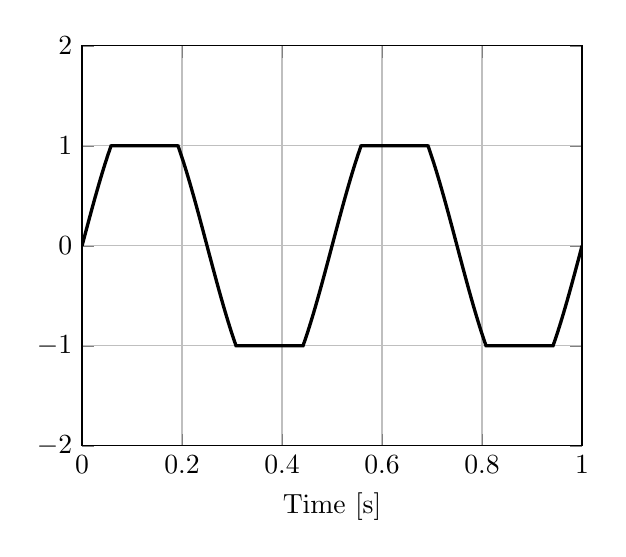
\begin{tikzpicture}

\begin{axis}[%
width=2.5in,
height=2in,
at={(1.011in,0.642in)},
scale only axis,
xmin=0,
xmax=1,
xlabel={Time [s]},
xmajorgrids,
ymin=-2,
ymax=2,
ymajorgrids,
axis background/.style={fill=white}
]
\addplot [color=black,solid,line width=1.2pt,forget plot]
  table[row sep=crcr]{%
0	0\\
0.001	0.0188490598250289\\
0.002	0.0376951431650062\\
0.003	0.0565352740049018\\
0.004	0.0753664772696543\\
0.005	0.0941857792939701\\
0.006	0.112990208291899\\
0.007	0.131776794826115\\
0.008	0.150542572276822\\
0.009	0.169284577310223\\
0.01	0.187999850346456\\
0.011	0.206685436026957\\
0.012	0.225338383681136\\
0.013	0.243955747792325\\
0.014	0.262534588462914\\
0.015	0.281071971878587\\
0.016	0.299564970771611\\
0.017	0.318010664883082\\
0.018	0.336406141424072\\
0.019	0.354748495535587\\
0.02	0.373034830747282\\
0.021	0.391262259434845\\
0.022	0.409427903275988\\
0.023	0.427528893704964\\
0.024	0.445562372365552\\
0.025	0.463525491562421\\
0.026	0.481415414710814\\
0.027	0.49922931678448\\
0.028	0.516964384761776\\
0.029	0.534617818069876\\
0.03	0.552186829027017\\
0.031	0.569668643282702\\
0.032	0.587060500255804\\
0.033	0.604359653570494\\
0.034	0.621563371489926\\
0.035	0.638668937347609\\
0.036	0.655673649976399\\
0.037	0.672574824135048\\
0.038	0.689369790932232\\
0.039	0.706055898247999\\
0.04	0.722630511152573\\
0.041	0.739091012322437\\
0.042	0.755434802453641\\
0.043	0.77165930067226\\
0.044	0.787761944941943\\
0.045	0.803740192468495\\
0.046	0.819591520101404\\
0.047	0.835313424732282\\
0.048	0.850903423690135\\
0.049	0.866359055133401\\
0.05	0.88167787843871\\
0.051	0.896857474586278\\
0.052	0.911895446541908\\
0.053	0.926789419635502\\
0.054	0.941537041936051\\
0.055	0.956135984623034\\
0.056	0.970583942354166\\
0.057	0.984878633629435\\
0.058	0.999017801151378\\
0.059	1\\
0.06	1\\
0.061	1\\
0.062	1\\
0.063	1\\
0.064	1\\
0.065	1\\
0.066	1\\
0.067	1\\
0.068	1\\
0.069	1\\
0.07	1\\
0.071	1\\
0.072	1\\
0.073	1\\
0.074	1\\
0.075	1\\
0.076	1\\
0.077	1\\
0.078	1\\
0.079	1\\
0.08	1\\
0.081	1\\
0.082	1\\
0.083	1\\
0.084	1\\
0.085	1\\
0.086	1\\
0.087	1\\
0.088	1\\
0.089	1\\
0.09	1\\
0.091	1\\
0.092	1\\
0.093	1\\
0.094	1\\
0.095	1\\
0.096	1\\
0.097	1\\
0.098	1\\
0.099	1\\
0.1	1\\
0.101	1\\
0.102	1\\
0.103	1\\
0.104	1\\
0.105	1\\
0.106	1\\
0.107	1\\
0.108	1\\
0.109	1\\
0.11	1\\
0.111	1\\
0.112	1\\
0.113	1\\
0.114	1\\
0.115	1\\
0.116	1\\
0.117	1\\
0.118	1\\
0.119	1\\
0.12	1\\
0.121	1\\
0.122	1\\
0.123	1\\
0.124	1\\
0.125	1\\
0.126	1\\
0.127	1\\
0.128	1\\
0.129	1\\
0.13	1\\
0.131	1\\
0.132	1\\
0.133	1\\
0.134	1\\
0.135	1\\
0.136	1\\
0.137	1\\
0.138	1\\
0.139	1\\
0.14	1\\
0.141	1\\
0.142	1\\
0.143	1\\
0.144	1\\
0.145	1\\
0.146	1\\
0.147	1\\
0.148	1\\
0.149	1\\
0.15	1\\
0.151	1\\
0.152	1\\
0.153	1\\
0.154	1\\
0.155	1\\
0.156	1\\
0.157	1\\
0.158	1\\
0.159	1\\
0.16	1\\
0.161	1\\
0.162	1\\
0.163	1\\
0.164	1\\
0.165	1\\
0.166	1\\
0.167	1\\
0.168	1\\
0.169	1\\
0.17	1\\
0.171	1\\
0.172	1\\
0.173	1\\
0.174	1\\
0.175	1\\
0.176	1\\
0.177	1\\
0.178	1\\
0.179	1\\
0.18	1\\
0.181	1\\
0.182	1\\
0.183	1\\
0.184	1\\
0.185	1\\
0.186	1\\
0.187	1\\
0.188	1\\
0.189	1\\
0.19	1\\
0.191	1\\
0.192	0.999017801151378\\
0.193	0.984878633629435\\
0.194	0.970583942354166\\
0.195	0.956135984623035\\
0.196	0.941537041936051\\
0.197	0.926789419635502\\
0.198	0.911895446541908\\
0.199	0.896857474586278\\
0.2	0.88167787843871\\
0.201	0.866359055133402\\
0.202	0.850903423690135\\
0.203	0.835313424732282\\
0.204	0.819591520101404\\
0.205	0.803740192468495\\
0.206	0.787761944941943\\
0.207	0.771659300672259\\
0.208	0.755434802453641\\
0.209	0.739091012322437\\
0.21	0.722630511152573\\
0.211	0.706055898247999\\
0.212	0.689369790932232\\
0.213	0.672574824135048\\
0.214	0.655673649976399\\
0.215	0.638668937347609\\
0.216	0.621563371489926\\
0.217	0.604359653570494\\
0.218	0.587060500255804\\
0.219	0.569668643282702\\
0.22	0.552186829027017\\
0.221	0.534617818069876\\
0.222	0.516964384761776\\
0.223	0.49922931678448\\
0.224	0.481415414710815\\
0.225	0.463525491562421\\
0.226	0.445562372365552\\
0.227	0.427528893704964\\
0.228	0.409427903275988\\
0.229	0.391262259434846\\
0.23	0.373034830747282\\
0.231	0.354748495535587\\
0.232	0.336406141424071\\
0.233	0.318010664883082\\
0.234	0.299564970771611\\
0.235	0.281071971878587\\
0.236	0.262534588462914\\
0.237	0.243955747792325\\
0.238	0.225338383681136\\
0.239	0.206685436026957\\
0.24	0.187999850346457\\
0.241	0.169284577310223\\
0.242	0.150542572276822\\
0.243	0.131776794826115\\
0.244	0.1129902082919\\
0.245	0.0941857792939704\\
0.246	0.0753664772696545\\
0.247	0.0565352740049018\\
0.248	0.0376951431650067\\
0.249	0.0188490598250293\\
0.25	1.83697019872103e-16\\
0.251	-0.0188490598250289\\
0.252	-0.0376951431650064\\
0.253	-0.0565352740049014\\
0.254	-0.0753664772696541\\
0.255	-0.09418577929397\\
0.256	-0.112990208291899\\
0.257	-0.131776794826114\\
0.258	-0.150542572276822\\
0.259	-0.169284577310222\\
0.26	-0.187999850346456\\
0.261	-0.206685436026957\\
0.262	-0.225338383681135\\
0.263	-0.243955747792325\\
0.264	-0.262534588462914\\
0.265	-0.281071971878587\\
0.266	-0.299564970771611\\
0.267	-0.318010664883082\\
0.268	-0.336406141424072\\
0.269	-0.354748495535587\\
0.27	-0.373034830747282\\
0.271	-0.391262259434845\\
0.272	-0.409427903275988\\
0.273	-0.427528893704964\\
0.274	-0.445562372365553\\
0.275	-0.463525491562422\\
0.276	-0.481415414710814\\
0.277	-0.49922931678448\\
0.278	-0.516964384761776\\
0.279	-0.534617818069876\\
0.28	-0.552186829027017\\
0.281	-0.569668643282702\\
0.282	-0.587060500255804\\
0.283	-0.604359653570494\\
0.284	-0.621563371489927\\
0.285	-0.638668937347609\\
0.286	-0.6556736499764\\
0.287	-0.672574824135049\\
0.288	-0.689369790932232\\
0.289	-0.706055898247998\\
0.29	-0.722630511152572\\
0.291	-0.739091012322437\\
0.292	-0.755434802453641\\
0.293	-0.771659300672259\\
0.294	-0.787761944941943\\
0.295	-0.803740192468495\\
0.296	-0.819591520101403\\
0.297	-0.835313424732281\\
0.298	-0.850903423690134\\
0.299	-0.866359055133401\\
0.3	-0.88167787843871\\
0.301	-0.896857474586278\\
0.302	-0.911895446541908\\
0.303	-0.926789419635501\\
0.304	-0.94153704193605\\
0.305	-0.956135984623034\\
0.306	-0.970583942354166\\
0.307	-0.984878633629434\\
0.308	-0.999017801151377\\
0.309	-1\\
0.31	-1\\
0.311	-1\\
0.312	-1\\
0.313	-1\\
0.314	-1\\
0.315	-1\\
0.316	-1\\
0.317	-1\\
0.318	-1\\
0.319	-1\\
0.32	-1\\
0.321	-1\\
0.322	-1\\
0.323	-1\\
0.324	-1\\
0.325	-1\\
0.326	-1\\
0.327	-1\\
0.328	-1\\
0.329	-1\\
0.33	-1\\
0.331	-1\\
0.332	-1\\
0.333	-1\\
0.334	-1\\
0.335	-1\\
0.336	-1\\
0.337	-1\\
0.338	-1\\
0.339	-1\\
0.34	-1\\
0.341	-1\\
0.342	-1\\
0.343	-1\\
0.344	-1\\
0.345	-1\\
0.346	-1\\
0.347	-1\\
0.348	-1\\
0.349	-1\\
0.35	-1\\
0.351	-1\\
0.352	-1\\
0.353	-1\\
0.354	-1\\
0.355	-1\\
0.356	-1\\
0.357	-1\\
0.358	-1\\
0.359	-1\\
0.36	-1\\
0.361	-1\\
0.362	-1\\
0.363	-1\\
0.364	-1\\
0.365	-1\\
0.366	-1\\
0.367	-1\\
0.368	-1\\
0.369	-1\\
0.37	-1\\
0.371	-1\\
0.372	-1\\
0.373	-1\\
0.374	-1\\
0.375	-1\\
0.376	-1\\
0.377	-1\\
0.378	-1\\
0.379	-1\\
0.38	-1\\
0.381	-1\\
0.382	-1\\
0.383	-1\\
0.384	-1\\
0.385	-1\\
0.386	-1\\
0.387	-1\\
0.388	-1\\
0.389	-1\\
0.39	-1\\
0.391	-1\\
0.392	-1\\
0.393	-1\\
0.394	-1\\
0.395	-1\\
0.396	-1\\
0.397	-1\\
0.398	-1\\
0.399	-1\\
0.4	-1\\
0.401	-1\\
0.402	-1\\
0.403	-1\\
0.404	-1\\
0.405	-1\\
0.406	-1\\
0.407	-1\\
0.408	-1\\
0.409	-1\\
0.41	-1\\
0.411	-1\\
0.412	-1\\
0.413	-1\\
0.414	-1\\
0.415	-1\\
0.416	-1\\
0.417	-1\\
0.418	-1\\
0.419	-1\\
0.42	-1\\
0.421	-1\\
0.422	-1\\
0.423	-1\\
0.424	-1\\
0.425	-1\\
0.426	-1\\
0.427	-1\\
0.428	-1\\
0.429	-1\\
0.43	-1\\
0.431	-1\\
0.432	-1\\
0.433	-1\\
0.434	-1\\
0.435	-1\\
0.436	-1\\
0.437	-1\\
0.438	-1\\
0.439	-1\\
0.44	-1\\
0.441	-1\\
0.442	-0.999017801151378\\
0.443	-0.984878633629435\\
0.444	-0.970583942354166\\
0.445	-0.956135984623034\\
0.446	-0.94153704193605\\
0.447	-0.926789419635502\\
0.448	-0.911895446541909\\
0.449	-0.896857474586279\\
0.45	-0.88167787843871\\
0.451	-0.866359055133402\\
0.452	-0.850903423690135\\
0.453	-0.835313424732282\\
0.454	-0.819591520101403\\
0.455	-0.803740192468494\\
0.456	-0.787761944941943\\
0.457	-0.77165930067226\\
0.458	-0.755434802453641\\
0.459	-0.739091012322437\\
0.46	-0.722630511152573\\
0.461	-0.706055898247999\\
0.462	-0.689369790932232\\
0.463	-0.672574824135048\\
0.464	-0.655673649976399\\
0.465	-0.638668937347608\\
0.466	-0.621563371489927\\
0.467	-0.604359653570494\\
0.468	-0.587060500255804\\
0.469	-0.569668643282702\\
0.47	-0.552186829027017\\
0.471	-0.534617818069876\\
0.472	-0.516964384761775\\
0.473	-0.499229316784479\\
0.474	-0.481415414710814\\
0.475	-0.463525491562421\\
0.476	-0.445562372365553\\
0.477	-0.427528893704964\\
0.478	-0.409427903275988\\
0.479	-0.391262259434845\\
0.48	-0.373034830747283\\
0.481	-0.354748495535588\\
0.482	-0.336406141424072\\
0.483	-0.318010664883082\\
0.484	-0.299564970771611\\
0.485	-0.281071971878587\\
0.486	-0.262534588462914\\
0.487	-0.243955747792326\\
0.488	-0.225338383681137\\
0.489	-0.206685436026958\\
0.49	-0.187999850346457\\
0.491	-0.169284577310223\\
0.492	-0.150542572276823\\
0.493	-0.131776794826115\\
0.494	-0.112990208291899\\
0.495	-0.0941857792939699\\
0.496	-0.0753664772696553\\
0.497	-0.0565352740049027\\
0.498	-0.0376951431650069\\
0.499	-0.0188490598250294\\
0.5	-3.67394039744206e-16\\
0.501	0.0188490598250287\\
0.502	0.0376951431650062\\
0.503	0.0565352740049019\\
0.504	0.0753664772696546\\
0.505	0.0941857792939692\\
0.506	0.112990208291898\\
0.507	0.131776794826114\\
0.508	0.150542572276822\\
0.509	0.169284577310222\\
0.51	0.187999850346456\\
0.511	0.206685436026957\\
0.512	0.225338383681136\\
0.513	0.243955747792326\\
0.514	0.262534588462913\\
0.515	0.281071971878586\\
0.516	0.29956497077161\\
0.517	0.318010664883082\\
0.518	0.336406141424072\\
0.519	0.354748495535587\\
0.52	0.373034830747282\\
0.521	0.391262259434843\\
0.522	0.409427903275988\\
0.523	0.427528893704962\\
0.524	0.445562372365552\\
0.525	0.46352549156242\\
0.526	0.481415414710814\\
0.527	0.499229316784479\\
0.528	0.516964384761776\\
0.529	0.534617818069874\\
0.53	0.552186829027017\\
0.531	0.5696686432827\\
0.532	0.587060500255804\\
0.533	0.604359653570492\\
0.534	0.621563371489926\\
0.535	0.638668937347608\\
0.536	0.655673649976399\\
0.537	0.672574824135046\\
0.538	0.689369790932232\\
0.539	0.706055898247997\\
0.54	0.722630511152573\\
0.541	0.739091012322436\\
0.542	0.755434802453641\\
0.543	0.771659300672258\\
0.544	0.787761944941944\\
0.545	0.803740192468494\\
0.546	0.819591520101404\\
0.547	0.83531342473228\\
0.548	0.850903423690135\\
0.549	0.8663590551334\\
0.55	0.88167787843871\\
0.551	0.896857474586277\\
0.552	0.911895446541908\\
0.553	0.9267894196355\\
0.554	0.941537041936051\\
0.555	0.956135984623034\\
0.556	0.970583942354167\\
0.557	0.984878633629433\\
0.558	0.999017801151378\\
0.559	1\\
0.56	1\\
0.561	1\\
0.562	1\\
0.563	1\\
0.564	1\\
0.565	1\\
0.566	1\\
0.567	1\\
0.568	1\\
0.569	1\\
0.57	1\\
0.571	1\\
0.572	1\\
0.573	1\\
0.574	1\\
0.575	1\\
0.576	1\\
0.577	1\\
0.578	1\\
0.579	1\\
0.58	1\\
0.581	1\\
0.582	1\\
0.583	1\\
0.584	1\\
0.585	1\\
0.586	1\\
0.587	1\\
0.588	1\\
0.589	1\\
0.59	1\\
0.591	1\\
0.592	1\\
0.593	1\\
0.594	1\\
0.595	1\\
0.596	1\\
0.597	1\\
0.598	1\\
0.599	1\\
0.6	1\\
0.601	1\\
0.602	1\\
0.603	1\\
0.604	1\\
0.605	1\\
0.606	1\\
0.607	1\\
0.608	1\\
0.609	1\\
0.61	1\\
0.611	1\\
0.612	1\\
0.613	1\\
0.614	1\\
0.615	1\\
0.616	1\\
0.617	1\\
0.618	1\\
0.619	1\\
0.62	1\\
0.621	1\\
0.622	1\\
0.623	1\\
0.624	1\\
0.625	1\\
0.626	1\\
0.627	1\\
0.628	1\\
0.629	1\\
0.63	1\\
0.631	1\\
0.632	1\\
0.633	1\\
0.634	1\\
0.635	1\\
0.636	1\\
0.637	1\\
0.638	1\\
0.639	1\\
0.64	1\\
0.641	1\\
0.642	1\\
0.643	1\\
0.644	1\\
0.645	1\\
0.646	1\\
0.647	1\\
0.648	1\\
0.649	1\\
0.65	1\\
0.651	1\\
0.652	1\\
0.653	1\\
0.654	1\\
0.655	1\\
0.656	1\\
0.657	1\\
0.658	1\\
0.659	1\\
0.66	1\\
0.661	1\\
0.662	1\\
0.663	1\\
0.664	1\\
0.665	1\\
0.666	1\\
0.667	1\\
0.668	1\\
0.669	1\\
0.67	1\\
0.671	1\\
0.672	1\\
0.673	1\\
0.674	1\\
0.675	1\\
0.676	1\\
0.677	1\\
0.678	1\\
0.679	1\\
0.68	1\\
0.681	1\\
0.682	1\\
0.683	1\\
0.684	1\\
0.685	1\\
0.686	1\\
0.687	1\\
0.688	1\\
0.689	1\\
0.69	1\\
0.691	1\\
0.692	0.999017801151379\\
0.693	0.984878633629435\\
0.694	0.970583942354168\\
0.695	0.956135984623035\\
0.696	0.941537041936052\\
0.697	0.926789419635501\\
0.698	0.911895446541909\\
0.699	0.896857474586278\\
0.7	0.88167787843871\\
0.701	0.866359055133401\\
0.702	0.850903423690135\\
0.703	0.835313424732281\\
0.704	0.819591520101406\\
0.705	0.803740192468493\\
0.706	0.787761944941945\\
0.707	0.771659300672258\\
0.708	0.755434802453643\\
0.709	0.739091012322438\\
0.71	0.722630511152574\\
0.711	0.706055898247999\\
0.712	0.689369790932233\\
0.713	0.672574824135051\\
0.714	0.6556736499764\\
0.715	0.638668937347611\\
0.716	0.621563371489927\\
0.717	0.604359653570496\\
0.718	0.587060500255804\\
0.719	0.569668643282703\\
0.72	0.552186829027017\\
0.721	0.534617818069877\\
0.722	0.516964384761775\\
0.723	0.499229316784481\\
0.724	0.481415414710816\\
0.725	0.463525491562422\\
0.726	0.445562372365554\\
0.727	0.427528893704964\\
0.728	0.409427903275989\\
0.729	0.391262259434845\\
0.73	0.373034830747283\\
0.731	0.354748495535587\\
0.732	0.336406141424072\\
0.733	0.318010664883084\\
0.734	0.299564970771611\\
0.735	0.281071971878589\\
0.736	0.262534588462914\\
0.737	0.243955747792327\\
0.738	0.225338383681135\\
0.739	0.206685436026958\\
0.74	0.187999850346456\\
0.741	0.169284577310223\\
0.742	0.150542572276824\\
0.743	0.131776794826115\\
0.744	0.112990208291901\\
0.745	0.0941857792939701\\
0.746	0.0753664772696555\\
0.747	0.0565352740049015\\
0.748	0.0376951431650071\\
0.749	0.0188490598250283\\
0.75	5.51091059616309e-16\\
0.751	-0.0188490598250272\\
0.752	-0.037695143165006\\
0.753	-0.0565352740049004\\
0.754	-0.0753664772696544\\
0.755	-0.094185779293969\\
0.756	-0.112990208291899\\
0.757	-0.131776794826114\\
0.758	-0.150542572276823\\
0.759	-0.169284577310222\\
0.76	-0.187999850346455\\
0.761	-0.206685436026957\\
0.762	-0.225338383681134\\
0.763	-0.243955747792326\\
0.764	-0.262534588462913\\
0.765	-0.281071971878587\\
0.766	-0.29956497077161\\
0.767	-0.318010664883083\\
0.768	-0.336406141424071\\
0.769	-0.354748495535586\\
0.77	-0.373034830747282\\
0.771	-0.391262259434844\\
0.772	-0.409427903275988\\
0.773	-0.427528893704963\\
0.774	-0.445562372365553\\
0.775	-0.463525491562421\\
0.776	-0.481415414710815\\
0.777	-0.49922931678448\\
0.778	-0.516964384761774\\
0.779	-0.534617818069876\\
0.78	-0.552186829027016\\
0.781	-0.569668643282702\\
0.782	-0.587060500255803\\
0.783	-0.604359653570495\\
0.784	-0.621563371489926\\
0.785	-0.63866893734761\\
0.786	-0.655673649976399\\
0.787	-0.67257482413505\\
0.788	-0.689369790932232\\
0.789	-0.706055898247998\\
0.79	-0.722630511152573\\
0.791	-0.739091012322437\\
0.792	-0.755434802453642\\
0.793	-0.771659300672257\\
0.794	-0.787761944941945\\
0.795	-0.803740192468493\\
0.796	-0.819591520101405\\
0.797	-0.83531342473228\\
0.798	-0.850903423690134\\
0.799	-0.8663590551334\\
0.8	-0.881677878438709\\
0.801	-0.896857474586277\\
0.802	-0.911895446541908\\
0.803	-0.9267894196355\\
0.804	-0.941537041936051\\
0.805	-0.956135984623034\\
0.806	-0.970583942354167\\
0.807	-0.984878633629434\\
0.808	-0.999017801151378\\
0.809	-1\\
0.81	-1\\
0.811	-1\\
0.812	-1\\
0.813	-1\\
0.814	-1\\
0.815	-1\\
0.816	-1\\
0.817	-1\\
0.818	-1\\
0.819	-1\\
0.82	-1\\
0.821	-1\\
0.822	-1\\
0.823	-1\\
0.824	-1\\
0.825	-1\\
0.826	-1\\
0.827	-1\\
0.828	-1\\
0.829	-1\\
0.83	-1\\
0.831	-1\\
0.832	-1\\
0.833	-1\\
0.834	-1\\
0.835	-1\\
0.836	-1\\
0.837	-1\\
0.838	-1\\
0.839	-1\\
0.84	-1\\
0.841	-1\\
0.842	-1\\
0.843	-1\\
0.844	-1\\
0.845	-1\\
0.846	-1\\
0.847	-1\\
0.848	-1\\
0.849	-1\\
0.85	-1\\
0.851	-1\\
0.852	-1\\
0.853	-1\\
0.854	-1\\
0.855	-1\\
0.856	-1\\
0.857	-1\\
0.858	-1\\
0.859	-1\\
0.86	-1\\
0.861	-1\\
0.862	-1\\
0.863	-1\\
0.864	-1\\
0.865	-1\\
0.866	-1\\
0.867	-1\\
0.868	-1\\
0.869	-1\\
0.87	-1\\
0.871	-1\\
0.872	-1\\
0.873	-1\\
0.874	-1\\
0.875	-1\\
0.876	-1\\
0.877	-1\\
0.878	-1\\
0.879	-1\\
0.88	-1\\
0.881	-1\\
0.882	-1\\
0.883	-1\\
0.884	-1\\
0.885	-1\\
0.886	-1\\
0.887	-1\\
0.888	-1\\
0.889	-1\\
0.89	-1\\
0.891	-1\\
0.892	-1\\
0.893	-1\\
0.894	-1\\
0.895	-1\\
0.896	-1\\
0.897	-1\\
0.898	-1\\
0.899	-1\\
0.9	-1\\
0.901	-1\\
0.902	-1\\
0.903	-1\\
0.904	-1\\
0.905	-1\\
0.906	-1\\
0.907	-1\\
0.908	-1\\
0.909	-1\\
0.91	-1\\
0.911	-1\\
0.912	-1\\
0.913	-1\\
0.914	-1\\
0.915	-1\\
0.916	-1\\
0.917	-1\\
0.918	-1\\
0.919	-1\\
0.92	-1\\
0.921	-1\\
0.922	-1\\
0.923	-1\\
0.924	-1\\
0.925	-1\\
0.926	-1\\
0.927	-1\\
0.928	-1\\
0.929	-1\\
0.93	-1\\
0.931	-1\\
0.932	-1\\
0.933	-1\\
0.934	-1\\
0.935	-1\\
0.936	-1\\
0.937	-1\\
0.938	-1\\
0.939	-1\\
0.94	-1\\
0.941	-1\\
0.942	-0.999017801151379\\
0.943	-0.984878633629435\\
0.944	-0.970583942354168\\
0.945	-0.956135984623037\\
0.946	-0.941537041936052\\
0.947	-0.926789419635504\\
0.948	-0.911895446541909\\
0.949	-0.89685747458628\\
0.95	-0.88167787843871\\
0.951	-0.866359055133403\\
0.952	-0.850903423690135\\
0.953	-0.835313424732283\\
0.954	-0.819591520101406\\
0.955	-0.803740192468496\\
0.956	-0.787761944941946\\
0.957	-0.771659300672261\\
0.958	-0.755434802453643\\
0.959	-0.739091012322438\\
0.96	-0.722630511152574\\
0.961	-0.706055898247999\\
0.962	-0.689369790932233\\
0.963	-0.672574824135051\\
0.964	-0.6556736499764\\
0.965	-0.638668937347611\\
0.966	-0.621563371489927\\
0.967	-0.604359653570496\\
0.968	-0.587060500255804\\
0.969	-0.569668643282703\\
0.97	-0.552186829027017\\
0.971	-0.534617818069877\\
0.972	-0.516964384761775\\
0.973	-0.499229316784481\\
0.974	-0.481415414710816\\
0.975	-0.463525491562422\\
0.976	-0.445562372365554\\
0.977	-0.427528893704965\\
0.978	-0.409427903275989\\
0.979	-0.391262259434845\\
0.98	-0.373034830747283\\
0.981	-0.354748495535587\\
0.982	-0.336406141424073\\
0.983	-0.318010664883084\\
0.984	-0.299564970771611\\
0.985	-0.281071971878589\\
0.986	-0.262534588462914\\
0.987	-0.243955747792327\\
0.988	-0.225338383681136\\
0.989	-0.206685436026958\\
0.99	-0.187999850346456\\
0.991	-0.169284577310223\\
0.992	-0.150542572276824\\
0.993	-0.131776794826115\\
0.994	-0.112990208291901\\
0.995	-0.0941857792939703\\
0.996	-0.0753664772696557\\
0.997	-0.0565352740049017\\
0.998	-0.0376951431650073\\
0.999	-0.0188490598250285\\
1	-7.34788079488412e-16\\
};
\end{axis}
\end{tikzpicture}%
	\caption{A 1 kHz clipped sinusoid.}
	\label{fig:clippingDist}
\end{subfigure}
\caption{The difference between a unaffected signal and a clipped signal. As the maximum output is 1, the signal is hard clipped because of the limitation.}
\label{fig:audioclipping}
\end{figure}

Hard clipping lowers the sound quality if the clipping is not intended, and should therefore be avoided. The wave distortion created by the sharp edge results in a square-wave-like signal. This creates additional uneven harmonics to the signal i.e. 3rd, 5th, 7th and 9th, which are unpleasant to listen to as previously stated. Since the clipping creates the square-wave-like signal, the generation of the additional uneven harmonics can be described in the Fourier series of a square-wave. The Fourier series of a square-wave is given as:
\begin{align}\label{eq:fourier_series_square}
f(t) &= \frac{4}{\pi} \sum_{n=1}^{\infty} \frac{\sin (\omega_0 t \cdot (2n-1))}{(2n-1)} \\
	 &= \frac{4}{\pi} (\sin(\omega_0 t) + \frac{1}{3}\sin(3 \omega_0 t) + \frac{1}{5}\sin(5 \omega_0 t) + \, ... \,)
\end{align}
\begin{where}
\va{$\omega_0$}{is the fundamental frequency of the square-wave.}{rad/s}\\
\end{where}

As seen in \autoref{eq:fourier_series_square}, the function of a square-wave signal consists of a fundamental frequency $\omega_0$ and uneven harmonics to the fundamental frequency. This can also be shown in a spectrum analysis of the 1 kHz clipped sinusoid from \autoref{fig:audioclipping} in \autoref{fig:audioclippingFFT}.

\begin{figure}[H]
\centering
\begin{subfigure}[t]{0.47\textwidth}
	\tikzsetnextfilename{clippingCleanFFT}
	% This file was created by matlab2tikz.
%
%The latest updates can be retrieved from
%  http://www.mathworks.com/matlabcentral/fileexchange/22022-matlab2tikz-matlab2tikz
%where you can also make suggestions and rate matlab2tikz.
%
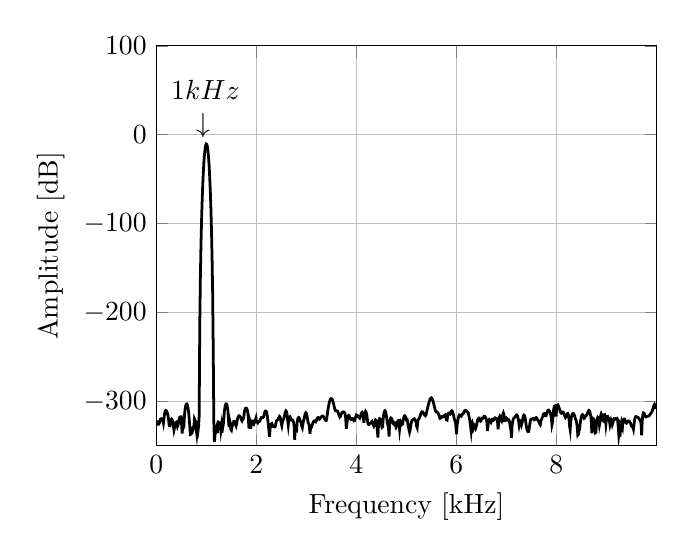
\begin{tikzpicture}

\begin{axis}[%
width=2.5in,
height=2in,
at={(1.011in,0.642in)},
scale only axis,
scaled x ticks = false,
xmin=0,
xmax=10000,
xlabel={Frequency [kHz]},
xmajorgrids,
ymin=-350,
ymax=100,
xticklabels={0, 2, 4, 6, 8},
xtick = {0, 2000, 4000, 6000, 8000},
ylabel={Amplitude [dB]},
ymajorgrids,
axis background/.style={fill=white},
]
\addplot [color=black,solid,line width=1pt,forget plot]
  table[row sep=crcr]{%
0	-322.11596721008\\
11.7216117216117	-323.671020481401\\
23.4432234432234	-323.340883337027\\
35.1648351648352	-325.684167070818\\
46.8864468864469	-325.669523756719\\
58.6080586080586	-324.370513022472\\
70.3296703296703	-322.159992029701\\
82.0512820512821	-319.994159311925\\
93.7728937728938	-319.483979753379\\
105.494505494505	-319.494939928451\\
117.216117216117	-320.869322942301\\
128.937728937729	-320.920572736749\\
140.659340659341	-324.227184829387\\
152.380952380952	-319.035056899834\\
164.102564102564	-313.823145631125\\
175.824175824176	-311.131574765862\\
187.545787545788	-310.246860211816\\
199.267399267399	-310.60441452423\\
210.989010989011	-311.78696455392\\
222.710622710623	-313.844752745052\\
234.432234432234	-316.418042709319\\
246.153846153846	-321.707697545501\\
257.875457875458	-327.363976836631\\
269.59706959707	-327.473089119894\\
281.318681318681	-324.112892105008\\
293.040293040293	-320.977587207666\\
304.761904761905	-319.982762533596\\
316.483516483516	-320.780760736175\\
328.205128205128	-323.668423270885\\
339.92673992674	-328.026148757277\\
351.648351648352	-332.4170697972\\
363.369963369963	-329.426095087341\\
375.091575091575	-326.556664292431\\
386.813186813187	-323.76537835188\\
398.534798534799	-323.368319264645\\
410.25641025641	-325.169104300057\\
421.978021978022	-328.189262138342\\
433.699633699634	-326.529217054039\\
445.421245421245	-322.75486943378\\
457.142857142857	-319.794087491908\\
468.864468864469	-317.719335966222\\
480.586080586081	-317.459852846429\\
492.307692307692	-319.009687543967\\
504.029304029304	-325.455766258282\\
515.750915750916	-336.106317374067\\
527.472527472527	-326.323603862667\\
539.194139194139	-329.684995875921\\
550.915750915751	-327.90212185778\\
562.637362637363	-314.792259957384\\
574.358974358974	-308.679273562794\\
586.080586080586	-304.859856763288\\
597.802197802198	-303.147924647545\\
609.52380952381	-302.958088372619\\
621.245421245421	-304.246172084633\\
632.967032967033	-307.392871145609\\
644.688644688645	-311.86240623327\\
656.410256410256	-319.720154828058\\
668.131868131868	-327.681235000644\\
679.85347985348	-337.238516322602\\
691.575091575092	-336.970257356979\\
703.296703296703	-332.332133924419\\
715.018315018315	-331.141735134048\\
726.739926739927	-332.723957001084\\
738.461538461538	-330.730504488432\\
750.18315018315	-327.778175020515\\
761.904761904762	-319.91378584982\\
773.626373626374	-321.461497849882\\
785.347985347985	-327.043537773181\\
797.069597069597	-331.841589615916\\
808.791208791209	-336.991655282628\\
820.512820512821	-330.418202230553\\
832.234432234432	-333.267393421045\\
843.956043956044	-328.226187037683\\
855.677655677656	-316.700315440438\\
867.399267399267	-215.943651772091\\
879.120879120879	-163.159584780945\\
890.842490842491	-126.529341228273\\
902.564102564103	-98.3775899142248\\
914.285714285714	-75.9321258862354\\
926.007326007326	-57.8132086793137\\
937.728937728938	-43.2219634542571\\
949.450549450549	-31.6552033180823\\
961.172161172161	-22.7812801668732\\
972.893772893773	-16.3785078578736\\
984.615384615385	-12.3020988974321\\
996.336996336996	-10.4658259320985\\
1008.05860805861	-10.8322625838136\\
1019.78021978022	-13.4088092670734\\
1031.50183150183	-18.2484666216626\\
1043.22344322344	-25.4555537550734\\
1054.94505494505	-35.1978991745999\\
1066.66666666667	-47.7291574398437\\
1078.38827838828	-63.4292414488433\\
1090.10989010989	-82.8812589369107\\
1101.8315018315	-107.032465507491\\
1113.55311355311	-137.586526131487\\
1125.27472527473	-178.243096713105\\
1136.99633699634	-241.704411925533\\
1148.71794871795	-323.195571130692\\
1160.43956043956	-345.375156099691\\
1172.16117216117	-338.247857244841\\
1183.88278388278	-333.32317434497\\
1195.6043956044	-331.269745255181\\
1207.32600732601	-328.799242404036\\
1219.04761904762	-335.934946361628\\
1230.76923076923	-327.685186138873\\
1242.49084249084	-326.960459897927\\
1254.21245421245	-323.718010447396\\
1265.93406593407	-324.108622411667\\
1277.65567765568	-326.20417623814\\
1289.37728937729	-332.697946725791\\
1301.0989010989	-327.906853738375\\
1312.82051282051	-335.418538359777\\
1324.54212454212	-328.816875760217\\
1336.26373626374	-327.262600955998\\
1347.98534798535	-320.385055874777\\
1359.70695970696	-311.475672251247\\
1371.42857142857	-306.643481149913\\
1383.15018315018	-303.695848832502\\
1394.87179487179	-302.842835407919\\
1406.59340659341	-303.232099162736\\
1418.31501831502	-305.842604461406\\
1430.03663003663	-310.40119194813\\
1441.75824175824	-320.718788147534\\
1453.47985347985	-328.69918849089\\
1465.20146520147	-321.407968983388\\
1476.92307692308	-324.473146768564\\
1488.64468864469	-331.645069484275\\
1500.3663003663	-332.515642341006\\
1512.08791208791	-328.465510911873\\
1523.80952380952	-326.826340274793\\
1535.53113553114	-324.534133776849\\
1547.25274725275	-322.615676311941\\
1558.97435897436	-322.427557967468\\
1570.69597069597	-323.530722159417\\
1582.41758241758	-326.171996895262\\
1594.13919413919	-327.712500269681\\
1605.86080586081	-325.047841087069\\
1617.58241758242	-321.24290571993\\
1629.30402930403	-317.993077517342\\
1641.02564102564	-316.998612276315\\
1652.74725274725	-316.240926477532\\
1664.46886446886	-316.68363443687\\
1676.19047619048	-317.141867195876\\
1687.91208791209	-318.342449097449\\
1699.6336996337	-320.695345632283\\
1711.35531135531	-321.836458347942\\
1723.07692307692	-320.2697737784\\
1734.79853479853	-320.163464706646\\
1746.52014652015	-317.872908059459\\
1758.24175824176	-312.6677675311\\
1769.96336996337	-309.491750132905\\
1781.68498168498	-307.828765413517\\
1793.40659340659	-307.627883691429\\
1805.12820512821	-307.890708550761\\
1816.84981684982	-309.331169961249\\
1828.57142857143	-312.28725024046\\
1840.29304029304	-320.344727197184\\
1852.01465201465	-330.483981414598\\
1863.73626373626	-320.778838487233\\
1875.45787545788	-323.188753718667\\
1887.17948717949	-330.709648822314\\
1898.9010989011	-324.458698904598\\
1910.62271062271	-322.161594474234\\
1922.34432234432	-322.355261648298\\
1934.06593406593	-325.120354775896\\
1945.78754578755	-325.813966972437\\
1957.50915750916	-323.880005799796\\
1969.23076923077	-321.560515034589\\
1980.95238095238	-321.471577902989\\
1992.67399267399	-319.02446157723\\
2004.3956043956	-323.174195056939\\
2016.11721611722	-323.174195056939\\
2027.83882783883	-324.089344868152\\
2039.56043956044	-322.910905669715\\
2051.28205128205	-323.043188327053\\
2063.00366300366	-322.552600066038\\
2074.72527472527	-320.986469744908\\
2086.44688644689	-319.545996905778\\
2098.1684981685	-318.315254794156\\
2109.89010989011	-318.387111906887\\
2121.61172161172	-318.301603114866\\
2133.33333333333	-318.177294354268\\
2145.05494505495	-316.938934301122\\
2156.77655677656	-314.354332026841\\
2168.49816849817	-312.152839226024\\
2180.21978021978	-310.876376782709\\
2191.94139194139	-310.8442203955\\
2203.663003663	-312.377716587324\\
2215.38461538462	-315.505766578087\\
2227.10622710623	-320.600055628699\\
2238.82783882784	-326.363108229676\\
2250.54945054945	-332.879313477263\\
2262.27106227106	-339.927557268938\\
2273.99267399267	-330.784134841474\\
2285.71428571429	-326.949066776775\\
2297.4358974359	-325.310562015324\\
2309.15750915751	-324.900671542525\\
2320.87912087912	-326.68176647539\\
2332.60073260073	-328.158338680386\\
2344.32234432234	-328.204122091938\\
2356.04395604396	-328.051439236523\\
2367.76556776557	-328.664204937443\\
2379.48717948718	-328.099018637999\\
2391.20879120879	-324.310047965675\\
2402.9304029304	-321.667678539627\\
2414.65201465201	-321.135207214597\\
2426.37362637363	-320.880932262159\\
2438.09523809524	-319.778960318202\\
2449.81684981685	-317.987700465117\\
2461.53846153846	-316.78808552065\\
2473.26007326007	-317.473390142408\\
2484.98168498168	-320.222893879042\\
2496.7032967033	-324.854050216358\\
2508.42490842491	-327.365492440596\\
2520.14652014652	-323.224999893465\\
2531.86813186813	-321.091227031284\\
2543.58974358974	-320.156669708411\\
2555.31135531136	-317.840663339711\\
2567.03296703297	-314.501482216247\\
2578.75457875458	-311.854837339112\\
2590.47619047619	-310.724997354159\\
2602.1978021978	-311.622091427549\\
2613.91941391941	-314.851882898182\\
2625.64102564103	-321.512762623562\\
2637.36263736264	-326.715257821487\\
2649.08424908425	-320.965390398505\\
2660.80586080586	-318.299218269644\\
2672.52747252747	-317.485994241431\\
2684.24908424908	-318.59001422949\\
2695.9706959707	-320.576544514212\\
2707.69230769231	-321.22124456977\\
2719.41391941392	-321.571973538176\\
2731.13553113553	-321.42734530042\\
2742.85714285714	-323.182504523745\\
2754.57875457875	-327.818517304439\\
2766.30036630037	-343.340028971303\\
2778.02197802198	-328.590941502845\\
2789.74358974359	-329.209198839045\\
2801.4652014652	-335.009194971263\\
2813.18681318681	-324.917874359001\\
2824.90842490842	-320.675970970006\\
2836.63003663004	-318.598485286378\\
2848.35164835165	-318.175277091238\\
2860.07326007326	-318.965978881077\\
2871.79487179487	-320.835410347703\\
2883.51648351648	-322.524929825596\\
2895.2380952381	-324.578193849772\\
2906.95970695971	-327.880455873337\\
2918.68131868132	-329.561603057853\\
2930.40293040293	-325.490736098095\\
2942.12454212454	-322.172446534305\\
2953.84615384615	-319.538366387325\\
2965.56776556777	-316.454951611266\\
2977.28937728938	-313.715712999263\\
2989.01098901099	-312.765011451191\\
3000.7326007326	-313.550082053352\\
3012.45421245421	-316.332919236015\\
3024.17582417582	-320.464673621591\\
3035.89743589744	-324.21570173302\\
3047.61904761905	-325.14025136414\\
3059.34065934066	-328.179012620665\\
3071.06227106227	-336.319390511434\\
3082.78388278388	-330.540376761589\\
3094.50549450549	-328.055385719859\\
3106.22710622711	-328.41132792291\\
3117.94871794872	-326.398110320453\\
3129.67032967033	-324.429933801343\\
3141.39194139194	-322.958523531653\\
3153.11355311355	-322.080283026816\\
3164.83516483516	-321.986069592074\\
3176.55677655678	-322.88974461944\\
3188.27838827839	-323.14866547361\\
3200	-321.731991922314\\
3211.72161172161	-319.583271135606\\
3223.44322344322	-318.524693510682\\
3235.16483516484	-318.277835267365\\
3246.88644688645	-319.493530184348\\
3258.60805860806	-320.194783095862\\
3270.32967032967	-319.645880585364\\
3282.05128205128	-318.402355114397\\
3293.77289377289	-317.597734351514\\
3305.49450549451	-317.02187364446\\
3317.21611721612	-316.763942230905\\
3328.93772893773	-316.47058612926\\
3340.65934065934	-317.197718055388\\
3352.38095238095	-318.34030296296\\
3364.10256410256	-319.71475362671\\
3375.82417582418	-320.433372545647\\
3387.54578754579	-321.481423753538\\
3399.2673992674	-321.328758210847\\
3410.98901098901	-317.848121944058\\
3422.71062271062	-312.6052633917\\
3434.43223443223	-308.209983131555\\
3446.15384615385	-304.542297484367\\
3457.87545787546	-301.476640468968\\
3469.59706959707	-299.074162567864\\
3481.31868131868	-297.505270833626\\
3493.04029304029	-296.820826693279\\
3504.7619047619	-296.952977362533\\
3516.48351648352	-297.832794363821\\
3528.20512820513	-299.532668899083\\
3539.92673992674	-301.925997253397\\
3551.64835164835	-304.833072981485\\
3563.36996336996	-307.679247836289\\
3575.09157509158	-309.820085030418\\
3586.81318681319	-310.691494738001\\
3598.5347985348	-310.817398824033\\
3610.25641025641	-310.678764468745\\
3621.97802197802	-310.904852964739\\
3633.69963369963	-312.083008289962\\
3645.42124542125	-314.044889957489\\
3657.14285714286	-316.283113404039\\
3668.86446886447	-317.725995742272\\
3680.58608058608	-316.98711432429\\
3692.30769230769	-315.404661196974\\
3704.0293040293	-313.574046253917\\
3715.75091575092	-312.403769243541\\
3727.47252747253	-311.900292301962\\
3739.19413919414	-311.790821532916\\
3750.91575091575	-311.885255334962\\
3762.63736263736	-312.507671076698\\
3774.35897435897	-314.393900840475\\
3786.08058608059	-318.958623783513\\
3797.8021978022	-330.766521534997\\
3809.52380952381	-325.502820472922\\
3821.24542124542	-319.47490837836\\
3832.96703296703	-316.5879349607\\
3844.68864468864	-315.820977290156\\
3856.41025641026	-316.165835542033\\
3868.13186813187	-317.693295629945\\
3879.85347985348	-319.724105063858\\
3891.57509157509	-320.385668853013\\
3903.2967032967	-319.982487927687\\
3915.01831501832	-319.299311012412\\
3926.73992673993	-319.444342321726\\
3938.46153846154	-320.526575483676\\
3950.18315018315	-321.926779712727\\
3961.90476190476	-321.781804018036\\
3973.62637362637	-319.294600071473\\
3985.34798534799	-317.199406352915\\
3997.0695970696	-315.48532686416\\
4008.79120879121	-316.133918462084\\
4020.51282051282	-315.922088122408\\
4032.23443223443	-316.716666209588\\
4043.95604395604	-317.865988888969\\
4055.67765567766	-318.280559925241\\
4067.39926739927	-318.926776854331\\
4079.12087912088	-317.317696380994\\
4090.84249084249	-315.060841214154\\
4102.5641025641	-312.993854282692\\
4114.28571428571	-312.27769957935\\
4126.00732600733	-313.058993411349\\
4137.72893772894	-316.497495126966\\
4149.45054945055	-324.074551114817\\
4161.17216117216	-317.815498249607\\
4172.89377289377	-312.724221795712\\
4184.61538461538	-311.184304154482\\
4196.336996337	-312.180395095067\\
4208.05860805861	-315.33167553721\\
4219.78021978022	-320.223371703619\\
4231.50183150183	-324.981894832223\\
4243.22344322344	-325.968094640368\\
4254.94505494505	-325.975199382868\\
4266.66666666667	-325.044494992807\\
4278.38827838828	-324.748701483869\\
4290.10989010989	-324.298796557654\\
4301.8315018315	-323.185408013847\\
4313.55311355311	-322.493712256323\\
4325.27472527472	-324.004517791407\\
4336.99633699634	-326.395781230683\\
4348.71794871795	-327.81152123793\\
4360.43956043956	-326.215243804676\\
4372.16117216117	-323.991135829513\\
4383.88278388278	-320.982207180012\\
4395.6043956044	-321.462465973861\\
4407.32600732601	-324.176499385288\\
4419.04761904762	-332.267280302068\\
4430.76923076923	-340.80932861649\\
4442.49084249084	-326.258684322367\\
4454.21245421245	-321.442965268777\\
4465.93406593407	-319.544444432877\\
4477.65567765568	-320.026440215285\\
4489.37728937729	-321.870034014714\\
4501.0989010989	-325.275880091975\\
4512.82051282051	-329.135133788708\\
4524.54212454212	-328.535733131409\\
4536.26373626374	-319.872005913471\\
4547.98534798535	-314.353155551714\\
4559.70695970696	-311.431276989024\\
4571.42857142857	-310.598208874572\\
4583.15018315018	-311.541465335688\\
4594.87179487179	-314.262904844306\\
4606.59340659341	-318.957659426667\\
4618.31501831502	-324.341801794823\\
4630.03663003663	-326.908025760342\\
4641.75824175824	-329.671708602847\\
4653.47985347985	-339.598374824666\\
4665.20146520146	-324.239834487312\\
4676.92307692308	-320.142812870027\\
4688.64468864469	-318.579390590904\\
4700.3663003663	-318.904551228728\\
4712.08791208791	-320.164411571421\\
4723.80952380952	-323.552244720139\\
4735.53113553114	-325.133901656344\\
4747.25274725275	-325.67494410303\\
4758.97435897436	-323.730925971029\\
4770.69597069597	-324.141194152127\\
4782.41758241758	-327.036177280335\\
4794.13919413919	-329.052455856504\\
4805.86080586081	-327.62366085932\\
4817.58241758242	-324.243757917428\\
4829.30402930403	-321.85425099731\\
4841.02564102564	-321.644312334699\\
4852.74725274725	-324.65913326885\\
4864.46886446886	-331.375490539255\\
4876.19047619048	-325.679255623113\\
4887.91208791209	-322.838347325296\\
4899.6336996337	-323.86912625874\\
4911.35531135531	-326.111153620671\\
4923.07692307692	-325.63048628826\\
4934.79853479854	-321.471648674554\\
4946.52014652015	-318.118465437495\\
4958.24175824176	-316.68211874222\\
4969.96336996337	-316.211579968543\\
4981.68498168498	-317.228440996576\\
4993.40659340659	-319.26351539118\\
5005.12820512821	-321.443807346433\\
5016.84981684982	-321.020667676622\\
5028.57142857143	-324.31969794583\\
5040.29304029304	-328.84177524509\\
5052.01465201465	-331.83382615458\\
5063.73626373626	-334.735835579055\\
5075.45787545788	-332.299258886241\\
5087.17948717949	-327.630942194737\\
5098.9010989011	-323.781987640664\\
5110.62271062271	-321.395765925455\\
5122.34432234432	-320.886447997559\\
5134.06593406593	-320.465428875501\\
5145.78754578755	-319.820250617952\\
5157.50915750916	-319.568122144542\\
5169.23076923077	-320.445377078076\\
5180.95238095238	-321.775888699888\\
5192.67399267399	-323.327196438195\\
5204.3956043956	-327.748774429116\\
5216.11721611722	-329.500414479457\\
5227.83882783883	-322.930677708616\\
5239.56043956044	-320.345390384961\\
5251.28205128205	-319.46742292498\\
5263.00366300366	-318.422700195226\\
5274.72527472528	-316.460548794413\\
5286.44688644689	-314.420570373633\\
5298.1684981685	-312.634917234304\\
5309.89010989011	-311.645830096681\\
5321.61172161172	-311.606321565998\\
5333.33333333333	-312.395026397497\\
5345.05494505495	-313.644669672522\\
5356.77655677656	-314.764393688141\\
5368.49816849817	-315.637442053714\\
5380.21978021978	-316.335135300277\\
5391.94139194139	-315.462866674828\\
5403.663003663	-312.472956024358\\
5415.38461538462	-309.49096542544\\
5427.10622710623	-306.661910098118\\
5438.82783882784	-304.082440188536\\
5450.54945054945	-301.618020574783\\
5462.27106227106	-299.473868003226\\
5473.99267399267	-297.699114290504\\
5485.71428571429	-296.505406176026\\
5497.4358974359	-296.028411377836\\
5509.15750915751	-296.481646635714\\
5520.87912087912	-297.788088059893\\
5532.60073260073	-299.767551285277\\
5544.32234432234	-302.299391403697\\
5556.04395604396	-305.019492670558\\
5567.76556776557	-307.832948492747\\
5579.48717948718	-310.176717152399\\
5591.20879120879	-311.537518356175\\
5602.9304029304	-312.01745525393\\
5614.65201465201	-312.046097429218\\
5626.37362637363	-312.503028224505\\
5638.09523809524	-313.577705423825\\
5649.81684981685	-315.357798221399\\
5661.53846153846	-317.508009492954\\
5673.26007326007	-319.196199557734\\
5684.98168498169	-318.94203762454\\
5696.7032967033	-317.879613158787\\
5708.42490842491	-316.798370316049\\
5720.14652014652	-316.82023072804\\
5731.86813186813	-317.520829533155\\
5743.58974358974	-317.470921782045\\
5755.31135531136	-316.636505065392\\
5767.03296703297	-315.48666870282\\
5778.75457875458	-315.086859657696\\
5790.47619047619	-316.558142674321\\
5802.1978021978	-320.779865087743\\
5813.91941391941	-321.054678726594\\
5825.64102564103	-316.14666429264\\
5837.36263736264	-313.693752780448\\
5849.08424908425	-313.306516635395\\
5860.80586080586	-313.996318878861\\
5872.52747252747	-314.37620671086\\
5884.24908424908	-313.166557488194\\
5895.9706959707	-311.376347149641\\
5907.69230769231	-310.609368275481\\
5919.41391941392	-311.055178949651\\
5931.13553113553	-312.880034391828\\
5942.85714285714	-315.651542934863\\
5954.57875457875	-318.878501759082\\
5966.30036630037	-321.036914294143\\
5978.02197802198	-322.640785223042\\
5989.74358974359	-327.717946996982\\
6001.4652014652	-336.905142623736\\
6013.18681318681	-327.005050138264\\
6024.90842490843	-322.811148168367\\
6036.63003663004	-319.380448937682\\
6048.35164835165	-316.788794523067\\
6060.07326007326	-315.260026736671\\
6071.79487179487	-315.500235117214\\
6083.51648351648	-316.31262723076\\
6095.2380952381	-316.737763870142\\
6106.95970695971	-315.570585456679\\
6118.68131868132	-314.512473865216\\
6130.40293040293	-314.136967184497\\
6142.12454212454	-313.29777999593\\
6153.84615384615	-311.709230965213\\
6165.56776556777	-310.49076173709\\
6177.28937728938	-310.045515193581\\
6189.01098901099	-310.246728483171\\
6200.7326007326	-310.787694641331\\
6212.45421245421	-311.176489009487\\
6224.17582417582	-311.809877276123\\
6235.89743589744	-313.113077702783\\
6247.61904761905	-315.616909829523\\
6259.34065934066	-318.661714183517\\
6271.06227106227	-322.313080483317\\
6282.78388278388	-327.918824513223\\
6294.50549450549	-333.109040304427\\
6306.22710622711	-325.927465960554\\
6317.94871794872	-323.996489833835\\
6329.67032967033	-326.273728960488\\
6341.39194139194	-330.315574560491\\
6353.11355311355	-328.483366853066\\
6364.83516483516	-326.74920929609\\
6376.55677655678	-327.49073574341\\
6388.27838827839	-329.789351229632\\
6400	-327.930813274501\\
6411.72161172161	-324.610485895231\\
6423.44322344322	-321.167986704039\\
6435.16483516484	-319.665930677914\\
6446.88644688645	-319.111410353944\\
6458.60805860806	-320.364903454833\\
6470.32967032967	-321.914877776708\\
6482.05128205128	-322.313799686604\\
6493.77289377289	-321.740312795319\\
6505.49450549451	-319.296121098251\\
6517.21611721612	-319.69294349133\\
6528.93772893773	-318.952028639534\\
6540.65934065934	-318.501704630851\\
6552.38095238095	-316.777475572032\\
6564.10256410256	-316.717006826668\\
6575.82417582418	-317.61125822692\\
6587.54578754579	-318.786507250062\\
6599.2673992674	-320.239735171892\\
6610.98901098901	-324.104041604204\\
6622.71062271062	-333.35063319449\\
6634.43223443223	-326.537528631427\\
6646.15384615385	-321.590163141839\\
6657.87545787546	-320.404503211436\\
6669.59706959707	-321.094255003877\\
6681.31868131868	-322.52941342568\\
6693.04029304029	-323.673564331662\\
6704.7619047619	-322.201692071793\\
6716.48351648352	-320.244858854374\\
6728.20512820513	-320.251901048602\\
6739.92673992674	-321.35689658538\\
6751.64835164835	-320.990179578456\\
6763.36996336996	-319.060876489788\\
6775.09157509157	-318.533942823261\\
6786.81318681319	-318.916808430597\\
6798.5347985348	-319.518804604868\\
6810.25641025641	-319.924529824657\\
6821.97802197802	-321.980145450263\\
6833.69963369963	-331.458275918032\\
6845.42124542125	-324.125151967631\\
6857.14285714286	-317.900153356718\\
6868.86446886447	-316.689697147324\\
6880.58608058608	-317.850204581596\\
6892.30769230769	-320.962901491635\\
6904.0293040293	-322.04501633756\\
6915.75091575092	-319.148423142536\\
6927.47252747253	-314.712507000867\\
6939.19413919414	-312.955201335434\\
6950.91575091575	-314.934438338139\\
6962.63736263736	-321.691805921343\\
6974.35897435897	-321.507416252971\\
6986.08058608059	-318.913831166071\\
6997.8021978022	-318.537296556117\\
7009.52380952381	-319.664940734387\\
7021.24542124542	-321.033184631024\\
7032.96703296703	-321.280597507472\\
7044.68864468864	-320.65348783344\\
7056.41025641026	-321.544268892108\\
7068.13186813187	-324.909985331434\\
7079.85347985348	-329.313186838791\\
7091.57509157509	-332.280661546479\\
7103.2967032967	-341.061236750148\\
7115.01831501831	-326.69538279765\\
7126.73992673993	-322.292835964636\\
7138.46153846154	-319.989311376396\\
7150.18315018315	-318.630002550268\\
7161.90476190476	-318.245973589254\\
7173.62637362637	-317.726642570322\\
7185.34798534799	-316.718635481522\\
7197.0695970696	-315.563757275132\\
7208.79120879121	-315.241824611678\\
7220.51282051282	-316.080440447667\\
7232.23443223443	-318.468702319092\\
7243.95604395604	-322.360684600848\\
7255.67765567766	-327.075552711074\\
7267.39926739927	-324.075922278487\\
7279.12087912088	-322.751656854546\\
7290.84249084249	-323.770874889428\\
7302.5641025641	-326.404213176727\\
7314.28571428571	-324.276513906979\\
7326.00732600733	-319.604985711716\\
7337.72893772894	-316.885227851634\\
7349.45054945055	-315.509440863834\\
7361.17216117216	-315.885980380922\\
7372.89377289377	-317.869887758875\\
7384.61538461538	-321.828379980733\\
7396.336996337	-326.972248335253\\
7408.05860805861	-330.816247724348\\
7419.78021978022	-332.917816247661\\
7431.50183150183	-334.088345139144\\
7443.22344322344	-334.039541659792\\
7454.94505494505	-331.317388375006\\
7466.66666666667	-326.042889798033\\
7478.38827838828	-322.273380544063\\
7490.10989010989	-320.228852146628\\
7501.8315018315	-319.825748766459\\
7513.55311355311	-319.857391327868\\
7525.27472527472	-319.575147399642\\
7536.99633699634	-319.002593782705\\
7548.71794871795	-319.189564887987\\
7560.43956043956	-320.595668636434\\
7572.16117216117	-320.283451105186\\
7583.88278388278	-318.747557790846\\
7595.6043956044	-318.197353454484\\
7607.32600732601	-318.710969603356\\
7619.04761904762	-320.253628300766\\
7630.76923076923	-321.304743861674\\
7642.49084249084	-321.968430414262\\
7654.21245421245	-323.049962851721\\
7665.93406593407	-325.425545473352\\
7677.65567765568	-326.342696276617\\
7689.37728937729	-322.719449251711\\
7701.0989010989	-320.46831812036\\
7712.82051282051	-318.760001458868\\
7724.54212454212	-317.09655389246\\
7736.26373626374	-315.071735053495\\
7747.98534798535	-313.957311862731\\
7759.70695970696	-313.777693147284\\
7771.42857142857	-314.758129461551\\
7783.15018315018	-316.221807584924\\
7794.87179487179	-316.004488167775\\
7806.59340659341	-313.685718324277\\
7818.31501831502	-311.394385709246\\
7830.03663003663	-310.070987426456\\
7841.75824175824	-309.752125968274\\
7853.47985347985	-310.244001457788\\
7865.20146520146	-311.377831509964\\
7876.92307692308	-313.078872034432\\
7888.64468864469	-315.500912184438\\
7900.3663003663	-319.10387215923\\
7912.08791208791	-326.28316885154\\
7923.80952380952	-323.380220502685\\
7935.53113553114	-313.448462236168\\
7947.25274725275	-308.294593683721\\
7958.97435897436	-305.469872674311\\
7970.69597069597	-305.167011673318\\
7982.41758241758	-308.634255813916\\
7994.13919413919	-316.996533610232\\
8005.86080586081	-308.12293814028\\
8017.58241758242	-304.377504025446\\
8029.30402930403	-304.020267480002\\
8041.02564102564	-305.245092704997\\
8052.74725274725	-307.106704328033\\
8064.46886446886	-309.086313498283\\
8076.19047619048	-310.96731260196\\
8087.91208791209	-312.723937148097\\
8099.6336996337	-313.40704912385\\
8111.35531135531	-312.881595411821\\
8123.07692307692	-312.00916316847\\
8134.79853479854	-312.045022818734\\
8146.52014652015	-312.891778648313\\
8158.24175824176	-314.769138299542\\
8169.96336996337	-316.926983630867\\
8181.68498168498	-318.331174630807\\
8193.40659340659	-317.523550478908\\
8205.12820512821	-315.624305125197\\
8216.84981684982	-313.889651021461\\
8228.57142857143	-313.604030730005\\
8240.29304029304	-315.182380119884\\
8252.01465201465	-319.325473656725\\
8263.73626373626	-327.749453700273\\
8275.45787545788	-331.855026378785\\
8287.17948717949	-322.62698863878\\
8298.9010989011	-318.01637616263\\
8310.62271062271	-315.208784141468\\
8322.34432234432	-313.894076468293\\
8334.06593406593	-313.503042816163\\
8345.78754578755	-313.87960482866\\
8357.50915750916	-315.224182739521\\
8369.23076923077	-317.240425254906\\
8380.95238095238	-319.736321376281\\
8392.67399267399	-321.254047539748\\
8404.3956043956	-324.010233142261\\
8416.11721611722	-328.538728115761\\
8427.83882783883	-337.823877717833\\
8439.56043956044	-336.949407077552\\
8451.28205128205	-333.118511514039\\
8463.00366300366	-332.001656723397\\
8474.72527472528	-325.501971726821\\
8486.44688644689	-320.914359167317\\
8498.1684981685	-317.66818632746\\
8509.89010989011	-315.457814733265\\
8521.61172161172	-314.795068873777\\
8533.33333333333	-315.214845207219\\
8545.05494505494	-317.202945241855\\
8556.77655677656	-319.051731115371\\
8568.49816849817	-318.525423436787\\
8580.21978021978	-316.702944103822\\
8591.94139194139	-316.0284409738\\
8603.663003663	-315.871280453112\\
8615.38461538462	-314.62653488061\\
8627.10622710623	-312.417761597356\\
8638.82783882784	-310.750449848843\\
8650.54945054945	-310.110496780526\\
8662.27106227106	-310.833812693323\\
8673.99267399267	-312.68666544051\\
8685.71428571429	-315.715177792846\\
8697.4358974359	-321.661749190294\\
8709.15750915751	-336.001939369131\\
8720.87912087912	-322.665696991299\\
8732.60073260073	-319.319101086666\\
8744.32234432235	-319.855577066449\\
8756.04395604396	-324.263179260977\\
8767.76556776557	-331.334904609174\\
8779.48717948718	-335.369866527898\\
8791.20879120879	-334.842292764466\\
8802.9304029304	-323.701618245851\\
8814.65201465201	-319.550304857543\\
8826.37362637363	-318.016762190182\\
8838.09523809524	-318.792292612452\\
8849.81684981685	-321.175445884337\\
8861.53846153846	-326.682361842261\\
8873.26007326007	-323.228724665491\\
8884.98168498169	-316.461523942199\\
8896.7032967033	-314.241802268579\\
8908.42490842491	-315.784091907295\\
8920.14652014652	-321.142336319666\\
8931.86813186813	-321.656356631991\\
8943.58974358974	-317.306846269729\\
8955.31135531135	-315.113626491219\\
8967.03296703297	-314.94291889927\\
8978.75457875458	-318.584442639277\\
8990.47619047619	-325.486387056894\\
9002.1978021978	-319.579875492852\\
9013.91941391941	-316.882558847297\\
9025.64102564103	-316.971141428778\\
9037.36263736264	-318.466398649446\\
9049.08424908425	-319.584477345085\\
9060.80586080586	-321.925033508817\\
9072.52747252747	-326.581267266232\\
9084.24908424908	-324.124995000819\\
9095.9706959707	-321.017079921336\\
9107.69230769231	-322.549984098794\\
9119.41391941392	-326.040213153238\\
9131.13553113553	-323.945724098535\\
9142.85714285714	-320.379631465688\\
9154.57875457876	-319.455386854021\\
9166.30036630037	-319.581951804999\\
9178.02197802198	-320.059608458932\\
9189.74358974359	-319.793353937548\\
9201.4652014652	-318.926337759079\\
9213.18681318681	-318.894725174424\\
9224.90842490842	-321.273469818891\\
9236.63003663004	-328.439932149163\\
9248.35164835165	-337.705103000116\\
9260.07326007326	-332.847373517492\\
9271.79487179487	-339.807028380806\\
9283.51648351648	-326.683848369415\\
9295.2380952381	-324.254373077211\\
9306.95970695971	-329.575387569113\\
9318.68131868132	-331.033092103955\\
9330.40293040293	-322.4988146288\\
9342.12454212454	-320.31694471732\\
9353.84615384615	-319.813537971468\\
9365.56776556777	-319.893520872533\\
9377.28937728938	-321.746167442506\\
9389.01098901099	-324.093065926373\\
9400.7326007326	-324.545190927801\\
9412.45421245421	-323.566290996444\\
9424.17582417582	-322.400038393721\\
9435.89743589744	-322.082696726137\\
9447.61904761905	-322.096131925715\\
9459.34065934066	-322.535337163933\\
9471.06227106227	-323.754085860336\\
9482.78388278388	-324.248515632614\\
9494.50549450549	-327.217812090358\\
9506.22710622711	-327.908856835558\\
9517.94871794872	-328.840796657921\\
9529.67032967033	-328.941622871132\\
9541.39194139194	-331.372833778235\\
9553.11355311355	-325.933039818903\\
9564.83516483517	-320.754424534769\\
9576.55677655678	-317.94285788656\\
9588.27838827839	-317.129267511687\\
9600	-317.177503142123\\
9611.72161172161	-317.483296225311\\
9623.44322344322	-317.683681640523\\
9635.16483516483	-318.053083224603\\
9646.88644688645	-318.962342883504\\
9658.60805860806	-319.591463893405\\
9670.32967032967	-320.995259679806\\
9682.05128205128	-322.148728534897\\
9693.77289377289	-325.205248015548\\
9705.49450549451	-338.292528632461\\
9717.21611721612	-321.490199903432\\
9728.93772893773	-315.133184231579\\
9740.65934065934	-312.912515642843\\
9752.38095238095	-313.154570095418\\
9764.10256410256	-314.932810553675\\
9775.82417582418	-316.957374431456\\
9787.54578754579	-317.625479724005\\
9799.2673992674	-317.279551035858\\
9810.98901098901	-316.912417510879\\
9822.71062271062	-316.855602042584\\
9834.43223443223	-316.693982290875\\
9846.15384615385	-316.614494989827\\
9857.87545787546	-315.942897473474\\
9869.59706959707	-315.102082640757\\
9881.31868131868	-314.124929042546\\
9893.04029304029	-313.198169019211\\
9904.7619047619	-312.194338273337\\
9916.48351648352	-310.828950422181\\
9928.20512820513	-308.983169376293\\
9939.92673992674	-306.598046051289\\
9951.64835164835	-304.398163642745\\
9963.36996336996	-303.254593784378\\
9975.09157509158	-304.122276065458\\
9986.81318681319	-308.43604201762\\
};
\node[right, align=left, text=black]
at (axis cs:600,10) {$\downarrow$};
\node[right, align=left, text=black]
at (axis cs:100,50) {$\text{1 kHz}$};
\end{axis}
\end{tikzpicture}%
	\caption{FFT of a 1 kHz sinusoid without clipping.}
	\label{fig:clippingCleanFFT}
\end{subfigure}
\hspace{6mm} 
\begin{subfigure}[t]{0.47\textwidth}
	\tikzsetnextfilename{clippingDistFFT}
	% This file was created by matlab2tikz.
%
%The latest updates can be retrieved from
%  http://www.mathworks.com/matlabcentral/fileexchange/22022-matlab2tikz-matlab2tikz
%where you can also make suggestions and rate matlab2tikz.
%
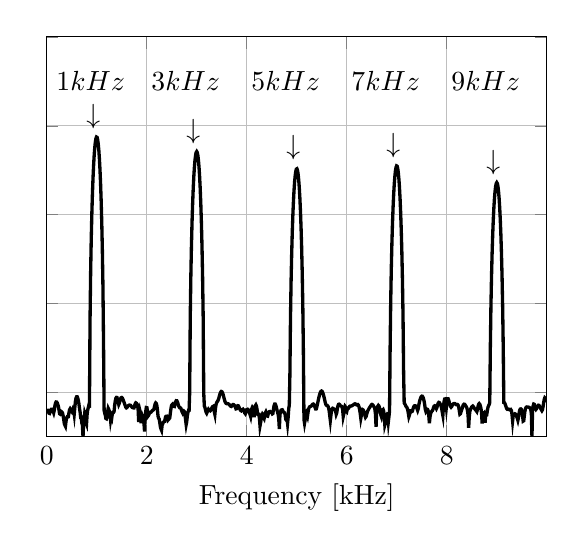
\begin{tikzpicture}

\begin{axis}[%
width=2.5in,
height=2in,
at={(1.011in,0.642in)},
scale only axis,
scaled x ticks = false,
xmin=0,
xmax=10000,
xlabel={Frequency [kHz]},
xmajorgrids,
ymin=-350,
ymax=100,
yticklabels={\empty},
xticklabels={0, 2, 4, 6, 8},
xtick = {0, 2000, 4000, 6000, 8000},
ymajorgrids,
axis background/.style={fill=white}
]
\addplot [color=black,solid,line width=1.2pt,forget plot]
  table[row sep=crcr]{%
0	-319.66977604872\\
11.7216117216117	-320.252664587285\\
23.4432234432234	-320.150235457912\\
35.1648351648352	-321.87769890753\\
46.8864468864469	-323.40415662653\\
58.6080586080586	-323.656130393623\\
70.3296703296703	-322.064437707905\\
82.0512820512821	-319.981208617154\\
93.7728937728938	-318.842227630664\\
105.494505494505	-318.824139809043\\
117.216117216117	-320.887574922404\\
128.937728937729	-321.003133041111\\
140.659340659341	-322.87596816246\\
152.380952380952	-319.992614901689\\
164.102564102564	-315.14338512313\\
175.824175824176	-312.091040412566\\
187.545787545788	-310.719044223205\\
199.267399267399	-310.809798667983\\
210.989010989011	-311.752989871661\\
222.710622710623	-313.45380396223\\
234.432234432234	-315.761867809304\\
246.153846153846	-319.502071438942\\
257.875457875458	-323.946635313474\\
269.59706959707	-324.371444723204\\
281.318681318681	-323.073351060989\\
293.040293040293	-321.551796444871\\
304.761904761905	-322.055919814239\\
316.483516483516	-322.965971780673\\
328.205128205128	-326.002185265755\\
339.92673992674	-329.965312555944\\
351.648351648352	-334.711128765065\\
363.369963369963	-336.638049322374\\
375.091575091575	-337.98571585667\\
386.813186813187	-332.646513976849\\
398.534798534799	-328.549789756313\\
410.25641025641	-327.456662133417\\
421.978021978022	-327.626158860462\\
433.699633699634	-327.386942727765\\
445.421245421245	-322.896618361246\\
457.142857142857	-319.559352515529\\
468.864468864469	-318.409730305314\\
480.586080586081	-319.522058201484\\
492.307692307692	-320.47758374283\\
504.029304029304	-321.509888136428\\
515.750915750916	-320.159719568534\\
527.472527472527	-318.379124501943\\
539.194139194139	-319.523442928177\\
550.915750915751	-324.291519604555\\
562.637362637363	-317.000247172954\\
574.358974358974	-310.257297372003\\
586.080586080586	-306.452256789241\\
597.802197802198	-304.914755096574\\
609.52380952381	-304.849950666219\\
621.245421245421	-306.178349309972\\
632.967032967033	-308.999456883321\\
644.688644688645	-312.701079748048\\
656.410256410256	-318.133369508358\\
668.131868131868	-321.871349328687\\
679.85347985348	-328.007141062136\\
691.575091575092	-327.923815494954\\
703.296703296703	-334.421366290934\\
715.018315018315	-336.919165990102\\
726.739926739927	-350.238350354447\\
738.461538461538	-334.287106214054\\
750.18315018315	-331.529493482922\\
761.904761904762	-323.393743024448\\
773.626373626374	-325.375012877451\\
785.347985347985	-333.280057572197\\
797.069597069597	-335.19416243948\\
808.791208791209	-324.722376849988\\
820.512820512821	-319.534300482415\\
832.234432234432	-317.094423031942\\
843.956043956044	-314.230543015098\\
855.677655677656	-314.557553385869\\
867.399267399267	-218.096479418237\\
879.120879120879	-165.31233950964\\
890.842490842491	-128.682095822832\\
902.564102564103	-100.530344507165\\
914.285714285714	-78.084880479123\\
926.007326007326	-59.9659632721987\\
937.728937728938	-45.374718047142\\
949.450549450549	-33.8079579109673\\
961.172161172161	-24.9340347597582\\
972.893772893773	-18.5312624507586\\
984.615384615385	-14.4548534903171\\
996.336996336996	-12.6185805249835\\
1008.05860805861	-12.9850171766986\\
1019.78021978022	-15.5615638599584\\
1031.50183150183	-20.4012212145476\\
1043.22344322344	-27.6083083479584\\
1054.94505494505	-37.3506537674849\\
1066.66666666667	-49.8819120327287\\
1078.38827838828	-65.5819960417282\\
1090.10989010989	-85.0340135297919\\
1101.8315018315	-109.185220100279\\
1113.55311355311	-139.739280721206\\
1125.27472527473	-180.395851142773\\
1136.99633699634	-243.857203771645\\
1148.71794871795	-320.064214921221\\
1160.43956043956	-323.366413363497\\
1172.16117216117	-325.396412628388\\
1183.88278388278	-329.265224803788\\
1195.6043956044	-329.60094243683\\
1207.32600732601	-326.921780096168\\
1219.04761904762	-321.464324984819\\
1230.76923076923	-317.826268547569\\
1242.49084249084	-319.221077345555\\
1254.21245421245	-321.375095535668\\
1265.93406593407	-324.721808786549\\
1277.65567765568	-331.172690405964\\
1289.37728937729	-327.190232156617\\
1301.0989010989	-328.859943718811\\
1312.82051282051	-323.934795224629\\
1324.54212454212	-322.364415478264\\
1336.26373626374	-322.478330039218\\
1347.98534798535	-321.489536953464\\
1359.70695970696	-314.390389588376\\
1371.42857142857	-309.60862386725\\
1383.15018315018	-306.521750201537\\
1394.87179487179	-305.565117533603\\
1406.59340659341	-305.702100348221\\
1418.31501831502	-307.818779142851\\
1430.03663003663	-310.811026454631\\
1441.75824175824	-313.559439282394\\
1453.47985347985	-312.058365319402\\
1465.20146520147	-309.48643321096\\
1476.92307692308	-307.140766755864\\
1488.64468864469	-305.927929790195\\
1500.3663003663	-305.68081936221\\
1512.08791208791	-306.253463667057\\
1523.80952380952	-307.512548043642\\
1535.53113553114	-309.240333775713\\
1547.25274725275	-311.110810007732\\
1558.97435897436	-313.026613238936\\
1570.69597069597	-314.684246329279\\
1582.41758241758	-316.562263550235\\
1594.13919413919	-317.34925468497\\
1605.86080586081	-316.972914787236\\
1617.58241758242	-315.837162513633\\
1629.30402930403	-315.010289548155\\
1641.02564102564	-314.61272550257\\
1652.74725274725	-314.191796909467\\
1664.46886446886	-314.28452593732\\
1676.19047619048	-314.44068736787\\
1687.91208791209	-315.163984330929\\
1699.6336996337	-316.074197397418\\
1711.35531135531	-316.88489131864\\
1723.07692307692	-317.041914340833\\
1734.79853479853	-317.437076599362\\
1746.52014652015	-317.408595347971\\
1758.24175824176	-314.977242717819\\
1769.96336996337	-312.798692171014\\
1781.68498168498	-311.696012513731\\
1793.40659340659	-312.054973498482\\
1805.12820512821	-312.757629044374\\
1816.84981684982	-314.671182783884\\
1828.57142857143	-318.737367209963\\
1840.29304029304	-333.298637671399\\
1852.01465201465	-324.040270018849\\
1863.73626373626	-320.218772715714\\
1875.45787545788	-322.961277404956\\
1887.17948717949	-334.539879130504\\
1898.9010989011	-329.519558463716\\
1910.62271062271	-327.086665233421\\
1922.34432234432	-329.320914289439\\
1934.06593406593	-333.764791120093\\
1945.78754578755	-334.533536266036\\
1957.50915750916	-344.075961360429\\
1969.23076923077	-325.931436360931\\
1980.95238095238	-321.560515034589\\
1992.67399267399	-316.983261750671\\
2004.3956043956	-317.110381405833\\
2016.11721611722	-321.132995230379\\
2027.83882783883	-326.523077686188\\
2039.56043956044	-325.653710578744\\
2051.28205128205	-323.928172040114\\
2063.00366300366	-322.747947786259\\
2074.72527472527	-322.260325203462\\
2086.44688644689	-322.179587255979\\
2098.1684981685	-321.447015430713\\
2109.89010989011	-320.679145880763\\
2121.61172161172	-319.996850102969\\
2133.33333333333	-319.748987981692\\
2145.05494505495	-318.811608861215\\
2156.77655677656	-315.677040406118\\
2168.49816849817	-312.982927012805\\
2180.21978021978	-311.768582374902\\
2191.94139194139	-312.361349170269\\
2203.663003663	-314.717024595332\\
2215.38461538462	-319.600639416848\\
2227.10622710623	-326.758844918533\\
2238.82783882784	-328.904449591274\\
2250.54945054945	-329.992103956622\\
2262.27106227106	-333.893348006191\\
2273.99267399267	-338.599091466457\\
2285.71428571429	-340.965352163138\\
2297.4358974359	-342.523569304107\\
2309.15750915751	-336.765445451662\\
2320.87912087912	-335.565258332623\\
2332.60073260073	-333.4569631189\\
2344.32234432234	-332.951254029186\\
2356.04395604396	-332.674528864243\\
2367.76556776557	-329.994984991045\\
2379.48717948718	-327.258409386749\\
2391.20879120879	-326.695675890422\\
2402.9304029304	-326.676287404655\\
2414.65201465201	-328.264297481345\\
2426.37362637363	-331.133002458237\\
2438.09523809524	-330.432637449573\\
2449.81684981685	-329.535023454296\\
2461.53846153846	-328.791646558295\\
2473.26007326007	-323.424920352782\\
2484.98168498168	-318.460018564717\\
2496.7032967033	-314.691219196617\\
2508.42490842491	-313.711392542011\\
2520.14652014652	-313.067394364558\\
2531.86813186813	-314.016279106977\\
2543.58974358974	-315.634969727647\\
2555.31135531136	-315.816934484372\\
2567.03296703297	-313.100967181084\\
2578.75457875458	-310.464193572589\\
2590.47619047619	-309.262262083557\\
2602.1978021978	-309.311255100885\\
2613.91941391941	-310.569261034711\\
2625.64102564103	-312.500205228524\\
2637.36263736264	-314.761756514628\\
2649.08424908425	-316.412573490754\\
2660.80586080586	-317.291190858618\\
2672.52747252747	-317.313991378883\\
2684.24908424908	-317.942974517788\\
2695.9706959707	-319.7342089385\\
2707.69230769231	-321.898558877662\\
2719.41391941392	-323.134909705626\\
2731.13553113553	-321.588957105158\\
2742.85714285714	-320.885605445503\\
2754.57875457875	-321.580662784063\\
2766.30036630037	-324.821452300477\\
2778.02197802198	-330.892094927682\\
2789.74358974359	-336.098023413537\\
2801.4652014652	-332.703176113955\\
2813.18681318681	-326.372946209155\\
2824.90842490842	-322.497222683491\\
2836.63003663004	-320.220801606029\\
2848.35164835165	-320.15667236125\\
2860.07326007326	-300.30570529002\\
2871.79487179487	-214.177492827452\\
2883.51648351648	-168.385261564454\\
2895.2380952381	-135.050186499224\\
2906.95970695971	-109.011900053879\\
2918.68131868132	-88.1243250034129\\
2930.40293040293	-71.2518156639137\\
2942.12454212454	-57.7144375482064\\
2953.84615384615	-47.0758016147511\\
2965.56776556777	-39.0459280367578\\
2977.28937728938	-33.4315280345184\\
2989.01098901099	-30.1088642243201\\
3000.7326007326	-29.0087381705451\\
3012.45421245421	-30.1088642243202\\
3024.17582417582	-33.4315280345187\\
3035.89743589744	-39.0459280367583\\
3047.61904761905	-47.0758016147517\\
3059.34065934066	-57.7144375482071\\
3071.06227106227	-71.2518156639152\\
3082.78388278388	-88.124325003423\\
3094.50549450549	-109.011900053981\\
3106.22710622711	-135.050186500745\\
3117.94871794872	-168.385261645028\\
3129.67032967033	-214.177514890276\\
3141.39194139194	-300.84560200681\\
3153.11355311355	-315.2569703318\\
3164.83516483516	-316.84238110397\\
3176.55677655678	-319.656198303406\\
3188.27838827839	-322.267206549707\\
3200	-323.394796361885\\
3211.72161172161	-321.831716535344\\
3223.44322344322	-320.071509664792\\
3235.16483516484	-318.862404385705\\
3246.88644688645	-319.690646580034\\
3258.60805860806	-320.415471931005\\
3270.32967032967	-320.690946536644\\
3282.05128205128	-319.710368339791\\
3293.77289377289	-318.595434038106\\
3305.49450549451	-317.036983471108\\
3317.21611721612	-316.038331017621\\
3328.93772893773	-315.662275736532\\
3340.65934065934	-317.356396019158\\
3352.38095238095	-321.760930073742\\
3364.10256410256	-324.637108569141\\
3375.82417582418	-317.710322451106\\
3387.54578754579	-313.594250633537\\
3399.2673992674	-311.479079412246\\
3410.98901098901	-310.354822336986\\
3422.71062271062	-309.501559350269\\
3434.43223443223	-307.978785454896\\
3446.15384615385	-305.738913277755\\
3457.87545787546	-303.219123772711\\
3469.59706959707	-301.020945261217\\
3481.31868131868	-299.558883503574\\
3493.04029304029	-298.894048192919\\
3504.7619047619	-299.188153921955\\
3516.48351648352	-300.3078497822\\
3528.20512820513	-302.212617063443\\
3539.92673992674	-304.639790056806\\
3551.64835164835	-307.338226654577\\
3563.36996336996	-309.670891902987\\
3575.09157509158	-311.346258045309\\
3586.81318681319	-312.237779545341\\
3598.5347985348	-312.56161470283\\
3610.25641025641	-312.55329095589\\
3621.97802197802	-312.582369772614\\
3633.69963369963	-312.851642932638\\
3645.42124542125	-313.337522432521\\
3657.14285714286	-313.980853222016\\
3668.86446886447	-314.970961319011\\
3680.58608058608	-315.519669753624\\
3692.30769230769	-315.771476529355\\
3704.0293040293	-315.073491592498\\
3715.75091575092	-314.189266101827\\
3727.47252747253	-313.593883592026\\
3739.19413919414	-313.738638685608\\
3750.91575091575	-314.308512255133\\
3762.63736263736	-315.339022840772\\
3774.35897435897	-316.603604206891\\
3786.08058608059	-318.480880716564\\
3797.8021978022	-318.292200819127\\
3809.52380952381	-316.112351446803\\
3821.24542124542	-314.897423670021\\
3832.96703296703	-315.017858900632\\
3844.68864468864	-316.135152915023\\
3856.41025641026	-317.820937023667\\
3868.13186813187	-319.413847765108\\
3879.85347985348	-320.333708738422\\
3891.57509157509	-320.722670234731\\
3903.2967032967	-319.992076799159\\
3915.01831501832	-319.338489682422\\
3926.73992673993	-318.858608272676\\
3938.46153846154	-319.680816828147\\
3950.18315018315	-320.978850851144\\
3961.90476190476	-323.188232090719\\
3973.62637362637	-324.007985133895\\
3985.34798534799	-322.570195704753\\
3997.0695970696	-319.514596742841\\
4008.79120879121	-319.283053569699\\
4020.51282051282	-318.929362581139\\
4032.23443223443	-319.488742096079\\
4043.95604395604	-320.965633129066\\
4055.67765567766	-322.481527107505\\
4067.39926739927	-324.813720853809\\
4079.12087912088	-327.030843198677\\
4090.84249084249	-322.285902452843\\
4102.5641025641	-318.186243444301\\
4114.28571428571	-316.603502399595\\
4126.00732600733	-317.481479156322\\
4137.72893772894	-321.968090951304\\
4149.45054945055	-327.957840447245\\
4161.17216117216	-318.976727193473\\
4172.89377289377	-315.096300971734\\
4184.61538461538	-314.032500143688\\
4196.336996337	-315.483699263343\\
4208.05860805861	-319.265132234658\\
4219.78021978022	-324.55539249217\\
4231.50183150183	-324.788115491149\\
4243.22344322344	-324.700621521764\\
4254.94505494505	-328.989312876653\\
4266.66666666667	-337.569307608176\\
4278.38827838828	-333.952487175123\\
4290.10989010989	-329.959991603221\\
4301.8315018315	-325.799592908156\\
4313.55311355311	-324.369338201738\\
4325.27472527472	-325.364218654711\\
4336.99633699634	-328.177317631504\\
4348.71794871795	-329.373251997288\\
4360.43956043956	-325.946288654945\\
4372.16117216117	-323.093752552372\\
4383.88278388278	-321.779392892024\\
4395.6043956044	-323.48874347434\\
4407.32600732601	-326.468625864879\\
4419.04761904762	-326.651753870262\\
4430.76923076923	-324.105142382957\\
4442.49084249084	-322.360324994449\\
4454.21245421245	-321.523240426057\\
4465.93406593407	-321.416141577155\\
4477.65567765568	-322.01923713689\\
4489.37728937729	-322.277623497054\\
4501.0989010989	-322.837324311223\\
4512.82051282051	-324.131882907695\\
4524.54212454212	-323.707472016558\\
4536.26373626374	-318.734144772884\\
4547.98534798535	-314.843075442963\\
4559.70695970696	-313.072167637317\\
4571.42857142857	-313.083110435843\\
4583.15018315018	-314.523708294673\\
4594.87179487179	-316.843132095304\\
4606.59340659341	-319.946727607398\\
4618.31501831502	-322.580797757278\\
4630.03663003663	-324.643297800685\\
4641.75824175824	-330.090746214774\\
4653.47985347985	-341.115506894516\\
4665.20146520146	-325.198207363607\\
4676.92307692308	-321.391338010681\\
4688.64468864469	-319.939534104301\\
4700.3663003663	-319.595169091842\\
4712.08791208791	-319.469942141125\\
4723.80952380952	-320.605907533617\\
4735.53113553114	-321.863281040901\\
4747.25274725275	-322.505865049125\\
4758.97435897436	-322.899195500862\\
4770.69597069597	-325.654732674365\\
4782.41758241758	-330.341163475003\\
4794.13919413919	-331.246642250653\\
4805.86080586081	-329.204106508267\\
4817.58241758242	-334.885243879829\\
4829.30402930403	-328.101152331398\\
4841.02564102564	-318.294888808809\\
4852.74725274725	-314.129895112624\\
4864.46886446886	-279.651117196258\\
4876.19047619048	-216.132332330872\\
4887.91208791209	-175.475716839038\\
4899.6336996337	-144.921655735681\\
4911.35531135531	-120.770449149269\\
4923.07692307692	-101.318431660301\\
4934.79853479854	-85.6183476512476\\
4946.52014652015	-73.0870893860055\\
4958.24175824176	-63.3447439664808\\
4969.96336996337	-56.1376568330706\\
4981.68498168498	-51.2979994784815\\
4993.40659340659	-48.7214527952216\\
5005.12820512821	-48.3550161435066\\
5016.84981684982	-50.1912891088403\\
5028.57142857143	-54.2676980692819\\
5040.29304029304	-60.6704703782819\\
5052.01465201465	-69.5443935294921\\
5063.73626373626	-81.1111536656695\\
5075.45787545788	-95.7023988907233\\
5087.17948717949	-113.821316097484\\
5098.9010989011	-136.266780122429\\
5110.62271062271	-164.418531362237\\
5122.34432234432	-201.048770357836\\
5134.06593406593	-253.83120041389\\
5145.78754578755	-330.239456002953\\
5157.50915750916	-334.680801990704\\
5169.23076923077	-330.978335548456\\
5180.95238095238	-324.592108259334\\
5192.67399267399	-322.988357718612\\
5204.3956043956	-324.676605742458\\
5216.11721611722	-326.675404290512\\
5227.83882783883	-322.058554497306\\
5239.56043956044	-318.408755963627\\
5251.28205128205	-316.800667047183\\
5263.00366300366	-316.012155133395\\
5274.72527472528	-315.808538693121\\
5286.44688644689	-315.519241470069\\
5298.1684981685	-314.766546053413\\
5309.89010989011	-313.915693680535\\
5321.61172161172	-313.170309935136\\
5333.33333333333	-313.002506027263\\
5345.05494505495	-313.778996673083\\
5356.77655677656	-315.052384147386\\
5368.49816849817	-317.119258702662\\
5380.21978021978	-318.60297759862\\
5391.94139194139	-318.517609885014\\
5403.663003663	-316.146428602339\\
5415.38461538462	-313.22805094124\\
5427.10622710623	-310.060397661986\\
5438.82783882784	-307.004516563346\\
5450.54945054945	-304.11566250975\\
5462.27106227106	-301.720722823213\\
5473.99267399267	-299.876292417269\\
5485.71428571429	-298.717877556861\\
5497.4358974359	-298.340591948456\\
5509.15750915751	-298.817309497537\\
5520.87912087912	-300.084771537962\\
5532.60073260073	-302.0378396415\\
5544.32234432234	-304.538277896337\\
5556.04395604396	-307.406392708756\\
5567.76556776557	-310.390764521531\\
5579.48717948718	-312.981246586604\\
5591.20879120879	-314.295442763613\\
5602.9304029304	-314.695913010283\\
5614.65201465201	-314.755035766114\\
5626.37362637363	-315.582819583783\\
5638.09523809524	-317.334834104706\\
5649.81684981685	-320.766298110227\\
5661.53846153846	-326.125090381781\\
5673.26007326007	-331.431983615578\\
5684.98168498169	-325.508706127021\\
5696.7032967033	-321.15493650177\\
5708.42490842491	-318.814872500501\\
5720.14652014652	-317.817991285284\\
5731.86813186813	-318.089237603718\\
5743.58974358974	-318.611263623369\\
5755.31135531136	-318.932354317994\\
5767.03296703297	-319.606180603829\\
5778.75457875458	-321.168015391352\\
5790.47619047619	-324.529320635772\\
5802.1978021978	-322.807418670069\\
5813.91941391941	-317.983100218686\\
5825.64102564103	-314.980861521282\\
5837.36263736264	-313.408700551849\\
5849.08424908425	-313.197201859578\\
5860.80586080586	-313.697729031082\\
5872.52747252747	-314.609828464371\\
5884.24908424908	-315.273710204582\\
5895.9706959707	-315.575090179884\\
5907.69230769231	-316.431533776942\\
5919.41391941392	-319.426403749631\\
5931.13553113553	-327.076704692552\\
5942.85714285714	-324.120179770849\\
5954.57875457875	-317.664559412797\\
5966.30036630037	-315.562772389357\\
5978.02197802198	-316.481875593137\\
5989.74358974359	-320.74085073736\\
6001.4652014652	-321.56480888906\\
6013.18681318681	-318.837510142599\\
6024.90842490843	-318.106231260851\\
6036.63003663004	-317.807698890747\\
6048.35164835165	-316.558092075019\\
6060.07326007326	-315.557699772867\\
6071.79487179487	-315.235903266329\\
6083.51648351648	-315.34274333107\\
6095.2380952381	-315.20030664534\\
6106.95970695971	-314.830629275607\\
6118.68131868132	-314.427815160164\\
6130.40293040293	-314.058289013738\\
6142.12454212454	-313.517054051609\\
6153.84615384615	-313.025791554879\\
6165.56776556777	-312.730990453284\\
6177.28937728938	-312.947591502956\\
6189.01098901099	-313.543344432103\\
6200.7326007326	-314.08198534147\\
6212.45421245421	-313.975108910851\\
6224.17582417582	-313.669511020471\\
6235.89743589744	-314.37833689353\\
6247.61904761905	-316.358275023731\\
6259.34065934066	-319.674879096136\\
6271.06227106227	-323.684029643681\\
6282.78388278388	-329.039415469563\\
6294.50549450549	-325.5421152618\\
6306.22710622711	-320.930017930124\\
6317.94871794872	-319.278262636475\\
6329.67032967033	-319.693181877834\\
6341.39194139194	-320.924615001357\\
6353.11355311355	-323.079359745366\\
6364.83516483516	-325.918015706887\\
6376.55677655678	-328.033773854441\\
6388.27838827839	-327.140117854091\\
6400	-324.692133834817\\
6411.72161172161	-322.137346233329\\
6423.44322344322	-320.516820802526\\
6435.16483516484	-319.337054507976\\
6446.88644688645	-318.025709346077\\
6458.60805860806	-316.979112033717\\
6470.32967032967	-315.931251445007\\
6482.05128205128	-315.062076374335\\
6493.77289377289	-313.906631470696\\
6505.49450549451	-313.466921344982\\
6517.21611721612	-313.769319638734\\
6528.93772893773	-314.517640921084\\
6540.65934065934	-315.724484282667\\
6552.38095238095	-316.588068571762\\
6564.10256410256	-318.855919571499\\
6575.82417582418	-324.361412166511\\
6587.54578754579	-338.649091166889\\
6599.2673992674	-322.760921159812\\
6610.98901098901	-317.753906925668\\
6622.71062271062	-315.516352483433\\
6634.43223443223	-314.526286365145\\
6646.15384615385	-315.259688478357\\
6657.87545787546	-317.394762548319\\
6669.59706959707	-320.732967861906\\
6681.31868131868	-324.825744034868\\
6693.04029304029	-326.820759935945\\
6704.7619047619	-322.872146846357\\
6716.48351648352	-319.74872153185\\
6728.20512820513	-319.170904101219\\
6739.92673992674	-321.086066713475\\
6751.64835164835	-326.112025334888\\
6763.36996336996	-336.624474419805\\
6775.09157509157	-334.230732856827\\
6786.81318681319	-328.753062556712\\
6798.5347985348	-326.073886014491\\
6810.25641025641	-324.70176008207\\
6821.97802197802	-325.405825297174\\
6833.69963369963	-332.73783740919\\
6845.42124542125	-327.048455871861\\
6857.14285714286	-320.875104728307\\
6868.86446886447	-250.574647660477\\
6880.58608058608	-197.792799172064\\
6892.30769230769	-161.162560617437\\
6904.0293040293	-133.010809320255\\
6915.75091575092	-110.565345290186\\
6927.47252747253	-92.4464280830486\\
6939.19413919414	-77.8551828579892\\
6950.91575091575	-66.2884227218201\\
6962.63736263736	-57.4144995706133\\
6974.35897435897	-51.0117272616143\\
6986.08058608059	-46.9353183011729\\
6997.8021978022	-45.0990453358394\\
7009.52380952381	-45.4654819875546\\
7021.24542124542	-48.0420286708145\\
7032.96703296703	-52.8816860254038\\
7044.68864468864	-60.0887731588147\\
7056.41025641026	-69.8311185783417\\
7068.13186813187	-82.3623768435883\\
7079.85347985348	-98.0624608526129\\
7091.57509157509	-117.514478341006\\
7103.2967032967	-141.665684918764\\
7115.01831501831	-172.219745862912\\
7126.73992673993	-212.876362575016\\
7138.46153846154	-276.422779719188\\
7150.18315018315	-311.898684092958\\
7161.90476190476	-312.709742302499\\
7173.62637362637	-314.073994262169\\
7185.34798534799	-315.509132701049\\
7197.0695970696	-316.40719601034\\
7208.79120879121	-317.332582010188\\
7220.51282051282	-319.40750609588\\
7232.23443223443	-323.210664245618\\
7243.95604395604	-327.331928901919\\
7255.67765567766	-325.473483569222\\
7267.39926739927	-321.976013289618\\
7279.12087912088	-320.676201014468\\
7290.84249084249	-320.801210307641\\
7302.5641025641	-321.507756558202\\
7314.28571428571	-321.103460465869\\
7326.00732600733	-318.588086156553\\
7337.72893772894	-316.565075206643\\
7349.45054945055	-315.277346593938\\
7361.17216117216	-314.885550260067\\
7372.89377289377	-314.891837602016\\
7384.61538461538	-315.449350147104\\
7396.336996337	-316.745745681702\\
7408.05860805861	-318.419916282407\\
7419.78021978022	-320.261431969836\\
7431.50183150183	-318.268672120946\\
7443.22344322344	-314.091608173447\\
7454.94505494505	-310.765957845321\\
7466.66666666667	-308.217783141544\\
7478.38827838828	-306.239035860403\\
7490.10989010989	-304.816952750248\\
7501.8315018315	-304.15608386294\\
7513.55311355311	-304.254491064508\\
7525.27472527472	-305.211593460601\\
7536.99633699634	-307.030312830436\\
7548.71794871795	-309.879326533619\\
7560.43956043956	-313.845760685343\\
7572.16117216117	-318.841850332976\\
7583.88278388278	-321.207995748871\\
7595.6043956044	-320.013712544925\\
7607.32600732601	-318.776063684063\\
7619.04761904762	-319.085551795786\\
7630.76923076923	-320.939164664321\\
7642.49084249084	-326.254817057014\\
7654.21245421245	-334.569473846894\\
7665.93406593407	-327.931786824776\\
7677.65567765568	-324.051596359106\\
7689.37728937729	-322.288144039605\\
7701.0989010989	-321.229303753046\\
7712.82051282051	-320.657714719804\\
7724.54212454212	-319.352677742086\\
7736.26373626374	-317.11201010275\\
7747.98534798535	-315.512568863074\\
7759.70695970696	-314.929278878524\\
7771.42857142857	-315.115340679379\\
7783.15018315018	-316.822691426277\\
7794.87179487179	-318.181220637214\\
7806.59340659341	-316.776568611525\\
7818.31501831502	-313.852220867404\\
7830.03663003663	-312.002406009657\\
7841.75824175824	-311.164749597181\\
7853.47985347985	-311.393965980471\\
7865.20146520146	-312.252662903959\\
7876.92307692308	-313.70152247797\\
7888.64468864469	-315.573585771477\\
7900.3663003663	-318.092576192861\\
7912.08791208791	-322.4419386204\\
7923.80952380952	-325.885107269\\
7935.53113553114	-315.728036603532\\
7947.25274725275	-310.207096026785\\
7958.97435897436	-307.39528878069\\
7970.69597069597	-307.214798035391\\
7982.41758241758	-310.249964168014\\
7994.13919413919	-316.455301461558\\
8005.86080586081	-310.18108881179\\
8017.58241758242	-307.118104234728\\
8029.30402930403	-307.103626006243\\
8041.02564102564	-308.787848887118\\
8052.74725274725	-311.254474300167\\
8064.46886446886	-313.705378738313\\
8076.19047619048	-315.670416772103\\
8087.91208791209	-316.586732731561\\
8099.6336996337	-315.828567102877\\
8111.35531135531	-314.658811303786\\
8123.07692307692	-313.406572522504\\
8134.79853479854	-312.66962362792\\
8146.52014652015	-312.448750110159\\
8158.24175824176	-312.419482694733\\
8169.96336996337	-312.803696384012\\
8181.68498168498	-313.295545576826\\
8193.40659340659	-313.853348514964\\
8205.12820512821	-313.833478550749\\
8216.84981684982	-313.61336866691\\
8228.57142857143	-314.193969835242\\
8240.29304029304	-316.283557504146\\
8252.01465201465	-320.403424674361\\
8263.73626373626	-324.461982722269\\
8275.45787545788	-323.928707340462\\
8287.17948717949	-321.76611077263\\
8298.9010989011	-319.645859437962\\
8310.62271062271	-317.756972073173\\
8322.34432234432	-315.456535213765\\
8334.06593406593	-313.801900724168\\
8345.78754578755	-313.156054469238\\
8357.50915750916	-313.295300275638\\
8369.23076923077	-314.015963323273\\
8380.95238095238	-315.107651529325\\
8392.67399267399	-316.0289335874\\
8404.3956043956	-317.664437763639\\
8416.11721611722	-320.322192776584\\
8427.83882783883	-325.454646046237\\
8439.56043956044	-339.882811871287\\
8451.28205128205	-327.930659862074\\
8463.00366300366	-321.508748618535\\
8474.72527472528	-319.142368328328\\
8486.44688644689	-317.887625168224\\
8498.1684981685	-316.398702897209\\
8509.89010989011	-315.844272704648\\
8521.61172161172	-315.304129811956\\
8533.33333333333	-315.994408548112\\
8545.05494505494	-316.988551478669\\
8556.77655677656	-318.106390240229\\
8568.49816849817	-319.027154929891\\
8580.21978021978	-319.812320525615\\
8591.94139194139	-320.557458360575\\
8603.663003663	-321.51609417813\\
8615.38461538462	-319.208436155719\\
8627.10622710623	-315.634876225168\\
8638.82783882784	-313.282580117098\\
8650.54945054945	-312.557824637183\\
8662.27106227106	-313.287365657449\\
8673.99267399267	-315.101223185669\\
8685.71428571429	-317.918900259002\\
8697.4358974359	-322.827357182022\\
8709.15750915751	-334.905660533007\\
8720.87912087912	-329.598732480268\\
8732.60073260073	-323.918402497209\\
8744.32234432235	-323.225663253841\\
8756.04395604396	-327.882604758779\\
8767.76556776557	-334.08772192061\\
8779.48717948718	-325.816032287453\\
8791.20879120879	-324.120639882715\\
8802.9304029304	-324.463360873992\\
8814.65201465201	-320.157644074005\\
8826.37362637363	-316.607378912133\\
8838.09523809524	-314.977460763074\\
8849.81684981685	-313.598892848365\\
8861.53846153846	-311.531251182091\\
8873.26007326007	-249.039767111074\\
8884.98168498169	-203.242029131657\\
8896.7032967033	-169.906929318669\\
8908.42490842491	-143.868642611774\\
8920.14652014652	-122.981067561458\\
8931.86813186813	-106.108558222317\\
8943.58974358974	-92.5711801065715\\
8955.31135531135	-81.9325441730846\\
8967.03296703297	-73.9026705950811\\
8978.75457875458	-68.2882705928396\\
8990.47619047619	-64.9656067826414\\
9002.1978021978	-63.8654807288671\\
9013.91941391941	-64.9656067826429\\
9025.64102564103	-68.2882705928421\\
9037.36263736264	-73.9026705950824\\
9049.08424908425	-81.9325441730767\\
9060.80586080586	-92.5711801065311\\
9072.52747252747	-106.108558222202\\
9084.24908424908	-122.981067561203\\
9095.9706959707	-143.868642602562\\
9107.69230769231	-169.906928781367\\
9119.41391941392	-203.241987404462\\
9131.13553113553	-249.030296777096\\
9142.85714285714	-311.304512921604\\
9154.57875457876	-311.537328657934\\
9166.30036630037	-312.622507182141\\
9178.02197802198	-314.484101268501\\
9189.74358974359	-316.638047956377\\
9201.4652014652	-318.240365114368\\
9213.18681318681	-318.945193216639\\
9224.90842490842	-318.716534544361\\
9236.63003663004	-318.771748632388\\
9248.35164835165	-318.836599674886\\
9260.07326007326	-319.61908906793\\
9271.79487179487	-319.822294152504\\
9283.51648351648	-319.371461582341\\
9295.2380952381	-320.455571545465\\
9306.95970695971	-324.955116608097\\
9318.68131868132	-332.064216057748\\
9330.40293040293	-326.151615205209\\
9342.12454212454	-324.758080768938\\
9353.84615384615	-324.675211282058\\
9365.56776556777	-324.045321612164\\
9377.28937728938	-324.39253747893\\
9389.01098901099	-325.618923679901\\
9400.7326007326	-327.30803370137\\
9412.45421245421	-329.101453300761\\
9424.17582417582	-331.357262728207\\
9435.89743589744	-328.369864579068\\
9447.61904761905	-323.625954295584\\
9459.34065934066	-320.052944616956\\
9471.06227106227	-318.680325028373\\
9482.78388278388	-318.495481334863\\
9494.50549450549	-319.072602246417\\
9506.22710622711	-322.438351004492\\
9517.94871794872	-326.302775164653\\
9529.67032967033	-332.236401444499\\
9541.39194139194	-331.826732588463\\
9553.11355311355	-326.312560073614\\
9564.83516483517	-321.103996076185\\
9576.55677655678	-318.036729405502\\
9588.27838827839	-316.757057599893\\
9600	-316.289063164499\\
9611.72161172161	-316.324856775091\\
9623.44322344322	-316.350179630349\\
9635.16483516483	-316.563172794392\\
9646.88644688645	-316.736600642076\\
9658.60805860806	-317.140959522388\\
9670.32967032967	-317.883238263279\\
9682.05128205128	-319.49921625628\\
9693.77289377289	-323.692303015967\\
9705.49450549451	-349.984618262359\\
9717.21611721612	-320.976769185242\\
9728.93772893773	-315.17753537576\\
9740.65934065934	-313.074148193045\\
9752.38095238095	-313.376471369528\\
9764.10256410256	-315.248048467012\\
9775.82417582418	-317.460020635791\\
9787.54578754579	-318.916164496397\\
9799.2673992674	-318.079181600956\\
9810.98901098901	-316.690886394991\\
9822.71062271062	-315.207508754715\\
9834.43223443223	-314.386564565063\\
9846.15384615385	-314.548895431942\\
9857.87545787546	-315.391776864814\\
9869.59706959707	-316.68455315035\\
9881.31868131868	-318.139278296883\\
9893.04029304029	-319.449803507901\\
9904.7619047619	-320.515956568989\\
9916.48351648352	-319.388496977814\\
9928.20512820513	-315.730857337976\\
9939.92673992674	-311.242165481577\\
9951.64835164835	-307.737829406979\\
9963.36996336996	-305.870078981667\\
9975.09157509158	-306.441379041955\\
9986.81318681319	-310.96576225089\\
};
\node[right, align=left, text=black]
at (axis cs:600,10) {$\downarrow$};
\node[right, align=left, text=black]
at (axis cs:0,50) {$\text{1 kHz}$};
\node[right, align=left, text=black]
at (axis cs:2600,-6) {$\downarrow$};
\node[right, align=left, text=black]
at (axis cs:1900,50) {$\text{3 kHz}$};
\node[right, align=left, text=black]
at (axis cs:4600,-25) {$\downarrow$};
\node[right, align=left, text=black]
at (axis cs:3900,50) {$\text{5 kHz}$};
\node[right, align=left, text=black]
at (axis cs:6600,-22) {$\downarrow$};
\node[right, align=left, text=black]
at (axis cs:5900,50) {$\text{7 kHz}$};
\node[right, align=left, text=black]
at (axis cs:8600,-41) {$\downarrow$};
\node[right, align=left, text=black]
at (axis cs:7900,50) {$\text{9 kHz}$};
\end{axis}
\end{tikzpicture}%
	\caption{FFT of a 1 kHz sinusoid with clipping.}
	\label{fig:clippingDistFFT}
\end{subfigure}
\caption{The Fast Fourier Transformation(FFT) of the 1 kHz sinusoid with a peak amplitude on 1.5. }
\label{fig:audioclippingFFT}
\end{figure}

%The sampling frequency is 48 kHz and a Kaiser-window function with a $\beta$-value of 38 is applied to both signal.
The amplitude difference between the fundamental frequency on 1 kHz and the 3rd harmonic frequency is 16 dB, which is approximately a factor of 6.3 in linear scale. If the signal is clipped even more, the amplitude difference between the fundamental frequency and uneven harmonics decreases thus making it even more unpleasant. Therefore audio clipping should be avoided or minimized.












\section{Loudspeaker topology}

In order to understand where distortion could arrive from in a speaker it is necessary to understand the basic fundamentals and the topology of a loudspeaker. This section will consist of the basic topology and then glans over the topic of vibration induced in the speaker driver.

\subsubsection*{The basics}
The loudspeaker is a transducer which purpose is to convert the electrical energy into acoustical energy. This is done by sending the signal into the speaker which can consist of numerous driver. Each driver is made with a specific purpose for handling frequency. The drivers are designed to perform best within their frequency range, hence they are usually different sizes in diameter.
\begin{itemize}
\item[] For the high frequencies their is a tweeter, 1-2 inches in diameters, high frequencies is roughly 3-4 kHz and above.
\item[] In the midrange their is a midrange driver which usually is around 5-6 inches. The midrange is roughly 3-4 kHz to 300 Hz. 
\item[] The lower frequencies, which is 300 and below, is then handled by the woofer. The woofer can is usually 5-6+ inches in diameter.
\end{itemize}
The reason for different diameters in drivers is because of the wavelength the specific frequencies got. Should a woofer play frequencies at +4 kHz it would end in the driver physically not being able to move that fast. The limitations will end up in non-linear distortion in the diaphragm. Vice versa, should a tweeter reproduced low frequency sound at high \gls{SPL} it will end in distortion. The tweeter has a very low excursion range which limits it to the high frequency area.

\subsubsection*{Sensitivity}

A speaker is supplied from the manufacture with a sensitivity rating. This tells how efficient a loudspeaker is. The sensitivity rating is rated in dB and tells what \gls{SPL} the speaker outputs when supplied with 1 watt using 2.86 volt and measured at 1 meter. This is done assuming an infinite baffle and no reflection from the room. The sensitivity is defined by \autoref{eq:speaker_sensitivty}.
\begin{align}\label{eq:speaker_sensitivty}
\text{dB}_\text{sensitivity}=112\text {dB} +10 \cdot log_{10}(\text{efficiency})
\end{align}  
The 112 dB in \autoref{eq:speaker_sensitivty} is added to the sensitivity since this 1 watt compared to the $10^{-12}$ watt which is the threshold for audible sound. At 1 watt it will yield 120 dB. The reason for 8 dB difference is due to the assumption of infinite baffle in a reflection free room. When the sound is dispersed at a radius of $2\pi=r^2$, where r is 1 meter it creates a reduction in \gls{SPL} by 8 dB.

\subsubsection*{Diaphragm excursion}




\subsection{Distortion from vibration}

A common problem when designing loudspeakers is the vibrations from the enclosure. If the vibrations are strong, they will become audible and distort the overall sound. The sound radiation from the enclosure will become greater when the \gls{SPL} from the speaker increase. This problem is solved with different techniques but yield more or less the same outcome, which is stiffening of the enclosure. Some of the techniques for removing vibrations from the enclosure could be:
\begin{itemize}
\item Mechanical decoupling of the drivers from the enclosure.
\item Denser or heavier construction material with a high natural frequency, making it harder for the enclosure to start vibrating.
\item Dampening material or complex structural design inside the cabinet to disperse the sound.
\end{itemize}
\todo[inline]{Skal nok lige skaffe nogle kilder på de udtagelser}


Looking further into the speaker driver itself, it shows in \autoref{fig:SpeakerModelStress} that parts in the driver also creates unwanted vibrations. The goal of the speaker driver is to reproduce the electrical signal as an acoustical signal. This is done by using a membrane which is suspended in a very light and easy to move material. An Induction in the coil is created in a permanent magnet creating a a electro magnetic force resulting in the membrane moving. The goal will always be to loose as little as possible energy, giving the most perfect output. The driver simply needs to be as powerfull, light, stiff and efficient as possible.

\begin{figure}[H]
\centering
\begin{subfigure}[t]{0.47\textwidth}
\includegraphics[width=\linewidth]{SpeakerGOOD}
	\caption{Regular speaker driver showing suspension, membrane and the driver magnet.}
	\label{fig:regularspeaker}
\end{subfigure}
\hspace{6mm} 
\begin{subfigure}[t]{0.47\textwidth}
\includegraphics[width=\linewidth]{SpeakerBAD}
	\caption{Regular speaker driver with red markings showing stress areas}
	\label{fig:badspeaker}
\end{subfigure}
\caption{A Speaker driver, where \ref{fig:badspeaker} shows the stress points outlined with red.}
\label{fig:SpeakerModelStress}
\end{figure}

When this signal has a large amplitude, read overload, the membrane reaches physical capacity. In \autoref{fig:badspeaker} it shows that when a membrane is pushed to its maximum capacity the suspension will affect the membrane causing unwanted distortion. This will be one of the major problems if the membrane is assumed sufficiently stiff to with stand the high \gls{SPL} and not twist during playback. 

Another notice is the membrane hitting the coil connected to the magnet. This would again result in distortion since the membrane is now again hitting the absolute furthest position possible. This situation can however be resolve be moving the magnet further back. This would make the suspension determine how far the membrane can be pushed.


%that occurs at playback. The vibrations occurs because the  If the vibration. the sound radiated from the loudspeaker enclosure

\section{Part Conclusion}
This chapter has analyzed an active speaker and its components to investigate how distortion is created throughout the active loudspeaker. The conclusion is that the following situations create distortion.
\begin{itemize}
\item Amplifier
	\begin{itemize}
	\item Clipping.
	\end{itemize}
\item Loudspeaker
	\begin{itemize}
	\item Vibrations from enclosure.
	\item Overexcursion.
	\item Membrane hitting the coil.
	\end{itemize}
\end{itemize}
Of these situations the focus moving forward will only be concerning the distortion situation from the loudspeaker because clipping in the amplifier is easy to solve, because the parameters in the amplifier is constant and the signal is easily limited to create less distortion then by hard clipping. The next chapter will therefore explain and analyze performance tests of a loudspeaker to see if any of the above loudspeaker situations can be detected. 

\chapter{Test of DALI Zensor 5}
This section will go through a test of a loudspeaker to understand if any vibrations in the loudspeaker affect the distortion of the loudspeaker.
The loudspeaker which will be the basis for the test is the Zensor 5 (as seen on \autoref{fig:dali_zensor5}) given by DALI. A passive speaker has been choosen for the test because the amplifiers in DALI's active speakers are designed not to stress the loudspeaker to its limits and beyond, and to be able to test how the vibrations affect distortion, the loudspeaker must be tested to its limits and beyond.

\begin{figure}[H]
\centering
\includegraphics[width=0.5\textwidth]{figures/zensor5.png}
\caption{DALI zensor 5.}
\label{fig:dali_zensor5}
\end{figure}

%\todo[inline]{Reference http://www.dali-speakers.com/loudspeakers/zensor/zensor-5/}

For measuring the vibrations inside the enclosure two accelometers have been placed inside the enclosure, one on the back of bottom driver and one on the top back of the enclosure. For measuring distortion a microphone has been placed 1 m from the speaker. To limit any reflection from a room for example, the test is perfomed in the Anechoic room at \gls{AAU} see \ref{fig:test_setup_R}.  
%\todo[inline]{Reference (09.03.2016) http://doc.es.aau.dk/labs/acoustics/facilities/anechoic_room_large/} 

\begin{figure}[H]
\centering
\begin{subfigure}[t]{0.47\textwidth}
	\centering
	\includegraphics[width=1\textwidth]{figures/Test_setup_behind.jpg}
	\caption{Test setup (behind)}
	\label{fig:test_setup_behind_R}
\end{subfigure}
\hspace{6mm} 
\begin{subfigure}[t]{0.47\textwidth}
	\centering
	\includegraphics[width=1\textwidth]{figures/Test_setup_front.jpg}
	\caption{Test setup (front)}
	\label{fig:test_setup_front_R}
\end{subfigure}
\caption{Test setup.}
\label{fig:test_setup_R}
\end{figure}

The loudspeaker is set to play a sinesweep from the crossover frequency of the speaker which is 2400 Hz to 10 Hz. The sine sweep is then repeated from the lowest volume setting of an power amplifier until the loudspeaker breaks. This resulted in 20 sine sweep measurements from all three sensors which can be seen in the full test jounal in \autoref{app:journal_speaker_test}.    


\section{Analysis of the DALI Zensor AX 5 measurements}

In this section an analysis of the data extracted from the test DALI Zensor 5 AX will be presented. The purpose of this analysis is to examine if it possible to tell the current performance of the loudspeaker from the accelerometer placed on the loudspeaker. There are many different approaches in analysing the measured data, and the extent of the analysis will be analysing the frequency response of the loudspeaker vibration, harmonic distortion, and detection of the coil hitting the back plate of the driver. The structure of the following part of this section will be:

\begin{itemize}
\item Presentation of the measured data.
\item Frequency response of the measured data.
\item Harmonic distortion measured by the microphone and accelerometers.
\item Back plate hit detection.
\end{itemize}

Before analysing the measured the measured data will be presented.

All of the raw data sample and scripts used can be found on:\\
\scalebox{0.7}{
\path{CD://Maalinger/Maalinger030316 - Loudspeaker test}}\\
\scalebox{0.7}{
\path{CD://Maalinger/Maalinger030316 - Loudspeaker test/Measurements030316/MeasurementAnalysis.m}}


\section{Introduction to Measured Data}

As previously stated there are in total 20 datasets each containing four measurements, namely the vibrations from the enclosure and driver, the sound pressure from the microphone, and lastly a reference signal to synchronize all data. The amount of data is therefore large and only relevant datasets will be presented. The remaining data are available on the CD. The first dataset from the test is shown in \autoref{fig:raw1}.

\begin{figure}[H]
\centering
\begin{subfigure}[t]{0.335\textwidth}
	\includegraphics[width=1\textwidth]{figures/raw_driver1.pdf}
	\caption{Vibration from driver.}
	\label{fig:raw_driver1}
\end{subfigure}
\begin{subfigure}[t]{0.3\textwidth}
	\includegraphics[width=1\textwidth]{figures/raw_enclosure1.pdf}
	\caption{Vibration from enclosure.}
	\label{fig:raw_enclosure1}
\end{subfigure}
\begin{subfigure}[t]{0.3\textwidth}
	\includegraphics[width=1\textwidth]{figures/raw_microphone1.pdf}
	\caption{Sound pressure from microphone.}
	\label{fig:raw_microphone1}
\end{subfigure}
\caption{The measured data of (a) the vibration on the driver, (b) the vibration on the enclosure, and (c) the sound pressure from the microphone. Dataset 1.}
\label{fig:raw1}
\end{figure} 


Looking at the first dataset reveals that there are mechanical issues with the loudspeaker. In \autoref{fig:raw_driver1} there is a strong indication of a resonance frequency at 25 seconds with a peak amplitude on approximately 0.02. A similar observation can be found in \autoref{fig:raw_enclosure1} which shows the vibration measured by the accelerometer placed on the enclosure where a resonance frequency appears after 25 seconds. Another mechanical resonance frequency can be found located after 14 seconds for the enclosure. The sound pressure level measured by the microphone is in contrast fairly linear compared to the measured vibrations. Dataset 10 is shown in \autoref{fig:raw10} where the gain is increased by 10 dB.

\begin{figure}[H]
\centering
\begin{subfigure}[t]{0.335\textwidth}
	\includegraphics[width=1\textwidth]{figures/raw_driver10.pdf}
	\caption{Vibration from driver.}
	\label{fig:raw_driver10}
\end{subfigure}
\begin{subfigure}[t]{0.3\textwidth}
	\includegraphics[width=1\textwidth]{figures/raw_enclosure10.pdf}
	\caption{Vibration from enclosure.}
	\label{fig:raw_enclosure10}
\end{subfigure}
\begin{subfigure}[t]{0.3\textwidth}
	\includegraphics[width=1\textwidth]{figures/raw_microphone10.pdf}
	\caption{Sound pressure from microphone.}
	\label{fig:raw_microphone10}
\end{subfigure}
\caption{The measured data of (a) the vibration on the driver, (b) the vibration on the enclosure, and (c) the sound pressure from the microphone. Dataset 10.}
\label{fig:raw10}
\end{figure} 

The measurements from dataset 10 is very similar to the measurements seen in dataset 1. Since no particular change is happening between dataset 1 to 10 it is assumed that the performance of the loudspeaker remains good. A further analysis of the performance speaker will be done in the analysis of the harmonic distortion section to examine the amount of harmonic distortion present. Dataset 14 is shown in \autoref{fig:raw14}. 

\begin{figure}[H]
\centering
\begin{subfigure}[t]{0.335\textwidth}
	\includegraphics[width=1\textwidth]{figures/raw_driver14.pdf}
	\caption{Vibration from driver.}
	\label{fig:raw_driver14}
\end{subfigure}
\begin{subfigure}[t]{0.3\textwidth}
	\includegraphics[width=1\textwidth]{figures/raw_enclosure14.pdf}
	\caption{Vibration from enclosure.}
	\label{fig:raw_enclosure14}
\end{subfigure}
\begin{subfigure}[t]{0.3\textwidth}
	\includegraphics[width=1\textwidth]{figures/raw_microphone14.pdf}
	\caption{Sound pressure from microphone.}
	\label{fig:raw_microphone14}
\end{subfigure}
\caption{The measured data of (a) the vibration on the driver, (b) the vibration on the enclosure, and (c) the sound pressure from the microphone. Dataset 14.}
\label{fig:raw14}
\end{figure} 

While most of the measurements show the exact same characteristics as previous datasets, a slight change occurs in the end of the vibration measured on the driver in \autoref{fig:raw_driver14} and the sound pressure level in \autoref{fig:raw_microphone14}. After approximately 29 seconds a peak is observed in \autoref{fig:raw_driver14} which could indicate that the coil at that point hit the back plate of the driver. A further examination will be made in a later section. The measurements from the microphone, also show that a peak occurs at the same point, which most likely will cause the amount of harmonic distortion to increase. Dataset 19, which is the last dataset before the loudspeaker break down, is shown in \autoref{fig:raw19}.

\begin{figure}[H]
\centering
\begin{subfigure}[t]{0.335\textwidth}
	\includegraphics[width=1\textwidth]{figures/raw_driver19.pdf}
	\caption{Vibration from driver.}
	\label{fig:raw_driver19}
\end{subfigure}
\begin{subfigure}[t]{0.3\textwidth}
	\includegraphics[width=1\textwidth]{figures/raw_enclosure19.pdf}
	\caption{Vibration from enclosure.}
	\label{fig:raw_enclosure19}
\end{subfigure}
\begin{subfigure}[t]{0.3\textwidth}
	\includegraphics[width=1\textwidth]{figures/raw_microphone19.pdf}
	\caption{Sound pressure from microphone.}
	\label{fig:raw_microphone19}
\end{subfigure}
\caption{The measured data of (a) the vibration on the driver, (b) the vibration on the enclosure, and (c) the sound pressure from the microphone. Dataset 19.}
\label{fig:raw19}
\end{figure} 

Dataset 19 has the same characteristics as dataset 14, though with a more noticeable peak at 29 seconds for both the measurements from the driver and the microphone. In the last dataset shown in \autoref{fig:raw20}, the loudspeaker breaks down.


\begin{figure}[H]
\centering
\begin{subfigure}[t]{0.335\textwidth}
	\includegraphics[width=1\textwidth]{figures/raw_driver20.pdf}
	\caption{Vibration from driver.}
	\label{fig:raw_driver20}
\end{subfigure}
\begin{subfigure}[t]{0.3\textwidth}
	\includegraphics[width=1\textwidth]{figures/raw_enclosure20.pdf}
	\caption{Vibration from enclosure.}
	\label{fig:raw_enclosure20}
\end{subfigure}
\begin{subfigure}[t]{0.3\textwidth}
	\includegraphics[width=1\textwidth]{figures/raw_microphone20.pdf}
	\caption{Sound pressure from microphone.}
	\label{fig:raw_microphone20}
\end{subfigure}
\caption{The measured data of (a) the vibration on the driver, (b) the vibration on the enclosure, and (c) the sound pressure from the microphone. Dataset 20.}
\label{fig:raw20}
\end{figure} 

As seen in \autoref{fig:raw_driver20} the loudspeaker unit breaks down at the mechanical resonance frequency for the driver. The reason to why vibrations on the enclosure and sound pressure are still presentthe  after 25 seconds is because the other loudspeaker unit did not entirely break down. Since the loudspeaker unit broke down at the mechanical driver resonance frequency, it would be relevant to examine if there is any correlation as such.




% Formål

% Råt Data

% Frekvensrespons
% - Konklusion: Ikke muligt at detektere tegn på at højtaleren har nået grænsen
% - Accelerometeret kan bruges til at estimere lydtrykket

% Harmonisk forvrængning
% - Der er tydelige tegn på øget harmonisk forvrængning, når lydstyrken øges.
% - Det er dog ikke muligt at måle harmonisk forvrængning, når der er tale om musik og derfor er det ikke muligt at udvinde information om harmonisk forvrængning

% Slag detektering
% - Undersøger et givet punkt i målingerne, der ligner slag mod driveren.
% - Spektralanalyser i området viser at der sker en betydelig energinieauet i lave frekvensen.
% - Da amplitude forøgelsen ikke er forbeholdt harmoniske frekvenser, må det antages at udslagene har er i impulser der 


% Conclusion: 
% - The vibration do not affect the distortion
% - The vibration can however be used as a tool to determine the sound pressure level since there is a strong correlation between the amount of vibration and sound pressure.
% - The analysis of the hits suggest that it is possible to detect these hits by measurering very low frequenct frequencies and determine the energy increase

% Further investigation
% - Investigate the impulse response of the loudspeaker
% - Investigate if there is a if the break of the loudspeaker unit was due to the amount of vibration at the resonance frequency.








\subsection{Frequency response of measured data}

In this section the frequency response of the measured data will be analysed to examine if there is any correlation between the frequency responses and the performance of the loudspeaker.

\subsection{Harmonic distortion}

\textit{This section is not written yet.}

\section{Back Plate Hit Detection}

\textit{This section is not written yet.}

\section{Problem Statement}
From the analysis above the following problem statement can be formulated

\begin{center}
\label{ProblemStatement}
\textit{How can an electronic system be designed to absolve this crazy impossible problem}
\end{center}
tekst tekst testk
Besides the problem stated above, DALI whishes to have incorporated a user controlled equalizer for the commerical user and the developer because the developer should be able to change the frequency response of the speaker and because the commercial user should be able to change the frequency response of the speaker dependent of what room the speaker is located in. 
%%%%%%%%%%%%%%%%%%%%%%%% Teknisk Analyse %%%%%%%%%%%%%%%%%%%%%%%%
\chapter{Technical Analysis}
The concept for a solution is seen on \autoref{fig:Concept}. It shows a feedback system which filters or limits a signal based on the output of sensor located in the speaker. Besides the feedback system which should protect the speaker, a user should be able to use an equalizer to change the settings of the frequency response.  
\begin{figure}[H]
\centering
\tikzsetnextfilename{Concept}
\scalebox{0.8}{
\begin{tikzpicture}
%% Kasser %%
\node [block, fill=black!80,text=white] (AudioSource) at (0,0) {Audio Source};

%% DSP %%
%\node [block, fill=blue!15] (Equalizer1) at ($(AudioSource)+(3.5,0)$) {Equalizer};
\node [block, fill=blue!15] (SpectralAnalysis) at ($(AudioSource)+(3.5,0)$) {Signal analysis};
\node [block, fill=blue!15] (Equalizer) at ($(SpectralAnalysis)+(4.5,0)$) {Signal processing};


%% External %%
%\node [block, fill=blue!15] (UserInterface) at ($(Equalizer1)+(-3.5,2)$) {User interface};
%\node [block, fill=blue!15] (UserInterfaceDev) at ($(Equalizer1)+(3.5,2)$) {Developer interface};

%% Speaker Enclosure %%
\node [block, fill=black!80,text=white] (Amplifier) at ($(SpectralAnalysis)+(4.5,-3)$) {Amplifier};
\node [block, fill=black!80,text=white] (Driver) at ($(Amplifier)+(-3.5,0)$) {Driver};

%\node (User) at ($(-2.5,0)+(UserInterface)$) {\textbf{User}};
%\node (Developer) at ($(3.6,0)+(UserInterfaceDev)$) {\textbf{Developer}};
%\draw[->] (User) -- (UserInterface);
%\draw[->] (Developer) -- (UserInterfaceDev);

% Store Blokke %%
\begin{pgfonlayer}{background}
\draw[thick, fill=black!10] ($(-1.75,1.2)+(SpectralAnalysis)$) -- ($(2.5,1.2)+(Equalizer)$) -- ($(2.5,-1.5)+(Equalizer)$) -- ($(-1.75,-1.5)+(SpectralAnalysis)$) -- ($(-1.75,1.2)+(SpectralAnalysis)$);
\node (DSPtag) at ($(1,-1.1)+(SpectralAnalysis)$) {\textbf{Digital Processing System}};

\draw[thick, fill=black!10] ($(-2.5,1)+(Driver)$) -- ($(2.5,1)+(Amplifier)$) -- ($(2.5,-1.5)+(Amplifier)$) -- ($(-2.5,-1.5)+(Driver)$) -- ($(-2.5,1)+(Driver)$);
\node (DSPtag) at ($(2,-1.1)+(Driver)$) {\textbf{Speaker Enclosure}};
\end{pgfonlayer}

%% Forbindelse %%
\draw[->] (AudioSource) -- (SpectralAnalysis);
%\draw[->] (Equalizer1) -- (SpectralAnalysis);
\draw[->] (SpectralAnalysis) -- (Equalizer);
\draw[->] (Equalizer) -- (Amplifier);
\draw[->] (Amplifier) -- (Driver);

%\draw[->] (UserInterface) -| ($(Equalizer1)+(-.25,.6)$);
%\draw[->] (UserInterfaceDev) -| ($(Equalizer1)+(.25,.6)$);

%\draw[->] ($(SensorDriver)+(-1.375,-0.3)$) -- ($(SpectralAnalysis)+(1.375,-0.3)$);

%\draw[->] (SpectralAnalysis) -- (Decisionblock);
%\draw[->] (Decisionblock) |- (Equalizer);
\end{tikzpicture}}
\caption{Block diagram of the concept.}
\label{fig:Concept}
\end{figure}
\todo[inline]{Fiks billede}
The concept consist of a filtering or limitation block, which will be analyzed to understand which solution is best for the problem stated, a sensor which will be analyzed to determine which sensor should be used and where it should be placed, a signal analysis block and decision block which will not be analysed furhter in this chapter, a user interface which will be analyzed to determine how the user interface should be designed and lastly the processor block which will be analyzed to detemine which type of processor that should be used. 

\section{Graphic and parametric equalizer}\label{sec:tech_equalizer}
This section will cover the design possibilities of an equalizer and filter in an digital system. The perception of sound is non-linear. Equalization of the audio signal can help  of the different frequencies in order to hear the lower sound just as much as the midrange and high frequency spectrum. By implementing an equalizer it is possible to manipulate different areas of the frequency.

Generally speaking, there are two common types of equalizer designs used in audio. The first type of equalizer is the graphic equalizer. The graphic equalizer consist of multiple bandpass filters each with a fixed center frequency as seen in \autoref{fig:graphic_eq}. The amount of bandpass filters can vary, but can commonly be seen with 10 bands or more. A high amount of bands gives greater flexibility to adjust the frequency response of the equalizer.

\begin{figure}[H]
\centering
\tikzsetnextfilename{graphic_eq}
% This file was created by matlab2tikz.
%
%The latest updates can be retrieved from
%  http://www.mathworks.com/matlabcentral/fileexchange/22022-matlab2tikz-matlab2tikz
%where you can also make suggestions and rate matlab2tikz.
%
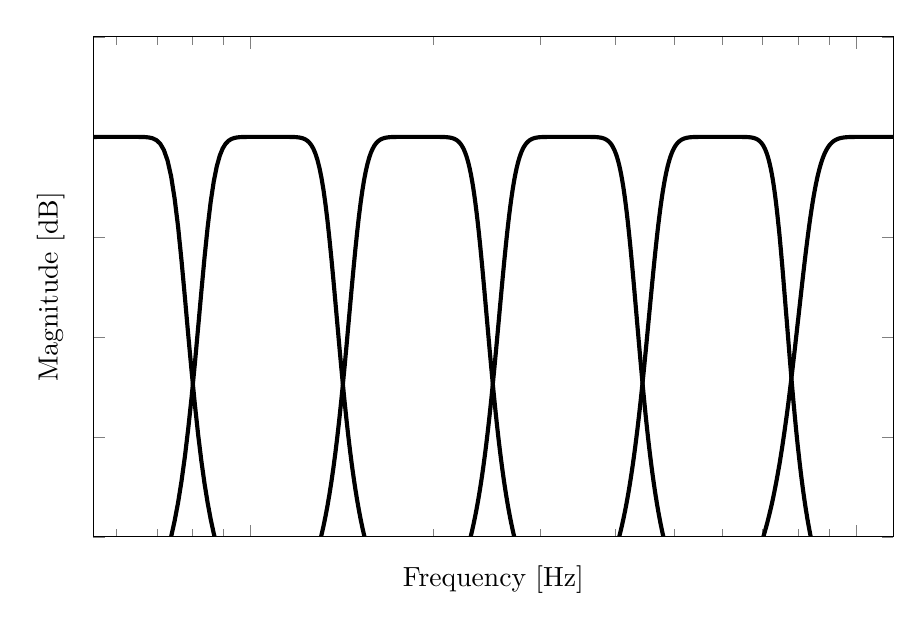
\begin{tikzpicture}

\begin{axis}[%
width=4in,
height=2.5in,
at={(1.011in,0.642in)},
scale only axis,
xmode=log,
xmin=550,
xmax=11500,
xminorticks=true,
xticklabels={\empty},
xlabel={Frequency [Hz]},
yticklabels={\empty},
ymin=0.2,
ymax=1.2,
ylabel={Magnitude [dB]},
axis background/.style={fill=white}
]
\addplot [color=black,solid,line width=1.5pt,forget plot]
  table[row sep=crcr]{%
549.027451372569	1.27474818755282e-06\\
559.02795139757	1.37055169597053e-06\\
569.028451422571	1.47168015573933e-06\\
579.028951447572	1.57832989891761e-06\\
589.029451472574	1.69070104274361e-06\\
599.029951497575	1.80899750613955e-06\\
609.030451522576	1.93342702654008e-06\\
619.030951547577	2.06420117704404e-06\\
629.031451572579	2.20153538387906e-06\\
639.03195159758	2.34564894421938e-06\\
649.032451622581	2.49676504429154e-06\\
659.032951647582	2.65511077784761e-06\\
669.033451672584	2.82091716495128e-06\\
679.033951697585	2.9944191711013e-06\\
689.034451722586	3.17585572669063e-06\\
699.034951747587	3.3654697468032e-06\\
709.035451772589	3.56350815135503e-06\\
719.03595179759	3.77022188557272e-06\\
729.036451822591	3.98586594082186e-06\\
739.036951847592	4.21069937576776e-06\\
749.037451872594	4.44498533791166e-06\\
759.037951897595	4.68899108545001e-06\\
769.038451922596	4.94298800950803e-06\\
779.038951947597	5.20725165671478e-06\\
789.039451972599	5.48206175214773e-06\\
799.0399519976	5.76770222262957e-06\\
809.040452022601	6.06446122039943e-06\\
819.040952047602	6.37263114713215e-06\\
829.041452072604	6.6925086783502e-06\\
839.041952097605	7.02439478818472e-06\\
849.042452122606	7.36859477451746e-06\\
859.042952147607	7.72541828450947e-06\\
869.043452172609	8.09517934049682e-06\\
879.04395219761	8.47819636626287e-06\\
889.044452222611	8.87479221372753e-06\\
899.044952247612	9.28529418997711e-06\\
909.045452272614	9.71003408472483e-06\\
919.045952297615	1.01493481981444e-05\\
929.046452322616	1.06035773691057e-05\\
939.046952347617	1.10730670038125e-05\\
949.047452372619	1.15581671048417e-05\\
959.04795239762	1.2059232300586e-05\\
969.048452422621	1.25766218751046e-05\\
979.048952447622	1.31106997983979e-05\\
989.049452472624	1.36618347570829e-05\\
999.049952497625	1.42304001855008e-05\\
1009.05045252263	1.48167742972383e-05\\
1019.05095254763	1.54213401170782e-05\\
1029.05145257263	1.6044485513379e-05\\
1039.05195259763	1.66866032308872e-05\\
1049.05245262263	1.73480909240019e-05\\
1059.05295264763	1.80293511904401e-05\\
1069.05345267263	1.87307916053911e-05\\
1079.05395269763	1.9452824756097e-05\\
1089.05445272264	2.01958682768746e-05\\
1099.05495274764	2.09603448846272e-05\\
1109.05545277264	2.17466824147754e-05\\
1119.05595279764	2.25553138576756e-05\\
1129.05645282264	2.33866773955117e-05\\
1139.05695284764	2.42412164396376e-05\\
1149.05745287264	2.51193796684019e-05\\
1159.05795289764	2.60216210654671e-05\\
1169.05845292265	2.69483999586e-05\\
1179.05895294765	2.79001810589519e-05\\
1189.05945297265	2.88774345008309e-05\\
1199.05995299765	2.9880635881981e-05\\
1209.06045302265	3.09102663043493e-05\\
1219.06095304765	3.19668124153777e-05\\
1229.06145307265	3.30507664497801e-05\\
1239.06195309765	3.41626262718678e-05\\
1249.06245312266	3.53028954183627e-05\\
1259.06295314766	3.64720831417675e-05\\
1269.06345317266	3.76707044542388e-05\\
1279.06395319766	3.88992801720113e-05\\
1289.06445322266	4.01583369603637e-05\\
1299.06495324766	4.1448407379119e-05\\
1309.06545327266	4.27700299287058e-05\\
1319.06595329766	4.41237490967704e-05\\
1329.06645332267	4.55101154053519e-05\\
1339.06695334767	4.69296854586247e-05\\
1349.06745337267	4.83830219912078e-05\\
1359.06795339767	4.98706939170632e-05\\
1369.06845342267	5.13932763789616e-05\\
1379.06895344767	5.29513507985522e-05\\
1389.06945347267	5.45455049270176e-05\\
1399.06995349767	5.61763328963369e-05\\
1409.07045352268	5.78444352711408e-05\\
1419.07095354768	5.9550419101199e-05\\
1429.07145357268	6.12948979745098e-05\\
1439.07195359768	6.30784920710182e-05\\
1449.07245362268	6.49018282169778e-05\\
1459.07295364768	6.67655399399274e-05\\
1469.07345367268	6.86702675243236e-05\\
1479.07395369768	7.0616658067825e-05\\
1489.07445372269	7.26053655382323e-05\\
1499.07495374769	7.46370508310862e-05\\
1509.07545377269	7.67123818279364e-05\\
1519.07595379769	7.88320334552917e-05\\
1529.07645382269	8.09966877442509e-05\\
1539.07695384769	8.32070338908229e-05\\
1549.07745387269	8.54637683169469e-05\\
1559.07795389769	8.77675947322129e-05\\
1569.0784539227	9.01192241963065e-05\\
1579.0789539477	9.25193751821509e-05\\
1589.0794539727	9.4968773639808e-05\\
1599.0799539977	9.74681530610717e-05\\
1609.0804540227	0.000100018254544852\\
1619.0809540477	0.000102619826863262\\
1629.0814540727	0.000105273626528498\\
1639.0819540977	0.000107980417860474\\
1649.08245412271	0.00011074097305521\\
1659.08295414771	0.000113556072254044\\
1669.08345417271	0.000116426503613597\\
1679.08395419771	0.00011935306337655\\
1689.08445422271	0.000122336555943231\\
1699.08495424771	0.000125377793944017\\
1709.08545427271	0.000128477598312557\\
1719.08595429771	0.000131636798359827\\
1729.08645432272	0.000134856231849036\\
1739.08695434772	0.000138136745071375\\
1749.08745437272	0.000141479192922626\\
1759.08795439772	0.000144884438980643\\
1769.08845442272	0.000148353355583726\\
1779.08895444772	0.000151886823909853\\
1789.08945447272	0.000155485734056841\\
1799.08995449772	0.000159150985123392\\
1809.09045452273	0.000162883485291085\\
1819.09095454773	0.000166684151907257\\
1829.09145457273	0.000170553911568861\\
1839.09195459773	0.000174493700207252\\
1849.09245462273	0.000178504463173927\\
1859.09295464773	0.00018258715532726\\
1869.09345467273	0.000186742741120191\\
1879.09395469773	0.00019097219468892\\
1889.09445472274	0.000195276499942593\\
1899.09495474774	0.000199656650654028\\
1909.09545477274	0.000204113650551425\\
1919.09595479774	0.000208648513411148\\
1929.09645482274	0.000213262263151531\\
1939.09695484774	0.000217955933927765\\
1949.09745487274	0.000222730570227836\\
1959.09795489774	0.000227587226969557\\
1969.09845492275	0.000232526969598691\\
1979.09895494775	0.0002375508741882\\
1989.09945497275	0.000242660027538581\\
1999.09995499775	0.000247855527279368\\
2009.10045502275	0.000253138481971759\\
2019.10095504775	0.000258510011212413\\
2029.10145507275	0.000263971245738415\\
2039.10195509775	0.000269523327533433\\
2049.10245512276	0.000275167409935066\\
2059.10295514776	0.000280904657743407\\
2069.10345517276	0.000286736247330836\\
2079.10395519776	0.000292663366753053\\
2089.10445522276	0.000298687215861372\\
2099.10495524776	0.000304809006416273\\
2109.10545527276	0.00031102996220224\\
2119.10595529776	0.000317351319143918\\
2129.10645532277	0.000323774325423558\\
2139.10695534777	0.000330300241599804\\
2149.10745537277	0.000336930340727831\\
2159.10795539777	0.00034366590848083\\
2169.10845542277	0.000350508243272881\\
2179.10895544777	0.000357458656383217\\
2189.10945547277	0.00036451847208189\\
2199.10995549777	0.00037168902775686\\
2209.11045552278	0.000378971674042556\\
2219.11095554778	0.000386367774949844\\
2229.11145557278	0.000393878707997529\\
2239.11195559778	0.000401505864345301\\
2249.11245562278	0.000409250648928223\\
2259.11295564778	0.000417114480592734\\
2269.11345567278	0.000425098792234218\\
2279.11395569779	0.000433205030936102\\
2289.11445572279	0.000441434658110576\\
2299.11495574779	0.000449789149640901\\
2309.11545577279	0.000458269996025331\\
2319.11595579779	0.000466878702522689\\
2329.11645582279	0.000475616789299597\\
2339.11695584779	0.000484485791579393\\
2349.11745587279	0.000493487259792741\\
2359.11795589779	0.000502622759729963\\
2369.1184559228	0.000511893872695126\\
2379.1189559478	0.000521302195661869\\
2389.1194559728	0.000530849341431046\\
2399.1199559978	0.000540536938790128\\
2409.1204560228	0.000550366632674492\\
2419.1209560478	0.000560340084330501\\
2429.1214560728	0.000570458971480503\\
2439.1219560978	0.000580724988489687\\
2449.12245612281	0.000591139846534883\\
2459.12295614781	0.000601705273775306\\
2469.12345617281	0.000612423015525218\\
2479.12395619781	0.000623294834428655\\
2489.12445622281	0.000634322510636088\\
2499.12495624781	0.000645507841983181\\
2509.12545627281	0.000656852644171584\\
2519.12595629781	0.000668358750951802\\
2529.12645632282	0.00068002801430822\\
2539.12695634782	0.000691862304646211\\
2549.12745637282	0.000703863510981462\\
2559.12795639782	0.000716033541131454\\
2569.12845642282	0.000728374321909184\\
2579.12895644782	0.000740887799319109\\
2589.12945647282	0.000753575938755409\\
2599.12995649782	0.000766440725202494\\
2609.13045652283	0.000779484163437885\\
2619.13095654783	0.000792708278237447\\
2629.13145657283	0.000806115114582999\\
2639.13195659783	0.000819706737872341\\
2649.13245662283	0.00083348523413176\\
2659.13295664783	0.000847452710230983\\
2669.13345667283	0.000861611294100646\\
2679.13395669783	0.000875963134952324\\
2689.13445672284	0.000890510403501116\\
2699.13495674784	0.000905255292190848\\
2709.13545677284	0.000920200015421898\\
2719.13595679784	0.000935346809781725\\
2729.13645682284	0.000950697934278066\\
2739.13695684784	0.000966255670574898\\
2749.13745687284	0.000982022323231169\\
2759.13795689785	0.000998000219942333\\
2769.13845692285	0.00101419171178474\\
2779.13895694785	0.00103059917346289\\
2789.13945697285	0.00104722500355964\\
2799.13995699785	0.00106407162478932\\
2809.14045702285	0.00108114148425386\\
2819.14095704785	0.00109843705370197\\
2829.14145707285	0.00111596082979137\\
2839.14195709786	0.0011337153343541\\
2849.14245712286	0.00115170311466506\\
2859.14295714786	0.00116992674371362\\
2869.14345717286	0.00118838882047858\\
2879.14395719786	0.00120709197020631\\
2889.14445722286	0.00122603884469227\\
2899.14495724786	0.00124523212256582\\
2909.14545727286	0.00126467450957847\\
2919.14595729786	0.0012843687388956\\
2929.14645732287	0.00130431757139159\\
2939.14695734787	0.00132452379594852\\
2949.14745737287	0.0013449902297585\\
2959.14795739787	0.00136571971862953\\
2969.14845742287	0.00138671513729509\\
2979.14895744787	0.00140797938972744\\
2989.14945747287	0.00142951540945466\\
2999.14995749787	0.00145132615988158\\
3009.15045752288	0.00147341463461446\\
3019.15095754788	0.00149578385778971\\
3029.15145757288	0.00151843688440648\\
3039.15195759788	0.00154137680066331\\
3049.15245762288	0.00156460672429888\\
3059.15295764788	0.00158812980493682\\
3069.15345767288	0.00161194922443477\\
3079.15395769788	0.00163606819723761\\
3089.15445772289	0.00166048997073506\\
3099.15495774789	0.0016852178256235\\
3109.15545777289	0.00171025507627237\\
3119.15595779789	0.00173560507109485\\
3129.15645782289	0.0017612711929232\\
3139.15695784789	0.00178725685938865\\
3149.15745787289	0.00181356552330584\\
3159.15795789789	0.00184020067306211\\
3169.1584579229	0.00186716583301143\\
3179.1589579479	0.00189446456387329\\
3189.1594579729	0.00192210046313632\\
3199.1599579979	0.00195007716546701\\
3209.1604580229	0.00197839834312343\\
3219.1609580479	0.00200706770637397\\
3229.1614580729	0.00203608900392131\\
3239.1619580979	0.00206546602333163\\
3249.16245812291	0.00209520259146906\\
3259.16295814791	0.00212530257493559\\
3269.16345817291	0.00215576988051628\\
3279.16395819791	0.00218660845563019\\
3289.16445822291	0.00221782228878674\\
3299.16495824791	0.0022494154100478\\
3309.16545827291	0.0022813918914955\\
3319.16595829792	0.00231375584770595\\
3329.16645832292	0.0023465114362287\\
3339.16695834792	0.00237966285807238\\
3349.16745837292	0.0024132143581962\\
3359.16795839792	0.00244717022600779\\
3369.16845842292	0.0024815347958671\\
3379.16895844792	0.00251631244759676\\
3389.16945847292	0.0025515076069987\\
3399.16995849793	0.00258712474637741\\
3409.17045852293	0.00262316838506966\\
3419.17095854793	0.0026596430899809\\
3429.17145857293	0.00269655347612851\\
3439.17195859793	0.00273390420719183\\
3449.17245862293	0.00277169999606906\\
3459.17295864793	0.00280994560544143\\
3469.17345867293	0.00284864584834424\\
3479.17395869793	0.00288780558874538\\
3489.17445872294	0.00292742974213097\\
3499.17495874794	0.00296752327609862\\
3509.17545877294	0.00300809121095813\\
3519.17595879794	0.00304913862033987\\
3529.17645882294	0.00309067063181091\\
3539.17695884794	0.00313269242749903\\
3549.17745887294	0.00317520924472465\\
3559.17795889794	0.0032182263766409\\
3569.17845892295	0.00326174917288189\\
3579.17895894795	0.0033057830402192\\
3589.17945897295	0.00335033344322688\\
3599.17995899795	0.00339540590495504\\
3609.18045902295	0.00344100600761194\\
3619.18095904795	0.00348713939325503\\
3629.18145907295	0.00353381176449082\\
3639.18195909795	0.00358102888518379\\
3649.18245912296	0.00362879658117448\\
3659.18295914796	0.00367712074100688\\
3669.18345917296	0.00372600731666519\\
3679.18395919796	0.00377546232432023\\
3689.18445922296	0.00382549184508544\\
3699.18495924796	0.0038761020257828\\
3709.18545927296	0.00392729907971864\\
3719.18595929796	0.0039790892874696\\
3729.18645932297	0.0040314789976789\\
3739.18695934797	0.00408447462786289\\
3749.18745937297	0.00413808266522824\\
3759.18795939797	0.00419230966749981\\
3769.18845942297	0.00424716226375936\\
3779.18895944797	0.00430264715529532\\
3789.18945947297	0.0043587711164636\\
3799.18995949797	0.00441554099555988\\
3809.19045952298	0.00447296371570334\\
3819.19095954798	0.00453104627573194\\
3829.19145957298	0.00458979575110973\\
3839.19195959798	0.0046492192948459\\
3849.19245962298	0.00470932413842629\\
3859.19295964798	0.00477011759275696\\
3869.19345967298	0.00483160704912045\\
3879.19395969799	0.00489379998014472\\
3889.19445972299	0.00495670394078497\\
3899.19495974799	0.00502032656931845\\
3909.19545977299	0.0050846755883527\\
3919.19595979799	0.00514975880584714\\
3929.19645982299	0.00521558411614828\\
3939.19695984799	0.0052821595010389\\
3949.19745987299	0.0053494930308012\\
3959.19795989799	0.00541759286529421\\
3969.198459923	0.00548646725504576\\
3979.198959948	0.00555612454235904\\
3989.199459973	0.00562657316243406\\
3999.199959998	0.00569782164450433\\
4009.200460023	0.00576987861298871\\
4019.200960048	0.00584275278865905\\
4029.201460073	0.0059164529898234\\
4039.201960098	0.0059909881335254\\
4049.20246012301	0.00606636723675989\\
4059.20296014801	0.00614259941770499\\
4069.20346017301	0.00621969389697104\\
4079.20396019801	0.00629765999886638\\
4089.20446022301	0.00637650715268055\\
4099.20496024801	0.00645624489398491\\
4109.20546027301	0.00653688286595095\\
4119.20596029802	0.00661843082068692\\
4129.20646032302	0.00670089862059237\\
4139.20696034802	0.00678429623973159\\
4149.20746037302	0.00686863376522577\\
4159.20796039802	0.00695392139866432\\
4169.20846042302	0.00704016945753555\\
4179.20896044802	0.00712738837667724\\
4189.20946047302	0.00721558870974699\\
4199.20996049802	0.00730478113071314\\
4209.21046052303	0.007394976435366\\
4219.21096054803	0.0074861855428504\\
4229.21146057303	0.00757841949721903\\
4239.21196059803	0.00767168946900786\\
4249.21246062303	0.00776600675683295\\
4259.21296064803	0.00786138278900982\\
4269.21346067303	0.00795782912519532\\
4279.21396069803	0.00805535745805225\\
4289.21446072304	0.00815397961493749\\
4299.21496074804	0.00825370755961346\\
4309.21546077304	0.00835455339398376\\
4319.21596079804	0.00845652935985303\\
4329.21646082304	0.00855964784071155\\
4339.21696084804	0.00866392136354492\\
4349.21746087304	0.00876936260066913\\
4359.21796089805	0.00887598437159161\\
4369.21846092305	0.00898379964489847\\
4379.21896094805	0.00909282154016824\\
4389.21946097305	0.00920306332991302\\
4399.21996099805	0.00931453844154671\\
4409.22046102305	0.00942726045938145\\
4419.22096104805	0.00954124312665214\\
4429.22146107305	0.00965650034756992\\
4439.22196109805	0.00977304618940474\\
4449.22246112306	0.00989089488459764\\
4459.22296114806	0.0100100608329032\\
4469.22346117306	0.0101305586035622\\
4479.22396119806	0.0102524029375062\\
4489.22446122306	0.0103756087495924\\
4499.22496124806	0.0105001911308718\\
4509.22546127306	0.0106261653508891\\
4519.22596129807	0.0107535468600157\\
4529.22646132307	0.0108823512918164\\
4539.22696134807	0.0110125944654505\\
4549.22746137307	0.0111442923881065\\
4559.22796139807	0.0112774612574733\\
4569.22846142307	0.0114121174642458\\
4579.22896144807	0.0115482775946674\\
4589.22946147307	0.0116859584331095\\
4599.22996149807	0.0118251769646876\\
4609.23046152308	0.0119659503779164\\
4619.23096154808	0.0121082960674026\\
4629.23146157308	0.0122522316365771\\
4639.23196159808	0.0123977749004675\\
4649.23246162308	0.0125449438885101\\
4659.23296164808	0.0126937568474038\\
4669.23346167308	0.0128442322440052\\
4679.23396169809	0.0129963887682662\\
4689.23446172309	0.0131502453362145\\
4699.23496174809	0.013305821092978\\
4709.23546177309	0.0134631354158536\\
4719.23596179809	0.0136222079174207\\
4729.23646182309	0.013783058448701\\
4739.23696184809	0.0139457071023643\\
4749.23746187309	0.0141101742159822\\
4759.23796189809	0.0142764803753293\\
4769.2384619231	0.0144446464177332\\
4779.2389619481	0.0146146934354745\\
4789.2394619731	0.0147866427792362\\
4799.2399619981	0.0149605160616058\\
4809.2404620231	0.0151363351606272\\
4819.2409620481	0.0153141222234075\\
4829.2414620731	0.0154938996697759\\
4839.2419620981	0.0156756901959978\\
4849.24246212311	0.015859516778544\\
4859.24296214811	0.0160454026779159\\
4869.24346217311	0.0162333714425286\\
4879.24396219811	0.0164234469126506\\
4889.24446222311	0.016615653224404\\
4899.24496224811	0.0168100148138235\\
4909.24546227311	0.0170065564209765\\
4919.24596229812	0.0172053030941456\\
4929.24646232312	0.0174062801940724\\
4939.24696234812	0.0176095133982671\\
4949.24746237312	0.0178150287053811\\
4959.24796239812	0.0180228524396465\\
4969.24846242312	0.0182330112553824\\
4979.24896244812	0.0184455321415684\\
4989.24946247312	0.0186604424264884\\
4999.24996249812	0.0188777697824431\\
5009.25046252313	0.0190975422305354\\
5019.25096254813	0.0193197881455266\\
5029.25146257313	0.0195445362607673\\
5039.25196259813	0.0197718156732027\\
5049.25246262313	0.0200016558484536\\
5059.25296264813	0.0202340866259749\\
5069.25346267313	0.0204691382242926\\
5079.25396269814	0.0207068412463195\\
5089.25446272314	0.0209472266847533\\
5099.25496274814	0.0211903259275557\\
5109.25546277314	0.0214361707635154\\
5119.25596279814	0.0216847933878961\\
5129.25646282314	0.0219362264081706\\
5139.25696284814	0.0221905028498422\\
5149.25746287314	0.0224476561623557\\
5159.25796289814	0.0227077202250981\\
5169.25846292315	0.0229707293534917\\
5179.25896294815	0.0232367183051795\\
5189.25946297315	0.0235057222863073\\
5199.25996299815	0.0237777769578996\\
5209.26046302315	0.0240529184423355\\
5219.26096304815	0.0243311833299223\\
5229.26146307315	0.024612608685571\\
5239.26196309816	0.0248972320555742\\
5249.26246312316	0.0251850914744878\\
5259.26296314816	0.0254762254721184\\
5269.26346317316	0.0257706730806189\\
5279.26396319816	0.0260684738416924\\
5289.26446322316	0.0263696678139074\\
5299.26496324816	0.0266742955801255\\
5309.26546327316	0.0269823982550434\\
5319.26596329816	0.0272940174928512\\
5329.26646332317	0.0276091954950086\\
5339.26696334817	0.0279279750181408\\
5349.26746337317	0.0282503993820561\\
5359.26796339817	0.0285765124778873\\
5369.26846342317	0.0289063587763583\\
5379.26896344817	0.0292399833361783\\
5389.26946347317	0.0295774318125654\\
5399.26996349817	0.029918750465901\\
5409.27046352318	0.0302639861705187\\
5419.27096354818	0.0306131864236277\\
5429.27146357318	0.0309663993543742\\
5439.27196359818	0.031323673733042\\
5449.27246362318	0.0316850589803955\\
5459.27296364818	0.0320506051771655\\
5469.27346367318	0.0324203630736824\\
5479.27396369819	0.0327943840996564\\
5489.27446372319	0.033172720374109\\
5499.27496374819	0.0335554247154566\\
5509.27546377319	0.0339425506517495\\
5519.27596379819	0.0343341524310682\\
5529.27646382319	0.0347302850320788\\
5539.27696384819	0.0351310041747506\\
5549.27746387319	0.0355363663312387\\
5559.27796389819	0.0359464287369316\\
5569.2784639232	0.0363612494016699\\
5579.2789639482	0.0367808871211344\\
5589.2794639732	0.0372054014884108\\
5599.2799639982	0.0376348529057276\\
5609.2804640232	0.0380693025963761\\
5619.2809640482	0.0385088126168096\\
5629.2814640732	0.0389534458689279\\
5639.28196409821	0.0394032661125471\\
5649.28246412321	0.0398583379780602\\
5659.28296414821	0.0403187269792873\\
5669.28346417321	0.0407844995265218\\
5679.28396419821	0.0412557229397724\\
5689.28446422321	0.0417324654622053\\
5699.28496424821	0.0422147962737872\\
5709.28546427321	0.0427027855051348\\
5719.28596429821	0.0431965042515704\\
5729.28646432322	0.0436960245873876\\
5739.28696434822	0.04420141958033\\
5749.28746437322	0.044712763306285\\
5759.28796439822	0.0452301308641957\\
5769.28846442322	0.0457535983911927\\
5779.28896444822	0.04628324307795\\
5789.28946447322	0.0468191431842661\\
5799.28996449823	0.0473613780548734\\
5809.29046452323	0.0479100281354793\\
5819.29096454823	0.04846517498904\\
5829.29146457323	0.0490269013122713\\
5839.29196459823	0.0495952909523973\\
5849.29246462323	0.0501704289241406\\
5859.29296464823	0.0507524014269563\\
5869.29346467323	0.0513412958625115\\
5879.29396469823	0.0519372008524144\\
5889.29446472324	0.0525402062561923\\
5899.29496474824	0.053150403189525\\
5909.29546477324	0.0537678840427312\\
5919.29596479824	0.0543927424995141\\
5929.29646482324	0.055025073555966\\
5939.29696484824	0.0556649735398341\\
5949.29746487324	0.0563125401300506\\
5959.29796489824	0.056967872376528\\
5969.29846492325	0.0576310707202208\\
5979.29896494825	0.0583022370134579\\
5989.29946497325	0.0589814745405429\\
5999.29996499825	0.0596688880386285\\
6009.30046502325	0.0603645837188628\\
6019.30096504825	0.061068669287811\\
6029.30146507325	0.0617812539691501\\
6039.30196509826	0.0625024485256432\\
6049.30246512326	0.0632323652813875\\
6059.30296514826	0.0639711181443418\\
6069.30346517326	0.0647188226291309\\
6079.30396519826	0.0654755958801279\\
6089.30446522326	0.066241556694814\\
6099.30496524826	0.0670168255474166\\
6109.30546527326	0.0678015246128231\\
6119.30596529826	0.0685957777907705\\
6129.30646532327	0.0693997107303121\\
6139.30696534827	0.0702134508545543\\
6149.30746537327	0.0710371273856675\\
6159.30796539827	0.0718708713701656\\
6169.30846542327	0.0727148157044527\\
6179.30896544827	0.0735690951606342\\
6189.30946547327	0.0744338464125896\\
6199.30996549828	0.075309208062301\\
6209.31046552328	0.0761953206664383\\
6219.31096554828	0.0770923267631894\\
6229.31146557328	0.0780003708993375\\
6239.31196559828	0.0789195996575748\\
6249.31246562328	0.0798501616840502\\
6259.31296564828	0.0807922077161402\\
6269.31346567328	0.0817458906104398\\
6279.31396569828	0.0827113653709642\\
6289.31446572329	0.0836887891775498\\
6299.31496574829	0.0846783214144507\\
6309.31546577329	0.0856801236991145\\
6319.31596579829	0.0866943599111317\\
6329.31646582329	0.0877211962213435\\
6339.31696584829	0.0887608011210978\\
6349.31746587329	0.0898133454516369\\
6359.31796589829	0.0908790024336062\\
6369.3184659233	0.091957947696666\\
6379.3189659483	0.0930503593091885\\
6389.3194659733	0.0941564178080272\\
6399.3199659983	0.0952763062283331\\
6409.3204660233	0.0964102101334033\\
6419.3209660483	0.0975583176445388\\
6429.3214660733	0.0987208194708859\\
6439.3219660983	0.0998979089392414\\
6449.32246612331	0.101089782023792\\
6459.32296614831	0.102296637375765\\
6469.32346617331	0.103518676352956\\
6479.32396619831	0.104756103049104\\
6489.32446622331	0.10600912432309\\
6499.32496624831	0.107277949827911\\
6509.32546627331	0.108562792039398\\
6519.32596629831	0.109863866284653\\
6529.32646632332	0.111181390770136\\
6539.32696634832	0.11251558660939\\
6549.32746637332	0.113866677850335\\
6559.32796639832	0.115234891502099\\
6569.32846642332	0.116620457561323\\
6579.32896644832	0.118023609037901\\
6589.32946647332	0.119444581980083\\
6599.32996649833	0.120883615498899\\
6609.33046652333	0.122340951791828\\
6619.33096654833	0.123816836165649\\
6629.33146657333	0.125311517058424\\
6639.33196659833	0.126825246060509\\
6649.33246662333	0.128358277934546\\
6659.33296664833	0.129910870634339\\
6669.33346667333	0.131483285322542\\
6679.33396669833	0.133075786387064\\
6689.33446672334	0.134688641456101\\
6699.33496674834	0.136322121411704\\
6709.33546677334	0.137976500401773\\
6719.33596679834	0.139652055850381\\
6729.33646682334	0.141349068466312\\
6739.33696684834	0.143067822249698\\
6749.33746687334	0.144808604496635\\
6759.33796689835	0.146571705801653\\
6769.33846692335	0.148357420057902\\
6779.33896694835	0.150166044454926\\
6789.33946697335	0.151997879473864\\
6799.33996699835	0.153853228879952\\
6809.34046702335	0.15573239971214\\
6819.34096704835	0.157635702269678\\
6829.34146707335	0.159563450095504\\
6839.34196709835	0.161515959956234\\
6849.34246712336	0.163493551818587\\
6859.34296714836	0.165496548822048\\
6869.34346717336	0.167525277247558\\
6879.34396719836	0.169580066482031\\
6889.34446722336	0.171661248978477\\
6899.34496724836	0.173769160211498\\
6909.34546727336	0.175904138627933\\
6919.34596729836	0.178066525592397\\
6929.34646732337	0.180256665327463\\
6939.34696734837	0.182474904848226\\
6949.34746737337	0.18472159389097\\
6959.34796739837	0.186997084835664\\
6969.34846742337	0.189301732621984\\
6979.34896744837	0.191635894658567\\
6989.34946747337	0.19399993072517\\
6999.34996749838	0.196394202867433\\
7009.35046752338	0.198819075283885\\
7019.35096754838	0.201274914204866\\
7029.35146757338	0.203762087763003\\
7039.35196759838	0.206280965854877\\
7049.35246762338	0.208831919993497\\
7059.35296764838	0.211415323151202\\
7069.35346767338	0.214031549592588\\
7079.35396769838	0.216680974697049\\
7089.35446772339	0.219363974770525\\
7099.35496774839	0.22208092684601\\
7109.35546777339	0.224832208472402\\
7119.35596779839	0.227618197491229\\
7129.35646782339	0.230439271800811\\
7139.35696784839	0.233295809107378\\
7149.35746787339	0.236188186662684\\
7159.3579678984	0.239116780987629\\
7169.3584679234	0.242081967581409\\
7179.3589679484	0.245084120615698\\
7189.3594679734	0.248123612613362\\
7199.3599679984	0.25120081411122\\
7209.3604680234	0.254316093306338\\
7219.3609680484	0.257469815685346\\
7229.3614680734	0.260662343636307\\
7239.3619680984	0.263894036042592\\
7249.36246812341	0.267165247858309\\
7259.36296814841	0.270476329664769\\
7269.36346817341	0.273827627207514\\
7279.36396819841	0.277219480913436\\
7289.36446822341	0.280652225387531\\
7299.36496824841	0.284126188888837\\
7309.36546827341	0.287641692785134\\
7319.36596829842	0.291199050986006\\
7329.36646832342	0.294798569353884\\
7339.36696834842	0.298440545092708\\
7349.36746837342	0.302125266113914\\
7359.36796839842	0.305853010379437\\
7369.36846842342	0.309624045221501\\
7379.36896844842	0.313438626639007\\
7389.36946847342	0.31729699857035\\
7399.36996849842	0.321199392142593\\
7409.37046852343	0.32514602489695\\
7419.37096854843	0.329137099990626\\
7429.37146857343	0.333172805375098\\
7439.37196859843	0.337253312951047\\
7449.37246862343	0.341378777700168\\
7459.37296864843	0.345549336794259\\
7469.37346867343	0.349765108681992\\
7479.37396869843	0.354026192153963\\
7489.37446872344	0.358332665386661\\
7499.37496874844	0.362684584966149\\
7509.37546877344	0.367081984892355\\
7519.37596879844	0.37152487556504\\
7529.37646882344	0.376013242752572\\
7539.37696884844	0.380547046544891\\
7549.37746887344	0.38512622029209\\
7559.37796889845	0.38975066953029\\
7569.37846892345	0.394420270896593\\
7579.37896894845	0.399134871035095\\
7589.37946897345	0.403894285496139\\
7599.37996899845	0.408698297631125\\
7609.38046902345	0.41354665748543\\
7619.38096904845	0.418439080692168\\
7629.38146907345	0.423375247369723\\
7639.38196909845	0.428354801026176\\
7649.38246912346	0.433377347473976\\
7659.38296914846	0.438442453758396\\
7669.38346917346	0.443549647103509\\
7679.38396919846	0.448698413879661\\
7689.38446922346	0.453888198596559\\
7699.38496924846	0.45911840292635\\
7709.38546927346	0.464388384761226\\
7719.38596929847	0.469697457310265\\
7729.38646932347	0.475044888240407\\
7739.38696934847	0.480429898866637\\
7749.38746937347	0.485851663396555\\
7759.38796939847	0.491309308234686\\
7769.38846942347	0.496801911351973\\
7779.38896944847	0.502328501725994\\
7789.38946947347	0.507888058857513\\
7799.38996949847	0.513479512369036\\
7809.39046952348	0.519101741691015\\
7819.39096954848	0.524753575841397\\
7829.39146957348	0.530433793304098\\
7839.39196959848	0.536141122011961\\
7849.39246962348	0.54187423943959\\
7859.39296964848	0.54763177281134\\
7869.39346967348	0.553412299429509\\
7879.39396969849	0.559214347127557\\
7889.39446972349	0.565036394852892\\
7899.39496974849	0.570876873383413\\
7909.39546977349	0.57673416618168\\
7919.39596979849	0.582606610390083\\
7929.39646982349	0.588492497969966\\
7939.39696984849	0.594390076987151\\
7949.39746987349	0.60029755304573\\
7959.39796989849	0.606213090871381\\
7969.3984699235	0.612134816044866\\
7979.3989699485	0.618060816885632\\
7989.3994699735	0.623989146484767\\
7999.3999699985	0.629917824885781\\
8009.4004700235	0.635844841410922\\
8019.4009700485	0.641768157129909\\
8029.4014700735	0.647685707467185\\
8039.4019700985	0.653595404942929\\
8049.40247012351	0.65949514204221\\
8059.40297014851	0.665382794205881\\
8069.40347017351	0.671256222935925\\
8079.40397019851	0.677113279007167\\
8089.40447022351	0.682951805776464\\
8099.40497024851	0.688769642579721\\
8109.40547027351	0.694564628206333\\
8119.40597029852	0.700334604439981\\
8129.40647032352	0.706077419654065\\
8139.40697034852	0.711790932449467\\
8149.40747037352	0.717473015321839\\
8159.40797039852	0.723121558345178\\
8169.40847042352	0.728734472858033\\
8179.40897044852	0.734309695138491\\
8189.40947047352	0.739845190053817\\
8199.40997049853	0.745338954670563\\
8209.41047052353	0.750789021810952\\
8219.41097054853	0.75619346354142\\
8229.41147057353	0.761550394579362\\
8239.41197059853	0.766857975604462\\
8249.41247062353	0.772114416461338\\
8259.41297064853	0.777317979240664\\
8269.41347067353	0.782466981226565\\
8279.41397069854	0.787559797698687\\
8289.41447072354	0.792594864578077\\
8299.41497074854	0.7975706809068\\
8309.41547077354	0.802485811152133\\
8319.41597079854	0.807338887327089\\
8329.41647082354	0.812128610919971\\
8339.41697084854	0.816853754626777\\
8349.41747087354	0.821513163881241\\
8359.41797089854	0.826105758178473\\
8369.41847092355	0.830630532189222\\
8379.41897094855	0.835086556662895\\
8389.41947097355	0.839472979118636\\
8399.41997099855	0.843789024324769\\
8409.42047102355	0.848033994568085\\
8419.42097104855	0.852207269715457\\
8429.42147107355	0.856308307071239\\
8439.42197109855	0.860336641034963\\
8449.42247112356	0.864291882564647\\
8459.42297114856	0.868173718451979\\
8469.42347117356	0.871981910416358\\
8479.42397119856	0.875716294025528\\
8489.42447122356	0.879376777451168\\
8499.42497124856	0.88296334006842\\
8509.42547127356	0.886476030908729\\
8519.42597129856	0.889914966975924\\
8529.42647132357	0.893280331435687\\
8539.42697134857	0.896572371688894\\
8549.42747137357	0.899791397339441\\
8559.42797139857	0.902937778067346\\
8569.42847142357	0.906011941417874\\
8579.42897144857	0.90901437051749\\
8589.42947147357	0.911945601727252\\
8599.42997149858	0.914806222244209\\
8609.43047152358	0.917596867661051\\
8619.43097154858	0.920318219494063\\
8629.43147157358	0.922971002689103\\
8639.43197159858	0.925555983114974\\
8649.43247162358	0.928073965053139\\
8659.43297164858	0.930525788692367\\
8669.43347167358	0.932912327636375\\
8679.43397169859	0.935234486432148\\
8689.43447172359	0.937493198126026\\
8699.43497174859	0.939689421854261\\
8709.43547177359	0.941824140474137\\
8719.43597179859	0.943898358241305\\
8729.43647182359	0.945913098538458\\
8739.43697184859	0.947869401659915\\
8749.43747187359	0.949768322656283\\
8759.43797189859	0.95161092924276\\
8769.4384719236	0.953398299774246\\
8779.4389719486	0.955131521289959\\
8789.4394719736	0.956811687629736\\
8799.4399719986	0.958439897623891\\
8809.4404720236	0.960017253357954\\
8819.4409720486	0.961544858513384\\
8829.4414720736	0.963023816784839\\
8839.4419720986	0.964455230374332\\
8849.44247212361	0.965840198562267\\
8859.44297214861	0.967179816355055\\
8869.44347217361	0.968475173208711\\
8879.44397219861	0.969727351827613\\
8889.44447222361	0.970937427037373\\
8899.44497224861	0.972106464730565\\
8909.44547227361	0.973235520883859\\
8919.44597229862	0.974325640644953\\
8929.44647232362	0.975377857487594\\
8939.44697234862	0.976393192432757\\
8949.44747237362	0.977372653334082\\
8959.44797239862	0.978317234225448\\
8969.44847242362	0.979227914728589\\
8979.44897244862	0.980105659518541\\
8989.44947247362	0.980951417844719\\
8999.44997249863	0.981766123105328\\
9009.45047252363	0.982550692472864\\
9019.45097254863	0.983306026568411\\
9029.45147257363	0.984033009182442\\
9039.45197259863	0.9847325070399\\
9049.45247262363	0.985405369607286\\
9059.45297264863	0.986052428939543\\
9069.45347267363	0.986674499564575\\
9079.45397269863	0.987272378403268\\
9089.45447272364	0.987846844722918\\
9099.45497274864	0.988398660122026\\
9109.45547277364	0.988928568544504\\
9119.45597279864	0.989437296321336\\
9129.45647282364	0.989925552237883\\
9139.45697284864	0.990394027624968\\
9149.45747287364	0.990843396472072\\
9159.45797289864	0.991274315560937\\
9169.45847292365	0.991687424617977\\
9179.45897294865	0.992083346483971\\
9189.45947297365	0.99246268729957\\
9199.45997299865	0.992826036705202\\
9209.46047302365	0.993173968054045\\
9219.46097304865	0.993507038636799\\
9229.46147307365	0.993825789917046\\
9239.46197309865	0.994130747776032\\
9249.46247312366	0.994422422765817\\
9259.46297314866	0.994701310369746\\
9269.46347317366	0.994967891269262\\
9279.46397319866	0.995222631616183\\
9289.46447322366	0.995465983309538\\
9299.46497324866	0.995698384276206\\
9309.46547327366	0.995920258754556\\
9319.46597329867	0.996132017580408\\
9329.46647332367	0.996334058474662\\
9339.46697334867	0.996526766331946\\
9349.46747337367	0.996710513509755\\
9359.46797339867	0.996885660117516\\
9369.46847342367	0.997052554305092\\
9379.46897344867	0.997211532550301\\
9389.46947347367	0.997362919944996\\
9399.46997349868	0.997507030479325\\
9409.47047352368	0.997644167323855\\
9419.47097354868	0.997774623109184\\
9429.47147357368	0.997898680202792\\
9439.47197359868	0.998016610982843\\
9449.47247362368	0.9981286781087\\
9459.47297364868	0.998235134787943\\
9469.47347367368	0.99833622503969\\
9479.47397369868	0.99843218395405\\
9489.47447372369	0.998523237947566\\
9499.47497374869	0.99860960501449\\
9509.47547377369	0.998691494973801\\
9519.47597379869	0.998769109711863\\
9529.47647382369	0.998842643420606\\
9539.47697384869	0.998912282831219\\
9549.47747387369	0.998978207443237\\
9559.47797389869	0.999040589749024\\
9569.4784739237	0.999099595453595\\
9579.4789739487	0.999155383689766\\
9589.4794739737	0.999208107228609\\
9599.4799739987	0.999257912685223\\
9609.4804740237	0.99930494071982\\
9619.4809740487	0.999349326234124\\
9629.4814740737	0.999391198563138\\
9639.4819740987	0.999430681662263\\
9649.48247412371	0.999467894289837\\
9659.48297414871	0.999502950185108\\
9669.48347417371	0.999535958241696\\
9679.48397419871	0.999567022676584\\
9689.48447422371	0.999596243194693\\
9699.48497424871	0.999623715149082\\
9709.48547427371	0.999649529696862\\
9719.48597429872	0.999673773950845\\
9729.48647432372	0.999696531127006\\
9739.48697434872	0.999717880687841\\
9749.48747437372	0.999737898481659\\
9759.48797439872	0.999756656877884\\
9769.48847442372	0.999774224898453\\
9779.48897444872	0.999790668345351\\
9789.48947447372	0.999806049924383\\
9799.48997449873	0.999820429365242\\
9809.49047452373	0.999833863537929\\
9819.49097454873	0.999846406565636\\
9829.49147457373	0.999858109934133\\
9839.49197459873	0.99986902259774\\
9849.49247462373	0.999879191081957\\
9859.49297464873	0.99988865958285\\
9869.49347467373	0.999897470063205\\
9879.49397469873	0.999905662345591\\
9889.49447472374	0.999913274202363\\
9899.49497474874	0.999920341442677\\
9909.49547477374	0.999926897996609\\
9919.49597479874	0.99993297599643\\
9929.49647482374	0.999938605855107\\
9939.49697484874	0.99994381634211\\
9949.49747487374	0.999948634656585\\
9959.49797489874	0.999953086497953\\
9969.49847492375	0.99995719613401\\
9979.49897494875	0.999960986466597\\
9989.49947497375	0.999964479094891\\
9999.49997499875	0.999967694376389\\
10009.5004750238	0.999970651485646\\
10019.5009750488	0.999973368470812\\
10029.5014750738	0.999975862308074\\
10039.5019750988	0.999978148953996\\
10049.5024751238	0.999980243395865\\
10059.5029751488	0.99998215970009\\
10069.5034751738	0.999983911058689\\
10079.5039751988	0.999985509833938\\
10089.5044752238	0.999986967601251\\
10099.5049752488	0.999988295190277\\
10109.5054752738	0.999989502724369\\
10119.5059752988	0.999990599658381\\
10129.5064753238	0.999991594814894\\
10139.5069753488	0.999992496418896\\
10149.5074753738	0.999993312130999\\
10159.5079753988	0.999994049079181\\
10169.5084754238	0.999994713889164\\
10179.5089754488	0.999995312713415\\
10189.5094754738	0.999995851258857\\
10199.5099754988	0.999996334813316\\
10209.5104755238	0.999996768270724\\
10219.5109755488	0.999997156155169\\
10229.5114755738	0.999997502643786\\
10239.5119755988	0.999997811588551\\
10249.5124756238	0.999998086537008\\
10259.5129756488	0.999998330751975\\
10269.5134756738	0.999998547230249\\
10279.5139756988	0.99999873872037\\
10289.5144757238	0.99999890773946\\
10299.5149757488	0.999999056589164\\
10309.5154757738	0.999999187370769\\
10319.5159757988	0.999999301999463\\
10329.5164758238	0.999999402217843\\
10339.5169758488	0.999999489608643\\
10349.5174758738	0.999999565606741\\
10359.5179758988	0.999999631510469\\
10369.5184759238	0.99999968849226\\
10379.5189759488	0.999999737608633\\
10389.5194759738	0.999999779809594\\
10399.5199759988	0.999999815947424\\
10409.5204760238	0.999999846784923\\
10419.5209760488	0.999999873003102\\
10429.5214760738	0.99999989520838\\
10439.5219760988	0.999999913939274\\
10449.5224761238	0.999999929672647\\
10459.5229761488	0.999999942829488\\
10469.5234761738	0.999999953780293\\
10479.5239761988	0.999999962850039\\
10489.5244762238	0.999999970322771\\
10499.5249762488	0.999999976445845\\
10509.5254762738	0.999999981433826\\
10519.5259762988	0.999999985472059\\
10529.5264763238	0.99999998871995\\
10539.5269763488	0.999999991313956\\
10549.5274763738	0.999999993370305\\
10559.5279763988	0.999999994987481\\
10569.5284764238	0.999999996248448\\
10579.5289764488	0.99999999722268\\
10589.5294764738	0.999999997967971\\
10599.5299764988	0.999999998532068\\
10609.5304765238	0.999999998954115\\
10619.5309765488	0.99999999926594\\
10629.5314765738	0.999999999493193\\
10639.5319765988	0.999999999656345\\
10649.5324766238	0.999999999771561\\
10659.5329766488	0.999999999851457\\
10669.5334766738	0.999999999905751\\
10679.5339766988	0.99999999994182\\
10689.5344767238	0.999999999965185\\
10699.5349767488	0.999999999979887\\
10709.5354767738	0.999999999988844\\
10719.5359767988	0.999999999994094\\
10729.5364768238	0.999999999997042\\
10739.5369768488	0.999999999998612\\
10749.5374768738	0.999999999999397\\
10759.5379768988	0.999999999999763\\
10769.5384769238	0.999999999999917\\
10779.5389769488	0.999999999999975\\
10789.5394769738	0.999999999999993\\
10799.5399769989	0.999999999999998\\
10809.5404770239	0.999999999999999\\
10819.5409770489	0.999999999999998\\
10829.5414770739	0.999999999999999\\
10839.5419770989	0.999999999999999\\
10849.5424771239	1\\
10859.5429771489	0.999999999999999\\
10869.5434771739	1\\
10879.5439771989	1\\
10889.5444772239	0.999999999999993\\
10899.5449772489	0.999999999999978\\
10909.5454772739	0.999999999999928\\
10919.5459772989	0.999999999999788\\
10929.5464773239	0.999999999999457\\
10939.5469773489	0.99999999999873\\
10949.5474773739	0.999999999997265\\
10959.5479773989	0.999999999994486\\
10969.5484774239	0.999999999989498\\
10979.5489774489	0.999999999980926\\
10989.5494774739	0.999999999966757\\
10999.5499774989	0.999999999944109\\
11009.5504775239	0.999999999908949\\
11019.5509775489	0.999999999855757\\
11029.5514775739	0.999999999777109\\
11039.5519775989	0.999999999663184\\
11049.5524776239	0.99999999950118\\
11059.5529776489	0.999999999274626\\
11069.5534776739	0.999999998962575\\
11079.5539776989	0.999999998538678\\
11089.5544777239	0.999999997970125\\
11099.5549777489	0.999999997216407\\
11109.5554777739	0.999999996227943\\
11119.5559777989	0.999999994944504\\
11129.5564778239	0.999999993293443\\
11139.5569778489	0.999999991187714\\
11149.5574778739	0.999999988523653\\
11159.5579778989	0.999999985178513\\
11169.5584779239	0.999999981007721\\
11179.5589779489	0.999999975841863\\
11189.5594779739	0.999999969483328\\
11199.5599779989	0.999999961702663\\
11209.5604780239	0.999999952234522\\
11219.5609780489	0.999999940773285\\
11229.5614780739	0.99999992696824\\
11239.5619780989	0.999999910418365\\
11249.5624781239	0.99999989066662\\
11259.5629781489	0.999999867193802\\
11269.5634781739	0.999999839411855\\
11279.5639781989	0.999999806656662\\
11289.5644782239	0.999999768180263\\
11299.5649782489	0.99999972314246\\
11309.5654782739	0.999999670601816\\
11319.5659782989	0.999999609505962\\
11329.5664783239	0.999999538681217\\
11339.5669783489	0.999999456821474\\
11349.5674783739	0.999999362476291\\
11359.5679783989	0.999999254038208\\
11369.5684784239	0.999999129729173\\
11379.5689784489	0.999998987586089\\
11389.5694784739	0.999998825445444\\
11399.5699784989	0.99999864092694\\
11409.5704785239	0.999998431416097\\
11419.5709785489	0.999998194045817\\
11429.5714785739	0.999997925676794\\
11439.5719785989	0.99999762287678\\
11449.5724786239	0.999997281898629\\
11459.5729786489	0.999996898657066\\
11469.5734786739	0.99999646870414\\
11479.5739786989	0.999995987203295\\
11489.5744787239	0.999995448902001\\
11499.5749787489	0.999994848102893\\
};
\addplot [color=black,solid,line width=1.5pt,forget plot]
  table[row sep=crcr]{%
549.027451372569	6.73314137683396e-06\\
559.02795139757	7.24546258070611e-06\\
569.028451422571	7.78696933976435e-06\\
579.028951447572	8.3588036906952e-06\\
589.029451472574	8.96213455246272e-06\\
599.029951497575	9.59815810602538e-06\\
609.030451522576	1.02680981834535e-05\\
619.030951547577	1.09732066665096e-05\\
629.031451572579	1.17147638947745e-05\\
639.03195159758	1.2494079083722e-05\\
649.032451622581	1.33124907526236e-05\\
659.032951647582	1.41713671626968e-05\\
669.033451672584	1.50721067654828e-05\\
679.033951697585	1.60161386618028e-05\\
689.034451722586	1.70049230713627e-05\\
699.034951747587	1.8039951813242e-05\\
709.035451772589	1.91227487974535e-05\\
719.03595179759	2.02548705277951e-05\\
729.036451822591	2.14379066162052e-05\\
739.036951847592	2.26734803087194e-05\\
749.037451872594	2.396324902347e-05\\
759.037951897595	2.5308904900741e-05\\
769.038451922596	2.67121753653858e-05\\
779.038951947597	2.81748237018973e-05\\
789.039451972599	2.96986496422347e-05\\
799.0399519976	3.12854899668175e-05\\
809.040452022601	3.2937219118767e-05\\
819.040952047602	3.46557498318676e-05\\
829.041452072604	3.64430337721972e-05\\
839.041952097605	3.83010621940733e-05\\
849.042452122606	4.02318666102908e-05\\
859.042952147607	4.22375194770771e-05\\
869.043452172609	4.43201348940387e-05\\
879.04395219761	4.64818693193831e-05\\
889.044452222611	4.87249223007306e-05\\
899.044952247612	5.10515372217612e-05\\
909.045452272614	5.34640020652032e-05\\
919.045952297615	5.59646501922763e-05\\
929.046452322616	5.85558611390386e-05\\
939.046952347617	6.12400614299702e-05\\
949.047452372619	6.40197254091516e-05\\
959.04795239762	6.68973760893577e-05\\
969.048452422621	6.98755860195381e-05\\
979.048952447622	7.29569781708903e-05\\
989.049452472624	7.61442268420919e-05\\
999.049952497625	7.94400585840366e-05\\
1009.05045252263	8.28472531443957e-05\\
1019.05095254763	8.63686444325558e-05\\
1029.05145257263	9.00071215052687e-05\\
1039.05195259763	9.37656295734857e-05\\
1049.05245262263	9.76471710308449e-05\\
1059.05295264763	0.000101654806504234\\
1069.05345267263	0.000105791655926956\\
1079.05395269763	0.00011006089963489\\
1089.05445272264	0.000114465779486239\\
1099.05495274764	0.000119009600005382\\
1109.05545277264	0.000123695729551179\\
1119.05595279764	0.000128527601510546\\
1129.05645282264	0.000133508715517552\\
1139.05695284764	0.00013864263869887\\
1149.05745287264	0.000143933006945895\\
1159.05795289764	0.000149383526214345\\
1169.05845292265	0.000154997973851826\\
1179.05895294765	0.000160780199953985\\
1189.05945297265	0.000166734128749935\\
1199.05995299765	0.000172863760017546\\
1209.06045302265	0.000179173170529318\\
1219.06095304765	0.000185666515529506\\
1229.06145307265	0.000192348030243145\\
1239.06195309765	0.000199222031417792\\
1249.06245312266	0.000206292918898563\\
1259.06295314766	0.000213565177237492\\
1269.06345317266	0.000221043377337604\\
1279.06395319766	0.000228732178132855\\
1289.06445322266	0.000236636328304531\\
1299.06495324766	0.000244760668035019\\
1309.06545327266	0.000253110130799787\\
1319.06595329766	0.000261689745198471\\
1329.06645332267	0.00027050463682588\\
1339.06695334767	0.000279560030184004\\
1349.06745337267	0.000288861250635789\\
1359.06795339767	0.00029841372640178\\
1369.06845342267	0.000308222990600499\\
1379.06895344767	0.000318294683333765\\
1389.06945347267	0.000328634553817759\\
1399.06995349767	0.00033924846256112\\
1409.07045352268	0.000350142383591041\\
1419.07095354768	0.000361322406728527\\
1429.07145357268	0.000372794739913955\\
1439.07195359768	0.000384565711584238\\
1449.07245362268	0.000396641773102522\\
1459.07295364768	0.000409029501242086\\
1469.07345367268	0.000421735600725266\\
1479.07395369768	0.000434766906819107\\
1489.07445372269	0.000448130387988803\\
1499.07495374769	0.000461833148610558\\
1509.07545377269	0.00047588243174498\\
1519.07595379769	0.000490285621972838\\
1529.07645382269	0.00050505024829431\\
1539.07695384769	0.000520183987093525\\
1549.07745387269	0.000535694665169852\\
1559.07795389769	0.000551590262837485\\
1569.0784539227	0.000567878917095264\\
1579.0789539477	0.000584568924867997\\
1589.0794539727	0.000601668746321454\\
1599.0799539977	0.000619187008252534\\
1609.0804540227	0.000637132507556647\\
1619.0809540477	0.000655514214774001\\
1629.0814540727	0.000674341277716983\\
1639.0819540977	0.000693623025180311\\
1649.08245412271	0.000713368970736401\\
1659.08295414771	0.00073358881661758\\
1669.08345417271	0.000754292457687817\\
1679.08395419771	0.00077548998550574\\
1689.08445422271	0.000797191692481435\\
1699.08495424771	0.000819408076129448\\
1709.08545427271	0.000842149843420129\\
1719.08595429771	0.000865427915232059\\
1729.08645432272	0.000889253430907891\\
1739.08695434772	0.000913637752916372\\
1749.08745437272	0.000938592471623002\\
1759.08795439772	0.000964129410172449\\
1769.08845442272	0.000990260629485173\\
1779.08895444772	0.00101699843337122\\
1789.08945447272	0.00104435537376451\\
1799.08995449772	0.00107234425608021\\
1809.09045452273	0.00110097814469869\\
1819.09095454773	0.00113027036857916\\
1829.09145457273	0.00116023452700634\\
1839.09195459773	0.00119088449547358\\
1849.09245462273	0.001222234431706\\
1859.09295464773	0.00125429878182704\\
1869.09345467273	0.00128709228667277\\
1879.09395469773	0.00132062998825674\\
1889.09445472274	0.00135492723639045\\
1899.09495474774	0.0013899996954626\\
1909.09545477274	0.00142586335138181\\
1919.09595479774	0.00146253451868672\\
1929.09645482274	0.00150002984782828\\
1939.09695484774	0.00153836633262834\\
1949.09745487274	0.00157756131791943\\
1959.09795489774	0.0016176325073706\\
1969.09845492275	0.0016585979715038\\
1979.09895494775	0.00170047615590668\\
1989.09945497275	0.00174328588964599\\
1999.09995499775	0.0017870463938879\\
2009.10045502275	0.00183177729073017\\
2019.10095504775	0.00187749861225217\\
2029.10145507275	0.0019242308097882\\
2039.10195509775	0.00197199476343064\\
2049.10245512276	0.00202081179176894\\
2059.10295514776	0.00207070366187052\\
2069.10345517276	0.00212169259951051\\
2079.10395519776	0.00217380129965709\\
2089.10445522276	0.0022270529372191\\
2099.10495524776	0.00228147117806349\\
2109.10545527276	0.00233708019030939\\
2119.10595529776	0.00239390465590723\\
2129.10645532277	0.00245196978250993\\
2139.10695534777	0.00251130131564464\\
2149.10745537277	0.00257192555119351\\
2159.10795539777	0.00263386934819121\\
2169.10845542277	0.00269716014194954\\
2179.10895544777	0.00276182595751578\\
2189.10945547277	0.00282789542347742\\
2199.10995549777	0.00289539778611941\\
2209.11045552278	0.00296436292394649\\
2219.11095554778	0.00303482136257965\\
2229.11145557278	0.00310680429003722\\
2239.11195559778	0.00318034357241201\\
2249.11245562278	0.00325547176995522\\
2259.11295564778	0.00333222215357849\\
2269.11345567278	0.00341062872178707\\
2279.11395569779	0.00349072621805492\\
2289.11445572279	0.0035725501486553\\
2299.11495574779	0.00365613680095944\\
2309.11545577279	0.00374152326221765\\
2319.11595579779	0.00382874743883456\\
2329.11645582279	0.00391784807615614\\
2339.11695584779	0.00400886477877919\\
2349.11745587279	0.00410183803140261\\
2359.11795589779	0.00419680922023257\\
2369.1184559228	0.00429382065496028\\
2379.1189559478	0.00439291559132743\\
2389.1194559728	0.00449413825429757\\
2399.1199559978	0.00459753386185078\\
2409.1204560228	0.0047031486494192\\
2419.1209560478	0.00481102989498404\\
2429.1214560728	0.00492122594485175\\
2439.1219560978	0.00503378624013085\\
2449.12245612281	0.00514876134392927\\
2459.12295614781	0.00526620296929397\\
2469.12345617281	0.00538616400791561\\
2479.12395619781	0.00550869855961975\\
2489.12445622281	0.00563386196266906\\
2499.12495624781	0.00576171082490146\\
2509.12545627281	0.00589230305572768\\
2519.12595629781	0.00602569789901582\\
2529.12645632282	0.00616195596688879\\
2539.12695634782	0.00630113927446241\\
2549.12745637282	0.00644331127555329\\
2559.12795639782	0.00658853689938551\\
2569.12845642282	0.00673688258832652\\
2579.12895644782	0.00688841633668428\\
2589.12945647282	0.00704320773059793\\
2599.12995649782	0.00720132798905541\\
2609.13045652283	0.00736285000607307\\
2619.13095654783	0.00752784839407237\\
2629.13145657283	0.0076963995284937\\
2639.13195659783	0.00786858159367999\\
2649.13245662283	0.00804447463007596\\
2659.13295664783	0.00822416058278033\\
2669.13345667283	0.00840772335149283\\
2679.13395669783	0.0085952488419033\\
2689.13445672284	0.00878682501856385\\
2699.13495674784	0.0089825419592936\\
2709.13545677284	0.00918249191116387\\
2719.13595679784	0.00938676934811251\\
2729.13645682284	0.00959547103024042\\
2739.13695684784	0.00980869606484321\\
2749.13745687284	0.0100265459692325\\
2759.13795689785	0.0102491247354062\\
2769.13845692285	0.0104765388966222\\
2779.13895694785	0.0107088975959435\\
2789.13945697285	0.0109463126568106\\
2799.13995699785	0.0111888986557108\\
2809.14045702285	0.0114367729970126\\
2819.14095704785	0.0116900559900306\\
2829.14145707285	0.0119488709283987\\
2839.14195709786	0.0122133441718217\\
2849.14245712286	0.0124836052302857\\
2859.14295714786	0.0127597868508057\\
2869.14345717286	0.0130420251067936\\
2879.14395719786	0.0133304594901333\\
2889.14445722286	0.0136252330060483\\
2899.14495724786	0.0139264922708573\\
2909.14545727286	0.0142343876127102\\
2919.14595729786	0.0145490731754028\\
2929.14645732287	0.0148707070253735\\
2939.14695734787	0.0151994512619831\\
2949.14745737287	0.0155354721311906\\
2959.14795739787	0.0158789401427341\\
2969.14845742287	0.0162300301909367\\
2979.14895744787	0.0165889216792512\\
2989.14945747287	0.0169557986486761\\
2999.14995749787	0.0173308499101652\\
3009.15045752288	0.0177142691811672\\
3019.15095754788	0.0181062552264313\\
3029.15145757288	0.0185070120032217\\
3039.15195759788	0.0189167488110904\\
3049.15245762288	0.0193356804463578\\
3059.15295764788	0.019764027361456\\
3069.15345767288	0.0202020158293082\\
3079.15395769788	0.0206498781128999\\
3089.15445772289	0.021107852640225\\
3099.15495774789	0.0215761841847803\\
3109.15545777289	0.0220551240518025\\
3119.15595779789	0.0225449302704323\\
3129.15645782289	0.023045867792005\\
3139.15695784789	0.0235582086946814\\
3149.15745787289	0.024082232394619\\
3159.15795789789	0.0246182258639098\\
3169.1584579229	0.0251664838555129\\
3179.1589579479	0.0257273091354044\\
3189.1594579729	0.0263010127221987\\
3199.1599579979	0.0268879141344829\\
3209.1604580229	0.0274883416461199\\
3219.1609580479	0.0281026325497847\\
3229.1614580729	0.0287311334290146\\
3239.1619580979	0.0293742004390378\\
3249.16245812291	0.0300321995966879\\
3259.16295814791	0.0307055070796876\\
3269.16345817291	0.031394509535616\\
3279.16395819791	0.0320996044008701\\
3289.16445822291	0.0328212002299495\\
3299.16495824791	0.0335597170353931\\
3309.16545827291	0.0343155866387069\\
3319.16595829792	0.0350892530326378\\
3329.16645832292	0.0358811727551629\\
3339.16695834792	0.036691815275524\\
3349.16745837292	0.0375216633927446\\
3359.16795839792	0.0383712136469479\\
3369.16845842292	0.0392409767439272\\
3379.16895844792	0.0401314779933249\\
3389.16945847292	0.0410432577608555\\
3399.16995849793	0.0419768719349773\\
3409.17045852293	0.0429328924084343\\
3419.17095854793	0.0439119075750973\\
3429.17145857293	0.0449145228425339\\
3439.17195859793	0.0459413611607501\\
3449.17245862293	0.0469930635675355\\
3459.17295864793	0.0480702897508484\\
3469.17345867293	0.0491737186286901\\
3479.17395869793	0.0503040489469226\\
3489.17445872294	0.0514619998954167\\
3499.17495874794	0.0526483117430271\\
3509.17545877294	0.0538637464917581\\
3519.17595879794	0.0551090885505724\\
3529.17645882294	0.0563851454292449\\
3539.17695884794	0.0576927484525899\\
3549.17745887294	0.05903275349551\\
3559.17795889794	0.0604060417391336\\
3569.17845892295	0.0618135204483856\\
3579.17895894795	0.0632561237712575\\
3589.17945897295	0.0647348135600139\\
3599.17995899795	0.0662505802145129\\
3609.18045902295	0.0678044435478039\\
3619.18095904795	0.069397453674017\\
3629.18145907295	0.0710306919186144\\
3639.18195909795	0.0727052717508663\\
3649.18245912296	0.0744223397384232\\
3659.18295914796	0.0761830765236529\\
3669.18345917296	0.0779886978214223\\
3679.18395919796	0.0798404554377182\\
3689.18445922296	0.0817396383085141\\
3699.18495924796	0.083687573557949\\
3709.18545927296	0.0856856275748947\\
3719.18595929796	0.0877352071065734\\
3729.18645932297	0.0898377603678686\\
3739.18695934797	0.0919947781644702\\
3749.18745937297	0.0942077950279727\\
3759.18795939797	0.0964783903605285\\
3769.18845942297	0.0988081895863541\\
3779.18895944797	0.101198865307048\\
3789.18945947297	0.103652138457249\\
3799.18995949797	0.106169779456527\\
3809.19045952298	0.108753609353151\\
3819.19095954798	0.111405500954489\\
3829.19145957298	0.114127379938442\\
3839.19195959798	0.116921225939356\\
3849.19245962298	0.119789073601368\\
3859.19295964798	0.122733013590879\\
3869.19345967298	0.125755193559514\\
3879.19395969799	0.128857819047308\\
3889.19445972299	0.132043154315145\\
3899.19495974799	0.135313523094216\\
3909.19545977299	0.138671309238782\\
3919.19595979799	0.14211895726726\\
3929.19645982299	0.145658972775156\\
3939.19695984799	0.149293922701504\\
3949.19745987299	0.153026435428841\\
3959.19795989799	0.156859200694681\\
3969.198459923	0.160794969290519\\
3979.198959948	0.164836552521947\\
3989.199459973	0.168986821401204\\
3999.199959998	0.173248705540948\\
4009.200460023	0.177625191715202\\
4019.200960048	0.182119322050559\\
4029.201460073	0.186734191807928\\
4039.201960098	0.191472946711525\\
4049.20246012301	0.196338779778835\\
4059.20296014801	0.2013349276018\\
4069.20346017301	0.20646466602561\\
4079.20396019801	0.211731305168398\\
4089.20446022301	0.217138183721046\\
4099.20496024801	0.222688662463126\\
4109.20546027301	0.228386116926667\\
4119.20596029802	0.23423392913744\\
4129.20646032302	0.240235478358554\\
4139.20696034802	0.246394130759626\\
4149.20746037302	0.252713227932102\\
4159.20796039802	0.259196074168542\\
4169.20846042302	0.265845922424422\\
4179.20896044802	0.272665958879125\\
4189.20946047302	0.2796592860145\\
4199.20996049802	0.286828904132149\\
4209.21046052303	0.294177691233486\\
4219.21096054803	0.301708381193821\\
4229.21146057303	0.30942354016836\\
4239.21196059803	0.317325541180158\\
4249.21246062303	0.325416536852158\\
4259.21296064803	0.333698430263715\\
4269.21346067303	0.342172843930751\\
4279.21396069803	0.350841086934828\\
4289.21446072304	0.359704120254012\\
4299.21496074804	0.368762520381773\\
4309.21546077304	0.37801644135949\\
4319.21596079804	0.387465575389492\\
4329.21646082304	0.397109112246546\\
4339.21696084804	0.406945697755889\\
4349.21746087304	0.416973391667067\\
4359.21796089805	0.427189625313065\\
4369.21846092305	0.437591159510667\\
4379.21896094805	0.448174043226715\\
4389.21946097305	0.458933573604653\\
4399.21996099805	0.469864258013016\\
4409.22046102305	0.480959778846852\\
4419.22096104805	0.492212961870956\\
4429.22146107305	0.503615748952562\\
4439.22196109805	0.515159176066794\\
4449.22246112306	0.526833357495646\\
4459.22296114806	0.538627477144372\\
4469.22346117306	0.55052978789543\\
4479.22396119806	0.562527619882306\\
4489.22446122306	0.574607398504426\\
4499.22496124806	0.586754672915863\\
4509.22546127306	0.598954155591007\\
4519.22596129807	0.611189773422096\\
4529.22646132307	0.623444730611529\\
4539.22696134807	0.6357015834073\\
4549.22746137307	0.647942326485668\\
4559.22796139807	0.660148490523461\\
4569.22846142307	0.672301250221901\\
4579.22896144807	0.684381541761876\\
4589.22946147307	0.696370188391244\\
4599.22996149807	0.708248032577164\\
4609.23046152308	0.719996072918406\\
4619.23096154808	0.731595603806891\\
4629.23146157308	0.743028355670287\\
4639.23196159808	0.754276633522065\\
4649.23246162308	0.765323451507486\\
4659.23296164808	0.776152661150782\\
4669.23346167308	0.78674907111194\\
4679.23396169809	0.797098556402975\\
4689.23446172309	0.807188155247829\\
4699.23496174809	0.817006152035399\\
4709.23546177309	0.826542145133228\\
4719.23596179809	0.835787098681238\\
4729.23646182309	0.844733377854893\\
4739.23696184809	0.853374767459013\\
4749.23746187309	0.861706474082288\\
4759.23796189809	0.869725112391937\\
4769.2384619231	0.877428676453306\\
4779.2389619481	0.884816497240673\\
4789.2394619731	0.891889187723512\\
4799.2399619981	0.898648577088654\\
4809.2404620231	0.905097635775229\\
4819.2409620481	0.911240393058959\\
4829.2414620731	0.9170818489451\\
4839.2419620981	0.922627882083016\\
4849.24246212311	0.927885155352718\\
4859.24296214811	0.932861020662743\\
4869.24346217311	0.937563424355568\\
4879.24396219811	0.942000814479435\\
4889.24446222311	0.946182051004528\\
4899.24496224811	0.950116319901479\\
4909.24546227311	0.953813051816223\\
4919.24596229812	0.95728184592769\\
4929.24646232312	0.960532399394248\\
4939.24696234812	0.963574442670439\\
4949.24746237312	0.966417680832341\\
4959.24796239812	0.969071740937545\\
4969.24846242312	0.97154612534889\\
4979.24896244812	0.97385017085985\\
4989.24946247312	0.975993013404364\\
4999.24996249812	0.977983558066599\\
5009.25046252313	0.979830454077844\\
5019.25096254813	0.981542074451606\\
5029.25146257313	0.983126499896847\\
5039.25196259813	0.984591506639041\\
5049.25246262313	0.985944557777937\\
5059.25296264813	0.987192797819376\\
5069.25346267313	0.988343050027766\\
5079.25396269814	0.98940181626573\\
5089.25446272314	0.990375278996152\\
5099.25496274814	0.991269305156314\\
5109.25546277314	0.9920894516215\\
5119.25596279814	0.99284097200772\\
5129.25646282314	0.99352882457964\\
5139.25696284814	0.994157681055245\\
5149.25746287314	0.994731936117817\\
5159.25796289814	0.99525571746843\\
5169.25846292315	0.995732896268642\\
5179.25896294815	0.99616709784192\\
5189.25946297315	0.996561712523644\\
5199.25996299815	0.996919906555991\\
5209.26046302315	0.997244632945446\\
5219.26096304815	0.99753864221278\\
5229.26146307315	0.997804492971328\\
5239.26196309816	0.998044562286686\\
5249.26246312316	0.998261055775834\\
5259.26296314816	0.998456017411377\\
5269.26346317316	0.99863133900952\\
5279.26396319816	0.998788769377055\\
5289.26446322316	0.998929923109381\\
5299.26496324816	0.999056289023467\\
5309.26546327316	0.999169238227942\\
5319.26596329816	0.999270031823895\\
5329.26646332317	0.999359828237567\\
5339.26696334817	0.999439690192892\\
5349.26746337317	0.999510591324167\\
5359.26796339817	0.999573422439877\\
5369.26846342317	0.99962899744607\\
5379.26896344817	0.999678058935401\\
5389.26946347317	0.999721283459974\\
5399.26996349817	0.999759286489574\\
5409.27046352318	0.999792627075491\\
5419.27096354818	0.999821812226875\\
5429.27146357318	0.999847301012355\\
5439.27196359818	0.999869508400927\\
5449.27246362318	0.999888808852104\\
5459.27296364818	0.999905539668635\\
5469.27346367318	0.999920004122045\\
5479.27396369819	0.999932474363874\\
5489.27446372319	0.99994319413361\\
5499.27496374819	0.999952381271835\\
5509.27546377319	0.999960230054914\\
5519.27596379819	0.999966913353266\\
5529.27646382319	0.99997258463081\\
5539.27696384819	0.999977379789778\\
5549.27746387319	0.999981418872163\\
5559.27796389819	0.999984807627976\\
5569.2784639232	0.99998763895347\\
5579.2789639482	0.999989994214465\\
5589.2794639732	0.999991944455549\\
5599.2799639982	0.999993551508281\\
5609.2804640232	0.999994869000169\\
5619.2809640482	0.999995943275134\\
5629.2814640732	0.999996814229343\\
5639.28196409821	0.999997516068668\\
5649.28246412321	0.999998077994819\\
5659.28296414821	0.999998524822692\\
5669.28346417321	0.999998877538003\\
5679.28396419821	0.999999153795675\\
5689.28446422321	0.999999368366377\\
5699.28496424821	0.999999533534183\\
5709.28546427321	0.999999659451351\\
5719.28596429821	0.999999754449843\\
5729.28646432322	0.999999825317302\\
5739.28696434822	0.999999877539762\\
5749.28746437322	0.999999915512895\\
5759.28796439822	0.999999942724153\\
5769.28846442322	0.999999961914105\\
5779.28896444822	0.999999975209457\\
5789.28946447322	0.999999984242466\\
5799.28996449823	0.999999990246875\\
5809.29046452323	0.999999994141423\\
5819.29096454823	0.999999996598422\\
5829.29146457323	0.999999998100448\\
5839.29196459823	0.99999999898589\\
5849.29246462323	0.999999999486398\\
5859.29296464823	0.999999999755745\\
5869.29346467323	0.999999999892223\\
5879.29396469823	0.999999999956667\\
5889.29446472324	0.999999999984739\\
5899.29496474824	0.99999999999556\\
5909.29546477324	0.999999999999029\\
5919.29596479824	1.00000000000007\\
5929.29646482324	1.00000000000029\\
5939.29696484824	1.00000000000035\\
5949.29746487324	1.00000000000042\\
5959.29796489824	1.00000000000031\\
5969.29846492325	1.0000000000003\\
5979.29896494825	1.00000000000035\\
5989.29946497325	1.00000000000026\\
5999.29996499825	1.00000000000031\\
6009.30046502325	0.999999999999984\\
6019.30096504825	0.999999999998629\\
6029.30146507325	0.999999999993786\\
6039.30196509826	0.999999999980561\\
6049.30246512326	0.9999999999476\\
6059.30296514826	0.999999999874337\\
6069.30346517326	0.999999999724118\\
6079.30396519826	0.999999999436227\\
6089.30446522326	0.999999998914513\\
6099.30496524826	0.999999998012566\\
6109.30546527326	0.999999996515123\\
6119.30596529826	0.999999994113655\\
6129.30646532327	0.999999990377488\\
6139.30696534827	0.99999998471873\\
6149.30746537327	0.999999976348183\\
6159.30796539827	0.999999964226294\\
6169.30846542327	0.999999947002651\\
6179.30896544827	0.99999992294668\\
6189.30946547327	0.999999889868367\\
6199.30996549828	0.999999845026314\\
6209.31046552328	0.999999785023093\\
6219.31096554828	0.999999705687926\\
6229.31146557328	0.999999601942695\\
6239.31196559828	0.999999467654381\\
6249.31246562328	0.999999295468281\\
6259.31296564828	0.999999076624033\\
6269.31346567328	0.999998800752345\\
6279.31396569828	0.999998455650253\\
6289.31446572329	0.999998027035942\\
6299.31496574829	0.999997498278212\\
6309.31546577329	0.999996850103961\\
6319.31596579829	0.999996060277839\\
6329.31646582329	0.999995103256475\\
6339.31696584829	0.999993949812741\\
6349.31746587329	0.999992566631157\\
6359.31796589829	0.999990915871868\\
6369.3184659233	0.999988954702008\\
6379.3189659483	0.999986634792306\\
6389.3194659733	0.999983901779329\\
6399.3199659983	0.99998069468983\\
6409.3204660233	0.999976945326767\\
6419.3209660483	0.999972577616063\\
6429.3214660733	0.999967506910636\\
6439.3219660983	0.999961639252608\\
6449.32246612331	0.999954870590984\\
6459.32296614831	0.999947085952539\\
6469.32346617331	0.999938158566157\\
6479.32396619831	0.999927948937961\\
6489.32446622331	0.999916303876033\\
6499.32496624831	0.999903055463736\\
6509.32546627331	0.999888019978698\\
6519.32596629831	0.999870996759007\\
6529.32646632332	0.999851767011747\\
6539.32696634832	0.999830092565368\\
6549.32746637332	0.999805714563829\\
6559.32796639832	0.99977835209996\\
6569.32846642332	0.999747700789947\\
6579.32896644832	0.999713431285015\\
6589.32946647332	0.999675187721759\\
6599.32996649833	0.999632586109103\\
6609.33046652333	0.999585212651474\\
6619.33096654833	0.999532622009161\\
6629.33146657333	0.999474335494395\\
6639.33196659833	0.999409839203891\\
6649.33246662333	0.999338582087535\\
6659.33296664833	0.999259973955544\\
6669.33346667333	0.999173383423899\\
6679.33396669833	0.999078135799247\\
6689.33446672334	0.998973510907074\\
6699.33496674834	0.998858740862243\\
6709.33546677334	0.998733007788473\\
6719.33596679834	0.99859544148765\\
6729.33646682334	0.998445117063566\\
6739.33696684834	0.998281052505758\\
6749.33746687334	0.998102206238167\\
6759.33796689835	0.997907474638232\\
6769.33846692335	0.997695689536432\\
6779.33896694835	0.997465615700669\\
6789.33946697335	0.997215948318524\\
6799.33996699835	0.996945310483787\\
6809.34046702335	0.996652250703153\\
6819.34096704835	0.996335240432712\\
6829.34146707335	0.995992671659447\\
6839.34196709835	0.995622854543827\\
6849.34246712336	0.995224015140647\\
6859.34296714836	0.994794293215634\\
6869.34346717336	0.994331740180465\\
6879.34396719836	0.993834317166317\\
6889.34446722336	0.993299893261164\\
6899.34496724836	0.99272624393602\\
6909.34546727336	0.992111049688441\\
6919.34596729836	0.991451894931274\\
6929.34646732337	0.990746267159761\\
6939.34696734837	0.989991556429637\\
6949.34746737337	0.989185055179323\\
6959.34796739837	0.988323958435841\\
6969.34846742337	0.987405364439764\\
6979.34896744837	0.986426275729809\\
6989.34946747337	0.985383600727533\\
6999.34996749838	0.984274155863145\\
7009.35046752338	0.983094668284171\\
7019.35096754838	0.981841779189681\\
7029.35146757338	0.980512047831125\\
7039.35196759838	0.97910195622151\\
7049.35246762338	0.977607914591397\\
7059.35296764838	0.976026267631397\\
7069.35346767338	0.974353301554087\\
7079.35396769838	0.972585252008897\\
7089.35446772339	0.970718312877099\\
7099.35496774839	0.968748645968014\\
7109.35546777339	0.96667239163568\\
7119.35596779839	0.964485680323742\\
7129.35646782339	0.962184645040735\\
7139.35696784839	0.959765434760328\\
7149.35746787339	0.957224228728901\\
7159.3579678984	0.954557251652419\\
7169.3584679234	0.951760789727301\\
7179.3589679484	0.948831207460362\\
7189.3594679734	0.94576496521806\\
7199.3599679984	0.942558637424646\\
7209.3604680234	0.939208931322034\\
7219.3609680484	0.935712706183197\\
7229.3614680734	0.932066992863433\\
7239.3619680984	0.928269013557005\\
7249.36246812341	0.924316201614065\\
7259.36296814841	0.920206221261962\\
7269.36346817341	0.915936987063597\\
7279.36396819841	0.911506682936749\\
7289.36446822341	0.906913780550848\\
7299.36496824841	0.902157056911256\\
7309.36546827341	0.89723561094198\\
7319.36596829842	0.892148878872037\\
7329.36646832342	0.886896648239746\\
7339.36696834842	0.881479070328731\\
7349.36746837342	0.875896670864225\\
7359.36796839842	0.870150358805288\\
7369.36846842342	0.864241433086855\\
7379.36896844842	0.858171587182808\\
7389.36946847342	0.851942911380944\\
7399.36996849842	0.845557892686773\\
7409.37046852343	0.839019412294463\\
7419.37096854843	0.832330740595836\\
7429.37146857343	0.825495529722076\\
7439.37196859843	0.81851780364427\\
7449.37246862343	0.811401945888886\\
7459.37296864843	0.804152684951549\\
7469.37346867343	0.796775077522072\\
7479.37396869843	0.789274489659675\\
7489.37446872344	0.781656576081272\\
7499.37496874844	0.773927257748705\\
7509.37546877344	0.766092697959682\\
7519.37596879844	0.758159277160884\\
7529.37646882344	0.750133566717548\\
7539.37696884844	0.742022301878581\\
7549.37746887344	0.733832354182982\\
7559.37796889845	0.725570703553663\\
7569.37846892345	0.71724441032171\\
7579.37896894845	0.708860587417267\\
7589.37946897345	0.700426372954715\\
7599.37996899845	0.691948903426009\\
7609.38046902345	0.683435287701138\\
7619.38096904845	0.674892582017319\\
7629.38146907345	0.666327766120246\\
7639.38196909845	0.657747720697812\\
7649.38246912346	0.649159206228899\\
7659.38296914846	0.640568843344983\\
7669.38346917346	0.631983094782624\\
7679.38396919846	0.623408248982582\\
7689.38446922346	0.614850405371645\\
7699.38496924846	0.606315461341941\\
7709.38546927346	0.597809100926297\\
7719.38596929847	0.589336785149683\\
7729.38646932347	0.580903744022113\\
7739.38696934847	0.572514970125163\\
7749.38746937347	0.564175213731122\\
7759.38796939847	0.555888979385721\\
7769.38846942347	0.547660523875163\\
7779.38896944847	0.539493855492987\\
7789.38946947347	0.531392734516843\\
7799.38996949847	0.523360674801634\\
7809.39046952348	0.51540094639428\\
7819.39096954848	0.507516579074037\\
7829.39146957348	0.499710366722982\\
7839.39196959848	0.491984872433041\\
7849.39246962348	0.484342434258204\\
7859.39296964848	0.476785171523626\\
7869.39346967348	0.469314991607248\\
7879.39396969849	0.46193359711396\\
7889.39446972349	0.454642493366541\\
7899.39496974849	0.4474429961432\\
7909.39546977349	0.440336239595866\\
7919.39596979849	0.433323184289225\\
7929.39646982349	0.426404625305153\\
7939.39696984849	0.419581200362881\\
7949.39746987349	0.412853397909458\\
7959.39796989849	0.406221565140832\\
7969.3984699235	0.39968591591782\\
7979.3989699485	0.3932465385461\\
7989.3994699735	0.386903403393181\\
7999.3999699985	0.380656370319817\\
8009.4004700235	0.374505195906219\\
8019.4009700485	0.368449540457595\\
8029.4014700735	0.362488974776043\\
8039.4019700985	0.356622986689079\\
8049.40247012351	0.350850987327467\\
8059.40297014851	0.345172317147353\\
8069.40347017351	0.339586251693896\\
8079.40397019851	0.334092007105448\\
8089.40447022351	0.328688745358717\\
8099.40497024851	0.323375579257143\\
8109.40547027351	0.318151577165786\\
8119.40597029852	0.313015767496955\\
8129.40647032352	0.307967142952051\\
8139.40697034852	0.303004664525463\\
8149.40747037352	0.298127265277315\\
8159.40797039852	0.293333853882147\\
8169.40847042352	0.288623317961056\\
8179.40897044852	0.283994527205234\\
8189.40947047352	0.279446336298783\\
8199.40997049853	0.274977587649133\\
8209.41047052353	0.270587113933199\\
8219.41097054853	0.266273740467461\\
8229.41147057353	0.262036287410334\\
8239.41197059853	0.257873571804649\\
8249.41247062353	0.253784409468423\\
8259.41297064853	0.249767616741573\\
8269.41347067353	0.245822012096229\\
8279.41397069854	0.24194641761801\\
8289.41447072354	0.238139660365471\\
8299.41497074854	0.234400573614579\\
8309.41547077354	0.230727997994975\\
8319.41597079854	0.227120782524357\\
8329.41647082354	0.223577785547234\\
8339.41697084854	0.220097875583872\\
8349.41747087354	0.216679932095165\\
8359.41797089854	0.213322846168712\\
8369.41847092355	0.210025521131287\\
8379.41897094855	0.20678687309261\\
8389.41947097355	0.203605831424922\\
8399.41997099855	0.200481339182951\\
8409.42047102355	0.197412353468228\\
8419.42097104855	0.194397845741815\\
8429.42147107355	0.191436802089124\\
8439.42197109855	0.18852822344033\\
8449.42247112356	0.185671125749687\\
8459.42297114856	0.182864540136849\\
8469.42347117356	0.180107512993156\\
8479.42397119856	0.177399106055604\\
8489.42447122356	0.174738396451098\\
8499.42497124856	0.172124476713399\\
8509.42547127356	0.169556454775056\\
8519.42597129856	0.167033453936435\\
8529.42647132357	0.16455461281384\\
8539.42697134857	0.162119085268565\\
8549.42747137357	0.159726040318653\\
8559.42797139857	0.15737466203494\\
8569.42847142357	0.15506414942293\\
8579.42897144857	0.152793716291866\\
8589.42947147357	0.150562591112361\\
8599.42997149858	0.148370016863753\\
8609.43047152358	0.146215250872341\\
8619.43097154858	0.144097564641552\\
8629.43147157358	0.142016243675011\\
8639.43197159858	0.139970587293404\\
8649.43247162358	0.137959908445985\\
8659.43297164858	0.135983533517483\\
8669.43347167358	0.134040802131137\\
8679.43397169859	0.132131066948501\\
8689.43447172359	0.130253693466637\\
8699.43497174859	0.128408059813245\\
8709.43547177359	0.126593556540251\\
8719.43597179859	0.124809586416304\\
8729.43647182359	0.12305556421865\\
8739.43697184859	0.121330916524724\\
8749.43747187359	0.119635081503877\\
8759.43797189859	0.117967508709523\\
8769.4384719236	0.116327658872025\\
8779.4389719486	0.114715003692589\\
8789.4394719736	0.1131290256384\\
8799.4399719986	0.11156921773925\\
8809.4404720236	0.110035083385814\\
8819.4409720486	0.1085261361298\\
8829.4414720736	0.107041899486097\\
8839.4419720986	0.105581906737085\\
8849.44247212361	0.104145700739218\\
8859.44297214861	0.102732833732013\\
8869.44347217361	0.101342867149516\\
8879.44397219861	0.0999753714343399\\
8889.44447222361	0.0986299258543707\\
8899.44497224861	0.0973061183221546\\
8909.44547227361	0.0960035452170609\\
8919.44597229862	0.0947218112102465\\
8929.44647232362	0.0934605290924524\\
8939.44697234862	0.0922193196046645\\
8949.44747237362	0.09099781127166\\
8959.44797239862	0.0897956402384352\\
8969.44847242362	0.0886124501095487\\
8979.44897244862	0.0874478917913566\\
8989.44947247362	0.0863016233371453\\
8999.44997249863	0.0851733097951535\\
9009.45047252363	0.0840626230594732\\
9019.45097254863	0.0829692417238047\\
9029.45147257363	0.0818928509380536\\
9039.45197259863	0.0808331422677469\\
9049.45247262363	0.0797898135562367\\
9059.45297264863	0.0787625687896705\\
9069.45347267363	0.0777511179646936\\
9079.45397269863	0.0767551769588529\\
9089.45447272364	0.0757744674036721\\
9099.45497274864	0.0748087165603552\\
9109.45547277364	0.0738576571980912\\
9119.45597279864	0.0729210274749143\\
9129.45647282364	0.0719985708210903\\
9139.45697284864	0.0710900358249801\\
9149.45747287364	0.0701951761213466\\
9159.45797289864	0.0693137502820653\\
9169.45847292365	0.0684455217091965\\
9179.45897294865	0.067590258530373\\
9189.45947297365	0.0667477334964728\\
9199.45997299865	0.0659177238815268\\
9209.46047302365	0.0651000113848231\\
9219.46097304865	0.0642943820351664\\
9229.46147307365	0.0635006260972525\\
9239.46197309865	0.0627185379801153\\
9249.46247312366	0.0619479161476059\\
9259.46297314866	0.0611885630308658\\
9269.46347317366	0.0604402849427477\\
9279.46397319866	0.0597028919941543\\
9289.46447322366	0.0589761980122433\\
9299.46497324866	0.0582600204604715\\
9309.46547327366	0.0575541803604325\\
9319.46597329867	0.0568585022154503\\
9329.46647332367	0.0561728139358952\\
9339.46697334867	0.0554969467661798\\
9349.46747337367	0.0548307352134057\\
9359.46797339867	0.0541740169776163\\
9369.46847342367	0.0535266328836282\\
9379.46897344867	0.0528884268144018\\
9389.46947347367	0.0522592456459192\\
9399.46997349868	0.0516389391835345\\
9409.47047352368	0.0510273600997647\\
9419.47097354868	0.0504243638734886\\
9429.47147357368	0.0498298087305203\\
9439.47197359868	0.0492435555855297\\
9449.47247362368	0.0486654679852753\\
9459.47297364868	0.0480954120531226\\
9469.47347367368	0.0475332564348169\\
9479.47397369868	0.0469788722454829\\
9489.47447372369	0.0464321330178223\\
9499.47497374869	0.0458929146514802\\
9509.47547377369	0.0453610953635578\\
9519.47597379869	0.0448365556402396\\
9529.47647382369	0.0443191781895128\\
9539.47697384869	0.0438088478949523\\
9549.47747387369	0.0433054517705463\\
9559.47797389869	0.0428088789165394\\
9569.4784739237	0.0423190204762672\\
9579.4789739487	0.0418357695939619\\
9589.4794739737	0.0413590213735051\\
9599.4799739987	0.0408886728381052\\
9609.4804740237	0.0404246228908766\\
9619.4809740487	0.0399667722763041\\
9629.4814740737	0.039515023542566\\
9639.4819740987	0.0390692810047005\\
9649.48247412371	0.0386294507085913\\
9659.48297414871	0.038195440395757\\
9669.48347417371	0.0377671594689243\\
9679.48397419871	0.0373445189583647\\
9689.48447422371	0.0369274314889785\\
9699.48497424871	0.0365158112481091\\
9709.48547427371	0.0361095739540689\\
9719.48597429872	0.0357086368253608\\
9729.48647432372	0.0353129185505793\\
9739.48697434872	0.0349223392589742\\
9749.48747437372	0.0345368204916632\\
9759.48797439872	0.0341562851734754\\
9769.48847442372	0.0337806575854142\\
9779.48897444872	0.033409863337722\\
9789.48947447372	0.0330438293435357\\
9799.48997449873	0.0326824837931149\\
9809.49047452373	0.032325756128635\\
9819.49097454873	0.0319735770195264\\
9829.49147457373	0.0316258783383515\\
9839.49197459873	0.0312825931372042\\
9849.49247462373	0.0309436556246201\\
9859.49297464873	0.0306090011429875\\
9869.49347467373	0.0302785661464445\\
9879.49397469873	0.0299522881792532\\
9889.49447472374	0.0296301058546394\\
9899.49497474874	0.0293119588340856\\
9909.49547477374	0.0289977878070697\\
9919.49597479874	0.0286875344712354\\
9929.49647482374	0.0283811415129878\\
9939.49697484874	0.0280785525885016\\
9949.49747487374	0.0277797123051347\\
9959.49797489874	0.0274845662032354\\
9969.49847492375	0.0271930607383369\\
9979.49897494875	0.0269051432637279\\
9989.49947497375	0.0266207620133914\\
9999.49997499875	0.0263398660853039\\
10009.5004750238	0.0260624054250864\\
10019.5009750488	0.0257883308099978\\
10029.5014750738	0.0255175938332656\\
10039.5019750988	0.0252501468887432\\
10049.5024751238	0.0249859431558895\\
10059.5029751488	0.0247249365850598\\
10069.5034751738	0.0244670818831049\\
10079.5039751988	0.0242123344992675\\
10089.5044752238	0.0239606506113734\\
10099.5049752488	0.0237119871123059\\
10109.5054752738	0.0234663015967618\\
10119.5059752988	0.0232235523482794\\
10129.5064753238	0.0229836983265338\\
10139.5069753488	0.0227466991548933\\
10149.5074753738	0.02251251510823\\
10159.5079753988	0.0222811071009816\\
10169.5084754238	0.0220524366754549\\
10179.5089754488	0.0218264659903694\\
10189.5094754738	0.021603157809633\\
10199.5099754988	0.0213824754913457\\
10209.5104755238	0.0211643829770264\\
10219.5109755488	0.0209488447810573\\
10229.5114755738	0.0207358259803416\\
10239.5119755988	0.0205252922041691\\
10249.5124756238	0.0203172096242861\\
10259.5129756488	0.0201115449451641\\
10269.5134756738	0.0199082653944631\\
10279.5139756988	0.0197073387136868\\
10289.5144757238	0.0195087331490221\\
10299.5149757488	0.0193124174423632\\
10309.5154757738	0.0191183608225121\\
10319.5159757988	0.018926532996555\\
10329.5164758238	0.018736904141408\\
10339.5169758488	0.0185494448955313\\
10349.5174758738	0.0183641263508052\\
10359.5179758988	0.0181809200445671\\
10369.5184759238	0.0179997979518039\\
10379.5189759488	0.0178207324774979\\
10389.5194759738	0.0176436964491223\\
10399.5199759988	0.0174686631092831\\
10409.5204760238	0.0172956061085039\\
10419.5209760488	0.0171244994981518\\
10429.5214760738	0.0169553177234996\\
10439.5219760988	0.0167880356169231\\
10449.5224761238	0.016622628391229\\
10459.5229761488	0.0164590716331124\\
10469.5234761738	0.0162973412967392\\
10479.5239761988	0.0161374136974529\\
10489.5244762238	0.0159792655056007\\
10499.5249762488	0.0158228737404788\\
10509.5254762738	0.015668215764393\\
10519.5259762988	0.0155152692768318\\
10529.5264763238	0.0153640123087516\\
10539.5269763488	0.0152144232169688\\
10549.5274763738	0.0150664806786596\\
10559.5279763988	0.0149201636859627\\
10569.5284764238	0.0147754515406843\\
10579.5289764488	0.0146323238491027\\
10589.5294764738	0.0144907605168707\\
10599.5299764988	0.014350741744013\\
10609.5304765238	0.0142122480200181\\
10619.5309765488	0.0140752601190212\\
10629.5314765738	0.0139397590950771\\
10639.5319765988	0.0138057262775213\\
10649.5324766238	0.0136731432664168\\
10659.5329766488	0.0135419919280858\\
10669.5334766738	0.0134122543907232\\
10679.5339766988	0.0132839130400923\\
10689.5344767238	0.0131569505152987\\
10699.5349767488	0.0130313497046426\\
10709.5354767738	0.0129070937415466\\
10719.5359767988	0.0127841660005588\\
10729.5364768238	0.0126625500934283\\
10739.5369768488	0.012542229865253\\
10749.5374768738	0.0124231893906966\\
10759.5379768988	0.0123054129702753\\
10769.5384769238	0.0121888851267112\\
10779.5389769488	0.0120735906013523\\
10789.5394769738	0.0119595143506562\\
10799.5399769989	0.0118466415427383\\
10809.5404770239	0.0117349575539817\\
10819.5409770489	0.0116244479657076\\
10829.5414770739	0.0115150985609058\\
10839.5419770989	0.0114068953210239\\
10849.5424771239	0.0112998244228133\\
10859.5429771489	0.0111938722352318\\
10869.5434771739	0.011089025316401\\
10879.5439771989	0.0109852704106182\\
10889.5444772239	0.0108825944454206\\
10899.5449772489	0.0107809845287022\\
10909.5454772739	0.0106804279458807\\
10919.5459772989	0.0105809121571149\\
10929.5464773239	0.0104824247945714\\
10939.5469773489	0.0103849536597379\\
10949.5474773739	0.0102884867207854\\
10959.5479773989	0.0101930121099747\\
10969.5484774239	0.0100985181211097\\
10979.5489774489	0.0100049932070342\\
10989.5494774739	0.00991242597717202\\
10999.5499774989	0.00982080519511081\\
11009.5504775239	0.00973011977622667\\
11019.5509775489	0.00964035878535037\\
11029.5514775739	0.00955151143447378\\
11039.5519775989	0.00946356708049558\\
11049.5524776239	0.0093765152230061\\
11059.5529776489	0.00929034550210965\\
11069.5534776739	0.00920504769628473\\
11079.5539776989	0.00912061172028025\\
11089.5544777239	0.00903702762304813\\
11099.5549777489	0.00895428558571066\\
11109.5554777739	0.00887237591956285\\
11119.5559777989	0.00879128906410824\\
11129.5564778239	0.00871101558512836\\
11139.5569778489	0.00863154617278444\\
11149.5574778739	0.00855287163975155\\
11159.5579778989	0.00847498291938376\\
11169.5584779239	0.00839787106391048\\
11179.5589779489	0.00832152724266284\\
11189.5594779739	0.00824594274032977\\
11199.5599779989	0.00817110895524348\\
11209.5604780239	0.00809701739769323\\
11219.5609780489	0.00802365968826731\\
11229.5614780739	0.00795102755622271\\
11239.5619780989	0.00787911283788155\\
11249.5624781239	0.00780790747505444\\
11259.5629781489	0.00773740351348952\\
11269.5634781739	0.00766759310134741\\
11279.5639781989	0.00759846848770105\\
11289.5644782239	0.00753002202106038\\
11299.5649782489	0.0074622461479212\\
11309.5654782739	0.00739513341133758\\
11319.5659782989	0.00732867644951796\\
11329.5664783239	0.00726286799444401\\
11339.5669783489	0.00719770087051186\\
11349.5674783739	0.0071331679931957\\
11359.5679783989	0.0070692623677328\\
11369.5684784239	0.00700597708783011\\
11379.5689784489	0.00694330533439152\\
11389.5694784739	0.0068812403742659\\
11399.5699784989	0.00681977555901515\\
11409.5704785239	0.00675890432370221\\
11419.5709785489	0.00669862018569837\\
11429.5714785739	0.00663891674350997\\
11439.5719785989	0.00657978767562351\\
11449.5724786239	0.00652122673936957\\
11459.5729786489	0.0064632277698046\\
11469.5734786739	0.00640578467861068\\
11479.5739786989	0.0063488914530126\\
11489.5744787239	0.00629254215471225\\
11499.5749787489	0.00623673091883988\\
};
\addplot [color=black,solid,line width=1.5pt,forget plot]
  table[row sep=crcr]{%
549.027451372569	5.82103372883198e-05\\
559.02795139757	6.281542058568e-05\\
569.028451422571	6.77033296329203e-05\\
579.028951447572	7.28871263388813e-05\\
589.029451472574	7.83803370919222e-05\\
599.029951497575	8.41969683868766e-05\\
609.030451522576	9.03515230620802e-05\\
619.030951547577	9.68590171717639e-05\\
629.031451572579	0.000103734997515806\\
639.03195159758	0.000110995559856933\\
649.032451622581	0.000118657367848197\\
659.032951647582	0.000126737672702252\\
669.033451672584	0.000135254333632496\\
679.033951697585	0.000144225839092537\\
689.034451722586	0.000153671328853418\\
699.034951747587	0.000163610616945051\\
709.035451772589	0.000174064215504766\\
719.03595179759	0.000185053359563645\\
729.036451822591	0.00019660003281248\\
739.036951847592	0.000208726994388051\\
749.037451872594	0.000221457806722333\\
759.037951897595	0.00023481686449647\\
769.038451922596	0.000248829424744155\\
779.038951947597	0.000263521638167397\\
789.039451972599	0.000278920581691895\\
799.0399519976	0.000295054292335418\\
809.040452022601	0.000311951802431726\\
819.040952047602	0.000329643176278276\\
829.041452072604	0.000348159548259015\\
839.041952097605	0.000367533162519733\\
849.042452122606	0.000387797414238449\\
859.042952147607	0.000408986892592086\\
869.043452172609	0.000431137425468615\\
879.04395219761	0.000454286126010327\\
889.044452222611	0.0004784714410718\\
899.044952247612	0.000503733201666944\\
909.045452272614	0.000530112675505567\\
919.045952297615	0.000557652621709813\\
929.046452322616	0.000586397347789156\\
939.046952347617	0.000616392769011198\\
949.047452372619	0.000647686470236059\\
959.04795239762	0.000680327770360824\\
969.048452422621	0.000714367789469963\\
979.048952447622	0.000749859518814724\\
989.049452472624	0.000786857893776272\\
999.049952497625	0.000825419869910861\\
1009.05045252263	0.000865604502250575\\
1019.05095254763	0.000907473027999205\\
1029.05145257263	0.000951088952773285\\
1039.05195259763	0.000996518140570768\\
1049.05245262263	0.00104382890761374\\
1059.05295264763	0.00109309212030664\\
1069.05345267263	0.00114438129740102\\
1079.05395269763	0.00119777271668191\\
1089.05445272264	0.00125334552631191\\
1099.05495274764	0.00131118186108469\\
1109.05545277264	0.00137136696382819\\
1119.05595279764	0.00143398931216194\\
1129.05645282264	0.00149914075095959\\
1139.05695284764	0.00156691663069041\\
1149.05745287264	0.00163741595198495\\
1159.05795289764	0.0017107415167019\\
1169.05845292265	0.00178700008588206\\
1179.05895294765	0.00186630254479927\\
1189.05945297265	0.00194876407559797\\
1199.05995299765	0.00203450433780306\\
1209.06045302265	0.00212364765715101\\
1219.06095304765	0.00221632322312004\\
1229.06145307265	0.00231266529559303\\
1239.06195309765	0.00241281342119135\\
1249.06245312266	0.00251691265965645\\
1259.06295314766	0.00262511382090678\\
1269.06345317266	0.00273757371317939\\
1279.06395319766	0.00285445540301084\\
1289.06445322266	0.00297592848749333\\
1299.06495324766	0.00310216937952596\\
1309.06545327266	0.00323336160679677\\
1319.06595329766	0.0033696961250162\\
1329.06645332267	0.00351137164643719\\
1339.06695334767	0.00365859498418339\\
1349.06745337267	0.00381158141347618\\
1359.06795339767	0.00397055505037971\\
1369.06845342267	0.0041357492493894\\
1379.06895344767	0.00430740702044319\\
1389.06945347267	0.00448578146668957\\
1399.06995349767	0.00467113624410498\\
1409.07045352268	0.00486374604404278\\
1419.07095354768	0.00506389710010168\\
1429.07145357268	0.00527188772046819\\
1439.07195359768	0.00548802884738284\\
1449.07245362268	0.00571264464502777\\
1459.07295364768	0.00594607311754669\\
1469.07345367268	0.00618866675872983\\
1479.07395369768	0.00644079323540489\\
1489.07445372269	0.00670283610614353\\
1499.07495374769	0.00697519557752512\\
1509.07545377269	0.00725828929992727\\
1519.07595379769	0.00755255320509423\\
1529.07645382269	0.00785844238819395\\
1539.07695384769	0.00817643203652059\\
1549.07745387269	0.00850701840770768\\
1559.07795389769	0.00885071986037128\\
1569.0784539227	0.00920807794040208\\
1579.0789539477	0.0095796585256772\\
1589.0794539727	0.00996605303327523\\
1599.0799539977	0.010367879692341\\
1609.0804540227	0.0107857848868095\\
1619.0809540477	0.0112204445720796\\
1629.0814540727	0.0116725657701553\\
1639.0819540977	0.0121428881478446\\
1649.08245412271	0.0126321856829472\\
1659.08295414771	0.0131412684239785\\
1669.08345417271	0.0136709843491703\\
1679.08395419771	0.0142222213305565\\
1689.08445422271	0.0147959092093934\\
1699.08495424771	0.0153930219908346\\
1709.08545427271	0.0160145801633291\\
1719.08595429771	0.0166616531525898\\
1729.08645432272	0.0173353619169699\\
1739.08695434772	0.0180368816929051\\
1749.08745437272	0.0187674449018566\\
1759.08795439772	0.0195283442257048\\
1769.08845442272	0.0203209358633991\\
1779.08895444772	0.0211466429800816\\
1789.08945447272	0.0220069593592015\\
1799.08995449772	0.022903453271861\\
1809.09045452273	0.0238377715769161\\
1819.09095454773	0.0248116440643189\\
1829.09145457273	0.0258268880610141\\
1839.09195459773	0.0268854133107613\\
1849.09245462273	0.0279892271488882\\
1859.09295464773	0.0291404399884813\\
1869.09345467273	0.0303412711380501\\
1879.09395469773	0.0315940549706385\\
1889.09445472274	0.0329012474665504\\
1899.09495474774	0.0342654331508555\\
1909.09545477274	0.0356893324524046\\
1919.09595479774	0.0371758095064862\\
1929.09645482274	0.0387278804293929\\
1939.09695484774	0.0403487220909929\\
1949.09745487274	0.042041681415606\\
1959.09795489774	0.0438102852382022\\
1969.09845492275	0.045658250748835\\
1979.09895494775	0.0475894965550074\\
1989.09945497275	0.0496081543939926\\
1999.09995499775	0.0517185815267492\\
2009.10045502275	0.0539253738482251\\
2019.10095504775	0.0562333797400537\\
2029.10145507275	0.0586477146996272\\
2039.10195509775	0.0611737767741068\\
2049.10245512276	0.0638172628228361\\
2059.10295514776	0.0665841856324202\\
2069.10345517276	0.0694808918957734\\
2079.10395519776	0.0725140810768271\\
2089.10445522276	0.0756908251438685\\
2099.10495524776	0.0790185891796216\\
2109.10545527276	0.0825052528325356\\
2119.10595529776	0.0861591325722895\\
2129.10645532277	0.0899890046798716\\
2139.10695534777	0.0940041288952015\\
2149.10745537277	0.098214272582876\\
2159.10795539777	0.102629735264752\\
2169.10845542277	0.107261373312256\\
2179.10895544777	0.112120624508885\\
2189.10945547277	0.117219532177231\\
2199.10995549777	0.122570768422674\\
2209.11045552278	0.128187655986074\\
2219.11095554778	0.134084188069679\\
2229.11145557278	0.140275045367559\\
2239.11195559778	0.1467756093501\\
2249.11245562278	0.153601970689977\\
2259.11295564778	0.160770931501772\\
2269.11345567278	0.168299999762796\\
2279.11395569779	0.176207374078851\\
2289.11445572279	0.18451191656148\\
2299.11495574779	0.193233111237896\\
2309.11545577279	0.202391005061569\\
2319.11595579779	0.212006128052621\\
2329.11645582279	0.222099388740007\\
2339.11695584779	0.232691940529482\\
2349.11745587279	0.243805014150333\\
2359.11795589779	0.255459710956188\\
2369.1184559228	0.267676751349526\\
2379.1189559478	0.280476172536333\\
2389.1194559728	0.293876969638794\\
2399.1199559978	0.307896674388633\\
2409.1204560228	0.32255086659969\\
2419.1209560478	0.337852614236799\\
2429.1214560728	0.353811840343976\\
2439.1219560978	0.370434617407888\\
2449.12245612281	0.38772239352671\\
2459.12295614781	0.405671159818433\\
2469.12345617281	0.424270574099718\\
2479.12395619781	0.443503063684028\\
2489.12445622281	0.463342937982841\\
2499.12495624781	0.483755550785476\\
2509.12545627281	0.504696561132416\\
2519.12595629781	0.526111349902866\\
2529.12645632282	0.547934655320959\\
2539.12695634782	0.570090493586913\\
2549.12745637282	0.59249242851528\\
2559.12795639782	0.615044245613277\\
2569.12845642282	0.637641069986793\\
2579.12895644782	0.660170944455413\\
2589.12945647282	0.682516853082814\\
2599.12995649782	0.704559140476059\\
2609.13045652283	0.726178240730135\\
2619.13095654783	0.74725759512853\\
2629.13145657283	0.767686611273722\\
2639.13195659783	0.787363501772906\\
2649.13245662283	0.806197839979775\\
2659.13295664783	0.824112686319024\\
2669.13345667283	0.84104616999396\\
2679.13395669783	0.856952450756719\\
2689.13445672284	0.871802036140436\\
2699.13495674784	0.885581474166468\\
2709.13545677284	0.898292486437699\\
2719.13595679784	0.909950638216503\\
2729.13645682284	0.920583662013846\\
2739.13695684784	0.93022955918371\\
2749.13745687284	0.938934600246909\\
2759.13795689785	0.946751330433181\\
2769.13845692285	0.953736669265924\\
2779.13895694785	0.959950169993793\\
2789.13945697285	0.96545248288456\\
2799.13995699785	0.970304045949509\\
2809.14045702285	0.974564010193403\\
2819.14095704785	0.978289392013786\\
2829.14145707285	0.981534436585175\\
2839.14195709786	0.984350170109853\\
2849.14245712286	0.986784114653654\\
2859.14295714786	0.988880139901888\\
2869.14345717286	0.990678425593306\\
2879.14395719786	0.992215511404004\\
2889.14445722286	0.993524412838174\\
2899.14495724786	0.994634785540054\\
2909.14545727286	0.995573121918696\\
2919.14595729786	0.996362968389718\\
2929.14645732287	0.997025152911626\\
2939.14695734787	0.99757801486126\\
2949.14745737287	0.998037631858534\\
2959.14795739787	0.998418038800427\\
2969.14845742287	0.998731436394416\\
2979.14895744787	0.998988387133034\\
2989.14945747287	0.999197997514164\\
2999.14995749787	0.999368086052314\\
3009.15045752288	0.999505337069058\\
3019.15095754788	0.999615440340056\\
3029.15145757288	0.999703217334704\\
3039.15195759788	0.999772734765377\\
3049.15245762288	0.999827405799302\\
3059.15295764788	0.999870080674322\\
3069.15345767288	0.999903126379876\\
3079.15395769788	0.999928497581847\\
3089.15445772289	0.999947798271573\\
3099.15495774789	0.999962336245971\\
3109.15545777289	0.999973170246721\\
3119.15595779789	0.999981151022663\\
3129.15645782289	0.999986956303565\\
3139.15695784789	0.999991121445411\\
3149.15745787289	0.999994065180652\\
3159.15795789789	0.999996111482828\\
3169.1584579229	0.999997508097211\\
3179.1589579479	0.999998442093011\\
3189.1594579729	0.999999052686769\\
3199.1599579979	0.999999441698058\\
3209.1604580229	0.999999682489184\\
3219.1609580479	0.999999826682578\\
3229.1614580729	0.999999909771652\\
3239.1619580979	0.99999995557717\\
3249.16245812291	0.999999979524298\\
3259.16295814791	0.999999991284901\\
3269.16345817291	0.9999999966453\\
3279.16395819791	0.999999998830561\\
3289.16445822291	0.999999999632473\\
3299.16495824791	0.999999999889538\\
3309.16545827291	0.999999999955491\\
3319.16595829792	0.999999999985194\\
3329.16645832292	0.999999999965957\\
3339.16695834792	0.999999999979693\\
3349.16745837292	0.999999999952977\\
3359.16795839792	0.999999999976051\\
3369.16845842292	0.999999999959094\\
3379.16895844792	0.999999999978711\\
3389.16945847292	0.999999999958404\\
3399.16995849793	0.999999999897369\\
3409.17045852293	0.999999999659429\\
3419.17095854793	0.99999999896204\\
3429.17145857293	0.99999999702799\\
3439.17195859793	0.999999992542789\\
3449.17245862293	0.999999982931958\\
3459.17295864793	0.999999963864282\\
3469.17345867293	0.999999928367121\\
3479.17395869793	0.999999865657043\\
3489.17445872294	0.999999759645498\\
3499.17495874794	0.999999587130152\\
3509.17545877294	0.999999315508733\\
3519.17595879794	0.999998899960601\\
3529.17645882294	0.999998280285332\\
3539.17695884794	0.999997376896008\\
3549.17745887294	0.999996086347723\\
3559.17795889794	0.999994276090222\\
3569.17845892295	0.999991778444904\\
3579.17895894795	0.999988383810622\\
3589.17945897295	0.999983832873215\\
3599.17995899795	0.999977807988637\\
3609.18045902295	0.999969923544035\\
3619.18095904795	0.999959715176531\\
3629.18145907295	0.999946627956097\\
3639.18195909795	0.999930003341711\\
3649.18245912296	0.999909064992764\\
3659.18295914796	0.999882903148145\\
3669.18345917296	0.99985045789603\\
3679.18395919796	0.999810500863752\\
3689.18445922296	0.999761615662373\\
3699.18495924796	0.999702176819331\\
3709.18545927296	0.99963032736282\\
3719.18595929796	0.999543954804156\\
3729.18645932297	0.99944066582302\\
3739.18695934797	0.999317759442909\\
3749.18745937297	0.999172198902979\\
3759.18795939797	0.999000582246986\\
3769.18845942297	0.998799111541394\\
3779.18895944797	0.998563561302737\\
3789.18945947297	0.998289245830877\\
3799.18995949797	0.997970986002015\\
3809.19045952298	0.997603075575812\\
3819.19095954798	0.997179247586737\\
3829.19145957298	0.996692640964203\\
3839.19195959798	0.996135768118113\\
3849.19245962298	0.995500483834151\\
3859.19295964798	0.994777956336188\\
3869.19345967298	0.993958641124236\\
3879.19395969799	0.993032258607352\\
3889.19445972299	0.991987776291922\\
3899.19495974799	0.990813396848419\\
3909.19545977299	0.989496553129097\\
3919.19595979799	0.988023911418066\\
3929.19645982299	0.986381384380453\\
3939.19695984799	0.984554155042546\\
3949.19745987299	0.982526713500777\\
3959.19795989799	0.980282907632201\\
3969.198459923	0.977806009453576\\
3979.198959948	0.975078798414789\\
3989.199459973	0.972083662882648\\
3999.199959998	0.968802720694083\\
4009.200460023	0.965217959611488\\
4019.200960048	0.961311397755994\\
4029.201460073	0.957065263753219\\
4039.201960098	0.952462195870537\\
4049.20246012301	0.947485458437976\\
4059.20296014801	0.942119173288634\\
4069.20346017301	0.936348563183936\\
4079.20396019801	0.930160203191977\\
4089.20446022301	0.923542275369477\\
4099.20496024801	0.916484821291285\\
4109.20546027301	0.908979986323977\\
4119.20596029802	0.90102224912902\\
4129.20646032302	0.892608629678662\\
4139.20696034802	0.883738868925484\\
4149.20746037302	0.874415573818376\\
4159.20796039802	0.864644321720859\\
4169.20846042302	0.854433719224783\\
4179.20896044802	0.84379541185676\\
4189.20946047302	0.832744042044149\\
4199.20996049802	0.821297154854544\\
4209.21046052303	0.809475052325785\\
4219.21096054803	0.797300599243531\\
4229.21146057303	0.784798984478757\\
4239.21196059803	0.771997443895058\\
4249.21246062303	0.758924951671901\\
4259.21296064803	0.745611887957838\\
4269.21346067303	0.732089691378665\\
4279.21396069803	0.718390504965801\\
4289.21446072304	0.704546823879485\\
4299.21496074804	0.690591153065306\\
4309.21546077304	0.676555681752699\\
4319.21596079804	0.662471981074998\\
4329.21646082304	0.648370729686057\\
4339.21696084804	0.634281471151389\\
4349.21746087304	0.620232405504426\\
4359.21796089805	0.606250216276772\\
4369.21846092305	0.592359933065624\\
4379.21896094805	0.578584828865501\\
4389.21946097305	0.564946350445334\\
4399.21996099805	0.551464079448368\\
4409.22046102305	0.53815572145881\\
4419.22096104805	0.525037119858312\\
4429.22146107305	0.512122291230949\\
4439.22196109805	0.499423478962537\\
4449.22246112306	0.486951221756827\\
4459.22296114806	0.474714433977686\\
4469.22346117306	0.462720494947772\\
4479.22396119806	0.45097534448167\\
4489.22446122306	0.439483582407759\\
4499.22496124806	0.428248569953211\\
4509.22546127306	0.417272531281099\\
4519.22596129807	0.406556653687253\\
4529.22646132307	0.396101185280852\\
4539.22696134807	0.385905529177287\\
4549.22746137307	0.375968333504687\\
4559.22796139807	0.366287576673794\\
4569.22846142307	0.356860647566604\\
4579.22896144807	0.347684420426988\\
4589.22946147307	0.338755324371221\\
4599.22996149807	0.330069407521088\\
4609.23046152308	0.321622395865135\\
4619.23096154808	0.313409746983179\\
4629.23146157308	0.305426698857659\\
4639.23196159808	0.297668314002818\\
4649.23246162308	0.290129519162236\\
4659.23296164808	0.282805140867539\\
4669.23346167308	0.275689937128582\\
4679.23396169809	0.268778625544865\\
4689.23446172309	0.262065908114329\\
4699.23496174809	0.255546493013267\\
4709.23546177309	0.24921511360551\\
4719.23596179809	0.243066544936348\\
4729.23646182309	0.237095617937366\\
4739.23696184809	0.231297231571541\\
4749.23746187309	0.225666363115027\\
4759.23796189809	0.220198076777366\\
4769.2384619231	0.214887530828783\\
4779.2389619481	0.209729983395553\\
4789.2394619731	0.204720797079314\\
4799.2399619981	0.199855442527803\\
4809.2404620231	0.195129501084275\\
4819.2409620481	0.19053866662624\\
4829.2414620731	0.186078746694103\\
4839.2419620981	0.181745663000578\\
4849.24246212311	0.177535451402444\\
4859.24296214811	0.173444261409964\\
4869.24346217311	0.169468355295223\\
4879.24396219811	0.165604106862593\\
4889.24446222311	0.161847999931945\\
4899.24496224811	0.158196626578739\\
4909.24546227311	0.154646685175659\\
4919.24596229812	0.151194978269563\\
4929.24646232312	0.147838410326668\\
4939.24696234812	0.144573985374885\\
4949.24746237312	0.141398804566594\\
4959.24796239812	0.138310063684841\\
4969.24846242312	0.135305050610333\\
4979.24896244812	0.132381142767587\\
4989.24946247312	0.129535804562939\\
4999.24996249812	0.12676658482635\\
5009.25046252313	0.124071114269234\\
5019.25096254813	0.121447102964916\\
5029.25146257313	0.118892337861753\\
5039.25196259813	0.116404680332483\\
5049.25246262313	0.113982063767577\\
5059.25296264813	0.111622491215327\\
5069.25346267313	0.109324033072744\\
5079.25396269814	0.107084824829768\\
5089.25446272314	0.104903064868886\\
5099.25496274814	0.10277701232252\\
5109.25546277314	0.100704984987852\\
5119.25596279814	0.0986853573007089\\
5129.25646282314	0.0967165583689803\\
5139.25696284814	0.0947970700646436\\
5149.25746287314	0.0929254251748735\\
5159.25796289814	0.0911002056116605\\
5169.25846292315	0.0893200406790329\\
5179.25896294815	0.0875836053967596\\
5189.25946297315	0.0858896188805645\\
5199.25996299815	0.0842368427764768\\
5209.26046302315	0.082624079749163\\
5219.26096304815	0.0810501720223566\\
5229.26146307315	0.0795139999704238\\
5239.26196309816	0.0780144807597171\\
5249.26246312316	0.0765505670378265\\
5259.26296314816	0.0751212456704219\\
5269.26346317316	0.073725536522971\\
5279.26396319816	0.0723624912869443\\
5289.26446322316	0.0710311923488289\\
5299.26496324816	0.0697307517001131\\
5309.26546327316	0.0684603098877032\\
5319.26596329816	0.0672190350028317\\
5329.26646332317	0.0660061217070273\\
5339.26696334817	0.0648207902945876\\
5349.26746337317	0.063662285789483\\
5359.26796339817	0.0625298770759398\\
5369.26846342317	0.0614228560612223\\
5379.26896344817	0.0603405368697208\\
5389.26946347317	0.0592822550669794\\
5399.26996349817	0.0582473669124811\\
5409.27046352318	0.0572352486405404\\
5419.27096354818	0.0562452957678318\\
5429.27146357318	0.0552769224265789\\
5439.27196359818	0.0543295607228108\\
5449.27246362318	0.0534026601183091\\
5459.27296364818	0.0524956868355078\\
5469.27346367318	0.0516081232845922\\
5479.27396369819	0.0507394675117305\\
5489.27446372319	0.0498892326677794\\
5499.27496374819	0.0490569464965701\\
5509.27546377319	0.0482421508421834\\
5519.27596379819	0.0474444011742372\\
5529.27646382319	0.0466632661307098\\
5539.27696384819	0.0458983270775709\\
5549.27746387319	0.0451491776843931\\
5559.27796389819	0.0444154235156981\\
5569.2784639232	0.0436966816369514\\
5579.2789639482	0.0429925802350901\\
5589.2794639732	0.0423027582526964\\
5599.2799639982	0.0416268650354983\\
5609.2804640232	0.0409645599925393\\
5619.2809640482	0.0403155122686146\\
5629.2814640732	0.0396794004284753\\
5639.28196409821	0.0390559121523485\\
5649.28246412321	0.0384447439423173\\
5659.28296414821	0.0378456008391679\\
5669.28346417321	0.037258196149359\\
5679.28396419821	0.0366822511815389\\
5689.28446422321	0.0361174949924941\\
5699.28496424821	0.0355636641419658\\
5709.28546427321	0.0350205024561237\\
5719.28596429821	0.0344877607992904\\
5729.28646432322	0.0339651968536536\\
5739.28696434822	0.0334525749066425\\
5749.28746437322	0.0329496656456455\\
5759.28796439822	0.0324562459599038\\
5769.28846442322	0.0319720987491459\\
5779.28896444822	0.0314970127388573\\
5789.28946447322	0.0310307823018584\\
5799.28996449823	0.0305732072859864\\
5809.29046452323	0.0301240928476228\\
5819.29096454823	0.029683249290887\\
5829.29146457323	0.0292504919122529\\
5839.29196459823	0.0288256408504308\\
5849.29246462323	0.0284085209412565\\
5859.29296464823	0.0279989615774603\\
5869.29346467323	0.0275967965731153\\
5879.29396469823	0.0272018640326008\\
5889.29446472324	0.026814006223888\\
5899.29496474824	0.0264330694560468\\
5909.29546477324	0.0260589039607502\\
5919.29596479824	0.0256913637777014\\
5929.29646482324	0.025330306643787\\
5939.29696484824	0.0249755938858612\\
5949.29746487324	0.0246270903169928\\
5959.29796489824	0.0242846641361069\\
5969.29846492325	0.0239481868308291\\
5979.29896494825	0.0236175330834789\\
5989.29946497325	0.0232925806800724\\
5999.29996499825	0.0229732104222284\\
6009.30046502325	0.022659306041891\\
6019.30096504825	0.0223507541187469\\
6029.30146507325	0.0220474440002603\\
6039.30196509826	0.0217492677242369\\
6049.30246512326	0.0214561199438074\\
6059.30296514826	0.0211678978547688\\
6069.30346517326	0.020884501125198\\
6079.30396519826	0.0206058318272413\\
6089.30446522326	0.0203317943710355\\
6099.30496524826	0.0200622954406599\\
6109.30546527326	0.0197972439320579\\
6119.30596529826	0.0195365508928846\\
6129.30646532327	0.0192801294641635\\
6139.30696534827	0.0190278948237513\\
6149.30746537327	0.0187797641315022\\
6159.30796539827	0.0185356564760997\\
6169.30846542327	0.0182954928235005\\
6179.30896544827	0.0180591959669094\\
6189.30946547327	0.0178266904782781\\
6199.30996549828	0.0175979026612389\\
6209.31046552328	0.0173727605054416\\
6219.31096554828	0.0171511936422537\\
6229.31146557328	0.0169331333017658\\
6239.31196559828	0.0167185122710614\\
6249.31246562328	0.0165072648537254\\
6259.31296564828	0.0162993268305282\\
6269.31346567328	0.0160946354212624\\
6279.31396569828	0.015893129247692\\
6289.31446572329	0.0156947482975688\\
6299.31496574829	0.015499433889707\\
6309.31546577329	0.0153071286400402\\
6319.31596579829	0.0151177764286739\\
6329.31646582329	0.0149313223678757\\
6339.31696584829	0.0147477127709737\\
6349.31746587329	0.014566895122147\\
6359.31796589829	0.0143888180470693\\
6369.3184659233	0.0142134312843848\\
6379.3189659483	0.0140406856579866\\
6389.3194659733	0.0138705330500749\\
6399.3199659983	0.0137029263749659\\
6409.3204660233	0.0135378195536407\\
6419.3209660483	0.0133751674889899\\
6429.3214660733	0.0132149260417581\\
6439.3219660983	0.0130570520071421\\
6449.32246612331	0.0129015030920412\\
6459.32296614831	0.0127482378929322\\
6469.32346617331	0.0125972158743441\\
6479.32396619831	0.0124483973479288\\
6489.32446622331	0.0123017434520979\\
6499.32496624831	0.0121572161322101\\
6509.32546627331	0.0120147781212963\\
6519.32596629831	0.0118743929213055\\
6529.32646632332	0.0117360247848547\\
6539.32696634832	0.0115996386974646\\
6549.32746637332	0.0114652003602731\\
6559.32796639832	0.0113326761732101\\
6569.32846642332	0.0112020332186154\\
6579.32896644832	0.0110732392452925\\
6589.32946647332	0.0109462626529843\\
6599.32996649833	0.0108210724772539\\
6609.33046652333	0.0106976383747653\\
6619.33096654833	0.0105759306089467\\
6629.33146657333	0.0104559200360298\\
6639.33196659833	0.0103375780914499\\
6649.33246662333	0.0102208767765982\\
6659.33296664833	0.01010578864592\\
6669.33346667333	0.0099922867943397\\
6679.33396669833	0.00988034484501421\\
6689.33446672334	0.00976993693739565\\
6699.33496674834	0.0096610377156018\\
6709.33546677334	0.0095536223170807\\
6719.33596679834	0.00944766636156337\\
6729.33646682334	0.00934314594029682\\
6739.33696684834	0.00924003760554859\\
6749.33746687334	0.00913831836037339\\
6759.33796689835	0.00903796564863987\\
6769.33846692335	0.00893895734530253\\
6779.33896694835	0.00884127174692121\\
6789.33946697335	0.00874488756241101\\
6799.33996699835	0.00864978390402636\\
6809.34046702335	0.00855594027856364\\
6819.34096704835	0.0084633365787848\\
6829.34146707335	0.00837195307504786\\
6839.34196709835	0.00828177040714586\\
6849.34246712336	0.00819276957634286\\
6859.34296714836	0.0081049319376049\\
6869.34346717336	0.00801823919201999\\
6879.34396719836	0.00793267337940147\\
6889.34446722336	0.00784821687106996\\
6899.34496724836	0.00776485236280924\\
6909.34546727336	0.00768256286799162\\
6919.34596729836	0.00760133171086775\\
6929.34646732337	0.00752114252001663\\
6939.34696734837	0.00744197922195207\\
6949.34746737337	0.00736382603488069\\
6959.34796739837	0.00728666746260791\\
6969.34846742337	0.00721048828858768\\
6979.34896744837	0.00713527357011282\\
6989.34946747337	0.00706100863264172\\
6999.34996749838	0.00698767906425745\\
7009.35046752338	0.00691527071025729\\
7019.35096754838	0.00684376966786713\\
7029.35146757338	0.00677316228107991\\
7039.35196759838	0.00670343513561276\\
7049.35246762338	0.00663457505398104\\
7059.35296764838	0.0065665690906861\\
7069.35346767338	0.00649940452751336\\
7079.35396769838	0.00643306886893775\\
7089.35446772339	0.00636754983763556\\
7099.35496774839	0.00630283537009717\\
7109.35546777339	0.00623891361234011\\
7119.35596779839	0.00617577291571956\\
7129.35646782339	0.00611340183283329\\
7139.35696784839	0.00605178911351904\\
7149.35746787339	0.00599092370094218\\
7159.3579678984	0.00593079472777074\\
7169.3584679234	0.005871391512436\\
7179.3589679484	0.00581270355547769\\
7189.3594679734	0.00575472053596851\\
7199.3599679984	0.00569743230802021\\
7209.3604680234	0.00564082889736527\\
7219.3609680484	0.00558490049801515\\
7229.3614680734	0.00552963746899179\\
7239.3619680984	0.00547503033113104\\
7249.36246812341	0.00542106976395613\\
7259.36296814841	0.00536774660261882\\
7269.36346817341	0.0053150518349088\\
7279.36396819841	0.00526297659832632\\
7289.36446822341	0.0052115121772199\\
7299.36496824841	0.00516064999998449\\
7309.36546827341	0.00511038163632154\\
7319.36596829842	0.0050606987945567\\
7329.36646832342	0.00501159331901632\\
7339.36696834842	0.00496305718745914\\
7349.36746837342	0.00491508250856365\\
7359.36796839842	0.00486766151946817\\
7369.36846842342	0.00482078658336415\\
7379.36896844842	0.00477445018713952\\
7389.36946847342	0.00472864493907283\\
7399.36996849842	0.0046833635665751\\
7409.37046852343	0.00463859891398017\\
7419.37096854843	0.00459434394038043\\
7429.37146857343	0.00455059171750858\\
7439.37196859843	0.00450733542766348\\
7449.37246862343	0.00446456836167905\\
7459.37296864843	0.00442228391693535\\
7469.37346867343	0.00438047559541125\\
7479.37396869843	0.00433913700177714\\
7489.37446872344	0.00429826184152674\\
7499.37496874844	0.00425784391914791\\
7509.37546877344	0.00421787713633059\\
7519.37596879844	0.00417835549021153\\
7529.37646882344	0.00413927307165509\\
7539.37696884844	0.00410062406356891\\
7549.37746887344	0.00406240273925356\\
7559.37796889845	0.00402460346078637\\
7569.37846892345	0.00398722067743728\\
7579.37896894845	0.00395024892411698\\
7589.37946897345	0.0039136828198564\\
7599.37996899845	0.00387751706631635\\
7609.38046902345	0.00384174644632753\\
7619.38096904845	0.00380636582245944\\
7629.38146907345	0.00377137013561782\\
7639.38196909845	0.00373675440367016\\
7649.38246912346	0.00370251372009843\\
7659.38296914846	0.00366864325267839\\
7669.38346917346	0.00363513824218524\\
7679.38396919846	0.00360199400112453\\
7689.38446922346	0.00356920591248825\\
7699.38496924846	0.00353676942853515\\
7709.38546927346	0.00350468006959513\\
7719.38596929847	0.00347293342289674\\
7729.38646932347	0.00344152514141776\\
7739.38696934847	0.00341045094275802\\
7749.38746937347	0.00337970660803415\\
7759.38796939847	0.00334928798079558\\
7769.38846942347	0.00331919096596161\\
7779.38896944847	0.00328941152877894\\
7789.38946947347	0.0032599456937992\\
7799.38996949847	0.00323078954387607\\
7809.39046952348	0.00320193921918166\\
7819.39096954848	0.00317339091624164\\
7829.39146957348	0.00314514088698866\\
7839.39196959848	0.00311718543783394\\
7849.39246962348	0.0030895209287563\\
7859.39296964848	0.00306214377240854\\
7869.39346967348	0.00303505043324058\\
7879.39396969849	0.00300823742663921\\
7889.39446972349	0.00298170131808397\\
7899.39496974849	0.00295543872231886\\
7909.39546977349	0.0029294463025396\\
7919.39596979849	0.00290372076959585\\
7929.39646982349	0.00287825888120867\\
7939.39696984849	0.00285305744120213\\
7949.39746987349	0.00282811329874945\\
7959.39796989849	0.00280342334763295\\
7969.3984699235	0.00277898452551768\\
7979.3989699485	0.00275479381323852\\
7989.3994699735	0.00273084823410024\\
7999.3999699985	0.00270714485319052\\
8009.4004700235	0.00268368077670554\\
8019.4009700485	0.00266045315128774\\
8029.4014700735	0.0026374591633759\\
8039.4019700985	0.0026146960385668\\
8049.40247012351	0.0025921610409886\\
8059.40297014851	0.00256985147268552\\
8069.40347017351	0.00254776467301366\\
8079.40397019851	0.00252589801804766\\
8089.40447022351	0.00250424891999817\\
8099.40497024851	0.00248281482663956\\
8109.40547027351	0.0024615932207481\\
8119.40597029852	0.00244058161955002\\
8129.40647032352	0.00241977757417961\\
8139.40697034852	0.00239917866914665\\
8149.40747037352	0.00237878252181369\\
8159.40797039852	0.00235858678188224\\
8169.40847042352	0.00233858913088835\\
8179.40897044852	0.00231878728170681\\
8189.40947047352	0.00229917897806437\\
8199.40997049853	0.00227976199406126\\
8209.41047052353	0.00226053413370126\\
8219.41097054853	0.00224149323042998\\
8229.41147057353	0.00222263714668112\\
8239.41197059853	0.00220396377343079\\
8249.41247062353	0.00218547102975939\\
8259.41297064853	0.00216715686242128\\
8269.41347067353	0.00214901924542177\\
8279.41397069854	0.00213105617960155\\
8289.41447072354	0.00211326569222815\\
8299.41497074854	0.00209564583659454\\
8309.41547077354	0.00207819469162459\\
8319.41597079854	0.00206091036148532\\
8329.41647082354	0.00204379097520572\\
8339.41697084854	0.00202683468630221\\
8349.41747087354	0.00201003967241027\\
8359.41797089854	0.00199340413492264\\
8369.41847092355	0.00197692629863332\\
8379.41897094855	0.00196060441138794\\
8389.41947097355	0.00194443674373968\\
8399.41997099855	0.00192842158861141\\
8409.42047102355	0.00191255726096313\\
8419.42097104855	0.00189684209746526\\
8429.42147107355	0.00188127445617728\\
8439.42197109855	0.00186585271623183\\
8449.42247112356	0.00185057527752402\\
8459.42297114856	0.00183544056040597\\
8469.42347117356	0.0018204470053864\\
8479.42397119856	0.00180559307283522\\
8489.42447122356	0.00179087724269307\\
8499.42497124856	0.00177629801418556\\
8509.42547127356	0.00176185390554231\\
8519.42597129856	0.00174754345372058\\
8529.42647132357	0.00173336521413351\\
8539.42697134857	0.00171931776038272\\
8549.42747137357	0.00170539968399535\\
8559.42797139857	0.00169160959416544\\
8569.42847142357	0.00167794611749944\\
8579.42897144857	0.00166440789776592\\
8589.42947147357	0.00165099359564935\\
8599.42997149858	0.00163770188850785\\
8609.43047152358	0.00162453147013492\\
8619.43097154858	0.00161148105052491\\
8629.43147157358	0.00159854935564241\\
8639.43197159858	0.00158573512719524\\
8649.43247162358	0.00157303712241118\\
8659.43297164858	0.0015604541138182\\
8669.43347167358	0.00154798488902827\\
8679.43397169859	0.00153562825052458\\
8689.43447172359	0.00152338301545221\\
8699.43497174859	0.00151124801541205\\
8709.43547177359	0.00149922209625809\\
8719.43597179859	0.00148730411789785\\
8729.43647182359	0.00147549295409601\\
8739.43697184859	0.00146378749228114\\
8749.43747187359	0.00145218663335542\\
8759.43797189859	0.00144068929150747\\
8769.4384719236	0.00142929439402802\\
8779.4389719486	0.00141800088112853\\
8789.4394719736	0.00140680770576257\\
8799.4399719986	0.00139571383345012\\
8809.4404720236	0.0013847182421045\\
8819.4409720486	0.00137381992186203\\
8829.4414720736	0.00136301787491436\\
8839.4419720986	0.00135231111534336\\
8849.44247212361	0.00134169866895859\\
8859.44297214861	0.00133117957313731\\
8869.44347217361	0.00132075287666689\\
8879.44397219861	0.00131041763958967\\
8889.44447222361	0.0013001729330503\\
8899.44497224861	0.00129001783914524\\
8909.44547227361	0.00127995145077473\\
8919.44597229862	0.00126997287149693\\
8929.44647232362	0.00126008121538435\\
8939.44697234862	0.00125027560688239\\
8949.44747237362	0.00124055518067007\\
8959.44797239862	0.00123091908152294\\
8969.44847242362	0.00122136646417793\\
8979.44897244862	0.00121189649320034\\
8989.44947247362	0.00120250834285284\\
8999.44997249863	0.00119320119696639\\
9009.45047252363	0.00118397424881315\\
9019.45097254863	0.00117482670098126\\
9029.45147257363	0.00116575776525155\\
9039.45197259863	0.001156766662476\\
9049.45247262363	0.00114785262245816\\
9059.45297264863	0.0011390148838352\\
9069.45347267363	0.00113025269396183\\
9079.45397269863	0.00112156530879584\\
9089.45447272364	0.0011129519927855\\
9099.45497274864	0.00110441201875842\\
9109.45547277364	0.0010959446678122\\
9119.45597279864	0.00108754922920669\\
9129.45647282364	0.00107922500025774\\
9139.45697284864	0.00107097128623257\\
9149.45747287364	0.00106278740024674\\
9159.45797289864	0.00105467266316249\\
9169.45847292365	0.0010466264034887\\
9179.45897294865	0.0010386479572822\\
9189.45947297365	0.00103073666805063\\
9199.45997299865	0.00102289188665661\\
9209.46047302365	0.00101511297122338\\
9219.46097304865	0.00100739928704175\\
9229.46147307365	0.000999750206478438\\
9239.46197309865	0.000992165108885714\\
9249.46247312366	0.000984643380512352\\
9259.46297314866	0.000977184414415871\\
9269.46347317366	0.000969787610376021\\
9279.46397319866	0.000962452374809531\\
9289.46447322366	0.000955178120686056\\
9299.46497324866	0.000947964267445354\\
9309.46547327366	0.000940810240915627\\
9319.46597329867	0.000933715473233025\\
9329.46647332367	0.000926679402762307\\
9339.46697334867	0.000919701474018619\\
9349.46747337367	0.000912781137590398\\
9359.46797339867	0.000905917850063344\\
9369.46847342367	0.000899111073945487\\
9379.46897344867	0.0008923602775933\\
9389.46947347367	0.00088566493513887\\
9399.46997349868	0.000879024526418057\\
9409.47047352368	0.000872438536899715\\
9419.47097354868	0.000865906457615857\\
9429.47147357368	0.000859427785092823\\
9439.47197359868	0.000853002021283417\\
9449.47247362368	0.000846628673499956\\
9459.47297364868	0.000840307254348292\\
9469.47347367368	0.00083403728166273\\
9479.47397369868	0.000827818278441852\\
9489.47447372369	0.000821649772785234\\
9499.47497374869	0.000815531297831035\\
9509.47547377369	0.000809462391694454\\
9519.47597379869	0.000803442597407032\\
9529.47647382369	0.000797471462856789\\
9539.47697384869	0.000791548540729188\\
9549.47747387369	0.000785673388448905\\
9559.47797389869	0.000779845568122405\\
9569.4784739237	0.000774064646481288\\
9579.4789739487	0.00076833019482643\\
9589.4794739737	0.000762641788972872\\
9599.4799739987	0.000756999009195461\\
9609.4804740237	0.000751401440175233\\
9619.4809740487	0.000745848670946521\\
9629.4814740737	0.000740340294844788\\
9639.4819740987	0.000734875909455154\\
9649.48247412371	0.000729455116561622\\
9659.48297414871	0.000724077522097\\
9669.48347417371	0.000718742736093479\\
9679.48397419871	0.000713450372633893\\
9689.48447422371	0.000708200049803614\\
9699.48497424871	0.00070299138964312\\
9709.48547427371	0.000697824018101165\\
9719.48597429872	0.000692697564988601\\
9729.48647432372	0.000687611663932801\\
9739.48697434872	0.000682565952332695\\
9749.48747437372	0.000677560071314404\\
9759.48797439872	0.000672593665687459\\
9769.48847442372	0.000667666383901608\\
9779.48897444872	0.000662777878004189\\
9789.48947447372	0.000657927803598063\\
9799.48997449873	0.000653115819800114\\
9809.49047452373	0.000648341589200283\\
9819.49097454873	0.000643604777821153\\
9829.49147457373	0.000638905055078048\\
9839.49197459873	0.000634242093739681\\
9849.49247462373	0.000629615569889287\\
9859.49297464873	0.000625025162886289\\
9869.49347467373	0.00062047055532845\\
9879.49397469873	0.000615951433014529\\
9889.49447472374	0.000611467484907408\\
9899.49497474874	0.000607018403097719\\
9909.49547477374	0.000602603882767921\\
9919.49597479874	0.000598223622156859\\
9929.49647482374	0.000593877322524774\\
9939.49697484874	0.000589564688118767\\
9949.49747487374	0.000585285426138705\\
9959.49797489874	0.000581039246703572\\
9969.49847492375	0.000576825862818249\\
9979.49897494875	0.000572644990340719\\
9989.49947497375	0.000568496347949697\\
9999.49997499875	0.000564379657112671\\
10009.5004750238	0.000560294642054353\\
10019.5009750488	0.000556241029725531\\
10029.5014750738	0.000552218549772318\\
10039.5019750988	0.000548226934505796\\
10049.5024751238	0.000544265918872043\\
10059.5029751488	0.000540335240422537\\
10069.5034751738	0.000536434639284942\\
10079.5039751988	0.000532563858134255\\
10089.5044752238	0.000528722642164331\\
10099.5049752488	0.000524910739059747\\
10109.5054752738	0.00052112789896804\\
10119.5059752988	0.000517373874472283\\
10129.5064753238	0.000513648420564007\\
10139.5069753488	0.000509951294616469\\
10149.5074753738	0.000506282256358238\\
10159.5079753988	0.000502641067847137\\
10169.5084754238	0.000499027493444486\\
10179.5089754488	0.000495441299789679\\
10189.5094754738	0.000491882255775073\\
10199.5099754988	0.000488350132521194\\
10209.5104755238	0.000484844703352243\\
10219.5109755488	0.000481365743771913\\
10229.5114755738	0.000477913031439503\\
10239.5119755988	0.000474486346146318\\
10249.5124756238	0.000471085469792381\\
10259.5129756488	0.000467710186363411\\
10269.5134756738	0.000464360281908092\\
10279.5139756988	0.000461035544515631\\
10289.5144757238	0.000457735764293569\\
10299.5149757488	0.000454460733345891\\
10309.5154757738	0.00045121024575138\\
10319.5159757988	0.00044798409754225\\
10329.5164758238	0.000444782086683033\\
10339.5169758488	0.000441604013049727\\
10349.5174758738	0.000438449678409197\\
10359.5179758988	0.000435318886398823\\
10369.5184759238	0.000432211442506396\\
10379.5189759488	0.000429127154050262\\
10389.5194759738	0.000426065830159702\\
10399.5199759988	0.000423027281755548\\
10409.5204760238	0.000420011321531037\\
10419.5209760488	0.000417017763932891\\
10429.5214760738	0.000414046425142628\\
10439.5219760988	0.000411097123058099\\
10449.5224761238	0.000408169677275237\\
10459.5229761488	0.00040526390907004\\
10469.5234761738	0.000402379641380752\\
10479.5239761988	0.000399516698790275\\
10489.5244762238	0.000396674907508774\\
10499.5249762488	0.000393854095356502\\
10509.5254762738	0.00039105409174682\\
10519.5259762988	0.000388274727669426\\
10529.5264763238	0.000385515835673779\\
10539.5269763488	0.00038277724985272\\
10549.5274763738	0.000380058805826284\\
10559.5279763988	0.000377360340725715\\
10569.5284764238	0.000374681693177648\\
10579.5289764488	0.000372022703288501\\
10589.5294764738	0.000369383212629034\\
10599.5299764988	0.0003667630642191\\
10609.5304765238	0.000364162102512562\\
10619.5309765488	0.000361580173382403\\
10629.5314765738	0.000359017124105999\\
10639.5319765988	0.000356472803350568\\
10649.5324766238	0.000353947061158783\\
10659.5329766488	0.000351439748934567\\
10669.5334766738	0.000348950719429036\\
10679.5339766988	0.000346479826726618\\
10689.5344767238	0.000344026926231325\\
10699.5349767488	0.000341591874653192\\
10709.5354767738	0.000339174529994864\\
10719.5359767988	0.000336774751538346\\
10729.5364768238	0.0003343923998319\\
10739.5369768488	0.0003320273366771\\
10749.5374768738	0.000329679425116027\\
10759.5379768988	0.000327348529418619\\
10769.5384769238	0.000325034515070163\\
10779.5389769488	0.000322737248758929\\
10789.5394769738	0.000320456598363949\\
10799.5399769989	0.000318192432942936\\
10809.5404770239	0.000315944622720333\\
10819.5409770489	0.000313713039075514\\
10829.5414770739	0.0003114975545311\\
10839.5419770989	0.000309298042741425\\
10849.5424771239	0.000307114378481121\\
10859.5429771489	0.000304946437633845\\
10869.5434771739	0.000302794097181114\\
10879.5439771989	0.000300657235191294\\
10889.5444772239	0.000298535730808683\\
10899.5449772489	0.000296429464242745\\
10909.5454772739	0.000294338316757443\\
10919.5459772989	0.000292262170660709\\
10929.5464773239	0.000290200909294021\\
10939.5469773489	0.0002881544170221\\
10949.5474773739	0.000286122579222732\\
10959.5479773989	0.000284105282276686\\
10969.5484774239	0.000282102413557759\\
10979.5489774489	0.000280113861422932\\
10989.5494774739	0.000278139515202622\\
10999.5499774989	0.000276179265191062\\
11009.5504775239	0.000274233002636774\\
11019.5509775489	0.000272300619733149\\
11029.5514775739	0.000270382009609144\\
11039.5519775989	0.000268477066320065\\
11049.5524776239	0.000266585684838462\\
11059.5529776489	0.000264707761045124\\
11069.5534776739	0.000262843191720174\\
11079.5539776989	0.000260991874534255\\
11089.5544777239	0.000259153708039825\\
11099.5549777489	0.000257328591662536\\
11109.5554777739	0.000255516425692715\\
11119.5559777989	0.000253717111276939\\
11129.5564778239	0.000251930550409697\\
11139.5569778489	0.000250156645925147\\
11149.5574778739	0.000248395301488961\\
11159.5579778989	0.000246646421590264\\
11169.5584779239	0.000244909911533654\\
11179.5589779489	0.000243185677431314\\
11189.5594779739	0.000241473626195206\\
11199.5599779989	0.000239773665529354\\
11209.5604780239	0.000238085703922208\\
11219.5609780489	0.000236409650639091\\
11229.5614780739	0.00023474541571473\\
11239.5619780989	0.00023309290994586\\
11249.5624781239	0.000231452044883921\\
11259.5629781489	0.000229822732827823\\
11269.5634781739	0.000228204886816794\\
11279.5639781989	0.000226598420623298\\
11289.5644782239	0.000225003248746043\\
11299.5649782489	0.000223419286403049\\
11309.5654782739	0.0002218464495248\\
11319.5659782989	0.000220284654747463\\
11329.5664783239	0.000218733819406186\\
11339.5669783489	0.000217193861528463\\
11349.5674783739	0.000215664699827572\\
11359.5679783989	0.000214146253696075\\
11369.5684784239	0.000212638443199407\\
11379.5689784489	0.000211141189069507\\
11389.5694784739	0.000209654412698539\\
11399.5699784989	0.000208178036132664\\
11409.5704785239	0.000206711982065888\\
11419.5709785489	0.000205256173833971\\
11429.5714785739	0.0002038105354084\\
11439.5719785989	0.000202374991390423\\
11449.5724786239	0.000200949467005157\\
11459.5729786489	0.000199533888095742\\
11469.5734786739	0.000198128181117569\\
11479.5739786989	0.000196732273132562\\
11489.5744787239	0.000195346091803525\\
11499.5749787489	0.000193969565388542\\
};
\addplot [color=black,solid,line width=1.5pt,forget plot]
  table[row sep=crcr]{%
549.027451372569	0.000682164283684036\\
559.02795139757	0.000743168839564375\\
569.028451422571	0.000808829436339482\\
579.028951447572	0.00087946375304686\\
589.029451472574	0.000955410747419015\\
599.029951497575	0.00103703218285237\\
609.030451522576	0.0011247142767553\\
619.030951547577	0.00121886947868227\\
629.031451572579	0.00131993838886884\\
639.03195159758	0.00142839183194244\\
649.032451622581	0.00154473309595632\\
659.032951647582	0.00166950035476369\\
669.033451672584	0.0018032692874135\\
679.033951697585	0.00194665591090332\\
689.034451722586	0.00210031965349933\\
699.034951747587	0.00226496667767724\\
709.035451772589	0.00244135348563701\\
719.03595179759	0.00263029083179192\\
729.036451822591	0.00283264796530435\\
739.036951847592	0.00304935724078031\\
749.037451872594	0.00328141912252303\\
759.037951897595	0.00352990763551271\\
769.038451922596	0.00379597628491858\\
779.038951947597	0.00408086450738433\\
789.039451972599	0.00438590469506248\\
799.0399519976	0.00471252985744333\\
809.040452022601	0.00506228196824894\\
819.040952047602	0.00543682108862024\\
829.041452072604	0.00583793531919894\\
839.041952097605	0.00626755170116987\\
849.042452122606	0.00672774809979256\\
859.042952147607	0.00722076625181039\\
869.043452172609	0.00774902603925429\\
879.04395219761	0.00831514113475265\\
889.044452222611	0.00892193616721411\\
899.044952247612	0.0095724655646707\\
909.045452272614	0.0102700342571936\\
919.045952297615	0.0110182204512811\\
929.046452322616	0.0118209006480655\\
939.046952347617	0.0126822772546317\\
949.047452372619	0.0136069089449249\\
959.04795239762	0.0145997441943287\\
969.048452422621	0.0156661582687928\\
979.048952447622	0.016811994056134\\
989.049452472624	0.0180436072543456\\
999.049952497625	0.0193679163226395\\
1009.05045252263	0.0207924577073665\\
1019.05095254763	0.0223254471764272\\
1029.05145257263	0.0239758475948632\\
1039.05195259763	0.0257534442694219\\
1049.05245262263	0.0276689283960099\\
1059.05295264763	0.0297339897978297\\
1069.05345267263	0.0319614199010254\\
1079.05395269763	0.0343652260447544\\
1089.05445272264	0.0369607585698399\\
1099.05495274764	0.0397648518857672\\
1109.05545277264	0.0427959813540335\\
1119.05595279764	0.0460744371544356\\
1129.05645282264	0.0496225174859809\\
1139.05695284764	0.0534647423963876\\
1149.05745287264	0.0576280904601776\\
1159.05795289764	0.0621422600373527\\
1169.05845292265	0.0670399568576771\\
1179.05895294765	0.0723572092340069\\
1189.05945297265	0.0781337121346484\\
1199.05995299765	0.0844131999451753\\
1209.06045302265	0.0912438467680518\\
1219.06095304765	0.0986786915276518\\
1229.06145307265	0.106776081532632\\
1239.06195309765	0.115600125380868\\
1249.06245312266	0.125221139405307\\
1259.06295314766	0.135716064929435\\
1269.06345317266	0.147168823336566\\
1279.06395319766	0.159670560694877\\
1289.06445322266	0.173319716221983\\
1299.06495324766	0.18822182480033\\
1309.06545327266	0.204488930135033\\
1319.06595329766	0.222238452508549\\
1329.06645332267	0.241591302420298\\
1339.06695334767	0.262668993626795\\
1349.06745337267	0.285589447885672\\
1359.06795339767	0.310461165597722\\
1369.06845342267	0.337375412942569\\
1379.06895344767	0.36639616382972\\
1389.06945347267	0.397547668598174\\
1399.06995349767	0.430799861171433\\
1409.07045352268	0.466052323942918\\
1419.07095354768	0.503118245648192\\
1429.07145357268	0.541710738890254\\
1439.07195359768	0.581434658702101\\
1449.07245362268	0.621787675051729\\
1459.07295364768	0.662173968021128\\
1469.07345367268	0.701932442670289\\
1479.07395369768	0.740378657674454\\
1489.07445372269	0.776855943027319\\
1499.07495374769	0.810788219112191\\
1509.07545377269	0.841725317994322\\
1519.07595379769	0.869372853989984\\
1529.07645382269	0.893602152673063\\
1539.07695384769	0.914440455838967\\
1549.07745387269	0.93204569998968\\
1559.07795389769	0.946672506694938\\
1569.0784539227	0.958636078898088\\
1579.0789539477	0.968279371182253\\
1589.0794539727	0.97594659054017\\
1599.0799539977	0.981964169705006\\
1609.0804540227	0.986628801452054\\
1619.0809540477	0.990201346119414\\
1629.0814540727	0.99290508812747\\
1639.0819540977	0.994926966014268\\
1649.08245412271	0.996420561193912\\
1659.08295414771	0.99750999176249\\
1669.08345417271	0.998294081270358\\
1679.08395419771	0.998850438962087\\
1689.08445422271	0.999239208542086\\
1699.08495424771	0.999506384942014\\
1709.08545427271	0.999686674816999\\
1719.08595429771	0.99980590929078\\
1729.08645432272	0.999883009789954\\
1739.08695434772	0.999931623626646\\
1749.08745437272	0.999961414633384\\
1759.08795439772	0.999979084452762\\
1769.08845442272	0.999989179254465\\
1779.08895444772	0.999994701701906\\
1789.08945447272	0.999997572693735\\
1799.08995449772	0.999998970024025\\
1809.09045452273	0.999999605255482\\
1819.09095454773	0.999999867908931\\
1829.09145457273	0.999999962197993\\
1839.09195459773	0.999999992921574\\
1849.09245462273	0.999999999648863\\
1859.09295464773	1.00000000232476\\
1869.09345467273	1.00000000203576\\
1879.09395469773	1.00000000331281\\
1889.09445472274	1.00000000293697\\
1899.09495474774	1.00000000196895\\
1909.09545477274	1.00000000150597\\
1919.09595479774	1.00000000062963\\
1929.09645482274	0.999999999789439\\
1939.09695484774	0.999999998068047\\
1949.09745487274	0.999999977221709\\
1959.09795489774	0.999999917573056\\
1969.09845492275	0.999999759381924\\
1979.09895494775	0.999999384112302\\
1989.09945497275	0.999998583985965\\
1999.09995499775	0.999997004962712\\
2009.10045502275	0.999994072091712\\
2019.10095504775	0.999988913166262\\
2029.10145507275	0.999980237365863\\
2039.10195509775	0.999966195924466\\
2049.10245512276	0.999944218373466\\
2059.10295514776	0.999910808616263\\
2069.10345517276	0.999861306158859\\
2079.10395519776	0.999789626206299\\
2089.10445522276	0.999687933949314\\
2099.10495524776	0.999546301334996\\
2109.10545527276	0.999352312901235\\
2119.10595529776	0.999090635951768\\
2129.10645532277	0.998742549756487\\
2139.10695534777	0.998285445579022\\
2149.10745537277	0.997692299624932\\
2159.10795539777	0.996931137101455\\
2169.10845542277	0.995964496181342\\
2179.10895544777	0.994748922761784\\
2189.10945547277	0.993234517939876\\
2199.10995549777	0.991364586767614\\
2209.11045552278	0.989075420760517\\
2219.11095554778	0.986296285608242\\
2229.11145557278	0.982949671709875\\
2239.11195559778	0.978951869309546\\
2249.11245562278	0.974213953611141\\
2259.11295564778	0.968643241866403\\
2269.11345567278	0.962145256876079\\
2279.11395569779	0.954626250299064\\
2289.11445572279	0.945996253221144\\
2299.11495574779	0.936172588344213\\
2309.11545577279	0.92508372698874\\
2319.11595579779	0.912673295809279\\
2329.11645582279	0.898903965549231\\
2339.11695584779	0.883760942716868\\
2349.11745587279	0.86725473447465\\
2359.11795589779	0.849422887638332\\
2369.1184559228	0.830330473743631\\
2379.1189559478	0.810069174221348\\
2389.1194559728	0.78875497103102\\
2399.1199559978	0.76652455816953\\
2409.1204560228	0.743530744224297\\
2419.1209560478	0.719937184130887\\
2429.1214560728	0.695912845390601\\
2439.1219560978	0.671626592804163\\
2449.12245612281	0.647242248652572\\
2459.12295614781	0.622914378522319\\
2469.12345617281	0.598784979177474\\
2479.12395619781	0.574981120980122\\
2489.12445622281	0.551613535229701\\
2499.12495624781	0.5287760466772\\
2509.12545627281	0.506545726286458\\
2519.12595629781	0.484983608391655\\
2529.12645632282	0.464135821899796\\
2539.12695634782	0.444034986459728\\
2549.12745637282	0.424701757051215\\
2559.12795639782	0.406146412295828\\
2569.12845642282	0.388370413043859\\
2579.12895644782	0.371367876857752\\
2589.12945647282	0.355126934857752\\
2599.12995649782	0.33963094898939\\
2609.13045652283	0.324859585238014\\
2619.13095654783	0.310789741580576\\
2629.13145657283	0.297396338903815\\
2639.13195659783	0.284652984676772\\
2649.13245662283	0.272532522616599\\
2659.13295664783	0.261007480546334\\
2669.13345667283	0.250050430851298\\
2679.13395669783	0.239634275088304\\
2689.13445672284	0.229732464660385\\
2699.13495674784	0.220319167819003\\
2709.13545677284	0.21136939218217\\
2719.13595679784	0.2028590705968\\
2729.13645682284	0.194765117395449\\
2739.13695684784	0.187065460503985\\
2749.13745687284	0.179739054644876\\
2759.13795689785	0.172765879593042\\
2769.13845692285	0.166126926663611\\
2779.13895694785	0.159804176618433\\
2789.13945697285	0.153780570893902\\
2799.13995699785	0.148039978211972\\
2809.14045702285	0.142567157999431\\
2819.14095704785	0.137347721772257\\
2829.14145707285	0.132368093527245\\
2839.14195709786	0.127615469698787\\
2849.14245712286	0.123077779468516\\
2859.14295714786	0.118743645689376\\
2869.14345717286	0.114602346829327\\
2879.14395719786	0.110643780143641\\
2889.14445722286	0.106858426271529\\
2899.14495724786	0.10323731529844\\
2909.14545727286	0.0997719944332474\\
2919.14595729786	0.0964544972678748\\
2929.14645732287	0.0932773146146065\\
2939.14695734787	0.0902333669582111\\
2949.14745737287	0.0873159784325959\\
2959.14795739787	0.0845188522837079\\
2969.14845742287	0.0818360478090143\\
2979.14895744787	0.0792619586408922\\
2989.14945747287	0.0767912923764985\\
2999.14995749787	0.0744190514370527\\
3009.15045752288	0.0721405151438888\\
3019.15095754788	0.0699512228859499\\
3029.15145757288	0.0678469583723743\\
3039.15195759788	0.0658237348577785\\
3049.15245762288	0.0638777813259954\\
3059.15295764788	0.0620055295407797\\
3069.15345767288	0.0602036019217485\\
3079.15395769788	0.0584688001950952\\
3089.15445772289	0.0567980947720035\\
3099.15495774789	0.0551886147938548\\
3109.15545777289	0.0536376388167465\\
3119.15595779789	0.0521425860884074\\
3129.15645782289	0.0507010083720507\\
3139.15695784789	0.0493105822909075\\
3149.15745787289	0.0479691021519347\\
3159.15795789789	0.0466744732272621\\
3169.1584579229	0.0454247054416975\\
3179.1589579479	0.0442179074671584\\
3189.1594579729	0.0430522811781641\\
3199.1599579979	0.0419261164464048\\
3209.1604580229	0.0408377862621983\\
3219.1609580479	0.0397857421484924\\
3229.1614580729	0.038768509859171\\
3239.1619580979	0.0377846853333307\\
3249.16245812291	0.0368329308976361\\
3259.16295814791	0.0359119716956119\\
3269.16345817291	0.0350205923268518\\
3279.16395819791	0.0341576336902429\\
3289.16445822291	0.0333219900118696\\
3299.16495824791	0.0325126060459377\\
3309.16545827291	0.0317284744420221\\
3319.16595829792	0.0309686332625137\\
3329.16645832292	0.030232163645773\\
3339.16695834792	0.0295181876018578\\
3349.16745837292	0.02882586593541\\
3359.16795839792	0.0281543962844665\\
3369.16845842292	0.0275030112734406\\
3379.16895844792	0.0268709767659219\\
3389.16945847292	0.0262575902177591\\
3399.16995849793	0.0256621791203908\\
3409.17045852293	0.0250840995302045\\
3419.17095854793	0.024522734679022\\
3429.17145857293	0.0239774936591392\\
3439.17195859793	0.0234478101812207\\
3449.17245862293	0.0229331413982515\\
3459.17295864793	0.0224329667926455\\
3469.17345867293	0.0219467871227441\\
3479.17395869793	0.0214741234249309\\
3489.17445872294	0.0210145160687767\\
3499.17495874794	0.0205675238611697\\
3509.17545877294	0.0201327231969925\\
3519.17595879794	0.019709707254727\\
3529.17645882294	0.0192980852321444\\
3539.17695884794	0.0188974816220552\\
3549.17745887294	0.0185075355244714\\
3559.17795889794	0.018127899993869\\
3569.17845892295	0.0177582414188851\\
3579.17895894795	0.0173982389335536\\
3589.17945897295	0.0170475838571856\\
3599.17995899795	0.0167059791627436\\
3609.18045902295	0.0163731389706099\\
3619.18095904795	0.0160487880675642\\
3629.18145907295	0.015732661449071\\
3639.18195909795	0.0154245038835191\\
3649.18245912296	0.0151240694978171\\
3659.18295914796	0.01483112138228\\
3669.18345917296	0.0145454312147753\\
3679.18395919796	0.0142667789024777\\
3689.18445922296	0.013994952240318\\
3699.18495924796	0.0137297465857461\\
3709.18545927296	0.0134709645483905\\
3719.18595929796	0.0132184156940332\\
3729.18645932297	0.0129719162625526\\
3739.18695934797	0.0127312888983729\\
3749.18745937297	0.0124963623935609\\
3759.18795939797	0.0122669714421444\\
3769.18845942297	0.0120429564059893\\
3779.18895944797	0.0118241630908336\\
3789.18945947297	0.0116104425323977\\
3799.18995949797	0.0114016507919272\\
3809.19045952298	0.0111976487610638\\
3819.19095954798	0.0109983019747723\\
3829.19145957298	0.0108034804329374\\
3839.19195959798	0.0106130584293509\\
3849.19245962298	0.0104269143883171\\
3859.19295964798	0.0102449307082049\\
3869.19345967298	0.0100669936116621\\
3879.19395969799	0.00989299300229339\\
3889.19445972299	0.00972282232730993\\
3899.19495974799	0.00955637844610504\\
3909.19545977299	0.00939356150418588\\
3919.19595979799	0.00923427481249854\\
3929.19645982299	0.0090784247316717\\
3939.19695984799	0.00892592056114782\\
3949.19745987299	0.00877667443271488\\
3959.19795989799	0.0086306012086208\\
3969.198459923	0.00848761838361268\\
3979.198959948	0.00834764599106903\\
3989.199459973	0.0082106065129196\\
3999.199959998	0.00807642479314758\\
4009.200460023	0.00794502795474887\\
4019.200960048	0.0078163453200036\\
4029.201460073	0.00769030833393419\\
4039.201960098	0.00756685049069232\\
4049.20246012301	0.00744590726293772\\
4059.20296014801	0.00732741603390769\\
4069.20346017301	0.00721131603211915\\
4079.20396019801	0.00709754826864513\\
4089.20446022301	0.00698605547675909\\
4099.20496024801	0.00687678205393057\\
4109.20546027301	0.00676967400597394\\
4119.20596029802	0.00666467889340186\\
4129.20646032302	0.00656174577971977\\
4139.20696034802	0.00646082518173231\\
4149.20746037302	0.0063618690216566\\
4159.20796039802	0.00626483058108081\\
4169.20846042302	0.00616966445656857\\
4179.20896044802	0.0060763265169523\\
4189.20946047302	0.00598477386215596\\
4199.20996049802	0.0058949647835951\\
4209.21046052303	0.00580685872592736\\
4219.21096054803	0.00572041625025795\\
4229.21146057303	0.00563559899866025\\
4239.21196059803	0.00555236965996514\\
4249.21246062303	0.00547069193678319\\
4259.21296064803	0.00539053051369955\\
4269.21346067303	0.00531185102659869\\
4279.21396069803	0.0052346200330883\\
4289.21446072304	0.00515880498392907\\
4299.21496074804	0.00508437419552491\\
4309.21546077304	0.00501129682330239\\
4319.21596079804	0.00493954283609323\\
4329.21646082304	0.00486908299132484\\
4339.21696084804	0.00479988881114525\\
4349.21746087304	0.00473193255930154\\
4359.21796089805	0.00466518721884874\\
4369.21846092305	0.00459962647061172\\
4379.21896094805	0.00453522467236155\\
4389.21946097305	0.00447195683872274\\
4399.21996099805	0.00440979862172559\\
4409.22046102305	0.00434872629203656\\
4419.22096104805	0.00428871672080272\\
4429.22146107305	0.00422974736209883\\
4439.22196109805	0.00417179623596376\\
4449.22246112306	0.00411484191198974\\
4459.22296114806	0.00405886349345255\\
4469.22346117306	0.00400384060196131\\
4479.22396119806	0.00394975336260765\\
4489.22446122306	0.00389658238960255\\
4499.22496124806	0.00384430877236818\\
4509.22546127306	0.00379291406208441\\
4519.22596129807	0.00374238025866875\\
4529.22646132307	0.00369268979816372\\
4539.22696134807	0.00364382554053257\\
4549.22746137307	0.00359577075784823\\
4559.22796139807	0.00354850912283714\\
4569.22846142307	0.00350202469780297\\
4579.22896144807	0.00345630192388611\\
4589.22946147307	0.00341132561066262\\
4599.22996149807	0.00336708092606653\\
4609.23046152308	0.00332355338662682\\
4619.23096154808	0.00328072884799657\\
4629.23146157308	0.00323859349579149\\
4639.23196159808	0.00319713383668817\\
4649.23246162308	0.00315633668981081\\
4659.23296164808	0.00311618917837306\\
4669.23346167308	0.0030766787215721\\
4679.23396169809	0.00303779302673384\\
4689.23446172309	0.00299952008168328\\
4699.23496174809	0.00296184814736067\\
4709.23546177309	0.00292476575063962\\
4719.23596179809	0.00288826167737266\\
4729.23646182309	0.00285232496563943\\
4739.23696184809	0.00281694489918901\\
4749.23746187309	0.00278211100108499\\
4759.23796189809	0.00274781302752877\\
4769.2384619231	0.00271404096186717\\
4779.2389619481	0.0026807850087779\\
4789.2394619731	0.00264803558861465\\
4799.2399619981	0.00261578333192518\\
4809.2404620231	0.00258401907412459\\
4819.2409620481	0.00255273385031785\\
4829.2414620731	0.00252191889027639\\
4839.2419620981	0.00249156561355366\\
4849.24246212311	0.00246166562474371\\
4859.24296214811	0.00243221070886897\\
4869.24346217311	0.00240319282690327\\
4879.24396219811	0.00237460411141725\\
4889.24446222311	0.00234643686234985\\
4899.24496224811	0.00231868354289255\\
4909.24546227311	0.00229133677549442\\
4919.24596229812	0.00226438933797307\\
4929.24646232312	0.00223783415973544\\
4939.24696234812	0.00221166431810422\\
4949.24746237312	0.00218587303474257\\
4959.24796239812	0.00216045367217772\\
4969.24846242312	0.00213539973042117\\
4979.24896244812	0.00211070484367796\\
4989.24946247312	0.00208636277714772\\
4999.24996249812	0.00206236742391153\\
5009.25046252313	0.00203871280190151\\
5019.25096254813	0.00201539305095324\\
5029.25146257313	0.00199240242993747\\
5039.25196259813	0.0019697353139657\\
5049.25246262313	0.00194738619167487\\
5059.25296264813	0.00192534966257731\\
5069.25346267313	0.00190362043448895\\
5079.25396269814	0.00188219332101742\\
5089.25446272314	0.00186106323912172\\
5099.25496274814	0.00184022520673248\\
5109.25546277314	0.00181967434043732\\
5119.25596279814	0.00179940585322294\\
5129.25646282314	0.00177941505227893\\
5139.25696284814	0.00175969733685535\\
5149.25746287314	0.00174024819617951\\
5159.25796289814	0.00172106320742165\\
5169.25846292315	0.00170213803371654\\
5179.25896294815	0.00168346842223348\\
5189.25946297315	0.00166505020229592\\
5199.25996299815	0.00164687928354947\\
5209.26046302315	0.00162895165417515\\
5219.26096304815	0.00161126337914846\\
5229.26146307315	0.00159381059854187\\
5239.26196309816	0.00157658952587063\\
5249.26246312316	0.00155959644647842\\
5259.26296314816	0.00154282771596498\\
5269.26346317316	0.00152627975865093\\
5279.26396319816	0.00150994906608271\\
5289.26446322316	0.00149383219557283\\
5299.26496324816	0.00147792576877653\\
5309.26546327316	0.00146222647030322\\
5319.26596329816	0.00144673104636309\\
5329.26646332317	0.00143143630344436\\
5339.26696334817	0.00141633910702519\\
5349.26746337317	0.00140143638031561\\
5359.26796339817	0.00138672510302932\\
5369.26846342317	0.00137220231018684\\
5379.26896344817	0.00135786509094556\\
5389.26946347317	0.00134371058745933\\
5399.26996349817	0.00132973599376417\\
5409.27046352318	0.00131593855469145\\
5419.27096354818	0.00130231556480615\\
5429.27146357318	0.00128886436737112\\
5439.27196359818	0.00127558235333476\\
5449.27246362318	0.00126246696034347\\
5459.27296364818	0.00124951567177702\\
5469.27346367318	0.0012367260158062\\
5479.27396369819	0.00122409556447295\\
5489.27446372319	0.00121162193279157\\
5499.27496374819	0.00119930277787108\\
5509.27546377319	0.00118713579805781\\
5519.27596379819	0.00117511873209762\\
5529.27646382319	0.00116324935831775\\
5539.27696384819	0.00115152549382718\\
5549.27746387319	0.00113994499373547\\
5559.27796389819	0.00112850575038944\\
5569.2784639232	0.00111720569262715\\
5579.2789639482	0.00110604278504883\\
5589.2794639732	0.00109501502730447\\
5599.2799639982	0.00108412045339733\\
5609.2804640232	0.00107335713100342\\
5619.2809640482	0.00106272316080574\\
5629.2814640732	0.0010522166758442\\
5639.28196409821	0.00104183584087931\\
5649.28246412321	0.00103157885177053\\
5659.28296414821	0.00102144393486832\\
5669.28346417321	0.00101142934641972\\
5679.28396419821	0.00100153337198673\\
5689.28446422321	0.000991754325878159\\
5699.28496424821	0.000982090550593459\\
5709.28546427321	0.000972540416278681\\
5719.28596429821	0.000963102320194916\\
5729.28646432322	0.000953774686197694\\
5739.28696434822	0.000944555964228246\\
5749.28746437322	0.000935444629815218\\
5759.28796439822	0.000926439183587818\\
5769.28846442322	0.000917538150799029\\
5779.28896444822	0.000908740080859163\\
5789.28946447322	0.000900043546879624\\
5799.28996449823	0.000891447145226217\\
5809.29046452323	0.000882949495082103\\
5819.29096454823	0.000874549238020109\\
5829.29146457323	0.000866245037584056\\
5839.29196459823	0.000858035578878953\\
5849.29246462323	0.000849919568169928\\
5859.29296464823	0.000841895732489686\\
5869.29346467323	0.000833962819253896\\
5879.29396469823	0.000826119595885036\\
5889.29446472324	0.000818364849443994\\
5899.29496474824	0.000810697386269195\\
5909.29546477324	0.000803116031623452\\
5919.29596479824	0.000795619629348015\\
5929.29646482324	0.000788207041523973\\
5939.29696484824	0.000780877148140335\\
5949.29746487324	0.000773628846769344\\
5959.29796489824	0.000766461052248136\\
5969.29846492325	0.000759372696367162\\
5979.29896494825	0.00075236272756481\\
5989.29946497325	0.000745430110628455\\
5999.29996499825	0.000738573826401374\\
6009.30046502325	0.0007317928714958\\
6019.30096504825	0.000725086258011737\\
6029.30146507325	0.00071845301326139\\
6039.30196509826	0.000711892179499201\\
6049.30246512326	0.000705402813657388\\
6059.30296514826	0.000698983987086683\\
6069.30346517326	0.000692634785302314\\
6079.30396519826	0.00068635430773502\\
6089.30446522326	0.000680141667487116\\
6099.30496524826	0.000673995991093288\\
6109.30546527326	0.000667916418286203\\
6119.30596529826	0.000661902101766801\\
6129.30646532327	0.000655952206978929\\
6139.30696534827	0.000650065911888765\\
6149.30746537327	0.000644242406768061\\
6159.30796539827	0.000638480893982213\\
6169.30846542327	0.000632780587781959\\
6179.30896544827	0.000627140714099547\\
6189.30946547327	0.000621560510348535\\
6199.30996549828	0.000616039225227788\\
6209.31046552328	0.000610576118528931\\
6219.31096554828	0.000605170460947851\\
6229.31146557328	0.00059982153389966\\
6239.31196559828	0.000594528629337156\\
6249.31246562328	0.000589291049572966\\
6259.31296564828	0.000584108107104892\\
6269.31346567328	0.00057897912444472\\
6279.31396569828	0.000573903433950269\\
6289.31446572329	0.000568880377660581\\
6299.31496574829	0.000563909307134265\\
6309.31546577329	0.000558989583290932\\
6319.31596579829	0.000554120576255605\\
6329.31646582329	0.000549301665205999\\
6339.31696584829	0.000544532238222777\\
6349.31746587329	0.00053981169214254\\
6359.31796589829	0.000535139432413597\\
6369.3184659233	0.000530514872954403\\
6379.3189659483	0.000525937436014665\\
6389.3194659733	0.000521406552038978\\
6399.3199659983	0.000516921659533086\\
6409.3204660233	0.000512482204932529\\
6419.3209660483	0.000508087642473683\\
6429.3214660733	0.000503737434067344\\
6439.3219660983	0.000499431049174423\\
6449.32246612331	0.00049516796468411\\
6459.32296614831	0.000490947664794095\\
6469.32346617331	0.000486769640893102\\
6479.32396619831	0.000482633391445554\\
6489.32446622331	0.000478538421878247\\
6499.32496624831	0.000474484244469138\\
6509.32546627331	0.000470470378238174\\
6519.32596629831	0.000466496348840039\\
6529.32646632332	0.000462561688458859\\
6539.32696634832	0.000458665935704798\\
6549.32746637332	0.000454808635512486\\
6559.32796639832	0.000450989339041317\\
6569.32846642332	0.000447207603577476\\
6579.32896644832	0.000443462992437732\\
6589.32946647332	0.000439755074874972\\
6599.32996649833	0.000436083425985332\\
6609.33046652333	0.000432447626617076\\
6619.33096654833	0.000428847263280996\\
6629.33146657333	0.000425281928062456\\
6639.33196659833	0.000421751218534933\\
6649.33246662333	0.000418254737675131\\
6659.33296664833	0.000414792093779516\\
6669.33346667333	0.00041136290038237\\
6679.33396669833	0.000407966776175252\\
6689.33446672334	0.000404603344927869\\
6699.33496674834	0.00040127223541028\\
6709.33546677334	0.000397973081316517\\
6719.33596679834	0.000394705521189489\\
6729.33646682334	0.000391469198347181\\
6739.33696684834	0.000388263760810136\\
6749.33746687334	0.000385088861230179\\
6759.33796689835	0.000381944156820377\\
6769.33846692335	0.000378829309286158\\
6779.33896694835	0.000375743984757673\\
6789.33946697335	0.000372687853723263\\
6799.33996699835	0.000369660590964062\\
6809.34046702335	0.000366661875489719\\
6819.34096704835	0.000363691390475233\\
6829.34146707335	0.000360748823198814\\
6839.34196709835	0.000357833864980827\\
6849.34246712336	0.00035494621112373\\
6859.34296714836	0.000352085560853081\\
6869.34346717336	0.000349251617259462\\
6879.34396719836	0.000346444087241427\\
6889.34446722336	0.000343662681449395\\
6899.34496724836	0.000340907114230458\\
6909.34546727336	0.000338177103574138\\
6919.34596729836	0.000335472371059012\\
6929.34646732337	0.000332792641800249\\
6939.34696734837	0.000330137644398017\\
6949.34746737337	0.000327507110886705\\
6959.34796739837	0.000324900776685038\\
6969.34846742337	0.000322318380546947\\
6979.34896744837	0.000319759664513325\\
6989.34946747337	0.000317224373864497\\
6999.34996749838	0.000314712257073506\\
7009.35046752338	0.000312223065760171\\
7019.35096754838	0.000309756554645862\\
7029.35146757338	0.000307312481509037\\
7039.35196759838	0.000304890607141489\\
7049.35246762338	0.000302490695305291\\
7059.35296764838	0.000300112512690477\\
7069.35346767338	0.000297755828873341\\
7079.35396769838	0.000295420416275479\\
7089.35446772339	0.000293106050123428\\
7099.35496774839	0.000290812508409001\\
7109.35546777339	0.000288539571850219\\
7119.35596779839	0.000286287023852887\\
7129.35646782339	0.000284054650472788\\
7139.35696784839	0.000281842240378461\\
7149.35746787339	0.000279649584814581\\
7159.3579678984	0.000277476477565929\\
7169.3584679234	0.000275322714921899\\
7179.3589679484	0.000273188095641619\\
7189.3594679734	0.00027107242091956\\
7199.3599679984	0.000268975494351744\\
7209.3604680234	0.000266897121902443\\
7219.3609680484	0.000264837111871413\\
7229.3614680734	0.000262795274861649\\
7239.3619680984	0.000260771423747634\\
7249.36246812341	0.000258765373644084\\
7259.36296814841	0.000256776941875181\\
7269.36346817341	0.000254805947944284\\
7279.36396819841	0.000252852213504114\\
7289.36446822341	0.00025091556232739\\
7299.36496824841	0.000248995820277932\\
7309.36546827341	0.000247092815282193\\
7319.36596829842	0.00024520637730125\\
7329.36646832342	0.000243336338303203\\
7339.36696834842	0.000241482532236017\\
7349.36746837342	0.000239644795000768\\
7359.36796839842	0.0002378229644253\\
7369.36846842342	0.000236016880238285\\
7379.36896844842	0.000234226384043681\\
7389.36946847342	0.000232451319295568\\
7399.36996849842	0.000230691531273384\\
7409.37046852343	0.000228946867057511\\
7419.37096854843	0.000227217175505254\\
7429.37146857343	0.000225502307227168\\
7439.37196859843	0.000223802114563747\\
7449.37246862343	0.00022211645156246\\
7459.37296864843	0.000220445173955138\\
7469.37346867343	0.000218788139135689\\
7479.37396869843	0.000217145206138161\\
7489.37446872344	0.00021551623561512\\
7499.37496874844	0.000213901089816353\\
7509.37546877344	0.00021229963256789\\
7519.37596879844	0.000210711729251342\\
7529.37646882344	0.000209137246783533\\
7539.37696884844	0.000207576053596443\\
7549.37746887344	0.000206028019617449\\
7559.37796889845	0.000204493016249845\\
7569.37846892345	0.000202970916353664\\
7579.37896894845	0.000201461594226771\\
7589.37946897345	0.000199964925586238\\
7599.37996899845	0.00019848078754999\\
7609.38046902345	0.000197009058618718\\
7619.38096904845	0.000195549618658066\\
7629.38146907345	0.000194102348881056\\
7639.38196909845	0.000192667131830796\\
7649.38246912346	0.000191243851363413\\
7659.38296914846	0.000189832392631254\\
7669.38346917346	0.000188432642066314\\
7679.38396919846	0.000187044487363916\\
7689.38446922346	0.000185667817466619\\
7699.38496924846	0.000184302522548359\\
7709.38546927346	0.000182948493998819\\
7719.38596929847	0.00018160562440802\\
7729.38646932347	0.00018027380755114\\
7739.38696934847	0.000178952938373541\\
7749.38746937347	0.000177642912976015\\
7759.38796939847	0.00017634362860024\\
7769.38846942347	0.000175054983614438\\
7779.38896944847	0.000173776877499248\\
7789.38946947347	0.000172509210833782\\
7799.38996949847	0.000171251885281899\\
7809.39046952348	0.000170004803578652\\
7819.39096954848	0.000168767869516942\\
7829.39146957348	0.000167540987934351\\
7839.39196959848	0.000166324064700165\\
7849.39246962348	0.000165117006702579\\
7859.39296964848	0.000163919721836075\\
7869.39346967348	0.000162732118988981\\
7879.39396969849	0.000161554108031213\\
7889.39446972349	0.000160385599802165\\
7899.39496974849	0.000159226506098792\\
7909.39546977349	0.000158076739663841\\
7919.39596979849	0.000156936214174258\\
7929.39646982349	0.000155804844229743\\
7939.39696984849	0.000154682545341477\\
7949.39746987349	0.000153569233920992\\
7959.39796989849	0.000152464827269203\\
7969.3984699235	0.000151369243565585\\
7979.3989699485	0.000150282401857505\\
7989.3994699735	0.000149204222049694\\
7999.3999699985	0.000148134624893869\\
8009.4004700235	0.00014707353197849\\
8019.4009700485	0.000146020865718664\\
8029.4014700735	0.000144976549346182\\
8039.4019700985	0.00014394050689969\\
8049.40247012351	0.000142912663215005\\
8059.40297014851	0.000141892943915542\\
8069.40347017351	0.000140881275402892\\
8079.40397019851	0.000139877584847513\\
8089.40447022351	0.000138881800179551\\
8099.40497024851	0.000137893850079788\\
8109.40547027351	0.000136913663970705\\
8119.40597029852	0.000135941172007672\\
8129.40647032352	0.000134976305070252\\
8139.40697034852	0.000134018994753623\\
8149.40747037352	0.000133069173360113\\
8159.40797039852	0.000132126773890848\\
8169.40847042352	0.000131191730037517\\
8179.40897044852	0.000130263976174236\\
8189.40947047352	0.000129343447349534\\
8199.40997049853	0.000128430079278429\\
8209.41047052353	0.000127523808334621\\
8219.41097054853	0.000126624571542788\\
8229.41147057353	0.000125732306570975\\
8239.41197059853	0.000124846951723092\\
8249.41247062353	0.000123968445931506\\
8259.41297064853	0.000123096728749732\\
8269.41347067353	0.000122231740345221\\
8279.41397069854	0.00012137342149224\\
8289.41447072354	0.000120521713564846\\
8299.41497074854	0.000119676558529953\\
8309.41547077354	0.00011883789894049\\
8319.41597079854	0.000118005677928644\\
8329.41647082354	0.000117179839199193\\
8339.41697084854	0.000116360327022932\\
8349.41747087354	0.000115547086230169\\
8359.41797089854	0.000114740062204323\\
8369.41847092355	0.000113939200875592\\
8379.41897094855	0.000113144448714708\\
8389.41947097355	0.000112355752726769\\
8399.41997099855	0.000111573060445158\\
8409.42047102355	0.000110796319925528\\
8419.42097104855	0.00011002547973988\\
8429.42147107355	0.000109260488970697\\
8439.42197109855	0.000108501297205174\\
8449.42247112356	0.000107747854529504\\
8459.42297114856	0.000107000111523249\\
8469.42347117356	0.000106258019253776\\
8479.42397119856	0.000105521529270767\\
8489.42447122356	0.000104790593600796\\
8499.42497124856	0.000104065164741978\\
8509.42547127356	0.000103345195658682\\
8519.42597129856	0.000102630639776314\\
8529.42647132357	0.000101921450976165\\
8539.42697134857	0.000101217583590323\\
8549.42747137357	0.000100518992396648\\
8559.42797139857	9.98256326138138e-05\\
8569.42847142357	9.91374598964101e-05\\
8579.42897144857	9.84544303301026e-05\\
8589.42947147357	9.77765004268604e-05\\
8599.42997149858	9.71036271202368e-05\\
8609.43047152358	9.64357677607129e-05\\
8619.43097154858	9.57728801110972e-05\\
8629.43147157358	9.51149223419823e-05\\
8639.43197159858	9.44618530272607e-05\\
8649.43247162358	9.38136311396921e-05\\
8659.43297164858	9.31702160465286e-05\\
8669.43347167358	9.25315675051929e-05\\
8679.43397169859	9.18976456590109e-05\\
8689.43447172359	9.12684110329942e-05\\
8699.43497174859	9.06438245296779e-05\\
8709.43547177359	9.00238474250079e-05\\
8719.43597179859	8.94084413642775e-05\\
8729.43647182359	8.87975683581168e-05\\
8739.43697184859	8.81911907785285e-05\\
8749.43747187359	8.75892713549731e-05\\
8759.43797189859	8.69917731705026e-05\\
8769.4384719236	8.639865965794e-05\\
8779.4389719486	8.58098945961065e-05\\
8789.4394719736	8.52254421060933e-05\\
8799.4399719986	8.464526664758e-05\\
8809.4404720236	8.40693330151971e-05\\
8819.4409720486	8.34976063349313e-05\\
8829.4414720736	8.2930052060577e-05\\
8839.4419720986	8.23666359702271e-05\\
8849.44247212361	8.18073241628095e-05\\
8859.44297214861	8.12520830546632e-05\\
8869.44347217361	8.07008793761561e-05\\
8879.44397219861	8.01536801683422e-05\\
8889.44447222361	7.96104527796626e-05\\
8899.44497224861	7.90711648626814e-05\\
8909.44547227361	7.85357843708628e-05\\
8919.44597229862	7.80042795553876e-05\\
8929.44647232362	7.74766189620049e-05\\
8939.44697234862	7.69527714279252e-05\\
8949.44747237362	7.64327060787453e-05\\
8959.44797239862	7.59163923254147e-05\\
8969.44847242362	7.54037998612351e-05\\
8979.44897244862	7.48948986588961e-05\\
8989.44947247362	7.43896589675455e-05\\
8999.44997249863	7.38880513098954e-05\\
9009.45047252363	7.33900464793613e-05\\
9019.45097254863	7.28956155372351e-05\\
9029.45147257363	7.24047298098913e-05\\
9039.45197259863	7.19173608860267e-05\\
9049.45247262363	7.14334806139314e-05\\
9059.45297264863	7.09530610987928e-05\\
9069.45347267363	7.04760747000298e-05\\
9079.45397269863	7.00024940286595e-05\\
9089.45447272364	6.9532291944694e-05\\
9099.45497274864	6.90654415545673e-05\\
9109.45547277364	6.86019162085922e-05\\
9119.45597279864	6.81416894984477e-05\\
9129.45647282364	6.76847352546934e-05\\
9139.45697284864	6.72310275443158e-05\\
9149.45747287364	6.67805406682994e-05\\
9159.45797289864	6.63332491592286e-05\\
9169.45847292365	6.58891277789164e-05\\
9179.45897294865	6.544815151606e-05\\
9189.45947297365	6.50102955839241e-05\\
9199.45997299865	6.45755354180499e-05\\
9209.46047302365	6.41438466739913e-05\\
9219.46097304865	6.37152052250767e-05\\
9229.46147307365	6.32895871601965e-05\\
9239.46197309865	6.28669687816151e-05\\
9249.46247312366	6.24473266028096e-05\\
9259.46297314866	6.20306373463313e-05\\
9269.46347317366	6.16168779416925e-05\\
9279.46397319866	6.12060255232775e-05\\
9289.46447322366	6.07980574282768e-05\\
9299.46497324866	6.03929511946444e-05\\
9309.46547327366	5.99906845590801e-05\\
9319.46597329867	5.95912354550316e-05\\
9329.46647332367	5.91945820107223e-05\\
9339.46697334867	5.88007025471987e-05\\
9349.46747337367	5.84095755764021e-05\\
9359.46797339867	5.80211797992601e-05\\
9369.46847342367	5.76354941038006e-05\\
9379.46897344867	5.72524975632867e-05\\
9389.46947347367	5.68721694343728e-05\\
9399.46997349868	5.64944891552805e-05\\
9409.47047352368	5.6119436343996e-05\\
9419.47097354868	5.57469907964865e-05\\
9429.47147357368	5.53771324849376e-05\\
9439.47197359868	5.50098415560097e-05\\
9449.47247362368	5.46450983291138e-05\\
9459.47297364868	5.4282883294706e-05\\
9469.47347367368	5.39231771126027e-05\\
9479.47397369868	5.35659606103123e-05\\
9489.47447372369	5.32112147813864e-05\\
9499.47497374869	5.28589207837895e-05\\
9509.47547377369	5.25090599382858e-05\\
9519.47597379869	5.21616137268452e-05\\
9529.47647382369	5.18165637910647e-05\\
9539.47697384869	5.14738919306093e-05\\
9549.47747387369	5.11335801016691e-05\\
9559.47797389869	5.07956104154332e-05\\
9569.4784739237	5.045996513658e-05\\
9579.4789739487	5.01266266817855e-05\\
9589.4794739737	4.97955776182462e-05\\
9599.4799739987	4.9466800662219e-05\\
9609.4804740237	4.91402786775768e-05\\
9619.4809740487	4.88159946743801e-05\\
9629.4814740737	4.84939318074635e-05\\
9639.4819740987	4.81740733750384e-05\\
9649.48247412371	4.785640281731e-05\\
9659.48297414871	4.75409037151101e-05\\
9669.48347417371	4.72275597885436e-05\\
9679.48397419871	4.69163548956515e-05\\
9689.48447422371	4.66072730310857e-05\\
9699.48497424871	4.63002983248007e-05\\
9709.48547427371	4.59954150407575e-05\\
9719.48597429872	4.56926075756428e-05\\
9729.48647432372	4.53918604576005e-05\\
9739.48697434872	4.50931583449781e-05\\
9749.48747437372	4.47964860250863e-05\\
9759.48797439872	4.45018284129709e-05\\
9769.48847442372	4.42091705501993e-05\\
9779.48897444872	4.39184976036587e-05\\
9789.48947447372	4.36297948643677e-05\\
9799.48997449873	4.33430477463007e-05\\
9809.49047452373	4.30582417852242e-05\\
9819.49097454873	4.27753626375464e-05\\
9829.49147457373	4.24943960791778e-05\\
9839.49197459873	4.2215328004405e-05\\
9849.49247462373	4.19381444247756e-05\\
9859.49297464873	4.16628314679956e-05\\
9869.49347467373	4.13893753768377e-05\\
9879.49397469873	4.11177625080617e-05\\
9889.49447472374	4.0847979331346e-05\\
9899.49497474874	4.05800124282305e-05\\
9909.49547477374	4.03138484910704e-05\\
9919.49597479874	4.00494743220009e-05\\
9929.49647482374	3.97868768319134e-05\\
9939.49697484874	3.95260430394419e-05\\
9949.49747487374	3.92669600699594e-05\\
9959.49797489874	3.90096151545865e-05\\
9969.49847492375	3.87539956292084e-05\\
9979.49897494875	3.85000889335036e-05\\
9989.49947497375	3.82478826099817e-05\\
9999.49997499875	3.79973643030324e-05\\
10009.5004750238	3.77485217579827e-05\\
10019.5009750488	3.75013428201655e-05\\
10029.5014750738	3.7255815433997e-05\\
10039.5019750988	3.70119276420634e-05\\
10049.5024751238	3.67696675842183e-05\\
10059.5029751488	3.65290234966878e-05\\
10069.5034751738	3.62899837111859e-05\\
10079.5039751988	3.60525366540388e-05\\
10089.5044752238	3.58166708453181e-05\\
10099.5049752488	3.55823748979826e-05\\
10109.5054752738	3.53496375170298e-05\\
10119.5059752988	3.5118447498655e-05\\
10129.5064753238	3.48887937294201e-05\\
10139.5069753488	3.46606651854297e-05\\
10149.5074753738	3.44340509315169e-05\\
10159.5079753988	3.42089401204364e-05\\
10169.5084754238	3.39853219920664e-05\\
10179.5089754488	3.37631858726182e-05\\
10189.5094754738	3.35425211738545e-05\\
10199.5099754988	3.33233173923147e-05\\
10209.5104755238	3.31055641085488e-05\\
10219.5109755488	3.28892509863591e-05\\
10229.5114755738	3.26743677720489e-05\\
10239.5119755988	3.24609042936794e-05\\
10249.5124756238	3.2248850460334e-05\\
10259.5129756488	3.20381962613897e-05\\
10269.5134756738	3.18289317657964e-05\\
10279.5139756988	3.16210471213628e-05\\
10289.5144757238	3.14145325540503e-05\\
10299.5149757488	3.12093783672728e-05\\
10309.5154757738	3.10055749412051e-05\\
10319.5159757988	3.08031127320966e-05\\
10329.5164758238	3.06019822715929e-05\\
10339.5169758488	3.04021741660644e-05\\
10349.5174758738	3.02036790959402e-05\\
10359.5179758988	3.00064878150504e-05\\
10369.5184759238	2.98105911499738e-05\\
10379.5189759488	2.96159799993921e-05\\
10389.5194759738	2.94226453334516e-05\\
10399.5199759988	2.92305781931296e-05\\
10409.5204760238	2.90397696896087e-05\\
10419.5209760488	2.88502110036562e-05\\
10429.5214760738	2.866189338501e-05\\
10439.5219760988	2.84748081517707e-05\\
10449.5224761238	2.82889466897994e-05\\
10459.5229761488	2.8104300452122e-05\\
10469.5234761738	2.79208609583386e-05\\
10479.5239761988	2.77386197940392e-05\\
10489.5244762238	2.75575686102252e-05\\
10499.5249762488	2.73776991227363e-05\\
10509.5254762738	2.71990031116832e-05\\
10519.5259762988	2.70214724208859e-05\\
10529.5264763238	2.68450989573172e-05\\
10539.5269763488	2.66698746905521e-05\\
10549.5274763738	2.64957916522222e-05\\
10559.5279763988	2.63228419354756e-05\\
10569.5284764238	2.61510176944419e-05\\
10579.5289764488	2.59803111437029e-05\\
10589.5294764738	2.58107145577676e-05\\
10599.5299764988	2.56422202705533e-05\\
10609.5304765238	2.54748206748704e-05\\
10619.5309765488	2.53085082219142e-05\\
10629.5314765738	2.51432754207594e-05\\
10639.5319765988	2.49791148378609e-05\\
10649.5324766238	2.48160190965593e-05\\
10659.5329766488	2.46539808765904e-05\\
10669.5334766738	2.44929929136004e-05\\
10679.5339766988	2.43330479986651e-05\\
10689.5344767238	2.4174138977814e-05\\
10699.5349767488	2.40162587515589e-05\\
10709.5354767738	2.3859400274427e-05\\
10719.5359767988	2.37035565544987e-05\\
10729.5364768238	2.35487206529495e-05\\
10739.5369768488	2.33948856835964e-05\\
10749.5374768738	2.32420448124488e-05\\
10759.5379768988	2.30901912572634e-05\\
10769.5384769238	2.29393182871038e-05\\
10779.5389769488	2.27894192219038e-05\\
10789.5394769738	2.26404874320346e-05\\
10799.5399769989	2.24925163378778e-05\\
10809.5404770239	2.23454994093999e-05\\
10819.5409770489	2.21994301657329e-05\\
10829.5414770739	2.20543021747582e-05\\
10839.5419770989	2.19101090526938e-05\\
10849.5424771239	2.17668444636867e-05\\
10859.5429771489	2.1624502119408e-05\\
10869.5434771739	2.14830757786522e-05\\
10879.5439771989	2.13425592469409e-05\\
10889.5444772239	2.12029463761288e-05\\
10899.5449772489	2.10642310640152e-05\\
10909.5454772739	2.09264072539575e-05\\
10919.5459772989	2.07894689344897e-05\\
10929.5464773239	2.06534101389431e-05\\
10939.5469773489	2.0518224945072e-05\\
10949.5474773739	2.03839074746818e-05\\
10959.5479773989	2.02504518932613e-05\\
10969.5484774239	2.01178524096174e-05\\
10979.5489774489	1.9986103275515e-05\\
10989.5494774739	1.98551987853183e-05\\
10999.5499774989	1.97251332756365e-05\\
11009.5504775239	1.9595901124973e-05\\
11019.5509775489	1.94674967533772e-05\\
11029.5514775739	1.93399146220995e-05\\
11039.5519775989	1.92131492332505e-05\\
11049.5524776239	1.90871951294622e-05\\
11059.5529776489	1.89620468935528e-05\\
11069.5534776739	1.88376991481946e-05\\
11079.5539776989	1.87141465555854e-05\\
11089.5544777239	1.85913838171218e-05\\
11099.5549777489	1.84694056730768e-05\\
11109.5554777739	1.83482069022795e-05\\
11119.5559777989	1.82277823217981e-05\\
11129.5564778239	1.81081267866258e-05\\
11139.5569778489	1.7989235189369e-05\\
11149.5574778739	1.78711024599401e-05\\
11159.5579778989	1.77537235652504e-05\\
11169.5584779239	1.76370935089085e-05\\
11179.5589779489	1.75212073309196e-05\\
11189.5594779739	1.74060601073884e-05\\
11199.5599779989	1.72916469502247e-05\\
11209.5604780239	1.71779630068511e-05\\
11219.5609780489	1.70650034599143e-05\\
11229.5614780739	1.6952763526998e-05\\
11239.5619780989	1.68412384603392e-05\\
11249.5624781239	1.67304235465467e-05\\
11259.5629781489	1.66203141063222e-05\\
11269.5634781739	1.6510905494184e-05\\
11279.5639781989	1.64021930981932e-05\\
11289.5644782239	1.62941723396823e-05\\
11299.5649782489	1.61868386729862e-05\\
11309.5654782739	1.60801875851759e-05\\
11319.5659782989	1.59742145957943e-05\\
11329.5664783239	1.58689152565945e-05\\
11339.5669783489	1.57642851512805e-05\\
11349.5674783739	1.56603198952502e-05\\
11359.5679783989	1.55570151353405e-05\\
11369.5684784239	1.54543665495754e-05\\
11379.5689784489	1.53523698469151e-05\\
11389.5694784739	1.52510207670088e-05\\
11399.5699784989	1.51503150799482e-05\\
11409.5704785239	1.5050248586025e-05\\
11419.5709785489	1.49508171154886e-05\\
11429.5714785739	1.48520165283076e-05\\
11439.5719785989	1.47538427139325e-05\\
11449.5724786239	1.46562915910607e-05\\
11459.5729786489	1.45593591074037e-05\\
11469.5734786739	1.44630412394564e-05\\
11479.5739786989	1.43673339922682e-05\\
11489.5744787239	1.42722333992167e-05\\
11499.5749787489	1.41777355217824e-05\\
};
\addplot [color=black,solid,line width=1.5pt,forget plot]
  table[row sep=crcr]{%
549.027451372569	0.015688131010358\\
559.02795139757	0.017780917778179\\
569.028451422571	0.0201610478773272\\
579.028951447572	0.0228713811665233\\
589.029451472574	0.025961915032487\\
599.029951497575	0.0294911132398343\\
609.030451522576	0.0335274988984343\\
619.030951547577	0.0381515766747152\\
629.031451572579	0.043458154614741\\
639.03195159758	0.0495591281229969\\
649.032451622581	0.0565868423738508\\
659.032951647582	0.0646981118566424\\
669.033451672584	0.0740790135515338\\
679.033951697585	0.0849505251443411\\
689.034451722586	0.0975750534004912\\
699.034951747587	0.112263771077162\\
709.035451772589	0.129384442933858\\
719.03595179759	0.149369033096436\\
729.036451822591	0.172719515752099\\
739.036951847592	0.200009230639362\\
749.037451872594	0.231874502974244\\
759.037951897595	0.268988972699834\\
769.038451922596	0.31200738407938\\
779.038951947597	0.361463609316321\\
789.039451972599	0.417605028559834\\
799.0399519976	0.480158678196297\\
809.040452022601	0.548058876422313\\
819.040952047602	0.619230008893817\\
829.041452072604	0.690591470942395\\
839.041952097605	0.758441097889489\\
849.042452122606	0.819215692796686\\
859.042952147607	0.870346715923877\\
869.043452172609	0.910788037160757\\
879.04395219761	0.940980245885179\\
889.044452222611	0.962378883671274\\
899.044952247612	0.976860351733917\\
909.045452272614	0.986262690076869\\
919.045952297615	0.992136575892309\\
929.046452322616	0.995671018634931\\
939.046952347617	0.997717316297884\\
949.047452372619	0.99885382897717\\
959.04795239762	0.999456388300676\\
969.048452422621	0.999759139926997\\
979.048952447622	0.999901687933736\\
989.049452472624	0.999963817071888\\
999.049952497625	0.999988056353844\\
1009.05045252263	0.999996685393088\\
1019.05095254763	0.999999315590481\\
1029.05145257263	1.0000000544483\\
1039.05195259763	0.999999952424094\\
1049.05245262263	1.00000012893202\\
1059.05295264763	1.00000004868408\\
1069.05345267263	1.00000011013853\\
1079.05395269763	1.00000011669171\\
1089.05445272264	1.00000007449732\\
1099.05495274764	1.00000015345087\\
1109.05545277264	0.999999982758167\\
1119.05595279764	0.999999314082232\\
1129.05645282264	0.999997250071869\\
1139.05695284764	0.999991016412806\\
1149.05745287264	0.99997510834313\\
1159.05795289764	0.999938792445066\\
1169.05845292265	0.999863668118254\\
1179.05895294765	0.999719130913276\\
1189.05945297265	0.999457943105411\\
1199.05995299765	0.999009472890465\\
1209.06045302265	0.998272600734923\\
1219.06095304765	0.997107169230822\\
1229.06145307265	0.995325123787298\\
1239.06195309765	0.992681890159987\\
1249.06245312266	0.988869255492719\\
1259.06295314766	0.983512287200717\\
1269.06345317266	0.976172525244978\\
1279.06395319766	0.966362021417351\\
1289.06445322266	0.953569955896183\\
1299.06495324766	0.937305491256792\\
1309.06545327266	0.917154494670859\\
1319.06595329766	0.892844682159899\\
1329.06645332267	0.864307233001958\\
1339.06695334767	0.831720376939988\\
1349.06745337267	0.795520010148819\\
1359.06795339767	0.756371384762607\\
1369.06845342267	0.71510414338089\\
1379.06895344767	0.672626183919296\\
1389.06945347267	0.629834389901714\\
1399.06995349767	0.587540415318622\\
1409.07045352268	0.546421100807718\\
1419.07095354768	0.506996278093418\\
1429.07145357268	0.469628807584883\\
1439.07195359768	0.434540592263322\\
1449.07245362268	0.401836279956151\\
1459.07295364768	0.371529471237977\\
1469.07345367268	0.343567313939998\\
1479.07395369768	0.317851628089869\\
1489.07445372269	0.294255843513833\\
1499.07495374769	0.272637910692128\\
1509.07545377269	0.252849682866896\\
1519.07595379769	0.234743476780224\\
1529.07645382269	0.21817636848176\\
1539.07695384769	0.203012892083808\\
1549.07745387269	0.189126530662417\\
1559.07795389769	0.176400391021505\\
1569.0784539227	0.164727318890212\\
1579.0789539477	0.154009649159222\\
1589.0794539727	0.144158737291333\\
1599.0799539977	0.135094367265208\\
1609.0804540227	0.126744098133378\\
1619.0809540477	0.119042599049575\\
1629.0814540727	0.111930997779125\\
1639.0819540977	0.105356260513679\\
1649.08245412271	0.0992706134786929\\
1659.08295414771	0.0936310106730071\\
1669.08345417271	0.0883986457452534\\
1679.08395419771	0.083538513186873\\
1689.08445422271	0.0790190108617094\\
1699.08495424771	0.0748115840608113\\
1709.08545427271	0.0708904072007434\\
1719.08595429771	0.0672320985769725\\
1729.08645432272	0.0638154669028497\\
1739.08695434772	0.0606212851006861\\
1749.08745437272	0.0576320885610033\\
1759.08795439772	0.0548319957251687\\
1769.08845442272	0.0522065481650143\\
1779.08895444772	0.0497425679626308\\
1789.08945447272	0.0474280307522685\\
1799.08995449772	0.0452519523193319\\
1809.09045452273	0.0432042873462994\\
1819.09095454773	0.0412758389653233\\
1829.09145457273	0.0394581779496043\\
1839.09195459773	0.0377435702204368\\
1849.09245462273	0.0361249120235519\\
1859.09295464773	0.0345956716617238\\
1869.09345467273	0.0331498373030176\\
1879.09395469773	0.0317818700014012\\
1889.09445472274	0.030486661374224\\
1899.09495474774	0.0292594955973689\\
1909.09545477274	0.0280960150384249\\
1919.09595479774	0.026992189306721\\
1929.09645482274	0.0259442871941771\\
1939.09695484774	0.0249488513708183\\
1949.09745487274	0.0240026754847099\\
1959.09795489774	0.0231027832948879\\
1969.09845492275	0.0222464098739583\\
1979.09895494775	0.0214309844045293\\
1989.09945497275	0.0206541146535044\\
1999.09995499775	0.019913572746992\\
2009.10045502275	0.0192072822668472\\
2019.10095504775	0.0185333064671741\\
2029.10145507275	0.017889837501968\\
2039.10195509775	0.0172751866232837\\
2049.10245512276	0.0166877751689068\\
2059.10295514776	0.0161261263498003\\
2069.10345517276	0.0155888577238095\\
2079.10395519776	0.0150746742628622\\
2089.10445522276	0.0145823620287953\\
2099.10495524776	0.0141107823414008\\
2109.10545527276	0.0136588664276265\\
2119.10595529776	0.0132256104974137\\
2129.10645532277	0.0128100712008532\\
2139.10695534777	0.0124113614575694\\
2149.10745537277	0.0120286465953576\\
2159.10795539777	0.0116611407986643\\
2169.10845542277	0.0113081038209969\\
2179.10895544777	0.0109688379461852\\
2189.10945547277	0.0106426851863281\\
2199.10995549777	0.010329024670294\\
2209.11045552278	0.0100272702497408\\
2219.11095554778	0.00973686825707079\\
2229.11145557278	0.00945729543953279\\
2239.11195559778	0.00918805703559056\\
2249.11245562278	0.00892868499076928\\
2259.11295564778	0.00867873630010489\\
2269.11345567278	0.00843779146453716\\
2279.11395569779	0.00820545305560505\\
2289.11445572279	0.00798134437988383\\
2299.11495574779	0.00776510823205302\\
2309.11545577279	0.00755640573585736\\
2319.11595579779	0.00735491526130309\\
2329.11645582279	0.00716033141236822\\
2339.11695584779	0.00697236408456197\\
2349.11745587279	0.00679073758324764\\
2359.11795589779	0.00661518979834592\\
2369.1184559228	0.00644547143449419\\
2379.1189559478	0.00628134528875893\\
2389.1194559728	0.00612258557381079\\
2399.1199559978	0.00596897728601556\\
2409.1204560228	0.00582031561240567\\
2419.1209560478	0.00567640537253338\\
2429.1214560728	0.00553706049730584\\
2439.1219560978	0.00540210353849408\\
2449.12245612281	0.00527136520868519\\
2459.12295614781	0.00514468394819001\\
2469.12345617281	0.00502190551823844\\
2479.12395619781	0.00490288261889781\\
2489.12445622281	0.00478747452914295\\
2499.12495624781	0.00467554676759259\\
2509.12545627281	0.00456697077374587\\
2519.12595629781	0.00446162360754427\\
2529.12645632282	0.00435938766542609\\
2539.12695634782	0.00426015041395199\\
2549.12745637282	0.00416380413660149\\
2559.12795639782	0.00407024569711116\\
2569.12845642282	0.0039793763138377\\
2579.12895644782	0.00389110134825697\\
2589.12945647282	0.0038053301041624\\
2599.12995649782	0.00372197563836472\\
2609.13045652283	0.0036409545813705\\
2619.13095654783	0.00356218696783128\\
2629.13145657283	0.00348559607658883\\
2639.13195659783	0.00341110827823043\\
2649.13245662283	0.00333865289149702\\
2659.13295664783	0.00326816204733279\\
2669.13345667283	0.0031995705592507\\
2679.13395669783	0.003132815801438\\
2689.13445672284	0.0030678375923415\\
2699.13495674784	0.00300457808464413\\
2709.13545677284	0.00294298166086045\\
2719.13595679784	0.0028829948339038\\
2729.13645682284	0.00282456615310133\\
2739.13695684784	0.00276764611463368\\
2749.13745687284	0.00271218707631698\\
2759.13795689785	0.0026581431770958\\
2769.13845692285	0.00260547025990287\\
2779.13895694785	0.00255412579868417\\
2789.13945697285	0.0025040688287867\\
2799.13995699785	0.00245525988083942\\
2809.14045702285	0.00240766091771749\\
2819.14095704785	0.00236123527440394\\
2829.14145707285	0.00231594760105981\\
2839.14195709786	0.00227176380840772\\
2849.14245712286	0.00222865101580537\\
2859.14295714786	0.00218657750189477\\
2869.14345717286	0.00214551265730335\\
2879.14395719786	0.00210542693958336\\
2889.14445722286	0.00206629183043212\\
2899.14495724786	0.00202807979455282\\
2909.14545727286	0.00199076424057313\\
2919.14595729786	0.00195431948368604\\
2929.14645732287	0.00191872070992299\\
2939.14695734787	0.00188394394211078\\
2949.14745737287	0.00184996600723045\\
2959.14795739787	0.00181676450528604\\
2969.14845742287	0.00178431777957028\\
2979.14895744787	0.0017526048880903\\
2989.14945747287	0.00172160557638823\\
2999.14995749787	0.00169130025149208\\
3009.15045752288	0.00166166995689125\\
3019.15095754788	0.00163269634873296\\
3029.15145757288	0.00160436167291143\\
3039.15195759788	0.00157664874317415\\
3049.15245762288	0.00154954092015675\\
3059.15295764788	0.00152302209130736\\
3069.15345767288	0.00149707665155839\\
3079.15395769788	0.00147168948492768\\
3089.15445772289	0.00144684594679432\\
3099.15495774789	0.00142253184690106\\
3109.15545777289	0.00139873343310455\\
3119.15595779789	0.00137543737575126\\
3129.15645782289	0.00135263075266686\\
3139.15695784789	0.00133030103477622\\
3149.15745787289	0.00130843607231092\\
3159.15795789789	0.00128702408151944\\
3169.1584579229	0.0012660536319527\\
3179.1589579479	0.00124551363422942\\
3189.1594579729	0.00122539332826441\\
3199.1599579979	0.00120568227200075\\
3209.1604580229	0.00118637033053541\\
3219.1609580479	0.00116744766569923\\
3229.1614580729	0.0011489047260061\\
3239.1619580979	0.00113073223702865\\
3249.16245812291	0.00111292119209289\\
3259.16295814791	0.00109546284336594\\
3269.16345817291	0.00107834869326696\\
3279.16395819791	0.00106157048618674\\
3289.16445822291	0.00104512020055257\\
3299.16495824791	0.00102899004113868\\
3309.16545827291	0.00101317243171448\\
3319.16595829792	0.000997660007927547\\
3329.16645832292	0.00098244561046993\\
3339.16695834792	0.000967522278476421\\
3349.16745837292	0.000952883243181053\\
3359.16795839792	0.000938521921787754\\
3369.16845842292	0.000924431911581146\\
3379.16895844792	0.000910606984226298\\
3389.16945847292	0.000897041080296382\\
3399.16995849793	0.000883728303974312\\
3409.17045852293	0.000870662917959207\\
3419.17095854793	0.000857839338539184\\
3429.17145857293	0.000845252130852852\\
3439.17195859793	0.000832896004297818\\
3449.17245862293	0.000820765808118972\\
3459.17295864793	0.000808856527131075\\
3469.17345867293	0.000797163277614734\\
3479.17395869793	0.000785681303315318\\
3489.17445872294	0.000774405971627461\\
3499.17495874794	0.000763332769867022\\
3509.17545877294	0.000752457301686689\\
3519.17595879794	0.000741775283629732\\
3529.17645882294	0.00073128254176646\\
3539.17695884794	0.000720975008471224\\
3549.17745887294	0.000710848719292736\\
3559.17795889794	0.000700899809936964\\
3569.17845892295	0.000691124513344467\\
3579.17895894795	0.000681519156866268\\
3589.17945897295	0.000672080159532644\\
3599.17995899795	0.000662804029413409\\
3609.18045902295	0.0006536873610604\\
3619.18095904795	0.000644726833038488\\
3629.18145907295	0.000635919205530356\\
3639.18195909795	0.000627261318023955\\
3649.18245912296	0.000618750087072992\\
3659.18295914796	0.000610382504124505\\
3669.18345917296	0.000602155633424159\\
3679.18395919796	0.000594066609982657\\
3689.18445922296	0.000586112637603021\\
3699.18495924796	0.000578290986981571\\
3709.18545927296	0.00057059899385638\\
3719.18595929796	0.000563034057219752\\
3729.18645932297	0.000555593637587281\\
3739.18695934797	0.000548275255316568\\
3749.18745937297	0.000541076488982442\\
3759.18795939797	0.000533994973797772\\
3769.18845942297	0.000527028400087027\\
3779.18895944797	0.000520174511803536\\
3789.18945947297	0.00051343110509341\\
3799.18995949797	0.000506796026901852\\
3809.19045952298	0.000500267173623667\\
3819.19095954798	0.000493842489792628\\
3829.19145957298	0.000487519966809913\\
3839.19195959798	0.000481297641713401\\
3849.19245962298	0.000475173595979628\\
3859.19295964798	0.000469145954364993\\
3869.19345967298	0.000463212883778821\\
3879.19395969799	0.000457372592191505\\
3889.19445972299	0.000451623327571828\\
3899.19495974799	0.000445963376859725\\
3909.19545977299	0.000440391064964841\\
3919.19595979799	0.000434904753797691\\
3929.19645982299	0.000429502841325053\\
3939.19695984799	0.000424183760656494\\
3949.19745987299	0.000418945979155455\\
3959.19795989799	0.00041378799757439\\
3969.198459923	0.000408708349217571\\
3979.198959948	0.000403705599125256\\
3989.199459973	0.000398778343283344\\
3999.199959998	0.000393925207851725\\
4009.200460023	0.000389144848418687\\
4019.200960048	0.000384435949273518\\
4029.201460073	0.000379797222700054\\
4039.201960098	0.00037522740828963\\
4049.20246012301	0.000370725272275202\\
4059.20296014801	0.000366289606880102\\
4069.20346017301	0.000361919229688299\\
4079.20396019801	0.000357612983030494\\
4089.20446022301	0.000353369733386806\\
4099.20496024801	0.000349188370806394\\
4109.20546027301	0.00034506780834275\\
4119.20596029802	0.000341006981503781\\
4129.20646032302	0.000337004847717955\\
4139.20696034802	0.000333060385813698\\
4149.20746037302	0.000329172595513024\\
4159.20796039802	0.000325340496939514\\
4169.20846042302	0.000321563130138263\\
4179.20896044802	0.000317839554609673\\
4189.20946047302	0.000314168848854946\\
4199.20996049802	0.000310550109933746\\
4209.21046052303	0.00030698245303395\\
4219.21096054803	0.00030346501105162\\
4229.21146057303	0.00029999693418373\\
4239.21196059803	0.000296577389529633\\
4249.21246062303	0.000293205560704408\\
4259.21296064803	0.000289880647460976\\
4269.21346067303	0.000286601865323316\\
4279.21396069803	0.000283368445228247\\
4289.21446072304	0.000280179633176507\\
4299.21496074804	0.000277034689892845\\
4309.21546077304	0.000273932890495371\\
4319.21596079804	0.000270873524172239\\
4329.21646082304	0.00026785589386742\\
4339.21696084804	0.000264879315974308\\
4349.21746087304	0.000261943120036552\\
4359.21796089805	0.000259046648456989\\
4369.21846092305	0.000256189256213567\\
4379.21896094805	0.000253370310582551\\
4389.21946097305	0.000250589190868441\\
4399.21996099805	0.000247845288140891\\
4409.22046102305	0.000245138004977701\\
4419.22096104805	0.000242466755214744\\
4429.22146107305	0.00023983096370131\\
4439.22196109805	0.000237230066062502\\
4449.22246112306	0.000234663508466105\\
4459.22296114806	0.000232130747396701\\
4469.22346117306	0.000229631249433745\\
4479.22396119806	0.000227164491036147\\
4489.22446122306	0.000224729958331708\\
4499.22496124806	0.00022232714691131\\
4509.22546127306	0.000219955561628706\\
4519.22596129807	0.000217614716404519\\
4529.22646132307	0.000215304134035292\\
4539.22696134807	0.000213023346006944\\
4549.22746137307	0.000210771892312815\\
4559.22796139807	0.00020854932127567\\
4569.22846142307	0.000206355189374445\\
4579.22896144807	0.000204189061074593\\
4589.22946147307	0.000202050508662785\\
4599.22996149807	0.000199939112085129\\
4609.23046152308	0.000197854458789512\\
4619.23096154808	0.000195796143571532\\
4629.23146157308	0.0001937637684237\\
4639.23196159808	0.000191756942388753\\
4649.23246162308	0.000189775281415785\\
4659.23296164808	0.000187818408219885\\
4669.23346167308	0.000185885952145196\\
4679.23396169809	0.000183977549030855\\
4689.23446172309	0.000182092841080072\\
4699.23496174809	0.000180231476732378\\
4709.23546177309	0.00017839311053841\\
4719.23596179809	0.000176577403037961\\
4729.23646182309	0.000174784020640439\\
4739.23696184809	0.000173012635508224\\
4749.23746187309	0.000171262925442517\\
4759.23796189809	0.000169534573771996\\
4769.2384619231	0.00016782726924363\\
4779.2389619481	0.000166140705916167\\
4789.2394619731	0.000164474583055861\\
4799.2399619981	0.000162828605034686\\
4809.2404620231	0.000161202481230566\\
4819.2409620481	0.00015959592593004\\
4829.2414620731	0.000158008658232885\\
4839.2419620981	0.000156440401958945\\
4849.24246212311	0.000154890885556984\\
4859.24296214811	0.000153359842015513\\
4869.24346217311	0.000151847008775571\\
4879.24396219811	0.000150352127645345\\
4889.24446222311	0.000148874944716781\\
4899.24496224811	0.000147415210283863\\
4909.24546227311	0.00014597267876268\\
4919.24596229812	0.000144547108613283\\
4929.24646232312	0.000143138262263161\\
4939.24696234812	0.00014174590603233\\
4949.24746237312	0.000140369810060105\\
4959.24796239812	0.000139009748233374\\
4969.24846242312	0.000137665498116367\\
4979.24896244812	0.000136336840882013\\
4989.24946247312	0.000135023561244635\\
4999.24996249812	0.000133725447394155\\
5009.25046252313	0.00013244229093159\\
5019.25096254813	0.000131173886806018\\
5029.25146257313	0.000129920033252769\\
5039.25196259813	0.00012868053173293\\
5049.25246262313	0.000127455186874128\\
5059.25296264813	0.000126243806412521\\
5069.25346267313	0.000125046201135996\\
5079.25396269814	0.000123862184828561\\
5089.25446272314	0.000122691574215893\\
5099.25496274814	0.000121534188911893\\
5109.25546277314	0.000120389851366518\\
5119.25596279814	0.000119258386814522\\
5129.25646282314	0.000118139623225363\\
5139.25696284814	0.000117033391254031\\
5149.25746287314	0.000115939524192949\\
5159.25796289814	0.000114857857924779\\
5169.25846292315	0.000113788230876295\\
5179.25896294815	0.000112730483973012\\
5189.25946297315	0.000111684460594935\\
5199.25996299815	0.000110650006533025\\
5209.26046302315	0.000109626969946616\\
5219.26096304815	0.000108615201321665\\
5229.26146307315	0.000107614553429873\\
5239.26196309816	0.000106624881288515\\
5249.26246312316	0.000105646042121218\\
5259.26296314816	0.000104677895319368\\
5269.26346317316	0.000103720302404372\\
5279.26396319816	0.000102773126990626\\
5289.26446322316	0.000101836234749239\\
5299.26496324816	0.0001009094933724\\
5309.26546327316	9.99927725385657e-05\\
5319.26596329816	9.90859438781705e-05\\
5329.26646332317	9.81888809401528e-05\\
5339.26696334817	9.73014591590225e-05\\
5349.26746337317	9.64235558226232e-05\\
5359.26796339817	9.55550500405108e-05\\
5369.26846342317	9.46958227129079e-05\\
5379.26896344817	9.38457565003215e-05\\
5389.26946347317	9.30047357936644e-05\\
5399.26996349817	9.21726466850238e-05\\
5409.27046352318	9.13493769389196e-05\\
5419.27096354818	9.05348159641621e-05\\
5429.27146357318	8.97288547862521e-05\\
5439.27196359818	8.89313860202415e-05\\
5449.27246362318	8.81423038441519e-05\\
5459.27296364818	8.736150397293e-05\\
5469.27346367318	8.65888836328102e-05\\
5479.27396369819	8.58243415362188e-05\\
5489.27446372319	8.50677778571503e-05\\
5499.27496374819	8.43190942069804e-05\\
5509.27546377319	8.35781936107225e-05\\
5519.27596379819	8.28449804837746e-05\\
5529.27646382319	8.21193606090496e-05\\
5539.27696384819	8.14012411145584e-05\\
5549.27746387319	8.06905304513946e-05\\
5559.27796389819	7.99871383721339e-05\\
5569.2784639232	7.92909759096294e-05\\
5579.2789639482	7.86019553561993e-05\\
5589.2794639732	7.79199902431846e-05\\
5599.2799639982	7.72449953209059e-05\\
5609.2804640232	7.65768865389613e-05\\
5619.2809640482	7.59155810268987e-05\\
5629.2814640732	7.52609970752379e-05\\
5639.28196409821	7.46130541168282e-05\\
5649.28246412321	7.39716727085629e-05\\
5659.28296414821	7.33367745134003e-05\\
5669.28346417321	7.27082822827279e-05\\
5679.28396419821	7.20861198390444e-05\\
5689.28446422321	7.1470212058935e-05\\
5699.28496424821	7.08604848563764e-05\\
5709.28546427321	7.02568651663112e-05\\
5719.28596429821	6.96592809285536e-05\\
5729.28646432322	6.90676610719446e-05\\
5739.28696434822	6.84819354988157e-05\\
5749.28746437322	6.79020350697069e-05\\
5759.28796439822	6.73278915883825e-05\\
5769.28846442322	6.67594377870786e-05\\
5779.28896444822	6.61966073120425e-05\\
5789.28946447322	6.56393347093e-05\\
5799.28996449823	6.50875554106975e-05\\
5809.29046452323	6.45412057201638e-05\\
5819.29096454823	6.40002228002363e-05\\
5829.29146457323	6.34645446587961e-05\\
5839.29196459823	6.29341101360642e-05\\
5849.29246462323	6.24088588917997e-05\\
5859.29296464823	6.18887313927274e-05\\
5869.29346467323	6.1373668900195e-05\\
5879.29396469823	6.08636134580178e-05\\
5889.29446472324	6.03585078805593e-05\\
5899.29496474824	5.98582957410031e-05\\
5909.29546477324	5.93629213598276e-05\\
5919.29596479824	5.88723297934789e-05\\
5929.29646482324	5.8386466823245e-05\\
5939.29696484824	5.79052789443022e-05\\
5949.29746487324	5.74287133549685e-05\\
5959.29796489824	5.69567179461261e-05\\
5969.29846492325	5.64892412908286e-05\\
5979.29896494825	5.60262326340799e-05\\
5989.29946497325	5.55676418827969e-05\\
5999.29996499825	5.51134195959232e-05\\
6009.30046502325	5.46635169747319e-05\\
6019.30096504825	5.42178858532671e-05\\
6029.30146507325	5.37764786889698e-05\\
6039.30196509826	5.33392485534366e-05\\
6049.30246512326	5.29061491233543e-05\\
6059.30296514826	5.2477134671573e-05\\
6069.30346517326	5.20521600583305e-05\\
6079.30396519826	5.16311807226222e-05\\
6089.30446522326	5.12141526737168e-05\\
6099.30496524826	5.08010324828102e-05\\
6109.30546527326	5.03917772748129e-05\\
6119.30596529826	4.99863447202854e-05\\
6129.30646532327	4.95846930274895e-05\\
6139.30696534827	4.91867809345838e-05\\
6149.30746537327	4.8792567701939e-05\\
6159.30796539827	4.84020131045831e-05\\
6169.30846542327	4.80150774247686e-05\\
6179.30896544827	4.76317214446604e-05\\
6189.30946547327	4.72519064391389e-05\\
6199.30996549828	4.68755941687333e-05\\
6209.31046552328	4.65027468726494e-05\\
6219.31096554828	4.61333272619248e-05\\
6229.31146557328	4.57672985126942e-05\\
6239.31196559828	4.54046242595525e-05\\
6249.31246562328	4.50452685890358e-05\\
6259.31296564828	4.46891960331996e-05\\
6269.31346567328	4.43363715633061e-05\\
6279.31396569828	4.39867605836096e-05\\
6289.31446572329	4.36403289252339e-05\\
6299.31496574829	4.32970428401615e-05\\
6309.31546577329	4.29568689953055e-05\\
6319.31596579829	4.26197744666867e-05\\
6329.31646582329	4.22857267336904e-05\\
6339.31696584829	4.19546936734246e-05\\
6349.31746587329	4.16266435551635e-05\\
6359.31796589829	4.13015450348746e-05\\
6369.3184659233	4.09793671498394e-05\\
6379.3189659483	4.0660079313355e-05\\
6389.3194659733	4.03436513095131e-05\\
6399.3199659983	4.00300532880722e-05\\
6409.3204660233	3.97192557594004e-05\\
6419.3209660483	3.94112295894994e-05\\
6429.3214660733	3.91059459951076e-05\\
6439.3219660983	3.88033765388796e-05\\
6449.32246612331	3.85034931246362e-05\\
6459.32296614831	3.82062679926932e-05\\
6469.32346617331	3.79116737152582e-05\\
6479.32396619831	3.76196831919004e-05\\
6489.32446622331	3.73302696450897e-05\\
6499.32496624831	3.70434066158036e-05\\
6509.32546627331	3.67590679592036e-05\\
6519.32596629831	3.64772278403756e-05\\
6529.32646632332	3.61978607301343e-05\\
6539.32696634832	3.59209414008959e-05\\
6549.32746637332	3.56464449226095e-05\\
6559.32796639832	3.53743466587521e-05\\
6569.32846642332	3.51046222623838e-05\\
6579.32896644832	3.4837247672264e-05\\
6589.32946647332	3.45721991090242e-05\\
6599.32996649833	3.43094530714006e-05\\
6609.33046652333	3.40489863325211e-05\\
6619.33096654833	3.37907759362511e-05\\
6629.33146657333	3.35347991935919e-05\\
6639.33196659833	3.32810336791337e-05\\
6649.33246662333	3.30294572275613e-05\\
6659.33296664833	3.27800479302132e-05\\
6669.33346667333	3.25327841316909e-05\\
6679.33396669833	3.22876444265187e-05\\
6689.33446672334	3.20446076558528e-05\\
6699.33496674834	3.18036529042411e-05\\
6709.33546677334	3.15647594964284e-05\\
6719.33596679834	3.13279069942108e-05\\
6729.33646682334	3.10930751933348e-05\\
6739.33696684834	3.08602441204442e-05\\
6749.33746687334	3.06293940300697e-05\\
6759.33796689835	3.04005054016639e-05\\
6769.33846692335	3.017355893668e-05\\
6779.33896694835	2.99485355556918e-05\\
6789.33946697335	2.97254163955578e-05\\
6799.33996699835	2.9504182806625e-05\\
6809.34046702335	2.92848163499743e-05\\
6819.34096704835	2.90672987947036e-05\\
6829.34146707335	2.88516121152567e-05\\
6839.34196709835	2.8637738488781e-05\\
6849.34246712336	2.84256602925336e-05\\
6859.34296714836	2.82153601013172e-05\\
6869.34346717336	2.80068206849573e-05\\
6879.34396719836	2.78000250058131e-05\\
6889.34446722336	2.75949562163266e-05\\
6899.34496724836	2.73915976566044e-05\\
6909.34546727336	2.71899328520361e-05\\
6919.34596729836	2.69899455109454e-05\\
6929.34646732337	2.67916195222757e-05\\
6939.34696734837	2.65949389533073e-05\\
6949.34746737337	2.63998880474089e-05\\
6959.34796739837	2.62064512218196e-05\\
6969.34846742337	2.60146130654625e-05\\
6979.34896744837	2.58243583367907e-05\\
6989.34946747337	2.5635671961661e-05\\
6999.34996749838	2.54485390312403e-05\\
7009.35046752338	2.52629447999399e-05\\
7019.35096754838	2.50788746833796e-05\\
7029.35146757338	2.48963142563798e-05\\
7039.35196759838	2.47152492509817e-05\\
7049.35246762338	2.45356655544963e-05\\
7059.35296764838	2.43575492075798e-05\\
7069.35346767338	2.41808864023351e-05\\
7079.35396769838	2.40056634804409e-05\\
7089.35446772339	2.3831866931307e-05\\
7099.35496774839	2.36594833902541e-05\\
7109.35546777339	2.34884996367199e-05\\
7119.35596779839	2.33189025924887e-05\\
7129.35646782339	2.31506793199469e-05\\
7139.35696784839	2.29838170203619e-05\\
7149.35746787339	2.28183030321847e-05\\
7159.3579678984	2.26541248293757e-05\\
7169.3584679234	2.24912700197535e-05\\
7179.3589679484	2.23297263433671e-05\\
7189.3594679734	2.21694816708893e-05\\
7199.3599679984	2.20105240020325e-05\\
7209.3604680234	2.18528414639865e-05\\
7219.3609680484	2.16964223098766e-05\\
7229.3614680734	2.15412549172439e-05\\
7239.3619680984	2.13873277865453e-05\\
7249.36246812341	2.12346295396738e-05\\
7259.36296814841	2.10831489185001e-05\\
7269.36346817341	2.09328747834322e-05\\
7279.36396819841	2.07837961119952e-05\\
7289.36446822341	2.0635901997431e-05\\
7299.36496824841	2.04891816473151e-05\\
7309.36546827341	2.03436243821938e-05\\
7319.36596829842	2.01992196342384e-05\\
7329.36646832342	2.00559569459183e-05\\
7339.36696834842	1.99138259686907e-05\\
7349.36746837342	1.97728164617088e-05\\
7359.36796839842	1.96329182905477e-05\\
7369.36846842342	1.94941214259455e-05\\
7379.36896844842	1.93564159425622e-05\\
7389.36946847342	1.92197920177556e-05\\
7399.36996849842	1.90842399303724e-05\\
7409.37046852343	1.89497500595556e-05\\
7419.37096854843	1.8816312883568e-05\\
7429.37146857343	1.86839189786309e-05\\
7439.37196859843	1.85525590177779e-05\\
7449.37246862343	1.84222237697247e-05\\
7459.37296864843	1.82929040977522e-05\\
7469.37346867343	1.81645909586057e-05\\
7479.37396869843	1.80372754014078e-05\\
7489.37446872344	1.79109485665857e-05\\
7499.37496874844	1.77856016848123e-05\\
7509.37546877344	1.76612260759613e-05\\
7519.37596879844	1.75378131480758e-05\\
7529.37646882344	1.74153543963505e-05\\
7539.37696884844	1.72938414021269e-05\\
7549.37746887344	1.71732658319013e-05\\
7559.37796889845	1.70536194363461e-05\\
7569.37846892345	1.69348940493439e-05\\
7579.37896894845	1.68170815870329e-05\\
7589.37946897345	1.67001740468662e-05\\
7599.37996899845	1.65841635066819e-05\\
7609.38046902345	1.6469042123786e-05\\
7619.38096904845	1.63548021340459e-05\\
7629.38146907345	1.62414358509978e-05\\
7639.38196909845	1.61289356649622e-05\\
7649.38246912346	1.60172940421742e-05\\
7659.38296914846	1.5906503523922e-05\\
7669.38346917346	1.57965567256982e-05\\
7679.38396919846	1.56874463363609e-05\\
7689.38446922346	1.55791651173062e-05\\
7699.38496924846	1.54717059016506e-05\\
7709.38546927346	1.53650615934237e-05\\
7719.38596929847	1.52592251667718e-05\\
7729.38646932347	1.51541896651709e-05\\
7739.38696934847	1.50499482006497e-05\\
7749.38746937347	1.49464939530229e-05\\
7759.38796939847	1.48438201691331e-05\\
7769.38846942347	1.47419201621035e-05\\
7779.38896944847	1.46407873105991e-05\\
7789.38946947347	1.4540415058097e-05\\
7799.38996949847	1.4440796912167e-05\\
7809.39046952348	1.43419264437594e-05\\
7819.39096954848	1.42437972865036e-05\\
7829.39146957348	1.41464031360134e-05\\
7839.39196959848	1.40497377492031e-05\\
7849.39246962348	1.39537949436102e-05\\
7859.39296964848	1.38585685967277e-05\\
7869.39346967348	1.3764052645344e-05\\
7879.39396969849	1.36702410848912e-05\\
7889.39446972349	1.35771279688019e-05\\
7899.39496974849	1.34847074078726e-05\\
7909.39546977349	1.33929735696369e-05\\
7919.39596979849	1.33019206777441e-05\\
7929.39646982349	1.32115430113477e-05\\
7939.39696984849	1.31218349044997e-05\\
7949.39746987349	1.30327907455532e-05\\
7959.39796989849	1.29444049765717e-05\\
7969.3984699235	1.28566720927465e-05\\
7979.3989699485	1.27695866418201e-05\\
7989.3994699735	1.26831432235176e-05\\
7999.3999699985	1.25973364889842e-05\\
8009.4004700235	1.25121611402303e-05\\
8019.4009700485	1.24276119295823e-05\\
8029.4014700735	1.23436836591417e-05\\
8039.4019700985	1.22603711802485e-05\\
8049.40247012351	1.21776693929533e-05\\
8059.40297014851	1.20955732454941e-05\\
8069.40347017351	1.20140777337804e-05\\
8079.40397019851	1.19331779008831e-05\\
8089.40447022351	1.18528688365304e-05\\
8099.40497024851	1.17731456766103e-05\\
8109.40547027351	1.16940036026781e-05\\
8119.40597029852	1.16154378414711e-05\\
8129.40647032352	1.15374436644277e-05\\
8139.40697034852	1.14600163872132e-05\\
8149.40747037352	1.13831513692512e-05\\
8159.40797039852	1.13068440132596e-05\\
8169.40847042352	1.12310897647938e-05\\
8179.40897044852	1.11558841117934e-05\\
8189.40947047352	1.10812225841359e-05\\
8199.40997049853	1.10071007531947e-05\\
8209.41047052353	1.09335142314027e-05\\
8219.41097054853	1.08604586718209e-05\\
8229.41147057353	1.07879297677124e-05\\
8239.41197059853	1.07159232521206e-05\\
8249.41247062353	1.06444348974538e-05\\
8259.41297064853	1.0573460515073e-05\\
8269.41347067353	1.05029959548856e-05\\
8279.41397069854	1.04330371049439e-05\\
8289.41447072354	1.03635798910475e-05\\
8299.41497074854	1.02946202763512e-05\\
8309.41547077354	1.02261542609768e-05\\
8319.41597079854	1.01581778816301e-05\\
8329.41647082354	1.00906872112214e-05\\
8339.41697084854	1.00236783584916e-05\\
8349.41747087354	9.95714746764162e-06\\
8359.41797089854	9.8910907179667e-06\\
8369.41847092355	9.8255043234946e-06\\
8379.41897094855	9.76038453262826e-06\\
8389.41947097355	9.69572762779232e-06\\
8399.41997099855	9.63152992508395e-06\\
8409.42047102355	9.56778777392755e-06\\
8419.42097104855	9.5044975567334e-06\\
8429.42147107355	9.44165568856041e-06\\
8439.42197109855	9.37925861678249e-06\\
8449.42247112356	9.31730282075895e-06\\
8459.42297114856	9.25578481150853e-06\\
8469.42347117356	9.1947011313873e-06\\
8479.42397119856	9.13404835376996e-06\\
8489.42447122356	9.07382308273516e-06\\
8499.42497124856	9.01402195275409e-06\\
8509.42547127356	8.95464162838268e-06\\
8519.42597129856	8.89567880395741e-06\\
8529.42647132357	8.83713020329445e-06\\
8539.42697134857	8.7789925793922e-06\\
8549.42747137357	8.72126271413735e-06\\
8559.42797139857	8.66393741801396e-06\\
8569.42847142357	8.60701352981614e-06\\
8579.42897144857	8.55048791636382e-06\\
8589.42947147357	8.49435747222171e-06\\
8599.42997149858	8.43861911942141e-06\\
8609.43047152358	8.38326980718669e-06\\
8619.43097154858	8.32830651166185e-06\\
8629.43147157358	8.27372623564297e-06\\
8639.43197159858	8.21952600831253e-06\\
8649.43247162358	8.16570288497645e-06\\
8659.43297164858	8.11225394680462e-06\\
8669.43347167358	8.05917630057395e-06\\
8679.43397169859	8.00646707841437e-06\\
8689.43447172359	7.95412343755775e-06\\
8699.43497174859	7.90214256008944e-06\\
8709.43547177359	7.85052165270282e-06\\
8719.43597179859	7.79925794645617e-06\\
8729.43647182359	7.74834869653267e-06\\
8739.43697184859	7.69779118200271e-06\\
8749.43747187359	7.64758270558902e-06\\
8759.43797189859	7.59772059343428e-06\\
8769.4384719236	7.54820219487137e-06\\
8779.4389719486	7.49902488219607e-06\\
8789.4394719736	7.45018605044226e-06\\
8799.4399719986	7.4016831171597e-06\\
8809.4404720236	7.35351352219407e-06\\
8819.4409720486	7.30567472746953e-06\\
8829.4414720736	7.25816421677363e-06\\
8839.4419720986	7.21097949554453e-06\\
8849.44247212361	7.1641180906606e-06\\
8859.44297214861	7.11757755023231e-06\\
8869.44347217361	7.07135544339627e-06\\
8879.44397219861	7.02544936011164e-06\\
8889.44447222361	6.97985691095866e-06\\
8899.44497224861	6.93457572693945e-06\\
8909.44547227361	6.88960345928091e-06\\
8919.44597229862	6.84493777923966e-06\\
8929.44647232362	6.80057637790928e-06\\
8939.44697234862	6.75651696602949e-06\\
8949.44747237362	6.71275727379738e-06\\
8959.44797239862	6.66929505068077e-06\\
8969.44847242362	6.62612806523348e-06\\
8979.44897244862	6.58325410491261e-06\\
8989.44947247362	6.54067097589779e-06\\
8999.44997249863	6.49837650291238e-06\\
9009.45047252363	6.45636852904652e-06\\
9019.45097254863	6.41464491558214e-06\\
9029.45147257363	6.37320354181978e-06\\
9039.45197259863	6.33204230490731e-06\\
9049.45247262363	6.29115911967037e-06\\
9059.45297264863	6.25055191844481e-06\\
9069.45347267363	6.21021865091065e-06\\
9079.45397269863	6.170157283928e-06\\
9089.45447272364	6.13036580137467e-06\\
9099.45497274864	6.09084220398539e-06\\
9109.45547277364	6.05158450919293e-06\\
9119.45597279864	6.01259075097068e-06\\
9129.45647282364	5.97385897967707e-06\\
9139.45697284864	5.93538726190152e-06\\
9149.45747287364	5.89717368031199e-06\\
9159.45797289864	5.85921633350431e-06\\
9169.45847292365	5.82151333585281e-06\\
9179.45897294865	5.7840628173628e-06\\
9189.45947297365	5.74686292352434e-06\\
9199.45997299865	5.70991181516779e-06\\
9209.46047302365	5.67320766832063e-06\\
9219.46097304865	5.63674867406595e-06\\
9229.46147307365	5.60053303840232e-06\\
9239.46197309865	5.56455898210515e-06\\
9249.46247312366	5.52882474058949e-06\\
9259.46297314866	5.49332856377426e-06\\
9269.46347317366	5.45806871594787e-06\\
9279.46397319866	5.42304347563523e-06\\
9289.46447322366	5.3882511354662e-06\\
9299.46497324866	5.35369000204529e-06\\
9309.46547327366	5.31935839582279e-06\\
9319.46597329867	5.28525465096721e-06\\
9329.46647332367	5.25137711523902e-06\\
9339.46697334867	5.21772414986571e-06\\
9349.46747337367	5.18429412941807e-06\\
9359.46797339867	5.15108544168788e-06\\
9369.46847342367	5.11809648756667e-06\\
9379.46897344867	5.08532568092589e-06\\
9389.46947347367	5.05277144849823e-06\\
9399.46997349868	5.02043222976009e-06\\
9409.47047352368	4.9883064768154e-06\\
9419.47097354868	4.95639265428047e-06\\
9429.47147357368	4.92468923917014e-06\\
9439.47197359868	4.89319472078503e-06\\
9449.47247362368	4.86190760059989e-06\\
9459.47297364868	4.83082639215319e-06\\
9469.47347367368	4.79994962093773e-06\\
9479.47397369868	4.76927582429242e-06\\
9489.47447372369	4.73880355129516e-06\\
9499.47497374869	4.70853136265673e-06\\
9509.47547377369	4.67845783061583e-06\\
9519.47597379869	4.64858153883516e-06\\
9529.47647382369	4.6189010822985e-06\\
9539.47697384869	4.58941506720889e-06\\
9549.47747387369	4.56012211088779e-06\\
9559.47797389869	4.53102084167529e-06\\
9569.4784739237	4.50210989883126e-06\\
9579.4789739487	4.47338793243758e-06\\
9589.4794739737	4.44485360330124e-06\\
9599.4799739987	4.41650558285854e-06\\
9609.4804740237	4.38834255308008e-06\\
9619.4809740487	4.36036320637687e-06\\
9629.4814740737	4.33256624550726e-06\\
9639.4819740987	4.30495038348486e-06\\
9649.48247412371	4.27751434348729e-06\\
9659.48297414871	4.25025685876598e-06\\
9669.48347417371	4.22317667255672e-06\\
9679.48397419871	4.19627253799116e-06\\
9689.48447422371	4.16954321800919e-06\\
9699.48497424871	4.14298748527222e-06\\
9709.48547427371	4.1166041220772e-06\\
9719.48597429872	4.09039192027164e-06\\
9729.48647432372	4.06434968116933e-06\\
9739.48697434872	4.03847621546701e-06\\
9749.48747437372	4.01277034316175e-06\\
9759.48797439872	3.98723089346922e-06\\
9769.48847442372	3.96185670474275e-06\\
9779.48897444872	3.93664662439314e-06\\
9789.48947447372	3.9115995088093e-06\\
9799.48997449873	3.88671422327966e-06\\
9809.49047452373	3.8619896419143e-06\\
9819.49097454873	3.83742464756797e-06\\
9829.49147457373	3.81301813176367e-06\\
9839.49197459873	3.78876899461712e-06\\
9849.49247462373	3.76467614476193e-06\\
9859.49297464873	3.74073849927551e-06\\
9869.49347467373	3.7169549836056e-06\\
9879.49397469873	3.69332453149764e-06\\
9889.49447472374	3.66984608492284e-06\\
9899.49497474874	3.64651859400681e-06\\
9909.49547477374	3.62334101695905e-06\\
9919.49597479874	3.60031232000297e-06\\
9929.49647482374	3.57743147730676e-06\\
9939.49697484874	3.55469747091469e-06\\
9949.49747487374	3.53210929067934e-06\\
9959.49797489874	3.50966593419427e-06\\
9969.49847492375	3.48736640672742e-06\\
9979.49897494875	3.46520972115518e-06\\
9989.49947497375	3.44319489789704e-06\\
9999.49997499875	3.42132096485086e-06\\
10009.5004750238	3.39958695732883e-06\\
10019.5009750488	3.37799191799396e-06\\
10029.5014750738	3.35653489679723e-06\\
10039.5019750988	3.33521495091528e-06\\
10049.5024751238	3.31403114468885e-06\\
10059.5029751488	3.29298254956153e-06\\
10069.5034751738	3.27206824401939e-06\\
10079.5039751988	3.25128731353099e-06\\
10089.5044752238	3.230638850488e-06\\
10099.5049752488	3.21012195414647e-06\\
10109.5054752738	3.18973573056852e-06\\
10119.5059752988	3.16947929256466e-06\\
10129.5064753238	3.14935175963669e-06\\
10139.5069753488	3.12935225792105e-06\\
10149.5074753738	3.10947992013275e-06\\
10159.5079753988	3.08973388550986e-06\\
10169.5084754238	3.07011329975845e-06\\
10179.5089754488	3.05061731499813e-06\\
10189.5094754738	3.031245089708e-06\\
10199.5099754988	3.01199578867325e-06\\
10209.5104755238	2.99286858293209e-06\\
10219.5109755488	2.97386264972332e-06\\
10229.5114755738	2.95497717243433e-06\\
10239.5119755988	2.93621134054956e-06\\
10249.5124756238	2.91756434959952e-06\\
10259.5129756488	2.89903540111021e-06\\
10269.5134756738	2.88062370255303e-06\\
10279.5139756988	2.86232846729519e-06\\
10289.5144757238	2.84414891455055e-06\\
10299.5149757488	2.82608426933093e-06\\
10309.5154757738	2.80813376239786e-06\\
10319.5159757988	2.79029663021478e-06\\
10329.5164758238	2.77257211489969e-06\\
10339.5169758488	2.75495946417825e-06\\
10349.5174758738	2.7374579313373e-06\\
10359.5179758988	2.72006677517876e-06\\
10369.5184759238	2.70278525997407e-06\\
10379.5189759488	2.68561265541895e-06\\
10389.5194759738	2.66854823658863e-06\\
10399.5199759988	2.65159128389343e-06\\
10409.5204760238	2.63474108303486e-06\\
10419.5209760488	2.61799692496198e-06\\
10429.5214760738	2.60135810582829e-06\\
10439.5219760988	2.58482392694895e-06\\
10449.5224761238	2.56839369475837e-06\\
10459.5229761488	2.55206672076827e-06\\
10469.5234761738	2.53584232152601e-06\\
10479.5239761988	2.51971981857344e-06\\
10489.5244762238	2.50369853840597e-06\\
10499.5249762488	2.48777781243217e-06\\
10509.5254762738	2.47195697693358e-06\\
10519.5259762988	2.45623537302504e-06\\
10529.5264763238	2.44061234661523e-06\\
10539.5269763488	2.42508724836772e-06\\
10549.5274763738	2.40965943366225e-06\\
10559.5279763988	2.39432826255641e-06\\
10569.5284764238	2.37909309974767e-06\\
10579.5289764488	2.36395331453576e-06\\
10589.5294764738	2.34890828078537e-06\\
10599.5299764988	2.33395737688919e-06\\
10609.5304765238	2.31909998573126e-06\\
10619.5309765488	2.30433549465076e-06\\
10629.5314765738	2.28966329540594e-06\\
10639.5319765988	2.27508278413857e-06\\
10649.5324766238	2.26059336133853e-06\\
10659.5329766488	2.24619443180889e-06\\
10669.5334766738	2.23188540463114e-06\\
10679.5339766988	2.21766569313087e-06\\
10689.5344767238	2.20353471484367e-06\\
10699.5349767488	2.18949189148134e-06\\
10709.5354767738	2.17553664889847e-06\\
10719.5359767988	2.16166841705923e-06\\
10729.5364768238	2.14788663000451e-06\\
10739.5369768488	2.13419072581935e-06\\
10749.5374768738	2.12058014660064e-06\\
10759.5379768988	2.10705433842511e-06\\
10769.5384769238	2.0936127513176e-06\\
10779.5389769488	2.08025483921968e-06\\
10789.5394769738	2.0669800599584e-06\\
10799.5399769989	2.05378787521549e-06\\
10809.5404770239	2.0406777504967e-06\\
10819.5409770489	2.02764915510146e-06\\
10829.5414770739	2.01470156209285e-06\\
10839.5419770989	2.00183444826773e-06\\
10849.5424771239	1.98904729412725e-06\\
10859.5429771489	1.97633958384755e-06\\
10869.5434771739	1.9637108052507e-06\\
10879.5439771989	1.951160449776e-06\\
10889.5444772239	1.93868801245138e-06\\
10899.5449772489	1.92629299186518e-06\\
10909.5454772739	1.91397489013812e-06\\
10919.5459772989	1.90173321289554e-06\\
10929.5464773239	1.88956746923981e-06\\
10939.5469773489	1.87747717172312e-06\\
10949.5474773739	1.86546183632035e-06\\
10959.5479773989	1.85352098240231e-06\\
10969.5484774239	1.84165413270911e-06\\
10979.5489774489	1.82986081332386e-06\\
10989.5494774739	1.81814055364647e-06\\
10999.5499774989	1.80649288636784e-06\\
11009.5504775239	1.79491734744413e-06\\
11019.5509775489	1.78341347607133e-06\\
11029.5514775739	1.77198081466004e-06\\
11039.5519775989	1.76061890881043e-06\\
11049.5524776239	1.7493273072875e-06\\
11059.5529776489	1.73810556199643e-06\\
11069.5534776739	1.72695322795828e-06\\
11079.5539776989	1.71586986328579e-06\\
11089.5544777239	1.70485502915945e-06\\
11099.5549777489	1.69390828980377e-06\\
11109.5554777739	1.68302921246369e-06\\
11119.5559777989	1.67221736738133e-06\\
11129.5564778239	1.66147232777275e-06\\
11139.5569778489	1.65079366980512e-06\\
11149.5574778739	1.6401809725739e-06\\
11159.5579778989	1.62963381808033e-06\\
11169.5584779239	1.61915179120908e-06\\
11179.5589779489	1.60873447970606e-06\\
11189.5594779739	1.59838147415649e-06\\
11199.5599779989	1.58809236796309e-06\\
11209.5604780239	1.57786675732448e-06\\
11219.5609780489	1.56770424121378e-06\\
11229.5614780739	1.55760442135735e-06\\
11239.5619780989	1.54756690221378e-06\\
11249.5624781239	1.53759129095299e-06\\
11259.5629781489	1.52767719743553e-06\\
11269.5634781739	1.51782423419208e-06\\
11279.5639781989	1.50803201640307e-06\\
11289.5644782239	1.49830016187856e-06\\
11299.5649782489	1.48862829103818e-06\\
11309.5654782739	1.47901602689134e-06\\
11319.5659782989	1.46946299501753e-06\\
11329.5664783239	1.45996882354684e-06\\
11339.5669783489	1.45053314314062e-06\\
11349.5674783739	1.44115558697229e-06\\
11359.5679783989	1.43183579070836e-06\\
11369.5684784239	1.42257339248954e-06\\
11379.5689784489	1.41336803291207e-06\\
11389.5694784739	1.40421935500919e-06\\
11399.5699784989	1.39512700423272e-06\\
11409.5704785239	1.38609062843489e-06\\
11419.5709785489	1.3771098778502e-06\\
11429.5714785739	1.36818440507754e-06\\
11439.5719785989	1.35931386506241e-06\\
11449.5724786239	1.35049791507928e-06\\
11459.5729786489	1.34173621471412e-06\\
11469.5734786739	1.33302842584706e-06\\
11479.5739786989	1.32437421263522e-06\\
11489.5744787239	1.31577324149563e-06\\
11499.5749787489	1.30722518108837e-06\\
};
\addplot [color=black,solid,line width=1.5pt,forget plot]
  table[row sep=crcr]{%
549.027451372569	0.999797407643586\\
559.02795139757	0.999973305091518\\
569.028451422571	0.999999116628552\\
579.028951447572	0.999967660480075\\
589.029451472574	0.999987857990312\\
599.029951497575	0.999998484438753\\
609.030451522576	1.00000091363269\\
619.030951547577	0.99998978198019\\
629.031451572579	0.999996767030843\\
639.03195159758	0.999975564120199\\
649.032451622581	0.999968976442759\\
659.032951647582	0.999890168431674\\
669.033451672584	0.999619438870803\\
679.033951697585	0.998883835943457\\
689.034451722586	0.99714267097079\\
699.034951747587	0.993460942381997\\
709.035451772589	0.98635332802779\\
719.03595179759	0.97372042499571\\
729.036451822591	0.952931601035774\\
739.036951847592	0.921297074390716\\
749.037451872594	0.876923410478158\\
759.037951897595	0.819755718594575\\
769.038451922596	0.752072612194711\\
779.038951947597	0.678152496179864\\
789.039451972599	0.602867881808117\\
799.0399519976	0.530455283988232\\
809.040452022601	0.463756664155337\\
819.040952047602	0.404170649407774\\
829.041452072604	0.352015559857701\\
839.041952097605	0.306940224160152\\
849.042452122606	0.268257247340081\\
859.042952147607	0.235164289040472\\
869.043452172609	0.20686932096136\\
879.04395219761	0.182647286765459\\
889.044452222611	0.161863800852572\\
899.044952247612	0.143976923882656\\
909.045452272614	0.128530146063434\\
919.045952297615	0.115142135280042\\
929.046452322616	0.103495301731935\\
939.046952347617	0.0933254977963734\\
949.047452372619	0.0844128656811342\\
959.04795239762	0.0765741070481795\\
969.048452422621	0.0696559564280919\\
979.048952447622	0.0635299142757749\\
989.049452472624	0.0580878901148953\\
999.049952497625	0.0532386294546189\\
1009.05045252263	0.0489048164724026\\
1019.05095254763	0.0450207373556368\\
1029.05145257263	0.0415303196181727\\
1039.05195259763	0.038385553595366\\
1049.05245262263	0.0355452021759295\\
1059.05295264763	0.0329737263009197\\
1069.05345267263	0.0306403984188979\\
1079.05395269763	0.0285185620932655\\
1089.05445272264	0.0265850334906591\\
1099.05495274764	0.0248195824896142\\
1109.05545277264	0.0232045121190244\\
1119.05595279764	0.0217242957428942\\
1129.05645282264	0.0203652776205459\\
1139.05695284764	0.0191154141745584\\
1149.05745287264	0.0179640616690676\\
1159.05795289764	0.0169017875303679\\
1169.05845292265	0.0159202167314848\\
1179.05895294765	0.0150118948399621\\
1189.05945297265	0.0141701736357226\\
1199.05995299765	0.0133891113651855\\
1209.06045302265	0.0126633875218851\\
1219.06095304765	0.0119882288214965\\
1229.06145307265	0.0113593443970429\\
1239.06195309765	0.0107728706536633\\
1249.06245312266	0.0102253227047047\\
1259.06295314766	0.00971355155202945\\
1269.06345317266	0.00923470775979613\\
1279.06395319766	0.00878620794517323\\
1289.06445322266	0.0083657070640086\\
1299.06495324766	0.0079710732673407\\
1309.06545327266	0.00760036536320638\\
1319.06595329766	0.00725181334908643\\
1329.06645332267	0.00692380154022825\\
1339.06695334767	0.00661485259620255\\
1349.06745337267	0.00632361428204266\\
1359.06795339767	0.00604884726929693\\
1369.06845342267	0.00578941435303747\\
1379.06895344767	0.00554427072137193\\
1389.06945347267	0.0053124553637166\\
1399.06995349767	0.00509308350502829\\
1409.07045352268	0.00488533941864194\\
1419.07095354768	0.00468847044192231\\
1429.07145357268	0.00450178138255602\\
1439.07195359768	0.00432462930644143\\
1449.07245362268	0.00415641921503719\\
1459.07295364768	0.00399659983824683\\
1469.07345367268	0.00384465996065605\\
1479.07395369768	0.00370012511162479\\
1489.07445372269	0.00356255449852289\\
1499.07495374769	0.00343153827025007\\
1509.07545377269	0.00330669504070107\\
1519.07595379769	0.00318766956376342\\
1529.07645382269	0.00307413072930565\\
1539.07695384769	0.00296576966722011\\
1549.07745387269	0.00286229799845824\\
1559.07795389769	0.00276344630526142\\
1569.0784539227	0.0026689626769066\\
1579.0789539477	0.00257861142671978\\
1589.0794539727	0.00249217185676747\\
1599.0799539977	0.00240943718775491\\
1609.0804540227	0.00233021353556202\\
1619.0809540477	0.00225431899141397\\
1629.0814540727	0.00218158277377451\\
1639.0819540977	0.00211184443517263\\
1649.08245412271	0.00204495315080094\\
1659.08295414771	0.00198076705365199\\
1669.08345417271	0.00191915261893891\\
1679.08395419771	0.0018599841006716\\
1689.08445422271	0.0018031430133485\\
1699.08495424771	0.00174851764105602\\
1709.08545427271	0.00169600260342991\\
1719.08595429771	0.00164549843385699\\
1729.08645432272	0.00159691119972703\\
1739.08695434772	0.0015501521472284\\
1749.08745437272	0.00150513737246897\\
1759.08795439772	0.00146178752124659\\
1769.08845442272	0.00142002749628556\\
1779.08895444772	0.00137978620049916\\
1789.08945447272	0.00134099629003724\\
1799.08995449772	0.00130359394529546\\
1809.09045452273	0.0012675186593039\\
1819.09095454773	0.00123271303926187\\
1829.09145457273	0.00119912262236922\\
1839.09195459773	0.00116669570323419\\
1849.09245462273	0.00113538317260975\\
1859.09295464773	0.00110513836854355\\
1869.09345467273	0.00107591693430793\\
1879.09395469773	0.00104767668799111\\
1889.09445472274	0.00102037750026987\\
1899.09495474774	0.000993981177786635\\
1909.09545477274	0.00096845135733349\\
1919.09595479774	0.00094375340285371\\
1929.09645482274	0.000919854313297922\\
1939.09695484774	0.000896722631102252\\
1949.09745487274	0.000874328361878821\\
1959.09795489774	0.000852642892939824\\
1969.09845492275	0.000831638922308841\\
1979.09895494775	0.000811290388203593\\
1989.09945497275	0.000791572405637602\\
1999.09995499775	0.00077246120329367\\
2009.10045502275	0.000753934067027247\\
2019.10095504775	0.000735969286252554\\
2029.10145507275	0.000718546102034791\\
2039.10195509775	0.000701644659044904\\
2049.10245512276	0.000685245960852145\\
2059.10295514776	0.000669331826632224\\
2069.10345517276	0.000653884850804836\\
2079.10395519776	0.000638888365310857\\
2089.10445522276	0.000624326403242334\\
2099.10495524776	0.000610183665098107\\
2109.10545527276	0.000596445486389695\\
2119.10595529776	0.000583097807563532\\
2129.10645532277	0.00057012714526408\\
2139.10695534777	0.000557520564651391\\
2149.10745537277	0.000545265654330609\\
2159.10795539777	0.000533350501445673\\
2169.10845542277	0.000521763668991581\\
2179.10895544777	0.000510494173694816\\
2189.10945547277	0.000499531465249942\\
2199.10995549777	0.000488865406838258\\
2209.11045552278	0.000478486256219966\\
2219.11095554778	0.000468384648388272\\
2229.11145557278	0.000458551578281209\\
2239.11195559778	0.000448978385321304\\
2249.11245562278	0.000439656737916174\\
2259.11295564778	0.000430578619150586\\
2269.11345567278	0.000421736313133077\\
2279.11395569779	0.000413122392006664\\
2289.11445572279	0.00040472970340052\\
2299.11495574779	0.000396551358898787\\
2309.11545577279	0.000388580722594246\\
2319.11595579779	0.000380811400606092\\
2329.11645582279	0.000373237230804115\\
2339.11695584779	0.000365852273161771\\
2349.11745587279	0.000358650800599599\\
2359.11795589779	0.000351627290093782\\
2369.1184559228	0.00034477641437419\\
2379.1189559478	0.000338093033894361\\
2389.1194559728	0.000331572189283616\\
2399.1199559978	0.000325209093958748\\
2409.1204560228	0.000318999127314854\\
2419.1209560478	0.000312937828020214\\
2429.1214560728	0.00030702088770702\\
2439.1219560978	0.000301244144961386\\
2449.12245612281	0.000295603579543193\\
2459.12295614781	0.000290095306828395\\
2469.12345617281	0.000284715572639816\\
2479.12395619781	0.000279460748095495\\
2489.12445622281	0.000274327324847327\\
2499.12495624781	0.000269311910504396\\
2509.12545627281	0.000264411224151064\\
2519.12595629781	0.000259622092196217\\
2529.12645632282	0.000254941444281287\\
2539.12695634782	0.000250366309433873\\
2549.12745637282	0.000245893812390199\\
2559.12795639782	0.000241521170019661\\
2569.12845642282	0.000237245687925077\\
2579.12895644782	0.000233064757184997\\
2589.12945647282	0.000228975851268409\\
2599.12995649782	0.00022497652300034\\
2609.13045652283	0.000221064401714753\\
2619.13095654783	0.000217237190490035\\
2629.13145657283	0.000213492663531348\\
2639.13195659783	0.000209828663603629\\
2649.13245662283	0.000206243099630987\\
2659.13295664783	0.000202733944349726\\
2669.13345667283	0.000199299232067572\\
2679.13395669783	0.000195937056520172\\
2689.13445672284	0.00019264556879063\\
2699.13495674784	0.00018942297534514\\
2709.13545677284	0.000186267536101323\\
2719.13595679784	0.000183177562615779\\
2729.13645682284	0.000180151416310721\\
2739.13695684784	0.000177187506781607\\
2749.13745687284	0.000174284290171309\\
2759.13795689785	0.000171440267604877\\
2769.13845692285	0.000168653983670703\\
2779.13895694785	0.000165924024989463\\
2789.13945697285	0.000163249018803246\\
2799.13995699785	0.000160627631638799\\
2809.14045702285	0.000158058568014538\\
2819.14095704785	0.000155540569200503\\
2829.14145707285	0.000153072412006815\\
2839.14195709786	0.000150652907645481\\
2849.14245712286	0.000148280900606612\\
2859.14295714786	0.000145955267595937\\
2869.14345717286	0.000143674916495318\\
2879.14395719786	0.000141438785366479\\
2889.14445722286	0.000139245841505797\\
2899.14495724786	0.000137095080504525\\
2909.14545727286	0.000134985525366065\\
2919.14595729786	0.000132916225639181\\
2929.14645732287	0.000130886256597986\\
2939.14695734787	0.000128894718434677\\
2949.14745737287	0.000126940735491606\\
2959.14795739787	0.000125023455513033\\
2969.14845742287	0.000123142048929591\\
2979.14895744787	0.000121295708164444\\
2989.14945747287	0.000119483646959323\\
2999.14995749787	0.00011770509973443\\
3009.15045752288	0.000115959320955526\\
3019.15095754788	0.000114245584538867\\
3029.15145757288	0.000112563183262693\\
3039.15195759788	0.000110911428206919\\
3049.15245762288	0.000109289648208511\\
3059.15295764788	0.00010769718933372\\
3069.15345767288	0.000106133414374437\\
3079.15395769788	0.000104597702352667\\
3089.15445772289	0.00010308944804738\\
3099.15495774789	0.000101608061535806\\
3109.15545777289	0.000100152967747466\\
3119.15595779789	9.87236060373574e-05\\
3129.15645782289	9.73194297678974e-05\\
3139.15695784789	9.59399059080831e-05\\
3149.15745787289	9.45845146446581e-05\\
3159.15795789789	9.32527490059606e-05\\
3169.1584579229	9.19441144969628e-05\\
3179.1589579479	9.06581287472101e-05\\
3189.1594579729	8.93943211688603e-05\\
3199.1599579979	8.81522326264822e-05\\
3209.1604580229	8.69314151183434e-05\\
3219.1609580479	8.57314314647359e-05\\
3229.1614580729	8.45518550082707e-05\\
3239.1619580979	8.33922693235387e-05\\
3249.16245812291	8.22522679354771e-05\\
3259.16295814791	8.11314540458244e-05\\
3269.16345817291	8.00294402700478e-05\\
3279.16395819791	7.8945848378731e-05\\
3289.16445822291	7.7880309051485e-05\\
3299.16495824791	7.68324616347982e-05\\
3309.16545827291	7.58019539094585e-05\\
3319.16595829792	7.47884418630316e-05\\
3329.16645832292	7.37915894718021e-05\\
3339.16695834792	7.28110684868599e-05\\
3349.16745837292	7.1846558228125e-05\\
3359.16795839792	7.08977453838021e-05\\
3369.16845842292	6.99643238167038e-05\\
3379.16895844792	6.90459943750304e-05\\
3389.16945847292	6.81424647099113e-05\\
3399.16995849793	6.72534490979243e-05\\
3409.17045852293	6.63786682685647e-05\\
3419.17095854793	6.55178492373954e-05\\
3429.17145857293	6.46707251434318e-05\\
3439.17195859793	6.38370350917699e-05\\
3449.17245862293	6.30165240005294e-05\\
3459.17295864793	6.22089424525061e-05\\
3469.17345867293	6.14140465501194e-05\\
3479.17395869793	6.06315977763368e-05\\
3489.17445872294	5.98613628580248e-05\\
3499.17495874794	5.91031136336781e-05\\
3509.17545877294	5.83566269249592e-05\\
3519.17595879794	5.76216844119389e-05\\
3529.17645882294	5.68980725122684e-05\\
3539.17695884794	5.61855822624547e-05\\
3549.17745887294	5.54840092039368e-05\\
3559.17795889794	5.47931532714889e-05\\
3569.17845892295	5.41128186851044e-05\\
3579.17895894795	5.34428138445624e-05\\
3589.17945897295	5.27829512274989e-05\\
3599.17995899795	5.21330472892367e-05\\
3609.18045902295	5.14929223668814e-05\\
3619.18095904795	5.08624005846885e-05\\
3629.18145907295	5.02413097625465e-05\\
3639.18195909795	4.96294813272292e-05\\
3649.18245912296	4.90267502256158e-05\\
3659.18295914796	4.84329548404997e-05\\
3669.18345917296	4.78479369083883e-05\\
3679.18395919796	4.72715414402369e-05\\
3689.18445922296	4.67036166431549e-05\\
3699.18495924796	4.61440138455611e-05\\
3709.18545927296	4.55925874230219e-05\\
3719.18595929796	4.50491947269822e-05\\
3729.18645932297	4.45136960152292e-05\\
3739.18695934797	4.39859543835964e-05\\
3749.18745937297	4.34658357003503e-05\\
3759.18795939797	4.2953208541546e-05\\
3769.18845942297	4.24479441286483e-05\\
3779.18895944797	4.19499162673893e-05\\
3789.18945947297	4.14590012883312e-05\\
3799.18995949797	4.09750779890837e-05\\
3809.19045952298	4.04980275777635e-05\\
3819.19095954798	4.0027733618361e-05\\
3829.19145957298	3.95640819769564e-05\\
3839.19195959798	3.91069607696078e-05\\
3849.19245962298	3.86562603117842e-05\\
3859.19295964798	3.82118730685199e-05\\
3869.19345967298	3.7773693606348e-05\\
3879.19395969799	3.73416185463072e-05\\
3889.19445972299	3.69155465179738e-05\\
3899.19495974799	3.64953781147308e-05\\
3909.19545977299	3.60810158504457e-05\\
3919.19595979799	3.56723641166901e-05\\
3929.19645982299	3.52693291414798e-05\\
3939.19695984799	3.48718189489477e-05\\
3949.19745987299	3.44797433197034e-05\\
3959.19795989799	3.40930137527079e-05\\
3969.198459923	3.37115434276208e-05\\
3979.198959948	3.33352471683416e-05\\
3989.199459973	3.29640414073172e-05\\
3999.199959998	3.25978441507482e-05\\
4009.200460023	3.2236574944733e-05\\
4019.200960048	3.188015484211e-05\\
4029.201460073	3.15285063701348e-05\\
4039.201960098	3.11815534990033e-05\\
4049.20246012301	3.08392216111027e-05\\
4059.20296014801	3.05014374709014e-05\\
4069.20346017301	3.01681291957659e-05\\
4079.20396019801	2.98392262272525e-05\\
4089.20446022301	2.95146593032523e-05\\
4099.20496024801	2.91943604307345e-05\\
4109.20546027301	2.88782628590891e-05\\
4119.20596029802	2.85663010541689e-05\\
4129.20646032302	2.8258410672953e-05\\
4139.20696034802	2.7954528538726e-05\\
4149.20746037302	2.76545926169141e-05\\
4159.20796039802	2.73585419914561e-05\\
4169.20846042302	2.70663168417308e-05\\
4179.20896044802	2.67778584199829e-05\\
4189.20946047302	2.64931090293723e-05\\
4199.20996049802	2.62120120024191e-05\\
4209.21046052303	2.59345116799901e-05\\
4219.21096054803	2.56605533908239e-05\\
4229.21146057303	2.53900834314119e-05\\
4239.21196059803	2.51230490464299e-05\\
4249.21246062303	2.48593984096084e-05\\
4259.21296064803	2.45990806049809e-05\\
4269.21346067303	2.43420456086129e-05\\
4279.21396069803	2.40882442707293e-05\\
4289.21446072304	2.38376282982504e-05\\
4299.21496074804	2.35901502376745e-05\\
4309.21546077304	2.33457634584551e-05\\
4319.21596079804	2.3104422136603e-05\\
4329.21646082304	2.28660812387861e-05\\
4339.21696084804	2.26306965067054e-05\\
4349.21746087304	2.23982244418404e-05\\
4359.21796089805	2.21686222905557e-05\\
4369.21846092305	2.19418480294946e-05\\
4379.21896094805	2.17178603513322e-05\\
4389.21946097305	2.14966186508011e-05\\
4399.21996099805	2.12780830110776e-05\\
4409.22046102305	2.10622141904294e-05\\
4419.22096104805	2.08489736091488e-05\\
4429.22146107305	2.06383233368026e-05\\
4439.22196109805	2.0430226079721e-05\\
4449.22246112306	2.02246451688177e-05\\
4459.22296114806	2.00215445475621e-05\\
4469.22346117306	1.98208887603639e-05\\
4479.22396119806	1.96226429410657e-05\\
4489.22446122306	1.94267728017776e-05\\
4499.22496124806	1.92332446218833e-05\\
4509.22546127306	1.9042025237352e-05\\
4519.22596129807	1.88530820301967e-05\\
4529.22646132307	1.86663829182472e-05\\
4539.22696134807	1.84818963450502e-05\\
4549.22746137307	1.82995912700429e-05\\
4559.22796139807	1.81194371589085e-05\\
4569.22846142307	1.7941403974158e-05\\
4579.22896144807	1.77654621658757e-05\\
4589.22946147307	1.75915826626797e-05\\
4599.22996149807	1.74197368628672e-05\\
4609.23046152308	1.72498966257503e-05\\
4619.23096154808	1.70820342631676e-05\\
4629.23146157308	1.69161225311605e-05\\
4639.23196159808	1.67521346218392e-05\\
4649.23246162308	1.65900441554023e-05\\
4659.23296164808	1.64298251723418e-05\\
4669.23346167308	1.62714521257742e-05\\
4679.23396169809	1.61148998739712e-05\\
4689.23446172309	1.59601436729943e-05\\
4699.23496174809	1.58071591695315e-05\\
4709.23546177309	1.56559223938339e-05\\
4719.23596179809	1.55064097528226e-05\\
4729.23646182309	1.53585980233401e-05\\
4739.23696184809	1.52124643455049e-05\\
4749.23746187309	1.50679862162415e-05\\
4759.23796189809	1.49251414829084e-05\\
4769.2384619231	1.47839083370635e-05\\
4779.2389619481	1.46442653083715e-05\\
4789.2394619731	1.45061912586084e-05\\
4799.2399619981	1.43696653757914e-05\\
4809.2404620231	1.42346671684447e-05\\
4819.2409620481	1.41011764599445e-05\\
4829.2414620731	1.39691733830133e-05\\
4839.2419620981	1.38386383742921e-05\\
4849.24246212311	1.37095521690427e-05\\
4859.24296214811	1.35818957959357e-05\\
4869.24346217311	1.34556505719528e-05\\
4879.24396219811	1.33307980973838e-05\\
4889.24446222311	1.32073202509251e-05\\
4899.24496224811	1.30851991848699e-05\\
4909.24546227311	1.29644173203891e-05\\
4919.24596229812	1.28449573429119e-05\\
4929.24646232312	1.27268021975941e-05\\
4939.24696234812	1.26099350848642e-05\\
4949.24746237312	1.2494339456069e-05\\
4959.24796239812	1.23799990091944e-05\\
4969.24846242312	1.22668976846664e-05\\
4979.24896244812	1.21550196612464e-05\\
4989.24946247312	1.20443493519806e-05\\
4999.24996249812	1.19348714002559e-05\\
5009.25046252313	1.18265706759039e-05\\
5019.25096254813	1.1719432271399e-05\\
5029.25146257313	1.16134414981136e-05\\
5039.25196259813	1.15085838826557e-05\\
5049.25246262313	1.1404845163269e-05\\
5059.25296264813	1.13022112863009e-05\\
5069.25346267313	1.12006684027392e-05\\
5079.25396269814	1.11002028648124e-05\\
5089.25446272314	1.1000801222654e-05\\
5099.25496274814	1.09024502210258e-05\\
5109.25546277314	1.0805136796113e-05\\
5119.25596279814	1.07088480723615e-05\\
5129.25646282314	1.0613571359389e-05\\
5139.25696284814	1.05192941489431e-05\\
5149.25746287314	1.04260041119268e-05\\
5159.25796289814	1.03336890954639e-05\\
5169.25846292315	1.02423371200319e-05\\
5179.25896294815	1.01519363766396e-05\\
5189.25946297315	1.00624752240581e-05\\
5199.25996299815	9.97394218610448e-06\\
5209.26046302315	9.8863259489721e-06\\
5219.26096304815	9.79961535861096e-06\\
5229.26146307315	9.71379941815633e-06\\
5239.26196309816	9.6288672854007e-06\\
5249.26246312316	9.5448082703166e-06\\
5259.26296314816	9.46161183261781e-06\\
5269.26346317316	9.37926757937189e-06\\
5279.26396319816	9.29776526264738e-06\\
5289.26446322316	9.21709477720963e-06\\
5299.26496324816	9.13724615825588e-06\\
5309.26546327316	9.05820957918968e-06\\
5319.26596329816	8.97997534943413e-06\\
5329.26646332317	8.90253391228915e-06\\
5339.26696334817	8.82587584281949e-06\\
5349.26746337317	8.74999184578718e-06\\
5359.26796339817	8.67487275361487e-06\\
5369.26846342317	8.60050952438748e-06\\
5379.26896344817	8.52689323988946e-06\\
5389.26946347317	8.45401510367827e-06\\
5399.26996349817	8.38186643918438e-06\\
5409.27046352318	8.31043868785359e-06\\
5419.27096354818	8.23972340731727e-06\\
5429.27146357318	8.16971226959205e-06\\
5439.27196359818	8.10039705931866e-06\\
5449.27246362318	8.03176967202041e-06\\
5459.27296364818	7.96382211240326e-06\\
5469.27346367318	7.89654649267652e-06\\
5479.27396369819	7.82993503090607e-06\\
5489.27446372319	7.76398004939767e-06\\
5499.27496374819	7.69867397310442e-06\\
5509.27546377319	7.63400932806303e-06\\
5519.27596379819	7.56997873985879e-06\\
5529.27646382319	7.50657493211257e-06\\
5539.27696384819	7.44379072499918e-06\\
5549.27746387319	7.38161903378389e-06\\
5559.27796389819	7.32005286739242e-06\\
5569.2784639232	7.25908532699535e-06\\
5579.2789639482	7.19870960462759e-06\\
5589.2794639732	7.13891898181974e-06\\
5599.2799639982	7.07970682826181e-06\\
5609.2804640232	7.02106660048308e-06\\
5619.2809640482	6.9629918405596e-06\\
5629.2814640732	6.90547617483686e-06\\
5639.28196409821	6.84851331268163e-06\\
5649.28246412321	6.79209704524588e-06\\
5659.28296414821	6.73622124426032e-06\\
5669.28346417321	6.68087986084011e-06\\
5679.28396419821	6.6260669243162e-06\\
5689.28446422321	6.57177654108225e-06\\
5699.28496424821	6.5180028934629e-06\\
5709.28546427321	6.46474023859934e-06\\
5719.28596429821	6.41198290735466e-06\\
5729.28646432322	6.35972530323522e-06\\
5739.28696434822	6.30796190133227e-06\\
5749.28746437322	6.25668724727838e-06\\
5759.28796439822	6.20589595622256e-06\\
5769.28846442322	6.15558271182172e-06\\
5779.28896444822	6.10574226524823e-06\\
5789.28946447322	6.05636943421431e-06\\
5799.28996449823	6.00745910201151e-06\\
5809.29046452323	5.95900621656658e-06\\
5819.29096454823	5.91100578951117e-06\\
5829.29146457323	5.86345289526879e-06\\
5839.29196459823	5.8163426701544e-06\\
5849.29246462323	5.76967031148924e-06\\
5859.29296464823	5.72343107673101e-06\\
5869.29346467323	5.67762028261549e-06\\
5879.29396469823	5.6322333043144e-06\\
5889.29446472324	5.58726557460542e-06\\
5899.29496474824	5.54271258305535e-06\\
5909.29546477324	5.49856987521749e-06\\
5919.29596479824	5.45483305183984e-06\\
5929.29646482324	5.41149776808735e-06\\
5939.29696484824	5.36855973277679e-06\\
5949.29746487324	5.32601470762179e-06\\
5959.29796489824	5.28385850649156e-06\\
5969.29846492325	5.24208699468102e-06\\
5979.29896494825	5.20069608819168e-06\\
5989.29946497325	5.15968175302435e-06\\
5999.29996499825	5.11904000448269e-06\\
6009.30046502325	5.07876690648789e-06\\
6019.30096504825	5.03885857090428e-06\\
6029.30146507325	4.99931115687417e-06\\
6039.30196509826	4.96012087016507e-06\\
6049.30246512326	4.92128396252513e-06\\
6059.30296514826	4.88279673105e-06\\
6069.30346517326	4.84465551755814e-06\\
6079.30396519826	4.80685670797732e-06\\
6089.30446522326	4.76939673173902e-06\\
6099.30496524826	4.73227206118387e-06\\
6109.30546527326	4.69547921097404e-06\\
6119.30596529826	4.65901473751712e-06\\
6129.30646532327	4.62287523839682e-06\\
6139.30696534827	4.58705735181311e-06\\
6149.30746537327	4.55155775603136e-06\\
6159.30796539827	4.51637316883925e-06\\
6169.30846542327	4.48150034701197e-06\\
6179.30896544827	4.44693608578593e-06\\
6189.30946547327	4.41267721834027e-06\\
6199.30996549828	4.37872061528588e-06\\
6209.31046552328	4.34506318416273e-06\\
6219.31096554828	4.31170186894421e-06\\
6229.31146557328	4.27863364954968e-06\\
6239.31196559828	4.24585554136329e-06\\
6249.31246562328	4.21336459476084e-06\\
6259.31296564828	4.18115789464388e-06\\
6269.31346567328	4.14923255997958e-06\\
6279.31396569828	4.11758574334913e-06\\
6289.31446572329	4.08621463050171e-06\\
6299.31496574829	4.05511643991485e-06\\
6309.31546577329	4.02428842236289e-06\\
6319.31596579829	3.99372786049022e-06\\
6329.31646582329	3.96343206839145e-06\\
6339.31696584829	3.93339839119794e-06\\
6349.31746587329	3.9036242046705e-06\\
6359.31796589829	3.87410691479724e-06\\
6369.3184659233	3.84484395739868e-06\\
6379.3189659483	3.81583279773767e-06\\
6389.3194659733	3.7870709301349e-06\\
6399.3199659983	3.75855587759132e-06\\
6409.3204660233	3.73028519141431e-06\\
6419.3209660483	3.70225645085093e-06\\
6429.3214660733	3.67446726272519e-06\\
6439.3219660983	3.64691526108165e-06\\
6449.32246612331	3.61959810683346e-06\\
6459.32296614831	3.59251348741581e-06\\
6469.32346617331	3.56565911644458e-06\\
6479.32396619831	3.53903273337925e-06\\
6489.32446622331	3.51263210319175e-06\\
6499.32496624831	3.48645501603877e-06\\
6509.32546627331	3.46049928694003e-06\\
6519.32596629831	3.43476275546026e-06\\
6529.32646632332	3.40924328539626e-06\\
6539.32696634832	3.38393876446822e-06\\
6549.32746637332	3.35884710401541e-06\\
6559.32796639832	3.3339662386964e-06\\
6569.32846642332	3.3092941261934e-06\\
6579.32896644832	3.28482874692086e-06\\
6589.32946647332	3.26056810373817e-06\\
6599.32996649833	3.23651022166636e-06\\
6609.33046652333	3.21265314760929e-06\\
6619.33096654833	3.18899495007782e-06\\
6629.33146657333	3.16553371891892e-06\\
6639.33196659833	3.14226756504792e-06\\
6649.33246662333	3.11919462018469e-06\\
6659.33296664833	3.09631303659374e-06\\
6669.33346667333	3.07362098682751e-06\\
6679.33396669833	3.05111666347391e-06\\
6689.33446672334	3.02879827890661e-06\\
6699.33496674834	3.00666406503951e-06\\
6709.33546677334	2.98471227308412e-06\\
6719.33596679834	2.96294117331072e-06\\
6729.33646682334	2.94134905481249e-06\\
6739.33696684834	2.91993422527315e-06\\
6749.33746687334	2.89869501073775e-06\\
6759.33796689835	2.87762975538651e-06\\
6769.33846692335	2.85673682131204e-06\\
6779.33896694835	2.83601458829928e-06\\
6789.33946697335	2.81546145360887e-06\\
6799.33996699835	2.79507583176318e-06\\
6809.34046702335	2.7748561543354e-06\\
6819.34096704835	2.75480086974153e-06\\
6829.34146707335	2.73490844303509e-06\\
6839.34196709835	2.71517735570492e-06\\
6849.34246712336	2.69560610547542e-06\\
6859.34296714836	2.6761932061097e-06\\
6869.34346717336	2.65693718721528e-06\\
6879.34396719836	2.63783659405258e-06\\
6889.34446722336	2.6188899873459e-06\\
6899.34496724836	2.60009594309695e-06\\
6909.34546727336	2.58145305240095e-06\\
6919.34596729836	2.56295992126525e-06\\
6929.34646732337	2.54461517043019e-06\\
6939.34696734837	2.5264174351927e-06\\
6949.34746737337	2.50836536523202e-06\\
6959.34796739837	2.49045762443769e-06\\
6969.34846742337	2.47269289074019e-06\\
6979.34896744837	2.45506985594353e-06\\
6989.34946747337	2.43758722556018e-06\\
6999.34996749838	2.4202437186482e-06\\
7009.35046752338	2.4030380676506e-06\\
7019.35096754838	2.38596901823667e-06\\
7029.35146757338	2.36903532914565e-06\\
7039.35196759838	2.35223577203217e-06\\
7049.35246762338	2.33556913131412e-06\\
7059.35296764838	2.31903420402218e-06\\
7069.35346767338	2.30262979965151e-06\\
7079.35396769838	2.28635474001541e-06\\
7089.35446772339	2.27020785910073e-06\\
7099.35496774839	2.2541880029255e-06\\
7109.35546777339	2.23829402939804e-06\\
7119.35596779839	2.22252480817826e-06\\
7129.35646782339	2.20687922054058e-06\\
7139.35696784839	2.19135615923859e-06\\
7149.35746787339	2.17595452837179e-06\\
7159.3579678984	2.16067324325361e-06\\
7169.3584679234	2.14551123028157e-06\\
7179.3589679484	2.13046742680884e-06\\
7189.3594679734	2.1155407810176e-06\\
7199.3599679984	2.10073025179402e-06\\
7209.3604680234	2.08603480860486e-06\\
7219.3609680484	2.07145343137556e-06\\
7229.3614680734	2.05698511037015e-06\\
7239.3619680984	2.04262884607242e-06\\
7249.36246812341	2.02838364906875e-06\\
7259.36296814841	2.01424853993254e-06\\
7269.36346817341	2.00022254910995e-06\\
7279.36396819841	1.98630471680719e-06\\
7289.36446822341	1.97249409287924e-06\\
7299.36496824841	1.95878973671999e-06\\
7309.36546827341	1.9451907171538e-06\\
7319.36596829842	1.93169611232842e-06\\
7329.36646832342	1.91830500960922e-06\\
7339.36696834842	1.90501650547492e-06\\
7349.36746837342	1.89182970541442e-06\\
7359.36796839842	1.87874372382517e-06\\
7369.36846842342	1.86575768391261e-06\\
7379.36896844842	1.85287071759108e-06\\
7389.36946847342	1.84008196538579e-06\\
7399.36996849842	1.82739057633615e-06\\
7409.37046852343	1.81479570790034e-06\\
7419.37096854843	1.80229652586093e-06\\
7429.37146857343	1.78989220423179e-06\\
7439.37196859843	1.77758192516621e-06\\
7449.37246862343	1.76536487886605e-06\\
7459.37296864843	1.7532402634921e-06\\
7469.37346867343	1.74120728507554e-06\\
7479.37396869843	1.72926515743052e-06\\
7489.37446872344	1.71741310206776e-06\\
7499.37496874844	1.70565034810937e-06\\
7509.37546877344	1.69397613220452e-06\\
7519.37596879844	1.68238969844633e-06\\
7529.37646882344	1.67089029828973e-06\\
7539.37696884844	1.65947719047028e-06\\
7549.37746887344	1.64814964092411e-06\\
7559.37796889845	1.6369069227087e-06\\
7569.37846892345	1.62574831592475e-06\\
7579.37896894845	1.614673107639e-06\\
7589.37946897345	1.6036805918079e-06\\
7599.37996899845	1.59277006920235e-06\\
7609.38046902345	1.58194084733324e-06\\
7619.38096904845	1.57119224037799e-06\\
7629.38146907345	1.56052356910795e-06\\
7639.38196909845	1.54993416081667e-06\\
7649.38246912346	1.53942334924906e-06\\
7659.38296914846	1.52899047453142e-06\\
7669.38346917346	1.51863488310231e-06\\
7679.38396919846	1.50835592764425e-06\\
7689.38446922346	1.49815296701627e-06\\
7699.38496924846	1.48802536618723e-06\\
7709.38546927346	1.47797249617001e-06\\
7719.38596929847	1.46799373395644e-06\\
7729.38646932347	1.45808846245304e-06\\
7739.38696934847	1.44825607041753e-06\\
7749.38746937347	1.43849595239608e-06\\
7759.38796939847	1.42880750866135e-06\\
7769.38846942347	1.41919014515125e-06\\
7779.38896944847	1.40964327340843e-06\\
7789.38946947347	1.40016631052051e-06\\
7799.38996949847	1.390758679061e-06\\
7809.39046952348	1.38141980703094e-06\\
7819.39096954848	1.37214912780127e-06\\
7829.39146957348	1.36294608005576e-06\\
7839.39196959848	1.3538101077348e-06\\
7849.39246962348	1.34474065997968e-06\\
7859.39296964848	1.3357371910777e-06\\
7869.39346967348	1.32679916040774e-06\\
7879.39396969849	1.31792603238662e-06\\
7889.39446972349	1.3091172764161e-06\\
7899.39496974849	1.30037236683033e-06\\
7909.39546977349	1.29169078284414e-06\\
7919.39596979849	1.28307200850179e-06\\
7929.39646982349	1.27451553262639e-06\\
7939.39696984849	1.26602084876984e-06\\
7949.39746987349	1.25758745516348e-06\\
7959.39796989849	1.24921485466917e-06\\
7969.3984699235	1.24090255473107e-06\\
7979.3989699485	1.23265006732791e-06\\
7989.3994699735	1.22445690892579e-06\\
7999.3999699985	1.21632260043163e-06\\
8009.4004700235	1.20824666714708e-06\\
8019.4009700485	1.20022863872298e-06\\
8029.4014700735	1.19226804911436e-06\\
8039.4019700985	1.18436443653593e-06\\
8049.40247012351	1.17651734341816e-06\\
8059.40297014851	1.16872631636377e-06\\
8069.40347017351	1.1609909061048e-06\\
8079.40397019851	1.15331066746011e-06\\
8089.40447022351	1.14568515929343e-06\\
8099.40497024851	1.13811394447184e-06\\
8109.40547027351	1.13059658982477e-06\\
8119.40597029852	1.12313266610342e-06\\
8129.40647032352	1.11572174794072e-06\\
8139.40697034852	1.10836341381163e-06\\
8149.40747037352	1.10105724599404e-06\\
8159.40797039852	1.09380283052998e-06\\
8169.40847042352	1.08659975718738e-06\\
8179.40897044852	1.07944761942215e-06\\
8189.40947047352	1.07234601434085e-06\\
8199.40997049853	1.06529454266359e-06\\
8209.41047052353	1.0582928086875e-06\\
8219.41097054853	1.05134042025061e-06\\
8229.41147057353	1.04443698869598e-06\\
8239.41197059853	1.03758212883646e-06\\
8249.41247062353	1.03077545891963e-06\\
8259.41297064853	1.02401660059335e-06\\
8269.41347067353	1.01730517887148e-06\\
8279.41397069854	1.01064082210017e-06\\
8289.41447072354	1.00402316192441e-06\\
8299.41497074854	9.97451833255006e-07\\
8309.41547077354	9.90926474235902e-07\\
8319.41597079854	9.84446726211905e-07\\
8329.41647082354	9.78012233696714e-07\\
8339.41697084854	9.71622644341361e-07\\
8349.41747087354	9.65277608902961e-07\\
8359.41797089854	9.58976781213844e-07\\
8369.41847092355	9.52719818150997e-07\\
8379.41897094855	9.46506379605872e-07\\
8389.41947097355	9.40336128454511e-07\\
8399.41997099855	9.34208730528018e-07\\
8409.42047102355	9.28123854583341e-07\\
8419.42097104855	9.22081172274382e-07\\
8429.42147107355	9.16080358123437e-07\\
8439.42197109855	9.10121089492934e-07\\
8449.42247112356	9.04203046557495e-07\\
8459.42297114856	8.98325912276291e-07\\
8469.42347117356	8.92489372365715e-07\\
8479.42397119856	8.86693115272347e-07\\
8489.42447122356	8.8093683214623e-07\\
8499.42497124856	8.75220216814397e-07\\
8509.42547127356	8.69542965754741e-07\\
8519.42597129856	8.63904778070133e-07\\
8529.42647132357	8.58305355462835e-07\\
8539.42697134857	8.52744402209195e-07\\
8549.42747137357	8.47221625134605e-07\\
8559.42797139857	8.41736733588745e-07\\
8569.42847142357	8.36289439421091e-07\\
8579.42897144857	8.30879456956677e-07\\
8589.42947147357	8.25506502972141e-07\\
8599.42997149858	8.20170296672006e-07\\
8609.43047152358	8.14870559665241e-07\\
8619.43097154858	8.09607015942056e-07\\
8629.43147157358	8.04379391850953e-07\\
8639.43197159858	7.99187416076034e-07\\
8649.43247162358	7.94030819614532e-07\\
8659.43297164858	7.88909335754603e-07\\
8669.43347167358	7.83822700053349e-07\\
8679.43397169859	7.78770650315071e-07\\
8689.43447172359	7.73752926569763e-07\\
8699.43497174859	7.68769271051834e-07\\
8709.43547177359	7.63819428179048e-07\\
8719.43597179859	7.58903144531703e-07\\
8729.43647182359	7.54020168832028e-07\\
8739.43697184859	7.49170251923787e-07\\
8749.43747187359	7.44353146752113e-07\\
8759.43797189859	7.39568608343553e-07\\
8769.4384719236	7.34816393786321e-07\\
8779.4389719486	7.30096262210766e-07\\
8789.4394719736	7.25407974770041e-07\\
8799.4399719986	7.20751294620977e-07\\
8809.4404720236	7.16125986905163e-07\\
8819.4409720486	7.11531818730222e-07\\
8829.4414720736	7.06968559151282e-07\\
8839.4419720986	7.02435979152652e-07\\
8849.44247212361	6.97933851629674e-07\\
8859.44297214861	6.9346195137078e-07\\
8869.44347217361	6.89020055039735e-07\\
8879.44397219861	6.84607941158053e-07\\
8889.44447222361	6.80225390087617e-07\\
8899.44497224861	6.75872184013464e-07\\
8909.44547227361	6.71548106926761e-07\\
8919.44597229862	6.67252944607946e-07\\
8929.44647232362	6.62986484610057e-07\\
8939.44697234862	6.5874851624223e-07\\
8949.44747237362	6.54538830553366e-07\\
8959.44797239862	6.50357220315968e-07\\
8969.44847242362	6.46203480010151e-07\\
8979.44897244862	6.42077405807806e-07\\
8989.44947247362	6.37978795556942e-07\\
8999.44997249863	6.33907448766181e-07\\
9009.45047252363	6.29863166589414e-07\\
9019.45097254863	6.25845751810618e-07\\
9029.45147257363	6.21855008828825e-07\\
9039.45197259863	6.17890743643246e-07\\
9049.45247262363	6.13952763838557e-07\\
9059.45297264863	6.10040878570324e-07\\
9069.45347267363	6.06154898550583e-07\\
9079.45397269863	6.02294636033565e-07\\
9089.45447272364	5.98459904801575e-07\\
9099.45497274864	5.94650520151003e-07\\
9109.45547277364	5.90866298878486e-07\\
9119.45597279864	5.87107059267211e-07\\
9129.45647282364	5.83372621073355e-07\\
9139.45697284864	5.79662805512663e-07\\
9149.45747287364	5.75977435247161e-07\\
9159.45797289864	5.72316334372012e-07\\
9169.45847292365	5.68679328402491e-07\\
9179.45897294865	5.65066244261108e-07\\
9189.45947297365	5.61476910264848e-07\\
9199.45997299865	5.5791115611255e-07\\
9209.46047302365	5.54368812872402e-07\\
9219.46097304865	5.50849712969579e-07\\
9229.46147307365	5.47353690173984e-07\\
9239.46197309865	5.43880579588135e-07\\
9249.46247312366	5.40430217635155e-07\\
9259.46297314866	5.37002442046892e-07\\
9269.46347317366	5.3359709185216e-07\\
9279.46397319866	5.30214007365091e-07\\
9289.46447322366	5.26853030173607e-07\\
9299.46497324866	5.23514003128007e-07\\
9309.46547327366	5.20196770329672e-07\\
9319.46597329867	5.16901177119873e-07\\
9329.46647332367	5.13627070068703e-07\\
9339.46697334867	5.10374296964107e-07\\
9349.46747337367	5.07142706801029e-07\\
9359.46797339867	5.03932149770667e-07\\
9369.46847342367	5.00742477249829e-07\\
9379.46897344867	4.97573541790397e-07\\
9389.46947347367	4.94425197108903e-07\\
9399.46997349868	4.91297298076194e-07\\
9409.47047352368	4.88189700707206e-07\\
9419.47097354868	4.85102262150849e-07\\
9429.47147357368	4.82034840679971e-07\\
9439.47197359868	4.78987295681441e-07\\
9449.47247362368	4.75959487646314e-07\\
9459.47297364868	4.72951278160101e-07\\
9469.47347367368	4.69962529893136e-07\\
9479.47397369868	4.66993106591036e-07\\
9489.47447372369	4.64042873065244e-07\\
9499.47497374869	4.61111695183682e-07\\
9509.47547377369	4.58199439861485e-07\\
9519.47597379869	4.55305975051827e-07\\
9529.47647382369	4.52431169736836e-07\\
9539.47697384869	4.49574893918601e-07\\
9549.47747387369	4.46737018610261e-07\\
9559.47797389869	4.43917415827193e-07\\
9569.4784739237	4.41115958578259e-07\\
9579.4789739487	4.38332520857175e-07\\
9589.4794739737	4.35566977633935e-07\\
9599.4799739987	4.32819204846325e-07\\
9609.4804740237	4.30089079391529e-07\\
9619.4809740487	4.27376479117802e-07\\
9629.4814740737	4.24681282816235e-07\\
9639.4819740987	4.22003370212593e-07\\
9649.48247412371	4.19342621959234e-07\\
9659.48297414871	4.16698919627102e-07\\
9669.48347417371	4.14072145697806e-07\\
9679.48397419871	4.11462183555765e-07\\
9689.48447422371	4.08868917480436e-07\\
9699.48497424871	4.06292232638609e-07\\
9709.48547427371	4.03732015076785e-07\\
9719.48597429872	4.01188151713621e-07\\
9729.48647432372	3.98660530332447e-07\\
9739.48697434872	3.96149039573855e-07\\
9749.48747437372	3.93653568928362e-07\\
9759.48797439872	3.91174008729141e-07\\
9769.48847442372	3.8871025014482e-07\\
9779.48897444872	3.86262185172349e-07\\
9789.48947447372	3.83829706629937e-07\\
9799.48997449873	3.81412708150056e-07\\
9809.49047452373	3.7901108417251e-07\\
9819.49097454873	3.76624729937571e-07\\
9829.49147457373	3.74253541479177e-07\\
9839.49197459873	3.71897415618199e-07\\
9849.49247462373	3.69556249955771e-07\\
9859.49297464873	3.67229942866674e-07\\
9869.49347467373	3.64918393492797e-07\\
9879.49397469873	3.62621501736647e-07\\
9889.49447472374	3.6033916825493e-07\\
9899.49497474874	3.58071294452184e-07\\
9909.49547477374	3.55817782474476e-07\\
9919.49597479874	3.53578535203157e-07\\
9929.49647482374	3.51353456248678e-07\\
9939.49697484874	3.49142449944461e-07\\
9949.49747487374	3.46945421340828e-07\\
9959.49797489874	3.44762276198985e-07\\
9969.49847492375	3.42592920985069e-07\\
9979.49897494875	3.40437262864241e-07\\
9989.49947497375	3.38295209694843e-07\\
9999.49997499875	3.361666700226e-07\\
10009.5004750238	3.34051553074884e-07\\
10019.5009750488	3.31949768755032e-07\\
10029.5014750738	3.29861227636704e-07\\
10039.5019750988	3.27785840958312e-07\\
10049.5024751238	3.25723520617484e-07\\
10059.5029751488	3.23674179165589e-07\\
10069.5034751738	3.21637729802312e-07\\
10079.5039751988	3.19614086370273e-07\\
10089.5044752238	3.17603163349701e-07\\
10099.5049752488	3.15604875853158e-07\\
10109.5054752738	3.13619139620306e-07\\
10119.5059752988	3.11645871012726e-07\\
10129.5064753238	3.09684987008786e-07\\
10139.5069753488	3.07736405198555e-07\\
10149.5074753738	3.05800043778757e-07\\
10159.5079753988	3.03875821547783e-07\\
10169.5084754238	3.01963657900742e-07\\
10179.5089754488	3.00063472824555e-07\\
10189.5094754738	2.98175186893101e-07\\
10199.5099754988	2.96298721262398e-07\\
10209.5104755238	2.94433997665839e-07\\
10219.5109755488	2.92580938409462e-07\\
10229.5114755738	2.90739466367266e-07\\
10239.5119755988	2.88909504976574e-07\\
10249.5124756238	2.87090978233429e-07\\
10259.5129756488	2.85283810688045e-07\\
10269.5134756738	2.8348792744028e-07\\
10279.5139756988	2.81703254135173e-07\\
10289.5144757238	2.79929716958504e-07\\
10299.5149757488	2.781672426324e-07\\
10309.5154757738	2.76415758410982e-07\\
10319.5159757988	2.7467519207605e-07\\
10329.5164758238	2.72945471932806e-07\\
10339.5169758488	2.71226526805616e-07\\
10349.5174758738	2.69518286033813e-07\\
10359.5179758988	2.67820679467534e-07\\
10369.5184759238	2.66133637463595e-07\\
10379.5189759488	2.64457090881403e-07\\
10389.5194759738	2.62790971078908e-07\\
10399.5199759988	2.61135209908588e-07\\
10409.5204760238	2.59489739713469e-07\\
10419.5209760488	2.57854493323183e-07\\
10429.5214760738	2.5622940405006e-07\\
10439.5219760988	2.54614405685259e-07\\
10449.5224761238	2.53009432494923e-07\\
10459.5229761488	2.51414419216381e-07\\
10469.5234761738	2.49829301054373e-07\\
10479.5239761988	2.48254013677319e-07\\
10489.5244762238	2.46688493213611e-07\\
10499.5249762488	2.45132676247944e-07\\
10509.5254762738	2.43586499817678e-07\\
10519.5259762988	2.42049901409232e-07\\
10529.5264763238	2.40522818954512e-07\\
10539.5269763488	2.39005190827364e-07\\
10549.5274763738	2.3749695584007e-07\\
10559.5279763988	2.35998053239862e-07\\
10569.5284764238	2.34508422705475e-07\\
10579.5289764488	2.33028004343728e-07\\
10589.5294764738	2.31556738686136e-07\\
10599.5299764988	2.30094566685551e-07\\
10609.5304765238	2.28641429712828e-07\\
10619.5309765488	2.27197269553535e-07\\
10629.5314765738	2.25762028404669e-07\\
10639.5319765988	2.24335648871425e-07\\
10649.5324766238	2.22918073963971e-07\\
10659.5329766488	2.21509247094272e-07\\
10669.5334766738	2.20109112072924e-07\\
10679.5339766988	2.18717613106028e-07\\
10689.5344767238	2.17334694792084e-07\\
10699.5349767488	2.15960302118915e-07\\
10709.5354767738	2.1459438046062e-07\\
10719.5359767988	2.13236875574545e-07\\
10729.5364768238	2.11887733598294e-07\\
10739.5369768488	2.10546901046753e-07\\
10749.5374768738	2.09214324809144e-07\\
10759.5379768988	2.07889952146111e-07\\
10769.5384769238	2.06573730686821e-07\\
10779.5389769488	2.05265608426097e-07\\
10789.5394769738	2.03965533721573e-07\\
10799.5399769989	2.02673455290873e-07\\
10809.5404770239	2.01389322208821e-07\\
10819.5409770489	2.00113083904661e-07\\
10829.5414770739	1.98844690159316e-07\\
10839.5419770989	1.97584091102664e-07\\
10849.5424771239	1.96331237210831e-07\\
10859.5429771489	1.95086079303524e-07\\
10869.5434771739	1.93848568541369e-07\\
10879.5439771989	1.92618656423282e-07\\
10889.5444772239	1.9139629478386e-07\\
10899.5449772489	1.90181435790795e-07\\
10909.5454772739	1.88974031942307e-07\\
10919.5459772989	1.87774036064607e-07\\
10929.5464773239	1.86581401309369e-07\\
10939.5469773489	1.85396081151236e-07\\
10949.5474773739	1.84218029385339e-07\\
10959.5479773989	1.83047200124843e-07\\
10969.5484774239	1.81883547798506e-07\\
10979.5489774489	1.80727027148271e-07\\
10989.5494774739	1.79577593226862e-07\\
10999.5499774989	1.78435201395418e-07\\
11009.5504775239	1.77299807321135e-07\\
11019.5509775489	1.76171366974928e-07\\
11029.5514775739	1.75049836629124e-07\\
11039.5519775989	1.7393517285516e-07\\
11049.5524776239	1.72827332521312e-07\\
11059.5529776489	1.71726272790435e-07\\
11069.5534776739	1.70631951117726e-07\\
11079.5539776989	1.6954432524851e-07\\
11089.5544777239	1.68463353216034e-07\\
11099.5549777489	1.67388993339286e-07\\
11109.5554777739	1.66321204220837e-07\\
11119.5559777989	1.65259944744692e-07\\
11129.5564778239	1.64205174074163e-07\\
11139.5569778489	1.63156851649762e-07\\
11149.5574778739	1.62114937187107e-07\\
11159.5579778989	1.6107939067485e-07\\
11169.5584779239	1.60050172372619e-07\\
11179.5589779489	1.59027242808981e-07\\
11189.5594779739	1.58010562779414e-07\\
11199.5599779989	1.57000093344309e-07\\
11209.5604780239	1.55995795826976e-07\\
11219.5609780489	1.54997631811672e-07\\
11229.5614780739	1.54005563141648e-07\\
11239.5619780989	1.53019551917205e-07\\
11249.5624781239	1.52039560493776e-07\\
11259.5629781489	1.51065551480012e-07\\
11269.5634781739	1.50097487735897e-07\\
11279.5639781989	1.49135332370865e-07\\
11289.5644782239	1.48179048741947e-07\\
11299.5649782489	1.47228600451918e-07\\
11309.5654782739	1.46283951347472e-07\\
11319.5659782989	1.45345065517406e-07\\
11329.5664783239	1.44411907290822e-07\\
11339.5669783489	1.43484441235336e-07\\
11349.5674783739	1.42562632155316e-07\\
11359.5679783989	1.41646445090118e-07\\
11369.5684784239	1.40735845312352e-07\\
11379.5689784489	1.39830798326149e-07\\
11389.5694784739	1.38931269865452e-07\\
11399.5699784989	1.38037225892315e-07\\
11409.5704785239	1.3714863259522e-07\\
11419.5709785489	1.36265456387402e-07\\
11429.5714785739	1.35387663905198e-07\\
11439.5719785989	1.34515222006397e-07\\
11449.5724786239	1.33648097768613e-07\\
11459.5729786489	1.32786258487664e-07\\
11469.5734786739	1.31929671675976e-07\\
11479.5739786989	1.31078305060982e-07\\
11489.5744787239	1.3023212658355e-07\\
11499.5749787489	1.29391104396417e-07\\
};
\end{axis}
\end{tikzpicture}%
\caption{Illustration of a 6-band graphic equalizer.}
\label{fig:graphic_eq}
\end{figure}

The input signal is passed through each band and then summed again at the output of the equalizer. This makes it possible to adjust every desired frequency band of the audio signal independently. To achieve the desired frequency response of the filter, a gain is applied to the desired bands.

\begin{figure}[H]
\centering
\includegraphics[width=0.6 \textwidth]{figures/graphic_eq_block.pdf}
\caption{Block diagram of the graphic equalizer.}
\label{fig:graphic_eq_block}
\end{figure}

Typically a graphic equalizer will have one slider available for each band of the equalizer, of which the user can increase or decrease the gain of each band. The graphic equalizer should be designed very carefully if a flat frequency response should be obtained when no gain is applied to any bandpass filter.

An alternative to the graphic equalizer is the parametric equalizer. The parametric does not have a fixed center frequency and bandwidth contrary the graphic equalizer, thus giving the user more flexibility to achieve the desired frequency response. Unlike the graphical equalizer the signal do not pass into bandpass filters in parallel. Instead, the signal is passed through each filter of the equalizer placed series as shown in \autoref{fig:parametric_eq}. \\

\begin{figure}[H]
\centering
\includegraphics[width=0.8 \textwidth]{figures/parametric_eq.pdf}
\caption{Block diagram of the parametric equalizer.}
\label{fig:parametric_eq}
\end{figure}

The parametric equalizer can be seen as a combined peak- and notch filter, where the peak-filter is used to boost and the notch to attenuate. Implementing the parametric equalizer gives the user, besides changing the gain, the possibility to change the bandwidth and center frequency as shown in \autoref{fig:parametric_equalizer}.

\begin{figure}[H]
\centering
\hspace*{-1cm}
\begin{subfigure}[t]{0.3\textwidth}
	\tikzsetnextfilename{parametric_eq_preanalysis_Q}
	% This file was created by matlab2tikz.
%
%The latest updates can be retrieved from
%  http://www.mathworks.com/matlabcentral/fileexchange/22022-matlab2tikz-matlab2tikz
%where you can also make suggestions and rate matlab2tikz.
%
\begin{tikzpicture}

\begin{axis}[%
width=2.5in,
height=2in,
at={(1.011in,0.642in)},
scale only axis,
xmode=log,
xmin=10,
xmax=20000,
xminorticks=true,
xlabel={Frequency [Hz]},
xmajorgrids,
xminorgrids,
ymin=-5,
ymax=8,
ylabel={Magnitude [dB]},
ymajorgrids,
axis background/.style={fill=white}
]
\addplot [color=black,solid,line width=1.0pt,forget plot]
  table[row sep=crcr]{%
0.159154943091895	1.52104528479092e-09\\
5.67189079114852	1.93230452791098e-06\\
11.1846266392052	7.51943373818724e-06\\
16.6973624872618	1.67791992824004e-05\\
22.2100983353184	2.97386492611314e-05\\
27.722834183375	4.64357337452805e-05\\
33.2355700314317	6.6919516788473e-05\\
38.7483058794883	9.12504455800552e-05\\
44.2610417275449	0.000119500686962666\\
49.7737775756016	0.00015175453242015\\
55.2865134236582	0.000188108874101866\\
60.7992492717148	0.000228673755853626\\
66.3119851197714	0.000273573008712253\\
71.8247209678281	0.000322944971695505\\
77.3374568158847	0.000376943308720189\\
82.8501926639413	0.000435737928385534\\
88.362928511998	0.000499516015079531\\
93.8756643600546	0.000568483184814175\\
99.3884002081112	0.000642864774463703\\
104.901136056168	0.000722907281943459\\
110.413871904224	0.000808879967186518\\
115.926607752281	0.00090107664260089\\
121.439343600338	0.000999817659988643\\
126.952079448394	0.00110545212673103\\
132.464815296451	0.00121836037701581\\
137.977551144508	0.00133895672322284\\
143.490286992564	0.0014676925275577\\
149.003022840621	0.00160505963325159\\
154.515758688678	0.00175159419615416\\
160.028494536734	0.00190788097717544\\
165.541230384791	0.00207455814919004\\
171.053966232847	0.00225232269285828\\
176.566702080904	0.00244193645895823\\
182.079437928961	0.00264423299601844\\
187.592173777017	0.00286012524226615\\
193.104909625074	0.00309061422509228\\
198.617645473131	0.00333679889352346\\
204.130381321187	0.0035998872811627\\
209.643117169244	0.00388120918199709\\
215.1558530173	0.00418223059313337\\
220.668588865357	0.00450457019596922\\
226.181324713414	0.00485001821500331\\
231.69406056147	0.00522055805142346\\
237.206796409527	0.00561839115630346\\
242.719532257584	0.00604596571734974\\
248.23226810564	0.00650600982730972\\
253.745003953697	0.00700156994994694\\
259.257739801753	0.0075360556701881\\
264.77047564981	0.00811329191767284\\
270.283211497867	0.00873758011500236\\
275.795947345923	0.00941377003543197\\
281.30868319398	0.0101473445408142\\
286.821419042037	0.0109445199075512\\
292.334154890093	0.0118123650807287\\
297.84689073815	0.0127589440154928\\
303.359626586207	0.0137934863589725\\
308.872362434263	0.0149265930350138\\
314.38509828232	0.0161704851220586\\
319.897834130376	0.0175393066793845\\
325.410569978433	0.0190494952573068\\
330.92330582649	0.0207202378147141\\
336.436041674546	0.0225740352218158\\
341.948777522603	0.0246374057041767\\
347.46151337066	0.026941767528892\\
352.974249218716	0.0295245547390489\\
358.486985066773	0.0324306385239295\\
363.999720914829	0.0357141531425909\\
369.512456762886	0.039440862570496\\
375.025192610943	0.0436912575325603\\
380.537928458999	0.048564650265103\\
386.050664307056	0.054184648799545\\
391.563400155113	0.0607065637125135\\
397.076136003169	0.0683275602848587\\
402.588871851226	0.077300770911441\\
408.101607699282	0.0879552153580892\\
413.614343547339	0.100724392830506\\
419.127079395396	0.116188077803\\
424.639815243452	0.135134653259035\\
430.152551091509	0.158656139597021\\
435.665286939566	0.188296609753382\\
441.178022787622	0.226290199861444\\
446.690758635679	0.275953977089983\\
452.203494483736	0.342356864070059\\
457.716230331792	0.433496108720002\\
463.228966179849	0.562432570648061\\
468.741702027905	0.751262614355034\\
474.254437875962	1.03851439355349\\
479.767173724019	1.49189799388277\\
485.279909572075	2.22208716337385\\
490.792645420132	3.34311701685435\\
496.305381268189	4.6247041751038\\
501.818117116245	4.90410608874762\\
507.330852964302	3.82505415494008\\
512.843588812358	2.61985771101294\\
518.356324660415	1.78382846965615\\
523.869060508472	1.25552325827228\\
529.381796356528	0.919021771091239\\
534.894532204585	0.697266219629312\\
540.407268052642	0.545468778132612\\
545.920003900698	0.437813601428799\\
551.432739748755	0.359040714427765\\
556.945475596812	0.299818721083128\\
562.458211444868	0.254241272727278\\
567.970947292925	0.218447077317677\\
573.483683140981	0.189836549255888\\
578.996418989038	0.16661277724288\\
584.509154837095	0.147504053855288\\
590.021890685151	0.131591195560257\\
595.534626533208	0.11819715359357\\
601.047362381265	0.106814691905798\\
606.560098229321	0.0970579326173343\\
612.072834077378	0.0886292233685626\\
617.585569925434	0.0812960559803955\\
623.098305773491	0.0748747112899249\\
628.611041621548	0.0692184879859231\\
634.123777469604	0.0642091084514587\\
639.636513317661	0.059750360839324\\
645.149249165718	0.0557633378864817\\
650.661985013774	0.0521828310419649\\
656.174720861831	0.0489545708600188\\
661.687456709888	0.046033094400842\\
667.200192557944	0.0433800821776765\\
672.712928406001	0.0409630502277672\\
678.225664254057	0.0387543132948973\\
683.738400102114	0.0367301567900939\\
689.251135950171	0.0348701708602796\\
694.763871798227	0.0331567112872759\\
700.276607646284	0.0315744603585919\\
705.789343494341	0.0301100670650826\\
711.302079342397	0.0287518506571268\\
716.814815190454	0.0274895551298186\\
722.32755103851	0.0263141448589172\\
727.840286886567	0.0252176336998925\\
733.353022734624	0.0241929414171724\\
738.86575858268	0.0232337725625455\\
744.378494430737	0.0223345138732211\\
749.891230278794	0.0214901470217593\\
755.40396612685	0.0206961741416183\\
760.916701974907	0.0199485540338976\\
766.429437822963	0.0192436473393069\\
771.94217367102	0.0185781692575445\\
777.454909519077	0.0179491486526881\\
782.967645367133	0.017353892572703\\
788.48038121519	0.0167899553784511\\
793.993117063246	0.0162551118115383\\
799.505852911303	0.0157473334318375\\
805.01858875936	0.0152647679548883\\
810.531324607416	0.0148057210832129\\
816.044060455473	0.0143686404969937\\
821.55679630353	0.0139521017104333\\
827.069532151586	0.0135547955551384\\
832.582267999643	0.0131755170712662\\
838.0950038477	0.012813155636846\\
843.607739695756	0.01246668617149\\
849.120475543813	0.0121351612900779\\
854.633211391869	0.0118177042848058\\
860.145947239926	0.0115135028395057\\
865.658683087983	0.011221803389484\\
871.171418936039	0.0109419060530408\\
876.684154784096	0.0106731600667184\\
882.196890632153	0.0104149596707135\\
887.709626480209	0.010166740392277\\
893.222362328266	0.00992797568316446\\
898.735098176323	0.00969817387615866\\
904.247834024379	0.00947687542142251\\
909.760569872436	0.00926365037957695\\
915.273305720492	0.00905809613688407\\
920.786041568549	0.00885983533102005\\
926.298777416606	0.00866851395226085\\
931.811513264662	0.00848379961467099\\
937.324249112719	0.00830537997469444\\
942.836984960776	0.00813296128321451\\
948.349720808832	0.00796626705919894\\
953.862456656889	0.00780503687267413\\
959.375192504945	0.00764902522840434\\
964.887928353002	0.00749800053779741\\
970.400664201059	0.00735174417577524\\
975.913400049115	0.00721004960777091\\
981.426135897172	0.00707272158928544\\
986.938871745229	0.00693957542511233\\
992.451607593285	0.00681043628269342\\
997.964343441342	0.00668513856262366\\
1003.4770792894	0.0065635253112589\\
1008.98981513746	0.00644544767835877\\
1014.50255098551	0.00633076441469318\\
1020.01528683357	0.00621934140630503\\
1025.52802268163	0.00611105123922509\\
1031.04075852968	0.00600577279878325\\
1036.55349437774	0.00590339089400462\\
1042.06623022579	0.00580379590976603\\
1047.57896607385	0.00570688348170515\\
1053.09170192191	0.0056125541930468\\
1058.60443776996	0.00552071329318637\\
1064.11717361802	0.00543127043321141\\
1069.62990946608	0.00534413942012012\\
1075.14264531413	0.0052592379865762\\
1080.65538116219	0.00517648757571804\\
1086.16811701025	0.00509581313833509\\
1091.6808528583	0.00501714294610182\\
1097.19358870636	0.00494040841231004\\
1102.70632455442	0.00486554392802055\\
1108.21906040247	0.00479248670487366\\
1113.73179625053	0.00472117662911945\\
1119.24453209859	0.00465155612450848\\
1124.75726794664	0.00458357002297077\\
1130.2700037947	0.00451716544255485\\
1135.78273964276	0.0044522916741971\\
1141.29547549081	0.00438890007307048\\
1146.80821133887	0.0043269439571779\\
1152.32094718693	0.00426637851274\\
1157.83368303498	0.00420716070243075\\
1163.34641888304	0.00414924918155447\\
1168.8591547311	0.00409260421693544\\
1174.37189057915	0.00403718761152211\\
1179.88462642721	0.00398296263238773\\
1185.39736227527	0.00392989394260601\\
1190.91009812332	0.00387794753818219\\
1196.42283397138	0.00382709068586065\\
1201.93556981944	0.00377729186687577\\
1207.44830566749	0.0037285207220526\\
1212.96104151555	0.00368074799995988\\
1218.47377736361	0.00363394550881578\\
1223.98651321166	0.00358808606891927\\
1229.49924905972	0.00354314346991455\\
1235.01198490778	0.00349909242784334\\
1240.52472075583	0.0034559085468669\\
1246.03745660389	0.00341356827984536\\
1251.55019245195	0.00337204889433326\\
1257.0629283	0.00333132843704734\\
1262.57566414806	0.00329138570244961\\
1268.08839999612	0.00325220020158058\\
1273.60113584417	0.00321375213273901\\
1279.11387169223	0.00317602235370764\\
1284.62660754029	0.00313899235481557\\
1290.13934338834	0.00310264423424481\\
1295.6520792364	0.00306696067302852\\
1301.16481508446	0.00303192491288174\\
1306.67755093251	0.00299752073380497\\
1312.19028678057	0.00296373243322678\\
1317.70302262863	0.00293054480564248\\
1323.21575847668	0.00289794312435304\\
1328.72849432474	0.00286591312222918\\
1334.2412301728	0.00283444097538565\\
1339.75396602085	0.00280351328552027\\
1345.26670186891	0.00277311706438818\\
1350.77943771697	0.0027432397188826\\
1356.29217356502	0.00271386903623614\\
1361.80490941308	0.00268499316985941\\
1367.31764526114	0.00265660062629918\\
1372.83038110919	0.00262868025278185\\
1378.34311695725	0.00260122122404099\\
1383.85585280531	0.00257421303140194\\
1389.36858865336	0.00254764547186784\\
1394.88132450142	0.002521508636239\\
1400.39406034948	0.00249579289956674\\
1405.90679619753	0.00247048891134444\\
1411.41953204559	0.00244558758573287\\
1416.93226789365	0.002421080092645\\
1422.4450037417	0.00239695784848904\\
1427.95773958976	0.0023732125088894\\
1433.47047543782	0.00234983595947141\\
1438.98321128587	0.00232682030881676\\
1444.49594713393	0.00230415788105415\\
1450.00868298199	0.00228184120821058\\
1455.52141883004	0.00225986302389273\\
1461.0341546781	0.00223821625641463\\
1466.54689052616	0.0022168940224824\\
1472.05962637421	0.00219588962126232\\
1477.57236222227	0.00217519652836194\\
1483.08509807033	0.00215480839014459\\
1488.59783391838	0.00213471901847157\\
1494.11056976644	0.00211492238540767\\
1499.6233056145	0.00209541261804977\\
1505.13604146255	0.00207618399386629\\
1510.64877731061	0.00205723093592845\\
1516.16151315867	0.00203854800845373\\
1521.67424900672	0.0020201299122875\\
1527.18698485478	0.00200197148114609\\
1532.69972070283	0.00198406767705373\\
1538.21245655089	0.00196641358702312\\
1543.72519239895	0.00194900441871381\\
1549.237928247	0.00193183549725902\\
1554.75066409506	0.00191490226155436\\
1560.26339994312	0.0018982002610304\\
1565.77613579117	0.00188172515230368\\
1571.28887163923	0.00186547269607827\\
1576.80160748729	0.00184943875403952\\
1582.31434333534	0.00183361928609289\\
1587.8270791834	0.00181801034732114\\
1593.33981503146	0.00180260808546209\\
1598.85255087951	0.00178740873816454\\
1604.36528672757	0.00177240863039448\\
1609.87802257563	0.001757604172092\\
1615.39075842368	0.0017429918557586\\
1620.90349427174	0.00172856825387864\\
1626.4162301198	0.00171433001722007\\
1631.92896596785	0.00170027387209956\\
1637.44170181591	0.00168639661886817\\
1642.95443766397	0.00167269512947912\\
1648.46717351202	0.00165916634550482\\
1653.97990936008	0.00164580727659151\\
1659.49264520814	0.00163261499832965\\
1665.00538105619	0.00161958665072776\\
1670.51811690425	0.00160671943604798\\
1676.03085275231	0.00159401061778507\\
1681.54358860036	0.00158145751853466\\
1687.05632444842	0.00156905751874846\\
1692.56906029648	0.00155680805479339\\
1698.08179614453	0.00154470661814053\\
1703.59453199259	0.00153275075328537\\
1709.10726784065	0.00152093805680557\\
1714.6200036887	0.00150926617602739\\
1720.13273953676	0.00149773280721376\\
1725.64547538482	0.00148633569507711\\
1731.15821123287	0.00147507263093657\\
1736.67094708093	0.00146394145175835\\
1742.18368292899	0.0014529400391497\\
1747.69641877704	0.00144206631798664\\
1753.2091546251	0.0014313182555139\\
1758.72189047316	0.0014206938603062\\
1764.23462632121	0.00141019118091697\\
1769.74736216927	0.00139980830552986\\
1775.26009801733	0.00138954336033172\\
1780.77283386538	0.00137939450905026\\
1786.28556971344	0.00136935995170113\\
1791.7983055615	0.00135943792404647\\
1797.31104140955	0.00134962669652705\\
1802.82377725761	0.00133992457329465\\
1808.33651310567	0.00133032989188273\\
1813.84924895372	0.00132084102181647\\
1819.36198480178	0.00131145636443378\\
1824.87472064984	0.00130217435167278\\
1830.38745649789	0.00129299344565364\\
1835.90019234595	0.00128391213778806\\
1841.41292819401	0.00127492894817405\\
1846.92566404206	0.00126604242505828\\
1852.43839989012	0.00125725114395507\\
1857.95113573818	0.00124855370706049\\
1863.46387158623	0.00123994874293254\\
1868.97660743429	0.00123143490542309\\
1874.48934328235	0.0012230108735933\\
1880.0020791304	0.00121467535073426\\
1885.51481497846	0.00120642706401438\\
1891.02755082652	0.00119826476401676\\
1896.54028667457	0.00119018722401632\\
1902.05302252263	0.00118219323974091\\
1907.56575837069	0.00117428162845553\\
1913.07849421874	0.00116645122908594\\
1918.5912300668	0.00115870090108501\\
1924.10396591486	0.00115102952453896\\
1929.61670176291	0.00114343599935377\\
1935.12943761097	0.00113591924508374\\
1940.64217345903	0.00112847820026829\\
1946.15490930708	0.00112111182221618\\
1951.66764515514	0.00111381908650813\\
1957.1803810032	0.00110659898660938\\
1962.69311685125	0.00109945053349381\\
1968.20585269931	0.00109237275532592\\
1973.71858854737	0.00108536469706756\\
1979.23132439542	0.00107842542003069\\
1984.74406024348	0.00107155400169241\\
1990.25679609154	0.00106474953529783\\
1995.76953193959	0.00105801112946678\\
2001.28226778765	0.00105133790797996\\
2006.79500363571	0.00104472900935471\\
2012.30773948376	0.0010381835867218\\
2017.82047533182	0.0010317008072026\\
2023.33321117987	0.00102527985206159\\
2028.84594702793	0.00101891991603342\\
2034.35868287599	0.00101262020730954\\
2039.87141872404	0.00100637994701951\\
2045.3841545721	0.00100019836925045\\
2050.89689042016	0.00099407472056883\\
2056.40962626821	0.000988008259883694\\
2061.92236211627	0.000981998258161303\\
2067.43509796433	0.000976043998249759\\
2072.94783381238	0.000970144774495331\\
2078.46056966044	0.000964299892678894\\
2083.9733055085	0.000958508669655401\\
2089.48604135655	0.000952770433365526\\
2094.99877720461	0.00094708452231314\\
2100.51151305267	0.00094145028544389\\
2106.02424890072	0.000935867082253264\\
2111.53698474878	0.0009303342820905\\
2117.04972059684	0.000924851264451771\\
2122.56245644489	0.000919417418361226\\
2128.07519229295	0.000914032142413475\\
2133.58792814101	0.000908694844696523\\
2139.10066398906	0.000903404942325138\\
2144.61339983712	0.000898161861408133\\
2150.12613568518	0.000892965037038778\\
2155.63887153323	0.000887813912876385\\
2161.15160738129	0.000882707941109721\\
2166.66434322935	0.000877646582254575\\
2172.1770790774	0.000872629305047741\\
2177.68981492546	0.000867655586356437\\
2183.20255077352	0.000862724910740591\\
2188.71528662157	0.000857836770726728\\
2194.22802246963	0.000852990666287338\\
2199.74075831769	0.000848186104993265\\
2205.25349416574	0.000843422601674342\\
2210.7662300138	0.000838699678377012\\
2216.27896586186	0.000834016864229373\\
2221.79170170991	0.000829373695312013\\
2227.30443755797	0.000824769714488344\\
2232.81717340603	0.000820204471418143\\
2238.32990925408	0.000815677522204675\\
2243.84264510214	0.000811188429529727\\
2249.3553809502	0.000806736762325801\\
2254.86811679825	0.000802322095886071\\
2260.38085264631	0.000797944011534653\\
2265.89358849437	0.000793602096618917\\
2271.40632434242	0.0007892959444536\\
2276.91906019048	0.000785025154099057\\
2282.43179603854	0.00078078933042108\\
2287.94453188659	0.00077658808377658\\
2293.45726773465	0.000772421030140901\\
2298.97000358271	0.0007682877908475\\
2304.48273943076	0.00076418799255712\\
2309.99547527882	0.00076012126723082\\
2315.50821112688	0.00075608725191015\\
2321.02094697493	0.000752085588738394\\
2326.53368282299	0.000748115924777387\\
2332.04641867105	0.00074417791204611\\
2337.5591545191	0.000740271207335578\\
2343.07189036716	0.000736395472168364\\
2348.58462621522	0.000732550372709916\\
2354.09736206327	0.000728735579649006\\
2359.61009791133	0.000724950768303823\\
2365.12283375939	0.000721195618276794\\
2370.63556960744	0.000717469813593452\\
2376.1483054555	0.000713773042528897\\
2381.66104130356	0.000710104997542243\\
2387.17377715161	0.000706465375232283\\
2392.68651299967	0.000702853876327865\\
2398.19924884773	0.000699270205496988\\
2403.71198469578	0.00069571407135068\\
2409.22472054384	0.000692185186414083\\
2414.7374563919	0.000688683266962552\\
2420.25019223995	0.000685208033040952\\
2425.76292808801	0.000681759208415467\\
2431.27566393607	0.000678336520482972\\
2436.78839978412	0.000674939700141838\\
2442.30113563218	0.000671568481855594\\
2447.81387148024	0.00066822260361629\\
2453.32660732829	0.000664901806684175\\
2458.83934317635	0.000661605835757408\\
2464.35207902441	0.000658334438796587\\
2469.86481487246	0.000655087367061398\\
2475.37755072052	0.00065186437491585\\
2480.89028656857	0.000648665219972927\\
2486.40302241663	0.000645489662870896\\
2491.91575826469	0.000642337467306096\\
2497.42849411275	0.000639208400034887\\
2502.9412299608	0.000636102230692377\\
2508.45396580886	0.000633018731836788\\
2513.96670165692	0.000629957678980327\\
2519.47943750497	0.000626918850296062\\
2524.99217335303	0.000623902026876351\\
2530.50490920108	0.000620906992540003\\
2536.01764504914	0.000617933533695364\\
2541.5303808972	0.000614981439465678\\
2547.04311674525	0.000612050501664029\\
2552.55585259331	0.000609140514509856\\
2558.06858844137	0.000606251274968383\\
2563.58132428942	0.000603382582299355\\
2569.09406013748	0.00060053423834825\\
2574.60679598554	0.000597706047339941\\
2580.11953183359	0.000594897815913415\\
2585.63226768165	0.000592109353044639\\
2591.14500352971	0.000589340470008002\\
2596.65773937776	0.000586590980358963\\
2602.17047522582	0.000583860700013128\\
2607.68321107388	0.000581149446935767\\
2613.19594692193	0.000578457041384816\\
2618.70868276999	0.000575783305721886\\
2624.22141861805	0.000573128064477843\\
2629.7341544661	0.000570491144262171\\
2635.24689031416	0.000567872373691629\\
2640.75962616222	0.000565271583511748\\
2646.27236201027	0.000562688606340347\\
2651.78509785833	0.000560123276866178\\
2657.29783370639	0.000557575431725507\\
2662.81056955444	0.000555044909413405\\
2668.3233054025	0.000552531550353183\\
2673.83604125056	0.000550035196811542\\
2679.34877709861	0.000547555692929438\\
2684.86151294667	0.000545092884616012\\
2690.37424879473	0.000542646619571745\\
2695.88698464278	0.000540216747276888\\
2701.39972049084	0.000537803118968326\\
2706.9124563389	0.000535405587475657\\
2712.42519218695	0.000533024007504694\\
2717.93792803501	0.000530658235263332\\
2723.45066388307	0.000528308128662121\\
2728.96339973112	0.000525973547240987\\
2734.47613557918	0.000523654352111381\\
2739.98887142724	0.000521350405975565\\
2745.50160727529	0.000519061573093839\\
2751.01434312335	0.00051678771920161\\
2756.52707897141	0.000514528711648259\\
2762.03981481946	0.000512284419140641\\
2767.55255066752	0.000510054711984163\\
2773.06528651558	0.000507839461851364\\
2778.57802236363	0.000505638541833982\\
2784.09075821169	0.000503451826523964\\
2789.60349405975	0.000501279191809044\\
2795.1162299078	0.000499120514990382\\
2800.62896575586	0.000496975674722788\\
2806.14170160392	0.000494844550991583\\
2811.65443745197	0.000492727025091385\\
2817.16717330003	0.000490622979651189\\
2822.67990914809	0.000488532298541794\\
2828.19264499614	0.000486454866933667\\
2833.7053808442	0.000484390571208231\\
2839.21811669226	0.000482339298998371\\
2844.73085254031	0.000480300939173004\\
2850.24358838837	0.000478275381794657\\
2855.75632423643	0.000476262518100185\\
2861.26906008448	0.000474262240450629\\
2866.78179593254	0.000472274442446935\\
2872.2945317806	0.000470299018808455\\
2877.80726762865	0.000468335865340169\\
2883.32000347671	0.000466384878973181\\
2888.83273932477	0.000464445957741586\\
2894.34547517282	0.000462519000741967\\
2899.85821102088	0.000460603908193188\\
2905.37094686894	0.000458700581314892\\
2910.88368271699	0.000456808922358366\\
2916.39641856505	0.000454928834645111\\
2921.90915441311	0.000453060222466561\\
2927.42189026116	0.000451202991172797\\
2932.93462610922	0.000449357047089626\\
2938.44736195728	0.000447522297424078\\
2943.96009780533	0.000445698650468839\\
2949.47283365339	0.000443886015413255\\
2954.98556950145	0.000442084302356831\\
2960.4983053495	0.000440293422417236\\
2966.01104119756	0.000438513287545161\\
2971.52377704562	0.000436743810638106\\
2977.03651289367	0.000434984905455527\\
2982.54924874173	0.000433236486663195\\
2988.06198458979	0.000431498469775337\\
2993.57472043784	0.000429770771214429\\
2999.0874562859	0.000428053308199337\\
3004.60019213395	0.00042634599881668\\
3010.11292798201	0.000424648761984184\\
3015.62566383007	0.000422961517400544\\
3021.13839967812	0.000421284185641853\\
3026.65113552618	0.000419616688018892\\
3032.16387137424	0.000417958946660058\\
3037.67660722229	0.00041631088447665\\
3043.18934307035	0.000414672425137803\\
3048.70207891841	0.000413043493099416\\
3054.21481476646	0.00041142401350194\\
3059.72755061452	0.000409813912340092\\
3065.24028646258	0.000408213116243002\\
3070.75302231063	0.000406621552597641\\
3076.26575815869	0.000405039149502539\\
3081.77849400675	0.00040346583578707\\
3087.2912298548	0.000401901540967096\\
3092.80396570286	0.000400346195243043\\
3098.31670155092	0.000398799729507614\\
3103.82943739897	0.000397262075284075\\
3109.34217324703	0.000395733164867046\\
3114.85490909509	0.000394212931071783\\
3120.36764494314	0.000392701307484899\\
3125.8803807912	0.000391198228267646\\
3131.39311663926	0.000389703628250419\\
3136.90585248731	0.000388217442855616\\
3142.41858833537	0.000386739608176703\\
3147.93132418343	0.000385270060864441\\
3153.44406003148	0.000383808738234877\\
3158.95679587954	0.000382355578149777\\
3164.4695317276	0.000380910519109203\\
3169.98226757565	0.000379473500160863\\
3175.49500342371	0.000378044460952191\\
3181.00773927177	0.00037662334172263\\
3186.52047511982	0.000375210083236131\\
3192.03321096788	0.000373804626819731\\
3197.54594681594	0.000372406914386693\\
3203.05868266399	0.000371016888388293\\
3208.57141851205	0.000369634491786822\\
3214.08415436011	0.000368259668098015\\
3219.59689020816	0.000366892361360194\\
3225.10962605622	0.000365532516184414\\
3230.62236190428	0.000364180077629103\\
3236.13509775233	0.000362834991257925\\
3241.64783360039	0.000361497203191846\\
3247.16056944845	0.000360166660043571\\
3252.6733052965	0.000358843308890538\\
3258.18604114456	0.000357527097309637\\
3263.69877699262	0.000356217973365636\\
3269.21151284067	0.000354915885593831\\
3274.72424868873	0.000353620783015467\\
3280.23698453679	0.000352332615085675\\
3285.74972038484	0.000351051331778324\\
3291.2624562329	0.000349776883452952\\
3296.77519208096	0.000348509220966628\\
3302.28792792901	0.00034724829562766\\
3307.80066377707	0.000345994059155101\\
3313.31339962513	0.000344746463726963\\
3318.82613547318	0.000343505461949356\\
3324.33887132124	0.000342271006815997\\
3329.8516071693	0.000341043051843203\\
3335.36434301735	0.000339821550842324\\
3340.87707886541	0.000338606458131886\\
3346.38981471347	0.000337397728392948\\
3351.90255056152	0.000336195316703817\\
3357.41528640958	0.000334999178597907\\
3362.92802225764	0.000333809269957666\\
3368.44075810569	0.000332625547033864\\
3373.95349395375	0.000331447966532379\\
3379.46622980181	0.00033027648548884\\
3384.97896564986	0.000329111061353486\\
3390.49170149792	0.000327951651906304\\
3396.00443734598	0.000326798215361183\\
3401.51717319403	0.000325650710242473\\
3407.02990904209	0.000324509095442855\\
3412.54264489015	0.000323373330285046\\
3418.0553807382	0.000322243374342447\\
3423.56811658626	0.000321119187616573\\
3429.08085243432	0.000320000730409764\\
3434.59358828237	0.000318887963417761\\
3440.10632413043	0.000317780847606275\\
3445.61905997849	0.000316679344372988\\
3451.13179582654	0.000315583415364339\\
3456.6445316746	0.000314493022587384\\
3462.15726752266	0.000313408128404008\\
3467.67000337071	0.000312328695449924\\
3473.18273921877	0.000311254686719537\\
3478.69547506683	0.000310186065500365\\
3484.20821091488	0.000309122795394258\\
3489.72094676294	0.000308064840348258\\
3495.23368261099	0.000307012164558164\\
3500.74641845905	0.000305964732564967\\
3506.25915430711	0.000304922509216275\\
3511.77189015517	0.000303885459606531\\
3517.28462600322	0.00030285354918501\\
3522.79736185128	0.000301826743653609\\
3528.31009769933	0.00030080500904013\\
3533.82283354739	0.000299788311594136\\
3539.33556939545	0.000298776617914242\\
3544.8483052435	0.000297769894843969\\
3550.36104109156	0.000296768109506459\\
3555.87377693962	0.000295771229312191\\
3561.38651278767	0.000294779221933909\\
3566.89924863573	0.000293792055312407\\
3572.41198448379	0.000292809697654602\\
3577.92472033184	0.000291832117423891\\
3583.4374561799	0.000290859283371009\\
3588.95019202796	0.000289891164468457\\
3594.46292787601	0.000288927729976076\\
3599.97566372407	0.000287968949383185\\
3605.48839957213	0.000287014792454873\\
3611.00113542018	0.000286065229168353\\
3616.51387126824	0.000285120229772748\\
3622.0266071163	0.000284179764775593\\
3627.53934296435	0.000283243804861833\\
3633.05207881241	0.000282312321017254\\
3638.56481466047	0.000281385284457125\\
3644.07755050852	0.000280462666593413\\
3649.59028635658	0.000279544439108068\\
3655.10302220464	0.000278630573883596\\
3660.61575805269	0.000277721043066701\\
3666.12849390075	0.000276815818948713\\
3671.64122974881	0.000275914874160378\\
3677.15396559686	0.000275018181463568\\
3682.66670144492	0.000274125713857354\\
3688.17943729298	0.000273237444572221\\
3693.69217314103	0.00027235334705464\\
3699.20490898909	0.00027147339493814\\
3704.71764483715	0.000270597562095377\\
3710.2303806852	0.000269725822589922\\
3715.74311653326	0.000268858150683976\\
3721.25585238132	0.000267994520859583\\
3726.76858822937	0.000267134907797417\\
3732.28132407743	0.000266279286374853\\
3737.79405992549	0.000265427631669824\\
3743.30679577354	0.000264579918939609\\
3748.8195316216	0.00026373612367483\\
3754.33226746966	0.000262896221520383\\
3759.84500331771	0.000262060188323652\\
3765.35773916577	0.000261228000134508\\
3770.87047501383	0.000260399633168668\\
3776.38321086188	0.000259575063834696\\
3781.89594670994	0.000258754268739785\\
3787.408682558	0.000257937224624189\\
3792.92141840605	0.000257123908505866\\
3798.43415425411	0.000256314297472189\\
3803.94689010217	0.000255508368841953\\
3809.45962595022	0.000254706100111366\\
3814.97236179828	0.000253907468927059\\
3820.48509764634	0.000253112453132362\\
3825.99783349439	0.000252321030722955\\
3831.51056934245	0.000251533179877723\\
3837.02330519051	0.000250748878918252\\
3842.53604103856	0.000249968106364764\\
3848.04877688662	0.000249190840882112\\
3853.56151273468	0.000248417061273999\\
3859.07424858273	0.000247646746560117\\
3864.58698443079	0.000246879875897078\\
3870.09972027885	0.000246116428551412\\
3875.6124561269	0.000245356384028785\\
3881.12519197496	0.000244599721942853\\
3886.63792782302	0.00024384642203455\\
3892.15066367107	0.000243096464276228\\
3897.66339951913	0.000242349828721232\\
3903.17613536719	0.000241606495588755\\
3908.68887121524	0.000240866445258055\\
3914.2016070633	0.000240129658266522\\
3919.71434291136	0.000239396115263397\\
3925.22707875941	0.000238665797075342\\
3930.73981460747	0.000237938684646652\\
3936.25255045553	0.000237214759070116\\
3941.76528630358	0.000236494001602443\\
3947.27802215164	0.000235776393596765\\
3952.7907579997	0.000235061916575919\\
3958.30349384775	0.000234350552201592\\
3963.81622969581	0.000233642282224179\\
3969.32896554387	0.000232937088615854\\
3974.84170139192	0.000232234953371925\\
3980.35443723998	0.00023153585873841\\
3985.86717308804	0.000230839786976746\\
3991.37990893609	0.000230146720568223\\
3996.89264478415	0.000229456642077051\\
4002.4053806322	0.000228769534190864\\
4007.91811648026	0.00022808537974386\\
4013.43085232832	0.000227404161701373\\
4018.94358817637	0.000226725863119375\\
4024.45632402443	0.000226050467217759\\
4029.96905987249	0.000225377957287771\\
4035.48179572054	0.000224708316800005\\
4040.9945315686	0.00022404152929834\\
4046.50726741666	0.000223377578461643\\
4052.02000326472	0.000222716448099923\\
4057.53273911277	0.000222058122115753\\
4063.04547496083	0.000221402584548629\\
4068.55821080888	0.000220749819524826\\
4074.07094665694	0.00022009981131526\\
4079.583682505	0.00021945254428341\\
4085.09641835305	0.000218808002916179\\
4090.60915420111	0.000218166171794965\\
4096.12189004917	0.000217527035636161\\
4101.63462589722	0.000216890579237155\\
4107.14736174528	0.000216256787518759\\
4112.66009759334	0.000215625645511708\\
4118.17283344139	0.00021499713834316\\
4123.68556928945	0.000214371251244414\\
4129.19830513751	0.000213747969550904\\
4134.71104098556	0.000213127278721489\\
4140.22377683362	0.000212509164299882\\
4145.73651268168	0.000211893611930075\\
4151.24924852973	0.0002112806073467\\
4156.76198437779	0.000210670136411669\\
4162.27472022585	0.000210062185073677\\
4167.7874560739	0.000209456739368199\\
4173.30019192196	0.000208853785427135\\
4178.81292777002	0.000208253309523168\\
4184.32566361807	0.000207655297950187\\
4189.83839946613	0.000207059737162154\\
4195.35113531419	0.000206466613680523\\
4200.86387116224	0.000205875914107745\\
4206.3766070103	0.00020528762516584\\
4211.88934285836	0.000204701733655893\\
4217.40207870641	0.000204118226467702\\
4222.91481455447	0.000203537090570132\\
4228.42755040253	0.000202958313049687\\
4233.94028625058	0.000202381881048795\\
4239.45302209864	0.000201807781829453\\
4244.9657579467	0.000201236002732727\\
4250.47849379475	0.000200666531172963\\
4255.99122964281	0.000200099354651291\\
4261.50396549087	0.000199534460765264\\
4267.01670133892	0.000198971837178006\\
4272.52943718698	0.000198411471685708\\
4278.04217303504	0.000197853352098057\\
4283.55490888309	0.000197297466344309\\
4289.06764473115	0.000196743802450145\\
4294.58038057921	0.000196192348489457\\
4300.09311642726	0.000195643092642208\\
4305.60585227532	0.000195096023148139\\
4311.11858812338	0.000194551128337635\\
4316.63132397143	0.000194008396624005\\
4322.14405981949	0.000193467816480341\\
4327.65679566755	0.000192929376460731\\
4333.1695315156	0.000192393065223405\\
4338.68226736366	0.000191858871472875\\
4344.19500321172	0.000191326783990793\\
4349.70773905977	0.000190796791647523\\
4355.22047490783	0.000190268883392497\\
4360.73321075589	0.000189743048207932\\
4366.24594660394	0.000189219275201397\\
4371.758682452	0.000188697553520961\\
4377.27141830006	0.000188177872397616\\
4382.78415414811	0.000187660221118283\\
4388.29688999617	0.000187144589081737\\
4393.80962584423	0.00018663096569832\\
4399.32236169228	0.000186119340480588\\
4404.83509754034	0.000185609703020167\\
4410.3478333884	0.000185102042953034\\
4415.86056923645	0.000184596350001954\\
4421.37330508451	0.000184092613937901\\
4426.88604093257	0.000183590824632133\\
4432.39877678062	0.000183090971959763\\
4437.91151262868	0.000182593045940547\\
4443.42424847673	0.00018209703660002\\
4448.93698432479	0.000181602934052433\\
4454.44972017285	0.000181110728466034\\
4459.96245602091	0.000180620410090069\\
4465.47519186896	0.000180131969220066\\
4470.98792771702	0.000179645396219053\\
4476.50066356508	0.000179160681521413\\
4482.01339941313	0.000178677815605884\\
4487.52613526119	0.000178196789016772\\
4493.03887110924	0.000177717592379384\\
4498.5516069573	0.000177240216344093\\
4504.06434280536	0.000176764651678917\\
4509.57707865341	0.000176290889122941\\
4515.08981450147	0.000175818919565677\\
4520.60255034953	0.000175348733883137\\
4526.11528619758	0.000174880323053542\\
4531.62802204564	0.000174413678114902\\
4537.1407578937	0.000173948790124506\\
4542.65349374176	0.000173485650220644\\
4548.16622958981	0.000173024249601391\\
4553.67896543787	0.00017256457951689\\
4559.19170128592	0.000172106631263568\\
4564.70443713398	0.000171650396214995\\
4570.21717298204	0.000171195865765952\\
4575.72990883009	0.000170743031390291\\
4581.24264467815	0.000170291884610075\\
4586.75538052621	0.00016984241699944\\
4592.26811637426	0.000169394620188447\\
4597.78085222232	0.000168948485855371\\
4603.29358807038	0.00016850400572284\\
4608.80632391843	0.00016806117157327\\
4614.31905976649	0.000167619975262359\\
4619.83179561455	0.000167180408661233\\
4625.34453146261	0.000166742463704659\\
4630.85726731066	0.000166306132389118\\
4636.37000315872	0.000165871406724588\\
4641.88273900677	0.000165438278827119\\
4647.39547485483	0.000165006740826259\\
4652.90821070289	0.00016457678488434\\
4658.42094655094	0.00016414840324855\\
4663.933682399	0.000163721588206577\\
4669.44641824706	0.000163296332071177\\
4674.95915409511	0.000162872627222607\\
4680.47188994317	0.000162450466079693\\
4685.98462579123	0.000162029841111403\\
4691.49736163928	0.000161610744829132\\
4697.01009748734	0.00016119316980599\\
4702.5228333354	0.000160777108624726\\
4708.03556918345	0.000160362553949089\\
4713.54830503151	0.000159949498485258\\
4719.06104087957	0.000159537934956764\\
4724.57377672762	0.000159127856143068\\
4730.08651257568	0.000158719254893058\\
4735.59924842374	0.000158312124061406\\
4741.11198427179	0.000157906456566427\\
4746.62472011985	0.00015750224537465\\
4752.13745596791	0.000157099483483457\\
4757.65019181596	0.000156698163921089\\
4763.16292766402	0.000156298279787143\\
4768.67566351208	0.000155899824208213\\
4774.18839936013	0.000155502790343681\\
4779.70113520819	0.00015510717139921\\
4785.21387105625	0.000154712960644109\\
4790.7266069043	0.000154320151353469\\
4796.23934275236	0.000153928736850595\\
4801.75207860042	0.000153538710526292\\
4807.26481444847	0.00015315006577522\\
4812.77755029653	0.000152762796047968\\
4818.29028614459	0.000152376894831766\\
4823.80302199264	0.000151992355658201\\
4829.3157578407	0.000151609172089717\\
4834.82849368876	0.000151227337738898\\
4840.34122953681	0.0001508468462299\\
4845.85396538487	0.000150467691258237\\
4851.36670123293	0.00015008986653099\\
4856.87943708098	0.000149713365797671\\
4862.39217292904	0.000149338182859861\\
4867.9049087771	0.000148964311542283\\
4873.41764462515	0.000148591745704376\\
4878.93038047321	0.000148220479248003\\
4884.44311632126	0.00014785050610203\\
4889.95585216932	0.000147481820251249\\
4895.46858801738	0.000147114415697808\\
4900.98132386544	0.000146748286468927\\
4906.49405971349	0.000146383426659325\\
4912.00679556155	0.000146019830361792\\
4917.51953140961	0.000145657491742402\\
4923.03226725766	0.000145296404963372\\
4928.54500310572	0.000144936564242849\\
4934.05773895378	0.000144577963829832\\
4939.57047480183	0.000144220598002251\\
4945.08321064989	0.000143864461082393\\
4950.59594649795	0.000143509547402186\\
4956.108682346	0.0001431558513302\\
4961.62141819406	0.000142803367310221\\
4967.13415404211	0.000142452089764816\\
4972.64688989017	0.000142102013180199\\
4978.15962573823	0.000141753132052224\\
4983.67236158629	0.000141405440919172\\
4989.18509743434	0.000141058934359825\\
4994.6978332824	0.00014071360697225\\
5000.21056913046	0.000140369453391157\\
5005.72330497851	0.000140026468276326\\
5011.23604082657	0.000139684646320322\\
5016.74877667463	0.000139343982248495\\
5022.26151252268	0.000139004470815126\\
5027.77424837074	0.000138666106809205\\
5033.2869842188	0.000138328885029368\\
5038.79972006685	0.000137992800334036\\
5044.31245591491	0.000137657847581628\\
5049.82519176296	0.000137324021684563\\
5055.33792761102	0.000136991317566832\\
5060.85066345908	0.00013665973018714\\
5066.36339930714	0.000136329254536975\\
5071.87613515519	0.000135999885629041\\
5077.38887100325	0.00013567161850497\\
5082.9016068513	0.000135344448239178\\
5088.41434269936	0.000135018369923439\\
5093.92707854742	0.000134693378691955\\
5099.43981439547	0.000134369469704\\
5104.95255024353	0.000134046638122701\\
5110.46528609159	0.000133724879174832\\
5115.97802193964	0.000133404188083308\\
5121.4907577877	0.000133084560111542\\
5127.00349363576	0.000132765990549949\\
5132.51622948381	0.000132448474714013\\
5138.02896533187	0.000132132007934648\\
5143.54170117993	0.000131816585589052\\
5149.05443702798	0.000131502203058281\\
5154.56717287604	0.000131188855773533\\
5160.0799087241	0.000130876539164077\\
5165.59264457215	0.00013056524870161\\
5171.10538042021	0.000130254979882901\\
5176.61811626827	0.000129945728218217\\
5182.13085211632	0.000129637489258328\\
5187.64358796438	0.0001293302585675\\
5193.15632381244	0.00012902403173893\\
5198.66905966049	0.000128718804375455\\
5204.18179550855	0.000128414572126199\\
5209.69453135661	0.000128111330667288\\
5215.20726720466	0.000127809075663271\\
5220.72000305272	0.000127507802844272\\
5226.23273890078	0.0001272075079192\\
5231.74547474883	0.000126908186677964\\
5237.25821059689	0.000126609834879614\\
5242.77094644495	0.000126312448323699\\
5248.283682293	0.000126016022857987\\
5253.79641814106	0.000125720554318669\\
5259.30915398912	0.000125426038574724\\
5264.82188983717	0.000125132471524059\\
5270.33462568523	0.000124839849085794\\
5275.84736153329	0.000124548167186765\\
5281.36009738134	0.000124257421800093\\
5286.8728332294	0.000123967608906611\\
5292.38556907746	0.000123678724500654\\
5297.89830492551	0.000123390764615128\\
5303.41104077357	0.000123103725294509\\
5308.92377662163	0.000122817602610275\\
5314.43651246968	0.000122532392641615\\
5319.94924831774	0.000122248091506292\\
5325.4619841658	0.000121964695341354\\
5330.97472001385	0.000121682200270347\\
5336.48745586191	0.000121400602507461\\
5342.00019170997	0.00012111989820903\\
5347.51292755802	0.000120840083600813\\
5353.02566340608	0.000120561154918216\\
5358.53839925414	0.000120283108412069\\
5364.05113510219	0.00012000594035442\\
5369.56387095025	0.0001197296470366\\
5375.07660679831	0.000119454224776941\\
5380.58934264636	0.000119179669897631\\
5386.10207849442	0.000118905978749788\\
5391.61481434248	0.000118633147719242\\
5397.12755019053	0.000118361173182183\\
5402.64028603859	0.000118090051545654\\
5408.15302188665	0.000117819779241773\\
5413.6657577347	0.000117550352716156\\
5419.17849358276	0.000117281768435634\\
5424.69122943082	0.000117014022880536\\
5430.20396527887	0.000116747112558194\\
5435.71670112693	0.00011648103398558\\
5441.22943697499	0.000116215783693166\\
5446.74217282304	0.000115951358246141\\
5452.2549086711	0.000115687754223191\\
5457.76764451916	0.000115424968210718\\
5463.28038036721	0.000115162996820192\\
5468.79311621527	0.000114901836668873\\
5474.30585206333	0.000114641484422233\\
5479.81858791138	0.000114381936730316\\
5485.33132375944	0.000114123190274021\\
5490.8440596075	0.000113865241753535\\
5496.35679545555	0.000113608087878687\\
5501.86953130361	0.00011335172539402\\
5507.38226715167	0.000113096151020934\\
5512.89500299972	0.000112841361546402\\
5518.40773884778	0.000112587353751608\\
5523.92047469583	0.000112334124435095\\
5529.43321054389	0.000112081670399264\\
5534.94594639195	0.000111829988483156\\
5540.45868224001	0.000111579075537386\\
5545.97141808806	0.000111328928418354\\
5551.48415393612	0.000111079544011387\\
5556.99688978417	0.000110830919207599\\
5562.50962563223	0.000110583050923176\\
5568.02236148029	0.000110335936083945\\
5573.53509732834	0.000110089571625377\\
5579.0478331764	0.000109843954511871\\
5584.56056902446	0.000109599081723255\\
5590.07330487251	0.000109354950235499\\
5595.58604072057	0.000109111557072788\\
5601.09877656863	0.000108868899232307\\
5606.61151241668	0.000108626973759455\\
5612.12424826474	0.00010838577771313\\
5617.6369841128	0.000108145308136803\\
5623.14971996085	0.000107905562135659\\
5628.66245580891	0.000107666536780166\\
5634.17519165697	0.000107428229196724\\
5639.68792750503	0.000107190636502089\\
5645.20066335308	0.000106953755834231\\
5650.71339920114	0.000106717584342691\\
5656.22613504919	0.000106482119202082\\
5661.73887089725	0.000106247357590873\\
5667.25160674531	0.00010601329669525\\
5672.76434259336	0.000105779933738038\\
5678.27707844142	0.000105547265938207\\
5683.78981428948	0.000105315290522442\\
5689.30255013753	0.000105084004746355\\
5694.81528598559	0.000104853405888702\\
5700.32802183365	0.000104623491214738\\
5705.8407576817	0.000104394258014789\\
5711.35349352976	0.000104165703592683\\
5716.86622937782	0.000103937825277317\\
5722.37896522587	0.000103710620399518\\
5727.89170107393	0.000103484086286256\\
5733.40443692199	0.000103258220316572\\
5738.91717277004	0.000103033019852149\\
5744.4299086181	0.000102808482281671\\
5749.94264446616	0.000102584604999608\\
5755.45538031421	0.000102361385410071\\
5760.96811616227	0.000102138820944174\\
5766.48085201033	0.0001019169090311\\
5771.99358785838	0.00010169564712896\\
5777.50632370644	0.000101475032688154\\
5783.0190595545	0.000101255063184151\\
5788.53179540255	0.000101035736107848\\
5794.04453125061	0.000100817048948214\\
5799.55726709867	0.00010059899922122\\
5805.07000294672	0.000100381584444763\\
5810.58273879478	0.000100164802156026\\
5816.09547464284	9.99486498999083e-05\\
5821.60821049089	9.97331252367356e-05\\
5827.12094633895	9.95182257364773e-05\\
5832.63368218701	9.93039489787457e-05\\
5838.14641803506	9.90902925527957e-05\\
5843.65915388312	9.88772540748826e-05\\
5849.17188973118	9.86648311554757e-05\\
5854.68462557923	9.84530214185441e-05\\
5860.19736142729	9.8241822513129e-05\\
5865.71009727535	9.80312320844138e-05\\
5871.2228331234	9.78212477968679e-05\\
5876.73556897146	9.76118673246036e-05\\
5882.24830481952	9.74030883552332e-05\\
5887.76104066757	9.71949085763687e-05\\
5893.27377651563	9.69873257064799e-05\\
5898.78651236369	9.67803374621075e-05\\
5904.29924821174	9.65739415578635e-05\\
5909.8119840598	9.6368135746932e-05\\
5915.32471990786	9.6162917786354e-05\\
5920.83745575591	9.59582854196699e-05\\
5926.35019160397	9.57542364386354e-05\\
5931.86292745203	9.55507686118626e-05\\
5937.37566330008	9.53478797426785e-05\\
5942.88839914814	9.51455676286236e-05\\
5948.4011349962	9.49438300884536e-05\\
5953.91387084425	9.47426649409234e-05\\
5959.42660669231	9.45420700337174e-05\\
5964.93934254037	9.43420431990905e-05\\
5970.45207838842	9.41425822982268e-05\\
5975.96481423648	9.39436852000246e-05\\
5981.47755008454	9.37453497810965e-05\\
5986.99028593259	9.35475739141975e-05\\
5992.50302178065	9.33503555087263e-05\\
5998.0157576287	9.31536924740814e-05\\
6003.52849347676	9.2957582719661e-05\\
6009.04122932482	9.27620241683633e-05\\
6014.55396517287	9.25670147585153e-05\\
6020.06670102093	9.23725524361586e-05\\
6025.57943686899	9.21786351589058e-05\\
6031.09217271704	9.19852608843695e-05\\
6036.6049085651	9.1792427591377e-05\\
6042.11764441316	9.1600133260684e-05\\
6047.63038026121	9.14083758904034e-05\\
6053.14311610927	9.12171534805767e-05\\
6058.65585195733	9.10264640428167e-05\\
6064.16858780538	9.08363055906648e-05\\
6069.68132365344	9.06466761665916e-05\\
6075.1940595015	9.04575737995668e-05\\
6080.70679534956	9.02689965513469e-05\\
6086.21953119761	9.00809424644015e-05\\
6091.73226704567	8.98934096082011e-05\\
6097.24500289372	8.97063960637875e-05\\
6102.75773874178	8.95198999141311e-05\\
6108.27047458984	8.93339192557024e-05\\
6113.78321043789	8.91484521791856e-05\\
6119.29594628595	8.89634968138376e-05\\
6124.80868213401	8.87790512599854e-05\\
6130.32141798206	8.85951136565283e-05\\
6135.83415383012	8.84116821404371e-05\\
6141.34688967818	8.82287548602537e-05\\
6146.85962552623	8.80463299568056e-05\\
6152.37236137429	8.78644056037066e-05\\
6157.88509722235	8.76829799668559e-05\\
6163.3978330704	8.75020512314388e-05\\
6168.91056891846	8.73216175807115e-05\\
6174.42330476652	8.71416772114308e-05\\
6179.93604061457	8.69622283261387e-05\\
6185.44877646263	8.67832691408779e-05\\
6190.96151231069	8.66047978697619e-05\\
6196.47424815874	8.64268127558336e-05\\
6201.9869840068	8.62493120151349e-05\\
6207.49971985486	8.60722939157804e-05\\
6213.01245570291	8.58957566950264e-05\\
6218.52519155097	8.57196986094156e-05\\
6224.03792739903	8.55441179463482e-05\\
6229.55066324708	8.53690129662235e-05\\
6235.06339909514	8.5194381954513e-05\\
6240.5761349432	8.50202232140455e-05\\
6246.08887079125	8.48465350360777e-05\\
6251.60160663931	8.46733157292241e-05\\
6257.11434248737	8.45005636059561e-05\\
6262.62707833542	8.43282769961026e-05\\
6268.13981418348	8.41564542256349e-05\\
6273.65255003154	8.39850936301676e-05\\
6279.16528587959	8.38141935607439e-05\\
6284.67802172765	8.36437523645496e-05\\
6290.19075757571	8.34737684119141e-05\\
6295.70349342376	8.33042400538799e-05\\
6301.21622927182	8.31351656762051e-05\\
6306.72896511988	8.2966543666576e-05\\
6312.24170096793	8.27983723972498e-05\\
6317.75443681599	8.26306502771273e-05\\
6323.26717266405	8.24633757035377e-05\\
6328.7799085121	8.22965470950247e-05\\
6334.29264436016	8.2130162864346e-05\\
6339.80538020822	8.19642214339023e-05\\
6345.31811605627	8.1798721247309e-05\\
6350.83085190433	8.1633660725038e-05\\
6356.34358775239	8.14690383261333e-05\\
6361.85632360044	8.1304852499996e-05\\
6367.3690594485	8.11411017056697e-05\\
6372.88179529656	8.09777844137701e-05\\
6378.39453114461	8.08148990891265e-05\\
6383.90726699267	8.06524442216404e-05\\
6389.42000284073	8.04904182934987e-05\\
6394.93273868878	8.03288197907452e-05\\
6400.44547453684	8.01676472225673e-05\\
6405.9582103849	8.00068990981521e-05\\
6411.47094623295	7.9846573924758e-05\\
6416.98368208101	7.96866702154292e-05\\
6422.49641792907	7.95271865082818e-05\\
6428.00915377712	7.93681213317887e-05\\
6433.52188962518	7.92094732240658e-05\\
6439.03462547323	7.90512407309434e-05\\
6444.54736132129	7.88934224059661e-05\\
6450.06009716935	7.87360168084644e-05\\
6455.57283301741	7.85790224977684e-05\\
6461.08556886546	7.84224380467087e-05\\
6466.59830471352	7.82662620339016e-05\\
6472.11104056157	7.81104930398919e-05\\
6477.62377640963	7.79551296625819e-05\\
6483.13651225769	7.78001704883019e-05\\
6488.64924810574	7.76456141168826e-05\\
6494.1619839538	7.74914591616551e-05\\
6499.67471980186	7.73377042378787e-05\\
6505.18745564992	7.71843479646701e-05\\
6510.70019149797	7.70313889611456e-05\\
6516.21292734603	7.6878825865708e-05\\
6521.72566319409	7.67266573129025e-05\\
6527.23839904214	7.65748819507746e-05\\
6532.7511348902	7.64234984196551e-05\\
6538.26387073826	7.62725053849471e-05\\
6543.77660658631	7.61219015004816e-05\\
6549.28934243437	7.59716854316613e-05\\
6554.80207828243	7.58218558612464e-05\\
6560.31481413048	7.56724114604253e-05\\
6565.82754997854	7.55233509100295e-05\\
6571.34028582659	7.53746729005332e-05\\
6576.85302167465	7.52263761339827e-05\\
6582.36575752271	7.50784593066379e-05\\
6587.87849337076	7.49309211205448e-05\\
6593.39122921882	7.47837602931781e-05\\
6598.90396506688	7.46369755400839e-05\\
6604.41670091493	7.44905655883798e-05\\
6609.92943676299	7.43445291516831e-05\\
6615.44217261105	7.41988649860408e-05\\
6620.9549084591	7.40535718069983e-05\\
6626.46764430716	7.39086483802456e-05\\
6631.98038015522	7.37640934406143e-05\\
6637.49311600327	7.36199057480082e-05\\
6643.00585185133	7.34760840584737e-05\\
6648.51858769939	7.33326271512007e-05\\
6654.03132354744	7.3189533784164e-05\\
6659.5440593955	7.30468027346246e-05\\
6665.05679524356	7.29044327837007e-05\\
6670.56953109161	7.27624227240821e-05\\
6676.08226693967	7.2620771340744e-05\\
6681.59500278773	7.24794774321621e-05\\
6687.10773863578	7.2338539800669e-05\\
6692.62047448384	7.21979572524545e-05\\
6698.1332103319	7.20577286014231e-05\\
6703.64594617995	7.19178526576214e-05\\
6709.15868202801	7.17783282465256e-05\\
6714.67141787607	7.16391541993972e-05\\
6720.18415372412	7.15003293397833e-05\\
6725.69688957218	7.13618525124457e-05\\
6731.20962542024	7.12237225505746e-05\\
6736.72236126829	7.10859383027888e-05\\
6742.23509711635	7.09484986215645e-05\\
6747.74783296441	7.08114023613063e-05\\
6753.26056881246	7.06746483783475e-05\\
6758.77330466052	7.05382355540935e-05\\
6764.28604050858	7.0402162735234e-05\\
6769.79877635663	7.02664288108887e-05\\
6775.31151220469	7.01310326586054e-05\\
6780.82424805275	6.99959731597891e-05\\
6786.3369839008	6.98612492074164e-05\\
6791.84971974886	6.97268596886781e-05\\
6797.36245559692	6.95928035042651e-05\\
6802.87519144497	6.94590795587255e-05\\
6808.38792729303	6.93256867508216e-05\\
6813.90066314109	6.91926240043878e-05\\
6819.41339898914	6.90598902297579e-05\\
6824.9261348372	6.89274843391941e-05\\
6830.43887068526	6.8795405270031e-05\\
6835.95160653331	6.86636519422454e-05\\
6841.46434238137	6.85322232970287e-05\\
6846.97707822943	6.84011182620722e-05\\
6852.48981407748	6.82703357939962e-05\\
6858.00254992554	6.81398748262776e-05\\
6863.5152857736	6.8009734319394e-05\\
6869.02802162165	6.78799132203224e-05\\
6874.54075746971	6.77504104972548e-05\\
6880.05349331777	6.76212251068112e-05\\
6885.56622916582	6.74923560248981e-05\\
6891.07896501388	6.73638022139211e-05\\
6896.59170086194	6.72355626575009e-05\\
6902.10443670999	6.7107636335401e-05\\
6907.61717255805	6.69800222312419e-05\\
6913.1299084061	6.68527193267153e-05\\
6918.64264425416	6.67257266305139e-05\\
6924.15538010222	6.65990431320439e-05\\
6929.66811595028	6.64726678264973e-05\\
6935.18085179833	6.63465997283523e-05\\
6940.69358764639	6.62208378443727e-05\\
6946.20632349445	6.60953811832507e-05\\
6951.7190593425	6.59702287671788e-05\\
6957.23179519056	6.58453796144922e-05\\
6962.74453103862	6.57208327550981e-05\\
6968.25726688667	6.5596587215046e-05\\
6973.77000273473	6.54726420261713e-05\\
6979.28273858279	6.53489962241667e-05\\
6984.79547443084	6.52256488582252e-05\\
6990.3082102789	6.5102598960182e-05\\
6995.82094612696	6.49798455869447e-05\\
7001.33368197501	6.48573877954204e-05\\
7006.84641782307	6.47352246309447e-05\\
7012.35915367112	6.46133551639251e-05\\
7017.87188951918	6.44917784474117e-05\\
7023.38462536724	6.43704935518117e-05\\
7028.89736121529	6.42494995552473e-05\\
7034.41009706335	6.41287955281257e-05\\
7039.92283291141	6.40083805447115e-05\\
7045.43556875946	6.38882536927697e-05\\
7050.94830460752	6.37684140600652e-05\\
7056.46104045558	6.36488607324339e-05\\
7061.97377630363	6.35295928053554e-05\\
7067.48651215169	6.34106093685227e-05\\
7072.99924799975	6.32919095309156e-05\\
7078.5119838478	6.31734923918703e-05\\
7084.02471969586	6.30553570642237e-05\\
7089.53745554392	6.29375026550263e-05\\
7095.05019139197	6.28199282751862e-05\\
7100.56292724003	6.27026330510403e-05\\
7106.07566308809	6.25856160973538e-05\\
7111.58839893614	6.24688765404634e-05\\
7117.1011347842	6.23524135105633e-05\\
7122.61387063226	6.22362261417047e-05\\
7128.12660648031	6.21203135640814e-05\\
7133.63934232837	6.20046749252452e-05\\
7139.15207817643	6.18893093553897e-05\\
7144.66481402448	6.17742160001378e-05\\
7150.17754987254	6.16593940243987e-05\\
7155.6902857206	6.1544842568009e-05\\
7161.20302156865	6.14305607843061e-05\\
7166.71575741671	6.13165478439847e-05\\
7172.22849326477	6.12028028926674e-05\\
7177.74122911282	6.10893251087634e-05\\
7183.25396496088	6.09761136610388e-05\\
7188.76670080894	6.08631677124735e-05\\
7194.27943665699	6.07504864472627e-05\\
7199.79217250505	6.06380690399582e-05\\
7205.30490835311	6.05259146651114e-05\\
7210.81764420116	6.04140225184893e-05\\
7216.33038004922	6.03023917881437e-05\\
7221.84311589728	6.01910216544121e-05\\
7227.35585174533	6.00799113227042e-05\\
7232.86858759339	5.99690599849292e-05\\
7238.38132344145	5.98584668426392e-05\\
7243.8940592895	5.97481311012439e-05\\
7249.40679513756	5.9638051958438e-05\\
7254.91953098562	5.95282286389173e-05\\
7260.43226683367	5.9418660344234e-05\\
7265.94500268173	5.9309346291369e-05\\
7271.45773852979	5.92002857050179e-05\\
7276.97047437784	5.90914778040905e-05\\
7282.4832102259	5.89829218113535e-05\\
7287.99594607396	5.88746169592169e-05\\
7293.50868192201	5.87665624704474e-05\\
7299.02141777007	5.86587575909553e-05\\
7304.53415361813	5.85512015454361e-05\\
7310.04688946618	5.84438935797997e-05\\
7315.55962531424	5.83368329399565e-05\\
7321.0723611623	5.82300188660306e-05\\
7326.58509701035	5.81234506020035e-05\\
7332.09783285841	5.80171274072856e-05\\
7337.61056870647	5.79110485393588e-05\\
7343.12330455452	5.78052132422042e-05\\
7348.63604040258	5.76996207829469e-05\\
7354.14877625063	5.75942704287116e-05\\
7359.66151209869	5.74891614389086e-05\\
7365.17424794675	5.73842930806625e-05\\
7370.68698379481	5.727966463267e-05\\
7376.19971964286	5.7175275360127e-05\\
7381.71245549092	5.70711245417299e-05\\
7387.22519133898	5.69672114638896e-05\\
7392.73792718703	5.68635353995165e-05\\
7398.25066303509	5.67600956388788e-05\\
7403.76339888315	5.66568914664586e-05\\
7409.2761347312	5.65539221744524e-05\\
7414.78887057926	5.64511870531284e-05\\
7420.30160642732	5.63486854043261e-05\\
7425.81434227537	5.62464165202421e-05\\
7431.32707812343	5.61443796969302e-05\\
7436.83981397149	5.6042574251659e-05\\
7442.35254981954	5.59409994843395e-05\\
7447.8652856676	5.58396546968112e-05\\
7453.37802151566	5.57385392121285e-05\\
7458.89075736371	5.56376523340596e-05\\
7464.40349321177	5.55369933856587e-05\\
7469.91622905983	5.54365616841945e-05\\
7475.42896490788	5.53363565488638e-05\\
7480.94170075594	5.52363773123642e-05\\
7486.45443660399	5.51366232958212e-05\\
7491.96717245205	5.50370938165031e-05\\
7497.47990830011	5.49377882263936e-05\\
7502.99264414816	5.48387058485469e-05\\
7508.50537999622	5.47398460233746e-05\\
7514.01811584428	5.46412080855028e-05\\
7519.53085169233	5.45427913849862e-05\\
7525.04358754039	5.44445952525933e-05\\
7530.55632338845	5.43466190499509e-05\\
7536.06905923651	5.42488621193991e-05\\
7541.58179508456	5.41513238071354e-05\\
7547.09453093262	5.40540034786436e-05\\
7552.60726678067	5.39569004801212e-05\\
7558.12000262873	5.38600141751232e-05\\
7563.63273847679	5.37633439214187e-05\\
7569.14547432485	5.36668890844915e-05\\
7574.6582101729	5.35706490317537e-05\\
7580.17094602096	5.34746231286889e-05\\
7585.68368186901	5.33788107427094e-05\\
7591.19641771707	5.32832112547277e-05\\
7596.70915356513	5.31878240360132e-05\\
7602.22188941318	5.30926484597639e-05\\
7607.73462526124	5.29976839107497e-05\\
7613.2473611093	5.29029297718114e-05\\
7618.76009695735	5.28083854200044e-05\\
7624.27283280541	5.27140502516701e-05\\
7629.78556865347	5.26199236438636e-05\\
7635.29830450152	5.25260049987123e-05\\
7640.81104034958	5.24322937048429e-05\\
7646.32377619764	5.23387891566681e-05\\
7651.83651204569	5.22454907524581e-05\\
7657.34924789375	5.21523978924112e-05\\
7662.86198374181	5.2059509976726e-05\\
7668.37471958986	5.19668264133155e-05\\
7673.88745543792	5.18743466062356e-05\\
7679.40019128598	5.17820699653278e-05\\
7684.91292713403	5.16899959004337e-05\\
7690.42566298209	5.15981238271807e-05\\
7695.93839883015	5.15064531534817e-05\\
7701.4511346782	5.14149833026788e-05\\
7706.96387052626	5.13237136942564e-05\\
7712.47660637432	5.12326437457706e-05\\
7717.98934222237	5.11417728805632e-05\\
7723.50207807043	5.10511005316193e-05\\
7729.01481391849	5.09606261184234e-05\\
7734.52754976654	5.0870349075889e-05\\
7740.0402856146	5.07802688292864e-05\\
7745.55302146266	5.06903848193152e-05\\
7751.06575731071	5.06006964770316e-05\\
7756.57849315877	5.05112032469922e-05\\
7762.09122900683	5.04219045621818e-05\\
7767.60396485488	5.03327998671569e-05\\
7773.11670070294	5.02438886045456e-05\\
7778.629436551	5.01551702246902e-05\\
7784.14217239905	5.00666441702186e-05\\
7789.65490824711	4.99783098953306e-05\\
7795.16764409517	4.9890166852297e-05\\
7800.68037994322	4.98022144876029e-05\\
7806.19311579128	4.97144522650911e-05\\
7811.70585163934	4.96268796408898e-05\\
7817.21858748739	4.95394960749845e-05\\
7822.73132333545	4.94523010254318e-05\\
7828.24405918351	4.9365293958003e-05\\
7833.75679503156	4.92784743423268e-05\\
7839.26953087962	4.91918416383884e-05\\
7844.78226672768	4.91053953177449e-05\\
7850.29500257573	4.90191348615968e-05\\
7855.80773842379	4.89330597280004e-05\\
7861.32047427185	4.8847169403942e-05\\
7866.8332101199	4.87614633551927e-05\\
7872.34594596796	4.86759410687386e-05\\
7877.85868181602	4.85906020277084e-05\\
7883.37141766407	4.85054457017305e-05\\
7888.88415351213	4.84204715855054e-05\\
7894.39688936019	4.83356791718051e-05\\
7899.90962520824	4.82510679302577e-05\\
7905.4223610563	4.81666373574924e-05\\
7910.93509690436	4.80823869539955e-05\\
7916.44783275241	4.79983162048243e-05\\
7921.96056860047	4.79144246085366e-05\\
7927.47330444853	4.78307116579039e-05\\
7932.98604029658	4.77471768553413e-05\\
7938.49877614464	4.76638197013351e-05\\
7944.01151199269	4.75806396963713e-05\\
7949.52424784075	4.74976363486509e-05\\
7955.03698368881	4.74148091548027e-05\\
7960.54971953686	4.73321576268846e-05\\
7966.06245538492	4.7249681280812e-05\\
7971.57519123298	4.71673796189995e-05\\
7977.08792708104	4.70852521592911e-05\\
7982.60066292909	4.70032984118159e-05\\
7988.11339877715	4.69215178944177e-05\\
7993.6261346252	4.68399101230116e-05\\
7999.13887047326	4.67584746250847e-05\\
8004.65160632132	4.6677210910766e-05\\
8010.16434216938	4.65961185075425e-05\\
8015.67707801743	4.65151969448296e-05\\
8021.18981386549	4.64344457366136e-05\\
8026.70254971355	4.63538644219533e-05\\
8032.2152855616	4.62734525302641e-05\\
8037.72802140966	4.61932095851755e-05\\
8043.24075725771	4.61131351238173e-05\\
8048.75349310577	4.6033228675605e-05\\
8054.26622895383	4.59534897873117e-05\\
8059.77896480189	4.58739179844954e-05\\
8065.29170064994	4.57945128158578e-05\\
8070.804436498	4.57152738166001e-05\\
8076.31717234605	4.56362005277094e-05\\
8081.82990819411	4.5557292499816e-05\\
8087.34264404217	4.54785492719782e-05\\
8092.85537989022	4.53999703948262e-05\\
8098.36811573828	4.53215554132044e-05\\
8103.88085158634	4.52433038816003e-05\\
8109.39358743439	4.51652153525725e-05\\
8114.90632328245	4.50872893748227e-05\\
8120.41905913051	4.5009525508624e-05\\
8125.93179497856	4.49319233026781e-05\\
8131.44453082662	4.48544823191867e-05\\
8136.95726667468	4.47772021184232e-05\\
8142.47000252273	4.47000822625894e-05\\
8147.98273837079	4.46231223119586e-05\\
8153.49547421885	4.45463218306611e-05\\
8159.0082100669	4.44696803866848e-05\\
8164.52094591496	4.4393197538374e-05\\
8170.03368176302	4.43168728652885e-05\\
8175.54641761107	4.42407059277012e-05\\
8181.05915345913	4.41646963032431e-05\\
8186.57188930719	4.40888435656876e-05\\
8192.08462515524	4.40131472868798e-05\\
8197.5973610033	4.39376070425216e-05\\
8203.11009685136	4.3862222404458e-05\\
8208.62283269941	4.37869929599629e-05\\
8214.13556854747	4.37119182866671e-05\\
8219.64830439553	4.36369979622013e-05\\
8225.16104024358	4.35622315757679e-05\\
8230.67377609164	4.34876187049978e-05\\
8236.1865119397	4.3413158941022e-05\\
8241.69924778775	4.33388518691857e-05\\
8247.21198363581	4.32646970806201e-05\\
8252.72471948387	4.3190694156813e-05\\
8258.23745533192	4.31168426985386e-05\\
8263.75019117998	4.30431422930709e-05\\
8269.26292702804	4.29695925373266e-05\\
8274.77566287609	4.28961930282227e-05\\
8280.28839872415	4.2822943353033e-05\\
8285.80113457221	4.27498431202462e-05\\
8291.31387042026	4.26768919287078e-05\\
8296.82660626832	4.26040893753347e-05\\
8302.33934211638	4.25314350647582e-05\\
8307.85207796443	4.24589285919666e-05\\
8313.36481381249	4.23865695770204e-05\\
8318.87754966055	4.23143576149076e-05\\
8324.3902855086	4.22422923199029e-05\\
8329.90302135666	4.21703732985663e-05\\
8335.41575720472	4.20986001593862e-05\\
8340.92849305277	4.20269725108512e-05\\
8346.44122890083	4.19554899768792e-05\\
8351.95396474889	4.18841521640298e-05\\
8357.46670059694	4.18129586827203e-05\\
8362.979436445	4.1741909158797e-05\\
8368.49217229306	4.16710032046056e-05\\
8374.00490814111	4.16002404440637e-05\\
8379.51764398917	4.15296204933743e-05\\
8385.03037983723	4.14591429745264e-05\\
8390.54311568528	4.13888075172234e-05\\
8396.05585153334	4.13186137376683e-05\\
8401.56858738139	4.12485612655644e-05\\
8407.08132322945	4.11786497229008e-05\\
8412.59405907751	4.11088787451666e-05\\
8418.10679492556	4.10392479524222e-05\\
8423.61953077362	4.09697569859426e-05\\
8429.13226662168	4.0900405471574e-05\\
8434.64500246974	4.08311930409484e-05\\
8440.15773831779	4.0762119329555e-05\\
8445.67047416585	4.0693183972883e-05\\
8451.18321001391	4.06243866083503e-05\\
8456.69594586196	4.05557268733748e-05\\
8462.20868171002	4.04872044111601e-05\\
8467.72141755808	4.04188188533383e-05\\
8473.23415340613	4.03505698450416e-05\\
8478.74688925419	4.02824570275452e-05\\
8484.25962510224	4.02144800517672e-05\\
8489.7723609503	4.01466385531969e-05\\
8495.28509679836	4.00789321827524e-05\\
8500.79783264642	4.0011360585566e-05\\
8506.31056849447	3.99439234086986e-05\\
8511.82330434253	3.98766203088544e-05\\
8517.33604019058	3.98094509311657e-05\\
8522.84877603864	3.97424149265504e-05\\
8528.3615118867	3.96755119517128e-05\\
8533.87424773476	3.9608741657571e-05\\
8539.38698358281	3.9542103700829e-05\\
8544.89971943087	3.94755977362621e-05\\
8550.41245527893	3.94092234263604e-05\\
8555.92519112698	3.93429804220419e-05\\
8561.43792697504	3.92768683896538e-05\\
8566.9506628231	3.92108869859001e-05\\
8572.46339867115	3.91450358771279e-05\\
8577.97613451921	3.90793147200412e-05\\
8583.48887036726	3.90137231848443e-05\\
8589.00160621532	3.89482609340273e-05\\
8594.51434206338	3.88829276320084e-05\\
8600.02707791143	3.88177229509208e-05\\
8605.53981375949	3.87526465532543e-05\\
8611.05254960755	3.8687698114999e-05\\
8616.5652854556	3.86228773063595e-05\\
8622.07802130366	3.85581837878967e-05\\
8627.59075715172	3.84936172491015e-05\\
8633.10349299977	3.84291773543922e-05\\
8638.61622884783	3.8364863779759e-05\\
8644.12896469589	3.83006761973348e-05\\
8649.64170054394	3.82366142908245e-05\\
8655.154436392	3.81726777362182e-05\\
8660.66717224006	3.81088662095061e-05\\
8666.17990808811	3.80451793982501e-05\\
8671.69264393617	3.79816169765118e-05\\
8677.20537978423	3.79181786260672e-05\\
8682.71811563228	3.78548640325497e-05\\
8688.23085148034	3.77916728796639e-05\\
8693.7435873284	3.77286048549718e-05\\
8699.25632317645	3.76656596402494e-05\\
8704.76905902451	3.76028369269158e-05\\
8710.28179487257	3.75401364025331e-05\\
8715.79453072062	3.74775577546631e-05\\
8721.30726656868	3.74151006785823e-05\\
8726.82000241674	3.73527648560665e-05\\
8732.33273826479	3.72905499843209e-05\\
8737.84547411285	3.7228455758622e-05\\
8743.35820996091	3.71664818684601e-05\\
8748.87094580896	3.7104628012969e-05\\
8754.38368165702	3.70428938874251e-05\\
8759.89641750508	3.6981279190962e-05\\
8765.40915335313	3.69197836149987e-05\\
8770.92188920119	3.6858406864455e-05\\
8776.43462504925	3.67971486384643e-05\\
8781.9473608973	3.67360086380889e-05\\
8787.46009674536	3.66749865605339e-05\\
8792.97283259342	3.6614082114576e-05\\
8798.48556844147	3.6553295003206e-05\\
8803.99830428953	3.64926249294149e-05\\
8809.51104013759	3.64320715961934e-05\\
8815.02377598564	3.63716347161757e-05\\
8820.5365118337	3.63113139904239e-05\\
8826.04924768176	3.62511091354292e-05\\
8831.56198352981	3.61910198503254e-05\\
8837.07471937787	3.61310458535321e-05\\
8842.58745522593	3.60711868576835e-05\\
8848.10019107398	3.6011442567699e-05\\
8853.61292692204	3.59518126981412e-05\\
8859.1256627701	3.589229696743e-05\\
8864.63839861815	3.58328950862706e-05\\
8870.15113446621	3.57736067730829e-05\\
8875.66387031427	3.57144317385723e-05\\
8881.17660616232	3.56553697088732e-05\\
8886.68934201038	3.55964203985481e-05\\
8892.20207785844	3.55375835202308e-05\\
8897.71481370649	3.54788588077705e-05\\
8903.22754955455	3.54202459738009e-05\\
8908.74028540261	3.53617447386705e-05\\
8914.25302125066	3.53033548285136e-05\\
8919.76575709872	3.5245075967536e-05\\
8925.27849294678	3.51869078780147e-05\\
8930.79122879483	3.51288502880127e-05\\
8936.30396464289	3.50709029198071e-05\\
8941.81670049095	3.50130655033893e-05\\
8947.329436339	3.49553377668225e-05\\
8952.84217218706	3.4897719440098e-05\\
8958.35490803512	3.48402102474217e-05\\
8963.86764388317	3.47828099245709e-05\\
8969.38037973123	3.47255181996086e-05\\
8974.89311557929	3.46683348083123e-05\\
8980.40585142734	3.46112594787448e-05\\
8985.9185872754	3.45542919505409e-05\\
8991.43132312346	3.44974319536921e-05\\
8996.94405897151	3.44406792239757e-05\\
9002.45679481957	3.4384033504884e-05\\
9007.96953066763	3.43274945225509e-05\\
9013.48226651568	3.42710620204685e-05\\
9018.99500236374	3.42147357344142e-05\\
9024.50773821179	3.41585154136659e-05\\
9030.02047405985	3.41024007862864e-05\\
9035.53320990791	3.4046391599625e-05\\
9041.04594575596	3.39904875952448e-05\\
9046.55868160402	3.39346885147092e-05\\
9052.07141745208	3.38789941015101e-05\\
9057.58415330013	3.38234041029968e-05\\
9063.09688914819	3.37679182568751e-05\\
9068.60962499625	3.37125363162801e-05\\
9074.1223608443	3.36572580304898e-05\\
9079.63509669236	3.36020831333527e-05\\
9085.14783254042	3.35470113876472e-05\\
9090.66056838848	3.34920425310792e-05\\
9096.17330423653	3.34371763264269e-05\\
9101.68604008459	3.33824125133249e-05\\
9107.19877593265	3.33277508506942e-05\\
9112.7115117807	3.3273191080098e-05\\
9118.22424762876	3.32187329623858e-05\\
9123.73698347681	3.31643762506928e-05\\
9129.24971932487	3.31101206981538e-05\\
9134.76245517293	3.30559660559753e-05\\
9140.27519102098	3.30019120888642e-05\\
9145.78792686904	3.29479585480268e-05\\
9151.3006627171	3.28941051904553e-05\\
9156.81339856515	3.28403517750707e-05\\
9162.32613441321	3.27866980588652e-05\\
9167.83887026127	3.27331438065457e-05\\
9173.35160610933	3.26796887731757e-05\\
9178.86434195738	3.26263327234621e-05\\
9184.37707780544	3.2573075414397e-05\\
9189.88981365349	3.25199166106872e-05\\
9195.40254950155	3.24668560789683e-05\\
9200.91528534961	3.24138935800896e-05\\
9206.42802119766	3.2361028878758e-05\\
9211.94075704572	3.23082617396802e-05\\
9217.45349289378	3.22555919294916e-05\\
9222.96622874183	3.22030192186848e-05\\
9228.47896458989	3.21505433661807e-05\\
9233.99170043795	3.2098164148258e-05\\
9239.504436286	3.20458813276945e-05\\
9245.01717213406	3.19936946826977e-05\\
9250.52990798212	3.19416039741168e-05\\
9256.04264383017	3.18896089763019e-05\\
9261.55537967823	3.18377094636027e-05\\
9267.06811552629	3.17859052045834e-05\\
9272.58085137434	3.17341959697365e-05\\
9278.0935872224	3.16825815411265e-05\\
9283.60632307046	3.16310616873174e-05\\
9289.11905891851	3.15796361865162e-05\\
9294.63179476657	3.15283048111443e-05\\
9300.14453061463	3.14770673374801e-05\\
9305.65726646268	3.1425923547588e-05\\
9311.17000231074	3.13748732138894e-05\\
9316.6827381588	3.13239161145912e-05\\
9322.19547400685	3.12730520375439e-05\\
9327.70820985491	3.12222807493827e-05\\
9333.22094570297	3.11716020398866e-05\\
9338.73368155102	3.11210156891913e-05\\
9344.24641739908	3.1070521469718e-05\\
9349.75915324714	3.10201191789602e-05\\
9355.27188909519	3.09698085854818e-05\\
9360.78462494325	3.09195894848477e-05\\
9366.29736079131	3.08694616533362e-05\\
9371.81009663936	3.08194248787977e-05\\
9377.32283248742	3.07694789471538e-05\\
9382.83556833548	3.07196236443262e-05\\
9388.34830418353	3.06698587562364e-05\\
9393.86104003159	3.06201840668774e-05\\
9399.37377587965	3.05705993756713e-05\\
9404.8865117277	3.05211044608252e-05\\
9410.39924757576	3.04716991140466e-05\\
9415.91198342382	3.04223831289717e-05\\
9421.42471927187	3.03731562895934e-05\\
9426.93745511993	3.03240183972623e-05\\
9432.45019096799	3.02749692321143e-05\\
9437.96292681604	3.02260085935713e-05\\
9443.4756626641	3.01771362733408e-05\\
9448.98839851216	3.01283520669876e-05\\
9454.50113436021	3.00796557642905e-05\\
9460.01387020827	3.00310471646716e-05\\
9465.52660605632	2.99825260598384e-05\\
9471.03934190438	2.99340922492129e-05\\
9476.55207775244	2.98857455283598e-05\\
9482.06481360049	2.98374856967012e-05\\
9487.57754944855	2.97893125478731e-05\\
9493.09028529661	2.97412258793689e-05\\
9498.60302114467	2.96932254963965e-05\\
9504.11575699272	2.96453111925921e-05\\
9509.62849284078	2.95974827750922e-05\\
9515.14122868884	2.95497400394615e-05\\
9520.65396453689	2.95020827870507e-05\\
9526.16670038495	2.94545108211389e-05\\
9531.67943623301	2.94070239488628e-05\\
9537.19217208106	2.93596219638584e-05\\
9542.70490792912	2.93123046771194e-05\\
9548.21764377718	2.92650718919253e-05\\
9553.73037962523	2.92179234096265e-05\\
9559.24311547329	2.91708590412169e-05\\
9564.75585132134	2.91238785899757e-05\\
9570.2685871694	2.90769818591821e-05\\
9575.78132301746	2.90301686579012e-05\\
9581.29405886551	2.89834388009843e-05\\
9586.80679471357	2.89367920859244e-05\\
9592.31953056163	2.88902283275728e-05\\
9597.83226640968	2.88437473369231e-05\\
9603.34500225774	2.87973489191833e-05\\
9608.8577381058	2.87510328892043e-05\\
9614.37047395386	2.8704799052194e-05\\
9619.88320980191	2.86586472268607e-05\\
9625.39594564997	2.8612577220341e-05\\
9630.90868149802	2.85665888436284e-05\\
9636.42141734608	2.852068191736e-05\\
9641.93415319414	2.84748562506009e-05\\
9647.44688904219	2.84291116562735e-05\\
9652.95962489025	2.83834479550146e-05\\
9658.47236073831	2.83378649558894e-05\\
9663.98509658636	2.82923624776062e-05\\
9669.49783243442	2.82469403330873e-05\\
9675.01056828248	2.82015983506842e-05\\
9680.52330413053	2.81563363317474e-05\\
9686.03603997859	2.8111154106557e-05\\
9691.54877582665	2.80660514880354e-05\\
9697.0615116747	2.80210282968195e-05\\
9702.57424752276	2.79760843535461e-05\\
9708.08698337082	2.79312194788522e-05\\
9713.59971921887	2.78864334875888e-05\\
9719.11245506693	2.78417262100359e-05\\
9724.62519091499	2.77970974591158e-05\\
9730.13792676304	2.77525470612514e-05\\
9735.6506626111	2.77080748390081e-05\\
9741.16339845916	2.76636806149516e-05\\
9746.67613430721	2.76193642155045e-05\\
9752.18887015527	2.75751254593752e-05\\
9757.70160600333	2.75309641749149e-05\\
9763.21434185138	2.74868801904753e-05\\
9768.72707769944	2.74428733247644e-05\\
9774.2398135475	2.73989434061336e-05\\
9779.75254939555	2.73550902629345e-05\\
9785.26528524361	2.73113137273757e-05\\
9790.77802109167	2.72676136162367e-05\\
9796.29075693972	2.72239897655836e-05\\
9801.80349278778	2.71804419979817e-05\\
9807.31622863584	2.71369701494971e-05\\
9812.82896448389	2.70935740465525e-05\\
9818.34170033195	2.70502535174992e-05\\
9823.85443618001	2.70070083984034e-05\\
9829.36717202806	2.69638385137589e-05\\
9834.87990787612	2.69207436977032e-05\\
9840.39264372418	2.68777237863022e-05\\
9845.90537957223	2.68347786040499e-05\\
9851.41811542029	2.67919079908696e-05\\
9856.93085126835	2.67491117751126e-05\\
9862.4435871164	2.67063897986309e-05\\
9867.95632296446	2.66637418859184e-05\\
9873.46905881252	2.66211678768984e-05\\
9878.98179466057	2.65786676076368e-05\\
9884.49453050863	2.65362409141994e-05\\
9890.00726635669	2.6493887628795e-05\\
9895.52000220474	2.64516075932754e-05\\
9901.0327380528	2.64094006379205e-05\\
9906.54547390086	2.63672666065108e-05\\
9912.05820974891	2.63252053370408e-05\\
9917.57094559697	2.62832166675052e-05\\
9923.08368144502	2.62413004378269e-05\\
9928.59641729308	2.61994564821434e-05\\
9934.10915314114	2.6157684644235e-05\\
9939.6218889892	2.61159847620963e-05\\
9945.13462483725	2.6074356683365e-05\\
9950.64736068531	2.60328002402496e-05\\
9956.16009653337	2.5991315280388e-05\\
9961.67283238142	2.59499016475605e-05\\
9967.18556822948	2.59085591759044e-05\\
9972.69830407754	2.5867287714986e-05\\
9978.21103992559	2.58260871085858e-05\\
9983.72377577365	2.57849572004841e-05\\
9989.23651162171	2.57438978306042e-05\\
9994.74924746976	2.57029088465836e-05\\
10000.2619833178	2.56619900941315e-05\\
10005.7747191659	2.56211414189569e-05\\
10011.2874550139	2.55803626667689e-05\\
10016.800190862	2.55396536832765e-05\\
10022.31292671	2.54990143161174e-05\\
10027.8256625581	2.54584444148579e-05\\
10033.3383984062	2.54179438213498e-05\\
10038.8511342542	2.53775123909453e-05\\
10044.3638701023	2.53371499693535e-05\\
10049.8766059503	2.52968564003547e-05\\
10055.3893417984	2.52566315412299e-05\\
10060.9020776464	2.52164752415453e-05\\
10066.4148134945	2.51763873450812e-05\\
10071.9275493426	2.513636770719e-05\\
10077.4402851906	2.50964161793666e-05\\
10082.9530210387	2.50565326111773e-05\\
10088.4657568867	2.50167168579743e-05\\
10093.9784927348	2.49769687673952e-05\\
10099.4912285828	2.49372881947922e-05\\
10105.0039644309	2.48976749916604e-05\\
10110.516700279	2.48581290133518e-05\\
10116.029436127	2.48186501113615e-05\\
10121.5421719751	2.47792381468275e-05\\
10127.0549078231	2.47398929673875e-05\\
10132.5676436712	2.47006144322509e-05\\
10138.0803795192	2.46614023909841e-05\\
10143.5931153673	2.46222567085824e-05\\
10149.1058512153	2.45831772365407e-05\\
10154.6185870634	2.45441638302113e-05\\
10160.1313229115	2.45052163488036e-05\\
10165.6440587595	2.44663346495984e-05\\
10171.1567946076	2.44275185898765e-05\\
10176.6695304556	2.43887680327048e-05\\
10182.1822663037	2.43500828257207e-05\\
10187.6950021517	2.43114628397056e-05\\
10193.2077379998	2.42729079300117e-05\\
10198.7204738479	2.42344179539198e-05\\
10204.2332096959	2.41959927744967e-05\\
10209.745945544	2.41576322509516e-05\\
10215.258681392	2.41193362482802e-05\\
10220.7714172401	2.40811046237631e-05\\
10226.2841530881	2.40429372385384e-05\\
10231.7968889362	2.40048339576014e-05\\
10237.3096247843	2.39667946401617e-05\\
10242.8223606323	2.39288191550719e-05\\
10248.3350964804	2.38909073576841e-05\\
10253.8478323284	2.38530591168509e-05\\
10259.3605681765	2.38152742975677e-05\\
10264.8733040245	2.37775527609726e-05\\
10270.3860398726	2.37398943739895e-05\\
10275.8987757206	2.37022989996852e-05\\
10281.4115115687	2.36647665049836e-05\\
10286.9242474168	2.36272967568088e-05\\
10292.4369832648	2.3589889620156e-05\\
10297.9497191129	2.35525449600206e-05\\
10303.4624549609	2.35152626452553e-05\\
10308.975190809	2.34780425427839e-05\\
10314.487926657	2.34408845214591e-05\\
10320.0006625051	2.34037884462763e-05\\
10325.5133983532	2.33667541880166e-05\\
10331.0261342012	2.33297816174614e-05\\
10336.5388700493	2.32928705976773e-05\\
10342.0516058973	2.32560210052314e-05\\
10347.5643417454	2.32192327031906e-05\\
10353.0770775934	2.31825055661932e-05\\
10358.5898134415	2.31458394650205e-05\\
10364.1025492896	2.31092342665965e-05\\
10369.6152851376	2.30726898455597e-05\\
10375.1280209857	2.30362060726913e-05\\
10380.6407568337	2.29997828187725e-05\\
10386.1534926818	2.2963419958442e-05\\
10391.6662285298	2.29271173624808e-05\\
10397.1789643779	2.28908749016702e-05\\
10402.691700226	2.28546924525774e-05\\
10408.204436074	2.28185698898409e-05\\
10413.7171719221	2.27825070842419e-05\\
10419.2299077701	2.27465039123475e-05\\
10424.7426436182	2.27105602449389e-05\\
10430.2553794662	2.26746759605119e-05\\
10435.7681153143	2.26388509337051e-05\\
10441.2808511623	2.26030850410855e-05\\
10446.7935870104	2.25673781572917e-05\\
10452.3063228585	2.25317301588908e-05\\
10457.8190587065	2.24961409224499e-05\\
10463.3317945546	2.2460610324536e-05\\
10468.8445304026	2.24251382436452e-05\\
10474.3572662507	2.23897245563443e-05\\
10479.8700020987	2.23543691392005e-05\\
10485.3827379468	2.23190718707097e-05\\
10490.8954737949	2.22838326370821e-05\\
10496.4082096429	2.22486513052417e-05\\
10501.920945491	2.22135277633274e-05\\
10507.433681339	2.21784618859776e-05\\
10512.9464171871	2.21434535536168e-05\\
10518.4591530351	2.21085026485981e-05\\
10523.9718888832	2.20736090494171e-05\\
10529.4846247313	2.20387726403555e-05\\
10534.9973605793	2.20039932960518e-05\\
10540.5100964274	2.19692709065736e-05\\
10546.0228322754	2.19346053446307e-05\\
10551.5355681235	2.18999965022194e-05\\
10557.0483039715	2.18654442481922e-05\\
10562.5610398196	2.18309484784025e-05\\
10568.0737756676	2.17965090694175e-05\\
10573.5865115157	2.17621259055189e-05\\
10579.0992473638	2.17277988709882e-05\\
10584.6119832118	2.16935278520359e-05\\
10590.1247190599	2.16593127233003e-05\\
10595.6374549079	2.16251533825636e-05\\
10601.150190756	2.15910497044643e-05\\
10606.662926604	2.15570015809985e-05\\
10612.1756624521	2.15230088925906e-05\\
10617.6883983002	2.14890715293082e-05\\
10623.2011341482	2.14551893715756e-05\\
10628.7138699963	2.14213623094605e-05\\
10634.2266058443	2.13875902349591e-05\\
10639.7393416924	2.1353873020781e-05\\
10645.2520775404	2.13202105685658e-05\\
10650.7648133885	2.12866027587378e-05\\
10656.2775492366	2.12530494794359e-05\\
10661.7902850846	2.12195506187991e-05\\
10667.3030209327	2.11861060668948e-05\\
10672.8157567807	2.11527157118621e-05\\
10678.3284926288	2.11193794418397e-05\\
10683.8412284768	2.1086097148824e-05\\
10689.3539643249	2.10528687170966e-05\\
10694.866700173	2.10196940425109e-05\\
10700.379436021	2.09865730112772e-05\\
10705.8921718691	2.0953505513463e-05\\
10711.4049077171	2.09204914429932e-05\\
10716.9176435652	2.08875306899353e-05\\
10722.4303794132	2.08546231443569e-05\\
10727.9431152613	2.08217686963255e-05\\
10733.4558511094	2.07889672436232e-05\\
10738.9685869574	2.07562186724604e-05\\
10744.4813228055	2.07235228767617e-05\\
10749.9940586535	2.0690879750452e-05\\
10755.5067945016	2.06582891855275e-05\\
10761.0195303496	2.06257510739845e-05\\
10766.5322661977	2.05932653116762e-05\\
10772.0450020457	2.05608317925276e-05\\
10777.5577378938	2.05284504104635e-05\\
10783.0704737419	2.04961210594087e-05\\
10788.5832095899	2.04638436275021e-05\\
10794.095945438	2.04316180221689e-05\\
10799.608681286	2.03994441315481e-05\\
10805.1214171341	2.03673218514931e-05\\
10810.6341529821	2.03352510759287e-05\\
10816.1468888302	2.03032317026371e-05\\
10821.6596246783	2.02712636313288e-05\\
10827.1723605263	2.02393467520716e-05\\
10832.6850963744	2.02074809684333e-05\\
10838.1978322224	2.01756661724102e-05\\
10843.7105680705	2.01439022617842e-05\\
10849.2233039185	2.01121891343376e-05\\
10854.7360397666	2.00805266917096e-05\\
10860.2487756147	2.00489148239678e-05\\
10865.7615114627	2.00173534404661e-05\\
10871.2742473108	1.99858424312721e-05\\
10876.7869831588	1.9954381698025e-05\\
10882.2997190069	1.99229711385069e-05\\
10887.8124548549	1.98916106562859e-05\\
10893.325190703	1.98603001452868e-05\\
10898.837926551	1.98290395110061e-05\\
10904.3506623991	1.9797828651226e-05\\
10909.8633982472	1.97666674637286e-05\\
10915.3761340952	1.9735555850153e-05\\
10920.8888699433	1.97044937159961e-05\\
10926.4016057913	1.96734809571113e-05\\
10931.9143416394	1.96425174809237e-05\\
10937.4270774874	1.96116031813583e-05\\
10942.9398133355	1.95807379639115e-05\\
10948.4525491836	1.95499217321515e-05\\
10953.9652850316	1.95191543896461e-05\\
10959.4780208797	1.94884358361062e-05\\
10964.9907567277	1.9457765973171e-05\\
10970.5034925758	1.94271447082657e-05\\
10976.0162284238	1.93965719430299e-05\\
10981.5289642719	1.936604758296e-05\\
10987.04170012	1.93355715258381e-05\\
10992.554435968	1.93051436829468e-05\\
10998.0671718161	1.92747639520681e-05\\
11003.5799076641	1.92444322444846e-05\\
11009.0926435122	1.92141484618355e-05\\
11014.6053793602	1.91839125096176e-05\\
11020.1181152083	1.91537242913988e-05\\
11025.6308510564	1.9123583716533e-05\\
11031.1435869044	1.90934906905167e-05\\
11036.6563227525	1.90634451149894e-05\\
11042.1690586005	1.90334468993049e-05\\
11047.6817944486	1.90034959508885e-05\\
11053.1945302966	1.89735921752368e-05\\
11058.7072661447	1.8943735479775e-05\\
11064.2200019927	1.89139257699998e-05\\
11069.7327378408	1.88841629591223e-05\\
11075.2454736889	1.88544469507105e-05\\
11080.7582095369	1.88247776483323e-05\\
11086.270945385	1.87951549651989e-05\\
11091.783681233	1.87655788145216e-05\\
11097.2964170811	1.87360490960108e-05\\
11102.8091529291	1.8706565722878e-05\\
11108.3218887772	1.86771286044768e-05\\
11113.8346246253	1.86477376482326e-05\\
11119.3473604733	1.86183927654279e-05\\
11124.8600963214	1.85890938654166e-05\\
11130.3728321694	1.85598408614097e-05\\
11135.8855680175	1.85306336531181e-05\\
11141.3983038655	1.85014721633961e-05\\
11146.9110397136	1.84723562977402e-05\\
11152.4237755617	1.84432859655043e-05\\
11157.9365114097	1.84142610798997e-05\\
11163.4492472578	1.8385281561852e-05\\
11168.9619831058	1.83563472975713e-05\\
11174.4747189539	1.83274582234127e-05\\
11179.9874548019	1.82986142390866e-05\\
11185.50019065	1.82698152635903e-05\\
11191.0129264981	1.82410612043489e-05\\
11196.5256623461	1.82123519745736e-05\\
11202.0383981942	1.81836874874755e-05\\
11207.5511340422	1.81550676620517e-05\\
11213.0638698903	1.81264924037988e-05\\
11218.5766057383	1.80979616278567e-05\\
11224.0893415864	1.80694752551509e-05\\
11229.6020774344	1.80410331873208e-05\\
11235.1148132825	1.80126353530068e-05\\
11240.6275491306	1.79842816519194e-05\\
11246.1402849786	1.79559720030556e-05\\
11251.6530208267	1.79277063311986e-05\\
11257.1657566747	1.78994845399163e-05\\
11262.6784925228	1.78713065501343e-05\\
11268.1912283708	1.78431722750638e-05\\
11273.7039642189	1.78150816317732e-05\\
11279.216700067	1.77870345334737e-05\\
11284.729435915	1.7759030901091e-05\\
11290.2421717631	1.77310706459076e-05\\
11295.7549076111	1.77031536907778e-05\\
11301.2676434592	1.76752799431268e-05\\
11306.7803793072	1.76474493296663e-05\\
11312.2931151553	1.76196617597502e-05\\
11317.8058510034	1.7591917154304e-05\\
11323.3185868514	1.75642154342536e-05\\
11328.8313226995	1.75365565089528e-05\\
11334.3440585475	1.75089403031845e-05\\
11339.8567943956	1.74813667340172e-05\\
11345.3695302436	1.74538357185194e-05\\
11350.8822660917	1.74263471776166e-05\\
11356.3950019397	1.73989010283774e-05\\
11361.9077377878	1.73714971801555e-05\\
11367.4204736359	1.73441355693058e-05\\
11372.9332094839	1.73168161071108e-05\\
11378.445945332	1.72895387125676e-05\\
11383.95868118	1.72623033008158e-05\\
11389.4714170281	1.72351098043531e-05\\
11394.9841528761	1.72079581363906e-05\\
11400.4968887242	1.7180848212068e-05\\
11406.0096245723	1.71537799561684e-05\\
11411.5223604203	1.71267532954033e-05\\
11417.0350962684	1.70997681391266e-05\\
11422.5478321164	1.70728244256218e-05\\
11428.0605679645	1.70459220545994e-05\\
11433.5733038125	1.70190609604857e-05\\
11439.0860396606	1.69922410642064e-05\\
11444.5987755087	1.69654622847584e-05\\
11450.1115113567	1.69387245507822e-05\\
11455.6242472048	1.69120277774173e-05\\
11461.1369830528	1.68853718855896e-05\\
11466.6497189009	1.68587568020105e-05\\
11472.1624547489	1.68321824514632e-05\\
11477.675190597	1.68056487548732e-05\\
11483.1879264451	1.67791556350949e-05\\
11488.7006622931	1.6752703013054e-05\\
11494.2133981412	1.67262908154621e-05\\
11499.7261339892	1.66999189671022e-05\\
11505.2388698373	1.66735873888998e-05\\
11510.7516056853	1.66472960094954e-05\\
11516.2643415334	1.66210447459573e-05\\
11521.7770773814	1.65948335288543e-05\\
11527.2898132295	1.65686622810408e-05\\
11532.8025490776	1.65425309292284e-05\\
11538.3152849256	1.65164393924142e-05\\
11543.8280207737	1.64903876011669e-05\\
11549.3407566217	1.6464375484127e-05\\
11554.8534924698	1.6438402956434e-05\\
11560.3662283178	1.64124699544429e-05\\
11565.8789641659	1.63865763971507e-05\\
11571.391700014	1.63607222170548e-05\\
11576.904435862	1.6334907335081e-05\\
11582.4171717101	1.63091316760122e-05\\
11587.9299075581	1.62833951704173e-05\\
11593.4426434062	1.62576977469366e-05\\
11598.9553792542	1.62320393322816e-05\\
11604.4681151023	1.62064198454494e-05\\
11609.9808509504	1.61808392247234e-05\\
11615.4935867984	1.61552973929579e-05\\
11621.0063226465	1.61297942768646e-05\\
11626.5190584945	1.61043298031549e-05\\
11632.0317943426	1.60789039062552e-05\\
11637.5445301906	1.60535165090197e-05\\
11643.0572660387	1.60281675381599e-05\\
11648.5700018868	1.60028569261735e-05\\
11654.0827377348	1.59775845997719e-05\\
11659.5954735829	1.59523504914528e-05\\
11665.1082094309	1.59271545298564e-05\\
11670.620945279	1.59019966359082e-05\\
11676.133681127	1.58768767459632e-05\\
11681.6464169751	1.58517947925188e-05\\
11687.1591528231	1.58267507003579e-05\\
11692.6718886712	1.58017444019782e-05\\
11698.1846245193	1.57767758260198e-05\\
11703.6973603673	1.57518449049803e-05\\
11709.2100962154	1.57269515655712e-05\\
11714.7228320634	1.57020957383614e-05\\
11720.2355679115	1.56772773597057e-05\\
11725.7483037595	1.5652496354387e-05\\
11731.2610396076	1.56277526568315e-05\\
11736.7737754557	1.56030461976081e-05\\
11742.2865113037	1.55783769072856e-05\\
11747.7992471518	1.55537447222189e-05\\
11753.3119829998	1.55291495652622e-05\\
11758.8247188479	1.55045913766276e-05\\
11764.3374546959	1.54800700849553e-05\\
11769.850190544	1.54555856246716e-05\\
11775.3629263921	1.54311379205592e-05\\
11780.8756622401	1.5406726914759e-05\\
11786.3883980882	1.53823525320538e-05\\
11791.9011339362	1.53580147184418e-05\\
11797.4138697843	1.53337133871339e-05\\
11802.9266056323	1.53094484899141e-05\\
11808.4393414804	1.52852199496367e-05\\
11813.9520773284	1.52610276968705e-05\\
11819.4648131765	1.52368716795423e-05\\
11824.9775490246	1.52127518205062e-05\\
11830.4902848726	1.51886680561172e-05\\
11836.0030207207	1.51646203169439e-05\\
11841.5157565687	1.51406085451272e-05\\
11847.0284924168	1.51166326731646e-05\\
11852.5412282648	1.50926926296962e-05\\
11858.0539641129	1.50687883530056e-05\\
11863.566699961	1.50449197794474e-05\\
11869.079435809	1.50210868434479e-05\\
11874.5921716571	1.49972894794331e-05\\
11880.1049075051	1.49735276218292e-05\\
11885.6176433532	1.49498012069911e-05\\
11891.1303792012	1.49261101732021e-05\\
11896.6431150493	1.49024544529597e-05\\
11902.1558508974	1.4878833986476e-05\\
11907.6685867454	1.48552487004625e-05\\
11913.1813225935	1.48316985447746e-05\\
11918.6940584415	1.48081834441952e-05\\
11924.2067942896	1.47847033447222e-05\\
11929.7195301376	1.47612581730673e-05\\
11935.2322659857	1.47378478732997e-05\\
11940.7450018337	1.47144723817744e-05\\
11946.2577376818	1.46911316348459e-05\\
11951.7704735299	1.46678255669406e-05\\
11957.2832093779	1.46445541182703e-05\\
11962.795945226	1.46213172213327e-05\\
11968.308681074	1.45981148259831e-05\\
11973.8214169221	1.45749468608615e-05\\
11979.3341527701	1.45518132661802e-05\\
11984.8468886182	1.45287139802224e-05\\
11990.3596244663	1.4505648939343e-05\\
11995.8723603143	1.44826180837541e-05\\
12001.3850961624	1.44596213575249e-05\\
12006.8978320104	1.44366586912244e-05\\
12012.4105678585	1.44137300250646e-05\\
12017.9233037065	1.43908352992575e-05\\
12023.4360395546	1.4367974455944e-05\\
12028.9487754027	1.43451474295499e-05\\
12034.4615112507	1.43223541660735e-05\\
12039.9742470988	1.42995945980121e-05\\
12045.4869829468	1.42768686675065e-05\\
12050.9997187949	1.42541763166974e-05\\
12056.5124546429	1.42315174838681e-05\\
12062.025190491	1.42088921111595e-05\\
12067.5379263391	1.41863001329975e-05\\
12073.0506621871	1.41637414973089e-05\\
12078.5633980352	1.41412161404483e-05\\
12084.0761338832	1.41187240045566e-05\\
12089.5888697313	1.40962650298457e-05\\
12095.1016055793	1.40738391603851e-05\\
12100.6143414274	1.40514463344581e-05\\
12106.1270772755	1.40290864884194e-05\\
12111.6398131235	1.40067595721244e-05\\
12117.1525489716	1.39844655180705e-05\\
12122.6652848196	1.39622042818989e-05\\
12128.1780206677	1.39399757961072e-05\\
12133.6907565157	1.3917780002836e-05\\
12139.2034923638	1.38956168442259e-05\\
12144.7162282118	1.38734862604891e-05\\
12150.2289640599	1.38513882034095e-05\\
12155.741699908	1.38293226035559e-05\\
12161.254435756	1.38072894107835e-05\\
12166.7671716041	1.37852885710904e-05\\
12172.2799074521	1.37633200150454e-05\\
12177.7926433002	1.37413836944323e-05\\
12183.3053791482	1.37194795533205e-05\\
12188.8181149963	1.36976075319222e-05\\
12194.3308508444	1.36757675762352e-05\\
12199.8435866924	1.36539596264715e-05\\
12205.3563225405	1.3632183624772e-05\\
12210.8690583885	1.36104395229204e-05\\
12216.3817942366	1.35887272572716e-05\\
12221.8945300846	1.35670467776808e-05\\
12227.4072659327	1.35453980243601e-05\\
12232.9200017808	1.35237809394501e-05\\
12238.4327376288	1.35021954747348e-05\\
12243.9454734769	1.34806415684976e-05\\
12249.4582093249	1.34591191648077e-05\\
12254.970945173	1.34376282135205e-05\\
12260.483681021	1.34161686587052e-05\\
12265.9964168691	1.339474044636e-05\\
12271.5091527171	1.33733435128394e-05\\
12277.0218885652	1.33519778157134e-05\\
12282.5346244133	1.33306432874793e-05\\
12288.0473602613	1.33093398876358e-05\\
12293.5600961094	1.32880675525375e-05\\
12299.0728319574	1.32668262339684e-05\\
12304.5855678055	1.32456158740691e-05\\
12310.0983036535	1.3224436416909e-05\\
12315.6110395016	1.32032878104146e-05\\
12321.1237753497	1.31821700044413e-05\\
12326.6365111977	1.31610829430584e-05\\
12332.1492470458	1.31400265741924e-05\\
12337.6619828938	1.31190008361267e-05\\
12343.1747187419	1.30980056922173e-05\\
12348.6874545899	1.3077041071104e-05\\
12354.200190438	1.30561069342143e-05\\
12359.7129262861	1.3035203215974e-05\\
12365.2256621341	1.30143298778105e-05\\
12370.7383979822	1.29934868541496e-05\\
12376.2511338302	1.29726741064187e-05\\
12381.7638696783	1.29518915690437e-05\\
12387.2766055263	1.29311391938086e-05\\
12392.7893413744	1.29104169324972e-05\\
12398.3020772224	1.28897247253217e-05\\
12403.8148130705	1.28690625298518e-05\\
12409.3275489186	1.28484302901569e-05\\
12414.8402847666	1.28278279580208e-05\\
12420.3530206147	1.28072554697983e-05\\
12425.8657564627	1.27867127888452e-05\\
12431.3784923108	1.27661998553734e-05\\
12436.8912281588	1.27457166192383e-05\\
12442.4039640069	1.27252630302951e-05\\
12447.916699855	1.2704839044185e-05\\
12453.429435703	1.26844445953341e-05\\
12458.9421715511	1.26640796470981e-05\\
12464.4549073991	1.26437441416177e-05\\
12469.9676432472	1.26234380268195e-05\\
12475.4803790952	1.2603161262202e-05\\
12480.9931149433	1.25829137879772e-05\\
12486.5058507914	1.25626955540004e-05\\
12492.0185866394	1.2542506513984e-05\\
12497.5313224875	1.25223466216408e-05\\
12503.0440583355	1.25022158171825e-05\\
12508.5567941836	1.24821140581792e-05\\
12514.0695300316	1.24620412964147e-05\\
12519.5822658797	1.24419974778868e-05\\
12525.0950017278	1.2421982552451e-05\\
12530.6077375758	1.24019964757484e-05\\
12536.1204734239	1.23820391937768e-05\\
12541.6332092719	1.23621106583203e-05\\
12547.14594512	1.234221082502e-05\\
12552.658680968	1.23223396437311e-05\\
12558.1714168161	1.2302497058523e-05\\
12563.6841526642	1.22826830288941e-05\\
12569.1968885122	1.22628975046996e-05\\
12574.7096243603	1.22431404300089e-05\\
12580.2223602083	1.22234117720351e-05\\
12585.7350960564	1.22037114690614e-05\\
12591.2478319044	1.21840394786578e-05\\
12596.7605677525	1.21643957506794e-05\\
12602.2733036005	1.21447802407674e-05\\
12607.7860394486	1.21251928968485e-05\\
12613.2987752967	1.21056336707065e-05\\
12618.8115111447	1.20861025218399e-05\\
12624.3242469928	1.2066599394318e-05\\
12629.8369828408	1.20471242476392e-05\\
12635.3497186889	1.20276770335875e-05\\
12640.8624545369	1.20082577020181e-05\\
12646.375190385	1.19888662047148e-05\\
12651.8879262331	1.19695025011762e-05\\
12657.4006620811	1.19501665412575e-05\\
12662.9133979292	1.19308582728852e-05\\
12668.4261337772	1.19115776594151e-05\\
12673.9388696253	1.18923246468452e-05\\
12679.4516054733	1.18730991927453e-05\\
12684.9643413214	1.18539012488993e-05\\
12690.4770771695	1.1834730767091e-05\\
12695.9898130175	1.18155877048902e-05\\
12701.5025488656	1.17964720179383e-05\\
12707.0152847136	1.17773836580189e-05\\
12712.5280205617	1.17583225769161e-05\\
12718.0407564097	1.17392887321995e-05\\
12723.5534922578	1.17202820737246e-05\\
12729.0662281058	1.17013025629183e-05\\
12734.5789639539	1.16823501515645e-05\\
12740.091699802	1.16634247914472e-05\\
12745.60443565	1.16445264420647e-05\\
12751.1171714981	1.16256550571297e-05\\
12756.6299073461	1.16068105884259e-05\\
12762.1426431942	1.15879929954519e-05\\
12767.6553790422	1.15692022280628e-05\\
12773.1681148903	1.15504382515432e-05\\
12778.6808507384	1.15317010061049e-05\\
12784.1935865864	1.15129904608897e-05\\
12789.7063224345	1.14943065676814e-05\\
12795.2190582825	1.14756492782639e-05\\
12800.7317941306	1.14570185521357e-05\\
12806.2445299786	1.14384143468667e-05\\
12811.7572658267	1.14198366123119e-05\\
12817.2700016748	1.14012853118272e-05\\
12822.7827375228	1.13827603952678e-05\\
12828.2954733709	1.13642618259894e-05\\
12833.8082092189	1.13457895519187e-05\\
12839.320945067	1.13273435364113e-05\\
12844.833680915	1.13089237312512e-05\\
12850.3464167631	1.12905300959368e-05\\
12855.8591526112	1.12721625880379e-05\\
12861.3718884592	1.12538211631957e-05\\
12866.8846243073	1.12355057751227e-05\\
12872.3973601553	1.12172163891033e-05\\
12877.9100960034	1.11989529549927e-05\\
12883.4228318514	1.11807154322894e-05\\
12888.9355676995	1.11625037804918e-05\\
12894.4483035475	1.11443179494551e-05\\
12899.9610393956	1.11261579083211e-05\\
12905.4737752437	1.11080236069449e-05\\
12910.9865110917	1.10899150009678e-05\\
12916.4992469398	1.10718320576027e-05\\
12922.0119827878	1.10537747267049e-05\\
12927.5247186359	1.10357429658442e-05\\
12933.0374544839	1.10177367403049e-05\\
12938.550190332	1.09997559999424e-05\\
12944.0629261801	1.09818007119696e-05\\
12949.5756620281	1.0963870830099e-05\\
12955.0883978762	1.09459663099718e-05\\
12960.6011337242	1.09280871130152e-05\\
12966.1138695723	1.09102331987275e-05\\
12971.6266054203	1.08924045208212e-05\\
12977.1393412684	1.08746010465095e-05\\
12982.6520771165	1.08568227275761e-05\\
12988.1648129645	1.08390695254482e-05\\
12993.6775488126	1.08213414034815e-05\\
12999.1902846606	1.08036383115312e-05\\
13004.7030205087	1.07859602187391e-05\\
13010.2157563567	1.07683070749602e-05\\
13015.7284922048	1.07506788474077e-05\\
13021.2412280529	1.07330754936513e-05\\
13026.7539639009	1.07154969693323e-05\\
13032.266699749	1.06979432416636e-05\\
13037.779435597	1.06804142605005e-05\\
13043.2921714451	1.06629099930559e-05\\
13048.8049072931	1.06454304026858e-05\\
13054.3176431412	1.06279754373164e-05\\
13059.8303789892	1.06105450680184e-05\\
13065.3431148373	1.05931392465754e-05\\
13070.8558506854	1.05757579382718e-05\\
13076.3685865334	1.05584011083922e-05\\
13081.8813223815	1.05410687087202e-05\\
13087.3940582295	1.05237607006831e-05\\
13092.9067940776	1.05064770495651e-05\\
13098.4195299256	1.04892177129362e-05\\
13103.9322657737	1.04719826560806e-05\\
13109.4450016218	1.04547718327109e-05\\
13114.9577374698	1.04375852081114e-05\\
13120.4704733179	1.04204227417807e-05\\
13125.9832091659	1.04032843970744e-05\\
13131.495945014	1.0386170133491e-05\\
13137.008680862	1.03690799124575e-05\\
13142.5214167101	1.03520136954011e-05\\
13148.0341525582	1.03349714437489e-05\\
13153.5468884062	1.03179531208566e-05\\
13159.0596242543	1.03009586862226e-05\\
13164.5723601023	1.02839881032026e-05\\
13170.0850959504	1.02670413332238e-05\\
13175.5978317984	1.02501183357846e-05\\
13181.1105676465	1.02332190761694e-05\\
13186.6233034945	1.02163435138766e-05\\
13192.1360393426	1.01994916161193e-05\\
13197.6487751907	1.01826633366098e-05\\
13203.1615110387	1.01658586425614e-05\\
13208.6742468868	1.01490774973296e-05\\
13214.1869827348	1.01323198623416e-05\\
13219.6997185829	1.01155857028818e-05\\
13225.2124544309	1.00988749726627e-05\\
13230.725190279	1.00821876446832e-05\\
13236.2379261271	1.00655236745845e-05\\
13241.7506619751	1.00488830276509e-05\\
13247.2633978232	1.00322656710955e-05\\
13252.7761336712	1.00156715624881e-05\\
13258.2888695193	9.99910066518435e-06\\
13263.8016053673	9.9825529444687e-06\\
13269.3143412154	9.96602836176821e-06\\
13274.8270770635	9.94952688429592e-06\\
13280.3398129115	9.93304847155025e-06\\
13285.8525487596	9.91659308688692e-06\\
13291.3652846076	9.90016069559033e-06\\
13296.8780204557	9.88375126101619e-06\\
13302.3907563037	9.86736475037755e-06\\
13307.9034921518	9.85100112124416e-06\\
13313.4162279999	9.83466033697177e-06\\
13318.9289638479	9.81834237055935e-06\\
13324.441699696	9.80204717379072e-06\\
13329.954435544	9.78577472352218e-06\\
13335.4671713921	9.76952497346618e-06\\
13340.9799072401	9.75329789469306e-06\\
13346.4926430882	9.73709344670124e-06\\
13352.0053789363	9.7209115947751e-06\\
13357.5181147843	9.70475230805632e-06\\
13363.0308506324	9.688615542186e-06\\
13368.5435864804	9.6725012759491e-06\\
13374.0563223285	9.65640945727212e-06\\
13379.5690581765	9.64034006686865e-06\\
13385.0817940246	9.62429305652249e-06\\
13390.5945298726	9.60826839730399e-06\\
13396.1072657207	9.5922660544975e-06\\
13401.6200015688	9.57628598953011e-06\\
13407.1327374168	9.56032817154348e-06\\
13412.6454732649	9.54439256775064e-06\\
13418.1582091129	9.52847913572136e-06\\
13423.670944961	9.51258785231191e-06\\
13429.183680809	9.49671866930611e-06\\
13434.6964166571	9.48087156163158e-06\\
13440.2091525052	9.46504648685809e-06\\
13445.7218883532	9.44924341991326e-06\\
13451.2346242013	9.43346232608147e-06\\
13456.7473600493	9.41770316100382e-06\\
13462.2600958974	9.40196590346525e-06\\
13467.7728317454	9.38625051103552e-06\\
13473.2855675935	9.37055694707033e-06\\
13478.7983034416	9.35488519035464e-06\\
13484.3110392896	9.33923519460088e-06\\
13489.8237751377	9.32360693087937e-06\\
13495.3365109857	9.3080003644745e-06\\
13500.8492468338	9.29241546259927e-06\\
13506.3619826818	9.2768521924667e-06\\
13511.8747185299	9.26131052128981e-06\\
13517.3874543779	9.24579041435297e-06\\
13522.900190226	9.23029183886919e-06\\
13528.4129260741	9.21481475819418e-06\\
13533.9256619221	9.19935914339826e-06\\
13539.4383977702	9.18392495783714e-06\\
13544.9511336182	9.16851217258115e-06\\
13550.4638694663	9.15312075098599e-06\\
13555.9766053143	9.13775066219333e-06\\
13561.4893411624	9.12240187341618e-06\\
13567.0020770105	9.10707435186755e-06\\
13572.5148128585	9.09176806283181e-06\\
13578.0275487066	9.07648297545063e-06\\
13583.5402845546	9.06121905886566e-06\\
13589.0530204027	9.04597627643261e-06\\
13594.5657562507	9.03075459729315e-06\\
13600.0784920988	9.0155539925176e-06\\
13605.5912279469	9.00037442546165e-06\\
13611.1039637949	8.98521586333833e-06\\
13616.616699643	8.97007827914659e-06\\
13622.129435491	8.95496163624215e-06\\
13627.6421713391	8.93986590376666e-06\\
13633.1549071871	8.92479104893313e-06\\
13638.6676430352	8.90973704088323e-06\\
13644.1803788833	8.89470385068726e-06\\
13649.6931147313	8.87969144170094e-06\\
13655.2058505794	8.86469978499457e-06\\
13660.7185864274	8.84972884585251e-06\\
13666.2313222755	8.83477859341641e-06\\
13671.7440581235	8.81984900454256e-06\\
13677.2567939716	8.80494003872934e-06\\
13682.7695298196	8.7900516651184e-06\\
13688.2822656677	8.77518385478007e-06\\
13693.7950015158	8.76033657492735e-06\\
13699.3077373638	8.74550979663054e-06\\
13704.8204732119	8.73070348710266e-06\\
13710.3332090599	8.71591761934266e-06\\
13715.845944908	8.70115215477758e-06\\
13721.358680756	8.68640706062045e-06\\
13726.8714166041	8.67168232144212e-06\\
13732.3841524522	8.65697789288368e-06\\
13737.8968883002	8.64229374794411e-06\\
13743.4096241483	8.62762985769369e-06\\
13748.9223599963	8.6129861912741e-06\\
13754.4350958444	8.59836271204101e-06\\
13759.9478316924	8.58375939877936e-06\\
13765.4605675405	8.56917621677349e-06\\
13770.9733033886	8.55461313130775e-06\\
13776.4860392366	8.54007011923839e-06\\
13781.9987750847	8.52554714777843e-06\\
13787.5115109327	8.51104418799815e-06\\
13793.0242467808	8.49656120518192e-06\\
13798.5369826288	8.48209817618599e-06\\
13804.0497184769	8.46765506243741e-06\\
13809.562454325	8.45323184272108e-06\\
13815.075190173	8.4388284803927e-06\\
13820.5879260211	8.42444495230853e-06\\
13826.1006618691	8.41008122182426e-06\\
13831.6133977172	8.39573726386749e-06\\
13837.1261335652	8.38141304757989e-06\\
13842.6388694133	8.36710854403175e-06\\
13848.1516052613	8.35282372236471e-06\\
13853.6643411094	8.33855855172043e-06\\
13859.1770769575	8.32431300702651e-06\\
13864.6898128055	8.3100870574246e-06\\
13870.2025486536	8.29588067205635e-06\\
13875.7152845016	8.28169382199205e-06\\
13881.2280203497	8.26752647830201e-06\\
13886.7407561977	8.25337861205652e-06\\
13892.2534920458	8.23925019625454e-06\\
13897.7662278939	8.22514120389501e-06\\
13903.2789637419	8.21105159640498e-06\\
13908.79169959	8.19698135449799e-06\\
13914.304435438	8.18293044924436e-06\\
13919.8171712861	8.16889884207111e-06\\
13925.3299071341	8.15488651562045e-06\\
13930.8426429822	8.14089343131942e-06\\
13936.3553788303	8.12691957181024e-06\\
13941.8681146783	8.11296490430588e-06\\
13947.3808505264	8.0990293940907e-06\\
13952.8935863744	8.08511301609228e-06\\
13958.4063222225	8.07121574909554e-06\\
13963.9190580705	8.05733755452751e-06\\
13969.4317939186	8.04347841310174e-06\\
13974.9445297666	8.02963829010258e-06\\
13980.4572656147	8.01581716045761e-06\\
13985.9700014628	8.00201499523714e-06\\
13991.4827373108	7.98823176936876e-06\\
13996.9954731589	7.97446745199411e-06\\
14002.5082090069	7.96072201225484e-06\\
14008.020944855	7.94699542893584e-06\\
14013.533680703	7.93328767310741e-06\\
14019.0464165511	7.91959871005387e-06\\
14024.5591523992	7.90592852241745e-06\\
14030.0718882472	7.89227707355382e-06\\
14035.5846240953	7.87864434224788e-06\\
14041.0973599433	7.86503030149858e-06\\
14046.6100957914	7.85143491851889e-06\\
14052.1228316394	7.83785816630777e-06\\
14057.6355674875	7.82430002365011e-06\\
14063.1483033356	7.81076045968756e-06\\
14068.6610391836	7.79723944549039e-06\\
14074.1737750317	7.78373695791486e-06\\
14079.6865108797	7.7702529661026e-06\\
14085.1992467278	7.75678744498121e-06\\
14090.7119825758	7.74334036947828e-06\\
14096.2247184239	7.72991170680679e-06\\
14101.7374542719	7.71650143382299e-06\\
14107.25019012	7.70310952931178e-06\\
14112.7629259681	7.68973595662883e-06\\
14118.2756618161	7.67638069455904e-06\\
14123.7883976642	7.66304371610135e-06\\
14129.3011335122	7.64972499232605e-06\\
14134.8138693603	7.63642449816072e-06\\
14140.3266052083	7.62314221239028e-06\\
14145.8393410564	7.60987810029903e-06\\
14151.3520769045	7.59663213681458e-06\\
14156.8648127525	7.58340429879316e-06\\
14162.3775486006	7.57019455923371e-06\\
14167.8902844486	7.55700289499249e-06\\
14173.4030202967	7.5438292713538e-06\\
14178.9157561447	7.53067367288851e-06\\
14184.4284919928	7.51753606295229e-06\\
14189.9412278409	7.50441642418734e-06\\
14195.4539636889	7.49131472766394e-06\\
14200.966699537	7.47823094445237e-06\\
14206.479435385	7.46516505526619e-06\\
14211.9921712331	7.45211702731836e-06\\
14217.5049070811	7.43908683746513e-06\\
14223.0176429292	7.42607446256273e-06\\
14228.5303787773	7.41307987368146e-06\\
14234.0431146253	7.40010304767755e-06\\
14239.5558504734	7.38714395754993e-06\\
14245.0685863214	7.37420257822619e-06\\
14250.5813221695	7.36127888463391e-06\\
14256.0940580175	7.34837284977204e-06\\
14261.6067938656	7.3354844504968e-06\\
14267.1195297136	7.32261366173579e-06\\
14272.6322655617	7.30976045841658e-06\\
14278.1450014098	7.29692481160947e-06\\
14283.6577372578	7.28410669817067e-06\\
14289.1704731059	7.27130609881375e-06\\
14294.6832089539	7.25852297882302e-06\\
14300.195944802	7.24575731891201e-06\\
14305.70868065	7.23300909593697e-06\\
14311.2214164981	7.22027828096819e-06\\
14316.7341523462	7.20756484893322e-06\\
14322.2468881942	7.19486877861698e-06\\
14327.7596240423	7.18219004108973e-06\\
14333.2723598903	7.16952861513636e-06\\
14338.7850957384	7.15688447761311e-06\\
14344.2978315864	7.14425759959025e-06\\
14349.8105674345	7.13164795213807e-06\\
14355.3233032826	7.11905552561336e-06\\
14360.8360391306	7.10648028530044e-06\\
14366.3487749787	7.09392220805555e-06\\
14371.8615108267	7.08138126880627e-06\\
14377.3742466748	7.06885744440882e-06\\
14382.8869825228	7.05635071171946e-06\\
14388.3997183709	7.04386104566574e-06\\
14393.912454219	7.03138842117526e-06\\
14399.425190067	7.01893281510425e-06\\
14404.9379259151	7.00649420623759e-06\\
14410.4506617631	6.99407256564556e-06\\
14415.9633976112	6.98166787404169e-06\\
14421.4761334592	6.96928010442491e-06\\
14426.9888693073	6.9569092317228e-06\\
14432.5016051553	6.94455523472024e-06\\
14438.0143410034	6.93221808834481e-06\\
14443.5270768515	6.91989777331005e-06\\
14449.0398126995	6.90759425682892e-06\\
14454.5525485476	6.89530752347227e-06\\
14460.0652843956	6.88303754816768e-06\\
14465.5780202437	6.87078430391406e-06\\
14471.0907560917	6.85854777142496e-06\\
14476.6034919398	6.84632792562794e-06\\
14482.1162277879	6.83412474337924e-06\\
14487.6289636359	6.82193819960644e-06\\
14493.141699484	6.80976827116577e-06\\
14498.654435332	6.79761494262806e-06\\
14504.1671711801	6.78547817734897e-06\\
14509.6799070281	6.77335796182799e-06\\
14515.1926428762	6.76125427292137e-06\\
14520.7053787243	6.7491670797707e-06\\
14526.2181145723	6.73709636694683e-06\\
14531.7308504204	6.72504211323464e-06\\
14537.2435862684	6.7130042858471e-06\\
14542.7563221165	6.70098286935503e-06\\
14548.2690579645	6.68897784061468e-06\\
14553.7817938126	6.67698917648226e-06\\
14559.2945296607	6.66501685188535e-06\\
14564.8072655087	6.65306084560882e-06\\
14570.3200013568	6.64112113836621e-06\\
14575.8327372048	6.6291977012278e-06\\
14581.3454730529	6.6172905149071e-06\\
14586.8582089009	6.60539955818899e-06\\
14592.370944749	6.59352480600105e-06\\
14597.883680597	6.58166623519951e-06\\
14603.3964164451	6.56982382842655e-06\\
14608.9091522932	6.55799755868108e-06\\
14614.4218881412	6.54618740667663e-06\\
14619.9346239893	6.53439334926945e-06\\
14625.4473598373	6.52261536524438e-06\\
14630.9600956854	6.51085342374305e-06\\
14636.4728315334	6.49910751897957e-06\\
14641.9855673815	6.48737761623823e-06\\
14647.4983032296	6.47566369623256e-06\\
14653.0110390776	6.46396573774745e-06\\
14658.5237749257	6.45228372342507e-06\\
14664.0365107737	6.44061762433568e-06\\
14669.5492466218	6.42896741926416e-06\\
14675.0619824698	6.4173330908527e-06\\
14680.5747183179	6.40571461402886e-06\\
14686.087454166	6.39411197336347e-06\\
14691.600190014	6.3825251360695e-06\\
14697.1129258621	6.37095408671777e-06\\
14702.6256617101	6.35939880409316e-06\\
14708.1383975582	6.34785926698054e-06\\
14713.6511334062	6.3363354541648e-06\\
14719.1638692543	6.32482734057349e-06\\
14724.6766051023	6.31333490692013e-06\\
14730.1893409504	6.30185813584693e-06\\
14735.7020767985	6.29039699842412e-06\\
14741.2148126465	6.2789514772939e-06\\
14746.7275484946	6.26752155509843e-06\\
14752.2402843426	6.25610720483664e-06\\
14757.7530201907	6.24470840722205e-06\\
14763.2657560387	6.23332513911087e-06\\
14768.7784918868	6.2219573831453e-06\\
14774.2912277349	6.21060511811019e-06\\
14779.8039635829	6.19926831700446e-06\\
14785.316699431	6.1879469663276e-06\\
14790.829435279	6.17664104486447e-06\\
14796.3421711271	6.16535052561399e-06\\
14801.8549069751	6.15407539314699e-06\\
14807.3676428232	6.14281562431968e-06\\
14812.8803786713	6.13157119791694e-06\\
14818.3931145193	6.12034209658094e-06\\
14823.9058503674	6.1091282933106e-06\\
14829.4185862154	6.09792977653405e-06\\
14834.9313220635	6.08674651732154e-06\\
14840.4440579115	6.07557850217256e-06\\
14845.9567937596	6.06442570215737e-06\\
14851.4695296077	6.05328810570409e-06\\
14856.9822654557	6.042165683883e-06\\
14862.4950013038	6.03105842126491e-06\\
14868.0077371518	6.019966300492e-06\\
14873.5204729999	6.00888929842049e-06\\
14879.0332088479	5.99782738997794e-06\\
14884.545944696	5.98678055780652e-06\\
14890.058680544	5.97574878840571e-06\\
14895.5714163921	5.96473205284577e-06\\
14901.0841522402	5.95373033569753e-06\\
14906.5968880882	5.9427436138172e-06\\
14912.1096239363	5.93177186984696e-06\\
14917.6223597843	5.92081508064301e-06\\
14923.1350956324	5.90987323270484e-06\\
14928.6478314804	5.89894629903136e-06\\
14934.1605673285	5.88803426419339e-06\\
14939.6733031766	5.8771371069758e-06\\
14945.1860390246	5.86625480809211e-06\\
14950.6987748727	5.85538734439852e-06\\
14956.2115107207	5.84453470239453e-06\\
14961.7242465688	5.83369685507903e-06\\
14967.2369824168	5.82287378702286e-06\\
14972.7497182649	5.81206548279683e-06\\
14978.262454113	5.8012719134712e-06\\
14983.775189961	5.7904930674741e-06\\
14989.2879258091	5.77972892166175e-06\\
14994.8006616571	5.76897945674765e-06\\
15000.3133975052	5.75824465344534e-06\\
15005.8261333532	5.74752449439697e-06\\
15011.3388692013	5.73681895645876e-06\\
15016.8516050494	5.72612802420154e-06\\
15022.3643408974	5.71545167641017e-06\\
15027.8770767455	5.70478989186951e-06\\
15033.3898125935	5.69414265322173e-06\\
15038.9025484416	5.68350994503765e-06\\
15044.4152842896	5.67289174224485e-06\\
15049.9280201377	5.66228803134278e-06\\
15055.4407559857	5.65169878918765e-06\\
15060.9534918338	5.64112399842165e-06\\
15066.4662276819	5.63056363590097e-06\\
15071.9789635299	5.62001769005376e-06\\
15077.491699378	5.60948613773621e-06\\
15083.004435226	5.59896895966183e-06\\
15088.5171710741	5.58846614040147e-06\\
15094.0299069221	5.57797766066862e-06\\
15099.5426427702	5.5675034973195e-06\\
15105.0553786183	5.55704363299627e-06\\
15110.5681144663	5.54659805034111e-06\\
15116.0808503144	5.53616673392483e-06\\
15121.5935861624	5.525749658675e-06\\
15127.1063220105	5.51534681109107e-06\\
15132.6190578585	5.50495816802927e-06\\
15138.1317937066	5.49458371406041e-06\\
15143.6445295547	5.48422343568396e-06\\
15149.1572654027	5.47387730589883e-06\\
15154.6700012508	5.46354530927584e-06\\
15160.1827370988	5.45322742845715e-06\\
15165.6954729469	5.44292364608493e-06\\
15171.2082087949	5.43263394287269e-06\\
15176.720944643	5.42235829567664e-06\\
15182.2336804911	5.41209669485356e-06\\
15187.7464163391	5.40184911725965e-06\\
15193.2591521872	5.39161554553709e-06\\
15198.7718880352	5.38139596425668e-06\\
15204.2846238833	5.37119034834599e-06\\
15209.7973597313	5.36099868623313e-06\\
15215.3100955794	5.35082095670297e-06\\
15220.8228314274	5.34065714432632e-06\\
15226.3355672755	5.33050722981669e-06\\
15231.8483031236	5.32037119581626e-06\\
15237.3610389716	5.31024902303853e-06\\
15242.8737748197	5.30014069798297e-06\\
15248.3865106677	5.2900461975058e-06\\
15253.8992465158	5.27996550424916e-06\\
15259.4119823638	5.26989860471253e-06\\
15264.9247182119	5.25984547768078e-06\\
15270.43745406	5.2498061038674e-06\\
15275.950189908	5.23978047170053e-06\\
15281.4629257561	5.22976855803637e-06\\
15286.9756616041	5.21977034744573e-06\\
15292.4883974522	5.20978582449943e-06\\
15298.0011333002	5.19981496991099e-06\\
15303.5138691483	5.1898577643939e-06\\
15309.0266049964	5.17991419251899e-06\\
15314.5393408444	5.16998423499977e-06\\
15320.0520766925	5.16006788026436e-06\\
15325.5648125405	5.1501651032403e-06\\
15331.0775483886	5.14027589235573e-06\\
15336.5902842366	5.13040022639549e-06\\
15342.1030200847	5.12053809185906e-06\\
15347.6157559327	5.11068946945994e-06\\
15353.1284917808	5.10085433991164e-06\\
15358.6412276289	5.09103268778497e-06\\
15364.1539634769	5.08122450150807e-06\\
15369.666699325	5.07142975793713e-06\\
15375.179435173	5.0616484397143e-06\\
15380.6921710211	5.05188053141042e-06\\
15386.2049068691	5.04212601952493e-06\\
15391.7176427172	5.0323848789854e-06\\
15397.2303785653	5.02265710014859e-06\\
15402.7431144133	5.01294266372801e-06\\
15408.2558502614	5.00324155236583e-06\\
15413.7685861094	4.9935537487042e-06\\
15419.2813219575	4.98387923731394e-06\\
15424.7940578055	4.97421800276585e-06\\
15430.3067936536	4.96457002963076e-06\\
15435.8195295017	4.95493529669352e-06\\
15441.3322653497	4.94531378659628e-06\\
15446.8450011978	4.93570548583852e-06\\
15452.3577370458	4.92611038091969e-06\\
15457.8704728939	4.91652844869601e-06\\
15463.3832087419	4.90695967566692e-06\\
15468.89594459	4.89740404254595e-06\\
15474.4086804381	4.88786154161851e-06\\
15479.9214162861	4.87833214781215e-06\\
15485.4341521342	4.86881584762634e-06\\
15490.9468879822	4.85931262563189e-06\\
15496.4596238303	4.84982246447096e-06\\
15501.9723596783	4.84034535064301e-06\\
15507.4850955264	4.83088126100423e-06\\
15512.9978313744	4.82143018591141e-06\\
15518.5105672225	4.81199210414939e-06\\
15524.0233030706	4.80256700607495e-06\\
15529.5360389186	4.79315486854428e-06\\
15535.0487747667	4.78375567805685e-06\\
15540.5615106147	4.77436942496942e-06\\
15546.0742464628	4.76499608228089e-06\\
15551.5869823108	4.75563563841937e-06\\
15557.0997181589	4.74628807988434e-06\\
15562.612454007	4.73695339124659e-06\\
15568.125189855	4.7276315551483e-06\\
15573.6379257031	4.71832255037429e-06\\
15579.1506615511	4.70902636921001e-06\\
15584.6633973992	4.69974298658299e-06\\
15590.1761332472	4.69047240056462e-06\\
15595.6888690953	4.68121458415379e-06\\
15601.2016049434	4.67196952384995e-06\\
15606.7143407914	4.66273720422392e-06\\
15612.2270766395	4.65351761177517e-06\\
15617.7398124875	4.64431072914584e-06\\
15623.2525483356	4.63511653897809e-06\\
15628.7652841836	4.6259350316287e-06\\
15634.2780200317	4.61676618588251e-06\\
15639.7907558798	4.60760998823898e-06\\
15645.3034917278	4.59846641941161e-06\\
15650.8162275759	4.58933547361449e-06\\
15656.3289634239	4.58021712384649e-06\\
15661.841699272	4.57111136239305e-06\\
15667.35443512	4.56201816996765e-06\\
15672.8671709681	4.55293753692708e-06\\
15678.3799068161	4.54386944012752e-06\\
15683.8926426642	4.53481386799709e-06\\
15689.4053785123	4.52577080896391e-06\\
15694.9181143603	4.51674024181282e-06\\
15700.4308502084	4.50772215304328e-06\\
15705.9435860564	4.4987165272261e-06\\
15711.4563219045	4.48972335471805e-06\\
15716.9690577525	4.48074261430397e-06\\
15722.4817936006	4.47177429248333e-06\\
15727.9945294487	4.46281837189827e-06\\
15733.5072652967	4.45387483904827e-06\\
15739.0200011448	4.44494368429008e-06\\
15744.5327369928	4.43602488833721e-06\\
15750.0454728409	4.42711843190315e-06\\
15755.5582086889	4.41822430534468e-06\\
15761.070944537	4.40934249516125e-06\\
15766.5836803851	4.40047298399501e-06\\
15772.0964162331	4.39161575255947e-06\\
15777.6091520812	4.3827707950687e-06\\
15783.1218879292	4.37393808837888e-06\\
15788.6346237773	4.3651176267041e-06\\
15794.1473596253	4.3563093888292e-06\\
15799.6600954734	4.34751335739633e-06\\
15805.1728313214	4.33872952469091e-06\\
15810.6855671695	4.32995787335509e-06\\
15816.1983030176	4.32119839374564e-06\\
15821.7110388656	4.3124510607901e-06\\
15827.2237747137	4.30371586291657e-06\\
15832.7365105617	4.29499279433913e-06\\
15838.2492464098	4.28628182805667e-06\\
15843.7619822578	4.27758296406922e-06\\
15849.2747181059	4.268896173447e-06\\
15854.787453954	4.26022144847544e-06\\
15860.300189802	4.2515587795113e-06\\
15865.8129256501	4.24290814148211e-06\\
15871.3256614981	4.2342695266733e-06\\
15876.8383973462	4.22564292158433e-06\\
15882.3511331942	4.21702831078599e-06\\
15887.8638690423	4.2084256788491e-06\\
15893.3766048904	4.19983501227311e-06\\
15898.8893407384	4.19125629755747e-06\\
15904.4020765865	4.18268951927299e-06\\
15909.9148124345	4.17413466391913e-06\\
15915.4275482826	4.16559171413804e-06\\
15920.9402841306	4.15706066414378e-06\\
15926.4530199787	4.14854149079255e-06\\
15931.9657558268	4.14003418251246e-06\\
15937.4784916748	4.13153873544624e-06\\
15942.9912275229	4.1230551206641e-06\\
15948.5039633709	4.11458332852282e-06\\
15954.016699219	4.10612334937915e-06\\
15959.529435067	4.09767516973256e-06\\
15965.0421709151	4.08923877029654e-06\\
15970.5549067631	4.08081414142785e-06\\
15976.0676426112	4.0724012715546e-06\\
15981.5803784593	4.06400013753298e-06\\
15987.0931143073	4.05561073357706e-06\\
15992.6058501554	4.04723303847168e-06\\
15998.1185860034	4.03886705221688e-06\\
16003.6313218515	4.03051274781153e-06\\
16009.1440576995	4.02217011754104e-06\\
16014.6567935476	4.01383914790488e-06\\
16020.1695293957	4.00551982347385e-06\\
16025.6822652437	3.99721213074739e-06\\
16031.1950010918	3.98891605622497e-06\\
16036.7077369398	3.98063159026335e-06\\
16042.2204727879	3.97235871164737e-06\\
16047.7332086359	3.96409741073378e-06\\
16053.245944484	3.95584767980802e-06\\
16058.7586803321	3.94760949765491e-06\\
16064.2714161801	3.93938285270256e-06\\
16069.7841520282	3.93116772759312e-06\\
16075.2968878762	3.92296412039797e-06\\
16080.8096237243	3.91477201375926e-06\\
16086.3223595723	3.90659138453316e-06\\
16091.8350954204	3.89842223079106e-06\\
16097.3478312684	3.89026453324645e-06\\
16102.8605671165	3.88211828418474e-06\\
16108.3733029646	3.87398346431943e-06\\
16113.8860388126	3.86586006014997e-06\\
16119.3987746607	3.85774806589043e-06\\
16124.9115105087	3.8496474622543e-06\\
16130.4242463568	3.84155823766969e-06\\
16135.9369822048	3.83348037670739e-06\\
16141.4497180529	3.82541387358148e-06\\
16146.962453901	3.8173587070768e-06\\
16152.475189749	3.80931486947875e-06\\
16157.9879255971	3.80128234535814e-06\\
16163.5006614451	3.79326112121442e-06\\
16169.0133972932	3.78525118547569e-06\\
16174.5261331412	3.77725252657007e-06\\
16180.0388689893	3.76926513292566e-06\\
16185.5516048374	3.76128898139864e-06\\
16191.0643406854	3.75332407198904e-06\\
16196.5770765335	3.74537038541036e-06\\
16202.0898123815	3.7374279100907e-06\\
16207.6025482296	3.72949663445816e-06\\
16213.1152840776	3.72157654115488e-06\\
16218.6280199257	3.71366762439495e-06\\
16224.1407557738	3.70576986296319e-06\\
16229.6534916218	3.69788325493097e-06\\
16235.1662274699	3.6900077810118e-06\\
16240.6789633179	3.68214342577646e-06\\
16246.191699166	3.67429018151037e-06\\
16251.704435014	3.66644803664163e-06\\
16257.2171708621	3.65861697381239e-06\\
16262.7299067101	3.65079698723672e-06\\
16268.2426425582	3.64298805569944e-06\\
16273.7553784063	3.63519017534329e-06\\
16279.2681142543	3.6274033288104e-06\\
16284.7808501024	3.61962750452888e-06\\
16290.2935859504	3.61186268899817e-06\\
16295.8063217985	3.6041088706464e-06\\
16301.3190576465	3.59636604175895e-06\\
16306.8317934946	3.58863418304934e-06\\
16312.3445293427	3.58091328487431e-06\\
16317.8572651907	3.57320333373331e-06\\
16323.3700010388	3.56550432191175e-06\\
16328.8827368868	3.55781623398044e-06\\
16334.3954727349	3.55013905643882e-06\\
16339.9082085829	3.542472777715e-06\\
16345.420944431	3.53481738623708e-06\\
16350.9336802791	3.52717287236182e-06\\
16356.4464161271	3.51953921873136e-06\\
16361.9591519752	3.5119164176311e-06\\
16367.4718878232	3.50430445363186e-06\\
16372.9846236713	3.49670332094769e-06\\
16378.4973595193	3.48911300029208e-06\\
16384.0100953674	3.48153348202178e-06\\
16389.5228312155	3.47396475263626e-06\\
16395.0355670635	3.46640680634956e-06\\
16400.5483029116	3.45885962773249e-06\\
16406.0610387596	3.45132319749854e-06\\
16411.5737746077	3.44379752143369e-06\\
16417.0865104557	3.43628256867951e-06\\
16422.5992463038	3.42877833730736e-06\\
16428.1119821518	3.42128481767401e-06\\
16433.6247179999	3.41380198663563e-06\\
16439.137453848	3.40632984226361e-06\\
16444.650189696	3.39886837105737e-06\\
16450.1629255441	3.39141756144504e-06\\
16455.6756613921	3.38397739992605e-06\\
16461.1883972402	3.3765478749285e-06\\
16466.7011330882	3.36912897488051e-06\\
16472.2138689363	3.36172069013883e-06\\
16477.7266047844	3.3543230110602e-06\\
16483.2393406324	3.34693591642948e-06\\
16488.7520764805	3.33955940238936e-06\\
16494.2648123285	3.33219346122527e-06\\
16499.7775481766	3.32483806979337e-06\\
16505.2902840246	3.3174932242364e-06\\
16510.8030198727	3.31015891298244e-06\\
16516.3157557208	3.30283512060229e-06\\
16521.8284915688	3.29552184323868e-06\\
16527.3412274169	3.28821906353374e-06\\
16532.8539632649	3.28092676798691e-06\\
16538.366699113	3.27364495274091e-06\\
16543.879434961	3.26637359850924e-06\\
16549.3921708091	3.25911269757729e-06\\
16554.9049066571	3.25186224415913e-06\\
16560.4176425052	3.24462221125363e-06\\
16565.9303783533	3.23739260657544e-06\\
16571.4431142013	3.23017340698072e-06\\
16576.9558500494	3.22296460282623e-06\\
16582.4685858974	3.21576618446873e-06\\
16587.9813217455	3.20857814226497e-06\\
16593.4940575935	3.20140046850036e-06\\
16599.0067934416	3.19423313617377e-06\\
16604.5195292897	3.18707614914253e-06\\
16610.0322651377	3.17992949583474e-06\\
16615.5450009858	3.17279315696389e-06\\
16621.0577368338	3.16566712481538e-06\\
16626.5704726819	3.15855139360327e-06\\
16632.0832085299	3.15144594596971e-06\\
16637.595944378	3.14435077420009e-06\\
16643.1086802261	3.13726586479388e-06\\
16648.6214160741	3.13019121196512e-06\\
16654.1341519222	3.12312679449865e-06\\
16659.6468877702	3.11607261432315e-06\\
16665.1596236183	3.10902865215209e-06\\
16670.6723594663	3.10199489834224e-06\\
16676.1850953144	3.09497133939304e-06\\
16681.6978311625	3.0879579714472e-06\\
16687.2105670105	3.08095478293283e-06\\
16692.7233028586	3.07396175649205e-06\\
16698.2360387066	3.06697888826759e-06\\
16703.7487745547	3.06000616090158e-06\\
16709.2615104027	3.05304356860809e-06\\
16714.7742462508	3.0460910998152e-06\\
16720.2869820988	3.03914874102238e-06\\
16725.7997179469	3.03221648644367e-06\\
16731.312453795	3.02529432257853e-06\\
16736.825189643	3.01838223785505e-06\\
16742.3379254911	3.01148022262998e-06\\
16747.8506613391	3.00458826726007e-06\\
16753.3633971872	2.99770636210209e-06\\
16758.8761330352	2.99083449365547e-06\\
16764.3888688833	2.98397265034831e-06\\
16769.9016047314	2.97712082639468e-06\\
16775.4143405794	2.97027900829401e-06\\
16780.9270764275	2.96344718833171e-06\\
16786.4398122755	2.95662535107858e-06\\
16791.9525481236	2.94981348689136e-06\\
16797.4652839716	2.94301159191277e-06\\
16802.9780198197	2.93621964878494e-06\\
16808.4907556678	2.92943764979329e-06\\
16814.0034915158	2.92266558722321e-06\\
16819.5162273639	2.91590344371684e-06\\
16825.0289632119	2.90915121541689e-06\\
16830.54169906	2.90240889268013e-06\\
16836.054434908	2.89567645236271e-06\\
16841.5671707561	2.88895390410794e-06\\
16847.0799066042	2.88224122670064e-06\\
16852.5926424522	2.87553840471159e-06\\
16858.1053783003	2.86884544199813e-06\\
16863.6181141483	2.86216231348778e-06\\
16869.1308499964	2.85548902110921e-06\\
16874.6435858444	2.84882554750456e-06\\
16880.1563216925	2.84217188495924e-06\\
16885.6690575405	2.83552802575864e-06\\
16891.1817933886	2.8288939564022e-06\\
16896.6945292367	2.82226966338939e-06\\
16902.2072650847	2.81565514479155e-06\\
16907.7200009328	2.80905038710813e-06\\
16913.2327367808	2.80245537876724e-06\\
16918.7454726289	2.79587011205427e-06\\
16924.2582084769	2.78929457346866e-06\\
16929.770944325	2.78272875722448e-06\\
16935.2836801731	2.77617265174982e-06\\
16940.7964160211	2.76962624933009e-06\\
16946.3091518692	2.76308953839337e-06\\
16951.8218877172	2.75656250351047e-06\\
16957.3346235653	2.75004514082409e-06\\
16962.8473594133	2.74353744261964e-06\\
16968.3600952614	2.73703939732521e-06\\
16973.8728311095	2.73055099144024e-06\\
16979.3855669575	2.72407221725014e-06\\
16984.8983028056	2.71760306704032e-06\\
16990.4110386536	2.71114352731021e-06\\
16995.9237745017	2.70469359034521e-06\\
17001.4365103497	2.69825324650209e-06\\
17006.9492461978	2.69182248613758e-06\\
17012.4619820459	2.68540130153709e-06\\
17017.9747178939	2.67898968112872e-06\\
17023.487453742	2.67258761719787e-06\\
17029.00018959	2.66619509045802e-06\\
17034.5129254381	2.65981210476649e-06\\
17040.0256612861	2.65343864276543e-06\\
17045.5383971342	2.64707469674022e-06\\
17051.0511329822	2.64072026090494e-06\\
17056.5638688303	2.63437532175902e-06\\
17062.0766046784	2.62803986387325e-06\\
17067.5893405264	2.62171389496227e-06\\
17073.1020763745	2.61539738802492e-06\\
17078.6148122225	2.6090903411326e-06\\
17084.1275480706	2.60279274464203e-06\\
17089.6402839186	2.59650458505266e-06\\
17095.1530197667	2.59022586043586e-06\\
17100.6657556148	2.58395655536241e-06\\
17106.1784914628	2.57769666597503e-06\\
17111.6912273109	2.57144617684449e-06\\
17117.2039631589	2.56520508218486e-06\\
17122.716699007	2.55897337042424e-06\\
17128.229434855	2.55275103577667e-06\\
17133.7421707031	2.54653806474159e-06\\
17139.2549065512	2.54033445346173e-06\\
17144.7676423992	2.53414018650786e-06\\
17150.2803782473	2.5279552600227e-06\\
17155.7931140953	2.52177965857702e-06\\
17161.3058499434	2.51561338217086e-06\\
17166.8185857914	2.50945641151768e-06\\
17172.3313216395	2.50330874468886e-06\\
17177.8440574875	2.49717037011248e-06\\
17183.3567933356	2.49104128007394e-06\\
17188.8695291837	2.48492146300135e-06\\
17194.3822650317	2.47881090925145e-06\\
17199.8950008798	2.47270961496694e-06\\
17205.4077367278	2.46661756278996e-06\\
17210.9204725759	2.46053475464919e-06\\
17216.4332084239	2.45446117125809e-06\\
17221.945944272	2.44839680875939e-06\\
17227.4586801201	2.44234165750982e-06\\
17232.9714159681	2.43629570786613e-06\\
17238.4841518162	2.43025895018508e-06\\
17243.9968876642	2.42423137675205e-06\\
17249.5096235123	2.41821297985247e-06\\
17255.0223593603	2.4122037479144e-06\\
17260.5350952084	2.40620367322327e-06\\
17266.0478310565	2.40021275192177e-06\\
17271.5605669045	2.39423096665205e-06\\
17277.0733027526	2.3882583135568e-06\\
17282.5860386006	2.38229478492143e-06\\
17288.0987744487	2.37634036724537e-06\\
17293.6115102967	2.37039505281404e-06\\
17299.1242461448	2.36445883391282e-06\\
17304.6369819929	2.35853170668443e-06\\
17310.1497178409	2.352613653771e-06\\
17315.662453689	2.34670467517255e-06\\
17321.175189537	2.3408047535312e-06\\
17326.6879253851	2.33491388691832e-06\\
17332.2006612331	2.3290320599047e-06\\
17337.7133970812	2.32315927056169e-06\\
17343.2261329292	2.31729551117469e-06\\
17348.7388687773	2.3114407663145e-06\\
17354.2516046254	2.30559502826651e-06\\
17359.7643404734	2.29975829703073e-06\\
17365.2770763215	2.2939305552493e-06\\
17370.7898121695	2.28811179520762e-06\\
17376.3025480176	2.28230201497705e-06\\
17381.8152838656	2.27650119719972e-06\\
17387.3280197137	2.270709339947e-06\\
17392.8407555618	2.26492643164696e-06\\
17398.3534914098	2.25915246265637e-06\\
17403.8662272579	2.25338743104658e-06\\
17409.3789631059	2.24763132524568e-06\\
17414.891698954	2.24188412789581e-06\\
17420.404434802	2.23614584285428e-06\\
17425.9171706501	2.23041645662054e-06\\
17431.4299064982	2.22469596340864e-06\\
17436.9426423462	2.21898434971802e-06\\
17442.4553781943	2.21328160976273e-06\\
17447.9681140423	2.20758774161412e-06\\
17453.4808498904	2.20190272598569e-06\\
17458.9935857384	2.19622656094878e-06\\
17464.5063215865	2.19055924071746e-06\\
17470.0190574346	2.18490074986251e-06\\
17475.5317932826	2.17925108259797e-06\\
17481.0445291307	2.17361023120925e-06\\
17486.5572649787	2.16797819376771e-06\\
17492.0700008268	2.16235495291548e-06\\
17497.5827366748	2.15674050672392e-06\\
17503.0954725229	2.15113484169247e-06\\
17508.6082083709	2.14553795010652e-06\\
17514.120944219	2.13994983003744e-06\\
17519.6336800671	2.13437046991332e-06\\
17525.1464159151	2.1287998600909e-06\\
17530.6591517632	2.12323799285558e-06\\
17536.1718876112	2.11768486049277e-06\\
17541.6846234593	2.11214045721651e-06\\
17547.1973593073	2.10660477145489e-06\\
17552.7100951554	2.10107780127928e-06\\
17558.2228310035	2.09555953318912e-06\\
17563.7355668515	2.09004995754113e-06\\
17569.2483026996	2.08454907433535e-06\\
17574.7610385476	2.0790568623566e-06\\
17580.2737743957	2.07357332546218e-06\\
17585.7865102437	2.06809845593751e-06\\
17591.2992460918	2.06263224221067e-06\\
17596.8119819399	2.05717467270976e-06\\
17602.3247177879	2.05172574550613e-06\\
17607.837453636	2.04628544902788e-06\\
17613.350189484	2.04085377748905e-06\\
17618.8629253321	2.03543072124639e-06\\
17624.3756611801	2.03001627451396e-06\\
17629.8883970282	2.0246104315058e-06\\
17635.4011328762	2.0192131767927e-06\\
17640.9138687243	2.01382450651736e-06\\
17646.4266045724	2.0084444206798e-06\\
17651.9393404204	2.00307290192214e-06\\
17657.4520762685	1.99770994445844e-06\\
17662.9648121165	1.99235554443141e-06\\
17668.4775479646	1.98700968641182e-06\\
17673.9902838126	1.98167237232835e-06\\
17679.5030196607	1.97634358868042e-06\\
17685.0157555088	1.97102332775344e-06\\
17690.5284913568	1.9657115818328e-06\\
17696.0412272049	1.96040834513256e-06\\
17701.5539630529	1.95511361186677e-06\\
17707.066698901	1.94982737046351e-06\\
17712.579434749	1.9445496170655e-06\\
17718.0921705971	1.93928034010081e-06\\
17723.6049064452	1.93401953185486e-06\\
17729.1176422932	1.92876719232765e-06\\
17734.6303781413	1.92352330801862e-06\\
17740.1431139893	1.91828787121317e-06\\
17745.6558498374	1.91306087419669e-06\\
17751.1685856854	1.90784230925458e-06\\
17756.6813215335	1.90263217445819e-06\\
17762.1940573816	1.89743045630698e-06\\
17767.7067932296	1.89223714708632e-06\\
17773.2195290777	1.88705224293893e-06\\
17778.7322649257	1.88187573807886e-06\\
17784.2450007738	1.87670761900555e-06\\
17789.7577366218	1.87154788186169e-06\\
17795.2704724699	1.86639652086134e-06\\
17800.7832083179	1.86125352636124e-06\\
17806.295944166	1.85611889064679e-06\\
17811.8086800141	1.85099260793204e-06\\
17817.3214158621	1.84587467243105e-06\\
17822.8341517102	1.84076507257189e-06\\
17828.3468875582	1.83566380256862e-06\\
17833.8596234063	1.83057085856394e-06\\
17839.3723592543	1.8254862270573e-06\\
17844.8850951024	1.82040990997735e-06\\
17850.3978309505	1.81534189189488e-06\\
17855.9105667985	1.81028216509528e-06\\
17861.4233026466	1.80523073150722e-06\\
17866.9360384946	1.80018757570148e-06\\
17872.4487743427	1.79515269382077e-06\\
17877.9615101907	1.79012607622182e-06\\
17883.4742460388	1.78510771711869e-06\\
17888.9869818869	1.78009761265408e-06\\
17894.4997177349	1.7750957551134e-06\\
17900.012453583	1.77010212713875e-06\\
17905.525189431	1.76511673644478e-06\\
17911.0379252791	1.7601395656736e-06\\
17916.5506611271	1.75517061482524e-06\\
17922.0633969752	1.75020987039912e-06\\
17927.5761328233	1.74525733239526e-06\\
17933.0888686713	1.74031298538444e-06\\
17938.6016045194	1.73537682936667e-06\\
17944.1143403674	1.73044885277003e-06\\
17949.6270762155	1.72552905559454e-06\\
17955.1398120635	1.72061742241098e-06\\
17960.6525479116	1.71571395514802e-06\\
17966.1652837596	1.71081863451912e-06\\
17971.6780196077	1.70593146631027e-06\\
17977.1907554558	1.70105243509223e-06\\
17982.7034913038	1.69618153893637e-06\\
17988.2162271519	1.69131876819943e-06\\
17993.7289629999	1.68646411709546e-06\\
17999.241698848	1.68161758369582e-06\\
18004.754434696	1.67677915064263e-06\\
18010.2671705441	1.67194881793591e-06\\
18015.7799063922	1.6671265797897e-06\\
18021.2926422402	1.66231242656074e-06\\
18026.8053780883	1.65750635053444e-06\\
18032.3181139363	1.65270834785349e-06\\
18037.8308497844	1.64791841080329e-06\\
18043.3435856324	1.64313653552654e-06\\
18048.8563214805	1.63836270852268e-06\\
18054.3690573286	1.63359692786306e-06\\
18059.8817931766	1.62883918776173e-06\\
18065.3945290247	1.62408947471814e-06\\
18070.9072648727	1.61934779451824e-06\\
18076.4200007208	1.61461412594685e-06\\
18081.9327365688	1.60988847671861e-06\\
18087.4454724169	1.6051708314043e-06\\
18092.958208265	1.6004611822893e-06\\
18098.470944113	1.59575952937363e-06\\
18103.9836799611	1.59106585722807e-06\\
18109.4964158091	1.58638016778128e-06\\
18115.0091516572	1.58170244946135e-06\\
18120.5218875052	1.57703269841098e-06\\
18126.0346233533	1.57237090884423e-06\\
18131.5473592013	1.56771706918917e-06\\
18137.0600950494	1.56307117944582e-06\\
18142.5728308975	1.55843323189958e-06\\
18148.0855667455	1.55380321304987e-06\\
18153.5983025936	1.54918112482537e-06\\
18159.1110384416	1.54456695372549e-06\\
18164.6237742897	1.53996070360758e-06\\
18170.1365101377	1.53536235904239e-06\\
18175.6492459858	1.53077191617264e-06\\
18181.1619818339	1.52618936728371e-06\\
18186.6747176819	1.52161471044697e-06\\
18192.18745353	1.51704793601916e-06\\
18197.700189378	1.51248903821432e-06\\
18203.2129252261	1.50793800738919e-06\\
18208.7256610741	1.5033948435438e-06\\
18214.2383969222	1.49885953317755e-06\\
18219.7511327703	1.49433207821913e-06\\
18225.2638686183	1.48981246709662e-06\\
18230.7766044664	1.48530069402406e-06\\
18236.2893403144	1.48079675514416e-06\\
18241.8020761625	1.47630064274232e-06\\
18247.3148120105	1.47181234717527e-06\\
18252.8275478586	1.46733186651436e-06\\
18258.3402837066	1.46285919497366e-06\\
18263.8530195547	1.45839432483854e-06\\
18269.3657554028	1.45393725032307e-06\\
18274.8784912508	1.44948796371263e-06\\
18280.3912270989	1.44504645922127e-06\\
18285.9039629469	1.44061273492035e-06\\
18291.416698795	1.43618677538064e-06\\
18296.929434643	1.43176858445947e-06\\
18302.4421704911	1.42735815251357e-06\\
18307.9549063392	1.42295547182833e-06\\
18313.4676421872	1.41856053854647e-06\\
18318.9803780353	1.41417334495337e-06\\
18324.4931138833	1.40979388526308e-06\\
18330.0058497314	1.40542215368965e-06\\
18335.5185855794	1.40105814830443e-06\\
18341.0313214275	1.39670185174955e-06\\
18346.5440572756	1.39235326981098e-06\\
18352.0567931236	1.38801238898815e-06\\
18357.5695289717	1.38367921120973e-06\\
18363.0822648197	1.37935372490379e-06\\
18368.5950006678	1.37503592235574e-06\\
18374.1077365158	1.37072580163693e-06\\
18379.6204723639	1.36642335503276e-06\\
18385.133208212	1.36212857868591e-06\\
18390.64594406	1.35784146295314e-06\\
18396.1586799081	1.3535620059058e-06\\
18401.6714157561	1.34929019982929e-06\\
18407.1841516042	1.34502603315168e-06\\
18412.6968874522	1.3407695135876e-06\\
18418.2096233003	1.33652062570784e-06\\
18423.7223591483	1.33227936372643e-06\\
18429.2350949964	1.32804572378608e-06\\
18434.7478308445	1.32381970010084e-06\\
18440.2605666925	1.3196012849561e-06\\
18445.7733025406	1.31539047449455e-06\\
18451.2860383886	1.31118726871622e-06\\
18456.7987742367	1.30699164833457e-06\\
18462.3115100847	1.30280361913557e-06\\
18467.8242459328	1.29862317147596e-06\\
18473.3369817809	1.29445029764113e-06\\
18478.8497176289	1.29028499570243e-06\\
18484.362453477	1.28612725601662e-06\\
18489.875189325	1.28197707858368e-06\\
18495.3879251731	1.27783444990307e-06\\
18500.9006610211	1.27369937190343e-06\\
18506.4133968692	1.26957183494151e-06\\
18511.9261327173	1.2654518313027e-06\\
18517.4388685653	1.26133936484432e-06\\
18522.9516044134	1.25723441820849e-06\\
18528.4643402614	1.25313699332388e-06\\
18533.9770761095	1.2490470766899e-06\\
18539.4898119575	1.24496467409254e-06\\
18545.0025478056	1.24088977395988e-06\\
18550.5152836537	1.23682236857731e-06\\
18556.0280195017	1.23276245794485e-06\\
18561.5407553498	1.22871003049057e-06\\
18567.0534911978	1.22466508428582e-06\\
18572.5662270459	1.22062761161601e-06\\
18578.0789628939	1.21659761248115e-06\\
18583.591698742	1.21257507338065e-06\\
18589.10443459	1.20855999238588e-06\\
18594.6171704381	1.20455236949684e-06\\
18600.1299062862	1.20055218928431e-06\\
18605.6426421342	1.19655945560562e-06\\
18611.1553779823	1.19257415496017e-06\\
18616.6681138303	1.18859629120531e-06\\
18622.1808496784	1.18462584891179e-06\\
18627.6935855264	1.18066282615098e-06\\
18633.2063213745	1.17670722099422e-06\\
18638.7190572226	1.17275902765557e-06\\
18644.2317930706	1.16881823842042e-06\\
18649.7445289187	1.16488484750282e-06\\
18655.2572647667	1.16095885104545e-06\\
18660.7700006148	1.15704024133372e-06\\
18666.2827364628	1.15312901836764e-06\\
18671.7954723109	1.14922517250394e-06\\
18677.308208159	1.14532869602801e-06\\
18682.820944007	1.14143959086852e-06\\
18688.3336798551	1.13755784545355e-06\\
18693.8464157031	1.13368345785445e-06\\
18699.3591515512	1.12981642421393e-06\\
18704.8718873992	1.12595673488872e-06\\
18710.3846232473	1.12210438795018e-06\\
18715.8973590954	1.11825937954101e-06\\
18721.4100949434	1.11442170001793e-06\\
18726.9228307915	1.11059134938098e-06\\
18732.4355666395	1.1067683122009e-06\\
18737.9483024876	1.10295259619234e-06\\
18743.4610383356	1.09914418785472e-06\\
18748.9737741837	1.09534308718805e-06\\
18754.4865100317	1.09154928647772e-06\\
18759.9992458798	1.08776278186644e-06\\
18765.5119817279	1.08398356371093e-06\\
18771.0247175759	1.08021163008255e-06\\
18776.537453424	1.07644697905266e-06\\
18782.050189272	1.0726896048353e-06\\
18787.5629251201	1.06893949585856e-06\\
18793.0756609681	1.06519665597974e-06\\
18798.5883968162	1.06146107169829e-06\\
18804.1011326643	1.0577327430142e-06\\
18809.6138685123	1.05401166414153e-06\\
18815.1266043604	1.05029783122297e-06\\
18820.6393402084	1.04659123654392e-06\\
18826.1520760565	1.04289187624707e-06\\
18831.6648119045	1.03919974647512e-06\\
18837.1775477526	1.03551484337077e-06\\
18842.6902836007	1.03183715921942e-06\\
18848.2030194487	1.0281666843778e-06\\
18853.7157552968	1.02450342656054e-06\\
18859.2284911448	1.0208473703384e-06\\
18864.7412269929	1.01719851764006e-06\\
18870.2539628409	1.01355685496494e-06\\
18875.766698689	1.00992238809901e-06\\
18881.279434537	1.00629510354169e-06\\
18886.7921703851	1.00267500129301e-06\\
18892.3049062332	9.99062073638338e-07\\
18897.8176420812	9.95456316720386e-07\\
18903.3303779293	9.91857728610504e-07\\
18908.8431137773	9.88266301594083e-07\\
18914.3558496254	9.84682029885168e-07\\
18919.8685854734	9.81104909626458e-07\\
18925.3813213215	9.77534936960653e-07\\
18930.8940571696	9.73972108030451e-07\\
18936.4067930176	9.70416413192588e-07\\
18941.9195288657	9.66867854375728e-07\\
18947.4322647137	9.63326423865261e-07\\
18952.9450005618	9.5979211587523e-07\\
18958.4577364098	9.56264922691027e-07\\
18963.9704722579	9.52744846241313e-07\\
18969.483208106	9.4923187881148e-07\\
18974.995943954	9.45726020401535e-07\\
18980.5086798021	9.42227259439559e-07\\
18986.0214156501	9.38735590139596e-07\\
18991.5341514982	9.35251016358965e-07\\
18997.0468873462	9.3177352459709e-07\\
19002.5596231943	9.28303116782635e-07\\
19008.0723590424	9.24839783272335e-07\\
19013.5850948904	9.21383522137544e-07\\
19019.0978307385	9.1793432952096e-07\\
19024.6105665865	9.14492199636627e-07\\
19030.1233024346	9.11057132484555e-07\\
19035.6360382826	9.07629114564169e-07\\
19041.1487741307	9.04208143946821e-07\\
19046.6615099787	9.00794222561176e-07\\
19052.1742458268	8.97387336906657e-07\\
19057.6869816749	8.93987490840584e-07\\
19063.1997175229	8.90594676648345e-07\\
19068.712453371	8.87208888543985e-07\\
19074.225189219	8.83830116884237e-07\\
19079.7379250671	8.80458369383729e-07\\
19085.2506609151	8.77093632541887e-07\\
19090.7633967632	8.73735904430063e-07\\
19096.2761326113	8.70385181190956e-07\\
19101.7888684593	8.67041458967264e-07\\
19107.3016043074	8.63704731973033e-07\\
19112.8143401554	8.60374994422305e-07\\
19118.3270760035	8.57052246315088e-07\\
19123.8398118515	8.53736476079462e-07\\
19129.3525476996	8.5042768564409e-07\\
19134.8652835477	8.4712586729436e-07\\
19140.3780193957	8.43831024887592e-07\\
19145.8907552438	8.40543141065898e-07\\
19151.4034910918	8.37262217757942e-07\\
19156.9162269399	8.33988251106423e-07\\
19162.4289627879	8.30721241111348e-07\\
19167.941698636	8.27461172343488e-07\\
19173.4544344841	8.24208048660159e-07\\
19178.9671703321	8.20961864275405e-07\\
19184.4799061802	8.17722613403269e-07\\
19189.9926420282	8.1449029604376e-07\\
19195.5053778763	8.11264900624956e-07\\
19201.0181137243	8.0804643293283e-07\\
19206.5308495724	8.04834873680842e-07\\
19212.0435854204	8.01630236369582e-07\\
19217.5563212685	7.98432505569821e-07\\
19223.0690571166	7.95241677424255e-07\\
19228.5817929646	7.92057750004239e-07\\
19234.0945288127	7.88880721381126e-07\\
19239.6072646607	7.85710585768957e-07\\
19245.1200005088	7.82547333524468e-07\\
19250.6327363568	7.79390970433629e-07\\
19256.1454722049	7.76241482995865e-07\\
19261.658208053	7.73098875068494e-07\\
19267.170943901	7.69963135079594e-07\\
19272.6836797491	7.66834266886481e-07\\
19278.1964155971	7.63712258917235e-07\\
19283.7091514452	7.60597109243209e-07\\
19289.2218872932	7.57488817864409e-07\\
19294.7346231413	7.54387377066225e-07\\
19300.2473589894	7.51292781062699e-07\\
19305.7600948374	7.48205027925183e-07\\
19311.2728306855	7.4512411958234e-07\\
19316.7855665335	7.42050040604939e-07\\
19322.2983023816	7.38982792921642e-07\\
19327.8110382296	7.35922370746492e-07\\
19333.3237740777	7.32868772150841e-07\\
19338.8365099257	7.29821995206041e-07\\
19344.3492457738	7.26782032197482e-07\\
19349.8619816219	7.23748877339205e-07\\
19355.3747174699	7.20722536417182e-07\\
19360.887453318	7.17702990144873e-07\\
19366.400189166	7.14690244308248e-07\\
19371.9129250141	7.11684295050006e-07\\
19377.4256608621	7.08685136584189e-07\\
19382.9383967102	7.0569276698215e-07\\
19388.4511325583	7.02707178529276e-07\\
19393.9638684063	6.99728365439609e-07\\
19399.4766042544	6.96756335427777e-07\\
19404.9893401024	6.93791074993202e-07\\
19410.5020759505	6.90832578349928e-07\\
19416.0148117985	6.8788084935527e-07\\
19421.5275476466	6.84935876437307e-07\\
19427.0402834947	6.81997667310664e-07\\
19432.5530193427	6.79066204617457e-07\\
19438.0657551908	6.76141490286346e-07\\
19443.5784910388	6.73223518531373e-07\\
19449.0912268869	6.70312293209855e-07\\
19454.6039627349	6.67407800821216e-07\\
19460.116698583	6.64510039436807e-07\\
19465.6294344311	6.61619012913945e-07\\
19471.1421702791	6.58734709680708e-07\\
19476.6549061272	6.55857127808447e-07\\
19482.1676419752	6.52986267297169e-07\\
19487.6803778233	6.50122118503608e-07\\
19493.1931136713	6.47264681427768e-07\\
19498.7058495194	6.44413952212349e-07\\
19504.2185853674	6.41569923142737e-07\\
19509.7313212155	6.38732596147593e-07\\
19515.2440570636	6.3590196158365e-07\\
19520.7567929116	6.3307802523688e-07\\
19526.2695287597	6.30260773606704e-07\\
19531.7822646077	6.2745020669313e-07\\
19537.2950004558	6.24646320638854e-07\\
19542.8077363038	6.21849113515228e-07\\
19548.3204721519	6.19058581464949e-07\\
19553.833208	6.16274716773405e-07\\
19559.345943848	6.13497521369255e-07\\
19564.8586796961	6.10726985609234e-07\\
19570.3714155441	6.07963113350656e-07\\
19575.8841513922	6.05205894950254e-07\\
19581.3968872402	6.02455326550725e-07\\
19586.9096230883	5.99711412009385e-07\\
19592.4223589364	5.96974137825657e-07\\
19597.9350947844	5.94243509785511e-07\\
19603.4478306325	5.91519516317024e-07\\
19608.9605664805	5.88802155491548e-07\\
19614.4733023286	5.860914311664e-07\\
19619.9860381766	5.8338733369831e-07\\
19625.4987740247	5.80689855372666e-07\\
19631.0115098728	5.77999001975439e-07\\
19636.5242457208	5.75314765792016e-07\\
19642.0369815689	5.72637141036438e-07\\
19647.5497174169	5.69966127708712e-07\\
19653.062453265	5.67301716165568e-07\\
19658.575189113	5.64643914121634e-07\\
19664.0879249611	5.61992710004986e-07\\
19669.6006608091	5.59348099958319e-07\\
19675.1133966572	5.56710087838952e-07\\
19680.6261325053	5.54078660146304e-07\\
19686.1388683533	5.51453820737693e-07\\
19691.6516042014	5.48835565755814e-07\\
19697.1643400494	5.46223889414708e-07\\
19702.6770758975	5.43618785928419e-07\\
19708.1898117455	5.41020257225605e-07\\
19713.7025475936	5.38428297520309e-07\\
19719.2152834417	5.35842901026571e-07\\
19724.7280192897	5.33264071601709e-07\\
19730.2407551378	5.30691797673798e-07\\
19735.7534909858	5.28126083100153e-07\\
19741.2662268339	5.25566918237507e-07\\
19746.7789626819	5.23014301157211e-07\\
19752.29169853	5.20468231859271e-07\\
19757.8044343781	5.17928706486381e-07\\
19763.3171702261	5.15395723109895e-07\\
19768.8299060742	5.12869272086542e-07\\
19774.3426419222	5.10349357273639e-07\\
19779.8553777703	5.07835963241952e-07\\
19785.3681136183	5.05329105420726e-07\\
19790.8808494664	5.02828766452073e-07\\
19796.3935853145	5.00334948264653e-07\\
19801.9063211625	4.97847645072508e-07\\
19807.4190570106	4.95366860732953e-07\\
19812.9317928586	4.92892579816755e-07\\
19818.4445287067	4.90424810038538e-07\\
19823.9572645547	4.87963545612345e-07\\
19829.4700004028	4.8550877496625e-07\\
19834.9827362508	4.83060507743535e-07\\
19840.4954720989	4.80618736229585e-07\\
19846.008207947	4.78183454638441e-07\\
19851.520943795	4.75754659112799e-07\\
19857.0336796431	4.73332351581319e-07\\
19862.5464154911	4.70916522400733e-07\\
19868.0591513392	4.68507175428355e-07\\
19873.5718871872	4.66104302949572e-07\\
19879.0846230353	4.63707903035734e-07\\
19884.5973588834	4.61317975686847e-07\\
19890.1100947314	4.58934511259642e-07\\
19895.6228305795	4.56557513611433e-07\\
19901.1355664275	4.54186973098953e-07\\
19906.6483022756	4.51822893579515e-07\\
19912.1610381236	4.49465263481196e-07\\
19917.6737739717	4.47114086661312e-07\\
19923.1865098198	4.44769359262557e-07\\
19928.6992456678	4.42431079356282e-07\\
19934.2119815159	4.40099237299218e-07\\
19939.7247173639	4.37773836948679e-07\\
19945.237453212	4.35454874447363e-07\\
19950.75018906	4.33142344009308e-07\\
19956.2629249081	4.30836243705866e-07\\
19961.7756607561	4.28536567751077e-07\\
19967.2883966042	4.26243323859565e-07\\
19972.8011324523	4.23956494673442e-07\\
19978.3138683003	4.21676087907332e-07\\
19983.8266041484	4.19402091989312e-07\\
19989.3393399964	4.17134514634006e-07\\
19994.8520758445	4.14873346198144e-07\\
20000.3648116925	4.12618586681732e-07\\
20005.8775475406	4.103702264415e-07\\
20011.3902833887	4.08128267406108e-07\\
20016.9030192367	4.05892713432872e-07\\
20022.4157550848	4.03663545235246e-07\\
20027.9284909328	4.01440778242476e-07\\
20033.4412267809	3.99224397025327e-07\\
20038.9539626289	3.97014405441114e-07\\
20044.466698477	3.94810797703877e-07\\
20049.9794343251	3.92613569956311e-07\\
20055.4921701731	3.90422720269766e-07\\
20061.0049060212	3.88238248644247e-07\\
20066.5176418692	3.8606014736514e-07\\
20072.0303777173	3.83888418361105e-07\\
20077.5431135653	3.8172305584618e-07\\
20083.0558494134	3.79564059820372e-07\\
20088.5685852615	3.77411422569065e-07\\
20094.0813211095	3.75265144092265e-07\\
20099.5940569576	3.73125228247285e-07\\
20105.1067928056	3.70991661533546e-07\\
20110.6195286537	3.68864445879709e-07\\
20116.1322645017	3.66743577428467e-07\\
20121.6450003498	3.64629058108481e-07\\
20127.1577361978	3.6252087827648e-07\\
20132.6704720459	3.6041904178978e-07\\
20138.183207894	3.58323540933765e-07\\
20143.695943742	3.56234373779785e-07\\
20149.2086795901	3.54151542256499e-07\\
20154.7214154381	3.52075040577948e-07\\
20160.2341512862	3.50004862958171e-07\\
20165.7468871342	3.47941007468518e-07\\
20171.2596229823	3.45883481823613e-07\\
20176.7723588304	3.43832264808258e-07\\
20182.2850946784	3.41787373780349e-07\\
20187.7978305265	3.39748793310654e-07\\
20193.3105663745	3.37716519541866e-07\\
20198.8233022226	3.35690558259954e-07\\
20204.3360380706	3.33670903678959e-07\\
20209.8487739187	3.31657551941576e-07\\
20215.3615097668	3.29650501119152e-07\\
20220.8742456148	3.27649747354384e-07\\
20226.3869814629	3.25655292575931e-07\\
20231.8997173109	3.23667129069177e-07\\
20237.412453159	3.21685256834127e-07\\
20242.925189007	3.19709672013475e-07\\
20248.4379248551	3.17740374607225e-07\\
20253.9506607032	3.15777358829418e-07\\
20259.4633965512	3.13820622751403e-07\\
20264.9761323993	3.11870170230493e-07\\
20270.4888682473	3.09925987766109e-07\\
20276.0016040954	3.07988083072875e-07\\
20281.5143399434	3.06056444578865e-07\\
20287.0270757915	3.04131078070048e-07\\
20292.5398116395	3.02211975831809e-07\\
20298.0525474876	3.00299139792807e-07\\
20303.5652833357	2.98392562238427e-07\\
20309.0780191837	2.96492243168673e-07\\
20314.5907550318	2.94598180654894e-07\\
20320.1034908798	2.92710372768439e-07\\
20325.6162267279	2.90828813723348e-07\\
20331.1289625759	2.88953511234244e-07\\
20336.641698424	2.87084449871892e-07\\
20342.1544342721	2.85221635422262e-07\\
20347.6671701201	2.83365060170737e-07\\
20353.1799059682	2.81514724117321e-07\\
20358.6926418162	2.79670629190674e-07\\
20364.2053776643	2.77832769604835e-07\\
20369.7181135123	2.76001137645188e-07\\
20375.2308493604	2.74175739097702e-07\\
20380.7435852085	2.72356568176416e-07\\
20386.2563210565	2.70543624881334e-07\\
20391.7690569046	2.6873690149784e-07\\
20397.2817927526	2.66936403811903e-07\\
20402.7945286007	2.65142120251598e-07\\
20408.3072644487	2.63354054674238e-07\\
20413.8200002968	2.61572205151172e-07\\
20419.3327361449	2.59796569753749e-07\\
20424.8454719929	2.58027138838699e-07\\
20430.358207841	2.56263920120645e-07\\
20435.870943689	2.5450690202766e-07\\
20441.3836795371	2.5275609227437e-07\\
20446.8964153851	2.51011481217502e-07\\
20452.4091512332	2.49273066928406e-07\\
20457.9218870812	2.47540853264396e-07\\
20463.4346229293	2.458148305822e-07\\
20468.9473587774	2.44095002739132e-07\\
20474.4600946254	2.42381360091922e-07\\
20479.9728304735	2.40673910355192e-07\\
20485.4855663215	2.38972645814326e-07\\
20490.9983021696	2.37277564540674e-07\\
20496.5110380176	2.35588664605585e-07\\
20502.0237738657	2.33905942151751e-07\\
20507.5365097138	2.32229397179177e-07\\
20513.0492455618	2.30559029687866e-07\\
20518.5619814099	2.28894831963202e-07\\
20524.0747172579	2.27236807862499e-07\\
20529.587453106	2.25584951599795e-07\\
20535.100188954	2.23939263175094e-07\\
20540.6129248021	2.22299738731089e-07\\
20546.1256606502	2.2066637633913e-07\\
20551.6383964982	2.1903917599922e-07\\
20557.1511323463	2.17418129996742e-07\\
20562.6638681943	2.15803244117665e-07\\
20568.1766040424	2.14194508718718e-07\\
20573.6893398904	2.12591927657214e-07\\
20579.2020757385	2.10995502861811e-07\\
20584.7148115865	2.09405218903274e-07\\
20590.2275474346	2.07821083496225e-07\\
20595.7402832827	2.06243092783358e-07\\
20601.2530191307	2.04671242907366e-07\\
20606.7657549788	2.03105531939599e-07\\
20612.2784908268	2.01545963737369e-07\\
20617.7912266749	1.9999253058606e-07\\
20623.3039625229	1.98445232485675e-07\\
20628.816698371	1.96904065578908e-07\\
20634.3294342191	1.95369029865762e-07\\
20639.8421700671	1.93840119560276e-07\\
20645.3549059152	1.92317340448416e-07\\
20650.8676417632	1.90800682886914e-07\\
20656.3803776113	1.89290152661735e-07\\
20661.8931134593	1.87785740129609e-07\\
20667.4058493074	1.86287447219194e-07\\
20672.9185851555	1.84795270073184e-07\\
20678.4313210035	1.83309210620235e-07\\
20683.9440568516	1.81829263074388e-07\\
20689.4567926996	1.80355431292954e-07\\
20694.9695285477	1.78887703704008e-07\\
20700.4822643957	1.77426086093517e-07\\
20705.9950002438	1.75970574604175e-07\\
20711.5077360919	1.74521167307329e-07\\
20717.0204719399	1.73077864202983e-07\\
20722.533207788	1.7164066143383e-07\\
20728.045943636	1.70209551285254e-07\\
20733.5586794841	1.68784545329186e-07\\
20739.0714153321	1.67365631993702e-07\\
20744.5841511802	1.65952813207457e-07\\
20750.0968870282	1.64546085113146e-07\\
20755.6096228763	1.63145447710772e-07\\
20761.1223587244	1.61750897143027e-07\\
20766.6350945724	1.60362437267224e-07\\
20772.1478304205	1.58980056511438e-07\\
20777.6605662685	1.57603760661635e-07\\
20783.1733021166	1.56233547789163e-07\\
20788.6860379646	1.54869412108062e-07\\
20794.1987738127	1.53511353618333e-07\\
20799.7115096608	1.52159374248634e-07\\
20805.2242455088	1.50813464355694e-07\\
20810.7369813569	1.4947363358279e-07\\
20816.2497172049	1.48139870357995e-07\\
20821.762453053	1.46812180467277e-07\\
20827.275188901	1.45490550410055e-07\\
20832.7879247491	1.44174989829605e-07\\
20838.3006605972	1.42865496797275e-07\\
20843.8133964452	1.4156206359845e-07\\
20849.3261322933	1.40264692161785e-07\\
20854.8388681413	1.38973378629975e-07\\
20860.3516039894	1.37688126860332e-07\\
20865.8643398374	1.36408927209583e-07\\
20871.3770756855	1.35135785463696e-07\\
20876.8898115336	1.3386869583671e-07\\
20882.4025473816	1.32607658328627e-07\\
20887.9152832297	1.31352665224829e-07\\
20893.4280190777	1.3010372809725e-07\\
20898.9407549258	1.28860835373961e-07\\
20904.4534907738	1.27623988983621e-07\\
20909.9662266219	1.26393181211613e-07\\
20915.4789624699	1.25168417843904e-07\\
20920.991698318	1.23949698880496e-07\\
20926.5044341661	1.22737014678117e-07\\
20932.0171700141	1.2153036909408e-07\\
20937.5299058622	1.20329760199732e-07\\
20943.0426417102	1.19135187995077e-07\\
20948.5553775583	1.17946642836841e-07\\
20954.0681134063	1.16764136296957e-07\\
20959.5808492544	1.15587654874843e-07\\
20965.0935851025	1.14417202427811e-07\\
20970.6063209505	1.13252778955863e-07\\
20976.1190567986	1.12094378673038e-07\\
20981.6317926466	1.10942005436647e-07\\
20987.1445284947	1.09795655389383e-07\\
20992.6572643427	1.08655326602594e-07\\
20998.1700001908	1.07521017147627e-07\\
21003.6827360388	1.06392723167174e-07\\
21009.1954718869	1.05270448518548e-07\\
21014.708207735	1.04154191273097e-07\\
21020.220943583	1.03043943716202e-07\\
21025.7336794311	1.0193971549114e-07\\
21031.2464152791	1.00841496954641e-07\\
21036.7591511272	9.97492842493945e-08\\
21042.2718869752	9.86630831613694e-08\\
21047.7846228233	9.75828936905674e-08\\
21053.2973586714	9.65087042650613e-08\\
21058.8100945194	9.54405225994729e-08\\
21064.3228303675	9.43783409791849e-08\\
21069.8355662155	9.33221671188191e-08\\
21075.3483020636	9.22719913751031e-08\\
21080.8610379116	9.1227815676694e-08\\
21086.3737737597	9.01896361662841e-08\\
21091.8865096078	8.91574547725306e-08\\
21097.3992454558	8.81312695667805e-08\\
21102.9119813039	8.71110766917263e-08\\
21108.4247171519	8.60968819333348e-08\\
21113.937453	8.50886737196786e-08\\
21119.450188848	8.40864578367245e-08\\
21124.9629246961	8.30902304271648e-08\\
21130.4756605442	8.20999934196565e-08\\
21135.9883963922	8.11157410282368e-08\\
21141.5011322403	8.01374751815626e-08\\
21147.0138680883	7.91651939509812e-08\\
21152.5266039364	7.81988934791847e-08\\
21158.0393397844	7.72385795521398e-08\\
21163.5520756325	7.6284242526574e-08\\
21169.0648114806	7.53358881884539e-08\\
21174.5775473286	7.43935107518167e-08\\
21180.0902831767	7.34571082880096e-08\\
21185.6030190247	7.25266865829991e-08\\
21191.1157548728	7.16022359935126e-08\\
21196.6284907208	7.06837623055169e-08\\
21202.1412265689	6.9771255875739e-08\\
21207.6539624169	6.88647224901458e-08\\
21213.166698265	6.79641602200842e-08\\
21218.6794341131	6.70695709942109e-08\\
21224.1921699611	6.61809451692532e-08\\
21229.7049058092	6.52982885311777e-08\\
21235.2176416572	6.44215991513312e-08\\
21240.7303775053	6.3550869315096e-08\\
21246.2431133533	6.26861086657484e-08\\
21251.7558492014	6.18273075600155e-08\\
21257.2685850495	6.09744698552091e-08\\
21262.7813208975	6.0127589765366e-08\\
21268.2940567456	5.92866730764528e-08\\
21273.8067925936	5.84517120738516e-08\\
21279.3195284417	5.76227106148739e-08\\
21284.8322642897	5.67996629135566e-08\\
21290.3450001378	5.59825747558662e-08\\
21295.8577359859	5.51714364985298e-08\\
21301.3704718339	5.43662519988589e-08\\
21306.883207682	5.35670231855101e-08\\
21312.39594353	5.27737423438653e-08\\
21317.9086793781	5.1986411402581e-08\\
21323.4214152261	5.1205028433004e-08\\
21328.9341510742	5.04295992211007e-08\\
21334.4468869223	4.96601160522529e-08\\
21339.9596227703	4.88965789264623e-08\\
21345.4723586184	4.81389820577655e-08\\
21350.9850944664	4.73873370180938e-08\\
21356.4978303145	4.66416303068642e-08\\
21362.0105661625	4.59018734960078e-08\\
21367.5233020106	4.51680511562867e-08\\
21373.0360378586	4.4440171002322e-08\\
21378.5487737067	4.37182311054605e-08\\
21384.0615095548	4.30022333943584e-08\\
21389.5742454028	4.22921701543976e-08\\
21395.0869812509	4.15880452428893e-08\\
21400.5997170989	4.08898567311802e-08\\
21406.112452947	4.01976026906166e-08\\
21411.625188795	3.95112850498549e-08\\
21417.1379246431	3.88309018802417e-08\\
21422.6506604912	3.81564512531233e-08\\
21428.1633963392	3.74879312398462e-08\\
21433.6761321873	3.68253437690668e-08\\
21439.1888680353	3.61686869121315e-08\\
21444.7016038834	3.55179587403866e-08\\
21450.2143397314	3.48731592538336e-08\\
21455.7270755795	3.42342884524737e-08\\
21461.2398114275	3.36013463363083e-08\\
21466.7525472756	3.29743309766836e-08\\
21472.2652831237	3.23532385162912e-08\\
21477.7780189717	3.17380708837873e-08\\
21483.2907548198	3.1128828079173e-08\\
21488.8034906678	3.05255081737948e-08\\
21494.3162265159	2.99281150249637e-08\\
21499.8289623639	2.93366409180612e-08\\
21505.341698212	2.87510858530886e-08\\
21510.8544340601	2.81714536873568e-08\\
21516.3671699081	2.75977405635573e-08\\
21521.8799057562	2.7029950339001e-08\\
21527.3926416042	2.64680714417596e-08\\
21532.9053774523	2.59121154437637e-08\\
21538.4181133003	2.53620746303948e-08\\
21543.9308491484	2.48179509303089e-08\\
21549.4435849965	2.42797385575424e-08\\
21554.9563208445	2.3747447155371e-08\\
21560.4690566926	2.32210670805211e-08\\
21565.9817925406	2.27006021903038e-08\\
21571.4945283887	2.21860466987551e-08\\
21577.0072642367	2.16774063918411e-08\\
21582.5200000848	2.11746774122529e-08\\
21588.0327359329	2.06778559026816e-08\\
21593.5454717809	2.01869515064029e-08\\
21599.058207629	1.97019545801431e-08\\
21604.570943477	1.92228631952484e-08\\
21610.0836793251	1.87496831376845e-08\\
21615.5964151731	1.82824124787974e-08\\
21621.1091510212	1.78210473612782e-08\\
21626.6218868693	1.73655916424378e-08\\
21632.1346227173	1.69160376076573e-08\\
21637.6473585654	1.64723929715573e-08\\
21643.1600944134	1.6034653876829e-08\\
21648.6728302615	1.56028183948182e-08\\
21654.1855661095	1.51768865255259e-08\\
21659.6983019576	1.47568582689529e-08\\
21665.2110378056	1.43427316964452e-08\\
21670.7237736537	1.39345125939683e-08\\
21676.2365095018	1.35321913182485e-08\\
21681.7492453498	1.31357736552514e-08\\
21687.2619811979	1.27452557476679e-08\\
21692.7747170459	1.23606395241538e-08\\
21698.287452894	1.19819230560549e-08\\
21703.800188742	1.16091063433719e-08\\
21709.3129245901	1.12421855287959e-08\\
21714.8256604382	1.08811702556021e-08\\
21720.3383962862	1.05260470232068e-08\\
21725.8511321343	1.01768254748854e-08\\
21731.3638679823	9.83349789601881e-09\\
21736.8766038304	9.49606814391767e-09\\
21742.3893396784	9.16454007589251e-09\\
21747.9020755265	8.83890404866934e-09\\
21753.4148113746	8.51916391955868e-09\\
21758.9275472226	8.20532161721613e-09\\
21764.4402830707	7.89736942702259e-09\\
21769.9530189187	7.59531313494349e-09\\
21775.4657547668	7.2991565982893e-09\\
21780.9784906148	7.00888631647611e-09\\
21786.4912264629	6.72451579008902e-09\\
21792.003962311	6.44603344719903e-09\\
21797.516698159	6.17344700242643e-09\\
21803.0294340071	5.90675259846191e-09\\
21808.5421698551	5.64594637799615e-09\\
21814.0549057032	5.39103798430434e-09\\
21819.5676415512	5.14201777411234e-09\\
21825.0803773993	4.89888767607559e-09\\
21830.5931132473	4.66164961884951e-09\\
21836.1058490954	4.43030553108952e-09\\
21841.6185849435	4.20484576952144e-09\\
21847.1313207915	3.9852819060753e-09\\
21852.6440566396	3.77160236882197e-09\\
21858.1567924876	3.56381680103654e-09\\
21863.6695283357	3.36191941675464e-09\\
21869.1822641837	3.16591021597667e-09\\
21874.6950000318	2.97578727004811e-09\\
21880.2077358799	2.7915544362792e-09\\
21885.7204717279	2.61321171467032e-09\\
21891.233207576	2.44075910522183e-09\\
21896.745943424	2.27419082196929e-09\\
21902.2586792721	2.1135107222229e-09\\
21907.7714151201	1.95871880598299e-09\\
21913.2841509682	1.80981121594e-09\\
21918.7968868162	1.6667918094041e-09\\
21924.3096226643	1.52966251503052e-09\\
21929.8223585124	1.39841754685474e-09\\
21935.3350943604	1.27306076218689e-09\\
21940.8478302085	1.15358830371736e-09\\
21946.3605660565	1.04000017144639e-09\\
21951.8733019046	9.32300222684085e-10\\
21957.3860377526	8.30486528775721e-10\\
21962.8987736007	7.34562947031374e-10\\
21968.4115094488	6.44519834176575e-10\\
21973.9242452968	5.60362976176307e-10\\
21979.4369811449	4.82090444375807e-10\\
21984.9497169929	4.097060960851e-10\\
21990.462452841	3.43206073994467e-10\\
21995.975188689	2.82592306758978e-10\\
22001.4879245371	2.27860937068887e-10\\
22007.0006603852	1.79015822234174e-10\\
22012.5133962332	1.36058890909871e-10\\
22018.0261320813	9.89843571312647e-11\\
22023.5388679293	6.77922208984315e-11\\
22029.0516037774	4.24882681762339e-11\\
22034.5643396254	2.3066712999924e-11\\
22040.0770754735	9.53141267940746e-12\\
22045.5898113216	1.88236721471181e-12\\
};
\addplot [color=black,solid,line width=1.0pt,forget plot]
  table[row sep=crcr]{%
0.159154943091895	1.5210705948449e-07\\
5.67189079114852	0.000193222262338917\\
11.1846266392052	0.000751819313559868\\
16.6973624872618	0.00167730247094407\\
22.2100983353184	0.00297192593348302\\
27.722834183375	0.00463884772545912\\
33.2355700314317	0.00668214210010031\\
38.7483058794883	0.00910681555892982\\
44.2610417275449	0.0119188265829506\\
49.7737775756016	0.0151251091669812\\
55.2865134236582	0.0187336002791357\\
60.7992492717148	0.0227532713879716\\
66.3119851197714	0.0271941642143629\\
71.8247209678281	0.0320674308880936\\
77.3374568158847	0.0373853787150862\\
82.8501926639413	0.0431615197725391\\
88.362928511998	0.0494106255819038\\
93.8756643600546	0.0561487871241213\\
99.3884002081112	0.0633934804966914\\
104.901136056168	0.0711636385166962\\
110.413871904224	0.0794797286154019\\
115.926607752281	0.0883638373857993\\
121.439343600338	0.0978397621605918\\
126.952079448394	0.107933110041744\\
132.464815296451	0.118671404786674\\
137.977551144508	0.130084202020543\\
143.490286992564	0.142203213207418\\
149.003022840621	0.155062438878988\\
154.515758688678	0.168698311567759\\
160.028494536734	0.183149848939746\\
165.541230384791	0.198458817572243\\
171.053966232847	0.214669907817762\\
176.566702080904	0.231830920153376\\
182.079437928961	0.249992963341947\\
187.592173777017	0.269210664670915\\
193.104909625074	0.289542392397898\\
198.617645473131	0.311050490400526\\
204.130381321187	0.333801524821263\\
209.643117169244	0.357866542256188\\
215.1558530173	0.383321338713143\\
220.668588865357	0.410246738173306\\
226.181324713414	0.43872887908841\\
231.69406056147	0.468859506539442\\
237.206796409527	0.500736267019557\\
242.719532257584	0.534463001892568\\
248.23226810564	0.57015003444396\\
253.745003953697	0.607914444090981\\
259.257739801753	0.647880319668703\\
264.77047564981	0.690178981750977\\
270.283211497867	0.73494916160525\\
275.795947345923	0.782337121595428\\
281.30868319398	0.832496698531138\\
286.821419042037	0.885589247590339\\
292.334154890093	0.941783459888801\\
297.84689073815	1.00125502151401\\
303.359626586207	1.0641860757631\\
308.872362434263	1.13076444341322\\
314.38509828232	1.20118254805303\\
319.897834130376	1.27563598480554\\
325.410569978433	1.35432166130146\\
330.92330582649	1.43743542958823\\
336.436041674546	1.52516911713914\\
341.948777522603	1.61770685468309\\
347.46151337066	1.71522058890724\\
352.974249218716	1.81786466025192\\
358.486985066773	1.92576932148207\\
363.999720914829	2.03903307349299\\
369.512456762886	2.1577137036778\\
375.025192610943	2.28181793270662\\
380.537928458999	2.41128961234928\\
386.050664307056	2.54599647570632\\
391.563400155113	2.68571552850646\\
397.076136003169	2.83011729342691\\
402.588871851226	2.97874928597284\\
408.101607699282	3.13101931631883\\
413.614343547339	3.28617947885844\\
419.127079395396	3.44331200525677\\
424.639815243452	3.60131850096389\\
430.152551091509	3.75891442572775\\
435.665286939566	3.91463095954441\\
441.178022787622	4.06682653526776\\
446.690758635679	4.21371021423122\\
452.203494483736	4.35337861871939\\
457.716230331792	4.48386721974952\\
463.228966179849	4.60321537291162\\
468.741702027905	4.70954266713485\\
474.254437875962	4.80113211235502\\
479.767173724019	4.87651380078238\\
485.279909572075	4.93454138653613\\
490.792645420132	4.97445347508203\\
496.305381268189	4.99591306350251\\
501.818117116245	4.99902049251684\\
507.330852964302	4.98429858559045\\
512.843588812358	4.95265212093652\\
518.356324660415	4.90530679347749\\
523.869060508472	4.8437348018949\\
529.381796356528	4.76957486700996\\
534.894532204585	4.6845539191476\\
540.407268052642	4.59041621533451\\
545.920003900698	4.48886371456844\\
551.432739748755	4.38150958100541\\
556.945475596812	4.26984501304093\\
562.458211444868	4.15521837300403\\
567.970947292925	4.03882484675611\\
573.483683140981	3.92170453444934\\
578.996418989038	3.80474685920552\\
584.509154837095	3.68869936872286\\
590.021890685151	3.57417929998563\\
595.534626533208	3.46168660769383\\
601.047362381265	3.35161747587557\\
606.560098229321	3.24427761322921\\
612.072834077378	3.13989486501446\\
617.585569925434	3.03863085658844\\
623.098305773491	2.94059152031515\\
628.611041621548	2.84583645553634\\
634.123777469604	2.75438713814118\\
639.636513317661	2.66623403919799\\
645.149249165718	2.58134273724777\\
650.661985013774	2.49965912133552\\
656.174720861831	2.42111378552953\\
661.687456709888	2.34562571364574\\
667.200192557944	2.27310534728871\\
672.712928406001	2.20345712270889\\
678.225664254057	2.13658155348674\\
683.738400102114	2.07237692734181\\
689.251135950171	2.01074067695542\\
694.763871798227	1.95157047680299\\
700.276607646284	1.89476511080875\\
705.789343494341	1.84022514917854\\
711.302079342397	1.78785346708505\\
716.814815190454	1.73755563287882\\
722.32755103851	1.6892401891928\\
727.840286886567	1.64281884658964\\
733.353022734624	1.59820660620284\\
738.86575858268	1.55532182513616\\
744.378494430737	1.51408623606457\\
749.891230278794	1.47442493054584\\
755.40396612685	1.43626631390899\\
760.916701974907	1.39954203821276\\
766.429437822963	1.36418691860374\\
771.94217367102	1.33013883744629\\
777.454909519077	1.29733863978273\\
782.967645367133	1.26573002301216\\
788.48038121519	1.23525942311887\\
793.993117063246	1.20587589931618\\
799.505852911303	1.17753101858638\\
805.01858875936	1.15017874128406\\
810.531324607416	1.12377530870562\\
816.044060455473	1.09827913331623\\
821.55679630353	1.07365069214799\\
827.069532151586	1.04985242374087\\
832.582267999643	1.02684862888365\\
838.0950038477	1.00460537531386\\
843.607739695756	0.983090406465944\\
849.120475543813	0.962273054293374\\
854.633211391869	0.942124156143293\\
860.145947239926	0.922615975628927\\
865.658683087983	0.903722127410327\\
871.171418936039	0.885417505779994\\
876.684154784096	0.867678216929102\\
882.196890632153	0.850481514759764\\
887.709626480209	0.833805740105482\\
893.222362328266	0.817630263212522\\
898.735098176323	0.80193542933507\\
904.247834024379	0.786702507301292\\
909.760569872436	0.771913640900097\\
915.273305720492	0.757551802950772\\
920.786041568549	0.743600751915807\\
926.298777416606	0.730044990921086\\
931.811513264662	0.716869729056059\\
937.324249112719	0.704060844829646\\
942.836984960776	0.691604851660888\\
948.349720808832	0.679488865293473\\
953.862456656889	0.667700573022013\\
959.375192504945	0.656228204632726\\
964.887928353002	0.645060504954571\\
970.400664201059	0.634186707932851\\
975.913400049115	0.623596512136867\\
981.426135897172	0.613280057615563\\
986.938871745229	0.603227904028118\\
992.451607593285	0.593431009972147\\
997.964343441342	0.583880713440576\\
1003.4770792894	0.574568713342523\\
1008.98981513746	0.565487052025661\\
1014.50255098551	0.556628098742769\\
1020.01528683357	0.547984534006545\\
1025.52802268163	0.539549334782333\\
1031.04075852968	0.531315760470605\\
1036.55349437774	0.523277339631808\\
1042.06623022579	0.515427857413751\\
1047.57896607385	0.507761343638693\\
1053.09170192191	0.500272061513475\\
1058.60443776996	0.492954496927721\\
1064.11717361802	0.48580334830565\\
1069.62990946608	0.478813516980563\\
1075.14264531413	0.471980098062608\\
1080.65538116219	0.465298371772291\\
1086.16811701025	0.458763795212971\\
1091.6808528583	0.452371994558686\\
1097.19358870636	0.446118757633261\\
1102.70632455442	0.440000026860499\\
1108.21906040247	0.434011892563006\\
1113.73179625053	0.428150586592674\\
1119.24453209859	0.422412476273215\\
1124.75726794664	0.416794058638295\\
1130.2700037947	0.411291954949251\\
1135.78273964276	0.405902905477601\\
1141.29547549081	0.40062376453753\\
1146.80821133887	0.395451495755773\\
1152.32094718693	0.390383167565774\\
1157.83368303498	0.385415948913956\\
1163.34641888304	0.380547105168447\\
1168.8591547311	0.375773994217607\\
1174.37189057915	0.37109406275026\\
1179.88462642721	0.366504842706813\\
1185.39736227527	0.362003947894088\\
1190.91009812332	0.35758907075316\\
1196.42283397138	0.353257979275397\\
1201.93556981944	0.349008514055803\\
1207.44830566749	0.344838585479927\\
1212.96104151555	0.340746171035404\\
1218.47377736361	0.336729312742796\\
1223.98651321166	0.332786114699793\\
1229.49924905972	0.328914740732867\\
1235.01198490778	0.325113412151638\\
1240.52472075583	0.321380405600235\\
1246.03745660389	0.317714051000887\\
1251.55019245195	0.314112729587102\\
1257.0629283	0.310574872018797\\
1262.57566414806	0.307098956578458\\
1268.08839999612	0.303683507443273\\
1273.60113584417	0.300327093029294\\
1279.11387169223	0.297028324404774\\
1284.62660754029	0.293785853769391\\
1290.13934338834	0.290598372996127\\
1295.6520792364	0.287464612232737\\
1301.16481508446	0.284383338560581\\
1306.67755093251	0.281353354707399\\
1312.19028678057	0.278373497812532\\
1317.70302262863	0.275442638241466\\
1323.21575847668	0.272559678447084\\
1328.72849432474	0.269723551877366\\
1334.2412301728	0.266933221925022\\
1339.75396602085	0.264187680918779\\
1345.26670186891	0.261485949154607\\
1350.77943771697	0.258827073963492\\
1356.29217356502	0.256210128816042\\
1361.80490941308	0.253634212461345\\
1367.31764526114	0.251098448098616\\
1372.83038110919	0.24860198258048\\
1378.34311695725	0.246143985646131\\
1383.85585280531	0.243723649183627\\
1389.36858865336	0.241340186520004\\
1394.88132450142	0.23899283173712\\
1400.39406034948	0.236680839013647\\
1405.90679619753	0.234403481990564\\
1411.41953204559	0.232160053160817\\
1416.93226789365	0.229949863280348\\
1422.4450037417	0.227772240800863\\
1427.95773958976	0.225626531323643\\
1433.47047543782	0.223512097071753\\
1438.98321128587	0.221428316382543\\
1444.49594713393	0.219374583216815\\
1450.00868298199	0.217350306686716\\
1455.52141883004	0.215354910599017\\
1461.0341546781	0.213387833015431\\
1466.54689052616	0.21144852582749\\
1472.05962637421	0.209536454346593\\
1477.57236222227	0.207651096908253\\
1483.08509807033	0.205791944489632\\
1488.59783391838	0.203958500340362\\
1494.11056976644	0.202150279626069\\
1499.6233056145	0.200366809083399\\
1505.13604146255	0.198607626687637\\
1510.64877731061	0.196872281330372\\
1516.16151315867	0.195160332508846\\
1521.67424900672	0.193471350025063\\
1527.18698485478	0.191804913694966\\
1532.69972070283	0.190160613067364\\
1538.21245655089	0.188538047152089\\
1543.72519239895	0.186936824156444\\
1549.237928247	0.185356561231039\\
1554.75066409506	0.183796884223229\\
1560.26339994312	0.182257427438822\\
1565.77613579117	0.180737833411073\\
1571.28887163923	0.179237752677282\\
1576.80160748729	0.177756843562703\\
1582.31434333534	0.176294771970627\\
1587.8270791834	0.174851211179619\\
1593.33981503146	0.173425841647001\\
1598.85255087951	0.17201835081801\\
1604.36528672757	0.170628432941592\\
1609.87802257563	0.169255788891515\\
1615.39075842368	0.167900125992625\\
1620.90349427174	0.166561157853096\\
1626.4162301198	0.165238604201316\\
1631.92896596785	0.163932190727986\\
1637.44170181591	0.162641648932521\\
1642.95443766397	0.161366715974953\\
1648.46717351202	0.160107134531234\\
1653.97990936008	0.158862652653512\\
1659.49264520814	0.157633023634374\\
1665.00538105619	0.156418005875113\\
1670.51811690425	0.155217362757794\\
1676.03085275231	0.15403086252117\\
1681.54358860036	0.152858278140027\\
1687.05632444842	0.151699387208386\\
1692.56906029648	0.150553971825715\\
1698.08179614453	0.149421818486659\\
1703.59453199259	0.148302717973655\\
1709.10726784065	0.147196465253059\\
1714.6200036887	0.146102859373684\\
1720.13273953676	0.145021703368786\\
1725.64547538482	0.143952804160145\\
1731.15821123287	0.142895972465591\\
1736.67094708093	0.141851022708375\\
1742.18368292899	0.140817772929712\\
1747.69641877704	0.139796044703317\\
1753.2091546251	0.138785663052349\\
1758.72189047316	0.137786456368933\\
1764.23462632121	0.136798256335443\\
1769.74736216927	0.135820897848442\\
1775.26009801733	0.134854218944159\\
1780.77283386538	0.133898060726405\\
1786.28556971344	0.132952267296228\\
1791.7983055615	0.132016685683419\\
1797.31104140955	0.131091165780075\\
1802.82377725761	0.130175560275565\\
1808.33651310567	0.129269724593709\\
1813.84924895372	0.128373516831093\\
1819.36198480178	0.127486797697464\\
1824.87472064984	0.126609430457236\\
1830.38745649789	0.125741280873161\\
1835.90019234595	0.124882217150594\\
1841.41292819401	0.124032109884157\\
1846.92566404206	0.123190832004906\\
1852.43839989012	0.122358258729518\\
1857.95113573818	0.121534267510411\\
1863.46387158623	0.120718737987369\\
1868.97660743429	0.119911551939976\\
1874.48934328235	0.119112593242019\\
1880.0020791304	0.118321747816083\\
1885.51481497846	0.117538903590122\\
1891.02755082652	0.116763950454696\\
1896.54028667457	0.115996780221197\\
1902.05302252263	0.115237286581575\\
1907.56575837069	0.114485365068434\\
1913.07849421874	0.113740913016664\\
1918.5912300668	0.113003829525664\\
1924.10396591486	0.112274015422726\\
1929.61670176291	0.111551373227052\\
1935.12943761097	0.110835807115015\\
1940.64217345903	0.110127222885818\\
1946.15490930708	0.109425527928246\\
1951.66764515514	0.108730631188376\\
1957.1803810032	0.108042443137687\\
1962.69311685125	0.107360875742084\\
1968.20585269931	0.106685842431823\\
1973.71858854737	0.106017258071855\\
1979.23132439542	0.105355038933159\\
1984.74406024348	0.104699102664574\\
1990.25679609154	0.104049368265303\\
1995.76953193959	0.103405756058165\\
2001.28226778765	0.102768187663243\\
2006.79500363571	0.102136585972512\\
2012.30773948376	0.1015108751247\\
2017.82047533182	0.100890980480881\\
2023.33321117987	0.10027682860067\\
2028.84594702793	0.0996683472188475\\
2034.35868287599	0.0990654652226936\\
2039.87141872404	0.0984681126295338\\
2045.3841545721	0.0978762205651369\\
2050.89689042016	0.0972897212424556\\
2056.40962626821	0.0967085479407528\\
2061.92236211627	0.0961326349852397\\
2067.43509796433	0.0955619177274715\\
2072.94783381238	0.0949963325256111\\
2078.46056966044	0.0944358167255933\\
2083.9733055085	0.0938803086424985\\
2089.48604135655	0.0933297475425128\\
2094.99877720461	0.0927840736250287\\
2100.51151305267	0.0922432280052569\\
2106.02424890072	0.09170715269748\\
2111.53698474878	0.0911757905979623\\
2117.04972059684	0.0906490854692343\\
2122.56245644489	0.0901269819238058\\
2128.07519229295	0.0896094254086911\\
2133.58792814101	0.0890963621903011\\
2139.10066398906	0.088587739339397\\
2144.61339983712	0.088083504716344\\
2150.12613568518	0.0875836069573523\\
2155.63887153323	0.0870879954599624\\
2161.15160738129	0.0865966203697124\\
2166.66434322935	0.0861094325665583\\
2172.1770790774	0.0856263836517778\\
2177.68981492546	0.0851474259352965\\
2183.20255077352	0.0846725124228821\\
2188.71528662157	0.0842015968041381\\
2194.22802246963	0.0837346334401756\\
2199.74075831769	0.0832715773519167\\
2205.25349416574	0.0828123842086664\\
2210.7662300138	0.0823570103164604\\
2216.27896586186	0.0819054126074072\\
2221.79170170991	0.081457548628581\\
2227.30443755797	0.0810133765312124\\
2232.81717340603	0.0805728550607688\\
2238.32990925408	0.0801359435462234\\
2243.84264510214	0.0797026018904099\\
2249.3553809502	0.0792727905599135\\
2254.86811679825	0.0788464705758359\\
2260.38085264631	0.0784236035040443\\
2265.89358849437	0.0780041514460801\\
2271.40632434242	0.0775880770301427\\
2276.91906019048	0.0771753434022031\\
2282.43179603854	0.0767659142172161\\
2287.94453188659	0.0763597536308194\\
2293.45726773465	0.07595682629081\\
2298.97000358271	0.0755570973288633\\
2304.48273943076	0.0751605323528687\\
2309.99547527882	0.0747670974386304\\
2315.50821112688	0.0743767591225206\\
2321.02094697493	0.0739894843936108\\
2326.53368282299	0.073605240686449\\
2332.04641867105	0.0732239958737047\\
2337.5591545191	0.0728457182590291\\
2343.07189036716	0.072470376570059\\
2348.58462621522	0.072097939951545\\
2354.09736206327	0.0717283779585878\\
2359.61009791133	0.0713616605501189\\
2365.12283375939	0.0709977580822777\\
2370.63556960744	0.070636641302225\\
2376.1483054555	0.0702782813417008\\
2381.66104130356	0.0699226497110045\\
2387.17377715161	0.0695697182929707\\
2392.68651299967	0.0692194593371339\\
2398.19924884773	0.0688718454538076\\
2403.71198469578	0.0685268496084911\\
2409.22472054384	0.0681844451162373\\
2414.7374563919	0.0678446056362301\\
2420.25019223995	0.0675073051664316\\
2425.76292808801	0.0671725180382021\\
2431.27566393607	0.0668402189111852\\
2436.78839978412	0.0665103827682711\\
2442.30113563218	0.0661829849104728\\
2447.81387148024	0.0658580009522164\\
2453.32660732829	0.0655354068163447\\
2458.83934317635	0.0652151787294739\\
2464.35207902441	0.0648972932172993\\
2469.86481487246	0.0645817271001816\\
2475.37755072052	0.064268457488499\\
2480.89028656857	0.063957461778363\\
2486.40302241663	0.0636487176471914\\
2491.91575826469	0.063342203049614\\
2497.42849411275	0.063037896213178\\
2502.9412299608	0.0627357756343624\\
2508.45396580886	0.0624358200744076\\
2513.96670165692	0.0621380085555435\\
2519.47943750497	0.0618423203570009\\
2524.99217335303	0.0615487350111575\\
2530.50490920108	0.0612572322999455\\
2536.01764504914	0.0609677922510623\\
2541.5303808972	0.0606803951342928\\
2547.04311674525	0.0603950214581416\\
2552.55585259331	0.0601116519661129\\
2558.06858844137	0.0598302676335246\\
2563.58132428942	0.0595508496638683\\
2569.09406013748	0.0592733794857212\\
2574.60679598554	0.0589978387493573\\
2580.11953183359	0.0587242093235659\\
2585.63226768165	0.0584524732925252\\
2591.14500352971	0.0581826129526307\\
2596.65773937776	0.057914610809607\\
2602.17047522582	0.0576484495753909\\
2607.68321107388	0.0573841121651606\\
2613.19594692193	0.0571215816945552\\
2618.70868276999	0.0568608414766801\\
2624.22141861805	0.0566018750195241\\
2629.7341544661	0.0563446660230119\\
2635.24689031416	0.0560891983763077\\
2640.75962616222	0.0558354561553686\\
2646.27236201027	0.0555834236200149\\
2651.78509785833	0.0553330852115874\\
2657.29783370639	0.0550844255503211\\
2662.81056955444	0.0548374294329461\\
2668.3233054025	0.0545920818300689\\
2673.83604125056	0.0543483678838955\\
2679.34877709861	0.054106272905884\\
2684.86151294667	0.0538657823742528\\
2690.37424879473	0.0536268819318553\\
2695.88698464278	0.0533895573838452\\
2701.39972049084	0.0531537946954585\\
2706.9124563389	0.052919579989813\\
2712.42519218695	0.0526868995458727\\
2717.93792803501	0.0524557397961486\\
2723.45066388307	0.0522260873247441\\
2728.96339973112	0.0519979288652306\\
2734.47613557918	0.0517712512987381\\
2739.98887142724	0.0515460416518601\\
2745.50160727529	0.0513222870947677\\
2751.01434312335	0.0510999749392482\\
2756.52707897141	0.050879092636814\\
2762.03981481946	0.0506596277768891\\
2767.55255066752	0.0504415680849602\\
2773.06528651558	0.050224901420693\\
2778.57802236363	0.0500096157762082\\
2784.09075821169	0.0497956992744392\\
2789.60349405975	0.0495831401672386\\
2795.1162299078	0.0493719268337553\\
2800.62896575586	0.0491620477787771\\
2806.14170160392	0.0489534916310645\\
2811.65443745197	0.0487462471418088\\
2817.16717330003	0.048540303182934\\
2822.67990914809	0.0483356487455093\\
2828.19264499614	0.0481322729383469\\
2833.7053808442	0.0479301649864021\\
2839.21811669226	0.0477293142291721\\
2844.73085254031	0.0475297101194573\\
2850.24358838837	0.0473313422216402\\
2855.75632423643	0.0471342002104684\\
2861.26906008448	0.0469382738695415\\
2866.78179593254	0.0467435530899243\\
2872.2945317806	0.0465500278688072\\
2877.80726762865	0.04635768830812\\
2883.32000347671	0.0461665246132873\\
2888.83273932477	0.0459765270918012\\
2894.34547517282	0.0457876861520675\\
2899.85821102088	0.0455999923019909\\
2905.37094686894	0.0454134361478377\\
2910.88368271699	0.0452280083929774\\
2916.39641856505	0.0450436998366119\\
2921.90915441311	0.0448605013726811\\
2927.42189026116	0.0446784039886165\\
2932.93462610922	0.0444973987641365\\
2938.44736195728	0.0443174768702177\\
2943.96009780533	0.0441386295678838\\
2949.47283365339	0.043960848207128\\
2954.98556950145	0.0437841242257762\\
2960.4983053495	0.0436084491484696\\
2966.01104119756	0.0434338145855601\\
2971.52377704562	0.0432602122320787\\
2977.03651289367	0.043087633866676\\
2982.54924874173	0.0429160713506133\\
2988.06198458979	0.0427455166268113\\
2993.57472043784	0.0425759617187851\\
2999.0874562859	0.0424073987296869\\
3004.60019213395	0.0422398198414103\\
3010.11292798201	0.0420732173135159\\
3015.62566383007	0.0419075834824154\\
3021.13839967812	0.0417429107604154\\
3026.65113552618	0.0415791916347728\\
3032.16387137424	0.041416418666816\\
3037.67660722229	0.0412545844910504\\
3043.18934307035	0.0410936818144204\\
3048.70207891841	0.0409337034151764\\
3054.21481476646	0.0407746421423038\\
3059.72755061452	0.0406164909145291\\
3065.24028646258	0.0404592427195257\\
3070.75302231063	0.0403028906131655\\
3076.26575815869	0.0401474277186124\\
3081.77849400675	0.0399928472256314\\
3087.2912298548	0.0398391423897392\\
3092.80396570286	0.0396863065314972\\
3098.31670155092	0.0395343330356962\\
3103.82943739897	0.0393832153505953\\
3109.34217324703	0.0392329469873522\\
3114.85490909509	0.0390835215189903\\
3120.36764494314	0.038934932579996\\
3125.8803807912	0.038787173865435\\
3131.39311663926	0.0386402391302442\\
3136.90585248731	0.0384941221886871\\
3142.41858833537	0.0383488169134972\\
3147.93132418343	0.0382043172353186\\
3153.44406003148	0.038060617142021\\
3158.95679587954	0.0379177106780592\\
3164.4695317276	0.0377755919437959\\
3169.98226757565	0.0376342550948568\\
3175.49500342371	0.0374936943415934\\
3181.00773927177	0.0373539039483779\\
3186.52047511982	0.0372148782330059\\
3192.03321096788	0.0370766115661281\\
3197.54594681594	0.0369390983705927\\
3203.05868266399	0.0368023331209937\\
3208.57141851205	0.0366663103428979\\
3214.08415436011	0.0365310246124817\\
3219.59689020816	0.0363964705557647\\
3225.10962605622	0.0362626428482427\\
3230.62236190428	0.0361295362142154\\
3236.13509775233	0.035997145426242\\
3241.64783360039	0.0358654653046935\\
3247.16056944845	0.0357344907171638\\
3252.6733052965	0.0356042165779851\\
3258.18604114456	0.0354746378476525\\
3263.69877699262	0.0353457495323735\\
3269.21151284067	0.0352175466835635\\
3274.72424868873	0.0350900243973122\\
3280.23698453679	0.034963177813929\\
3285.74972038484	0.0348370021174631\\
3291.2624562329	0.0347114925352212\\
3296.77519208096	0.0345866443372748\\
3302.28792792901	0.0344624528360478\\
3307.80066377707	0.0343389133857817\\
3313.31339962513	0.034216021382204\\
3318.82613547318	0.0340937722619083\\
3324.33887132124	0.0339721615021165\\
3329.8516071693	0.0338511846201009\\
3335.36434301735	0.0337308371727355\\
3340.87707886541	0.033611114756242\\
3346.38981471347	0.0334920130055833\\
3351.90255056152	0.0333735275941693\\
3357.41528640958	0.0332556542333808\\
3362.92802225764	0.0331383886722019\\
3368.44075810569	0.0330217266968224\\
3373.95349395375	0.0329056641302263\\
3379.46622980181	0.0327901968317838\\
3384.97896564986	0.0326753206969786\\
3390.49170149792	0.0325610316568667\\
3396.00443734598	0.0324473256778073\\
3401.51717319403	0.0323341987610928\\
3407.02990904209	0.0322216469425046\\
3412.54264489015	0.0321096662920965\\
3418.0553807382	0.0319982529136444\\
3423.56811658626	0.0318874029444841\\
3429.08085243432	0.0317771125550294\\
3434.59358828237	0.0316673779485272\\
3440.10632413043	0.0315581953606064\\
3445.61905997849	0.031449561059052\\
3451.13179582654	0.0313414713434324\\
3456.6445316746	0.0312339225447432\\
3462.15726752266	0.0311269110251395\\
3467.67000337071	0.0310204331775624\\
3473.18273921877	0.0309144854254641\\
3478.69547506683	0.0308090642224964\\
3484.20821091488	0.0307041660521352\\
3489.72094676294	0.0305997874275102\\
3495.23368261099	0.0304959248909257\\
3500.74641845905	0.0303925750137675\\
3506.25915430711	0.0302897343960206\\
3511.77189015517	0.0301873996661156\\
3517.28462600322	0.0300855674805553\\
3522.79736185128	0.0299842345236957\\
3528.31009769933	0.0298833975074167\\
3533.82283354739	0.0297830531708683\\
3539.33556939545	0.0296831982802296\\
3544.8483052435	0.029583829628336\\
3550.36104109156	0.0294849440345303\\
3555.87377693962	0.0293865383443567\\
3561.38651278767	0.0292886094292812\\
3566.89924863573	0.0291911541864242\\
3572.41198448379	0.0290941695383598\\
3577.92472033184	0.0289976524328226\\
3583.4374561799	0.0289015998424707\\
3588.95019202796	0.0288060087646176\\
3594.46292787601	0.0287108762210547\\
3599.97566372407	0.0286161992577444\\
3605.48839957213	0.0285219749445771\\
3611.00113542018	0.0284282003752146\\
3616.51387126824	0.0283348726667774\\
3622.0266071163	0.0282419889596572\\
3627.53934296435	0.0281495464172776\\
3633.05207881241	0.028057542225866\\
3638.56481466047	0.0279659735942579\\
3644.07755050852	0.0278748377536655\\
3649.59028635658	0.0277841319574011\\
3655.10302220464	0.0276938534807532\\
3660.61575805269	0.0276039996207556\\
3666.12849390075	0.0275145676959196\\
3671.64122974881	0.0274255550461225\\
3677.15396559686	0.0273369590323027\\
3682.66670144492	0.027248777036304\\
3688.17943729298	0.0271610064607032\\
3693.69217314103	0.0270736447285761\\
3699.20490898909	0.0269866892832861\\
3704.71764483715	0.0269001375883612\\
3710.2303806852	0.0268139871272122\\
3715.74311653326	0.0267282354030327\\
3721.25585238132	0.0266428799385088\\
3726.76858822937	0.0265579182757714\\
3732.28132407743	0.0264733479760696\\
3737.79405992549	0.0263891666196781\\
3743.30679577354	0.0263053718057152\\
3748.8195316216	0.0262219611519232\\
3754.33226746966	0.0261389322945379\\
3759.84500331771	0.0260562828880617\\
3765.35773916577	0.0259740106051633\\
3770.87047501383	0.0258921131364687\\
3776.38321086188	0.0258105881903759\\
3781.89594670994	0.0257294334929243\\
3787.408682558	0.0256486467875986\\
3792.92141840605	0.025568225835232\\
3798.43415425411	0.0254881684137472\\
3803.94689010217	0.0254084723180804\\
3809.45962595022	0.0253291353599816\\
3814.97236179828	0.0252501553678816\\
3820.48509764634	0.0251715301867454\\
3825.99783349439	0.0250932576778701\\
3831.51056934245	0.0250153357187828\\
3837.02330519051	0.0249377622030919\\
3842.53604103856	0.0248605350403159\\
3848.04877688662	0.0247836521557692\\
3853.56151273468	0.0247071114903659\\
3859.07424858273	0.0246309110005348\\
3864.58698443079	0.0245550486580644\\
3870.09972027885	0.0244795224499189\\
3875.6124561269	0.0244043303781754\\
3881.12519197496	0.0243294704598138\\
3886.63792782302	0.024254940726636\\
3892.15066367107	0.0241807392251342\\
3897.66339951913	0.0241068640162846\\
3903.17613536719	0.0240333131755065\\
3908.68887121524	0.0239600847925059\\
3914.2016070633	0.0238871769711095\\
3919.71434291136	0.0238145878291833\\
3925.22707875941	0.0237423154984992\\
3930.73981460747	0.0236703581245825\\
3936.25255045553	0.0235987138666342\\
3941.76528630358	0.0235273808973726\\
3947.27802215164	0.0234563574029075\\
3952.7907579997	0.0233856415826974\\
3958.30349384775	0.0233152316493138\\
3963.81622969581	0.0232451258284099\\
3969.32896554387	0.0231753223586062\\
3974.84170139192	0.0231058194913282\\
3980.35443723998	0.0230366154907113\\
3985.86717308804	0.0229677086334963\\
3991.37990893609	0.0228990972089513\\
3996.89264478415	0.0228307795186942\\
4002.4053806322	0.0227627538766416\\
4007.91811648026	0.0226950186088427\\
4013.43085232832	0.0226275720534667\\
4018.94358817637	0.0225604125606135\\
4024.45632402443	0.0224935384922301\\
4029.96905987249	0.022426948222017\\
4035.48179572054	0.0223606401353662\\
4040.9945315686	0.0222946126291466\\
4046.50726741666	0.0222288641117565\\
4052.02000326472	0.0221633930028846\\
4057.53273911277	0.0220981977335088\\
4063.04547496083	0.0220332767457603\\
4068.55821080888	0.0219686284927942\\
4074.07094665694	0.0219042514388053\\
4079.583682505	0.0218401440588025\\
4085.09641835305	0.0217763048386032\\
4090.60915420111	0.021712732274683\\
4096.12189004917	0.0216494248741701\\
4101.63462589722	0.0215863811546369\\
4107.14736174528	0.0215235996441197\\
4112.66009759334	0.0214610788809584\\
4118.17283344139	0.0213988174137679\\
4123.68556928945	0.0213368138012798\\
4129.19830513751	0.0212750666123117\\
4134.71104098556	0.0212135744256898\\
4140.22377683362	0.0211523358301166\\
4145.73651268168	0.0210913494241005\\
4151.24924852973	0.0210306138159065\\
4156.76198437779	0.0209701276234627\\
4162.27472022585	0.0209098894742784\\
4167.7874560739	0.0208498980052888\\
4173.30019192196	0.020790151862925\\
4178.81292777002	0.0207306497029112\\
4184.32566361807	0.0206713901902569\\
4189.83839946613	0.0206123719991025\\
4195.35113531419	0.0205535938127675\\
4200.86387116224	0.020495054323546\\
4206.3766070103	0.0204367522326834\\
4211.88934285836	0.0203786862503508\\
4217.40207870641	0.0203208550955048\\
4222.91481455447	0.0202632574958058\\
4228.42755040253	0.020205892187651\\
4233.94028625058	0.0201487579159632\\
4239.45302209864	0.0200918534342134\\
4244.9657579467	0.0200351775043145\\
4250.47849379475	0.0199787288966017\\
4255.99122964281	0.0199225063896611\\
4261.50396549087	0.0198665087703809\\
4267.01670133892	0.0198107348338013\\
4272.52943718698	0.0197551833830889\\
4278.04217303504	0.0196998532294383\\
4283.55490888309	0.0196447431920502\\
4289.06764473115	0.019589852098043\\
4294.58038057921	0.0195351787823692\\
4300.09311642726	0.0194807220877769\\
4305.60585227532	0.0194264808647471\\
4311.11858812338	0.0193724539714364\\
4316.63132397143	0.0193186402735911\\
4322.14405981949	0.0192650386444919\\
4327.65679566755	0.0192116479649271\\
4333.1695315156	0.0191584671230898\\
4338.68226736366	0.0191054950145411\\
4344.19500321172	0.019052730542142\\
4349.70773905977	0.0190001726159996\\
4355.22047490783	0.0189478201534273\\
4360.73321075589	0.0188956720788413\\
4366.24594660394	0.0188437273237322\\
4371.758682452	0.0187919848266561\\
4377.27141830006	0.0187404435330882\\
4382.78415414811	0.0186891023953989\\
4388.29688999617	0.0186379603728615\\
4393.80962584423	0.0185870164315105\\
4399.32236169228	0.0185362695441398\\
4404.83509754034	0.0184857186902304\\
4410.3478333884	0.0184353628559158\\
4415.86056923645	0.0183852010338942\\
4421.37330508451	0.0183352322234287\\
4426.88604093257	0.0182854554302477\\
4432.39877678062	0.0182358696665204\\
4437.91151262868	0.0181864739508013\\
4443.42424847673	0.0181372673079688\\
4448.93698432479	0.0180882487692184\\
4454.44972017285	0.0180394173719393\\
4459.96245602091	0.0179907721597423\\
4465.47519186896	0.0179423121823461\\
4470.98792771702	0.0178940364956052\\
4476.50066356508	0.0178459441613923\\
4482.01339941313	0.0177980342475817\\
4487.52613526119	0.0177503058279956\\
4493.03887110924	0.01770275798237\\
4498.5516069573	0.0176553897963183\\
4504.06434280536	0.0176082003612392\\
4509.57707865341	0.0175611887743154\\
4515.08981450147	0.0175143541384792\\
4520.60255034953	0.0174676955623202\\
4526.11528619758	0.0174212121600725\\
4531.62802204564	0.0173749030515667\\
4537.1407578937	0.017328767362215\\
4542.65349374176	0.0172828042229034\\
4548.16622958981	0.0172370127700117\\
4553.67896543787	0.0171913921453424\\
4559.19170128592	0.0171459414960959\\
4564.70443713398	0.0171006599747939\\
4570.21717298204	0.0170555467393164\\
4575.72990883009	0.0170106009527419\\
4581.24264467815	0.0169658217834327\\
4586.75538052621	0.0169212084049159\\
4592.26811637426	0.0168767599958546\\
4597.78085222232	0.0168324757400635\\
4603.29358807038	0.0167883548263864\\
4608.80632391843	0.0167443964487076\\
4614.31905976649	0.0167005998059391\\
4619.83179561455	0.0166569641019281\\
4625.34453146261	0.0166134885454363\\
4630.85726731066	0.0165701723501287\\
4636.37000315872	0.0165270147345043\\
4641.88273900677	0.0164840149218967\\
4647.39547485483	0.0164411721403912\\
4652.90821070289	0.0163984856228332\\
4658.42094655094	0.0163559546067703\\
4663.933682399	0.0163135783344048\\
4669.44641824706	0.0162713560526165\\
4674.95915409511	0.0162292870128502\\
4680.47188994317	0.0161873704711323\\
4685.98462579123	0.0161456056880315\\
4691.49736163928	0.0161039919286104\\
4697.01009748734	0.0160625284624218\\
4702.5228333354	0.0160212145634131\\
4708.03556918345	0.0159800495099803\\
4713.54830503151	0.0159390325848716\\
4719.06104087957	0.015898163075169\\
4724.57377672762	0.0158574402722726\\
4730.08651257568	0.0158168634718624\\
4735.59924842374	0.0157764319738469\\
4741.11198427179	0.015736145082386\\
4746.62472011985	0.0156960021057799\\
4752.13745596791	0.0156560023565151\\
4757.65019181596	0.0156161451511919\\
4763.16292766402	0.0155764298104992\\
4768.67566351208	0.0155368556591939\\
4774.18839936013	0.0154974220260872\\
4779.70113520819	0.0154581282439643\\
4785.21387105625	0.0154189736496134\\
4790.7266069043	0.0153799575837584\\
4796.23934275236	0.0153410793910534\\
4801.75207860042	0.0153023384200384\\
4807.26481444847	0.0152637340231266\\
4812.77755029653	0.0152252655565517\\
4818.29028614459	0.0151869323803807\\
4823.80302199264	0.0151487338584361\\
4829.3157578407	0.0151106693583256\\
4834.82849368876	0.0150727382513553\\
4840.34122953681	0.0150349399125764\\
4845.85396538487	0.0149972737206674\\
4851.36670123293	0.014959739057987\\
4856.87943708098	0.0149223353105062\\
4862.39217292904	0.0148850618678147\\
4867.9049087771	0.0148479181230516\\
4873.41764462515	0.0148109034729208\\
4878.93038047321	0.0147740173176183\\
4884.44311632126	0.0147372590608957\\
4889.95585216932	0.0147006281099257\\
4895.46858801738	0.014664123875358\\
4900.98132386544	0.01462774577126\\
4906.49405971349	0.0145914932150934\\
4912.00679556155	0.0145553656277148\\
4917.51953140961	0.014519362433314\\
4923.03226725766	0.0144834830594335\\
4928.54500310572	0.0144477269369052\\
4934.05773895378	0.0144120934998617\\
4939.57047480183	0.0143765821856716\\
4945.08321064989	0.014341192434968\\
4950.59594649795	0.0143059236916007\\
4956.108682346	0.0142707754025827\\
4961.62141819406	0.0142357470181321\\
4967.13415404211	0.0142008379916149\\
4972.64688989017	0.014166047779499\\
4978.15962573823	0.0141313758413888\\
4983.67236158629	0.0140968216399578\\
4989.18509743434	0.0140623846409453\\
4994.6978332824	0.0140280643131464\\
5000.21056913046	0.0139938601283569\\
5005.72330497851	0.0139597715613845\\
5011.23604082657	0.0139257980900411\\
5016.74877667463	0.0138919391950571\\
5022.26151252268	0.0138581943601344\\
5027.77424837074	0.0138245630718799\\
5033.2869842188	0.013791044819811\\
5038.79972006685	0.0137576390963194\\
5044.31245591491	0.0137243453966651\\
5049.82519176296	0.0136911632189307\\
5055.33792761102	0.0136580920640501\\
5060.85066345908	0.0136251314357472\\
5066.36339930714	0.0135922808405185\\
5071.87613515519	0.0135595397876527\\
5077.38887100325	0.0135269077891535\\
5082.9016068513	0.0134943843597863\\
5088.41434269936	0.0134619690169931\\
5093.92707854742	0.0134296612809432\\
5099.43981439547	0.0133974606744482\\
5104.95255024353	0.013365366722993\\
5110.46528609159	0.0133333789547035\\
5115.97802193964	0.0133014969003095\\
5121.4907577877	0.0132697200931511\\
5127.00349363576	0.0132380480691728\\
5132.51622948381	0.0132064803668543\\
5138.02896533187	0.0131750165272493\\
5143.54170117993	0.0131436560939468\\
5149.05443702798	0.0131123986130346\\
5154.56717287604	0.0130812436331172\\
5160.0799087241	0.0130501907052827\\
5165.59264457215	0.0130192393830682\\
5171.10538042021	0.0129883892224987\\
5176.61811626827	0.0129576397819948\\
5182.13085211632	0.0129269906224168\\
5187.64358796438	0.0128964413070262\\
5193.15632381244	0.0128659914014805\\
5198.66905966049	0.012835640473779\\
5204.18179550855	0.0128053880942996\\
5209.69453135661	0.0127752338357796\\
5215.20726720466	0.0127451772732347\\
5220.72000305272	0.012715217984027\\
5226.23273890078	0.0126853555477935\\
5231.74547474883	0.0126555895464574\\
5237.25821059689	0.0126259195642214\\
5242.77094644495	0.012596345187511\\
5248.283682293	0.0125668660050078\\
5253.79641814106	0.0125374816076092\\
5259.30915398912	0.0125081915884166\\
5264.82188983717	0.0124789955427088\\
5270.33462568523	0.0124498930679881\\
5275.84736153329	0.0124208837638612\\
5281.36009738134	0.0123919672321316\\
5286.8728332294	0.0123631430767225\\
5292.38556907746	0.0123344109036579\\
5297.89830492551	0.0123057703211126\\
5303.41104077357	0.0122772209393236\\
5308.92377662163	0.0122487623706212\\
5314.43651246968	0.0122203942294019\\
5319.94924831774	0.0121921161321074\\
5325.4619841658	0.0121639276972517\\
5330.97472001385	0.0121358285453364\\
5336.48745586191	0.0121078182989063\\
5342.00019170997	0.0120798965824981\\
5347.51292755802	0.0120520630226437\\
5353.02566340608	0.0120243172478418\\
5358.53839925414	0.0119966588885848\\
5364.05113510219	0.0119690875772624\\
5369.56387095025	0.0119416029482621\\
5375.07660679831	0.0119142046378652\\
5380.58934264636	0.0118868922842716\\
5386.10207849442	0.0118596655275966\\
5391.61481434248	0.0118325240098317\\
5397.12755019053	0.0118054673748571\\
5402.64028603859	0.0117784952684176\\
5408.15302188665	0.0117516073381142\\
5413.6657577347	0.0117248032333838\\
5419.17849358276	0.0116980826055098\\
5424.69122943082	0.011671445107581\\
5430.20396527887	0.0116448903945019\\
5435.71670112693	0.0116184181229711\\
5441.22943697499	0.0115920279514912\\
5446.74217282304	0.0115657195403149\\
5452.2549086711	0.0115394925514701\\
5457.76764451916	0.011513346648733\\
5463.28038036721	0.0114872814976379\\
5468.79311621527	0.0114612967654212\\
5474.30585206333	0.0114353921210791\\
5479.81858791138	0.0114095672352874\\
5485.33132375944	0.0113838217804239\\
5490.8440596075	0.0113581554305556\\
5496.35679545555	0.0113325678614478\\
5501.86953130361	0.011307058750507\\
5507.38226715167	0.0112816277768132\\
5512.89500299972	0.0112562746210855\\
5518.40773884778	0.0112309989656859\\
5523.92047469583	0.0112058004946022\\
5529.43321054389	0.0111806788934285\\
5534.94594639195	0.011155633849387\\
5540.45868224001	0.0111306650512732\\
5545.97141808806	0.011105772189478\\
5551.48415393612	0.0110809549559797\\
5556.99688978417	0.0110562130443209\\
5562.50962563223	0.0110315461495988\\
5568.02236148029	0.0110069539684465\\
5573.53509732834	0.0109824361990575\\
5579.0478331764	0.0109579925411514\\
5584.56056902446	0.0109336226959487\\
5590.07330487251	0.0109093263662116\\
5595.58604072057	0.010885103256186\\
5601.09877656863	0.0108609530715977\\
5606.61151241668	0.0108368755196836\\
5612.12424826474	0.0108128703091449\\
5617.6369841128	0.0107889371501381\\
5623.14971996085	0.0107650757542941\\
5628.66245580891	0.0107412858346892\\
5634.17519165697	0.0107175671058067\\
5639.68792750503	0.0106939192836181\\
5645.20066335308	0.010670342085473\\
5650.71339920114	0.0106468352301397\\
5656.22613504919	0.0106233984378093\\
5661.73887089725	0.0106000314300587\\
5667.25160674531	0.0105767339298512\\
5672.76434259336	0.0105535056615379\\
5678.27707844142	0.0105303463508236\\
5683.78981428948	0.010507255724803\\
5689.30255013753	0.010484233511905\\
5694.81528598559	0.0104612794419066\\
5700.32802183365	0.0104383932459438\\
5705.8407576817	0.0104155746564584\\
5711.35349352976	0.0103928234072341\\
5716.86622937782	0.0103701392333507\\
5722.37896522587	0.0103475218712261\\
5727.89170107393	0.010324971058534\\
5733.40443692199	0.0103024865342922\\
5738.91717277004	0.010280068038753\\
5744.4299086181	0.0102577153134838\\
5749.94264446616	0.0102354281012965\\
5755.45538031421	0.0102132061462817\\
5760.96811616227	0.0101910491937625\\
5766.48085201033	0.0101689569903334\\
5771.99358785838	0.0101469292838121\\
5777.50632370644	0.010124965823264\\
5783.0190595545	0.0101030663589551\\
5788.53179540255	0.0100812306423895\\
5794.04453125061	0.0100594584262873\\
5799.55726709867	0.0100377494645413\\
5805.07000294672	0.0100161035122698\\
5810.58273879478	0.00999452032576439\\
5816.09547464284	0.00997299966251858\\
5821.60821049089	0.00995154128117814\\
5827.12094633895	0.00993014494156793\\
5832.63368218701	0.00990881040468232\\
5838.14641803506	0.00988753743265629\\
5843.65915388312	0.00986632578878675\\
5849.17188973118	0.00984517523749199\\
5854.68462557923	0.00982408554435612\\
5860.19736142729	0.0098030564760751\\
5865.71009727535	0.0097820878004568\\
5871.2228331234	0.00976117928643258\\
5876.73556897146	0.00974033070405346\\
5882.24830481952	0.00971954182446896\\
5887.76104066757	0.0096988124199098\\
5893.27377651563	0.00967814226371874\\
5898.78651236369	0.00965753113029862\\
5904.29924821174	0.00963697879515471\\
5909.8119840598	0.00961648503485052\\
5915.32471990786	0.00959604962700773\\
5920.83745575591	0.00957567235032171\\
5926.35019160397	0.00955535298453645\\
5931.86292745203	0.00953509131043112\\
5937.37566330008	0.00951488710984515\\
5942.88839914814	0.00949474016563973\\
5948.4011349962	0.00947465026170936\\
5953.91387084425	0.00945461718296457\\
5959.42660669231	0.00943464071534927\\
5964.93934254037	0.00941472064580997\\
5970.45207838842	0.00939485676229772\\
5975.96481423648	0.00937504885375654\\
5981.47755008454	0.00935529671014279\\
5986.99028593259	0.00933560012239045\\
5992.50302178065	0.00931595888241501\\
5998.0157576287	0.00929637278311739\\
6003.52849347676	0.00927684161837232\\
6009.04122932482	0.00925736518299958\\
6014.55396517287	0.00923794327280821\\
6020.06670102093	0.00921857568454848\\
6025.57943686899	0.0091992622159234\\
6031.09217271704	0.00918000266557913\\
6036.6049085651	0.00916079683311081\\
6042.11764441316	0.00914164451903171\\
6047.63038026121	0.00912254552479449\\
6053.14311610927	0.0091034996527931\\
6058.65585195733	0.00908450670629928\\
6064.16858780538	0.00906556648952613\\
6069.68132365344	0.00904667880760115\\
6075.1940595015	0.00902784346653738\\
6080.70679534956	0.00900906027325846\\
6086.21953119761	0.00899032903557361\\
6091.73226704567	0.0089716495621892\\
6097.24500289372	0.00895302166268182\\
6102.75773874178	0.00893444514752526\\
6108.27047458984	0.00891591982805582\\
6113.78321043789	0.00889744551647434\\
6119.29594628595	0.00887902202585382\\
6124.80868213401	0.00886064917012604\\
6130.32141798206	0.00884232676407192\\
6135.83415383012	0.008824054623335\\
6141.34688967818	0.00880583256439067\\
6146.85962552623	0.00878766040455579\\
6152.37236137429	0.00876953796198489\\
6157.88509722235	0.00875146505567402\\
6163.3978330704	0.00873344150543572\\
6168.91056891846	0.00871546713190291\\
6174.42330476652	0.00869754175653275\\
6179.93604061457	0.00867966520159509\\
6185.44877646263	0.00866183729016481\\
6190.96151231069	0.00864405784611793\\
6196.47424815874	0.00862632669414327\\
6201.9869840068	0.00860864365971543\\
6207.49971985486	0.00859100856909866\\
6213.01245570291	0.00857342124935077\\
6218.52519155097	0.00855588152830001\\
6224.03792739903	0.00853838923457977\\
6229.55066324708	0.00852094419756305\\
6235.06339909514	0.00850354624741651\\
6240.5761349432	0.00848619521506186\\
6246.08887079125	0.0084688909321952\\
6251.60160663931	0.00845163323125429\\
6257.11434248737	0.00843442194543584\\
6262.62707833542	0.00841725690868983\\
6268.13981418348	0.00840013795570792\\
6273.65255003154	0.00838306492192152\\
6279.16528587959	0.0083660376435038\\
6284.67802172765	0.00834905595735999\\
6290.19075757571	0.00833211970111977\\
6295.70349342376	0.0083152287131507\\
6301.21622927182	0.00829838283252552\\
6306.72896511988	0.00828158189904144\\
6312.24170096793	0.00826482575321821\\
6317.75443681599	0.00824811423626729\\
6323.26717266405	0.00823144719012468\\
6328.7799085121	0.00821482445742002\\
6334.29264436016	0.00819824588147863\\
6339.80538020822	0.00818171130632336\\
6345.31811605627	0.00816522057667851\\
6350.83085190433	0.00814877353793709\\
6356.34358775239	0.00813237003618778\\
6361.85632360044	0.00811600991819378\\
6367.3690594485	0.00809969303141013\\
6372.88179529656	0.00808341922394524\\
6378.39453114461	0.00806718834458205\\
6383.90726699267	0.00805100024277227\\
6389.42000284073	0.0080348547686422\\
6394.93273868878	0.00801875177295034\\
6400.44547453684	0.008002691107124\\
6405.9582103849	0.00798667262325933\\
6411.47094623295	0.00797069617406931\\
6416.98368208101	0.00795476161293577\\
6422.49641792907	0.00793886879386511\\
6428.00915377712	0.00792301757152103\\
6433.52188962518	0.00790720780119184\\
6439.03462547323	0.00789143933878464\\
6444.54736132129	0.00787571204086393\\
6450.06009716935	0.00786002576459758\\
6455.57283301741	0.00784438036778007\\
6461.08556886546	0.00782877570881701\\
6466.59830471352	0.00781321164674638\\
6472.11104056157	0.00779768804120962\\
6477.62377640963	0.00778220475244782\\
6483.13651225769	0.00776676164132484\\
6488.64924810574	0.00775135856929452\\
6494.1619839538	0.00773599539841619\\
6499.67471980186	0.00772067199134114\\
6505.18745564992	0.00770538821131648\\
6510.70019149797	0.0076901439221794\\
6516.21292734603	0.0076749389883533\\
6521.72566319409	0.00765977327483628\\
6527.23839904214	0.00764464664723385\\
6532.7511348902	0.00762955897169348\\
6538.26387073826	0.00761451011497781\\
6543.77660658631	0.00759949994437602\\
6549.28934243437	0.00758452832779247\\
6554.80207828243	0.00756959513366197\\
6560.31481413048	0.0075547002309979\\
6565.82754997854	0.00753984348937109\\
6571.34028582659	0.00752502477891748\\
6576.85302167465	0.0075102439703112\\
6582.36575752271	0.00749550093479346\\
6587.87849337076	0.00748079554414363\\
6593.39122921882	0.0074661276706986\\
6598.90396506688	0.00745149718732765\\
6604.41670091493	0.00743690396744407\\
6609.92943676299	0.00742234788499747\\
6615.44217261105	0.00740782881448339\\
6620.9549084591	0.00739334663090286\\
6626.46764430716	0.00737890120982601\\
6631.98038015522	0.007364492427315\\
6637.49311600327	0.00735012015996061\\
6643.00585185133	0.00733578428489964\\
6648.51858769939	0.0073214846797667\\
6654.03132354744	0.00730722122271159\\
6659.5440593955	0.00729299379240895\\
6665.05679524356	0.00727880226803705\\
6670.56953109161	0.00726464652928551\\
6676.08226693967	0.00725052645634184\\
6681.59500278773	0.0072364419299184\\
6687.10773863578	0.00722239283119463\\
6692.62047448384	0.00720837904187291\\
6698.1332103319	0.00719440044415546\\
6703.64594617995	0.0071804569207193\\
6709.15868202801	0.00716654835473747\\
6714.67141787607	0.00715267462988091\\
6720.18415372412	0.00713883563029349\\
6725.69688957218	0.00712503124061317\\
6731.20962542024	0.00711126134595082\\
6736.72236126829	0.00709752583189987\\
6742.23509711635	0.00708382458453053\\
6747.74783296441	0.00707015749038016\\
6753.26056881246	0.00705652443646486\\
6758.77330466052	0.0070429253102756\\
6764.28604050858	0.00702935999975127\\
6769.79877635663	0.00701582839330372\\
6775.31151220469	0.00700233037981585\\
6780.82424805275	0.00698886584862043\\
6786.3369839008	0.00697543468951358\\
6791.84971974886	0.00696203679273745\\
6797.36245559692	0.00694867204899369\\
6802.87519144497	0.00693534034944157\\
6808.38792729303	0.00692204158567292\\
6813.90066314109	0.00690877564974294\\
6819.41339898914	0.00689554243412785\\
6824.9261348372	0.006882341831775\\
6830.43887068526	0.00686917373603927\\
6835.95160653331	0.0068560380407428\\
6841.46434238137	0.00684293464012494\\
6846.97707822943	0.00682986342886148\\
6852.48981407748	0.00681682430206661\\
6858.00254992554	0.00680381715527559\\
6863.5152857736	0.00679084188444666\\
6869.02802162165	0.0067778983859784\\
6874.54075746971	0.00676498655667315\\
6880.05349331777	0.00675210629377165\\
6885.56622916582	0.0067392574949184\\
6891.07896501388	0.00672644005817515\\
6896.59170086194	0.00671365388203631\\
6902.10443670999	0.00670089886538658\\
6907.61717255805	0.00668817490753564\\
6913.1299084061	0.00667548190818343\\
6918.64264425416	0.00666281976746454\\
6924.15538010222	0.00665018838588845\\
6929.66811595028	0.00663758766439541\\
6935.18085179833	0.00662501750430249\\
6940.69358764639	0.0066124778073306\\
6946.20632349445	0.00659996847560446\\
6951.7190593425	0.00658748941164103\\
6957.23179519056	0.00657504051834573\\
6962.74453103862	0.00656262169902392\\
6968.25726688667	0.00655023285735593\\
6973.77000273473	0.00653787389742401\\
6979.28273858279	0.00652554472367763\\
6984.79547443084	0.00651324524097785\\
6990.3082102789	0.00650097535453565\\
6995.82094612696	0.00648873496995622\\
7001.33368197501	0.00647652399323324\\
7006.84641782307	0.00646434233071416\\
7012.35915367112	0.00645218988913875\\
7017.87188951918	0.00644006657561022\\
7023.38462536724	0.00642797229760486\\
7028.89736121529	0.00641590696296624\\
7034.41009706335	0.00640387047990714\\
7039.92283291141	0.0063918627570019\\
7045.43556875946	0.00637988370319985\\
7050.94830460752	0.00636793322779067\\
7056.46104045558	0.00635601124044677\\
7061.97377630363	0.0063441176511867\\
7067.48651215169	0.00633225237038862\\
7072.99924799975	0.00632041530878069\\
7078.5119838478	0.00630860637745647\\
7084.02471969586	0.00629682548784799\\
7089.53745554392	0.0062850725517469\\
7095.05019139197	0.00627334748128717\\
7100.56292724003	0.00626165018894698\\
7106.07566308809	0.00624998058756036\\
7111.58839893614	0.00623833859029012\\
7117.1011347842	0.00622672411065878\\
7122.61387063226	0.00621513706251383\\
7128.12660648031	0.00620357736004315\\
7133.63934232837	0.00619204491777892\\
7139.15207817643	0.00618053965058408\\
7144.66481402448	0.00616906147365621\\
7150.17754987254	0.00615761030251792\\
7155.6902857206	0.00614618605303993\\
7161.20302156865	0.00613478864140259\\
7166.71575741671	0.00612341798412666\\
7172.22849326477	0.00611207399804834\\
7177.74122911282	0.00610075660034037\\
7183.25396496088	0.00608946570849478\\
7188.76670080894	0.0060782012403113\\
7194.27943665699	0.00606696311393203\\
7199.79217250505	0.00605575124780101\\
7205.30490835311	0.00604456556067963\\
7210.81764420116	0.00603340597165817\\
7216.33038004922	0.00602227240013081\\
7221.84311589728	0.00601116476580713\\
7227.35585174533	0.00600008298869097\\
7232.86858759339	0.00598902698912666\\
7238.38132344145	0.00597799668774698\\
7243.8940592895	0.00596699200549632\\
7249.40679513756	0.00595601286362104\\
7254.91953098562	0.00594505918367331\\
7260.43226683367	0.00593413088751305\\
7265.94500268173	0.00592322789728867\\
7271.45773852979	0.00591235013546212\\
7276.97047437784	0.00590149752478194\\
7282.4832102259	0.00589066998830633\\
7287.99594607396	0.0058798674493743\\
7293.50868192201	0.0058690898316365\\
7299.02141777007	0.00585833705901858\\
7304.53415361813	0.00584760905573858\\
7310.04688946618	0.00583690574632809\\
7315.55962531424	0.00582622705558026\\
7321.0723611623	0.00581557290859023\\
7326.58509701035	0.00580494323072628\\
7332.09783285841	0.00579433794767024\\
7337.61056870647	0.00578375698535205\\
7343.12330455452	0.00577320027000364\\
7348.63604040258	0.00576266772813009\\
7354.14877625063	0.00575215928652887\\
7359.66151209869	0.00574167487225516\\
7365.17424794675	0.00573121441266814\\
7370.68698379481	0.00572077783537311\\
7376.19971964286	0.00571036506827552\\
7381.71245549092	0.00569997603953084\\
7387.22519133898	0.00568961067759273\\
7392.73792718703	0.00567926891116489\\
7398.25066303509	0.00566895066922611\\
7403.76339888315	0.00565865588102833\\
7409.2761347312	0.00564838447608315\\
7414.78887057926	0.00563813638417152\\
7420.30160642732	0.00562791153535138\\
7425.81434227537	0.00561770985991918\\
7431.32707812343	0.00560753128845417\\
7436.83981397149	0.00559737575179337\\
7442.35254981954	0.00558724318101806\\
7447.8652856676	0.00557713350749045\\
7453.37802151566	0.00556704666281699\\
7458.89075736371	0.00555698257886579\\
7464.40349321177	0.00554694118776275\\
7469.91622905983	0.00553692242187608\\
7475.42896490788	0.0055269262138357\\
7480.94170075594	0.00551695249652733\\
7486.45443660399	0.00550700120307718\\
7491.96717245205	0.00549707226686924\\
7497.47990830011	0.00548716562153372\\
7502.99264414816	0.00547728120094516\\
7508.50537999622	0.00546741893923205\\
7514.01811584428	0.00545757877075947\\
7519.53085169233	0.00544776063013491\\
7525.04358754039	0.00543796445222558\\
7530.55632338845	0.00542819017212376\\
7536.06905923651	0.00541843772516605\\
7541.58179508456	0.00540870704693339\\
7547.09453093262	0.00539899807324332\\
7552.60726678067	0.00538931074014619\\
7558.12000262873	0.00537964498394052\\
7563.63273847679	0.00537000074114796\\
7569.14547432485	0.00536037794852682\\
7574.6582101729	0.00535077654307976\\
7580.17094602096	0.00534119646202485\\
7585.68368186901	0.00533163764282841\\
7591.19641771707	0.00532210002317794\\
7596.70915356513	0.00531258354098608\\
7602.22188941318	0.00530308813440207\\
7607.73462526124	0.00529361374180607\\
7613.2473611093	0.00528416030178787\\
7618.76009695735	0.00527472775318167\\
7624.27283280541	0.00526531603503132\\
7629.78556865347	0.00525592508661349\\
7635.29830450152	0.00524655484742419\\
7640.81104034958	0.00523720525717487\\
7646.32377619764	0.0052278762558079\\
7651.83651204569	0.00521856778347532\\
7657.34924789375	0.00520927978056007\\
7662.86198374181	0.00520001218764324\\
7668.37471958986	0.0051907649455503\\
7673.88745543792	0.00518153799528752\\
7679.40019128598	0.00517233127810554\\
7684.91292713403	0.00516314473545512\\
7690.42566298209	0.00515397830900248\\
7695.93839883015	0.00514483194062354\\
7701.4511346782	0.00513570557240976\\
7706.96387052626	0.00512659914665843\\
7712.47660637432	0.00511751260587464\\
7717.98934222237	0.00510844589278283\\
7723.50207807043	0.00509939895029406\\
7729.01481391849	0.00509037172155223\\
7734.52754976654	0.00508136414988398\\
7740.0402856146	0.00507237617882762\\
7745.55302146266	0.00506340775212733\\
7751.06575731071	0.00505445881373511\\
7756.57849315877	0.00504552930779534\\
7762.09122900683	0.00503661917866022\\
7767.60396485488	0.00502772837087242\\
7773.11670070294	0.00501885682918627\\
7778.629436551	0.00501000449854851\\
7784.14217239905	0.00500117132410792\\
7789.65490824711	0.00499235725119991\\
7795.16764409517	0.00498356222536192\\
7800.68037994322	0.00497478619233729\\
7806.19311579128	0.00496602909803865\\
7811.70585163934	0.00495729088859417\\
7817.21858748739	0.00494857151031673\\
7822.73132333545	0.0049398709097097\\
7828.24405918351	0.00493118903347271\\
7833.75679503156	0.00492252582848434\\
7839.26953087962	0.00491388124182522\\
7844.78226672768	0.00490525522076068\\
7850.29500257573	0.00489664771273116\\
7855.80773842379	0.00488805866539072\\
7861.32047427185	0.00487948802655501\\
7866.8332101199	0.00487093574422826\\
7872.34594596796	0.00486240176661099\\
7877.85868181602	0.00485388604208458\\
7883.37141766407	0.00484538851920361\\
7888.88415351213	0.00483690914671313\\
7894.39688936019	0.00482844787353718\\
7899.90962520824	0.00482000464878066\\
7905.4223610563	0.00481157942172549\\
7910.93509690436	0.00480317214184028\\
7916.44783275241	0.00479478275876295\\
7921.96056860047	0.00478641122231422\\
7927.47330444853	0.00477805748249187\\
7932.98604029658	0.00476972148946492\\
7938.49877614464	0.00476140319358522\\
7944.01151199269	0.00475310254537973\\
7949.52424784075	0.00474481949553316\\
7955.03698368881	0.00473655399492078\\
7960.54971953686	0.00472830599457947\\
7966.06245538492	0.00472007544573089\\
7971.57519123298	0.00471186229975444\\
7977.08792708104	0.00470366650820275\\
7982.60066292909	0.00469548802280548\\
7988.11339877715	0.00468732679544622\\
7993.6261346252	0.00467918277819719\\
7999.13887047326	0.00467105592327682\\
8004.65160632132	0.00466294618308252\\
8010.16434216938	0.00465485351017914\\
8015.67707801743	0.00464677785729123\\
8021.18981386549	0.004638719177305\\
8026.70254971355	0.00463067742327793\\
8032.2152855616	0.00462265254842723\\
8037.72802140966	0.00461464450613754\\
8043.24075725771	0.00460665324993972\\
8048.75349310577	0.00459867873355135\\
8054.26622895383	0.00459072091082468\\
8059.77896480189	0.00458277973578904\\
8065.29170064994	0.00457485516262192\\
8070.804436498	0.00456694714567016\\
8076.31717234605	0.00455905563943459\\
8081.82990819411	0.00455118059856611\\
8087.34264404217	0.00454332197787921\\
8092.85537989022	0.00453547973234042\\
8098.36811573828	0.00452765381707985\\
8103.88085158634	0.00451984418736617\\
8109.39358743439	0.00451205079864319\\
8114.90632328245	0.00450427360649135\\
8120.41905913051	0.00449651256664696\\
8125.93179497856	0.00448876763500224\\
8131.44453082662	0.00448103876759951\\
8136.95726667468	0.00447332592063506\\
8142.47000252273	0.00446562905044567\\
8147.98273837079	0.0044579481135317\\
8153.49547421885	0.0044502830665263\\
8159.0082100669	0.00444263386622429\\
8164.52094591496	0.00443500046956291\\
8170.03368176302	0.00442738283362565\\
8175.54641761107	0.00441978091564228\\
8181.05915345913	0.00441219467299655\\
8186.57188930719	0.00440462406320883\\
8192.08462515524	0.0043970690439342\\
8197.5973610033	0.004389529573001\\
8203.11009685136	0.00438200560835686\\
8208.62283269941	0.00437449710810146\\
8214.13556854747	0.00436700403047112\\
8219.64830439553	0.00435952633385038\\
8225.16104024358	0.00435206397676617\\
8230.67377609164	0.00434461691787632\\
8236.1865119397	0.00433718511599071\\
8241.69924778775	0.00432976853004619\\
8247.21198363581	0.00432236711913174\\
8252.72471948387	0.00431498084246523\\
8258.23745533192	0.00430760965940313\\
8263.75019117998	0.00430025352944626\\
8269.26292702804	0.00429291241222823\\
8274.77566287609	0.00428558626750775\\
8280.28839872415	0.00427827505520718\\
8285.80113457221	0.00427097873534694\\
8291.31387042026	0.00426369726810728\\
8296.82660626832	0.00425643061380124\\
8302.33934211638	0.0042491787328708\\
8307.85207796443	0.00424194158587726\\
8313.36481381249	0.00423471913353978\\
8318.87754966055	0.00422751133669297\\
8324.3902855086	0.00422031815630813\\
8329.90302135666	0.00421313955347971\\
8335.41575720472	0.0042059754894446\\
8340.92849305277	0.00419882592555903\\
8346.44122890083	0.00419169082331782\\
8351.95396474889	0.00418457014433318\\
8357.46670059694	0.00417746385035013\\
8362.979436445	0.00417037190324844\\
8368.49217229306	0.0041632942650272\\
8374.00490814111	0.00415623089781061\\
8379.51764398917	0.00414918176385762\\
8385.03037983723	0.00414214682554265\\
8390.54311568528	0.00413512604537679\\
8396.05585153334	0.00412811938597891\\
8401.56858738139	0.00412112681011418\\
8407.08132322945	0.00411414828064206\\
8412.59405907751	0.00410718376058373\\
8418.10679492556	0.00410023321304887\\
8423.61953077362	0.00409329660128\\
8429.13226662168	0.00408637388865246\\
8434.64500246974	0.00407946503864549\\
8440.15773831779	0.00407257001487505\\
8445.67047416585	0.00406568878105907\\
8451.18321001391	0.00405882130105409\\
8456.69594586196	0.00405196753882443\\
8462.20868171002	0.0040451274584557\\
8467.72141755808	0.00403830102415089\\
8473.23415340613	0.00403148820023815\\
8478.74688925419	0.00402468895114953\\
8484.25962510224	0.00401790324144994\\
8489.7723609503	0.00401113103580242\\
8495.28509679836	0.00400437229900284\\
8500.79783264642	0.00399762699595295\\
8506.31056849447	0.00399089509167384\\
8511.82330434253	0.00398417655129824\\
8517.33604019058	0.00397747134008015\\
8522.84877603864	0.0039707794233698\\
8528.3615118867	0.0039641007666522\\
8533.87424773476	0.00395743533551822\\
8539.38698358281	0.0039507830956588\\
8544.89971943087	0.00394414401289194\\
8550.41245527893	0.0039375180531396\\
8555.92519112698	0.00393090518244309\\
8561.43792697504	0.00392430536693993\\
8566.9506628231	0.00391771857289089\\
8572.46339867115	0.00391114476666256\\
8577.97613451921	0.00390458391472359\\
8583.48887036726	0.00389803598366775\\
8589.00160621532	0.00389150094018118\\
8594.51434206338	0.00388497875107135\\
8600.02707791143	0.00387846938323805\\
8605.53981375949	0.0038719728037005\\
8611.05254960755	0.00386548897958181\\
8616.5652854556	0.00385901787811101\\
8622.07802130366	0.00385255946661911\\
8627.59075715172	0.00384611371255652\\
8633.10349299977	0.00383968058346024\\
8638.61622884783	0.00383326004697892\\
8644.12896469589	0.00382685207087289\\
8649.64170054394	0.00382045662300257\\
8655.154436392	0.00381407367132269\\
8660.66717224006	0.00380770318390735\\
8666.17990808811	0.00380134512891535\\
8671.69264393617	0.00379499947462676\\
8677.20537978423	0.00378866618940829\\
8682.71811563228	0.00378234524173251\\
8688.23085148034	0.00377603660018175\\
8693.7435873284	0.003769740233423\\
8699.25632317645	0.00376345611024073\\
8704.76905902451	0.0037571841995137\\
8710.28179487257	0.00375092447020538\\
8715.79453072062	0.00374467689140246\\
8721.30726656868	0.0037384414322744\\
8726.82000241674	0.00373221806209655\\
8732.33273826479	0.00372600675023472\\
8737.84547411285	0.00371980746616255\\
8743.35820996091	0.00371362017944606\\
8748.87094580896	0.0037074448597437\\
8754.38368165702	0.00370128147682172\\
8759.89641750508	0.00369513000052914\\
8765.40915335313	0.00368899040082088\\
8770.92188920119	0.0036828626477481\\
8776.43462504925	0.00367674671144282\\
8781.9473608973	0.00367064256215258\\
8787.46009674536	0.00366455017020383\\
8792.97283259342	0.00365846950602317\\
8798.48556844147	0.00365240054013148\\
8803.99830428953	0.00364634324314208\\
8809.51104013759	0.00364029758575685\\
8815.02377598564	0.00363426353877583\\
8820.5365118337	0.0036282410730915\\
8826.04924768176	0.00362223015968295\\
8831.56198352981	0.00361623076962746\\
8837.07471937787	0.00361024287409087\\
8842.58745522593	0.00360426644433145\\
8848.10019107398	0.00359830145168828\\
8853.61292692204	0.00359234786760446\\
8859.1256627701	0.00358640566360582\\
8864.63839861815	0.00358047481130679\\
8870.15113446621	0.00357455528241998\\
8875.66387031427	0.00356864704873499\\
8881.17660616232	0.00356275008213577\\
8886.68934201038	0.00355686435459098\\
8892.20207785844	0.00355098983816554\\
8897.71481370649	0.00354512650500331\\
8903.22754955455	0.0035392743273367\\
8908.74028540261	0.00353343327748669\\
8914.25302125066	0.00352760332786668\\
8919.76575709872	0.00352178445096129\\
8925.27849294678	0.00351597661935912\\
8930.79122879483	0.00351017980571999\\
8936.30396464289	0.00350439398279421\\
8941.81670049095	0.00349861912341681\\
8947.329436339	0.00349285520050946\\
8952.84217218706	0.00348710218707854\\
8958.35490803512	0.00348136005620936\\
8963.86764388317	0.00347562878107195\\
8969.38037973123	0.00346990833492876\\
8974.89311557929	0.00346419869111153\\
8980.40585142734	0.00345849982304445\\
8985.9185872754	0.00345281170422869\\
8991.43132312346	0.003447134308254\\
8996.94405897151	0.00344146760878329\\
9002.45679481957	0.00343581157956803\\
9007.96953066763	0.00343016619444058\\
9013.48226651568	0.00342453142731028\\
9018.99500236374	0.00341890725216541\\
9024.50773821179	0.00341329364308478\\
9030.02047405985	0.00340769057421647\\
9035.53320990791	0.00340209801979715\\
9041.04594575596	0.00339651595413087\\
9046.55868160402	0.00339094435161217\\
9052.07141745208	0.00338538318670684\\
9057.58415330013	0.00337983243397308\\
9063.09688914819	0.00337429206802492\\
9068.60962499625	0.00336876206357268\\
9074.1223608443	0.00336324239539789\\
9079.63509669236	0.00335773303835911\\
9085.14783254042	0.00335223396739001\\
9090.66056838848	0.00334674515751088\\
9096.17330423653	0.00334126658380361\\
9101.68604008459	0.00333579822144255\\
9107.19877593265	0.00333034004565785\\
9112.7115117807	0.00332489203178174\\
9118.22424762876	0.00331945415519841\\
9123.73698347681	0.00331402639137291\\
9129.24971932487	0.00330860871586083\\
9134.76245517293	0.00330320110426778\\
9140.27519102098	0.0032978035322918\\
9145.78792686904	0.00329241597570026\\
9151.3006627171	0.00328703841032984\\
9156.81339856515	0.00328167081209615\\
9162.32613441321	0.00327631315698991\\
9167.83887026127	0.0032709654210596\\
9173.35160610933	0.00326562758044804\\
9178.86434195738	0.00326029961135582\\
9184.37707780544	0.00325498149006248\\
9189.88981365349	0.00324967319291494\\
9195.40254950155	0.00324437469633136\\
9200.91528534961	0.00323908597681466\\
9206.42802119766	0.00323380701091583\\
9211.94075704572	0.00322853777527836\\
9217.45349289378	0.00322327824659958\\
9222.96622874183	0.00321802840166353\\
9228.47896458989	0.00321278821730812\\
9233.99170043795	0.00320755767045023\\
9239.504436286	0.00320233673807798\\
9245.01717213406	0.0031971253972411\\
9250.52990798212	0.00319192362506442\\
9256.04264383017	0.00318673139874595\\
9261.55537967823	0.00318154869553759\\
9267.06811552629	0.00317637549277405\\
9272.58085137434	0.00317121176785168\\
9278.0935872224	0.00316605749823226\\
9283.60632307046	0.00316091266145655\\
9289.11905891851	0.0031557772351192\\
9294.63179476657	0.00315065119688612\\
9300.14453061463	0.00314553452449447\\
9305.65726646268	0.00314042719574687\\
9311.17000231074	0.00313532918850949\\
9316.6827381588	0.00313024048071202\\
9322.19547400685	0.00312516105036315\\
9327.70820985491	0.00312009087551772\\
9333.22094570297	0.00311502993431343\\
9338.73368155102	0.00310997820494378\\
9344.24641739908	0.00310493566566968\\
9349.75915324714	0.00309990229481752\\
9355.27188909519	0.00309487807077529\\
9360.78462494325	0.00308986297200417\\
9366.29736079131	0.00308485697701733\\
9371.81009663936	0.00307986006439531\\
9377.32283248742	0.00307487221279187\\
9382.83556833548	0.00306989340091658\\
9388.34830418353	0.003064923607531\\
9393.86104003159	0.00305996281148143\\
9399.37377587965	0.00305501099166424\\
9404.8865117277	0.00305006812703933\\
9410.39924757576	0.00304513419662824\\
9415.91198342382	0.00304020917952375\\
9421.42471927187	0.00303529305486484\\
9426.93745511993	0.00303038580186369\\
9432.45019096799	0.00302548739979217\\
9437.96292681604	0.00302059782798183\\
9443.4756626641	0.00301571706581815\\
9448.98839851216	0.00301084509276363\\
9454.50113436021	0.003005981888327\\
9460.01387020827	0.00300112743208631\\
9465.52660605632	0.00299628170366966\\
9471.03934190438	0.00299144468277835\\
9476.55207775244	0.00298661634915988\\
9482.06481360049	0.00298179668263108\\
9487.57754944855	0.0029769856630627\\
9493.09028529661	0.00297218327038905\\
9498.60302114467	0.00296738948459832\\
9504.11575699272	0.00296260428574038\\
9509.62849284078	0.00295782765392668\\
9515.14122868884	0.00295305956931489\\
9520.65396453689	0.00294830001213588\\
9526.16670038495	0.00294354896266865\\
9531.67943623301	0.00293880640125189\\
9537.19217208106	0.00293407230828593\\
9542.70490792912	0.00292934666422116\\
9548.21764377718	0.00292462944956958\\
9553.73037962523	0.00291992064490099\\
9559.24311547329	0.00291522023083716\\
9564.75585132134	0.00291052818805957\\
9570.2685871694	0.00290584449730748\\
9575.78132301746	0.00290116913937212\\
9581.29405886551	0.00289650209510446\\
9586.80679471357	0.00289184334540935\\
9592.31953056163	0.00288719287123979\\
9597.83226640968	0.00288255065362585\\
9603.34500225774	0.00287791667362258\\
9608.8577381058	0.00287329091236595\\
9614.37047395386	0.00286867335103236\\
9619.88320980191	0.00286406397085213\\
9625.39594564997	0.00285946275312299\\
9630.90868149802	0.00285486967918502\\
9636.42141734608	0.00285028473043032\\
9641.93415319414	0.00284570788831067\\
9647.44688904219	0.00284113913433563\\
9652.95962489025	0.00283657845006293\\
9658.47236073831	0.00283202581709646\\
9663.98509658636	0.00282748121710372\\
9669.49783243442	0.00282294463180227\\
9675.01056828248	0.00281841604296549\\
9680.52330413053	0.00281389543240529\\
9686.03603997859	0.002809382782001\\
9691.54877582665	0.00280487807368009\\
9697.0615116747	0.00280038128942008\\
9702.57424752276	0.00279589241125052\\
9708.08698337082	0.00279141142124908\\
9713.59971921887	0.00278693830155506\\
9719.11245506693	0.00278247303434823\\
9724.62519091499	0.00277801560186609\\
9730.13792676304	0.00277356598639048\\
9735.6506626111	0.00276912417025905\\
9741.16339845916	0.00276469013586727\\
9746.67613430721	0.00276026386564137\\
9752.18887015527	0.00275584534207119\\
9757.70160600333	0.00275143454770045\\
9763.21434185138	0.00274703146510948\\
9768.72707769944	0.00274263607694217\\
9774.2398135475	0.00273824836587898\\
9779.75254939555	0.00273386831465625\\
9785.26528524361	0.00272949590606423\\
9790.77802109167	0.00272513112293361\\
9796.29075693972	0.00272077394814707\\
9801.80349278778	0.00271642436463547\\
9807.31622863584	0.00271208235537779\\
9812.82896448389	0.00270774790340501\\
9818.34170033195	0.00270342099179435\\
9823.85443618001	0.00269910160366732\\
9829.36717202806	0.00269478972219547\\
9834.87990787612	0.00269048533060241\\
9840.39264372418	0.00268618841215601\\
9845.90537957223	0.00268189895016265\\
9851.41811542029	0.00267761692799421\\
9856.93085126835	0.00267334232905531\\
9862.4435871164	0.00266907513679871\\
9867.95632296446	0.00266481533473303\\
9873.46905881252	0.00266056290640541\\
9878.98179466057	0.00265631783540727\\
9884.49453050863	0.00265208010538398\\
9890.00726635669	0.00264784970002519\\
9895.52000220474	0.00264362660305907\\
9901.0327380528	0.00263941079826773\\
9906.54547390086	0.00263520226948143\\
9912.05820974891	0.00263100100055929\\
9917.57094559697	0.00262680697542594\\
9923.08368144502	0.00262262017803875\\
9928.59641729308	0.00261844059240516\\
9934.10915314114	0.0026142682025769\\
9939.6218889892	0.00261010299264809\\
9945.13462483725	0.0026059449467552\\
9950.64736068531	0.00260179404909058\\
9956.16009653337	0.00259765028387736\\
9961.67283238142	0.00259351363539071\\
9967.18556822948	0.00258938408794236\\
9972.69830407754	0.00258526162589993\\
9978.21103992559	0.00258114623366375\\
9983.72377577365	0.00257703789568232\\
9989.23651162171	0.0025729365964465\\
9994.74924746976	0.00256884232049145\\
10000.2619833178	0.00256475505239086\\
10005.7747191659	0.00256067477677042\\
10011.2874550139	0.00255660147829048\\
10016.800190862	0.00255253514165761\\
10022.31292671	0.00254847575162078\\
10027.8256625581	0.00254442329296745\\
10033.3383984062	0.00254037775053518\\
10038.8511342542	0.00253633910919426\\
10044.3638701023	0.00253230735386505\\
10049.8766059503	0.00252828246950453\\
10055.3893417984	0.00252426444111588\\
10060.9020776464	0.00252025325373503\\
10066.4148134945	0.00251624889244992\\
10071.9275493426	0.00251225134238509\\
10077.4402851906	0.0025082605887055\\
10082.9530210387	0.00250427661662046\\
10088.4657568867	0.00250029941137196\\
10093.9784927348	0.00249632895825211\\
10099.4912285828	0.00249236524258768\\
10105.0039644309	0.0024884082497536\\
10110.516700279	0.00248445796514981\\
10116.029436127	0.00248051437423407\\
10121.5421719751	0.00247657746249108\\
10127.0549078231	0.00247264721545563\\
10132.5676436712	0.00246872361869331\\
10138.0803795192	0.00246480665781404\\
10143.5931153673	0.00246089631846817\\
10149.1058512153	0.00245699258634458\\
10154.6185870634	0.00245309544716486\\
10160.1313229115	0.00244920488670459\\
10165.6440587595	0.00244532089076049\\
10171.1567946076	0.00244144344517745\\
10176.6695304556	0.00243757253584467\\
10182.1822663037	0.00243370814868215\\
10187.6950021517	0.00242985026964456\\
10193.2077379998	0.0024259988847386\\
10198.7204738479	0.00242215397999405\\
10204.2332096959	0.00241831554149466\\
10209.745945544	0.00241448355534147\\
10215.258681392	0.00241065800769527\\
10220.7714172401	0.00240683888474187\\
10226.2841530881	0.00240302617270562\\
10231.7968889362	0.00239921985784935\\
10237.3096247843	0.00239541992648025\\
10242.8223606323	0.00239162636492859\\
10248.3350964804	0.0023878391595805\\
10253.8478323284	0.00238405829683366\\
10259.3605681765	0.00238028376315127\\
10264.8733040245	0.00237651554501191\\
10270.3860398726	0.00237275362894233\\
10275.8987757206	0.00236899800149623\\
10281.4115115687	0.00236524864927935\\
10286.9242474168	0.00236150555891279\\
10292.4369832648	0.00235776871707162\\
10297.9497191129	0.0023540381104598\\
10303.4624549609	0.00235031372581402\\
10308.975190809	0.00234659554991337\\
10314.487926657	0.00234288356957157\\
10320.0006625051	0.00233917777163128\\
10325.5133983532	0.00233547814297943\\
10331.0261342012	0.00233178467053186\\
10336.5388700493	0.00232809734124293\\
10342.0516058973	0.00232441614210359\\
10347.5643417454	0.00232074106013369\\
10353.0770775934	0.00231707208239354\\
10358.5898134415	0.0023134091959781\\
10364.1025492896	0.00230975238801317\\
10369.6152851376	0.00230610164566307\\
10375.1280209857	0.00230245695612677\\
10380.6407568337	0.00229881830663217\\
10386.1534926818	0.00229518568444953\\
10391.6662285298	0.00229155907687413\\
10397.1789643779	0.00228793847124367\\
10402.691700226	0.00228432385491892\\
10408.204436074	0.00228071521531655\\
10413.7171719221	0.00227711253985899\\
10419.2299077701	0.00227351581602067\\
10424.7426436182	0.00226992503130108\\
10430.2553794662	0.00226634017324016\\
10435.7681153143	0.00226276122940287\\
10441.2808511623	0.00225918818739464\\
10446.7935870104	0.00225562103484979\\
10452.3063228585	0.00225205975943732\\
10457.8190587065	0.00224850434885897\\
10463.3317945546	0.00224495479084921\\
10468.8445304026	0.00224141107317143\\
10474.3572662507	0.0022378731836314\\
10479.8700020987	0.00223434111005219\\
10485.3827379468	0.002230814840307\\
10490.8954737949	0.00222729436228441\\
10496.4082096429	0.00222377966391731\\
10501.920945491	0.00222027073316557\\
10507.433681339	0.00221676755801793\\
10512.9464171871	0.00221327012650168\\
10518.4591530351	0.00220977842667686\\
10523.9718888832	0.00220629244662274\\
10529.4846247313	0.00220281217446679\\
10534.9973605793	0.00219933759834993\\
10540.5100964274	0.00219586870645933\\
10546.0228322754	0.00219240548701104\\
10551.5355681235	0.00218894792824618\\
10557.0483039715	0.00218549601843858\\
10562.5610398196	0.00218204974589678\\
10568.0737756676	0.00217860909895626\\
10573.5865115157	0.00217517406598527\\
10579.0992473638	0.00217174463538093\\
10584.6119832118	0.00216832079557505\\
10590.1247190599	0.00216490253502449\\
10595.6374549079	0.00216148984222077\\
10601.150190756	0.00215808270568431\\
10606.662926604	0.00215468111396056\\
10612.1756624521	0.00215128505563353\\
10617.6883983002	0.00214789451931609\\
10623.2011341482	0.00214450949364618\\
10628.7138699963	0.00214112996728675\\
10634.2266058443	0.00213775592894895\\
10639.7393416924	0.00213438736735159\\
10645.2520775404	0.00213102427126168\\
10650.7648133885	0.00212766662945969\\
10656.2775492366	0.00212431443077234\\
10661.7902850846	0.00212096766403596\\
10667.3030209327	0.00211762631813313\\
10672.8157567807	0.00211429038196762\\
10678.3284926288	0.00211095984447401\\
10683.8412284768	0.00210763469461001\\
10689.3539643249	0.00210431492137185\\
10694.866700173	0.00210100051377887\\
10700.379436021	0.00209769146087932\\
10705.8921718691	0.00209438775174649\\
10711.4049077171	0.00209108937549412\\
10716.9176435652	0.00208779632125328\\
10722.4303794132	0.00208450857818204\\
10727.9431152613	0.0020812261354731\\
10733.4558511094	0.00207794898234424\\
10738.9685869574	0.0020746771080479\\
10744.4813228055	0.00207141050185001\\
10749.9940586535	0.00206814915305887\\
10755.5067945016	0.00206489305099821\\
10761.0195303496	0.00206164218502834\\
10766.5322661977	0.00205839654454042\\
10772.0450020457	0.00205515611893906\\
10777.5577378938	0.00205192089766551\\
10783.0704737419	0.00204869087019181\\
10788.5832095899	0.00204546602600544\\
10794.095945438	0.00204224635463624\\
10799.608681286	0.00203903184562368\\
10805.1214171341	0.00203582248855156\\
10810.6341529821	0.00203261827301715\\
10816.1468888302	0.00202941918865047\\
10821.6596246783	0.00202622522510852\\
10827.1723605263	0.00202303637207332\\
10832.6850963744	0.00201985261925582\\
10838.1978322224	0.00201667395639007\\
10843.7105680705	0.00201350037324093\\
10849.2233039185	0.00201033185959062\\
10854.7360397666	0.00200716840525602\\
10860.2487756147	0.002004010000081\\
10865.7615114627	0.00200085663392868\\
10871.2742473108	0.00199770829669687\\
10876.7869831588	0.00199456497829491\\
10882.2997190069	0.00199142666868226\\
10887.8124548549	0.0019882933578145\\
10893.325190703	0.00198516503569347\\
10898.837926551	0.0019820416923422\\
10904.3506623991	0.00197892331780488\\
10909.8633982472	0.00197580990215464\\
10915.3761340952	0.00197270143549155\\
10920.8888699433	0.00196959790793496\\
10926.4016057913	0.00196649930963889\\
10931.9143416394	0.00196340563077084\\
10937.4270774874	0.00196031686153108\\
10942.9398133355	0.00195723299214491\\
10948.4525491836	0.00195415401285689\\
10953.9652850316	0.0019510799139482\\
10959.4780208797	0.00194801068570772\\
10964.9907567277	0.00194494631845899\\
10970.5034925758	0.00194188680255833\\
10976.0162284238	0.00193883212836588\\
10981.5289642719	0.00193578228628613\\
10987.04170012	0.0019327372667351\\
10992.554435968	0.00192969706015964\\
10998.0671718161	0.00192666165702779\\
11003.5799076641	0.00192363104783457\\
11009.0926435122	0.00192060522309812\\
11014.6053793602	0.00191758417335197\\
11020.1181152083	0.00191456788917398\\
11025.6308510564	0.00191155636114201\\
11031.1435869044	0.00190854957987438\\
11036.6563227525	0.00190554753600866\\
11042.1690586005	0.00190255022020362\\
11047.6817944486	0.00189955762314114\\
11053.1945302966	0.00189656973553011\\
11058.7072661447	0.00189358654810055\\
11064.2200019927	0.00189060805161336\\
11069.7327378408	0.00188763423683712\\
11075.2454736889	0.00188466509457509\\
11080.7582095369	0.00188170061565172\\
11086.270945385	0.00187874079091844\\
11091.783681233	0.00187578561123632\\
11097.2964170811	0.00187283506750493\\
11102.8091529291	0.00186988915063736\\
11108.3218887772	0.00186694785157365\\
11113.8346246253	0.00186401116127505\\
11119.3473604733	0.00186107907072592\\
11124.8600963214	0.00185815157092988\\
11130.3728321694	0.00185522865292138\\
11135.8855680175	0.00185231030774643\\
11141.3983038655	0.00184939652648381\\
11146.9110397136	0.00184648730022381\\
11152.4237755617	0.00184358262009146\\
11157.9365114097	0.00184068247722716\\
11163.4492472578	0.00183778686278867\\
11168.9619831058	0.00183489576797034\\
11174.4747189539	0.00183200918397038\\
11179.9874548019	0.00182912710201784\\
11185.50019065	0.00182624951337257\\
11191.0129264981	0.00182337640929444\\
11196.5256623461	0.00182050778108762\\
11202.0383981942	0.00181764362007171\\
11207.5511340422	0.00181478391757013\\
11213.0638698903	0.00181192866495643\\
11218.5766057383	0.00180907785360028\\
11224.0893415864	0.00180623147491183\\
11229.6020774344	0.00180338952031085\\
11235.1148132825	0.00180055198124214\\
11240.6275491306	0.00179771884917559\\
11246.1402849786	0.00179489011559839\\
11251.6530208267	0.00179206577201316\\
11257.1657566747	0.00178924580995335\\
11262.6784925228	0.00178643022096587\\
11268.1912283708	0.00178361899663235\\
11273.7039642189	0.00178081212853247\\
11279.216700067	0.00177800960828829\\
11284.729435915	0.00177521142752573\\
11290.2421717631	0.00177241757790733\\
11295.7549076111	0.00176962805109947\\
11301.2676434592	0.00176684283880899\\
11306.7803793072	0.00176406193273887\\
11312.2931151553	0.0017612853246422\\
11317.8058510034	0.00175851300625665\\
11323.3185868514	0.00175574496937576\\
11328.8313226995	0.00175298120578728\\
11334.3440585475	0.0017502217073156\\
11339.8567943956	0.00174746646579085\\
11345.3695302436	0.00174471547307979\\
11350.8822660917	0.00174196872105303\\
11356.3950019397	0.00173922620161393\\
11361.9077377878	0.00173648790667356\\
11367.4204736359	0.0017337538281796\\
11372.9332094839	0.00173102395808164\\
11378.445945332	0.00172829828835819\\
11383.95868118	0.00172557681100702\\
11389.4714170281	0.00172285951804709\\
11394.9841528761	0.00172014640151085\\
11400.4968887242	0.0017174374534558\\
11406.0096245723	0.00171473266595099\\
11411.5223604203	0.00171203203110402\\
11417.0350962684	0.0017093355410167\\
11422.5478321164	0.00170664318782551\\
11428.0605679645	0.00170395496368622\\
11433.5733038125	0.00170127086076421\\
11439.0860396606	0.00169859087125572\\
11444.5987755087	0.00169591498736851\\
11450.1115113567	0.00169324320132578\\
11455.6242472048	0.00169057550538348\\
11461.1369830528	0.00168791189179948\\
11466.6497189009	0.00168525235286827\\
11472.1624547489	0.00168259688088818\\
11477.675190597	0.00167994546818066\\
11483.1879264451	0.00167729810709415\\
11488.7006622931	0.00167465478997707\\
11494.2133981412	0.00167201550921832\\
11499.7261339892	0.00166938025720872\\
11505.2388698373	0.00166674902636798\\
11510.7516056853	0.00166412180912932\\
11516.2643415334	0.00166149859794327\\
11521.7770773814	0.00165887938528158\\
11527.2898132295	0.00165626416362948\\
11532.8025490776	0.00165365292549725\\
11538.3152849256	0.0016510456634125\\
11543.8280207737	0.00164844236991634\\
11549.3407566217	0.00164584303756913\\
11554.8534924698	0.00164324765895052\\
11560.3662283178	0.00164065622665556\\
11565.8789641659	0.00163806873330436\\
11571.391700014	0.00163548517152278\\
11576.904435862	0.00163290553396755\\
11582.4171717101	0.00163032981330501\\
11587.9299075581	0.00162775800222269\\
11593.4426434062	0.00162519009341969\\
11598.9553792542	0.00162262607962209\\
11604.4681151023	0.00162006595356559\\
11609.9808509504	0.0016175097080071\\
11615.4935867984	0.00161495733572086\\
11621.0063226465	0.00161240882949845\\
11626.5190584945	0.00160986418214686\\
11632.0317943426	0.0016073233864943\\
11637.5445301906	0.00160478643538052\\
11643.0572660387	0.00160225332166453\\
11648.5700018868	0.00159972403822848\\
11654.0827377348	0.00159719857796222\\
11659.5954735829	0.00159467693377872\\
11665.1082094309	0.00159215909860637\\
11670.620945279	0.00158964506538896\\
11676.133681127	0.0015871348270915\\
11681.6464169751	0.00158462837668474\\
11687.1591528231	0.0015821257071761\\
11692.6718886712	0.00157962681156715\\
11698.1846245193	0.00157713168289806\\
11703.6973603673	0.00157464031420702\\
11709.2100962154	0.00157215269855923\\
11714.7228320634	0.00156966882902758\\
11720.2355679115	0.00156718869871774\\
11725.7483037595	0.00156471230073726\\
11731.2610396076	0.00156223962820916\\
11736.7737754557	0.00155977067427953\\
11742.2865113037	0.0015573054321157\\
11747.7992471518	0.00155484389488883\\
11753.3119829998	0.00155238605579706\\
11758.8247188479	0.0015499319080443\\
11764.3374546959	0.00154748144486532\\
11769.850190544	0.00154503465949292\\
11775.3629263921	0.0015425915451869\\
11780.8756622401	0.00154015209522249\\
11786.3883980882	0.00153771630289031\\
11791.9011339362	0.00153528416149832\\
11797.4138697843	0.00153285566436221\\
11802.9266056323	0.00153043080482462\\
11808.4393414804	0.00152800957623592\\
11813.9520773284	0.00152559197196381\\
11819.4648131765	0.00152317798539525\\
11824.9775490246	0.00152076760993264\\
11830.4902848726	0.00151836083898606\\
11836.0030207207	0.00151595766599259\\
11841.5157565687	0.00151355808439506\\
11847.0284924168	0.00151116208765561\\
11852.5412282648	0.00150876966925561\\
11858.0539641129	0.00150638082268994\\
11863.566699961	0.00150399554145925\\
11869.079435809	0.00150161381909118\\
11874.5921716571	0.00149923564913262\\
11880.1049075051	0.00149686102513048\\
11885.6176433532	0.00149448994064321\\
11891.1303792012	0.00149212238927553\\
11896.6431150493	0.00148975836461864\\
11902.1558508974	0.00148739786028496\\
11907.6685867454	0.00148504086990425\\
11913.1813225935	0.00148268738712747\\
11918.6940584415	0.0014803374056094\\
11924.2067942896	0.00147799091902413\\
11929.7195301376	0.00147564792105922\\
11935.2322659857	0.00147330840542536\\
11940.7450018337	0.00147097236583708\\
11946.2577376818	0.00146863979602626\\
11951.7704735299	0.00146631068974405\\
11957.2832093779	0.00146398504074932\\
11962.795945226	0.00146166284282403\\
11968.308681074	0.00145934408975981\\
11973.8214169221	0.00145702877536175\\
11979.3341527701	0.00145471689345424\\
11984.8468886182	0.00145240843786549\\
11990.3596244663	0.00145010340245263\\
11995.8723603143	0.0014478017810728\\
12001.3850961624	0.00144550356760817\\
12006.8978320104	0.00144320875595248\\
12012.4105678585	0.00144091734001297\\
12017.9233037065	0.00143862931371035\\
12023.4360395546	0.00143634467097497\\
12028.9487754027	0.00143406340576031\\
12034.4615112507	0.00143178551202755\\
12039.9742470988	0.00142951098375907\\
12045.4869829468	0.00142723981494689\\
12050.9997187949	0.00142497199958301\\
12056.5124546429	0.00142270753170571\\
12062.025190491	0.00142044640533589\\
12067.5379263391	0.00141818861452338\\
12073.0506621871	0.00141593415332956\\
12078.5633980352	0.00141368301582737\\
12084.0761338832	0.00141143519611098\\
12089.5888697313	0.00140919068827257\\
12095.1016055793	0.00140694948643905\\
12100.6143414274	0.00140471158473348\\
12106.1270772755	0.00140247697729816\\
12111.6398131235	0.00140024565828698\\
12117.1525489716	0.00139801762187692\\
12122.6652848196	0.00139579286225271\\
12128.1780206677	0.00139357137359905\\
12133.6907565157	0.00139135315013532\\
12139.2034923638	0.00138913818608672\\
12144.7162282118	0.00138692647568419\\
12150.2289640599	0.00138471801318181\\
12155.741699908	0.00138251279284137\\
12161.254435756	0.00138031080894007\\
12166.7671716041	0.00137811205577053\\
12172.2799074521	0.00137591652762729\\
12177.7926433002	0.00137372421883574\\
12183.3053791482	0.00137153512371739\\
12188.8181149963	0.00136934923662267\\
12194.3308508444	0.00136716655190201\\
12199.8435866924	0.00136498706392318\\
12205.3563225405	0.00136281076706359\\
12210.8690583885	0.00136063765572569\\
12216.3817942366	0.00135846772431\\
12221.8945300846	0.0013563009672402\\
12227.4072659327	0.00135413737894569\\
12232.9200017808	0.00135197695387328\\
12238.4327376288	0.00134981968647936\\
12243.9454734769	0.0013476655712319\\
12249.4582093249	0.0013455146026201\\
12254.970945173	0.00134336677513695\\
12260.483681021	0.00134122208329477\\
12265.9964168691	0.00133908052160777\\
12271.5091527171	0.00133694208461137\\
12277.0218885652	0.00133480676684869\\
12282.5346244133	0.00133267456288792\\
12288.0473602613	0.00133054546728953\\
12293.5600961094	0.00132841947464289\\
12299.0728319574	0.00132629657954701\\
12304.5855678055	0.00132417677659705\\
12310.0983036535	0.00132206006042477\\
12315.6110395016	0.0013199464256581\\
12321.1237753497	0.00131783586693843\\
12326.6365111977	0.00131572837892644\\
12332.1492470458	0.00131362395629438\\
12337.6619828938	0.00131152259371446\\
12343.1747187419	0.00130942428588592\\
12348.6874545899	0.00130732902751181\\
12354.200190438	0.00130523681331064\\
12359.7129262861	0.00130314763801243\\
12365.2256621341	0.00130106149635302\\
12370.7383979822	0.00129897838308945\\
12376.2511338302	0.00129689829299222\\
12381.7638696783	0.00129482122082992\\
12387.2766055263	0.0012927471613904\\
12392.7893413744	0.0012906761094731\\
12398.3020772224	0.00128860805990442\\
12403.8148130705	0.00128654300749147\\
12409.3275489186	0.00128448094707608\\
12414.8402847666	0.00128242187350777\\
12420.3530206147	0.00128036578164185\\
12425.8657564627	0.00127831266635289\\
12431.3784923108	0.00127626252251932\\
12436.8912281588	0.00127421534503693\\
12442.4039640069	0.00127217112880725\\
12447.916699855	0.00127012986874919\\
12453.429435703	0.00126809155979128\\
12458.9421715511	0.00126605619687362\\
12464.4549073991	0.00126402377494595\\
12469.9676432472	0.0012619942889734\\
12475.4803790952	0.00125996773392112\\
12480.9931149433	0.00125794410478318\\
12486.5058507914	0.00125592339654977\\
12492.0185866394	0.00125390560423614\\
12497.5313224875	0.00125189072285561\\
12503.0440583355	0.00124987874743115\\
12508.5567941836	0.00124786967301269\\
12514.0695300316	0.00124586349465211\\
12519.5822658797	0.0012438602074109\\
12525.0950017278	0.00124185980635827\\
12530.6077375758	0.00123986228658848\\
12536.1204734239	0.00123786764319195\\
12541.6332092719	0.00123587587128028\\
12547.14594512	0.00123388696596314\\
12552.658680968	0.00123190092238298\\
12558.1714168161	0.00122991773566296\\
12563.6841526642	0.00122793740096865\\
12569.1968885122	0.00122595991345212\\
12574.7096243603	0.00122398526828857\\
12580.2223602083	0.0012220134606667\\
12585.7350960564	0.00122004448577712\\
12591.2478319044	0.00121807833882393\\
12596.7605677525	0.00121611501501895\\
12602.2733036005	0.00121415450959327\\
12607.7860394486	0.00121219681778375\\
12613.2987752967	0.00121024193483305\\
12618.8115111447	0.001208289856005\\
12624.3242469928	0.00120634057656345\\
12629.8369828408	0.00120439409179154\\
12635.3497186889	0.00120245039697235\\
12640.8624545369	0.00120050948741023\\
12646.375190385	0.00119857135841719\\
12651.8879262331	0.00119663600530911\\
12657.4006620811	0.00119470342342692\\
12662.9133979292	0.00119277360809999\\
12668.4261337772	0.00119084655468466\\
12673.9388696253	0.00118892225854501\\
12679.4516054733	0.00118700071505857\\
12684.9643413214	0.00118508191959517\\
12690.4770771695	0.0011831658675555\\
12695.9898130175	0.00118125255434215\\
12701.5025488656	0.00117934197537315\\
12707.0152847136	0.00117743412606071\\
12712.5280205617	0.00117552900184599\\
12718.0407564097	0.00117362659817398\\
12723.5534922578	0.00117172691049354\\
12729.0662281058	0.00116982993427471\\
12734.5789639539	0.00116793566498369\\
12740.091699802	0.0011660440981098\\
12745.60443565	0.00116415522914622\\
12751.1171714981	0.00116226905359574\\
12756.6299073461	0.00116038556697083\\
12762.1426431942	0.00115850476479742\\
12767.6553790422	0.00115662664260337\\
12773.1681148903	0.00115475119593582\\
12778.6808507384	0.00115287842034961\\
12784.1935865864	0.00115100831141115\\
12789.7063224345	0.00114914086468106\\
12795.2190582825	0.0011472760757508\\
12800.7317941306	0.00114541394021184\\
12806.2445299786	0.00114355445366334\\
12811.7572658267	0.00114169761171218\\
12817.2700016748	0.0011398434099903\\
12822.7827375228	0.0011379918441219\\
12828.2954733709	0.00113614290974471\\
12833.8082092189	0.00113429660251186\\
12839.320945067	0.00113245291808417\\
12844.833680915	0.00113061185213021\\
12850.3464167631	0.00112877340032236\\
12855.8591526112	0.00112693755835424\\
12861.3718884592	0.00112510432191943\\
12866.8846243073	0.00112327368672697\\
12872.3973601553	0.00112144564849549\\
12877.9100960034	0.00111962020294559\\
12883.4228318514	0.00111779734581133\\
12888.9355676995	0.00111597707283835\\
12894.4483035475	0.00111415937978191\\
12899.9610393956	0.00111234426240693\\
12905.4737752437	0.00111053171647638\\
12910.9865110917	0.00110872173777637\\
12916.4992469398	0.00110691432209878\\
12922.0119827878	0.00110510946523936\\
12927.5247186359	0.00110330716300733\\
12933.0374544839	0.0011015074112235\\
12938.550190332	0.00109971020571057\\
12944.0629261801	0.00109791554231056\\
12949.5756620281	0.00109612341685966\\
12955.0883978762	0.00109433382522108\\
12960.6011337242	0.00109254676325029\\
12966.1138695723	0.00109076222682206\\
12971.6266054203	0.00108898021181884\\
12977.1393412684	0.00108720071412696\\
12982.6520771165	0.00108542372964816\\
12988.1648129645	0.00108364925428803\\
12993.6775488126	0.00108187728396757\\
12999.1902846606	0.00108010781460395\\
13004.7030205087	0.00107834084214322\\
13010.2157563567	0.0010765763625141\\
13015.7284922048	0.00107481437168194\\
13021.2412280529	0.00107305486559664\\
13026.7539639009	0.00107129784023318\\
13032.266699749	0.00106954329157038\\
13037.779435597	0.00106779121559286\\
13043.2921714451	0.00106604160829679\\
13048.8049072931	0.00106429446568603\\
13054.3176431412	0.00106254978377412\\
13059.8303789892	0.00106080755857842\\
13065.3431148373	0.00105906778613558\\
13070.8558506854	0.00105733046247838\\
13076.3685865334	0.00105559558365503\\
13081.8813223815	0.00105386314572337\\
13087.3940582295	0.00105213314474511\\
13092.9067940776	0.00105040557679349\\
13098.4195299256	0.0010486804379495\\
13103.9322657737	0.00104695772430373\\
13109.4450016218	0.00104523743195258\\
13114.9577374698	0.00104351955700013\\
13120.4704733179	0.00104180409556977\\
13125.9832091659	0.00104009104377522\\
13131.495945014	0.00103838039775142\\
13137.008680862	0.00103667215363329\\
13142.5214167101	0.00103496630757505\\
13148.0341525582	0.0010332628557309\\
13153.5468884062	0.00103156179426854\\
13159.0596242543	0.00102986311935179\\
13164.5723601023	0.00102816682716958\\
13170.0850959504	0.00102647291391078\\
13175.5978317984	0.00102478137576622\\
13181.1105676465	0.00102309220894021\\
13186.6233034945	0.00102140540966214\\
13192.1360393426	0.00101972097413437\\
13197.6487751907	0.00101803889859592\\
13203.1615110387	0.00101635917928193\\
13208.6742468868	0.00101468181244298\\
13214.1869827348	0.00101300679432963\\
13219.6997185829	0.00101133412120209\\
13225.2124544309	0.00100966378933213\\
13230.725190279	0.00100799579499343\\
13236.2379261271	0.00100633013447898\\
13241.7506619751	0.00100466680407403\\
13247.2633978232	0.00100300580008889\\
13252.7761336712	0.00100134711882811\\
13258.2888695193	0.00099969075660583\\
13263.8016053673	0.000998036709755514\\
13269.3143412154	0.000996384974602887\\
13274.8270770635	0.000994735547491027\\
13280.3398129115	0.000993088424772651\\
13285.8525487596	0.000991443602796615\\
13291.3652846076	0.000989801077929126\\
13296.8780204557	0.000988160846547957\\
13302.3907563037	0.000986522905025091\\
13307.9034921518	0.00098488724975179\\
13313.4162279999	0.000983253877119313\\
13318.9289638479	0.000981622783534341\\
13324.441699696	0.000979993965405479\\
13329.954435544	0.000978367419150971\\
13335.4671713921	0.000976743141194839\\
13340.9799072401	0.000975121127970746\\
13346.4926430882	0.000973501375916205\\
13352.0053789363	0.000971883881486082\\
13357.5181147843	0.000970268641131382\\
13363.0308506324	0.000968655651316602\\
13368.5435864804	0.000967044908512023\\
13374.0563223285	0.000965436409193705\\
13379.5690581765	0.000963830149849276\\
13385.0817940246	0.000962226126970215\\
13390.5945298726	0.000960624337061497\\
13396.1072657207	0.000959024776624234\\
13401.6200015688	0.000957427442176892\\
13407.1327374168	0.000955832330239859\\
13412.6454732649	0.000954239437347021\\
13418.1582091129	0.000952648760032255\\
13423.670944961	0.00095106029483908\\
13429.183680809	0.000949474038320652\\
13434.6964166571	0.000947889987039763\\
13440.2091525052	0.000946308137557276\\
13445.7218883532	0.000944728486447545\\
13451.2346242013	0.000943151030292638\\
13456.7473600493	0.000941575765680399\\
13462.2600958974	0.000940002689204458\\
13467.7728317454	0.000938431797470008\\
13473.2855675935	0.000936863087080312\\
13478.7983034416	0.000935296554655984\\
13484.3110392896	0.000933732196825347\\
13489.8237751377	0.000932170010210935\\
13495.3365109857	0.000930609991452635\\
13500.8492468338	0.000929052137198042\\
13506.3619826818	0.000927496444096677\\
13511.8747185299	0.000925942908809626\\
13517.3874543779	0.000924391528003759\\
13522.900190226	0.000922842298345939\\
13528.4129260741	0.000921295216520383\\
13533.9256619221	0.000919750279211303\\
13539.4383977702	0.000918207483116408\\
13544.9511336182	0.0009166668249334\\
13550.4638694663	0.000915128301371551\\
13555.9766053143	0.000913591909142055\\
13561.4893411624	0.00091205764497346\\
13567.0020770105	0.000910525505584668\\
13572.5148128585	0.000908995487717715\\
13578.0275487066	0.000907467588108853\\
13583.5402845546	0.000905941803511683\\
13589.0530204027	0.000904418130679803\\
13594.5657562507	0.000902896566372591\\
13600.0784920988	0.000901377107364852\\
13605.5912279469	0.000899859750429457\\
13611.1039637949	0.000898344492348915\\
13616.616699643	0.000896831329907659\\
13622.129435491	0.000895320259913263\\
13627.6421713391	0.000893811279154009\\
13633.1549071871	0.000892304384449034\\
13638.6676430352	0.000890799572609754\\
13644.1803788833	0.000889296840463011\\
13649.6931147313	0.000887796184833714\\
13655.2058505794	0.000886297602556412\\
13660.7185864274	0.00088480109047722\\
13666.2313222755	0.00088330664544032\\
13671.7440581235	0.000881814264307249\\
13677.2567939716	0.000880323943935681\\
13682.7695298196	0.00087883568119293\\
13688.2822656677	0.000877349472959804\\
13693.7950015158	0.000875865316109397\\
13699.3077373638	0.00087438320753408\\
13704.8204732119	0.00087290314413008\\
13710.3332090599	0.000871425122793619\\
13715.845944908	0.000869949140434416\\
13721.358680756	0.000868475193966042\\
13726.8714166041	0.000867003280309779\\
13732.3841524522	0.000865533396386907\\
13737.8968883002	0.000864065539136054\\
13743.4096241483	0.000862599705495851\\
13748.9223599963	0.00086113589240492\\
13754.4350958444	0.000859674096819239\\
13759.9478316924	0.000858214315700566\\
13765.4605675405	0.000856756546006799\\
13770.9733033886	0.000855300784711262\\
13776.4860392366	0.00085384702879306\\
13781.9987750847	0.00085239527523322\\
13787.5115109327	0.000850945521018557\\
13793.0242467808	0.000849497763147448\\
13798.5369826288	0.000848051998620197\\
13804.0497184769	0.000846608224448678\\
13809.562454325	0.000845166437638971\\
13815.075190173	0.000843726635216442\\
13820.5879260211	0.00084228881420838\\
13826.1006618691	0.000840852971645928\\
13831.6133977172	0.000839419104567938\\
13837.1261335652	0.000837987210015191\\
13842.6388694133	0.000836557285045818\\
13848.1516052613	0.000835129326710232\\
13853.6643411094	0.000833703332070416\\
13859.1770769575	0.000832279298203776\\
13864.6898128055	0.000830857222174217\\
13870.2025486536	0.000829437101070709\\
13875.7152845016	0.000828018931980291\\
13881.2280203497	0.000826602711988071\\
13886.7407561977	0.000825188438202294\\
13892.2534920458	0.000823776107719633\\
13897.7662278939	0.00082236571765604\\
13903.2789637419	0.000820957265129395\\
13908.79169959	0.000819550747255644\\
13914.304435438	0.000818146161170016\\
13919.8171712861	0.000816743504001951\\
13925.3299071341	0.000815342772896314\\
13930.8426429822	0.00081394396499218\\
13936.3553788303	0.000812547077451765\\
13941.8681146783	0.000811152107423781\\
13947.3808505264	0.000809759052072364\\
13952.8935863744	0.00080836790857322\\
13958.4063222225	0.000806978674096265\\
13963.9190580705	0.000805591345822982\\
13969.4317939186	0.000804205920940639\\
13974.9445297666	0.000802822396640355\\
13980.4572656147	0.000801440770126747\\
13985.9700014628	0.000800061038594787\\
13991.4827373108	0.000798683199262583\\
13996.9954731589	0.000797307249336673\\
14002.5082090069	0.000795933186042874\\
14008.020944855	0.000794561006607\\
14013.533680703	0.000793190708262578\\
14019.0464165511	0.000791822288243131\\
14024.5591523992	0.000790455743799534\\
14030.0718882472	0.000789091072173018\\
14035.5846240953	0.000787728270624096\\
14041.0973599433	0.000786367336409421\\
14046.6100957914	0.000785008266797213\\
14052.1228316394	0.000783651059059548\\
14057.6355674875	0.000782295710468496\\
14063.1483033356	0.000780942218313484\\
14068.6610391836	0.000779590579880076\\
14074.1737750317	0.000778240792455765\\
14079.6865108797	0.000776892853347322\\
14085.1992467278	0.000775546759857661\\
14090.7119825758	0.000774202509295479\\
14096.2247184239	0.000772860098975252\\
14101.7374542719	0.000771519526221099\\
14107.25019012	0.000770180788359065\\
14112.7629259681	0.000768843882717118\\
14118.2756618161	0.000767508806634795\\
14123.7883976642	0.00076617555745356\\
14129.3011335122	0.000764844132524515\\
14134.8138693603	0.000763514529194904\\
14140.3266052083	0.00076218674483318\\
14145.8393410564	0.000760860776796224\\
14151.3520769045	0.000759536622450553\\
14156.8648127525	0.000758214279178114\\
14162.3775486006	0.000756893744356991\\
14167.8902844486	0.000755575015367196\\
14173.4030202967	0.000754258089606092\\
14178.9157561447	0.000752942964467184\\
14184.4284919928	0.000751629637355546\\
14189.9412278409	0.000750318105666605\\
14195.4539636889	0.000749008366820857\\
14200.966699537	0.000747700418229152\\
14206.479435385	0.000746394257321624\\
14211.9921712331	0.000745089881522615\\
14217.5049070811	0.00074378728825647\\
14223.0176429292	0.000742486474972596\\
14228.5303787773	0.000741187439103044\\
14234.0431146253	0.000739890178106862\\
14239.5558504734	0.000738594689429595\\
14245.0685863214	0.000737300970530283\\
14250.5813221695	0.000736009018869894\\
14256.0940580175	0.000734718831924822\\
14261.6067938656	0.000733430407159885\\
14267.1195297136	0.000732143742057257\\
14272.6322655617	0.000730858834102965\\
14278.1450014098	0.000729575680784962\\
14283.6577372578	0.000728294279591201\\
14289.1704731059	0.000727014628026985\\
14294.6832089539	0.000725736723591832\\
14300.195944802	0.000724460563796826\\
14305.70868065	0.000723186146156908\\
14311.2214164981	0.000721913468190872\\
14316.7341523462	0.000720642527419438\\
14322.2468881942	0.000719373321367181\\
14327.7596240423	0.000718105847577958\\
14333.2723598903	0.00071684010358791\\
14338.7850957384	0.000715576086938961\\
14344.2978315864	0.000714313795176888\\
14349.8105674345	0.000713053225853254\\
14355.3233032826	0.000711794376533117\\
14360.8360391306	0.000710537244779604\\
14366.3487749787	0.000709281828157768\\
14371.8615108267	0.000708028124240375\\
14377.3742466748	0.000706776130604045\\
14382.8869825228	0.000705525844836965\\
14388.3997183709	0.000704277264521536\\
14393.912454219	0.00070303038724787\\
14399.425190067	0.000701785210617648\\
14404.9379259151	0.000700541732230618\\
14410.4506617631	0.000699299949698101\\
14415.9633976112	0.000698059860625625\\
14421.4761334592	0.00069682146263029\\
14426.9888693073	0.000695584753340764\\
14432.5016051553	0.000694349730368356\\
14438.0143410034	0.000693116391355228\\
14443.5270768515	0.000691884733933897\\
14449.0398126995	0.000690654755740738\\
14454.5525485476	0.000689426454421761\\
14460.0652843956	0.000688199827630692\\
14465.5780202437	0.000686974873017395\\
14471.0907560917	0.000685751588241376\\
14476.6034919398	0.000684529970964066\\
14482.1162277879	0.000683310018854608\\
14487.6289636359	0.000682091729589858\\
14493.141699484	0.000680875100840882\\
14498.654435332	0.000679660130294173\\
14504.1671711801	0.000678446815630438\\
14509.6799070281	0.000677235154545806\\
14515.1926428762	0.000676025144734477\\
14520.7053787243	0.000674816783898365\\
14526.2181145723	0.000673610069739378\\
14531.7308504204	0.000672404999967139\\
14537.2435862684	0.000671201572295124\\
14542.7563221165	0.00066999978444645\\
14548.2690579645	0.000668799634140373\\
14553.7817938126	0.000667601119098079\\
14559.2945296607	0.000666404237069676\\
14564.8072655087	0.000665208985772487\\
14570.3200013568	0.000664015362954689\\
14575.8327372048	0.000662823366362526\\
14581.3454730529	0.00066163299374803\\
14586.8582089009	0.000660444242863225\\
14592.370944749	0.000659257111463995\\
14597.883680597	0.000658071597315862\\
14603.3964164451	0.000656887698193988\\
14608.9091522932	0.000655705411854249\\
14614.4218881412	0.000654524736085303\\
14619.9346239893	0.000653345668668092\\
14625.4473598373	0.000652168207379699\\
14630.9600956854	0.000650992350016489\\
14636.4728315334	0.000649818094374827\\
14641.9855673815	0.000648645438247217\\
14647.4983032296	0.000647474379437733\\
14653.0110390776	0.000646304915752374\\
14658.5237749257	0.000645137045008711\\
14664.0365107737	0.000643970765012738\\
14669.5492466218	0.000642806073593592\\
14675.0619824698	0.000641642968566907\\
14680.5747183179	0.000640481447773386\\
14686.087454166	0.000639321509034446\\
14691.600190014	0.000638163150190785\\
14697.1129258621	0.000637006369088886\\
14702.6256617101	0.000635851163565587\\
14708.1383975582	0.000634697531477009\\
14713.6511334062	0.000633545470677342\\
14719.1638692543	0.000632394979022703\\
14724.6766051023	0.000631246054373065\\
14730.1893409504	0.000630098694605755\\
14735.7020767985	0.000628952897576884\\
14741.2148126465	0.000627808661171488\\
14746.7275484946	0.000626665983270745\\
14752.2402843426	0.000625524861751975\\
14757.7530201907	0.000624385294507923\\
14763.2657560387	0.000623247279421689\\
14768.7784918868	0.000622110814401442\\
14774.2912277349	0.000620975897336065\\
14779.8039635829	0.000619842526139509\\
14785.316699431	0.000618710698714152\\
14790.829435279	0.000617580412973942\\
14796.3421711271	0.000616451666836679\\
14801.8549069751	0.000615324458222095\\
14807.3676428232	0.000614198785055701\\
14812.8803786713	0.000613074645261079\\
14818.3931145193	0.000611952036781095\\
14823.9058503674	0.000610830957543184\\
14829.4185862154	0.000609711405494066\\
14834.9313220635	0.000608593378574672\\
14840.4440579115	0.00060747687473943\\
14845.9567937596	0.000606361891936983\\
14851.4695296077	0.000605248428127542\\
14856.9822654557	0.000604136481267459\\
14862.4950013038	0.000603026049326584\\
14868.0077371518	0.000601917130272835\\
14873.5204729999	0.00060080972207799\\
14879.0332088479	0.000599703822719604\\
14884.545944696	0.000598599430179094\\
14890.058680544	0.000597496542439798\\
14895.5714163921	0.000596395157488913\\
14901.0841522402	0.000595295273327133\\
14906.5968880882	0.000594196887945506\\
14912.1096239363	0.000593099999344723\\
14917.6223597843	0.0005920046055274\\
14923.1350956324	0.000590910704507723\\
14928.6478314804	0.000589818294290235\\
14934.1605673285	0.000588727372898759\\
14939.6733031766	0.000587637938349407\\
14945.1860390246	0.000586549988665998\\
14950.6987748727	0.000585463521876211\\
14956.2115107207	0.000584378536013506\\
14961.7242465688	0.000583295029111343\\
14967.2369824168	0.000582212999210891\\
14972.7497182649	0.000581132444357179\\
14978.262454113	0.000580053362589446\\
14983.775189961	0.000578975751966214\\
14989.2879258091	0.000577899610536362\\
14994.8006616571	0.000576824936362268\\
15000.3133975052	0.000575751727506305\\
15005.8261333532	0.000574679982030848\\
15011.3388692013	0.000573609698007909\\
15016.8516050494	0.000572540873507574\\
15022.3643408974	0.000571473506611494\\
15027.8770767455	0.000570407595399395\\
15033.3898125935	0.000569343137954854\\
15038.9025484416	0.000568280132369162\\
15044.4152842896	0.000567218576725895\\
15049.9280201377	0.000566158469131769\\
15055.4407559857	0.000565099807678068\\
15060.9534918338	0.000564042590471507\\
15066.4662276819	0.000562986815616868\\
15071.9789635299	0.000561932481230502\\
15077.491699378	0.000560879585419118\\
15083.004435226	0.000559828126306778\\
15088.5171710741	0.000558778102007901\\
15094.0299069221	0.00055772951065426\\
15099.5426427702	0.000556682350371842\\
15105.0553786183	0.000555636619292418\\
15110.5681144663	0.000554592315553542\\
15116.0808503144	0.000553549437296624\\
15121.5935861624	0.000552507982659215\\
15127.1063220105	0.000551467949790437\\
15132.6190578585	0.000550429336843265\\
15138.1317937066	0.000549392141970675\\
15143.6445295547	0.000548356363327568\\
15149.1572654027	0.000547321999076559\\
15154.6700012508	0.000546289047387974\\
15160.1827370988	0.000545257506422497\\
15165.6954729469	0.00054422737435045\\
15171.2082087949	0.000543198649359513\\
15176.720944643	0.000542171329612293\\
15182.2336804911	0.000541145413306108\\
15187.7464163391	0.000540120898617061\\
15193.2591521872	0.000539097783738611\\
15198.7718880352	0.000538076066862286\\
15204.2846238833	0.000537055746185398\\
15209.7973597313	0.00053603681990526\\
15215.3100955794	0.000535019286228822\\
15220.8228314274	0.000534003143361107\\
15226.3355672755	0.000532988389514849\\
15231.8483031236	0.000531975022900854\\
15237.3610389716	0.000530963041737638\\
15242.8737748197	0.000529952444245646\\
15248.3865106677	0.00052894322864725\\
15253.8992465158	0.000527935393178318\\
15259.4119823638	0.000526928936055435\\
15264.9247182119	0.000525923855526037\\
15270.43745406	0.000524920149820205\\
15275.950189908	0.000523917817181516\\
15281.4629257561	0.000522916855857404\\
15286.9756616041	0.000521917264091445\\
15292.4883974522	0.000520919040136853\\
15298.0011333002	0.000519922182248773\\
15303.5138691483	0.000518926688682347\\
15309.0266049964	0.000517932557702358\\
15314.5393408444	0.000516939787575516\\
15320.0520766925	0.000515948376562743\\
15325.5648125405	0.000514958322944249\\
15331.0775483886	0.000513969624988666\\
15336.5902842366	0.000512982280974271\\
15342.1030200847	0.000511996289183196\\
15347.6157559327	0.000511011647903355\\
15353.1284917808	0.000510028355416878\\
15358.6412276289	0.000509046410025177\\
15364.1539634769	0.000508065810012307\\
15369.666699325	0.000507086553677749\\
15375.179435173	0.000506108639326769\\
15380.6921710211	0.00050513206526463\\
15386.2049068691	0.000504156829792738\\
15391.7176427172	0.000503182931227927\\
15397.2303785653	0.000502210367885099\\
15402.7431144133	0.000501239138073369\\
15408.2558502614	0.000500269240121138\\
15413.7685861094	0.00049930067234909\\
15419.2813219575	0.000498333433083693\\
15424.7940578055	0.000497367520662985\\
15430.3067936536	0.000496402933411505\\
15435.8195295017	0.000495439669665359\\
15441.3322653497	0.000494477727772225\\
15446.8450011978	0.000493517106068207\\
15452.3577370458	0.000492557802900979\\
15457.8704728939	0.000491599816624\\
15463.3832087419	0.000490643145590729\\
15468.89594459	0.000489687788146906\\
15474.4086804381	0.000488733742659486\\
15479.9214162861	0.000487781007489638\\
15485.4341521342	0.000486829581002384\\
15490.9468879822	0.000485879461566603\\
15496.4596238303	0.000484930647551175\\
15501.9723596783	0.000483983137334618\\
15507.4850955264	0.000483036929289664\\
15512.9978313744	0.000482092021800616\\
15518.5105672225	0.000481148413251776\\
15524.0233030706	0.000480206102027442\\
15529.5360389186	0.000479265086519628\\
15535.0487747667	0.000478325365124203\\
15540.5615106147	0.000477386936231248\\
15546.0742464628	0.000476449798242414\\
15551.5869823108	0.00047551394956321\\
15557.0997181589	0.000474579388595285\\
15562.612454007	0.000473646113748\\
15568.125189855	0.000472714123436502\\
15573.6379257031	0.000471783416070151\\
15579.1506615511	0.000470853990069876\\
15584.6633973992	0.000469925843854677\\
15590.1761332472	0.000468998975851268\\
15595.6888690953	0.000468073384482501\\
15601.2016049434	0.000467149068177018\\
15606.7143407914	0.000466226025371169\\
15612.2270766395	0.000465304254503233\\
15617.7398124875	0.000464383754005703\\
15623.2525483356	0.000463464522322641\\
15628.7652841836	0.000462546557898109\\
15634.2780200317	0.000461629859181952\\
15639.7907558798	0.000460714424620157\\
15645.3034917278	0.00045980025267221\\
15650.8162275759	0.000458887341791811\\
15656.3289634239	0.000457975690434587\\
15661.841699272	0.00045706529707159\\
15667.35443512	0.000456156160160373\\
15672.8671709681	0.000455248278168131\\
15678.3799068161	0.000454341649579413\\
15683.8926426642	0.000453436272847913\\
15689.4053785123	0.00045253214646589\\
15694.9181143603	0.000451629268910179\\
15700.4308502084	0.000450727638659538\\
15705.9435860564	0.000449827254202369\\
15711.4563219045	0.000448928114027072\\
15716.9690577525	0.000448030216627831\\
15722.4817936006	0.000447133560496902\\
15727.9945294487	0.000446238144128466\\
15733.5072652967	0.000445343966022491\\
15739.0200011448	0.000444451024686656\\
15744.5327369928	0.000443559318624783\\
15750.0454728409	0.000442668846342621\\
15755.5582086889	0.000441779606355562\\
15761.070944537	0.000440891597177065\\
15766.5836803851	0.000440004817324447\\
15772.0964162331	0.000439119265316955\\
15777.6091520812	0.000438234939673829\\
15783.1218879292	0.000437351838925885\\
15788.6346237773	0.000436469961600077\\
15794.1473596253	0.000435589306227216\\
15799.6600954734	0.000434709871343899\\
15805.1728313214	0.000433831655480935\\
15810.6855671695	0.000432954657178774\\
15816.1983030176	0.000432078874987509\\
15821.7110388656	0.000431204307445659\\
15827.2237747137	0.000430330953099459\\
15832.7365105617	0.000429458810506711\\
15838.2492464098	0.000428587878213646\\
15843.7619822578	0.000427718154781922\\
15849.2747181059	0.000426849638765483\\
15854.787453954	0.000425982328729843\\
15860.300189802	0.000425116223234726\\
15865.8129256501	0.00042425132085336\\
15871.3256614981	0.000423387620151253\\
15876.8383973462	0.000422525119705487\\
15882.3511331942	0.000421663818087355\\
15887.8638690423	0.000420803713870078\\
15893.3766048904	0.000419944805646162\\
15898.8893407384	0.000419087091992682\\
15904.4020765865	0.000418230571490572\\
15909.9148124345	0.000417375242738119\\
15915.4275482826	0.000416521104320111\\
15920.9402841306	0.000415668154834833\\
15926.4530199787	0.000414816392876714\\
15931.9657558268	0.000413965817044038\\
15937.4784916748	0.000413116425940874\\
15942.9912275229	0.000412268218173217\\
15948.5039633709	0.000411421192345134\\
15954.016699219	0.000410575347070334\\
15959.529435067	0.000409730680958667\\
15965.0421709151	0.000408887192625768\\
15970.5549067631	0.000408044880687271\\
15976.0676426112	0.000407203743772309\\
15981.5803784593	0.000406363780492657\\
15987.0931143073	0.000405524989485159\\
15992.6058501554	0.000404687369371232\\
15998.1185860034	0.000403850918781932\\
16003.6313218515	0.000403015636354103\\
16009.1440576995	0.000402181520718798\\
16014.6567935476	0.000401348570522502\\
16020.1695293957	0.000400516784400124\\
16025.6822652437	0.000399686160998147\\
16031.1950010918	0.000398856698966906\\
16036.7077369398	0.000398028396947095\\
16042.2204727879	0.000397201253594836\\
16047.7332086359	0.00039637526756239\\
16053.245944484	0.00039555043751552\\
16058.7586803321	0.0003947267621007\\
16064.2714161801	0.000393904239987548\\
16069.7841520282	0.000393082869834108\\
16075.2968878762	0.000392262650313852\\
16080.8096237243	0.000391443580096394\\
16086.3223595723	0.000390625657851348\\
16091.8350954204	0.000389808882252183\\
16097.3478312684	0.000388993251976223\\
16102.8605671165	0.000388178765700794\\
16108.3733029646	0.000387365422116719\\
16113.8860388126	0.000386553219893607\\
16119.3987746607	0.00038574215773385\\
16124.9115105087	0.000384932234320555\\
16130.4242463568	0.000384123448340685\\
16135.9369822048	0.000383315798498558\\
16141.4497180529	0.000382509283484992\\
16146.962453901	0.00038170390199659\\
16152.475189749	0.000380899652745383\\
16157.9879255971	0.000380096534426042\\
16163.5006614451	0.000379294545746739\\
16169.0133972932	0.000378493685417573\\
16174.5261331412	0.000377693952158285\\
16180.0388689893	0.000376895344669328\\
16185.5516048374	0.000376097861676229\\
16191.0643406854	0.000375301501896796\\
16196.5770765335	0.000374506264050768\\
16202.0898123815	0.000373712146861736\\
16207.6025482296	0.000372919149055223\\
16213.1152840776	0.000372127269358677\\
16218.6280199257	0.000371336506513047\\
16224.1407557738	0.000370546859239994\\
16229.6534916218	0.000369758326280464\\
16235.1662274699	0.000368970906371544\\
16240.6789633179	0.000368184598254181\\
16246.191699166	0.000367399400671245\\
16251.704435014	0.000366615312369465\\
16257.2171708621	0.000365832332095569\\
16262.7299067101	0.00036505045860014\\
16268.2426425582	0.000364269690639547\\
16273.7553784063	0.000363490026956658\\
16279.2681142543	0.00036271146632134\\
16284.7808501024	0.000361934007484173\\
16290.2935859504	0.000361157649215022\\
16295.8063217985	0.000360382390272179\\
16301.3190576465	0.000359608229427438\\
16306.8317934946	0.000358835165441018\\
16312.3445293427	0.000358063197098209\\
16317.8572651907	0.0003572923231573\\
16323.3700010388	0.000356522542405509\\
16328.8827368868	0.000355753853616553\\
16334.3954727349	0.00035498625557186\\
16339.9082085829	0.000354219747047075\\
16345.420944431	0.00035345432684291\\
16350.9336802791	0.00035268999373308\\
16356.4464161271	0.000351926746514439\\
16361.9591519752	0.000351164583974199\\
16367.4718878232	0.000350403504909213\\
16372.9846236713	0.000349643508118261\\
16378.4973595193	0.000348884592400126\\
16384.0100953674	0.000348126756547799\\
16389.5228312155	0.000347369999375489\\
16395.0355670635	0.000346614319681973\\
16400.5483029116	0.000345859716281458\\
16406.0610387596	0.000345106187976576\\
16411.5737746077	0.00034435373358346\\
16417.0865104557	0.00034360235192017\\
16422.5992463038	0.00034285204180091\\
16428.1119821518	0.000342102802041808\\
16433.6247179999	0.000341354631464781\\
16439.137453848	0.000340607528899457\\
16444.650189696	0.00033986149316775\\
16450.1629255441	0.000339116523097357\\
16455.6756613921	0.000338372617517905\\
16461.1883972402	0.000337629775262878\\
16466.7011330882	0.000336887995163827\\
16472.2138689363	0.000336147276065806\\
16477.7266047844	0.000335407616806152\\
16483.2393406324	0.000334669016222202\\
16488.7520764805	0.000333931473155149\\
16494.2648123285	0.000333194986457756\\
16499.7775481766	0.000332459554973144\\
16505.2902840246	0.000331725177552146\\
16510.8030198727	0.00033099185305138\\
16516.3157557208	0.000330259580319751\\
16521.8284915688	0.000329528358213875\\
16527.3412274169	0.000328798185596154\\
16532.8539632649	0.000328069061328989\\
16538.366699113	0.000327340984267067\\
16543.879434961	0.000326613953282431\\
16549.3921708091	0.000325887967245193\\
16554.9049066571	0.000325163025011966\\
16560.4176425052	0.000324439125474076\\
16565.9303783533	0.000323716267484277\\
16571.4431142013	0.000322994449935822\\
16576.9558500494	0.000322273671698821\\
16582.4685858974	0.000321553931653026\\
16587.9813217455	0.000320835228680116\\
16593.4940575935	0.000320117561673341\\
16599.0067934416	0.000319400929508594\\
16604.5195292897	0.000318685331075266\\
16610.0322651377	0.000317970765272391\\
16615.5450009858	0.000317257230985502\\
16621.0577368338	0.000316544727111704\\
16626.5704726819	0.000315833252550027\\
16632.0832085299	0.000315122806197574\\
16637.595944378	0.000314413386957233\\
16643.1086802261	0.000313704993728032\\
16648.6214160741	0.000312997625422501\\
16654.1341519222	0.000312291280939668\\
16659.6468877702	0.000311585959193989\\
16665.1596236183	0.00031088165909799\\
16670.6723594663	0.000310178379564197\\
16676.1850953144	0.000309476119508994\\
16681.6978311625	0.000308774877844903\\
16687.2105670105	0.000308074653501808\\
16692.7233028586	0.000307375445394159\\
16698.2360387066	0.000306677252444121\\
16703.7487745547	0.000305980073583503\\
16709.2615104027	0.000305283907744111\\
16714.7742462508	0.000304588753844251\\
16720.2869820988	0.000303894610821515\\
16725.7997179469	0.000303201477607708\\
16731.312453795	0.000302509353146204\\
16736.825189643	0.000301818236368809\\
16742.3379254911	0.000301128126216966\\
16747.8506613391	0.000300439021632122\\
16753.3633971872	0.000299750921563434\\
16758.8761330352	0.000299063824950419\\
16764.3888688833	0.00029837773074609\\
16769.9016047314	0.000297692637895747\\
16775.4143405794	0.00029700854535626\\
16780.9270764275	0.000296325452078713\\
16786.4398122755	0.000295643357019975\\
16791.9525481236	0.000294962259138843\\
16797.4652839716	0.000294282157397971\\
16802.9780198197	0.000293603050754225\\
16808.4907556678	0.000292924938174114\\
16814.0034915158	0.000292247818624147\\
16819.5162273639	0.000291571691070832\\
16825.0289632119	0.000290896554488391\\
16830.54169906	0.000290222407841401\\
16836.054434908	0.000289549250109869\\
16841.5671707561	0.000288877080266085\\
16847.0799066042	0.000288205897290055\\
16852.5926424522	0.000287535700161782\\
16858.1053783003	0.000286866487859342\\
16863.6181141483	0.00028619825937045\\
16869.1308499964	0.000285531013678968\\
16874.6435858444	0.000284864749768753\\
16880.1563216925	0.000284199466635235\\
16885.6690575405	0.000283535163262272\\
16891.1817933886	0.000282871838653006\\
16896.6945292367	0.000282209491799007\\
16902.2072650847	0.000281548121691846\\
16907.7200009328	0.000280887727336592\\
16913.2327367808	0.000280228307726741\\
16918.7454726289	0.000279569861875077\\
16924.2582084769	0.000278912388775096\\
16929.770944325	0.000278255887445364\\
16935.2836801731	0.00027760035688709\\
16940.7964160211	0.000276945796111126\\
16946.3091518692	0.000276292204126393\\
16951.8218877172	0.000275639579953386\\
16957.3346235653	0.000274987922604882\\
16962.8473594133	0.000274337231099444\\
16968.3600952614	0.000273687504459492\\
16973.8728311095	0.00027303874170166\\
16979.3855669575	0.000272390941852223\\
16984.8983028056	0.000271744103931671\\
16990.4110386536	0.000271098226975921\\
16995.9237745017	0.000270453310003533\\
17001.4365103497	0.000269809352056209\\
17006.9492461978	0.000269166352160221\\
17012.4619820459	0.000268524309349557\\
17017.9747178939	0.000267883222660131\\
17023.487453742	0.000267243091137499\\
17029.00018959	0.000266603913813719\\
17034.5129254381	0.000265965689730487\\
17040.0256612861	0.000265328417939145\\
17045.5383971342	0.000264692097477534\\
17051.0511329822	0.000264056727395065\\
17056.5638688303	0.000263422306745004\\
17062.0766046784	0.000262788834570976\\
17067.5893405264	0.000262156309933963\\
17073.1020763745	0.000261524731883373\\
17078.6148122225	0.000260894099474399\\
17084.1275480706	0.000260264411769951\\
17089.6402839186	0.000259635667829077\\
17095.1530197667	0.000259007866706969\\
17100.6657556148	0.000258381007480035\\
17106.1784914628	0.000257755089201536\\
17111.6912273109	0.000257130110940164\\
17117.2039631589	0.000256506071770393\\
17122.716699007	0.000255882970764772\\
17128.229434855	0.000255260806986202\\
17133.7421707031	0.000254639579514944\\
17139.2549065512	0.000254019287429329\\
17144.7676423992	0.000253399929799972\\
17150.2803782473	0.00025278150571099\\
17155.7931140953	0.000252164014246496\\
17161.3058499434	0.000251547454490606\\
17166.8185857914	0.000250931825515861\\
17172.3313216395	0.000250317126423732\\
17177.8440574875	0.000249703356290618\\
17183.3567933356	0.00024909051421413\\
17188.8695291837	0.000248478599286095\\
17194.3822650317	0.000247867610592552\\
17199.8950008798	0.000247257547240755\\
17205.4077367278	0.000246648408320599\\
17210.9204725759	0.000246040192929695\\
17216.4332084239	0.000245432900171437\\
17221.945944272	0.00024482652914729\\
17227.4586801201	0.000244221078960648\\
17232.9714159681	0.00024361654872262\\
17238.4841518162	0.000243012937528882\\
17243.9968876642	0.000242410244498257\\
17249.5096235123	0.000241808468741849\\
17255.0223593603	0.000241207609366908\\
17260.5350952084	0.000240607665490323\\
17266.0478310565	0.000240008636230914\\
17271.5605669045	0.000239410520695928\\
17277.0733027526	0.000238813318017681\\
17282.5860386006	0.000238217027309206\\
17288.0987744487	0.000237621647698963\\
17293.6115102967	0.000237027178305766\\
17299.1242461448	0.000236433618256147\\
17304.6369819929	0.000235840966684348\\
17310.1497178409	0.000235249222711114\\
17315.662453689	0.000234658385474545\\
17321.175189537	0.000234068454105025\\
17326.6879253851	0.000233479427734867\\
17332.2006612331	0.000232891305506027\\
17337.7133970812	0.000232304086546961\\
17343.2261329292	0.00023171777000348\\
17348.7388687773	0.000231132355021395\\
17354.2516046254	0.000230547840734946\\
17359.7643404734	0.000229964226289943\\
17365.2770763215	0.000229381510836053\\
17370.7898121695	0.000228799693521013\\
17376.3025480176	0.000228218773488705\\
17381.8152838656	0.000227638749896508\\
17387.3280197137	0.000227059621896015\\
17392.8407555618	0.000226481388636891\\
17398.3534914098	0.000225904049280373\\
17403.8662272579	0.000225327602981908\\
17409.3789631059	0.000224752048900803\\
17414.891698954	0.000224177386196364\\
17420.404434802	0.000223603614035609\\
17425.9171706501	0.000223030731577845\\
17431.4299064982	0.000222458737988159\\
17436.9426423462	0.000221887632443214\\
17442.4553781943	0.000221317414096527\\
17447.9681140423	0.000220748082136328\\
17453.4808498904	0.000220179635718064\\
17458.9935857384	0.000219612074028036\\
17464.5063215865	0.000219045396237117\\
17470.0190574346	0.000218479601520036\\
17475.5317932826	0.000217914689057308\\
17481.0445291307	0.000217350658025591\\
17486.5572649787	0.000216787507613112\\
17492.0700008268	0.000216225237000384\\
17497.5827366748	0.000215663845371779\\
17503.0954725229	0.000215103331911665\\
17508.6082083709	0.000214543695815983\\
17514.120944219	0.000213984936265245\\
17519.6336800671	0.00021342705245732\\
17525.1464159151	0.000212870043576573\\
17530.6591517632	0.000212313908828589\\
17536.1718876112	0.000211758647397733\\
17541.6846234593	0.000211204258491516\\
17547.1973593073	0.000210650741303945\\
17552.7100951554	0.000210098095036744\\
17558.2228310035	0.000209546318889706\\
17563.7355668515	0.000208995412072268\\
17569.2483026996	0.000208445373784223\\
17574.7610385476	0.000207896203235006\\
17580.2737743957	0.000207347899630195\\
17585.7865102437	0.000206800462188867\\
17591.2992460918	0.000206253890110814\\
17596.8119819399	0.000205708182613183\\
17602.3247177879	0.000205163338909264\\
17607.837453636	0.000204619358218134\\
17613.350189484	0.000204076239760796\\
17618.8629253321	0.000203533982746682\\
17624.3756611801	0.000202992586402581\\
17629.8883970282	0.000202452049953353\\
17635.4011328762	0.00020191237261807\\
17640.9138687243	0.000201373553619663\\
17646.4266045724	0.000200835592192634\\
17651.9393404204	0.000200298487559912\\
17657.4520762685	0.000199762238952141\\
17662.9648121165	0.000199226845599962\\
17668.4775479646	0.000198692306737876\\
17673.9902838126	0.000198158621598454\\
17679.5030196607	0.000197625789418122\\
17685.0157555088	0.000197093809435237\\
17690.5284913568	0.000196562680886224\\
17696.0412272049	0.000196032403015225\\
17701.5539630529	0.000195502975062523\\
17707.066698901	0.00019497439626647\\
17712.579434749	0.000194446665878921\\
17718.0921705971	0.000193919783142086\\
17723.6049064452	0.000193393747303961\\
17729.1176422932	0.000192868557618326\\
17734.6303781413	0.000192344213329319\\
17740.1431139893	0.000191820713692648\\
17745.6558498374	0.000191298057962095\\
17751.1685856854	0.000190776245391437\\
17756.6813215335	0.000190255275236382\\
17762.1940573816	0.000189735146756494\\
17767.7067932296	0.000189215859211338\\
17773.2195290777	0.000188697411860476\\
17778.7322649257	0.00018817980396733\\
17784.2450007738	0.000187663034799175\\
17789.7577366218	0.000187147103617503\\
17795.2704724699	0.00018663200968959\\
17800.7832083179	0.000186117752282712\\
17806.295944166	0.000185604330668001\\
17811.8086800141	0.000185091744114661\\
17817.3214158621	0.00018457999189961\\
17822.8341517102	0.000184069073295907\\
17828.3468875582	0.000183558987572755\\
17833.8596234063	0.000183049734012855\\
17839.3723592543	0.000182541311895054\\
17844.8850951024	0.000182033720494337\\
17850.3978309505	0.00018152695910112\\
17855.9105667985	0.000181021026984603\\
17861.4233026466	0.00018051592343713\\
17866.9360384946	0.000180011647745258\\
17872.4487743427	0.000179508199195543\\
17877.9615101907	0.000179005577070684\\
17883.4742460388	0.000178503780663023\\
17888.9869818869	0.000178002809268758\\
17894.4997177349	0.000177502662174444\\
17900.012453583	0.000177003338674351\\
17905.525189431	0.000176504838068533\\
17911.0379252791	0.000176007159649329\\
17916.5506611271	0.000175510302714866\\
17922.0633969752	0.000175014266570981\\
17927.5761328233	0.000174519050511942\\
17933.0888686713	0.000174024653837801\\
17938.6016045194	0.000173531075860184\\
17944.1143403674	0.000173038315881068\\
17949.6270762155	0.000172546373200508\\
17955.1398120635	0.000172055247137838\\
17960.6525479116	0.000171564936996968\\
17966.1652837596	0.000171075442085661\\
17971.6780196077	0.000170586761721326\\
17977.1907554558	0.000170098895213655\\
17982.7034913038	0.000169611841881983\\
17988.2162271519	0.000169125601036002\\
17993.7289629999	0.000168640171996974\\
17999.241698848	0.000168155554084235\\
18004.754434696	0.000167671746615189\\
18010.2671705441	0.000167188748916884\\
18015.7799063922	0.000166706560306724\\
18021.2926422402	0.000166225180111756\\
18026.8053780883	0.000165744607657099\\
18032.3181139363	0.000165264842273656\\
18037.8308497844	0.000164785883282687\\
18043.3435856324	0.000164307730018952\\
18048.8563214805	0.000163830381813354\\
18054.3690573286	0.000163353837998723\\
18059.8817931766	0.00016287809790596\\
18065.3945290247	0.000162403160869825\\
18070.9072648727	0.000161929026232791\\
18076.4200007208	0.000161455693329614\\
18081.9327365688	0.000160983161496981\\
18087.4454724169	0.000160511430077364\\
18092.958208265	0.000160040498413233\\
18098.470944113	0.000159570365848989\\
18103.9836799611	0.000159101031727101\\
18109.4964158091	0.000158632495391969\\
18115.0091516572	0.000158164756195705\\
18120.5218875052	0.000157697813484635\\
18126.0346233533	0.000157231666603159\\
18131.5473592013	0.00015676631491303\\
18137.0600950494	0.000156301757756716\\
18142.5728308975	0.000155837994497901\\
18148.0855667455	0.000155375024482909\\
18153.5983025936	0.000154912847071566\\
18159.1110384416	0.000154451461623695\\
18164.6237742897	0.000153990867495263\\
18170.1365101377	0.000153531064048024\\
18175.6492459858	0.000153072050643728\\
18181.1619818339	0.000152613826646057\\
18186.6747176819	0.00015215639141869\\
18192.18745353	0.000151699744325306\\
18197.700189378	0.0001512438847373\\
18203.2129252261	0.000150788812016423\\
18208.7256610741	0.000150334525537923\\
18214.2383969222	0.000149881024671265\\
18219.7511327703	0.000149428308785913\\
18225.2638686183	0.00014897637725326\\
18230.7766044664	0.000148525229460125\\
18236.2893403144	0.000148074864770185\\
18241.8020761625	0.000147625282562547\\
18247.3148120105	0.0001471764822221\\
18252.8275478586	0.000146728463122164\\
18258.3402837066	0.000146281224645701\\
18263.8530195547	0.000145834766175672\\
18269.3657554028	0.000145389087096967\\
18274.8784912508	0.000144944186790617\\
18280.3912270989	0.000144500064645369\\
18285.9039629469	0.000144056720044183\\
18291.416698795	0.000143614152383519\\
18296.929434643	0.000143172361048265\\
18302.4421704911	0.000142731345432952\\
18307.9549063392	0.000142291104926324\\
18313.4676421872	0.000141851638922911\\
18318.9803780353	0.000141412946819173\\
18324.4931138833	0.000140975028011566\\
18330.0058497314	0.000140537881892692\\
18335.5185855794	0.000140101507870579\\
18341.0313214275	0.000139665905337827\\
18346.5440572756	0.000139231073694751\\
18352.0567931236	0.000138797012347449\\
18357.5695289717	0.000138363720698165\\
18363.0822648197	0.000137931198156853\\
18368.5950006678	0.000137499444121899\\
18374.1077365158	0.000137068458005186\\
18379.6204723639	0.000136638239212812\\
18385.133208212	0.00013620878715666\\
18390.64594406	0.000135780101246686\\
18396.1586799081	0.00013535218089863\\
18401.6714157561	0.000134925025518587\\
18407.1841516042	0.000134498634531941\\
18412.6968874522	0.000134073007346715\\
18418.2096233003	0.000133648143380579\\
18423.7223591483	0.000133224042058913\\
18429.2350949964	0.00013280070279167\\
18434.7478308445	0.000132378125008087\\
18440.2605666925	0.000131956308125832\\
18445.7733025406	0.000131535251568355\\
18451.2860383886	0.000131114954759109\\
18456.7987742367	0.000130695417125401\\
18462.3115100847	0.000130276638096469\\
18467.8242459328	0.00012985861709962\\
18473.3369817809	0.000129441353562162\\
18478.8497176289	0.000129024846915258\\
18484.362453477	0.000128609096590074\\
18489.875189325	0.000128194102023559\\
18495.3879251731	0.000127779862644948\\
18500.9006610211	0.000127366377891189\\
18506.4133968692	0.000126953647201161\\
18511.9261327173	0.000126541670011811\\
18517.4388685653	0.000126130445760088\\
18522.9516044134	0.000125719973886796\\
18528.4643402614	0.000125310253834671\\
18533.9770761095	0.000124901285048372\\
18539.4898119575	0.000124493066966776\\
18545.0025478056	0.000124085599032615\\
18550.5152836537	0.000123678880702122\\
18556.0280195017	0.000123272911412242\\
18561.5407553498	0.000122867690619209\\
18567.0534911978	0.000122463217767681\\
18572.5662270459	0.000122059492311963\\
18578.0789628939	0.000121656513698641\\
18583.591698742	0.000121254281387803\\
18589.10443459	0.000120852794829895\\
18594.6171704381	0.000120452053481147\\
18600.1299062862	0.00012005205679586\\
18605.6426421342	0.000119652804232193\\
18611.1553779823	0.000119254295257946\\
18616.6681138303	0.000118856529325491\\
18622.1808496784	0.000118459505894915\\
18627.6935855264	0.00011806322443016\\
18633.2063213745	0.00011766768439517\\
18638.7190572226	0.000117272885257743\\
18644.2317930706	0.000116878826477966\\
18649.7445289187	0.000116485507527493\\
18655.2572647667	0.000116092927877982\\
18660.7700006148	0.000115701086987588\\
18666.2827364628	0.000115309984337609\\
18671.7954723109	0.000114919619391987\\
18677.308208159	0.000114529991635876\\
18682.820944007	0.000114141100527431\\
18688.3336798551	0.00011375294554795\\
18693.8464157031	0.000113365526178729\\
18699.3591515512	0.000112978841891423\\
18704.8718873992	0.000112592892169258\\
18710.3846232473	0.000112207676487742\\
18715.8973590954	0.000111823194328173\\
18721.4100949434	0.000111439445173776\\
18726.9228307915	0.000111056428509703\\
18732.4355666395	0.000110674143813391\\
18737.9483024876	0.000110292590577709\\
18743.4610383356	0.000109911768285879\\
18748.9737741837	0.000109531676430768\\
18754.4865100317	0.000109152314487884\\
18759.9992458798	0.000108773681961665\\
18765.5119817279	0.000108395778331475\\
18771.0247175759	0.000108018603097895\\
18776.537453424	0.000107642155749931\\
18782.050189272	0.000107266435784307\\
18787.5629251201	0.000106891442695815\\
18793.0756609681	0.000106517175977318\\
18798.5883968162	0.000106143635131325\\
18804.1011326643	0.000105770819654556\\
18809.6138685123	0.000105398729047588\\
18815.1266043604	0.000105027362814857\\
18820.6393402084	0.000104656720449226\\
18826.1520760565	0.000104286801460914\\
18831.6648119045	0.000103917605354356\\
18837.1775477526	0.000103549131628199\\
18842.6902836007	0.000103181379802306\\
18848.2030194487	0.000102814349369539\\
18853.7157552968	0.000102448039849759\\
18859.2284911448	0.000102082450747399\\
18864.7412269929	0.000101717581572679\\
18870.2539628409	0.000101353431837743\\
18875.766698689	0.000100990001060525\\
18881.279434537	0.000100627288747385\\
18886.7921703851	0.000100265294422041\\
18892.3049062332	9.99040175966385e-05\\
18897.8176420812	9.95434577871799e-05\\
18903.3303779293	9.91836145154537e-05\\
18908.8431137773	9.88244872974622e-05\\
18914.3558496254	9.84660756569217e-05\\
18919.8685854734	9.81083791156198e-05\\
18925.3813213215	9.77513971972725e-05\\
18930.8940571696	9.73951294198096e-05\\
18936.4067930176	9.70395753146609e-05\\
18941.9195288657	9.66847344074704e-05\\
18947.4322647137	9.6330606221953e-05\\
18952.9450005618	9.59771902856805e-05\\
18958.4577364098	9.56244861320106e-05\\
18963.9704722579	9.52724932904433e-05\\
18969.483208106	9.49212112943358e-05\\
18974.995943954	9.45706396674016e-05\\
18980.5086798021	9.42207779564978e-05\\
18986.0214156501	9.38716256834091e-05\\
18991.5341514982	9.35231823969203e-05\\
18997.0468873462	9.31754476168871e-05\\
19002.5596231943	9.28284208978799e-05\\
19008.0723590424	9.24821017674683e-05\\
19013.5850948904	9.21364897725077e-05\\
19019.0978307385	9.17915844521389e-05\\
19024.6105665865	9.14473853455024e-05\\
19030.1233024346	9.11038919975243e-05\\
19035.6360382826	9.07611039531307e-05\\
19041.1487741307	9.04190207591757e-05\\
19046.6615099787	9.00776419586563e-05\\
19052.1742458268	8.97369671003548e-05\\
19057.6869816749	8.93969957311249e-05\\
19063.1997175229	8.90577274016771e-05\\
19068.712453371	8.87191616646505e-05\\
19074.225189219	8.8381298066898e-05\\
19079.7379250671	8.80441361668439e-05\\
19085.2506609151	8.77076755094121e-05\\
19090.7633967632	8.73719156588123e-05\\
19096.2761326113	8.70368561638251e-05\\
19101.7888684593	8.67024965848027e-05\\
19107.3016043074	8.63688364782396e-05\\
19112.8143401554	8.60358754025588e-05\\
19118.3270760035	8.57036129181118e-05\\
19123.8398118515	8.5372048589107e-05\\
19129.3525476996	8.50411819701094e-05\\
19134.8652835477	8.47110126253269e-05\\
19140.3780193957	8.43815401247533e-05\\
19145.8907552438	8.40527640306673e-05\\
19151.4034910918	8.3724683909205e-05\\
19156.9162269399	8.33972993226446e-05\\
19162.4289627879	8.30706098448362e-05\\
19167.941698636	8.2744615041915e-05\\
19173.4544344841	8.24193144858018e-05\\
19178.9671703321	8.20947077445601e-05\\
19184.4799061802	8.17707943978248e-05\\
19189.9926420282	8.14475740040157e-05\\
19195.5053778763	8.11250461504818e-05\\
19201.0181137243	8.08032104110714e-05\\
19206.5308495724	8.04820663557755e-05\\
19212.0435854204	8.01616135661565e-05\\
19217.5563212685	7.98418516199194e-05\\
19223.0690571166	7.95227800947689e-05\\
19228.5817929646	7.92043985722668e-05\\
19234.0945288127	7.8886706632046e-05\\
19239.6072646607	7.85697038633824e-05\\
19245.1200005088	7.82533898381939e-05\\
19250.6327363568	7.79377641438273e-05\\
19256.1454722049	7.76228263695579e-05\\
19261.658208053	7.73085761046605e-05\\
19267.170943901	7.69950129229809e-05\\
19272.6836797491	7.6682136427294e-05\\
19278.1964155971	7.6369946203017e-05\\
19283.7091514452	7.6058441833638e-05\\
19289.2218872932	7.57476229142167e-05\\
19294.7346231413	7.54374890398128e-05\\
19300.2473589894	7.51280397996996e-05\\
19305.7600948374	7.48192747927937e-05\\
19311.2728306855	7.45111936102965e-05\\
19316.7855665335	7.42037958434096e-05\\
19322.2983023816	7.38970811045491e-05\\
19327.8110382296	7.35910489810587e-05\\
19333.3237740777	7.32856990699251e-05\\
19338.8365099257	7.29810309758494e-05\\
19344.3492457738	7.26770443016036e-05\\
19349.8619816219	7.23737386441739e-05\\
19355.3747174699	7.20711136082604e-05\\
19360.887453318	7.17691688004922e-05\\
19366.400189166	7.1467903825569e-05\\
19371.9129250141	7.11673182843333e-05\\
19377.4256608621	7.08674117911278e-05\\
19382.9383967102	7.05681839467946e-05\\
19388.4511325583	7.02696343676045e-05\\
19393.9638684063	6.99717626582563e-05\\
19399.4766042544	6.96745684330921e-05\\
19404.9893401024	6.93780512987387e-05\\
19410.5020759505	6.90822108714664e-05\\
19416.0148117985	6.87870467656162e-05\\
19421.5275476466	6.84925585974579e-05\\
19427.0402834947	6.8198745977475e-05\\
19432.5530193427	6.79056085277226e-05\\
19438.0657551908	6.76131458606124e-05\\
19443.5784910388	6.73213575981992e-05\\
19449.0912268869	6.70302433625374e-05\\
19454.6039627349	6.67398027679669e-05\\
19460.116698583	6.64500354423276e-05\\
19465.6294344311	6.61609410018876e-05\\
19471.1421702791	6.58725190725578e-05\\
19476.6549061272	6.55847692802489e-05\\
19482.1676419752	6.52976912489429e-05\\
19487.6803778233	6.50112846084074e-05\\
19493.1931136713	6.4725548976838e-05\\
19498.7058495194	6.44404839955737e-05\\
19504.2185853674	6.41560892808811e-05\\
19509.7313212155	6.38723644702416e-05\\
19515.2440570636	6.35893091914932e-05\\
19520.7567929116	6.3306923085974e-05\\
19526.2695287597	6.30252057699499e-05\\
19531.7822646077	6.27441568905445e-05\\
19537.2950004558	6.2463776075595e-05\\
19542.8077363038	6.2184062966439e-05\\
19548.3204721519	6.19050171928417e-05\\
19553.833208	6.16266384038549e-05\\
19559.345943848	6.13489262234575e-05\\
19564.8586796961	6.10718803026294e-05\\
19570.3714155441	6.07955002788499e-05\\
19575.8841513922	6.05197857876691e-05\\
19581.3968872402	6.02447364800664e-05\\
19586.9096230883	5.99703519973777e-05\\
19592.4223589364	5.96966319790098e-05\\
19597.9350947844	5.94235760720843e-05\\
19603.4478306325	5.91511839237222e-05\\
19608.9605664805	5.8879455184902e-05\\
19614.4733023286	5.8608389498887e-05\\
19619.9860381766	5.83379865127978e-05\\
19625.4987740247	5.80682458776123e-05\\
19631.0115098728	5.77991672520223e-05\\
19636.5242457208	5.75307502812193e-05\\
19642.0369815689	5.72629946123231e-05\\
19647.5497174169	5.69958999098111e-05\\
19653.062453265	5.67294658208027e-05\\
19658.575189113	5.64636920020603e-05\\
19664.0879249611	5.61985781122749e-05\\
19669.6006608091	5.59341238062799e-05\\
19675.1133966572	5.56703287427658e-05\\
19680.6261325053	5.54071925823516e-05\\
19686.1388683533	5.514471497987e-05\\
19691.6516042014	5.48828956094402e-05\\
19697.1643400494	5.46217341143228e-05\\
19702.6770758975	5.43612301724937e-05\\
19708.1898117455	5.41013834407137e-05\\
19713.7025475936	5.38421935815293e-05\\
19719.2152834417	5.35836602632726e-05\\
19724.7280192897	5.3325783158133e-05\\
19730.2407551378	5.30685619267277e-05\\
19735.7534909858	5.28119962354596e-05\\
19741.2662268339	5.25560857565176e-05\\
19746.7789626819	5.23008301620902e-05\\
19752.29169853	5.20462291243657e-05\\
19757.8044343781	5.17922823078178e-05\\
19763.3171702261	5.15389893904203e-05\\
19768.8299060742	5.12863500424325e-05\\
19774.3426419222	5.10343639437564e-05\\
19779.8553777703	5.07830307665797e-05\\
19785.3681136183	5.0532350185018e-05\\
19790.8808494664	5.02823218809018e-05\\
19796.3935853145	5.00329455322038e-05\\
19801.9063211625	4.9784220814968e-05\\
19807.4190570106	4.95361474071669e-05\\
19812.9317928586	4.92887250002732e-05\\
19818.4445287067	4.90419532645444e-05\\
19823.9572645547	4.87958318875957e-05\\
19829.4700004028	4.85503605531847e-05\\
19834.9827362508	4.83055389450688e-05\\
19840.4954720989	4.80613667508626e-05\\
19846.008207947	4.78178436504659e-05\\
19851.520943795	4.75749693392076e-05\\
19857.0336796431	4.73327434950583e-05\\
19862.5464154911	4.70911658172039e-05\\
19868.0591513392	4.6850235993258e-05\\
19873.5718871872	4.66099537089055e-05\\
19879.0846230353	4.63703186594742e-05\\
19884.5973588834	4.61313305383631e-05\\
19890.1100947314	4.58929890370426e-05\\
19895.6228305795	4.56552938489114e-05\\
19901.1355664275	4.54182446712252e-05\\
19906.6483022756	4.51818411993111e-05\\
19912.1610381236	4.49460831304245e-05\\
19917.6737739717	4.47109701618207e-05\\
19923.1865098198	4.44765019926835e-05\\
19928.6992456678	4.42426783183391e-05\\
19934.2119815159	4.40094988495429e-05\\
19939.7247173639	4.37769632777635e-05\\
19945.237453212	4.35450713098984e-05\\
19950.75018906	4.33138226470594e-05\\
19956.2629249081	4.30832169903576e-05\\
19961.7756607561	4.28532540563334e-05\\
19967.2883966042	4.26239335364547e-05\\
19972.8011324523	4.23952551453327e-05\\
19978.3138683003	4.21672185840781e-05\\
19983.8266041484	4.19398235673019e-05\\
19989.3393399964	4.1713069809615e-05\\
19994.8520758445	4.14869570063414e-05\\
20000.3648116925	4.12614848759491e-05\\
20005.8775475406	4.1036653134977e-05\\
20011.3902833887	4.08124614845346e-05\\
20016.9030192367	4.05889096488752e-05\\
20022.4157550848	4.03659973387512e-05\\
20027.9284909328	4.01437242668438e-05\\
20033.4412267809	3.99220901516195e-05\\
20038.9539626289	3.97010947134737e-05\\
20044.466698477	3.94807376593009e-05\\
20049.9794343251	3.92610187229964e-05\\
20055.4921701731	3.90419376133832e-05\\
20061.0049060212	3.8823494054713e-05\\
20066.5176418692	3.8605687763523e-05\\
20072.0303777173	3.83885184717792e-05\\
20077.5431135653	3.81719858940898e-05\\
20083.0558494134	3.79560897566345e-05\\
20088.5685852615	3.7740829785593e-05\\
20094.0813211095	3.75262057032875e-05\\
20099.5940569576	3.73122172416832e-05\\
20105.1067928056	3.70988641192447e-05\\
20110.6195286537	3.68861460737229e-05\\
20116.1322645017	3.6674062829368e-05\\
20121.6450003498	3.64626141181445e-05\\
20127.1577361978	3.62517996662308e-05\\
20132.6704720459	3.60416192094487e-05\\
20138.183207894	3.58320724797621e-05\\
20143.695943742	3.56231592110636e-05\\
20149.2086795901	3.5414879135317e-05\\
20154.7214154381	3.52072319844859e-05\\
20160.2341512862	3.50002175040343e-05\\
20165.7468871342	3.47938354201395e-05\\
20171.2596229823	3.45880854782651e-05\\
20176.7723588304	3.43829674123027e-05\\
20182.2850946784	3.41784809619298e-05\\
20187.7978305265	3.39746258668235e-05\\
20193.3105663745	3.37714018705181e-05\\
20198.8233022226	3.35688087146193e-05\\
20204.3360380706	3.33668461388037e-05\\
20209.8487739187	3.31655138866051e-05\\
20215.3615097668	3.2964811709272e-05\\
20220.8742456148	3.27647393368372e-05\\
20226.3869814629	3.25652965340493e-05\\
20231.8997173109	3.23664830309409e-05\\
20237.412453159	3.21682985864744e-05\\
20242.925189007	3.19707429441826e-05\\
20248.4379248551	3.17738158572414e-05\\
20253.9506607032	3.15775170653262e-05\\
20259.4633965512	3.13818463293273e-05\\
20264.9761323993	3.118680340242e-05\\
20270.4888682473	3.09923880300652e-05\\
20276.0016040954	3.0798599971224e-05\\
20281.5143399434	3.06054389771427e-05\\
20287.0270757915	3.04129048009963e-05\\
20292.5398116395	3.02209972036741e-05\\
20298.0525474876	3.00297159422078e-05\\
20303.5652833357	2.98390607659146e-05\\
20309.0780191837	2.96490314453266e-05\\
20314.5907550318	2.94596277297605e-05\\
20320.1034908798	2.92708493839622e-05\\
20325.6162267279	2.908269616882e-05\\
20331.1289625759	2.88951678452222e-05\\
20336.641698424	2.87082641740567e-05\\
20342.1544342721	2.85219849219975e-05\\
20347.6671701201	2.83363298499323e-05\\
20353.1799059682	2.81512987245345e-05\\
20358.6926418162	2.79668913124777e-05\\
20364.2053776643	2.7783107380435e-05\\
20369.7181135123	2.75999466931508e-05\\
20375.2308493604	2.74174090211554e-05\\
20380.7435852085	2.72354941369075e-05\\
20386.2563210565	2.70542018032223e-05\\
20391.7690569046	2.68735317944869e-05\\
20397.2817927526	2.66934838831597e-05\\
20402.7945286007	2.65140578455559e-05\\
20408.3072644487	2.63352534444903e-05\\
20413.8200002968	2.61570704601352e-05\\
20419.3327361449	2.59795086707343e-05\\
20424.8454719929	2.58025678448878e-05\\
20430.358207841	2.56262477627676e-05\\
20435.870943689	2.54505482045454e-05\\
20441.3836795371	2.52754689426783e-05\\
20446.8964153851	2.51010097611951e-05\\
20452.4091512332	2.49271704325526e-05\\
20457.9218870812	2.47539507484937e-05\\
20463.4346229293	2.4581350481475e-05\\
20468.9473587774	2.4409369413596e-05\\
20474.4600946254	2.42380073346706e-05\\
20479.9728304735	2.40672640210121e-05\\
20485.4855663215	2.38971392624342e-05\\
20490.9983021696	2.37276328448932e-05\\
20496.5110380176	2.35587445485591e-05\\
20502.0237738657	2.33904741690313e-05\\
20507.5365097138	2.32228214826221e-05\\
20513.0492455618	2.30557862907164e-05\\
20518.5619814099	2.28893683734839e-05\\
20524.0747172579	2.27235675284516e-05\\
20529.587453106	2.25583835377176e-05\\
20535.100188954	2.23938162007374e-05\\
20540.6129248021	2.22298653092518e-05\\
20546.1256606502	2.2066530653073e-05\\
20551.6383964982	2.1903812031656e-05\\
20557.1511323463	2.17417092328841e-05\\
20562.6638681943	2.15802220619979e-05\\
20568.1766040424	2.14193503068804e-05\\
20573.6893398904	2.12590937727719e-05\\
20579.2020757385	2.10994522494838e-05\\
20584.7148115865	2.09404255422563e-05\\
20590.2275474346	2.07820134505434e-05\\
20595.7402832827	2.06242157737993e-05\\
20601.2530191307	2.04670323095489e-05\\
20606.7657549788	2.03104628688181e-05\\
20612.2784908268	2.01545072491316e-05\\
20617.7912266749	1.99991652538003e-05\\
20623.3039625229	1.98444366899919e-05\\
20628.816698371	1.96903213648742e-05\\
20634.3294342191	1.95368190779002e-05\\
20639.8421700671	1.93839296381659e-05\\
20645.3549059152	1.92316528586246e-05\\
20650.8676417632	1.90799885483722e-05\\
20656.3803776113	1.89289365107183e-05\\
20661.8931134593	1.87784965547584e-05\\
20667.4058493074	1.86286684992312e-05\\
20672.9185851555	1.84794521551605e-05\\
20678.4313210035	1.83308473239269e-05\\
20683.9440568516	1.81828538339118e-05\\
20689.4567926996	1.8035471488424e-05\\
20694.9695285477	1.78887001062015e-05\\
20700.4822643957	1.77425395079107e-05\\
20705.9950002438	1.75969895007174e-05\\
20711.5077360919	1.74520499052876e-05\\
20717.0204719399	1.73077205480733e-05\\
20722.533207788	1.71640012343113e-05\\
20728.045943636	1.70208917923818e-05\\
20733.5586794841	1.68783920410217e-05\\
20739.0714153321	1.67365017989679e-05\\
20744.5841511802	1.65952208926716e-05\\
20750.0968870282	1.64545491427979e-05\\
20755.6096228763	1.63144863738693e-05\\
20761.1223587244	1.61750324065505e-05\\
20766.6350945724	1.60361870730783e-05\\
20772.1478304205	1.58979501921886e-05\\
20777.6605662685	1.57603215941891e-05\\
20783.1733021166	1.56233011074587e-05\\
20788.6860379646	1.5486888556519e-05\\
20794.1987738127	1.5351083773606e-05\\
20799.7115096608	1.5215886587098e-05\\
20805.2242455088	1.50812968292308e-05\\
20810.7369813569	1.49473143303114e-05\\
20816.2497172049	1.48139389225751e-05\\
20821.762453053	1.46811704382571e-05\\
20827.275188901	1.454900871345e-05\\
20832.7879247491	1.44174535803887e-05\\
20838.3006605972	1.4286504877094e-05\\
20843.8133964452	1.41561624358007e-05\\
20849.3261322933	1.40264260964579e-05\\
20854.8388681413	1.38972956932288e-05\\
20860.3516039894	1.37687710679909e-05\\
20865.8643398374	1.36408520587644e-05\\
20871.3770756855	1.35135385074265e-05\\
20876.8898115336	1.3386830251997e-05\\
20882.4025473816	1.32607271343532e-05\\
20887.9152832297	1.31352289983004e-05\\
20893.4280190777	1.30103356857154e-05\\
20898.9407549258	1.28860470423322e-05\\
20904.4534907738	1.27623629042413e-05\\
20909.9662266219	1.26392831287482e-05\\
20915.4789624699	1.25168075558006e-05\\
20920.991698318	1.23949360330604e-05\\
20926.5044341661	1.22736684101182e-05\\
20932.0171700141	1.21530045307785e-05\\
20937.5299058622	1.20329442484888e-05\\
20943.0426417102	1.1913487408982e-05\\
20948.5553775583	1.17946338676341e-05\\
20954.0681134063	1.16763834778923e-05\\
20959.5808492544	1.15587360874176e-05\\
20965.0935851025	1.14416915477284e-05\\
20970.6063209505	1.13252497142001e-05\\
20976.1190567986	1.12094104460652e-05\\
20981.6317926466	1.1094173592913e-05\\
20987.1445284947	1.09795390101186e-05\\
20992.6572643427	1.08655065607714e-05\\
20998.1700001908	1.07520761002462e-05\\
21003.6827360388	1.06392474858464e-05\\
21009.1954718869	1.05270205729464e-05\\
21014.708207735	1.04153952284925e-05\\
21020.220943583	1.03043713059303e-05\\
21025.7336794311	1.01939486722059e-05\\
21031.2464152791	1.00841271904078e-05\\
21036.7591511272	9.97490671976722e-06\\
21042.2718869752	9.86628712722974e-06\\
21047.7846228233	9.75826827202628e-06\\
21053.2973586714	9.6508500249595e-06\\
21058.8100945194	9.54403224718869e-06\\
21064.3228303675	9.43781480758761e-06\\
21069.8355662155	9.33219758467316e-06\\
21075.3483020636	9.22718042610364e-06\\
21080.8610379116	9.12276321232435e-06\\
21086.3737737597	9.01894581413718e-06\\
21091.8865096078	8.91572810041523e-06\\
21097.3992454558	8.81310994196013e-06\\
21102.9119813039	8.71109120957338e-06\\
21108.4247171519	8.60967178177096e-06\\
21113.937453	8.50885152163951e-06\\
21119.450188848	8.40863031155204e-06\\
21124.9629246961	8.30900802809549e-06\\
21130.4756605442	8.20998454785668e-06\\
21135.9883963922	8.11155973585036e-06\\
21141.5011322403	8.01373348216367e-06\\
21147.0138680883	7.91650565566839e-06\\
21152.5266039364	7.8198761425941e-06\\
21158.0393397844	7.7238448175983e-06\\
21163.5520756325	7.62841156305298e-06\\
21169.0648114806	7.53357626518732e-06\\
21174.5775473286	7.43933879672979e-06\\
21180.0902831767	7.3456990439093e-06\\
21185.6030190247	7.25265689488328e-06\\
21191.1157548728	7.16021222816578e-06\\
21196.6284907208	7.06836492805668e-06\\
21202.1412265689	6.97711488271303e-06\\
21207.6539624169	6.88646198029176e-06\\
21213.166698265	6.7964061031637e-06\\
21218.6794341131	6.70694714720014e-06\\
21224.1921699611	6.618084992843e-06\\
21229.7049058092	6.52981953210602e-06\\
21235.2176416572	6.44215065507413e-06\\
21240.7303775053	6.3550782576181e-06\\
21246.2431133533	6.26860222403666e-06\\
21251.7558492014	6.18272244827168e-06\\
21257.2685850495	6.09743882619355e-06\\
21262.7813208975	6.01275125367254e-06\\
21268.2940567456	5.92865961886416e-06\\
21273.8067925936	5.84516381956709e-06\\
21279.3195284417	5.76226375550852e-06\\
21284.8322642897	5.67995932255821e-06\\
21290.3450001378	5.59825041465714e-06\\
21295.8577359859	5.51713693346077e-06\\
21301.3704718339	5.43661878062445e-06\\
21306.883207682	5.35669584623146e-06\\
21312.39594353	5.27736803965152e-06\\
21317.9086793781	5.19863526253959e-06\\
21323.4214152261	5.12049741076453e-06\\
21328.9341510742	5.04295439369569e-06\\
21334.4468869223	4.96600611491629e-06\\
21339.9596227703	4.88965247029484e-06\\
21345.4723586184	4.81389337112894e-06\\
21350.9850944664	4.73872872678741e-06\\
21356.4978303145	4.66415843699569e-06\\
21362.0105661625	4.59018241497965e-06\\
21367.5233020106	4.51680056432179e-06\\
21373.0360378586	4.44401279631908e-06\\
21378.5487737067	4.37181901648242e-06\\
21384.0615095548	4.30021914575179e-06\\
21389.5742454028	4.22921308192323e-06\\
21395.0869812509	4.15880074400783e-06\\
21400.5997170989	4.08898204715925e-06\\
21406.112452947	4.01975689688776e-06\\
21411.625188795	3.95112521027543e-06\\
21417.1379246431	3.88308690440421e-06\\
21422.6506604912	3.81564189442724e-06\\
21428.1633963392	3.74879009549758e-06\\
21433.6761321873	3.68253142469679e-06\\
21439.1888680353	3.61686579910633e-06\\
21444.7016038834	3.55179313773616e-06\\
21450.2143397314	3.48731336152479e-06\\
21455.7270755795	3.42342638948196e-06\\
21461.2398114275	3.36013214061726e-06\\
21466.7525472756	3.29743053586884e-06\\
21472.2652831237	3.23532150388932e-06\\
21477.7780189717	3.17380495983062e-06\\
21483.2907548198	3.11288082848783e-06\\
21488.8034906678	3.05254904044184e-06\\
21494.3162265159	2.99280951277288e-06\\
21499.8289623639	2.93366217606161e-06\\
21505.341698212	2.87510695703126e-06\\
21510.8544340601	2.81714378240494e-06\\
21516.3671699081	2.75977258276296e-06\\
21521.8799057562	2.70299327904221e-06\\
21527.3926416042	2.64680580568005e-06\\
21532.9053774523	2.59121009711372e-06\\
21538.4181133003	2.53620607620841e-06\\
21543.9308491484	2.48179368125842e-06\\
21549.4435849965	2.42797284091466e-06\\
21554.9563208445	2.37474349347118e-06\\
21560.4690566926	2.32210556564999e-06\\
21565.9817925406	2.27005899574489e-06\\
21571.4945283887	2.21860372590689e-06\\
21577.0072642367	2.16773968285763e-06\\
21582.5200000848	2.11746680296188e-06\\
21588.0327359329	2.06778502644164e-06\\
21593.5454717809	2.01869429737607e-06\\
21599.058207629	1.97019455020092e-06\\
21604.570943477	1.92228572320916e-06\\
21610.0836793251	1.87496775855093e-06\\
21615.5964151731	1.82824060030491e-06\\
21621.1091510212	1.78210418483503e-06\\
21626.6218868693	1.73655845621972e-06\\
21632.1346227173	1.6916033623946e-06\\
21637.6473585654	1.64723884743785e-06\\
21643.1600944134	1.60346484964159e-06\\
21648.6728302615	1.56028132465569e-06\\
21654.1855661095	1.517688210772e-06\\
21659.6983019576	1.47568545785419e-06\\
21665.2110378056	1.4342730119085e-06\\
21670.7237736537	1.393450824727e-06\\
21676.2365095018	1.35321884617299e-06\\
21681.7492453498	1.31357702225235e-06\\
21687.2619811979	1.2745253086141e-06\\
21692.7747170459	1.23606365512118e-06\\
21698.287452894	1.19819201163641e-06\\
21703.800188742	1.16091033187979e-06\\
21709.3129245901	1.12421857728582e-06\\
21714.8256604382	1.08811669000233e-06\\
21720.3383962862	1.05260463339226e-06\\
21725.8511321343	1.01768236503242e-06\\
21731.3638679823	9.83349832856252e-07\\
21736.8766038304	9.49607002154966e-07\\
21742.3893396784	9.16453826647719e-07\\
21747.9020755265	8.83890269696825e-07\\
21753.4148113746	8.51916286949854e-07\\
21758.9275472226	8.20531843697533e-07\\
21764.4402830707	7.89736891729883e-07\\
21769.9530189187	7.59531404052007e-07\\
21775.4657547668	7.2991533823965e-07\\
21780.9784906148	7.00888655725746e-07\\
21786.4912264629	6.72451321800418e-07\\
21792.003962311	6.44603303682321e-07\\
21797.516698159	6.17344564732685e-07\\
21803.0294340071	5.9067507024127e-07\\
21808.5421698551	5.64594785497716e-07\\
21814.0549057032	5.39103687363475e-07\\
21819.5676415512	5.14201735341983e-07\\
21825.0803773993	4.89888902437138e-07\\
21830.5931132473	4.66165155866756e-07\\
21836.1058490954	4.43030466705841e-07\\
21841.6185849435	4.20484807957932e-07\\
21847.1313207915	3.98528152626449e-07\\
21852.6440566396	3.7716046985738e-07\\
21858.1567924876	3.56381736511213e-07\\
21863.6695283357	3.36191925591009e-07\\
21869.1822641837	3.16591013957014e-07\\
21874.6950000318	2.97578972683393e-07\\
21880.2077358799	2.79155782487463e-07\\
21885.7204717279	2.61321418300459e-07\\
21891.233207576	2.44075862768114e-07\\
21896.745943424	2.27419086964111e-07\\
21902.2586792721	2.11351075462598e-07\\
21907.7714151201	1.9587180705164e-07\\
21913.2841509682	1.80981262447835e-07\\
21918.7968868162	1.66679422367662e-07\\
21924.3096226643	1.5296627138479e-07\\
21929.8223585124	1.39841792144112e-07\\
21935.3350943604	1.27305963433094e-07\\
21940.8478302085	1.15358777539664e-07\\
21946.3605660565	1.04000213251047e-07\\
21951.8733019046	9.32302628549336e-08\\
21957.3860377526	8.30489012809986e-08\\
21962.8987736007	7.34561343172766e-08\\
21968.4115094488	6.4451934964549e-08\\
21973.9242452968	5.60362935813717e-08\\
21979.4369811449	4.82092043834905e-08\\
21984.9497169929	4.09706596578768e-08\\
21990.462452841	3.43206478340726e-08\\
21995.975188689	2.82591534841902e-08\\
22001.4879245371	2.27861785381166e-08\\
22007.0006603852	1.79017152823445e-08\\
22012.5133962332	1.36057540745922e-08\\
22018.0261320813	9.89829105842293e-09\\
22023.5388679293	6.77932044862557e-09\\
22029.0516037774	4.24884031717912e-09\\
22034.5643396254	2.30684680728804e-09\\
22040.0770754735	9.53339919347061e-10\\
22045.5898113216	1.88313867666485e-10\\
};
\addplot [color=black,solid,line width=1.0pt,forget plot]
  table[row sep=crcr]{%
0.159154943091895	9.50667339876755e-07\\
5.67189079114852	0.0012073677144711\\
11.1846266392052	0.00469476446316602\\
16.6973624872618	0.0104627270216441\\
22.2100983353184	0.0185105582733847\\
27.722834183375	0.0288372593921612\\
33.2355700314317	0.0414415040668028\\
38.7483058794883	0.0563216054579278\\
44.2610417275449	0.0734754759072872\\
49.7737775756016	0.0929005794373619\\
55.2865134236582	0.114593877078764\\
60.7992492717148	0.138551765072349\\
66.3119851197714	0.164770006000835\\
71.8247209678281	0.193243652920367\\
77.3374568158847	0.223966966556742\\
82.8501926639413	0.256933325665373\\
88.362928511998	0.292135130642454\\
93.8756643600546	0.329563700510154\\
99.3884002081112	0.369209163394534\\
104.901136056168	0.411060340653984\\
110.413871904224	0.455104624809661\\
115.926607752281	0.501327851475659\\
121.439343600338	0.549714165499629\\
126.952079448394	0.600245881543257\\
132.464815296451	0.652903339384817\\
137.977551144508	0.707664754239361\\
143.490286992564	0.764506062447551\\
149.003022840621	0.823400762910466\\
154.515758688678	0.884319754724442\\
160.028494536734	0.947231171490661\\
165.541230384791	1.01210021287397\\
171.053966232847	1.07888897402663\\
176.566702080904	1.14755627359\\
182.079437928961	1.21805748106961\\
187.592173777017	1.29034434447622\\
193.104909625074	1.36436481923673\\
198.617645473131	1.44006289950399\\
204.130381321187	1.51737845311348\\
209.643117169244	1.59624706159433\\
215.1558530173	1.67659986678745\\
220.668588865357	1.75836342579287\\
226.181324713414	1.84145957614404\\
231.69406056147	1.9258053132959\\
237.206796409527	2.01131268270187\\
242.719532257584	2.09788868894553\\
248.23226810564	2.18543522460154\\
253.745003953697	2.27384902167057\\
259.257739801753	2.36302162862831\\
264.77047564981	2.45283941627762\\
270.283211497867	2.54318361572902\\
275.795947345923	2.63393039193306\\
281.30868319398	2.72495095623925\\
286.821419042037	2.81611172144815\\
292.334154890093	2.90727450274489\\
297.84689073815	2.99829676774941\\
303.359626586207	3.08903193865544\\
308.872362434263	3.17932974908269\\
314.38509828232	3.26903665777541\\
319.897834130376	3.35799632068982\\
325.410569978433	3.44605012227019\\
330.92330582649	3.53303776585246\\
336.436041674546	3.61879792213681\\
341.948777522603	3.70316893355187\\
347.46151337066	3.78598957111218\\
352.974249218716	3.86709983906088\\
358.486985066773	3.94634182123174\\
363.999720914829	4.02356056167763\\
369.512456762886	4.09860497075973\\
375.025192610943	4.17132874660232\\
380.537928458999	4.24159130065572\\
386.050664307056	4.30925867512135\\
391.563400155113	4.37420443923428\\
397.076136003169	4.43631055092003\\
402.588871851226	4.49546817017349\\
408.101607699282	4.5515784107035\\
413.614343547339	4.6045530169427\\
419.127079395396	4.65431495446204\\
424.639815243452	4.70079890312875\\
430.152551091509	4.74395164399142\\
435.665286939566	4.78373233280735\\
441.178022787622	4.82011265530215\\
446.690758635679	4.85307686158768\\
452.203494483736	4.88262167959182\\
457.716230331792	4.90875610978036\\
463.228966179849	4.93150110580073\\
468.741702027905	4.95088914786962\\
474.254437875962	4.9669637176798\\
479.767173724019	4.9797786852753\\
485.279909572075	4.98939761967224\\
490.792645420132	4.9958930359744\\
496.305381268189	4.9993455923204\\
501.818117116245	4.99984325022089\\
507.330852964302	4.99748041170467\\
512.843588812358	4.99235704623382\\
518.356324660415	4.98457781960623\\
523.869060508472	4.97425123608766\\
529.381796356528	4.96148880385785\\
534.894532204585	4.94640423257092\\
540.407268052642	4.92911267046935\\
545.920003900698	4.90972998710233\\
551.432739748755	4.88837210632759\\
556.945475596812	4.86515439295679\\
562.458211444868	4.84019109516842\\
567.970947292925	4.81359484368205\\
573.483683140981	4.78547620767707\\
578.996418989038	4.7559433065652\\
584.509154837095	4.72510147597753\\
590.021890685151	4.69305298572045\\
595.534626533208	4.65989680697302\\
601.047362381265	4.62572842563496\\
606.560098229321	4.59063969848334\\
612.072834077378	4.55471874864376\\
617.585569925434	4.51804989681049\\
623.098305773491	4.48071362465638\\
628.611041621548	4.44278656693865\\
634.123777469604	4.4043415289191\\
639.636513317661	4.36544752586911\\
645.149249165718	4.32616984161308\\
650.661985013774	4.28657010325945\\
656.174720861831	4.24670636948472\\
661.687456709888	4.20663322995398\\
667.200192557944	4.16640191367678\\
672.712928406001	4.12606040432118\\
678.225664254057	4.08565356070892\\
683.738400102114	4.04522324092213\\
689.251135950171	4.00480842863751\\
694.763871798227	3.96444536048041\\
700.276607646284	3.92416765335932\\
705.789343494341	3.88400643088376\\
711.302079342397	3.84399044811601\\
716.814815190454	3.80414621402175\\
722.32755103851	3.76449811110287\\
727.840286886567	3.72506851179163\\
733.353022734624	3.68587789127498\\
738.86575858268	3.64694493649588\\
744.378494430737	3.60828665114524\\
749.891230278794	3.56991845651758\\
755.40396612685	3.53185428815641\\
760.916701974907	3.49410668825471\\
766.429437822963	3.4566868938174\\
771.94217367102	3.41960492062076\\
777.454909519077	3.38286964303042\\
782.967645367133	3.3464888697618\\
788.48038121519	3.31046941568063\\
793.993117063246	3.27481716976042\\
799.505852911303	3.23953715931753\\
805.01858875936	3.204633610657\\
810.531324607416	3.17011000626593\\
816.044060455473	3.13596913869408\\
821.55679630353	3.1022131612652\\
827.069532151586	3.06884363575983\\
832.582267999643	3.0358615772127\\
838.0950038477	3.00326749596288\\
843.607739695756	2.97106143709601\\
849.120475543813	2.93924301741095\\
854.633211391869	2.90781146004111\\
860.145947239926	2.87676562685745\\
865.658683087983	2.84610404877552\\
871.171418936039	2.81582495407997\\
876.684154784096	2.78592629488488\\
882.196890632153	2.75640577183101\\
887.709626480209	2.7272608571278\\
893.222362328266	2.69848881603579\\
898.735098176323	2.67008672688226\\
904.247834024379	2.64205149970056\\
909.760569872436	2.61437989357496\\
915.273305720492	2.58706853277274\\
920.786041568549	2.56011392173691\\
926.298777416606	2.5335124590128\\
931.811513264662	2.50726045017381\\
937.324249112719	2.48135411981139\\
942.836984960776	2.45578962264871\\
948.349720808832	2.4305630538334\\
953.862456656889	2.40567045846371\\
959.375192504945	2.38110784039767\\
964.887928353002	2.35687117039175\\
970.400664201059	2.33295639361325\\
975.913400049115	2.30935943656849\\
981.426135897172	2.28607621348479\\
986.938871745229	2.26310263218281\\
992.451607593285	2.24043459947466\\
997.964343441342	2.2180680261175\\
1003.4770792894	2.19599883135569\\
1008.98981513746	2.17422294707644\\
1014.50255098551	2.15273632160782\\
1020.01528683357	2.13153492318272\\
1025.52802268163	2.11061474309189\\
1031.04075852968	2.08997179854764\\
1036.55349437774	2.06960213527858\\
1042.06623022579	2.04950182987464\\
1047.57896607385	2.029666991899\\
1053.09170192191	2.01009376578487\\
1058.60443776996	1.99077833253077\\
1064.11717361802	1.971716911211\\
1069.62990946608	1.95290576031233\\
1075.14264531413	1.93434117891157\\
1080.65538116219	1.91601950770405\\
1086.16811701025	1.89793712989609\\
1091.6808528583	1.88009047196872\\
1097.19358870636	1.86247600432535\\
1102.70632455442	1.84509024183023\\
1108.21906040247	1.82792974424666\\
1113.73179625053	1.81099111658271\\
1119.24453209859	1.7942710093518\\
1124.75726794664	1.77776611875459\\
1130.2700037947	1.76147318678885\\
1135.78273964276	1.74538900129255\\
1141.29547549081	1.72951039592644\\
1146.80821133887	1.71383425010043\\
1152.32094718693	1.69835748884932\\
1157.83368303498	1.68307708266094\\
1163.34641888304	1.66799004726288\\
1168.8591547311	1.65309344336928\\
1174.37189057915	1.63838437639302\\
1179.88462642721	1.62385999612591\\
1185.39736227527	1.6095174963897\\
1190.91009812332	1.59535411466132\\
1196.42283397138	1.58136713167462\\
1201.93556981944	1.56755387100119\\
1207.44830566749	1.55391169861237\\
1212.96104151555	1.54043802242518\\
1218.47377736361	1.52713029183308\\
1223.98651321166	1.51398599722432\\
1229.49924905972	1.50100266948899\\
1235.01198490778	1.48817787951712\\
1240.52472075583	1.4755092376877\\
1246.03745660389	1.4629943933517\\
1251.55019245195	1.45063103430967\\
1257.0629283	1.43841688628409\\
1262.57566414806	1.42634971238932\\
1268.08839999612	1.41442731259858\\
1273.60113584417	1.40264752320984\\
1279.11387169223	1.39100821631043\\
1284.62660754029	1.37950729924251\\
1290.13934338834	1.36814271406865\\
1295.6520792364	1.35691243703923\\
1301.16481508446	1.34581447806119\\
1306.67755093251	1.33484688017011\\
1312.19028678057	1.32400771900471\\
1317.70302262863	1.31329510228443\\
1323.21575847668	1.30270716929184\\
1328.72849432474	1.29224209035804\\
1334.2412301728	1.28189806635314\\
1339.75396602085	1.27167332818155\\
1345.26670186891	1.26156613628192\\
1350.77943771697	1.25157478013256\\
1356.29217356502	1.24169757776222\\
1361.80490941308	1.23193287526647\\
1367.31764526114	1.22227904632998\\
1372.83038110919	1.21273449175447\\
1378.34311695725	1.20329763899316\\
1383.85585280531	1.19396694169051\\
1389.36858865336	1.18474087922932\\
1394.88132450142	1.17561795628305\\
1400.39406034948	1.16659670237515\\
1405.90679619753	1.15767567144441\\
1411.41953204559	1.14885344141699\\
1416.93226789365	1.14012861378459\\
1422.4450037417	1.13149981318948\\
1427.95773958976	1.12296568701529\\
1433.47047543782	1.11452490498507\\
1438.98321128587	1.10617615876506\\
1444.49594713393	1.0979181615751\\
1450.00868298199	1.0897496478056\\
1455.52141883004	1.08166937264056\\
1461.0341546781	1.07367611168673\\
1466.54689052616	1.06576866060963\\
1472.05962637421	1.05794583477499\\
1477.57236222227	1.05020646889688\\
1483.08509807033	1.04254941669152\\
1488.59783391838	1.03497355053742\\
1494.11056976644	1.02747776114131\\
1499.6233056145	1.02006095720979\\
1505.13604146255	1.01272206512716\\
1510.64877731061	1.00546002863853\\
1516.16151315867	0.998273808539093\\
1521.67424900672	0.991162382368475\\
1527.18698485478	0.984124744111008\\
1532.69972070283	0.977159903901157\\
1538.21245655089	0.970266887734619\\
1543.72519239895	0.963444737184063\\
1549.237928247	0.956692509121202\\
1554.75066409506	0.950009275442543\\
1560.26339994312	0.943394122801428\\
1565.77613579117	0.936846152344512\\
1571.28887163923	0.930364479452818\\
1576.80160748729	0.923948233488298\\
1582.31434333534	0.917596557544586\\
1587.8270791834	0.911308608202576\\
1593.33981503146	0.905083555290603\\
1598.85255087951	0.898920581649059\\
1604.36528672757	0.892818882899416\\
1609.87802257563	0.886777667217647\\
1615.39075842368	0.880796155111786\\
1620.90349427174	0.874873579203887\\
1626.4162301198	0.86900918401587\\
1631.92896596785	0.863202225759587\\
1637.44170181591	0.857451972130614\\
1642.95443766397	0.851757702106237\\
1648.46717351202	0.846118705747157\\
1653.97990936008	0.840534284002621\\
1659.49264520814	0.835003748519841\\
1665.00538105619	0.829526421456511\\
1670.51811690425	0.824101635297136\\
1676.03085275231	0.818728732672648\\
1681.54358860036	0.813407066183735\\
1687.05632444842	0.80813599822717\\
1692.56906029648	0.802914900825701\\
1698.08179614453	0.797743155460926\\
1703.59453199259	0.792620152909646\\
1709.10726784065	0.787545293082861\\
1714.6200036887	0.782517984868295\\
1720.13273953676	0.777537645975611\\
1725.64547538482	0.772603702784571\\
1731.15821123287	0.767715590196125\\
1736.67094708093	0.76287275148635\\
1742.18368292899	0.758074638163021\\
1747.69641877704	0.753320709824992\\
1753.2091546251	0.748610434024137\\
1758.72189047316	0.743943286130104\\
1764.23462632121	0.739318749197203\\
1769.74736216927	0.734736313834148\\
1775.26009801733	0.73019547807631\\
1780.77283386538	0.72569574725991\\
1786.28556971344	0.721236633898987\\
1791.7983055615	0.716817657564634\\
1797.31104140955	0.712438344766202\\
1802.82377725761	0.708098228835078\\
1808.33651310567	0.703796849810384\\
1813.84924895372	0.699533754326921\\
1819.36198480178	0.695308495505156\\
1824.87472064984	0.69112063284332\\
1830.38745649789	0.68696973211138\\
1835.90019234595	0.682855365247133\\
1841.41292819401	0.678777110254113\\
1846.92566404206	0.67473455110141\\
1852.43839989012	0.670727277625449\\
1857.95113573818	0.666754885433291\\
1863.46387158623	0.662816975808131\\
1868.97660743429	0.658913155616225\\
1874.48934328235	0.655043037215567\\
1880.0020791304	0.651206238366339\\
1885.51481497846	0.647402382143002\\
1891.02755082652	0.643631096847831\\
1896.54028667457	0.639892015926264\\
1902.05302252263	0.636184777883642\\
1907.56575837069	0.632509026203456\\
1913.07849421874	0.628864409267199\\
1918.5912300668	0.625250580275482\\
1924.10396591486	0.621667197170875\\
1929.61670176291	0.618113922561799\\
1935.12943761097	0.614590423648064\\
1940.64217345903	0.611096372147669\\
1946.15490930708	0.607631444224659\\
1951.66764515514	0.60419532041889\\
1957.1803810032	0.600787685576423\\
1962.69311685125	0.597408228781504\\
1968.20585269931	0.594056643289671\\
1973.71858854737	0.590732626462085\\
1979.23132439542	0.587435879700982\\
1984.74406024348	0.584166108386353\\
1990.25679609154	0.580923021813635\\
1995.76953193959	0.57770633313264\\
2001.28226778765	0.574515759287438\\
2006.79500363571	0.571351020957445\\
2012.30773948376	0.568211842499412\\
2017.82047533182	0.565097951890428\\
2023.33321117987	0.562009080672132\\
2028.84594702793	0.558944963895652\\
2034.35868287599	0.555905340067655\\
2039.87141872404	0.552889951097334\\
2045.3841545721	0.549898542244183\\
2050.89689042016	0.546930862066931\\
2056.40962626821	0.543986662373132\\
2061.92236211627	0.541065698169687\\
2067.43509796433	0.538167727614379\\
2072.94783381238	0.53529251196795\\
2078.46056966044	0.532439815547372\\
2083.9733055085	0.529609405679531\\
2089.48604135655	0.526801052656112\\
2094.99877720461	0.524014529688838\\
2100.51151305267	0.521249612865842\\
2106.02424890072	0.51850608110853\\
2111.53698474878	0.515783716129401\\
2117.04972059684	0.513082302390352\\
2122.56245644489	0.510401627061892\\
2128.07519229295	0.50774147998282\\
2133.58792814101	0.505101653620957\\
2139.10066398906	0.5024819430341\\
2144.61339983712	0.499882145831997\\
2150.12613568518	0.497302062138663\\
2155.63887153323	0.494741494555681\\
2161.15160738129	0.492200248125695\\
2166.66434322935	0.489678130296922\\
2172.1770790774	0.487174950887961\\
2177.68981492546	0.484690522053388\\
2183.20255077352	0.482224658249679\\
2188.71528662157	0.4797771762021\\
2194.22802246963	0.477347894871634\\
2199.74075831769	0.474936635422962\\
2205.25349416574	0.472543221192575\\
2210.7662300138	0.470167477657592\\
2216.27896586186	0.467809232405203\\
2221.79170170991	0.465468315102294\\
2227.30443755797	0.463144557465903\\
2232.81717340603	0.460837793233887\\
2238.32990925408	0.458547858136362\\
2243.84264510214	0.456274589867298\\
2249.3553809502	0.454017828056706\\
2254.86811679825	0.45177741424351\\
2260.38085264631	0.449553191848317\\
2265.89358849437	0.447345006147219\\
2271.40632434242	0.445152704245609\\
2276.91906019048	0.442976135052604\\
2282.43179603854	0.440815149255786\\
2287.94453188659	0.438669599296467\\
2293.45726773465	0.436539339345244\\
2298.97000358271	0.434424225277952\\
2304.48273943076	0.432324114652127\\
2309.99547527882	0.430238866683575\\
2315.50821112688	0.428168342223617\\
2321.02094697493	0.426112403736551\\
2326.53368282299	0.424070915277423\\
2332.04641867105	0.42204374247028\\
2337.5591545191	0.420030752486599\\
2343.07189036716	0.418031814024257\\
2348.58462621522	0.416046797286615\\
2354.09736206327	0.414075573962135\\
2359.61009791133	0.412118017204163\\
2365.12283375939	0.410174001611071\\
2370.63556960744	0.408243403206838\\
2376.1483054555	0.406326099421598\\
2381.66104130356	0.404421969072943\\
2387.17377715161	0.402530892347151\\
2392.68651299967	0.400652750780825\\
2398.19924884773	0.398787427242878\\
2403.71198469578	0.396934805916793\\
2409.22472054384	0.395094772282904\\
2414.7374563919	0.393267213101409\\
2420.25019223995	0.391452016395207\\
2425.76292808801	0.389649071433232\\
2431.27566393607	0.387858268713963\\
2436.78839978412	0.386079499949232\\
2442.30113563218	0.384312658048264\\
2447.81387148024	0.382557637101922\\
2453.32660732829	0.380814332367183\\
2458.83934317635	0.37908264025194\\
2464.35207902441	0.377362458299954\\
2469.86481487246	0.375653685176068\\
2475.37755072052	0.373956220651584\\
2480.89028656857	0.372269965589928\\
2486.40302241663	0.370594821932519\\
2491.91575826469	0.368930692684859\\
2497.42849411275	0.367277481902671\\
2502.9412299608	0.365635094678587\\
2508.45396580886	0.364003437128663\\
2513.96670165692	0.362382416379275\\
2519.47943750497	0.36077194055431\\
2524.99217335303	0.359171918762284\\
2530.50490920108	0.357582261083808\\
2536.01764504914	0.356002878559343\\
2541.5303808972	0.35443368317691\\
2547.04311674525	0.352874587860081\\
2552.55585259331	0.351325506456172\\
2558.06858844137	0.349786353724611\\
2563.58132428942	0.348257045325405\\
2569.09406013748	0.346737497807878\\
2574.60679598554	0.345227628599423\\
2580.11953183359	0.343727355994609\\
2585.63226768165	0.342236599144226\\
2591.14500352971	0.340755278044785\\
2596.65773937776	0.339283313527754\\
2602.17047522582	0.337820627249412\\
2607.68321107388	0.336367141680448\\
2613.19594692193	0.334922780096036\\
2618.70868276999	0.333487466565732\\
2624.22141861805	0.332061125943858\\
2629.7341544661	0.330643683859674\\
2635.24689031416	0.329235066708004\\
2640.75962616222	0.327835201639786\\
2646.27236201027	0.326444016552786\\
2651.78509785833	0.325061440082611\\
2657.29783370639	0.323687401593589\\
2662.81056955444	0.322321831169931\\
2668.3233054025	0.320964659607047\\
2673.83604125056	0.319615818402919\\
2679.34877709861	0.318275239749547\\
2684.86151294667	0.316942856524641\\
2690.37424879473	0.315618602283281\\
2695.88698464278	0.314302411249925\\
2701.39972049084	0.312994218310193\\
2706.9124563389	0.311693959003042\\
2712.42519218695	0.310401569512967\\
2717.93792803501	0.309116986662314\\
2723.45066388307	0.307840147903569\\
2728.96339973112	0.306570991312014\\
2734.47613557918	0.305309455578222\\
2739.98887142724	0.304055480000922\\
2745.50160727529	0.302809004479548\\
2751.01434312335	0.301569969507487\\
2756.52707897141	0.300338316164825\\
2762.03981481946	0.299113986111515\\
2767.55255066752	0.297896921580688\\
2773.06528651558	0.296687065371769\\
2778.57802236363	0.295484360843984\\
2784.09075821169	0.294288751909841\\
2789.60349405975	0.293100183028553\\
2795.1162299078	0.291918599199776\\
2800.62896575586	0.2907439459574\\
2806.14170160392	0.289576169363239\\
2811.65443745197	0.288415216000986\\
2817.16717330003	0.287261032970263\\
2822.67990914809	0.286113567880502\\
2828.19264499614	0.28497276884528\\
2833.7053808442	0.283838584476397\\
2839.21811669226	0.282710963878264\\
2844.73085254031	0.281589856642187\\
2850.24358838837	0.280475212840888\\
2855.75632423643	0.279366983022963\\
2861.26906008448	0.278265118207542\\
2866.78179593254	0.27716956987888\\
2872.2945317806	0.276080289981065\\
2877.80726762865	0.274997230912951\\
2883.32000347671	0.273920345522925\\
2888.83273932477	0.272849587103781\\
2894.34547517282	0.271784909387937\\
2899.85821102088	0.270726266542269\\
2905.37094686894	0.269673613163367\\
2910.88368271699	0.268626904272685\\
2916.39641856505	0.267586095311847\\
2921.90915441311	0.266551142137915\\
2927.42189026116	0.265522001018796\\
2932.93462610922	0.264498628628654\\
2938.44736195728	0.26348098204344\\
2943.96009780533	0.262469018736389\\
2949.47283365339	0.261462696573701\\
2954.98556950145	0.260461973810194\\
2960.4983053495	0.259466809084968\\
2966.01104119756	0.258477161417252\\
2971.52377704562	0.257492990202229\\
2977.03651289367	0.256514255206852\\
2982.54924874173	0.255540916565865\\
2988.06198458979	0.254572934777721\\
2993.57472043784	0.253610270700705\\
2999.0874562859	0.252652885548927\\
3004.60019213395	0.251700740888528\\
3010.11292798201	0.25075379863385\\
3015.62566383007	0.249812021043627\\
3021.13839967812	0.248875370717345\\
3026.65113552618	0.247943810591512\\
3032.16387137424	0.247017303936077\\
3037.67660722229	0.246095814350767\\
3043.18934307035	0.245179305761666\\
3048.70207891841	0.244267742417613\\
3054.21481476646	0.243361088886854\\
3059.72755061452	0.242459310053548\\
3065.24028646258	0.241562371114455\\
3070.75302231063	0.240670237575604\\
3076.26575815869	0.239782875248986\\
3081.77849400675	0.238900250249369\\
3087.2912298548	0.238022328991031\\
3092.80396570286	0.237149078184686\\
3098.31670155092	0.236280464834223\\
3103.82943739897	0.235416456233756\\
3109.34217324703	0.234557019964513\\
3114.85490909509	0.233702123891823\\
3120.36764494314	0.232851736162191\\
3125.8803807912	0.2320058252003\\
3131.39311663926	0.231164359706106\\
3136.90585248731	0.230327308652078\\
3142.41858833537	0.229494641280216\\
3147.93132418343	0.228666327099329\\
3153.44406003148	0.22784233588233\\
3158.95679587954	0.227022637663375\\
3164.4695317276	0.22620720273525\\
3169.98226757565	0.225396001646722\\
3175.49500342371	0.224589005199808\\
3181.00773927177	0.22378618444728\\
3186.52047511982	0.22298751069006\\
3192.03321096788	0.222192955474586\\
3197.54594681594	0.221402490590479\\
3203.05868266399	0.220616088067918\\
3208.57141851205	0.219833720175229\\
3214.08415436011	0.219055359416478\\
3219.59689020816	0.218280978529076\\
3225.10962605622	0.217510550481406\\
3230.62236190428	0.21674404847048\\
3236.13509775233	0.215981445919629\\
3241.64783360039	0.215222716476196\\
3247.16056944845	0.214467834009387\\
3252.6733052965	0.213716772607889\\
3258.18604114456	0.212969506577766\\
3263.69877699262	0.21222601044024\\
3269.21151284067	0.211486258929568\\
3274.72424868873	0.210750226990894\\
3280.23698453679	0.210017889778114\\
3285.74972038484	0.209289222651873\\
3291.2624562329	0.208564201177439\\
3296.77519208096	0.207842801122749\\
3302.28792792901	0.207124998456293\\
3307.80066377707	0.206410769345211\\
3313.31339962513	0.205700090153345\\
3318.82613547318	0.204992937439176\\
3324.33887132124	0.204289287954107\\
3329.8516071693	0.203589118640372\\
3335.36434301735	0.202892406629238\\
3340.87707886541	0.202199129239251\\
3346.38981471347	0.201509263974225\\
3351.90255056152	0.200822788521565\\
3357.41528640958	0.200139680750413\\
3362.92802225764	0.199459918709883\\
3368.44075810569	0.19878348062739\\
3373.95349395375	0.198110344906774\\
3379.46622980181	0.197440490126721\\
3384.97896564986	0.196773895039034\\
3390.49170149792	0.196110538566896\\
3396.00443734598	0.195450399803332\\
3401.51717319403	0.194793458009459\\
3407.02990904209	0.19413969261296\\
3412.54264489015	0.193489083206425\\
3418.0553807382	0.192841609545842\\
3423.56811658626	0.192197251548902\\
3429.08085243432	0.191555989293587\\
3434.59358828237	0.190917803016619\\
3440.10632413043	0.190282673111864\\
3445.61905997849	0.189650580128925\\
3451.13179582654	0.189021504771614\\
3456.6445316746	0.188395427896546\\
3462.15726752266	0.187772330511619\\
3467.67000337071	0.187152193774626\\
3473.18273921877	0.186534998991841\\
3478.69547506683	0.185920727616631\\
3484.20821091488	0.185309361248017\\
3489.72094676294	0.184700881629393\\
3495.23368261099	0.184095270647077\\
3500.74641845905	0.183492510329042\\
3506.25915430711	0.182892582843567\\
3511.77189015517	0.182295470497941\\
3517.28462600322	0.181701155737113\\
3522.79736185128	0.181109621142513\\
3528.31009769933	0.180520849430703\\
3533.82283354739	0.179934823452086\\
3539.33556939545	0.179351526189831\\
3544.8483052435	0.178770940758444\\
3550.36104109156	0.178193050402702\\
3555.87377693962	0.177617838496377\\
3561.38651278767	0.177045288541094\\
3566.89924863573	0.1764753841651\\
3572.41198448379	0.175908109122129\\
3577.92472033184	0.175343447290321\\
3583.4374561799	0.174781382670931\\
3588.95019202796	0.174221899387344\\
3594.46292787601	0.173664981683896\\
3599.97566372407	0.173110613924771\\
3605.48839957213	0.17255878059295\\
3611.00113542018	0.172009466289091\\
3616.51387126824	0.171462655730439\\
3622.0266071163	0.170918333749879\\
3627.53934296435	0.170376485294749\\
3633.05207881241	0.169837095425897\\
3638.56481466047	0.16930014931668\\
3644.07755050852	0.168765632251844\\
3649.59028635658	0.168233529626604\\
3655.10302220464	0.167703826945634\\
3660.61575805269	0.167176509822112\\
3666.12849390075	0.166651563976636\\
3671.64122974881	0.166128975236476\\
3677.15396559686	0.16560872953439\\
3682.66670144492	0.165090812907829\\
3688.17943729298	0.164575211497976\\
3693.69217314103	0.1640619115488\\
3699.20490898909	0.163550899406135\\
3704.71764483715	0.163042161516842\\
3710.2303806852	0.162535684427855\\
3715.74311653326	0.162031454785291\\
3721.25585238132	0.161529459333643\\
3726.76858822937	0.16102968491484\\
3732.28132407743	0.160532118467443\\
3737.79405992549	0.16003674702572\\
3743.30679577354	0.159543557718923\\
3748.8195316216	0.159052537770364\\
3754.33226746966	0.15856367449661\\
3759.84500331771	0.158076955306706\\
3765.35773916577	0.157592367701308\\
3770.87047501383	0.157109899271946\\
3776.38321086188	0.156629537700221\\
3781.89594670994	0.156151270756949\\
3787.408682558	0.1556750863015\\
3792.92141840605	0.155200972280979\\
3798.43415425411	0.154728916729436\\
3803.94689010217	0.154258907767157\\
3809.45962595022	0.15379093359992\\
3814.97236179828	0.153324982518255\\
3820.48509764634	0.152861042896687\\
3825.99783349439	0.152399103193045\\
3831.51056934245	0.151939151947739\\
3837.02330519051	0.151481177783063\\
3842.53604103856	0.151025169402481\\
3848.04877688662	0.150571115589945\\
3853.56151273468	0.150119005209176\\
3859.07424858273	0.149668827203065\\
3864.58698443079	0.149220570592877\\
3870.09972027885	0.148774224477703\\
3875.6124561269	0.148329778033761\\
3881.12519197496	0.147887220513689\\
3886.63792782302	0.147446541245989\\
3892.15066367107	0.147007729634323\\
3897.66339951913	0.146570775156891\\
3903.17613536719	0.146135667365837\\
3908.68887121524	0.145702395886561\\
3914.2016070633	0.145270950417187\\
3919.71434291136	0.144841320727883\\
3925.22707875941	0.144413496660303\\
3930.73981460747	0.143987468126966\\
3936.25255045553	0.143563225110664\\
3941.76528630358	0.143140757663896\\
3947.27802215164	0.142720055908248\\
3952.7907579997	0.142301110033881\\
3958.30349384775	0.141883910298897\\
3963.81622969581	0.141468447028827\\
3969.32896554387	0.141054710616014\\
3974.84170139192	0.140642691519141\\
3980.35443723998	0.140232380262608\\
3985.86717308804	0.139823767436009\\
3991.37990893609	0.139416843693664\\
3996.89264478415	0.139011599753972\\
4002.4053806322	0.138608026398957\\
4007.91811648026	0.138206114473728\\
4013.43085232832	0.137805854885997\\
4018.94358817637	0.13740723860549\\
4024.45632402443	0.137010256663496\\
4029.96905987249	0.136614900152404\\
4035.48179572054	0.136221160225073\\
4040.9945315686	0.135829028094492\\
4046.50726741666	0.135438495033172\\
4052.02000326472	0.135049552372756\\
4057.53273911277	0.134662191503465\\
4063.04547496083	0.134276403873676\\
4068.55821080888	0.133892180989408\\
4074.07094665694	0.133509514413915\\
4079.583682505	0.133128395767144\\
4085.09641835305	0.132748816725379\\
4090.60915420111	0.132370769020684\\
4096.12189004917	0.131994244440538\\
4101.63462589722	0.131619234827346\\
4107.14736174528	0.131245732078002\\
4112.66009759334	0.130873728143483\\
4118.17283344139	0.130503215028371\\
4123.68556928945	0.130134184790475\\
4129.19830513751	0.129766629540365\\
4134.71104098556	0.12940054144099\\
4140.22377683362	0.12903591270721\\
4145.73651268168	0.12867273560545\\
4151.24924852973	0.128311002453236\\
4156.76198437779	0.127950705618811\\
4162.27472022585	0.127591837520762\\
4167.7874560739	0.127234390627557\\
4173.30019192196	0.126878357457215\\
4178.81292777002	0.126523730576903\\
4184.32566361807	0.126170502602501\\
4189.83839946613	0.125818666198281\\
4195.35113531419	0.125468214076523\\
4200.86387116224	0.125119138997079\\
4206.3766070103	0.124771433767048\\
4211.88934285836	0.124425091240444\\
4217.40207870641	0.124080104317723\\
4222.91481455447	0.123736465945539\\
4228.42755040253	0.123394169116304\\
4233.94028625058	0.123053206867845\\
4239.45302209864	0.122713572283104\\
4244.9657579467	0.122375258489702\\
4250.47849379475	0.12203825865968\\
4255.99122964281	0.121702566009101\\
4261.50396549087	0.121368173797731\\
4267.01670133892	0.121035075328677\\
4272.52943718698	0.120703263948093\\
4278.04217303504	0.120372733044821\\
4283.55490888309	0.120043476050068\\
4289.06764473115	0.119715486437087\\
4294.58038057921	0.119388757720853\\
4300.09311642726	0.119063283457731\\
4305.60585227532	0.118739057245186\\
4311.11858812338	0.11841607272144\\
4316.63132397143	0.118094323565183\\
4322.14405981949	0.117773803495254\\
4327.65679566755	0.117454506270323\\
4333.1695315156	0.117136425688638\\
4338.68226736366	0.116819555587671\\
4344.19500321172	0.116503889843837\\
4349.70773905977	0.116189422372201\\
4355.22047490783	0.115876147126205\\
4360.73321075589	0.115564058097344\\
4366.24594660394	0.11525314931489\\
4371.758682452	0.114943414845649\\
4377.27141830006	0.114634848793624\\
4382.78415414811	0.114327445299709\\
4388.29688999617	0.114021198541547\\
4393.80962584423	0.113716102733092\\
4399.32236169228	0.113412152124451\\
4404.83509754034	0.113109341001561\\
4410.3478333884	0.112807663685937\\
4415.86056923645	0.112507114534397\\
4421.37330508451	0.112207687938824\\
4426.88604093257	0.111909378325872\\
4432.39877678062	0.111612180156714\\
4437.91151262868	0.111316087926839\\
4443.42424847673	0.111021096165705\\
4448.93698432479	0.110727199436572\\
4454.44972017285	0.110434392336183\\
4459.96245602091	0.110142669494594\\
4465.47519186896	0.109852025574838\\
4470.98792771702	0.109562455272769\\
4476.50066356508	0.109273953316762\\
4482.01339941313	0.108986514467498\\
4487.52613526119	0.108700133517715\\
4493.03887110924	0.108414805291999\\
4498.5516069573	0.108130524646498\\
4504.06434280536	0.10784728646877\\
4509.57707865341	0.107565085677458\\
4515.08981450147	0.107283917222173\\
4520.60255034953	0.10700377608315\\
4526.11528619758	0.106724657271129\\
4531.62802204564	0.106446555827069\\
4537.1407578937	0.10616946682195\\
4542.65349374176	0.105893385356557\\
4548.16622958981	0.105618306561266\\
4553.67896543787	0.105344225595818\\
4559.19170128592	0.105071137649129\\
4564.70443713398	0.104799037939036\\
4570.21717298204	0.104527921712143\\
4575.72990883009	0.104257784243577\\
4581.24264467815	0.103988620836806\\
4586.75538052621	0.103720426823409\\
4592.26811637426	0.103453197562892\\
4597.78085222232	0.103186928442494\\
4603.29358807038	0.102921614876981\\
4608.80632391843	0.102657252308421\\
4614.31905976649	0.102393836206051\\
4619.83179561455	0.102131362066043\\
4625.34453146261	0.101869825411289\\
4630.85726731066	0.101609221791279\\
4636.37000315872	0.101349546781836\\
4641.88273900677	0.101090795984986\\
4647.39547485483	0.100832965028762\\
4652.90821070289	0.100576049566973\\
4658.42094655094	0.100320045279107\\
4663.933682399	0.100064947870065\\
4669.44641824706	0.0998107530700273\\
4674.95915409511	0.099557456634279\\
4680.47188994317	0.0993050543430022\\
4685.98462579123	0.0990535420011298\\
4691.49736163928	0.0988029154381506\\
4697.01009748734	0.0985531705079744\\
4702.5228333354	0.098304303088692\\
4708.03556918345	0.0980563090824815\\
4713.54830503151	0.0978091844154028\\
4719.06104087957	0.0975629250372178\\
4724.57377672762	0.0973175269212593\\
4730.08651257568	0.0970729860642335\\
4735.59924842374	0.0968292984860833\\
4741.11198427179	0.096586460229823\\
4746.62472011985	0.0963444673613709\\
4752.13745596791	0.0961033159693686\\
4757.65019181596	0.0958630021650781\\
4763.16292766402	0.0956235220821671\\
4768.67566351208	0.0953848718766033\\
4774.18839936013	0.0951470477264632\\
4779.70113520819	0.0949100458317974\\
4785.21387105625	0.0946738624144882\\
4790.7266069043	0.0944384937180739\\
4796.23934275236	0.0942039360076169\\
4801.75207860042	0.0939701855695564\\
4807.26481444847	0.0937372387115601\\
4812.77755029653	0.0935050917623644\\
4818.29028614459	0.0932737410716776\\
4823.80302199264	0.093043183009946\\
4829.3157578407	0.0928134139683156\\
4834.82849368876	0.0925844303584367\\
4840.34122953681	0.0923562286123145\\
4845.85396538487	0.0921288051821974\\
4851.36670123293	0.0919021565404453\\
4856.87943708098	0.0916762791793385\\
4862.39217292904	0.0914511696110231\\
4867.9049087771	0.0912268243673099\\
4873.41764462515	0.0910032399995813\\
4878.93038047321	0.0907804130786403\\
4884.44311632126	0.0905583401945823\\
4889.95585216932	0.0903370179566517\\
4895.46858801738	0.090116442993173\\
4900.98132386544	0.0898966119513236\\
4906.49405971349	0.0896775214970888\\
4912.00679556155	0.0894591683151148\\
4917.51953140961	0.0892415491085575\\
4923.03226725766	0.0890246605989958\\
4928.54500310572	0.0888084995262783\\
4934.05773895378	0.0885930626484043\\
4939.57047480183	0.088378346741439\\
4945.08321064989	0.0881643485993508\\
4950.59594649795	0.0879510650338972\\
4956.108682346	0.0877384928745272\\
4961.62141819406	0.0875266289682637\\
4967.13415404211	0.0873154701795591\\
4972.64688989017	0.0871050133901877\\
4978.15962573823	0.0868952554991813\\
4983.67236158629	0.0866861934226262\\
4989.18509743434	0.086477824093629\\
4994.6978332824	0.0862701444621744\\
5000.21056913046	0.0860631514949808\\
5005.72330497851	0.0858568421754607\\
5011.23604082657	0.0856512135035531\\
5016.74877667463	0.0854462624956347\\
5022.26151252268	0.0852419861844186\\
5027.77424837074	0.0850383816188426\\
5033.2869842188	0.0848354458639375\\
5038.79972006685	0.0846331760007797\\
5044.31245591491	0.0844315691263239\\
5049.82519176296	0.0842306223533359\\
5055.33792761102	0.0840303328102939\\
5060.85066345908	0.083830697641255\\
5066.36339930714	0.083631714005773\\
5071.87613515519	0.0834333790788147\\
5077.38887100325	0.0832356900506109\\
5082.9016068513	0.0830386441266299\\
5088.41434269936	0.0828422385273917\\
5093.92707854742	0.0826464704884495\\
5099.43981439547	0.082451337260242\\
5104.95255024353	0.0822568361080136\\
5110.46528609159	0.082062964311741\\
5115.97802193964	0.0818697191659866\\
5121.4907577877	0.0816770979798519\\
5127.00349363576	0.0814850980768668\\
5132.51622948381	0.0812937167948917\\
5138.02896533187	0.0811029514860351\\
5143.54170117993	0.0809127995165635\\
5149.05443702798	0.0807232582667861\\
5154.56717287604	0.0805343251309956\\
5160.0799087241	0.0803459975173774\\
5165.59264457215	0.0801582728478913\\
5171.10538042021	0.0799711485582303\\
5176.61811626827	0.0797846220976636\\
5182.13085211632	0.0795986909290322\\
5187.64358796438	0.0794133525286182\\
5193.15632381244	0.0792286043860452\\
5198.66905966049	0.0790444440042235\\
5204.18179550855	0.0788608688992487\\
5209.69453135661	0.0786778766003509\\
5215.20726720466	0.0784954646497412\\
5220.72000305272	0.0783136306026185\\
5226.23273890078	0.0781323720270158\\
5231.74547474883	0.0779516865037575\\
5237.25821059689	0.0777715716263645\\
5242.77094644495	0.0775920250009695\\
5248.283682293	0.0774130442462643\\
5253.79641814106	0.0772346269933938\\
5259.30915398912	0.0770567708858957\\
5264.82188983717	0.0768794735795811\\
5270.33462568523	0.0767027327425448\\
5275.84736153329	0.0765265460549825\\
5281.36009738134	0.0763509112091999\\
5286.8728332294	0.0761758259094921\\
5292.38556907746	0.0760012878720801\\
5297.89830492551	0.0758272948250407\\
5303.41104077357	0.0756538445082534\\
5308.92377662163	0.0754809346732504\\
5314.43651246968	0.0753085630832418\\
5319.94924831774	0.075136727512979\\
5325.4619841658	0.0749654257487147\\
5330.97472001385	0.0747946555881103\\
5336.48745586191	0.0746244148401824\\
5342.00019170997	0.074454701325214\\
5347.51292755802	0.0742855128747186\\
5353.02566340608	0.0741168473313217\\
5358.53839925414	0.0739487025487427\\
5364.05113510219	0.07378107639169\\
5369.56387095025	0.0736139667358117\\
5375.07660679831	0.0734473714676216\\
5380.58934264636	0.0732812884844343\\
5386.10207849442	0.0731157156943121\\
5391.61481434248	0.0729506510159738\\
5397.12755019053	0.0727860923787336\\
5402.64028603859	0.0726220377224729\\
5408.15302188665	0.0724584849975258\\
5413.6657577347	0.0722954321646427\\
5419.17849358276	0.0721328771949375\\
5424.69122943082	0.0719708180697825\\
5430.20396527887	0.071809252780797\\
5435.71670112693	0.0716481793297443\\
5441.22943697499	0.0714875957284915\\
5446.74217282304	0.0713274999989605\\
5452.2549086711	0.0711678901730222\\
5457.76764451916	0.0710087642924858\\
5463.28038036721	0.0708501204090026\\
5468.79311621527	0.0706919565840248\\
5474.30585206333	0.0705342708887741\\
5479.81858791138	0.0703770614041027\\
5485.33132375944	0.07022032622052\\
5490.8440596075	0.070064063438072\\
5496.35679545555	0.0699082711663335\\
5501.86953130361	0.0697529475243319\\
5507.38226715167	0.0695980906404665\\
5512.89500299972	0.0694436986524914\\
5518.40773884778	0.0692897697074312\\
5523.92047469583	0.0691363019615388\\
5529.43321054389	0.0689832935802456\\
5534.94594639195	0.0688307427380867\\
5540.45868224001	0.0686786476186643\\
5545.97141808806	0.0685270064145905\\
5551.48415393612	0.0683758173274274\\
5556.99688978417	0.0682250785676414\\
5562.50962563223	0.0680747883545546\\
5568.02236148029	0.0679249449162592\\
5573.53509732834	0.0677755464896223\\
5579.0478331764	0.0676265913201848\\
5584.56056902446	0.067478077662132\\
5590.07330487251	0.0673300037782421\\
5595.58604072057	0.0671823679398337\\
5601.09877656863	0.0670351684267048\\
5606.61151241668	0.0668884035270938\\
5612.12424826474	0.066742071537643\\
5617.6369841128	0.0665961707633179\\
5623.14971996085	0.0664506995173913\\
5628.66245580891	0.0663056561213628\\
5634.17519165697	0.0661610389049202\\
5639.68792750503	0.0660168462059348\\
5645.20066335308	0.0658730763703333\\
5650.71339920114	0.0657297277521218\\
5656.22613504919	0.065586798713292\\
5661.73887089725	0.065444287623809\\
5667.25160674531	0.0653021928615418\\
5672.76434259336	0.0651605128122287\\
5678.27707844142	0.0650192458694172\\
5683.78981428948	0.0648783904344446\\
5689.30255013753	0.0647379449163722\\
5694.81528598559	0.0645979077319311\\
5700.32802183365	0.0644582773055201\\
5705.8407576817	0.064319052069107\\
5711.35349352976	0.0641802304622344\\
5716.86622937782	0.0640418109319268\\
5722.37896522587	0.0639037919327109\\
5727.89170107393	0.0637661719264913\\
5733.40443692199	0.0636289493825911\\
5738.91717277004	0.0634921227776448\\
5744.4299086181	0.0633556905955973\\
5749.94264446616	0.0632196513276383\\
5755.45538031421	0.0630840034721611\\
5760.96811616227	0.062948745534751\\
5766.48085201033	0.0628138760281058\\
5771.99358785838	0.0626793934720178\\
5777.50632370644	0.0625452963933218\\
5783.0190595545	0.062411583325863\\
5788.53179540255	0.0622782528104609\\
5794.04453125061	0.0621453033948502\\
5799.55726709867	0.0620127336336693\\
5805.07000294672	0.0618805420883901\\
5810.58273879478	0.0617487273273021\\
5816.09547464284	0.0616172879254735\\
5821.60821049089	0.0614862224646985\\
5827.12094633895	0.0613555295334621\\
5832.63368218701	0.0612252077269124\\
5838.14641803506	0.0610952556468332\\
5843.65915388312	0.0609656719015549\\
5849.17188973118	0.0608364551059884\\
5854.68462557923	0.0607076038815339\\
5860.19736142729	0.0605791168560667\\
5865.71009727535	0.0604509926639003\\
5871.2228331234	0.0603232299457431\\
5876.73556897146	0.0601958273486688\\
5882.24830481952	0.0600687835260928\\
5887.76104066757	0.0599420971376925\\
5893.27377651563	0.0598157668494254\\
5898.78651236369	0.0596897913334657\\
5904.29924821174	0.0595641692681796\\
5909.8119840598	0.0594388993380655\\
5915.32471990786	0.0593139802337699\\
5920.83745575591	0.059189410651999\\
5926.35019160397	0.0590651892955228\\
5931.86292745203	0.0589413148731265\\
5937.37566330008	0.0588177860995695\\
5942.88839914814	0.0586946016955633\\
5948.4011349962	0.0585717603877606\\
5953.91387084425	0.0584492609086532\\
5959.42660669231	0.0583271019966301\\
5964.93934254037	0.0582052823958676\\
5970.45207838842	0.0580838008563433\\
5975.96481423648	0.0579626561337855\\
5981.47755008454	0.0578418469896567\\
5986.99028593259	0.0577213721910913\\
5992.50302178065	0.0576012305108947\\
5998.0157576287	0.0574814207275113\\
6003.52849347676	0.0573619416249645\\
6009.04122932482	0.0572427919928647\\
6014.55396517287	0.0571239706263357\\
6020.06670102093	0.0570054763260405\\
6025.57943686899	0.0568873078980921\\
6031.09217271704	0.0567694641540482\\
6036.6049085651	0.0566519439109106\\
6042.11764441316	0.0565347459910396\\
6047.63038026121	0.0564178692221699\\
6053.14311610927	0.0563013124373582\\
6058.65585195733	0.0561850744749681\\
6064.16858780538	0.0560691541786219\\
6069.68132365344	0.0559535503971868\\
6075.1940595015	0.0558382619847596\\
6080.70679534956	0.0557232878006016\\
6086.21953119761	0.0556086267091395\\
6091.73226704567	0.0554942775799337\\
6097.24500289372	0.0553802392876367\\
6102.75773874178	0.0552665107119885\\
6108.27047458984	0.0551530907377612\\
6113.78321043789	0.0550399782547544\\
6119.29594628595	0.0549271721577553\\
6124.80868213401	0.0548146713465228\\
6130.32141798206	0.0547024747257453\\
6135.83415383012	0.0545905812050344\\
6141.34688967818	0.0544789896988751\\
6146.85962552623	0.0543676991266214\\
6152.37236137429	0.0542567084124508\\
6157.88509722235	0.0541460164853721\\
6163.3978330704	0.054035622279137\\
6168.91056891846	0.0539255247322858\\
6174.42330476652	0.0538157227880797\\
6179.93604061457	0.0537062153944744\\
6185.44877646263	0.0535970015041209\\
6190.96151231069	0.0534880800743159\\
6196.47424815874	0.0533794500669973\\
6201.9869840068	0.0532711104486926\\
6207.49971985486	0.0531630601905312\\
6213.01245570291	0.0530552982681725\\
6218.52519155097	0.0529478236618442\\
6224.03792739903	0.0528406353562477\\
6229.55066324708	0.052733732340589\\
6235.06339909514	0.0526271136085317\\
6240.5761349432	0.0525207781581763\\
6246.08887079125	0.0524147249920396\\
6251.60160663931	0.0523089531170211\\
6257.11434248737	0.0522034615444015\\
6262.62707833542	0.0520982492897898\\
6268.13981418348	0.051993315373131\\
6273.65255003154	0.0518886588186673\\
6279.16528587959	0.0517842786549091\\
6284.67802172765	0.0516801739146169\\
6290.19075757571	0.0515763436348091\\
6295.70349342376	0.0514727868566789\\
6301.21622927182	0.0513695026256362\\
6306.72896511988	0.0512664899912398\\
6312.24170096793	0.0511637480071917\\
6317.75443681599	0.0510612757313286\\
6323.26717266405	0.0509590722255719\\
6328.7799085121	0.0508571365559328\\
6334.29264436016	0.0507554677924834\\
6339.80538020822	0.0506540650093194\\
6345.31811605627	0.0505529272845585\\
6350.83085190433	0.0504520537003217\\
6356.34358775239	0.0503514433426954\\
6361.85632360044	0.0502510953017072\\
6367.3690594485	0.0501510086713532\\
6372.88179529656	0.0500511825495062\\
6378.39453114461	0.0499516160379454\\
6383.90726699267	0.0498523082423298\\
6389.42000284073	0.0497532582721639\\
6394.93273868878	0.0496544652407777\\
6400.44547453684	0.049555928265319\\
6405.9582103849	0.0494576464667331\\
6411.47094623295	0.0493596189697421\\
6416.98368208101	0.049261844902803\\
6422.49641792907	0.0491643233981274\\
6428.00915377712	0.0490670535916307\\
6433.52188962518	0.0489700346229355\\
6439.03462547323	0.0488732656353344\\
6444.54736132129	0.048776745775771\\
6450.06009716935	0.0486804741948501\\
6455.57283301741	0.0485844500467804\\
6461.08556886546	0.0484886724893731\\
6466.59830471352	0.0483931406840404\\
6472.11104056157	0.0482978537957406\\
6477.62377640963	0.0482028109929935\\
6483.13651225769	0.0481080114478367\\
6488.64924810574	0.0480134543358381\\
6494.1619839538	0.0479191388360437\\
6499.67471980186	0.0478250641309825\\
6505.18745564992	0.0477312294066438\\
6510.70019149797	0.0476376338524447\\
6516.21292734603	0.0475442766612576\\
6521.72566319409	0.0474511570293187\\
6527.23839904214	0.0473582741562835\\
6532.7511348902	0.0472656272451721\\
6538.26387073826	0.04717321550236\\
6543.77660658631	0.0470810381375549\\
6549.28934243437	0.0469890943637977\\
6554.80207828243	0.0468973833974187\\
6560.31481413048	0.0468059044580529\\
6565.82754997854	0.0467146567685851\\
6571.34028582659	0.0466236395551851\\
6576.85302167465	0.0465328520472343\\
6582.36575752271	0.0464422934773423\\
6587.87849337076	0.0463519630813374\\
6593.39122921882	0.0462618600982225\\
6598.90396506688	0.0461719837701894\\
6604.41670091493	0.0460823333425767\\
6609.92943676299	0.0459929080638701\\
6615.44217261105	0.045903707185682\\
6620.9549084591	0.045814729962734\\
6626.46764430716	0.0457259756528483\\
6631.98038015522	0.0456374435169303\\
6637.49311600327	0.0455491328189349\\
6643.00585185133	0.0454610428258776\\
6648.51858769939	0.0453731728078109\\
6654.03132354744	0.0452855220378063\\
6659.5440593955	0.0451980897919269\\
6665.05679524356	0.0451108753492538\\
6670.56953109161	0.0450238779918099\\
6676.08226693967	0.0449370970045971\\
6681.59500278773	0.0448505316755653\\
6687.10773863578	0.0447641812955883\\
6692.62047448384	0.0446780451584521\\
6698.1332103319	0.0445921225608577\\
6703.64594617995	0.0445064128023922\\
6709.15868202801	0.0444209151854949\\
6714.67141787607	0.0443356290155014\\
6720.18415372412	0.0442505536005618\\
6725.69688957218	0.0441656882516636\\
6731.20962542024	0.0440810322826324\\
6736.72236126829	0.0439965850100725\\
6742.23509711635	0.0439123457533883\\
6747.74783296441	0.0438283138347656\\
6753.26056881246	0.0437444885791505\\
6758.77330466052	0.0436608693142328\\
6764.28604050858	0.0435774553704421\\
6769.79877635663	0.0434942460809309\\
6775.31151220469	0.0434112407815636\\
6780.82424805275	0.0433284388108934\\
6786.3369839008	0.0432458395101688\\
6791.84971974886	0.0431634422232951\\
6797.36245559692	0.0430812462968444\\
6802.87519144497	0.042999251080027\\
6808.38792729303	0.0429174559246883\\
6813.90066314109	0.0428358601852853\\
6819.41339898914	0.0427544632188971\\
6824.9261348372	0.0426732643851845\\
6830.43887068526	0.042592263046381\\
6835.95160653331	0.0425114585673003\\
6841.46434238137	0.0424308503153139\\
6846.97707822943	0.0423504376603282\\
6852.48981407748	0.0422702199747887\\
6858.00254992554	0.0421901966336569\\
6863.5152857736	0.0421103670143997\\
6869.02802162165	0.042030730496981\\
6874.54075746971	0.0419512864638439\\
6880.05349331777	0.0418720342999061\\
6885.56622916582	0.0417929733925492\\
6891.07896501388	0.0417141031315939\\
6896.59170086194	0.0416354229092984\\
6902.10443670999	0.0415569321203526\\
6907.61717255805	0.0414786301618477\\
6913.1299084061	0.0414005164332751\\
6918.64264425416	0.041322590336539\\
6924.15538010222	0.0412448512758905\\
6929.66811595028	0.0411672986579657\\
6935.18085179833	0.0410899318917533\\
6940.69358764639	0.0410127503885873\\
6946.20632349445	0.0409357535621221\\
6951.7190593425	0.0408589408283562\\
6957.23179519056	0.0407823116055837\\
6962.74453103862	0.040705865314403\\
6968.25726688667	0.040629601377703\\
6973.77000273473	0.0405535192206483\\
6979.28273858279	0.0404776182706677\\
6984.79547443084	0.0404018979574622\\
6990.3082102789	0.0403263577129534\\
6995.82094612696	0.0402509969713278\\
7001.33368197501	0.0401758151689776\\
7006.84641782307	0.0401008117445123\\
7012.35915367112	0.0400259861387552\\
7017.87188951918	0.0399513377947033\\
7023.38462536724	0.03987686615756\\
7028.89736121529	0.0398025706746932\\
7034.41009706335	0.0397284507956257\\
7039.92283291141	0.0396545059720397\\
7045.43556875946	0.039580735657767\\
7050.94830460752	0.0395071393087585\\
7056.46104045558	0.0394337163831018\\
7061.97377630363	0.0393604663409852\\
7067.48651215169	0.0392873886447105\\
7072.99924799975	0.0392144827586558\\
7078.5119838478	0.0391417481493038\\
7084.02471969586	0.0390691842852001\\
7089.53745554392	0.038996790636957\\
7095.05019139197	0.0389245666772366\\
7100.56292724003	0.0388525118807451\\
7106.07566308809	0.0387806257242388\\
7111.58839893614	0.0387089076864803\\
7117.1011347842	0.0386373572482536\\
7122.61387063226	0.038565973892359\\
7128.12660648031	0.0384947571035919\\
7133.63934232837	0.0384237063687354\\
7139.15207817643	0.0383528211765411\\
7144.66481402448	0.0382821010177412\\
7150.17754987254	0.0382115453850308\\
7155.6902857206	0.038141153773061\\
7161.20302156865	0.0380709256784022\\
7166.71575741671	0.0380008605995964\\
7172.22849326477	0.0379309580370705\\
7177.74122911282	0.0378612174932024\\
7183.25396496088	0.0377916384722573\\
7188.76670080894	0.0377222204804015\\
7194.27943665699	0.0376529630256948\\
7199.79217250505	0.0375838656180871\\
7205.30490835311	0.0375149277693798\\
7210.81764420116	0.0374461489932549\\
7216.33038004922	0.0373775288052541\\
7221.84311589728	0.0373090667227503\\
7227.35585174533	0.0372407622649625\\
7232.86858759339	0.0371726149529416\\
7238.38132344145	0.0371046243095658\\
7243.8940592895	0.0370367898595123\\
7249.40679513756	0.0369691111292769\\
7254.91953098562	0.0369015876471469\\
7260.43226683367	0.0368342189431918\\
7265.94500268173	0.0367670045492903\\
7271.45773852979	0.0366999439990596\\
7276.97047437784	0.0366330368278937\\
7282.4832102259	0.036566282572952\\
7287.99594607396	0.036499680773129\\
7293.50868192201	0.0364332309690773\\
7299.02141777007	0.0363669327031636\\
7304.53415361813	0.0363007855194919\\
7310.04688946618	0.0362347889638807\\
7315.55962531424	0.036168942583857\\
7321.0723611623	0.0361032459286552\\
7326.58509701035	0.0360376985491917\\
7332.09783285841	0.0359722999980785\\
7337.61056870647	0.0359070498296105\\
7343.12330455452	0.0358419475997455\\
7348.63604040258	0.0357769928661072\\
7354.14877625063	0.0357121851879846\\
7359.66151209869	0.0356475241263018\\
7365.17424794675	0.0355830092436316\\
7370.68698379481	0.035518640104178\\
7376.19971964286	0.0354544162737844\\
7381.71245549092	0.0353903373198972\\
7387.22519133898	0.0353264028115868\\
7392.73792718703	0.035262612319519\\
7398.25066303509	0.035198965415963\\
7403.76339888315	0.0351354616747856\\
7409.2761347312	0.0350721006714285\\
7414.78887057926	0.0350088819829042\\
7420.30160642732	0.0349458051878253\\
7425.81434227537	0.0348828698663217\\
7431.32707812343	0.0348200756001161\\
7436.83981397149	0.0347574219724641\\
7442.35254981954	0.034694908568168\\
7447.8652856676	0.0346325349735559\\
7453.37802151566	0.0345703007765083\\
7458.89075736371	0.0345082055664013\\
7464.40349321177	0.0344462489341347\\
7469.91622905983	0.0343844304721193\\
7475.42896490788	0.0343227497742691\\
7480.94170075594	0.0342612064359879\\
7486.45443660399	0.0341998000541715\\
7491.96717245205	0.0341385302271962\\
7497.47990830011	0.0340773965549171\\
7502.99264414816	0.0340163986386429\\
7508.50537999622	0.0339555360811732\\
7514.01811584428	0.0338948084867285\\
7519.53085169233	0.0338342154610088\\
7525.04358754039	0.0337737566111435\\
7530.55632338845	0.0337134315456969\\
7536.06905923651	0.0336532398746785\\
7541.58179508456	0.0335931812094965\\
7547.09453093262	0.0335332551630065\\
7552.60726678067	0.0334734613494474\\
7558.12000262873	0.0334137993844886\\
7563.63273847679	0.0333542688851849\\
7569.14547432485	0.0332948694699833\\
7574.6582101729	0.0332356007587264\\
7580.17094602096	0.0331764623726371\\
7585.68368186901	0.0331174539343017\\
7591.19641771707	0.0330585750676929\\
7596.70915356513	0.0329998253981413\\
7602.22188941318	0.0329412045523255\\
7607.73462526124	0.0328827121582859\\
7613.2473611093	0.0328243478453997\\
7618.76009695735	0.0327661112443968\\
7624.27283280541	0.0327080019873323\\
7629.78556865347	0.032650019707587\\
7635.29830450152	0.0325921640398754\\
7640.81104034958	0.0325344346202145\\
7646.32377619764	0.0324768310859398\\
7651.83651204569	0.0324193530756934\\
7657.34924789375	0.0323620002294227\\
7662.86198374181	0.032304772188351\\
7668.37471958986	0.0322476685950091\\
7673.88745543792	0.0321906890931963\\
7679.40019128598	0.0321338333280098\\
7684.91292713403	0.0320771009457926\\
7690.42566298209	0.0320204915941702\\
7695.93839883015	0.0319640049220315\\
7701.4511346782	0.0319076405795098\\
7706.96387052626	0.0318513982180018\\
7712.47660637432	0.0317952774901391\\
7717.98934222237	0.031739278049794\\
7723.50207807043	0.0316833995520795\\
7729.01481391849	0.0316276416533342\\
7734.52754976654	0.0315720040111146\\
7740.0402856146	0.0315164862842104\\
7745.55302146266	0.0314610881326123\\
7751.06575731071	0.0314058092175136\\
7756.57849315877	0.0313506492013374\\
7762.09122900683	0.0312956077476753\\
7767.60396485488	0.0312406845213256\\
7773.11670070294	0.0311858791882801\\
7778.629436551	0.0311311914156957\\
7784.14217239905	0.0310766208719224\\
7789.65490824711	0.0310221672264834\\
7795.16764409517	0.030967830150057\\
7800.68037994322	0.0309136093144962\\
7806.19311579128	0.0308595043928058\\
7811.70585163934	0.0308055150591443\\
7817.21858748739	0.0307516409888259\\
7822.73132333545	0.0306978818582938\\
7828.24405918351	0.0306442373451469\\
7833.75679503156	0.0305907071281019\\
7839.26953087962	0.0305372908870101\\
7844.78226672768	0.0304839883028542\\
7850.29500257573	0.0304307990577324\\
7855.80773842379	0.0303777228348477\\
7861.32047427185	0.0303247593185284\\
7866.8332101199	0.0302719081941939\\
7872.34594596796	0.0302191691483779\\
7877.85868181602	0.0301665418686995\\
7883.37141766407	0.0301140260438789\\
7888.88415351213	0.0300616213637138\\
7894.39688936019	0.0300093275190938\\
7899.90962520824	0.0299571442019786\\
7905.4223610563	0.0299050711053964\\
7910.93509690436	0.0298531079234654\\
7916.44783275241	0.0298012543513492\\
7921.96056860047	0.0297495100852724\\
7927.47330444853	0.0296978748225285\\
7932.98604029658	0.0296463482614531\\
7938.49877614464	0.0295949301014179\\
7944.01151199269	0.0295436200428654\\
7949.52424784075	0.029492417787248\\
7955.03698368881	0.0294413230370658\\
7960.54971953686	0.0293903354958459\\
7966.06245538492	0.0293394548681462\\
7971.57519123298	0.0292886808595307\\
7977.08792708104	0.0292380131766\\
7982.60066292909	0.0291874515269511\\
7988.11339877715	0.029136995619195\\
7993.6261346252	0.0290866451629526\\
7999.13887047326	0.0290363998688375\\
8004.65160632132	0.0289862594484584\\
8010.16434216938	0.0289362236144222\\
8015.67707801743	0.0288862920803236\\
8021.18981386549	0.0288364645607287\\
8026.70254971355	0.0287867407712047\\
8032.2152855616	0.0287371204282735\\
8037.72802140966	0.0286876032494423\\
8043.24075725771	0.0286381889531755\\
8048.75349310577	0.0285888772589151\\
8054.26622895383	0.0285396678870486\\
8059.77896480189	0.0284905605589225\\
8065.29170064994	0.0284415549968478\\
8070.804436498	0.028392650924062\\
8076.31717234605	0.0283438480647673\\
8081.82990819411	0.0282951461440981\\
8087.34264404217	0.0282465448881154\\
8092.85537989022	0.0281980440238317\\
8098.36811573828	0.0281496432791708\\
8103.88085158634	0.0281013423829867\\
8109.39358743439	0.0280531410650702\\
8114.90632328245	0.028005039056104\\
8120.41905913051	0.0279570360877034\\
8125.93179497856	0.0279091318923837\\
8131.44453082662	0.027861326203572\\
8136.95726667468	0.0278136187555933\\
8142.47000252273	0.0277660092836863\\
8147.98273837079	0.0277184975239534\\
8153.49547421885	0.0276710832134202\\
8159.0082100669	0.0276237660899916\\
8164.52094591496	0.0275765458924498\\
8170.03368176302	0.0275294223604619\\
8175.54641761107	0.0274823952345707\\
8181.05915345913	0.0274354642561982\\
8186.57188930719	0.02738862916764\\
8192.08462515524	0.0273418897120388\\
8197.5973610033	0.0272952456334204\\
8203.11009685136	0.0272486966766671\\
8208.62283269941	0.0272022425875084\\
8214.13556854747	0.027155883112536\\
8219.64830439553	0.0271096179991848\\
8225.16104024358	0.0270634469957484\\
8230.67377609164	0.0270173698513406\\
8236.1865119397	0.0269713863159397\\
8241.69924778775	0.0269254961403368\\
8247.21198363581	0.0268796990761701\\
8252.72471948387	0.0268339948759078\\
8258.23745533192	0.026788383292835\\
8263.75019117998	0.0267428640810648\\
8269.26292702804	0.0266974369955349\\
8274.77566287609	0.0266521017919842\\
8280.28839872415	0.02660685822698\\
8285.80113457221	0.0265617060578932\\
8291.31387042026	0.0265166450428941\\
8296.82660626832	0.0264716749409701\\
8302.33934211638	0.0264267955119006\\
8307.85207796443	0.026382006516257\\
8313.36481381249	0.0263373077154162\\
8318.87754966055	0.0262926988715321\\
8324.3902855086	0.0262481797475584\\
8329.90302135666	0.0262037501072313\\
8335.41575720472	0.0261594097150563\\
8340.92849305277	0.0261151583363236\\
8346.44122890083	0.0260709957371119\\
8351.95396474889	0.0260269216842442\\
8357.46670059694	0.0259829359453379\\
8362.979436445	0.0259390382887722\\
8368.49217229306	0.0258952284836708\\
8374.00490814111	0.0258515062999286\\
8379.51764398917	0.0258078715082066\\
8385.03037983723	0.0257643238799062\\
8390.54311568528	0.0257208631871872\\
8396.05585153334	0.025677489202952\\
8401.56858738139	0.0256342017008477\\
8407.08132322945	0.0255910004552701\\
8412.59405907751	0.0255478852413541\\
8418.10679492556	0.0255048558349601\\
8423.61953077362	0.0254619120126897\\
8429.13226662168	0.0254190535518776\\
8434.64500246974	0.0253762802305731\\
8440.15773831779	0.0253335918275722\\
8445.67047416585	0.0252909881223621\\
8451.18321001391	0.0252484688951886\\
8456.69594586196	0.0252060339269773\\
8462.20868171002	0.0251636829993817\\
8467.72141755808	0.0251214158947715\\
8473.23415340613	0.0250792323962214\\
8478.74688925419	0.0250371322874937\\
8484.25962510224	0.0249951153530882\\
8489.7723609503	0.0249531813781675\\
8495.28509679836	0.0249113301486261\\
8500.79783264642	0.0248695614510154\\
8506.31056849447	0.0248278750726095\\
8511.82330434253	0.0247862708013525\\
8517.33604019058	0.0247447484258904\\
8522.84877603864	0.0247033077355354\\
8528.3615118867	0.02466194852029\\
8533.87424773476	0.0246206705708386\\
8539.38698358281	0.0245794736785345\\
8544.89971943087	0.0245383576354035\\
8550.41245527893	0.0244973222341521\\
8555.92519112698	0.0244563672681342\\
8561.43792697504	0.0244154925313958\\
8566.9506628231	0.0243746978186192\\
8572.46339867115	0.0243339829251692\\
8577.97613451921	0.0242933476470505\\
8583.48887036726	0.0242527917809352\\
8589.00160621532	0.0242123151241412\\
8594.51434206338	0.0241719174746347\\
8600.02707791143	0.0241315986310428\\
8605.53981375949	0.0240913583926162\\
8611.05254960755	0.0240511965592687\\
8616.5652854556	0.0240111129315431\\
8622.07802130366	0.0239711073106186\\
8627.59075715172	0.0239311794983171\\
8633.10349299977	0.0238913292970893\\
8638.61622884783	0.0238515565100128\\
8644.12896469589	0.0238118609408022\\
8649.64170054394	0.0237722423937895\\
8655.154436392	0.0237327006739261\\
8660.66717224006	0.0236932355867965\\
8666.17990808811	0.0236538469386008\\
8671.69264393617	0.0236145345361491\\
8677.20537978423	0.0235752981868632\\
8682.71811563228	0.0235361376987868\\
8688.23085148034	0.0234970528805695\\
8693.7435873284	0.0234580435414577\\
8699.25632317645	0.0234191094913136\\
8704.76905902451	0.0233802505406017\\
8710.28179487257	0.0233414665003738\\
8715.79453072062	0.0233027571822918\\
8721.30726656868	0.0232641223986123\\
8726.82000241674	0.0232255619621794\\
8732.33273826479	0.023187075686426\\
8737.84547411285	0.0231486633853839\\
8743.35820996091	0.0231103248736663\\
8748.87094580896	0.0230720599664605\\
8754.38368165702	0.0230338684795541\\
8759.89641750508	0.0229957502293014\\
8765.40915335313	0.022957705032634\\
8770.92188920119	0.0229197327070712\\
8776.43462504925	0.0228818330706907\\
8781.9473608973	0.022844005942154\\
8787.46009674536	0.0228062511406791\\
8792.97283259342	0.0227685684860601\\
8798.48556844147	0.0227309577986496\\
8803.99830428953	0.0226934188993708\\
8809.51104013759	0.0226559516097014\\
8815.02377598564	0.0226185557516781\\
8820.5365118337	0.0225812311478887\\
8826.04924768176	0.0225439776214873\\
8831.56198352981	0.0225067949961698\\
8837.07471937787	0.0224696830961908\\
8842.58745522593	0.0224326417463408\\
8848.10019107398	0.0223956707719691\\
8853.61292692204	0.022358769998963\\
8859.1256627701	0.0223219392537455\\
8864.63839861815	0.0222851783632889\\
8870.15113446621	0.0222484871551037\\
8875.66387031427	0.0222118654572323\\
8881.17660616232	0.0221753130982473\\
8886.68934201038	0.0221388299072554\\
8892.20207785844	0.0221024157139032\\
8897.71481370649	0.0220660703483505\\
8903.22754955455	0.0220297936412889\\
8908.74028540261	0.0219935854239408\\
8914.25302125066	0.0219574455280394\\
8919.76575709872	0.0219213737858426\\
8925.27849294678	0.0218853700301293\\
8930.79122879483	0.0218494340941932\\
8936.30396464289	0.0218135658118393\\
8941.81670049095	0.0217777650173877\\
8947.329436339	0.0217420315456718\\
8952.84217218706	0.0217063652320246\\
8958.35490803512	0.0216707659122981\\
8963.86764388317	0.0216352334228405\\
8969.38037973123	0.0215997676005054\\
8974.89311557929	0.0215643682826481\\
8980.40585142734	0.0215290353071258\\
8985.9185872754	0.021493768512286\\
8991.43132312346	0.0214585677369799\\
8996.94405897151	0.0214234328205471\\
9002.45679481957	0.0213883636028291\\
9007.96953066763	0.0213533599241386\\
9013.48226651568	0.0213184216252939\\
9018.99500236374	0.0212835485475942\\
9024.50773821179	0.0212487405328234\\
9030.02047405985	0.0212139974232518\\
9035.53320990791	0.0211793190616269\\
9041.04594575596	0.0211447052911732\\
9046.55868160402	0.0211101559556037\\
9052.07141745208	0.0210756708990989\\
9057.58415330013	0.0210412499663144\\
9063.09688914819	0.0210068930023754\\
9068.60962499625	0.0209725998528936\\
9074.1223608443	0.0209383703639329\\
9079.63509669236	0.0209042043820308\\
9085.14783254042	0.0208701017541843\\
9090.66056838848	0.0208360623278754\\
9096.17330423653	0.0208020859510232\\
9101.68604008459	0.0207681724720217\\
9107.19877593265	0.0207343217397174\\
9112.7115117807	0.0207005336034188\\
9118.22424762876	0.0206668079128961\\
9123.73698347681	0.0206331445183565\\
9129.24971932487	0.0205995432704749\\
9134.76245517293	0.020566004020373\\
9140.27519102098	0.0205325266196131\\
9145.78792686904	0.0204991109202214\\
9151.3006627171	0.0204657567746576\\
9156.81339856515	0.0204324640358256\\
9162.32613441321	0.0203992325570824\\
9167.83887026127	0.0203660621922158\\
9173.35160610933	0.0203329527954586\\
9178.86434195738	0.0202999042214807\\
9184.37707780544	0.0202669163253853\\
9189.88981365349	0.0202339889627127\\
9195.40254950155	0.0202011219894405\\
9200.91528534961	0.0201683152619717\\
9206.42802119766	0.0201355686371429\\
9211.94075704572	0.0201028819722183\\
9217.45349289378	0.0200702551248875\\
9222.96622874183	0.0200376879532721\\
9228.47896458989	0.0200051803159131\\
9233.99170043795	0.0199727320717681\\
9239.504436286	0.019940343080226\\
9245.01717213406	0.0199080132010956\\
9250.52990798212	0.0198757422945927\\
9256.04264383017	0.0198435302213623\\
9261.55537967823	0.0198113768424506\\
9267.06811552629	0.0197792820193293\\
9272.58085137434	0.0197472456138789\\
9278.0935872224	0.0197152674883904\\
9283.60632307046	0.0196833475055633\\
9289.11905891851	0.0196514855285018\\
9294.63179476657	0.0196196814207247\\
9300.14453061463	0.0195879350461458\\
9305.65726646268	0.0195562462690877\\
9311.17000231074	0.0195246149542756\\
9316.6827381588	0.0194930409668361\\
9322.19547400685	0.0194615241722869\\
9327.70820985491	0.0194300644365507\\
9333.22094570297	0.0193986616259512\\
9338.73368155102	0.0193673156071919\\
9344.24641739908	0.0193360262473834\\
9349.75915324714	0.0193047934140274\\
9355.27188909519	0.019273616975004\\
9360.78462494325	0.0192424967985961\\
9366.29736079131	0.0192114327534705\\
9371.81009663936	0.0191804247086777\\
9377.32283248742	0.0191494725336581\\
9382.83556833548	0.0191185760982337\\
9388.34830418353	0.0190877352726029\\
9393.86104003159	0.0190569499273576\\
9399.37377587965	0.0190262199334639\\
9404.8865117277	0.0189955451622585\\
9410.39924757576	0.0189649254854694\\
9415.91198342382	0.0189343607751937\\
9421.42471927187	0.0189038509038946\\
9426.93745511993	0.0188733957444273\\
9432.45019096799	0.0188429951700058\\
9437.96292681604	0.018812649054213\\
9443.4756626641	0.0187823572710098\\
9448.98839851216	0.0187521196947199\\
9454.50113436021	0.0187219362000301\\
9460.01387020827	0.0186918066620093\\
9465.52660605632	0.0186617309560681\\
9471.03934190438	0.0186317089579916\\
9476.55207775244	0.0186017405439296\\
9482.06481360049	0.0185718255903875\\
9487.57754944855	0.0185419639742295\\
9493.09028529661	0.0185121555726791\\
9498.60302114467	0.018482400263317\\
9504.11575699272	0.0184526979240772\\
9509.62849284078	0.0184230484332492\\
9515.14122868884	0.0183934516694776\\
9520.65396453689	0.0183639075117588\\
9526.16670038495	0.0183344158394288\\
9531.67943623301	0.0183049765321871\\
9537.19217208106	0.0182755894700786\\
9542.70490792912	0.0182462545334884\\
9548.21764377718	0.0182169716031551\\
9553.73037962523	0.0181877405601535\\
9559.24311547329	0.0181585612859078\\
9564.75585132134	0.0181294336621808\\
9570.2685871694	0.0181003575710846\\
9575.78132301746	0.0180713328950561\\
9581.29405886551	0.018042359516884\\
9586.80679471357	0.0180134373196892\\
9592.31953056163	0.0179845661869272\\
9597.83226640968	0.0179557460023933\\
9603.34500225774	0.0179269766502155\\
9608.8577381058	0.0178982580148485\\
9614.37047395386	0.0178695899810889\\
9619.88320980191	0.0178409724340525\\
9625.39594564997	0.0178124052591971\\
9630.90868149802	0.017783888342292\\
9636.42141734608	0.0177554215694543\\
9641.93415319414	0.0177270048271066\\
9647.44688904219	0.0176986380020158\\
9652.95962489025	0.0176703209812582\\
9658.47236073831	0.0176420536522386\\
9663.98509658636	0.0176138359026795\\
9669.49783243442	0.0175856676206276\\
9675.01056828248	0.0175575486944552\\
9680.52330413053	0.0175294790128359\\
9686.03603997859	0.0175014584647724\\
9691.54877582665	0.0174734869395863\\
9697.0615116747	0.017445564326911\\
9702.57424752276	0.0174176905166834\\
9708.08698337082	0.0173898653991674\\
9713.59971921887	0.0173620888649327\\
9719.11245506693	0.0173343608048606\\
9724.62519091499	0.0173066811101437\\
9730.13792676304	0.0172790496722824\\
9735.6506626111	0.0172514663830848\\
9741.16339845916	0.0172239311346573\\
9746.67613430721	0.0171964438194252\\
9752.18887015527	0.017169004330116\\
9757.70160600333	0.0171416125597516\\
9763.21434185138	0.0171142684016652\\
9768.72707769944	0.0170869717494806\\
9774.2398135475	0.017059722497141\\
9779.75254939555	0.0170325205388742\\
9785.26528524361	0.0170053657692063\\
9790.77802109167	0.0169782580829652\\
9796.29075693972	0.0169511973752792\\
9801.80349278778	0.0169241835415593\\
9807.31622863584	0.0168972164775242\\
9812.82896448389	0.0168702960791796\\
9818.34170033195	0.0168434222428253\\
9823.85443618001	0.0168165948650479\\
9829.36717202806	0.0167898138427304\\
9834.87990787612	0.0167630790730444\\
9840.39264372418	0.0167363904534483\\
9845.90537957223	0.016709747881687\\
9851.41811542029	0.0166831512557944\\
9856.93085126835	0.016656600474089\\
9862.4435871164	0.0166300954351762\\
9867.95632296446	0.0166036360379386\\
9873.46905881252	0.0165772221815492\\
9878.98179466057	0.0165508537654566\\
9884.49453050863	0.0165245306893959\\
9890.00726635669	0.0164982528533795\\
9895.52000220474	0.0164720201576951\\
9901.0327380528	0.0164458325029173\\
9906.54547390086	0.0164196897898882\\
9912.05820974891	0.0163935919197311\\
9917.57094559697	0.0163675387938463\\
9923.08368144502	0.0163415303139\\
9928.59641729308	0.0163155663818493\\
9934.10915314114	0.0162896468999031\\
9939.6218889892	0.0162637717705556\\
9945.13462483725	0.0162379408965666\\
9950.64736068531	0.0162121541809638\\
9956.16009653337	0.0161864115270519\\
9961.67283238142	0.0161607128383957\\
9967.18556822948	0.0161350580188278\\
9972.69830407754	0.0161094469724523\\
9978.21103992559	0.016083879603637\\
9983.72377577365	0.0160583558170101\\
9989.23651162171	0.016032875517469\\
9994.74924746976	0.0160074386101677\\
10000.2619833178	0.0159820450005276\\
10005.7747191659	0.0159566945942305\\
10011.2874550139	0.0159313872972122\\
10016.800190862	0.0159061230156784\\
10022.31292671	0.0158809016560852\\
10027.8256625581	0.0158557231251468\\
10033.3383984062	0.0158305873298375\\
10038.8511342542	0.015805494177388\\
10044.3638701023	0.0157804435752813\\
10049.8766059503	0.0157554354312509\\
10055.3893417984	0.0157304696532963\\
10060.9020776464	0.0157055461496578\\
10066.4148134945	0.01568066482883\\
10071.9275493426	0.0156558255995622\\
10077.4402851906	0.0156310283708442\\
10082.9530210387	0.015606273051936\\
10088.4657568867	0.0155815595523208\\
10093.9784927348	0.0155568877817481\\
10099.4912285828	0.0155322576502005\\
10105.0039644309	0.0155076690679151\\
10110.516700279	0.0154831219453794\\
10116.029436127	0.0154586161933086\\
10121.5421719751	0.0154341517226762\\
10127.0549078231	0.0154097284446965\\
10132.5676436712	0.0153853462708173\\
10138.0803795192	0.0153610051127351\\
10143.5931153673	0.015336704882389\\
10149.1058512153	0.01531244549195\\
10154.6185870634	0.0152882268538316\\
10160.1313229115	0.0152640488806905\\
10165.6440587595	0.0152399114854109\\
10171.1567946076	0.0152158145811219\\
10176.6695304556	0.015191758081186\\
10182.1822663037	0.015167741899199\\
10187.6950021517	0.01514376594899\\
10193.2077379998	0.0151198301446274\\
10198.7204738479	0.0150959344004091\\
10204.2332096959	0.0150720786308604\\
10209.745945544	0.015048262750748\\
10215.258681392	0.0150244866750603\\
10220.7714172401	0.015000750319019\\
10226.2841530881	0.0149770535980738\\
10231.7968889362	0.0149533964279035\\
10237.3096247843	0.0149297787244169\\
10242.8223606323	0.0149062004037463\\
10248.3350964804	0.0148826613822499\\
10253.8478323284	0.0148591615765097\\
10259.3605681765	0.0148357009033412\\
10264.8733040245	0.0148122792797721\\
10270.3860398726	0.0147888966230598\\
10275.8987757206	0.0147655528506892\\
10281.4115115687	0.0147422478803521\\
10286.9242474168	0.0147189816299793\\
10292.4369832648	0.0146957540177062\\
10297.9497191129	0.0146725649618999\\
10303.4624549609	0.014649414381134\\
10308.975190809	0.0146263021942157\\
10314.487926657	0.0146032283201586\\
10320.0006625051	0.0145801926781908\\
10325.5133983532	0.0145571951877737\\
10331.0261342012	0.01453423576856\\
10336.5388700493	0.0145113143404399\\
10342.0516058973	0.0144884308235042\\
10347.5643417454	0.0144655851380563\\
10353.0770775934	0.0144427772046195\\
10358.5898134415	0.0144200069439279\\
10364.1025492896	0.0143972742769237\\
10369.6152851376	0.0143745791247618\\
10375.1280209857	0.0143519214088056\\
10380.6407568337	0.014329301050627\\
10386.1534926818	0.0143067179720144\\
10391.6662285298	0.0142841720949511\\
10397.1789643779	0.0142616633416424\\
10402.691700226	0.014239191634487\\
10408.204436074	0.0142167568960998\\
10413.7171719221	0.0141943590492985\\
10419.2299077701	0.0141719980170999\\
10424.7426436182	0.0141496737227293\\
10430.2553794662	0.0141273860896167\\
10435.7681153143	0.0141051350413953\\
10441.2808511623	0.014082920501893\\
10446.7935870104	0.0140607423951506\\
10452.3063228585	0.0140386006454019\\
10457.8190587065	0.0140164951770855\\
10463.3317945546	0.0139944259148333\\
10468.8445304026	0.0139723927834841\\
10474.3572662507	0.0139503957080697\\
10479.8700020987	0.0139284346138231\\
10485.3827379468	0.0139065094261684\\
10490.8954737949	0.0138846200707368\\
10496.4082096429	0.0138627664733408\\
10501.920945491	0.013840948560004\\
10507.433681339	0.0138191662569334\\
10512.9464171871	0.013797419490533\\
10518.4591530351	0.0137757081874044\\
10523.9718888832	0.0137540322743345\\
10529.4846247313	0.0137323916783132\\
10534.9973605793	0.0137107863265102\\
10540.5100964274	0.0136892161462887\\
10546.0228322754	0.0136676810652128\\
10551.5355681235	0.0136461810110246\\
10557.0483039715	0.0136247159116614\\
10562.5610398196	0.0136032856952443\\
10568.0737756676	0.0135818902900877\\
10573.5865115157	0.0135605296246918\\
10579.0992473638	0.0135392036277442\\
10584.6119832118	0.0135179122281164\\
10590.1247190599	0.0134966553548674\\
10595.6374549079	0.0134754329372418\\
10601.150190756	0.0134542449046644\\
10606.662926604	0.013433091186755\\
10612.1756624521	0.0134119717133021\\
10617.6883983002	0.0133908864142911\\
10623.2011341482	0.0133698352198759\\
10628.7138699963	0.013348818060406\\
10634.2266058443	0.0133278348664046\\
10639.7393416924	0.0133068855685695\\
10645.2520775404	0.0132859700977936\\
10650.7648133885	0.0132650883851344\\
10656.2775492366	0.013244240361841\\
10661.7902850846	0.0132234259593326\\
10667.3030209327	0.0132026451092068\\
10672.8157567807	0.0131818977432428\\
10678.3284926288	0.0131611837933922\\
10683.8412284768	0.0131405031917884\\
10689.3539643249	0.0131198558707278\\
10694.866700173	0.0130992417626978\\
10700.379436021	0.0130786608003528\\
10705.8921718691	0.0130581129165193\\
10711.4049077171	0.0130375980441979\\
10716.9176435652	0.0130171161165714\\
10722.4303794132	0.0129966670669794\\
10727.9431152613	0.0129762508289433\\
10733.4558511094	0.0129558673361571\\
10738.9685869574	0.012935516522483\\
10744.4813228055	0.0129151983219442\\
10749.9940586535	0.0128949126687553\\
10755.5067945016	0.0128746594972784\\
10761.0195303496	0.0128544387420555\\
10766.5322661977	0.0128342503377932\\
10772.0450020457	0.0128140942193746\\
10777.5577378938	0.0127939703218316\\
10783.0704737419	0.0127738785803824\\
10788.5832095899	0.0127538189303979\\
10794.095945438	0.0127337913074237\\
10799.608681286	0.0127137956471619\\
10805.1214171341	0.0126938318854875\\
10810.6341529821	0.0126738999584359\\
10816.1468888302	0.0126539998022036\\
10821.6596246783	0.0126341313531555\\
10827.1723605263	0.0126142945478096\\
10832.6850963744	0.0125944893228622\\
10838.1978322224	0.0125747156151609\\
10843.7105680705	0.0125549733617099\\
10849.2233039185	0.0125352624996845\\
10854.7360397666	0.0125155829664106\\
10860.2487756147	0.0124959346993869\\
10865.7615114627	0.0124763176362538\\
10871.2742473108	0.0124567317148295\\
10876.7869831588	0.0124371768730703\\
10882.2997190069	0.0124176530491068\\
10887.8124548549	0.0123981601812188\\
10893.325190703	0.0123786982078491\\
10898.837926551	0.0123592670675858\\
10904.3506623991	0.0123398666991877\\
10909.8633982472	0.012320497041559\\
10915.3761340952	0.0123011580337514\\
10920.8888699433	0.0122818496149946\\
10926.4016057913	0.0122625717246488\\
10931.9143416394	0.0122433243022406\\
10937.4270774874	0.0122241072874422\\
10942.9398133355	0.0122049206200924\\
10948.4525491836	0.0121857642401603\\
10953.9652850316	0.0121666380877874\\
10959.4780208797	0.012147542103253\\
10964.9907567277	0.0121284762269935\\
10970.5034925758	0.0121094403995947\\
10976.0162284238	0.012090434561788\\
10981.5289642719	0.0120714586544637\\
10987.04170012	0.01205251261865\\
10992.554435968	0.0120335963955322\\
10998.0671718161	0.0120147099264374\\
11003.5799076641	0.0119958531528459\\
11009.0926435122	0.0119770260163795\\
11014.6053793602	0.0119582284588117\\
11020.1181152083	0.0119394604220652\\
11025.6308510564	0.011920721848191\\
11031.1435869044	0.0119020126794107\\
11036.6563227525	0.0118833328580723\\
11042.1690586005	0.0118646823266787\\
11047.6817944486	0.0118460610278693\\
11053.1945302966	0.0118274689044286\\
11058.7072661447	0.0118089058992927\\
11064.2200019927	0.0117903719555336\\
11069.7327378408	0.0117718670163593\\
11075.2454736889	0.0117533910251369\\
11080.7582095369	0.011734943925356\\
11086.270945385	0.0117165256606653\\
11091.783681233	0.0116981361748397\\
11097.2964170811	0.0116797754118018\\
11102.8091529291	0.011661443315614\\
11108.3218887772	0.0116431398304729\\
11113.8346246253	0.0116248649007243\\
11119.3473604733	0.0116066184708406\\
11124.8600963214	0.0115884004854378\\
11130.3728321694	0.0115702108892757\\
11135.8855680175	0.0115520496272404\\
11141.3983038655	0.0115339166443655\\
11146.9110397136	0.0115158118858151\\
11152.4237755617	0.0114977352968909\\
11157.9365114097	0.0114796868230252\\
11163.4492472578	0.0114616664097976\\
11168.9619831058	0.0114436740029123\\
11174.4747189539	0.0114257095482134\\
11179.9874548019	0.011407772991679\\
11185.50019065	0.0113898642794137\\
11191.0129264981	0.0113719833576717\\
11196.5256623461	0.0113541301728199\\
11202.0383981942	0.0113363046713711\\
11207.5511340422	0.0113185067999683\\
11213.0638698903	0.0113007365053885\\
11218.5766057383	0.0112829937345277\\
11224.0893415864	0.0112652784344313\\
11229.6020774344	0.0112475905522632\\
11235.1148132825	0.0112299300353218\\
11240.6275491306	0.0112122968310319\\
11246.1402849786	0.0111946908869502\\
11251.6530208267	0.0111771121507678\\
11257.1657566747	0.0111595605702927\\
11262.6784925228	0.0111420360934726\\
11268.1912283708	0.0111245386683741\\
11273.7039642189	0.0111070682432056\\
11279.216700067	0.0110896247662848\\
11284.729435915	0.0110722081860689\\
11290.2421717631	0.0110548184511364\\
11295.7549076111	0.0110374555101917\\
11301.2676434592	0.011020119312068\\
11306.7803793072	0.0110028098057247\\
11312.2931151553	0.0109855269402441\\
11317.8058510034	0.0109682706648289\\
11323.3185868514	0.0109510409288124\\
11328.8313226995	0.0109338376816522\\
11334.3440585475	0.010916660872923\\
11339.8567943956	0.0108995104523317\\
11345.3695302436	0.0108823863697057\\
11350.8822660917	0.0108652885749858\\
11356.3950019397	0.0108482170182486\\
11361.9077377878	0.01083117164968\\
11367.4204736359	0.0108141524195943\\
11372.9332094839	0.0107971592784285\\
11378.445945332	0.0107801921767364\\
11383.95868118	0.0107632510651965\\
11389.4714170281	0.0107463358946022\\
11394.9841528761	0.0107294466158695\\
11400.4968887242	0.0107125831800314\\
11406.0096245723	0.0106957455382473\\
11411.5223604203	0.010678933641784\\
11417.0350962684	0.0106621474420347\\
11422.5478321164	0.0106453868905115\\
11428.0605679645	0.0106286519388376\\
11433.5733038125	0.0106119425387628\\
11439.0860396606	0.0105952586421382\\
11444.5987755087	0.0105786002009514\\
11450.1115113567	0.0105619671672931\\
11455.6242472048	0.0105453594933711\\
11461.1369830528	0.010528777131512\\
11466.6497189009	0.0105122200341613\\
11472.1624547489	0.0104956881538696\\
11477.675190597	0.0104791814433145\\
11483.1879264451	0.0104626998552748\\
11488.7006622931	0.010446243342654\\
11494.2133981412	0.0104298118584628\\
11499.7261339892	0.0104134053558311\\
11505.2388698373	0.0103970237879899\\
11510.7516056853	0.010380667108301\\
11516.2643415334	0.0103643352702216\\
11521.7770773814	0.0103480282273319\\
11527.2898132295	0.0103317459333232\\
11532.8025490776	0.0103154883419882\\
11538.3152849256	0.0102992554072387\\
11543.8280207737	0.0102830470831032\\
11549.3407566217	0.01026686332371\\
11554.8534924698	0.0102507040832986\\
11560.3662283178	0.0102345693162234\\
11565.8789641659	0.0102184589769482\\
11571.391700014	0.0102023730200381\\
11576.904435862	0.0101863114001832\\
11582.4171717101	0.0101702740721577\\
11587.9299075581	0.01015426099087\\
11593.4426434062	0.0101382721113205\\
11598.9553792542	0.0101223073886266\\
11604.4681151023	0.0101063667779938\\
11609.9808509504	0.0100904502347619\\
11615.4935867984	0.0100745577143645\\
11621.0063226465	0.0100586891723331\\
11626.5190584945	0.0100428445643197\\
11632.0317943426	0.0100270238460783\\
11637.5445301906	0.0100112269734662\\
11643.0572660387	0.00999545390243632\\
11648.5700018868	0.00997970458907241\\
11654.0827377348	0.00996397898952878\\
11659.5954735829	0.00994827706010183\\
11665.1082094309	0.00993259875715872\\
11670.620945279	0.00991694403718941\\
11676.133681127	0.00990131285677773\\
11681.6464169751	0.00988570517261876\\
11687.1591528231	0.0098701209415111\\
11692.6718886712	0.00985456012034723\\
11698.1846245193	0.00983902266612511\\
11703.6973603673	0.00982350853595008\\
11709.2100962154	0.00980801768701751\\
11714.7228320634	0.00979255007664176\\
11720.2355679115	0.00977710566222141\\
11725.7483037595	0.00976168440126826\\
11731.2610396076	0.00974628625137837\\
11736.7737754557	0.00973091117027638\\
11742.2865113037	0.00971555911575774\\
11747.7992471518	0.009700230045733\\
11753.3119829998	0.00968492391821435\\
11758.8247188479	0.00966964069129632\\
11764.3374546959	0.00965438032319627\\
11769.850190544	0.00963914277220622\\
11775.3629263921	0.00962392799674102\\
11780.8756622401	0.00960873595528824\\
11786.3883980882	0.00959356660645252\\
11791.9011339362	0.00957841990893049\\
11797.4138697843	0.00956329582151464\\
11802.9266056323	0.00954819430308755\\
11808.4393414804	0.00953311531264693\\
11813.9520773284	0.00951805880926709\\
11819.4648131765	0.00950302475213169\\
11824.9775490246	0.00948801310051256\\
11830.4902848726	0.00947302381378511\\
11836.0030207207	0.00945805685140904\\
11841.5157565687	0.00944311217295153\\
11847.0284924168	0.00942818973807175\\
11852.5412282648	0.00941328950651126\\
11858.0539641129	0.00939841143812873\\
11863.566699961	0.00938355549284207\\
11869.079435809	0.00936872163070556\\
11874.5921716571	0.00935390981183273\\
11880.1049075051	0.00933911999645039\\
11885.6176433532	0.00932435214486769\\
11891.1303792012	0.00930960621749358\\
11896.6431150493	0.00929488217482325\\
11902.1558508974	0.00928017997745355\\
11907.6685867454	0.00926549958605413\\
11913.1813225935	0.00925084096141559\\
11918.6940584415	0.00923620406439358\\
11924.2067942896	0.00922158885594738\\
11929.7195301376	0.00920699529712447\\
11935.2322659857	0.00919242334906436\\
11940.7450018337	0.00917787297300058\\
11946.2577376818	0.00916334413024518\\
11951.7704735299	0.00914883678221387\\
11957.2832093779	0.00913435089040093\\
11962.795945226	0.00911988641639845\\
11968.308681074	0.00910544332189062\\
11973.8214169221	0.00909102156863249\\
11979.3341527701	0.00907662111849043\\
11984.8468886182	0.00906224193340363\\
11990.3596244663	0.00904788397539948\\
11995.8723603143	0.00903354720661096\\
12001.3850961624	0.00901923158923995\\
12006.8978320104	0.0090049370855824\\
12012.4105678585	0.00899066365802435\\
12017.9233037065	0.00897641126903818\\
12023.4360395546	0.0089621798811729\\
12028.9487754027	0.0089479694570812\\
12034.4615112507	0.0089337799594905\\
12039.9742470988	0.00891961135121642\\
12045.4869829468	0.00890546359516672\\
12050.9997187949	0.00889133665431617\\
12056.5124546429	0.00887723049175474\\
12062.025190491	0.00886314507062985\\
12067.5379263391	0.00884908035419061\\
12073.0506621871	0.00883503630576476\\
12078.5633980352	0.00882101288876055\\
12084.0761338832	0.00880701006668029\\
12089.5888697313	0.00879302780310488\\
12095.1016055793	0.00877906606169961\\
12100.6143414274	0.00876512480621418\\
12106.1270772755	0.00875120400047305\\
12111.6398131235	0.00873730360839856\\
12117.1525489716	0.00872342359398782\\
12122.6652848196	0.00870956392132042\\
12128.1780206677	0.00869572455455841\\
12133.6907565157	0.0086819054579502\\
12139.2034923638	0.00866810659582664\\
12144.7162282118	0.00865432793258184\\
12150.2289640599	0.00864056943272511\\
12155.741699908	0.00862683106081358\\
12161.254435756	0.00861311278150805\\
12166.7671716041	0.00859941455954604\\
12172.2799074521	0.00858573635973406\\
12177.7926433002	0.00857207814697267\\
12183.3053791482	0.00855843988623337\\
12188.8181149963	0.00854482154257592\\
12194.3308508444	0.00853122308113488\\
12199.8435866924	0.00851764446712537\\
12205.3563225405	0.0085040856658373\\
12210.8690583885	0.0084905466426508\\
12216.3817942366	0.00847702736301499\\
12221.8945300846	0.00846352779246151\\
12227.4072659327	0.00845004789660063\\
12232.9200017808	0.00843658764111744\\
12238.4327376288	0.00842314699178145\\
12243.9454734769	0.00840972591443888\\
12249.4582093249	0.00839632437500308\\
12254.970945173	0.00838294233948337\\
12260.483681021	0.0083695797739504\\
12265.9964168691	0.00835623664456116\\
12271.5091527171	0.00834291291753786\\
12277.0218885652	0.00832960855920059\\
12282.5346244133	0.00831632353592501\\
12288.0473602613	0.00830305781416929\\
12293.5600961094	0.00828981136047605\\
12299.0728319574	0.00827658414145308\\
12304.5855678055	0.00826337612378685\\
12310.0983036535	0.00825018727424055\\
12315.6110395016	0.00823701755965993\\
12321.1237753497	0.00822386694694049\\
12326.6365111977	0.00821073540308721\\
12332.1492470458	0.00819762289515489\\
12337.6619828938	0.00818452939028274\\
12343.1747187419	0.00817145485568098\\
12348.6874545899	0.00815839925863655\\
12354.200190438	0.00814536256650352\\
12359.7129262861	0.00813234474672043\\
12365.2256621341	0.00811934576679101\\
12370.7383979822	0.00810636559428995\\
12376.2511338302	0.00809340419688221\\
12381.7638696783	0.00808046154228638\\
12387.2766055263	0.00806753759829008\\
12392.7893413744	0.00805463233278086\\
12398.3020772224	0.00804174571369408\\
12403.8148130705	0.00802887770904191\\
12409.3275489186	0.00801602828691709\\
12414.8402847666	0.00800319741547569\\
12420.3530206147	0.00799038506294087\\
12425.8657564627	0.00797759119762415\\
12431.3784923108	0.00796481578789261\\
12436.8912281588	0.0079520588021901\\
12442.4039640069	0.00793932020903148\\
12447.916699855	0.00792659997700259\\
12453.429435703	0.00791389807475639\\
12458.9421715511	0.00790121447102459\\
12464.4549073991	0.00788854913459251\\
12469.9676432472	0.00787590203433191\\
12475.4803790952	0.00786327313917591\\
12480.9931149433	0.00785066241813055\\
12486.5058507914	0.0078380698402671\\
12492.0185866394	0.00782549537472781\\
12497.5313224875	0.00781293899072789\\
12503.0440583355	0.00780040065754776\\
12508.5567941836	0.00778788034453115\\
12514.0695300316	0.0077753780211024\\
12519.5822658797	0.00776289365674341\\
12525.0950017278	0.00775042722100322\\
12530.6077375758	0.00773797868351149\\
12536.1204734239	0.00772554801395544\\
12541.6332092719	0.00771313518208751\\
12547.14594512	0.00770074015773115\\
12552.658680968	0.0076883629107866\\
12558.1714168161	0.00767600341120008\\
12563.6841526642	0.00766366162901001\\
12569.1968885122	0.00765133753429116\\
12574.7096243603	0.00763903109721242\\
12580.2223602083	0.00762674228800022\\
12585.7350960564	0.00761447107693662\\
12591.2478319044	0.00760221743438238\\
12596.7605677525	0.00758998133075773\\
12602.2733036005	0.00757776273655008\\
12607.7860394486	0.00756556162231399\\
12613.2987752967	0.00755337795866351\\
12618.8115111447	0.00754121171628757\\
12624.3242469928	0.00752906286592876\\
12629.8369828408	0.00751693137840459\\
12635.3497186889	0.00750481722459201\\
12640.8624545369	0.00749272037542359\\
12646.375190385	0.00748064080192031\\
12651.8879262331	0.00746857847513944\\
12657.4006620811	0.00745653336622283\\
12662.9133979292	0.00744450544636406\\
12668.4261337772	0.00743249468682198\\
12673.9388696253	0.00742050105892841\\
12679.4516054733	0.007408524534065\\
12684.9643413214	0.00739656508368445\\
12690.4770771695	0.00738462267930278\\
12695.9898130175	0.00737269729249166\\
12701.5025488656	0.00736078889489378\\
12707.0152847136	0.00734889745821133\\
12712.5280205617	0.00733702295420597\\
12718.0407564097	0.00732516535470269\\
12723.5534922578	0.007313324631586\\
12729.0662281058	0.00730150075681913\\
12734.5789639539	0.00728969370239784\\
12740.091699802	0.00727790344040242\\
12745.60443565	0.00726612994296494\\
12751.1171714981	0.00725437318228275\\
12756.6299073461	0.00724263313060497\\
12762.1426431942	0.00723090976025757\\
12767.6553790422	0.00721920304361059\\
12773.1681148903	0.00720751295310512\\
12778.6808507384	0.00719583946123982\\
12784.1935865864	0.00718418254057092\\
12789.7063224345	0.00717254216372187\\
12795.2190582825	0.00716091830336402\\
12800.7317941306	0.00714931093224367\\
12806.2445299786	0.00713772002315504\\
12811.7572658267	0.00712614554894993\\
12817.2700016748	0.00711458748255311\\
12822.7827375228	0.00710304579693732\\
12828.2954733709	0.00709152046513672\\
12833.8082092189	0.00708001146024688\\
12839.320945067	0.00706851875541134\\
12844.833680915	0.00705704232385047\\
12850.3464167631	0.0070455821388326\\
12855.8591526112	0.00703413817367978\\
12861.3718884592	0.00702271040177935\\
12866.8846243073	0.00701129879657622\\
12872.3973601553	0.00699990333157289\\
12877.9100960034	0.00698852398032175\\
12883.4228318514	0.0069771607164424\\
12888.9355676995	0.00696581351361201\\
12894.4483035475	0.00695448234555187\\
12899.9610393956	0.00694316718606205\\
12905.4737752437	0.006931868008979\\
12910.9865110917	0.00692058478820447\\
12916.4992469398	0.00690931749770167\\
12922.0119827878	0.00689806611147596\\
12927.5247186359	0.0068868306036038\\
12933.0374544839	0.00687561094821537\\
12938.550190332	0.00686440711948883\\
12944.0629261801	0.00685321909166762\\
12949.5756620281	0.00684204683904124\\
12955.0883978762	0.0068308903359606\\
12960.6011337242	0.00681974955683233\\
12966.1138695723	0.0068086244761206\\
12971.6266054203	0.00679751506833953\\
12977.1393412684	0.00678642130806078\\
12982.6520771165	0.0067753431699098\\
12988.1648129645	0.00676428062856769\\
12993.6775488126	0.00675323365876932\\
12999.1902846606	0.00674220223530712\\
13004.7030205087	0.00673118633302346\\
13010.2157563567	0.00672018592682408\\
13015.7284922048	0.00670920099165303\\
13021.2412280529	0.00669823150251971\\
13026.7539639009	0.0066872774344834\\
13032.266699749	0.00667633876266484\\
13037.779435597	0.00666541546222888\\
13043.2921714451	0.00665450750839029\\
13048.8049072931	0.006643614876433\\
13054.3176431412	0.00663273754167929\\
13059.8303789892	0.00662187547951287\\
13065.3431148373	0.00661102866536741\\
13070.8558506854	0.00660019707472643\\
13076.3685865334	0.00658938068312917\\
13081.8813223815	0.00657857946617247\\
13087.3940582295	0.00656779339949344\\
13092.9067940776	0.00655702245879067\\
13098.4195299256	0.00654626661981263\\
13103.9322657737	0.00653552585835967\\
13109.4450016218	0.00652480015028586\\
13114.9577374698	0.00651408947148943\\
13120.4704733179	0.00650339379792813\\
13125.9832091659	0.0064927131056135\\
13131.495945014	0.00648204737059349\\
13137.008680862	0.00647139656898715\\
13142.5214167101	0.00646076067694805\\
13148.0341525582	0.00645013967069315\\
13153.5468884062	0.00643953352647775\\
13159.0596242543	0.00642894222062059\\
13164.5723601023	0.00641836572947873\\
13170.0850959504	0.00640780402947072\\
13175.5978317984	0.00639725709705926\\
13181.1105676465	0.00638672490875888\\
13186.6233034945	0.00637620744113017\\
13192.1360393426	0.00636570467079137\\
13197.6487751907	0.00635521657440677\\
13203.1615110387	0.00634474312868287\\
13208.6742468868	0.00633428431039152\\
13214.1869827348	0.00632384009634292\\
13219.6997185829	0.00631341046339527\\
13225.2124544309	0.00630299538846249\\
13230.725190279	0.00629259484850261\\
13236.2379261271	0.00628220882052746\\
13241.7506619751	0.0062718372815911\\
13247.2633978232	0.00626148020880906\\
13252.7761336712	0.00625113757932174\\
13258.2888695193	0.00624080937034647\\
13263.8016053673	0.00623049555912736\\
13269.3143412154	0.00622019612296809\\
13274.8270770635	0.00620991103921651\\
13280.3398129115	0.00619964028526459\\
13285.8525487596	0.00618938383856581\\
13291.3652846076	0.0061791416765966\\
13296.8780204557	0.00616891377691415\\
13302.3907563037	0.00615870011709283\\
13307.9034921518	0.00614850067477236\\
13313.4162279999	0.00613831542763082\\
13318.9289638479	0.00612814435340973\\
13324.441699696	0.00611798742986585\\
13329.954435544	0.00610784463483285\\
13335.4671713921	0.00609771594617701\\
13340.9799072401	0.00608760134181646\\
13346.4926430882	0.00607750079971928\\
13352.0053789363	0.00606741429788612\\
13357.5181147843	0.00605734181437723\\
13363.0308506324	0.00604728332728931\\
13368.5435864804	0.00603723881477669\\
13374.0563223285	0.00602720825503209\\
13379.5690581765	0.00601719162630011\\
13385.0817940246	0.00600718890685406\\
13390.5945298726	0.00599720007503651\\
13396.1072657207	0.00598722510922258\\
13401.6200015688	0.00597726398782968\\
13407.1327374168	0.0059673166893309\\
13412.6454732649	0.00595738319223965\\
13418.1582091129	0.00594746347510775\\
13423.670944961	0.00593755751654658\\
13429.183680809	0.00592766529520203\\
13434.6964166571	0.00591778678976421\\
13440.2091525052	0.00590792197896927\\
13445.7218883532	0.00589807084160719\\
13451.2346242013	0.00588823335649863\\
13456.7473600493	0.00587840950251612\\
13462.2600958974	0.00586859925858021\\
13467.7728317454	0.00585880260364021\\
13473.2855675935	0.00584901951670502\\
13478.7983034416	0.00583924997682577\\
13484.3110392896	0.00582949396308814\\
13489.8237751377	0.00581975145462582\\
13495.3365109857	0.00581002243062441\\
13500.8492468338	0.00580030687030209\\
13506.3619826818	0.00579060475292315\\
13511.8747185299	0.00578091605780378\\
13517.3874543779	0.00577124076428697\\
13522.900190226	0.00576157885176954\\
13528.4129260741	0.00575193029969248\\
13533.9256619221	0.0057422950875352\\
13539.4383977702	0.00573267319482509\\
13544.9511336182	0.0057230646011222\\
13550.4638694663	0.0057134692860423\\
13555.9766053143	0.00570388722922993\\
13561.4893411624	0.00569431841038536\\
13567.0020770105	0.00568476280924149\\
13572.5148128585	0.00567522040557925\\
13578.0275487066	0.00566569117921219\\
13583.5402845546	0.00565617511001152\\
13589.0530204027	0.00564667217787915\\
13594.5657562507	0.00563718236275733\\
13600.0784920988	0.00562770564463247\\
13605.5912279469	0.00561824200353903\\
13611.1039637949	0.00560879141954794\\
13616.616699643	0.00559935387276662\\
13622.129435491	0.00558992934335243\\
13627.6421713391	0.00558051781149539\\
13633.1549071871	0.00557111925743544\\
13638.6676430352	0.00556173366144711\\
13644.1803788833	0.00555236100384718\\
13649.6931147313	0.0055430012649966\\
13655.2058505794	0.00553365442529089\\
13660.7185864274	0.00552432046516976\\
13666.2313222755	0.00551499936511131\\
13671.7440581235	0.0055056911056417\\
13677.2567939716	0.00549639566731778\\
13682.7695298196	0.00548711303073675\\
13688.2822656677	0.00547784317654576\\
13693.7950015158	0.00546858608542461\\
13699.3077373638	0.00545934173808765\\
13704.8204732119	0.00545011011530304\\
13710.3332090599	0.00544089119786581\\
13715.845944908	0.00543168496661711\\
13721.358680756	0.00542249140243648\\
13726.8714166041	0.00541331048624577\\
13732.3841524522	0.00540414219899748\\
13737.8968883002	0.0053949865216922\\
13743.4096241483	0.00538584343536699\\
13748.9223599963	0.00537671292109348\\
13754.4350958444	0.00536759495999519\\
13759.9478316924	0.00535848953321095\\
13765.4605675405	0.00534939662194303\\
13770.9733033886	0.00534031620742252\\
13776.4860392366	0.00533124827091696\\
13781.9987750847	0.00532219279372848\\
13787.5115109327	0.00531314975721304\\
13793.0242467808	0.00530411914275345\\
13798.5369826288	0.00529510093176708\\
13804.0497184769	0.00528609510571744\\
13809.562454325	0.00527710164610259\\
13815.075190173	0.00526812053446288\\
13820.5879260211	0.0052591517523713\\
13826.1006618691	0.00525019528144116\\
13831.6133977172	0.00524125110332038\\
13837.1261335652	0.0052323191996972\\
13842.6388694133	0.00522339955230406\\
13848.1516052613	0.00521449214289643\\
13853.6643411094	0.00520559695327396\\
13859.1770769575	0.00519671396527859\\
13864.6898128055	0.00518784316077913\\
13870.2025486536	0.00517898452169821\\
13875.7152845016	0.00517013802996992\\
13881.2280203497	0.00516130366759374\\
13886.7407561977	0.00515248141658255\\
13892.2534920458	0.00514367125900113\\
13897.7662278939	0.00513487317694111\\
13903.2789637419	0.00512608715253835\\
13908.79169959	0.00511731316795556\\
13914.304435438	0.00510855120540546\\
13919.8171712861	0.00509980124712376\\
13925.3299071341	0.00509106327539425\\
13930.8426429822	0.00508233727252564\\
13936.3553788303	0.00507362322086894\\
13941.8681146783	0.00506492110281166\\
13947.3808505264	0.00505623090077203\\
13952.8935863744	0.00504755259721056\\
13958.4063222225	0.00503888617462234\\
13963.9190580705	0.00503023161552934\\
13969.4317939186	0.00502158890250158\\
13974.9445297666	0.00501295801813982\\
13980.4572656147	0.00500433894507552\\
13985.9700014628	0.00499573166598053\\
13991.4827373108	0.00498713616356125\\
13996.9954731589	0.00497855242055869\\
14002.5082090069	0.00496998041974456\\
14008.020944855	0.00496142014393673\\
14013.533680703	0.00495287157597607\\
14019.0464165511	0.00494433469874383\\
14024.5591523992	0.00493580949515776\\
14030.0718882472	0.00492729594816441\\
14035.5846240953	0.0049187940407507\\
14041.0973599433	0.00491030375593235\\
14046.6100957914	0.00490182507676737\\
14052.1228316394	0.00489335798634063\\
14057.6355674875	0.00488490246777932\\
14063.1483033356	0.00487645850422785\\
14068.6610391836	0.00486802607888449\\
14074.1737750317	0.00485960517497825\\
14079.6865108797	0.00485119577575729\\
14085.1992467278	0.004842797864514\\
14090.7119825758	0.00483441142458501\\
14096.2247184239	0.00482603643931645\\
14101.7374542719	0.00481767289211412\\
14107.25019012	0.00480932076639526\\
14112.7629259681	0.00480098004561941\\
14118.2756618161	0.00479265071328842\\
14123.7883976642	0.00478433275291944\\
14129.3011335122	0.00477602614808156\\
14134.8138693603	0.00476773088235919\\
14140.3266052083	0.00475944693938481\\
14145.8393410564	0.00475117430281587\\
14151.3520769045	0.00474291295634247\\
14156.8648127525	0.00473466288369315\\
14162.3775486006	0.00472642406862335\\
14167.8902844486	0.00471819649492116\\
14173.4030202967	0.00470998014641697\\
14178.9157561447	0.00470177500695842\\
14184.4284919928	0.00469358106044124\\
14189.9412278409	0.00468539829077647\\
14195.4539636889	0.00467722668192901\\
14200.966699537	0.0046690662178714\\
14206.479435385	0.00466091688262808\\
14211.9921712331	0.00465277866024847\\
14217.5049070811	0.00464465153481273\\
14223.0176429292	0.00463653549043369\\
14228.5303787773	0.0046284305112549\\
14234.0431146253	0.00462033658146031\\
14239.5558504734	0.00461225368525111\\
14245.0685863214	0.0046041818068708\\
14250.5813221695	0.00459612093059168\\
14256.0940580175	0.00458807104071295\\
14261.6067938656	0.00458003212157806\\
14267.1195297136	0.00457200415754766\\
14272.6322655617	0.00456398713302092\\
14278.1450014098	0.00455598103242769\\
14283.6577372578	0.00454798584022861\\
14289.1704731059	0.00454000154091118\\
14294.6832089539	0.00453202811900138\\
14300.195944802	0.00452406555904627\\
14305.70868065	0.00451611384563909\\
14311.2214164981	0.00450817296339226\\
14316.7341523462	0.00450024289694509\\
14322.2468881942	0.00449232363098113\\
14327.7596240423	0.00448441515020117\\
14333.2723598903	0.00447651743934833\\
14338.7850957384	0.00446863048318876\\
14344.2978315864	0.00446075426651743\\
14349.8105674345	0.00445288877416776\\
14355.3233032826	0.00444503399099815\\
14360.8360391306	0.00443718990189195\\
14366.3487749787	0.00442935649177483\\
14371.8615108267	0.00442153374559359\\
14377.3742466748	0.00441372164832959\\
14382.8869825228	0.00440592018498728\\
14388.3997183709	0.00439812934061339\\
14393.912454219	0.00439034910026614\\
14399.425190067	0.0043825794490557\\
14404.9379259151	0.00437482037210177\\
14410.4506617631	0.00436707185456641\\
14415.9633976112	0.00435933388163275\\
14421.4761334592	0.00435160643852047\\
14426.9888693073	0.00434388951048001\\
14432.5016051553	0.00433618308277907\\
14438.0143410034	0.00432848714072571\\
14443.5270768515	0.00432080166965301\\
14449.0398126995	0.00431312665492475\\
14454.5525485476	0.00430546208193358\\
14460.0652843956	0.00429780793610096\\
14465.5780202437	0.00429016420287909\\
14471.0907560917	0.00428253086773938\\
14476.6034919398	0.00427490791619747\\
14482.1162277879	0.00426729533378243\\
14487.6289636359	0.0042596931060637\\
14493.141699484	0.00425210121863378\\
14498.654435332	0.00424451965711783\\
14504.1671711801	0.0042369484071641\\
14509.6799070281	0.00422938745444963\\
14515.1926428762	0.00422183678468608\\
14520.7053787243	0.00421429638360817\\
14526.2181145723	0.00420676623697558\\
14531.7308504204	0.00419924633058647\\
14537.2435862684	0.00419173665025625\\
14542.7563221165	0.00418423718183495\\
14548.2690579645	0.00417674791120145\\
14553.7817938126	0.00416926882425764\\
14559.2945296607	0.00416179990693621\\
14564.8072655087	0.00415434114519093\\
14570.3200013568	0.00414689252502179\\
14575.8327372048	0.00413945403243253\\
14581.3454730529	0.00413202565347307\\
14586.8582089009	0.00412460737420868\\
14592.370944749	0.00411719918074118\\
14597.883680597	0.00410980105919156\\
14603.3964164451	0.0041024129957193\\
14608.9091522932	0.00409503497649537\\
14614.4218881412	0.00408766698773305\\
14619.9346239893	0.00408030901566483\\
14625.4473598373	0.00407296104655204\\
14630.9600956854	0.00406562306668675\\
14636.4728315334	0.00405829506237638\\
14641.9855673815	0.0040509770199707\\
14647.4983032296	0.00404366892583674\\
14653.0110390776	0.00403637076637034\\
14658.5237749257	0.00402908252800006\\
14664.0365107737	0.00402180419715823\\
14669.5492466218	0.00401453576033879\\
14675.0619824698	0.00400727720403945\\
14680.5747183179	0.00400002851478677\\
14686.087454166	0.00399278967913998\\
14691.600190014	0.00398556068367561\\
14697.1129258621	0.0039783415150125\\
14702.6256617101	0.00397113215977714\\
14708.1383975582	0.00396393260463063\\
14713.6511334062	0.00395674283626292\\
14719.1638692543	0.00394956284138892\\
14724.6766051023	0.00394239260674664\\
14730.1893409504	0.00393523211909903\\
14735.7020767985	0.0039280813652379\\
14741.2148126465	0.00392094033198198\\
14746.7275484946	0.00391380900617689\\
14752.2402843426	0.00390668737468941\\
14757.7530201907	0.00389957542441128\\
14763.2657560387	0.00389247314227081\\
14768.7784918868	0.00388538051520394\\
14774.2912277349	0.00387829753018893\\
14779.8039635829	0.00387122417422327\\
14785.316699431	0.00386416043432171\\
14790.829435279	0.00385710629753942\\
14796.3421711271	0.0038500617509469\\
14801.8549069751	0.00384302678164352\\
14807.3676428232	0.00383600137675168\\
14812.8803786713	0.00382898552342073\\
14818.3931145193	0.0038219792088269\\
14823.9058503674	0.00381498242016372\\
14829.4185862154	0.00380799514465935\\
14834.9313220635	0.00380101736956114\\
14840.4440579115	0.00379404908214723\\
14845.9567937596	0.00378709026971109\\
14851.4695296077	0.00378014091957699\\
14856.9822654557	0.00377320101909416\\
14862.4950013038	0.00376627055563298\\
14868.0077371518	0.00375934951659848\\
14873.5204729999	0.00375243788940136\\
14879.0332088479	0.00374553566149855\\
14884.545944696	0.00373864282035653\\
14890.058680544	0.00373175935347065\\
14895.5714163921	0.00372488524836122\\
14901.0841522402	0.00371802049256778\\
14906.5968880882	0.00371116507366835\\
14912.1096239363	0.00370431897925246\\
14917.6223597843	0.00369748219692883\\
14923.1350956324	0.00369065471434661\\
14928.6478314804	0.00368383651917029\\
14934.1605673285	0.00367702759908552\\
14939.6733031766	0.00367022794180291\\
14945.1860390246	0.00366343753506966\\
14950.6987748727	0.0036566563666329\\
14956.2115107207	0.00364988442428979\\
14961.7242465688	0.00364312169583939\\
14967.2369824168	0.00363636816911728\\
14972.7497182649	0.00362962383197636\\
14978.262454113	0.00362288867229643\\
14983.775189961	0.00361616267798229\\
14989.2879258091	0.00360944583695989\\
14994.8006616571	0.00360273813717246\\
15000.3133975052	0.00359603956660362\\
15005.8261333532	0.00358935011323891\\
15011.3388692013	0.00358266976510423\\
15016.8516050494	0.00357599851024281\\
15022.3643408974	0.00356933633671321\\
15027.8770767455	0.00356268323261442\\
15033.3898125935	0.00355603918605115\\
15038.9025484416	0.00354940418516082\\
15044.4152842896	0.00354277821810198\\
15049.9280201377	0.00353616127305434\\
15055.4407559857	0.00352955333822452\\
15060.9534918338	0.0035229544018403\\
15066.4662276819	0.00351636445214287\\
15071.9789635299	0.00350978347741385\\
15077.491699378	0.00350321146594446\\
15083.004435226	0.00349664840605473\\
15088.5171710741	0.00349009428608008\\
15094.0299069221	0.00348354909438865\\
15099.5426427702	0.0034770128193639\\
15105.0553786183	0.00347048544940855\\
15110.5681144663	0.00346396697295994\\
15116.0808503144	0.00345745737846884\\
15121.5935861624	0.00345095665440717\\
15127.1063220105	0.00344446478927571\\
15132.6190578585	0.00343798177159251\\
15138.1317937066	0.00343150758989873\\
15143.6445295547	0.00342504223275471\\
15149.1572654027	0.00341858568875353\\
15154.6700012508	0.00341213794649783\\
15160.1827370988	0.00340569899461912\\
15165.6954729469	0.00339926882176428\\
15171.2082087949	0.00339284741661866\\
15176.720944643	0.00338643476786564\\
15182.2336804911	0.00338003086422711\\
15187.7464163391	0.00337363569444222\\
15193.2591521872	0.00336724924726938\\
15198.7718880352	0.00336087151149196\\
15204.2846238833	0.00335450247591452\\
15209.7973597313	0.00334814212936465\\
15215.3100955794	0.00334179046068728\\
15220.8228314274	0.00333544745874845\\
15226.3355672755	0.00332911311244502\\
15231.8483031236	0.00332278741068147\\
15237.3610389716	0.00331647034239309\\
15242.8737748197	0.00331016189653054\\
15248.3865106677	0.00330386206207718\\
15253.8992465158	0.00329757082802404\\
15259.4119823638	0.00329128818338714\\
15264.9247182119	0.00328501411720365\\
15270.43745406	0.00327874861853963\\
15275.950189908	0.00327249167647647\\
15281.4629257561	0.00326624328011094\\
15286.9756616041	0.00326000341856483\\
15292.4883974522	0.00325377208098492\\
15298.0011333002	0.00324754925653915\\
15303.5138691483	0.00324133493440503\\
15309.0266049964	0.00323512910379859\\
15314.5393408444	0.0032289317539358\\
15320.0520766925	0.00322274287407112\\
15325.5648125405	0.00321656245347055\\
15331.0775483886	0.00321039048142313\\
15336.5902842366	0.00320422694723909\\
15342.1030200847	0.00319807184024594\\
15347.6157559327	0.00319192514979233\\
15353.1284917808	0.00318578686525773\\
15358.6412276289	0.00317965697602347\\
15364.1539634769	0.0031735354715113\\
15369.666699325	0.00316742234113908\\
15375.179435173	0.00316131757437088\\
15380.6921710211	0.0031552211606765\\
15386.2049068691	0.00314913308954304\\
15391.7176427172	0.0031430533504903\\
15397.2303785653	0.00313698193304192\\
15402.7431144133	0.00313091882676002\\
15408.2558502614	0.0031248640212086\\
15413.7685861094	0.00311881750598632\\
15419.2813219575	0.00311277927070527\\
15424.7940578055	0.00310674930499677\\
15430.3067936536	0.00310072759851137\\
15435.8195295017	0.00309471414092464\\
15441.3322653497	0.0030887089219275\\
15446.8450011978	0.00308271193123012\\
15452.3577370458	0.00307672315856574\\
15457.8704728939	0.00307074259368105\\
15463.3832087419	0.0030647702263516\\
15468.89594459	0.00305880604636447\\
15474.4086804381	0.00305285004352981\\
15479.9214162861	0.00304690220768087\\
15485.4341521342	0.00304096252865855\\
15490.9468879822	0.00303503099633647\\
15496.4596238303	0.00302910760059786\\
15501.9723596783	0.00302319233135287\\
15507.4850955264	0.00301728517852318\\
15512.9978313744	0.0030113861320574\\
15518.5105672225	0.00300549518192532\\
15524.0233030706	0.00299961231809664\\
15529.5360389186	0.00299373753058541\\
15535.0487747667	0.0029878708094075\\
15540.5615106147	0.00298201214460577\\
15546.0742464628	0.00297616152624036\\
15551.5869823108	0.00297031894438871\\
15557.0997181589	0.00296448438914749\\
15562.612454007	0.00295865785063455\\
15568.125189855	0.00295283931898694\\
15573.6379257031	0.00294702878435712\\
15579.1506615511	0.00294122623691676\\
15584.6633973992	0.00293543166685676\\
15590.1761332472	0.00292964506439496\\
15595.6888690953	0.00292386641975304\\
15601.2016049434	0.00291809572317958\\
15606.7143407914	0.00291233296493858\\
15612.2270766395	0.00290657813532286\\
15617.7398124875	0.00290083122462718\\
15623.2525483356	0.00289509222317706\\
15628.7652841836	0.00288936112131726\\
15634.2780200317	0.00288363790939828\\
15639.7907558798	0.00287792257779758\\
15645.3034917278	0.00287221511691376\\
15650.8162275759	0.00286651551716466\\
15656.3289634239	0.00286082376897387\\
15661.841699272	0.00285513986279768\\
15667.35443512	0.00284946378910008\\
15672.8671709681	0.00284379553836427\\
15678.3799068161	0.00283813510110234\\
15683.8926426642	0.0028324824678321\\
15689.4053785123	0.00282683762909834\\
15694.9181143603	0.00282120057545348\\
15700.4308502084	0.00281557129747882\\
15705.9435860564	0.00280994978576529\\
15711.4563219045	0.00280433603092687\\
15716.9690577525	0.00279873002359293\\
15722.4817936006	0.00279313175441209\\
15727.9945294487	0.00278754121405026\\
15733.5072652967	0.00278195839319067\\
15739.0200011448	0.00277638328253386\\
15744.5327369928	0.00277081587280152\\
15750.0454728409	0.00276525615472108\\
15755.5582086889	0.0027597041190585\\
15761.070944537	0.00275415975657777\\
15766.5836803851	0.00274862305806981\\
15772.0964162331	0.002743094014339\\
15777.6091520812	0.00273757261621668\\
15783.1218879292	0.00273205885453413\\
15788.6346237773	0.00272655272015923\\
15794.1473596253	0.00272105420396368\\
15799.6600954734	0.00271556329684226\\
15805.1728313214	0.00271007998970127\\
15810.6855671695	0.00270460427347783\\
15816.1983030176	0.00269913613910901\\
15821.7110388656	0.00269367557756077\\
15827.2237747137	0.00268822257980864\\
15832.7365105617	0.00268277713685707\\
15838.2492464098	0.00267733923971428\\
15843.7619822578	0.00267190887941162\\
15849.2747181059	0.00266648604699966\\
15854.787453954	0.00266107073353663\\
15860.300189802	0.0026556629301116\\
15865.8129256501	0.0026502626278232\\
15871.3256614981	0.0026448698177797\\
15876.8383973462	0.00263948449111821\\
15882.3511331942	0.00263410663898932\\
15887.8638690423	0.00262873625255515\\
15893.3766048904	0.00262337332300667\\
15898.8893407384	0.00261801784153099\\
15904.4020765865	0.00261266979935178\\
15909.9148124345	0.00260732918769849\\
15915.4275482826	0.00260199599782362\\
15920.9402841306	0.00259667022099124\\
15926.4530199787	0.00259135184848657\\
15931.9657558268	0.00258604087160443\\
15937.4784916748	0.00258073728165695\\
15942.9912275229	0.00257544106998708\\
15948.5039633709	0.00257015222793579\\
15954.016699219	0.00256487074686715\\
15959.529435067	0.00255959661816449\\
15965.0421709151	0.00255432983322648\\
15970.5549067631	0.00254907038346145\\
15976.0676426112	0.00254381826030656\\
15981.5803784593	0.00253857345519704\\
15987.0931143073	0.00253333595960854\\
15992.6058501554	0.00252810576501284\\
15998.1185860034	0.00252288286289902\\
16003.6313218515	0.00251766724478698\\
16009.1440576995	0.00251245890220042\\
16014.6567935476	0.00250725782668422\\
16020.1695293957	0.00250206400978903\\
16025.6822652437	0.0024968774430982\\
16031.1950010918	0.00249169811819698\\
16036.7077369398	0.00248652602669761\\
16042.2204727879	0.00248136116021223\\
16047.7332086359	0.00247620351039157\\
16053.245944484	0.00247105306888241\\
16058.7586803321	0.00246590982735659\\
16064.2714161801	0.00246077377749747\\
16069.7841520282	0.00245564491100574\\
16075.2968878762	0.00245052321960324\\
16080.8096237243	0.00244540869502335\\
16086.3223595723	0.00244030132900714\\
16091.8350954204	0.00243520111332646\\
16097.3478312684	0.002430108039757\\
16102.8605671165	0.00242502210008986\\
16108.3733029646	0.00241994328614112\\
16113.8860388126	0.00241487158973649\\
16119.3987746607	0.00240980700271709\\
16124.9115105087	0.00240474951693745\\
16130.4242463568	0.00239969912426753\\
16135.9369822048	0.00239465581660231\\
16141.4497180529	0.00238961958584251\\
16146.962453901	0.00238459042390231\\
16152.475189749	0.00237956832271899\\
16157.9879255971	0.00237455327424139\\
16163.5006614451	0.00236954527042791\\
16169.0133972932	0.00236454430326395\\
16174.5261331412	0.00235955036474641\\
16180.0388689893	0.00235456344687604\\
16185.5516048374	0.00234958354168053\\
16191.0643406854	0.00234461064120296\\
16196.5770765335	0.00233964473749409\\
16202.0898123815	0.00233468582262779\\
16207.6025482296	0.00232973388868174\\
16213.1152840776	0.00232478892776058\\
16218.6280199257	0.00231985093198243\\
16224.1407557738	0.00231491989346728\\
16229.6534916218	0.00230999580436209\\
16235.1662274699	0.00230507865683307\\
16240.6789633179	0.00230016844304639\\
16246.191699166	0.00229526515519132\\
16251.704435014	0.00229036878547832\\
16257.2171708621	0.0022854793261178\\
16262.7299067101	0.00228059676934327\\
16268.2426425582	0.00227572110740945\\
16273.7553784063	0.00227085233256713\\
16279.2681142543	0.00226599043710371\\
16284.7808501024	0.00226113541330465\\
16290.2935859504	0.00225628725347656\\
16295.8063217985	0.00225144594993953\\
16301.3190576465	0.00224661149502904\\
16306.8317934946	0.00224178388109981\\
16312.3445293427	0.00223696310050653\\
16317.8572651907	0.002232149145627\\
16323.3700010388	0.00222734200886597\\
16328.8827368868	0.00222254168262046\\
16334.3954727349	0.00221774815931252\\
16339.9082085829	0.0022129614313815\\
16345.420944431	0.00220818149127061\\
16350.9336802791	0.00220340833144998\\
16356.4464161271	0.00219864194440131\\
16361.9591519752	0.00219388232261011\\
16367.4718878232	0.00218912945858501\\
16372.9846236713	0.00218438334484614\\
16378.4973595193	0.00217964397393099\\
16384.0100953674	0.00217491133838472\\
16389.5228312155	0.00217018543077751\\
16395.0355670635	0.00216546624368339\\
16400.5483029116	0.00216075376968404\\
16406.0610387596	0.00215604800140163\\
16411.5737746077	0.00215134893144286\\
16417.0865104557	0.00214665655244909\\
16422.5992463038	0.00214197085705782\\
16428.1119821518	0.00213729183793928\\
16433.6247179999	0.00213261948776368\\
16439.137453848	0.00212795379921661\\
16444.650189696	0.00212329476500485\\
16450.1629255441	0.00211864237784672\\
16455.6756613921	0.00211399663046243\\
16461.1883972402	0.00210935751560686\\
16466.7011330882	0.00210472502603489\\
16472.2138689363	0.00210009915451096\\
16477.7266047844	0.00209547989382846\\
16483.2393406324	0.00209086723677685\\
16488.7520764805	0.00208626117617642\\
16494.2648123285	0.0020816617048513\\
16499.7775481766	0.00207706881563329\\
16505.2902840246	0.00207248250138115\\
16510.8030198727	0.00206790275495557\\
16516.3157557208	0.00206332956924415\\
16521.8284915688	0.00205876293713452\\
16527.3412274169	0.00205420285153737\\
16532.8539632649	0.00204964930536532\\
16538.366699113	0.00204510229155794\\
16543.879434961	0.00204056180305862\\
16549.3921708091	0.00203602783282424\\
16554.9049066571	0.00203150037383478\\
16560.4176425052	0.00202697941907211\\
16565.9303783533	0.00202246496153928\\
16571.4431142013	0.00201795699424705\\
16576.9558500494	0.00201345551021961\\
16582.4685858974	0.00200896050249657\\
16587.9813217455	0.00200447196413487\\
16593.4940575935	0.00199998988819527\\
16599.0067934416	0.00199551426775584\\
16604.5195292897	0.00199104509591392\\
16610.0322651377	0.00198658236576876\\
16615.5450009858	0.00198212607044269\\
16621.0577368338	0.00197767620305996\\
16626.5704726819	0.00197323275676987\\
16632.0832085299	0.0019687957247313\\
16637.595944378	0.00196436510010699\\
16643.1086802261	0.00195994087608662\\
16648.6214160741	0.00195552304585793\\
16654.1341519222	0.00195111160263177\\
16659.6468877702	0.00194670653963053\\
16665.1596236183	0.00194230785009007\\
16670.6723594663	0.00193791552725585\\
16676.1850953144	0.00193352956438683\\
16681.6978311625	0.00192914995475734\\
16687.2105670105	0.0019247766916494\\
16692.7233028586	0.00192040976835851\\
16698.2360387066	0.00191604917819943\\
16703.7487745547	0.00191169491449651\\
16709.2615104027	0.00190734697058181\\
16714.7742462508	0.0019030053398047\\
16720.2869820988	0.00189867001552803\\
16725.7997179469	0.00189434099112233\\
16731.312453795	0.00189001825997547\\
16736.825189643	0.00188570181548492\\
16742.3379254911	0.00188139165105969\\
16747.8506613391	0.00187708776012614\\
16753.3633971872	0.00187279013612022\\
16758.8761330352	0.00186849877248943\\
16764.3888688833	0.00186421366269474\\
16769.9016047314	0.00185993480020868\\
16775.4143405794	0.0018556621785153\\
16780.9270764275	0.00185139579111793\\
16786.4398122755	0.00184713563151984\\
16791.9525481236	0.00184288169324744\\
16797.4652839716	0.00183863396983289\\
16802.9780198197	0.00183439245482568\\
16808.4907556678	0.00183015714178299\\
16814.0034915158	0.00182592802428125\\
16819.5162273639	0.00182170509589687\\
16825.0289632119	0.00181748835022937\\
16830.54169906	0.00181327778088788\\
16836.054434908	0.0018090733814873\\
16841.5671707561	0.00180487514566178\\
16847.0799066042	0.00180068306705509\\
16852.5926424522	0.00179649713932832\\
16858.1053783003	0.00179231735614641\\
16863.6181141483	0.00178814371118583\\
16869.1308499964	0.00178397619814038\\
16874.6435858444	0.00177981481072118\\
16880.1563216925	0.00177565954263357\\
16885.6690575405	0.00177151038761369\\
16891.1817933886	0.00176736733939958\\
16896.6945292367	0.001763230391737\\
16902.2072650847	0.0017590995384025\\
16907.7200009328	0.00175497477315335\\
16913.2327367808	0.001750856089795\\
16918.7454726289	0.00174674348211549\\
16924.2582084769	0.00174263694392987\\
16929.770944325	0.00173853646905893\\
16935.2836801731	0.00173444205133694\\
16940.7964160211	0.00173035368461164\\
16946.3091518692	0.00172627136274039\\
16951.8218877172	0.0017221950795921\\
16957.3346235653	0.0017181248290472\\
16962.8473594133	0.00171406060500157\\
16968.3600952614	0.00171000240135294\\
16973.8728311095	0.00170595021202413\\
16979.3855669575	0.00170190403093983\\
16984.8983028056	0.00169786385203822\\
16990.4110386536	0.00169382966926711\\
16995.9237745017	0.00168980147659547\\
17001.4365103497	0.00168577926799226\\
17006.9492461978	0.00168176303743992\\
17012.4619820459	0.00167775277894014\\
17017.9747178939	0.00167374848650423\\
17023.487453742	0.00166975015413963\\
17029.00018959	0.00166575777588459\\
17034.5129254381	0.00166177134578314\\
17040.0256612861	0.00165779085788121\\
17045.5383971342	0.00165381630625362\\
17051.0511329822	0.00164984768495975\\
17056.5638688303	0.00164588498811103\\
17062.0766046784	0.00164192820978028\\
17067.5893405264	0.00163797734409624\\
17073.1020763745	0.00163403238517218\\
17078.6148122225	0.00163009332714065\\
17084.1275480706	0.00162616016414187\\
17089.6402839186	0.0016222328903392\\
17095.1530197667	0.00161831149989017\\
17100.6657556148	0.00161439598697159\\
17106.1784914628	0.00161048634577951\\
17111.6912273109	0.00160658257050611\\
17117.2039631589	0.00160268465536092\\
17122.716699007	0.00159879259457078\\
17128.229434855	0.00159490638236058\\
17133.7421707031	0.00159102601297835\\
17139.2549065512	0.00158715148067977\\
17144.7676423992	0.00158328277972247\\
17150.2803782473	0.00157941990438911\\
17155.7931140953	0.00157556284896617\\
17161.3058499434	0.00157171160775169\\
17166.8185857914	0.00156786617505141\\
17172.3313216395	0.00156402654518647\\
17177.8440574875	0.00156019271248568\\
17183.3567933356	0.00155636467129521\\
17188.8695291837	0.00155254241596313\\
17194.3822650317	0.00154872594085677\\
17199.8950008798	0.00154491524034344\\
17205.4077367278	0.00154111030881741\\
17210.9204725759	0.00153731114066138\\
17216.4332084239	0.00153351773029273\\
17221.945944272	0.00152973007212303\\
17227.4586801201	0.00152594816057926\\
17232.9714159681	0.00152217199009802\\
17238.4841518162	0.0015184015551371\\
17243.9968876642	0.00151463685014463\\
17249.5096235123	0.0015108778696015\\
17255.0223593603	0.00150712460797507\\
17260.5350952084	0.00150337705977125\\
17266.0478310565	0.00149963521948245\\
17271.5605669045	0.00149589908162032\\
17277.0733027526	0.00149216864071192\\
17282.5860386006	0.00148844389129395\\
17288.0987744487	0.00148472482790305\\
17293.6115102967	0.00148101144509323\\
17299.1242461448	0.00147730373743776\\
17304.6369819929	0.00147360169950408\\
17310.1497178409	0.0014699053258847\\
17315.662453689	0.0014662146111644\\
17321.175189537	0.00146252954996455\\
17326.6879253851	0.0014588501368911\\
17332.2006612331	0.00145517636657119\\
17337.7133970812	0.0014515082336512\\
17343.2261329292	0.00144784573277366\\
17348.7388687773	0.00144418885859071\\
17354.2516046254	0.00144053760578339\\
17359.7643404734	0.00143689196901923\\
17365.2770763215	0.00143325194299467\\
17370.7898121695	0.00142961752240804\\
17376.3025480176	0.00142598870196345\\
17381.8152838656	0.00142236547638621\\
17387.3280197137	0.00141874784040158\\
17392.8407555618	0.00141513578875219\\
17398.3534914098	0.00141152931618835\\
17403.8662272579	0.00140792841746997\\
17409.3789631059	0.00140433308736663\\
17414.891698954	0.00140074332065748\\
17420.404434802	0.00139715911213712\\
17425.9171706501	0.00139358045660397\\
17431.4299064982	0.00139000734886606\\
17436.9426423462	0.00138643978374877\\
17442.4553781943	0.00138287775607941\\
17447.9681140423	0.00137932126069872\\
17453.4808498904	0.00137577029246095\\
17458.9935857384	0.00137222484622034\\
17464.5063215865	0.00136868491685617\\
17470.0190574346	0.00136515049923997\\
17475.5317932826	0.00136162158827027\\
17481.0445291307	0.00135809817883978\\
17486.5572649787	0.00135458026585665\\
17492.0700008268	0.00135106784425403\\
17497.5827366748	0.0013475609089516\\
17503.0954725229	0.00134405945489406\\
17508.6082083709	0.00134056347702032\\
17514.120944219	0.00133707297030591\\
17519.6336800671	0.00133358792970705\\
17525.1464159151	0.00133010835020501\\
17530.6591517632	0.00132663422679263\\
17536.1718876112	0.00132316555446849\\
17541.6846234593	0.00131970232823502\\
17547.1973593073	0.00131624454311394\\
17552.7100951554	0.00131279219413269\\
17558.2228310035	0.0013093452763303\\
17563.7355668515	0.00130590378474576\\
17569.2483026996	0.0013024677144412\\
17574.7610385476	0.00129903706047871\\
17580.2737743957	0.0012956118179416\\
17585.7865102437	0.00129219198190929\\
17591.2992460918	0.00128877754747853\\
17596.8119819399	0.001285368509748\\
17602.3247177879	0.00128196486384141\\
17607.837453636	0.00127856660487669\\
17613.350189484	0.00127517372798331\\
17618.8629253321	0.00127178622831192\\
17624.3756611801	0.00126840410100548\\
17629.8883970282	0.00126502734123195\\
17635.4011328762	0.00126165594415932\\
17640.9138687243	0.00125828990496903\\
17646.4266045724	0.00125492921885022\\
17651.9393404204	0.00125157388099974\\
17657.4520762685	0.00124822388662598\\
17662.9648121165	0.0012448792309566\\
17668.4775479646	0.00124153990920575\\
17673.9902838126	0.00123820591661456\\
17679.5030196607	0.00123487724843184\\
17685.0157555088	0.0012315538999064\\
17690.5284913568	0.00122823586631016\\
17696.0412272049	0.00122492314291312\\
17701.5539630529	0.00122161572499874\\
17707.066698901	0.00121831360785817\\
17712.579434749	0.0012150167867922\\
17718.0921705971	0.00121172525711511\\
17723.6049064452	0.00120843901414499\\
17729.1176422932	0.00120515805320959\\
17734.6303781413	0.00120188236964626\\
17740.1431139893	0.00119861195880777\\
17745.6558498374	0.00119534681604687\\
17751.1685856854	0.0011920869367298\\
17756.6813215335	0.00118883231623049\\
17762.1940573816	0.00118558294993442\\
17767.7067932296	0.00118233883323478\\
17773.2195290777	0.00117909996153052\\
17778.7322649257	0.00117586633023792\\
17784.2450007738	0.0011726379347752\\
17789.7577366218	0.00116941477056825\\
17795.2704724699	0.00116619683305838\\
17800.7832083179	0.00116298411769267\\
17806.295944166	0.00115977661992783\\
17811.8086800141	0.00115657433523211\\
17817.3214158621	0.00115337725907377\\
17822.8341517102	0.0011501853869403\\
17828.3468875582	0.00114699871431729\\
17833.8596234063	0.00114381723671535\\
17839.3723592543	0.00114064094963736\\
17844.8850951024	0.0011374698486055\\
17850.3978309505	0.00113430392914576\\
17855.9105667985	0.0011311431867957\\
17861.4233026466	0.00112798761710056\\
17866.9360384946	0.00112483721561716\\
17872.4487743427	0.00112169197790035\\
17877.9615101907	0.00111855189953199\\
17883.4742460388	0.00111541697608426\\
17888.9869818869	0.0011122872031544\\
17894.4997177349	0.00110916257633579\\
17900.012453583	0.00110604309123526\\
17905.525189431	0.00110292874347124\\
17911.0379252791	0.00109981952866405\\
17916.5506611271	0.0010967154424494\\
17922.0633969752	0.00109361648047653\\
17927.5761328233	0.00109052263838305\\
17933.0888686713	0.00108743391183552\\
17938.6016045194	0.00108435029649659\\
17944.1143403674	0.00108127178805015\\
17949.6270762155	0.00107819838217617\\
17955.1398120635	0.001075130074572\\
17960.6525479116	0.00107206686093496\\
17966.1652837596	0.0010690087369797\\
17971.6780196077	0.00106595569842666\\
17977.1907554558	0.00106290774100011\\
17982.7034913038	0.00105986486043973\\
17988.2162271519	0.00105682705249098\\
17993.7289629999	0.00105379431290124\\
17999.241698848	0.00105076663744678\\
18004.754434696	0.00104774402188458\\
18010.2671705441	0.00104472646199667\\
18015.7799063922	0.00104171395357666\\
18021.2926422402	0.00103870649241619\\
18026.8053780883	0.00103570407431847\\
18032.3181139363	0.00103270669510211\\
18037.8308497844	0.00102971435058186\\
18043.3435856324	0.00102672703659366\\
18048.8563214805	0.00102374474897345\\
18054.3690573286	0.00102076748356486\\
18059.8817931766	0.00101779523622692\\
18065.3945290247	0.00101482800282252\\
18070.9072648727	0.00101186577922033\\
18076.4200007208	0.00100890856130632\\
18081.9327365688	0.00100595634496071\\
18087.4454724169	0.00100300912608682\\
18092.958208265	0.00100006690058796\\
18098.470944113	0.000997129664377068\\
18103.9836799611	0.00099419741337478\\
18109.4964158091	0.000991270143511365\\
18115.0091516572	0.00098834785072286\\
18120.5218875052	0.000985430530960716\\
18126.0346233533	0.000982518180174441\\
18131.5473592013	0.000979610794328959\\
18137.0600950494	0.000976708369398819\\
18142.5728308975	0.000973810901356629\\
18148.0855667455	0.000970918386192339\\
18153.5983025936	0.000968030819901673\\
18159.1110384416	0.00096514819848805\\
18164.6237742897	0.000962270517958735\\
18170.1365101377	0.000959397774344122\\
18175.6492459858	0.000956529963663018\\
18181.1619818339	0.000953667081953502\\
18186.6747176819	0.000950809125259424\\
18192.18745353	0.00094795608963812\\
18197.700189378	0.0009451079711392\\
18203.2129252261	0.000942264765843113\\
18208.7256610741	0.000939426469814868\\
18214.2383969222	0.000936593079150317\\
18219.7511327703	0.000933764589929869\\
18225.2638686183	0.000930940998260919\\
18230.7766044664	0.000928122300254706\\
18236.2893403144	0.000925308492018597\\
18241.8020761625	0.000922499569685017\\
18247.3148120105	0.000919695529384449\\
18252.8275478586	0.000916896367249292\\
18258.3402837066	0.000914102079442785\\
18263.8530195547	0.000911312662108871\\
18269.3657554028	0.000908528111412691\\
18274.8784912508	0.000905748423530947\\
18280.3912270989	0.000902973594636468\\
18285.9039629469	0.000900203620925212\\
18291.416698795	0.000897438498585411\\
18296.929434643	0.000894678223826497\\
18302.4421704911	0.000891922792855959\\
18307.9549063392	0.000889172201894775\\
18313.4676421872	0.000886426447169692\\
18318.9803780353	0.000883685524909376\\
18324.4931138833	0.000880949431363691\\
18330.0058497314	0.000878218162778633\\
18335.5185855794	0.000875491715415611\\
18341.0313214275	0.000872770085536022\\
18346.5440572756	0.00087005326941668\\
18352.0567931236	0.000867341263338239\\
18357.5695289717	0.000864634063592916\\
18363.0822648197	0.000861931666467126\\
18368.5950006678	0.000859234068274272\\
18374.1077365158	0.000856541265325815\\
18379.6204723639	0.000853853253937062\\
18385.133208212	0.000851170030436805\\
18390.64594406	0.000848491591165395\\
18396.1586799081	0.000845817932457386\\
18401.6714157561	0.000843149050668531\\
18407.1841516042	0.0008404849421565\\
18412.6968874522	0.000837825603284736\\
18418.2096233003	0.000835171030426313\\
18423.7223591483	0.000832521219962005\\
18429.2350949964	0.000829876168282218\\
18434.7478308445	0.000827235871783128\\
18440.2605666925	0.000824600326866687\\
18445.7733025406	0.000821969529946406\\
18451.2860383886	0.000819343477435781\\
18456.7987742367	0.000816722165761799\\
18462.3115100847	0.00081410559136493\\
18467.8242459328	0.00081149375067985\\
18473.3369817809	0.000808886640156649\\
18478.8497176289	0.000806284256249262\\
18484.362453477	0.000803686595427042\\
18489.875189325	0.000801093654159326\\
18495.3879251731	0.000798505428917372\\
18500.9006610211	0.000795921916195564\\
18506.4133968692	0.000793343112486349\\
18511.9261327173	0.000790769014287945\\
18517.4388685653	0.00078819961811013\\
18522.9516044134	0.000785634920466527\\
18528.4643402614	0.00078307491788232\\
18533.9770761095	0.000780519606884607\\
18539.4898119575	0.000777968984017832\\
18545.0025478056	0.000775423045820642\\
18550.5152836537	0.000772881788850956\\
18556.0280195017	0.000770345209664755\\
18561.5407553498	0.000767813304825721\\
18567.0534911978	0.000765286070918737\\
18572.5662270459	0.000762763504515177\\
18578.0789628939	0.000760245602209544\\
18583.591698742	0.000757732360598258\\
18589.10443459	0.000755223776283515\\
18594.6171704381	0.000752719845879067\\
18600.1299062862	0.000750220566000585\\
18605.6426421342	0.000747725933267587\\
18611.1553779823	0.000745235944326576\\
18616.6681138303	0.000742750595806689\\
18622.1808496784	0.000740269884360193\\
18627.6935855264	0.000737793806633558\\
18633.2063213745	0.00073532235930217\\
18638.7190572226	0.000732855539025976\\
18644.2317930706	0.000730393342478413\\
18649.7445289187	0.000727935766348333\\
18655.2572647667	0.000725482807328433\\
18660.7700006148	0.000723034462105615\\
18666.2827364628	0.00072059072739184\\
18671.7954723109	0.000718151599900986\\
18677.308208159	0.000715717076343064\\
18682.820944007	0.000713287153451215\\
18688.3336798551	0.000710861827958569\\
18693.8464157031	0.000708441096598246\\
18699.3591515512	0.000706024956130353\\
18704.8718873992	0.000703613403295701\\
18710.3846232473	0.000701206434862091\\
18715.8973590954	0.000698804047601167\\
18721.4100949434	0.000696406238280708\\
18726.9228307915	0.000694013003687766\\
18732.4355666395	0.00069162434061131\\
18737.9483024876	0.000689240245848015\\
18743.4610383356	0.000686860716202255\\
18748.9737741837	0.000684485748482254\\
18754.4865100317	0.000682115339503939\\
18759.9992458798	0.000679749486098651\\
18765.5119817279	0.000677388185093868\\
18771.0247175759	0.000675031433326696\\
18776.537453424	0.000672679227643875\\
18782.050189272	0.000670331564901777\\
18787.5629251201	0.000667988441954835\\
18793.0756609681	0.000665649855667112\\
18798.5883968162	0.000663315802918092\\
18804.1011326643	0.000660986280581459\\
18809.6138685123	0.000658661285550176\\
18815.1266043604	0.000656340814713335\\
18820.6393402084	0.000654024864977375\\
18826.1520760565	0.000651713433242941\\
18831.6648119045	0.000649406516429951\\
18837.1775477526	0.000647104111456384\\
18842.6902836007	0.00064480621525371\\
18848.2030194487	0.000642512824749529\\
18853.7157552968	0.000640223936896504\\
18859.2284911448	0.000637939548635716\\
18864.7412269929	0.000635659656927519\\
18870.2539628409	0.000633384258726474\\
18875.766698689	0.000631113351008345\\
18881.279434537	0.000628846930748884\\
18886.7921703851	0.000626584994929619\\
18892.3049062332	0.000624327540533999\\
18897.8176420812	0.000622074564564745\\
18903.3303779293	0.000619826064026498\\
18908.8431137773	0.000617582035923888\\
18914.3558496254	0.000615342477275036\\
18919.8685854734	0.000613107385103837\\
18925.3813213215	0.000610876756438035\\
18930.8940571696	0.000608650588316933\\
18936.4067930176	0.000606428877777897\\
18941.9195288657	0.000604211621877568\\
18947.4322647137	0.000601998817670648\\
18952.9450005618	0.000599790462217617\\
18958.4577364098	0.000597586552592441\\
18963.9704722579	0.000595387085869079\\
18969.483208106	0.000593192059131122\\
18974.995943954	0.000591001469467938\\
18980.5086798021	0.00058881531397274\\
18986.0214156501	0.000586633589758018\\
18991.5341514982	0.000584456293924682\\
18997.0468873462	0.000582283423592914\\
19002.5596231943	0.000580114975888678\\
19008.0723590424	0.000577950947932135\\
19013.5850948904	0.000575791336864658\\
19019.0978307385	0.000573636139827605\\
19024.6105665865	0.00057148535397197\\
19030.1233024346	0.000569338976454521\\
19035.6360382826	0.000567197004433945\\
19041.1487741307	0.000565059435080494\\
19046.6615099787	0.00056292626557212\\
19052.1742458268	0.00056079749308484\\
19057.6869816749	0.000558673114815875\\
19063.1997175229	0.000556553127950865\\
19068.712453371	0.000554437529696654\\
19074.225189219	0.000552326317254291\\
19079.7379250671	0.000550219487849888\\
19085.2506609151	0.000548117038694119\\
19090.7633967632	0.000546018967016931\\
19096.2761326113	0.000543925270055981\\
19101.7888684593	0.000541835945045055\\
19107.3016043074	0.000539750989235289\\
19112.8143401554	0.00053767039987781\\
19118.3270760035	0.000535594174235305\\
19123.8398118515	0.000533522309568526\\
19129.3525476996	0.000531454803153641\\
19134.8652835477	0.000529391652264883\\
19140.3780193957	0.000527332854191902\\
19145.8907552438	0.000525278406228198\\
19151.4034910918	0.000523228305661475\\
19156.9162269399	0.000521182549806428\\
19162.4289627879	0.000519141135971957\\
19167.941698636	0.000517104061470809\\
19173.4544344841	0.000515071323627296\\
19178.9671703321	0.000513042919771505\\
19184.4799061802	0.000511018847241226\\
19189.9926420282	0.000508999103376173\\
19195.5053778763	0.000506983685529547\\
19201.0181137243	0.000504972591052614\\
19206.5308495724	0.000502965817302416\\
19212.0435854204	0.000500963361657199\\
19217.5563212685	0.000498965221479773\\
19223.0690571166	0.000496971394156081\\
19228.5817929646	0.000494981877073988\\
19234.0945288127	0.000492996667617489\\
19239.6072646607	0.000491015763197572\\
19245.1200005088	0.000489039161211718\\
19250.6327363568	0.000487066859068968\\
19256.1454722049	0.000485098854195711\\
19261.658208053	0.000483135144008688\\
19267.170943901	0.000481175725938127\\
19272.6836797491	0.000479220597423893\\
19278.1964155971	0.000477269755909697\\
19283.7091514452	0.000475323198837315\\
19289.2218872932	0.00047338092366587\\
19294.7346231413	0.000471442927858334\\
19300.2473589894	0.000469509208879599\\
19305.7600948374	0.000467579764200334\\
19311.2728306855	0.000465654591308556\\
19316.7855665335	0.000463733687678774\\
19322.2983023816	0.00046181705080863\\
19327.8110382296	0.000459904678197689\\
19333.3237740777	0.00045799656735129\\
19338.8365099257	0.000456092715774765\\
19344.3492457738	0.00045419312098308\\
19349.8619816219	0.000452297780504693\\
19355.3747174699	0.000450406691868053\\
19360.887453318	0.000448519852603528\\
19366.400189166	0.000446637260253052\\
19371.9129250141	0.000444758912364334\\
19377.4256608621	0.000442884806488931\\
19382.9383967102	0.000441014940191895\\
19388.4511325583	0.000439149311028623\\
19393.9638684063	0.000437287916577649\\
19399.4766042544	0.00043543075441364\\
19404.9893401024	0.0004335778221209\\
19410.5020759505	0.000431729117285649\\
19416.0148117985	0.000429884637505675\\
19421.5275476466	0.000428044380386469\\
19427.0402834947	0.000426208343527729\\
19432.5530193427	0.000424376524544572\\
19438.0657551908	0.000422548921059824\\
19443.5784910388	0.000420725530698229\\
19449.0912268869	0.000418906351086452\\
19454.6039627349	0.000417091379868507\\
19460.116698583	0.000415280614684543\\
19465.6294344311	0.000413474053180487\\
19471.1421702791	0.000411671693015756\\
19476.6549061272	0.000409873531849762\\
19482.1676419752	0.000408079567353477\\
19487.6803778233	0.000406289797195939\\
19493.1931136713	0.000404504219053891\\
19498.7058495194	0.000402722830623355\\
19504.2185853674	0.000400945629582985\\
19509.7313212155	0.000399172613634574\\
19515.2440570636	0.000397403780479903\\
19520.7567929116	0.000395639127830391\\
19526.2695287597	0.000393878653399376\\
19531.7822646077	0.000392122354904045\\
19537.2950004558	0.000390370230073151\\
19542.8077363038	0.000388622276639293\\
19548.3204721519	0.000386878492338922\\
19553.833208	0.00038513887492005\\
19559.345943848	0.000383403422126826\\
19564.8586796961	0.000381672131716892\\
19570.3714155441	0.000379945001457522\\
19575.8841513922	0.000378222029106341\\
19581.3968872402	0.000376503212442183\\
19586.9096230883	0.000374788549243869\\
19592.4223589364	0.000373078037296003\\
19597.9350947844	0.000371371674387035\\
19603.4478306325	0.000369669458315053\\
19608.9605664805	0.000367971386883921\\
19614.4733023286	0.000366277457899424\\
19619.9860381766	0.000364587669175054\\
19625.4987740247	0.000362902018532011\\
19631.0115098728	0.000361220503797272\\
19636.5242457208	0.000359543122799734\\
19642.0369815689	0.000357869873376002\\
19647.5497174169	0.00035620075336653\\
19653.062453265	0.000354535760627194\\
19658.575189113	0.000352874893006146\\
19664.0879249611	0.000351218148365034\\
19669.6006608091	0.000349565524569353\\
19675.1133966572	0.000347917019490377\\
19680.6261325053	0.000346272631007086\\
19686.1388683533	0.000344632357000381\\
19691.6516042014	0.000342996195360802\\
19697.1643400494	0.000341364143980805\\
19702.6770758975	0.000339736200758628\\
19708.1898117455	0.000338112363606\\
19713.7025475936	0.000336492630428857\\
19719.2152834417	0.0003348769991447\\
19724.7280192897	0.000333265467680665\\
19730.2407551378	0.000331658033960022\\
19735.7534909858	0.000330054695925323\\
19741.2662268339	0.000328455451501751\\
19746.7789626819	0.000326860298647272\\
19752.29169853	0.000325269235308269\\
19757.8044343781	0.000323682259444622\\
19763.3171702261	0.000322099369016201\\
19768.8299060742	0.000320520561988654\\
19774.3426419222	0.000318945836339196\\
19779.8553777703	0.000317375190045032\\
19785.3681136183	0.000315808621093005\\
19790.8808494664	0.000314246127473805\\
19796.3935853145	0.000312687707181976\\
19801.9063211625	0.000311133358217838\\
19807.4190570106	0.000309583078595204\\
19812.9317928586	0.000308036866318236\\
19818.4445287067	0.000306494719410379\\
19823.9572645547	0.000304956635896994\\
19829.4700004028	0.000303422613805367\\
19834.9827362508	0.00030189265117049\\
19840.4954720989	0.000300366746029277\\
19846.008207947	0.000298844896439849\\
19851.520943795	0.000297327100442963\\
19857.0336796431	0.000295813356096726\\
19862.5464154911	0.000294303661470809\\
19868.0591513392	0.000292798014629092\\
19873.5718871872	0.000291296413647018\\
19879.0846230353	0.00028979885660388\\
19884.5973588834	0.000288305341586679\\
19890.1100947314	0.00028681586668241\\
19895.6228305795	0.000285330429985773\\
19901.1355664275	0.000283849029603035\\
19906.6483022756	0.000282371663642384\\
19912.1610381236	0.000280898330210071\\
19917.6737739717	0.00027942902742777\\
19923.1865098198	0.000277963753421006\\
19928.6992456678	0.000276502506315297\\
19934.2119815159	0.000275045284247724\\
19939.7247173639	0.00027359208535922\\
19945.237453212	0.000272142907788781\\
19950.75018906	0.000270697749694685\\
19956.2629249081	0.000269256609233272\\
19961.7756607561	0.000267819484558948\\
19967.2883966042	0.000266386373845396\\
19972.8011324523	0.000264957275262437\\
19978.3138683003	0.000263532186991457\\
19983.8266041484	0.000262111107213835\\
19989.3393399964	0.000260694034118656\\
19994.8520758445	0.000259280965898857\\
20000.3648116925	0.000257871900757012\\
20005.8775475406	0.000256466836895687\\
20011.3902833887	0.000255065772529013\\
20016.9030192367	0.000253668705871114\\
20022.4157550848	0.000252275635139966\\
20027.9284909328	0.000250886558568965\\
20033.4412267809	0.000249501474383788\\
20038.9539626289	0.000248120380827462\\
20044.466698477	0.000246743276141078\\
20049.9794343251	0.000245370158567651\\
20055.4921701731	0.000244001026371401\\
20061.0049060212	0.000242635877804972\\
20066.5176418692	0.000241274711132574\\
20072.0303777173	0.000239917524624192\\
20077.5431135653	0.000238564316557524\\
20083.0558494134	0.00023721508520833\\
20088.5685852615	0.000235869828865863\\
20094.0813211095	0.000234528545819371\\
20099.5940569576	0.000233191234369668\\
20105.1067928056	0.000231857892813702\\
20110.6195286537	0.000230528519461915\\
20116.1322645017	0.000229203112622816\\
20121.6450003498	0.000227881670616478\\
20127.1577361978	0.000226564191764895\\
20132.6704720459	0.000225250674395842\\
20138.183207894	0.000223941116846729\\
20143.695943742	0.000222635517453033\\
20149.2086795901	0.000221333874563723\\
20154.7214154381	0.000220036186520049\\
20160.2341512862	0.000218742451680609\\
20165.7468871342	0.000217452668403999\\
20171.2596229823	0.000216166835062305\\
20176.7723588304	0.000214884950017966\\
20182.2850946784	0.000213607011648842\\
20187.7978305265	0.000212333018336644\\
20193.3105663745	0.000211062968470793\\
20198.8233022226	0.000209796860434915\\
20204.3360380706	0.000208534692635775\\
20209.8487739187	0.00020727646346856\\
20215.3615097668	0.000206022171343879\\
20220.8742456148	0.000204771814672334\\
20226.3869814629	0.000203525391868379\\
20231.8997173109	0.000202282901361891\\
20237.412453159	0.000201044341576954\\
20242.925189007	0.000199809710949218\\
20248.4379248551	0.000198579007912397\\
20253.9506607032	0.000197352230913701\\
20259.4633965512	0.00019612937840226\\
20264.9761323993	0.000194910448831058\\
20270.4888682473	0.000193695440662714\\
20276.0016040954	0.000192484352357912\\
20281.5143399434	0.000191277182388902\\
20287.0270757915	0.000190073929225999\\
20292.5398116395	0.000188874591354942\\
20298.0525474876	0.000187679167259533\\
20303.5652833357	0.000186487655427428\\
20309.0780191837	0.000185300054355916\\
20314.5907550318	0.000184116362542284\\
20320.1034908798	0.000182936578501168\\
20325.6162267279	0.000181760700735627\\
20331.1289625759	0.000180588727769928\\
20336.641698424	0.000179420658114833\\
20342.1544342721	0.000178256490300383\\
20347.6671701201	0.000177096222862399\\
20353.1799059682	0.000175939854332838\\
20358.6926418162	0.000174787383255224\\
20364.2053776643	0.000173638808178861\\
20369.7181135123	0.000172494127653046\\
20375.2308493604	0.000171353340234783\\
20380.7435852085	0.00017021644448686\\
20386.2563210565	0.000169083438977841\\
20391.7690569046	0.000167954322278214\\
20397.2817927526	0.000166829092968105\\
20402.7945286007	0.000165707749627633\\
20408.3072644487	0.000164590290846555\\
20413.8200002968	0.000163476715212691\\
20419.3327361449	0.000162367021333144\\
20424.8454719929	0.000161261207805368\\
20430.358207841	0.000160159273234524\\
20435.870943689	0.000159061216239267\\
20441.3836795371	0.000157967035438249\\
20446.8964153851	0.000156876729450113\\
20452.4091512332	0.00015579029690507\\
20457.9218870812	0.000154707736435252\\
20463.4346229293	0.00015362904668243\\
20468.9473587774	0.000152554226290296\\
20474.4600946254	0.000151483273902538\\
20479.9728304735	0.000150416188178265\\
20485.4855663215	0.000149352967770796\\
20490.9983021696	0.000148293611346945\\
20496.5110380176	0.000147238117573518\\
20502.0237738657	0.000146186485132745\\
20507.5365097138	0.000145138712691423\\
20513.0492455618	0.000144094798937557\\
20518.5619814099	0.000143054742563001\\
20524.0747172579	0.00014201854225575\\
20529.587453106	0.000140986196721148\\
20535.100188954	0.000139957704662606\\
20540.6129248021	0.000138933064783529\\
20546.1256606502	0.000137912275796959\\
20551.6383964982	0.000136895336427504\\
20557.1511323463	0.000135882245399768\\
20562.6638681943	0.000134873001438346\\
20568.1766040424	0.000133867603273616\\
20573.6893398904	0.000132866049657163\\
20579.2020757385	0.000131868339317426\\
20584.7148115865	0.000130874471015622\\
20590.2275474346	0.000129884443491748\\
20595.7402832827	0.000128898255520512\\
20601.2530191307	0.000127915905855399\\
20606.7657549788	0.000126937393267248\\
20612.2784908268	0.00012596271653075\\
20617.7912266749	0.000124991874424446\\
20623.3039625229	0.000124024865726872\\
20628.816698371	0.000123061689233916\\
20634.3294342191	0.000122102343731818\\
20639.8421700671	0.00012114682802224\\
20645.3549059152	0.000120195140912625\\
20650.8676417632	0.000119247281204626\\
20656.3803776113	0.000118303247713387\\
20661.8931134593	0.000117363039259836\\
20667.4058493074	0.000116426654661038\\
20672.9185851555	0.000115494092751407\\
20678.4313210035	0.00011456535235764\\
20683.9440568516	0.000113640432321856\\
20689.4567926996	0.000112719331482312\\
20694.9695285477	0.000111802048694617\\
20700.4822643957	0.000110888582806659\\
20705.9950002438	0.000109978932670179\\
20711.5077360919	0.00010907309715234\\
20717.0204719399	0.00010817107512223\\
20722.533207788	0.00010727286545086\\
20728.045943636	0.00010637846701309\\
20733.5586794841	0.000105487878693422\\
20739.0714153321	0.000104601099378277\\
20744.5841511802	0.000103718127954073\\
20750.0968870282	0.00010283896332458\\
20755.6096228763	0.000101963604385847\\
20761.1223587244	0.000101092050049348\\
20766.6350945724	0.000100224299220765\\
20772.1478304205	9.93603508192742e-05\\
20777.6605662685	9.85002037621187e-05\\
20783.1733021166	9.76438569838937e-05\\
20788.6860379646	9.67913094018313e-05\\
20794.1987738127	9.59425599640162e-05\\
20799.7115096608	9.50976076030987e-05\\
20805.2242455088	9.42564512632954e-05\\
20810.7369813569	9.34190899023182e-05\\
20816.2497172049	9.25855224701589e-05\\
20821.762453053	9.17557479264471e-05\\
20827.275188901	9.09297652346643e-05\\
20832.7879247491	9.01075733640726e-05\\
20838.3006605972	8.92891712897147e-05\\
20843.8133964452	8.84745579943423e-05\\
20849.3261322933	8.76637324587734e-05\\
20854.8388681413	8.68566936696063e-05\\
20860.3516039894	8.60534406230773e-05\\
20865.8643398374	8.52539723134887e-05\\
20871.3770756855	8.44582877505665e-05\\
20876.8898115336	8.36663859382458e-05\\
20882.4025473816	8.28782658881704e-05\\
20887.9152832297	8.20939266196939e-05\\
20893.4280190777	8.13133671579501e-05\\
20898.9407549258	8.05365865280677e-05\\
20904.4534907738	7.97635837551701e-05\\
20909.9662266219	7.89943578875191e-05\\
20915.4789624699	7.82289079579422e-05\\
20920.991698318	7.74672330204764e-05\\
20926.5044341661	7.67093321156531e-05\\
20932.0171700141	7.59552043129282e-05\\
20937.5299058622	7.52048486643944e-05\\
20943.0426417102	7.44582642337109e-05\\
20948.5553775583	7.37154500980326e-05\\
20954.0681134063	7.2976405326794e-05\\
20959.5808492544	7.22411290029253e-05\\
20965.0935851025	7.15096202112799e-05\\
20970.6063209505	7.07818780367062e-05\\
20976.1190567986	7.00579015833334e-05\\
20981.6317926466	6.93376899437142e-05\\
20987.1445284947	6.86212422142529e-05\\
20992.6572643427	6.79085575183498e-05\\
20998.1700001908	6.71996349601136e-05\\
21003.6827360388	6.64944736590769e-05\\
21009.1954718869	6.57930727366958e-05\\
21014.708207735	6.50954313240644e-05\\
21020.220943583	6.44015485522717e-05\\
21025.7336794311	6.37114235581874e-05\\
21031.2464152791	6.30250554825333e-05\\
21036.7591511272	6.23424434698835e-05\\
21042.2718869752	6.166358667445e-05\\
21047.7846228233	6.0988484254297e-05\\
21053.2973586714	6.03171353674835e-05\\
21058.8100945194	5.96495391817067e-05\\
21064.3228303675	5.898569486273e-05\\
21069.8355662155	5.83256015859548e-05\\
21075.3483020636	5.76692585364208e-05\\
21080.8610379116	5.70166648953052e-05\\
21086.3737737597	5.63678198476372e-05\\
21091.8865096078	5.5722722595799e-05\\
21097.3992454558	5.50813723344529e-05\\
21102.9119813039	5.44437682640422e-05\\
21108.4247171519	5.3809909596577e-05\\
21113.937453	5.31797955402047e-05\\
21119.450188848	5.25534253184973e-05\\
21124.9629246961	5.19307981511639e-05\\
21130.4756605442	5.13119132617663e-05\\
21135.9883963922	5.06967698873615e-05\\
21141.5011322403	5.00853672611441e-05\\
21147.0138680883	4.94777046201611e-05\\
21152.5266039364	4.88737812188123e-05\\
21158.0393397844	4.82735962979916e-05\\
21163.5520756325	4.76771491217321e-05\\
21169.0648114806	4.70844389463468e-05\\
21174.5775473286	4.649546503393e-05\\
21180.0902831767	4.5910226656214e-05\\
21185.6030190247	4.53287230887833e-05\\
21191.1157548728	4.4750953605289e-05\\
21196.6284907208	4.41769174909489e-05\\
21202.1412265689	4.36066140329043e-05\\
21207.6539624169	4.30400425260065e-05\\
21213.166698265	4.24772022670299e-05\\
21218.6794341131	4.19180925566017e-05\\
21224.1921699611	4.13627127030584e-05\\
21229.7049058092	4.08110620166603e-05\\
21235.2176416572	4.02631398134485e-05\\
21240.7303775053	3.97189454133167e-05\\
21246.2431133533	3.91784781419392e-05\\
21251.7558492014	3.86417373307715e-05\\
21257.2685850495	3.81087223131928e-05\\
21262.7813208975	3.75794324283633e-05\\
21268.2940567456	3.70538670192954e-05\\
21273.8067925936	3.65320254328538e-05\\
21279.3195284417	3.60139070332563e-05\\
21284.8322642897	3.54995111635006e-05\\
21290.3450001378	3.49888371974376e-05\\
21295.8577359859	3.44818844934843e-05\\
21301.3704718339	3.39786524293391e-05\\
21306.883207682	3.3479140380767e-05\\
21312.39594353	3.29833477293139e-05\\
21317.9086793781	3.24912738584494e-05\\
21323.4214152261	3.20029181612815e-05\\
21328.9341510742	3.15182800289845e-05\\
21334.4468869223	3.10373588700859e-05\\
21339.9596227703	3.05601540776788e-05\\
21345.4723586184	3.00866650660667e-05\\
21350.9850944664	2.96168912495483e-05\\
21356.4978303145	2.91508320443457e-05\\
21362.0105661625	2.86884868763197e-05\\
21367.5233020106	2.82298551713262e-05\\
21373.0360378586	2.77749363629304e-05\\
21378.5487737067	2.73237298846932e-05\\
21384.0615095548	2.68762351778848e-05\\
21389.5742454028	2.64324516953426e-05\\
21395.0869812509	2.59923788821845e-05\\
21400.5997170989	2.55560161950954e-05\\
21406.112452947	2.51233630907553e-05\\
21411.625188795	2.46944190412686e-05\\
21417.1379246431	2.4269183507163e-05\\
21422.6506604912	2.38476559663191e-05\\
21428.1633963392	2.34298359004699e-05\\
21433.6761321873	2.30157227894151e-05\\
21439.1888680353	2.26053161187352e-05\\
21444.7016038834	2.21986153817209e-05\\
21450.2143397314	2.17956200793721e-05\\
21455.7270755795	2.13963297068984e-05\\
21461.2398114275	2.10007437768622e-05\\
21466.7525472756	2.06088617941065e-05\\
21472.2652831237	2.02206832750413e-05\\
21477.7780189717	1.98362077437866e-05\\
21483.2907548198	1.94554347225286e-05\\
21488.8034906678	1.90783637373063e-05\\
21494.3162265159	1.87049943257255e-05\\
21499.8289623639	1.83353260253875e-05\\
21505.341698212	1.79693583777459e-05\\
21510.8544340601	1.76070909358214e-05\\
21516.3671699081	1.7248523241058e-05\\
21521.8799057562	1.68936548580387e-05\\
21527.3926416042	1.65424853436273e-05\\
21532.9053774523	1.61950142701116e-05\\
21538.4181133003	1.5851241203989e-05\\
21543.9308491484	1.55111657194666e-05\\
21549.4435849965	1.5174787394604e-05\\
21554.9563208445	1.4842105819028e-05\\
21560.4690566926	1.45131205785032e-05\\
21565.9817925406	1.41878312684328e-05\\
21571.4945283887	1.38662374803578e-05\\
21577.0072642367	1.35483388270296e-05\\
21582.5200000848	1.32341349076943e-05\\
21588.0327359329	1.29236253350939e-05\\
21593.5454717809	1.26168097277514e-05\\
21599.058207629	1.23136877080424e-05\\
21604.570943477	1.20142588944806e-05\\
21610.0836793251	1.17185229267897e-05\\
21615.5964151731	1.14264794331173e-05\\
21621.1091510212	1.11381280531776e-05\\
21626.6218868693	1.08534684324664e-05\\
21632.1346227173	1.05725002164745e-05\\
21637.6473585654	1.02952230641886e-05\\
21643.1600944134	1.00216366268761e-05\\
21648.6728302615	9.75174057122875e-06\\
21654.1855661095	9.48553455814776e-06\\
21659.6983019576	9.22301826588732e-06\\
21665.2110378056	8.96419136305368e-06\\
21670.7237736537	8.70905353560622e-06\\
21676.2365095018	8.45760446757092e-06\\
21681.7492453498	8.20984384296903e-06\\
21687.2619811979	7.9657713651036e-06\\
21692.7747170459	7.72538672377237e-06\\
21698.287452894	7.48868962805489e-06\\
21703.800188742	7.2556797850973e-06\\
21709.3129245901	7.02635690396971e-06\\
21714.8256604382	6.80072070530938e-06\\
21720.3383962862	6.57877090396292e-06\\
21725.8511321343	6.36050723598739e-06\\
21731.3638679823	6.14592942007725e-06\\
21736.8766038304	5.93503720192339e-06\\
21742.3893396784	5.72783031371141e-06\\
21747.9020755265	5.52430850690873e-06\\
21753.4148113746	5.32447152140612e-06\\
21758.9275472226	5.12831912023352e-06\\
21764.4402830707	4.93585105291553e-06\\
21769.9530189187	4.74706708440131e-06\\
21775.4657547668	4.56196698349261e-06\\
21780.9784906148	4.38055052091512e-06\\
21786.4912264629	4.20281747317578e-06\\
21792.003962311	4.02876762063416e-06\\
21797.516698159	3.85840074557375e-06\\
21803.0294340071	3.69171664377393e-06\\
21808.5421698551	3.52871510136612e-06\\
21814.0549057032	3.36939592569222e-06\\
21819.5676415512	3.21375891444616e-06\\
21825.0803773993	3.06180387688911e-06\\
21830.5931132473	2.9135306280635e-06\\
21836.1058490954	2.76893898107841e-06\\
21841.6185849435	2.62802876061016e-06\\
21847.1313207915	2.49079978940171e-06\\
21852.6440566396	2.35725189983462e-06\\
21858.1567924876	2.22738493007169e-06\\
21863.6695283357	2.10119871441376e-06\\
21869.1822641837	1.97869310065753e-06\\
21874.6950000318	1.85986794045234e-06\\
21880.2077358799	1.74472307965688e-06\\
21885.7204717279	1.63325837762573e-06\\
21891.233207576	1.52547370528071e-06\\
21896.745943424	1.42136892389569e-06\\
21902.2586792721	1.32094390245446e-06\\
21907.7714151201	1.22419851765076e-06\\
21913.2841509682	1.13113265388827e-06\\
21918.7968868162	1.04174619556598e-06\\
21924.3096226643	9.56039029006853e-07\\
21929.8223585124	8.74011052101102e-07\\
21935.3350943604	7.95662158876954e-07\\
21940.8478302085	7.20992258787192e-07\\
21946.3605660565	6.50001257422615e-07\\
21951.8733019046	5.82689066155305e-07\\
21957.3860377526	5.19055602138633e-07\\
21962.8987736007	4.59100790235912e-07\\
21968.4115094488	4.02824549519817e-07\\
21973.9242452968	3.50226812558926e-07\\
21979.4369811449	3.01307521560421e-07\\
21984.9497169929	2.56066609083532e-07\\
21990.462452841	2.14504023112055e-07\\
21995.975188689	1.766197077678e-07\\
22001.4879245371	1.42413618739834e-07\\
22007.0006603852	1.11885713641206e-07\\
22012.5133962332	8.50359597235632e-08\\
22018.0261320813	6.18643145906085e-08\\
22023.5388679293	4.23707589852288e-08\\
22029.0516037774	2.65552601450544e-08\\
22034.5643396254	1.4417804589592e-08\\
22040.0770754735	5.95837883367604e-09\\
22045.5898113216	1.17696167284855e-09\\
};
\addplot [color=black,solid,line width=1.0pt,forget plot]
  table[row sep=crcr]{%
0.159154943091895	3.80266696663029e-06\\
5.67189079114852	0.00482559770191316\\
11.1846266392052	0.0187206516875422\\
16.6973624872618	0.041562093579765\\
22.2100983353184	0.0731437056974351\\
27.722834183375	0.113185100382366\\
33.2355700314317	0.161338564591356\\
38.7483058794883	0.217197236890478\\
44.2610417275449	0.280304236952635\\
49.7737775756016	0.350162351965394\\
55.2865134236582	0.42624389565213\\
60.7992492717148	0.508000389710679\\
66.3119851197714	0.594871768561699\\
71.8247209678281	0.686294869802349\\
77.3374568158847	0.781711038375059\\
82.8501926639413	0.880572736658776\\
88.362928511998	0.98234911121141\\
93.8756643600546	1.08653051694748\\
99.3884002081112	1.19263203959399\\
104.901136056168	1.30019608702163\\
110.413871904224	1.40879414006877\\
115.926607752281	1.51802776486297\\
121.439343600338	1.62752899290648\\
126.952079448394	1.73696017383421\\
132.464815296451	1.8460134003421\\
137.977551144508	1.954409596619\\
143.490286992564	2.06189735184478\\
149.003022840621	2.16825156986418\\
154.515758688678	2.27327199563724\\
160.028494536734	2.3767816690509\\
165.541230384791	2.47862534739734\\
171.053966232847	2.57866792951176\\
176.566702080904	2.67679290727054\\
182.079437928961	2.77290086388315\\
187.592173777017	2.86690803313232\\
193.104909625074	2.95874492933963\\
198.617645473131	3.04835505428264\\
204.130381321187	3.13569368441969\\
209.643117169244	3.22072673956198\\
215.1558530173	3.30342973239881\\
220.668588865357	3.38378679699608\\
226.181324713414	3.46178979345413\\
231.69406056147	3.53743748525935\\
237.206796409527	3.61073478544507\\
242.719532257584	3.68169206743339\\
248.23226810564	3.7503245363313\\
253.745003953697	3.81665165645489\\
259.257739801753	3.8806966309387\\
264.77047564981	3.94248592942545\\
270.283211497867	4.00204886000759\\
275.795947345923	4.05941718179585\\
281.30868319398	4.11462475470579\\
286.821419042037	4.16770722327667\\
292.334154890093	4.21870173156117\\
297.84689073815	4.2676466663443\\
303.359626586207	4.31458142615992\\
308.872362434263	4.35954621377904\\
314.38509828232	4.40258185003312\\
319.897834130376	4.44372960701818\\
325.410569978433	4.48303105888965\\
330.92330582649	4.52052794861916\\
336.436041674546	4.55626206922409\\
341.948777522603	4.59027515811523\\
347.46151337066	4.622608803331\\
352.974249218716	4.653304360536\\
358.486985066773	4.68240287976556\\
363.999720914829	4.7099450409909\\
369.512456762886	4.73597109766388\\
375.025192610943	4.76052082747757\\
380.537928458999	4.78363348965069\\
386.050664307056	4.80534778810522\\
391.563400155113	4.82570183996702\\
397.076136003169	4.84473314887074\\
402.588871851226	4.8624785825978\\
408.101607699282	4.87897435462048\\
413.614343547339	4.89425600916392\\
419.127079395396	4.9083584094335\\
424.639815243452	4.92131572868773\\
430.152551091509	4.93316144386607\\
435.665286939566	4.94392833150724\\
441.178022787622	4.95364846571897\\
446.690758635679	4.9623532179806\\
452.203494483736	4.97007325858111\\
457.716230331792	4.9768385595128\\
463.228966179849	4.98267839865699\\
468.741702027905	4.9876213651141\\
474.254437875962	4.99169536554273\\
479.767173724019	4.99492763138587\\
485.279909572075	4.9973447268733\\
490.792645420132	4.9989725576991\\
496.305381268189	4.99983638028324\\
501.818117116245	4.99996081153421\\
507.330852964302	4.99936983903773\\
512.843588812358	4.99808683160333\\
518.356324660415	4.99613455010738\\
523.869060508472	4.99353515857712\\
529.381796356528	4.99031023546487\\
534.894532204585	4.98648078506751\\
540.407268052642	4.98206724905013\\
545.920003900698	4.97708951803692\\
551.432739748755	4.97156694323639\\
556.945475596812	4.96551834807102\\
562.458211444868	4.95896203978483\\
567.970947292925	4.95191582100508\\
573.483683140981	4.94439700123693\\
578.996418989038	4.93642240827218\\
584.509154837095	4.92800839949542\\
590.021890685151	4.91917087307291\\
595.534626533208	4.90992527901122\\
601.047362381265	4.90028663007445\\
606.560098229321	4.89026951254989\\
612.072834077378	4.87988809685418\\
617.585569925434	4.86915614797242\\
623.098305773491	4.85808703572375\\
628.611041621548	4.84669374484941\\
634.123777469604	4.83498888491779\\
639.636513317661	4.82298470004411\\
645.149249165718	4.81069307842163\\
650.661985013774	4.79812556166287\\
656.174720861831	4.78529335394919\\
661.687456709888	4.77220733098824\\
667.200192557944	4.758878048779\\
672.712928406001	4.74531575218482\\
678.225664254057	4.73153038331479\\
683.738400102114	4.71753158971468\\
689.251135950171	4.70332873236876\\
694.763871798227	4.68893089351389\\
700.276607646284	4.67434688426833\\
705.789343494341	4.6595852520763\\
711.302079342397	4.64465428797203\\
716.814815190454	4.62956203366435\\
722.32755103851	4.61431628844528\\
727.840286886567	4.59892461592527\\
733.353022734624	4.58339435059744\\
738.86575858268	4.56773260423449\\
744.378494430737	4.55194627212062\\
749.891230278794	4.53604203912198\\
755.40396612685	4.5200263855985\\
760.916701974907	4.5039055931605\\
766.429437822963	4.48768575027289\\
771.94217367102	4.47137275771065\\
777.454909519077	4.45497233386836\\
782.967645367133	4.43849001992736\\
788.48038121519	4.4219311848828\\
793.993117063246	4.40530103043577\\
799.505852911303	4.38860459575121\\
805.01858875936	4.37184676208623\\
810.531324607416	4.35503225729208\\
816.044060455473	4.33816566019166\\
821.55679630353	4.32125140483686\\
827.069532151586	4.30429378464777\\
832.582267999643	4.28729695643755\\
838.0950038477	4.27026494432486\\
843.607739695756	4.25320164353792\\
849.120475543813	4.23611082411186\\
854.633211391869	4.21899613448277\\
860.145947239926	4.2018611049811\\
865.658683087983	4.18470915122693\\
871.171418936039	4.16754357742966\\
876.684154784096	4.15036757959478\\
882.196890632153	4.13318424864042\\
887.709626480209	4.11599657342548\\
893.222362328266	4.09880744369263\\
898.735098176323	4.08161965292762\\
904.247834024379	4.06443590113772\\
909.760569872436	4.04725879755166\\
915.273305720492	4.03009086324243\\
920.786041568549	4.01293453367609\\
926.298777416606	3.99579216118802\\
931.811513264662	3.9786660173885\\
937.324249112719	3.96155829550047\\
942.836984960776	3.94447111263019\\
948.349720808832	3.92740651197356\\
953.862456656889	3.91036646495965\\
959.375192504945	3.89335287333311\\
964.887928353002	3.8763675711773\\
970.400664201059	3.85941232687981\\
975.913400049115	3.84248884504192\\
981.426135897172	3.82559876833373\\
986.938871745229	3.80874367929656\\
992.451607593285	3.79192510209368\\
997.964343441342	3.77514450421146\\
1003.4770792894	3.75840329811216\\
1008.98981513746	3.74170284283914\\
1014.50255098551	3.72504444557705\\
1020.01528683357	3.70842936316708\\
1025.52802268163	3.69185880357939\\
1031.04075852968	3.67533392734334\\
1036.55349437774	3.65885584893769\\
1042.06623022579	3.64242563814035\\
1047.57896607385	3.6260443213405\\
1053.09170192191	3.60971288281317\\
1058.60443776996	3.59343226595759\\
1064.11717361802	3.57720337450038\\
1069.62990946608	3.56102707366464\\
1075.14264531413	3.544904191306\\
1080.65538116219	3.528835519016\\
1086.16811701025	3.51282181319488\\
1091.6808528583	3.49686379609325\\
1097.19358870636	3.48096215682495\\
1102.70632455442	3.46511755235058\\
1108.21906040247	3.44933060843363\\
1113.73179625053	3.43360192056958\\
1119.24453209859	3.41793205488841\\
1124.75726794664	3.40232154903176\\
1130.2700037947	3.38677091300568\\
1135.78273964276	3.37128063000855\\
1141.29547549081	3.35585115723633\\
1146.80821133887	3.34048292666476\\
1152.32094718693	3.32517634580958\\
1157.83368303498	3.30993179846519\\
1163.34641888304	3.29474964542275\\
1168.8591547311	3.27963022516791\\
1174.37189057915	3.26457385455891\\
1179.88462642721	3.24958082948558\\
1185.39736227527	3.2346514255098\\
1190.91009812332	3.21978589848808\\
1196.42283397138	3.20498448517649\\
1201.93556981944	3.19024740381862\\
1207.44830566749	3.17557485471706\\
1212.96104151555	3.1609670207889\\
1218.47377736361	3.14642406810546\\
1223.98651321166	3.13194614641703\\
1229.49924905972	3.11753338966283\\
1235.01198490778	3.10318591646663\\
1240.52472075583	3.08890383061865\\
1246.03745660389	3.07468722154353\\
1251.55019245195	3.06053616475585\\
1257.0629283	3.04645072230217\\
1262.57566414806	3.03243094319114\\
1268.08839999612	3.01847686381149\\
1273.60113584417	3.00458850833812\\
1279.11387169223	2.99076588912706\\
1284.62660754029	2.97700900709914\\
1290.13934338834	2.9633178521132\\
1295.6520792364	2.94969240332847\\
1301.16481508446	2.93613262955711\\
1306.67755093251	2.92263848960671\\
1312.19028678057	2.9092099326133\\
1317.70302262863	2.89584689836497\\
1323.21575847668	2.88254931761635\\
1328.72849432474	2.86931711239443\\
1334.2412301728	2.85615019629569\\
1339.75396602085	2.84304847477492\\
1345.26670186891	2.83001184542603\\
1350.77943771697	2.81704019825479\\
1356.29217356502	2.80413341594403\\
1361.80490941308	2.79129137411152\\
1367.31764526114	2.77851394156034\\
1372.83038110919	2.7658009805224\\
1378.34311695725	2.75315234689499\\
1383.85585280531	2.74056789047088\\
1389.36858865336	2.7280474551616\\
1394.88132450142	2.71559087921482\\
1400.39406034948	2.70319799542532\\
1405.90679619753	2.69086863134007\\
1411.41953204559	2.67860260945764\\
1416.93226789365	2.66639974742176\\
1422.4450037417	2.65425985820966\\
1427.95773958976	2.64218275031484\\
1433.47047543782	2.63016822792489\\
1438.98321128587	2.61821609109389\\
1444.49594713393	2.60632613591056\\
1450.00868298199	2.59449815466084\\
1455.52141883004	2.58273193598656\\
1461.0341546781	2.57102726503898\\
1466.54689052616	2.55938392362853\\
1472.05962637421	2.5478016903697\\
1477.57236222227	2.53628034082231\\
1483.08509807033	2.52481964762827\\
1488.59783391838	2.51341938064483\\
1494.11056976644	2.50207930707359\\
1499.6233056145	2.49079919158621\\
1505.13604146255	2.47957879644614\\
1510.64877731061	2.46841788162707\\
1516.16151315867	2.45731620492778\\
1521.67424900672	2.44627352208386\\
1527.18698485478	2.43528958687595\\
1532.69972070283	2.42436415123502\\
1538.21245655089	2.41349696534446\\
1543.72519239895	2.40268777773922\\
1549.237928247	2.39193633540216\\
1554.75066409506	2.38124238385723\\
1560.26339994312	2.37060566726033\\
1565.77613579117	2.36002592848726\\
1571.28887163923	2.34950290921902\\
1576.80160748729	2.3390363500247\\
1582.31434333534	2.32862599044181\\
1587.8270791834	2.31827156905431\\
1593.33981503146	2.30797282356826\\
1598.85255087951	2.29772949088508\\
1604.36528672757	2.28754130717278\\
1609.87802257563	2.27740800793495\\
1615.39075842368	2.26732932807768\\
1620.90349427174	2.25730500197437\\
1626.4162301198	2.24733476352866\\
1631.92896596785	2.23741834623542\\
1637.44170181591	2.22755548323971\\
1642.95443766397	2.21774590739417\\
1648.46717351202	2.20798935131435\\
1653.97990936008	2.19828554743257\\
1659.49264520814	2.18863422804995\\
1665.00538105619	2.17903512538676\\
1670.51811690425	2.1694879716313\\
1676.03085275231	2.1599924989872\\
1681.54358860036	2.15054843971911\\
1687.05632444842	2.14115552619705\\
1692.56906029648	2.13181349093929\\
1698.08179614453	2.12252206665376\\
1703.59453199259	2.11328098627815\\
1709.10726784065	2.10408998301888\\
1714.6200036887	2.09494879038845\\
1720.13273953676	2.08585714224176\\
1725.64547538482	2.07681477281126\\
1731.15821123287	2.06782141674068\\
1736.67094708093	2.05887680911787\\
1742.18368292899	2.04998068550641\\
1747.69641877704	2.04113278197611\\
1753.2091546251	2.03233283513254\\
1758.72189047316	2.02358058214536\\
1764.23462632121	2.01487576077588\\
1769.74736216927	2.00621810940344\\
1775.26009801733	1.99760736705103\\
1780.77283386538	1.98904327340976\\
1786.28556971344	1.98052556886268\\
1791.7983055615	1.97205399450757\\
1797.31104140955	1.96362829217889\\
1802.82377725761	1.95524820446895\\
1808.33651310567	1.94691347474839\\
1813.84924895372	1.93862384718548\\
1819.36198480178	1.93037906676525\\
1824.87472064984	1.92217887930732\\
1830.38745649789	1.91402303148343\\
1835.90019234595	1.905911270834\\
1841.41292819401	1.89784334578411\\
1846.92566404206	1.88981900565888\\
1852.43839989012	1.88183800069818\\
1857.95113573818	1.87390008207057\\
1863.46387158623	1.86600500188681\\
1868.97660743429	1.85815251321272\\
1874.48934328235	1.8503423700815\\
1880.0020791304	1.84257432750542\\
1885.51481497846	1.83484814148692\\
1891.02755082652	1.82716356902949\\
1896.54028667457	1.81952036814757\\
1902.05302252263	1.81191829787644\\
1907.56575837069	1.80435711828111\\
1913.07849421874	1.79683659046529\\
1918.5912300668	1.78935647657942\\
1924.10396591486	1.78191653982863\\
1929.61670176291	1.77451654447999\\
1935.12943761097	1.76715625586948\\
1940.64217345903	1.75983544040854\\
1946.15490930708	1.75255386559023\\
1951.66764515514	1.74531129999499\\
1957.1803810032	1.73810751329601\\
1962.69311685125	1.73094227626423\\
1968.20585269931	1.72381536077312\\
1973.71858854737	1.71672653980284\\
1979.23132439542	1.70967558744441\\
1984.74406024348	1.70266227890331\\
1990.25679609154	1.69568639050287\\
1995.76953193959	1.6887476996873\\
2001.28226778765	1.68184598502449\\
2006.79500363571	1.67498102620856\\
2012.30773948376	1.66815260406197\\
2017.82047533182	1.66136050053745\\
2023.33321117987	1.65460449871985\\
2028.84594702793	1.64788438282735\\
2034.35868287599	1.64119993821279\\
2039.87141872404	1.63455095136463\\
2045.3841545721	1.6279372099075\\
2050.89689042016	1.62135850260293\\
2056.40962626821	1.61481461934947\\
2061.92236211627	1.60830535118279\\
2067.43509796433	1.60183049027557\\
2072.94783381238	1.59538982993716\\
2078.46056966044	1.5889831646131\\
2083.9733055085	1.58261028988434\\
2089.48604135655	1.57627100246637\\
2094.99877720461	1.5699651002083\\
2100.51151305267	1.56369238209147\\
2106.02424890072	1.55745264822808\\
2111.53698474878	1.55124569985984\\
2117.04972059684	1.54507133935608\\
2122.56245644489	1.53892937021195\\
2128.07519229295	1.53281959704652\\
2133.58792814101	1.52674182560064\\
2139.10066398906	1.52069586273463\\
2144.61339983712	1.51468151642604\\
2150.12613568518	1.50869859576699\\
2155.63887153323	1.50274691096172\\
2161.15160738129	1.49682627332373\\
2166.66434322935	1.49093649527305\\
2172.1770790774	1.48507739033319\\
2177.68981492546	1.47924877312822\\
2183.20255077352	1.47345045937953\\
2188.71528662157	1.46768226590257\\
2194.22802246963	1.46194401060366\\
2199.74075831769	1.45623551247641\\
2205.25349416574	1.45055659159827\\
2210.7662300138	1.44490706912702\\
2216.27896586186	1.43928676729698\\
2221.79170170991	1.4336955094154\\
2227.30443755797	1.4281331198585\\
2232.81717340603	1.42259942406774\\
2238.32990925408	1.41709424854576\\
2243.84264510214	1.41161742085244\\
2249.3553809502	1.40616876960076\\
2254.86811679825	1.40074812445277\\
2260.38085264631	1.39535531611526\\
2265.89358849437	1.38999017633568\\
2271.40632434242	1.38465253789775\\
2276.91906019048	1.37934223461712\\
2282.43179603854	1.37405910133702\\
2287.94453188659	1.36880297392382\\
2293.45726773465	1.36357368926256\\
2298.97000358271	1.35837108525241\\
2304.48273943076	1.3531950008022\\
2309.99547527882	1.34804527582573\\
2315.50821112688	1.34292175123721\\
2321.02094697493	1.33782426894662\\
2326.53368282299	1.33275267185504\\
2332.04641867105	1.32770680384981\\
2337.5591545191	1.32268650980002\\
2343.07189036716	1.31769163555154\\
2348.58462621522	1.31272202792236\\
2354.09736206327	1.30777753469773\\
2359.61009791133	1.30285800462536\\
2365.12283375939	1.29796328741058\\
2370.63556960744	1.29309323371143\\
2376.1483054555	1.28824769513381\\
2381.66104130356	1.28342652422665\\
2387.17377715161	1.2786295744769\\
2392.68651299967	1.27385670030466\\
2398.19924884773	1.26910775705827\\
2403.71198469578	1.26438260100935\\
2409.22472054384	1.25968108934785\\
2414.7374563919	1.25500308017712\\
2420.25019223995	1.2503484325089\\
2425.76292808801	1.24571700625843\\
2431.27566393607	1.24110866223944\\
2436.78839978412	1.23652326215918\\
2442.30113563218	1.23196066861345\\
2447.81387148024	1.22742074508158\\
2453.32660732829	1.22290335592159\\
2458.83934317635	1.21840836636508\\
2464.35207902441	1.21393564251233\\
2469.86481487246	1.20948505132726\\
2475.37755072052	1.2050564606326\\
2480.89028656857	1.20064973910476\\
2486.40302241663	1.19626475626904\\
2491.91575826469	1.19190138249455\\
2497.42849411275	1.18755948898931\\
2502.9412299608	1.18323894779535\\
2508.45396580886	1.1789396317837\\
2513.96670165692	1.17466141464959\\
2519.47943750497	1.17040417090741\\
2524.99217335303	1.16616777588589\\
2530.50490920108	1.16195210572315\\
2536.01764504914	1.1577570373619\\
2541.5303808972	1.15358244854447\\
2547.04311674525	1.14942821780804\\
2552.55585259331	1.14529422447974\\
2558.06858844137	1.14118034867182\\
2563.58132428942	1.13708647127688\\
2569.09406013748	1.13301247396301\\
2574.60679598554	1.12895823916897\\
2580.11953183359	1.12492365009954\\
2585.63226768165	1.12090859072062\\
2591.14500352971	1.11691294575455\\
2596.65773937776	1.11293660067537\\
2602.17047522582	1.10897944170411\\
2607.68321107388	1.10504135580406\\
2613.19594692193	1.10112223067613\\
2618.70868276999	1.09722195475417\\
2624.22141861805	1.09334041720032\\
2629.7341544661	1.08947750790034\\
2635.24689031416	1.08563311745912\\
2640.75962616222	1.08180713719588\\
2646.27236201027	1.07799945913987\\
2651.78509785833	1.07420997602556\\
2657.29783370639	1.07043858128822\\
2662.81056955444	1.06668516905942\\
2668.3233054025	1.06294963416247\\
2673.83604125056	1.05923187210801\\
2679.34877709861	1.05553177908949\\
2684.86151294667	1.05184925197872\\
2690.37424879473	1.04818418832157\\
2695.88698464278	1.0445364863334\\
2701.39972049084	1.04090604489483\\
2706.9124563389	1.03729276354729\\
2712.42519218695	1.03369654248874\\
2717.93792803501	1.03011728256933\\
2723.45066388307	1.02655488528708\\
2728.96339973112	1.02300925278367\\
2734.47613557918	1.01948028784014\\
2739.98887142724	1.01596789387266\\
2745.50160727529	1.01247197492838\\
2751.01434312335	1.00899243568114\\
2756.52707897141	1.00552918142741\\
2762.03981481946	1.00208211808207\\
2767.55255066752	0.998651152174333\\
2773.06528651558	0.99523619084364\\
2778.57802236363	0.991837141835533\\
2784.09075821169	0.988453913497707\\
2789.60349405975	0.98508641477584\\
2795.1162299078	0.981734555209693\\
2800.62896575586	0.978398244929054\\
2806.14170160392	0.975077394649818\\
2811.65443745197	0.971771915670002\\
2817.16717330003	0.968481719865823\\
2822.67990914809	0.96520671968785\\
2828.19264499614	0.961946828157066\\
2833.7053808442	0.958701958861047\\
2839.21811669226	0.955472025950104\\
2844.73085254031	0.95225694413347\\
2850.24358838837	0.949056628675556\\
2855.75632423643	0.945870995392128\\
2861.26906008448	0.942699960646606\\
2866.78179593254	0.939543441346287\\
2872.2945317806	0.936401354938704\\
2877.80726762865	0.933273619407955\\
2883.32000347671	0.930160153270935\\
2888.83273932477	0.927060875573823\\
2894.34547517282	0.923975705888443\\
2899.85821102088	0.920904564308636\\
2905.37094686894	0.917847371446735\\
2910.88368271699	0.914804048429963\\
2916.39641856505	0.911774516896975\\
2921.90915441311	0.908758698994305\\
2927.42189026116	0.905756517372947\\
2932.93462610922	0.902767895184802\\
2938.44736195728	0.899792756079308\\
2943.96009780533	0.896831024200044\\
2949.47283365339	0.893882624181259\\
2954.98556950145	0.890947481144583\\
2960.4983053495	0.888025520695588\\
2966.01104119756	0.885116668920564\\
2971.52377704562	0.882220852383126\\
2977.03651289367	0.879337998120931\\
2982.54924874173	0.876468033642496\\
2988.06198458979	0.873610886923848\\
2993.57472043784	0.870766486405353\\
2999.0874562859	0.86793476098852\\
3004.60019213395	0.865115640032826\\
3010.11292798201	0.862309053352489\\
3015.62566383007	0.859514931213408\\
3021.13839967812	0.856733204330014\\
3026.65113552618	0.85396380386217\\
3032.16387137424	0.851206661412058\\
3037.67660722229	0.848461709021201\\
3043.18934307035	0.84572887916735\\
3048.70207891841	0.843008104761505\\
3054.21481476646	0.84029931914491\\
3059.72755061452	0.837602456086084\\
3065.24028646258	0.834917449777816\\
3070.75302231063	0.832244234834323\\
3076.26575815869	0.829582746288245\\
3081.77849400675	0.826932919587796\\
3087.2912298548	0.824294690593826\\
3092.80396570286	0.821667995577055\\
3098.31670155092	0.81905277121516\\
3103.82943739897	0.816448954589984\\
3109.34217324703	0.813856483184731\\
3114.85490909509	0.811275294881185\\
3120.36764494314	0.80870532795694\\
3125.8803807912	0.806146521082671\\
3131.39311663926	0.803598813319391\\
3136.90585248731	0.801062144115775\\
3142.41858833537	0.798536453305415\\
3147.93132418343	0.796021681104244\\
3153.44406003148	0.793517768107778\\
3158.95679587954	0.79102465528856\\
3164.4695317276	0.788542283993529\\
3169.98226757565	0.786070595941402\\
3175.49500342371	0.783609533220131\\
3181.00773927177	0.781159038284309\\
3186.52047511982	0.778719053952661\\
3192.03321096788	0.776289523405485\\
3197.54594681594	0.773870390182161\\
3203.05868266399	0.771461598178696\\
3208.57141851205	0.769063091645171\\
3214.08415436011	0.766674815183388\\
3219.59689020816	0.764296713744364\\
3225.10962605622	0.761928732625905\\
3230.62236190428	0.759570817470251\\
3236.13509775233	0.757222914261686\\
3241.64783360039	0.754884969324092\\
3247.16056944845	0.752556929318709\\
3252.6733052965	0.750238741241729\\
3258.18604114456	0.747930352421987\\
3263.69877699262	0.745631710518656\\
3269.21151284067	0.743342763518984\\
3274.72424868873	0.741063459736005\\
3280.23698453679	0.738793747806276\\
3285.74972038484	0.736533576687671\\
3291.2624562329	0.734282895657123\\
3296.77519208096	0.732041654308444\\
3302.28792792901	0.729809802550117\\
3307.80066377707	0.727587290603122\\
3313.31339962513	0.725374068998816\\
3318.82613547318	0.723170088576709\\
3324.33887132124	0.720975300482422\\
3329.8516071693	0.718789656165492\\
3335.36434301735	0.716613107377371\\
3340.87707886541	0.714445606169238\\
3346.38981471347	0.712287104890013\\
3351.90255056152	0.710137556184229\\
3357.41528640958	0.707996912990084\\
3362.92802225764	0.70586512853732\\
3368.44075810569	0.7037421563453\\
3373.95349395375	0.701627950220955\\
3379.46622980181	0.699522464256825\\
3384.97896564986	0.697425652829083\\
3390.49170149792	0.695337470595576\\
3396.00443734598	0.693257872493944\\
3401.51717319403	0.691186813739594\\
3407.02990904209	0.689124249823875\\
3412.54264489015	0.68707013651218\\
3418.0553807382	0.685024429841961\\
3423.56811658626	0.682987086121007\\
3429.08085243432	0.680958061925475\\
3434.59358828237	0.678937314098101\\
3440.10632413043	0.676924799746337\\
3445.61905997849	0.674920476240589\\
3451.13179582654	0.672924301212334\\
3456.6445316746	0.670936232552443\\
3462.15726752266	0.668956228409253\\
3467.67000337071	0.666984247186942\\
3473.18273921877	0.665020247543718\\
3478.69547506683	0.663064188390079\\
3484.20821091488	0.661116028887078\\
3489.72094676294	0.659175728444636\\
3495.23368261099	0.65724324671984\\
3500.74641845905	0.655318543615224\\
3506.25915430711	0.653401579277136\\
3511.77189015517	0.651492314094015\\
3517.28462600322	0.649590708694793\\
3522.79736185128	0.647696723947258\\
3528.31009769933	0.645810320956356\\
3533.82283354739	0.643931461062662\\
3539.33556939545	0.642060105840704\\
3544.8483052435	0.640196217097426\\
3550.36104109156	0.638339756870556\\
3555.87377693962	0.636490687427072\\
3561.38651278767	0.63464897126164\\
3566.89924863573	0.632814571095046\\
3572.41198448379	0.630987449872677\\
3577.92472033184	0.629167570762997\\
3583.4374561799	0.627354897155999\\
3588.95019202796	0.625549392661774\\
3594.46292787601	0.623751021108936\\
3599.97566372407	0.621959746543206\\
3605.48839957213	0.620175533225908\\
3611.00113542018	0.618398345632523\\
3616.51387126824	0.616628148451204\\
3622.0266071163	0.614864906581406\\
3627.53934296435	0.613108585132402\\
3633.05207881241	0.61135914942188\\
3638.56481466047	0.609616564974538\\
3644.07755050852	0.6078807975207\\
3649.59028635658	0.606151812994904\\
3655.10302220464	0.604429577534531\\
3660.61575805269	0.60271405747846\\
3666.12849390075	0.601005219365687\\
3671.64122974881	0.599303029933968\\
3677.15396559686	0.597607456118546\\
3682.66670144492	0.595918465050727\\
3688.17943729298	0.594236024056631\\
3693.69217314103	0.592560100655872\\
3699.20490898909	0.590890662560243\\
3704.71764483715	0.589227677672423\\
3710.2303806852	0.587571114084736\\
3715.74311653326	0.585920940077826\\
3721.25585238132	0.584277124119434\\
3726.76858822937	0.582639634863136\\
3732.28132407743	0.5810084411471\\
3737.79405992549	0.579383511992814\\
3743.30679577354	0.57776481660393\\
3748.8195316216	0.576152324365033\\
3754.33226746966	0.57454600484036\\
3759.84500331771	0.572945827772663\\
3765.35773916577	0.571351763082052\\
3770.87047501383	0.569763780864734\\
3776.38321086188	0.568181851391878\\
3781.89594670994	0.566605945108451\\
3787.408682558	0.56503603263208\\
3792.92141840605	0.563472084751883\\
3798.43415425411	0.561914072427285\\
3803.94689010217	0.560361966786967\\
3809.45962595022	0.558815739127725\\
3814.97236179828	0.557275360913307\\
3820.48509764634	0.555740803773348\\
3825.99783349439	0.554212039502269\\
3831.51056934245	0.552689040058167\\
3837.02330519051	0.551171777561734\\
3842.53604103856	0.54966022429521\\
3848.04877688662	0.548154352701302\\
3853.56151273468	0.546654135382088\\
3859.07424858273	0.545159545098012\\
3864.58698443079	0.543670554766834\\
3870.09972027885	0.542187137462553\\
3875.6124561269	0.54070926641443\\
3881.12519197496	0.539236915005946\\
3886.63792782302	0.537770056773747\\
3892.15066367107	0.536308665406729\\
3897.66339951913	0.53485271474493\\
3903.17613536719	0.533402178778603\\
3908.68887121524	0.531957031647242\\
3914.2016070633	0.530517247638556\\
3919.71434291136	0.529082801187497\\
3925.22707875941	0.527653666875372\\
3930.73981460747	0.526229819428786\\
3936.25255045553	0.524811233718751\\
3941.76528630358	0.52339788475973\\
3947.27802215164	0.521989747708674\\
3952.7907579997	0.520586797864161\\
3958.30349384775	0.519189010665367\\
3963.81622969581	0.517796361691248\\
3969.32896554387	0.51640882665957\\
3974.84170139192	0.515026381426035\\
3980.35443723998	0.513649001983367\\
3985.86717308804	0.5122766644604\\
3991.37990893609	0.510909345121262\\
3996.89264478415	0.50954702036445\\
4002.4053806322	0.50818966672191\\
4007.91811648026	0.506837260858268\\
4013.43085232832	0.50548977956991\\
4018.94358817637	0.504147199784151\\
4024.45632402443	0.502809498558366\\
4029.96905987249	0.501476653079177\\
4035.48179572054	0.500148640661583\\
4040.9945315686	0.498825438748164\\
4046.50726741666	0.497507024908237\\
4052.02000326472	0.496193376837053\\
4057.53273911277	0.494884472354954\\
4063.04547496083	0.493580289406636\\
4068.55821080888	0.492280806060236\\
4074.07094665694	0.490986000506662\\
4079.583682505	0.489695851058708\\
4085.09641835305	0.488410336150331\\
4090.60915420111	0.48712943433584\\
4096.12189004917	0.485853124289131\\
4101.63462589722	0.484581384802934\\
4107.14736174528	0.483314194788019\\
4112.66009759334	0.482051533272489\\
4118.17283344139	0.480793379400978\\
4123.68556928945	0.479539712433956\\
4129.19830513751	0.478290511746929\\
4134.71104098556	0.477045756829779\\
4140.22377683362	0.475805427285949\\
4145.73651268168	0.474569502831794\\
4151.24924852973	0.47333796329582\\
4156.76198437779	0.472110788617976\\
4162.27472022585	0.470887958848963\\
4167.7874560739	0.469669454149504\\
4173.30019192196	0.468455254789654\\
4178.81292777002	0.467245341148122\\
4184.32566361807	0.466039693711545\\
4189.83839946613	0.46483829307387\\
4195.35113531419	0.463641119935582\\
4200.86387116224	0.462448155103108\\
4206.3766070103	0.461259379488093\\
4211.88934285836	0.460074774106794\\
4217.40207870641	0.458894320079358\\
4222.91481455447	0.457717998629189\\
4228.42755040253	0.456545791082308\\
4233.94028625058	0.455377678866704\\
4239.45302209864	0.454213643511668\\
4244.9657579467	0.453053666647181\\
4250.47849379475	0.451897730003273\\
4255.99122964281	0.450745815409394\\
4261.50396549087	0.449597904793768\\
4267.01670133892	0.448453980182814\\
4272.52943718698	0.447314023700513\\
4278.04217303504	0.446178017567776\\
4283.55490888309	0.445045944101849\\
4289.06764473115	0.443917785715728\\
4294.58038057921	0.442793524917531\\
4300.09311642726	0.441673144309953\\
4305.60585227532	0.440556626589584\\
4311.11858812338	0.439443954546422\\
4316.63132397143	0.438335111063238\\
4322.14405981949	0.437230079115002\\
4327.65679566755	0.436128841768309\\
4333.1695315156	0.435031382180832\\
4338.68226736366	0.43393768360073\\
4344.19500321172	0.432847729366066\\
4349.70773905977	0.431761502904314\\
4355.22047490783	0.430678987731757\\
4360.73321075589	0.429600167452926\\
4366.24594660394	0.428525025760088\\
4371.758682452	0.427453546432693\\
4377.27141830006	0.426385713336815\\
4382.78415414811	0.42532151042462\\
4388.29688999617	0.42426092173389\\
4393.80962584423	0.423203931387385\\
4399.32236169228	0.422150523592428\\
4404.83509754034	0.421100682640331\\
4410.3478333884	0.420054392905865\\
4415.86056923645	0.419011638846779\\
4421.37330508451	0.417972405003274\\
4426.88604093257	0.416936675997516\\
4432.39877678062	0.415904436533073\\
4437.91151262868	0.414875671394496\\
4443.42424847673	0.413850365446768\\
4448.93698432479	0.412828503634842\\
4454.44972017285	0.411810070983095\\
4459.96245602091	0.41079505259493\\
4465.47519186896	0.409783433652222\\
4470.98792771702	0.408775199414863\\
4476.50066356508	0.407770335220289\\
4482.01339941313	0.406768826483013\\
4487.52613526119	0.40577065869412\\
4493.03887110924	0.404775817420833\\
4498.5516069573	0.403784288306063\\
4504.06434280536	0.402796057067903\\
4509.57707865341	0.401811109499199\\
4515.08981450147	0.400829431467111\\
4520.60255034953	0.399851008912611\\
4526.11528619758	0.398875827850086\\
4531.62802204564	0.397903874366883\\
4537.1407578937	0.396935134622845\\
4542.65349374176	0.395969594849888\\
4548.16622958981	0.395007241351568\\
4553.67896543787	0.394048060502636\\
4559.19170128592	0.393092038748609\\
4564.70443713398	0.39213916260537\\
4570.21717298204	0.391189418658714\\
4575.72990883009	0.390242793563915\\
4581.24264467815	0.389299274045368\\
4586.75538052621	0.388358846896095\\
4592.26811637426	0.387421498977397\\
4597.78085222232	0.386487217218415\\
4603.29358807038	0.385555988615709\\
4608.80632391843	0.38462780023287\\
4614.31905976649	0.383702639200151\\
4619.83179561455	0.382780492714005\\
4625.34453146261	0.381861348036741\\
4630.85726731066	0.380945192496072\\
4636.37000315872	0.380032013484801\\
4641.88273900677	0.379121798460372\\
4647.39547485483	0.378214534944517\\
4652.90821070289	0.37731021052284\\
4658.42094655094	0.37640881284446\\
4663.933682399	0.375510329621667\\
4669.44641824706	0.374614748629452\\
4674.95915409511	0.373722057705229\\
4680.47188994317	0.37283224474842\\
4685.98462579123	0.371945297720088\\
4691.49736163928	0.371061204642573\\
4697.01009748734	0.370179953599145\\
4702.5228333354	0.369301532733616\\
4708.03556918345	0.368425930250008\\
4713.54830503151	0.36755313441218\\
4719.06104087957	0.366683133543497\\
4724.57377672762	0.36581591602643\\
4730.08651257568	0.364951470302271\\
4735.59924842374	0.364089784870725\\
4741.11198427179	0.363230848289629\\
4746.62472011985	0.362374649174544\\
4752.13745596791	0.361521176198471\\
4757.65019181596	0.360670418091475\\
4763.16292766402	0.35982236364037\\
4768.67566351208	0.358977001688394\\
4774.18839936013	0.358134321134853\\
4779.70113520819	0.357294310934789\\
4785.21387105625	0.356456960098695\\
4790.7266069043	0.355622257692176\\
4796.23934275236	0.354790192835571\\
4801.75207860042	0.353960754703714\\
4807.26481444847	0.353133932525571\\
4812.77755029653	0.352309715583926\\
4818.29028614459	0.351488093215098\\
4823.80302199264	0.350669054808564\\
4829.3157578407	0.349852589806742\\
4834.82849368876	0.349038687704591\\
4840.34122953681	0.348227338049365\\
4845.85396538487	0.347418530440301\\
4851.36670123293	0.346612254528299\\
4856.87943708098	0.345808500015614\\
4862.39217292904	0.345007256655609\\
4867.9049087771	0.344208514252408\\
4873.41764462515	0.343412262660635\\
4878.93038047321	0.34261849178507\\
4884.44311632126	0.341827191580455\\
4889.95585216932	0.341038352051104\\
4895.46858801738	0.340251963250673\\
4900.98132386544	0.339468015281874\\
4906.49405971349	0.338686498296158\\
4912.00679556155	0.337907402493495\\
4917.51953140961	0.337130718122034\\
4923.03226725766	0.336356435477846\\
4928.54500310572	0.335584544904681\\
4934.05773895378	0.334815036793642\\
4939.57047480183	0.334047901582952\\
4945.08321064989	0.333283129757672\\
4950.59594649795	0.332520711849423\\
4956.108682346	0.331760638436132\\
4961.62141819406	0.331002900141781\\
4967.13415404211	0.330247487636109\\
4972.64688989017	0.329494391634371\\
4978.15962573823	0.328743602897088\\
4983.67236158629	0.327995112229769\\
4989.18509743434	0.327248910482658\\
4994.6978332824	0.326504988550514\\
5000.21056913046	0.325763337372289\\
5005.72330497851	0.325023947930951\\
5011.23604082657	0.324286811253189\\
5016.74877667463	0.323551918409163\\
5022.26151252268	0.322819260512295\\
5027.77424837074	0.322088828718993\\
5033.2869842188	0.321360614228406\\
5038.79972006685	0.320634608282204\\
5044.31245591491	0.319910802164315\\
5049.82519176296	0.319189187200701\\
5055.33792761102	0.318469754759121\\
5060.85066345908	0.317752496248889\\
5066.36339930714	0.317037403120645\\
5071.87613515519	0.316324466866103\\
5077.38887100325	0.315613679017859\\
5082.9016068513	0.31490503114913\\
5088.41434269936	0.314198514873525\\
5093.92707854742	0.31349412184485\\
5099.43981439547	0.312791843756835\\
5104.95255024353	0.312091672342951\\
5110.46528609159	0.311393599376184\\
5115.97802193964	0.310697616668777\\
5121.4907577877	0.31000371607204\\
5127.00349363576	0.309311889476159\\
5132.51622948381	0.308622128809902\\
5138.02896533187	0.307934426040494\\
5143.54170117993	0.307248773173326\\
5149.05443702798	0.306565162251781\\
5154.56717287604	0.305883585357029\\
5160.0799087241	0.305204034607797\\
5165.59264457215	0.304526502160173\\
5171.10538042021	0.30385098020738\\
5176.61811626827	0.303177460979586\\
5182.13085211632	0.302505936743708\\
5187.64358796438	0.301836399803201\\
5193.15632381244	0.301168842497826\\
5198.66905966049	0.300503257203502\\
5204.18179550855	0.299839636332051\\
5209.69453135661	0.29917797233108\\
5215.20726720466	0.298518257683653\\
5220.72000305272	0.297860484908235\\
5226.23273890078	0.297204646558424\\
5231.74547474883	0.296550735222752\\
5237.25821059689	0.295898743524535\\
5242.77094644495	0.295248664121624\\
5248.283682293	0.294600489706271\\
5253.79641814106	0.293954213004933\\
5259.30915398912	0.293309826778026\\
5264.82188983717	0.292667323819812\\
5270.33462568523	0.292026696958179\\
5275.84736153329	0.291387939054453\\
5281.36009738134	0.290751043003231\\
5286.8728332294	0.290116001732189\\
5292.38556907746	0.289482808201906\\
5297.89830492551	0.28885145540568\\
5303.41104077357	0.288221936369345\\
5308.92377662163	0.287594244151126\\
5314.43651246968	0.286968371841408\\
5319.94924831774	0.286344312562594\\
5325.4619841658	0.285722059468954\\
5330.97472001385	0.285101605746394\\
5336.48745586191	0.28448294461234\\
5342.00019170997	0.28386606931552\\
5347.51292755802	0.283250973135842\\
5353.02566340608	0.282637649384176\\
5358.53839925414	0.282026091402231\\
5364.05113510219	0.281416292562347\\
5369.56387095025	0.280808246267382\\
5375.07660679831	0.280201945950476\\
5380.58934264636	0.279597385074959\\
5386.10207849442	0.278994557134151\\
5391.61481434248	0.278393455651188\\
5397.12755019053	0.277794074178901\\
5402.64028603859	0.277196406299617\\
5408.15302188665	0.276600445625039\\
5413.6657577347	0.276006185796051\\
5419.17849358276	0.275413620482584\\
5424.69122943082	0.274822743383442\\
5430.20396527887	0.274233548226204\\
5435.71670112693	0.273646028766956\\
5441.22943697499	0.273060178790261\\
5446.74217282304	0.272475992108936\\
5452.2549086711	0.271893462563921\\
5457.76764451916	0.271312584024128\\
5463.28038036721	0.270733350386281\\
5468.79311621527	0.270155755574779\\
5474.30585206333	0.269579793541572\\
5479.81858791138	0.26900545826595\\
5485.33132375944	0.268432743754464\\
5490.8440596075	0.267861644040745\\
5496.35679545555	0.267292153185373\\
5501.86953130361	0.266724265275721\\
5507.38226715167	0.266157974425827\\
5512.89500299972	0.265593274776251\\
5518.40773884778	0.265030160493932\\
5523.92047469583	0.264468625772035\\
5529.43321054389	0.263908664829837\\
5534.94594639195	0.263350271912592\\
5540.45868224001	0.262793441291335\\
5545.97141808806	0.262238167262823\\
5551.48415393612	0.261684444149371\\
5556.99688978417	0.261132266298688\\
5562.50962563223	0.260581628083799\\
5568.02236148029	0.260032523902841\\
5573.53509732834	0.259484948179012\\
5579.0478331764	0.258938895360366\\
5584.56056902446	0.258394359919743\\
5590.07330487251	0.257851336354584\\
5595.58604072057	0.25730981918684\\
5601.09877656863	0.256769802962849\\
5606.61151241668	0.256231282253178\\
5612.12424826474	0.2556942516525\\
5617.6369841128	0.255158705779487\\
5623.14971996085	0.254624639276685\\
5628.66245580891	0.254092046810376\\
5634.17519165697	0.253560923070448\\
5639.68792750503	0.253031262770302\\
5645.20066335308	0.252503060646702\\
5650.71339920114	0.251976311459655\\
5656.22613504919	0.2514510099923\\
5661.73887089725	0.250927151050801\\
5667.25160674531	0.250404729464184\\
5672.76434259336	0.249883740084278\\
5678.27707844142	0.249364177785544\\
5683.78981428948	0.248846037464979\\
5689.30255013753	0.248329314042009\\
5694.81528598559	0.247814002458352\\
5700.32802183365	0.247300097677932\\
5705.8407576817	0.246787594686727\\
5711.35349352976	0.246276488492683\\
5716.86622937782	0.2457667741256\\
5722.37896522587	0.245258446636998\\
5727.89170107393	0.244751501100027\\
5733.40443692199	0.244245932609353\\
5738.91717277004	0.243741736281025\\
5744.4299086181	0.243238907252402\\
5749.94264446616	0.242737440682023\\
5755.45538031421	0.242237331749468\\
5760.96811616227	0.241738575655321\\
5766.48085201033	0.241241167621015\\
5771.99358785838	0.240745102888719\\
5777.50632370644	0.240250376721255\\
5783.0190595545	0.23975698440198\\
5788.53179540255	0.239264921234689\\
5794.04453125061	0.238774182543509\\
5799.55726709867	0.238284763672792\\
5805.07000294672	0.237796659986998\\
5810.58273879478	0.237309866870637\\
5816.09547464284	0.236824379728113\\
5821.60821049089	0.236340193983656\\
5827.12094633895	0.235857305081215\\
5832.63368218701	0.235375708484357\\
5838.14641803506	0.234895399676149\\
5843.65915388312	0.234416374159107\\
5849.17188973118	0.233938627455044\\
5854.68462557923	0.233462155105001\\
5860.19736142729	0.232986952669152\\
5865.71009727535	0.232513015726675\\
5871.2228331234	0.232040339875711\\
5876.73556897146	0.231568920733223\\
5882.24830481952	0.231098753934924\\
5887.76104066757	0.230629835135146\\
5893.27377651563	0.230162160006817\\
5898.78651236369	0.229695724241296\\
5904.29924821174	0.229230523548309\\
5909.8119840598	0.228766553655888\\
5915.32471990786	0.228303810310207\\
5920.83745575591	0.227842289275552\\
5926.35019160397	0.227381986334219\\
5931.86292745203	0.226922897286394\\
5937.37566330008	0.226465017950103\\
5942.88839914814	0.226008344161096\\
5948.4011349962	0.225552871772766\\
5953.91387084425	0.225098596656061\\
5959.42660669231	0.224645514699402\\
5964.93934254037	0.224193621808591\\
5970.45207838842	0.22374291390672\\
5975.96481423648	0.223293386934085\\
5981.47755008454	0.222845036848119\\
5986.99028593259	0.222397859623283\\
5992.50302178065	0.221951851250977\\
5998.0157576287	0.2215070077395\\
6003.52849347676	0.221063325113912\\
6009.04122932482	0.220620799415983\\
6014.55396517287	0.220179426704099\\
6020.06670102093	0.219739203053178\\
6025.57943686899	0.219300124554612\\
6031.09217271704	0.218862187316132\\
6036.6049085651	0.218425387461815\\
6042.11764441316	0.21798972113188\\
6047.63038026121	0.217555184482734\\
6053.14311610927	0.217121773686817\\
6058.65585195733	0.216689484932543\\
6064.16858780538	0.216258314424213\\
6069.68132365344	0.215828258381952\\
6075.1940595015	0.215399313041633\\
6080.70679534956	0.214971474654775\\
6086.21953119761	0.214544739488479\\
6091.73226704567	0.21411910382538\\
6097.24500289372	0.213694563963508\\
6102.75773874178	0.213271116216286\\
6108.27047458984	0.212848756912391\\
6113.78321043789	0.212427482395722\\
6119.29594628595	0.212007289025294\\
6124.80868213401	0.211588173175199\\
6130.32141798206	0.211170131234515\\
6135.83415383012	0.210753159607211\\
6141.34688967818	0.210337254712105\\
6146.85962552623	0.209922412982786\\
6152.37236137429	0.20950863086754\\
6157.88509722235	0.209095904829263\\
6163.3978330704	0.208684231345426\\
6168.91056891846	0.208273606907955\\
6174.42330476652	0.207864028023201\\
6179.93604061457	0.207455491211869\\
6185.44877646263	0.207047993008907\\
6190.96151231069	0.206641529963484\\
6196.47424815874	0.20623609863891\\
6201.9869840068	0.20583169561254\\
6207.49971985486	0.205428317475756\\
6213.01245570291	0.20502596083383\\
6218.52519155097	0.20462462230594\\
6224.03792739903	0.204224298525028\\
6229.55066324708	0.203824986137782\\
6235.06339909514	0.203426681804548\\
6240.5761349432	0.203029382199269\\
6246.08887079125	0.202633084009429\\
6251.60160663931	0.202237783935967\\
6257.11434248737	0.201843478693238\\
6262.62707833542	0.201450165008927\\
6268.13981418348	0.201057839623984\\
6273.65255003154	0.200666499292594\\
6279.16528587959	0.200276140782069\\
6284.67802172765	0.199886760872819\\
6290.19075757571	0.199498356358269\\
6295.70349342376	0.199110924044803\\
6301.21622927182	0.198724460751709\\
6306.72896511988	0.198338963311109\\
6312.24170096793	0.197954428567898\\
6317.75443681599	0.197570853379687\\
6323.26717266405	0.197188234616743\\
6328.7799085121	0.196806569161925\\
6334.29264436016	0.196425853910622\\
6339.80538020822	0.196046085770705\\
6345.31811605627	0.195667261662466\\
6350.83085190433	0.19528937851853\\
6356.34358775239	0.194912433283837\\
6361.85632360044	0.194536422915565\\
6367.3690594485	0.194161344383075\\
6372.88179529656	0.193787194667847\\
6378.39453114461	0.193413970763423\\
6383.90726699267	0.19304166967537\\
6389.42000284073	0.192670288421198\\
6394.93273868878	0.192299824030304\\
6400.44547453684	0.191930273543942\\
6405.9582103849	0.191561634015152\\
6411.47094623295	0.191193902508681\\
6416.98368208101	0.190827076100973\\
6422.49641792907	0.190461151880075\\
6428.00915377712	0.190096126945615\\
6433.52188962518	0.189731998408721\\
6439.03462547323	0.189368763391976\\
6444.54736132129	0.189006419029363\\
6450.06009716935	0.18864496246622\\
6455.57283301741	0.188284390859195\\
6461.08556886546	0.187924701376143\\
6466.59830471352	0.187565891196148\\
6472.11104056157	0.187207957509399\\
6477.62377640963	0.186850897517203\\
6483.13651225769	0.186494708431874\\
6488.64924810574	0.186139387476726\\
6494.1619839538	0.185784931886006\\
6499.67471980186	0.18543133890483\\
6505.18745564992	0.185078605789148\\
6510.70019149797	0.184726729805694\\
6516.21292734603	0.184375708231939\\
6521.72566319409	0.184025538356016\\
6527.23839904214	0.183676217476706\\
6532.7511348902	0.183327742903361\\
6538.26387073826	0.182980111955877\\
6543.77660658631	0.182633321964607\\
6549.28934243437	0.182287370270379\\
6554.80207828243	0.181942254224374\\
6560.31481413048	0.181597971188128\\
6565.82754997854	0.18125451853346\\
6571.34028582659	0.180911893642451\\
6576.85302167465	0.180570093907346\\
6582.36575752271	0.180229116730572\\
6587.87849337076	0.179888959524641\\
6593.39122921882	0.179549619712126\\
6598.90396506688	0.179211094725609\\
6604.41670091493	0.17887338200764\\
6609.92943676299	0.178536479010685\\
6615.44217261105	0.178200383197076\\
6620.9549084591	0.177865092038982\\
6626.46764430716	0.177530603018349\\
6631.98038015522	0.177196913626871\\
6637.49311600327	0.176864021365916\\
6643.00585185133	0.17653192374652\\
6648.51858769939	0.176200618289312\\
6654.03132354744	0.175870102524491\\
6659.5440593955	0.17554037399176\\
6665.05679524356	0.175211430240315\\
6670.56953109161	0.174883268828764\\
6676.08226693967	0.17455588732511\\
6681.59500278773	0.174229283306713\\
6687.10773863578	0.173903454360209\\
6692.62047448384	0.173578398081524\\
6698.1332103319	0.173254112075778\\
6703.64594617995	0.172930593957279\\
6709.15868202801	0.172607841349481\\
6714.67141787607	0.172285851884906\\
6720.18415372412	0.171964623205144\\
6725.69688957218	0.171644152960798\\
6731.20962542024	0.171324438811435\\
6736.72236126829	0.171005478425553\\
6742.23509711635	0.170687269480545\\
6747.74783296441	0.170369809662643\\
6753.26056881246	0.170053096666895\\
6758.77330466052	0.169737128197132\\
6764.28604050858	0.169421901965894\\
6769.79877635663	0.169107415694416\\
6775.31151220469	0.168793667112604\\
6780.82424805275	0.168480653958946\\
6786.3369839008	0.168168373980541\\
6791.84971974886	0.167856824932985\\
6797.36245559692	0.167546004580411\\
6802.87519144497	0.167235910695378\\
6808.38792729303	0.166926541058885\\
6813.90066314109	0.166617893460315\\
6819.41339898914	0.166309965697391\\
6824.9261348372	0.166002755576152\\
6830.43887068526	0.165696260910894\\
6835.95160653331	0.165390479524169\\
6841.46434238137	0.165085409246716\\
6846.97707822943	0.164781047917438\\
6852.48981407748	0.164477393383356\\
6858.00254992554	0.164174443499601\\
6863.5152857736	0.163872196129329\\
6869.02802162165	0.163570649143739\\
6874.54075746971	0.163269800422002\\
6880.05349331777	0.162969647851228\\
6885.56622916582	0.162670189326453\\
6891.07896501388	0.162371422750569\\
6896.59170086194	0.162073346034333\\
6902.10443670999	0.161775957096294\\
6907.61717255805	0.16147925386278\\
6913.1299084061	0.161183234267843\\
6918.64264425416	0.160887896253256\\
6924.15538010222	0.160593237768453\\
6929.66811595028	0.1602992567705\\
6935.18085179833	0.160005951224071\\
6940.69358764639	0.159713319101417\\
6946.20632349445	0.159421358382294\\
6951.7190593425	0.159130067053991\\
6957.23179519056	0.158839443111248\\
6962.74453103862	0.158549484556255\\
6968.25726688667	0.158260189398598\\
6973.77000273473	0.15797155565523\\
6979.28273858279	0.157683581350442\\
6984.79547443084	0.157396264515841\\
6990.3082102789	0.157109603190299\\
6995.82094612696	0.156823595419937\\
7001.33368197501	0.156538239258088\\
7006.84641782307	0.15625353276525\\
7012.35915367112	0.155969474009091\\
7017.87188951918	0.155686061064372\\
7023.38462536724	0.155403292012965\\
7028.89736121529	0.155121164943773\\
7034.41009706335	0.154839677952742\\
7039.92283291141	0.154558829142796\\
7045.43556875946	0.15427861662383\\
7050.94830460752	0.153999038512669\\
7056.46104045558	0.153720092933047\\
7061.97377630363	0.153441778015565\\
7067.48651215169	0.153164091897665\\
7072.99924799975	0.152887032723611\\
7078.5119838478	0.152610598644437\\
7084.02471969586	0.152334787817946\\
7089.53745554392	0.152059598408648\\
7095.05019139197	0.15178502858777\\
7100.56292724003	0.151511076533179\\
7106.07566308809	0.151237740429418\\
7111.58839893614	0.150965018467605\\
7117.1011347842	0.150692908845451\\
7122.61387063226	0.150421409767222\\
7128.12660648031	0.150150519443709\\
7133.63934232837	0.149880236092191\\
7139.15207817643	0.149610557936426\\
7144.66481402448	0.149341483206602\\
7150.17754987254	0.149073010139334\\
7155.6902857206	0.14880513697761\\
7161.20302156865	0.148537861970769\\
7166.71575741671	0.1482711833745\\
7172.22849326477	0.148005099450787\\
7177.74122911282	0.147739608467882\\
7183.25396496088	0.147474708700302\\
7188.76670080894	0.147210398428771\\
7194.27943665699	0.14694667594022\\
7199.79217250505	0.146683539527751\\
7205.30490835311	0.1464209874906\\
7210.81764420116	0.146159018134125\\
7216.33038004922	0.145897629769777\\
7221.84311589728	0.145636820715068\\
7227.35585174533	0.145376589293554\\
7232.86858759339	0.145116933834797\\
7238.38132344145	0.144857852674364\\
7243.8940592895	0.144599344153759\\
7249.40679513756	0.144341406620444\\
7254.91953098562	0.144084038427784\\
7260.43226683367	0.143827237935037\\
7265.94500268173	0.143571003507317\\
7271.45773852979	0.143315333515569\\
7276.97047437784	0.143060226336569\\
7282.4832102259	0.142805680352862\\
7287.99594607396	0.142551693952772\\
7293.50868192201	0.142298265530354\\
7299.02141777007	0.142045393485378\\
7304.53415361813	0.141793076223303\\
7310.04688946618	0.141541312155254\\
7315.55962531424	0.14129009969801\\
7321.0723611623	0.141039437273959\\
7326.58509701035	0.140789323311083\\
7332.09783285841	0.140539756242939\\
7337.61056870647	0.140290734508637\\
7343.12330455452	0.140042256552803\\
7348.63604040258	0.139794320825572\\
7354.14877625063	0.139546925782555\\
7359.66151209869	0.139300069884817\\
7365.17424794675	0.139053751598864\\
7370.68698379481	0.138807969396601\\
7376.19971964286	0.138562721755328\\
7381.71245549092	0.138318007157716\\
7387.22519133898	0.138073824091762\\
7392.73792718703	0.137830171050793\\
7398.25066303509	0.137587046533438\\
7403.76339888315	0.137344449043589\\
7409.2761347312	0.137102377090413\\
7414.78887057926	0.136860829188287\\
7420.30160642732	0.136619803856816\\
7425.81434227537	0.136379299620781\\
7431.32707812343	0.136139315010137\\
7436.83981397149	0.135899848559984\\
7442.35254981954	0.135660898810538\\
7447.8652856676	0.135422464307137\\
7453.37802151566	0.135184543600185\\
7458.89075736371	0.134947135245146\\
7464.40349321177	0.134710237802534\\
7469.91622905983	0.134473849837875\\
7475.42896490788	0.134237969921693\\
7480.94170075594	0.134002596629495\\
7486.45443660399	0.133767728541735\\
7491.96717245205	0.133533364243825\\
7497.47990830011	0.133299502326064\\
7502.99264414816	0.133066141383668\\
7508.50537999622	0.13283328001672\\
7514.01811584428	0.132600916830163\\
7519.53085169233	0.132369050433765\\
7525.04358754039	0.13213767944213\\
7530.55632338845	0.131906802474637\\
7536.06905923651	0.131676418155458\\
7541.58179508456	0.131446525113514\\
7547.09453093262	0.131217121982455\\
7552.60726678067	0.130988207400663\\
7558.12000262873	0.130759780011214\\
7563.63273847679	0.130531838461856\\
7569.14547432485	0.130304381405006\\
7574.6582101729	0.13007740749772\\
7580.17094602096	0.129850915401668\\
7585.68368186901	0.129624903783137\\
7591.19641771707	0.129399371312995\\
7596.70915356513	0.129174316666661\\
7602.22188941318	0.128949738524117\\
7607.73462526124	0.128725635569868\\
7613.2473611093	0.12850200649293\\
7618.76009695735	0.128278849986806\\
7624.27283280541	0.128056164749482\\
7629.78556865347	0.127833949483392\\
7635.29830450152	0.127612202895413\\
7640.81104034958	0.127390923696828\\
7646.32377619764	0.127170110603338\\
7651.83651204569	0.126949762335016\\
7657.34924789375	0.126729877616307\\
7662.86198374181	0.126510455175997\\
7668.37471958986	0.126291493747217\\
7673.88745543792	0.126072992067387\\
7679.40019128598	0.125854948878243\\
7684.91292713403	0.125637362925794\\
7690.42566298209	0.125420232960309\\
7695.93839883015	0.125203557736297\\
7701.4511346782	0.124987336012493\\
7706.96387052626	0.12477156655185\\
7712.47660637432	0.124556248121503\\
7717.98934222237	0.124341379492779\\
7723.50207807043	0.124126959441137\\
7729.01481391849	0.123912986746207\\
7734.52754976654	0.123699460191732\\
7740.0402856146	0.123486378565555\\
7745.55302146266	0.123273740659627\\
7751.06575731071	0.123061545269962\\
7756.57849315877	0.122849791196651\\
7762.09122900683	0.12263847724381\\
7767.60396485488	0.122427602219593\\
7773.11670070294	0.12221716493616\\
7778.629436551	0.122007164209667\\
7784.14217239905	0.121797598860261\\
7789.65490824711	0.121588467712029\\
7795.16764409517	0.12137976959303\\
7800.68037994322	0.12117150333524\\
7806.19311579128	0.120963667774552\\
7811.70585163934	0.120756261750764\\
7817.21858748739	0.120549284107563\\
7822.73132333545	0.120342733692496\\
7828.24405918351	0.120136609356969\\
7833.75679503156	0.119930909956227\\
7839.26953087962	0.119725634349344\\
7844.78226672768	0.119520781399187\\
7850.29500257573	0.119316349972434\\
7855.80773842379	0.119112338939531\\
7861.32047427185	0.11890874717469\\
7866.8332101199	0.118705573555876\\
7872.34594596796	0.118502816964777\\
7877.85868181602	0.11830047628682\\
7883.37141766407	0.118098550411106\\
7888.88415351213	0.117897038230457\\
7894.39688936019	0.117695938641351\\
7899.90962520824	0.117495250543926\\
7905.4223610563	0.117294972841981\\
7910.93509690436	0.11709510444294\\
7916.44783275241	0.116895644257832\\
7921.96056860047	0.116696591201304\\
7927.47330444853	0.116497944191593\\
7932.98604029658	0.116299702150506\\
7938.49877614464	0.116101864003403\\
7944.01151199269	0.115904428679209\\
7949.52424784075	0.115707395110367\\
7955.03698368881	0.11551076223285\\
7960.54971953686	0.115314528986129\\
7966.06245538492	0.115118694313167\\
7971.57519123298	0.114923257160417\\
7977.08792708104	0.114728216477778\\
7982.60066292909	0.114533571218615\\
7988.11339877715	0.114339320339726\\
7993.6261346252	0.114145462801327\\
7999.13887047326	0.113951997567063\\
8004.65160632132	0.113758923603944\\
8010.16434216938	0.113566239882402\\
8015.67707801743	0.113373945376219\\
8021.18981386549	0.113182039062533\\
8026.70254971355	0.112990519921839\\
8032.2152855616	0.112799386937954\\
8037.72802140966	0.112608639098018\\
8043.24075725771	0.112418275392485\\
8048.75349310577	0.112228294815085\\
8054.26622895383	0.112038696362838\\
8059.77896480189	0.11184947903604\\
8065.29170064994	0.111660641838229\\
8070.804436498	0.111472183776189\\
8076.31717234605	0.111284103859946\\
8081.82990819411	0.111096401102724\\
8087.34264404217	0.110909074520967\\
8092.85537989022	0.110722123134306\\
8098.36811573828	0.11053554596555\\
8103.88085158634	0.110349342040689\\
8109.39358743439	0.110163510388853\\
8114.90632328245	0.109978050042331\\
8120.41905913051	0.109792960036525\\
8125.93179497856	0.109608239409978\\
8131.44453082662	0.10942388720432\\
8136.95726667468	0.1092399024643\\
8142.47000252273	0.109056284237734\\
8147.98273837079	0.108873031575515\\
8153.49547421885	0.108690143531589\\
8159.0082100669	0.108507619162972\\
8164.52094591496	0.108325457529689\\
8170.03368176302	0.108143657694814\\
8175.54641761107	0.107962218724424\\
8181.05915345913	0.107781139687596\\
8186.57188930719	0.107600419656407\\
8192.08462515524	0.107420057705902\\
8197.5973610033	0.107240052914102\\
8203.11009685136	0.107060404361988\\
8208.62283269941	0.106881111133475\\
8214.13556854747	0.106702172315422\\
8219.64830439553	0.106523586997605\\
8225.16104024358	0.106345354272719\\
8230.67377609164	0.106167473236352\\
8236.1865119397	0.105989942986986\\
8241.69924778775	0.105812762625982\\
8247.21198363581	0.105635931257573\\
8252.72471948387	0.105459447988836\\
8258.23745533192	0.105283311929713\\
8263.75019117998	0.105107522192966\\
8269.26292702804	0.104932077894185\\
8274.77566287609	0.104756978151779\\
8280.28839872415	0.104582222086963\\
8285.80113457221	0.104407808823726\\
8291.31387042026	0.104233737488868\\
8296.82660626832	0.104060007211938\\
8302.33934211638	0.103886617125257\\
8307.85207796443	0.103713566363894\\
8313.36481381249	0.103540854065659\\
8318.87754966055	0.103368479371092\\
8324.3902855086	0.103196441423452\\
8329.90302135666	0.103024739368711\\
8335.41575720472	0.102853372355529\\
8340.92849305277	0.102682339535282\\
8346.44122890083	0.102511640062001\\
8351.95396474889	0.102341273092386\\
8357.46670059694	0.102171237785817\\
8362.979436445	0.102001533304299\\
8368.49217229306	0.101832158812496\\
8374.00490814111	0.101663113477685\\
8379.51764398917	0.101494396469782\\
8385.03037983723	0.10132600696129\\
8390.54311568528	0.101157944127331\\
8396.05585153334	0.100990207145612\\
8401.56858738139	0.100822795196416\\
8407.08132322945	0.100655707462596\\
8412.59405907751	0.100488943129578\\
8418.10679492556	0.100322501385331\\
8423.61953077362	0.100156381420365\\
8429.13226662168	0.0999905824277341\\
8434.64500246974	0.0998251036030021\\
8440.15773831779	0.0996599441442527\\
8445.67047416585	0.0994951032520768\\
8451.18321001391	0.0993305801295639\\
8456.69594586196	0.0991663739822798\\
8462.20868171002	0.0990024840182687\\
8467.72141755808	0.0988389094480619\\
8473.23415340613	0.0986756494846188\\
8478.74688925419	0.098512703343379\\
8484.25962510224	0.0983500702421923\\
8489.7723609503	0.0981877494013632\\
8495.28509679836	0.098025740043615\\
8500.79783264642	0.0978640413940787\\
8506.31056849447	0.0977026526802903\\
8511.82330434253	0.0975415731321869\\
8517.33604019058	0.0973808019820901\\
8522.84877603864	0.0972203384646974\\
8528.3615118867	0.0970601818170767\\
8533.87424773476	0.0969003312786626\\
8539.38698358281	0.0967407860912347\\
8544.89971943087	0.0965815454989159\\
8550.41245527893	0.0964226087481706\\
8555.92519112698	0.0962639750877868\\
8561.43792697504	0.0961056437688665\\
8566.9506628231	0.0959476140448244\\
8572.46339867115	0.0957898851713695\\
8577.97613451921	0.0956324564065187\\
8583.48887036726	0.0954753270105573\\
8589.00160621532	0.0953184962460511\\
8594.51434206338	0.0951619633778386\\
8600.02707791143	0.0950057276730038\\
8605.53981375949	0.0948497884009005\\
8611.05254960755	0.0946941448331116\\
8616.5652854556	0.0945387962434566\\
8622.07802130366	0.0943837419079789\\
8627.59075715172	0.0942289811049541\\
8633.10349299977	0.0940745131148462\\
8638.61622884783	0.0939203372203388\\
8644.12896469589	0.0937664527062992\\
8649.64170054394	0.0936128588597903\\
8655.154436392	0.0934595549700368\\
8660.66717224006	0.0933065403284522\\
8666.17990808811	0.0931538142286029\\
8671.69264393617	0.0930013759662109\\
8677.20537978423	0.0928492248391406\\
8682.71811563228	0.0926973601474029\\
8688.23085148034	0.0925457811931351\\
8693.7435873284	0.0923944872806008\\
8699.25632317645	0.0922434777161754\\
8704.76905902451	0.0920927518083483\\
8710.28179487257	0.0919423088677024\\
8715.79453072062	0.0917921482069144\\
8721.30726656868	0.0916422691407532\\
8726.82000241674	0.0914926709860636\\
8732.33273826479	0.0913433530617452\\
8737.84547411285	0.0911943146887853\\
8743.35820996091	0.0910455551902121\\
8748.87094580896	0.0908970738911021\\
8754.38368165702	0.0907488701185731\\
8759.89641750508	0.0906009432017809\\
8765.40915335313	0.0904532924719025\\
8770.92188920119	0.0903059172621362\\
8776.43462504925	0.0901588169076908\\
8781.9473608973	0.0900119907457804\\
8787.46009674536	0.0898654381156108\\
8792.97283259342	0.0897191583583846\\
8798.48556844147	0.0895731508172835\\
8803.99830428953	0.0894274148374733\\
8809.51104013759	0.089281949766071\\
8815.02377598564	0.0891367549521727\\
8820.5365118337	0.0889918297468211\\
8826.04924768176	0.088847173502998\\
8831.56198352981	0.0887027855756501\\
8837.07471937787	0.0885586653216374\\
8842.58745522593	0.0884148120997487\\
8848.10019107398	0.0882712252706969\\
8853.61292692204	0.0881279041971146\\
8859.1256627701	0.0879848482435249\\
8864.63839861815	0.0878420567763637\\
8870.15113446621	0.0876995291639599\\
8875.66387031427	0.087557264776518\\
8881.17660616232	0.0874152629861283\\
8886.68934201038	0.0872735231667536\\
8892.20207785844	0.0871320446942281\\
8897.71481370649	0.0869908269462341\\
8903.22754955455	0.0868498693023167\\
8908.74028540261	0.0867091711438621\\
8914.25302125066	0.0865687318540987\\
8919.76575709872	0.0864285508180875\\
8925.27849294678	0.0862886274227131\\
8930.79122879483	0.0861489610566895\\
8936.30396464289	0.0860095511105339\\
8941.81670049095	0.0858703969765748\\
8947.329436339	0.085731498048948\\
8952.84217218706	0.0855928537235786\\
8958.35490803512	0.0854544633981747\\
8963.86764388317	0.085316326472242\\
8969.38037973123	0.085178442347043\\
8974.89311557929	0.0850408104256271\\
8980.40585142734	0.0849034301128014\\
8985.9185872754	0.0847663008151159\\
8991.43132312346	0.0846294219409006\\
8996.94405897151	0.0844927929002042\\
9002.45679481957	0.0843564131048286\\
9007.96953066763	0.0842202819683071\\
9013.48226651568	0.0840843989058867\\
9018.99500236374	0.0839487633345593\\
9024.50773821179	0.0838133746730011\\
9030.02047405985	0.0836782323416316\\
9035.53320990791	0.0835433357625457\\
9041.04594575596	0.0834086843595365\\
9046.55868160402	0.0832742775581147\\
9052.07141745208	0.0831401147854348\\
9057.58415330013	0.0830061954703715\\
9063.09688914819	0.0828725190434377\\
9068.60962499625	0.0827390849368406\\
9074.1223608443	0.082605892584432\\
9079.63509669236	0.0824729414217278\\
9085.14783254042	0.0823402308858912\\
9090.66056838848	0.0822077604157288\\
9096.17330423653	0.0820755294516877\\
9101.68604008459	0.0819435374358456\\
9107.19877593265	0.0818117838119055\\
9112.7115117807	0.081680268025202\\
9118.22424762876	0.0815489895226765\\
9123.73698347681	0.0814179477528833\\
9129.24971932487	0.0812871421659764\\
9134.76245517293	0.0811565722137193\\
9140.27519102098	0.0810262373494626\\
9145.78792686904	0.0808961370281459\\
9151.3006627171	0.0807662707062943\\
9156.81339856515	0.0806366378420055\\
9162.32613441321	0.0805072378949517\\
9167.83887026127	0.0803780703263706\\
9173.35160610933	0.0802491345990595\\
9178.86434195738	0.0801204301773761\\
9184.37707780544	0.0799919565272229\\
9189.88981365349	0.079863713116052\\
9195.40254950155	0.0797356994128549\\
9200.91528534961	0.0796079148881503\\
9206.42802119766	0.0794803590139913\\
9211.94075704572	0.0793530312639583\\
9217.45349289378	0.0792259311131403\\
9222.96622874183	0.0790990580381576\\
9228.47896458989	0.078972411517111\\
9233.99170043795	0.0788459910296315\\
9239.504436286	0.0787197960568344\\
9245.01717213406	0.0785938260813257\\
9250.52990798212	0.0784680805872082\\
9256.04264383017	0.0783425590600637\\
9261.55537967823	0.0782172609869391\\
9267.06811552629	0.0780921858563762\\
9272.58085137434	0.0779673331583687\\
9278.0935872224	0.0778427023843734\\
9283.60632307046	0.0777182930273109\\
9289.11905891851	0.077594104581552\\
9294.63179476657	0.0774701365429126\\
9300.14453061463	0.0773463884086538\\
9305.65726646268	0.0772228596774664\\
9311.17000231074	0.0770995498494912\\
9316.6827381588	0.07697645842628\\
9322.19547400685	0.0768535849108156\\
9327.70820985491	0.0767309288074946\\
9333.22094570297	0.076608489622139\\
9338.73368155102	0.0764862668619621\\
9344.24641739908	0.0763642600355881\\
9349.75915324714	0.0762424686530423\\
9355.27188909519	0.0761208922257496\\
9360.78462494325	0.075999530266514\\
9366.29736079131	0.0758783822895279\\
9371.81009663936	0.0757574478103668\\
9377.32283248742	0.075636726345978\\
9382.83556833548	0.0755162174146847\\
9388.34830418353	0.075395920536173\\
9393.86104003159	0.0752758352314859\\
9399.37377587965	0.0751559610230335\\
9404.8865117277	0.0750362974345759\\
9410.39924757576	0.0749168439912137\\
9415.91198342382	0.0747976002193979\\
9421.42471927187	0.0746785656469149\\
9426.93745511993	0.0745597398028941\\
9432.45019096799	0.0744411222177798\\
9437.96292681604	0.0743227124233556\\
9443.4756626641	0.0742045099527189\\
9448.98839851216	0.0740865143402894\\
9454.50113436021	0.0739687251217837\\
9460.01387020827	0.0738511418342508\\
9465.52660605632	0.0737337640160255\\
9471.03934190438	0.0736165912067412\\
9476.55207775244	0.0734996229473399\\
9482.06481360049	0.0733828587800361\\
9487.57754944855	0.073266298248344\\
9493.09028529661	0.0731499408970544\\
9498.60302114467	0.0730337862722367\\
9504.11575699272	0.0729178339212339\\
9509.62849284078	0.0728020833926546\\
9515.14122868884	0.0726865342363718\\
9520.65396453689	0.0725711860035243\\
9526.16670038495	0.0724560382465118\\
9531.67943623301	0.072341090518968\\
9537.19217208106	0.0722263423757915\\
9542.70490792912	0.0721117933731212\\
9548.21764377718	0.0719974430683283\\
9553.73037962523	0.0718832910200289\\
9559.24311547329	0.0717693367880641\\
9564.75585132134	0.0716555799335048\\
9570.2685871694	0.0715420200186454\\
9575.78132301746	0.0714286566070029\\
9581.29405886551	0.0713154892633028\\
9586.80679471357	0.0712025175534856\\
9592.31953056163	0.0710897410447014\\
9597.83226640968	0.0709771593052998\\
9603.34500225774	0.070864771904825\\
9608.8577381058	0.0707525784140309\\
9614.37047395386	0.0706405784048471\\
9619.88320980191	0.0705287714504036\\
9625.39594564997	0.0704171571250027\\
9630.90868149802	0.070305735004138\\
9636.42141734608	0.0701945046644622\\
9641.93415319414	0.0700834656838234\\
9647.44688904219	0.0699726176412141\\
9652.95962489025	0.0698619601168032\\
9658.47236073831	0.0697514926919215\\
9663.98509658636	0.069641214949048\\
9669.49783243442	0.0695311264718238\\
9675.01056828248	0.0694212268450312\\
9680.52330413053	0.0693115156546049\\
9686.03603997859	0.0692019924876097\\
9691.54877582665	0.0690926569322618\\
9697.0615116747	0.0689835085779033\\
9702.57424752276	0.0688745470150053\\
9708.08698337082	0.068765771835171\\
9713.59971921887	0.0686571826311232\\
9719.11245506693	0.0685487789967059\\
9724.62519091499	0.068440560526873\\
9730.13792676304	0.0683325268177039\\
9735.6506626111	0.0682246774663656\\
9741.16339845916	0.0681170120711448\\
9746.67613430721	0.0680095302314256\\
9752.18887015527	0.0679022315476915\\
9757.70160600333	0.0677951156215158\\
9763.21434185138	0.0676881820555637\\
9768.72707769944	0.0675814304535926\\
9774.2398135475	0.0674748604204291\\
9779.75254939555	0.0673684715619943\\
9785.26528524361	0.0672622634852787\\
9790.77802109167	0.0671562357983522\\
9796.29075693972	0.0670503881103412\\
9801.80349278778	0.0669447200314422\\
9807.31622863584	0.0668392311729256\\
9812.82896448389	0.0667339211471073\\
9818.34170033195	0.066628789567366\\
9823.85443618001	0.0665238360481244\\
9829.36717202806	0.0664190602048623\\
9834.87990787612	0.0663144616541076\\
9840.39264372418	0.0662100400134152\\
9845.90537957223	0.0661057949013921\\
9851.41811542029	0.0660017259376745\\
9856.93085126835	0.0658978327429318\\
9862.4435871164	0.0657941149388611\\
9867.95632296446	0.0656905721481869\\
9873.46905881252	0.0655872039946562\\
9878.98179466057	0.0654840101030267\\
9884.49453050863	0.0653809900990841\\
9890.00726635669	0.0652781436096157\\
9895.52000220474	0.0651754702624162\\
9901.0327380528	0.0650729696862992\\
9906.54547390086	0.0649706415110687\\
9912.05820974891	0.0648684853675328\\
9917.57094559697	0.0647665008874882\\
9923.08368144502	0.0646646877037415\\
9928.59641729308	0.0645630454500675\\
9934.10915314114	0.0644615737612375\\
9939.6218889892	0.0643602722730106\\
9945.13462483725	0.0642591406221252\\
9950.64736068531	0.0641581784462809\\
9956.16009653337	0.0640573853841728\\
9961.67283238142	0.063956761075449\\
9967.18556822948	0.0638563051607403\\
9972.69830407754	0.063756017281631\\
9978.21103992559	0.0636558970806687\\
9983.72377577365	0.0635559442013665\\
9989.23651162171	0.063456158288182\\
9994.74924746976	0.0633565389865329\\
10000.2619833178	0.0632570859427869\\
10005.7747191659	0.0631577988042494\\
10011.2874550139	0.0630586772191742\\
10016.800190862	0.0629597208367587\\
10022.31292671	0.0628609293071337\\
10027.8256625581	0.0627623022813697\\
10033.3383984062	0.0626638394114558\\
10038.8511342542	0.0625655403503192\\
10044.3638701023	0.0624674047518136\\
10049.8766059503	0.0623694322707114\\
10055.3893417984	0.0622716225627027\\
10060.9020776464	0.0621739752843985\\
10066.4148134945	0.0620764900933252\\
10071.9275493426	0.061979166647908\\
10077.4402851906	0.061882004607499\\
10082.9530210387	0.0617850036323395\\
10088.4657568867	0.0616881633835811\\
10093.9784927348	0.0615914835232685\\
10099.4912285828	0.0614949637143531\\
10105.0039644309	0.06139860362067\\
10110.516700279	0.0613024029069457\\
10116.029436127	0.0612063612388065\\
10121.5421719751	0.0611104782827508\\
10127.0549078231	0.0610147537061654\\
10132.5676436712	0.0609191871773136\\
10138.0803795192	0.0608237783653433\\
10143.5931153673	0.060728526940262\\
10149.1058512153	0.0606334325729674\\
10154.6185870634	0.0605384949352136\\
10160.1313229115	0.0604437136996241\\
10165.6440587595	0.0603490885396824\\
10171.1567946076	0.0602546191297381\\
10176.6695304556	0.0601603051449972\\
10182.1822663037	0.0600661462615165\\
10187.6950021517	0.0599721421562115\\
10193.2077379998	0.0598782925068428\\
10198.7204738479	0.0597845969920205\\
10204.2332096959	0.0596910552912038\\
10209.745945544	0.0595976670846843\\
10215.258681392	0.0595044320536011\\
10220.7714172401	0.0594113498799199\\
10226.2841530881	0.0593184202464583\\
10231.7968889362	0.0592256428368432\\
10237.3096247843	0.0591330173355517\\
10242.8223606323	0.0590405434278687\\
10248.3350964804	0.0589482207999139\\
10253.8478323284	0.0588560491386286\\
10259.3605681765	0.058764028131768\\
10264.8733040245	0.0586721574679033\\
10270.3860398726	0.0585804368364275\\
10275.8987757206	0.0584888659275324\\
10281.4115115687	0.0583974444322242\\
10286.9242474168	0.058306172042318\\
10292.4369832648	0.0582150484504278\\
10297.9497191129	0.0581240733499729\\
10303.4624549609	0.058033246435166\\
10308.975190809	0.0579425674010215\\
10314.487926657	0.0578520359433454\\
10320.0006625051	0.0577616517587264\\
10325.5133983532	0.0576714145445605\\
10331.0261342012	0.0575813239990131\\
10336.5388700493	0.0574913798210396\\
10342.0516058973	0.0574015817103787\\
10347.5643417454	0.057311929367542\\
10353.0770775934	0.0572224224938302\\
10358.5898134415	0.0571330607913056\\
10364.1025492896	0.0570438439628044\\
10369.6152851376	0.0569547717119364\\
10375.1280209857	0.0568658437430776\\
10380.6407568337	0.05677705976137\\
10386.1534926818	0.0566884194727124\\
10391.6662285298	0.0565999225837701\\
10397.1789643779	0.0565115688019631\\
10402.691700226	0.0564233578354668\\
10408.204436074	0.0563352893932095\\
10413.7171719221	0.056247363184871\\
10419.2299077701	0.0561595789208866\\
10424.7426436182	0.056071936312418\\
10430.2553794662	0.055984435071394\\
10435.7681153143	0.0558970749104664\\
10441.2808511623	0.0558098555430426\\
10446.7935870104	0.0557227766832532\\
10452.3063228585	0.055635838045977\\
10457.8190587065	0.0555490393468104\\
10463.3317945546	0.0554623803020884\\
10468.8445304026	0.055375860628881\\
10474.3572662507	0.0552894800449686\\
10479.8700020987	0.0552032382688704\\
10485.3827379468	0.055117135019814\\
10490.8954737949	0.0550311700177605\\
10496.4082096429	0.0549453429833757\\
10501.920945491	0.0548596536380416\\
10507.433681339	0.0547741017038645\\
10512.9464171871	0.0546886869036478\\
10518.4591530351	0.0546034089609098\\
10523.9718888832	0.0545182675998755\\
10529.4846247313	0.0544332625454715\\
10534.9973605793	0.0543483935233297\\
10540.5100964274	0.0542636602597778\\
10546.0228322754	0.0541790624818469\\
10551.5355681235	0.0540945999172604\\
10557.0483039715	0.0540102722944299\\
10562.5610398196	0.0539260793424688\\
10568.0737756676	0.0538420207911754\\
10573.5865115157	0.0537580963710308\\
10579.0992473638	0.0536743058132102\\
10584.6119832118	0.0535906488495663\\
10590.1247190599	0.0535071252126349\\
10595.6374549079	0.0534237346356291\\
10601.150190756	0.0533404768524374\\
10606.662926604	0.053257351597628\\
10612.1756624521	0.0531743586064388\\
10617.6883983002	0.0530914976147836\\
10623.2011341482	0.0530087683592367\\
10628.7138699963	0.0529261705770464\\
10634.2266058443	0.0528437040061254\\
10639.7393416924	0.0527613683850432\\
10645.2520775404	0.0526791634530323\\
10650.7648133885	0.0525970889499915\\
10656.2775492366	0.0525151446164691\\
10661.7902850846	0.0524333301936726\\
10667.3030209327	0.0523516454234532\\
10672.8157567807	0.0522700900483309\\
10678.3284926288	0.0521886638114584\\
10683.8412284768	0.0521073664566415\\
10689.3539643249	0.0520261977283306\\
10694.866700173	0.0519451573716219\\
10700.379436021	0.051864245132252\\
10705.8921718691	0.0517834607565943\\
10711.4049077171	0.0517028039916587\\
10716.9176435652	0.0516222745851035\\
10722.4303794132	0.0515418722851987\\
10727.9431152613	0.051461596840865\\
10733.4558511094	0.0513814480016481\\
10738.9685869574	0.0513014255177177\\
10744.4813228055	0.0512215291398708\\
10749.9940586535	0.0511417586195339\\
10755.5067945016	0.0510621137087515\\
10761.0195303496	0.0509825941601884\\
10766.5322661977	0.0509031997271291\\
10772.0450020457	0.0508239301634806\\
10777.5577378938	0.0507447852237544\\
10783.0704737419	0.0506657646630826\\
10788.5832095899	0.0505868682372117\\
10794.095945438	0.0505080957024876\\
10799.608681286	0.0504294468158749\\
10805.1214171341	0.0503509213349373\\
10810.6341529821	0.0502725190178422\\
10816.1468888302	0.0501942396233679\\
10821.6596246783	0.0501160829108905\\
10827.1723605263	0.0500380486403722\\
10832.6850963744	0.0499601365723887\\
10838.1978322224	0.0498823464681114\\
10843.7105680705	0.0498046780892906\\
10849.2233039185	0.0497271311982785\\
10854.7360397666	0.0496497055580157\\
10860.2487756147	0.049572400932041\\
10865.7615114627	0.0494952170844608\\
10871.2742473108	0.0494181537799795\\
10876.7869831588	0.0493412107838829\\
10882.2997190069	0.0492643878620376\\
10887.8124548549	0.0491876847808898\\
10893.325190703	0.0491111013074648\\
10898.837926551	0.0490346372093576\\
10904.3506623991	0.0489582922547545\\
10909.8633982472	0.0488820662123922\\
10915.3761340952	0.0488059588516023\\
10920.8888699433	0.0487299699422675\\
10926.4016057913	0.0486540992548461\\
10931.9143416394	0.0485783465603667\\
10937.4270774874	0.0485027116304163\\
10942.9398133355	0.0484271942371506\\
10948.4525491836	0.0483517941532742\\
10953.9652850316	0.0482765111520699\\
10959.4780208797	0.048201345007364\\
10964.9907567277	0.0481262954935495\\
10970.5034925758	0.0480513623855667\\
10976.0162284238	0.0479765454589152\\
10981.5289642719	0.0479018444896383\\
10987.04170012	0.0478272592543404\\
10992.554435968	0.047752789530166\\
10998.0671718161	0.0476784350948033\\
11003.5799076641	0.0476041957265001\\
11009.0926435122	0.0475300712040367\\
11014.6053793602	0.0474560613067355\\
11020.1181152083	0.0473821658144669\\
11025.6308510564	0.0473083845076283\\
11031.1435869044	0.047234717167169\\
11036.6563227525	0.0471611635745653\\
11042.1690586005	0.0470877235118245\\
11047.6817944486	0.0470143967614982\\
11053.1945302966	0.0469411831066616\\
11058.7072661447	0.0468680823309168\\
11064.2200019927	0.0467950942184032\\
11069.7327378408	0.0467222185537737\\
11075.2454736889	0.0466494551222224\\
11080.7582095369	0.0465768037094572\\
11086.270945385	0.0465042641017059\\
11091.783681233	0.0464318360857238\\
11097.2964170811	0.0463595194487843\\
11102.8091529291	0.0462873139786711\\
11108.3218887772	0.0462152194636938\\
11113.8346246253	0.0461432356926665\\
11119.3473604733	0.0460713624549295\\
11124.8600963214	0.0459995995403199\\
11130.3728321694	0.0459279467391953\\
11135.8855680175	0.04585640384242\\
11141.3983038655	0.0457849706413634\\
11146.9110397136	0.0457136469279015\\
11152.4237755617	0.0456424324944158\\
11157.9365114097	0.0455713271337907\\
11163.4492472578	0.0455003306394083\\
11168.9619831058	0.0454294428051556\\
11174.4747189539	0.0453586634254155\\
11179.9874548019	0.0452879922950646\\
11185.50019065	0.0452174292094888\\
11191.0129264981	0.0451469739645503\\
11196.5256623461	0.0450766263566191\\
11202.0383981942	0.0450063861825435\\
11207.5511340422	0.0449362532396754\\
11213.0638698903	0.0448662273258456\\
11218.5766057383	0.0447963082393731\\
11224.0893415864	0.0447264957790672\\
11229.6020774344	0.0446567897442201\\
11235.1148132825	0.0445871899346045\\
11240.6275491306	0.0445176961504818\\
11246.1402849786	0.0444483081925828\\
11251.6530208267	0.0443790258621248\\
11257.1657566747	0.0443098489608026\\
11262.6784925228	0.0442407772907859\\
11268.1912283708	0.044171810654718\\
11273.7039642189	0.0441029488557195\\
11279.216700067	0.0440341916973786\\
11284.729435915	0.0439655389837551\\
11290.2421717631	0.0438969905193882\\
11295.7549076111	0.0438285461092657\\
11301.2676434592	0.0437602055588626\\
11306.7803793072	0.0436919686741064\\
11312.2931151553	0.0436238352613944\\
11317.8058510034	0.0435558051275844\\
11323.3185868514	0.0434878780799983\\
11328.8313226995	0.0434200539264186\\
11334.3440585475	0.0433523324750784\\
11339.8567943956	0.043284713534683\\
11345.3695302436	0.043217196914381\\
11350.8822660917	0.0431497824237854\\
11356.3950019397	0.0430824698729582\\
11361.9077377878	0.0430152590724164\\
11367.4204736359	0.0429481498331242\\
11372.9332094839	0.042881141966501\\
11378.445945332	0.0428142352844076\\
11383.95868118	0.0427474295991657\\
11389.4714170281	0.042680724723529\\
11394.9841528761	0.0426141204707045\\
11400.4968887242	0.042547616654339\\
11406.0096245723	0.0424812130885212\\
11411.5223604203	0.042414909587791\\
11417.0350962684	0.0423487059671113\\
11422.5478321164	0.042282602041898\\
11428.0605679645	0.0422165976279998\\
11433.5733038125	0.0421506925417013\\
11439.0860396606	0.0420848865997197\\
11444.5987755087	0.0420191796192102\\
11450.1115113567	0.0419535714177609\\
11455.6242472048	0.0418880618133862\\
11461.1369830528	0.0418226506245373\\
11466.6497189009	0.0417573376700901\\
11472.1624547489	0.0416921227693494\\
11477.675190597	0.0416270057420489\\
11483.1879264451	0.0415619864083433\\
11488.7006622931	0.0414970645888127\\
11494.2133981412	0.0414322401044677\\
11499.7261339892	0.0413675127767291\\
11505.2388698373	0.0413028824274463\\
11510.7516056853	0.0412383488788866\\
11516.2643415334	0.0411739119537329\\
11521.7770773814	0.0411095714750912\\
11527.2898132295	0.0410453272664739\\
11532.8025490776	0.0409811791518189\\
11538.3152849256	0.0409171269554737\\
11543.8280207737	0.0408531705021981\\
11549.3407566217	0.0407893096171602\\
11554.8534924698	0.0407255441259417\\
11560.3662283178	0.0406618738545407\\
11565.8789641659	0.0405982986293459\\
11571.391700014	0.040534818277172\\
11576.904435862	0.0404714326252244\\
11582.4171717101	0.0404081415011172\\
11587.9299075581	0.0403449447328767\\
11593.4426434062	0.0402818421489241\\
11598.9553792542	0.0402188335780796\\
11604.4681151023	0.0401559188495663\\
11609.9808509504	0.0400930977930137\\
11615.4935867984	0.0400303702384371\\
11621.0063226465	0.0399677360162525\\
11626.5190584945	0.039905194957279\\
11632.0317943426	0.0398427468927232\\
11637.5445301906	0.0397803916541852\\
11643.0572660387	0.0397181290736603\\
11648.5700018868	0.0396559589835353\\
11654.0827377348	0.0395938812165848\\
11659.5954735829	0.0395318956059768\\
11665.1082094309	0.0394700019852652\\
11670.620945279	0.039408200188388\\
11676.133681127	0.0393464900496746\\
11681.6464169751	0.0392848714038407\\
11687.1591528231	0.039223344085976\\
11692.6718886712	0.0391619079315682\\
11698.1846245193	0.0391005627764678\\
11703.6973603673	0.0390393084569208\\
11709.2100962154	0.0389781448095539\\
11714.7228320634	0.0389170716713662\\
11720.2355679115	0.0388560888797317\\
11725.7483037595	0.0387951962724102\\
11731.2610396076	0.038734393687529\\
11736.7737754557	0.0386736809635974\\
11742.2865113037	0.0386130579394903\\
11747.7992471518	0.0385525244544608\\
11753.3119829998	0.0384920803481332\\
11758.8247188479	0.0384317254604952\\
11764.3374546959	0.0383714596319188\\
11769.850190544	0.0383112827031338\\
11775.3629263921	0.0382511945152353\\
11780.8756622401	0.0381911949096894\\
11786.3883980882	0.0381312837283374\\
11791.9011339362	0.0380714608133666\\
11797.4138697843	0.0380117260073339\\
11802.9266056323	0.0379520791531692\\
11808.4393414804	0.0378925200941505\\
11813.9520773284	0.0378330486739254\\
11819.4648131765	0.0377736647364974\\
11824.9775490246	0.0377143681262298\\
11830.4902848726	0.0376551586878381\\
11836.0030207207	0.0375960362664074\\
11841.5157565687	0.0375370007073672\\
11847.0284924168	0.0374780518565013\\
11852.5412282648	0.0374191895599553\\
11858.0539641129	0.0373604136642234\\
11863.566699961	0.0373017240161522\\
11869.079435809	0.0372431204629365\\
11874.5921716571	0.037184602852124\\
11880.1049075051	0.0371261710316126\\
11885.6176433532	0.037067824849643\\
11891.1303792012	0.0370095641548125\\
11896.6431150493	0.0369513887960533\\
11902.1558508974	0.0368932986226525\\
11907.6685867454	0.0368352934842359\\
11913.1813225935	0.0367773732307724\\
11918.6940584415	0.0367195377125818\\
11924.2067942896	0.0366617867803133\\
11929.7195301376	0.0366041202849651\\
11935.2322659857	0.0365465380778705\\
11940.7450018337	0.0364890400107082\\
11946.2577376818	0.0364316259354845\\
11951.7704735299	0.0363742957045528\\
11957.2832093779	0.0363170491705999\\
11962.795945226	0.0362598861866427\\
11968.308681074	0.036202806606041\\
11973.8214169221	0.0361458102824809\\
11979.3341527701	0.0360888970699859\\
11984.8468886182	0.0360320668229036\\
11990.3596244663	0.0359753193959173\\
11995.8723603143	0.0359186546440459\\
12001.3850961624	0.0358620724226308\\
12006.8978320104	0.0358055725873413\\
12012.4105678585	0.035749154994167\\
12017.9233037065	0.0356928194994488\\
12023.4360395546	0.035636565959827\\
12028.9487754027	0.0355803942322738\\
12034.4615112507	0.0355243041740952\\
12039.9742470988	0.0354682956429007\\
12045.4869829468	0.0354123684966471\\
12050.9997187949	0.0353565225935849\\
12056.5124546429	0.0353007577923062\\
12062.025190491	0.0352450739517163\\
12067.5379263391	0.0351894709310351\\
12073.0506621871	0.0351339485898054\\
12078.5633980352	0.0350785067878768\\
12084.0761338832	0.0350231453854355\\
12089.5888697313	0.0349678642429572\\
12095.1016055793	0.0349126632212579\\
12100.6143414274	0.0348575421814436\\
12106.1270772755	0.0348025009849467\\
12111.6398131235	0.0347475394935129\\
12117.1525489716	0.0346926575691915\\
12122.6652848196	0.0346378550743428\\
12128.1780206677	0.0345831318716484\\
12133.6907565157	0.0345284878240758\\
12139.2034923638	0.0344739227949214\\
12144.7162282118	0.0344194366477834\\
12150.2289640599	0.0343650292465615\\
12155.741699908	0.0343107004554594\\
12161.254435756	0.0342564501389901\\
12166.7671716041	0.0342022781619724\\
12172.2799074521	0.0341481843895231\\
12177.7926433002	0.0340941686870646\\
12183.3053791482	0.0340402309203176\\
12188.8181149963	0.0339863709553026\\
12194.3308508444	0.033932588658348\\
12199.8435866924	0.0338788838960723\\
12205.3563225405	0.0338252565353944\\
12210.8690583885	0.0337717064435313\\
12216.3817942366	0.0337182334879962\\
12221.8945300846	0.0336648375366044\\
12227.4072659327	0.033611518457456\\
12232.9200017808	0.033558276118953\\
12238.4327376288	0.0335051103897826\\
12243.9454734769	0.0334520211389377\\
12249.4582093249	0.0333990082356922\\
12254.970945173	0.0333460715496127\\
12260.483681021	0.0332932109505662\\
12265.9964168691	0.0332404263086927\\
12271.5091527171	0.0331877174944387\\
12277.0218885652	0.0331350843785181\\
12282.5346244133	0.0330825268319587\\
12288.0473602613	0.0330300447260504\\
12293.5600961094	0.032977637932389\\
12299.0728319574	0.0329253063228382\\
12304.5855678055	0.0328730497695563\\
12310.0983036535	0.032820868144985\\
12315.6110395016	0.032768761321845\\
12321.1237753497	0.0327167291731404\\
12326.6365111977	0.0326647715721623\\
12332.1492470458	0.0326128883924775\\
12337.6619828938	0.0325610795079243\\
12343.1747187419	0.0325093447926419\\
12348.6874545899	0.0324576841210255\\
12354.200190438	0.0324060973677655\\
12359.7129262861	0.032354584407822\\
12365.2256621341	0.0323031451164231\\
12370.7383979822	0.0322517793690918\\
12376.2511338302	0.0322004870416136\\
12381.7638696783	0.0321492680100436\\
12387.2766055263	0.0320981221507225\\
12392.7893413744	0.0320470493402589\\
12398.3020772224	0.0319960494555336\\
12403.8148130705	0.0319451223736972\\
12409.3275489186	0.0318942679721666\\
12414.8402847666	0.0318434861286481\\
12420.3530206147	0.031792776721089\\
12425.8657564627	0.0317421396277301\\
12431.3784923108	0.0316915747270666\\
12436.8912281588	0.0316410818978623\\
12442.4039640069	0.0315906610191586\\
12447.916699855	0.0315403119702384\\
12453.429435703	0.0314900346306777\\
12458.9421715511	0.0314398288803037\\
12464.4549073991	0.031389694599204\\
12469.9676432472	0.0313396316677348\\
12475.4803790952	0.0312896399665146\\
12480.9931149433	0.0312397193764248\\
12486.5058507914	0.0311898697786016\\
12492.0185866394	0.0311400910544552\\
12497.5313224875	0.0310903830856357\\
12503.0440583355	0.0310407457540691\\
12508.5567941836	0.0309911789419307\\
12514.0695300316	0.0309416825316586\\
12519.5822658797	0.0308922564059496\\
12525.0950017278	0.0308429004477461\\
12530.6077375758	0.0307936145402608\\
12536.1204734239	0.0307443985669541\\
12541.6332092719	0.0306952524115392\\
12547.14594512	0.0306461759579865\\
12552.658680968	0.0305971690905159\\
12558.1714168161	0.0305482316936042\\
12563.6841526642	0.0304993636519796\\
12569.1968885122	0.0304505648506217\\
12574.7096243603	0.0304018351747574\\
12580.2223602083	0.0303531745098632\\
12585.7350960564	0.0303045827416767\\
12591.2478319044	0.0302560597561657\\
12596.7605677525	0.0302076054395608\\
12602.2733036005	0.0301592196783289\\
12607.7860394486	0.0301109023591958\\
12613.2987752967	0.0300626533691237\\
12618.8115111447	0.030014472595326\\
12624.3242469928	0.0299663599252561\\
12629.8369828408	0.0299183152466173\\
12635.3497186889	0.0298703384473563\\
12640.8624545369	0.0298224294156564\\
12646.375190385	0.0297745880399464\\
12651.8879262331	0.0297268142089011\\
12657.4006620811	0.0296791078114332\\
12662.9133979292	0.0296314687366938\\
12668.4261337772	0.0295838968740818\\
12673.9388696253	0.0295363921132264\\
12679.4516054733	0.0294889543440009\\
12684.9643413214	0.0294415834565149\\
12690.4770771695	0.0293942793411141\\
12695.9898130175	0.0293470418883887\\
12701.5025488656	0.0292998709891532\\
12707.0152847136	0.0292527665344682\\
12712.5280205617	0.0292057284156252\\
12718.0407564097	0.0291587565241556\\
12723.5534922578	0.0291118507518118\\
12729.0662281058	0.0290650109905907\\
12734.5789639539	0.0290182371327232\\
12740.091699802	0.0289715290706674\\
12745.60443565	0.0289248866971119\\
12751.1171714981	0.0288783099049799\\
12756.6299073461	0.0288317985874255\\
12762.1426431942	0.0287853526378293\\
12767.6553790422	0.028738971949805\\
12773.1681148903	0.0286926564171967\\
12778.6808507384	0.0286464059340584\\
12784.1935865864	0.0286002203947035\\
12789.7063224345	0.0285540996936515\\
12795.2190582825	0.0285080437256468\\
12800.7317941306	0.028462052385674\\
12806.2445299786	0.028416125568926\\
12811.7572658267	0.0283702631708338\\
12817.2700016748	0.028324465087046\\
12822.7827375228	0.0282787312134344\\
12828.2954733709	0.0282330614461076\\
12833.8082092189	0.0281874556813701\\
12839.320945067	0.0281419138157712\\
12844.833680915	0.0280964357460718\\
12850.3464167631	0.0280510213692599\\
12855.8591526112	0.0280056705825371\\
12861.3718884592	0.0279603832833245\\
12866.8846243073	0.0279151593692724\\
12872.3973601553	0.0278699987382406\\
12877.9100960034	0.0278249012883051\\
12883.4228318514	0.0277798669177647\\
12888.9355676995	0.0277348955251419\\
12894.4483035475	0.0276899870091575\\
12899.9610393956	0.0276451412687671\\
12905.4737752437	0.0276003582031326\\
12910.9865110917	0.0275556377116257\\
12916.4992469398	0.0275109796938416\\
12922.0119827878	0.0274663840495893\\
12927.5247186359	0.0274218506788801\\
12933.0374544839	0.0273773794819584\\
12938.550190332	0.0273329703592613\\
12944.0629261801	0.0272886232114435\\
12949.5756620281	0.0272443379393739\\
12955.0883978762	0.0272001144441331\\
12960.6011337242	0.0271559526270003\\
12966.1138695723	0.0271118523894841\\
12971.6266054203	0.0270678136332876\\
12977.1393412684	0.0270238362603224\\
12982.6520771165	0.0269799201727176\\
12988.1648129645	0.0269360652728011\\
12993.6775488126	0.0268922714631108\\
12999.1902846606	0.026848538646393\\
13004.7030205087	0.0268048667255981\\
13010.2157563567	0.0267612556038795\\
13015.7284922048	0.0267177051846021\\
13021.2412280529	0.0266742153713319\\
13026.7539639009	0.0266307860678352\\
13032.266699749	0.0265874171780886\\
13037.779435597	0.0265441086062655\\
13043.2921714451	0.0265008602567477\\
13048.8049072931	0.0264576720341156\\
13054.3176431412	0.0264145438431483\\
13059.8303789892	0.0263714755888355\\
13065.3431148373	0.0263284671763536\\
13070.8558506854	0.0262855185110956\\
13076.3685865334	0.0262426294986338\\
13081.8813223815	0.0261998000447623\\
13087.3940582295	0.0261570300554511\\
13092.9067940776	0.0261143194368901\\
13098.4195299256	0.0260716680954487\\
13103.9322657737	0.0260290759377031\\
13109.4450016218	0.0259865428704262\\
13114.9577374698	0.0259440688005763\\
13120.4704733179	0.025901653635326\\
13125.9832091659	0.0258592972820296\\
13131.495945014	0.0258169996482382\\
13137.008680862	0.0257747606416981\\
13142.5214167101	0.0257325801703506\\
13148.0341525582	0.0256904581423262\\
13153.5468884062	0.0256483944659584\\
13159.0596242543	0.0256063890497566\\
13164.5723601023	0.0255644418024403\\
13170.0850959504	0.0255225526329093\\
13175.5978317984	0.0254807214502524\\
13181.1105676465	0.0254389481637555\\
13186.6233034945	0.0253972326828901\\
13192.1360393426	0.0253555749173269\\
13197.6487751907	0.0253139747769064\\
13203.1615110387	0.02527243217168\\
13208.6742468868	0.0252309470118712\\
13214.1869827348	0.0251895192078965\\
13219.6997185829	0.025148148670364\\
13225.2124544309	0.0251068353100617\\
13230.725190279	0.0250655790379651\\
13236.2379261271	0.0250243797652411\\
13241.7506619751	0.0249832374032325\\
13247.2633978232	0.0249421518634813\\
13252.7761336712	0.0249011230576962\\
13258.2888695193	0.0248601508977904\\
13263.8016053673	0.0248192352958361\\
13269.3143412154	0.0247783761641142\\
13274.8270770635	0.0247375734150702\\
13280.3398129115	0.0246968269613411\\
13285.8525487596	0.0246561367157438\\
13291.3652846076	0.0246155025912695\\
13296.8780204557	0.0245749245011046\\
13302.3907563037	0.0245344023586099\\
13307.9034921518	0.0244939360773164\\
13313.4162279999	0.024453525570945\\
13318.9289638479	0.024413170753404\\
13324.441699696	0.0243728715387588\\
13329.954435544	0.0243326278412683\\
13335.4671713921	0.0242924395753677\\
13340.9799072401	0.0242523066556682\\
13346.4926430882	0.0242122289969631\\
13352.0053789363	0.0241722065142085\\
13357.5181147843	0.0241322391225483\\
13363.0308506324	0.0240923267373025\\
13368.5435864804	0.0240524692739636\\
13374.0563223285	0.0240126666481966\\
13379.5690581765	0.0239729187758484\\
13385.0817940246	0.0239332255729328\\
13390.5945298726	0.0238935869556415\\
13396.1072657207	0.0238540028403312\\
13401.6200015688	0.0238144731435503\\
13407.1327374168	0.0237749977820003\\
13412.6454732649	0.0237355766725687\\
13418.1582091129	0.0236962097323003\\
13423.670944961	0.0236568968784236\\
13429.183680809	0.023617638028338\\
13434.6964166571	0.0235784330995999\\
13440.2091525052	0.0235392820099517\\
13445.7218883532	0.0235001846772987\\
13451.2346242013	0.023461141019715\\
13456.7473600493	0.0234221509554433\\
13462.2600958974	0.023383214402895\\
13467.7728317454	0.0233443312806524\\
13473.2855675935	0.0233055015074643\\
13478.7983034416	0.023266725002237\\
13484.3110392896	0.0232280016840645\\
13489.8237751377	0.0231893314721885\\
13495.3365109857	0.0231507142860216\\
13500.8492468338	0.0231121500451527\\
13506.3619826818	0.0230736386693182\\
13511.8747185299	0.0230351800784351\\
13517.3874543779	0.0229967741925719\\
13522.900190226	0.0229584209319733\\
13528.4129260741	0.0229201202170396\\
13533.9256619221	0.0228818719683343\\
13539.4383977702	0.0228436761065893\\
13544.9511336182	0.0228055325526943\\
13550.4638694663	0.0227674412277056\\
13555.9766053143	0.022729402052837\\
13561.4893411624	0.0226914149494692\\
13567.0020770105	0.0226534798391324\\
13572.5148128585	0.0226155966435318\\
13578.0275487066	0.0225777652845219\\
13583.5402845546	0.0225399856841263\\
13589.0530204027	0.0225022577645184\\
13594.5657562507	0.0224645814480363\\
13600.0784920988	0.0224269566571837\\
13605.5912279469	0.0223893833146058\\
13611.1039637949	0.022351861343119\\
13616.616699643	0.0223143906656932\\
13622.129435491	0.0222769712054614\\
13627.6421713391	0.0222396028856949\\
13633.1549071871	0.0222022856298512\\
13638.6676430352	0.0221650193615127\\
13644.1803788833	0.0221278040044441\\
13649.6931147313	0.0220906394825446\\
13655.2058505794	0.0220535257198861\\
13660.7185864274	0.0220164626406809\\
13666.2313222755	0.0219794501693044\\
13671.7440581235	0.0219424882302817\\
13677.2567939716	0.0219055767482995\\
13682.7695298196	0.0218687156481788\\
13688.2822656677	0.0218319048549115\\
13693.7950015158	0.0217951442936414\\
13699.3077373638	0.0217584338896583\\
13704.8204732119	0.0217217735684035\\
13710.3332090599	0.0216851632554724\\
13715.845944908	0.0216486028766081\\
13721.358680756	0.0216120923577054\\
13726.8714166041	0.0215756316248188\\
13732.3841524522	0.0215392206041411\\
13737.8968883002	0.0215028592220207\\
13743.4096241483	0.0214665474049501\\
13748.9223599963	0.0214302850795775\\
13754.4350958444	0.0213940721726954\\
13759.9478316924	0.0213579086112459\\
13765.4605675405	0.0213217943223213\\
13770.9733033886	0.0212857292331542\\
13776.4860392366	0.0212497132711385\\
13781.9987750847	0.0212137463638028\\
13787.5115109327	0.0211778284388217\\
13793.0242467808	0.0211419594240257\\
13798.5369826288	0.0211061392473817\\
13804.0497184769	0.0210703678370065\\
13809.562454325	0.0210346451211633\\
13815.075190173	0.020998971028261\\
13820.5879260211	0.0209633454868494\\
13826.1006618691	0.020927768425624\\
13831.6133977172	0.0208922397734229\\
13837.1261335652	0.0208567594592341\\
13842.6388694133	0.0208213274121804\\
13848.1516052613	0.0207859435615343\\
13853.6643411094	0.0207506078366994\\
13859.1770769575	0.0207153201672446\\
13864.6898128055	0.0206800804828524\\
13870.2025486536	0.0206448887133668\\
13875.7152845016	0.0206097447887704\\
13881.2280203497	0.0205746486391765\\
13886.7407561977	0.0205396001948486\\
13892.2534920458	0.0205045993861868\\
13897.7662278939	0.0204696461437433\\
13903.2789637419	0.0204347403981856\\
13908.79169959	0.0203998820803352\\
13914.304435438	0.0203650711211581\\
13919.8171712861	0.0203303074517451\\
13925.3299071341	0.0202955910033413\\
13930.8426429822	0.020260921707309\\
13936.3553788303	0.0202262994951743\\
13941.8681146783	0.0201917242985786\\
13947.3808505264	0.0201571960493097\\
13952.8935863744	0.0201227146792941\\
13958.4063222225	0.0200882801205871\\
13963.9190580705	0.0200538923053925\\
13969.4317939186	0.0200195511660372\\
13974.9445297666	0.0199852566349867\\
13980.4572656147	0.019951008644851\\
13985.9700014628	0.0199168071283614\\
13991.4827373108	0.0198826520183975\\
13996.9954731589	0.0198485432479659\\
14002.5082090069	0.0198144807501987\\
14008.020944855	0.0197804644583798\\
14013.533680703	0.0197464943059148\\
14019.0464165511	0.0197125702263476\\
14024.5591523992	0.0196786921533476\\
14030.0718882472	0.0196448600207249\\
14035.5846240953	0.0196110737624165\\
14041.0973599433	0.0195773333124945\\
14046.6100957914	0.0195436386051599\\
14052.1228316394	0.0195099895747487\\
14057.6355674875	0.019476386155726\\
14063.1483033356	0.019442828282686\\
14068.6610391836	0.0194093158903521\\
14074.1737750317	0.0193758489135844\\
14079.6865108797	0.0193424272873703\\
14085.1992467278	0.0193090509468204\\
14090.7119825758	0.0192757198271863\\
14096.2247184239	0.0192424338638312\\
14101.7374542719	0.0192091929922668\\
14107.25019012	0.0191759971481147\\
14112.7629259681	0.0191428462671429\\
14118.2756618161	0.0191097402852371\\
14123.7883976642	0.0190766791384066\\
14129.3011335122	0.0190436627627933\\
14134.8138693603	0.0190106910946668\\
14140.3266052083	0.0189777640704238\\
14145.8393410564	0.0189448816265824\\
14151.3520769045	0.0189120436997883\\
14156.8648127525	0.0188792502268198\\
14162.3775486006	0.0188465011445713\\
14167.8902844486	0.0188137963900703\\
14173.4030202967	0.0187811359004618\\
14178.9157561447	0.018748519613024\\
14184.4284919928	0.0187159474651488\\
14189.9412278409	0.0186834193943615\\
14195.4539636889	0.0186509353383067\\
14200.966699537	0.0186184952347526\\
14206.479435385	0.0185860990215891\\
14211.9921712331	0.0185537466368411\\
14217.5049070811	0.0185214380186376\\
14223.0176429292	0.0184891731052447\\
14228.5303787773	0.0184569518350424\\
14234.0431146253	0.0184247741465342\\
14239.5558504734	0.0183926399783472\\
14245.0685863214	0.0183605492692299\\
14250.5813221695	0.0183285019580526\\
14256.0940580175	0.0182964979838015\\
14261.6067938656	0.0182645372855861\\
14267.1195297136	0.0182326198026415\\
14272.6322655617	0.0182007454743149\\
14278.1450014098	0.0181689142400693\\
14283.6577372578	0.0181371260395066\\
14289.1704731059	0.0181053808123274\\
14294.6832089539	0.0180736784983614\\
14300.195944802	0.0180420190375526\\
14305.70868065	0.0180104023699721\\
14311.2214164981	0.0179788284357976\\
14316.7341523462	0.0179472971753262\\
14322.2468881942	0.0179158085289827\\
14327.7596240423	0.0178843624372963\\
14333.2723598903	0.0178529588409254\\
14338.7850957384	0.0178215976806366\\
14344.2978315864	0.0177902788973186\\
14349.8105674345	0.0177590024319677\\
14355.3233032826	0.0177277682257025\\
14360.8360391306	0.0176965762197668\\
14366.3487749787	0.0176654263555013\\
14371.8615108267	0.0176343185743721\\
14377.3742466748	0.0176032528179613\\
14382.8869825228	0.0175722290279633\\
14388.3997183709	0.0175412471461844\\
14393.912454219	0.0175103071145508\\
14399.425190067	0.0174794088751027\\
14404.9379259151	0.0174485523699829\\
14410.4506617631	0.0174177375414636\\
14415.9633976112	0.0173869643319195\\
14421.4761334592	0.0173562326838433\\
14426.9888693073	0.0173255425398416\\
14432.5016051553	0.0172948938426218\\
14438.0143410034	0.0172642865350168\\
14443.5270768515	0.0172337205599699\\
14449.0398126995	0.0172031958605287\\
14454.5525485476	0.0171727123798608\\
14460.0652843956	0.01714227006124\\
14465.5780202437	0.0171118688480525\\
14471.0907560917	0.0170815086837947\\
14476.6034919398	0.0170511895120752\\
14482.1162277879	0.0170209112766109\\
14487.6289636359	0.0169906739212289\\
14493.141699484	0.0169604773898668\\
14498.654435332	0.0169303216265705\\
14504.1671711801	0.0169002065754998\\
14509.6799070281	0.0168701321809193\\
14515.1926428762	0.0168400983872018\\
14520.7053787243	0.0168101051388326\\
14526.2181145723	0.016780152380403\\
14531.7308504204	0.0167502400566054\\
14537.2435862684	0.0167203681122559\\
14542.7563221165	0.0166905364922673\\
14548.2690579645	0.0166607451416589\\
14553.7817938126	0.0166309940055663\\
14559.2945296607	0.0166012830292256\\
14564.8072655087	0.0165716121579717\\
14570.3200013568	0.0165419813372674\\
14575.8327372048	0.0165123905126587\\
14581.3454730529	0.0164828396298096\\
14586.8582089009	0.0164533286344926\\
14592.370944749	0.0164238574725772\\
14597.883680597	0.0163944260900412\\
14603.3964164451	0.0163650344329767\\
14608.9091522932	0.0163356824475611\\
14614.4218881412	0.0163063700800975\\
14619.9346239893	0.0162770972769823\\
14625.4473598373	0.0162478639847143\\
14630.9600956854	0.0162186701498991\\
14636.4728315334	0.0161895157192543\\
14641.9855673815	0.0161604006395833\\
14647.4983032296	0.0161313248578091\\
14653.0110390776	0.0161022883209481\\
14658.5237749257	0.0160732909761269\\
14664.0365107737	0.0160443327705731\\
14669.5492466218	0.016015413651611\\
14675.0619824698	0.015986533566662\\
14680.5747183179	0.0159576924632733\\
14686.087454166	0.015928890289068\\
14691.600190014	0.0159001269917851\\
14697.1129258621	0.0158714025192648\\
14702.6256617101	0.0158427168194382\\
14708.1383975582	0.0158140698403469\\
14713.6511334062	0.0157854615301296\\
14719.1638692543	0.0157568918370257\\
14724.6766051023	0.0157283607093756\\
14730.1893409504	0.0156998680956203\\
14735.7020767985	0.0156714139442941\\
14741.2148126465	0.0156429982040437\\
14746.7275484946	0.0156146208236051\\
14752.2402843426	0.0155862817518132\\
14757.7530201907	0.0155579809376075\\
14763.2657560387	0.0155297183300209\\
14768.7784918868	0.0155014938781889\\
14774.2912277349	0.015473307531344\\
14779.8039635829	0.0154451592388179\\
14785.316699431	0.0154170489500332\\
14790.829435279	0.0153889766145233\\
14796.3421711271	0.0153609421819089\\
14801.8549069751	0.0153329456019076\\
14807.3676428232	0.0153049868243363\\
14812.8803786713	0.0152770657991143\\
14818.3931145193	0.0152491824762526\\
14823.9058503674	0.0152213368058513\\
14829.4185862154	0.0151935287381229\\
14834.9313220635	0.0151657582233637\\
14840.4440579115	0.0151380252119688\\
14845.9567937596	0.0151103296544287\\
14851.4695296077	0.0150826715013305\\
14856.9822654557	0.0150550507033571\\
14862.4950013038	0.015027467211284\\
14868.0077371518	0.0149999209759841\\
14873.5204729999	0.0149724119484217\\
14879.0332088479	0.0149449400796599\\
14884.545944696	0.0149175053208475\\
14890.058680544	0.0148901076232398\\
14895.5714163921	0.014862746938176\\
14901.0841522402	0.0148354232170942\\
14906.5968880882	0.0148081364115238\\
14912.1096239363	0.0147808864730837\\
14917.6223597843	0.0147536733534955\\
14923.1350956324	0.014726497004559\\
14928.6478314804	0.0146993573781843\\
14934.1605673285	0.0146722544263614\\
14939.6733031766	0.0146451881011717\\
14945.1860390246	0.0146181583547994\\
14950.6987748727	0.0145911651395105\\
14956.2115107207	0.0145642084076702\\
14961.7242465688	0.0145372881117232\\
14967.2369824168	0.0145104042042212\\
14972.7497182649	0.0144835566377938\\
14978.262454113	0.0144567453651677\\
14983.775189961	0.0144299703391629\\
14989.2879258091	0.0144032315126849\\
14994.8006616571	0.0143765288387251\\
15000.3133975052	0.0143498622703776\\
15005.8261333532	0.0143232317608163\\
15011.3388692013	0.0142966372633087\\
15016.8516050494	0.0142700787312115\\
15022.3643408974	0.0142435561179692\\
15027.8770767455	0.0142170693771193\\
15033.3898125935	0.0141906184622794\\
15038.9025484416	0.0141642033271721\\
15044.4152842896	0.014137823925588\\
15049.9280201377	0.0141114802114266\\
15055.4407559857	0.0140851721386578\\
15060.9534918338	0.0140588996613484\\
15066.4662276819	0.0140326627336549\\
15071.9789635299	0.0140064613098195\\
15077.491699378	0.0139802953441659\\
15083.004435226	0.0139541647911174\\
15088.5171710741	0.0139280696051692\\
15094.0299069221	0.0139020097409233\\
15099.5426427702	0.0138759851530387\\
15105.0553786183	0.0138499957962927\\
15110.5681144663	0.0138240416255309\\
15116.0808503144	0.0137981225956942\\
15121.5935861624	0.0137722386617959\\
15127.1063220105	0.0137463897789522\\
15132.6190578585	0.0137205759023494\\
15138.1317937066	0.0136947969872714\\
15143.6445295547	0.0136690529890837\\
15149.1572654027	0.0136433438632317\\
15154.6700012508	0.0136176695652526\\
15160.1827370988	0.0135920300507631\\
15165.6954729469	0.0135664252754717\\
15171.2082087949	0.0135408551951647\\
15176.720944643	0.0135153197657124\\
15182.2336804911	0.0134898189430764\\
15187.7464163391	0.0134643526832907\\
15193.2591521872	0.0134389209424884\\
15198.7718880352	0.0134135236768691\\
15204.2846238833	0.0133881608427258\\
15209.7973597313	0.0133628323964374\\
15215.3100955794	0.0133375382944548\\
15220.8228314274	0.0133122784933264\\
15226.3355672755	0.0132870529496708\\
15231.8483031236	0.0132618616201944\\
15237.3610389716	0.0132367044616835\\
15242.8737748197	0.013211581431012\\
15248.3865106677	0.0131864924851301\\
15253.8992465158	0.0131614375810717\\
15259.4119823638	0.0131364166759545\\
15264.9247182119	0.0131114297269706\\
15270.43745406	0.0130864766914035\\
15275.950189908	0.0130615575266129\\
15281.4629257561	0.0130366721900383\\
15286.9756616041	0.0130118206392034\\
15292.4883974522	0.0129870028317058\\
15298.0011333002	0.012962218725231\\
15303.5138691483	0.0129374682775502\\
15309.0266049964	0.0129127514464915\\
15314.5393408444	0.0128880681899919\\
15320.0520766925	0.0128634184660416\\
15325.5648125405	0.0128388022327395\\
15331.0775483886	0.0128142194482375\\
15336.5902842366	0.0127896700707814\\
15342.1030200847	0.0127651540586869\\
15347.6157559327	0.0127406713703559\\
15353.1284917808	0.0127162219642777\\
15358.6412276289	0.0126918057989969\\
15364.1539634769	0.0126674228331572\\
15369.666699325	0.012643073025469\\
15375.179435173	0.0126187563347303\\
15380.6921710211	0.0125944727198077\\
15386.2049068691	0.0125702221396535\\
15391.7176427172	0.0125460045532905\\
15397.2303785653	0.0125218199198255\\
15402.7431144133	0.0124976681984394\\
15408.2558502614	0.0124735493483933\\
15413.7685861094	0.0124494633290205\\
15419.2813219575	0.0124254100997384\\
15424.7940578055	0.0124013896200309\\
15430.3067936536	0.0123774018494695\\
15435.8195295017	0.0123534467477003\\
15441.3322653497	0.0123295242744339\\
15446.8450011978	0.0123056343894687\\
15452.3577370458	0.0122817770526832\\
15457.8704728939	0.0122579522240185\\
15463.3832087419	0.012234159863496\\
15468.89594459	0.012210399931223\\
15474.4086804381	0.0121866723873692\\
15479.9214162861	0.0121629771921828\\
15485.4341521342	0.01213931430599\\
15490.9468879822	0.0121156836891935\\
15496.4596238303	0.0120920853022621\\
15501.9723596783	0.0120685191057492\\
15507.4850955264	0.0120449850602762\\
15512.9978313744	0.0120214831265429\\
15518.5105672225	0.0119980132653236\\
15524.0233030706	0.0119745754374589\\
15529.5360389186	0.0119511696038756\\
15535.0487747667	0.0119277957255649\\
15540.5615106147	0.0119044537635925\\
15546.0742464628	0.0118811436791044\\
15551.5869823108	0.0118578654333091\\
15557.0997181589	0.011834618987503\\
15562.612454007	0.0118114043030377\\
15568.125189855	0.0117882213413486\\
15573.6379257031	0.0117650700639496\\
15579.1506615511	0.0117419504324132\\
15584.6633973992	0.0117188624083904\\
15590.1761332472	0.0116958059536121\\
15595.6888690953	0.0116727810298626\\
15601.2016049434	0.0116497875990158\\
15606.7143407914	0.0116268256230163\\
15612.2270766395	0.0116038950638693\\
15617.7398124875	0.0115809958836585\\
15623.2525483356	0.01155812804454\\
15628.7652841836	0.0115352915087423\\
15634.2780200317	0.0115124862385566\\
15639.7907558798	0.0114897121963526\\
15645.3034917278	0.0114669693445742\\
15650.8162275759	0.0114442576457262\\
15656.3289634239	0.0114215770623879\\
15661.841699272	0.011398927557213\\
15667.35443512	0.0113763090929237\\
15672.8671709681	0.0113537216323069\\
15678.3799068161	0.01133116513823\\
15683.8926426642	0.0113086395736152\\
15689.4053785123	0.0112861449014728\\
15694.9181143603	0.0112636810848623\\
15700.4308502084	0.011241248086937\\
15705.9435860564	0.0112188458708976\\
15711.4563219045	0.011196474400025\\
15716.9690577525	0.0111741336376649\\
15722.4817936006	0.0111518235472354\\
15727.9945294487	0.0111295440922214\\
15733.5072652967	0.0111072952361765\\
15739.0200011448	0.0110850769427247\\
15744.5327369928	0.0110628891755549\\
15750.0454728409	0.0110407318984305\\
15755.5582086889	0.0110186050751737\\
15761.070944537	0.0109965086696795\\
15766.5836803851	0.010974442645917\\
15772.0964162331	0.010952406967905\\
15777.6091520812	0.0109304015997577\\
15783.1218879292	0.0109084265056331\\
15788.6346237773	0.0108864816497597\\
15794.1473596253	0.0108645669964482\\
15799.6600954734	0.0108426825100586\\
15805.1728313214	0.0108208281550253\\
15810.6855671695	0.0107990038958498\\
15816.1983030176	0.0107772096971038\\
15821.7110388656	0.0107554455234183\\
15827.2237747137	0.0107337113394947\\
15832.7365105617	0.0107120071101014\\
15838.2492464098	0.0106903328000656\\
15843.7619822578	0.0106686883742929\\
15849.2747181059	0.0106470737977462\\
15854.787453954	0.0106254890354569\\
15860.300189802	0.0106039340525213\\
15865.8129256501	0.0105824088140986\\
15871.3256614981	0.0105609132854166\\
15876.8383973462	0.010539447431772\\
15882.3511331942	0.0105180112185166\\
15887.8638690423	0.0104966046110786\\
15893.3766048904	0.0104752275749433\\
15898.8893407384	0.010453880075661\\
15904.4020765865	0.0104325620788487\\
15909.9148124345	0.0104112735501882\\
15915.4275482826	0.0103900144554263\\
15920.9402841306	0.0103687847603725\\
15926.4530199787	0.0103475844308994\\
15931.9657558268	0.0103264134329426\\
15937.4784916748	0.0103052717325121\\
15942.9912275229	0.0102841592956654\\
15948.5039633709	0.0102630760885365\\
15954.016699219	0.0102420220773126\\
15959.529435067	0.0102209972282576\\
15965.0421709151	0.0102000015076845\\
15970.5549067631	0.0101790348819715\\
15976.0676426112	0.0101580973175749\\
15981.5803784593	0.0101371887809949\\
15987.0931143073	0.010116309238808\\
15992.6058501554	0.0100954586576403\\
15998.1185860034	0.0100746370041942\\
16003.6313218515	0.0100538442452275\\
16009.1440576995	0.0100330803475589\\
16014.6567935476	0.0100123452780721\\
16020.1695293957	0.0099916390037118\\
16025.6822652437	0.0099709614914857\\
16031.1950010918	0.00995031270846249\\
16036.7077369398	0.00992969262176809\\
16042.2204727879	0.00990910119860101\\
16047.7332086359	0.00988853840620928\\
16053.245944484	0.00986800421191159\\
16058.7586803321	0.00984749858308384\\
16064.2714161801	0.00982702148715913\\
16069.7841520282	0.00980657289163354\\
16075.2968878762	0.00978615276407386\\
16080.8096237243	0.00976576107209058\\
16086.3223595723	0.00974539778337262\\
16091.8350954204	0.00972506286565644\\
16097.3478312684	0.00970475628674154\\
16102.8605671165	0.00968447801449037\\
16108.3733029646	0.00966422801682264\\
16113.8860388126	0.00964400626172294\\
16119.3987746607	0.00962381271722926\\
16124.9115105087	0.00960364735144644\\
16130.4242463568	0.00958351013253077\\
16135.9369822048	0.00956340102870922\\
16141.4497180529	0.00954332000825639\\
16146.962453901	0.00952326703951566\\
16152.475189749	0.009503242090878\\
16157.9879255971	0.00948324513080703\\
16163.5006614451	0.00946327612782168\\
16169.0133972932	0.00944333505049233\\
16174.5261331412	0.00942342186745239\\
16180.0388689893	0.00940353654740019\\
16185.5516048374	0.00938367905908363\\
16191.0643406854	0.0093638493713194\\
16196.5770765335	0.00934404745296599\\
16202.0898123815	0.00932427327295653\\
16207.6025482296	0.00930452680027366\\
16213.1152840776	0.00928480800395918\\
16218.6280199257	0.00926511685311797\\
16224.1407557738	0.00924545331690441\\
16229.6534916218	0.00922581736453786\\
16235.1662274699	0.00920620896528916\\
16240.6789633179	0.00918662808849217\\
16246.191699166	0.00916707470353612\\
16251.704435014	0.0091475487798636\\
16257.2171708621	0.00912805028697835\\
16262.7299067101	0.00910857919444907\\
16268.2426425582	0.00908913547187861\\
16273.7553784063	0.00906971908894634\\
16279.2681142543	0.00905033001538699\\
16284.7808501024	0.00903096822098484\\
16290.2935859504	0.00901163367558723\\
16295.8063217985	0.00899232634908722\\
16301.3190576465	0.00897304621145055\\
16306.8317934946	0.00895379323268096\\
16312.3445293427	0.00893456738285298\\
16317.8572651907	0.00891536863208876\\
16323.3700010388	0.00889619695056969\\
16328.8827368868	0.00887705230853056\\
16334.3954727349	0.00885793467627116\\
16339.9082085829	0.00883884402412738\\
16345.420944431	0.00881978032250781\\
16350.9336802791	0.00880074354187447\\
16356.4464161271	0.00878173365273705\\
16361.9591519752	0.00876275062566443\\
16367.4718878232	0.00874379443128282\\
16372.9846236713	0.00872486504026993\\
16378.4973595193	0.00870596242335691\\
16384.0100953674	0.00868708655133798\\
16389.5228312155	0.0086682373950512\\
16395.0355670635	0.00864941492539768\\
16400.5483029116	0.00863061911332816\\
16406.0610387596	0.0086118499298468\\
16411.5737746077	0.00859310734601701\\
16417.0865104557	0.00857439133295372\\
16422.5992463038	0.00855570186182726\\
16428.1119821518	0.0085370389038556\\
16433.6247179999	0.00851840243032369\\
16439.137453848	0.00849979241255259\\
16444.650189696	0.00848120882193222\\
16450.1629255441	0.00846265162989635\\
16455.6756613921	0.00844412080793798\\
16461.1883972402	0.00842561632760166\\
16466.7011330882	0.00840713816048925\\
16472.2138689363	0.00838868627824453\\
16477.7266047844	0.00837026065257629\\
16483.2393406324	0.00835186125523718\\
16488.7520764805	0.00833348805803909\\
16494.2648123285	0.00831514103284546\\
16499.7775481766	0.00829682015157129\\
16505.2902840246	0.00827852538618118\\
16510.8030198727	0.00826025670869901\\
16516.3157557208	0.00824201409119442\\
16521.8284915688	0.0082237975057944\\
16527.3412274169	0.00820560692467554\\
16532.8539632649	0.00818744232006603\\
16538.366699113	0.00816930366424556\\
16543.879434961	0.00815119092955123\\
16549.3921708091	0.00813310408836587\\
16554.9049066571	0.00811504311312773\\
16560.4176425052	0.00809700797631509\\
16565.9303783533	0.00807899865047897\\
16571.4431142013	0.00806101510820655\\
16576.9558500494	0.00804305732213657\\
16582.4685858974	0.00802512526497091\\
16587.9813217455	0.0080072189094476\\
16593.4940575935	0.00798933822836587\\
16599.0067934416	0.00797148319456883\\
16604.5195292897	0.00795365378095695\\
16610.0322651377	0.00793584996048032\\
16615.5450009858	0.00791807170613293\\
16621.0577368338	0.00790031899096611\\
16626.5704726819	0.00788259178808086\\
16632.0832085299	0.00786489007063167\\
16637.595944378	0.00784721381181306\\
16643.1086802261	0.00782956298487692\\
16648.6214160741	0.00781193756313058\\
16654.1341519222	0.00779433751991559\\
16659.6468877702	0.00777676282864246\\
16665.1596236183	0.00775921346275787\\
16670.6723594663	0.00774168939576391\\
16676.1850953144	0.00772419060121046\\
16681.6978311625	0.00770671705269511\\
16687.2105670105	0.00768926872387089\\
16692.7233028586	0.00767184558843473\\
16698.2360387066	0.00765444762014095\\
16703.7487745547	0.00763707479278195\\
16709.2615104027	0.00761972708020369\\
16714.7742462508	0.00760240445630177\\
16720.2869820988	0.00758510689502727\\
16725.7997179469	0.00756783437036166\\
16731.312453795	0.00755058685635923\\
16736.825189643	0.00753336432711045\\
16742.3379254911	0.00751616675674968\\
16747.8506613391	0.00749899411946675\\
16753.3633971872	0.00748184638950117\\
16758.8761330352	0.00746472354113829\\
16764.3888688833	0.00744762554870157\\
16769.9016047314	0.00743055238658728\\
16775.4143405794	0.00741350402921442\\
16780.9270764275	0.00739648045107091\\
16786.4398122755	0.00737948162667512\\
16791.9525481236	0.00736250753059897\\
16797.4652839716	0.00734555813746596\\
16802.9780198197	0.00732863342194932\\
16808.4907556678	0.00731173335876041\\
16814.0034915158	0.00729485792266605\\
16819.5162273639	0.00727800708847697\\
16825.0289632119	0.00726118083105363\\
16830.54169906	0.0072443791253023\\
16836.054434908	0.00722760194617319\\
16841.5671707561	0.00721084926866622\\
16847.0799066042	0.0071941210678329\\
16852.5926424522	0.00717741731876293\\
16858.1053783003	0.00716073799660532\\
16863.6181141483	0.00714408307653951\\
16869.1308499964	0.00712745253380817\\
16874.6435858444	0.00711084634368438\\
16880.1563216925	0.00709426448150057\\
16885.6690575405	0.00707770692262924\\
16891.1817933886	0.00706117364248877\\
16896.6945292367	0.00704466461655301\\
16902.2072650847	0.00702817982033204\\
16907.7200009328	0.00701171922937989\\
16913.2327367808	0.00699528281930607\\
16918.7454726289	0.0069788705657621\\
16924.2582084769	0.00696248244444152\\
16929.770944325	0.0069461184310953\\
16935.2836801731	0.00692977850150098\\
16940.7964160211	0.00691346263149741\\
16946.3091518692	0.00689717079696546\\
16951.8218877172	0.00688090297382606\\
16957.3346235653	0.0068646591380576\\
16962.8473594133	0.0068484392656689\\
16968.3600952614	0.00683224333272433\\
16973.8728311095	0.00681607131532445\\
16979.3855669575	0.00679992318962536\\
16984.8983028056	0.00678379893182518\\
16990.4110386536	0.00676769851816212\\
16995.9237745017	0.00675162192492027\\
17001.4365103497	0.00673556912843152\\
17006.9492461978	0.00671954010507365\\
17012.4619820459	0.00670353483126262\\
17017.9747178939	0.00668755328346604\\
17023.487453742	0.00667159543819549\\
17029.00018959	0.00665566127199299\\
17034.5129254381	0.00663975076147154\\
17040.0256612861	0.00662386388326301\\
17045.5383971342	0.00660800061405482\\
17051.0511329822	0.00659216093057449\\
17056.5638688303	0.00657634480960119\\
17062.0766046784	0.00656055222795039\\
17067.5893405264	0.00654478316248726\\
17073.1020763745	0.00652903759011133\\
17078.6148122225	0.00651331548777572\\
17084.1275480706	0.00649761683247368\\
17089.6402839186	0.00648194160123662\\
17095.1530197667	0.00646628977114958\\
17100.6657556148	0.00645066131933578\\
17106.1784914628	0.0064350562229547\\
17111.6912273109	0.00641947445922523\\
17117.2039631589	0.00640391600539671\\
17122.716699007	0.00638838083876442\\
17128.229434855	0.00637286893666566\\
17133.7421707031	0.0063573802764875\\
17139.2549065512	0.00634191483564943\\
17144.7676423992	0.00632647259162068\\
17150.2803782473	0.00631105352191257\\
17155.7931140953	0.00629565760407844\\
17161.3058499434	0.00628028481570985\\
17166.8185857914	0.00626493513445003\\
17172.3313216395	0.00624960853798237\\
17177.8440574875	0.00623430500401495\\
17183.3567933356	0.00621902451033068\\
17188.8695291837	0.00620376703472562\\
17194.3822650317	0.00618853255504945\\
17199.8950008798	0.00617332104920357\\
17205.4077367278	0.0061581324951102\\
17210.9204725759	0.00614296687074908\\
17216.4332084239	0.00612782415414007\\
17221.945944272	0.00611270432334125\\
17227.4586801201	0.0060976073564489\\
17232.9714159681	0.00608253323160909\\
17238.4841518162	0.00606748192700994\\
17243.9968876642	0.00605245342087203\\
17249.5096235123	0.0060374476914657\\
17255.0223593603	0.00602246471709179\\
17260.5350952084	0.00600750447610672\\
17266.0478310565	0.00599256694690127\\
17271.5605669045	0.00597765210790251\\
17277.0733027526	0.00596275993759115\\
17282.5860386006	0.0059478904144784\\
17288.0987744487	0.00593304351711564\\
17293.6115102967	0.0059182192241021\\
17299.1242461448	0.00590341751407523\\
17304.6369819929	0.00588863836571263\\
17310.1497178409	0.00587388175773206\\
17315.662453689	0.00585914766888951\\
17321.175189537	0.00584443607798689\\
17326.6879253851	0.00582974696386629\\
17332.2006612331	0.00581508030540994\\
17337.7133970812	0.00580043608152866\\
17343.2261329292	0.00578581427119079\\
17348.7388687773	0.0057712148533971\\
17354.2516046254	0.00575663780718468\\
17359.7643404734	0.00574208311164042\\
17365.2770763215	0.00572755074588366\\
17370.7898121695	0.00571304068907581\\
17376.3025480176	0.00569855292041654\\
17381.8152838656	0.00568408741914569\\
17387.3280197137	0.00566964416454901\\
17392.8407555618	0.00565522313594282\\
17398.3534914098	0.00564082431268937\\
17403.8662272579	0.0056264476741853\\
17409.3789631059	0.0056120931998732\\
17414.891698954	0.00559776086922811\\
17420.404434802	0.0055834506617749\\
17425.9171706501	0.00556916255706124\\
17431.4299064982	0.00555489653468463\\
17436.9426423462	0.00554065257428852\\
17442.4553781943	0.00552643065553916\\
17447.9681140423	0.00551223075815652\\
17453.4808498904	0.00549805286188527\\
17458.9935857384	0.00548389694652764\\
17464.5063215865	0.00546976299190097\\
17470.0190574346	0.00545565097788591\\
17475.5317932826	0.00544156088438594\\
17481.0445291307	0.00542749269134664\\
17486.5572649787	0.00541344637874991\\
17492.0700008268	0.0053994219266275\\
17497.5827366748	0.0053854193150359\\
17503.0954725229	0.00537143852407563\\
17508.6082083709	0.00535747953388548\\
17514.120944219	0.00534354232464442\\
17519.6336800671	0.00532962687656584\\
17525.1464159151	0.00531573316989942\\
17530.6591517632	0.00530186118494471\\
17536.1718876112	0.00528801090202792\\
17541.6846234593	0.00527418230151162\\
17547.1973593073	0.00526037536381012\\
17552.7100951554	0.00524659006935672\\
17558.2228310035	0.00523282639864034\\
17563.7355668515	0.00521908433217272\\
17569.2483026996	0.00520536385051546\\
17574.7610385476	0.00519166493426069\\
17580.2737743957	0.00517798756404076\\
17585.7865102437	0.00516433172052048\\
17591.2992460918	0.00515069738441259\\
17596.8119819399	0.0051370845364565\\
17602.3247177879	0.00512349315743379\\
17607.837453636	0.00510992322816234\\
17613.350189484	0.00509637472949833\\
17618.8629253321	0.00508284764233042\\
17624.3756611801	0.00506934194759517\\
17629.8883970282	0.00505585762625586\\
17635.4011328762	0.00504239465931405\\
17640.9138687243	0.00502895302780957\\
17646.4266045724	0.00501553271282051\\
17651.9393404204	0.00500213369546326\\
17657.4520762685	0.00498875595688862\\
17662.9648121165	0.00497539947827604\\
17668.4775479646	0.00496206424085865\\
17673.9902838126	0.00494875022589438\\
17679.5030196607	0.00493545741467559\\
17685.0157555088	0.00492218578853676\\
17690.5284913568	0.00490893532885261\\
17696.0412272049	0.00489570601702453\\
17701.5539630529	0.0048824978344961\\
17707.066698901	0.00486931076274528\\
17712.579434749	0.0048561447832845\\
17718.0921705971	0.00484299987766639\\
17723.6049064452	0.00482987602747414\\
17729.1176422932	0.00481677321433502\\
17734.6303781413	0.00480369141990304\\
17740.1431139893	0.00479063062587818\\
17745.6558498374	0.0047775908139833\\
17751.1685856854	0.0047645719659892\\
17756.6813215335	0.00475157406369146\\
17762.1940573816	0.00473859708893167\\
17767.7067932296	0.00472564102358006\\
17773.2195290777	0.00471270584954711\\
17778.7322649257	0.00469979154877386\\
17784.2450007738	0.00468689810323965\\
17789.7577366218	0.00467402549495632\\
17795.2704724699	0.00466117370597788\\
17800.7832083179	0.00464834271838506\\
17806.295944166	0.00463553251430075\\
17811.8086800141	0.00462274307587649\\
17817.3214158621	0.00460997438530405\\
17822.8341517102	0.00459722642480771\\
17828.3468875582	0.00458449917664814\\
17833.8596234063	0.00457179262312042\\
17839.3723592543	0.00455910674655413\\
17844.8850951024	0.00454644152931131\\
17850.3978309505	0.00453379695379234\\
17855.9105667985	0.00452117300243011\\
17861.4233026466	0.00450856965769581\\
17866.9360384946	0.00449598690209316\\
17872.4487743427	0.00448342471815453\\
17877.9615101907	0.0044708830884564\\
17883.4742460388	0.00445836199560005\\
17888.9869818869	0.00444586142223664\\
17894.4997177349	0.00443338135102478\\
17900.012453583	0.0044209217646884\\
17905.525189431	0.00440848264596851\\
17911.0379252791	0.00439606397763674\\
17916.5506611271	0.00438366574250686\\
17922.0633969752	0.00437128792342713\\
17927.5761328233	0.00435893050327831\\
17933.0888686713	0.00434659346496791\\
17938.6016045194	0.00433427679145334\\
17944.1143403674	0.00432198046570139\\
17949.6270762155	0.00430970447074415\\
17955.1398120635	0.00429744878962119\\
17960.6525479116	0.00428521340541425\\
17966.1652837596	0.0042729983012453\\
17971.6780196077	0.00426080346025538\\
17977.1907554558	0.00424862886563925\\
17982.7034913038	0.00423647450060299\\
17988.2162271519	0.00422434034840258\\
17993.7289629999	0.00421222639232267\\
17999.241698848	0.00420013261567662\\
18004.754434696	0.00418805900181607\\
18010.2671705441	0.00417600553412522\\
18015.7799063922	0.00416397219601888\\
18021.2926422402	0.00415195897095019\\
18026.8053780883	0.00413996584239902\\
18032.3181139363	0.00412799279388359\\
18037.8308497844	0.00411603980894695\\
18043.3435856324	0.00410410687118009\\
18048.8563214805	0.00409219396418536\\
18054.3690573286	0.00408030107162463\\
18059.8817931766	0.00406842817716918\\
18065.3945290247	0.00405657526453442\\
18070.9072648727	0.00404474231746442\\
18076.4200007208	0.00403292931973774\\
18081.9327365688	0.00402113625516741\\
18087.4454724169	0.00400936310759516\\
18092.958208265	0.00399760986089332\\
18098.470944113	0.00398587649897836\\
18103.9836799611	0.00397416300578192\\
18109.4964158091	0.00396246936528556\\
18115.0091516572	0.00395079556148988\\
18120.5218875052	0.00393914157843383\\
18126.0346233533	0.00392750740018312\\
18131.5473592013	0.00391589301084564\\
18137.0600950494	0.00390429839455414\\
18142.5728308975	0.00389272353547004\\
18148.0855667455	0.00388116841779313\\
18153.5983025936	0.00386963302575766\\
18159.1110384416	0.00385811734362272\\
18164.6237742897	0.0038466213556819\\
18170.1365101377	0.00383514504626132\\
18175.6492459858	0.0038236883997139\\
18181.1619818339	0.00381225140043667\\
18186.6747176819	0.00380083403284764\\
18192.18745353	0.0037894362813974\\
18197.700189378	0.00377805813057101\\
18203.2129252261	0.00376669956488223\\
18208.7256610741	0.00375536056887932\\
18214.2383969222	0.00374404112714502\\
18219.7511327703	0.00373274122427922\\
18225.2638686183	0.00372146084493362\\
18230.7766044664	0.00371019997377323\\
18236.2893403144	0.00369895859550526\\
18241.8020761625	0.00368773669486175\\
18247.3148120105	0.00367653425661697\\
18252.8275478586	0.00366535126555845\\
18258.3402837066	0.0036541877065198\\
18263.8530195547	0.00364304356435754\\
18269.3657554028	0.00363191882396847\\
18274.8784912508	0.00362081347026655\\
18280.3912270989	0.00360972748820598\\
18285.9039629469	0.00359866086276972\\
18291.416698795	0.00358761357897517\\
18296.929434643	0.00357658562186465\\
18302.4421704911	0.00356557697651299\\
18307.9549063392	0.00355458762802762\\
18313.4676421872	0.0035436175615389\\
18318.9803780353	0.00353266676222709\\
18324.4931138833	0.00352173521527807\\
18330.0058497314	0.00351082290592952\\
18335.5185855794	0.00349992981943052\\
18341.0313214275	0.00348905594107621\\
18346.5440572756	0.00347820125618851\\
18352.0567931236	0.00346736575011036\\
18357.5695289717	0.00345654940822882\\
18363.0822648197	0.00344575221595199\\
18368.5950006678	0.00343497415871858\\
18374.1077365158	0.00342421522199989\\
18379.6204723639	0.00341347539129789\\
18385.133208212	0.00340275465214515\\
18390.64594406	0.00339205299009916\\
18396.1586799081	0.00338137039075959\\
18401.6714157561	0.00337070683973363\\
18407.1841516042	0.00336006232268805\\
18412.6968874522	0.00334943682529134\\
18418.2096233003	0.00333883033325423\\
18423.7223591483	0.00332824283232578\\
18429.2350949964	0.00331767430826838\\
18434.7478308445	0.00330712474688856\\
18440.2605666925	0.00329659413400615\\
18445.7733025406	0.00328608245549283\\
18451.2860383886	0.0032755896972259\\
18456.7987742367	0.00326511584513449\\
18462.3115100847	0.00325466088515142\\
18467.8242459328	0.00324422480326714\\
18473.3369817809	0.00323380758547962\\
18478.8497176289	0.00322340921783486\\
18484.362453477	0.00321302968638829\\
18489.875189325	0.00320266897723756\\
18495.3879251731	0.003192327076511\\
18500.9006610211	0.00318200397035409\\
18506.4133968692	0.00317169964495068\\
18511.9261327173	0.00316141408651335\\
18517.4388685653	0.00315114728128536\\
18522.9516044134	0.00314089921553674\\
18528.4643402614	0.00313066987555664\\
18533.9770761095	0.00312045924768029\\
18539.4898119575	0.003110267318262\\
18545.0025478056	0.00310009407368485\\
18550.5152836537	0.00308993950037218\\
18556.0280195017	0.00307980358475102\\
18561.5407553498	0.00306968631330414\\
18567.0534911978	0.00305958767252953\\
18572.5662270459	0.00304950764895586\\
18578.0789628939	0.00303944622914245\\
18583.591698742	0.00302940339967159\\
18589.10443459	0.00301937914716008\\
18594.6171704381	0.00300937345824961\\
18600.1299062862	0.00299938631961832\\
18605.6426421342	0.0029894177179538\\
18611.1553779823	0.00297946763999746\\
18616.6681138303	0.00296953607250402\\
18622.1808496784	0.00295962300225308\\
18627.6935855264	0.00294972841606069\\
18633.2063213745	0.00293985230077358\\
18638.7190572226	0.00292999464325758\\
18644.2317930706	0.00292015543040919\\
18649.7445289187	0.0029103346491575\\
18655.2572647667	0.00290053228645651\\
18660.7700006148	0.00289074832928894\\
18666.2827364628	0.00288098276466819\\
18671.7954723109	0.00287123557963256\\
18677.308208159	0.00286150676124136\\
18682.820944007	0.00285179629659809\\
18688.3336798551	0.0028421041728215\\
18693.8464157031	0.002832430377061\\
18699.3591515512	0.00282277489649476\\
18704.8718873992	0.00281313771833355\\
18710.3846232473	0.00280351882980338\\
18715.8973590954	0.00279391821817252\\
18721.4100949434	0.00278433587072835\\
18726.9228307915	0.00277477177478505\\
18732.4355666395	0.00276522591768558\\
18737.9483024876	0.00275569828680548\\
18743.4610383356	0.00274618886954327\\
18748.9737741837	0.00273669765332235\\
18754.4865100317	0.00272722462560454\\
18759.9992458798	0.00271776977386302\\
18765.5119817279	0.00270833308561326\\
18771.0247175759	0.00269891454838402\\
18776.537453424	0.00268951414974827\\
18782.050189272	0.00268013187729421\\
18787.5629251201	0.00267076771863496\\
18793.0756609681	0.00266142166142009\\
18798.5883968162	0.00265209369331828\\
18804.1011326643	0.00264278380203663\\
18809.6138685123	0.00263349197529555\\
18815.1266043604	0.00262421820084999\\
18820.6393402084	0.00261496246648174\\
18826.1520760565	0.00260572476000134\\
18831.6648119045	0.00259650506923651\\
18837.1775477526	0.00258730338205339\\
18842.6902836007	0.00257811968634107\\
18848.2030194487	0.0025689539700097\\
18853.7157552968	0.00255980622101167\\
18859.2284911448	0.00255067642730694\\
18864.7412269929	0.00254156457689772\\
18870.2539628409	0.00253247065779954\\
18875.766698689	0.00252339465806249\\
18881.279434537	0.00251433656576927\\
18886.7921703851	0.00250529636901399\\
18892.3049062332	0.00249627405593302\\
18897.8176420812	0.00248726961467414\\
18903.3303779293	0.00247828303342545\\
18908.8431137773	0.00246931430039033\\
18914.3558496254	0.00246036340381055\\
18919.8685854734	0.00245143033194122\\
18925.3813213215	0.00244251507307586\\
18930.8940571696	0.00243361761551749\\
18936.4067930176	0.00242473794761906\\
18941.9195288657	0.00241587605774303\\
18947.4322647137	0.00240703193427678\\
18952.9450005618	0.00239820556564415\\
18958.4577364098	0.00238939694029197\\
18963.9704722579	0.00238060604668617\\
18969.483208106	0.00237183287332728\\
18974.995943954	0.00236307740874263\\
18980.5086798021	0.00235433964147289\\
18986.0214156501	0.00234561956010103\\
18991.5341514982	0.00233691715322911\\
18997.0468873462	0.00232823240947834\\
19002.5596231943	0.00231956531750641\\
19008.0723590424	0.00231091586599204\\
19013.5850948904	0.00230228404364083\\
19019.0978307385	0.00229366983918134\\
19024.6105665865	0.00228507324137284\\
19030.1233024346	0.0022764942389995\\
19035.6360382826	0.00226793282086464\\
19041.1487741307	0.00225938897580227\\
19046.6615099787	0.00225086269267709\\
19052.1742458268	0.00224235396037102\\
19057.6869816749	0.00223386276779473\\
19063.1997175229	0.00222538910388962\\
19068.712453371	0.0022169329576085\\
19074.225189219	0.00220849431794257\\
19079.7379250671	0.00220007317390798\\
19085.2506609151	0.00219166951454191\\
19090.7633967632	0.00218328332890457\\
19096.2761326113	0.00217491460608877\\
19101.7888684593	0.00216656333520646\\
19107.3016043074	0.00215822950539644\\
19112.8143401554	0.00214991310583014\\
19118.3270760035	0.00214161412569235\\
19123.8398118515	0.00213333255420048\\
19129.3525476996	0.00212506838059108\\
19134.8652835477	0.00211682159413912\\
19140.3780193957	0.00210859218412522\\
19145.8907552438	0.00210038013987611\\
19151.4034910918	0.00209218545072417\\
19156.9162269399	0.00208400810603634\\
19162.4289627879	0.00207584809521221\\
19167.941698636	0.00206770540765891\\
19173.4544344841	0.00205958003282396\\
19178.9671703321	0.00205147196017205\\
19184.4799061802	0.00204338117918895\\
19189.9926420282	0.00203530767939695\\
19195.5053778763	0.00202725145033358\\
19201.0181137243	0.00201921248156517\\
19206.5308495724	0.00201119076268492\\
19212.0435854204	0.00200318628330515\\
19217.5563212685	0.00199519903306504\\
19223.0690571166	0.00198722900162869\\
19228.5817929646	0.00197927617869093\\
19234.0945288127	0.00197134055395992\\
19239.6072646607	0.00196342211717648\\
19245.1200005088	0.00195552085810057\\
19250.6327363568	0.00194763676652479\\
19256.1454722049	0.00193976983225701\\
19261.658208053	0.00193192004513583\\
19267.170943901	0.00192408739502286\\
19272.6836797491	0.00191627187180269\\
19278.1964155971	0.00190847346538485\\
19283.7091514452	0.00190069216570571\\
19289.2218872932	0.00189292796272082\\
19294.7346231413	0.00188518084641642\\
19300.2473589894	0.00187745080679789\\
19305.7600948374	0.00186973783389749\\
19311.2728306855	0.00186204191777046\\
19316.7855665335	0.001854363048497\\
19322.2983023816	0.00184670121617835\\
19327.8110382296	0.00183905641095036\\
19333.3237740777	0.00183142862296028\\
19338.8365099257	0.0018238178423861\\
19344.3492457738	0.00181622405942689\\
19349.8619816219	0.00180864726430855\\
19355.3747174699	0.00180108744728002\\
19360.887453318	0.00179354459861516\\
19366.400189166	0.00178601870860891\\
19371.9129250141	0.00177850976758112\\
19377.4256608621	0.00177101776588048\\
19382.9383967102	0.00176354269386901\\
19388.4511325583	0.00175608454194523\\
19393.9638684063	0.00174864330052491\\
19399.4766042544	0.00174121896004296\\
19404.9893401024	0.00173381151096884\\
19410.5020759505	0.00172642094378543\\
19416.0148117985	0.00171904724900821\\
19421.5275476466	0.0017116904171699\\
19427.0402834947	0.00170435043882818\\
19432.5530193427	0.00169702730456757\\
19438.0657551908	0.00168972100499175\\
19443.5784910388	0.00168243153073126\\
19449.0912268869	0.00167515887243965\\
19454.6039627349	0.00166790302079351\\
19460.116698583	0.0016606639664924\\
19465.6294344311	0.00165344170026469\\
19471.1421702791	0.00164623621284828\\
19476.6549061272	0.00163904749501949\\
19482.1676419752	0.00163187553757572\\
19487.6803778233	0.00162472033132582\\
19493.1931136713	0.00161758186711708\\
19498.7058495194	0.0016104601358121\\
19504.2185853674	0.00160335512829839\\
19509.7313212155	0.0015962668354865\\
19515.2440570636	0.00158919524830805\\
19520.7567929116	0.00158214035772348\\
19526.2695287597	0.00157510215471237\\
19531.7822646077	0.0015680806302773\\
19537.2950004558	0.00156107577544582\\
19542.8077363038	0.00155408758127042\\
19548.3204721519	0.0015471160388208\\
19553.833208	0.00154016113919741\\
19559.345943848	0.00153322287351406\\
19564.8586796961	0.00152630123291144\\
19570.3714155441	0.00151939620856675\\
19575.8841513922	0.00151250779165707\\
19581.3968872402	0.00150563597339599\\
19586.9096230883	0.00149878074502012\\
19592.4223589364	0.00149194209778716\\
19597.9350947844	0.00148512002297396\\
19603.4478306325	0.0014783145118862\\
19608.9605664805	0.00147152555584676\\
19614.4733023286	0.0014647531462112\\
19619.9860381766	0.00145799727434459\\
19625.4987740247	0.00145125793163888\\
19631.0115098728	0.00144453510951869\\
19636.5242457208	0.00143782879942006\\
19642.0369815689	0.00143113899280594\\
19647.5497174169	0.00142446568116036\\
19653.062453265	0.00141780885599035\\
19658.575189113	0.00141116850883177\\
19664.0879249611	0.00140454463122999\\
19669.6006608091	0.00139793721476691\\
19675.1133966572	0.00139134625104164\\
19680.6261325053	0.00138477173166864\\
19686.1388683533	0.00137821364829693\\
19691.6516042014	0.00137167199259083\\
19697.1643400494	0.00136514675623578\\
19702.6770758975	0.00135863793094409\\
19708.1898117455	0.00135214550845495\\
19713.7025475936	0.00134566948051513\\
19719.2152834417	0.00133920983890601\\
19724.7280192897	0.00133276657543198\\
19730.2407551378	0.00132633968191084\\
19735.7534909858	0.0013199291501911\\
19741.2662268339	0.0013135349721385\\
19746.7789626819	0.00130715713963991\\
19752.29169853	0.0013007956446129\\
19757.8044343781	0.00129445047898653\\
19763.3171702261	0.0012881216347225\\
19768.8299060742	0.0012818091037959\\
19774.3426419222	0.00127551287820872\\
19779.8553777703	0.00126923294998594\\
19785.3681136183	0.00126296931116402\\
19790.8808494664	0.00125672195381981\\
19796.3935853145	0.00125049087003965\\
19801.9063211625	0.00124427605193295\\
19807.4190570106	0.00123807749163598\\
19812.9317928586	0.00123189518130032\\
19818.4445287067	0.00122572911311215\\
19823.9572645547	0.00121957927925948\\
19829.4700004028	0.00121344567197068\\
19834.9827362508	0.00120732828348753\\
19840.4954720989	0.00120122710607289\\
19846.008207947	0.00119514213201651\\
19851.520943795	0.00118907335362925\\
19857.0336796431	0.00118302076323533\\
19862.5464154911	0.00117698435319554\\
19868.0591513392	0.0011709641158763\\
19873.5718871872	0.00116496004368058\\
19879.0846230353	0.00115897212902475\\
19884.5973588834	0.00115300036434431\\
19890.1100947314	0.00114704474210941\\
19895.6228305795	0.00114110525479392\\
19901.1355664275	0.00113518189490824\\
19906.6483022756	0.00112927465497616\\
19912.1610381236	0.00112338352755028\\
19917.6737739717	0.00111750850519468\\
19923.1865098198	0.00111164958050417\\
19928.6992456678	0.00110580674609466\\
19934.2119815159	0.00109997999459354\\
19939.7247173639	0.00109416931866662\\
19945.237453212	0.00108837471098158\\
19950.75018906	0.00108259616424259\\
19956.2629249081	0.00107683367117302\\
19961.7756607561	0.00107108722450963\\
19967.2883966042	0.00106535681701797\\
19972.8011324523	0.00105964244148472\\
19978.3138683003	0.00105394409071575\\
19983.8266041484	0.00104826175753799\\
19989.3393399964	0.00104259543480145\\
19994.8520758445	0.00103694511537528\\
20000.3648116925	0.00103131079215748\\
20005.8775475406	0.00102569245805171\\
20011.3902833887	0.0010200901060001\\
20016.9030192367	0.00101450372895623\\
20022.4157550848	0.00100893331989674\\
20027.9284909328	0.00100337887181935\\
20033.4412267809	0.000997840377740967\\
20038.9539626289	0.000992317830713119\\
20044.466698477	0.000986811223783355\\
20049.9794343251	0.000981320550045406\\
20055.4921701731	0.000975845802600611\\
20061.0049060212	0.000970386974573345\\
20066.5176418692	0.000964944059109094\\
20072.0303777173	0.000959517049378304\\
20077.5431135653	0.000954105938568677\\
20083.0558494134	0.00094871071989095\\
20088.5685852615	0.000943331386571182\\
20094.0813211095	0.000937967931866185\\
20099.5940569576	0.000932620349048096\\
20105.1067928056	0.000927288631404374\\
20110.6195286537	0.000921972772262871\\
20116.1322645017	0.000916672764945552\\
20121.6450003498	0.000911388602818635\\
20127.1577361978	0.000906120279254016\\
20132.6704720459	0.000900867787652419\\
20138.183207894	0.000895631121433749\\
20143.695943742	0.000890410274035162\\
20149.2086795901	0.000885205238922642\\
20154.7214154381	0.000880016009573642\\
20160.2341512862	0.000874842579490579\\
20165.7468871342	0.000869684942198913\\
20171.2596229823	0.000864543091245216\\
20176.7723588304	0.000859417020189455\\
20182.2850946784	0.000854306722620426\\
20187.7978305265	0.000849212192144177\\
20193.3105663745	0.000844133422385943\\
20198.8233022226	0.000839070406993996\\
20204.3360380706	0.000834023139639653\\
20209.8487739187	0.000828991614005698\\
20215.3615097668	0.000823975823813387\\
20220.8742456148	0.000818975762781945\\
20226.3869814629	0.000813991424663284\\
20231.8997173109	0.000809022803236212\\
20237.412453159	0.000804069892285223\\
20242.925189007	0.000799132685629427\\
20248.4379248551	0.000794211177095545\\
20253.9506607032	0.000789305360542987\\
20259.4633965512	0.000784415229840701\\
20264.9761323993	0.000779540778888398\\
20270.4888682473	0.000774682001597256\\
20276.0016040954	0.000769838891909214\\
20281.5143399434	0.000765011443769968\\
20287.0270757915	0.000760199651165613\\
20292.5398116395	0.000755403508089861\\
20298.0525474876	0.00075062300855754\\
20303.5652833357	0.000745858146608451\\
20309.0780191837	0.000741108916299651\\
20314.5907550318	0.000736375311713174\\
20320.1034908798	0.000731657326940594\\
20325.6162267279	0.000726954956108107\\
20331.1289625759	0.000722268193349521\\
20336.641698424	0.000717597032829405\\
20342.1544342721	0.000712941468723802\\
20347.6671701201	0.000708301495233729\\
20353.1799059682	0.000703677106577464\\
20358.6926418162	0.000699068296998258\\
20364.2053776643	0.00069447506075855\\
20369.7181135123	0.000689897392138043\\
20375.2308493604	0.000685335285435626\\
20380.7435852085	0.000680788734971307\\
20386.2563210565	0.000676257735091998\\
20391.7690569046	0.000671742280154157\\
20397.2817927526	0.000667242364541147\\
20402.7945286007	0.00066275798265552\\
20408.3072644487	0.000658289128919019\\
20413.8200002968	0.000653835797772577\\
20419.3327361449	0.000649397983676317\\
20424.8454719929	0.000644975681117268\\
20430.358207841	0.000640568884593933\\
20435.870943689	0.000636177588627867\\
20441.3836795371	0.00063180178776174\\
20446.8964153851	0.000627441476559345\\
20452.4091512332	0.000623096649599808\\
20457.9218870812	0.000618767301485305\\
20463.4346229293	0.000614453426839128\\
20468.9473587774	0.000610155020301838\\
20474.4600946254	0.00060587207653704\\
20479.9728304735	0.000601604590223677\\
20485.4855663215	0.000597352556065669\\
20490.9983021696	0.000593115968782271\\
20496.5110380176	0.000588894823113859\\
20502.0237738657	0.000584689113825788\\
20507.5365097138	0.000580498835692961\\
20513.0492455618	0.00057632398351912\\
20518.5619814099	0.000572164552125269\\
20524.0747172579	0.000568020536351605\\
20529.587453106	0.00056389193105752\\
20535.100188954	0.000559778731119669\\
20540.6129248021	0.000555680931445475\\
20546.1256606502	0.000551598526942265\\
20551.6383964982	0.000547531512561634\\
20557.1511323463	0.000543479883253157\\
20562.6638681943	0.000539443633999101\\
20568.1766040424	0.000535422759795143\\
20573.6893398904	0.000531417255660012\\
20579.2020757385	0.000527427116635487\\
20584.7148115865	0.000523452337767115\\
20590.2275474346	0.00051949291414278\\
20595.7402832827	0.000515548840852203\\
20601.2530191307	0.000511620113015873\\
20606.7657549788	0.000507706725761901\\
20612.2784908268	0.000503808674254951\\
20617.7912266749	0.000499925953661527\\
20623.3039625229	0.000496058559178898\\
20628.816698371	0.000492206486019672\\
20634.3294342191	0.000488369729417583\\
20639.8421700671	0.000484548284625559\\
20645.3549059152	0.000480742146913796\\
20650.8676417632	0.000476951311573615\\
20656.3803776113	0.000473175773923249\\
20661.8931134593	0.000469415529282767\\
20667.4058493074	0.000465670573006868\\
20672.9185851555	0.000461940900465586\\
20678.4313210035	0.000458226507044297\\
20683.9440568516	0.000454527388155287\\
20689.4567926996	0.000450843539224256\\
20694.9695285477	0.000447174955701885\\
20700.4822643957	0.000443521633044551\\
20705.9950002438	0.000439883566750974\\
20711.5077360919	0.000436260752315928\\
20717.0204719399	0.000432653185266884\\
20722.533207788	0.00042906086115051\\
20728.045943636	0.000425483775524961\\
20733.5586794841	0.0004219219239753\\
20739.0714153321	0.000418375302105792\\
20744.5841511802	0.000414843905532184\\
20750.0968870282	0.000411327729899064\\
20755.6096228763	0.000407826770860578\\
20761.1223587244	0.00040434102409971\\
20766.6350945724	0.000400870485314788\\
20772.1478304205	0.00039741515022141\\
20777.6605662685	0.000393975014554373\\
20783.1733021166	0.000390550074073459\\
20788.6860379646	0.000387140324546076\\
20794.1987738127	0.000383745761774263\\
20799.7115096608	0.000380366381565755\\
20805.2242455088	0.000377002179755204\\
20810.7369813569	0.00037365315219453\\
20816.2497172049	0.000370319294752928\\
20821.762453053	0.00036700060331879\\
20827.275188901	0.000363697073803565\\
20832.7879247491	0.000360408702134046\\
20838.3006605972	0.000357135484256227\\
20843.8133964452	0.000353877416135301\\
20849.3261322933	0.000350634493759518\\
20854.8388681413	0.000347406713130545\\
20860.3516039894	0.000344194070275034\\
20865.8643398374	0.000340996561229194\\
20871.3770756855	0.000337814182060008\\
20876.8898115336	0.000334646928845944\\
20882.4025473816	0.000331494797684673\\
20887.9152832297	0.000328357784694994\\
20893.4280190777	0.000325235886016837\\
20898.9407549258	0.000322129097803546\\
20904.4534907738	0.000319037416229597\\
20909.9662266219	0.000315960837492524\\
20915.4789624699	0.000312899357805205\\
20920.991698318	0.000309852973397792\\
20926.5044341661	0.000306821680519637\\
20932.0171700141	0.000303805475447011\\
20937.5299058622	0.000300804354461886\\
20943.0426417102	0.000297818313873148\\
20948.5553775583	0.000294847350010818\\
20954.0681134063	0.00029189145921833\\
20959.5808492544	0.000288950637860252\\
20965.0935851025	0.000286024882318423\\
20970.6063209505	0.000283114188999674\\
20976.1190567986	0.000280218554318462\\
20981.6317926466	0.000277337974718096\\
20987.1445284947	0.000274472446659154\\
20992.6572643427	0.000271621966613706\\
20998.1700001908	0.000268786531082665\\
21003.6827360388	0.000265966136576509\\
21009.1954718869	0.000263160779634557\\
21014.708207735	0.000260370456803763\\
21020.220943583	0.000257595164657997\\
21025.7336794311	0.000254834899788407\\
21031.2464152791	0.00025208965880534\\
21036.7591511272	0.000249359438330637\\
21042.2718869752	0.000246644235016911\\
21047.7846228233	0.00024394404552441\\
21053.2973586714	0.000241258866538368\\
21058.8100945194	0.000238588694761299\\
21064.3228303675	0.00023593352691299\\
21069.8355662155	0.000233293359738218\\
21075.3483020636	0.000230668189993251\\
21080.8610379116	0.000228058014449702\\
21086.3737737597	0.000225462829908036\\
21091.8865096078	0.000222882633187917\\
21097.3992454558	0.000220317421112789\\
21102.9119813039	0.00021776719053687\\
21108.4247171519	0.000215231938339371\\
21113.937453	0.000212711661397491\\
21119.450188848	0.000210206356621135\\
21124.9629246961	0.000207716020943271\\
21130.4756605442	0.000205240651306427\\
21135.9883963922	0.000202780244670411\\
21141.5011322403	0.000200334798021947\\
21147.0138680883	0.000197904308355397\\
21152.5266039364	0.000195488772695896\\
21158.0393397844	0.000193088188076214\\
21163.5520756325	0.000190702551559901\\
21169.0648114806	0.00018833186021428\\
21174.5775473286	0.000185976111135526\\
21180.0902831767	0.000183635301437089\\
21185.6030190247	0.000181309428247768\\
21191.1157548728	0.000178998488717498\\
21196.6284907208	0.000176702480011562\\
21202.1412265689	0.000174421399316378\\
21207.6539624169	0.000172155243839498\\
21213.166698265	0.000169904010799966\\
21218.6794341131	0.000167667697445677\\
21224.1921699611	0.000165446301026373\\
21229.7049058092	0.00016323981883029\\
21235.2176416572	0.000161048248147512\\
21240.7303775053	0.000158871586295046\\
21246.2431133533	0.000156709830607174\\
21251.7558492014	0.000154562978437387\\
21257.2685850495	0.000152431027156454\\
21262.7813208975	0.000150313974146636\\
21268.2940567456	0.00014821181682483\\
21273.8067925936	0.000146124552607855\\
21279.3195284417	0.000144052178949093\\
21284.8322642897	0.000141994693305706\\
21290.3450001378	0.000139952093161775\\
21295.8577359859	0.000137924376010948\\
21301.3704718339	0.000135911539373794\\
21306.883207682	0.000133913580786231\\
21312.39594353	0.000131930497807244\\
21317.9086793781	0.000129962288005381\\
21323.4214152261	0.000128008948972255\\
21328.9341510742	0.000126070478314829\\
21334.4468869223	0.00012414687366699\\
21339.9596227703	0.000122238132672189\\
21345.4723586184	0.000120344252989226\\
21350.9850944664	0.000118465232311539\\
21356.4978303145	0.000116601068332489\\
21362.0105661625	0.000114751758776216\\
21367.5233020106	0.000112917301376424\\
21373.0360378586	0.000111097693887955\\
21378.5487737067	0.000109292934092573\\
21384.0615095548	0.000107503019775822\\
21389.5742454028	0.000105727948752097\\
21395.0869812509	0.000103967718853073\\
21400.5997170989	0.000102222327918062\\
21406.112452947	0.000100491773821013\\
21411.625188795	9.87760544377262e-05\\
21417.1379246431	9.70751676805678e-05\\
21422.6506604912	9.53891114637554e-05\\
21428.1633963392	9.37178837226438e-05\\
21433.6761321873	9.206148242144e-05\\
21439.1888680353	9.04199055339164e-05\\
21444.7016038834	8.87931510472684e-05\\
21450.2143397314	8.71812169814011e-05\\
21455.7270755795	8.55841013580707e-05\\
21461.2398114275	8.40018022336713e-05\\
21466.7525472756	8.24343176683776e-05\\
21472.2652831237	8.08816457492875e-05\\
21477.7780189717	7.9343784578851e-05\\
21483.2907548198	7.78207322748702e-05\\
21488.8034906678	7.63124869782137e-05\\
21494.3162265159	7.48190468508879e-05\\
21499.8289623639	7.33404100606085e-05\\
21505.341698212	7.18765748058723e-05\\
21510.8544340601	7.04275392947423e-05\\
21516.3671699081	6.89933017602771e-05\\
21521.8799057562	6.75738604508875e-05\\
21527.3926416042	6.61692136264796e-05\\
21532.9053774523	6.4779359581598e-05\\
21538.4181133003	6.34042966068536e-05\\
21543.9308491484	6.20440230371392e-05\\
21549.4435849965	6.0698537191842e-05\\
21554.9563208445	5.93678374442745e-05\\
21560.4690566926	5.80519221676727e-05\\
21565.9817925406	5.67507897448393e-05\\
21571.4945283887	5.54644385990022e-05\\
21577.0072642367	5.41928671513842e-05\\
21582.5200000848	5.29360738520611e-05\\
21588.0327359329	5.16940571664618e-05\\
21593.5454717809	5.04668155792254e-05\\
21599.058207629	4.92543475884149e-05\\
21604.570943477	4.80566517190184e-05\\
21610.0836793251	4.68737265055909e-05\\
21615.5964151731	4.57055705038264e-05\\
21621.1091510212	4.45521822905578e-05\\
21626.6218868693	4.34135604560424e-05\\
21632.1346227173	4.22897036097481e-05\\
21637.6473585654	4.11806103784244e-05\\
21643.1600944134	4.00862794157458e-05\\
21648.6728302615	3.90067093810971e-05\\
21654.1855661095	3.79418989530732e-05\\
21659.6983019576	3.68918468371946e-05\\
21665.2110378056	3.58565517524061e-05\\
21670.7237736537	3.48360124310775e-05\\
21676.2365095018	3.38302276344322e-05\\
21681.7492453498	3.28391961294041e-05\\
21687.2619811979	3.18629167098522e-05\\
21692.7747170459	3.09013881830604e-05\\
21698.287452894	2.99546093755233e-05\\
21703.800188742	2.90225791310179e-05\\
21709.3129245901	2.81052963183177e-05\\
21714.8256604382	2.72027598119069e-05\\
21720.3383962862	2.63149685151236e-05\\
21725.8511321343	2.54419213408737e-05\\
21731.3638679823	2.45836172270599e-05\\
21736.8766038304	2.37400551211529e-05\\
21742.3893396784	2.29112340052633e-05\\
21747.9020755265	2.20971528594978e-05\\
21753.4148113746	2.12978106908888e-05\\
21758.9275472226	2.0513206529537e-05\\
21764.4402830707	1.97433394112538e-05\\
21769.9530189187	1.89882084045621e-05\\
21775.4657547668	1.82478125856243e-05\\
21780.9784906148	1.75221510498139e-05\\
21786.4912264629	1.68112229155729e-05\\
21792.003962311	1.61150273109113e-05\\
21797.516698159	1.5433563390765e-05\\
21803.0294340071	1.47668303234953e-05\\
21808.5421698551	1.41148272928173e-05\\
21814.0549057032	1.34775535074436e-05\\
21819.5676415512	1.28550081875834e-05\\
21825.0803773993	1.22471905765148e-05\\
21830.5931132473	1.16540999328696e-05\\
21836.1058490954	1.10757355344914e-05\\
21841.6185849435	1.05120966668631e-05\\
21847.1313207915	9.96318265396561e-06\\
21852.6440566396	9.42899282356212e-06\\
21858.1567924876	8.90952652262725e-06\\
21863.6695283357	8.40478311734718e-06\\
21869.1822641837	7.91476199311954e-06\\
21874.6950000318	7.43946255262489e-06\\
21880.2077358799	6.9788842216126e-06\\
21885.7204717279	6.53302642768576e-06\\
21891.233207576	6.10188863501689e-06\\
21896.745943424	5.68547031348952e-06\\
21902.2586792721	5.28377096184206e-06\\
21907.7714151201	4.89679008645262e-06\\
21913.2841509682	4.52452721098227e-06\\
21918.7968868162	4.16698188987566e-06\\
21924.3096226643	3.82415368135983e-06\\
21929.8223585124	3.49604216865948e-06\\
21935.3350943604	3.18264695613961e-06\\
21940.8478302085	2.88396765580499e-06\\
21946.3605660565	2.60000390658669e-06\\
21951.8733019046	2.33075535891289e-06\\
21957.3860377526	2.07622169013807e-06\\
21962.8987736007	1.83640258911382e-06\\
21968.4115094488	1.61129776004616e-06\\
21973.9242452968	1.40090693021014e-06\\
21979.4369811449	1.20522984223525e-06\\
21984.9497169929	1.02426625989139e-06\\
21990.462452841	8.58015960374227e-07\\
21995.975188689	7.06478742019871e-07\\
22001.4879245371	5.69654418518871e-07\\
22007.0006603852	4.47542826630861e-07\\
22012.5133962332	3.40143812683973e-07\\
22018.0261320813	2.47457248004083e-07\\
22023.5388679293	1.69483021200195e-07\\
22029.0516037774	1.0622103816444e-07\\
22034.5643396254	5.76712143574647e-08\\
22040.0770754735	2.38335018095956e-08\\
22045.5898113216	4.70785054774716e-09\\
};
\addplot [color=black,solid,line width=1.0pt,forget plot]
  table[row sep=crcr]{%
0.159154943091895	8.55599168620838e-06\\
5.67189079114852	0.0108431042940267\\
11.1846266392052	0.0419044100604056\\
16.6973624872618	0.0924530650656953\\
22.2100983353184	0.161319712118364\\
27.722834183375	0.246977196591698\\
33.2355700314317	0.347628530190593\\
38.7483058794883	0.461301194120878\\
44.2610417275449	0.585939003235128\\
49.7737775756016	0.719484601438165\\
55.2865134236582	0.85994807384748\\
60.7992492717148	1.00545958733355\\
66.3119851197714	1.15430601208486\\
71.8247209678281	1.30495293688838\\
77.3374568158847	1.45605434663141\\
82.8501926639413	1.60645257104787\\
88.362928511998	1.75517107800716\\
93.8756643600546	1.90140241499874\\
99.3884002081112	2.04449321788145\\
104.901136056168	2.18392779235017\\
110.413871904224	2.31931138482484\\
115.926607752281	2.45035392374333\\
121.439343600338	2.57685473975204\\
126.952079448394	2.69868856294667\\
132.464815296451	2.81579294017453\\
137.977551144508	2.92815710605871\\
143.490286992564	3.03581226818342\\
149.003022840621	3.13882322106535\\
154.515758688678	3.23728117771541\\
160.028494536734	3.33129769590971\\
165.541230384791	3.42099957414576\\
171.053966232847	3.50652459632267\\
176.566702080904	3.58801801196294\\
182.079437928961	3.66562964858078\\
187.592173777017	3.73951156342262\\
193.104909625074	3.80981615246775\\
198.617645473131	3.87669464481412\\
204.130381321187	3.9402959200863\\
209.643117169244	4.0007655951577\\
215.1558530173	4.05824533421972\\
220.668588865357	4.11287234306955\\
226.181324713414	4.16477901446277\\
231.69406056147	4.21409269656981\\
237.206796409527	4.26093556103908\\
242.719532257584	4.30542455100155\\
248.23226810564	4.34767139261782\\
253.745003953697	4.38778265654262\\
259.257739801753	4.42585985802864\\
264.77047564981	4.46199958637522\\
270.283211497867	4.49629365608978\\
275.795947345923	4.52882927353024\\
281.30868319398	4.55968921396344\\
286.821419042037	4.58895200495085\\
292.334154890093	4.61669211278379\\
297.84689073815	4.64298012936336\\
303.359626586207	4.66788295747788\\
308.872362434263	4.69146399288959\\
314.38509828232	4.7137833020204\\
319.897834130376	4.73489779433533\\
325.410569978433	4.75486138877508\\
330.92330582649	4.77372517379317\\
336.436041674546	4.79153756071917\\
341.948777522603	4.80834443030061\\
347.46151337066	4.82418927238212\\
352.974249218716	4.8391133187635\\
358.486985066773	4.8531556693412\\
363.999720914829	4.86635341168847\\
369.512456762886	4.87874173426521\\
375.025192610943	4.89035403347508\\
380.537928458999	4.90122201480655\\
386.050664307056	4.91137578830554\\
391.563400155113	4.92084395863445\\
397.076136003169	4.92965370997429\\
402.588871851226	4.93783088602566\\
408.101607699282	4.94540006536084\\
413.614343547339	4.95238463237352\\
419.127079395396	4.95880684406567\\
424.639815243452	4.96468789290294\\
430.152551091509	4.97004796596117\\
435.665286939566	4.97490630057693\\
441.178022787622	4.97928123670565\\
446.690758635679	4.98319026618103\\
452.203494483736	4.98665007905955\\
457.716230331792	4.98967660722467\\
463.228966179849	4.99228506541523\\
468.741702027905	4.99448998983446\\
474.254437875962	4.99630527448587\\
479.767173724019	4.99774420537516\\
485.279909572075	4.99881949270799\\
490.792645420132	4.99954330120673\\
496.305381268189	4.99992727866093\\
501.818117116245	4.99998258282007\\
507.330852964302	4.99971990673025\\
512.843588812358	4.99914950260987\\
518.356324660415	4.9982812043539\\
523.869060508472	4.99712444875076\\
529.381796356528	4.99568829549003\\
534.894532204585	4.99398144603509\\
540.407268052642	4.99201226142935\\
545.920003900698	4.98978877910108\\
551.432739748755	4.98731872872734\\
556.945475596812	4.98460954721341\\
562.458211444868	4.98166839284193\\
567.970947292925	4.97850215864027\\
573.483683140981	4.97511748501395\\
578.996418989038	4.97152077168928\\
584.509154837095	4.96771818900632\\
590.021890685151	4.96371568860071\\
595.534626533208	4.95951901351032\\
601.047362381265	4.9551337077405\\
606.560098229321	4.95056512531944\\
612.072834077378	4.94581843887375\\
617.585569925434	4.94089864775155\\
623.098305773491	4.93581058571958\\
628.611041621548	4.93055892825872\\
634.123777469604	4.92514819948098\\
639.636513317661	4.91958277868935\\
645.149249165718	4.91386690660105\\
650.661985013774	4.90800469125302\\
656.174720861831	4.90200011360768\\
661.687456709888	4.89585703287558\\
667.200192557944	4.8895791915708\\
672.712928406001	4.88317022031411\\
678.225664254057	4.87663364239761\\
683.738400102114	4.86997287812403\\
689.251135950171	4.86319124893294\\
694.763871798227	4.85629198132597\\
700.276607646284	4.84927821060118\\
705.789343494341	4.84215298440745\\
711.302079342397	4.83491926612862\\
716.814815190454	4.82757993810587\\
722.32755103851	4.82013780470771\\
727.840286886567	4.81259559525525\\
733.353022734624	4.80495596681044\\
738.86575858268	4.79722150683451\\
744.378494430737	4.78939473572348\\
749.891230278794	4.78147810922695\\
755.40396612685	4.77347402075654\\
760.916701974907	4.76538480358927\\
766.429437822963	4.75721273297154\\
771.94217367102	4.74896002812883\\
777.454909519077	4.74062885418576\\
782.967645367133	4.73222132400117\\
788.48038121519	4.72373949992225\\
793.993117063246	4.71518539546228\\
799.505852911303	4.7065609769054\\
805.01858875936	4.69786816484192\\
810.531324607416	4.68910883563839\\
816.044060455473	4.68028482284436\\
821.55679630353	4.67139791854038\\
827.069532151586	4.66244987462887\\
832.582267999643	4.65344240407154\\
838.0950038477	4.64437718207527\\
843.607739695756	4.63525584722963\\
849.120475543813	4.62608000259752\\
854.633211391869	4.61685121676204\\
860.145947239926	4.60757102483088\\
865.658683087983	4.59824092940101\\
871.171418936039	4.58886240148479\\
876.684154784096	4.57943688139992\\
882.196890632153	4.56996577962457\\
887.709626480209	4.56045047761925\\
893.222362328266	4.55089232861743\\
898.735098176323	4.54129265838577\\
904.247834024379	4.53165276595572\\
909.760569872436	4.52197392432762\\
915.273305720492	4.51225738114882\\
920.786041568549	4.50250435936635\\
926.298777416606	4.49271605785635\\
931.811513264662	4.48289365202999\\
937.324249112719	4.47303829441826\\
942.836984960776	4.46315111523537\\
948.349720808832	4.4532332229227\\
953.862456656889	4.44328570467329\\
959.375192504945	4.43330962693854\\
964.887928353002	4.42330603591722\\
970.400664201059	4.41327595802782\\
975.913400049115	4.4032204003652\\
981.426135897172	4.39314035114171\\
986.938871745229	4.38303678011385\\
992.451607593285	4.37291063899485\\
997.964343441342	4.36276286185392\\
1003.4770792894	4.35259436550276\\
1008.98981513746	4.34240604986942\\
1014.50255098551	4.33219879836072\\
1020.01528683357	4.32197347821325\\
1025.52802268163	4.31173094083349\\
1031.04075852968	4.30147202212743\\
1036.55349437774	4.29119754282054\\
1042.06623022579	4.28090830876773\\
1047.57896607385	4.27060511125444\\
1053.09170192191	4.26028872728882\\
1058.60443776996	4.24995991988538\\
1064.11717361802	4.23961943834045\\
1069.62990946608	4.22926801849999\\
1075.14264531413	4.21890638301971\\
1080.65538116219	4.20853524161801\\
1086.16811701025	4.19815529132205\\
1091.6808528583	4.18776721670698\\
1097.19358870636	4.17737169012882\\
1102.70632455442	4.16696937195118\\
1108.21906040247	4.15656091076594\\
1113.73179625053	4.14614694360824\\
1119.24453209859	4.1357280961659\\
1124.75726794664	4.12530498298348\\
1130.2700037947	4.1148782076614\\
1135.78273964276	4.10444836304983\\
1141.29547549081	4.094016031438\\
1146.80821133887	4.08358178473884\\
1152.32094718693	4.07314618466924\\
1157.83368303498	4.06270978292583\\
1163.34641888304	4.05227312135693\\
1168.8591547311	4.04183673213019\\
1174.37189057915	4.03140113789663\\
1179.88462642721	4.02096685195077\\
1185.39736227527	4.0105343783872\\
1190.91009812332	4.00010421225375\\
1196.42283397138	3.98967683970125\\
1201.93556981944	3.97925273812983\\
1207.44830566749	3.96883237633241\\
1212.96104151555	3.95841621463495\\
1218.47377736361	3.94800470503374\\
1223.98651321166	3.93759829132971\\
1229.49924905972	3.92719740926029\\
1235.01198490778	3.91680248662832\\
1240.52472075583	3.90641394342842\\
1246.03745660389	3.89603219197078\\
1251.55019245195	3.8856576370027\\
1257.0629283	3.8752906758274\\
1262.57566414806	3.86493169842095\\
1268.08839999612	3.85458108754652\\
1273.60113584417	3.84423921886681\\
1279.11387169223	3.83390646105418\\
1284.62660754029	3.82358317589868\\
1290.13934338834	3.81326971841428\\
1295.6520792364	3.80296643694303\\
1301.16481508446	3.79267367325719\\
1306.67755093251	3.78239176265986\\
1312.19028678057	3.7721210340835\\
1317.70302262863	3.76186181018685\\
1323.21575847668	3.75161440745024\\
1328.72849432474	3.74137913626898\\
1334.2412301728	3.73115630104537\\
1339.75396602085	3.72094620027912\\
1345.26670186891	3.7107491266561\\
1350.77943771697	3.70056536713575\\
1356.29217356502	3.69039520303692\\
1361.80490941308	3.68023891012236\\
1367.31764526114	3.67009675868172\\
1372.83038110919	3.6599690136134\\
1378.34311695725	3.64985593450482\\
1383.85585280531	3.63975777571156\\
1389.36858865336	3.62967478643524\\
1394.88132450142	3.61960721080003\\
1400.39406034948	3.60955528792813\\
1405.90679619753	3.59951925201389\\
1411.41953204559	3.58949933239691\\
1416.93226789365	3.57949575363402\\
1422.4450037417	3.56950873556997\\
1427.95773958976	3.55953849340725\\
1433.47047543782	3.54958523777472\\
1438.98321128587	3.53964917479526\\
1444.49594713393	3.52973050615241\\
1450.00868298199	3.51982942915584\\
1455.52141883004	3.50994613680626\\
1461.0341546781	3.50008081785877\\
1466.54689052616	3.49023365688588\\
1472.05962637421	3.48040483433913\\
1477.57236222227	3.47059452661006\\
1483.08509807033	3.46080290609039\\
1488.59783391838	3.45103014123084\\
1494.11056976644	3.44127639659977\\
1499.6233056145	3.43154183294042\\
1505.13604146255	3.42182660722762\\
1510.64877731061	3.41213087272363\\
1516.16151315867	3.40245477903315\\
1521.67424900672	3.39279847215758\\
1527.18698485478	3.38316209454848\\
1532.69972070283	3.37354578516037\\
1538.21245655089	3.36394967950257\\
1543.72519239895	3.35437390969064\\
1549.237928247	3.34481860449684\\
1554.75066409506	3.33528388939993\\
1560.26339994312	3.32576988663436\\
1565.77613579117	3.31627671523873\\
1571.28887163923	3.30680449110366\\
1576.80160748729	3.29735332701873\\
1582.31434333534	3.28792333271914\\
1587.8270791834	3.27851461493153\\
1593.33981503146	3.26912727741912\\
1598.85255087951	3.25976142102638\\
1604.36528672757	3.25041714372301\\
1609.87802257563	3.24109454064723\\
1615.39075842368	3.23179370414873\\
1620.90349427174	3.22251472383085\\
1626.4162301198	3.21325768659206\\
1631.92896596785	3.20402267666729\\
1637.44170181591	3.19480977566821\\
1642.95443766397	3.18561906262333\\
1648.46717351202	3.1764506140175\\
1653.97990936008	3.16730450383061\\
1659.49264520814	3.1581808035761\\
1665.00538105619	3.1490795823388\\
1670.51811690425	3.14000090681227\\
1676.03085275231	3.13094484133561\\
1681.54358860036	3.12191144792983\\
1687.05632444842	3.1129007863337\\
1692.56906029648	3.10391291403919\\
1698.08179614453	3.09494788632627\\
1703.59453199259	3.08600575629738\\
1709.10726784065	3.07708657491148\\
1714.6200036887	3.06819039101744\\
1720.13273953676	3.05931725138717\\
1725.64547538482	3.05046720074829\\
1731.15821123287	3.04164028181617\\
1736.67094708093	3.03283653532587\\
1742.18368292899	3.02405600006331\\
1747.69641877704	3.01529871289632\\
1753.2091546251	3.00656470880496\\
1758.72189047316	2.99785402091179\\
1764.23462632121	2.98916668051143\\
1769.74736216927	2.98050271709991\\
1775.26009801733	2.97186215840345\\
1780.77283386538	2.96324503040718\\
1786.28556971344	2.95465135738301\\
1791.7983055615	2.94608116191757\\
1797.31104140955	2.93753446493946\\
1802.82377725761	2.92901128574633\\
1808.33651310567	2.92051164203146\\
1813.84924895372	2.91203554991012\\
1819.36198480178	2.90358302394537\\
1824.87472064984	2.89515407717384\\
1830.38745649789	2.88674872113074\\
1835.90019234595	2.87836696587494\\
1841.41292819401	2.87000882001341\\
1846.92566404206	2.86167429072553\\
1852.43839989012	2.85336338378694\\
1857.95113573818	2.84507610359312\\
1863.46387158623	2.83681245318272\\
1868.97660743429	2.82857243426039\\
1874.48934328235	2.82035604721953\\
1880.0020791304	2.81216329116453\\
1885.51481497846	2.80399416393284\\
1891.02755082652	2.7958486621167\\
1896.54028667457	2.78772678108455\\
1902.05302252263	2.77962851500221\\
1907.56575837069	2.77155385685363\\
1913.07849421874	2.76350279846163\\
1918.5912300668	2.75547533050797\\
1924.10396591486	2.7474714425536\\
1929.61670176291	2.73949112305818\\
1935.12943761097	2.73153435939972\\
1940.64217345903	2.72360113789363\\
1946.15490930708	2.71569144381179\\
1951.66764515514	2.70780526140113\\
1957.1803810032	2.69994257390212\\
1962.69311685125	2.6921033635669\\
1968.20585269931	2.68428761167718\\
1973.71858854737	2.67649529856198\\
1979.23132439542	2.66872640361498\\
1984.74406024348	2.66098090531177\\
1990.25679609154	2.65325878122674\\
1995.76953193959	2.64556000804982\\
2001.28226778765	2.63788456160298\\
2006.79500363571	2.63023241685646\\
2012.30773948376	2.62260354794482\\
2017.82047533182	2.61499792818266\\
2023.33321117987	2.60741553008036\\
2028.84594702793	2.59985632535929\\
2034.35868287599	2.59232028496705\\
2039.87141872404	2.58480737909239\\
2045.3841545721	2.57731757717993\\
2050.89689042016	2.56985084794466\\
2056.40962626821	2.56240715938632\\
2061.92236211627	2.55498647880349\\
2067.43509796433	2.54758877280747\\
2072.94783381238	2.54021400733606\\
2078.46056966044	2.53286214766702\\
2083.9733055085	2.52553315843152\\
2089.48604135655	2.51822700362713\\
2094.99877720461	2.51094364663093\\
2100.51151305267	2.50368305021218\\
2106.02424890072	2.49644517654495\\
2111.53698474878	2.4892299872206\\
2117.04972059684	2.48203744325987\\
2122.56245644489	2.4748675051251\\
2128.07519229295	2.467720132732\\
2133.58792814101	2.46059528546144\\
2139.10066398906	2.45349292217096\\
2144.61339983712	2.44641300120618\\
2150.12613568518	2.43935548041198\\
2155.63887153323	2.43232031714365\\
2161.15160738129	2.42530746827763\\
2166.66434322935	2.41831689022242\\
2172.1770790774	2.41134853892902\\
2177.68981492546	2.40440236990148\\
2183.20255077352	2.39747833820706\\
2188.71528662157	2.39057639848648\\
2194.22802246963	2.38369650496379\\
2199.74075831769	2.37683861145625\\
2205.25349416574	2.370002671384\\
2210.7662300138	2.36318863777968\\
2216.27896586186	2.35639646329773\\
2221.79170170991	2.3496261002237\\
2227.30443755797	2.34287750048341\\
2232.81717340603	2.33615061565186\\
2238.32990925408	2.32944539696221\\
2243.84264510214	2.32276179531442\\
2249.3553809502	2.31609976128385\\
2254.86811679825	2.30945924512977\\
2260.38085264631	2.30284019680367\\
2265.89358849437	2.29624256595752\\
2271.40632434242	2.28966630195184\\
2276.91906019048	2.28311135386365\\
2282.43179603854	2.27657767049434\\
2287.94453188659	2.27006520037741\\
2293.45726773465	2.26357389178609\\
2298.97000358271	2.25710369274087\\
2304.48273943076	2.25065455101678\\
2309.99547527882	2.24422641415079\\
2315.50821112688	2.23781922944892\\
2321.02094697493	2.23143294399326\\
2326.53368282299	2.22506750464898\\
2332.04641867105	2.21872285807113\\
2337.5591545191	2.21239895071138\\
2343.07189036716	2.20609572882464\\
2348.58462621522	2.19981313847563\\
2354.09736206327	2.19355112554521\\
2359.61009791133	2.18730963573686\\
2365.12283375939	2.18108861458273\\
2370.63556960744	2.17488800744988\\
2376.1483054555	2.16870775954631\\
2381.66104130356	2.16254781592684\\
2387.17377715161	2.15640812149904\\
2392.68651299967	2.15028862102888\\
2398.19924884773	2.14418925914648\\
2403.71198469578	2.13810998035166\\
2409.22472054384	2.13205072901934\\
2414.7374563919	2.12601144940508\\
2420.25019223995	2.1199920856503\\
2425.76292808801	2.11399258178751\\
2431.27566393607	2.10801288174549\\
2436.78839978412	2.10205292935425\\
2442.30113563218	2.09611266835016\\
2447.81387148024	2.09019204238071\\
2453.32660732829	2.08429099500941\\
2458.83934317635	2.07840946972045\\
2464.35207902441	2.07254740992347\\
2469.86481487246	2.066704758958\\
2475.37755072052	2.06088146009813\\
2480.89028656857	2.05507745655679\\
2486.40302241663	2.04929269149023\\
2491.91575826469	2.04352710800226\\
2497.42849411275	2.0377806491484\\
2502.9412299608	2.03205325794019\\
2508.45396580886	2.02634487734912\\
2513.96670165692	2.02065545031068\\
2519.47943750497	2.01498491972832\\
2524.99217335303	2.00933322847736\\
2530.50490920108	2.00370031940869\\
2536.01764504914	1.99808613535262\\
2541.5303808972	1.99249061912253\\
2547.04311674525	1.98691371351842\\
2552.55585259331	1.98135536133058\\
2558.06858844137	1.975815505343\\
2563.58132428942	1.97029408833685\\
2569.09406013748	1.96479105309379\\
2574.60679598554	1.9593063423994\\
2580.11953183359	1.95383989904628\\
2585.63226768165	1.94839166583739\\
2591.14500352971	1.94296158558915\\
2596.65773937776	1.93754960113448\\
2602.17047522582	1.93215565532584\\
2607.68321107388	1.92677969103834\\
2613.19594692193	1.92142165117248\\
2618.70868276999	1.91608147865712\\
2624.22141861805	1.91075911645231\\
2629.7341544661	1.90545450755201\\
2635.24689031416	1.90016759498687\\
2640.75962616222	1.89489832182683\\
2646.27236201027	1.88964663118379\\
2651.78509785833	1.8844124662142\\
2657.29783370639	1.87919577012152\\
2662.81056955444	1.87399648615873\\
2668.3233054025	1.8688145576308\\
2673.83604125056	1.863649927897\\
2679.34877709861	1.85850254037331\\
2684.86151294667	1.85337233853467\\
2690.37424879473	1.84825926591726\\
2695.88698464278	1.84316326612071\\
2701.39972049084	1.83808428281024\\
2706.9124563389	1.83302225971879\\
2712.42519218695	1.82797714064917\\
2717.93792803501	1.822948869476\\
2723.45066388307	1.8179373901478\\
2728.96339973112	1.81294264668887\\
2734.47613557918	1.80796458320131\\
2739.98887142724	1.80300314386683\\
2745.50160727529	1.79805827294866\\
2751.01434312335	1.79312991479328\\
2756.52707897141	1.78821801383227\\
2762.03981481946	1.78332251458404\\
2767.55255066752	1.77844336165545\\
2773.06528651558	1.77358049974362\\
2778.57802236363	1.76873387363741\\
2784.09075821169	1.76390342821915\\
2789.60349405975	1.75908910846609\\
2795.1162299078	1.75429085945202\\
2800.62896575586	1.74950862634874\\
2806.14170160392	1.74474235442749\\
2811.65443745197	1.73999198906043\\
2817.16717330003	1.73525747572204\\
2822.67990914809	1.73053875999046\\
2828.19264499614	1.72583578754888\\
2833.7053808442	1.7211485041868\\
2839.21811669226	1.71647685580134\\
2844.73085254031	1.7118207883985\\
2850.24358838837	1.70718024809438\\
2855.75632423643	1.70255518111636\\
2861.26906008448	1.69794553380428\\
2866.78179593254	1.69335125261159\\
2872.2945317806	1.68877228410647\\
2877.80726762865	1.68420857497286\\
2883.32000347671	1.67966007201162\\
2888.83273932477	1.67512672214148\\
2894.34547517282	1.67060847240009\\
2899.85821102088	1.66610526994502\\
2905.37094686894	1.66161706205465\\
2910.88368271699	1.65714379612922\\
2916.39641856505	1.65268541969162\\
2921.90915441311	1.64824188038837\\
2927.42189026116	1.64381312599046\\
2932.93462610922	1.63939910439418\\
2938.44736195728	1.63499976362193\\
2943.96009780533	1.63061505182308\\
2949.47283365339	1.62624491727464\\
2954.98556950145	1.62188930838216\\
2960.4983053495	1.61754817368031\\
2966.01104119756	1.61322146183371\\
2971.52377704562	1.60890912163758\\
2977.03651289367	1.60461110201838\\
2982.54924874173	1.60032735203456\\
2988.06198458979	1.59605782087705\\
2993.57472043784	1.59180245787003\\
2999.0874562859	1.58756121247139\\
3004.60019213395	1.5833340342734\\
3010.11292798201	1.57912087300323\\
3015.62566383007	1.57492167852349\\
3021.13839967812	1.57073640083276\\
3026.65113552618	1.56656499006608\\
3032.16387137424	1.56240739649547\\
3037.67660722229	1.55826357053039\\
3043.18934307035	1.55413346271814\\
3048.70207891841	1.55001702374439\\
3054.21481476646	1.54591420443353\\
3059.72755061452	1.54182495574911\\
3065.24028646258	1.53774922879422\\
3070.75302231063	1.53368697481185\\
3076.26575815869	1.52963814518528\\
3081.77849400675	1.52560269143842\\
3087.2912298548	1.52158056523611\\
3092.80396570286	1.51757171838445\\
3098.31670155092	1.51357610283113\\
3103.82943739897	1.50959367066566\\
3109.34217324703	1.50562437411973\\
3114.85490909509	1.50166816556736\\
3120.36764494314	1.49772499752523\\
3125.8803807912	1.49379482265291\\
3131.39311663926	1.48987759375301\\
3136.90585248731	1.48597326377147\\
3142.41858833537	1.48208178579774\\
3147.93132418343	1.47820311306491\\
3153.44406003148	1.47433719894994\\
3158.95679587954	1.4704839969738\\
3164.4695317276	1.46664346080162\\
3169.98226757565	1.46281554424278\\
3175.49500342371	1.45900020125116\\
3181.00773927177	1.45519738592512\\
3186.52047511982	1.45140705250767\\
3192.03321096788	1.44762915538655\\
3197.54594681594	1.44386364909432\\
3203.05868266399	1.44011048830845\\
3208.57141851205	1.43636962785129\\
3214.08415436011	1.43264102269028\\
3219.59689020816	1.42892462793784\\
3225.10962605622	1.42522039885149\\
3230.62236190428	1.42152829083385\\
3236.13509775233	1.41784825943268\\
3241.64783360039	1.41418026034081\\
3247.16056944845	1.41052424939622\\
3252.6733052965	1.40688018258199\\
3258.18604114456	1.40324801602629\\
3263.69877699262	1.39962770600232\\
3269.21151284067	1.39601920892831\\
3274.72424868873	1.39242248136746\\
3280.23698453679	1.3888374800279\\
3285.74972038484	1.38526416176259\\
3291.2624562329	1.38170248356927\\
3296.77519208096	1.37815240259042\\
3302.28792792901	1.37461387611311\\
3307.80066377707	1.37108686156894\\
3313.31339962513	1.36757131653395\\
3318.82613547318	1.36406719872852\\
3324.33887132124	1.3605744660172\\
3329.8516071693	1.35709307640868\\
3335.36434301735	1.35362298805556\\
3340.87707886541	1.35016415925431\\
3346.38981471347	1.34671654844508\\
3351.90255056152	1.34328011421157\\
3357.41528640958	1.33985481528085\\
3362.92802225764	1.33644061052324\\
3368.44075810569	1.33303745895214\\
3373.95349395375	1.32964531972383\\
3379.46622980181	1.32626415213735\\
3384.97896564986	1.32289391563423\\
3390.49170149792	1.31953456979843\\
3396.00443734598	1.31618607435598\\
3401.51717319403	1.31284838917496\\
3407.02990904209	1.30952147426518\\
3412.54264489015	1.30620528977802\\
3418.0553807382	1.3028997960062\\
3423.56811658626	1.29960495338355\\
3429.08085243432	1.29632072248485\\
3434.59358828237	1.29304706402551\\
3440.10632413043	1.28978393886143\\
3445.61905997849	1.28653130798869\\
3451.13179582654	1.28328913254336\\
3456.6445316746	1.28005737380124\\
3462.15726752266	1.2768359931776\\
3467.67000337071	1.27362495222694\\
3473.18273921877	1.27042421264275\\
3478.69547506683	1.26723373625718\\
3484.20821091488	1.26405348504089\\
3489.72094676294	1.26088342110265\\
3495.23368261099	1.25772350668921\\
3500.74641845905	1.2545737041849\\
3506.25915430711	1.2514339761114\\
3511.77189015517	1.24830428512747\\
3517.28462600322	1.24518459402869\\
3522.79736185128	1.24207486574707\\
3528.31009769933	1.23897506335088\\
3533.82283354739	1.23588515004424\\
3539.33556939545	1.23280508916695\\
3544.8483052435	1.22973484419407\\
3550.36104109156	1.22667437873567\\
3555.87377693962	1.22362365653652\\
3561.38651278767	1.22058264147581\\
3566.89924863573	1.21755129756676\\
3572.41198448379	1.21452958895637\\
3577.92472033184	1.21151747992509\\
3583.4374561799	1.20851493488648\\
3588.95019202796	1.20552191838693\\
3594.46292787601	1.20253839510528\\
3599.97566372407	1.19956432985251\\
3605.48839957213	1.19659968757146\\
3611.00113542018	1.19364443333643\\
3616.51387126824	1.19069853235289\\
3622.0266071163	1.18776194995711\\
3627.53934296435	1.18483465161586\\
3633.05207881241	1.18191660292606\\
3638.56481466047	1.17900776961443\\
3644.07755050852	1.17610811753712\\
3649.59028635658	1.17321761267942\\
3655.10302220464	1.1703362211554\\
3660.61575805269	1.16746390920752\\
3666.12849390075	1.16460064320632\\
3671.64122974881	1.16174638965006\\
3677.15396559686	1.15890111516436\\
3682.66670144492	1.15606478650186\\
3688.17943729298	1.15323737054184\\
3693.69217314103	1.15041883428988\\
3699.20490898909	1.14760914487752\\
3704.71764483715	1.14480826956184\\
3710.2303806852	1.14201617572517\\
3715.74311653326	1.13923283087469\\
3721.25585238132	1.13645820264205\\
3726.76858822937	1.13369225878305\\
3732.28132407743	1.13093496717723\\
3737.79405992549	1.12818629582753\\
3743.30679577354	1.12544621285996\\
3748.8195316216	1.12271468652313\\
3754.33226746966	1.11999168518796\\
3759.84500331771	1.1172771773473\\
3765.35773916577	1.11457113161554\\
3770.87047501383	1.11187351672824\\
3776.38321086188	1.10918430154177\\
3781.89594670994	1.10650345503294\\
3787.408682558	1.10383094629859\\
3792.92141840605	1.10116674455527\\
3798.43415425411	1.09851081913881\\
3803.94689010217	1.09586313950402\\
3809.45962595022	1.09322367522419\\
3814.97236179828	1.09059239599084\\
3820.48509764634	1.08796927161328\\
3825.99783349439	1.08535427201826\\
3831.51056934245	1.08274736724954\\
3837.02330519051	1.08014852746755\\
3842.53604103856	1.07755772294903\\
3848.04877688662	1.07497492408665\\
3853.56151273468	1.07240010138853\\
3859.07424858273	1.06983322547803\\
3864.58698443079	1.0672742670932\\
3870.09972027885	1.06472319708654\\
3875.6124561269	1.06217998642455\\
3881.12519197496	1.05964460618735\\
3886.63792782302	1.05711702756826\\
3892.15066367107	1.05459722187357\\
3897.66339951913	1.05208516052198\\
3903.17613536719	1.04958081504432\\
3908.68887121524	1.04708415708316\\
3914.2016070633	1.04459515839239\\
3919.71434291136	1.04211379083689\\
3925.22707875941	1.03964002639211\\
3930.73981460747	1.03717383714373\\
3936.25255045553	1.0347151952872\\
3941.76528630358	1.03226407312748\\
3947.27802215164	1.02982044307856\\
3952.7907579997	1.02738427766311\\
3958.30349384775	1.02495554951211\\
3963.81622969581	1.02253423136447\\
3969.32896554387	1.02012029606665\\
3974.84170139192	1.01771371657229\\
3980.35443723998	1.01531446594177\\
3985.86717308804	1.01292251734193\\
3991.37990893609	1.01053784404562\\
3996.89264478415	1.00816041943134\\
4002.4053806322	1.00579021698289\\
4007.91811648026	1.00342721028895\\
4013.43085232832	1.00107137304272\\
4018.94358817637	0.998722679041568\\
4024.45632402443	0.996381102186607\\
4029.96905987249	0.994046616482383\\
4035.48179572054	0.991719196036409\\
4040.9945315686	0.989398815058899\\
4046.50726741666	0.987085447862308\\
4052.02000326472	0.984779068860985\\
4057.53273911277	0.982479652570837\\
4063.04547496083	0.980187173608903\\
4068.55821080888	0.977901606692989\\
4074.07094665694	0.975622926641346\\
4079.583682505	0.973351108372222\\
4085.09641835305	0.971086126903582\\
4090.60915420111	0.968827957352644\\
4096.12189004917	0.966576574935593\\
4101.63462589722	0.964331954967155\\
4107.14736174528	0.962094072860253\\
4112.66009759334	0.959862904125639\\
4118.17283344139	0.957638424371528\\
4123.68556928945	0.955420609303222\\
4129.19830513751	0.953209434722753\\
4134.71104098556	0.95100487652854\\
4140.22377683362	0.948806910714959\\
4145.73651268168	0.94661551337206\\
4151.24924852973	0.944430660685153\\
4156.76198437779	0.942252328934471\\
4162.27472022585	0.940080494494789\\
4167.7874560739	0.93791513383508\\
4173.30019192196	0.93575622351816\\
4178.81292777002	0.933603740200298\\
4184.32566361807	0.931457660630888\\
4189.83839946613	0.929317961652097\\
4195.35113531419	0.927184620198482\\
4200.86387116224	0.925057613296638\\
4206.3766070103	0.922936918064883\\
4211.88934285836	0.920822511712845\\
4217.40207870641	0.918714371541156\\
4222.91481455447	0.916612474941076\\
4228.42755040253	0.914516799394139\\
4233.94028625058	0.912427322471827\\
4239.45302209864	0.910344021835191\\
4244.9657579467	0.908266875234525\\
4250.47849379475	0.906195860508995\\
4255.99122964281	0.904130955586317\\
4261.50396549087	0.90207213848241\\
4267.01670133892	0.900019387301008\\
4272.52943718698	0.897972680233379\\
4278.04217303504	0.89593199555793\\
4283.55490888309	0.893897311639888\\
4289.06764473115	0.891868606930963\\
4294.58038057921	0.889845859968991\\
4300.09311642726	0.887829049377605\\
4305.60585227532	0.885818153865886\\
4311.11858812338	0.883813152228033\\
4316.63132397143	0.881814023343045\\
4322.14405981949	0.879820746174335\\
4327.65679566755	0.877833299769435\\
4333.1695315156	0.875851663259662\\
4338.68226736366	0.873875815859768\\
4344.19500321172	0.871905736867586\\
4349.70773905977	0.869941405663774\\
4355.22047490783	0.867982801711398\\
4360.73321075589	0.866029904555661\\
4366.24594660394	0.86408269382355\\
4371.758682452	0.862141149223497\\
4377.27141830006	0.860205250545087\\
4382.78415414811	0.858274977658713\\
4388.29688999617	0.856350310515246\\
4393.80962584423	0.854431229145711\\
4399.32236169228	0.852517713660979\\
4404.83509754034	0.850609744251438\\
4410.3478333884	0.848707301186651\\
4415.86056923645	0.846810364815089\\
4421.37330508451	0.844918915563764\\
4426.88604093257	0.843032933937933\\
4432.39877678062	0.841152400520752\\
4437.91151262868	0.839277295973\\
4443.42424847673	0.837407601032761\\
4448.93698432479	0.835543296515074\\
4454.44972017285	0.833684363311669\\
4459.96245602091	0.831830782390594\\
4465.47519186896	0.829982534795984\\
4470.98792771702	0.828139601647679\\
4476.50066356508	0.826301964140934\\
4482.01339941313	0.824469603546149\\
4487.52613526119	0.822642501208534\\
4493.03887110924	0.820820638547771\\
4498.5516069573	0.81900399705779\\
4504.06434280536	0.817192558306373\\
4509.57707865341	0.815386303934926\\
4515.08981450147	0.813585215658139\\
4520.60255034953	0.811789275263686\\
4526.11528619758	0.80999846461196\\
4531.62802204564	0.808212765635729\\
4537.1407578937	0.80643216033984\\
4542.65349374176	0.804656630800979\\
4548.16622958981	0.802886159167316\\
4553.67896543787	0.801120727658248\\
4559.19170128592	0.799360318564069\\
4564.70443713398	0.797604914245704\\
4570.21717298204	0.795854497134419\\
4575.72990883009	0.794109049731533\\
4581.24264467815	0.792368554608089\\
4586.75538052621	0.790632994404643\\
4592.26811637426	0.788902351830879\\
4597.78085222232	0.787176609665414\\
4603.29358807038	0.785455750755455\\
4608.80632391843	0.783739758016544\\
4614.31905976649	0.782028614432238\\
4619.83179561455	0.780322303053891\\
4625.34453146261	0.778620807000312\\
4630.85726731066	0.776924109457509\\
4636.37000315872	0.775232193678411\\
4641.88273900677	0.773545042982593\\
4647.39547485483	0.771862640755991\\
4652.90821070289	0.770184970450611\\
4658.42094655094	0.768512015584329\\
4663.933682399	0.766843759740476\\
4669.44641824706	0.765180186567716\\
4674.95915409511	0.763521279779684\\
4680.47188994317	0.761867023154745\\
4685.98462579123	0.760217400535693\\
4691.49736163928	0.758572395829545\\
4697.01009748734	0.756931993007202\\
4702.5228333354	0.755296176103241\\
4708.03556918345	0.75366492921561\\
4713.54830503151	0.752038236505364\\
4719.06104087957	0.750416082196442\\
4724.57377672762	0.748798450575359\\
4730.08651257568	0.747185325990954\\
4735.59924842374	0.745576692854159\\
4741.11198427179	0.743972535637684\\
4746.62472011985	0.742372838875821\\
4752.13745596791	0.740777587164128\\
4757.65019181596	0.739186765159227\\
4763.16292766402	0.737600357578518\\
4768.67566351208	0.736018349199898\\
4774.18839936013	0.734440724861555\\
4779.70113520819	0.732867469461706\\
4785.21387105625	0.731298567958316\\
4790.7266069043	0.729734005368878\\
4796.23934275236	0.728173766770152\\
4801.75207860042	0.726617837297902\\
4807.26481444847	0.725066202146677\\
4812.77755029653	0.723518846569534\\
4818.29028614459	0.721975755877816\\
4823.80302199264	0.720436915440901\\
4829.3157578407	0.718902310685938\\
4834.82849368876	0.717371927097627\\
4840.34122953681	0.715845750217981\\
4845.85396538487	0.714323765646044\\
4851.36670123293	0.712805959037712\\
4856.87943708098	0.711292316105445\\
4862.39217292904	0.709782822618043\\
4867.9049087771	0.708277464400411\\
4873.41764462515	0.706776227333338\\
4878.93038047321	0.705279097353219\\
4884.44311632126	0.703786060451877\\
4889.95585216932	0.702297102676261\\
4895.46858801738	0.700812210128296\\
4900.98132386544	0.699331368964567\\
4906.49405971349	0.697854565396159\\
4912.00679556155	0.696381785688366\\
4917.51953140961	0.694913016160523\\
4923.03226725766	0.693448243185719\\
4928.54500310572	0.691987453190625\\
4934.05773895378	0.690530632655217\\
4939.57047480183	0.689077768112575\\
4945.08321064989	0.687628846148672\\
4950.59594649795	0.686183853402147\\
4956.108682346	0.684742776564033\\
4961.62141819406	0.683305602377598\\
4967.13415404211	0.681872317638111\\
4972.64688989017	0.680442909192592\\
4978.15962573823	0.679017363939622\\
4983.67236158629	0.677595668829114\\
4989.18509743434	0.676177810862103\\
4994.6978332824	0.674763777090505\\
5000.21056913046	0.673353554616948\\
5005.72330497851	0.671947130594517\\
5011.23604082657	0.670544492226543\\
5016.74877667463	0.669145626766429\\
5022.26151252268	0.667750521517389\\
5027.77424837074	0.666359163832252\\
5033.2869842188	0.664971541113291\\
5038.79972006685	0.663587640811949\\
5044.31245591491	0.662207450428682\\
5049.82519176296	0.660830957512722\\
5055.33792761102	0.659458149661897\\
5060.85066345908	0.658089014522375\\
5066.36339930714	0.65672353978854\\
5071.87613515519	0.655361713202708\\
5077.38887100325	0.654003522554971\\
5082.9016068513	0.65264895568298\\
5088.41434269936	0.651298000471743\\
5093.92707854742	0.64995064485342\\
5099.43981439547	0.64860687680715\\
5104.95255024353	0.647266684358808\\
5110.46528609159	0.64593005558084\\
5115.97802193964	0.644596978592071\\
5121.4907577877	0.643267441557469\\
5127.00349363576	0.641941432687987\\
5132.51622948381	0.640618940240355\\
5138.02896533187	0.639299952516898\\
5143.54170117993	0.637984457865296\\
5149.05443702798	0.636672444678479\\
5154.56717287604	0.635363901394344\\
5160.0799087241	0.634058816495619\\
5165.59264457215	0.632757178509667\\
5171.10538042021	0.631458976008257\\
5176.61811626827	0.630164197607457\\
5182.13085211632	0.628872831967351\\
5187.64358796438	0.627584867791924\\
5193.15632381244	0.626300293828839\\
5198.66905966049	0.625019098869281\\
5204.18179550855	0.623741271747724\\
5209.69453135661	0.622466801341812\\
5215.20726720466	0.621195676572127\\
5220.72000305272	0.619927886402022\\
5226.23273890078	0.618663419837451\\
5231.74547474883	0.617402265926761\\
5237.25821059689	0.616144413760551\\
5242.77094644495	0.614889852471466\\
5248.283682293	0.61363857123402\\
5253.79641814106	0.612390559264429\\
5259.30915398912	0.611145805820428\\
5264.82188983717	0.609904300201109\\
5270.33462568523	0.6086660317467\\
5275.84736153329	0.607430989838473\\
5281.36009738134	0.606199163898489\\
5286.8728332294	0.604970543389463\\
5292.38556907746	0.603745117814606\\
5297.89830492551	0.602522876717415\\
5303.41104077357	0.601303809681529\\
5308.92377662163	0.60008790633056\\
5314.43651246968	0.598875156327917\\
5319.94924831774	0.597665549376627\\
5325.4619841658	0.596459075219202\\
5330.97472001385	0.595255723637424\\
5336.48745586191	0.594055484452202\\
5342.00019170997	0.592858347523435\\
5347.51292755802	0.591664302749811\\
5353.02566340608	0.590473340068629\\
5358.53839925414	0.589285449455687\\
5364.05113510219	0.588100620925097\\
5369.56387095025	0.586918844529089\\
5375.07660679831	0.58574011035789\\
5380.58934264636	0.584564408539575\\
5386.10207849442	0.583391729239862\\
5391.61481434248	0.582222062661976\\
5397.12755019053	0.581055399046512\\
5402.64028603859	0.579891728671215\\
5408.15302188665	0.578731041850922\\
5413.6657577347	0.57757332893729\\
5419.17849358276	0.576418580318738\\
5424.69122943082	0.575266786420238\\
5430.20396527887	0.574117937703176\\
5435.71670112693	0.572972024665199\\
5441.22943697499	0.571829037840065\\
5446.74217282304	0.570688967797468\\
5452.2549086711	0.56955180514293\\
5457.76764451916	0.568417540517613\\
5463.28038036721	0.567286164598183\\
5468.79311621527	0.56615766809666\\
5474.30585206333	0.565032041760263\\
5479.81858791138	0.563909276371265\\
5485.33132375944	0.562789362746863\\
5490.8440596075	0.561672291738993\\
5496.35679545555	0.56055805423422\\
5501.86953130361	0.559446641153577\\
5507.38226715167	0.558338043452407\\
5512.89500299972	0.557232252120249\\
5518.40773884778	0.556129258180675\\
5523.92047469583	0.55502905269114\\
5529.43321054389	0.553931626742867\\
5534.94594639195	0.552836971460659\\
5540.45868224001	0.551745078002816\\
5545.97141808806	0.550655937560954\\
5551.48415393612	0.549569541359862\\
5556.99688978417	0.548485880657398\\
5562.50962563223	0.547404946744309\\
5568.02236148029	0.546326730944121\\
5573.53509732834	0.545251224613014\\
5579.0478331764	0.544178419139611\\
5584.56056902446	0.543108305944942\\
5590.07330487251	0.542040876482246\\
5595.58604072057	0.540976122236843\\
5601.09877656863	0.539914034726018\\
5606.61151241668	0.538854605498869\\
5612.12424826474	0.537797826136183\\
5617.6369841128	0.536743688250305\\
5623.14971996085	0.535692183484992\\
5628.66245580891	0.534643303515298\\
5634.17519165697	0.53359704004744\\
5639.68792750503	0.532553384818651\\
5645.20066335308	0.53151232959708\\
5650.71339920114	0.530473866181631\\
5656.22613504919	0.529437986401852\\
5661.73887089725	0.52840468211782\\
5667.25160674531	0.527373945219964\\
5672.76434259336	0.526345767629003\\
5678.27707844142	0.525320141295773\\
5683.78981428948	0.524297058201112\\
5689.30255013753	0.523276510355756\\
5694.81528598559	0.522258489800178\\
5700.32802183365	0.521242988604487\\
5705.8407576817	0.520229998868321\\
5711.35349352976	0.519219512720664\\
5716.86622937782	0.518211522319791\\
5722.37896522587	0.517206019853105\\
5727.89170107393	0.516202997537034\\
5733.40443692199	0.515202447616904\\
5738.91717277004	0.514204362366813\\
5744.4299086181	0.513208734089518\\
5749.94264446616	0.51221555511632\\
5755.45538031421	0.511224817806926\\
5760.96811616227	0.510236514549348\\
5766.48085201033	0.5092506377598\\
5771.99358785838	0.508267179882533\\
5777.50632370644	0.507286133389764\\
5783.0190595545	0.506307490781545\\
5788.53179540255	0.505331244585626\\
5794.04453125061	0.504357387357391\\
5799.55726709867	0.503385911679667\\
5805.07000294672	0.502416810162701\\
5810.58273879478	0.501450075443975\\
5816.09547464284	0.500485700188111\\
5821.60821049089	0.499523677086784\\
5827.12094633895	0.498563998858568\\
5832.63368218701	0.49760665824887\\
5838.14641803506	0.496651648029784\\
5843.65915388312	0.495698960999976\\
5849.17188973118	0.494748589984629\\
5854.68462557923	0.493800527835256\\
5860.19736142729	0.492854767429644\\
5865.71009727535	0.491911301671739\\
5871.2228331234	0.490970123491509\\
5876.73556897146	0.490031225844872\\
5882.24830481952	0.489094601713564\\
5887.76104066757	0.48816024410505\\
5893.27377651563	0.487228146052399\\
5898.78651236369	0.486298300614188\\
5904.29924821174	0.485370700874411\\
5909.8119840598	0.484445339942335\\
5915.32471990786	0.483522210952438\\
5920.83745575591	0.482601307064287\\
5926.35019160397	0.481682621462425\\
5931.86292745203	0.48076614735628\\
5937.37566330008	0.479851877980061\\
5942.88839914814	0.478939806592668\\
5948.4011349962	0.478029926477556\\
5953.91387084425	0.477122230942658\\
5959.42660669231	0.476216713320281\\
5964.93934254037	0.475313366967025\\
5970.45207838842	0.474412185263639\\
5975.96481423648	0.473513161614949\\
5981.47755008454	0.472616289449778\\
5986.99028593259	0.471721562220797\\
5992.50302178065	0.470828973404478\\
5998.0157576287	0.469938516500951\\
6003.52849347676	0.469050185033949\\
6009.04122932482	0.468163972550684\\
6014.55396517287	0.467279872621745\\
6020.06670102093	0.46639787884105\\
6025.57943686899	0.465517984825669\\
6031.09217271704	0.464640184215816\\
6036.6049085651	0.463764470674691\\
6042.11764441316	0.462890837888411\\
6047.63038026121	0.462019279565914\\
6053.14311610927	0.461149789438871\\
6058.65585195733	0.460282361261576\\
6064.16858780538	0.459416988810878\\
6069.68132365344	0.458553665886061\\
6075.1940595015	0.457692386308769\\
6080.70679534956	0.456833143922921\\
6086.21953119761	0.455975932594599\\
6091.73226704567	0.455120746211976\\
6097.24500289372	0.454267578685213\\
6102.75773874178	0.453416423946379\\
6108.27047458984	0.452567275949361\\
6113.78321043789	0.451720128669756\\
6119.29594628595	0.450874976104816\\
6124.80868213401	0.450031812273333\\
6130.32141798206	0.44919063121556\\
6135.83415383012	0.44835142699312\\
6141.34688967818	0.447514193688935\\
6146.85962552623	0.446678925407108\\
6152.37236137429	0.445845616272874\\
6157.88509722235	0.445014260432472\\
6163.3978330704	0.444184852053109\\
6168.91056891846	0.44335738532283\\
6174.42330476652	0.442531854450457\\
6179.93604061457	0.441708253665502\\
6185.44877646263	0.440886577218077\\
6190.96151231069	0.440066819378818\\
6196.47424815874	0.439248974438787\\
6201.9869840068	0.438433036709417\\
6207.49971985486	0.43761900052239\\
6213.01245570291	0.436806860229591\\
6218.52519155097	0.435996610203008\\
6224.03792739903	0.435188244834663\\
6229.55066324708	0.434381758536502\\
6235.06339909514	0.433577145740363\\
6240.5761349432	0.432774400897836\\
6246.08887079125	0.431973518480228\\
6251.60160663931	0.431174492978477\\
6257.11434248737	0.430377318903055\\
6262.62707833542	0.429581990783904\\
6268.13981418348	0.428788503170348\\
6273.65255003154	0.427996850631015\\
6279.16528587959	0.427207027753784\\
6284.67802172765	0.42641902914566\\
6290.19075757571	0.42563284943274\\
6295.70349342376	0.424848483260111\\
6301.21622927182	0.424065925291783\\
6306.72896511988	0.423285170210614\\
6312.24170096793	0.422506212718232\\
6317.75443681599	0.421729047534963\\
6323.26717266405	0.420953669399739\\
6328.7799085121	0.420180073070046\\
6334.29264436016	0.419408253321837\\
6339.80538020822	0.418638204949454\\
6345.31811605627	0.417869922765575\\
6350.83085190433	0.417103401601106\\
6356.34358775239	0.416338636305142\\
6361.85632360044	0.415575621744876\\
6367.3690594485	0.414814352805523\\
6372.88179529656	0.414054824390259\\
6378.39453114461	0.413297031420145\\
6383.90726699267	0.412540968834057\\
6389.42000284073	0.411786631588606\\
6394.93273868878	0.41103401465807\\
6400.44547453684	0.410283113034345\\
6405.9582103849	0.409533921726833\\
6411.47094623295	0.408786435762407\\
6416.98368208101	0.408040650185329\\
6422.49641792907	0.40729656005718\\
6428.00915377712	0.406554160456785\\
6433.52188962518	0.405813446480152\\
6439.03462547323	0.405074413240417\\
6444.54736132129	0.404337055867742\\
6450.06009716935	0.403601369509267\\
6455.57283301741	0.402867349329048\\
6461.08556886546	0.402134990507989\\
6466.59830471352	0.401404288243745\\
6472.11104056157	0.400675237750704\\
6477.62377640963	0.399947834259876\\
6483.13651225769	0.399222073018858\\
6488.64924810574	0.39849794929175\\
6494.1619839538	0.397775458359092\\
6499.67471980186	0.397054595517819\\
6505.18745564992	0.396335356081147\\
6510.70019149797	0.395617735378569\\
6516.21292734603	0.394901728755752\\
6521.72566319409	0.39418733157448\\
6527.23839904214	0.393474539212585\\
6532.7511348902	0.39276334706391\\
6538.26387073826	0.3920537505382\\
6543.77660658631	0.391345745061096\\
6549.28934243437	0.390639326074011\\
6554.80207828243	0.389934489034123\\
6560.31481413048	0.389231229414269\\
6565.82754997854	0.388529542702908\\
6571.34028582659	0.387829424404056\\
6576.85302167465	0.387130870037216\\
6582.36575752271	0.386433875137312\\
6587.87849337076	0.385738435254661\\
6593.39122921882	0.385044545954878\\
6598.90396506688	0.384352202818825\\
6604.41670091493	0.383661401442548\\
6609.92943676299	0.38297213743723\\
6615.44217261105	0.382284406429117\\
6620.9549084591	0.381598204059478\\
6626.46764430716	0.380913525984515\\
6631.98038015522	0.380230367875325\\
6637.49311600327	0.379548725417851\\
6643.00585185133	0.378868594312802\\
6648.51858769939	0.378189970275597\\
6654.03132354744	0.377512849036331\\
6659.5440593955	0.376837226339685\\
6665.05679524356	0.376163097944877\\
6670.56953109161	0.375490459625648\\
6676.08226693967	0.374819307170123\\
6681.59500278773	0.374149636380836\\
6687.10773863578	0.373481443074616\\
6692.62047448384	0.372814723082566\\
6698.1332103319	0.372149472249985\\
6703.64594617995	0.371485686436335\\
6709.15868202801	0.370823361515157\\
6714.67141787607	0.37016249337403\\
6720.18415372412	0.369503077914529\\
6725.69688957218	0.368845111052157\\
6731.20962542024	0.36818858871629\\
6736.72236126829	0.36753350685011\\
6742.23509711635	0.366879861410584\\
6747.74783296441	0.366227648368398\\
6753.26056881246	0.365576863707876\\
6758.77330466052	0.36492750342695\\
6764.28604050858	0.364279563537131\\
6769.79877635663	0.363633040063409\\
6775.31151220469	0.362987929044215\\
6780.82424805275	0.362344226531398\\
6786.3369839008	0.361701928590137\\
6791.84971974886	0.361061031298905\\
6797.36245559692	0.360421530749405\\
6802.87519144497	0.359783423046552\\
6808.38792729303	0.359146704308378\\
6813.90066314109	0.358511370666009\\
6819.41339898914	0.357877418263597\\
6824.9261348372	0.35724484325829\\
6830.43887068526	0.356613641820178\\
6835.95160653331	0.355983810132206\\
6841.46434238137	0.355355344390187\\
6846.97707822943	0.3547282408027\\
6852.48981407748	0.354102495591058\\
6858.00254992554	0.353478104989265\\
6863.5152857736	0.352855065243964\\
6869.02802162165	0.352233372614384\\
6874.54075746971	0.351613023372286\\
6880.05349331777	0.350994013801939\\
6885.56622916582	0.350376340200037\\
6891.07896501388	0.34975999887568\\
6896.59170086194	0.349144986150311\\
6902.10443670999	0.348531298357668\\
6907.61717255805	0.347918931843746\\
6913.1299084061	0.347307882966754\\
6918.64264425416	0.346698148097032\\
6924.15538010222	0.346089723617058\\
6929.66811595028	0.345482605921362\\
6935.18085179833	0.344876791416489\\
6940.69358764639	0.344272276520965\\
6946.20632349445	0.343669057665237\\
6951.7190593425	0.343067131291628\\
6957.23179519056	0.342466493854303\\
6962.74453103862	0.341867141819201\\
6968.25726688667	0.341269071664027\\
6973.77000273473	0.340672279878167\\
6979.28273858279	0.340076762962668\\
6984.79547443084	0.339482517430182\\
6990.3082102789	0.338889539804931\\
6995.82094612696	0.338297826622653\\
7001.33368197501	0.337707374430566\\
7006.84641782307	0.337118179787313\\
7012.35915367112	0.336530239262931\\
7017.87188951918	0.335943549438806\\
7023.38462536724	0.335358106907621\\
7028.89736121529	0.334773908273315\\
7034.41009706335	0.334190950151046\\
7039.92283291141	0.333609229167154\\
7045.43556875946	0.333028741959086\\
7050.94830460752	0.332449485175398\\
7056.46104045558	0.331871455475699\\
7061.97377630363	0.331294649530561\\
7067.48651215169	0.330719064021559\\
7072.99924799975	0.330144695641177\\
7078.5119838478	0.329571541092762\\
7084.02471969586	0.328999597090521\\
7089.53745554392	0.328428860359442\\
7095.05019139197	0.327859327635269\\
7100.56292724003	0.327290995664467\\
7106.07566308809	0.326723861204177\\
7111.58839893614	0.326157921022147\\
7117.1011347842	0.325593171896755\\
7122.61387063226	0.325029610616916\\
7128.12660648031	0.324467233982041\\
7133.63934232837	0.323906038802048\\
7139.15207817643	0.323346021897246\\
7144.66481402448	0.322787180098382\\
7150.17754987254	0.322229510246521\\
7155.6902857206	0.321673009193062\\
7161.20302156865	0.321117673799684\\
7166.71575741671	0.320563500938287\\
7172.22849326477	0.320010487490989\\
7177.74122911282	0.319458630350045\\
7183.25396496088	0.318907926417858\\
7188.76670080894	0.318358372606901\\
7194.27943665699	0.31780996583969\\
7199.79217250505	0.317262703048756\\
7205.30490835311	0.316716581176604\\
7210.81764420116	0.316171597175658\\
7216.33038004922	0.315627748008248\\
7221.84311589728	0.315085030646568\\
7227.35585174533	0.314543442072612\\
7232.86858759339	0.31400297927819\\
7238.38132344145	0.313463639264829\\
7243.8940592895	0.312925419043783\\
7249.40679513756	0.31238831563598\\
7254.91953098562	0.311852326071986\\
7260.43226683367	0.311317447391966\\
7265.94500268173	0.310783676645653\\
7271.45773852979	0.310251010892314\\
7276.97047437784	0.30971944720071\\
7282.4832102259	0.30918898264906\\
7287.99594607396	0.308659614324993\\
7293.50868192201	0.30813133932556\\
7299.02141777007	0.307604154757136\\
7304.53415361813	0.30707805773542\\
7310.04688946618	0.306553045385414\\
7315.55962531424	0.306029114841349\\
7321.0723611623	0.305506263246678\\
7326.58509701035	0.304984487754032\\
7332.09783285841	0.304463785525197\\
7337.61056870647	0.303944153731062\\
7343.12330455452	0.303425589551596\\
7348.63604040258	0.30290809017582\\
7354.14877625063	0.302391652801752\\
7359.66151209869	0.301876274636405\\
7365.17424794675	0.301361952895721\\
7370.68698379481	0.300848684804568\\
7376.19971964286	0.30033646759667\\
7381.71245549092	0.299825298514619\\
7387.22519133898	0.299315174809804\\
7392.73792718703	0.298806093742404\\
7398.25066303509	0.298298052581335\\
7403.76339888315	0.29779104860424\\
7409.2761347312	0.297285079097432\\
7414.78887057926	0.296780141355881\\
7420.30160642732	0.296276232683167\\
7425.81434227537	0.295773350391466\\
7431.32707812343	0.295271491801516\\
7436.83981397149	0.294770654242556\\
7442.35254981954	0.294270835052328\\
7447.8652856676	0.293772031577034\\
7453.37802151566	0.293274241171311\\
7458.89075736371	0.29277746119819\\
7464.40349321177	0.292281689029055\\
7469.91622905983	0.29178692204365\\
7475.42896490788	0.291293157630012\\
7480.94170075594	0.290800393184452\\
7486.45443660399	0.290308626111527\\
7491.96717245205	0.289817853824004\\
7497.47990830011	0.289328073742848\\
7502.99264414816	0.288839283297168\\
7508.50537999622	0.28835147992419\\
7514.01811584428	0.287864661069249\\
7519.53085169233	0.287378824185738\\
7525.04358754039	0.286893966735077\\
7530.55632338845	0.286410086186709\\
7536.06905923651	0.285927180018035\\
7541.58179508456	0.28544524571442\\
7547.09453093262	0.28496428076913\\
7552.60726678067	0.284484282683328\\
7558.12000262873	0.284005248966042\\
7563.63273847679	0.283527177134127\\
7569.14547432485	0.283050064712236\\
7574.6582101729	0.282573909232803\\
7580.17094602096	0.28209870823601\\
7585.68368186901	0.281624459269743\\
7591.19641771707	0.281151159889595\\
7596.70915356513	0.280678807658802\\
7602.22188941318	0.280207400148253\\
7607.73462526124	0.279736934936432\\
7613.2473611093	0.279267409609403\\
7618.76009695735	0.278798821760773\\
7624.27283280541	0.278331168991686\\
7629.78556865347	0.277864448910774\\
7635.29830450152	0.277398659134138\\
7640.81104034958	0.276933797285319\\
7646.32377619764	0.276469860995275\\
7651.83651204569	0.276006847902351\\
7657.34924789375	0.275544755652249\\
7662.86198374181	0.275083581898013\\
7668.37471958986	0.274623324299985\\
7673.88745543792	0.274163980525802\\
7679.40019128598	0.273705548250332\\
7684.91292713403	0.273248025155695\\
7690.42566298209	0.272791408931198\\
7695.93839883015	0.272335697273338\\
7701.4511346782	0.271880887885742\\
7706.96387052626	0.271426978479185\\
7712.47660637432	0.270973966771522\\
7717.98934222237	0.270521850487693\\
7723.50207807043	0.270070627359678\\
7729.01481391849	0.269620295126476\\
7734.52754976654	0.269170851534107\\
7740.0402856146	0.268722294335526\\
7745.55302146266	0.268274621290661\\
7751.06575731071	0.267827830166357\\
7756.57849315877	0.267381918736342\\
7762.09122900683	0.266936884781238\\
7767.60396485488	0.266492726088496\\
7773.11670070294	0.266049440452398\\
7778.629436551	0.265607025674026\\
7784.14217239905	0.265165479561228\\
7789.65490824711	0.264724799928601\\
7795.16764409517	0.26428498459748\\
7800.68037994322	0.263846031395891\\
7806.19311579128	0.263407938158534\\
7811.70585163934	0.262970702726775\\
7817.21858748739	0.262534322948594\\
7822.73132333545	0.26209879667859\\
7828.24405918351	0.261664121777938\\
7833.75679503156	0.261230296114371\\
7839.26953087962	0.260797317562161\\
7844.78226672768	0.260365184002086\\
7850.29500257573	0.259933893321416\\
7855.80773842379	0.259503443413886\\
7861.32047427185	0.259073832179677\\
7866.8332101199	0.258645057525387\\
7872.34594596796	0.258217117364001\\
7877.85868181602	0.257790009614897\\
7883.37141766407	0.257363732203791\\
7888.88415351213	0.256938283062726\\
7894.39688936019	0.256513660130059\\
7899.90962520824	0.256089861350422\\
7905.4223610563	0.255666884674719\\
7910.93509690436	0.255244728060091\\
7916.44783275241	0.254823389469877\\
7921.96056860047	0.254402866873645\\
7927.47330444853	0.253983158247106\\
7932.98604029658	0.253564261572135\\
7938.49877614464	0.253146174836737\\
7944.01151199269	0.252728896035016\\
7949.52424784075	0.252312423167178\\
7955.03698368881	0.251896754239476\\
7960.54971953686	0.251481887264213\\
7966.06245538492	0.251067820259719\\
7971.57519123298	0.250654551250317\\
7977.08792708104	0.250242078266304\\
7982.60066292909	0.24983039934396\\
7988.11339877715	0.249419512525474\\
7993.6261346252	0.249009415858961\\
7999.13887047326	0.248600107398436\\
8004.65160632132	0.24819158520378\\
8010.16434216938	0.24778384734074\\
8015.67707801743	0.247376891880879\\
8021.18981386549	0.246970716901593\\
8026.70254971355	0.246565320486053\\
8032.2152855616	0.24616070072321\\
8037.72802140966	0.245756855707771\\
8043.24075725771	0.245353783540161\\
8048.75349310577	0.24495148232652\\
8054.26622895383	0.244549950178701\\
8059.77896480189	0.244149185214199\\
8065.29170064994	0.243749185556174\\
8070.804436498	0.243349949333411\\
8076.31717234605	0.242951474680323\\
8081.82990819411	0.242553759736897\\
8087.34264404217	0.242156802648703\\
8092.85537989022	0.241760601566859\\
8098.36811573828	0.24136515464802\\
8103.88085158634	0.240970460054352\\
8109.39358743439	0.240576515953526\\
8114.90632328245	0.240183320518678\\
8120.41905913051	0.239790871928407\\
8125.93179497856	0.239399168366741\\
8131.44453082662	0.239008208023146\\
8136.95726667468	0.238617989092468\\
8142.47000252273	0.238228509774943\\
8147.98273837079	0.237839768276172\\
8153.49547421885	0.237451762807098\\
8159.0082100669	0.237064491583985\\
8164.52094591496	0.236677952828412\\
8170.03368176302	0.236292144767237\\
8175.54641761107	0.235907065632599\\
8181.05915345913	0.235522713661872\\
8186.57188930719	0.235139087097687\\
8192.08462515524	0.234756184187869\\
8197.5973610033	0.234374003185459\\
8203.11009685136	0.233992542348656\\
8208.62283269941	0.233611799940838\\
8214.13556854747	0.23323177423052\\
8219.64830439553	0.232852463491337\\
8225.16104024358	0.232473866002054\\
8230.67377609164	0.23209598004649\\
8236.1865119397	0.231718803913574\\
8241.69924778775	0.231342335897267\\
8247.21198363581	0.23096657429657\\
8252.72471948387	0.230591517415518\\
8258.23745533192	0.23021716356313\\
8263.75019117998	0.229843511053433\\
8269.26292702804	0.2294705582054\\
8274.77566287609	0.229098303342968\\
8280.28839872415	0.228726744795013\\
8285.80113457221	0.228355880895314\\
8291.31387042026	0.227985709982565\\
8296.82660626832	0.227616230400337\\
8302.33934211638	0.227247440497069\\
8307.85207796443	0.226879338626047\\
8313.36481381249	0.226511923145394\\
8318.87754966055	0.226145192418058\\
8324.3902855086	0.22577914481177\\
8329.90302135666	0.225413778699059\\
8335.41575720472	0.225049092457216\\
8340.92849305277	0.224685084468292\\
8346.44122890083	0.224321753119053\\
8351.95396474889	0.223959096801005\\
8357.46670059694	0.223597113910353\\
8362.979436445	0.223235802847973\\
8368.49217229306	0.222875162019438\\
8374.00490814111	0.222515189834948\\
8379.51764398917	0.222155884709363\\
8385.03037983723	0.221797245062154\\
8390.54311568528	0.221439269317402\\
8396.05585153334	0.221081955903791\\
8401.56858738139	0.220725303254559\\
8407.08132322945	0.220369309807525\\
8412.59405907751	0.220013974005035\\
8418.10679492556	0.219659294293985\\
8423.61953077362	0.219305269125765\\
8429.13226662168	0.218951896956275\\
8434.64500246974	0.218599176245897\\
8440.15773831779	0.21824710545948\\
8445.67047416585	0.21789568306632\\
8451.18321001391	0.217544907540166\\
8456.69594586196	0.217194777359173\\
8462.20868171002	0.216845291005916\\
8467.72141755808	0.216496446967354\\
8473.23415340613	0.21614824373483\\
8478.74688925419	0.215800679804049\\
8484.25962510224	0.215453753675067\\
8489.7723609503	0.215107463852266\\
8495.28509679836	0.214761808844347\\
8500.79783264642	0.214416787164335\\
8506.31056849447	0.214072397329511\\
8511.82330434253	0.213728637861464\\
8517.33604019058	0.213385507286031\\
8522.84877603864	0.213043004133287\\
8528.3615118867	0.212701126937554\\
8533.87424773476	0.212359874237365\\
8539.38698358281	0.212019244575451\\
8544.89971943087	0.211679236498748\\
8550.41245527893	0.211339848558355\\
8555.92519112698	0.211001079309537\\
8561.43792697504	0.210662927311707\\
8566.9506628231	0.21032539112841\\
8572.46339867115	0.209988469327314\\
8577.97613451921	0.209652160480183\\
8583.48887036726	0.209316463162897\\
8589.00160621532	0.208981375955379\\
8594.51434206338	0.208646897441648\\
8600.02707791143	0.208313026209761\\
8605.53981375949	0.207979760851814\\
8611.05254960755	0.20764709996392\\
8616.5652854556	0.207315042146218\\
8622.07802130366	0.206983586002833\\
8627.59075715172	0.206652730141876\\
8633.10349299977	0.206322473175428\\
8638.61622884783	0.205992813719532\\
8644.12896469589	0.20566375039417\\
8649.64170054394	0.205335281823259\\
8655.154436392	0.205007406634626\\
8660.66717224006	0.20468012346001\\
8666.17990808811	0.204353430935042\\
8671.69264393617	0.204027327699228\\
8677.20537978423	0.203701812395941\\
8682.71811563228	0.203376883672411\\
8688.23085148034	0.203052540179696\\
8693.7435873284	0.202728780572698\\
8699.25632317645	0.202405603510123\\
8704.76905902451	0.20208300765448\\
8710.28179487257	0.201760991672077\\
8715.79453072062	0.201439554232981\\
8721.30726656868	0.201118694011034\\
8726.82000241674	0.200798409683837\\
8732.33273826479	0.200478699932717\\
8737.84547411285	0.20015956344273\\
8743.35820996091	0.199840998902649\\
8748.87094580896	0.199523005004964\\
8754.38368165702	0.199205580445827\\
8759.89641750508	0.198888723925093\\
8765.40915335313	0.198572434146265\\
8770.92188920119	0.198256709816508\\
8776.43462504925	0.197941549646627\\
8781.9473608973	0.197626952351063\\
8787.46009674536	0.19731291664786\\
8792.97283259342	0.196999441258681\\
8798.48556844147	0.19668652490878\\
8803.99830428953	0.196374166326987\\
8809.51104013759	0.196062364245707\\
8815.02377598564	0.195751117400905\\
8820.5365118337	0.19544042453209\\
8826.04924768176	0.195130284382307\\
8831.56198352981	0.194820695698121\\
8837.07471937787	0.19451165722961\\
8842.58745522593	0.194203167730361\\
8848.10019107398	0.193895225957436\\
8853.61292692204	0.193587830671383\\
8859.1256627701	0.19328098063622\\
8864.63839861815	0.192974674619403\\
8870.15113446621	0.192668911391856\\
8875.66387031427	0.19236368972791\\
8881.17660616232	0.192059008405326\\
8886.68934201038	0.191754866205289\\
8892.20207785844	0.191451261912365\\
8897.71481370649	0.191148194314509\\
8903.22754955455	0.19084566220306\\
8908.74028540261	0.190543664372712\\
8914.25302125066	0.190242199621523\\
8919.76575709872	0.189941266750893\\
8925.27849294678	0.189640864565554\\
8930.79122879483	0.18934099187355\\
8936.30396464289	0.189041647486249\\
8941.81670049095	0.188742830218312\\
8947.329436339	0.188444538887691\\
8952.84217218706	0.188146772315612\\
8958.35490803512	0.187849529326579\\
8963.86764388317	0.187552808748347\\
8969.38037973123	0.187256609411919\\
8974.89311557929	0.186960930151528\\
8980.40585142734	0.186665769804638\\
8985.9185872754	0.186371127211933\\
8991.43132312346	0.186077001217296\\
8996.94405897151	0.185783390667803\\
9002.45679481957	0.185490294413714\\
9007.96953066763	0.18519771130847\\
9013.48226651568	0.184905640208665\\
9018.99500236374	0.184614079974051\\
9024.50773821179	0.184323029467531\\
9030.02047405985	0.184032487555126\\
9035.53320990791	0.183742453105989\\
9041.04594575596	0.18345292499238\\
9046.55868160402	0.183163902089673\\
9052.07141745208	0.182875383276321\\
9057.58415330013	0.182587367433865\\
9063.09688914819	0.182299853446919\\
9068.60962499625	0.182012840203158\\
9074.1223608443	0.181726326593318\\
9079.63509669236	0.181440311511163\\
9085.14783254042	0.181154793853503\\
9090.66056838848	0.180869772520169\\
9096.17330423653	0.180585246413996\\
9101.68604008459	0.180301214440843\\
9107.19877593265	0.180017675509541\\
9112.7115117807	0.179734628531923\\
9118.22424762876	0.179452072422788\\
9123.73698347681	0.179170006099902\\
9129.24971932487	0.17888842848399\\
9134.76245517293	0.178607338498721\\
9140.27519102098	0.178326735070706\\
9145.78792686904	0.178046617129476\\
9151.3006627171	0.177766983607485\\
9156.81339856515	0.177487833440102\\
9162.32613441321	0.177209165565581\\
9167.83887026127	0.176930978925084\\
9173.35160610933	0.176653272462641\\
9178.86434195738	0.17637604512516\\
9184.37707780544	0.176099295862411\\
9189.88981365349	0.175823023627021\\
9195.40254950155	0.175547227374454\\
9200.91528534961	0.175271906063016\\
9206.42802119766	0.17499705865384\\
9211.94075704572	0.174722684110872\\
9217.45349289378	0.174448781400873\\
9222.96622874183	0.174175349493397\\
9228.47896458989	0.173902387360799\\
9233.99170043795	0.173629893978197\\
9239.504436286	0.173357868323506\\
9245.01717213406	0.173086309377385\\
9250.52990798212	0.172815216123261\\
9256.04264383017	0.172544587547306\\
9261.55537967823	0.172274422638427\\
9267.06811552629	0.172004720388261\\
9272.58085137434	0.171735479791167\\
9278.0935872224	0.171466699844212\\
9283.60632307046	0.171198379547178\\
9289.11905891851	0.170930517902527\\
9294.63179476657	0.170663113915419\\
9300.14453061463	0.170396166593687\\
9305.65726646268	0.170129674947832\\
9311.17000231074	0.169863637991019\\
9316.6827381588	0.16959805473907\\
9322.19547400685	0.169332924210445\\
9327.70820985491	0.169068245426234\\
9333.22094570297	0.168804017410173\\
9338.73368155102	0.1685402391886\\
9344.24641739908	0.168276909790475\\
9349.75915324714	0.168014028247352\\
9355.27188909519	0.16775159359339\\
9360.78462494325	0.167489604865327\\
9366.29736079131	0.167228061102478\\
9371.81009663936	0.166966961346741\\
9377.32283248742	0.166706304642559\\
9382.83556833548	0.166446090036944\\
9388.34830418353	0.166186316579443\\
9393.86104003159	0.165926983322147\\
9399.37377587965	0.165668089319679\\
9404.8865117277	0.165409633629181\\
9410.39924757576	0.165151615310308\\
9415.91198342382	0.164894033425228\\
9421.42471927187	0.164636887038598\\
9426.93745511993	0.164380175217577\\
9432.45019096799	0.1641238970318\\
9437.96292681604	0.163868051553376\\
9443.4756626641	0.163612637856886\\
9448.98839851216	0.163357655019373\\
9454.50113436021	0.163103102120325\\
9460.01387020827	0.162848978241681\\
9465.52660605632	0.162595282467815\\
9471.03934190438	0.162342013885525\\
9476.55207775244	0.162089171584043\\
9482.06481360049	0.161836754655001\\
9487.57754944855	0.161584762192449\\
9493.09028529661	0.16133319329283\\
9498.60302114467	0.161082047054979\\
9504.11575699272	0.160831322580122\\
9509.62849284078	0.160581018971856\\
9515.14122868884	0.160331135336143\\
9520.65396453689	0.160081670781317\\
9526.16670038495	0.159832624418062\\
9531.67943623301	0.159583995359414\\
9537.19217208106	0.159335782720743\\
9542.70490792912	0.159087985619755\\
9548.21764377718	0.158840603176477\\
9553.73037962523	0.158593634513265\\
9559.24311547329	0.15834707875478\\
9564.75585132134	0.158100935027988\\
9570.2685871694	0.157855202462149\\
9575.78132301746	0.157609880188815\\
9581.29405886551	0.157364967341831\\
9586.80679471357	0.157120463057301\\
9592.31953056163	0.156876366473612\\
9597.83226640968	0.156632676731397\\
9603.34500225774	0.156389392973564\\
9608.8577381058	0.156146514345257\\
9614.37047395386	0.155904039993859\\
9619.88320980191	0.155661969068997\\
9625.39594564997	0.155420300722512\\
9630.90868149802	0.15517903410848\\
9636.42141734608	0.154938168383182\\
9641.93415319414	0.154697702705105\\
9647.44688904219	0.154457636234943\\
9652.95962489025	0.154217968135577\\
9658.47236073831	0.153978697572069\\
9663.98509658636	0.153739823711677\\
9669.49783243442	0.153501345723824\\
9675.01056828248	0.153263262780091\\
9680.52330413053	0.153025574054232\\
9686.03603997859	0.152788278722146\\
9691.54877582665	0.15255137596189\\
9697.0615116747	0.152314864953641\\
9702.57424752276	0.152078744879728\\
9708.08698337082	0.151843014924601\\
9713.59971921887	0.151607674274821\\
9719.11245506693	0.151372722119083\\
9724.62519091499	0.151138157648168\\
9730.13792676304	0.150903980054975\\
9735.6506626111	0.150670188534492\\
9741.16339845916	0.150436782283789\\
9746.67613430721	0.150203760502026\\
9752.18887015527	0.149971122390437\\
9757.70160600333	0.149738867152323\\
9763.21434185138	0.149506993993052\\
9768.72707769944	0.149275502120043\\
9774.2398135475	0.149044390742769\\
9779.75254939555	0.148813659072751\\
9785.26528524361	0.148583306323535\\
9790.77802109167	0.148353331710718\\
9796.29075693972	0.148123734451905\\
9801.80349278778	0.147894513766729\\
9807.31622863584	0.147665668876839\\
9812.82896448389	0.147437199005887\\
9818.34170033195	0.147209103379527\\
9823.85443618001	0.1469813812254\\
9829.36717202806	0.146754031773157\\
9834.87990787612	0.146527054254413\\
9840.39264372418	0.146300447902765\\
9845.90537957223	0.146074211953779\\
9851.41811542029	0.145848345645004\\
9856.93085126835	0.145622848215921\\
9862.4435871164	0.145397718907979\\
9867.95632296446	0.145172956964577\\
9873.46905881252	0.144948561631046\\
9878.98179466057	0.144724532154667\\
9884.49453050863	0.144500867784629\\
9890.00726635669	0.144277567772065\\
9895.52000220474	0.144054631370022\\
9901.0327380528	0.143832057833447\\
9906.54547390086	0.143609846419216\\
9912.05820974891	0.143387996386084\\
9917.57094559697	0.143166506994711\\
9923.08368144502	0.142945377507648\\
9928.59641729308	0.142724607189332\\
9934.10915314114	0.142504195306067\\
9939.6218889892	0.14228414112604\\
9945.13462483725	0.142064443919301\\
9950.64736068531	0.141845102957766\\
9956.16009653337	0.141626117515203\\
9961.67283238142	0.14140748686722\\
9967.18556822948	0.141189210291289\\
9972.69830407754	0.140971287066715\\
9978.21103992559	0.140753716474625\\
9983.72377577365	0.140536497797997\\
9989.23651162171	0.140319630321597\\
9994.74924746976	0.140103113332048\\
10000.2619833178	0.139886946117756\\
10005.7747191659	0.139671127968946\\
10011.2874550139	0.139455658177646\\
10016.800190862	0.139240536037667\\
10022.31292671	0.139025760844628\\
10027.8256625581	0.138811331895915\\
10033.3383984062	0.138597248490707\\
10038.8511342542	0.138383509929951\\
10044.3638701023	0.138170115516369\\
10049.8766059503	0.137957064554438\\
10055.3893417984	0.1377443563504\\
10060.9020776464	0.137531990212252\\
10066.4148134945	0.137319965449728\\
10071.9275493426	0.137108281374322\\
10077.4402851906	0.136896937299249\\
10082.9530210387	0.13668593253947\\
10088.4657568867	0.13647526641167\\
10093.9784927348	0.136264938234247\\
10099.4912285828	0.136054947327328\\
10105.0039644309	0.135845293012748\\
10110.516700279	0.135635974614048\\
10116.029436127	0.135426991456475\\
10121.5421719751	0.135218342866965\\
10127.0549078231	0.135010028174158\\
10132.5676436712	0.134802046708367\\
10138.0803795192	0.134594397801602\\
10143.5931153673	0.134387080787536\\
10149.1058512153	0.134180095001527\\
10154.6185870634	0.133973439780587\\
10160.1313229115	0.133767114463402\\
10165.6440587595	0.133561118390309\\
10171.1567946076	0.133355450903303\\
10176.6695304556	0.133150111346019\\
10182.1822663037	0.132945099063735\\
10187.6950021517	0.13274041340338\\
10193.2077379998	0.132536053713499\\
10198.7204738479	0.132332019344277\\
10204.2332096959	0.132128309647518\\
10209.745945544	0.131924923976644\\
10215.258681392	0.131721861686698\\
10220.7714172401	0.131519122134319\\
10226.2841530881	0.131316704677763\\
10231.7968889362	0.131114608676882\\
10237.3096247843	0.130912833493121\\
10242.8223606323	0.130711378489519\\
10248.3350964804	0.130510243030699\\
10253.8478323284	0.130309426482867\\
10259.3605681765	0.130108928213798\\
10264.8733040245	0.129908747592849\\
10270.3860398726	0.129708883990941\\
10275.8987757206	0.129509336780556\\
10281.4115115687	0.129310105335737\\
10286.9242474168	0.129111189032077\\
10292.4369832648	0.128912587246721\\
10297.9497191129	0.12871429935836\\
10303.4624549609	0.128516324747225\\
10308.975190809	0.128318662795075\\
10314.487926657	0.12812131288521\\
10320.0006625051	0.127924274402452\\
10325.5133983532	0.127727546733145\\
10331.0261342012	0.127531129265158\\
10336.5388700493	0.127335021387861\\
10342.0516058973	0.127139222492143\\
10347.5643417454	0.126943731970395\\
10353.0770775934	0.126748549216505\\
10358.5898134415	0.126553673625862\\
10364.1025492896	0.126359104595343\\
10369.6152851376	0.126164841523318\\
10375.1280209857	0.125970883809625\\
10380.6407568337	0.125777230855604\\
10386.1534926818	0.125583882064048\\
10391.6662285298	0.125390836839235\\
10397.1789643779	0.125198094586898\\
10402.691700226	0.125005654714238\\
10408.204436074	0.124813516629915\\
10413.7171719221	0.124621679744038\\
10419.2299077701	0.124430143468163\\
10424.7426436182	0.124238907215295\\
10430.2553794662	0.124047970399879\\
10435.7681153143	0.123857332437798\\
10441.2808511623	0.123666992746363\\
10446.7935870104	0.12347695074432\\
10452.3063228585	0.123287205851828\\
10457.8190587065	0.123097757490481\\
10463.3317945546	0.122908605083275\\
10468.8445304026	0.122719748054627\\
10474.3572662507	0.122531185830359\\
10479.8700020987	0.122342917837692\\
10485.3827379468	0.122154943505258\\
10490.8954737949	0.121967262263072\\
10496.4082096429	0.121779873542546\\
10501.920945491	0.121592776776483\\
10507.433681339	0.121405971399074\\
10512.9464171871	0.121219456845867\\
10518.4591530351	0.121033232553817\\
10523.9718888832	0.120847297961223\\
10529.4846247313	0.120661652507773\\
10534.9973605793	0.120476295634509\\
10540.5100964274	0.120291226783831\\
10546.0228322754	0.120106445399499\\
10551.5355681235	0.119921950926632\\
10557.0483039715	0.119737742811679\\
10562.5610398196	0.119553820502456\\
10568.0737756676	0.119370183448105\\
10573.5865115157	0.119186831099108\\
10579.0992473638	0.119003762907282\\
10584.6119832118	0.118820978325774\\
10590.1247190599	0.118638476809055\\
10595.6374549079	0.118456257812915\\
10601.150190756	0.118274320794466\\
10606.662926604	0.118092665212137\\
10612.1756624521	0.117911290525664\\
10617.6883983002	0.117730196196081\\
10623.2011341482	0.117549381685742\\
10628.7138699963	0.117368846458289\\
10634.2266058443	0.117188589978667\\
10639.7393416924	0.117008611713103\\
10645.2520775404	0.116828911129122\\
10650.7648133885	0.116649487695531\\
10656.2775492366	0.116470340882417\\
10661.7902850846	0.11629147016114\\
10667.3030209327	0.116112875004338\\
10672.8157567807	0.115934554885927\\
10678.3284926288	0.115756509281084\\
10683.8412284768	0.115578737666234\\
10689.3539643249	0.115401239519084\\
10694.866700173	0.115224014318591\\
10700.379436021	0.115047061544954\\
10705.8921718691	0.114870380679628\\
10711.4049077171	0.114693971205317\\
10716.9176435652	0.114517832605961\\
10722.4303794132	0.114341964366744\\
10727.9431152613	0.114166365974078\\
10733.4558511094	0.113991036915606\\
10738.9685869574	0.113815976680208\\
10744.4813228055	0.11364118475798\\
10749.9940586535	0.113466660640244\\
10755.5067945016	0.113292403819532\\
10761.0195303496	0.113118413789599\\
10766.5322661977	0.112944690045407\\
10772.0450020457	0.112771232083129\\
10777.5577378938	0.112598039400129\\
10783.0704737419	0.112425111494983\\
10788.5832095899	0.112252447867471\\
10794.095945438	0.112080048018546\\
10799.608681286	0.111907911450369\\
10805.1214171341	0.111736037666278\\
10810.6341529821	0.111564426170803\\
10816.1468888302	0.11139307646965\\
10821.6596246783	0.111221988069701\\
10827.1723605263	0.111051160479014\\
10832.6850963744	0.110880593206814\\
10838.1978322224	0.110710285763498\\
10843.7105680705	0.11054023766063\\
10849.2233039185	0.11037044841092\\
10854.7360397666	0.110200917528257\\
10860.2487756147	0.110031644527663\\
10865.7615114627	0.109862628925327\\
10871.2742473108	0.109693870238583\\
10876.7869831588	0.109525367985899\\
10882.2997190069	0.109357121686895\\
10887.8124548549	0.109189130862327\\
10893.325190703	0.109021395034085\\
10898.837926551	0.108853913725195\\
10904.3506623991	0.108686686459801\\
10909.8633982472	0.108519712763188\\
10915.3761340952	0.108352992161754\\
10920.8888699433	0.108186524183018\\
10926.4016057913	0.108020308355612\\
10931.9143416394	0.10785434420929\\
10937.4270774874	0.107688631274909\\
10942.9398133355	0.107523169084439\\
10948.4525491836	0.107357957170942\\
10953.9652850316	0.107192995068596\\
10959.4780208797	0.107028282312667\\
10964.9907567277	0.106863818439523\\
10970.5034925758	0.106699602986619\\
10976.0162284238	0.1065356354925\\
10981.5289642719	0.106371915496793\\
10987.04170012	0.106208442540215\\
10992.554435968	0.106045216164555\\
10998.0671718161	0.10588223591269\\
11003.5799076641	0.105719501328561\\
11009.0926435122	0.105557011957184\\
11014.6053793602	0.105394767344639\\
11020.1181152083	0.105232767038079\\
11025.6308510564	0.105071010585708\\
11031.1435869044	0.104909497536802\\
11036.6563227525	0.104748227441682\\
11042.1690586005	0.104587199851727\\
11047.6817944486	0.104426414319371\\
11053.1945302966	0.104265870398089\\
11058.7072661447	0.104105567642403\\
11064.2200019927	0.103945505607875\\
11069.7327378408	0.103785683851107\\
11075.2454736889	0.103626101929739\\
11080.7582095369	0.103466759402442\\
11086.270945385	0.103307655828922\\
11091.783681233	0.103148790769907\\
11097.2964170811	0.102990163787147\\
11102.8091529291	0.102831774443428\\
11108.3218887772	0.102673622302538\\
11113.8346246253	0.102515706929293\\
11119.3473604733	0.102358027889522\\
11124.8600963214	0.102200584750051\\
11130.3728321694	0.102043377078739\\
11135.8855680175	0.101886404444431\\
11141.3983038655	0.101729666416975\\
11146.9110397136	0.101573162567232\\
11152.4237755617	0.101416892467043\\
11157.9365114097	0.10126085568926\\
11163.4492472578	0.101105051807717\\
11168.9619831058	0.100949480397236\\
11174.4747189539	0.100794141033631\\
11179.9874548019	0.100639033293698\\
11185.50019065	0.100484156755213\\
11191.0129264981	0.100329510996926\\
11196.5256623461	0.100175095598571\\
11202.0383981942	0.100020910140849\\
11207.5511340422	0.0998669542054371\\
11213.0638698903	0.0997132273749716\\
11218.5766057383	0.0995597292330567\\
11224.0893415864	0.0994064593642687\\
11229.6020774344	0.0992534173541272\\
11235.1148132825	0.0991006027891246\\
11240.6275491306	0.0989480152566953\\
11246.1402849786	0.0987956543452374\\
11251.6530208267	0.0986435196440875\\
11257.1657566747	0.0984916107435386\\
11262.6784925228	0.0983399272348188\\
11268.1912283708	0.0981884687101033\\
11273.7039642189	0.0980372347625089\\
11279.216700067	0.0978862249860863\\
11284.729435915	0.0977354389758185\\
11290.2421717631	0.097584876327623\\
11295.7549076111	0.0974345366383479\\
11301.2676434592	0.0972844195057573\\
11306.7803793072	0.0971345245285556\\
11312.2931151553	0.096984851306358\\
11317.8058510034	0.0968353994397052\\
11323.3185868514	0.096686168530043\\
11328.8313226995	0.096537158179751\\
11334.3440585475	0.0963883679920988\\
11339.8567943956	0.0962397975712808\\
11345.3695302436	0.0960914465223894\\
11350.8822660917	0.0959433144514345\\
11356.3950019397	0.0957954009653108\\
11361.9077377878	0.0956477056718195\\
11367.4204736359	0.0955002281796645\\
11372.9332094839	0.0953529680984332\\
11378.445945332	0.095205925038622\\
11383.95868118	0.0950590986115996\\
11389.4714170281	0.0949124884296326\\
11394.9841528761	0.0947660941058718\\
11400.4968887242	0.0946199152543491\\
11406.0096245723	0.0944739514899751\\
11411.5223604203	0.0943282024285418\\
11417.0350962684	0.0941826676867128\\
11422.5478321164	0.0940373468820334\\
11428.0605679645	0.0938922396329111\\
11433.5733038125	0.0937473455586261\\
11439.0860396606	0.093602664279327\\
11444.5987755087	0.0934581954160216\\
11450.1115113567	0.093313938590583\\
11455.6242472048	0.0931698934257439\\
11461.1369830528	0.0930260595450928\\
11466.6497189009	0.0928824365730705\\
11472.1624547489	0.0927390241349819\\
11477.675190597	0.092595821856969\\
11483.1879264451	0.0924528293660268\\
11488.7006622931	0.0923100462899955\\
11494.2133981412	0.0921674722575646\\
11499.7261339892	0.0920251068982578\\
11505.2388698373	0.0918829498424387\\
11510.7516056853	0.0917410007213153\\
11516.2643415334	0.0915992591669224\\
11521.7770773814	0.0914577248121296\\
11527.2898132295	0.0913163972906358\\
11532.8025490776	0.0911752762369693\\
11538.3152849256	0.091034361286488\\
11543.8280207737	0.0908936520753662\\
11549.3407566217	0.0907531482406061\\
11554.8534924698	0.0906128494200227\\
11560.3662283178	0.0904727552522536\\
11565.8789641659	0.0903328653767555\\
11571.391700014	0.0901931794337846\\
11576.904435862	0.0900536970644206\\
11582.4171717101	0.0899144179105469\\
11587.9299075581	0.0897753416148495\\
11593.4426434062	0.0896364678208262\\
11598.9553792542	0.0894977961727755\\
11604.4681151023	0.0893593263157875\\
11609.9808509504	0.0892210578957663\\
11615.4935867984	0.0890829905593926\\
11621.0063226465	0.0889451239541578\\
11626.5190584945	0.0888074577283357\\
11632.0317943426	0.0886699915309903\\
11637.5445301906	0.0885327250119795\\
11643.0572660387	0.0883956578219386\\
11648.5700018868	0.0882587896122893\\
11654.0827377348	0.0881221200352405\\
11659.5954735829	0.0879856487437727\\
11665.1082094309	0.0878493753916421\\
11670.620945279	0.0877132996333885\\
11676.133681127	0.0875774211243201\\
11681.6464169751	0.0874417395205174\\
11687.1591528231	0.0873062544788294\\
11692.6718886712	0.0871709656568722\\
11698.1846245193	0.0870358727130251\\
11703.6973603673	0.0869009753064382\\
11709.2100962154	0.08676627309701\\
11714.7228320634	0.0866317657454141\\
11720.2355679115	0.0864974529130646\\
11725.7483037595	0.0863633342621437\\
11731.2610396076	0.0862294094555785\\
11736.7737754557	0.0860956781570561\\
11742.2865113037	0.0859621400310016\\
11747.7992471518	0.0858287947425967\\
11753.3119829998	0.0856956419577665\\
11758.8247188479	0.0855626813431744\\
11764.3374546959	0.0854299125662351\\
11769.850190544	0.0852973352950918\\
11775.3629263921	0.0851649491986303\\
11780.8756622401	0.0850327539464783\\
11786.3883980882	0.084900749208987\\
11791.9011339362	0.0847689346572408\\
11797.4138697843	0.0846373099630705\\
11802.9266056323	0.0845058747990074\\
11808.4393414804	0.0843746288383282\\
11813.9520773284	0.0842435717550332\\
11819.4648131765	0.0841127032238394\\
11824.9775490246	0.0839820229201861\\
11830.4902848726	0.0838515305202272\\
11836.0030207207	0.083721225700847\\
11841.5157565687	0.083591108139626\\
11847.0284924168	0.0834611775148785\\
11852.5412282648	0.0833314335056077\\
11858.0539641129	0.0832018757915456\\
11863.566699961	0.0830725040531167\\
11869.079435809	0.082943317971469\\
11874.5921716571	0.0828143172284376\\
11880.1049075051	0.0826855015065676\\
11885.6176433532	0.0825568704891034\\
11891.1303792012	0.082428423859986\\
11896.6431150493	0.0823001613038634\\
11902.1558508974	0.082172082506058\\
11907.6685867454	0.0820441871526048\\
11913.1813225935	0.0819164749302193\\
11918.6940584415	0.0817889455263164\\
11924.2067942896	0.0816615986289879\\
11929.7195301376	0.0815344339270159\\
11935.2322659857	0.081407451109867\\
11940.7450018337	0.0812806498676965\\
11946.2577376818	0.0811540298913292\\
11951.7704735299	0.0810275908722788\\
11957.2832093779	0.0809013325027289\\
11962.795945226	0.0807752544755424\\
11968.308681074	0.0806493564842563\\
11973.8214169221	0.0805236382230774\\
11979.3341527701	0.0803980993868834\\
11984.8468886182	0.0802727396712293\\
11990.3596244663	0.0801475587723164\\
11995.8723603143	0.0800225563870391\\
12001.3850961624	0.0798977322129304\\
12006.8978320104	0.0797730859481977\\
12012.4105678585	0.0796486172917043\\
12017.9233037065	0.0795243259429785\\
12023.4360395546	0.0794002116021972\\
12028.9487754027	0.0792762739701969\\
12034.4615112507	0.0791525127484683\\
12039.9742470988	0.0790289276391451\\
12045.4869829468	0.0789055183450306\\
12050.9997187949	0.0787822845695539\\
12056.5124546429	0.0786592260168025\\
12062.025190491	0.0785363423915132\\
12067.5379263391	0.0784136333990523\\
12073.0506621871	0.0782910987454455\\
12078.5633980352	0.0781687381373443\\
12084.0761338832	0.078046551282048\\
12089.5888697313	0.0779245378874825\\
12095.1016055793	0.0778026976622232\\
12100.6143414274	0.0776810303154686\\
12106.1270772755	0.0775595355570517\\
12111.6398131235	0.0774382130974344\\
12117.1525489716	0.0773170626477191\\
12122.6652848196	0.0771960839196164\\
12128.1780206677	0.0770752766254832\\
12133.6907565157	0.0769546404782828\\
12139.2034923638	0.0768341751916098\\
12144.7162282118	0.0767138804796771\\
12150.2289640599	0.0765937560573193\\
12155.741699908	0.0764738016399952\\
12161.254435756	0.0763540169437665\\
12166.7671716041	0.0762344016853114\\
12172.2799074521	0.0761149555819328\\
12177.7926433002	0.0759956783515403\\
12183.3053791482	0.0758765697126434\\
12188.8181149963	0.0757576293843742\\
12194.3308508444	0.0756388570864666\\
12199.8435866924	0.0755202525392582\\
12205.3563225405	0.0754018154636885\\
12210.8690583885	0.0752835455813125\\
12216.3817942366	0.0751654426142644\\
12221.8945300846	0.0750475062853015\\
12227.4072659327	0.0749297363177627\\
12232.9200017808	0.0748121324355831\\
12238.4327376288	0.0746946943633065\\
12243.9454734769	0.0745774218260562\\
12249.4582093249	0.0744603145495542\\
12254.970945173	0.0743433722601122\\
12260.483681021	0.0742265946846312\\
12265.9964168691	0.0741099815505961\\
12271.5091527171	0.0739935325860815\\
12277.0218885652	0.0738772475197479\\
12282.5346244133	0.0737611260808324\\
12288.0473602613	0.073645167999162\\
12293.5600961094	0.0735293730051364\\
12299.0728319574	0.073413740829738\\
12304.5855678055	0.0732982712045298\\
12310.0983036535	0.073182963861642\\
12315.6110395016	0.0730678185337841\\
12321.1237753497	0.0729528349542422\\
12326.6365111977	0.0728380128568687\\
12332.1492470458	0.0727233519760871\\
12337.6619828938	0.072608852046887\\
12343.1747187419	0.0724945128048355\\
12348.6874545899	0.0723803339860503\\
12354.200190438	0.072266315327227\\
12359.7129262861	0.0721524565656175\\
12365.2256621341	0.0720387574390347\\
12370.7383979822	0.0719252176858597\\
12376.2511338302	0.0718118370450189\\
12381.7638696783	0.0716986152560093\\
12387.2766055263	0.0715855520588735\\
12392.7893413744	0.0714726471942209\\
12398.3020772224	0.0713599004031989\\
12403.8148130705	0.0712473114275221\\
12409.3275489186	0.0711348800094489\\
12414.8402847666	0.0710226058917743\\
12420.3530206147	0.0709104888178681\\
12425.8657564627	0.0707985285316235\\
12431.3784923108	0.0706867247774914\\
12436.8912281588	0.0705750773004613\\
12442.4039640069	0.0704635858460617\\
12447.916699855	0.0703522501603771\\
12453.429435703	0.0702410699900044\\
12458.9421715511	0.0701300450821137\\
12464.4549073991	0.0700191751843877\\
12469.9676432472	0.0699084600450445\\
12475.4803790952	0.0697978994128527\\
12480.9931149433	0.0696874930371014\\
12486.5058507914	0.0695772406676115\\
12492.0185866394	0.0694671420547472\\
12497.5313224875	0.0693571969493875\\
12503.0440583355	0.0692474051029357\\
12508.5567941836	0.0691377662673446\\
12514.0695300316	0.0690282801950722\\
12519.5822658797	0.0689189466391032\\
12525.0950017278	0.0688097653529489\\
12530.6077375758	0.0687007360906473\\
12536.1204734239	0.068591858606744\\
12541.6332092719	0.0684831326563113\\
12547.14594512	0.0683745579949411\\
12552.658680968	0.068266134378733\\
12558.1714168161	0.0681578615643059\\
12563.6841526642	0.0680497393088021\\
12569.1968885122	0.0679417673698607\\
12574.7096243603	0.067833945505642\\
12580.2223602083	0.0677262734748093\\
12585.7350960564	0.0676187510365431\\
12591.2478319044	0.0675113779505234\\
12596.7605677525	0.0674041539769478\\
12602.2733036005	0.0672970788764977\\
12607.7860394486	0.0671901524103899\\
12613.2987752967	0.0670833743403059\\
12618.8115111447	0.0669767444284625\\
12624.3242469928	0.066870262437557\\
12629.8369828408	0.0667639281307915\\
12635.3497186889	0.0666577412718657\\
12640.8624545369	0.0665517016249749\\
12646.375190385	0.0664458089548138\\
12651.8879262331	0.0663400630265599\\
12657.4006620811	0.0662344636058937\\
12662.9133979292	0.0661290104589921\\
12668.4261337772	0.0660237033525065\\
12673.9388696253	0.0659185420535905\\
12679.4516054733	0.0658135263298782\\
12684.9643413214	0.0657086559494943\\
12690.4770771695	0.0656039306810504\\
12695.9898130175	0.0654993502936407\\
12701.5025488656	0.0653949145568426\\
12707.0152847136	0.0652906232407146\\
12712.5280205617	0.0651864761157985\\
12718.0407564097	0.0650824729531152\\
12723.5534922578	0.0649786135241654\\
12729.0662281058	0.0648748976009213\\
12734.5789639539	0.064771324955837\\
12740.091699802	0.0646678953618478\\
12745.60443565	0.064564608592346\\
12751.1171714981	0.0644614644212132\\
12756.6299073461	0.0643584626227954\\
12762.1426431942	0.0642556029719054\\
12767.6553790422	0.0641528852438376\\
12773.1681148903	0.0640503092143418\\
12778.6808507384	0.063947874659644\\
12784.1935865864	0.0638455813564311\\
12789.7063224345	0.0637434290818552\\
12795.2190582825	0.0636414176135351\\
12800.7317941306	0.0635395467295529\\
12806.2445299786	0.0634378162084461\\
12811.7572658267	0.0633362258292232\\
12817.2700016748	0.0632347753713387\\
12822.7827375228	0.0631334646147166\\
12828.2954733709	0.0630322933397323\\
12833.8082092189	0.0629312613272177\\
12839.320945067	0.062830368358462\\
12844.833680915	0.0627296142152088\\
12850.3464167631	0.0626289986796499\\
12855.8591526112	0.0625285215344353\\
12861.3718884592	0.0624281825626539\\
12866.8846243073	0.0623279815478641\\
12872.3973601553	0.0622279182740482\\
12877.9100960034	0.0621279925256582\\
12883.4228318514	0.0620282040875777\\
12888.9355676995	0.0619285527451428\\
12894.4483035475	0.061829038284129\\
12899.9610393956	0.0617296604907608\\
12905.4737752437	0.0616304191517001\\
12910.9865110917	0.0615313140540503\\
12916.4992469398	0.0614323449853522\\
12922.0119827878	0.0613335117335942\\
12927.5247186359	0.0612348140871907\\
12933.0374544839	0.0611362518350132\\
12938.550190332	0.0610378247663365\\
12944.0629261801	0.0609395326709002\\
12949.5756620281	0.0608413753388627\\
12955.0883978762	0.0607433525608223\\
12960.6011337242	0.0606454641277983\\
12966.1138695723	0.0605477098312498\\
12971.6266054203	0.060450089463063\\
12977.1393412684	0.0603526028155525\\
12982.6520771165	0.0602552496814655\\
12988.1648129645	0.060158029853959\\
12993.6775488126	0.0600609431266378\\
12999.1902846606	0.0599639892935149\\
13004.7030205087	0.0598671681490356\\
13010.2157563567	0.0597704794880594\\
13015.7284922048	0.0596739231058764\\
13021.2412280529	0.0595774987981908\\
13026.7539639009	0.059481206361132\\
13032.266699749	0.0593850455912435\\
13037.779435597	0.0592890162854805\\
13043.2921714451	0.059193118241228\\
13048.8049072931	0.0590973512562771\\
13054.3176431412	0.0590017151288371\\
13059.8303789892	0.0589062096575275\\
13065.3431148373	0.0588108346413821\\
13070.8558506854	0.0587155898798547\\
13076.3685865334	0.0586204751727945\\
13081.8813223815	0.0585254903204687\\
13087.3940582295	0.0584306351235514\\
13092.9067940776	0.0583359093831255\\
13098.4195299256	0.0582413129006807\\
13103.9322657737	0.0581468454781157\\
13109.4450016218	0.0580525069177246\\
13114.9577374698	0.0579582970222087\\
13120.4704733179	0.0578642155946819\\
13125.9832091659	0.0577702624386522\\
13131.495945014	0.0576764373580288\\
13137.008680862	0.0575827401571168\\
13142.5214167101	0.0574891706406286\\
13148.0341525582	0.0573957286136704\\
13153.5468884062	0.0573024138817485\\
13159.0596242543	0.0572092262507552\\
13164.5723601023	0.0571161655269982\\
13170.0850959504	0.0570232315171641\\
13175.5978317984	0.0569304240283354\\
13181.1105676465	0.0568377428679872\\
13186.6233034945	0.0567451878439905\\
13192.1360393426	0.0566527587646072\\
13197.6487751907	0.0565604554384818\\
13203.1615110387	0.0564682776746534\\
13208.6742468868	0.056376225282546\\
13214.1869827348	0.0562842980719801\\
13219.6997185829	0.056192495853142\\
13225.2124544309	0.0561008184366336\\
13230.725190279	0.0560092656334136\\
13236.2379261271	0.0559178372548349\\
13241.7506619751	0.0558265331126399\\
13247.2633978232	0.0557353530189368\\
13252.7761336712	0.0556442967862269\\
13258.2888695193	0.0555533642273931\\
13263.8016053673	0.0554625551556861\\
13269.3143412154	0.0553718693847445\\
13274.8270770635	0.0552813067285823\\
13280.3398129115	0.0551908670015803\\
13285.8525487596	0.0551005500185161\\
13291.3652846076	0.0550103555945185\\
13296.8780204557	0.0549202835451097\\
13302.3907563037	0.0548303336861631\\
13307.9034921518	0.0547405058339532\\
13313.4162279999	0.0546507998050944\\
13318.9289638479	0.0545612154165983\\
13324.441699696	0.0544717524858262\\
13329.954435544	0.0543824108305175\\
13335.4671713921	0.0542931902687881\\
13340.9799072401	0.0542040906190939\\
13346.4926430882	0.0541151117002865\\
13352.0053789363	0.0540262533315654\\
13357.5181147843	0.0539375153324989\\
13363.0308506324	0.0538488975230204\\
13368.5435864804	0.053760399723421\\
13374.0563223285	0.0536720217543626\\
13379.5690581765	0.0535837634368628\\
13385.0817940246	0.053495624592297\\
13390.5945298726	0.0534076050423982\\
13396.1072657207	0.0533197046092723\\
13401.6200015688	0.053231923115366\\
13407.1327374168	0.0531442603834913\\
13412.6454732649	0.0530567162368106\\
13418.1582091129	0.0529692904988553\\
13423.670944961	0.0528819829934904\\
13429.183680809	0.0527947935449575\\
13434.6964166571	0.0527077219778278\\
13440.2091525052	0.052620768117042\\
13445.7218883532	0.0525339317878893\\
13451.2346242013	0.052447212815998\\
13456.7473600493	0.0523606110273563\\
13462.2600958974	0.0522741262483031\\
13467.7728317454	0.0521877583055166\\
13473.2855675935	0.052101507026031\\
13478.7983034416	0.0520153722372104\\
13484.3110392896	0.0519293537667925\\
13489.8237751377	0.0518434514428295\\
13495.3365109857	0.0517576650937453\\
13500.8492468338	0.0516719945482823\\
13506.3619826818	0.0515864396355451\\
13511.8747185299	0.0515010001849644\\
13517.3874543779	0.051415676026316\\
13522.900190226	0.0513304669897347\\
13528.4129260741	0.051245372905662\\
13533.9256619221	0.0511603936048981\\
13539.4383977702	0.0510755289185811\\
13544.9511336182	0.0509907786781792\\
13550.4638694663	0.0509061427155059\\
13555.9766053143	0.0508216208626935\\
13561.4893411624	0.0507372129522235\\
13567.0020770105	0.0506529188169098\\
13572.5148128585	0.0505687382898964\\
13578.0275487066	0.0504846712046615\\
13583.5402845546	0.0504007173950079\\
13589.0530204027	0.0503168766950821\\
13594.5657562507	0.0502331489393518\\
13600.0784920988	0.0501495339626128\\
13605.5912279469	0.0500660315999936\\
13611.1039637949	0.0499826416869552\\
13616.616699643	0.0498993640592697\\
13622.129435491	0.0498161985530594\\
13627.6421713391	0.04973314500475\\
13633.1549071871	0.0496502032511021\\
13638.6676430352	0.049567373129201\\
13644.1803788833	0.0494846544764552\\
13649.6931147313	0.0494020471305925\\
13655.2058505794	0.0493195509296717\\
13660.7185864274	0.0492371657120533\\
13666.2313222755	0.0491548913164425\\
13671.7440581235	0.0490727275818486\\
13677.2567939716	0.0489906743476019\\
13682.7695298196	0.0489087314533605\\
13688.2822656677	0.0488268987390861\\
13693.7950015158	0.048745176045068\\
13699.3077373638	0.0486635632119036\\
13704.8204732119	0.0485820600805176\\
13710.3332090599	0.0485006664921389\\
13715.845944908	0.0484193822883144\\
13721.358680756	0.0483382073108992\\
13726.8714166041	0.0482571414020701\\
13732.3841524522	0.0481761844043102\\
13737.8968883002	0.0480953361604151\\
13743.4096241483	0.0480145965134941\\
13748.9223599963	0.0479339653069557\\
13754.4350958444	0.0478534423845302\\
13759.9478316924	0.0477730275902525\\
13765.4605675405	0.0476927207684603\\
13770.9733033886	0.0476125217638056\\
13776.4860392366	0.0475324304212395\\
13781.9987750847	0.0474524465860254\\
13787.5115109327	0.047372570103726\\
13793.0242467808	0.0472928008202162\\
13798.5369826288	0.0472131385816628\\
13804.0497184769	0.0471335832345468\\
13809.562454325	0.0470541346256485\\
13815.075190173	0.0469747926020493\\
13820.5879260211	0.0468955570111224\\
13826.1006618691	0.0468164277005534\\
13831.6133977172	0.0467374045183238\\
13837.1261335652	0.0466584873127237\\
13842.6388694133	0.0465796759323141\\
13848.1516052613	0.0465009702259898\\
13853.6643411094	0.0464223700429048\\
13859.1770769575	0.0463438752325434\\
13864.6898128055	0.0462654856446624\\
13870.2025486536	0.0461872011293202\\
13875.7152845016	0.0461090215368807\\
13881.2280203497	0.046030946717986\\
13886.7407561977	0.0459529765235818\\
13892.2534920458	0.0458751108048888\\
13897.7662278939	0.0457973494134424\\
13903.2789637419	0.0457196922010589\\
13908.79169959	0.0456421390198368\\
13914.304435438	0.0455646897221842\\
13919.8171712861	0.0454873441607746\\
13925.3299071341	0.0454101021885888\\
13930.8426429822	0.0453329636588885\\
13936.3553788303	0.0452559284252142\\
13941.8681146783	0.0451789963414121\\
13947.3808505264	0.0451021672615977\\
13952.8935863744	0.0450254410401751\\
13958.4063222225	0.0449488175318387\\
13963.9190580705	0.0448722965915678\\
13969.4317939186	0.0447958780746129\\
13974.9445297666	0.044719561836521\\
13980.4572656147	0.0446433477331141\\
13985.9700014628	0.0445672356204936\\
13991.4827373108	0.0444912253550493\\
13996.9954731589	0.0444153167934465\\
14002.5082090069	0.0443395097926317\\
14008.020944855	0.0442638042098324\\
14013.533680703	0.0441881999025419\\
14019.0464165511	0.0441126967285501\\
14024.5591523992	0.0440372945459128\\
14030.0718882472	0.0439619932129651\\
14035.5846240953	0.0438867925883196\\
14041.0973599433	0.0438116925308606\\
14046.6100957914	0.0437366928997478\\
14052.1228316394	0.0436617935544207\\
14057.6355674875	0.0435869943545884\\
14063.1483033356	0.0435122951602224\\
14068.6610391836	0.043437695831589\\
14074.1737750317	0.0433631962292053\\
14079.6865108797	0.0432887962138738\\
14085.1992467278	0.0432144956466592\\
14090.7119825758	0.0431402943889041\\
14096.2247184239	0.0430661923022076\\
14101.7374542719	0.0429921892484507\\
14107.25019012	0.0429182850897745\\
14112.7629259681	0.0428444796885945\\
14118.2756618161	0.0427707729075846\\
14123.7883976642	0.042697164609695\\
14129.3011335122	0.0426236546581322\\
14134.8138693603	0.0425502429163793\\
14140.3266052083	0.0424769292481682\\
14145.8393410564	0.042403713517505\\
14151.3520769045	0.0423305955886664\\
14156.8648127525	0.0422575753261724\\
14162.3775486006	0.0421846525948306\\
14167.8902844486	0.0421118272596886\\
14173.4030202967	0.0420390991860642\\
14178.9157561447	0.0419664682395343\\
14184.4284919928	0.0418939342859425\\
14189.9412278409	0.0418214971913778\\
14195.4539636889	0.0417491568222077\\
14200.966699537	0.0416769130450355\\
14206.479435385	0.0416047657267431\\
14211.9921712331	0.0415327147344576\\
14217.5049070811	0.0414607599355657\\
14223.0176429292	0.0413889011977074\\
14228.5303787773	0.0413171383887876\\
14234.0431146253	0.0412454713769588\\
14239.5558504734	0.0411739000306273\\
14245.0685863214	0.0411024242184525\\
14250.5813221695	0.0410310438093555\\
14256.0940580175	0.040959758672503\\
14261.6067938656	0.0408885686773191\\
14267.1195297136	0.0408174736934721\\
14272.6322655617	0.0407464735908895\\
14278.1450014098	0.0406755682397449\\
14283.6577372578	0.0406047575104638\\
14289.1704731059	0.0405340412737194\\
14294.6832089539	0.040463419400433\\
14300.195944802	0.0403928917617856\\
14305.70868065	0.0403224582291905\\
14311.2214164981	0.040252118674319\\
14316.7341523462	0.0401818729690808\\
14322.2468881942	0.040111720985643\\
14327.7596240423	0.0400416625964137\\
14333.2723598903	0.0399716976740332\\
14338.7850957384	0.0399018260914116\\
14344.2978315864	0.0398320477216858\\
14349.8105674345	0.039762362438239\\
14355.3233032826	0.0396927701147028\\
14360.8360391306	0.0396232706249493\\
14366.3487749787	0.0395538638430892\\
14371.8615108267	0.0394845496434779\\
14377.3742466748	0.0394153279007113\\
14382.8869825228	0.0393461984896298\\
14388.3997183709	0.0392771612853089\\
14393.912454219	0.0392082161630647\\
14399.425190067	0.0391393629984502\\
14404.9379259151	0.039070601667265\\
14410.4506617631	0.0390019320455362\\
14415.9633976112	0.0389333540095428\\
14421.4761334592	0.0388648674357803\\
14426.9888693073	0.0387964722010017\\
14432.5016051553	0.0387281681821803\\
14438.0143410034	0.0386599552565397\\
14443.5270768515	0.0385918333015251\\
14449.0398126995	0.0385238021948209\\
14454.5525485476	0.0384558618143429\\
14460.0652843956	0.0383880120382498\\
14465.5780202437	0.0383202527449277\\
14471.0907560917	0.0382525838129906\\
14476.6034919398	0.0381850051212876\\
14482.1162277879	0.0381175165489051\\
14487.6289636359	0.0380501179751552\\
14493.141699484	0.0379828092795798\\
14498.654435332	0.0379155903419521\\
14504.1671711801	0.0378484610422751\\
14509.6799070281	0.0377814212607814\\
14515.1926428762	0.0377144708779373\\
14520.7053787243	0.0376476097744233\\
14526.2181145723	0.0375808378311611\\
14531.7308504204	0.0375141549292909\\
14537.2435862684	0.0374475609501863\\
14542.7563221165	0.0373810557754468\\
14548.2690579645	0.0373146392868905\\
14553.7817938126	0.037248311366567\\
14559.2945296607	0.0371820718967463\\
14564.8072655087	0.0371159207599282\\
14570.3200013568	0.0370498578388347\\
14575.8327372048	0.0369838830164045\\
14581.3454730529	0.036917996175808\\
14586.8582089009	0.0368521972004378\\
14592.370944749	0.0367864859739031\\
14597.883680597	0.0367208623800319\\
14603.3964164451	0.0366553263028836\\
14608.9091522932	0.0365898776267327\\
14614.4218881412	0.0365245162360722\\
14619.9346239893	0.0364592420156115\\
14625.4473598373	0.0363940548502904\\
14630.9600956854	0.0363289546252634\\
14636.4728315334	0.0362639412258899\\
14641.9855673815	0.0361990145377695\\
14647.4983032296	0.036134174446699\\
14653.0110390776	0.0360694208387095\\
14658.5237749257	0.0360047536000295\\
14664.0365107737	0.0359401726171198\\
14669.5492466218	0.0358756777766484\\
14675.0619824698	0.0358112689655\\
14680.5747183179	0.0357469460707762\\
14686.087454166	0.0356827089797919\\
14691.600190014	0.0356185575800709\\
14697.1129258621	0.0355544917593599\\
14702.6256617101	0.0354905114056031\\
14708.1383975582	0.0354266164069773\\
14713.6511334062	0.035362806651853\\
14719.1638692543	0.0352990820288236\\
14724.6766051023	0.0352354424266861\\
14730.1893409504	0.0351718877344543\\
14735.7020767985	0.0351084178413517\\
14741.2148126465	0.0350450326368032\\
14746.7275484946	0.0349817320104528\\
14752.2402843426	0.0349185158521484\\
14757.7530201907	0.0348553840519527\\
14763.2657560387	0.034792336500121\\
14768.7784918868	0.0347293730871369\\
14774.2912277349	0.0346664937036707\\
14779.8039635829	0.0346036982406157\\
14785.316699431	0.0345409865890648\\
14790.829435279	0.0344783586403151\\
14796.3421711271	0.034415814285871\\
14801.8549069751	0.0343533534174449\\
14807.3676428232	0.0342909759269431\\
14812.8803786713	0.0342286817064934\\
14818.3931145193	0.034166470648408\\
14823.9058503674	0.0341043426452184\\
14829.4185862154	0.0340422975896544\\
14834.9313220635	0.0339803353746343\\
14840.4440579115	0.0339184558933014\\
14845.9567937596	0.0338566590389896\\
14851.4695296077	0.0337949447052272\\
14856.9822654557	0.0337333127857521\\
14862.4950013038	0.0336717631745065\\
14868.0077371518	0.0336102957656192\\
14873.5204729999	0.0335489104534248\\
14879.0332088479	0.0334876071324681\\
14884.545944696	0.0334263856974708\\
14890.058680544	0.0333652460433704\\
14895.5714163921	0.0333041880652988\\
14901.0841522402	0.0332432116585767\\
14906.5968880882	0.0331823167187348\\
14912.1096239363	0.0331215031414888\\
14917.6223597843	0.0330607708227583\\
14923.1350956324	0.0330001196586522\\
14928.6478314804	0.0329395495454889\\
14934.1605673285	0.0328790603797606\\
14939.6733031766	0.0328186520581694\\
14945.1860390246	0.0327583244776085\\
14950.6987748727	0.0326980775351691\\
14956.2115107207	0.0326379111281204\\
14961.7242465688	0.0325778251539412\\
14967.2369824168	0.0325178195102976\\
14972.7497182649	0.0324578940950447\\
14978.262454113	0.0323980488062323\\
14983.775189961	0.032338283542103\\
14989.2879258091	0.0322785982010885\\
14994.8006616571	0.0322189926818096\\
15000.3133975052	0.0321594668830819\\
15005.8261333532	0.0321000207039043\\
15011.3388692013	0.0320406540434762\\
15016.8516050494	0.0319813668011729\\
15022.3643408974	0.0319221588765703\\
15027.8770767455	0.0318630301694237\\
15033.3898125935	0.0318039805796815\\
15038.9025484416	0.0317450100074755\\
15044.4152842896	0.0316861183531287\\
15049.9280201377	0.031627305517155\\
15055.4407559857	0.0315685714002386\\
15060.9534918338	0.0315099159032699\\
15066.4662276819	0.0314513389273155\\
15071.9789635299	0.0313928403736214\\
15077.491699378	0.0313344201436248\\
15083.004435226	0.0312760781389542\\
15088.5171710741	0.0312178142614101\\
15094.0299069221	0.0311596284129861\\
15099.5426427702	0.0311015204958539\\
15105.0553786183	0.0310434904123665\\
15110.5681144663	0.0309855380650664\\
15116.0808503144	0.0309276633566742\\
15121.5935861624	0.0308698661900918\\
15127.1063220105	0.030812146468407\\
15132.6190578585	0.0307545040948854\\
15138.1317937066	0.0306969389729706\\
15143.6445295547	0.0306394510062954\\
15149.1572654027	0.0305820400986612\\
15154.6700012508	0.0305247061540608\\
15160.1827370988	0.0304674490766649\\
15165.6954729469	0.0304102687708068\\
15171.2082087949	0.030353165141021\\
15176.720944643	0.0302961380920044\\
15182.2336804911	0.0302391875286476\\
15187.7464163391	0.0301823133560017\\
15193.2591521872	0.0301255154793018\\
15198.7718880352	0.0300687938039649\\
15204.2846238833	0.0300121482355764\\
15209.7973597313	0.0299555786799075\\
15215.3100955794	0.0298990850428943\\
15220.8228314274	0.0298426672306564\\
15226.3355672755	0.0297863251494823\\
15231.8483031236	0.0297300587058442\\
15237.3610389716	0.0296738678063811\\
15242.8737748197	0.0296177523579042\\
15248.3865106677	0.029561712267409\\
15253.8992465158	0.0295057474420594\\
15259.4119823638	0.0294498577891782\\
15264.9247182119	0.0293940432162917\\
15270.43745406	0.0293383036310659\\
15275.950189908	0.0292826389413584\\
15281.4629257561	0.0292270490551957\\
15286.9756616041	0.029171533880771\\
15292.4883974522	0.029116093326448\\
15298.0011333002	0.0290607273007707\\
15303.5138691483	0.0290054357124424\\
15309.0266049964	0.0289502184703445\\
15314.5393408444	0.0288950754835178\\
15320.0520766925	0.0288400066611773\\
15325.5648125405	0.0287850119127224\\
15331.0775483886	0.0287300911476906\\
15336.5902842366	0.0286752442758131\\
15342.1030200847	0.0286204712069782\\
15347.6157559327	0.0285657718512453\\
15353.1284917808	0.0285111461188348\\
15358.6412276289	0.0284565939201416\\
15364.1539634769	0.028402115165724\\
15369.666699325	0.0283477097663128\\
15375.179435173	0.0282933776327866\\
15380.6921710211	0.0282391186762083\\
15386.2049068691	0.028184932807804\\
15391.7176427172	0.0281308199389534\\
15397.2303785653	0.0280767799812146\\
15402.7431144133	0.0280228128462936\\
15408.2558502614	0.0279689184460809\\
15413.7685861094	0.0279150966926126\\
15419.2813219575	0.0278613474981019\\
15424.7940578055	0.0278076707749095\\
15430.3067936536	0.027754066435573\\
15435.8195295017	0.0277005343927913\\
15441.3322653497	0.0276470745594131\\
15446.8450011978	0.0275936868484621\\
15452.3577370458	0.0275403711731175\\
15457.8704728939	0.0274871274467197\\
15463.3832087419	0.027433955582767\\
15468.89594459	0.0273808554949305\\
15474.4086804381	0.0273278270970312\\
15479.9214162861	0.0272748703030419\\
15485.4341521342	0.0272219850271143\\
15490.9468879822	0.027169171183546\\
15496.4596238303	0.0271164286867963\\
15501.9723596783	0.0270637574514877\\
15507.4850955264	0.027011157392391\\
15512.9978313744	0.0269586284244497\\
15518.5105672225	0.0269061704627461\\
15524.0233030706	0.0268537834225373\\
15529.5360389186	0.0268014672192305\\
15535.0487747667	0.0267492217683829\\
15540.5615106147	0.026697046985723\\
15546.0742464628	0.0266449427871196\\
15551.5869823108	0.0265929090886107\\
15557.0997181589	0.0265409458063809\\
15562.612454007	0.0264890528567741\\
15568.125189855	0.0264372301562865\\
15573.6379257031	0.0263854776215719\\
15579.1506615511	0.0263337951694362\\
15584.6633973992	0.0262821827168395\\
15590.1761332472	0.0262306401808975\\
15595.6888690953	0.0261791674788781\\
15601.2016049434	0.0261277645282014\\
15606.7143407914	0.0260764312464433\\
15612.2270766395	0.026025167551326\\
15617.7398124875	0.0259739733607318\\
15623.2525483356	0.025922848592689\\
15628.7652841836	0.0258717931653763\\
15634.2780200317	0.0258208069971381\\
15639.7907558798	0.0257698900064478\\
15645.3034917278	0.0257190421119425\\
15650.8162275759	0.0256682632324134\\
15656.3289634239	0.0256175532867887\\
15661.841699272	0.02556691219416\\
15667.35443512	0.025516339873758\\
15672.8671709681	0.0254658362449751\\
15678.3799068161	0.0254154012273367\\
15683.8926426642	0.0253650347405282\\
15689.4053785123	0.0253147367043795\\
15694.9181143603	0.0252645070388691\\
15700.4308502084	0.0252143456641257\\
15705.9435860564	0.0251642525004244\\
15711.4563219045	0.0251142274681796\\
15716.9690577525	0.025064270487973\\
15722.4817936006	0.025014381480506\\
15727.9945294487	0.0249645603666518\\
15733.5072652967	0.0249148070674106\\
15739.0200011448	0.0248651215039353\\
15744.5327369928	0.0248155035975368\\
15750.0454728409	0.0247659532696455\\
15755.5582086889	0.0247164704418637\\
15761.070944537	0.0246670550359173\\
15766.5836803851	0.0246177069736881\\
15772.0964162331	0.0245684261771991\\
15777.6091520812	0.0245192125686218\\
15783.1218879292	0.0244700660702609\\
15788.6346237773	0.0244209866045755\\
15794.1473596253	0.0243719740941598\\
15799.6600954734	0.0243230284617528\\
15805.1728313214	0.0242741496302422\\
15810.6855671695	0.0242253375226527\\
15816.1983030176	0.0241765920621482\\
15821.7110388656	0.0241279131720392\\
15827.2237747137	0.0240793007757734\\
15832.7365105617	0.0240307547969472\\
15838.2492464098	0.0239822751592921\\
15843.7619822578	0.0239338617866789\\
15849.2747181059	0.0238855146031232\\
15854.787453954	0.0238372335327777\\
15860.300189802	0.0237890184999382\\
15865.8129256501	0.0237408694290337\\
15871.3256614981	0.0236927862446422\\
15876.8383973462	0.0236447688714747\\
15882.3511331942	0.023596817234376\\
15887.8638690423	0.0235489312583432\\
15893.3766048904	0.0235011108684937\\
15898.8893407384	0.0234533559901029\\
15904.4020765865	0.0234056665485684\\
15909.9148124345	0.0233580424694365\\
15915.4275482826	0.0233104836783755\\
15920.9402841306	0.023262990101212\\
15926.4530199787	0.023215561663887\\
15931.9657558268	0.0231681982924999\\
15937.4784916748	0.0231208999132642\\
15942.9912275229	0.0230736664525426\\
15948.5039633709	0.0230264978368368\\
15954.016699219	0.0229793939927745\\
15959.529435067	0.0229323548471226\\
15965.0421709151	0.0228853803267815\\
15970.5549067631	0.0228384703587928\\
15976.0676426112	0.0227916248703184\\
15981.5803784593	0.0227448437886709\\
15987.0931143073	0.0226981270412848\\
15992.6058501554	0.0226514745557362\\
15998.1185860034	0.0226048862597307\\
16003.6313218515	0.0225583620811017\\
16009.1440576995	0.0225119019478241\\
16014.6567935476	0.02246550578801\\
16020.1695293957	0.0224191735298862\\
16025.6822652437	0.0223729051018281\\
16031.1950010918	0.0223267004323316\\
16036.7077369398	0.0222805594500397\\
16042.2204727879	0.0222344820837077\\
16047.7332086359	0.0221884682622306\\
16053.245944484	0.0221425179146425\\
16058.7586803321	0.0220966309700903\\
16064.2714161801	0.0220508073578737\\
16069.7841520282	0.0220050470074031\\
16075.2968878762	0.0219593498482244\\
16080.8096237243	0.0219137158100232\\
16086.3223595723	0.0218681448225975\\
16091.8350954204	0.0218226368158925\\
16097.3478312684	0.0217771917199659\\
16102.8605671165	0.0217318094650153\\
16108.3733029646	0.0216864899813715\\
16113.8860388126	0.0216412331994669\\
16119.3987746607	0.0215960390498942\\
16124.9115105087	0.0215509074633571\\
16130.4242463568	0.0215058383706909\\
16135.9369822048	0.0214608317028533\\
16141.4497180529	0.0214158873909359\\
16146.962453901	0.0213710053661601\\
16152.475189749	0.0213261855598582\\
16157.9879255971	0.0212814279035076\\
16163.5006614451	0.0212367323286948\\
16169.0133972932	0.0211920987671498\\
16174.5261331412	0.0211475271507112\\
16180.0388689893	0.0211030174113536\\
16185.5516048374	0.0210585694811795\\
16191.0643406854	0.0210141832924045\\
16196.5770765335	0.0209698587773795\\
16202.0898123815	0.0209255958685724\\
16207.6025482296	0.0208813944985848\\
16213.1152840776	0.0208372546001292\\
16218.6280199257	0.0207931761060558\\
16224.1407557738	0.0207491589493316\\
16229.6534916218	0.0207052030630457\\
16235.1662274699	0.0206613083804118\\
16240.6789633179	0.0206174748347698\\
16246.191699166	0.020573702359578\\
16251.704435014	0.0205299908884193\\
16257.2171708621	0.020486340354993\\
16262.7299067101	0.0204427506931364\\
16268.2426425582	0.0203992218367901\\
16273.7553784063	0.0203557537200265\\
16279.2681142543	0.0203123462770388\\
16284.7808501024	0.020268999442133\\
16290.2935859504	0.0202257131497528\\
16295.8063217985	0.0201824873344453\\
16301.3190576465	0.0201393219308878\\
16306.8317934946	0.0200962168738744\\
16312.3445293427	0.0200531720983253\\
16317.8572651907	0.0200101875392738\\
16323.3700010388	0.0199672631318622\\
16328.8827368868	0.0199243988113843\\
16334.3954727349	0.0198815945132216\\
16339.9082085829	0.0198388501728918\\
16345.420944431	0.0197961657260197\\
16350.9336802791	0.0197535411083584\\
16356.4464161271	0.0197109762557798\\
16361.9591519752	0.019668471104263\\
16367.4718878232	0.019626025589921\\
16372.9846236713	0.0195836396489685\\
16378.4973595193	0.0195413132177408\\
16384.0100953674	0.0194990462327053\\
16389.5228312155	0.019456838630433\\
16395.0355670635	0.0194146903476077\\
16400.5483029116	0.0193726013210418\\
16406.0610387596	0.0193305714876566\\
16411.5737746077	0.0192886007844885\\
16417.0865104557	0.0192466891487044\\
16422.5992463038	0.0192048365175665\\
16428.1119821518	0.019163042828466\\
16433.6247179999	0.0191213080188989\\
16439.137453848	0.019079632026492\\
16444.650189696	0.0190380147889676\\
16450.1629255441	0.0189964562441823\\
16455.6756613921	0.0189549563300962\\
16461.1883972402	0.0189135149847825\\
16466.7011330882	0.0188721321464312\\
16472.2138689363	0.0188308077533494\\
16477.7266047844	0.0187895417439535\\
16483.2393406324	0.0187483340567766\\
16488.7520764805	0.0187071846304613\\
16494.2648123285	0.0186660934037671\\
16499.7775481766	0.0186250603155686\\
16505.2902840246	0.018584085304842\\
16510.8030198727	0.0185431683106901\\
16516.3157557208	0.0185023092723172\\
16521.8284915688	0.0184615081290466\\
16527.3412274169	0.0184207648203073\\
16532.8539632649	0.0183800792856488\\
16538.366699113	0.0183394514647262\\
16543.879434961	0.0182988812972984\\
16549.3921708091	0.0182583687232546\\
16554.9049066571	0.0182179136825798\\
16560.4176425052	0.0181775161153705\\
16565.9303783533	0.018137175961842\\
16571.4431142013	0.0180968931623114\\
16576.9558500494	0.0180566676572129\\
16582.4685858974	0.018016499387088\\
16587.9813217455	0.01797638829258\\
16593.4940575935	0.0179363343144589\\
16599.0067934416	0.017896337393585\\
16604.5195292897	0.0178563974709469\\
16610.0322651377	0.0178165144876219\\
16615.5450009858	0.0177766883848156\\
16621.0577368338	0.0177369191038277\\
16626.5704726819	0.0176972065860753\\
16632.0832085299	0.017657550773075\\
16637.595944378	0.0176179516064607\\
16643.1086802261	0.0175784090279661\\
16648.6214160741	0.0175389229794401\\
16654.1341519222	0.0174994934028374\\
16659.6468877702	0.0174601202402103\\
16665.1596236183	0.0174208034337324\\
16670.6723594663	0.0173815429256752\\
16676.1850953144	0.0173423386584215\\
16681.6978311625	0.0173031905744521\\
16687.2105670105	0.0172640986163651\\
16692.7233028586	0.0172250627268583\\
16698.2360387066	0.0171860828487431\\
16703.7487745547	0.0171471589249229\\
16709.2615104027	0.0171082908984165\\
16714.7742462508	0.0170694787123522\\
16720.2869820988	0.0170307223099448\\
16725.7997179469	0.0169920216345359\\
16731.312453795	0.0169533766295632\\
16736.825189643	0.0169147872385701\\
16742.3379254911	0.0168762534051924\\
16747.8506613391	0.0168377750731925\\
16753.3633971872	0.0167993521864234\\
16758.8761330352	0.0167609846888379\\
16764.3888688833	0.0167226725245022\\
16769.9016047314	0.0166844156375827\\
16775.4143405794	0.0166462139723475\\
16780.9270764275	0.0166080674731744\\
16786.4398122755	0.0165699760845315\\
16791.9525481236	0.0165319397510023\\
16797.4652839716	0.0164939584172665\\
16802.9780198197	0.0164560320281057\\
16808.4907556678	0.016418160528413\\
16814.0034915158	0.0163803438631702\\
16819.5162273639	0.0163425819774704\\
16825.0289632119	0.0163048748165069\\
16830.54169906	0.016267222325569\\
16836.054434908	0.0162296244500578\\
16841.5671707561	0.0161920811354629\\
16847.0799066042	0.0161545923273909\\
16852.5926424522	0.0161171579715298\\
16858.1053783003	0.0160797780136864\\
16863.6181141483	0.0160424523997563\\
16869.1308499964	0.0160051810757428\\
16874.6435858444	0.0159679639877454\\
16880.1563216925	0.0159308010819618\\
16885.6690575405	0.0158936923046936\\
16891.1817933886	0.0158566376023445\\
16896.6945292367	0.0158196369214124\\
16902.2072650847	0.0157826902084916\\
16907.7200009328	0.0157457974102861\\
16913.2327367808	0.0157089584735941\\
16918.7454726289	0.0156721733453044\\
16924.2582084769	0.0156354419724176\\
16929.770944325	0.0155987643020227\\
16935.2836801731	0.0155621402813185\\
16940.7964160211	0.0155255698575867\\
16946.3091518692	0.0154890529782246\\
16951.8218877172	0.0154525895907101\\
16957.3346235653	0.0154161796426275\\
16962.8473594133	0.0153798230816627\\
16968.3600952614	0.0153435198555887\\
16973.8728311095	0.0153072699122842\\
16979.3855669575	0.0152710731997185\\
16984.8983028056	0.0152349296659689\\
16990.4110386536	0.0151988392591898\\
16995.9237745017	0.0151628019276568\\
17001.4365103497	0.0151268176197149\\
17006.9492461978	0.0150908862838327\\
17012.4619820459	0.0150550078685536\\
17017.9747178939	0.0150191823225293\\
17023.487453742	0.0149834095944979\\
17029.00018959	0.0149476896333019\\
17034.5129254381	0.014912022387874\\
17040.0256612861	0.0148764078072438\\
17045.5383971342	0.0148408458405291\\
17051.0511329822	0.0148053364369618\\
17056.5638688303	0.0147698795458507\\
17062.0766046784	0.0147344751165974\\
17067.5893405264	0.0146991230987112\\
17073.1020763745	0.0146638234417922\\
17078.6148122225	0.0146285760955272\\
17084.1275480706	0.0145933810097016\\
17089.6402839186	0.014558238134193\\
17095.1530197667	0.0145231474189796\\
17100.6657556148	0.0144881088141263\\
17106.1784914628	0.0144531222697906\\
17111.6912273109	0.0144181877362284\\
17117.2039631589	0.0143833051637805\\
17122.716699007	0.0143484745028879\\
17128.229434855	0.0143136957040882\\
17133.7421707031	0.0142789687179944\\
17139.2549065512	0.014244293495333\\
17144.7676423992	0.0142096699869061\\
17150.2803782473	0.0141750981436198\\
17155.7931140953	0.0141405779164633\\
17161.3058499434	0.0141061092565242\\
17166.8185857914	0.0140716921149789\\
17172.3313216395	0.0140373264430887\\
17177.8440574875	0.0140030121922211\\
17183.3567933356	0.0139687493138171\\
17188.8695291837	0.0139345377594314\\
17194.3822650317	0.0139003774806825\\
17199.8950008798	0.0138662684293029\\
17205.4077367278	0.0138322105571041\\
17210.9204725759	0.0137982038159904\\
17216.4332084239	0.0137642481579531\\
17221.945944272	0.013730343535076\\
17227.4586801201	0.0136964898995397\\
17232.9714159681	0.0136626872036037\\
17238.4841518162	0.0136289353996225\\
17243.9968876642	0.0135952344400393\\
17249.5096235123	0.0135615842773918\\
17255.0223593603	0.0135279848642991\\
17260.5350952084	0.013494436153469\\
17266.0478310565	0.0134609380977061\\
17271.5605669045	0.0134274906499037\\
17277.0733027526	0.0133940937630306\\
17282.5860386006	0.0133607473901579\\
17288.0987744487	0.0133274514844418\\
17293.6115102967	0.0132942059991198\\
17299.1242461448	0.0132610108875296\\
17304.6369819929	0.0132278661030865\\
17310.1497178409	0.0131947715993005\\
17315.662453689	0.0131617273297607\\
17321.175189537	0.0131287332481549\\
17326.6879253851	0.0130957893082521\\
17332.2006612331	0.0130628954639045\\
17337.7133970812	0.0130300516690571\\
17343.2261329292	0.0129972578777455\\
17348.7388687773	0.0129645140440869\\
17354.2516046254	0.0129318201222778\\
17359.7643404734	0.0128991760666111\\
17365.2770763215	0.0128665818314746\\
17370.7898121695	0.0128340373713219\\
17376.3025480176	0.0128015426407035\\
17381.8152838656	0.0127690975942566\\
17387.3280197137	0.0127367021867038\\
17392.8407555618	0.0127043563728508\\
17398.3534914098	0.0126720601075883\\
17403.8662272579	0.0126398133458982\\
17409.3789631059	0.0126076160428454\\
17414.891698954	0.0125754681535723\\
17420.404434802	0.0125433696333124\\
17425.9171706501	0.0125113204373955\\
17431.4299064982	0.012479320521212\\
17436.9426423462	0.0124473698402583\\
17442.4553781943	0.0124154683501008\\
17447.9681140423	0.0123836160063967\\
17453.4808498904	0.0123518127648903\\
17458.9935857384	0.0123200585814035\\
17464.5063215865	0.0122883534118451\\
17470.0190574346	0.0122566972122152\\
17475.5317932826	0.0122250899385775\\
17481.0445291307	0.0121935315470987\\
17486.5572649787	0.0121620219940244\\
17492.0700008268	0.0121305612356781\\
17497.5827366748	0.0120991492284683\\
17503.0954725229	0.0120677859288889\\
17508.6082083709	0.0120364712935189\\
17514.120944219	0.0120052052790108\\
17519.6336800671	0.0119739878421104\\
17525.1464159151	0.0119428189396349\\
17530.6591517632	0.0119116985284947\\
17536.1718876112	0.0118806265656794\\
17541.6846234593	0.0118496030082545\\
17547.1973593073	0.0118186278133763\\
17552.7100951554	0.0117877009382711\\
17558.2228310035	0.0117568223402579\\
17563.7355668515	0.0117259919767432\\
17569.2483026996	0.0116952098051954\\
17574.7610385476	0.0116644757831703\\
17580.2737743957	0.0116337898683184\\
17585.7865102437	0.0116031520183622\\
17591.2992460918	0.0115725621911015\\
17596.8119819399	0.0115420203444177\\
17602.3247177879	0.0115115264362756\\
17607.837453636	0.0114810804247214\\
17613.350189484	0.0114506822678826\\
17618.8629253321	0.0114203319239607\\
17624.3756611801	0.011390029351246\\
17629.8883970282	0.0113597745081028\\
17635.4011328762	0.0113295673529807\\
17640.9138687243	0.0112994078443972\\
17646.4266045724	0.0112692959409648\\
17651.9393404204	0.0112392316013639\\
17657.4520762685	0.0112092147843602\\
17662.9648121165	0.0111792454488011\\
17668.4775479646	0.0111493235536017\\
17673.9902838126	0.0111194490577702\\
17679.5030196607	0.0110896219203888\\
17685.0157555088	0.0110598421006113\\
17690.5284913568	0.011030109557679\\
17696.0412272049	0.0110004242509086\\
17701.5539630529	0.0109707861396966\\
17707.066698901	0.0109411951835171\\
17712.579434749	0.0109116513419181\\
17718.0921705971	0.0108821545745327\\
17723.6049064452	0.0108527048410681\\
17729.1176422932	0.0108233021013128\\
17734.6303781413	0.0107939463151234\\
17740.1431139893	0.0107646374424497\\
17745.6558498374	0.0107353754433054\\
17751.1685856854	0.0107061602777861\\
17756.6813215335	0.0106769919060667\\
17762.1940573816	0.010647870288396\\
17767.7067932296	0.0106187953851045\\
17773.2195290777	0.0105897671565907\\
17778.7322649257	0.010560785563344\\
17784.2450007738	0.0105318505659165\\
17789.7577366218	0.0105029621249416\\
17795.2704724699	0.0104741202011342\\
17800.7832083179	0.0104453247552757\\
17806.295944166	0.0104165757482382\\
17811.8086800141	0.0103878731409528\\
17817.3214158621	0.0103592168944374\\
17822.8341517102	0.0103306069697822\\
17828.3468875582	0.010302043328157\\
17833.8596234063	0.0102735259308035\\
17839.3723592543	0.0102450547390372\\
17844.8850951024	0.0102166297142533\\
17850.3978309505	0.0101882508179211\\
17855.9105667985	0.0101599180115815\\
17861.4233026466	0.0101316312568573\\
17866.9360384946	0.0101033905154373\\
17872.4487743427	0.0100751957490978\\
17877.9615101907	0.0100470469196774\\
17883.4742460388	0.0100189439890905\\
17888.9869818869	0.00999088691933502\\
17894.4997177349	0.0099628756724752\\
17900.012453583	0.00993491021065101\\
17905.525189431	0.00990699049608602\\
17911.0379252791	0.00987911649105845\\
17916.5506611271	0.00985128815793969\\
17922.0633969752	0.00982350545915966\\
17927.5761328233	0.00979576835723377\\
17933.0888686713	0.00976807681474557\\
17938.6016045194	0.00974043079435255\\
17944.1143403674	0.00971283025878616\\
17949.6270762155	0.00968527517084984\\
17955.1398120635	0.00965776549342677\\
17960.6525479116	0.00963030118945672\\
17966.1652837596	0.00960288222197077\\
17971.6780196077	0.00957550855406818\\
17977.1907554558	0.00954818014891444\\
17982.7034913038	0.00952089696974902\\
17988.2162271519	0.00949365897988919\\
17993.7289629999	0.00946646614272043\\
17999.241698848	0.00943931842170409\\
18004.754434696	0.00941221578037166\\
18010.2671705441	0.00938515818232281\\
18015.7799063922	0.009358145591237\\
18021.2926422402	0.009331177970858\\
18026.8053780883	0.00930425528500167\\
18032.3181139363	0.00927737749756746\\
18037.8308497844	0.00925054457251729\\
18043.3435856324	0.00922375647387549\\
18048.8563214805	0.00919701316575194\\
18054.3690573286	0.00917031461232669\\
18059.8817931766	0.00914366077784414\\
18065.3945290247	0.00911705162661887\\
18070.9072648727	0.00909048712304713\\
18076.4200007208	0.00906396723158767\\
18081.9327365688	0.00903749191676745\\
18087.4454724169	0.00901106114318937\\
18092.958208265	0.00898467487552845\\
18098.470944113	0.00895833307852792\\
18103.9836799611	0.00893203571699351\\
18109.4964158091	0.00890578275581844\\
18115.0091516572	0.0088795741599507\\
18120.5218875052	0.00885340989440848\\
18126.0346233533	0.00882728992429362\\
18131.5473592013	0.00880121421476468\\
18137.0600950494	0.00877518273105039\\
18142.5728308975	0.00874919543846125\\
18148.0855667455	0.00872325230236447\\
18153.5983025936	0.00869735328820128\\
18159.1110384416	0.00867149836148509\\
18164.6237742897	0.0086456874877937\\
18170.1365101377	0.00861992063277512\\
18175.6492459858	0.00859419776214951\\
18181.1619818339	0.00856851884169952\\
18186.6747176819	0.00854288383728188\\
18192.18745353	0.00851729271482547\\
18197.700189378	0.00849174544031782\\
18203.2129252261	0.00846624197982054\\
18208.7256610741	0.00844078229947317\\
18214.2383969222	0.00841536636546045\\
18219.7511327703	0.0083899941440508\\
18225.2638686183	0.00836466560159256\\
18230.7766044664	0.00833938070446765\\
18236.2893403144	0.00831413941916103\\
18241.8020761625	0.00828894171221053\\
18247.3148120105	0.0082637875502146\\
18252.8275478586	0.0082386768998535\\
18258.3402837066	0.00821360972786619\\
18263.8530195547	0.00818858600106186\\
18269.3657554028	0.00816360568631613\\
18274.8784912508	0.00813866875057101\\
18280.3912270989	0.00811377516084262\\
18285.9039629469	0.00808892488420195\\
18291.416698795	0.00806411788779986\\
18296.929434643	0.00803935413884017\\
18302.4421704911	0.00801463360461044\\
18307.9549063392	0.00798995625244732\\
18313.4676421872	0.00796532204976736\\
18318.9803780353	0.00794073096404583\\
18324.4931138833	0.00791618296283409\\
18330.0058497314	0.0078916780137364\\
18335.5185855794	0.00786721608443119\\
18341.0313214275	0.00784279714265946\\
18346.5440572756	0.0078184211562383\\
18352.0567931236	0.0077940880930358\\
18357.5695289717	0.00776979792099616\\
18363.0822648197	0.00774555060812999\\
18368.5950006678	0.00772134612250282\\
18374.1077365158	0.00769718443225624\\
18379.6204723639	0.00767306550559254\\
18385.133208212	0.00764898931078815\\
18390.64594406	0.0076249558161667\\
18396.1586799081	0.00760096499013756\\
18401.6714157561	0.00757701680116112\\
18407.1841516042	0.0075531112177662\\
18412.6968874522	0.00752924820855192\\
18418.2096233003	0.00750542774217616\\
18423.7223591483	0.00748164978736329\\
18429.2350949964	0.00745791431290221\\
18434.7478308445	0.00743422128764832\\
18440.2605666925	0.00741057068052155\\
18445.7733025406	0.00738696246050257\\
18451.2860383886	0.00736339659663848\\
18456.7987742367	0.00733987305804099\\
18462.3115100847	0.00731639181388635\\
18467.8242459328	0.00729295283341539\\
18473.3369817809	0.00726955608593348\\
18478.8497176289	0.00724620154080675\\
18484.362453477	0.00722288916746394\\
18489.875189325	0.00719961893540416\\
18495.3879251731	0.00717639081418532\\
18500.9006610211	0.00715320477343375\\
18506.4133968692	0.00713006078282496\\
18511.9261327173	0.00710695881212024\\
18517.4388685653	0.00708389883112813\\
18522.9516044134	0.00706088080972366\\
18528.4643402614	0.00703790471784841\\
18533.9770761095	0.00701497052549889\\
18539.4898119575	0.00699207820274973\\
18545.0025478056	0.00696922771972278\\
18550.5152836537	0.00694641904660838\\
18556.0280195017	0.00692365215366143\\
18561.5407553498	0.0069009270112034\\
18567.0534911978	0.00687824358960493\\
18572.5662270459	0.00685560185931478\\
18578.0789628939	0.00683300179082895\\
18583.591698742	0.00681044335472157\\
18589.10443459	0.00678792652161595\\
18594.6171704381	0.00676545126220389\\
18600.1299062862	0.00674301754723601\\
18605.6426421342	0.00672062534753336\\
18611.1553779823	0.00669827463396618\\
18616.6681138303	0.00667596537747319\\
18622.1808496784	0.00665369754905583\\
18627.6935855264	0.00663147111977629\\
18633.2063213745	0.00660928606075372\\
18638.7190572226	0.00658714234317959\\
18644.2317930706	0.0065650399382946\\
18649.7445289187	0.00654297881740987\\
18655.2572647667	0.00652095895188961\\
18660.7700006148	0.00649898031317036\\
18666.2827364628	0.00647704287273792\\
18671.7954723109	0.00645514660214272\\
18677.308208159	0.00643329147300176\\
18682.820944007	0.00641147745698901\\
18688.3336798551	0.00638970452583538\\
18693.8464157031	0.00636797265133642\\
18699.3591515512	0.00634628180535622\\
18704.8718873992	0.00632463195980038\\
18710.3846232473	0.00630302308664882\\
18715.8973590954	0.00628145515794033\\
18721.4100949434	0.00625992814577646\\
18726.9228307915	0.00623844202230607\\
18732.4355666395	0.00621699675975619\\
18737.9483024876	0.00619559233039925\\
18743.4610383356	0.00617422870657427\\
18748.9737741837	0.00615290586067727\\
18754.4865100317	0.00613162376517085\\
18759.9992458798	0.00611038239256689\\
18765.5119817279	0.00608918171544581\\
18771.0247175759	0.00606802170644692\\
18776.537453424	0.00604690233826268\\
18782.050189272	0.00602582358365022\\
18787.5629251201	0.00600478541542558\\
18793.0756609681	0.00598378780645988\\
18798.5883968162	0.00596283072969084\\
18804.1011326643	0.00594191415811126\\
18809.6138685123	0.005921038064769\\
18815.1266043604	0.00590020242277855\\
18820.6393402084	0.00587940720531523\\
18826.1520760565	0.00585865238559597\\
18831.6648119045	0.0058379379369159\\
18837.1775477526	0.00581726383262326\\
18842.6902836007	0.0057966300461137\\
18848.2030194487	0.00577603655086105\\
18853.7157552968	0.00575548332038074\\
18859.2284911448	0.00573497032825869\\
18864.7412269929	0.00571449754812821\\
18870.2539628409	0.00569406495368925\\
18875.766698689	0.00567367251869684\\
18881.279434537	0.00565332021696498\\
18886.7921703851	0.00563300802236658\\
18892.3049062332	0.00561273590882583\\
18897.8176420812	0.00559250385033546\\
18903.3303779293	0.00557231182093564\\
18908.8431137773	0.00555215979473315\\
18914.3558496254	0.00553204774589184\\
18919.8685854734	0.00551197564862487\\
18925.3813213215	0.00549194347720819\\
18930.8940571696	0.00547195120597867\\
18936.4067930176	0.00545199880932441\\
18941.9195288657	0.00543208626169444\\
18947.4322647137	0.00541221353759284\\
18952.9450005618	0.00539238061158465\\
18958.4577364098	0.00537258745828998\\
18963.9704722579	0.00535283405238215\\
18969.483208106	0.00533312036859732\\
18974.995943954	0.00531344638172673\\
18980.5086798021	0.00529381206662065\\
18986.0214156501	0.00527421739817479\\
18991.5341514982	0.00525466235136123\\
18997.0468873462	0.00523514690118594\\
19002.5596231943	0.00521567102273511\\
19008.0723590424	0.00519623469113461\\
19013.5850948904	0.00517683788156933\\
19019.0978307385	0.00515748056928889\\
19024.6105665865	0.00513816272958654\\
19030.1233024346	0.00511888433782218\\
19035.6360382826	0.00509964536941088\\
19041.1487741307	0.00508044579981706\\
19046.6615099787	0.00506128560456993\\
19052.1742458268	0.00504216475924228\\
19057.6869816749	0.00502308323947551\\
19063.1997175229	0.00500404102096815\\
19068.712453371	0.00498503807945842\\
19074.225189219	0.00496607439075319\\
19079.7379250671	0.00494714993071451\\
19085.2506609151	0.00492826467525569\\
19090.7633967632	0.00490941860034717\\
19096.2761326113	0.00489061168201837\\
19101.7888684593	0.00487184389634425\\
19107.3016043074	0.00485311521946842\\
19112.8143401554	0.00483442562757617\\
19118.3270760035	0.00481577509692143\\
19123.8398118515	0.00479716360380368\\
19129.3525476996	0.00477859112457949\\
19134.8652835477	0.00476005763566253\\
19140.3780193957	0.00474156311351971\\
19145.8907552438	0.00472310753467504\\
19151.4034910918	0.00470469087570001\\
19156.9162269399	0.00468631311323669\\
19162.4289627879	0.00466797422395922\\
19167.941698636	0.00464967418461618\\
19173.4544344841	0.00463141297200169\\
19178.9671703321	0.00461319056296508\\
19184.4799061802	0.00459500693441469\\
19189.9926420282	0.00457686206330636\\
19195.5053778763	0.00455875592665304\\
19201.0181137243	0.004540688501519\\
19206.5308495724	0.00452265976503144\\
19212.0435854204	0.00450466969436503\\
19217.5563212685	0.0044867182667477\\
19223.0690571166	0.00446880545946451\\
19228.5817929646	0.00445093124985573\\
19234.0945288127	0.00443309561530525\\
19239.6072646607	0.00441529853326567\\
19245.1200005088	0.0043975399812332\\
19250.6327363568	0.00437981993676121\\
19256.1454722049	0.00436213837745441\\
19261.658208053	0.00434449528097658\\
19267.170943901	0.00432689062504284\\
19272.6836797491	0.00430932438741197\\
19278.1964155971	0.00429179654591145\\
19283.7091514452	0.00427430707840854\\
19289.2218872932	0.00425685596283924\\
19294.7346231413	0.00423944317717354\\
19300.2473589894	0.00422206869945399\\
19305.7600948374	0.00420473250776104\\
19311.2728306855	0.00418743458023612\\
19316.7855665335	0.00417017489507011\\
19322.2983023816	0.00415295343051103\\
19327.8110382296	0.00413577016485637\\
19333.3237740777	0.0041186250764569\\
19338.8365099257	0.0041015181437109\\
19344.3492457738	0.00408444934508347\\
19349.8619816219	0.00406741865907951\\
19355.3747174699	0.00405042606425915\\
19360.887453318	0.00403347153923968\\
19366.400189166	0.00401655506268399\\
19371.9129250141	0.00399967661331601\\
19377.4256608621	0.00398283616989946\\
19382.9383967102	0.00396603371126296\\
19388.4511325583	0.00394926921628264\\
19393.9638684063	0.00393254266388797\\
19399.4766042544	0.00391585403305208\\
19404.9893401024	0.00389920330280914\\
19410.5020759505	0.00388259045225049\\
19416.0148117985	0.00386601546050152\\
19421.5275476466	0.00384947830676022\\
19427.0402834947	0.00383297897025862\\
19432.5530193427	0.00381651743028786\\
19438.0657551908	0.00380009366619627\\
19443.5784910388	0.00378370765737587\\
19449.0912268869	0.00376735938327586\\
19454.6039627349	0.00375104882338913\\
19460.116698583	0.00373477595726963\\
19465.6294344311	0.00371854076451497\\
19471.1421702791	0.00370234322478\\
19476.6549061272	0.00368618331776709\\
19482.1676419752	0.00367006102322809\\
19487.6803778233	0.003653976320974\\
19493.1931136713	0.00363792919086142\\
19498.7058495194	0.00362191961279647\\
19504.2185853674	0.0036059475667405\\
19509.7313212155	0.00359001303270439\\
19515.2440570636	0.00357411599074462\\
19520.7567929116	0.00355825642098262\\
19526.2695287597	0.00354243430357193\\
19531.7822646077	0.0035266496187291\\
19537.2950004558	0.00351090234672595\\
19542.8077363038	0.00349519246786839\\
19548.3204721519	0.00347951996252723\\
19553.833208	0.00346388481111894\\
19559.345943848	0.0034482869941114\\
19564.8586796961	0.00343272649201817\\
19570.3714155441	0.00341720328540999\\
19575.8841513922	0.0034017173549052\\
19581.3968872402	0.00338626868117357\\
19586.9096230883	0.00337085724493051\\
19592.4223589364	0.0033554830269506\\
19597.9350947844	0.00334014600804827\\
19603.4478306325	0.00332484616909712\\
19608.9605664805	0.00330958349101445\\
19614.4733023286	0.00329435795477096\\
19619.9860381766	0.00327916954138301\\
19625.4987740247	0.00326401823192801\\
19631.0115098728	0.00324890400751558\\
19636.5242457208	0.00323382684932024\\
19642.0369815689	0.00321878673856222\\
19647.5497174169	0.00320378365650351\\
19653.062453265	0.00318881758447109\\
19658.575189113	0.00317388850382795\\
19664.0879249611	0.00315899639599431\\
19669.6006608091	0.00314414124243415\\
19675.1133966572	0.00312932302466674\\
19680.6261325053	0.00311454172425319\\
19686.1388683533	0.00309979732281761\\
19691.6516042014	0.00308508980201439\\
19697.1643400494	0.00307041914356865\\
19702.6770758975	0.00305578532923189\\
19708.1898117455	0.00304118834082445\\
19713.7025475936	0.00302662816020655\\
19719.2152834417	0.00301210476928602\\
19724.7280192897	0.00299761815002604\\
19730.2407551378	0.00298316828442964\\
19735.7534909858	0.00296875515456293\\
19741.2662268339	0.00295437874252419\\
19746.7789626819	0.00294003903047666\\
19752.29169853	0.00292573600061581\\
19757.8044343781	0.0029114696352001\\
19763.3171702261	0.00289723991652986\\
19768.8299060742	0.00288304682695303\\
19774.3426419222	0.00286889034887095\\
19779.8553777703	0.00285477046473259\\
19785.3681136183	0.00284068715702683\\
19790.8808494664	0.00282664040830751\\
19796.3935853145	0.00281263020116071\\
19801.9063211625	0.00279865651823166\\
19807.4190570106	0.00278471934220746\\
19812.9317928586	0.00277081865582669\\
19818.4445287067	0.00275695444187363\\
19823.9572645547	0.0027431266831879\\
19829.4700004028	0.00272933536264327\\
19834.9827362508	0.00271558046318041\\
19840.4954720989	0.00270186196777027\\
19846.008207947	0.00268817985944109\\
19851.520943795	0.00267453412127258\\
19857.0336796431	0.00266092473637862\\
19862.5464154911	0.00264735168793421\\
19868.0591513392	0.00263381495916198\\
19873.5718871872	0.00262031453332065\\
19879.0846230353	0.00260685039372814\\
19884.5973588834	0.00259342252374038\\
19890.1100947314	0.00258003090677829\\
19895.6228305795	0.00256667552628731\\
19901.1355664275	0.00255335636577593\\
19906.6483022756	0.00254007340879837\\
19912.1610381236	0.00252682663895073\\
19917.6737739717	0.00251361603988059\\
19923.1865098198	0.0025004415952832\\
19928.6992456678	0.00248730328890337\\
19934.2119815159	0.00247420110452202\\
19939.7247173639	0.00246113502598119\\
19945.237453212	0.00244810503716288\\
19950.75018906	0.00243511112200061\\
19956.2629249081	0.00242215326446783\\
19961.7756607561	0.00240923144859337\\
19967.2883966042	0.00239634565844598\\
19972.8011324523	0.00238349587814404\\
19978.3138683003	0.00237068209185934\\
19983.8266041484	0.00235790428380171\\
19989.3393399964	0.00234516243823057\\
19994.8520758445	0.00233245653945106\\
20000.3648116925	0.00231978657181793\\
20005.8775475406	0.00230715251973745\\
20011.3902833887	0.00229455436764812\\
20016.9030192367	0.00228199210004769\\
20022.4157550848	0.00226946570147771\\
20027.9284909328	0.00225697515652163\\
20033.4412267809	0.00224452044981635\\
20038.9539626289	0.00223210156604064\\
20044.466698477	0.00221971848992482\\
20049.9794343251	0.00220737120623724\\
20055.4921701731	0.00219505969979778\\
20061.0049060212	0.00218278395547977\\
20066.5176418692	0.00217054395818494\\
20072.0303777173	0.00215833969288005\\
20077.5431135653	0.00214617114456413\\
20083.0558494134	0.00213403829829544\\
20088.5685852615	0.00212194113916256\\
20094.0813211095	0.00210987965231527\\
20099.5940569576	0.0020978538229433\\
20105.1067928056	0.0020858636362783\\
20110.6195286537	0.00207390907759958\\
20116.1322645017	0.00206199013224765\\
20121.6450003498	0.0020501067855837\\
20127.1577361978	0.00203825902303204\\
20132.6704720459	0.00202644683005888\\
20138.183207894	0.00201467019217233\\
20143.695943742	0.00200292909493013\\
20149.2086795901	0.00199122352394155\\
20154.7214154381	0.00197955346484622\\
20160.2341512862	0.00196791890334108\\
20165.7468871342	0.00195631982516884\\
20171.2596229823	0.0019447562161122\\
20176.7723588304	0.00193322806200348\\
20182.2850946784	0.00192173534871691\\
20187.7978305265	0.00191027806218213\\
20193.3105663745	0.00189885618835912\\
20198.8233022226	0.00188746971326328\\
20204.3360380706	0.00187611862295385\\
20209.8487739187	0.0018648029035339\\
20215.3615097668	0.00185352254115422\\
20220.8742456148	0.00184227752200364\\
20226.3869814629	0.0018310678323303\\
20231.8997173109	0.00181989345841264\\
20237.412453159	0.00180875438658456\\
20242.925189007	0.00179765060321993\\
20248.4379248551	0.00178658209473646\\
20253.9506607032	0.00177554884760153\\
20259.4633965512	0.00176455084832827\\
20264.9761323993	0.00175358808347174\\
20270.4888682473	0.001742660539627\\
20276.0016040954	0.00173176820344647\\
20281.5143399434	0.00172091106161484\\
20287.0270757915	0.0017100891008703\\
20292.5398116395	0.00169930230799105\\
20298.0525474876	0.00168855066980878\\
20303.5652833357	0.00167783417317976\\
20309.0780191837	0.00166715280503111\\
20314.5907550318	0.00165650655231644\\
20320.1034908798	0.0016458954020352\\
20325.6162267279	0.00163531934124413\\
20331.1289625759	0.00162477835703039\\
20336.641698424	0.00161427243653462\\
20342.1544342721	0.00160380156693553\\
20347.6671701201	0.00159336573546343\\
20353.1799059682	0.00158296492938477\\
20358.6926418162	0.00157259913602143\\
20364.2053776643	0.00156226834272568\\
20369.7181135123	0.0015519725369052\\
20375.2308493604	0.00154171170600963\\
20380.7435852085	0.00153148583753053\\
20386.2563210565	0.00152129491900336\\
20391.7690569046	0.00151113893801514\\
20397.2817927526	0.00150101788218327\\
20402.7945286007	0.00149093173918445\\
20408.3072644487	0.00148088049672961\\
20413.8200002968	0.00147086414257741\\
20419.3327361449	0.00146088266452846\\
20424.8454719929	0.00145093605042723\\
20430.358207841	0.00144102428816595\\
20435.870943689	0.0014311473656807\\
20441.3836795371	0.00142130527094952\\
20446.8964153851	0.0014114979919924\\
20452.4091512332	0.00140172551687322\\
20457.9218870812	0.00139198783370357\\
20463.4346229293	0.00138228493063701\\
20468.9473587774	0.0013726167958729\\
20474.4600946254	0.00136298341765065\\
20479.9728304735	0.00135338478425158\\
20485.4855663215	0.0013438208840125\\
20490.9983021696	0.00133429170529867\\
20496.5110380176	0.00132479723653079\\
20502.0237738657	0.00131533746615996\\
20507.5365097138	0.00130591238269658\\
20513.0492455618	0.00129652197469304\\
20518.5619814099	0.00128716623072243\\
20524.0747172579	0.00127784513943262\\
20529.587453106	0.00126855868949606\\
20535.100188954	0.0012593068696349\\
20540.6129248021	0.00125008966861323\\
20546.1256606502	0.00124090707523518\\
20551.6383964982	0.00123175907835456\\
20557.1511323463	0.00122264566686328\\
20562.6638681943	0.00121356682970102\\
20568.1766040424	0.00120452255584746\\
20573.6893398904	0.00119551283432814\\
20579.2020757385	0.00118653765420668\\
20584.7148115865	0.00117759700459641\\
20590.2275474346	0.00116869087464682\\
20595.7402832827	0.00115981925356286\\
20601.2530191307	0.00115098213057606\\
20606.7657549788	0.00114217949496952\\
20612.2784908268	0.00113341133607604\\
20617.7912266749	0.00112467764326077\\
20623.3039625229	0.00111597840593079\\
20628.816698371	0.00110731361354675\\
20634.3294342191	0.00109868325560741\\
20639.8421700671	0.00109008732164773\\
20645.3549059152	0.00108152580126005\\
20650.8676417632	0.00107299868405941\\
20656.3803776113	0.00106450595972405\\
20661.8931134593	0.00105604761796066\\
20667.4058493074	0.00104762364852758\\
20672.9185851555	0.00103923404122317\\
20678.4313210035	0.00103087878588587\\
20683.9440568516	0.00102255787239413\\
20689.4567926996	0.00101427129068385\\
20694.9695285477	0.00100601903071552\\
20700.4822643957	0.000997801082507061\\
20705.9950002438	0.000989617436102931\\
20711.5077360919	0.000981468081606935\\
20717.0204719399	0.000973353009153285\\
20722.533207788	0.000965272208925891\\
20728.045943636	0.000957225671146789\\
20733.5586794841	0.000949213386083857\\
20739.0714153321	0.000941235344045027\\
20744.5841511802	0.000933291535384074\\
20750.0968870282	0.000925381950489044\\
20755.6096228763	0.00091750657980154\\
20761.1223587244	0.000909665413795512\\
20766.6350945724	0.000901858442994606\\
20772.1478304205	0.000894085657960605\\
20777.6605662685	0.000886347049293417\\
20783.1733021166	0.00087864260765423\\
20788.6860379646	0.00087097232371729\\
20794.1987738127	0.000863336188223904\\
20799.7115096608	0.000855734191945801\\
20805.2242455088	0.000848166325698628\\
20810.7369813569	0.000840632580338094\\
20816.2497172049	0.000833132946771546\\
20821.762453053	0.000825667415938678\\
20827.275188901	0.000818235978819251\\
20832.7879247491	0.000810838626446591\\
20838.3006605972	0.000803475349886374\\
20843.8133964452	0.000796146140248201\\
20849.3261322933	0.000788850988685597\\
20854.8388681413	0.000781589886397939\\
20860.3516039894	0.000774362824613103\\
20865.8643398374	0.000767169794618316\\
20871.3770756855	0.000760010787727376\\
20876.8898115336	0.000752885795303794\\
20882.4025473816	0.000745794808753078\\
20887.9152832297	0.000738737819522735\\
20893.4280190777	0.000731714819098416\\
20898.9407549258	0.0007247257990097\\
20904.4534907738	0.000717770750828167\\
20909.9662266219	0.000710849666165468\\
20915.4789624699	0.000703962536679115\\
20920.991698318	0.000697109354060906\\
20926.5044341661	0.000690290110052358\\
20932.0171700141	0.000683504796435059\\
20937.5299058622	0.000676753405028748\\
20943.0426417102	0.000670035927697093\\
20948.5553775583	0.000663352356339983\\
20954.0681134063	0.000656702682907025\\
20959.5808492544	0.000650086899384047\\
20965.0935851025	0.000643504997806596\\
20970.6063209505	0.000636956970236799\\
20976.1190567986	0.000630442808790358\\
20981.6317926466	0.000623962505623057\\
20987.1445284947	0.0006175160529269\\
20992.6572643427	0.000611103442939759\\
20998.1700001908	0.000604724667941511\\
21003.6827360388	0.00059837972025019\\
21009.1954718869	0.000592068592225834\\
21014.708207735	0.000585791276264711\\
21020.220943583	0.000579547764820525\\
21025.7336794311	0.000573338050373562\\
21031.2464152791	0.000567162125448049\\
21036.7591511272	0.000561019982614084\\
21042.2718869752	0.000554911614477988\\
21047.7846228233	0.000548837013691955\\
21053.2973586714	0.000542796172948262\\
21058.8100945194	0.000536789084971557\\
21064.3228303675	0.000530815742540075\\
21069.8355662155	0.000524876138470205\\
21075.3483020636	0.000518970265614569\\
21080.8610379116	0.00051309811686973\\
21086.3737737597	0.000507259685176198\\
21091.8865096078	0.000501454963514569\\
21097.3992454558	0.000495683944897812\\
21102.9119813039	0.000489946622392487\\
21108.4247171519	0.000484242989099453\\
21113.937453	0.000478573038159664\\
21119.450188848	0.0004729367627638\\
21124.9629246961	0.000467334156127209\\
21130.4756605442	0.000461765211522681\\
21135.9883963922	0.000456229922259243\\
21141.5011322403	0.000450728281678298\\
21147.0138680883	0.000445260283172911\\
21152.5266039364	0.000439825920174314\\
21158.0393397844	0.000434425186149969\\
21163.5520756325	0.000429058074609364\\
21169.0648114806	0.000423724579113649\\
21174.5775473286	0.000418424693246711\\
21180.0902831767	0.000413158410644103\\
21185.6030190247	0.000407925724985328\\
21191.1157548728	0.000402726629984199\\
21196.6284907208	0.000397561119396553\\
21202.1412265689	0.000392429187018322\\
21207.6539624169	0.000387330826691317\\
21213.166698265	0.000382266032287807\\
21218.6794341131	0.000377234797733654\\
21224.1921699611	0.000372237116983246\\
21229.7049058092	0.000367272984046498\\
21235.2176416572	0.000362342392952206\\
21240.7303775053	0.000357445337788552\\
21246.2431133533	0.000352581812679957\\
21251.7558492014	0.000347751811789013\\
21257.2685850495	0.000342955329316484\\
21262.7813208975	0.000338192359512871\\
21268.2940567456	0.000333462896655281\\
21273.8067925936	0.000328766935076345\\
21279.3195284417	0.000324104469137225\\
21284.8322642897	0.000319475493246896\\
21290.3450001378	0.000314880001850578\\
21295.8577359859	0.000310317989439377\\
21301.3704718339	0.000305789450542575\\
21306.883207682	0.000301294379723765\\
21312.39594353	0.000296832771594361\\
21317.9086793781	0.000292404620800091\\
21323.4214152261	0.000288009922040287\\
21328.9341510742	0.000283648670037027\\
21334.4468869223	0.000279320859565992\\
21339.9596227703	0.000275026485433323\\
21345.4723586184	0.000270765542494911\\
21350.9850944664	0.000266538025640961\\
21356.4978303145	0.000262343929805643\\
21362.0105661625	0.000258183249959375\\
21367.5233020106	0.000254055981114606\\
21373.0360378586	0.000249962118325821\\
21378.5487737067	0.000245901656691469\\
21384.0615095548	0.000241874591336602\\
21389.5742454028	0.00023788091743988\\
21395.0869812509	0.000233920630218142\\
21400.5997170989	0.000229993724920618\\
21406.112452947	0.000226100196846288\\
21411.625188795	0.000222240041326527\\
21417.1379246431	0.000218413253744387\\
21422.6506604912	0.000214619829507601\\
21428.1633963392	0.00021085976407558\\
21433.6761321873	0.00020713305294206\\
21439.1888680353	0.000203439691646668\\
21444.7016038834	0.000199779675763359\\
21450.2143397314	0.000196153000910051\\
21455.7270755795	0.000192559662738985\\
21461.2398114275	0.000188999656950231\\
21466.7525472756	0.000185472979283963\\
21472.2652831237	0.000181979625514684\\
21477.7780189717	0.000178519591455076\\
21483.2907548198	0.000175092872965649\\
21488.8034906678	0.000171699465948949\\
21494.3162265159	0.000168339366334137\\
21499.8289623639	0.000165012570102054\\
21505.341698212	0.000161719073269796\\
21510.8544340601	0.000158458871892644\\
21516.3671699081	0.000155231962073705\\
21521.8799057562	0.000152038339944624\\
21527.3926416042	0.000148878001686806\\
21532.9053774523	0.000145750943514052\\
21538.4181133003	0.00014265716168799\\
21543.9308491484	0.000139596652502647\\
21549.4435849965	0.000136569412296023\\
21554.9563208445	0.000133575437450087\\
21560.4690566926	0.000130614724375349\\
21565.9817925406	0.000127687269534007\\
21571.4945283887	0.000124793069420658\\
21577.0072642367	0.000121932120570013\\
21582.5200000848	0.000119104419568472\\
21588.0327359329	0.000116309963023259\\
21593.5454717809	0.000113548747595218\\
21599.058207629	0.000110820769977591\\
21604.570943477	0.00010812602691338\\
21610.0836793251	0.000105464515176059\\
21615.5964151731	0.000102836231583074\\
21621.1091510212	0.000100241172984276\\
21626.6218868693	9.76793362850577e-05\\
21632.1346227173	9.51507184135718e-05\\
21637.6473585654	9.26553163535168e-05\\
21643.1600944134	9.01931271152074e-05\\
21648.6728302615	8.77641477529325e-05\\
21654.1855661095	8.53683753591693e-05\\
21659.6983019576	8.30058070761557e-05\\
21665.2110378056	8.06764400823896e-05\\
21670.7237736537	7.83802715772001e-05\\
21676.2365095018	7.61172988270351e-05\\
21681.7492453498	7.38875191230312e-05\\
21687.2619811979	7.1690929802229e-05\\
21692.7747170459	6.95275282282869e-05\\
21698.287452894	6.7397311824268e-05\\
21703.800188742	6.53002780417821e-05\\
21709.3129245901	6.32364243667718e-05\\
21714.8256604382	6.12057483465134e-05\\
21720.3383962862	5.92082475394728e-05\\
21725.8511321343	5.72439195615926e-05\\
21731.3638679823	5.53127620650772e-05\\
21736.8766038304	5.34147727422507e-05\\
21742.3893396784	5.15499493255563e-05\\
21747.9020755265	4.97182895856287e-05\\
21753.4148113746	4.79197913293645e-05\\
21758.9275472226	4.61544524114952e-05\\
21764.4402830707	4.44222707172288e-05\\
21769.9530189187	4.27232441815369e-05\\
21775.4657547668	4.10573707717965e-05\\
21780.9784906148	3.94246484935765e-05\\
21786.4912264629	3.78250754041381e-05\\
21792.003962311	3.62586495835052e-05\\
21797.516698159	3.47253691614659e-05\\
21803.0294340071	3.32252323098573e-05\\
21808.5421698551	3.1758237229066e-05\\
21814.0549057032	3.03243821730998e-05\\
21819.5676415512	2.89236654225873e-05\\
21825.0803773993	2.75560853079215e-05\\
21830.5931132473	2.6221640191902e-05\\
21836.1058490954	2.49203284832358e-05\\
21841.6185849435	2.36521486268943e-05\\
21847.1313207915	2.24170991002555e-05\\
21852.6440566396	2.12151784362487e-05\\
21858.1567924876	2.00463851963528e-05\\
21863.6695283357	1.89107179860259e-05\\
21869.1822641837	1.78081754431333e-05\\
21874.6950000318	1.67387562533772e-05\\
21880.2077358799	1.57024591367956e-05\\
21885.7204717279	1.46992828593347e-05\\
21891.233207576	1.37292262232058e-05\\
21896.745943424	1.27922880630276e-05\\
21902.2586792721	1.18884672631846e-05\\
21907.7714151201	1.10177627423978e-05\\
21913.2841509682	1.01801734652963e-05\\
21918.7968868162	9.37569842698892e-06\\
21924.3096226643	8.60433666656413e-06\\
21929.8223585124	7.86608726130443e-06\\
21935.3350943604	7.16094933632969e-06\\
21940.8478302085	6.48892203952461e-06\\
21946.3605660565	5.85000457625459e-06\\
21951.8733019046	5.24419617657866e-06\\
21957.3860377526	4.67149612225066e-06\\
21962.8987736007	4.13190372550409e-06\\
21968.4115094488	3.62541834255275e-06\\
21973.9242452968	3.15203936973344e-06\\
21979.4369811449	2.711766243506e-06\\
21984.9497169929	2.30459843081009e-06\\
21990.462452841	1.93053545220907e-06\\
21995.975188689	1.58957685488883e-06\\
22001.4879245371	1.28172223773036e-06\\
22007.0006603852	1.00697123202323e-06\\
22012.5133962332	7.65323507251561e-07\\
22018.0261320813	5.56778771094027e-07\\
22023.5388679293	3.8133678292449e-07\\
22029.0516037774	2.38997328739481e-07\\
22034.5643396254	1.29760236587457e-07\\
22040.0770754735	5.3625378497461e-08\\
22045.5898113216	1.05926627645153e-08\\
};
\end{axis}
\end{tikzpicture}%
	\caption{Q-value.}
	\label{fig:parametric_q}
\end{subfigure}
\hspace{2mm} 
\begin{subfigure}[t]{0.3\textwidth}
	\tikzsetnextfilename{parametric_eq_preanalysis_db}
	% This file was created by matlab2tikz.
%
%The latest updates can be retrieved from
%  http://www.mathworks.com/matlabcentral/fileexchange/22022-matlab2tikz-matlab2tikz
%where you can also make suggestions and rate matlab2tikz.
%
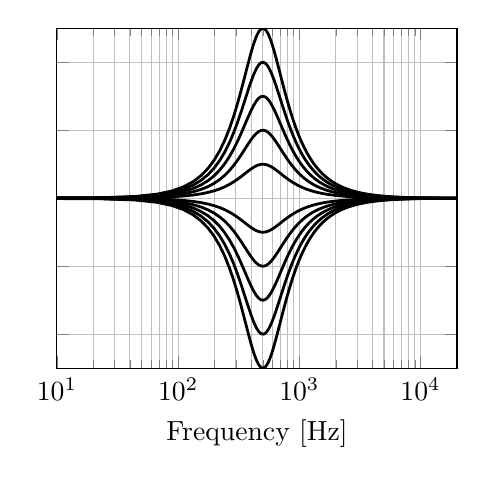
\begin{tikzpicture}

\begin{axis}[%
width=2in,
height=1.7in,
at={(1.011in,0.642in)},
scale only axis,
unbounded coords=jump,
xmode=log,
xmin=10,
xmax=20000,
xminorticks=true,
xlabel={Frequency [Hz]},
xmajorgrids,
xminorgrids,
ymin=-5,
ymax=5,
ymajorgrids,
yticklabels={\empty},
axis background/.style={fill=white}
]
\addplot [color=black,solid,line width=1.0pt,forget plot]
  table[row sep=crcr]{%
0.159154943091895	-6.76058748649941e-07\\
22.2100983353184	-0.0131792209368894\\
44.2610417275449	-0.0524977248528344\\
66.3119851197714	-0.11841679230081\\
88.362928511998	-0.211669051432683\\
110.413871904224	-0.333205011733822\\
132.464815296451	-0.484109559649171\\
154.515758688678	-0.665481734673923\\
176.566702080904	-0.878269124262541\\
198.617645473131	-1.12304794384191\\
220.668588865357	-1.39974140975748\\
242.719532257584	-1.70727360002581\\
264.77047564981	-2.04316550792318\\
286.821419042037	-2.40309707233203\\
308.872362434263	-2.78048666417806\\
330.92330582649	-3.16617946312176\\
352.974249218716	-3.54838395177158\\
375.025192610943	-3.91303292453086\\
397.076136003169	-4.24473261818622\\
419.127079395396	-4.5283490305297\\
441.178022787622	-4.75104178277422\\
463.228966179849	-4.90426585739014\\
485.279909572075	-4.98510523426627\\
507.330852964302	-4.99645778032346\\
529.381796356528	-4.94603264149291\\
551.432739748755	-4.84458336871655\\
573.483683140981	-4.70399811547319\\
595.534626533208	-4.53574532541999\\
617.585569925434	-4.34989277457256\\
639.636513317661	-4.15467260533357\\
661.687456709888	-3.95644161092091\\
683.738400102114	-3.75986886099448\\
705.789343494341	-3.56821959580025\\
727.840286886567	-3.38365293793705\\
749.891230278794	-3.20749084347987\\
771.94217367102	-3.04044188616636\\
793.993117063246	-2.88277805599617\\
816.044060455473	-2.73446957649289\\
838.0950038477	-2.59528507826158\\
860.145947239926	-2.46486452373853\\
882.196890632153	-2.34277136287792\\
904.247834024379	-2.22852920082203\\
926.298777416606	-2.12164710004197\\
948.349720808832	-2.02163664715798\\
970.400664201059	-1.92802311714397\\
992.451607593285	-1.84035245050419\\
1014.50255098551	-1.75819529287769\\
1036.55349437774	-1.68114900006291\\
1058.60443776996	-1.60883825677073\\
1080.65538116219	-1.54091477165098\\
1102.70632455442	-1.47705637642577\\
1124.75726794664	-1.41696575971351\\
1146.80821133887	-1.36036899618738\\
1168.8591547311	-1.30701398160059\\
1190.91009812332	-1.25666884844489\\
1212.96104151555	-1.20912041159592\\
1235.01198490778	-1.16417267535129\\
1257.0629283	-1.12164542067346\\
1279.11387169223	-1.08137288271449\\
1301.16481508446	-1.04320252270922\\
1323.21575847668	-1.00699389429935\\
1345.26670186891	-0.972617601724851\\
1367.31764526114	-0.939954345668409\\
1389.36858865336	-0.908894051585928\\
1411.41953204559	-0.879335074873854\\
1433.47047543782	-0.851183477071236\\
1455.52141883004	-0.824352367354457\\
1477.57236222227	-0.79876130378804\\
1499.6233056145	-0.774335749080402\\
1521.67424900672	-0.751006575931387\\
1543.72519239895	-0.728709617415332\\
1565.77613579117	-0.707385258205464\\
1587.8270791834	-0.686978062800027\\
1609.87802257563	-0.667436437248109\\
1631.92896596785	-0.648712321194434\\
1653.97990936008	-0.63076090735744\\
1676.03085275231	-0.613540385831363\\
1698.08179614453	-0.597011710852997\\
1720.13273953676	-0.581138387904987\\
1742.18368292899	-0.565886279234604\\
1764.23462632121	-0.55122342605671\\
1786.28556971344	-0.537119885880264\\
1808.33651310567	-0.523547583551689\\
1830.38745649789	-0.510480174746611\\
1852.43839989012	-0.497892920766762\\
1874.48934328235	-0.485762573611513\\
1896.54028667457	-0.474067270392776\\
1918.5912300668	-0.46278643625425\\
1940.64217345903	-0.451900695036433\\
1962.69311685125	-0.441391787002143\\
1984.74406024348	-0.431242493002901\\
2006.79500363571	-0.421436564525681\\
2028.84594702793	-0.411958659112447\\
2050.89689042016	-0.402794280692683\\
2072.94783381238	-0.393929724411967\\
2094.99877720461	-0.385352025578251\\
2117.04972059684	-0.377048912382813\\
2139.10066398906	-0.369008762083204\\
2161.15160738129	-0.36122056036485\\
2183.20255077352	-0.353673863622836\\
2205.25349416574	-0.346358763928689\\
2227.30443755797	-0.339265856467897\\
2249.3553809502	-0.332386209252483\\
2271.40632434242	-0.325711334930047\\
2293.45726773465	-0.319233164526537\\
2315.50821112688	-0.312944022973394\\
2337.5591545191	-0.306836606282591\\
2359.61009791133	-0.300903960245086\\
2381.66104130356	-0.295139460537923\\
2403.71198469578	-0.289536794135062\\
2425.76292808801	-0.284089941925841\\
2447.81387148024	-0.278793162452606\\
2469.86481487246	-0.273640976686083\\
2491.91575826469	-0.268628153764108\\
2513.96670165692	-0.263749697624593\\
2536.01764504914	-0.259000834469798\\
2558.06858844137	-0.254377001003188\\
2580.11953183359	-0.249873833385344\\
2602.17047522582	-0.245487156859324\\
2624.22141861805	-0.241212975999256\\
2646.27236201027	-0.237047465540311\\
2668.3233054025	-0.232986961750611\\
2690.37424879473	-0.229027954308841\\
2712.42519218695	-0.22516707865414\\
2734.47613557918	-0.221401108777172\\
2756.52707897141	-0.217726950423612\\
2778.57802236363	-0.214141634683295\\
2800.62896575586	-0.21064231194028\\
2822.67990914809	-0.207226246160801\\
2844.73085254031	-0.203890809497817\\
2866.78179593254	-0.200633477192242\\
2888.83273932477	-0.197451822752267\\
2910.88368271699	-0.194343513393737\\
2932.93462610922	-0.191306305725652\\
2954.98556950145	-0.18833804166551\\
2977.03651289367	-0.185436644570865\\
2999.0874562859	-0.182600115574331\\
3021.13839967812	-0.179826530109259\\
3043.18934307035	-0.177114034615617\\
3065.24028646258	-0.174460843414791\\
3087.2912298548	-0.171865235744072\\
3109.34217324703	-0.169325552941003\\
3131.39311663926	-0.166840195769516\\
3153.44406003148	-0.164407621879344\\
3175.49500342371	-0.162026343391462\\
3197.54594681594	-0.15969492460241\\
3219.59689020816	-0.157411979800488\\
3241.64783360039	-0.155176171188353\\
3263.69877699262	-0.152986206905404\\
3285.74972038484	-0.150840839145021\\
3307.80066377707	-0.148738862361136\\
3329.8516071693	-0.146679111559695\\
3351.90255056152	-0.144660460669986\\
3373.95349395375	-0.142681820992206\\
3396.00443734598	-0.140742139716381\\
3418.0553807382	-0.138840398509868\\
3440.10632413043	-0.136975612169069\\
3462.15726752266	-0.135146827332368\\
3484.20821091488	-0.133353121251166\\
3506.25915430711	-0.131593600615933\\
3528.31009769933	-0.12986740043444\\
3550.36104109156	-0.128173682959659\\
3572.41198448379	-0.126511636664843\\
3594.46292787601	-0.124880475263197\\
3616.51387126824	-0.123279436770246\\
3638.56481466047	-0.121707782606482\\
3660.61575805269	-0.120164796738688\\
3682.66670144492	-0.118649784857596\\
3704.71764483715	-0.117162073590609\\
3726.76858822937	-0.11570100974742\\
3748.8195316216	-0.114265959597325\\
3770.87047501383	-0.112856308176599\\
3792.92141840605	-0.111471458624427\\
3814.97236179828	-0.110110831546121\\
3837.02330519051	-0.108773864402451\\
3859.07424858273	-0.107460010923619\\
3881.12519197496	-0.106168740547036\\
3903.17613536719	-0.104899537877587\\
3925.22707875941	-0.103651902169416\\
3947.27802215164	-0.102425346828418\\
3969.32896554387	-0.101219398934121\\
3991.37990893609	-0.100033598780546\\
4013.43085232832	-0.0988674994348977\\
4035.48179572054	-0.0977206663133158\\
4057.53273911277	-0.0965926767730808\\
4079.583682505	-0.0954831197204738\\
4101.63462589722	-0.0943915952334715\\
4123.68556928945	-0.0933177141989435\\
4145.73651268168	-0.0922610979633481\\
4167.7874560739	-0.0912213779967311\\
4189.83839946613	-0.0901981955690886\\
4211.88934285836	-0.0891912014389205\\
4233.94028625058	-0.088200055553116\\
4255.99122964281	-0.0872244267580096\\
4278.04217303504	-0.0862639925209384\\
4300.09311642726	-0.0853184386618721\\
4322.14405981949	-0.0843874590949072\\
4344.19500321172	-0.08347075557881\\
4366.24594660394	-0.0825680374767743\\
4388.29688999617	-0.0816790215245414\\
4410.3478333884	-0.0808034316067297\\
4432.39877678062	-0.0799409985412489\\
4454.44972017285	-0.0790914598710184\\
4476.50066356508	-0.0782545596631032\\
4498.5516069573	-0.0774300483148113\\
4520.60255034953	-0.0766176823664857\\
4542.65349374176	-0.0758172243206505\\
4564.70443713398	-0.0750284424674619\\
4586.75538052621	-0.0742511107160672\\
4608.80632391843	-0.0734850084316106\\
4630.85726731066	-0.0727299202778217\\
4652.90821070289	-0.0719856360648209\\
4674.95915409511	-0.071251950602021\\
4697.01009748734	-0.0705286635559801\\
4719.06104087957	-0.0698155793128292\\
4741.11198427179	-0.0691125068453388\\
4763.16292766402	-0.0684192595843164\\
4785.21387105625	-0.067735655294117\\
4807.26481444847	-0.0670615159523321\\
4829.3157578407	-0.066396667633217\\
4851.36670123293	-0.0657409403950026\\
4873.41764462515	-0.065094168170689\\
4895.46858801738	-0.0644561886624192\\
4917.51953140961	-0.0638268432391416\\
4939.57047480183	-0.0632059768375282\\
4961.62141819406	-0.0625934378659752\\
4983.67236158629	-0.0619890781116794\\
5005.72330497851	-0.0613927526504849\\
5027.77424837074	-0.0608043197596858\\
5049.82519176296	-0.0602236408333477\\
5071.87613515519	-0.0596505803003807\\
5093.92707854742	-0.059085005545017\\
5115.97802193964	-0.0585267868297659\\
5138.02896533187	-0.0579757972206644\\
5160.0799087241	-0.0574319125148363\\
5182.13085211632	-0.0568950111701777\\
5204.18179550855	-0.0563649742371795\\
5226.23273890078	-0.0558416852927619\\
5248.283682293	-0.0553250303760851\\
5270.33462568523	-0.0548148979262707\\
5292.38556907746	-0.0543111787218987\\
5314.43651246968	-0.0538137658223576\\
5336.48745586191	-0.0533225545108585\\
5358.53839925414	-0.0528374422390656\\
5380.58934264636	-0.0523583285734361\\
5402.64028603859	-0.0518851151430275\\
5424.69122943082	-0.0514177055887714\\
5446.74217282304	-0.0509560055143406\\
5468.79311621527	-0.0504999224382133\\
5490.8440596075	-0.0500493657472836\\
5512.89500299972	-0.0496042466516528\\
5534.94594639195	-0.0491644781407773\\
5556.99688978417	-0.0487299749407539\\
5579.0478331764	-0.0483006534728901\\
5601.09877656863	-0.0478764318133789\\
5623.14971996085	-0.047457229654098\\
5645.20066335308	-0.0470429682644447\\
5667.25160674531	-0.046633570454297\\
5689.30255013753	-0.046228960537956\\
5711.35349352976	-0.0458290642990396\\
5733.40443692199	-0.0454338089563574\\
5755.45538031421	-0.0450431231307149\\
5777.50632370644	-0.0446569368125792\\
5799.55726709867	-0.0442751813306647\\
5821.60821049089	-0.0438977893212655\\
5843.65915388312	-0.0435246946985424\\
5865.71009727535	-0.0431558326254641\\
5887.76104066757	-0.0427911394855656\\
5909.8119840598	-0.0424305528554883\\
5931.86292745203	-0.0420740114781731\\
5953.91387084425	-0.0417214552368231\\
5975.96481423648	-0.0413728251294652\\
5998.0157576287	-0.0410280632442223\\
6020.06670102093	-0.040687112735244\\
6042.11764441316	-0.0403499177991763\\
6064.16858780538	-0.0400164236523232\\
6086.21953119761	-0.0396865765083395\\
6108.27047458984	-0.0393603235564917\\
6130.32141798206	-0.0390376129404871\\
6152.37236137429	-0.0387183937378632\\
6174.42330476652	-0.0384026159398126\\
6196.47424815874	-0.0380902304315816\\
6218.52519155097	-0.0377811889733917\\
6240.5761349432	-0.037475444181704\\
6262.62707833542	-0.0371729495111109\\
6284.67802172765	-0.0368736592365306\\
6306.72896511988	-0.0365775284359528\\
6328.7799085121	-0.0362845129735332\\
6350.83085190433	-0.0359945694831332\\
6372.88179529656	-0.0357076553522781\\
6394.93273868878	-0.0354237287064469\\
6416.98368208101	-0.0351427483937985\\
6439.03462547323	-0.0348646739702479\\
6461.08556886546	-0.0345894656849021\\
6483.13651225769	-0.0343170844658215\\
6505.18745564992	-0.034047491906158\\
6527.23839904214	-0.0337806502506132\\
6549.28934243437	-0.0335165223821964\\
6571.34028582659	-0.033255071809307\\
6593.39122921882	-0.0329962626531396\\
6615.44217261105	-0.0327400596353587\\
6637.49311600327	-0.0324864280660732\\
6659.5440593955	-0.032235333832087\\
6681.59500278773	-0.0319867433854414\\
6703.64594617995	-0.0317406237321766\\
6725.69688957218	-0.0314969424214256\\
6747.74783296441	-0.0312556675346648\\
6769.79877635663	-0.0310167676753026\\
6791.84971974886	-0.0307802119584527\\
6813.90066314109	-0.03054597000095\\
6835.95160653331	-0.0303140119115945\\
6858.00254992554	-0.0300843082816373\\
6880.05349331777	-0.0298568301754174\\
6902.10443670999	-0.0296315491213179\\
6924.15538010222	-0.0294084371027988\\
6946.20632349445	-0.0291874665497352\\
6968.25726688667	-0.028968610329874\\
6990.3082102789	-0.0287518417405311\\
7012.35915367112	-0.0285371345004376\\
7034.41009706335	-0.0283244627417999\\
7056.46104045558	-0.0281138010024931\\
7078.5119838478	-0.027905124218462\\
7100.56292724003	-0.0276984077162638\\
7122.61387063226	-0.0274936272057908\\
7144.66481402448	-0.0272907587731334\\
7166.71575741671	-0.0270897788736167\\
7188.76670080894	-0.0268906643249765\\
7210.81764420116	-0.0266933923006679\\
7232.86858759339	-0.0264979403233694\\
7254.91953098562	-0.0263042862585293\\
7276.97047437784	-0.0261124083081841\\
7299.02141777007	-0.0259222850047748\\
7321.0723611623	-0.0257338952051611\\
7343.12330455452	-0.0255472180847949\\
7365.17424794675	-0.0253622331319179\\
7387.22519133898	-0.0251789201419941\\
7409.2761347312	-0.0249972592121518\\
7431.32707812343	-0.0248172307358416\\
7453.37802151566	-0.0246388153975107\\
7475.42896490788	-0.0244619941674694\\
7497.47990830011	-0.0242867482968183\\
7519.53085169233	-0.0241130593124739\\
7541.58179508456	-0.0239409090123406\\
7563.63273847679	-0.0237702794605314\\
7585.68368186901	-0.0236011529827131\\
7607.73462526124	-0.0234335121615577\\
7629.78556865347	-0.0232673398322313\\
7651.83651204569	-0.0231026190780744\\
7673.88745543792	-0.0229393332262569\\
7695.93839883015	-0.0227774658435762\\
7717.98934222237	-0.0226170007323667\\
7740.0402856146	-0.0224579219264349\\
7762.09122900683	-0.0223002136871126\\
7784.14217239905	-0.0221438604993666\\
7806.19311579128	-0.0219888470680077\\
7828.24405918351	-0.0218351583139384\\
7850.29500257573	-0.021682779370549\\
7872.34594596796	-0.0215316955800826\\
7894.39688936019	-0.0213818924901472\\
7916.44783275241	-0.0212333558502747\\
7938.49877614464	-0.0210860716085471\\
7960.54971953686	-0.0209400259082625\\
7982.60066292909	-0.0207952050847285\\
8004.65160632132	-0.0206515956620369\\
8026.70254971355	-0.0205091843499887\\
8048.75349310577	-0.0203679580409845\\
8070.804436498	-0.0202279038070611\\
8092.85537989022	-0.0200890088969181\\
8114.90632328245	-0.0199512607330394\\
8136.95726667468	-0.0198146469088783\\
8159.0082100669	-0.0196791551860416\\
8181.05915345913	-0.0195447734915907\\
8203.11009685136	-0.0194114899153467\\
8225.16104024358	-0.0192792927072835\\
8247.21198363581	-0.0191481702749289\\
8269.26292702804	-0.019018111180865\\
8291.31387042026	-0.0188891041402182\\
8313.36481381249	-0.0187611380182463\\
8335.41575720472	-0.018634201827929\\
8357.46670059694	-0.0185082847276507\\
8379.51764398917	-0.0183833760188777\\
8401.56858738139	-0.0182594651438925\\
8423.61953077362	-0.0181365416836057\\
8445.67047416585	-0.0180145953553507\\
8467.72141755808	-0.0178936160107524\\
8489.7723609503	-0.01777359363365\\
8511.82330434253	-0.0176545183379994\\
8533.87424773476	-0.0175363803658934\\
8555.92519112698	-0.0174191700855315\\
8577.97613451921	-0.0173028779893163\\
8600.02707791143	-0.0171874946918811\\
8622.07802130366	-0.0170730109282802\\
8644.12896469589	-0.0169594175520801\\
8666.17990808811	-0.0168467055335699\\
8688.23085148034	-0.0167348659579981\\
8710.28179487257	-0.0166238900237643\\
8732.33273826479	-0.0165137690407902\\
8754.38368165702	-0.0164044944287411\\
8776.43462504925	-0.016296057715426\\
8798.48556844147	-0.016188450535137\\
8820.5365118337	-0.0160816646270748\\
8842.58745522593	-0.0159756918337419\\
8864.63839861815	-0.0158705240994315\\
8886.68934201038	-0.0157661534686908\\
8908.74028540261	-0.0156625720848214\\
8930.79122879483	-0.0155597721884322\\
8952.84217218706	-0.0154577461159968\\
8974.89311557929	-0.0153564862984107\\
8996.94405897151	-0.0152559852596341\\
9018.99500236374	-0.0151562356152984\\
9041.04594575596	-0.0150572300713867\\
9063.09688914819	-0.0149589614228896\\
9085.14783254042	-0.0148614225525123\\
9107.19877593265	-0.0147646064294068\\
9129.24971932487	-0.0146685061079002\\
9151.3006627171	-0.0145731147262855\\
9173.35160610933	-0.0144784255055837\\
9195.40254950155	-0.0143844317483612\\
9217.45349289378	-0.0142911268375606\\
9239.504436286	-0.014198504235347\\
9261.55537967823	-0.0141065574819651\\
9283.60632307046	-0.0140152801946349\\
9305.65726646268	-0.0139246660664474\\
9327.70820985491	-0.0138347088652974\\
9349.75915324714	-0.0137454024328043\\
9371.81009663936	-0.0136567406832995\\
9393.86104003159	-0.013568717602767\\
9415.91198342382	-0.0134813272478564\\
9437.96292681604	-0.0133945637448779\\
9460.01387020827	-0.0133084212888473\\
9482.06481360049	-0.0132228941425048\\
9504.11575699272	-0.0131379766353668\\
9526.16670038495	-0.0130536631628207\\
9548.21764377718	-0.0129699481852019\\
9570.2685871694	-0.0128868262268774\\
9592.31953056163	-0.0128042918753833\\
9614.37047395386	-0.0127223397805388\\
9636.42141734608	-0.0126409646536078\\
9658.47236073831	-0.012560161266429\\
9680.52330413053	-0.0124799244506211\\
9702.57424752276	-0.0124002490967236\\
9724.62519091499	-0.0123211301534498\\
9746.67613430721	-0.0122425626268338\\
9768.72707769944	-0.0121645415795077\\
9790.77802109167	-0.0120870621298976\\
9812.82896448389	-0.012010119451484\\
9834.87990787612	-0.0119337087720849\\
9856.93085126835	-0.0118578253730638\\
9878.98179466057	-0.0117824645886824\\
9901.0327380528	-0.0117076218053527\\
9923.08368144502	-0.0116332924609302\\
9945.13462483725	-0.0115594720440696\\
9967.18556822948	-0.0114861560935149\\
9989.23651162171	-0.011413340197457\\
10011.2874550139	-0.0113410199928505\\
10033.3383984062	-0.0112691911648227\\
10055.3893417984	-0.0111978494459696\\
10077.4402851906	-0.0111269906157978\\
10099.4912285828	-0.0110566105000603\\
10121.5421719751	-0.0109867049701819\\
10143.5931153673	-0.0109172699426514\\
10165.6440587595	-0.010848301378432\\
10187.6950021517	-0.0107797952823891\\
10209.745945544	-0.0107117477027208\\
10231.7968889362	-0.0106441547303796\\
10253.8478323284	-0.010577012498562\\
10275.8987757206	-0.0105103171821195\\
10297.9497191129	-0.0104440649970481\\
10320.0006625051	-0.0103782521999426\\
10342.0516058973	-0.0103128750875041\\
10364.1025492896	-0.0102479299960068\\
10386.1534926818	-0.0101834133007851\\
10408.204436074	-0.0101193214157725\\
10430.2553794662	-0.0100556507929722\\
10452.3063228585	-0.00999239792199761\\
10474.3572662507	-0.00992955932958718\\
10496.4082096429	-0.00986713157915755\\
10518.4591530351	-0.00980511127030232\\
10540.5100964274	-0.00974349503837019\\
10562.5610398196	-0.00968227955400936\\
10584.6119832118	-0.00962146152272257\\
10606.662926604	-0.00956103768443184\\
10628.7138699963	-0.00950100481305688\\
10650.7648133885	-0.00944135971607893\\
10672.8157567807	-0.00938209923413756\\
10694.866700173	-0.00932322024061692\\
10716.9176435652	-0.00926471964124546\\
10738.9685869574	-0.00920659437367845\\
10761.0195303496	-0.00914884140713545\\
10783.0704737419	-0.00909145774198676\\
10805.1214171341	-0.00903444040937943\\
10827.1723605263	-0.00897778647087491\\
10849.2233039185	-0.00892149301805976\\
10871.2742473108	-0.00886555717219017\\
10893.325190703	-0.00880997608382872\\
10915.3761340952	-0.00875474693248902\\
10937.4270774874	-0.00869986692628807\\
10959.4780208797	-0.00864533330159574\\
10981.5289642719	-0.00859114332269684\\
11003.5799076641	-0.00853729428146969\\
11025.6308510564	-0.00848378349702604\\
11047.6817944486	-0.00843060831540227\\
11069.7327378408	-0.00837776610924956\\
11091.783681233	-0.00832525427749527\\
11113.8346246253	-0.00827307024503219\\
11135.8855680175	-0.0082212114624311\\
11157.9365114097	-0.00816967540561091\\
11179.9874548019	-0.00811845957554634\\
11202.0383981942	-0.00806756149799608\\
11224.0893415864	-0.00801697872316326\\
11246.1402849786	-0.00796670882545837\\
11268.1912283708	-0.00791674940318493\\
11290.2421717631	-0.00786709807825225\\
11312.2931151553	-0.00781775249593744\\
11334.3440585475	-0.00776871032457696\\
11356.3950019397	-0.00771996925530941\\
11378.445945332	-0.00767152700182116\\
11400.4968887242	-0.00762338130007278\\
11422.5478321164	-0.00757552990803706\\
11444.5987755087	-0.00752797060546308\\
11466.6497189009	-0.00748070119360945\\
11488.7006622931	-0.00743371949500169\\
11510.7516056853	-0.00738702335318485\\
11532.8025490776	-0.00734061063249828\\
11554.8534924698	-0.00729447921780993\\
11576.904435862	-0.00724862701431728\\
11598.9553792542	-0.00720305194727397\\
11621.0063226465	-0.00715775196180327\\
11643.0572660387	-0.00711272502263729\\
11665.1082094309	-0.0070679691139267\\
11687.1591528231	-0.00702348223900411\\
11709.2100962154	-0.00697926242015319\\
11731.2610396076	-0.00693530769843398\\
11753.3119829998	-0.00689161613342979\\
11775.3629263921	-0.0068481858030735\\
11797.4138697843	-0.00680501480341871\\
11819.4648131765	-0.00676210124845824\\
11841.5157565687	-0.0067194432698896\\
11863.566699961	-0.00667703901697696\\
11885.6176433532	-0.00663488665627607\\
11907.6685867454	-0.00659298437152527\\
11929.7195301376	-0.00655133036339261\\
11951.7704735299	-0.00650992284932155\\
11973.8214169221	-0.00646876006333213\\
11995.8723603143	-0.00642784025584744\\
12017.9233037065	-0.0063871616935141\\
12039.9742470988	-0.00634672265900752\\
12062.025190491	-0.0063065214508843\\
12084.0761338832	-0.00626655638338745\\
12106.1270772755	-0.00622682578626416\\
12128.1780206677	-0.00618732800464624\\
12150.2289640599	-0.00614806139883806\\
12172.2799074521	-0.006109024344142\\
12194.3308508444	-0.0060702152307622\\
12216.3817942366	-0.0060316324635712\\
12238.4327376288	-0.00599327446198761\\
12260.483681021	-0.00595513965982487\\
12282.5346244133	-0.00591722650510521\\
12304.5855678055	-0.00587953345994705\\
12326.6365111977	-0.00584205900039248\\
12348.6874545899	-0.00580480161625222\\
12370.7383979822	-0.00576775981096984\\
12392.7893413744	-0.00573093210148119\\
12414.8402847666	-0.00569431701806508\\
12436.8912281588	-0.00565791310419124\\
12458.9421715511	-0.00562171891639994\\
12480.9931149433	-0.00558573302416052\\
12503.0440583355	-0.00554995400971641\\
12525.0950017278	-0.00551438046796195\\
12547.14594512	-0.00547901100632311\\
12569.1968885122	-0.00544384424463148\\
12591.2478319044	-0.00540887881493552\\
12613.2987752967	-0.00537411336145271\\
12635.3497186889	-0.00533954654038666\\
12657.4006620811	-0.00530517701982325\\
12679.4516054733	-0.00527100347960954\\
12701.5025488656	-0.00523702461122392\\
12723.5534922578	-0.00520323911766844\\
12745.60443565	-0.00516964571332847\\
12767.6553790422	-0.00513624312386695\\
12789.7063224345	-0.00510303008612451\\
12811.7572658267	-0.00507000534797527\\
12833.8082092189	-0.00503716766822786\\
12855.8591526112	-0.00500451581652468\\
12877.9100960034	-0.00497204857320914\\
12899.9610393956	-0.00493976472923269\\
12922.0119827878	-0.00490766308603462\\
12944.0629261801	-0.00487574245545192\\
12966.1138695723	-0.00484400165959924\\
12988.1648129645	-0.00481243953076319\\
13010.2157563567	-0.00478105491132578\\
13032.266699749	-0.00474984665361827\\
13054.3176431412	-0.00471881361986574\\
13076.3685865334	-0.00468795468205647\\
13098.4195299256	-0.00465726872186432\\
13120.4704733179	-0.00462675463053064\\
13142.5214167101	-0.00459641130879633\\
13164.5723601023	-0.00456623766677219\\
13186.6233034945	-0.00453623262387868\\
13208.6742468868	-0.00450639510874239\\
13230.725190279	-0.00447672405908462\\
13252.7761336712	-0.00444721842167865\\
13274.8270770635	-0.00441787715218726\\
13296.8780204557	-0.00438869921516429\\
13318.9289638479	-0.00435968358388069\\
13340.9799072401	-0.00433082924030095\\
13363.0308506324	-0.00430213517497188\\
13385.0817940246	-0.00427360038694506\\
13407.1327374168	-0.00424522388368486\\
13429.183680809	-0.00421700468099384\\
13451.2346242013	-0.00418894180292466\\
13473.2855675935	-0.004161034281717\\
13495.3365109857	-0.00413328115769699\\
13517.3874543779	-0.00410568147920546\\
13539.4383977702	-0.00407823430253397\\
13561.4893411624	-0.00405093869182713\\
13583.5402845546	-0.00402379371902533\\
13605.5912279469	-0.00399679846376511\\
13627.6421713391	-0.00396995201334222\\
13649.6931147313	-0.00394325346260231\\
13671.7440581235	-0.00391670191387702\\
13693.7950015158	-0.00389029647694701\\
13715.845944908	-0.00386403626890859\\
13737.8968883002	-0.00383792041416283\\
13759.9478316924	-0.00381194804431403\\
13781.9987750847	-0.00378611829810093\\
13804.0497184769	-0.00376043032134344\\
13826.1006618691	-0.0037348832668758\\
13848.1516052613	-0.00370947629445472\\
13870.2025486536	-0.00368420857073402\\
13892.2534920458	-0.00365907926917181\\
13914.304435438	-0.0036340875699714\\
13936.3553788303	-0.00360923266001065\\
13958.4063222225	-0.00358451373280894\\
13980.4572656147	-0.00355992998843916\\
14002.5082090069	-0.00353548063346287\\
14024.5591523992	-0.00351116488089436\\
14046.6100957914	-0.00348698195011364\\
14068.6610391836	-0.00346293106682862\\
14090.7119825758	-0.00343901146300732\\
14112.7629259681	-0.00341522237681791\\
14134.8138693603	-0.00339156305256385\\
14156.8648127525	-0.00336803274067116\\
14178.9157561447	-0.00334463069756279\\
14200.966699537	-0.00332135618566234\\
14223.0176429292	-0.00329820847330216\\
14245.0685863214	-0.00327518683469814\\
14267.1195297136	-0.00325229054986846\\
14289.1704731059	-0.00322951890459963\\
14311.2214164981	-0.00320687119038946\\
14333.2723598903	-0.00318434670439759\\
14355.3233032826	-0.00316194474938367\\
14377.3742466748	-0.00313966463366757\\
14399.425190067	-0.00311750567107137\\
14421.4761334592	-0.00309546718088253\\
14443.5270768515	-0.00307354848778713\\
14465.5780202437	-0.00305174892183792\\
14487.6289636359	-0.0030300678183924\\
14509.6799070281	-0.00300850451807407\\
14531.7308504204	-0.00298705836672406\\
14553.7817938126	-0.00296572871535466\\
14575.8327372048	-0.002944514920099\\
14597.883680597	-0.00292341634217523\\
14619.9346239893	-0.00290243234782366\\
14641.9855673815	-0.00288156230828539\\
14664.0365107737	-0.00286080559973947\\
14686.087454166	-0.00284016160327188\\
14708.1383975582	-0.00281962970482236\\
14730.1893409504	-0.0027992092951418\\
14752.2402843426	-0.00277889976977475\\
14774.2912277349	-0.00275870052896286\\
14796.3421711271	-0.00273861097768325\\
14818.3931145193	-0.00271863052551246\\
14840.4440579115	-0.00269875858668318\\
14862.4950013038	-0.00267899457995874\\
14884.545944696	-0.00265933792865997\\
14906.5968880882	-0.00263978806058411\\
14928.6478314804	-0.00262034440796698\\
14950.6987748727	-0.00260100640749164\\
14972.7497182649	-0.00258177350019654\\
14994.8006616571	-0.00256264513144172\\
15016.8516050494	-0.00254362075091154\\
15038.9025484416	-0.00252469981254994\\
15060.9534918338	-0.00250588177451792\\
15083.004435226	-0.00248716609917605\\
15105.0553786183	-0.00246855225303803\\
15127.1063220105	-0.00245003970673108\\
15149.1572654027	-0.00243162793497844\\
15171.2082087949	-0.00241331641654237\\
15193.2591521872	-0.00239510463422018\\
15215.3100955794	-0.00237699207476505\\
15237.3610389716	-0.00235897822890036\\
15259.4119823638	-0.00234106259125019\\
15281.4629257561	-0.00232324466033434\\
15303.5138691483	-0.00230552393852394\\
15325.5648125405	-0.00228789993199014\\
15347.6157559327	-0.00227037215070604\\
15369.666699325	-0.00225294010839925\\
15391.7176427172	-0.0022356033225094\\
15413.7685861094	-0.00221836131419096\\
15435.8195295017	-0.0022012136082369\\
15457.8704728939	-0.00218415973308443\\
15479.9214162861	-0.00216719922077341\\
15501.9723596783	-0.00215033160690674\\
15524.0233030706	-0.0021335564306464\\
15546.0742464628	-0.00211687323465357\\
15568.125189855	-0.00210028156507892\\
15590.1761332472	-0.0020837809715403\\
15612.2270766395	-0.00206737100706964\\
15634.2780200317	-0.00205105122810805\\
15656.3289634239	-0.00203482119446716\\
15678.3799068161	-0.00201868046930973\\
15700.4308502084	-0.00200262861911487\\
15722.4817936006	-0.00198666521364322\\
15744.5327369928	-0.00197078982593788\\
15766.5836803851	-0.00195500203226836\\
15788.6346237773	-0.00193930141213533\\
15810.6855671695	-0.00192368754820595\\
15832.7365105617	-0.00190816002632725\\
15854.787453954	-0.00189271843546827\\
15876.8383973462	-0.00187736236772089\\
15898.8893407384	-0.00186209141826118\\
15920.9402841306	-0.00184690518533106\\
15942.9912275229	-0.00183180327021022\\
15965.0421709151	-0.00181678527718905\\
15987.0931143073	-0.00180185081355507\\
16009.1440576995	-0.00178699948955626\\
16031.1950010918	-0.0017722309183961\\
16053.245944484	-0.00175754471619595\\
16075.2968878762	-0.00174294050196315\\
16097.3478312684	-0.00172841789759863\\
16119.3987746607	-0.00171397652784966\\
16141.4497180529	-0.00169961602029045\\
16163.5006614451	-0.00168533600532017\\
16185.5516048374	-0.00167113611610601\\
16207.6025482296	-0.0016570159885966\\
16229.6534916218	-0.00164297526148339\\
16251.704435014	-0.00162901357616874\\
16273.7553784063	-0.00161513057678328\\
16295.8063217985	-0.00160132591011731\\
16317.8572651907	-0.00158759922563816\\
16339.9082085829	-0.00157395017544285\\
16361.9591519752	-0.00156037841426575\\
16384.0100953674	-0.00154688359943034\\
16406.0610387596	-0.0015334653908462\\
16428.1119821518	-0.00152012345099651\\
16450.1629255441	-0.0015068574448868\\
16472.2138689363	-0.00149366704006422\\
16494.2648123285	-0.00148055190657606\\
16516.3157557208	-0.00146751171695901\\
16538.366699113	-0.00145454614621412\\
16560.4176425052	-0.0014416548718067\\
16582.4685858974	-0.00142883757360552\\
16604.5195292897	-0.00141609393392619\\
16626.5704726819	-0.00140342363745297\\
16648.6214160741	-0.00139082637127441\\
16670.6723594663	-0.00137830182481291\\
16692.7233028586	-0.00136584968985843\\
16714.7742462508	-0.00135346966051252\\
16736.825189643	-0.00134116143319501\\
16758.8761330352	-0.00132892470661214\\
16780.9270764275	-0.00131675918175749\\
16802.9780198197	-0.00130466456186374\\
16825.0289632119	-0.00129264055243054\\
16847.0799066042	-0.00128068686117054\\
16869.1308499964	-0.00126880319801216\\
16891.1817933886	-0.00125698927507648\\
16913.2327367808	-0.00124524480666653\\
16935.2836801731	-0.0012335695092509\\
16957.3346235653	-0.00122196310144343\\
16979.3855669575	-0.00121042530399354\\
17001.4365103497	-0.00119895583977169\\
17023.487453742	-0.00118755443374627\\
17045.5383971342	-0.00117622081297963\\
17067.5893405264	-0.00116495470660107\\
17089.6402839186	-0.00115375584580684\\
17111.6912273109	-0.00114262396384075\\
17133.7421707031	-0.00113155879595368\\
17155.7931140953	-0.00112056007945465\\
17177.8440574875	-0.00110962755361048\\
17199.8950008798	-0.00109876095971711\\
17221.945944272	-0.00108796004101377\\
17243.9968876642	-0.0010772245427244\\
17266.0478310565	-0.00106655421199683\\
17288.0987744487	-0.00105594879794235\\
17310.1497178409	-0.00104540805157102\\
17332.2006612331	-0.00103493172581286\\
17354.2516046254	-0.00102451957549179\\
17376.3025480176	-0.00101417135731306\\
17398.3534914098	-0.00100388682984684\\
17420.404434802	-0.000993665753529126\\
17442.4553781943	-0.000983507890641474\\
17464.5063215865	-0.000973413005287831\\
17486.5572649787	-0.000963380863402214\\
17508.6082083709	-0.000953411232728432\\
17530.6591517632	-0.000943503882799807\\
17552.7100951554	-0.000933658584931428\\
17574.7610385476	-0.000923875112224953\\
17596.8119819399	-0.000914153239529998\\
17618.8629253321	-0.000904492743451831\\
17640.9138687243	-0.000894893402331094\\
17662.9648121165	-0.000885354996240883\\
17685.0157555088	-0.000875877306969361\\
17707.066698901	-0.000866460117993699\\
17729.1176422932	-0.000857103214512839\\
17751.1685856854	-0.000847806383381889\\
17773.2195290777	-0.00083856941314103\\
17795.2704724699	-0.000829392093997176\\
17817.3214158621	-0.000820274217790186\\
17839.3723592543	-0.000811215578015994\\
17861.4233026466	-0.000802215969793795\\
17883.4742460388	-0.000793275189867949\\
17905.525189431	-0.000784393036588671\\
17927.5761328233	-0.000775569309891761\\
17949.6270762155	-0.000766803811336187\\
17971.6780196077	-0.000758096344026916\\
17993.7289629999	-0.000749446712657327\\
18015.7799063922	-0.000740854723472538\\
18037.8308497844	-0.000732320184276142\\
18059.8817931766	-0.000723842904406072\\
18081.9327365688	-0.000715422694732654\\
18103.9836799611	-0.000707059367654728\\
18126.0346233533	-0.00069875273707263\\
18148.0855667455	-0.000690502618403593\\
18170.1365101377	-0.000682308828549915\\
18192.18745353	-0.000674171185911465\\
18214.2383969222	-0.000666089510346135\\
18236.2893403144	-0.000658063623202602\\
18258.3402837066	-0.000650093347270165\\
18280.3912270989	-0.000642178506802838\\
18302.4421704911	-0.000634318927494255\\
18324.4931138833	-0.000626514436460296\\
18346.5440572756	-0.000618764862259317\\
18368.5950006678	-0.00061107003485935\\
18390.64594406	-0.000603429785639046\\
18412.6968874522	-0.000595843947370299\\
18434.7478308445	-0.000588312354236554\\
18456.7987742367	-0.000580834841779749\\
18478.8497176289	-0.000573411246949484\\
18500.9006610211	-0.000566041408043208\\
18522.9516044134	-0.000558725164728391\\
18545.0025478056	-0.00055146235802225\\
18567.0534911978	-0.000544252830291737\\
18589.10443459	-0.00053709642524677\\
18611.1553779823	-0.000529992987920935\\
18633.2063213745	-0.000522942364672432\\
18655.2572647667	-0.000515944403192738\\
18677.308208159	-0.000508998952453556\\
18699.3591515512	-0.000502105862755015\\
18721.4100949434	-0.000495264985682264\\
18743.4610383356	-0.000488476174108345\\
18765.5119817279	-0.000481739282202863\\
18787.5629251201	-0.000475054165382787\\
18809.6138685123	-0.00046842068035294\\
18831.6648119045	-0.000461838685074162\\
18853.7157552968	-0.000455308038771012\\
18875.766698689	-0.000448828601896073\\
18897.8176420812	-0.000442400236164655\\
18919.8685854734	-0.000436022804516209\\
18941.9195288657	-0.000429696171122992\\
18963.9704722579	-0.000423420201380415\\
18986.0214156501	-0.000417194761884842\\
19008.0723590424	-0.000411019720472163\\
19030.1233024346	-0.000404894946157017\\
19052.1742458268	-0.00039882030916847\\
19074.225189219	-0.000392795680922028\\
19096.2761326113	-0.000386820934009027\\
19118.3270760035	-0.000380895942214936\\
19140.3780193957	-0.000375020580500063\\
19162.4289627879	-0.00036919472498315\\
19184.4799061802	-0.000363418252951002\\
19206.5308495724	-0.000357691042851729\\
19228.5817929646	-0.000352012974282196\\
19250.6327363568	-0.000346383927985123\\
19272.6836797491	-0.000340803785848105\\
19294.7346231413	-0.000335272430879495\\
19316.7855665335	-0.000329789747247936\\
19338.8365099257	-0.000324355620212911\\
19360.887453318	-0.00031896993617874\\
19382.9383967102	-0.00031363258265214\\
19404.9893401024	-0.000308343448258605\\
19427.0402834947	-0.000303102422716364\\
19449.0912268869	-0.000297909396850832\\
19471.1421702791	-0.000292764262583032\\
19493.1931136713	-0.000287666912921868\\
19515.2440570636	-0.000282617241962191\\
19537.2950004558	-0.000277615144873212\\
19559.345943848	-0.000272660517910071\\
19581.3968872402	-0.000267753258391645\\
19603.4478306325	-0.000262893264701504\\
19625.4987740247	-0.000258080436297548\\
19647.5497174169	-0.000253314673678243\\
19669.6006608091	-0.000248595878405758\\
19691.6516042014	-0.000243923953092459\\
19713.7025475936	-0.000239298801383539\\
19735.7534909858	-0.000234720327970511\\
19757.8044343781	-0.000230188438584451\\
19779.8553777703	-0.00022570303998249\\
19801.9063211625	-0.000221264039954555\\
19823.9572645547	-0.000216871347302147\\
19846.008207947	-0.000212524871864369\\
19868.0591513392	-0.00020822452447549\\
19890.1100947314	-0.000203970216997724\\
19912.1610381236	-0.000199761862292292\\
19934.2119815159	-0.000195599374224236\\
19956.2629249081	-0.00019148266765856\\
19978.3138683003	-0.00018741165845925\\
20000.3648116925	-0.000183386263481559\\
20022.4157550848	-0.000179406400561392\\
20044.466698477	-0.000175471988539404\\
20066.5176418692	-0.000171582947213744\\
20088.5685852615	-0.000167739197376693\\
20110.6195286537	-0.000163940660789585\\
20132.6704720459	-0.000160187260186658\\
20154.7214154381	-0.000156478919269259\\
20176.7723588304	-0.000152815562701022\\
20198.8233022226	-0.000149197116105928\\
20220.8742456148	-0.000145623506078909\\
20242.925189007	-0.000142094660150163\\
20264.9761323993	-0.000138610506812147\\
20287.0270757915	-0.000135170975502214\\
20309.0780191837	-0.000131775996611289\\
20331.1289625759	-0.000128425501461681\\
20353.1799059682	-0.000125119422317686\\
20375.2308493604	-0.000121857692379795\\
20397.2817927526	-0.000118640245794336\\
20419.3327361449	-0.000115467017622605\\
20441.3836795371	-0.000112337943854363\\
20463.4346229293	-0.000109252961424228\\
20485.4855663215	-0.0001062120081567\\
20507.5365097138	-0.000103215022824014\\
20529.587453106	-0.000100261945105641\\
20551.6383964982	-9.73527155902028e-05\\
20573.6893398904	-9.44872757899398e-05\\
20595.7402832827	-9.16655681137005e-05\\
20617.7912266749	-8.88875358823687e-05\\
20639.8421700671	-8.61531233346445e-05\\
20661.8931134593	-8.34622755855737e-05\\
20683.9440568516	-8.08149386728316e-05\\
20705.9950002438	-7.82110595104313e-05\\
20728.045943636	-7.5650585932114e-05\\
20750.0968870282	-7.31334666498793e-05\\
20772.1478304205	-7.065965126266e-05\\
20794.1987738127	-6.82290902640331e-05\\
20816.2497172049	-6.58417350422159e-05\\
20838.3006605972	-6.3497537857883e-05\\
20860.3516039894	-6.11964518489838e-05\\
20882.4025473816	-5.89384310509907e-05\\
20904.4534907738	-5.67234303689295e-05\\
20926.5044341661	-5.45514055821978e-05\\
20948.5553775583	-5.24223133532407e-05\\
20970.6063209505	-5.03361112034393e-05\\
20992.6572643427	-4.829275753818e-05\\
21014.708207735	-4.62922116208148e-05\\
21036.7591511272	-4.43344335986949e-05\\
21058.8100945194	-4.241938446363e-05\\
21080.8610379116	-4.0547026089495e-05\\
21102.9119813039	-3.87173211994391e-05\\
21124.9629246961	-3.69302333919205e-05\\
21147.0138680883	-3.51857271137023e-05\\
21169.0648114806	-3.34837676637073e-05\\
21191.1157548728	-3.18243212219448e-05\\
21213.166698265	-3.02073547877921e-05\\
21235.2176416572	-2.86328362513511e-05\\
21257.2685850495	-2.71007343278727e-05\\
21279.3195284417	-2.56110185905411e-05\\
21301.3704718339	-2.41636594714358e-05\\
21323.4214152261	-2.27586282403146e-05\\
21345.4723586184	-2.13958970152188e-05\\
21367.5233020106	-2.00754387653644e-05\\
21389.5742454028	-1.87972273024609e-05\\
21411.625188795	-1.75612372816737e-05\\
21433.6761321873	-1.63674441987295e-05\\
21455.7270755795	-1.52158243937719e-05\\
21477.7780189717	-1.41063550465375e-05\\
21499.8289623639	-1.30390141763546e-05\\
21521.8799057562	-1.20137806373203e-05\\
21543.9308491484	-1.10306341346917e-05\\
21565.9817925406	-1.00895551911336e-05\\
21588.0327359329	-9.19052518239714e-06\\
21610.0836793251	-8.33352630838827e-06\\
21632.1346227173	-7.51854161245335e-06\\
21654.1855661095	-6.74555496498421e-06\\
21676.2365095018	-6.01455106823864e-06\\
21698.287452894	-5.32551547273282e-06\\
21720.3383962862	-4.67843453384557e-06\\
21742.3893396784	-4.07329546678401e-06\\
21764.4402830707	-3.51008629643762e-06\\
21786.4912264629	-2.98879588630716e-06\\
21808.5421698551	-2.50941393753958e-06\\
21830.5931132473	-2.07193095903309e-06\\
21852.6440566396	-1.67633831179556e-06\\
21874.6950000318	-1.32262817904972e-06\\
21896.745943424	-1.01079356044665e-06\\
21918.7968868162	-7.40828298102117e-07\\
21940.8478302085	-5.12727055380893e-07\\
21962.8987736007	-3.26485321718045e-07\\
21984.9497169929	-1.8209942419052e-07\\
22007.0006603852	-7.9566499551384e-08\\
22029.0516037774	-1.88845279810809e-08\\
};
\addplot [color=black,solid,line width=1.0pt,forget plot]
  table[row sep=crcr]{%
0.159154943091895	-5.30385936728065e-07\\
22.2100983353184	-0.0103410572217024\\
44.2610417275449	-0.0412112309620665\\
66.3119851197714	-0.0930290614734396\\
88.362928511998	-0.166463651266814\\
110.413871904224	-0.262391902518404\\
132.464815296451	-0.381829910935425\\
154.515758688678	-0.525831298136537\\
176.566702080904	-0.695343283508616\\
198.617645473131	-0.891011082395193\\
220.668588865357	-1.11292330480837\\
242.719532257584	-1.36029696029076\\
264.77047564981	-1.63111241926521\\
286.821419042037	-1.92172826163148\\
308.872362434263	-2.22653436456187\\
330.92330582649	-2.53773652795184\\
352.974249218716	-2.84539798426695\\
375.025192610943	-3.1378718908734\\
397.076136003169	-3.40271425294197\\
419.127079395396	-3.628044078203\\
441.178022787622	-3.80413009428296\\
463.228966179849	-3.92481014356308\\
485.279909572075	-3.98831260701176\\
507.330852964302	-3.99722091798198\\
529.381796356528	-3.95763436740331\\
551.432739748755	-3.87785223831019\\
573.483683140981	-3.76699834465905\\
595.534626533208	-3.63390486714672\\
617.585569925434	-3.48639338545315\\
639.636513317661	-3.3309364618468\\
661.687456709888	-3.17260267314525\\
683.738400102114	-3.01517303925957\\
705.789343494341	-2.86133747942157\\
727.840286886567	-2.71291060351998\\
749.891230278794	-2.57103306244465\\
771.94217367102	-2.43634351506011\\
793.993117063246	-2.30911754485678\\
816.044060455473	-2.18937566827131\\
838.0950038477	-2.07696498399521\\
860.145947239926	-1.97161954429026\\
882.196890632153	-1.87300415650277\\
904.247834024379	-1.7807456010444\\
926.298777416606	-1.69445446860318\\
948.349720808832	-1.61374010512696\\
970.400664201059	-1.53822055473068\\
992.451607593285	-1.46752891316675\\
1014.50255098551	-1.40131713499533\\
1036.55349437774	-1.33925805750056\\
1058.60443776996	-1.28104619511213\\
1080.65538116219	-1.22639770330457\\
1102.70632455442	-1.17504979735498\\
1124.75726794664	-1.1267598284731\\
1146.80821133887	-1.08130415967526\\
1168.8591547311	-1.03847694031455\\
1190.91009812332	-0.998088846927171\\
1212.96104151555	-0.959965835681226\\
1235.01198490778	-0.923947935801714\\
1257.0629283	-0.889888102096771\\
1279.11387169223	-0.857651136840787\\
1301.16481508446	-0.827112685828673\\
1323.21575847668	-0.798158309715033\\
1345.26670186891	-0.770682629300062\\
1367.31764526114	-0.74458854185099\\
1389.36858865336	-0.719786504603045\\
1411.41953204559	-0.69619388106971\\
1433.47047543782	-0.673734345579933\\
1455.52141883004	-0.652337341447951\\
1477.57236222227	-0.631937588304562\\
1499.6233056145	-0.612474634321501\\
1521.67424900672	-0.593892449317513\\
1543.72519239895	-0.576139055010935\\
1565.77613579117	-0.559166188972948\\
1587.8270791834	-0.542928999118821\\
1609.87802257563	-0.527385765849351\\
1631.92896596785	-0.512497649215519\\
1653.97990936008	-0.498228458721757\\
1676.03085275231	-0.484544443609886\\
1698.08179614453	-0.471414101671877\\
1720.13273953676	-0.458808004830352\\
1742.18368292899	-0.446698639896681\\
1764.23462632121	-0.435060263074442\\
1786.28556971344	-0.423868766916133\\
1808.33651310567	-0.413101558569551\\
1830.38745649789	-0.402737448264681\\
1852.43839989012	-0.392756547095757\\
1874.48934328235	-0.383140173246275\\
1896.54028667457	-0.373870765887949\\
1918.5912300668	-0.364931806060261\\
1940.64217345903	-0.356307743904682\\
1962.69311685125	-0.347983931687489\\
1984.74406024348	-0.339946562100908\\
2006.79500363571	-0.332182611380059\\
2028.84594702793	-0.32467978681736\\
2050.89689042016	-0.317426478296311\\
2072.94783381238	-0.310411713500905\\
2094.99877720461	-0.303625116489956\\
2117.04972059684	-0.297056869353775\\
2139.10066398906	-0.290697676696924\\
2161.15160738129	-0.284538732713747\\
2183.20255077352	-0.278571690644959\\
2205.25349416574	-0.272788634422257\\
2227.30443755797	-0.267182052325072\\
2249.3553809502	-0.261744812489452\\
2271.40632434242	-0.256470140122568\\
2293.45726773465	-0.251351596289848\\
2315.50821112688	-0.246383058152349\\
2337.5591545191	-0.241558700542837\\
2359.61009791133	-0.236872978778938\\
2381.66104130356	-0.232320612619583\\
2403.71198469578	-0.22789657127903\\
2425.76292808801	-0.223596059420021\\
2447.81387148024	-0.219414504054145\\
2469.86481487246	-0.21534754228278\\
2491.91575826469	-0.211391009818217\\
2513.96670165692	-0.207540930228373\\
2536.01764504914	-0.203793504854377\\
2558.06858844137	-0.20014510335263\\
2580.11953183359	-0.196592254818519\\
2602.17047522582	-0.193131639450606\\
2624.22141861805	-0.189760080718704\\
2646.27236201027	-0.18647453800096\\
2668.3233054025	-0.183272099658595\\
2690.37424879473	-0.180149976518513\\
2712.42519218695	-0.17710549573686\\
2734.47613557918	-0.174136095018257\\
2756.52707897141	-0.171239317167284\\
2778.57802236363	-0.168412804950819\\
2800.62896575586	-0.165654296250987\\
2822.67990914809	-0.162961619490058\\
2844.73085254031	-0.160332689310209\\
2866.78179593254	-0.157765502491953\\
2888.83273932477	-0.15525813409621\\
2910.88368271699	-0.152808733816343\\
2932.93462610922	-0.150415522527076\\
2954.98556950145	-0.148076789018158\\
2977.03651289367	-0.145790886901888\\
2999.0874562859	-0.143556231683469\\
3021.13839967812	-0.141371297985265\\
3043.18934307035	-0.13923461691484\\
3065.24028646258	-0.137144773569085\\
3087.2912298548	-0.135100404666196\\
3109.34217324703	-0.133100196297814\\
3131.39311663926	-0.131142881795005\\
3153.44406003148	-0.129227239700829\\
3175.49500342371	-0.127352091844109\\
3197.54594681594	-0.125516301508178\\
3219.59689020816	-0.123718771689501\\
3241.64783360039	-0.121958443441251\\
3263.69877699262	-0.120234294296867\\
3285.74972038484	-0.118545336769526\\
3307.80066377707	-0.116890616923072\\
3329.8516071693	-0.115269213010804\\
3351.90255056152	-0.113680234178217\\
3373.95349395375	-0.11212281922659\\
3396.00443734598	-0.11059613543374\\
3418.0553807382	-0.109099377429496\\
3440.10632413043	-0.107631766122403\\
3462.15726752266	-0.106192547675622\\
3484.20821091488	-0.104780992528833\\
3506.25915430711	-0.103396394464409\\
3528.31009769933	-0.102038069715038\\
3550.36104109156	-0.100705356111119\\
3572.41198448379	-0.0993976122657141\\
3594.46292787601	-0.098114216795099\\
3616.51387126824	-0.0968545675734642\\
3638.56481466047	-0.095618081019619\\
3660.61575805269	-0.0944041914146116\\
3682.66670144492	-0.0932123502482732\\
3704.71764483715	-0.0920420255937651\\
3726.76858822937	-0.0908927015082578\\
3748.8195316216	-0.0897638774590891\\
3770.87047501383	-0.0886550677734801\\
3792.92141840605	-0.0875658011114142\\
3814.97236179828	-0.086495619959986\\
3837.02330519051	-0.0854440801486302\\
3859.07424858273	-0.0844107503840202\\
3881.12519197496	-0.0833952118037635\\
3903.17613536719	-0.0823970575482288\\
3925.22707875941	-0.0814158923492519\\
3947.27802215164	-0.0804513321354895\\
3969.32896554387	-0.0795030036531582\\
3991.37990893609	-0.0785705441018403\\
4013.43085232832	-0.0776536007844913\\
4035.48179572054	-0.0767518307710469\\
4057.53273911277	-0.0758649005750224\\
4079.583682505	-0.0749924858426779\\
4101.63462589722	-0.0741342710539098\\
4123.68556928945	-0.073289949234629\\
4145.73651268168	-0.0724592216800163\\
4167.7874560739	-0.071641797688108\\
4189.83839946613	-0.0708373943035008\\
4211.88934285836	-0.0700457360704642\\
4233.94028625058	-0.0692665547952411\\
4255.99122964281	-0.0684995893171604\\
4278.04217303504	-0.067744585288043\\
4300.09311642726	-0.0670012949597053\\
4322.14405981949	-0.0662694769791699\\
4344.19500321172	-0.0655488961912151\\
4366.24594660394	-0.0648393234480906\\
4388.29688999617	-0.0641405354259303\\
4410.3478333884	-0.0634523144477487\\
4432.39877678062	-0.0627744483126976\\
4454.44972017285	-0.0621067301312696\\
4476.50066356508	-0.0614489581663181\\
4498.5516069573	-0.0608009356795862\\
4520.60255034953	-0.06016247078356\\
4542.65349374176	-0.0595333762984106\\
4564.70443713398	-0.0589134696138472\\
4586.75538052621	-0.0583025725557244\\
4608.80632391843	-0.0577005112570975\\
4630.85726731066	-0.057107116033708\\
4652.90821070289	-0.0565222212635892\\
4674.95915409511	-0.0559456652707834\\
4697.01009748734	-0.0553772902128513\\
4719.06104087957	-0.0548169419721572\\
4741.11198427179	-0.0542644700507001\\
4763.16292766402	-0.0537197274684579\\
4785.21387105625	-0.0531825706649716\\
4807.26481444847	-0.0526528594042253\\
4829.3157578407	-0.0521304566824833\\
4851.36670123293	-0.0516152286392589\\
4873.41764462515	-0.0511070444709306\\
4895.46858801738	-0.0506057763473436\\
4917.51953140961	-0.0501112993308711\\
4939.57047480183	-0.049623491298136\\
4961.62141819406	-0.0491422328641769\\
4983.67236158629	-0.0486674073089663\\
5005.72330497851	-0.0481989005062541\\
5027.77424837074	-0.0477366008546373\\
5049.82519176296	-0.0472803992106571\\
5071.87613515519	-0.0468301888241122\\
5093.92707854742	-0.046385865275237\\
5115.97802193964	-0.0459473264137976\\
5138.02896533187	-0.045514472300145\\
5160.0799087241	-0.0450872051479342\\
5182.13085211632	-0.0446654292686066\\
5204.18179550855	-0.0442490510175841\\
5226.23273890078	-0.0438379787419604\\
5248.283682293	-0.0434321227299138\\
5270.33462568523	-0.0430313951614325\\
5292.38556907746	-0.0426357100606005\\
5314.43651246968	-0.0422449832493264\\
5336.48745586191	-0.0418591323022602\\
5358.53839925414	-0.0414780765032065\\
5380.58934264636	-0.0411017368026583\\
5402.64028603859	-0.0407300357766765\\
5424.69122943082	-0.040362897586825\\
5446.74217282304	-0.0400002479413646\\
5468.79311621527	-0.0396420140575099\\
5490.8440596075	-0.0392881246247159\\
5512.89500299972	-0.0389385097690703\\
5534.94594639195	-0.0385931010186565\\
5556.99688978417	-0.0382518312698992\\
5579.0478331764	-0.0379146347548146\\
5601.09877656863	-0.0375814470092236\\
5623.14971996085	-0.0372522048418154\\
5645.20066335308	-0.0369268463040684\\
5667.25160674531	-0.0366053106610104\\
5689.30255013753	-0.036287538362752\\
5711.35349352976	-0.03597347101683\\
5733.40443692199	-0.0356630513612809\\
5755.45538031421	-0.0353562232384413\\
5777.50632370644	-0.0350529315694761\\
5799.55726709867	-0.0347531223295762\\
5821.60821049089	-0.0344567425237823\\
5843.65915388312	-0.0341637401635609\\
5865.71009727535	-0.0338740642438632\\
5887.76104066757	-0.0335876647208937\\
5909.8119840598	-0.033304492490418\\
5931.86292745203	-0.033024499366683\\
5953.91387084425	-0.0327476380617822\\
5975.96481423648	-0.0324738621657318\\
5998.0157576287	-0.0322031261268833\\
6020.06670102093	-0.0319353852329597\\
6042.11764441316	-0.0316705955925509\\
6064.16858780538	-0.0314087141170596\\
6086.21953119761	-0.0311496985031314\\
6108.27047458984	-0.0308935072155335\\
6130.32141798206	-0.0306400994704756\\
6152.37236137429	-0.030389435219299\\
6174.42330476652	-0.0301414751326657\\
6196.47424815874	-0.0298961805850493\\
6218.52519155097	-0.0296535136397075\\
6240.5761349432	-0.0294134370339401\\
6262.62707833542	-0.029175914164777\\
6284.67802172765	-0.0289409090749978\\
6306.72896511988	-0.0287083864395034\\
6328.7799085121	-0.028478311551993\\
6350.83085190433	-0.028250650311984\\
6372.88179529656	-0.0280253692122235\\
6394.93273868878	-0.0278024353262605\\
6416.98368208101	-0.0275818162964034\\
6439.03462547323	-0.0273634803220253\\
6461.08556886546	-0.0271473961480031\\
6483.13651225769	-0.0269335330535803\\
6505.18745564992	-0.0267218608413895\\
6527.23839904214	-0.0265123498268127\\
6549.28934243437	-0.0263049708275484\\
6571.34028582659	-0.0260996951534134\\
6593.39122921882	-0.025896494596459\\
6615.44217261105	-0.0256953414212204\\
6637.49311600327	-0.0254962083552831\\
6659.5440593955	-0.0252990685799978\\
6681.59500278773	-0.0251038957214707\\
6703.64594617995	-0.0249106638417211\\
6725.69688957218	-0.0247193474300552\\
6747.74783296441	-0.0245299213946498\\
6769.79877635663	-0.024342361054327\\
6791.84971974886	-0.024156642130471\\
6813.90066314109	-0.0239727407392461\\
6835.95160653331	-0.0237906333838156\\
6858.00254992554	-0.0236102969469096\\
6880.05349331777	-0.0234317086834776\\
6902.10443670999	-0.023254846213473\\
6924.15538010222	-0.0230796875148873\\
6946.20632349445	-0.0229062109168586\\
6968.25726688667	-0.0227343950930206\\
6990.3082102789	-0.0225642190548756\\
7012.35915367112	-0.0223956621454553\\
7034.41009706335	-0.0222287040330196\\
7056.46104045558	-0.0220633247049193\\
7078.5119838478	-0.0218995044616315\\
7100.56292724003	-0.0217372239108709\\
7122.61387063226	-0.0215764639618716\\
7144.66481402448	-0.0214172058197502\\
7166.71575741671	-0.0212594309800644\\
7188.76670080894	-0.0211031212233768\\
7210.81764420116	-0.0209482586100591\\
7232.86858759339	-0.0207948254751189\\
7254.91953098562	-0.0206428044231639\\
7276.97047437784	-0.0204921783234964\\
7299.02141777007	-0.0203429303052868\\
7321.0723611623	-0.0201950437528393\\
7343.12330455452	-0.0200485023009921\\
7365.17424794675	-0.0199032898305882\\
7387.22519133898	-0.0197593904640563\\
7409.2761347312	-0.0196167885610624\\
7431.32707812343	-0.0194754687142891\\
7453.37802151566	-0.0193354157452568\\
7475.42896490788	-0.0191966147002664\\
7497.47990830011	-0.01905905084643\\
7519.53085169233	-0.0189227096677424\\
7541.58179508456	-0.0187875768612732\\
7563.63273847679	-0.0186536383334206\\
7585.68368186901	-0.0185208801962552\\
7607.73462526124	-0.0183892887639137\\
7629.78556865347	-0.0182588505490765\\
7651.83651204569	-0.0181295522595426\\
7673.88745543792	-0.0180013807948409\\
7695.93839883015	-0.0178743232428967\\
7717.98934222237	-0.0177483668768413\\
7740.0402856146	-0.017623499151761\\
7762.09122900683	-0.0174997077016647\\
7784.14217239905	-0.017376980336361\\
7806.19311579128	-0.0172553050385182\\
7828.24405918351	-0.0171346699606819\\
7850.29500257573	-0.0170150634224538\\
7872.34594596796	-0.0168964739076262\\
7894.39688936019	-0.0167788900614492\\
7916.44783275241	-0.0166623006879098\\
7938.49877614464	-0.0165466947470892\\
7960.54971953686	-0.0164320613525355\\
7982.60066292909	-0.0163183897687204\\
8004.65160632132	-0.0162056694085551\\
8026.70254971355	-0.0160938898309104\\
8048.75349310577	-0.0159830407382065\\
8070.804436498	-0.0158731119740647\\
8092.85537989022	-0.015764093520997\\
8114.90632328245	-0.0156559754981115\\
8136.95726667468	-0.015548748158894\\
8159.0082100669	-0.0154424018890373\\
8181.05915345913	-0.0153369272042613\\
8203.11009685136	-0.0152323147482396\\
8225.16104024358	-0.0151285552905125\\
8247.21198363581	-0.0150256397244783\\
8269.26292702804	-0.0149235590653931\\
8291.31387042026	-0.0148223044484226\\
8313.36481381249	-0.0147218671267281\\
8335.41575720472	-0.0146222384695951\\
8357.46670059694	-0.0145234099605616\\
8379.51764398917	-0.0144253731956473\\
8401.56858738139	-0.0143281198815556\\
8423.61953077362	-0.0142316418339104\\
8445.67047416585	-0.0141359309755913\\
8467.72141755808	-0.0140409793350069\\
8489.7723609503	-0.0139467790444689\\
8511.82330434253	-0.0138533223385694\\
8533.87424773476	-0.0137606015525889\\
8555.92519112698	-0.0136686091209135\\
8577.97613451921	-0.0135773375755576\\
8600.02707791143	-0.013486779544594\\
8622.07802130366	-0.0133969277507074\\
8644.12896469589	-0.0133077750097358\\
8666.17990808811	-0.0132193142292556\\
8688.23085148034	-0.013131538407153\\
8710.28179487257	-0.0130444406302818\\
8732.33273826479	-0.0129580140730905\\
8754.38368165702	-0.012872251996287\\
8776.43462504925	-0.0127871477455681\\
8798.48556844147	-0.0127026947502913\\
8820.5365118337	-0.0126188865222629\\
8842.58745522593	-0.0125357166544732\\
8864.63839861815	-0.0124531788198853\\
8886.68934201038	-0.0123712667702392\\
8908.74028540261	-0.0122899743348967\\
8930.79122879483	-0.0122092954196567\\
8952.84217218706	-0.0121292240056529\\
8974.89311557929	-0.0120497541482365\\
8996.94405897151	-0.0119708799758507\\
9018.99500236374	-0.0118925956889967\\
9041.04594575596	-0.0118148955591417\\
9063.09688914819	-0.0117377739277209\\
9085.14783254042	-0.0116612252050754\\
9107.19877593265	-0.0115852438694647\\
9129.24971932487	-0.011509824466084\\
9151.3006627171	-0.0114349616060879\\
9173.35160610933	-0.0113606499656509\\
9195.40254950155	-0.0112868842850018\\
9217.45349289378	-0.0112136593675286\\
9239.504436286	-0.0111409700788554\\
9261.55537967823	-0.0110688113459714\\
9283.60632307046	-0.0109971781563174\\
9305.65726646268	-0.0109260655569618\\
9327.70820985491	-0.0108554686537463\\
9349.75915324714	-0.0107853826104308\\
9371.81009663936	-0.010715802647889\\
9393.86104003159	-0.0106467240433144\\
9415.91198342382	-0.0105781421293877\\
9437.96292681604	-0.0105100522935537\\
9460.01387020827	-0.0104424499772027\\
9482.06481360049	-0.0103753306749445\\
9504.11575699272	-0.0103086899338578\\
9526.16670038495	-0.0102425233527609\\
9548.21764377718	-0.0101768265814908\\
9570.2685871694	-0.0101115953202033\\
9592.31953056163	-0.0100468253186622\\
9614.37047395386	-0.0099825123755786\\
9636.42141734608	-0.00991865233792731\\
9658.47236073831	-0.00985524110026323\\
9680.52330413053	-0.00979227460410533\\
9702.57424752276	-0.00972974883727157\\
9724.62519091499	-0.00966765983326412\\
9746.67613430721	-0.00960600367062658\\
9768.72707769944	-0.00954477647234383\\
9790.77802109167	-0.00948397440526218\\
9812.82896448389	-0.00942359367944785\\
9834.87990787612	-0.00936363054765748\\
9856.93085126835	-0.00930408130472571\\
9878.98179466057	-0.0092449422870136\\
9901.0327380528	-0.00918620987187363\\
9923.08368144502	-0.00912788047705477\\
9945.13462483725	-0.0090699505602072\\
9967.18556822948	-0.00901241661834353\\
9989.23651162171	-0.00895527518729342\\
10011.2874550139	-0.00889852284121704\\
10033.3383984062	-0.00884215619208494\\
10055.3893417984	-0.00878617188918486\\
10077.4402851906	-0.00873056661862681\\
10099.4912285828	-0.0086753371028693\\
10121.5421719751	-0.00862048010021969\\
10143.5931153673	-0.00856599240440016\\
10165.6440587595	-0.0085118708440645\\
10187.6950021517	-0.00845811228234588\\
10209.745945544	-0.00840471361641142\\
10231.7968889362	-0.0083516717770264\\
10253.8478323284	-0.00829898372811381\\
10275.8987757206	-0.00824664646632634\\
10297.9497191129	-0.00819465702063501\\
10320.0006625051	-0.00814301245189448\\
10342.0516058973	-0.00809170985246457\\
10364.1025492896	-0.00804074634578053\\
10386.1534926818	-0.00799011908597073\\
10408.204436074	-0.00793982525745699\\
10430.2553794662	-0.00788986207458387\\
10452.3063228585	-0.00784022678122298\\
10474.3572662507	-0.00779091665041299\\
10496.4082096429	-0.00774192898398907\\
10518.4591530351	-0.00769326111220754\\
10540.5100964274	-0.00764491039341303\\
10562.5610398196	-0.00759687421365354\\
10584.6119832118	-0.0075491499863757\\
10606.662926604	-0.0075017351520389\\
10628.7138699963	-0.00745462717781541\\
10650.7648133885	-0.00740782355723748\\
10672.8157567807	-0.00736132180986753\\
10694.866700173	-0.00731511948099746\\
10716.9176435652	-0.00726921414130636\\
10738.9685869574	-0.00722360338656661\\
10761.0195303496	-0.00717828483732388\\
10783.0704737419	-0.00713325613859459\\
10805.1214171341	-0.00708851495956912\\
10827.1723605263	-0.00704405899331609\\
10849.2233039185	-0.00699988595648855\\
10871.2742473108	-0.00695599358904367\\
10893.325190703	-0.00691237965394426\\
10915.3761340952	-0.0068690419368968\\
10937.4270774874	-0.00682597824606937\\
10959.4780208797	-0.00678318641182116\\
10981.5289642719	-0.00674066428642999\\
11003.5799076641	-0.00669840974383832\\
11025.6308510564	-0.00665642067938275\\
11047.6817944486	-0.00661469500954875\\
11069.7327378408	-0.00657323067170602\\
11091.783681233	-0.00653202562387285\\
11113.8346246253	-0.00649107784445546\\
11135.8855680175	-0.00645038533202008\\
11157.9365114097	-0.00640994610504585\\
11179.9874548019	-0.00636975820168826\\
11202.0383981942	-0.00632981967954655\\
11224.0893415864	-0.00629012861545038\\
11246.1402849786	-0.00625068310520312\\
11268.1912283708	-0.0062114812633946\\
11290.2421717631	-0.00617252122314734\\
11312.2931151553	-0.00613380113592457\\
11334.3440585475	-0.00609531917130054\\
11356.3950019397	-0.00605707351676954\\
11378.445945332	-0.00601906237751341\\
11400.4968887242	-0.00598128397620284\\
11422.5478321164	-0.00594373655282379\\
11444.5987755087	-0.00590641836441993\\
11466.6497189009	-0.0058693276849519\\
11488.7006622931	-0.00583246280508517\\
11510.7516056853	-0.00579582203196344\\
11532.8025490776	-0.005759403689093\\
11554.8534924698	-0.00572320611606505\\
11576.904435862	-0.00568722766846321\\
11598.9553792542	-0.00565146671760132\\
11621.0063226465	-0.00561592165040592\\
11643.0572660387	-0.00558059086919166\\
11665.1082094309	-0.00554547279153517\\
11687.1591528231	-0.00551056585006012\\
11709.2100962154	-0.00547586849227346\\
11731.2610396076	-0.00544137918043353\\
11753.3119829998	-0.00540709639134\\
11775.3629263921	-0.00537301861618944\\
11797.4138697843	-0.00533914436043574\\
11819.4648131765	-0.00530547214357622\\
11841.5157565687	-0.00527200049905647\\
11863.566699961	-0.00523872797406804\\
11885.6176433532	-0.0052056531294263\\
11907.6685867454	-0.00517277453940291\\
11929.7195301376	-0.0051400907915747\\
11951.7704735299	-0.00510760048669093\\
11973.8214169221	-0.00507530223852896\\
11995.8723603143	-0.00504319467371519\\
12017.9233037065	-0.00501127643164056\\
12039.9742470988	-0.00497954616427285\\
12062.025190491	-0.00494800253604618\\
12084.0761338832	-0.00491664422371473\\
12106.1270772755	-0.00488546991620468\\
12128.1780206677	-0.00485447831452299\\
12150.2289640599	-0.00482366813158513\\
12172.2799074521	-0.00479303809209116\\
12194.3308508444	-0.00476258693243065\\
12216.3817942366	-0.00473231340051916\\
12238.4327376288	-0.00470221625568975\\
12260.483681021	-0.00467229426856609\\
12282.5346244133	-0.00464254622095205\\
12304.5855678055	-0.00461297090569714\\
12326.6365111977	-0.0045835671265948\\
12348.6874545899	-0.00455433369824589\\
12370.7383979822	-0.00452526944595025\\
12392.7893413744	-0.0044963732056059\\
12414.8402847666	-0.00446764382358523\\
12436.8912281588	-0.00443908015661583\\
12458.9421715511	-0.00441068107169333\\
12480.9931149433	-0.00438244544594881\\
12503.0440583355	-0.00435437216656644\\
12525.0950017278	-0.00432646013064123\\
12547.14594512	-0.00429870824512855\\
12569.1968885122	-0.00427111542668553\\
12591.2478319044	-0.00424368060160892\\
12613.2987752967	-0.00421640270570743\\
12635.3497186889	-0.00418928068423096\\
12657.4006620811	-0.00416231349174576\\
12679.4516054733	-0.00413550009204443\\
12701.5025488656	-0.00410883945806931\\
12723.5534922578	-0.00408233057178102\\
12745.60443565	-0.00405597242411661\\
12767.6553790422	-0.00402976401483101\\
12789.7063224345	-0.00400370435247654\\
12811.7572658267	-0.00397779245425586\\
12833.8082092189	-0.00395202734596386\\
12855.8591526112	-0.00392640806189282\\
12877.9100960034	-0.00390093364474908\\
12899.9610393956	-0.00387560314555445\\
12922.0119827878	-0.00385041562356674\\
12944.0629261801	-0.00382537014620814\\
12966.1138695723	-0.00380046578897327\\
12988.1648129645	-0.00377570163533825\\
13010.2157563567	-0.00375107677670928\\
13032.266699749	-0.00372659031229411\\
13054.3176431412	-0.00370224134907473\\
13076.3685865334	-0.00367802900169522\\
13098.4195299256	-0.00365395239241137\\
13120.4704733179	-0.00363001065096593\\
13142.5214167101	-0.00360620291459807\\
13164.5723601023	-0.00358252832787139\\
13186.6233034945	-0.00355898604266793\\
13208.6742468868	-0.00353557521809238\\
13230.725190279	-0.00351229502040342\\
13252.7761336712	-0.00348914462293823\\
13274.8270770635	-0.00346612320605435\\
13296.8780204557	-0.00344322995704656\\
13318.9289638479	-0.00342046407007428\\
13340.9799072401	-0.00339782474612663\\
13363.0308506324	-0.00337531119291614\\
13385.0817940246	-0.003352922624837\\
13407.1327374168	-0.0033306582628897\\
13429.183680809	-0.00330851733461322\\
13451.2346242013	-0.00328649907404341\\
13473.2855675935	-0.00326460272161343\\
13495.3365109857	-0.00324282752413135\\
13517.3874543779	-0.00322117273467964\\
13539.4383977702	-0.00319963761259283\\
13561.4893411624	-0.00317822142335022\\
13583.5402845546	-0.0031569234385738\\
13605.5912279469	-0.00313574293592674\\
13627.6421713391	-0.00311467919906504\\
13649.6931147313	-0.00309373151759198\\
13671.7440581235	-0.00307289918698272\\
13693.7950015158	-0.00305218150853302\\
13715.845944908	-0.00303157778933204\\
13737.8968883002	-0.00301108734215611\\
13759.9478316924	-0.00299070948546082\\
13781.9987750847	-0.00297044354330079\\
13804.0497184769	-0.00295028884528036\\
13826.1006618691	-0.00293024472651\\
13848.1516052613	-0.00291031052755312\\
13870.2025486536	-0.00289048559436319\\
13892.2534920458	-0.00287076927823927\\
13914.304435438	-0.0028511609357969\\
13936.3553788303	-0.00283165992886185\\
13958.4063222225	-0.0028122656244941\\
13980.4572656147	-0.00279297739487775\\
14002.5082090069	-0.00277379461732278\\
14024.5591523992	-0.00275471667416174\\
14046.6100957914	-0.00273574295276405\\
14068.6610391836	-0.00271687284544333\\
14090.7119825758	-0.00269810574943211\\
14112.7629259681	-0.00267944106682679\\
14134.8138693603	-0.00266087820455565\\
14156.8648127525	-0.00264241657432857\\
14178.9157561447	-0.00262405559258\\
14200.966699537	-0.00260579468044186\\
14223.0176429292	-0.00258763326370382\\
14245.0685863214	-0.0025695707727544\\
14267.1195297136	-0.00255160664255092\\
14289.1704731059	-0.00253374031257212\\
14311.2214164981	-0.00251597122676309\\
14333.2723598903	-0.00249829883355154\\
14355.3233032826	-0.00248072258572233\\
14377.3742466748	-0.00246324194044623\\
14399.425190067	-0.00244585635921429\\
14421.4761334592	-0.0024285653077953\\
14443.5270768515	-0.00241136825620572\\
14465.5780202437	-0.00239426467866526\\
14487.6289636359	-0.00237725405356014\\
14509.6799070281	-0.00236033586342268\\
14531.7308504204	-0.00234350959486566\\
14553.7817938126	-0.00232677473856583\\
14575.8327372048	-0.00231013078922133\\
14597.883680597	-0.00229357724551498\\
14619.9346239893	-0.0022771136100814\\
14641.9855673815	-0.00226073938946735\\
14664.0365107737	-0.00224445409411333\\
14686.087454166	-0.00222825723829656\\
14708.1383975582	-0.00221214834011358\\
14730.1893409504	-0.00219612692142609\\
14752.2402843426	-0.00218019250786284\\
14774.2912277349	-0.00216434462875684\\
14796.3421711271	-0.00214858281712598\\
14818.3931145193	-0.00213290660963339\\
14840.4440579115	-0.00211731554655558\\
14862.4950013038	-0.0021018091717659\\
14884.545944696	-0.00208638703269208\\
14906.5968880882	-0.00207104868027657\\
14928.6478314804	-0.002055793668962\\
14950.6987748727	-0.00204062155665834\\
14972.7497182649	-0.00202553190470325\\
14994.8006616571	-0.00201052427783405\\
15016.8516050494	-0.00199559824418282\\
15038.9025484416	-0.00198075337520593\\
15060.9534918338	-0.00196598924568589\\
15083.004435226	-0.00195130543370524\\
15105.0553786183	-0.00193670152058475\\
15127.1063220105	-0.00192217709090651\\
15149.1572654027	-0.00190773173243478\\
15171.2082087949	-0.00189336503612748\\
15193.2591521872	-0.0018790765960908\\
15215.3100955794	-0.00186486600955116\\
15237.3610389716	-0.0018507328768494\\
15259.4119823638	-0.00183667680137507\\
15281.4629257561	-0.00182269738959535\\
15303.5138691483	-0.00180879425097203\\
15325.5648125405	-0.00179496699797976\\
15347.6157559327	-0.00178121524606744\\
15369.666699325	-0.00176753861361667\\
15391.7176427172	-0.00175393672193976\\
15413.7685861094	-0.00174040919525751\\
15435.8195295017	-0.00172695566064416\\
15457.8704728939	-0.00171357574803892\\
15479.9214162861	-0.00170026909020733\\
15501.9723596783	-0.0016870353227142\\
15524.0233030706	-0.00167387408390909\\
15546.0742464628	-0.00166078501489252\\
15568.125189855	-0.00164776775951589\\
15590.1761332472	-0.00163482196433128\\
15612.2270766395	-0.00162194727857601\\
15634.2780200317	-0.00160914335417251\\
15656.3289634239	-0.00159640984568302\\
15678.3799068161	-0.00158374641030373\\
15700.4308502084	-0.00157115270781744\\
15722.4817936006	-0.00155862840060899\\
15744.5327369928	-0.001546173153616\\
15766.5836803851	-0.00153378663432787\\
15788.6346237773	-0.00152146851274424\\
15810.6855671695	-0.00150921846137404\\
15832.7365105617	-0.00149703615521125\\
15854.787453954	-0.00148492127170889\\
15876.8383973462	-0.00147287349075387\\
15898.8893407384	-0.0014608924946785\\
15920.9402841306	-0.00144897796819394\\
15942.9912275229	-0.00143712959840848\\
15965.0421709151	-0.00142534707480237\\
15987.0931143073	-0.00141363008919122\\
16009.1440576995	-0.00140197833572586\\
16031.1950010918	-0.00139039151087021\\
16053.245944484	-0.00137886931338285\\
16075.2968878762	-0.0013674114442852\\
16097.3478312684	-0.0013560176068759\\
16119.3987746607	-0.00134468750666911\\
16141.4497180529	-0.00133342085142142\\
16163.5006614451	-0.00132221735108073\\
16185.5516048374	-0.00131107671779587\\
16207.6025482296	-0.00129999866587698\\
16229.6534916218	-0.0012889829117955\\
16251.704435014	-0.00127802917415713\\
16273.7553784063	-0.00126713717368832\\
16295.8063217985	-0.00125630663322364\\
16317.8572651907	-0.00124553727768553\\
16339.9082085829	-0.0012348288340727\\
16361.9591519752	-0.00122418103143502\\
16384.0100953674	-0.00121359360087441\\
16406.0610387596	-0.00120306627551305\\
16428.1119821518	-0.00119259879048365\\
16450.1629255441	-0.00118219088291692\\
16472.2138689363	-0.00117184229193764\\
16494.2648123285	-0.00116155275861356\\
16516.3157557208	-0.00115132202597366\\
16538.366699113	-0.0011411498389956\\
16560.4176425052	-0.00113103594456711\\
16582.4685858974	-0.00112098009148692\\
16604.5195292897	-0.00111098203045222\\
16626.5704726819	-0.00110104151404412\\
16648.6214160741	-0.0010911582966968\\
16670.6723594663	-0.00108133213470712\\
16692.7233028586	-0.00107156278621527\\
16714.7742462508	-0.00106185001117491\\
16736.825189643	-0.00105219357136562\\
16758.8761330352	-0.00104259323035531\\
16780.9270764275	-0.00103304875351075\\
16802.9780198197	-0.00102355990795903\\
16825.0289632119	-0.00101412646259326\\
16847.0799066042	-0.00100474818805235\\
16869.1308499964	-0.000995424856726721\\
16891.1817933886	-0.000986156242699496\\
16913.2327367808	-0.000976942121793698\\
16935.2836801731	-0.000967782271506664\\
16957.3346235653	-0.000958676471048594\\
16979.3855669575	-0.000949624501275019\\
17001.4365103497	-0.000940626144726322\\
17023.487453742	-0.000931681185585278\\
17045.5383971342	-0.000922789409669318\\
17067.5893405264	-0.000913950604428578\\
17089.6402839186	-0.000905164558935271\\
17111.6912273109	-0.00089643106384605\\
17133.7421707031	-0.000887749911444425\\
17155.7931140953	-0.000879120895564552\\
17177.8440574875	-0.000870543811628825\\
17199.8950008798	-0.000862018456618921\\
17221.945944272	-0.00085354462905746\\
17243.9968876642	-0.00084512212902245\\
17266.0478310565	-0.000836750758106762\\
17288.0987744487	-0.000828430319424862\\
17310.1497178409	-0.000820160617605075\\
17332.2006612331	-0.000811941458769319\\
17354.2516046254	-0.000803772650523433\\
17376.3025480176	-0.000795654001959099\\
17398.3534914098	-0.000787585323627775\\
17420.404434802	-0.000779566427541648\\
17442.4553781943	-0.000771597127163005\\
17464.5063215865	-0.000763677237390713\\
17486.5572649787	-0.000755806574551527\\
17508.6082083709	-0.000747984956385599\\
17530.6591517632	-0.000740212202060937\\
17552.7100951554	-0.000732488132127087\\
17574.7610385476	-0.000724812568528627\\
17596.8119819399	-0.000717185334607073\\
17618.8629253321	-0.000709606255052647\\
17640.9138687243	-0.000702075155941872\\
17662.9648121165	-0.000694591864689335\\
17685.0157555088	-0.000687156210069854\\
17707.066698901	-0.000679768022187602\\
17729.1176422932	-0.000672427132478019\\
17751.1685856854	-0.000665133373698156\\
17773.2195290777	-0.000657886579913157\\
17795.2704724699	-0.000650686586502996\\
17817.3214158621	-0.000643533230127742\\
17839.3723592543	-0.000636426348742015\\
17861.4233026466	-0.000629365781585325\\
17883.4742460388	-0.000622351369155055\\
17905.525189431	-0.00061538295322863\\
17927.5761328233	-0.000608460376819141\\
17949.6270762155	-0.000601583484203299\\
17971.6780196077	-0.000594752120887666\\
17993.7289629999	-0.000587966133623111\\
18015.7799063922	-0.00058122537035947\\
18037.8308497844	-0.000574529680292786\\
18059.8817931766	-0.000567878913813223\\
18081.9327365688	-0.00056127292251566\\
18103.9836799611	-0.000554711559184247\\
18126.0346233533	-0.000548194677801075\\
18148.0855667455	-0.000541722133522054\\
18170.1365101377	-0.000535293782673042\\
18192.18745353	-0.000528909482754655\\
18214.2383969222	-0.00052256909242008\\
18236.2893403144	-0.000516272471478911\\
18258.3402837066	-0.000510019480877862\\
18280.3912270989	-0.000503809982717139\\
18302.4421704911	-0.000497643840213791\\
18324.4931138833	-0.000491520917720983\\
18346.5440572756	-0.000485441080705804\\
18368.5950006678	-0.000479404195744436\\
18390.64594406	-0.000473410130527929\\
18412.6968874522	-0.00046745875384194\\
18434.7478308445	-0.000461549935563827\\
18456.7987742367	-0.000455683546655891\\
18478.8497176289	-0.000449859459168257\\
18500.9006610211	-0.000444077546226328\\
18522.9516044134	-0.000438337682012453\\
18545.0025478056	-0.000432639741779417\\
18567.0534911978	-0.000426983601844647\\
18589.10443459	-0.000421369139560304\\
18611.1553779823	-0.000415796233336423\\
18633.2063213745	-0.00041026476261004\\
18655.2572647667	-0.000404774607868329\\
18677.308208159	-0.000399325650607127\\
18699.3591515512	-0.000393917773357924\\
18721.4100949434	-0.000388550859672427\\
18743.4610383356	-0.000383224794096513\\
18765.5119817279	-0.0003779394621924\\
18787.5629251201	-0.000372694750524173\\
18809.6138685123	-0.000367490546653919\\
18831.6648119045	-0.000362326739121467\\
18853.7157552968	-0.000357203217460773\\
18875.766698689	-0.00035211987218352\\
18897.8176420812	-0.000347076594774285\\
18919.8685854734	-0.000342073277686676\\
18941.9195288657	-0.000337109814348146\\
18963.9704722579	-0.000332186099131052\\
18986.0214156501	-0.000327302027359401\\
19008.0723590424	-0.000322457495332951\\
19030.1233024346	-0.00031765240026259\\
19052.1742458268	-0.000312886640334941\\
19074.225189219	-0.000308160114643888\\
19096.2761326113	-0.000303472723217565\\
19118.3270760035	-0.000298824367024141\\
19140.3780193957	-0.000294214947943846\\
19162.4289627879	-0.00028964436877571\\
19184.4799061802	-0.000285112533227918\\
19206.5308495724	-0.000280619345932266\\
19228.5817929646	-0.000276164712401721\\
19250.6327363568	-0.000271748539058386\\
19272.6836797491	-0.000267370733228666\\
19294.7346231413	-0.000263031203121085\\
19316.7855665335	-0.000258729857833031\\
19338.8365099257	-0.00025446660734303\\
19360.887453318	-0.000250241362510744\\
19382.9383967102	-0.000246054035067323\\
19404.9893401024	-0.000241904537624073\\
19427.0402834947	-0.000237792783646415\\
19449.0912268869	-0.000233718687471238\\
19471.1421702791	-0.000229682164287609\\
19493.1931136713	-0.000225683130149296\\
19515.2440570636	-0.000221721501951626\\
19537.2950004558	-0.000217797197442082\\
19559.345943848	-0.000213910135218372\\
19581.3968872402	-0.000210060234707208\\
19603.4478306325	-0.000206247416180691\\
19625.4987740247	-0.000202471600732199\\
19647.5497174169	-0.000198732710303388\\
19669.6006608091	-0.000195030667646569\\
19691.6516042014	-0.000191365396343032\\
19713.7025475936	-0.000187736820796287\\
19735.7534909858	-0.000184144866212774\\
19757.8044343781	-0.000180589458632718\\
19779.8553777703	-0.000177070524882869\\
19801.9063211625	-0.000173587992616999\\
19823.9572645547	-0.000170141790273472\\
19846.008207947	-0.000166731847105125\\
19868.0591513392	-0.000163358093149378\\
19890.1100947314	-0.000160020459252331\\
19912.1610381236	-0.000156718877030191\\
19934.2119815159	-0.000153453278906873\\
19956.2629249081	-0.000150223598070602\\
19978.3138683003	-0.000147029768513449\\
20000.3648116925	-0.000143871724991782\\
20022.4157550848	-0.000140749403035916\\
20044.466698477	-0.000137662738960705\\
20066.5176418692	-0.000134611669837581\\
20088.5685852615	-0.000131596133517689\\
20110.6195286537	-0.000128616068611636\\
20132.6704720459	-0.000125671414482733\\
20154.7214154381	-0.000122762111276887\\
20176.7723588304	-0.000119888099874382\\
20198.8233022226	-0.000117049321915911\\
20220.8742456148	-0.00011424571980257\\
20242.925189007	-0.000111477236669824\\
20264.9761323993	-0.000108743816413533\\
20287.0270757915	-0.000106045403667775\\
20309.0780191837	-0.000103381943806765\\
20331.1289625759	-0.000100753382948716\\
20353.1799059682	-9.81596679384723e-05\\
20375.2308493604	-9.56007463745095e-05\\
20397.2817927526	-9.30765665703582e-05\\
20419.3327361449	-9.05870775719584e-05\\
20441.3836795371	-8.8132229170193e-05\\
20463.4346229293	-8.5711971859418e-05\\
20485.4855663215	-8.33262568702473e-05\\
20507.5365097138	-8.09750361512272e-05\\
20529.587453106	-7.86582623726907e-05\\
20551.6383964982	-7.63758889219331e-05\\
20573.6893398904	-7.41278699032094e-05\\
20595.7402832827	-7.19141601300163e-05\\
20617.7912266749	-6.97347151250902e-05\\
20639.8421700671	-6.75894911396908e-05\\
20661.8931134593	-6.547844510056e-05\\
20683.9440568516	-6.34015346754944e-05\\
20705.9950002438	-6.13587182135538e-05\\
20728.045943636	-5.93499547682029e-05\\
20750.0968870282	-5.73752041050235e-05\\
20772.1478304205	-5.54344266795322e-05\\
20794.1987738127	-5.35275836410358e-05\\
20816.2497172049	-5.16546368509511e-05\\
20838.3006605972	-4.98155488413363e-05\\
20860.3516039894	-4.80102828582839e-05\\
20882.4025473816	-4.62388028223809e-05\\
20904.4534907738	-4.4501073353779e-05\\
20926.5044341661	-4.27970597586924e-05\\
20948.5553775583	-4.11267280245736e-05\\
20970.6063209505	-3.94900448287907e-05\\
20992.6572643427	-3.78869775260893e-05\\
21014.708207735	-3.63174941620905e-05\\
21036.7591511272	-3.47815634559321e-05\\
21058.8100945194	-3.3279154812802e-05\\
21080.8610379116	-3.18102383046509e-05\\
21102.9119813039	-3.03747846923692e-05\\
21124.9629246961	-2.89727654026419e-05\\
21147.0138680883	-2.76041525462691e-05\\
21169.0648114806	-2.62689188979136e-05\\
21191.1157548728	-2.49670379144212e-05\\
21213.166698265	-2.3698483706854e-05\\
21235.2176416572	-2.24632310732757e-05\\
21257.2685850495	-2.12612554678923e-05\\
21279.3195284417	-2.00925330319084e-05\\
21301.3704718339	-1.89570405385595e-05\\
21323.4214152261	-1.78547554654354e-05\\
21345.4723586184	-1.67856559289042e-05\\
21367.5233020106	-1.57497207159344e-05\\
21389.5742454028	-1.47469292821645e-05\\
21411.625188795	-1.37772617364728e-05\\
21433.6761321873	-1.28406988641203e-05\\
21455.7270755795	-1.19372220814257e-05\\
21477.7780189717	-1.10668134955534e-05\\
21499.8289623639	-1.02294558553309e-05\\
21521.8799057562	-9.4251325686064e-06\\
21543.9308491484	-8.65382771285516e-06\\
21565.9817925406	-7.91552600528443e-06\\
21588.0327359329	-7.21021283176247e-06\\
21610.0836793251	-6.53787422945978e-06\\
21632.1346227173	-5.89849688491968e-06\\
21654.1855661095	-5.29206814755812e-06\\
21676.2365095018	-4.71857601616237e-06\\
21698.287452894	-4.17800914178332e-06\\
21720.3383962862	-3.67035683737814e-06\\
21742.3893396784	-3.19560905177277e-06\\
21764.4402830707	-2.7537564014842e-06\\
21786.4912264629	-2.34479014661174e-06\\
21808.5421698551	-1.96870219758682e-06\\
21830.5931132473	-1.6254851219228e-06\\
21852.6440566396	-1.31513212974967e-06\\
21874.6950000318	-1.03763708634988e-06\\
21896.745943424	-7.9299450926506e-07\\
21918.7968868162	-5.81199554795081e-07\\
21940.8478302085	-4.0224804885628e-07\\
21962.8987736007	-2.561364406935e-07\\
21984.9497169929	-1.42861853024916e-07\\
22007.0006603852	-6.2422042504449e-08\\
22029.0516037774	-1.48154161152027e-08\\
};
\addplot [color=black,solid,line width=1.0pt,forget plot]
  table[row sep=crcr]{%
0.159154943091895	-3.91750879097223e-07\\
22.2100983353184	-0.00763897225552281\\
44.2610417275449	-0.0304535933832158\\
66.3119851197714	-0.0687851598676089\\
88.362928511998	-0.123181798105217\\
110.413871904224	-0.194366941282438\\
132.464815296451	-0.283187543491303\\
154.515758688678	-0.390535422313651\\
176.566702080904	-0.517233298581186\\
198.617645473131	-0.663876825878803\\
220.668588865357	-0.830625907353712\\
242.719532257584	-1.01694448863662\\
264.77047564981	-1.22129967453488\\
286.821419042037	-1.44084991511937\\
308.872362434263	-1.67117774190494\\
330.92330582649	-1.90615049395452\\
352.974249218716	-2.13801131286361\\
375.025192610943	-2.35779397378408\\
397.076136003169	-2.55609932161727\\
419.127079395396	-2.72416295756533\\
441.178022787622	-2.8550117360409\\
463.228966179849	-2.94441613713893\\
485.279909572075	-2.99136635189103\\
507.330852964302	-2.99794726144315\\
529.381796356528	-2.96869293589644\\
551.432739748755	-2.90965546298933\\
573.483683140981	-2.82745740212167\\
595.534626533208	-2.72852526899881\\
617.585569925434	-2.61858814045103\\
639.636513317661	-2.50243094465809\\
661.687456709888	-2.38384158245178\\
683.738400102114	-2.26567981983829\\
705.789343494341	-2.15000713183951\\
727.840286886567	-2.03823532090943\\
749.891230278794	-1.9312690724906\\
771.94217367102	-1.82963040362855\\
793.993117063246	-1.73356106642301\\
816.044060455473	-1.64310344806509\\
838.0950038477	-1.55816259075193\\
860.145947239926	-1.4785526254283\\
882.196890632153	-1.40403084548626\\
904.247834024379	-1.33432225036822\\
926.298777416606	-1.26913689219879\\
948.349720808832	-1.2081818750389\\
970.400664201059	-1.15116943459722\\
992.451607593285	-1.09782217996931\\
1014.50255098551	-1.04787630519001\\
1036.55349437774	-1.00108336727381\\
1058.60443776996	-0.957211067462435\\
1080.65538116219	-0.916043352719763\\
1102.70632455442	-0.877380065826923\\
1124.75726794664	-0.841036307189052\\
1146.80821133887	-0.806841623769339\\
1168.8591547311	-0.774639105881298\\
1190.91009812332	-0.744284447480034\\
1212.96104151555	-0.715645007537786\\
1235.01198490778	-0.688598897179141\\
1257.0629283	-0.663034108078694\\
1279.11387169223	-0.638847691172127\\
1301.16481508446	-0.615944990242615\\
1323.21575847668	-0.594238931870459\\
1345.26670186891	-0.573649371174934\\
1367.31764526114	-0.554102491442811\\
1389.36858865336	-0.535530254913659\\
1411.41953204559	-0.517869901531218\\
1433.47047543782	-0.501063492253321\\
1455.52141883004	-0.485057493468487\\
1477.57236222227	-0.469802399135173\\
1499.6233056145	-0.45525238739704\\
1521.67424900672	-0.441365008611831\\
1543.72519239895	-0.428100901933777\\
1565.77613579117	-0.415423537808005\\
1587.8270791834	-0.40329898394583\\
1609.87802257563	-0.391695692561189\\
1631.92896596785	-0.380584306845975\\
1653.97990936008	-0.369937484847943\\
1676.03085275231	-0.359729739088709\\
1698.08179614453	-0.349937290418165\\
1720.13273953676	-0.340537934747387\\
1742.18368292899	-0.33151092143539\\
1764.23462632121	-0.322836842225759\\
1786.28556971344	-0.31449752973734\\
1808.33651310567	-0.30647596461304\\
1830.38745649789	-0.298756190518796\\
1852.43839989012	-0.29132323626447\\
1874.48934328235	-0.284163044391103\\
1896.54028667457	-0.277262405632892\\
1918.5912300668	-0.270608898720493\\
1940.64217345903	-0.264190835044428\\
1962.69311685125	-0.257997207743919\\
1984.74406024348	-0.252017644828689\\
2006.79500363571	-0.24624236597897\\
2028.84594702793	-0.240662142702639\\
2050.89689042016	-0.235268261559114\\
2072.94783381238	-0.230052490187021\\
2094.99877720461	-0.225007045896741\\
2117.04972059684	-0.220124566612093\\
2139.10066398906	-0.215398083964454\\
2161.15160738129	-0.210820998360884\\
2183.20255077352	-0.206387055864191\\
2205.25349416574	-0.202090326737747\\
2227.30443755797	-0.1979251855197\\
2249.3553809502	-0.193886292505595\\
2271.40632434242	-0.189968576526356\\
2293.45726773465	-0.186167218920699\\
2315.50821112688	-0.182477638608475\\
2337.5591545191	-0.178895478180002\\
2359.61009791133	-0.175416590923788\\
2381.66104130356	-0.172037028720719\\
2403.71198469578	-0.168753030740508\\
2425.76292808801	-0.165561012879713\\
2447.81387148024	-0.162457557886767\\
2469.86481487246	-0.159439406123888\\
2491.91575826469	-0.156503446918916\\
2513.96670165692	-0.153646710465271\\
2536.01764504914	-0.150866360230418\\
2558.06858844137	-0.148159685836676\\
2580.11953183359	-0.145524096381682\\
2602.17047522582	-0.14295711416732\\
2624.22141861805	-0.1404563688091\\
2646.27236201027	-0.138019591700068\\
2668.3233054025	-0.13564461080468\\
2690.37424879473	-0.133329345760896\\
2712.42519218695	-0.131071803269466\\
2734.47613557918	-0.128870072751633\\
2756.52707897141	-0.126722322257232\\
2778.57802236363	-0.124626794607375\\
2800.62896575586	-0.122581803755835\\
2822.67990914809	-0.120585731355569\\
2844.73085254031	-0.118637023517219\\
2866.78179593254	-0.116734187747159\\
2888.83273932477	-0.114875790054163\\
2910.88368271699	-0.113060452213901\\
2932.93462610922	-0.111286849181678\\
2954.98556950145	-0.10955370664432\\
2977.03651289367	-0.107859798702322\\
2999.0874562859	-0.10620394567529\\
3021.13839967812	-0.104585012022116\\
3043.18934307035	-0.103001904369918\\
3065.24028646258	-0.101453569645064\\
3087.2912298548	-0.0999389933001331\\
3109.34217324703	-0.0984571976312044\\
3131.39311663926	-0.097007240180675\\
3153.44406003148	-0.0955882122201728\\
3175.49500342371	-0.0941992373091624\\
3197.54594681594	-0.0928394699251876\\
3219.59689020816	-0.0915080941612754\\
3241.64783360039	-0.0902043224873331\\
3263.69877699262	-0.0889273945712516\\
3285.74972038484	-0.0876765761571738\\
3307.80066377707	-0.0864511579972468\\
3329.8516071693	-0.0852504548342774\\
3351.90255056152	-0.0840738044322139\\
3373.95349395375	-0.0829205666525114\\
3396.00443734598	-0.0817901225729247\\
3418.0553807382	-0.0806818736476742\\
3440.10632413043	-0.0795952409057812\\
3462.15726752266	-0.0785296641862361\\
3484.20821091488	-0.0774846014077735\\
3506.25915430711	-0.0764595278716405\\
3528.31009769933	-0.0754539355954059\\
3550.36104109156	-0.0744673326766433\\
3572.41198448379	-0.0734992426846358\\
3594.46292787601	-0.0725492040787557\\
3616.51387126824	-0.0716167696522404\\
3638.56481466047	-0.0707015060002517\\
3660.61575805269	-0.0698029930106782\\
3682.66670144492	-0.0689208233768234\\
3704.71764483715	-0.068054602130891\\
3726.76858822937	-0.0672039461971461\\
3748.8195316216	-0.0663684839639048\\
3770.87047501383	-0.0655478548733995\\
3792.92141840605	-0.06474170902871\\
3814.97236179828	-0.0639497068169387\\
3837.02330519051	-0.0631715185478351\\
3859.07424858273	-0.0624068241071964\\
3881.12519197496	-0.0616553126242824\\
3903.17613536719	-0.0609166821527543\\
3925.22707875941	-0.0601906393643068\\
3947.27802215164	-0.0594768992546134\\
3969.32896554387	-0.0587751848607975\\
3991.37990893609	-0.0580852269902141\\
4013.43085232832	-0.0574067639597268\\
4035.48179572054	-0.0567395413452539\\
4057.53273911277	-0.0560833117409005\\
4079.583682505	-0.0554378345275427\\
4101.63462589722	-0.054802875650099\\
4123.68556928945	-0.0541782074034338\\
4145.73651268168	-0.0535636082263514\\
4167.7874560739	-0.052958862503307\\
4189.83839946613	-0.0523637603735749\\
4211.88934285836	-0.0517780975475781\\
4233.94028625058	-0.051201675130005\\
4255.99122964281	-0.0506342994494158\\
4278.04217303504	-0.0500757818941933\\
4300.09311642726	-0.0495259387543733\\
4322.14405981949	-0.0489845910693558\\
4344.19500321172	-0.0484515644809682\\
4366.24594660394	-0.0479266890919277\\
4388.29688999617	-0.0474097993293391\\
4410.3478333884	-0.0469007338129656\\
4432.39877678062	-0.0463993352283341\\
4454.44972017285	-0.045905450204133\\
4476.50066356508	-0.0454189291939744\\
4498.5516069573	-0.0449396263623531\\
4520.60255034953	-0.0444673994744294\\
4542.65349374176	-0.0440021097896899\\
4564.70443713398	-0.0435436219592922\\
4586.75538052621	-0.0430918039268239\\
4608.80632391843	-0.0426465268325079\\
4630.85726731066	-0.0422076649206603\\
4652.90821070289	-0.04177509545017\\
4674.95915409511	-0.0413486986081142\\
4697.01009748734	-0.0409283574261266\\
4719.06104087957	-0.0405139576996345\\
4741.11198427179	-0.0401053879096917\\
4763.16292766402	-0.0397025391474948\\
4785.21387105625	-0.0393053050411806\\
4807.26481444847	-0.0389135816852214\\
4829.3157578407	-0.038527267571941\\
4851.36670123293	-0.0381462635253263\\
4873.41764462515	-0.037770472636955\\
4895.46858801738	-0.0373998002039595\\
4917.51953140961	-0.0370341536689442\\
4939.57047480183	-0.0366734425618526\\
4961.62141819406	-0.0363175784436267\\
4983.67236158629	-0.0359664748516572\\
5005.72330497851	-0.0356200472469249\\
5027.77424837074	-0.0352782129628198\\
5049.82519176296	-0.0349408911554517\\
5071.87613515519	-0.0346080027556436\\
5093.92707854742	-0.0342794704222501\\
5115.97802193964	-0.0339552184970149\\
5138.02896533187	-0.0336351729606873\\
5160.0799087241	-0.0333192613905998\\
5182.13085211632	-0.0330074129194264\\
5204.18179550855	-0.0326995581952023\\
5226.23273890078	-0.032395629342581\\
5248.283682293	-0.0320955599251824\\
5270.33462568523	-0.031799284909084\\
5292.38556907746	-0.0315067406274066\\
5314.43651246968	-0.0312178647459349\\
5336.48745586191	-0.0309325962297205\\
5358.53839925414	-0.0306508753106473\\
5380.58934264636	-0.0303726434560277\\
5402.64028603859	-0.0300978433379843\\
5424.69122943082	-0.0298264188037833\\
5446.74217282304	-0.0295583148470402\\
5468.79311621527	-0.0292934775796604\\
5490.8440596075	-0.0290318542046887\\
5512.89500299972	-0.0287733929897991\\
5534.94594639195	-0.0285180432416536\\
5556.99688978417	-0.0282657552809351\\
5579.0478331764	-0.0280164804180117\\
5601.09877656863	-0.0277701709294063\\
5623.14971996085	-0.0275267800348146\\
5645.20066335308	-0.0272862618748095\\
5667.25160674531	-0.0270485714891388\\
5689.30255013753	-0.0268136647956228\\
5711.35349352976	-0.026581498569651\\
5733.40443692199	-0.0263520304241769\\
5755.45538031421	-0.0261252187903308\\
5777.50632370644	-0.0259010228984791\\
5799.55726709867	-0.0256794027598857\\
5821.60821049089	-0.0254603191487456\\
5843.65915388312	-0.025243733584832\\
5865.71009727535	-0.0250296083164671\\
5887.76104066757	-0.0248179063040596\\
5909.8119840598	-0.024608591204005\\
5931.86292745203	-0.0244016273530555\\
5953.91387084425	-0.0241969797530422\\
5975.96481423648	-0.0239946140560621\\
5998.0157576287	-0.023794496549989\\
6020.06670102093	-0.0235965941444093\\
6042.11764441316	-0.0234008743568907\\
6064.16858780538	-0.0232073052996188\\
6086.21953119761	-0.0230158556663422\\
6108.27047458984	-0.0228264947197157\\
6130.32141798206	-0.0226391922788833\\
6152.37236137429	-0.0224539187074663\\
6174.42330476652	-0.0222706449017633\\
6196.47424815874	-0.0220893422793203\\
6218.52519155097	-0.0219099827677286\\
6240.5761349432	-0.0217325387937606\\
6262.62707833542	-0.0215569832727217\\
6284.67802172765	-0.0213832895980915\\
6306.72896511988	-0.0212114316314505\\
6328.7799085121	-0.0210413836925609\\
6350.83085190433	-0.0208731205498114\\
6372.88179529656	-0.0207066174108253\\
6394.93273868878	-0.0205418499132593\\
6416.98368208101	-0.0203787941159446\\
6439.03462547323	-0.0202174264901078\\
6461.08556886546	-0.0200577239109376\\
6483.13651225769	-0.0198996636492099\\
6505.18745564992	-0.0197432233632341\\
6527.23839904214	-0.0195883810909207\\
6549.28934243437	-0.0194351152420925\\
6571.34028582659	-0.0192834045909043\\
6593.39122921882	-0.0191332282685065\\
6615.44217261105	-0.0189845657558564\\
6637.49311600327	-0.0188373968767091\\
6659.5440593955	-0.018691701790729\\
6681.59500278773	-0.0185474609868314\\
6703.64594617995	-0.0184046552766211\\
6725.69688957218	-0.0182632657880264\\
6747.74783296441	-0.0181232739590161\\
6769.79877635663	-0.0179846615315514\\
6791.84971974886	-0.0178474105455745\\
6813.90066314109	-0.017711503333257\\
6835.95160653331	-0.0175769225132314\\
6858.00254992554	-0.0174436509850742\\
6880.05349331777	-0.0173116719238666\\
6902.10443670999	-0.0171809687748899\\
6924.15538010222	-0.0170515252483864\\
6946.20632349445	-0.016923325314549\\
6968.25726688667	-0.0167963531984955\\
6990.3082102789	-0.0166705933754634\\
7012.35915367112	-0.0165460305660321\\
7034.41009706335	-0.0164226497314792\\
7056.46104045558	-0.0163004360692754\\
7078.5119838478	-0.0161793750086072\\
7100.56292724003	-0.0160594522060599\\
7122.61387063226	-0.0159406535413518\\
7144.66481402448	-0.0158229651131795\\
7166.71575741671	-0.0157063732351901\\
7188.76670080894	-0.0155908644319444\\
7210.81764420116	-0.0154764254350639\\
7232.86858759339	-0.0153630431794129\\
7254.91953098562	-0.0152507047993809\\
7276.97047437784	-0.0151393976252094\\
7299.02141777007	-0.015029109179463\\
7321.0723611623	-0.014919827173487\\
7343.12330455452	-0.0148115395040339\\
7365.17424794675	-0.0147042342498871\\
7387.22519133898	-0.014597899668601\\
7409.2761347312	-0.0144925241932621\\
7431.32707812343	-0.0143880964293957\\
7453.37802151566	-0.0142846051518408\\
7475.42896490788	-0.0141820393017677\\
7497.47990830011	-0.014080387983727\\
7519.53085169233	-0.0139796404627435\\
7541.58179508456	-0.0138797861615049\\
7563.63273847679	-0.0137808146575789\\
7585.68368186901	-0.0136827156807069\\
7607.73462526124	-0.0135854791101278\\
7629.78556865347	-0.0134890949720043\\
7651.83651204569	-0.0133935534368437\\
7673.88745543792	-0.0132988448169983\\
7695.93839883015	-0.0132049595642318\\
7717.98934222237	-0.0131118882673132\\
7740.0402856146	-0.0130196216496364\\
7762.09122900683	-0.0129281505669753\\
7784.14217239905	-0.0128374660051497\\
7806.19311579128	-0.0127475590778722\\
7828.24405918351	-0.0126584210245391\\
7850.29500257573	-0.0125700432081266\\
7872.34594596796	-0.0124824171130827\\
7894.39688936019	-0.0123955343433058\\
7916.44783275241	-0.0123093866201173\\
7938.49877614464	-0.0122239657803088\\
7960.54971953686	-0.0121392637742155\\
7982.60066292909	-0.0120552726638311\\
8004.65160632132	-0.0119719846209204\\
8026.70254971355	-0.0118893919252456\\
8048.75349310577	-0.0118074869627646\\
8070.804436498	-0.011726262223889\\
8092.85537989022	-0.0116457103017478\\
8114.90632328245	-0.0115658238905388\\
8136.95726667468	-0.0114865957838481\\
8159.0082100669	-0.0114080188730641\\
8181.05915345913	-0.0113300861457523\\
8203.11009685136	-0.011252790684117\\
8225.16104024358	-0.0111761256634949\\
8247.21198363581	-0.0111000843508042\\
8269.26292702804	-0.0110246601031248\\
8291.31387042026	-0.0109498463662148\\
8313.36481381249	-0.0108756366731156\\
8335.41575720472	-0.0108020246427573\\
8357.46670059694	-0.0107290039785948\\
8379.51764398917	-0.0106565684672608\\
8401.56858738139	-0.0105847119772587\\
8423.61953077362	-0.0105134284576651\\
8445.67047416585	-0.0104427119368642\\
8467.72141755808	-0.0103725565213228\\
8489.7723609503	-0.0103029563943216\\
8511.82330434253	-0.0102339058148282\\
8533.87424773476	-0.0101653991162512\\
8555.92519112698	-0.0100974307053169\\
8577.97613451921	-0.0100299950609383\\
8600.02707791143	-0.00996308673308589\\
8622.07802130366	-0.00989670034171082\\
8644.12896469589	-0.00983083057563968\\
8666.17990808811	-0.00976547219156054\\
8688.23085148034	-0.0097006200129516\\
8710.28179487257	-0.00963626892908702\\
8732.33273826479	-0.00957241389401883\\
8754.38368165702	-0.00950904992560531\\
8776.43462504925	-0.00944617210453561\\
8798.48556844147	-0.00938377557339791\\
8820.5365118337	-0.00932185553573328\\
8842.58745522593	-0.00926040725513307\\
8864.63839861815	-0.00919942605432771\\
8886.68934201038	-0.00913890731430367\\
8908.74028540261	-0.00907884647344553\\
8930.79122879483	-0.00901923902668696\\
8952.84217218706	-0.00896008052465015\\
8974.89311557929	-0.00890136657284035\\
8996.94405897151	-0.00884309283084252\\
9018.99500236374	-0.00878525501149481\\
9041.04594575596	-0.0087278488801356\\
9063.09688914819	-0.00867087025383215\\
9085.14783254042	-0.00861431500061628\\
9107.19877593265	-0.00855817903873733\\
9129.24971932487	-0.00850245833594239\\
9151.3006627171	-0.00844714890876901\\
9173.35160610933	-0.00839224682180824\\
9195.40254950155	-0.00833774818704091\\
9217.45349289378	-0.00828364916312977\\
9239.504436286	-0.00822994595478304\\
9261.55537967823	-0.00817663481205527\\
9283.60632307046	-0.00812371202974488\\
9305.65726646268	-0.00807117394669997\\
9327.70820985491	-0.00801901694523822\\
9349.75915324714	-0.00796723745051364\\
9371.81009663936	-0.00791583192991049\\
9393.86104003159	-0.00786479689245466\\
9415.91198342382	-0.00781412888819893\\
9437.96292681604	-0.00776382450768855\\
9460.01387020827	-0.00771388038136404\\
9482.06481360049	-0.00766429317900368\\
9504.11575699272	-0.00761505960919882\\
9526.16670038495	-0.00756617641878102\\
9548.21764377718	-0.00751764039231684\\
9570.2685871694	-0.00746944835156783\\
9592.31953056163	-0.00742159715498448\\
9614.37047395386	-0.00737408369721072\\
9636.42141734608	-0.00732690490855384\\
9658.47236073831	-0.00728005775452964\\
9680.52330413053	-0.0072335392353623\\
9702.57424752276	-0.00718734638550845\\
9724.62519091499	-0.00714147627320443\\
9746.67613430721	-0.00709592599998558\\
9768.72707769944	-0.00705069270025578\\
9790.77802109167	-0.00700577354083102\\
9812.82896448389	-0.00696116572049737\\
9834.87990787612	-0.0069168664695952\\
9856.93085126835	-0.00687287304957626\\
9878.98179466057	-0.00682918275260533\\
9901.0327380528	-0.00678579290113188\\
9923.08368144502	-0.00674270084748889\\
9945.13462483725	-0.00669990397351478\\
9967.18556822948	-0.00665739969012327\\
9989.23651162171	-0.0066151854369477\\
10011.2874550139	-0.00657325868196106\\
10033.3383984062	-0.00653161692108466\\
10055.3893417984	-0.00649025767782182\\
10077.4402851906	-0.00644917850290702\\
10099.4912285828	-0.00640837697394746\\
10121.5421719751	-0.00636785069505776\\
10143.5931153673	-0.00632759729652088\\
10165.6440587595	-0.00628761443445667\\
10187.6950021517	-0.00624789979046449\\
10209.745945544	-0.00620845107132465\\
10231.7968889362	-0.00616926600863237\\
10253.8478323284	-0.00613034235850991\\
10275.8987757206	-0.00609167790127628\\
10297.9497191129	-0.00605327044113145\\
10320.0006625051	-0.0060151178058589\\
10342.0516058973	-0.00597721784652434\\
10364.1025492896	-0.00593956843717352\\
10386.1534926818	-0.00590216747453679\\
10408.204436074	-0.00586501287774234\\
10430.2553794662	-0.00582810258803725\\
10452.3063228585	-0.00579143456849791\\
10474.3572662507	-0.00575500680376164\\
10496.4082096429	-0.00571881729975653\\
10518.4591530351	-0.00568286408340895\\
10540.5100964274	-0.00564714520243035\\
10562.5610398196	-0.00561165872499686\\
10584.6119832118	-0.00557640273953895\\
10606.662926604	-0.00554137535446267\\
10628.7138699963	-0.00550657469791513\\
10650.7648133885	-0.00547199891752319\\
10672.8157567807	-0.00543764618018504\\
10694.866700173	-0.00540351467177699\\
10716.9176435652	-0.00536960259697514\\
10738.9685869574	-0.0053359081789872\\
10761.0195303496	-0.00530242965934524\\
10783.0704737419	-0.00526916529765689\\
10805.1214171341	-0.00523611337141447\\
10827.1723605263	-0.00520327217575206\\
10849.2233039185	-0.00517064002323052\\
10871.2742473108	-0.00513821524365728\\
10893.325190703	-0.0051059961838309\\
10915.3761340952	-0.0050739812073657\\
10937.4270774874	-0.00504216869447495\\
10959.4780208797	-0.00501055704178102\\
10981.5289642719	-0.00497914466210831\\
11003.5799076641	-0.00494792998429239\\
11025.6308510564	-0.00491691145298842\\
11047.6817944486	-0.00488608752846879\\
11069.7327378408	-0.00485545668646621\\
11091.783681233	-0.00482501741796178\\
11113.8346246253	-0.00479476822900878\\
11135.8855680175	-0.00476470764056423\\
11157.9365114097	-0.00473483418829721\\
11179.9874548019	-0.00470514642243396\\
11202.0383981942	-0.00467564290756528\\
11224.0893415864	-0.0046463222224926\\
11246.1402849786	-0.004617182960047\\
11268.1912283708	-0.00458822372694393\\
11290.2421717631	-0.00455944314359846\\
11312.2931151553	-0.00453083984398289\\
11334.3440585475	-0.00450241247545739\\
11356.3950019397	-0.00447415969861518\\
11378.445945332	-0.00444608018714407\\
11400.4968887242	-0.00441817262764743\\
11422.5478321164	-0.00439043571952319\\
11444.5987755087	-0.00436286817477519\\
11466.6497189009	-0.00433546871792884\\
11488.7006622931	-0.00430823608583862\\
11510.7516056853	-0.00428116902755356\\
11532.8025490776	-0.00425426630419429\\
11554.8534924698	-0.00422752668880018\\
11576.904435862	-0.00420094896619865\\
11598.9553792542	-0.0041745319328726\\
11621.0063226465	-0.00414827439682304\\
11643.0572660387	-0.00412217517744803\\
11665.1082094309	-0.00409623310539667\\
11687.1591528231	-0.00407044702245389\\
11709.2100962154	-0.0040448157814185\\
11731.2610396076	-0.00401933824596295\\
11753.3119829998	-0.00399401329052876\\
11775.3629263921	-0.00396883980021426\\
11797.4138697843	-0.00394381667060248\\
11819.4648131765	-0.00391894280769913\\
11841.5157565687	-0.00389421712781352\\
11863.566699961	-0.00386963855740487\\
11885.6176433532	-0.00384520603299901\\
11907.6685867454	-0.00382091850107905\\
11929.7195301376	-0.00379677491795866\\
11951.7704735299	-0.0037727742496824\\
11973.8214169221	-0.00374891547191833\\
11995.8723603143	-0.0037251975698516\\
12017.9233037065	-0.00370161953807703\\
12039.9742470988	-0.00367818038050529\\
12062.025190491	-0.00365487911023908\\
12084.0761338832	-0.00363171474951405\\
12106.1270772755	-0.00360868632953639\\
12128.1780206677	-0.00358579289045657\\
12150.2289640599	-0.00356303348121177\\
12172.2799074521	-0.00354040715946875\\
12194.3308508444	-0.00351791299151839\\
12216.3817942366	-0.00349555005216163\\
12238.4327376288	-0.00347331742466964\\
12260.483681021	-0.003451214200636\\
12282.5346244133	-0.00342923947991085\\
12304.5855678055	-0.00340739237052248\\
12326.6365111977	-0.0033856719885749\\
12348.6874545899	-0.00336407745816746\\
12370.7383979822	-0.00334260791131077\\
12392.7893413744	-0.00332126248784055\\
12414.8402847666	-0.00330004033533065\\
12436.8912281588	-0.00327894060901948\\
12458.9421715511	-0.00325796247172104\\
12480.9931149433	-0.0032371050937466\\
12503.0440583355	-0.00321636765283404\\
12525.0950017278	-0.00319574933405123\\
12547.14594512	-0.00317524932975136\\
12569.1968885122	-0.00315486683945711\\
12591.2478319044	-0.00313460106980728\\
12613.2987752967	-0.00311445123448144\\
12635.3497186889	-0.00309441655413023\\
12657.4006620811	-0.00307449625629417\\
12679.4516054733	-0.0030546895753215\\
12701.5025488656	-0.00303499575233901\\
12723.5534922578	-0.0030154140351352\\
12745.60443565	-0.00299594367810313\\
12767.6553790422	-0.00297658394220076\\
12789.7063224345	-0.00295733409484655\\
12811.7572658267	-0.00293819340987785\\
12833.8082092189	-0.00291916116746099\\
12855.8591526112	-0.00290023665406608\\
12877.9100960034	-0.0028814191623472\\
12899.9610393956	-0.0028627079911442\\
12922.0119827878	-0.00284410244535231\\
12944.0629261801	-0.0028256018359239\\
12966.1138695723	-0.00280720547974587\\
12988.1648129645	-0.00278891269963945\\
13010.2157563567	-0.0027707228242511\\
13032.266699749	-0.00275263518802436\\
13054.3176431412	-0.00273464913113317\\
13076.3685865334	-0.00271676399941226\\
13098.4195299256	-0.00269897914431172\\
13120.4704733179	-0.00268129392284183\\
13142.5214167101	-0.00266370769753148\\
13164.5723601023	-0.0026462198363229\\
13186.6233034945	-0.00262882971258311\\
13208.6742468868	-0.00261153670499187\\
13230.725190279	-0.00259434019753676\\
13252.7761336712	-0.00257723957942144\\
13274.8270770635	-0.00256023424505195\\
13296.8780204557	-0.00254332359394313\\
13318.9289638479	-0.00252650703070493\\
13340.9799072401	-0.00250978396497669\\
13363.0308506324	-0.00249315381137114\\
13385.0817940246	-0.00247661598943568\\
13407.1327374168	-0.00246016992360208\\
13429.183680809	-0.00244381504314108\\
13451.2346242013	-0.00242755078211789\\
13473.2855675935	-0.00241137657931203\\
13495.3365109857	-0.00239529187824617\\
13517.3874543779	-0.00237929612704326\\
13539.4383977702	-0.0023633887784737\\
13561.4893411624	-0.00234756928983755\\
13583.5402845546	-0.00233183712297218\\
13605.5912279469	-0.00231619174418271\\
13627.6421713391	-0.00230063262420136\\
13649.6931147313	-0.00228515923815465\\
13671.7440581235	-0.00226977106550631\\
13693.7950015158	-0.00225446759003797\\
13715.845944908	-0.00223924829977861\\
13737.8968883002	-0.00222411268700062\\
13759.9478316924	-0.00220906024812908\\
13781.9987750847	-0.00219409048376573\\
13804.0497184769	-0.00217920289859538\\
13826.1006618691	-0.00216439700136459\\
13848.1516052613	-0.00214967230486709\\
13870.2025486536	-0.00213502832586561\\
13892.2534920458	-0.00212046458507925\\
13914.304435438	-0.00210598060715155\\
13936.3553788303	-0.00209157592058101\\
13958.4063222225	-0.00207725005773447\\
13980.4572656147	-0.00206300255475254\\
14002.5082090069	-0.00204883295158327\\
14024.5591523992	-0.002034740791876\\
14046.6100957914	-0.00202072562299378\\
14068.6610391836	-0.00200678699596707\\
14090.7119825758	-0.00199292446544924\\
14112.7629259681	-0.00197913758970496\\
14134.8138693603	-0.00196542593055033\\
14156.8648127525	-0.00195178905334314\\
14178.9157561447	-0.00193822652693462\\
14200.966699537	-0.00192473792364233\\
14223.0176429292	-0.00191132281922699\\
14245.0685863214	-0.00189798079285184\\
14267.1195297136	-0.00188471142704601\\
14289.1704731059	-0.00187151430768026\\
14311.2214164981	-0.00185838902395062\\
14333.2723598903	-0.00184533516832516\\
14355.3233032826	-0.0018323523365267\\
14377.3742466748	-0.00181944012750082\\
14399.425190067	-0.00180659814338112\\
14421.4761334592	-0.00179382598947956\\
14443.5270768515	-0.00178112327423229\\
14465.5780202437	-0.00176848960918813\\
14487.6289636359	-0.00175592460897662\\
14509.6799070281	-0.00174342789127616\\
14531.7308504204	-0.00173099907680334\\
14553.7817938126	-0.00171863778925309\\
14575.8327372048	-0.00170634365531118\\
14597.883680597	-0.00169411630460014\\
14619.9346239893	-0.00168195536965609\\
14641.9855673815	-0.00166986048592864\\
14664.0365107737	-0.00165783129171049\\
14686.087454166	-0.00164586742815374\\
14708.1383975582	-0.00163396853922838\\
14730.1893409504	-0.00162213427168466\\
14752.2402843426	-0.00161036427505297\\
14774.2912277349	-0.0015986582016024\\
14796.3421711271	-0.00158701570632523\\
14818.3931145193	-0.00157543644691274\\
14840.4440579115	-0.00156392008371861\\
14862.4950013038	-0.00155246627975393\\
14884.545944696	-0.00154107470066412\\
14906.5968880882	-0.0015297450146864\\
14928.6478314804	-0.0015184768926372\\
14950.6987748727	-0.0015072700079054\\
14972.7497182649	-0.00149612403640887\\
14994.8006616571	-0.00148503865658479\\
15016.8516050494	-0.00147401354935873\\
15038.9025484416	-0.00146304839813117\\
15060.9534918338	-0.00145214288876483\\
15083.004435226	-0.00144129670953264\\
15105.0553786183	-0.00143050955112824\\
15127.1063220105	-0.001419781106639\\
15149.1572654027	-0.00140911107151605\\
15171.2082087949	-0.00139849914355398\\
15193.2591521872	-0.00138794502288988\\
15215.3100955794	-0.00137744841195988\\
15237.3610389716	-0.00136700901549236\\
15259.4119823638	-0.0013566265404896\\
15281.4629257561	-0.00134630069619882\\
15303.5138691483	-0.00133603119411021\\
15325.5648125405	-0.0013258177479212\\
15347.6157559327	-0.0013156600735326\\
15369.666699325	-0.00130555788899743\\
15391.7176427172	-0.00129551091457104\\
15413.7685861094	-0.00128551887261272\\
15435.8195295017	-0.00127558148762328\\
15457.8704728939	-0.00126569848620546\\
15479.9214162861	-0.00125586959705426\\
15501.9723596783	-0.00124609455092802\\
15524.0233030706	-0.00123637308065508\\
15546.0742464628	-0.00122670492108073\\
15568.125189855	-0.00121708980908941\\
15590.1761332472	-0.0012075274835689\\
15612.2270766395	-0.00119801768537762\\
15634.2780200317	-0.00118856015736763\\
15656.3289634239	-0.00117915464433938\\
15678.3799068161	-0.00116980089302715\\
15700.4308502084	-0.00116049865209519\\
15722.4817936006	-0.00115124767212032\\
15744.5327369928	-0.00114204770556976\\
15766.5836803851	-0.00113289850678949\\
15788.6346237773	-0.00112379983198591\\
15810.6855671695	-0.00111475143922102\\
15832.7365105617	-0.00110575308838729\\
15854.787453954	-0.00109680454119317\\
15876.8383973462	-0.00108790556115347\\
15898.8893407384	-0.00107905591357672\\
15920.9402841306	-0.001070255365544\\
15942.9912275229	-0.00106150368590406\\
15965.0421709151	-0.00105280064524534\\
15987.0931143073	-0.00104414601590077\\
16009.1440576995	-0.00103553957191398\\
16031.1950010918	-0.00102698108904315\\
16053.245944484	-0.00101847034473497\\
16075.2968878762	-0.00101000711812554\\
16097.3478312684	-0.00100159119001143\\
16119.3987746607	-0.000993222342848715\\
16141.4497180529	-0.000984900360729802\\
16163.5006614451	-0.000976625029379537\\
16185.5516048374	-0.000968396136141697\\
16207.6025482296	-0.000960213469961608\\
16229.6534916218	-0.000952076821373588\\
16251.704435014	-0.000943985982497071\\
16273.7553784063	-0.000935940747018267\\
16295.8063217985	-0.00092794091017567\\
16317.8572651907	-0.000919986268753297\\
16339.9082085829	-0.000912076621071988\\
16361.9591519752	-0.000904211766964311\\
16384.0100953674	-0.000896391507772618\\
16406.0610387596	-0.00088861564634517\\
16428.1119821518	-0.000880883987014904\\
16450.1629255441	-0.000873196335571445\\
16472.2138689363	-0.000865552499291953\\
16494.2648123285	-0.000857952286900602\\
16516.3157557208	-0.000850395508559883\\
16538.366699113	-0.00084288197585612\\
16560.4176425052	-0.00083541150181489\\
16582.4685858974	-0.000827983900851817\\
16604.5195292897	-0.000820598988794741\\
16626.5704726819	-0.000813256582869238\\
16648.6214160741	-0.000805956501648452\\
16670.6723594663	-0.000798698565118662\\
16692.7233028586	-0.000791482594576078\\
16714.7742462508	-0.000784308412709761\\
16736.825189643	-0.000777175843530246\\
16758.8761330352	-0.000770084712364705\\
16780.9270764275	-0.000763034845886831\\
16802.9780198197	-0.000756026072047384\\
16825.0289632119	-0.000749058220138795\\
16847.0799066042	-0.00074213112070257\\
16869.1308499964	-0.000735244605596783\\
16891.1817933886	-0.00072839850793338\\
16913.2327367808	-0.000721592662094558\\
16935.2836801731	-0.000714826903709608\\
16957.3346235653	-0.000708101069666474\\
16979.3855669575	-0.000701414998082811\\
17001.4365103497	-0.000694768528301149\\
17023.487453742	-0.000688161500890809\\
17045.5383971342	-0.000681593757624748\\
17067.5893405264	-0.000675065141489189\\
17089.6402839186	-0.000668575496651783\\
17111.6912273109	-0.000662124668479927\\
17133.7421707031	-0.000655712503505063\\
17155.7931140953	-0.000649338849428455\\
17177.8440574875	-0.000643003555126004\\
17199.8950008798	-0.000636706470611584\\
17221.945944272	-0.000630447447054394\\
17243.9968876642	-0.000624226336756768\\
17266.0478310565	-0.000618042993149334\\
17288.0987744487	-0.000611897270790051\\
17310.1497178409	-0.00060578902534008\\
17332.2006612331	-0.000599718113581134\\
17354.2516046254	-0.000593684393383649\\
17376.3025480176	-0.00058768772370773\\
17398.3534914098	-0.000581727964618578\\
17420.404434802	-0.000575804977219935\\
17442.4553781943	-0.000569918623729295\\
17464.5063215865	-0.000564068767391102\\
17486.5572649787	-0.00055825527252689\\
17508.6082083709	-0.000552478004498623\\
17530.6591517632	-0.0005467368297029\\
17552.7100951554	-0.000541031615589276\\
17574.7610385476	-0.000535362230618775\\
17596.8119819399	-0.000529728544277388\\
17618.8629253321	-0.000524130427075101\\
17640.9138687243	-0.000518567750509235\\
17662.9648121165	-0.000513040387104946\\
17685.0157555088	-0.000507548210355422\\
17707.066698901	-0.000502091094760453\\
17729.1176422932	-0.000496668915795558\\
17751.1685856854	-0.000491281549913911\\
17773.2195290777	-0.000485928874534757\\
17795.2704724699	-0.000480610768039546\\
17817.3214158621	-0.000475327109774822\\
17839.3723592543	-0.000470077780030031\\
17861.4233026466	-0.000464862660039443\\
17883.4742460388	-0.000459681631984074\\
17905.525189431	-0.000454534578968534\\
17927.5761328233	-0.000449421385037412\\
17949.6270762155	-0.000444341935135731\\
17971.6780196077	-0.00043929611514848\\
17993.7289629999	-0.000434283811850457\\
18015.7799063922	-0.000429304912943877\\
18037.8308497844	-0.000424359306999535\\
18059.8817931766	-0.000419446883505983\\
18081.9327365688	-0.000414567532834806\\
18103.9836799611	-0.000409721146235792\\
18126.0346233533	-0.000404907615833072\\
18148.0855667455	-0.000400126834632823\\
18170.1365101377	-0.000395378696496264\\
18192.18745353	-0.000390663096156039\\
18214.2383969222	-0.000385979929196928\\
18236.2893403144	-0.00038132909205391\\
18258.3402837066	-0.000376710482006369\\
18280.3912270989	-0.00037212399719063\\
18302.4421704911	-0.000367569536549797\\
18324.4931138833	-0.000363046999882939\\
18346.5440572756	-0.000358556287808433\\
18368.5950006678	-0.000354097301768782\\
18390.64594406	-0.000349669944017106\\
18412.6968874522	-0.000345274117619067\\
18434.7478308445	-0.00034090972645672\\
18456.7987742367	-0.000336576675209222\\
18478.8497176289	-0.000332274869350894\\
18500.9006610211	-0.000328004215153149\\
18522.9516044134	-0.000323764619683519\\
18545.0025478056	-0.000319555990787327\\
18567.0534911978	-0.000315378237085755\\
18589.10443459	-0.00031123126798548\\
18611.1553779823	-0.000307114993660349\\
18633.2063213745	-0.000303029325052335\\
18655.2572647667	-0.000298974173873465\\
18677.308208159	-0.000294949452581701\\
18699.3591515512	-0.000290955074405047\\
18721.4100949434	-0.000286990953314544\\
18743.4610383356	-0.000283057004021369\\
18765.5119817279	-0.00027915314199901\\
18787.5629251201	-0.000275279283440833\\
18809.6138685123	-0.000271435345284184\\
18831.6648119045	-0.000267621245202672\\
18853.7157552968	-0.000263836901584945\\
18875.766698689	-0.000260082233548188\\
18897.8176420812	-0.0002563571609333\\
18919.8685854734	-0.000252661604300064\\
18941.9195288657	-0.000248995484909786\\
18963.9704722579	-0.000245358724734933\\
18986.0214156501	-0.000241751246467811\\
19008.0723590424	-0.000238172973482949\\
19030.1233024346	-0.000234623829859274\\
19052.1742458268	-0.000231103740376252\\
19074.225189219	-0.000227612630500383\\
19096.2761326113	-0.000224150426380373\\
19118.3270760035	-0.000220717054855811\\
19140.3780193957	-0.000217312443451379\\
19162.4289627879	-0.000213936520352741\\
19184.4799061802	-0.000210589214441252\\
19206.5308495724	-0.000207270455250561\\
19228.5817929646	-0.000203980172993611\\
19250.6327363568	-0.000200718298544309\\
19272.6836797491	-0.000197484763435597\\
19294.7346231413	-0.000194279499866197\\
19316.7855665335	-0.000191102440684213\\
19338.8365099257	-0.000187953519381345\\
19360.887453318	-0.000184832670122776\\
19382.9383967102	-0.000181739827693169\\
19404.9893401024	-0.00017867492753813\\
19427.0402834947	-0.000175637905739127\\
19449.0912268869	-0.000172628699008672\\
19471.1421702791	-0.000169647244701888\\
19493.1931136713	-0.000166693480799143\\
19515.2440570636	-0.000163767345920518\\
19537.2950004558	-0.000160868779302658\\
19559.345943848	-0.000157997720800695\\
19581.3968872402	-0.000155154110909464\\
19603.4478306325	-0.000152337890722032\\
19625.4987740247	-0.000149549001962484\\
19647.5497174169	-0.000146787386956021\\
19669.6006608091	-0.000144052988641501\\
19691.6516042014	-0.000141345750572395\\
19713.7025475936	-0.000138665616899426\\
19735.7534909858	-0.000136012532377322\\
19757.8044343781	-0.000133386442367699\\
19779.8553777703	-0.000130787292812063\\
19801.9063211625	-0.000128215030276165\\
19823.9572645547	-0.000125669601899852\\
19846.008207947	-0.000123150955403814\\
19868.0591513392	-0.000120659039128158\\
19890.1100947314	-0.000118193801971649\\
19912.1610381236	-0.000115755193428358\\
19934.2119815159	-0.000113343163575114\\
19956.2629249081	-0.000110957663057046\\
19978.3138683003	-0.000108598643119398\\
20000.3648116925	-0.000106266055555453\\
20022.4157550848	-0.000103959852748966\\
20044.466698477	-0.000101679987651977\\
20066.5176418692	-9.94264137857738e-05\\
20088.5685852615	-9.71990852302853e-05\\
20110.6195286537	-9.49979566404704e-05\\
20132.6704720459	-9.2822983227994e-05\\
20154.7214154381	-9.06741207718331e-05\\
20176.7723588304	-8.85513256076667e-05\\
20198.8233022226	-8.64545546182308e-05\\
20220.8742456148	-8.43837652487453e-05\\
20242.925189007	-8.2338915511734e-05\\
20264.9761323993	-8.03199639484494e-05\\
20287.0270757915	-7.83268696635867e-05\\
20309.0780191837	-7.63595923011735e-05\\
20331.1289625759	-7.44180920715695e-05\\
20353.1799059682	-7.25023296955334e-05\\
20375.2308493604	-7.06122664582233e-05\\
20397.2817927526	-6.87478641966595e-05\\
20419.3327361449	-6.69090852659702e-05\\
20441.3836795371	-6.50958925663916e-05\\
20463.4346229293	-6.33082495336231e-05\\
20485.4855663215	-6.15461201436467e-05\\
20507.5365097138	-5.98094688982611e-05\\
20529.587453106	-5.8098260837616e-05\\
20551.6383964982	-5.64124615267099e-05\\
20573.6893398904	-5.47520370582818e-05\\
20595.7402832827	-5.31169540566666e-05\\
20617.7912266749	-5.15071796691154e-05\\
20639.8421700671	-4.99226815744722e-05\\
20661.8931134593	-4.83634279609932e-05\\
20683.9440568516	-4.68293875475608e-05\\
20705.9950002438	-4.53205295663241e-05\\
20728.045943636	-4.38368237819843e-05\\
20750.0968870282	-4.23782404618987e-05\\
20772.1478304205	-4.09447503953667e-05\\
20794.1987738127	-3.95363248936281e-05\\
20816.2497172049	-3.8152935770575e-05\\
20838.3006605972	-3.67945553610735e-05\\
20860.3516039894	-3.54611565026396e-05\\
20882.4025473816	-3.41527125547249e-05\\
20904.4534907738	-3.28691973736431e-05\\
20926.5044341661	-3.16105853328192e-05\\
20948.5553775583	-3.03768513035022e-05\\
20970.6063209505	-2.91679706769437e-05\\
20992.6572643427	-2.79839193393238e-05\\
21014.708207735	-2.68246736813939e-05\\
21036.7591511272	-2.56902105936536e-05\\
21058.8100945194	-2.45805074846721e-05\\
21080.8610379116	-2.34955422357639e-05\\
21102.9119813039	-2.24352932559545e-05\\
21124.9629246961	-2.13997394308699e-05\\
21147.0138680883	-2.0388860167095e-05\\
21169.0648114806	-1.94026353468494e-05\\
21191.1157548728	-1.84410453588446e-05\\
21213.166698265	-1.75040710953905e-05\\
21235.2176416572	-1.65916939253935e-05\\
21257.2685850495	-1.57038957184635e-05\\
21279.3195284417	-1.48406588526283e-05\\
21301.3704718339	-1.40019661738305e-05\\
21323.4214152261	-1.31878010373933e-05\\
21345.4723586184	-1.23981472819827e-05\\
21367.5233020106	-1.16329892373214e-05\\
21389.5742454028	-1.08923117261173e-05\\
21411.625188795	-1.01761000602047e-05\\
21433.6761321873	-9.48434002897244e-06\\
21455.7270755795	-8.81701792636419e-06\\
21477.7780189717	-8.17412052676968e-06\\
21499.8289623639	-7.55563508020258e-06\\
21521.8799057562	-6.96154933544374e-06\\
21543.9308491484	-6.3918515313618e-06\\
21565.9817925406	-5.84653037376879e-06\\
21588.0327359329	-5.32557507302843e-06\\
21610.0836793251	-4.82897531030422e-06\\
21632.1346227173	-4.35672125588123e-06\\
21654.1855661095	-3.90880355759374e-06\\
21676.2365095018	-3.48521335914711e-06\\
21698.287452894	-3.08594227504482e-06\\
21720.3383962862	-2.7109824011958e-06\\
21742.3893396784	-2.36032631877134e-06\\
21764.4402830707	-2.03396710384812e-06\\
21786.4912264629	-1.73189828690611e-06\\
21808.5421698551	-1.45411390297333e-06\\
21830.5931132473	-1.20060845401687e-06\\
21852.6440566396	-9.71376929193497e-07\\
21874.6950000318	-7.66414797134849e-07\\
21896.745943424	-5.857180049829e-07\\
21918.7968868162	-4.29282978389796e-07\\
21940.8478302085	-2.97106624410695e-07\\
21962.8987736007	-1.89186335360938e-07\\
21984.9497169929	-1.05519972422376e-07\\
22007.0006603852	-4.61058839655052e-08\\
22029.0516037774	-1.09428939774626e-08\\
};
\addplot [color=black,solid,line width=1.0pt,forget plot]
  table[row sep=crcr]{%
0.159154943091895	-2.58314910507295e-07\\
22.2100983353184	-0.00503744505008488\\
44.2610417275449	-0.0200873135420905\\
66.3119851197714	-0.0453896580918702\\
88.362928511998	-0.0813311964444702\\
110.413871904224	-0.128424740694782\\
132.464815296451	-0.187274766457593\\
154.515758688678	-0.258524116795262\\
176.566702080904	-0.342775420184982\\
198.617645473131	-0.440480512760956\\
220.668588865357	-0.551792667738299\\
242.719532257584	-0.676381083848307\\
264.77047564981	-0.813216378256373\\
286.821419042037	-0.960350742284977\\
308.872362434263	-1.11473600342099\\
330.92330582649	-1.27214232189687\\
352.974249218716	-1.42724967720823\\
375.025192610943	-1.57396999339\\
397.076136003169	-1.70600912640519\\
419.127079395396	-1.81759909434759\\
441.178022787622	-1.90424944175578\\
463.228966179849	-1.96332672944023\\
485.279909572075	-1.99430656376545\\
507.330852964302	-1.99864642465505\\
529.381796356528	-1.97934954275812\\
551.432739748755	-1.94037020983662\\
573.483683140981	-1.88602043643632\\
595.534626533208	-1.82049128772848\\
617.585569925434	-1.74753640603856\\
639.636513317661	-1.67031142672866\\
661.687456709888	-1.59133383685278\\
683.738400102114	-1.51252057560249\\
705.789343494341	-1.43526642319516\\
727.840286886567	-1.36053673509334\\
749.891230278794	-1.28895831276931\\
771.94217367102	-1.22090006549315\\
793.993117063246	-1.15654031262433\\
816.044060455473	-1.09592059098929\\
838.0950038477	-1.0389873354323\\
860.145947239926	-0.985623371962354\\
882.196890632153	-0.935671218832373\\
904.247834024379	-0.888949998284136\\
926.298777416606	-0.845267476346895\\
948.349720808832	-0.804428452709205\\
970.400664201059	-0.766240455898317\\
992.451607593285	-0.730517474767771\\
1014.50255098551	-0.697082276902547\\
1036.55349437774	-0.665767723583686\\
1058.60443776996	-0.636417382990147\\
1080.65538116219	-0.608885661836892\\
1102.70632455442	-0.583037614818952\\
1124.75726794664	-0.558748546217219\\
1146.80821133887	-0.535903484935552\\
1168.8591547311	-0.514396590070126\\
1190.91009812332	-0.494130526560074\\
1212.96104151555	-0.475015837788236\\
1235.01198490778	-0.456970332905667\\
1257.0629283	-0.43991850016723\\
1279.11387169223	-0.423790952989106\\
1301.16481508446	-0.408523912241641\\
1323.21575847668	-0.394058726090636\\
1345.26670186891	-0.380341427219411\\
1367.31764526114	-0.367322326295824\\
1389.36858865336	-0.354955639942544\\
1411.41953204559	-0.343199151123392\\
1433.47047543782	-0.332013899685888\\
1455.52141883004	-0.321363900754172\\
1477.57236222227	-0.311215888698549\\
1499.6233056145	-0.301539084493483\\
1521.67424900672	-0.292304984393871\\
1543.72519239895	-0.283487167993686\\
1565.77613579117	-0.275061123875057\\
1587.8270791834	-0.267004091198847\\
1609.87802257563	-0.259294915728065\\
1631.92896596785	-0.251913918910841\\
1653.97990936008	-0.244842778773907\\
1676.03085275231	-0.238064421496791\\
1698.08179614453	-0.231562922643623\\
1720.13273953676	-0.225323417129906\\
1742.18368292899	-0.219332017090757\\
1764.23462632121	-0.21357573690029\\
1786.28556971344	-0.208042424665308\\
1808.33651310567	-0.202720699584067\\
1830.38745649789	-0.197599894621129\\
1852.43839989012	-0.192670004003501\\
1874.48934328235	-0.187921635093055\\
1896.54028667457	-0.18334596423303\\
1918.5912300668	-0.178934696206776\\
1940.64217345903	-0.174680026982454\\
1962.69311685125	-0.170574609448046\\
1984.74406024348	-0.166611521871347\\
2006.79500363571	-0.162784238843768\\
2028.84594702793	-0.159086604490801\\
2050.89689042016	-0.155512807752224\\
2072.94783381238	-0.152057359553601\\
2094.99877720461	-0.148715071708243\\
2117.04972059684	-0.145481037402301\\
2139.10066398906	-0.142350613131323\\
2161.15160738129	-0.139319401966258\\
2183.20255077352	-0.136383238040447\\
2205.25349416574	-0.133538172157204\\
2227.30443755797	-0.130780458427367\\
2249.3553809502	-0.128106541854135\\
2271.40632434242	-0.125513046789747\\
2293.45726773465	-0.122996766195499\\
2315.50821112688	-0.120554651641774\\
2337.5591545191	-0.118183803991143\\
2359.61009791133	-0.115881464711951\\
2381.66104130356	-0.113645007774316\\
2403.71198469578	-0.111471932084492\\
2425.76292808801	-0.109359854417436\\
2447.81387148024	-0.107306502810649\\
2469.86481487246	-0.105309710385106\\
2491.91575826469	-0.103367409562325\\
2513.96670165692	-0.101477626648819\\
2536.01764504914	-0.0996384767618176\\
2558.06858844137	-0.0978481590714376\\
2580.11953183359	-0.0961049523377916\\
2602.17047522582	-0.0944072107215822\\
2624.22141861805	-0.0927533598497382\\
2646.27236201027	-0.091141893118552\\
2668.3233054025	-0.0895713682177522\\
2690.37424879473	-0.088040403860899\\
2712.42519218695	-0.0865476767080615\\
2734.47613557918	-0.0850919184681884\\
2756.52707897141	-0.083671913169054\\
2778.57802236363	-0.0822864945839199\\
2800.62896575586	-0.0809345438048486\\
2822.67990914809	-0.079614986952877\\
2844.73085254031	-0.0783267930166972\\
2866.78179593254	-0.0770689718113709\\
2888.83273932477	-0.0758405720497067\\
2910.88368271699	-0.0746406795191727\\
2932.93462610922	-0.0734684153577277\\
2954.98556950145	-0.0723229344227432\\
2977.03651289367	-0.0712034237469235\\
2999.0874562859	-0.0701091010763489\\
3021.13839967812	-0.069039213485508\\
3043.18934307035	-0.0679930360646306\\
3065.24028646258	-0.0669698706752\\
3087.2912298548	-0.0659690447696245\\
3109.34217324703	-0.0649899102711541\\
3131.39311663926	-0.0640318425106812\\
3153.44406003148	-0.0630942392172016\\
3175.49500342371	-0.062176519558725\\
3197.54594681594	-0.0612781232307193\\
3219.59689020816	-0.0603985095897756\\
3241.64783360039	-0.0595371568294268\\
3263.69877699262	-0.0586935611962102\\
3285.74972038484	-0.057867236243601\\
3307.80066377707	-0.0570577121216302\\
3329.8516071693	-0.056264534900386\\
3351.90255056152	-0.0554872659255938\\
3373.95349395375	-0.0547254812043343\\
3396.00443734598	-0.0539787708195823\\
3418.0553807382	-0.0532467383717762\\
3440.10632413043	-0.0525290004461249\\
3462.15726752266	-0.0518251861044136\\
3484.20821091488	-0.0511349363997162\\
3506.25915430711	-0.0504579039131062\\
3528.31009769933	-0.049793752311241\\
3550.36104109156	-0.0491421559235165\\
3572.41198448379	-0.0485027993379941\\
3594.46292787601	-0.0478753770152442\\
3616.51387126824	-0.0472595929188617\\
3638.56481466047	-0.0466551601622061\\
3660.61575805269	-0.0460618006702897\\
3682.66670144492	-0.0454792448562986\\
3704.71764483715	-0.0449072313117481\\
3726.76858822937	-0.0443455065099468\\
3748.8195316216	-0.0437938245218196\\
3770.87047501383	-0.0432519467436824\\
3792.92141840605	-0.0427196416364225\\
3814.97236179828	-0.0421966844753076\\
3837.02330519051	-0.0416828571102465\\
3859.07424858273	-0.0411779477357656\\
3881.12519197496	-0.0406817506703645\\
3903.17613536719	-0.0401940661447908\\
3925.22707875941	-0.0397147000987807\\
3947.27802215164	-0.0392434639859901\\
3969.32896554387	-0.0387801745865926\\
3991.37990893609	-0.0383246538274037\\
4013.43085232832	-0.0378767286088726\\
4035.48179572054	-0.0374362306390518\\
4057.53273911277	-0.0370029962738488\\
4079.583682505	-0.0365768663634723\\
4101.63462589722	-0.0361576861048576\\
4123.68556928945	-0.035745304899671\\
4145.73651268168	-0.0353395762176716\\
4167.7874560739	-0.0349403574652877\\
4189.83839946613	-0.0345475098591093\\
4211.88934285836	-0.0341608983041359\\
4233.94028625058	-0.0337803912764414\\
4255.99122964281	-0.0334058607103649\\
4278.04217303504	-0.033037181889664\\
4300.09311642726	-0.0326742333427561\\
4322.14405981949	-0.0323168967416881\\
4344.19500321172	-0.0319650568048959\\
4366.24594660394	-0.0316186012033168\\
4388.29688999617	-0.0312774204699372\\
4410.3478333884	-0.0309414079125795\\
4432.39877678062	-0.0306104595297226\\
4454.44972017285	-0.0302844739293288\\
4476.50066356508	-0.0299633522505504\\
4498.5516069573	-0.0296469980880675\\
4520.60255034953	-0.0293353174191561\\
4542.65349374176	-0.0290282185332548\\
4564.70443713398	-0.0287256119638817\\
4586.75538052621	-0.0284274104229723\\
4608.80632391843	-0.0281335287374179\\
4630.85726731066	-0.0278438837877481\\
4652.90821070289	-0.0275583944488548\\
4674.95915409511	-0.0272769815328126\\
4697.01009748734	-0.0269995677334196\\
4719.06104087957	-0.0267260775727977\\
4741.11198427179	-0.0264564373495975\\
4763.16292766402	-0.0261905750889578\\
4785.21387105625	-0.0259284204941673\\
4807.26481444847	-0.0256699048997721\\
4829.3157578407	-0.0254149612263359\\
4851.36670123293	-0.025163523936575\\
4873.41764462515	-0.0249155289929548\\
4895.46858801738	-0.0246709138165797\\
4917.51953140961	-0.024429617247493\\
4939.57047480183	-0.0241915795061245\\
4961.62141819406	-0.0239567421560348\\
4983.67236158629	-0.0237250480677952\\
5005.72330497851	-0.0234964413840214\\
5027.77424837074	-0.0232708674854259\\
5049.82519176296	-0.023048272958046\\
5071.87613515519	-0.0228286055613671\\
5093.92707854742	-0.0226118141974829\\
5115.97802193964	-0.0223978488811945\\
5138.02896533187	-0.0221866607110017\\
5160.0799087241	-0.0219782018409873\\
5182.13085211632	-0.0217724254535475\\
5204.18179550855	-0.0215692857329497\\
5226.23273890078	-0.0213687378396773\\
5248.283682293	-0.021170737885511\\
5270.33462568523	-0.0209752429093923\\
5292.38556907746	-0.0207822108539913\\
5314.43651246968	-0.0205916005429216\\
5336.48745586191	-0.0204033716587032\\
5358.53839925414	-0.0202174847212634\\
5380.58934264636	-0.020033901067169\\
5402.64028603859	-0.0198525828293689\\
5424.69122943082	-0.0196734929176113\\
5446.74217282304	-0.0194965949993107\\
5468.79311621527	-0.0193218534810667\\
5490.8440596075	-0.0191492334906435\\
5512.89500299972	-0.0189787008594952\\
5534.94594639195	-0.0188102221057604\\
5556.99688978417	-0.0186437644177496\\
5579.0478331764	-0.0184792956378713\\
5601.09877656863	-0.0183167842470748\\
5623.14971996085	-0.0181561993495981\\
5645.20066335308	-0.017997510658282\\
5667.25160674531	-0.0178406884801982\\
5689.30255013753	-0.0176857037026616\\
5711.35349352976	-0.0175325277797189\\
5733.40443692199	-0.0173811327189056\\
5755.45538031421	-0.0172314910683824\\
5777.50632370644	-0.0170835759044907\\
5799.55726709867	-0.016937360819542\\
5821.60821049089	-0.0167928199100098\\
5843.65915388312	-0.0166499277649936\\
5865.71009727535	-0.0165086594549903\\
5887.76104066757	-0.0163689905210243\\
5909.8119840598	-0.0162308969639755\\
5931.86292745203	-0.0160943552342388\\
5953.91387084425	-0.0159593422216487\\
5975.96481423648	-0.0158258352456872\\
5998.0157576287	-0.0156938120458602\\
6020.06670102093	-0.0155632507724725\\
6042.11764441316	-0.0154341299774628\\
6064.16858780538	-0.0153064286056374\\
6086.21953119761	-0.0151801259860266\\
6108.27047458984	-0.0150552018234887\\
6130.32141798206	-0.0149316361905273\\
6152.37236137429	-0.0148094095193476\\
6174.42330476652	-0.0146885025940353\\
6196.47424815874	-0.0145688965430428\\
6218.52519155097	-0.0144505728317508\\
6240.5761349432	-0.014333513255284\\
6262.62707833542	-0.0142176999314895\\
6284.67802172765	-0.0141031152941168\\
6306.72896511988	-0.0139897420860615\\
6328.7799085121	-0.0138775633529425\\
6350.83085190433	-0.0137665624366789\\
6372.88179529656	-0.0136567229693338\\
6394.93273868878	-0.0135480288670266\\
6416.98368208101	-0.0134404643240676\\
6439.03462547323	-0.0133340138071777\\
6461.08556886546	-0.0132286620498642\\
6483.13651225769	-0.013124394046956\\
6505.18745564992	-0.013021195049229\\
6527.23839904214	-0.0129190505581876\\
6549.28934243437	-0.0128179463209574\\
6571.34028582659	-0.0127178683253253\\
6593.39122921882	-0.012618802794841\\
6615.44217261105	-0.0125207361840874\\
6637.49311600327	-0.0124236551740595\\
6659.5440593955	-0.0123275466675879\\
6681.59500278773	-0.012232397784959\\
6703.64594617995	-0.0121381958595753\\
6725.69688957218	-0.0120449284337271\\
6747.74783296441	-0.0119525832544853\\
6769.79877635663	-0.0118611482696693\\
6791.84971974886	-0.0117706116238863\\
6813.90066314109	-0.0116809616547114\\
6835.95160653331	-0.0115921868889224\\
6858.00254992554	-0.0115042760388153\\
6880.05349331777	-0.0114172179986199\\
6902.10443670999	-0.0113310018409939\\
6924.15538010222	-0.0112456168135732\\
6946.20632349445	-0.011161052335656\\
6968.25726688667	-0.0110772979948634\\
6990.3082102789	-0.0109943435439893\\
7012.35915367112	-0.0109121788978402\\
7034.41009706335	-0.0108307941301622\\
7056.46104045558	-0.010750179470654\\
7078.5119838478	-0.0106703253020364\\
7100.56292724003	-0.0105912221571628\\
7122.61387063226	-0.0105128607162428\\
7144.66481402448	-0.0104352318040708\\
7166.71575741671	-0.0103583263873598\\
7188.76670080894	-0.0102821355720992\\
7210.81764420116	-0.01020665060099\\
7232.86858759339	-0.0101318628509449\\
7254.91953098562	-0.0100577638305905\\
7276.97047437784	-0.00998434517788754\\
7299.02141777007	-0.00991159865777361\\
7321.0723611623	-0.00983951615983298\\
7343.12330455452	-0.00976808969605616\\
7365.17424794675	-0.00969731139861893\\
7387.22519133898	-0.00962717351773798\\
7409.2761347312	-0.00955766841951814\\
7431.32707812343	-0.00948878858390521\\
7453.37802151566	-0.00942052660263993\\
7475.42896490788	-0.00935287517726934\\
7497.47990830011	-0.0092858271172065\\
7519.53085169233	-0.00921937533782732\\
7541.58179508456	-0.00915351285856177\\
7563.63273847679	-0.00908823280112631\\
7585.68368186901	-0.00902352838768121\\
7607.73462526124	-0.00895939293909055\\
7629.78556865347	-0.00889581987321321\\
7651.83651204569	-0.00883280270319412\\
7673.88745543792	-0.00877033503583402\\
7695.93839883015	-0.00870841056995923\\
7717.98934222237	-0.00864702309483333\\
7740.0402856146	-0.00858616648861813\\
7762.09122900683	-0.00852583471683684\\
7784.14217239905	-0.00846602183088853\\
7806.19311579128	-0.0084067219665831\\
7828.24405918351	-0.00834792934269953\\
7850.29500257573	-0.00828963825960807\\
7872.34594596796	-0.00823184309785877\\
7894.39688936019	-0.00817453831684451\\
7916.44783275241	-0.00811771845349699\\
7938.49877614464	-0.00806137812095105\\
7960.54971953686	-0.00800551200728828\\
7982.60066292909	-0.00795011487430583\\
8004.65160632132	-0.00789518155627864\\
8026.70254971355	-0.00784070695874307\\
8048.75349310577	-0.00778668605734332\\
8070.804436498	-0.00773311389668191\\
8092.85537989022	-0.00767998558915291\\
8114.90632328245	-0.00762729631387172\\
8136.95726667468	-0.0075750413155501\\
8159.0082100669	-0.00752321590346096\\
8181.05915345913	-0.00747181545035986\\
8203.11009685136	-0.00742083539149256\\
8225.16104024358	-0.00737027122352732\\
8247.21198363581	-0.00732011850363314\\
8269.26292702804	-0.00727037284844892\\
8291.31387042026	-0.00722102993318603\\
8313.36481381249	-0.00717208549063821\\
8335.41575720472	-0.00712353531030071\\
8357.46670059694	-0.0070753752374586\\
8379.51764398917	-0.00702760117228963\\
8401.56858738139	-0.00698020906901643\\
8423.61953077362	-0.00693319493504045\\
8445.67047416585	-0.00688655483011549\\
8467.72141755808	-0.00684028486551275\\
8489.7723609503	-0.00679438120322538\\
8511.82330434253	-0.00674884005518386\\
8533.87424773476	-0.00670365768245491\\
8555.92519112698	-0.00665883039450042\\
8577.97613451921	-0.0066143545484229\\
8600.02707791143	-0.00657022654821962\\
8622.07802130366	-0.00652644284407652\\
8644.12896469589	-0.00648299993165143\\
8666.17990808811	-0.00643989435135355\\
8688.23085148034	-0.00639712268772246\\
8710.28179487257	-0.0063546815686787\\
8732.33273826479	-0.0063125676649231\\
8754.38368165702	-0.00627077768924358\\
8776.43462504925	-0.0062293083959232\\
8798.48556844147	-0.00618815658007215\\
8820.5365118337	-0.0061473190770427\\
8842.58745522593	-0.00610679276180567\\
8864.63839861815	-0.00606657454837415\\
8886.68934201038	-0.00602666138919937\\
8908.74028540261	-0.00598705027462545\\
8930.79122879483	-0.0059477382322901\\
8952.84217218706	-0.00590872232660945\\
8974.89311557929	-0.00586999965820488\\
8996.94405897151	-0.00583156736339751\\
9018.99500236374	-0.00579342261364007\\
9041.04594575596	-0.00575556261504323\\
9063.09688914819	-0.00571798460785194\\
9085.14783254042	-0.00568068586593713\\
9107.19877593265	-0.00564366369632713\\
9129.24971932487	-0.00560691543869558\\
9151.3006627171	-0.00557043846492567\\
9173.35160610933	-0.005534230178605\\
9195.40254950155	-0.00549828801460041\\
9217.45349289378	-0.0054626094385973\\
9239.504436286	-0.00542719194663309\\
9261.55537967823	-0.00539203306470408\\
9283.60632307046	-0.00535713034831255\\
9305.65726646268	-0.00532248138202926\\
9327.70820985491	-0.00528808377913513\\
9349.75915324714	-0.00525393518115012\\
9371.81009663936	-0.00522003325747202\\
9393.86104003159	-0.00518637570497774\\
9415.91198342382	-0.00515296024762938\\
9437.96292681604	-0.00511978463608327\\
9460.01387020827	-0.00508684664734725\\
9482.06481360049	-0.00505414408437624\\
9504.11575699272	-0.00502167477573537\\
9526.16670038495	-0.00498943657522935\\
9548.21764377718	-0.00495742736155604\\
9570.2685871694	-0.0049256450379744\\
9592.31953056163	-0.00489408753193305\\
9614.37047395386	-0.00486275279476629\\
9636.42141734608	-0.00483163880135544\\
9658.47236073831	-0.00480074354980369\\
9680.52330413053	-0.00477006506111584\\
9702.57424752276	-0.00473960137889731\\
9724.62519091499	-0.0047093505690252\\
9746.67613430721	-0.00467931071936572\\
9768.72707769944	-0.00464947993946647\\
9790.77802109167	-0.00461985636025365\\
9812.82896448389	-0.00459043813376881\\
9834.87990787612	-0.00456122343286219\\
9856.93085126835	-0.00453221045090441\\
9878.98179466057	-0.00450339740155125\\
9901.0327380528	-0.00447478251842551\\
9923.08368144502	-0.00444636405487599\\
9945.13462483725	-0.0044181402837124\\
9967.18556822948	-0.00439010949694711\\
9989.23651162171	-0.00436227000552811\\
10011.2874550139	-0.00433462013909426\\
10033.3383984062	-0.00430715824574691\\
10055.3893417984	-0.00427988269177431\\
10077.4402851906	-0.00425279186143581\\
10099.4912285828	-0.00422588415671133\\
10121.5421719751	-0.0041991579970885\\
10143.5931153673	-0.0041726118193151\\
10165.6440587595	-0.00414624407717556\\
10187.6950021517	-0.00412005324128008\\
10209.745945544	-0.004094037798847\\
10231.7968889362	-0.00406819625346681\\
10253.8478323284	-0.00404252712491541\\
10275.8987757206	-0.00401702894893553\\
10297.9497191129	-0.0039917002770211\\
10320.0006625051	-0.0039665396762353\\
10342.0516058973	-0.00394154572899014\\
10364.1025492896	-0.00391671703287033\\
10386.1534926818	-0.00389205220042155\\
10408.204436074	-0.00386754985897246\\
10430.2553794662	-0.0038432086504451\\
10452.3063228585	-0.00381902723116247\\
10474.3572662507	-0.00379500427166482\\
10496.4082096429	-0.00377113845655476\\
10518.4591530351	-0.00374742848428273\\
10540.5100964274	-0.00372387306700955\\
10562.5610398196	-0.00370047093040341\\
10584.6119832118	-0.00367722081348799\\
10606.662926604	-0.00365412146847616\\
10628.7138699963	-0.00363117166060554\\
10650.7648133885	-0.00360837016795579\\
10672.8157567807	-0.00358571578132381\\
10694.866700173	-0.00356320730403327\\
10716.9176435652	-0.00354084355181371\\
10738.9685869574	-0.0035186233526091\\
10761.0195303496	-0.0034965455464589\\
10783.0704737419	-0.00347460898534042\\
10805.1214171341	-0.00345281253300545\\
10827.1723605263	-0.00343115506486611\\
10849.2233039185	-0.00340963546783049\\
10871.2742473108	-0.00338825264017022\\
10893.325190703	-0.00336700549137539\\
10915.3761340952	-0.00334589294203851\\
10937.4270774874	-0.00332491392369311\\
10959.4780208797	-0.00330406737870343\\
10981.5289642719	-0.00328335226011464\\
11003.5799076641	-0.00326276753154353\\
11025.6308510564	-0.00324231216704604\\
11047.6817944486	-0.00322198515097039\\
11069.7327378408	-0.00320178547787866\\
11091.783681233	-0.00318171215237863\\
11113.8346246253	-0.00316176418902711\\
11135.8855680175	-0.00314194061221869\\
11157.9365114097	-0.00312224045605048\\
11179.9874548019	-0.00310266276422536\\
11202.0383981942	-0.00308320658990994\\
11224.0893415864	-0.00306387099567161\\
11246.1402849786	-0.00304465505330276\\
11268.1912283708	-0.00302555784378386\\
11290.2421717631	-0.00300657845711348\\
11312.2931151553	-0.00298771599224535\\
11334.3440585475	-0.00296896955696175\\
11356.3950019397	-0.00295033826777011\\
11378.445945332	-0.0029318212498266\\
11400.4968887242	-0.00291341763679696\\
11422.5478321164	-0.00289512657079364\\
11444.5987755087	-0.00287694720225693\\
11466.6497189009	-0.00285887868986021\\
11488.7006622931	-0.00284092020043747\\
11510.7516056853	-0.00282307090884894\\
11532.8025490776	-0.00280532999793663\\
11554.8534924698	-0.00278769665838129\\
11576.904435862	-0.00277017008866274\\
11598.9553792542	-0.00275274949493715\\
11621.0063226465	-0.00273543409096553\\
11643.0572660387	-0.00271822309802087\\
11665.1082094309	-0.0027011157448051\\
11687.1591528231	-0.00268411126736495\\
11709.2100962154	-0.00266720890900403\\
11731.2610396076	-0.00265040792022573\\
11753.3119829998	-0.00263370755860866\\
11775.3629263921	-0.00261710708875825\\
11797.4138697843	-0.00260060578223231\\
11819.4648131765	-0.0025842029174319\\
11841.5157565687	-0.00256789777957222\\
11863.566699961	-0.00255168966054262\\
11885.6176433532	-0.00253557785890452\\
11907.6685867454	-0.00251956167976877\\
11929.7195301376	-0.00250364043472796\\
11951.7704735299	-0.00248781344180426\\
11973.8214169221	-0.00247208002537107\\
11995.8723603143	-0.00245643951605747\\
12017.9233037065	-0.00244089125073261\\
12039.9742470988	-0.00242543457238213\\
12062.025190491	-0.00241006883008394\\
12084.0761338832	-0.00239479337890293\\
12106.1270772755	-0.00237960757985707\\
12128.1780206677	-0.00236451079984502\\
12150.2289640599	-0.00234950241156974\\
12172.2799074521	-0.0023345817934921\\
12194.3308508444	-0.00231974832975265\\
12216.3817942366	-0.00230500141013386\\
12238.4327376288	-0.00229034042995587\\
12260.483681021	-0.00227576479008311\\
12282.5346244133	-0.00226127389678917\\
12304.5855678055	-0.00224686716175185\\
12326.6365111977	-0.00223254400198943\\
12348.6874545899	-0.00221830383978048\\
12370.7383979822	-0.00220414610262326\\
12392.7893413744	-0.00219007022318933\\
12414.8402847666	-0.00217607563923085\\
12436.8912281588	-0.00216216179358722\\
12458.9421715511	-0.00214832813407024\\
12480.9931149433	-0.00213457411345242\\
12503.0440583355	-0.00212089918939262\\
12525.0950017278	-0.00210730282440125\\
12547.14594512	-0.00209378448576879\\
12569.1968885122	-0.00208034364554256\\
12591.2478319044	-0.00206697978044659\\
12613.2987752967	-0.00205369237185645\\
12635.3497186889	-0.00204048090575285\\
12657.4006620811	-0.0020273448726425\\
12679.4516054733	-0.00201428376754548\\
12701.5025488656	-0.00200129708993052\\
12723.5534922578	-0.00198838434367059\\
12745.60443565	-0.00197554503700132\\
12767.6553790422	-0.0019627786824804\\
12789.7063224345	-0.0019500847969403\\
12811.7572658267	-0.00193746290142545\\
12833.8082092189	-0.00192491252117098\\
12855.8591526112	-0.00191243318557081\\
12877.9100960034	-0.00190002442809559\\
12899.9610393956	-0.00188768578628204\\
12922.0119827878	-0.00187541680168559\\
12944.0629261801	-0.00186321701983694\\
12966.1138695723	-0.00185108599020246\\
12988.1648129645	-0.00183902326613199\\
13010.2157563567	-0.00182702840485208\\
13032.266699749	-0.00181510096739066\\
13054.3176431412	-0.00180324051855675\\
13076.3685865334	-0.00179144662690855\\
13098.4195299256	-0.00177971886469359\\
13120.4704733179	-0.00176805680783615\\
13142.5214167101	-0.00175646003588892\\
13164.5723601023	-0.00174492813198866\\
13186.6233034945	-0.00173346068283679\\
13208.6742468868	-0.00172205727865788\\
13230.725190279	-0.00171071751315812\\
13252.7761336712	-0.00169944098350407\\
13274.8270770635	-0.00168822729027049\\
13296.8780204557	-0.00167707603741715\\
13318.9289638479	-0.00166598683227049\\
13340.9799072401	-0.00165495928545118\\
13363.0308506324	-0.00164399301088276\\
13385.0817940246	-0.00163308762573378\\
13407.1327374168	-0.00162224275039837\\
13429.183680809	-0.00161145800846155\\
13451.2346242013	-0.00160073302666538\\
13473.2855675935	-0.00159006743487711\\
13495.3365109857	-0.00157946086605826\\
13517.3874543779	-0.0015689129562501\\
13539.4383977702	-0.00155842334453023\\
13561.4893411624	-0.00154799167297394\\
13583.5402845546	-0.00153761758664451\\
13605.5912279469	-0.00152730073354787\\
13627.6421713391	-0.0015170407646229\\
13649.6931147313	-0.00150683733369892\\
13671.7440581235	-0.00149669009746678\\
13693.7950015158	-0.00148659871546814\\
13715.845944908	-0.00147656285004535\\
13737.8968883002	-0.00146658216632783\\
13759.9478316924	-0.00145665633221379\\
13781.9987750847	-0.00144678501832577\\
13804.0497184769	-0.00143696789798457\\
13826.1006618691	-0.00142720464721212\\
13848.1516052613	-0.00141749494466877\\
13870.2025486536	-0.00140783847165996\\
13892.2534920458	-0.00139823491208704\\
13914.304435438	-0.0013886839524366\\
13936.3553788303	-0.00137918528174862\\
13958.4063222225	-0.00136973859160584\\
13980.4572656147	-0.00136034357608934\\
14002.5082090069	-0.00135099993177754\\
14024.5591523992	-0.0013417073577028\\
14046.6100957914	-0.00133246555534557\\
14068.6610391836	-0.00132327422859386\\
14090.7119825758	-0.00131413308373937\\
14112.7629259681	-0.00130504182945237\\
14134.8138693603	-0.00129600017674016\\
14156.8648127525	-0.00128700783894327\\
14178.9157561447	-0.00127806453172378\\
14200.966699537	-0.00126916997301615\\
14223.0176429292	-0.00126032388301943\\
14245.0685863214	-0.00125152598419248\\
14267.1195297136	-0.00124277600120661\\
14289.1704731059	-0.00123407366093983\\
14311.2214164981	-0.00122541869246229\\
14333.2723598903	-0.00121681082699969\\
14355.3233032826	-0.00120824979792835\\
14377.3742466748	-0.00119973534073954\\
14399.425190067	-0.00119126719305682\\
14421.4761334592	-0.00118284509455403\\
14443.5270768515	-0.00117446878701214\\
14465.5780202437	-0.00116613801422767\\
14487.6289636359	-0.00115785252205984\\
14509.6799070281	-0.0011496120583554\\
14531.7308504204	-0.00114141637297845\\
14553.7817938126	-0.00113326521774678\\
14575.8327372048	-0.00112515834646177\\
14597.883680597	-0.00111709551486105\\
14619.9346239893	-0.00110907648059638\\
14641.9855673815	-0.00110110100324029\\
14664.0365107737	-0.00109316884425335\\
14686.087454166	-0.00108527976696674\\
14708.1383975582	-0.0010774335365803\\
14730.1893409504	-0.00106962992012299\\
14752.2402843426	-0.00106186868646636\\
14774.2912277349	-0.00105414960627246\\
14796.3421711271	-0.00104647245201117\\
14818.3931145193	-0.00103883699792932\\
14840.4440579115	-0.00103124302003235\\
14862.4950013038	-0.00102369029607079\\
14884.545944696	-0.00101617860554121\\
14906.5968880882	-0.00100870772964183\\
14928.6478314804	-0.00100127745127732\\
14950.6987748727	-0.000993887555053006\\
14972.7497182649	-0.00098653782723725\\
14994.8006616571	-0.000979228055758515\\
15016.8516050494	-0.000971958030185107\\
15038.9025484416	-0.000964727541723234\\
15060.9534918338	-0.000957536383189977\\
15083.004435226	-0.000950384349018102\\
15105.0553786183	-0.000943271235214571\\
15127.1063220105	-0.000936196839376921\\
15149.1572654027	-0.000929160960642136\\
15171.2082087949	-0.000922163399724243\\
15193.2591521872	-0.000915203958859324\\
15215.3100955794	-0.000908282441801644\\
15237.3610389716	-0.000901398653824601\\
15259.4119823638	-0.000894552401694673\\
15281.4629257561	-0.000887743493673329\\
15303.5138691483	-0.000880971739478442\\
15325.5648125405	-0.000874236950307419\\
15347.6157559327	-0.000867538938782216\\
15369.666699325	-0.000860877518980183\\
15391.7176427172	-0.000854252506400301\\
15413.7685861094	-0.000847663717946771\\
15435.8195295017	-0.000841110971924177\\
15457.8704728939	-0.000834594088040369\\
15479.9214162861	-0.000828112887363052\\
15501.9723596783	-0.00082166719233713\\
15524.0233030706	-0.000815256826756728\\
15546.0742464628	-0.000808881615767106\\
15568.125189855	-0.000802541385845363\\
15590.1761332472	-0.000796235964777275\\
15612.2270766395	-0.000789965181677538\\
15634.2780200317	-0.000783728866955036\\
15656.3289634239	-0.000777526852309939\\
15678.3799068161	-0.000771358970716329\\
15700.4308502084	-0.000765225056422191\\
15722.4817936006	-0.000759124944942651\\
15744.5327369928	-0.000753058473025246\\
15766.5836803851	-0.000747025478663412\\
15788.6346237773	-0.000741025801087802\\
15810.6855671695	-0.000735059280737333\\
15832.7365105617	-0.000729125759269791\\
15854.787453954	-0.000723225079535781\\
15876.8383973462	-0.000717357085570034\\
15898.8893407384	-0.000711521622610689\\
15920.9402841306	-0.000705718537043345\\
15942.9912275229	-0.000699947676423235\\
15965.0421709151	-0.000694208889468462\\
15987.0931143073	-0.000688502026033956\\
16009.1440576995	-0.000682826937100852\\
16031.1950010918	-0.000677183474792875\\
16053.245944484	-0.000671571492338723\\
16075.2968878762	-0.000665990844073022\\
16097.3478312684	-0.0006604413854556\\
16119.3987746607	-0.000654922973002049\\
16141.4497180529	-0.000649435464335786\\
16163.5006614451	-0.000643978718149478\\
16185.5516048374	-0.000638552594191522\\
16207.6025482296	-0.000633156953281474\\
16229.6534916218	-0.000627791657281107\\
16251.704435014	-0.000622456569100186\\
16273.7553784063	-0.000617151552679108\\
16295.8063217985	-0.000611876472979242\\
16317.8572651907	-0.000606631195982929\\
16339.9082085829	-0.000601415588697325\\
16361.9591519752	-0.000596229519108106\\
16384.0100953674	-0.000591072856210322\\
16406.0610387596	-0.000585945469982349\\
16428.1119821518	-0.000580847231384916\\
16450.1629255441	-0.000575778012353388\\
16472.2138689363	-0.000570737685789073\\
16494.2648123285	-0.000565726125538967\\
16516.3157557208	-0.000560743206417926\\
16538.366699113	-0.000555788804174907\\
16560.4176425052	-0.00055086279549778\\
16582.4685858974	-0.000545965058009469\\
16604.5195292897	-0.000541095470246723\\
16626.5704726819	-0.000536253911671688\\
16648.6214160741	-0.000531440262652607\\
16670.6723594663	-0.000526654404454173\\
16692.7233028586	-0.00052189621925199\\
16714.7742462508	-0.000517165590094951\\
16736.825189643	-0.000512462400925489\\
16758.8761330352	-0.000507786536558349\\
16780.9270764275	-0.000503137882685411\\
16802.9780198197	-0.000498516325853497\\
16825.0289632119	-0.000493921753476904\\
16847.0799066042	-0.000489354053811361\\
16869.1308499964	-0.000484813115961737\\
16891.1817933886	-0.000480298829883968\\
16913.2327367808	-0.000475811086341646\\
16935.2836801731	-0.00047134977695617\\
16957.3346235653	-0.000466914794147907\\
16979.3855669575	-0.000462506031163196\\
17001.4365103497	-0.000458123382059869\\
17023.487453742	-0.000453766741689892\\
17045.5383971342	-0.000449436005712861\\
17067.5893405264	-0.000445131070586352\\
17089.6402839186	-0.000440851833540841\\
17111.6912273109	-0.000436598192593203\\
17133.7421707031	-0.000432370046548633\\
17155.7931140953	-0.000428167294964963\\
17177.8440574875	-0.00042398983818544\\
17199.8950008798	-0.000419837577298225\\
17221.945944272	-0.000415710414155668\\
17243.9968876642	-0.000411608251346343\\
17266.0478310565	-0.000407530992224936\\
17288.0987744487	-0.000403478540876557\\
17310.1497178409	-0.000399450802109027\\
17332.2006612331	-0.000395447681484688\\
17354.2516046254	-0.000391469085262545\\
17376.3025480176	-0.000387514920442619\\
17398.3534914098	-0.00038358509473219\\
17420.404434802	-0.000379679516546757\\
17442.4553781943	-0.000375798095015822\\
17464.5063215865	-0.00037194073995588\\
17486.5572649787	-0.000368107361894528\\
17508.6082083709	-0.000364297872038633\\
17530.6591517632	-0.000360512182291691\\
17552.7100951554	-0.000356750205230674\\
17574.7610385476	-0.000353011854111815\\
17596.8119819399	-0.000349297042874461\\
17618.8629253321	-0.000345605686117924\\
17640.9138687243	-0.000341937699105334\\
17662.9648121165	-0.00033829299776364\\
17685.0157555088	-0.000334671498678776\\
17707.066698901	-0.000331073119079272\\
17729.1176422932	-0.000327497776850709\\
17751.1685856854	-0.000323945390515469\\
17773.2195290777	-0.000320415879238515\\
17795.2704724699	-0.000316909162820635\\
17817.3214158621	-0.000313425161688802\\
17839.3723592543	-0.000309963796907735\\
17861.4233026466	-0.000306524990148076\\
17883.4742460388	-0.000303108663716283\\
17905.525189431	-0.000299714740533405\\
17927.5761328233	-0.000296343144114835\\
17949.6270762155	-0.000292993798604055\\
17971.6780196077	-0.000289666628729235\\
17993.7289629999	-0.000286361559844703\\
18015.7799063922	-0.000283078517873073\\
18037.8308497844	-0.00027981742935154\\
18059.8817931766	-0.000276578221391366\\
18081.9327365688	-0.000273360821695239\\
18103.9836799611	-0.000270165158553414\\
18126.0346233533	-0.000266991160821527\\
18148.0855667455	-0.000263838757946632\\
18170.1365101377	-0.000260707879938266\\
18192.18745353	-0.000257598457368447\\
18214.2383969222	-0.00025451042138228\\
18236.2893403144	-0.000251443703686378\\
18258.3402837066	-0.000248398236545973\\
18280.3912270989	-0.000245373952770443\\
18302.4421704911	-0.000242370785736455\\
18324.4931138833	-0.000239388669357102\\
18346.5440572756	-0.000236427538091548\\
18368.5950006678	-0.000233487326949843\\
18390.64594406	-0.000230567971473635\\
18412.6968874522	-0.000227669407740025\\
18434.7478308445	-0.000224791572359636\\
18456.7987742367	-0.000221934402469861\\
18478.8497176289	-0.000219097835752216\\
18500.9006610211	-0.000216281810378337\\
18522.9516044134	-0.000213486265071694\\
18545.0025478056	-0.000210711139057446\\
18567.0534911978	-0.000207956372077862\\
18589.10443459	-0.000205221904397148\\
18611.1553779823	-0.000202507676771544\\
18633.2063213745	-0.000199813630473434\\
18655.2572647667	-0.000197139707282663\\
18677.308208159	-0.000194485849469178\\
18699.3591515512	-0.000191851999807489\\
18721.4100949434	-0.000189238101570882\\
18743.4610383356	-0.000186644098515989\\
18765.5119817279	-0.000184069934893392\\
18787.5629251201	-0.00018151555544569\\
18809.6138685123	-0.000178980905395932\\
18831.6648119045	-0.000176465930450499\\
18853.7157552968	-0.000173970576793322\\
18875.766698689	-0.000171494791082024\\
18897.8176420812	-0.000169038520468161\\
18919.8685854734	-0.000166601712549014\\
18941.9195288657	-0.000164184315413867\\
18963.9704722579	-0.000161786277600613\\
18986.0214156501	-0.000159407548125647\\
19008.0723590424	-0.000157048076462649\\
19030.1233024346	-0.000154707812550295\\
19052.1742458268	-0.00015238670676815\\
19074.225189219	-0.000150084709986808\\
19096.2761326113	-0.000147801773492675\\
19118.3270760035	-0.000145537849042933\\
19140.3780193957	-0.000143292888842395\\
19162.4289627879	-0.000141066845537716\\
19184.4799061802	-0.000138859672224145\\
19206.5308495724	-0.000136671322437803\\
19228.5817929646	-0.00013450175015376\\
19250.6327363568	-0.000132350909791814\\
19272.6836797491	-0.000130218756197202\\
19294.7346231413	-0.000128105244660857\\
19316.7855665335	-0.000126010330894324\\
19338.8365099257	-0.000123933971050982\\
19360.887453318	-0.000121876121699034\\
19382.9383967102	-0.000119836739852372\\
19404.9893401024	-0.000117815782925245\\
19427.0402834947	-0.000115813208774693\\
19449.0912268869	-0.000113828975660039\\
19471.1421702791	-0.000111863042279539\\
19493.1931136713	-0.000109915367730836\\
19515.2440570636	-0.000107985911531213\\
19537.2950004558	-0.000106074633616628\\
19559.345943848	-0.000104181494324352\\
19581.3968872402	-0.000102306454408401\\
19603.4478306325	-0.000100449475031816\\
19625.4987740247	-9.86105177589488e-05\\
19647.5497174169	-9.6789544561248e-05\\
19669.6006608091	-9.49865178037551e-05\\
19691.6516042014	-9.32014002634264e-05\\
19713.7025475936	-9.14341551146671e-05\\
19735.7534909858	-8.96847459302941e-05\\
19757.8044343781	-8.795313666707e-05\\
19779.8553777703	-8.62392916965604e-05\\
19801.9063211625	-8.4543175758845e-05\\
19823.9572645547	-8.28647540020542e-05\\
19846.008207947	-8.12039919679028e-05\\
19868.0591513392	-7.95608555646876e-05\\
19890.1100947314	-7.79353111106815e-05\\
19912.1610381236	-7.63273252974877e-05\\
19934.2119815159	-7.47368651938958e-05\\
19956.2629249081	-7.31638982680609e-05\\
19978.3138683003	-7.16083923576078e-05\\
20000.3648116925	-7.00703156763806e-05\\
20022.4157550848	-6.85496368260135e-05\\
20044.466698477	-6.70463247785721e-05\\
20066.5176418692	-6.55603488861957e-05\\
20088.5685852615	-6.40916788685599e-05\\
20110.6195286537	-6.26402848176974e-05\\
20132.6704720459	-6.12061372028187e-05\\
20154.7214154381	-5.97892068616326e-05\\
20176.7723588304	-5.83894649974517e-05\\
20198.8233022226	-5.70068831820849e-05\\
20220.8742456148	-5.56414333539078e-05\\
20242.925189007	-5.42930878140046e-05\\
20264.9761323993	-5.29618192300244e-05\\
20287.0270757915	-5.16476006381093e-05\\
20309.0780191837	-5.03504054255353e-05\\
20331.1289625759	-4.90702073364978e-05\\
20353.1799059682	-4.78069804856113e-05\\
20375.2308493604	-4.65606993482653e-05\\
20397.2817927526	-4.53313387432657e-05\\
20419.3327361449	-4.41188738482632e-05\\
20441.3836795371	-4.29232802016814e-05\\
20463.4346229293	-4.17445336911438e-05\\
20485.4855663215	-4.05826105631168e-05\\
20507.5365097138	-3.94374874074794e-05\\
20529.587453106	-3.83091411594513e-05\\
20551.6383964982	-3.71975491314151e-05\\
20573.6893398904	-3.61026889463769e-05\\
20595.7402832827	-3.50245386102902e-05\\
20617.7912266749	-3.39630764416594e-05\\
20639.8421700671	-3.29182811371136e-05\\
20661.8931134593	-3.18901317164391e-05\\
20683.9440568516	-3.08786075544014e-05\\
20705.9950002438	-2.988368835953e-05\\
20728.045943636	-2.89053541914751e-05\\
20750.0968870282	-2.7943585442685e-05\\
20772.1478304205	-2.69983628547994e-05\\
20794.1987738127	-2.60696675051476e-05\\
20816.2497172049	-2.51574808077132e-05\\
20838.3006605972	-2.42617845227757e-05\\
20860.3516039894	-2.3382560732803e-05\\
20882.4025473816	-2.25197918723439e-05\\
20904.4534907738	-2.16734607010273e-05\\
20926.5044341661	-2.08435503189905e-05\\
20948.5553775583	-2.00300441620572e-05\\
20970.6063209505	-1.92329259978797e-05\\
20992.6572643427	-1.84521799134022e-05\\
21014.708207735	-1.76877903563262e-05\\
21036.7591511272	-1.69397420791797e-05\\
21058.8100945194	-1.62080201836749e-05\\
21080.8610379116	-1.54926100888858e-05\\
21102.9119813039	-1.47934975543912e-05\\
21124.9629246961	-1.41106686571306e-05\\
21147.0138680883	-1.34441098145475e-05\\
21169.0648114806	-1.27938077604811e-05\\
21191.1157548728	-1.21597495692739e-05\\
21213.166698265	-1.15419226306987e-05\\
21235.2176416572	-1.09403146624949e-05\\
21257.2685850495	-1.03549137122966e-05\\
21279.3195284417	-9.78570815281036e-06\\
21301.3704718339	-9.23268668085107e-06\\
21323.4214152261	-8.69583831059091e-06\\
21345.4723586184	-8.17515239091716e-06\\
21367.5233020106	-7.67061858325227e-06\\
21389.5742454028	-7.18222688951912e-06\\
21411.625188795	-6.70996761067462e-06\\
21433.6761321873	-6.25383138624691e-06\\
21455.7270755795	-5.81380917022685e-06\\
21477.7780189717	-5.38989224071111e-06\\
21499.8289623639	-4.98207219893756e-06\\
21521.8799057562	-4.5903409577131e-06\\
21543.9308491484	-4.21469076648597e-06\\
21565.9817925406	-3.85511417759407e-06\\
21588.0327359329	-3.51160406651562e-06\\
21610.0836793251	-3.18415363958358e-06\\
21632.1346227173	-2.87275640891297e-06\\
21654.1855661095	-2.57740620879422e-06\\
21676.2365095018	-2.29809719665735e-06\\
21698.287452894	-2.03482384921452e-06\\
21720.3383962862	-1.78758094703057e-06\\
21742.3893396784	-1.55636360827442e-06\\
21764.4402830707	-1.34116725207442e-06\\
21786.4912264629	-1.14198762841242e-06\\
21808.5421698551	-9.58820787265145e-07\\
21830.5931132473	-7.91663113319896e-07\\
21852.6440566396	-6.40511300901926e-07\\
21874.6950000318	-5.05362358795985e-07\\
21896.745943424	-3.86213619889515e-07\\
21918.7968868162	-2.83062721886026e-07\\
21940.8478302085	-1.95907626591578e-07\\
21962.8987736007	-1.24746614128763e-07\\
21984.9497169929	-6.95782800436742e-08\\
22007.0006603852	-3.04015266269184e-08\\
22029.0516037774	-7.21558220013699e-09\\
};
\addplot [color=black,solid,line width=1.0pt,forget plot]
  table[row sep=crcr]{%
0.159154943091895	-1.28306229407612e-07\\
22.2100983353184	-0.00250224638945522\\
44.2610417275449	-0.00997943217142957\\
66.3119851197714	-0.0225552373797403\\
88.362928511998	-0.0404292627769869\\
110.413871904224	-0.0638669130181564\\
132.464815296451	-0.093182258362403\\
154.515758688678	-0.128711187466167\\
176.566702080904	-0.170771387522705\\
198.617645473131	-0.219605500959407\\
220.668588865357	-0.275304608502484\\
242.719532257584	-0.337711734575338\\
264.77047564981	-0.406310207745381\\
286.821419042037	-0.480109926777012\\
308.872362434263	-0.557555176947286\\
330.92330582649	-0.636487641510205\\
352.974249218716	-0.714201881259341\\
375.025192610943	-0.787620585200575\\
397.076136003169	-0.853588994420219\\
419.127079395396	-0.909246672919284\\
441.178022787622	-0.952396554880944\\
463.228966179849	-0.981777681013552\\
485.279909572075	-0.997171885273455\\
507.330852964302	-0.999327663999876\\
529.381796356528	-0.98974074002982\\
551.432739748755	-0.970364455031654\\
573.483683140981	-0.94332427940376\\
595.534626533208	-0.910687932222088\\
617.585569925434	-0.874312428288938\\
639.636513317661	-0.83576504860838\\
661.687456709888	-0.796301933307037\\
683.738400102114	-0.756884474969028\\
705.789343494341	-0.718216095769746\\
727.840286886567	-0.680786703883155\\
749.891230278794	-0.644916851877841\\
771.94217367102	-0.61079734639856\\
793.993117063246	-0.578522585097032\\
816.044060455473	-0.548117406656642\\
838.0950038477	-0.519558022890129\\
860.145947239926	-0.492787923614274\\
882.196890632153	-0.467729703263148\\
904.247834024379	-0.444293683803709\\
926.298777416606	-0.422384080138991\\
948.349720808832	-0.401903315042399\\
970.400664201059	-0.382754961912303\\
992.451607593285	-0.364845683706295\\
1014.50255098551	-0.348086446976612\\
1036.55349437774	-0.332393219431754\\
1058.60443776996	-0.317687305096734\\
1080.65538116219	-0.303895429895291\\
1102.70632455442	-0.290949659547626\\
1124.75726794664	-0.278787208701347\\
1146.80821133887	-0.267350183273969\\
1168.8591547311	-0.256585285575556\\
1190.91009812332	-0.246443502747844\\
1212.96104151555	-0.236879792517759\\
1235.01198490778	-0.227852775560567\\
1257.0629283	-0.219324440412692\\
1279.11387169223	-0.21125986449783\\
1301.16481508446	-0.203626953168433\\
1323.21575847668	-0.196396197518441\\
1345.26670186891	-0.189540450947821\\
1367.31764526114	-0.183034723952719\\
1389.36858865336	-0.176855996292946\\
1411.41953204559	-0.170983045505461\\
1433.47047543782	-0.165396290637096\\
1455.52141883004	-0.160077650041676\\
1477.57236222227	-0.155010412098399\\
1499.6233056145	-0.150179117750082\\
1521.67424900672	-0.145569453817468\\
1543.72519239895	-0.141168156111116\\
1565.77613579117	-0.136962921437\\
1587.8270791834	-0.132942327661001\\
1609.87802257563	-0.129095761069385\\
1631.92896596785	-0.12541335033147\\
1653.97990936008	-0.12188590643122\\
1676.03085275231	-0.118504867996791\\
1698.08179614453	-0.115262251510161\\
1720.13273953676	-0.112150605929751\\
1742.18368292899	-0.109162971304116\\
1764.23462632121	-0.106292840997527\\
1786.28556971344	-0.103534127184667\\
1808.33651310567	-0.100881129305803\\
1830.38745649789	-0.0983285052059171\\
1852.43839989012	-0.0958712447060151\\
1874.48934328235	-0.0935046453830263\\
1896.54028667457	-0.0912242903539028\\
1918.5912300668	-0.0890260278817422\\
1940.64217345903	-0.086905952638287\\
1962.69311685125	-0.0848603884743244\\
1984.74406024348	-0.0828858725631275\\
2006.79500363571	-0.0809791407954969\\
2028.84594702793	-0.0791371143168502\\
2050.89689042016	-0.0773568871067386\\
2072.94783381238	-0.0756357145106749\\
2094.99877720461	-0.0739710026433212\\
2117.04972059684	-0.0723602985886463\\
2139.10066398906	-0.0708012813302751\\
2161.15160738129	-0.0692917533511482\\
2183.20255077352	-0.0678296328473326\\
2205.25349416574	-0.0664129465053021\\
2227.30443755797	-0.0650398227972662\\
2249.3553809502	-0.063708485752983\\
2271.40632434242	-0.0624172491697589\\
2293.45726773465	-0.061164511225886\\
2315.50821112688	-0.0599487494665576\\
2337.5591545191	-0.0587685161325879\\
2359.61009791133	-0.0576224338059323\\
2381.66104130356	-0.0565091913478091\\
2403.71198469578	-0.0554275401072716\\
2425.76292808801	-0.0543762903796288\\
2447.81387148024	-0.0533543080967804\\
2469.86481487246	-0.0523605117317618\\
2491.91575826469	-0.0513938694021937\\
2513.96670165692	-0.0504533961579773\\
2536.01764504914	-0.0495381514403257\\
2558.06858844137	-0.0486472366995144\\
2580.11953183359	-0.0477797931604929\\
2602.17047522582	-0.0469349997259098\\
2624.22141861805	-0.0461120710065998\\
2646.27236201027	-0.0453102554716518\\
2668.3233054025	-0.0445288337088418\\
2690.37424879473	-0.0437671167886873\\
2712.42519218695	-0.0430244447248213\\
2734.47613557918	-0.0423001850244476\\
2756.52707897141	-0.0415937313227415\\
2778.57802236363	-0.0409045020957307\\
2800.62896575586	-0.0402319394466985\\
2822.67990914809	-0.0395755079611758\\
2844.73085254031	-0.0389346936261471\\
2866.78179593254	-0.0383090028095867\\
2888.83273932477	-0.0376979612961872\\
2910.88368271699	-0.0371011133760594\\
2932.93462610922	-0.0365180209829785\\
2954.98556950145	-0.0359482628791006\\
2977.03651289367	-0.0353914338833142\\
2999.0874562859	-0.0348471441407906\\
3021.13839967812	-0.0343150184307356\\
3043.18934307035	-0.0337946955107514\\
3065.24028646258	-0.0332858274949995\\
3087.2912298548	-0.0327880792645143\\
3109.34217324703	-0.0323011279077534\\
3131.39311663926	-0.0318246621896055\\
3153.44406003148	-0.0313583820470399\\
3175.49500342371	-0.0309019981102096\\
3197.54594681594	-0.0304552312472222\\
3219.59689020816	-0.0300178121315683\\
3241.64783360039	-0.0295894808305001\\
3263.69877699262	-0.0291699864137931\\
3285.74972038484	-0.0287590865811059\\
3307.80066377707	-0.0283565473074437\\
3329.8516071693	-0.0279621425054185\\
3351.90255056152	-0.0275756537036385\\
3373.95349395375	-0.0271968697400014\\
3396.00443734598	-0.0268255864696285\\
3418.0553807382	-0.0264616064860511\\
3440.10632413043	-0.0261047388554579\\
3462.15726752266	-0.0257547988630521\\
3484.20821091488	-0.0254116077709052\\
3506.25915430711	-0.0250749925868287\\
3528.31009769933	-0.0247447858436271\\
3550.36104109156	-0.0244208253880963\\
3572.41198448379	-0.0241029541795473\\
3594.46292787601	-0.0237910200969976\\
3616.51387126824	-0.0234848757550426\\
3638.56481466047	-0.0231843783275681\\
3660.61575805269	-0.0228893893790438\\
3682.66670144492	-0.0225997747033583\\
3704.71764483715	-0.0223154041690796\\
3726.76858822937	-0.022036151571717\\
3748.8195316216	-0.0217618944919782\\
3770.87047501383	-0.0214925141599767\\
3792.92141840605	-0.0212278953252034\\
3814.97236179828	-0.0209679261318032\\
3837.02330519051	-0.020712497998969\\
3859.07424858273	-0.0204615055063473\\
3881.12519197496	-0.0202148462839445\\
3903.17613536719	-0.0199724209066335\\
3925.22707875941	-0.0197341327928212\\
3947.27802215164	-0.0194998881071569\\
3969.32896554387	-0.0192695956671796\\
3991.37990893609	-0.0190431668536241\\
4013.43085232832	-0.0188205155241683\\
4035.48179572054	-0.0186015579307473\\
4057.53273911277	-0.0183862126398212\\
4079.583682505	-0.0181744004559658\\
4101.63462589722	-0.0179660443482381\\
4123.68556928945	-0.0177610693794823\\
4145.73651268168	-0.0175594026381573\\
4167.7874560739	-0.0173609731728893\\
4189.83839946613	-0.0171657119294832\\
4211.88934285836	-0.0169735516901501\\
4233.94028625058	-0.0167844270151124\\
4255.99122964281	-0.0165982741863884\\
4278.04217303504	-0.0164150311535305\\
4300.09311642726	-0.0162346374814656\\
4322.14405981949	-0.0160570343001508\\
4344.19500321172	-0.0158821642561185\\
4366.24594660394	-0.0157099714657023\\
4388.29688999617	-0.0155404014699687\\
4410.3478333884	-0.015373401191334\\
4432.39877678062	-0.0152089188915474\\
4454.44972017285	-0.0150469041313051\\
4476.50066356508	-0.0148873077312142\\
4498.5516069573	-0.0147300817341764\\
4520.60255034953	-0.0145751793689838\\
4542.65349374176	-0.0144225550152559\\
4564.70443713398	-0.0142721641695913\\
4586.75538052621	-0.0141239634127671\\
4608.80632391843	-0.0139779103782296\\
4630.85726731066	-0.0138339637214569\\
4652.90821070289	-0.0136920830905556\\
4674.95915409511	-0.0135522290976726\\
4697.01009748734	-0.0134143632914429\\
4719.06104087957	-0.0132784481303838\\
4741.11198427179	-0.0131444469571183\\
4763.16292766402	-0.013012323973403\\
4785.21387105625	-0.0128820442161378\\
4807.26481444847	-0.0127535735339316\\
4829.3157578407	-0.0126268785646584\\
4851.36670123293	-0.0125019267135529\\
4873.41764462515	-0.0123786861321428\\
4895.46858801738	-0.012257125697748\\
4917.51953140961	-0.0121372149937277\\
4939.57047480183	-0.0120189242902978\\
4961.62141819406	-0.0119022245259553\\
4983.67236158629	-0.0117870872895414\\
5005.72330497851	-0.0116734848027663\\
5027.77424837074	-0.0115613899033808\\
5049.82519176296	-0.011450776028833\\
5071.87613515519	-0.0113416172003534\\
5093.92707854742	-0.0112338880077019\\
5115.97802193964	-0.0111275635941785\\
5138.02896533187	-0.0110226196422809\\
5160.0799087241	-0.0109190323596163\\
5182.13085211632	-0.0108167784654053\\
5204.18179550855	-0.0107158351772712\\
5226.23273890078	-0.0106161801984896\\
5248.283682293	-0.0105177917055791\\
5270.33462568523	-0.0104206483363155\\
5292.38556907746	-0.0103247291780108\\
5314.43651246968	-0.0102300137562332\\
5336.48745586191	-0.0101364820237914\\
5358.53839925414	-0.0100441143500873\\
5380.58934264636	-0.00995289151071428\\
5402.64028603859	-0.00986279467743988\\
5424.69122943082	-0.00977380540841986\\
5446.74217282304	-0.00968590563867924\\
5468.79311621527	-0.00959907767094239\\
5490.8440596075	-0.00951330416663556\\
5512.89500299972	-0.00942856813720384\\
5534.94594639195	-0.00934485293563033\\
5556.99688978417	-0.00926214224827635\\
5579.0478331764	-0.00918042008679728\\
5601.09877656863	-0.00909967078047392\\
5623.14971996085	-0.00901987896859048\\
5645.20066335308	-0.00894102959312168\\
5667.25160674531	-0.00886310789159965\\
5689.30255013753	-0.00878609939013447\\
5711.35349352976	-0.00870998989673114\\
5733.40443692199	-0.00863476549462891\\
5755.45538031421	-0.0085604125359861\\
5777.50632370644	-0.00848691763561615\\
5799.55726709867	-0.00841426766495339\\
5821.60821049089	-0.00834244974617016\\
5843.65915388312	-0.00827145124641273\\
5865.71009727535	-0.00820125977226755\\
5887.76104066757	-0.00813186316430285\\
5909.8119840598	-0.00806324949176716\\
5931.86292745203	-0.00799540704747886\\
5953.91387084425	-0.00792832434278392\\
5975.96481423648	-0.00786199010266495\\
5998.0157576287	-0.00779639326102553\\
6020.06670102093	-0.0077315229560052\\
6042.11764441316	-0.00766736852550828\\
6064.16858780538	-0.00760391950278537\\
6086.21953119761	-0.00754116561215166\\
6108.27047458984	-0.00747909676481367\\
6130.32141798206	-0.00741770305480477\\
6152.37236137429	-0.00735697475500128\\
6174.42330476652	-0.00729690231327315\\
6196.47424815874	-0.00723747634873073\\
6218.52519155097	-0.00717868764800476\\
6240.5761349432	-0.00712052716171698\\
6262.62707833542	-0.00706298600092408\\
6284.67802172765	-0.00700605543377828\\
6306.72896511988	-0.00694972688217765\\
6328.7799085121	-0.00689399191849988\\
6350.83085190433	-0.00683884226246854\\
6372.88179529656	-0.00678426977808055\\
6394.93273868878	-0.00673026647057549\\
6416.98368208101	-0.00667682448347952\\
6439.03462547323	-0.00662393609581084\\
6461.08556886546	-0.00657159371921007\\
6483.13651225769	-0.00651978989523996\\
6505.18745564992	-0.00646851729274222\\
6527.23839904214	-0.00641776870521201\\
6549.28934243437	-0.0063675370482644\\
6571.34028582659	-0.00631781535716771\\
6593.39122921882	-0.00626859678441559\\
6615.44217261105	-0.00621987459736121\\
6637.49311600327	-0.006171642175925\\
6659.5440593955	-0.00612389301032378\\
6681.59500278773	-0.00607662069888706\\
6703.64594617995	-0.0060298189459034\\
6725.69688957218	-0.00598348155949787\\
6747.74783296441	-0.00593760244962837\\
6769.79877635663	-0.00589217562603494\\
6791.84971974886	-0.00584719519631075\\
6813.90066314109	-0.00580265536397525\\
6835.95160653331	-0.00575855042661118\\
6858.00254992554	-0.00571487477403162\\
6880.05349331777	-0.00567162288650032\\
6902.10443670999	-0.00562878933298596\\
6924.15538010222	-0.00558636876944257\\
6946.20632349445	-0.00554435593715094\\
6968.25726688667	-0.0055027456611074\\
6990.3082102789	-0.00546153284839738\\
7012.35915367112	-0.00542071248662692\\
7034.41009706335	-0.00538027964246914\\
7056.46104045558	-0.00534022946006714\\
7078.5119838478	-0.00530055715967816\\
7100.56292724003	-0.00526125803616546\\
7122.61387063226	-0.00522232745766202\\
7144.66481402448	-0.00518376086417265\\
7166.71575741671	-0.0051455537662408\\
7188.76670080894	-0.00510770174366186\\
7210.81764420116	-0.00507020044418872\\
7232.86858759339	-0.00503304558226462\\
7254.91953098562	-0.00499623293784372\\
7276.97047437784	-0.00495975835516267\\
7299.02141777007	-0.00492361774156046\\
7321.0723611623	-0.00488780706635338\\
7343.12330455452	-0.00485232235969944\\
7365.17424794675	-0.00481715971151014\\
7387.22519133898	-0.00478231527034881\\
7409.2761347312	-0.00474778524241108\\
7431.32707812343	-0.00471356589046771\\
7453.37802151566	-0.004679653532852\\
7475.42896490788	-0.00464604454250788\\
7497.47990830011	-0.00461273534596303\\
7519.53085169233	-0.00457972242243788\\
7541.58179508456	-0.00454700230287286\\
7563.63273847679	-0.00451457156904335\\
7585.68368186901	-0.00448242685265358\\
7607.73462526124	-0.00445056483447784\\
7629.78556865347	-0.00441898224349586\\
7651.83651204569	-0.00438767585605254\\
7673.88745543792	-0.00435664249503686\\
7695.93839883015	-0.00432587902910149\\
7717.98934222237	-0.00429538237182638\\
7740.0402856146	-0.00426514948099349\\
7762.09122900683	-0.00423517735779676\\
7784.14217239905	-0.00420546304612561\\
7806.19311579128	-0.00417600363181555\\
7828.24405918351	-0.00414679624195973\\
7850.29500257573	-0.00411783804417412\\
7872.34594596796	-0.00408912624596024\\
7894.39688936019	-0.00406065809397336\\
7916.44783275241	-0.00403243087343931\\
7938.49877614464	-0.00400444190744691\\
7960.54971953686	-0.00397668855633104\\
7982.60066292909	-0.00394916821707515\\
8004.65160632132	-0.00392187832267126\\
8026.70254971355	-0.00389481634155337\\
8048.75349310577	-0.00386797977697783\\
8070.804436498	-0.00384136616648574\\
8092.85537989022	-0.00381497308130654\\
8114.90632328245	-0.00378879812584072\\
8136.95726667468	-0.00376283893709145\\
8159.0082100669	-0.00373709318412131\\
8181.05915345913	-0.00371155856759396\\
8203.11009685136	-0.00368623281917883\\
8225.16104024358	-0.00366111370111403\\
8247.21198363581	-0.0036361990056854\\
8269.26292702804	-0.00361148655475094\\
8291.31387042026	-0.00358697419925842\\
8313.36481381249	-0.0035626598187872\\
8335.41575720472	-0.00353854132109975\\
8357.46670059694	-0.00351461664168541\\
8379.51764398917	-0.00349088374329647\\
8401.56858738139	-0.00346734061557208\\
8423.61953077362	-0.00344398527456761\\
8445.67047416585	-0.00342081576236032\\
8467.72141755808	-0.003397830146625\\
8489.7723609503	-0.00337502652025318\\
8511.82330434253	-0.00335240300094431\\
8533.87424773476	-0.00332995773083074\\
8555.92519112698	-0.00330768887608441\\
8577.97613451921	-0.00328559462657364\\
8600.02707791143	-0.0032636731954323\\
8622.07802130366	-0.00324192281879859\\
8644.12896469589	-0.00322034175536783\\
8666.17990808811	-0.00319892828610915\\
8688.23085148034	-0.00317768071389446\\
8710.28179487257	-0.00315659736317658\\
8732.33273826479	-0.00313567657966169\\
8754.38368165702	-0.00311491672995949\\
8776.43462504925	-0.00309431620132318\\
8798.48556844147	-0.00307387340128333\\
8820.5365118337	-0.00305358675736753\\
8842.58745522593	-0.00303345471679993\\
8864.63839861815	-0.00301347574620066\\
8886.68934201038	-0.00299364833129986\\
8908.74028540261	-0.00297397097664677\\
8930.79122879483	-0.0029544422053469\\
8952.84217218706	-0.00293506055875193\\
8974.89311557929	-0.0029158245962248\\
8996.94405897151	-0.00289673289487019\\
9018.99500236374	-0.00287778404924558\\
9041.04594575596	-0.00285897667113227\\
9063.09688914819	-0.00284030938928318\\
9085.14783254042	-0.00282178084914942\\
9107.19877593265	-0.00280338971266675\\
9129.24971932487	-0.0027851346579918\\
9151.3006627171	-0.00276701437928664\\
9173.35160610933	-0.00274902758648296\\
9195.40254950155	-0.00273117300502903\\
9217.45349289378	-0.0027134493757022\\
9239.504436286	-0.00269585545437316\\
9261.55537967823	-0.00267839001178471\\
9283.60632307046	-0.00266105183334984\\
9305.65726646268	-0.00264383971893143\\
9327.70820985491	-0.00262675248264809\\
9349.75915324714	-0.00260978895265388\\
9371.81009663936	-0.00259294797096534\\
9393.86104003159	-0.00257622839324514\\
9415.91198342382	-0.00255962908861849\\
9437.96292681604	-0.00254314893947802\\
9460.01387020827	-0.00252678684130116\\
9482.06481360049	-0.00251054170247916\\
9504.11575699272	-0.00249441244411038\\
9526.16670038495	-0.00247839799984762\\
9548.21764377718	-0.00246249731570205\\
9570.2685871694	-0.00244670934989634\\
9592.31953056163	-0.00243103307268307\\
9614.37047395386	-0.0024154674661612\\
9636.42141734608	-0.00240001152415721\\
9658.47236073831	-0.0023846642520165\\
9680.52330413053	-0.00236942466647391\\
9702.57424752276	-0.00235429179549146\\
9724.62519091499	-0.00233926467810569\\
9746.67613430721	-0.00232434236426545\\
9768.72707769944	-0.00230952391470914\\
9790.77802109167	-0.002294808400788\\
9812.82896448389	-0.00228019490435308\\
9834.87990787612	-0.00226568251758522\\
9856.93085126835	-0.00225127034287919\\
9878.98179466057	-0.00223695749268522\\
9901.0327380528	-0.00222274308939698\\
9923.08368144502	-0.00220862626520478\\
9945.13462483725	-0.00219460616196323\\
9967.18556822948	-0.0021806819310676\\
9989.23651162171	-0.00216685273333116\\
10011.2874550139	-0.00215311773885767\\
10033.3383984062	-0.00213947612690237\\
10055.3893417984	-0.00212592708578204\\
10077.4402851906	-0.00211246981273407\\
10099.4912285828	-0.00209910351380633\\
10121.5421719751	-0.00208582740373161\\
10143.5931153673	-0.00207264070583009\\
10165.6440587595	-0.00205954265189243\\
10187.6950021517	-0.0020465324820649\\
10209.745945544	-0.0020336094447344\\
10231.7968889362	-0.00202077279644062\\
10253.8478323284	-0.00200802180175912\\
10275.8987757206	-0.00199535573319707\\
10297.9497191129	-0.00198277387109185\\
10320.0006625051	-0.00197027550351442\\
10342.0516058973	-0.00195785992616026\\
10364.1025492896	-0.00194552644227205\\
10386.1534926818	-0.00193327436252188\\
10408.204436074	-0.00192110300492723\\
10430.2553794662	-0.00190901169474376\\
10452.3063228585	-0.0018969997644093\\
10474.3572662507	-0.00188506655340771\\
10496.4082096429	-0.00187321140821667\\
10518.4591530351	-0.00186143368218995\\
10540.5100964274	-0.00184973273549553\\
10562.5610398196	-0.00183810793501712\\
10584.6119832118	-0.00182655865426535\\
10606.662926604	-0.00181508427331978\\
10628.7138699963	-0.00180368417870533\\
10650.7648133885	-0.00179235776336522\\
10672.8157567807	-0.00178110442652579\\
10694.866700173	-0.00176992357365979\\
10716.9176435652	-0.00175881461639369\\
10738.9685869574	-0.00174777697242754\\
10761.0195303496	-0.00173681006547217\\
10783.0704737419	-0.0017259133251604\\
10805.1214171341	-0.00171508618699289\\
10827.1723605263	-0.00170432809224941\\
10849.2233039185	-0.00169363848792307\\
10871.2742473108	-0.00168301682666342\\
10893.325190703	-0.00167246256668179\\
10915.3761340952	-0.00166197517171268\\
10937.4270774874	-0.00165155411092587\\
10959.4780208797	-0.00164119885887335\\
10981.5289642719	-0.00163090889541106\\
11003.5799076641	-0.00162068370565162\\
11025.6308510564	-0.00161052277988897\\
11047.6817944486	-0.00160042561354243\\
11069.7327378408	-0.00159039170708325\\
11091.783681233	-0.00158042056600376\\
11113.8346246253	-0.00157051170071886\\
11135.8855680175	-0.00156066462653417\\
11157.9365114097	-0.00155087886358422\\
11179.9874548019	-0.00154115393677162\\
11202.0383981942	-0.00153148937569759\\
11224.0893415864	-0.00152188471463292\\
11246.1402849786	-0.00151233949244753\\
11268.1912283708	-0.00150285325255352\\
11290.2421717631	-0.00149342554286746\\
11312.2931151553	-0.00148405591573225\\
11334.3440585475	-0.00147474392789099\\
11356.3950019397	-0.0014654891404233\\
11378.445945332	-0.00145629111870283\\
11400.4968887242	-0.0014471494323287\\
11422.5478321164	-0.00143806365509653\\
11444.5987755087	-0.00142903336494441\\
11466.6497189009	-0.00142005814389588\\
11488.7006622931	-0.00141113757803294\\
11510.7516056853	-0.00140227125742269\\
11532.8025490776	-0.00139345877609892\\
11554.8534924698	-0.00138469973198687\\
11576.904435862	-0.00137599372690126\\
11598.9553792542	-0.00136734036644591\\
11621.0063226465	-0.00135873926002723\\
11643.0572660387	-0.00135019002077026\\
11665.1082094309	-0.00134169226549739\\
11687.1591528231	-0.00133324561467434\\
11709.2100962154	-0.00132484969237152\\
11731.2610396076	-0.00131650412624759\\
11753.3119829998	-0.00130820854745974\\
11775.3629263921	-0.00129996259067427\\
11797.4138697843	-0.00129176589400383\\
11819.4648131765	-0.00128361809895243\\
11841.5157565687	-0.00127551885042697\\
11863.566699961	-0.00126746779663112\\
11885.6176433532	-0.0012594645891029\\
11907.6685867454	-0.00125150888261626\\
11929.7195301376	-0.00124360033518585\\
11951.7704735299	-0.00123573860799665\\
11973.8214169221	-0.00122792336540868\\
11995.8723603143	-0.00122015427487985\\
12017.9233037065	-0.00121243100697075\\
12039.9742470988	-0.0012047532352848\\
12062.025190491	-0.00119712063644897\\
12084.0761338832	-0.00118953289006068\\
12106.1270772755	-0.00118198967868388\\
12128.1780206677	-0.00117449068779701\\
12150.2289640599	-0.00116703560576303\\
12172.2799074521	-0.00115962412381009\\
12194.3308508444	-0.00115225593598622\\
12216.3817942366	-0.00114493073913417\\
12238.4327376288	-0.00113764823287118\\
12260.483681021	-0.00113040811953299\\
12282.5346244133	-0.00112321010418248\\
12304.5855678055	-0.0011160538945364\\
12326.6365111977	-0.0011089392009807\\
12348.6874545899	-0.00110186573650402\\
12370.7383979822	-0.00109483321671114\\
12392.7893413744	-0.00108784135974099\\
12414.8402847666	-0.00108088988629072\\
12436.8912281588	-0.00107397851956266\\
12458.9421715511	-0.00106710698524305\\
12480.9931149433	-0.00106027501147792\\
12503.0440583355	-0.00105348232883642\\
12525.0950017278	-0.00104672867030404\\
12547.14594512	-0.00104001377123825\\
12569.1968885122	-0.00103333736935686\\
12591.2478319044	-0.00102669920471681\\
12613.2987752967	-0.00102009901966402\\
12635.3497186889	-0.00101353655884392\\
12657.4006620811	-0.00100701156915616\\
12679.4516054733	-0.00100052379972081\\
12701.5025488656	-0.000994073001895671\\
12723.5534922578	-0.000987658929207851\\
12745.60443565	-0.000981281337374903\\
12767.6553790422	-0.000974939984224785\\
12789.7063224345	-0.000968634629727662\\
12811.7572658267	-0.000962365035961172\\
12833.8082092189	-0.000956130967066041\\
12855.8591526112	-0.000949932189255712\\
12877.9100960034	-0.000943768470764248\\
12899.9610393956	-0.000937639581854033\\
12922.0119827878	-0.000931545294781998\\
12944.0629261801	-0.000925485383771636\\
12966.1138695723	-0.000919459625007203\\
12988.1648129645	-0.000913467796615374\\
13010.2157563567	-0.000907509678619903\\
13032.266699749	-0.000901585052957035\\
13054.3176431412	-0.000895693703435954\\
13076.3685865334	-0.000889835415726226\\
13098.4195299256	-0.000884009977325\\
13120.4704733179	-0.000878217177565665\\
13142.5214167101	-0.000872456807579269\\
13164.5723601023	-0.00086672866028003\\
13186.6233034945	-0.00086103253035279\\
13208.6742468868	-0.000855368214234678\\
13230.725190279	-0.000849735510075551\\
13252.7761336712	-0.000844134217767882\\
13274.8270770635	-0.000838564138888881\\
13296.8780204557	-0.00083302507669373\\
13318.9289638479	-0.000827516836116537\\
13340.9799072401	-0.000822039223713422\\
13363.0308506324	-0.000816592047705904\\
13385.0817940246	-0.000811175117908558\\
13407.1327374168	-0.000805788245744432\\
13429.183680809	-0.000800431244214178\\
13451.2346242013	-0.000795103927895073\\
13473.2855675935	-0.000789806112933293\\
13495.3365109857	-0.000784537616980253\\
13517.3874543779	-0.000779298259230203\\
13539.4383977702	-0.000774087860385506\\
13561.4893411624	-0.000768906242648905\\
13583.5402845546	-0.000763753229696513\\
13605.5912279469	-0.000758628646663336\\
13627.6421713391	-0.00075353232015194\\
13649.6931147313	-0.000748464078197729\\
13671.7440581235	-0.000743423750249638\\
13693.7950015158	-0.00073841116717688\\
13715.845944908	-0.000733426161244827\\
13737.8968883002	-0.000728468566107282\\
13759.9478316924	-0.000723538216770786\\
13781.9987750847	-0.000718634949627405\\
13804.0497184769	-0.000713758602383347\\
13826.1006618691	-0.000708909014104285\\
13848.1516052613	-0.00070408602515652\\
13870.2025486536	-0.000699289477223365\\
13892.2534920458	-0.000694519213274274\\
13914.304435438	-0.000689775077568698\\
13936.3553788303	-0.000685056915637745\\
13958.4063222225	-0.000680364574257175\\
13980.4572656147	-0.00067569790147632\\
14002.5082090069	-0.000671056746546712\\
14024.5591523992	-0.000666440959967403\\
14046.6100957914	-0.00066185039344445\\
14068.6610391836	-0.000657284899879338\\
14090.7119825758	-0.000652744333370898\\
14112.7629259681	-0.000648228549196014\\
14134.8138693603	-0.000643737403789362\\
14156.8648127525	-0.000639270754754976\\
14178.9157561447	-0.000634828460831525\\
14200.966699537	-0.000630410381917376\\
14223.0176429292	-0.000626016379009833\\
14245.0685863214	-0.000621646314233099\\
14267.1195297136	-0.000617300050819941\\
14289.1704731059	-0.000612977453090473\\
14311.2214164981	-0.000608678386458895\\
14333.2723598903	-0.000604402717407452\\
14355.3233032826	-0.000600150313481603\\
14377.3742466748	-0.000595921043305445\\
14399.425190067	-0.000591714776512274\\
14421.4761334592	-0.000587531383800509\\
14443.5270768515	-0.000583370736890293\\
14465.5780202437	-0.000579232708517698\\
14487.6289636359	-0.000575117172422181\\
14509.6799070281	-0.000571024003354299\\
14531.7308504204	-0.000566953077050622\\
14553.7817938126	-0.000562904270238555\\
14575.8327372048	-0.000558877460601611\\
14597.883680597	-0.000554872526802553\\
14619.9346239893	-0.000550889348455423\\
14641.9855673815	-0.000546927806129388\\
14664.0365107737	-0.00054298778131981\\
14686.087454166	-0.000539069156471385\\
14708.1383975582	-0.00053517181492702\\
14730.1893409504	-0.000531295640976055\\
14752.2402843426	-0.000527440519791568\\
14774.2912277349	-0.000523606337449659\\
14796.3421711271	-0.000519792980931376\\
14818.3931145193	-0.000516000338081239\\
14840.4440579115	-0.000512228297634239\\
14862.4950013038	-0.000508476749185938\\
14884.545944696	-0.000504745583200181\\
14906.5968880882	-0.000501034690985943\\
14928.6478314804	-0.000497343964704077\\
14950.6987748727	-0.000493673297341273\\
14972.7497182649	-0.000490022582739947\\
14994.8006616571	-0.000486391715551948\\
15016.8516050494	-0.00048278059123373\\
15038.9025484416	-0.000479189106071425\\
15060.9534918338	-0.000475617157155763\\
15083.004435226	-0.00047206464235603\\
15105.0553786183	-0.000468531460340316\\
15127.1063220105	-0.000465017510569725\\
15149.1572654027	-0.000461522693266547\\
15171.2082087949	-0.000458046909422934\\
15193.2591521872	-0.000454590060810536\\
15215.3100955794	-0.000451152049940002\\
15237.3610389716	-0.000447732780080254\\
15259.4119823638	-0.000444332155242097\\
15281.4629257561	-0.000440950080174354\\
15303.5138691483	-0.000437586460362898\\
15325.5648125405	-0.000434241202013292\\
15347.6157559327	-0.000430914212046925\\
15369.666699325	-0.000427605398103905\\
15391.7176427172	-0.000424314668531481\\
15413.7685861094	-0.000421041932387899\\
15435.8195295017	-0.000417787099404787\\
15457.8704728939	-0.000414550080021869\\
15479.9214162861	-0.000411330785359959\\
15501.9723596783	-0.000408129127217103\\
15524.0233030706	-0.000404945018062787\\
15546.0742464628	-0.000401778371036007\\
15568.125189855	-0.000398629099928871\\
15590.1761332472	-0.000395497119216491\\
15612.2270766395	-0.000392382343996225\\
15634.2780200317	-0.000389284690025285\\
15656.3289634239	-0.000386204073704341\\
15678.3799068161	-0.000383140412059193\\
15700.4308502084	-0.000380093622758127\\
15722.4817936006	-0.000377063624086841\\
15744.5327369928	-0.000374050334955192\\
15766.5836803851	-0.000371053674890439\\
15788.6346237773	-0.000368073564015067\\
15810.6855671695	-0.000365109923082459\\
15832.7365105617	-0.000362162673431573\\
15854.787453954	-0.000359231736990796\\
15876.8383973462	-0.000356317036302048\\
15898.8893407384	-0.000353418494471599\\
15920.9402841306	-0.000350536035198036\\
15942.9912275229	-0.000347669582757789\\
15965.0421709151	-0.000344819061997418\\
15987.0931143073	-0.000341984398325894\\
16009.1440576995	-0.000339165517740636\\
16031.1950010918	-0.000336362346758074\\
16053.245944484	-0.000333574812487901\\
16075.2968878762	-0.000330802842571355\\
16097.3478312684	-0.000328046365193749\\
16119.3987746607	-0.000325305309091224\\
16141.4497180529	-0.000322579603540137\\
16163.5006614451	-0.000319869178337768\\
16185.5516048374	-0.00031717396382065\\
16207.6025482296	-0.000314493890854911\\
16229.6534916218	-0.000311828890814104\\
16251.704435014	-0.000309178895604269\\
16273.7553784063	-0.000306543837630183\\
16295.8063217985	-0.000303923649824289\\
16317.8572651907	-0.000301318265604258\\
16339.9082085829	-0.000298727618905783\\
16361.9591519752	-0.000296151644160389\\
16384.0100953674	-0.000293590276289648\\
16406.0610387596	-0.000291043450702286\\
16428.1119821518	-0.000288511103295144\\
16450.1629255441	-0.00028599317045896\\
16472.2138689363	-0.000283489589055229\\
16494.2648123285	-0.000281000296425836\\
16516.3157557208	-0.000278525230376668\\
16538.366699113	-0.000276064329188216\\
16560.4176425052	-0.000273617531605932\\
16582.4685858974	-0.000271184776846975\\
16604.5195292897	-0.000268766004571283\\
16626.5704726819	-0.000266361154894103\\
16648.6214160741	-0.000263970168399493\\
16670.6723594663	-0.000261592986099819\\
16692.7233028586	-0.000259229549471432\\
16714.7742462508	-0.000256879800418986\\
16736.825189643	-0.00025454368128508\\
16758.8761330352	-0.000252221134872438\\
16780.9270764275	-0.000249912104370614\\
16802.9780198197	-0.000247616533445678\\
16825.0289632119	-0.000245334366156314\\
16847.0799066042	-0.000243065547003967\\
16869.1308499964	-0.00024081002090198\\
16891.1817933886	-0.000238567733178487\\
16913.2327367808	-0.00023633862958316\\
16935.2836801731	-0.000234122656269853\\
16957.3346235653	-0.000231919759805277\\
16979.3855669575	-0.000229729887156464\\
17001.4365103497	-0.000227552985701371\\
17023.487453742	-0.000225389003205737\\
17045.5383971342	-0.000223237887845259\\
17067.5893405264	-0.000221099588168948\\
17089.6402839186	-0.000218974053145415\\
17111.6912273109	-0.000216861232115618\\
17133.7421707031	-0.000214761074797681\\
17155.7931140953	-0.000212673531312931\\
17177.8440574875	-0.000210598552146358\\
17199.8950008798	-0.000208536088166865\\
17221.945944272	-0.000206486090625341\\
17243.9968876642	-0.000204448511134404\\
17266.0478310565	-0.000202423301679975\\
17288.0987744487	-0.000200410414621275\\
17310.1497178409	-0.000198409802672504\\
17332.2006612331	-0.000196421418919232\\
17354.2516046254	-0.000194445216804896\\
17376.3025480176	-0.000192481150121157\\
17398.3534914098	-0.000190529173029116\\
17420.404434802	-0.000188589240040021\\
17442.4553781943	-0.000186661306004666\\
17464.5063215865	-0.000184745326132667\\
17486.5572649787	-0.000182841255975113\\
17508.6082083709	-0.000180949051431308\\
17530.6591517632	-0.000179068668734308\\
17552.7100951554	-0.000177200064459597\\
17574.7610385476	-0.000175343195520268\\
17596.8119819399	-0.000173498019164126\\
17618.8629253321	-0.000171664492966938\\
17640.9138687243	-0.000169842574842074\\
17662.9648121165	-0.000168032223027971\\
17685.0157555088	-0.000166233396082346\\
17707.066698901	-0.000164446052893766\\
17729.1176422932	-0.000162670152675863\\
17751.1685856854	-0.000160905654950938\\
17773.2195290777	-0.000159152519568283\\
17795.2704724699	-0.000157410706692606\\
17817.3214158621	-0.000155680176785712\\
17839.3723592543	-0.000153960890650859\\
17861.4233026466	-0.000152252809369111\\
17883.4742460388	-0.000150555894352374\\
17905.525189431	-0.000148870107310613\\
17927.5761328233	-0.00014719541025281\\
17949.6270762155	-0.000145531765495644\\
17971.6780196077	-0.000143879135652886\\
17993.7289629999	-0.000142237483645035\\
18015.7799063922	-0.000140606772670392\\
18037.8308497844	-0.000138986966235918\\
18059.8817931766	-0.00013737802814373\\
18081.9327365688	-0.000135779922478564\\
18103.9836799611	-0.000134192613613563\\
18126.0346233533	-0.000132616066217026\\
18148.0855667455	-0.000131050245238904\\
18170.1365101377	-0.000129495115909835\\
18192.18745353	-0.000127950643744042\\
18214.2383969222	-0.00012641679454029\\
18236.2893403144	-0.000124893534374173\\
18258.3402837066	-0.000123380829602937\\
18280.3912270989	-0.000121878646841366\\
18302.4421704911	-0.000120386953005183\\
18324.4931138833	-0.000118905715263792\\
18346.5440572756	-0.000117434901054743\\
18368.5950006678	-0.000115974478103985\\
18390.64594406	-0.000114524414388254\\
18412.6968874522	-0.000113084678152431\\
18434.7478308445	-0.000111655237915326\\
18456.7987742367	-0.000110236062448467\\
18478.8497176289	-0.000108827120789593\\
18500.9006610211	-0.00010742838223398\\
18522.9516044134	-0.000106039816341187\\
18545.0025478056	-0.000104661392925416\\
18567.0534911978	-0.000103293082050686\\
18589.10443459	-0.000101934854041443\\
18611.1553779823	-0.000100586679475806\\
18633.2063213745	-9.92485291797831e-05\\
18655.2572647667	-9.79203742291995e-05\\
18677.308208159	-9.66021859545172e-05\\
18699.3591515512	-9.52939359244415e-05\\
18721.4100949434	-9.3995595964243e-05\\
18743.4610383356	-9.27071381326129e-05\\
18765.5119817279	-9.14285347399849e-05\\
18787.5629251201	-9.01597583302122e-05\\
18809.6138685123	-8.89007817094972e-05\\
18831.6648119045	-8.76515778952812e-05\\
18853.7157552968	-8.64121201596391e-05\\
18875.766698689	-8.51823820090277e-05\\
18897.8176420812	-8.3962337186214e-05\\
18919.8685854734	-8.27519596596672e-05\\
18941.9195288657	-8.15512236467019e-05\\
18963.9704722579	-8.03601035893697e-05\\
18986.0214156501	-7.91785741592802e-05\\
19008.0723590424	-7.80066102518146e-05\\
19030.1233024346	-7.68441870044475e-05\\
19052.1742458268	-7.56912797745671e-05\\
19074.225189219	-7.45478641491178e-05\\
19096.2761326113	-7.34139159359209e-05\\
19118.3270760035	-7.22894111684958e-05\\
19140.3780193957	-7.11743261050954e-05\\
19162.4289627879	-7.00686372306341e-05\\
19184.4799061802	-6.89723212335438e-05\\
19206.5308495724	-6.78853550472394e-05\\
19228.5817929646	-6.68077157951517e-05\\
19250.6327363568	-6.57393808524443e-05\\
19272.6836797491	-6.46803277746524e-05\\
19294.7346231413	-6.36305343593999e-05\\
19316.7855665335	-6.25899786136119e-05\\
19338.8365099257	-6.1558638748692e-05\\
19360.887453318	-6.05364931920949e-05\\
19382.9383967102	-5.9523520593111e-05\\
19404.9893401024	-5.85196997949014e-05\\
19427.0402834947	-5.75250098663197e-05\\
19449.0912268869	-5.65394300768395e-05\\
19471.1421702791	-5.55629399033042e-05\\
19493.1931136713	-5.45955190299269e-05\\
19515.2440570636	-5.36371473550399e-05\\
19537.2950004558	-5.26878049698796e-05\\
19559.345943848	-5.17474721720865e-05\\
19581.3968872402	-5.08161294763128e-05\\
19603.4478306325	-4.98937575756483e-05\\
19625.4987740247	-4.89803373917662e-05\\
19647.5497174169	-4.80758500267053e-05\\
19669.6006608091	-4.71802767966218e-05\\
19691.6516042014	-4.62935991999661e-05\\
19713.7025475936	-4.54157989454479e-05\\
19735.7534909858	-4.4546857943357e-05\\
19757.8044343781	-4.36867582882051e-05\\
19779.8553777703	-4.28354822780121e-05\\
19801.9063211625	-4.19930124065913e-05\\
19823.9572645547	-4.11593313587272e-05\\
19846.008207947	-4.03344220140328e-05\\
19868.0591513392	-3.95182674411632e-05\\
19890.1100947314	-3.87108509093874e-05\\
19912.1610381236	-3.79121558721945e-05\\
19934.2119815159	-3.71221659740434e-05\\
19956.2629249081	-3.63408650513273e-05\\
19978.3138683003	-3.55682371333375e-05\\
20000.3648116925	-3.48042664268342e-05\\
20022.4157550848	-3.4048937337261e-05\\
20044.466698477	-3.33022344504228e-05\\
20066.5176418692	-3.25641425440575e-05\\
20088.5685852615	-3.18346465724062e-05\\
20110.6195286537	-3.1113731688393e-05\\
20132.6704720459	-3.04013832156588e-05\\
20154.7214154381	-2.96975866755625e-05\\
20176.7723588304	-2.90023277543936e-05\\
20198.8233022226	-2.83155923371234e-05\\
20220.8742456148	-2.76373664804037e-05\\
20242.925189007	-2.69676364318532e-05\\
20264.9761323993	-2.63063886146276e-05\\
20287.0270757915	-2.56536096254915e-05\\
20309.0780191837	-2.50092862531397e-05\\
20331.1289625759	-2.43734054521606e-05\\
20353.1799059682	-2.37459543738944e-05\\
20375.2308493604	-2.31269203240024e-05\\
20397.2817927526	-2.25162908010399e-05\\
20419.3327361449	-2.19140534752408e-05\\
20441.3836795371	-2.13201961971968e-05\\
20463.4346229293	-2.07347069959278e-05\\
20485.4855663215	-2.01575740586315e-05\\
20507.5365097138	-1.95887857653986e-05\\
20529.587453106	-1.90283306554614e-05\\
20551.6383964982	-1.84761974638381e-05\\
20573.6893398904	-1.79323750692587e-05\\
20595.7402832827	-1.73968525472031e-05\\
20617.7912266749	-1.68696191361494e-05\\
20639.8421700671	-1.63506642452882e-05\\
20661.8931134593	-1.58399774583802e-05\\
20683.9440568516	-1.53375485231478e-05\\
20705.9950002438	-1.48433673715264e-05\\
20728.045943636	-1.43574240859126e-05\\
20750.0968870282	-1.38797089367727e-05\\
20772.1478304205	-1.34102123537128e-05\\
20794.1987738127	-1.29489249370507e-05\\
20816.2497172049	-1.24958374520298e-05\\
20838.3006605972	-1.20509408481053e-05\\
20860.3516039894	-1.16142262097636e-05\\
20882.4025473816	-1.11856848269179e-05\\
20904.4534907738	-1.07653081283698e-05\\
20926.5044341661	-1.03530877203819e-05\\
20948.5553775583	-9.94901537317706e-06\\
20970.6063209505	-9.55308302479612e-06\\
20992.6572643427	-9.16528277723992e-06\\
21014.708207735	-8.78560689743381e-06\\
21036.7591511272	-8.41404781144146e-06\\
21058.8100945194	-8.0505981218227e-06\\
21080.8610379116	-7.69525058738251e-06\\
21102.9119813039	-7.34799812606393e-06\\
21124.9629246961	-7.00883383037717e-06\\
21147.0138680883	-6.67775095389894e-06\\
21169.0648114806	-6.3547429025934e-06\\
21191.1157548728	-6.03980326084894e-06\\
21213.166698265	-5.73292575483358e-06\\
21235.2176416572	-5.4341042920324e-06\\
21257.2685850495	-5.14333293521054e-06\\
21279.3195284417	-4.86060590627044e-06\\
21301.3704718339	-4.58591759396642e-06\\
21323.4214152261	-4.31926253365367e-06\\
21345.4723586184	-4.06063544489698e-06\\
21367.5233020106	-3.81003118614727e-06\\
21389.5742454028	-3.56744478849296e-06\\
21411.625188795	-3.3328714373377e-06\\
21433.6761321873	-3.10630648590089e-06\\
21455.7270755795	-2.88774543785972e-06\\
21477.7780189717	-2.67718396181399e-06\\
21499.8289623639	-2.47461788260713e-06\\
21521.8799057562	-2.28004319000511e-06\\
21543.9308491484	-2.09345602326709e-06\\
21565.9817925406	-1.91485269621792e-06\\
21588.0327359329	-1.74422966060365e-06\\
21610.0836793251	-1.58158354370022e-06\\
21632.1346227173	-1.42691112227659e-06\\
21654.1855661095	-1.28020933802396e-06\\
21676.2365095018	-1.14147528309075e-06\\
21698.287452894	-1.01070621840486e-06\\
21720.3383962862	-8.87899544743756e-07\\
21742.3893396784	-7.73052849022165e-07\\
21764.4402830707	-6.66163839682105e-07\\
21786.4912264629	-5.67230416124437e-07\\
21808.5421698551	-4.76250618563792e-07\\
21830.5931132473	-3.93222646350783e-07\\
21852.6440566396	-3.18144857007638e-07\\
21874.6950000318	-2.51015768156844e-07\\
21896.745943424	-1.91834048842173e-07\\
21918.7968868162	-1.40598533029248e-07\\
21940.8478302085	-9.73082061049473e-08\\
21962.8987736007	-6.19622048773855e-08\\
21984.9497169929	-3.45598445770738e-08\\
22007.0006603852	-1.51005725691909e-08\\
22029.0516037774	-3.58401271263911e-09\\
};
\addplot [color=black,solid,line width=1.0pt,forget plot]
  table[row sep=crcr]{%
0.159154943091895	nan\\
22.2100983353184	nan\\
44.2610417275449	nan\\
66.3119851197714	nan\\
88.362928511998	nan\\
110.413871904224	nan\\
132.464815296451	nan\\
154.515758688678	nan\\
176.566702080904	nan\\
198.617645473131	nan\\
220.668588865357	nan\\
242.719532257584	nan\\
264.77047564981	nan\\
286.821419042037	nan\\
308.872362434263	nan\\
330.92330582649	nan\\
352.974249218716	nan\\
375.025192610943	nan\\
397.076136003169	nan\\
419.127079395396	nan\\
441.178022787622	nan\\
463.228966179849	nan\\
485.279909572075	nan\\
507.330852964302	nan\\
529.381796356528	nan\\
551.432739748755	nan\\
573.483683140981	nan\\
595.534626533208	nan\\
617.585569925434	nan\\
639.636513317661	nan\\
661.687456709888	nan\\
683.738400102114	nan\\
705.789343494341	nan\\
727.840286886567	nan\\
749.891230278794	nan\\
771.94217367102	nan\\
793.993117063246	nan\\
816.044060455473	nan\\
838.0950038477	nan\\
860.145947239926	nan\\
882.196890632153	nan\\
904.247834024379	nan\\
926.298777416606	nan\\
948.349720808832	nan\\
970.400664201059	nan\\
992.451607593285	nan\\
1014.50255098551	nan\\
1036.55349437774	nan\\
1058.60443776996	nan\\
1080.65538116219	nan\\
1102.70632455442	nan\\
1124.75726794664	nan\\
1146.80821133887	nan\\
1168.8591547311	nan\\
1190.91009812332	nan\\
1212.96104151555	nan\\
1235.01198490778	nan\\
1257.0629283	nan\\
1279.11387169223	nan\\
1301.16481508446	nan\\
1323.21575847668	nan\\
1345.26670186891	nan\\
1367.31764526114	nan\\
1389.36858865336	nan\\
1411.41953204559	nan\\
1433.47047543782	nan\\
1455.52141883004	nan\\
1477.57236222227	nan\\
1499.6233056145	nan\\
1521.67424900672	nan\\
1543.72519239895	nan\\
1565.77613579117	nan\\
1587.8270791834	nan\\
1609.87802257563	nan\\
1631.92896596785	nan\\
1653.97990936008	nan\\
1676.03085275231	nan\\
1698.08179614453	nan\\
1720.13273953676	nan\\
1742.18368292899	nan\\
1764.23462632121	nan\\
1786.28556971344	nan\\
1808.33651310567	nan\\
1830.38745649789	nan\\
1852.43839989012	nan\\
1874.48934328235	nan\\
1896.54028667457	nan\\
1918.5912300668	nan\\
1940.64217345903	nan\\
1962.69311685125	nan\\
1984.74406024348	nan\\
2006.79500363571	nan\\
2028.84594702793	nan\\
2050.89689042016	nan\\
2072.94783381238	nan\\
2094.99877720461	nan\\
2117.04972059684	nan\\
2139.10066398906	nan\\
2161.15160738129	nan\\
2183.20255077352	nan\\
2205.25349416574	nan\\
2227.30443755797	nan\\
2249.3553809502	nan\\
2271.40632434242	nan\\
2293.45726773465	nan\\
2315.50821112688	nan\\
2337.5591545191	nan\\
2359.61009791133	nan\\
2381.66104130356	nan\\
2403.71198469578	nan\\
2425.76292808801	nan\\
2447.81387148024	nan\\
2469.86481487246	nan\\
2491.91575826469	nan\\
2513.96670165692	nan\\
2536.01764504914	nan\\
2558.06858844137	nan\\
2580.11953183359	nan\\
2602.17047522582	nan\\
2624.22141861805	nan\\
2646.27236201027	nan\\
2668.3233054025	nan\\
2690.37424879473	nan\\
2712.42519218695	nan\\
2734.47613557918	nan\\
2756.52707897141	nan\\
2778.57802236363	nan\\
2800.62896575586	nan\\
2822.67990914809	nan\\
2844.73085254031	nan\\
2866.78179593254	nan\\
2888.83273932477	nan\\
2910.88368271699	nan\\
2932.93462610922	nan\\
2954.98556950145	nan\\
2977.03651289367	nan\\
2999.0874562859	nan\\
3021.13839967812	nan\\
3043.18934307035	nan\\
3065.24028646258	nan\\
3087.2912298548	nan\\
3109.34217324703	nan\\
3131.39311663926	nan\\
3153.44406003148	nan\\
3175.49500342371	nan\\
3197.54594681594	nan\\
3219.59689020816	nan\\
3241.64783360039	nan\\
3263.69877699262	nan\\
3285.74972038484	nan\\
3307.80066377707	nan\\
3329.8516071693	nan\\
3351.90255056152	nan\\
3373.95349395375	nan\\
3396.00443734598	nan\\
3418.0553807382	nan\\
3440.10632413043	nan\\
3462.15726752266	nan\\
3484.20821091488	nan\\
3506.25915430711	nan\\
3528.31009769933	nan\\
3550.36104109156	nan\\
3572.41198448379	nan\\
3594.46292787601	nan\\
3616.51387126824	nan\\
3638.56481466047	nan\\
3660.61575805269	nan\\
3682.66670144492	nan\\
3704.71764483715	nan\\
3726.76858822937	nan\\
3748.8195316216	nan\\
3770.87047501383	nan\\
3792.92141840605	nan\\
3814.97236179828	nan\\
3837.02330519051	nan\\
3859.07424858273	nan\\
3881.12519197496	nan\\
3903.17613536719	nan\\
3925.22707875941	nan\\
3947.27802215164	nan\\
3969.32896554387	nan\\
3991.37990893609	nan\\
4013.43085232832	nan\\
4035.48179572054	nan\\
4057.53273911277	nan\\
4079.583682505	nan\\
4101.63462589722	nan\\
4123.68556928945	nan\\
4145.73651268168	nan\\
4167.7874560739	nan\\
4189.83839946613	nan\\
4211.88934285836	nan\\
4233.94028625058	nan\\
4255.99122964281	nan\\
4278.04217303504	nan\\
4300.09311642726	nan\\
4322.14405981949	nan\\
4344.19500321172	nan\\
4366.24594660394	nan\\
4388.29688999617	nan\\
4410.3478333884	nan\\
4432.39877678062	nan\\
4454.44972017285	nan\\
4476.50066356508	nan\\
4498.5516069573	nan\\
4520.60255034953	nan\\
4542.65349374176	nan\\
4564.70443713398	nan\\
4586.75538052621	nan\\
4608.80632391843	nan\\
4630.85726731066	nan\\
4652.90821070289	nan\\
4674.95915409511	nan\\
4697.01009748734	nan\\
4719.06104087957	nan\\
4741.11198427179	nan\\
4763.16292766402	nan\\
4785.21387105625	nan\\
4807.26481444847	nan\\
4829.3157578407	nan\\
4851.36670123293	nan\\
4873.41764462515	nan\\
4895.46858801738	nan\\
4917.51953140961	nan\\
4939.57047480183	nan\\
4961.62141819406	nan\\
4983.67236158629	nan\\
5005.72330497851	nan\\
5027.77424837074	nan\\
5049.82519176296	nan\\
5071.87613515519	nan\\
5093.92707854742	nan\\
5115.97802193964	nan\\
5138.02896533187	nan\\
5160.0799087241	nan\\
5182.13085211632	nan\\
5204.18179550855	nan\\
5226.23273890078	nan\\
5248.283682293	nan\\
5270.33462568523	nan\\
5292.38556907746	nan\\
5314.43651246968	nan\\
5336.48745586191	nan\\
5358.53839925414	nan\\
5380.58934264636	nan\\
5402.64028603859	nan\\
5424.69122943082	nan\\
5446.74217282304	nan\\
5468.79311621527	nan\\
5490.8440596075	nan\\
5512.89500299972	nan\\
5534.94594639195	nan\\
5556.99688978417	nan\\
5579.0478331764	nan\\
5601.09877656863	nan\\
5623.14971996085	nan\\
5645.20066335308	nan\\
5667.25160674531	nan\\
5689.30255013753	nan\\
5711.35349352976	nan\\
5733.40443692199	nan\\
5755.45538031421	nan\\
5777.50632370644	nan\\
5799.55726709867	nan\\
5821.60821049089	nan\\
5843.65915388312	nan\\
5865.71009727535	nan\\
5887.76104066757	nan\\
5909.8119840598	nan\\
5931.86292745203	nan\\
5953.91387084425	nan\\
5975.96481423648	nan\\
5998.0157576287	nan\\
6020.06670102093	nan\\
6042.11764441316	nan\\
6064.16858780538	nan\\
6086.21953119761	nan\\
6108.27047458984	nan\\
6130.32141798206	nan\\
6152.37236137429	nan\\
6174.42330476652	nan\\
6196.47424815874	nan\\
6218.52519155097	nan\\
6240.5761349432	nan\\
6262.62707833542	nan\\
6284.67802172765	nan\\
6306.72896511988	nan\\
6328.7799085121	nan\\
6350.83085190433	nan\\
6372.88179529656	nan\\
6394.93273868878	nan\\
6416.98368208101	nan\\
6439.03462547323	nan\\
6461.08556886546	nan\\
6483.13651225769	nan\\
6505.18745564992	nan\\
6527.23839904214	nan\\
6549.28934243437	nan\\
6571.34028582659	nan\\
6593.39122921882	nan\\
6615.44217261105	nan\\
6637.49311600327	nan\\
6659.5440593955	nan\\
6681.59500278773	nan\\
6703.64594617995	nan\\
6725.69688957218	nan\\
6747.74783296441	nan\\
6769.79877635663	nan\\
6791.84971974886	nan\\
6813.90066314109	nan\\
6835.95160653331	nan\\
6858.00254992554	nan\\
6880.05349331777	nan\\
6902.10443670999	nan\\
6924.15538010222	nan\\
6946.20632349445	nan\\
6968.25726688667	nan\\
6990.3082102789	nan\\
7012.35915367112	nan\\
7034.41009706335	nan\\
7056.46104045558	nan\\
7078.5119838478	nan\\
7100.56292724003	nan\\
7122.61387063226	nan\\
7144.66481402448	nan\\
7166.71575741671	nan\\
7188.76670080894	nan\\
7210.81764420116	nan\\
7232.86858759339	nan\\
7254.91953098562	nan\\
7276.97047437784	nan\\
7299.02141777007	nan\\
7321.0723611623	nan\\
7343.12330455452	nan\\
7365.17424794675	nan\\
7387.22519133898	nan\\
7409.2761347312	nan\\
7431.32707812343	nan\\
7453.37802151566	nan\\
7475.42896490788	nan\\
7497.47990830011	nan\\
7519.53085169233	nan\\
7541.58179508456	nan\\
7563.63273847679	nan\\
7585.68368186901	nan\\
7607.73462526124	nan\\
7629.78556865347	nan\\
7651.83651204569	nan\\
7673.88745543792	nan\\
7695.93839883015	nan\\
7717.98934222237	nan\\
7740.0402856146	nan\\
7762.09122900683	nan\\
7784.14217239905	nan\\
7806.19311579128	nan\\
7828.24405918351	nan\\
7850.29500257573	nan\\
7872.34594596796	nan\\
7894.39688936019	nan\\
7916.44783275241	nan\\
7938.49877614464	nan\\
7960.54971953686	nan\\
7982.60066292909	nan\\
8004.65160632132	nan\\
8026.70254971355	nan\\
8048.75349310577	nan\\
8070.804436498	nan\\
8092.85537989022	nan\\
8114.90632328245	nan\\
8136.95726667468	nan\\
8159.0082100669	nan\\
8181.05915345913	nan\\
8203.11009685136	nan\\
8225.16104024358	nan\\
8247.21198363581	nan\\
8269.26292702804	nan\\
8291.31387042026	nan\\
8313.36481381249	nan\\
8335.41575720472	nan\\
8357.46670059694	nan\\
8379.51764398917	nan\\
8401.56858738139	nan\\
8423.61953077362	nan\\
8445.67047416585	nan\\
8467.72141755808	nan\\
8489.7723609503	nan\\
8511.82330434253	nan\\
8533.87424773476	nan\\
8555.92519112698	nan\\
8577.97613451921	nan\\
8600.02707791143	nan\\
8622.07802130366	nan\\
8644.12896469589	nan\\
8666.17990808811	nan\\
8688.23085148034	nan\\
8710.28179487257	nan\\
8732.33273826479	nan\\
8754.38368165702	nan\\
8776.43462504925	nan\\
8798.48556844147	nan\\
8820.5365118337	nan\\
8842.58745522593	nan\\
8864.63839861815	nan\\
8886.68934201038	nan\\
8908.74028540261	nan\\
8930.79122879483	nan\\
8952.84217218706	nan\\
8974.89311557929	nan\\
8996.94405897151	nan\\
9018.99500236374	nan\\
9041.04594575596	nan\\
9063.09688914819	nan\\
9085.14783254042	nan\\
9107.19877593265	nan\\
9129.24971932487	nan\\
9151.3006627171	nan\\
9173.35160610933	nan\\
9195.40254950155	nan\\
9217.45349289378	nan\\
9239.504436286	nan\\
9261.55537967823	nan\\
9283.60632307046	nan\\
9305.65726646268	nan\\
9327.70820985491	nan\\
9349.75915324714	nan\\
9371.81009663936	nan\\
9393.86104003159	nan\\
9415.91198342382	nan\\
9437.96292681604	nan\\
9460.01387020827	nan\\
9482.06481360049	nan\\
9504.11575699272	nan\\
9526.16670038495	nan\\
9548.21764377718	nan\\
9570.2685871694	nan\\
9592.31953056163	nan\\
9614.37047395386	nan\\
9636.42141734608	nan\\
9658.47236073831	nan\\
9680.52330413053	nan\\
9702.57424752276	nan\\
9724.62519091499	nan\\
9746.67613430721	nan\\
9768.72707769944	nan\\
9790.77802109167	nan\\
9812.82896448389	nan\\
9834.87990787612	nan\\
9856.93085126835	nan\\
9878.98179466057	nan\\
9901.0327380528	nan\\
9923.08368144502	nan\\
9945.13462483725	nan\\
9967.18556822948	nan\\
9989.23651162171	nan\\
10011.2874550139	nan\\
10033.3383984062	nan\\
10055.3893417984	nan\\
10077.4402851906	nan\\
10099.4912285828	nan\\
10121.5421719751	nan\\
10143.5931153673	nan\\
10165.6440587595	nan\\
10187.6950021517	nan\\
10209.745945544	nan\\
10231.7968889362	nan\\
10253.8478323284	nan\\
10275.8987757206	nan\\
10297.9497191129	nan\\
10320.0006625051	nan\\
10342.0516058973	nan\\
10364.1025492896	nan\\
10386.1534926818	nan\\
10408.204436074	nan\\
10430.2553794662	nan\\
10452.3063228585	nan\\
10474.3572662507	nan\\
10496.4082096429	nan\\
10518.4591530351	nan\\
10540.5100964274	nan\\
10562.5610398196	nan\\
10584.6119832118	nan\\
10606.662926604	nan\\
10628.7138699963	nan\\
10650.7648133885	nan\\
10672.8157567807	nan\\
10694.866700173	nan\\
10716.9176435652	nan\\
10738.9685869574	nan\\
10761.0195303496	nan\\
10783.0704737419	nan\\
10805.1214171341	nan\\
10827.1723605263	nan\\
10849.2233039185	nan\\
10871.2742473108	nan\\
10893.325190703	nan\\
10915.3761340952	nan\\
10937.4270774874	nan\\
10959.4780208797	nan\\
10981.5289642719	nan\\
11003.5799076641	nan\\
11025.6308510564	nan\\
11047.6817944486	nan\\
11069.7327378408	nan\\
11091.783681233	nan\\
11113.8346246253	nan\\
11135.8855680175	nan\\
11157.9365114097	nan\\
11179.9874548019	nan\\
11202.0383981942	nan\\
11224.0893415864	nan\\
11246.1402849786	nan\\
11268.1912283708	nan\\
11290.2421717631	nan\\
11312.2931151553	nan\\
11334.3440585475	nan\\
11356.3950019397	nan\\
11378.445945332	nan\\
11400.4968887242	nan\\
11422.5478321164	nan\\
11444.5987755087	nan\\
11466.6497189009	nan\\
11488.7006622931	nan\\
11510.7516056853	nan\\
11532.8025490776	nan\\
11554.8534924698	nan\\
11576.904435862	nan\\
11598.9553792542	nan\\
11621.0063226465	nan\\
11643.0572660387	nan\\
11665.1082094309	nan\\
11687.1591528231	nan\\
11709.2100962154	nan\\
11731.2610396076	nan\\
11753.3119829998	nan\\
11775.3629263921	nan\\
11797.4138697843	nan\\
11819.4648131765	nan\\
11841.5157565687	nan\\
11863.566699961	nan\\
11885.6176433532	nan\\
11907.6685867454	nan\\
11929.7195301376	nan\\
11951.7704735299	nan\\
11973.8214169221	nan\\
11995.8723603143	nan\\
12017.9233037065	nan\\
12039.9742470988	nan\\
12062.025190491	nan\\
12084.0761338832	nan\\
12106.1270772755	nan\\
12128.1780206677	nan\\
12150.2289640599	nan\\
12172.2799074521	nan\\
12194.3308508444	nan\\
12216.3817942366	nan\\
12238.4327376288	nan\\
12260.483681021	nan\\
12282.5346244133	nan\\
12304.5855678055	nan\\
12326.6365111977	nan\\
12348.6874545899	nan\\
12370.7383979822	nan\\
12392.7893413744	nan\\
12414.8402847666	nan\\
12436.8912281588	nan\\
12458.9421715511	nan\\
12480.9931149433	nan\\
12503.0440583355	nan\\
12525.0950017278	nan\\
12547.14594512	nan\\
12569.1968885122	nan\\
12591.2478319044	nan\\
12613.2987752967	nan\\
12635.3497186889	nan\\
12657.4006620811	nan\\
12679.4516054733	nan\\
12701.5025488656	nan\\
12723.5534922578	nan\\
12745.60443565	nan\\
12767.6553790422	nan\\
12789.7063224345	nan\\
12811.7572658267	nan\\
12833.8082092189	nan\\
12855.8591526112	nan\\
12877.9100960034	nan\\
12899.9610393956	nan\\
12922.0119827878	nan\\
12944.0629261801	nan\\
12966.1138695723	nan\\
12988.1648129645	nan\\
13010.2157563567	nan\\
13032.266699749	nan\\
13054.3176431412	nan\\
13076.3685865334	nan\\
13098.4195299256	nan\\
13120.4704733179	nan\\
13142.5214167101	nan\\
13164.5723601023	nan\\
13186.6233034945	nan\\
13208.6742468868	nan\\
13230.725190279	nan\\
13252.7761336712	nan\\
13274.8270770635	nan\\
13296.8780204557	nan\\
13318.9289638479	nan\\
13340.9799072401	nan\\
13363.0308506324	nan\\
13385.0817940246	nan\\
13407.1327374168	nan\\
13429.183680809	nan\\
13451.2346242013	nan\\
13473.2855675935	nan\\
13495.3365109857	nan\\
13517.3874543779	nan\\
13539.4383977702	nan\\
13561.4893411624	nan\\
13583.5402845546	nan\\
13605.5912279469	nan\\
13627.6421713391	nan\\
13649.6931147313	nan\\
13671.7440581235	nan\\
13693.7950015158	nan\\
13715.845944908	nan\\
13737.8968883002	nan\\
13759.9478316924	nan\\
13781.9987750847	nan\\
13804.0497184769	nan\\
13826.1006618691	nan\\
13848.1516052613	nan\\
13870.2025486536	nan\\
13892.2534920458	nan\\
13914.304435438	nan\\
13936.3553788303	nan\\
13958.4063222225	nan\\
13980.4572656147	nan\\
14002.5082090069	nan\\
14024.5591523992	nan\\
14046.6100957914	nan\\
14068.6610391836	nan\\
14090.7119825758	nan\\
14112.7629259681	nan\\
14134.8138693603	nan\\
14156.8648127525	nan\\
14178.9157561447	nan\\
14200.966699537	nan\\
14223.0176429292	nan\\
14245.0685863214	nan\\
14267.1195297136	nan\\
14289.1704731059	nan\\
14311.2214164981	nan\\
14333.2723598903	nan\\
14355.3233032826	nan\\
14377.3742466748	nan\\
14399.425190067	nan\\
14421.4761334592	nan\\
14443.5270768515	nan\\
14465.5780202437	nan\\
14487.6289636359	nan\\
14509.6799070281	nan\\
14531.7308504204	nan\\
14553.7817938126	nan\\
14575.8327372048	nan\\
14597.883680597	nan\\
14619.9346239893	nan\\
14641.9855673815	nan\\
14664.0365107737	nan\\
14686.087454166	nan\\
14708.1383975582	nan\\
14730.1893409504	nan\\
14752.2402843426	nan\\
14774.2912277349	nan\\
14796.3421711271	nan\\
14818.3931145193	nan\\
14840.4440579115	nan\\
14862.4950013038	nan\\
14884.545944696	nan\\
14906.5968880882	nan\\
14928.6478314804	nan\\
14950.6987748727	nan\\
14972.7497182649	nan\\
14994.8006616571	nan\\
15016.8516050494	nan\\
15038.9025484416	nan\\
15060.9534918338	nan\\
15083.004435226	nan\\
15105.0553786183	nan\\
15127.1063220105	nan\\
15149.1572654027	nan\\
15171.2082087949	nan\\
15193.2591521872	nan\\
15215.3100955794	nan\\
15237.3610389716	nan\\
15259.4119823638	nan\\
15281.4629257561	nan\\
15303.5138691483	nan\\
15325.5648125405	nan\\
15347.6157559327	nan\\
15369.666699325	nan\\
15391.7176427172	nan\\
15413.7685861094	nan\\
15435.8195295017	nan\\
15457.8704728939	nan\\
15479.9214162861	nan\\
15501.9723596783	nan\\
15524.0233030706	nan\\
15546.0742464628	nan\\
15568.125189855	nan\\
15590.1761332472	nan\\
15612.2270766395	nan\\
15634.2780200317	nan\\
15656.3289634239	nan\\
15678.3799068161	nan\\
15700.4308502084	nan\\
15722.4817936006	nan\\
15744.5327369928	nan\\
15766.5836803851	nan\\
15788.6346237773	nan\\
15810.6855671695	nan\\
15832.7365105617	nan\\
15854.787453954	nan\\
15876.8383973462	nan\\
15898.8893407384	nan\\
15920.9402841306	nan\\
15942.9912275229	nan\\
15965.0421709151	nan\\
15987.0931143073	nan\\
16009.1440576995	nan\\
16031.1950010918	nan\\
16053.245944484	nan\\
16075.2968878762	nan\\
16097.3478312684	nan\\
16119.3987746607	nan\\
16141.4497180529	nan\\
16163.5006614451	nan\\
16185.5516048374	nan\\
16207.6025482296	nan\\
16229.6534916218	nan\\
16251.704435014	nan\\
16273.7553784063	nan\\
16295.8063217985	nan\\
16317.8572651907	nan\\
16339.9082085829	nan\\
16361.9591519752	nan\\
16384.0100953674	nan\\
16406.0610387596	nan\\
16428.1119821518	nan\\
16450.1629255441	nan\\
16472.2138689363	nan\\
16494.2648123285	nan\\
16516.3157557208	nan\\
16538.366699113	nan\\
16560.4176425052	nan\\
16582.4685858974	nan\\
16604.5195292897	nan\\
16626.5704726819	nan\\
16648.6214160741	nan\\
16670.6723594663	nan\\
16692.7233028586	nan\\
16714.7742462508	nan\\
16736.825189643	nan\\
16758.8761330352	nan\\
16780.9270764275	nan\\
16802.9780198197	nan\\
16825.0289632119	nan\\
16847.0799066042	nan\\
16869.1308499964	nan\\
16891.1817933886	nan\\
16913.2327367808	nan\\
16935.2836801731	nan\\
16957.3346235653	nan\\
16979.3855669575	nan\\
17001.4365103497	nan\\
17023.487453742	nan\\
17045.5383971342	nan\\
17067.5893405264	nan\\
17089.6402839186	nan\\
17111.6912273109	nan\\
17133.7421707031	nan\\
17155.7931140953	nan\\
17177.8440574875	nan\\
17199.8950008798	nan\\
17221.945944272	nan\\
17243.9968876642	nan\\
17266.0478310565	nan\\
17288.0987744487	nan\\
17310.1497178409	nan\\
17332.2006612331	nan\\
17354.2516046254	nan\\
17376.3025480176	nan\\
17398.3534914098	nan\\
17420.404434802	nan\\
17442.4553781943	nan\\
17464.5063215865	nan\\
17486.5572649787	nan\\
17508.6082083709	nan\\
17530.6591517632	nan\\
17552.7100951554	nan\\
17574.7610385476	nan\\
17596.8119819399	nan\\
17618.8629253321	nan\\
17640.9138687243	nan\\
17662.9648121165	nan\\
17685.0157555088	nan\\
17707.066698901	nan\\
17729.1176422932	nan\\
17751.1685856854	nan\\
17773.2195290777	nan\\
17795.2704724699	nan\\
17817.3214158621	nan\\
17839.3723592543	nan\\
17861.4233026466	nan\\
17883.4742460388	nan\\
17905.525189431	nan\\
17927.5761328233	nan\\
17949.6270762155	nan\\
17971.6780196077	nan\\
17993.7289629999	nan\\
18015.7799063922	nan\\
18037.8308497844	nan\\
18059.8817931766	nan\\
18081.9327365688	nan\\
18103.9836799611	nan\\
18126.0346233533	nan\\
18148.0855667455	nan\\
18170.1365101377	nan\\
18192.18745353	nan\\
18214.2383969222	nan\\
18236.2893403144	nan\\
18258.3402837066	nan\\
18280.3912270989	nan\\
18302.4421704911	nan\\
18324.4931138833	nan\\
18346.5440572756	nan\\
18368.5950006678	nan\\
18390.64594406	nan\\
18412.6968874522	nan\\
18434.7478308445	nan\\
18456.7987742367	nan\\
18478.8497176289	nan\\
18500.9006610211	nan\\
18522.9516044134	nan\\
18545.0025478056	nan\\
18567.0534911978	nan\\
18589.10443459	nan\\
18611.1553779823	nan\\
18633.2063213745	nan\\
18655.2572647667	nan\\
18677.308208159	nan\\
18699.3591515512	nan\\
18721.4100949434	nan\\
18743.4610383356	nan\\
18765.5119817279	nan\\
18787.5629251201	nan\\
18809.6138685123	nan\\
18831.6648119045	nan\\
18853.7157552968	nan\\
18875.766698689	nan\\
18897.8176420812	nan\\
18919.8685854734	nan\\
18941.9195288657	nan\\
18963.9704722579	nan\\
18986.0214156501	nan\\
19008.0723590424	nan\\
19030.1233024346	nan\\
19052.1742458268	nan\\
19074.225189219	nan\\
19096.2761326113	nan\\
19118.3270760035	nan\\
19140.3780193957	nan\\
19162.4289627879	nan\\
19184.4799061802	nan\\
19206.5308495724	nan\\
19228.5817929646	nan\\
19250.6327363568	nan\\
19272.6836797491	nan\\
19294.7346231413	nan\\
19316.7855665335	nan\\
19338.8365099257	nan\\
19360.887453318	nan\\
19382.9383967102	nan\\
19404.9893401024	nan\\
19427.0402834947	nan\\
19449.0912268869	nan\\
19471.1421702791	nan\\
19493.1931136713	nan\\
19515.2440570636	nan\\
19537.2950004558	nan\\
19559.345943848	nan\\
19581.3968872402	nan\\
19603.4478306325	nan\\
19625.4987740247	nan\\
19647.5497174169	nan\\
19669.6006608091	nan\\
19691.6516042014	nan\\
19713.7025475936	nan\\
19735.7534909858	nan\\
19757.8044343781	nan\\
19779.8553777703	nan\\
19801.9063211625	nan\\
19823.9572645547	nan\\
19846.008207947	nan\\
19868.0591513392	nan\\
19890.1100947314	nan\\
19912.1610381236	nan\\
19934.2119815159	nan\\
19956.2629249081	nan\\
19978.3138683003	nan\\
20000.3648116925	nan\\
20022.4157550848	nan\\
20044.466698477	nan\\
20066.5176418692	nan\\
20088.5685852615	nan\\
20110.6195286537	nan\\
20132.6704720459	nan\\
20154.7214154381	nan\\
20176.7723588304	nan\\
20198.8233022226	nan\\
20220.8742456148	nan\\
20242.925189007	nan\\
20264.9761323993	nan\\
20287.0270757915	nan\\
20309.0780191837	nan\\
20331.1289625759	nan\\
20353.1799059682	nan\\
20375.2308493604	nan\\
20397.2817927526	nan\\
20419.3327361449	nan\\
20441.3836795371	nan\\
20463.4346229293	nan\\
20485.4855663215	nan\\
20507.5365097138	nan\\
20529.587453106	nan\\
20551.6383964982	nan\\
20573.6893398904	nan\\
20595.7402832827	nan\\
20617.7912266749	nan\\
20639.8421700671	nan\\
20661.8931134593	nan\\
20683.9440568516	nan\\
20705.9950002438	nan\\
20728.045943636	nan\\
20750.0968870282	nan\\
20772.1478304205	nan\\
20794.1987738127	nan\\
20816.2497172049	nan\\
20838.3006605972	nan\\
20860.3516039894	nan\\
20882.4025473816	nan\\
20904.4534907738	nan\\
20926.5044341661	nan\\
20948.5553775583	nan\\
20970.6063209505	nan\\
20992.6572643427	nan\\
21014.708207735	nan\\
21036.7591511272	nan\\
21058.8100945194	nan\\
21080.8610379116	nan\\
21102.9119813039	nan\\
21124.9629246961	nan\\
21147.0138680883	nan\\
21169.0648114806	nan\\
21191.1157548728	nan\\
21213.166698265	nan\\
21235.2176416572	nan\\
21257.2685850495	nan\\
21279.3195284417	nan\\
21301.3704718339	nan\\
21323.4214152261	nan\\
21345.4723586184	nan\\
21367.5233020106	nan\\
21389.5742454028	nan\\
21411.625188795	nan\\
21433.6761321873	nan\\
21455.7270755795	nan\\
21477.7780189717	nan\\
21499.8289623639	nan\\
21521.8799057562	nan\\
21543.9308491484	nan\\
21565.9817925406	nan\\
21588.0327359329	nan\\
21610.0836793251	nan\\
21632.1346227173	nan\\
21654.1855661095	nan\\
21676.2365095018	nan\\
21698.287452894	nan\\
21720.3383962862	nan\\
21742.3893396784	nan\\
21764.4402830707	nan\\
21786.4912264629	nan\\
21808.5421698551	nan\\
21830.5931132473	nan\\
21852.6440566396	nan\\
21874.6950000318	nan\\
21896.745943424	nan\\
21918.7968868162	nan\\
21940.8478302085	nan\\
21962.8987736007	nan\\
21984.9497169929	nan\\
22007.0006603852	nan\\
22029.0516037774	nan\\
};
\addplot [color=black,solid,line width=1.0pt,forget plot]
  table[row sep=crcr]{%
0.159154943091895	1.28306032718152e-07\\
22.2100983353184	0.00250224638928996\\
44.2610417275449	0.0099794321713023\\
66.3119851197714	0.0225552373797098\\
88.362928511998	0.0404292627769903\\
110.413871904224	0.0638669130182369\\
132.464815296451	0.093182258362585\\
154.515758688678	0.128711187466113\\
176.566702080904	0.170771387522725\\
198.617645473131	0.219605500959257\\
220.668588865357	0.275304608502509\\
242.719532257584	0.337711734575169\\
264.77047564981	0.406310207744965\\
286.821419042037	0.480109926777153\\
308.872362434263	0.557555176947256\\
330.92330582649	0.636487641510246\\
352.974249218716	0.714201881259314\\
375.025192610943	0.787620585200607\\
397.076136003169	0.853588994420129\\
419.127079395396	0.909246672919308\\
441.178022787622	0.952396554880968\\
463.228966179849	0.981777681013558\\
485.279909572075	0.997171885273415\\
507.330852964302	0.99932766399987\\
529.381796356528	0.989740740029831\\
551.432739748755	0.970364455031689\\
573.483683140981	0.943324279403788\\
595.534626533208	0.910687932222046\\
617.585569925434	0.87431242828899\\
639.636513317661	0.835765048608393\\
661.687456709888	0.796301933307058\\
683.738400102114	0.756884474969052\\
705.789343494341	0.718216095769708\\
727.840286886567	0.680786703883057\\
749.891230278794	0.644916851877855\\
771.94217367102	0.610797346398534\\
793.993117063246	0.578522585097019\\
816.044060455473	0.548117406656606\\
838.0950038477	0.519558022890126\\
860.145947239926	0.492787923614364\\
882.196890632153	0.467729703263134\\
904.247834024379	0.444293683803654\\
926.298777416606	0.422384080139059\\
948.349720808832	0.401903315042361\\
970.400664201059	0.382754961912313\\
992.451607593285	0.364845683706351\\
1014.50255098551	0.348086446976696\\
1036.55349437774	0.332393219431752\\
1058.60443776996	0.31768730509671\\
1080.65538116219	0.303895429895332\\
1102.70632455442	0.290949659547639\\
1124.75726794664	0.278787208701336\\
1146.80821133887	0.267350183273911\\
1168.8591547311	0.256585285575526\\
1190.91009812332	0.246443502747812\\
1212.96104151555	0.236879792517739\\
1235.01198490778	0.227852775560552\\
1257.0629283	0.219324440412695\\
1279.11387169223	0.211259864497835\\
1301.16481508446	0.203626953168445\\
1323.21575847668	0.196396197518391\\
1345.26670186891	0.189540450947817\\
1367.31764526114	0.1830347239527\\
1389.36858865336	0.176855996292948\\
1411.41953204559	0.170983045505426\\
1433.47047543782	0.1653962906371\\
1455.52141883004	0.160077650041709\\
1477.57236222227	0.15501041209841\\
1499.6233056145	0.150179117750125\\
1521.67424900672	0.145569453817496\\
1543.72519239895	0.14116815611109\\
1565.77613579117	0.136962921437016\\
1587.8270791834	0.132942327660968\\
1609.87802257563	0.129095761069361\\
1631.92896596785	0.125413350331487\\
1653.97990936008	0.12188590643122\\
1676.03085275231	0.118504867996777\\
1698.08179614453	0.115262251510178\\
1720.13273953676	0.11215060592974\\
1742.18368292899	0.10916297130409\\
1764.23462632121	0.106292840997527\\
1786.28556971344	0.103534127184637\\
1808.33651310567	0.100881129305817\\
1830.38745649789	0.0983285052058963\\
1852.43839989012	0.0958712447060001\\
1874.48934328235	0.0935046453830019\\
1896.54028667457	0.0912242903538808\\
1918.5912300668	0.0890260278817164\\
1940.64217345903	0.0869059526382988\\
1962.69311685125	0.0848603884743491\\
1984.74406024348	0.08288587256313\\
2006.79500363571	0.0809791407955128\\
2028.84594702793	0.0791371143168623\\
2050.89689042016	0.0773568871067301\\
2072.94783381238	0.0756357145106722\\
2094.99877720461	0.0739710026433285\\
2117.04972059684	0.0723602985886439\\
2139.10066398906	0.0708012813302481\\
2161.15160738129	0.0692917533511501\\
2183.20255077352	0.0678296328473673\\
2205.25349416574	0.0664129465052938\\
2227.30443755797	0.0650398227972544\\
2249.3553809502	0.0637084857529972\\
2271.40632434242	0.0624172491697443\\
2293.45726773465	0.0611645112258788\\
2315.50821112688	0.0599487494665569\\
2337.5591545191	0.0587685161325666\\
2359.61009791133	0.0576224338059041\\
2381.66104130356	0.0565091913478433\\
2403.71198469578	0.0554275401072622\\
2425.76292808801	0.0543762903796223\\
2447.81387148024	0.0533543080967738\\
2469.86481487246	0.0523605117317627\\
2491.91575826469	0.0513938694021884\\
2513.96670165692	0.0504533961579692\\
2536.01764504914	0.0495381514403017\\
2558.06858844137	0.0486472366994953\\
2580.11953183359	0.0477797931605015\\
2602.17047522582	0.0469349997258989\\
2624.22141861805	0.0461120710065886\\
2646.27236201027	0.0453102554716553\\
2668.3233054025	0.0445288337088611\\
2690.37424879473	0.0437671167886734\\
2712.42519218695	0.0430244447248082\\
2734.47613557918	0.0423001850244522\\
2756.52707897141	0.0415937313227449\\
2778.57802236363	0.0409045020957247\\
2800.62896575586	0.0402319394467057\\
2822.67990914809	0.0395755079611565\\
2844.73085254031	0.0389346936261449\\
2866.78179593254	0.0383090028095966\\
2888.83273932477	0.0376979612961885\\
2910.88368271699	0.0371011133760744\\
2932.93462610922	0.0365180209829983\\
2954.98556950145	0.0359482628791039\\
2977.03651289367	0.0353914338833303\\
2999.0874562859	0.0348471441407655\\
3021.13839967812	0.0343150184307484\\
3043.18934307035	0.0337946955107489\\
3065.24028646258	0.0332858274950161\\
3087.2912298548	0.032788079264501\\
3109.34217324703	0.0323011279077691\\
3131.39311663926	0.0318246621896137\\
3153.44406003148	0.0313583820470424\\
3175.49500342371	0.0309019981102012\\
3197.54594681594	0.030455231247215\\
3219.59689020816	0.0300178121315459\\
3241.64783360039	0.0295894808304912\\
3263.69877699262	0.0291699864137854\\
3285.74972038484	0.0287590865811073\\
3307.80066377707	0.0283565473074297\\
3329.8516071693	0.0279621425054227\\
3351.90255056152	0.0275756537036251\\
3373.95349395375	0.0271968697400292\\
3396.00443734598	0.0268255864696271\\
3418.0553807382	0.0264616064860542\\
3440.10632413043	0.0261047388554709\\
3462.15726752266	0.025754798863054\\
3484.20821091488	0.0254116077708897\\
3506.25915430711	0.0250749925868296\\
3528.31009769933	0.0247447858436281\\
3550.36104109156	0.0244208253880886\\
3572.41198448379	0.0241029541795344\\
3594.46292787601	0.0237910200969862\\
3616.51387126824	0.0234848757550403\\
3638.56481466047	0.0231843783275494\\
3660.61575805269	0.0228893893790604\\
3682.66670144492	0.0225997747033522\\
3704.71764483715	0.0223154041690677\\
3726.76858822937	0.0220361515717256\\
3748.8195316216	0.0217618944919743\\
3770.87047501383	0.0214925141599763\\
3792.92141840605	0.0212278953252078\\
3814.97236179828	0.0209679261317961\\
3837.02330519051	0.0207124979989657\\
3859.07424858273	0.0204615055063446\\
3881.12519197496	0.0202148462839518\\
3903.17613536719	0.0199724209066443\\
3925.22707875941	0.0197341327928164\\
3947.27802215164	0.0194998881071494\\
3969.32896554387	0.019269595667174\\
3991.37990893609	0.0190431668536145\\
4013.43085232832	0.0188205155241768\\
4035.48179572054	0.0186015579307521\\
4057.53273911277	0.0183862126398211\\
4079.583682505	0.0181744004559652\\
4101.63462589722	0.0179660443482526\\
4123.68556928945	0.0177610693794808\\
4145.73651268168	0.0175594026381468\\
4167.7874560739	0.0173609731728926\\
4189.83839946613	0.0171657119294819\\
4211.88934285836	0.016973551690139\\
4233.94028625058	0.0167844270151135\\
4255.99122964281	0.016598274186393\\
4278.04217303504	0.0164150311535379\\
4300.09311642726	0.0162346374814706\\
4322.14405981949	0.016057034300157\\
4344.19500321172	0.0158821642561147\\
4366.24594660394	0.0157099714656921\\
4388.29688999617	0.0155404014699637\\
4410.3478333884	0.0153734011913309\\
4432.39877678062	0.015208918891543\\
4454.44972017285	0.0150469041312976\\
4476.50066356508	0.0148873077312066\\
4498.5516069573	0.0147300817341764\\
4520.60255034953	0.0145751793689811\\
4542.65349374176	0.0144225550152605\\
4564.70443713398	0.0142721641695883\\
4586.75538052621	0.0141239634127725\\
4608.80632391843	0.0139779103782292\\
4630.85726731066	0.0138339637214558\\
4652.90821070289	0.0136920830905599\\
4674.95915409511	0.013552229097662\\
4697.01009748734	0.0134143632914375\\
4719.06104087957	0.013278448130389\\
4741.11198427179	0.0131444469571177\\
4763.16292766402	0.0130123239734085\\
4785.21387105625	0.0128820442161276\\
4807.26481444847	0.0127535735339266\\
4829.3157578407	0.0126268785646534\\
4851.36670123293	0.0125019267135561\\
4873.41764462515	0.0123786861321404\\
4895.46858801738	0.0122571256977514\\
4917.51953140961	0.0121372149937263\\
4939.57047480183	0.0120189242902935\\
4961.62141819406	0.0119022245259638\\
4983.67236158629	0.0117870872895434\\
5005.72330497851	0.0116734848027605\\
5027.77424837074	0.0115613899033936\\
5049.82519176296	0.0114507760288314\\
5071.87613515519	0.0113416172003517\\
5093.92707854742	0.0112338880077002\\
5115.97802193964	0.0111275635941857\\
5138.02896533187	0.0110226196422786\\
5160.0799087241	0.0109190323596145\\
5182.13085211632	0.0108167784654002\\
5204.18179550855	0.0107158351772662\\
5226.23273890078	0.0106161801984804\\
5248.283682293	0.0105177917055831\\
5270.33462568523	0.0104206483363201\\
5292.38556907746	0.0103247291780064\\
5314.43651246968	0.0102300137562408\\
5336.48745586191	0.0101364820237972\\
5358.53839925414	0.0100441143500837\\
5380.58934264636	0.00995289151071411\\
5402.64028603859	0.00986279467744273\\
5424.69122943082	0.00977380540841967\\
5446.74217282304	0.0096859056386887\\
5468.79311621527	0.00959907767093981\\
5490.8440596075	0.00951330416663375\\
5512.89500299972	0.00942856813720031\\
5534.94594639195	0.00934485293563187\\
5556.99688978417	0.009262142248272\\
5579.0478331764	0.00918042008679548\\
5601.09877656863	0.00909967078047197\\
5623.14971996085	0.00901987896859421\\
5645.20066335308	0.00894102959312845\\
5667.25160674531	0.00886310789159109\\
5689.30255013753	0.0087860993901399\\
5711.35349352976	0.00870998989672587\\
5733.40443692199	0.00863476549463133\\
5755.45538031421	0.00856041253598963\\
5777.50632370644	0.0084869176356141\\
5799.55726709867	0.00841426766495332\\
5821.60821049089	0.00834244974616869\\
5843.65915388312	0.00827145124641164\\
5865.71009727535	0.00820125977227143\\
5887.76104066757	0.00813186316429734\\
5909.8119840598	0.00806324949176479\\
5931.86292745203	0.00799540704747925\\
5953.91387084425	0.00792832434277989\\
5975.96481423648	0.0078619901026658\\
5998.0157576287	0.00779639326102565\\
6020.06670102093	0.00773152295600542\\
6042.11764441316	0.00766736852551049\\
6064.16858780538	0.00760391950279178\\
6086.21953119761	0.00754116561215483\\
6108.27047458984	0.00747909676482041\\
6130.32141798206	0.00741770305480011\\
6152.37236137429	0.00735697475500263\\
6174.42330476652	0.00729690231327602\\
6196.47424815874	0.00723747634873075\\
6218.52519155097	0.00717868764800649\\
6240.5761349432	0.00712052716170991\\
6262.62707833542	0.00706298600092533\\
6284.67802172765	0.00700605543378276\\
6306.72896511988	0.00694972688217587\\
6328.7799085121	0.00689399191849301\\
6350.83085190433	0.00683884226246938\\
6372.88179529656	0.00678426977808501\\
6394.93273868878	0.00673026647057419\\
6416.98368208101	0.00667682448348666\\
6439.03462547323	0.00662393609581583\\
6461.08556886546	0.00657159371920775\\
6483.13651225769	0.00651978989523905\\
6505.18745564992	0.00646851729273903\\
6527.23839904214	0.00641776870521736\\
6549.28934243437	0.00636753704826656\\
6571.34028582659	0.00631781535717421\\
6593.39122921882	0.0062685967844174\\
6615.44217261105	0.00621987459736313\\
6637.49311600327	0.00617164217592607\\
6659.5440593955	0.00612389301032828\\
6681.59500278773	0.00607662069888758\\
6703.64594617995	0.00602981894590207\\
6725.69688957218	0.00598348155949982\\
6747.74783296441	0.00593760244962703\\
6769.79877635663	0.00589217562603222\\
6791.84971974886	0.00584719519630998\\
6813.90066314109	0.00580265536397726\\
6835.95160653331	0.00575855042660926\\
6858.00254992554	0.00571487477403493\\
6880.05349331777	0.00567162288650526\\
6902.10443670999	0.00562878933298484\\
6924.15538010222	0.00558636876944515\\
6946.20632349445	0.00554435593715382\\
6968.25726688667	0.00550274566111421\\
6990.3082102789	0.0054615328483948\\
7012.35915367112	0.00542071248663402\\
7034.41009706335	0.0053802796424697\\
7056.46104045558	0.00534022946007052\\
7078.5119838478	0.00530055715967512\\
7100.56292724003	0.00526125803616574\\
7122.61387063226	0.00522232745766104\\
7144.66481402448	0.00518376086417434\\
7166.71575741671	0.00514555376623896\\
7188.76670080894	0.00510770174366076\\
7210.81764420116	0.00507020044418175\\
7232.86858759339	0.00503304558226139\\
7254.91953098562	0.00499623293784605\\
7276.97047437784	0.00495975835516159\\
7299.02141777007	0.00492361774155794\\
7321.0723611623	0.00488780706635538\\
7343.12330455452	0.00485232235970054\\
7365.17424794675	0.00481715971150896\\
7387.22519133898	0.00478231527035167\\
7409.2761347312	0.00474778524241114\\
7431.32707812343	0.00471356589046601\\
7453.37802151566	0.00467965353285848\\
7475.42896490788	0.00464604454250972\\
7497.47990830011	0.00461273534596615\\
7519.53085169233	0.00457972242244171\\
7541.58179508456	0.00454700230287365\\
7563.63273847679	0.00451457156904181\\
7585.68368186901	0.00448242685265312\\
7607.73462526124	0.00445056483447821\\
7629.78556865347	0.00441898224349356\\
7651.83651204569	0.00438767585605078\\
7673.88745543792	0.00435664249503797\\
7695.93839883015	0.00432587902910087\\
7717.98934222237	0.00429538237182539\\
7740.0402856146	0.00426514948098754\\
7762.09122900683	0.00423517735779948\\
7784.14217239905	0.00420546304612853\\
7806.19311579128	0.0041760036318202\\
7828.24405918351	0.00414679624195764\\
7850.29500257573	0.00411783804417496\\
7872.34594596796	0.0040891262459512\\
7894.39688936019	0.00406065809397955\\
7916.44783275241	0.00403243087344199\\
7938.49877614464	0.00400444190744582\\
7960.54971953686	0.00397668855633298\\
7982.60066292909	0.00394916821707988\\
8004.65160632132	0.00392187832267409\\
8026.70254971355	0.00389481634155077\\
8048.75349310577	0.00386797977697698\\
8070.804436498	0.00384136616648609\\
8092.85537989022	0.00381497308130452\\
8114.90632328245	0.00378879812584578\\
8136.95726667468	0.00376283893708702\\
8159.0082100669	0.00373709318412285\\
8181.05915345913	0.00371155856758802\\
8203.11009685136	0.00368623281917844\\
8225.16104024358	0.00366111370111433\\
8247.21198363581	0.00363619900568812\\
8269.26292702804	0.00361148655475649\\
8291.31387042026	0.00358697419925739\\
8313.36481381249	0.0035626598187849\\
8335.41575720472	0.00353854132110237\\
8357.46670059694	0.00351461664168062\\
8379.51764398917	0.0034908837432958\\
8401.56858738139	0.0034673406155753\\
8423.61953077362	0.00344398527456864\\
8445.67047416585	0.00342081576235876\\
8467.72141755808	0.00339783014662716\\
8489.7723609503	0.00337502652024975\\
8511.82330434253	0.00335240300094286\\
8533.87424773476	0.00332995773082825\\
8555.92519112698	0.00330768887608872\\
8577.97613451921	0.00328559462657356\\
8600.02707791143	0.00326367319543292\\
8622.07802130366	0.00324192281879456\\
8644.12896469589	0.0032203417553635\\
8666.17990808811	0.00319892828610837\\
8688.23085148034	0.00317768071389572\\
8710.28179487257	0.00315659736317634\\
8732.33273826479	0.00313567657965812\\
8754.38368165702	0.00311491672995957\\
8776.43462504925	0.00309431620132503\\
8798.48556844147	0.00307387340128012\\
8820.5365118337	0.00305358675736812\\
8842.58745522593	0.00303345471680156\\
8864.63839861815	0.00301347574620241\\
8886.68934201038	0.00299364833129991\\
8908.74028540261	0.0029739709766534\\
8930.79122879483	0.00295444220534628\\
8952.84217218706	0.00293506055875123\\
8974.89311557929	0.00291582459622794\\
8996.94405897151	0.0028967328948672\\
9018.99500236374	0.00287778404924256\\
9041.04594575596	0.00285897667113315\\
9063.09688914819	0.00284030938928113\\
9085.14783254042	0.00282178084914729\\
9107.19877593265	0.00280338971266074\\
9129.24971932487	0.00278513465799186\\
9151.3006627171	0.00276701437929041\\
9173.35160610933	0.0027490275864796\\
9195.40254950155	0.00273117300502708\\
9217.45349289378	0.00271344937570035\\
9239.504436286	0.00269585545437245\\
9261.55537967823	0.00267839001178315\\
9283.60632307046	0.00266105183335039\\
9305.65726646268	0.00264383971893344\\
9327.70820985491	0.00262675248264424\\
9349.75915324714	0.00260978895265686\\
9371.81009663936	0.00259294797096487\\
9393.86104003159	0.00257622839324474\\
9415.91198342382	0.00255962908861704\\
9437.96292681604	0.00254314893947321\\
9460.01387020827	0.00252678684130231\\
9482.06481360049	0.00251054170247921\\
9504.11575699272	0.00249441244411444\\
9526.16670038495	0.00247839799984627\\
9548.21764377718	0.00246249731570402\\
9570.2685871694	0.00244670934989818\\
9592.31953056163	0.00243103307268375\\
9614.37047395386	0.00241546746616767\\
9636.42141734608	0.00240001152415482\\
9658.47236073831	0.00238466425201905\\
9680.52330413053	0.00236942466647204\\
9702.57424752276	0.00235429179549027\\
9724.62519091499	0.0023392646781031\\
9746.67613430721	0.00232434236426578\\
9768.72707769944	0.00230952391470924\\
9790.77802109167	0.00229480840078988\\
9812.82896448389	0.00228019490435292\\
9834.87990787612	0.002265682517586\\
9856.93085126835	0.00225127034287674\\
9878.98179466057	0.00223695749268759\\
9901.0327380528	0.00222274308939594\\
9923.08368144502	0.00220862626520564\\
9945.13462483725	0.00219460616195824\\
9967.18556822948	0.00218068193106562\\
9989.23651162171	0.00216685273333472\\
10011.2874550139	0.00215311773885785\\
10033.3383984062	0.00213947612690479\\
10055.3893417984	0.00212592708578227\\
10077.4402851906	0.00211246981273382\\
10099.4912285828	0.00209910351381074\\
10121.5421719751	0.00208582740373152\\
10143.5931153673	0.00207264070583376\\
10165.6440587595	0.00205954265189497\\
10187.6950021517	0.00204653248206338\\
10209.745945544	0.00203360944473264\\
10231.7968889362	0.00202077279644179\\
10253.8478323284	0.00200802180175962\\
10275.8987757206	0.00199535573319616\\
10297.9497191129	0.00198277387109096\\
10320.0006625051	0.00197027550351101\\
10342.0516058973	0.00195785992616602\\
10364.1025492896	0.00194552644227358\\
10386.1534926818	0.00193327436252652\\
10408.204436074	0.00192110300491942\\
10430.2553794662	0.00190901169474496\\
10452.3063228585	0.0018969997644069\\
10474.3572662507	0.00188506655340679\\
10496.4082096429	0.00187321140821672\\
10518.4591530351	0.0018614336821908\\
10540.5100964274	0.00184973273549582\\
10562.5610398196	0.00183810793501494\\
10584.6119832118	0.00182655865426294\\
10606.662926604	0.001815084273315\\
10628.7138699963	0.0018036841787065\\
10650.7648133885	0.00179235776336372\\
10672.8157567807	0.00178110442652294\\
10694.866700173	0.00176992357365916\\
10716.9176435652	0.00175881461639368\\
10738.9685869574	0.00174777697243053\\
10761.0195303496	0.00173681006546978\\
10783.0704737419	0.00172591332516136\\
10805.1214171341	0.00171508618699136\\
10827.1723605263	0.00170432809224551\\
10849.2233039185	0.00169363848792628\\
10871.2742473108	0.00168301682666241\\
10893.325190703	0.00167246256668192\\
10915.3761340952	0.00166197517171197\\
10937.4270774874	0.00165155411092683\\
10959.4780208797	0.00164119885887278\\
10981.5289642719	0.00163090889541416\\
11003.5799076641	0.0016206837056525\\
11025.6308510564	0.00161052277989182\\
11047.6817944486	0.00160042561354041\\
11069.7327378408	0.00159039170708773\\
11091.783681233	0.00158042056600226\\
11113.8346246253	0.0015705117007181\\
11135.8855680175	0.00156066462654055\\
11157.9365114097	0.00155087886358442\\
11179.9874548019	0.00154115393677027\\
11202.0383981942	0.00153148937569528\\
11224.0893415864	0.00152188471463136\\
11246.1402849786	0.00151233949244615\\
11268.1912283708	0.00150285325255296\\
11290.2421717631	0.00149342554286837\\
11312.2931151553	0.00148405591572941\\
11334.3440585475	0.00147474392789356\\
11356.3950019397	0.00146548914042702\\
11378.445945332	0.00145629111870857\\
11400.4968887242	0.00144714943233131\\
11422.5478321164	0.00143806365509688\\
11444.5987755087	0.00142903336494617\\
11466.6497189009	0.00142005814389178\\
11488.7006622931	0.0014111375780355\\
11510.7516056853	0.00140227125742368\\
11532.8025490776	0.00139345877609554\\
11554.8534924698	0.00138469973198673\\
11576.904435862	0.00137599372690049\\
11598.9553792542	0.00136734036644792\\
11621.0063226465	0.00135873926003259\\
11643.0572660387	0.00135019002076957\\
11665.1082094309	0.001341692265499\\
11687.1591528231	0.0013332456146704\\
11709.2100962154	0.00132484969237553\\
11731.2610396076	0.00131650412623848\\
11753.3119829998	0.00130820854745814\\
11775.3629263921	0.00129996259067327\\
11797.4138697843	0.00129176589400108\\
11819.4648131765	0.00128361809895436\\
11841.5157565687	0.00127551885042225\\
11863.566699961	0.00126746779663168\\
11885.6176433532	0.00125946458910497\\
11907.6685867454	0.00125150888261556\\
11929.7195301376	0.00124360033518415\\
11951.7704735299	0.00123573860799582\\
11973.8214169221	0.00122792336540201\\
11995.8723603143	0.00122015427488195\\
12017.9233037065	0.00121243100697137\\
12039.9742470988	0.00120475323528759\\
12062.025190491	0.00119712063645048\\
12084.0761338832	0.00118953289005745\\
12106.1270772755	0.00118198967868536\\
12128.1780206677	0.00117449068779225\\
12150.2289640599	0.00116703560576168\\
12172.2799074521	0.00115962412381216\\
12194.3308508444	0.00115225593598365\\
12216.3817942366	0.00114493073913377\\
12238.4327376288	0.00113764823287026\\
12260.483681021	0.00113040811953181\\
12282.5346244133	0.00112321010417259\\
12304.5855678055	0.00111605389453726\\
12326.6365111977	0.00110893920097802\\
12348.6874545899	0.00110186573650674\\
12370.7383979822	0.00109483321670627\\
12392.7893413744	0.0010878413597401\\
12414.8402847666	0.00108088988629261\\
12436.8912281588	0.00107397851956329\\
12458.9421715511	0.00106710698524558\\
12480.9931149433	0.00106027501147672\\
12503.0440583355	0.00105348232883395\\
12525.0950017278	0.00104672867029979\\
12547.14594512	0.00104001377123509\\
12569.1968885122	0.0010333373693578\\
12591.2478319044	0.00102669920471797\\
12613.2987752967	0.00102009901966881\\
12635.3497186889	0.00101353655884744\\
12657.4006620811	0.00100701156915369\\
12679.4516054733	0.00100052379972119\\
12701.5025488656	0.00099407300189426\\
12723.5534922578	0.000987658929212497\\
12745.60443565	0.000981281337374147\\
12767.6553790422	0.000974939984222633\\
12789.7063224345	0.000968634629723422\\
12811.7572658267	0.000962365035960196\\
12833.8082092189	0.000956130967067367\\
12855.8591526112	0.000949932189259023\\
12877.9100960034	0.000943768470763379\\
12899.9610393956	0.000937639581857503\\
12922.0119827878	0.000931545294784413\\
12944.0629261801	0.000925485383772372\\
12966.1138695723	0.00091945962500984\\
12988.1648129645	0.000913467796610774\\
13010.2157563567	0.00090750967862043\\
13032.266699749	0.000901585052959452\\
13054.3176431412	0.000895693703439315\\
13076.3685865334	0.000889835415723771\\
13098.4195299256	0.000884009977323079\\
13120.4704733179	0.00087821717756509\\
13142.5214167101	0.000872456807579836\\
13164.5723601023	0.000866728660284112\\
13186.6233034945	0.000861032530356425\\
13208.6742468868	0.000855368214227362\\
13230.725190279	0.000849735510075746\\
13252.7761336712	0.000844134217766938\\
13274.8270770635	0.000838564138893351\\
13296.8780204557	0.000833025076695391\\
13318.9289638479	0.000827516836113541\\
13340.9799072401	0.000822039223715089\\
13363.0308506324	0.000816592047707641\\
13385.0817940246	0.000811175117908278\\
13407.1327374168	0.000805788245743566\\
13429.183680809	0.000800431244218712\\
13451.2346242013	0.000795103927904079\\
13473.2855675935	0.000789806112933262\\
13495.3365109857	0.000784537616979967\\
13517.3874543779	0.000779298259229084\\
13539.4383977702	0.000774087860386349\\
13561.4893411624	0.000768906242651351\\
13583.5402845546	0.000763753229698258\\
13605.5912279469	0.000758628646670044\\
13627.6421713391	0.00075353232015921\\
13649.6931147313	0.000748464078198157\\
13671.7440581235	0.00074342375024955\\
13693.7950015158	0.000738411167173542\\
13715.845944908	0.000733426161243214\\
13737.8968883002	0.000728468566098302\\
13759.9478316924	0.000723538216770271\\
13781.9987750847	0.000718634949626404\\
13804.0497184769	0.000713758602387163\\
13826.1006618691	0.000708909014106916\\
13848.1516052613	0.000704086025160443\\
13870.2025486536	0.000699289477221734\\
13892.2534920458	0.00069451921327171\\
13914.304435438	0.000689775077571232\\
13936.3553788303	0.000685056915630254\\
13958.4063222225	0.000680364574259903\\
13980.4572656147	0.00067569790147027\\
14002.5082090069	0.000671056746543706\\
14024.5591523992	0.000666440959965404\\
14046.6100957914	0.000661850393444617\\
14068.6610391836	0.00065728489988381\\
14090.7119825758	0.000652744333376743\\
14112.7629259681	0.000648228549193044\\
14134.8138693603	0.000643737403787864\\
14156.8648127525	0.00063927075475174\\
14178.9157561447	0.000634828460835673\\
14200.966699537	0.000630410381914494\\
14223.0176429292	0.000626016379008084\\
14245.0685863214	0.000621646314231238\\
14267.1195297136	0.000617300050820676\\
14289.1704731059	0.000612977453088757\\
14311.2214164981	0.000608678386456276\\
14333.2723598903	0.000604402717404257\\
14355.3233032826	0.000600150313485529\\
14377.3742466748	0.000595921043303518\\
14399.425190067	0.000591714776514183\\
14421.4761334592	0.000587531383800949\\
14443.5270768515	0.000583370736895931\\
14465.5780202437	0.000579232708514366\\
14487.6289636359	0.000575117172422117\\
14509.6799070281	0.00057102400335854\\
14531.7308504204	0.000566953077055776\\
14553.7817938126	0.000562904270238751\\
14575.8327372048	0.000558877460605902\\
14597.883680597	0.000554872526807964\\
14619.9346239893	0.000550889348459552\\
14641.9855673815	0.000546927806127587\\
14664.0365107737	0.000542987781321666\\
14686.087454166	0.000539069156468994\\
14708.1383975582	0.000535171814929815\\
14730.1893409504	0.000531295640978132\\
14752.2402843426	0.000527440519792073\\
14774.2912277349	0.00052360633745582\\
14796.3421711271	0.000519792980932617\\
14818.3931145193	0.0005160003380802\\
14840.4440579115	0.000512228297635377\\
14862.4950013038	0.000508476749190887\\
14884.545944696	0.00050474558320312\\
14906.5968880882	0.000501034690986338\\
14928.6478314804	0.000497343964699173\\
14950.6987748727	0.000493673297342711\\
14972.7497182649	0.000490022582739276\\
14994.8006616571	0.000486391715551723\\
15016.8516050494	0.000482780591231369\\
15038.9025484416	0.000479189106070071\\
15060.9534918338	0.000475617157150085\\
15083.004435226	0.000472064642353713\\
15105.0553786183	0.000468531460344024\\
15127.1063220105	0.000465017510566784\\
15149.1572654027	0.000461522693263958\\
15171.2082087949	0.000458046909429361\\
15193.2591521872	0.00045459006081059\\
15215.3100955794	0.000451152049937953\\
15237.3610389716	0.000447732780080116\\
15259.4119823638	0.000444332155242182\\
15281.4629257561	0.000440950080177263\\
15303.5138691483	0.000437586460363339\\
15325.5648125405	0.00043424120201098\\
15347.6157559327	0.00043091421204406\\
15369.666699325	0.00042760539810362\\
15391.7176427172	0.000424314668534371\\
15413.7685861094	0.000421041932388552\\
15435.8195295017	0.000417787099406651\\
15457.8704728939	0.000414550080027048\\
15479.9214162861	0.000411330785362879\\
15501.9723596783	0.000408129127215533\\
15524.0233030706	0.000404945018057306\\
15546.0742464628	0.00040177837102754\\
15568.125189855	0.000398629099926844\\
15590.1761332472	0.000395497119213238\\
15612.2270766395	0.000392382343996371\\
15634.2780200317	0.000389284690025954\\
15656.3289634239	0.00038620407370333\\
15678.3799068161	0.000383140412060268\\
15700.4308502084	0.000380093622757031\\
15722.4817936006	0.000377063624086242\\
15744.5327369928	0.000374050334957455\\
15766.5836803851	0.000371053674889441\\
15788.6346237773	0.000368073564015982\\
15810.6855671695	0.00036510992308394\\
15832.7365105617	0.000362162673433978\\
15854.787453954	0.000359231736992843\\
15876.8383973462	0.000356317036298446\\
15898.8893407384	0.00035341849447093\\
15920.9402841306	0.000350536035201105\\
15942.9912275229	0.000347669582758165\\
15965.0421709151	0.0003448190619974\\
15987.0931143073	0.000341984398327417\\
16009.1440576995	0.000339165517739071\\
16031.1950010918	0.000336362346761106\\
16053.245944484	0.000333574812485232\\
16075.2968878762	0.000330802842568055\\
16097.3478312684	0.00032804636519251\\
16119.3987746607	0.000325305309092929\\
16141.4497180529	0.000322579603541548\\
16163.5006614451	0.000319869178338864\\
16185.5516048374	0.000317173963823281\\
16207.6025482296	0.000314493890855683\\
16229.6534916218	0.000311828890817507\\
16251.704435014	0.000309178895601103\\
16273.7553784063	0.00030654383762902\\
16295.8063217985	0.000303923649823153\\
16317.8572651907	0.000301318265606672\\
16339.9082085829	0.000298727618907882\\
16361.9591519752	0.000296151644162152\\
16384.0100953674	0.000293590276286846\\
16406.0610387596	0.00029104345070254\\
16428.1119821518	0.000288511103294451\\
16450.1629255441	0.000285993170460654\\
16472.2138689363	0.000283489589058084\\
16494.2648123285	0.000281000296425679\\
16516.3157557208	0.000278525230374739\\
16538.366699113	0.000276064329185073\\
16560.4176425052	0.000273617531608856\\
16582.4685858974	0.000271184776847486\\
16604.5195292897	0.000268766004567017\\
16626.5704726819	0.000266361154892375\\
16648.6214160741	0.000263970168399641\\
16670.6723594663	0.000261592986096774\\
16692.7233028586	0.000259229549467962\\
16714.7742462508	0.000256879800419629\\
16736.825189643	0.000254543681290076\\
16758.8761330352	0.0002522211348707\\
16780.9270764275	0.000249912104377064\\
16802.9780198197	0.000247616533446969\\
16825.0289632119	0.000245334366157819\\
16847.0799066042	0.000243065547005398\\
16869.1308499964	0.000240810020903881\\
16891.1817933886	0.000238567733181972\\
16913.2327367808	0.000236338629584837\\
16935.2836801731	0.000234122656270245\\
16957.3346235653	0.000231919759808575\\
16979.3855669575	0.000229729887159667\\
17001.4365103497	0.00022755298569983\\
17023.487453742	0.000225389003204481\\
17045.5383971342	0.000223237887842365\\
17067.5893405264	0.000221099588167837\\
17089.6402839186	0.000218974053147868\\
17111.6912273109	0.000216861232111901\\
17133.7421707031	0.000214761074798136\\
17155.7931140953	0.000212673531311106\\
17177.8440574875	0.000210598552142892\\
17199.8950008798	0.000208536088169265\\
17221.945944272	0.000206486090622688\\
17243.9968876642	0.000204448511132817\\
17266.0478310565	0.000202423301682145\\
17288.0987744487	0.000200410414621434\\
17310.1497178409	0.000198409802669712\\
17332.2006612331	0.000196421418918132\\
17354.2516046254	0.000194445216799119\\
17376.3025480176	0.000192481150119155\\
17398.3534914098	0.000190529173029848\\
17420.404434802	0.00018858924003951\\
17442.4553781943	0.000186661306005442\\
17464.5063215865	0.00018474532613586\\
17486.5572649787	0.000182841255980257\\
17508.6082083709	0.000180949051431333\\
17530.6591517632	0.000179068668738492\\
17552.7100951554	0.000177200064457704\\
17574.7610385476	0.000175343195520931\\
17596.8119819399	0.000173498019164774\\
17618.8629253321	0.000171664492965186\\
17640.9138687243	0.00016984257484326\\
17662.9648121165	0.000168032223028585\\
17685.0157555088	0.000166233396080465\\
17707.066698901	0.0001644460528937\\
17729.1176422932	0.000162670152677378\\
17751.1685856854	0.000160905654951014\\
17773.2195290777	0.000159152519569626\\
17795.2704724699	0.000157410706685162\\
17817.3214158621	0.000155680176787004\\
17839.3723592543	0.000153960890646033\\
17861.4233026466	0.00015225280936864\\
17883.4742460388	0.000150555894354289\\
17905.525189431	0.000148870107309022\\
17927.5761328233	0.000147195410251248\\
17949.6270762155	0.00014553176549245\\
17971.6780196077	0.000143879135654553\\
17993.7289629999	0.000142237483644845\\
18015.7799063922	0.000140606772671409\\
18037.8308497844	0.000138986966239269\\
18059.8817931766	0.000137378028146531\\
18081.9327365688	0.000135779922478598\\
18103.9836799611	0.000134192613615885\\
18126.0346233533	0.000132616066220321\\
18148.0855667455	0.000131050245241135\\
18170.1365101377	0.000129495115909068\\
18192.18745353	0.000127950643746021\\
18214.2383969222	0.000126416794541909\\
18236.2893403144	0.00012489353437781\\
18258.3402837066	0.000123380829600884\\
18280.3912270989	0.000121878646845601\\
18302.4421704911	0.000120386953006729\\
18324.4931138833	0.000118905715262486\\
18346.5440572756	0.000117434901057182\\
18368.5950006678	0.000115974478107001\\
18390.64594406	0.000114524414390364\\
18412.6968874522	0.000113084678153711\\
18434.7478308445	0.000111655237913433\\
18456.7987742367	0.00011023606244623\\
18478.8497176289	0.000108827120791038\\
18500.9006610211	0.000107428382235529\\
18522.9516044134	0.000106039816345044\\
18545.0025478056	0.000104661392927874\\
18567.0534911978	0.000103293082052623\\
18589.10443459	0.000101934854042419\\
18611.1553779823	0.000100586679476844\\
18633.2063213745	9.92485291822925e-05\\
18655.2572647667	9.79203742319714e-05\\
18677.308208159	9.66021859536143e-05\\
18699.3591515512	9.52939359275545e-05\\
18721.4100949434	9.39955959616526e-05\\
18743.4610383356	9.27071381279414e-05\\
18765.5119817279	9.14285347375539e-05\\
18787.5629251201	9.01597583349381e-05\\
18809.6138685123	8.89007817094292e-05\\
18831.6648119045	8.76515778952501e-05\\
18853.7157552968	8.64121201618687e-05\\
18875.766698689	8.51823820062839e-05\\
18897.8176420812	8.39623371838839e-05\\
18919.8685854734	8.275195966216e-05\\
18941.9195288657	8.15512236477074e-05\\
18963.9704722579	8.03601035881545e-05\\
18986.0214156501	7.91785741548058e-05\\
19008.0723590424	7.80066102522853e-05\\
19030.1233024346	7.68441870088935e-05\\
19052.1742458268	7.56912797785371e-05\\
19074.225189219	7.45478641484436e-05\\
19096.2761326113	7.34139159333756e-05\\
19118.3270760035	7.22894111717743e-05\\
19140.3780193957	7.11743261064735e-05\\
19162.4289627879	7.00686372290584e-05\\
19184.4799061802	6.89723212335789e-05\\
19206.5308495724	6.78853550435509e-05\\
19228.5817929646	6.68077158003849e-05\\
19250.6327363568	6.57393808518144e-05\\
19272.6836797491	6.46803277788973e-05\\
19294.7346231413	6.36305343632294e-05\\
19316.7855665335	6.25899786120172e-05\\
19338.8365099257	6.15586387484348e-05\\
19360.887453318	6.05364931981241e-05\\
19382.9383967102	5.95235205891949e-05\\
19404.9893401024	5.8519699796584e-05\\
19427.0402834947	5.75250098649101e-05\\
19449.0912268869	5.65394300779052e-05\\
19471.1421702791	5.55629399024839e-05\\
19493.1931136713	5.45955190311746e-05\\
19515.2440570636	5.36371473531895e-05\\
19537.2950004558	5.26878049659972e-05\\
19559.345943848	5.17474721733943e-05\\
19581.3968872402	5.08161294739335e-05\\
19603.4478306325	4.9893757574425e-05\\
19625.4987740247	4.89803373937939e-05\\
19647.5497174169	4.80758500283645e-05\\
19669.6006608091	4.7180276790434e-05\\
19691.6516042014	4.62935991967008e-05\\
19713.7025475936	4.54157989451209e-05\\
19735.7534909858	4.45468579399807e-05\\
19757.8044343781	4.36867582880398e-05\\
19779.8553777703	4.28354822792453e-05\\
19801.9063211625	4.1993012406018e-05\\
19823.9572645547	4.11593313613243e-05\\
19846.008207947	4.03344220136041e-05\\
19868.0591513392	3.95182674434151e-05\\
19890.1100947314	3.87108509106463e-05\\
19912.1610381236	3.79121558718762e-05\\
19934.2119815159	3.71221659745867e-05\\
19956.2629249081	3.6340865049449e-05\\
19978.3138683003	3.55682371296105e-05\\
20000.3648116925	3.48042664275509e-05\\
20022.4157550848	3.40489373350828e-05\\
20044.466698477	3.33022344503527e-05\\
20066.5176418692	3.25641425431258e-05\\
20088.5685852615	3.18346465740725e-05\\
20110.6195286537	3.11137316870544e-05\\
20132.6704720459	3.04013832206959e-05\\
20154.7214154381	2.96975866755978e-05\\
20176.7723588304	2.90023277529104e-05\\
20198.8233022226	2.83155923331185e-05\\
20220.8742456148	2.76373664837563e-05\\
20242.925189007	2.69676364343349e-05\\
20264.9761323993	2.63063886149159e-05\\
20287.0270757915	2.56536096291104e-05\\
20309.0780191837	2.50092862540789e-05\\
20331.1289625759	2.4373405455961e-05\\
20353.1799059682	2.37459543705892e-05\\
20375.2308493604	2.3126920322775e-05\\
20397.2817927526	2.2516290803166e-05\\
20419.3327361449	2.1914053477889e-05\\
20441.3836795371	2.13201962039791e-05\\
20463.4346229293	2.07347069965936e-05\\
20485.4855663215	2.0157574057941e-05\\
20507.5365097138	1.95887857618528e-05\\
20529.587453106	1.9028330659569e-05\\
20551.6383964982	1.8476197460452e-05\\
20573.6893398904	1.793237507056e-05\\
20595.7402832827	1.73968525502164e-05\\
20617.7912266749	1.68696191352255e-05\\
20639.8421700671	1.63506642465157e-05\\
20661.8931134593	1.58399774592813e-05\\
20683.9440568516	1.53375485261264e-05\\
20705.9950002438	1.48433673693505e-05\\
20728.045943636	1.43574240867349e-05\\
20750.0968870282	1.38797089361128e-05\\
20772.1478304205	1.34102123527283e-05\\
20794.1987738127	1.29489249357353e-05\\
20816.2497172049	1.24958374539838e-05\\
20838.3006605972	1.20509408440914e-05\\
20860.3516039894	1.16142262104434e-05\\
20882.4025473816	1.11856848232644e-05\\
20904.4534907738	1.07653081263327e-05\\
20926.5044341661	1.03530877215515e-05\\
20948.5553775583	9.94901537280644e-06\\
20970.6063209505	9.55308302332312e-06\\
20992.6572643427	9.16528277445244e-06\\
21014.708207735	8.78560689531381e-06\\
21036.7591511272	8.4140478112234e-06\\
21058.8100945194	8.05059812298073e-06\\
21080.8610379116	7.69525058372495e-06\\
21102.9119813039	7.34799812400748e-06\\
21124.9629246961	7.0088338325055e-06\\
21147.0138680883	6.67775095602211e-06\\
21169.0648114806	6.35474290527234e-06\\
21191.1157548728	6.03980325874059e-06\\
21213.166698265	5.73292575689474e-06\\
21235.2176416572	5.43410429447159e-06\\
21257.2685850495	5.14333293590624e-06\\
21279.3195284417	4.86060590568887e-06\\
21301.3704718339	4.5859175883648e-06\\
21323.4214152261	4.31926253239192e-06\\
21345.4723586184	4.06063544242611e-06\\
21367.5233020106	3.81003118510731e-06\\
21389.5742454028	3.56744478905956e-06\\
21411.625188795	3.33287143717647e-06\\
21433.6761321873	3.10630648783649e-06\\
21455.7270755795	2.88774543825853e-06\\
21477.7780189717	2.67718396307511e-06\\
21499.8289623639	2.47461788733125e-06\\
21521.8799057562	2.28004319034187e-06\\
21543.9308491484	2.09345602497836e-06\\
21565.9817925406	1.91485269452477e-06\\
21588.0327359329	1.74422965846386e-06\\
21610.0836793251	1.58158354404906e-06\\
21632.1346227173	1.426911121232e-06\\
21654.1855661095	1.28020933737834e-06\\
21676.2365095018	1.14147528448068e-06\\
21698.287452894	1.0107062126592e-06\\
21720.3383962862	8.87899545590921e-07\\
21742.3893396784	7.73052843865302e-07\\
21764.4402830707	6.66163839700061e-07\\
21786.4912264629	5.67230415726003e-07\\
21808.5421698551	4.76250620416287e-07\\
21830.5931132473	3.93222646871253e-07\\
21852.6440566396	3.18144854033646e-07\\
21874.6950000318	2.51015768617295e-07\\
21896.745943424	1.91834048462691e-07\\
21918.7968868162	1.40598530753379e-07\\
21940.8478302085	9.73082030861465e-08\\
21962.8987736007	6.19622092570053e-08\\
21984.9497169929	3.45598434752379e-08\\
22007.0006603852	1.51005754359207e-08\\
22029.0516037774	3.58401174683279e-09\\
};
\addplot [color=black,solid,line width=1.0pt,forget plot]
  table[row sep=crcr]{%
0.159154943091895	2.58314535416359e-07\\
22.2100983353184	0.00503744504941132\\
44.2610417275449	0.0200873135416813\\
66.3119851197714	0.0453896580915043\\
88.362928511998	0.0813311964436248\\
110.413871904224	0.128424740693923\\
132.464815296451	0.1872747664569\\
154.515758688678	0.25852411679486\\
176.566702080904	0.342775420184155\\
198.617645473131	0.440480512760509\\
220.668588865357	0.551792667737743\\
242.719532257584	0.676381083847696\\
264.77047564981	0.81321637825594\\
286.821419042037	0.960350742284603\\
308.872362434263	1.11473600342068\\
330.92330582649	1.27214232189632\\
352.974249218716	1.42724967720792\\
375.025192610943	1.57396999338991\\
397.076136003169	1.70600912640497\\
419.127079395396	1.8175990943474\\
441.178022787622	1.90424944175559\\
463.228966179849	1.96332672944011\\
485.279909572075	1.99430656376544\\
507.330852964302	1.99864642465505\\
529.381796356528	1.97934954275812\\
551.432739748755	1.94037020983669\\
573.483683140981	1.88602043643648\\
595.534626533208	1.82049128772852\\
617.585569925434	1.7475364060387\\
639.636513317661	1.67031142672889\\
661.687456709888	1.59133383685293\\
683.738400102114	1.51252057560263\\
705.789343494341	1.4352664231953\\
727.840286886567	1.36053673509344\\
749.891230278794	1.28895831276952\\
771.94217367102	1.22090006549333\\
793.993117063246	1.15654031262441\\
816.044060455473	1.09592059098944\\
838.0950038477	1.03898733543247\\
860.145947239926	0.985623371962458\\
882.196890632153	0.935671218832484\\
904.247834024379	0.888949998284215\\
926.298777416606	0.845267476347058\\
948.349720808832	0.804428452709368\\
970.400664201059	0.766240455898409\\
992.451607593285	0.7305174747679\\
1014.50255098551	0.697082276902675\\
1036.55349437774	0.665767723583769\\
1058.60443776996	0.636417382990245\\
1080.65538116219	0.608885661836985\\
1102.70632455442	0.583037614819096\\
1124.75726794664	0.558748546217301\\
1146.80821133887	0.535903484935624\\
1168.8591547311	0.514396590070178\\
1190.91009812332	0.494130526560098\\
1212.96104151555	0.475015837788267\\
1235.01198490778	0.456970332905733\\
1257.0629283	0.439918500167303\\
1279.11387169223	0.423790952989174\\
1301.16481508446	0.40852391224172\\
1323.21575847668	0.394058726090691\\
1345.26670186891	0.380341427219502\\
1367.31764526114	0.367322326295897\\
1389.36858865336	0.354955639942616\\
1411.41953204559	0.343199151123491\\
1433.47047543782	0.332013899685947\\
1455.52141883004	0.321363900754266\\
1477.57236222227	0.311215888698592\\
1499.6233056145	0.301539084493556\\
1521.67424900672	0.292304984393946\\
1543.72519239895	0.283487167993718\\
1565.77613579117	0.275061123875121\\
1587.8270791834	0.267004091198872\\
1609.87802257563	0.259294915728095\\
1631.92896596785	0.251913918910874\\
1653.97990936008	0.244842778773969\\
1676.03085275231	0.238064421496828\\
1698.08179614453	0.231562922643678\\
1720.13273953676	0.225323417129962\\
1742.18368292899	0.219332017090805\\
1764.23462632121	0.21357573690032\\
1786.28556971344	0.208042424665336\\
1808.33651310567	0.202720699584131\\
1830.38745649789	0.197599894621167\\
1852.43839989012	0.192670004003544\\
1874.48934328235	0.187921635093096\\
1896.54028667457	0.183345964233055\\
1918.5912300668	0.178934696206825\\
1940.64217345903	0.174680026982498\\
1962.69311685125	0.1705746094481\\
1984.74406024348	0.166611521871387\\
2006.79500363571	0.162784238843795\\
2028.84594702793	0.159086604490825\\
2050.89689042016	0.155512807752255\\
2072.94783381238	0.152057359553625\\
2094.99877720461	0.148715071708263\\
2117.04972059684	0.145481037402346\\
2139.10066398906	0.14235061313136\\
2161.15160738129	0.139319401966303\\
2183.20255077352	0.13638323804046\\
2205.25349416574	0.133538172157228\\
2227.30443755797	0.130780458427398\\
2249.3553809502	0.128106541854148\\
2271.40632434242	0.125513046789771\\
2293.45726773465	0.122996766195521\\
2315.50821112688	0.1205546516418\\
2337.5591545191	0.118183803991156\\
2359.61009791133	0.115881464711976\\
2381.66104130356	0.113645007774355\\
2403.71198469578	0.111471932084507\\
2425.76292808801	0.109359854417434\\
2447.81387148024	0.107306502810676\\
2469.86481487246	0.105309710385139\\
2491.91575826469	0.10336740956234\\
2513.96670165692	0.101477626648843\\
2536.01764504914	0.0996384767618246\\
2558.06858844137	0.0978481590714614\\
2580.11953183359	0.0961049523378293\\
2602.17047522582	0.0944072107215764\\
2624.22141861805	0.0927533598497371\\
2646.27236201027	0.0911418931185736\\
2668.3233054025	0.0895713682177882\\
2690.37424879473	0.0880404038609146\\
2712.42519218695	0.0865476767080689\\
2734.47613557918	0.0850919184682032\\
2756.52707897141	0.0836719131690582\\
2778.57802236363	0.0822864945839326\\
2800.62896575586	0.0809345438048707\\
2822.67990914809	0.0796149869528907\\
2844.73085254031	0.0783267930167042\\
2866.78179593254	0.0770689718113763\\
2888.83273932477	0.0758405720497056\\
2910.88368271699	0.0746406795191793\\
2932.93462610922	0.0734684153577502\\
2954.98556950145	0.0723229344227656\\
2977.03651289367	0.0712034237469331\\
2999.0874562859	0.0701091010763598\\
3021.13839967812	0.069039213485521\\
3043.18934307035	0.0679930360646571\\
3065.24028646258	0.0669698706752103\\
3087.2912298548	0.0659690447696286\\
3109.34217324703	0.0649899102711523\\
3131.39311663926	0.064031842510675\\
3153.44406003148	0.0630942392172172\\
3175.49500342371	0.0621765195587315\\
3197.54594681594	0.0612781232307308\\
3219.59689020816	0.06039850958978\\
3241.64783360039	0.0595371568294171\\
3263.69877699262	0.0586935611962108\\
3285.74972038484	0.0578672362436156\\
3307.80066377707	0.0570577121216344\\
3329.8516071693	0.0562645349004005\\
3351.90255056152	0.0554872659255991\\
3373.95349395375	0.0547254812043545\\
3396.00443734598	0.0539787708195999\\
3418.0553807382	0.0532467383717685\\
3440.10632413043	0.0525290004461403\\
3462.15726752266	0.051825186104425\\
3484.20821091488	0.0511349363997223\\
3506.25915430711	0.0504579039131227\\
3528.31009769933	0.0497937523112505\\
3550.36104109156	0.0491421559235091\\
3572.41198448379	0.0485027993379909\\
3594.46292787601	0.0478753770152461\\
3616.51387126824	0.0472595929188697\\
3638.56481466047	0.0466551601622\\
3660.61575805269	0.0460618006703097\\
3682.66670144492	0.0454792448563032\\
3704.71764483715	0.0449072313117555\\
3726.76858822937	0.044345506509961\\
3748.8195316216	0.0437938245218137\\
3770.87047501383	0.0432519467436922\\
3792.92141840605	0.0427196416364271\\
3814.97236179828	0.0421966844753099\\
3837.02330519051	0.0416828571102491\\
3859.07424858273	0.0411779477357715\\
3881.12519197496	0.0406817506703847\\
3903.17613536719	0.0401940661448127\\
3925.22707875941	0.0397147000987831\\
3947.27802215164	0.0392434639859813\\
3969.32896554387	0.0387801745866026\\
3991.37990893609	0.038324653827402\\
4013.43085232832	0.0378767286088818\\
4035.48179572054	0.0374362306390786\\
4057.53273911277	0.0370029962738484\\
4079.583682505	0.0365768663634703\\
4101.63462589722	0.0361576861048663\\
4123.68556928945	0.0357453048996887\\
4145.73651268168	0.035339576217671\\
4167.7874560739	0.0349403574652917\\
4189.83839946613	0.0345475098591112\\
4211.88934285836	0.0341608983041342\\
4233.94028625058	0.0337803912764526\\
4255.99122964281	0.0334058607103709\\
4278.04217303504	0.0330371818896826\\
4300.09311642726	0.0326742333427547\\
4322.14405981949	0.0323168967416983\\
4344.19500321172	0.0319650568049068\\
4366.24594660394	0.031618601203317\\
4388.29688999617	0.0312774204699478\\
4410.3478333884	0.0309414079125873\\
4432.39877678062	0.0306104595297185\\
4454.44972017285	0.0302844739293281\\
4476.50066356508	0.0299633522505533\\
4498.5516069573	0.0296469980880647\\
4520.60255034953	0.0293353174191738\\
4542.65349374176	0.0290282185332649\\
4564.70443713398	0.0287256119638793\\
4586.75538052621	0.0284274104229745\\
4608.80632391843	0.028133528737425\\
4630.85726731066	0.02784388378775\\
4652.90821070289	0.0275583944488663\\
4674.95915409511	0.0272769815328129\\
4697.01009748734	0.0269995677334247\\
4719.06104087957	0.0267260775728037\\
4741.11198427179	0.0264564373495943\\
4763.16292766402	0.0261905750889634\\
4785.21387105625	0.0259284204941677\\
4807.26481444847	0.025669904899779\\
4829.3157578407	0.0254149612263411\\
4851.36670123293	0.0251635239365873\\
4873.41764462515	0.0249155289929612\\
4895.46858801738	0.0246709138165825\\
4917.51953140961	0.0244296172474955\\
4939.57047480183	0.0241915795061242\\
4961.62141819406	0.0239567421560383\\
4983.67236158629	0.0237250480678015\\
5005.72330497851	0.0234964413840238\\
5027.77424837074	0.023270867485431\\
5049.82519176296	0.0230482729580572\\
5071.87613515519	0.0228286055613741\\
5093.92707854742	0.0226118141974937\\
5115.97802193964	0.0223978488812013\\
5138.02896533187	0.0221866607109995\\
5160.0799087241	0.0219782018409852\\
5182.13085211632	0.0217724254535452\\
5204.18179550855	0.0215692857329492\\
5226.23273890078	0.0213687378396808\\
5248.283682293	0.0211707378855106\\
5270.33462568523	0.020975242909397\\
5292.38556907746	0.0207822108539947\\
5314.43651246968	0.0205916005429263\\
5336.48745586191	0.020403371658705\\
5358.53839925414	0.0202174847212658\\
5380.58934264636	0.0200339010671681\\
5402.64028603859	0.019852582829377\\
5424.69122943082	0.0196734929176152\\
5446.74217282304	0.0194965949993166\\
5468.79311621527	0.0193218534810654\\
5490.8440596075	0.0191492334906461\\
5512.89500299972	0.0189787008594998\\
5534.94594639195	0.0188102221057717\\
5556.99688978417	0.0186437644177505\\
5579.0478331764	0.0184792956378826\\
5601.09877656863	0.0183167842470759\\
5623.14971996085	0.0181561993496021\\
5645.20066335308	0.0179975106582914\\
5667.25160674531	0.0178406884801969\\
5689.30255013753	0.0176857037026611\\
5711.35349352976	0.0175325277797207\\
5733.40443692199	0.017381132718903\\
5755.45538031421	0.0172314910683865\\
5777.50632370644	0.0170835759044868\\
5799.55726709867	0.0169373608195482\\
5821.60821049089	0.0167928199100132\\
5843.65915388312	0.0166499277649884\\
5865.71009727535	0.0165086594549964\\
5887.76104066757	0.016368990521028\\
5909.8119840598	0.016230896963977\\
5931.86292745203	0.0160943552342405\\
5953.91387084425	0.0159593422216539\\
5975.96481423648	0.0158258352456833\\
5998.0157576287	0.0156938120458662\\
6020.06670102093	0.0155632507724726\\
6042.11764441316	0.0154341299774626\\
6064.16858780538	0.015306428605639\\
6086.21953119761	0.0151801259860319\\
6108.27047458984	0.015055201823491\\
6130.32141798206	0.0149316361905322\\
6152.37236137429	0.0148094095193414\\
6174.42330476652	0.0146885025940371\\
6196.47424815874	0.0145688965430492\\
6218.52519155097	0.0144505728317515\\
6240.5761349432	0.01433351325528\\
6262.62707833542	0.0142176999315002\\
6284.67802172765	0.0141031152941117\\
6306.72896511988	0.0139897420860641\\
6328.7799085121	0.0138775633529475\\
6350.83085190433	0.0137665624366827\\
6372.88179529656	0.0136567229693361\\
6394.93273868878	0.0135480288670326\\
6416.98368208101	0.0134404643240719\\
6439.03462547323	0.0133340138071796\\
6461.08556886546	0.0132286620498658\\
6483.13651225769	0.0131243940469585\\
6505.18745564992	0.013021195049227\\
6527.23839904214	0.0129190505581858\\
6549.28934243437	0.0128179463209613\\
6571.34028582659	0.012717868325323\\
6593.39122921882	0.0126188027948391\\
6615.44217261105	0.0125207361840959\\
6637.49311600327	0.0124236551740602\\
6659.5440593955	0.0123275466675909\\
6681.59500278773	0.0122323977849634\\
6703.64594617995	0.0121381958595706\\
6725.69688957218	0.01204492843373\\
6747.74783296441	0.011952583254491\\
6769.79877635663	0.0118611482696742\\
6791.84971974886	0.0117706116238903\\
6813.90066314109	0.0116809616547164\\
6835.95160653331	0.011592186888926\\
6858.00254992554	0.0115042760388178\\
6880.05349331777	0.0114172179986231\\
6902.10443670999	0.0113310018409919\\
6924.15538010222	0.0112456168135776\\
6946.20632349445	0.0111610523356547\\
6968.25726688667	0.0110772979948651\\
6990.3082102789	0.0109943435439936\\
7012.35915367112	0.0109121788978422\\
7034.41009706335	0.0108307941301669\\
7056.46104045558	0.0107501794706642\\
7078.5119838478	0.0106703253020398\\
7100.56292724003	0.01059122215716\\
7122.61387063226	0.0105128607162448\\
7144.66481402448	0.0104352318040677\\
7166.71575741671	0.0103583263873627\\
7188.76670080894	0.0102821355720961\\
7210.81764420116	0.0102066506009917\\
7232.86858759339	0.0101318628509451\\
7254.91953098562	0.0100577638305936\\
7276.97047437784	0.00998434517789005\\
7299.02141777007	0.0099115986577763\\
7321.0723611623	0.00983951615983863\\
7343.12330455452	0.00976808969605583\\
7365.17424794675	0.00969731139862368\\
7387.22519133898	0.00962717351774265\\
7409.2761347312	0.00955766841952082\\
7431.32707812343	0.00948878858390735\\
7453.37802151566	0.00942052660264301\\
7475.42896490788	0.00935287517726818\\
7497.47990830011	0.00928582711720962\\
7519.53085169233	0.00921937533782457\\
7541.58179508456	0.00915351285856013\\
7563.63273847679	0.00908823280112985\\
7585.68368186901	0.00902352838768034\\
7607.73462526124	0.00895939293909447\\
7629.78556865347	0.00889581987321537\\
7651.83651204569	0.00883280270319733\\
7673.88745543792	0.0087703350358353\\
7695.93839883015	0.00870841056995781\\
7717.98934222237	0.00864702309483693\\
7740.0402856146	0.00858616648861548\\
7762.09122900683	0.00852583471683802\\
7784.14217239905	0.00846602183088723\\
7806.19311579128	0.00840672196657821\\
7828.24405918351	0.00834792934270237\\
7850.29500257573	0.00828963825960783\\
7872.34594596796	0.00823184309785674\\
7894.39688936019	0.00817453831685159\\
7916.44783275241	0.0081177184535037\\
7938.49877614464	0.00806137812095176\\
7960.54971953686	0.00800551200728591\\
7982.60066292909	0.00795011487430834\\
8004.65160632132	0.0078951815562783\\
8026.70254971355	0.00784070695874177\\
8048.75349310577	0.00778668605734368\\
8070.804436498	0.00773311389668235\\
8092.85537989022	0.00767998558915225\\
8114.90632328245	0.00762729631387148\\
8136.95726667468	0.00757504131554737\\
8159.0082100669	0.00752321590346152\\
8181.05915345913	0.00747181545036411\\
8203.11009685136	0.00742083539148956\\
8225.16104024358	0.00737027122352958\\
8247.21198363581	0.00732011850362552\\
8269.26292702804	0.00727037284844915\\
8291.31387042026	0.00722102993318708\\
8313.36481381249	0.00717208549063868\\
8335.41575720472	0.00712353531030438\\
8357.46670059694	0.00707537523745838\\
8379.51764398917	0.00702760117229261\\
8401.56858738139	0.00698020906901436\\
8423.61953077362	0.00693319493504207\\
8445.67047416585	0.00688655483011435\\
8467.72141755808	0.00684028486551073\\
8489.7723609503	0.00679438120322983\\
8511.82330434253	0.00674884005518296\\
8533.87424773476	0.00670365768245895\\
8555.92519112698	0.0066588303945002\\
8577.97613451921	0.00661435454842517\\
8600.02707791143	0.00657022654821976\\
8622.07802130366	0.00652644284407698\\
8644.12896469589	0.00648299993164408\\
8666.17990808811	0.00643989435135633\\
8688.23085148034	0.00639712268772449\\
8710.28179487257	0.00635468156867812\\
8732.33273826479	0.00631256766492229\\
8754.38368165702	0.00627077768924992\\
8776.43462504925	0.00622930839592544\\
8798.48556844147	0.00618815658007402\\
8820.5365118337	0.00614731907704589\\
8842.58745522593	0.00610679276181127\\
8864.63839861815	0.00606657454837659\\
8886.68934201038	0.00602666138920438\\
8908.74028540261	0.0059870502746217\\
8930.79122879483	0.00594773823229198\\
8952.84217218706	0.00590872232660792\\
8974.89311557929	0.00586999965821142\\
8996.94405897151	0.00583156736339604\\
9018.99500236374	0.00579342261363457\\
9041.04594575596	0.00575556261504114\\
9063.09688914819	0.00571798460785052\\
9085.14783254042	0.00568068586593797\\
9107.19877593265	0.00564366369632547\\
9129.24971932487	0.00560691543868988\\
9151.3006627171	0.00557043846492121\\
9173.35160610933	0.0055342301786037\\
9195.40254950155	0.00549828801460286\\
9217.45349289378	0.00546260943859475\\
9239.504436286	0.00542719194663561\\
9261.55537967823	0.00539203306470642\\
9283.60632307046	0.00535713034830375\\
9305.65726646268	0.00532248138203241\\
9327.70820985491	0.00528808377913259\\
9349.75915324714	0.00525393518115155\\
9371.81009663936	0.00522003325747647\\
9393.86104003159	0.00518637570497521\\
9415.91198342382	0.00515296024762551\\
9437.96292681604	0.00511978463608626\\
9460.01387020827	0.00508684664734791\\
9482.06481360049	0.00505414408437887\\
9504.11575699272	0.0050216747757353\\
9526.16670038495	0.00498943657523261\\
9548.21764377718	0.00495742736155904\\
9570.2685871694	0.00492564503797406\\
9592.31953056163	0.00489408753193155\\
9614.37047395386	0.00486275279476471\\
9636.42141734608	0.00483163880135544\\
9658.47236073831	0.00480074354980183\\
9680.52330413053	0.00477006506111642\\
9702.57424752276	0.00473960137889944\\
9724.62519091499	0.00470935056902356\\
9746.67613430721	0.00467931071936682\\
9768.72707769944	0.00464947993946264\\
9790.77802109167	0.00461985636025587\\
9812.82896448389	0.00459043813377202\\
9834.87990787612	0.00456122343286171\\
9856.93085126835	0.00453221045090458\\
9878.98179466057	0.00450339740155175\\
9901.0327380528	0.00447478251842394\\
9923.08368144502	0.00444636405487702\\
9945.13462483725	0.00441814028371554\\
9967.18556822948	0.00439010949694855\\
9989.23651162171	0.00436227000552628\\
10011.2874550139	0.00433462013909981\\
10033.3383984062	0.00430715824574611\\
10055.3893417984	0.0042798826917701\\
10077.4402851906	0.00425279186143158\\
10099.4912285828	0.00422588415671452\\
10121.5421719751	0.00419915799709059\\
10143.5931153673	0.00417261181931154\\
10165.6440587595	0.0041462440771746\\
10187.6950021517	0.00412005324128022\\
10209.745945544	0.00409403779884557\\
10231.7968889362	0.00406819625346613\\
10253.8478323284	0.00404252712491762\\
10275.8987757206	0.00401702894893294\\
10297.9497191129	0.0039917002770215\\
10320.0006625051	0.00396653967623258\\
10342.0516058973	0.00394154572899009\\
10364.1025492896	0.00391671703287135\\
10386.1534926818	0.00389205220042056\\
10408.204436074	0.00386754985897196\\
10430.2553794662	0.00384320865044401\\
10452.3063228585	0.00381902723115667\\
10474.3572662507	0.00379500427166612\\
10496.4082096429	0.00377113845655117\\
10518.4591530351	0.00374742848428455\\
10540.5100964274	0.00372387306700776\\
10562.5610398196	0.00370047093040428\\
10584.6119832118	0.00367722081349175\\
10606.662926604	0.0036541214684797\\
10628.7138699963	0.00363117166060419\\
10650.7648133885	0.00360837016795465\\
10672.8157567807	0.00358571578132005\\
10694.866700173	0.00356320730403504\\
10716.9176435652	0.00354084355181453\\
10738.9685869574	0.0035186233526075\\
10761.0195303496	0.00349654554645665\\
10783.0704737419	0.00347460898533678\\
10805.1214171341	0.00345281253300285\\
10827.1723605263	0.00343115506486498\\
10849.2233039185	0.00340963546783068\\
10871.2742473108	0.00338825264016833\\
10893.325190703	0.00336700549137442\\
10915.3761340952	0.00334589294204088\\
10937.4270774874	0.00332491392369341\\
10959.4780208797	0.00330406737870309\\
10981.5289642719	0.00328335226011704\\
11003.5799076641	0.00326276753154493\\
11025.6308510564	0.00324231216704362\\
11047.6817944486	0.00322198515097088\\
11069.7327378408	0.00320178547787579\\
11091.783681233	0.00318171215237562\\
11113.8346246253	0.0031617641890269\\
11135.8855680175	0.00314194061221773\\
11157.9365114097	0.00312224045605043\\
11179.9874548019	0.00310266276422225\\
11202.0383981942	0.0030832065899157\\
11224.0893415864	0.00306387099566771\\
11246.1402849786	0.00304465505330626\\
11268.1912283708	0.00302555784378476\\
11290.2421717631	0.00300657845711482\\
11312.2931151553	0.00298771599224694\\
11334.3440585475	0.00296896955695893\\
11356.3950019397	0.00295033826776738\\
11378.445945332	0.0029318212498238\\
11400.4968887242	0.00291341763679143\\
11422.5478321164	0.00289512657079532\\
11444.5987755087	0.00287694720225864\\
11466.6497189009	0.00285887868986238\\
11488.7006622931	0.0028409202004376\\
11510.7516056853	0.00282307090885764\\
11532.8025490776	0.00280532999793611\\
11554.8534924698	0.00278769665838468\\
11576.904435862	0.00277017008865899\\
11598.9553792542	0.00275274949493763\\
11621.0063226465	0.00273543409096811\\
11643.0572660387	0.00271822309801684\\
11665.1082094309	0.00270111574480184\\
11687.1591528231	0.00268411126736374\\
11709.2100962154	0.00266720890901004\\
11731.2610396076	0.00265040792022846\\
11753.3119829998	0.00263370755861001\\
11775.3629263921	0.00261710708876045\\
11797.4138697843	0.00260060578222718\\
11819.4648131765	0.00258420291743768\\
11841.5157565687	0.0025678977795666\\
11863.566699961	0.00255168966054366\\
11885.6176433532	0.00253557785890533\\
11907.6685867454	0.00251956167976405\\
11929.7195301376	0.00250364043472942\\
11951.7704735299	0.00248781344180411\\
11973.8214169221	0.00247208002536481\\
11995.8723603143	0.00245643951605818\\
12017.9233037065	0.00244089125073157\\
12039.9742470988	0.002425434572385\\
12062.025190491	0.0024100688300825\\
12084.0761338832	0.00239479337890412\\
12106.1270772755	0.0023796075798573\\
12128.1780206677	0.00236451079984229\\
12150.2289640599	0.00234950241156938\\
12172.2799074521	0.00233458179349343\\
12194.3308508444	0.00231974832975616\\
12216.3817942366	0.00230500141012648\\
12238.4327376288	0.00229034042995626\\
12260.483681021	0.0022757647900782\\
12282.5346244133	0.00226127389678289\\
12304.5855678055	0.00224686716175325\\
12326.6365111977	0.0022325440019876\\
12348.6874545899	0.00221830383978426\\
12370.7383979822	0.00220414610262407\\
12392.7893413744	0.002190070223184\\
12414.8402847666	0.00217607563923501\\
12436.8912281588	0.00216216179358431\\
12458.9421715511	0.00214832813407356\\
12480.9931149433	0.00213457411345359\\
12503.0440583355	0.00212089918938836\\
12525.0950017278	0.00210730282440106\\
12547.14594512	0.00209378448576621\\
12569.1968885122	0.00208034364554061\\
12591.2478319044	0.00206697978044773\\
12613.2987752967	0.00205369237186429\\
12635.3497186889	0.00204048090575092\\
12657.4006620811	0.00202734487263876\\
12679.4516054733	0.0020142837675466\\
12701.5025488656	0.00200129708992893\\
12723.5534922578	0.00198838434366444\\
12745.60443565	0.00197554503699821\\
12767.6553790422	0.00196277868248205\\
12789.7063224345	0.001950084796936\\
12811.7572658267	0.00193746290141948\\
12833.8082092189	0.00192491252116965\\
12855.8591526112	0.00191243318557254\\
12877.9100960034	0.00190002442809761\\
12899.9610393956	0.00188768578628234\\
12922.0119827878	0.00187541680168603\\
12944.0629261801	0.00186321701983976\\
12966.1138695723	0.00185108599019628\\
12988.1648129645	0.00183902326613397\\
13010.2157563567	0.00182702840485273\\
13032.266699749	0.00181510096739145\\
13054.3176431412	0.00180324051855282\\
13076.3685865334	0.0017914466269092\\
13098.4195299256	0.00177971886469084\\
13120.4704733179	0.001768056807838\\
13142.5214167101	0.00175646003588528\\
13164.5723601023	0.00174492813198872\\
13186.6233034945	0.00173346068283522\\
13208.6742468868	0.00172205727865796\\
13230.725190279	0.00171071751316328\\
13252.7761336712	0.00169944098350556\\
13274.8270770635	0.00168822729027\\
13296.8780204557	0.00167707603742056\\
13318.9289638479	0.00166598683226917\\
13340.9799072401	0.00165495928544881\\
13363.0308506324	0.00164399301088458\\
13385.0817940246	0.00163308762573402\\
13407.1327374168	0.00162224275040063\\
13429.183680809	0.00161145800846451\\
13451.2346242013	0.00160073302666312\\
13473.2855675935	0.00159006743487011\\
13495.3365109857	0.00157946086606259\\
13517.3874543779	0.00156891295625174\\
13539.4383977702	0.00155842334453108\\
13561.4893411624	0.00154799167297817\\
13583.5402845546	0.00153761758664307\\
13605.5912279469	0.00152730073354836\\
13627.6421713391	0.00151704076462176\\
13649.6931147313	0.00150683733369801\\
13671.7440581235	0.00149669009746498\\
13693.7950015158	0.00148659871546949\\
13715.845944908	0.00147656285004402\\
13737.8968883002	0.00146658216632803\\
13759.9478316924	0.00145665633221394\\
13781.9987750847	0.00144678501831831\\
13804.0497184769	0.00143696789798372\\
13826.1006618691	0.00142720464721527\\
13848.1516052613	0.00141749494466701\\
13870.2025486536	0.00140783847166135\\
13892.2534920458	0.00139823491208877\\
13914.304435438	0.0013886839524368\\
13936.3553788303	0.00137918528174954\\
13958.4063222225	0.00136973859160649\\
13980.4572656147	0.00136034357609175\\
14002.5082090069	0.00135099993177664\\
14024.5591523992	0.00134170735770052\\
14046.6100957914	0.00133246555534183\\
14068.6610391836	0.00132327422859119\\
14090.7119825758	0.00131413308374172\\
14112.7629259681	0.00130504182944862\\
14134.8138693603	0.00129600017674074\\
14156.8648127525	0.00128700783894544\\
14178.9157561447	0.00127806453172136\\
14200.966699537	0.00126916997301413\\
14223.0176429292	0.00126032388302166\\
14245.0685863214	0.00125152598419033\\
14267.1195297136	0.00124277600120341\\
14289.1704731059	0.00123407366093874\\
14311.2214164981	0.00122541869246094\\
14333.2723598903	0.0012168108269984\\
14355.3233032826	0.00120824979792584\\
14377.3742466748	0.00119973534073938\\
14399.425190067	0.00119126719305068\\
14421.4761334592	0.00118284509455618\\
14443.5270768515	0.00117446878700623\\
14465.5780202437	0.00116613801422827\\
14487.6289636359	0.00115785252205551\\
14509.6799070281	0.00114961205835393\\
14531.7308504204	0.00114141637297025\\
14553.7817938126	0.00113326521774544\\
14575.8327372048	0.00112515834646077\\
14597.883680597	0.00111709551486095\\
14619.9346239893	0.00110907648059438\\
14641.9855673815	0.00110110100323822\\
14664.0365107737	0.00109316884425026\\
14686.087454166	0.00108527976696692\\
14708.1383975582	0.00107743353657638\\
14730.1893409504	0.00106962992012621\\
14752.2402843426	0.00106186868646561\\
14774.2912277349	0.0010541496062724\\
14796.3421711271	0.00104647245201253\\
14818.3931145193	0.0010388369979305\\
14840.4440579115	0.00103124302003196\\
14862.4950013038	0.00102369029607416\\
14884.545944696	0.00101617860553889\\
14906.5968880882	0.00100870772963835\\
14928.6478314804	0.00100127745128042\\
14950.6987748727	0.000993887555059067\\
14972.7497182649	0.000986537827240809\\
14994.8006616571	0.000979228055755143\\
15016.8516050494	0.000971958030184894\\
15038.9025484416	0.000964727541721886\\
15060.9534918338	0.000957536383193949\\
15083.004435226	0.000950384349018661\\
15105.0553786183	0.000943271235216854\\
15127.1063220105	0.000936196839374071\\
15149.1572654027	0.000929160960642501\\
15171.2082087949	0.000922163399729428\\
15193.2591521872	0.000915203958860604\\
15215.3100955794	0.000908282441795694\\
15237.3610389716	0.000901398653822503\\
15259.4119823638	0.000894552401697208\\
15281.4629257561	0.000887743493669443\\
15303.5138691483	0.00088097173947653\\
15325.5648125405	0.000874236950304918\\
15347.6157559327	0.000867538938774776\\
15369.666699325	0.000860877518978572\\
15391.7176427172	0.000854252506400089\\
15413.7685861094	0.000847663717945299\\
15435.8195295017	0.000841110971921158\\
15457.8704728939	0.000834594088037551\\
15479.9214162861	0.000828112887362946\\
15501.9723596783	0.000821667192335981\\
15524.0233030706	0.000815256826755832\\
15546.0742464628	0.000808881615768727\\
15568.125189855	0.00080254138583903\\
15590.1761332472	0.000796235964774323\\
15612.2270766395	0.000789965181677207\\
15634.2780200317	0.000783728866956884\\
15656.3289634239	0.000777526852307953\\
15678.3799068161	0.000771358970718139\\
15700.4308502084	0.000765225056425875\\
15722.4817936006	0.000759124944939597\\
15744.5327369928	0.000753058473020402\\
15766.5836803851	0.000747025478664699\\
15788.6346237773	0.000741025801088794\\
15810.6855671695	0.000735059280738541\\
15832.7365105617	0.000729125759271995\\
15854.787453954	0.000723225079534356\\
15876.8383973462	0.000717357085575333\\
15898.8893407384	0.000711521622610582\\
15920.9402841306	0.000705718537042932\\
15942.9912275229	0.000699947676423825\\
15965.0421709151	0.000694208889466823\\
15987.0931143073	0.000688502026032189\\
16009.1440576995	0.000682826937103759\\
16031.1950010918	0.000677183474790874\\
16053.245944484	0.000671571492334176\\
16075.2968878762	0.000665990844074765\\
16097.3478312684	0.000660441385452274\\
16119.3987746607	0.000654922973001023\\
16141.4497180529	0.000649435464334599\\
16163.5006614451	0.000643978718143938\\
16185.5516048374	0.000638552594187688\\
16207.6025482296	0.000633156953280648\\
16229.6534916218	0.000627791657280275\\
16251.704435014	0.000622456569098266\\
16273.7553784063	0.000617151552679349\\
16295.8063217985	0.000611876472976223\\
16317.8572651907	0.000606631195984278\\
16339.9082085829	0.000601415588693386\\
16361.9591519752	0.000596229519107204\\
16384.0100953674	0.000591072856206526\\
16406.0610387596	0.000585945469985944\\
16428.1119821518	0.000580847231384422\\
16450.1629255441	0.000575778012354733\\
16472.2138689363	0.000570737685786321\\
16494.2648123285	0.000565726125540029\\
16516.3157557208	0.000560743206417241\\
16538.366699113	0.000555788804177252\\
16560.4176425052	0.000550862795498701\\
16582.4685858974	0.000545965058008506\\
16604.5195292897	0.000541095470251017\\
16626.5704726819	0.000536253911674518\\
16648.6214160741	0.000531440262650521\\
16670.6723594663	0.00052665440445449\\
16692.7233028586	0.000521896219246556\\
16714.7742462508	0.000517165590088885\\
16736.825189643	0.000512462400922539\\
16758.8761330352	0.000507786536559771\\
16780.9270764275	0.000503137882684027\\
16802.9780198197	0.000498516325851882\\
16825.0289632119	0.00049392175347569\\
16847.0799066042	0.000489354053810089\\
16869.1308499964	0.00048481311596358\\
16891.1817933886	0.000480298829881171\\
16913.2327367808	0.000475811086338601\\
16935.2836801731	0.000471349776957774\\
16957.3346235653	0.000466914794148905\\
16979.3855669575	0.0004625060311626\\
17001.4365103497	0.000458123382057072\\
17023.487453742	0.000453766741690434\\
17045.5383971342	0.000449436005718778\\
17067.5893405264	0.000445131070584603\\
17089.6402839186	0.000440851833536112\\
17111.6912273109	0.000436598192594426\\
17133.7421707031	0.00043237004654395\\
17155.7931140953	0.000428167294965162\\
17177.8440574875	0.000423989838182547\\
17199.8950008798	0.000419837577299314\\
17221.945944272	0.00041571041414919\\
17243.9968876642	0.000411608251346564\\
17266.0478310565	0.00040753099222671\\
17288.0987744487	0.000403478540874715\\
17310.1497178409	0.000399450802111988\\
17332.2006612331	0.000395447681482762\\
17354.2516046254	0.000391469085263741\\
17376.3025480176	0.000387514920439034\\
17398.3534914098	0.000383585094732947\\
17420.404434802	0.000379679516544411\\
17442.4553781943	0.000375798095014488\\
17464.5063215865	0.000371940739956951\\
17486.5572649787	0.000368107361892995\\
17508.6082083709	0.000364297872035818\\
17530.6591517632	0.000360512182288692\\
17552.7100951554	0.000356750205223759\\
17574.7610385476	0.000353011854109027\\
17596.8119819399	0.000349297042875595\\
17618.8629253321	0.000345605686117653\\
17640.9138687243	0.000341937699104055\\
17662.9648121165	0.000338292997766759\\
17685.0157555088	0.00033467149867768\\
17707.066698901	0.000331073119075697\\
17729.1176422932	0.000327497776847371\\
17751.1685856854	0.000323945390515376\\
17773.2195290777	0.000320415879238502\\
17795.2704724699	0.000316909162825162\\
17817.3214158621	0.000313425161690962\\
17839.3723592543	0.000309963796908849\\
17861.4233026466	0.00030652499014933\\
17883.4742460388	0.000303108663719046\\
17905.525189431	0.00029971474053763\\
17927.5761328233	0.000296343144114571\\
17949.6270762155	0.000292993798601286\\
17971.6780196077	0.00028966662872941\\
17993.7289629999	0.000286361559841655\\
18015.7799063922	0.000283078517874458\\
18037.8308497844	0.000279817429348338\\
18059.8817931766	0.000276578221387187\\
18081.9327365688	0.000273360821695132\\
18103.9836799611	0.000270165158550745\\
18126.0346233533	0.000266991160822482\\
18148.0855667455	0.000263838757949398\\
18170.1365101377	0.000260707879933431\\
18192.18745353	0.000257598457360626\\
18214.2383969222	0.000254510421381848\\
18236.2893403144	0.000251443703683854\\
18258.3402837066	0.00024839823654523\\
18280.3912270989	0.000245373952770818\\
18302.4421704911	0.000242370785734147\\
18324.4931138833	0.000239388669354296\\
18346.5440572756	0.000236427538090107\\
18368.5950006678	0.000233487326949832\\
18390.64594406	0.00023056797147378\\
18412.6968874522	0.000227669407736244\\
18434.7478308445	0.000224791572357077\\
18456.7987742367	0.000221934402472769\\
18478.8497176289	0.000219097835746085\\
18500.9006610211	0.000216281810377645\\
18522.9516044134	0.000213486265071209\\
18545.0025478056	0.000210711139058752\\
18567.0534911978	0.000207956372083108\\
18589.10443459	0.000205221904397973\\
18611.1553779823	0.000202507676769833\\
18633.2063213745	0.000199813630474115\\
18655.2572647667	0.000197139707279754\\
18677.308208159	0.000194485849468486\\
18699.3591515512	0.000191851999809774\\
18721.4100949434	0.000189238101568528\\
18743.4610383356	0.000186644098512818\\
18765.5119817279	0.000184069934892667\\
18787.5629251201	0.000181515555445832\\
18809.6138685123	0.000178980905393953\\
18831.6648119045	0.000176465930446411\\
18853.7157552968	0.000173970576788758\\
18875.766698689	0.00017149479108465\\
18897.8176420812	0.00016903852046813\\
18919.8685854734	0.000166601712549419\\
18941.9195288657	0.000164184315407202\\
18963.9704722579	0.000161786277596345\\
18986.0214156501	0.000159407548124753\\
19008.0723590424	0.000157048076457229\\
19030.1233024346	0.000154707812540549\\
19052.1742458268	0.000152386706768746\\
19074.225189219	0.000150084709985042\\
19096.2761326113	0.000147801773487636\\
19118.3270760035	0.000145537849043206\\
19140.3780193957	0.00014329288884255\\
19162.4289627879	0.000141066845531448\\
19184.4799061802	0.000138859672224164\\
19206.5308495724	0.000136671322435944\\
19228.5817929646	0.000134501750156308\\
19250.6327363568	0.00013235090978926\\
19272.6836797491	0.000130218756197653\\
19294.7346231413	0.000128105244660757\\
19316.7855665335	0.000126010330893547\\
19338.8365099257	0.000123933971050564\\
19360.887453318	0.000121876121700844\\
19382.9383967102	0.000119836739851058\\
19404.9893401024	0.000117815782924308\\
19427.0402834947	0.000115813208771689\\
19449.0912268869	0.000113828975660728\\
19471.1421702791	0.000111863042281167\\
19493.1931136713	0.000109915367729534\\
19515.2440570636	0.000107985911528434\\
19537.2950004558	0.000106074633613049\\
19559.345943848	0.000104181494319564\\
19581.3968872402	0.000102306454408317\\
19603.4478306325	0.000100449475031011\\
19625.4987740247	9.86105177577165e-05\\
19647.5497174169	9.67895445575849e-05\\
19669.6006608091	9.49865178007809e-05\\
19691.6516042014	9.32014002604106e-05\\
19713.7025475936	9.14341551163807e-05\\
19735.7534909858	8.96847459283985e-05\\
19757.8044343781	8.7953136672617e-05\\
19779.8553777703	8.62392916914919e-05\\
19801.9063211625	8.45431757574273e-05\\
19823.9572645547	8.28647540014175e-05\\
19846.008207947	8.12039919651215e-05\\
19868.0591513392	7.95608555622906e-05\\
19890.1100947314	7.79353111134858e-05\\
19912.1610381236	7.63273252920764e-05\\
19934.2119815159	7.47368651898151e-05\\
19956.2629249081	7.3163898266694e-05\\
19978.3138683003	7.16083923548034e-05\\
20000.3648116925	7.00703156737615e-05\\
20022.4157550848	6.85496368249296e-05\\
20044.466698477	6.70463247798412e-05\\
20066.5176418692	6.5560348885989e-05\\
20088.5685852615	6.40916788629684e-05\\
20110.6195286537	6.26402848159789e-05\\
20132.6704720459	6.12061372011096e-05\\
20154.7214154381	5.97892068600556e-05\\
20176.7723588304	5.83894649950464e-05\\
20198.8233022226	5.70068831784903e-05\\
20220.8742456148	5.56414333491175e-05\\
20242.925189007	5.42930878139101e-05\\
20264.9761323993	5.29618192326733e-05\\
20287.0270757915	5.16476006392518e-05\\
20309.0780191837	5.03504054222438e-05\\
20331.1289625759	4.90702073327164e-05\\
20353.1799059682	4.78069804919212e-05\\
20375.2308493604	4.65606993507933e-05\\
20397.2817927526	4.53313387420255e-05\\
20419.3327361449	4.41188738453535e-05\\
20441.3836795371	4.29232801991287e-05\\
20463.4346229293	4.17445336906753e-05\\
20485.4855663215	4.0582610562077e-05\\
20507.5365097138	3.94374874024635e-05\\
20529.587453106	3.83091411576541e-05\\
20551.6383964982	3.71975491282298e-05\\
20573.6893398904	3.61026889483187e-05\\
20595.7402832827	3.50245386048835e-05\\
20617.7912266749	3.39630764435079e-05\\
20639.8421700671	3.29182811356098e-05\\
20661.8931134593	3.1890131715087e-05\\
20683.9440568516	3.08786075513163e-05\\
20705.9950002438	2.98836883607258e-05\\
20728.045943636	2.89053541836522e-05\\
20750.0968870282	2.79435854402718e-05\\
20772.1478304205	2.69983628515267e-05\\
20794.1987738127	2.60696675027704e-05\\
20816.2497172049	2.51574808090534e-05\\
20838.3006605972	2.42617845189801e-05\\
20860.3516039894	2.33825607320679e-05\\
20882.4025473816	2.25197918698177e-05\\
20904.4534907738	2.16734607007866e-05\\
20926.5044341661	2.08435503213025e-05\\
20948.5553775583	2.003004416125e-05\\
20970.6063209505	1.92329259937141e-05\\
20992.6572643427	1.84521799118375e-05\\
21014.708207735	1.76877903558214e-05\\
21036.7591511272	1.69397420782107e-05\\
21058.8100945194	1.62080201805385e-05\\
21080.8610379116	1.54926100901829e-05\\
21102.9119813039	1.4793497552653e-05\\
21124.9629246961	1.41106686566613e-05\\
21147.0138680883	1.34441098129091e-05\\
21169.0648114806	1.27938077618018e-05\\
21191.1157548728	1.21597495695915e-05\\
21213.166698265	1.15419226303065e-05\\
21235.2176416572	1.09403146580365e-05\\
21257.2685850495	1.03549137120059e-05\\
21279.3195284417	9.78570815221485e-06\\
21301.3704718339	9.23268667608418e-06\\
21323.4214152261	8.6958383107409e-06\\
21345.4723586184	8.17515239373209e-06\\
21367.5233020106	7.67061858652578e-06\\
21389.5742454028	7.18222688801175e-06\\
21411.625188795	6.7099676094294e-06\\
21433.6761321873	6.25383138593984e-06\\
21455.7270755795	5.81380917084029e-06\\
21477.7780189717	5.38989223749291e-06\\
21499.8289623639	4.98207219475431e-06\\
21521.8799057562	4.59034095804599e-06\\
21543.9308491484	4.21469076285509e-06\\
21565.9817925406	3.85511417437794e-06\\
21588.0327359329	3.51160406630501e-06\\
21610.0836793251	3.18415363817904e-06\\
21632.1346227173	2.87275640575196e-06\\
21654.1855661095	2.57740621062829e-06\\
21676.2365095018	2.29809719712152e-06\\
21698.287452894	2.03482384697002e-06\\
21720.3383962862	1.78758094847872e-06\\
21742.3893396784	1.55636360809119e-06\\
21764.4402830707	1.34116725038978e-06\\
21786.4912264629	1.14198762581035e-06\\
21808.5421698551	9.58820781712583e-07\\
21830.5931132473	7.91663112525115e-07\\
21852.6440566396	6.40511301885978e-07\\
21874.6950000318	5.05362359287148e-07\\
21896.745943424	3.86213618145965e-07\\
21918.7968868162	2.83062720375971e-07\\
21940.8478302085	1.95907627958905e-07\\
21962.8987736007	1.24746617158791e-07\\
21984.9497169929	6.95782746646804e-08\\
22007.0006603852	3.04015226632e-08\\
22029.0516037774	7.21558026548789e-09\\
};
\addplot [color=black,solid,line width=1.0pt,forget plot]
  table[row sep=crcr]{%
0.159154943091895	3.91750844070587e-07\\
22.2100983353184	0.00763897225617896\\
44.2610417275449	0.0304535933834776\\
66.3119851197714	0.068785159867514\\
88.362928511998	0.123181798105501\\
110.413871904224	0.194366941282641\\
132.464815296451	0.283187543491433\\
154.515758688678	0.390535422313962\\
176.566702080904	0.517233298581043\\
198.617645473131	0.663876825878884\\
220.668588865357	0.83062590735357\\
242.719532257584	1.01694448863644\\
264.77047564981	1.22129967453484\\
286.821419042037	1.44084991511942\\
308.872362434263	1.67117774190511\\
330.92330582649	1.90615049395457\\
352.974249218716	2.13801131286357\\
375.025192610943	2.35779397378433\\
397.076136003169	2.55609932161722\\
419.127079395396	2.72416295756546\\
441.178022787622	2.85501173604084\\
463.228966179849	2.94441613713888\\
485.279909572075	2.99136635189099\\
507.330852964302	2.9979472614431\\
529.381796356528	2.96869293589647\\
551.432739748755	2.90965546298933\\
573.483683140981	2.82745740212169\\
595.534626533208	2.72852526899879\\
617.585569925434	2.61858814045105\\
639.636513317661	2.5024309446582\\
661.687456709888	2.38384158245178\\
683.738400102114	2.2656798198384\\
705.789343494341	2.15000713183936\\
727.840286886567	2.03823532090946\\
749.891230278794	1.9312690724905\\
771.94217367102	1.82963040362847\\
793.993117063246	1.73356106642299\\
816.044060455473	1.64310344806511\\
838.0950038477	1.55816259075195\\
860.145947239926	1.47855262542837\\
882.196890632153	1.40403084548628\\
904.247834024379	1.33432225036814\\
926.298777416606	1.26913689219891\\
948.349720808832	1.20818187503894\\
970.400664201059	1.15116943459719\\
992.451607593285	1.09782217996937\\
1014.50255098551	1.04787630519003\\
1036.55349437774	1.0010833672738\\
1058.60443776996	0.957211067462357\\
1080.65538116219	0.916043352719802\\
1102.70632455442	0.87738006582696\\
1124.75726794664	0.841036307189016\\
1146.80821133887	0.806841623769301\\
1168.8591547311	0.774639105881352\\
1190.91009812332	0.744284447479991\\
1212.96104151555	0.715645007537735\\
1235.01198490778	0.688598897179129\\
1257.0629283	0.663034108078685\\
1279.11387169223	0.638847691172157\\
1301.16481508446	0.615944990242631\\
1323.21575847668	0.594238931870414\\
1345.26670186891	0.573649371174945\\
1367.31764526114	0.554102491442837\\
1389.36858865336	0.535530254913643\\
1411.41953204559	0.517869901531233\\
1433.47047543782	0.501063492253305\\
1455.52141883004	0.485057493468516\\
1477.57236222227	0.469802399135138\\
1499.6233056145	0.455252387397085\\
1521.67424900672	0.441365008611805\\
1543.72519239895	0.428100901933758\\
1565.77613579117	0.415423537808008\\
1587.8270791834	0.403298983945812\\
1609.87802257563	0.391695692561208\\
1631.92896596785	0.38058430684599\\
1653.97990936008	0.369937484847925\\
1676.03085275231	0.359729739088691\\
1698.08179614453	0.349937290418201\\
1720.13273953676	0.340537934747383\\
1742.18368292899	0.3315109214354\\
1764.23462632121	0.322836842225738\\
1786.28556971344	0.314497529737311\\
1808.33651310567	0.306475964613033\\
1830.38745649789	0.298756190518776\\
1852.43839989012	0.291323236264465\\
1874.48934328235	0.284163044391118\\
1896.54028667457	0.277262405632904\\
1918.5912300668	0.270608898720498\\
1940.64217345903	0.264190835044408\\
1962.69311685125	0.25799720774392\\
1984.74406024348	0.252017644828711\\
2006.79500363571	0.246242365978983\\
2028.84594702793	0.24066214270264\\
2050.89689042016	0.23526826155913\\
2072.94783381238	0.23005249018702\\
2094.99877720461	0.225007045896724\\
2117.04972059684	0.220124566612077\\
2139.10066398906	0.215398083964475\\
2161.15160738129	0.210820998360883\\
2183.20255077352	0.206387055864207\\
2205.25349416574	0.202090326737733\\
2227.30443755797	0.197925185519687\\
2249.3553809502	0.193886292505601\\
2271.40632434242	0.189968576526354\\
2293.45726773465	0.186167218920683\\
2315.50821112688	0.182477638608459\\
2337.5591545191	0.178895478180018\\
2359.61009791133	0.175416590923784\\
2381.66104130356	0.172037028720716\\
2403.71198469578	0.16875303074051\\
2425.76292808801	0.165561012879686\\
2447.81387148024	0.16245755788678\\
2469.86481487246	0.159439406123879\\
2491.91575826469	0.156503446918904\\
2513.96670165692	0.153646710465267\\
2536.01764504914	0.150866360230413\\
2558.06858844137	0.148159685836673\\
2580.11953183359	0.145524096381696\\
2602.17047522582	0.142957114167327\\
2624.22141861805	0.140456368809111\\
2646.27236201027	0.138019591700073\\
2668.3233054025	0.13564461080468\\
2690.37424879473	0.133329345760889\\
2712.42519218695	0.131071803269465\\
2734.47613557918	0.128870072751618\\
2756.52707897141	0.126722322257218\\
2778.57802236363	0.124626794607395\\
2800.62896575586	0.122581803755837\\
2822.67990914809	0.120585731355565\\
2844.73085254031	0.118637023517217\\
2866.78179593254	0.11673418774716\\
2888.83273932477	0.114875790054154\\
2910.88368271699	0.113060452213885\\
2932.93462610922	0.111286849181686\\
2954.98556950145	0.109553706644305\\
2977.03651289367	0.10785979870234\\
2999.0874562859	0.106203945675302\\
3021.13839967812	0.104585012022104\\
3043.18934307035	0.103001904369915\\
3065.24028646258	0.101453569645068\\
3087.2912298548	0.0999389933001325\\
3109.34217324703	0.098457197631195\\
3131.39311663926	0.0970072401806858\\
3153.44406003148	0.0955882122201768\\
3175.49500342371	0.0941992373091809\\
3197.54594681594	0.0928394699251763\\
3219.59689020816	0.091508094161289\\
3241.64783360039	0.090204322487342\\
3263.69877699262	0.0889273945712448\\
3285.74972038484	0.0876765761571804\\
3307.80066377707	0.086451157997251\\
3329.8516071693	0.0852504548342579\\
3351.90255056152	0.0840738044322412\\
3373.95349395375	0.082920566652508\\
3396.00443734598	0.0817901225729231\\
3418.0553807382	0.080681873647659\\
3440.10632413043	0.0795952409057812\\
3462.15726752266	0.0785296641862285\\
3484.20821091488	0.0774846014077836\\
3506.25915430711	0.0764595278716348\\
3528.31009769933	0.0754539355953891\\
3550.36104109156	0.0744673326766547\\
3572.41198448379	0.0734992426846509\\
3594.46292787601	0.0725492040787486\\
3616.51387126824	0.0716167696522409\\
3638.56481466047	0.0707015060002492\\
3660.61575805269	0.0698029930106782\\
3682.66670144492	0.068920823376826\\
3704.71764483715	0.0680546021308937\\
3726.76858822937	0.0672039461971558\\
3748.8195316216	0.066368483963923\\
3770.87047501383	0.0655478548733958\\
3792.92141840605	0.0647417090287139\\
3814.97236179828	0.0639497068169415\\
3837.02330519051	0.0631715185478463\\
3859.07424858273	0.0624068241071898\\
3881.12519197496	0.0616553126242776\\
3903.17613536719	0.0609166821527455\\
3925.22707875941	0.0601906393643254\\
3947.27802215164	0.0594768992546299\\
3969.32896554387	0.0587751848608019\\
3991.37990893609	0.0580852269902245\\
4013.43085232832	0.0574067639597344\\
4035.48179572054	0.0567395413452498\\
4057.53273911277	0.0560833117409032\\
4079.583682505	0.055437834527535\\
4101.63462589722	0.0548028756500812\\
4123.68556928945	0.0541782074034414\\
4145.73651268168	0.0535636082263587\\
4167.7874560739	0.0529588625033083\\
4189.83839946613	0.0523637603735823\\
4211.88934285836	0.0517780975475819\\
4233.94028625058	0.0512016751300025\\
4255.99122964281	0.0506342994494066\\
4278.04217303504	0.0500757818941857\\
4300.09311642726	0.0495259387543759\\
4322.14405981949	0.0489845910693525\\
4344.19500321172	0.0484515644809674\\
4366.24594660394	0.0479266890919395\\
4388.29688999617	0.0474097993293282\\
4410.3478333884	0.0469007338129729\\
4432.39877678062	0.0463993352283457\\
4454.44972017285	0.0459054502041378\\
4476.50066356508	0.0454189291939836\\
4498.5516069573	0.0449396263623551\\
4520.60255034953	0.0444673994744186\\
4542.65349374176	0.0440021097896847\\
4564.70443713398	0.0435436219592953\\
4586.75538052621	0.0430918039268121\\
4608.80632391843	0.0426465268325077\\
4630.85726731066	0.0422076649206626\\
4652.90821070289	0.0417750954501731\\
4674.95915409511	0.0413486986081148\\
4697.01009748734	0.0409283574261258\\
4719.06104087957	0.0405139576996226\\
4741.11198427179	0.0401053879096988\\
4763.16292766402	0.0397025391474888\\
4785.21387105625	0.0393053050411941\\
4807.26481444847	0.0389135816852181\\
4829.3157578407	0.0385272675719357\\
4851.36670123293	0.0381462635253248\\
4873.41764462515	0.037770472636949\\
4895.46858801738	0.0373998002039532\\
4917.51953140961	0.0370341536689447\\
4939.57047480183	0.0366734425618571\\
4961.62141819406	0.0363175784436257\\
4983.67236158629	0.0359664748516588\\
5005.72330497851	0.035620047246931\\
5027.77424837074	0.0352782129628104\\
5049.82519176296	0.0349408911554465\\
5071.87613515519	0.0346080027556413\\
5093.92707854742	0.0342794704222553\\
5115.97802193964	0.0339552184970141\\
5138.02896533187	0.0336351729606924\\
5160.0799087241	0.0333192613905997\\
5182.13085211632	0.0330074129194239\\
5204.18179550855	0.032699558195205\\
5226.23273890078	0.0323956293425885\\
5248.283682293	0.0320955599251772\\
5270.33462568523	0.0317992849090781\\
5292.38556907746	0.0315067406274056\\
5314.43651246968	0.0312178647459372\\
5336.48745586191	0.0309325962297183\\
5358.53839925414	0.0306508753106522\\
5380.58934264636	0.0303726434560251\\
5402.64028603859	0.0300978433379777\\
5424.69122943082	0.0298264188037864\\
5446.74217282304	0.0295583148470395\\
5468.79311621527	0.0292934775796695\\
5490.8440596075	0.0290318542046824\\
5512.89500299972	0.0287733929897965\\
5534.94594639195	0.0285180432416615\\
5556.99688978417	0.028265755280935\\
5579.0478331764	0.0280164804180095\\
5601.09877656863	0.0277701709294059\\
5623.14971996085	0.0275267800348139\\
5645.20066335308	0.0272862618748007\\
5667.25160674531	0.0270485714891422\\
5689.30255013753	0.0268136647956255\\
5711.35349352976	0.0265814985696477\\
5733.40443692199	0.0263520304241809\\
5755.45538031421	0.0261252187903232\\
5777.50632370644	0.0259010228984781\\
5799.55726709867	0.0256794027598778\\
5821.60821049089	0.0254603191487442\\
5843.65915388312	0.0252437335848282\\
5865.71009727535	0.0250296083164607\\
5887.76104066757	0.0248179063040564\\
5909.8119840598	0.0246085912040071\\
5931.86292745203	0.0244016273530528\\
5953.91387084425	0.0241969797530466\\
5975.96481423648	0.0239946140560623\\
5998.0157576287	0.0237944965499876\\
6020.06670102093	0.0235965941444067\\
6042.11764441316	0.0234008743568967\\
6064.16858780538	0.0232073052996191\\
6086.21953119761	0.0230158556663478\\
6108.27047458984	0.0228264947197155\\
6130.32141798206	0.0226391922788824\\
6152.37236137429	0.0224539187074727\\
6174.42330476652	0.0222706449017671\\
6196.47424815874	0.0220893422793212\\
6218.52519155097	0.0219099827677319\\
6240.5761349432	0.0217325387937615\\
6262.62707833542	0.0215569832727114\\
6284.67802172765	0.0213832895980966\\
6306.72896511988	0.0212114316314526\\
6328.7799085121	0.0210413836925582\\
6350.83085190433	0.0208731205498172\\
6372.88179529656	0.0207066174108264\\
6394.93273868878	0.0205418499132603\\
6416.98368208101	0.0203787941159335\\
6439.03462547323	0.0202174264901103\\
6461.08556886546	0.0200577239109365\\
6483.13651225769	0.0198996636492071\\
6505.18745564992	0.0197432233632255\\
6527.23839904214	0.019588381090922\\
6549.28934243437	0.019435115242093\\
6571.34028582659	0.0192834045909032\\
6593.39122921882	0.0191332282685007\\
6615.44217261105	0.0189845657558617\\
6637.49311600327	0.0188373968767088\\
6659.5440593955	0.0186917017907242\\
6681.59500278773	0.0185474609868267\\
6703.64594617995	0.0184046552766267\\
6725.69688957218	0.0182632657880261\\
6747.74783296441	0.0181232739590209\\
6769.79877635663	0.0179846615315467\\
6791.84971974886	0.0178474105455842\\
6813.90066314109	0.0177115033332614\\
6835.95160653331	0.0175769225132246\\
6858.00254992554	0.0174436509850712\\
6880.05349331777	0.0173116719238731\\
6902.10443670999	0.0171809687748895\\
6924.15538010222	0.017051525248388\\
6946.20632349445	0.0169233253145503\\
6968.25726688667	0.0167963531984991\\
6990.3082102789	0.016670593375463\\
7012.35915367112	0.0165460305660276\\
7034.41009706335	0.0164226497314793\\
7056.46104045558	0.0163004360692731\\
7078.5119838478	0.0161793750086073\\
7100.56292724003	0.0160594522060584\\
7122.61387063226	0.0159406535413424\\
7144.66481402448	0.0158229651131845\\
7166.71575741671	0.0157063732351894\\
7188.76670080894	0.0155908644319426\\
7210.81764420116	0.0154764254350639\\
7232.86858759339	0.0153630431794158\\
7254.91953098562	0.0152507047993825\\
7276.97047437784	0.0151393976252101\\
7299.02141777007	0.0150291091794587\\
7321.0723611623	0.0149198271734888\\
7343.12330455452	0.0148115395040338\\
7365.17424794675	0.0147042342498907\\
7387.22519133898	0.0145978996686025\\
7409.2761347312	0.0144925241932653\\
7431.32707812343	0.0143880964293937\\
7453.37802151566	0.0142846051518366\\
7475.42896490788	0.0141820393017667\\
7497.47990830011	0.0140803879837234\\
7519.53085169233	0.0139796404627439\\
7541.58179508456	0.013879786161505\\
7563.63273847679	0.0137808146575744\\
7585.68368186901	0.0136827156807053\\
7607.73462526124	0.0135854791101253\\
7629.78556865347	0.0134890949720067\\
7651.83651204569	0.0133935534368394\\
7673.88745543792	0.0132988448169965\\
7695.93839883015	0.0132049595642313\\
7717.98934222237	0.0131118882673095\\
7740.0402856146	0.0130196216496394\\
7762.09122900683	0.0129281505669755\\
7784.14217239905	0.0128374660051493\\
7806.19311579128	0.0127475590778702\\
7828.24405918351	0.0126584210245385\\
7850.29500257573	0.0125700432081244\\
7872.34594596796	0.0124824171130843\\
7894.39688936019	0.0123955343433062\\
7916.44783275241	0.0123093866201141\\
7938.49877614464	0.0122239657803128\\
7960.54971953686	0.0121392637742185\\
7982.60066292909	0.0120552726638319\\
8004.65160632132	0.0119719846209184\\
8026.70254971355	0.011889391925246\\
8048.75349310577	0.0118074869627648\\
8070.804436498	0.0117262622238852\\
8092.85537989022	0.0116457103017468\\
8114.90632328245	0.0115658238905406\\
8136.95726667468	0.0114865957838528\\
8159.0082100669	0.0114080188730647\\
8181.05915345913	0.0113300861457466\\
8203.11009685136	0.0112527906841224\\
8225.16104024358	0.011176125663494\\
8247.21198363581	0.0111000843508057\\
8269.26292702804	0.0110246601031256\\
8291.31387042026	0.0109498463662113\\
8313.36481381249	0.0108756366731128\\
8335.41575720472	0.0108020246427568\\
8357.46670059694	0.0107290039785952\\
8379.51764398917	0.0106565684672622\\
8401.56858738139	0.0105847119772553\\
8423.61953077362	0.0105134284576674\\
8445.67047416585	0.0104427119368648\\
8467.72141755808	0.0103725565213217\\
8489.7723609503	0.0103029563943243\\
8511.82330434253	0.0102339058148284\\
8533.87424773476	0.0101653991162478\\
8555.92519112698	0.0100974307053192\\
8577.97613451921	0.0100299950609387\\
8600.02707791143	0.00996308673308762\\
8622.07802130366	0.00989670034170573\\
8644.12896469589	0.00983083057563756\\
8666.17990808811	0.00976547219155952\\
8688.23085148034	0.00970062001295096\\
8710.28179487257	0.00963626892908834\\
8732.33273826479	0.00957241389401802\\
8754.38368165702	0.00950904992560407\\
8776.43462504925	0.00944617210453552\\
8798.48556844147	0.00938377557339893\\
8820.5365118337	0.00932185553573547\\
8842.58745522593	0.0092604072551345\\
8864.63839861815	0.00919942605432311\\
8886.68934201038	0.00913890731429999\\
8908.74028540261	0.0090788464734459\\
8930.79122879483	0.00901923902668813\\
8952.84217218706	0.0089600805246513\\
8974.89311557929	0.00890136657284657\\
8996.94405897151	0.00884309283083966\\
9018.99500236374	0.00878525501148989\\
9041.04594575596	0.00872784888012958\\
9063.09688914819	0.00867087025383189\\
9085.14783254042	0.00861431500061112\\
9107.19877593265	0.0085581790387328\\
9129.24971932487	0.00850245833594275\\
9151.3006627171	0.00844714890876926\\
9173.35160610933	0.00839224682180594\\
9195.40254950155	0.00833774818703689\\
9217.45349289378	0.00828364916313284\\
9239.504436286	0.00822994595478581\\
9261.55537967823	0.00817663481205907\\
9283.60632307046	0.0081237120297467\\
9305.65726646268	0.00807117394670026\\
9327.70820985491	0.00801901694523835\\
9349.75915324714	0.0079672374505136\\
9371.81009663936	0.00791583192991046\\
9393.86104003159	0.00786479689244879\\
9415.91198342382	0.00781412888819882\\
9437.96292681604	0.00776382450768842\\
9460.01387020827	0.00771388038136424\\
9482.06481360049	0.00766429317900079\\
9504.11575699272	0.0076150596092\\
9526.16670038495	0.00756617641878087\\
9548.21764377718	0.00751764039231174\\
9570.2685871694	0.00746944835156534\\
9592.31953056163	0.00742159715498734\\
9614.37047395386	0.00737408369721298\\
9636.42141734608	0.00732690490855476\\
9658.47236073831	0.00728005775453061\\
9680.52330413053	0.00723353923536103\\
9702.57424752276	0.00718734638550877\\
9724.62519091499	0.00714147627320287\\
9746.67613430721	0.00709592599998401\\
9768.72707769944	0.00705069270025547\\
9790.77802109167	0.00700577354082641\\
9812.82896448389	0.00696116572049752\\
9834.87990787612	0.00691686646959643\\
9856.93085126835	0.00687287304957873\\
9878.98179466057	0.00682918275261151\\
9901.0327380528	0.00678579290112993\\
9923.08368144502	0.00674270084748815\\
9945.13462483725	0.00669990397351394\\
9967.18556822948	0.00665739969012093\\
9989.23651162171	0.00661518543694606\\
10011.2874550139	0.00657325868196371\\
10033.3383984062	0.00653161692108447\\
10055.3893417984	0.00649025767781747\\
10077.4402851906	0.00644917850290562\\
10099.4912285828	0.00640837697394938\\
10121.5421719751	0.0063678506950574\\
10143.5931153673	0.00632759729652023\\
10165.6440587595	0.00628761443445136\\
10187.6950021517	0.00624789979046661\\
10209.745945544	0.00620845107132126\\
10231.7968889362	0.00616926600863568\\
10253.8478323284	0.00613034235851114\\
10275.8987757206	0.00609167790127474\\
10297.9497191129	0.0060532704411298\\
10320.0006625051	0.00601511780585834\\
10342.0516058973	0.00597721784652927\\
10364.1025492896	0.00593956843717384\\
10386.1534926818	0.00590216747453619\\
10408.204436074	0.00586501287774483\\
10430.2553794662	0.00582810258803817\\
10452.3063228585	0.00579143456849763\\
10474.3572662507	0.00575500680376343\\
10496.4082096429	0.00571881729975228\\
10518.4591530351	0.00568286408341361\\
10540.5100964274	0.00564714520242791\\
10562.5610398196	0.00561165872499959\\
10584.6119832118	0.00557640273953983\\
10606.662926604	0.00554137535446325\\
10628.7138699963	0.00550657469791315\\
10650.7648133885	0.00547199891752537\\
10672.8157567807	0.00543764618018433\\
10694.866700173	0.0054035146717772\\
10716.9176435652	0.00536960259697309\\
10738.9685869574	0.00533590817898677\\
10761.0195303496	0.00530242965934434\\
10783.0704737419	0.00526916529765659\\
10805.1214171341	0.00523611337141158\\
10827.1723605263	0.00520327217574994\\
10849.2233039185	0.00517064002323041\\
10871.2742473108	0.00513821524365523\\
10893.325190703	0.00510599618382794\\
10915.3761340952	0.00507398120735945\\
10937.4270774874	0.00504216869447212\\
10959.4780208797	0.00501055704177876\\
10981.5289642719	0.00497914466210793\\
11003.5799076641	0.00494792998429254\\
11025.6308510564	0.00491691145298933\\
11047.6817944486	0.00488608752846938\\
11069.7327378408	0.00485545668646841\\
11091.783681233	0.00482501741795991\\
11113.8346246253	0.00479476822901121\\
11135.8855680175	0.00476470764056235\\
11157.9365114097	0.00473483418829758\\
11179.9874548019	0.00470514642243384\\
11202.0383981942	0.00467564290756711\\
11224.0893415864	0.00464632222249181\\
11246.1402849786	0.00461718296004518\\
11268.1912283708	0.00458822372694202\\
11290.2421717631	0.00455944314359596\\
11312.2931151553	0.0045308398439831\\
11334.3440585475	0.00450241247545556\\
11356.3950019397	0.00447415969861665\\
11378.445945332	0.00444608018714592\\
11400.4968887242	0.00441817262764549\\
11422.5478321164	0.00439043571951515\\
11444.5987755087	0.00436286817477554\\
11466.6497189009	0.00433546871793167\\
11488.7006622931	0.00430823608583848\\
11510.7516056853	0.00428116902755669\\
11532.8025490776	0.00425426630419514\\
11554.8534924698	0.00422752668879556\\
11576.904435862	0.00420094896619614\\
11598.9553792542	0.00417453193287189\\
11621.0063226465	0.00414827439682714\\
11643.0572660387	0.00412217517744746\\
11665.1082094309	0.00409623310539212\\
11687.1591528231	0.00407044702245373\\
11709.2100962154	0.00404481578141598\\
11731.2610396076	0.00401933824596337\\
11753.3119829998	0.00399401329053318\\
11775.3629263921	0.00396883980021362\\
11797.4138697843	0.0039438166705996\\
11819.4648131765	0.0039189428077025\\
11841.5157565687	0.0038942171278155\\
11863.566699961	0.00386963855740026\\
11885.6176433532	0.00384520603299848\\
11907.6685867454	0.00382091850108\\
11929.7195301376	0.00379677491796209\\
11951.7704735299	0.00377277424968065\\
11973.8214169221	0.0037489154719172\\
11995.8723603143	0.00372519756985465\\
12017.9233037065	0.00370161953808117\\
12039.9742470988	0.00367818038050567\\
12062.025190491	0.00365487911024819\\
12084.0761338832	0.00363171474951103\\
12106.1270772755	0.00360868632953853\\
12128.1780206677	0.00358579289045926\\
12150.2289640599	0.00356303348121111\\
12172.2799074521	0.00354040715947019\\
12194.3308508444	0.00351791299151042\\
12216.3817942366	0.00349555005216517\\
12238.4327376288	0.00347331742467134\\
12260.483681021	0.00345121420063112\\
12282.5346244133	0.00342923947991\\
12304.5855678055	0.00340739237051942\\
12326.6365111977	0.00338567198857457\\
12348.6874545899	0.00336407745816551\\
12370.7383979822	0.00334260791131298\\
12392.7893413744	0.00332126248784338\\
12414.8402847666	0.00330004033532917\\
12436.8912281588	0.00327894060902163\\
12458.9421715511	0.00325796247171614\\
12480.9931149433	0.0032371050937427\\
12503.0440583355	0.00321636765283509\\
12525.0950017278	0.00319574933405584\\
12547.14594512	0.00317524932975212\\
12569.1968885122	0.00315486683945565\\
12591.2478319044	0.00313460106980582\\
12613.2987752967	0.00311445123448236\\
12635.3497186889	0.00309441655413034\\
12657.4006620811	0.00307449625628713\\
12679.4516054733	0.00305468957532662\\
12701.5025488656	0.00303499575233991\\
12723.5534922578	0.00301541403513353\\
12745.60443565	0.00299594367810235\\
12767.6553790422	0.00297658394219896\\
12789.7063224345	0.00295733409484895\\
12811.7572658267	0.00293819340987591\\
12833.8082092189	0.00291916116746109\\
12855.8591526112	0.00290023665405874\\
12877.9100960034	0.00288141916235\\
12899.9610393956	0.00286270799114279\\
12922.0119827878	0.00284410244535459\\
12944.0629261801	0.00282560183592201\\
12966.1138695723	0.0028072054797508\\
12988.1648129645	0.00278891269964078\\
13010.2157563567	0.00277072282425708\\
13032.266699749	0.00275263518802809\\
13054.3176431412	0.00273464913113599\\
13076.3685865334	0.00271676399940885\\
13098.4195299256	0.00269897914430732\\
13120.4704733179	0.00268129392284572\\
13142.5214167101	0.00266370769753237\\
13164.5723601023	0.00264621983632343\\
13186.6233034945	0.00262882971257681\\
13208.6742468868	0.00261153670499056\\
13230.725190279	0.00259434019753358\\
13252.7761336712	0.00257723957942648\\
13274.8270770635	0.00256023424505298\\
13296.8780204557	0.00254332359394272\\
13318.9289638479	0.00252650703070961\\
13340.9799072401	0.00250978396498068\\
13363.0308506324	0.00249315381137106\\
13385.0817940246	0.00247661598943787\\
13407.1327374168	0.00246016992360123\\
13429.183680809	0.00244381504314057\\
13451.2346242013	0.00242755078211367\\
13473.2855675935	0.00241137657931636\\
13495.3365109857	0.00239529187824402\\
13517.3874543779	0.00237929612704347\\
13539.4383977702	0.00236338877847259\\
13561.4893411624	0.00234756928983681\\
13583.5402845546	0.00233183712297181\\
13605.5912279469	0.00231619174418581\\
13627.6421713391	0.00230063262420181\\
13649.6931147313	0.00228515923815187\\
13671.7440581235	0.00226977106550977\\
13693.7950015158	0.00225446759003706\\
13715.845944908	0.00223924829978125\\
13737.8968883002	0.00222411268699683\\
13759.9478316924	0.00220906024813187\\
13781.9987750847	0.00219409048377218\\
13804.0497184769	0.00217920289859318\\
13826.1006618691	0.0021643970013658\\
13848.1516052613	0.00214967230486588\\
13870.2025486536	0.00213502832586469\\
13892.2534920458	0.00212046458507878\\
13914.304435438	0.00210598060715087\\
13936.3553788303	0.00209157592058043\\
13958.4063222225	0.00207725005773154\\
13980.4572656147	0.00206300255475771\\
14002.5082090069	0.00204883295158268\\
14024.5591523992	0.0020347407918774\\
14046.6100957914	0.00202072562299448\\
14068.6610391836	0.00200678699596445\\
14090.7119825758	0.00199292446545337\\
14112.7629259681	0.00197913758970702\\
14134.8138693603	0.00196542593055479\\
14156.8648127525	0.00195178905334229\\
14178.9157561447	0.00193822652693717\\
14200.966699537	0.00192473792364435\\
14223.0176429292	0.00191132281923118\\
14245.0685863214	0.00189798079284646\\
14267.1195297136	0.00188471142704178\\
14289.1704731059	0.00187151430767896\\
14311.2214164981	0.00185838902395137\\
14333.2723598903	0.00184533516832806\\
14355.3233032826	0.00183235233652486\\
14377.3742466748	0.00181944012749677\\
14399.425190067	0.00180659814338015\\
14421.4761334592	0.00179382598947541\\
14443.5270768515	0.00178112327423359\\
14465.5780202437	0.00176848960918698\\
14487.6289636359	0.0017559246089762\\
14509.6799070281	0.00174342789128077\\
14531.7308504204	0.00173099907680187\\
14553.7817938126	0.00171863778925082\\
14575.8327372048	0.00170634365531244\\
14597.883680597	0.00169411630459695\\
14619.9346239893	0.0016819553696612\\
14641.9855673815	0.00166986048592581\\
14664.0365107737	0.00165783129170994\\
14686.087454166	0.00164586742815418\\
14708.1383975582	0.00163396853923025\\
14730.1893409504	0.00162213427168514\\
14752.2402843426	0.0016103642750527\\
14774.2912277349	0.00159865820160165\\
14796.3421711271	0.00158701570632596\\
14818.3931145193	0.00157543644690825\\
14840.4440579115	0.00156392008371599\\
14862.4950013038	0.00155246627975337\\
14884.545944696	0.0015410747006651\\
14906.5968880882	0.00152974501468451\\
14928.6478314804	0.00151847689263735\\
14950.6987748727	0.00150727000790716\\
14972.7497182649	0.00149612403641217\\
14994.8006616571	0.00148503865658221\\
15016.8516050494	0.00147401354936258\\
15038.9025484416	0.0014630483981331\\
15060.9534918338	0.00145214288876408\\
15083.004435226	0.00144129670952961\\
15105.0553786183	0.00143050955112875\\
15127.1063220105	0.00141978110664317\\
15149.1572654027	0.00140911107151792\\
15171.2082087949	0.00139849914355758\\
15193.2591521872	0.00138794502289162\\
15215.3100955794	0.00137744841195895\\
15237.3610389716	0.00136700901549065\\
15259.4119823638	0.00135662654048879\\
15281.4629257561	0.00134630069620327\\
15303.5138691483	0.00133603119411072\\
15325.5648125405	0.00132581774792217\\
15347.6157559327	0.00131566007352336\\
15369.666699325	0.00130555788899979\\
15391.7176427172	0.0012955109145693\\
15413.7685861094	0.00128551887261101\\
15435.8195295017	0.001275581487621\\
15457.8704728939	0.0012656984862046\\
15479.9214162861	0.00125586959705333\\
15501.9723596783	0.00124609455092752\\
15524.0233030706	0.0012363730806564\\
15546.0742464628	0.00122670492107826\\
15568.125189855	0.00121708980909265\\
15590.1761332472	0.00120752748356774\\
15612.2270766395	0.00119801768537901\\
15634.2780200317	0.00118856015736678\\
15656.3289634239	0.00117915464434012\\
15678.3799068161	0.00116980089302483\\
15700.4308502084	0.00116049865209815\\
15722.4817936006	0.00115124767211935\\
15744.5327369928	0.00114204770557414\\
15766.5836803851	0.00113289850678985\\
15788.6346237773	0.00112379983198556\\
15810.6855671695	0.00111475143922392\\
15832.7365105617	0.00110575308838806\\
15854.787453954	0.00109680454119316\\
15876.8383973462	0.00108790556115369\\
15898.8893407384	0.00107905591357766\\
15920.9402841306	0.00107025536554735\\
15942.9912275229	0.00106150368590585\\
15965.0421709151	0.00105280064524933\\
15987.0931143073	0.00104414601589817\\
16009.1440576995	0.00103553957191433\\
16031.1950010918	0.00102698108903966\\
16053.245944484	0.00101847034473641\\
16075.2968878762	0.00101000711812554\\
16097.3478312684	0.00100159119001375\\
16119.3987746607	0.000993222342851086\\
16141.4497180529	0.000984900360730921\\
16163.5006614451	0.000976625029380366\\
16185.5516048374	0.000968396136139062\\
16207.6025482296	0.000960213469957276\\
16229.6534916218	0.000952076821372775\\
16251.704435014	0.000943985982495421\\
16273.7553784063	0.000935940747016826\\
16295.8063217985	0.000927940910177592\\
16317.8572651907	0.000919986268755756\\
16339.9082085829	0.000912076621072592\\
16361.9591519752	0.000904211766963704\\
16384.0100953674	0.000896391507773256\\
16406.0610387596	0.000888615646346276\\
16428.1119821518	0.000880883987013245\\
16450.1629255441	0.000873196335568901\\
16472.2138689363	0.000865552499295397\\
16494.2648123285	0.000857952286904461\\
16516.3157557208	0.000850395508560559\\
16538.366699113	0.00084288197586162\\
16560.4176425052	0.000835411501812056\\
16582.4685858974	0.000827983900851704\\
16604.5195292897	0.000820598988796062\\
16626.5704726819	0.000813256582867152\\
16648.6214160741	0.000805956501649187\\
16670.6723594663	0.000798698565111726\\
16692.7233028586	0.000791482594578828\\
16714.7742462508	0.000784308412711717\\
16736.825189643	0.000777175843528077\\
16758.8761330352	0.000770084712363496\\
16780.9270764275	0.000763034845883052\\
16802.9780198197	0.000756026072050472\\
16825.0289632119	0.000749058220131999\\
16847.0799066042	0.000742131120700265\\
16869.1308499964	0.000735244605595735\\
16891.1817933886	0.000728398507932503\\
16913.2327367808	0.000721592662090591\\
16935.2836801731	0.000714826903710178\\
16957.3346235653	0.000708101069664615\\
16979.3855669575	0.000701414998079715\\
17001.4365103497	0.000694768528300991\\
17023.487453742	0.000688161500885945\\
17045.5383971342	0.000681593757627228\\
17067.5893405264	0.000675065141489009\\
17089.6402839186	0.000668575496655197\\
17111.6912273109	0.000662124668479316\\
17133.7421707031	0.000655712503505725\\
17155.7931140953	0.000649338849431065\\
17177.8440574875	0.000643003555121619\\
17199.8950008798	0.000636706470611402\\
17221.945944272	0.000630447447052025\\
17243.9968876642	0.000624226336760921\\
17266.0478310565	0.000618042993151929\\
17288.0987744487	0.000611897270791232\\
17310.1497178409	0.000605789025343365\\
17332.2006612331	0.000599718113580873\\
17354.2516046254	0.000593684393378533\\
17376.3025480176	0.000587687723709504\\
17398.3534914098	0.000581727964612559\\
17420.404434802	0.000575804977222944\\
17442.4553781943	0.000569918623729964\\
17464.5063215865	0.000564068767392419\\
17486.5572649787	0.000558255272527045\\
17508.6082083709	0.000552478004496947\\
17530.6591517632	0.000546736829705826\\
17552.7100951554	0.000541031615590275\\
17574.7610385476	0.000535362230619785\\
17596.8119819399	0.000529728544281326\\
17618.8629253321	0.000524130427075501\\
17640.9138687243	0.000518567750510766\\
17662.9648121165	0.000513040387097655\\
17685.0157555088	0.000507548210356502\\
17707.066698901	0.000502091094763447\\
17729.1176422932	0.000496668915796738\\
17751.1685856854	0.000491281549915513\\
17773.2195290777	0.000485928874532818\\
17795.2704724699	0.000480610768040683\\
17817.3214158621	0.000475327109777342\\
17839.3723592543	0.000470077780031102\\
17861.4233026466	0.000464862660036489\\
17883.4742460388	0.000459681631985832\\
17905.525189431	0.00045453457897141\\
17927.5761328233	0.000449421385033674\\
17949.6270762155	0.000444341935134255\\
17971.6780196077	0.000439296115148258\\
17993.7289629999	0.000434283811854624\\
18015.7799063922	0.00042930491294578\\
18037.8308497844	0.000424359306998721\\
18059.8817931766	0.000419446883509728\\
18081.9327365688	0.000414567532832659\\
18103.9836799611	0.000409721146234888\\
18126.0346233533	0.000404907615835596\\
18148.0855667455	0.000400126834634706\\
18170.1365101377	0.00039537869649746\\
18192.18745353	0.000390663096156354\\
18214.2383969222	0.000385979929197647\\
18236.2893403144	0.000381329092051721\\
18258.3402837066	0.00037671048200659\\
18280.3912270989	0.000372123997188617\\
18302.4421704911	0.000367569536549022\\
18324.4931138833	0.000363046999883177\\
18346.5440572756	0.000358556287811318\\
18368.5950006678	0.000354097301766988\\
18390.64594406	0.00034966994401825\\
18412.6968874522	0.000345274117621413\\
18434.7478308445	0.000340909726457675\\
18456.7987742367	0.000336576675206132\\
18478.8497176289	0.000332274869351498\\
18500.9006610211	0.000328004215157106\\
18522.9516044134	0.000323764619686133\\
18545.0025478056	0.000319555990784245\\
18567.0534911978	0.000315378237081532\\
18589.10443459	0.00031123126798287\\
18611.1553779823	0.000307114993658282\\
18633.2063213745	0.000303029325052588\\
18655.2572647667	0.000298974173873835\\
18677.308208159	0.000294949452583664\\
18699.3591515512	0.000290955074406953\\
18721.4100949434	0.00028699095331254\\
18743.4610383356	0.000283057004022867\\
18765.5119817279	0.00027915314199663\\
18787.5629251201	0.000275279283438423\\
18809.6138685123	0.000271435345287178\\
18831.6648119045	0.000267621245200732\\
18853.7157552968	0.000263836901582838\\
18875.766698689	0.000260082233546525\\
18897.8176420812	0.000256357160933385\\
18919.8685854734	0.000252661604296226\\
18941.9195288657	0.000248995484910639\\
18963.9704722579	0.000245358724738369\\
18986.0214156501	0.000241751246467812\\
19008.0723590424	0.000238172973485094\\
19030.1233024346	0.000234623829860572\\
19052.1742458268	0.000231103740377771\\
19074.225189219	0.000227612630496739\\
19096.2761326113	0.000224150426379129\\
19118.3270760035	0.000220717054855412\\
19140.3780193957	0.000217312443448026\\
19162.4289627879	0.00021393652035402\\
19184.4799061802	0.000210589214439276\\
19206.5308495724	0.000207270455250081\\
19228.5817929646	0.000203980172995773\\
19250.6327363568	0.000200718298546818\\
19272.6836797491	0.000197484763436743\\
19294.7346231413	0.000194279499865991\\
19316.7855665335	0.000191102440682646\\
19338.8365099257	0.000187953519382429\\
19360.887453318	0.00018483267012028\\
19382.9383967102	0.000181739827692998\\
19404.9893401024	0.000178674927539248\\
19427.0402834947	0.000175637905737633\\
19449.0912268869	0.0001726286990067\\
19471.1421702791	0.000169647244699155\\
19493.1931136713	0.000166693480799937\\
19515.2440570636	0.000163767345920439\\
19537.2950004558	0.000160868779298506\\
19559.345943848	0.000157997720800371\\
19581.3968872402	0.000155154110909082\\
19603.4478306325	0.000152337890722582\\
19625.4987740247	0.000149549001957561\\
19647.5497174169	0.000146787386955255\\
19669.6006608091	0.000144052988640937\\
19691.6516042014	0.000141345750570214\\
19713.7025475936	0.000138665616896243\\
19735.7534909858	0.000136012532377442\\
19757.8044343781	0.000133386442362071\\
19779.8553777703	0.000130787292817159\\
19801.9063211625	0.000128215030278365\\
19823.9572645547	0.000125669601898195\\
19846.008207947	0.000123150955411289\\
19868.0591513392	0.000120659039126711\\
19890.1100947314	0.000118193801974236\\
19912.1610381236	0.000115755193429137\\
19934.2119815159	0.000113343163573902\\
19956.2629249081	0.00011095766305774\\
19978.3138683003	0.00010859864311972\\
20000.3648116925	0.000106266055557921\\
20022.4157550848	0.000103959852752573\\
20044.466698477	0.000101679987652564\\
20066.5176418692	9.94264137831516e-05\\
20088.5685852615	9.71990852286112e-05\\
20110.6195286537	9.49979566399509e-05\\
20132.6704720459	9.28229832310564e-05\\
20154.7214154381	9.06741207690505e-05\\
20176.7723588304	8.85513256051528e-05\\
20198.8233022226	8.64545546148943e-05\\
20220.8742456148	8.43837652521209e-05\\
20242.925189007	8.23389155084942e-05\\
20264.9761323993	8.03199639501373e-05\\
20287.0270757915	7.83268696617067e-05\\
20309.0780191837	7.63595923061813e-05\\
20331.1289625759	7.44180920689341e-05\\
20353.1799059682	7.25023296924492e-05\\
20375.2308493604	7.06122664608949e-05\\
20397.2817927526	6.87478641981965e-05\\
20419.3327361449	6.69090852661095e-05\\
20441.3836795371	6.50958925642209e-05\\
20463.4346229293	6.33082495338088e-05\\
20485.4855663215	6.1546120140486e-05\\
20507.5365097138	5.98094689012022e-05\\
20529.587453106	5.80982608360301e-05\\
20551.6383964982	5.64124615240972e-05\\
20573.6893398904	5.47520370573004e-05\\
20595.7402832827	5.31169540576644e-05\\
20617.7912266749	5.15071796734868e-05\\
20639.8421700671	4.99226815735533e-05\\
20661.8931134593	4.83634279587107e-05\\
20683.9440568516	4.68293875406536e-05\\
20705.9950002438	4.53205295612122e-05\\
20728.045943636	4.38368237807815e-05\\
20750.0968870282	4.23782404590363e-05\\
20772.1478304205	4.09447503992916e-05\\
20794.1987738127	3.95363248964301e-05\\
20816.2497172049	3.81529357735479e-05\\
20838.3006605972	3.67945553607405e-05\\
20860.3516039894	3.54611565008902e-05\\
20882.4025473816	3.41527125515956e-05\\
20904.4534907738	3.28691973697438e-05\\
20926.5044341661	3.16105853288693e-05\\
20948.5553775583	3.03768513037259e-05\\
20970.6063209505	2.9167970679931e-05\\
20992.6572643427	2.79839193385378e-05\\
21014.708207735	2.68246736811081e-05\\
21036.7591511272	2.56902105949984e-05\\
21058.8100945194	2.458050748229e-05\\
21080.8610379116	2.34955422327894e-05\\
21102.9119813039	2.24352932510298e-05\\
21124.9629246961	2.13997394312003e-05\\
21147.0138680883	2.03888601610032e-05\\
21169.0648114806	1.94026353486568e-05\\
21191.1157548728	1.84410453592504e-05\\
21213.166698265	1.75040710938198e-05\\
21235.2176416572	1.65916939237742e-05\\
21257.2685850495	1.57038957178978e-05\\
21279.3195284417	1.48406588539228e-05\\
21301.3704718339	1.40019661760996e-05\\
21323.4214152261	1.3187801037628e-05\\
21345.4723586184	1.23981472813713e-05\\
21367.5233020106	1.16329892417856e-05\\
21389.5742454028	1.08923117294914e-05\\
21411.625188795	1.0176100060204e-05\\
21433.6761321873	9.48434002966146e-06\\
21455.7270755795	8.81701792326861e-06\\
21477.7780189717	8.17412052381226e-06\\
21499.8289623639	7.55563508060328e-06\\
21521.8799057562	6.9615493384069e-06\\
21543.9308491484	6.39185152972864e-06\\
21565.9817925406	5.84653037481483e-06\\
21588.0327359329	5.32557507008113e-06\\
21610.0836793251	4.82897530932818e-06\\
21632.1346227173	4.35672125288359e-06\\
21654.1855661095	3.90880356038947e-06\\
21676.2365095018	3.48521335801569e-06\\
21698.287452894	3.08594227317603e-06\\
21720.3383962862	2.71098239595546e-06\\
21742.3893396784	2.36032632154086e-06\\
21764.4402830707	2.03396710393361e-06\\
21786.4912264629	1.73189828487975e-06\\
21808.5421698551	1.45411389965613e-06\\
21830.5931132473	1.2006084539269e-06\\
21852.6440566396	9.71376929529629e-07\\
21874.6950000318	7.66414797976138e-07\\
21896.745943424	5.85718001166131e-07\\
21918.7968868162	4.29282978388535e-07\\
21940.8478302085	2.9710662774855e-07\\
21962.8987736007	1.89186333168948e-07\\
21984.9497169929	1.05519970176146e-07\\
22007.0006603852	4.61058846850963e-08\\
22029.0516037774	1.09428949280037e-08\\
};
\addplot [color=black,solid,line width=1.0pt,forget plot]
  table[row sep=crcr]{%
0.159154943091895	5.30386107814227e-07\\
22.2100983353184	0.010341057222346\\
44.2610417275449	0.0412112309625624\\
66.3119851197714	0.0930290614735993\\
88.362928511998	0.16646365126702\\
110.413871904224	0.262391902518532\\
132.464815296451	0.381829910935735\\
154.515758688678	0.525831298137104\\
176.566702080904	0.695343283508917\\
198.617645473131	0.891011082395576\\
220.668588865357	1.1129233048082\\
242.719532257584	1.36029696029113\\
264.77047564981	1.63111241926526\\
286.821419042037	1.92172826163167\\
308.872362434263	2.22653436456211\\
330.92330582649	2.53773652795213\\
352.974249218716	2.84539798426728\\
375.025192610943	3.13787189087349\\
397.076136003169	3.40271425294216\\
419.127079395396	3.62804407820326\\
441.178022787622	3.80413009428302\\
463.228966179849	3.92481014356311\\
485.279909572075	3.98831260701181\\
507.330852964302	3.99722091798195\\
529.381796356528	3.95763436740329\\
551.432739748755	3.87785223831015\\
573.483683140981	3.76699834465914\\
595.534626533208	3.63390486714663\\
617.585569925434	3.48639338545317\\
639.636513317661	3.33093646184674\\
661.687456709888	3.17260267314524\\
683.738400102114	3.01517303925952\\
705.789343494341	2.86133747942142\\
727.840286886567	2.71291060351996\\
749.891230278794	2.57103306244455\\
771.94217367102	2.43634351506007\\
793.993117063246	2.30911754485664\\
816.044060455473	2.18937566827133\\
838.0950038477	2.07696498399524\\
860.145947239926	1.97161954429017\\
882.196890632153	1.87300415650275\\
904.247834024379	1.78074560104418\\
926.298777416606	1.69445446860309\\
948.349720808832	1.61374010512696\\
970.400664201059	1.53822055473052\\
992.451607593285	1.46752891316678\\
1014.50255098551	1.40131713499532\\
1036.55349437774	1.33925805750051\\
1058.60443776996	1.28104619511207\\
1080.65538116219	1.22639770330459\\
1102.70632455442	1.17504979735493\\
1124.75726794664	1.12675982847308\\
1146.80821133887	1.08130415967517\\
1168.8591547311	1.03847694031453\\
1190.91009812332	0.998088846927145\\
1212.96104151555	0.959965835681204\\
1235.01198490778	0.923947935801668\\
1257.0629283	0.889888102096707\\
1279.11387169223	0.857651136840762\\
1301.16481508446	0.827112685828588\\
1323.21575847668	0.798158309715012\\
1345.26670186891	0.770682629300041\\
1367.31764526114	0.744588541850972\\
1389.36858865336	0.719786504602992\\
1411.41953204559	0.696193881069704\\
1433.47047543782	0.673734345579882\\
1455.52141883004	0.652337341447943\\
1477.57236222227	0.631937588304527\\
1499.6233056145	0.612474634321515\\
1521.67424900672	0.59389244931752\\
1543.72519239895	0.576139055010896\\
1565.77613579117	0.559166188972939\\
1587.8270791834	0.542928999118802\\
1609.87802257563	0.527385765849354\\
1631.92896596785	0.512497649215523\\
1653.97990936008	0.498228458721752\\
1676.03085275231	0.484544443609844\\
1698.08179614453	0.471414101671863\\
1720.13273953676	0.458808004830344\\
1742.18368292899	0.446698639896667\\
1764.23462632121	0.435060263074417\\
1786.28556971344	0.423868766916129\\
1808.33651310567	0.413101558569539\\
1830.38745649789	0.402737448264643\\
1852.43839989012	0.392756547095738\\
1874.48934328235	0.383140173246294\\
1896.54028667457	0.373870765887937\\
1918.5912300668	0.364931806060264\\
1940.64217345903	0.356307743904657\\
1962.69311685125	0.347983931687481\\
1984.74406024348	0.339946562100895\\
2006.79500363571	0.332182611380037\\
2028.84594702793	0.324679786817332\\
2050.89689042016	0.317426478296297\\
2072.94783381238	0.310411713500887\\
2094.99877720461	0.303625116489932\\
2117.04972059684	0.297056869353751\\
2139.10066398906	0.290697676696916\\
2161.15160738129	0.284538732713735\\
2183.20255077352	0.278571690644946\\
2205.25349416574	0.272788634422248\\
2227.30443755797	0.267182052325068\\
2249.3553809502	0.261744812489417\\
2271.40632434242	0.256470140122554\\
2293.45726773465	0.25135159628986\\
2315.50821112688	0.246383058152349\\
2337.5591545191	0.241558700542825\\
2359.61009791133	0.236872978778921\\
2381.66104130356	0.232320612619589\\
2403.71198469578	0.227896571279013\\
2425.76292808801	0.223596059420015\\
2447.81387148024	0.219414504054138\\
2469.86481487246	0.215347542282807\\
2491.91575826469	0.211391009818216\\
2513.96670165692	0.20754093022838\\
2536.01764504914	0.203793504854361\\
2558.06858844137	0.200145103352626\\
2580.11953183359	0.196592254818526\\
2602.17047522582	0.193131639450606\\
2624.22141861805	0.189760080718713\\
2646.27236201027	0.18647453800096\\
2668.3233054025	0.183272099658619\\
2690.37424879473	0.18014997651851\\
2712.42519218695	0.177105495736862\\
2734.47613557918	0.174136095018249\\
2756.52707897141	0.171239317167268\\
2778.57802236363	0.168412804950801\\
2800.62896575586	0.165654296250974\\
2822.67990914809	0.162961619490037\\
2844.73085254031	0.160332689310208\\
2866.78179593254	0.157765502491943\\
2888.83273932477	0.155258134096211\\
2910.88368271699	0.152808733816364\\
2932.93462610922	0.150415522527083\\
2954.98556950145	0.148076789018162\\
2977.03651289367	0.145790886901854\\
2999.0874562859	0.143556231683452\\
3021.13839967812	0.141371297985261\\
3043.18934307035	0.139234616914832\\
3065.24028646258	0.137144773569104\\
3087.2912298548	0.13510040466618\\
3109.34217324703	0.1331001962978\\
3131.39311663926	0.13114288179498\\
3153.44406003148	0.129227239700812\\
3175.49500342371	0.127352091844108\\
3197.54594681594	0.125516301508164\\
3219.59689020816	0.123718771689505\\
3241.64783360039	0.121958443441251\\
3263.69877699262	0.120234294296867\\
3285.74972038484	0.118545336769534\\
3307.80066377707	0.116890616923071\\
3329.8516071693	0.1152692130108\\
3351.90255056152	0.113680234178222\\
3373.95349395375	0.112122819226579\\
3396.00443734598	0.110596135433744\\
3418.0553807382	0.109099377429483\\
3440.10632413043	0.107631766122412\\
3462.15726752266	0.106192547675616\\
3484.20821091488	0.104780992528827\\
3506.25915430711	0.10339639446441\\
3528.31009769933	0.102038069715036\\
3550.36104109156	0.100705356111103\\
3572.41198448379	0.0993976122657083\\
3594.46292787601	0.0981142167950973\\
3616.51387126824	0.0968545675734636\\
3638.56481466047	0.0956180810196247\\
3660.61575805269	0.0944041914146138\\
3682.66670144492	0.0932123502482795\\
3704.71764483715	0.0920420255937546\\
3726.76858822937	0.0908927015082626\\
3748.8195316216	0.0897638774590823\\
3770.87047501383	0.088655067773479\\
3792.92141840605	0.0875658011114002\\
3814.97236179828	0.0864956199599847\\
3837.02330519051	0.0854440801486259\\
3859.07424858273	0.0844107503840067\\
3881.12519197496	0.0833952118037778\\
3903.17613536719	0.0823970575482339\\
3925.22707875941	0.08141589234925\\
3947.27802215164	0.0804513321354804\\
3969.32896554387	0.079503003653151\\
3991.37990893609	0.0785705441018429\\
4013.43085232832	0.0776536007844947\\
4035.48179572054	0.0767518307710391\\
4057.53273911277	0.0758649005750162\\
4079.583682505	0.0749924858426694\\
4101.63462589722	0.0741342710539022\\
4123.68556928945	0.0732899492346317\\
4145.73651268168	0.0724592216800137\\
4167.7874560739	0.0716417976881031\\
4189.83839946613	0.070837394303494\\
4211.88934285836	0.0700457360704563\\
4233.94028625058	0.0692665547952425\\
4255.99122964281	0.0684995893171645\\
4278.04217303504	0.0677445852880433\\
4300.09311642726	0.0670012949596997\\
4322.14405981949	0.0662694769791659\\
4344.19500321172	0.0655488961912101\\
4366.24594660394	0.0648393234480814\\
4388.29688999617	0.0641405354259297\\
4410.3478333884	0.0634523144477499\\
4432.39877678062	0.0627744483126963\\
4454.44972017285	0.0621067301312736\\
4476.50066356508	0.0614489581663224\\
4498.5516069573	0.0608009356795894\\
4520.60255034953	0.0601624707835661\\
4542.65349374176	0.0595333762984073\\
4564.70443713398	0.0589134696138416\\
4586.75538052621	0.0583025725557222\\
4608.80632391843	0.0577005112570902\\
4630.85726731066	0.0571071160337002\\
4652.90821070289	0.056522221263591\\
4674.95915409511	0.0559456652707818\\
4697.01009748734	0.0553772902128537\\
4719.06104087957	0.0548169419721567\\
4741.11198427179	0.0542644700507028\\
4763.16292766402	0.0537197274684553\\
4785.21387105625	0.0531825706649663\\
4807.26481444847	0.0526528594042179\\
4829.3157578407	0.0521304566824746\\
4851.36670123293	0.0516152286392508\\
4873.41764462515	0.051107044470927\\
4895.46858801738	0.0506057763473432\\
4917.51953140961	0.0501112993308731\\
4939.57047480183	0.0496234912981415\\
4961.62141819406	0.0491422328641813\\
4983.67236158629	0.0486674073089658\\
5005.72330497851	0.0481989005062586\\
5027.77424837074	0.0477366008546364\\
5049.82519176296	0.0472803992106579\\
5071.87613515519	0.0468301888241134\\
5093.92707854742	0.0463858652752254\\
5115.97802193964	0.0459473264137963\\
5138.02896533187	0.0455144723001464\\
5160.0799087241	0.0450872051479327\\
5182.13085211632	0.0446654292686053\\
5204.18179550855	0.0442490510175767\\
5226.23273890078	0.0438379787419613\\
5248.283682293	0.0434321227299122\\
5270.33462568523	0.0430313951614259\\
5292.38556907746	0.042635710060598\\
5314.43651246968	0.0422449832493282\\
5336.48745586191	0.0418591323022601\\
5358.53839925414	0.0414780765032032\\
5380.58934264636	0.0411017368026559\\
5402.64028603859	0.0407300357766711\\
5424.69122943082	0.0403628975868196\\
5446.74217282304	0.0400002479413671\\
5468.79311621527	0.039642014057507\\
5490.8440596075	0.0392881246247163\\
5512.89500299972	0.0389385097690675\\
5534.94594639195	0.0385931010186616\\
5556.99688978417	0.0382518312699047\\
5579.0478331764	0.0379146347548152\\
5601.09877656863	0.0375814470092206\\
5623.14971996085	0.0372522048418126\\
5645.20066335308	0.036926846304068\\
5667.25160674531	0.0366053106610049\\
5689.30255013753	0.0362875383627493\\
5711.35349352976	0.0359734710168283\\
5733.40443692199	0.035663051361277\\
5755.45538031421	0.0353562232384438\\
5777.50632370644	0.0350529315694756\\
5799.55726709867	0.0347531223295732\\
5821.60821049089	0.0344567425237817\\
5843.65915388312	0.0341637401635563\\
5865.71009727535	0.0338740642438592\\
5887.76104066757	0.0335876647208916\\
5909.8119840598	0.0333044924904236\\
5931.86292745203	0.0330244993666768\\
5953.91387084425	0.0327476380617866\\
5975.96481423648	0.0324738621657311\\
5998.0157576287	0.0322031261268809\\
6020.06670102093	0.0319353852329616\\
6042.11764441316	0.0316705955925468\\
6064.16858780538	0.0314087141170608\\
6086.21953119761	0.0311496985031307\\
6108.27047458984	0.0308935072155306\\
6130.32141798206	0.0306400994704746\\
6152.37236137429	0.0303894352192968\\
6174.42330476652	0.0301414751326616\\
6196.47424815874	0.0298961805850482\\
6218.52519155097	0.0296535136397073\\
6240.5761349432	0.0294134370339386\\
6262.62707833542	0.0291759141647787\\
6284.67802172765	0.0289409090750018\\
6306.72896511988	0.0287083864395058\\
6328.7799085121	0.0284783115519822\\
6350.83085190433	0.028250650311987\\
6372.88179529656	0.0280253692122256\\
6394.93273868878	0.0278024353262592\\
6416.98368208101	0.0275818162964013\\
6439.03462547323	0.0273634803220266\\
6461.08556886546	0.0271473961480026\\
6483.13651225769	0.0269335330535749\\
6505.18745564992	0.0267218608413901\\
6527.23839904214	0.0265123498268203\\
6549.28934243437	0.0263049708275511\\
6571.34028582659	0.0260996951534144\\
6593.39122921882	0.0258964945964562\\
6615.44217261105	0.0256953414212247\\
6637.49311600327	0.0254962083552799\\
6659.5440593955	0.0252990685799926\\
6681.59500278773	0.025103895721474\\
6703.64594617995	0.0249106638417209\\
6725.69688957218	0.0247193474300555\\
6747.74783296441	0.0245299213946547\\
6769.79877635663	0.0243423610543211\\
6791.84971974886	0.0241566421304753\\
6813.90066314109	0.0239727407392422\\
6835.95160653331	0.0237906333838161\\
6858.00254992554	0.0236102969469104\\
6880.05349331777	0.0234317086834768\\
6902.10443670999	0.0232548462134747\\
6924.15538010222	0.0230796875148813\\
6946.20632349445	0.0229062109168599\\
6968.25726688667	0.0227343950930207\\
6990.3082102789	0.0225642190548732\\
7012.35915367112	0.0223956621454535\\
7034.41009706335	0.0222287040330205\\
7056.46104045558	0.0220633247049151\\
7078.5119838478	0.0218995044616315\\
7100.56292724003	0.0217372239108687\\
7122.61387063226	0.0215764639618707\\
7144.66481402448	0.0214172058197494\\
7166.71575741671	0.0212594309800637\\
7188.76670080894	0.0211031212233791\\
7210.81764420116	0.0209482586100588\\
7232.86858759339	0.0207948254751144\\
7254.91953098562	0.0206428044231631\\
7276.97047437784	0.0204921783234964\\
7299.02141777007	0.0203429303052901\\
7321.0723611623	0.0201950437528395\\
7343.12330455452	0.0200485023009914\\
7365.17424794675	0.0199032898305903\\
7387.22519133898	0.019759390464054\\
7409.2761347312	0.0196167885610612\\
7431.32707812343	0.0194754687142883\\
7453.37802151566	0.0193354157452583\\
7475.42896490788	0.0191966147002671\\
7497.47990830011	0.0190590508464328\\
7519.53085169233	0.0189227096677404\\
7541.58179508456	0.0187875768612718\\
7563.63273847679	0.0186536383334164\\
7585.68368186901	0.018520880196254\\
7607.73462526124	0.0183892887639101\\
7629.78556865347	0.0182588505490758\\
7651.83651204569	0.0181295522595452\\
7673.88745543792	0.0180013807948415\\
7695.93839883015	0.0178743232429051\\
7717.98934222237	0.0177483668768388\\
7740.0402856146	0.0176234991517635\\
7762.09122900683	0.0174997077016639\\
7784.14217239905	0.0173769803363641\\
7806.19311579128	0.0172553050385195\\
7828.24405918351	0.0171346699606837\\
7850.29500257573	0.0170150634224509\\
7872.34594596796	0.016896473907623\\
7894.39688936019	0.0167788900614493\\
7916.44783275241	0.0166623006879135\\
7938.49877614464	0.016546694747093\\
7960.54971953686	0.0164320613525334\\
7982.60066292909	0.016318389768722\\
8004.65160632132	0.0162056694085595\\
8026.70254971355	0.016093889830911\\
8048.75349310577	0.0159830407382034\\
8070.804436498	0.0158731119740666\\
8092.85537989022	0.0157640935209945\\
8114.90632328245	0.0156559754981083\\
8136.95726667468	0.0155487481588983\\
8159.0082100669	0.0154424018890429\\
8181.05915345913	0.0153369272042615\\
8203.11009685136	0.0152323147482405\\
8225.16104024358	0.0151285552905141\\
8247.21198363581	0.0150256397244801\\
8269.26292702804	0.0149235590653945\\
8291.31387042026	0.0148223044484184\\
8313.36481381249	0.0147218671267307\\
8335.41575720472	0.0146222384695929\\
8357.46670059694	0.014523409960564\\
8379.51764398917	0.0144253731956507\\
8401.56858738139	0.0143281198815562\\
8423.61953077362	0.0142316418339108\\
8445.67047416585	0.0141359309755908\\
8467.72141755808	0.0140409793350085\\
8489.7723609503	0.0139467790444711\\
8511.82330434253	0.0138533223385676\\
8533.87424773476	0.013760601552587\\
8555.92519112698	0.0136686091209185\\
8577.97613451921	0.0135773375755572\\
8600.02707791143	0.0134867795445963\\
8622.07802130366	0.0133969277507033\\
8644.12896469589	0.0133077750097388\\
8666.17990808811	0.0132193142292536\\
8688.23085148034	0.0131315384071527\\
8710.28179487257	0.0130444406302845\\
8732.33273826479	0.0129580140730891\\
8754.38368165702	0.012872251996285\\
8776.43462504925	0.0127871477455615\\
8798.48556844147	0.0127026947502877\\
8820.5365118337	0.0126188865222663\\
8842.58745522593	0.0125357166544748\\
8864.63839861815	0.0124531788198863\\
8886.68934201038	0.0123712667702412\\
8908.74028540261	0.0122899743348946\\
8930.79122879483	0.0122092954196565\\
8952.84217218706	0.0121292240056566\\
8974.89311557929	0.0120497541482401\\
8996.94405897151	0.0119708799758489\\
9018.99500236374	0.0118925956889886\\
9041.04594575596	0.0118148955591421\\
9063.09688914819	0.011737773927727\\
9085.14783254042	0.0116612252050738\\
9107.19877593265	0.0115852438694618\\
9129.24971932487	0.0115098244660804\\
9151.3006627171	0.0114349616060872\\
9173.35160610933	0.01136064996565\\
9195.40254950155	0.0112868842850012\\
9217.45349289378	0.011213659367525\\
9239.504436286	0.0111409700788543\\
9261.55537967823	0.0110688113459676\\
9283.60632307046	0.0109971781563137\\
9305.65726646268	0.0109260655569609\\
9327.70820985491	0.0108554686537468\\
9349.75915324714	0.0107853826104262\\
9371.81009663936	0.0107158026478911\\
9393.86104003159	0.0106467240433103\\
9415.91198342382	0.010578142129385\\
9437.96292681604	0.0105100522935531\\
9460.01387020827	0.0104424499772013\\
9482.06481360049	0.0103753306749483\\
9504.11575699272	0.0103086899338587\\
9526.16670038495	0.0102425233527587\\
9548.21764377718	0.0101768265814926\\
9570.2685871694	0.0101115953202026\\
9592.31953056163	0.0100468253186652\\
9614.37047395386	0.00998251237558186\\
9636.42141734608	0.00991865233792466\\
9658.47236073831	0.00985524110026197\\
9680.52330413053	0.00979227460410349\\
9702.57424752276	0.00972974883727607\\
9724.62519091499	0.00966765983326273\\
9746.67613430721	0.00960600367062454\\
9768.72707769944	0.00954477647234534\\
9790.77802109167	0.00948397440526107\\
9812.82896448389	0.0094235936794487\\
9834.87990787612	0.00936363054765926\\
9856.93085126835	0.00930408130472398\\
9878.98179466057	0.00924494228701605\\
9901.0327380528	0.00918620987187009\\
9923.08368144502	0.00912788047705154\\
9945.13462483725	0.00906995056020869\\
9967.18556822948	0.00901241661834391\\
9989.23651162171	0.00895527518729058\\
10011.2874550139	0.00889852284121696\\
10033.3383984062	0.00884215619208949\\
10055.3893417984	0.00878617188918617\\
10077.4402851906	0.00873056661862529\\
10099.4912285828	0.00867533710286713\\
10121.5421719751	0.00862048010021559\\
10143.5931153673	0.00856599240439873\\
10165.6440587595	0.00851187084406267\\
10187.6950021517	0.00845811228234237\\
10209.745945544	0.00840471361640934\\
10231.7968889362	0.00835167177702503\\
10253.8478323284	0.00829898372811341\\
10275.8987757206	0.00824664646632594\\
10297.9497191129	0.00819465702063132\\
10320.0006625051	0.00814301245189385\\
10342.0516058973	0.008091709852467\\
10364.1025492896	0.0080407463457832\\
10386.1534926818	0.00799011908597239\\
10408.204436074	0.00793982525745941\\
10430.2553794662	0.00788986207458252\\
10452.3063228585	0.00784022678122342\\
10474.3572662507	0.00779091665041608\\
10496.4082096429	0.00774192898398822\\
10518.4591530351	0.00769326111220862\\
10540.5100964274	0.00764491039340928\\
10562.5610398196	0.00759687421365382\\
10584.6119832118	0.00754914998637113\\
10606.662926604	0.00750173515203721\\
10628.7138699963	0.00745462717781646\\
10650.7648133885	0.00740782355723574\\
10672.8157567807	0.00736132180986604\\
10694.866700173	0.00731511948099843\\
10716.9176435652	0.00726921414131219\\
10738.9685869574	0.00722360338656994\\
10761.0195303496	0.00717828483732232\\
10783.0704737419	0.00713325613859539\\
10805.1214171341	0.00708851495956826\\
10827.1723605263	0.00704405899331243\\
10849.2233039185	0.00699988595648867\\
10871.2742473108	0.00695599358904005\\
10893.325190703	0.00691237965394275\\
10915.3761340952	0.00686904193689705\\
10937.4270774874	0.00682597824607045\\
10959.4780208797	0.00678318641182131\\
10981.5289642719	0.00674066428643424\\
11003.5799076641	0.00669840974384181\\
11025.6308510564	0.00665642067938485\\
11047.6817944486	0.00661469500954769\\
11069.7327378408	0.00657323067170489\\
11091.783681233	0.00653202562387184\\
11113.8346246253	0.00649107784445917\\
11135.8855680175	0.00645038533201755\\
11157.9365114097	0.00640994610504406\\
11179.9874548019	0.00636975820168649\\
11202.0383981942	0.0063298196795458\\
11224.0893415864	0.00629012861545365\\
11246.1402849786	0.00625068310520543\\
11268.1912283708	0.00621148126339553\\
11290.2421717631	0.00617252122314267\\
11312.2931151553	0.00613380113592704\\
11334.3440585475	0.00609531917129444\\
11356.3950019397	0.00605707351677232\\
11378.445945332	0.00601906237751228\\
11400.4968887242	0.00598128397620606\\
11422.5478321164	0.00594373655281856\\
11444.5987755087	0.0059064183644152\\
11466.6497189009	0.0058693276849546\\
11488.7006622931	0.00583246280508126\\
11510.7516056853	0.00579582203196635\\
11532.8025490776	0.00575940368909078\\
11554.8534924698	0.00572320611606855\\
11576.904435862	0.00568722766846067\\
11598.9553792542	0.00565146671759851\\
11621.0063226465	0.00561592165040723\\
11643.0572660387	0.00558059086918874\\
11665.1082094309	0.00554547279153948\\
11687.1591528231	0.00551056585005627\\
11709.2100962154	0.00547586849227529\\
11731.2610396076	0.00544137918043377\\
11753.3119829998	0.00540709639133765\\
11775.3629263921	0.00537301861619259\\
11797.4138697843	0.00533914436043314\\
11819.4648131765	0.00530547214357682\\
11841.5157565687	0.00527200049905319\\
11863.566699961	0.00523872797406574\\
11885.6176433532	0.0052056531294286\\
11907.6685867454	0.0051727745394033\\
11929.7195301376	0.00514009079157022\\
11951.7704735299	0.00510760048669617\\
11973.8214169221	0.00507530223852289\\
11995.8723603143	0.00504319467371366\\
12017.9233037065	0.00501127643163987\\
12039.9742470988	0.00497954616427361\\
12062.025190491	0.00494800253605329\\
12084.0761338832	0.00491664422370871\\
12106.1270772755	0.00488546991620762\\
12128.1780206677	0.00485447831452876\\
12150.2289640599	0.00482366813158333\\
12172.2799074521	0.00479303809209206\\
12194.3308508444	0.00476258693243156\\
12216.3817942366	0.00473231340051906\\
12238.4327376288	0.00470221625568566\\
12260.483681021	0.00467229426856309\\
12282.5346244133	0.00464254622094918\\
12304.5855678055	0.00461297090569844\\
12326.6365111977	0.00458356712659527\\
12348.6874545899	0.00455433369824643\\
12370.7383979822	0.00452526944594843\\
12392.7893413744	0.00449637320561088\\
12414.8402847666	0.00446764382358721\\
12436.8912281588	0.00443908015661534\\
12458.9421715511	0.00441068107169276\\
12480.9931149433	0.00438244544595163\\
12503.0440583355	0.00435437216655888\\
12525.0950017278	0.00432646013064723\\
12547.14594512	0.00429870824512854\\
12569.1968885122	0.00427111542668841\\
12591.2478319044	0.00424368060160916\\
12613.2987752967	0.00421640270570852\\
12635.3497186889	0.00418928068423391\\
12657.4006620811	0.00416231349174715\\
12679.4516054733	0.00413550009204768\\
12701.5025488656	0.00410883945806491\\
12723.5534922578	0.00408233057178724\\
12745.60443565	0.00405597242411586\\
12767.6553790422	0.00402976401483228\\
12789.7063224345	0.00400370435247335\\
12811.7572658267	0.0039777924542583\\
12833.8082092189	0.00395202734596759\\
12855.8591526112	0.00392640806189691\\
12877.9100960034	0.00390093364475729\\
12899.9610393956	0.00387560314555386\\
12922.0119827878	0.00385041562356883\\
12944.0629261801	0.00382537014621135\\
12966.1138695723	0.00380046578897157\\
12988.1648129645	0.00377570163533992\\
13010.2157563567	0.003751076776709\\
13032.266699749	0.00372659031229681\\
13054.3176431412	0.00370224134907564\\
13076.3685865334	0.00367802900170095\\
13098.4195299256	0.00365395239240759\\
13120.4704733179	0.00363001065097144\\
13142.5214167101	0.00360620291459975\\
13164.5723601023	0.00358252832787358\\
13186.6233034945	0.00355898604267091\\
13208.6742468868	0.00353557521809549\\
13230.725190279	0.00351229502040775\\
13252.7761336712	0.00348914462294202\\
13274.8270770635	0.00346612320605865\\
13296.8780204557	0.00344322995704004\\
13318.9289638479	0.00342046407007742\\
13340.9799072401	0.00339782474612642\\
13363.0308506324	0.00337531119291309\\
13385.0817940246	0.00335292262483961\\
13407.1327374168	0.00333065826289005\\
13429.183680809	0.00330851733461512\\
13451.2346242013	0.00328649907404369\\
13473.2855675935	0.00326460272161937\\
13495.3365109857	0.00324282752413127\\
13517.3874543779	0.00322117273467756\\
13539.4383977702	0.00319963761258471\\
13561.4893411624	0.00317822142334977\\
13583.5402845546	0.00315692343857315\\
13605.5912279469	0.00313574293592595\\
13627.6421713391	0.00311467919906917\\
13649.6931147313	0.00309373151759608\\
13671.7440581235	0.00307289918698031\\
13693.7950015158	0.0030521815085355\\
13715.845944908	0.00303157778933259\\
13737.8968883002	0.00301108734215758\\
13759.9478316924	0.00299070948546343\\
13781.9987750847	0.00297044354329701\\
13804.0497184769	0.00295028884527802\\
13826.1006618691	0.00293024472651045\\
13848.1516052613	0.00291031052755574\\
13870.2025486536	0.00289048559436353\\
13892.2534920458	0.00287076927824287\\
13914.304435438	0.0028511609357968\\
13936.3553788303	0.00283165992886083\\
13958.4063222225	0.00281226562449726\\
13980.4572656147	0.00279297739487964\\
14002.5082090069	0.00277379461732377\\
14024.5591523992	0.00275471667416636\\
14046.6100957914	0.00273574295276514\\
14068.6610391836	0.00271687284544695\\
14090.7119825758	0.00269810574943269\\
14112.7629259681	0.00267944106682775\\
14134.8138693603	0.00266087820455664\\
14156.8648127525	0.00264241657432837\\
14178.9157561447	0.00262405559258068\\
14200.966699537	0.00260579468044542\\
14223.0176429292	0.00258763326370436\\
14245.0685863214	0.00256957077275647\\
14267.1195297136	0.00255160664255064\\
14289.1704731059	0.00253374031256641\\
14311.2214164981	0.00251597122676595\\
14333.2723598903	0.00249829883354788\\
14355.3233032826	0.00248072258572034\\
14377.3742466748	0.0024632419404491\\
14399.425190067	0.00244585635921521\\
14421.4761334592	0.00242856530779197\\
14443.5270768515	0.00241136825620452\\
14465.5780202437	0.00239426467866058\\
14487.6289636359	0.00237725405356208\\
14509.6799070281	0.00236033586342427\\
14531.7308504204	0.00234350959487005\\
14553.7817938126	0.00232677473856643\\
14575.8327372048	0.00231013078922462\\
14597.883680597	0.00229357724551722\\
14619.9346239893	0.00227711361008023\\
14641.9855673815	0.00226073938946878\\
14664.0365107737	0.00224445409411677\\
14686.087454166	0.00222825723829833\\
14708.1383975582	0.00221214834010676\\
14730.1893409504	0.00219612692142372\\
14752.2402843426	0.00218019250786343\\
14774.2912277349	0.00216434462875727\\
14796.3421711271	0.00214858281713079\\
14818.3931145193	0.00213290660963435\\
14840.4440579115	0.00211731554655475\\
14862.4950013038	0.00210180917176712\\
14884.545944696	0.00208638703268871\\
14906.5968880882	0.002071048680279\\
14928.6478314804	0.00205579366896453\\
14950.6987748727	0.00204062155665634\\
14972.7497182649	0.00202553190470379\\
14994.8006616571	0.00201052427783674\\
15016.8516050494	0.0019955982441869\\
15038.9025484416	0.00198075337520683\\
15060.9534918338	0.00196598924568937\\
15083.004435226	0.00195130543370594\\
15105.0553786183	0.00193670152058738\\
15127.1063220105	0.00192217709090855\\
15149.1572654027	0.00190773173243635\\
15171.2082087949	0.00189336503612785\\
15193.2591521872	0.00187907659609374\\
15215.3100955794	0.00186486600955207\\
15237.3610389716	0.00185073287684572\\
15259.4119823638	0.00183667680137298\\
15281.4629257561	0.00182269738959155\\
15303.5138691483	0.0018087942509703\\
15325.5648125405	0.00179496699797976\\
15347.6157559327	0.00178121524606709\\
15369.666699325	0.00176753861361755\\
15391.7176427172	0.00175393672194687\\
15413.7685861094	0.00174040919525308\\
15435.8195295017	0.00172695566064165\\
15457.8704728939	0.00171357574804261\\
15479.9214162861	0.00170026909020871\\
15501.9723596783	0.00168703532271733\\
15524.0233030706	0.00167387408390699\\
15546.0742464628	0.00166078501489277\\
15568.125189855	0.00164776775951622\\
15590.1761332472	0.00163482196432617\\
15612.2270766395	0.00162194727857102\\
15634.2780200317	0.00160914335416991\\
15656.3289634239	0.00159640984568379\\
15678.3799068161	0.00158374641030011\\
15700.4308502084	0.00157115270781735\\
15722.4817936006	0.00155862840060661\\
15744.5327369928	0.00154617315361926\\
15766.5836803851	0.00153378663432343\\
15788.6346237773	0.00152146851274066\\
15810.6855671695	0.00150921846137266\\
15832.7365105617	0.00149703615521296\\
15854.787453954	0.00148492127170834\\
15876.8383973462	0.00147287349075696\\
15898.8893407384	0.00146089249467566\\
15920.9402841306	0.00144897796819222\\
15942.9912275229	0.00143712959841075\\
15965.0421709151	0.00142534707480589\\
15987.0931143073	0.0014136300891882\\
16009.1440576995	0.00140197833572537\\
16031.1950010918	0.00139039151087285\\
16053.245944484	0.00137886931338738\\
16075.2968878762	0.00136741144429233\\
16097.3478312684	0.00135601760687386\\
16119.3987746607	0.00134468750667136\\
16141.4497180529	0.00133342085141957\\
16163.5006614451	0.00132221735107952\\
16185.5516048374	0.00131107671779806\\
16207.6025482296	0.00129999866588088\\
16229.6534916218	0.00128898291179835\\
16251.704435014	0.00127802917415854\\
16273.7553784063	0.00126713717369185\\
16295.8063217985	0.001256306633224\\
16317.8572651907	0.00124553727768578\\
16339.9082085829	0.00123482883407444\\
16361.9591519752	0.00122418103143448\\
16384.0100953674	0.00121359360087695\\
16406.0610387596	0.00120306627551006\\
16428.1119821518	0.00119259879048744\\
16450.1629255441	0.00118219088292137\\
16472.2138689363	0.00117184229193872\\
16494.2648123285	0.00116155275861162\\
16516.3157557208	0.0011513220259767\\
16538.366699113	0.00114114983899465\\
16560.4176425052	0.00113103594456379\\
16582.4685858974	0.00112098009148723\\
16604.5195292897	0.00111098203044984\\
16626.5704726819	0.00110104151404136\\
16648.6214160741	0.00109115829669283\\
16670.6723594663	0.00108133213470744\\
16692.7233028586	0.00107156278621429\\
16714.7742462508	0.00106185001117614\\
16736.825189643	0.00105219357136628\\
16758.8761330352	0.00104259323035504\\
16780.9270764275	0.00103304875350986\\
16802.9780198197	0.00102355990795286\\
16825.0289632119	0.00101412646259172\\
16847.0799066042	0.00100474818805606\\
16869.1308499964	0.000995424856724492\\
16891.1817933886	0.000986156242701476\\
16913.2327367808	0.00097694212179228\\
16935.2836801731	0.000967782271512647\\
16957.3346235653	0.00095867647104832\\
16979.3855669575	0.00094962450127628\\
17001.4365103497	0.000940626144730051\\
17023.487453742	0.0009316811855843\\
17045.5383971342	0.000922789409668356\\
17067.5893405264	0.00091395060442959\\
17089.6402839186	0.000905164558931508\\
17111.6912273109	0.000896431063849917\\
17133.7421707031	0.000887749911445946\\
17155.7931140953	0.000879120895564137\\
17177.8440574875	0.000870543811634398\\
17199.8950008798	0.000862018456614162\\
17221.945944272	0.00085354462905784\\
17243.9968876642	0.000845122129020411\\
17266.0478310565	0.000836750758107583\\
17288.0987744487	0.000828430319423746\\
17310.1497178409	0.0008201606176067\\
17332.2006612331	0.000811941458767893\\
17354.2516046254	0.000803772650523293\\
17376.3025480176	0.000795654001958698\\
17398.3534914098	0.000787585323623961\\
17420.404434802	0.000779566427540732\\
17442.4553781943	0.000771597127163896\\
17464.5063215865	0.000763677237391238\\
17486.5572649787	0.00075580657454996\\
17508.6082083709	0.000747984956388985\\
17530.6591517632	0.000740212202063542\\
17552.7100951554	0.000732488132129401\\
17574.7610385476	0.000724812568531318\\
17596.8119819399	0.000717185334604976\\
17618.8629253321	0.000709606255053865\\
17640.9138687243	0.000702075155941577\\
17662.9648121165	0.000694591864689899\\
17685.0157555088	0.000687156210069182\\
17707.066698901	0.000679768022186788\\
17729.1176422932	0.000672427132477459\\
17751.1685856854	0.000665133373695622\\
17773.2195290777	0.000657886579917329\\
17795.2704724699	0.000650686586499774\\
17817.3214158621	0.000643533230125662\\
17839.3723592543	0.000636426348741514\\
17861.4233026466	0.000629365781582748\\
17883.4742460388	0.000622351369154408\\
17905.525189431	0.000615382953227324\\
17927.5761328233	0.000608460376818836\\
17949.6270762155	0.000601583484204382\\
17971.6780196077	0.000594752120890508\\
17993.7289629999	0.0005879661336226\\
18015.7799063922	0.000581225370357893\\
18037.8308497844	0.000574529680296343\\
18059.8817931766	0.000567878913816998\\
18081.9327365688	0.00056127292251465\\
18103.9836799611	0.000554711559190206\\
18126.0346233533	0.000548194677804418\\
18148.0855667455	0.000541722133524176\\
18170.1365101377	0.000535293782674307\\
18192.18745353	0.000528909482754945\\
18214.2383969222	0.000522569092420329\\
18236.2893403144	0.000516272471473027\\
18258.3402837066	0.000510019480879376\\
18280.3912270989	0.000503809982713567\\
18302.4421704911	0.000497643840213581\\
18324.4931138833	0.000491520917719489\\
18346.5440572756	0.000485441080706249\\
18368.5950006678	0.000479404195747069\\
18390.64594406	0.000473410130526921\\
18412.6968874522	0.000467458753842555\\
18434.7478308445	0.000461549935560072\\
18456.7987742367	0.000455683546657372\\
18478.8497176289	0.000449859459170155\\
18500.9006610211	0.000444077546224727\\
18522.9516044134	0.000438337682011\\
18545.0025478056	0.00043263974177865\\
18567.0534911978	0.000426983601846768\\
18589.10443459	0.000421369139561443\\
18611.1553779823	0.000415796233338196\\
18633.2063213745	0.000410264762611848\\
18655.2572647667	0.000404774607867389\\
18677.308208159	0.000399325650609126\\
18699.3591515512	0.000393917773360693\\
18721.4100949434	0.000388550859668917\\
18743.4610383356	0.000383224794094187\\
18765.5119817279	0.000377939462189243\\
18787.5629251201	0.000372694750528115\\
18809.6138685123	0.000367490546654062\\
18831.6648119045	0.000362326739122007\\
18853.7157552968	0.000357203217459973\\
18875.766698689	0.00035211987218452\\
18897.8176420812	0.000347076594775685\\
18919.8685854734	0.000342073277690483\\
18941.9195288657	0.000337109814347494\\
18963.9704722579	0.000332186099126863\\
18986.0214156501	0.000327302027356815\\
19008.0723590424	0.000322457495332941\\
19030.1233024346	0.000317652400268067\\
19052.1742458268	0.00031288664033662\\
19074.225189219	0.000308160114637986\\
19096.2761326113	0.000303472723217737\\
19118.3270760035	0.000298824367023279\\
19140.3780193957	0.000294214947946287\\
19162.4289627879	0.000289644368776427\\
19184.4799061802	0.00028511253323029\\
19206.5308495724	0.000280619345928256\\
19228.5817929646	0.000276164712398362\\
19250.6327363568	0.000271748539058944\\
19272.6836797491	0.000267370733226363\\
19294.7346231413	0.000263031203118866\\
19316.7855665335	0.000258729857833451\\
19338.8365099257	0.000254466607340087\\
19360.887453318	0.000250241362508718\\
19382.9383967102	0.000246054035068774\\
19404.9893401024	0.0002419045376246\\
19427.0402834947	0.000237792783647749\\
19449.0912268869	0.000233718687471205\\
19471.1421702791	0.000229682164285528\\
19493.1931136713	0.000225683130146576\\
19515.2440570636	0.000221721501948511\\
19537.2950004558	0.000217797197445015\\
19559.345943848	0.000213910135220373\\
19581.3968872402	0.000210060234708756\\
19603.4478306325	0.000206247416178807\\
19625.4987740247	0.000202471600733638\\
19647.5497174169	0.000198732710305055\\
19669.6006608091	0.000195030667645845\\
19691.6516042014	0.000191365396343284\\
19713.7025475936	0.000187736820794068\\
19735.7534909858	0.000184144866215891\\
19757.8044343781	0.000180589458630092\\
19779.8553777703	0.000177070524882873\\
19801.9063211625	0.000173587992614449\\
19823.9572645547	0.00017014179027448\\
19846.008207947	0.000166731847102787\\
19868.0591513392	0.000163358093148647\\
19890.1100947314	0.000160020459247652\\
19912.1610381236	0.000156718877029427\\
19934.2119815159	0.000153453278904135\\
19956.2629249081	0.000150223598070197\\
19978.3138683003	0.000147029768516222\\
20000.3648116925	0.000143871724990157\\
20022.4157550848	0.000140749403034003\\
20044.466698477	0.000137662738962604\\
20066.5176418692	0.00013461166984051\\
20088.5685852615	0.000131596133518626\\
20110.6195286537	0.000128616068609137\\
20132.6704720459	0.000125671414485521\\
20154.7214154381	0.000122762111278687\\
20176.7723588304	0.000119888099873128\\
20198.8233022226	0.000117049321916562\\
20220.8742456148	0.000114245719800657\\
20242.925189007	0.00011147723667067\\
20264.9761323993	0.000108743816415811\\
20287.0270757915	0.000106045403667317\\
20309.0780191837	0.0001033819438081\\
20331.1289625759	0.000100753382947677\\
20353.1799059682	9.81596679395304e-05\\
20375.2308493604	9.56007463753257e-05\\
20397.2817927526	9.30765665675582e-05\\
20419.3327361449	9.05870775726983e-05\\
20441.3836795371	8.81322291719091e-05\\
20463.4346229293	8.57119718575485e-05\\
20485.4855663215	8.33262568717451e-05\\
20507.5365097138	8.0975036150471e-05\\
20529.587453106	7.86582623756172e-05\\
20551.6383964982	7.63758889209953e-05\\
20573.6893398904	7.41278699024845e-05\\
20595.7402832827	7.19141601298185e-05\\
20617.7912266749	6.9734715123946e-05\\
20639.8421700671	6.75894911363197e-05\\
20661.8931134593	6.54784451045402e-05\\
20683.9440568516	6.34015346755023e-05\\
20705.9950002438	6.13587182131121e-05\\
20728.045943636	5.93499547655023e-05\\
20750.0968870282	5.73752041036079e-05\\
20772.1478304205	5.54344266768097e-05\\
20794.1987738127	5.35275836437946e-05\\
20816.2497172049	5.16546368494146e-05\\
20838.3006605972	4.98155488439753e-05\\
20860.3516039894	4.80102828562369e-05\\
20882.4025473816	4.62388028242751e-05\\
20904.4534907738	4.45010733569101e-05\\
20926.5044341661	4.27970597607095e-05\\
20948.5553775583	4.11267280245617e-05\\
20970.6063209505	3.94900448293205e-05\\
20992.6572643427	3.78869775208066e-05\\
21014.708207735	3.63174941618823e-05\\
21036.7591511272	3.47815634553083e-05\\
21058.8100945194	3.32791548112475e-05\\
21080.8610379116	3.18102383029082e-05\\
21102.9119813039	3.03747846896894e-05\\
21124.9629246961	2.89727654036823e-05\\
21147.0138680883	2.76041525477431e-05\\
21169.0648114806	2.62689188993518e-05\\
21191.1157548728	2.49670379106141e-05\\
21213.166698265	2.36984837063339e-05\\
21235.2176416572	2.24632310724432e-05\\
21257.2685850495	2.12612554695041e-05\\
21279.3195284417	2.0092533026924e-05\\
21301.3704718339	1.89570405390999e-05\\
21323.4214152261	1.78547554615624e-05\\
21345.4723586184	1.67856559264062e-05\\
21367.5233020106	1.57497207172188e-05\\
21389.5742454028	1.47469292806538e-05\\
21411.625188795	1.37772617418611e-05\\
21433.6761321873	1.28406988620579e-05\\
21455.7270755795	1.19372220790313e-05\\
21477.7780189717	1.10668134936391e-05\\
21499.8289623639	1.02294558563096e-05\\
21521.8799057562	9.42513257282947e-06\\
21543.9308491484	8.65382771591588e-06\\
21565.9817925406	7.91552600785987e-06\\
21588.0327359329	7.21021283402768e-06\\
21610.0836793251	6.53787423128972e-06\\
21632.1346227173	5.89849688416405e-06\\
21654.1855661095	5.2920681460323e-06\\
21676.2365095018	4.71857601406791e-06\\
21698.287452894	4.17800914273741e-06\\
21720.3383962862	3.6703568360864e-06\\
21742.3893396784	3.19560905545484e-06\\
21764.4402830707	2.75375640404833e-06\\
21786.4912264629	2.34479014815387e-06\\
21808.5421698551	1.96870219785381e-06\\
21830.5931132473	1.62548512052689e-06\\
21852.6440566396	1.31513212927673e-06\\
21874.6950000318	1.03763708871818e-06\\
21896.745943424	7.92994509191706e-07\\
21918.7968868162	5.81199556406987e-07\\
21940.8478302085	4.02248045657204e-07\\
21962.8987736007	2.56136443747946e-07\\
21984.9497169929	1.42861853568167e-07\\
22007.0006603852	6.24220391628641e-08\\
22029.0516037774	1.48154160899322e-08\\
};
\addplot [color=black,solid,line width=1.0pt,forget plot]
  table[row sep=crcr]{%
0.159154943091895	6.76058299690936e-07\\
22.2100983353184	0.0131792209369474\\
44.2610417275449	0.0524977248529419\\
66.3119851197714	0.118416792300898\\
88.362928511998	0.211669051432382\\
110.413871904224	0.333205011733469\\
132.464815296451	0.484109559648663\\
154.515758688678	0.665481734673894\\
176.566702080904	0.878269124262272\\
198.617645473131	1.1230479438418\\
220.668588865357	1.39974140975726\\
242.719532257584	1.70727360002574\\
264.77047564981	2.04316550792291\\
286.821419042037	2.403097072332\\
308.872362434263	2.78048666417784\\
330.92330582649	3.16617946312179\\
352.974249218716	3.54838395177158\\
375.025192610943	3.91303292453076\\
397.076136003169	4.24473261818608\\
419.127079395396	4.52834903052959\\
441.178022787622	4.7510417827741\\
463.228966179849	4.9042658573901\\
485.279909572075	4.98510523426621\\
507.330852964302	4.99645778032349\\
529.381796356528	4.94603264149296\\
551.432739748755	4.84458336871656\\
573.483683140981	4.70399811547333\\
595.534626533208	4.53574532541991\\
617.585569925434	4.3498927745727\\
639.636513317661	4.15467260533371\\
661.687456709888	3.95644161092103\\
683.738400102114	3.75986886099463\\
705.789343494341	3.56821959580027\\
727.840286886567	3.38365293793709\\
749.891230278794	3.20749084347982\\
771.94217367102	3.04044188616652\\
793.993117063246	2.8827780559962\\
816.044060455473	2.73446957649296\\
838.0950038477	2.5952850782617\\
860.145947239926	2.46486452373865\\
882.196890632153	2.34277136287802\\
904.247834024379	2.22852920082203\\
926.298777416606	2.121647100042\\
948.349720808832	2.02163664715804\\
970.400664201059	1.92802311714399\\
992.451607593285	1.84035245050419\\
1014.50255098551	1.75819529287773\\
1036.55349437774	1.68114900006293\\
1058.60443776996	1.60883825677079\\
1080.65538116219	1.54091477165105\\
1102.70632455442	1.47705637642579\\
1124.75726794664	1.41696575971353\\
1146.80821133887	1.3603689961874\\
1168.8591547311	1.30701398160066\\
1190.91009812332	1.25666884844489\\
1212.96104151555	1.20912041159596\\
1235.01198490778	1.16417267535133\\
1257.0629283	1.12164542067348\\
1279.11387169223	1.08137288271459\\
1301.16481508446	1.04320252270923\\
1323.21575847668	1.00699389429939\\
1345.26670186891	0.972617601724912\\
1367.31764526114	0.939954345668438\\
1389.36858865336	0.908894051585943\\
1411.41953204559	0.879335074873854\\
1433.47047543782	0.851183477071249\\
1455.52141883004	0.824352367354501\\
1477.57236222227	0.798761303788051\\
1499.6233056145	0.774335749080426\\
1521.67424900672	0.751006575931403\\
1543.72519239895	0.728709617415338\\
1565.77613579117	0.707385258205482\\
1587.8270791834	0.686978062800026\\
1609.87802257563	0.667436437248123\\
1631.92896596785	0.648712321194449\\
1653.97990936008	0.630760907357443\\
1676.03085275231	0.613540385831328\\
1698.08179614453	0.597011710852999\\
1720.13273953676	0.581138387904999\\
1742.18368292899	0.565886279234632\\
1764.23462632121	0.551223426056694\\
1786.28556971344	0.537119885880283\\
1808.33651310567	0.523547583551729\\
1830.38745649789	0.510480174746608\\
1852.43839989012	0.497892920766774\\
1874.48934328235	0.485762573611527\\
1896.54028667457	0.474067270392772\\
1918.5912300668	0.462786436254277\\
1940.64217345903	0.451900695036467\\
1962.69311685125	0.441391787002152\\
1984.74406024348	0.431242493002905\\
2006.79500363571	0.421436564525694\\
2028.84594702793	0.41195865911248\\
2050.89689042016	0.402794280692724\\
2072.94783381238	0.393929724411965\\
2094.99877720461	0.385352025578269\\
2117.04972059684	0.377048912382813\\
2139.10066398906	0.369008762083213\\
2161.15160738129	0.361220560364858\\
2183.20255077352	0.35367386362284\\
2205.25349416574	0.346358763928693\\
2227.30443755797	0.339265856467928\\
2249.3553809502	0.332386209252495\\
2271.40632434242	0.325711334930047\\
2293.45726773465	0.319233164526562\\
2315.50821112688	0.312944022973386\\
2337.5591545191	0.30683660628259\\
2359.61009791133	0.300903960245094\\
2381.66104130356	0.295139460537936\\
2403.71198469578	0.289536794135059\\
2425.76292808801	0.284089941925858\\
2447.81387148024	0.278793162452622\\
2469.86481487246	0.273640976686094\\
2491.91575826469	0.268628153764112\\
2513.96670165692	0.263749697624599\\
2536.01764504914	0.259000834469802\\
2558.06858844137	0.254377001003194\\
2580.11953183359	0.24987383338534\\
2602.17047522582	0.245487156859337\\
2624.22141861805	0.241212975999264\\
2646.27236201027	0.237047465540334\\
2668.3233054025	0.232986961750612\\
2690.37424879473	0.229027954308859\\
2712.42519218695	0.225167078654139\\
2734.47613557918	0.221401108777166\\
2756.52707897141	0.217726950423606\\
2778.57802236363	0.214141634683309\\
2800.62896575586	0.210642311940276\\
2822.67990914809	0.207226246160796\\
2844.73085254031	0.203890809497824\\
2866.78179593254	0.200633477192254\\
2888.83273932477	0.197451822752264\\
2910.88368271699	0.194343513393734\\
2932.93462610922	0.191306305725662\\
2954.98556950145	0.188338041665518\\
2977.03651289367	0.185436644570873\\
2999.0874562859	0.18260011557434\\
3021.13839967812	0.179826530109265\\
3043.18934307035	0.177114034615615\\
3065.24028646258	0.174460843414801\\
3087.2912298548	0.171865235744088\\
3109.34217324703	0.169325552941\\
3131.39311663926	0.166840195769516\\
3153.44406003148	0.164407621879336\\
3175.49500342371	0.16202634339147\\
3197.54594681594	0.159694924602407\\
3219.59689020816	0.157411979800493\\
3241.64783360039	0.155176171188346\\
3263.69877699262	0.152986206905416\\
3285.74972038484	0.150840839145018\\
3307.80066377707	0.148738862361148\\
3329.8516071693	0.146679111559694\\
3351.90255056152	0.144660460670006\\
3373.95349395375	0.14268182099218\\
3396.00443734598	0.140742139716377\\
3418.0553807382	0.138840398509884\\
3440.10632413043	0.136975612169072\\
3462.15726752266	0.135146827332368\\
3484.20821091488	0.13335312125118\\
3506.25915430711	0.13159360061594\\
3528.31009769933	0.129867400434436\\
3550.36104109156	0.128173682959671\\
3572.41198448379	0.126511636664852\\
3594.46292787601	0.124880475263215\\
3616.51387126824	0.12327943677025\\
3638.56481466047	0.121707782606481\\
3660.61575805269	0.120164796738681\\
3682.66670144492	0.118649784857609\\
3704.71764483715	0.117162073590611\\
3726.76858822937	0.115701009747413\\
3748.8195316216	0.114265959597323\\
3770.87047501383	0.112856308176604\\
3792.92141840605	0.111471458624427\\
3814.97236179828	0.110110831546127\\
3837.02330519051	0.108773864402448\\
3859.07424858273	0.107460010923624\\
3881.12519197496	0.106168740547028\\
3903.17613536719	0.104899537877586\\
3925.22707875941	0.103651902169431\\
3947.27802215164	0.102425346828425\\
3969.32896554387	0.101219398934122\\
3991.37990893609	0.100033598780565\\
4013.43085232832	0.098867499434899\\
4035.48179572054	0.0977206663133104\\
4057.53273911277	0.0965926767730917\\
4079.583682505	0.0954831197204734\\
4101.63462589722	0.0943915952334735\\
4123.68556928945	0.0933177141989461\\
4145.73651268168	0.092261097963349\\
4167.7874560739	0.0912213779967281\\
4189.83839946613	0.0901981955690921\\
4211.88934285836	0.0891912014389207\\
4233.94028625058	0.0882000555531158\\
4255.99122964281	0.0872244267580105\\
4278.04217303504	0.0862639925209316\\
4300.09311642726	0.0853184386618815\\
4322.14405981949	0.0843874590948957\\
4344.19500321172	0.0834707555788057\\
4366.24594660394	0.0825680374767791\\
4388.29688999617	0.081679021524525\\
4410.3478333884	0.0808034316067301\\
4432.39877678062	0.0799409985412621\\
4454.44972017285	0.0790914598710157\\
4476.50066356508	0.0782545596631102\\
4498.5516069573	0.0774300483148233\\
4520.60255034953	0.0766176823664846\\
4542.65349374176	0.0758172243206509\\
4564.70443713398	0.0750284424674643\\
4586.75538052621	0.0742511107160705\\
4608.80632391843	0.0734850084316165\\
4630.85726731066	0.0727299202778269\\
4652.90821070289	0.0719856360648186\\
4674.95915409511	0.0712519506020351\\
4697.01009748734	0.070528663555976\\
4719.06104087957	0.0698155793128288\\
4741.11198427179	0.0691125068453486\\
4763.16292766402	0.0684192595843132\\
4785.21387105625	0.067735655294123\\
4807.26481444847	0.0670615159523285\\
4829.3157578407	0.0663966676332177\\
4851.36670123293	0.0657409403949996\\
4873.41764462515	0.0650941681706862\\
4895.46858801738	0.0644561886624133\\
4917.51953140961	0.0638268432391401\\
4939.57047480183	0.0632059768375299\\
4961.62141819406	0.0625934378659799\\
4983.67236158629	0.0619890781116761\\
5005.72330497851	0.0613927526504964\\
5027.77424837074	0.0608043197596813\\
5049.82519176296	0.0602236408333467\\
5071.87613515519	0.059650580300384\\
5093.92707854742	0.0590850055450156\\
5115.97802193964	0.0585267868297649\\
5138.02896533187	0.0579757972206688\\
5160.0799087241	0.0574319125148406\\
5182.13085211632	0.0568950111701845\\
5204.18179550855	0.0563649742371809\\
5226.23273890078	0.0558416852927634\\
5248.283682293	0.0553250303760827\\
5270.33462568523	0.0548148979262739\\
5292.38556907746	0.0543111787219052\\
5314.43651246968	0.0538137658223699\\
5336.48745586191	0.0533225545108543\\
5358.53839925414	0.0528374422390625\\
5380.58934264636	0.0523583285734363\\
5402.64028603859	0.0518851151430204\\
5424.69122943082	0.0514177055887826\\
5446.74217282304	0.0509560055143406\\
5468.79311621527	0.0504999224382128\\
5490.8440596075	0.0500493657472804\\
5512.89500299972	0.0496042466516565\\
5534.94594639195	0.0491644781407801\\
5556.99688978417	0.048729974940755\\
5579.0478331764	0.0483006534728903\\
5601.09877656863	0.0478764318133879\\
5623.14971996085	0.0474572296540996\\
5645.20066335308	0.0470429682644361\\
5667.25160674531	0.0466335704542993\\
5689.30255013753	0.0462289605379614\\
5711.35349352976	0.0458290642990383\\
5733.40443692199	0.045433808956362\\
5755.45538031421	0.0450431231307144\\
5777.50632370644	0.0446569368125812\\
5799.55726709867	0.044275181330659\\
5821.60821049089	0.0438977893212685\\
5843.65915388312	0.0435246946985487\\
5865.71009727535	0.0431558326254623\\
5887.76104066757	0.0427911394855668\\
5909.8119840598	0.0424305528554858\\
5931.86292745203	0.0420740114781744\\
5953.91387084425	0.0417214552368283\\
5975.96481423648	0.0413728251294663\\
5998.0157576287	0.0410280632442227\\
6020.06670102093	0.0406871127352439\\
6042.11764441316	0.0403499177991813\\
6064.16858780538	0.0400164236523253\\
6086.21953119761	0.0396865765083434\\
6108.27047458984	0.0393603235564872\\
6130.32141798206	0.0390376129404879\\
6152.37236137429	0.0387183937378642\\
6174.42330476652	0.0384026159398033\\
6196.47424815874	0.0380902304315794\\
6218.52519155097	0.0377811889733891\\
6240.5761349432	0.037475444181705\\
6262.62707833542	0.037172949511109\\
6284.67802172765	0.0368736592365332\\
6306.72896511988	0.0365775284359513\\
6328.7799085121	0.0362845129735291\\
6350.83085190433	0.0359945694831385\\
6372.88179529656	0.0357076553522839\\
6394.93273868878	0.0354237287064418\\
6416.98368208101	0.0351427483937942\\
6439.03462547323	0.0348646739702465\\
6461.08556886546	0.0345894656848983\\
6483.13651225769	0.0343170844658148\\
6505.18745564992	0.0340474919061598\\
6527.23839904214	0.0337806502506163\\
6549.28934243437	0.0335165223821978\\
6571.34028582659	0.0332550718093079\\
6593.39122921882	0.0329962626531369\\
6615.44217261105	0.0327400596353572\\
6637.49311600327	0.0324864280660681\\
6659.5440593955	0.0322353338320871\\
6681.59500278773	0.0319867433854404\\
6703.64594617995	0.0317406237321818\\
6725.69688957218	0.0314969424214235\\
6747.74783296441	0.0312556675346665\\
6769.79877635663	0.031016767675307\\
6791.84971974886	0.0307802119584521\\
6813.90066314109	0.0305459700009488\\
6835.95160653331	0.0303140119115913\\
6858.00254992554	0.0300843082816329\\
6880.05349331777	0.0298568301754167\\
6902.10443670999	0.0296315491213147\\
6924.15538010222	0.0294084371028019\\
6946.20632349445	0.0291874665497353\\
6968.25726688667	0.028968610329877\\
6990.3082102789	0.0287518417405308\\
7012.35915367112	0.028537134500439\\
7034.41009706335	0.0283244627418013\\
7056.46104045558	0.0281138010024954\\
7078.5119838478	0.0279051242184622\\
7100.56292724003	0.027698407716262\\
7122.61387063226	0.0274936272057879\\
7144.66481402448	0.0272907587731289\\
7166.71575741671	0.0270897788736176\\
7188.76670080894	0.0268906643249706\\
7210.81764420116	0.0266933923006705\\
7232.86858759339	0.0264979403233643\\
7254.91953098562	0.0263042862585343\\
7276.97047437784	0.0261124083081895\\
7299.02141777007	0.0259222850047699\\
7321.0723611623	0.0257338952051598\\
7343.12330455452	0.0255472180847954\\
7365.17424794675	0.0253622331319196\\
7387.22519133898	0.0251789201419907\\
7409.2761347312	0.0249972592121508\\
7431.32707812343	0.0248172307358431\\
7453.37802151566	0.0246388153975095\\
7475.42896490788	0.0244619941674695\\
7497.47990830011	0.024286748296819\\
7519.53085169233	0.0241130593124796\\
7541.58179508456	0.0239409090123434\\
7563.63273847679	0.0237702794605378\\
7585.68368186901	0.0236011529827138\\
7607.73462526124	0.0234335121615514\\
7629.78556865347	0.0232673398322348\\
7651.83651204569	0.0231026190780785\\
7673.88745543792	0.0229393332262515\\
7695.93839883015	0.0227774658435749\\
7717.98934222237	0.0226170007323666\\
7740.0402856146	0.0224579219264385\\
7762.09122900683	0.0223002136871155\\
7784.14217239905	0.0221438604993682\\
7806.19311579128	0.0219888470680063\\
7828.24405918351	0.0218351583139403\\
7850.29500257573	0.0216827793705494\\
7872.34594596796	0.0215316955800846\\
7894.39688936019	0.0213818924901482\\
7916.44783275241	0.0212333558502738\\
7938.49877614464	0.0210860716085459\\
7960.54971953686	0.0209400259082568\\
7982.60066292909	0.0207952050847301\\
8004.65160632132	0.0206515956620388\\
8026.70254971355	0.0205091843499849\\
8048.75349310577	0.0203679580409893\\
8070.804436498	0.0202279038070592\\
8092.85537989022	0.0200890088969152\\
8114.90632328245	0.0199512607330381\\
8136.95726667468	0.0198146469088804\\
8159.0082100669	0.0196791551860466\\
8181.05915345913	0.0195447734915895\\
8203.11009685136	0.0194114899153449\\
8225.16104024358	0.0192792927072807\\
8247.21198363581	0.0191481702749275\\
8269.26292702804	0.0190181111808656\\
8291.31387042026	0.0188891041402194\\
8313.36481381249	0.0187611380182448\\
8335.41575720472	0.0186342018279286\\
8357.46670059694	0.0185082847276495\\
8379.51764398917	0.0183833760188745\\
8401.56858738139	0.0182594651438896\\
8423.61953077362	0.0181365416836089\\
8445.67047416585	0.0180145953553526\\
8467.72141755808	0.0178936160107525\\
8489.7723609503	0.0177735936336502\\
8511.82330434253	0.0176545183379985\\
8533.87424773476	0.0175363803658945\\
8555.92519112698	0.0174191700855339\\
8577.97613451921	0.0173028779893131\\
8600.02707791143	0.0171874946918837\\
8622.07802130366	0.0170730109282831\\
8644.12896469589	0.0169594175520805\\
8666.17990808811	0.0168467055335719\\
8688.23085148034	0.0167348659579927\\
8710.28179487257	0.0166238900237656\\
8732.33273826479	0.0165137690407896\\
8754.38368165702	0.016404494428743\\
8776.43462504925	0.0162960577154255\\
8798.48556844147	0.016188450535139\\
8820.5365118337	0.0160816646270698\\
8842.58745522593	0.0159756918337419\\
8864.63839861815	0.0158705240994348\\
8886.68934201038	0.0157661534686882\\
8908.74028540261	0.0156625720848232\\
8930.79122879483	0.0155597721884349\\
8952.84217218706	0.0154577461159933\\
8974.89311557929	0.015356486298409\\
8996.94405897151	0.0152559852596337\\
9018.99500236374	0.0151562356152974\\
9041.04594575596	0.0150572300713903\\
9063.09688914819	0.0149589614228915\\
9085.14783254042	0.0148614225525115\\
9107.19877593265	0.0147646064294075\\
9129.24971932487	0.0146685061078983\\
9151.3006627171	0.0145731147262829\\
9173.35160610933	0.0144784255055784\\
9195.40254950155	0.0143844317483607\\
9217.45349289378	0.0142911268375619\\
9239.504436286	0.0141985042353475\\
9261.55537967823	0.0141065574819647\\
9283.60632307046	0.0140152801946349\\
9305.65726646268	0.0139246660664477\\
9327.70820985491	0.0138347088652973\\
9349.75915324714	0.0137454024328052\\
9371.81009663936	0.0136567406833022\\
9393.86104003159	0.0135687176027658\\
9415.91198342382	0.0134813272478505\\
9437.96292681604	0.013394563744875\\
9460.01387020827	0.0133084212888477\\
9482.06481360049	0.013222894142502\\
9504.11575699272	0.0131379766353657\\
9526.16670038495	0.0130536631628231\\
9548.21764377718	0.0129699481852033\\
9570.2685871694	0.0128868262268782\\
9592.31953056163	0.0128042918753837\\
9614.37047395386	0.0127223397805383\\
9636.42141734608	0.0126409646536065\\
9658.47236073831	0.0125601612664305\\
9680.52330413053	0.0124799244506222\\
9702.57424752276	0.0124002490967276\\
9724.62519091499	0.0123211301534471\\
9746.67613430721	0.0122425626268344\\
9768.72707769944	0.0121645415795051\\
9790.77802109167	0.0120870621298949\\
9812.82896448389	0.0120101194514873\\
9834.87990787612	0.0119337087720831\\
9856.93085126835	0.0118578253730646\\
9878.98179466057	0.0117824645886877\\
9901.0327380528	0.0117076218053516\\
9923.08368144502	0.0116332924609298\\
9945.13462483725	0.0115594720440699\\
9967.18556822948	0.0114861560935182\\
9989.23651162171	0.0114133401974532\\
10011.2874550139	0.0113410199928534\\
10033.3383984062	0.0112691911648172\\
10055.3893417984	0.0111978494459656\\
10077.4402851906	0.011126990615796\\
10099.4912285828	0.0110566105000585\\
10121.5421719751	0.010986704970182\\
10143.5931153673	0.0109172699426506\\
10165.6440587595	0.0108483013784334\\
10187.6950021517	0.0107797952823879\\
10209.745945544	0.0107117477027161\\
10231.7968889362	0.0106441547303796\\
10253.8478323284	0.0105770124985616\\
10275.8987757206	0.010510317182118\\
10297.9497191129	0.0104440649970471\\
10320.0006625051	0.0103782521999404\\
10342.0516058973	0.0103128750875044\\
10364.1025492896	0.0102479299960036\\
10386.1534926818	0.0101834133007879\\
10408.204436074	0.0101193214157755\\
10430.2553794662	0.010055650792975\\
10452.3063228585	0.00999239792199675\\
10474.3572662507	0.00992955932959391\\
10496.4082096429	0.00986713157916064\\
10518.4591530351	0.00980511127030166\\
10540.5100964274	0.00974349503836693\\
10562.5610398196	0.00968227955401146\\
10584.6119832118	0.00962146152272225\\
10606.662926604	0.00956103768443188\\
10628.7138699963	0.00950100481305498\\
10650.7648133885	0.00944135971607857\\
10672.8157567807	0.00938209923413697\\
10694.866700173	0.00932322024062133\\
10716.9176435652	0.00926471964124672\\
10738.9685869574	0.00920659437368271\\
10761.0195303496	0.00914884140713391\\
10783.0704737419	0.00909145774198584\\
10805.1214171341	0.00903444040937765\\
10827.1723605263	0.00897778647087685\\
10849.2233039185	0.00892149301806153\\
10871.2742473108	0.00886555717219308\\
10893.325190703	0.00880997608382917\\
10915.3761340952	0.00875474693249062\\
10937.4270774874	0.00869986692628388\\
10959.4780208797	0.00864533330159482\\
10981.5289642719	0.00859114332269959\\
11003.5799076641	0.00853729428146988\\
11025.6308510564	0.00848378349702029\\
11047.6817944486	0.00843060831540197\\
11069.7327378408	0.00837776610924803\\
11091.783681233	0.00832525427749208\\
11113.8346246253	0.00827307024503289\\
11135.8855680175	0.00822121146242975\\
11157.9365114097	0.00816967540560748\\
11179.9874548019	0.00811845957554597\\
11202.0383981942	0.00806756149799478\\
11224.0893415864	0.00801697872316449\\
11246.1402849786	0.00796670882546056\\
11268.1912283708	0.00791674940318038\\
11290.2421717631	0.00786709807825474\\
11312.2931151553	0.00781775249593528\\
11334.3440585475	0.00776871032457627\\
11356.3950019397	0.00771996925530855\\
11378.445945332	0.00767152700182708\\
11400.4968887242	0.00762338130007248\\
11422.5478321164	0.00757552990804164\\
11444.5987755087	0.00752797060546731\\
11466.6497189009	0.00748070119360751\\
11488.7006622931	0.00743371949500398\\
11510.7516056853	0.00738702335319257\\
11532.8025490776	0.00734061063249639\\
11554.8534924698	0.00729447921780927\\
11576.904435862	0.00724862701431764\\
11598.9553792542	0.00720305194727432\\
11621.0063226465	0.00715775196179931\\
11643.0572660387	0.00711272502263427\\
11665.1082094309	0.00706796911392982\\
11687.1591528231	0.0070234822390019\\
11709.2100962154	0.00697926242015367\\
11731.2610396076	0.00693530769843187\\
11753.3119829998	0.00689161613343326\\
11775.3629263921	0.00684818580307249\\
11797.4138697843	0.00680501480342125\\
11819.4648131765	0.00676210124845497\\
11841.5157565687	0.00671944326989377\\
11863.566699961	0.00667703901697615\\
11885.6176433532	0.00663488665627488\\
11907.6685867454	0.00659298437152649\\
11929.7195301376	0.00655133036339127\\
11951.7704735299	0.0065099228493193\\
11973.8214169221	0.00646876006332977\\
11995.8723603143	0.00642784025584415\\
12017.9233037065	0.00638716169351365\\
12039.9742470988	0.00634672265901195\\
12062.025190491	0.00630652145088956\\
12084.0761338832	0.00626655638338387\\
12106.1270772755	0.00622682578626385\\
12128.1780206677	0.00618732800464588\\
12150.2289640599	0.00614806139883646\\
12172.2799074521	0.00610902434414802\\
12194.3308508444	0.00607021523076472\\
12216.3817942366	0.00603163246356982\\
12238.4327376288	0.00599327446198642\\
12260.483681021	0.00595513965982206\\
12282.5346244133	0.00591722650510568\\
12304.5855678055	0.00587953345994564\\
12326.6365111977	0.00584205900039361\\
12348.6874545899	0.00580480161624868\\
12370.7383979822	0.00576775981096741\\
12392.7893413744	0.00573093210148337\\
12414.8402847666	0.00569431701806512\\
12436.8912281588	0.00565791310418967\\
12458.9421715511	0.00562171891640628\\
12480.9931149433	0.00558573302415588\\
12503.0440583355	0.00554995400971003\\
12525.0950017278	0.00551438046795372\\
12547.14594512	0.00547901100632811\\
12569.1968885122	0.0054438442446288\\
12591.2478319044	0.00540887881494079\\
12613.2987752967	0.00537411336145022\\
12635.3497186889	0.00533954654038709\\
12657.4006620811	0.00530517701981762\\
12679.4516054733	0.0052710034796101\\
12701.5025488656	0.00523702461122535\\
12723.5534922578	0.00520323911766326\\
12745.60443565	0.00516964571332452\\
12767.6553790422	0.00513624312386848\\
12789.7063224345	0.00510303008612693\\
12811.7572658267	0.00507000534797546\\
12833.8082092189	0.00503716766822982\\
12855.8591526112	0.00500451581652499\\
12877.9100960034	0.00497204857320769\\
12899.9610393956	0.00493976472923469\\
12922.0119827878	0.00490766308603448\\
12944.0629261801	0.00487574245545374\\
12966.1138695723	0.00484400165959587\\
12988.1648129645	0.00481243953076552\\
13010.2157563567	0.00478105491132252\\
13032.266699749	0.00474984665362062\\
13054.3176431412	0.00471881361986335\\
13076.3685865334	0.00468795468206197\\
13098.4195299256	0.00465726872186244\\
13120.4704733179	0.00462675463053038\\
13142.5214167101	0.00459641130879336\\
13164.5723601023	0.00456623766677196\\
13186.6233034945	0.00453623262387982\\
13208.6742468868	0.00450639510874313\\
13230.725190279	0.00447672405908336\\
13252.7761336712	0.00444721842167716\\
13274.8270770635	0.00441787715218901\\
13296.8780204557	0.00438869921516192\\
13318.9289638479	0.00435968358387706\\
13340.9799072401	0.00433082924030205\\
13363.0308506324	0.00430213517497565\\
13385.0817940246	0.00427360038694829\\
13407.1327374168	0.00424522388368799\\
13429.183680809	0.00421700468099388\\
13451.2346242013	0.00418894180292524\\
13473.2855675935	0.00416103428171501\\
13495.3365109857	0.00413328115769689\\
13517.3874543779	0.00410568147920152\\
13539.4383977702	0.0040782343025375\\
13561.4893411624	0.00405093869182588\\
13583.5402845546	0.00402379371902556\\
13605.5912279469	0.00399679846376772\\
13627.6421713391	0.00396995201334266\\
13649.6931147313	0.00394325346260173\\
13671.7440581235	0.00391670191388242\\
13693.7950015158	0.00389029647694888\\
13715.845944908	0.00386403626890928\\
13737.8968883002	0.00383792041416594\\
13759.9478316924	0.00381194804431342\\
13781.9987750847	0.00378611829810022\\
13804.0497184769	0.00376043032134421\\
13826.1006618691	0.00373488326687308\\
13848.1516052613	0.00370947629445521\\
13870.2025486536	0.00368420857073437\\
13892.2534920458	0.00365907926917402\\
13914.304435438	0.00363408756996886\\
13936.3553788303	0.0036092326600104\\
13958.4063222225	0.00358451373281193\\
13980.4572656147	0.00355992998843941\\
14002.5082090069	0.00353548063346729\\
14024.5591523992	0.00351116488089393\\
14046.6100957914	0.00348698195011481\\
14068.6610391836	0.00346293106682827\\
14090.7119825758	0.00343901146300489\\
14112.7629259681	0.00341522237681249\\
14134.8138693603	0.00339156305257197\\
14156.8648127525	0.00336803274067273\\
14178.9157561447	0.00334463069756317\\
14200.966699537	0.00332135618566223\\
14223.0176429292	0.0032982084733056\\
14245.0685863214	0.00327518683469575\\
14267.1195297136	0.0032522905498713\\
14289.1704731059	0.00322951890459538\\
14311.2214164981	0.00320687119038854\\
14333.2723598903	0.0031843467043979\\
14355.3233032826	0.00316194474938374\\
14377.3742466748	0.00313966463366384\\
14399.425190067	0.00311750567107313\\
14421.4761334592	0.00309546718087901\\
14443.5270768515	0.00307354848778731\\
14465.5780202437	0.00305174892183064\\
14487.6289636359	0.00303006781838977\\
14509.6799070281	0.00300850451807034\\
14531.7308504204	0.00298705836672235\\
14553.7817938126	0.00296572871535356\\
14575.8327372048	0.00294451492009872\\
14597.883680597	0.00292341634217739\\
14619.9346239893	0.00290243234782463\\
14641.9855673815	0.00288156230828922\\
14664.0365107737	0.0028608055997432\\
14686.087454166	0.00284016160327238\\
14708.1383975582	0.00281962970482244\\
14730.1893409504	0.00279920929514324\\
14752.2402843426	0.00277889976976767\\
14774.2912277349	0.00275870052896748\\
14796.3421711271	0.00273861097768206\\
14818.3931145193	0.00271863052551472\\
14840.4440579115	0.0026987585866846\\
14862.4950013038	0.00267899457995937\\
14884.545944696	0.00265933792866489\\
14906.5968880882	0.00263978806057942\\
14928.6478314804	0.00262034440797024\\
14950.6987748727	0.00260100640749557\\
14972.7497182649	0.00258177350019301\\
14994.8006616571	0.00256264513143923\\
15016.8516050494	0.00254362075091343\\
15038.9025484416	0.00252469981254924\\
15060.9534918338	0.00250588177451946\\
15083.004435226	0.00248716609917439\\
15105.0553786183	0.00246855225303623\\
15127.1063220105	0.00245003970673164\\
15149.1572654027	0.0024316279349784\\
15171.2082087949	0.00241331641654693\\
15193.2591521872	0.00239510463421798\\
15215.3100955794	0.00237699207476344\\
15237.3610389716	0.00235897822890018\\
15259.4119823638	0.00234106259125349\\
15281.4629257561	0.00232324466033795\\
15303.5138691483	0.00230552393852468\\
15325.5648125405	0.00228789993199135\\
15347.6157559327	0.00227037215070491\\
15369.666699325	0.00225294010840046\\
15391.7176427172	0.00223560332251387\\
15413.7685861094	0.00221836131419151\\
15435.8195295017	0.00220121360823635\\
15457.8704728939	0.00218415973308684\\
15479.9214162861	0.00216719922077262\\
15501.9723596783	0.00215033160690503\\
15524.0233030706	0.0021335564306405\\
15546.0742464628	0.00211687323464978\\
15568.125189855	0.0021002815650776\\
15590.1761332472	0.0020837809715388\\
15612.2270766395	0.00206737100706452\\
15634.2780200317	0.00205105122810796\\
15656.3289634239	0.00203482119446934\\
15678.3799068161	0.00201868046930946\\
15700.4308502084	0.00200262861911309\\
15722.4817936006	0.00198666521364283\\
15744.5327369928	0.00197078982593722\\
15766.5836803851	0.00195500203227034\\
15788.6346237773	0.00193930141213645\\
15810.6855671695	0.00192368754820569\\
15832.7365105617	0.00190816002632613\\
15854.787453954	0.001892718435464\\
15876.8383973462	0.00187736236772311\\
15898.8893407384	0.00186209141826195\\
15920.9402841306	0.00184690518533233\\
15942.9912275229	0.00183180327021006\\
15965.0421709151	0.00181678527718727\\
15987.0931143073	0.00180185081355322\\
16009.1440576995	0.00178699948955576\\
16031.1950010918	0.00177223091839565\\
16053.245944484	0.00175754471619382\\
16075.2968878762	0.00174294050196057\\
16097.3478312684	0.00172841789759565\\
16119.3987746607	0.00171397652784783\\
16141.4497180529	0.00169961602028985\\
16163.5006614451	0.00168533600531662\\
16185.5516048374	0.00167113611610856\\
16207.6025482296	0.00165701598859702\\
16229.6534916218	0.00164297526148164\\
16251.704435014	0.00162901357616873\\
16273.7553784063	0.00161513057678287\\
16295.8063217985	0.00160132591011878\\
16317.8572651907	0.00158759922563558\\
16339.9082085829	0.00157395017544526\\
16361.9591519752	0.0015603784142684\\
16384.0100953674	0.00154688359943035\\
16406.0610387596	0.00153346539084781\\
16428.1119821518	0.00152012345099413\\
16450.1629255441	0.00150685744488396\\
16472.2138689363	0.00149366704006749\\
16494.2648123285	0.00148055190657656\\
16516.3157557208	0.00146751171696127\\
16538.366699113	0.00145454614621874\\
16560.4176425052	0.00144165487180855\\
16582.4685858974	0.00142883757360651\\
16604.5195292897	0.00141609393392401\\
16626.5704726819	0.00140342363745984\\
16648.6214160741	0.00139082637126937\\
16670.6723594663	0.00137830182481281\\
16692.7233028586	0.00136584968985886\\
16714.7742462508	0.00135346966051365\\
16736.825189643	0.00134116143319378\\
16758.8761330352	0.0013289247066129\\
16780.9270764275	0.0013167591817547\\
16802.9780198197	0.00130466456186143\\
16825.0289632119	0.00129264055243007\\
16847.0799066042	0.00128068686117185\\
16869.1308499964	0.00126880319801039\\
16891.1817933886	0.001256989275074\\
16913.2327367808	0.00124524480666491\\
16935.2836801731	0.00123356950924959\\
16957.3346235653	0.00122196310144729\\
16979.3855669575	0.00121042530399727\\
17001.4365103497	0.00119895583977229\\
17023.487453742	0.00118755443374981\\
17045.5383971342	0.00117622081298109\\
17067.5893405264	0.00116495470660476\\
17089.6402839186	0.00115375584580829\\
17111.6912273109	0.0011426239638338\\
17133.7421707031	0.00113155879595686\\
17155.7931140953	0.00112056007945188\\
17177.8440574875	0.00110962755361133\\
17199.8950008798	0.00109876095971887\\
17221.945944272	0.00108796004101267\\
17243.9968876642	0.00107722454271633\\
17266.0478310565	0.00106655421199458\\
17288.0987744487	0.00105594879794167\\
17310.1497178409	0.00104540805157184\\
17332.2006612331	0.00103493172581736\\
17354.2516046254	0.00102451957549003\\
17376.3025480176	0.00101417135731011\\
17398.3534914098	0.00100388682984659\\
17420.404434802	0.000993665753526842\\
17442.4553781943	0.000983507890640524\\
17464.5063215865	0.000973413005287522\\
17486.5572649787	0.000963380863406915\\
17508.6082083709	0.000953411232732645\\
17530.6591517632	0.000943503882797404\\
17552.7100951554	0.000933658584934588\\
17574.7610385476	0.000923875112224323\\
17596.8119819399	0.000914153239526283\\
17618.8629253321	0.00090449274345271\\
17640.9138687243	0.000894893402331802\\
17662.9648121165	0.000885354996240523\\
17685.0157555088	0.000875877306967986\\
17707.066698901	0.000866460117996194\\
17729.1176422932	0.000857103214511632\\
17751.1685856854	0.000847806383380228\\
17773.2195290777	0.000838569413143512\\
17795.2704724699	0.000829392093991645\\
17817.3214158621	0.000820274217788513\\
17839.3723592543	0.000811215578013894\\
17861.4233026466	0.000802215969794337\\
17883.4742460388	0.000793275189868473\\
17905.525189431	0.000784393036587034\\
17927.5761328233	0.000775569309895523\\
17949.6270762155	0.000766803811332302\\
17971.6780196077	0.000758096344024762\\
17993.7289629999	0.000749446712654628\\
18015.7799063922	0.000740854723475335\\
18037.8308497844	0.000732320184277341\\
18059.8817931766	0.000723842904405496\\
18081.9327365688	0.000715422694732073\\
18103.9836799611	0.000707059367654852\\
18126.0346233533	0.000698752737075926\\
18148.0855667455	0.000690502618405584\\
18170.1365101377	0.000682308828550753\\
18192.18745353	0.000674171185909234\\
18214.2383969222	0.000666089510344649\\
18236.2893403144	0.000658063623201889\\
18258.3402837066	0.00065009334727242\\
18280.3912270989	0.00064217850680394\\
18302.4421704911	0.000634318927494614\\
18324.4931138833	0.000626514436460307\\
18346.5440572756	0.000618764862259673\\
18368.5950006678	0.000611070034863311\\
18390.64594406	0.000603429785636433\\
18412.6968874522	0.00059584394737166\\
18434.7478308445	0.000588312354231184\\
18456.7987742367	0.000580834841779571\\
18478.8497176289	0.00057341124695292\\
18500.9006610211	0.000566041408045379\\
18522.9516044134	0.000558725164724591\\
18545.0025478056	0.000551462358022062\\
18567.0534911978	0.000544252830294612\\
18589.10443459	0.000537096425247529\\
18611.1553779823	0.000529992987919158\\
18633.2063213745	0.000522942364675128\\
18655.2572647667	0.000515944403185226\\
18677.308208159	0.00050899895245234\\
18699.3591515512	0.000502105862754613\\
18721.4100949434	0.000495264985685964\\
18743.4610383356	0.00048847617411174\\
18765.5119817279	0.000481739282201517\\
18787.5629251201	0.000475054165378971\\
18809.6138685123	0.00046842068035082\\
18831.6648119045	0.00046183868507598\\
18853.7157552968	0.000455308038767509\\
18875.766698689	0.000448828601896475\\
18897.8176420812	0.00044240023616497\\
18919.8685854734	0.000436022804517692\\
18941.9195288657	0.000429696171124606\\
18963.9704722579	0.000423420201375164\\
18986.0214156501	0.000417194761886037\\
19008.0723590424	0.000411019720470267\\
19030.1233024346	0.000404894946158495\\
19052.1742458268	0.000398820309170043\\
19074.225189219	0.000392795680918712\\
19096.2761326113	0.000386820934007009\\
19118.3270760035	0.000380895942212656\\
19140.3780193957	0.000375020580500175\\
19162.4289627879	0.000369194724980397\\
19184.4799061802	0.000363418252954834\\
19206.5308495724	0.000357691042850115\\
19228.5817929646	0.000352012974283566\\
19250.6327363568	0.000346383927984156\\
19272.6836797491	0.000340803785846502\\
19294.7346231413	0.000335272430884596\\
19316.7855665335	0.000329789747245315\\
19338.8365099257	0.000324355620210357\\
19360.887453318	0.000318969936180826\\
19382.9383967102	0.000313632582654099\\
19404.9893401024	0.000308343448256617\\
19427.0402834947	0.000303102422716898\\
19449.0912268869	0.000297909396852049\\
19471.1421702791	0.000292764262581268\\
19493.1931136713	0.000287666912922002\\
19515.2440570636	0.000282617241959098\\
19537.2950004558	0.000277615144871811\\
19559.345943848	0.000272660517910668\\
19581.3968872402	0.000267753258391696\\
19603.4478306325	0.000262893264702211\\
19625.4987740247	0.000258080436296973\\
19647.5497174169	0.000253314673680837\\
19669.6006608091	0.000248595878406829\\
19691.6516042014	0.000243923953091587\\
19713.7025475936	0.000239298801380655\\
19735.7534909858	0.000234720327967771\\
19757.8044343781	0.000230188438583311\\
19779.8553777703	0.000225703039982717\\
19801.9063211625	0.0002212640399523\\
19823.9572645547	0.000216871347301525\\
19846.008207947	0.000212524871863022\\
19868.0591513392	0.000208224524475236\\
19890.1100947314	0.00020397021699979\\
19912.1610381236	0.000199761862290638\\
19934.2119815159	0.000195599374221067\\
19956.2629249081	0.000191482667654781\\
19978.3138683003	0.000187411658457475\\
20000.3648116925	0.000183386263479487\\
20022.4157550848	0.000179406400565447\\
20044.466698477	0.000175471988534994\\
20066.5176418692	0.00017158294720979\\
20088.5685852615	0.00016773919737495\\
20110.6195286537	0.00016394066078676\\
20132.6704720459	0.000160187260188118\\
20154.7214154381	0.000156478919268036\\
20176.7723588304	0.00015281556269829\\
20198.8233022226	0.000149197116110284\\
20220.8742456148	0.000145623506083481\\
20242.925189007	0.000142094660149269\\
20264.9761323993	0.00013861050681218\\
20287.0270757915	0.000135170975505539\\
20309.0780191837	0.000131775996610754\\
20331.1289625759	0.000128425501459249\\
20353.1799059682	0.000125119422313189\\
20375.2308493604	0.000121857692382833\\
20397.2817927526	0.00011864024579762\\
20419.3327361449	0.000115467017623526\\
20441.3836795371	0.000112337943859211\\
20463.4346229293	0.000109252961422529\\
20485.4855663215	0.000106212008156312\\
20507.5365097138	0.000103215022822595\\
20529.587453106	0.000100261945104544\\
20551.6383964982	9.73527155891079e-05\\
20573.6893398904	9.44872757863048e-05\\
20595.7402832827	9.16655681118723e-05\\
20617.7912266749	8.88875358853417e-05\\
20639.8421700671	8.61531233319709e-05\\
20661.8931134593	8.34622755866063e-05\\
20683.9440568516	8.08149386666861e-05\\
20705.9950002438	7.82110595127455e-05\\
20728.045943636	7.56505859324905e-05\\
20750.0968870282	7.31334666470889e-05\\
20772.1478304205	7.06596512583874e-05\\
20794.1987738127	6.82290902682021e-05\\
20816.2497172049	6.58417350416778e-05\\
20838.3006605972	6.34975378535788e-05\\
20860.3516039894	6.11964518477916e-05\\
20882.4025473816	5.89384310508285e-05\\
20904.4534907738	5.67234303679737e-05\\
20926.5044341661	5.4551405583287e-05\\
20948.5553775583	5.24223133499639e-05\\
20970.6063209505	5.03361111999815e-05\\
20992.6572643427	4.82927575344592e-05\\
21014.708207735	4.62922116217326e-05\\
21036.7591511272	4.43344335954281e-05\\
21058.8100945194	4.24193844660378e-05\\
21080.8610379116	4.05470260842779e-05\\
21102.9119813039	3.87173212008799e-05\\
21124.9629246961	3.69302333933044e-05\\
21147.0138680883	3.51857271120316e-05\\
21169.0648114806	3.34837676651346e-05\\
21191.1157548728	3.18243212202109e-05\\
21213.166698265	3.02073547908838e-05\\
21235.2176416572	2.8632836250306e-05\\
21257.2685850495	2.71007343273041e-05\\
21279.3195284417	2.56110185909523e-05\\
21301.3704718339	2.41636594679318e-05\\
21323.4214152261	2.27586282425337e-05\\
21345.4723586184	2.139589701423e-05\\
21367.5233020106	2.00754387632507e-05\\
21389.5742454028	1.87972273023687e-05\\
21411.625188795	1.75612372788306e-05\\
21433.6761321873	1.63674441975027e-05\\
21455.7270755795	1.52158243958e-05\\
21477.7780189717	1.41063550475451e-05\\
21499.8289623639	1.30390141764708e-05\\
21521.8799057562	1.2013780642721e-05\\
21543.9308491484	1.10306341351375e-05\\
21565.9817925406	1.00895551905481e-05\\
21588.0327359329	9.19052518026746e-06\\
21610.0836793251	8.33352631009853e-06\\
21632.1346227173	7.51854161261904e-06\\
21654.1855661095	6.74555496839805e-06\\
21676.2365095018	6.01455107128136e-06\\
21698.287452894	5.32551547275158e-06\\
21720.3383962862	4.67843453564158e-06\\
21742.3893396784	4.07329546499388e-06\\
21764.4402830707	3.51008629648964e-06\\
21786.4912264629	2.988795888735e-06\\
21808.5421698551	2.50941393290505e-06\\
21830.5931132473	2.07193095660196e-06\\
21852.6440566396	1.67633831614101e-06\\
21874.6950000318	1.32262817726468e-06\\
21896.745943424	1.01079356143096e-06\\
21918.7968868162	7.40828295668754e-07\\
21940.8478302085	5.12727051151516e-07\\
21962.8987736007	3.26485323911023e-07\\
21984.9497169929	1.82099423265793e-07\\
22007.0006603852	7.95665007511754e-08\\
22029.0516037774	1.88845289043504e-08\\
};
\end{axis}
\end{tikzpicture}%
	\caption{Gain.}
	\label{fig:parametric_db}
\end{subfigure}
\hspace{2mm}
\begin{subfigure}[t]{0.3\textwidth}
	\tikzsetnextfilename{parametric_eq_preanalysis_fc}
	% This file was created by matlab2tikz.
%
%The latest updates can be retrieved from
%  http://www.mathworks.com/matlabcentral/fileexchange/22022-matlab2tikz-matlab2tikz
%where you can also make suggestions and rate matlab2tikz.
%
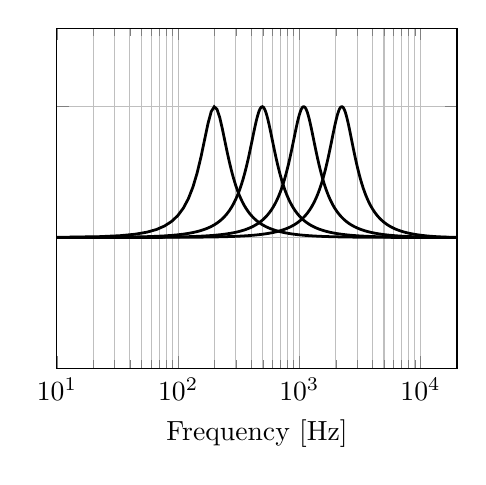
\begin{tikzpicture}

\begin{axis}[%
width=2in,
height=1.7in,
at={(1.011in,0.642in)},
scale only axis,
xmode=log,
xmin=10,
xmax=20000,
xminorticks=true,
xlabel={Frequency [Hz]},
xmajorgrids,
xminorgrids,
ymin=-5,
ymax=8,
yticklabels={\empty},
ymajorgrids,
axis background/.style={fill=white}
]
\addplot [color=black,solid,line width=1.0pt,forget plot]
  table[row sep=crcr]{%
0.159154943091895	1.4864748705184e-06\\
11.1846266392052	0.00737513844192361\\
22.2100983353184	0.0294815501212124\\
33.2355700314317	0.0675313225504031\\
44.2610417275449	0.123634317781192\\
55.2865134236582	0.200952384213408\\
66.3119851197714	0.303917170304987\\
77.3374568158847	0.438506569782773\\
88.362928511998	0.612548458565554\\
99.3884002081112	0.835961617657503\\
110.413871904224	1.12071930471151\\
121.439343600338	1.48008130991461\\
132.464815296451	1.92623336199628\\
143.490286992564	2.46493235949006\\
154.515758688678	3.08550957722384\\
165.541230384791	3.7462077296504\\
176.566702080904	4.36172662243929\\
187.592173777017	4.81284935166351\\
198.617645473131	4.99771488117722\\
209.643117169244	4.89693987585988\\
220.668588865357	4.58128106983772\\
231.69406056147	4.15486620992128\\
242.719532257584	3.70186441590612\\
253.745003953697	3.27126281471635\\
264.77047564981	2.884555631119\\
275.795947345923	2.54725741265527\\
286.821419042037	2.2571751636523\\
297.84689073815	2.0090855856173\\
308.872362434263	1.79705120840128\\
319.897834130376	1.61544120578891\\
330.92330582649	1.45930612685039\\
341.948777522603	1.32445359976593\\
352.974249218716	1.20739827624914\\
363.999720914829	1.10526826922619\\
375.025192610943	1.01570494875465\\
386.050664307056	0.936771096336351\\
397.076136003169	0.866872263595278\\
408.101607699282	0.804691720428332\\
419.127079395396	0.749137619702839\\
430.152551091509	0.699300487495662\\
441.178022787622	0.654419165197214\\
452.203494483736	0.613853550497465\\
463.228966179849	0.577062757200309\\
474.254437875962	0.54358757521705\\
485.279909572075	0.513036338603915\\
496.305381268189	0.485073496505914\\
507.330852964302	0.459410332060952\\
518.356324660415	0.435797393176468\\
529.381796356528	0.414018292316101\\
540.407268052642	0.393884605291539\\
551.432739748755	0.375231655865762\\
562.458211444868	0.357915017300854\\
573.483683140981	0.341807596625436\\
584.509154837095	0.326797194524651\\
595.534626533208	0.31278445505772\\
606.560098229321	0.299681136210731\\
617.585569925434	0.287408645564922\\
628.611041621548	0.275896795903655\\
639.636513317661	0.265082743989549\\
650.661985013774	0.254910082455625\\
661.687456709888	0.24532806016014\\
672.712928406001	0.236290910694224\\
683.738400102114	0.227757272271299\\
694.763871798227	0.219689685067005\\
705.789343494341	0.212054154426791\\
716.814815190454	0.204819770259681\\
727.840286886567	0.19795837450484\\
738.86575858268	0.191444269851152\\
749.891230278794	0.185253963955748\\
760.916701974907	0.179365944296414\\
771.94217367102	0.173760479525422\\
782.967645367133	0.168419443814209\\
793.993117063246	0.16332616118795\\
805.01858875936	0.158465267286923\\
816.044060455473	0.153822586351564\\
827.069532151586	0.149385021539984\\
838.0950038477	0.145140456947928\\
849.120475543813	0.14107766991653\\
860.145947239926	0.13718625241179\\
871.171418936039	0.133456540410557\\
882.196890632153	0.129879550374136\\
893.222362328266	0.126446922001602\\
904.247834024379	0.123150866563498\\
915.273305720492	0.11998412019574\\
926.298777416606	0.116939901619594\\
937.324249112719	0.114011873808018\\
948.349720808832	0.111194109183365\\
959.375192504945	0.108481057976417\\
970.400664201059	0.105867519422777\\
981.426135897172	0.103348615506735\\
992.451607593285	0.100919766996471\\
1003.4770792894	0.0985766715460972\\
1014.50255098551	0.0963152836593947\\
1025.52802268163	0.0941317963378861\\
1036.55349437774	0.092022624251083\\
1047.57896607385	0.0899843882858546\\
1058.60443776996	0.0880139013474122\\
1069.62990946608	0.0861081552949759\\
1080.65538116219	0.0842643089111839\\
1091.6808528583	0.0824796768107408\\
1102.70632455442	0.0807517192052487\\
1113.73179625053	0.0790780324503513\\
1124.75726794664	0.077456340304806\\
1135.78273964276	0.0758844858431402\\
1146.80821133887	0.0743604239648205\\
1157.83368303498	0.0728822144495874\\
1168.8591547311	0.0714480155149511\\
1179.88462642721	0.070056077833723\\
1190.91009812332	0.0687047389741525\\
1201.93556981944	0.0673924182291672\\
1212.96104151555	0.0661176118031763\\
1223.98651321166	0.0648788883290694\\
1235.01198490778	0.063674884688526\\
1246.03745660389	0.0625043021133402\\
1257.0629283	0.061365902546091\\
1268.08839999612	0.0602585052395889\\
1279.11387169223	0.0591809835782555\\
1290.13934338834	0.0581322621049255\\
1301.16481508446	0.0571113137372097\\
1312.19028678057	0.0561171571600469\\
1323.21575847668	0.0551488543827783\\
1334.2412301728	0.0542055084461582\\
1345.26670186891	0.0532862612725597\\
1356.29217356502	0.0523902916459725\\
1367.31764526114	0.0515168133145838\\
1378.34311695725	0.0506650732070006\\
1389.36858865336	0.0498343497545094\\
1400.39406034948	0.0490239513114033\\
1411.41953204559	0.0482332146689303\\
1422.4450037417	0.0474615036531457\\
1433.47047543782	0.0467082078056798\\
1444.49594713393	0.0459727411367098\\
1455.52141883004	0.0452545409508407\\
1466.54689052616	0.0445530667368112\\
1477.57236222227	0.0438677991197196\\
1488.59783391838	0.0431982388706398\\
1499.6233056145	0.0425439059698555\\
1510.64877731061	0.0419043387217982\\
1521.67424900672	0.0412790929159862\\
1532.69972070283	0.040667741034295\\
1543.72519239895	0.0400698714989893\\
1554.75066409506	0.039485087960377\\
1565.77613579117	0.0389130086218391\\
1576.80160748729	0.0383532655995609\\
1587.8270791834	0.0378055043147896\\
1598.85255087951	0.037269382917528\\
1609.87802257563	0.0367445717387124\\
1620.90349427174	0.0362307527701752\\
1631.92896596785	0.0357276191705319\\
1642.95443766397	0.0352348747952364\\
1653.97990936008	0.0347522337496765\\
1665.00538105619	0.0342794199641531\\
1676.03085275231	0.033816166789266\\
1687.05632444842	0.0333622166108006\\
1698.08179614453	0.0329173204827988\\
1709.10726784065	0.0324812377780796\\
1720.13273953676	0.0320537358552335\\
1731.15821123287	0.0316345897409879\\
1742.18368292899	0.0312235818272456\\
1753.2091546251	0.0308205015825579\\
1764.23462632121	0.0304251452757753\\
1775.26009801733	0.0300373157134225\\
1786.28556971344	0.0296568219879099\\
1797.31104140955	0.0292834792378268\\
1808.33651310567	0.028917108418138\\
1819.36198480178	0.0285575360810421\\
1830.38745649789	0.0282045941664486\\
1841.41292819401	0.0278581198013372\\
1852.43839989012	0.0275179551077976\\
1863.46387158623	0.027183947019855\\
1874.48934328235	0.0268559471073087\\
1885.51481497846	0.0265338114078571\\
1896.54028667457	0.0262174002656785\\
1907.56575837069	0.0259065781773772\\
1918.5912300668	0.0256012136437289\\
1929.61670176291	0.0253011790282725\\
1940.64217345903	0.0250063504208996\\
1951.66764515514	0.0247166075080955\\
1962.69311685125	0.0244318334473102\\
1973.71858854737	0.0241519147472413\\
1984.74406024348	0.0238767411527612\\
1995.76953193959	0.0236062055341091\\
2006.79500363571	0.0233402037810085\\
2017.82047533182	0.0230786347003785\\
2028.84594702793	0.0228213999188974\\
2039.87141872404	0.022568403788211\\
2050.89689042016	0.0223195532951132\\
2061.92236211627	0.0220747579741973\\
2072.94783381238	0.0218339298242888\\
2083.9733055085	0.0215969832282923\\
2094.99877720461	0.0213638348753052\\
2106.02424890072	0.0211344036867693\\
2117.04972059684	0.0209086107443233\\
2128.07519229295	0.0206863792212001\\
2139.10066398906	0.0204676343155772\\
2150.12613568518	0.0202523031867493\\
2161.15160738129	0.0200403148935339\\
2172.1770790774	0.0198316003348017\\
2183.20255077352	0.0196260921925107\\
2194.22802246963	0.0194237248763935\\
2205.25349416574	0.0192244344709391\\
2216.27896586186	0.0190281586841272\\
2227.30443755797	0.0188348367979507\\
2238.32990925408	0.0186444096209331\\
2249.3553809502	0.0184568194419486\\
2260.38085264631	0.0182720099861132\\
2271.40632434242	0.0180899263717106\\
2282.43179603854	0.0179105150690511\\
2293.45726773465	0.0177337238604537\\
2304.48273943076	0.0175595018018533\\
2315.50821112688	0.0173877991853938\\
2326.53368282299	0.0172185675036845\\
2337.5591545191	0.0170517594149274\\
2348.58462621522	0.0168873287095057\\
2359.61009791133	0.0167252302773468\\
2370.63556960744	0.0165654200767943\\
2381.66104130356	0.0164078551041528\\
2392.68651299967	0.0162524933644151\\
2403.71198469578	0.0160992938429473\\
2414.7374563919	0.015948216478001\\
2425.76292808801	0.0157992221343269\\
2436.78839978412	0.0156522725772934\\
2447.81387148024	0.0155073304483215\\
2458.83934317635	0.0153643592405938\\
2469.86481487246	0.0152233232759098\\
2480.89028656857	0.015084187682216\\
2491.91575826469	0.0149469183716417\\
2502.9412299608	0.0148114820194434\\
2513.96670165692	0.0146778460435136\\
2524.99217335303	0.0145459785846806\\
2536.01764504914	0.0144158484872787\\
2547.04311674525	0.0142874252807089\\
2558.06858844137	0.0141606791613101\\
2569.09406013748	0.0140355809749292\\
2580.11953183359	0.0139121021998635\\
2591.14500352971	0.0137902149305616\\
2602.17047522582	0.0136698918615692\\
2613.19594692193	0.0135511062720897\\
2624.22141861805	0.0134338320111128\\
2635.24689031416	0.0133180434825501\\
2646.27236201027	0.0132037156315376\\
2657.29783370639	0.0130908239303862\\
2668.3233054025	0.0129793443655169\\
2679.34877709861	0.0128692534244061\\
2690.37424879473	0.0127605280831223\\
2701.39972049084	0.0126531457941739\\
2712.42519218695	0.0125470844746574\\
2723.45066388307	0.0124423224948378\\
2734.47613557918	0.0123388386670247\\
2745.50160727529	0.0122366122346052\\
2756.52707897141	0.012135622861724\\
2767.55255066752	0.0120358506229843\\
2778.57802236363	0.0119372759934777\\
2789.60349405975	0.0118398798391937\\
2800.62896575586	0.0117436434076857\\
2811.65443745197	0.0116485483189001\\
2822.67990914809	0.0115545765562566\\
2833.7053808442	0.011461710458173\\
2844.73085254031	0.0113699327095894\\
2855.75632423643	0.0112792263338728\\
2866.78179593254	0.0111895746848415\\
2877.80726762865	0.0111009614391262\\
2888.83273932477	0.0110133705886333\\
2899.85821102088	0.0109267864332059\\
2910.88368271699	0.0108411935736234\\
2921.90915441311	0.0107565769046454\\
2932.93462610922	0.0106729216082494\\
2943.96009780533	0.0105902131471275\\
2954.98556950145	0.010508437258359\\
2966.01104119756	0.0104275799471126\\
2977.03651289367	0.0103476274806602\\
2988.06198458979	0.0102685663825182\\
2999.0874562859	0.0101903834266768\\
3010.11292798201	0.0101130656320616\\
3021.13839967812	0.0100366002570516\\
3032.16387137424	0.00996097479423795\\
3043.18934307035	0.0098861769652234\\
3054.21481476646	0.00981219471564128\\
3065.24028646258	0.00973901621020997\\
3076.26575815869	0.00966662982802377\\
3087.2912298548	0.00959502415785639\\
3098.31670155092	0.00952418799359881\\
3109.34217324703	0.00945411032993527\\
3120.36764494314	0.00938478035798974\\
3131.39311663926	0.00931618746107199\\
3142.41858833537	0.00924832121062735\\
3153.44406003148	0.00918117136228787\\
3164.4695317276	0.00911472785190384\\
3175.49500342371	0.00904898079178082\\
3186.52047511982	0.00898392046694899\\
3197.54594681594	0.00891953733160532\\
3208.57141851205	0.00885582200551303\\
3219.59689020816	0.00879276527058922\\
3230.62236190428	0.00873035806757319\\
3241.64783360039	0.00866859149271728\\
3252.6733052965	0.00860745679458529\\
3263.69877699262	0.0085469453709873\\
3274.72424868873	0.00848704876581387\\
3285.74972038484	0.00842775866618978\\
3296.77519208096	0.00836906689951561\\
3307.80066377707	0.00831096543062843\\
3318.82613547318	0.00825344635902004\\
3329.8516071693	0.00819650191614725\\
3340.87707886541	0.00814012446281519\\
3351.90255056152	0.00808430648656409\\
3362.92802225764	0.00802904059914637\\
3373.95349395375	0.00797431953412679\\
3384.97896564986	0.00792013614438781\\
3396.00443734598	0.00786648339983715\\
3407.02990904209	0.00781335438511884\\
3418.0553807382	0.00776074229732794\\
3429.08085243432	0.00770864044386757\\
3440.10632413043	0.00765704224025371\\
3451.13179582654	0.00760594120809706\\
3462.15726752266	0.00755533097296906\\
3473.18273921877	0.00750520526245458\\
3484.20821091488	0.0074555579042064\\
3495.23368261099	0.00740638282398789\\
3506.25915430711	0.00735767404381185\\
3517.28462600322	0.00730942568020828\\
3528.31009769933	0.00726163194228003\\
3539.33556939545	0.00721428713006464\\
3550.36104109156	0.00716738563278617\\
3561.38651278767	0.00712092192719552\\
3572.41198448379	0.00707489057592798\\
3583.4374561799	0.00702928622589908\\
3594.46292787601	0.00698410360674469\\
3605.48839957213	0.00693933752931878\\
3616.51387126824	0.00689498288411776\\
3627.53934296435	0.00685103463991675\\
3638.56481466047	0.00680748784225147\\
3649.59028635658	0.00676433761201761\\
3660.61575805269	0.00672157914419918\\
3671.64122974881	0.00667920770634815\\
3682.66670144492	0.00663721863747635\\
3693.69217314103	0.00659560734654068\\
3704.71764483715	0.0065543693113984\\
3715.74311653326	0.00651350007741545\\
3726.76858822937	0.00647299525632903\\
3737.79405992549	0.00643285052504266\\
3748.8195316216	0.00639306162447894\\
3759.84500331771	0.00635362435844377\\
3770.87047501383	0.00631453459248088\\
3781.89594670994	0.00627578825283416\\
3792.92141840605	0.00623738132534826\\
3803.94689010217	0.00619930985442114\\
3814.97236179828	0.00616156994198733\\
3825.99783349439	0.00612415774656095\\
3837.02330519051	0.00608706948215521\\
3848.04877688662	0.00605030141741006\\
3859.07424858273	0.00601384987460405\\
3870.09972027885	0.0059777112287337\\
3881.12519197496	0.00594188190661192\\
3892.15066367107	0.00590635838601085\\
3903.17613536719	0.00587113719474088\\
3914.2016070633	0.00583621490983383\\
3925.22707875941	0.00580158815667586\\
3936.25255045553	0.005767253608229\\
3947.27802215164	0.00573320798419293\\
3958.30349384775	0.00569944805023406\\
3969.32896554387	0.00566597061724743\\
3980.35443723998	0.00563277254049128\\
3991.37990893609	0.00559985071900106\\
4002.4053806322	0.00556720209471622\\
4013.43085232832	0.005534823651871\\
4024.45632402443	0.00550271241622326\\
4035.48179572054	0.00547086545441432\\
4046.50726741666	0.00543927987330955\\
4057.53273911277	0.00540795281925209\\
4068.55821080888	0.00537688147751123\\
4079.583682505	0.00534606307160938\\
4090.60915420111	0.00531549486268555\\
4101.63462589722	0.00528517414891854\\
4112.66009759334	0.00525509826489234\\
4123.68556928945	0.00522526458102503\\
4134.71104098556	0.00519567050299575\\
4145.73651268168	0.00516631347114849\\
4156.76198437779	0.00513719096001152\\
4167.7874560739	0.00510830047764907\\
4178.81292777002	0.00507963956519803\\
4189.83839946613	0.00505120579633135\\
4200.86387116224	0.00502299677671185\\
4211.88934285836	0.00499501014354612\\
4222.91481455447	0.00496724356499969\\
4233.94028625058	0.00493969473979141\\
4244.9657579467	0.00491236139667792\\
4255.99122964281	0.00488524129399015\\
4267.01670133892	0.00485833221916018\\
4278.04217303504	0.00483163198831162\\
4289.06764473115	0.00480513844571511\\
4300.09311642726	0.00477884946349626\\
4311.11858812338	0.00475276294106985\\
4322.14405981949	0.00472687680480152\\
4333.1695315156	0.00470118900759801\\
4344.19500321172	0.00467569752840113\\
4355.22047490783	0.00465040037193604\\
4366.24594660394	0.00462529556821284\\
4377.27141830006	0.00460038117215536\\
4388.29688999617	0.00457565526327804\\
4399.32236169228	0.00455111594525308\\
4410.3478333884	0.00452676134558342\\
4421.37330508451	0.0045025896152141\\
4432.39877678062	0.00447859892821494\\
4443.42424847673	0.00445478748140149\\
4454.44972017285	0.00443115349403691\\
4465.47519186896	0.00440769520743749\\
4476.50066356508	0.00438441088469763\\
4487.52613526119	0.0043612988103474\\
4498.5516069573	0.00433835729003309\\
4509.57707865341	0.00431558465021527\\
4520.60255034953	0.00429297923783391\\
4531.62802204564	0.0042705394200661\\
4542.65349374176	0.00424826358395072\\
4553.67896543787	0.00422615013618852\\
4564.70443713398	0.00420419750276482\\
4575.72990883009	0.00418240412874384\\
4586.75538052621	0.00416076847792987\\
4597.78085222232	0.00413928903266543\\
4608.80632391843	0.00411796429351174\\
4619.83179561455	0.00409679277897357\\
4630.85726731066	0.00407577302529727\\
4641.88273900677	0.00405490358618599\\
4652.90821070289	0.00403418303254563\\
4663.933682399	0.00401360995224051\\
4674.95915409511	0.00399318294986823\\
4685.98462579123	0.00397290064650177\\
4697.01009748734	0.00395276167947601\\
4708.03556918345	0.00393276470214707\\
4719.06104087957	0.00391290838364025\\
4730.08651257568	0.00389319140871159\\
4741.11198427179	0.00387361247742443\\
4752.13745596791	0.00385417030499744\\
4763.16292766402	0.00383486362159298\\
4774.18839936013	0.00381569117206491\\
4785.21387105625	0.00379665171583365\\
4796.23934275236	0.00377774402658382\\
4807.26481444847	0.00375896689214322\\
4818.29028614459	0.0037403191142652\\
4829.3157578407	0.00372179950844406\\
4840.34122953681	0.00370340690368968\\
4851.36670123293	0.00368514014238528\\
4862.39217292904	0.00366699808010645\\
4873.41764462515	0.00364897958538437\\
4884.44311632126	0.00363108353961162\\
4895.46858801738	0.00361330883680533\\
4906.49405971349	0.00359565438344943\\
4917.51953140961	0.0035781190983503\\
4928.54500310572	0.0035607019124404\\
4939.57047480183	0.00354340176862628\\
4950.59594649795	0.00352621762164612\\
4961.62141819406	0.00350914843788112\\
4972.64688989017	0.00349219319521496\\
4983.67236158629	0.00347535088287791\\
4994.6978332824	0.00345862050131217\\
5005.72330497851	0.00344200106198499\\
5016.74877667463	0.00342549158727336\\
5027.77424837074	0.00340909111032534\\
5038.79972006685	0.00339279867489449\\
5049.82519176296	0.00337661333520907\\
5060.85066345908	0.00336053415583526\\
5071.87613515519	0.0033445602115483\\
5082.9016068513	0.00332869058719769\\
5093.92707854742	0.00331292437754738\\
5104.95255024353	0.00329726068720851\\
5115.97802193964	0.00328169863043137\\
5127.00349363576	0.00326623733106127\\
5138.02896533187	0.00325087592236712\\
5149.05443702798	0.00323561354689319\\
5160.0799087241	0.00322044935643418\\
5171.10538042021	0.00320538251180988\\
5182.13085211632	0.00319041218282291\\
5193.15632381244	0.00317553754810849\\
5204.18179550855	0.00316075779503825\\
5215.20726720466	0.00314607211958732\\
5226.23273890078	0.00313147972626125\\
5237.25821059689	0.00311697982795159\\
5248.283682293	0.00310257164584733\\
5259.30915398912	0.0030882544093348\\
5270.33462568523	0.00307402735587251\\
5281.36009738134	0.00305988973092767\\
5292.38556907746	0.00304584078782018\\
5303.41104077357	0.00303187978768225\\
5314.43651246968	0.00301800599931975\\
5325.4619841658	0.00300421869915645\\
5336.48745586191	0.00299051717107215\\
5347.51292755802	0.0029769007063932\\
5358.53839925414	0.00296336860373071\\
5369.56387095025	0.00294992016894011\\
5380.58934264636	0.00293655471499989\\
5391.61481434248	0.00292327156193455\\
5402.64028603859	0.00291007003672797\\
5413.6657577347	0.00289694947325026\\
5424.69122943082	0.00288390921214415\\
5435.71670112693	0.00287094860076143\\
5446.74217282304	0.00285806699309755\\
5457.76764451916	0.00284526374967023\\
5468.79311621527	0.00283253823748104\\
5479.81858791138	0.00281988982990943\\
5490.8440596075	0.0028073179066338\\
5501.86953130361	0.00279482185360077\\
5512.89500299972	0.00278240106287676\\
5523.92047469583	0.00277005493262697\\
5534.94594639195	0.00275778286704405\\
5545.97141808806	0.0027455842762287\\
5556.99688978417	0.00273345857618204\\
5568.02236148029	0.0027214051886804\\
5579.0478331764	0.00270942354125416\\
5590.07330487251	0.00269751306706638\\
5601.09877656863	0.00268567320489557\\
5612.12424826474	0.00267390339904125\\
5623.14971996085	0.00266220309927007\\
5634.17519165697	0.00265057176074457\\
5645.20066335308	0.00263900884395189\\
5656.22613504919	0.0026275138146807\\
5667.25160674531	0.00261608614390374\\
5678.27707844142	0.00260472530774887\\
5689.30255013753	0.00259343078744718\\
5700.32802183365	0.00258220206924624\\
5711.35349352976	0.00257103864437741\\
5722.37896522587	0.00255994000897302\\
5733.40443692199	0.00254890566402785\\
5744.4299086181	0.00253793511535294\\
5755.45538031421	0.00252702787348504\\
5766.48085201033	0.00251618345366545\\
5777.50632370644	0.00250540137576685\\
5788.53179540255	0.00249468116425668\\
5799.55726709867	0.00248402234810469\\
5810.58273879478	0.00247342446081\\
5821.60821049089	0.00246288704026231\\
5832.63368218701	0.00245240962873231\\
5843.65915388312	0.00244199177284482\\
5854.68462557923	0.00243163302348233\\
5865.71009727535	0.002421332935762\\
5876.73556897146	0.002411091069001\\
5887.76104066757	0.00240090698662784\\
5898.78651236369	0.00239078025618437\\
5909.8119840598	0.00238071044924678\\
5920.83745575591	0.002370697141389\\
5931.86292745203	0.00236073991213073\\
5942.88839914814	0.00235083834492782\\
5953.91387084425	0.00234099202708168\\
5964.93934254037	0.00233120054971625\\
5975.96481423648	0.00232146350774328\\
5986.99028593259	0.00231178049982769\\
5998.0157576287	0.00230215112829508\\
6009.04122932482	0.00229257499916649\\
6020.06670102093	0.00228305172206198\\
6031.09217271704	0.00227358091017567\\
6042.11764441316	0.00226416218024684\\
6053.14311610927	0.00225479515250982\\
6064.16858780538	0.0022454794506613\\
6075.1940595015	0.00223621470181981\\
6086.21953119761	0.00222700053648728\\
6097.24500289372	0.00221783658852201\\
6108.27047458984	0.00220872249508284\\
6119.29594628595	0.00219965789661953\\
6130.32141798206	0.00219064243680532\\
6141.34688967818	0.00218167576253502\\
6152.37236137429	0.00217275752386917\\
6163.3978330704	0.00216388737399544\\
6174.42330476652	0.00215506496922683\\
6185.44877646263	0.00214628996893028\\
6196.47424815874	0.00213756203551134\\
6207.49971985486	0.00212888083438331\\
6218.52519155097	0.00212024603393645\\
6229.55066324708	0.00211165730549749\\
6240.5761349432	0.00210311432329886\\
6251.60160663931	0.00209461676446131\\
6262.62707833542	0.00208616430894385\\
6273.65255003154	0.00207775663954184\\
6284.67802172765	0.00206939344182147\\
6295.70349342376	0.00206107440411589\\
6306.72896511988	0.00205279921747711\\
6317.75443681599	0.00204456757567789\\
6328.7799085121	0.00203637917515973\\
6339.80538020822	0.00202823371499821\\
6350.83085190433	0.00202013089689526\\
6361.85632360044	0.00201207042514261\\
6372.88179529656	0.00200405200658899\\
6383.90726699267	0.00199607535063629\\
6394.93273868878	0.00198814016917988\\
6405.9582103849	0.00198024617660855\\
6416.98368208101	0.00197239308976219\\
6428.00915377712	0.00196458062792404\\
6439.03462547323	0.00195680851278604\\
6450.06009716935	0.00194907646841415\\
6461.08556886546	0.00194138422123678\\
6472.11104056157	0.00193373150002747\\
6483.13651225769	0.00192611803585286\\
6494.1619839538	0.00191854356208427\\
6505.18745564992	0.00191100781434953\\
6516.21292734603	0.00190351053052141\\
6527.23839904214	0.00189605145068102\\
6538.26387073826	0.00188863031712168\\
6549.28934243437	0.00188124687429691\\
6560.31481413048	0.00187390086881461\\
6571.34028582659	0.00186659204941784\\
6582.36575752271	0.00185932016695397\\
6593.39122921882	0.0018520849743612\\
6604.41670091493	0.00184488622663968\\
6615.44217261105	0.00183772368084571\\
6626.46764430716	0.00183059709604358\\
6637.49311600327	0.00182350623330943\\
6648.51858769939	0.00181645085572356\\
6659.5440593955	0.00180943072829909\\
6670.56953109161	0.00180244561801671\\
6681.59500278773	0.00179549529377455\\
6692.62047448384	0.00178857952639397\\
6703.64594617995	0.00178169808855597\\
6714.67141787607	0.0017748507548301\\
6725.69688957218	0.00176803730163981\\
6736.72236126829	0.00176125750724313\\
6747.74783296441	0.00175451115168837\\
6758.77330466052	0.00174779801685656\\
6769.79877635663	0.00174111788638626\\
6780.82424805275	0.00173447054568703\\
6791.84971974886	0.00172785578190289\\
6802.87519144497	0.00172127338391804\\
6813.90066314109	0.00171472314232222\\
6824.9261348372	0.00170820484940876\\
6835.95160653331	0.00170171829913027\\
6846.97707822943	0.00169526328711791\\
6858.00254992554	0.00168883961064481\\
6869.02802162165	0.00168244706861446\\
6880.05349331777	0.00167608546154533\\
6891.07896501388	0.00166975459154582\\
6902.10443670999	0.00166345426232387\\
6913.1299084061	0.00165718427913691\\
6924.15538010222	0.00165094444881302\\
6935.18085179833	0.0016447345797124\\
6946.20632349445	0.00163855448171197\\
6957.23179519056	0.00163240396620727\\
6968.25726688667	0.00162628284608938\\
6979.28273858279	0.00162019093571985\\
6990.3082102789	0.00161412805093452\\
7001.33368197501	0.00160809400902433\\
7012.35915367112	0.00160208862871021\\
7023.38462536724	0.00159611173015659\\
7034.41009706335	0.00159016313491551\\
7045.43556875946	0.00158424266595168\\
7056.46104045558	0.00157835014761359\\
7067.48651215169	0.00157248540562385\\
7078.5119838478	0.00156664826706574\\
7089.53745554392	0.00156083856035809\\
7100.56292724003	0.00155505611527272\\
7111.58839893614	0.00154930076289969\\
7122.61387063226	0.0015435723356126\\
7133.63934232837	0.0015378706671207\\
7144.66481402448	0.00153219559240137\\
7155.6902857206	0.00152654694768665\\
7166.71575741671	0.00152092457050762\\
7177.74122911282	0.00151532829962878\\
7188.76670080894	0.00150975797503657\\
7199.79217250505	0.00150421343797597\\
7210.81764420116	0.00149869453088494\\
7221.84311589728	0.0014932010974099\\
7232.86858759339	0.0014877329823941\\
7243.8940592895	0.00148229003187963\\
7254.91953098562	0.0014768720930476\\
7265.94500268173	0.00147147901426059\\
7276.97047437784	0.00146611064503566\\
7287.99594607396	0.00146076683602507\\
7299.02141777007	0.00145544743899893\\
7310.04688946618	0.0014501523068703\\
7321.0723611623	0.00144488129364309\\
7332.09783285841	0.00143963425443139\\
7343.12330455452	0.00143441104542862\\
7354.14877625063	0.00142921152392292\\
7365.17424794675	0.00142403554825672\\
7376.19971964286	0.00141888297784215\\
7387.22519133898	0.0014137536731456\\
7398.25066303509	0.00140864749566271\\
7409.2761347312	0.00140356430793372\\
7420.30160642732	0.0013985039735108\\
7431.32707812343	0.00139346635697339\\
7442.35254981954	0.00138845132390128\\
7453.37802151566	0.00138345874085141\\
7464.40349321177	0.00137848847540036\\
7475.42896490788	0.00137354039607683\\
7486.45443660399	0.0013686143723983\\
7497.47990830011	0.00136371027482282\\
7508.50537999622	0.00135882797477987\\
7519.53085169233	0.00135396734463757\\
7530.55632338845	0.00134912825769115\\
7541.58179508456	0.00134431058817065\\
7552.60726678067	0.00133951421123512\\
7563.63273847679	0.00133473900293796\\
7574.6582101729	0.00132998484024616\\
7585.68368186901	0.00132525160101914\\
7596.70915356513	0.00132053916400679\\
7607.73462526124	0.00131584740883986\\
7618.76009695735	0.00131117621601451\\
7629.78556865347	0.00130652546689429\\
7640.81104034958	0.00130189504371009\\
7651.83651204569	0.00129728482953124\\
7662.86198374181	0.00129269470827327\\
7673.88745543792	0.00128812456468819\\
7684.91292713403	0.00128357428435686\\
7695.93839883015	0.00127904375367738\\
7706.96387052626	0.00127453285986705\\
7717.98934222237	0.00127004149094498\\
7729.01481391849	0.00126556953573022\\
7740.0402856146	0.00126111688384172\\
7751.06575731071	0.0012566834256752\\
7762.09122900683	0.00125226905242247\\
7773.11670070294	0.00124787365602705\\
7784.14217239905	0.0012434971292131\\
7795.16764409517	0.00123913936545846\\
7806.19311579128	0.00123480025900039\\
7817.21858748739	0.00123047970481826\\
7828.24405918351	0.00122617759863548\\
7839.26953087962	0.00122189383690596\\
7850.29500257573	0.00121762831681802\\
7861.32047427185	0.00121338093627511\\
7872.34594596796	0.00120915159390349\\
7883.37141766407	0.0012049401890349\\
7894.39688936019	0.00120074662171043\\
7905.4223610563	0.0011965707926593\\
7916.44783275241	0.00119241260331428\\
7927.47330444853	0.00118827195578859\\
7938.49877614464	0.00118414875288163\\
7949.52424784075	0.00118004289805977\\
7960.54971953686	0.00117595429546594\\
7971.57519123298	0.00117188284990807\\
7982.60066292909	0.00116782846684372\\
7993.6261346252	0.00116379105239156\\
8004.65160632132	0.00115977051331604\\
8015.67707801743	0.00115576675702155\\
8026.70254971355	0.00115177969155437\\
8037.72802140966	0.00114780922559688\\
8048.75349310577	0.00114385526843095\\
8059.77896480189	0.00113991772999962\\
8070.804436498	0.00113599652082996\\
8081.82990819411	0.00113209155208133\\
8092.85537989022	0.00112820273550872\\
8103.88085158634	0.00112432998347043\\
8114.90632328245	0.00112047320891464\\
8125.93179497856	0.00111663232539671\\
8136.95726667468	0.00111280724704838\\
8147.98273837079	0.00110899788857964\\
8159.0082100669	0.00110520416529036\\
8170.03368176302	0.00110142599303943\\
8181.05915345913	0.00109766328826399\\
8192.08462515524	0.00109391596795639\\
8203.11009685136	0.00109018394967952\\
8214.13556854747	0.00108646715153409\\
8225.16104024358	0.00108276549218369\\
8236.1865119397	0.00107907889082971\\
8247.21198363581	0.00107540726722102\\
8258.23745533192	0.00107175054163849\\
8269.26292702804	0.00106810863490274\\
8280.28839872415	0.00106448146834716\\
8291.31387042026	0.00106086896383909\\
8302.33934211638	0.00105727104377404\\
8313.36481381249	0.00105368763104296\\
8324.3902855086	0.00105011864907074\\
8335.41575720472	0.00104656402176996\\
8346.44122890083	0.001043023673566\\
8357.46670059694	0.00103949752938926\\
8368.49217229306	0.00103598551465013\\
8379.51764398917	0.00103248755526794\\
8390.54311568528	0.00102900357763425\\
8401.56858738139	0.00102553350863417\\
8412.59405907751	0.00102207727563082\\
8423.61953077362	0.00101863480646157\\
8434.64500246974	0.00101520602943412\\
8445.67047416585	0.00101179087333621\\
8456.69594586196	0.00100838926740661\\
8467.72141755808	0.00100500114135641\\
8478.74688925419	0.00100162642533813\\
8489.7723609503	0.000998265049988151\\
8500.79783264642	0.000994916946365027\\
8511.82330434253	0.000991582045982242\\
8522.84877603864	0.000988260280808228\\
8533.87424773476	0.000984951583245155\\
8544.89971943087	0.00098165588612121\\
8555.92519112698	0.000978373122715679\\
8566.9506628231	0.000975103226726156\\
8577.97613451921	0.00097184613228205\\
8589.00160621532	0.000968601773933017\\
8600.02707791143	0.000965370086654739\\
8611.05254960755	0.000962151005837364\\
8622.07802130366	0.000958944467279718\\
8633.10349299977	0.00095575040719895\\
8644.12896469589	0.000952568762217034\\
8655.154436392	0.000949399469354986\\
8666.17990808811	0.000946242466046364\\
8677.20537978423	0.000943097690112199\\
8688.23085148034	0.0009399650797745\\
8699.25632317645	0.000936844573650464\\
8710.28179487257	0.000933736110737056\\
8721.30726656868	0.000930639630428362\\
8732.33273826479	0.000927555072490523\\
8743.35820996091	0.000924482377077163\\
8754.38368165702	0.000921421484721678\\
8765.40915335313	0.000918372336325665\\
8776.43462504925	0.000915334873168569\\
8787.46009674536	0.000912309036899965\\
8798.48556844147	0.000909294769524138\\
8809.51104013759	0.000906292013419366\\
8820.5365118337	0.000903300711326349\\
8831.56198352981	0.00090032080633857\\
8842.58745522593	0.000897352241898442\\
8853.61292692204	0.000894394961820446\\
8864.63839861815	0.000891448910252566\\
8875.66387031427	0.00088851403169943\\
8886.68934201038	0.000885590270999173\\
8897.71481370649	0.000882677573350433\\
8908.74028540261	0.000879775884275715\\
8919.76575709872	0.000876885149642602\\
8930.79122879483	0.000874005315646403\\
8941.81670049095	0.000871136328827508\\
8952.84217218706	0.000868278136040535\\
8963.86764388317	0.000865430684483258\\
8974.89311557929	0.00086259392167154\\
8985.9185872754	0.000859767795435474\\
8996.94405897151	0.00085695225393674\\
9007.96953066763	0.000854147245653184\\
9018.99500236374	0.000851352719378813\\
9030.02047405985	0.000848568624212228\\
9041.04594575596	0.000845794909577839\\
9052.07141745208	0.000843031525189223\\
9063.09688914819	0.000840278421087696\\
9074.1223608443	0.000837535547607601\\
9085.14783254042	0.000834802855376311\\
9096.17330423653	0.000832080295341225\\
9107.19877593265	0.000829367818736988\\
9118.22424762876	0.000826665377093205\\
9129.24971932487	0.000823972922224799\\
9140.27519102098	0.000821290406257084\\
9151.3006627171	0.00081861778159298\\
9162.32613441321	0.000815955000924585\\
9173.35160610933	0.000813302017217749\\
9184.37707780544	0.000810658783742932\\
9195.40254950155	0.000808025254036631\\
9206.42802119766	0.000805401381911028\\
9217.45349289378	0.000802787121469418\\
9228.47896458989	0.000800182427083063\\
9239.504436286	0.000797587253387344\\
9250.52990798212	0.00079500155530104\\
9261.55537967823	0.00079242528800705\\
9272.58085137434	0.000789858406954316\\
9283.60632307046	0.000787300867859756\\
9294.63179476657	0.000784752626698624\\
9305.65726646268	0.000782213639716078\\
9316.6827381588	0.000779683863405969\\
9327.70820985491	0.000777163254532058\\
9338.73368155102	0.000774651770101013\\
9349.75915324714	0.000772149367383627\\
9360.78462494325	0.000769656003895531\\
9371.81009663936	0.000767171637414554\\
9382.83556833548	0.000764696225949868\\
9393.86104003159	0.000762229727772842\\
9404.8865117277	0.000759772101393901\\
9415.91198342382	0.00075732330556446\\
9426.93745511993	0.000754883299282704\\
9437.96292681604	0.00075245204178588\\
9448.98839851216	0.000750029492548363\\
9460.01387020827	0.000747615611279737\\
9471.03934190438	0.00074521035792286\\
9482.06481360049	0.000742813692669294\\
9493.09028529661	0.000740425575918811\\
9504.11575699272	0.000738045968317958\\
9515.14122868884	0.00073567483073885\\
9526.16670038495	0.000733312124281096\\
9537.19217208106	0.000730957810262157\\
9548.21764377718	0.000728611850232774\\
9559.24311547329	0.000726274205959616\\
9570.2685871694	0.000723944839434921\\
9581.29405886551	0.000721623712868779\\
9592.31953056163	0.000719310788685283\\
9603.34500225774	0.000717006029526379\\
9614.37047395386	0.000714709398259588\\
9625.39594564997	0.000712420857947144\\
9636.42141734608	0.000710140371876856\\
9647.44688904219	0.000707867903537033\\
9658.47236073831	0.000705603416635774\\
9669.49783243442	0.000703346875089397\\
9680.52330413053	0.000701098242999294\\
9691.54877582665	0.000698857484694363\\
9702.57424752276	0.000696624564700151\\
9713.59971921887	0.000694399447738852\\
9724.62519091499	0.000692182098740883\\
9735.6506626111	0.000689972482829454\\
9746.67613430721	0.000687770565328283\\
9757.70160600333	0.000685576311757739\\
9768.72707769944	0.000683389687834843\\
9779.75254939555	0.000681210659465557\\
9790.77802109167	0.00067903919275635\\
9801.80349278778	0.00067687525399299\\
9812.82896448389	0.000674718809665613\\
9823.85443618001	0.000672569826441725\\
9834.87990787612	0.000670428271177773\\
9845.90537957223	0.000668294110923003\\
9856.93085126835	0.000666167312904032\\
9867.95632296446	0.000664047844538349\\
9878.98179466057	0.000661935673416958\\
9890.00726635669	0.000659830767317878\\
9901.0327380528	0.000657733094202287\\
9912.05820974891	0.000655642622199095\\
9923.08368144502	0.000653559319624227\\
9934.10915314114	0.000651483154972914\\
9945.13462483725	0.000649414096900402\\
9956.16009653337	0.000647352114252816\\
9967.18556822948	0.000645297176038226\\
9978.21103992559	0.000643249251440152\\
9989.23651162171	0.000641208309813706\\
10000.2619833178	0.00063917432068366\\
10011.2874550139	0.000637147253742526\\
10022.31292671	0.000635127078844763\\
10033.3383984062	0.000633113766020281\\
10044.3638701023	0.000631107285460941\\
10055.3893417984	0.000629107607516701\\
10066.4148134945	0.000627114702705253\\
10077.4402851906	0.0006251285417101\\
10088.4657568867	0.000623149095367055\\
10099.4912285828	0.000621176334677743\\
10110.516700279	0.000619210230801882\\
10121.5421719751	0.000617250755045719\\
10132.5676436712	0.00061529787889674\\
10143.5931153673	0.0006133515739716\\
10154.6185870634	0.000611411812062409\\
10165.6440587595	0.000609478565098164\\
10176.6695304556	0.000607551805169814\\
10187.6950021517	0.000605631504514839\\
10198.7204738479	0.000603717635526891\\
10209.745945544	0.000601810170748078\\
10220.7714172401	0.000599909082867036\\
10231.7968889362	0.000598014344718933\\
10242.8223606323	0.000596125929287395\\
10253.8478323284	0.000594243809704506\\
10264.8733040245	0.000592367959243097\\
10275.8987757206	0.000590498351322528\\
10286.9242474168	0.000588634959497121\\
10297.9497191129	0.000586777757481227\\
10308.975190809	0.000584926719110662\\
10320.0006625051	0.000583081818373558\\
10331.0261342012	0.000581243029393008\\
10342.0516058973	0.000579410326432853\\
10353.0770775934	0.00057758368388804\\
10364.1025492896	0.000575763076303907\\
10375.1280209857	0.000573948478347254\\
10386.1534926818	0.00057213986482756\\
10397.1789643779	0.00057033721068348\\
10408.204436074	0.00056854049099442\\
10419.2299077701	0.000566749680965108\\
10430.2553794662	0.000564964755935235\\
10441.2808511623	0.000563185691373672\\
10452.3063228585	0.000561412462880397\\
10463.3317945546	0.000559645046186499\\
10474.3572662507	0.000557883417142603\\
10485.3827379468	0.000556127551736226\\
10496.4082096429	0.000554377426084071\\
10507.433681339	0.00055263301641466\\
10518.4591530351	0.000550894299093414\\
10529.4846247313	0.000549161250607219\\
10540.5100964274	0.000547433847564431\\
10551.5355681235	0.000545712066702587\\
10562.5610398196	0.000543995884867191\\
10573.5865115157	0.000542285279040647\\
10584.6119832118	0.000540580226317182\\
10595.6374549079	0.000538880703910566\\
10606.662926604	0.000537186689161822\\
10617.6883983002	0.000535498159516086\\
10628.7138699963	0.000533815092549609\\
10639.7393416924	0.000532137465946609\\
10650.7648133885	0.000530465257510848\\
10661.7902850846	0.000528798445161772\\
10672.8157567807	0.000527137006932583\\
10683.8412284768	0.000525480920966385\\
10694.866700173	0.000523830165531609\\
10705.8921718691	0.000522184718993087\\
10716.9176435652	0.000520544559840979\\
10727.9431152613	0.000518909666663776\\
10738.9685869574	0.00051728001817144\\
10749.9940586535	0.000515655593181907\\
10761.0195303496	0.000514036370615299\\
10772.0450020457	0.000512422329509356\\
10783.0704737419	0.000510813449002074\\
10794.095945438	0.000509209708343283\\
10805.1214171341	0.000507611086883072\\
10816.1468888302	0.000506017564085287\\
10827.1723605263	0.000504429119515967\\
10838.1978322224	0.000502845732839479\\
10849.2233039185	0.000501267383833954\\
10860.2487756147	0.000499694052375851\\
10871.2742473108	0.000498125718441894\\
10882.2997190069	0.000496562362114852\\
10893.325190703	0.000495003963575826\\
10904.3506623991	0.000493450503113894\\
10915.3761340952	0.000491901961106826\\
10926.4016057913	0.000490358318034579\\
10937.4270774874	0.000488819554485089\\
10948.4525491836	0.000487285651136912\\
10959.4780208797	0.000485756588765008\\
10970.5034925758	0.000484232348250385\\
10981.5289642719	0.000482712910556959\\
10992.554435968	0.000481198256754695\\
11003.5799076641	0.000479688368009961\\
11014.6053793602	0.000478183225577821\\
11025.6308510564	0.000476682810805888\\
11036.6563227525	0.00047518710514975\\
11047.6817944486	0.000473696090140191\\
11058.7072661447	0.000472209747410188\\
11069.7327378408	0.00047072805868141\\
11080.7582095369	0.000469251005770004\\
11091.783681233	0.000467778570584671\\
11102.8091529291	0.000466310735117016\\
11113.8346246253	0.000464847481456983\\
11124.8600963214	0.000463388791769711\\
11135.8855680175	0.00046193464833603\\
11146.9110397136	0.000460485033490754\\
11157.9365114097	0.000459039929684388\\
11168.9619831058	0.000457599319440706\\
11179.9874548019	0.000456163185374103\\
11191.0129264981	0.000454731510185742\\
11202.0383981942	0.000453304276657768\\
11213.0638698903	0.000451881467664876\\
11224.0893415864	0.000450463066162743\\
11235.1148132825	0.0004490490551861\\
11246.1402849786	0.000447639417858374\\
11257.1657566747	0.000446234137391686\\
11268.1912283708	0.000444833197071426\\
11279.216700067	0.000443436580269753\\
11290.2421717631	0.000442044270437876\\
11301.2676434592	0.000440656251119562\\
11312.2931151553	0.000439272505920272\\
11323.3185868514	0.000437893018532236\\
11334.3440585475	0.000436517772740239\\
11345.3695302436	0.00043514675239462\\
11356.3950019397	0.000433779941428629\\
11367.4204736359	0.0004324173238565\\
11378.445945332	0.000431058883767665\\
11389.4714170281	0.000429704605326752\\
11400.4968887242	0.000428354472777447\\
11411.5223604203	0.000427008470450202\\
11422.5478321164	0.000425666582731384\\
11433.5733038125	0.000424328794105701\\
11444.5987755087	0.000422995089113774\\
11455.6242472048	0.000421665452377206\\
11466.6497189009	0.000420339868606302\\
11477.675190597	0.000419018322555707\\
11488.7006622931	0.000417700799086121\\
11499.7261339892	0.000416387283108374\\
11510.7516056853	0.000415077759612352\\
11521.7770773814	0.000413772213666997\\
11532.8025490776	0.000412470630410664\\
11543.8280207737	0.000411172995047267\\
11554.8534924698	0.000409879292853988\\
11565.8789641659	0.000408589509185141\\
11576.904435862	0.000407303629450952\\
11587.9299075581	0.000406021639152276\\
11598.9553792542	0.00040474352383624\\
11609.9808509504	0.000403469269136744\\
11621.0063226465	0.000402198860760957\\
11632.0317943426	0.000400932284458466\\
11643.0572660387	0.000399669526069485\\
11654.0827377348	0.000398410571490145\\
11665.1082094309	0.000397155406697561\\
11676.133681127	0.000395904017715124\\
11687.1591528231	0.000394656390652995\\
11698.1846245193	0.000393412511673393\\
11709.2100962154	0.000392172367011812\\
11720.2355679115	0.00039093594296159\\
11731.2610396076	0.000389703225895122\\
11742.2865113037	0.000388474202229149\\
11753.3119829998	0.000387248858469112\\
11764.3374546959	0.000386027181155157\\
11775.3629263921	0.00038480915691613\\
11786.3883980882	0.000383594772429079\\
11797.4138697843	0.000382384014444325\\
11808.4393414804	0.000381176869764251\\
11819.4648131765	0.000379973325270298\\
11830.4902848726	0.000378773367874751\\
11841.5157565687	0.000377576984588243\\
11852.5412282648	0.000376384162456108\\
11863.566699961	0.00037519488858924\\
11874.5921716571	0.000374009150171809\\
11885.6176433532	0.000372826934434257\\
11896.6431150493	0.000371648228672587\\
11907.6685867454	0.000370473020238721\\
11918.6940584415	0.000369301296544355\\
11929.7195301376	0.000368133045062886\\
11940.7450018337	0.000366968253329417\\
11951.7704735299	0.000365806908931111\\
11962.795945226	0.000364648999503335\\
11973.8214169221	0.000363494512764373\\
11984.8468886182	0.000362343436465285\\
11995.8723603143	0.000361195758422691\\
12006.8978320104	0.000360051466520703\\
12017.9233037065	0.000358910548680062\\
12028.9487754027	0.000357772992890931\\
12039.9742470988	0.000356638787191675\\
12050.9997187949	0.000355507919686221\\
12062.025190491	0.0003543803785132\\
12073.0506621871	0.000353256151892234\\
12084.0761338832	0.000352135228081507\\
12095.1016055793	0.000351017595393192\\
12106.1270772755	0.000349903242193453\\
12117.1525489716	0.000348792156912086\\
12128.1780206677	0.000347684328017452\\
12139.2034923638	0.000346579744039615\\
12150.2289640599	0.000345478393560701\\
12161.254435756	0.000344380265216826\\
12172.2799074521	0.000343285347690386\\
12183.3053791482	0.000342193629713906\\
12194.3308508444	0.000341105100081621\\
12205.3563225405	0.000340019747635967\\
12216.3817942366	0.000338937561261804\\
12227.4072659327	0.000337858529899908\\
12238.4327376288	0.000336782642546976\\
12249.4582093249	0.000335709888240199\\
12260.483681021	0.000334640256076541\\
12271.5091527171	0.00033357373519346\\
12282.5346244133	0.000332510314786262\\
12293.5600961094	0.000331449984086889\\
12304.5855678055	0.000330392732387057\\
12315.6110395016	0.00032933854902862\\
12326.6365111977	0.000328287423390065\\
12337.6619828938	0.000327239344911585\\
12348.6874545899	0.000326194303064224\\
12359.7129262861	0.000325152287386516\\
12370.7383979822	0.000324113287447844\\
12381.7638696783	0.000323077292875443\\
12392.7893413744	0.000322044293335108\\
12403.8148130705	0.000321014278546629\\
12414.8402847666	0.000319987238266431\\
12425.8657564627	0.000318963162308786\\
12436.8912281588	0.000317942040522676\\
12447.916699855	0.000316923862813003\\
12458.9421715511	0.000315908619123231\\
12469.9676432472	0.000314896299433463\\
12480.9931149433	0.000313886893795149\\
12492.0185866394	0.000312880392279019\\
12503.0440583355	0.000311876785004008\\
12514.0695300316	0.000310876062146905\\
12525.0950017278	0.000309878213917274\\
12536.1204734239	0.000308883230561316\\
12547.14594512	0.000307891102386939\\
12558.1714168161	0.000306901819729046\\
12569.1968885122	0.000305915372978458\\
12580.2223602083	0.000304931752566493\\
12591.2478319044	0.000303950948949532\\
12602.2733036005	0.000302972952655305\\
12613.2987752967	0.00030199775422311\\
12624.3242469928	0.000301025344257808\\
12635.3497186889	0.000300055713397038\\
12646.375190385	0.000299088852315078\\
12657.4006620811	0.000298124751738269\\
12668.4261337772	0.000297163402425732\\
12679.4516054733	0.000296204795179011\\
12690.4770771695	0.000295248920838213\\
12701.5025488656	0.000294295770291655\\
12712.5280205617	0.000293345334458505\\
12723.5534922578	0.000292397604308067\\
12734.5789639539	0.000291452570832781\\
12745.60443565	0.000290510225077154\\
12756.6299073461	0.000289570558131972\\
12767.6553790422	0.000288633561109228\\
12778.6808507384	0.000287699225171055\\
12789.7063224345	0.000286767541520078\\
12800.7317941306	0.000285838501385916\\
12811.7572658267	0.000284912096046397\\
12822.7827375228	0.000283988316819844\\
12833.8082092189	0.000283067155049645\\
12844.833680915	0.000282148602127397\\
12855.8591526112	0.000281232649481333\\
12866.8846243073	0.000280319288578254\\
12877.9100960034	0.000279408510911955\\
12888.9355676995	0.000278500308026366\\
12899.9610393956	0.000277594671492414\\
12910.9865110917	0.000276691592917664\\
12922.0119827878	0.000275791063959816\\
12933.0374544839	0.000274893076299711\\
12944.0629261801	0.000273997621649037\\
12955.0883978762	0.000273104691777339\\
12966.1138695723	0.000272214278463797\\
12977.1393412684	0.000271326373541587\\
12988.1648129645	0.000270440968872806\\
12999.1902846606	0.000269558056354264\\
13010.2157563567	0.000268677627919406\\
13021.2412280529	0.000267799675530601\\
13032.266699749	0.000266924191194572\\
13043.2921714451	0.000266051166948892\\
13054.3176431412	0.000265180594854274\\
13065.3431148373	0.000264312467027353\\
13076.3685865334	0.000263446775600188\\
13087.3940582295	0.000262583512745335\\
13098.4195299256	0.000261722670670057\\
13109.4450016218	0.000260864241610544\\
13120.4704733179	0.000260008217847335\\
13131.495945014	0.000259154591674467\\
13142.5214167101	0.000258303355436114\\
13153.5468884062	0.000257454501503447\\
13164.5723601023	0.000256608022280415\\
13175.5978317984	0.000255763910201824\\
13186.6233034945	0.000254922157735258\\
13197.6487751907	0.000254082757388798\\
13208.6742468868	0.00025324570168402\\
13219.6997185829	0.000252410983186853\\
13230.725190279	0.000251578594501794\\
13241.7506619751	0.000250748528248763\\
13252.7761336712	0.000249920777086248\\
13263.8016053673	0.000249095333707447\\
13274.8270770635	0.000248272190828696\\
13285.8525487596	0.000247451341206827\\
13296.8780204557	0.000246632777619884\\
13307.9034921518	0.000245816492882548\\
13318.9289638479	0.000245002479838424\\
13329.954435544	0.000244190731358115\\
13340.9799072401	0.000243381240348861\\
13352.0053789363	0.000242573999741041\\
13363.0308506324	0.000241769002499747\\
13374.0563223285	0.000240966241615136\\
13385.0817940246	0.000240165710114004\\
13396.1072657207	0.000239367401046286\\
13407.1327374168	0.000238571307490844\\
13418.1582091129	0.000237777422563176\\
13429.183680809	0.000236985739398065\\
13440.2091525052	0.000236196251159216\\
13451.2346242013	0.000235408951050832\\
13462.2600958974	0.000234623832294469\\
13473.2855675935	0.000233840888146394\\
13484.3110392896	0.000233060111882155\\
13495.3365109857	0.000232281496819728\\
13506.3619826818	0.000231505036286724\\
13517.3874543779	0.00023073072365511\\
13528.4129260741	0.000229958552319994\\
13539.4383977702	0.000229188515697691\\
13550.4638694663	0.000228420607235372\\
13561.4893411624	0.000227654820414919\\
13572.5148128585	0.000226891148733638\\
13583.5402845546	0.000226129585721619\\
13594.5657562507	0.000225370124937876\\
13605.5912279469	0.000224612759962634\\
13616.616699643	0.000223857484406972\\
13627.6421713391	0.000223104291905109\\
13638.6676430352	0.000222353176127903\\
13649.6931147313	0.000221604130755852\\
13660.7185864274	0.000220857149508023\\
13671.7440581235	0.000220112226132406\\
13682.7695298196	0.000219369354380848\\
13693.7950015158	0.000218628528057262\\
13704.8204732119	0.000217889740975202\\
13715.845944908	0.000217152986984862\\
13726.8714166041	0.000216418259949932\\
13737.8968883002	0.000215685553766884\\
13748.9223599963	0.000214954862359189\\
13759.9478316924	0.000214226179661886\\
13770.9733033886	0.000213499499660152\\
13781.9987750847	0.000212774816335306\\
13793.0242467808	0.000212052123709164\\
13804.0497184769	0.000211331415834395\\
13815.075190173	0.000210612686773309\\
13826.1006618691	0.000209895930611355\\
13837.1261335652	0.000209181141480267\\
13848.1516052613	0.000208468313509844\\
13859.1770769575	0.000207757440868457\\
13870.2025486536	0.000207048517745687\\
13881.2280203497	0.000206341538358112\\
13892.2534920458	0.00020563649693388\\
13903.2789637419	0.00020493338773585\\
13914.304435438	0.000204232205050021\\
13925.3299071341	0.000203532943181674\\
13936.3553788303	0.000202835596461161\\
13947.3808505264	0.000202140159238115\\
13958.4063222225	0.000201446625894954\\
13969.4317939186	0.000200754990823734\\
13980.4572656147	0.000200065248451225\\
13991.4827373108	0.00019937739322155\\
14002.5082090069	0.000198691419596187\\
14013.533680703	0.000198007322065541\\
14024.5591523992	0.000197325095147014\\
14035.5846240953	0.000196644733373433\\
14046.6100957914	0.00019596623129498\\
14057.6355674875	0.000195289583496551\\
14068.6610391836	0.00019461478457268\\
14079.6865108797	0.000193941829148757\\
14090.7119825758	0.000193270711873311\\
14101.7374542719	0.000192601427402584\\
14112.7629259681	0.000191933970425603\\
14123.7883976642	0.000191268335652604\\
14134.8138693603	0.000190604517816965\\
14145.8393410564	0.000189942511659775\\
14156.8648127525	0.000189282311962623\\
14167.8902844486	0.000188623913514808\\
14178.9157561447	0.000187967311130699\\
14189.9412278409	0.000187312499647804\\
14200.966699537	0.000186659473917131\\
14211.9921712331	0.000186008228814757\\
14223.0176429292	0.000185358759247613\\
14234.0431146253	0.000184711060122627\\
14245.0685863214	0.000184065126381442\\
14256.0940580175	0.000183420952983053\\
14267.1195297136	0.000182778534903812\\
14278.1450014098	0.000182137867143212\\
14289.1704731059	0.000181498944720026\\
14300.195944802	0.000180861762674245\\
14311.2214164981	0.000180226316059352\\
14322.2468881942	0.00017959259995969\\
14333.2723598903	0.000178960609471169\\
14344.2978315864	0.000178330339705126\\
14355.3233032826	0.000177701785805681\\
14366.3487749787	0.000177074942926596\\
14377.3742466748	0.000176449806240916\\
14388.3997183709	0.000175826370948684\\
14399.425190067	0.000175204632259585\\
14410.4506617631	0.000174584585406444\\
14421.4761334592	0.000173966225643299\\
14432.5016051553	0.000173349548239613\\
14443.5270768515	0.000172734548487992\\
14454.5525485476	0.000172121221688753\\
14465.5780202437	0.00017150956317307\\
14476.6034919398	0.00017089956828947\\
14487.6289636359	0.00017029123239998\\
14498.654435332	0.000169684550883982\\
14509.6799070281	0.000169079519143998\\
14520.7053787243	0.000168476132603764\\
14531.7308504204	0.000167874386688941\\
14542.7563221165	0.000167274276861833\\
14553.7817938126	0.000166675798594384\\
14564.8072655087	0.000166078947375894\\
14575.8327372048	0.000165483718720732\\
14586.8582089009	0.000164890108145194\\
14597.883680597	0.000164298111198361\\
14608.9091522932	0.000163707723446668\\
14619.9346239893	0.000163118940462335\\
14630.9600956854	0.000162531757842652\\
14641.9855673815	0.000161946171200334\\
14653.0110390776	0.000161362176173168\\
14664.0365107737	0.000160779768402797\\
14675.0619824698	0.00016019894355593\\
14686.087454166	0.000159619697314708\\
14697.1129258621	0.000159042025378624\\
14708.1383975582	0.000158465923470313\\
14719.1638692543	0.000157891387312409\\
14730.1893409504	0.00015731841266033\\
14741.2148126465	0.000156746995275278\\
14752.2402843426	0.00015617713095124\\
14763.2657560387	0.000155608815476414\\
14774.2912277349	0.000155042044675641\\
14785.316699431	0.000154476814369903\\
14796.3421711271	0.000153913120416823\\
14807.3676428232	0.000153350958681736\\
14818.3931145193	0.000152790325041549\\
14829.4185862154	0.000152231215396309\\
14840.4440579115	0.000151673625657633\\
14851.4695296077	0.000151117551754495\\
14862.4950013038	0.000150562989633222\\
14873.5204729999	0.000150009935253642\\
14884.545944696	0.000149458384594868\\
14895.5714163921	0.000148908333643722\\
14906.5968880882	0.000148359778410172\\
14917.6223597843	0.000147812714921539\\
14928.6478314804	0.000147267139210929\\
14939.6733031766	0.000146723047340375\\
14950.6987748727	0.000146180435369981\\
14961.7242465688	0.000145639299390706\\
14972.7497182649	0.000145099635501222\\
14983.775189961	0.000144561439817557\\
14994.8006616571	0.000144024708469238\\
15005.8261333532	0.000143489437601219\\
15016.8516050494	0.00014295562337388\\
15027.8770767455	0.000142423261961103\\
15038.9025484416	0.000141892349559908\\
15049.9280201377	0.000141362882365387\\
15060.9534918338	0.000140834856601559\\
15071.9789635299	0.000140308268505942\\
15083.004435226	0.000139783114321839\\
15094.0299069221	0.000139259390309907\\
15105.0553786183	0.000138737092761661\\
15116.0808503144	0.000138216217951255\\
15127.1063220105	0.000137696762201061\\
15138.1317937066	0.000137178721818015\\
15149.1572654027	0.0001366620931457\\
15160.1827370988	0.000136146872531552\\
15171.2082087949	0.000135633056336506\\
15182.2336804911	0.000135120640938854\\
15193.2591521872	0.000134609622728458\\
15204.2846238833	0.000134099998114465\\
15215.3100955794	0.000133591763509877\\
15226.3355672755	0.000133084915352766\\
15237.3610389716	0.000132579450083133\\
15248.3865106677	0.000132075364166048\\
15259.4119823638	0.000131572654074296\\
15270.43745406	0.000131071316296086\\
15281.4629257561	0.000130571347329274\\
15292.4883974522	0.000130072743690995\\
15303.5138691483	0.000129575501906101\\
15314.5393408444	0.000129079618516799\\
15325.5648125405	0.000128585090074938\\
15336.5902842366	0.000128091913153579\\
15347.6157559327	0.000127600084321926\\
15358.6412276289	0.000127109600191611\\
15369.666699325	0.00012662045735305\\
15380.6921710211	0.000126132652433301\\
15391.7176427172	0.000125646182067134\\
15402.7431144133	0.00012516104289125\\
15413.7685861094	0.000124677231571273\\
15424.7940578055	0.000124194744780543\\
15435.8195295017	0.000123713579196258\\
15446.8450011978	0.000123233731516824\\
15457.8704728939	0.00012275519845608\\
15468.89594459	0.00012227797672979\\
15479.9214162861	0.000121802063076859\\
15490.9468879822	0.000121327454243908\\
15501.9723596783	0.000120854146987198\\
15512.9978313744	0.000120382138080347\\
15524.0233030706	0.000119911424306614\\
15535.0487747667	0.000119442002462758\\
15546.0742464628	0.00011897386935518\\
15557.0997181589	0.000118507021811494\\
15568.125189855	0.000118041456655455\\
15579.1506615511	0.000117577170741678\\
15590.1761332472	0.000117114160918986\\
15601.2016049434	0.000116652424055491\\
15612.2270766395	0.000116191957038587\\
15623.2525483356	0.000115732756759528\\
15634.2780200317	0.000115274820115348\\
15645.3034917278	0.000114818144028156\\
15656.3289634239	0.000114362725437414\\
15667.35443512	0.0001139085612633\\
15678.3799068161	0.000113455648464561\\
15689.4053785123	0.000113003984005729\\
15700.4308502084	0.000112553564862908\\
15711.4563219045	0.000112104388016056\\
15722.4817936006	0.000111656450468275\\
15733.5072652967	0.000111209749228451\\
15744.5327369928	0.000110764281311255\\
15755.5582086889	0.000110320043756429\\
15766.5836803851	0.000109877033597929\\
15777.6091520812	0.000109435247896708\\
15788.6346237773	0.000108994683721435\\
15799.6600954734	0.000108555338134992\\
15810.6855671695	0.000108117208231116\\
15821.7110388656	0.000107680291117044\\
15832.7365105617	0.000107244583892299\\
15843.7619822578	0.000106810083677616\\
15854.787453954	0.00010637678760723\\
15865.8129256501	0.000105944692828876\\
15876.8383973462	0.000105513796484501\\
15887.8638690423	0.00010508409574498\\
15898.8893407384	0.000104655587783118\\
15909.9148124345	0.000104228269787145\\
15920.9402841306	0.000103802138949149\\
15931.9657558268	0.000103377192478574\\
15942.9912275229	0.000102953427586793\\
15954.016699219	0.000102530841514105\\
15965.0421709151	0.000102109431485381\\
15976.0676426112	0.000101689194756348\\
15987.0931143073	0.000101270128584661\\
15998.1185860034	0.000100852230239546\\
16009.1440576995	0.000100435496997942\\
16020.1695293957	0.000100019926158002\\
16031.1950010918	9.96055150120927e-05\\
16042.2204727879	9.91922608737946e-05\\
16053.245944484	9.87801610663301e-05\\
16064.2714161801	9.83692129167781e-05\\
16075.2968878762	9.79594137676454e-05\\
16086.3223595723	9.75507609672239e-05\\
16097.3478312684	9.71432518811623e-05\\
16108.3733029646	9.67368838770369e-05\\
16119.3987746607	9.63316543397808e-05\\
16130.4242463568	9.59275606523974e-05\\
16141.4497180529	9.55246002248902e-05\\
16152.475189749	9.51227704634044e-05\\
16163.5006614451	9.47220687837276e-05\\
16174.5261331412	9.43224926228613e-05\\
16185.5516048374	9.39240394178062e-05\\
16196.5770765335	9.35267066190623e-05\\
16207.6025482296	9.31304916848436e-05\\
16218.6280199257	9.2735392083006e-05\\
16229.6534916218	9.23414052929767e-05\\
16240.6789633179	9.19485288038249e-05\\
16251.704435014	9.15567601065477e-05\\
16262.7299067101	9.11660967152848e-05\\
16273.7553784063	9.07765361422464e-05\\
16284.7808501024	9.03880759092853e-05\\
16295.8063217985	9.00007135594681e-05\\
16306.8317934946	8.96144466300747e-05\\
16317.8572651907	8.92292726776707e-05\\
16328.8827368868	8.88451892684636e-05\\
16339.9082085829	8.84621939628748e-05\\
16350.9336802791	8.80802843502537e-05\\
16361.9591519752	8.76994580218779e-05\\
16372.9846236713	8.73197125709528e-05\\
16384.0100953674	8.69410456118979e-05\\
16395.0355670635	8.65634547610604e-05\\
16406.0610387596	8.61869376367156e-05\\
16417.0865104557	8.58114918841385e-05\\
16428.1119821518	8.54371151408893e-05\\
16439.137453848	8.50638050618844e-05\\
16450.1629255441	8.46915593116833e-05\\
16461.1883972402	8.43203755567729e-05\\
16472.2138689363	8.39502514790686e-05\\
16483.2393406324	8.35811847643421e-05\\
16494.2648123285	8.32131731157222e-05\\
16505.2902840246	8.2846214230551e-05\\
16516.3157557208	8.24803058331708e-05\\
16527.3412274169	8.21154456305652e-05\\
16538.366699113	8.17516313702186e-05\\
16549.3921708091	8.13888607880427e-05\\
16560.4176425052	8.10271316295917e-05\\
16571.4431142013	8.06664416519909e-05\\
16582.4685858974	8.0306788622008e-05\\
16593.4940575935	7.99481703121959e-05\\
16604.5195292897	7.9590584508607e-05\\
16615.5450009858	7.9234028999222e-05\\
16626.5704726819	7.88785015874497e-05\\
16637.595944378	7.85240000709123e-05\\
16648.6214160741	7.81705222742322e-05\\
16659.6468877702	7.78180660201025e-05\\
16670.6723594663	7.74666291427874e-05\\
16681.6978311625	7.71162094746218e-05\\
16692.7233028586	7.67668048730119e-05\\
16703.7487745547	7.64184131876492e-05\\
16714.7742462508	7.60710322875102e-05\\
16725.7997179469	7.57246600434999e-05\\
16736.825189643	7.53792943400229e-05\\
16747.8506613391	7.50349330653402e-05\\
16758.8761330352	7.46915741115697e-05\\
16769.9016047314	7.43492153881861e-05\\
16780.9270764275	7.40078548027349e-05\\
16791.9525481236	7.36674902859047e-05\\
16802.9780198197	7.33281197606687e-05\\
16814.0034915158	7.29897411577141e-05\\
16825.0289632119	7.26523524289424e-05\\
16836.054434908	7.23159515223971e-05\\
16847.0799066042	7.19805364015503e-05\\
16858.1053783003	7.16461050337308e-05\\
16869.1308499964	7.13126553920524e-05\\
16880.1563216925	7.09801854554143e-05\\
16891.1817933886	7.06486932277874e-05\\
16902.2072650847	7.0318176691927e-05\\
16913.2327367808	6.99886338633745e-05\\
16924.2582084769	6.96600627518847e-05\\
16935.2836801731	6.93324613787838e-05\\
16946.3091518692	6.90058277711833e-05\\
16957.3346235653	6.86801599696942e-05\\
16968.3600952614	6.83554560072129e-05\\
16979.3855669575	6.80317139474929e-05\\
16990.4110386536	6.77089318407868e-05\\
17001.4365103497	6.73871077566331e-05\\
17012.4619820459	6.70662397645696e-05\\
17023.487453742	6.6746325947634e-05\\
17034.5129254381	6.6427364390792e-05\\
17045.5383971342	6.61093531886519e-05\\
17056.5638688303	6.57922904512507e-05\\
17067.5893405264	6.54761742770526e-05\\
17078.6148122225	6.51610027857368e-05\\
17089.6402839186	6.48467741046959e-05\\
17100.6657556148	6.45334863651796e-05\\
17111.6912273109	6.42211376984369e-05\\
17122.716699007	6.39097262550027e-05\\
17133.7421707031	6.35992501815539e-05\\
17144.7676423992	6.32897076498392e-05\\
17155.7931140953	6.29810968123205e-05\\
17166.8185857914	6.26734158484599e-05\\
17177.8440574875	6.23666629357905e-05\\
17188.8695291837	6.20608362614878e-05\\
17199.8950008798	6.17559340281562e-05\\
17210.9204725759	6.14519544248987e-05\\
17221.945944272	6.1148895667819e-05\\
17232.9714159681	6.0846755963377e-05\\
17243.9968876642	6.05455335431042e-05\\
17255.0223593603	6.02452266269601e-05\\
17266.0478310565	5.9945833458047e-05\\
17277.0733027526	5.96473522717524e-05\\
17288.0987744487	5.93497813208206e-05\\
17299.1242461448	5.90531188560673e-05\\
17310.1497178409	5.87573631437363e-05\\
17321.175189537	5.84625124539286e-05\\
17332.2006612331	5.81685650548158e-05\\
17343.2261329292	5.78755192377126e-05\\
17354.2516046254	5.75833732804329e-05\\
17365.2770763215	5.72921254916483e-05\\
17376.3025480176	5.70017741607433e-05\\
17387.3280197137	5.67123176041033e-05\\
17398.3534914098	5.64237541361841e-05\\
17409.3789631059	5.61360820714412e-05\\
17420.404434802	5.58492997455448e-05\\
17431.4299064982	5.55634054864498e-05\\
17442.4553781943	5.52783976413971e-05\\
17453.4808498904	5.49942745537698e-05\\
17464.5063215865	5.47110345746654e-05\\
17475.5317932826	5.44286760725382e-05\\
17486.5572649787	5.41471974023419e-05\\
17497.5827366748	5.38665969421732e-05\\
17508.6082083709	5.35868730720571e-05\\
17519.6336800671	5.33080241778041e-05\\
17530.6591517632	5.30300486510099e-05\\
17541.6846234593	5.27529448832701e-05\\
17552.7100951554	5.2476711285466e-05\\
17563.7355668515	5.22013462626925e-05\\
17574.7610385476	5.19268482354733e-05\\
17585.7865102437	5.1653215622403e-05\\
17596.8119819399	5.1380446851719e-05\\
17607.837453636	5.11085403632298e-05\\
17618.8629253321	5.08374945948152e-05\\
17629.8883970282	5.05673079920689e-05\\
17640.9138687243	5.02979790102274e-05\\
17651.9393404204	5.00295061045268e-05\\
17662.9648121165	4.97618877437032e-05\\
17673.9902838126	4.9495122398421e-05\\
17685.0157555088	4.92292085470587e-05\\
17696.0412272049	4.89641446660656e-05\\
17707.066698901	4.86999292492485e-05\\
17718.0921705971	4.8436560794271e-05\\
17729.1176422932	4.81740377910818e-05\\
17740.1431139893	4.79123587604873e-05\\
17751.1685856854	4.76515222040071e-05\\
17762.1940573816	4.73915266463041e-05\\
17773.2195290777	4.71323706081836e-05\\
17784.2450007738	4.6874052618165e-05\\
17795.2704724699	4.66165712144104e-05\\
17806.295944166	4.63599249427961e-05\\
17817.3214158621	4.61041123434122e-05\\
17828.3468875582	4.58491319717774e-05\\
17839.3723592543	4.55949823891959e-05\\
17850.3978309505	4.53416621531144e-05\\
17861.4233026466	4.50891698402654e-05\\
17872.4487743427	4.48375040273812e-05\\
17883.4742460388	4.45866632873362e-05\\
17894.4997177349	4.43366462180769e-05\\
17905.525189431	4.40874514021204e-05\\
17916.5506611271	4.38390774470555e-05\\
17927.5761328233	4.3591522948899e-05\\
17938.6016045194	4.33447865248821e-05\\
17949.6270762155	4.30988667806641e-05\\
17960.6525479116	4.2853762346976e-05\\
17971.6780196077	4.2609471841048e-05\\
17982.7034913038	4.23659938955393e-05\\
17993.7289629999	4.21233271546801e-05\\
18004.754434696	4.18814702549861e-05\\
18015.7799063922	4.16404218445443e-05\\
18026.8053780883	4.14001805752987e-05\\
18037.8308497844	4.11607451107646e-05\\
18048.8563214805	4.09221141067426e-05\\
18059.8817931766	4.06842862441051e-05\\
18070.9072648727	4.04472601902238e-05\\
18081.9327365688	4.02110346259705e-05\\
18092.958208265	3.99756082380025e-05\\
18103.9836799611	3.97409797206913e-05\\
18115.0091516572	3.95071477606937e-05\\
18126.0346233533	3.92741110678095e-05\\
18137.0600950494	3.90418683460526e-05\\
18148.0855667455	3.88104183052223e-05\\
18159.1110384416	3.85797596666892e-05\\
18170.1365101377	3.83498911479667e-05\\
18181.1619818339	3.81208114819968e-05\\
18192.18745353	3.78925193940065e-05\\
18203.2129252261	3.76650136285089e-05\\
18214.2383969222	3.74382929280884e-05\\
18225.2638686183	3.72123560391859e-05\\
18236.2893403144	3.69872017120997e-05\\
18247.3148120105	3.67628287125566e-05\\
18258.3402837066	3.653923579664e-05\\
18269.3657554028	3.63164217358621e-05\\
18280.3912270989	3.60943853036633e-05\\
18291.416698795	3.58731252831271e-05\\
18302.4421704911	3.56526404515507e-05\\
18313.4676421872	3.54329296016598e-05\\
18324.4931138833	3.52139915242517e-05\\
18335.5185855794	3.49958250197661e-05\\
18346.5440572756	3.47784288905712e-05\\
18357.5695289717	3.45618019467497e-05\\
18368.5950006678	3.43459430041695e-05\\
18379.6204723639	3.41308508767699e-05\\
18390.64594406	3.39165243900614e-05\\
18401.6714157561	3.37029623714832e-05\\
18412.6968874522	3.34901636561885e-05\\
18423.7223591483	3.32781270831876e-05\\
18434.7478308445	3.30668514934192e-05\\
18445.7733025406	3.28563357297501e-05\\
18456.7987742367	3.26465786543335e-05\\
18467.8242459328	3.2437579119679e-05\\
18478.8497176289	3.22293359898677e-05\\
18489.875189325	3.20218481289804e-05\\
18500.9006610211	3.18151144126696e-05\\
18511.9261327173	3.16091337165874e-05\\
18522.9516044134	3.14039049221714e-05\\
18533.9770761095	3.1199426907002e-05\\
18545.0025478056	3.09956985737313e-05\\
18556.0280195017	3.07927188192254e-05\\
18567.0534911978	3.05904865345642e-05\\
18578.0789628939	3.03890006262562e-05\\
18589.10443459	3.01882600085245e-05\\
18600.1299062862	2.99882635936631e-05\\
18611.1553779823	2.97890103016805e-05\\
18622.1808496784	2.95904990506559e-05\\
18633.2063213745	2.93927287779549e-05\\
18644.2317930706	2.91956984074425e-05\\
18655.2572647667	2.89994068803409e-05\\
18666.2827364628	2.88038531398007e-05\\
18677.308208159	2.86090361309012e-05\\
18688.3336798551	2.84149548083641e-05\\
18699.3591515512	2.82216081211255e-05\\
18710.3846232473	2.80289950354785e-05\\
18721.4100949434	2.78371145138591e-05\\
18732.4355666395	2.76459655225599e-05\\
18743.4610383356	2.74555470413741e-05\\
18754.4865100317	2.72658580443084e-05\\
18765.5119817279	2.70768975130841e-05\\
18776.537453424	2.68886644371367e-05\\
18787.5629251201	2.67011578097586e-05\\
18798.5883968162	2.6514376624242e-05\\
18809.6138685123	2.63283198815937e-05\\
18820.6393402084	2.61429865866771e-05\\
18831.6648119045	2.5958375748213e-05\\
18842.6902836007	2.57744863845648e-05\\
18853.7157552968	2.55913175083101e-05\\
18864.7412269929	2.54088681435979e-05\\
18875.766698689	2.52271373165055e-05\\
18886.7921703851	2.50461240588962e-05\\
18897.8176420812	2.486582740649e-05\\
18908.8431137773	2.46862463988642e-05\\
18919.8685854734	2.45073800833104e-05\\
18930.8940571696	2.43292275032624e-05\\
18941.9195288657	2.41517877137259e-05\\
18952.9450005618	2.39750597697064e-05\\
18963.9704722579	2.37990427339235e-05\\
18974.995943954	2.36237356748826e-05\\
18986.0214156501	2.34491376572316e-05\\
18997.0468873462	2.32752477610473e-05\\
19008.0723590424	2.31020650586918e-05\\
19019.0978307385	2.29295886340985e-05\\
19030.1233024346	2.27578175750583e-05\\
19041.1487741307	2.25867509693616e-05\\
19052.1742458268	2.24163879221563e-05\\
19063.1997175229	2.22467275212325e-05\\
19074.225189219	2.20777688736663e-05\\
19085.2506609151	2.19095110865338e-05\\
19096.2761326113	2.17419532784825e-05\\
19107.3016043074	2.1575094550802e-05\\
19118.3270760035	2.14089340375686e-05\\
19129.3525476996	2.12434708535721e-05\\
19140.3780193957	2.10787041348168e-05\\
19151.4034910918	2.09146330076639e-05\\
19162.4289627879	2.07512566100462e-05\\
19173.4544344841	2.0588574079896e-05\\
19184.4799061802	2.04265845647888e-05\\
19195.5053778763	2.02652872161574e-05\\
19206.5308495724	2.01046811815767e-05\\
19217.5563212685	1.99447656201935e-05\\
19228.5817929646	1.97855396892255e-05\\
19239.6072646607	1.96270025536052e-05\\
19250.6327363568	1.94691533917649e-05\\
19261.658208053	1.93119913628505e-05\\
19272.6836797491	1.91555156510801e-05\\
19283.7091514452	1.89997254310283e-05\\
19294.7346231413	1.88446198984845e-05\\
19305.7600948374	1.86901982299517e-05\\
19316.7855665335	1.85364596270047e-05\\
19327.8110382296	1.8383403277718e-05\\
19338.8365099257	1.82310283913806e-05\\
19349.8619816219	1.80793341657097e-05\\
19360.887453318	1.79283198099941e-05\\
19371.9129250141	1.77779845354509e-05\\
19382.9383967102	1.76283275610118e-05\\
19393.9638684063	1.74793481075367e-05\\
19404.9893401024	1.73310453978142e-05\\
19416.0148117985	1.71834186546325e-05\\
19427.0402834947	1.70364671123516e-05\\
19438.0657551908	1.68901900111172e-05\\
19449.0912268869	1.67445865814315e-05\\
19460.116698583	1.65996560750117e-05\\
19471.1421702791	1.64553977339316e-05\\
19482.1676419752	1.6311810804122e-05\\
19493.1931136713	1.61688945527286e-05\\
19504.2185853674	1.60266482276106e-05\\
19515.2440570636	1.5885071092056e-05\\
19526.2695287597	1.57441624151386e-05\\
19537.2950004558	1.56039214678608e-05\\
19548.3204721519	1.54643475173672e-05\\
19559.345943848	1.53254398462317e-05\\
19570.3714155441	1.51871977331706e-05\\
19581.3968872402	1.50496204607573e-05\\
19592.4223589364	1.49127073231367e-05\\
19603.4478306325	1.47764576067394e-05\\
19614.4733023286	1.46408706134244e-05\\
19625.4987740247	1.45059456315505e-05\\
19636.5242457208	1.43716819764771e-05\\
19647.5497174169	1.42380789500628e-05\\
19658.575189113	1.4105135861881e-05\\
19669.6006608091	1.3972852029219e-05\\
19680.6261325053	1.38412267693643e-05\\
19691.6516042014	1.37102594015327e-05\\
19702.6770758975	1.35799492487971e-05\\
19713.7025475936	1.34502956477309e-05\\
19724.7280192897	1.33212979252639e-05\\
19735.7534909858	1.31929554237549e-05\\
19746.7789626819	1.30652674739909e-05\\
19757.8044343781	1.29382334260448e-05\\
19768.8299060742	1.28118526242037e-05\\
19779.8553777703	1.26861244185404e-05\\
19790.8808494664	1.25610481668419e-05\\
19801.9063211625	1.24366232268954e-05\\
19812.9317928586	1.23128489526303e-05\\
19823.9572645547	1.21897247211197e-05\\
19834.9827362508	1.20672498940074e-05\\
19846.008207947	1.19454238425803e-05\\
19857.0336796431	1.18242459400535e-05\\
19868.0591513392	1.17037155731429e-05\\
19879.0846230353	1.15838321227779e-05\\
19890.1100947314	1.1464594969888e-05\\
19901.1355664275	1.13460035108315e-05\\
19912.1610381236	1.12280571361807e-05\\
19923.1865098198	1.1110755246151e-05\\
19934.2119815159	1.09940972351716e-05\\
19945.237453212	1.08780825092435e-05\\
19956.2629249081	1.07627104801534e-05\\
19967.2883966042	1.06479805539019e-05\\
19978.3138683003	1.05338921499901e-05\\
19989.3393399964	1.04204446744183e-05\\
20000.3648116925	1.03076375621162e-05\\
20011.3902833887	1.01954702345131e-05\\
20022.4157550848	1.00839421168953e-05\\
20033.4412267809	9.97305264033479e-06\\
20044.466698477	9.86280124747542e-06\\
20055.4921701731	9.75318736746026e-06\\
20066.5176418692	9.64421044486146e-06\\
20077.5431135653	9.53586992810827e-06\\
20088.5685852615	9.42816526755846e-06\\
20099.5940569576	9.3210959097123e-06\\
20110.6195286537	9.21466131457049e-06\\
20121.6450003498	9.10886094213353e-06\\
20132.6704720459	9.00369424854448e-06\\
20143.695943742	8.89916070537546e-06\\
20154.7214154381	8.79525978226973e-06\\
20165.7468871342	8.69199094887044e-06\\
20176.7723588304	8.58935368446381e-06\\
20187.7978305265	8.48734746254995e-06\\
20198.8233022226	8.38597177398667e-06\\
20209.8487739187	8.28522610191704e-06\\
20220.8742456148	8.18510993141258e-06\\
20231.8997173109	8.08562276297391e-06\\
20242.925189007	7.9867640874582e-06\\
20253.9506607032	7.88853340343708e-06\\
20264.9761323993	7.79093021719665e-06\\
20276.0016040954	7.69395403309417e-06\\
20287.0270757915	7.59760436320138e-06\\
20298.0525474876	7.50188071573254e-06\\
20309.0780191837	7.40678261240233e-06\\
20320.1034908798	7.31230956721067e-06\\
20331.1289625759	7.21846110765788e-06\\
20342.1544342721	7.12523675352954e-06\\
20353.1799059682	7.03263604196891e-06\\
20364.2053776643	6.94065850433318e-06\\
20375.2308493604	6.84930366812206e-06\\
20386.2563210565	6.75857107819298e-06\\
20397.2817927526	6.66846028133188e-06\\
20408.3072644487	6.57897081660994e-06\\
20419.3327361449	6.49010223659875e-06\\
20430.358207841	6.40185409001244e-06\\
20441.3836795371	6.31422593713692e-06\\
20452.4091512332	6.22721733247199e-06\\
20463.4346229293	6.14082783630324e-06\\
20474.4600946254	6.05505702048807e-06\\
20485.4855663215	5.96990444916906e-06\\
20496.5110380176	5.88536969613198e-06\\
20507.5365097138	5.80145233323373e-06\\
20518.5619814099	5.71815193811706e-06\\
20529.587453106	5.63546809421053e-06\\
20540.6129248021	5.55340038687119e-06\\
20551.6383964982	5.47194840145597e-06\\
20562.6638681943	5.39111173489356e-06\\
20573.6893398904	5.31088997254057e-06\\
20584.7148115865	5.23128271132541e-06\\
20595.7402832827	5.15228955781961e-06\\
20606.7657549788	5.07391011859453e-06\\
20617.7912266749	4.99614399057814e-06\\
20628.816698371	4.9189907899848e-06\\
20639.8421700671	4.84245012531412e-06\\
20650.8676417632	4.76652161663747e-06\\
20661.8931134593	4.69120488595474e-06\\
20672.9185851555	4.61649954755107e-06\\
20683.9440568516	4.54240523692664e-06\\
20694.9695285477	4.46892157608091e-06\\
20705.9950002438	4.39604819858513e-06\\
20717.0204719399	4.32378474186771e-06\\
20728.045943636	4.25213083757098e-06\\
20739.0714153321	4.18108613662362e-06\\
20750.0968870282	4.11065028031096e-06\\
20761.1223587244	4.04082290991814e-06\\
20772.1478304205	3.97160368601673e-06\\
20783.1733021166	3.90299225374892e-06\\
20794.1987738127	3.83498827754331e-06\\
20805.2242455088	3.76759141218508e-06\\
20816.2497172049	3.70080132210254e-06\\
20827.275188901	3.63461768136714e-06\\
20838.3006605972	3.56904014476367e-06\\
20849.3261322933	3.50406839600656e-06\\
20860.3516039894	3.43970210530954e-06\\
20871.3770756855	3.37594095638679e-06\\
20882.4025473816	3.31278462523773e-06\\
20893.4280190777	3.25023280136223e-06\\
20904.4534907738	3.18828517040271e-06\\
20915.4789624699	3.12694142571607e-06\\
20926.5044341661	3.06620125873042e-06\\
20937.5299058622	3.00606436473105e-06\\
20948.5553775583	2.94653044864639e-06\\
20959.5808492544	2.88759921347608e-06\\
20970.6063209505	2.82927036221963e-06\\
20981.6317926466	2.77154360751966e-06\\
20992.6572643427	2.71441866009004e-06\\
21003.6827360388	2.6578952345018e-06\\
21014.708207735	2.60197304918315e-06\\
21025.7336794311	2.54665183027678e-06\\
21036.7591511272	2.49193129813928e-06\\
21047.7846228233	2.4378111827704e-06\\
21058.8100945194	2.38429121224109e-06\\
21069.8355662155	2.33137112233678e-06\\
21080.8610379116	2.27905064884279e-06\\
21091.8865096078	2.2273295314016e-06\\
21102.9119813039	2.17620751544153e-06\\
21113.937453	2.12568434253345e-06\\
21124.9629246961	2.07575976389141e-06\\
21135.9883963922	2.02643353072927e-06\\
21147.0138680883	1.97770539811813e-06\\
21158.0393397844	1.92957512691489e-06\\
21169.0648114806	1.88204247604767e-06\\
21180.0902831767	1.83510720251581e-06\\
21191.1157548728	1.78876908453373e-06\\
21202.1412265689	1.74302788681512e-06\\
21213.166698265	1.69788337985953e-06\\
21224.1921699611	1.6533353457383e-06\\
21235.2176416572	1.6093835549507e-06\\
21246.2431133533	1.56602779728244e-06\\
21257.2685850495	1.52326785287582e-06\\
21268.2940567456	1.48110351537359e-06\\
21279.3195284417	1.43953456491781e-06\\
21290.3450001378	1.3985608028656e-06\\
21301.3704718339	1.35818202671664e-06\\
21312.39594353	1.31839803589915e-06\\
21323.4214152261	1.27920862791256e-06\\
21334.4468869223	1.24061361375677e-06\\
21345.4723586184	1.20261280250288e-06\\
21356.4978303145	1.16520599936458e-06\\
21367.5233020106	1.12839302884196e-06\\
21378.5487737067	1.09217370000576e-06\\
21389.5742454028	1.05654783542716e-06\\
21400.5997170989	1.02151526153456e-06\\
21411.625188795	9.87075800898896e-07\\
21422.6506604912	9.53229287662915e-07\\
21433.6761321873	9.19975550183279e-07\\
21444.7016038834	8.87314424531144e-07\\
21455.7270755795	8.55245750634851e-07\\
21466.7525472756	8.23769368422619e-07\\
21477.7780189717	7.92885121679851e-07\\
21488.8034906678	7.62592858049137e-07\\
21499.8289623639	7.32892430958909e-07\\
21510.8544340601	7.037836841942e-07\\
21521.8799057562	6.75266482755124e-07\\
21532.9053774523	6.47340681998399e-07\\
21543.9308491484	6.20006146923892e-07\\
21554.9563208445	5.93262736745387e-07\\
21565.9817925406	5.6711032224847e-07\\
21577.0072642367	5.41548774218608e-07\\
21588.0327359329	5.16577967298453e-07\\
21599.058207629	4.92197776130538e-07\\
21610.0836793251	4.68408079214582e-07\\
21621.1091510212	4.4520875890749e-07\\
21632.1346227173	4.2259970142336e-07\\
21643.1600944134	4.00580798762127e-07\\
21654.1855661095	3.791519390663e-07\\
21665.2110378056	3.58313014335574e-07\\
21676.2365095018	3.38063922355487e-07\\
21687.2619811979	3.18404562840112e-07\\
21698.287452894	2.99334841289363e-07\\
21709.3129245901	2.80854663203038e-07\\
21720.3383962862	2.62963932152154e-07\\
21731.3638679823	2.45662567136849e-07\\
21742.3893396784	2.28950477513865e-07\\
21753.4148113746	2.12827584211754e-07\\
21764.4402830707	1.97293804301637e-07\\
21775.4657547668	1.82349062569132e-07\\
21786.4912264629	1.67993285728395e-07\\
21797.516698159	1.54226398564805e-07\\
21808.5421698551	1.41048339364205e-07\\
21819.5676415512	1.28459040626354e-07\\
21830.5931132473	1.16458438708199e-07\\
21841.6185849435	1.05046473823878e-07\\
21852.6440566396	9.42230919733751e-08\\
21863.6695283357	8.39882410852064e-08\\
21874.6950000318	7.43418671591151e-08\\
21885.7204717279	6.5283921980689e-08\\
21896.745943424	5.68143650500155e-08\\
21907.7714151201	4.89331520097528e-08\\
21918.7968868162	4.16402423597489e-08\\
21929.8223585124	3.49356052430068e-08\\
21940.8478302085	2.88192001591354e-08\\
21951.8733019046	2.32910039655182e-08\\
21962.8987736007	1.83509838761445e-08\\
21973.9242452968	1.39991206054686e-08\\
21984.9497169929	1.02353871532054e-08\\
21995.975188689	7.05976809088012e-09\\
22007.0006603852	4.4722479898983e-09\\
22018.0261320813	2.47281527885593e-09\\
22029.0516037774	1.06145452891968e-09\\
22040.0770754735	2.38165740376199e-10\\
};
\addplot [color=black,solid,line width=1.0pt,forget plot]
  table[row sep=crcr]{%
0.159154943091895	2.42873323307171e-07\\
11.1846266392052	0.00120035783879976\\
22.2100983353184	0.00474390317127974\\
33.2355700314317	0.0106622121988497\\
44.2610417275449	0.0190077349193126\\
55.2865134236582	0.0298546776025958\\
66.3119851197714	0.0432999041276469\\
77.3374568158847	0.0594641057478573\\
88.362928511998	0.0784932468054946\\
99.3884002081112	0.100560293852644\\
110.413871904224	0.125867234164611\\
121.439343600338	0.154647386235176\\
132.464815296451	0.187167998750256\\
143.490286992564	0.223733124638628\\
154.515758688678	0.264686741825769\\
165.541230384791	0.310416070291712\\
176.566702080904	0.361355003620381\\
187.592173777017	0.417987529299246\\
198.617645473131	0.480850951526596\\
209.643117169244	0.550538648279927\\
220.668588865357	0.627701984747501\\
231.69406056147	0.713050860663102\\
242.719532257584	0.807352181517767\\
253.745003953697	0.911425304418274\\
264.77047564981	1.02613321089836\\
275.795947345923	1.15236779653847\\
286.821419042037	1.29102724321468\\
297.84689073815	1.44298297006392\\
308.872362434263	1.60903318369349\\
319.897834130376	1.78983964695109\\
330.92330582649	1.98584410262833\\
341.948777522603	2.19716106452008\\
352.974249218716	2.42344480054583\\
363.999720914829	2.66373083223238\\
375.025192610943	2.91625689160513\\
386.050664307056	3.17827582540025\\
397.076136003169	3.44588400492805\\
408.101607699282	3.71390304966525\\
419.127079395396	3.97586764872724\\
430.152551091509	4.22418196092457\\
441.178022787622	4.45050136151035\\
452.203494483736	4.64636343749514\\
463.228966179849	4.80402651919784\\
474.254437875962	4.91738771470295\\
485.279909572075	4.98278108986042\\
496.305381268189	4.99944699744121\\
507.330852964302	4.9695406556301\\
518.356324660415	4.89768695261735\\
529.381796356528	4.79022249620256\\
540.407268052642	4.6543322190288\\
551.432739748755	4.49726901681302\\
562.458211444868	4.32577099326273\\
573.483683140981	4.14570824910342\\
584.509154837095	3.96193190278608\\
595.534626533208	3.778270783629\\
606.560098229321	3.59761880056632\\
617.585569925434	3.42206663543826\\
628.611041621548	3.25304576779405\\
639.636513317661	3.09146572177564\\
650.661985013774	2.93783497067301\\
661.687456709888	2.7923621330986\\
672.712928406001	2.65503766913277\\
683.738400102114	2.52569806772519\\
694.763871798227	2.40407519593895\\
705.789343494341	2.28983354339872\\
716.814815190454	2.18259785356478\\
727.840286886567	2.08197327170087\\
738.86575858268	1.98755975810261\\
749.891230278794	1.89896216336206\\
760.916701974907	1.81579705990109\\
771.94217367102	1.73769717460828\\
782.967645367133	1.66431406752689\\
793.993117063246	1.59531954442379\\
805.01858875936	1.53040616928295\\
816.044060455473	1.46928714936793\\
827.069532151586	1.41169579444317\\
838.0950038477	1.35738469804721\\
849.120475543813	1.3061247483501\\
860.145947239926	1.25770404595505\\
871.171418936039	1.21192678354526\\
882.196890632153	1.16861212565279\\
893.222362328266	1.12759311458025\\
904.247834024379	1.08871561955172\\
915.273305720492	1.05183733966364\\
926.298777416606	1.01682686653201\\
937.324249112719	0.983562809213566\\
948.349720808832	0.951932981659439\\
959.375192504945	0.921833651383564\\
970.400664201059	0.893168846984505\\
981.426135897172	0.865849721513671\\
992.451607593285	0.839793968313653\\
1003.4770792894	0.814925285787318\\
1014.50255098551	0.791172887527193\\
1025.52802268163	0.768471054308432\\
1036.55349437774	0.746758724577807\\
1047.57896607385	0.725979120245688\\
1058.60443776996	0.706079404778864\\
1069.62990946608	0.687010370802737\\
1080.65538116219	0.668726154623495\\
1091.6808528583	0.651183975284994\\
1102.70632455442	0.634343895975868\\
1113.73179625053	0.618168605780285\\
1124.75726794664	0.602623219946755\\
1135.78273964276	0.587675097008239\\
1146.80821133887	0.573293671238249\\
1157.83368303498	0.5594502990646\\
1168.8591547311	0.546118118191193\\
1179.88462642721	0.533271918291297\\
1190.91009812332	0.520888022242624\\
1201.93556981944	0.508944176970725\\
1212.96104151555	0.497419453052481\\
1223.98651321166	0.486294152312208\\
1235.01198490778	0.475549722712759\\
1246.03745660389	0.46516867991024\\
1257.0629283	0.455134534897306\\
1268.08839999612	0.445431727215631\\
1279.11387169223	0.436045563263606\\
1290.13934338834	0.426962159269387\\
1301.16481508446	0.41816838853942\\
1312.19028678057	0.409651832626431\\
1323.21575847668	0.401400736093551\\
1334.2412301728	0.393403964580977\\
1345.26670186891	0.385650965905731\\
1356.29217356502	0.378131733951278\\
1367.31764526114	0.370836775123079\\
1378.34311695725	0.363757077166771\\
1389.36858865336	0.356884080163382\\
1400.39406034948	0.350209649531347\\
1411.41953204559	0.343726050879991\\
1422.4450037417	0.337425926571983\\
1433.47047543782	0.331302273865667\\
1444.49594713393	0.325348424516154\\
1455.52141883004	0.319558025727702\\
1466.54689052616	0.31392502235514\\
1477.57236222227	0.308443640263908\\
1488.59783391838	0.303108370762619\\
1499.6233056145	0.297913956031344\\
1510.64877731061	0.292855375472766\\
1521.67424900672	0.287927832922084\\
1532.69972070283	0.28312674465308\\
1543.72519239895	0.278447728125405\\
1554.75066409506	0.273886591421157\\
1565.77613579117	0.26943932332344\\
1576.80160748729	0.265102083992179\\
1587.8270791834	0.26087119619734\\
1598.85255087951	0.256743137071356\\
1609.87802257563	0.252714530346343\\
1620.90349427174	0.248782139043769\\
1631.92896596785	0.244942858586525\\
1642.95443766397	0.241193710306265\\
1653.97990936008	0.237531835320088\\
1665.00538105619	0.233954488752335\\
1676.03085275231	0.230459034280762\\
1687.05632444842	0.227042938984286\\
1698.08179614453	0.223703768476313\\
1709.10726784065	0.220439182302663\\
1720.13273953676	0.217246929590267\\
1731.15821123287	0.214124844929406\\
1742.18368292899	0.211070844476336\\
1753.2091546251	0.208082922262718\\
1764.23462632121	0.205159146698576\\
1775.26009801733	0.202297657258517\\
1786.28556971344	0.199496661339464\\
1797.31104140955	0.196754431280047\\
1808.33651310567	0.194069301532339\\
1819.36198480178	0.191439665976721\\
1830.38745649789	0.188863975372161\\
1841.41292819401	0.186340734933635\\
1852.43839989012	0.183868502029883\\
1863.46387158623	0.181445883994493\\
1874.48934328235	0.179071536043894\\
1885.51481497846	0.176744159296574\\
1896.54028667457	0.174462498887716\\
1907.56575837069	0.172225342174139\\
1918.5912300668	0.170031517024384\\
1929.61670176291	0.167879890189894\\
1940.64217345903	0.165769365752109\\
1951.66764515514	0.163698883642201\\
1962.69311685125	0.16166741822915\\
1973.71858854737	0.15967397697272\\
1984.74406024348	0.157717599137645\\
1995.76953193959	0.155797354566748\\
2006.79500363571	0.153912342508397\\
2017.82047533182	0.152061690497137\\
2028.84594702793	0.150244553283708\\
2039.87141872404	0.148460111812398\\
2050.89689042016	0.146707572243284\\
2061.92236211627	0.144986165016851\\
2072.94783381238	0.14329514395952\\
2083.9733055085	0.141633785427254\\
2094.99877720461	0.140001387485978\\
2106.02424890072	0.138397269126918\\
2117.04972059684	0.136820769514653\\
2128.07519229295	0.135271247267273\\
2139.10066398906	0.1337480797661\\
2150.12613568518	0.132250662494205\\
2161.15160738129	0.130778408402237\\
2172.1770790774	0.129330747299986\\
2183.20255077352	0.12790712527287\\
2194.22802246963	0.126507004122028\\
2205.25349416574	0.125129860826911\\
2216.27896586186	0.123775187029126\\
2227.30443755797	0.122442488537139\\
2238.32990925408	0.121131284850335\\
2249.3553809502	0.119841108701786\\
2260.38085264631	0.118571505618905\\
2271.40632434242	0.117322033501065\\
2282.43179603854	0.116092262213649\\
2293.45726773465	0.114881773197497\\
2304.48273943076	0.113690159093493\\
2315.50821112688	0.112517023381118\\
2326.53368282299	0.111361980030872\\
2337.5591545191	0.110224653169527\\
2348.58462621522	0.109104676758057\\
2359.61009791133	0.108001694281376\\
2370.63556960744	0.106915358449613\\
2381.66104130356	0.105845330910205\\
2392.68651299967	0.104791281970693\\
2403.71198469578	0.103752890331374\\
2414.7374563919	0.102729842827842\\
2425.76292808801	0.101721834182419\\
2436.78839978412	0.100728566764897\\
2447.81387148024	0.0997497503613763\\
2458.83934317635	0.0987851019514798\\
2469.86481487246	0.0978343454934901\\
2480.89028656857	0.0968972117166898\\
2491.91575826469	0.0959734379212121\\
2502.9412299608	0.0950627677846756\\
2513.96670165692	0.0941649511754543\\
2524.99217335303	0.0932797439725468\\
2536.01764504914	0.0924069078912115\\
2547.04311674525	0.0915462103149177\\
2558.06858844137	0.0906974241326422\\
2569.09406013748	0.0898603275818616\\
2580.11953183359	0.0890347040965975\\
2591.14500352971	0.0882203421605767\\
2602.17047522582	0.0874170351654556\\
2613.19594692193	0.0866245812732117\\
2624.22141861805	0.0858427832836066\\
2635.24689031416	0.0850714485055105\\
2646.27236201027	0.0843103886327611\\
2657.29783370639	0.0835594196237489\\
2668.3233054025	0.082818361584939\\
2679.34877709861	0.082087038658285\\
2690.37424879473	0.0813652789119362\\
2701.39972049084	0.080652914234646\\
2712.42519218695	0.0799497802334414\\
2723.45066388307	0.079255716134314\\
2734.47613557918	0.0785705646863933\\
2745.50160727529	0.0778941720686814\\
2756.52707897141	0.0772263877999855\\
2767.55255066752	0.076567064651383\\
2778.57802236363	0.075916058561651\\
2789.60349405975	0.0752732285548473\\
2800.62896575586	0.0746384366609694\\
2811.65443745197	0.0740115478384041\\
2822.67990914809	0.0733924298991732\\
2833.7053808442	0.0727809534361964\\
2844.73085254031	0.0721769917527263\\
2855.75632423643	0.0715804207939552\\
2866.78179593254	0.0709911190806802\\
2877.80726762865	0.0704089676446467\\
2888.83273932477	0.0698338499662017\\
2899.85821102088	0.0692656519133791\\
2910.88368271699	0.0687042616830632\\
2921.90915441311	0.0681495697436558\\
2932.93462610922	0.0676014687793166\\
2943.96009780533	0.0670598536361975\\
2954.98556950145	0.0665246212697441\\
2966.01104119756	0.0659956706937277\\
2977.03651289367	0.0654729029307746\\
2988.06198458979	0.0649562209641427\\
2999.0874562859	0.0644455296908648\\
3010.11292798201	0.0639407358763817\\
3021.13839967812	0.0634417481102031\\
3032.16387137424	0.0629484767629027\\
3043.18934307035	0.0624608339443385\\
3054.21481476646	0.0619787334629277\\
3065.24028646258	0.0615020907861746\\
3076.26575815869	0.0610308230020533\\
3087.2912298548	0.0605648487817043\\
3098.31670155092	0.0601040883428815\\
3109.34217324703	0.0596484634146657\\
3120.36764494314	0.0591978972028053\\
3131.39311663926	0.0587523143562299\\
3142.41858833537	0.0583116409343876\\
3153.44406003148	0.0578758043753568\\
3164.4695317276	0.0574447334649408\\
3175.49500342371	0.0570183583064975\\
3186.52047511982	0.0565966102914857\\
3197.54594681594	0.0561794220710126\\
3208.57141851205	0.055766727527805\\
3219.59689020816	0.0553584617492388\\
3230.62236190428	0.0549545610007139\\
3241.64783360039	0.0545549627000779\\
3252.6733052965	0.0541596053923877\\
3263.69877699262	0.0537684287255067\\
3274.72424868873	0.0533813734262592\\
3285.74972038484	0.0529983812771586\\
3296.77519208096	0.0526193950938484\\
3307.80066377707	0.0522443587028939\\
3318.82613547318	0.0518732169203224\\
3329.8516071693	0.0515059155306166\\
3340.87707886541	0.0511424012662705\\
3351.90255056152	0.0507826217877435\\
3362.92802225764	0.0504265256640645\\
3373.95349395375	0.0500740623537875\\
3384.97896564986	0.0497251821864887\\
3396.00443734598	0.0493798363446988\\
3407.02990904209	0.0490379768461798\\
3418.0553807382	0.0486995565267765\\
3429.08085243432	0.0483645290236551\\
3440.10632413043	0.0480328487588298\\
3451.13179582654	0.047704470923185\\
3462.15726752266	0.0473793514608495\\
3473.18273921877	0.0470574470539876\\
3484.20821091488	0.0467387151078714\\
3495.23368261099	0.0464231137363006\\
3506.25915430711	0.0461106017475229\\
3517.28462600322	0.0458011386302674\\
3528.31009769933	0.0454946845402361\\
3539.33556939545	0.045191200286915\\
3550.36104109156	0.0448906473206187\\
3561.38651278767	0.0445929877198558\\
3572.41198448379	0.0442981841790372\\
3583.4374561799	0.0440061999964292\\
3594.46292787601	0.043716999062385\\
3605.48839957213	0.0434305458477979\\
3616.51387126824	0.0431468053929336\\
3627.53934296435	0.0428657432963639\\
3638.56481466047	0.042587325704323\\
3649.59028635658	0.0423115193001267\\
3660.61575805269	0.0420382912939584\\
3671.64122974881	0.0417676094128327\\
3682.66670144492	0.0414994418907726\\
3693.69217314103	0.0412337574592164\\
3704.71764483715	0.04097052533768\\
3715.74311653326	0.0407097152245226\\
3726.76858822937	0.0404512972880651\\
3737.79405992549	0.0401952421577195\\
3748.8195316216	0.0399415209154393\\
3759.84500331771	0.039690105087391\\
3770.87047501383	0.0394409666356632\\
3781.89594670994	0.0391940779502233\\
3792.92141840605	0.0389494118411271\\
3803.94689010217	0.0387069415307902\\
3814.97236179828	0.0384666406464459\\
3825.99783349439	0.0382284832127965\\
3837.02330519051	0.0379924436447695\\
3848.04877688662	0.0377584967405272\\
3859.07424858273	0.0375266176744864\\
3870.09972027885	0.037296781990602\\
3881.12519197496	0.0370689655957224\\
3892.15066367107	0.0368431447531547\\
3903.17613536719	0.0366192960762258\\
3914.2016070633	0.0363973965221505\\
3925.22707875941	0.0361774233859368\\
3936.25255045553	0.0359593542943719\\
3947.27802215164	0.0357431672002516\\
3958.30349384775	0.0355288403766211\\
3969.32896554387	0.035316352411207\\
3980.35443723998	0.0351056822008966\\
3991.37990893609	0.0348968089464172\\
4002.4053806322	0.0346897121469819\\
4013.43085232832	0.0344843715952658\\
4024.45632402443	0.0342807673722204\\
4035.48179572054	0.0340788798421976\\
4046.50726741666	0.0338786896481189\\
4057.53273911277	0.033680177706613\\
4068.55821080888	0.0334833252034713\\
4079.583682505	0.0332881135890486\\
4090.60915420111	0.0330945245737477\\
4101.63462589722	0.0329025401236549\\
4112.66009759334	0.0327121424562691\\
4123.68556928945	0.0325233140362315\\
4134.71104098556	0.03233603757125\\
4145.73651268168	0.032150296007981\\
4156.76198437779	0.0319660725281274\\
4167.7874560739	0.0317833505444735\\
4178.81292777002	0.0316021136970911\\
4189.83839946613	0.0314223458496447\\
4200.86387116224	0.0312440310856143\\
4211.88934285836	0.0310671537047606\\
4222.91481455447	0.0308916982195841\\
4233.94028625058	0.0307176493518472\\
4244.9657579467	0.0305449920291575\\
4255.99122964281	0.0303737113816396\\
4267.01670133892	0.0302037927387158\\
4278.04217303504	0.0300352216257853\\
4289.06764473115	0.0298679837611639\\
4300.09311642726	0.0297020650529537\\
4311.11858812338	0.0295374515960324\\
4322.14405981949	0.0293741296690245\\
4333.1695315156	0.0292120857314658\\
4344.19500321172	0.0290513064208208\\
4355.22047490783	0.0288917785497928\\
4366.24594660394	0.0287334891034785\\
4377.27141830006	0.0285764252366395\\
4388.29688999617	0.028420574271149\\
4399.32236169228	0.0282659236932545\\
4410.3478333884	0.0281124611511034\\
4421.37330508451	0.0279601744521709\\
4432.39877678062	0.0278090515607865\\
4443.42424847673	0.0276590805957739\\
4454.44972017285	0.0275102498279751\\
4465.47519186896	0.0273625476779821\\
4476.50066356508	0.0272159627137863\\
4487.52613526119	0.0270704836485447\\
4498.5516069573	0.0269260993384039\\
4509.57707865341	0.0267827987802143\\
4520.60255034953	0.0266405711095086\\
4531.62802204564	0.0264994055983403\\
4542.65349374176	0.0263592916532124\\
4553.67896543787	0.0262202188130916\\
4564.70443713398	0.0260821767473842\\
4575.72990883009	0.0259451552539724\\
4586.75538052621	0.0258091442573385\\
4597.78085222232	0.0256741338066333\\
4608.80632391843	0.025540114073853\\
4619.83179561455	0.0254070753519487\\
4630.85726731066	0.0252750080531412\\
4641.88273900677	0.0251439027070618\\
4652.90821070289	0.0250137499590971\\
4663.933682399	0.024884540568629\\
4674.95915409511	0.0247562654074014\\
4685.98462579123	0.0246289154578614\\
4697.01009748734	0.0245024818115426\\
4708.03556918345	0.0243769556675015\\
4719.06104087957	0.0242523283307327\\
4730.08651257568	0.0241285912106352\\
4741.11198427179	0.0240057358195267\\
4752.13745596791	0.0238837537711194\\
4763.16292766402	0.0237626367791426\\
4774.18839936013	0.0236423766558157\\
4785.21387105625	0.0235229653104862\\
4796.23934275236	0.0234043947482652\\
4807.26481444847	0.0232866570685873\\
4818.29028614459	0.0231697444640018\\
4829.3157578407	0.0230536492187206\\
4840.34122953681	0.0229383637073926\\
4851.36670123293	0.022823880393819\\
4862.39217292904	0.0227101918297078\\
4873.41764462515	0.0225972906534076\\
4884.44311632126	0.0224851695887575\\
4895.46858801738	0.0223738214438189\\
4906.49405971349	0.0222632391097555\\
4917.51953140961	0.0221534155596663\\
4928.54500310572	0.0220443438474478\\
4939.57047480183	0.0219360171066729\\
4950.59594649795	0.0218284285494913\\
4961.62141819406	0.0217215714655665\\
4972.64688989017	0.0216154392209962\\
4983.67236158629	0.0215100252572579\\
4994.6978332824	0.0214053230901942\\
5005.72330497851	0.0213013263090004\\
5016.74877667463	0.0211980285752248\\
5027.77424837074	0.0210954236217655\\
5038.79972006685	0.0209935052519374\\
5049.82519176296	0.0208922673385114\\
5060.85066345908	0.0207917038227497\\
5071.87613515519	0.0206918087135374\\
5082.9016068513	0.0205925760864344\\
5093.92707854742	0.0204940000827934\\
5104.95255024353	0.020396074908894\\
5115.97802193964	0.0202987948350701\\
5127.00349363576	0.0202021541948342\\
5138.02896533187	0.0201061473841041\\
5149.05443702798	0.0200107688602924\\
5160.0799087241	0.019916013141564\\
5171.10538042021	0.0198218748060134\\
5182.13085211632	0.0197283484908642\\
5193.15632381244	0.0196354288917002\\
5204.18179550855	0.0195431107617164\\
5215.20726720466	0.0194513889109595\\
5226.23273890078	0.0193602582055747\\
5237.25821059689	0.0192697135670845\\
5248.283682293	0.0191797499716929\\
5259.30915398912	0.019090362449535\\
5270.33462568523	0.0190015460840178\\
5281.36009738134	0.0189132960111232\\
5292.38556907746	0.0188256074187156\\
5303.41104077357	0.0187384755459049\\
5314.43651246968	0.0186518956823707\\
5325.4619841658	0.0185658631677156\\
5336.48745586191	0.018480373390851\\
5347.51292755802	0.0183954217893459\\
5358.53839925414	0.0183110038488242\\
5369.56387095025	0.0182271151023482\\
5380.58934264636	0.0181437511298286\\
5391.61481434248	0.018060907557416\\
5402.64028603859	0.0179785800569435\\
5413.6657577347	0.0178967643453539\\
5424.69122943082	0.0178154561840908\\
5435.71670112693	0.0177346513785907\\
5446.74217282304	0.0176543457777298\\
5457.76764451916	0.0175745352732605\\
5468.79311621527	0.017495215799294\\
5479.81858791138	0.0174163833317694\\
5490.8440596075	0.0173380338879404\\
5501.86953130361	0.0172601635258654\\
5512.89500299972	0.0171827683439204\\
5523.92047469583	0.0171058444802547\\
5534.94594639195	0.0170293881123636\\
5545.97141808806	0.0169533954565703\\
5556.99688978417	0.0168778627675659\\
5568.02236148029	0.0168027863379264\\
5579.0478331764	0.0167281624976728\\
5590.07330487251	0.0166539876138153\\
5601.09877656863	0.0165802580898829\\
5612.12424826474	0.0165069703654996\\
5623.14971996085	0.0164341209159603\\
5634.17519165697	0.0163617062517604\\
5645.20066335308	0.0162897229182222\\
5656.22613504919	0.0162181674950491\\
5667.25160674531	0.0161470365959284\\
5678.27707844142	0.0160763268681014\\
5689.30255013753	0.0160060349920061\\
5700.32802183365	0.0159361576808205\\
5711.35349352976	0.0158666916801455\\
5722.37896522587	0.015797633767571\\
5733.40443692199	0.0157289807523262\\
5744.4299086181	0.0156607294748591\\
5755.45538031421	0.0155928768065482\\
5766.48085201033	0.0155254196492588\\
5777.50632370644	0.015458354935047\\
5788.53179540255	0.0153916796257791\\
5799.55726709867	0.0153253907127569\\
5810.58273879478	0.015259485216443\\
5821.60821049089	0.015193960186053\\
5832.63368218701	0.0151288126992654\\
5843.65915388312	0.0150640398618732\\
5854.68462557923	0.0149996388074691\\
5865.71009727535	0.0149356066971064\\
5876.73556897146	0.0148719407190129\\
5887.76104066757	0.0148086380882424\\
5898.78651236369	0.0147456960463976\\
5909.8119840598	0.014683111861315\\
5920.83745575591	0.0146208828267602\\
5931.86292745203	0.0145590062621379\\
5942.88839914814	0.0144974795122007\\
5953.91387084425	0.0144362999467549\\
5964.93934254037	0.0143754649603853\\
5975.96481423648	0.0143149719721638\\
5986.99028593259	0.014254818425396\\
5998.0157576287	0.0141950017873107\\
6009.04122932482	0.0141355195488323\\
6020.06670102093	0.0140763692242695\\
6031.09217271704	0.0140175483511005\\
6042.11764441316	0.0139590544896829\\
6053.14311610927	0.0139008852230044\\
6064.16858780538	0.0138430381564383\\
6075.1940595015	0.0137855109174832\\
6086.21953119761	0.013728301155526\\
6097.24500289372	0.0136714065416006\\
6108.27047458984	0.0136148247681315\\
6119.29594628595	0.0135585535487256\\
6130.32141798206	0.0135025906179175\\
6141.34688967818	0.0134469337309514\\
6152.37236137429	0.013391580663538\\
6163.3978330704	0.0133365292116461\\
6174.42330476652	0.0132817771912751\\
6185.44877646263	0.0132273224382478\\
6196.47424815874	0.0131731628079523\\
6207.49971985486	0.013119296175197\\
6218.52519155097	0.0130657204339419\\
6229.55066324708	0.0130124334971039\\
6240.5761349432	0.0129594332964\\
6251.60160663931	0.0129067177820539\\
6262.62707833542	0.0128542849226798\\
6273.65255003154	0.0128021327050391\\
6284.67802172765	0.0127502591338739\\
6295.70349342376	0.0126986622316696\\
6306.72896511988	0.0126473400385248\\
6317.75443681599	0.0125962906119082\\
6328.7799085121	0.0125455120265209\\
6339.80538020822	0.0124950023740702\\
6350.83085190433	0.0124447597631206\\
6361.85632360044	0.0123947823188982\\
6372.88179529656	0.0123450681831246\\
6383.90726699267	0.0122956155138328\\
6394.93273868878	0.0122464224852005\\
6405.9582103849	0.0121974872873858\\
6416.98368208101	0.0121488081263355\\
6428.00915377712	0.0121003832236685\\
6439.03462547323	0.0120522108164419\\
6450.06009716935	0.012004289157067\\
6461.08556886546	0.0119566165130815\\
6472.11104056157	0.0119091911670304\\
6483.13651225769	0.0118620114163018\\
6494.1619839538	0.0118150755729789\\
6505.18745564992	0.0117683819636645\\
6516.21292734603	0.01172192892935\\
6527.23839904214	0.0116757148252763\\
6538.26387073826	0.0116297380207668\\
6549.28934243437	0.0115839968990818\\
6560.31481413048	0.0115384898572922\\
6571.34028582659	0.0114932153061266\\
6582.36575752271	0.0114481716698461\\
6593.39122921882	0.0114033573860745\\
6604.41670091493	0.0113587709056983\\
6615.44217261105	0.0113144106926923\\
6626.46764430716	0.0112702752240456\\
6637.49311600327	0.0112263629895537\\
6648.51858769939	0.01118267249176\\
6659.5440593955	0.011139202245779\\
6670.56953109161	0.0110959507791912\\
6681.59500278773	0.0110529166319069\\
6692.62047448384	0.0110100983560554\\
6703.64594617995	0.0109674945158448\\
6714.67141787607	0.0109251036874645\\
6725.69688957218	0.0108829244589259\\
6736.72236126829	0.0108409554300015\\
6747.74783296441	0.0107991952120639\\
6758.77330466052	0.0107576424279587\\
6769.79877635663	0.0107162957119499\\
6780.82424805275	0.0106751537095563\\
6791.84971974886	0.0106342150774388\\
6802.87519144497	0.0105934784833235\\
6813.90066314109	0.0105529426058757\\
6824.9261348372	0.010512606134588\\
6835.95160653331	0.010472467769666\\
6846.97707822943	0.0104325262219475\\
6858.00254992554	0.01039278021278\\
6869.02802162165	0.0103532284739151\\
6880.05349331777	0.0103138697474242\\
6891.07896501388	0.0102747027855877\\
6902.10443670999	0.010235726350787\\
6913.1299084061	0.010196939215417\\
6924.15538010222	0.0101583401617975\\
6935.18085179833	0.0101199279820548\\
6946.20632349445	0.0100817014780405\\
6957.23179519056	0.0100436594612286\\
6968.25726688667	0.0100058007526446\\
6979.28273858279	0.00996812418274411\\
6990.3082102789	0.00993062859133686\\
7001.33368197501	0.00989331282751357\\
7012.35915367112	0.00985617574951358\\
7023.38462536724	0.00981921622468865\\
7034.41009706335	0.0097824331293628\\
7045.43556875946	0.00974582534880183\\
7056.46104045558	0.0097093917770828\\
7067.48651215169	0.00967313131703278\\
7078.5119838478	0.0096370428801483\\
7089.53745554392	0.00960112538649176\\
7100.56292724003	0.00956537776463979\\
7111.58839893614	0.00952979895157765\\
7122.61387063226	0.00949438789263223\\
7133.63934232837	0.00945914354139919\\
7144.66481402448	0.00942406485964314\\
7155.6902857206	0.00938915081724602\\
7166.71575741671	0.00935440039211878\\
7177.74122911282	0.00931981257012281\\
7188.76670080894	0.00928538634500476\\
7199.79217250505	0.00925112071831594\\
7210.81764420116	0.00921701469934335\\
7221.84311589728	0.0091830673050387\\
7232.86858759339	0.00914927755994553\\
7243.8940592895	0.00911564449612248\\
7254.91953098562	0.0090821671530839\\
7265.94500268173	0.00904884457773462\\
7276.97047437784	0.00901567582428745\\
7287.99594607396	0.00898265995419414\\
7299.02141777007	0.00894979603609747\\
7310.04688946618	0.00891708314575453\\
7321.0723611623	0.0088845203659734\\
7332.09783285841	0.00885210678653642\\
7343.12330455452	0.00881984150415995\\
7354.14877625063	0.00878772362241766\\
7365.17424794675	0.00875575225166177\\
7376.19971964286	0.00872392650900019\\
7387.22519133898	0.0086922455181986\\
7398.25066303509	0.00866070840964017\\
7409.2761347312	0.00862931432026617\\
7420.30160642732	0.00859806239349525\\
7431.32707812343	0.00856695177918908\\
7442.35254981954	0.00853598163359858\\
7453.37802151566	0.00850515111926598\\
7464.40349321177	0.0084744594050173\\
7475.42896490788	0.00844390566587786\\
7486.45443660399	0.00841348908302048\\
7497.47990830011	0.00838320884371946\\
7508.50537999622	0.00835306414128148\\
7519.53085169233	0.00832305417500536\\
7530.55632338845	0.00829317815012638\\
7541.58179508456	0.00826343527775298\\
7552.60726678067	0.00823382477482646\\
7563.63273847679	0.00820434586406536\\
7574.6582101729	0.00817499777391941\\
7585.68368186901	0.00814577973850039\\
7596.70915356513	0.00811669099755345\\
7607.73462526124	0.00808773079639948\\
7618.76009695735	0.0080588983858891\\
7629.78556865347	0.00803019302233732\\
7640.81104034958	0.00800161396750258\\
7651.83651204569	0.00797316048852141\\
7662.86198374181	0.00794483185786431\\
7673.88745543792	0.00791662735328971\\
7684.91292713403	0.00788854625780174\\
7695.93839883015	0.00786058785959842\\
7706.96387052626	0.00783275145202751\\
7717.98934222237	0.00780503633355394\\
7729.01481391849	0.00777744180768676\\
7740.0402856146	0.00774996718297548\\
7751.06575731071	0.00772261177292352\\
7762.09122900683	0.00769537489599031\\
7773.11670070294	0.00766825587549705\\
7784.14217239905	0.00764125403963649\\
7795.16764409517	0.00761436872139991\\
7806.19311579128	0.00758759925853487\\
7817.21858748739	0.00756094499353186\\
7828.24405918351	0.00753440527354166\\
7839.26953087962	0.00750797945037543\\
7850.29500257573	0.0074816668804394\\
7861.32047427185	0.00745546692471381\\
7872.34594596796	0.00742937894870296\\
7883.37141766407	0.00740340232238137\\
7894.39688936019	0.00737753642019402\\
7905.4223610563	0.00735178062098701\\
7916.44783275241	0.00732613430798659\\
7927.47330444853	0.00730059686875495\\
7938.49877614464	0.00727516769514991\\
7949.52424784075	0.00724984618329804\\
7960.54971953686	0.00722463173355051\\
7971.57519123298	0.00719952375046398\\
7982.60066292909	0.00717452164273321\\
7993.6261346252	0.00714962482319128\\
8004.65160632132	0.00712483270875375\\
8015.67707801743	0.00710014472039575\\
8026.70254971355	0.00707556028310964\\
8037.72802140966	0.00705107882587049\\
8048.75349310577	0.00702669978161886\\
8059.77896480189	0.00700242258720114\\
8070.804436498	0.0069782466833678\\
8081.82990819411	0.00695417151471567\\
8092.85537989022	0.00693019652966494\\
8103.88085158634	0.00690632118043804\\
8114.90632328245	0.00688254492301744\\
8125.93179497856	0.00685886721710136\\
8136.95726667468	0.00683528752610778\\
8147.98273837079	0.00681180531711672\\
8159.0082100669	0.00678842006084531\\
8170.03368176302	0.00676513123161512\\
8181.05915345913	0.00674193830734652\\
8192.08462515524	0.00671884076948549\\
8203.11009685136	0.00669583810302692\\
8214.13556854747	0.00667292979643374\\
8225.16104024358	0.00665011534165628\\
8236.1865119397	0.00662739423406303\\
8247.21198363581	0.00660476597243876\\
8258.23745533192	0.00658223005894998\\
8269.26292702804	0.00655978599912382\\
8280.28839872415	0.00653743330179993\\
8291.31387042026	0.00651517147912096\\
8302.33934211638	0.00649300004651724\\
8313.36481381249	0.006470918522649\\
8324.3902855086	0.00644892642940657\\
8335.41575720472	0.00642702329186987\\
8346.44122890083	0.00640520863829512\\
8357.46670059694	0.00638348200007246\\
8368.49217229306	0.00636184291172414\\
8379.51764398917	0.0063402909108564\\
8390.54311568528	0.00631882553814417\\
8401.56858738139	0.00629744633731957\\
8412.59405907751	0.0062761528551161\\
8423.61953077362	0.00625494464128031\\
8434.64500246974	0.00623382124852945\\
8445.67047416585	0.00621278223252264\\
8456.69594586196	0.00619182715185328\\
8467.72141755808	0.00617095556800477\\
8478.74688925419	0.00615016704535829\\
8489.7723609503	0.00612946115114086\\
8500.79783264642	0.00610883745542155\\
8511.82330434253	0.00608829553107493\\
8522.84877603864	0.00606783495376961\\
8533.87424773476	0.00604745530194321\\
8544.89971943087	0.00602715615677934\\
8555.92519112698	0.00600693710219225\\
8566.9506628231	0.00598679772479219\\
8577.97613451921	0.00596673761387779\\
8589.00160621532	0.00594675636141105\\
8600.02707791143	0.00592685356199047\\
8611.05254960755	0.00590702881284141\\
8622.07802130366	0.00588728171378924\\
8633.10349299977	0.00586761186723624\\
8644.12896469589	0.00584801887815399\\
8655.154436392	0.00582850235404097\\
8666.17990808811	0.00580906190493426\\
8677.20537978423	0.00578969714335365\\
8688.23085148034	0.00577040768432873\\
8699.25632317645	0.00575119314532182\\
8710.28179487257	0.00573205314625504\\
8721.30726656868	0.0057129873094853\\
8732.33273826479	0.00569399525975811\\
8743.35820996091	0.00567507662422691\\
8754.38368165702	0.005656231032403\\
8765.40915335313	0.00563745811615755\\
8776.43462504925	0.00561875750968501\\
8787.46009674536	0.00560012884951476\\
8798.48556844147	0.00558157177446296\\
8809.51104013759	0.00556308592563453\\
8820.5365118337	0.00554467094639237\\
8831.56198352981	0.00552632648235741\\
8842.58745522593	0.00550805218136628\\
8853.61292692204	0.00548984769348482\\
8864.63839861815	0.00547171267096576\\
8875.66387031427	0.00545364676825066\\
8886.68934201038	0.0054356496419411\\
8897.71481370649	0.00541772095077556\\
8908.74028540261	0.00539986035565067\\
8919.76575709872	0.00538206751955962\\
8930.79122879483	0.00536434210759602\\
8941.81670049095	0.0053466837869424\\
8952.84217218706	0.00532909222685292\\
8963.86764388317	0.00531156709863412\\
8974.89311557929	0.00529410807562377\\
8985.9185872754	0.00527671483319094\\
8996.94405897151	0.00525938704870903\\
9007.96953066763	0.00524212440154619\\
9018.99500236374	0.00522492657304414\\
9030.02047405985	0.00520779324652212\\
9041.04594575596	0.00519072410722869\\
9052.07141745208	0.00517371884236494\\
9063.09688914819	0.00515677714104595\\
9074.1223608443	0.0051398986942816\\
9085.14783254042	0.00512308319499777\\
9096.17330423653	0.00510633033798242\\
9107.19877593265	0.0050896398198953\\
9118.22424762876	0.00507301133923711\\
9129.24971932487	0.00505644459636304\\
9140.27519102098	0.00503993929344237\\
9151.3006627171	0.00502349513444881\\
9162.32613441321	0.00500711182517214\\
9173.35160610933	0.00499078907316812\\
9184.37707780544	0.00497452658778167\\
9195.40254950155	0.00495832408009293\\
9206.42802119766	0.00494218126295391\\
9217.45349289378	0.00492609785093842\\
9228.47896458989	0.00491007356033824\\
9239.504436286	0.00489410810915546\\
9250.52990798212	0.00487820121709288\\
9261.55537967823	0.00486235260553666\\
9272.58085137434	0.00484656199753712\\
9283.60632307046	0.00483082911780877\\
9294.63179476657	0.00481515369272259\\
9305.65726646268	0.00479953545027142\\
9316.6827381588	0.00478397412008154\\
9327.70820985491	0.00476846943339149\\
9338.73368155102	0.0047530211230386\\
9349.75915324714	0.0047376289234494\\
9360.78462494325	0.00472229257062618\\
9371.81009663936	0.00470701180215083\\
9382.83556833548	0.00469178635714634\\
9393.86104003159	0.00467661597628647\\
9404.8865117277	0.00466150040178809\\
9415.91198342382	0.00464643937737645\\
9426.93745511993	0.00463143264829877\\
9437.96292681604	0.00461647996129533\\
9448.98839851216	0.00460158106461685\\
9460.01387020827	0.00458673570796857\\
9471.03934190438	0.00457194364254315\\
9482.06481360049	0.00455720462099361\\
9493.09028529661	0.00454251839741029\\
9504.11575699272	0.0045278847273324\\
9515.14122868884	0.00451330336773074\\
9526.16670038495	0.00449877407698649\\
9537.19217208106	0.0044842966148951\\
9548.21764377718	0.00446987074265668\\
9559.24311547329	0.00445549622285291\\
9570.2685871694	0.0044411728194451\\
9581.29405886551	0.00442690029777812\\
9592.31953056163	0.00441267842453989\\
9603.34500225774	0.00439850696778265\\
9614.37047395386	0.00438438569689792\\
9625.39594564997	0.00437031438260494\\
9636.42141734608	0.00435629279695261\\
9647.44688904219	0.00434232071330416\\
9658.47236073831	0.00432839790632359\\
9669.49783243442	0.00431452415197769\\
9680.52330413053	0.0043006992275129\\
9691.54877582665	0.00428692291146496\\
9702.57424752276	0.0042731949836262\\
9713.59971921887	0.00425951522506096\\
9724.62519091499	0.00424588341808438\\
9735.6506626111	0.00423229934625093\\
9746.67613430721	0.00421876279435628\\
9757.70160600333	0.0042052735484123\\
9768.72707769944	0.00419183139566444\\
9779.75254939555	0.00417843612456282\\
9790.77802109167	0.00416508752474875\\
9801.80349278778	0.00415178538707981\\
9812.82896448389	0.00413852950357206\\
9823.85443618001	0.00412531966744439\\
9834.87990787612	0.0041121556730742\\
9845.90537957223	0.0040990373159916\\
9856.93085126835	0.00408596439290265\\
9867.95632296446	0.00407293670163916\\
9878.98179466057	0.00405995404118383\\
9890.00726635669	0.00404701621164521\\
9901.0327380528	0.00403412301425188\\
9912.05820974891	0.00402127425135255\\
9923.08368144502	0.00400846972641021\\
9934.10915314114	0.00399570924398102\\
9945.13462483725	0.00398299260970656\\
9956.16009653337	0.00397031963033316\\
9967.18556822948	0.00395769011366756\\
9978.21103992559	0.00394510386860777\\
9989.23651162171	0.00393256070509298\\
10000.2619833178	0.00392006043414214\\
10011.2874550139	0.00390760286780575\\
10022.31292671	0.00389518781919097\\
10033.3383984062	0.00388281510243268\\
10044.3638701023	0.00387048453270512\\
10055.3893417984	0.00385819592619488\\
10066.4148134945	0.00384594910010861\\
10077.4402851906	0.00383374387266345\\
10088.4657568867	0.0038215800630793\\
10099.4912285828	0.00380945749156726\\
10110.516700279	0.00379737597933546\\
10121.5421719751	0.00378533534856976\\
10132.5676436712	0.00377333542243189\\
10143.5931153673	0.00376137602505554\\
10154.6185870634	0.00374945698154066\\
10165.6440587595	0.00373757811793607\\
10176.6695304556	0.00372573926124722\\
10187.6950021517	0.00371394023943621\\
10198.7204738479	0.00370218088137549\\
10209.745945544	0.00369046101689418\\
10220.7714172401	0.0036787804767434\\
10231.7968889362	0.00366713909258851\\
10242.8223606323	0.00365553669701112\\
10253.8478323284	0.00364397312350328\\
10264.8733040245	0.00363244820645978\\
10275.8987757206	0.00362096178117434\\
10286.9242474168	0.00360951368382223\\
10297.9497191129	0.00359810375147768\\
10308.975190809	0.00358673182208107\\
10320.0006625051	0.00357539773445827\\
10331.0261342012	0.00356410132829363\\
10342.0516058973	0.00355284244414542\\
10353.0770775934	0.00354162092341308\\
10364.1025492896	0.00353043660836228\\
10375.1280209857	0.00351928934209797\\
10386.1534926818	0.0035081789685682\\
10397.1789643779	0.00349710533255456\\
10408.204436074	0.0034860682796644\\
10419.2299077701	0.00347506765634247\\
10430.2553794662	0.00346410330983815\\
10441.2808511623	0.00345317508822856\\
10452.3063228585	0.00344228284038584\\
10463.3317945546	0.00343142641600028\\
10474.3572662507	0.00342060566554946\\
10485.3827379468	0.00340982044030987\\
10496.4082096429	0.00339907059234534\\
10507.433681339	0.00338835597450704\\
10518.4591530351	0.00337767644041806\\
10529.4846247313	0.00336703184447924\\
10540.5100964274	0.00335642204186142\\
10551.5355681235	0.0033458468884978\\
10562.5610398196	0.00333530624108004\\
10573.5865115157	0.00332479995705637\\
10584.6119832118	0.00331432789462386\\
10595.6374549079	0.0033038899127227\\
10606.662926604	0.00329348587103809\\
10617.6883983002	0.00328311562998099\\
10628.7138699963	0.00327277905071125\\
10639.7393416924	0.00326247599509524\\
10650.7648133885	0.00325220632573088\\
10661.7902850846	0.00324196990593803\\
10672.8157567807	0.00323176659974116\\
10683.8412284768	0.00322159627188091\\
10694.866700173	0.00321145878779097\\
10705.8921718691	0.00320135401361735\\
10716.9176435652	0.00319128181619336\\
10727.9431152613	0.00318124206304539\\
10738.9685869574	0.00317123462239291\\
10749.9940586535	0.00316125936312534\\
10761.0195303496	0.00315131615482329\\
10772.0450020457	0.00314140486772575\\
10783.0704737419	0.00313152537276681\\
10794.095945438	0.00312167754151964\\
10805.1214171341	0.00311186124623518\\
10816.1468888302	0.00310207635981699\\
10827.1723605263	0.00309232275582711\\
10838.1978322224	0.0030826003084706\\
10849.2233039185	0.00307290889259941\\
10860.2487756147	0.00306324838371241\\
10871.2742473108	0.00305361865793997\\
10882.2997190069	0.00304401959205357\\
10893.325190703	0.00303445106344466\\
10904.3506623991	0.00302491295014198\\
10915.3761340952	0.00301540513078458\\
10926.4016057913	0.00300592748464496\\
10937.4270774874	0.00299647989160019\\
10948.4525491836	0.00298706223213959\\
10959.4780208797	0.00297767438736282\\
10970.5034925758	0.00296831623896642\\
10981.5289642719	0.00295898766926111\\
10992.554435968	0.00294968856113716\\
11003.5799076641	0.00294041879808943\\
11014.6053793602	0.0029311782642\\
11025.6308510564	0.00292196684413051\\
11036.6563227525	0.00291278442313372\\
11047.6817944486	0.00290363088703807\\
11058.7072661447	0.00289450612223808\\
11069.7327378408	0.00288541001571554\\
11080.7582095369	0.00287634245500869\\
11091.783681233	0.00286730332822957\\
11102.8091529291	0.00285829252404279\\
11113.8346246253	0.00284930993167716\\
11124.8600963214	0.00284035544091408\\
11135.8855680175	0.00283142894208757\\
11146.9110397136	0.00282253032608236\\
11157.9365114097	0.00281365948432229\\
11168.9619831058	0.00280481630877613\\
11179.9874548019	0.0027960006919518\\
11191.0129264981	0.00278721252689443\\
11202.0383981942	0.00277845170717289\\
11213.0638698903	0.00276971812689714\\
11224.0893415864	0.00276101168069126\\
11235.1148132825	0.00275233226371461\\
11246.1402849786	0.00274367977163492\\
11257.1657566747	0.00273505410063982\\
11268.1912283708	0.00272645514743489\\
11279.216700067	0.0027178828092341\\
11290.2421717631	0.0027093369837559\\
11301.2676434592	0.00270081756922132\\
11312.2931151553	0.00269232446436746\\
11323.3185868514	0.00268385756841282\\
11334.3440585475	0.0026754167810804\\
11345.3695302436	0.00266700200258038\\
11356.3950019397	0.00265861313361976\\
11367.4204736359	0.00265025007538888\\
11378.445945332	0.00264191272956525\\
11389.4714170281	0.0026336009983078\\
11400.4968887242	0.00262531478424531\\
11411.5223604203	0.00261705399049183\\
11422.5478321164	0.00260881852063514\\
11433.5733038125	0.00260060827872709\\
11444.5987755087	0.00259242316929324\\
11455.6242472048	0.00258426309731554\\
11466.6497189009	0.00257612796824776\\
11477.675190597	0.00256801768799425\\
11488.7006622931	0.00255993216292732\\
11499.7261339892	0.00255187129986027\\
11510.7516056853	0.00254383500607628\\
11521.7770773814	0.00253582318928024\\
11532.8025490776	0.00252783575765464\\
11543.8280207737	0.00251987261979986\\
11554.8534924698	0.00251193368477266\\
11565.8789641659	0.00250401886206696\\
11576.904435862	0.00249612806160613\\
11587.9299075581	0.00248826119375452\\
11598.9553792542	0.00248041816930016\\
11609.9808509504	0.00247259889946823\\
11621.0063226465	0.00246480329591145\\
11632.0317943426	0.00245703127069076\\
11643.0572660387	0.00244928273631008\\
11654.0827377348	0.00244155760567195\\
11665.1082094309	0.00243385579211415\\
11676.133681127	0.00242617720937887\\
11687.1591528231	0.00241852177161658\\
11698.1846245193	0.00241088939339758\\
11709.2100962154	0.0024032799896966\\
11720.2355679115	0.00239569347588701\\
11731.2610396076	0.00238812976774852\\
11742.2865113037	0.00238058878146722\\
11753.3119829998	0.002373070433624\\
11764.3374546959	0.00236557464118489\\
11775.3629263921	0.00235810132152617\\
11786.3883980882	0.0023506503924112\\
11797.4138697843	0.00234322177198273\\
11808.4393414804	0.00233581537878604\\
11819.4648131765	0.00232843113173423\\
11830.4902848726	0.0023210689501391\\
11841.5157565687	0.00231372875368798\\
11852.5412282648	0.00230641046243794\\
11863.566699961	0.00229911399683708\\
11874.5921716571	0.00229183927769745\\
11885.6176433532	0.00228458622621052\\
11896.6431150493	0.00227735476392597\\
11907.6685867454	0.00227014481277871\\
11918.6940584415	0.00226295629505413\\
11929.7195301376	0.00225578913340934\\
11940.7450018337	0.00224864325086739\\
11951.7704735299	0.00224151857079993\\
11962.795945226	0.00223441501694838\\
11973.8214169221	0.00222733251339892\\
11984.8468886182	0.00222027098460753\\
11995.8723603143	0.00221323035535372\\
12006.8978320104	0.00220621055081382\\
12017.9233037065	0.0021992114964626\\
12028.9487754027	0.00219223311814662\\
12039.9742470988	0.00218527534206103\\
12050.9997187949	0.0021783380947303\\
12062.025190491	0.00217142130302949\\
12073.0506621871	0.00216452489416295\\
12084.0761338832	0.00215764879567983\\
12095.1016055793	0.00215079293546054\\
12106.1270772755	0.00214395724171871\\
12117.1525489716	0.00213714164300887\\
12128.1780206677	0.00213034606819372\\
12139.2034923638	0.00212357044648073\\
12150.2289640599	0.00211681470740865\\
12161.254435756	0.00211007878082439\\
12172.2799074521	0.00210336259690424\\
12183.3053791482	0.00209666608614613\\
12194.3308508444	0.00208998917936388\\
12205.3563225405	0.00208333180769295\\
12216.3817942366	0.00207669390257891\\
12227.4072659327	0.00207007539579672\\
12238.4327376288	0.00206347621940636\\
12249.4582093249	0.00205689630580299\\
12260.483681021	0.00205033558767065\\
12271.5091527171	0.00204379399802087\\
12282.5346244133	0.00203727147015791\\
12293.5600961094	0.00203076793769038\\
12304.5855678055	0.00202428333452928\\
12315.6110395016	0.00201781759488997\\
12326.6365111977	0.0020113706532844\\
12337.6619828938	0.00200494244452503\\
12348.6874545899	0.0019985329037113\\
12359.7129262861	0.00199214196624507\\
12370.7383979822	0.00198576956781904\\
12381.7638696783	0.00197941564441871\\
12392.7893413744	0.0019730801323127\\
12403.8148130705	0.00196676296806051\\
12414.8402847666	0.00196046408851249\\
12425.8657564627	0.00195418343079827\\
12436.8912281588	0.00194792093233065\\
12447.916699855	0.0019416765308133\\
12458.9421715511	0.00193545016421567\\
12469.9676432472	0.0019292417707981\\
12480.9931149433	0.00192305128909638\\
12492.0185866394	0.0019168786579121\\
12503.0440583355	0.00191072381633773\\
12514.0695300316	0.00190458670372576\\
12525.0950017278	0.00189846725970224\\
12536.1204734239	0.00189236542417057\\
12547.14594512	0.00188628113729614\\
12558.1714168161	0.00188021433950822\\
12569.1968885122	0.00187416497151348\\
12580.2223602083	0.00186813297428057\\
12591.2478319044	0.00186211828902658\\
12602.2733036005	0.0018561208572499\\
12613.2987752967	0.00185014062069738\\
12624.3242469928	0.00184417752137591\\
12635.3497186889	0.00183823150155245\\
12646.375190385	0.00183230250375786\\
12657.4006620811	0.00182639047075992\\
12668.4261337772	0.00182049534559611\\
12679.4516054733	0.00181461707155048\\
12690.4770771695	0.00180875559215169\\
12701.5025488656	0.00180291085119044\\
12712.5280205617	0.0017970827926943\\
12723.5534922578	0.00179127136095289\\
12734.5789639539	0.00178547650047922\\
12745.60443565	0.00177969815605411\\
12756.6299073461	0.00177393627268566\\
12767.6553790422	0.0017681907956305\\
12778.6808507384	0.00176246167038409\\
12789.7063224345	0.00175674884269044\\
12800.7317941306	0.00175105225850732\\
12811.7572658267	0.0017453718640584\\
12822.7827375228	0.00173970760578886\\
12833.8082092189	0.00173405943038082\\
12844.833680915	0.0017284272847418\\
12855.8591526112	0.00172281111602781\\
12866.8846243073	0.00171721087161449\\
12877.9100960034	0.00171162649911054\\
12888.9355676995	0.0017060579463501\\
12899.9610393956	0.00170050516140228\\
12910.9865110917	0.00169496809255197\\
12922.0119827878	0.00168944668831911\\
12933.0374544839	0.00168394089743935\\
12944.0629261801	0.00167845066887762\\
12955.0883978762	0.00167297595181845\\
12966.1138695723	0.00166751669567563\\
12977.1393412684	0.00166207285005556\\
12988.1648129645	0.00165664436481513\\
12999.1902846606	0.00165123119000575\\
13010.2157563567	0.0016458332759139\\
13021.2412280529	0.00164045057302638\\
13032.266699749	0.0016350830320477\\
13043.2921714451	0.00162973060389235\\
13054.3176431412	0.00162439323969828\\
13065.3431148373	0.00161907089080189\\
13076.3685865334	0.00161376350875533\\
13087.3940582295	0.00160847104531495\\
13098.4195299256	0.00160319345245097\\
13109.4450016218	0.00159793068233587\\
13120.4704733179	0.00159268268735019\\
13131.495945014	0.00158744942007483\\
13142.5214167101	0.00158223083329684\\
13153.5468884062	0.0015770268800094\\
13164.5723601023	0.00157183751339253\\
13175.5978317984	0.00156666268685172\\
13186.6233034945	0.00156150235396964\\
13197.6487751907	0.00155635646853706\\
13208.6742468868	0.00155122498454124\\
13219.6997185829	0.00154610785616403\\
13230.725190279	0.00154100503777606\\
13241.7506619751	0.0015359164839657\\
13252.7761336712	0.00153084214949083\\
13263.8016053673	0.00152578198930968\\
13274.8270770635	0.00152073595857124\\
13285.8525487596	0.00151570401262485\\
13296.8780204557	0.00151068610699323\\
13307.9034921518	0.00150568219739949\\
13318.9289638479	0.00150069223974973\\
13329.954435544	0.00149571619014081\\
13340.9799072401	0.00149075400485261\\
13352.0053789363	0.00148580564034995\\
13363.0308506324	0.00148087105327877\\
13374.0563223285	0.00147595020048151\\
13385.0817940246	0.00147104303896437\\
13396.1072657207	0.00146614952593007\\
13407.1327374168	0.00146126961875088\\
13418.1582091129	0.00145640327498785\\
13429.183680809	0.00145155045237739\\
13440.2091525052	0.0014467111088312\\
13451.2346242013	0.00144188520244018\\
13462.2600958974	0.00143707269147055\\
13473.2855675935	0.00143227353437347\\
13484.3110392896	0.00142748768974846\\
13495.3365109857	0.00142271511640314\\
13506.3619826818	0.00141795577329152\\
13517.3874543779	0.00141320961955259\\
13528.4129260741	0.00140847661448717\\
13539.4383977702	0.00140375671758491\\
13550.4638694663	0.00139904988847801\\
13561.4893411624	0.00139435608698943\\
13572.5148128585	0.00138967527309432\\
13583.5402845546	0.00138500740695281\\
13594.5657562507	0.00138035244887529\\
13605.5912279469	0.00137571035933785\\
13616.616699643	0.00137108109899386\\
13627.6421713391	0.00136646462865273\\
13638.6676430352	0.00136186090928185\\
13649.6931147313	0.00135726990202204\\
13660.7185864274	0.00135269156816439\\
13671.7440581235	0.00134812586917145\\
13682.7695298196	0.00134357276665416\\
13693.7950015158	0.00133903222239299\\
13704.8204732119	0.00133450419832255\\
13715.845944908	0.00132998865653159\\
13726.8714166041	0.00132548555927264\\
13737.8968883002	0.00132099486894657\\
13748.9223599963	0.00131651654811804\\
13759.9478316924	0.00131205055949814\\
13770.9733033886	0.00130759686596173\\
13781.9987750847	0.00130315543053009\\
13793.0242467808	0.00129872621636903\\
13804.0497184769	0.00129430918681391\\
13815.075190173	0.00128990430534457\\
13826.1006618691	0.00128551153557576\\
13837.1261335652	0.00128113084129948\\
13848.1516052613	0.00127676218643102\\
13859.1770769575	0.00127240553504756\\
13870.2025486536	0.00126806085137076\\
13881.2280203497	0.00126372809977065\\
13892.2534920458	0.00125940724476177\\
13903.2789637419	0.00125509825100509\\
13914.304435438	0.00125080108330033\\
13925.3299071341	0.00124651570659554\\
13936.3553788303	0.00124224208599295\\
13947.3808505264	0.00123798018671614\\
13958.4063222225	0.00123372997414288\\
13969.4317939186	0.0012294914137954\\
13980.4572656147	0.00122526447133086\\
13991.4827373108	0.00122104911254897\\
14002.5082090069	0.00121684530338046\\
14013.533680703	0.00121265300991409\\
14024.5591523992	0.0012084721983542\\
14035.5846240953	0.0012043028350593\\
14046.6100957914	0.00120014488651313\\
14057.6355674875	0.00119599831934394\\
14068.6610391836	0.00119186310031295\\
14079.6865108797	0.00118773919631047\\
14090.7119825758	0.00118362657437324\\
14101.7374542719	0.00117952520165748\\
14112.7629259681	0.00117543504546584\\
14123.7883976642	0.00117135607321853\\
14134.8138693603	0.00116728825248409\\
14145.8393410564	0.00116323155095058\\
14156.8648127525	0.00115918593644281\\
14167.8902844486	0.00115515137690895\\
14178.9157561447	0.00115112784043011\\
14189.9412278409	0.00114711529522229\\
14200.966699537	0.00114311370961902\\
14211.9921712331	0.00113912305209066\\
14223.0176429292	0.00113514329122507\\
14234.0431146253	0.00113117439574117\\
14245.0685863214	0.00112721633448892\\
14256.0940580175	0.00112326907643772\\
14267.1195297136	0.00111933259067838\\
14278.1450014098	0.00111540684643273\\
14289.1704731059	0.00111149181304981\\
14300.195944802	0.00110758745998843\\
14311.2214164981	0.00110369375683658\\
14322.2468881942	0.00109981067330358\\
14333.2723598903	0.00109593817922789\\
14344.2978315864	0.00109207624455589\\
14355.3233032826	0.0010882248393611\\
14366.3487749787	0.00108438393383847\\
14377.3742466748	0.00108055349829661\\
14388.3997183709	0.0010767335031617\\
14399.425190067	0.00107292391899096\\
14410.4506617631	0.00106912471644176\\
14421.4761334592	0.00106533586629872\\
14432.5016051553	0.00106155733946394\\
14443.5270768515	0.00105778910694555\\
14454.5525485476	0.00105403113988076\\
14465.5780202437	0.00105028340951085\\
14476.6034919398	0.00104654588719464\\
14487.6289636359	0.00104281854440849\\
14498.654435332	0.00103910135273862\\
14509.6799070281	0.00103539428388298\\
14520.7053787243	0.00103169730965132\\
14531.7308504204	0.00102801040197285\\
14542.7563221165	0.00102433353287889\\
14553.7817938126	0.00102066667451642\\
14564.8072655087	0.0010170097991403\\
14575.8327372048	0.00101336287912103\\
14586.8582089009	0.0010097258869293\\
14597.883680597	0.0010060987951495\\
14608.9091522932	0.00100248157647778\\
14619.9346239893	0.000998874203714376\\
14630.9600956854	0.000995276649761616\\
14641.9855673815	0.000991688887641332\\
14653.0110390776	0.000988110890471697\\
14664.0365107737	0.000984542631480726\\
14675.0619824698	0.000980984084002422\\
14686.087454166	0.00097743522147292\\
14697.1129258621	0.000973896017438198\\
14708.1383975582	0.000970366445542511\\
14719.1638692543	0.000966846479538031\\
14730.1893409504	0.000963336093273276\\
14741.2148126465	0.000959835260714327\\
14752.2402843426	0.000956343955912043\\
14763.2657560387	0.000952862153030987\\
14774.2912277349	0.000949389826333999\\
14785.316699431	0.000945926950182199\\
14796.3421711271	0.000942473499036914\\
14807.3676428232	0.000939029447469323\\
14818.3931145193	0.000935594770133453\\
14829.4185862154	0.000932169441802827\\
14840.4440579115	0.000928753437329965\\
14851.4695296077	0.000925346731679166\\
14862.4950013038	0.000921949299907226\\
14873.5204729999	0.000918561117167295\\
14884.545944696	0.00091518215871659\\
14895.5714163921	0.000911812399902898\\
14906.5968880882	0.000908451816168433\\
14917.6223597843	0.000905100383059477\\
14928.6478314804	0.0009017580762071\\
14939.6733031766	0.00089842487134451\\
14950.6987748727	0.000895100744301276\\
14961.7242465688	0.000891785670995607\\
14972.7497182649	0.000888479627440144\\
14983.775189961	0.000885182589745812\\
14994.8006616571	0.000881894534110254\\
15005.8261333532	0.000878615436823616\\
15016.8516050494	0.000875345274280115\\
15027.8770767455	0.000872084022951045\\
15038.9025484416	0.000868831659405988\\
15049.9280201377	0.000865588160301244\\
15060.9534918338	0.000862353502393332\\
15071.9789635299	0.000859127662519704\\
15083.004435226	0.000855910617604533\\
15094.0299069221	0.000852702344676066\\
15105.0553786183	0.000849502820837701\\
15116.0808503144	0.0008463120232892\\
15127.1063220105	0.000843129929315115\\
15138.1317937066	0.000839956516292507\\
15149.1572654027	0.000836791761675517\\
15160.1827370988	0.000833635643018507\\
15171.2082087949	0.000830488137952918\\
15182.2336804911	0.00082734922420463\\
15193.2591521872	0.000824218879574675\\
15204.2846238833	0.000821097081960451\\
15215.3100955794	0.000817983809342223\\
15226.3355672755	0.000814879039779268\\
15237.3610389716	0.0008117827514253\\
15248.3865106677	0.000808694922505332\\
15259.4119823638	0.000805615531344602\\
15270.43745406	0.000802544556341574\\
15281.4629257561	0.000799481975975652\\
15292.4883974522	0.00079642776881297\\
15303.5138691483	0.000793381913508315\\
15314.5393408444	0.000790344388783917\\
15325.5648125405	0.000787315173462234\\
15336.5902842366	0.00078429424642931\\
15347.6157559327	0.000781281586663703\\
15358.6412276289	0.000778277173224914\\
15369.666699325	0.000775280985245674\\
15380.6921710211	0.000772293001943516\\
15391.7176427172	0.000769313202616916\\
15402.7431144133	0.000766341566635654\\
15413.7685861094	0.000763378073465882\\
15424.7940578055	0.000760422702631555\\
15435.8195295017	0.000757475433753002\\
15446.8450011978	0.000754536246516072\\
15457.8704728939	0.000751605120689486\\
15468.89594459	0.000748682036124843\\
15479.9214162861	0.000745766972741187\\
15490.9468879822	0.000742859910536582\\
15501.9723596783	0.000739960829591969\\
15512.9978313744	0.000737069710059594\\
15524.0233030706	0.000734186532168794\\
15535.0487747667	0.00073131127622214\\
15546.0742464628	0.000728443922601225\\
15557.0997181589	0.000725584451760876\\
15568.125189855	0.000722732844233013\\
15579.1506615511	0.000719889080615079\\
15590.1761332472	0.00071705314159125\\
15601.2016049434	0.000714225007913155\\
15612.2270766395	0.000711404660403731\\
15623.2525483356	0.000708592079959151\\
15634.2780200317	0.000705787247564254\\
15645.3034917278	0.000702990144246261\\
15656.3289634239	0.000700200751130702\\
15667.35443512	0.000697419049402843\\
15678.3799068161	0.000694645020323119\\
15689.4053785123	0.000691878645229061\\
15700.4308502084	0.000689119905514082\\
15711.4563219045	0.000686368782656404\\
15722.4817936006	0.000683625258203633\\
15733.5072652967	0.000680889313763117\\
15744.5327369928	0.000678160931023154\\
15755.5582086889	0.000675440091737571\\
15766.5836803851	0.000672726777729579\\
15777.6091520812	0.000670020970889844\\
15788.6346237773	0.000667322653184199\\
15799.6600954734	0.000664631806638224\\
15810.6855671695	0.000661948413356522\\
15821.7110388656	0.000659272455495726\\
15832.7365105617	0.00065660391530114\\
15843.7619822578	0.000653942775064309\\
15854.787453954	0.000651289017167381\\
15865.8129256501	0.000648642624031029\\
15876.8383973462	0.000646003578170388\\
15887.8638690423	0.000643371862144906\\
15898.8893407384	0.000640747458596917\\
15909.9148124345	0.000638130350224644\\
15920.9402841306	0.000635520519793767\\
15931.9657558268	0.000632917950141283\\
15942.9912275229	0.000630322624162006\\
15954.016699219	0.000627734524818209\\
15965.0421709151	0.000625153635133838\\
15976.0676426112	0.000622579938202231\\
15987.0931143073	0.000620013417178395\\
15998.1185860034	0.000617454055284803\\
16009.1440576995	0.000614901835801743\\
16020.1695293957	0.000612356742073106\\
16031.1950010918	0.000609818757510248\\
16042.2204727879	0.000607287865586196\\
16053.245944484	0.000604764049833728\\
16064.2714161801	0.000602247293853082\\
16075.2968878762	0.000599737581300388\\
16086.3223595723	0.000597234895899237\\
16097.3478312684	0.000594739221429112\\
16108.3733029646	0.000592250541736959\\
16119.3987746607	0.000589768840727544\\
16130.4242463568	0.000587294102361524\\
16141.4497180529	0.000584826310676664\\
16152.475189749	0.00058236544975312\\
16163.5006614451	0.000579911503738512\\
16174.5261331412	0.00057746445684021\\
16185.5516048374	0.000575024293327264\\
16196.5770765335	0.000572590997532329\\
16207.6025482296	0.000570164553830455\\
16218.6280199257	0.000567744946669943\\
16229.6534916218	0.000565332160556915\\
16240.6789633179	0.000562926180055317\\
16251.704435014	0.000560526989784987\\
16262.7299067101	0.000558134574425517\\
16273.7553784063	0.000555748918710464\\
16284.7808501024	0.000553370007440852\\
16295.8063217985	0.000550997825462026\\
16306.8317934946	0.000548632357686801\\
16317.8572651907	0.000546273589081958\\
16328.8827368868	0.0005439215046721\\
16339.9082085829	0.000541576089533871\\
16350.9336802791	0.000539237328807525\\
16361.9591519752	0.000536905207679568\\
16372.9846236713	0.00053457971140976\\
16384.0100953674	0.000532260825298331\\
16395.0355670635	0.000529948534699476\\
16406.0610387596	0.000527642825029076\\
16417.0865104557	0.000525343681764692\\
16428.1119821518	0.000523051090424356\\
16439.137453848	0.000520765036595495\\
16450.1629255441	0.000518485505904079\\
16461.1883972402	0.000516212484045474\\
16472.2138689363	0.000513945956765161\\
16483.2393406324	0.000511685909849088\\
16494.2648123285	0.000509432329156459\\
16505.2902840246	0.000507185200592736\\
16516.3157557208	0.000504944510113491\\
16527.3412274169	0.000502710243722482\\
16538.366699113	0.000500482387492867\\
16549.3921708091	0.000498260927536345\\
16560.4176425052	0.000496045850022443\\
16571.4431142013	0.000493837141172732\\
16582.4685858974	0.000491634787258895\\
16593.4940575935	0.000489438774600804\\
16604.5195292897	0.000487249089587726\\
16615.5450009858	0.000485065718637833\\
16626.5704726819	0.000482888648236767\\
16637.595944378	0.000480717864910642\\
16648.6214160741	0.00047855335524533\\
16659.6468877702	0.000476395105871035\\
16670.6723594663	0.000474243103471929\\
16681.6978311625	0.000472097334780374\\
16692.7233028586	0.000469957786580777\\
16703.7487745547	0.000467824445709587\\
16714.7742462508	0.000465697299047586\\
16725.7997179469	0.000463576333527598\\
16736.825189643	0.000461461536132565\\
16747.8506613391	0.000459352893897476\\
16758.8761330352	0.000457250393905504\\
16769.9016047314	0.000455154023280298\\
16780.9270764275	0.000453063769209126\\
16791.9525481236	0.000450979618912013\\
16802.9780198197	0.000448901559662959\\
16814.0034915158	0.000446829578799583\\
16825.0289632119	0.000444763663686478\\
16836.054434908	0.000442703801740281\\
16847.0799066042	0.000440649980437395\\
16858.1053783003	0.00043860218728505\\
16869.1308499964	0.000436560409856025\\
16880.1563216925	0.000434524635748147\\
16891.1817933886	0.000432494852628645\\
16902.2072650847	0.000430471048201368\\
16913.2327367808	0.000428453210214497\\
16924.2582084769	0.000426441326464405\\
16935.2836801731	0.000424435384795654\\
16946.3091518692	0.00042243537309714\\
16957.3346235653	0.000420441279313664\\
16968.3600952614	0.000418453091417003\\
16979.3855669575	0.000416470797438697\\
16990.4110386536	0.000414494385452692\\
17001.4365103497	0.000412523843579195\\
17012.4619820459	0.000410559159976964\\
17023.487453742	0.000408600322858731\\
17034.5129254381	0.000406647320481566\\
17045.5383971342	0.000404700141137228\\
17056.5638688303	0.000402758773173385\\
17067.5893405264	0.00040082320497625\\
17078.6148122225	0.000398893424978305\\
17089.6402839186	0.000396969421658291\\
17100.6657556148	0.000395051183531573\\
17111.6912273109	0.000393138699165564\\
17122.716699007	0.000391231957170084\\
17133.7421707031	0.000389330946191577\\
17144.7676423992	0.000387435654922748\\
17155.7931140953	0.00038554607211221\\
17166.8185857914	0.0003836621865317\\
17177.8440574875	0.000381783987005003\\
17188.8695291837	0.000379911462400241\\
17199.8950008798	0.000378044601633731\\
17210.9204725759	0.000376183393646838\\
17221.945944272	0.000374327827436837\\
17232.9714159681	0.000372477892041482\\
17243.9968876642	0.000370633576537079\\
17255.0223593603	0.00036879487004427\\
17266.0478310565	0.000366961761729963\\
17277.0733027526	0.000365134240789973\\
17288.0987744487	0.000363312296476028\\
17299.1242461448	0.00036149591806876\\
17310.1497178409	0.000359685094898928\\
17321.175189537	0.000357879816333912\\
17332.2006612331	0.000356080071783502\\
17343.2261329292	0.00035428585069604\\
17354.2516046254	0.000352497142568064\\
17365.2770763215	0.00035071393692502\\
17376.3025480176	0.000348936223338622\\
17387.3280197137	0.000347163991426851\\
17398.3534914098	0.000345397230834668\\
17409.3789631059	0.000343635931253302\\
17420.404434802	0.000341880082424106\\
17431.4299064982	0.00034012967410963\\
17442.4553781943	0.000338384696126403\\
17453.4808498904	0.000336645138317939\\
17464.5063215865	0.000334910990579803\\
17475.5317932826	0.000333182242842258\\
17486.5572649787	0.000331458885066404\\
17497.5827366748	0.000329740907259611\\
17508.6082083709	0.000328028299475517\\
17519.6336800671	0.000326321051788955\\
17530.6591517632	0.000324619154324885\\
17541.6846234593	0.000322922597250677\\
17552.7100951554	0.000321231370760685\\
17563.7355668515	0.000319545465091672\\
17574.7610385476	0.0003178648705151\\
17585.7865102437	0.00031618957735063\\
17596.8119819399	0.000314519575948759\\
17607.837453636	0.000312854856696613\\
17618.8629253321	0.000311195410019872\\
17629.8883970282	0.000309541226380841\\
17640.9138687243	0.00030789229628424\\
17651.9393404204	0.00030624861026177\\
17662.9648121165	0.000304610158897187\\
17673.9902838126	0.000302976932793518\\
17685.0157555088	0.000301348922603915\\
17696.0412272049	0.000299726119010445\\
17707.066698901	0.000298108512739512\\
17718.0921705971	0.000296496094546437\\
17729.1176422932	0.000294888855225094\\
17740.1431139893	0.000293286785607914\\
17751.1685856854	0.000291689876562025\\
17762.1940573816	0.000290098118987327\\
17773.2195290777	0.000288511503824203\\
17784.2450007738	0.000286930022047736\\
17795.2704724699	0.00028535366466385\\
17806.295944166	0.000283782422722812\\
17817.3214158621	0.000282216287303801\\
17828.3468875582	0.000280655249518768\\
17839.3723592543	0.000279099300527863\\
17850.3978309505	0.000277548431508576\\
17861.4233026466	0.000276002633684672\\
17872.4487743427	0.000274461898310755\\
17883.4742460388	0.000272926216683844\\
17894.4997177349	0.000271395580124088\\
17905.525189431	0.000269869979990189\\
17916.5506611271	0.000268349407681339\\
17927.5761328233	0.000266833854617928\\
17938.6016045194	0.00026532331227433\\
17949.6270762155	0.000263817772140335\\
17960.6525479116	0.000262317225744292\\
17971.6780196077	0.000260821664653105\\
17982.7034913038	0.000259331080464522\\
17993.7289629999	0.000257845464814848\\
18004.754434696	0.000256364809367375\\
18015.7799063922	0.000254889105816238\\
18026.8053780883	0.000253418345897988\\
18037.8308497844	0.000251952521383875\\
18048.8563214805	0.000250491624058635\\
18059.8817931766	0.000249035645768709\\
18070.9072648727	0.000247584578366305\\
18081.9327365688	0.000246138413755692\\
18092.958208265	0.000244697143866198\\
18103.9836799611	0.000243260760663779\\
18115.0091516572	0.000241829256133663\\
18126.0346233533	0.000240402622318925\\
18137.0600950494	0.000238980851266482\\
18148.0855667455	0.000237563935073381\\
18159.1110384416	0.000236151865867514\\
18170.1365101377	0.000234744635799904\\
18181.1619818339	0.000233342237065917\\
18192.18745353	0.000231944661876334\\
18203.2129252261	0.00023055190249207\\
18214.2383969222	0.00022916395119331\\
18225.2638686183	0.000227780800296871\\
18236.2893403144	0.000226402442148486\\
18247.3148120105	0.000225028869124732\\
18258.3402837066	0.000223660073640746\\
18269.3657554028	0.000222296048130938\\
18280.3912270989	0.000220936785074065\\
18291.416698795	0.000219582276966228\\
18302.4421704911	0.000218232516338228\\
18313.4676421872	0.000216887495771001\\
18324.4931138833	0.000215547207847397\\
18335.5185855794	0.000214211645194612\\
18346.5440572756	0.000212880800466831\\
18357.5695289717	0.000211554666360656\\
18368.5950006678	0.000210233235586177\\
18379.6204723639	0.000208916500892043\\
18390.64594406	0.00020760445505775\\
18401.6714157561	0.000206297090893639\\
18412.6968874522	0.000204994401233184\\
18423.7223591483	0.00020369637894456\\
18434.7478308445	0.000202403016928718\\
18445.7733025406	0.000201114308117455\\
18456.7987742367	0.000199830245457983\\
18467.8242459328	0.000198550821943792\\
18478.8497176289	0.000197276030593432\\
18489.875189325	0.000196005864448582\\
18500.9006610211	0.000194740316587557\\
18511.9261327173	0.000193479380115657\\
18522.9516044134	0.000192223048161319\\
18533.9770761095	0.000190971313893465\\
18545.0025478056	0.000189724170502223\\
18556.0280195017	0.000188481611210496\\
18567.0534911978	0.000187243629266246\\
18578.0789628939	0.000186010217946355\\
18589.10443459	0.000184781370560481\\
18600.1299062862	0.000183557080449127\\
18611.1553779823	0.000182337340970143\\
18622.1808496784	0.000181122145519941\\
18633.2063213745	0.000179911487514207\\
18644.2317930706	0.000178705360412978\\
18655.2572647667	0.000177503757685918\\
18666.2827364628	0.000176306672843186\\
18677.308208159	0.000175114099419999\\
18688.3336798551	0.000173926030976637\\
18699.3591515512	0.000172742461104228\\
18710.3846232473	0.00017156338341896\\
18721.4100949434	0.000170388791567869\\
18732.4355666395	0.000169218679224981\\
18743.4610383356	0.000168053040093242\\
18754.4865100317	0.000166891867900659\\
18765.5119817279	0.0001657351564003\\
18776.537453424	0.000164582899378011\\
18787.5629251201	0.000163435090646626\\
18798.5883968162	0.000162291724040187\\
18809.6138685123	0.000161152793435153\\
18820.6393402084	0.000160018292706046\\
18831.6648119045	0.000158888215785234\\
18842.6902836007	0.000157762556622436\\
18853.7157552968	0.000156641309178931\\
18864.7412269929	0.000155524467466133\\
18875.766698689	0.000154412025505087\\
18886.7921703851	0.000153303977353476\\
18897.8176420812	0.000152200317084399\\
18908.8431137773	0.000151101038815305\\
18919.8685854734	0.000150006136673277\\
18930.8940571696	0.00014891560482203\\
18941.9195288657	0.00014782943744263\\
18952.9450005618	0.000146747628754704\\
18963.9704722579	0.000145670172991371\\
18974.995943954	0.000144597064422383\\
18986.0214156501	0.000143528297330985\\
18997.0468873462	0.000142463866044769\\
19008.0723590424	0.000141403764899032\\
19019.0978307385	0.000140347988267638\\
19030.1233024346	0.000139296530541795\\
19041.1487741307	0.000138249386143561\\
19052.1742458268	0.00013720654952006\\
19063.1997175229	0.000136168015143474\\
19074.225189219	0.000135133777507194\\
19085.2506609151	0.000134103831139318\\
19096.2761326113	0.00013307817058529\\
19107.3016043074	0.000132056790421405\\
19118.3270760035	0.000131039685243235\\
19129.3525476996	0.000130026849679129\\
19140.3780193957	0.000129018278374786\\
19151.4034910918	0.00012801396601061\\
19162.4289627879	0.000127013907280498\\
19173.4544344841	0.000126018096913054\\
19184.4799061802	0.00012502652965423\\
19195.5053778763	0.000124039200286612\\
19206.5308495724	0.000123056103596638\\
19217.5563212685	0.000122077234420878\\
19228.5817929646	0.000121102587601683\\
19239.6072646607	0.000120132158016108\\
19250.6327363568	0.000119165940560487\\
19261.658208053	0.000118203930156219\\
19272.6836797491	0.00011724612175555\\
19283.7091514452	0.000116292510326148\\
19294.7346231413	0.000115343090864604\\
19305.7600948374	0.000114397858388712\\
19316.7855665335	0.000113456807949047\\
19327.8110382296	0.000112519934607747\\
19338.8365099257	0.000111587233465515\\
19349.8619816219	0.00011065869963076\\
19360.887453318	0.000109734328246597\\
19371.9129250141	0.000108814114485064\\
19382.9383967102	0.000107898053529762\\
19393.9638684063	0.000106986140593214\\
19404.9893401024	0.000106078370911079\\
19416.0148117985	0.000105174739744078\\
19427.0402834947	0.000104275242381857\\
19438.0657551908	0.000103379874127551\\
19449.0912268869	0.000102488630307434\\
19460.116698583	0.000101601506284415\\
19471.1421702791	0.000100718497432965\\
19482.1676419752	9.98395991564798e-05\\
19493.1931136713	9.8964806879561e-05\\
19504.2185853674	9.8094116051875e-05\\
19515.2440570636	9.72275221404383e-05\\
19526.2695287597	9.6365020641189e-05\\
19537.2950004558	9.55066070809161e-05\\
19548.3204721519	9.46522769883295e-05\\
19559.345943848	9.3802025938419e-05\\
19570.3714155441	9.29558495158098e-05\\
19581.3968872402	9.21137433263349e-05\\
19592.4223589364	9.12757030066779e-05\\
19603.4478306325	9.04417242166585e-05\\
19614.4733023286	8.96118026257324e-05\\
19625.4987740247	8.87859339438493e-05\\
19636.5242457208	8.79641138905945e-05\\
19647.5497174169	8.71463382183332e-05\\
19658.575189113	8.63326026929235e-05\\
19669.6006608091	8.55229031110745e-05\\
19680.6261325053	8.47172352829888e-05\\
19691.6516042014	8.3915595047791e-05\\
19702.6770758975	8.31179782677424e-05\\
19713.7025475936	8.23243808224549e-05\\
19724.7280192897	8.15347986166057e-05\\
19735.7534909858	8.07492275799369e-05\\
19746.7789626819	7.99676636614703e-05\\
19757.8044343781	7.91901028275782e-05\\
19768.8299060742	7.84165410774127e-05\\
19779.8553777703	7.76469744313343e-05\\
19790.8808494664	7.68813989154821e-05\\
19801.9063211625	7.61198105945613e-05\\
19812.9317928586	7.53622055564138e-05\\
19823.9572645547	7.46085798985178e-05\\
19834.9827362508	7.38589297492029e-05\\
19846.008207947	7.31132512560785e-05\\
19857.0336796431	7.23715405879619e-05\\
19868.0591513392	7.16337939425935e-05\\
19879.0846230353	7.09000075215642e-05\\
19890.1100947314	7.01701775669595e-05\\
19901.1355664275	6.94443003382161e-05\\
19912.1610381236	6.87223721063359e-05\\
19923.1865098198	6.80043891751009e-05\\
19934.2119815159	6.72903478637159e-05\\
19945.237453212	6.65802445203084e-05\\
19956.2629249081	6.58740755007141e-05\\
19967.2883966042	6.5171837199335e-05\\
19978.3138683003	6.4473526018281e-05\\
19989.3393399964	6.37791383885852e-05\\
20000.3648116925	6.30886707528462e-05\\
20011.3902833887	6.24021195903001e-05\\
20022.4157550848	6.17194813936773e-05\\
20033.4412267809	6.10407526672736e-05\\
20044.466698477	6.03659299597371e-05\\
20055.4921701731	5.96950098139236e-05\\
20066.5176418692	5.90279888093269e-05\\
20077.5431135653	5.83648635485781e-05\\
20088.5685852615	5.77056306478026e-05\\
20099.5940569576	5.70502867443345e-05\\
20110.6195286537	5.63988285025027e-05\\
20121.6450003498	5.57512526039878e-05\\
20132.6704720459	5.5107555745893e-05\\
20143.695943742	5.44677346561739e-05\\
20154.7214154381	5.3831786078209e-05\\
20165.7468871342	5.31997067746572e-05\\
20176.7723588304	5.25714935390293e-05\\
20187.7978305265	5.19471431648303e-05\\
20198.8233022226	5.13266524879891e-05\\
20209.8487739187	5.07100183521432e-05\\
20220.8742456148	5.00972376259964e-05\\
20231.8997173109	4.94883071994616e-05\\
20242.925189007	4.88832239817322e-05\\
20253.9506607032	4.82819848935673e-05\\
20264.9761323993	4.76845868981503e-05\\
20276.0016040954	4.70910269586589e-05\\
20287.0270757915	4.65013020671942e-05\\
20298.0525474876	4.59154092312807e-05\\
20309.0780191837	4.53333454892953e-05\\
20320.1034908798	4.47551078853952e-05\\
20331.1289625759	4.41806934984471e-05\\
20342.1544342721	4.36100994150264e-05\\
20353.1799059682	4.30433227487041e-05\\
20364.2053776643	4.24803606323314e-05\\
20375.2308493604	4.1921210216112e-05\\
20386.2563210565	4.13658686772445e-05\\
20397.2817927526	4.08143332044938e-05\\
20408.3072644487	4.02666010155488e-05\\
20419.3327361449	3.97226693358073e-05\\
20430.358207841	3.9182535419591e-05\\
20441.3836795371	3.86461965424311e-05\\
20452.4091512332	3.8113649997211e-05\\
20463.4346229293	3.7584893090309e-05\\
20474.4600946254	3.70599231608846e-05\\
20485.4855663215	3.65387375577352e-05\\
20496.5110380176	3.60213336508675e-05\\
20507.5365097138	3.5507708831498e-05\\
20518.5619814099	3.49978605178384e-05\\
20529.587453106	3.44917861319524e-05\\
20540.6129248021	3.39894831306138e-05\\
20551.6383964982	3.34909489783054e-05\\
20562.6638681943	3.29961811703629e-05\\
20573.6893398904	3.2505177215617e-05\\
20584.7148115865	3.20179346383223e-05\\
20595.7402832827	3.15344509897288e-05\\
20606.7657549788	3.10547238422965e-05\\
20617.7912266749	3.0578750778123e-05\\
20628.816698371	3.01065294024442e-05\\
20639.8421700671	2.9638057347492e-05\\
20650.8676417632	2.91733322551358e-05\\
20661.8931134593	2.87123517923125e-05\\
20672.9185851555	2.82551136452397e-05\\
20683.9440568516	2.7801615511702e-05\\
20694.9695285477	2.73518551203366e-05\\
20705.9950002438	2.69058302132765e-05\\
20717.0204719399	2.64635385519353e-05\\
20728.045943636	2.60249779131511e-05\\
20739.0714153321	2.55901461007573e-05\\
20750.0968870282	2.51590409397976e-05\\
20761.1223587244	2.47316602591677e-05\\
20772.1478304205	2.43080019205449e-05\\
20783.1733021166	2.3888063799102e-05\\
20794.1987738127	2.34718437970077e-05\\
20805.2242455088	2.30593398202829e-05\\
20816.2497172049	2.26505498077301e-05\\
20827.275188901	2.22454717116476e-05\\
20838.3006605972	2.18441035055434e-05\\
20849.3261322933	2.14464431802783e-05\\
20860.3516039894	2.10524887440659e-05\\
20871.3770756855	2.06622382263298e-05\\
20882.4025473816	2.02756896777035e-05\\
20893.4280190777	1.98928411584591e-05\\
20904.4534907738	1.95136907616501e-05\\
20915.4789624699	1.91382365880402e-05\\
20926.5044341661	1.87664767615312e-05\\
20937.5299058622	1.83984094272356e-05\\
20948.5553775583	1.80340327379751e-05\\
20959.5808492544	1.76733448851395e-05\\
20970.6063209505	1.73163440562564e-05\\
20981.6317926466	1.69630284754927e-05\\
20992.6572643427	1.66133963785822e-05\\
21003.6827360388	1.62674460147543e-05\\
21014.708207735	1.59251756640918e-05\\
21025.7336794311	1.55865836143874e-05\\
21036.7591511272	1.5251668178501e-05\\
21047.7846228233	1.49204276847171e-05\\
21058.8100945194	1.45928604825301e-05\\
21069.8355662155	1.42689649349304e-05\\
21080.8610379116	1.39487394299757e-05\\
21091.8865096078	1.36321823750055e-05\\
21102.9119813039	1.33192921812117e-05\\
21113.937453	1.30100673002829e-05\\
21124.9629246961	1.27045061877603e-05\\
21135.9883963922	1.24026073184666e-05\\
21147.0138680883	1.21043691961496e-05\\
21158.0393397844	1.18097903284094e-05\\
21169.0648114806	1.15188692459853e-05\\
21180.0902831767	1.12316045104702e-05\\
21191.1157548728	1.09479946873092e-05\\
21202.1412265689	1.06680383612294e-05\\
21213.166698265	1.03917341420256e-05\\
21224.1921699611	1.01190806587743e-05\\
21235.2176416572	9.85007655019029e-06\\
21246.2431133533	9.58472047619907e-06\\
21257.2685850495	9.3230111217937e-06\\
21268.2940567456	9.06494718353443e-06\\
21279.3195284417	8.8105273772633e-06\\
21290.3450001378	8.55975044003281e-06\\
21301.3704718339	8.31261512431993e-06\\
21312.39594353	8.06912020188346e-06\\
21323.4214152261	7.82926445990668e-06\\
21334.4468869223	7.59304671449799e-06\\
21345.4723586184	7.36046578176108e-06\\
21356.4978303145	7.13152051443934e-06\\
21367.5233020106	6.90620977105746e-06\\
21378.5487737067	6.68453243135063e-06\\
21389.5742454028	6.46648740012183e-06\\
21400.5997170989	6.25207358602673e-06\\
21411.625188795	6.04128993243206e-06\\
21422.6506604912	5.83413539041452e-06\\
21433.6761321873	5.63060893033272e-06\\
21444.7016038834	5.43070954375578e-06\\
21455.7270755795	5.23443623767744e-06\\
21466.7525472756	5.04178803451603e-06\\
21477.7780189717	4.8527639836864e-06\\
21488.8034906678	4.66736315002804e-06\\
21499.8289623639	4.48558460223308e-06\\
21510.8544340601	4.30742745141949e-06\\
21521.8799057562	4.13289080677193e-06\\
21532.9053774523	3.96197380061434e-06\\
21543.9308491484	3.79467559033856e-06\\
21554.9563208445	3.63099534683241e-06\\
21565.9817925406	3.47093225447972e-06\\
21577.0072642367	3.31448552273225e-06\\
21588.0327359329	3.16165437646639e-06\\
21599.058207629	3.01243805212592e-06\\
21610.0836793251	2.86683581700849e-06\\
21621.1091510212	2.72484694612184e-06\\
21632.1346227173	2.58647073954163e-06\\
21643.1600944134	2.45170650505359e-06\\
21654.1855661095	2.3205535812974e-06\\
21665.2110378056	2.19301131269411e-06\\
21676.2365095018	2.06907907451875e-06\\
21687.2619811979	1.94875624589907e-06\\
21698.287452894	1.83204222717354e-06\\
21709.3129245901	1.71893645532049e-06\\
21720.3383962862	1.60943835767047e-06\\
21731.3638679823	1.50354739240798e-06\\
21742.3893396784	1.40126304085685e-06\\
21753.4148113746	1.30258479590833e-06\\
21764.4402830707	1.20751216202107e-06\\
21775.4657547668	1.11604467450769e-06\\
21786.4912264629	1.02818187831957e-06\\
21797.516698159	9.4392333769013e-07\\
21808.5421698551	8.63268639992151e-07\\
21819.5676415512	7.86217380308526e-07\\
21830.5931132473	7.12769180718815e-07\\
21841.6185849435	6.4292367487001e-07\\
21852.6440566396	5.76680519548468e-07\\
21863.6695283357	5.14039385036633e-07\\
21874.6950000318	4.54999960899011e-07\\
21885.7204717279	3.99561955982163e-07\\
21896.745943424	3.47725094557403e-07\\
21907.7714151201	2.99489124035419e-07\\
21918.7968868162	2.54853801465687e-07\\
21929.8223585124	2.1381890703706e-07\\
21940.8478302085	1.76384236363147e-07\\
21951.8733019046	1.42549606268282e-07\\
21962.8987736007	1.12314852858868e-07\\
21973.9242452968	8.56798180227943e-08\\
21984.9497169929	6.26443764306069e-08\\
21995.975188689	4.32084104629942e-08\\
22007.0006603852	2.73718256400278e-08\\
22018.0261320813	1.51345429065434e-08\\
22029.0516037774	6.49650441810589e-09\\
22040.0770754735	1.45766196908017e-09\\
};
\addplot [color=black,solid,line width=1.0pt,forget plot]
  table[row sep=crcr]{%
0.159154943091895	5.00989621932119e-08\\
11.1846266392052	0.000247456116700045\\
22.2100983353184	0.0009762387916994\\
33.2355700314317	0.00218772767100337\\
44.2610417275449	0.0038841339791434\\
55.2865134236582	0.00606855622739308\\
66.3119851197714	0.00874498806811564\\
77.3374568158847	0.0119183284092042\\
88.362928511998	0.0155943938060599\\
99.3884002081112	0.0197799331531074\\
110.413871904224	0.024482644699673\\
121.439343600338	0.0297111954174648\\
132.464815296451	0.0354752427500195\\
143.490286992564	0.0417854587754495\\
154.515758688678	0.0486535568149856\\
165.541230384791	0.0560923205209232\\
176.566702080904	0.0641156354755507\\
187.592173777017	0.0727385233307191\\
198.617645473131	0.0819771785162439\\
209.643117169244	0.0918490075378395\\
220.668588865357	0.102372670880787\\
231.69406056147	0.113568127524838\\
242.719532257584	0.125456682066162\\
253.745003953697	0.138061034426404\\
264.77047564981	0.151405332111357\\
275.795947345923	0.165515224962244\\
286.821419042037	0.180417922312547\\
297.84689073815	0.196142252435744\\
308.872362434263	0.212718724130771\\
319.897834130376	0.230179590246404\\
330.92330582649	0.248558912896818\\
341.948777522603	0.2678926300579\\
352.974249218716	0.288218623161926\\
363.999720914829	0.309576785229869\\
375.025192610943	0.33200908897814\\
386.050664307056	0.35555965423433\\
397.076136003169	0.380274813860285\\
408.101607699282	0.406203177243116\\
419.127079395396	0.433395690239528\\
430.152551091509	0.461905690273955\\
441.178022787622	0.491788955067881\\
452.203494483736	0.52310374323406\\
463.228966179849	0.555910824687494\\
474.254437875962	0.59027349850868\\
485.279909572075	0.626257595541181\\
496.305381268189	0.663931462605369\\
507.330852964302	0.703365924766781\\
518.356324660415	0.744634221602354\\
529.381796356528	0.787811912864367\\
540.407268052642	0.832976748336736\\
551.432739748755	0.880208496022615\\
562.458211444868	0.929588722087355\\
573.483683140981	0.981200515210477\\
584.509154837095	1.03512814717756\\
595.534626533208	1.09145666067287\\
606.560098229321	1.15027137433187\\
617.585569925434	1.21165729418334\\
628.611041621548	1.27569841968771\\
639.636513317661	1.34247693167768\\
650.661985013774	1.41207224868078\\
661.687456709888	1.48455993738464\\
672.712928406001	1.5600104624788\\
683.738400102114	1.63848776083557\\
694.763871798227	1.72004762509181\\
705.789343494341	1.80473588228617\\
716.814815190454	1.89258635444975\\
727.840286886567	1.98361859012631\\
738.86575858268	2.07783535894025\\
749.891230278794	2.17521990579448\\
760.916701974907	2.27573296735493\\
771.94217367102	2.37930956150827\\
782.967645367133	2.48585557079964\\
793.993117063246	2.59524415383425\\
805.01858875936	2.70731203458061\\
816.044060455473	2.82185573870865\\
827.069532151586	2.93862786864357\\
838.0950038477	3.05733353481711\\
849.120475543813	3.17762708920752\\
860.145947239926	3.2991093377539\\
871.171418936039	3.42132543908948\\
882.196890632153	3.54376372592882\\
893.222362328266	3.66585570918788\\
904.247834024379	3.78697753937469\\
915.273305720492	3.90645319999262\\
926.298777416606	4.02355968813022\\
937.324249112719	4.1375343925379\\
948.349720808832	4.24758480464318\\
959.375192504945	4.35290059043325\\
970.400664201059	4.45266791154569\\
981.426135897172	4.54608571743969\\
992.451607593285	4.632383547859\\
1003.4770792894	4.71084020227437\\
1014.50255098551	4.78080247161645\\
1025.52802268163	4.84170301072258\\
1036.55349437774	4.89307637963243\\
1047.57896607385	4.934572314794\\
1058.60443776996	4.96596541434987\\
1069.62990946608	4.98716062951743\\
1080.65538116219	4.99819422815505\\
1091.6808528583	4.99923020755917\\
1102.70632455442	4.9905524457399\\
1113.73179625053	4.97255315809635\\
1124.75726794664	4.94571843978065\\
1135.78273964276	4.91061180400393\\
1146.80821133887	4.86785666698011\\
1157.83368303498	4.81811868747114\\
1168.8591547311	4.76208875911227\\
1179.88462642721	4.70046729862966\\
1190.91009812332	4.63395029590754\\
1201.93556981944	4.56321741357921\\
1212.96104151555	4.4889222608022\\
1223.98651321166	4.41168482892015\\
1235.01198490778	4.33208597109352\\
1246.03745660389	4.25066373442104\\
1257.0629283	4.16791130893447\\
1268.08839999612	4.08427633853574\\
1279.11387169223	4.00016133896225\\
1290.13934338834	3.91592498174804\\
1301.16481508446	3.83188402596081\\
1312.19028678057	3.74831570716875\\
1323.21575847668	3.6654604224749\\
1334.2412301728	3.5835245793135\\
1345.26670186891	3.50268350254006\\
1356.29217356502	3.42308431833023\\
1367.31764526114	3.34484875412492\\
1378.34311695725	3.26807581128375\\
1389.36858865336	3.19284428138322\\
1400.39406034948	3.11921508852211\\
1411.41953204559	3.04723344891453\\
1422.4450037417	2.97693084584458\\
1433.47047543782	2.90832682307021\\
1444.49594713393	2.84143060333787\\
1455.52141883004	2.77624254108759\\
1466.54689052616	2.71275541994392\\
1477.57236222227	2.65095560641039\\
1488.59783391838	2.59082407148486\\
1499.6233056145	2.53233729183531\\
1510.64877731061	2.47546804182257\\
1521.67424900672	2.42018608712497\\
1532.69972070283	2.36645879006854\\
1543.72519239895	2.3142516360521\\
1554.75066409506	2.26352868971162\\
1565.77613579117	2.21425298872721\\
1576.80160748729	2.16638688244861\\
1587.8270791834	2.11989232182456\\
1598.85255087951	2.0747311064675\\
1609.87802257563	2.03086509407912\\
1620.90349427174	1.98825637690127\\
1631.92896596785	1.94686742934497\\
1642.95443766397	1.90666123048415\\
1653.97990936008	1.86760136467898\\
1665.00538105619	1.82965210321434\\
1676.03085275231	1.79277846949952\\
1687.05632444842	1.75694629006883\\
1698.08179614453	1.72212223335352\\
1709.10726784065	1.68827383795355\\
1720.13273953676	1.65536953192313\\
1731.15821123287	1.62337864439517\\
1742.18368292899	1.59227141070203\\
1753.2091546251	1.56201897200196\\
1764.23462632121	1.53259337029037\\
1775.26009801733	1.50396753956035\\
1786.28556971344	1.47611529377629\\
1797.31104140955	1.44901131223486\\
1808.33651310567	1.42263112281174\\
1819.36198480178	1.39695108352253\\
1830.38745649789	1.37194836276743\\
1841.41292819401	1.34760091857813\\
1852.43839989012	1.32388747713746\\
1863.46387158623	1.30078751080525\\
1874.48934328235	1.27828121584732\\
1885.51481497846	1.25634949003494\\
1896.54028667457	1.23497391025618\\
1907.56575837069	1.2141367102571\\
1918.5912300668	1.19382075861145\\
1929.61670176291	1.17400953700012\\
1940.64217345903	1.15468711886702\\
1951.66764515514	1.1358381485046\\
1962.69311685125	1.11744782061231\\
1973.71858854737	1.09950186036034\\
1984.74406024348	1.08198650398454\\
1995.76953193959	1.06488847992959\\
2006.79500363571	1.04819499055316\\
2017.82047533182	1.03189369439797\\
2028.84594702793	1.01597268903418\\
2039.87141872404	1.0004204944715\\
2050.89689042016	0.985226037137476\\
2061.92236211627	0.970378634414801\\
2072.94783381238	0.955867979730112\\
2083.9733055085	0.94168412818369\\
2094.99877720461	0.927817482708658\\
2106.02424890072	0.914258780747343\\
2117.04972059684	0.900999081431426\\
2128.07519229295	0.888029753251756\\
2139.10066398906	0.875342462203799\\
2150.12613568518	0.862929160393778\\
2161.15160738129	0.85078207509078\\
2172.1770790774	0.838893698209904\\
2183.20255077352	0.827256776211895\\
2194.22802246963	0.815864300404182\\
2205.25349416574	0.804709497629019\\
2216.27896586186	0.793785821324528\\
2227.30443755797	0.783086942944374\\
2238.32990925408	0.772606743722813\\
2249.3553809502	0.762339306771084\\
2260.38085264631	0.752278909493107\\
2271.40632434242	0.742420016306799\\
2282.43179603854	0.732757271659677\\
2293.45726773465	0.723285493326333\\
2304.48273943076	0.713999665976726\\
2315.50821112688	0.7048949350038\\
2326.53368282299	0.695966600600114\\
2337.5591545191	0.687210112073209\\
2348.58462621522	0.678621062389465\\
2359.61009791133	0.670195182937448\\
2370.63556960744	0.661928338501047\\
2381.66104130356	0.653816522434132\\
2392.68651299967	0.645855852027779\\
2403.71198469578	0.638042564062592\\
2414.7374563919	0.630373010537559\\
2425.76292808801	0.622843654568863\\
2436.78839978412	0.615451066450668\\
2447.81387148024	0.608191919871789\\
2458.83934317635	0.601062988281061\\
2469.86481487246	0.59406114139565\\
2480.89028656857	0.587183341845901\\
2491.91575826469	0.580426641951243\\
2502.9412299608	0.573788180621443\\
2513.96670165692	0.567265180378187\\
2524.99217335303	0.560854944491588\\
2536.01764504914	0.554554854227231\\
2547.04311674525	0.548362366198903\\
2558.06858844137	0.542275009822347\\
2569.09406013748	0.536290384866561\\
2580.11953183359	0.530406159097747\\
2591.14500352971	0.524620066012586\\
2602.17047522582	0.518929902657092\\
2613.19594692193	0.513333527527366\\
2624.22141861805	0.507828858548844\\
2635.24689031416	0.502413871131094\\
2646.27236201027	0.497086596294798\\
2657.29783370639	0.49184511886799\\
2668.3233054025	0.48668757574904\\
2679.34877709861	0.481612154232983\\
2690.37424879473	0.476617090399652\\
2701.39972049084	0.471700667560013\\
2712.42519218695	0.466861214759243\\
2723.45066388307	0.46209710533376\\
2734.47613557918	0.457406755520187\\
2745.50160727529	0.452788623114251\\
2756.52707897141	0.448241206177725\\
2767.55255066752	0.443763041790904\\
2778.57802236363	0.439352704849881\\
2789.60349405975	0.435008806905703\\
2800.62896575586	0.430729995044724\\
2811.65443745197	0.42651495080786\\
2822.67990914809	0.422362389147671\\
2833.7053808442	0.418271057421524\\
2844.73085254031	0.414239734419696\\
2855.75632423643	0.410267229426697\\
2866.78179593254	0.406352381315017\\
2877.80726762865	0.402494057669658\\
2888.83273932477	0.398691153942455\\
2899.85821102088	0.394942592635032\\
2910.88368271699	0.391247322509301\\
2921.90915441311	0.387604317824487\\
2932.93462610922	0.3840125775996\\
2943.96009780533	0.380471124900521\\
2954.98556950145	0.376979006150691\\
2966.01104119756	0.373535290464644\\
2977.03651289367	0.370139069003232\\
2988.06198458979	0.36678945435025\\
2999.0874562859	0.3634855799092\\
3010.11292798201	0.360226599319693\\
3021.13839967812	0.357011685892736\\
3032.16387137424	0.353840032064172\\
3043.18934307035	0.350710848865762\\
3054.21481476646	0.347623365412916\\
3065.24028646258	0.344576828409027\\
3076.26575815869	0.341570501665303\\
3087.2912298548	0.338603665635759\\
3098.31670155092	0.335675616966943\\
3109.34217324703	0.332785668061593\\
3120.36764494314	0.32993314665598\\
3131.39311663926	0.327117395410428\\
3142.41858833537	0.324337771512315\\
3153.44406003148	0.321593646291444\\
3164.4695317276	0.318884404847145\\
3175.49500342371	0.316209445686837\\
3186.52047511982	0.313568180375368\\
3197.54594681594	0.310960033195321\\
3208.57141851205	0.308384440817176\\
3219.59689020816	0.305840851979741\\
3230.62236190428	0.303328727179852\\
3241.64783360039	0.30084753837153\\
3252.6733052965	0.298396768673911\\
3263.69877699262	0.295975912087971\\
3274.72424868873	0.293584473221422\\
3285.74972038484	0.291221967021812\\
3296.77519208096	0.28888791851731\\
3307.80066377707	0.286581862565164\\
3318.82613547318	0.284303343607306\\
3329.8516071693	0.28205191543313\\
3340.87707886541	0.279827140949011\\
3351.90255056152	0.277628591954456\\
3362.92802225764	0.275455848924643\\
3373.95349395375	0.273308500799169\\
3384.97896564986	0.271186144776652\\
3396.00443734598	0.269088386115329\\
3407.02990904209	0.267014837939071\\
3418.0553807382	0.264965121048868\\
3429.08085243432	0.262938863739709\\
3440.10632413043	0.260935701622304\\
3451.13179582654	0.258955277449906\\
3462.15726752266	0.256997240949932\\
3473.18273921877	0.255061248660019\\
3484.20821091488	0.253146963768696\\
3495.23368261099	0.251254055960494\\
3506.25915430711	0.249382201264986\\
3517.28462600322	0.247531081910159\\
3528.31009769933	0.245700386179562\\
3539.33556939545	0.243889808273459\\
3550.36104109156	0.242099048173487\\
3561.38651278767	0.240327811511087\\
3572.41198448379	0.238575809439333\\
3583.4374561799	0.236842758508206\\
3594.46292787601	0.235128380543094\\
3605.48839957213	0.233432402526532\\
3616.51387126824	0.231754556482944\\
3627.53934296435	0.230094579366568\\
3638.56481466047	0.228452212952043\\
3649.59028635658	0.226827203728017\\
3660.61575805269	0.225219302793442\\
3671.64122974881	0.22362826575648\\
3682.66670144492	0.222053852636033\\
3693.69217314103	0.22049582776578\\
3704.71764483715	0.218953959700686\\
3715.74311653326	0.217428021125765\\
3726.76858822937	0.215917788767262\\
3737.79405992549	0.214423043306031\\
3748.8195316216	0.212943569293024\\
3759.84500331771	0.211479155066929\\
3770.87047501383	0.210029592673901\\
3781.89594670994	0.208594677789171\\
3792.92141840605	0.207174209640694\\
3803.94689010217	0.205767990934605\\
3814.97236179828	0.20437582778254\\
3825.99783349439	0.202997529630691\\
3837.02330519051	0.201632909190647\\
3848.04877688662	0.200281782371806\\
3859.07424858273	0.198943968215614\\
3870.09972027885	0.197619288831084\\
3881.12519197496	0.196307569332197\\
3892.15066367107	0.19500863777658\\
3903.17613536719	0.193722325105658\\
3914.2016070633	0.192448465086344\\
3925.22707875941	0.19118689425401\\
3936.25255045553	0.189937451856782\\
3947.27802215164	0.188699979801304\\
3958.30349384775	0.187474322599549\\
3969.32896554387	0.18626032731704\\
3980.35443723998	0.18505784352219\\
3991.37990893609	0.183866723236883\\
4002.4053806322	0.182686820888068\\
4013.43085232832	0.181517993260697\\
4024.45632402443	0.180360099451447\\
4035.48179572054	0.179213000823761\\
4046.50726741666	0.178076560963804\\
4057.53273911277	0.176950645637334\\
4068.55821080888	0.175835122747753\\
4079.583682505	0.174729862294921\\
4090.60915420111	0.173634736334985\\
4101.63462589722	0.172549618941108\\
4112.66009759334	0.171474386165028\\
4123.68556928945	0.170408915999501\\
4134.71104098556	0.169353088341644\\
4145.73651268168	0.168306784956917\\
4156.76198437779	0.167269889444152\\
4167.7874560739	0.166242287201049\\
4178.81292777002	0.165223865390701\\
4189.83839946613	0.164214512908707\\
4200.86387116224	0.163214120351001\\
4211.88934285836	0.16222257998246\\
4222.91481455447	0.161239785706062\\
4233.94028625058	0.160265633032895\\
4244.9657579467	0.159300019052627\\
4255.99122964281	0.158342842404683\\
4267.01670133892	0.157394003250103\\
4278.04217303504	0.156453403243869\\
4289.06764473115	0.155520945507925\\
4300.09311642726	0.154596534604726\\
4311.11858812338	0.153680076511344\\
4322.14405981949	0.15277147859413\\
4333.1695315156	0.151870649583911\\
4344.19500321172	0.15097749955168\\
4355.22047490783	0.150091939884819\\
4366.24594660394	0.149213883263825\\
4377.27141830006	0.148343243639442\\
4388.29688999617	0.147479936210419\\
4399.32236169228	0.146623877401551\\
4410.3478333884	0.145774984842261\\
4421.37330508451	0.144933177345663\\
4432.39877678062	0.144098374887937\\
4443.42424847673	0.143270498588226\\
4454.44972017285	0.142449470688884\\
4465.47519186896	0.141635214536154\\
4476.50066356508	0.140827654561196\\
4487.52613526119	0.140026716261561\\
4498.5516069573	0.139232326182958\\
4509.57707865341	0.138444411901465\\
4520.60255034953	0.137662902006024\\
4531.62802204564	0.13688772608131\\
4542.65349374176	0.136118814690989\\
4553.67896543787	0.135356099361214\\
4564.70443713398	0.134599512564533\\
4575.72990883009	0.133848987704021\\
4586.75538052621	0.133104459097831\\
4597.78085222232	0.132365861963961\\
4608.80632391843	0.131633132405375\\
4619.83179561455	0.130906207395322\\
4630.85726731066	0.130185024763092\\
4641.88273900677	0.1294695231799\\
4652.90821070289	0.128759642145081\\
4663.933682399	0.12805532197266\\
4674.95915409511	0.12735650377796\\
4685.98462579123	0.12666312946472\\
4697.01009748734	0.12597514171222\\
4708.03556918345	0.125292483962845\\
4719.06104087957	0.124615100409756\\
4730.08651257568	0.123942935984859\\
4741.11198427179	0.123275936346958\\
4752.13745596791	0.122614047870166\\
4763.16292766402	0.121957217632534\\
4774.18839936013	0.121305393404843\\
4785.21387105625	0.120658523639669\\
4796.23934275236	0.120016557460603\\
4807.26481444847	0.119379444651667\\
4818.29028614459	0.118747135647026\\
4829.3157578407	0.118119581520711\\
4840.34122953681	0.117496733976702\\
4851.36670123293	0.116878545339054\\
4862.39217292904	0.116264968542357\\
4873.41764462515	0.115655957122188\\
4884.44311632126	0.115051465205901\\
4895.46858801738	0.114451447503467\\
4906.49405971349	0.113855859298559\\
4917.51953140961	0.113264656439733\\
4928.54500310572	0.112677795331824\\
4939.57047480183	0.112095232927457\\
4950.59594649795	0.111516926718728\\
4961.62141819406	0.110942834729012\\
4972.64688989017	0.110372915504962\\
4983.67236158629	0.109807128108608\\
4994.6978332824	0.109245432109583\\
5005.72330497851	0.108687787577564\\
5016.74877667463	0.108134155074732\\
5027.77424837074	0.107584495648473\\
5038.79972006685	0.107038770824149\\
5049.82519176296	0.106496942597986\\
5060.85066345908	0.105958973430122\\
5071.87613515519	0.105424826237748\\
5082.9016068513	0.104894464388398\\
5093.92707854742	0.104367851693315\\
5104.95255024353	0.103844952400956\\
5115.97802193964	0.10332573119061\\
5127.00349363576	0.102810153166125\\
5138.02896533187	0.102298183849706\\
5149.05443702798	0.101789789175895\\
5160.0799087241	0.101284935485572\\
5171.10538042021	0.100783589520106\\
5182.13085211632	0.100285718415604\\
5193.15632381244	0.0997912896972169\\
5204.18179550855	0.0993002712736066\\
5215.20726720466	0.0988126314314203\\
5226.23273890078	0.0983283388299703\\
5237.25821059689	0.0978473624958884\\
5248.283682293	0.0973696718179344\\
5259.30915398912	0.0968952365418825\\
5270.33462568523	0.0964240267654722\\
5281.36009738134	0.095956012933482\\
5292.38556907746	0.0954911658328294\\
5303.41104077357	0.0950294565877969\\
5314.43651246968	0.0945708566553277\\
5325.4619841658	0.0941153378203841\\
5336.48745586191	0.0936628721913758\\
5347.51292755802	0.0932134321956911\\
5358.53839925414	0.0927669905752988\\
5369.56387095025	0.0923235203823682\\
5380.58934264636	0.0918829949750503\\
5391.61481434248	0.0914453880132317\\
5402.64028603859	0.0910106734544439\\
5413.6657577347	0.0905788255497531\\
5424.69122943082	0.0901498188397935\\
5435.71670112693	0.0897236281508092\\
5446.74217282304	0.0893002285908031\\
5457.76764451916	0.0888795955456879\\
5468.79311621527	0.0884617046755989\\
5479.81858791138	0.0880465319110958\\
5490.8440596075	0.0876340534496335\\
5501.86953130361	0.0872242457519473\\
5512.89500299972	0.0868170855384902\\
5523.92047469583	0.0864125497860383\\
5534.94594639195	0.0860106157242194\\
5545.97141808806	0.085611260832207\\
5556.99688978417	0.0852144628353595\\
5568.02236148029	0.0848201997020195\\
5579.0478331764	0.0844284496402616\\
5590.07330487251	0.0840391910947843\\
5601.09877656863	0.0836524027437649\\
5612.12424826474	0.0832680634958171\\
5623.14971996085	0.0828861524869874\\
5634.17519165697	0.0825066490777797\\
5645.20066335308	0.0821295328502422\\
5656.22613504919	0.0817547836050833\\
5667.25160674531	0.0813823813588683\\
5678.27707844142	0.0810123063411776\\
5689.30255013753	0.0806445389919195\\
5700.32802183365	0.0802790599585885\\
5711.35349352976	0.0799158500936059\\
5722.37896522587	0.0795548904517284\\
5733.40443692199	0.0791961622874097\\
5744.4299086181	0.0788396470523106\\
5755.45538031421	0.0784853263927354\\
5766.48085201033	0.0781331821472298\\
5777.50632370644	0.0777831963440712\\
5788.53179540255	0.0774353511989443\\
5799.55726709867	0.0770896291125222\\
5810.58273879478	0.0767460126681817\\
5821.60821049089	0.0764044846296824\\
5832.63368218701	0.0760650279389109\\
5843.65915388312	0.0757276257136857\\
5854.68462557923	0.0753922612455317\\
5865.71009727535	0.0750589179975137\\
5876.73556897146	0.0747275796021606\\
5887.76104066757	0.0743982298592956\\
5898.78651236369	0.0740708527340101\\
5909.8119840598	0.0737454323546417\\
5920.83745575591	0.0734219530107206\\
5931.86292745203	0.0731003991510196\\
5942.88839914814	0.0727807553816014\\
5953.91387084425	0.0724630064638848\\
5964.93934254037	0.0721471373127626\\
5975.96481423648	0.0718331329947267\\
5986.99028593259	0.0715209787260268\\
5998.0157576287	0.0712106598708516\\
6009.04122932482	0.0709021619395516\\
6020.06670102093	0.0705954705868755\\
6031.09217271704	0.0702905716102007\\
6042.11764441316	0.0699874509478474\\
6053.14311610927	0.069686094677405\\
6064.16858780538	0.0693864890140267\\
6075.1940595015	0.0690886203087942\\
6086.21953119761	0.0687924750471347\\
6097.24500289372	0.0684980398471643\\
6108.27047458984	0.0682053014581667\\
6119.29594628595	0.0679142467590106\\
6130.32141798206	0.0676248627566157\\
6141.34688967818	0.0673371365844774\\
6152.37236137429	0.0670510555011266\\
6163.3978330704	0.0667666068887069\\
6174.42330476652	0.0664837782514745\\
6185.44877646263	0.0662025572144466\\
6196.47424815874	0.0659229315218997\\
6207.49971985486	0.0656448890360584\\
6218.52519155097	0.0653684177356823\\
6229.55066324708	0.0650935057147165\\
6240.5761349432	0.0648201411809788\\
6251.60160663931	0.0645483124548185\\
6262.62707833542	0.0642780079678323\\
6273.65255003154	0.0640092162616022\\
6284.67802172765	0.0637419259863872\\
6295.70349342376	0.0634761258999155\\
6306.72896511988	0.0632118048661395\\
6317.75443681599	0.0629489518540273\\
6328.7799085121	0.0626875559363807\\
6339.80538020822	0.0624276062886183\\
6350.83085190433	0.0621690921876273\\
6361.85632360044	0.0619120030106435\\
6372.88179529656	0.0616563282340936\\
6383.90726699267	0.0614020574324487\\
6394.93273868878	0.061149180277163\\
6405.9582103849	0.0608976865355818\\
6416.98368208101	0.0606475660698237\\
6428.00915377712	0.0603988088357755\\
6439.03462547323	0.0601514048820076\\
6450.06009716935	0.0599053443487512\\
6461.08556886546	0.0596606174668847\\
6472.11104056157	0.0594172145569105\\
6483.13651225769	0.0591751260279822\\
6494.1619839538	0.0589343423769132\\
6505.18745564992	0.0586948541872125\\
6516.21292734603	0.0584566521281229\\
6527.23839904214	0.0582197269536808\\
6538.26387073826	0.057984069501786\\
6549.28934243437	0.0577496706932917\\
6560.31481413048	0.0575165215310865\\
6571.34028582659	0.0572846130991985\\
6582.36575752271	0.0570539365619078\\
6593.39122921882	0.0568244831629128\\
6604.41670091493	0.0565962442243975\\
6615.44217261105	0.056369211146255\\
6626.46764430716	0.0561433754051842\\
6637.49311600327	0.055918728553907\\
6648.51858769939	0.0556952622203334\\
6659.5440593955	0.055472968106749\\
6670.56953109161	0.0552518379890176\\
6681.59500278773	0.0550318637158026\\
6692.62047448384	0.0548130372077827\\
6703.64594617995	0.0545953504568778\\
6714.67141787607	0.0543787955255023\\
6725.69688957218	0.0541633645457988\\
6736.72236126829	0.0539490497189339\\
6747.74783296441	0.0537358433143125\\
6758.77330466052	0.0535237376689135\\
6769.79877635663	0.0533127251865241\\
6780.82424805275	0.0531027983370789\\
6791.84971974886	0.0528939496559472\\
6802.87519144497	0.0526861717432413\\
6813.90066314109	0.0524794572631504\\
6824.9261348372	0.0522737989432562\\
6835.95160653331	0.0520691895738844\\
6846.97707822943	0.051865622007453\\
6858.00254992554	0.0516630891577988\\
6869.02802162165	0.0514615839995966\\
6880.05349331777	0.0512610995676538\\
6891.07896501388	0.0510616289563581\\
6902.10443670999	0.0508631653190178\\
6913.1299084061	0.0506657018672802\\
6924.15538010222	0.0504692318705076\\
6935.18085179833	0.0502737486552143\\
6946.20632349445	0.0500792456044525\\
6957.23179519056	0.0498857161572462\\
6968.25726688667	0.0496931538080339\\
6979.28273858279	0.0495015521060687\\
6990.3082102789	0.0493109046549018\\
7001.33368197501	0.0491212051118013\\
7012.35915367112	0.0489324471872091\\
7023.38462536724	0.048744624644228\\
7034.41009706335	0.0485577312980566\\
7045.43556875946	0.048371761015496\\
7056.46104045558	0.0481867077143918\\
7067.48651215169	0.0480025653631627\\
7078.5119838478	0.0478193279802602\\
7089.53745554392	0.0476369896336928\\
7100.56292724003	0.04745554444051\\
7111.58839893614	0.0472749865663225\\
7122.61387063226	0.0470953102248184\\
7133.63934232837	0.046916509677291\\
7144.66481402448	0.0467385792321406\\
7155.6902857206	0.0465615132444485\\
7166.71575741671	0.0463853061154766\\
7177.74122911282	0.0462099522922387\\
7188.76670080894	0.046035446267031\\
7199.79217250505	0.0458617825769929\\
7210.81764420116	0.0456889558036781\\
7221.84311589728	0.0455169605725899\\
7232.86858759339	0.0453457915527842\\
7243.8940592895	0.0451754434564243\\
7254.91953098562	0.0450059110383586\\
7265.94500268173	0.044837189095717\\
7276.97047437784	0.0446692724674996\\
7287.99594607396	0.0445021560341431\\
7299.02141777007	0.0443358347171525\\
7310.04688946618	0.0441703034787056\\
7321.0723611623	0.0440055573212181\\
7332.09783285841	0.0438415912869967\\
7343.12330455452	0.0436784004578409\\
7354.14877625063	0.0435159799546635\\
7365.17424794675	0.0433543249371146\\
7376.19971964286	0.0431934306032136\\
7387.22519133898	0.0430332921889752\\
7398.25066303509	0.0428739049680598\\
7409.2761347312	0.0427152642513996\\
7420.30160642732	0.0425573653868488\\
7431.32707812343	0.0424002037588438\\
7442.35254981954	0.04224377478804\\
7453.37802151566	0.0420880739309754\\
7464.40349321177	0.0419330966797399\\
7475.42896490788	0.0417788385616233\\
7486.45443660399	0.0416252951388017\\
7497.47990830011	0.0414724620079874\\
7508.50537999622	0.0413203348001244\\
7519.53085169233	0.041168909180061\\
7530.55632338845	0.0410181808462322\\
7541.58179508456	0.0408681455303432\\
7552.60726678067	0.0407187989970575\\
7563.63273847679	0.0405701370437015\\
7574.6582101729	0.0404221554999386\\
7585.68368186901	0.0402748502275063\\
7596.70915356513	0.0401282171198677\\
7607.73462526124	0.039982252101967\\
7618.76009695735	0.0398369511299075\\
7629.78556865347	0.0396923101906732\\
7640.81104034958	0.0395483253018579\\
7651.83651204569	0.0394049925113442\\
7662.86198374181	0.0392623078970831\\
7673.88745543792	0.0391202675667702\\
7684.91292713403	0.0389788676575966\\
7695.93839883015	0.0388381043359618\\
7706.96387052626	0.0386979737972331\\
7717.98934222237	0.0385584722654575\\
7729.01481391849	0.0384195959931261\\
7740.0402856146	0.0382813412608839\\
7751.06575731071	0.0381437043772964\\
7762.09122900683	0.0380066816785973\\
7773.11670070294	0.0378702695284261\\
7784.14217239905	0.0377344643175953\\
7795.16764409517	0.0375992624638293\\
7806.19311579128	0.0374646604115354\\
7817.21858748739	0.0373306546315681\\
7828.24405918351	0.0371972416209646\\
7839.26953087962	0.0370644179027496\\
7850.29500257573	0.0369321800256709\\
7861.32047427185	0.0368005245639827\\
7872.34594596796	0.0366694481172292\\
7883.37141766407	0.0365389473099913\\
7894.39688936019	0.036409018791693\\
7905.4223610563	0.0362796592363652\\
7916.44783275241	0.0361508653424274\\
7927.47330444853	0.0360226338324838\\
7938.49877614464	0.035894961453099\\
7949.52424784075	0.0357678449745866\\
7960.54971953686	0.0356412811908075\\
7971.57519123298	0.0355152669189585\\
7982.60066292909	0.0353897989993689\\
7993.6261346252	0.0352648742952965\\
8004.65160632132	0.0351404896927235\\
8015.67707801743	0.0350166421001648\\
8026.70254971355	0.0348933284484733\\
8037.72802140966	0.0347705456906415\\
8048.75349310577	0.0346482908015884\\
8059.77896480189	0.0345265607780147\\
8070.804436498	0.0344053526381774\\
8081.82990819411	0.0342846634217147\\
8092.85537989022	0.0341644901894573\\
8103.88085158634	0.0340448300232565\\
8114.90632328245	0.0339256800257876\\
8125.93179497856	0.0338070373203862\\
8136.95726667468	0.0336888990508571\\
8147.98273837079	0.0335712623813006\\
8159.0082100669	0.0334541244959599\\
8170.03368176302	0.0333374825990072\\
8181.05915345913	0.0332213339144213\\
8192.08462515524	0.0331056756857836\\
8203.11009685136	0.0329905051761193\\
8214.13556854747	0.0328758196677503\\
8225.16104024358	0.0327616164620964\\
8236.1865119397	0.032647892879557\\
8247.21198363581	0.0325346462592966\\
8258.23745533192	0.0324218739591537\\
8269.26292702804	0.032309573355422\\
8280.28839872415	0.0321977418427227\\
8291.31387042026	0.0320863768338497\\
8302.33934211638	0.0319754757596159\\
8313.36481381249	0.0318650360686932\\
8324.3902855086	0.0317550552274797\\
8335.41575720472	0.03164553071993\\
8346.44122890083	0.0315364600474283\\
8357.46670059694	0.0314278407286315\\
8368.49217229306	0.0313196702993316\\
8379.51764398917	0.0312119463123057\\
8390.54311568528	0.0311046663371803\\
8401.56858738139	0.0309978279602877\\
8412.59405907751	0.0308914287845389\\
8423.61953077362	0.0307854664292689\\
8434.64500246974	0.0306799385301177\\
8445.67047416585	0.0305748427388821\\
8456.69594586196	0.0304701767233955\\
8467.72141755808	0.0303659381673817\\
8478.74688925419	0.0302621247703341\\
8489.7723609503	0.0301587342473888\\
8500.79783264642	0.0300557643291906\\
8511.82330434253	0.0299532127617601\\
8522.84877603864	0.0298510773063904\\
8533.87424773476	0.0297493557394947\\
8544.89971943087	0.0296480458525053\\
8555.92519112698	0.0295471454517343\\
8566.9506628231	0.0294466523582669\\
8577.97613451921	0.0293465644078296\\
8589.00160621532	0.0292468794506934\\
8600.02707791143	0.0291475953515224\\
8611.05254960755	0.0290487099892863\\
8622.07802130366	0.0289502212571274\\
8633.10349299977	0.0288521270622602\\
8644.12896469589	0.0287544253258504\\
8655.154436392	0.0286571139829088\\
8666.17990808811	0.0285601909821626\\
8677.20537978423	0.0284636542859684\\
8688.23085148034	0.0283675018701947\\
8699.25632317645	0.0282717317241064\\
8710.28179487257	0.0281763418502762\\
8721.30726656868	0.0280813302644512\\
8732.33273826479	0.0279866949954723\\
8743.35820996091	0.0278924340851659\\
8754.38368165702	0.0277985455882322\\
8765.40915335313	0.0277050275721448\\
8776.43462504925	0.0276118781170541\\
8787.46009674536	0.0275190953157004\\
8798.48556844147	0.0274266772732676\\
8809.51104013759	0.0273346221073572\\
8820.5365118337	0.0272429279478192\\
8831.56198352981	0.0271515929367147\\
8842.58745522593	0.0270606152281599\\
8853.61292692204	0.0269699929882985\\
8864.63839861815	0.0268797243951552\\
8875.66387031427	0.0267898076385677\\
8886.68934201038	0.026700240920088\\
8897.71481370649	0.02661102245289\\
8908.74028540261	0.0265221504616911\\
8919.76575709872	0.0264336231826335\\
8930.79122879483	0.0263454388632306\\
8941.81670049095	0.0262575957622555\\
8952.84217218706	0.0261700921496652\\
8963.86764388317	0.0260829263065072\\
8974.89311557929	0.0259960965248351\\
8985.9185872754	0.02590960110763\\
8996.94405897151	0.025823438368712\\
9007.96953066763	0.0257376066326527\\
9018.99500236374	0.0256521042346954\\
9030.02047405985	0.0255669295206837\\
9041.04594575596	0.0254820808469583\\
9052.07141745208	0.0253975565803086\\
9063.09688914819	0.0253133550978482\\
9074.1223608443	0.0252294747869899\\
9085.14783254042	0.0251459140453133\\
9096.17330423653	0.0250626712805338\\
9107.19877593265	0.0249797449103996\\
9118.22424762876	0.0248971333626139\\
9129.24971932487	0.0248148350747703\\
9140.27519102098	0.0247328484942853\\
9151.3006627171	0.0246511720782947\\
9162.32613441321	0.0245698042936188\\
9173.35160610933	0.0244887436166529\\
9184.37707780544	0.0244079885333231\\
9195.40254950155	0.0243275375390001\\
9206.42802119766	0.0242473891384252\\
9217.45349289378	0.0241675418456559\\
9228.47896458989	0.0240879941839874\\
9239.504436286	0.0240087446858714\\
9250.52990798212	0.0239297918928687\\
9261.55537967823	0.0238511343555748\\
9272.58085137434	0.0237727706335367\\
9283.60632307046	0.0236946992952133\\
9294.63179476657	0.0236169189178855\\
9305.65726646268	0.0235394280876036\\
9316.6827381588	0.0234622253991207\\
9327.70820985491	0.0233853094558245\\
9338.73368155102	0.0233086788696744\\
9349.75915324714	0.0232323322611446\\
9360.78462494325	0.0231562682591523\\
9371.81009663936	0.0230804855009964\\
9382.83556833548	0.0230049826323011\\
9393.86104003159	0.0229297583069605\\
9404.8865117277	0.0228548111870606\\
9415.91198342382	0.0227801399428306\\
9426.93745511993	0.0227057432525832\\
9437.96292681604	0.0226316198026487\\
9448.98839851216	0.0225577682873312\\
9460.01387020827	0.0224841874088325\\
9471.03934190438	0.0224108758772048\\
9482.06481360049	0.0223378324102915\\
9493.09028529661	0.0222650557336767\\
9504.11575699272	0.0221925445806118\\
9515.14122868884	0.0221202976919805\\
9526.16670038495	0.02204831381623\\
9537.19217208106	0.0219765917093253\\
9548.21764377718	0.0219051301346849\\
9559.24311547329	0.0218339278631405\\
9570.2685871694	0.0217629836728613\\
9581.29405886551	0.0216922963493352\\
9592.31953056163	0.021621864685279\\
9603.34500225774	0.021551687480612\\
9614.37047395386	0.0214817635424031\\
9625.39594564997	0.0214120916847999\\
9636.42141734608	0.021342670729001\\
9647.44688904219	0.0212734995031963\\
9658.47236073831	0.0212045768425103\\
9669.49783243442	0.0211359015889622\\
9680.52330413053	0.0210674725914245\\
9691.54877582665	0.020999288705548\\
9702.57424752276	0.0209313487937378\\
9713.59971921887	0.0208636517250939\\
9724.62519091499	0.0207961963753758\\
9735.6506626111	0.020728981626937\\
9746.67613430721	0.0206620063686951\\
9757.70160600333	0.0205952694960767\\
9768.72707769944	0.0205287699109676\\
9779.75254939555	0.0204625065216846\\
9790.77802109167	0.0203964782429167\\
9801.80349278778	0.0203306839956733\\
9812.82896448389	0.0202651227072616\\
9823.85443618001	0.0201997933112241\\
9834.87990787612	0.0201346947473003\\
9845.90537957223	0.0200698259613943\\
9856.93085126835	0.0200051859055066\\
9867.95632296446	0.0199407735377207\\
9878.98179466057	0.0198765878221402\\
9890.00726635669	0.0198126277288509\\
9901.0327380528	0.0197488922338962\\
9912.05820974891	0.0196853803192101\\
9923.08368144502	0.0196220909725893\\
9934.10915314114	0.0195590231876566\\
9945.13462483725	0.0194961759638113\\
9956.16009653337	0.0194335483061957\\
9967.18556822948	0.0193711392256504\\
9978.21103992559	0.0193089477386885\\
9989.23651162171	0.0192469728674324\\
10000.2619833178	0.0191852136396004\\
10011.2874550139	0.0191236690884519\\
10022.31292671	0.0190623382527527\\
10033.3383984062	0.019001220176745\\
10044.3638701023	0.0189403139101053\\
10055.3893417984	0.0188796185079025\\
10066.4148134945	0.0188191330305618\\
10077.4402851906	0.0187588565438383\\
10088.4657568867	0.0186987881187747\\
10099.4912285828	0.0186389268316559\\
10110.516700279	0.0185792717639919\\
10121.5421719751	0.0185198220024684\\
10132.5676436712	0.0184605766389138\\
10143.5931153673	0.0184015347702718\\
10154.6185870634	0.0183426954985563\\
10165.6440587595	0.0182840579308279\\
10176.6695304556	0.0182256211791531\\
10187.6950021517	0.0181673843605646\\
10198.7204738479	0.0181093465970537\\
10209.745945544	0.0180515070154979\\
10220.7714172401	0.0179938647476649\\
10231.7968889362	0.0179364189301551\\
10242.8223606323	0.0178791687043753\\
10253.8478323284	0.0178221132165255\\
10264.8733040245	0.0177652516175354\\
10275.8987757206	0.0177085830630499\\
10286.9242474168	0.0176521067134041\\
10297.9497191129	0.0175958217335791\\
10308.975190809	0.0175397272931781\\
10320.0006625051	0.0174838225663893\\
10331.0261342012	0.0174281067319619\\
10342.0516058973	0.017372578973175\\
10353.0770775934	0.0173172384778135\\
10364.1025492896	0.0172620844381219\\
10375.1280209857	0.0172071160507815\\
10386.1534926818	0.0171523325168972\\
10397.1789643779	0.0170977330419443\\
10408.204436074	0.0170433168357549\\
10419.2299077701	0.0169890831124875\\
10430.2553794662	0.016935031090591\\
10441.2808511623	0.0168811599927852\\
10452.3063228585	0.0168274690460272\\
10463.3317945546	0.0167739574814918\\
10474.3572662507	0.0167206245345315\\
10485.3827379468	0.016667469444654\\
10496.4082096429	0.0166144914555087\\
10507.433681339	0.0165616898148371\\
10518.4591530351	0.0165090637744574\\
10529.4846247313	0.016456612590246\\
10540.5100964274	0.016404335522095\\
10551.5355681235	0.0163522318339011\\
10562.5610398196	0.0163003007935235\\
10573.5865115157	0.0162485416727725\\
10584.6119832118	0.0161969537473852\\
10595.6374549079	0.0161455362969806\\
10606.662926604	0.0160942886050609\\
10617.6883983002	0.0160432099589647\\
10628.7138699963	0.0159922996498542\\
10639.7393416924	0.0159415569726904\\
10650.7648133885	0.0158909812262025\\
10661.7902850846	0.015840571712863\\
10672.8157567807	0.0157903277388747\\
10683.8412284768	0.0157402486141438\\
10694.866700173	0.0156903336522397\\
10705.8921718691	0.0156405821703973\\
10716.9176435652	0.015590993489473\\
10727.9431152613	0.0155415669339293\\
10738.9685869574	0.0154923018318196\\
10749.9940586535	0.0154431975147485\\
10761.0195303496	0.0153942533178579\\
10772.0450020457	0.0153454685798219\\
10783.0704737419	0.0152968426427833\\
10794.095945438	0.0152483748523807\\
10805.1214171341	0.0152000645576815\\
10816.1468888302	0.0151519111111897\\
10827.1723605263	0.0151039138688195\\
10838.1978322224	0.0150560721898621\\
10849.2233039185	0.0150083854369729\\
10860.2487756147	0.0149608529761507\\
10871.2742473108	0.0149134741767162\\
10882.2997190069	0.0148662484112915\\
10893.325190703	0.0148191750557749\\
10904.3506623991	0.0147722534893259\\
10915.3761340952	0.0147254830943385\\
10926.4016057913	0.0146788632564317\\
10937.4270774874	0.0146323933644225\\
10948.4525491836	0.0145860728103015\\
10959.4780208797	0.0145399009892213\\
10970.5034925758	0.0144938772994716\\
10981.5289642719	0.014448001142462\\
10992.554435968	0.0144022719227014\\
11003.5799076641	0.0143566890477882\\
11014.6053793602	0.0143112519283719\\
11025.6308510564	0.0142659599781499\\
11036.6563227525	0.0142208126138458\\
11047.6817944486	0.0141758092551834\\
11058.7072661447	0.0141309493248728\\
11069.7327378408	0.0140862322486069\\
11080.7582095369	0.0140416574550115\\
11091.783681233	0.0139972243756555\\
11102.8091529291	0.0139529324450135\\
11113.8346246253	0.0139087811004672\\
11124.8600963214	0.0138647697822699\\
11135.8855680175	0.0138208979335394\\
11146.9110397136	0.0137771650002351\\
11157.9365114097	0.0137335704311408\\
11168.9619831058	0.013690113677853\\
11179.9874548019	0.0136467941947622\\
11191.0129264981	0.0136036114390298\\
11202.0383981942	0.0135605648705729\\
11213.0638698903	0.0135176539520583\\
11224.0893415864	0.0134748781488649\\
11235.1148132825	0.0134322369290985\\
11246.1402849786	0.0133897297635423\\
11257.1657566747	0.0133473561256589\\
11268.1912283708	0.0133051154915633\\
11279.216700067	0.0132630073400351\\
11290.2421717631	0.0132210311524562\\
11301.2676434592	0.013179186412833\\
11312.2931151553	0.013137472607771\\
11323.3185868514	0.0130958892264498\\
11334.3440585475	0.0130544357606122\\
11345.3695302436	0.0130131117045543\\
11356.3950019397	0.0129719165551123\\
11367.4204736359	0.0129308498116277\\
11378.445945332	0.0128899109759576\\
11389.4714170281	0.0128490995524437\\
11400.4968887242	0.0128084150479006\\
11411.5223604203	0.0127678569716012\\
11422.5478321164	0.0127274248352761\\
11433.5733038125	0.0126871181530682\\
11444.5987755087	0.0126469364415496\\
11455.6242472048	0.0126068792196853\\
11466.6497189009	0.0125669460088355\\
11477.675190597	0.0125271363327227\\
11488.7006622931	0.0124874497174453\\
11499.7261339892	0.012447885691424\\
11510.7516056853	0.0124084437854403\\
11521.7770773814	0.0123691235325597\\
11532.8025490776	0.0123299244681815\\
11543.8280207737	0.0122908461299818\\
11554.8534924698	0.0122518880579091\\
11565.8789641659	0.012213049794187\\
11576.904435862	0.0121743308832808\\
11587.9299075581	0.0121357308718984\\
11598.9553792542	0.0120972493089667\\
11609.9808509504	0.0120588857456281\\
11621.0063226465	0.0120206397352197\\
11632.0317943426	0.0119825108332669\\
11643.0572660387	0.0119444985974689\\
11654.0827377348	0.0119066025876791\\
11665.1082094309	0.0118688223659052\\
11676.133681127	0.0118311574962807\\
11687.1591528231	0.0117936075450723\\
11698.1846245193	0.0117561720806534\\
11709.2100962154	0.011718850673483\\
11720.2355679115	0.0116816428961323\\
11731.2610396076	0.0116445483232162\\
11742.2865113037	0.0116075665314313\\
11753.3119829998	0.0115706970995236\\
11764.3374546959	0.0115339396082633\\
11775.3629263921	0.0114972936404586\\
11786.3883980882	0.0114607587809365\\
11797.4138697843	0.0114243346165122\\
11808.4393414804	0.0113880207360059\\
11819.4648131765	0.0113518167302073\\
11830.4902848726	0.0113157221918805\\
11841.5157565687	0.0112797367157534\\
11852.5412282648	0.0112438598984861\\
11863.566699961	0.0112080913386834\\
11874.5921716571	0.011172430636875\\
11885.6176433532	0.0111368773955023\\
11896.6431150493	0.0111014312189052\\
11907.6685867454	0.0110660917133161\\
11918.6940584415	0.0110308584868526\\
11929.7195301376	0.0109957311495018\\
11940.7450018337	0.0109607093131073\\
11951.7704735299	0.0109257925913593\\
11962.795945226	0.010890980599793\\
11973.8214169221	0.0108562729557655\\
11984.8468886182	0.0108216692784558\\
11995.8723603143	0.0107871691888496\\
12006.8978320104	0.0107527723097336\\
12017.9233037065	0.0107184782656723\\
12028.9487754027	0.0106842866830102\\
12039.9742470988	0.0106501971898679\\
12050.9997187949	0.0106162094161094\\
12062.025190491	0.0105823229933637\\
12073.0506621871	0.0105485375549723\\
12084.0761338832	0.0105148527360283\\
12095.1016055793	0.0104812681733396\\
12106.1270772755	0.0104477835054061\\
12117.1525489716	0.0104143983724407\\
12128.1780206677	0.0103811124163366\\
12139.2034923638	0.0103479252806832\\
12150.2289640599	0.0103148366107233\\
12161.254435756	0.0102818460533709\\
12172.2799074521	0.0102489532571936\\
12183.3053791482	0.0102161578723917\\
12194.3308508444	0.0101834595508079\\
12205.3563225405	0.0101508579459023\\
12216.3817942366	0.0101183527127657\\
12227.4072659327	0.0100859435080836\\
12238.4327376288	0.0100536299901415\\
12249.4582093249	0.0100214118188137\\
12260.483681021	0.00998928865555188\\
12271.5091527171	0.0099572601633926\\
12282.5346244133	0.00992532600692676\\
12293.5600961094	0.00989348585229575\\
12304.5855678055	0.00986173936718956\\
12315.6110395016	0.00983008622084494\\
12326.6365111977	0.00979852608401274\\
12337.6619828938	0.00976705862897912\\
12348.6874545899	0.00973568352953479\\
12359.7129262861	0.00970440046096743\\
12370.7383979822	0.009673209100079\\
12381.7638696783	0.00964210912514156\\
12392.7893413744	0.0096111002159185\\
12403.8148130705	0.00958018205364146\\
12414.8402847666	0.00954935432100079\\
12425.8657564627	0.00951861670215137\\
12436.8912281588	0.0094879688826915\\
12447.916699855	0.00945741054965329\\
12458.9421715511	0.00942694139151045\\
12469.9676432472	0.00939656109815714\\
12480.9931149433	0.00936626936090803\\
12492.0185866394	0.00933606587247527\\
12503.0440583355	0.00930595032698968\\
12514.0695300316	0.00927592241996232\\
12525.0950017278	0.00924598184829413\\
12536.1204734239	0.00921612831026837\\
12547.14594512	0.00918636150553706\\
12558.1714168161	0.00915668113511345\\
12569.1968885122	0.00912708690137005\\
12580.2223602083	0.00909757850803683\\
12591.2478319044	0.00906815566017809\\
12602.2733036005	0.00903881806418486\\
12613.2987752967	0.00900956542779226\\
12624.3242469928	0.00898039746004872\\
12635.3497186889	0.00895131387131605\\
12646.375190385	0.00892231437325985\\
12657.4006620811	0.00889339867886113\\
12668.4261337772	0.00886456650237395\\
12679.4516054733	0.00883581755934859\\
12690.4770771695	0.00880715156661236\\
12701.5025488656	0.00877856824226962\\
12712.5280205617	0.00875006730568259\\
12723.5534922578	0.00872164847747714\\
12734.5789639539	0.00869331147953131\\
12745.60443565	0.00866505603497339\\
12756.6299073461	0.00863688186815698\\
12767.6553790422	0.00860878870468604\\
12778.6808507384	0.00858077627137639\\
12789.7063224345	0.00855284429627506\\
12800.7317941306	0.00852499250863142\\
12811.7572658267	0.00849722063890684\\
12822.7827375228	0.00846952841876512\\
12833.8082092189	0.00844191558106483\\
12844.833680915	0.00841438185984777\\
12855.8591526112	0.00838692699034097\\
12866.8846243073	0.00835955070894322\\
12877.9100960034	0.00833225275323091\\
12888.9355676995	0.00830503286193686\\
12899.9610393956	0.00827789077495231\\
12910.9865110917	0.00825082623332116\\
12922.0119827878	0.00822383897923617\\
12933.0374544839	0.00819692875601588\\
12944.0629261801	0.00817009530812777\\
12955.0883978762	0.00814333838116324\\
12966.1138695723	0.00811665772182611\\
12977.1393412684	0.00809005307794998\\
12988.1648129645	0.00806352419847132\\
12999.1902846606	0.00803707083342562\\
13010.2157563567	0.00801069273395516\\
13021.2412280529	0.00798438965229749\\
13032.266699749	0.00795816134176618\\
13043.2921714451	0.00793200755676245\\
13054.3176431412	0.00790592805277131\\
13065.3431148373	0.00787992258633657\\
13076.3685865334	0.00785399091507825\\
13087.3940582295	0.00782813279766559\\
13098.4195299256	0.00780234799381903\\
13109.4450016218	0.00777663626432953\\
13120.4704733179	0.00775099737100848\\
13131.495945014	0.00772543107671475\\
13142.5214167101	0.00769993714534504\\
13153.5468884062	0.00767451534181469\\
13164.5723601023	0.00764916543206348\\
13175.5978317984	0.00762388718305372\\
13186.6233034945	0.00759868036275106\\
13197.6487751907	0.00757354474013988\\
13208.6742468868	0.00754848008519061\\
13219.6997185829	0.00752348616888672\\
13230.725190279	0.00749856276319008\\
13241.7506619751	0.00747370964105832\\
13252.7761336712	0.00744892657642369\\
13263.8016053673	0.00742421334420077\\
13274.8270770635	0.00739956972026725\\
13285.8525487596	0.00737499548148324\\
13296.8780204557	0.00735049040564888\\
13307.9034921518	0.00732605427154874\\
13318.9289638479	0.0073016868588901\\
13329.954435544	0.00727738794835128\\
13340.9799072401	0.00725315732153722\\
13352.0053789363	0.00722899476100467\\
13363.0308506324	0.00720490005022938\\
13374.0563223285	0.00718087297362738\\
13385.0817940246	0.00715691331653186\\
13396.1072657207	0.00713302086519707\\
13407.1327374168	0.00710919540679831\\
13418.1582091129	0.00708543672940889\\
13429.183680809	0.00706174462201554\\
13440.2091525052	0.0070381188745011\\
13451.2346242013	0.00701455927765612\\
13462.2600958974	0.00699106562315191\\
13473.2855675935	0.00696763770354824\\
13484.3110392896	0.00694427531229728\\
13495.3365109857	0.00692097824371854\\
13506.3619826818	0.00689774629301624\\
13517.3874543779	0.00687457925625623\\
13528.4129260741	0.00685147693037756\\
13539.4383977702	0.00682843911317709\\
13550.4638694663	0.00680546560330956\\
13561.4893411624	0.00678255620028369\\
13572.5148128585	0.00675971070445841\\
13583.5402845546	0.00673692891702744\\
13594.5657562507	0.00671421064004437\\
13605.5912279469	0.00669155567638225\\
13616.616699643	0.00666896382975474\\
13627.6421713391	0.00664643490470467\\
13638.6676430352	0.00662396870658854\\
13649.6931147313	0.00660156504159593\\
13660.7185864274	0.00657922371673209\\
13671.7440581235	0.00655694453979871\\
13682.7695298196	0.00653472731943061\\
13693.7950015158	0.0065125718650456\\
13704.8204732119	0.00649047798686959\\
13715.845944908	0.00646844549593082\\
13726.8714166041	0.00644647420403868\\
13737.8968883002	0.00642456392380109\\
13748.9223599963	0.0064027144686014\\
13759.9478316924	0.00638092565262151\\
13770.9733033886	0.0063591972907976\\
13781.9987750847	0.00633752919885868\\
13793.0242467808	0.00631592119329386\\
13804.0497184769	0.00629437309135816\\
13815.075190173	0.00627288471107826\\
13826.1006618691	0.00625145587122177\\
13837.1261335652	0.00623008639133381\\
13848.1516052613	0.00620877609169851\\
13859.1770769575	0.00618752479333901\\
13870.2025486536	0.00616633231804065\\
13881.2280203497	0.00614519848832588\\
13892.2534920458	0.00612412312744086\\
13903.2789637419	0.00610310605938045\\
13914.304435438	0.00608214710886905\\
13925.3299071341	0.00606124610133933\\
13936.3553788303	0.00604040286296896\\
13947.3808505264	0.00601961722065163\\
13958.4063222225	0.00599888900197401\\
13969.4317939186	0.00597821803527743\\
13980.4572656147	0.00595760414957115\\
13991.4827373108	0.00593704717459983\\
14002.5082090069	0.00591654694079349\\
14013.533680703	0.00589610327928866\\
14024.5591523992	0.0058757160219227\\
14035.5846240953	0.00585538500121446\\
14046.6100957914	0.0058351100503759\\
14057.6355674875	0.00581489100331216\\
14068.6610391836	0.00579472769460604\\
14079.6865108797	0.00577461995952008\\
14090.7119825758	0.00575456763399456\\
14101.7374542719	0.00573457055463983\\
14112.7629259681	0.00571462855874021\\
14123.7883976642	0.00569474148424627\\
14134.8138693603	0.00567490916977677\\
14145.8393410564	0.00565513145460136\\
14156.8648127525	0.00563540817865216\\
14167.8902844486	0.00561573918251988\\
14178.9157561447	0.00559612430744424\\
14189.9412278409	0.00557656339530821\\
14200.966699537	0.00555705628864379\\
14211.9921712331	0.00553760283063587\\
14223.0176429292	0.00551820286508952\\
14234.0431146253	0.00549885623646272\\
14245.0685863214	0.00547956278983368\\
14256.0940580175	0.00546032237092584\\
14267.1195297136	0.00544113482607325\\
14278.1450014098	0.00542200000224947\\
14289.1704731059	0.00540291774704444\\
14300.195944802	0.00538388790866647\\
14311.2214164981	0.00536491033593836\\
14322.2468881942	0.00534598487829552\\
14333.2723598903	0.00532711138579368\\
14344.2978315864	0.00530828970908382\\
14355.3233032826	0.00528951969942573\\
14366.3487749787	0.00527080120868801\\
14377.3742466748	0.005252134089323\\
14388.3997183709	0.00523351819439767\\
14399.425190067	0.00521495337756276\\
14410.4506617631	0.00519643949305283\\
14421.4761334592	0.0051779763957094\\
14432.5016051553	0.00515956394094624\\
14443.5270768515	0.00514120198476483\\
14454.5525485476	0.00512289038373895\\
14465.5780202437	0.00510462899502819\\
14476.6034919398	0.00508641767637217\\
14487.6289636359	0.00506825628606744\\
14498.654435332	0.00505014468299253\\
14509.6799070281	0.0050320827265868\\
14520.7053787243	0.00501407027686197\\
14531.7308504204	0.00499610719437711\\
14542.7563221165	0.00497819334026948\\
14553.7817938126	0.004960328576216\\
14564.8072655087	0.00494251276445639\\
14575.8327372048	0.00492474576778934\\
14586.8582089009	0.00490702744954165\\
14597.883680597	0.00488935767361263\\
14608.9091522932	0.00487173630442586\\
14619.9346239893	0.00485416320695625\\
14630.9600956854	0.00483663824672037\\
14641.9855673815	0.004819161289763\\
14653.0110390776	0.0048017322026706\\
14664.0365107737	0.00478435085255596\\
14675.0619824698	0.00476701710707166\\
14686.087454166	0.00474973083438694\\
14697.1129258621	0.0047324919032051\\
14708.1383975582	0.00471530018274423\\
14719.1638692543	0.00469815554274877\\
14730.1893409504	0.0046810578534741\\
14741.2148126465	0.00466400698570586\\
14752.2402843426	0.0046470028107252\\
14763.2657560387	0.0046300452003378\\
14774.2912277349	0.00461313402684682\\
14785.316699431	0.00459626916307413\\
14796.3421711271	0.00457945048234106\\
14807.3676428232	0.0045626778584665\\
14818.3931145193	0.00454595116577458\\
14829.4185862154	0.004529270279087\\
14840.4440579115	0.00451263507372302\\
14851.4695296077	0.00449604542548216\\
14862.4950013038	0.00447950121067309\\
14873.5204729999	0.00446300230608087\\
14884.545944696	0.00444654858898434\\
14895.5714163921	0.00443013993714454\\
14906.5968880882	0.00441377622880089\\
14917.6223597843	0.00439745734267888\\
14928.6478314804	0.00438118315798623\\
14939.6733031766	0.00436495355439173\\
14950.6987748727	0.00434876841205221\\
14961.7242465688	0.00433262761159519\\
14972.7497182649	0.00431653103411121\\
14983.775189961	0.00430047856116348\\
14994.8006616571	0.00428447007477627\\
15005.8261333532	0.00426850545744272\\
15016.8516050494	0.00425258459212475\\
15027.8770767455	0.00423670736222424\\
15038.9025484416	0.00422087365162154\\
15049.9280201377	0.00420508334464083\\
15060.9534918338	0.00418933632605777\\
15071.9789635299	0.00417363248110923\\
15083.004435226	0.00415797169547974\\
15094.0299069221	0.00414235385529574\\
15105.0553786183	0.0041267788471391\\
15116.0808503144	0.00411124655802399\\
15127.1063220105	0.00409575687541807\\
15138.1317937066	0.00408030968721938\\
15149.1572654027	0.00406490488177373\\
15160.1827370988	0.00404954234785344\\
15171.2082087949	0.00403422197467671\\
15182.2336804911	0.00401894365188634\\
15193.2591521872	0.00400370726955558\\
15204.2846238833	0.00398851271819388\\
15215.3100955794	0.00397335988873154\\
15226.3355672755	0.0039582486725235\\
15237.3610389716	0.00394317896135132\\
15248.3865106677	0.0039281506474174\\
15259.4119823638	0.00391316362334692\\
15270.43745406	0.00389821778217819\\
15281.4629257561	0.00388331301736653\\
15292.4883974522	0.00386844922278621\\
15303.5138691483	0.0038536262927208\\
15314.5393408444	0.00383884412186322\\
15325.5648125405	0.00382410260531955\\
15336.5902842366	0.00380940163859942\\
15347.6157559327	0.00379474111762377\\
15358.6412276289	0.00378012093871514\\
15369.666699325	0.00376554099859583\\
15380.6921710211	0.00375100119439171\\
15391.7176427172	0.00373650142362647\\
15402.7431144133	0.00372204158421584\\
15413.7685861094	0.00370762157448686\\
15424.7940578055	0.00369324129314707\\
15435.8195295017	0.00367890063929221\\
15446.8450011978	0.00366459951242744\\
15457.8704728939	0.00365033781242495\\
15468.89594459	0.00363611543956441\\
15479.9214162861	0.00362193229450025\\
15490.9468879822	0.0036077882782655\\
15501.9723596783	0.00359368329229494\\
15512.9978313744	0.00357961723837884\\
15524.0233030706	0.00356559001871116\\
15535.0487747667	0.0035516015358452\\
15546.0742464628	0.00353765169272449\\
15557.0997181589	0.00352374039265963\\
15568.125189855	0.00350986753933024\\
15579.1506615511	0.00349603303680041\\
15590.1761332472	0.00348223678949166\\
15601.2016049434	0.00346847870220229\\
15612.2270766395	0.00345475868008805\\
15623.2525483356	0.00344107662868535\\
15634.2780200317	0.00342743245388036\\
15645.3034917278	0.00341382606192253\\
15656.3289634239	0.00340025735943617\\
15667.35443512	0.00338672625338962\\
15678.3799068161	0.00337323265111451\\
15689.4053785123	0.00335977646030388\\
15700.4308502084	0.00334635758899864\\
15711.4563219045	0.00333297594559146\\
15722.4817936006	0.00331963143883835\\
15733.5072652967	0.00330632397783938\\
15744.5327369928	0.00329305347203676\\
15755.5582086889	0.0032798198312399\\
15766.5836803851	0.00326662296557722\\
15777.6091520812	0.00325346278554438\\
15788.6346237773	0.00324033920197726\\
15799.6600954734	0.00322725212604428\\
15810.6855671695	0.00321420146926567\\
15821.7110388656	0.00320118714349036\\
15832.7365105617	0.00318820906091523\\
15843.7619822578	0.0031752671340678\\
15854.787453954	0.00316236127581587\\
15865.8129256501	0.00314949139935016\\
15876.8383973462	0.0031366574182094\\
15887.8638690423	0.00312385924625331\\
15898.8893407384	0.00311109679767035\\
15909.9148124345	0.00309836998698738\\
15920.9402841306	0.00308567872905224\\
15931.9657558268	0.00307302293903385\\
15942.9912275229	0.00306040253243759\\
15954.016699219	0.00304781742507829\\
15965.0421709151	0.00303526753310921\\
15976.0676426112	0.0030227527729854\\
15987.0931143073	0.0030102730615003\\
15998.1185860034	0.00299782831575108\\
16009.1440576995	0.00298541845316177\\
16020.1695293957	0.00297304339146399\\
16031.1950010918	0.00296070304870851\\
16042.2204727879	0.00294839734325757\\
16053.245944484	0.00293612619378677\\
16064.2714161801	0.00292388951928321\\
16075.2968878762	0.00291168723904156\\
16086.3223595723	0.00289951927266414\\
16097.3478312684	0.00288738554006089\\
16108.3733029646	0.00287528596144744\\
16119.3987746607	0.00286322045734707\\
16130.4242463568	0.0028511889485849\\
16141.4497180529	0.00283919135628405\\
16152.475189749	0.00282722760187147\\
16163.5006614451	0.00281529760707979\\
16174.5261331412	0.00280340129392813\\
16185.5516048374	0.00279153858474133\\
16196.5770765335	0.00277970940214419\\
16207.6025482296	0.00276791366904991\\
16218.6280199257	0.00275615130866201\\
16229.6534916218	0.00274442224448978\\
16240.6789633179	0.00273272640031933\\
16251.704435014	0.00272106370024257\\
16262.7299067101	0.00270943406862824\\
16273.7553784063	0.00269783743014121\\
16284.7808501024	0.00268627370972323\\
16295.8063217985	0.00267474283262184\\
16306.8317934946	0.00266324472434599\\
16317.8572651907	0.00265177931070662\\
16328.8827368868	0.00264034651778958\\
16339.9082085829	0.00262894627196148\\
16350.9336802791	0.00261757849986969\\
16361.9591519752	0.00260624312845193\\
16372.9846236713	0.00259494008490937\\
16384.0100953674	0.00258366929672196\\
16395.0355670635	0.00257243069166204\\
16406.0610387596	0.00256122419775952\\
16417.0865104557	0.00255004974332321\\
16428.1119821518	0.0025389072569388\\
16439.137453848	0.00252779666746122\\
16450.1629255441	0.00251671790401844\\
16461.1883972402	0.00250567089601348\\
16472.2138689363	0.00249465557310121\\
16483.2393406324	0.00248367186522114\\
16494.2648123285	0.00247271970257625\\
16505.2902840246	0.00246179901562912\\
16516.3157557208	0.00245090973511542\\
16527.3412274169	0.00244005179202851\\
16538.366699113	0.00242922511763097\\
16549.3921708091	0.00241842964343926\\
16560.4176425052	0.00240766530123905\\
16571.4431142013	0.00239693202306795\\
16582.4685858974	0.00238622974123283\\
16593.4940575935	0.00237555838828476\\
16604.5195292897	0.00236491789704603\\
16615.5450009858	0.00235430820058699\\
16626.5704726819	0.0023437292322357\\
16637.595944378	0.00233318092557408\\
16648.6214160741	0.00232266321443022\\
16659.6468877702	0.00231217603290149\\
16670.6723594663	0.00230171931531794\\
16681.6978311625	0.00229129299627312\\
16692.7233028586	0.00228089701060483\\
16703.7487745547	0.0022705312934009\\
16714.7742462508	0.00226019577998955\\
16725.7997179469	0.00224989040596254\\
16736.825189643	0.00223961510713852\\
16747.8506613391	0.00222936981959584\\
16758.8761330352	0.0022191544796436\\
16769.9016047314	0.0022089690238506\\
16780.9270764275	0.00219881338900486\\
16791.9525481236	0.0021886875121637\\
16802.9780198197	0.00217859133059984\\
16814.0034915158	0.00216852478183604\\
16825.0289632119	0.00215848780364321\\
16836.054434908	0.00214848033401725\\
16847.0799066042	0.00213850231118487\\
16858.1053783003	0.00212855367362866\\
16869.1308499964	0.00211863436005233\\
16880.1563216925	0.00210874430940008\\
16891.1817933886	0.00209888346084302\\
16902.2072650847	0.00208905175379467\\
16913.2327367808	0.00207924912788971\\
16924.2582084769	0.00206947552299944\\
16935.2836801731	0.00205973087922981\\
16946.3091518692	0.00205001513690411\\
16957.3346235653	0.00204032823658805\\
16968.3600952614	0.00203067011906078\\
16979.3855669575	0.00202104072534195\\
16990.4110386536	0.00201143999666469\\
17001.4365103497	0.00200186787450261\\
17012.4619820459	0.00199232430053701\\
17023.487453742	0.00198280921667815\\
17034.5129254381	0.00197332256507095\\
17045.5383971342	0.00196386428806614\\
17056.5638688303	0.00195443432824146\\
17067.5893405264	0.00194503262839585\\
17078.6148122225	0.00193565913155333\\
17089.6402839186	0.00192631378094566\\
17100.6657556148	0.00191699652003161\\
17111.6912273109	0.0019077072924796\\
17122.716699007	0.00189844604218122\\
17133.7421707031	0.00188921271324737\\
17144.7676423992	0.00188000724998897\\
17155.7931140953	0.00187082959694398\\
17166.8185857914	0.00186167969886196\\
17177.8440574875	0.00185255750070215\\
17188.8695291837	0.00184346294763924\\
17199.8950008798	0.00183439598505378\\
17210.9204725759	0.0018253565585437\\
17221.945944272	0.00181634461391084\\
17232.9714159681	0.00180736009716865\\
17243.9968876642	0.00179840295453837\\
17255.0223593603	0.00178947313245286\\
17266.0478310565	0.00178057057754309\\
17277.0733027526	0.00177169523665556\\
17288.0987744487	0.00176284705683487\\
17299.1242461448	0.00175402598533536\\
17310.1497178409	0.00174523196961333\\
17321.175189537	0.00173646495732713\\
17332.2006612331	0.00172772489634094\\
17343.2261329292	0.00171901173472095\\
17354.2516046254	0.00171032542073152\\
17365.2770763215	0.00170166590283322\\
17376.3025480176	0.00169303312969828\\
17387.3280197137	0.00168442705019132\\
17398.3534914098	0.00167584761337511\\
17409.3789631059	0.00166729476851252\\
17420.404434802	0.00165876846505879\\
17431.4299064982	0.00165026865267315\\
17442.4553781943	0.00164179528120333\\
17453.4808498904	0.00163334830069911\\
17464.5063215865	0.00162492766139494\\
17475.5317932826	0.0016165333137331\\
17486.5572649787	0.00160816520833478\\
17497.5827366748	0.00159982329602318\\
17508.6082083709	0.00159150752781009\\
17519.6336800671	0.00158321785489583\\
17530.6591517632	0.0015749542286789\\
17541.6846234593	0.00156671660074252\\
17552.7100951554	0.00155850492285459\\
17563.7355668515	0.00155031914698123\\
17574.7610385476	0.00154215922527134\\
17585.7865102437	0.00153402511006234\\
17596.8119819399	0.00152591675387835\\
17607.837453636	0.00151783410943008\\
17618.8629253321	0.00150977712961106\\
17629.8883970282	0.00150174576750336\\
17640.9138687243	0.00149373997636994\\
17651.9393404204	0.0014857597096604\\
17662.9648121165	0.00147780492101291\\
17673.9902838126	0.00146987556423303\\
17685.0157555088	0.00146197159332259\\
17696.0412272049	0.00145409296245661\\
17707.066698901	0.00144623962599482\\
17718.0921705971	0.00143841153847204\\
17729.1176422932	0.00143060865461171\\
17740.1431139893	0.00142283092930847\\
17751.1685856854	0.00141507831763787\\
17762.1940573816	0.0014073507748525\\
17773.2195290777	0.0013996482563858\\
17784.2450007738	0.00139197071784055\\
17795.2704724699	0.00138431811500044\\
17806.295944166	0.00137669040382617\\
17817.3214158621	0.00136908754045163\\
17828.3468875582	0.00136150948118197\\
17839.3723592543	0.00135395618250709\\
17850.3978309505	0.00134642760107467\\
17861.4233026466	0.00133892369371327\\
17872.4487743427	0.00133144441741693\\
17883.4742460388	0.0013239897293722\\
17894.4997177349	0.00131655958691372\\
17905.525189431	0.00130915394755514\\
17916.5506611271	0.00130177276897943\\
17927.5761328233	0.00129441600903507\\
17938.6016045194	0.00128708362575144\\
17949.6270762155	0.00127977557731958\\
17960.6525479116	0.00127249182208828\\
17971.6780196077	0.00126523231859113\\
17982.7034913038	0.00125799702551372\\
17993.7289629999	0.00125078590171677\\
18004.754434696	0.00124359890622652\\
18015.7799063922	0.0012364359982289\\
18026.8053780883	0.0012292971370831\\
18037.8308497844	0.0012221822823022\\
18048.8563214805	0.00121509139356869\\
18059.8817931766	0.00120802443073053\\
18070.9072648727	0.00120098135379159\\
18081.9327365688	0.00119396212292508\\
18092.958208265	0.00118696669846396\\
18103.9836799611	0.0011799950408932\\
18115.0091516572	0.00117304711088065\\
18126.0346233533	0.00116612286922497\\
18137.0600950494	0.00115922227690961\\
18148.0855667455	0.00115234529506044\\
18159.1110384416	0.00114549188497268\\
18170.1365101377	0.00113866200809745\\
18181.1619818339	0.00113185562603982\\
18192.18745353	0.00112507270056657\\
18203.2129252261	0.00111831319359453\\
18214.2383969222	0.00111157706720804\\
18225.2638686183	0.00110486428363959\\
18236.2893403144	0.00109817480527759\\
18247.3148120105	0.00109150859466055\\
18258.3402837066	0.0010848656144983\\
18269.3657554028	0.00107824582763152\\
18280.3912270989	0.00107164919707798\\
18291.416698795	0.00106507568598824\\
18302.4421704911	0.00105852525767454\\
18313.4676421872	0.0010519978756108\\
18324.4931138833	0.00104549350340373\\
18335.5185855794	0.00103901210482365\\
18346.5440572756	0.00103255364378714\\
18357.5695289717	0.00102611808436286\\
18368.5950006678	0.00101970539077151\\
18379.6204723639	0.00101331552737815\\
18390.64594406	0.00100694845870375\\
18401.6714157561	0.00100060414940977\\
18412.6968874522	0.00099428256431358\\
18423.7223591483	0.000987983668375001\\
18434.7478308445	0.000981707426700115\\
18445.7733025406	0.000975453804552863\\
18456.7987742367	0.000969222767329972\\
18467.8242459328	0.000963014280582167\\
18478.8497176289	0.000956828310000675\\
18489.875189325	0.000950664821426871\\
18500.9006610211	0.000944523780848417\\
18511.9261327173	0.000938405154385769\\
18522.9516044134	0.000932308908323031\\
18533.9770761095	0.00092623500906746\\
18545.0025478056	0.000920183423180325\\
18556.0280195017	0.000914154117367258\\
18567.0534911978	0.000908147058472481\\
18578.0789628939	0.000902162213480726\\
18589.10443459	0.000896199549519174\\
18600.1299062862	0.000890259033861302\\
18611.1553779823	0.000884340633911469\\
18622.1808496784	0.000878444317228049\\
18633.2063213745	0.000872570051492581\\
18644.2317930706	0.000866717804544486\\
18655.2572647667	0.000860887544348275\\
18666.2827364628	0.000855079239014774\\
18677.308208159	0.00084929285678762\\
18688.3336798551	0.000843528366049046\\
18699.3591515512	0.00083778573533146\\
18710.3846232473	0.000832064933286583\\
18721.4100949434	0.000826365928716313\\
18732.4355666395	0.000820688690549579\\
18743.4610383356	0.00081503318785777\\
18754.4865100317	0.000809399389847029\\
18765.5119817279	0.000803787265856318\\
18776.537453424	0.000798196785361279\\
18787.5629251201	0.000792627917976165\\
18798.5883968162	0.000787080633442269\\
18809.6138685123	0.00078155490164721\\
18820.6393402084	0.000776050692590222\\
18831.6648119045	0.000770567976428438\\
18842.6902836007	0.000765106723432537\\
18853.7157552968	0.000759666904019529\\
18864.7412269929	0.000754248488731541\\
18875.766698689	0.000748851448239679\\
18886.7921703851	0.000743475753359455\\
18897.8176420812	0.000738121375029572\\
18908.8431137773	0.000732788284308073\\
18919.8685854734	0.000727476452407052\\
18930.8940571696	0.000722185850646372\\
18941.9195288657	0.000716916450492237\\
18952.9450005618	0.00071166822353019\\
18963.9704722579	0.000706441141482477\\
18974.995943954	0.000701235176192616\\
18986.0214156501	0.000696050299636968\\
18997.0468873462	0.000690886483918957\\
19008.0723590424	0.000685743701272923\\
19019.0978307385	0.000680621924052557\\
19030.1233024346	0.000675521124750183\\
19041.1487741307	0.000670441275975547\\
19052.1742458268	0.000665382350469318\\
19063.1997175229	0.000660344321097303\\
19074.225189219	0.00065532716084852\\
19085.2506609151	0.000650330842844841\\
19096.2761326113	0.000645355340323637\\
19107.3016043074	0.000640400626658992\\
19118.3270760035	0.000635466675336634\\
19129.3525476996	0.000630553459977076\\
19140.3780193957	0.000625660954320193\\
19151.4034910918	0.000620789132227147\\
19162.4289627879	0.000615937967688107\\
19173.4544344841	0.000611107434814529\\
19184.4799061802	0.000606297507839165\\
19195.5053778763	0.00060150816111413\\
19206.5308495724	0.000596739369124402\\
19217.5563212685	0.000591991106466614\\
19228.5817929646	0.000587263347866408\\
19239.6072646607	0.000582556068155294\\
19250.6327363568	0.000577869242311151\\
19261.658208053	0.000573202845411943\\
19272.6836797491	0.000568556852660789\\
19283.7091514452	0.000563931239387896\\
19294.7346231413	0.000559325981038986\\
19305.7600948374	0.000554741053177225\\
19316.7855665335	0.000550176431483227\\
19327.8110382296	0.000545632091762764\\
19338.8365099257	0.000541108009940989\\
19349.8619816219	0.000536604162054713\\
19360.887453318	0.000532120524263985\\
19371.9129250141	0.000527657072844375\\
19382.9383967102	0.000523213784192762\\
19393.9638684063	0.000518790634819618\\
19404.9893401024	0.000514387601349014\\
19416.0148117985	0.000510004660528259\\
19427.0402834947	0.000505641789227899\\
19438.0657551908	0.000501298964416656\\
19449.0912268869	0.000496976163192275\\
19460.116698583	0.000492673362764173\\
19471.1421702791	0.000488390540459227\\
19482.1676419752	0.000484127673717913\\
19493.1931136713	0.000479884740098169\\
19504.2185853674	0.000475661717267677\\
19515.2440570636	0.000471458583009653\\
19526.2695287597	0.000467275315232488\\
19537.2950004558	0.000463111891940822\\
19548.3204721519	0.000458968291266401\\
19559.345943848	0.000454844491444936\\
19570.3714155441	0.000450740470839246\\
19581.3968872402	0.00044665620790647\\
19592.4223589364	0.00044259168123279\\
19603.4478306325	0.000438546869506422\\
19614.4733023286	0.000434521751534982\\
19625.4987740247	0.00043051630623391\\
19636.5242457208	0.000426530512626473\\
19647.5497174169	0.000422564349861123\\
19658.575189113	0.000418617797184497\\
19669.6006608091	0.000414690833952989\\
19680.6261325053	0.000410783439650109\\
19691.6516042014	0.000406895593853698\\
19702.6770758975	0.000403027276259069\\
19713.7025475936	0.000399178466661653\\
19724.7280192897	0.000395349144989786\\
19735.7534909858	0.000391539291260349\\
19746.7789626819	0.000387748885603846\\
19757.8044343781	0.000383977908268256\\
19768.8299060742	0.00038022633959782\\
19779.8553777703	0.00037649416005812\\
19790.8808494664	0.000372781350214855\\
19801.9063211625	0.000369087890745421\\
19812.9317928586	0.000365413762438909\\
19823.9572645547	0.000361758946182604\\
19834.9827362508	0.000358123422981275\\
19846.008207947	0.000354507173939815\\
19857.0336796431	0.000350910180274816\\
19868.0591513392	0.000347332423310709\\
19879.0846230353	0.000343773884475912\\
19890.1100947314	0.000340234545304754\\
19901.1355664275	0.000336714387443268\\
19912.1610381236	0.000333213392635683\\
19923.1865098198	0.000329731542739862\\
19934.2119815159	0.000326268819713796\\
19945.237453212	0.00032282520562718\\
19956.2629249081	0.000319400682645983\\
19967.2883966042	0.00031599523305752\\
19978.3138683003	0.000312608839231883\\
19989.3393399964	0.000309241483660511\\
20000.3648116925	0.000305893148934978\\
20011.3902833887	0.000302563817754706\\
20022.4157550848	0.000299253472911538\\
20033.4412267809	0.000295962097312883\\
20044.466698477	0.000292689673970141\\
20055.4921701731	0.000289436185992923\\
20066.5176418692	0.000286201616590976\\
20077.5431135653	0.000282985949089613\\
20088.5685852615	0.000279789166910431\\
20099.5940569576	0.000276611253575164\\
20110.6195286537	0.000273452192705688\\
20121.6450003498	0.000270311968039444\\
20132.6704720459	0.000267190563404375\\
20143.695943742	0.000264087962736278\\
20154.7214154381	0.000261004150074949\\
20165.7468871342	0.000257939109552612\\
20176.7723588304	0.000254892825409349\\
20187.7978305265	0.00025186528199117\\
20198.8233022226	0.000248856463734588\\
20209.8487739187	0.000245866355187829\\
20220.8742456148	0.000242894940993481\\
20231.8997173109	0.000239942205900063\\
20242.925189007	0.000237008134750452\\
20253.9506607032	0.000234092712489602\\
20264.9761323993	0.000231195924170328\\
20276.0016040954	0.00022831775493595\\
20287.0270757915	0.000225458190031864\\
20298.0525474876	0.000222617214811327\\
20309.0780191837	0.000219794814710392\\
20320.1034908798	0.000216990975284542\\
20331.1289625759	0.000214205682177843\\
20342.1544342721	0.000211438921130651\\
20353.1799059682	0.000208690677987332\\
20364.2053776643	0.000205960938694329\\
20375.2308493604	0.000203249689286669\\
20386.2563210565	0.000200556915907243\\
20397.2817927526	0.000197882604797166\\
20408.3072644487	0.000195226742288064\\
20419.3327361449	0.000192589314819431\\
20430.358207841	0.000189970308911628\\
20441.3836795371	0.000187369711210242\\
20452.4091512332	0.000184787508434015\\
20463.4346229293	0.000182223687409559\\
20474.4600946254	0.000179678235059785\\
20485.4855663215	0.0001771511384039\\
20496.5110380176	0.000174642384561271\\
20507.5365097138	0.000172151960745633\\
20518.5619814099	0.000169679854265095\\
20529.587453106	0.000167226052527922\\
20540.6129248021	0.000164790543036752\\
20551.6383964982	0.000162373313394382\\
20562.6638681943	0.000159974351299909\\
20573.6893398904	0.000157593644537163\\
20584.7148115865	0.00015523118100556\\
20595.7402832827	0.000152886948677676\\
20606.7657549788	0.000150560935645537\\
20617.7912266749	0.000148253130078181\\
20628.816698371	0.000145963520244811\\
20639.8421700671	0.000143692094516719\\
20650.8676417632	0.000141438841355716\\
20661.8931134593	0.000139203749314133\\
20672.9185851555	0.000136986807048319\\
20683.9440568516	0.000134788003301289\\
20694.9695285477	0.000132607326918146\\
20705.9950002438	0.000130444766830659\\
20717.0204719399	0.000128300312070762\\
20728.045943636	0.000126173951762836\\
20739.0714153321	0.000124065675127571\\
20750.0968870282	0.000121975471480038\\
20761.1223587244	0.000119903330218114\\
20772.1478304205	0.000117849240853341\\
20783.1733021166	0.000115813192972358\\
20794.1987738127	0.000113795176269684\\
20805.2242455088	0.000111795180524575\\
20816.2497172049	0.00010981319560874\\
20827.275188901	0.000107849211497912\\
20838.3006605972	0.000105903218246779\\
20849.3261322933	0.000103975206015981\\
20860.3516039894	0.000102065165047041\\
20871.3770756855	0.000100173085687437\\
20882.4025473816	9.82989583693852e-05\\
20893.4280190777	9.64427736137012e-05\\
20904.4534907738	9.46045220490839e-05\\
20915.4789624699	9.27841943735443e-05\\
20926.5044341661	9.09817814045497e-05\\
20937.5299058622	8.91972740269512e-05\\
20948.5553775583	8.7430663235414e-05\\
20959.5808492544	8.56819401074164e-05\\
20970.6063209505	8.3951095816751e-05\\
20981.6317926466	8.22381216277388e-05\\
20992.6572643427	8.05430088933007e-05\\
21003.6827360388	7.88657490665299e-05\\
21014.708207735	7.72063336756199e-05\\
21025.7336794311	7.55647543682229e-05\\
21036.7591511272	7.39410028478058e-05\\
21047.7846228233	7.23350709430807e-05\\
21058.8100945194	7.07469505482179e-05\\
21069.8355662155	6.91766336672044e-05\\
21080.8610379116	6.7624112379129e-05\\
21091.8865096078	6.60893788709692e-05\\
21102.9119813039	6.45724254048049e-05\\
21113.937453	6.30732443409616e-05\\
21124.9629246961	6.1591828130297e-05\\
21135.9883963922	6.0128169316129e-05\\
21147.0138680883	5.86822605284508e-05\\
21158.0393397844	5.72540944877877e-05\\
21169.0648114806	5.58436640109838e-05\\
21180.0902831767	5.44509619957728e-05\\
21191.1157548728	5.30759814381359e-05\\
21202.1412265689	5.17187154207306e-05\\
21213.166698265	5.0379157120605e-05\\
21224.1921699611	4.90572997956978e-05\\
21235.2176416572	4.77531368021961e-05\\
21246.2431133533	4.6466661582964e-05\\
21257.2685850495	4.51978676713999e-05\\
21268.2940567456	4.3946748689508e-05\\
21279.3195284417	4.27132983517559e-05\\
21290.3450001378	4.14975104573604e-05\\
21301.3704718339	4.02993789018589e-05\\
21312.39594353	3.91188976655387e-05\\
21323.4214152261	3.79560608192223e-05\\
21334.4468869223	3.68108625223391e-05\\
21345.4723586184	3.56832970209974e-05\\
21356.4978303145	3.45733586614845e-05\\
21367.5233020106	3.34810418651947e-05\\
21378.5487737067	3.24063411517735e-05\\
21389.5742454028	3.13492511256167e-05\\
21400.5997170989	3.03097664835856e-05\\
21411.625188795	2.92878820072924e-05\\
21422.6506604912	2.82835925746724e-05\\
21433.6761321873	2.72968931426259e-05\\
21444.7016038834	2.63277787605193e-05\\
21455.7270755795	2.53762445701853e-05\\
21466.7525472756	2.44422858001367e-05\\
21477.7780189717	2.35258977655668e-05\\
21488.8034906678	2.26270758741356e-05\\
21499.8289623639	2.17458156124692e-05\\
21510.8544340601	2.08821125673752e-05\\
21521.8799057562	2.00359624123419e-05\\
21532.9053774523	1.92073608998247e-05\\
21543.9308491484	1.83963038805318e-05\\
21554.9563208445	1.76027872899242e-05\\
21565.9817925406	1.68268071501445e-05\\
21577.0072642367	1.60683595738744e-05\\
21588.0327359329	1.53274407624059e-05\\
21599.058207629	1.46040470037127e-05\\
21610.0836793251	1.38981746743795e-05\\
21621.1091510212	1.32098202357443e-05\\
21632.1346227173	1.25389802416131e-05\\
21643.1600944134	1.18856513344033e-05\\
21654.1855661095	1.12498302374283e-05\\
21665.2110378056	1.06315137722563e-05\\
21676.2365095018	1.00306988432807e-05\\
21687.2619811979	9.44738243964878e-06\\
21698.287452894	8.88156163526225e-06\\
21709.3129245901	8.33323360806343e-06\\
21720.3383962862	7.80239560724844e-06\\
21731.3638679823	7.28904497448243e-06\\
21742.3893396784	6.79317914775693e-06\\
21753.4148113746	6.31479563824614e-06\\
21764.4402830707	5.85389205345081e-06\\
21775.4657547668	5.41046608755506e-06\\
21786.4912264629	4.9845155194978e-06\\
21797.516698159	4.5760382206874e-06\\
21808.5421698551	4.1850321453585e-06\\
21819.5676415512	3.81149533635799e-06\\
21830.5931132473	3.45542592900246e-06\\
21841.6185849435	3.1168221375776e-06\\
21852.6440566396	2.79568226883886e-06\\
21863.6695283357	2.49200471622556e-06\\
21874.6950000318	2.20578795793224e-06\\
21885.7204717279	1.93703057233797e-06\\
21896.745943424	1.68573119943333e-06\\
21907.7714151201	1.45188859868002e-06\\
21918.7968868162	1.23550158536534e-06\\
21929.8223585124	1.03656908846187e-06\\
21940.8478302085	8.55090108197073e-07\\
21951.8733019046	6.91063737268547e-07\\
21962.8987736007	5.44489155058079e-07\\
21973.9242452968	4.15365623774363e-07\\
21984.9497169929	3.03692507739569e-07\\
21995.975188689	2.09469240602234e-07\\
22007.0006603852	1.32695356195751e-07\\
22018.0261320813	7.3370465394527e-08\\
22029.0516037774	3.14942754005455e-08\\
22040.0770754735	7.06657624278845e-09\\
};
\addplot [color=black,solid,line width=1.0pt,forget plot]
  table[row sep=crcr]{%
0.159154943091895	1.16420689847896e-08\\
11.1846266392052	5.74975101026912e-05\\
22.2100983353184	0.000226753439102351\\
33.2355700314317	0.000507851797455086\\
44.2610417275449	0.000900912787952869\\
55.2865134236582	0.00140610452033315\\
66.3119851197714	0.00202364311268277\\
77.3374568158847	0.00275379282187673\\
88.362928511998	0.00359686620279716\\
99.3884002081112	0.00455322429689604\\
110.413871904224	0.0056232768498338\\
121.439343600338	0.00680748255819425\\
132.464815296451	0.00810634934587995\\
143.490286992564	0.00952043466990532\\
154.515758688678	0.0110503458556683\\
165.541230384791	0.0126967404622238\\
176.566702080904	0.0144603266774395\\
187.592173777017	0.0163418637433014\\
198.617645473131	0.0183421624114764\\
209.643117169244	0.0204620854293502\\
220.668588865357	0.022702548056876\\
231.69406056147	0.0250645186143102\\
242.719532257584	0.0275490190608594\\
253.745003953697	0.0301571256050304\\
264.77047564981	0.0328899693462703\\
275.795947345923	0.035748736948451\\
286.821419042037	0.0387346713456157\\
297.84689073815	0.0418490724796791\\
308.872362434263	0.0450932980708453\\
319.897834130376	0.0484687644207913\\
330.92330582649	0.0519769472488079\\
341.948777522603	0.0556193825610841\\
352.974249218716	0.0593976675536022\\
363.999720914829	0.0633134615485695\\
375.025192610943	0.0673684869648337\\
386.050664307056	0.0715645303223626\\
397.076136003169	0.0759034432809565\\
408.101607699282	0.0803871437134845\\
419.127079395396	0.0850176168134398\\
430.152551091509	0.0897969162376916\\
441.178022787622	0.0947271652836164\\
452.203494483736	0.0998105581011597\\
463.228966179849	0.10504936094009\\
474.254437875962	0.110445913431823\\
485.279909572075	0.11600262990625\\
496.305381268189	0.121722000743412\\
507.330852964302	0.127606593759619\\
518.356324660415	0.133659055628089\\
529.381796356528	0.13988211333373\\
540.407268052642	0.146278575661666\\
551.432739748755	0.152851334719213\\
562.458211444868	0.159603367490695\\
573.483683140981	0.16653773742456\\
584.509154837095	0.173657596052151\\
595.534626533208	0.18096618463716\\
606.560098229321	0.18846683585489\\
617.585569925434	0.196162975500666\\
628.611041621548	0.204058124225352\\
639.636513317661	0.212155899297441\\
650.661985013774	0.220460016389904\\
661.687456709888	0.228974291389785\\
672.712928406001	0.23770264222931\\
683.738400102114	0.246649090735625\\
694.763871798227	0.255817764497659\\
705.789343494341	0.265212898746807\\
716.814815190454	0.274838838249003\\
727.840286886567	0.284700039205091\\
738.86575858268	0.294801071155854\\
749.891230278794	0.305146618888016\\
760.916701974907	0.315741484337264\\
771.94217367102	0.326590588483726\\
782.967645367133	0.337698973234979\\
793.993117063246	0.349071803291261\\
805.01858875936	0.360714367987458\\
816.044060455473	0.372632083104979\\
827.069532151586	0.38483049264751\\
838.0950038477	0.39731527057251\\
849.120475543813	0.410092222471231\\
860.145947239926	0.423167287187959\\
871.171418936039	0.436546538370093\\
882.196890632153	0.450236185937938\\
893.222362328266	0.464242577464615\\
904.247834024379	0.478572199453511\\
915.273305720492	0.493231678501483\\
926.298777416606	0.508227782334054\\
937.324249112719	0.523567420698186\\
948.349720808832	0.53925764609751\\
959.375192504945	0.555305654353176\\
970.400664201059	0.57171878497254\\
981.426135897172	0.588504521307217\\
992.451607593285	0.605670490479369\\
1003.4770792894	0.623224463055571\\
1014.50255098551	0.641174352444171\\
1025.52802268163	0.659528213992134\\
1036.55349437774	0.678294243754735\\
1047.57896607385	0.69748077691008\\
1058.60443776996	0.717096285788851\\
1069.62990946608	0.737149377487304\\
1080.65538116219	0.757648791030036\\
1091.6808528583	0.778603394046646\\
1102.70632455442	0.800022178924466\\
1113.73179625053	0.821914258396979\\
1124.75726794664	0.844288860525895\\
1135.78273964276	0.867155323031155\\
1146.80821133887	0.890523086922178\\
1157.83368303498	0.91440168937951\\
1168.8591547311	0.938800755834657\\
1179.88462642721	0.963729991191807\\
1190.91009812332	0.989199170133638\\
1201.93556981944	1.01521812644904\\
1212.96104151555	1.04179674131894\\
1223.98651321166	1.06894493049213\\
1235.01198490778	1.096672630281\\
1246.03745660389	1.124989782303\\
1257.0629283	1.15390631689117\\
1268.08839999612	1.18343213509395\\
1279.11387169223	1.21357708918079\\
1290.13934338834	1.24435096156789\\
1301.16481508446	1.27576344207477\\
1312.19028678057	1.30782410342049\\
1323.21575847668	1.34054237486442\\
1334.2412301728	1.37392751389556\\
1345.26670186891	1.40798857587113\\
1356.29217356502	1.44273438150427\\
1367.31764526114	1.47817348209843\\
1378.34311695725	1.51431412242611\\
1389.36858865336	1.55116420114873\\
1400.39406034948	1.58873122867461\\
1411.41953204559	1.62702228235371\\
1422.4450037417	1.66604395890937\\
1433.47047543782	1.70580232401016\\
1444.49594713393	1.74630285888958\\
1455.52141883004	1.78755040392636\\
1466.54689052616	1.82954909910495\\
1477.57236222227	1.87230232128478\\
1488.59783391838	1.91581261821686\\
1499.6233056145	1.9600816392587\\
1510.64877731061	2.00511006275366\\
1521.67424900672	2.05089752005753\\
1532.69972070283	2.09744251621563\\
1543.72519239895	2.14474234731657\\
1554.75066409506	2.19279301457517\\
1565.77613579117	2.24158913522725\\
1576.80160748729	2.29112385035267\\
1587.8270791834	2.34138872978158\\
1598.85255087951	2.39237367428093\\
1609.87802257563	2.44406681526644\\
1620.90349427174	2.49645441233686\\
1631.92896596785	2.54952074898594\\
1642.95443766397	2.6032480269105\\
1653.97990936008	2.65761625940137\\
1665.00538105619	2.71260316437952\\
1676.03085275231	2.76818405771851\\
1687.05632444842	2.82433174758151\\
1698.08179614453	2.8810164305908\\
1709.10726784065	2.93820559074374\\
1720.13273953676	2.99586390208944\\
1731.15821123287	3.05395313628218\\
1742.18368292899	3.11243207623438\\
1753.2091546251	3.17125643719634\\
1764.23462632121	3.23037879669631\\
1775.26009801733	3.28974853487529\\
1786.28556971344	3.34931178684857\\
1797.31104140955	3.40901140881356\\
1808.33651310567	3.46878695970094\\
1819.36198480178	3.52857470022757\\
1830.38745649789	3.58830761125332\\
1841.41292819401	3.64791543336307\\
1852.43839989012	3.70732472958756\\
1863.46387158623	3.76645897313651\\
1874.48934328235	3.8252386619399\\
1885.51481497846	3.88358146167394\\
1896.54028667457	3.94140237878314\\
1907.56575837069	3.99861396479433\\
1918.5912300668	4.05512655294987\\
1929.61670176291	4.11084852786364\\
1940.64217345903	4.16568662852282\\
1951.66764515514	4.21954628452372\\
1962.69311685125	4.27233198494004\\
1973.71858854737	4.32394767868588\\
1984.74406024348	4.37429720465613\\
1995.76953193959	4.42328474931639\\
2006.79500363571	4.47081532878095\\
2017.82047533182	4.51679529177997\\
2028.84594702793	4.56113283928552\\
2039.87141872404	4.60373855596451\\
2050.89689042016	4.64452594806919\\
2061.92236211627	4.68341198188666\\
2072.94783381238	4.72031761646448\\
2083.9733055085	4.75516832403085\\
2094.99877720461	4.78789459135169\\
2106.02424890072	4.8184323952271\\
2117.04972059684	4.84672364543799\\
2128.07519229295	4.87271658871528\\
2139.10066398906	4.8963661677208\\
2150.12613568518	4.91763432959789\\
2161.15160738129	4.93649027935789\\
2172.1770790774	4.95291067420481\\
2183.20255077352	4.96687975584014\\
2194.22802246963	4.9783894188127\\
2205.25349416574	4.98743921405089\\
2216.27896586186	4.99403628781269\\
2227.30443755797	4.99819525737529\\
2238.32990925408	4.99993802583401\\
2249.3553809502	4.99929353935869\\
2260.38085264631	4.99629749113849\\
2271.40632434242	4.99099197701269\\
2282.43179603854	4.98342510841443\\
2293.45726773465	4.97365058874084\\
2304.48273943076	4.96172725959203\\
2315.50821112688	4.9477186235004\\
2326.53368282299	4.93169234979887\\
2337.5591545191	4.91371977016392\\
2348.58462621522	4.89387537013024\\
2359.61009791133	4.87223628252168\\
2370.63556960744	4.84888178829942\\
2381.66104130356	4.82389282981051\\
2392.68651299967	4.79735154084831\\
2403.71198469578	4.76934079733058\\
2414.7374563919	4.73994379177949\\
2425.76292808801	4.70924363416705\\
2436.78839978412	4.67732298108356\\
2447.81387148024	4.64426369460963\\
2458.83934317635	4.61014653173249\\
2469.86481487246	4.57505086465252\\
2480.89028656857	4.53905443188276\\
2491.91575826469	4.50223311965418\\
2502.9412299608	4.46466077280493\\
2513.96670165692	4.42640903405135\\
2524.99217335303	4.38754721031228\\
2536.01764504914	4.34814216458099\\
2547.04311674525	4.30825823170846\\
2558.06858844137	4.2679571563744\\
2569.09406013748	4.22729805147173\\
2580.11953183359	4.18633737511341\\
2591.14500352971	4.14512892448156\\
2602.17047522582	4.10372384477406\\
2613.19594692193	4.06217065155878\\
2624.22141861805	4.02051526491557\\
2635.24689031416	3.9788010538282\\
2646.27236201027	3.93706888937986\\
2657.29783370639	3.89535720540154\\
2668.3233054025	3.85370206532337\\
2679.34877709861	3.81213723407929\\
2690.37424879473	3.77069425401621\\
2701.39972049084	3.72940252385728\\
2712.42519218695	3.68828937986369\\
2723.45066388307	3.64738017843122\\
2734.47613557918	3.60669837944337\\
2745.50160727529	3.56626562978516\\
2756.52707897141	3.52610184649649\\
2767.55255066752	3.48622529911524\\
2778.57802236363	3.44665269082396\\
2789.60349405975	3.40739923807409\\
2800.62896575586	3.36847874841457\\
2811.65443745197	3.3299036963007\\
2822.67990914809	3.29168529670286\\
2833.7053808442	3.25383357637331\\
2844.73085254031	3.21635744266421\\
2855.75632423643	3.17926474982038\\
2866.78179593254	3.14256236269758\\
2877.80726762865	3.10625621787972\\
2888.83273932477	3.07035138218957\\
2899.85821102088	3.03485210860407\\
2910.88368271699	2.99976188960105\\
2921.90915441311	2.96508350797576\\
2932.93462610922	2.93081908517671\\
2943.96009780533	2.89697012721861\\
2954.98556950145	2.86353756823709\\
2966.01104119756	2.83052181175539\\
2977.03651289367	2.79792276973747\\
2988.06198458979	2.76573989950477\\
2999.0874562859	2.73397223859658\\
3010.11292798201	2.70261843765406\\
3021.13839967812	2.67167679141014\\
3032.16387137424	2.6411452678657\\
3043.18934307035	2.61102153573309\\
3054.21481476646	2.58130299022636\\
3065.24028646258	2.55198677727641\\
3076.26575815869	2.5230698162475\\
3087.2912298548	2.49454882122938\\
3098.31670155092	2.46642032097765\\
3109.34217324703	2.4386806775722\\
3120.36764494314	2.41132610386144\\
3131.39311663926	2.38435267975733\\
3142.41858833537	2.35775636744413\\
3153.44406003148	2.33153302556064\\
3164.4695317276	2.3056784224139\\
3175.49500342371	2.28018824827883\\
3186.52047511982	2.25505812683703\\
3197.54594681594	2.23028362580419\\
3208.57141851205	2.20586026679437\\
3219.59689020816	2.18178353446605\\
3230.62236190428	2.1580488849933\\
3241.64783360039	2.13465175390302\\
3252.6733052965	2.1115875633168\\
3263.69877699262	2.08885172863425\\
3274.72424868873	2.06643966469264\\
3285.74972038484	2.04434679143552\\
3296.77519208096	2.02256853912161\\
3307.80066377707	2.00110035310317\\
3318.82613547318	1.97993769820142\\
3329.8516071693	1.95907606270556\\
3340.87707886541	1.93851096201935\\
3351.90255056152	1.91823794197908\\
3362.92802225764	1.89825258186433\\
3373.95349395375	1.87855049712226\\
3384.97896564986	1.85912734182471\\
3396.00443734598	1.83997881087635\\
3407.02990904209	1.82110064199078\\
3418.0553807382	1.8024886174509\\
3429.08085243432	1.78413856566828\\
3440.10632413043	1.76604636255608\\
3451.13179582654	1.74820793272837\\
3462.15726752266	1.73061925053856\\
3473.18273921877	1.71327634096853\\
3484.20821091488	1.6961752803795\\
3495.23368261099	1.67931219713452\\
3506.25915430711	1.66268327210274\\
3517.28462600322	1.6462847390539\\
3528.31009769933	1.63011288495184\\
3539.33556939545	1.61416405015465\\
3550.36104109156	1.59843462852888\\
3561.38651278767	1.58292106748475\\
3572.41198448379	1.56761986793873\\
3583.4374561799	1.55252758420937\\
3594.46292787601	1.53764082385229\\
3605.48839957213	1.52295624743922\\
3616.51387126824	1.50847056828615\\
3627.53934296435	1.49418055213509\\
3638.56481466047	1.48008301679377\\
3649.59028635658	1.46617483173702\\
3660.61575805269	1.45245291767377\\
3671.64122974881	1.43891424608282\\
3682.66670144492	1.42555583872093\\
3693.69217314103	1.41237476710571\\
3704.71764483715	1.39936815197656\\
3715.74311653326	1.38653316273583\\
3726.76858822937	1.37386701687282\\
3737.79405992549	1.36136697937273\\
3748.8195316216	1.34903036211251\\
3759.84500331771	1.33685452324576\\
3770.87047501383	1.32483686657813\\
3781.89594670994	1.31297484093503\\
3792.92141840605	1.30126593952313\\
3803.94689010217	1.28970769928691\\
3814.97236179828	1.27829770026169\\
3825.99783349439	1.26703356492428\\
3837.02330519051	1.25591295754213\\
3848.04877688662	1.24493358352237\\
3859.07424858273	1.23409318876119\\
3870.09972027885	1.2233895589948\\
3881.12519197496	1.21282051915241\\
3892.15066367107	1.20238393271225\\
3903.17613536719	1.19207770106086\\
3914.2016070633	1.18189976285669\\
3925.22707875941	1.17184809339815\\
3936.25255045553	1.16192070399676\\
3947.27802215164	1.15211564135586\\
3958.30349384775	1.14243098695517\\
3969.32896554387	1.13286485644158\\
3980.35443723998	1.1234153990265\\
3991.37990893609	1.11408079689001\\
4002.4053806322	1.10485926459208\\
4013.43085232832	1.0957490484911\\
4024.45632402443	1.08674842616973\\
4035.48179572054	1.07785570586849\\
4046.50726741666	1.06906922592704\\
4057.53273911277	1.06038735423334\\
4068.55821080888	1.0518084876807\\
4079.583682505	1.04333105163292\\
4090.60915420111	1.03495349939747\\
4101.63462589722	1.02667431170676\\
4112.66009759334	1.01849199620763\\
4123.68556928945	1.01040508695889\\
4134.71104098556	1.00241214393715\\
4145.73651268168	0.994511752550616\\
4156.76198437779	0.986702523161159\\
4167.7874560739	0.978983090614402\\
4178.81292777002	0.971352113777854\\
4189.83839946613	0.963808275087043\\
4200.86387116224	0.956350280099662\\
4211.88934285836	0.948976857057458\\
4222.91481455447	0.941686756456035\\
4233.94028625058	0.934478750622453\\
4244.9657579467	0.927351633300332\\
4255.99122964281	0.920304219242652\\
4267.01670133892	0.913335343812036\\
4278.04217303504	0.906443862588396\\
4289.06764473115	0.899628650983967\\
4300.09311642726	0.892888603865501\\
4311.11858812338	0.886222635183598\\
4322.14405981949	0.879629677609087\\
4333.1695315156	0.873108682176315\\
4344.19500321172	0.866658617933266\\
4355.22047490783	0.860278471598391\\
4366.24594660394	0.853967247224122\\
4377.27141830006	0.847723965866773\\
4388.29688999617	0.841547665263015\\
4399.32236169228	0.835437399512485\\
4410.3478333884	0.829392238766764\\
4421.37330508451	0.823411268924348\\
4432.39877678062	0.81749359133166\\
4443.42424847673	0.811638322489874\\
4454.44972017285	0.80584459376768\\
4465.47519186896	0.800111551119614\\
4476.50066356508	0.794438354809961\\
4487.52613526119	0.788824179142196\\
4498.5516069573	0.783268212193836\\
4509.57707865341	0.777769655556465\\
4520.60255034953	0.772327724081068\\
4531.62802204564	0.766941645628313\\
4542.65349374176	0.761610660823967\\
4553.67896543787	0.756334022819094\\
4564.70443713398	0.751110997055111\\
4575.72990883009	0.745940861033559\\
4586.75538052621	0.740822904090428\\
4597.78085222232	0.735756427175102\\
4608.80632391843	0.730740742633614\\
4619.83179561455	0.725775173996416\\
4630.85726731066	0.720859055770226\\
4641.88273900677	0.71599173323423\\
4652.90821070289	0.711172562240268\\
4663.933682399	0.706400909017026\\
4674.95915409511	0.701676149978261\\
4685.98462579123	0.696997671534749\\
4697.01009748734	0.692364869910109\\
4708.03556918345	0.687777150960271\\
4719.06104087957	0.683233929996577\\
4730.08651257568	0.678734631612451\\
4741.11198427179	0.67427868951349\\
4752.13745596791	0.669865546351015\\
4763.16292766402	0.665494653558945\\
4774.18839936013	0.661165471193878\\
4785.21387105625	0.656877467778478\\
4796.23934275236	0.652630120147862\\
4807.26481444847	0.648422913299166\\
4818.29028614459	0.644255340244049\\
4829.3157578407	0.640126901864153\\
4840.34122953681	0.636037106769451\\
4851.36670123293	0.631985471159393\\
4862.39217292904	0.627971518686832\\
4873.41764462515	0.623994780324634\\
4884.44311632126	0.620054794234952\\
4895.46858801738	0.616151105641076\\
4906.49405971349	0.612283266701837\\
4917.51953140961	0.608450836388452\\
4928.54500310572	0.604653380363848\\
4939.57047480183	0.600890470864359\\
4950.59594649795	0.597161686583705\\
4961.62141819406	0.593466612559334\\
4972.64688989017	0.589804840060889\\
4983.67236158629	0.586175966481018\\
4994.6978332824	0.582579595228117\\
5005.72330497851	0.579015335621394\\
5016.74877667463	0.575482802787776\\
5027.77424837074	0.571981617560986\\
5038.79972006685	0.568511406382516\\
5049.82519176296	0.565071801204538\\
5060.85066345908	0.56166243939464\\
5071.87613515519	0.55828296364255\\
5082.9016068513	0.554933021868519\\
5093.92707854742	0.551612267133573\\
5104.95255024353	0.548320357551449\\
5115.97802193964	0.545056956202222\\
5127.00349363576	0.541821731047652\\
5138.02896533187	0.538614354848086\\
5149.05443702798	0.535434505080981\\
5160.0799087241	0.532281863861036\\
5171.10538042021	0.529156117861737\\
5182.13085211632	0.526056958238518\\
5193.15632381244	0.522984080553302\\
5204.18179550855	0.519937184700539\\
5215.20726720466	0.516915974834578\\
5226.23273890078	0.513920159298493\\
5237.25821059689	0.510949450554184\\
5248.283682293	0.508003565113845\\
5259.30915398912	0.505082223472722\\
5270.33462568523	0.502185150043067\\
5281.36009738134	0.499312073089468\\
5292.38556907746	0.496462724665231\\
5303.41104077357	0.493636840550081\\
5314.43651246968	0.490834160188967\\
5325.4619841658	0.488054426632007\\
5336.48745586191	0.485297386475558\\
5347.51292755802	0.482562789804406\\
5358.53839925414	0.479850390134979\\
5369.56387095025	0.477159944359628\\
5380.58934264636	0.474491212691987\\
5391.61481434248	0.471843958613259\\
5402.64028603859	0.469217948819548\\
5413.6657577347	0.466612953170129\\
5424.69122943082	0.46402874463666\\
5435.71670112693	0.461465099253387\\
5446.74217282304	0.458921796068153\\
5457.76764451916	0.456398617094401\\
5468.79311621527	0.453895347263981\\
5479.81858791138	0.451411774380818\\
5490.8440596075	0.448947689075486\\
5501.86953130361	0.446502884760527\\
5512.89500299972	0.444077157586587\\
5523.92047469583	0.441670306399383\\
5534.94594639195	0.439282132697456\\
5545.97141808806	0.436912440590533\\
5556.99688978417	0.434561036758855\\
5568.02236148029	0.432227730413096\\
5579.0478331764	0.429912333254982\\
5590.07330487251	0.427614659438684\\
5601.09877656863	0.42533452553287\\
5612.12424826474	0.423071750483401\\
5623.14971996085	0.42082615557673\\
5634.17519165697	0.418597564403901\\
5645.20066335308	0.416385802825225\\
5656.22613504919	0.414190698935579\\
5667.25160674531	0.412012083030236\\
5678.27707844142	0.409849787571402\\
5689.30255013753	0.407703647155268\\
5700.32802183365	0.40557349847965\\
5711.35349352976	0.403459180312209\\
5722.37896522587	0.401360533459186\\
5733.40443692199	0.399277400734745\\
5744.4299086181	0.397209626930746\\
5755.45538031421	0.395157058787172\\
5766.48085201033	0.393119544962925\\
5777.50632370644	0.391096936007208\\
5788.53179540255	0.389089084331421\\
5799.55726709867	0.38709584418142\\
5810.58273879478	0.385117071610418\\
5821.60821049089	0.383152624452168\\
5832.63368218701	0.38120236229476\\
5843.65915388312	0.37926614645475\\
5854.68462557923	0.377343839951807\\
5865.71009727535	0.375435307483711\\
5876.73556897146	0.373540415401866\\
5887.76104066757	0.371659031687112\\
5898.78651236369	0.369791025926068\\
5909.8119840598	0.367936269287762\\
5920.83745575591	0.366094634500724\\
5931.86292745203	0.364265995830438\\
5942.88839914814	0.362450229057156\\
5953.91387084425	0.360647211454076\\
5964.93934254037	0.358856821765962\\
5975.96481423648	0.357078940187981\\
5986.99028593259	0.35531344834503\\
5998.0157576287	0.353560229271279\\
6009.04122932482	0.35181916739016\\
6020.06670102093	0.350090148494602\\
6031.09217271704	0.348373059727643\\
6042.11764441316	0.346667789563317\\
6053.14311610927	0.344974227787913\\
6064.16858780538	0.343292265481465\\
6075.1940595015	0.341621794999595\\
6086.21953119761	0.339962709955626\\
6097.24500289372	0.338314905203003\\
6108.27047458984	0.336678276818009\\
6119.29594628595	0.335052722082672\\
6130.32141798206	0.333438139468098\\
6141.34688967818	0.331834428617937\\
6152.37236137429	0.330241490332175\\
6163.3978330704	0.328659226551176\\
6174.42330476652	0.32708754033999\\
6185.44877646263	0.325526335872885\\
6196.47424815874	0.323975518418135\\
6207.49971985486	0.322434994323076\\
6218.52519155097	0.320904670999349\\
6229.55066324708	0.319384456908418\\
6240.5761349432	0.317874261547318\\
6251.60160663931	0.31637399543455\\
6262.62707833542	0.314883570096331\\
6273.65255003154	0.313402898052953\\
6284.67802172765	0.311931892805372\\
6295.70349342376	0.310470468822067\\
6306.72896511988	0.309018541526014\\
6317.75443681599	0.307576027281929\\
6328.7799085121	0.306142843383693\\
6339.80538020822	0.304718908041963\\
6350.83085190433	0.303304140371976\\
6361.85632360044	0.301898460381525\\
6372.88179529656	0.300501788959192\\
6383.90726699267	0.299114047862637\\
6394.93273868878	0.297735159707189\\
6405.9582103849	0.296365047954541\\
6416.98368208101	0.295003636901639\\
6428.00915377712	0.293650851669731\\
6439.03462547323	0.29230661819361\\
6450.06009716935	0.29097086321095\\
6461.08556886546	0.289643514251925\\
6472.11104056157	0.288324499628855\\
6483.13651225769	0.287013748426077\\
6494.1619839538	0.285711190489994\\
6505.18745564992	0.284416756419159\\
6516.21292734603	0.283130377554677\\
6527.23839904214	0.281851985970592\\
6538.26387073826	0.280581514464501\\
6549.28934243437	0.279318896548314\\
6560.31481413048	0.2780640664391\\
6571.34028582659	0.276816959050102\\
6582.36575752271	0.275577509981899\\
6593.39122921882	0.274345655513662\\
6604.41670091493	0.273121332594545\\
6615.44217261105	0.271904478835257\\
6626.46764430716	0.270695032499667\\
6637.49311600327	0.269492932496621\\
6648.51858769939	0.268298118371802\\
6659.5440593955	0.267110530299774\\
6670.56953109161	0.265930109076093\\
6681.59500278773	0.264756796109575\\
6692.62047448384	0.263590533414633\\
6703.64594617995	0.262431263603743\\
6714.67141787607	0.261278929880048\\
6725.69688957218	0.260133476030021\\
6736.72236126829	0.258994846416264\\
6747.74783296441	0.257862985970404\\
6758.77330466052	0.256737840186075\\
6769.79877635663	0.255619355112026\\
6780.82424805275	0.254507477345335\\
6791.84971974886	0.253402154024646\\
6802.87519144497	0.252303332823612\\
6813.90066314109	0.251210961944353\\
6824.9261348372	0.250124990111032\\
6835.95160653331	0.249045366563516\\
6846.97707822943	0.247972041051149\\
6858.00254992554	0.246904963826556\\
6869.02802162165	0.245844085639618\\
6880.05349331777	0.244789357731457\\
6891.07896501388	0.243740731828535\\
6902.10443670999	0.242698160136852\\
6913.1299084061	0.241661595336191\\
6924.15538010222	0.240630990574471\\
6935.18085179833	0.239606299462165\\
6946.20632349445	0.238587476066794\\
6957.23179519056	0.237574474907506\\
6968.25726688667	0.236567250949709\\
6979.28273858279	0.235565759599849\\
6990.3082102789	0.234569956700117\\
7001.33368197501	0.233579798523402\\
7012.35915367112	0.232595241768176\\
7023.38462536724	0.231616243553526\\
7034.41009706335	0.230642761414218\\
7045.43556875946	0.229674753295842\\
7056.46104045558	0.228712177550034\\
7067.48651215169	0.227754992929721\\
7078.5119838478	0.226803158584493\\
7089.53745554392	0.225856634055989\\
7100.56292724003	0.224915379273352\\
7111.58839893614	0.223979354548758\\
7122.61387063226	0.223048520573021\\
7133.63934232837	0.22212283841122\\
7144.66481402448	0.221202269498388\\
7155.6902857206	0.220286775635296\\
7166.71575741671	0.219376318984274\\
7177.74122911282	0.218470862065062\\
7188.76670080894	0.217570367750742\\
7199.79217250505	0.216674799263731\\
7210.81764420116	0.215784120171823\\
7221.84311589728	0.214898294384252\\
7232.86858759339	0.21401728614784\\
7243.8940592895	0.213141060043214\\
7254.91953098562	0.212269580980992\\
7265.94500268173	0.21140281419814\\
7276.97047437784	0.21054072525425\\
7287.99594607396	0.209683280027975\\
7299.02141777007	0.208830444713413\\
7310.04688946618	0.20798218581665\\
7321.0723611623	0.207138470152229\\
7332.09783285841	0.206299264839742\\
7343.12330455452	0.205464537300459\\
7354.14877625063	0.204634255253981\\
7365.17424794675	0.203808386714919\\
7376.19971964286	0.202986899989678\\
7387.22519133898	0.202169763673215\\
7398.25066303509	0.201356946645885\\
7409.2761347312	0.200548418070302\\
7420.30160642732	0.199744147388246\\
7431.32707812343	0.198944104317626\\
7442.35254981954	0.198148258849448\\
7453.37802151566	0.197356581244862\\
7464.40349321177	0.1965690420322\\
7475.42896490788	0.195785612004117\\
7486.45443660399	0.195006262214688\\
7497.47990830011	0.194230963976603\\
7508.50537999622	0.193459688858384\\
7519.53085169233	0.192692408681609\\
7530.55632338845	0.191929095518206\\
7541.58179508456	0.191169721687778\\
7552.60726678067	0.190414259754918\\
7563.63273847679	0.189662682526625\\
7574.6582101729	0.188914963049691\\
7585.68368186901	0.188171074608172\\
7596.70915356513	0.187430990720832\\
7607.73462526124	0.186694685138688\\
7618.76009695735	0.18596213184254\\
7629.78556865347	0.185233305040517\\
7640.81104034958	0.184508179165698\\
7651.83651204569	0.183786728873763\\
7662.86198374181	0.183068929040605\\
7673.88745543792	0.182354754760057\\
7684.91292713403	0.181644181341582\\
7695.93839883015	0.180937184308044\\
7706.96387052626	0.180233739393449\\
7717.98934222237	0.179533822540781\\
7729.01481391849	0.178837409899788\\
7740.0402856146	0.178144477824874\\
7751.06575731071	0.177455002872937\\
7762.09122900683	0.176768961801317\\
7773.11670070294	0.176086331565678\\
7784.14217239905	0.175407089318014\\
7795.16764409517	0.174731212404583\\
7806.19311579128	0.174058678363936\\
7817.21858748739	0.173389464924945\\
7828.24405918351	0.172723550004834\\
7839.26953087962	0.172060911707286\\
7850.29500257573	0.171401528320503\\
7861.32047427185	0.170745378315361\\
7872.34594596796	0.170092440343531\\
7883.37141766407	0.169442693235653\\
7894.39688936019	0.168796115999521\\
7905.4223610563	0.168152687818283\\
7916.44783275241	0.167512388048696\\
7927.47330444853	0.166875196219337\\
7938.49877614464	0.166241092028914\\
7949.52424784075	0.165610055344523\\
7960.54971953686	0.164982066199984\\
7971.57519123298	0.164357104794171\\
7982.60066292909	0.163735151489344\\
7993.6261346252	0.163116186809529\\
8004.65160632132	0.162500191438918\\
8015.67707801743	0.161887146220271\\
8026.70254971355	0.16127703215332\\
8037.72802140966	0.160669830393249\\
8048.75349310577	0.160065522249145\\
8059.77896480189	0.159464089182453\\
8070.804436498	0.158865512805516\\
8081.82990819411	0.158269774880061\\
8092.85537989022	0.157676857315743\\
8103.88085158634	0.157086742168689\\
8114.90632328245	0.156499411640075\\
8125.93179497856	0.155914848074685\\
8136.95726667468	0.15533303395954\\
8147.98273837079	0.154753951922492\\
8159.0082100669	0.154177584730866\\
8170.03368176302	0.153603915290092\\
8181.05915345913	0.153032926642378\\
8192.08462515524	0.152464601965386\\
8203.11009685136	0.151898924570941\\
8214.13556854747	0.151335877903671\\
8225.16104024358	0.150775445539823\\
8236.1865119397	0.150217611185933\\
8247.21198363581	0.149662358677587\\
8258.23745533192	0.149109671978205\\
8269.26292702804	0.148559535177795\\
8280.28839872415	0.148011932491767\\
8291.31387042026	0.14746684825971\\
8302.33934211638	0.146924266944242\\
8313.36481381249	0.146384173129819\\
8324.3902855086	0.145846551521586\\
8335.41575720472	0.145311386944235\\
8346.44122890083	0.144778664340876\\
8357.46670059694	0.144248368771919\\
8368.49217229306	0.143720485413961\\
8379.51764398917	0.143194999558713\\
8390.54311568528	0.142671896611895\\
8401.56858738139	0.14215116209218\\
8412.59405907751	0.141632781630143\\
8423.61953077362	0.141116740967197\\
8434.64500246974	0.140603025954567\\
8445.67047416585	0.14009162255229\\
8456.69594586196	0.139582516828153\\
8467.72141755808	0.139075694956752\\
8478.74688925419	0.138571143218449\\
8489.7723609503	0.138068847998422\\
8500.79783264642	0.137568795785696\\
8511.82330434253	0.137070973172178\\
8522.84877603864	0.136575366851703\\
8533.87424773476	0.136081963619117\\
8544.89971943087	0.135590750369327\\
8555.92519112698	0.135101714096403\\
8566.9506628231	0.13461484189265\\
8577.97613451921	0.134130120947739\\
8589.00160621532	0.133647538547786\\
8600.02707791143	0.133167082074497\\
8611.05254960755	0.132688739004286\\
8622.07802130366	0.132212496907436\\
8633.10349299977	0.131738343447209\\
8644.12896469589	0.131266266379049\\
8655.154436392	0.130796253549713\\
8666.17990808811	0.130328292896471\\
8677.20537978423	0.129862372446274\\
8688.23085148034	0.129398480314973\\
8699.25632317645	0.12893660470648\\
8710.28179487257	0.12847673391202\\
8721.30726656868	0.128018856309313\\
8732.33273826479	0.127562960361835\\
8743.35820996091	0.127109034618032\\
8754.38368165702	0.12665706771057\\
8765.40915335313	0.126207048355574\\
8776.43462504925	0.125758965351898\\
8787.46009674536	0.125312807580404\\
8798.48556844147	0.124868564003202\\
8809.51104013759	0.124426223662967\\
8820.5365118337	0.1239857756822\\
8831.56198352981	0.123547209262543\\
8842.58745522593	0.123110513684068\\
8853.61292692204	0.122675678304614\\
8864.63839861815	0.122242692559056\\
8875.66387031427	0.121811545958699\\
8886.68934201038	0.121382228090534\\
8897.71481370649	0.120954728616639\\
8908.74028540261	0.120529037273486\\
8919.76575709872	0.120105143871314\\
8930.79122879483	0.119683038293485\\
8941.81670049095	0.119262710495829\\
8952.84217218706	0.118844150506047\\
8963.86764388317	0.118427348423061\\
8974.89311557929	0.118012294416428\\
8985.9185872754	0.117598978725696\\
8996.94405897151	0.117187391659832\\
9007.96953066763	0.116777523596602\\
9018.99500236374	0.116369364981999\\
9030.02047405985	0.115962906329645\\
9041.04594575596	0.115558138220214\\
9052.07141745208	0.115155051300869\\
9063.09688914819	0.114753636284674\\
9074.1223608443	0.114353883950051\\
9085.14783254042	0.113955785140214\\
9096.17330423653	0.11355933076263\\
9107.19877593265	0.113164511788448\\
9118.22424762876	0.112771319251997\\
9129.24971932487	0.112379744250207\\
9140.27519102098	0.111989777942131\\
9151.3006627171	0.111601411548367\\
9162.32613441321	0.111214636350591\\
9173.35160610933	0.110829443691002\\
9184.37707780544	0.110445824971833\\
9195.40254950155	0.110063771654845\\
9206.42802119766	0.109683275260838\\
9217.45349289378	0.109304327369129\\
9228.47896458989	0.108926919617102\\
9239.504436286	0.108551043699688\\
9250.52990798212	0.10817669136891\\
9261.55537967823	0.107803854433408\\
9272.58085137434	0.107432524757934\\
9283.60632307046	0.107062694262947\\
9294.63179476657	0.106694354924096\\
9305.65726646268	0.106327498771797\\
9316.6827381588	0.105962117890765\\
9327.70820985491	0.105598204419582\\
9338.73368155102	0.105235750550234\\
9349.75915324714	0.104874748527685\\
9360.78462494325	0.104515190649447\\
9371.81009663936	0.10415706926513\\
9382.83556833548	0.103800376776037\\
9393.86104003159	0.103445105634725\\
9404.8865117277	0.103091248344609\\
9415.91198342382	0.102738797459508\\
9426.93745511993	0.102387745583286\\
9437.96292681604	0.102038085369401\\
9448.98839851216	0.10168980952053\\
9460.01387020827	0.10134291078816\\
9471.03934190438	0.100997381972194\\
9482.06481360049	0.100653215920561\\
9493.09028529661	0.100310405528825\\
9504.11575699272	0.0999689437398138\\
9515.14122868884	0.0996288235432174\\
9526.16670038495	0.0992900379752262\\
9537.19217208106	0.0989525801181693\\
9548.21764377718	0.0986164431001153\\
9559.24311547329	0.0982816200945252\\
9570.2685871694	0.0979481043198985\\
9581.29405886551	0.0976158890393897\\
9592.31953056163	0.0972849675604666\\
9603.34500225774	0.0969553332345669\\
9614.37047395386	0.0966269794567312\\
9625.39594564997	0.0962998996652665\\
9636.42141734608	0.095974087341402\\
9647.44688904219	0.0956495360089517\\
9658.47236073831	0.0953262392339738\\
9669.49783243442	0.0950041906244425\\
9680.52330413053	0.0946833838299125\\
9691.54877582665	0.0943638125411944\\
9702.57424752276	0.0940454704900358\\
9713.59971921887	0.0937283514487923\\
9724.62519091499	0.0934124492301028\\
9735.6506626111	0.0930977576866057\\
9746.67613430721	0.092784270710589\\
9757.70160600333	0.0924719822336985\\
9768.72707769944	0.0921608862266371\\
9779.75254939555	0.091850976698846\\
9790.77802109167	0.0915422476982168\\
9801.80349278778	0.0912346933107802\\
9812.82896448389	0.0909283076604268\\
9823.85443618001	0.0906230849086037\\
9834.87990787612	0.0903190192540229\\
9845.90537957223	0.090016104932381\\
9856.93085126835	0.0897143362160669\\
9867.95632296446	0.0894137074138867\\
9878.98179466057	0.0891142128707735\\
9890.00726635669	0.0888158469675266\\
9901.0327380528	0.0885186041205218\\
9912.05820974891	0.0882224787814417\\
9923.08368144502	0.087927465437011\\
9934.10915314114	0.0876335586087267\\
9945.13462483725	0.0873407528525981\\
9956.16009653337	0.0870490427588659\\
9967.18556822948	0.0867584229517684\\
9978.21103992559	0.0864688880892656\\
9989.23651162171	0.0861804328627754\\
10000.2619833178	0.085893051996956\\
10011.2874550139	0.085606740249415\\
10022.31292671	0.0853214924104823\\
10033.3383984062	0.0850373033029588\\
10044.3638701023	0.0847541677818701\\
10055.3893417984	0.0844720807342187\\
10066.4148134945	0.0841910370787638\\
10077.4402851906	0.0839110317657603\\
10088.4657568867	0.0836320597767325\\
10099.4912285828	0.083354116124249\\
10110.516700279	0.0830771958516677\\
10121.5421719751	0.0828012940329252\\
10132.5676436712	0.082526405772311\\
10143.5931153673	0.0822525262042255\\
10154.6185870634	0.0819796504929711\\
10165.6440587595	0.081707773832522\\
10176.6695304556	0.0814368914463065\\
10187.6950021517	0.081166998586989\\
10198.7204738479	0.0808980905362516\\
10209.745945544	0.0806301626045869\\
10220.7714172401	0.0803632101310784\\
10231.7968889362	0.0800972284831941\\
10242.8223606323	0.0798322130565729\\
10253.8478323284	0.0795681592748198\\
10264.8733040245	0.0793050625893093\\
10275.8987757206	0.0790429184789687\\
10286.9242474168	0.0787817224500814\\
10297.9497191129	0.0785214700360913\\
10308.975190809	0.0782621567974035\\
10320.0006625051	0.0780037783211715\\
10331.0261342012	0.0777463302211342\\
10342.0516058973	0.0774898081373988\\
10353.0770775934	0.0772342077362471\\
10364.1025492896	0.0769795247099697\\
10375.1280209857	0.0767257547766437\\
10386.1534926818	0.0764728936799839\\
10397.1789643779	0.0762209371891238\\
10408.204436074	0.0759698810984513\\
10419.2299077701	0.0757197212274284\\
10430.2553794662	0.0754704534203898\\
10441.2808511623	0.0752220735463967\\
10452.3063228585	0.0749745774990263\\
10463.3317945546	0.074727961196223\\
10474.3572662507	0.074482220580109\\
10485.3827379468	0.0742373516168045\\
10496.4082096429	0.0739933502962803\\
10507.433681339	0.0737502126321703\\
10518.4591530351	0.0735079346616067\\
10529.4846247313	0.0732665124450457\\
10540.5100964274	0.0730259420661156\\
10551.5355681235	0.0727862196314505\\
10562.5610398196	0.0725473412705092\\
10573.5865115157	0.0723093031354414\\
10584.6119832118	0.0720721014008989\\
10595.6374549079	0.071835732263905\\
10606.662926604	0.0716001919436645\\
10617.6883983002	0.0713654766814453\\
10628.7138699963	0.071131582740387\\
10639.7393416924	0.0708985064053728\\
10650.7648133885	0.0706662439828643\\
10661.7902850846	0.0704347918007566\\
10672.8157567807	0.0702041462082143\\
10683.8412284768	0.0699743035755537\\
10694.866700173	0.0697452602940574\\
10705.8921718691	0.0695170127758544\\
10716.9176435652	0.0692895574537616\\
10727.9431152613	0.06906289078115\\
10738.9685869574	0.0688370092317959\\
10749.9940586535	0.0686119092997337\\
10761.0195303496	0.0683875874991314\\
10772.0450020457	0.0681640403641342\\
10783.0704737419	0.0679412644487415\\
10794.095945438	0.067719256326652\\
10805.1214171341	0.0674980125911452\\
10816.1468888302	0.0672775298549371\\
10827.1723605263	0.0670578047500525\\
10838.1978322224	0.0668388339276861\\
10849.2233039185	0.0666206140580708\\
10860.2487756147	0.0664031418303522\\
10871.2742473108	0.0661864139524604\\
10882.2997190069	0.0659704271509698\\
10893.325190703	0.0657551781709889\\
10904.3506623991	0.0655406637760165\\
10915.3761340952	0.065326880747832\\
10926.4016057913	0.0651138258863605\\
10937.4270774874	0.0649014960095569\\
10948.4525491836	0.064689887953268\\
10959.4780208797	0.0644789985711369\\
10970.5034925758	0.0642688247344631\\
10981.5289642719	0.0640593633320803\\
10992.554435968	0.0638506112702601\\
11003.5799076641	0.0636425654725672\\
11014.6053793602	0.0634352228797641\\
11025.6308510564	0.0632285804496805\\
11036.6563227525	0.0630226351571157\\
11047.6817944486	0.0628173839936995\\
11058.7072661447	0.0626128239678092\\
11069.7327378408	0.0624089521044257\\
11080.7582095369	0.0622057654450562\\
11091.783681233	0.0620032610475888\\
11102.8091529291	0.0618014359862145\\
11113.8346246253	0.0616002873512973\\
11124.8600963214	0.0613998122492751\\
11135.8855680175	0.0612000078025585\\
11146.9110397136	0.0610008711494027\\
11157.9365114097	0.0608023994438312\\
11168.9619831058	0.0606045898555132\\
11179.9874548019	0.0604074395696626\\
11191.0129264981	0.0602109457869343\\
11202.0383981942	0.0600151057233345\\
11213.0638698903	0.0598199166100981\\
11224.0893415864	0.0596253756936122\\
11235.1148132825	0.0594314802352931\\
11246.1402849786	0.0592382275115022\\
11257.1657566747	0.0590456148134464\\
11268.1912283708	0.0588536394470763\\
11279.216700067	0.0586622987329975\\
11290.2421717631	0.0584715900063619\\
11301.2676434592	0.058281510616777\\
11312.2931151553	0.0580920579282289\\
11323.3185868514	0.0579032293189615\\
11334.3440585475	0.0577150221813992\\
11345.3695302436	0.0575274339220513\\
11356.3950019397	0.0573404619614302\\
11367.4204736359	0.0571541037339313\\
11378.445945332	0.0569683566877798\\
11389.4714170281	0.0567832182849177\\
11400.4968887242	0.0565986860009245\\
11411.5223604203	0.0564147573249248\\
11422.5478321164	0.056231429759501\\
11433.5733038125	0.056048700820609\\
11444.5987755087	0.0558665680374906\\
11455.6242472048	0.0556850289525911\\
11466.6497189009	0.0555040811214619\\
11477.675190597	0.0553237221127051\\
11488.7006622931	0.0551439495078529\\
11499.7261339892	0.054964760901314\\
11510.7516056853	0.0547861539002745\\
11521.7770773814	0.054608126124624\\
11532.8025490776	0.0544306752068749\\
11543.8280207737	0.0542537987920745\\
11554.8534924698	0.0540774945377373\\
11565.8789641659	0.0539017601137557\\
11576.904435862	0.0537265932023226\\
11587.9299075581	0.0535519914978626\\
11598.9553792542	0.0533779527069302\\
11609.9808509504	0.0532044745481734\\
11621.0063226465	0.0530315547522182\\
11632.0317943426	0.052859191061617\\
11643.0572660387	0.0526873812307561\\
11654.0827377348	0.0525161230258019\\
11665.1082094309	0.0523454142246028\\
11676.133681127	0.0521752526166411\\
11687.1591528231	0.0520056360029308\\
11698.1846245193	0.0518365621959793\\
11709.2100962154	0.051668029019687\\
11720.2355679115	0.0515000343092858\\
11731.2610396076	0.0513325759112731\\
11742.2865113037	0.0511656516833354\\
11753.3119829998	0.0509992594942837\\
11764.3374546959	0.0508333972239752\\
11775.3629263921	0.0506680627632545\\
11786.3883980882	0.0505032540138792\\
11797.4138697843	0.0503389688884569\\
11808.4393414804	0.0501752053103748\\
11819.4648131765	0.0500119612137271\\
11830.4902848726	0.0498492345432638\\
11841.5157565687	0.0496870232543082\\
11852.5412282648	0.0495253253127075\\
11863.566699961	0.0493641386947508\\
11874.5921716571	0.0492034613871211\\
11885.6176433532	0.0490432913868134\\
11896.6431150493	0.0488836267011003\\
11907.6685867454	0.0487244653474303\\
11918.6940584415	0.0485658053534052\\
11929.7195301376	0.0484076447566751\\
11940.7450018337	0.0482499816049205\\
11951.7704735299	0.0480928139557591\\
11962.795945226	0.0479361398767055\\
11973.8214169221	0.0477799574450905\\
11984.8468886182	0.047624264748025\\
11995.8723603143	0.0474690598823173\\
12006.8978320104	0.0473143409544275\\
12017.9233037065	0.0471601060804152\\
12028.9487754027	0.0470063533858595\\
12039.9742470988	0.0468530810058297\\
12050.9997187949	0.0467002870847898\\
12062.025190491	0.0465479697765845\\
12073.0506621871	0.0463961272443571\\
12084.0761338832	0.0462447576604977\\
12095.1016055793	0.046093859206583\\
12106.1270772755	0.0459434300733365\\
12117.1525489716	0.0457934684605591\\
12128.1780206677	0.0456439725770711\\
12139.2034923638	0.0454949406406744\\
12150.2289640599	0.0453463708780901\\
12161.254435756	0.0451982615249109\\
12172.2799074521	0.0450506108255237\\
12183.3053791482	0.0449034170330889\\
12194.3308508444	0.0447566784094742\\
12205.3563225405	0.044610393225205\\
12216.3817942366	0.0444645597593984\\
12227.4072659327	0.0443191762997443\\
12238.4327376288	0.0441742411424203\\
12249.4582093249	0.0440297525920586\\
12260.483681021	0.0438857089617021\\
12271.5091527171	0.0437421085727287\\
12282.5346244133	0.0435989497548319\\
12293.5600961094	0.0434562308459554\\
12304.5855678055	0.0433139501922538\\
12315.6110395016	0.0431721061480239\\
12326.6365111977	0.0430306970756787\\
12337.6619828938	0.0428897213457029\\
12348.6874545899	0.042749177336574\\
12359.7129262861	0.0426090634347467\\
12370.7383979822	0.042469378034596\\
12381.7638696783	0.0423301195383618\\
12392.7893413744	0.0421912863561252\\
12403.8148130705	0.0420528769057386\\
12414.8402847666	0.0419148896127854\\
12425.8657564627	0.04177732291055\\
12436.8912281588	0.0416401752399565\\
12447.916699855	0.0415034450495333\\
12458.9421715511	0.0413671307953664\\
12469.9676432472	0.0412312309410471\\
12480.9931149433	0.0410957439576466\\
12492.0185866394	0.0409606683236573\\
12503.0440583355	0.0408260025249489\\
12514.0695300316	0.0406917450547477\\
12525.0950017278	0.0405578944135557\\
12536.1204734239	0.0404244491091561\\
12547.14594512	0.0402914076565197\\
12558.1714168161	0.0401587685778108\\
12569.1968885122	0.0400265304023148\\
12580.2223602083	0.0398946916664093\\
12591.2478319044	0.0397632509135188\\
12602.2733036005	0.0396322066940855\\
12613.2987752967	0.039501557565505\\
12624.3242469928	0.039371302092116\\
12635.3497186889	0.0392414388451404\\
12646.375190385	0.0391119664026512\\
12657.4006620811	0.0389828833495262\\
12668.4261337772	0.0388541882774278\\
12679.4516054733	0.0387258797847407\\
12690.4770771695	0.0385979564765503\\
12701.5025488656	0.0384704169645916\\
12712.5280205617	0.0383432598672333\\
12723.5534922578	0.0382164838094058\\
12734.5789639539	0.0380900874226022\\
12745.60443565	0.0379640693448126\\
12756.6299073461	0.0378384282205016\\
12767.6553790422	0.0377131627005674\\
12778.6808507384	0.037588271442295\\
12789.7063224345	0.0374637531093528\\
12800.7317941306	0.0373396063717158\\
12811.7572658267	0.0372158299056619\\
12822.7827375228	0.0370924223937083\\
12833.8082092189	0.0369693825246121\\
12844.833680915	0.0368467089932946\\
12855.8591526112	0.0367244005008502\\
12866.8846243073	0.0366024557544605\\
12877.9100960034	0.036480873467415\\
12888.9355676995	0.0363596523590347\\
12899.9610393956	0.0362387911546622\\
12910.9865110917	0.036118288585616\\
12922.0119827878	0.0359981433891665\\
12933.0374544839	0.0358783543084895\\
12944.0629261801	0.0357589200926509\\
12955.0883978762	0.0356398394965605\\
12966.1138695723	0.0355211112809452\\
12977.1393412684	0.0354027342123122\\
12988.1648129645	0.0352847070629282\\
12999.1902846606	0.0351670286107688\\
13010.2157563567	0.0350496976395116\\
13021.2412280529	0.0349327129384813\\
13032.266699749	0.0348160733026257\\
13043.2921714451	0.0346997775324991\\
13054.3176431412	0.0345838244342096\\
13065.3431148373	0.0344682128194044\\
13076.3685865334	0.0343529415052325\\
13087.3940582295	0.0342380093143123\\
13098.4195299256	0.0341234150747102\\
13109.4450016218	0.034009157619904\\
13120.4704733179	0.0338952357887519\\
13131.495945014	0.0337816484254659\\
13142.5214167101	0.0336683943795953\\
13153.5468884062	0.0335554725059722\\
13164.5723601023	0.0334428816646946\\
13175.5978317984	0.0333306207211136\\
13186.6233034945	0.0332186885457715\\
13197.6487751907	0.0331070840144038\\
13208.6742468868	0.0329958060079034\\
13219.6997185829	0.0328848534122742\\
13230.725190279	0.0327742251186287\\
13241.7506619751	0.0326639200231495\\
13252.7761336712	0.0325539370270623\\
13263.8016053673	0.0324442750366028\\
13274.8270770635	0.0323349329629974\\
13285.8525487596	0.0322259097224416\\
13296.8780204557	0.0321172042360598\\
13307.9034921518	0.0320088154298796\\
13318.9289638479	0.0319007422348264\\
13329.954435544	0.0317929835866645\\
13340.9799072401	0.0316855384260037\\
13352.0053789363	0.0315784056982501\\
13363.0308506324	0.0314715843535817\\
13374.0563223285	0.0313650733469433\\
13385.0817940246	0.0312588716380028\\
13396.1072657207	0.0311529781911215\\
13407.1327374168	0.0310473919753526\\
13418.1582091129	0.0309421119643918\\
13429.183680809	0.0308371371365667\\
13440.2091525052	0.0307324664748044\\
13451.2346242013	0.0306280989666153\\
13462.2600958974	0.0305240336040684\\
13473.2855675935	0.0304202693837476\\
13484.3110392896	0.0303168053067587\\
13495.3365109857	0.0302136403786832\\
13506.3619826818	0.0301107736095679\\
13517.3874543779	0.0300082040138847\\
13528.4129260741	0.0299059306105259\\
13539.4383977702	0.0298039524227699\\
13550.4638694663	0.0297022684782624\\
13561.4893411624	0.0296008778089889\\
13572.5148128585	0.0294997794512589\\
13583.5402845546	0.0293989724456765\\
13594.5657562507	0.0292984558371273\\
13605.5912279469	0.0291982286747404\\
13616.616699643	0.0290982900118774\\
13627.6421713391	0.0289986389061179\\
13638.6676430352	0.0288992744192117\\
13649.6931147313	0.0288001956170871\\
13660.7185864274	0.0287014015698074\\
13671.7440581235	0.0286028913515617\\
13682.7695298196	0.0285046640406384\\
13693.7950015158	0.028406718719403\\
13704.8204732119	0.0283090544742791\\
13715.845944908	0.0282116703957316\\
13726.8714166041	0.0281145655782293\\
13737.8968883002	0.0280177391202446\\
13748.9223599963	0.0279211901242299\\
13759.9478316924	0.027824917696575\\
13770.9733033886	0.0277289209476198\\
13781.9987750847	0.0276331989916042\\
13793.0242467808	0.0275377509466713\\
13804.0497184769	0.0274425759348344\\
13815.075190173	0.0273476730819549\\
13826.1006618691	0.0272530415177293\\
13837.1261335652	0.0271586803756743\\
13848.1516052613	0.0270645887931018\\
13859.1770769575	0.026970765911078\\
13870.2025486536	0.0268772108744539\\
13881.2280203497	0.0267839228317927\\
13892.2534920458	0.0266909009353941\\
13903.2789637419	0.0265981443412417\\
13914.304435438	0.0265056522090084\\
13925.3299071341	0.0264134237020197\\
13936.3553788303	0.0263214579872503\\
13947.3808505264	0.0262297542352961\\
13958.4063222225	0.0261383116203568\\
13969.4317939186	0.0260471293202235\\
13980.4572656147	0.0259562065162497\\
13991.4827373108	0.0258655423933521\\
14002.5082090069	0.0257751361399649\\
14013.533680703	0.0256849869480495\\
14024.5591523992	0.0255950940130587\\
14035.5846240953	0.0255054565339314\\
14046.6100957914	0.0254160737130619\\
14057.6355674875	0.025326944756293\\
14068.6610391836	0.025238068872897\\
14079.6865108797	0.025149445275551\\
14090.7119825758	0.0250610731803337\\
14101.7374542719	0.0249729518066968\\
14112.7629259681	0.0248850803774483\\
14123.7883976642	0.0247974581187427\\
14134.8138693603	0.0247100842600631\\
14145.8393410564	0.0246229580341956\\
14156.8648127525	0.0245360786772286\\
14167.8902844486	0.024449445428516\\
14178.9157561447	0.0243630575306856\\
14189.9412278409	0.0242769142295916\\
14200.966699537	0.0241910147743393\\
14211.9921712331	0.0241053584172227\\
14223.0176429292	0.0240199444137573\\
14234.0431146253	0.0239347720226131\\
14245.0685863214	0.0238498405056437\\
14256.0940580175	0.0237651491278466\\
14267.1195297136	0.023680697157348\\
14278.1450014098	0.0235964838653993\\
14289.1704731059	0.0235125085263505\\
14300.195944802	0.0234287704176447\\
14311.2214164981	0.02334526881979\\
14322.2468881942	0.0232620030163555\\
14333.2723598903	0.0231789722939583\\
14344.2978315864	0.0230961759422277\\
14355.3233032826	0.0230136132538281\\
14366.3487749787	0.0229312835244037\\
14377.3742466748	0.0228491860525887\\
14388.3997183709	0.0227673201399803\\
14399.425190067	0.0226856850911509\\
14410.4506617631	0.0226042802135791\\
14421.4761334592	0.0225231048176998\\
14432.5016051553	0.0224421582168434\\
14443.5270768515	0.0223614397272435\\
14454.5525485476	0.022280948668012\\
14465.5780202437	0.0222006843611363\\
14476.6034919398	0.0221206461314537\\
14487.6289636359	0.0220408333066487\\
14498.654435332	0.0219612452172296\\
14509.6799070281	0.0218818811965176\\
14520.7053787243	0.0218027405806448\\
14531.7308504204	0.0217238227085148\\
14542.7563221165	0.0216451269218196\\
14553.7817938126	0.0215666525650018\\
14564.8072655087	0.0214883989852585\\
14575.8327372048	0.021410365532515\\
14586.8582089009	0.0213325515594229\\
14597.883680597	0.0212549564213354\\
14608.9091522932	0.0211775794763037\\
14619.9346239893	0.0211004200850679\\
14630.9600956854	0.0210234776110302\\
14641.9855673815	0.0209467514202434\\
14653.0110390776	0.0208702408814155\\
14664.0365107737	0.0207939453658864\\
14675.0619824698	0.0207178642476076\\
14686.087454166	0.0206419969031397\\
14697.1129258621	0.0205663427116343\\
14708.1383975582	0.0204909010548319\\
14719.1638692543	0.0204156713170389\\
14730.1893409504	0.0203406528851188\\
14741.2148126465	0.0202658451484803\\
14752.2402843426	0.0201912474990665\\
14763.2657560387	0.0201168593313434\\
14774.2912277349	0.0200426800422732\\
14785.316699431	0.0199687090313434\\
14796.3421711271	0.019894945700498\\
14807.3676428232	0.0198213894541739\\
14818.3931145193	0.0197480396992632\\
14829.4185862154	0.0196748958451129\\
14840.4440579115	0.0196019573035062\\
14851.4695296077	0.0195292234886513\\
14862.4950013038	0.0194566938171852\\
14873.5204729999	0.0193843677081396\\
14884.545944696	0.0193122445829445\\
14895.5714163921	0.0192403238654158\\
14906.5968880882	0.0191686049817295\\
14917.6223597843	0.0190970873604401\\
14928.6478314804	0.0190257704324439\\
14939.6733031766	0.0189546536309655\\
14950.6987748727	0.0188837363915819\\
14961.7242465688	0.018813018152164\\
14972.7497182649	0.0187424983529085\\
14983.775189961	0.0186721764362914\\
14994.8006616571	0.0186020518470837\\
15005.8261333532	0.0185321240323346\\
15016.8516050494	0.018462392441348\\
15027.8770767455	0.0183928565256894\\
15038.9025484416	0.0183235157391698\\
15049.9280201377	0.0182543695378233\\
15060.9534918338	0.0181854173799151\\
15071.9789635299	0.0181166587259241\\
15083.004435226	0.0180480930385259\\
15094.0299069221	0.0179797197825968\\
15105.0553786183	0.0179115384251835\\
15116.0808503144	0.017843548435524\\
15127.1063220105	0.017775749285002\\
15138.1317937066	0.0177081404471623\\
15149.1572654027	0.0176407213976939\\
15160.1827370988	0.0175734916144106\\
15171.2082087949	0.017506450577261\\
15182.2336804911	0.0174395977683\\
15193.2591521872	0.0173729326716906\\
15204.2846238833	0.0173064547736891\\
15215.3100955794	0.0172401635626427\\
15226.3355672755	0.0171740585289597\\
15237.3610389716	0.0171081391651361\\
15248.3865106677	0.0170424049657077\\
15259.4119823638	0.0169768554272661\\
15270.43745406	0.0169114900484448\\
15281.4629257561	0.0168463083298968\\
15292.4883974522	0.0167813097743022\\
15303.5138691483	0.0167164938863587\\
15314.5393408444	0.0166518601727496\\
15325.5648125405	0.016587408142172\\
15336.5902842366	0.0165231373052837\\
15347.6157559327	0.0164590471747457\\
15358.6412276289	0.0163951372651641\\
15369.666699325	0.0163314070931124\\
15380.6921710211	0.0162678561771112\\
15391.7176427172	0.0162044840376217\\
15402.7431144133	0.0161412901970378\\
15413.7685861094	0.0160782741796785\\
15424.7940578055	0.0160154355117764\\
15435.8195295017	0.0159527737214668\\
15446.8450011978	0.0158902883387853\\
15457.8704728939	0.015827978895659\\
15468.89594459	0.0157658449258965\\
15479.9214162861	0.0157038859651768\\
15490.9468879822	0.0156421015510416\\
15501.9723596783	0.0155804912228956\\
15512.9978313744	0.0155190545219855\\
15524.0233030706	0.0154577909914019\\
15535.0487747667	0.0153967001760642\\
15546.0742464628	0.0153357816227168\\
15557.0997181589	0.0152750348799217\\
15568.125189855	0.015214459498049\\
15579.1506615511	0.0151540550292672\\
15590.1761332472	0.0150938210275321\\
15601.2016049434	0.0150337570485964\\
15612.2270766395	0.0149738626499792\\
15623.2525483356	0.0149141373909717\\
15634.2780200317	0.014854580832624\\
15645.3034917278	0.0147951925377414\\
15656.3289634239	0.0147359720708807\\
15667.35443512	0.0146769189983235\\
15678.3799068161	0.014618032888097\\
15689.4053785123	0.0145593133099423\\
15700.4308502084	0.0145007598353194\\
15711.4563219045	0.0144423720373926\\
15722.4817936006	0.0143841494910323\\
15733.5072652967	0.0143260917728073\\
15744.5327369928	0.0142681984609583\\
15755.5582086889	0.0142104691354133\\
15766.5836803851	0.014152903377776\\
15777.6091520812	0.0140955007713089\\
15788.6346237773	0.0140382609009372\\
15799.6600954734	0.0139811833532255\\
15810.6855671695	0.0139242677163978\\
15821.7110388656	0.0138675135803044\\
15832.7365105617	0.0138109205364242\\
15843.7619822578	0.0137544881778627\\
15854.787453954	0.0136982160993427\\
15865.8129256501	0.0136421038971852\\
15876.8383973462	0.0135861511693246\\
15887.8638690423	0.013530357515288\\
15898.8893407384	0.0134747225361818\\
15909.9148124345	0.013419245834707\\
15920.9402841306	0.0133639270151326\\
15931.9657558268	0.0133087656832878\\
15942.9912275229	0.0132537614465818\\
15954.016699219	0.013198913913961\\
15965.0421709151	0.0131442226959345\\
15976.0676426112	0.0130896874045413\\
15987.0931143073	0.0130353076533624\\
15998.1185860034	0.0129810830575048\\
16009.1440576995	0.0129270132336022\\
16020.1695293957	0.0128730977997918\\
16031.1950010918	0.0128193363757433\\
16042.2204727879	0.0127657285826071\\
16053.245944484	0.012712274043045\\
16064.2714161801	0.0126589723811998\\
16075.2968878762	0.0126058232227067\\
16086.3223595723	0.0125528261946783\\
16097.3478312684	0.0124999809256947\\
16108.3733029646	0.012447287045806\\
16119.3987746607	0.0123947441865224\\
16130.4242463568	0.0123423519808047\\
16141.4497180529	0.0122901100630646\\
16152.475189749	0.0122380180691611\\
16163.5006614451	0.0121860756363768\\
16174.5261331412	0.0121342824034344\\
16185.5516048374	0.0120826380104727\\
16196.5770765335	0.012031142099061\\
16207.6025482296	0.0119797943121698\\
16218.6280199257	0.0119285942941827\\
16229.6534916218	0.011877541690881\\
16240.6789633179	0.0118266361494381\\
16251.704435014	0.0117758773184252\\
16262.7299067101	0.0117252648477925\\
16273.7553784063	0.011674798388867\\
16284.7808501024	0.0116244775943507\\
16295.8063217985	0.0115743021183115\\
16306.8317934946	0.0115242716161788\\
16317.8572651907	0.0114743857447365\\
16328.8827368868	0.0114246441621245\\
16339.9082085829	0.0113750465278142\\
16350.9336802791	0.0113255925026333\\
16361.9591519752	0.0112762817487354\\
16372.9846236713	0.0112271139295939\\
16384.0100953674	0.0111780887100217\\
16395.0355670635	0.0111292057561385\\
16406.0610387596	0.0110804647353784\\
16417.0865104557	0.0110318653164864\\
16428.1119821518	0.0109834071695066\\
16439.137453848	0.0109350899657789\\
16450.1629255441	0.0108869133779406\\
16461.1883972402	0.0108388770798997\\
16472.2138689363	0.0107909807468696\\
16483.2393406324	0.0107432240553155\\
16494.2648123285	0.0106956066829886\\
16505.2902840246	0.0106481283089038\\
16516.3157557208	0.0106007886133333\\
16527.3412274169	0.0105535872778073\\
16538.366699113	0.0105065239851021\\
16549.3921708091	0.0104595984192481\\
16560.4176425052	0.0104128102655142\\
16571.4431142013	0.0103661592103969\\
16582.4685858974	0.0103196449416351\\
16593.4940575935	0.0102732671481876\\
16604.5195292897	0.0102270255202387\\
16615.5450009858	0.0101809197491847\\
16626.5704726819	0.0101349495276364\\
16637.595944378	0.0100891145494108\\
16648.6214160741	0.0100434145095259\\
16659.6468877702	0.00999784910420053\\
16670.6723594663	0.00995241803084311\\
16681.6978311625	0.00990712098805143\\
16692.7233028586	0.0098619576756129\\
16703.7487745547	0.0098169277944796\\
16714.7742462508	0.0097720310467933\\
16725.7997179469	0.00972726713585481\\
16736.825189643	0.00968263576613556\\
16747.8506613391	0.00963813664326227\\
16758.8761330352	0.00959376947402859\\
16769.9016047314	0.0095495339663663\\
16780.9270764275	0.00950542982936653\\
16791.9525481236	0.00946145677325289\\
16802.9780198197	0.00941761450939502\\
16814.0034915158	0.00937390275029713\\
16825.0289632119	0.00933032120957682\\
16836.054434908	0.00928686960200761\\
16847.0799066042	0.00924354764345152\\
16858.1053783003	0.00920035505091311\\
16869.1308499964	0.00915729154248948\\
16880.1563216925	0.00911435683739533\\
16891.1817933886	0.0090715506559496\\
16902.2072650847	0.00902887271957743\\
16913.2327367808	0.00898632275078328\\
16924.2582084769	0.00894390047317217\\
16935.2836801731	0.00890160561143434\\
16946.3091518692	0.00885943789134725\\
16957.3346235653	0.00881739703976602\\
16968.3600952614	0.00877548278461575\\
16979.3855669575	0.00873369485489357\\
16990.4110386536	0.0086920329806706\\
17001.4365103497	0.0086504968930689\\
17012.4619820459	0.00860908632427885\\
17023.487453742	0.00856780100754385\\
17034.5129254381	0.00852664067715071\\
17045.5383971342	0.00848560506844516\\
17056.5638688303	0.00844469391780683\\
17067.5893405264	0.00840390696265896\\
17078.6148122225	0.00836324394145113\\
17089.6402839186	0.00832270459367667\\
17100.6657556148	0.00828228865985342\\
17111.6912273109	0.00824199588151612\\
17122.716699007	0.00820182600121644\\
17133.7421707031	0.00816177876253655\\
17144.7676423992	0.00812185391006414\\
17155.7931140953	0.00808205118938859\\
17166.8185857914	0.00804237034711453\\
17177.8440574875	0.00800281113083689\\
17188.8695291837	0.00796337328915822\\
17199.8950008798	0.00792405657166187\\
17210.9204725759	0.00788486072894279\\
17221.945944272	0.00784578551256138\\
17232.9714159681	0.0078068306750667\\
17243.9968876642	0.00776799596998873\\
17255.0223593603	0.00772928115183662\\
17266.0478310565	0.00769068597608708\\
17277.0733027526	0.00765221019918255\\
17288.0987744487	0.00761385357853898\\
17299.1242461448	0.00757561587252273\\
17310.1497178409	0.00753749684046799\\
17321.175189537	0.00749949624265369\\
17332.2006612331	0.00746161384032284\\
17343.2261329292	0.00742384939565174\\
17354.2516046254	0.00738620267177704\\
17365.2770763215	0.00734867343275527\\
17376.3025480176	0.00731126144359955\\
17387.3280197137	0.00727396647024882\\
17398.3534914098	0.00723678827956591\\
17409.3789631059	0.00719972663935692\\
17420.404434802	0.00716278131833847\\
17431.4299064982	0.00712595208615319\\
17442.4553781943	0.00708923871336012\\
17453.4808498904	0.00705264097143094\\
17464.5063215865	0.00701615863274997\\
17475.5317932826	0.00697979147061811\\
17486.5572649787	0.00694353925921818\\
17497.5827366748	0.00690740177365545\\
17508.6082083709	0.006871378789923\\
17519.6336800671	0.00683547008491335\\
17530.6591517632	0.00679967543640497\\
17541.6846234593	0.00676399462307007\\
17552.7100951554	0.00672842742446886\\
17563.7355668515	0.00669297362103034\\
17574.7610385476	0.00665763299408124\\
17585.7865102437	0.00662240532581134\\
17596.8119819399	0.00658729039928516\\
17607.837453636	0.00655228799844581\\
17618.8629253321	0.00651739790808996\\
17629.8883970282	0.00648261991388915\\
17640.9138687243	0.00644795380236859\\
17651.9393404204	0.00641339936092454\\
17662.9648121165	0.00637895637779163\\
17673.9902838126	0.00634462464206024\\
17685.0157555088	0.00631040394368036\\
17696.0412272049	0.00627629407344049\\
17707.066698901	0.00624229482296956\\
17718.0921705971	0.00620840598474667\\
17729.1176422932	0.00617462735207601\\
17740.1431139893	0.00614095871910622\\
17751.1685856854	0.00610739988081499\\
17762.1940573816	0.00607395063300528\\
17773.2195290777	0.00604061077231303\\
17784.2450007738	0.00600738009618989\\
17795.2704724699	0.00597425840291481\\
17806.295944166	0.00594124549158251\\
17817.3214158621	0.00590834116210354\\
17828.3468875582	0.00587554521519274\\
17839.3723592543	0.00584285745238663\\
17850.3978309505	0.00581027767601648\\
17861.4233026466	0.00577780568923145\\
17872.4487743427	0.00574544129596784\\
17883.4742460388	0.00571318430097413\\
17894.4997177349	0.00568103450978213\\
17905.525189431	0.00564899172872631\\
17916.5506611271	0.00561705576493033\\
17927.5761328233	0.00558522642629745\\
17938.6016045194	0.0055535035215279\\
17949.6270762155	0.00552188686009772\\
17960.6525479116	0.00549037625226846\\
17971.6780196077	0.00545897150907176\\
17982.7034913038	0.00542767244232291\\
17993.7289629999	0.00539647886460737\\
18004.754434696	0.00536539058927698\\
18015.7799063922	0.00533440743044997\\
18026.8053780883	0.0053035292030168\\
18037.8308497844	0.00527275572262667\\
18048.8563214805	0.00524208680568761\\
18059.8817931766	0.0052115222693684\\
18070.9072648727	0.00518106193158898\\
18081.9327365688	0.00515070561101855\\
18092.958208265	0.00512045312709297\\
18103.9836799611	0.00509030429997816\\
18115.0091516572	0.0050602589505875\\
18126.0346233533	0.00503031690059146\\
18137.0600950494	0.00500047797238684\\
18148.0855667455	0.00497074198911028\\
18159.1110384416	0.00494110877464405\\
18170.1365101377	0.00491157815358723\\
18181.1619818339	0.00488214995128844\\
18192.18745353	0.00485282399381124\\
18203.2129252261	0.00482360010795724\\
18214.2383969222	0.00479447812123729\\
18225.2638686183	0.0047654578618984\\
18236.2893403144	0.00473653915890266\\
18247.3148120105	0.00470772184192529\\
18258.3402837066	0.00467900574136049\\
18269.3657554028	0.00465039068831565\\
18280.3912270989	0.00462187651460371\\
18291.416698795	0.00459346305275666\\
18302.4421704911	0.00456515013599858\\
18313.4676421872	0.00453693759827077\\
18324.4931138833	0.00450882527420859\\
18335.5185855794	0.00448081299914539\\
18346.5440572756	0.00445290060912409\\
18357.5695289717	0.00442508794086638\\
18368.5950006678	0.00439737483179393\\
18379.6204723639	0.00436976112002267\\
18390.64594406	0.00434224664436277\\
18401.6714157561	0.0043148312442956\\
18412.6968874522	0.00428751475999299\\
18423.7223591483	0.00426029703231727\\
18434.7478308445	0.00423317790280011\\
18445.7733025406	0.0042061572136618\\
18456.7987742367	0.00417923480779203\\
18467.8242459328	0.00415241052875567\\
18478.8497176289	0.00412568422079282\\
18489.875189325	0.00409905572881305\\
18500.9006610211	0.00407252489839158\\
18511.9261327173	0.00404609157577122\\
18522.9516044134	0.00401975560785854\\
18533.9770761095	0.00399351684222392\\
18545.0025478056	0.00396737512709964\\
18556.0280195017	0.00394133031137025\\
18567.0534911978	0.00391538224458032\\
18578.0789628939	0.00388953077693063\\
18589.10443459	0.00386377575927045\\
18600.1299062862	0.00383811704310339\\
18611.1553779823	0.0038125544805816\\
18622.1808496784	0.00378708792450004\\
18633.2063213745	0.0037617172282965\\
18644.2317930706	0.00373644224606128\\
18655.2572647667	0.00371126283251981\\
18666.2827364628	0.00368617884303854\\
18677.308208159	0.00366119013361141\\
18688.3336798551	0.00363629656088687\\
18699.3591515512	0.00361149798213517\\
18710.3846232473	0.00358679425525414\\
18721.4100949434	0.00356218523877883\\
18732.4355666395	0.00353767079187388\\
18743.4610383356	0.00351325077432579\\
18754.4865100317	0.00348892504654682\\
18765.5119817279	0.00346469346957114\\
18776.537453424	0.00344055590506065\\
18787.5629251201	0.00341651221528574\\
18798.5883968162	0.00339256226314262\\
18809.6138685123	0.0033687059121399\\
18820.6393402084	0.00334494302639858\\
18831.6648119045	0.00332127347065787\\
18842.6902836007	0.00329769711026748\\
18853.7157552968	0.00327421381117034\\
18864.7412269929	0.00325082343994497\\
18875.766698689	0.00322752586374388\\
18886.7921703851	0.00320432095034945\\
18897.8176420812	0.00318120856813154\\
18908.8431137773	0.00315818858606298\\
18919.8685854734	0.00313526087372532\\
18930.8940571696	0.00311242530127999\\
18941.9195288657	0.0030896817394991\\
18952.9450005618	0.00306703005973854\\
18963.9704722579	0.00304447013395336\\
18974.995943954	0.00302200183469016\\
18986.0214156501	0.00299962503507545\\
18997.0468873462	0.00297733960883502\\
19008.0723590424	0.00295514543027079\\
19019.0978307385	0.00293304237427629\\
19030.1233024346	0.00291103031631927\\
19041.1487741307	0.00288910913246106\\
19052.1742458268	0.00286727869933343\\
19063.1997175229	0.00284553889414823\\
19074.225189219	0.00282388959469168\\
19085.2506609151	0.00280233067933589\\
19096.2761326113	0.00278086202701194\\
19107.3016043074	0.00275948351723109\\
19118.3270760035	0.00273819503007708\\
19129.3525476996	0.00271699644619652\\
19140.3780193957	0.00269588764681048\\
19151.4034910918	0.00267486851369328\\
19162.4289627879	0.00265393892920533\\
19173.4544344841	0.00263309877624681\\
19184.4799061802	0.00261234793830211\\
19195.5053778763	0.00259168629939349\\
19206.5308495724	0.00257111374411782\\
19217.5563212685	0.00255063015763305\\
19228.5817929646	0.00253023542563122\\
19239.6072646607	0.00250992943438289\\
19250.6327363568	0.00248971207069466\\
19261.658208053	0.00246958322194011\\
19272.6836797491	0.00244954277603084\\
19283.7091514452	0.0024295906214281\\
19294.7346231413	0.00240972664715435\\
19305.7600948374	0.0023899507427605\\
19316.7855665335	0.002370262798351\\
19327.8110382296	0.00235066270458193\\
19338.8365099257	0.00233115035263404\\
19349.8619816219	0.00231172563424164\\
19360.887453318	0.00229238844167917\\
19371.9129250141	0.00227313866774963\\
19382.9383967102	0.00225397620580194\\
19393.9638684063	0.00223490094971556\\
19404.9893401024	0.00221591279390818\\
19416.0148117985	0.00219701163332804\\
19427.0402834947	0.00217819736345977\\
19438.0657551908	0.00215946988031083\\
19449.0912268869	0.00214082908042317\\
19460.116698583	0.00212227486086356\\
19471.1421702791	0.00210380711923327\\
19482.1676419752	0.002085425753643\\
19493.1931136713	0.00206713066274956\\
19504.2185853674	0.00204892174571535\\
19515.2440570636	0.00203079890222771\\
19526.2695287597	0.00201276203250467\\
19537.2950004558	0.00199481103727187\\
19548.3204721519	0.00197694581777605\\
19559.345943848	0.00195916627578505\\
19570.3714155441	0.00194147231358207\\
19581.3968872402	0.00192386383395989\\
19592.4223589364	0.00190634074022668\\
19603.4478306325	0.00188890293620404\\
19614.4733023286	0.00187155032622517\\
19625.4987740247	0.00185428281513286\\
19636.5242457208	0.00183710030828151\\
19647.5497174169	0.00182000271152361\\
19658.575189113	0.0018029899312271\\
19669.6006608091	0.00178606187426578\\
19680.6261325053	0.00176921844801158\\
19691.6516042014	0.0017524595603423\\
19702.6770758975	0.00173578511964161\\
19713.7025475936	0.00171919503478944\\
19724.7280192897	0.00170268921516391\\
19735.7534909858	0.00168626757064908\\
19746.7789626819	0.00166993001161948\\
19757.8044343781	0.00165367644895177\\
19768.8299060742	0.00163750679401313\\
19779.8553777703	0.00162142095867093\\
19790.8808494664	0.00160541885527537\\
19801.9063211625	0.00158950039668848\\
19812.9317928586	0.00157366549624162\\
19823.9572645547	0.0015579140677722\\
19834.9827362508	0.00154224602560054\\
19846.008207947	0.0015266612845337\\
19857.0336796431	0.00151115975986554\\
19868.0591513392	0.00149574136738635\\
19879.0846230353	0.00148040602335975\\
19890.1100947314	0.00146515364453614\\
19901.1355664275	0.00144998414815278\\
19912.1610381236	0.00143489745192992\\
19923.1865098198	0.00141989347406113\\
19934.2119815159	0.00140497213323268\\
19945.237453212	0.00139013334859648\\
19956.2629249081	0.00137537703978749\\
19967.2883966042	0.00136070312693333\\
19978.3138683003	0.00134611153061\\
19989.3393399964	0.00133160217189198\\
20000.3648116925	0.00131717497231756\\
20011.3902833887	0.00130282985390231\\
20022.4157550848	0.00128856673913337\\
20033.4412267809	0.00127438555096747\\
20044.466698477	0.00126028621284255\\
20055.4921701731	0.00124626864865076\\
20066.5176418692	0.00123233278276353\\
20077.5431135653	0.00121847854002004\\
20088.5685852615	0.00120470584572143\\
20099.5940569576	0.00119101462564429\\
20110.6195286537	0.00117740480601948\\
20121.6450003498	0.00116387631355721\\
20132.6704720459	0.00115042907541427\\
20143.695943742	0.00113706301922103\\
20154.7214154381	0.00112377807306986\\
20165.7468871342	0.00111057416551134\\
20176.7723588304	0.00109745122555998\\
20187.7978305265	0.00108440918268853\\
20198.8233022226	0.00107144796682212\\
20209.8487739187	0.00105856750835183\\
20220.8742456148	0.00104576773812697\\
20231.8997173109	0.0010330485874435\\
20242.925189007	0.00102040998806526\\
20253.9506607032	0.00100785187220088\\
20264.9761323993	0.000995374172519143\\
20276.0016040954	0.00098297682213749\\
20287.0270757915	0.000970659754629707\\
20298.0525474876	0.000958422904018229\\
20309.0780191837	0.000946266204778011\\
20320.1034908798	0.000934189591830746\\
20331.1289625759	0.000922193000554521\\
20342.1544342721	0.000910276366770323\\
20353.1799059682	0.000898439626740122\\
20364.2053776643	0.000886682717197734\\
20375.2308493604	0.000875005575290979\\
20386.2563210565	0.000863408138637609\\
20397.2817927526	0.000851890345284826\\
20408.3072644487	0.000840452133740142\\
20419.3327361449	0.000829093442936677\\
20430.358207841	0.000817814212256306\\
20441.3836795371	0.000806614381535458\\
20452.4091512332	0.000795493891034264\\
20463.4346229293	0.000784452681461639\\
20474.4600946254	0.000773490693967574\\
20485.4855663215	0.000762607870135432\\
20496.5110380176	0.000751804151997381\\
20507.5365097138	0.000741079482011264\\
20518.5619814099	0.000730433803076034\\
20529.587453106	0.000719867058537545\\
20540.6129248021	0.00070937919216349\\
20551.6383964982	0.000698970148158842\\
20562.6638681943	0.000688639871175495\\
20573.6893398904	0.000678388306283352\\
20584.7148115865	0.000668215398997328\\
20595.7402832827	0.000658121095258072\\
20606.7657549788	0.000648105341441621\\
20617.7912266749	0.000638168084355543\\
20628.816698371	0.000628309271233168\\
20639.8421700671	0.000618528849747087\\
20650.8676417632	0.000608826767993735\\
20661.8931134593	0.000599202974495326\\
20672.9185851555	0.000589657418213358\\
20683.9440568516	0.000580190048521625\\
20694.9695285477	0.000570800815237074\\
20705.9950002438	0.000561489668596676\\
20717.0204719399	0.000552256559259356\\
20728.045943636	0.000543101438315647\\
20739.0714153321	0.00053402425727612\\
20750.0968870282	0.000525024968081039\\
20761.1223587244	0.000516103523090721\\
20772.1478304205	0.000507259875089402\\
20783.1733021166	0.00049849397728524\\
20794.1987738127	0.00048980578330647\\
20805.2242455088	0.000481195247207188\\
20816.2497172049	0.000472662323459652\\
20827.275188901	0.00046420696695428\\
20838.3006605972	0.000455829133009305\\
20849.3261322933	0.000447528777353419\\
20860.3516039894	0.000439305856139285\\
20871.3770756855	0.000431160325939678\\
20882.4025473816	0.000423092143741714\\
20893.4280190777	0.000415101266952632\\
20904.4534907738	0.000407187653397881\\
20915.4789624699	0.00039935126131533\\
20926.5044341661	0.00039159204936107\\
20937.5299058622	0.000383909976605551\\
20948.5553775583	0.000376305002543241\\
20959.5808492544	0.00036877708707141\\
20970.6063209505	0.000361326190505566\\
20981.6317926466	0.000353952273577533\\
20992.6572643427	0.000346655297429669\\
21003.6827360388	0.000339435223620659\\
21014.708207735	0.000332292014115873\\
21025.7336794311	0.000325225631302804\\
21036.7591511272	0.000318236037971787\\
21047.7846228233	0.000311323197319858\\
21058.8100945194	0.000304487072971976\\
21069.8355662155	0.00029772762894824\\
21080.8610379116	0.000291044829685111\\
21091.8865096078	0.0002844386400277\\
21102.9119813039	0.000277909025231702\\
21113.937453	0.000271455950957614\\
21124.9629246961	0.000265079383278457\\
21135.9883963922	0.000258779288666276\\
21147.0138680883	0.000252555634019147\\
21158.0393397844	0.000246408386622612\\
21169.0648114806	0.000240337514182464\\
21180.0902831767	0.000234342984803541\\
21191.1157548728	0.000228424766997442\\
21202.1412265689	0.000222582829694107\\
21213.166698265	0.000216817142203243\\
21224.1921699611	0.000211127674266404\\
21235.2176416572	0.000205514396016496\\
21246.2431133533	0.000199977277981633\\
21257.2685850495	0.000194516291119861\\
21268.2940567456	0.000189131406767085\\
21279.3195284417	0.000183822596685293\\
21290.3450001378	0.00017858983301241\\
21301.3704718339	0.000173433088316308\\
21312.39594353	0.000168352335552379\\
21323.4214152261	0.000163347548077034\\
21334.4468869223	0.000158418699661213\\
21345.4723586184	0.000153565764461459\\
21356.4978303145	0.000148788717043058\\
21367.5233020106	0.000144087532374265\\
21378.5487737067	0.000139462185826303\\
21389.5742454028	0.000134912653161792\\
21400.5997170989	0.000130438910552117\\
21411.625188795	0.00012604093455621\\
21422.6506604912	0.000121718702151412\\
21433.6761321873	0.000117472190698764\\
21444.7016038834	0.000113301377964222\\
21455.7270755795	0.000109206242110946\\
21466.7525472756	0.000105186761699303\\
21477.7780189717	0.000101242915696513\\
21488.8034906678	9.73746834612225e-05\\
21499.8289623639	9.35820447435087e-05\\
21510.8544340601	8.98649797060945e-05\\
21521.8799057562	8.62234688954233e-05\\
21532.9053774523	8.26574932667334e-05\\
21543.9308491484	7.91670341589883e-05\\
21554.9563208445	7.57520733199515e-05\\
21565.9817925406	7.24125928869021e-05\\
21577.0072642367	6.91485753962809e-05\\
21588.0327359329	6.59600037817635e-05\\
21599.058207629	6.28468613704056e-05\\
21610.0836793251	5.98091318865025e-05\\
21621.1091510212	5.68467994458049e-05\\
21632.1346227173	5.3959848569022e-05\\
21643.1600944134	5.11482641625367e-05\\
21654.1855661095	4.84120315299794e-05\\
21665.2110378056	4.57511363741591e-05\\
21676.2365095018	4.316556478935e-05\\
21687.2619811979	4.06553032651509e-05\\
21698.287452894	3.82203386845585e-05\\
21709.3129245901	3.58606583239689e-05\\
21720.3383962862	3.35762498589652e-05\\
21731.3638679823	3.13671013546758e-05\\
21742.3893396784	2.92332012677049e-05\\
21753.4148113746	2.71745384577056e-05\\
21764.4402830707	2.51911021623089e-05\\
21775.4657547668	2.32828820376271e-05\\
21786.4912264629	2.14498681023239e-05\\
21797.516698159	1.96920507896893e-05\\
21808.5421698551	1.80094209244976e-05\\
21819.5676415512	1.64019697133643e-05\\
21830.5931132473	1.48696887717493e-05\\
21841.6185849435	1.34125700873132e-05\\
21852.6440566396	1.20306060604201e-05\\
21863.6695283357	1.07237894771374e-05\\
21874.6950000318	9.49211350537956e-06\\
21885.7204717279	8.33557172576726e-06\\
21896.745943424	7.25415809498397e-06\\
21907.7714151201	6.24786696892054e-06\\
21918.7968868162	5.31669309303264e-06\\
21929.8223585124	4.46063161005606e-06\\
21940.8478302085	3.67967804457814e-06\\
21951.8733019046	2.97382833196814e-06\\
21962.8987736007	2.34307877980466e-06\\
21973.9242452968	1.78742609680601e-06\\
21984.9497169929	1.30686738318727e-06\\
21995.975188689	9.01400126803447e-07\\
22007.0006603852	5.71022220507617e-07\\
22018.0261320813	3.15731931292775e-07\\
22029.0516037774	1.35527929221861e-07\\
22040.0770754735	3.04092777846589e-08\\
};
\end{axis}
\end{tikzpicture}%
	\caption{Center frequency.}
	\label{fig:parametric_fc}
\end{subfigure}
\caption{There are three parameters that can be changed for a parametric equalizer.}
\label{fig:parametric_equalizer}
\end{figure}

Another advantages of implementing a parametric equalizer is that any parametric filter can be realized as a second order filter. This means the implementation can be done efficiently and without a high risk of the filters getting unstable, since it is only a second order filter. For instance, if a user desires a attenuation in the bass with a high bandwidth and boost at a high frequency with low bandwidth, this can easily be realized with a parametric equalizer, since the bandwidth of the parametric equalizer is variable. An illustration of frequency response of a parametric filter is shown in \autoref{fig:parametric_eq_preanalysis_comb}.

\begin{figure}[H]
\centering
\tikzsetnextfilename{parametric_eq_preanalysis_comb}
% This file was created by matlab2tikz.
%
%The latest updates can be retrieved from
%  http://www.mathworks.com/matlabcentral/fileexchange/22022-matlab2tikz-matlab2tikz
%where you can also make suggestions and rate matlab2tikz.
%
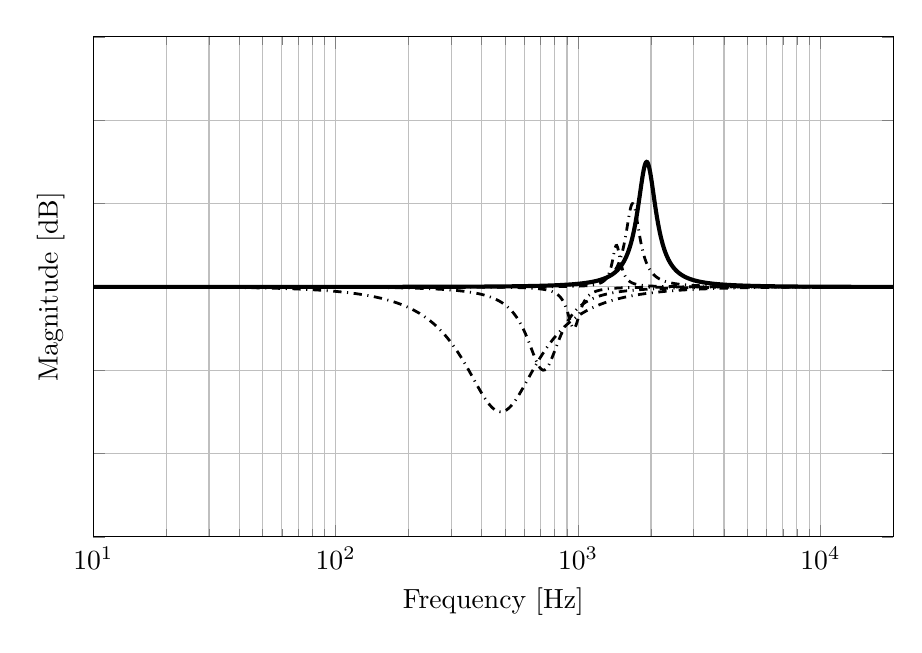
\begin{tikzpicture}

\begin{axis}[%
width=4in,
height=2.5in,
at={(1.011in,0.642in)},
scale only axis,
unbounded coords=jump,
xmode=log,
xmin=10,
xmax=20000,
xminorticks=true,
xlabel={Frequency [Hz]},
xmajorgrids,
xminorgrids,
ymin=-6,
ymax=6,
ylabel={Magnitude [dB]},
ymajorgrids,
yticklabels={\empty},
axis background/.style={fill=white}
]
\addplot [color=black,dashdotted,line width=1.0pt,forget plot]
  table[row sep=crcr]{%
0.159154943091895	-2.59308016428024e-07\\
11.1846266392052	-0.00128143830710427\\
22.2100983353184	-0.0050626220439554\\
33.2355700314317	-0.0113720981391969\\
44.2610417275449	-0.020257006719968\\
55.2865134236582	-0.0317835907371118\\
66.3119851197714	-0.0460375280469935\\
77.3374568158847	-0.0631243258254823\\
88.362928511998	-0.0831697498401766\\
99.3884002081112	-0.106320251026755\\
110.413871904224	-0.132743339149559\\
121.439343600338	-0.162627837421839\\
132.464815296451	-0.196183932096249\\
143.490286992564	-0.233642906526957\\
154.515758688678	-0.275256419355591\\
165.541230384791	-0.321295150712409\\
176.566702080904	-0.372046598463861\\
187.592173777017	-0.427811758866537\\
198.617645473131	-0.488900373788274\\
209.643117169244	-0.555624372631949\\
220.668588865357	-0.628289086140713\\
231.69406056147	-0.707181769249409\\
242.719532257584	-0.792556953026297\\
253.745003953697	-0.884618168595497\\
264.77047564981	-0.983495671761445\\
275.795947345923	-1.08921997506648\\
286.821419042037	-1.20169129847317\\
297.84689073815	-1.32064551638741\\
308.872362434263	-1.44561783707034\\
319.897834130376	-1.57590631173325\\
330.92330582649	-1.71053830834201\\
341.948777522603	-1.84824421119674\\
352.974249218716	-1.9874436461014\\
363.999720914829	-2.12625020302483\\
375.025192610943	-2.26250056014364\\
386.050664307056	-2.39381269576123\\
397.076136003169	-2.5176751871433\\
408.101607699282	-2.63156539046817\\
419.127079395396	-2.73308899543675\\
430.152551091509	-2.82012804362845\\
441.178022787622	-2.89098043637233\\
452.203494483736	-2.94447272934785\\
463.228966179849	-2.98003055649148\\
474.254437875962	-2.99769719473964\\
485.279909572075	-2.9980991950489\\
496.305381268189	-2.98236647862696\\
507.330852964302	-2.95202066035439\\
518.356324660415	-2.90884826452324\\
529.381796356528	-2.85477479726574\\
540.407268052642	-2.79175223077757\\
551.432739748755	-2.72166773871217\\
562.458211444868	-2.64627683476625\\
573.483683140981	-2.56716030780126\\
584.509154837095	-2.48570189048468\\
595.534626533208	-2.4030823986223\\
606.560098229321	-2.32028585434528\\
617.585569925434	-2.23811350870397\\
628.611041621548	-2.15720239659672\\
639.636513317661	-2.07804586169961\\
650.661985013774	-2.00101424153538\\
661.687456709888	-1.92637453431639\\
672.712928406001	-1.85430835936674\\
683.738400102114	-1.78492787942135\\
694.763871798227	-1.71828959674193\\
705.789343494341	-1.65440609041348\\
716.814815190454	-1.59325585258034\\
727.840286886567	-1.53479142632988\\
738.86575858268	-1.47894606268356\\
749.891230278794	-1.42563911006364\\
760.916701974907	-1.37478033464613\\
771.94217367102	-1.32627334962388\\
782.967645367133	-1.28001830910545\\
793.993117063246	-1.2359140003164\\
805.01858875936	-1.19385944718086\\
816.044060455473	-1.15375511985523\\
827.069532151586	-1.11550382857468\\
838.0950038477	-1.07901136625031\\
849.120475543813	-1.04418695245816\\
860.145947239926	-1.01094352158574\\
871.171418936039	-0.979197889702961\\
882.196890632153	-0.948870827969076\\
893.222362328266	-0.919887064846705\\
904.247834024379	-0.89217523488758\\
915.273305720492	-0.865667788183585\\
926.298777416606	-0.840300871618828\\
937.324249112719	-0.816014190665707\\
948.349720808832	-0.792750858549394\\
959.375192504945	-0.770457238069023\\
970.400664201059	-0.749082780131802\\
981.426135897172	-0.72857986208236\\
992.451607593285	-0.708903628129534\\
1003.4770792894	-0.690011833564395\\
1014.50255098551	-0.671864693974389\\
1025.52802268163	-0.654424740286856\\
1036.55349437774	-0.637656680175713\\
1047.57896607385	-0.621527266141301\\
1058.60443776996	-0.606005170396374\\
1069.62990946608	-0.591060866562236\\
1080.65538116219	-0.576666518077761\\
1091.6808528583	-0.562795873154839\\
1102.70632455442	-0.549424166059845\\
1113.73179625053	-0.536528024468389\\
1124.75726794664	-0.524085382616755\\
1135.78273964276	-0.512075399960452\\
1146.80821133887	-0.500478385047388\\
1157.83368303498	-0.489275724310165\\
1168.8591547311	-0.478449815491164\\
1179.88462642721	-0.467984005416474\\
1190.91009812332	-0.457862531850311\\
1201.93556981944	-0.448070469167377\\
1212.96104151555	-0.438593677597627\\
1223.98651321166	-0.429418755806841\\
1235.01198490778	-0.42053299659285\\
1246.03745660389	-0.411924345486025\\
1257.0629283	-0.403581362060191\\
1268.08839999612	-0.395493183767216\\
1279.11387169223	-0.387649492125075\\
1290.13934338834	-0.380040481097244\\
1301.16481508446	-0.372656827513017\\
1312.19028678057	-0.365489663389487\\
1323.21575847668	-0.358530550023957\\
1334.2412301728	-0.351771453735911\\
1345.26670186891	-0.345204723145033\\
1356.29217356502	-0.338823067880805\\
1367.31764526114	-0.332619538625449\\
1378.34311695725	-0.326587508400373\\
1389.36858865336	-0.32072065501079\\
1400.39406034948	-0.315012944571235\\
1411.41953204559	-0.309458616038437\\
1422.4450037417	-0.304052166684521\\
1433.47047543782	-0.298788338448059\\
1444.49594713393	-0.293662105103267\\
1455.52141883004	-0.288668660195393\\
1466.54689052616	-0.283803405689813\\
1477.57236222227	-0.279061941289469\\
1488.59783391838	-0.274440054377054\\
1499.6233056145	-0.269933710540162\\
1510.64877731061	-0.265539044643811\\
1521.67424900672	-0.261252352413832\\
1532.69972070283	-0.257070082499173\\
1543.72519239895	-0.252988828982572\\
1554.75066409506	-0.24900532431187\\
1565.77613579117	-0.245116432624669\\
1576.80160748729	-0.241319143443171\\
1587.8270791834	-0.237610565714884\\
1598.85255087951	-0.233987922179333\\
1609.87802257563	-0.230448544039746\\
1620.90349427174	-0.226989865921936\\
1631.92896596785	-0.223609421102443\\
1642.95443766397	-0.220304836990478\\
1653.97990936008	-0.21707383084808\\
1665.00538105619	-0.21391420573429\\
1676.03085275231	-0.210823846660657\\
1687.05632444842	-0.207800716945195\\
1698.08179614453	-0.204842854753679\\
1709.10726784065	-0.201948369817026\\
1720.13273953676	-0.199115440315198\\
1731.15821123287	-0.196342309917569\\
1742.18368292899	-0.193627284971281\\
1753.2091546251	-0.190968731829225\\
1764.23462632121	-0.188365074309434\\
1775.26009801733	-0.185814791279248\\
1786.28556971344	-0.18331641435674\\
1797.31104140955	-0.180868525723337\\
1808.33651310567	-0.178469756041323\\
1819.36198480178	-0.176118782470873\\
1830.38745649789	-0.173814326780896\\
1841.41292819401	-0.171555153548624\\
1852.43839989012	-0.169340068443867\\
1863.46387158623	-0.167167916592643\\
1874.48934328235	-0.165037581016277\\
1885.51481497846	-0.162947981142515\\
1896.54028667457	-0.160898071384086\\
1907.56575837069	-0.158886839781998\\
1918.5912300668	-0.156913306709414\\
1929.61670176291	-0.154976523634191\\
1940.64217345903	-0.153075571935767\\
1951.66764515514	-0.151209561774563\\
1962.69311685125	-0.149377631011322\\
1973.71858854737	-0.147578944172846\\
1984.74406024348	-0.145812691463381\\
1995.76953193959	-0.144078087818173\\
2006.79500363571	-0.14237437199754\\
2017.82047533182	-0.140700805719668\\
2028.84594702793	-0.139056672830082\\
2039.87141872404	-0.137441278505994\\
2050.89689042016	-0.135853948493894\\
2061.92236211627	-0.13429402837901\\
2072.94783381238	-0.132760882884641\\
2083.9733055085	-0.131253895200597\\
2094.99877720461	-0.129772466338767\\
2106.02424890072	-0.128316014515314\\
2117.04972059684	-0.126883974557008\\
2128.07519229295	-0.125475797332209\\
2139.10066398906	-0.124090949204205\\
2150.12613568518	-0.12272891150605\\
2161.15160738129	-0.121389180036453\\
2172.1770790774	-0.120071264575249\\
2183.20255077352	-0.11877468841776\\
2194.22802246963	-0.117498987927392\\
2205.25349416574	-0.116243712105161\\
2216.27896586186	-0.11500842217623\\
2227.30443755797	-0.113792691191532\\
2238.32990925408	-0.112596103645234\\
2249.3553809502	-0.111418255106086\\
2260.38085264631	-0.110258751862803\\
2271.40632434242	-0.109117210582729\\
2282.43179603854	-0.107993257983143\\
2293.45726773465	-0.106886530514574\\
2304.48273943076	-0.105796674055948\\
2315.50821112688	-0.104723343620662\\
2326.53368282299	-0.103666203073457\\
2337.5591545191	-0.10262492485759\\
2348.58462621522	-0.101599189731595\\
2359.61009791133	-0.100588686515625\\
2370.63556960744	-0.0995931118468657\\
2381.66104130356	-0.0986121699433707\\
2392.68651299967	-0.097645572376515\\
2403.71198469578	-0.0966930378511288\\
2414.7374563919	-0.0957542919934995\\
2425.76292808801	-0.0948290671466972\\
2436.78839978412	-0.0939171021727435\\
2447.81387148024	-0.0930181422619672\\
2458.83934317635	-0.0921319387485318\\
2469.86481487246	-0.0912582489323262\\
2480.89028656857	-0.0903968359069243\\
2491.91575826469	-0.0895474683934143\\
2502.9412299608	-0.0887099205794937\\
2513.96670165692	-0.0878839719643362\\
2524.99217335303	-0.0870694072081827\\
2536.01764504914	-0.08626601598725\\
2547.04311674525	-0.0854735928531741\\
2558.06858844137	-0.0846919370972066\\
2569.09406013748	-0.0839208526186183\\
2580.11953183359	-0.0831601477976233\\
2591.14500352971	-0.0824096353722155\\
2602.17047522582	-0.0816691323189535\\
2613.19594692193	-0.0809384597377207\\
2624.22141861805	-0.0802174427399125\\
2635.24689031416	-0.0795059103403668\\
2646.27236201027	-0.0788036953524835\\
2657.29783370639	-0.0781106342869353\\
2668.3233054025	-0.0774265672530845\\
2679.34877709861	-0.0767513378640725\\
2690.37424879473	-0.0760847931441694\\
2701.39972049084	-0.0754267834394481\\
2712.42519218695	-0.0747771623311154\\
2723.45066388307	-0.0741357865512767\\
2734.47613557918	-0.0735025159014196\\
2745.50160727529	-0.0728772131734603\\
2756.52707897141	-0.0722597440728676\\
2767.55255066752	-0.0716499771443997\\
2778.57802236363	-0.0710477836998589\\
2789.60349405975	-0.0704530377480554\\
2800.62896575586	-0.0698656159268208\\
2811.65443745197	-0.0692853974370629\\
2822.67990914809	-0.068712263978724\\
2833.7053808442	-0.0681460996885946\\
2844.73085254031	-0.0675867910799816\\
2855.75632423643	-0.0670342269840639\\
2866.78179593254	-0.0664882984928687\\
2877.80726762865	-0.0659488989042706\\
2888.83273932477	-0.0654159236679126\\
2899.85821102088	-0.0648892703332565\\
2910.88368271699	-0.0643688384987697\\
2921.90915441311	-0.0638545297626125\\
2932.93462610922	-0.0633462476749303\\
2943.96009780533	-0.062843897691063\\
2954.98556950145	-0.0623473871263667\\
2966.01104119756	-0.0618566251123072\\
2977.03651289367	-0.0613715225535651\\
2988.06198458979	-0.0608919920863842\\
2999.0874562859	-0.0604179480382462\\
3010.11292798201	-0.0599493063883788\\
3021.13839967812	-0.0594859847295121\\
3032.16387137424	-0.0590279022306255\\
3043.18934307035	-0.058574979600616\\
3054.21481476646	-0.0581271390531796\\
3065.24028646258	-0.0576843042722949\\
3076.26575815869	-0.0572464003789039\\
3087.2912298548	-0.0568133538983556\\
3098.31670155092	-0.056385092728742\\
3109.34217324703	-0.0559615461100395\\
3120.36764494314	-0.0555426445940413\\
3131.39311663926	-0.0551283200152782\\
3142.41858833537	-0.0547185054622656\\
3153.44406003148	-0.0543131352500063\\
3164.4695317276	-0.0539121448928342\\
3175.49500342371	-0.0535154710781116\\
3186.52047511982	-0.05312305164055\\
3197.54594681594	-0.0527348255372708\\
3208.57141851205	-0.052350732823355\\
3219.59689020816	-0.0519707146281611\\
3230.62236190428	-0.0515947131321636\\
3241.64783360039	-0.0512226715443306\\
3252.6733052965	-0.0508545340802538\\
3263.69877699262	-0.0504902459405586\\
3274.72424868873	-0.0501297532900634\\
3285.74972038484	-0.0497730032373318\\
3296.77519208096	-0.0494199438149101\\
3307.80066377707	-0.0490705239596962\\
3318.82613547318	-0.0487246934942775\\
3329.8516071693	-0.0483824031082292\\
3340.87707886541	-0.0480436043402487\\
3351.90255056152	-0.0477082495605468\\
3362.92802225764	-0.0473762919536626\\
3373.95349395375	-0.0470476855016934\\
3384.97896564986	-0.0467223849681015\\
3396.00443734598	-0.0464003458815953\\
3407.02990904209	-0.0460815245206671\\
3418.0553807382	-0.0457658778983693\\
3429.08085243432	-0.0454533637474768\\
3440.10632413043	-0.0451439405059925\\
3451.13179582654	-0.0448375673029869\\
3462.15726752266	-0.0445342039448541\\
3473.18273921877	-0.0442338109017344\\
3484.20821091488	-0.0439363492943778\\
3495.23368261099	-0.0436417808812571\\
3506.25915430711	-0.043350068046018\\
3517.28462600322	-0.0430611737851617\\
3528.31009769933	-0.0427750616960623\\
3539.33556939545	-0.0424916959652262\\
3550.36104109156	-0.0422110413568033\\
3561.38651278767	-0.0419330632015015\\
3572.41198448379	-0.0416577273854844\\
3583.4374561799	-0.0413850003397461\\
3594.46292787601	-0.0411148490296618\\
3605.48839957213	-0.0408472409447534\\
3616.51387126824	-0.0405821440886934\\
3627.53934296435	-0.0403195269694892\\
3638.56481466047	-0.0400593585899712\\
3649.59028635658	-0.0398016084384882\\
3660.61575805269	-0.0395462464796625\\
3671.64122974881	-0.0392932431455234\\
3682.66670144492	-0.0390425693267402\\
3693.69217314103	-0.0387941963641187\\
3704.71764483715	-0.0385480960401294\\
3715.74311653326	-0.0383042405708406\\
3726.76858822937	-0.0380626025978606\\
3737.79405992549	-0.0378231551804983\\
3748.8195316216	-0.0375858717880862\\
3759.84500331771	-0.0373507262925211\\
3770.87047501383	-0.0371176929608805\\
3781.89594670994	-0.0368867464482896\\
3792.92141840605	-0.0366578617908316\\
3803.94689010217	-0.0364310143986796\\
3814.97236179828	-0.0362061800494071\\
3825.99783349439	-0.0359833348813199\\
3837.02330519051	-0.0357624553870556\\
3848.04877688662	-0.0355435184072334\\
3859.07424858273	-0.0353265011242398\\
3870.09972027885	-0.0351113810562452\\
3881.12519197496	-0.0348981360511922\\
3892.15066367107	-0.0346867442809728\\
3903.17613536719	-0.0344771842358307\\
3914.2016070633	-0.034269434718648\\
3925.22707875941	-0.0340634748396052\\
3936.25255045553	-0.0338592840107738\\
3947.27802215164	-0.0336568419408637\\
3958.30349384775	-0.033456128630061\\
3969.32896554387	-0.0332571243651173\\
3980.35443723998	-0.0330598097142807\\
3991.37990893609	-0.0328641655224972\\
4002.4053806322	-0.0326701729067525\\
4013.43085232832	-0.0324778132513273\\
4024.45632402443	-0.0322870682033265\\
4035.48179572054	-0.0320979196681714\\
4046.50726741666	-0.0319103498052474\\
4057.53273911277	-0.031724341023659\\
4068.55821080888	-0.0315398759779361\\
4079.583682505	-0.0313569375640133\\
4090.60915420111	-0.0311755089151398\\
4101.63462589722	-0.0309955733979792\\
4112.66009759334	-0.0308171146086173\\
4123.68556928945	-0.0306401163688926\\
4134.71104098556	-0.0304645627225745\\
4145.73651268168	-0.0302904379317424\\
4156.76198437779	-0.0301177264731794\\
4167.7874560739	-0.0299464130348606\\
4178.81292777002	-0.0297764825124946\\
4189.83839946613	-0.0296079200061578\\
4200.86387116224	-0.0294407108169421\\
4211.88934285836	-0.0292748404437181\\
4222.91481455447	-0.0291102945799303\\
4233.94028625058	-0.0289470591104714\\
4244.9657579467	-0.0287851201085756\\
4255.99122964281	-0.0286244638328299\\
4267.01670133892	-0.0284650767241756\\
4278.04217303504	-0.0283069454030665\\
4289.06764473115	-0.0281500566665324\\
4300.09311642726	-0.0279943974854188\\
4311.11858812338	-0.0278399550016548\\
4322.14405981949	-0.0276867165255444\\
4333.1695315156	-0.027534669533058\\
4344.19500321172	-0.0273838016633388\\
4355.22047490783	-0.0272341007160669\\
4366.24594660394	-0.0270855546489887\\
4377.27141830006	-0.0269381515754355\\
4388.29688999617	-0.0267918797619609\\
4399.32236169228	-0.0266467276258825\\
4410.3478333884	-0.0265026837330234\\
4421.37330508451	-0.0263597367954372\\
4432.39877678062	-0.0262178756690572\\
4443.42424847673	-0.0260770893516259\\
4454.44972017285	-0.0259373669804426\\
4465.47519186896	-0.0257986978302471\\
4476.50066356508	-0.0256610713111623\\
4487.52613526119	-0.0255244769666073\\
4498.5516069573	-0.025388904471326\\
4509.57707865341	-0.0252543436293299\\
4520.60255034953	-0.025120784372037\\
4531.62802204564	-0.0249882167562934\\
4542.65349374176	-0.0248566309625798\\
4553.67896543787	-0.0247260172930513\\
4564.70443713398	-0.0245963661698157\\
4575.72990883009	-0.0244676681331166\\
4586.75538052621	-0.0243399138395963\\
4597.78085222232	-0.0242130940605428\\
4608.80632391843	-0.0240871996802443\\
4619.83179561455	-0.0239622216943317\\
4630.85726731066	-0.0238381512080557\\
4641.88273900677	-0.0237149794347985\\
4652.90821070289	-0.0235926976944543\\
4663.933682399	-0.0234712974118246\\
4674.95915409511	-0.0233507701151783\\
4685.98462579123	-0.02323110743469\\
4697.01009748734	-0.0231123011010084\\
4708.03556918345	-0.02299434294378\\
4719.06104087957	-0.0228772248902564\\
4730.08651257568	-0.0227609389638407\\
4741.11198427179	-0.0226454772827666\\
4752.13745596791	-0.0225308320587333\\
4763.16292766402	-0.0224169955955268\\
4774.18839936013	-0.0223039602877939\\
4785.21387105625	-0.0221917186196793\\
4796.23934275236	-0.0220802631635979\\
4807.26481444847	-0.021969586578994\\
4818.29028614459	-0.021859681611082\\
4829.3157578407	-0.021750541089685\\
4840.34122953681	-0.0216421579280311\\
4851.36670123293	-0.0215345251215623\\
4862.39217292904	-0.021427635746852\\
4873.41764462515	-0.0213214829604158\\
4884.44311632126	-0.0212160599976126\\
4895.46858801738	-0.0211113601716078\\
4906.49405971349	-0.0210073768722246\\
4917.51953140961	-0.0209041035649262\\
4928.54500310572	-0.020801533789783\\
4939.57047480183	-0.0206996611604328\\
4950.59594649795	-0.0205984793630771\\
4961.62141819406	-0.0204979821554874\\
4972.64688989017	-0.020398163366058\\
4983.67236158629	-0.0202990168928127\\
4994.6978332824	-0.0202005367024765\\
5005.72330497851	-0.0201027168295448\\
5016.74877667463	-0.0200055513753757\\
5027.77424837074	-0.0199090345072708\\
5038.79972006685	-0.0198131604576139\\
5049.82519176296	-0.019717923522974\\
5060.85066345908	-0.019623318063297\\
5071.87613515519	-0.0195293385009756\\
5082.9016068513	-0.0194359793200943\\
5093.92707854742	-0.0193432350655941\\
5104.95255024353	-0.0192511003424284\\
5115.97802193964	-0.0191595698148223\\
5127.00349363576	-0.0190686382054465\\
5138.02896533187	-0.0189783002946738\\
5149.05443702798	-0.0188885509198412\\
5160.0799087241	-0.0187993849744315\\
5171.10538042021	-0.0187107974074136\\
5182.13085211632	-0.0186227832224983\\
5193.15632381244	-0.0185353374774022\\
5204.18179550855	-0.0184484552831634\\
5215.20726720466	-0.018362131803475\\
5226.23273890078	-0.0182763622539376\\
5237.25821059689	-0.0181911419014752\\
5248.283682293	-0.0181064660636126\\
5259.30915398912	-0.018022330107836\\
5270.33462568523	-0.0179387294509876\\
5281.36009738134	-0.0178556595585772\\
5292.38556907746	-0.0177731159442225\\
5303.41104077357	-0.017691094168983\\
5314.43651246968	-0.0176095898407976\\
5325.4619841658	-0.0175285986138614\\
5336.48745586191	-0.0174481161880605\\
5347.51292755802	-0.0173681383083953\\
5358.53839925414	-0.0172886607643864\\
5369.56387095025	-0.0172096793895438\\
5380.58934264636	-0.0171311900608096\\
5391.61481434248	-0.0170531886980069\\
5402.64028603859	-0.0169756712633022\\
5413.6657577347	-0.0168986337606775\\
5424.69122943082	-0.0168220722354394\\
5435.71670112693	-0.0167459827736652\\
5446.74217282304	-0.016670361501714\\
5457.76764451916	-0.0165952045857339\\
5468.79311621527	-0.0165205082311668\\
5479.81858791138	-0.0164462686822753\\
5490.8440596075	-0.0163724822216444\\
5501.86953130361	-0.0162991451697202\\
5512.89500299972	-0.0162262538843711\\
5523.92047469583	-0.0161538047603951\\
5534.94594639195	-0.0160817942290869\\
5545.97141808806	-0.0160102187578014\\
5556.99688978417	-0.0159390748494861\\
5568.02236148029	-0.0158683590423133\\
5579.0478331764	-0.0157980679091661\\
5590.07330487251	-0.015728198057306\\
5601.09877656863	-0.0156587461279001\\
5612.12424826474	-0.0155897087956357\\
5623.14971996085	-0.015521082768324\\
5634.17519165697	-0.0154528647864985\\
5645.20066335308	-0.0153850516230288\\
5656.22613504919	-0.0153176400827104\\
5667.25160674531	-0.0152506270019286\\
5678.27707844142	-0.0151840092482437\\
5689.30255013753	-0.0151177837200545\\
5700.32802183365	-0.0150519473462071\\
5711.35349352976	-0.0149864970856496\\
5722.37896522587	-0.0149214299270779\\
5733.40443692199	-0.0148567428885876\\
5744.4299086181	-0.0147924330173159\\
5755.45538031421	-0.014728497389138\\
5766.48085201033	-0.0146649331082676\\
5777.50632370644	-0.0146017373069872\\
5788.53179540255	-0.0145389071452972\\
5799.55726709867	-0.0144764398106151\\
5810.58273879478	-0.0144143325173995\\
5821.60821049089	-0.0143525825069075\\
5832.63368218701	-0.0142911870468526\\
5843.65915388312	-0.0142301434310878\\
5854.68462557923	-0.014169448979337\\
5865.71009727535	-0.0141091010368848\\
5876.73556897146	-0.0140490969742559\\
5887.76104066757	-0.0139894341869772\\
5898.78651236369	-0.0139301100952646\\
5909.8119840598	-0.0138711221437307\\
5920.83745575591	-0.0138124678011331\\
5931.86292745203	-0.0137541445600927\\
5942.88839914814	-0.0136961499368094\\
5953.91387084425	-0.0136384814708079\\
5964.93934254037	-0.0135811367246873\\
5975.96481423648	-0.0135241132838427\\
5986.99028593259	-0.0134674087561935\\
5998.0157576287	-0.0134110207719853\\
6009.04122932482	-0.0133549469834886\\
6020.06670102093	-0.0132991850647617\\
6031.09217271704	-0.0132437327114424\\
6042.11764441316	-0.0131885876404664\\
6053.14311610927	-0.0131337475898497\\
6064.16858780538	-0.0130792103184578\\
6075.1940595015	-0.0130249736057595\\
6086.21953119761	-0.0129710352516135\\
6097.24500289372	-0.0129173930760596\\
6108.27047458984	-0.0128640449190421\\
6119.29594628595	-0.0128109886402577\\
6130.32141798206	-0.012758222118885\\
6141.34688967818	-0.0127057432534107\\
6152.37236137429	-0.0126535499613933\\
6163.3978330704	-0.0126016401792732\\
6174.42330476652	-0.0125500118621427\\
6185.44877646263	-0.0124986629835777\\
6196.47424815874	-0.0124475915354007\\
6207.49971985486	-0.0123967955275167\\
6218.52519155097	-0.0123462729876945\\
6229.55066324708	-0.0122960219613861\\
6240.5761349432	-0.0122460405115255\\
6251.60160663931	-0.0121963267183637\\
6262.62707833542	-0.0121468786792559\\
6273.65255003154	-0.0120976945084828\\
6284.67802172765	-0.0120487723370969\\
6295.70349342376	-0.012000110312717\\
6306.72896511988	-0.0119517065993386\\
6317.75443681599	-0.0119035593772228\\
6328.7799085121	-0.011855666842633\\
6339.80538020822	-0.0118080272077504\\
6350.83085190433	-0.0117606387004408\\
6361.85632360044	-0.0117134995641527\\
6372.88179529656	-0.0116666080576872\\
6383.90726699267	-0.011619962455069\\
6394.93273868878	-0.0115735610454145\\
6405.9582103849	-0.0115274021326983\\
6416.98368208101	-0.011481484035697\\
6428.00915377712	-0.0114358050877286\\
6439.03462547323	-0.0113903636365952\\
6450.06009716935	-0.0113451580443796\\
6461.08556886546	-0.0113001866872867\\
6472.11104056157	-0.0112554479555595\\
6483.13651225769	-0.0112109402532551\\
6494.1619839538	-0.011166661998163\\
6505.18745564992	-0.0111226116216351\\
6516.21292734603	-0.0110787875684522\\
6527.23839904214	-0.0110351882966894\\
6538.26387073826	-0.0109918122775527\\
6549.28934243437	-0.0109486579953218\\
6560.31481413048	-0.0109057239470959\\
6571.34028582659	-0.010863008642785\\
6582.36575752271	-0.0108205106048893\\
6593.39122921882	-0.0107782283684303\\
6604.41670091493	-0.0107361604807755\\
6615.44217261105	-0.0106943055015691\\
6626.46764430716	-0.0106526620025321\\
6637.49311600327	-0.0106112285674315\\
6648.51858769939	-0.010570003791875\\
6659.5440593955	-0.0105289862832468\\
6670.56953109161	-0.0104881746605755\\
6681.59500278773	-0.0104475675543945\\
6692.62047448384	-0.0104071636066537\\
6703.64594617995	-0.0103669614706125\\
6714.67141787607	-0.0103269598106858\\
6725.69688957218	-0.0102871573023653\\
6736.72236126829	-0.0102475526321271\\
6747.74783296441	-0.0102081444972606\\
6758.77330466052	-0.010168931605816\\
6769.79877635663	-0.010129912676485\\
6780.82424805275	-0.0100910864384819\\
6791.84971974886	-0.0100524516314621\\
6802.87519144497	-0.0100140070053885\\
6813.90066314109	-0.00997575132046504\\
6824.9261348372	-0.00993768334700056\\
6835.95160653331	-0.00989980186534893\\
6846.97707822943	-0.00986210566577176\\
6858.00254992554	-0.00982459354837218\\
6869.02802162165	-0.0097872643229834\\
6880.05349331777	-0.00975011680907649\\
6891.07896501388	-0.00971314983566726\\
6902.10443670999	-0.00967636224122411\\
6913.1299084061	-0.00963975287357974\\
6924.15538010222	-0.00960332058983318\\
6935.18085179833	-0.00956706425626445\\
6946.20632349445	-0.00953098274824818\\
6957.23179519056	-0.00949507495016246\\
6968.25726688667	-0.00945933975530253\\
6979.28273858279	-0.00942377606580795\\
6990.3082102789	-0.00938838279254926\\
7001.33368197501	-0.00935315885506868\\
7012.35915367112	-0.00931810318149387\\
7023.38462536724	-0.00928321470844864\\
7034.41009706335	-0.00924849238098218\\
7045.43556875946	-0.00921393515246825\\
7056.46104045558	-0.00917954198456527\\
7067.48651215169	-0.00914531184709236\\
7078.5119838478	-0.00911124371797782\\
7089.53745554392	-0.00907733658318836\\
7100.56292724003	-0.00904358943663023\\
7111.58839893614	-0.00901000128008908\\
7122.61387063226	-0.00897657112317164\\
7133.63934232837	-0.0089432979831848\\
7144.66481402448	-0.00891018088512655\\
7155.6902857206	-0.00887721886155245\\
7166.71575741671	-0.00884441095255889\\
7177.74122911282	-0.0088117562056583\\
7188.76670080894	-0.00877925367577878\\
7199.79217250505	-0.00874690242512194\\
7210.81764420116	-0.00871470152313942\\
7221.84311589728	-0.00868265004646791\\
7232.86858759339	-0.00865074707883717\\
7243.8940592895	-0.0086189917110205\\
7254.91953098562	-0.00858738304076689\\
7265.94500268173	-0.00855592017274669\\
7276.97047437784	-0.00852460221846349\\
7287.99594607396	-0.00849342829622393\\
7299.02141777007	-0.00846239753104475\\
7310.04688946618	-0.00843150905460234\\
7321.0723611623	-0.00840076200518616\\
7332.09783285841	-0.00837015552762896\\
7343.12330455452	-0.00833968877321579\\
7354.14877625063	-0.0083093608996944\\
7365.17424794675	-0.00827917107114564\\
7376.19971964286	-0.0082491184579793\\
7387.22519133898	-0.00821920223683646\\
7398.25066303509	-0.00818942159055252\\
7409.2761347312	-0.00815977570811163\\
7420.30160642732	-0.0081302637845779\\
7431.32707812343	-0.00810088502103438\\
7442.35254981954	-0.0080716386245365\\
7453.37802151566	-0.00804252380807228\\
7464.40349321177	-0.00801353979047717\\
7475.42896490788	-0.00798468579641837\\
7486.45443660399	-0.00795596105631066\\
7497.47990830011	-0.00792736480629113\\
7508.50537999622	-0.00789889628815036\\
7519.53085169233	-0.00787055474928499\\
7530.55632338845	-0.00784233944266276\\
7541.58179508456	-0.00781424962675085\\
7552.60726678067	-0.00778628456548098\\
7563.63273847679	-0.00775844352820381\\
7574.6582101729	-0.00773072578962606\\
7585.68368186901	-0.0077031306297794\\
7596.70915356513	-0.00767565733396911\\
7607.73462526124	-0.00764830519272372\\
7618.76009695735	-0.00762107350173884\\
7629.78556865347	-0.00759396156187409\\
7640.81104034958	-0.00756696867904289\\
7651.83651204569	-0.0075400941642316\\
7662.86198374181	-0.00751333733341343\\
7673.88745543792	-0.00748669750752027\\
7684.91292713403	-0.00746017401239432\\
7695.93839883015	-0.00743376617876373\\
7706.96387052626	-0.00740747334217878\\
7717.98934222237	-0.00738129484296633\\
7729.01481391849	-0.00735523002622485\\
7740.0402856146	-0.00732927824172582\\
7751.06575731071	-0.00730343884393094\\
7762.09122900683	-0.00727771119191186\\
7773.11670070294	-0.00725209464932979\\
7784.14217239905	-0.00722658858440347\\
7795.16764409517	-0.00720119236983472\\
7806.19311579128	-0.00717590538281315\\
7817.21858748739	-0.00715072700494742\\
7828.24405918351	-0.00712565662224491\\
7839.26953087962	-0.00710069362505748\\
7850.29500257573	-0.00707583740807172\\
7861.32047427185	-0.00705108737023637\\
7872.34594596796	-0.00702644291476034\\
7883.37141766407	-0.00700190344905265\\
7894.39688936019	-0.0069774683846944\\
7905.4223610563	-0.00695313713740961\\
7916.44783275241	-0.00692890912702073\\
7927.47330444853	-0.00690478377742826\\
7938.49877614464	-0.00688076051654402\\
7949.52424784075	-0.00685683877631804\\
7960.54971953686	-0.00683301799263132\\
7971.57519123298	-0.00680929760531599\\
7982.60066292909	-0.00678567705809726\\
7993.6261346252	-0.00676215579857791\\
8004.65160632132	-0.0067387332781908\\
8015.67707801743	-0.00671540895216315\\
8026.70254971355	-0.00669218227951152\\
8037.72802140966	-0.00666905272298866\\
8048.75349310577	-0.00664601974906025\\
8059.77896480189	-0.00662308282785261\\
8070.804436498	-0.00660024143316042\\
8081.82990819411	-0.00657749504238956\\
8092.85537989022	-0.00655484313653394\\
8103.88085158634	-0.00653228520015797\\
8114.90632328245	-0.0065098207213405\\
8125.93179497856	-0.00648744919166604\\
8136.95726667468	-0.00646517010620051\\
8147.98273837079	-0.0064429829634381\\
8159.0082100669	-0.00642088726530309\\
8170.03368176302	-0.00639888251709665\\
8181.05915345913	-0.00637696822749388\\
8192.08462515524	-0.00635514390849161\\
8203.11009685136	-0.00633340907538511\\
8214.13556854747	-0.00631176324677575\\
8225.16104024358	-0.00629020594449372\\
8236.1865119397	-0.00626873669359498\\
8247.21198363581	-0.00624735502234581\\
8258.23745533192	-0.00622606046218021\\
8269.26292702804	-0.00620485254769503\\
8280.28839872415	-0.00618373081658132\\
8291.31387042026	-0.00616269480966288\\
8302.33934211638	-0.00614174407080547\\
8313.36481381249	-0.0061208781469466\\
8324.3902855086	-0.00610009658802602\\
8335.41575720472	-0.00607939894700108\\
8346.44122890083	-0.0060587847798022\\
8357.46670059694	-0.0060382536453068\\
8368.49217229306	-0.00601780510532762\\
8379.51764398917	-0.00599743872456728\\
8390.54311568528	-0.00597715407062787\\
8401.56858738139	-0.00595695071396262\\
8412.59405907751	-0.00593682822786231\\
8423.61953077362	-0.00591678618843879\\
8434.64500246974	-0.00589682417458057\\
8445.67047416585	-0.00587694176795554\\
8456.69594586196	-0.00585713855298977\\
8467.72141755808	-0.00583741411681336\\
8478.74688925419	-0.00581776804927678\\
8489.7723609503	-0.00579819994291604\\
8500.79783264642	-0.00577870939291698\\
8511.82330434253	-0.00575929599712091\\
8522.84877603864	-0.00573995935597832\\
8533.87424773476	-0.00572069907254969\\
8544.89971943087	-0.00570151475247075\\
8555.92519112698	-0.0056824060039389\\
8566.9506628231	-0.00566337243769284\\
8577.97613451921	-0.00564441366699808\\
8589.00160621532	-0.00562552930760248\\
8600.02707791143	-0.00560671897775548\\
8611.05254960755	-0.00558798229815786\\
8622.07802130366	-0.00556931889196267\\
8633.10349299977	-0.00555072838473558\\
8644.12896469589	-0.00553221040445869\\
8655.154436392	-0.00551376458148901\\
8666.17990808811	-0.0054953905485709\\
8677.20537978423	-0.0054770879407907\\
8688.23085148034	-0.00545885639555445\\
8699.25632317645	-0.00544069555260331\\
8710.28179487257	-0.00542260505397103\\
8721.30726656868	-0.00540458454395688\\
8732.33273826479	-0.00538663366914199\\
8743.35820996091	-0.00536875207833529\\
8754.38368165702	-0.00535093942258983\\
8765.40915335313	-0.00533319535516129\\
8776.43462504925	-0.00531551953148758\\
8787.46009674536	-0.00529791160921012\\
8798.48556844147	-0.00528037124811484\\
8809.51104013759	-0.00526289811013124\\
8820.5365118337	-0.0052454918593294\\
8831.56198352981	-0.00522815216186398\\
8842.58745522593	-0.00521087868602436\\
8853.61292692204	-0.00519367110216221\\
8864.63839861815	-0.0051765290826905\\
8875.66387031427	-0.00515945230207089\\
8886.68934201038	-0.00514244043680887\\
8897.71481370649	-0.00512549316542958\\
8908.74028540261	-0.00510861016844789\\
8919.76575709872	-0.00509179112838376\\
8930.79122879483	-0.00507503572971686\\
8941.81670049095	-0.00505834365889907\\
8952.84217218706	-0.00504171460432548\\
8963.86764388317	-0.00502514825631413\\
8974.89311557929	-0.00500864430709336\\
8985.9185872754	-0.0049922024508163\\
8996.94405897151	-0.0049758223835087\\
9007.96953066763	-0.00495950380306888\\
9018.99500236374	-0.00494324640925709\\
9030.02047405985	-0.00492704990368199\\
9041.04594575596	-0.00491091398978707\\
9052.07141745208	-0.00489483837282743\\
9063.09688914819	-0.0048788227598756\\
9074.1223608443	-0.00486286685978383\\
9085.14783254042	-0.00484697038319466\\
9096.17330423653	-0.00483113304250427\\
9107.19877593265	-0.00481535455187973\\
9118.22424762876	-0.00479963462721466\\
9129.24971932487	-0.00478397298613397\\
9140.27519102098	-0.00476836934798034\\
9151.3006627171	-0.00475282343380164\\
9162.32613441321	-0.00473733496632964\\
9173.35160610933	-0.00472190366998004\\
9184.37707780544	-0.00470652927083115\\
9195.40254950155	-0.00469121149662291\\
9206.42802119766	-0.00467595007672119\\
9217.45349289378	-0.00466074474213795\\
9228.47896458989	-0.00464559522549558\\
9239.504436286	-0.00463050126102878\\
9250.52990798212	-0.0046154625845623\\
9261.55537967823	-0.00460047893350902\\
9272.58085137434	-0.00458555004684964\\
9283.60632307046	-0.00457067566512785\\
9294.63179476657	-0.00455585553044157\\
9305.65726646268	-0.00454108938642077\\
9316.6827381588	-0.00452637697822937\\
9327.70820985491	-0.00451171805253816\\
9338.73368155102	-0.00449711235754024\\
9349.75915324714	-0.00448255964290759\\
9360.78462494325	-0.00446805965981414\\
9371.81009663936	-0.0044536121608866\\
9382.83556833548	-0.00443921690023623\\
9393.86104003159	-0.00442487363342216\\
9404.8865117277	-0.00441058211743304\\
9415.91198342382	-0.0043963421107092\\
9426.93745511993	-0.00438215337310017\\
9437.96292681604	-0.00436801566588397\\
9448.98839851216	-0.00435392875171975\\
9460.01387020827	-0.00433989239467196\\
9471.03934190438	-0.00432590636019775\\
9482.06481360049	-0.00431197041510735\\
9493.09028529661	-0.00429808432758825\\
9504.11575699272	-0.00428424786718096\\
9515.14122868884	-0.00427046080477135\\
9526.16670038495	-0.00425672291257224\\
9537.19217208106	-0.0042430339641321\\
9548.21764377718	-0.00422939373431183\\
9559.24311547329	-0.00421580199928766\\
9570.2685871694	-0.00420225853651832\\
9581.29405886551	-0.00418876312476817\\
9592.31953056163	-0.00417531554407051\\
9603.34500225774	-0.00416191557574687\\
9614.37047395386	-0.00414856300235968\\
9625.39594564997	-0.00413525760774413\\
9636.42141734608	-0.00412199917697338\\
9647.44688904219	-0.00410878749635374\\
9658.47236073831	-0.00409562235342464\\
9669.49783243442	-0.0040825035369557\\
9680.52330413053	-0.00406943083690236\\
9691.54877582665	-0.00405640404444732\\
9702.57424752276	-0.0040434229519629\\
9713.59971921887	-0.00403048735300235\\
9724.62519091499	-0.00401759704229981\\
9735.6506626111	-0.00400475181575968\\
9746.67613430721	-0.00399195147045758\\
9757.70160600333	-0.00397919580461333\\
9768.72707769944	-0.00396648461759764\\
9779.75254939555	-0.00395381770991862\\
9790.77802109167	-0.0039411948832227\\
9801.80349278778	-0.00392861594027343\\
9812.82896448389	-0.00391608068494466\\
9823.85443618001	-0.00390358892223598\\
9834.87990787612	-0.00389114045823317\\
9845.90537957223	-0.00387873510012356\\
9856.93085126835	-0.00386637265618063\\
9867.95632296446	-0.00385405293574758\\
9878.98179466057	-0.00384177574925465\\
9890.00726635669	-0.00382954090818153\\
9901.0327380528	-0.00381734822506886\\
9912.05820974891	-0.00380519751352212\\
9923.08368144502	-0.00379308858816914\\
9934.10915314114	-0.00378102126468614\\
9945.13462483725	-0.00376899535977359\\
9956.16009653337	-0.0037570106911649\\
9967.18556822948	-0.00374506707759163\\
9978.21103992559	-0.00373316433880666\\
9989.23651162171	-0.00372130229556392\\
10000.2619833178	-0.00370948076960387\\
10011.2874550139	-0.00369769958367379\\
10022.31292671	-0.00368595856148527\\
10033.3383984062	-0.00367425752772967\\
10044.3638701023	-0.00366259630807518\\
10055.3893417984	-0.00365097472915237\\
10066.4148134945	-0.0036393926185329\\
10077.4402851906	-0.00362784980476236\\
10088.4657568867	-0.00361634611731296\\
10099.4912285828	-0.00360488138660281\\
10110.516700279	-0.00359345544396887\\
10121.5421719751	-0.00358206812169981\\
10132.5676436712	-0.00357071925297706\\
10143.5931153673	-0.00355940867190187\\
10154.6185870634	-0.00354813621349816\\
10165.6440587595	-0.00353690171367588\\
10176.6695304556	-0.00352570500924637\\
10187.6950021517	-0.0035145459379012\\
10198.7204738479	-0.0035034243382372\\
10209.745945544	-0.00349234004971109\\
10220.7714172401	-0.0034812929126501\\
10231.7968889362	-0.0034702827682597\\
10242.8223606323	-0.00345930945861003\\
10253.8478323284	-0.00344837282661278\\
10264.8733040245	-0.0034374727160385\\
10275.8987757206	-0.00342660897149733\\
10286.9242474168	-0.00341578143844283\\
10297.9497191129	-0.00340498996316428\\
10308.975190809	-0.00339423439277406\\
10320.0006625051	-0.00338351457520192\\
10331.0261342012	-0.00337283035921615\\
10342.0516058973	-0.00336218159437247\\
10353.0770775934	-0.0033515681310603\\
10364.1025492896	-0.00334098982044102\\
10375.1280209857	-0.0033304465144981\\
10386.1534926818	-0.00331993806598795\\
10397.1789643779	-0.00330946432847744\\
10408.204436074	-0.00329902515629383\\
10419.2299077701	-0.00328862040454204\\
10430.2553794662	-0.00327824992911528\\
10441.2808511623	-0.00326791358666034\\
10452.3063228585	-0.0032576112345862\\
10463.3317945546	-0.00324734273106795\\
10474.3572662507	-0.00323710793502453\\
10485.3827379468	-0.00322690670612261\\
10496.4082096429	-0.00321673890478334\\
10507.433681339	-0.00320660439214276\\
10518.4591530351	-0.00319650303009909\\
10529.4846247313	-0.0031864346812635\\
10540.5100964274	-0.00317639920896685\\
10551.5355681235	-0.00316639647727131\\
10562.5610398196	-0.00315642635095192\\
10573.5865115157	-0.003146488695488\\
10584.6119832118	-0.00313658337706983\\
10595.6374549079	-0.00312671026259194\\
10606.662926604	-0.00311686921964146\\
10617.6883983002	-0.00310706011650202\\
10628.7138699963	-0.00309728282214022\\
10639.7393416924	-0.0030875372062201\\
10650.7648133885	-0.00307782313907128\\
10661.7902850846	-0.00306814049170633\\
10672.8157567807	-0.00305848913581688\\
10683.8412284768	-0.00304886894374376\\
10694.866700173	-0.00303927978850875\\
10705.8921718691	-0.00302972154378475\\
10716.9176435652	-0.00302019408389858\\
10727.9431152613	-0.00301069728383587\\
10738.9685869574	-0.00300123101922075\\
10749.9940586535	-0.00299179516632647\\
10761.0195303496	-0.00298238960206189\\
10772.0450020457	-0.00297301420397916\\
10783.0704737419	-0.00296366885024771\\
10794.095945438	-0.00295435341967447\\
10805.1214171341	-0.00294506779169134\\
10816.1468888302	-0.00293581184634359\\
10827.1723605263	-0.00292658546429952\\
10838.1978322224	-0.00291738852682822\\
10849.2233039185	-0.00290822091582182\\
10860.2487756147	-0.00289908251376552\\
10871.2742473108	-0.00288997320375594\\
10882.2997190069	-0.00288089286947409\\
10893.325190703	-0.00287184139520949\\
10904.3506623991	-0.00286281866583314\\
10915.3761340952	-0.0028538245667985\\
10926.4016057913	-0.00284485898415494\\
10937.4270774874	-0.0028359218045208\\
10948.4525491836	-0.00282701291509392\\
10959.4780208797	-0.00281813220364106\\
10970.5034925758	-0.00280927955850657\\
10981.5289642719	-0.00280045486859503\\
10992.554435968	-0.00279165802337023\\
11003.5799076641	-0.0027828889128649\\
11014.6053793602	-0.00277414742764588\\
11025.6308510564	-0.00276543345885951\\
11036.6563227525	-0.00275674689818145\\
11047.6817944486	-0.00274808763784562\\
11058.7072661447	-0.00273945557061716\\
11069.7327378408	-0.00273085058980305\\
11080.7582095369	-0.00272227258925115\\
11091.783681233	-0.00271372146333667\\
11102.8091529291	-0.00270519710696411\\
11113.8346246253	-0.00269669941557206\\
11124.8600963214	-0.00268822828510716\\
11135.8855680175	-0.00267978361205208\\
11146.9110397136	-0.00267136529339848\\
11157.9365114097	-0.00266297322664604\\
11168.9619831058	-0.00265460730982564\\
11179.9874548019	-0.00264626744144338\\
11191.0129264981	-0.00263795352054037\\
11202.0383981942	-0.00262966544664161\\
11213.0638698903	-0.0026214031197811\\
11224.0893415864	-0.00261316644048441\\
11235.1148132825	-0.00260495530976485\\
11246.1402849786	-0.00259676962913409\\
11257.1657566747	-0.00258860930058477\\
11268.1912283708	-0.00258047422660204\\
11279.216700067	-0.00257236431014145\\
11290.2421717631	-0.00256427945463948\\
11301.2676434592	-0.00255621956401743\\
11312.2931151553	-0.00254818454266018\\
11323.3185868514	-0.00254017429542874\\
11334.3440585475	-0.00253218872764575\\
11345.3695302436	-0.00252422774510131\\
11356.3950019397	-0.00251629125404229\\
11367.4204736359	-0.0025083791611917\\
11378.445945332	-0.00250049137370522\\
11389.4714170281	-0.00249262779921656\\
11400.4968887242	-0.00248478834579016\\
11411.5223604203	-0.00247697292195017\\
11422.5478321164	-0.00246918143666593\\
11433.5733038125	-0.00246141379935008\\
11444.5987755087	-0.00245366991984885\\
11455.6242472048	-0.00244594970845275\\
11466.6497189009	-0.00243825307590033\\
11477.675190597	-0.00243057993334257\\
11488.7006622931	-0.00242293019236981\\
11499.7261339892	-0.00241530376499638\\
11510.7516056853	-0.00240770056368081\\
11521.7770773814	-0.00240012050127181\\
11532.8025490776	-0.00239256349108449\\
11543.8280207737	-0.00238502944680291\\
11554.8534924698	-0.00237751828256112\\
11565.8789641659	-0.00237002991289492\\
11576.904435862	-0.00236256425276016\\
11587.9299075581	-0.0023551212175106\\
11598.9553792542	-0.00234770072290558\\
11609.9808509504	-0.00234030268512065\\
11621.0063226465	-0.00233292702072341\\
11632.0317943426	-0.00232557364668516\\
11643.0572660387	-0.00231824248038661\\
11654.0827377348	-0.00231093343957932\\
11665.1082094309	-0.00230364644241851\\
11676.133681127	-0.0022963814074659\\
11687.1591528231	-0.00228913825364154\\
11698.1846245193	-0.00228191690028163\\
11709.2100962154	-0.00227471726708165\\
11720.2355679115	-0.00226753927414453\\
11731.2610396076	-0.00226038284192477\\
11742.2865113037	-0.00225324789128044\\
11753.3119829998	-0.00224613434342794\\
11764.3374546959	-0.00223904211996602\\
11775.3629263921	-0.00223197114286232\\
11786.3883980882	-0.00222492133445048\\
11797.4138697843	-0.00221789261743781\\
11808.4393414804	-0.00221088491489087\\
11819.4648131765	-0.00220389815023833\\
11830.4902848726	-0.00219693224728447\\
11841.5157565687	-0.00218998713017252\\
11852.5412282648	-0.00218306272342039\\
11863.566699961	-0.00217615895187814\\
11874.5921716571	-0.00216927574077341\\
11885.6176433532	-0.00216241301567084\\
11896.6431150493	-0.00215557070249522\\
11907.6685867454	-0.00214874872750644\\
11918.6940584415	-0.00214194701731296\\
11929.7195301376	-0.00213516549887376\\
11940.7450018337	-0.00212840409948386\\
11951.7704735299	-0.00212166274677526\\
11962.795945226	-0.00211494136871987\\
11973.8214169221	-0.00210823989362658\\
11984.8468886182	-0.00210155825014417\\
11995.8723603143	-0.00209489636724201\\
12006.8978320104	-0.00208825417422163\\
12017.9233037065	-0.00208163160072249\\
12028.9487754027	-0.00207502857670563\\
12039.9742470988	-0.00206844503245265\\
12050.9997187949	-0.00206188089856763\\
12062.025190491	-0.00205533610599553\\
12073.0506621871	-0.00204881058597097\\
12084.0761338832	-0.00204230427006265\\
12095.1016055793	-0.002035817090156\\
12106.1270772755	-0.00202934897845603\\
12117.1525489716	-0.00202289986746225\\
12128.1780206677	-0.00201646969000344\\
12139.2034923638	-0.00201005837920383\\
12150.2289640599	-0.00200366586850821\\
12161.254435756	-0.00199729209165009\\
12172.2799074521	-0.00199093698268643\\
12183.3053791482	-0.00198460047596962\\
12194.3308508444	-0.00197828250614563\\
12205.3563225405	-0.00197198300816937\\
12216.3817942366	-0.00196570191728637\\
12227.4072659327	-0.00195943916904246\\
12238.4327376288	-0.00195319469927893\\
12249.4582093249	-0.00194696844412477\\
12260.483681021	-0.00194076034000832\\
12271.5091527171	-0.00193457032363886\\
12282.5346244133	-0.00192839833201921\\
12293.5600961094	-0.00192224430244086\\
12304.5855678055	-0.00191610817246664\\
12315.6110395016	-0.00190998987996734\\
12326.6365111977	-0.00190388936307737\\
12337.6619828938	-0.0018978065602121\\
12348.6874545899	-0.00189174141006882\\
12359.7129262861	-0.00188569385163061\\
12370.7383979822	-0.00187966382414799\\
12381.7638696783	-0.0018736512671428\\
12392.7893413744	-0.00186765612042073\\
12403.8148130705	-0.00186167832405105\\
12414.8402847666	-0.00185571781837723\\
12425.8657564627	-0.00184977454400633\\
12436.8912281588	-0.00184384844181284\\
12447.916699855	-0.00183793945295123\\
12458.9421715511	-0.00183204751882702\\
12469.9676432472	-0.00182617258110834\\
12480.9931149433	-0.0018203145817259\\
12492.0185866394	-0.00181447346288175\\
12503.0440583355	-0.00180864916702507\\
12514.0695300316	-0.00180284163686285\\
12525.0950017278	-0.00179705081535983\\
12536.1204734239	-0.00179127664575109\\
12547.14594512	-0.00178551907150152\\
12558.1714168161	-0.00177977803633567\\
12569.1968885122	-0.00177405348423881\\
12580.2223602083	-0.00176834535943177\\
12591.2478319044	-0.0017626536064018\\
12602.2733036005	-0.00175697816986504\\
12613.2987752967	-0.00175131899478281\\
12624.3242469928	-0.00174567602637902\\
12635.3497186889	-0.00174004921010739\\
12646.375190385	-0.00173443849166491\\
12657.4006620811	-0.00172884381699477\\
12668.4261337772	-0.00172326513226895\\
12679.4516054733	-0.00171770238390662\\
12690.4770771695	-0.00171215551856247\\
12701.5025488656	-0.00170662448312099\\
12712.5280205617	-0.00170110922471092\\
12723.5534922578	-0.00169560969068595\\
12734.5789639539	-0.00169012582863242\\
12745.60443565	-0.00168465758637418\\
12756.6299073461	-0.00167920491195327\\
12767.6553790422	-0.00167376775365017\\
12778.6808507384	-0.00166834605997321\\
12789.7063224345	-0.00166293977965179\\
12800.7317941306	-0.0016575488616393\\
12811.7572658267	-0.00165217325511117\\
12822.7827375228	-0.00164681290947645\\
12833.8082092189	-0.00164146777434887\\
12844.833680915	-0.00163613779958639\\
12855.8591526112	-0.00163082293523428\\
12866.8846243073	-0.00162552313158589\\
12877.9100960034	-0.00162023833913346\\
12888.9355676995	-0.00161496850859417\\
12899.9610393956	-0.00160971359089564\\
12910.9865110917	-0.00160447353717981\\
12922.0119827878	-0.00159924829878753\\
12933.0374544839	-0.00159403782730574\\
12944.0629261801	-0.00158884207450199\\
12955.0883978762	-0.00158366099235905\\
12966.1138695723	-0.0015784945330702\\
12977.1393412684	-0.00157334264904104\\
12988.1648129645	-0.00156820529287704\\
12999.1902846606	-0.00156308241739123\\
13010.2157563567	-0.00155797397559549\\
13021.2412280529	-0.00155287992070539\\
13032.266699749	-0.00154780020615951\\
13043.2921714451	-0.00154273478556441\\
13054.3176431412	-0.00153768361274962\\
13065.3431148373	-0.0015326466417397\\
13076.3685865334	-0.00152762382673491\\
13087.3940582295	-0.00152261512216717\\
13098.4195299256	-0.00151762048264989\\
13109.4450016218	-0.00151263986298089\\
13120.4704733179	-0.00150767321817129\\
13131.495945014	-0.00150272050340987\\
13142.5214167101	-0.00149778167407653\\
13153.5468884062	-0.00149285668576066\\
13164.5723601023	-0.00148794549422154\\
13175.5978317984	-0.00148304805541345\\
13186.6233034945	-0.00147816432549049\\
13197.6487751907	-0.00147329426077476\\
13208.6742468868	-0.00146843781779392\\
13219.6997185829	-0.0014635949532504\\
13230.725190279	-0.00145876562402328\\
13241.7506619751	-0.0014539497871953\\
13252.7761336712	-0.0014491474000143\\
13263.8016053673	-0.00144435841992501\\
13274.8270770635	-0.00143958280453437\\
13285.8525487596	-0.00143482051164043\\
13296.8780204557	-0.00143007149923335\\
13307.9034921518	-0.00142533572545195\\
13318.9289638479	-0.00142061314864739\\
13329.954435544	-0.00141590372730506\\
13340.9799072401	-0.00141120742012652\\
13352.0053789363	-0.00140652418596204\\
13363.0308506324	-0.00140185398384816\\
13374.0563223285	-0.00139719677299518\\
13385.0817940246	-0.00139255251276979\\
13396.1072657207	-0.0013879211627327\\
13407.1327374168	-0.00138330268259327\\
13418.1582091129	-0.00137869703224909\\
13429.183680809	-0.00137410417175319\\
13440.2091525052	-0.00136952406133616\\
13451.2346242013	-0.00136495666139178\\
13462.2600958974	-0.00136040193247982\\
13473.2855675935	-0.00135585983531935\\
13484.3110392896	-0.00135133033081088\\
13495.3365109857	-0.00134681337999878\\
13506.3619826818	-0.00134230894410405\\
13517.3874543779	-0.00133781698451275\\
13528.4129260741	-0.00133333746275285\\
13539.4383977702	-0.00132887034054245\\
13550.4638694663	-0.00132441557972421\\
13561.4893411624	-0.00131997314234056\\
13572.5148128585	-0.00131554299055366\\
13583.5402845546	-0.00131112508670903\\
13594.5657562507	-0.00130671939330282\\
13605.5912279469	-0.0013023258729846\\
13616.616699643	-0.00129794448855843\\
13627.6421713391	-0.00129357520297797\\
13638.6676430352	-0.00128921797936869\\
13649.6931147313	-0.00128487278099697\\
13660.7185864274	-0.00128053957128174\\
13671.7440581235	-0.00127621831378862\\
13682.7695298196	-0.00127190897225215\\
13693.7950015158	-0.00126761151053333\\
13704.8204732119	-0.00126332589266689\\
13715.845944908	-0.00125905208281209\\
13726.8714166041	-0.00125479004529516\\
13737.8968883002	-0.00125053974458809\\
13748.9223599963	-0.0012463011453009\\
13759.9478316924	-0.00124207421218551\\
13770.9733033886	-0.00123785891015791\\
13781.9987750847	-0.00123365520426151\\
13793.0242467808	-0.001229463059698\\
13804.0497184769	-0.00122528244179556\\
13815.075190173	-0.00122111331603483\\
13826.1006618691	-0.00121695564805091\\
13837.1261335652	-0.00121280940358602\\
13848.1516052613	-0.00120867454855615\\
13859.1770769575	-0.00120455104900177\\
13870.2025486536	-0.00120043887110622\\
13881.2280203497	-0.00119633798119087\\
13892.2534920458	-0.00119224834571414\\
13903.2789637419	-0.00118816993127634\\
13914.304435438	-0.00118410270460326\\
13925.3299071341	-0.00118004663256643\\
13936.3553788303	-0.00117600168217058\\
13947.3808505264	-0.0011719678205575\\
13958.4063222225	-0.00116794501499832\\
13969.4317939186	-0.0011639332328993\\
13980.4572656147	-0.00115993244180278\\
13991.4827373108	-0.00115594260937853\\
14002.5082090069	-0.00115196370343238\\
14013.533680703	-0.00114799569189567\\
14024.5591523992	-0.00114403854283001\\
14035.5846240953	-0.00114009222444085\\
14046.6100957914	-0.00113615670503689\\
14057.6355674875	-0.00113223195308514\\
14068.6610391836	-0.00112831793715203\\
14079.6865108797	-0.00112441462596224\\
14090.7119825758	-0.00112052198833315\\
14101.7374542719	-0.00111663999323559\\
14112.7629259681	-0.00111276860975331\\
14123.7883976642	-0.00110890780710133\\
14134.8138693603	-0.0011050575546047\\
14145.8393410564	-0.00110121782174\\
14156.8648127525	-0.00109738857806971\\
14167.8902844486	-0.00109356979331749\\
14178.9157561447	-0.00108976143730257\\
14189.9412278409	-0.00108596347997638\\
14200.966699537	-0.00108217589140618\\
14211.9921712331	-0.00107839864178665\\
14223.0176429292	-0.00107463170143599\\
14234.0431146253	-0.00107087504076602\\
14245.0685863214	-0.00106712863034396\\
14256.0940580175	-0.00106339244082776\\
14267.1195297136	-0.00105966644300758\\
14278.1450014098	-0.00105595060778554\\
14289.1704731059	-0.0010522449061738\\
14300.195944802	-0.00104854930932156\\
14311.2214164981	-0.00104486378846682\\
14322.2468881942	-0.00104118831498946\\
14333.2723598903	-0.00103752286035717\\
14344.2978315864	-0.00103386739617374\\
14355.3233032826	-0.00103022189413467\\
14366.3487749787	-0.0010265863260792\\
14377.3742466748	-0.00102296066393254\\
14388.3997183709	-0.00101934487974629\\
14399.425190067	-0.0010157389456599\\
14410.4506617631	-0.00101214283396722\\
14421.4761334592	-0.00100855651703064\\
14432.5016051553	-0.00100497996734573\\
14443.5270768515	-0.00100141315750651\\
14454.5525485476	-0.000997856060231495\\
14465.5780202437	-0.000994308648320278\\
14476.6034919398	-0.000990770894712382\\
14487.6289636359	-0.000987242772429383\\
14498.654435332	-0.000983724254617341\\
14509.6799070281	-0.000980215314517873\\
14520.7053787243	-0.000976715925484547\\
14531.7308504204	-0.000973226060973232\\
14542.7563221165	-0.000969745694545963\\
14553.7817938126	-0.000966274799870933\\
14564.8072655087	-0.000962813350719604\\
14575.8327372048	-0.000959361320964777\\
14586.8582089009	-0.000955918684588304\\
14597.883680597	-0.000952485415667591\\
14608.9091522932	-0.000949061488392951\\
14619.9346239893	-0.000945646877042532\\
14630.9600956854	-0.000942241556008357\\
14641.9855673815	-0.000938845499776067\\
14653.0110390776	-0.000935458682938424\\
14664.0365107737	-0.000932081080177954\\
14675.0619824698	-0.000928712666289123\\
14686.087454166	-0.000925353416158089\\
14697.1129258621	-0.00092200330477041\\
14708.1383975582	-0.000918662307208158\\
14719.1638692543	-0.000915330398662452\\
14730.1893409504	-0.000912007554408381\\
14741.2148126465	-0.000908693749821403\\
14752.2402843426	-0.000905388960382164\\
14763.2657560387	-0.000902093161657208\\
14774.2912277349	-0.000898806329312482\\
14785.316699431	-0.000895528439113333\\
14796.3421711271	-0.00089225946691197\\
14807.3676428232	-0.000888999388665788\\
14818.3931145193	-0.000885748180420975\\
14829.4185862154	-0.00088250581830672\\
14840.4440579115	-0.000879272278563185\\
14851.4695296077	-0.000876047537516427\\
14862.4950013038	-0.000872831571581294\\
14873.5204729999	-0.000869624357269136\\
14884.545944696	-0.00086642587118395\\
14895.5714163921	-0.000863236090016591\\
14906.5968880882	-0.000860054990554417\\
14917.6223597843	-0.000856882549667787\\
14928.6478314804	-0.000853718744322597\\
14939.6733031766	-0.000850563551579316\\
14950.6987748727	-0.000847416948572732\\
14961.7242465688	-0.000844278912544744\\
14972.7497182649	-0.000841149420811566\\
14983.775189961	-0.000838028450784953\\
14994.8006616571	-0.000834915979960616\\
15005.8261333532	-0.000831811985928842\\
15016.8516050494	-0.000828716446354232\\
15027.8770767455	-0.000825629339005601\\
15038.9025484416	-0.000822550641716437\\
15049.9280201377	-0.000819480332430227\\
15060.9534918338	-0.00081641838915706\\
15071.9789635299	-0.000813364789995804\\
15083.004435226	-0.000810319513143754\\
15094.0299069221	-0.000807282536863841\\
15105.0553786183	-0.00080425383951549\\
15116.0808503144	-0.000801233399535334\\
15127.1063220105	-0.000798221195452643\\
15138.1317937066	-0.000795217205860392\\
15149.1572654027	-0.00079222140946541\\
15160.1827370988	-0.000789233785028587\\
15171.2082087949	-0.000786254311401518\\
15182.2336804911	-0.000783282967524578\\
15193.2591521872	-0.000780319732411489\\
15204.2846238833	-0.000777364585156069\\
15215.3100955794	-0.000774417504942843\\
15226.3355672755	-0.000771478471023898\\
15237.3610389716	-0.000768547462741057\\
15248.3865106677	-0.000765624459512386\\
15259.4119823638	-0.000762709440831223\\
15270.43745406	-0.000759802386281611\\
15281.4629257561	-0.000756903275507436\\
15292.4883974522	-0.000754012088250037\\
15303.5138691483	-0.000751128804318312\\
15314.5393408444	-0.000748253403600289\\
15325.5648125405	-0.000745385866065054\\
15336.5902842366	-0.000742526171743463\\
15347.6157559327	-0.00073967430077154\\
15358.6412276289	-0.000736830233341294\\
15369.666699325	-0.000733993949716145\\
15380.6921710211	-0.00073116543024925\\
15391.7176427172	-0.000728344655365179\\
15402.7431144133	-0.000725531605567631\\
15413.7685861094	-0.000722726261414355\\
15424.7940578055	-0.000719928603567305\\
15435.8195295017	-0.000717138612747305\\
15446.8450011978	-0.000714356269739844\\
15457.8704728939	-0.000711581555427858\\
15468.89594459	-0.000708814450742547\\
15479.9214162861	-0.000706054936700991\\
15490.9468879822	-0.000703302994395534\\
15501.9723596783	-0.000700558604986075\\
15512.9978313744	-0.000697821749704885\\
15524.0233030706	-0.000695092409852752\\
15535.0487747667	-0.000692370566809587\\
15546.0742464628	-0.000689656202022854\\
15557.0997181589	-0.000686949297005638\\
15568.125189855	-0.000684249833352076\\
15579.1506615511	-0.000681557792718068\\
15590.1761332472	-0.000678873156833817\\
15601.2016049434	-0.00067619590749418\\
15612.2270766395	-0.000673526026570246\\
15623.2525483356	-0.00067086349600065\\
15634.2780200317	-0.000668208297785793\\
15645.3034917278	-0.000665560414005194\\
15656.3289634239	-0.000662919826801101\\
15667.35443512	-0.000660286518386202\\
15678.3799068161	-0.000657660471030125\\
15689.4053785123	-0.000655041667093192\\
15700.4308502084	-0.00065243008897916\\
15711.4563219045	-0.000649825719172838\\
15722.4817936006	-0.000647228540216937\\
15733.5072652967	-0.000644638534729428\\
15744.5327369928	-0.00064205568538715\\
15755.5582086889	-0.000639479974935454\\
15766.5836803851	-0.000636911386191092\\
15777.6091520812	-0.000634349902022934\\
15788.6346237773	-0.000631795505378002\\
15799.6600954734	-0.000629248179259291\\
15810.6855671695	-0.000626707906741198\\
15821.7110388656	-0.000624174670956988\\
15832.7365105617	-0.000621648455109394\\
15843.7619822578	-0.000619129242451341\\
15854.787453954	-0.000616617016322579\\
15865.8129256501	-0.000614111760110156\\
15876.8383973462	-0.000611613457256121\\
15887.8638690423	-0.000609122091291287\\
15898.8893407384	-0.000606637645788935\\
15909.9148124345	-0.000604160104383136\\
15920.9402841306	-0.000601689450784186\\
15931.9657558268	-0.000599225668757386\\
15942.9912275229	-0.000596768742124005\\
15954.016699219	-0.000594318654774784\\
15965.0421709151	-0.00059187539065547\\
15976.0676426112	-0.00058943893377742\\
15987.0931143073	-0.000587009268212784\\
15998.1185860034	-0.000584586378086787\\
16009.1440576995	-0.0005821702475893\\
16020.1695293957	-0.000579760860974844\\
16031.1950010918	-0.000577358202559694\\
16042.2204727879	-0.000574962256697768\\
16053.245944484	-0.000572573007824027\\
16064.2714161801	-0.000570190440432291\\
16075.2968878762	-0.00056781453906174\\
16086.3223595723	-0.000565445288320057\\
16097.3478312684	-0.000563082672870893\\
16108.3733029646	-0.000560726677427114\\
16119.3987746607	-0.00055837728677877\\
16130.4242463568	-0.000556034485759337\\
16141.4497180529	-0.000553698259260189\\
16152.475189749	-0.000551368592228665\\
16163.5006614451	-0.000549045469680606\\
16174.5261331412	-0.000546728876673351\\
16185.5516048374	-0.000544418798332745\\
16196.5770765335	-0.000542115219835774\\
16207.6025482296	-0.000539818126411529\\
16218.6280199257	-0.000537527503354714\\
16229.6534916218	-0.000535243336004422\\
16240.6789633179	-0.00053296560976246\\
16251.704435014	-0.000530694310087567\\
16262.7299067101	-0.000528429422486727\\
16273.7553784063	-0.000526170932523855\\
16284.7808501024	-0.000523918825822686\\
16295.8063217985	-0.000521673088054238\\
16306.8317934946	-0.000519433704945493\\
16317.8572651907	-0.000517200662286147\\
16328.8827368868	-0.00051497394589775\\
16339.9082085829	-0.000512753541682885\\
16350.9336802791	-0.000510539435580815\\
16361.9591519752	-0.000508331613580974\\
16372.9846236713	-0.000506130061738407\\
16384.0100953674	-0.000503934766150615\\
16395.0355670635	-0.000501745712972027\\
16406.0610387596	-0.000499562888414964\\
16417.0865104557	-0.000497386278729383\\
16428.1119821518	-0.000495215870231812\\
16439.137453848	-0.000493051649277379\\
16450.1629255441	-0.00049089360228682\\
16461.1883972402	-0.000488741715717542\\
16472.2138689363	-0.000486595976091592\\
16483.2393406324	-0.000484456369976371\\
16494.2648123285	-0.000482322883983666\\
16505.2902840246	-0.000480195504785083\\
16516.3157557208	-0.00047807421909758\\
16527.3412274169	-0.000475959013692144\\
16538.366699113	-0.00047384987539283\\
16549.3921708091	-0.000471746791056509\\
16560.4176425052	-0.000469649747609509\\
16571.4431142013	-0.000467558732017727\\
16582.4685858974	-0.000465473731295302\\
16593.4940575935	-0.000463394732513295\\
16604.5195292897	-0.000461321722783297\\
16615.5450009858	-0.000459254689274788\\
16626.5704726819	-0.000457193619189095\\
16637.595944378	-0.000455138499798934\\
16648.6214160741	-0.000453089318401154\\
16659.6468877702	-0.00045104606236303\\
16670.6723594663	-0.000449008719083683\\
16681.6978311625	-0.000446977276016264\\
16692.7233028586	-0.000444951720664095\\
16703.7487745547	-0.000442932040569098\\
16714.7742462508	-0.000440918223332044\\
16725.7997179469	-0.000438910256584588\\
16736.825189643	-0.00043690812802688\\
16747.8506613391	-0.000434911825386093\\
16758.8761330352	-0.000432921336443431\\
16769.9016047314	-0.000430936649022551\\
16780.9270764275	-0.000428957751004997\\
16791.9525481236	-0.000426984630307052\\
16802.9780198197	-0.000425017274898063\\
16814.0034915158	-0.000423055672785009\\
16825.0289632119	-0.000421099812021183\\
16836.054434908	-0.000419149680709081\\
16847.0799066042	-0.000417205266996548\\
16858.1053783003	-0.000415266559082563\\
16869.1308499964	-0.000413333545194092\\
16880.1563216925	-0.00041140621361695\\
16891.1817933886	-0.000409484552671694\\
16902.2072650847	-0.000407568550737724\\
16913.2327367808	-0.00040565819621761\\
16924.2582084769	-0.000403753477580484\\
16935.2836801731	-0.00040185438332443\\
16946.3091518692	-0.000399960901991914\\
16957.3346235653	-0.000398073022174606\\
16968.3600952614	-0.000396190732505665\\
16979.3855669575	-0.000394314021660702\\
16990.4110386536	-0.000392442878359712\\
17001.4365103497	-0.000390577291361282\\
17012.4619820459	-0.000388717249469347\\
17023.487453742	-0.00038686274153801\\
17034.5129254381	-0.000385013756451287\\
17045.5383971342	-0.000383170283143363\\
17056.5638688303	-0.000381332310586054\\
17067.5893405264	-0.000379499827797483\\
17078.6148122225	-0.000377672823837264\\
17089.6402839186	-0.000375851287800709\\
17100.6657556148	-0.000374035208837156\\
17111.6912273109	-0.000372224576121036\\
17122.716699007	-0.000370419378879839\\
17133.7421707031	-0.000368619606378684\\
17144.7676423992	-0.000366825247924177\\
17155.7931140953	-0.000365036292867307\\
17166.8185857914	-0.000363252730587043\\
17177.8440574875	-0.000361474550519275\\
17188.8695291837	-0.000359701742131734\\
17199.8950008798	-0.000357934294932674\\
17210.9204725759	-0.000356172198471833\\
17221.945944272	-0.00035441544233658\\
17232.9714159681	-0.00035266401616059\\
17243.9968876642	-0.00035091790960649\\
17255.0223593603	-0.000349177112388998\\
17266.0478310565	-0.000347441614256605\\
17277.0733027526	-0.000345711404989641\\
17288.0987744487	-0.000343986474419568\\
17299.1242461448	-0.00034226681241644\\
17310.1497178409	-0.000340552408875402\\
17321.175189537	-0.000338843253748511\\
17332.2006612331	-0.000337139337013885\\
17343.2261329292	-0.000335440648696908\\
17354.2516046254	-0.000333747178845164\\
17365.2770763215	-0.000332058917569903\\
17376.3025480176	-0.000330375854997821\\
17387.3280197137	-0.00032869798130674\\
17398.3534914098	-0.000327025286707292\\
17409.3789631059	-0.000325357761444839\\
17420.404434802	-0.000323695395812016\\
17431.4299064982	-0.000322038180135224\\
17442.4553781943	-0.000320386104767887\\
17453.4808498904	-0.000318739160110697\\
17464.5063215865	-0.000317097336608722\\
17475.5317932826	-0.000315460624728265\\
17486.5572649787	-0.000313829014973253\\
17497.5827366748	-0.000312202497906456\\
17508.6082083709	-0.000310581064102233\\
17519.6336800671	-0.000308964704175462\\
17530.6591517632	-0.000307353408789254\\
17541.6846234593	-0.000305747168642418\\
17552.7100951554	-0.000304145974453065\\
17563.7355668515	-0.00030254981698947\\
17574.7610385476	-0.000300958687056568\\
17585.7865102437	-0.000299372575482456\\
17596.8119819399	-0.000297791473149247\\
17607.837453636	-0.000296215370959324\\
17618.8629253321	-0.000294644259863303\\
17629.8883970282	-0.000293078130829171\\
17640.9138687243	-0.000291516974877974\\
17651.9393404204	-0.000289960783062594\\
17662.9648121165	-0.000288409546454251\\
17673.9902838126	-0.000286863256184935\\
17685.0157555088	-0.000285321903402081\\
17696.0412272049	-0.000283785479300392\\
17707.066698901	-0.000282253975090014\\
17718.0921705971	-0.000280727382042829\\
17729.1176422932	-0.00027920569143941\\
17740.1431139893	-0.000277688894618208\\
17751.1685856854	-0.000276176982923475\\
17762.1940573816	-0.00027466994776505\\
17773.2195290777	-0.000273167780563399\\
17784.2450007738	-0.000271670472776607\\
17795.2704724699	-0.000270178015912925\\
17806.295944166	-0.000268690401489293\\
17817.3214158621	-0.000267207621070883\\
17828.3468875582	-0.000265729666255673\\
17839.3723592543	-0.000264256528675402\\
17850.3978309505	-0.000262788199986899\\
17861.4233026466	-0.000261324671885582\\
17872.4487743427	-0.000259865936110274\\
17883.4742460388	-0.000258411984403675\\
17894.4997177349	-0.000256962808575997\\
17905.525189431	-0.000255518400445186\\
17916.5506611271	-0.000254078751877415\\
17927.5761328233	-0.000252643854757195\\
17938.6016045194	-0.000251213701008588\\
17949.6270762155	-0.000249788282592315\\
17960.6525479116	-0.000248367591488397\\
17971.6780196077	-0.000246951619727978\\
17982.7034913038	-0.000245540359355718\\
17993.7289629999	-0.000244133802457754\\
18004.754434696	-0.00024273194114724\\
18015.7799063922	-0.000241334767574952\\
18026.8053780883	-0.000239942273916751\\
18037.8308497844	-0.000238554452385159\\
18048.8563214805	-0.000237171295220672\\
18059.8817931766	-0.000235792794695626\\
18070.9072648727	-0.000234418943113227\\
18081.9327365688	-0.000233049732810446\\
18092.958208265	-0.000231685156157055\\
18103.9836799611	-0.000230325205537302\\
18115.0091516572	-0.000228969873390417\\
18126.0346233533	-0.000227619152170107\\
18137.0600950494	-0.000226273034368664\\
18148.0855667455	-0.000224931512499608\\
18159.1110384416	-0.000223594579115046\\
18170.1365101377	-0.000222262226797956\\
18181.1619818339	-0.000220934448154472\\
18192.18745353	-0.000219611235829313\\
18203.2129252261	-0.000218292582490355\\
18214.2383969222	-0.000216978480836345\\
18225.2638686183	-0.000215668923599793\\
18236.2893403144	-0.000214363903540224\\
18247.3148120105	-0.000213063413448996\\
18258.3402837066	-0.000211767446141588\\
18269.3657554028	-0.000210475994471102\\
18280.3912270989	-0.000209189051308007\\
18291.416698795	-0.000207906609573893\\
18302.4421704911	-0.00020662866219133\\
18313.4676421872	-0.000205355202131112\\
18324.4931138833	-0.000204086222392013\\
18335.5185855794	-0.000202821715998854\\
18346.5440572756	-0.000201561675995755\\
18357.5695289717	-0.000200306095468313\\
18368.5950006678	-0.000199054967531068\\
18379.6204723639	-0.000197808285323642\\
18390.64594406	-0.000196566042003991\\
18401.6714157561	-0.000195328230779265\\
18412.6968874522	-0.000194094844868194\\
18423.7223591483	-0.000192865877531952\\
18434.7478308445	-0.000191641322043297\\
18445.7733025406	-0.000190421171708746\\
18456.7987742367	-0.000189205419871475\\
18467.8242459328	-0.000187994059895884\\
18478.8497176289	-0.000186787085178208\\
18489.875189325	-0.000185584489137837\\
18500.9006610211	-0.0001843862652231\\
18511.9261327173	-0.000183192406908375\\
18522.9516044134	-0.000182002907704696\\
18533.9770761095	-0.000180817761140464\\
18545.0025478056	-0.000179636960767235\\
18556.0280195017	-0.000178460500184791\\
18567.0534911978	-0.000177288373002571\\
18578.0789628939	-0.00017612057285895\\
18589.10443459	-0.000174957093425104\\
18600.1299062862	-0.000173797928395361\\
18611.1553779823	-0.000172643071490099\\
18622.1808496784	-0.000171492516461525\\
18633.2063213745	-0.00017034625709079\\
18644.2317930706	-0.000169204287175446\\
18655.2572647667	-0.000168066600539094\\
18666.2827364628	-0.000166933191049702\\
18677.308208159	-0.000165804052587787\\
18688.3336798551	-0.00016467917905991\\
18699.3591515512	-0.000163558564397716\\
18710.3846232473	-0.000162442202574326\\
18721.4100949434	-0.000161330087569621\\
18732.4355666395	-0.000160222213405921\\
18743.4610383356	-0.000159118574113274\\
18754.4865100317	-0.000158019163768984\\
18765.5119817279	-0.000156923976459049\\
18776.537453424	-0.000155833006310941\\
18787.5629251201	-0.000154746247460817\\
18798.5883968162	-0.000153663694083423\\
18809.6138685123	-0.000152585340374724\\
18820.6393402084	-0.000151511180550949\\
18831.6648119045	-0.000150441208870764\\
18842.6902836007	-0.000149375419596704\\
18853.7157552968	-0.000148313807036636\\
18864.7412269929	-0.000147256365510007\\
18875.766698689	-0.000146203089361347\\
18886.7921703851	-0.000145153972973769\\
18897.8176420812	-0.000144109010736178\\
18908.8431137773	-0.000143068197086671\\
18919.8685854734	-0.000142031526466248\\
18930.8940571696	-0.000140998993350632\\
18941.9195288657	-0.000139970592244485\\
18952.9450005618	-0.000138946317670801\\
18963.9704722579	-0.000137926164170904\\
18974.995943954	-0.000136910126327593\\
18986.0214156501	-0.000135898198740071\\
18997.0468873462	-0.000134890376024905\\
19008.0723590424	-0.000133886652837246\\
19019.0978307385	-0.00013288702384286\\
19030.1233024346	-0.000131891483745132\\
19041.1487741307	-0.000130900027263846\\
19052.1742458268	-0.000129912649144835\\
19063.1997175229	-0.000128929344154189\\
19074.225189219	-0.000127950107089831\\
19085.2506609151	-0.000126974932767047\\
19096.2761326113	-0.000126003816033923\\
19107.3016043074	-0.000125036751756873\\
19118.3270760035	-0.000124073734812927\\
19129.3525476996	-0.000123114760131197\\
19140.3780193957	-0.000122159822641768\\
19151.4034910918	-0.000121208917305592\\
19162.4289627879	-0.00012026203911545\\
19173.4544344841	-0.000119319183072813\\
19184.4799061802	-0.000118380344215802\\
19195.5053778763	-0.000117445517599906\\
19206.5308495724	-0.000116514698300872\\
19217.5563212685	-0.000115587881419525\\
19228.5817929646	-0.00011466506209624\\
19239.6072646607	-0.000113746235469469\\
19250.6327363568	-0.000112831396711422\\
19261.658208053	-0.000111920541025177\\
19272.6836797491	-0.000111013663623463\\
19283.7091514452	-0.000110110759758553\\
19294.7346231413	-0.000109211824687551\\
19305.7600948374	-0.000108316853699391\\
19316.7855665335	-0.000107425842104228\\
19327.8110382296	-0.00010653878524598\\
19338.8365099257	-0.000105655678475318\\
19349.8619816219	-0.00010477651717089\\
19360.887453318	-0.000103901296739316\\
19371.9129250141	-0.000103030012604579\\
19382.9383967102	-0.000102162660215746\\
19393.9638684063	-0.000101299235040211\\
19404.9893401024	-0.000100439732574306\\
19416.0148117985	-9.9584148331727e-05\\
19427.0402834947	-9.87324778512517e-05\\
19438.0657551908	-9.78847166957725e-05\\
19449.0912268869	-9.70408604455468e-05\\
19460.116698583	-9.62009047049476e-05\\
19471.1421702791	-9.53648451034275e-05\\
19482.1676419752	-9.45326772887688e-05\\
19493.1931136713	-9.37043969357616e-05\\
19504.2185853674	-9.28799997307755e-05\\
19515.2440570636	-9.20594813987601e-05\\
19526.2695287597	-9.12428376704579e-05\\
19537.2950004558	-9.04300643122989e-05\\
19548.3204721519	-8.96211570965055e-05\\
19559.345943848	-8.88161118338807e-05\\
19570.3714155441	-8.80149243477703e-05\\
19581.3968872402	-8.72175904788851e-05\\
19592.4223589364	-8.64241061084446e-05\\
19603.4478306325	-8.56344671138176e-05\\
19614.4733023286	-8.48486694157746e-05\\
19625.4987740247	-8.40667089389501e-05\\
19636.5242457208	-8.32885816446299e-05\\
19647.5497174169	-8.25142835095359e-05\\
19658.575189113	-8.17438105277542e-05\\
19669.6006608091	-8.09771587232721e-05\\
19680.6261325053	-8.02143241326196e-05\\
19691.6516042014	-7.94553028183703e-05\\
19702.6770758975	-7.87000908604622e-05\\
19713.7025475936	-7.79486843677697e-05\\
19724.7280192897	-7.72010794694247e-05\\
19735.7534909858	-7.64572722993871e-05\\
19746.7789626819	-7.57172590340538e-05\\
19757.8044343781	-7.49810358594715e-05\\
19768.8299060742	-7.424859898773e-05\\
19779.8553777703	-7.35199446434619e-05\\
19790.8808494664	-7.27950690850576e-05\\
19801.9063211625	-7.20739685805571e-05\\
19812.9317928586	-7.13566394259724e-05\\
19823.9572645547	-7.06430779308222e-05\\
19834.9827362508	-6.99332804306683e-05\\
19846.008207947	-6.92272432861516e-05\\
19857.0336796431	-6.85249628656334e-05\\
19868.0591513392	-6.7826435571233e-05\\
19879.0846230353	-6.7131657820505e-05\\
19890.1100947314	-6.64406260435465e-05\\
19901.1355664275	-6.57533367061406e-05\\
19912.1610381236	-6.50697862808272e-05\\
19923.1865098198	-6.43899712719748e-05\\
19934.2119815159	-6.37138881993874e-05\\
19945.237453212	-6.30415335992685e-05\\
19956.2629249081	-6.23729040338643e-05\\
19967.2883966042	-6.1707996076035e-05\\
19978.3138683003	-6.10468063410768e-05\\
19989.3393399964	-6.03893314394706e-05\\
20000.3648116925	-5.97355680125612e-05\\
20011.3902833887	-5.90855127200221e-05\\
20022.4157550848	-5.84391622485334e-05\\
20033.4412267809	-5.77965132992462e-05\\
20044.466698477	-5.71575625829606e-05\\
20055.4921701731	-5.65223068567705e-05\\
20066.5176418692	-5.58907428710249e-05\\
20077.5431135653	-5.52628674079018e-05\\
20088.5685852615	-5.46386772659782e-05\\
20099.5940569576	-5.40181692718025e-05\\
20110.6195286537	-5.34013402654293e-05\\
20121.6450003498	-5.27881871033126e-05\\
20132.6704720459	-5.21787066650559e-05\\
20143.695943742	-5.15728958543763e-05\\
20154.7214154381	-5.09707515846402e-05\\
20165.7468871342	-5.03722708029709e-05\\
20176.7723588304	-4.97774504642117e-05\\
20187.7978305265	-4.9186287538641e-05\\
20198.8233022226	-4.85987790370445e-05\\
20209.8487739187	-4.8014921966356e-05\\
20220.8742456148	-4.74347133701592e-05\\
20231.8997173109	-4.68581502987938e-05\\
20242.925189007	-4.6285229829606e-05\\
20253.9506607032	-4.57159490582696e-05\\
20264.9761323993	-4.51503050997507e-05\\
20276.0016040954	-4.45882950834855e-05\\
20287.0270757915	-4.40299161678454e-05\\
20298.0525474876	-4.34751655179576e-05\\
20309.0780191837	-4.2924040332706e-05\\
20320.1034908798	-4.23765378158016e-05\\
20331.1289625759	-4.18326551969975e-05\\
20342.1544342721	-4.1292389729196e-05\\
20353.1799059682	-4.07557386797697e-05\\
20364.2053776643	-4.02226993238109e-05\\
20375.2308493604	-3.96932689836693e-05\\
20386.2563210565	-3.91674449739853e-05\\
20397.2817927526	-3.86452246470133e-05\\
20408.3072644487	-3.81266053521197e-05\\
20419.3327361449	-3.76115844820711e-05\\
20430.358207841	-3.71001594373538e-05\\
20441.3836795371	-3.6592327627138e-05\\
20452.4091512332	-3.60880864982083e-05\\
20463.4346229293	-3.55874335069972e-05\\
20474.4600946254	-3.50903661205501e-05\\
20485.4855663215	-3.45968818483481e-05\\
20496.5110380176	-3.41069781873408e-05\\
20507.5365097138	-3.36206526836638e-05\\
20518.5619814099	-3.31379028776716e-05\\
20529.587453106	-3.26587263434753e-05\\
20540.6129248021	-3.21831206667631e-05\\
20551.6383964982	-3.17110834563717e-05\\
20562.6638681943	-3.12426123346436e-05\\
20573.6893398904	-3.07777049383912e-05\\
20584.7148115865	-3.03163589516839e-05\\
20595.7402832827	-2.98585720335234e-05\\
20606.7657549788	-2.94043418872755e-05\\
20617.7912266749	-2.89536662327044e-05\\
20628.816698371	-2.85065428098303e-05\\
20639.8421700671	-2.80629693683213e-05\\
20650.8676417632	-2.76229436732796e-05\\
20661.8931134593	-2.71864635312786e-05\\
20672.9185851555	-2.6753526739253e-05\\
20683.9440568516	-2.63241311307869e-05\\
20694.9695285477	-2.58982745491126e-05\\
20705.9950002438	-2.54759548606108e-05\\
20717.0204719399	-2.50571699432392e-05\\
20728.045943636	-2.46419176971395e-05\\
20739.0714153321	-2.4230196044638e-05\\
20750.0968870282	-2.38220029234948e-05\\
20761.1223587244	-2.3417336286904e-05\\
20772.1478304205	-2.30161941044581e-05\\
20783.1733021166	-2.26185743708268e-05\\
20794.1987738127	-2.22244750941849e-05\\
20805.2242455088	-2.1833894302963e-05\\
20816.2497172049	-2.14468300439185e-05\\
20827.275188901	-2.10632803695994e-05\\
20838.3006605972	-2.06832433749888e-05\\
20849.3261322933	-2.03067171570031e-05\\
20860.3516039894	-1.99336998212423e-05\\
20871.3770756855	-1.95641895147771e-05\\
20882.4025473816	-1.91981843866113e-05\\
20893.4280190777	-1.88356826069687e-05\\
20904.4534907738	-1.84766823643999e-05\\
20915.4789624699	-1.81211818686751e-05\\
20926.5044341661	-1.77691793372838e-05\\
20937.5299058622	-1.74206730195429e-05\\
20948.5553775583	-1.70756611705598e-05\\
20959.5808492544	-1.67341420734118e-05\\
20970.6063209505	-1.63961140131095e-05\\
20981.6317926466	-1.6061575316134e-05\\
20992.6572643427	-1.57305243070424e-05\\
21003.6827360388	-1.54029593306469e-05\\
21014.708207735	-1.50788787616585e-05\\
21025.7336794311	-1.47582809747928e-05\\
21036.7591511272	-1.44411643804497e-05\\
21047.7846228233	-1.41275273938554e-05\\
21058.8100945194	-1.38173684475983e-05\\
21069.8355662155	-1.35106859993437e-05\\
21080.8610379116	-1.32074785250838e-05\\
21091.8865096078	-1.29077445152799e-05\\
21102.9119813039	-1.26114824690766e-05\\
21113.937453	-1.2318690914553e-05\\
21124.9629246961	-1.20293683942572e-05\\
21135.9883963922	-1.17435134700284e-05\\
21147.0138680883	-1.1461124715282e-05\\
21158.0393397844	-1.11822007294747e-05\\
21169.0648114806	-1.09067401207464e-05\\
21180.0902831767	-1.06347415155636e-05\\
21191.1157548728	-1.03662035702913e-05\\
21202.1412265689	-1.01011249403344e-05\\
21213.166698265	-9.83950431196085e-06\\
21224.1921699611	-9.58134038301456e-06\\
21235.2176416572	-9.32663187352339e-06\\
21246.2431133533	-9.07537751026978e-06\\
21257.2685850495	-8.82757605186328e-06\\
21268.2940567456	-8.58322625981065e-06\\
21279.3195284417	-8.34232692262415e-06\\
21290.3450001378	-8.10487684521383e-06\\
21301.3704718339	-7.87087484792324e-06\\
21312.39594353	-7.64031976942243e-06\\
21323.4214152261	-7.41321046092192e-06\\
21334.4468869223	-7.189545795816e-06\\
21345.4723586184	-6.96932466582542e-06\\
21356.4978303145	-6.75254597328275e-06\\
21367.5233020106	-6.53920864752596e-06\\
21378.5487737067	-6.32931162368318e-06\\
21389.5742454028	-6.12285386967387e-06\\
21400.5997170989	-5.91983435149304e-06\\
21411.625188795	-5.72025206406972e-06\\
21422.6506604912	-5.52410602162368e-06\\
21433.6761321873	-5.33139524609346e-06\\
21444.7016038834	-5.14211878352999e-06\\
21455.7270755795	-4.95627569541759e-06\\
21466.7525472756	-4.77386506253131e-06\\
21477.7780189717	-4.59488597047196e-06\\
21488.8034906678	-4.41933754341764e-06\\
21499.8289623639	-4.24721890747921e-06\\
21510.8544340601	-4.07852920998692e-06\\
21521.8799057562	-3.91326760598974e-06\\
21532.9053774523	-3.75143329104253e-06\\
21543.9308491484	-3.59302545491833e-06\\
21554.9563208445	-3.43804331053813e-06\\
21565.9817925406	-3.28648609879256e-06\\
21577.0072642367	-3.1383530586477e-06\\
21588.0327359329	-2.99364345703922e-06\\
21599.058207629	-2.85235658501509e-06\\
21610.0836793251	-2.71449174327067e-06\\
21621.1091510212	-2.58004823925567e-06\\
21632.1346227173	-2.44902541321106e-06\\
21643.1600944134	-2.32142261502515e-06\\
21654.1855661095	-2.19723921291256e-06\\
21665.2110378056	-2.07647458762824e-06\\
21676.2365095018	-1.95912814982538e-06\\
21687.2619811979	-1.84519931594721e-06\\
21698.287452894	-1.73468751690591e-06\\
21709.3129245901	-1.62759221061893e-06\\
21720.3383962862	-1.52391286368671e-06\\
21731.3638679823	-1.42364896778627e-06\\
21742.3893396784	-1.32680002134898e-06\\
21753.4148113746	-1.23336554884708e-06\\
21764.4402830707	-1.14334508632883e-06\\
21775.4657547668	-1.05673818527574e-06\\
21786.4912264629	-9.73544422245897e-07\\
21797.516698159	-8.93763388266347e-07\\
21808.5421698551	-8.17394675332491e-07\\
21819.5676415512	-7.44437918838509e-07\\
21830.5931132473	-6.74892748396649e-07\\
21841.6185849435	-6.0875882930331e-07\\
21852.6440566396	-5.46035823001611e-07\\
21863.6695283357	-4.86723433369111e-07\\
21874.6950000318	-4.30821357537099e-07\\
21885.7204717279	-3.78329319642064e-07\\
21896.745943424	-3.29247063111064e-07\\
21907.7714151201	-2.83574342947112e-07\\
21918.7968868162	-2.41310930550806e-07\\
21929.8223585124	-2.02456624327935e-07\\
21940.8478302085	-1.67011221723977e-07\\
21951.8733019046	-1.349745577972e-07\\
21962.8987736007	-1.0634647050287e-07\\
21973.9242452968	-8.11268170868168e-08\\
21984.9497169929	-5.93154711924521e-08\\
21995.975188689	-4.09123257537505e-08\\
22007.0006603852	-2.59172920309217e-08\\
22018.0261320813	-1.43302976817546e-08\\
22029.0516037774	-6.15128097565225e-09\\
22040.0770754735	-1.38020429421618e-09\\
};
\addplot [color=black,dashdotted,line width=1.0pt,forget plot]
  table[row sep=crcr]{%
0.159154943091895	-1.50203964548277e-08\\
11.1846266392052	-7.42133310013486e-05\\
22.2100983353184	-0.000293027440091384\\
33.2355700314317	-0.000657594189488223\\
44.2610417275449	-0.00116981272889308\\
55.2865134236582	-0.0018323620203448\\
66.3119851197714	-0.00264872565358242\\
77.3374568158847	-0.00362322432668429\\
88.362928511998	-0.00476105646012951\\
99.3884002081112	-0.00606834753665128\\
110.413871904224	-0.00755220888573341\\
121.439343600338	-0.00922080679242661\\
132.464815296451	-0.0110834429595192\\
143.490286992564	-0.0131506475534903\\
154.515758688678	-0.0154342862683678\\
165.541230384791	-0.0179476830801665\\
176.566702080904	-0.020705760646663\\
187.592173777017	-0.0237252006190682\\
198.617645473131	-0.0270246264904404\\
209.643117169244	-0.030624812029937\\
220.668588865357	-0.0345489188244305\\
231.69406056147	-0.0388227670050201\\
242.719532257584	-0.0434751438653913\\
253.745003953697	-0.0485381558074354\\
264.77047564981	-0.0540476298790638\\
275.795947345923	-0.0600435721139446\\
286.821419042037	-0.0665706909488107\\
297.84689073815	-0.0736789951927995\\
308.872362434263	-0.0814244773476321\\
319.897834130376	-0.0898698945220986\\
330.92330582649	-0.0990856607103553\\
341.948777522603	-0.109150865781208\\
352.974249218716	-0.120154438022103\\
363.999720914829	-0.132196468375778\\
375.025192610943	-0.145389715333228\\
386.050664307056	-0.159861309408487\\
397.076136003169	-0.175754674661616\\
408.101607699282	-0.193231680945612\\
419.127079395396	-0.212475033161535\\
430.152551091509	-0.233690890910077\\
441.178022787622	-0.257111690786206\\
452.203494483736	-0.282999110299218\\
463.228966179849	-0.31164706149097\\
474.254437875962	-0.343384526214505\\
485.279909572075	-0.37857793345607\\
496.305381268189	-0.417632618631316\\
507.330852964302	-0.460992678766666\\
518.356324660415	-0.509138226594178\\
529.381796356528	-0.562578631768975\\
540.407268052642	-0.621839806181867\\
551.432739748755	-0.687442950203853\\
562.458211444868	-0.759871479229363\\
573.483683140981	-0.839522231068406\\
584.509154837095	-0.92663679422859\\
595.534626533208	-1.02120939183721\\
606.560098229321	-1.12286998017101\\
617.585569925434	-1.23074610099499\\
628.611041621548	-1.34331559039575\\
639.636513317661	-1.45827484450257\\
650.661985013774	-1.57246240537233\\
661.687456709888	-1.68189010576035\\
672.712928406001	-1.78193462063432\\
683.738400102114	-1.86771980291676\\
694.763871798227	-1.93466877475506\\
705.789343494341	-1.97913433935329\\
716.814815190454	-1.99895737682637\\
727.840286886567	-1.9937943967407\\
738.86575858268	-1.96511641574807\\
749.891230278794	-1.91588909362497\\
760.916701974907	-1.85004414448616\\
771.94217367102	-1.77189655170132\\
782.967645367133	-1.68564131677554\\
793.993117063246	-1.59500385822859\\
805.01858875936	-1.50305618352484\\
816.044060455473	-1.41216978455559\\
827.069532151586	-1.3240602889117\\
838.0950038477	-1.23988109592533\\
849.120475543813	-1.1603338788313\\
860.145947239926	-1.08577583169705\\
871.171418936039	-1.01631333510901\\
882.196890632153	-0.951878360014792\\
893.222362328266	-0.892287796823563\\
904.247834024379	-0.83728777747423\\
915.273305720492	-0.786585705594795\\
926.298777416606	-0.739872685982037\\
937.324249112719	-0.69683871238745\\
948.349720808832	-0.657182541524585\\
959.375192504945	-0.62061775895027\\
970.400664201059	-0.586876175636184\\
981.426135897172	-0.555709396067944\\
992.451607593285	-0.526889166753737\\
1003.4770792894	-0.500206938724123\\
1014.50255098551	-0.475472947921955\\
1025.52802268163	-0.452515023041392\\
1036.55349437774	-0.431177262669783\\
1047.57896607385	-0.411318675578113\\
1058.60443776996	-0.392811844350154\\
1069.62990946608	-0.37554164922308\\
1080.65538116219	-0.359404073074051\\
1091.6808528583	-0.34430509776164\\
1102.70632455442	-0.330159694972974\\
1113.73179625053	-0.316890910205622\\
1124.75726794664	-0.304429035753673\\
1135.78273964276	-0.292710866994232\\
1146.80821133887	-0.281679035500357\\
1157.83368303498	-0.271281412258372\\
1168.8591547311	-0.261470574362963\\
1179.88462642721	-0.252203328852059\\
1190.91009812332	-0.243440287759013\\
1201.93556981944	-0.235145488925152\\
1212.96104151555	-0.227286057607222\\
1223.98651321166	-0.219831904386013\\
1235.01198490778	-0.212755455350463\\
1246.03745660389	-0.206031410951302\\
1257.0629283	-0.199636530317345\\
1268.08839999612	-0.193549438182729\\
1279.11387169223	-0.187750451896129\\
1290.13934338834	-0.182221426273689\\
1301.16481508446	-0.17694561431245\\
1312.19028678057	-0.171907542011947\\
1323.21575847668	-0.167092895754593\\
1334.2412301728	-0.162488420871633\\
1345.26670186891	-0.158081830185356\\
1356.29217356502	-0.153861721451269\\
1367.31764526114	-0.149817502752732\\
1378.34311695725	-0.145939325005991\\
1389.36858865336	-0.142218020828511\\
1400.39406034948	-0.138645049111005\\
1411.41953204559	-0.135212444703683\\
1422.4450037417	-0.13191277269568\\
1433.47047543782	-0.128739086823123\\
1444.49594713393	-0.125684891591917\\
1455.52141883004	-0.122744107747408\\
1466.54689052616	-0.119911040761832\\
1477.57236222227	-0.11718035204585\\
1488.59783391838	-0.114547032622519\\
1499.6233056145	-0.112006379028078\\
1510.64877731061	-0.109553971229764\\
1521.67424900672	-0.107185652371984\\
1532.69972070283	-0.104897510181969\\
1543.72519239895	-0.102685859881711\\
1554.75066409506	-0.100547228471161\\
1565.77613579117	-0.0984783402580886\\
1576.80160748729	-0.0964761035243689\\
1587.8270791834	-0.0945375982285194\\
1598.85255087951	-0.0926600646537288\\
1609.87802257563	-0.0908408929204943\\
1620.90349427174	-0.0890776132891575\\
1631.92896596785	-0.0873678871855204\\
1642.95443766397	-0.0857094988893413\\
1653.97990936008	-0.0841003478303182\\
1665.00538105619	-0.0825384414414111\\
1676.03085275231	-0.0810218885242313\\
1687.05632444842	-0.0795488930855383\\
1698.08179614453	-0.0781177486062813\\
1709.10726784065	-0.0767268327096374\\
1720.13273953676	-0.0753746021964915\\
1731.15821123287	-0.0740595884198731\\
1742.18368292899	-0.0727803929716711\\
1753.2091546251	-0.071535683658941\\
1764.23462632121	-0.0703241907463969\\
1775.26009801733	-0.0691447034464587\\
1786.28556971344	-0.0679960666376338\\
1797.31104140955	-0.0668771777948183\\
1808.33651310567	-0.0657869841155807\\
1819.36198480178	-0.0647244798290329\\
1830.38745649789	-0.0636887036732694\\
1841.41292819401	-0.0626787365300246\\
1852.43839989012	-0.061693699205385\\
1863.46387158623	-0.0607327503457518\\
1874.48934328235	-0.0597950844808148\\
1885.51481497846	-0.0588799301836158\\
1896.54028667457	-0.0579865483403393\\
1907.56575837069	-0.0571142305225965\\
1918.5912300668	-0.0562622974546988\\
1929.61670176291	-0.0554300975702202\\
1940.64217345903	-0.0546170056514427\\
1951.66764515514	-0.053822421546896\\
1962.69311685125	-0.0530457689611746\\
1973.71858854737	-0.0522864943129527\\
1984.74406024348	-0.0515440656566254\\
1995.76953193959	-0.0508179716635719\\
2006.79500363571	-0.0501077206592229\\
2017.82047533182	-0.0494128397126919\\
2028.84594702793	-0.0487328737752769\\
2039.87141872404	-0.048067384865352\\
2050.89689042016	-0.0474159512963992\\
2061.92236211627	-0.0467781669458908\\
2072.94783381238	-0.0461536405624002\\
2083.9733055085	-0.045541995108479\\
2094.99877720461	-0.0449428671376788\\
2106.02424890072	-0.0443559062033555\\
2117.04972059684	-0.0437807742973498\\
2128.07519229295	-0.0432171453170695\\
2139.10066398906	-0.0426647045592567\\
2150.12613568518	-0.0421231482388024\\
2161.15160738129	-0.041592183031196\\
2172.1770790774	-0.0410715256376847\\
2183.20255077352	-0.0405609023711702\\
2194.22802246963	-0.0400600487622136\\
2205.25349416574	-0.0395687091841003\\
2216.27896586186	-0.0390866364955027\\
2227.30443755797	-0.0386135916999549\\
2238.32990925408	-0.038149343621542\\
2249.3553809502	-0.0376936685956451\\
2260.38085264631	-0.0372463501736756\\
2271.40632434242	-0.0368071788418483\\
2282.43179603854	-0.0363759517522843\\
2293.45726773465	-0.0359524724667469\\
2304.48273943076	-0.0355365507116149\\
2315.50821112688	-0.0351280021439346\\
2326.53368282299	-0.0347266481277083\\
2337.5591545191	-0.0343323155203393\\
2348.58462621522	-0.0339448364682201\\
2359.61009791133	-0.0335640482111258\\
2370.63556960744	-0.0331897928953946\\
2381.66104130356	-0.0328219173947238\\
2392.68651299967	-0.0324602731390674\\
2403.71198469578	-0.03210471595047\\
2414.7374563919	-0.0317551058858898\\
2425.76292808801	-0.0314113070865896\\
2436.78839978412	-0.0310731876339932\\
2447.81387148024	-0.030740619411236\\
2458.83934317635	-0.0304134779705355\\
2469.86481487246	-0.0300916424060339\\
2480.89028656857	-0.0297749952317003\\
2491.91575826469	-0.0294634222641897\\
2502.9412299608	-0.0291568125104341\\
2513.96670165692	-0.0288550580596916\\
2524.99217335303	-0.0285580539799794\\
2536.01764504914	-0.0282656982183172\\
2547.04311674525	-0.0279778915051555\\
2558.06858844137	-0.0276945372625062\\
2569.09406013748	-0.027415541515369\\
2580.11953183359	-0.0271408128068804\\
2591.14500352971	-0.0268702621165181\\
2602.17047522582	-0.0266038027815583\\
2613.19594692193	-0.0263413504212881\\
2624.22141861805	-0.0260828228643085\\
2635.24689031416	-0.0258281400784324\\
2646.27236201027	-0.025577224103217\\
2657.29783370639	-0.0253299989848995\\
2668.3233054025	-0.0250863907139938\\
2679.34877709861	-0.0248463271647516\\
2690.37424879473	-0.0246097380372874\\
2701.39972049084	-0.0243765548014196\\
2712.42519218695	-0.0241467106427675\\
2723.45066388307	-0.0239201404105825\\
2734.47613557918	-0.023696780567744\\
2745.50160727529	-0.0234765691421365\\
2756.52707897141	-0.0232594456800213\\
2767.55255066752	-0.0230453512009191\\
2778.57802236363	-0.0228342281541431\\
2789.60349405975	-0.0226260203767543\\
2800.62896575586	-0.0224206730530046\\
2811.65443745197	-0.0222181326751499\\
2822.67990914809	-0.022018347005698\\
2833.7053808442	-0.0218212650407856\\
2844.73085254031	-0.0216268369749138\\
2855.75632423643	-0.0214350141667275\\
2866.78179593254	-0.0212457491062054\\
2877.80726762865	-0.0210589953825521\\
2888.83273932477	-0.0208747076536144\\
2899.85821102088	-0.0206928416157935\\
2910.88368271699	-0.0205133539754306\\
2921.90915441311	-0.0203362024207554\\
2932.93462610922	-0.0201613455950153\\
2943.96009780533	-0.0199887430701956\\
2954.98556950145	-0.0198183553218806\\
2966.01104119756	-0.0196501437046859\\
2977.03651289367	-0.0194840704286267\\
2988.06198458979	-0.0193200985360716\\
2999.0874562859	-0.0191581918796439\\
3010.11292798201	-0.0189983151005502\\
3021.13839967812	-0.0188404336078243\\
3032.16387137424	-0.0186845135581386\\
3043.18934307035	-0.0185305218360456\\
3054.21481476646	-0.0183784260352779\\
3065.24028646258	-0.0182281944400715\\
3076.26575815869	-0.0180797960074698\\
3087.2912298548	-0.0179332003499994\\
3098.31670155092	-0.0177883777188825\\
3109.34217324703	-0.0176452989878093\\
3120.36764494314	-0.0175039356370287\\
3131.39311663926	-0.0173642597382097\\
3142.41858833537	-0.0172262439394235\\
3153.44406003148	-0.0170898614507885\\
3164.4695317276	-0.0169550860305132\\
3175.49500342371	-0.0168218919712245\\
3186.52047511982	-0.0166902540868042\\
3197.54594681594	-0.0165601476995818\\
3208.57141851205	-0.0164315486279388\\
3219.59689020816	-0.0163044331741233\\
3230.62236190428	-0.0161787781126259\\
3241.64783360039	-0.0160545606786464\\
3252.6733052965	-0.0159317585571512\\
3263.69877699262	-0.0158103498720031\\
3274.72424868873	-0.0156903131755749\\
3285.74972038484	-0.0155716274385151\\
3296.77519208096	-0.0154542720398673\\
3307.80066377707	-0.0153382267574889\\
3318.82613547318	-0.015223471758729\\
3329.8516071693	-0.0151099875912096\\
3340.87707886541	-0.0149977551741624\\
3351.90255056152	-0.0148867557897003\\
3362.92802225764	-0.014776971074488\\
3373.95349395375	-0.0146683830115887\\
3384.97896564986	-0.0145609739226171\\
3396.00443734598	-0.0144547264599407\\
3407.02990904209	-0.0143496235992357\\
3418.0553807382	-0.0142456486321433\\
3429.08085243432	-0.0141427851592265\\
3440.10632413043	-0.0140410170829439\\
3451.13179582654	-0.0139403286010673\\
3462.15726752266	-0.013840704199956\\
3473.18273921877	-0.0137421286482837\\
3484.20821091488	-0.013644586990769\\
3495.23368261099	-0.0135480645421155\\
3506.25915430711	-0.013452546881119\\
3517.28462600322	-0.0133580198448766\\
3528.31009769933	-0.0132644695232666\\
3539.33556939545	-0.0131718822533641\\
3550.36104109156	-0.0130802446142127\\
3561.38651278767	-0.0129895434216059\\
3572.41198448379	-0.0128997657230139\\
3583.4374561799	-0.0128108987926311\\
3594.46292787601	-0.0127229301266362\\
3605.48839957213	-0.0126358474384331\\
3616.51387126824	-0.0125496386541403\\
3627.53934296435	-0.012464291908062\\
3638.56481466047	-0.0123797955383988\\
3649.59028635658	-0.0122961380829586\\
3660.61575805269	-0.0122133082750585\\
3671.64122974881	-0.0121312950394568\\
3682.66670144492	-0.0120500874884156\\
3693.69217314103	-0.0119696749178972\\
3704.71764483715	-0.0118900468036958\\
3715.74311653326	-0.0118111927979589\\
3726.76858822937	-0.0117331027254365\\
3737.79405992549	-0.0116557665800665\\
3748.8195316216	-0.0115791745216192\\
3759.84500331771	-0.0115033168722573\\
3770.87047501383	-0.0114281841133545\\
3781.89594670994	-0.0113537668823723\\
3792.92141840605	-0.0112800559696232\\
3803.94689010217	-0.0112070423153941\\
3814.97236179828	-0.0111347170068925\\
3825.99783349439	-0.0110630712754111\\
3837.02330519051	-0.0109920964934814\\
3848.04877688662	-0.0109217841721387\\
3859.07424858273	-0.010852125958182\\
3870.09972027885	-0.010783113631653\\
3881.12519197496	-0.0107147391031257\\
3892.15066367107	-0.0106469944112889\\
3903.17613536719	-0.0105798717204423\\
3914.2016070633	-0.0105133633181702\\
3925.22707875941	-0.0104474616128734\\
3936.25255045553	-0.0103821591316107\\
3947.27802215164	-0.0103174485177411\\
3958.30349384775	-0.0102533225287957\\
3969.32896554387	-0.0101897740343286\\
3980.35443723998	-0.0101267960137685\\
3991.37990893609	-0.0100643815544568\\
4002.4053806322	-0.0100025238495837\\
4013.43085232832	-0.00994121619619337\\
4024.45632402443	-0.00988045199333688\\
4035.48179572054	-0.00982022474017101\\
4046.50726741666	-0.0097605280340915\\
4057.53273911277	-0.00970135556896866\\
4068.55821080888	-0.00964270113338415\\
4079.583682505	-0.00958455860888057\\
4090.60915420111	-0.00952692196832217\\
4101.63462589722	-0.00946978527418445\\
4112.66009759334	-0.00941314267702431\\
4123.68556928945	-0.00935698841382988\\
4134.71104098556	-0.00930131680650745\\
4145.73651268168	-0.00924612226034744\\
4156.76198437779	-0.00919139926255032\\
4167.7874560739	-0.00913714238080873\\
4178.81292777002	-0.00908334626182311\\
4189.83839946613	-0.0090300056299478\\
4200.86387116224	-0.00897711528585085\\
4211.88934285836	-0.00892467010510727\\
4222.91481455447	-0.00887266503699237\\
4233.94028625058	-0.00882109510308588\\
4244.9657579467	-0.00876995539612828\\
4255.99122964281	-0.00871924107871309\\
4267.01670133892	-0.00866894738210184\\
4278.04217303504	-0.00861906960508658\\
4289.06764473115	-0.00856960311277029\\
4300.09311642726	-0.00852054333548076\\
4311.11858812338	-0.00847188576763046\\
4322.14405981949	-0.00842362596668171\\
4333.1695315156	-0.00837575955197876\\
4344.19500321172	-0.0083282822038339\\
4355.22047490783	-0.00828118966238574\\
4366.24594660394	-0.00823447772666622\\
4377.27141830006	-0.00818814225359616\\
4388.29688999617	-0.00814217915702539\\
4399.32236169228	-0.00809658440675651\\
4410.3478333884	-0.00805135402767298\\
4421.37330508451	-0.0080064840987824\\
4432.39877678062	-0.0079619707523515\\
4443.42424847673	-0.0079178101729988\\
4454.44972017285	-0.00787399859689539\\
4465.47519186896	-0.00783053231086353\\
4476.50066356508	-0.00778740765156503\\
4487.52613526119	-0.00774462100474865\\
4498.5516069573	-0.00770216880434786\\
4509.57707865341	-0.00766004753183649\\
4520.60255034953	-0.00761825371531795\\
4531.62802204564	-0.00757678392890703\\
4542.65349374176	-0.00753563479191772\\
4553.67896543787	-0.00749480296815634\\
4564.70443713398	-0.00745428516523012\\
4575.72990883009	-0.00741407813383171\\
4586.75538052621	-0.00737417866707786\\
4597.78085222232	-0.00733458359980946\\
4608.80632391843	-0.00729528980796892\\
4619.83179561455	-0.00725629420795917\\
4630.85726731066	-0.00721759375594494\\
4641.88273900677	-0.00717918544731318\\
4652.90821070289	-0.00714106631601878\\
4663.933682399	-0.00710323343399691\\
4674.95915409511	-0.00706568391058311\\
4685.98462579123	-0.00702841489190543\\
4697.01009748734	-0.0069914235603519\\
4708.03556918345	-0.00695470713400333\\
4719.06104087957	-0.00691826286610179\\
4730.08651257568	-0.00688208804444102\\
4741.11198427179	-0.00684617999096337\\
4752.13745596791	-0.0068105360611329\\
4763.16292766402	-0.00677515364347545\\
4774.18839936013	-0.0067400301590879\\
4785.21387105625	-0.00670516306109726\\
4796.23934275236	-0.00667054983426452\\
4807.26481444847	-0.00663618799442551\\
4818.29028614459	-0.0066020750880572\\
4829.3157578407	-0.00656820869184595\\
4840.34122953681	-0.00653458641220375\\
4851.36670123293	-0.00650120588484903\\
4862.39217292904	-0.00646806477435771\\
4873.41764462515	-0.00643516077374219\\
4884.44311632126	-0.00640249160405546\\
4895.46858801738	-0.00637005501394313\\
4906.49405971349	-0.00633784877925829\\
4917.51953140961	-0.00630587070264824\\
4928.54500310572	-0.0062741186132196\\
4939.57047480183	-0.00624259036605665\\
4950.59594649795	-0.00621128384195877\\
4961.62141819406	-0.00618019694696367\\
4972.64688989017	-0.00614932761205887\\
4983.67236158629	-0.00611867379278117\\
4994.6978332824	-0.0060882334688867\\
5005.72330497851	-0.00605800464399094\\
5016.74877667463	-0.00602798534524364\\
5027.77424837074	-0.00599817362296699\\
5038.79972006685	-0.00596856755036043\\
5049.82519176296	-0.005939165223137\\
5060.85066345908	-0.00590996475925901\\
5071.87613515519	-0.00588096429856575\\
5082.9016068513	-0.00585216200251408\\
5093.92707854742	-0.00582355605383793\\
5104.95255024353	-0.00579514465628126\\
5115.97802193964	-0.0057669260342721\\
5127.00349363576	-0.00573889843267669\\
5138.02896533187	-0.00571106011648709\\
5149.05443702798	-0.00568340937053872\\
5160.0799087241	-0.00565594449924625\\
5171.10538042021	-0.00562866382633752\\
5182.13085211632	-0.00560156569458561\\
5193.15632381244	-0.00557464846554476\\
5204.18179550855	-0.00554791051928729\\
5215.20726720466	-0.00552135025416267\\
5226.23273890078	-0.00549496608653833\\
5237.25821059689	-0.00546875645057808\\
5248.283682293	-0.00544271979794723\\
5259.30915398912	-0.00541685459764702\\
5270.33462568523	-0.00539115933572166\\
5281.36009738134	-0.00536563251506288\\
5292.38556907746	-0.00534027265517493\\
5303.41104077357	-0.00531507829195303\\
5314.43651246968	-0.00529004797744171\\
5325.4619841658	-0.00526518027965955\\
5336.48745586191	-0.00524047378235849\\
5347.51292755802	-0.0052159270848236\\
5358.53839925414	-0.00519153880166801\\
5369.56387095025	-0.00516730756262982\\
5380.58934264636	-0.00514323201237193\\
5391.61481434248	-0.00511931081028277\\
5402.64028603859	-0.00509554263029259\\
5413.6657577347	-0.00507192616065877\\
5424.69122943082	-0.00504846010384094\\
5435.71670112693	-0.00502514317622365\\
5446.74217282304	-0.00500197410800401\\
5457.76764451916	-0.00497895164299352\\
5468.79311621527	-0.004956074538443\\
5479.81858791138	-0.00493334156485696\\
5490.8440596075	-0.00491075150584079\\
5501.86953130361	-0.00488830315791798\\
5512.89500299972	-0.00486599533037351\\
5523.92047469583	-0.00484382684509712\\
5534.94594639195	-0.00482179653639486\\
5545.97141808806	-0.00479990325086618\\
5556.99688978417	-0.00477814584721641\\
5568.02236148029	-0.00475652319612813\\
5579.0478331764	-0.00473503418009774\\
5590.07330487251	-0.00471367769328369\\
5601.09877656863	-0.0046924526413653\\
5612.12424826474	-0.00467135794139674\\
5623.14971996085	-0.00465039252166492\\
5634.17519165697	-0.00462955532153769\\
5645.20066335308	-0.00460884529134681\\
5656.22613504919	-0.0045882613922362\\
5667.25160674531	-0.00456780259603719\\
5678.27707844142	-0.00454746788512639\\
5689.30255013753	-0.00452725625228556\\
5700.32802183365	-0.00450716670061157\\
5711.35349352976	-0.00448719824334542\\
5722.37896522587	-0.00446734990377738\\
5733.40443692199	-0.00444762071508469\\
5744.4299086181	-0.00442800972028882\\
5755.45538031421	-0.00440851597204301\\
5766.48085201033	-0.00438913853257123\\
5777.50632370644	-0.0043698764735319\\
5788.53179540255	-0.00435072887590961\\
5799.55726709867	-0.00433169482991554\\
5810.58273879478	-0.00431277343482992\\
5821.60821049089	-0.00429396379895847\\
5832.63368218701	-0.00427526503947198\\
5843.65915388312	-0.00425667628230576\\
5854.68462557923	-0.00423819666208326\\
5865.71009727535	-0.00421982532199039\\
5876.73556897146	-0.00420156141368178\\
5887.76104066757	-0.00418340409715801\\
5898.78651236369	-0.00416535254071145\\
5909.8119840598	-0.00414740592076297\\
5920.83745575591	-0.00412956342184925\\
5931.86292745203	-0.0041118242364412\\
5942.88839914814	-0.0040941875649129\\
5953.91387084425	-0.0040766526154112\\
5964.93934254037	-0.00405921860379091\\
5975.96481423648	-0.00404188475349594\\
5986.99028593259	-0.00402465029551477\\
5998.0157576287	-0.0040075144682404\\
6009.04122932482	-0.00399047651739973\\
6020.06670102093	-0.00397353569602065\\
6031.09217271704	-0.00395669126425916\\
6042.11764441316	-0.00393994248937896\\
6053.14311610927	-0.00392328864565192\\
6064.16858780538	-0.00390672901427596\\
6075.1940595015	-0.00389026288328901\\
6086.21953119761	-0.00387388954751486\\
6097.24500289372	-0.00385760830844242\\
6108.27047458984	-0.00384141847420628\\
6119.29594628595	-0.00382531935945539\\
6130.32141798206	-0.00380931028531432\\
6141.34688967818	-0.00379339057929532\\
6152.37236137429	-0.00377755957522587\\
6163.3978330704	-0.00376181661318586\\
6174.42330476652	-0.00374616103942634\\
6185.44877646263	-0.00373059220631646\\
6196.47424815874	-0.00371510947225062\\
6207.49971985486	-0.0036997122015944\\
6218.52519155097	-0.00368439976462655\\
6229.55066324708	-0.00366917153744719\\
6240.5761349432	-0.00365402690193433\\
6251.60160663931	-0.00363896524568584\\
6262.62707833542	-0.00362398596192579\\
6273.65255003154	-0.00360908844946187\\
6284.67802172765	-0.00359427211263611\\
6295.70349342376	-0.00357953636122057\\
6306.72896511988	-0.00356488061042591\\
6317.75443681599	-0.00355030428076049\\
6328.7799085121	-0.00353580679802826\\
6339.80538020822	-0.00352138759326027\\
6350.83085190433	-0.00350704610265369\\
6361.85632360044	-0.0034927817674985\\
6372.88179529656	-0.00347859403414549\\
6383.90726699267	-0.00346448235394156\\
6394.93273868878	-0.00345044618318718\\
6405.9582103849	-0.0034364849830495\\
6416.98368208101	-0.00342259821954968\\
6428.00915377712	-0.0034087853634818\\
6439.03462547323	-0.00339504589038481\\
6450.06009716935	-0.00338137928047199\\
6461.08556886546	-0.00336778501857205\\
6472.11104056157	-0.00335426259412034\\
6483.13651225769	-0.00334081150107973\\
6494.1619839538	-0.00332743123787098\\
6505.18745564992	-0.00331412130737564\\
6516.21292734603	-0.00330088121687033\\
6527.23839904214	-0.0032877104779418\\
6538.26387073826	-0.00327460860650518\\
6549.28934243437	-0.00326157512269776\\
6560.31481413048	-0.00324860955088767\\
6571.34028582659	-0.00323571141958113\\
6582.36575752271	-0.00322288026141375\\
6593.39122921882	-0.0032101156130887\\
6604.41670091493	-0.00319741701534385\\
6615.44217261105	-0.00318478401291602\\
6626.46764430716	-0.00317221615446856\\
6637.49311600327	-0.00315971299257777\\
6648.51858769939	-0.00314727408367496\\
6659.5440593955	-0.00313489898805607\\
6670.56953109161	-0.00312258726974749\\
6681.59500278773	-0.00311033849656386\\
6692.62047448384	-0.00309815223999712\\
6703.64594617995	-0.00308602807522513\\
6714.67141787607	-0.00307396558105562\\
6725.69688957218	-0.00306196433987505\\
6736.72236126829	-0.00305002393764277\\
6747.74783296441	-0.0030381439638311\\
6758.77330466052	-0.00302632401140125\\
6769.79877635663	-0.00301456367674819\\
6780.82424805275	-0.00300286255969585\\
6791.84971974886	-0.00299122026344687\\
6802.87519144497	-0.00297963639452562\\
6813.90066314109	-0.00296811056280136\\
6824.9261348372	-0.00295664238138684\\
6835.95160653331	-0.00294523146666241\\
6846.97707822943	-0.00293387743819878\\
6858.00254992554	-0.00292257991875795\\
6869.02802162165	-0.00291133853424687\\
6880.05349331777	-0.00290015291368551\\
6891.07896501388	-0.002889022689177\\
6902.10443670999	-0.00287794749587086\\
6913.1299084061	-0.00286692697194463\\
6924.15538010222	-0.00285596075858458\\
6935.18085179833	-0.00284504849990172\\
6946.20632349445	-0.00283418984296552\\
6957.23179519056	-0.00282338443774115\\
6968.25726688667	-0.00281263193708562\\
6979.28273858279	-0.00280193199666669\\
6990.3082102789	-0.00279128427500528\\
7001.33368197501	-0.00278068843339246\\
7012.35915367112	-0.00277014413589137\\
7023.38462536724	-0.00275965104929277\\
7034.41009706335	-0.00274920884311023\\
7045.43556875946	-0.00273881718951734\\
7056.46104045558	-0.00272847576337571\\
7067.48651215169	-0.00271818424214033\\
7078.5119838478	-0.00270794230590397\\
7089.53745554392	-0.00269774963731512\\
7100.56292724003	-0.00268760592159824\\
7111.58839893614	-0.00267751084647844\\
7122.61387063226	-0.00266746410221815\\
7133.63934232837	-0.00265746538153315\\
7144.66481402448	-0.00264751437961376\\
7155.6902857206	-0.00263761079408332\\
7166.71575741671	-0.00262775432496924\\
7177.74122911282	-0.00261794467467209\\
7188.76670080894	-0.00260818154798486\\
7199.79217250505	-0.00259846465202928\\
7210.81764420116	-0.00258879369623842\\
7221.84311589728	-0.0025791683923441\\
7232.86858759339	-0.00256958845436921\\
7243.8940592895	-0.00256005359856971\\
7254.91953098562	-0.00255056354344048\\
7265.94500268173	-0.00254111800970271\\
7276.97047437784	-0.00253171672023345\\
7287.99594607396	-0.00252235940012154\\
7299.02141777007	-0.00251304577657309\\
7310.04688946618	-0.00250377557892876\\
7321.0723611623	-0.00249454853863963\\
7332.09783285841	-0.00248536438926144\\
7343.12330455452	-0.00247622286638986\\
7354.14877625063	-0.00246712370769527\\
7365.17424794675	-0.00245806665287057\\
7376.19971964286	-0.00244905144361388\\
7387.22519133898	-0.00244007782362938\\
7398.25066303509	-0.00243114553858398\\
7409.2761347312	-0.00242225433610627\\
7420.30160642732	-0.0024134039657653\\
7431.32707812343	-0.00240459417905029\\
7442.35254981954	-0.00239582472934167\\
7453.37802151566	-0.00238709537192364\\
7464.40349321177	-0.00237840586393971\\
7475.42896490788	-0.00236975596437344\\
7486.45443660399	-0.00236114543405804\\
7497.47990830011	-0.00235257403563488\\
7508.50537999622	-0.00234404153355445\\
7519.53085169233	-0.00233554769403771\\
7530.55632338845	-0.00232709228507807\\
7541.58179508456	-0.00231867507643263\\
7552.60726678067	-0.00231029583956719\\
7563.63273847679	-0.00230195434769583\\
7574.6582101729	-0.00229365037572778\\
7585.68368186901	-0.00228538370024521\\
7596.70915356513	-0.00227715409953127\\
7607.73462526124	-0.00226896135350052\\
7618.76009695735	-0.00226080524373274\\
7629.78556865347	-0.00225268555342273\\
7640.81104034958	-0.00224460206738125\\
7651.83651204569	-0.00223655457203119\\
7662.86198374181	-0.00222854285536504\\
7673.88745543792	-0.00222056670695554\\
7684.91292713403	-0.0022126259179219\\
7695.93839883015	-0.00220472028094809\\
7706.96387052626	-0.00219684959022108\\
7717.98934222237	-0.00218901364146945\\
7729.01481391849	-0.00218121223190839\\
7740.0402856146	-0.00217344516023673\\
7751.06575731071	-0.0021657122266534\\
7762.09122900683	-0.00215801323279468\\
7773.11670070294	-0.00215034798177084\\
7784.14217239905	-0.00214271627810344\\
7795.16764409517	-0.00213511792776194\\
7806.19311579128	-0.00212755273811167\\
7817.21858748739	-0.00212002051793688\\
7828.24405918351	-0.00211252107738869\\
7839.26953087962	-0.0021050542280063\\
7850.29500257573	-0.0020976197826909\\
7861.32047427185	-0.00209021755569219\\
7872.34594596796	-0.00208284736259968\\
7883.37141766407	-0.0020755090203378\\
7894.39688936019	-0.00206820234713899\\
7905.4223610563	-0.00206092716255514\\
7916.44783275241	-0.0020536832874104\\
7927.47330444853	-0.00204647054383394\\
7938.49877614464	-0.00203928875521362\\
7949.52424784075	-0.00203213774620661\\
7960.54971953686	-0.00202501734270948\\
7971.57519123298	-0.00201792737187166\\
7982.60066292909	-0.00201086766205882\\
7993.6261346252	-0.00200383804286827\\
8004.65160632132	-0.00199683834509229\\
8015.67707801743	-0.00198986840072584\\
8026.70254971355	-0.00198292804295787\\
8037.72802140966	-0.00197601710613854\\
8048.75349310577	-0.00196913542581196\\
8059.77896480189	-0.0019622828386535\\
8070.804436498	-0.00195545918249777\\
8081.82990819411	-0.00194866429631351\\
8092.85537989022	-0.0019418980202065\\
8103.88085158634	-0.00193516019539539\\
8114.90632328245	-0.00192845066419728\\
8125.93179497856	-0.00192176927005659\\
8136.95726667468	-0.00191511585748146\\
8147.98273837079	-0.00190849027207933\\
8159.0082100669	-0.00190189236051654\\
8170.03368176302	-0.0018953219705404\\
8181.05915345913	-0.00188877895093874\\
8192.08462515524	-0.00188226315155529\\
8203.11009685136	-0.001875774423254\\
8214.13556854747	-0.00186931261794993\\
8225.16104024358	-0.00186287758856384\\
8236.1865119397	-0.00185646918903477\\
8247.21198363581	-0.00185008727431038\\
8258.23745533192	-0.00184373170031413\\
8269.26292702804	-0.00183740232397037\\
8280.28839872415	-0.00183109900318986\\
8291.31387042026	-0.00182482159684081\\
8302.33934211638	-0.00181856996474985\\
8313.36481381249	-0.00181234396771649\\
8324.3902855086	-0.0018061434674784\\
8335.41575720472	-0.00179996832670655\\
8346.44122890083	-0.00179381840900812\\
8357.46670059694	-0.00178769357892359\\
8368.49217229306	-0.00178159370189589\\
8379.51764398917	-0.00177551864428386\\
8390.54311568528	-0.00176946827334394\\
8401.56858738139	-0.00176344245723593\\
8412.59405907751	-0.0017574410649912\\
8423.61953077362	-0.00175146396654252\\
8434.64500246974	-0.00174551103267974\\
8445.67047416585	-0.00173958213505844\\
8456.69594586196	-0.00173367714620569\\
8467.72141755808	-0.0017277959394815\\
8478.74688925419	-0.00172193838910775\\
8489.7723609503	-0.00171610437014017\\
8500.79783264642	-0.00171029375845583\\
8511.82330434253	-0.00170450643077725\\
8522.84877603864	-0.00169874226462512\\
8533.87424773476	-0.00169300113834238\\
8544.89971943087	-0.00168728293107305\\
8555.92519112698	-0.00168158752276124\\
8566.9506628231	-0.00167591479415401\\
8577.97613451921	-0.00167026462676666\\
8589.00160621532	-0.00166463690290299\\
8600.02707791143	-0.00165903150564759\\
8611.05254960755	-0.00165344831884069\\
8622.07802130366	-0.00164788722708596\\
8633.10349299977	-0.00164234811576298\\
8644.12896469589	-0.00163683087097131\\
8655.154436392	-0.00163133537957101\\
8666.17990808811	-0.00162586152915562\\
8677.20537978423	-0.0016204092080531\\
8688.23085148034	-0.00161497830532006\\
8699.25632317645	-0.00160956871073018\\
8710.28179487257	-0.00160418031477419\\
8721.30726656868	-0.00159881300864638\\
8732.33273826479	-0.00159346668425423\\
8743.35820996091	-0.00158814123420876\\
8754.38368165702	-0.00158283655179752\\
8765.40915335313	-0.00157755253099906\\
8776.43462504925	-0.00157228906649158\\
8787.46009674536	-0.00156704605360958\\
8798.48556844147	-0.00156182338837657\\
8809.51104013759	-0.00155662096746174\\
8820.5365118337	-0.00155143868822426\\
8831.56198352981	-0.00154627644865159\\
8842.58745522593	-0.00154113414740767\\
8853.61292692204	-0.00153601168378762\\
8864.63839861815	-0.00153090895772832\\
8875.66387031427	-0.00152582586980936\\
8886.68934201038	-0.00152076232123955\\
8897.71481370649	-0.001515718213855\\
8908.74028540261	-0.00151069345011138\\
8919.76575709872	-0.00150568793309163\\
8930.79122879483	-0.00150070156647704\\
8941.81670049095	-0.00149573425456457\\
8952.84217218706	-0.00149078590226015\\
8963.86764388317	-0.00148585641506031\\
8974.89311557929	-0.00148094569905988\\
8985.9185872754	-0.00147605366093373\\
8996.94405897151	-0.00147118020796561\\
9007.96953066763	-0.00146632524799999\\
9018.99500236374	-0.00146148868945747\\
9030.02047405985	-0.00145667044134247\\
9041.04594575596	-0.00145187041322395\\
9052.07141745208	-0.0014470885152258\\
9063.09688914819	-0.0014423246580528\\
9074.1223608443	-0.00143757875293572\\
9085.14783254042	-0.00143285071168333\\
9096.17330423653	-0.00142814044663713\\
9107.19877593265	-0.00142344787068384\\
9118.22424762876	-0.0014187728972448\\
9129.24971932487	-0.00141411544029429\\
9140.27519102098	-0.00140947541431421\\
9151.3006627171	-0.00140485273433168\\
9162.32613441321	-0.00140024731588333\\
9173.35160610933	-0.00139565907503754\\
9184.37707780544	-0.00139108792837314\\
9195.40254950155	-0.00138653379297467\\
9206.42802119766	-0.00138199658644193\\
9217.45349289378	-0.00137747622688137\\
9228.47896458989	-0.00137297263289064\\
9239.504436286	-0.00136848572357302\\
9250.52990798212	-0.00136401541852008\\
9261.55537967823	-0.00135956163780687\\
9272.58085137434	-0.00135512430201409\\
9283.60632307046	-0.00135070333218657\\
9294.63179476657	-0.00134629864985072\\
9305.65726646268	-0.00134191017701733\\
9316.6827381588	-0.00133753783616234\\
9327.70820985491	-0.00133318155022969\\
9338.73368155102	-0.00132884124263327\\
9349.75915324714	-0.0013245168372434\\
9360.78462494325	-0.00132020825838686\\
9371.81009663936	-0.00131591543086226\\
9382.83556833548	-0.00131163827990153\\
9393.86104003159	-0.00130737673119202\\
9404.8865117277	-0.00130313071086115\\
9415.91198342382	-0.00129890014548889\\
9426.93745511993	-0.00129468496208655\\
9437.96292681604	-0.00129048508810931\\
9448.98839851216	-0.00128630045143118\\
9460.01387020827	-0.00128213098037003\\
9471.03934190438	-0.00127797660366349\\
9482.06481360049	-0.00127383725046509\\
9493.09028529661	-0.00126971285036451\\
9504.11575699272	-0.00126560333336639\\
9515.14122868884	-0.00126150862987579\\
9526.16670038495	-0.00125742867072237\\
9537.19217208106	-0.00125336338714397\\
9548.21764377718	-0.001249312710775\\
9559.24311547329	-0.00124527657366193\\
9570.2685871694	-0.00124125490825553\\
9581.29405886551	-0.00123724764737807\\
9592.31953056163	-0.00123325472427833\\
9603.34500225774	-0.00122927607258817\\
9614.37047395386	-0.00122531162630903\\
9625.39594564997	-0.00122136131985051\\
9636.42141734608	-0.00121742508799564\\
9647.44688904219	-0.00121350286591343\\
9658.47236073831	-0.00120959458914631\\
9669.49783243442	-0.00120570019360919\\
9680.52330413053	-0.00120181961560198\\
9691.54877582665	-0.0011979527917845\\
9702.57424752276	-0.00119409965918422\\
9713.59971921887	-0.0011902601551972\\
9724.62519091499	-0.00118643421759005\\
9735.6506626111	-0.00118262178446804\\
9746.67613430721	-0.00117882279431086\\
9757.70160600333	-0.00117503718595617\\
9768.72707769944	-0.00117126489857645\\
9779.75254939555	-0.00116750587171086\\
9790.77802109167	-0.0011637600452411\\
9801.80349278778	-0.00116002735939143\\
9812.82896448389	-0.00115630775473055\\
9823.85443618001	-0.00115260117217167\\
9834.87990787612	-0.00114890755295799\\
9845.90537957223	-0.00114522683867908\\
9856.93085126835	-0.00114155897124974\\
9867.95632296446	-0.00113790389291954\\
9878.98179466057	-0.00113426154626711\\
9890.00726635669	-0.00113063187419625\\
9901.0327380528	-0.00112701481994076\\
9912.05820974891	-0.00112341032704897\\
9923.08368144502	-0.00111981833939443\\
9934.10915314114	-0.00111623880116809\\
9945.13462483725	-0.00111267165687838\\
9956.16009653337	-0.00110911685134056\\
9967.18556822948	-0.0011055743296912\\
9978.21103992559	-0.00110204403736696\\
9989.23651162171	-0.00109852592011903\\
10000.2619833178	-0.00109501992400064\\
10011.2874550139	-0.00109152599536797\\
10022.31292671	-0.00108804408087922\\
10033.3383984062	-0.0010845741274946\\
10044.3638701023	-0.00108111608246958\\
10055.3893417984	-0.0010776698933539\\
10066.4148134945	-0.00107423550798486\\
10077.4402851906	-0.00107081287450657\\
10088.4657568867	-0.00106740194133331\\
10099.4912285828	-0.00106400265718427\\
10110.516700279	-0.00106061497105074\\
10121.5421719751	-0.00105723883221344\\
10132.5676436712	-0.00105387419023777\\
10143.5931153673	-0.00105052099495734\\
10154.6185870634	-0.00104717919650583\\
10165.6440587595	-0.00104384874526877\\
10176.6695304556	-0.0010405295919163\\
10187.6950021517	-0.00103722168739068\\
10198.7204738479	-0.00103392498290915\\
10209.745945544	-0.00103063942995137\\
10220.7714172401	-0.00102736498026816\\
10231.7968889362	-0.00102410158586407\\
10242.8223606323	-0.00102084919903216\\
10253.8478323284	-0.00101760777229994\\
10264.8733040245	-0.00101437725847763\\
10275.8987757206	-0.00101115761061089\\
10286.9242474168	-0.00100794878202707\\
10297.9497191129	-0.00100475072628611\\
10308.975190809	-0.00100156339721903\\
10320.0006625051	-0.000998386748894219\\
10331.0261342012	-0.000995220735645397\\
10342.0516058973	-0.000992065312032065\\
10353.0770775934	-0.000988920432893515\\
10364.1025492896	-0.000985786053278429\\
10375.1280209857	-0.00098266212850756\\
10386.1534926818	-0.000979548614120692\\
10397.1789643779	-0.000976445465924858\\
10408.204436074	-0.000973352639939366\\
10419.2299077701	-0.000970270092429559\\
10430.2553794662	-0.000967197779910661\\
10441.2808511623	-0.000964135659113069\\
10452.3063228585	-0.000961083687014167\\
10463.3317945546	-0.0009580418208094\\
10474.3572662507	-0.000955010017931559\\
10485.3827379468	-0.000951988236043063\\
10496.4082096429	-0.000948976433033067\\
10507.433681339	-0.000945974567011675\\
10518.4591530351	-0.000942982596314759\\
10529.4846247313	-0.000940000479506854\\
10540.5100964274	-0.000937028175368615\\
10551.5355681235	-0.000934065642884287\\
10562.5610398196	-0.000931112841295702\\
10573.5865115157	-0.000928169730025132\\
10584.6119832118	-0.000925236268719646\\
10595.6374549079	-0.000922312417257866\\
10606.662926604	-0.000919398135707526\\
10617.6883983002	-0.000916493384359229\\
10628.7138699963	-0.000913598123713909\\
10639.7393416924	-0.000910712314482828\\
10650.7648133885	-0.000907835917574075\\
10661.7902850846	-0.000904968894121497\\
10672.8157567807	-0.000902111205440336\\
10683.8412284768	-0.00089926281306677\\
10694.866700173	-0.000896423678729939\\
10705.8921718691	-0.000893593764368348\\
10716.9176435652	-0.000890773032112499\\
10727.9431152613	-0.000887961444294537\\
10738.9685869574	-0.000885158963447288\\
10749.9940586535	-0.000882365552290751\\
10761.0195303496	-0.000879581173747531\\
10772.0450020457	-0.000876805790933196\\
10783.0704737419	-0.000874039367149521\\
10794.095945438	-0.000871281865895098\\
10805.1214171341	-0.000868533250860514\\
10816.1468888302	-0.000865793485915813\\
10827.1723605263	-0.000863062535130744\\
10838.1978322224	-0.000860340362754516\\
10849.2233039185	-0.000857626933219645\\
10860.2487756147	-0.000854922211144854\\
10871.2742473108	-0.000852226161336998\\
10882.2997190069	-0.00084953874877949\\
10893.325190703	-0.000846859938637125\\
10904.3506623991	-0.000844189696255112\\
10915.3761340952	-0.000841527987160041\\
10926.4016057913	-0.000838874777046376\\
10937.4270774874	-0.000836230031791891\\
10948.4525491836	-0.000833593717455733\\
10959.4780208797	-0.000830965800263001\\
10970.5034925758	-0.00082834624660859\\
10981.5289642719	-0.000825735023067812\\
10992.554435968	-0.000823132096388673\\
11003.5799076641	-0.000820537433478368\\
11014.6053793602	-0.000817951001418719\\
11025.6308510564	-0.000815372767462312\\
11036.6563227525	-0.000812802699021887\\
11047.6817944486	-0.0008102407636877\\
11058.7072661447	-0.00080768692920148\\
11069.7327378408	-0.00080514116347572\\
11080.7582095369	-0.000802603434585958\\
11091.783681233	-0.00080007371077078\\
11102.8091529291	-0.000797551960421208\\
11113.8346246253	-0.00079503815209613\\
11124.8600963214	-0.00079253225451748\\
11135.8855680175	-0.000790034236549982\\
11146.9110397136	-0.000787544067235871\\
11157.9365114097	-0.000785061715755348\\
11168.9619831058	-0.000782587151450696\\
11179.9874548019	-0.000780120343818555\\
11191.0129264981	-0.000777661262512823\\
11202.0383981942	-0.00077520987733308\\
11213.0638698903	-0.000772766158229407\\
11224.0893415864	-0.000770330075313962\\
11235.1148132825	-0.000767901598840725\\
11246.1402849786	-0.000765480699208391\\
11257.1657566747	-0.000763067346966156\\
11268.1912283708	-0.000760661512813718\\
11279.216700067	-0.000758263167595487\\
11290.2421717631	-0.000755872282306374\\
11301.2676434592	-0.000753488828071536\\
11312.2931151553	-0.000751112776179166\\
11323.3185868514	-0.000748744098038061\\
11334.3440585475	-0.000746382765208477\\
11345.3695302436	-0.000744028749400206\\
11356.3950019397	-0.000741682022454248\\
11367.4204736359	-0.000739342556356311\\
11378.445945332	-0.000737010323226209\\
11389.4714170281	-0.000734685295320746\\
11400.4968887242	-0.000732367445033721\\
11411.5223604203	-0.000730056744901715\\
11422.5478321164	-0.000727753167591547\\
11433.5733038125	-0.000725456685896422\\
11444.5987755087	-0.000723167272760041\\
11455.6242472048	-0.000720884901253448\\
11466.6497189009	-0.000718609544556715\\
11477.675190597	-0.000716341176032229\\
11488.7006622931	-0.000714079769124398\\
11499.7261339892	-0.000711825297420405\\
11510.7516056853	-0.000709577734659856\\
11521.7770773814	-0.000707337054678837\\
11532.8025490776	-0.000705103231454286\\
11543.8280207737	-0.000702876239087587\\
11554.8534924698	-0.000700656051830618\\
11565.8789641659	-0.00069844264401052\\
11576.904435862	-0.000696235990129036\\
11587.9299075581	-0.000694036064780533\\
11598.9553792542	-0.000691842842689611\\
11609.9808509504	-0.000689656298727505\\
11621.0063226465	-0.00068747640783396\\
11632.0317943426	-0.000685303145122355\\
11643.0572660387	-0.000683136485802551\\
11654.0827377348	-0.000680976405208854\\
11665.1082094309	-0.000678822878791341\\
11676.133681127	-0.000676675882121641\\
11687.1591528231	-0.000674535390888114\\
11698.1846245193	-0.00067240138089296\\
11709.2100962154	-0.000670273828066682\\
11720.2355679115	-0.000668152708440118\\
11731.2610396076	-0.00066603799816373\\
11742.2865113037	-0.000663929673511462\\
11753.3119829998	-0.000661827710858555\\
11764.3374546959	-0.000659732086692159\\
11775.3629263921	-0.000657642777635441\\
11786.3883980882	-0.00065555976038972\\
11797.4138697843	-0.000653483011784616\\
11808.4393414804	-0.000651412508779981\\
11819.4648131765	-0.00064934822839067\\
11830.4902848726	-0.00064729014780806\\
11841.5157565687	-0.000645238244280463\\
11852.5412282648	-0.000643192495189312\\
11863.566699961	-0.000641152878018301\\
11874.5921716571	-0.00063911937035049\\
11885.6176433532	-0.000637091949888561\\
11896.6431150493	-0.000635070594428773\\
11907.6685867454	-0.000633055281880256\\
11918.6940584415	-0.000631045990247645\\
11929.7195301376	-0.000629042697660019\\
11940.7450018337	-0.000627045382322674\\
11951.7704735299	-0.000625054022555703\\
11962.795945226	-0.00062306859678628\\
11973.8214169221	-0.00062108908353612\\
11984.8468886182	-0.000619115461437875\\
11995.8723603143	-0.000617147709207169\\
12006.8978320104	-0.000615185805670561\\
12017.9233037065	-0.000613229729756866\\
12028.9487754027	-0.000611279460489443\\
12039.9742470988	-0.000609334976993904\\
12050.9997187949	-0.000607396258474012\\
12062.025190491	-0.000605463284262784\\
12073.0506621871	-0.000603536033758849\\
12084.0761338832	-0.000601614486486235\\
12095.1016055793	-0.000599698622042295\\
12106.1270772755	-0.000597788420123742\\
12117.1525489716	-0.000595883860525687\\
12128.1780206677	-0.000593984923136816\\
12139.2034923638	-0.000592091587948069\\
12150.2289640599	-0.000590203835022744\\
12161.254435756	-0.000588321644518677\\
12172.2799074521	-0.00058644499671621\\
12183.3053791482	-0.000584573871947791\\
12194.3308508444	-0.00058270825066355\\
12205.3563225405	-0.000580848113395618\\
12216.3817942366	-0.000578993440750411\\
12227.4072659327	-0.000577144213462636\\
12238.4327376288	-0.000575300412306568\\
12249.4582093249	-0.000573462018187663\\
12260.483681021	-0.000571629012072164\\
12271.5091527171	-0.000569801375026632\\
12282.5346244133	-0.000567979088200594\\
12293.5600961094	-0.000566162132832328\\
12304.5855678055	-0.000564350490247895\\
12315.6110395016	-0.000562544141844746\\
12326.6365111977	-0.000560743069122583\\
12337.6619828938	-0.000558947253664072\\
12348.6874545899	-0.000557156677126159\\
12359.7129262861	-0.000555371321254541\\
12370.7383979822	-0.000553591167877875\\
12381.7638696783	-0.000551816198914532\\
12392.7893413744	-0.000550046396353306\\
12403.8148130705	-0.00054828174226981\\
12414.8402847666	-0.000546522218831299\\
12425.8657564627	-0.000544767808262914\\
12436.8912281588	-0.00054301849289108\\
12447.916699855	-0.000541274255114573\\
12458.9421715511	-0.000539535077423812\\
12469.9676432472	-0.000537800942364207\\
12480.9931149433	-0.000536071832577629\\
12492.0185866394	-0.000534347730780229\\
12503.0440583355	-0.000532628619769192\\
12514.0695300316	-0.000530914482409229\\
12525.0950017278	-0.000529205301663441\\
12536.1204734239	-0.000527501060551852\\
12547.14594512	-0.000525801742168762\\
12558.1714168161	-0.000524107329706863\\
12569.1968885122	-0.000522417806409979\\
12580.2223602083	-0.000520733155612608\\
12591.2478319044	-0.000519053360717741\\
12602.2733036005	-0.000517378405207469\\
12613.2987752967	-0.000515708272630448\\
12624.3242469928	-0.000514042946617323\\
12635.3497186889	-0.000512382410860486\\
12646.375190385	-0.000510726649143962\\
12657.4006620811	-0.000509075645303873\\
12668.4261337772	-0.00050742938326123\\
12679.4516054733	-0.000505787847001674\\
12690.4770771695	-0.000504151020595733\\
12701.5025488656	-0.000502518888160246\\
12712.5280205617	-0.000500891433910439\\
12723.5534922578	-0.000499268642108809\\
12734.5789639539	-0.000497650497103705\\
12745.60443565	-0.00049603698330618\\
12756.6299073461	-0.000494428085189991\\
12767.6553790422	-0.000492823787309919\\
12778.6808507384	-0.000491224074294061\\
12789.7063224345	-0.000489628930805247\\
12800.7317941306	-0.000488038341615303\\
12811.7572658267	-0.000486452291548149\\
12822.7827375228	-0.000484870765473048\\
12833.8082092189	-0.000483293748363437\\
12844.833680915	-0.000481721225227485\\
12855.8591526112	-0.000480153181163069\\
12866.8846243073	-0.000478589601310517\\
12877.9100960034	-0.000477030470902752\\
12888.9355676995	-0.0004754757752084\\
12899.9610393956	-0.000473925499585788\\
12910.9865110917	-0.000472379629440519\\
12922.0119827878	-0.000470838150250538\\
12933.0374544839	-0.000469301047553601\\
12944.0629261801	-0.000467768306953057\\
12955.0883978762	-0.000466239914122672\\
12966.1138695723	-0.000464715854775768\\
12977.1393412684	-0.000463196114709586\\
12988.1648129645	-0.000461680679782137\\
12999.1902846606	-0.000460169535903526\\
13010.2157563567	-0.000458662669053309\\
13021.2412280529	-0.000457160065258313\\
13032.266699749	-0.00045566171062446\\
13043.2921714451	-0.000454167591307834\\
13054.3176431412	-0.000452677693526257\\
13065.3431148373	-0.000451192003555428\\
13076.3685865334	-0.000449710507745319\\
13087.3940582295	-0.00044823319247292\\
13098.4195299256	-0.000446760044205888\\
13109.4450016218	-0.000445291049455292\\
13120.4704733179	-0.000443826194802614\\
13131.495945014	-0.000442365466861178\\
13142.5214167101	-0.000440908852335938\\
13153.5468884062	-0.000439456337965614\\
13164.5723601023	-0.000438007910551627\\
13175.5978317984	-0.00043656355695424\\
13186.6233034945	-0.000435123264090627\\
13197.6487751907	-0.000433687018935839\\
13208.6742468868	-0.000432254808518949\\
13219.6997185829	-0.000430826619924974\\
13230.725190279	-0.000429402440284273\\
13241.7506619751	-0.000427982256798583\\
13252.7761336712	-0.000426566056725588\\
13263.8016053673	-0.000425153827362525\\
13274.8270770635	-0.000423745556063542\\
13285.8525487596	-0.000422341230249345\\
13296.8780204557	-0.000420940837385013\\
13307.9034921518	-0.000419544364990608\\
13318.9289638479	-0.00041815180063828\\
13329.954435544	-0.000416763131958058\\
13340.9799072401	-0.000415378346627236\\
13352.0053789363	-0.000413997432376162\\
13363.0308506324	-0.000412620376995953\\
13374.0563223285	-0.000411247168315349\\
13385.0817940246	-0.000409877794222895\\
13396.1072657207	-0.000408512242661152\\
13407.1327374168	-0.000407150501618984\\
13418.1582091129	-0.000405792559135416\\
13429.183680809	-0.000404438403307346\\
13440.2091525052	-0.000403088022275084\\
13451.2346242013	-0.000401741404233918\\
13462.2600958974	-0.000400398537415796\\
13473.2855675935	-0.000399059410129829\\
13484.3110392896	-0.00039772401071407\\
13495.3365109857	-0.000396392327546123\\
13506.3619826818	-0.000395064349075932\\
13517.3874543779	-0.000393740063793956\\
13528.4129260741	-0.000392419460236957\\
13539.4383977702	-0.000391102526985104\\
13550.4638694663	-0.000389789252672583\\
13561.4893411624	-0.000388479625989524\\
13572.5148128585	-0.000387173635659823\\
13583.5402845546	-0.000385871270453676\\
13594.5657562507	-0.000384572519201082\\
13605.5912279469	-0.000383277370774482\\
13616.616699643	-0.000381985814086833\\
13627.6421713391	-0.000380697838099321\\
13638.6676430352	-0.000379413431828113\\
13649.6931147313	-0.000378132584322174\\
13660.7185864274	-0.000376855284677735\\
13671.7440581235	-0.000375581522057578\\
13682.7695298196	-0.000374311285638964\\
13693.7950015158	-0.000373044564663774\\
13704.8204732119	-0.000371781348423085\\
13715.845944908	-0.000370521626232091\\
13726.8714166041	-0.000369265387456146\\
13737.8968883002	-0.000368012621523297\\
13748.9223599963	-0.00036676331789439\\
13759.9478316924	-0.00036551746605825\\
13770.9733033886	-0.000364275055576035\\
13781.9987750847	-0.000363036076022419\\
13793.0242467808	-0.000361800517049233\\
13804.0497184769	-0.000360568368316997\\
13815.075190173	-0.000359339619548927\\
13826.1006618691	-0.000358114260514535\\
13837.1261335652	-0.000356892281005527\\
13848.1516052613	-0.000355673670869549\\
13859.1770769575	-0.000354458419999583\\
13870.2025486536	-0.000353246518326231\\
13881.2280203497	-0.000352037955813857\\
13892.2534920458	-0.000350832722477946\\
13903.2789637419	-0.000349630808375461\\
13914.304435438	-0.000348432203597126\\
13925.3299071341	-0.000347236898278034\\
13936.3553788303	-0.000346044882596687\\
13947.3808505264	-0.000344856146760524\\
13958.4063222225	-0.000343670681042571\\
13969.4317939186	-0.000342488475720685\\
13980.4572656147	-0.000341309521144096\\
13991.4827373108	-0.000340133807689043\\
14002.5082090069	-0.000338961325759742\\
14013.533680703	-0.000337792065821172\\
14024.5591523992	-0.000336626018361465\\
14035.5846240953	-0.000335463173912161\\
14046.6100957914	-0.000334303523051094\\
14057.6355674875	-0.000333147056382147\\
14068.6610391836	-0.000331993764555501\\
14079.6865108797	-0.000330843638255096\\
14090.7119825758	-0.000329696668205387\\
14101.7374542719	-0.000328552845171339\\
14112.7629259681	-0.000327412159949748\\
14123.7883976642	-0.000326274603375994\\
14134.8138693603	-0.000325140166332719\\
14145.8393410564	-0.000324008839724755\\
14156.8648127525	-0.000322880614496478\\
14167.8902844486	-0.000321755481640492\\
14178.9157561447	-0.000320633432172553\\
14189.9412278409	-0.000319514457156645\\
14200.966699537	-0.000318398547686651\\
14211.9921712331	-0.000317285694884433\\
14223.0176429292	-0.000316175889928756\\
14234.0431146253	-0.000315069124011893\\
14245.0685863214	-0.00031396538837145\\
14256.0940580175	-0.000312864674290368\\
14267.1195297136	-0.000311766973065093\\
14278.1450014098	-0.000310672276049944\\
14289.1704731059	-0.000309580574609852\\
14300.195944802	-0.000308491860170514\\
14311.2214164981	-0.000307406124174024\\
14322.2468881942	-0.000306323358100097\\
14333.2723598903	-0.000305243553475707\\
14344.2978315864	-0.000304166701842303\\
14355.3233032826	-0.000303092794779912\\
14366.3487749787	-0.000302021823917755\\
14377.3742466748	-0.000300953780909166\\
14388.3997183709	-0.000299888657427738\\
14399.425190067	-0.000298826445202041\\
14410.4506617631	-0.000297767135977044\\
14421.4761334592	-0.000296710721545943\\
14432.5016051553	-0.000295657193722191\\
14443.5270768515	-0.000294606544357824\\
14454.5525485476	-0.000293558765334778\\
14465.5780202437	-0.00029251384856875\\
14476.6034919398	-0.000291471786013052\\
14487.6289636359	-0.000290432569643185\\
14498.654435332	-0.000289396191474193\\
14509.6799070281	-0.000288362643553917\\
14520.7053787243	-0.000287331917947562\\
14531.7308504204	-0.000286304006772415\\
14542.7563221165	-0.000285278902163128\\
14553.7817938126	-0.000284256596293899\\
14564.8072655087	-0.000283237081365932\\
14575.8327372048	-0.000282220349608408\\
14586.8582089009	-0.00028120639328619\\
14597.883680597	-0.000280195204697904\\
14608.9091522932	-0.000279186776165327\\
14619.9346239893	-0.000278181100041098\\
14630.9600956854	-0.000277178168711619\\
14641.9855673815	-0.000276177974600905\\
14653.0110390776	-0.00027518051014648\\
14664.0365107737	-0.00027418576782541\\
14675.0619824698	-0.000273193740148524\\
14686.087454166	-0.000272204419645941\\
14697.1129258621	-0.000271217798886359\\
14708.1383975582	-0.000270233870459702\\
14719.1638692543	-0.000269252626997363\\
14730.1893409504	-0.00026827406114328\\
14741.2148126465	-0.000267298165586721\\
14752.2402843426	-0.000266324933035283\\
14763.2657560387	-0.000265354356227426\\
14774.2912277349	-0.000264386427935371\\
14785.316699431	-0.000263421140955452\\
14796.3421711271	-0.000262458488105225\\
14807.3676428232	-0.000261498462243718\\
14818.3931145193	-0.000260541056255039\\
14829.4185862154	-0.000259586263044516\\
14840.4440579115	-0.000258634075549308\\
14851.4695296077	-0.000257684486744189\\
14862.4950013038	-0.000256737489605865\\
14873.5204729999	-0.000255793077166017\\
14884.545944696	-0.000254851242467906\\
14895.5714163921	-0.000253911978595297\\
14906.5968880882	-0.000252975278632928\\
14917.6223597843	-0.000252041135724366\\
14928.6478314804	-0.000251109543023792\\
14939.6733031766	-0.000250180493710464\\
14950.6987748727	-0.000249253980998365\\
14961.7242465688	-0.000248329998118838\\
14972.7497182649	-0.000247408538336987\\
14983.775189961	-0.000246489594944919\\
14994.8006616571	-0.000245573161257894\\
15005.8261333532	-0.000244659230608534\\
15016.8516050494	-0.000243747796371898\\
15027.8770767455	-0.000242838851940407\\
15038.9025484416	-0.000241932390732525\\
15049.9280201377	-0.000241028406193725\\
15060.9534918338	-0.000240126891793591\\
15071.9789635299	-0.000239227841029679\\
15083.004435226	-0.00023833124742173\\
15094.0299069221	-0.000237437104517456\\
15105.0553786183	-0.000236545405883861\\
15116.0808503144	-0.000235656145124598\\
15127.1063220105	-0.000234769315854899\\
15138.1317937066	-0.000233884911726645\\
15149.1572654027	-0.000233002926406186\\
15160.1827370988	-0.000232123353588809\\
15171.2082087949	-0.000231246187001627\\
15182.2336804911	-0.000230371420384296\\
15193.2591521872	-0.000229499047499622\\
15204.2846238833	-0.000228629062147057\\
15215.3100955794	-0.000227761458146312\\
15226.3355672755	-0.000226896229327709\\
15237.3610389716	-0.000226033369569793\\
15248.3865106677	-0.000225172872753042\\
15259.4119823638	-0.000224314732788797\\
15270.43745406	-0.000223458943622156\\
15281.4629257561	-0.000222605499200149\\
15292.4883974522	-0.000221754393511278\\
15303.5138691483	-0.000220905620557552\\
15314.5393408444	-0.000220059174377628\\
15325.5648125405	-0.000219215049016916\\
15336.5902842366	-0.000218373238544943\\
15347.6157559327	-0.000217533737072703\\
15358.6412276289	-0.000216696538715054\\
15369.666699325	-0.000215861637608074\\
15380.6921710211	-0.000215029027930275\\
15391.7176427172	-0.000214198703864032\\
15402.7431144133	-0.00021337065961969\\
15413.7685861094	-0.000212544889435562\\
15424.7940578055	-0.000211721387559612\\
15435.8195295017	-0.0002109001482697\\
15446.8450011978	-0.000210081165871658\\
15457.8704728939	-0.000209264434690607\\
15468.89594459	-0.000208449949056496\\
15479.9214162861	-0.000207637703348457\\
15490.9468879822	-0.000206827691942736\\
15501.9723596783	-0.000206019909256082\\
15512.9978313744	-0.000205214349710073\\
15524.0233030706	-0.000204411007762933\\
15535.0487747667	-0.000203609877886393\\
15546.0742464628	-0.000202810954573402\\
15557.0997181589	-0.000202014232335237\\
15568.125189855	-0.000201219705716928\\
15579.1506615511	-0.000200427369263512\\
15590.1761332472	-0.000199637217569209\\
15601.2016049434	-0.000198849245216672\\
15612.2270766395	-0.000198063446830989\\
15623.2525483356	-0.000197279817055572\\
15634.2780200317	-0.000196498350549268\\
15645.3034917278	-0.000195719041987322\\
15656.3289634239	-0.000194941886079698\\
15667.35443512	-0.000194166877546008\\
15678.3799068161	-0.000193394011129009\\
15689.4053785123	-0.000192623281585931\\
15700.4308502084	-0.000191854683699078\\
15711.4563219045	-0.000191088212276794\\
15722.4817936006	-0.000190323862134179\\
15733.5072652967	-0.000189561628117195\\
15744.5327369928	-0.000188801505086271\\
15755.5582086889	-0.000188043487924985\\
15766.5836803851	-0.000187287571527526\\
15777.6091520812	-0.000186533750818946\\
15788.6346237773	-0.000185782020742622\\
15799.6600954734	-0.000185032376243863\\
15810.6855671695	-0.000184284812314271\\
15821.7110388656	-0.00018353932394545\\
15832.7365105617	-0.000182795906151187\\
15843.7619822578	-0.00018205455397324\\
15854.787453954	-0.000181315262466869\\
15865.8129256501	-0.000180578026692161\\
15876.8383973462	-0.000179842841753564\\
15887.8638690423	-0.000179109702756495\\
15898.8893407384	-0.000178378604833375\\
15909.9148124345	-0.000177649543129164\\
15920.9402841306	-0.000176922512812937\\
15931.9657558268	-0.000176197509063411\\
15942.9912275229	-0.00017547452709306\\
15954.016699219	-0.000174753562116292\\
15965.0421709151	-0.000174034609371623\\
15976.0676426112	-0.000173317664124576\\
15987.0931143073	-0.000172602721636819\\
15998.1185860034	-0.000171889777216312\\
16009.1440576995	-0.00017117882617198\\
16020.1695293957	-0.000170469863828183\\
16031.1950010918	-0.000169762885531464\\
16042.2204727879	-0.000169057886651511\\
16053.245944484	-0.000168354862569589\\
16064.2714161801	-0.000167653808683359\\
16075.2968878762	-0.000166954720413629\\
16086.3223595723	-0.000166257593188925\\
16097.3478312684	-0.000165562422469599\\
16108.3733029646	-0.000164869203720826\\
16119.3987746607	-0.000164177932427073\\
16130.4242463568	-0.000163488604097883\\
16141.4497180529	-0.000162801214250514\\
16152.475189749	-0.000162115758427301\\
16163.5006614451	-0.000161432232180225\\
16174.5261331412	-0.000160750631075737\\
16185.5516048374	-0.000160070950710181\\
16196.5770765335	-0.000159393186687622\\
16207.6025482296	-0.000158717334625628\\
16218.6280199257	-0.000158043390169733\\
16229.6534916218	-0.000157371348970299\\
16240.6789633179	-0.00015670120669794\\
16251.704435014	-0.00015603295904931\\
16262.7299067101	-0.000155366601716242\\
16273.7553784063	-0.000154702130431079\\
16284.7808501024	-0.000154039540925196\\
16295.8063217985	-0.000153378828950228\\
16306.8317934946	-0.0001527199902742\\
16317.8572651907	-0.000152063020693111\\
16328.8827368868	-0.00015140791600296\\
16339.9082085829	-0.000150754672017106\\
16350.9336802791	-0.00015010328457302\\
16361.9591519752	-0.000149453749513962\\
16372.9846236713	-0.000148806062708266\\
16384.0100953674	-0.000148160220040664\\
16395.0355670635	-0.000147516217403603\\
16406.0610387596	-0.000146874050704964\\
16417.0865104557	-0.000146233715878667\\
16428.1119821518	-0.000145595208861527\\
16439.137453848	-0.000144958525619291\\
16450.1629255441	-0.000144323662112888\\
16461.1883972402	-0.000143690614341823\\
16472.2138689363	-0.000143059378309459\\
16483.2393406324	-0.000142429950026878\\
16494.2648123285	-0.0001418023255312\\
16505.2902840246	-0.000141176500878836\\
16516.3157557208	-0.000140552472126197\\
16527.3412274169	-0.000139930235350914\\
16538.366699113	-0.000139309786656656\\
16549.3921708091	-0.000138691122139379\\
16560.4176425052	-0.000138074237928796\\
16571.4431142013	-0.000137459130170048\\
16582.4685858974	-0.000136845795006353\\
16593.4940575935	-0.000136234228606965\\
16604.5195292897	-0.000135624427158501\\
16615.5450009858	-0.000135016386846615\\
16626.5704726819	-0.000134410103899393\\
16637.595944378	-0.000133805574528532\\
16648.6214160741	-0.000133202794978516\\
16659.6468877702	-0.000132601761498654\\
16670.6723594663	-0.000132002470364294\\
16681.6978311625	-0.000131404917849823\\
16692.7233028586	-0.000130809100260488\\
16703.7487745547	-0.000130215013903465\\
16714.7742462508	-0.000129622655103294\\
16725.7997179469	-0.000129032020195122\\
16736.825189643	-0.000128443105536278\\
16747.8506613391	-0.000127855907486987\\
16758.8761330352	-0.000127270422434478\\
16769.9016047314	-0.000126686646765981\\
16780.9270764275	-0.000126104576898622\\
16791.9525481236	-0.000125524209241815\\
16802.9780198197	-0.000124945540237765\\
16814.0034915158	-0.000124368566333497\\
16825.0289632119	-0.000123793283990508\\
16836.054434908	-0.000123219689682828\\
16847.0799066042	-0.000122647779904745\\
16858.1053783003	-0.00012207755115151\\
16869.1308499964	-0.000121508999938628\\
16880.1563216925	-0.000120942122802821\\
16891.1817933886	-0.000120376916276957\\
16902.2072650847	-0.00011981337692187\\
16913.2327367808	-0.000119251501309004\\
16924.2582084769	-0.000118691286009806\\
16935.2836801731	-0.000118132727620796\\
16946.3091518692	-0.000117575822759713\\
16957.3346235653	-0.00011702056803851\\
16968.3600952614	-0.000116466960087466\\
16979.3855669575	-0.000115914995561934\\
16990.4110386536	-0.000115364671111481\\
17001.4365103497	-0.00011481598341268\\
17012.4619820459	-0.000114268929146927\\
17023.487453742	-0.000113723505016834\\
17034.5129254381	-0.000113179707727908\\
17045.5383971342	-0.000112637534003981\\
17056.5638688303	-0.000112096980577565\\
17067.5893405264	-0.000111558044193711\\
17078.6148122225	-0.000111020721623507\\
17089.6402839186	-0.000110485009623581\\
17100.6657556148	-0.000109950904989133\\
17111.6912273109	-0.000109418404513438\\
17122.716699007	-0.000108887505003272\\
17133.7421707031	-0.000108358203281807\\
17144.7676423992	-0.000107830496182826\\
17155.7931140953	-0.000107304380551682\\
17166.8185857914	-0.000106779853250128\\
17177.8440574875	-0.000106256911141843\\
17188.8695291837	-0.000105735551111726\\
17199.8950008798	-0.00010521577004757\\
17210.9204725759	-0.000104697564864169\\
17221.945944272	-0.000104180932474394\\
17232.9714159681	-0.00010366586980558\\
17243.9968876642	-0.000103152373802421\\
17255.0223593603	-0.000102640441413471\\
17266.0478310565	-0.000102130069608502\\
17277.0733027526	-0.000101621255365001\\
17288.0987744487	-0.000101113995660456\\
17299.1242461448	-0.000100608287510931\\
17310.1497178409	-0.000100104127913206\\
17321.175189537	-9.96015138958831e-05\\
17332.2006612331	-9.91004424904606e-05\\
17343.2261329292	-9.8600910742903e-05\\
17354.2516046254	-9.81029157194272e-05\\
17365.2770763215	-9.76064544746799e-05\\
17376.3025480176	-9.71115240941678e-05\\
17387.3280197137	-9.6618121671114e-05\\
17398.3534914098	-9.61262443035645e-05\\
17409.3789631059	-9.56358891069251e-05\\
17420.404434802	-9.51470532101037e-05\\
17431.4299064982	-9.46597337439382e-05\\
17442.4553781943	-9.41739278508402e-05\\
17453.4808498904	-9.36896326982955e-05\\
17464.5063215865	-9.32068454528267e-05\\
17475.5317932826	-9.27255632906015e-05\\
17486.5572649787	-9.224578340804e-05\\
17497.5827366748	-9.17675029977063e-05\\
17508.6082083709	-9.12907192830249e-05\\
17519.6336800671	-9.08154294748849e-05\\
17530.6591517632	-9.03416308256437e-05\\
17541.6846234593	-8.98693205654801e-05\\
17552.7100951554	-8.93984959573618e-05\\
17563.7355668515	-8.89291542613648e-05\\
17574.7610385476	-8.84612927645679e-05\\
17585.7865102437	-8.79949087434435e-05\\
17596.8119819399	-8.75299995062888e-05\\
17607.837453636	-8.7066562359473e-05\\
17618.8629253321	-8.66045946190107e-05\\
17629.8883970282	-8.61440936134537e-05\\
17640.9138687243	-8.5685056693535e-05\\
17651.9393404204	-8.522748120131e-05\\
17662.9648121165	-8.47713645019794e-05\\
17673.9902838126	-8.4316703960745e-05\\
17685.0157555088	-8.38634969698117e-05\\
17696.0412272049	-8.34117409098134e-05\\
17707.066698901	-8.29614331970655e-05\\
17718.0921705971	-8.25125712305272e-05\\
17729.1176422932	-8.20651524448389e-05\\
17740.1431139893	-8.16191742659633e-05\\
17751.1685856854	-8.11746341372227e-05\\
17762.1940573816	-8.07315295154409e-05\\
17773.2195290777	-8.02898578622651e-05\\
17784.2450007738	-7.9849616649951e-05\\
17795.2704724699	-7.94108033603991e-05\\
17806.295944166	-7.89734154928692e-05\\
17817.3214158621	-7.85374505475866e-05\\
17828.3468875582	-7.81029060334566e-05\\
17839.3723592543	-7.76697794786728e-05\\
17850.3978309505	-7.72380684191444e-05\\
17861.4233026466	-7.68077703898176e-05\\
17872.4487743427	-7.63788829429977e-05\\
17883.4742460388	-7.59514036512423e-05\\
17894.4997177349	-7.55253300726452e-05\\
17905.525189431	-7.51006598009816e-05\\
17916.5506611271	-7.4677390415563e-05\\
17927.5761328233	-7.42555195342754e-05\\
17938.6016045194	-7.38350447480044e-05\\
17949.6270762155	-7.34159636862105e-05\\
17960.6525479116	-7.29982739773906e-05\\
17971.6780196077	-7.25819732625795e-05\\
17982.7034913038	-7.21670591876344e-05\\
17993.7289629999	-7.17535294148075e-05\\
18004.754434696	-7.13413816053879e-05\\
18015.7799063922	-7.0930613441881e-05\\
18026.8053780883	-7.05212226067933e-05\\
18037.8308497844	-7.01132067884184e-05\\
18048.8563214805	-6.97065637078386e-05\\
18059.8817931766	-6.93012910668504e-05\\
18070.9072648727	-6.88973865875023e-05\\
18081.9327365688	-6.84948480101664e-05\\
18092.958208265	-6.80936730703942e-05\\
18103.9836799611	-6.76938595249536e-05\\
18115.0091516572	-6.72954051238631e-05\\
18126.0346233533	-6.68983076441438e-05\\
18137.0600950494	-6.65025648676395e-05\\
18148.0855667455	-6.61081745675158e-05\\
18159.1110384416	-6.5715134549727e-05\\
18170.1365101377	-6.53234426154067e-05\\
18181.1619818339	-6.49330965840117e-05\\
18192.18745353	-6.45440942730713e-05\\
18203.2129252261	-6.41564335194025e-05\\
18214.2383969222	-6.37701121578946e-05\\
18225.2638686183	-6.33851280388673e-05\\
18236.2893403144	-6.30014790271062e-05\\
18247.3148120105	-6.26191629806478e-05\\
18258.3402837066	-6.22381777826021e-05\\
18269.3657554028	-6.18585213122226e-05\\
18280.3912270989	-6.14801914680509e-05\\
18291.416698795	-6.11031861486291e-05\\
18302.4421704911	-6.07275032688943e-05\\
18313.4676421872	-6.03531407457131e-05\\
18324.4931138833	-5.99800965055964e-05\\
18335.5185855794	-5.96083684818063e-05\\
18346.5440572756	-5.92379546307501e-05\\
18357.5695289717	-5.88688528914778e-05\\
18368.5950006678	-5.8501061244507e-05\\
18379.6204723639	-5.81345776462475e-05\\
18390.64594406	-5.77694000772186e-05\\
18401.6714157561	-5.74055265314413e-05\\
18412.6968874522	-5.70429550039017e-05\\
18423.7223591483	-5.66816834944085e-05\\
18434.7478308445	-5.63217100201294e-05\\
18445.7733025406	-5.59630326001616e-05\\
18456.7987742367	-5.5605649261318e-05\\
18467.8242459328	-5.52495580477702e-05\\
18478.8497176289	-5.48947570036909e-05\\
18489.875189325	-5.45412441828969e-05\\
18500.9006610211	-5.41890176469207e-05\\
18511.9261327173	-5.38380754611528e-05\\
18522.9516044134	-5.34884157189505e-05\\
18533.9770761095	-5.31400364924564e-05\\
18545.0025478056	-5.27929358894946e-05\\
18556.0280195017	-5.24471120034247e-05\\
18567.0534911978	-5.21025629526802e-05\\
18578.0789628939	-5.17592868518379e-05\\
18589.10443459	-5.14172818299405e-05\\
18600.1299062862	-5.10765460333896e-05\\
18611.1553779823	-5.07370775815863e-05\\
18622.1808496784	-5.03988746488994e-05\\
18633.2063213745	-5.00619353894478e-05\\
18644.2317930706	-4.97262579602441e-05\\
18655.2572647667	-4.93918405510889e-05\\
18666.2827364628	-4.9058681334426e-05\\
18677.308208159	-4.87267785048793e-05\\
18688.3336798551	-4.83961302667172e-05\\
18699.3591515512	-4.80667348213156e-05\\
18710.3846232473	-4.77385903845164e-05\\
18721.4100949434	-4.74116951750553e-05\\
18732.4355666395	-4.70860474290267e-05\\
18743.4610383356	-4.67616453844546e-05\\
18754.4865100317	-4.64384872861139e-05\\
18765.5119817279	-4.61165713816736e-05\\
18776.537453424	-4.57958959371257e-05\\
18787.5629251201	-4.54764592242488e-05\\
18798.5883968162	-4.51582595119294e-05\\
18809.6138685123	-4.4841295092199e-05\\
18820.6393402084	-4.45255642503392e-05\\
18831.6648119045	-4.42110652889905e-05\\
18842.6902836007	-4.38977965127228e-05\\
18853.7157552968	-4.35857562357502e-05\\
18864.7412269929	-4.32749427809665e-05\\
18875.766698689	-4.29653544809095e-05\\
18886.7921703851	-4.26569896681179e-05\\
18897.8176420812	-4.23498466838099e-05\\
18908.8431137773	-4.20439238884914e-05\\
18919.8685854734	-4.17392196339899e-05\\
18930.8940571696	-4.14357322914203e-05\\
18941.9195288657	-4.11334602290051e-05\\
18952.9450005618	-4.08324018352188e-05\\
18963.9704722579	-4.05325554927505e-05\\
18974.995943954	-4.02339196026123e-05\\
18986.0214156501	-3.99364925648527e-05\\
18997.0468873462	-3.96402727853069e-05\\
19008.0723590424	-3.93452586890976e-05\\
19019.0978307385	-3.90514486994194e-05\\
19030.1233024346	-3.87588412481466e-05\\
19041.1487741307	-3.84674347729404e-05\\
19052.1742458268	-3.81772277230344e-05\\
19063.1997175229	-3.78882185495918e-05\\
19074.225189219	-3.76004057211343e-05\\
19085.2506609151	-3.73137876955768e-05\\
19096.2761326113	-3.70283629549431e-05\\
19107.3016043074	-3.6744129979329e-05\\
19118.3270760035	-3.64610872546172e-05\\
19129.3525476996	-3.61792332830843e-05\\
19140.3780193957	-3.58985665660436e-05\\
19151.4034910918	-3.56190856154167e-05\\
19162.4289627879	-3.53407889479474e-05\\
19173.4544344841	-3.50636750871306e-05\\
19184.4799061802	-3.4787742568998e-05\\
19195.5053778763	-3.45129899276536e-05\\
19206.5308495724	-3.42394157039521e-05\\
19217.5563212685	-3.39670184628574e-05\\
19228.5817929646	-3.36957967577619e-05\\
19239.6072646607	-3.34257491497733e-05\\
19250.6327363568	-3.31568742183224e-05\\
19261.658208053	-3.28891705438048e-05\\
19272.6836797491	-3.26226367095099e-05\\
19283.7091514452	-3.23572713131927e-05\\
19294.7346231413	-3.2093072953573e-05\\
19305.7600948374	-3.18300402399791e-05\\
19316.7855665335	-3.15681717827041e-05\\
19327.8110382296	-3.13074662016852e-05\\
19338.8365099257	-3.10479221293964e-05\\
19349.8619816219	-3.0789538197348e-05\\
19360.887453318	-3.05323130515161e-05\\
19371.9129250141	-3.02762453349841e-05\\
19382.9383967102	-3.00213337024083e-05\\
19393.9638684063	-2.97675768161601e-05\\
19404.9893401024	-2.95149733443975e-05\\
19416.0148117985	-2.92635219629938e-05\\
19427.0402834947	-2.90132213497516e-05\\
19438.0657551908	-2.87640701950104e-05\\
19449.0912268869	-2.85160671997179e-05\\
19460.116698583	-2.82692110474645e-05\\
19471.1421702791	-2.8023500462343e-05\\
19482.1676419752	-2.77789341510889e-05\\
19493.1931136713	-2.75355108387607e-05\\
19504.2185853674	-2.72932292446313e-05\\
19515.2440570636	-2.70520881111183e-05\\
19526.2695287597	-2.68120861758181e-05\\
19537.2950004558	-2.65732221850067e-05\\
19548.3204721519	-2.63354948888182e-05\\
19559.345943848	-2.60989030528162e-05\\
19570.3714155441	-2.58634454367793e-05\\
19581.3968872402	-2.56291208188086e-05\\
19592.4223589364	-2.53959279798989e-05\\
19603.4478306325	-2.51638656962241e-05\\
19614.4733023286	-2.4932932763245e-05\\
19625.4987740247	-2.47031279889595e-05\\
19636.5242457208	-2.44744501630435e-05\\
19647.5497174169	-2.4246898105068e-05\\
19658.575189113	-2.40204706288184e-05\\
19669.6006608091	-2.37951665615814e-05\\
19680.6261325053	-2.35709847267869e-05\\
19691.6516042014	-2.33479239681161e-05\\
19702.6770758975	-2.31259831244295e-05\\
19713.7025475936	-2.2905161044231e-05\\
19724.7280192897	-2.26854565847044e-05\\
19735.7534909858	-2.24668685982122e-05\\
19746.7789626819	-2.2249395965083e-05\\
19757.8044343781	-2.20330375560027e-05\\
19768.8299060742	-2.18177922416578e-05\\
19779.8553777703	-2.16036589178078e-05\\
19790.8808494664	-2.13906364744269e-05\\
19801.9063211625	-2.11787238053469e-05\\
19812.9317928586	-2.09679198198297e-05\\
19823.9572645547	-2.07582234281019e-05\\
19834.9827362508	-2.05496335452124e-05\\
19846.008207947	-2.03421490977824e-05\\
19857.0336796431	-2.0135769010505e-05\\
19868.0591513392	-1.99304922215747e-05\\
19879.0846230353	-1.97263176682218e-05\\
19890.1100947314	-1.95232443050354e-05\\
19901.1355664275	-1.93212710788902e-05\\
19912.1610381236	-1.91203969540195e-05\\
19923.1865098198	-1.89206208917642e-05\\
19934.2119815159	-1.87219418631089e-05\\
19945.237453212	-1.85243588525392e-05\\
19956.2629249081	-1.83278708339338e-05\\
19967.2883966042	-1.81324768072087e-05\\
19978.3138683003	-1.79381757607085e-05\\
19989.3393399964	-1.77449666933859e-05\\
20000.3648116925	-1.75528486196233e-05\\
20011.3902833887	-1.73618205528394e-05\\
20022.4157550848	-1.7171881505489e-05\\
20033.4412267809	-1.6983030509314e-05\\
20044.466698477	-1.67952665921994e-05\\
20055.4921701731	-1.66085887964957e-05\\
20066.5176418692	-1.64229961578037e-05\\
20077.5431135653	-1.62384877271537e-05\\
20088.5685852615	-1.6055062562327e-05\\
20099.5940569576	-1.58727197211052e-05\\
20110.6195286537	-1.56914582718784e-05\\
20121.6450003498	-1.55112772830366e-05\\
20132.6704720459	-1.53321758393643e-05\\
20143.695943742	-1.51541530208248e-05\\
20154.7214154381	-1.49772079179893e-05\\
20165.7468871342	-1.48013396214296e-05\\
20176.7723588304	-1.46265472410045e-05\\
20187.7978305265	-1.44528298798231e-05\\
20198.8233022226	-1.42801866487095e-05\\
20209.8487739187	-1.41086166710245e-05\\
20220.8742456148	-1.39381190643435e-05\\
20231.8997173109	-1.37686929636002e-05\\
20242.925189007	-1.36003375085505e-05\\
20253.9506607032	-1.34330518331648e-05\\
20264.9761323993	-1.32668350878073e-05\\
20276.0016040954	-1.3101686428629e-05\\
20287.0270757915	-1.29376050108168e-05\\
20298.0525474876	-1.277459000113e-05\\
20309.0780191837	-1.26126405634356e-05\\
20320.1034908798	-1.24517558837803e-05\\
20331.1289625759	-1.22919351366394e-05\\
20342.1544342721	-1.21331775080609e-05\\
20353.1799059682	-1.1975482196629e-05\\
20364.2053776643	-1.18188483951428e-05\\
20375.2308493604	-1.1663275311831e-05\\
20386.2563210565	-1.15087621510652e-05\\
20397.2817927526	-1.13553081365044e-05\\
20408.3072644487	-1.12029124840932e-05\\
20419.3327361449	-1.10515744165269e-05\\
20430.358207841	-1.09012931738592e-05\\
20441.3836795371	-1.07520679826438e-05\\
20452.4091512332	-1.06038980983644e-05\\
20463.4346229293	-1.04567827591474e-05\\
20474.4600946254	-1.03107212262636e-05\\
20485.4855663215	-1.01657127590554e-05\\
20496.5110380176	-1.00217566178301e-05\\
20507.5365097138	-9.87885208314614e-06\\
20518.5619814099	-9.7369984172404e-06\\
20529.587453106	-9.59619491803018e-06\\
20540.6129248021	-9.45644085643206e-06\\
20551.6383964982	-9.31773553711453e-06\\
20562.6638681943	-9.18007825413889e-06\\
20573.6893398904	-9.04346831121016e-06\\
20584.7148115865	-8.9079050197484e-06\\
20595.7402832827	-8.77338769213844e-06\\
20606.7657549788	-8.63991565330178e-06\\
20617.7912266749	-8.50748822141003e-06\\
20628.816698371	-8.37610473585048e-06\\
20639.8421700671	-8.24576452251021e-06\\
20650.8676417632	-8.11646693427792e-06\\
20661.8931134593	-7.98821131054213e-06\\
20672.9185851555	-7.86099700612102e-06\\
20683.9440568516	-7.73482338740513e-06\\
20694.9695285477	-7.60968980728481e-06\\
20705.9950002438	-7.48559563697305e-06\\
20717.0204719399	-7.3625402553979e-06\\
20728.045943636	-7.24052303955914e-06\\
20739.0714153321	-7.11954337320726e-06\\
20750.0968870282	-6.99960065070078e-06\\
20761.1223587244	-6.88069426157696e-06\\
20772.1478304205	-6.76282361176706e-06\\
20783.1733021166	-6.64598810816708e-06\\
20794.1987738127	-6.53018716538802e-06\\
20805.2242455088	-6.41542019032668e-06\\
20816.2497172049	-6.30168661591711e-06\\
20827.275188901	-6.18898586062884e-06\\
20838.3006605972	-6.07731736896866e-06\\
20849.3261322933	-5.96668057194315e-06\\
20860.3516039894	-5.85707491888155e-06\\
20871.3770756855	-5.74849984561287e-06\\
20882.4025473816	-5.64095482268234e-06\\
20893.4280190777	-5.53443930134903e-06\\
20904.4534907738	-5.42895274637297e-06\\
20915.4789624699	-5.32449463408656e-06\\
20926.5044341661	-5.22106443407225e-06\\
20937.5299058622	-5.11866162748484e-06\\
20948.5553775583	-5.01728570415848e-06\\
20959.5808492544	-4.91693614814171e-06\\
20970.6063209505	-4.81761246469871e-06\\
20981.6317926466	-4.71931415234371e-06\\
20992.6572643427	-4.62204071152003e-06\\
21003.6827360388	-4.5257916658152e-06\\
21014.708207735	-4.43056652435225e-06\\
21025.7336794311	-4.3363648145768e-06\\
21036.7591511272	-4.24318605911322e-06\\
21047.7846228233	-4.15102979794418e-06\\
21058.8100945194	-4.0598955604451e-06\\
21069.8355662155	-3.96978290106432e-06\\
21080.8610379116	-3.880691354964e-06\\
21091.8865096078	-3.79262049202247e-06\\
21102.9119813039	-3.70556985801027e-06\\
21113.937453	-3.61953902377081e-06\\
21124.9629246961	-3.53452755339761e-06\\
21135.9883963922	-3.45053503027109e-06\\
21147.0138680883	-3.36756102427148e-06\\
21158.0393397844	-3.28560512456595e-06\\
21169.0648114806	-3.2046669270723e-06\\
21180.0902831767	-3.12474601710113e-06\\
21191.1157548728	-3.04584199732131e-06\\
21202.1412265689	-2.96795447908102e-06\\
21213.166698265	-2.8910830660142e-06\\
21224.1921699611	-2.81522738297035e-06\\
21235.2176416572	-2.7403870384058e-06\\
21246.2431133533	-2.66656166970705e-06\\
21257.2685850495	-2.59375090172474e-06\\
21268.2940567456	-2.52195437088179e-06\\
21279.3195284417	-2.45117171842312e-06\\
21290.3450001378	-2.38140259716597e-06\\
21301.3704718339	-2.31264664739168e-06\\
21312.39594353	-2.24490353541879e-06\\
21323.4214152261	-2.17817291985159e-06\\
21334.4468869223	-2.11245446604504e-06\\
21345.4723586184	-2.04774784803341e-06\\
21356.4978303145	-1.98405274177997e-06\\
21367.5233020106	-1.92136883385599e-06\\
21378.5487737067	-1.85969580408277e-06\\
21389.5742454028	-1.79903335253288e-06\\
21400.5997170989	-1.73938116674299e-06\\
21411.625188795	-1.68073895932263e-06\\
21422.6506604912	-1.62310642745249e-06\\
21433.6761321873	-1.56648329338608e-06\\
21444.7016038834	-1.5108692716627e-06\\
21455.7270755795	-1.45626408550094e-06\\
21466.7525472756	-1.40266745811973e-06\\
21477.7780189717	-1.35007912816762e-06\\
21488.8034906678	-1.29849882754322e-06\\
21499.8289623639	-1.24792630936072e-06\\
21510.8544340601	-1.19836131323404e-06\\
21521.8799057562	-1.14980358842078e-06\\
21532.9053774523	-1.10225290153676e-06\\
21543.9308491484	-1.05570901630518e-06\\
21554.9563208445	-1.01017169741393e-06\\
21565.9817925406	-9.65640717265878e-07\\
21577.0072642367	-9.22115853085866e-07\\
21588.0327359329	-8.79596887885072e-07\\
21599.058207629	-8.38083615282625e-07\\
21610.0836793251	-7.97575822147717e-07\\
21621.1091510212	-7.58073314636443e-07\\
21632.1346227173	-7.19575888297645e-07\\
21643.1600944134	-6.82083357002746e-07\\
21654.1855661095	-6.45595527873224e-07\\
21665.2110378056	-6.10112227317461e-07\\
21676.2365095018	-5.75633275958226e-07\\
21687.2619811979	-5.42158494418638e-07\\
21698.287452894	-5.09687725501702e-07\\
21709.3129245901	-4.78220804296151e-07\\
21720.3383962862	-4.47757575534344e-07\\
21731.3638679823	-4.18297885877648e-07\\
21742.3893396784	-3.89841591631052e-07\\
21753.4148113746	-3.6238854717124e-07\\
21764.4402830707	-3.35938614589867e-07\\
21775.4657547668	-3.10491668515194e-07\\
21786.4912264629	-2.86047581647175e-07\\
21797.516698159	-2.62606227650442e-07\\
21808.5421698551	-2.40167492726233e-07\\
21819.5676415512	-2.1873126404046e-07\\
21830.5931132473	-1.9829743840266e-07\\
21841.6185849435	-1.78865910694062e-07\\
21852.6440566396	-1.60436586403846e-07\\
21863.6695283357	-1.43009371021539e-07\\
21874.6950000318	-1.26584177751637e-07\\
21885.7204717279	-1.11160933299566e-07\\
21896.745943424	-9.67395499061885e-08\\
21907.7714151201	-8.33199600635909e-08\\
21918.7968868162	-7.09020991571892e-08\\
21929.8223585124	-5.94859045014013e-08\\
21940.8478302085	-4.90713172683018e-08\\
21951.8733019046	-3.96582873092593e-08\\
21962.8987736007	-3.12467692976266e-08\\
21973.9242452968	-2.3836714049793e-08\\
21984.9497169929	-1.74280955263539e-08\\
21995.975188689	-1.20208761163214e-08\\
22007.0006603852	-7.61503074531104e-09\\
22018.0261320813	-4.21053433928496e-09\\
22029.0516037774	-1.80736953917127e-09\\
22040.0770754735	-4.05530558174054e-10\\
};
\addplot [color=black,dashdotted,line width=1.0pt,forget plot]
  table[row sep=crcr]{%
0.159154943091895	-5.90826080882895e-10\\
11.1846266392052	-2.91873191943824e-06\\
22.2100983353184	-1.15184761556333e-05\\
33.2355700314317	-2.58267550117838e-05\\
44.2610417275449	-4.58884580889466e-05\\
55.2865134236582	-7.17666966234334e-05\\
66.3119851197714	-0.000103543174066497\\
77.3374568158847	-0.000141318668773059\\
88.362928511998	-0.000185213633434118\\
99.3884002081112	-0.000235368916267711\\
110.413871904224	-0.000291946611811515\\
121.439343600338	-0.000355131050760443\\
132.464815296451	-0.000425129935836491\\
143.490286992564	-0.000502175639988073\\
154.515758688678	-0.000586526676041397\\
165.541230384791	-0.000678469356245585\\
176.566702080904	-0.000778319658728969\\
187.592173777017	-0.000886425321183224\\
198.617645473131	-0.00100316818633661\\
209.643117169244	-0.00112896682420891\\
220.668588865357	-0.00126427946402997\\
231.69406056147	-0.00140960726914534\\
242.719532257584	-0.00156549799613061\\
253.745003953697	-0.00173255008357567\\
264.77047564981	-0.0019114172229265\\
275.795947345923	-0.00210281347237735\\
286.821419042037	-0.00230751898238173\\
297.84689073815	-0.00252638641256515\\
308.872362434263	-0.00276034813228269\\
319.897834130376	-0.00301042431067491\\
330.92330582649	-0.00327773201782839\\
341.948777522603	-0.00356349548100981\\
352.974249218716	-0.00386905765849286\\
363.999720914829	-0.00419589332565919\\
375.025192610943	-0.00454562389496004\\
386.050664307056	-0.00492003423273418\\
397.076136003169	-0.00532109178073323\\
408.101607699282	-0.00575096834205183\\
419.127079395396	-0.0062120649581005\\
430.152551091509	-0.00670704037772978\\
441.178022787622	-0.00723884371792022\\
452.203494483736	-0.00781075202031\\
463.228966179849	-0.00842641355264921\\
474.254437875962	-0.0090898978626213\\
485.279909572075	-0.00980575380045989\\
496.305381268189	-0.0105790769687439\\
507.330852964302	-0.0114155883659913\\
518.356324660415	-0.012321726366191\\
529.381796356528	-0.0133047546416519\\
540.407268052642	-0.0143728892123017\\
551.432739748755	-0.0155354485357358\\
562.458211444868	-0.0168030314503193\\
573.483683140981	-0.0181877289327245\\
584.509154837095	-0.0197033770735646\\
595.534626533208	-0.0213658605148348\\
606.560098229321	-0.0231934779362569\\
617.585569925434	-0.0252073841910268\\
628.611041621548	-0.0274321275693581\\
639.636513317661	-0.0298963056892665\\
650.661985013774	-0.0326333700507908\\
661.687456709888	-0.0356826178208203\\
672.712928406001	-0.039090420608678\\
683.738400102114	-0.0429117547250516\\
694.763871798227	-0.0472121168666057\\
705.789343494341	-0.0520699348846202\\
716.814815190454	-0.0575796173200806\\
727.840286886567	-0.0638554303021836\\
738.86575858268	-0.0710364493614418\\
749.891230278794	-0.0792929102280424\\
760.916701974907	-0.0888343799085795\\
771.94217367102	-0.099920288216828\\
782.967645367133	-0.112873494714818\\
793.993117063246	-0.128097694420047\\
805.01858875936	-0.146099527603143\\
816.044060455473	-0.167516112130645\\
827.069532151586	-0.193148045410227\\
838.0950038477	-0.223996058580681\\
849.120475543813	-0.261295092808059\\
860.145947239926	-0.306530009409364\\
871.171418936039	-0.361397916973561\\
882.196890632153	-0.427646770754993\\
893.222362328266	-0.506664233192227\\
904.247834024379	-0.5986303681342\\
915.273305720492	-0.701065668458368\\
926.298777416606	-0.806922821328265\\
937.324249112719	-0.9032726132009\\
948.349720808832	-0.972813766946903\\
959.375192504945	-0.999920539476964\\
970.400664201059	-0.97869394290542\\
981.426135897172	-0.916303572586368\\
992.451607593285	-0.828382370966439\\
1003.4770792894	-0.731142514409398\\
1014.50255098551	-0.636313404674174\\
1025.52802268163	-0.550260568290765\\
1036.55349437774	-0.475336495773026\\
1047.57896607385	-0.411568356285378\\
1058.60443776996	-0.357899532973531\\
1069.62990946608	-0.312913611243238\\
1080.65538116219	-0.275193925689593\\
1091.6808528583	-0.243473438246328\\
1102.70632455442	-0.216678259924284\\
1113.73179625053	-0.193923074061669\\
1124.75726794664	-0.174488185496841\\
1135.78273964276	-0.15779216237691\\
1146.80821133887	-0.143366000900052\\
1157.83368303498	-0.130830889493213\\
1168.8591547311	-0.119879921978815\\
1179.88462642721	-0.110263414204081\\
1190.91009812332	-0.101777260744851\\
1201.93556981944	-0.094253756625109\\
1212.96104151555	-0.0875543756549787\\
1223.98651321166	-0.0815640843732071\\
1235.01198490778	-0.0761868546449594\\
1246.03745660389	-0.0713421102395065\\
1257.0629283	-0.0669619015755055\\
1268.08839999612	-0.0629886493641855\\
1279.11387169223	-0.0593733341080426\\
1290.13934338834	-0.0560740363372864\\
1301.16481508446	-0.0530547539219509\\
1312.19028678057	-0.050284439237988\\
1323.21575847668	-0.0477362115870139\\
1334.2412301728	-0.045386709964763\\
1345.26670186891	-0.0432155587477209\\
1356.29217356502	-0.0412049246474272\\
1367.31764526114	-0.0393391477670524\\
1378.34311695725	-0.0376044330895871\\
1389.36858865336	-0.0359885914649718\\
1400.39406034948	-0.0344808213103708\\
1411.41953204559	-0.0330715239351615\\
1422.4450037417	-0.0317521467477432\\
1433.47047543782	-0.0305150496708431\\
1444.49594713393	-0.0293533909472424\\
1455.52141883004	-0.0282610292049781\\
1466.54689052616	-0.0272324392043604\\
1477.57236222227	-0.0262626391370041\\
1488.59783391838	-0.0253471277093268\\
1499.6233056145	-0.024481829543052\\
1510.64877731061	-0.0236630476608952\\
1521.67424900672	-0.0228874220337994\\
1532.69972070283	-0.022151893321779\\
1543.72519239895	-0.0214536710816592\\
1554.75066409506	-0.0207902058250312\\
1565.77613579117	-0.0201591644034628\\
1576.80160748729	-0.0195584082778461\\
1587.8270791834	-0.0189859742916315\\
1598.85255087951	-0.0184400576249021\\
1609.87802257563	-0.0179189966512076\\
1620.90349427174	-0.0174212594587823\\
1631.92896596785	-0.0169454318303029\\
1642.95443766397	-0.0164902065036257\\
1653.97990936008	-0.0160543735607849\\
1665.00538105619	-0.0156368118101482\\
1676.03085275231	-0.0152364810482726\\
1687.05632444842	-0.0148524150987829\\
1698.08179614453	-0.0144837155411146\\
1709.10726784065	-0.0141295460515019\\
1720.13273953676	-0.0137891272894514\\
1731.15821123287	-0.0134617322702489\\
1742.18368292899	-0.0131466821706869\\
1753.2091546251	-0.0128433425236508\\
1764.23462632121	-0.012551119758747\\
1775.26009801733	-0.0122694580562528\\
1786.28556971344	-0.0119978364793728\\
1797.31104140955	-0.0117357663592708\\
1808.33651310567	-0.0114827889065967\\
1819.36198480178	-0.0112384730272685\\
1830.38745649789	-0.0110024133233691\\
1841.41292819401	-0.0107742282609951\\
1852.43839989012	-0.0105535584893021\\
1863.46387158623	-0.0103400652965957\\
1874.48934328235	-0.0101334291913572\\
1885.51481497846	-0.00993334859560813\\
1896.54028667457	-0.00973953864192931\\
1907.56575837069	-0.00955173006367788\\
1918.5912300668	-0.00936966817094015\\
1929.61670176291	-0.00919311190421181\\
1940.64217345903	-0.00902183295973897\\
1951.66764515514	-0.00885561497959739\\
1962.69311685125	-0.00869425280160693\\
1973.71858854737	-0.00853755176409579\\
1984.74406024348	-0.00838532706061821\\
1995.76953193959	-0.00823740314062987\\
2006.79500363571	-0.00809361315280715\\
2017.82047533182	-0.0079537984271848\\
2028.84594702793	-0.00781780799285272\\
2039.87141872404	-0.00768549812909162\\
2050.89689042016	-0.00755673194654068\\
2061.92236211627	-0.00743137899692374\\
2072.94783381238	-0.00730931490855305\\
2083.9733055085	-0.00719042104552557\\
2094.99877720461	-0.00707458418974753\\
2106.02424890072	-0.00696169624263475\\
2117.04972059684	-0.00685165394709881\\
2128.07519229295	-0.00674435862602109\\
2139.10066398906	-0.0066397159376497\\
2150.12613568518	-0.00653763564639704\\
2161.15160738129	-0.00643803140717513\\
2172.1770790774	-0.00634082056365535\\
2183.20255077352	-0.00624592395802981\\
2194.22802246963	-0.00615326575271874\\
2205.25349416574	-0.00606277326240836\\
2216.27896586186	-0.00597437679602963\\
2227.30443755797	-0.00588800950802686\\
2238.32990925408	-0.00580360725821626\\
2249.3553809502	-0.00572110847969105\\
2260.38085264631	-0.00564045405414978\\
2271.40632434242	-0.00556158719460182\\
2282.43179603854	-0.0054844533341891\\
2293.45726773465	-0.00540900002148851\\
2304.48273943076	-0.00533517682147331\\
2315.50821112688	-0.00526293522193376\\
2326.53368282299	-0.00519222854496581\\
2337.5591545191	-0.00512301186307358\\
2348.58462621522	-0.00505524192008521\\
2359.61009791133	-0.00498887705569452\\
2370.63556960744	-0.00492387713480292\\
2381.66104130356	-0.00486020347947526\\
2392.68651299967	-0.00479781880548723\\
2403.71198469578	-0.00473668716128667\\
2414.7374563919	-0.00467677387054356\\
2425.76292808801	-0.0046180454773581\\
2436.78839978412	-0.00456046969455466\\
2447.81387148024	-0.00450401535390831\\
2458.83934317635	-0.00444865235965325\\
2469.86481487246	-0.00439435164358137\\
2480.89028656857	-0.00434108512257494\\
2491.91575826469	-0.0042888256584341\\
2502.9412299608	-0.00423754701917676\\
2513.96670165692	-0.00418722384253537\\
2524.99217335303	-0.00413783160092269\\
2536.01764504914	-0.00408934656846746\\
2547.04311674525	-0.00404174578889443\\
2558.06858844137	-0.00399500704562152\\
2569.09406013748	-0.00394910883273558\\
2580.11953183359	-0.00390403032747396\\
2591.14500352971	-0.00385975136400109\\
2602.17047522582	-0.00381625240825537\\
2613.19594692193	-0.00377351453404458\\
2624.22141861805	-0.00373151939995075\\
2635.24689031416	-0.00369024922766377\\
2646.27236201027	-0.00364968678098807\\
2657.29783370639	-0.00360981534552065\\
2668.3233054025	-0.00357061870997627\\
2679.34877709861	-0.00353208114743703\\
2690.37424879473	-0.00349418739810535\\
2701.39972049084	-0.0034569226522453\\
2712.42519218695	-0.00342027253417876\\
2723.45066388307	-0.00338422308698288\\
2734.47613557918	-0.00334876075749269\\
2745.50160727529	-0.00331387238229437\\
2756.52707897141	-0.00327954517405038\\
2767.55255066752	-0.00324576670851141\\
2778.57802236363	-0.00321252491200091\\
2789.60349405975	-0.00317980804938847\\
2800.62896575586	-0.00314760471260239\\
2811.65443745197	-0.00311590380960487\\
2822.67990914809	-0.00308469455369794\\
2833.7053808442	-0.00305396645333925\\
2844.73085254031	-0.00302370930248529\\
2855.75632423643	-0.00299391317092251\\
2866.78179593254	-0.00296456839537852\\
2877.80726762865	-0.00293566557076981\\
2888.83273932477	-0.00290719554187815\\
2899.85821102088	-0.00287914939524372\\
2910.88368271699	-0.00285151845143178\\
2921.90915441311	-0.00282429425751987\\
2932.93462610922	-0.00279746858007724\\
2943.96009780533	-0.00277103339805984\\
2954.98556950145	-0.00274498089620819\\
2966.01104119756	-0.0027193034588276\\
2977.03651289367	-0.00269399366329375\\
2988.06198458979	-0.00266904427431783\\
2999.0874562859	-0.00264444823820216\\
3010.11292798201	-0.00262019867714738\\
3021.13839967812	-0.00259628888410379\\
3032.16387137424	-0.00257271231756226\\
3043.18934307035	-0.00254946259653247\\
3054.21481476646	-0.00252653349585131\\
3065.24028646258	-0.00250391894150875\\
3076.26575815869	-0.00248161300619978\\
3087.2912298548	-0.00245960990498827\\
3098.31670155092	-0.00243790399127021\\
3109.34217324703	-0.00241648975259998\\
3120.36764494314	-0.00239536180690949\\
3131.39311663926	-0.00237451489876414\\
3142.41858833537	-0.0023539438957056\\
3153.44406003148	-0.00233364378475218\\
3164.4695317276	-0.00231360966912485\\
3175.49500342371	-0.00229383676478057\\
3186.52047511982	-0.00227432039745217\\
3197.54594681594	-0.00225505599944133\\
3208.57141851205	-0.00223603910681015\\
3219.59689020816	-0.0022172653563605\\
3230.62236190428	-0.00219873048300041\\
3241.64783360039	-0.00218043031698213\\
3252.6733052965	-0.00216236078138537\\
3263.69877699262	-0.00214451788948389\\
3274.72424868873	-0.00212689774250962\\
3285.74972038484	-0.00210949652707917\\
3296.77519208096	-0.00209231051309217\\
3307.80066377707	-0.00207533605142617\\
3318.82613547318	-0.00205856957184855\\
3329.8516071693	-0.00204200758091415\\
3340.87707886541	-0.00202564665996027\\
3351.90255056152	-0.00200948346321276\\
3362.92802225764	-0.00199351471581296\\
3373.95349395375	-0.00197773721200401\\
3384.97896564986	-0.00196214781347522\\
3396.00443734598	-0.00194674344747514\\
3407.02990904209	-0.00193152110526511\\
3418.0553807382	-0.00191647784042141\\
3429.08085243432	-0.00190161076730243\\
3440.10632413043	-0.00188691705956121\\
3451.13179582654	-0.00187239394860011\\
3462.15726752266	-0.00185803872211819\\
3473.18273921877	-0.00184384872285244\\
3484.20821091488	-0.00182982134704418\\
3495.23368261099	-0.00181595404327683\\
3506.25915430711	-0.00180224431111505\\
3517.28462600322	-0.00178868969985768\\
3528.31009769933	-0.00177528780742098\\
3539.33556939545	-0.00176203627907236\\
3550.36104109156	-0.00174893280635222\\
3561.38651278767	-0.0017359751259457\\
3572.41198448379	-0.0017231610185843\\
3583.4374561799	-0.00171048830811255\\
3594.46292787601	-0.0016979548603038\\
3605.48839957213	-0.00168555858200799\\
3616.51387126824	-0.0016732974201324\\
3627.53934296435	-0.00166116936074894\\
3638.56481466047	-0.00164917242815024\\
3649.59028635658	-0.00163730468396947\\
3660.61575805269	-0.00162556422633099\\
3671.64122974881	-0.00161394918905898\\
3682.66670144492	-0.00160245774075575\\
3693.69217314103	-0.00159108808413098\\
3704.71764483715	-0.00157983845516018\\
3715.74311653326	-0.00156870712235213\\
3726.76858822937	-0.00155769238601451\\
3737.79405992549	-0.00154679257757728\\
3748.8195316216	-0.00153600605884582\\
3759.84500331771	-0.0015253312213745\\
3770.87047501383	-0.00151476648575163\\
3781.89594670994	-0.00150431030108594\\
3792.92141840605	-0.00149396114419222\\
3803.94689010217	-0.00148371751920418\\
3814.97236179828	-0.00147357795676487\\
3825.99783349439	-0.00146354101363385\\
3837.02330519051	-0.00145360527201846\\
3848.04877688662	-0.0014437693390565\\
3859.07424858273	-0.00143403184629806\\
3870.09972027885	-0.0014243914491718\\
3881.12519197496	-0.001414846826489\\
3892.15066367107	-0.00140539667991465\\
3903.17613536719	-0.00139603973351011\\
3914.2016070633	-0.00138677473330938\\
3925.22707875941	-0.00137760044675657\\
3936.25255045553	-0.00136851566240669\\
3947.27802215164	-0.00135951918929946\\
3958.30349384775	-0.00135060985670056\\
3969.32896554387	-0.00134178651359896\\
3980.35443723998	-0.001333048028346\\
3991.37990893609	-0.00132439328821533\\
4002.4053806322	-0.00131582119909411\\
4013.43085232832	-0.00130733068496488\\
4024.45632402443	-0.00129892068771248\\
4035.48179572054	-0.00129059016664646\\
4046.50726741666	-0.00128233809818646\\
4057.53273911277	-0.00127416347553797\\
4068.55821080888	-0.00126606530830834\\
4079.583682505	-0.00125804262222496\\
4090.60915420111	-0.00125009445883323\\
4101.63462589722	-0.00124221987510578\\
4112.66009759334	-0.00123441794324945\\
4123.68556928945	-0.00122668775029331\\
4134.71104098556	-0.00121902839787441\\
4145.73651268168	-0.00121143900197529\\
4156.76198437779	-0.00120391869251781\\
4167.7874560739	-0.00119646661327625\\
4178.81292777002	-0.00118908192146242\\
4189.83839946613	-0.00118176378751725\\
4200.86387116224	-0.00117451139490618\\
4211.88934285836	-0.00116732393978247\\
4222.91481455447	-0.00116020063084142\\
4233.94028625058	-0.00115314068900107\\
4244.9657579467	-0.00114614334721589\\
4255.99122964281	-0.00113920785024723\\
4267.01670133892	-0.00113233345442874\\
4278.04217303504	-0.00112551942746094\\
4289.06764473115	-0.00111876504820373\\
4300.09311642726	-0.00111206960647374\\
4311.11858812338	-0.00110543240280316\\
4322.14405981949	-0.00109885274831426\\
4333.1695315156	-0.00109232996444443\\
4344.19500321172	-0.00108586338282845\\
4355.22047490783	-0.00107945234505439\\
4366.24594660394	-0.00107309620253236\\
4377.27141830006	-0.00106679431628323\\
4388.29688999617	-0.00106054605678908\\
4399.32236169228	-0.0010543508037867\\
4410.3478333884	-0.00104820794615952\\
4421.37330508451	-0.00104211688171476\\
4432.39877678062	-0.00103607701705991\\
4443.42424847673	-0.00103008776745414\\
4454.44972017285	-0.00102414855661146\\
4465.47519186896	-0.0010182588165927\\
4476.50066356508	-0.00101241798764531\\
4487.52613526119	-0.00100662551805863\\
4498.5516069573	-0.00100088086403559\\
4509.57707865341	-0.000995183489531575\\
4520.60255034953	-0.000989532866137665\\
4531.62802204564	-0.000983928472931116\\
4542.65349374176	-0.000978369796392352\\
4553.67896543787	-0.0009728563302236\\
4564.70443713398	-0.000967387575233115\\
4575.72990883009	-0.000961963039259898\\
4586.75538052621	-0.000956582236982697\\
4597.78085222232	-0.000951244689880414\\
4608.80632391843	-0.000945949926041109\\
4619.83179561455	-0.000940697480126265\\
4630.85726731066	-0.000935486893202939\\
4641.88273900677	-0.000930317712639561\\
4652.90821070289	-0.000925189492052848\\
4663.933682399	-0.000920101791140922\\
4674.95915409511	-0.000915054175620576\\
4685.98462579123	-0.000910046217109584\\
4697.01009748734	-0.000905077493040826\\
4708.03556918345	-0.000900147586560023\\
4719.06104087957	-0.000895256086434083\\
4730.08651257568	-0.000890402586947871\\
4741.11198427179	-0.000885586687841487\\
4752.13745596791	-0.000880807994203189\\
4763.16292766402	-0.0008760661163623\\
4774.18839936013	-0.000871360669845786\\
4785.21387105625	-0.000866691275275993\\
4796.23934275236	-0.000862057558282855\\
4807.26481444847	-0.00085745914942189\\
4818.29028614459	-0.000852895684107626\\
4829.3157578407	-0.000848366802532564\\
4840.34122953681	-0.000843872149576491\\
4851.36670123293	-0.000839411374767882\\
4862.39217292904	-0.000834984132165246\\
4873.41764462515	-0.0008305900803166\\
4884.44311632126	-0.000826228882179394\\
4895.46858801738	-0.00082190020504912\\
4906.49405971349	-0.000817603720498534\\
4917.51953140961	-0.000813339104305297\\
4928.54500310572	-0.000809106036379624\\
4939.57047480183	-0.000804904200725686\\
4950.59594649795	-0.000800733285353825\\
4961.62141819406	-0.000796592982209168\\
4972.64688989017	-0.00079248298715521\\
4983.67236158629	-0.000788402999877353\\
4994.6978332824	-0.000784352723825988\\
5005.72330497851	-0.000780331866160535\\
5016.74877667463	-0.000776340137728213\\
5027.77424837074	-0.000772377252963721\\
5038.79972006685	-0.000768442929836175\\
5049.82519176296	-0.000764536889825947\\
5060.85066345908	-0.000760658857864854\\
5071.87613515519	-0.000756808562258024\\
5082.9016068513	-0.000752985734653983\\
5093.92707854742	-0.000749190110008956\\
5104.95255024353	-0.000745421426481729\\
5115.97802193964	-0.000741679425486681\\
5127.00349363576	-0.000737963851524991\\
5138.02896533187	-0.000734274452222239\\
5149.05443702798	-0.00073061097827053\\
5160.0799087241	-0.000726973183339747\\
5171.10538042021	-0.000723360824110334\\
5182.13085211632	-0.00071977366013344\\
5193.15632381244	-0.000716211453880093\\
5204.18179550855	-0.000712673970641851\\
5215.20726720466	-0.000709160978501859\\
5226.23273890078	-0.000705672248313618\\
5237.25821059689	-0.000702207553638289\\
5248.283682293	-0.000698766670709961\\
5259.30915398912	-0.00069534937842503\\
5270.33462568523	-0.000691955458240931\\
5281.36009738134	-0.000688584694222409\\
5292.38556907746	-0.000685236872926752\\
5303.41104077357	-0.000681911783422103\\
5314.43651246968	-0.00067860921723826\\
5325.4619841658	-0.0006753289683117\\
5336.48745586191	-0.000672070832980746\\
5347.51292755802	-0.000668834609908405\\
5358.53839925414	-0.00066562010011804\\
5369.56387095025	-0.000662427106897886\\
5380.58934264636	-0.000659255435804899\\
5391.61481434248	-0.000656104894608811\\
5402.64028603859	-0.00065297529327862\\
5413.6657577347	-0.000649866443958472\\
5424.69122943082	-0.00064677816091268\\
5435.71670112693	-0.000643710260515108\\
5446.74217282304	-0.000640662561209627\\
5457.76764451916	-0.00063763488351492\\
5468.79311621527	-0.000634627049923222\\
5479.81858791138	-0.000631638884952383\\
5490.8440596075	-0.000628670215087036\\
5501.86953130361	-0.00062572086872844\\
5512.89500299972	-0.000622790676195437\\
5523.92047469583	-0.000619879469717694\\
5534.94594639195	-0.000616987083343115\\
5545.97141808806	-0.000614113353002449\\
5556.99688978417	-0.000611258116398377\\
5568.02236148029	-0.000608421213032508\\
5579.0478331764	-0.000605602484184157\\
5590.07330487251	-0.000602801772848619\\
5601.09877656863	-0.000600018923763198\\
5612.12424826474	-0.000597253783330053\\
5623.14971996085	-0.000594506199651872\\
5634.17519165697	-0.000591776022458575\\
5645.20066335308	-0.00058906310311502\\
5656.22613504919	-0.000586367294599785\\
5667.25160674531	-0.000583688451452118\\
5678.27707844142	-0.000581026429824973\\
5689.30255013753	-0.000578381087356744\\
5700.32802183365	-0.000575752283244551\\
5711.35349352976	-0.000573139878182513\\
5722.37896522587	-0.000570543734354995\\
5733.40443692199	-0.000567963715398027\\
5744.4299086181	-0.000565399686400261\\
5755.45538031421	-0.00056285151388947\\
5766.48085201033	-0.000560319065792031\\
5777.50632370644	-0.000557802211425216\\
5788.53179540255	-0.000555300821481749\\
5799.55726709867	-0.000552814768021124\\
5810.58273879478	-0.000550343924421385\\
5821.60821049089	-0.000547888165400334\\
5832.63368218701	-0.000545447366989489\\
5843.65915388312	-0.000543021406468507\\
5854.68462557923	-0.000540610162431715\\
5865.71009727535	-0.00053821351471771\\
5876.73556897146	-0.000535831344402605\\
5887.76104066757	-0.000533463533790381\\
5898.78651236369	-0.0005311099663907\\
5909.8119840598	-0.000528770526911191\\
5920.83745575591	-0.000526445101248761\\
5931.86292745203	-0.000524133576452952\\
5942.88839914814	-0.000521835840728824\\
5953.91387084425	-0.000519551783409954\\
5964.93934254037	-0.000517281294988325\\
5975.96481423648	-0.000515024267014994\\
5986.99028593259	-0.000512780592166629\\
5998.0157576287	-0.000510550164199218\\
6009.04122932482	-0.000508332877943243\\
6020.06670102093	-0.000506128629254491\\
6031.09217271704	-0.000503937315074811\\
6042.11764441316	-0.000501758833348209\\
6053.14311610927	-0.000499593083045916\\
6064.16858780538	-0.000497439964143245\\
6075.1940595015	-0.000495299377599332\\
6086.21953119761	-0.000493171225385102\\
6097.24500289372	-0.000491055410403224\\
6108.27047458984	-0.000488951836539219\\
6119.29594628595	-0.000486860408625775\\
6130.32141798206	-0.000484781032408993\\
6141.34688967818	-0.000482713614588887\\
6152.37236137429	-0.000480658062761519\\
6163.3978330704	-0.000478614285418034\\
6174.42330476652	-0.000476582191958155\\
6185.44877646263	-0.000474561692668005\\
6196.47424815874	-0.000472552698672847\\
6207.49971985486	-0.000470555121998801\\
6218.52519155097	-0.000468568875486053\\
6229.55066324708	-0.000466593872849602\\
6240.5761349432	-0.000464630028606934\\
6251.60160663931	-0.000462677258109844\\
6262.62707833542	-0.000460735477521287\\
6273.65255003154	-0.000458804603814413\\
6284.67802172765	-0.000456884554723381\\
6295.70349342376	-0.000454975248818581\\
6306.72896511988	-0.000453076605391868\\
6317.75443681599	-0.000451188544538532\\
6328.7799085121	-0.000449310987085937\\
6339.80538020822	-0.000447443854634982\\
6350.83085190433	-0.000445587069500309\\
6361.85632360044	-0.000443740554753703\\
6372.88179529656	-0.0004419042341614\\
6383.90726699267	-0.000440078032222661\\
6394.93273868878	-0.000438261874148558\\
6405.9582103849	-0.000436455685830144\\
6416.98368208101	-0.000434659393873173\\
6428.00915377712	-0.000432872925530587\\
6439.03462547323	-0.000431096208778704\\
6450.06009716935	-0.000429329172217884\\
6461.08556886546	-0.000427571745136178\\
6472.11104056157	-0.00042582385745532\\
6483.13651225769	-0.000424085439761586\\
6494.1619839538	-0.000422356423264324\\
6505.18745564992	-0.000420636739815242\\
6516.21292734603	-0.000418926321877543\\
6527.23839904214	-0.000417225102542323\\
6538.26387073826	-0.000415533015515065\\
6549.28934243437	-0.000413849995087669\\
6560.31481413048	-0.000412175976166425\\
6571.34028582659	-0.000410510894235357\\
6582.36575752271	-0.000408854685383229\\
6593.39122921882	-0.00040720728624568\\
6604.41670091493	-0.000405568634048622\\
6615.44217261105	-0.000403938666585089\\
6626.46764430716	-0.000402317322204632\\
6637.49311600327	-0.000400704539801744\\
6648.51858769939	-0.000399100258816824\\
6659.5440593955	-0.000397504419255461\\
6670.56953109161	-0.000395916961626715\\
6681.59500278773	-0.000394337826997122\\
6692.62047448384	-0.000392766956916432\\
6703.64594617995	-0.00039120429350923\\
6714.67141787607	-0.000389649779367881\\
6725.69688957218	-0.000388103357610401\\
6736.72236126829	-0.000386564971846694\\
6747.74783296441	-0.00038503456619013\\
6758.77330466052	-0.000383512085245004\\
6769.79877635663	-0.00038199747410075\\
6780.82424805275	-0.000380490678322297\\
6791.84971974886	-0.000378991643958743\\
6802.87519144497	-0.000377500317526968\\
6813.90066314109	-0.00037601664599716\\
6824.9261348372	-0.000374540576815961\\
6835.95160653331	-0.000373072057886219\\
6846.97707822943	-0.000371611037550585\\
6858.00254992554	-0.000370157464602127\\
6869.02802162165	-0.000368711288273718\\
6880.05349331777	-0.000367272458245751\\
6891.07896501388	-0.000365840924618169\\
6902.10443670999	-0.000364416637934578\\
6913.1299084061	-0.000362999549135953\\
6924.15538010222	-0.000361589609604036\\
6935.18085179833	-0.000360186771137224\\
6946.20632349445	-0.000358790985931283\\
6957.23179519056	-0.000357402206593811\\
6968.25726688667	-0.00035602038613363\\
6979.28273858279	-0.00035464547795982\\
6990.3082102789	-0.000353277435877865\\
7001.33368197501	-0.000351916214071322\\
7012.35915367112	-0.000350561767127866\\
7023.38462536724	-0.000349214049997815\\
7034.41009706335	-0.000347873018024995\\
7045.43556875946	-0.000346538626919731\\
7056.46104045558	-0.000345210832765602\\
7067.48651215169	-0.000343889592019438\\
7078.5119838478	-0.000342574861477568\\
7089.53745554392	-0.00034126659832307\\
7100.56292724003	-0.000339964760080451\\
7111.58839893614	-0.000338669304631069\\
7122.61387063226	-0.000337380190199638\\
7133.63934232837	-0.000336097375371582\\
7144.66481402448	-0.000334820819046747\\
7155.6902857206	-0.000333550480489545\\
7166.71575741671	-0.000332286319287489\\
7177.74122911282	-0.000331028295353119\\
7188.76670080894	-0.000329776368949073\\
7199.79217250505	-0.000328530500641805\\
7210.81764420116	-0.000327290651322789\\
7221.84311589728	-0.000326056782217206\\
7232.86858759339	-0.000324828854844405\\
7243.8940592895	-0.00032360683105647\\
7254.91953098562	-0.000322390672998688\\
7265.94500268173	-0.000321180343136547\\
7276.97047437784	-0.000319975804225839\\
7287.99594607396	-0.000318777019330987\\
7299.02141777007	-0.000317583951812504\\
7310.04688946618	-0.000316396565322173\\
7321.0723611623	-0.000315214823811724\\
7332.09783285841	-0.000314038691513546\\
7343.12330455452	-0.000312868132946475\\
7354.14877625063	-0.000311703112917723\\
7365.17424794675	-0.0003105435965113\\
7376.19971964286	-0.000309389549093805\\
7387.22519133898	-0.00030824093629803\\
7398.25066303509	-0.000307097724038388\\
7409.2761347312	-0.00030595987849259\\
7420.30160642732	-0.000304827366118042\\
7431.32707812343	-0.000303700153619051\\
7442.35254981954	-0.00030257820797094\\
7453.37802151566	-0.000301461496414254\\
7464.40349321177	-0.000300349986439336\\
7475.42896490788	-0.000299243645795003\\
7486.45443660399	-0.000298142442477939\\
7497.47990830011	-0.000297046344745231\\
7508.50537999622	-0.000295955321088329\\
7519.53085169233	-0.000294869340254265\\
7530.55632338845	-0.000293788371229256\\
7541.58179508456	-0.000292712383241596\\
7552.60726678067	-0.000291641345754909\\
7563.63273847679	-0.000290575228473932\\
7574.6582101729	-0.000289514001332942\\
7585.68368186901	-0.000288457634503472\\
7596.70915356513	-0.000287406098381774\\
7607.73462526124	-0.000286359363593638\\
7618.76009695735	-0.000285317400988609\\
7629.78556865347	-0.000284280181644807\\
7640.81104034958	-0.000283247676859283\\
7651.83651204569	-0.000282219858149947\\
7662.86198374181	-0.000281196697240139\\
7673.88745543792	-0.000280178166091416\\
7684.91292713403	-0.000279164236848584\\
7695.93839883015	-0.000278154881900451\\
7706.96387052626	-0.00027715007382004\\
7717.98934222237	-0.000276149785402194\\
7729.01481391849	-0.000275153989636577\\
7740.0402856146	-0.000274162659734673\\
7751.06575731071	-0.000273175769079643\\
7762.09122900683	-0.000272193291285148\\
7773.11670070294	-0.000271215200151952\\
7784.14217239905	-0.000270241469668887\\
7795.16764409517	-0.000269272074033107\\
7806.19311579128	-0.000268306987621152\\
7817.21858748739	-0.000267346185012096\\
7828.24405918351	-0.000266389640965363\\
7839.26953087962	-0.000265437330440985\\
7850.29500257573	-0.000264489228573555\\
7861.32047427185	-0.000263545310680916\\
7872.34594596796	-0.000262605552274758\\
7883.37141766407	-0.000261669929032661\\
7894.39688936019	-0.000260738416826055\\
7905.4223610563	-0.000259810991703828\\
7916.44783275241	-0.000258887629872075\\
7927.47330444853	-0.000257968307737493\\
7938.49877614464	-0.00025705300186109\\
7949.52424784075	-0.000256141688985189\\
7960.54971953686	-0.000255234346019928\\
7971.57519123298	-0.000254330950039397\\
7982.60066292909	-0.000253431478291289\\
7993.6261346252	-0.000252535908190143\\
8004.65160632132	-0.000251644217300952\\
8015.67707801743	-0.000250756383378701\\
8026.70254971355	-0.000249872384310508\\
8037.72802140966	-0.000248992198151301\\
8048.75349310577	-0.000248115803127678\\
8059.77896480189	-0.000247243177621511\\
8070.804436498	-0.000246374300146804\\
8081.82990819411	-0.000245509149396942\\
8092.85537989022	-0.000244647704210943\\
8103.88085158634	-0.000243789943577312\\
8114.90632328245	-0.000242935846635971\\
8125.93179497856	-0.000242085392685009\\
8136.95726667468	-0.00024123856115368\\
8147.98273837079	-0.00024039533162651\\
8159.0082100669	-0.000239555683835587\\
8170.03368176302	-0.000238719597653804\\
8181.05915345913	-0.000237887053099684\\
8192.08462515524	-0.000237058030325808\\
8203.11009685136	-0.000236232509635208\\
8214.13556854747	-0.000235410471466902\\
8225.16104024358	-0.000234591896394927\\
8236.1865119397	-0.000233776765135094\\
8247.21198363581	-0.000232965058532446\\
8258.23745533192	-0.000232156757573801\\
8269.26292702804	-0.0002313518433646\\
8280.28839872415	-0.000230550297167486\\
8291.31387042026	-0.000229752100364693\\
8302.33934211638	-0.000228957234445507\\
8313.36481381249	-0.000228165681071846\\
8324.3902855086	-0.000227377421996287\\
8335.41575720472	-0.000226592439117998\\
8346.44122890083	-0.000225810714457667\\
8357.46670059694	-0.000225032230154606\\
8368.49217229306	-0.000224256968480255\\
8379.51764398917	-0.000223484911819857\\
8390.54311568528	-0.000222716042692709\\
8401.56858738139	-0.000221950343730947\\
8412.59405907751	-0.000221187797685333\\
8423.61953077362	-0.000220428387419467\\
8434.64500246974	-0.00021967209592811\\
8445.67047416585	-0.000218918906322719\\
8456.69594586196	-0.000218168801809267\\
8467.72141755808	-0.000217421765733567\\
8478.74688925419	-0.000216677781546555\\
8489.7723609503	-0.000215936832800433\\
8500.79783264642	-0.000215198903177599\\
8511.82330434253	-0.000214463976455931\\
8522.84877603864	-0.00021373203653868\\
8533.87424773476	-0.000213003067424579\\
8544.89971943087	-0.000212277053223266\\
8555.92519112698	-0.000211553978160113\\
8566.9506628231	-0.000210833826560791\\
8577.97613451921	-0.0002101165828532\\
8589.00160621532	-0.000209402231579043\\
8600.02707791143	-0.000208690757378392\\
8611.05254960755	-0.00020798214498873\\
8622.07802130366	-0.000207276379261338\\
8633.10349299977	-0.000206573445149728\\
8644.12896469589	-0.000205873327689388\\
8655.154436392	-0.000205176012038287\\
8666.17990808811	-0.000204481483443121\\
8677.20537978423	-0.000203789727241243\\
8688.23085148034	-0.000203100728876091\\
8699.25632317645	-0.000202414473898153\\
8710.28179487257	-0.000201730947931217\\
8721.30726656868	-0.00020105013671094\\
8732.33273826479	-0.000200372026062672\\
8743.35820996091	-0.00019969660189856\\
8754.38368165702	-0.000199023850238768\\
8765.40915335313	-0.000198353757175789\\
8776.43462504925	-0.000197686308917847\\
8787.46009674536	-0.000197021491737785\\
8798.48556844147	-0.000196359292017422\\
8809.51104013759	-0.00019569969621959\\
8820.5365118337	-0.000195042690892954\\
8831.56198352981	-0.000194388262682621\\
8842.58745522593	-0.000193736398322424\\
8853.61292692204	-0.000193087084618527\\
8864.63839861815	-0.000192440308473538\\
8875.66387031427	-0.000191796056871075\\
8886.68934201038	-0.000191154316886374\\
8897.71481370649	-0.00019051507566797\\
8908.74028540261	-0.000189878320450228\\
8919.76575709872	-0.000189244038563957\\
8930.79122879483	-0.000188612217394936\\
8941.81670049095	-0.000187982844432139\\
8952.84217218706	-0.000187355907247477\\
8963.86764388317	-0.000186731393465906\\
8974.89311557929	-0.000186109290819431\\
8985.9185872754	-0.000185489587115281\\
8996.94405897151	-0.000184872270220482\\
9007.96953066763	-0.000184257328098497\\
9018.99500236374	-0.000183644748772587\\
9030.02047405985	-0.000183034520365343\\
9041.04594575596	-0.000182426631056261\\
9052.07141745208	-0.000181821069104881\\
9063.09688914819	-0.000181217822851754\\
9074.1223608443	-0.000180616880700118\\
9085.14783254042	-0.000180018231133258\\
9096.17330423653	-0.000179421862711612\\
9107.19877593265	-0.000178827764056375\\
9118.22424762876	-0.000178235923865897\\
9129.24971932487	-0.000177646330921464\\
9140.27519102098	-0.00017705897405355\\
9151.3006627171	-0.000176473842178462\\
9162.32613441321	-0.000175890924277121\\
9173.35160610933	-0.000175310209396028\\
9184.37707780544	-0.00017473168666366\\
9195.40254950155	-0.000174155345261537\\
9206.42802119766	-0.000173581174434828\\
9217.45349289378	-0.000173009163520323\\
9228.47896458989	-0.00017243930189821\\
9239.504436286	-0.0001718715790239\\
9250.52990798212	-0.000171305984417421\\
9261.55537967823	-0.000170742507657631\\
9272.58085137434	-0.000170181138400537\\
9283.60632307046	-0.00016962186636387\\
9294.63179476657	-0.000169064681318406\\
9305.65726646268	-0.000168509573099534\\
9316.6827381588	-0.000167956531613045\\
9327.70820985491	-0.000167405546829344\\
9338.73368155102	-0.00016685660876899\\
9349.75915324714	-0.000166309707523902\\
9360.78462494325	-0.000165764833240011\\
9371.81009663936	-0.000165221976125932\\
9382.83556833548	-0.000164681126454895\\
9393.86104003159	-0.00016414227455221\\
9404.8865117277	-0.000163605410804908\\
9415.91198342382	-0.000163070525662705\\
9426.93745511993	-0.000162537609626433\\
9437.96292681604	-0.000162006653260574\\
9448.98839851216	-0.000161477647180722\\
9460.01387020827	-0.000160950582065161\\
9471.03934190438	-0.000160425448650035\\
9482.06481360049	-0.000159902237724533\\
9493.09028529661	-0.000159380940126065\\
9504.11575699272	-0.000158861546765332\\
9515.14122868884	-0.000158344048587759\\
9526.16670038495	-0.00015782843660724\\
9537.19217208106	-0.000157314701884925\\
9548.21764377718	-0.000156802835539829\\
9559.24311547329	-0.000156292828740153\\
9570.2685871694	-0.000155784672713889\\
9581.29405886551	-0.00015527835873532\\
9592.31953056163	-0.000154773878126953\\
9603.34500225774	-0.00015427122227687\\
9614.37047395386	-0.000153770382610767\\
9625.39594564997	-0.000153271350610275\\
9636.42141734608	-0.00015277411781296\\
9647.44688904219	-0.000152278675799786\\
9658.47236073831	-0.000151785016203797\\
9669.49783243442	-0.000151293130708183\\
9680.52330413053	-0.000150803011046285\\
9691.54877582665	-0.000150314648999661\\
9702.57424752276	-0.000149828036391343\\
9713.59971921887	-0.000149343165102224\\
9724.62519091499	-0.000148860027068168\\
9735.6506626111	-0.000148378614246256\\
9746.67613430721	-0.000147898918666865\\
9757.70160600333	-0.000147420932396053\\
9768.72707769944	-0.000146944647544241\\
9779.75254939555	-0.000146470056273928\\
9790.77802109167	-0.000145997150791975\\
9801.80349278778	-0.00014552592334382\\
9812.82896448389	-0.000145056366231799\\
9823.85443618001	-0.000144588471794897\\
9834.87990787612	-0.000144122232424174\\
9845.90537957223	-0.000143657640546376\\
9856.93085126835	-0.000143194688633574\\
9867.95632296446	-0.000142733369207023\\
9878.98179466057	-0.000142273674821732\\
9890.00726635669	-0.000141815598092505\\
9901.0327380528	-0.000141359131659217\\
9912.05820974891	-0.000140904268211894\\
9923.08368144502	-0.000140451000491675\\
9934.10915314114	-0.000139999321256092\\
9945.13462483725	-0.000139549223333081\\
9956.16009653337	-0.000139100699576613\\
9967.18556822948	-0.000138653742878275\\
9978.21103992559	-0.00013820834618462\\
9989.23651162171	-0.000137764502469208\\
10000.2619833178	-0.000137322204749959\\
10011.2874550139	-0.000136881446094941\\
10022.31292671	-0.000136442219592478\\
10033.3383984062	-0.000136004518382003\\
10044.3638701023	-0.000135568335648278\\
10055.3893417984	-0.000135133664598245\\
10066.4148134945	-0.000134700498491888\\
10077.4402851906	-0.000134268830617159\\
10088.4657568867	-0.000133838654307337\\
10099.4912285828	-0.000133409962927524\\
10110.516700279	-0.000132982749891044\\
10121.5421719751	-0.00013255700863533\\
10132.5676436712	-0.000132132732640247\\
10143.5931153673	-0.000131709915426168\\
10154.6185870634	-0.000131288550542395\\
10165.6440587595	-0.000130868631578735\\
10176.6695304556	-0.000130450152169357\\
10187.6950021517	-0.000130033105964827\\
10198.7204738479	-0.000129617486667785\\
10209.745945544	-0.000129203288004984\\
10220.7714172401	-0.0001287905037485\\
10231.7968889362	-0.000128379127707059\\
10242.8223606323	-0.000127969153703852\\
10253.8478323284	-0.000127560575615111\\
10264.8733040245	-0.00012715338735275\\
10275.8987757206	-0.000126747582848937\\
10286.9242474168	-0.000126343156076345\\
10297.9497191129	-0.000125940101042362\\
10308.975190809	-0.000125538411785239\\
10320.0006625051	-0.000125138082382766\\
10331.0261342012	-0.00012473910693588\\
10342.0516058973	-0.0001243414795812\\
10353.0770775934	-0.00012394519449006\\
10364.1025492896	-0.000123550245862731\\
10375.1280209857	-0.000123156627941912\\
10386.1534926818	-0.000122764334982844\\
10397.1789643779	-0.000122373361290913\\
10408.204436074	-0.000121983701190793\\
10419.2299077701	-0.000121595349036092\\
10430.2553794662	-0.000121208299232492\\
10441.2808511623	-0.000120822546188571\\
10452.3063228585	-0.00012043808436209\\
10463.3317945546	-0.000120054908230097\\
10474.3572662507	-0.000119673012311109\\
10485.3827379468	-0.00011929239114486\\
10496.4082096429	-0.000118913039300017\\
10507.433681339	-0.000118534951379961\\
10518.4591530351	-0.000118158122019903\\
10529.4846247313	-0.000117782545872409\\
10540.5100964274	-0.000117408217626695\\
10551.5355681235	-0.000117035132006691\\
10562.5610398196	-0.000116663283749833\\
10573.5865115157	-0.000116292667632129\\
10584.6119832118	-0.000115923278462378\\
10595.6374549079	-0.000115555111064808\\
10606.662926604	-0.000115188160299332\\
10617.6883983002	-0.000114822421050933\\
10628.7138699963	-0.000114457888237387\\
10639.7393416924	-0.000114094556792863\\
10650.7648133885	-0.000113732421685284\\
10661.7902850846	-0.000113371477919217\\
10672.8157567807	-0.000113011720505021\\
10683.8412284768	-0.000112653144496446\\
10694.866700173	-0.000112295744963643\\
10705.8921718691	-0.00011193951701051\\
10716.9176435652	-0.000111584455762168\\
10727.9431152613	-0.000111230556373628\\
10738.9685869574	-0.000110877814020157\\
10749.9940586535	-0.000110526223909811\\
10761.0195303496	-0.000110175781268967\\
10772.0450020457	-0.000109826481345221\\
10783.0704737419	-0.000109478319436315\\
10794.095945438	-0.000109131290832278\\
10805.1214171341	-0.000108785390869428\\
10816.1468888302	-0.00010844061489662\\
10827.1723605263	-0.000108096958294535\\
10838.1978322224	-0.000107754416470855\\
10849.2233039185	-0.000107412984846765\\
10860.2487756147	-0.000107072658876239\\
10871.2742473108	-0.000106733434032538\\
10882.2997190069	-0.000106395305814961\\
10893.325190703	-0.000106058269747882\\
10904.3506623991	-0.000105722321373033\\
10915.3761340952	-0.000105387456266865\\
10926.4016057913	-0.000105053670013543\\
10937.4270774874	-0.000104720958232915\\
10948.4525491836	-0.000104389316556402\\
10959.4780208797	-0.000104058740649177\\
10970.5034925758	-0.000103729226197629\\
10981.5289642719	-0.000103400768901652\\
10992.554435968	-0.000103073364490068\\
11003.5799076641	-0.000102747008719666\\
11014.6053793602	-0.000102421697354953\\
11025.6308510564	-0.000102097426191294\\
11036.6563227525	-0.000101774191040449\\
11047.6817944486	-0.000101451987750824\\
11058.7072661447	-0.000101130812170827\\
11069.7327378408	-0.000100810660184546\\
11080.7582095369	-0.000100491527693428\\
11091.783681233	-0.000100173410616281\\
11102.8091529291	-9.98563049008414e-05\\
11113.8346246253	-9.95402065073856e-05\\
11124.8600963214	-9.92251114222264e-05\\
11135.8855680175	-9.89110156509649e-05\\
11146.9110397136	-9.85979152165609e-05\\
11157.9365114097	-9.82858061680125e-05\\
11168.9619831058	-9.7974684572641e-05\\
11179.9874548019	-9.76645465131982e-05\\
11191.0129264981	-9.73553880965451e-05\\
11202.0383981942	-9.70472054449729e-05\\
11213.0638698903	-9.67399947203119e-05\\
11224.0893415864	-9.64337520612487e-05\\
11235.1148132825	-9.61284736730104e-05\\
11246.1402849786	-9.58241557521458e-05\\
11257.1657566747	-9.55207945308853e-05\\
11268.1912283708	-9.52183862376024e-05\\
11279.216700067	-9.49169271334592e-05\\
11290.2421717631	-9.461641350662e-05\\
11301.2676434592	-9.43168416645367e-05\\
11312.2931151553	-9.40182079040543e-05\\
11323.3185868514	-9.37205085789145e-05\\
11334.3440585475	-9.34237400322523e-05\\
11345.3695302436	-9.3127898640955e-05\\
11356.3950019397	-9.28329807934829e-05\\
11367.4204736359	-9.25389829043344e-05\\
11378.445945332	-9.22459013957229e-05\\
11389.4714170281	-9.19537327159002e-05\\
11400.4968887242	-9.1662473331441e-05\\
11411.5223604203	-9.13721197118138e-05\\
11422.5478321164	-9.10826683602397e-05\\
11433.5733038125	-9.07941157972987e-05\\
11444.5987755087	-9.05064585474288e-05\\
11455.6242472048	-9.02196931591771e-05\\
11466.6497189009	-8.99338162138791e-05\\
11477.675190597	-8.96488242861206e-05\\
11488.7006622931	-8.93647139717034e-05\\
11499.7261339892	-8.90814818992176e-05\\
11510.7516056853	-8.87991246962897e-05\\
11521.7770773814	-8.85176390185127e-05\\
11532.8025490776	-8.82370215282305e-05\\
11543.8280207737	-8.79572689205753e-05\\
11554.8534924698	-8.76783778781436e-05\\
11565.8789641659	-8.7400345136571e-05\\
11576.904435862	-8.71231674247436e-05\\
11587.9299075581	-8.68468414850487e-05\\
11598.9553792542	-8.65713640830185e-05\\
11609.9808509504	-8.62967320092586e-05\\
11621.0063226465	-8.60229420447319e-05\\
11632.0317943426	-8.57499910244046e-05\\
11643.0572660387	-8.54778757514206e-05\\
11654.0827377348	-8.52065930896779e-05\\
11665.1082094309	-8.4936139883788e-05\\
11676.133681127	-8.46665130217584e-05\\
11687.1591528231	-8.43977093780964e-05\\
11698.1846245193	-8.41297258668478e-05\\
11709.2100962154	-8.38625594039877e-05\\
11720.2355679115	-8.35962069382793e-05\\
11731.2610396076	-8.33306653934135e-05\\
11742.2865113037	-8.30659317576925e-05\\
11753.3119829998	-8.28020029962748e-05\\
11764.3374546959	-8.25388761090361e-05\\
11775.3629263921	-8.22765480948877e-05\\
11786.3883980882	-8.20150159961371e-05\\
11797.4138697843	-8.17542768367698e-05\\
11808.4393414804	-8.14943276658447e-05\\
11819.4648131765	-8.12351655565296e-05\\
11830.4902848726	-8.09767875819929e-05\\
11841.5157565687	-8.07191908404764e-05\\
11852.5412282648	-8.04623724408299e-05\\
11863.566699961	-8.02063295073334e-05\\
11874.5921716571	-7.99510591594457e-05\\
11885.6176433532	-7.96965585667716e-05\\
11896.6431150493	-7.94428248883086e-05\\
11907.6685867454	-7.9189855291734e-05\\
11918.6940584415	-7.8937646971727e-05\\
11929.7195301376	-7.86861971287532e-05\\
11940.7450018337	-7.84355029864229e-05\\
11951.7704735299	-7.81855617673826e-05\\
11962.795945226	-7.7936370722245e-05\\
11973.8214169221	-7.76879271045163e-05\\
11984.8468886182	-7.74402281879544e-05\\
11995.8723603143	-7.71932712424602e-05\\
12006.8978320104	-7.69470535707226e-05\\
12017.9233037065	-7.67015724870031e-05\\
12028.9487754027	-7.64568253036349e-05\\
12039.9742470988	-7.62128093589887e-05\\
12050.9997187949	-7.5969521997222e-05\\
12062.025190491	-7.57269605788861e-05\\
12073.0506621871	-7.54851224741764e-05\\
12084.0761338832	-7.52440050619678e-05\\
12095.1016055793	-7.50036057423508e-05\\
12106.1270772755	-7.47639219347035e-05\\
12117.1525489716	-7.45249510429746e-05\\
12128.1780206677	-7.42866905039011e-05\\
12139.2034923638	-7.40491377696496e-05\\
12150.2289640599	-7.38122902856369e-05\\
12161.254435756	-7.35761455329606e-05\\
12172.2799074521	-7.33407009763251e-05\\
12183.3053791482	-7.31059541219016e-05\\
12194.3308508444	-7.28719024720044e-05\\
12205.3563225405	-7.26385435308771e-05\\
12216.3817942366	-7.24058748423011e-05\\
12227.4072659327	-7.21738939317363e-05\\
12238.4327376288	-7.19425983545372e-05\\
12249.4582093249	-7.17119856670229e-05\\
12260.483681021	-7.14820534554077e-05\\
12271.5091527171	-7.12527992972269e-05\\
12282.5346244133	-7.10242207777313e-05\\
12293.5600961094	-7.07963155159235e-05\\
12304.5855678055	-7.0569081128878e-05\\
12315.6110395016	-7.03425152365627e-05\\
12326.6365111977	-7.01166154869116e-05\\
12337.6619828938	-6.98913795307521e-05\\
12348.6874545899	-6.96668050256624e-05\\
12359.7129262861	-6.94428896407931e-05\\
12370.7383979822	-6.92196310665104e-05\\
12381.7638696783	-6.89970269922168e-05\\
12392.7893413744	-6.87750751266018e-05\\
12403.8148130705	-6.85537731841412e-05\\
12414.8402847666	-6.83331188793112e-05\\
12425.8657564627	-6.81131099632333e-05\\
12436.8912281588	-6.78937441687068e-05\\
12447.916699855	-6.76750192632474e-05\\
12458.9421715511	-6.74569330105141e-05\\
12469.9676432472	-6.72394831818806e-05\\
12480.9931149433	-6.70226675660793e-05\\
12492.0185866394	-6.6806483970165e-05\\
12503.0440583355	-6.65909301934786e-05\\
12514.0695300316	-6.63760040565763e-05\\
12525.0950017278	-6.61617033809792e-05\\
12536.1204734239	-6.59480260065311e-05\\
12547.14594512	-6.57349697827195e-05\\
12558.1714168161	-6.55225325696398e-05\\
12569.1968885122	-6.53107122225663e-05\\
12580.2223602083	-6.50995066295609e-05\\
12591.2478319044	-6.48889136719353e-05\\
12602.2733036005	-6.4678931239681e-05\\
12613.2987752967	-6.4469557247862e-05\\
12624.3242469928	-6.42607896047927e-05\\
12635.3497186889	-6.40526262351813e-05\\
12646.375190385	-6.38450650743441e-05\\
12657.4006620811	-6.36381040604908e-05\\
12668.4261337772	-6.34317411511178e-05\\
12679.4516054733	-6.32259743066152e-05\\
12690.4770771695	-6.30208014931592e-05\\
12701.5025488656	-6.281622069332e-05\\
12712.5280205617	-6.2612229891597e-05\\
12723.5534922578	-6.24088270879189e-05\\
12734.5789639539	-6.22060102937871e-05\\
12745.60443565	-6.20037775187743e-05\\
12756.6299073461	-6.18021267927047e-05\\
12767.6553790422	-6.16010561396168e-05\\
12778.6808507384	-6.14005636095864e-05\\
12789.7063224345	-6.12006472517252e-05\\
12800.7317941306	-6.10013051190027e-05\\
12811.7572658267	-6.08025352923542e-05\\
12822.7827375228	-6.06043358363217e-05\\
12833.8082092189	-6.04067048472705e-05\\
12844.833680915	-6.02096404071011e-05\\
12855.8591526112	-6.00131406227872e-05\\
12866.8846243073	-5.98172036051597e-05\\
12877.9100960034	-5.96218274833727e-05\\
12888.9355676995	-5.94270103740437e-05\\
12899.9610393956	-5.92327504130775e-05\\
12910.9865110917	-5.90390457460223e-05\\
12922.0119827878	-5.88458945174624e-05\\
12933.0374544839	-5.86532949086269e-05\\
12944.0629261801	-5.84612450689224e-05\\
12955.0883978762	-5.82697431824715e-05\\
12966.1138695723	-5.80787874305043e-05\\
12977.1393412684	-5.78883760125734e-05\\
12988.1648129645	-5.76985071224455e-05\\
12999.1902846606	-5.75091789741389e-05\\
13010.2157563567	-5.73203897768502e-05\\
13021.2412280529	-5.71321377609918e-05\\
13032.266699749	-5.69444211589049e-05\\
13043.2921714451	-5.6757238205824e-05\\
13054.3176431412	-5.65705871504845e-05\\
13065.3431148373	-5.6384466250301e-05\\
13076.3685865334	-5.61988737713676e-05\\
13087.3940582295	-5.6013807975921e-05\\
13098.4195299256	-5.58292671474136e-05\\
13109.4450016218	-5.56452495712268e-05\\
13120.4704733179	-5.54617535452785e-05\\
13131.495945014	-5.5278777353986e-05\\
13142.5214167101	-5.50963193232335e-05\\
13153.5468884062	-5.49143777586542e-05\\
13164.5723601023	-5.47329509890257e-05\\
13175.5978317984	-5.45520373383041e-05\\
13186.6233034945	-5.43716351410532e-05\\
13197.6487751907	-5.41917427549814e-05\\
13208.6742468868	-5.4012358517546e-05\\
13219.6997185829	-5.38334807941703e-05\\
13230.725190279	-5.36551079483494e-05\\
13241.7506619751	-5.34772383570789e-05\\
13252.7761336712	-5.32998703963905e-05\\
13263.8016053673	-5.31230024567811e-05\\
13274.8270770635	-5.29466329277835e-05\\
13285.8525487596	-5.27707602105026e-05\\
13296.8780204557	-5.25953827176157e-05\\
13307.9034921518	-5.24204988618001e-05\\
13318.9289638479	-5.22461070644125e-05\\
13329.954435544	-5.20722057506671e-05\\
13340.9799072401	-5.18987933592789e-05\\
13352.0053789363	-5.17258683289631e-05\\
13363.0308506324	-5.15534291138646e-05\\
13374.0563223285	-5.1381474161378e-05\\
13385.0817940246	-5.12100019343274e-05\\
13396.1072657207	-5.1039010909038e-05\\
13407.1327374168	-5.08684995541204e-05\\
13418.1582091129	-5.06984663507216e-05\\
13429.183680809	-5.05289097848107e-05\\
13440.2091525052	-5.03598283655009e-05\\
13451.2346242013	-5.01912205739398e-05\\
13462.2600958974	-5.00230849298487e-05\\
13473.2855675935	-4.98554199365554e-05\\
13484.3110392896	-4.9688224121496e-05\\
13495.3365109857	-4.95214960111429e-05\\
13506.3619826818	-4.93552341348613e-05\\
13517.3874543779	-4.91894370355173e-05\\
13528.4129260741	-4.90241032530844e-05\\
13539.4383977702	-4.88592313400724e-05\\
13550.4638694663	-4.86948198586346e-05\\
13561.4893411624	-4.85308673651387e-05\\
13572.5148128585	-4.83673724342748e-05\\
13583.5402845546	-4.820433363784e-05\\
13594.5657562507	-4.80417495543822e-05\\
13605.5912279469	-4.78796187827003e-05\\
13616.616699643	-4.77179399071285e-05\\
13627.6421713391	-4.75567115312875e-05\\
13638.6676430352	-4.7395932262656e-05\\
13649.6931147313	-4.72356007038909e-05\\
13660.7185864274	-4.70757154730786e-05\\
13671.7440581235	-4.69162752027707e-05\\
13682.7695298196	-4.67572785149115e-05\\
13693.7950015158	-4.65987240468744e-05\\
13704.8204732119	-4.64406104341046e-05\\
13715.845944908	-4.62829363284412e-05\\
13726.8714166041	-4.61257003778658e-05\\
13737.8968883002	-4.59689012371106e-05\\
13748.9223599963	-4.58125375763376e-05\\
13759.9478316924	-4.56566080599225e-05\\
13770.9733033886	-4.55011113667066e-05\\
13781.9987750847	-4.53460461687805e-05\\
13793.0242467808	-4.51914111507718e-05\\
13804.0497184769	-4.50372050108086e-05\\
13815.075190173	-4.48834264421977e-05\\
13826.1006618691	-4.47300741469248e-05\\
13837.1261335652	-4.4577146826976e-05\\
13848.1516052613	-4.4424643197838e-05\\
13859.1770769575	-4.42725619836768e-05\\
13870.2025486536	-4.41209019019081e-05\\
13881.2280203497	-4.39696616786269e-05\\
13892.2534920458	-4.38188400466786e-05\\
13903.2789637419	-4.36684357504807e-05\\
13914.304435438	-4.35184475431297e-05\\
13925.3299071341	-4.33688741420423e-05\\
13936.3553788303	-4.32197143350314e-05\\
13947.3808505264	-4.30709668655507e-05\\
13958.4063222225	-4.29226305069484e-05\\
13969.4317939186	-4.27747040258226e-05\\
13980.4572656147	-4.26271861858785e-05\\
13991.4827373108	-4.24800757865016e-05\\
14002.5082090069	-4.23333716000765e-05\\
14013.533680703	-4.21870724211672e-05\\
14024.5591523992	-4.20411770453027e-05\\
14035.5846240953	-4.18956842699403e-05\\
14046.6100957914	-4.17505929060383e-05\\
14057.6355674875	-4.16059017529832e-05\\
14068.6610391836	-4.14616096352342e-05\\
14079.6865108797	-4.13177153714646e-05\\
14090.7119825758	-4.11742177793836e-05\\
14101.7374542719	-4.10311156969514e-05\\
14112.7629259681	-4.08884079553781e-05\\
14123.7883976642	-4.07460933926242e-05\\
14134.8138693603	-4.0604170851472e-05\\
14145.8393410564	-4.04626391833829e-05\\
14156.8648127525	-4.03214972369256e-05\\
14167.8902844486	-4.01807438751335e-05\\
14178.9157561447	-4.00403779629693e-05\\
14189.9412278409	-3.99003983615381e-05\\
14200.966699537	-3.97608039406243e-05\\
14211.9921712331	-3.9621593583513e-05\\
14223.0176429292	-3.94827661715608e-05\\
14234.0431146253	-3.93443205851601e-05\\
14245.0685863214	-3.92062557182041e-05\\
14256.0940580175	-3.90685704655503e-05\\
14267.1195297136	-3.89312637220564e-05\\
14278.1450014098	-3.87943343912593e-05\\
14289.1704731059	-3.86577813882679e-05\\
14300.195944802	-3.85216036204766e-05\\
14311.2214164981	-3.83858000087805e-05\\
14322.2468881942	-3.82503694682889e-05\\
14333.2723598903	-3.81153109343622e-05\\
14344.2978315864	-3.79806233240385e-05\\
14355.3233032826	-3.78463055842504e-05\\
14366.3487749787	-3.77123566465012e-05\\
14377.3742466748	-3.75787754557951e-05\\
14388.3997183709	-3.74455609609937e-05\\
14399.425190067	-3.73127121157802e-05\\
14410.4506617631	-3.71802278651592e-05\\
14421.4761334592	-3.70481071840294e-05\\
14432.5016051553	-3.69163490222173e-05\\
14443.5270768515	-3.67849523623365e-05\\
14454.5525485476	-3.66539161609639e-05\\
14465.5780202437	-3.65232394142141e-05\\
14476.6034919398	-3.63929210883074e-05\\
14487.6289636359	-3.62629601648938e-05\\
14498.654435332	-3.613335565166e-05\\
14509.6799070281	-3.60041065244701e-05\\
14520.7053787243	-3.58752117890825e-05\\
14531.7308504204	-3.57466704425767e-05\\
14542.7563221165	-3.561848149264e-05\\
14553.7817938126	-3.54906439459955e-05\\
14564.8072655087	-3.53631568190096e-05\\
14575.8327372048	-3.52360191270846e-05\\
14586.8582089009	-3.51092298943017e-05\\
14597.883680597	-3.49827881389564e-05\\
14608.9091522932	-3.48566928918805e-05\\
14619.9346239893	-3.4730943195478e-05\\
14630.9600956854	-3.46055380719018e-05\\
14641.9855673815	-3.44804765712708e-05\\
14653.0110390776	-3.43557577350247e-05\\
14664.0365107737	-3.4231380611354e-05\\
14675.0619824698	-3.41073442503775e-05\\
14686.087454166	-3.39836477080005e-05\\
14697.1129258621	-3.3860290045914e-05\\
14708.1383975582	-3.37372703315955e-05\\
14719.1638692543	-3.36145876238433e-05\\
14730.1893409504	-3.34922410007424e-05\\
14741.2148126465	-3.33702295220559e-05\\
14752.2402843426	-3.32485522880486e-05\\
14763.2657560387	-3.31272083594479e-05\\
14774.2912277349	-3.30061968432693e-05\\
14785.316699431	-3.28855168012046e-05\\
14796.3421711271	-3.27651673470197e-05\\
14807.3676428232	-3.26451475694082e-05\\
14818.3931145193	-3.25254565724926e-05\\
14829.4185862154	-3.24060934536455e-05\\
14840.4440579115	-3.22870573227759e-05\\
14851.4695296077	-3.21683472897928e-05\\
14862.4950013038	-3.20499624723199e-05\\
14873.5204729999	-3.1931901982195e-05\\
14884.545944696	-3.18141649399351e-05\\
14895.5714163921	-3.16967504766648e-05\\
14906.5968880882	-3.15796577157941e-05\\
14917.6223597843	-3.14628857884478e-05\\
14928.6478314804	-3.13464338296082e-05\\
14939.6733031766	-3.12303009790792e-05\\
14950.6987748727	-3.11144863785934e-05\\
14961.7242465688	-3.09989891727766e-05\\
14972.7497182649	-3.08838085004687e-05\\
14983.775189961	-3.07689435294396e-05\\
14994.8006616571	-3.06543934033508e-05\\
15005.8261333532	-3.05401572870794e-05\\
15016.8516050494	-3.04262343377878e-05\\
15027.8770767455	-3.0312623728068e-05\\
15038.9025484416	-3.01993246141181e-05\\
15049.9280201377	-3.00863361733517e-05\\
15060.9534918338	-2.99736575831827e-05\\
15071.9789635299	-2.98612880171675e-05\\
15083.004435226	-2.97492266604345e-05\\
15094.0299069221	-2.96374726952193e-05\\
15105.0553786183	-2.95260253056864e-05\\
15116.0808503144	-2.94148836914293e-05\\
15127.1063220105	-2.93040470385412e-05\\
15138.1317937066	-2.91935145417943e-05\\
15149.1572654027	-2.90832854133188e-05\\
15160.1827370988	-2.89733588498157e-05\\
15171.2082087949	-2.88637340614866e-05\\
15182.2336804911	-2.87544102440685e-05\\
15193.2591521872	-2.8645386622228e-05\\
15204.2846238833	-2.85366624100245e-05\\
15215.3100955794	-2.84282368292318e-05\\
15226.3355672755	-2.83201091006597e-05\\
15237.3610389716	-2.82122784451178e-05\\
15248.3865106677	-2.81047440911307e-05\\
15259.4119823638	-2.79975052681872e-05\\
15270.43745406	-2.78905612192769e-05\\
15281.4629257561	-2.77839111729245e-05\\
15292.4883974522	-2.76775543682623e-05\\
15303.5138691483	-2.75714900492444e-05\\
15314.5393408444	-2.746571747429e-05\\
15325.5648125405	-2.73602358709596e-05\\
15336.5902842366	-2.72550445015299e-05\\
15347.6157559327	-2.71501426253844e-05\\
15358.6412276289	-2.70455294922636e-05\\
15369.666699325	-2.69412043644442e-05\\
15380.6921710211	-2.68371665070961e-05\\
15391.7176427172	-2.67334151834605e-05\\
15402.7431144133	-2.66299496673864e-05\\
15413.7685861094	-2.65267692250079e-05\\
15424.7940578055	-2.64238731301743e-05\\
15435.8195295017	-2.63212606711996e-05\\
15446.8450011978	-2.62189311132539e-05\\
15457.8704728939	-2.61168837485088e-05\\
15468.89594459	-2.60151178594926e-05\\
15479.9214162861	-2.59136327403056e-05\\
15490.9468879822	-2.5812427673476e-05\\
15501.9723596783	-2.57115019559975e-05\\
15512.9978313744	-2.5610854886792e-05\\
15524.0233030706	-2.55104857609244e-05\\
15535.0487747667	-2.5410393888889e-05\\
15546.0742464628	-2.53105785734654e-05\\
15557.0997181589	-2.52110391126116e-05\\
15568.125189855	-2.51117748245367e-05\\
15579.1506615511	-2.5012785022628e-05\\
15590.1761332472	-2.49140690222017e-05\\
15601.2016049434	-2.48156261366454e-05\\
15612.2270766395	-2.47174556947759e-05\\
15623.2525483356	-2.46195570080523e-05\\
15634.2780200317	-2.45219294139705e-05\\
15645.3034917278	-2.44245722374903e-05\\
15656.3289634239	-2.43274848103218e-05\\
15667.35443512	-2.42306664622464e-05\\
15678.3799068161	-2.41341165317246e-05\\
15689.4053785123	-2.40378343601101e-05\\
15700.4308502084	-2.39418192829705e-05\\
15711.4563219045	-2.38460706570888e-05\\
15722.4817936006	-2.37505878122466e-05\\
15733.5072652967	-2.36553701090845e-05\\
15744.5327369928	-2.35604168985994e-05\\
15755.5582086889	-2.34657275250384e-05\\
15766.5836803851	-2.33713013509705e-05\\
15777.6091520812	-2.32771377408938e-05\\
15788.6346237773	-2.31832360515915e-05\\
15799.6600954734	-2.30895956465974e-05\\
15810.6855671695	-2.29962158913737e-05\\
15821.7110388656	-2.29030961571691e-05\\
15832.7365105617	-2.28102358123388e-05\\
15843.7619822578	-2.27176342290958e-05\\
15854.787453954	-2.26252907873677e-05\\
15865.8129256501	-2.2533204869975e-05\\
15876.8383973462	-2.24413758462378e-05\\
15887.8638690423	-2.2349803105727e-05\\
15898.8893407384	-2.2258486033192e-05\\
15909.9148124345	-2.2167424018204e-05\\
15920.9402841306	-2.20766164455124e-05\\
15931.9657558268	-2.19860627143316e-05\\
15942.9912275229	-2.18957622190547e-05\\
15954.016699219	-2.18057143511815e-05\\
15965.0421709151	-2.17159185157127e-05\\
15976.0676426112	-2.16263741060769e-05\\
15987.0931143073	-2.15370805417397e-05\\
15998.1185860034	-2.14480372142014e-05\\
16009.1440576995	-2.1359243540999e-05\\
16020.1695293957	-2.12706989223117e-05\\
16031.1950010918	-2.11824027862843e-05\\
16042.2204727879	-2.1094354535989e-05\\
16053.245944484	-2.10065535966778e-05\\
16064.2714161801	-2.09189993839593e-05\\
16075.2968878762	-2.08316913240499e-05\\
16086.3223595723	-2.07446288364155e-05\\
16097.3478312684	-2.06578113501656e-05\\
16108.3733029646	-2.0571238295374e-05\\
16119.3987746607	-2.04849090972928e-05\\
16130.4242463568	-2.03988231898532e-05\\
16141.4497180529	-2.0312980017594e-05\\
16152.475189749	-2.02273790048033e-05\\
16163.5006614451	-2.01420196008415e-05\\
16174.5261331412	-2.00569012425331e-05\\
16185.5516048374	-1.99720233763457e-05\\
16196.5770765335	-1.98873854419966e-05\\
16207.6025482296	-1.98029868984901e-05\\
16218.6280199257	-1.97188271884364e-05\\
16229.6534916218	-1.96349057660182e-05\\
16240.6789633179	-1.95512220825249e-05\\
16251.704435014	-1.94677755940678e-05\\
16262.7299067101	-1.93845657654371e-05\\
16273.7553784063	-1.93015920508154e-05\\
16284.7808501024	-1.9218853917886e-05\\
16295.8063217985	-1.9136350827582e-05\\
16306.8317934946	-1.90540822504796e-05\\
16317.8572651907	-1.89720476436548e-05\\
16328.8827368868	-1.88902464940775e-05\\
16339.9082085829	-1.88086782636453e-05\\
16350.9336802791	-1.87273424325779e-05\\
16361.9591519752	-1.86462384743449e-05\\
16372.9846236713	-1.85653658710949e-05\\
16384.0100953674	-1.84847241001547e-05\\
16395.0355670635	-1.84043126465661e-05\\
16406.0610387596	-1.83241309895847e-05\\
16417.0865104557	-1.82441786277527e-05\\
16428.1119821518	-1.81644550364687e-05\\
16439.137453848	-1.80849597123462e-05\\
16450.1629255441	-1.80056921471775e-05\\
16461.1883972402	-1.79266518375764e-05\\
16472.2138689363	-1.78478382772635e-05\\
16483.2393406324	-1.77692509628529e-05\\
16494.2648123285	-1.76908894006017e-05\\
16505.2902840246	-1.76127530890525e-05\\
16516.3157557208	-1.75348415296409e-05\\
16527.3412274169	-1.74571542305528e-05\\
16538.366699113	-1.737969069901e-05\\
16549.3921708091	-1.7302450450913e-05\\
16560.4176425052	-1.72254329876977e-05\\
16571.4431142013	-1.71486378300864e-05\\
16582.4685858974	-1.70720644872296e-05\\
16593.4940575935	-1.69957124788854e-05\\
16604.5195292897	-1.69195813305979e-05\\
16615.5450009858	-1.68436705563393e-05\\
16626.5704726819	-1.67679796710462e-05\\
16637.595944378	-1.66925082147278e-05\\
16648.6214160741	-1.66172557052136e-05\\
16659.6468877702	-1.65422216699767e-05\\
16670.6723594663	-1.64674056442046e-05\\
16681.6978311625	-1.63928071544061e-05\\
16692.7233028586	-1.63184257328758e-05\\
16703.7487745547	-1.62442609244448e-05\\
16714.7742462508	-1.61703122556217e-05\\
16725.7997179469	-1.60965792654518e-05\\
16736.825189643	-1.60230615035878e-05\\
16747.8506613391	-1.59497585003958e-05\\
16758.8761330352	-1.58766698084217e-05\\
16769.9016047314	-1.58037949686394e-05\\
16780.9270764275	-1.5731133534559e-05\\
16791.9525481236	-1.56586850500474e-05\\
16802.9780198197	-1.55864490734367e-05\\
16814.0034915158	-1.55144251418434e-05\\
16825.0289632119	-1.54426128222784e-05\\
16836.054434908	-1.53710116730739e-05\\
16847.0799066042	-1.52996212419541e-05\\
16858.1053783003	-1.52284410930371e-05\\
16869.1308499964	-1.51574707856193e-05\\
16880.1563216925	-1.50867098857474e-05\\
16891.1817933886	-1.50161579604326e-05\\
16902.2072650847	-1.49458145670427e-05\\
16913.2327367808	-1.48756792841608e-05\\
16924.2582084769	-1.48057516749407e-05\\
16935.2836801731	-1.47360313054295e-05\\
16946.3091518692	-1.46665177561388e-05\\
16957.3346235653	-1.45972105998659e-05\\
16968.3600952614	-1.45281094103726e-05\\
16979.3855669575	-1.44592137691349e-05\\
16990.4110386536	-1.4390523253772e-05\\
17001.4365103497	-1.43220374438315e-05\\
17012.4619820459	-1.42537559227183e-05\\
17023.487453742	-1.41856782767305e-05\\
17034.5129254381	-1.41178040834873e-05\\
17045.5383971342	-1.40501329418228e-05\\
17056.5638688303	-1.39826644283921e-05\\
17067.5893405264	-1.39153981449224e-05\\
17078.6148122225	-1.38483336777119e-05\\
17089.6402839186	-1.37814706217378e-05\\
17100.6657556148	-1.37148085710129e-05\\
17111.6912273109	-1.36483471224431e-05\\
17122.716699007	-1.35820858748629e-05\\
17133.7421707031	-1.35160244261426e-05\\
17144.7676423992	-1.34501623809026e-05\\
17155.7931140953	-1.33844993427994e-05\\
17166.8185857914	-1.33190349106674e-05\\
17177.8440574875	-1.32537686900918e-05\\
17188.8695291837	-1.31887002991938e-05\\
17199.8950008798	-1.31238293377724e-05\\
17210.9204725759	-1.30591554181629e-05\\
17221.945944272	-1.29946781527008e-05\\
17232.9714159681	-1.29303971517928e-05\\
17243.9968876642	-1.28663120364534e-05\\
17255.0223593603	-1.28024224132318e-05\\
17266.0478310565	-1.27387279137503e-05\\
17277.0733027526	-1.26752281474513e-05\\
17288.0987744487	-1.26119227411354e-05\\
17299.1242461448	-1.25488113129239e-05\\
17310.1497178409	-1.24858934876888e-05\\
17321.175189537	-1.24231688874089e-05\\
17332.2006612331	-1.23606371446708e-05\\
17343.2261329292	-1.22982978862751e-05\\
17354.2516046254	-1.22361507438439e-05\\
17365.2770763215	-1.21741953374277e-05\\
17376.3025480176	-1.21124313121493e-05\\
17387.3280197137	-1.2050858290952e-05\\
17398.3534914098	-1.19894759247448e-05\\
17409.3789631059	-1.19282838374354e-05\\
17420.404434802	-1.18672816683609e-05\\
17431.4299064982	-1.18064690568582e-05\\
17442.4553781943	-1.17458456480504e-05\\
17453.4808498904	-1.16854110841675e-05\\
17464.5063215865	-1.16251650093684e-05\\
17475.5317932826	-1.1565107065883e-05\\
17486.5572649787	-1.15052368959416e-05\\
17497.5827366748	-1.14455541552749e-05\\
17508.6082083709	-1.13860584899704e-05\\
17519.6336800671	-1.13267495547946e-05\\
17530.6591517632	-1.12676269919776e-05\\
17541.6846234593	-1.12086904649651e-05\\
17552.7100951554	-1.11499396217731e-05\\
17563.7355668515	-1.10913741219899e-05\\
17574.7610385476	-1.10329936252038e-05\\
17585.7865102437	-1.09747977842526e-05\\
17596.8119819399	-1.09167862616176e-05\\
17607.837453636	-1.08589587207445e-05\\
17618.8629253321	-1.08013148221858e-05\\
17629.8883970282	-1.07438542293872e-05\\
17640.9138687243	-1.06865766096517e-05\\
17651.9393404204	-1.06294816302822e-05\\
17662.9648121165	-1.05725689547245e-05\\
17673.9902838126	-1.05158382608893e-05\\
17685.0157555088	-1.04592892122222e-05\\
17696.0412272049	-1.04029214798836e-05\\
17707.066698901	-1.03467347427487e-05\\
17718.0921705971	-1.02907286700491e-05\\
17729.1176422932	-1.02349029396957e-05\\
17740.1431139893	-1.01792572334565e-05\\
17751.1685856854	-1.01237912176704e-05\\
17762.1940573816	-1.00685045856773e-05\\
17773.2195290777	-1.0013397011531e-05\\
17784.2450007738	-9.95846817796371e-06\\
17795.2704724699	-9.90371777060109e-06\\
17806.295944166	-9.84914547024699e-06\\
17817.3214158621	-9.79475096059826e-06\\
17828.3468875582	-9.74053393885242e-06\\
17839.3723592543	-9.68649408484905e-06\\
17850.3978309505	-9.63263109096405e-06\\
17861.4233026466	-9.578944648609e-06\\
17872.4487743427	-9.52543445015983e-06\\
17883.4742460388	-9.47210018702814e-06\\
17894.4997177349	-9.41894155544723e-06\\
17905.525189431	-9.36595825165039e-06\\
17916.5506611271	-9.31314997283525e-06\\
17927.5761328233	-9.26051641234217e-06\\
17938.6016045194	-9.20805727894076e-06\\
17949.6270762155	-9.15577226500709e-06\\
17960.6525479116	-9.10366107545348e-06\\
17971.6780196077	-9.05172341133499e-06\\
17982.7034913038	-8.99995898334996e-06\\
17993.7289629999	-8.94836749062482e-06\\
18004.754434696	-8.89694864192929e-06\\
18015.7799063922	-8.84570214410445e-06\\
18026.8053780883	-8.79462770977739e-06\\
18037.8308497844	-8.74372503807459e-06\\
18048.8563214805	-8.69299385415943e-06\\
18059.8817931766	-8.64243386487306e-06\\
18070.9072648727	-8.59204478669994e-06\\
18081.9327365688	-8.54182632744559e-06\\
18092.958208265	-8.49177821034479e-06\\
18103.9836799611	-8.44190014802473e-06\\
18115.0091516572	-8.39219185696993e-06\\
18126.0346233533	-8.34265306523688e-06\\
18137.0600950494	-8.29328348641714e-06\\
18148.0855667455	-8.24408284085259e-06\\
18159.1110384416	-8.19505086335006e-06\\
18170.1365101377	-8.1461872617152e-06\\
18181.1619818339	-8.09749176593323e-06\\
18192.18745353	-8.04896411756131e-06\\
18203.2129252261	-8.00060402054783e-06\\
18214.2383969222	-7.95241121741432e-06\\
18225.2638686183	-7.90438543236009e-06\\
18236.2893403144	-7.85652640019207e-06\\
18247.3148120105	-7.80883385089558e-06\\
18258.3402837066	-7.76130751927759e-06\\
18269.3657554028	-7.7139471343591e-06\\
18280.3912270989	-7.66675243769741e-06\\
18291.416698795	-7.61972316217088e-06\\
18302.4421704911	-7.57285904162221e-06\\
18313.4676421872	-7.52615981953739e-06\\
18324.4931138833	-7.47962523650947e-06\\
18335.5185855794	-7.43325502927416e-06\\
18346.5440572756	-7.38704894228183e-06\\
18357.5695289717	-7.34100671419691e-06\\
18368.5950006678	-7.29512809236278e-06\\
18379.6204723639	-7.24941282026553e-06\\
18390.64594406	-7.20386064814155e-06\\
18401.6714157561	-7.15847131851264e-06\\
18412.6968874522	-7.11324457582925e-06\\
18423.7223591483	-7.06818017900678e-06\\
18434.7478308445	-7.02327787442438e-06\\
18445.7733025406	-6.97853740942554e-06\\
18456.7987742367	-6.93395853906837e-06\\
18467.8242459328	-6.88954101648237e-06\\
18478.8497176289	-6.84528459576136e-06\\
18489.875189325	-6.80118903485649e-06\\
18500.9006610211	-6.75725408496864e-06\\
18511.9261327173	-6.71347950694198e-06\\
18522.9516044134	-6.669865062585e-06\\
18533.9770761095	-6.62641050792027e-06\\
18545.0025478056	-6.58311560475631e-06\\
18556.0280195017	-6.53998010815138e-06\\
18567.0534911978	-6.49700378955733e-06\\
18578.0789628939	-6.45418640885407e-06\\
18589.10443459	-6.41152773074318e-06\\
18600.1299062862	-6.36902752378356e-06\\
18611.1553779823	-6.32668555074815e-06\\
18622.1808496784	-6.28450158116021e-06\\
18633.2063213745	-6.24247538261435e-06\\
18644.2317930706	-6.20060672849116e-06\\
18655.2572647667	-6.1588953873496e-06\\
18666.2827364628	-6.11734112292703e-06\\
18677.308208159	-6.07594372017599e-06\\
18688.3336798551	-6.03470295344148e-06\\
18699.3591515512	-5.99361857971057e-06\\
18710.3846232473	-5.9526903955078e-06\\
18721.4100949434	-5.9119181655349e-06\\
18732.4355666395	-5.87130167185153e-06\\
18743.4610383356	-5.83084068880272e-06\\
18754.4865100317	-5.79053499941247e-06\\
18765.5119817279	-5.75038438670479e-06\\
18776.537453424	-5.71038862695343e-06\\
18787.5629251201	-5.67054750511107e-06\\
18798.5883968162	-5.63086080420176e-06\\
18809.6138685123	-5.59132830917822e-06\\
18820.6393402084	-5.55194980692185e-06\\
18831.6648119045	-5.51272507370643e-06\\
18842.6902836007	-5.47365390798531e-06\\
18853.7157552968	-5.43473609374694e-06\\
18864.7412269929	-5.39597142462304e-06\\
18875.766698689	-5.35735968460208e-06\\
18886.7921703851	-5.31890066731581e-06\\
18897.8176420812	-5.28059416832467e-06\\
18908.8431137773	-5.24243997258147e-06\\
18919.8685854734	-5.20443788143263e-06\\
18930.8940571696	-5.16658767983101e-06\\
18941.9195288657	-5.12888917105169e-06\\
18952.9450005618	-5.09134215547681e-06\\
18963.9704722579	-5.05394642480953e-06\\
18974.995943954	-5.0167017755747e-06\\
18986.0214156501	-4.97960801297612e-06\\
18997.0468873462	-4.94266493353863e-06\\
19008.0723590424	-4.90587233860874e-06\\
19019.0978307385	-4.86923002856865e-06\\
19030.1233024346	-4.83273781055085e-06\\
19041.1487741307	-4.79639548879487e-06\\
19052.1742458268	-4.76020286464725e-06\\
19063.1997175229	-4.72415973849024e-06\\
19074.225189219	-4.68826593867158e-06\\
19085.2506609151	-4.65252124532266e-06\\
19096.2761326113	-4.61692548389826e-06\\
19107.3016043074	-4.58147846442393e-06\\
19118.3270760035	-4.54617998535333e-06\\
19129.3525476996	-4.51102986346231e-06\\
19140.3780193957	-4.47602791938408e-06\\
19151.4034910918	-4.44117395542961e-06\\
19162.4289627879	-4.40646778741048e-06\\
19173.4544344841	-4.37190922728098e-06\\
19184.4799061802	-4.33749809760299e-06\\
19195.5053778763	-4.30323421418812e-06\\
19206.5308495724	-4.26911738609771e-06\\
19217.5563212685	-4.23514744457263e-06\\
19228.5817929646	-4.20132419674557e-06\\
19239.6072646607	-4.16764746614281e-06\\
19250.6327363568	-4.13411707629062e-06\\
19261.658208053	-4.100732846858e-06\\
19272.6836797491	-4.06749459558528e-06\\
19283.7091514452	-4.03440215757072e-06\\
19294.7346231413	-4.00145534380437e-06\\
19305.7600948374	-3.96865399034884e-06\\
19316.7855665335	-3.93599792073047e-06\\
19327.8110382296	-3.9034869546183e-06\\
19338.8365099257	-3.87112092711064e-06\\
19349.8619816219	-3.83889966366251e-06\\
19360.887453318	-3.8068229945506e-06\\
19371.9129250141	-3.77489074426563e-06\\
19382.9383967102	-3.7431027565849e-06\\
19393.9638684063	-3.71145885117749e-06\\
19404.9893401024	-3.67995886892774e-06\\
19416.0148117985	-3.64860263818372e-06\\
19427.0402834947	-3.61738999307949e-06\\
19438.0657551908	-3.58632077353506e-06\\
19449.0912268869	-3.55539481175586e-06\\
19460.116698583	-3.52461194476894e-06\\
19471.1421702791	-3.49397201056569e-06\\
19482.1676419752	-3.46347485003053e-06\\
19493.1931136713	-3.43312029826187e-06\\
19504.2185853674	-3.40290819710846e-06\\
19515.2440570636	-3.37283839034769e-06\\
19526.2695287597	-3.34291071886401e-06\\
19537.2950004558	-3.31312502257751e-06\\
19548.3204721519	-3.28348114430131e-06\\
19559.345943848	-3.25397893649179e-06\\
19570.3714155441	-3.2246182323188e-06\\
19581.3968872402	-3.19539888520306e-06\\
19592.4223589364	-3.16632074277937e-06\\
19603.4478306325	-3.13738364496788e-06\\
19614.4733023286	-3.10858744808234e-06\\
19625.4987740247	-3.07993199686457e-06\\
19636.5242457208	-3.05141714184237e-06\\
19647.5497174169	-3.0230427354722e-06\\
19658.575189113	-2.99480862635322e-06\\
19669.6006608091	-2.96671466983489e-06\\
19680.6261325053	-2.9387607183737e-06\\
19691.6516042014	-2.91094662056884e-06\\
19702.6770758975	-2.88327223948442e-06\\
19713.7025475936	-2.8557374227553e-06\\
19724.7280192897	-2.8283420324813e-06\\
19735.7534909858	-2.80108592304759e-06\\
19746.7789626819	-2.77396895269669e-06\\
19757.8044343781	-2.74699098063543e-06\\
19768.8299060742	-2.72015186510634e-06\\
19779.8553777703	-2.69345146917358e-06\\
19790.8808494664	-2.66688964625807e-06\\
19801.9063211625	-2.64046626617428e-06\\
19812.9317928586	-2.61418118620043e-06\\
19823.9572645547	-2.58803427325805e-06\\
19834.9827362508	-2.56202539041135e-06\\
19846.008207947	-2.53615439686722e-06\\
19857.0336796431	-2.51042116726184e-06\\
19868.0591513392	-2.48482556273079e-06\\
19879.0846230353	-2.45936745115995e-06\\
19890.1100947314	-2.43404670236386e-06\\
19901.1355664275	-2.40886317940678e-06\\
19912.1610381236	-2.38381675885358e-06\\
19923.1865098198	-2.35890730473285e-06\\
19934.2119815159	-2.33413469168082e-06\\
19945.237453212	-2.30949878951207e-06\\
19956.2629249081	-2.28499946996985e-06\\
19967.2883966042	-2.26063660865472e-06\\
19978.3138683003	-2.23641007827429e-06\\
19989.3393399964	-2.21231975346481e-06\\
20000.3648116925	-2.18836550789821e-06\\
20011.3902833887	-2.16454722296107e-06\\
20022.4157550848	-2.14086476943234e-06\\
20033.4412267809	-2.11731802387698e-06\\
20044.466698477	-2.09390687153889e-06\\
20055.4921701731	-2.07063118994735e-06\\
20066.5176418692	-2.04749085470299e-06\\
20077.5431135653	-2.02448575394273e-06\\
20088.5685852615	-2.00161575555259e-06\\
20099.5940569576	-1.97888075056249e-06\\
20110.6195286537	-1.95628062518069e-06\\
20121.6450003498	-1.93381525982951e-06\\
20132.6704720459	-1.9114845358956e-06\\
20143.695943742	-1.88928834055159e-06\\
20154.7214154381	-1.86722655518413e-06\\
20165.7468871342	-1.84529907660914e-06\\
20176.7723588304	-1.82350578332032e-06\\
20187.7978305265	-1.80184656441898e-06\\
20198.8233022226	-1.78032131286374e-06\\
20209.8487739187	-1.75892991196997e-06\\
20220.8742456148	-1.73767225758927e-06\\
20231.8997173109	-1.71654823400136e-06\\
20242.925189007	-1.69555773898653e-06\\
20253.9506607032	-1.67470065971747e-06\\
20264.9761323993	-1.65397689493882e-06\\
20276.0016040954	-1.6333863356806e-06\\
20287.0270757915	-1.61292887586583e-06\\
20298.0525474876	-1.59260440941751e-06\\
20309.0780191837	-1.57241282929435e-06\\
20320.1034908798	-1.55235404195565e-06\\
20331.1289625759	-1.53242793553847e-06\\
20342.1544342721	-1.51263440782318e-06\\
20353.1799059682	-1.49297336719774e-06\\
20364.2053776643	-1.47344470469222e-06\\
20375.2308493604	-1.45404832194433e-06\\
20386.2563210565	-1.43478412059175e-06\\
20397.2817927526	-1.41565200130787e-06\\
20408.3072644487	-1.39665186669471e-06\\
20419.3327361449	-1.37778361742566e-06\\
20430.358207841	-1.35904716381741e-06\\
20441.3836795371	-1.34044240075738e-06\\
20452.4091512332	-1.32196923759794e-06\\
20463.4346229293	-1.30362758658443e-06\\
20474.4600946254	-1.28541734163998e-06\\
20485.4855663215	-1.26733842079592e-06\\
20496.5110380176	-1.24939072954733e-06\\
20507.5365097138	-1.23157416953196e-06\\
20518.5619814099	-1.21388865299522e-06\\
20529.587453106	-1.19633409121815e-06\\
20540.6129248021	-1.17891039741047e-06\\
20551.6383964982	-1.16161748092462e-06\\
20562.6638681943	-1.14445525593464e-06\\
20573.6893398904	-1.12742362600701e-06\\
20584.7148115865	-1.11052251399476e-06\\
20595.7402832827	-1.09375182925031e-06\\
20606.7657549788	-1.07711149076941e-06\\
20617.7912266749	-1.06060140308287e-06\\
20628.816698371	-1.04422149868702e-06\\
20639.8421700671	-1.02797168114837e-06\\
20650.8676417632	-1.01185187139132e-06\\
20661.8931134593	-9.95861991304614e-07\\
20672.9185851555	-9.80001956991037e-07\\
20683.9440568516	-9.64271684553379e-07\\
20694.9695285477	-9.48671100702039e-07\\
20705.9950002438	-9.33200118646838e-07\\
20717.0204719399	-9.17858667991169e-07\\
20728.045943636	-9.02646666766504e-07\\
20739.0714153321	-8.87564037825958e-07\\
20750.0968870282	-8.72610703058323e-07\\
20761.1223587244	-8.57786588209709e-07\\
20772.1478304205	-8.43091619026233e-07\\
20783.1733021166	-8.28525718361036e-07\\
20794.1987738127	-8.14088818710537e-07\\
20805.2242455088	-7.99780840999235e-07\\
20816.2497172049	-7.85601712901926e-07\\
20827.275188901	-7.71551364022068e-07\\
20838.3006605972	-7.5762972589178e-07\\
20849.3261322933	-7.43836721364238e-07\\
20860.3516039894	-7.30172287757539e-07\\
20871.3770756855	-7.16636352746512e-07\\
20882.4025473816	-7.0322884689897e-07\\
20893.4280190777	-6.89949704640048e-07\\
20904.4534907738	-6.76798855573246e-07\\
20915.4789624699	-6.63776238945346e-07\\
20926.5044341661	-6.5088178050255e-07\\
20937.5299058622	-6.38115422384636e-07\\
20948.5553775583	-6.25477098052439e-07\\
20959.5808492544	-6.12966743859783e-07\\
20970.6063209505	-6.00584294231842e-07\\
20981.6317926466	-5.88329687451108e-07\\
20992.6572643427	-5.76202862764405e-07\\
21003.6827360388	-5.6420376038289e-07\\
21014.708207735	-5.52332316660418e-07\\
21025.7336794311	-5.40588470843832e-07\\
21036.7591511272	-5.28972172787582e-07\\
21047.7846228233	-5.17483351130919e-07\\
21058.8100945194	-5.06121951870997e-07\\
21069.8355662155	-4.94887923897957e-07\\
21080.8610379116	-4.83781205494344e-07\\
21091.8865096078	-4.72801740728672e-07\\
21102.9119813039	-4.61949475598119e-07\\
21113.937453	-4.51224358028522e-07\\
21124.9629246961	-4.40626326302448e-07\\
21135.9883963922	-4.30155332203058e-07\\
21147.0138680883	-4.19811323656205e-07\\
21158.0393397844	-4.09594246659095e-07\\
21169.0648114806	-3.99504051066251e-07\\
21180.0902831767	-3.89540686732198e-07\\
21191.1157548728	-3.79704096761178e-07\\
21202.1412265689	-3.69994241615333e-07\\
21213.166698265	-3.60411065363241e-07\\
21224.1921699611	-3.50954521716763e-07\\
21235.2176416572	-3.41624565352093e-07\\
21246.2431133533	-3.32421151909758e-07\\
21257.2685850495	-3.23344223529706e-07\\
21268.2940567456	-3.14393744531422e-07\\
21279.3195284417	-3.05569668626795e-07\\
21290.3450001378	-2.96871949527721e-07\\
21301.3704718339	-2.88300543839081e-07\\
21312.39594353	-2.79855405272783e-07\\
21323.4214152261	-2.71536499112668e-07\\
21334.4468869223	-2.63343778106326e-07\\
21345.4723586184	-2.55277201751646e-07\\
21356.4978303145	-2.47336727617866e-07\\
21367.5233020106	-2.39522321953178e-07\\
21378.5487737067	-2.31833941362504e-07\\
21389.5742454028	-2.24271545343756e-07\\
21400.5997170989	-2.16835099180814e-07\\
21411.625188795	-2.09524567193238e-07\\
21422.6506604912	-2.02339904057318e-07\\
21433.6761321873	-1.95281085664555e-07\\
21444.7016038834	-1.8834806669125e-07\\
21455.7270755795	-1.81540819171604e-07\\
21466.7525472756	-1.74859303567894e-07\\
21477.7780189717	-1.68303490950007e-07\\
21488.8034906678	-1.61873344673213e-07\\
21499.8289623639	-1.55568836771736e-07\\
21510.8544340601	-1.49389927707875e-07\\
21521.8799057562	-1.43336597230486e-07\\
21532.9053774523	-1.37408807730534e-07\\
21543.9308491484	-1.31606527384955e-07\\
21554.9563208445	-1.25929733049638e-07\\
21565.9817925406	-1.2037840061615e-07\\
21577.0072642367	-1.14952487653841e-07\\
21588.0327359329	-1.09651978733237e-07\\
21599.058207629	-1.04476841066974e-07\\
21610.0836793251	-9.94270544039506e-08\\
21621.1091510212	-9.45025888497965e-08\\
21632.1346227173	-8.9703421260439e-08\\
21643.1600944134	-8.50295294561386e-08\\
21654.1855661095	-8.04808825782138e-08\\
21665.2110378056	-7.60574719475206e-08\\
21676.2365095018	-7.17592580264412e-08\\
21687.2619811979	-6.75862340644974e-08\\
21698.287452894	-6.35383711316846e-08\\
21709.3129245901	-5.96156537985882e-08\\
21720.3383962862	-5.58180569925243e-08\\
21731.3638679823	-5.21455652840893e-08\\
21742.3893396784	-4.85981574579201e-08\\
21753.4148113746	-4.5175816155969e-08\\
21764.4402830707	-4.18785307704859e-08\\
21775.4657547668	-3.87062752644868e-08\\
21786.4912264629	-3.56590419232149e-08\\
21797.516698159	-3.27368085670067e-08\\
21808.5421698551	-2.99395665167889e-08\\
21819.5676415512	-2.72672955215638e-08\\
21830.5931132473	-2.47199897952514e-08\\
21841.6185849435	-2.22976290868647e-08\\
21852.6440566396	-2.00002066460071e-08\\
21863.6695283357	-1.78277109006497e-08\\
21874.6950000318	-1.57801254571318e-08\\
21885.7204717279	-1.38574426007453e-08\\
21896.745943424	-1.20596584740975e-08\\
21907.7714151201	-1.03867586121987e-08\\
21918.7968868162	-8.8387304787198e-09\\
21929.8223585124	-7.41557889523125e-09\\
21940.8478302085	-6.1172836107949e-09\\
21951.8733019046	-4.94384462535477e-09\\
21962.8987736007	-3.89525036693065e-09\\
21973.9242452968	-2.97150758576958e-09\\
21984.9497169929	-2.17260663855708e-09\\
21995.975188689	-1.49853595332908e-09\\
22007.0006603852	-9.49298423038929e-10\\
22018.0261320813	-5.2489019035308e-10\\
22029.0516037774	-2.25309326598298e-10\\
22040.0770754735	-5.05500457968704e-11\\
};
\addplot [color=black,dashdotted,line width=1.0pt,forget plot]
  table[row sep=crcr]{%
0.159154943091895	nan\\
11.1846266392052	nan\\
22.2100983353184	nan\\
33.2355700314317	nan\\
44.2610417275449	nan\\
55.2865134236582	nan\\
66.3119851197714	nan\\
77.3374568158847	nan\\
88.362928511998	nan\\
99.3884002081112	nan\\
110.413871904224	nan\\
121.439343600338	nan\\
132.464815296451	nan\\
143.490286992564	nan\\
154.515758688678	nan\\
165.541230384791	nan\\
176.566702080904	nan\\
187.592173777017	nan\\
198.617645473131	nan\\
209.643117169244	nan\\
220.668588865357	nan\\
231.69406056147	nan\\
242.719532257584	nan\\
253.745003953697	nan\\
264.77047564981	nan\\
275.795947345923	nan\\
286.821419042037	nan\\
297.84689073815	nan\\
308.872362434263	nan\\
319.897834130376	nan\\
330.92330582649	nan\\
341.948777522603	nan\\
352.974249218716	nan\\
363.999720914829	nan\\
375.025192610943	nan\\
386.050664307056	nan\\
397.076136003169	nan\\
408.101607699282	nan\\
419.127079395396	nan\\
430.152551091509	nan\\
441.178022787622	nan\\
452.203494483736	nan\\
463.228966179849	nan\\
474.254437875962	nan\\
485.279909572075	nan\\
496.305381268189	nan\\
507.330852964302	nan\\
518.356324660415	nan\\
529.381796356528	nan\\
540.407268052642	nan\\
551.432739748755	nan\\
562.458211444868	nan\\
573.483683140981	nan\\
584.509154837095	nan\\
595.534626533208	nan\\
606.560098229321	nan\\
617.585569925434	nan\\
628.611041621548	nan\\
639.636513317661	nan\\
650.661985013774	nan\\
661.687456709888	nan\\
672.712928406001	nan\\
683.738400102114	nan\\
694.763871798227	nan\\
705.789343494341	nan\\
716.814815190454	nan\\
727.840286886567	nan\\
738.86575858268	nan\\
749.891230278794	nan\\
760.916701974907	nan\\
771.94217367102	nan\\
782.967645367133	nan\\
793.993117063246	nan\\
805.01858875936	nan\\
816.044060455473	nan\\
827.069532151586	nan\\
838.0950038477	nan\\
849.120475543813	nan\\
860.145947239926	nan\\
871.171418936039	nan\\
882.196890632153	nan\\
893.222362328266	nan\\
904.247834024379	nan\\
915.273305720492	nan\\
926.298777416606	nan\\
937.324249112719	nan\\
948.349720808832	nan\\
959.375192504945	nan\\
970.400664201059	nan\\
981.426135897172	nan\\
992.451607593285	nan\\
1003.4770792894	nan\\
1014.50255098551	nan\\
1025.52802268163	nan\\
1036.55349437774	nan\\
1047.57896607385	nan\\
1058.60443776996	nan\\
1069.62990946608	nan\\
1080.65538116219	nan\\
1091.6808528583	nan\\
1102.70632455442	nan\\
1113.73179625053	nan\\
1124.75726794664	nan\\
1135.78273964276	nan\\
1146.80821133887	nan\\
1157.83368303498	nan\\
1168.8591547311	nan\\
1179.88462642721	nan\\
1190.91009812332	nan\\
1201.93556981944	nan\\
1212.96104151555	nan\\
1223.98651321166	nan\\
1235.01198490778	nan\\
1246.03745660389	nan\\
1257.0629283	nan\\
1268.08839999612	nan\\
1279.11387169223	nan\\
1290.13934338834	nan\\
1301.16481508446	nan\\
1312.19028678057	nan\\
1323.21575847668	nan\\
1334.2412301728	nan\\
1345.26670186891	nan\\
1356.29217356502	nan\\
1367.31764526114	nan\\
1378.34311695725	nan\\
1389.36858865336	nan\\
1400.39406034948	nan\\
1411.41953204559	nan\\
1422.4450037417	nan\\
1433.47047543782	nan\\
1444.49594713393	nan\\
1455.52141883004	nan\\
1466.54689052616	nan\\
1477.57236222227	nan\\
1488.59783391838	nan\\
1499.6233056145	nan\\
1510.64877731061	nan\\
1521.67424900672	nan\\
1532.69972070283	nan\\
1543.72519239895	nan\\
1554.75066409506	nan\\
1565.77613579117	nan\\
1576.80160748729	nan\\
1587.8270791834	nan\\
1598.85255087951	nan\\
1609.87802257563	nan\\
1620.90349427174	nan\\
1631.92896596785	nan\\
1642.95443766397	nan\\
1653.97990936008	nan\\
1665.00538105619	nan\\
1676.03085275231	nan\\
1687.05632444842	nan\\
1698.08179614453	nan\\
1709.10726784065	nan\\
1720.13273953676	nan\\
1731.15821123287	nan\\
1742.18368292899	nan\\
1753.2091546251	nan\\
1764.23462632121	nan\\
1775.26009801733	nan\\
1786.28556971344	nan\\
1797.31104140955	nan\\
1808.33651310567	nan\\
1819.36198480178	nan\\
1830.38745649789	nan\\
1841.41292819401	nan\\
1852.43839989012	nan\\
1863.46387158623	nan\\
1874.48934328235	nan\\
1885.51481497846	nan\\
1896.54028667457	nan\\
1907.56575837069	nan\\
1918.5912300668	nan\\
1929.61670176291	nan\\
1940.64217345903	nan\\
1951.66764515514	nan\\
1962.69311685125	nan\\
1973.71858854737	nan\\
1984.74406024348	nan\\
1995.76953193959	nan\\
2006.79500363571	nan\\
2017.82047533182	nan\\
2028.84594702793	nan\\
2039.87141872404	nan\\
2050.89689042016	nan\\
2061.92236211627	nan\\
2072.94783381238	nan\\
2083.9733055085	nan\\
2094.99877720461	nan\\
2106.02424890072	nan\\
2117.04972059684	nan\\
2128.07519229295	nan\\
2139.10066398906	nan\\
2150.12613568518	nan\\
2161.15160738129	nan\\
2172.1770790774	nan\\
2183.20255077352	nan\\
2194.22802246963	nan\\
2205.25349416574	nan\\
2216.27896586186	nan\\
2227.30443755797	nan\\
2238.32990925408	nan\\
2249.3553809502	nan\\
2260.38085264631	nan\\
2271.40632434242	nan\\
2282.43179603854	nan\\
2293.45726773465	nan\\
2304.48273943076	nan\\
2315.50821112688	nan\\
2326.53368282299	nan\\
2337.5591545191	nan\\
2348.58462621522	nan\\
2359.61009791133	nan\\
2370.63556960744	nan\\
2381.66104130356	nan\\
2392.68651299967	nan\\
2403.71198469578	nan\\
2414.7374563919	nan\\
2425.76292808801	nan\\
2436.78839978412	nan\\
2447.81387148024	nan\\
2458.83934317635	nan\\
2469.86481487246	nan\\
2480.89028656857	nan\\
2491.91575826469	nan\\
2502.9412299608	nan\\
2513.96670165692	nan\\
2524.99217335303	nan\\
2536.01764504914	nan\\
2547.04311674525	nan\\
2558.06858844137	nan\\
2569.09406013748	nan\\
2580.11953183359	nan\\
2591.14500352971	nan\\
2602.17047522582	nan\\
2613.19594692193	nan\\
2624.22141861805	nan\\
2635.24689031416	nan\\
2646.27236201027	nan\\
2657.29783370639	nan\\
2668.3233054025	nan\\
2679.34877709861	nan\\
2690.37424879473	nan\\
2701.39972049084	nan\\
2712.42519218695	nan\\
2723.45066388307	nan\\
2734.47613557918	nan\\
2745.50160727529	nan\\
2756.52707897141	nan\\
2767.55255066752	nan\\
2778.57802236363	nan\\
2789.60349405975	nan\\
2800.62896575586	nan\\
2811.65443745197	nan\\
2822.67990914809	nan\\
2833.7053808442	nan\\
2844.73085254031	nan\\
2855.75632423643	nan\\
2866.78179593254	nan\\
2877.80726762865	nan\\
2888.83273932477	nan\\
2899.85821102088	nan\\
2910.88368271699	nan\\
2921.90915441311	nan\\
2932.93462610922	nan\\
2943.96009780533	nan\\
2954.98556950145	nan\\
2966.01104119756	nan\\
2977.03651289367	nan\\
2988.06198458979	nan\\
2999.0874562859	nan\\
3010.11292798201	nan\\
3021.13839967812	nan\\
3032.16387137424	nan\\
3043.18934307035	nan\\
3054.21481476646	nan\\
3065.24028646258	nan\\
3076.26575815869	nan\\
3087.2912298548	nan\\
3098.31670155092	nan\\
3109.34217324703	nan\\
3120.36764494314	nan\\
3131.39311663926	nan\\
3142.41858833537	nan\\
3153.44406003148	nan\\
3164.4695317276	nan\\
3175.49500342371	nan\\
3186.52047511982	nan\\
3197.54594681594	nan\\
3208.57141851205	nan\\
3219.59689020816	nan\\
3230.62236190428	nan\\
3241.64783360039	nan\\
3252.6733052965	nan\\
3263.69877699262	nan\\
3274.72424868873	nan\\
3285.74972038484	nan\\
3296.77519208096	nan\\
3307.80066377707	nan\\
3318.82613547318	nan\\
3329.8516071693	nan\\
3340.87707886541	nan\\
3351.90255056152	nan\\
3362.92802225764	nan\\
3373.95349395375	nan\\
3384.97896564986	nan\\
3396.00443734598	nan\\
3407.02990904209	nan\\
3418.0553807382	nan\\
3429.08085243432	nan\\
3440.10632413043	nan\\
3451.13179582654	nan\\
3462.15726752266	nan\\
3473.18273921877	nan\\
3484.20821091488	nan\\
3495.23368261099	nan\\
3506.25915430711	nan\\
3517.28462600322	nan\\
3528.31009769933	nan\\
3539.33556939545	nan\\
3550.36104109156	nan\\
3561.38651278767	nan\\
3572.41198448379	nan\\
3583.4374561799	nan\\
3594.46292787601	nan\\
3605.48839957213	nan\\
3616.51387126824	nan\\
3627.53934296435	nan\\
3638.56481466047	nan\\
3649.59028635658	nan\\
3660.61575805269	nan\\
3671.64122974881	nan\\
3682.66670144492	nan\\
3693.69217314103	nan\\
3704.71764483715	nan\\
3715.74311653326	nan\\
3726.76858822937	nan\\
3737.79405992549	nan\\
3748.8195316216	nan\\
3759.84500331771	nan\\
3770.87047501383	nan\\
3781.89594670994	nan\\
3792.92141840605	nan\\
3803.94689010217	nan\\
3814.97236179828	nan\\
3825.99783349439	nan\\
3837.02330519051	nan\\
3848.04877688662	nan\\
3859.07424858273	nan\\
3870.09972027885	nan\\
3881.12519197496	nan\\
3892.15066367107	nan\\
3903.17613536719	nan\\
3914.2016070633	nan\\
3925.22707875941	nan\\
3936.25255045553	nan\\
3947.27802215164	nan\\
3958.30349384775	nan\\
3969.32896554387	nan\\
3980.35443723998	nan\\
3991.37990893609	nan\\
4002.4053806322	nan\\
4013.43085232832	nan\\
4024.45632402443	nan\\
4035.48179572054	nan\\
4046.50726741666	nan\\
4057.53273911277	nan\\
4068.55821080888	nan\\
4079.583682505	nan\\
4090.60915420111	nan\\
4101.63462589722	nan\\
4112.66009759334	nan\\
4123.68556928945	nan\\
4134.71104098556	nan\\
4145.73651268168	nan\\
4156.76198437779	nan\\
4167.7874560739	nan\\
4178.81292777002	nan\\
4189.83839946613	nan\\
4200.86387116224	nan\\
4211.88934285836	nan\\
4222.91481455447	nan\\
4233.94028625058	nan\\
4244.9657579467	nan\\
4255.99122964281	nan\\
4267.01670133892	nan\\
4278.04217303504	nan\\
4289.06764473115	nan\\
4300.09311642726	nan\\
4311.11858812338	nan\\
4322.14405981949	nan\\
4333.1695315156	nan\\
4344.19500321172	nan\\
4355.22047490783	nan\\
4366.24594660394	nan\\
4377.27141830006	nan\\
4388.29688999617	nan\\
4399.32236169228	nan\\
4410.3478333884	nan\\
4421.37330508451	nan\\
4432.39877678062	nan\\
4443.42424847673	nan\\
4454.44972017285	nan\\
4465.47519186896	nan\\
4476.50066356508	nan\\
4487.52613526119	nan\\
4498.5516069573	nan\\
4509.57707865341	nan\\
4520.60255034953	nan\\
4531.62802204564	nan\\
4542.65349374176	nan\\
4553.67896543787	nan\\
4564.70443713398	nan\\
4575.72990883009	nan\\
4586.75538052621	nan\\
4597.78085222232	nan\\
4608.80632391843	nan\\
4619.83179561455	nan\\
4630.85726731066	nan\\
4641.88273900677	nan\\
4652.90821070289	nan\\
4663.933682399	nan\\
4674.95915409511	nan\\
4685.98462579123	nan\\
4697.01009748734	nan\\
4708.03556918345	nan\\
4719.06104087957	nan\\
4730.08651257568	nan\\
4741.11198427179	nan\\
4752.13745596791	nan\\
4763.16292766402	nan\\
4774.18839936013	nan\\
4785.21387105625	nan\\
4796.23934275236	nan\\
4807.26481444847	nan\\
4818.29028614459	nan\\
4829.3157578407	nan\\
4840.34122953681	nan\\
4851.36670123293	nan\\
4862.39217292904	nan\\
4873.41764462515	nan\\
4884.44311632126	nan\\
4895.46858801738	nan\\
4906.49405971349	nan\\
4917.51953140961	nan\\
4928.54500310572	nan\\
4939.57047480183	nan\\
4950.59594649795	nan\\
4961.62141819406	nan\\
4972.64688989017	nan\\
4983.67236158629	nan\\
4994.6978332824	nan\\
5005.72330497851	nan\\
5016.74877667463	nan\\
5027.77424837074	nan\\
5038.79972006685	nan\\
5049.82519176296	nan\\
5060.85066345908	nan\\
5071.87613515519	nan\\
5082.9016068513	nan\\
5093.92707854742	nan\\
5104.95255024353	nan\\
5115.97802193964	nan\\
5127.00349363576	nan\\
5138.02896533187	nan\\
5149.05443702798	nan\\
5160.0799087241	nan\\
5171.10538042021	nan\\
5182.13085211632	nan\\
5193.15632381244	nan\\
5204.18179550855	nan\\
5215.20726720466	nan\\
5226.23273890078	nan\\
5237.25821059689	nan\\
5248.283682293	nan\\
5259.30915398912	nan\\
5270.33462568523	nan\\
5281.36009738134	nan\\
5292.38556907746	nan\\
5303.41104077357	nan\\
5314.43651246968	nan\\
5325.4619841658	nan\\
5336.48745586191	nan\\
5347.51292755802	nan\\
5358.53839925414	nan\\
5369.56387095025	nan\\
5380.58934264636	nan\\
5391.61481434248	nan\\
5402.64028603859	nan\\
5413.6657577347	nan\\
5424.69122943082	nan\\
5435.71670112693	nan\\
5446.74217282304	nan\\
5457.76764451916	nan\\
5468.79311621527	nan\\
5479.81858791138	nan\\
5490.8440596075	nan\\
5501.86953130361	nan\\
5512.89500299972	nan\\
5523.92047469583	nan\\
5534.94594639195	nan\\
5545.97141808806	nan\\
5556.99688978417	nan\\
5568.02236148029	nan\\
5579.0478331764	nan\\
5590.07330487251	nan\\
5601.09877656863	nan\\
5612.12424826474	nan\\
5623.14971996085	nan\\
5634.17519165697	nan\\
5645.20066335308	nan\\
5656.22613504919	nan\\
5667.25160674531	nan\\
5678.27707844142	nan\\
5689.30255013753	nan\\
5700.32802183365	nan\\
5711.35349352976	nan\\
5722.37896522587	nan\\
5733.40443692199	nan\\
5744.4299086181	nan\\
5755.45538031421	nan\\
5766.48085201033	nan\\
5777.50632370644	nan\\
5788.53179540255	nan\\
5799.55726709867	nan\\
5810.58273879478	nan\\
5821.60821049089	nan\\
5832.63368218701	nan\\
5843.65915388312	nan\\
5854.68462557923	nan\\
5865.71009727535	nan\\
5876.73556897146	nan\\
5887.76104066757	nan\\
5898.78651236369	nan\\
5909.8119840598	nan\\
5920.83745575591	nan\\
5931.86292745203	nan\\
5942.88839914814	nan\\
5953.91387084425	nan\\
5964.93934254037	nan\\
5975.96481423648	nan\\
5986.99028593259	nan\\
5998.0157576287	nan\\
6009.04122932482	nan\\
6020.06670102093	nan\\
6031.09217271704	nan\\
6042.11764441316	nan\\
6053.14311610927	nan\\
6064.16858780538	nan\\
6075.1940595015	nan\\
6086.21953119761	nan\\
6097.24500289372	nan\\
6108.27047458984	nan\\
6119.29594628595	nan\\
6130.32141798206	nan\\
6141.34688967818	nan\\
6152.37236137429	nan\\
6163.3978330704	nan\\
6174.42330476652	nan\\
6185.44877646263	nan\\
6196.47424815874	nan\\
6207.49971985486	nan\\
6218.52519155097	nan\\
6229.55066324708	nan\\
6240.5761349432	nan\\
6251.60160663931	nan\\
6262.62707833542	nan\\
6273.65255003154	nan\\
6284.67802172765	nan\\
6295.70349342376	nan\\
6306.72896511988	nan\\
6317.75443681599	nan\\
6328.7799085121	nan\\
6339.80538020822	nan\\
6350.83085190433	nan\\
6361.85632360044	nan\\
6372.88179529656	nan\\
6383.90726699267	nan\\
6394.93273868878	nan\\
6405.9582103849	nan\\
6416.98368208101	nan\\
6428.00915377712	nan\\
6439.03462547323	nan\\
6450.06009716935	nan\\
6461.08556886546	nan\\
6472.11104056157	nan\\
6483.13651225769	nan\\
6494.1619839538	nan\\
6505.18745564992	nan\\
6516.21292734603	nan\\
6527.23839904214	nan\\
6538.26387073826	nan\\
6549.28934243437	nan\\
6560.31481413048	nan\\
6571.34028582659	nan\\
6582.36575752271	nan\\
6593.39122921882	nan\\
6604.41670091493	nan\\
6615.44217261105	nan\\
6626.46764430716	nan\\
6637.49311600327	nan\\
6648.51858769939	nan\\
6659.5440593955	nan\\
6670.56953109161	nan\\
6681.59500278773	nan\\
6692.62047448384	nan\\
6703.64594617995	nan\\
6714.67141787607	nan\\
6725.69688957218	nan\\
6736.72236126829	nan\\
6747.74783296441	nan\\
6758.77330466052	nan\\
6769.79877635663	nan\\
6780.82424805275	nan\\
6791.84971974886	nan\\
6802.87519144497	nan\\
6813.90066314109	nan\\
6824.9261348372	nan\\
6835.95160653331	nan\\
6846.97707822943	nan\\
6858.00254992554	nan\\
6869.02802162165	nan\\
6880.05349331777	nan\\
6891.07896501388	nan\\
6902.10443670999	nan\\
6913.1299084061	nan\\
6924.15538010222	nan\\
6935.18085179833	nan\\
6946.20632349445	nan\\
6957.23179519056	nan\\
6968.25726688667	nan\\
6979.28273858279	nan\\
6990.3082102789	nan\\
7001.33368197501	nan\\
7012.35915367112	nan\\
7023.38462536724	nan\\
7034.41009706335	nan\\
7045.43556875946	nan\\
7056.46104045558	nan\\
7067.48651215169	nan\\
7078.5119838478	nan\\
7089.53745554392	nan\\
7100.56292724003	nan\\
7111.58839893614	nan\\
7122.61387063226	nan\\
7133.63934232837	nan\\
7144.66481402448	nan\\
7155.6902857206	nan\\
7166.71575741671	nan\\
7177.74122911282	nan\\
7188.76670080894	nan\\
7199.79217250505	nan\\
7210.81764420116	nan\\
7221.84311589728	nan\\
7232.86858759339	nan\\
7243.8940592895	nan\\
7254.91953098562	nan\\
7265.94500268173	nan\\
7276.97047437784	nan\\
7287.99594607396	nan\\
7299.02141777007	nan\\
7310.04688946618	nan\\
7321.0723611623	nan\\
7332.09783285841	nan\\
7343.12330455452	nan\\
7354.14877625063	nan\\
7365.17424794675	nan\\
7376.19971964286	nan\\
7387.22519133898	nan\\
7398.25066303509	nan\\
7409.2761347312	nan\\
7420.30160642732	nan\\
7431.32707812343	nan\\
7442.35254981954	nan\\
7453.37802151566	nan\\
7464.40349321177	nan\\
7475.42896490788	nan\\
7486.45443660399	nan\\
7497.47990830011	nan\\
7508.50537999622	nan\\
7519.53085169233	nan\\
7530.55632338845	nan\\
7541.58179508456	nan\\
7552.60726678067	nan\\
7563.63273847679	nan\\
7574.6582101729	nan\\
7585.68368186901	nan\\
7596.70915356513	nan\\
7607.73462526124	nan\\
7618.76009695735	nan\\
7629.78556865347	nan\\
7640.81104034958	nan\\
7651.83651204569	nan\\
7662.86198374181	nan\\
7673.88745543792	nan\\
7684.91292713403	nan\\
7695.93839883015	nan\\
7706.96387052626	nan\\
7717.98934222237	nan\\
7729.01481391849	nan\\
7740.0402856146	nan\\
7751.06575731071	nan\\
7762.09122900683	nan\\
7773.11670070294	nan\\
7784.14217239905	nan\\
7795.16764409517	nan\\
7806.19311579128	nan\\
7817.21858748739	nan\\
7828.24405918351	nan\\
7839.26953087962	nan\\
7850.29500257573	nan\\
7861.32047427185	nan\\
7872.34594596796	nan\\
7883.37141766407	nan\\
7894.39688936019	nan\\
7905.4223610563	nan\\
7916.44783275241	nan\\
7927.47330444853	nan\\
7938.49877614464	nan\\
7949.52424784075	nan\\
7960.54971953686	nan\\
7971.57519123298	nan\\
7982.60066292909	nan\\
7993.6261346252	nan\\
8004.65160632132	nan\\
8015.67707801743	nan\\
8026.70254971355	nan\\
8037.72802140966	nan\\
8048.75349310577	nan\\
8059.77896480189	nan\\
8070.804436498	nan\\
8081.82990819411	nan\\
8092.85537989022	nan\\
8103.88085158634	nan\\
8114.90632328245	nan\\
8125.93179497856	nan\\
8136.95726667468	nan\\
8147.98273837079	nan\\
8159.0082100669	nan\\
8170.03368176302	nan\\
8181.05915345913	nan\\
8192.08462515524	nan\\
8203.11009685136	nan\\
8214.13556854747	nan\\
8225.16104024358	nan\\
8236.1865119397	nan\\
8247.21198363581	nan\\
8258.23745533192	nan\\
8269.26292702804	nan\\
8280.28839872415	nan\\
8291.31387042026	nan\\
8302.33934211638	nan\\
8313.36481381249	nan\\
8324.3902855086	nan\\
8335.41575720472	nan\\
8346.44122890083	nan\\
8357.46670059694	nan\\
8368.49217229306	nan\\
8379.51764398917	nan\\
8390.54311568528	nan\\
8401.56858738139	nan\\
8412.59405907751	nan\\
8423.61953077362	nan\\
8434.64500246974	nan\\
8445.67047416585	nan\\
8456.69594586196	nan\\
8467.72141755808	nan\\
8478.74688925419	nan\\
8489.7723609503	nan\\
8500.79783264642	nan\\
8511.82330434253	nan\\
8522.84877603864	nan\\
8533.87424773476	nan\\
8544.89971943087	nan\\
8555.92519112698	nan\\
8566.9506628231	nan\\
8577.97613451921	nan\\
8589.00160621532	nan\\
8600.02707791143	nan\\
8611.05254960755	nan\\
8622.07802130366	nan\\
8633.10349299977	nan\\
8644.12896469589	nan\\
8655.154436392	nan\\
8666.17990808811	nan\\
8677.20537978423	nan\\
8688.23085148034	nan\\
8699.25632317645	nan\\
8710.28179487257	nan\\
8721.30726656868	nan\\
8732.33273826479	nan\\
8743.35820996091	nan\\
8754.38368165702	nan\\
8765.40915335313	nan\\
8776.43462504925	nan\\
8787.46009674536	nan\\
8798.48556844147	nan\\
8809.51104013759	nan\\
8820.5365118337	nan\\
8831.56198352981	nan\\
8842.58745522593	nan\\
8853.61292692204	nan\\
8864.63839861815	nan\\
8875.66387031427	nan\\
8886.68934201038	nan\\
8897.71481370649	nan\\
8908.74028540261	nan\\
8919.76575709872	nan\\
8930.79122879483	nan\\
8941.81670049095	nan\\
8952.84217218706	nan\\
8963.86764388317	nan\\
8974.89311557929	nan\\
8985.9185872754	nan\\
8996.94405897151	nan\\
9007.96953066763	nan\\
9018.99500236374	nan\\
9030.02047405985	nan\\
9041.04594575596	nan\\
9052.07141745208	nan\\
9063.09688914819	nan\\
9074.1223608443	nan\\
9085.14783254042	nan\\
9096.17330423653	nan\\
9107.19877593265	nan\\
9118.22424762876	nan\\
9129.24971932487	nan\\
9140.27519102098	nan\\
9151.3006627171	nan\\
9162.32613441321	nan\\
9173.35160610933	nan\\
9184.37707780544	nan\\
9195.40254950155	nan\\
9206.42802119766	nan\\
9217.45349289378	nan\\
9228.47896458989	nan\\
9239.504436286	nan\\
9250.52990798212	nan\\
9261.55537967823	nan\\
9272.58085137434	nan\\
9283.60632307046	nan\\
9294.63179476657	nan\\
9305.65726646268	nan\\
9316.6827381588	nan\\
9327.70820985491	nan\\
9338.73368155102	nan\\
9349.75915324714	nan\\
9360.78462494325	nan\\
9371.81009663936	nan\\
9382.83556833548	nan\\
9393.86104003159	nan\\
9404.8865117277	nan\\
9415.91198342382	nan\\
9426.93745511993	nan\\
9437.96292681604	nan\\
9448.98839851216	nan\\
9460.01387020827	nan\\
9471.03934190438	nan\\
9482.06481360049	nan\\
9493.09028529661	nan\\
9504.11575699272	nan\\
9515.14122868884	nan\\
9526.16670038495	nan\\
9537.19217208106	nan\\
9548.21764377718	nan\\
9559.24311547329	nan\\
9570.2685871694	nan\\
9581.29405886551	nan\\
9592.31953056163	nan\\
9603.34500225774	nan\\
9614.37047395386	nan\\
9625.39594564997	nan\\
9636.42141734608	nan\\
9647.44688904219	nan\\
9658.47236073831	nan\\
9669.49783243442	nan\\
9680.52330413053	nan\\
9691.54877582665	nan\\
9702.57424752276	nan\\
9713.59971921887	nan\\
9724.62519091499	nan\\
9735.6506626111	nan\\
9746.67613430721	nan\\
9757.70160600333	nan\\
9768.72707769944	nan\\
9779.75254939555	nan\\
9790.77802109167	nan\\
9801.80349278778	nan\\
9812.82896448389	nan\\
9823.85443618001	nan\\
9834.87990787612	nan\\
9845.90537957223	nan\\
9856.93085126835	nan\\
9867.95632296446	nan\\
9878.98179466057	nan\\
9890.00726635669	nan\\
9901.0327380528	nan\\
9912.05820974891	nan\\
9923.08368144502	nan\\
9934.10915314114	nan\\
9945.13462483725	nan\\
9956.16009653337	nan\\
9967.18556822948	nan\\
9978.21103992559	nan\\
9989.23651162171	nan\\
10000.2619833178	nan\\
10011.2874550139	nan\\
10022.31292671	nan\\
10033.3383984062	nan\\
10044.3638701023	nan\\
10055.3893417984	nan\\
10066.4148134945	nan\\
10077.4402851906	nan\\
10088.4657568867	nan\\
10099.4912285828	nan\\
10110.516700279	nan\\
10121.5421719751	nan\\
10132.5676436712	nan\\
10143.5931153673	nan\\
10154.6185870634	nan\\
10165.6440587595	nan\\
10176.6695304556	nan\\
10187.6950021517	nan\\
10198.7204738479	nan\\
10209.745945544	nan\\
10220.7714172401	nan\\
10231.7968889362	nan\\
10242.8223606323	nan\\
10253.8478323284	nan\\
10264.8733040245	nan\\
10275.8987757206	nan\\
10286.9242474168	nan\\
10297.9497191129	nan\\
10308.975190809	nan\\
10320.0006625051	nan\\
10331.0261342012	nan\\
10342.0516058973	nan\\
10353.0770775934	nan\\
10364.1025492896	nan\\
10375.1280209857	nan\\
10386.1534926818	nan\\
10397.1789643779	nan\\
10408.204436074	nan\\
10419.2299077701	nan\\
10430.2553794662	nan\\
10441.2808511623	nan\\
10452.3063228585	nan\\
10463.3317945546	nan\\
10474.3572662507	nan\\
10485.3827379468	nan\\
10496.4082096429	nan\\
10507.433681339	nan\\
10518.4591530351	nan\\
10529.4846247313	nan\\
10540.5100964274	nan\\
10551.5355681235	nan\\
10562.5610398196	nan\\
10573.5865115157	nan\\
10584.6119832118	nan\\
10595.6374549079	nan\\
10606.662926604	nan\\
10617.6883983002	nan\\
10628.7138699963	nan\\
10639.7393416924	nan\\
10650.7648133885	nan\\
10661.7902850846	nan\\
10672.8157567807	nan\\
10683.8412284768	nan\\
10694.866700173	nan\\
10705.8921718691	nan\\
10716.9176435652	nan\\
10727.9431152613	nan\\
10738.9685869574	nan\\
10749.9940586535	nan\\
10761.0195303496	nan\\
10772.0450020457	nan\\
10783.0704737419	nan\\
10794.095945438	nan\\
10805.1214171341	nan\\
10816.1468888302	nan\\
10827.1723605263	nan\\
10838.1978322224	nan\\
10849.2233039185	nan\\
10860.2487756147	nan\\
10871.2742473108	nan\\
10882.2997190069	nan\\
10893.325190703	nan\\
10904.3506623991	nan\\
10915.3761340952	nan\\
10926.4016057913	nan\\
10937.4270774874	nan\\
10948.4525491836	nan\\
10959.4780208797	nan\\
10970.5034925758	nan\\
10981.5289642719	nan\\
10992.554435968	nan\\
11003.5799076641	nan\\
11014.6053793602	nan\\
11025.6308510564	nan\\
11036.6563227525	nan\\
11047.6817944486	nan\\
11058.7072661447	nan\\
11069.7327378408	nan\\
11080.7582095369	nan\\
11091.783681233	nan\\
11102.8091529291	nan\\
11113.8346246253	nan\\
11124.8600963214	nan\\
11135.8855680175	nan\\
11146.9110397136	nan\\
11157.9365114097	nan\\
11168.9619831058	nan\\
11179.9874548019	nan\\
11191.0129264981	nan\\
11202.0383981942	nan\\
11213.0638698903	nan\\
11224.0893415864	nan\\
11235.1148132825	nan\\
11246.1402849786	nan\\
11257.1657566747	nan\\
11268.1912283708	nan\\
11279.216700067	nan\\
11290.2421717631	nan\\
11301.2676434592	nan\\
11312.2931151553	nan\\
11323.3185868514	nan\\
11334.3440585475	nan\\
11345.3695302436	nan\\
11356.3950019397	nan\\
11367.4204736359	nan\\
11378.445945332	nan\\
11389.4714170281	nan\\
11400.4968887242	nan\\
11411.5223604203	nan\\
11422.5478321164	nan\\
11433.5733038125	nan\\
11444.5987755087	nan\\
11455.6242472048	nan\\
11466.6497189009	nan\\
11477.675190597	nan\\
11488.7006622931	nan\\
11499.7261339892	nan\\
11510.7516056853	nan\\
11521.7770773814	nan\\
11532.8025490776	nan\\
11543.8280207737	nan\\
11554.8534924698	nan\\
11565.8789641659	nan\\
11576.904435862	nan\\
11587.9299075581	nan\\
11598.9553792542	nan\\
11609.9808509504	nan\\
11621.0063226465	nan\\
11632.0317943426	nan\\
11643.0572660387	nan\\
11654.0827377348	nan\\
11665.1082094309	nan\\
11676.133681127	nan\\
11687.1591528231	nan\\
11698.1846245193	nan\\
11709.2100962154	nan\\
11720.2355679115	nan\\
11731.2610396076	nan\\
11742.2865113037	nan\\
11753.3119829998	nan\\
11764.3374546959	nan\\
11775.3629263921	nan\\
11786.3883980882	nan\\
11797.4138697843	nan\\
11808.4393414804	nan\\
11819.4648131765	nan\\
11830.4902848726	nan\\
11841.5157565687	nan\\
11852.5412282648	nan\\
11863.566699961	nan\\
11874.5921716571	nan\\
11885.6176433532	nan\\
11896.6431150493	nan\\
11907.6685867454	nan\\
11918.6940584415	nan\\
11929.7195301376	nan\\
11940.7450018337	nan\\
11951.7704735299	nan\\
11962.795945226	nan\\
11973.8214169221	nan\\
11984.8468886182	nan\\
11995.8723603143	nan\\
12006.8978320104	nan\\
12017.9233037065	nan\\
12028.9487754027	nan\\
12039.9742470988	nan\\
12050.9997187949	nan\\
12062.025190491	nan\\
12073.0506621871	nan\\
12084.0761338832	nan\\
12095.1016055793	nan\\
12106.1270772755	nan\\
12117.1525489716	nan\\
12128.1780206677	nan\\
12139.2034923638	nan\\
12150.2289640599	nan\\
12161.254435756	nan\\
12172.2799074521	nan\\
12183.3053791482	nan\\
12194.3308508444	nan\\
12205.3563225405	nan\\
12216.3817942366	nan\\
12227.4072659327	nan\\
12238.4327376288	nan\\
12249.4582093249	nan\\
12260.483681021	nan\\
12271.5091527171	nan\\
12282.5346244133	nan\\
12293.5600961094	nan\\
12304.5855678055	nan\\
12315.6110395016	nan\\
12326.6365111977	nan\\
12337.6619828938	nan\\
12348.6874545899	nan\\
12359.7129262861	nan\\
12370.7383979822	nan\\
12381.7638696783	nan\\
12392.7893413744	nan\\
12403.8148130705	nan\\
12414.8402847666	nan\\
12425.8657564627	nan\\
12436.8912281588	nan\\
12447.916699855	nan\\
12458.9421715511	nan\\
12469.9676432472	nan\\
12480.9931149433	nan\\
12492.0185866394	nan\\
12503.0440583355	nan\\
12514.0695300316	nan\\
12525.0950017278	nan\\
12536.1204734239	nan\\
12547.14594512	nan\\
12558.1714168161	nan\\
12569.1968885122	nan\\
12580.2223602083	nan\\
12591.2478319044	nan\\
12602.2733036005	nan\\
12613.2987752967	nan\\
12624.3242469928	nan\\
12635.3497186889	nan\\
12646.375190385	nan\\
12657.4006620811	nan\\
12668.4261337772	nan\\
12679.4516054733	nan\\
12690.4770771695	nan\\
12701.5025488656	nan\\
12712.5280205617	nan\\
12723.5534922578	nan\\
12734.5789639539	nan\\
12745.60443565	nan\\
12756.6299073461	nan\\
12767.6553790422	nan\\
12778.6808507384	nan\\
12789.7063224345	nan\\
12800.7317941306	nan\\
12811.7572658267	nan\\
12822.7827375228	nan\\
12833.8082092189	nan\\
12844.833680915	nan\\
12855.8591526112	nan\\
12866.8846243073	nan\\
12877.9100960034	nan\\
12888.9355676995	nan\\
12899.9610393956	nan\\
12910.9865110917	nan\\
12922.0119827878	nan\\
12933.0374544839	nan\\
12944.0629261801	nan\\
12955.0883978762	nan\\
12966.1138695723	nan\\
12977.1393412684	nan\\
12988.1648129645	nan\\
12999.1902846606	nan\\
13010.2157563567	nan\\
13021.2412280529	nan\\
13032.266699749	nan\\
13043.2921714451	nan\\
13054.3176431412	nan\\
13065.3431148373	nan\\
13076.3685865334	nan\\
13087.3940582295	nan\\
13098.4195299256	nan\\
13109.4450016218	nan\\
13120.4704733179	nan\\
13131.495945014	nan\\
13142.5214167101	nan\\
13153.5468884062	nan\\
13164.5723601023	nan\\
13175.5978317984	nan\\
13186.6233034945	nan\\
13197.6487751907	nan\\
13208.6742468868	nan\\
13219.6997185829	nan\\
13230.725190279	nan\\
13241.7506619751	nan\\
13252.7761336712	nan\\
13263.8016053673	nan\\
13274.8270770635	nan\\
13285.8525487596	nan\\
13296.8780204557	nan\\
13307.9034921518	nan\\
13318.9289638479	nan\\
13329.954435544	nan\\
13340.9799072401	nan\\
13352.0053789363	nan\\
13363.0308506324	nan\\
13374.0563223285	nan\\
13385.0817940246	nan\\
13396.1072657207	nan\\
13407.1327374168	nan\\
13418.1582091129	nan\\
13429.183680809	nan\\
13440.2091525052	nan\\
13451.2346242013	nan\\
13462.2600958974	nan\\
13473.2855675935	nan\\
13484.3110392896	nan\\
13495.3365109857	nan\\
13506.3619826818	nan\\
13517.3874543779	nan\\
13528.4129260741	nan\\
13539.4383977702	nan\\
13550.4638694663	nan\\
13561.4893411624	nan\\
13572.5148128585	nan\\
13583.5402845546	nan\\
13594.5657562507	nan\\
13605.5912279469	nan\\
13616.616699643	nan\\
13627.6421713391	nan\\
13638.6676430352	nan\\
13649.6931147313	nan\\
13660.7185864274	nan\\
13671.7440581235	nan\\
13682.7695298196	nan\\
13693.7950015158	nan\\
13704.8204732119	nan\\
13715.845944908	nan\\
13726.8714166041	nan\\
13737.8968883002	nan\\
13748.9223599963	nan\\
13759.9478316924	nan\\
13770.9733033886	nan\\
13781.9987750847	nan\\
13793.0242467808	nan\\
13804.0497184769	nan\\
13815.075190173	nan\\
13826.1006618691	nan\\
13837.1261335652	nan\\
13848.1516052613	nan\\
13859.1770769575	nan\\
13870.2025486536	nan\\
13881.2280203497	nan\\
13892.2534920458	nan\\
13903.2789637419	nan\\
13914.304435438	nan\\
13925.3299071341	nan\\
13936.3553788303	nan\\
13947.3808505264	nan\\
13958.4063222225	nan\\
13969.4317939186	nan\\
13980.4572656147	nan\\
13991.4827373108	nan\\
14002.5082090069	nan\\
14013.533680703	nan\\
14024.5591523992	nan\\
14035.5846240953	nan\\
14046.6100957914	nan\\
14057.6355674875	nan\\
14068.6610391836	nan\\
14079.6865108797	nan\\
14090.7119825758	nan\\
14101.7374542719	nan\\
14112.7629259681	nan\\
14123.7883976642	nan\\
14134.8138693603	nan\\
14145.8393410564	nan\\
14156.8648127525	nan\\
14167.8902844486	nan\\
14178.9157561447	nan\\
14189.9412278409	nan\\
14200.966699537	nan\\
14211.9921712331	nan\\
14223.0176429292	nan\\
14234.0431146253	nan\\
14245.0685863214	nan\\
14256.0940580175	nan\\
14267.1195297136	nan\\
14278.1450014098	nan\\
14289.1704731059	nan\\
14300.195944802	nan\\
14311.2214164981	nan\\
14322.2468881942	nan\\
14333.2723598903	nan\\
14344.2978315864	nan\\
14355.3233032826	nan\\
14366.3487749787	nan\\
14377.3742466748	nan\\
14388.3997183709	nan\\
14399.425190067	nan\\
14410.4506617631	nan\\
14421.4761334592	nan\\
14432.5016051553	nan\\
14443.5270768515	nan\\
14454.5525485476	nan\\
14465.5780202437	nan\\
14476.6034919398	nan\\
14487.6289636359	nan\\
14498.654435332	nan\\
14509.6799070281	nan\\
14520.7053787243	nan\\
14531.7308504204	nan\\
14542.7563221165	nan\\
14553.7817938126	nan\\
14564.8072655087	nan\\
14575.8327372048	nan\\
14586.8582089009	nan\\
14597.883680597	nan\\
14608.9091522932	nan\\
14619.9346239893	nan\\
14630.9600956854	nan\\
14641.9855673815	nan\\
14653.0110390776	nan\\
14664.0365107737	nan\\
14675.0619824698	nan\\
14686.087454166	nan\\
14697.1129258621	nan\\
14708.1383975582	nan\\
14719.1638692543	nan\\
14730.1893409504	nan\\
14741.2148126465	nan\\
14752.2402843426	nan\\
14763.2657560387	nan\\
14774.2912277349	nan\\
14785.316699431	nan\\
14796.3421711271	nan\\
14807.3676428232	nan\\
14818.3931145193	nan\\
14829.4185862154	nan\\
14840.4440579115	nan\\
14851.4695296077	nan\\
14862.4950013038	nan\\
14873.5204729999	nan\\
14884.545944696	nan\\
14895.5714163921	nan\\
14906.5968880882	nan\\
14917.6223597843	nan\\
14928.6478314804	nan\\
14939.6733031766	nan\\
14950.6987748727	nan\\
14961.7242465688	nan\\
14972.7497182649	nan\\
14983.775189961	nan\\
14994.8006616571	nan\\
15005.8261333532	nan\\
15016.8516050494	nan\\
15027.8770767455	nan\\
15038.9025484416	nan\\
15049.9280201377	nan\\
15060.9534918338	nan\\
15071.9789635299	nan\\
15083.004435226	nan\\
15094.0299069221	nan\\
15105.0553786183	nan\\
15116.0808503144	nan\\
15127.1063220105	nan\\
15138.1317937066	nan\\
15149.1572654027	nan\\
15160.1827370988	nan\\
15171.2082087949	nan\\
15182.2336804911	nan\\
15193.2591521872	nan\\
15204.2846238833	nan\\
15215.3100955794	nan\\
15226.3355672755	nan\\
15237.3610389716	nan\\
15248.3865106677	nan\\
15259.4119823638	nan\\
15270.43745406	nan\\
15281.4629257561	nan\\
15292.4883974522	nan\\
15303.5138691483	nan\\
15314.5393408444	nan\\
15325.5648125405	nan\\
15336.5902842366	nan\\
15347.6157559327	nan\\
15358.6412276289	nan\\
15369.666699325	nan\\
15380.6921710211	nan\\
15391.7176427172	nan\\
15402.7431144133	nan\\
15413.7685861094	nan\\
15424.7940578055	nan\\
15435.8195295017	nan\\
15446.8450011978	nan\\
15457.8704728939	nan\\
15468.89594459	nan\\
15479.9214162861	nan\\
15490.9468879822	nan\\
15501.9723596783	nan\\
15512.9978313744	nan\\
15524.0233030706	nan\\
15535.0487747667	nan\\
15546.0742464628	nan\\
15557.0997181589	nan\\
15568.125189855	nan\\
15579.1506615511	nan\\
15590.1761332472	nan\\
15601.2016049434	nan\\
15612.2270766395	nan\\
15623.2525483356	nan\\
15634.2780200317	nan\\
15645.3034917278	nan\\
15656.3289634239	nan\\
15667.35443512	nan\\
15678.3799068161	nan\\
15689.4053785123	nan\\
15700.4308502084	nan\\
15711.4563219045	nan\\
15722.4817936006	nan\\
15733.5072652967	nan\\
15744.5327369928	nan\\
15755.5582086889	nan\\
15766.5836803851	nan\\
15777.6091520812	nan\\
15788.6346237773	nan\\
15799.6600954734	nan\\
15810.6855671695	nan\\
15821.7110388656	nan\\
15832.7365105617	nan\\
15843.7619822578	nan\\
15854.787453954	nan\\
15865.8129256501	nan\\
15876.8383973462	nan\\
15887.8638690423	nan\\
15898.8893407384	nan\\
15909.9148124345	nan\\
15920.9402841306	nan\\
15931.9657558268	nan\\
15942.9912275229	nan\\
15954.016699219	nan\\
15965.0421709151	nan\\
15976.0676426112	nan\\
15987.0931143073	nan\\
15998.1185860034	nan\\
16009.1440576995	nan\\
16020.1695293957	nan\\
16031.1950010918	nan\\
16042.2204727879	nan\\
16053.245944484	nan\\
16064.2714161801	nan\\
16075.2968878762	nan\\
16086.3223595723	nan\\
16097.3478312684	nan\\
16108.3733029646	nan\\
16119.3987746607	nan\\
16130.4242463568	nan\\
16141.4497180529	nan\\
16152.475189749	nan\\
16163.5006614451	nan\\
16174.5261331412	nan\\
16185.5516048374	nan\\
16196.5770765335	nan\\
16207.6025482296	nan\\
16218.6280199257	nan\\
16229.6534916218	nan\\
16240.6789633179	nan\\
16251.704435014	nan\\
16262.7299067101	nan\\
16273.7553784063	nan\\
16284.7808501024	nan\\
16295.8063217985	nan\\
16306.8317934946	nan\\
16317.8572651907	nan\\
16328.8827368868	nan\\
16339.9082085829	nan\\
16350.9336802791	nan\\
16361.9591519752	nan\\
16372.9846236713	nan\\
16384.0100953674	nan\\
16395.0355670635	nan\\
16406.0610387596	nan\\
16417.0865104557	nan\\
16428.1119821518	nan\\
16439.137453848	nan\\
16450.1629255441	nan\\
16461.1883972402	nan\\
16472.2138689363	nan\\
16483.2393406324	nan\\
16494.2648123285	nan\\
16505.2902840246	nan\\
16516.3157557208	nan\\
16527.3412274169	nan\\
16538.366699113	nan\\
16549.3921708091	nan\\
16560.4176425052	nan\\
16571.4431142013	nan\\
16582.4685858974	nan\\
16593.4940575935	nan\\
16604.5195292897	nan\\
16615.5450009858	nan\\
16626.5704726819	nan\\
16637.595944378	nan\\
16648.6214160741	nan\\
16659.6468877702	nan\\
16670.6723594663	nan\\
16681.6978311625	nan\\
16692.7233028586	nan\\
16703.7487745547	nan\\
16714.7742462508	nan\\
16725.7997179469	nan\\
16736.825189643	nan\\
16747.8506613391	nan\\
16758.8761330352	nan\\
16769.9016047314	nan\\
16780.9270764275	nan\\
16791.9525481236	nan\\
16802.9780198197	nan\\
16814.0034915158	nan\\
16825.0289632119	nan\\
16836.054434908	nan\\
16847.0799066042	nan\\
16858.1053783003	nan\\
16869.1308499964	nan\\
16880.1563216925	nan\\
16891.1817933886	nan\\
16902.2072650847	nan\\
16913.2327367808	nan\\
16924.2582084769	nan\\
16935.2836801731	nan\\
16946.3091518692	nan\\
16957.3346235653	nan\\
16968.3600952614	nan\\
16979.3855669575	nan\\
16990.4110386536	nan\\
17001.4365103497	nan\\
17012.4619820459	nan\\
17023.487453742	nan\\
17034.5129254381	nan\\
17045.5383971342	nan\\
17056.5638688303	nan\\
17067.5893405264	nan\\
17078.6148122225	nan\\
17089.6402839186	nan\\
17100.6657556148	nan\\
17111.6912273109	nan\\
17122.716699007	nan\\
17133.7421707031	nan\\
17144.7676423992	nan\\
17155.7931140953	nan\\
17166.8185857914	nan\\
17177.8440574875	nan\\
17188.8695291837	nan\\
17199.8950008798	nan\\
17210.9204725759	nan\\
17221.945944272	nan\\
17232.9714159681	nan\\
17243.9968876642	nan\\
17255.0223593603	nan\\
17266.0478310565	nan\\
17277.0733027526	nan\\
17288.0987744487	nan\\
17299.1242461448	nan\\
17310.1497178409	nan\\
17321.175189537	nan\\
17332.2006612331	nan\\
17343.2261329292	nan\\
17354.2516046254	nan\\
17365.2770763215	nan\\
17376.3025480176	nan\\
17387.3280197137	nan\\
17398.3534914098	nan\\
17409.3789631059	nan\\
17420.404434802	nan\\
17431.4299064982	nan\\
17442.4553781943	nan\\
17453.4808498904	nan\\
17464.5063215865	nan\\
17475.5317932826	nan\\
17486.5572649787	nan\\
17497.5827366748	nan\\
17508.6082083709	nan\\
17519.6336800671	nan\\
17530.6591517632	nan\\
17541.6846234593	nan\\
17552.7100951554	nan\\
17563.7355668515	nan\\
17574.7610385476	nan\\
17585.7865102437	nan\\
17596.8119819399	nan\\
17607.837453636	nan\\
17618.8629253321	nan\\
17629.8883970282	nan\\
17640.9138687243	nan\\
17651.9393404204	nan\\
17662.9648121165	nan\\
17673.9902838126	nan\\
17685.0157555088	nan\\
17696.0412272049	nan\\
17707.066698901	nan\\
17718.0921705971	nan\\
17729.1176422932	nan\\
17740.1431139893	nan\\
17751.1685856854	nan\\
17762.1940573816	nan\\
17773.2195290777	nan\\
17784.2450007738	nan\\
17795.2704724699	nan\\
17806.295944166	nan\\
17817.3214158621	nan\\
17828.3468875582	nan\\
17839.3723592543	nan\\
17850.3978309505	nan\\
17861.4233026466	nan\\
17872.4487743427	nan\\
17883.4742460388	nan\\
17894.4997177349	nan\\
17905.525189431	nan\\
17916.5506611271	nan\\
17927.5761328233	nan\\
17938.6016045194	nan\\
17949.6270762155	nan\\
17960.6525479116	nan\\
17971.6780196077	nan\\
17982.7034913038	nan\\
17993.7289629999	nan\\
18004.754434696	nan\\
18015.7799063922	nan\\
18026.8053780883	nan\\
18037.8308497844	nan\\
18048.8563214805	nan\\
18059.8817931766	nan\\
18070.9072648727	nan\\
18081.9327365688	nan\\
18092.958208265	nan\\
18103.9836799611	nan\\
18115.0091516572	nan\\
18126.0346233533	nan\\
18137.0600950494	nan\\
18148.0855667455	nan\\
18159.1110384416	nan\\
18170.1365101377	nan\\
18181.1619818339	nan\\
18192.18745353	nan\\
18203.2129252261	nan\\
18214.2383969222	nan\\
18225.2638686183	nan\\
18236.2893403144	nan\\
18247.3148120105	nan\\
18258.3402837066	nan\\
18269.3657554028	nan\\
18280.3912270989	nan\\
18291.416698795	nan\\
18302.4421704911	nan\\
18313.4676421872	nan\\
18324.4931138833	nan\\
18335.5185855794	nan\\
18346.5440572756	nan\\
18357.5695289717	nan\\
18368.5950006678	nan\\
18379.6204723639	nan\\
18390.64594406	nan\\
18401.6714157561	nan\\
18412.6968874522	nan\\
18423.7223591483	nan\\
18434.7478308445	nan\\
18445.7733025406	nan\\
18456.7987742367	nan\\
18467.8242459328	nan\\
18478.8497176289	nan\\
18489.875189325	nan\\
18500.9006610211	nan\\
18511.9261327173	nan\\
18522.9516044134	nan\\
18533.9770761095	nan\\
18545.0025478056	nan\\
18556.0280195017	nan\\
18567.0534911978	nan\\
18578.0789628939	nan\\
18589.10443459	nan\\
18600.1299062862	nan\\
18611.1553779823	nan\\
18622.1808496784	nan\\
18633.2063213745	nan\\
18644.2317930706	nan\\
18655.2572647667	nan\\
18666.2827364628	nan\\
18677.308208159	nan\\
18688.3336798551	nan\\
18699.3591515512	nan\\
18710.3846232473	nan\\
18721.4100949434	nan\\
18732.4355666395	nan\\
18743.4610383356	nan\\
18754.4865100317	nan\\
18765.5119817279	nan\\
18776.537453424	nan\\
18787.5629251201	nan\\
18798.5883968162	nan\\
18809.6138685123	nan\\
18820.6393402084	nan\\
18831.6648119045	nan\\
18842.6902836007	nan\\
18853.7157552968	nan\\
18864.7412269929	nan\\
18875.766698689	nan\\
18886.7921703851	nan\\
18897.8176420812	nan\\
18908.8431137773	nan\\
18919.8685854734	nan\\
18930.8940571696	nan\\
18941.9195288657	nan\\
18952.9450005618	nan\\
18963.9704722579	nan\\
18974.995943954	nan\\
18986.0214156501	nan\\
18997.0468873462	nan\\
19008.0723590424	nan\\
19019.0978307385	nan\\
19030.1233024346	nan\\
19041.1487741307	nan\\
19052.1742458268	nan\\
19063.1997175229	nan\\
19074.225189219	nan\\
19085.2506609151	nan\\
19096.2761326113	nan\\
19107.3016043074	nan\\
19118.3270760035	nan\\
19129.3525476996	nan\\
19140.3780193957	nan\\
19151.4034910918	nan\\
19162.4289627879	nan\\
19173.4544344841	nan\\
19184.4799061802	nan\\
19195.5053778763	nan\\
19206.5308495724	nan\\
19217.5563212685	nan\\
19228.5817929646	nan\\
19239.6072646607	nan\\
19250.6327363568	nan\\
19261.658208053	nan\\
19272.6836797491	nan\\
19283.7091514452	nan\\
19294.7346231413	nan\\
19305.7600948374	nan\\
19316.7855665335	nan\\
19327.8110382296	nan\\
19338.8365099257	nan\\
19349.8619816219	nan\\
19360.887453318	nan\\
19371.9129250141	nan\\
19382.9383967102	nan\\
19393.9638684063	nan\\
19404.9893401024	nan\\
19416.0148117985	nan\\
19427.0402834947	nan\\
19438.0657551908	nan\\
19449.0912268869	nan\\
19460.116698583	nan\\
19471.1421702791	nan\\
19482.1676419752	nan\\
19493.1931136713	nan\\
19504.2185853674	nan\\
19515.2440570636	nan\\
19526.2695287597	nan\\
19537.2950004558	nan\\
19548.3204721519	nan\\
19559.345943848	nan\\
19570.3714155441	nan\\
19581.3968872402	nan\\
19592.4223589364	nan\\
19603.4478306325	nan\\
19614.4733023286	nan\\
19625.4987740247	nan\\
19636.5242457208	nan\\
19647.5497174169	nan\\
19658.575189113	nan\\
19669.6006608091	nan\\
19680.6261325053	nan\\
19691.6516042014	nan\\
19702.6770758975	nan\\
19713.7025475936	nan\\
19724.7280192897	nan\\
19735.7534909858	nan\\
19746.7789626819	nan\\
19757.8044343781	nan\\
19768.8299060742	nan\\
19779.8553777703	nan\\
19790.8808494664	nan\\
19801.9063211625	nan\\
19812.9317928586	nan\\
19823.9572645547	nan\\
19834.9827362508	nan\\
19846.008207947	nan\\
19857.0336796431	nan\\
19868.0591513392	nan\\
19879.0846230353	nan\\
19890.1100947314	nan\\
19901.1355664275	nan\\
19912.1610381236	nan\\
19923.1865098198	nan\\
19934.2119815159	nan\\
19945.237453212	nan\\
19956.2629249081	nan\\
19967.2883966042	nan\\
19978.3138683003	nan\\
19989.3393399964	nan\\
20000.3648116925	nan\\
20011.3902833887	nan\\
20022.4157550848	nan\\
20033.4412267809	nan\\
20044.466698477	nan\\
20055.4921701731	nan\\
20066.5176418692	nan\\
20077.5431135653	nan\\
20088.5685852615	nan\\
20099.5940569576	nan\\
20110.6195286537	nan\\
20121.6450003498	nan\\
20132.6704720459	nan\\
20143.695943742	nan\\
20154.7214154381	nan\\
20165.7468871342	nan\\
20176.7723588304	nan\\
20187.7978305265	nan\\
20198.8233022226	nan\\
20209.8487739187	nan\\
20220.8742456148	nan\\
20231.8997173109	nan\\
20242.925189007	nan\\
20253.9506607032	nan\\
20264.9761323993	nan\\
20276.0016040954	nan\\
20287.0270757915	nan\\
20298.0525474876	nan\\
20309.0780191837	nan\\
20320.1034908798	nan\\
20331.1289625759	nan\\
20342.1544342721	nan\\
20353.1799059682	nan\\
20364.2053776643	nan\\
20375.2308493604	nan\\
20386.2563210565	nan\\
20397.2817927526	nan\\
20408.3072644487	nan\\
20419.3327361449	nan\\
20430.358207841	nan\\
20441.3836795371	nan\\
20452.4091512332	nan\\
20463.4346229293	nan\\
20474.4600946254	nan\\
20485.4855663215	nan\\
20496.5110380176	nan\\
20507.5365097138	nan\\
20518.5619814099	nan\\
20529.587453106	nan\\
20540.6129248021	nan\\
20551.6383964982	nan\\
20562.6638681943	nan\\
20573.6893398904	nan\\
20584.7148115865	nan\\
20595.7402832827	nan\\
20606.7657549788	nan\\
20617.7912266749	nan\\
20628.816698371	nan\\
20639.8421700671	nan\\
20650.8676417632	nan\\
20661.8931134593	nan\\
20672.9185851555	nan\\
20683.9440568516	nan\\
20694.9695285477	nan\\
20705.9950002438	nan\\
20717.0204719399	nan\\
20728.045943636	nan\\
20739.0714153321	nan\\
20750.0968870282	nan\\
20761.1223587244	nan\\
20772.1478304205	nan\\
20783.1733021166	nan\\
20794.1987738127	nan\\
20805.2242455088	nan\\
20816.2497172049	nan\\
20827.275188901	nan\\
20838.3006605972	nan\\
20849.3261322933	nan\\
20860.3516039894	nan\\
20871.3770756855	nan\\
20882.4025473816	nan\\
20893.4280190777	nan\\
20904.4534907738	nan\\
20915.4789624699	nan\\
20926.5044341661	nan\\
20937.5299058622	nan\\
20948.5553775583	nan\\
20959.5808492544	nan\\
20970.6063209505	nan\\
20981.6317926466	nan\\
20992.6572643427	nan\\
21003.6827360388	nan\\
21014.708207735	nan\\
21025.7336794311	nan\\
21036.7591511272	nan\\
21047.7846228233	nan\\
21058.8100945194	nan\\
21069.8355662155	nan\\
21080.8610379116	nan\\
21091.8865096078	nan\\
21102.9119813039	nan\\
21113.937453	nan\\
21124.9629246961	nan\\
21135.9883963922	nan\\
21147.0138680883	nan\\
21158.0393397844	nan\\
21169.0648114806	nan\\
21180.0902831767	nan\\
21191.1157548728	nan\\
21202.1412265689	nan\\
21213.166698265	nan\\
21224.1921699611	nan\\
21235.2176416572	nan\\
21246.2431133533	nan\\
21257.2685850495	nan\\
21268.2940567456	nan\\
21279.3195284417	nan\\
21290.3450001378	nan\\
21301.3704718339	nan\\
21312.39594353	nan\\
21323.4214152261	nan\\
21334.4468869223	nan\\
21345.4723586184	nan\\
21356.4978303145	nan\\
21367.5233020106	nan\\
21378.5487737067	nan\\
21389.5742454028	nan\\
21400.5997170989	nan\\
21411.625188795	nan\\
21422.6506604912	nan\\
21433.6761321873	nan\\
21444.7016038834	nan\\
21455.7270755795	nan\\
21466.7525472756	nan\\
21477.7780189717	nan\\
21488.8034906678	nan\\
21499.8289623639	nan\\
21510.8544340601	nan\\
21521.8799057562	nan\\
21532.9053774523	nan\\
21543.9308491484	nan\\
21554.9563208445	nan\\
21565.9817925406	nan\\
21577.0072642367	nan\\
21588.0327359329	nan\\
21599.058207629	nan\\
21610.0836793251	nan\\
21621.1091510212	nan\\
21632.1346227173	nan\\
21643.1600944134	nan\\
21654.1855661095	nan\\
21665.2110378056	nan\\
21676.2365095018	nan\\
21687.2619811979	nan\\
21698.287452894	nan\\
21709.3129245901	nan\\
21720.3383962862	nan\\
21731.3638679823	nan\\
21742.3893396784	nan\\
21753.4148113746	nan\\
21764.4402830707	nan\\
21775.4657547668	nan\\
21786.4912264629	nan\\
21797.516698159	nan\\
21808.5421698551	nan\\
21819.5676415512	nan\\
21830.5931132473	nan\\
21841.6185849435	nan\\
21852.6440566396	nan\\
21863.6695283357	nan\\
21874.6950000318	nan\\
21885.7204717279	nan\\
21896.745943424	nan\\
21907.7714151201	nan\\
21918.7968868162	nan\\
21929.8223585124	nan\\
21940.8478302085	nan\\
21951.8733019046	nan\\
21962.8987736007	nan\\
21973.9242452968	nan\\
21984.9497169929	nan\\
21995.975188689	nan\\
22007.0006603852	nan\\
22018.0261320813	nan\\
22029.0516037774	nan\\
22040.0770754735	nan\\
};
\addplot [color=black,dashdotted,line width=1.0pt,forget plot]
  table[row sep=crcr]{%
0.159154943091895	1.17156143910769e-10\\
11.1846266392052	5.78706301409272e-07\\
22.2100983353184	2.28280673805445e-06\\
33.2355700314317	5.11479798614146e-06\\
44.2610417275449	9.07863741383651e-06\\
55.2865134236582	1.41798710436362e-05\\
66.3119851197714	2.04256478019329e-05\\
77.3374568158847	2.7824738498242e-05\\
88.362928511998	3.63875588454459e-05\\
99.3884002081112	4.61261970860055e-05\\
110.413871904224	5.70544461448893e-05\\
121.439343600338	6.918784040352e-05\\
132.464815296451	8.25436974416546e-05\\
143.490286992564	9.71411646447057e-05\\
154.515758688678	0.000113001271312641\\
165.541230384791	0.000130146986110024\\
176.566702080904	0.000148603280248316\\
187.592173777017	0.000168397196868628\\
198.617645473131	0.000189557926500992\\
209.643117169244	0.000212116889826189\\
220.668588865357	0.000236107826624734\\
231.69406056147	0.000261566893315387\\
242.719532257584	0.000288532767778622\\
253.745003953697	0.000317046763045643\\
264.77047564981	0.000347152949927159\\
275.795947345923	0.000378898289635747\\
286.821419042037	0.000412332776350428\\
297.84689073815	0.000447509591544577\\
308.872362434263	0.000484485269740049\\
319.897834130376	0.000523319877313505\\
330.92330582649	0.000564077205369361\\
341.948777522603	0.000606824976883537\\
352.974249218716	0.000651635070613068\\
363.999720914829	0.000698583762007968\\
375.025192610943	0.000747751982528229\\
386.050664307056	0.000799225600018061\\
397.076136003169	0.00085309572023576\\
408.101607699282	0.000909459012834518\\
419.127079395396	0.000968418062427621\\
430.152551091509	0.00103008174887489\\
441.178022787622	0.0010945656566087\\
452.203494483736	0.00116199251876239\\
463.228966179849	0.00123249269623011\\
474.254437875962	0.00130620469714515\\
485.279909572075	0.00138327573899756\\
496.305381268189	0.00146386235843392\\
507.330852964302	0.0015481310722222\\
518.356324660415	0.00163625909528478\\
529.381796356528	0.00172843512032188\\
540.407268052642	0.00182486016642612\\
551.432739748755	0.0019257485017101\\
562.458211444868	0.00203132864901358\\
573.483683140981	0.00214184448246627\\
584.509154837095	0.00225755642408972\\
595.534626533208	0.00237874275124756\\
606.560098229321	0.00250570102654589\\
617.585569925434	0.00263874966333999\\
628.611041621548	0.0027782296413494\\
639.636513317661	0.00292450638918498\\
650.661985013774	0.00307797185240665\\
661.687456709888	0.0032390467675292\\
672.712928406001	0.00340818316675874\\
683.738400102114	0.00358586713849906\\
694.763871798227	0.00377262187549783\\
705.789343494341	0.00396901104419753\\
716.814815190454	0.0041756425138711\\
727.840286886567	0.00439317249044102\\
738.86575858268	0.00462231010578228\\
749.891230278794	0.00486382251856981\\
760.916701974907	0.00511854059470647\\
771.94217367102	0.00538736524150443\\
782.967645367133	0.00567127448264119\\
793.993117063246	0.00597133137463262\\
805.01858875936	0.00628869287834513\\
816.044060455473	0.00662461982078137\\
827.069532151586	0.00698048809981333\\
838.0950038477	0.0073578013111449\\
849.120475543813	0.00775820500653636\\
860.145947239926	0.00818350282539821\\
871.171418936039	0.00863567478496266\\
882.196890632153	0.00911689806111059\\
893.222362328266	0.00962957065263083\\
904.247834024379	0.0101763383905637\\
915.273305720492	0.010760125837409\\
926.298777416606	0.0113841717255315\\
937.324249112719	0.0120520697029097\\
948.349720808832	0.012767815304898\\
959.375192504945	0.0135358602523512\\
970.400664201059	0.0143611753931725\\
981.426135897172	0.0152493238807537\\
992.451607593285	0.0162065465090416\\
1003.4770792894	0.0172398615395418\\
1014.50255098551	0.0183571818616752\\
1025.52802268163	0.0195674529633261\\
1036.55349437774	0.020880815979057\\
1047.57896607385	0.0223088010780514\\
1058.60443776996	0.0238645577071253\\
1069.62990946608	0.0255631297902642\\
1080.65538116219	0.0274217860053168\\
1091.6808528583	0.0294604178356634\\
1102.70632455442	0.031702021408332\\
1113.73179625053	0.0341732833950227\\
1124.75726794664	0.0369052967865745\\
1135.78273964276	0.0399344395431852\\
1146.80821133887	0.0433034585245575\\
1157.83368303498	0.0470628134261974\\
1168.8591547311	0.0512723516655995\\
1179.88462642721	0.0560034065354349\\
1190.91009812332	0.0613414391536763\\
1201.93556981944	0.0673893819379414\\
1212.96104151555	0.0742718901933251\\
1223.98651321166	0.0821407720288229\\
1235.01198490778	0.0911819483918696\\
1246.03745660389	0.101624396573365\\
1257.0629283	0.113751650329649\\
1268.08839999612	0.127916555875195\\
1279.11387169223	0.144560079858843\\
1290.13934338834	0.164234945059132\\
1301.16481508446	0.187634532316622\\
1312.19028678057	0.215626403177989\\
1323.21575847668	0.2492870779262\\
1334.2412301728	0.289928592993257\\
1345.26670186891	0.339094622604112\\
1356.29217356502	0.398479321480725\\
1367.31764526114	0.469679320807486\\
1378.34311695725	0.553629260513089\\
1389.36858865336	0.649528974876331\\
1400.39406034948	0.753176024934318\\
1411.41953204559	0.855142230966431\\
1422.4450037417	0.94034378947287\\
1433.47047543782	0.991363447988812\\
1444.49594713393	0.995917400250541\\
1455.52141883004	0.95375688819902\\
1466.54689052616	0.876623380729086\\
1477.57236222227	0.781399623312475\\
1488.59783391838	0.682843396152325\\
1499.6233056145	0.590365043287146\\
1510.64877731061	0.508383929619296\\
1521.67424900672	0.438016711291676\\
1532.69972070283	0.378642733267485\\
1543.72519239895	0.328928251382069\\
1554.75066409506	0.287379488259978\\
1565.77613579117	0.252596960182011\\
1576.80160748729	0.223368468048416\\
1587.8270791834	0.198684630052473\\
1598.85255087951	0.177721852883911\\
1609.87802257563	0.15981470446594\\
1620.90349427174	0.144427517716642\\
1631.92896596785	0.131129069351227\\
1642.95443766397	0.119571407249272\\
1653.97990936008	0.109472720904341\\
1665.00538105619	0.100603722039941\\
1676.03085275231	0.0927769103405762\\
1687.05632444842	0.0858381433140324\\
1698.08179614453	0.0796600181061864\\
1709.10726784065	0.0741366670606431\\
1720.13273953676	0.0691796527407921\\
1731.15821123287	0.0647147176916419\\
1742.18368292899	0.0606791997058487\\
1753.2091546251	0.057019966692005\\
1764.23462632121	0.0536917586743152\\
1775.26009801733	0.0506558501107635\\
1786.28556971344	0.0478789653393783\\
1797.31104140955	0.0453323949801593\\
1808.33651310567	0.0429912726201529\\
1819.36198480178	0.0408339799476855\\
1830.38745649789	0.0388416553055908\\
1841.41292819401	0.0369977858942745\\
1852.43839989012	0.03528786794577\\
1863.46387158623	0.0336991223697555\\
1874.48934328235	0.0322202558698204\\
1885.51481497846	0.0308412594864759\\
1896.54028667457	0.0295532380729362\\
1907.56575837069	0.0283482654373165\\
1918.5912300668	0.0272192608643395\\
1929.61670176291	0.02615988350938\\
1940.64217345903	0.0251644417886872\\
1951.66764515514	0.0242278153966473\\
1962.69311685125	0.023345387987679\\
1973.71858854737	0.0225129888992571\\
1984.74406024348	0.0217268425598497\\
1995.76953193959	0.0209835244505536\\
2006.79500363571	0.020279922673265\\
2017.82047533182	0.0196132043251175\\
2028.84594702793	0.0189807860097518\\
2039.87141872404	0.0183803079133452\\
2050.89689042016	0.0178096109642201\\
2061.92236211627	0.0172667166650167\\
2072.94783381238	0.0167498092460854\\
2083.9733055085	0.0162572198416623\\
2094.99877720461	0.0157874124301856\\
2106.02424890072	0.0153389713196017\\
2117.04972059684	0.0149105899853484\\
2128.07519229295	0.0145010610983317\\
2139.10066398906	0.0141092675988005\\
2150.12613568518	0.0137341746939137\\
2161.15160738129	0.0133748226711745\\
2172.1770790774	0.013030320433734\\
2183.20255077352	0.0126998396765104\\
2194.22802246963	0.0123826096313313\\
2205.25349416574	0.012077912318233\\
2216.27896586186	0.0117850782488638\\
2227.30443755797	0.0115034825320596\\
2238.32990925408	0.0112325413408043\\
2249.3553809502	0.0109717087011893\\
2260.38085264631	0.0107204735715204\\
2271.40632434242	0.0104783571812877\\
2282.43179603854	0.0102449106039325\\
2293.45726773465	0.0100197125407183\\
2304.48273943076	0.00980236729418941\\
2315.50821112688	0.00959250291385475\\
2326.53368282299	0.0093897694964809\\
2337.5591545191	0.00919383762747802\\
2348.58462621522	0.0090043969493524\\
2359.61009791133	0.00882115484594913\\
2370.63556960744	0.00864383523165946\\
2381.66104130356	0.00847217743632414\\
2392.68651299967	0.00830593517712781\\
2403.71198469578	0.0081448756097057\\
2414.7374563919	0.00798877845202632\\
2425.76292808801	0.00783743517405937\\
2436.78839978412	0.00769064824828705\\
2447.81387148024	0.00754823045512454\\
2458.83934317635	0.00741000423982148\\
2469.86481487246	0.00727580111517262\\
2480.89028656857	0.00714546110748508\\
2491.91575826469	0.00701883224159057\\
2502.9412299608	0.00689577006182971\\
2513.96670165692	0.00677613718671858\\
2524.99217335303	0.0066598028939056\\
2536.01764504914	0.00654664273328618\\
2547.04311674525	0.00643653816655366\\
2558.06858844137	0.00632937623051611\\
2569.09406013748	0.00622504922255788\\
2580.11953183359	0.00612345440726776\\
2591.14500352971	0.00602449374127764\\
2602.17047522582	0.00592807361652902\\
2613.19594692193	0.00583410461924318\\
2624.22141861805	0.00574250130466891\\
2635.24689031416	0.00565318198541838\\
2646.27236201027	0.00556606853320394\\
2657.29783370639	0.00548108619268979\\
2668.3233054025	0.00539816340639168\\
2679.34877709861	0.00531723165066782\\
2690.37424879473	0.00523822528104761\\
2701.39972049084	0.00516108138676151\\
2712.42519218695	0.00508573965416576\\
2723.45066388307	0.00501214223770874\\
2734.47613557918	0.0049402336385312\\
2745.50160727529	0.00486996059007162\\
2756.52707897141	0.00480127194997259\\
2767.55255066752	0.00473411859839748\\
2778.57802236363	0.00466845334158447\\
2789.60349405975	0.00460423082105574\\
2800.62896575586	0.00454140742783465\\
2811.65443745197	0.00447994122119033\\
2822.67990914809	0.00441979185165956\\
2833.7053808442	0.0043609204886303\\
2844.73085254031	0.00430328975125564\\
2855.75632423643	0.0042468636434545\\
2866.78179593254	0.00419160749213026\\
2877.80726762865	0.00413748788834188\\
2888.83273932477	0.00408447263211418\\
2899.85821102088	0.00403253067954803\\
2910.88368271699	0.00398163209277255\\
2921.90915441311	0.00393174799261633\\
2932.93462610922	0.00388285051321919\\
2943.96009780533	0.00383491275953329\\
2954.98556950145	0.00378790876614276\\
2966.01104119756	0.00374181345879783\\
2977.03651289367	0.0036966026174203\\
2988.06198458979	0.00365225284103747\\
2999.0874562859	0.00360874151431512\\
3010.11292798201	0.00356604677582275\\
3021.13839967812	0.00352414748764377\\
3032.16387137424	0.00348302320643107\\
3043.18934307035	0.0034426541560238\\
3054.21481476646	0.00340302120101441\\
3065.24028646258	0.00336410582169984\\
3076.26575815869	0.00332589009027236\\
3087.2912298548	0.00328835664788398\\
3098.31670155092	0.0032514886828235\\
3109.34217324703	0.00321526990979291\\
3120.36764494314	0.00317968454988215\\
3131.39311663926	0.00314471731161829\\
3142.41858833537	0.00311035337278078\\
3153.44406003148	0.00307657836291149\\
3164.4695317276	0.0030433783467934\\
3175.49500342371	0.00301073980842365\\
3186.52047511982	0.00297864963588414\\
3197.54594681594	0.00294709510660636\\
3208.57141851205	0.00291606387346049\\
3219.59689020816	0.00288554395140289\\
3230.62236190428	0.00285552370448516\\
3241.64783360039	0.00282599183384583\\
3252.6733052965	0.00279693736550079\\
3263.69877699262	0.00276834963942293\\
3274.72424868873	0.00274021829843996\\
3285.74972038484	0.0027125332779529\\
3296.77519208096	0.00268528479582573\\
3307.80066377707	0.00265846334291647\\
3318.82613547318	0.00263205967373118\\
3329.8516071693	0.00260606479770224\\
3340.87707886541	0.00258046997059145\\
3351.90255056152	0.00255526668634968\\
3362.92802225764	0.00253044666927309\\
3373.95349395375	0.00250600186645588\\
3384.97896564986	0.00248192444049522\\
3396.00443734598	0.00245820676252178\\
3407.02990904209	0.00243484140551524\\
3418.0553807382	0.00241182113777761\\
3429.08085243432	0.00238913891678036\\
3440.10632413043	0.00236678788310958\\
3451.13179582654	0.00234476135471552\\
3462.15726752266	0.00232305282140293\\
3473.18273921877	0.00230165593939827\\
3484.20821091488	0.00228056452626186\\
3495.23368261099	0.00225977255587503\\
3506.25915430711	0.00223927415365454\\
3517.28462600322	0.00221906359199436\\
3528.31009769933	0.00219913528568227\\
3539.33556939545	0.0021794837877828\\
3550.36104109156	0.00216010378532917\\
3561.38651278767	0.00214099009536989\\
3572.41198448379	0.00212213766120605\\
3583.4374561799	0.00210354154854559\\
3594.46292787601	0.00208519694195053\\
3605.48839957213	0.00206709914139969\\
3616.51387126824	0.00204924355887456\\
3627.53934296435	0.00203162571515705\\
3638.56481466047	0.00201424123673129\\
3649.59028635658	0.00199708585268917\\
3660.61575805269	0.00198015539184985\\
3671.64122974881	0.00196344577991963\\
3682.66670144492	0.00194695303681754\\
3693.69217314103	0.00193067327391221\\
3704.71764483715	0.00191460269163848\\
3715.74311653326	0.00189873757683623\\
3726.76858822937	0.0018830743005327\\
3737.79405992549	0.00186760931550875\\
3748.8195316216	0.00185233915413303\\
3759.84500331771	0.00183726042619036\\
3770.87047501383	0.00182236981669269\\
3781.89594670994	0.00180766408401583\\
3792.92141840605	0.00179314005778164\\
3803.94689010217	0.00177879463701199\\
3814.97236179828	0.00176462478831942\\
3825.99783349439	0.00175062754406289\\
3837.02330519051	0.00173680000063472\\
3848.04877688662	0.0017231393167995\\
3859.07424858273	0.00170964271207729\\
3870.09972027885	0.00169630746509602\\
3881.12519197496	0.00168313091214037\\
3892.15066367107	0.00167011044566414\\
3903.17613536719	0.00165724351280054\\
3914.2016070633	0.00164452761399593\\
3925.22707875941	0.00163196030170131\\
3936.25255045553	0.00161953917896744\\
3947.27802215164	0.00160726189824616\\
3958.30349384775	0.00159512616013776\\
3969.32896554387	0.00158312971218847\\
3980.35443723998	0.00157127034769747\\
3991.37990893609	0.00155954590465705\\
4002.4053806322	0.0015479542645557\\
4013.43085232832	0.00153649335140695\\
4024.45632402443	0.00152516113066618\\
4035.48179572054	0.00151395560823234\\
4046.50726741666	0.00150287482946126\\
4057.53273911277	0.00149191687823667\\
4068.55821080888	0.00148107987603938\\
4079.583682505	0.00147036198102793\\
4090.60915420111	0.00145976138723501\\
4101.63462589722	0.00144927632363263\\
4112.66009759334	0.00143890505336901\\
4123.68556928945	0.00142864587291277\\
4134.71104098556	0.0014184971113862\\
4145.73651268168	0.00140845712964195\\
4156.76198437779	0.00139852431968495\\
4167.7874560739	0.00138869710385322\\
4178.81292777002	0.00137897393418767\\
4189.83839946613	0.001369353291665\\
4200.86387116224	0.00135983368563877\\
4211.88934285836	0.00135041365314172\\
4222.91481455447	0.00134109175826896\\
4233.94028625058	0.00133186659154969\\
4244.9657579467	0.00132273676942489\\
4255.99122964281	0.00131370093355532\\
4267.01670133892	0.00130475775038986\\
4278.04217303504	0.00129590591051398\\
4289.06764473115	0.00128714412815442\\
4300.09311642726	0.00127847114069738\\
4311.11858812338	0.00126988570809285\\
4322.14405981949	0.0012613866124499\\
4333.1695315156	0.00125297265755101\\
4344.19500321172	0.00124464266828337\\
4355.22047490783	0.00123639549031319\\
4366.24594660394	0.00122822998957689\\
4377.27141830006	0.00122014505181648\\
4388.29688999617	0.00121213958225199\\
4399.32236169228	0.00120421250505903\\
4410.3478333884	0.00119636276307203\\
4421.37330508451	0.00118858931728304\\
4432.39877678062	0.00118089114657383\\
4443.42424847673	0.0011732672472629\\
4454.44972017285	0.00116571663273926\\
4465.47519186896	0.00115823833321767\\
4476.50066356508	0.00115083139523934\\
4487.52613526119	0.0011434948814079\\
4498.5516069573	0.00113622787010797\\
4509.57707865341	0.00112902945508494\\
4520.60255034953	0.00112189874523105\\
4531.62802204564	0.00111483486417474\\
4542.65349374176	0.00110783695007062\\
4553.67896543787	0.00110090415527753\\
4564.70443713398	0.00109403564605398\\
4575.72990883009	0.00108723060229791\\
4586.75538052621	0.00108048821729616\\
4597.78085222232	0.00107380769740249\\
4608.80632391843	0.00106718826186027\\
4619.83179561455	0.00106062914243045\\
4630.85726731066	0.00105412958328747\\
4641.88273900677	0.0010476888406877\\
4652.90821070289	0.0010413061827227\\
4663.933682399	0.00103498088916309\\
4674.95915409511	0.00102871225115012\\
4685.98462579123	0.00102249957103567\\
4697.01009748734	0.00101634216216252\\
4708.03556918345	0.00101023934860214\\
4719.06104087957	0.00100419046499667\\
4730.08651257568	0.000998194856389284\\
4741.11198427179	0.000992251877917623\\
4752.13745596791	0.000986360894717483\\
4763.16292766402	0.000980521281743521\\
4774.18839936013	0.000974732423495497\\
4785.21387105625	0.000968993713935412\\
4796.23934275236	0.000963304556227239\\
4807.26481444847	0.000957664362640568\\
4818.29028614459	0.000952072554342391\\
4829.3157578407	0.000946528561256393\\
4840.34122953681	0.000941031821841237\\
4851.36670123293	0.00093558178301927\\
4862.39217292904	0.000930177899974093\\
4873.41764462515	0.000924819635982841\\
4884.44311632126	0.000919506462344883\\
4895.46858801738	0.000914237858125393\\
4906.49405971349	0.000909013310118755\\
4917.51953140961	0.000903832312651916\\
4928.54500310572	0.000898694367480293\\
4939.57047480183	0.000893598983602691\\
4950.59594649795	0.000888545677205422\\
4961.62141819406	0.000883533971492647\\
4972.64688989017	0.000878563396557208\\
4983.67236158629	0.000873633489284253\\
4994.6978332824	0.000868743793191213\\
5005.72330497851	0.000863893858385413\\
5016.74877667463	0.000859083241351983\\
5027.77424837074	0.000854311504926899\\
5038.79972006685	0.000849578218135024\\
5049.82519176296	0.000844882956128439\\
5060.85066345908	0.000840225300020625\\
5071.87613515519	0.000835604836830576\\
5082.9016068513	0.000831021159380621\\
5093.92707854742	0.000826473866159536\\
5104.95255024353	0.000821962561287863\\
5115.97802193964	0.000817486854344381\\
5127.00349363576	0.000813046360339133\\
5138.02896533187	0.000808640699605467\\
5149.05443702798	0.000804269497695922\\
5160.0799087241	0.000799932385283905\\
5171.10538042021	0.00079562899811551\\
5182.13085211632	0.000791358976916973\\
5193.15632381244	0.000787121967273207\\
5204.18179550855	0.00078291761959697\\
5215.20726720466	0.000778745589003543\\
5226.23273890078	0.000774605535295318\\
5237.25821059689	0.000770497122805625\\
5248.283682293	0.000766420020387173\\
5259.30915398912	0.000762373901315661\\
5270.33462568523	0.000758358443218433\\
5281.36009738134	0.000754373328003158\\
5292.38556907746	0.000750418241790342\\
5303.41104077357	0.000746492874838148\\
5314.43651246968	0.000742596921484554\\
5325.4619841658	0.000738730080081809\\
5336.48745586191	0.000734892052952093\\
5347.51292755802	0.000731082546262186\\
5358.53839925414	0.000727301270042769\\
5369.56387095025	0.000723547938051523\\
5380.58934264636	0.000719822267773142\\
5391.61481434248	0.000716123980328712\\
5402.64028603859	0.000712452800433303\\
5413.6657577347	0.000708808456341983\\
5424.69122943082	0.000705190679747629\\
5435.71670112693	0.000701599205806008\\
5446.74217282304	0.000698033773037441\\
5457.76764451916	0.000694494123257392\\
5468.79311621527	0.000690980001574553\\
5479.81858791138	0.000687491156292506\\
5490.8440596075	0.000684027338878881\\
5501.86953130361	0.000680588303942223\\
5512.89500299972	0.000677173809152942\\
5523.92047469583	0.000673783615183542\\
5534.94594639195	0.000670417485704773\\
5545.97141808806	0.000667075187320076\\
5556.99688978417	0.000663756489503883\\
5568.02236148029	0.000660461164595846\\
5579.0478331764	0.000657188987731416\\
5590.07330487251	0.000653939736795577\\
5601.09877656863	0.000650713192403565\\
5612.12424826474	0.000647509137846887\\
5623.14971996085	0.000644327359050902\\
5634.17519165697	0.000641167644549758\\
5645.20066335308	0.000638029785403481\\
5656.22613504919	0.000634913575263549\\
5667.25160674531	0.000631818810193556\\
5678.27707844142	0.000628745288759855\\
5689.30255013753	0.000625692811908148\\
5700.32802183365	0.000622661182990492\\
5711.35349352976	0.000619650207680453\\
5722.37896522587	0.000616659693967327\\
5733.40443692199	0.000613689452140728\\
5744.4299086181	0.000610739294676803\\
5755.45538031421	0.000607809036330818\\
5766.48085201033	0.000604898493988666\\
5777.50632370644	0.000602007486703517\\
5788.53179540255	0.000599135835661113\\
5799.55726709867	0.000596283364098778\\
5810.58273879478	0.000593449897343993\\
5821.60821049089	0.000590635262729551\\
5832.63368218701	0.00058783928960128\\
5843.65915388312	0.000585061809279473\\
5854.68462557923	0.000582302655024188\\
5865.71009727535	0.000579561662000537\\
5876.73556897146	0.000576838667288337\\
5887.76104066757	0.000574133509808831\\
5898.78651236369	0.000571446030324697\\
5909.8119840598	0.000568776071434264\\
5920.83745575591	0.00056612347748281\\
5931.86292745203	0.000563488094612708\\
5942.88839914814	0.000560869770682432\\
5953.91387084425	0.000558268355280066\\
5964.93934254037	0.000555683699669305\\
5975.96481423648	0.000553115656793324\\
5986.99028593259	0.000550564081249708\\
5998.0157576287	0.00054802882922296\\
6009.04122932482	0.000545509758536575\\
6020.06670102093	0.000543006728562408\\
6031.09217271704	0.000540519600265029\\
6042.11764441316	0.000538048236097592\\
6053.14311610927	0.000535592500071265\\
6064.16858780538	0.000533152257674238\\
6075.1940595015	0.000530727375867866\\
6086.21953119761	0.000528317723086677\\
6097.24500289372	0.000525923169172806\\
6108.27047458984	0.000523543585408784\\
6119.29594628595	0.000521178844469328\\
6130.32141798206	0.000518828820405916\\
6141.34688967818	0.00051649338863715\\
6152.37236137429	0.000514172425912119\\
6163.3978330704	0.000511865810333541\\
6174.42330476652	0.000509573421276773\\
6185.44877646263	0.000507295139449595\\
6196.47424815874	0.000505030846790003\\
6207.49971985486	0.000502780426531785\\
6218.52519155097	0.000500543763140879\\
6229.55066324708	0.000498320742284522\\
6240.5761349432	0.000496111250889109\\
6251.60160663931	0.000493915177020626\\
6262.62707833542	0.00049173240995601\\
6273.65255003154	0.000489562840140726\\
6284.67802172765	0.000487406359155981\\
6295.70349342376	0.000485262859711015\\
6306.72896511988	0.000483132235662391\\
6317.75443681599	0.000481014381931067\\
6328.7799085121	0.000478909194577617\\
6339.80538020822	0.000476816570709656\\
6350.83085190433	0.00047473640849728\\
6361.85632360044	0.000472668607182706\\
6372.88179529656	0.000470613067024346\\
6383.90726699267	0.000468569689321887\\
6394.93273868878	0.000466538376381572\\
6405.9582103849	0.000464519031510422\\
6416.98368208101	0.000462511558979595\\
6428.00915377712	0.000460515864080313\\
6439.03462547323	0.000458531853033229\\
6450.06009716935	0.000456559433015423\\
6461.08556886546	0.000454598512146909\\
6472.11104056157	0.000452648999471348\\
6483.13651225769	0.000450710804954124\\
6494.1619839538	0.000448783839459202\\
6505.18745564992	0.00044686801475299\\
6516.21292734603	0.000444963243471553\\
6527.23839904214	0.000443069439134115\\
6538.26387073826	0.000441186516116063\\
6549.28934243437	0.00043931438966052\\
6560.31481413048	0.000437452975816631\\
6571.34028582659	0.000435602191491639\\
6582.36575752271	0.000433761954420028\\
6593.39122921882	0.000431932183111455\\
6604.41670091493	0.000430112796918249\\
6615.44217261105	0.000428303715944775\\
6626.46764430716	0.000426504861113002\\
6637.49311600327	0.000424716154095008\\
6648.51858769939	0.000422937517339981\\
6659.5440593955	0.00042116887404722\\
6670.56953109161	0.000419410148142995\\
6681.59500278773	0.000417661264322977\\
6692.62047448384	0.000415922147994382\\
6703.64594617995	0.000414192725272115\\
6714.67141787607	0.000412472923011559\\
6725.69688957218	0.000410762668743003\\
6736.72236126829	0.000409061890710218\\
6747.74783296441	0.000407370517831883\\
6758.77330466052	0.000405688479701589\\
6769.79877635663	0.000404015706607128\\
6780.82424805275	0.000402352129470703\\
6791.84971974886	0.000400697679895221\\
6802.87519144497	0.000399052290096792\\
6813.90066314109	0.000397415892981872\\
6824.9261348372	0.000395788422039265\\
6835.95160653331	0.000394169811407627\\
6846.97707822943	0.00039255999585232\\
6858.00254992554	0.000390958910732632\\
6869.02802162165	0.000389366492021059\\
6880.05349331777	0.000387782676287882\\
6891.07896501388	0.000386207400685737\\
6902.10443670999	0.000384640602966976\\
6913.1299084061	0.000383082221443165\\
6924.15538010222	0.000381532195008229\\
6935.18085179833	0.000379990463119169\\
6946.20632349445	0.000378456965797989\\
6957.23179519056	0.000376931643604699\\
6968.25726688667	0.000375414437643102\\
6979.28273858279	0.00037390528957815\\
6990.3082102789	0.000372404141589663\\
7001.33368197501	0.000370910936391611\\
7012.35915367112	0.000369425617218619\\
7023.38462536724	0.000367948127825964\\
7034.41009706335	0.000366478412468368\\
7045.43556875946	0.000365016415921206\\
7056.46104045558	0.000363562083441939\\
7067.48651215169	0.000362115360795188\\
7078.5119838478	0.000360676194229588\\
7089.53745554392	0.000359244530472005\\
7100.56292724003	0.000357820316729469\\
7111.58839893614	0.000356403500693024\\
7122.61387063226	0.00035499403050688\\
7133.63934232837	0.000353591854779979\\
7144.66481402448	0.000352196922570572\\
7155.6902857206	0.000350809183411286\\
7166.71575741671	0.000349428587278275\\
7177.74122911282	0.000348055084566139\\
7188.76670080894	0.000346688626128436\\
7199.79217250505	0.000345329163241032\\
7210.81764420116	0.000343976647631034\\
7221.84311589728	0.000342631031420858\\
7232.86858759339	0.00034129226716488\\
7243.8940592895	0.000339960307830144\\
7254.91953098562	0.000338635106804078\\
7265.94500268173	0.000337316617861713\\
7276.97047437784	0.000336004795200394\\
7287.99594607396	0.000334699593395425\\
7299.02141777007	0.000333400967434785\\
7310.04688946618	0.000332108872678624\\
7321.0723611623	0.000330823264888199\\
7332.09783285841	0.000329544100193084\\
7343.12330455452	0.000328271335102743\\
7354.14877625063	0.000327004926510389\\
7365.17424794675	0.000325744831662125\\
7376.19971964286	0.00032449100818202\\
7387.22519133898	0.00032324341405089\\
7398.25066303509	0.000322002007606304\\
7409.2761347312	0.000320766747554151\\
7420.30160642732	0.000319537592916574\\
7431.32707812343	0.000318314503101393\\
7442.35254981954	0.000317097437840398\\
7453.37802151566	0.000315886357212486\\
7464.40349321177	0.000314681221622454\\
7475.42896490788	0.00031348199181835\\
7486.45443660399	0.000312288628872191\\
7497.47990830011	0.000311101094191536\\
7508.50537999622	0.000309919349490554\\
7519.53085169233	0.0003087433568151\\
7530.55632338845	0.000307573078521501\\
7541.58179508456	0.000306408477291979\\
7552.60726678067	0.000305249516098017\\
7563.63273847679	0.000304096158240854\\
7574.6582101729	0.000302948367299416\\
7585.68368186901	0.000301806107184315\\
7596.70915356513	0.000300669342074208\\
7607.73462526124	0.000299538036460154\\
7618.76009695735	0.000298412155118613\\
7629.78556865347	0.000297291663121094\\
7640.81104034958	0.00029617652581679\\
7651.83651204569	0.000295066708846088\\
7662.86198374181	0.000293962178121275\\
7673.88745543792	0.000292862899843901\\
7684.91292713403	0.000291768840471993\\
7695.93839883015	0.000290679966762481\\
7706.96387052626	0.000289596245713344\\
7717.98934222237	0.000288517644604109\\
7729.01481391849	0.000287444130980425\\
7740.0402856146	0.000286375672650201\\
7751.06575731071	0.000285312237666256\\
7762.09122900683	0.000284253794355243\\
7773.11670070294	0.000283200311288722\\
7784.14217239905	0.000282151757287017\\
7795.16764409517	0.000281108101425004\\
7806.19311579128	0.000280069313028252\\
7817.21858748739	0.000279035361663383\\
7828.24405918351	0.000278006217126496\\
7839.26953087962	0.000276981849474031\\
7850.29500257573	0.000275962228978405\\
7861.32047427185	0.000274947326174306\\
7872.34594596796	0.000273937111804685\\
7883.37141766407	0.000272931556843904\\
7894.39688936019	0.000271930632518953\\
7905.4223610563	0.000270934310247727\\
7916.44783275241	0.000269942561704608\\
7927.47330444853	0.000268955358770316\\
7938.49877614464	0.000267972673543481\\
7949.52424784075	0.00026699447833679\\
7960.54971953686	0.000266020745700125\\
7971.57519123298	0.000265051448376211\\
7982.60066292909	0.000264086559319898\\
7993.6261346252	0.000263126051707806\\
8004.65160632132	0.000262169898913254\\
8015.67707801743	0.000261218074519759\\
8026.70254971355	0.000260270552324896\\
8037.72802140966	0.000259327306307507\\
8048.75349310577	0.000258388310652779\\
8059.77896480189	0.000257453539758026\\
8070.804436498	0.000256522968201835\\
8081.82990819411	0.000255596570755633\\
8092.85537989022	0.000254674322391406\\
8103.88085158634	0.000253756198279768\\
8114.90632328245	0.000252842173762965\\
8125.93179497856	0.000251932224378011\\
8136.95726667468	0.000251026325847052\\
8147.98273837079	0.000250124454079292\\
8159.0082100669	0.000249226585163278\\
8170.03368176302	0.000248332695366904\\
8181.05915345913	0.000247442761143192\\
8192.08462515524	0.000246556759105223\\
8203.11009685136	0.000245674666068566\\
8214.13556854747	0.000244796459001137\\
8225.16104024358	0.000243922115048265\\
8236.1865119397	0.00024305161153077\\
8247.21198363581	0.000242184925937246\\
8258.23745533192	0.000241322035916345\\
8269.26292702804	0.000240462919303782\\
8280.28839872415	0.000239607554072187\\
8291.31387042026	0.000238755918377394\\
8302.33934211638	0.000237907990529513\\
8313.36481381249	0.000237063749000643\\
8324.3902855086	0.00023622317242487\\
8335.41575720472	0.000235386239586701\\
8346.44122890083	0.000234552929430704\\
8357.46670059694	0.000233723221049936\\
8368.49217229306	0.000232897093705229\\
8379.51764398917	0.000232074526805908\\
8390.54311568528	0.000231255499890499\\
8401.56858738139	0.000230439992676879\\
8412.59405907751	0.000229627985008269\\
8423.61953077362	0.000228819456889885\\
8434.64500246974	0.00022801438846193\\
8445.67047416585	0.0002272127600131\\
8456.69594586196	0.000226414551978654\\
8467.72141755808	0.000225619744923055\\
8478.74688925419	0.000224828319563114\\
8489.7723609503	0.000224040256754494\\
8500.79783264642	0.00022325553748013\\
8511.82330434253	0.000222474142869526\\
8522.84877603864	0.000221696054189101\\
8533.87424773476	0.000220921252830626\\
8544.89971943087	0.000220149720322793\\
8555.92519112698	0.000219381438329283\\
8566.9506628231	0.000218616388633345\\
8577.97613451921	0.000217854553166717\\
8589.00160621532	0.000217095913978774\\
8600.02707791143	0.00021634045324231\\
8611.05254960755	0.000215588153272829\\
8622.07802130366	0.000214838996480325\\
8633.10349299977	0.000214092965438715\\
8644.12896469589	0.00021335004281448\\
8655.154436392	0.000212610211405236\\
8666.17990808811	0.00021187345413395\\
8677.20537978423	0.000211139754043155\\
8688.23085148034	0.000210409094291089\\
8699.25632317645	0.000209681458149771\\
8710.28179487257	0.00020895682901464\\
8721.30726656868	0.000208235190402632\\
8732.33273826479	0.000207516525930959\\
8743.35820996091	0.000206800819342185\\
8754.38368165702	0.000206088054483011\\
8765.40915335313	0.000205378215327419\\
8776.43462504925	0.000204671285943881\\
8787.46009674536	0.000203967250524296\\
8798.48556844147	0.000203266093355054\\
8809.51104013759	0.000202567798842113\\
8820.5365118337	0.000201872351501352\\
8831.56198352981	0.000201179735948931\\
8842.58745522593	0.00020048993690129\\
8853.61292692204	0.000199802939194435\\
8864.63839861815	0.000199118727753081\\
8875.66387031427	0.000198437287627294\\
8886.68934201038	0.000197758603938494\\
8897.71481370649	0.000197082661929593\\
8908.74028540261	0.000196409446949571\\
8919.76575709872	0.000195738944416832\\
8930.79122879483	0.000195071139892487\\
8941.81670049095	0.000194406019003217\\
8952.84217218706	0.000193743567474051\\
8963.86764388317	0.000193083771151517\\
8974.89311557929	0.000192426615947708\\
8985.9185872754	0.000191772087888498\\
8996.94405897151	0.000191120173086543\\
9007.96953066763	0.000190470857754778\\
9018.99500236374	0.000189824128194851\\
9030.02047405985	0.000189179970791332\\
9041.04594575596	0.000188538372031001\\
9052.07141745208	0.000187899318489348\\
9063.09688914819	0.000187262796836361\\
9074.1223608443	0.000186628793809521\\
9085.14783254042	0.000185997296263947\\
9096.17330423653	0.00018536829112033\\
9107.19877593265	0.00018474176539578\\
9118.22424762876	0.000184117706199979\\
9129.24971932487	0.000183496100704317\\
9140.27519102098	0.000182876936193965\\
9151.3006627171	0.000182260200015806\\
9162.32613441321	0.000181645879609292\\
9173.35160610933	0.000181033962502582\\
9184.37707780544	0.000180424436295192\\
9195.40254950155	0.00017981728866956\\
9206.42802119766	0.000179212507394908\\
9217.45349289378	0.000178610080317597\\
9228.47896458989	0.000178009995366913\\
9239.504436286	0.000177412240531924\\
9250.52990798212	0.000176816803909695\\
9261.55537967823	0.000176223673657073\\
9272.58085137434	0.000175632838008044\\
9283.60632307046	0.00017504428528145\\
9294.63179476657	0.000174458003861699\\
9305.65726646268	0.000173873982216126\\
9316.6827381588	0.00017329220888149\\
9327.70820985491	0.000172712672467833\\
9338.73368155102	0.000172135361671981\\
9349.75915324714	0.000171560265248612\\
9360.78462494325	0.00017098737202376\\
9371.81009663936	0.000170416670908312\\
9382.83556833548	0.000169848150872938\\
9393.86104003159	0.000169281800959664\\
9404.8865117277	0.00016871761029344\\
9415.91198342382	0.000168155568057069\\
9426.93745511993	0.000167595663498927\\
9437.96292681604	0.000167037885940668\\
9448.98839851216	0.000166482224779162\\
9460.01387020827	0.000165928669463344\\
9471.03934190438	0.000165377209527007\\
9482.06481360049	0.000164827834563725\\
9493.09028529661	0.000164280534217212\\
9504.11575699272	0.000163735298217967\\
9515.14122868884	0.000163192116354342\\
9526.16670038495	0.000162650978476402\\
9537.19217208106	0.000162111874497853\\
9548.21764377718	0.000161574794401824\\
9559.24311547329	0.000161039728223517\\
9570.2685871694	0.000160506666069487\\
9581.29405886551	0.000159975598115715\\
9592.31953056163	0.000159446514572895\\
9603.34500225774	0.000158919405744289\\
9614.37047395386	0.0001583942619698\\
9625.39594564997	0.000157871073664545\\
9636.42141734608	0.000157349831299565\\
9647.44688904219	0.000156830525397971\\
9658.47236073831	0.000156313146546516\\
9669.49783243442	0.000155797685393663\\
9680.52330413053	0.000155284132645733\\
9691.54877582665	0.000154772479057256\\
9702.57424752276	0.000154262715448333\\
9713.59971921887	0.000153754832698851\\
9724.62519091499	0.000153248821727262\\
9735.6506626111	0.00015274467353302\\
9746.67613430721	0.000152242379152219\\
9757.70160600333	0.000151741929680734\\
9768.72707769944	0.000151243316270372\\
9779.75254939555	0.000150746530132719\\
9790.77802109167	0.000150251562517933\\
9801.80349278778	0.000149758404739813\\
9812.82896448389	0.000149267048171943\\
9823.85443618001	0.000148777484218759\\
9834.87990787612	0.0001482897043657\\
9845.90537957223	0.000147803700127127\\
9856.93085126835	0.00014731946307719\\
9867.95632296446	0.000146836984836318\\
9878.98179466057	0.000146356257092444\\
9890.00726635669	0.000145877271550851\\
9901.0327380528	0.000145400020005539\\
9912.05820974891	0.000144924494275576\\
9923.08368144502	0.000144450686230171\\
9934.10915314114	0.000143978587794461\\
9945.13462483725	0.000143508190943724\\
9956.16009653337	0.000143039487693737\\
9967.18556822948	0.000142572470110417\\
9978.21103992559	0.000142107130315611\\
9989.23651162171	0.000141643460467804\\
10000.2619833178	0.000141181452765982\\
10011.2874550139	0.000140721099482415\\
10022.31292671	0.000140262392902871\\
10033.3383984062	0.000139805325386402\\
10044.3638701023	0.000139349889322918\\
10055.3893417984	0.000138896077137039\\
10066.4148134945	0.000138443881326672\\
10077.4402851906	0.000137993294409007\\
10088.4657568867	0.000137544308962948\\
10099.4912285828	0.000137096917598254\\
10110.516700279	0.000136651112969041\\
10121.5421719751	0.000136206887785351\\
10132.5676436712	0.000135764234788082\\
10143.5931153673	0.000135323146762491\\
10154.6185870634	0.000134883616532401\\
10165.6440587595	0.000134445636983351\\
10176.6695304556	0.000134009201016306\\
10187.6950021517	0.000133574301592017\\
10198.7204738479	0.000133140931696305\\
10209.745945544	0.000132709084376703\\
10220.7714172401	0.000132278752707743\\
10231.7968889362	0.000131849929796744\\
10242.8223606323	0.000131422608812736\\
10253.8478323284	0.000130996782947892\\
10264.8733040245	0.000130572445436811\\
10275.8987757206	0.000130149589556522\\
10286.9242474168	0.000129728208616837\\
10297.9497191129	0.000129308295977711\\
10308.975190809	0.000128889845026096\\
10320.0006625051	0.000128472849185588\\
10331.0261342012	0.00012805730193571\\
10342.0516058973	0.000127643196773342\\
10353.0770775934	0.000127230527233933\\
10364.1025492896	0.00012681928691079\\
10375.1280209857	0.000126409469403003\\
10386.1534926818	0.000126001068377162\\
10397.1789643779	0.000125594077513356\\
10408.204436074	0.000125188490532174\\
10419.2299077701	0.000124784301206275\\
10430.2553794662	0.000124381503316031\\
10441.2808511623	0.000123980090707386\\
10452.3063228585	0.000123580057230138\\
10463.3317945546	0.000123181396801587\\
10474.3572662507	0.000122784103342888\\
10485.3827379468	0.000122388170829194\\
10496.4082096429	0.00012199359326266\\
10507.433681339	0.000121600364684009\\
10518.4591530351	0.000121208479159037\\
10529.4846247313	0.000120817930792109\\
10540.5100964274	0.000120428713724233\\
10551.5355681235	0.000120040822129203\\
10562.5610398196	0.000119654250198166\\
10573.5865115157	0.000119268992176272\\
10584.6119832118	0.000118885042327954\\
10595.6374549079	0.000118502394960075\\
10606.662926604	0.000118121044394923\\
10617.6883983002	0.000117740984997216\\
10628.7138699963	0.000117362211168314\\
10639.7393416924	0.000116984717325004\\
10650.7648133885	0.000116608497934217\\
10661.7902850846	0.000116233547474452\\
10672.8157567807	0.000115859860470496\\
10683.8412284768	0.000115487431462562\\
10694.866700173	0.000115116255042936\\
10705.8921718691	0.000114746325811615\\
10716.9176435652	0.000114377638411027\\
10727.9431152613	0.000114010187506738\\
10738.9685869574	0.000113643967793248\\
10749.9940586535	0.00011327897400555\\
10761.0195303496	0.000112915200890213\\
10772.0450020457	0.00011255264324009\\
10783.0704737419	0.00011219129586153\\
10794.095945438	0.000111831153601387\\
10805.1214171341	0.000111472211327725\\
10816.1468888302	0.000111114463939465\\
10827.1723605263	0.000110757906356744\\
10838.1978322224	0.000110402533540195\\
10849.2233039185	0.000110048340463955\\
10860.2487756147	0.000109695322148442\\
10871.2742473108	0.000109343473614075\\
10882.2997190069	0.000108992789931418\\
10893.325190703	0.000108643266188387\\
10904.3506623991	0.000108294897499902\\
10915.3761340952	0.00010794767900595\\
10926.4016057913	0.000107601605879307\\
10937.4270774874	0.000107256673312032\\
10948.4525491836	0.000106912876523185\\
10959.4780208797	0.00010657021076268\\
10970.5034925758	0.000106228671303577\\
10981.5289642719	0.000105888253436291\\
10992.554435968	0.000105548952487879\\
11003.5799076641	0.000105210763800827\\
11014.6053793602	0.000104873682756192\\
11025.6308510564	0.000104537704746602\\
11036.6563227525	0.000104202825189755\\
11047.6817944486	0.000103869039541923\\
11058.7072661447	0.00010353634326516\\
11069.7327378408	0.000103204731858164\\
11080.7582095369	0.00010287420083699\\
11091.783681233	0.00010254474574855\\
11102.8091529291	0.000102216362151326\\
11113.8346246253	0.000101889045644301\\
11124.8600963214	0.000101562791836098\\
11135.8855680175	0.000101237596360415\\
11146.9110397136	0.000100913454885661\\
11157.9365114097	0.000100590363084104\\
11168.9619831058	0.00010026831666658\\
11179.9874548019	9.99473113574271e-05\\
11191.0129264981	9.96273429137693e-05\\
11202.0383981942	9.93084070965856e-05\\
11213.0638698903	9.89904997150704e-05\\
11224.0893415864	9.86736165764886e-05\\
11235.1148132825	9.83577535247477e-05\\
11246.1402849786	9.80429064191837e-05\\
11257.1657566747	9.7729071138418e-05\\
11268.1912283708	9.74162435919288e-05\\
11279.216700067	9.71044197007656e-05\\
11290.2421717631	9.67935954129776e-05\\
11301.2676434592	9.64837666997566e-05\\
11312.2931151553	9.61749295380795e-05\\
11323.3185868514	9.58670799550669e-05\\
11334.3440585475	9.55602139701238e-05\\
11345.3695302436	9.52543276412269e-05\\
11356.3950019397	9.49494170282808e-05\\
11367.4204736359	9.46454782374763e-05\\
11378.445945332	9.43425073615031e-05\\
11389.4714170281	9.4040500554766e-05\\
11400.4968887242	9.37394539543116e-05\\
11411.5223604203	9.34393637376868e-05\\
11422.5478321164	9.31402260959379e-05\\
11433.5733038125	9.28420372336111e-05\\
11444.5987755087	9.25447933918957e-05\\
11455.6242472048	9.22484908196946e-05\\
11466.6497189009	9.19531257832679e-05\\
11477.675190597	9.16586945643037e-05\\
11488.7006622931	9.13651934830619e-05\\
11499.7261339892	9.10726188617306e-05\\
11510.7516056853	9.07809670398546e-05\\
11521.7770773814	9.04902343762642e-05\\
11532.8025490776	9.0200417272219e-05\\
11543.8280207737	8.99115121174059e-05\\
11554.8534924698	8.96235153265835e-05\\
11565.8789641659	8.93364233434389e-05\\
11576.904435862	8.90502326309452e-05\\
11587.9299075581	8.87649396405023e-05\\
11598.9553792542	8.84805408890837e-05\\
11609.9808509504	8.81970328628033e-05\\
11621.0063226465	8.79144121037053e-05\\
11632.0317943426	8.76326751538327e-05\\
11643.0572660387	8.73518185687286e-05\\
11654.0827377348	8.70718389270788e-05\\
11665.1082094309	8.67927328287833e-05\\
11676.133681127	8.65144968930281e-05\\
11687.1591528231	8.6237127744784e-05\\
11698.1846245193	8.59606220225218e-05\\
11709.2100962154	8.56849764052131e-05\\
11720.2355679115	8.54101875718285e-05\\
11731.2610396076	8.51362522109812e-05\\
11742.2865113037	8.48631670402134e-05\\
11753.3119829998	8.45909287944243e-05\\
11764.3374546959	8.4319534216227e-05\\
11775.3629263921	8.40489800675203e-05\\
11786.3883980882	8.37792631294886e-05\\
11797.4138697843	8.35103801948876e-05\\
11808.4393414804	8.32423280854019e-05\\
11819.4648131765	8.29751036207869e-05\\
11830.4902848726	8.27087036381548e-05\\
11841.5157565687	8.24431250016186e-05\\
11852.5412282648	8.2178364586862e-05\\
11863.566699961	8.19144192772829e-05\\
11874.5921716571	8.1651285985208e-05\\
11885.6176433532	8.13889616306782e-05\\
11896.6431150493	8.11274431375908e-05\\
11907.6685867454	8.08667274703441e-05\\
11918.6940584415	8.0606811585621e-05\\
11929.7195301376	8.03476924632477e-05\\
11940.7450018337	8.00893671061933e-05\\
11951.7704735299	7.98318325193551e-05\\
11962.795945226	7.95750857307734e-05\\
11973.8214169221	7.93191237762025e-05\\
11984.8468886182	7.90639437068253e-05\\
11995.8723603143	7.88095425969676e-05\\
12006.8978320104	7.85559175228835e-05\\
12017.9233037065	7.83030655936133e-05\\
12028.9487754027	7.80509839066249e-05\\
12039.9742470988	7.77996695902439e-05\\
12050.9997187949	7.75491197862957e-05\\
12062.025190491	7.7299331650106e-05\\
12073.0506621871	7.70503023427854e-05\\
12084.0761338832	7.68020290466593e-05\\
12095.1016055793	7.65545089536958e-05\\
12106.1270772755	7.63077392770772e-05\\
12117.1525489716	7.60617172377002e-05\\
12128.1780206677	7.5816440066104e-05\\
12139.2034923638	7.55719050121136e-05\\
12150.2289640599	7.53281093390542e-05\\
12161.254435756	7.50850503198935e-05\\
12172.2799074521	7.4842725246885e-05\\
12183.3053791482	7.46011314122821e-05\\
12194.3308508444	7.4360266131481e-05\\
12205.3563225405	7.4120126739164e-05\\
12216.3817942366	7.38807105661555e-05\\
12227.4072659327	7.36420149702805e-05\\
12238.4327376288	7.34040373151493e-05\\
12249.4582093249	7.31667749817298e-05\\
12260.483681021	7.29302253452031e-05\\
12271.5091527171	7.26943858308947e-05\\
12282.5346244133	7.24592538371286e-05\\
12293.5600961094	7.22248268027299e-05\\
12304.5855678055	7.1991102151094e-05\\
12315.6110395016	7.17580773557605e-05\\
12326.6365111977	7.15257498671249e-05\\
12337.6619828938	7.12941171587259e-05\\
12348.6874545899	7.10631767291741e-05\\
12359.7129262861	7.08329260674366e-05\\
12370.7383979822	7.06033626933381e-05\\
12381.7638696783	7.03744841267028e-05\\
12392.7893413744	7.01462879047126e-05\\
12403.8148130705	6.99187715761205e-05\\
12414.8402847666	6.9691932695465e-05\\
12425.8657564627	6.94657688288563e-05\\
12436.8912281588	6.92402775771194e-05\\
12447.916699855	6.90154565063635e-05\\
12458.9421715511	6.87913032386279e-05\\
12469.9676432472	6.85678153824512e-05\\
12480.9931149433	6.83449905695151e-05\\
12492.0185866394	6.81228264334295e-05\\
12503.0440583355	6.79013206270904e-05\\
12514.0695300316	6.76804708111081e-05\\
12525.0950017278	6.74602746480208e-05\\
12536.1204734239	6.7240729831225e-05\\
12547.14594512	6.70218340386873e-05\\
12558.1714168161	6.68035849908042e-05\\
12569.1968885122	6.65859803848282e-05\\
12580.2223602083	6.636901796237e-05\\
12591.2478319044	6.61526954438249e-05\\
12602.2733036005	6.59370105862322e-05\\
12613.2987752967	6.57219611427732e-05\\
12624.3242469928	6.55075448762725e-05\\
12635.3497186889	6.52937595688403e-05\\
12646.375190385	6.50806030064439e-05\\
12657.4006620811	6.48680729846936e-05\\
12668.4261337772	6.46561673146283e-05\\
12679.4516054733	6.44448838169297e-05\\
12690.4770771695	6.42342203064935e-05\\
12701.5025488656	6.40241746367875e-05\\
12712.5280205617	6.38147446535648e-05\\
12723.5534922578	6.36059282025783e-05\\
12734.5789639539	6.33977231681532e-05\\
12745.60443565	6.31901274172565e-05\\
12756.6299073461	6.29831388380702e-05\\
12767.6553790422	6.27767553361334e-05\\
12778.6808507384	6.25709748111994e-05\\
12789.7063224345	6.23657951842357e-05\\
12800.7317941306	6.2161214370424e-05\\
12811.7572658267	6.19572303215897e-05\\
12822.7827375228	6.17538409683426e-05\\
12833.8082092189	6.15510442721509e-05\\
12844.833680915	6.13488381983394e-05\\
12855.8591526112	6.11472207141614e-05\\
12866.8846243073	6.09461898080849e-05\\
12877.9100960034	6.0745743460863e-05\\
12888.9355676995	6.05458796898928e-05\\
12899.9610393956	6.03465964913559e-05\\
12910.9865110917	6.01478918884347e-05\\
12922.0119827878	5.9949763910097e-05\\
12933.0374544839	5.97522105872394e-05\\
12944.0629261801	5.95552299700441e-05\\
12955.0883978762	5.93588201144793e-05\\
12966.1138695723	5.91629790822986e-05\\
12977.1393412684	5.89677049410415e-05\\
12988.1648129645	5.87729957736762e-05\\
12999.1902846606	5.85788496747423e-05\\
13010.2157563567	5.83852647407081e-05\\
13021.2412280529	5.819223906997e-05\\
13032.266699749	5.79997707898539e-05\\
13043.2921714451	5.78078580141849e-05\\
13054.3176431412	5.76164988741455e-05\\
13065.3431148373	5.74256915163473e-05\\
13076.3685865334	5.723543408933e-05\\
13087.3940582295	5.70457247416332e-05\\
13098.4195299256	5.68565616449399e-05\\
13109.4450016218	5.66679429805761e-05\\
13120.4704733179	5.64798669182955e-05\\
13131.495945014	5.62923316529242e-05\\
13142.5214167101	5.61053353754306e-05\\
13153.5468884062	5.59188762999263e-05\\
13164.5723601023	5.57329526405231e-05\\
13175.5978317984	5.55475626113323e-05\\
13186.6233034945	5.536270444768e-05\\
13197.6487751907	5.51783763887495e-05\\
13208.6742468868	5.49945766795095e-05\\
13219.6997185829	5.48113035687861e-05\\
13230.725190279	5.46285553169766e-05\\
13241.7506619751	5.44463301960504e-05\\
13252.7761336712	5.42646264876194e-05\\
13263.8016053673	5.40834424675097e-05\\
13274.8270770635	5.3902776432762e-05\\
13285.8525487596	5.37226266765596e-05\\
13296.8780204557	5.35429915133006e-05\\
13307.9034921518	5.33638692496682e-05\\
13318.9289638479	5.31852582097034e-05\\
13329.954435544	5.30071567232327e-05\\
13340.9799072401	5.2829563127797e-05\\
13352.0053789363	5.2652475766723e-05\\
13363.0308506324	5.24758929910515e-05\\
13374.0563223285	5.22998131537519e-05\\
13385.0817940246	5.21242346251513e-05\\
13396.1072657207	5.19491557755763e-05\\
13407.1327374168	5.17745749946398e-05\\
13418.1582091129	5.16004906584542e-05\\
13429.183680809	5.14269011566319e-05\\
13440.2091525052	5.12538049019289e-05\\
13451.2346242013	5.10812002936006e-05\\
13462.2600958974	5.09090857501884e-05\\
13473.2855675935	5.07374596979484e-05\\
13484.3110392896	5.05663205592788e-05\\
13495.3365109857	5.03956667681498e-05\\
13506.3619826818	5.02254967720317e-05\\
13517.3874543779	5.00558090126088e-05\\
13528.4129260741	4.98866019566374e-05\\
13539.4383977702	4.97178740593018e-05\\
13550.4638694663	4.95496237892868e-05\\
13561.4893411624	4.93818496268486e-05\\
13572.5148128585	4.92145500503148e-05\\
13583.5402845546	4.90477235534416e-05\\
13594.5657562507	4.88813686280567e-05\\
13605.5912279469	4.87154837737022e-05\\
13616.616699643	4.85500675014916e-05\\
13627.6421713391	4.83851183321816e-05\\
13638.6676430352	4.82206347788141e-05\\
13649.6931147313	4.80566153679313e-05\\
13660.7185864274	4.78930586472905e-05\\
13671.7440581235	4.77299631434334e-05\\
13682.7695298196	4.75673274099028e-05\\
13693.7950015158	4.74051499944553e-05\\
13704.8204732119	4.7243429456419e-05\\
13715.845944908	4.70821643705514e-05\\
13726.8714166041	4.69213533000375e-05\\
13737.8968883002	4.67609948254202e-05\\
13748.9223599963	4.66010875272423e-05\\
13759.9478316924	4.64416299937606e-05\\
13770.9733033886	4.62826208325185e-05\\
13781.9987750847	4.61240586317729e-05\\
13793.0242467808	4.59659420067811e-05\\
13804.0497184769	4.58082695650861e-05\\
13815.075190173	4.56510399373742e-05\\
13826.1006618691	4.54942517350452e-05\\
13837.1261335652	4.53379036061429e-05\\
13848.1516052613	4.518199417171e-05\\
13859.1770769575	4.50265220797901e-05\\
13870.2025486536	4.48714859842124e-05\\
13881.2280203497	4.47168845445919e-05\\
13892.2534920458	4.45627163993286e-05\\
13903.2789637419	4.44089802331095e-05\\
13914.304435438	4.42556747151925e-05\\
13925.3299071341	4.41027985167638e-05\\
13936.3553788303	4.39503503302247e-05\\
13947.3808505264	4.37983288286898e-05\\
13958.4063222225	4.3646732716132e-05\\
13969.4317939186	4.34955606984525e-05\\
13980.4572656147	4.33448114641946e-05\\
13991.4827373108	4.31944837385458e-05\\
14002.5082090069	4.30445762312643e-05\\
14013.533680703	4.28950876656085e-05\\
14024.5591523992	4.27460167648367e-05\\
14035.5846240953	4.25973622618505e-05\\
14046.6100957914	4.24491228972656e-05\\
14057.6355674875	4.23012974078405e-05\\
14068.6610391836	4.21538845476912e-05\\
14079.6865108797	4.20068830670766e-05\\
14090.7119825758	4.18602917297554e-05\\
14101.7374542719	4.17141092840576e-05\\
14112.7629259681	4.15683345149569e-05\\
14123.7883976642	4.14229661919979e-05\\
14134.8138693603	4.1278003090511e-05\\
14145.8393410564	4.11334439954695e-05\\
14156.8648127525	4.09892877053473e-05\\
14167.8902844486	4.08455329993316e-05\\
14178.9157561447	4.07021786913251e-05\\
14189.9412278409	4.05592235701581e-05\\
14200.966699537	4.04166664651621e-05\\
14211.9921712331	4.02745061709529e-05\\
14223.0176429292	4.01327415187906e-05\\
14234.0431146253	3.99913713264346e-05\\
14245.0685863214	3.98503944328591e-05\\
14256.0940580175	3.97098096519658e-05\\
14267.1195297136	3.95696158497301e-05\\
14278.1450014098	3.94298118496964e-05\\
14289.1704731059	3.92903965081967e-05\\
14300.195944802	3.91513686757762e-05\\
14311.2214164981	3.90127272106952e-05\\
14322.2468881942	3.8874470978928e-05\\
14333.2723598903	3.87365988406631e-05\\
14344.2978315864	3.85991096734465e-05\\
14355.3233032826	3.84620023490384e-05\\
14366.3487749787	3.83252757604137e-05\\
14377.3742466748	3.81889287812609e-05\\
14388.3997183709	3.80529603122695e-05\\
14399.425190067	3.79173692386994e-05\\
14410.4506617631	3.77821544593112e-05\\
14421.4761334592	3.76473148921517e-05\\
14432.5016051553	3.75128494340526e-05\\
14443.5270768515	3.73787569992031e-05\\
14454.5525485476	3.7245036509507e-05\\
14465.5780202437	3.71116868810822e-05\\
14476.6034919398	3.69787070493326e-05\\
14487.6289636359	3.68460959380904e-05\\
14498.654435332	3.67138524904741e-05\\
14509.6799070281	3.65819756361014e-05\\
14520.7053787243	3.64504643200192e-05\\
14531.7308504204	3.63193175027035e-05\\
14542.7563221165	3.61885341253435e-05\\
14553.7817938126	3.60581131426292e-05\\
14564.8072655087	3.5928053532394e-05\\
14575.8327372048	3.57983542377555e-05\\
14586.8582089009	3.56690142481188e-05\\
14597.883680597	3.55400325239592e-05\\
14608.9091522932	3.54114080488958e-05\\
14619.9346239893	3.52831398046186e-05\\
14630.9600956854	3.51552267747465e-05\\
14641.9855673815	3.50276679563986e-05\\
14653.0110390776	3.4900462340908e-05\\
14664.0365107737	3.47736089215364e-05\\
14675.0619824698	3.46471067108319e-05\\
14686.087454166	3.45209547059131e-05\\
14697.1129258621	3.43951519270427e-05\\
14708.1383975582	3.42696973867682e-05\\
14719.1638692543	3.41445900976374e-05\\
14730.1893409504	3.40198290837697e-05\\
14741.2148126465	3.38954133808563e-05\\
14752.2402843426	3.3771342014945e-05\\
14763.2657560387	3.36476140140123e-05\\
14774.2912277349	3.35242284233925e-05\\
14785.316699431	3.34011842826335e-05\\
14796.3421711271	3.32784806409267e-05\\
14807.3676428232	3.31561165474633e-05\\
14818.3931145193	3.30340910591489e-05\\
14829.4185862154	3.29124032290318e-05\\
14840.4440579115	3.27910521178748e-05\\
14851.4695296077	3.26700367960839e-05\\
14862.4950013038	3.25493563340648e-05\\
14873.5204729999	3.24290097964374e-05\\
14884.545944696	3.23089962651793e-05\\
14895.5714163921	3.21893148222678e-05\\
14906.5968880882	3.20699645438944e-05\\
14917.6223597843	3.1950944531323e-05\\
14928.6478314804	3.18322538665305e-05\\
14939.6733031766	3.17138916392089e-05\\
14950.6987748727	3.15958569583361e-05\\
14961.7242465688	3.14781489290328e-05\\
14972.7497182649	3.13607666467765e-05\\
14983.775189961	3.12437092263309e-05\\
14994.8006616571	3.11269757786024e-05\\
15005.8261333532	3.1010565422212e-05\\
15016.8516050494	3.0894477277709e-05\\
15027.8770767455	3.07787104714288e-05\\
15038.9025484416	3.06632641200635e-05\\
15049.9280201377	3.05481373634487e-05\\
15060.9534918338	3.04333293375627e-05\\
15071.9789635299	3.0318839172598e-05\\
15083.004435226	3.02046660122471e-05\\
15094.0299069221	3.00908090021314e-05\\
15105.0553786183	2.99772672898009e-05\\
15116.0808503144	2.98640400266626e-05\\
15127.1063220105	2.97511263660522e-05\\
15138.1317937066	2.96385254709486e-05\\
15149.1572654027	2.95262364927587e-05\\
15160.1827370988	2.9414258606033e-05\\
15171.2082087949	2.93025909718214e-05\\
15182.2336804911	2.91912327666032e-05\\
15193.2591521872	2.90801831649285e-05\\
15204.2846238833	2.89694413452051e-05\\
15215.3100955794	2.88590064819831e-05\\
15226.3355672755	2.87488777594558e-05\\
15237.3610389716	2.86390543753172e-05\\
15248.3865106677	2.85295355118317e-05\\
15259.4119823638	2.84203203724791e-05\\
15270.43745406	2.83114081414524e-05\\
15281.4629257561	2.82027980299457e-05\\
15292.4883974522	2.80944892395097e-05\\
15303.5138691483	2.79864809678379e-05\\
15314.5393408444	2.78787724357674e-05\\
15325.5648125405	2.77713628525634e-05\\
15336.5902842366	2.76642514352055e-05\\
15347.6157559327	2.75574374006733e-05\\
15358.6412276289	2.74509199717323e-05\\
15369.666699325	2.7344698376934e-05\\
15380.6921710211	2.72387718351863e-05\\
15391.7176427172	2.71331395962556e-05\\
15402.7431144133	2.70278008771213e-05\\
15413.7685861094	2.69227549217635e-05\\
15424.7940578055	2.68180009741625e-05\\
15435.8195295017	2.67135382725125e-05\\
15446.8450011978	2.6609366064651e-05\\
15457.8704728939	2.65054835984151e-05\\
15468.89594459	2.64018901351428e-05\\
15479.9214162861	2.62985849168853e-05\\
15490.9468879822	2.61955672126948e-05\\
15501.9723596783	2.6092836278123e-05\\
15512.9978313744	2.59903913802935e-05\\
15524.0233030706	2.58882317882582e-05\\
15535.0487747667	2.57863567633546e-05\\
15546.0742464628	2.56847655784919e-05\\
15557.0997181589	2.55834575181513e-05\\
15568.125189855	2.54824318610278e-05\\
15579.1506615511	2.53816878800305e-05\\
15590.1761332472	2.52812248634976e-05\\
15601.2016049434	2.51810420978386e-05\\
15612.2270766395	2.50811388733202e-05\\
15623.2525483356	2.49815144802091e-05\\
15634.2780200317	2.48821682203438e-05\\
15645.3034917278	2.47830993801335e-05\\
15656.3289634239	2.46843072768458e-05\\
15667.35443512	2.45857911949613e-05\\
15678.3799068161	2.44875504517474e-05\\
15689.4053785123	2.43895843567569e-05\\
15700.4308502084	2.42918922214712e-05\\
15711.4563219045	2.41944733573717e-05\\
15722.4817936006	2.40973270778682e-05\\
15733.5072652967	2.40004527040854e-05\\
15744.5327369928	2.39038495687195e-05\\
15755.5582086889	2.3807516981323e-05\\
15766.5836803851	2.37114542823067e-05\\
15777.6091520812	2.36156607985808e-05\\
15788.6346237773	2.35201358531983e-05\\
15799.6600954734	2.34248787923556e-05\\
15810.6855671695	2.33298889545347e-05\\
15821.7110388656	2.32351656743603e-05\\
15832.7365105617	2.31407082941715e-05\\
15843.7619822578	2.30465161678792e-05\\
15854.787453954	2.29525886339652e-05\\
15865.8129256501	2.2858925054055e-05\\
15876.8383973462	2.27655247666302e-05\\
15887.8638690423	2.26723871410307e-05\\
15898.8893407384	2.25795115273101e-05\\
15909.9148124345	2.24868972986655e-05\\
15920.9402841306	2.23945438032215e-05\\
15931.9657558268	2.23024504141753e-05\\
15942.9912275229	2.22106164989378e-05\\
15954.016699219	2.21190414249202e-05\\
15965.0421709151	2.20277245711053e-05\\
15976.0676426112	2.19366653068327e-05\\
15987.0931143073	2.18458630149424e-05\\
15998.1185860034	2.17553170744172e-05\\
16009.1440576995	2.16650268642397e-05\\
16020.1695293957	2.15749917807505e-05\\
16031.1950010918	2.14852111990748e-05\\
16042.2204727879	2.13956845174816e-05\\
16053.245944484	2.13064111245967e-05\\
16064.2714161801	2.12173904090458e-05\\
16075.2968878762	2.11286217806697e-05\\
16086.3223595723	2.10401046319512e-05\\
16097.3478312684	2.09518383630879e-05\\
16108.3733029646	2.0863822380063e-05\\
16119.3987746607	2.07760560927172e-05\\
16130.4242463568	2.06885389031765e-05\\
16141.4497180529	2.06012702270673e-05\\
16152.475189749	2.05142494761587e-05\\
16163.5006614451	2.04274760641485e-05\\
16174.5261331412	2.03409494085917e-05\\
16185.5516048374	2.02546689328291e-05\\
16196.5770765335	2.01686340621303e-05\\
16207.6025482296	2.00828442121215e-05\\
16218.6280199257	1.9997298813858e-05\\
16229.6534916218	1.99119972906805e-05\\
16240.6789633179	1.98269390852162e-05\\
16251.704435014	1.97421236246632e-05\\
16262.7299067101	1.96575503439337e-05\\
16273.7553784063	1.95732186798691e-05\\
16284.7808501024	1.94891280770248e-05\\
16295.8063217985	1.9405277972242e-05\\
16306.8317934946	1.93216678081476e-05\\
16317.8572651907	1.92382970350831e-05\\
16328.8827368868	1.91551651033898e-05\\
16339.9082085829	1.90722714614807e-05\\
16350.9336802791	1.89896155596969e-05\\
16361.9591519752	1.89071968560946e-05\\
16372.9846236713	1.88250148068008e-05\\
16384.0100953674	1.87430688698715e-05\\
16395.0355670635	1.86613585091484e-05\\
16406.0610387596	1.8579883184616e-05\\
16417.0865104557	1.84986423639732e-05\\
16428.1119821518	1.84176355091331e-05\\
16439.137453848	1.8336862095509e-05\\
16450.1629255441	1.82563215908e-05\\
16461.1883972402	1.81760134704194e-05\\
16472.2138689363	1.8095937213638e-05\\
16483.2393406324	1.80160922939404e-05\\
16494.2648123285	1.79364781905973e-05\\
16505.2902840246	1.78570943848079e-05\\
16516.3157557208	1.77779403635574e-05\\
16527.3412274169	1.76990156099735e-05\\
16538.366699113	1.76203196091128e-05\\
16549.3921708091	1.75418518537461e-05\\
16560.4176425052	1.74636118327872e-05\\
16571.4431142013	1.73855990428643e-05\\
16582.4685858974	1.73078129825341e-05\\
16593.4940575935	1.72302531407104e-05\\
16604.5195292897	1.71529190217357e-05\\
16615.5450009858	1.70758101280242e-05\\
16626.5704726819	1.69989259562038e-05\\
16637.595944378	1.69222660183318e-05\\
16648.6214160741	1.68458298168221e-05\\
16659.6468877702	1.67696168637319e-05\\
16670.6723594663	1.66936266730469e-05\\
16681.6978311625	1.6617858747181e-05\\
16692.7233028586	1.65423126059058e-05\\
16703.7487745547	1.64669877747789e-05\\
16714.7742462508	1.63918837581426e-05\\
16725.7997179469	1.63170000796259e-05\\
16736.825189643	1.62423362705721e-05\\
16747.8506613391	1.61678918430381e-05\\
16758.8761330352	1.609366632451e-05\\
16769.9016047314	1.60196592521171e-05\\
16780.9270764275	1.59458701456307e-05\\
16791.9525481236	1.58722985402514e-05\\
16802.9780198197	1.57989439653938e-05\\
16814.0034915158	1.57258059620444e-05\\
16825.0289632119	1.56528840634749e-05\\
16836.054434908	1.55801778048858e-05\\
16847.0799066042	1.55076867291922e-05\\
16858.1053783003	1.54354103812376e-05\\
16869.1308499964	1.53633483020083e-05\\
16880.1563216925	1.5291500036348e-05\\
16891.1817933886	1.52198651348861e-05\\
16902.2072650847	1.51484431443947e-05\\
16913.2327367808	1.50772336097174e-05\\
16924.2582084769	1.50062360911268e-05\\
16935.2836801731	1.49354501469669e-05\\
16946.3091518692	1.48648753220811e-05\\
16957.3346235653	1.47945111786705e-05\\
16968.3600952614	1.47243572750792e-05\\
16979.3855669575	1.46544131754368e-05\\
16990.4110386536	1.4584678440016e-05\\
17001.4365103497	1.4515152640661e-05\\
17012.4619820459	1.44458353299296e-05\\
17023.487453742	1.43767260873808e-05\\
17034.5129254381	1.4307824479073e-05\\
17045.5383971342	1.42391300710643e-05\\
17056.5638688303	1.41706424429136e-05\\
17067.5893405264	1.41023611645365e-05\\
17078.6148122225	1.40342858174203e-05\\
17089.6402839186	1.3966415975338e-05\\
17100.6657556148	1.38987512197767e-05\\
17111.6912273109	1.38312911283666e-05\\
17122.716699007	1.3764035288381e-05\\
17133.7421707031	1.36969832813071e-05\\
17144.7676423992	1.36301346982754e-05\\
17155.7931140953	1.35634891188445e-05\\
17166.8185857914	1.34970461322163e-05\\
17177.8440574875	1.34308053391643e-05\\
17188.8695291837	1.33647663211758e-05\\
17199.8950008798	1.32989286790245e-05\\
17210.9204725759	1.32332920115552e-05\\
17221.945944272	1.31678559041124e-05\\
17232.9714159681	1.31026199651842e-05\\
17243.9968876642	1.30375837859008e-05\\
17255.0223593603	1.29727469843938e-05\\
17266.0478310565	1.29081091440787e-05\\
17277.0733027526	1.28436698830867e-05\\
17288.0987744487	1.27794288060488e-05\\
17299.1242461448	1.27153855137382e-05\\
17310.1497178409	1.26515396262149e-05\\
17321.175189537	1.2587890746181e-05\\
17332.2006612331	1.25244384917675e-05\\
17343.2261329292	1.24611824772484e-05\\
17354.2516046254	1.23981223111115e-05\\
17365.2770763215	1.23352576153454e-05\\
17376.3025480176	1.22725880157957e-05\\
17387.3280197137	1.2210113111307e-05\\
17398.3534914098	1.21478325527974e-05\\
17409.3789631059	1.20857459391115e-05\\
17420.404434802	1.20238529038094e-05\\
17431.4299064982	1.19621530765941e-05\\
17442.4553781943	1.19006460833111e-05\\
17453.4808498904	1.18393315459488e-05\\
17464.5063215865	1.17782091019245e-05\\
17475.5317932826	1.1717278380941e-05\\
17486.5572649787	1.16565390165584e-05\\
17497.5827366748	1.15959906461942e-05\\
17508.6082083709	1.1535632899551e-05\\
17519.6336800671	1.14754654236894e-05\\
17530.6591517632	1.14154878463834e-05\\
17541.6846234593	1.13556998166224e-05\\
17552.7100951554	1.12961009698948e-05\\
17563.7355668515	1.12366909609758e-05\\
17574.7610385476	1.11774694234252e-05\\
17585.7865102437	1.11184360062323e-05\\
17596.8119819399	1.1059590364172e-05\\
17607.837453636	1.10009321327328e-05\\
17618.8629253321	1.09424609705471e-05\\
17629.8883970282	1.08841765323897e-05\\
17640.9138687243	1.08260784614638e-05\\
17651.9393404204	1.07681664221876e-05\\
17662.9648121165	1.071044006355e-05\\
17673.9902838126	1.06528990480405e-05\\
17685.0157555088	1.05955430265766e-05\\
17696.0412272049	1.05383716732198e-05\\
17707.066698901	1.04813846350303e-05\\
17718.0921705971	1.04245815802834e-05\\
17729.1176422932	1.03679621733972e-05\\
17740.1431139893	1.03115260787898e-05\\
17751.1685856854	1.02552729647364e-05\\
17762.1940573816	1.01992024995123e-05\\
17773.2195290777	1.01433143494643e-05\\
17784.2450007738	1.00876081867247e-05\\
17795.2704724699	1.00320836834262e-05\\
17806.295944166	9.97674051170131e-06\\
17817.3214158621	9.92157834368251e-06\\
17828.3468875582	9.8665968669315e-06\\
17839.3723592543	9.8117957477948e-06\\
17850.3978309505	9.75717466226216e-06\\
17861.4233026466	9.70273330175251e-06\\
17872.4487743427	9.64847134032692e-06\\
17883.4742460388	9.59438845976105e-06\\
17894.4997177349	9.54048434375917e-06\\
17905.525189431	9.48675868181151e-06\\
17916.5506611271	9.4332111499077e-06\\
17927.5761328233	9.3798414471812e-06\\
17938.6016045194	9.32664926119351e-06\\
17949.6270762155	9.27363427757748e-06\\
17960.6525479116	9.22079618389459e-06\\
17971.6780196077	9.16813467927821e-06\\
17982.7034913038	9.11564945321844e-06\\
17993.7289629999	9.06334020484861e-06\\
18004.754434696	9.01120662944475e-06\\
18015.7799063922	8.95924842228284e-06\\
18026.8053780883	8.90746528635349e-06\\
18037.8308497844	8.85585691307535e-06\\
18048.8563214805	8.80442301122493e-06\\
18059.8817931766	8.75316328379278e-06\\
18070.9072648727	8.70207742798345e-06\\
18081.9327365688	8.65116515257341e-06\\
18092.958208265	8.6004261624818e-06\\
18103.9836799611	8.5498601684137e-06\\
18115.0091516572	8.49946687335957e-06\\
18126.0346233533	8.44924598995309e-06\\
18137.0600950494	8.39919722889931e-06\\
18148.0855667455	8.34932030283189e-06\\
18159.1110384416	8.29961492438448e-06\\
18170.1365101377	8.25008080426206e-06\\
18181.1619818339	8.20071766088421e-06\\
18192.18745353	8.15152522038509e-06\\
18203.2129252261	8.10250317996907e-06\\
18214.2383969222	8.05365127541354e-06\\
18225.2638686183	8.00496922128072e-06\\
18236.2893403144	7.95645673406145e-06\\
18247.3148120105	7.90811355146172e-06\\
18258.3402837066	7.8599393841864e-06\\
18269.3657554028	7.81193395644088e-06\\
18280.3912270989	7.76409700014517e-06\\
18291.416698795	7.7164282414333e-06\\
18302.4421704911	7.66892740451062e-06\\
18313.4676421872	7.62159422322573e-06\\
18324.4931138833	7.57442842564128e-06\\
18335.5185855794	7.52742974753449e-06\\
18346.5440572756	7.48059791311065e-06\\
18357.5695289717	7.43393266779024e-06\\
18368.5950006678	7.38743373770717e-06\\
18379.6204723639	7.34110086056726e-06\\
18390.64594406	7.29493377407632e-06\\
18401.6714157561	7.24893221979744e-06\\
18412.6968874522	7.2030959354364e-06\\
18423.7223591483	7.15742465869898e-06\\
18434.7478308445	7.11191813307686e-06\\
18445.7733025406	7.06657610591905e-06\\
18456.7987742367	7.02139831107396e-06\\
18467.8242459328	6.97638450167653e-06\\
18478.8497176289	6.93153441736108e-06\\
18489.875189325	6.88684781511983e-06\\
18500.9006610211	6.84232443651575e-06\\
18511.9261327173	6.79796402889774e-06\\
18522.9516044134	6.75376634154337e-06\\
18533.9770761095	6.70973113915938e-06\\
18545.0025478056	6.66585815559407e-06\\
18556.0280195017	6.62214715748285e-06\\
18567.0534911978	6.57859789988915e-06\\
18578.0789628939	6.5352101263045e-06\\
18589.10443459	6.49198360722155e-06\\
18600.1299062862	6.44891808613179e-06\\
18611.1553779823	6.40601333545652e-06\\
18622.1808496784	6.3632691102591e-06\\
18633.2063213745	6.32068516560292e-06\\
18644.2317930706	6.27826127583786e-06\\
18655.2572647667	6.23599719409862e-06\\
18666.2827364628	6.19389268316314e-06\\
18677.308208159	6.15194751545263e-06\\
18688.3336798551	6.11016145374499e-06\\
18699.3591515512	6.06853426081814e-06\\
18710.3846232473	6.02706571295054e-06\\
18721.4100949434	5.98575557292008e-06\\
18732.4355666395	5.94460361507653e-06\\
18743.4610383356	5.90360960991237e-06\\
18754.4865100317	5.86277332406274e-06\\
18765.5119817279	5.82209453959201e-06\\
18776.537453424	5.7815730231353e-06\\
18787.5629251201	5.74120855289963e-06\\
18798.5883968162	5.70100090516338e-06\\
18809.6138685123	5.66094985813354e-06\\
18820.6393402084	5.62105518423116e-06\\
18831.6648119045	5.58131666937781e-06\\
18842.6902836007	5.54173409756644e-06\\
18853.7157552968	5.50230724121804e-06\\
18864.7412269929	5.4630358843255e-06\\
18875.766698689	5.42391980702442e-06\\
18886.7921703851	5.3849588048796e-06\\
18897.8176420812	5.34615265224063e-06\\
18908.8431137773	5.30750113695767e-06\\
18919.8685854734	5.26900404880954e-06\\
18930.8940571696	5.23066117371771e-06\\
18941.9195288657	5.19247229953232e-06\\
18952.9450005618	5.15443722181808e-06\\
18963.9704722579	5.11655572263915e-06\\
18974.995943954	5.07882760334619e-06\\
18986.0214156501	5.04125264986062e-06\\
18997.0468873462	5.00383066160444e-06\\
19008.0723590424	4.96656142642771e-06\\
19019.0978307385	4.92944474568103e-06\\
19030.1233024346	4.89248041300042e-06\\
19041.1487741307	4.85566822202184e-06\\
19052.1742458268	4.81900798373916e-06\\
19063.1997175229	4.78249948793102e-06\\
19074.225189219	4.74614253209069e-06\\
19085.2506609151	4.70993692142602e-06\\
19096.2761326113	4.67388246693083e-06\\
19107.3016043074	4.63797896031237e-06\\
19118.3270760035	4.60222620870713e-06\\
19129.3525476996	4.56662401346561e-06\\
19140.3780193957	4.53117219136754e-06\\
19151.4034910918	4.49587053797745e-06\\
19162.4289627879	4.46071886621774e-06\\
19173.4544344841	4.42571697936751e-06\\
19184.4799061802	4.39086469806378e-06\\
19195.5053778763	4.35616181979966e-06\\
19206.5308495724	4.32160816906944e-06\\
19217.5563212685	4.2872035491522e-06\\
19228.5817929646	4.25294777104161e-06\\
19239.6072646607	4.21884065923192e-06\\
19250.6327363568	4.18488202085949e-06\\
19261.658208053	4.15107167463257e-06\\
19272.6836797491	4.11740943347346e-06\\
19283.7091514452	4.08389511801906e-06\\
19294.7346231413	4.05052854890625e-06\\
19305.7600948374	4.01730954098594e-06\\
19316.7855665335	3.98423792068098e-06\\
19327.8110382296	3.9513135047709e-06\\
19338.8365099257	3.91853611196389e-06\\
19349.8619816219	3.88590557639738e-06\\
19360.887453318	3.85342171099357e-06\\
19371.9129250141	3.82108434410389e-06\\
19382.9383967102	3.78889330600842e-06\\
19393.9638684063	3.75684841348665e-06\\
19404.9893401024	3.72494950453325e-06\\
19416.0148117985	3.69319639785634e-06\\
19427.0402834947	3.66158892566461e-06\\
19438.0657551908	3.63012692402405e-06\\
19449.0912268869	3.59881021935737e-06\\
19460.116698583	3.56763864001592e-06\\
19471.1421702791	3.53661202013701e-06\\
19482.1676419752	3.50573019000063e-06\\
19493.1931136713	3.47499299724464e-06\\
19504.2185853674	3.44440026250573e-06\\
19515.2440570636	3.41395183149311e-06\\
19526.2695287597	3.38364753255807e-06\\
19537.2950004558	3.35348720755247e-06\\
19548.3204721519	3.32347069447086e-06\\
19559.345943848	3.29359783323643e-06\\
19570.3714155441	3.26386846184371e-06\\
19581.3968872402	3.23428242407319e-06\\
19592.4223589364	3.20483955984802e-06\\
19603.4478306325	3.17553971487733e-06\\
19614.4733023286	3.1463827271556e-06\\
19625.4987740247	3.1173684481779e-06\\
19636.5242457208	3.08849671786736e-06\\
19647.5497174169	3.0597673800044e-06\\
19658.575189113	3.03118028994136e-06\\
19669.6006608091	3.0027352856727e-06\\
19680.6261325053	2.97443222062208e-06\\
19691.6516042014	2.94627094628452e-06\\
19702.6770758975	2.91825131029769e-06\\
19713.7025475936	2.89037315644199e-06\\
19724.7280192897	2.86263635164161e-06\\
19735.7534909858	2.83504073389096e-06\\
19746.7789626819	2.80758616432826e-06\\
19757.8044343781	2.78027249637714e-06\\
19768.8299060742	2.75309958153253e-06\\
19779.8553777703	2.72606727900399e-06\\
19790.8808494664	2.69917544414375e-06\\
19801.9063211625	2.67242393809002e-06\\
19812.9317928586	2.64581260848039e-06\\
19823.9572645547	2.61934132802497e-06\\
19834.9827362508	2.59300994436134e-06\\
19846.008207947	2.56681832248497e-06\\
19857.0336796431	2.54076632739131e-06\\
19868.0591513392	2.51485381828985e-06\\
19879.0846230353	2.4890806621047e-06\\
19890.1100947314	2.46344671225935e-06\\
19901.1355664275	2.4379518395352e-06\\
19912.1610381236	2.41259591471362e-06\\
19923.1865098198	2.38737879121809e-06\\
19934.2119815159	2.36230034561596e-06\\
19945.237453212	2.3373604429026e-06\\
19956.2629249081	2.31255895385936e-06\\
19967.2883966042	2.28789574926758e-06\\
19978.3138683003	2.26337068640802e-06\\
19989.3393399964	2.23898364570526e-06\\
20000.3648116925	2.21473450372659e-06\\
20011.3902833887	2.19062312161005e-06\\
20022.4157550848	2.16664938170884e-06\\
20033.4412267809	2.14281315094697e-06\\
20044.466698477	2.11911430974898e-06\\
20055.4921701731	2.0955527269675e-06\\
20066.5176418692	2.07212828495571e-06\\
20077.5431135653	2.04884086028085e-06\\
20088.5685852615	2.02569032565282e-06\\
20099.5940569576	2.00267656342478e-06\\
20110.6195286537	1.97979945016394e-06\\
20121.6450003498	1.9570588624375e-06\\
20132.6704720459	1.93445469417051e-06\\
20143.695943742	1.9119868122869e-06\\
20154.7214154381	1.88965510685441e-06\\
20165.7468871342	1.8674594582975e-06\\
20176.7723588304	1.84539975282661e-06\\
20187.7978305265	1.8234758747235e-06\\
20198.8233022226	1.80168770634127e-06\\
20209.8487739187	1.78003513389033e-06\\
20220.8742456148	1.75851804743838e-06\\
20231.8997173109	1.7371363293385e-06\\
20242.925189007	1.71588987351568e-06\\
20253.9506607032	1.69477856425166e-06\\
20264.9761323993	1.67380229161409e-06\\
20276.0016040954	1.65296094952797e-06\\
20287.0270757915	1.63225442420365e-06\\
20298.0525474876	1.61168261535204e-06\\
20309.0780191837	1.59124540918348e-06\\
20320.1034908798	1.57094269383697e-06\\
20331.1289625759	1.55077438059533e-06\\
20342.1544342721	1.5307403460256e-06\\
20353.1799059682	1.5108404975533e-06\\
20364.2053776643	1.49107472717468e-06\\
20375.2308493604	1.47144293074331e-06\\
20386.2563210565	1.45194500797007e-06\\
20397.2817927526	1.43258085663716e-06\\
20408.3072644487	1.41335038031274e-06\\
20419.3327361449	1.39425346906439e-06\\
20430.358207841	1.37529003031757e-06\\
20441.3836795371	1.35645996571176e-06\\
20452.4091512332	1.3377631788151e-06\\
20463.4346229293	1.31919956355245e-06\\
20474.4600946254	1.30076903506385e-06\\
20485.4855663215	1.2824714892028e-06\\
20496.5110380176	1.26430683725203e-06\\
20507.5365097138	1.24627498085098e-06\\
20518.5619814099	1.22837582356775e-06\\
20529.587453106	1.2106092786137e-06\\
20540.6129248021	1.19297525148557e-06\\
20551.6383964982	1.17547364768007e-06\\
20562.6638681943	1.15810438233721e-06\\
20573.6893398904	1.14086736288236e-06\\
20584.7148115865	1.12376249866953e-06\\
20595.7402832827	1.10678970483869e-06\\
20606.7657549788	1.0899488849579e-06\\
20617.7912266749	1.07323996381037e-06\\
20628.816698371	1.05666284496414e-06\\
20639.8421700671	1.04021744548782e-06\\
20650.8676417632	1.02390368437864e-06\\
20661.8931134593	1.00772147099058e-06\\
20672.9185851555	9.91670730106852e-07\\
20683.9440568516	9.75751365295434e-07\\
20694.9695285477	9.5996330519683e-07\\
20705.9950002438	9.44306464950947e-07\\
20717.0204719399	9.28780769340961e-07\\
20728.045943636	9.13386127720803e-07\\
20739.0714153321	8.98122468730943e-07\\
20750.0968870282	8.8298970943992e-07\\
20761.1223587244	8.67987770773573e-07\\
20772.1478304205	8.53116577515045e-07\\
20783.1733021166	8.38376060233436e-07\\
20794.1987738127	8.23766126353984e-07\\
20805.2242455088	8.09286712231741e-07\\
20816.2497172049	7.94937742649824e-07\\
20827.275188901	7.80719142391343e-07\\
20838.3006605972	7.6663083431075e-07\\
20849.3261322933	7.52672748977105e-07\\
20860.3516039894	7.3884481888812e-07\\
20871.3770756855	7.25146963040916e-07\\
20882.4025473816	7.11579119719156e-07\\
20893.4280190777	6.98141217563222e-07\\
20904.4534907738	6.84833183284836e-07\\
20915.4789624699	6.71654951310332e-07\\
20926.5044341661	6.58606452208727e-07\\
20937.5299058622	6.45687618477691e-07\\
20948.5553775583	6.32898386472191e-07\\
20959.5808492544	6.2023869061854e-07\\
20970.6063209505	6.07708461485729e-07\\
20981.6317926466	5.9530763928602e-07\\
20992.6572643427	5.83036158445705e-07\\
21003.6827360388	5.70893955319722e-07\\
21014.708207735	5.58880968191661e-07\\
21025.7336794311	5.46997139202413e-07\\
21036.7591511272	5.35242395063625e-07\\
21047.7846228233	5.23616693345415e-07\\
21058.8100945194	5.12119958830763e-07\\
21069.8355662155	5.00752141375157e-07\\
21080.8610379116	4.89513175404838e-07\\
21091.8865096078	4.78403012703935e-07\\
21102.9119813039	4.6742158769868e-07\\
21113.937453	4.56568850244534e-07\\
21124.9629246961	4.45844738625026e-07\\
21135.9883963922	4.35249206552915e-07\\
21147.0138680883	4.24782188454407e-07\\
21158.0393397844	4.14443641899562e-07\\
21169.0648114806	4.04233507100536e-07\\
21180.0902831767	3.94151731984103e-07\\
21191.1157548728	3.84198266405683e-07\\
21202.1412265689	3.74373058292036e-07\\
21213.166698265	3.64676059427227e-07\\
21224.1921699611	3.55107219666659e-07\\
21235.2176416572	3.45666494651692e-07\\
21246.2431133533	3.36353824594445e-07\\
21257.2685850495	3.27169165136268e-07\\
21268.2940567456	3.18112475775815e-07\\
21279.3195284417	3.09183710225768e-07\\
21290.3450001378	3.00382808698222e-07\\
21301.3704718339	2.91709748049708e-07\\
21312.39594353	2.83164466563651e-07\\
21323.4214152261	2.74746929524642e-07\\
21334.4468869223	2.66457086788025e-07\\
21345.4723586184	2.58294903638379e-07\\
21356.4978303145	2.50260329931035e-07\\
21367.5233020106	2.4235333866518e-07\\
21378.5487737067	2.34573871981517e-07\\
21389.5742454028	2.26921900950564e-07\\
21400.5997170989	2.19397381213595e-07\\
21411.625188795	2.1200027998381e-07\\
21422.6506604912	2.04730556759781e-07\\
21433.6761321873	1.9758817296873e-07\\
21444.7016038834	1.90573091966529e-07\\
21455.7270755795	1.83685282895007e-07\\
21466.7525472756	1.76924703324059e-07\\
21477.7780189717	1.70291322395505e-07\\
21488.8034906678	1.63785111179812e-07\\
21499.8289623639	1.57406025318204e-07\\
21510.8544340601	1.51154041667101e-07\\
21521.8799057562	1.45029123582335e-07\\
21532.9053774523	1.39031240205697e-07\\
21543.9308491484	1.33160362607626e-07\\
21554.9563208445	1.27416463787211e-07\\
21565.9817925406	1.2179951095757e-07\\
21577.0072642367	1.16309467474507e-07\\
21588.0327359329	1.10946315980367e-07\\
21599.058207629	1.05710031402873e-07\\
21610.0836793251	1.0060058095512e-07\\
21621.1091510212	9.56179357075083e-08\\
21632.1346227173	9.07620744450519e-08\\
21643.1600944134	8.60329759527596e-08\\
21654.1855661095	8.14306113010146e-08\\
21665.2110378056	7.69549573461594e-08\\
21676.2365095018	7.26059928731859e-08\\
21687.2619811979	6.83836928097703e-08\\
21698.287452894	6.42880359408933e-08\\
21709.3129245901	6.03190087661497e-08\\
21720.3383962862	5.64765823558891e-08\\
21731.3638679823	5.27607393523853e-08\\
21742.3893396784	4.91714623979064e-08\\
21753.4148113746	4.57087322060602e-08\\
21764.4402830707	4.23725314191037e-08\\
21775.4657547668	3.91628446079432e-08\\
21786.4912264629	3.607964862886e-08\\
21797.516698159	3.31229396246788e-08\\
21808.5421698551	3.02926925230149e-08\\
21819.5676415512	2.75888957520622e-08\\
21830.5931132473	2.50115338826994e-08\\
21841.6185849435	2.25606011290743e-08\\
21852.6440566396	2.02360801333996e-08\\
21863.6695283357	1.80379535378823e-08\\
21874.6950000318	1.59662194139636e-08\\
21885.7204717279	1.40208623324944e-08\\
21896.745943424	1.220187072163e-08\\
21907.7714151201	1.050924072414e-08\\
21918.7968868162	8.94295883951379e-09\\
21929.8223585124	7.50301928185482e-09\\
21940.8478302085	6.18941626526118e-09\\
21951.8733019046	5.00214014651553e-09\\
21962.8987736007	3.94118513970487e-09\\
21973.9242452968	3.00654931622056e-09\\
21984.9497169929	2.19822303282872e-09\\
21995.975188689	1.51620243225473e-09\\
22007.0006603852	9.60489443183299e-10\\
22018.0261320813	5.31076351018924e-10\\
22029.0516037774	2.27965084435272e-10\\
22040.0770754735	5.11517861357019e-11\\
};
\addplot [color=black,dashdotted,line width=1.0pt,forget plot]
  table[row sep=crcr]{%
0.159154943091895	5.10719398201205e-10\\
11.1846266392052	2.52235800802119e-06\\
22.2100983353184	9.94891787555394e-06\\
33.2355700314317	2.22877234010574e-05\\
44.2610417275449	3.95512974972475e-05\\
55.2865134236582	6.17571769062751e-05\\
66.3119851197714	8.8927945245827e-05\\
77.3374568158847	0.000121091275783547\\
88.362928511998	0.000158279984212496\\
99.3884002081112	0.000200532091088702\\
110.413871904224	0.00024789089445178\\
121.439343600338	0.000300405052848386\\
132.464815296451	0.00035812867891821\\
143.490286992564	0.000421121443950665\\
154.515758688678	0.0004894486936677\\
165.541230384791	0.000563181575578475\\
176.566702080904	0.000642397178343759\\
187.592173777017	0.000727178683778467\\
198.617645473131	0.000817615531572521\\
209.643117169244	0.000913803597843473\\
220.668588865357	0.00101584538753255\\
231.69406056147	0.00112385024166195\\
242.719532257584	0.00123793456025248\\
253.745003953697	0.0013582220409038\\
264.77047564981	0.00148484393512114\\
275.795947345923	0.00161793932196088\\
286.821419042037	0.00175765540112367\\
297.84689073815	0.0019041478052139\\
308.872362434263	0.00205758093403065\\
319.897834130376	0.00221812831019598\\
330.92330582649	0.00238597295893487\\
341.948777522603	0.00256130781241491\\
352.974249218716	0.00274433614103257\\
363.999720914829	0.00293527201224189\\
375.025192610943	0.00313434077985422\\
386.050664307056	0.00334177960448551\\
397.076136003169	0.00355783800853049\\
408.101607699282	0.00378277846648537\\
419.127079395396	0.00401687703442853\\
430.152551091509	0.00426042401983725\\
441.178022787622	0.00451372469570109\\
452.203494483736	0.00477710006131881\\
463.228966179849	0.00505088765304271\\
474.254437875962	0.00533544240908867\\
485.279909572075	0.00563113759115823\\
496.305381268189	0.00593836576810127\\
507.330852964302	0.00625753986572677\\
518.356324660415	0.00658909428686181\\
529.381796356528	0.00693348610826505\\
540.407268052642	0.00729119635940967\\
551.432739748755	0.00766273138874836\\
562.458211444868	0.00804862432544925\\
573.483683140981	0.00844943664301097\\
584.509154837095	0.00886575983314265\\
595.534626533208	0.00929821719831396\\
606.560098229321	0.00974746577288753\\
617.585569925434	0.0102141983825544\\
628.611041621548	0.0106991458537749\\
639.636513317661	0.0112030793855657\\
650.661985013774	0.0117268130965254\\
661.687456709888	0.0122712067623075\\
672.712928406001	0.0128371687598249\\
683.738400102114	0.013425659234617\\
694.763871798227	0.0140376935123743\\
705.789343494341	0.0146743457742957\\
716.814815190454	0.0153367530205323\\
727.840286886567	0.0160261193467538\\
738.86575858268	0.0167437205622484\\
749.891230278794	0.0174909091801849\\
760.916701974907	0.0182691198145925\\
771.94217367102	0.0190798750214362\\
782.967645367133	0.0199247916252168\\
793.993117063246	0.020805587577457\\
805.01858875936	0.0217240893971517\\
816.044060455473	0.0226822402504301\\
827.069532151586	0.0236821087307994\\
838.0950038477	0.024725898409725\\
849.120475543813	0.0258159582342945\\
860.145947239926	0.0269547938570449\\
871.171418936039	0.0281450799937622\\
882.196890632153	0.02938967391439\\
893.222362328266	0.0306916301858546\\
904.247834024379	0.0320542167982345\\
915.273305720492	0.0334809328223944\\
926.298777416606	0.0349755277640444\\
937.324249112719	0.0365420227986417\\
948.349720808832	0.0381847340956078\\
959.375192504945	0.0399082984645282\\
970.400664201059	0.0417177015854259\\
981.426135897172	0.0436183091185721\\
992.451607593285	0.0456159010257528\\
1003.4770792894	0.0477167094793048\\
1014.50255098551	0.0499274607821109\\
1025.52802268163	0.0522554217790017\\
1036.55349437774	0.054708451302402\\
1047.57896607385	0.0572950572683303\\
1058.60443776996	0.0600244601222995\\
1069.62990946608	0.0629066634299158\\
1080.65538116219	0.065952532516053\\
1091.6808528583	0.0691738821832611\\
1102.70632455442	0.0725835746837424\\
1113.73179625053	0.0761956292850853\\
1124.75726794664	0.0800253449619928\\
1135.78273964276	0.0840894379645606\\
1146.80821133887	0.0884061962669424\\
1157.83368303498	0.0929956531911203\\
1168.8591547311	0.0978797828328141\\
1179.88462642721	0.103082720301886\\
1190.91009812332	0.108631010226254\\
1201.93556981944	0.114553887472598\\
1212.96104151555	0.120883594608725\\
1223.98651321166	0.127655741281824\\
1235.01198490778	0.134909711422817\\
1246.03745660389	0.142689125005991\\
1257.0629283	0.151042362008631\\
1268.08839999612	0.160023157209114\\
1279.11387169223	0.169691275533843\\
1290.13934338834	0.180113278773528\\
1301.16481508446	0.191363395597073\\
1312.19028678057	0.203524507809451\\
1323.21575847668	0.216689266592716\\
1334.2412301728	0.23096135283943\\
1345.26670186891	0.246456895317299\\
1356.29217356502	0.263306058825331\\
1367.31764526114	0.281654811032208\\
1378.34311695725	0.301666870314738\\
1389.36858865336	0.323525826178356\\
1400.39406034948	0.347437406657406\\
1411.41953204559	0.373631840483175\\
1422.4450037417	0.402366221617627\\
1433.47047543782	0.433926724227893\\
1444.49594713393	0.468630429537326\\
1455.52141883004	0.506826401977184\\
1466.54689052616	0.548895477670424\\
1477.57236222227	0.595247988034439\\
1488.59783391838	0.646318318679793\\
1499.6233056145	0.702554785143267\\
1510.64877731061	0.764402789802191\\
1521.67424900672	0.832278633019217\\
1532.69972070283	0.906530765147699\\
1543.72519239895	0.98738486140889\\
1554.75066409506	1.07486921381207\\
1565.77613579117	1.1687181220274\\
1576.80160748729	1.26825404394082\\
1587.8270791834	1.37225521936289\\
1598.85255087951	1.47882508938386\\
1609.87802257563	1.585292846629\\
1620.90349427174	1.68818823498654\\
1631.92896596785	1.78334189162928\\
1642.95443766397	1.8661550704789\\
1653.97990936008	1.93204972722213\\
1665.00538105619	1.97705083150823\\
1676.03085275231	1.99838484862153\\
1687.05632444842	1.9949368458548\\
1698.08179614453	1.96742771728666\\
1709.10726784065	1.91825671463113\\
1720.13273953676	1.85106515645706\\
1731.15821123287	1.77015838009251\\
1742.18368292899	1.67993956079949\\
1753.2091546251	1.58446742908345\\
1764.23462632121	1.48718431723394\\
1775.26009801733	1.39080486791925\\
1786.28556971344	1.29732488027898\\
1797.31104140955	1.20810272507838\\
1808.33651310567	1.12397316174142\\
1819.36198480178	1.04536594641325\\
1830.38745649789	0.97241350966865\\
1841.41292819401	0.905040820716415\\
1852.43839989012	0.843036105632408\\
1863.46387158623	0.786104040224504\\
1874.48934328235	0.73390426471404\\
1885.51481497846	0.686078293911462\\
1896.54028667457	0.642267624881681\\
1907.56575837069	0.602125379372831\\
1918.5912300668	0.565323325605347\\
1929.61670176291	0.531555680664634\\
1940.64217345903	0.500540728138757\\
1951.66764515514	0.472020997850184\\
1962.69311685125	0.445762536352365\\
1973.71858854737	0.42155363561681\\
1984.74406024348	0.399203270447515\\
1995.76953193959	0.378539411779189\\
2006.79500363571	0.35940732435891\\
2017.82047533182	0.341667916605125\\
2028.84594702793	0.325196182576593\\
2039.87141872404	0.30987975722428\\
2050.89689042016	0.295617593713105\\
2061.92236211627	0.282318763634489\\
2072.94783381238	0.269901376008486\\
2083.9733055085	0.258291608103772\\
2094.99877720461	0.247422839616158\\
2106.02424890072	0.237234881157472\\
2117.04972059684	0.227673287994815\\
2128.07519229295	0.218688750320522\\
2139.10066398906	0.210236551876162\\
2150.12613568518	0.202276089399692\\
2161.15160738129	0.194770446046622\\
2172.1770790774	0.187686012616275\\
2183.20255077352	0.180992151062618\\
2194.22802246963	0.174660895376506\\
2205.25349416574	0.168666685483635\\
2216.27896586186	0.162986130305195\\
2227.30443755797	0.157597796584176\\
2238.32990925408	0.152482020480469\\
2249.3553809502	0.147620739300089\\
2260.38085264631	0.14299734103906\\
2271.40632434242	0.138596529700435\\
2282.43179603854	0.13440420459141\\
2293.45726773465	0.130407352020894\\
2304.48273943076	0.126593948007483\\
2315.50821112688	0.122952870774325\\
2326.53368282299	0.11947382195203\\
2337.5591545191	0.116147255538799\\
2348.58462621522	0.112964313776823\\
2359.61009791133	0.109916769205104\\
2370.63556960744	0.106996972230954\\
2381.66104130356	0.104197803640339\\
2392.68651299967	0.101512631532617\\
2403.71198469578	0.0989352722232443\\
2414.7374563919	0.0964599547085422\\
2425.76292808801	0.0940812883336581\\
2436.78839978412	0.0917942333417996\\
2447.81387148024	0.0895940740200938\\
2458.83934317635	0.0874763941867568\\
2469.86481487246	0.0854370547930738\\
2480.89028656857	0.083472173435712\\
2491.91575826469	0.0815781055987222\\
2502.9412299608	0.079751427461708\\
2513.96670165692	0.077988920128057\\
2524.99217335303	0.0762875551425453\\
2536.01764504914	0.0746444811801396\\
2547.04311674525	0.0730570117999094\\
2558.06858844137	0.0715226141691833\\
2569.09406013748	0.0700388986713591\\
2580.11953183359	0.0686036093197413\\
2591.14500352971	0.0672146149077977\\
2602.17047522582	0.0658699008317933\\
2613.19594692193	0.0645675615289361\\
2624.22141861805	0.0633057934788076\\
2635.24689031416	0.0620828887207648\\
2646.27236201027	0.0608972288451319\\
2657.29783370639	0.0597472794185862\\
2668.3233054025	0.0586315848089944\\
2679.34877709861	0.0575487633771717\\
2690.37424879473	0.0564975030064622\\
2701.39972049084	0.0554765569433054\\
2712.42519218695	0.054484739924574\\
2723.45066388307	0.0535209245691773\\
2734.47613557918	0.0525840380139891\\
2745.50160727529	0.0516730587750117\\
2756.52707897141	0.0507870138170481\\
2767.55255066752	0.0499249758162451\\
2778.57802236363	0.0490860606010982\\
2789.60349405975	0.0482694247588484\\
2800.62896575586	0.047474263395159\\
2811.65443745197	0.0466998080360889\\
2822.67990914809	0.0459453246620509\\
2833.7053808442	0.0452101118643458\\
2844.73085254031	0.0444934991158416\\
2855.75632423643	0.043794845147582\\
2866.78179593254	0.0431135364240572\\
2877.80726762865	0.0424489857105514\\
2888.83273932477	0.0418006307258643\\
2899.85821102088	0.0411679328751333\\
2910.88368271699	0.0405503760569857\\
2921.90915441311	0.0399474655402536\\
2932.93462610922	0.0393587269057502\\
2943.96009780533	0.0387837050485873\\
2954.98556950145	0.0382219632374155\\
2966.01104119756	0.0376730822265633\\
2977.03651289367	0.0371366594181051\\
2988.06198458979	0.0366123080703254\\
2999.0874562859	0.0360996565498851\\
3010.11292798201	0.0355983476248032\\
3021.13839967812	0.0351080377959167\\
3032.16387137424	0.0346283966642965\\
3043.18934307035	0.034159106332413\\
3054.21481476646	0.0336998608371361\\
3065.24028646258	0.033250365612542\\
3076.26575815869	0.0328103369808052\\
3087.2912298548	0.0323795016694651\\
3098.31670155092	0.0319575963536216\\
3109.34217324703	0.0315443672213304\\
3120.36764494314	0.0311395695613572\\
3131.39311663926	0.0307429673713189\\
3142.41858833537	0.0303543329857938\\
3153.44406003148	0.0299734467225397\\
3164.4695317276	0.0296000965464746\\
3175.49500342371	0.0292340777498293\\
3186.52047511982	0.0288751926481238\\
3197.54594681594	0.0285232502903941\\
3208.57141851205	0.0281780661839239\\
3219.59689020816	0.0278394620313724\\
3230.62236190428	0.0275072654810585\\
3241.64783360039	0.027181309888233\\
3252.6733052965	0.0268614340881256\\
3263.69877699262	0.0265474821791134\\
3274.72424868873	0.0262393033160589\\
3285.74972038484	0.0259367515129264\\
3296.77519208096	0.0256396854545511\\
3307.80066377707	0.0253479683167515\\
3318.82613547318	0.0250614675946543\\
3329.8516071693	0.024780054938482\\
3340.87707886541	0.0245036059967462\\
3351.90255056152	0.0242320002662831\\
3362.92802225764	0.0239651209488519\\
3373.95349395375	0.0237028548139681\\
3384.97896564986	0.0234450920676365\\
3396.00443734598	0.0231917262266259\\
3407.02990904209	0.0229426539984158\\
3418.0553807382	0.0226977751657608\\
3429.08085243432	0.0224569924764926\\
3440.10632413043	0.0222202115377005\\
3451.13179582654	0.0219873407145205\\
3462.15726752266	0.0217582910328979\\
3473.18273921877	0.0215329760864635\\
3484.20821091488	0.0213113119472136\\
3495.23368261099	0.0210932170797108\\
3506.25915430711	0.0208786122588807\\
3517.28462600322	0.0206674204910532\\
3528.31009769933	0.0204595669381213\\
3539.33556939545	0.0202549788446788\\
3550.36104109156	0.0200535854682208\\
3561.38651278767	0.0198553180118169\\
3572.41198448379	0.0196601095595854\\
3583.4374561799	0.0194678950146063\\
3594.46292787601	0.0192786110392062\\
3605.48839957213	0.0190921959975973\\
3616.51387126824	0.018908589900702\\
3627.53934296435	0.0187277343529101\\
3638.56481466047	0.018549572501026\\
3649.59028635658	0.0183740489851313\\
3660.61575805269	0.0182011098911161\\
3671.64122974881	0.0180307027050788\\
3682.66670144492	0.0178627762694147\\
3693.69217314103	0.0176972807404966\\
3704.71764483715	0.0175341675478864\\
3715.74311653326	0.0173733893550019\\
3726.76858822937	0.0172149000212766\\
3737.79405992549	0.0170586545656329\\
3748.8195316216	0.016904609131208\\
3759.84500331771	0.0167527209514479\\
3770.87047501383	0.0166029483173201\\
3781.89594670994	0.0164552505456362\\
3792.92141840605	0.016309587948652\\
3803.94689010217	0.0161659218045023\\
3814.97236179828	0.0160242143288394\\
3825.99783349439	0.015884428647326\\
3837.02330519051	0.0157465287691643\\
3848.04877688662	0.0156104795615109\\
3859.07424858273	0.015476246724621\\
3870.09972027885	0.0153437967680793\\
3881.12519197496	0.0152130969875642\\
3892.15066367107	0.0150841154426374\\
3903.17613536719	0.0149568209350628\\
3914.2016070633	0.014831182987971\\
3925.22707875941	0.0147071718256466\\
3936.25255045553	0.0145847583540672\\
3947.27802215164	0.0144639141418945\\
3958.30349384775	0.0143446114023056\\
3969.32896554387	0.0142268229752021\\
3980.35443723998	0.0141105223102175\\
3991.37990893609	0.0139956834500044\\
4002.4053806322	0.0138822810143417\\
4013.43085232832	0.0137702901844139\\
4024.45632402443	0.0136596866879107\\
4035.48179572054	0.0135504467844438\\
4046.50726741666	0.0134425472513125\\
4057.53273911277	0.0133359653699439\\
4068.55821080888	0.0132306789125839\\
4079.583682505	0.0131266661294324\\
4090.60915420111	0.0130239057362358\\
4101.63462589722	0.0129223769021805\\
4112.66009759334	0.0128220592381652\\
4123.68556928945	0.0127229327855074\\
4134.71104098556	0.0126249780048691\\
4145.73651268168	0.0125281757656295\\
4156.76198437779	0.012432507335454\\
4167.7874560739	0.0123379543703117\\
4178.81292777002	0.0122444989047071\\
4189.83839946613	0.0121521233421295\\
4200.86387116224	0.0120608104459763\\
4211.88934285836	0.011970543330519\\
4222.91481455447	0.0118813054523478\\
4233.94028625058	0.0117930806018887\\
4244.9657579467	0.0117058528952095\\
4255.99122964281	0.0116196067661809\\
4267.01670133892	0.0115343269586366\\
4278.04217303504	0.011449998519015\\
4289.06764473115	0.0113666067889677\\
4300.09311642726	0.0112841373983956\\
4311.11858812338	0.01120257625844\\
4322.14405981949	0.0111219095549426\\
4333.1695315156	0.0110421237418311\\
4344.19500321172	0.010963205534895\\
4355.22047490783	0.0108851419055876\\
4366.24594660394	0.0108079200750572\\
4377.27141830006	0.0107315275083796\\
4388.29688999617	0.0106559519088667\\
4399.32236169228	0.010581181212574\\
4410.3478333884	0.0105072035829864\\
4421.37330508451	0.010434007405766\\
4432.39877678062	0.0103615812837367\\
4443.42424847673	0.0102899140318993\\
4454.44972017285	0.01021899467273\\
4465.47519186896	0.0101488124313595\\
4476.50066356508	0.0100793567311851\\
4487.52613526119	0.0100106171893526\\
4498.5516069573	0.00994258361245715\\
4509.57707865341	0.00987524599237344\\
4520.60255034953	0.00980859450213262\\
4531.62802204564	0.00974261949194748\\
4542.65349374176	0.00967731148535457\\
4553.67896543787	0.00961266117543284\\
4564.70443713398	0.00954865942107195\\
4575.72990883009	0.009485297243427\\
4586.75538052621	0.00942256582242868\\
4597.78085222232	0.00936045649333345\\
4608.80632391843	0.0092989607434082\\
4619.83179561455	0.00923807020874741\\
4630.85726731066	0.00917777667102838\\
4641.88273900677	0.00911807205447593\\
4652.90821070289	0.00905894842286354\\
4663.933682399	0.00900039797657757\\
4674.95915409511	0.00894241304975447\\
4685.98462579123	0.00888498610746582\\
4697.01009748734	0.00882810974306292\\
4708.03556918345	0.00877177667548455\\
4719.06104087957	0.00871597974667806\\
4730.08651257568	0.00866071191903373\\
4741.11198427179	0.008605966272998\\
4752.13745596791	0.00855173600461133\\
4763.16292766402	0.00849801442317293\\
4774.18839936013	0.00844479494896118\\
4785.21387105625	0.00839207111097502\\
4796.23934275236	0.00833983654478099\\
4807.26481444847	0.0082880849903274\\
4818.29028614459	0.00823681028993551\\
4829.3157578407	0.00818600638619997\\
4840.34122953681	0.00813566732002583\\
4851.36670123293	0.00808578722871546\\
4862.39217292904	0.00803636034403414\\
4873.41764462515	0.007987380990366\\
4884.44311632126	0.00793884358294102\\
4895.46858801738	0.00789074262600229\\
4906.49405971349	0.00784307271115404\\
4917.51953140961	0.00779582851562101\\
4928.54500310572	0.00774900480062132\\
4939.57047480183	0.00770259640973918\\
4950.59594649795	0.0076565982673861\\
4961.62141819406	0.00761100537718103\\
4972.64688989017	0.0075658128205905\\
4983.67236158629	0.00752101575527579\\
4994.6978332824	0.00747660941378475\\
5005.72330497851	0.00743258910211462\\
5016.74877667463	0.00738895019830338\\
5027.77424837074	0.00734568815111949\\
5038.79972006685	0.0073027984787263\\
5049.82519176296	0.0072602767673927\\
5060.85066345908	0.00721811867026724\\
5071.87613515519	0.00717631990610004\\
5082.9016068513	0.00713487625806688\\
5093.92707854742	0.00709378357257764\\
5104.95255024353	0.00705303775812905\\
5115.97802193964	0.00701263478418429\\
5127.00349363576	0.00697257068002941\\
5138.02896533187	0.00693284153375105\\
5149.05443702798	0.00689344349115434\\
5160.0799087241	0.00685437275467111\\
5171.10538042021	0.00681562558244523\\
5182.13085211632	0.00677719828725231\\
5193.15632381244	0.00673908723560414\\
5204.18179550855	0.00670128884672407\\
5215.20726720466	0.0066637995916649\\
5226.23273890078	0.00662661599237463\\
5237.25821059689	0.00658973462082001\\
5248.283682293	0.00655315209809266\\
5259.30915398912	0.00651686509356912\\
5270.33462568523	0.0064808703240457\\
5281.36009738134	0.00644516455294661\\
5292.38556907746	0.00640974458951272\\
5303.41104077357	0.00637460728798254\\
5314.43651246968	0.00633974954688301\\
5325.4619841658	0.00630516830817572\\
5336.48745586191	0.00627086055662082\\
5347.51292755802	0.00623682331894815\\
5358.53839925414	0.00620305366326162\\
5369.56387095025	0.00616954869820826\\
5380.58934264636	0.00613630557239599\\
5391.61481434248	0.00610332147368981\\
5402.64028603859	0.00607059362853116\\
5413.6657577347	0.00603811930132273\\
5424.69122943082	0.00600589579378818\\
5435.71670112693	0.00597392044435111\\
5446.74217282304	0.00594219062751778\\
5457.76764451916	0.00591070375331195\\
5468.79311621527	0.00587945726663826\\
5479.81858791138	0.00584844864677477\\
5490.8440596075	0.00581767540674014\\
5501.86953130361	0.0057871350928247\\
5512.89500299972	0.00575682528395944\\
5523.92047469583	0.00572674359126822\\
5534.94594639195	0.00569688765748104\\
5545.97141808806	0.00566725515648234\\
5556.99688978417	0.00563784379276277\\
5568.02236148029	0.0056086513009539\\
5579.0478331764	0.00557967544534935\\
5590.07330487251	0.00555091401939898\\
5601.09877656863	0.00552236484529931\\
5612.12424826474	0.00549402577350506\\
5623.14971996085	0.00546589468225397\\
5634.17519165697	0.00543796947721316\\
5645.20066335308	0.0054102480909616\\
5656.22613504919	0.00538272848259392\\
5667.25160674531	0.0053554086373513\\
5678.27707844142	0.00532828656617127\\
5689.30255013753	0.00530136030527613\\
5700.32802183365	0.00527462791580753\\
5711.35349352976	0.00524808748345148\\
5722.37896522587	0.00522173711803432\\
5733.40443692199	0.00519557495314961\\
5744.4299086181	0.005169599145837\\
5755.45538031421	0.00514380787616469\\
5766.48085201033	0.00511819934691987\\
5777.50632370644	0.00509277178324701\\
5788.53179540255	0.00506752343232864\\
5799.55726709867	0.00504245256301786\\
5810.58273879478	0.00501755746553444\\
5821.60821049089	0.00499283645115709\\
5832.63368218701	0.00496828785187524\\
5843.65915388312	0.0049439100200889\\
5854.68462557923	0.0049197013283337\\
5865.71009727535	0.00489566016895183\\
5876.73556897146	0.00487178495378812\\
5887.76104066757	0.00484807411393997\\
5898.78651236369	0.00482452609945533\\
5909.8119840598	0.00480113937902674\\
5920.83745575591	0.00477791243977986\\
5931.86292745203	0.00475484378692698\\
5942.88839914814	0.00473193194355941\\
5953.91387084425	0.00470917545039737\\
5964.93934254037	0.004686572865457\\
5975.96481423648	0.00466412276389472\\
5986.99028593259	0.00464182373769158\\
5998.0157576287	0.00461967439543009\\
6009.04122932482	0.00459767336210193\\
6020.06670102093	0.00457581927878073\\
6031.09217271704	0.00455411080247399\\
6042.11764441316	0.00453254660584988\\
6053.14311610927	0.00451112537704868\\
6064.16858780538	0.0044898458194249\\
6075.1940595015	0.00446870665135878\\
6086.21953119761	0.00444770660605233\\
6097.24500289372	0.00442684443129072\\
6108.27047458984	0.00440611888925754\\
6119.29594628595	0.00438552875632127\\
6130.32141798206	0.00436507282286401\\
6141.34688967818	0.00434474989305633\\
6152.37236137429	0.00432455878466483\\
6163.3978330704	0.004304498328906\\
6174.42330476652	0.00428456737019977\\
6185.44877646263	0.00426476476601566\\
6196.47424815874	0.00424508938674198\\
6207.49971985486	0.00422554011540856\\
6218.52519155097	0.00420611584758684\\
6229.55066324708	0.00418681549122242\\
6240.5761349432	0.00416763796639057\\
6251.60160663931	0.00414858220524445\\
6262.62707833542	0.00412964715173586\\
6273.65255003154	0.00411083176155578\\
6284.67802172765	0.00409213500190716\\
6295.70349342376	0.00407355585137604\\
6306.72896511988	0.00405509329978525\\
6317.75443681599	0.00403674634803668\\
6328.7799085121	0.00401851400794757\\
6339.80538020822	0.0040003953021217\\
6350.83085190433	0.00398238926384736\\
6361.85632360044	0.00396449493684705\\
6372.88179529656	0.00394671137524104\\
6383.90726699267	0.00392903764337413\\
6394.93273868878	0.00391147281568476\\
6405.9582103849	0.00389401597653947\\
6416.98368208101	0.00387666622017521\\
6428.00915377712	0.00385942265049146\\
6439.03462547323	0.00384228438099442\\
6450.06009716935	0.00382525053460258\\
6461.08556886546	0.00380832024357942\\
6472.11104056157	0.00379149264938129\\
6483.13651225769	0.00377476690258244\\
6494.1619839538	0.0037581421626863\\
6505.18745564992	0.00374161759807549\\
6516.21292734603	0.00372519238584818\\
6527.23839904214	0.00370886571175268\\
6538.26387073826	0.00369263677005273\\
6549.28934243437	0.00367650476342156\\
6560.31481413048	0.00366046890281682\\
6571.34028582659	0.00364452840741129\\
6582.36575752271	0.00362868250447548\\
6593.39122921882	0.00361293042925245\\
6604.41670091493	0.0035972714248963\\
6615.44217261105	0.00358170474233542\\
6626.46764430716	0.00356622964019362\\
6637.49311600327	0.00355084538472664\\
6648.51858769939	0.00353555124964108\\
6659.5440593955	0.00352034651609456\\
6670.56953109161	0.00350523047253004\\
6681.59500278773	0.00349020241465475\\
6692.62047448384	0.00347526164527262\\
6703.64594617995	0.00346040747426896\\
6714.67141787607	0.00344563921847951\\
6725.69688957218	0.00343095620161732\\
6736.72236126829	0.00341635775418804\\
6747.74783296441	0.00340184321340517\\
6758.77330466052	0.00338741192312278\\
6769.79877635663	0.00337306323372955\\
6780.82424805275	0.00335879650207947\\
6791.84971974886	0.00334461109143995\\
6802.87519144497	0.00333050637135306\\
6813.90066314109	0.00331648171763377\\
6824.9261348372	0.00330253651223507\\
6835.95160653331	0.0032886701432018\\
6846.97707822943	0.00327488200458981\\
6858.00254992554	0.00326117149641786\\
6869.02802162165	0.00324753802454623\\
6880.05349331777	0.00323398100065564\\
6891.07896501388	0.0032204998421529\\
6902.10443670999	0.00320709397211502\\
6913.1299084061	0.00319376281919878\\
6924.15538010222	0.00318050581761762\\
6935.18085179833	0.00316732240702995\\
6946.20632349445	0.0031542120325103\\
6957.23179519056	0.00314117414445108\\
6968.25726688667	0.00312820819855113\\
6979.28273858279	0.00311531365570587\\
6990.3082102789	0.00310248998196112\\
7001.33368197501	0.00308973664845729\\
7012.35915367112	0.00307705313138319\\
7023.38462536724	0.00306443891187199\\
7034.41009706335	0.00305189347601861\\
7045.43556875946	0.00303941631474686\\
7056.46104045558	0.00302700692380362\\
7067.48651215169	0.00301466480367226\\
7078.5119838478	0.00300238945954371\\
7089.53745554392	0.00299018040125102\\
7100.56292724003	0.0029780371432058\\
7111.58839893614	0.00296595920437324\\
7122.61387063226	0.00295394610818344\\
7133.63934232837	0.00294199738252384\\
7144.66481402448	0.00293011255964668\\
7155.6902857206	0.00291829117615558\\
7166.71575741671	0.00290653277292851\\
7177.74122911282	0.00289483689507542\\
7188.76670080894	0.00288320309192287\\
7199.79217250505	0.00287163091691384\\
7210.81764420116	0.00286011992759815\\
7221.84311589728	0.00284866968558239\\
7232.86858759339	0.00283727975646636\\
7243.8940592895	0.00282594970982191\\
7254.91953098562	0.00281467911912936\\
7265.94500268173	0.00280346756176215\\
7276.97047437784	0.00279231461890205\\
7287.99594607396	0.00278121987552574\\
7299.02141777007	0.00277018292036819\\
7310.04688946618	0.00275920334586295\\
7321.0723611623	0.00274828074810367\\
7332.09783285841	0.002737414726821\\
7343.12330455452	0.00272660488532477\\
7354.14877625063	0.00271585083047516\\
7365.17424794675	0.00270515217262873\\
7376.19971964286	0.00269450852563269\\
7387.22519133898	0.00268391950674592\\
7398.25066303509	0.00267338473663703\\
7409.2761347312	0.00266290383932856\\
7420.30160642732	0.00265247644217192\\
7431.32707812343	0.00264210217578573\\
7442.35254981954	0.00263178067406744\\
7453.37802151566	0.00262151157410855\\
7464.40349321177	0.0026112945161985\\
7475.42896490788	0.00260112914376298\\
7486.45443660399	0.00259101510335631\\
7497.47990830011	0.00258095204459782\\
7508.50537999622	0.00257093962017576\\
7519.53085169233	0.00256097748577018\\
7530.55632338845	0.00255106530007231\\
7541.58179508456	0.0025412027247132\\
7552.60726678067	0.00253138942424257\\
7563.63273847679	0.00252162506612115\\
7574.6582101729	0.00251190932064741\\
7585.68368186901	0.00250224186095956\\
7596.70915356513	0.00249262236301048\\
7607.73462526124	0.00248305050549839\\
7618.76009695735	0.00247352596989769\\
7629.78556865347	0.00246404844037803\\
7640.81104034958	0.0024546176038005\\
7651.83651204569	0.00244523314968869\\
7662.86198374181	0.00243589477019023\\
7673.88745543792	0.00242660216007097\\
7684.91292713403	0.00241735501666108\\
7695.93839883015	0.00240815303984346\\
7706.96387052626	0.00239899593204608\\
7717.98934222237	0.00238988339815719\\
7729.01481391849	0.00238081514559281\\
7740.0402856146	0.00237179088416562\\
7751.06575731071	0.00236281032614097\\
7762.09122900683	0.0023538731861848\\
7773.11670070294	0.00234497918132894\\
7784.14217239905	0.00233612803094423\\
7795.16764409517	0.00232731945676164\\
7806.19311579128	0.00231855318277405\\
7817.21858748739	0.00230982893530566\\
7828.24405918351	0.00230114644288474\\
7839.26953087962	0.0022925054363073\\
7850.29500257573	0.00228390564858698\\
7861.32047427185	0.00227534681489917\\
7872.34594596796	0.002266828672608\\
7883.37141766407	0.00225835096122588\\
7894.39688936019	0.0022499134223827\\
7905.4223610563	0.00224151579981618\\
7916.44783275241	0.00223315783934875\\
7927.47330444853	0.00222483928886255\\
7938.49877614464	0.00221655989829747\\
7949.52424784075	0.00220831941957985\\
7960.54971953686	0.00220011760669193\\
7971.57519123298	0.00219195421554845\\
7982.60066292909	0.00218382900405453\\
7993.6261346252	0.00217574173205745\\
8004.65160632132	0.00216769216133322\\
8015.67707801743	0.00215968005554415\\
8026.70254971355	0.00215170518027359\\
8037.72802140966	0.00214376730294687\\
8048.75349310577	0.00213586619284871\\
8059.77896480189	0.00212800162110585\\
8070.804436498	0.0021201733606601\\
8081.82990819411	0.00211238118622976\\
8092.85537989022	0.00210462487435404\\
8103.88085158634	0.00209690420330045\\
8114.90632328245	0.00208921895310346\\
8125.93179497856	0.00208156890551625\\
8136.95726667468	0.00207395384402427\\
8147.98273837079	0.0020663735537835\\
8159.0082100669	0.00205882782165909\\
8170.03368176302	0.00205131643616557\\
8181.05915345913	0.00204383918746492\\
8192.08462515524	0.00203639586737242\\
8203.11009685136	0.00202898626928914\\
8214.13556854747	0.00202161018825979\\
8225.16104024358	0.00201426742088408\\
8236.1865119397	0.00200695776534564\\
8247.21198363581	0.00199968102140044\\
8258.23745533192	0.00199243699031899\\
8269.26292702804	0.00198522547493647\\
8280.28839872415	0.0019780462795737\\
8291.31387042026	0.00197089921006221\\
8302.33934211638	0.00196378407373655\\
8313.36481381249	0.00195670067936871\\
8324.3902855086	0.00194964883722412\\
8335.41575720472	0.00194262835900375\\
8346.44122890083	0.00193563905783065\\
8357.46670059694	0.00192868074826346\\
8368.49217229306	0.00192175324625017\\
8379.51764398917	0.00191485636914542\\
8390.54311568528	0.00190798993567973\\
8401.56858738139	0.00190115376594791\\
8412.59405907751	0.00189434768140329\\
8423.61953077362	0.00188757150484616\\
8434.64500246974	0.0018808250604045\\
8445.67047416585	0.00187410817351086\\
8456.69594586196	0.00186742067093322\\
8467.72141755808	0.00186076238071137\\
8478.74688925419	0.00185413313216846\\
8489.7723609503	0.00184753275591107\\
8500.79783264642	0.00184096108380024\\
8511.82330434253	0.00183441794893611\\
8522.84877603864	0.00182790318566943\\
8533.87424773476	0.00182141662957463\\
8544.89971943087	0.00181495811743248\\
8555.92519112698	0.00180852748723003\\
8566.9506628231	0.00180212457816265\\
8577.97613451921	0.00179574923058381\\
8589.00160621532	0.00178940128604179\\
8600.02707791143	0.00178308058723145\\
8611.05254960755	0.00177678697799039\\
8622.07802130366	0.00177052030333176\\
8633.10349299977	0.0017642804093729\\
8644.12896469589	0.0017580671433469\\
8655.154436392	0.00175188035361617\\
8666.17990808811	0.00174571988964345\\
8677.20537978423	0.00173958560195717\\
8688.23085148034	0.00173347734219771\\
8699.25632317645	0.00172739496307111\\
8710.28179487257	0.00172133831832405\\
8721.30726656868	0.00171530726279398\\
8732.33273826479	0.00170930165233391\\
8743.35820996091	0.00170332134384328\\
8754.38368165702	0.00169736619524098\\
8765.40915335313	0.00169143606547114\\
8776.43462504925	0.00168553081448383\\
8787.46009674536	0.0016796503032274\\
8798.48556844147	0.0016737943936388\\
8809.51104013759	0.00166796294864941\\
8820.5365118337	0.00166215583215609\\
8831.56198352981	0.00165637290900771\\
8842.58745522593	0.00165061404503215\\
8853.61292692204	0.00164487910700353\\
8864.63839861815	0.0016391679626229\\
8875.66387031427	0.00163348048053182\\
8886.68934201038	0.00162781653030842\\
8897.71481370649	0.00162217598243275\\
8908.74028540261	0.00161655870829064\\
8919.76575709872	0.00161096458018914\\
8930.79122879483	0.00160539347130633\\
8941.81670049095	0.00159984525572035\\
8952.84217218706	0.00159431980839003\\
8963.86764388317	0.00158881700513183\\
8974.89311557929	0.00158333672264677\\
8985.9185872754	0.00157787883846459\\
8996.94405897151	0.00157244323098998\\
9007.96953066763	0.00156702977946212\\
9018.99500236374	0.00156163836394309\\
9030.02047405985	0.00155626886534106\\
9041.04594575596	0.00155092116536781\\
9052.07141745208	0.00154559514657157\\
9063.09688914819	0.00154029069228495\\
9074.1223608443	0.00153500768665963\\
9085.14783254042	0.00152974601462783\\
9096.17330423653	0.0015245055619158\\
9107.19877593265	0.00151928621503223\\
9118.22424762876	0.00151408786125675\\
9129.24971932487	0.00150891038863986\\
9140.27519102098	0.00150375368599142\\
9151.3006627171	0.00149861764287678\\
9162.32613441321	0.00149350214960905\\
9173.35160610933	0.00148840709725494\\
9184.37707780544	0.00148333237760193\\
9195.40254950155	0.00147827788318337\\
9206.42802119766	0.001473243507238\\
9217.45349289378	0.00146822914375812\\
9228.47896458989	0.00146323468740482\\
9239.504436286	0.00145826003358503\\
9250.52990798212	0.00145330507838218\\
9261.55537967823	0.00144836971859087\\
9272.58085137434	0.0014434538516841\\
9283.60632307046	0.00143855737582487\\
9294.63179476657	0.00143368018986229\\
9305.65726646268	0.00142882219330268\\
9316.6827381588	0.00142398328633658\\
9327.70820985491	0.00141916336980981\\
9338.73368155102	0.00141436234523117\\
9349.75915324714	0.00140958011474745\\
9360.78462494325	0.00140481658116841\\
9371.81009663936	0.00140007164793984\\
9382.83556833548	0.0013953452191397\\
9393.86104003159	0.00139063719948199\\
9404.8865117277	0.00138594749431285\\
9415.91198342382	0.00138127600957592\\
9426.93745511993	0.00137662265187014\\
9437.96292681604	0.00137198732837459\\
9448.98839851216	0.00136736994688508\\
9460.01387020827	0.00136277041579108\\
9471.03934190438	0.00135818864410845\\
9482.06481360049	0.00135362454141198\\
9493.09028529661	0.00134907801787972\\
9504.11575699272	0.00134454898426989\\
9515.14122868884	0.00134003735192275\\
9526.16670038495	0.00133554303274524\\
9537.19217208106	0.0013310659392167\\
9548.21764377718	0.00132660598439665\\
9559.24311547329	0.00132216308187848\\
9570.2685871694	0.00131773714582802\\
9581.29405886551	0.00131332809096235\\
9592.31953056163	0.00130893583254592\\
9603.34500225774	0.00130456028638093\\
9614.37047395386	0.00130020136881697\\
9625.39594564997	0.00129585899673173\\
9636.42141734608	0.00129153308753489\\
9647.44688904219	0.00128722355917194\\
9658.47236073831	0.00128293033009528\\
9669.49783243442	0.00127865331928735\\
9680.52330413053	0.00127439244624717\\
9691.54877582665	0.00127014763096907\\
9702.57424752276	0.00126591879397553\\
9713.59971921887	0.0012617058562728\\
9724.62519091499	0.00125750873937599\\
9735.6506626111	0.00125332736529555\\
9746.67613430721	0.0012491616565373\\
9757.70160600333	0.00124501153607349\\
9768.72707769944	0.00124087692739294\\
9779.75254939555	0.00123675775443355\\
9790.77802109167	0.00123265394163631\\
9801.80349278778	0.00122856541389516\\
9812.82896448389	0.00122449209658397\\
9823.85443618001	0.00122043391554114\\
9834.87990787612	0.00121639079706573\\
9845.90537957223	0.00121236266791362\\
9856.93085126835	0.00120834945529942\\
9867.95632296446	0.00120435108688686\\
9878.98179466057	0.00120036749079261\\
9890.00726635669	0.0011963985955844\\
9901.0327380528	0.00119244433024819\\
9912.05820974891	0.00118850462423643\\
9923.08368144502	0.00118457940740824\\
9934.10915314114	0.00118066861009502\\
9945.13462483725	0.00117677216301554\\
9956.16009653337	0.00117288999733581\\
9967.18556822948	0.00116902204464586\\
9978.21103992559	0.00116516823694051\\
9989.23651162171	0.00116132850665018\\
10000.2619833178	0.0011575027866024\\
10011.2874550139	0.00115369101003327\\
10022.31292671	0.00114989311060302\\
10033.3383984062	0.00114610902235926\\
10044.3638701023	0.00114233867976982\\
10055.3893417984	0.00113858201767455\\
10066.4148134945	0.00113483897132963\\
10077.4402851906	0.00113110947636906\\
10088.4657568867	0.00112739346883739\\
10099.4912285828	0.00112369088513963\\
10110.516700279	0.00112000166207593\\
10121.5421719751	0.00111632573683003\\
10132.5676436712	0.00111266304697696\\
10143.5931153673	0.00110901353043099\\
10154.6185870634	0.00110537712551505\\
10165.6440587595	0.0011017537708971\\
10176.6695304556	0.00109814340562289\\
10187.6950021517	0.00109454596911213\\
10198.7204738479	0.00109096140113149\\
10209.745945544	0.00108738964181195\\
10220.7714172401	0.00108383063165074\\
10231.7968889362	0.00108028431146889\\
10242.8223606323	0.00107675062248262\\
10253.8478323284	0.00107322950622811\\
10264.8733040245	0.00106972090459816\\
10275.8987757206	0.00106622475981709\\
10286.9242474168	0.00106274101447356\\
10297.9497191129	0.00105926961147233\\
10308.975190809	0.00105581049407672\\
10320.0006625051	0.00105236360586038\\
10331.0261342012	0.00104892889075548\\
10342.0516058973	0.00104550629300457\\
10353.0770775934	0.00104209575717593\\
10364.1025492896	0.00103869722818096\\
10375.1280209857	0.00103531065123758\\
10386.1534926818	0.00103193597189715\\
10397.1789643779	0.00102857313600983\\
10408.204436074	0.00102522208976119\\
10419.2299077701	0.00102188277964905\\
10430.2553794662	0.00101855515246619\\
10441.2808511623	0.00101523915533114\\
10452.3063228585	0.00101193473565542\\
10463.3317945546	0.00100864184117441\\
10474.3572662507	0.00100536041990878\\
10485.3827379468	0.00100209042019339\\
10496.4082096429	0.000998831790650338\\
10507.433681339	0.00099558448020434\\
10518.4591530351	0.000992348438073128\\
10529.4846247313	0.000989123613763576\\
10540.5100964274	0.000985909957083275\\
10551.5355681235	0.000982707418115467\\
10562.5610398196	0.000979515947242182\\
10573.5865115157	0.000976335495115318\\
10584.6119832118	0.000973166012685568\\
10595.6374549079	0.000970007451167704\\
10606.662926604	0.000966859762077226\\
10617.6883983002	0.000963722897170577\\
10628.7138699963	0.000960596808520352\\
10639.7393416924	0.000957481448442024\\
10650.7648133885	0.000954376769534437\\
10661.7902850846	0.000951282724664381\\
10672.8157567807	0.000948199266960808\\
10683.8412284768	0.000945126349826405\\
10694.866700173	0.000942063926922165\\
10705.8921718691	0.000939011952169319\\
10716.9176435652	0.000935970379751264\\
10727.9431152613	0.000932939164115492\\
10738.9685869574	0.000929918259956236\\
10749.9940586535	0.000926907622227969\\
10761.0195303496	0.000923907206135765\\
10772.0450020457	0.000920916967141084\\
10783.0704737419	0.000917936860946342\\
10794.095945438	0.000914966843510346\\
10805.1214171341	0.000912006871029007\\
10816.1468888302	0.000909056899954623\\
10827.1723605263	0.000906116886974673\\
10838.1978322224	0.000903186789019525\\
10849.2233039185	0.0009002665632528\\
10860.2487756147	0.000897356167092583\\
10871.2742473108	0.000894455558178641\\
10882.2997190069	0.000891564694391709\\
10893.325190703	0.000888683533838062\\
10904.3506623991	0.000885812034876514\\
10915.3761340952	0.000882950156060568\\
10926.4016057913	0.000880097856211693\\
10937.4270774874	0.000877255094357621\\
10948.4525491836	0.000874421829749698\\
10959.4780208797	0.000871598021874459\\
10970.5034925758	0.000868783630428556\\
10981.5289642719	0.000865978615338047\\
10992.554435968	0.000863182936746824\\
11003.5799076641	0.000860396555024327\\
11014.6053793602	0.000857619430738546\\
11025.6308510564	0.000854851524692666\\
11036.6563227525	0.00085209279789228\\
11047.6817944486	0.000849343211558891\\
11058.7072661447	0.000846602727122198\\
11069.7327378408	0.000843871306231668\\
11080.7582095369	0.000841148910729538\\
11091.783681233	0.000838435502681673\\
11102.8091529291	0.000835731044344779\\
11113.8346246253	0.000833035498191475\\
11124.8600963214	0.000830348826887157\\
11135.8855680175	0.000827670993311204\\
11146.9110397136	0.000825001960535771\\
11157.9365114097	0.000822341691831572\\
11168.9619831058	0.000819690150660172\\
11179.9874548019	0.000817047300704834\\
11191.0129264981	0.000814413105814603\\
11202.0383981942	0.000811787530046729\\
11213.0638698903	0.000809170537658954\\
11224.0893415864	0.000806562093078657\\
11235.1148132825	0.00080396216094721\\
11246.1402849786	0.000801370706077552\\
11257.1657566747	0.000798787693477331\\
11268.1912283708	0.000796213088343121\\
11279.216700067	0.000793646856052704\\
11290.2421717631	0.000791088962168935\\
11301.2676434592	0.000788539372435879\\
11312.2931151553	0.000785998052792314\\
11323.3185868514	0.000783464969327374\\
11334.3440585475	0.00078094008835191\\
11345.3695302436	0.00077842337632327\\
11356.3950019397	0.000775914799883877\\
11367.4204736359	0.000773414325857371\\
11378.445945332	0.000770921921240891\\
11389.4714170281	0.000768437553201226\\
11400.4968887242	0.000765961189078667\\
11411.5223604203	0.000763492796387008\\
11422.5478321164	0.000761032342823193\\
11433.5733038125	0.000758579796228742\\
11444.5987755087	0.000756135124624467\\
11455.6242472048	0.000753698296214328\\
11466.6497189009	0.000751269279339153\\
11477.675190597	0.000748848042538344\\
11488.7006622931	0.000746434554482389\\
11499.7261339892	0.000744028784028779\\
11510.7516056853	0.000741630700187304\\
11521.7770773814	0.000739240272139334\\
11532.8025490776	0.000736857469203108\\
11543.8280207737	0.000734482260881944\\
11554.8534924698	0.000732114616823748\\
11565.8789641659	0.000729754506836433\\
11576.904435862	0.000727401900886001\\
11587.9299075581	0.000725056769090749\\
11598.9553792542	0.000722719081719346\\
11609.9808509504	0.00072038880921012\\
11621.0063226465	0.000718065922138267\\
11632.0317943426	0.000715750391229359\\
11643.0572660387	0.000713442187365124\\
11654.0827377348	0.000711141281593092\\
11665.1082094309	0.000708847645076454\\
11676.133681127	0.000706561249151916\\
11687.1591528231	0.000704282065285348\\
11698.1846245193	0.000702010065108418\\
11709.2100962154	0.000699745220387747\\
11720.2355679115	0.000697487503017185\\
11731.2610396076	0.00069523688506796\\
11742.2865113037	0.000692993338728891\\
11753.3119829998	0.000690756836335318\\
11764.3374546959	0.000688527350363316\\
11775.3629263921	0.000686304853443193\\
11786.3883980882	0.000684089318311283\\
11797.4138697843	0.000681880717885151\\
11808.4393414804	0.000679679025178745\\
11819.4648131765	0.000677484213371822\\
11830.4902848726	0.000675296255771373\\
11841.5157565687	0.000673115125805845\\
11852.5412282648	0.000670940797048279\\
11863.566699961	0.000668773243220169\\
11874.5921716571	0.000666612438145176\\
11885.6176433532	0.000664458355793487\\
11896.6431150493	0.000662310970283744\\
11907.6685867454	0.000660170255825185\\
11918.6940584415	0.000658036186789003\\
11929.7195301376	0.000655908737662062\\
11940.7450018337	0.000653787883064253\\
11951.7704735299	0.000651673597740778\\
11962.795945226	0.000649565856550585\\
11973.8214169221	0.00064746463449529\\
11984.8468886182	0.000645369906699895\\
11995.8723603143	0.000643281648395433\\
12006.8978320104	0.000641199834963322\\
12017.9233037065	0.000639124441873653\\
12028.9487754027	0.000637055444756546\\
12039.9742470988	0.000634992819332726\\
12050.9997187949	0.000632936541455944\\
12062.025190491	0.000630886587097559\\
12073.0506621871	0.000628842932358099\\
12084.0761338832	0.000626805553428698\\
12095.1016055793	0.000624774426643166\\
12106.1270772755	0.000622749528449057\\
12117.1525489716	0.00062073083539803\\
12128.1780206677	0.000618718324172851\\
12139.2034923638	0.000616711971552673\\
12150.2289640599	0.000614711754447756\\
12161.254435756	0.000612717649870536\\
12172.2799074521	0.000610729634951056\\
12183.3053791482	0.00060874768692925\\
12194.3308508444	0.000606771783158802\\
12205.3563225405	0.000604801901099429\\
12216.3817942366	0.000602838018334244\\
12227.4072659327	0.000600880112531178\\
12238.4327376288	0.000598928161495059\\
12249.4582093249	0.000596982143117463\\
12260.483681021	0.000595042035407575\\
12271.5091527171	0.000593107816480616\\
12282.5346244133	0.000591179464553991\\
12293.5600961094	0.000589256957953065\\
12304.5855678055	0.000587340275113104\\
12315.6110395016	0.000585429394569622\\
12326.6365111977	0.000583524294960317\\
12337.6619828938	0.000581624955023138\\
12348.6874545899	0.000579731353609788\\
12359.7129262861	0.000577843469664511\\
12370.7383979822	0.000575961282233731\\
12381.7638696783	0.000574084770479554\\
12392.7893413744	0.0005722139136277\\
12403.8148130705	0.000570348691050428\\
12414.8402847666	0.000568489082191322\\
12425.8657564627	0.000566635066594224\\
12436.8912281588	0.000564786623901299\\
12447.916699855	0.000562943733860756\\
12458.9421715511	0.000561106376311417\\
12469.9676432472	0.000559274531190429\\
12480.9931149433	0.000557448178519769\\
12492.0185866394	0.00055562729844867\\
12503.0440583355	0.000553811871180335\\
12514.0695300316	0.000552001877035582\\
12525.0950017278	0.000550197296427773\\
12536.1204734239	0.000548398109857024\\
12547.14594512	0.00054660429791407\\
12558.1714168161	0.000544815841303402\\
12569.1968885122	0.000543032720781553\\
12580.2223602083	0.000541254917228461\\
12591.2478319044	0.000539482411614676\\
12602.2733036005	0.000537715184980153\\
12613.2987752967	0.000535953218467031\\
12624.3242469928	0.000534196493300354\\
12635.3497186889	0.000532444990811211\\
12646.375190385	0.000530698692394304\\
12657.4006620811	0.000528957579538815\\
12668.4261337772	0.000527221633836111\\
12679.4516054733	0.000525490836952747\\
12690.4770771695	0.000523765170634326\\
12701.5025488656	0.000522044616720927\\
12712.5280205617	0.000520329157139387\\
12723.5534922578	0.000518618773901377\\
12734.5789639539	0.000516913449084115\\
12745.60443565	0.000515213164884367\\
12756.6299073461	0.000513517903547087\\
12767.6553790422	0.000511827647417492\\
12778.6808507384	0.000510142378919848\\
12789.7063224345	0.00050846208056711\\
12800.7317941306	0.000506786734935853\\
12811.7572658267	0.000505116324702915\\
12822.7827375228	0.000503450832612611\\
12833.8082092189	0.000501790241501804\\
12844.833680915	0.00050013453426712\\
12855.8591526112	0.000498483693903521\\
12866.8846243073	0.00049683770348309\\
12877.9100960034	0.000495196546137671\\
12888.9355676995	0.000493560205099373\\
12899.9610393956	0.000491928663667786\\
12910.9865110917	0.00049030190521576\\
12922.0119827878	0.000488679913202912\\
12933.0374544839	0.000487062671154408\\
12944.0629261801	0.00048545016268218\\
12955.0883978762	0.000483842371463709\\
12966.1138695723	0.000482239281251671\\
12977.1393412684	0.00048064087587972\\
12988.1648129645	0.000479047139260562\\
12999.1902846606	0.000477458055358954\\
13010.2157563567	0.00047587360823992\\
13021.2412280529	0.000474293782020532\\
13032.266699749	0.000472718560900774\\
13043.2921714451	0.000471147929151967\\
13054.3176431412	0.000469581871105197\\
13065.3431148373	0.000468020371193747\\
13076.3685865334	0.000466463413877879\\
13087.3940582295	0.000464910983729693\\
13098.4195299256	0.000463363065367559\\
13109.4450016218	0.000461819643483109\\
13120.4704733179	0.000460280702839318\\
13131.495945014	0.000458746228278212\\
13142.5214167101	0.000457216204693871\\
13153.5468884062	0.000455690617061355\\
13164.5723601023	0.000454169450415495\\
13175.5978317984	0.000452652689866315\\
13186.6233034945	0.000451140320577823\\
13197.6487751907	0.000449632327802724\\
13208.6742468868	0.000448128696830348\\
13219.6997185829	0.000446629413050294\\
13230.725190279	0.000445134461896499\\
13241.7506619751	0.0004436438288646\\
13252.7761336712	0.000442157499538929\\
13263.8016053673	0.000440675459540445\\
13274.8270770635	0.00043919769457302\\
13285.8525487596	0.000437724190396437\\
13296.8780204557	0.000436254932843747\\
13307.9034921518	0.000434789907801988\\
13318.9289638479	0.000433329101221822\\
13329.954435544	0.000431872499121395\\
13340.9799072401	0.000430420087570911\\
13352.0053789363	0.000428971852727342\\
13363.0308506324	0.000427527780774644\\
13374.0563223285	0.000426087857991258\\
13385.0817940246	0.000424652070699967\\
13396.1072657207	0.000423220405279469\\
13407.1327374168	0.000421792848179799\\
13418.1582091129	0.000420369385901126\\
13429.183680809	0.000418950005024599\\
13440.2091525052	0.000417534692162212\\
13451.2346242013	0.000416123434006943\\
13462.2600958974	0.0004147162173019\\
13473.2855675935	0.000413313028848031\\
13484.3110392896	0.000411913855502201\\
13495.3365109857	0.00041051868418683\\
13506.3619826818	0.00040912750188604\\
13517.3874543779	0.000407740295628293\\
13528.4129260741	0.000406357052501827\\
13539.4383977702	0.000404977759660434\\
13550.4638694663	0.000403602404309965\\
13561.4893411624	0.000402230973704472\\
13572.5148128585	0.000400863455163565\\
13583.5402845546	0.000399499836068554\\
13594.5657562507	0.00039814010383545\\
13605.5912279469	0.000396784245953538\\
13616.616699643	0.000395432249960302\\
13627.6421713391	0.000394084103451071\\
13638.6676430352	0.000392739794067447\\
13649.6931147313	0.000391399309514663\\
13660.7185864274	0.000390062637546151\\
13671.7440581235	0.00038872976597319\\
13682.7695298196	0.000387400682649474\\
13693.7950015158	0.000386075375498112\\
13704.8204732119	0.000384753832480774\\
13715.845944908	0.000383436041613116\\
13726.8714166041	0.000382121990976356\\
13737.8968883002	0.000380811668682553\\
13748.9223599963	0.000379505062918971\\
13759.9478316924	0.00037820216190372\\
13770.9733033886	0.000376902953912753\\
13781.9987750847	0.000375607427276012\\
13793.0242467808	0.000374315570379357\\
13804.0497184769	0.000373027371637564\\
13815.075190173	0.000371742819530968\\
13826.1006618691	0.000370461902603539\\
13837.1261335652	0.00036918460941466\\
13848.1516052613	0.000367910928604705\\
13859.1770769575	0.000366640848846823\\
13870.2025486536	0.000365374358856579\\
13881.2280203497	0.000364111447420885\\
13892.2534920458	0.000362852103353643\\
13903.2789637419	0.000361596315532386\\
13914.304435438	0.000360344072863564\\
13925.3299071341	0.000359095364319189\\
13936.3553788303	0.000357850178913691\\
13947.3808505264	0.000356608505705847\\
13958.4063222225	0.000355370333794923\\
13969.4317939186	0.000354135652347673\\
13980.4572656147	0.000352904450552059\\
13991.4827373108	0.000351676717653886\\
14002.5082090069	0.000350452442954879\\
14013.533680703	0.000349231615781826\\
14024.5591523992	0.000348014225523216\\
14035.5846240953	0.00034680026160996\\
14046.6100957914	0.000345589713513457\\
14057.6355674875	0.000344382570745597\\
14068.6610391836	0.000343178822874189\\
14079.6865108797	0.000341978459501747\\
14090.7119825758	0.000340781470288631\\
14101.7374542719	0.000339587844914479\\
14112.7629259681	0.000338397573139919\\
14123.7883976642	0.000337210644733284\\
14134.8138693603	0.000336027049516898\\
14145.8393410564	0.000334846777367075\\
14156.8648127525	0.000333669818190978\\
14167.8902844486	0.000332496161947831\\
14178.9157561447	0.000331325798627708\\
14189.9412278409	0.000330158718276602\\
14200.966699537	0.000328994910971353\\
14211.9921712331	0.000327834366831223\\
14223.0176429292	0.000326677076031392\\
14234.0431146253	0.00032552302876246\\
14245.0685863214	0.000324372215286377\\
14256.0940580175	0.00032322462588244\\
14267.1195297136	0.000322080250878153\\
14278.1450014098	0.000320939080653083\\
14289.1704731059	0.000319801105606072\\
14300.195944802	0.000318666316195743\\
14311.2214164981	0.000317534702905781\\
14322.2468881942	0.000316406256268075\\
14333.2723598903	0.000315280966853079\\
14344.2978315864	0.000314158825273669\\
14355.3233032826	0.000313039822173567\\
14366.3487749787	0.000311923948244704\\
14377.3742466748	0.000310811194202144\\
14388.3997183709	0.000309701550826516\\
14399.425190067	0.000308595008911941\\
14410.4506617631	0.000307491559304603\\
14421.4761334592	0.000306391192883465\\
14432.5016051553	0.000305293900560267\\
14443.5270768515	0.000304199673302671\\
14454.5525485476	0.000303108502097616\\
14465.5780202437	0.000302020377974465\\
14476.6034919398	0.000300935292012713\\
14487.6289636359	0.000299853235303421\\
14498.654435332	0.000298774198993571\\
14509.6799070281	0.000297698174259065\\
14520.7053787243	0.00029662515233173\\
14531.7308504204	0.000295555124445309\\
14542.7563221165	0.000294488081897187\\
14553.7817938126	0.000293424016004022\\
14564.8072655087	0.000292362918130683\\
14575.8327372048	0.000291304779678674\\
14586.8582089009	0.000290249592066849\\
14597.883680597	0.000289197346769983\\
14608.9091522932	0.000288148035291774\\
14619.9346239893	0.00028710164916677\\
14630.9600956854	0.000286058179962298\\
14641.9855673815	0.000285017619288107\\
14653.0110390776	0.000283979958784797\\
14664.0365107737	0.000282945190131533\\
14675.0619824698	0.000281913305034471\\
14686.087454166	0.000280884295236406\\
14697.1129258621	0.000279858152518699\\
14708.1383975582	0.000278834868687772\\
14719.1638692543	0.000277814435590545\\
14730.1893409504	0.000276796845110573\\
14741.2148126465	0.000275782089152617\\
14752.2402843426	0.000274770159658078\\
14763.2657560387	0.000273761048612705\\
14774.2912277349	0.000272754748029245\\
14785.316699431	0.000271751249943577\\
14796.3421711271	0.000270750546432077\\
14807.3676428232	0.000269752629611614\\
14818.3931145193	0.000268757491610623\\
14829.4185862154	0.000267765124607676\\
14840.4440579115	0.00026677552080641\\
14851.4695296077	0.000265788672441314\\
14862.4950013038	0.000264804571781585\\
14873.5204729999	0.000263823211127273\\
14884.545944696	0.00026284458280349\\
14895.5714163921	0.000261868679179704\\
14906.5968880882	0.00026089549264466\\
14917.6223597843	0.000259925015617956\\
14928.6478314804	0.000258957240559685\\
14939.6733031766	0.00025799215996079\\
14950.6987748727	0.000257029766316066\\
14961.7242465688	0.000256070052195518\\
14972.7497182649	0.000255113010161431\\
14983.775189961	0.000254158632820442\\
14994.8006616571	0.00025320691280811\\
15005.8261333532	0.000252257842798562\\
15016.8516050494	0.000251311415475561\\
15027.8770767455	0.000250367623573008\\
15038.9025484416	0.000249426459842158\\
15049.9280201377	0.000248487917065115\\
15060.9534918338	0.000247551988056766\\
15071.9789635299	0.000246618665664777\\
15083.004435226	0.000245687942742596\\
15094.0299069221	0.000244759812209238\\
15105.0553786183	0.000243834266979853\\
15116.0808503144	0.000242911300017803\\
15127.1063220105	0.000241990904303802\\
15138.1317937066	0.000241073072851345\\
15149.1572654027	0.00024015779870092\\
15160.1827370988	0.000239245074923871\\
15171.2082087949	0.000238334894618534\\
15182.2336804911	0.000237427250906386\\
15193.2591521872	0.000236522136935896\\
15204.2846238833	0.000235619545897959\\
15215.3100955794	0.00023471947099311\\
15226.3355672755	0.000233821905448876\\
15237.3610389716	0.000232926842537139\\
15248.3865106677	0.000232034275543275\\
15259.4119823638	0.000231144197785442\\
15270.43745406	0.000230256602597221\\
15281.4629257561	0.000229371483354621\\
15292.4883974522	0.000228488833445213\\
15303.5138691483	0.000227608646298995\\
15314.5393408444	0.00022673091535946\\
15325.5648125405	0.000225855634102883\\
15336.5902842366	0.000224982796034463\\
15347.6157559327	0.000224112394663251\\
15358.6412276289	0.000223244423550367\\
15369.666699325	0.000222378876281997\\
15380.6921710211	0.000221515746455895\\
15391.7176427172	0.00022065502769681\\
15402.7431144133	0.000219796713650702\\
15413.7685861094	0.00021894079801174\\
15424.7940578055	0.000218087274479877\\
15435.8195295017	0.000217236136785918\\
15446.8450011978	0.000216387378676091\\
15457.8704728939	0.000215540993942908\\
15468.89594459	0.00021469697637309\\
15479.9214162861	0.000213855319811212\\
15490.9468879822	0.000213016018099917\\
15501.9723596783	0.000212179065122343\\
15512.9978313744	0.000211344454773197\\
15524.0233030706	0.000210512180987679\\
15535.0487747667	0.000209682237710633\\
15546.0742464628	0.000208854618913896\\
15557.0997181589	0.000208029318596301\\
15568.125189855	0.000207206330785609\\
15579.1506615511	0.000206385649517287\\
15590.1761332472	0.000205567268865374\\
15601.2016049434	0.000204751182921261\\
15612.2270766395	0.000203937385799478\\
15623.2525483356	0.000203125871639622\\
15634.2780200317	0.000202316634608288\\
15645.3034917278	0.000201509668877854\\
15656.3289634239	0.000200704968672763\\
15667.35443512	0.000199902528211672\\
15678.3799068161	0.000199102341751803\\
15689.4053785123	0.000198304403565805\\
15700.4308502084	0.000197508707964896\\
15711.4563219045	0.000196715249254502\\
15722.4817936006	0.000195924021786334\\
15733.5072652967	0.000195135019925598\\
15744.5327369928	0.000194348238058712\\
15755.5582086889	0.000193563670597161\\
15766.5836803851	0.000192781311977501\\
15777.6091520812	0.000192001156647852\\
15788.6346237773	0.000191223199091049\\
15799.6600954734	0.000190447433793778\\
15810.6855671695	0.000189673855285152\\
15821.7110388656	0.000188902458101995\\
15832.7365105617	0.00018813323680427\\
15843.7619822578	0.000187366185980867\\
15854.787453954	0.000186601300234171\\
15865.8129256501	0.000185838574189707\\
15876.8383973462	0.000185078002494214\\
15887.8638690423	0.000184319579821424\\
15898.8893407384	0.000183563300854712\\
15909.9148124345	0.000182809160306377\\
15920.9402841306	0.000182057152904144\\
15931.9657558268	0.000181307273404663\\
15942.9912275229	0.000180559516574226\\
15954.016699219	0.000179813877206119\\
15965.0421709151	0.000179070350124486\\
15976.0676426112	0.000178328930147678\\
15987.0931143073	0.000177589612132619\\
15998.1185860034	0.000176852390957441\\
16009.1440576995	0.000176117261509918\\
16020.1695293957	0.000175384218710607\\
16031.1950010918	0.000174653257491632\\
16042.2204727879	0.000173924372800545\\
16053.245944484	0.000173197559611894\\
16064.2714161801	0.000172472812923367\\
16075.2968878762	0.000171750127746149\\
16086.3223595723	0.000171029499106853\\
16097.3478312684	0.000170310922061015\\
16108.3733029646	0.0001695943916796\\
16119.3987746607	0.000168879903045139\\
16130.4242463568	0.000168167451276805\\
16141.4497180529	0.000167457031499554\\
16152.475189749	0.000166748638859552\\
16163.5006614451	0.000166042268518394\\
16174.5261331412	0.000165337915668527\\
16185.5516048374	0.000164635575513968\\
16196.5770765335	0.000163935243266445\\
16207.6025482296	0.000163236914178186\\
16218.6280199257	0.000162540583497557\\
16229.6534916218	0.000161846246517278\\
16240.6789633179	0.000161153898522355\\
16251.704435014	0.000160463534832504\\
16262.7299067101	0.000159775150780938\\
16273.7553784063	0.000159088741712442\\
16284.7808501024	0.000158404303008439\\
16295.8063217985	0.000157721830046492\\
16306.8317934946	0.000157041318233093\\
16317.8572651907	0.000156362762994014\\
16328.8827368868	0.000155686159774314\\
16339.9082085829	0.000155011504026761\\
16350.9336802791	0.000154338791231122\\
16361.9591519752	0.000153668016878734\\
16372.9846236713	0.000152999176484072\\
16384.0100953674	0.000152332265569325\\
16395.0355670635	0.000151667279693324\\
16406.0610387596	0.000151004214412966\\
16417.0865104557	0.000150343065308291\\
16428.1119821518	0.000149683827978622\\
16439.137453848	0.000149026498044493\\
16450.1629255441	0.000148371071134153\\
16461.1883972402	0.00014771754289513\\
16472.2138689363	0.000147065909000027\\
16483.2393406324	0.000146416165129154\\
16494.2648123285	0.000145768306980179\\
16505.2902840246	0.000145122330270052\\
16516.3157557208	0.000144478230738867\\
16527.3412274169	0.000143836004134426\\
16538.366699113	0.000143195646216103\\
16549.3921708091	0.000142557152776055\\
16560.4176425052	0.000141920519610294\\
16571.4431142013	0.000141285742536045\\
16582.4685858974	0.000140652817384031\\
16593.4940575935	0.000140021740006185\\
16604.5195292897	0.000139392506258299\\
16615.5450009858	0.000138765112032803\\
16626.5704726819	0.000138139553216341\\
16637.595944378	0.000137515825728339\\
16648.6214160741	0.000136893925494009\\
16659.6468877702	0.000136273848461703\\
16670.6723594663	0.000135655590591341\\
16681.6978311625	0.000135039147850559\\
16692.7233028586	0.000134424516237845\\
16703.7487745547	0.000133811691753615\\
16714.7742462508	0.000133200670436855\\
16725.7997179469	0.000132591448309191\\
16736.825189643	0.000131984021436606\\
16747.8506613391	0.000131378385875437\\
16758.8761330352	0.000130774537716733\\
16769.9016047314	0.000130172473066971\\
16780.9270764275	0.000129572188024912\\
16791.9525481236	0.000128973678733671\\
16802.9780198197	0.000128376941332507\\
16814.0034915158	0.000127781971981888\\
16825.0289632119	0.000127188766855783\\
16836.054434908	0.000126597322149372\\
16847.0799066042	0.00012600763406362\\
16858.1053783003	0.000125419698816846\\
16869.1308499964	0.000124833512642799\\
16880.1563216925	0.000124249071790651\\
16891.1817933886	0.000123666372526933\\
16902.2072650847	0.000123085411127814\\
16913.2327367808	0.000122506183884894\\
16924.2582084769	0.000121928687107123\\
16935.2836801731	0.000121352917115027\\
16946.3091518692	0.000120778870242626\\
16957.3346235653	0.000120206542839368\\
16968.3600952614	0.000119635931273986\\
16979.3855669575	0.000119067031922925\\
16990.4110386536	0.000118499841181916\\
17001.4365103497	0.000117934355446685\\
17012.4619820459	0.000117370571149602\\
17023.487453742	0.000116808484717249\\
17034.5129254381	0.000116248092607063\\
17045.5383971342	0.000115689391274553\\
17056.5638688303	0.00011513237719451\\
17067.5893405264	0.000114577046866795\\
17078.6148122225	0.000114023396783556\\
17089.6402839186	0.000113471423473579\\
17100.6657556148	0.000112921123457936\\
17111.6912273109	0.000112372493286625\\
17122.716699007	0.000111825529513502\\
17133.7421707031	0.000111280228717492\\
17144.7676423992	0.000110736587473659\\
17155.7931140953	0.000110194602393711\\
17166.8185857914	0.000109654270077784\\
17177.8440574875	0.000109115587154939\\
17188.8695291837	0.000108578550263879\\
17199.8950008798	0.000108043156060664\\
17210.9204725759	0.000107509401203279\\
17221.945944272	0.000106977282374782\\
17232.9714159681	0.000106446796248584\\
17243.9968876642	0.000105917939559811\\
17255.0223593603	0.000105390708995372\\
17266.0478310565	0.000104865101301961\\
17277.0733027526	0.000104341113218557\\
17288.0987744487	0.000103818741499566\\
17299.1242461448	0.000103297982910962\\
17310.1497178409	0.00010277883423415\\
17321.175189537	0.000102261292262102\\
17332.2006612331	0.000101745353805149\\
17343.2261329292	0.000101231015679402\\
17354.2516046254	0.000100718274710619\\
17365.2770763215	0.000100207127749623\\
17376.3025480176	9.96975716510968e-05\\
17387.3280197137	9.91896032812917e-05\\
17398.3534914098	9.86832195238152e-05\\
17409.3789631059	9.81784172680593e-05\\
17420.404434802	9.76751934246292e-05\\
17431.4299064982	9.71735449041286e-05\\
17442.4553781943	9.66734686383746e-05\\
17453.4808498904	9.61749615784692e-05\\
17464.5063215865	9.56780206620121e-05\\
17475.5317932826	9.51826428748176e-05\\
17486.5572649787	9.4688825177626e-05\\
17497.5827366748	9.41965645658917e-05\\
17508.6082083709	9.37058580485679e-05\\
17519.6336800671	9.32167026288204e-05\\
17530.6591517632	9.27290953426002e-05\\
17541.6846234593	9.22430332162137e-05\\
17552.7100951554	9.175851331261e-05\\
17563.7355668515	9.12755326793073e-05\\
17574.7610385476	9.07940883927523e-05\\
17585.7865102437	9.03141775467476e-05\\
17596.8119819399	8.98357972235226e-05\\
17607.837453636	8.9358944543878e-05\\
17618.8629253321	8.888361661897e-05\\
17629.8883970282	8.84098105792395e-05\\
17640.9138687243	8.79375235686265e-05\\
17651.9393404204	8.74667527407127e-05\\
17662.9648121165	8.69974952625791e-05\\
17673.9902838126	8.65297482993764e-05\\
17685.0157555088	8.6063509052898e-05\\
17696.0412272049	8.55987747133642e-05\\
17707.066698901	8.51355424922088e-05\\
17718.0921705971	8.46738096143648e-05\\
17729.1176422932	8.42135733066924e-05\\
17740.1431139893	8.37548308134081e-05\\
17751.1685856854	8.3297579390299e-05\\
17762.1940573816	8.2841816302794e-05\\
17773.2195290777	8.23875388278924e-05\\
17784.2450007738	8.19347442503068e-05\\
17795.2704724699	8.14834298701776e-05\\
17806.295944166	8.10335929992155e-05\\
17817.3214158621	8.05852309510587e-05\\
17828.3468875582	8.01383410605591e-05\\
17839.3723592543	7.96929206664245e-05\\
17850.3978309505	7.92489671266478e-05\\
17861.4233026466	7.88064778011494e-05\\
17872.4487743427	7.83654500614201e-05\\
17883.4742460388	7.79258812924498e-05\\
17894.4997177349	7.74877688946563e-05\\
17905.525189431	7.70511102588133e-05\\
17916.5506611271	7.6615902816194e-05\\
17927.5761328233	7.6182143992285e-05\\
17938.6016045194	7.57498312145e-05\\
17949.6270762155	7.53189619372525e-05\\
17960.6525479116	7.48895336168833e-05\\
17971.6780196077	7.44615437193755e-05\\
17982.7034913038	7.40349897261396e-05\\
17993.7289629999	7.36098691262999e-05\\
18004.754434696	7.31861794089792e-05\\
18015.7799063922	7.27639180941574e-05\\
18026.8053780883	7.23430827018134e-05\\
18037.8308497844	7.19236707557818e-05\\
18048.8563214805	7.15056797972542e-05\\
18059.8817931766	7.10891073809212e-05\\
18070.9072648727	7.06739510595438e-05\\
18081.9327365688	7.02602084032394e-05\\
18092.958208265	6.98478769936962e-05\\
18103.9836799611	6.94369544222445e-05\\
18115.0091516572	6.90274382859992e-05\\
18126.0346233533	6.86193261975033e-05\\
18137.0600950494	6.8212615773156e-05\\
18148.0855667455	6.7807304646713e-05\\
18159.1110384416	6.74033904480717e-05\\
18170.1365101377	6.70008708399153e-05\\
18181.1619818339	6.65997434675679e-05\\
18192.18745353	6.62000060052825e-05\\
18203.2129252261	6.58016561350251e-05\\
18214.2383969222	6.54046915349037e-05\\
18225.2638686183	6.50091099061687e-05\\
18236.2893403144	6.46149089597127e-05\\
18247.3148120105	6.42220864083559e-05\\
18258.3402837066	6.38306399803463e-05\\
18269.3657554028	6.34405674116459e-05\\
18280.3912270989	6.30518664420724e-05\\
18291.416698795	6.26645348345864e-05\\
18302.4421704911	6.22785703367183e-05\\
18313.4676421872	6.18939707422848e-05\\
18324.4931138833	6.15107338181007e-05\\
18335.5185855794	6.11288573676239e-05\\
18346.5440572756	6.07483391846678e-05\\
18357.5695289717	6.03691770784743e-05\\
18368.5950006678	5.99913688737132e-05\\
18379.6204723639	5.96149123969821e-05\\
18390.64594406	5.92398054883778e-05\\
18401.6714157561	5.88660459879963e-05\\
18412.6968874522	5.84936317629336e-05\\
18423.7223591483	5.81225606744988e-05\\
18434.7478308445	5.77528305936429e-05\\
18445.7733025406	5.73844394067456e-05\\
18456.7987742367	5.70173850098284e-05\\
18467.8242459328	5.66516652969833e-05\\
18478.8497176289	5.6287278185445e-05\\
18489.875189325	5.59242215943762e-05\\
18500.9006610211	5.55624934448667e-05\\
18511.9261327173	5.52020916850069e-05\\
18522.9516044134	5.48430142513141e-05\\
18533.9770761095	5.44852591053771e-05\\
18545.0025478056	5.41288242049263e-05\\
18556.0280195017	5.37737075346924e-05\\
18567.0534911978	5.34199070659046e-05\\
18578.0789628939	5.30674207890775e-05\\
18589.10443459	5.27162467043682e-05\\
18600.1299062862	5.23663828235045e-05\\
18611.1553779823	5.20178271562847e-05\\
18622.1808496784	5.16705777317928e-05\\
18633.2063213745	5.13246325791118e-05\\
18644.2317930706	5.09799897485387e-05\\
18655.2572647667	5.06366472845839e-05\\
18666.2827364628	5.0294603247186e-05\\
18677.308208159	4.99538557097831e-05\\
18688.3336798551	4.96144027361694e-05\\
18699.3591515512	4.92762424152105e-05\\
18710.3846232473	4.89393728531288e-05\\
18721.4100949434	4.86037921310737e-05\\
18732.4355666395	4.82694983764809e-05\\
18743.4610383356	4.79364896936417e-05\\
18754.4865100317	4.76047642215621e-05\\
18765.5119817279	4.72743200876755e-05\\
18776.537453424	4.69451554348433e-05\\
18787.5629251201	4.66172684174982e-05\\
18798.5883968162	4.62906571958578e-05\\
18809.6138685123	4.59653199320677e-05\\
18820.6393402084	4.56412548114163e-05\\
18831.6648119045	4.53184600095478e-05\\
18842.6902836007	4.49969337252496e-05\\
18853.7157552968	4.46766741592368e-05\\
18864.7412269929	4.43576795102948e-05\\
18875.766698689	4.40399480099956e-05\\
18886.7921703851	4.37234778725521e-05\\
18897.8176420812	4.34082673353206e-05\\
18908.8431137773	4.30943146395135e-05\\
18919.8685854734	4.27816180340573e-05\\
18930.8940571696	4.24701757717347e-05\\
18941.9195288657	4.21599861207569e-05\\
18952.9450005618	4.1851047357049e-05\\
18963.9704722579	4.15433577623211e-05\\
18974.995943954	4.12369156144252e-05\\
18986.0214156501	4.09317192201424e-05\\
18997.0468873462	4.06277668804669e-05\\
19008.0723590424	4.03250569098927e-05\\
19019.0978307385	4.00235876248417e-05\\
19030.1233024346	3.9723357353307e-05\\
19041.1487741307	3.94243644367813e-05\\
19052.1742458268	3.91266072109706e-05\\
19063.1997175229	3.88300840385814e-05\\
19074.225189219	3.85347932611041e-05\\
19085.2506609151	3.82407332566728e-05\\
19096.2761326113	3.79479024014921e-05\\
19107.3016043074	3.76562990717659e-05\\
19118.3270760035	3.73659216610552e-05\\
19129.3525476996	3.70767685590629e-05\\
19140.3780193957	3.67888381805638e-05\\
19151.4034910918	3.65021289306884e-05\\
19162.4289627879	3.62166392357818e-05\\
19173.4544344841	3.59323675144738e-05\\
19184.4799061802	3.56493122066085e-05\\
19195.5053778763	3.53674717558867e-05\\
19206.5308495724	3.50868446156515e-05\\
19217.5563212685	3.48074292296024e-05\\
19228.5817929646	3.45292240742249e-05\\
19239.6072646607	3.42522276240752e-05\\
19250.6327363568	3.39764383440657e-05\\
19261.658208053	3.37018547376809e-05\\
19272.6836797491	3.34284752929756e-05\\
19283.7091514452	3.31562985095757e-05\\
19294.7346231413	3.28853229006067e-05\\
19305.7600948374	3.26155469772653e-05\\
19316.7855665335	3.23469692642476e-05\\
19327.8110382296	3.20795882920351e-05\\
19338.8365099257	3.18134026103952e-05\\
19349.8619816219	3.15484107536653e-05\\
19360.887453318	3.12846112696828e-05\\
19371.9129250141	3.10220027313567e-05\\
19382.9383967102	3.07605836942377e-05\\
19393.9638684063	3.05003527408767e-05\\
19404.9893401024	3.02413084518954e-05\\
19416.0148117985	2.99834494098436e-05\\
19427.0402834947	2.97267742146281e-05\\
19438.0657551908	2.94712814700124e-05\\
19449.0912268869	2.9216969787474e-05\\
19460.116698583	2.8963837776561e-05\\
19471.1421702791	2.87118840622502e-05\\
19482.1676419752	2.84611072868755e-05\\
19493.1931136713	2.82115060773409e-05\\
19504.2185853674	2.79630790836938e-05\\
19515.2440570636	2.77158249501947e-05\\
19526.2695287597	2.74697423481049e-05\\
19537.2950004558	2.72248299371128e-05\\
19548.3204721519	2.69810863884783e-05\\
19559.345943848	2.67385103888899e-05\\
19570.3714155441	2.64971006173209e-05\\
19581.3968872402	2.62568557701015e-05\\
19592.4223589364	2.60177745474191e-05\\
19603.4478306325	2.57798556571747e-05\\
19614.4733023286	2.55430978149833e-05\\
19625.4987740247	2.53074997422455e-05\\
19636.5242457208	2.50730601642184e-05\\
19647.5497174169	2.48397778177305e-05\\
19658.575189113	2.46076514396095e-05\\
19669.6006608091	2.43766797878979e-05\\
19680.6261325053	2.41468616090655e-05\\
19691.6516042014	2.39181956688682e-05\\
19702.6770758975	2.36906807388471e-05\\
19713.7025475936	2.34643155828282e-05\\
19724.7280192897	2.32390989954953e-05\\
19735.7534909858	2.30150297541737e-05\\
19746.7789626819	2.27921066670467e-05\\
19757.8044343781	2.25703285249388e-05\\
19768.8299060742	2.23496941437469e-05\\
19779.8553777703	2.21302023335809e-05\\
19790.8808494664	2.19118519161224e-05\\
19801.9063211625	2.16946417265526e-05\\
19812.9317928586	2.14785705942665e-05\\
19823.9572645547	2.12636373621591e-05\\
19834.9827362508	2.10498408769818e-05\\
19846.008207947	2.0837179995129e-05\\
19857.0336796431	2.06256535787804e-05\\
19868.0591513392	2.04152604959012e-05\\
19879.0846230353	2.02059996144558e-05\\
19890.1100947314	1.99978698274807e-05\\
19901.1355664275	1.97908700106539e-05\\
19912.1610381236	1.95849990627968e-05\\
19923.1865098198	1.93802558846588e-05\\
19934.2119815159	1.91766393789173e-05\\
19945.237453212	1.89741484636786e-05\\
19956.2629249081	1.87727820551197e-05\\
19967.2883966042	1.85725390887034e-05\\
19978.3138683003	1.83734184786771e-05\\
19989.3393399964	1.81754191740033e-05\\
20000.3648116925	1.79785401217152e-05\\
20011.3902833887	1.77827802688455e-05\\
20022.4157550848	1.75881385778556e-05\\
20033.4412267809	1.73946140054206e-05\\
20044.466698477	1.72022055275013e-05\\
20055.4921701731	1.70109121239154e-05\\
20066.5176418692	1.68207327667655e-05\\
20077.5431135653	1.66316664551549e-05\\
20088.5685852615	1.64437121881861e-05\\
20099.5940569576	1.62568689533894e-05\\
20110.6195286537	1.60711357710817e-05\\
20121.6450003498	1.58865116500072e-05\\
20132.6704720459	1.57029956085533e-05\\
20143.695943742	1.55205866805356e-05\\
20154.7214154381	1.53392838939835e-05\\
20165.7468871342	1.51590862865693e-05\\
20176.7723588304	1.49799929056078e-05\\
20187.7978305265	1.48020028099852e-05\\
20198.8233022226	1.46251150431583e-05\\
20209.8487739187	1.44493286794414e-05\\
20220.8742456148	1.42746427854341e-05\\
20231.8997173109	1.41010564373784e-05\\
20242.925189007	1.39285687153735e-05\\
20253.9506607032	1.37571787130183e-05\\
20264.9761323993	1.35868855219828e-05\\
20276.0016040954	1.34176882416511e-05\\
20287.0270757915	1.3249585975264e-05\\
20298.0525474876	1.30825778453483e-05\\
20309.0780191837	1.29166629590015e-05\\
20320.1034908798	1.27518404503211e-05\\
20331.1289625759	1.25881094437615e-05\\
20342.1544342721	1.24254690792054e-05\\
20353.1799059682	1.22639184984639e-05\\
20364.2053776643	1.21034568549194e-05\\
20375.2308493604	1.19440832923108e-05\\
20386.2563210565	1.17857969852346e-05\\
20397.2817927526	1.1628597087072e-05\\
20408.3072644487	1.14724827839906e-05\\
20419.3327361449	1.13174532428711e-05\\
20430.358207841	1.11635076537376e-05\\
20441.3836795371	1.1010645204685e-05\\
20452.4091512332	1.0858865093451e-05\\
20463.4346229293	1.07081665274162e-05\\
20474.4600946254	1.05585487101034e-05\\
20485.4855663215	1.04100108527495e-05\\
20496.5110380176	1.02625521800915e-05\\
20507.5365097138	1.01161719187947e-05\\
20518.5619814099	9.9708692955238e-06\\
20529.587453106	9.8266435485151e-06\\
20540.6129248021	9.68349392950496e-06\\
20551.6383964982	9.54141968444332e-06\\
20562.6638681943	9.400420063137e-06\\
20573.6893398904	9.26049433275024e-06\\
20584.7148115865	9.12164175273223e-06\\
20595.7402832827	8.98386160567553e-06\\
20606.7657549788	8.84715316260037e-06\\
20617.7912266749	8.71151570802707e-06\\
20628.816698371	8.57694853804746e-06\\
20639.8421700671	8.44345094489562e-06\\
20650.8676417632	8.31102223044843e-06\\
20661.8931134593	8.17966170236832e-06\\
20672.9185851555	8.04936867410323e-06\\
20683.9440568516	7.92014245910068e-06\\
20694.9695285477	7.79198239395157e-06\\
20705.9950002438	7.66488779981717e-06\\
20717.0204719399	7.53885801521617e-06\\
20728.045943636	7.41389238059551e-06\\
20739.0714153321	7.28999025183089e-06\\
20750.0968870282	7.1671509655111e-06\\
20761.1223587244	7.04537389294022e-06\\
20772.1478304205	6.92465840349327e-06\\
20783.1733021166	6.80500385497291e-06\\
20794.1987738127	6.68640963025391e-06\\
20805.2242455088	6.56887511413921e-06\\
20816.2497172049	6.45239968178812e-06\\
20827.275188901	6.33698273921795e-06\\
20838.3006605972	6.22262367894503e-06\\
20849.3261322933	6.1093219089145e-06\\
20860.3516039894	5.99707683707107e-06\\
20871.3770756855	5.88588787521635e-06\\
20882.4025473816	5.77575445058077e-06\\
20893.4280190777	5.66667598846569e-06\\
20904.4534907738	5.55865191610069e-06\\
20915.4789624699	5.45168167807286e-06\\
20926.5044341661	5.34576471704018e-06\\
20937.5299058622	5.24090048144622e-06\\
20948.5553775583	5.13708842359143e-06\\
20959.5808492544	5.03432800927642e-06\\
20970.6063209505	4.93261870044409e-06\\
20981.6317926466	4.83195997060889e-06\\
20992.6572643427	4.73235129135615e-06\\
21003.6827360388	4.63379214970006e-06\\
21014.708207735	4.53628203458308e-06\\
21025.7336794311	4.43982043880453e-06\\
21036.7591511272	4.34440686287797e-06\\
21047.7846228233	4.25004081117387e-06\\
21058.8100945194	4.15672179384825e-06\\
21069.8355662155	4.06444932491403e-06\\
21080.8610379116	3.97322292609837e-06\\
21091.8865096078	3.88304212684264e-06\\
21102.9119813039	3.79390645851646e-06\\
21113.937453	3.70581545634635e-06\\
21124.9629246961	3.61876867098771e-06\\
21135.9883963922	3.53276563766626e-06\\
21147.0138680883	3.4478059282518e-06\\
21158.0393397844	3.36388908761254e-06\\
21169.0648114806	3.28101469147479e-06\\
21180.0902831767	3.19918230013522e-06\\
21191.1157548728	3.11839150281993e-06\\
21202.1412265689	3.03864186753944e-06\\
21213.166698265	2.95993299509098e-06\\
21224.1921699611	2.88226446312756e-06\\
21235.2176416572	2.80563588401757e-06\\
21246.2431133533	2.73004685469978e-06\\
21257.2685850495	2.65549698561316e-06\\
21268.2940567456	2.58198588333896e-06\\
21279.3195284417	2.50951318338789e-06\\
21290.3450001378	2.43807849234045e-06\\
21301.3704718339	2.36768145727848e-06\\
21312.39594353	2.2983216982823e-06\\
21323.4214152261	2.22999887400492e-06\\
21334.4468869223	2.16271262188377e-06\\
21345.4723586184	2.09646259285649e-06\\
21356.4978303145	2.03124845328955e-06\\
21367.5233020106	1.96706985411984e-06\\
21378.5487737067	1.90392646942768e-06\\
21389.5742454028	1.8418179752217e-06\\
21400.5997170989	1.78074404943878e-06\\
21411.625188795	1.72070437001545e-06\\
21422.6506604912	1.661698641889e-06\\
21433.6761321873	1.60372654878115e-06\\
21444.7016038834	1.5467877936998e-06\\
21455.7270755795	1.49088207965244e-06\\
21466.7525472756	1.43600912314681e-06\\
21477.7780189717	1.38216864454756e-06\\
21488.8034906678	1.32936035650434e-06\\
21499.8289623639	1.27758398709568e-06\\
21510.8544340601	1.22683928175761e-06\\
21521.8799057562	1.17712596663925e-06\\
21532.9053774523	1.12844378717589e-06\\
21543.9308491484	1.08079249458843e-06\\
21554.9563208445	1.03417184009735e-06\\
21565.9817925406	9.88581588423394e-07\\
21577.0072642367	9.44021504286901e-07\\
21588.0327359329	9.00491350479195e-07\\
21599.058207629	8.57990909077776e-07\\
21610.0836793251	8.16519958302461e-07\\
21621.1091510212	7.76078289873283e-07\\
21632.1346227173	7.36665685866631e-07\\
21643.1600944134	6.98281947645069e-07\\
21654.1855661095	6.60926880428105e-07\\
21665.2110378056	6.24600287506221e-07\\
21676.2365095018	5.8930198759877e-07\\
21687.2619811979	5.55031789781463e-07\\
21698.287452894	5.21789524344844e-07\\
21709.3129245901	4.89575017721782e-07\\
21720.3383962862	4.58388107916706e-07\\
21731.3638679823	4.28228627147715e-07\\
21742.3893396784	3.99096423061777e-07\\
21753.4148113746	3.70991343305496e-07\\
21764.4402830707	3.43913250954347e-07\\
21775.4657547668	3.17862001368822e-07\\
21786.4912264629	2.92837461480972e-07\\
21797.516698159	2.68839496293832e-07\\
21808.5421698551	2.45867993953926e-07\\
21819.5676415512	2.23922825249523e-07\\
21830.5931132473	2.03003884112381e-07\\
21841.6185849435	1.83111058687933e-07\\
21852.6440566396	1.64244248693173e-07\\
21863.6695283357	1.46403357702042e-07\\
21874.6950000318	1.29588293145427e-07\\
21885.7204717279	1.13798964382505e-07\\
21896.745943424	9.90353000586385e-08\\
21907.7714151201	8.52972133895852e-08\\
21918.7968868162	7.25846407345999e-08\\
21929.8223585124	6.08975145952631e-08\\
21940.8478302085	5.02357732587565e-08\\
21951.8733019046	4.05993607978634e-08\\
21962.8987736007	3.19882309282781e-08\\
21973.9242452968	2.44023392939865e-08\\
21984.9497169929	1.78416453959215e-08\\
21995.975188689	1.23061164492723e-08\\
22007.0006603852	7.7957235261749e-09\\
22018.0261320813	4.31044348436713e-09\\
22029.0516037774	1.85025896718859e-09\\
22040.0770754735	4.15152617615934e-10\\
};
\addplot [color=black,solid,line width=1.5pt,forget plot]
  table[row sep=crcr]{%
0.159154943091895	1.02482165712465e-09\\
11.1846266392052	5.06161278661999e-06\\
22.2100983353184	1.99632330620651e-05\\
33.2355700314317	4.47173056044405e-05\\
44.2610417275449	7.93428088600181e-05\\
55.2865134236582	0.00012386630707645\\
66.3119851197714	0.000178321987757335\\
77.3374568158847	0.000242751710359034\\
88.362928511998	0.000317205065918507\\
99.3884002081112	0.000401739447676474\\
110.413871904224	0.000496420133172222\\
121.439343600338	0.000601320377838363\\
132.464815296451	0.000716521519941845\\
143.490286992564	0.000842113098126592\\
154.515758688678	0.000978192980559885\\
165.541230384791	0.00112486750689198\\
176.566702080904	0.00128225164328683\\
187.592173777017	0.00145046915025262\\
198.617645473131	0.00162965276439211\\
209.643117169244	0.00181994439442822\\
220.668588865357	0.00202149533116313\\
231.69406056147	0.00223446647334958\\
242.719532257584	0.00245902856843257\\
253.745003953697	0.00269536247000426\\
264.77047564981	0.00294365941192476\\
275.795947345923	0.00320412129999035\\
286.821419042037	0.00347696102197593\\
297.84689073815	0.00376240277663322\\
308.872362434263	0.00406068242285902\\
319.897834130376	0.00437204784922774\\
330.92330582649	0.00469675936593103\\
341.948777522603	0.00503509011893245\\
352.974249218716	0.00538732652836945\\
363.999720914829	0.00575376875209231\\
375.025192610943	0.00613473117524272\\
386.050664307056	0.00653054292785997\\
397.076136003169	0.00694154843137573\\
408.101607699282	0.0073681079758431\\
419.127079395396	0.00781059832920185\\
430.152551091509	0.00826941338085998\\
441.178022787622	0.00874496482083181\\
452.203494483736	0.00923768285682556\\
463.228966179849	0.00974801697112009\\
474.254437875962	0.010276436719667\\
485.279909572075	0.0108234325757142\\
496.305381268189	0.0113895168205479\\
507.330852964302	0.0119752244840078\\
518.356324660415	0.0125811143379579\\
529.381796356528	0.0132077699453325\\
540.407268052642	0.0138558007686833\\
551.432739748755	0.0145258433414053\\
562.458211444868	0.0152185625055171\\
573.483683140981	0.0159346527203545\\
584.509154837095	0.0166748394461088\\
595.534626533208	0.0174398806071893\\
606.560098229321	0.0182305681404148\\
617.585569925434	0.0190477296334764\\
628.611041621548	0.019892230059027\\
639.636513317661	0.0207649736111595\\
650.661985013774	0.0216669056505612\\
661.687456709888	0.0225990147655257\\
672.712928406001	0.023562334956449\\
683.738400102114	0.0245579479522521\\
694.763871798227	0.0255869856672366\\
705.789343494341	0.0266506328082169\\
716.814815190454	0.0277501296417745\\
727.840286886567	0.0288867749330796\\
738.86575858268	0.0300619290676857\\
749.891230278794	0.0312770173696451\\
760.916701974907	0.0325335336289591\\
771.94217367102	0.0338330438541214\\
782.967645367133	0.0351771902646918\\
793.993117063246	0.0365676955425552\\
805.01858875936	0.038006367358944\\
816.044060455473	0.0394951031993627\\
827.069532151586	0.0410358955060269\\
838.0950038477	0.0426308371636127\\
849.120475543813	0.0442821273521087\\
860.145947239926	0.0459920777959097\\
871.171418936039	0.0477631194378492\\
882.196890632153	0.0495978095718059\\
893.222362328266	0.051498839468617\\
904.247834024379	0.0534690425334757\\
915.273305720492	0.0555114030366555\\
926.298777416606	0.0576290654628442\\
937.324249112719	0.059825344527799\\
948.349720808832	0.0621037359157868\\
959.375192504945	0.0644679277963071\\
970.400664201059	0.0669218131825711\\
981.426135897172	0.0694695032015884\\
992.451607593285	0.0721153413496986\\
1003.4770792894	0.0748639188166062\\
1014.50255098551	0.0777200909661147\\
1025.52802268163	0.0806889950714855\\
1036.55349437774	0.0837760694116626\\
1047.57896607385	0.0869870738443431\\
1058.60443776996	0.0903281119828262\\
1069.62990946608	0.0938056551152091\\
1080.65538116219	0.0974265680178075\\
1091.6808528583	0.101198136828363\\
1102.70632455442	0.105128099160704\\
1113.73179625053	0.109224676659428\\
1124.75726794664	0.113496610212177\\
1135.78273964276	0.117953198057239\\
1146.80821133887	0.122604337047511\\
1157.83368303498	0.127460567355884\\
1168.8591547311	0.132533120935413\\
1179.88462642721	0.1378339740751\\
1190.91009812332	0.143375904427433\\
1201.93556981944	0.149172552916185\\
1212.96104151555	0.155238490973893\\
1223.98651321166	0.161589293597666\\
1235.01198490778	0.168241618759885\\
1246.03745660389	0.175213293755777\\
1257.0629283	0.18252340912494\\
1268.08839999612	0.19019242083801\\
1279.11387169223	0.198242261498913\\
1290.13934338834	0.206696461376022\\
1301.16481508446	0.215580280139749\\
1312.19028678057	0.224920850250758\\
1323.21575847668	0.234747333009623\\
1334.2412301728	0.245091088344938\\
1345.26670186891	0.2559858594783\\
1356.29217356502	0.267467973660087\\
1367.31764526114	0.279576560213331\\
1378.34311695725	0.292353787149711\\
1389.36858865336	0.305845117623705\\
1400.39406034948	0.320099587455896\\
1411.41953204559	0.33517010487733\\
1422.4450037417	0.351113773497274\\
1433.47047543782	0.367992239263698\\
1444.49594713393	0.385872061836017\\
1455.52141883004	0.404825110286715\\
1466.54689052616	0.424928982350366\\
1477.57236222227	0.446267445480928\\
1488.59783391838	0.468930896694665\\
1499.6233056145	0.49301683646585\\
1510.64877731061	0.518630349697524\\
1521.67424900672	0.545884583861602\\
1532.69972070283	0.574901210617812\\
1543.72519239895	0.605810852361668\\
1554.75066409506	0.638753448961369\\
1565.77613579117	0.673878532111409\\
1576.80160748729	0.71134536489894\\
1587.8270791834	0.75132289194074\\
1598.85255087951	0.793989430358401\\
1609.87802257563	0.839532013457672\\
1620.90349427174	0.888145276839829\\
1631.92896596785	0.94002975047603\\
1642.95443766397	0.995389389932268\\
1653.97990936008	1.0544281457741\\
1665.00538105619	1.11734533324311\\
1676.03085275231	1.18432952670971\\
1687.05632444842	1.25555066896264\\
1698.08179614453	1.33115006023065\\
1709.10726784065	1.41122788533331\\
1720.13273953676	1.4958279630862\\
1731.15821123287	1.58491947868895\\
1742.18368292899	1.67837561142723\\
1753.2091546251	1.77594922565149\\
1764.23462632121	1.8772461838673\\
1775.26009801733	1.98169739427534\\
1786.28556971344	2.08853143375669\\
1797.31104140955	2.19675047161904\\
1808.33651310567	2.30511318480781\\
1819.36198480178	2.41212924683312\\
1830.38745649789	2.51607053735903\\
1841.41292819401	2.61500411281143\\
1852.43839989012	2.70685081817414\\
1863.46387158623	2.78947090485681\\
1874.48934328235	2.86077410770243\\
1885.51481497846	2.91884673452359\\
1896.54028667457	2.96208339026975\\
1907.56575837069	2.98930737932659\\
1918.5912300668	2.99986301542398\\
1929.61670176291	2.99366586903257\\
1940.64217345903	2.97120317418323\\
1951.66764515514	2.93348479448106\\
1962.69311685125	2.8819531625728\\
1973.71858854737	2.81836638318558\\
1984.74406024348	2.74467100130676\\
1995.76953193959	2.66287975227512\\
2006.79500363571	2.57496589352224\\
2017.82047533182	2.48278088506963\\
2028.84594702793	2.38799754304781\\
2039.87141872404	2.29207718523213\\
2050.89689042016	2.19625703804486\\
2061.92236211627	2.10155318974537\\
2072.94783381238	2.00877434398383\\
2083.9733055085	1.91854218686328\\
2094.99877720461	1.8313150134487\\
2106.02424890072	1.74741214140827\\
2117.04972059684	1.6670374367983\\
2128.07519229295	1.5903009286827\\
2139.10066398906	1.51723798208129\\
2150.12613568518	1.44782584644689\\
2161.15160738129	1.38199762513904\\
2172.1770790774	1.31965384833506\\
2183.20255077352	1.26067190316408\\
2194.22802246963	1.20491360164742\\
2205.25349416574	1.15223116544346\\
2216.27896586186	1.10247188814677\\
2227.30443755797	1.05548170906342\\
2238.32990925408	1.0111079022979\\
2249.3553809502	0.969201054937817\\
2260.38085264631	0.929616480010778\\
2271.40632434242	0.892215184662421\\
2282.43179603854	0.856864492024158\\
2293.45726773465	0.823438396493105\\
2304.48273943076	0.791817716416432\\
2315.50821112688	0.761890095143074\\
2326.53368282299	0.733549890728805\\
2337.5591545191	0.706697985901828\\
2348.58462621522	0.681241542899403\\
2359.61009791133	0.657093722177714\\
2370.63556960744	0.634173379530881\\
2381.66104130356	0.612404752616357\\
2392.68651299967	0.591717145096535\\
2403.71198469578	0.572044614421598\\
2414.7374563919	0.553325667576241\\
2425.76292808801	0.5355029677962\\
2436.78839978412	0.518523054245587\\
2447.81387148024	0.502336075875288\\
2458.83934317635	0.486895540097639\\
2469.86481487246	0.472158076479695\\
2480.89028656857	0.458083215335961\\
2491.91575826469	0.444633180873774\\
2502.9412299608	0.43177269838371\\
2513.96670165692	0.419468814860293\\
2524.99217335303	0.407690732372771\\
2536.01764504914	0.396409653468796\\
2547.04311674525	0.385598637882311\\
2558.06858844137	0.375232469818756\\
2569.09406013748	0.365287535108504\\
2580.11953183359	0.355741707542259\\
2591.14500352971	0.346574243731813\\
2602.17047522582	0.33776568587427\\
2613.19594692193	0.329297771832192\\
2624.22141861805	0.321153351977551\\
2635.24689031416	0.313316312285196\\
2646.27236201027	0.305771503194469\\
2657.29783370639	0.298504673794299\\
2668.3233054025	0.291502410916219\\
2679.34877709861	0.284752082754679\\
2690.37424879473	0.278241786659218\\
2701.39972049084	0.271960300773654\\
2712.42519218695	0.265897039220389\\
2723.45066388307	0.260042010553688\\
2734.47613557918	0.254385779226248\\
2745.50160727529	0.248919429834956\\
2756.52707897141	0.243634533929668\\
2767.55255066752	0.238523119186989\\
2778.57802236363	0.233577640766201\\
2789.60349405975	0.228790954680475\\
2800.62896575586	0.22415629302806\\
2811.65443745197	0.219667240943106\\
2822.67990914809	0.215317715134936\\
2833.7053808442	0.211101943896399\\
2844.73085254031	0.207014448471089\\
2855.75632423643	0.20305002567792\\
2866.78179593254	0.199203731700263\\
2877.80726762865	0.195470866953156\\
2888.83273932477	0.191846961950208\\
2899.85821102088	0.188327764096869\\
2910.88368271699	0.184909225343483\\
2921.90915441311	0.181587490635637\\
2932.93462610922	0.178358887105574\\
2943.96009780533	0.175219913951303\\
2954.98556950145	0.172167232955466\\
2966.01104119756	0.169197659598646\\
2977.03651289367	0.166308154726015\\
2988.06198458979	0.163495816728953\\
2999.0874562859	0.160757874206157\\
3010.11292798201	0.158091679071526\\
3021.13839967812	0.155494700078759\\
3032.16387137424	0.152964516734176\\
3043.18934307035	0.150498813572086\\
3054.21481476646	0.148095374768741\\
3065.24028646258	0.145752079071827\\
3076.26575815869	0.143466895026004\\
3087.2912298548	0.141237876473807\\
3098.31670155092	0.139063158315275\\
3109.34217324703	0.136940952509014\\
3120.36764494314	0.134869544299662\\
3131.39311663926	0.132847288656975\\
3142.41858833537	0.130872606913806\\
3153.44406003148	0.128943983589899\\
3164.4695317276	0.127059963390567\\
3175.49500342371	0.125219148368982\\
3186.52047511982	0.123420195242332\\
3197.54594681594	0.121661812852367\\
3208.57141851205	0.119942759761675\\
3219.59689020816	0.118261841977423\\
3230.62236190428	0.116617910795237\\
3241.64783360039	0.115009860755598\\
3252.6733052965	0.113436627706649\\
3263.69877699262	0.111897186966998\\
3274.72424868873	0.110390551582509\\
3285.74972038484	0.108915770671979\\
3296.77519208096	0.107471927856451\\
3307.80066377707	0.106058139767325\\
3318.82613547318	0.104673554628963\\
3329.8516071693	0.103317350911551\\
3340.87707886541	0.101988736050093\\
3351.90255056152	0.100686945226274\\
3362.92802225764	0.0994112402093709\\
3373.95349395375	0.0981609082530955\\
3384.97896564986	0.0969352610452482\\
3396.00443734598	0.0957336337076258\\
3407.02990904209	0.0945553838429609\\
3418.0553807382	0.0933998906269446\\
3429.08085243432	0.092266553942433\\
3440.10632413043	0.0911547935540028\\
3451.13179582654	0.0900640483204576\\
3462.15726752266	0.0889937754435595\\
3473.18273921877	0.0879434497508282\\
3484.20821091488	0.0869125630109407\\
3495.23368261099	0.0859006232797706\\
3506.25915430711	0.0849071542758437\\
3517.28462600322	0.083931694783313\\
3528.31009769933	0.0829737980815896\\
3539.33556939545	0.0820330313996157\\
3550.36104109156	0.0811089753942864\\
3561.38651278767	0.0802012236513747\\
3572.41198448379	0.0793093822078383\\
3583.4374561799	0.0784330690947372\\
3594.46292787601	0.0775719138995695\\
3605.48839957213	0.0767255573471118\\
3616.51387126824	0.0758936508979036\\
3627.53934296435	0.0750758563635653\\
3638.56481466047	0.0742718455379977\\
3649.59028635658	0.0734812998440879\\
3660.61575805269	0.0727039099945324\\
3671.64122974881	0.0719393756669472\\
3682.66670144492	0.0711874051918914\\
3693.69217314103	0.0704477152535835\\
3704.71764483715	0.0697200306026834\\
3715.74311653326	0.0690040837805602\\
3726.76858822937	0.0682996148542842\\
3737.79405992549	0.0676063711625186\\
3748.8195316216	0.0669241070709074\\
3759.84500331771	0.0662525837374475\\
3770.87047501383	0.0655915688866168\\
3781.89594670994	0.0649408365925171\\
3792.92141840605	0.0643001670701143\\
3803.94689010217	0.0636693464747127\\
3814.97236179828	0.0630481667087858\\
3825.99783349439	0.0624364252362499\\
3837.02330519051	0.0618339249037378\\
3848.04877688662	0.0612404737685004\\
3859.07424858273	0.0606558849327334\\
3870.09972027885	0.0600799763840269\\
3881.12519197496	0.0595125708416936\\
3892.15066367107	0.0589534956087027\\
3903.17613536719	0.0584025824291124\\
3914.2016070633	0.0578596673504732\\
3925.22707875941	0.0573245905913274\\
3936.25255045553	0.056797196413551\\
3947.27802215164	0.056277332998985\\
3958.30349384775	0.0557648523306554\\
3969.32896554387	0.0552596100781456\\
3980.35443723998	0.0547614654869875\\
3991.37990893609	0.0542702812718441\\
4002.4053806322	0.0537859235136059\\
4013.43085232832	0.0533082615597419\\
4024.45632402443	0.0528371679284631\\
4035.48179572054	0.052372518215786\\
4046.50726741666	0.051914191006092\\
4057.53273911277	0.051462067785485\\
4068.55821080888	0.0510160328582328\\
4079.583682505	0.0505759732658904\\
4090.60915420111	0.0501417787092348\\
4101.63462589722	0.0497133414727816\\
4112.66009759334	0.0492905563516532\\
4123.68556928945	0.0488733205811852\\
4134.71104098556	0.0484615337683963\\
4145.73651268168	0.0480550978261243\\
4156.76198437779	0.0476539169090311\\
4167.7874560739	0.0472578973517794\\
4178.81292777002	0.0468669476091603\\
4189.83839946613	0.0464809781981879\\
4200.86387116224	0.0460999016420231\\
4211.88934285836	0.0457236324156203\\
4222.91481455447	0.0453520868932247\\
4233.94028625058	0.0449851832973167\\
4244.9657579467	0.0446228416494037\\
4255.99122964281	0.0442649837221325\\
4267.01670133892	0.0439115329929955\\
4278.04217303504	0.0435624145994517\\
4289.06764473115	0.043217555295444\\
4300.09311642726	0.0428768834091609\\
4311.11858812338	0.0425403288022196\\
4322.14405981949	0.0422078228299835\\
4333.1695315156	0.0418792983030909\\
4344.19500321172	0.0415546894502418\\
4355.22047490783	0.0412339318819344\\
4366.24594660394	0.0409169625553752\\
4377.27141830006	0.0406037197405417\\
4388.29688999617	0.0402941429869553\\
4399.32236169228	0.0399881730917338\\
4410.3478333884	0.0396857520684244\\
4421.37330508451	0.0393868231167448\\
4432.39877678062	0.0390913305932906\\
4443.42424847673	0.0387992199829899\\
4454.44972017285	0.038510437871417\\
4465.47519186896	0.0382249319179627\\
4476.50066356508	0.03794265082966\\
4487.52613526119	0.0376635443358539\\
4498.5516069573	0.0373875631635233\\
4509.57707865341	0.0371146590133359\\
4520.60255034953	0.0368447845363192\\
4531.62802204564	0.0365778933112869\\
4542.65349374176	0.0363139398228208\\
4553.67896543787	0.0360528794398551\\
4564.70443713398	0.0357946683948684\\
4575.72990883009	0.0355392637636964\\
4586.75538052621	0.0352866234458368\\
4597.78085222232	0.0350367061452939\\
4608.80632391843	0.034789471351955\\
4619.83179561455	0.0345448793235674\\
4630.85726731066	0.0343028910679972\\
4641.88273900677	0.0340634683261225\\
4652.90821070289	0.0338265735551926\\
4663.933682399	0.0335921699125121\\
4674.95915409511	0.0333602212396555\\
4685.98462579123	0.0331306920470657\\
4697.01009748734	0.0329035474990892\\
4708.03556918345	0.03267875339934\\
4719.06104087957	0.0324562761765003\\
4730.08651257568	0.0322360828704787\\
4741.11198427179	0.0320181411189347\\
4752.13745596791	0.0318024191441175\\
4763.16292766402	0.0315888857400748\\
4774.18839936013	0.0313775102601917\\
4785.21387105625	0.0311682626050469\\
4796.23934275236	0.0309611132105443\\
4807.26481444847	0.0307560330363848\\
4818.29028614459	0.0305529935547997\\
4829.3157578407	0.0303519667396108\\
4840.34122953681	0.0301529250555359\\
4851.36670123293	0.0299558414477325\\
4862.39217292904	0.0297606893316528\\
4873.41764462515	0.0295674425831445\\
4884.44311632126	0.0293760755287537\\
4895.46858801738	0.0291865629362974\\
4906.49405971349	0.0289988800057111\\
4917.51953140961	0.0288130023600003\\
4928.54500310572	0.0286289060365264\\
4939.57047480183	0.0284465674784741\\
4950.59594649795	0.0282659635264911\\
4961.62141819406	0.0280870714105551\\
4972.64688989017	0.0279098687420363\\
4983.67236158629	0.0277343335059786\\
4994.6978332824	0.027560444053448\\
5005.72330497851	0.0273881790942382\\
5016.74877667463	0.0272175176896312\\
5027.77424837074	0.0270484392453185\\
5038.79972006685	0.0268809235045674\\
5049.82519176296	0.0267149505414794\\
5060.85066345908	0.0265505007544733\\
5071.87613515519	0.0263875548598205\\
5082.9016068513	0.0262260938854251\\
5093.92707854742	0.026066099164731\\
5104.95255024353	0.0259075523306672\\
5115.97802193964	0.0257504353099298\\
5127.00349363576	0.0255947303171755\\
5138.02896533187	0.0254404198495121\\
5149.05443702798	0.025287486681025\\
5160.0799087241	0.0251359138574659\\
5171.10538042021	0.0249856846910694\\
5182.13085211632	0.0248367827554053\\
5193.15632381244	0.0246891918804957\\
5204.18179550855	0.0245428961478695\\
5215.20726720466	0.0243978798858795\\
5226.23273890078	0.024254127664997\\
5237.25821059689	0.0241116242933303\\
5248.283682293	0.0239703548121182\\
5259.30915398912	0.0238303044914195\\
5270.33462568523	0.0236914588258676\\
5281.36009738134	0.0235538035304792\\
5292.38556907746	0.0234173245366176\\
5303.41104077357	0.023282007988007\\
5314.43651246968	0.0231478402368232\\
5325.4619841658	0.0230148078398844\\
5336.48745586191	0.022882897554959\\
5347.51292755802	0.0227520963370548\\
5358.53839925414	0.0226223913349344\\
5369.56387095025	0.022493769887499\\
5380.58934264636	0.0223662195205059\\
5391.61481434248	0.022239727943108\\
5402.64028603859	0.0221142830446394\\
5413.6657577347	0.0219898728913801\\
5424.69122943082	0.0218664857234322\\
5435.71670112693	0.0217441099516296\\
5446.74217282304	0.0216227341545047\\
5457.76764451916	0.0215023470753936\\
5468.79311621527	0.021382937619489\\
5479.81858791138	0.0212644948510659\\
5490.8440596075	0.0211470079906466\\
5501.86953130361	0.0210304664123633\\
5512.89500299972	0.0209148596411919\\
5523.92047469583	0.0208001773504932\\
5534.94594639195	0.020686409359308\\
5545.97141808806	0.0205735456299834\\
5556.99688978417	0.0204615762656015\\
5568.02236148029	0.0203504915076931\\
5579.0478331764	0.0202402817338366\\
5590.07330487251	0.0201309374553151\\
5601.09877656863	0.0200224493149199\\
5612.12424826474	0.0199148080846859\\
5623.14971996085	0.019808004663767\\
5634.17519165697	0.0197020300762493\\
5645.20066335308	0.0195968754691396\\
5656.22613504919	0.0194925321102337\\
5667.25160674531	0.0193889913861958\\
5678.27707844142	0.0192862448005205\\
5689.30255013753	0.0191842839716579\\
5700.32802183365	0.0190831006310688\\
5711.35349352976	0.0189826866214475\\
5722.37896522587	0.018883033894824\\
5733.40443692199	0.0187841345108288\\
5744.4299086181	0.0186859806349385\\
5755.45538031421	0.0185885645367284\\
5766.48085201033	0.0184918785882372\\
5777.50632370644	0.018395915262278\\
5788.53179540255	0.0183006671308256\\
5799.55726709867	0.0182061268634678\\
5810.58273879478	0.0181122872257495\\
5821.60821049089	0.018019141077787\\
5832.63368218701	0.0179266813726136\\
5843.65915388312	0.0178349011548065\\
5854.68462557923	0.0177437935590325\\
5865.71009727535	0.0176533518085934\\
5876.73556897146	0.0175635692140152\\
5887.76104066757	0.0174744391717799\\
5898.78651236369	0.0173859551628645\\
5909.8119840598	0.0172981107515162\\
5920.83745575591	0.0172108995838929\\
5931.86292745203	0.0171243153868613\\
5942.88839914814	0.0170383519666735\\
5953.91387084425	0.0169530032077937\\
5964.93934254037	0.0168682630717087\\
5975.96481423648	0.0167841255956951\\
5986.99028593259	0.0167005848917174\\
5998.0157576287	0.0166176351452471\\
6009.04122932482	0.0165352706141567\\
6020.06670102093	0.0164534856276691\\
6031.09217271704	0.0163722745851839\\
6042.11764441316	0.0162916319553208\\
6053.14311610927	0.0162115522748172\\
6064.16858780538	0.0161320301475107\\
6075.1940595015	0.0160530602433778\\
6086.21953119761	0.0159746372974946\\
6097.24500289372	0.015896756109098\\
6108.27047458984	0.0158194115406526\\
6119.29594628595	0.015742598516859\\
6130.32141798206	0.0156663120237977\\
6141.34688967818	0.0155905471079741\\
6152.37236137429	0.0155152988754826\\
6163.3978330704	0.0154405624910844\\
6174.42330476652	0.0153663331773965\\
6185.44877646263	0.0152926062139923\\
6196.47424815874	0.0152193769366575\\
6207.49971985486	0.015146640736485\\
6218.52519155097	0.0150743930591573\\
6229.55066324708	0.0150026294040951\\
6240.5761349432	0.0149313453237264\\
6251.60160663931	0.0148605364227092\\
6262.62707833542	0.0147901983571935\\
6273.65255003154	0.0147203268340723\\
6284.67802172765	0.0146509176102777\\
6295.70349342376	0.0145819664920593\\
6306.72896511988	0.014513469334309\\
6317.75443681599	0.014445422039823\\
6328.7799085121	0.0143778205586888\\
6339.80538020822	0.014310660887574\\
6350.83085190433	0.0142439390691181\\
6361.85632360044	0.0141776511912355\\
6372.88179529656	0.0141117933865301\\
6383.90726699267	0.0140463618316592\\
6394.93273868878	0.013981352746727\\
6405.9582103849	0.0139167623946548\\
6416.98368208101	0.0138525870806446\\
6428.00915377712	0.0137888231515341\\
6439.03462547323	0.0137254669952856\\
6450.06009716935	0.0136625150403845\\
6461.08556886546	0.0135999637552998\\
6472.11104056157	0.0135378096479205\\
6483.13651225769	0.0134760492650507\\
6494.1619839538	0.0134146791918596\\
6505.18745564992	0.0133536960513744\\
6516.21292734603	0.0132930965039532\\
6527.23839904214	0.0132328772468049\\
6538.26387073826	0.0131730350134774\\
6549.28934243437	0.0131135665733634\\
6560.31481413048	0.0130544687312664\\
6571.34028582659	0.0129957383268576\\
6582.36575752271	0.0129373722342843\\
6593.39122921882	0.0128793673616538\\
6604.41670091493	0.0128217206506299\\
6615.44217261105	0.0127644290759401\\
6626.46764430716	0.0127074896450043\\
6637.49311600327	0.0126508993974464\\
6648.51858769939	0.0125946554047013\\
6659.5440593955	0.0125387547695935\\
6670.56953109161	0.0124831946259351\\
6681.59500278773	0.0124279721380886\\
6692.62047448384	0.0123730845006281\\
6703.64594617995	0.0123185289378946\\
6714.67141787607	0.0122643027036359\\
6725.69688957218	0.012210403080637\\
6736.72236126829	0.0121568273803116\\
6747.74783296441	0.0121035729423669\\
6758.77330466052	0.0120506371344381\\
6769.79877635663	0.0119980173517003\\
6780.82424805275	0.0119457110165729\\
6791.84971974886	0.0118937155783176\\
6802.87519144497	0.0118420285127272\\
6813.90066314109	0.0117906473217859\\
6824.9261348372	0.0117395695333434\\
6835.95160653331	0.0116887927007665\\
6846.97707822943	0.0116383144026359\\
6858.00254992554	0.0115881322424416\\
6869.02802162165	0.0115382438482402\\
6880.05349331777	0.0114886468723917\\
6891.07896501388	0.0114393389911938\\
6902.10443670999	0.011390317904644\\
6913.1299084061	0.0113415813361123\\
6924.15538010222	0.0112931270320779\\
6935.18085179833	0.0112449527618059\\
6946.20632349445	0.0111970563170956\\
6957.23179519056	0.0111494355119994\\
6968.25726688667	0.0111020881825576\\
6979.28273858279	0.0110550121864881\\
6990.3082102789	0.0110082054029872\\
7001.33368197501	0.0109616657324016\\
7012.35915367112	0.0109153910960153\\
7023.38462536724	0.0108693794357859\\
7034.41009706335	0.0108236287140923\\
7045.43556875946	0.0107781369134711\\
7056.46104045558	0.010732902036407\\
7067.48651215169	0.0106879221050589\\
7078.5119838478	0.0106431951610546\\
7089.53745554392	0.0105987192652342\\
7100.56292724003	0.0105544924974173\\
7111.58839893614	0.0105105129562258\\
7122.61387063226	0.0104667787587778\\
7133.63934232837	0.0104232880405467\\
7144.66481402448	0.0103800389550923\\
7155.6902857206	0.0103370296738707\\
7166.71575741671	0.0102942583860162\\
7177.74122911282	0.0102517232981378\\
7188.76670080894	0.0102094226341042\\
7199.79217250505	0.0101673546348561\\
7210.81764420116	0.0101255175581857\\
7221.84311589728	0.0100839096785716\\
7232.86858759339	0.0100425292869408\\
7243.8940592895	0.0100013746905292\\
7254.91953098562	0.00996044421264141\\
7265.94500268173	0.00991973619250326\\
7276.97047437784	0.00987924898505839\\
7287.99594607396	0.0098389809607957\\
7299.02141777007	0.00979893050556128\\
7310.04688946618	0.00975909602038775\\
7321.0723611623	0.00971947592133124\\
7332.09783285841	0.00968006863927952\\
7343.12330455452	0.00964087261979467\\
7354.14877625063	0.00960188632293661\\
7365.17424794675	0.00956310822311739\\
7376.19971964286	0.00952453680892076\\
7387.22519133898	0.009486170582941\\
7398.25066303509	0.00944800806164494\\
7409.2761347312	0.00941004777519723\\
7420.30160642732	0.00937228826729919\\
7431.32707812343	0.0093347280950642\\
7442.35254981954	0.00929736582885266\\
7453.37802151566	0.0092602000521146\\
7464.40349321177	0.00922322936124001\\
7475.42896490788	0.00918645236545733\\
7486.45443660399	0.00914986768665101\\
7497.47990830011	0.00911347395921758\\
7508.50537999622	0.00907726982995062\\
7519.53085169233	0.00904125395789104\\
7530.55632338845	0.00900542501419853\\
7541.58179508456	0.00896978168201725\\
7552.60726678067	0.00893432265633568\\
7563.63273847679	0.00889904664386197\\
7574.6582101729	0.00886395236290493\\
7585.68368186901	0.00882903854323392\\
7596.70915356513	0.00879430392595604\\
7607.73462526124	0.00875974726340293\\
7618.76009695735	0.00872536731900025\\
7629.78556865347	0.00869116286715447\\
7640.81104034958	0.00865713269312037\\
7651.83651204569	0.00862327559290905\\
7662.86198374181	0.00858959037312266\\
7673.88745543792	0.0085560758509221\\
7684.91292713403	0.00852273085382899\\
7695.93839883015	0.00848955421967023\\
7706.96387052626	0.00845654479644357\\
7717.98934222237	0.00842370144221199\\
7729.01481391849	0.00839102302500786\\
7740.0402856146	0.00835850842271575\\
7751.06575731071	0.00832615652296878\\
7762.09122900683	0.0082939662230604\\
7773.11670070294	0.00826193642981569\\
7784.14217239905	0.00823006605950692\\
7795.16764409517	0.00819835403775763\\
7806.19311579128	0.00816679929944658\\
7817.21858748739	0.00813540078860032\\
7828.24405918351	0.00810415745827977\\
7839.26953087962	0.00807306827053628\\
7850.29500257573	0.0080421321962829\\
7861.32047427185	0.00801134821519835\\
7872.34594596796	0.00798071531564644\\
7883.37141766407	0.00795023249459352\\
7894.39688936019	0.00791989875751637\\
7905.4223610563	0.00788971311829648\\
7916.44783275241	0.00785967459915296\\
7927.47330444853	0.00782978223054648\\
7938.49877614464	0.0078000350511141\\
7949.52424784075	0.00777043210754236\\
7960.54971953686	0.00774097245454831\\
7971.57519123298	0.00771165515473145\\
7982.60066292909	0.00768247927854509\\
7993.6261346252	0.00765344390417912\\
8004.65160632132	0.00762454811750437\\
8015.67707801743	0.00759579101199969\\
8026.70254971355	0.00756717168865201\\
8037.72802140966	0.0075386892558853\\
8048.75349310577	0.00751034282951267\\
8059.77896480189	0.00748213153262489\\
8070.804436498	0.00745405449554047\\
8081.82990819411	0.0074261108557347\\
8092.85537989022	0.00739829975775119\\
8103.88085158634	0.00737062035313663\\
8114.90632328245	0.00734307180038901\\
8125.93179497856	0.00731565326486146\\
8136.95726667468	0.00728836391871628\\
8147.98273837079	0.00726120294085387\\
8159.0082100669	0.00723416951681657\\
8170.03368176302	0.00720726283877542\\
8181.05915345913	0.00718048210542055\\
8192.08462515524	0.00715382652191705\\
8203.11009685136	0.00712729529983774\\
8214.13556854747	0.00710088765709596\\
8225.16104024358	0.00707460281789756\\
8236.1865119397	0.0070484400126602\\
8247.21198363581	0.00702239847795961\\
8258.23745533192	0.00699647745647962\\
8269.26292702804	0.00697067619695269\\
8280.28839872415	0.0069449939540714\\
8291.31387042026	0.00691942998846941\\
8302.33934211638	0.0068939835666426\\
8313.36481381249	0.00686865396089921\\
8324.3902855086	0.00684344044930406\\
8335.41575720472	0.00681834231561519\\
8346.44122890083	0.00679335884923584\\
8357.46670059694	0.00676848934517415\\
8368.49217229306	0.00674373310395279\\
8379.51764398917	0.00671908943159174\\
8390.54311568528	0.0066945576395391\\
8401.56858738139	0.0066701370446308\\
8412.59405907751	0.00664582696901751\\
8423.61953077362	0.00662162674014747\\
8434.64500246974	0.00659753569067414\\
8445.67047416585	0.00657355315844672\\
8456.69594586196	0.00654967848644477\\
8467.72141755808	0.00652591102272251\\
8478.74688925419	0.00650225012037036\\
8489.7723609503	0.006478695137467\\
8500.79783264642	0.00645524543702353\\
8511.82330434253	0.00643190038696249\\
8522.84877603864	0.00640865936003703\\
8533.87424773476	0.00638552173380982\\
8544.89971943087	0.00636248689060315\\
8555.92519112698	0.00633955421745274\\
8566.9506628231	0.00631672310605977\\
8577.97613451921	0.00629399295276009\\
8589.00160621532	0.00627136315846468\\
8600.02707791143	0.00624883312863854\\
8611.05254960755	0.00622640227323337\\
8622.07802130366	0.00620407000667228\\
8633.10349299977	0.00618183574778827\\
8644.12896469589	0.00615969891978381\\
8655.154436392	0.00613765895021561\\
8666.17990808811	0.00611571527092726\\
8677.20537978423	0.00609386731802235\\
8688.23085148034	0.00607211453182993\\
8699.25632317645	0.00605045635684291\\
8710.28179487257	0.00602889224171435\\
8721.30726656868	0.00600742163920551\\
8732.33273826479	0.00598604400611853\\
8743.35820996091	0.00596475880332735\\
8754.38368165702	0.00594356549566799\\
8765.40915335313	0.00592246355194246\\
8776.43462504925	0.00590145244490351\\
8787.46009674536	0.00588053165114481\\
8798.48556844147	0.00585970065115123\\
8809.51104013759	0.00583895892922177\\
8820.5365118337	0.00581830597341962\\
8831.56198352981	0.00579774127557799\\
8842.58745522593	0.00577726433124627\\
8853.61292692204	0.00575687463964576\\
8864.63839861815	0.00573657170367753\\
8875.66387031427	0.00571635502982222\\
8886.68934201038	0.00569622412818067\\
8897.71481370649	0.00567617851239495\\
8908.74028540261	0.00565621769964651\\
8919.76575709872	0.00563634121058308\\
8930.79122879483	0.00561654856934569\\
8941.81670049095	0.00559683930347818\\
8952.84217218706	0.00557721294396008\\
8963.86764388317	0.00555766902511413\\
8974.89311557929	0.00553820708461603\\
8985.9185872754	0.00551882666346174\\
8996.94405897151	0.00549952730593675\\
9007.96953066763	0.0054803085595583\\
9018.99500236374	0.0054611699750909\\
9030.02047405985	0.00544211110650206\\
9041.04594575596	0.00542313151092769\\
9052.07141745208	0.00540423074863554\\
9063.09688914819	0.00538540838303493\\
9074.1223608443	0.00536666398060934\\
9085.14783254042	0.00534799711091263\\
9096.17330423653	0.00532940734653829\\
9107.19877593265	0.0053108942630848\\
9118.22424762876	0.00529245743914994\\
9129.24971932487	0.00527409645627876\\
9140.27519102098	0.00525581089895795\\
9151.3006627171	0.00523760035458885\\
9162.32613441321	0.00521946441345286\\
9173.35160610933	0.00520140266869606\\
9184.37707780544	0.00518341471630234\\
9195.40254950155	0.00516550015506254\\
9206.42802119766	0.00514765858655726\\
9217.45349289378	0.00512988961514912\\
9228.47896458989	0.00511219284792316\\
9239.504436286	0.00509456789468683\\
9250.52990798212	0.0050770143679585\\
9261.55537967823	0.00505953188291167\\
9272.58085137434	0.00504212005738844\\
9283.60632307046	0.00502477851184373\\
9294.63179476657	0.00500750686934919\\
9305.65726646268	0.00499030475557009\\
9316.6827381588	0.0049731717987172\\
9327.70820985491	0.00495610762955458\\
9338.73368155102	0.004939111881363\\
9349.75915324714	0.00492218418994188\\
9360.78462494325	0.0049053241935381\\
9371.81009663936	0.0048885315328961\\
9382.83556833548	0.0048718058511558\\
9393.86104003159	0.00485514679392012\\
9404.8865117277	0.00483855400916828\\
9415.91198342382	0.00482202714725007\\
9426.93745511993	0.00480556586089555\\
9437.96292681604	0.00478916980517265\\
9448.98839851216	0.00477283863745259\\
9460.01387020827	0.00475657201742721\\
9471.03934190438	0.00474036960707435\\
9482.06481360049	0.00472423107061549\\
9493.09028529661	0.00470815607453893\\
9504.11575699272	0.00469214428755741\\
9515.14122868884	0.00467619538058311\\
9526.16670038495	0.00466030902674505\\
9537.19217208106	0.00464448490131393\\
9548.21764377718	0.0046287226817504\\
9559.24311547329	0.00461302204762603\\
9570.2685871694	0.00459738268065616\\
9581.29405886551	0.00458180426464979\\
9592.31953056163	0.00456628648551157\\
9603.34500225774	0.00455082903122064\\
9614.37047395386	0.0045354315917998\\
9625.39594564997	0.00452009385931367\\
9636.42141734608	0.00450481552786095\\
9647.44688904219	0.00448959629353213\\
9658.47236073831	0.00447443585441909\\
9669.49783243442	0.00445933391058629\\
9680.52330413053	0.00444429016405149\\
9691.54877582665	0.00442930431877807\\
9702.57424752276	0.00441437608066548\\
9713.59971921887	0.00439950515751643\\
9724.62519091499	0.00438469125903508\\
9735.6506626111	0.00436993409680772\\
9746.67613430721	0.00435523338429324\\
9757.70160600333	0.00434058883679803\\
9768.72707769944	0.00432600017146645\\
9779.75254939555	0.00431146710727694\\
9790.77802109167	0.00429698936500549\\
9801.80349278778	0.00428256666722755\\
9812.82896448389	0.00426819873831616\\
9823.85443618001	0.004253885304388\\
9834.87990787612	0.00423962609333043\\
9845.90537957223	0.00422542083477256\\
9856.93085126835	0.00421126926005254\\
9867.95632296446	0.00419717110224075\\
9878.98179466057	0.00418312609610699\\
9890.00726635669	0.00416913397809937\\
9901.0327380528	0.00415519448634817\\
9912.05820974891	0.00414130736063886\\
9923.08368144502	0.00412747234241797\\
9934.10915314114	0.00411368917474484\\
9945.13462483725	0.00409995760232836\\
9956.16009653337	0.00408627737148262\\
9967.18556822948	0.00407264823009995\\
9978.21103992559	0.00405906992768178\\
9989.23651162171	0.00404554221530206\\
10000.2619833178	0.00403206484558225\\
10011.2874550139	0.00401863757271634\\
10022.31292671	0.00400526015241503\\
10033.3383984062	0.00399193234192693\\
10044.3638701023	0.00397865390002704\\
10055.3893417984	0.00396542458697048\\
10066.4148134945	0.00395224416452533\\
10077.4402851906	0.0039391123959302\\
10088.4657568867	0.00392602904590392\\
10099.4912285828	0.00391299388060508\\
10110.516700279	0.0039000066676706\\
10121.5421719751	0.00388706717614826\\
10132.5676436712	0.00387417517652378\\
10143.5931153673	0.00386133044070148\\
10154.6185870634	0.00384853274198125\\
10165.6440587595	0.00383578185507007\\
10176.6695304556	0.00382307755604931\\
10187.6950021517	0.00381041962238051\\
10198.7204738479	0.00379780783288805\\
10209.745945544	0.00378524196774762\\
10220.7714172401	0.00377272180848432\\
10231.7968889362	0.00376024713795143\\
10242.8223606323	0.00374781774032665\\
10253.8478323284	0.00373543340110625\\
10264.8733040245	0.00372309390708974\\
10275.8987757206	0.00371079904636829\\
10286.9242474168	0.00369854860832283\\
10297.9497191129	0.00368634238360478\\
10308.975190809	0.00367418016413994\\
10320.0006625051	0.00366206174310152\\
10331.0261342012	0.00364998691492944\\
10342.0516058973	0.00363795547527633\\
10353.0770775934	0.0036259672210346\\
10364.1025492896	0.00361402195034028\\
10375.1280209857	0.00360211946251135\\
10386.1534926818	0.00359025955807859\\
10397.1789643779	0.00357844203877406\\
10408.204436074	0.00356666670751185\\
10419.2299077701	0.00355493336838031\\
10430.2553794662	0.00354324182664024\\
10441.2808511623	0.00353159188871133\\
10452.3063228585	0.00351998336216067\\
10463.3317945546	0.00350841605571815\\
10474.3572662507	0.00349688977922444\\
10485.3827379468	0.00348540434365799\\
10496.4082096429	0.00347395956111771\\
10507.433681339	0.00346255524482104\\
10518.4591530351	0.00345119120907313\\
10529.4846247313	0.00343986726928036\\
10540.5100964274	0.00342858324194263\\
10551.5355681235	0.00341733894463793\\
10562.5610398196	0.00340613419600699\\
10573.5865115157	0.00339496881577254\\
10584.6119832118	0.00338384262469497\\
10595.6374549079	0.00337275544460129\\
10606.662926604	0.00336170709834078\\
10617.6883983002	0.00335069740981974\\
10628.7138699963	0.00333972620396677\\
10639.7393416924	0.00332879330670772\\
10650.7648133885	0.00331789854500815\\
10661.7902850846	0.00330704174683475\\
10672.8157567807	0.00329622274113998\\
10683.8412284768	0.0032854413578832\\
10694.866700173	0.00327469742799995\\
10705.8921718691	0.00326399078339996\\
10716.9176435652	0.00325332125698066\\
10727.9431152613	0.0032426886825829\\
10738.9685869574	0.00323209289502562\\
10749.9940586535	0.00322153373005575\\
10761.0195303496	0.00321101102438485\\
10772.0450020457	0.00320052461565445\\
10783.0704737419	0.00319007434243215\\
10794.095945438	0.0031796600442194\\
10805.1214171341	0.00316928156142834\\
10816.1468888302	0.00315893873539148\\
10827.1723605263	0.0031486314083366\\
10838.1978322224	0.00313835942340225\\
10849.2233039185	0.00312812262460688\\
10860.2487756147	0.00311792085687389\\
10871.2742473108	0.00310775396598929\\
10882.2997190069	0.0030976217986248\\
10893.325190703	0.00308752420231858\\
10904.3506623991	0.0030774610254714\\
10915.3761340952	0.00306743211734089\\
10926.4016057913	0.00305743732803763\\
10937.4270774874	0.00304747650852139\\
10948.4525491836	0.00303754951057793\\
10959.4780208797	0.0030276561868441\\
10970.5034925758	0.00301779639077317\\
10981.5289642719	0.00300796997664639\\
10992.554435968	0.00299817679955949\\
11003.5799076641	0.00298841671541885\\
11014.6053793602	0.00297868958094151\\
11025.6308510564	0.00296899525364748\\
11036.6563227525	0.00295933359184043\\
11047.6817944486	0.00294970445462318\\
11058.7072661447	0.00294010770188415\\
11069.7327378408	0.00293054319428779\\
11080.7582095369	0.00292101079326684\\
11091.783681233	0.00291151036103778\\
11102.8091529291	0.0029020417605584\\
11113.8346246253	0.00289260485556833\\
11124.8600963214	0.0028831995105524\\
11135.8855680175	0.00287382559074065\\
11146.9110397136	0.00286448296210833\\
11157.9365114097	0.00285517149137015\\
11168.9619831058	0.00284589104596675\\
11179.9874548019	0.00283664149409177\\
11191.0129264981	0.00282742270462815\\
11202.0383981942	0.00281823454720605\\
11213.0638698903	0.00280907689215846\\
11224.0893415864	0.00279994961052896\\
11235.1148132825	0.002790852574064\\
11246.1402849786	0.00278178565522063\\
11257.1657566747	0.00277274872714334\\
11268.1912283708	0.00276374166365446\\
11279.216700067	0.00275476433929081\\
11290.2421717631	0.00274581662926318\\
11301.2676434592	0.00273689840943901\\
11312.2931151553	0.00272800955638482\\
11323.3185868514	0.00271914994731992\\
11334.3440585475	0.0027103194601415\\
11345.3695302436	0.00270151797339767\\
11356.3950019397	0.00269274536629317\\
11367.4204736359	0.00268400151867792\\
11378.445945332	0.00267528631106815\\
11389.4714170281	0.00266659962460208\\
11400.4968887242	0.00265794134107659\\
11411.5223604203	0.00264931134291057\\
11422.5478321164	0.002640709513143\\
11433.5733038125	0.00263213573547346\\
11444.5987755087	0.00262358989418691\\
11455.6242472048	0.00261507187421737\\
11466.6497189009	0.00260658156108812\\
11477.675190597	0.00259811884095221\\
11488.7006622931	0.00258968360056161\\
11499.7261339892	0.00258127572726915\\
11510.7516056853	0.00257289510902855\\
11521.7770773814	0.00256454163438858\\
11532.8025490776	0.00255621519248927\\
11543.8280207737	0.00254791567305997\\
11554.8534924698	0.0025396429664155\\
11565.8789641659	0.00253139696344456\\
11576.904435862	0.00252317755562522\\
11587.9299075581	0.00251498463498437\\
11598.9553792542	0.00250681809413248\\
11609.9808509504	0.00249867782625588\\
11621.0063226465	0.00249056372509169\\
11632.0317943426	0.0024824756849259\\
11643.0572660387	0.00247441360062617\\
11654.0827377348	0.0024663773675782\\
11665.1082094309	0.00245836688174164\\
11676.133681127	0.00245038203960574\\
11687.1591528231	0.00244242273820676\\
11698.1846245193	0.00243448887512214\\
11709.2100962154	0.00242658034845702\\
11720.2355679115	0.00241869705684811\\
11731.2610396076	0.00241083889945792\\
11742.2865113037	0.00240300577598823\\
11753.3119829998	0.00239519758663578\\
11764.3374546959	0.00238741423214048\\
11775.3629263921	0.00237965561373717\\
11786.3883980882	0.00237192163318652\\
11797.4138697843	0.00236421219274225\\
11808.4393414804	0.00235652719518003\\
11819.4648131765	0.00234886654377438\\
11830.4902848726	0.00234123014227551\\
11841.5157565687	0.00233361789496141\\
11852.5412282648	0.00232602970657999\\
11863.566699961	0.00231846548237802\\
11874.5921716571	0.00231092512809533\\
11885.6176433532	0.00230340854994172\\
11896.6431150493	0.00229591565460655\\
11907.6685867454	0.00228844634927421\\
11918.6940584415	0.00228100054158364\\
11929.7195301376	0.00227357813966105\\
11940.7450018337	0.00226617905208915\\
11951.7704735299	0.00225880318793026\\
11962.795945226	0.00225145045669545\\
11973.8214169221	0.00224412076836577\\
11984.8468886182	0.00223681403337107\\
11995.8723603143	0.00222953016261114\\
12006.8978320104	0.00222226906741532\\
12017.9233037065	0.0022150306595829\\
12028.9487754027	0.00220781485135043\\
12039.9742470988	0.00220062155539937\\
12050.9997187949	0.0021934506848465\\
12062.025190491	0.00218630215325738\\
12073.0506621871	0.00217917587462326\\
12084.0761338832	0.0021720717633842\\
12095.1016055793	0.00216498973438278\\
12106.1270772755	0.00215792970292005\\
12117.1525489716	0.00215089158469769\\
12128.1780206677	0.00214387529586233\\
12139.2034923638	0.00213688075296315\\
12150.2289640599	0.0021299078729712\\
12161.254435756	0.00212295657328128\\
12172.2799074521	0.00211602677168881\\
12183.3053791482	0.00210911838640917\\
12194.3308508444	0.0021022313360545\\
12205.3563225405	0.00209536553965302\\
12216.3817942366	0.00208852091663361\\
12227.4072659327	0.00208169738682194\\
12238.4327376288	0.0020748948704424\\
12249.4582093249	0.00206811328811621\\
12260.483681021	0.00206135256085945\\
12271.5091527171	0.00205461261007924\\
12282.5346244133	0.00204789335756795\\
12293.5600961094	0.00204119472551088\\
12304.5855678055	0.00203451663646513\\
12315.6110395016	0.00202785901337497\\
12326.6365111977	0.00202122177958533\\
12337.6619828938	0.00201460485877824\\
12348.6874545899	0.00200800817504795\\
12359.7129262861	0.00200143165284124\\
12370.7383979822	0.00199487521698242\\
12381.7638696783	0.0019883387926618\\
12392.7893413744	0.00198182230543184\\
12403.8148130705	0.00197532568122835\\
12414.8402847666	0.00196884884631458\\
12425.8657564627	0.0019623917273564\\
12436.8912281588	0.00195595425134332\\
12447.916699855	0.00194953634564237\\
12458.9421715511	0.00194313793795771\\
12469.9676432472	0.0019367589563518\\
12480.9931149433	0.00193039932924926\\
12492.0185866394	0.00192405898539832\\
12503.0440583355	0.00191773785390935\\
12514.0695300316	0.00191143586423759\\
12525.0950017278	0.00190515294617149\\
12536.1204734239	0.00189888902984627\\
12547.14594512	0.00189264404572462\\
12558.1714168161	0.00188641792460636\\
12569.1968885122	0.00188021059764961\\
12580.2223602083	0.00187402199630722\\
12591.2478319044	0.00186785205239038\\
12602.2733036005	0.0018617006980223\\
12613.2987752967	0.00185556786566337\\
12624.3242469928	0.00184945348808793\\
12635.3497186889	0.00184335749839786\\
12646.375190385	0.00183727983002057\\
12657.4006620811	0.00183122041669171\\
12668.4261337772	0.00182517919247635\\
12679.4516054733	0.001819156091742\\
12690.4770771695	0.00181315104917596\\
12701.5025488656	0.00180716399977762\\
12712.5280205617	0.00180119487886039\\
12723.5534922578	0.00179524362203239\\
12734.5789639539	0.00178931016522157\\
12745.60443565	0.00178339444466025\\
12756.6299073461	0.00177749639686971\\
12767.6553790422	0.00177161595868331\\
12778.6808507384	0.00176575306723111\\
12789.7063224345	0.00175990765994947\\
12800.7317941306	0.00175407967455601\\
12811.7572658267	0.00174826904906888\\
12822.7827375228	0.00174247572181064\\
12833.8082092189	0.00173669963136774\\
12844.833680915	0.0017309407166484\\
12855.8591526112	0.00172519891681894\\
12866.8846243073	0.00171947417136169\\
12877.9100960034	0.00171376642001707\\
12888.9355676995	0.00170807560282029\\
12899.9610393956	0.00170240166009362\\
12910.9865110917	0.00169674453242323\\
12922.0119827878	0.00169110416069202\\
12933.0374544839	0.00168548048604872\\
12944.0629261801	0.00167987344990985\\
12955.0883978762	0.00167428299399634\\
12966.1138695723	0.00166870906026415\\
12977.1393412684	0.00166315159095822\\
12988.1648129645	0.00165761052858936\\
12999.1902846606	0.00165208581594773\\
13010.2157563567	0.00164657739607202\\
13021.2412280529	0.00164108521227255\\
13032.266699749	0.00163560920812361\\
13043.2921714451	0.00163014932746534\\
13054.3176431412	0.00162470551439026\\
13065.3431148373	0.0016192777132529\\
13076.3685865334	0.00161386586866983\\
13087.3940582295	0.00160846992550421\\
13098.4195299256	0.00160308982888892\\
13109.4450016218	0.00159772552419382\\
13120.4704733179	0.00159237695705271\\
13131.495945014	0.00158704407334794\\
13142.5214167101	0.00158172681919687\\
13153.5468884062	0.00157642514098663\\
13164.5723601023	0.00157113898533745\\
13175.5978317984	0.00156586829911809\\
13186.6233034945	0.00156061302944971\\
13197.6487751907	0.00155537312367118\\
13208.6742468868	0.00155014852938723\\
13219.6997185829	0.00154493919443575\\
13230.725190279	0.00153974506688965\\
13241.7506619751	0.00153456609505496\\
13252.7761336712	0.00152940222749015\\
13263.8016053673	0.00152425341297134\\
13274.8270770635	0.00151911960051359\\
13285.8525487596	0.00151400073937089\\
13296.8780204557	0.00150889677901874\\
13307.9034921518	0.00150380766916968\\
13318.9289638479	0.0014987333597597\\
13329.954435544	0.00149367380095796\\
13340.9799072401	0.00148862894313973\\
13352.0053789363	0.00148359873693657\\
13363.0308506324	0.00147858313318811\\
13374.0563223285	0.00147358208294205\\
13385.0817940246	0.00146859553750044\\
13396.1072657207	0.00146362344835029\\
13407.1327374168	0.0014586657672252\\
13418.1582091129	0.00145372244606498\\
13429.183680809	0.00144879343701362\\
13440.2091525052	0.00144387869245599\\
13451.2346242013	0.0014389781649754\\
13462.2600958974	0.00143409180736903\\
13473.2855675935	0.00142921957264983\\
13484.3110392896	0.00142436141403503\\
13495.3365109857	0.00141951728496726\\
13506.3619826818	0.0014146871390799\\
13517.3874543779	0.00140987093022407\\
13528.4129260741	0.00140506861244739\\
13539.4383977702	0.00140028014002487\\
13550.4638694663	0.00139550546740877\\
13561.4893411624	0.00139074454927292\\
13572.5148128585	0.00138599734049348\\
13583.5402845546	0.00138126379612385\\
13594.5657562507	0.00137654387144867\\
13605.5912279469	0.00137183752193752\\
13616.616699643	0.00136714470324884\\
13627.6421713391	0.00136246537126456\\
13638.6676430352	0.00135779948203617\\
13649.6931147313	0.00135314699181747\\
13660.7185864274	0.00134850785706458\\
13671.7440581235	0.00134388203441474\\
13682.7695298196	0.00133926948071137\\
13693.7950015158	0.00133467015296742\\
13704.8204732119	0.00133008400841553\\
13715.845944908	0.00132551100444247\\
13726.8714166041	0.00132095109865081\\
13737.8968883002	0.00131640424881462\\
13748.9223599963	0.0013118704129045\\
13759.9478316924	0.00130734954907411\\
13770.9733033886	0.00130284161564473\\
13781.9987750847	0.00129834657115154\\
13793.0242467808	0.00129386437427806\\
13804.0497184769	0.00128939498391401\\
13815.075190173	0.00128493835911865\\
13826.1006618691	0.00128049445913432\\
13837.1261335652	0.00127606324338253\\
13848.1516052613	0.00127164467145438\\
13859.1770769575	0.00126723870312592\\
13870.2025486536	0.00126284529834858\\
13881.2280203497	0.00125846441724332\\
13892.2534920458	0.00125409602011227\\
13903.2789637419	0.0012497400674213\\
13914.304435438	0.00124539651982129\\
13925.3299071341	0.00124106533812305\\
13936.3553788303	0.00123674648330694\\
13947.3808505264	0.0012324399165364\\
13958.4063222225	0.00122814559913286\\
13969.4317939186	0.00122386349258154\\
13980.4572656147	0.00121959355855264\\
13991.4827373108	0.00121533575886089\\
14002.5082090069	0.00121109005550022\\
14013.533680703	0.00120685641062255\\
14024.5591523992	0.00120263478655133\\
14035.5846240953	0.00119842514576413\\
14046.6100957914	0.00119422745090426\\
14057.6355674875	0.00119004166478074\\
14068.6610391836	0.00118586775035095\\
14079.6865108797	0.0011817056707438\\
14090.7119825758	0.00117755538924425\\
14101.7374542719	0.0011734168692895\\
14112.7629259681	0.00116929007448249\\
14123.7883976642	0.00116517496858028\\
14134.8138693603	0.00116107151548255\\
14145.8393410564	0.00115697967926818\\
14156.8648127525	0.00115289942414322\\
14167.8902844486	0.00114883071449103\\
14178.9157561447	0.0011447735148356\\
14189.9412278409	0.00114072778985512\\
14200.966699537	0.00113669350437612\\
14211.9921712331	0.00113267062337354\\
14223.0176429292	0.00112865911198994\\
14234.0431146253	0.0011246589354893\\
14245.0685863214	0.00112067005929745\\
14256.0940580175	0.00111669244899633\\
14267.1195297136	0.00111272607030083\\
14278.1450014098	0.00110877088907614\\
14289.1704731059	0.00110482687133392\\
14300.195944802	0.00110089398323033\\
14311.2214164981	0.00109697219106031\\
14322.2468881942	0.001093061461271\\
14333.2723598903	0.00108916176044445\\
14344.2978315864	0.00108527305530723\\
14355.3233032826	0.00108139531273239\\
14366.3487749787	0.00107752849971819\\
14377.3742466748	0.00107367258341516\\
14388.3997183709	0.00106982753111256\\
14399.425190067	0.00106599331023842\\
14410.4506617631	0.00106216988834408\\
14421.4761334592	0.00105835723313311\\
14432.5016051553	0.001054555312444\\
14443.5270768515	0.00105076409424047\\
14454.5525485476	0.00104698354663851\\
14465.5780202437	0.00104321363787356\\
14476.6034919398	0.00103945433631982\\
14487.6289636359	0.00103570561048059\\
14498.654435332	0.00103196742899988\\
14509.6799070281	0.00102823976064499\\
14520.7053787243	0.001024522574322\\
14531.7308504204	0.00102081583906224\\
14542.7563221165	0.00101711952402615\\
14553.7817938126	0.0010134335985033\\
14564.8072655087	0.00100975803192006\\
14575.8327372048	0.00100609279381845\\
14586.8582089009	0.00100243785387923\\
14597.883680597	0.000998793181896842\\
14608.9091522932	0.000995158747808366\\
14619.9346239893	0.000991534521664561\\
14630.9600956854	0.000987920473643377\\
14641.9855673815	0.000984316574044174\\
14653.0110390776	0.00098072279330507\\
14664.0365107737	0.000977139101964381\\
14675.0619824698	0.000973565470695328\\
14686.087454166	0.000970001870306041\\
14697.1129258621	0.000966448271689415\\
14708.1383975582	0.000962904645913756\\
14719.1638692543	0.000959370964103209\\
14730.1893409504	0.0009558471975554\\
14741.2148126465	0.000952333317662367\\
14752.2402843426	0.000948829295935633\\
14763.2657560387	0.000945335104010059\\
14774.2912277349	0.000941850713632279\\
14785.316699431	0.000938376096674197\\
14796.3421711271	0.00093491122511756\\
14807.3676428232	0.000931456071059745\\
14818.3931145193	0.000928010606719543\\
14829.4185862154	0.000924574804419807\\
14840.4440579115	0.000921148636606731\\
14851.4695296077	0.000917732075834431\\
14862.4950013038	0.000914325094778438\\
14873.5204729999	0.0009109276662222\\
14884.545944696	0.000907539763055159\\
14895.5714163921	0.000904161358286247\\
14906.5968880882	0.000900792425032314\\
14917.6223597843	0.00089743293652199\\
14928.6478314804	0.000894082866089895\\
14939.6733031766	0.000890742187188218\\
14950.6987748727	0.000887410873369351\\
14961.7242465688	0.000884088898309039\\
14972.7497182649	0.000880776235762025\\
14983.775189961	0.00087747285961797\\
14994.8006616571	0.000874178743870605\\
15005.8261333532	0.000870893862598446\\
15016.8516050494	0.000867618190016856\\
15027.8770767455	0.000864351700424058\\
15038.9025484416	0.000861094368224271\\
15049.9280201377	0.000857846167943141\\
15060.9534918338	0.000854607074196882\\
15071.9789635299	0.000851377061703853\\
15083.004435226	0.000848156105288412\\
15094.0299069221	0.000844944179890559\\
15105.0553786183	0.000841741260531224\\
15116.0808503144	0.000838547322343122\\
15127.1063220105	0.00083536234055726\\
15138.1317937066	0.000832186290514498\\
15149.1572654027	0.000829019147644346\\
15160.1827370988	0.000825860887490029\\
15171.2082087949	0.000822711485669919\\
15182.2336804911	0.000819570917931535\\
15193.2591521872	0.000816439160095614\\
15204.2846238833	0.000813316188098541\\
15215.3100955794	0.000810201977959563\\
15226.3355672755	0.000807096505813576\\
15237.3610389716	0.00080399974787641\\
15248.3865106677	0.000800911680464117\\
15259.4119823638	0.000797832279987183\\
15270.43745406	0.000794761522956317\\
15281.4629257561	0.000791699385978592\\
15292.4883974522	0.000788645845749732\\
15303.5138691483	0.000785600879065685\\
15314.5393408444	0.000782564462805265\\
15325.5648125405	0.000779536573949436\\
15336.5902842366	0.000776517189571676\\
15347.6157559327	0.00077350628683797\\
15358.6412276289	0.000770503843004886\\
15369.666699325	0.000767509835423431\\
15380.6921710211	0.000764524241527484\\
15391.7176427172	0.000761547038847288\\
15402.7431144133	0.000758578205013316\\
15413.7685861094	0.000755617717723481\\
15424.7940578055	0.000752665554791352\\
15435.8195295017	0.000749721694097941\\
15446.8450011978	0.000746786113626414\\
15457.8704728939	0.000743858791442812\\
15468.89594459	0.000740939705701831\\
15479.9214162861	0.000738028834648753\\
15490.9468879822	0.000735126156609805\\
15501.9723596783	0.000732231650011444\\
15512.9978313744	0.000729345293343715\\
15524.0233030706	0.000726467065200749\\
15535.0487747667	0.000723596944265338\\
15546.0742464628	0.000720734909293505\\
15557.0997181589	0.000717880939129932\\
15568.125189855	0.000715035012711822\\
15579.1506615511	0.000712197109043822\\
15590.1761332472	0.000709367207232741\\
15601.2016049434	0.000706545286458621\\
15612.2270766395	0.000703731325992096\\
15623.2525483356	0.000700925305173176\\
15634.2780200317	0.00069812720343246\\
15645.3034917278	0.000695337000289213\\
15656.3289634239	0.000692554675335935\\
15667.35443512	0.000689780208248001\\
15678.3799068161	0.000687013578783667\\
15689.4053785123	0.000684254766780209\\
15700.4308502084	0.000681503752155855\\
15711.4563219045	0.000678760514903997\\
15722.4817936006	0.000676025035114406\\
15733.5072652967	0.000673297292932734\\
15744.5327369928	0.000670577268597156\\
15755.5582086889	0.000667864942422941\\
15766.5836803851	0.00066516029480824\\
15777.6091520812	0.000662463306222513\\
15788.6346237773	0.000659773957202673\\
15799.6600954734	0.000657092228385873\\
15810.6855671695	0.000654418100470932\\
15821.7110388656	0.000651751554243409\\
15832.7365105617	0.000649092570550532\\
15843.7619822578	0.000646441130326269\\
15854.787453954	0.0006437972145759\\
15865.8129256501	0.00064116080438566\\
15876.8383973462	0.000638531880915023\\
15887.8638690423	0.000635910425392851\\
15898.8893407384	0.000633296419125101\\
15909.9148124345	0.000630689843490973\\
15920.9402841306	0.000628090679946768\\
15931.9657558268	0.000625498910022028\\
15942.9912275229	0.00062291451531375\\
15954.016699219	0.000620337477501821\\
15965.0421709151	0.000617767778323939\\
15976.0676426112	0.000615205399604548\\
15987.0931143073	0.000612650323233619\\
15998.1185860034	0.000610102531172441\\
16009.1440576995	0.000607562005451688\\
16020.1695293957	0.000605028728175281\\
16031.1950010918	0.000602502681522311\\
16042.2204727879	0.000599983847731617\\
16053.245944484	0.000597472209124925\\
16064.2714161801	0.000594967748083707\\
16075.2968878762	0.000592470447064608\\
16086.3223595723	0.000589980288587879\\
16097.3478312684	0.000587497255252801\\
16108.3733029646	0.000585021329714544\\
16119.3987746607	0.000582552494701526\\
16130.4242463568	0.000580090733021199\\
16141.4497180529	0.000577636027529187\\
16152.475189749	0.000575188361167866\\
16163.5006614451	0.000572747716927785\\
16174.5261331412	0.000570314077886244\\
16185.5516048374	0.000567887427168716\\
16196.5770765335	0.000565467747979713\\
16207.6025482296	0.000563055023587348\\
16218.6280199257	0.000560649237317559\\
16229.6534916218	0.000558250372579172\\
16240.6789633179	0.000555858412829195\\
16251.704435014	0.000553473341594024\\
16262.7299067101	0.000551095142469452\\
16273.7553784063	0.000548723799118734\\
16284.7808501024	0.000546359295255232\\
16295.8063217985	0.000544001614675205\\
16306.8317934946	0.000541650741215372\\
16317.8572651907	0.000539306658801136\\
16328.8827368868	0.000536969351400291\\
16339.9082085829	0.000534638803057742\\
16350.9336802791	0.000532314997876214\\
16361.9591519752	0.000529997920018188\\
16372.9846236713	0.000527687553709751\\
16384.0100953674	0.000525383883240599\\
16395.0355670635	0.000523086892967898\\
16406.0610387596	0.000520796567295065\\
16417.0865104557	0.000518512890698769\\
16428.1119821518	0.00051623584771736\\
16439.137453848	0.000513965422933517\\
16450.1629255441	0.00051170160101474\\
16461.1883972402	0.000509444366674782\\
16472.2138689363	0.000507193704683297\\
16483.2393406324	0.000504949599887047\\
16494.2648123285	0.000502712037171335\\
16505.2902840246	0.000500481001494718\\
16516.3157557208	0.000498256477869722\\
16527.3412274169	0.000496038451370557\\
16538.366699113	0.000493826907121545\\
16549.3921708091	0.000491621830320264\\
16560.4176425052	0.000489423206206688\\
16571.4431142013	0.000487231020092121\\
16582.4685858974	0.000485045257336049\\
16593.4940575935	0.000482865903355787\\
16604.5195292897	0.000480692943638048\\
16615.5450009858	0.000478526363706159\\
16626.5704726819	0.000476366149158633\\
16637.595944378	0.000474212285644094\\
16648.6214160741	0.000472064758861283\\
16659.6468877702	0.000469923554572554\\
16670.6723594663	0.000467788658596162\\
16681.6978311625	0.000465660056798547\\
16692.7233028586	0.000463537735109763\\
16703.7487745547	0.000461421679513838\\
16714.7742462508	0.000459311876048772\\
16725.7997179469	0.000457208310800749\\
16736.825189643	0.00045511096992343\\
16747.8506613391	0.000453019839610944\\
16758.8761330352	0.000450934906124897\\
16769.9016047314	0.000448856155769294\\
16780.9270764275	0.000446783574909828\\
16791.9525481236	0.000444717149962309\\
16802.9780198197	0.000442656867394592\\
16814.0034915158	0.000440602713736219\\
16825.0289632119	0.000438554675555279\\
16836.054434908	0.000436512739479618\\
16847.0799066042	0.000434476892198773\\
16858.1053783003	0.000432447120438897\\
16869.1308499964	0.000430423410982047\\
16880.1563216925	0.000428405750675825\\
16891.1817933886	0.000426394126402523\\
16902.2072650847	0.000424388525104193\\
16913.2327367808	0.000422388933771076\\
16924.2582084769	0.000420395339445461\\
16935.2836801731	0.000418407729227469\\
16946.3091518692	0.000416426090257697\\
16957.3346235653	0.000414450409732645\\
16968.3600952614	0.000412480674883503\\
16979.3855669575	0.000410516873026297\\
16990.4110386536	0.000408558991500169\\
17001.4365103497	0.000406607017694381\\
17012.4619820459	0.000404660939063744\\
17023.487453742	0.000402720743097758\\
17034.5129254381	0.000400786417332186\\
17045.5383971342	0.000398857949366413\\
17056.5638688303	0.000396935326849939\\
17067.5893405264	0.000395018537459247\\
17078.6148122225	0.000393107568936364\\
17089.6402839186	0.000391202409073439\\
17100.6657556148	0.000389303045703099\\
17111.6912273109	0.000387409466706163\\
17122.716699007	0.000385521660021283\\
17133.7421707031	0.000383639613612163\\
17144.7676423992	0.000381763315519627\\
17155.7931140953	0.000379892753807619\\
17166.8185857914	0.000378027916597919\\
17177.8440574875	0.000376168792058572\\
17188.8695291837	0.000374315368401959\\
17199.8950008798	0.000372467633894438\\
17210.9204725759	0.000370625576829346\\
17221.945944272	0.00036878918556943\\
17232.9714159681	0.000366958448512127\\
17243.9968876642	0.000365133354104999\\
17255.0223593603	0.000363313890832228\\
17266.0478310565	0.000361500047231978\\
17277.0733027526	0.000359691811886746\\
17288.0987744487	0.000357889173427227\\
17299.1242461448	0.000356092120513021\\
17310.1497178409	0.000354300641873139\\
17321.175189537	0.000352514726261643\\
17332.2006612331	0.000350734362486573\\
17343.2261329292	0.000348959539398381\\
17354.2516046254	0.000347190245886069\\
17365.2770763215	0.000345426470898406\\
17376.3025480176	0.000343668203405355\\
17387.3280197137	0.000341915432444361\\
17398.3534914098	0.000340168147079849\\
17409.3789631059	0.000338426336428296\\
17420.404434802	0.000336689989637019\\
17431.4299064982	0.000334959095916958\\
17442.4553781943	0.000333233644500247\\
17453.4808498904	0.00033151362467879\\
17464.5063215865	0.000329799025784972\\
17475.5317932826	0.000328089837176228\\
17486.5572649787	0.000326386048279408\\
17497.5827366748	0.000324687648540626\\
17508.6082083709	0.00032299462745805\\
17519.6336800671	0.000321306974574189\\
17530.6591517632	0.00031962467946239\\
17541.6846234593	0.000317947731753839\\
17552.7100951554	0.000316276121116348\\
17563.7355668515	0.000314609837242783\\
17574.7610385476	0.000312948869889634\\
17585.7865102437	0.00031129320883652\\
17596.8119819399	0.000309642843918967\\
17607.837453636	0.000307997765001415\\
17618.8629253321	0.000306357961994572\\
17629.8883970282	0.000304723424853488\\
17640.9138687243	0.00030309414356405\\
17651.9393404204	0.000301470108158416\\
17662.9648121165	0.000299851308705371\\
17673.9902838126	0.000298237735321895\\
17685.0157555088	0.000296629378155813\\
17696.0412272049	0.0002950262273935\\
17707.066698901	0.000293428273267604\\
17718.0921705971	0.000291835506051257\\
17729.1176422932	0.00029024791604843\\
17740.1431139893	0.000288665493605507\\
17751.1685856854	0.000287088229115143\\
17762.1940573816	0.000285516112998906\\
17773.2195290777	0.000283949135720775\\
17784.2450007738	0.000282387287785215\\
17795.2704724699	0.000280830559729461\\
17806.295944166	0.000279278942135088\\
17817.3214158621	0.00027773242562223\\
17828.3468875582	0.000276191000847647\\
17839.3723592543	0.000274654658495084\\
17850.3978309505	0.000273123389308056\\
17861.4233026466	0.000271597184053206\\
17872.4487743427	0.000270076033526093\\
17883.4742460388	0.000268559928589759\\
17894.4997177349	0.000267048860114944\\
17905.525189431	0.000265542819014806\\
17916.5506611271	0.000264041796256485\\
17927.5761328233	0.000262545782824466\\
17938.6016045194	0.000261054769751432\\
17949.6270762155	0.00025956874810091\\
17960.6525479116	0.000258087708980769\\
17971.6780196077	0.000256611643525866\\
17982.7034913038	0.000255140542915398\\
17993.7289629999	0.00025367439835555\\
18004.754434696	0.000252213201098778\\
18015.7799063922	0.000250756942428383\\
18026.8053780883	0.000249305613660435\\
18037.8308497844	0.000247859206149563\\
18048.8563214805	0.000246417711292813\\
18059.8817931766	0.000244981120514215\\
18070.9072648727	0.000243549425274428\\
18081.9327365688	0.000242122617074601\\
18092.958208265	0.00024070068743708\\
18103.9836799611	0.000239283627934344\\
18115.0091516572	0.000237871430175499\\
18126.0346233533	0.000236464085785067\\
18137.0600950494	0.000235061586445417\\
18148.0855667455	0.000233663923858186\\
18159.1110384416	0.000232271089759717\\
18170.1365101377	0.000230883075938408\\
18181.1619818339	0.000229499874188433\\
18192.18745353	0.000228121476363737\\
18203.2129252261	0.000226747874341397\\
18214.2383969222	0.000225379060025474\\
18225.2638686183	0.000224015025364379\\
18236.2893403144	0.000222655762343149\\
18247.3148120105	0.000221301262968026\\
18258.3402837066	0.00021995151929538\\
18269.3657554028	0.000218606523389284\\
18280.3912270989	0.000217266267371658\\
18291.416698795	0.000215930743391409\\
18302.4421704911	0.000214599943618643\\
18313.4676421872	0.00021327386027746\\
18324.4931138833	0.000211952485599657\\
18335.5185855794	0.00021063581187488\\
18346.5440572756	0.000209323831406261\\
18357.5695289717	0.000208016536543209\\
18368.5950006678	0.00020671391965826\\
18379.6204723639	0.000205415973162514\\
18390.64594406	0.000204122689486344\\
18401.6714157561	0.000202834061110252\\
18412.6968874522	0.000201550080539805\\
18423.7223591483	0.000200270740315268\\
18434.7478308445	0.000198996032988468\\
18445.7733025406	0.000197725951176795\\
18456.7987742367	0.000196460487507268\\
18467.8242459328	0.000195199634649323\\
18478.8497176289	0.000193943385280101\\
18489.875189325	0.000192691732144232\\
18500.9006610211	0.000191444667997906\\
18511.9261327173	0.000190202185616588\\
18522.9516044134	0.000188964277835517\\
18533.9770761095	0.00018773093749571\\
18545.0025478056	0.000186502157488313\\
18556.0280195017	0.000185277930717964\\
18567.0534911978	0.000184058250137503\\
18578.0789628939	0.000182843108713261\\
18589.10443459	0.000181632499452056\\
18600.1299062862	0.000180426415397343\\
18611.1553779823	0.000179224849606062\\
18622.1808496784	0.000178027795173718\\
18633.2063213745	0.000176835245232446\\
18644.2317930706	0.000175647192941372\\
18655.2572647667	0.000174463631478898\\
18666.2827364628	0.000173284554065845\\
18677.308208159	0.000172109953955808\\
18688.3336798551	0.000170939824413946\\
18699.3591515512	0.000169774158745904\\
18710.3846232473	0.000168612950297823\\
18721.4100949434	0.000167456192427401\\
18732.4355666395	0.000166303878536685\\
18743.4610383356	0.000165156002037357\\
18754.4865100317	0.000164012556393157\\
18765.5119817279	0.00016287353508132\\
18776.537453424	0.000161738931615711\\
18787.5629251201	0.000160608739541044\\
18798.5883968162	0.000159482952417451\\
18809.6138685123	0.000158361563853272\\
18820.6393402084	0.000157244567470335\\
18831.6648119045	0.000156131956923245\\
18842.6902836007	0.000155023725899383\\
18853.7157552968	0.000153919868115052\\
18864.7412269929	0.000152820377301971\\
18875.766698689	0.000151725247241996\\
18886.7921703851	0.000150634471728544\\
18897.8176420812	0.000149548044582022\\
18908.8431137773	0.000148465959669115\\
18919.8685854734	0.000147388210858428\\
18930.8940571696	0.000146314792072557\\
18941.9195288657	0.000145245697243732\\
18952.9450005618	0.000144180920346603\\
18963.9704722579	0.000143120455365453\\
18974.995943954	0.000142064296328915\\
18986.0214156501	0.000141012437284899\\
18997.0468873462	0.000139964872306378\\
19008.0723590424	0.000138921595501029\\
19019.0978307385	0.000137882601009309\\
19030.1233024346	0.00013684788297745\\
19041.1487741307	0.000135817435599892\\
19052.1742458268	0.000134791253084565\\
19063.1997175229	0.000133769329679891\\
19074.225189219	0.000132751659647784\\
19085.2506609151	0.000131738237284865\\
19096.2761326113	0.000130729056914746\\
19107.3016043074	0.000129724112882245\\
19118.3270760035	0.000128723399566887\\
19129.3525476996	0.000127726911369402\\
19140.3780193957	0.000126734642717512\\
19151.4034910918	0.000125746588067863\\
19162.4289627879	0.000124762741898302\\
19173.4544344841	0.000123783098719459\\
19184.4799061802	0.000122807653067024\\
19195.5053778763	0.000121836399503681\\
19206.5308495724	0.00012086933261139\\
19217.5563212685	0.000119906447004893\\
19228.5817929646	0.000118947737325921\\
19239.6072646607	0.000117993198233554\\
19250.6327363568	0.000117042824429295\\
19261.658208053	0.000116096610616569\\
19272.6836797491	0.000115154551548932\\
19283.7091514452	0.000114216641991509\\
19294.7346231413	0.000113282876732557\\
19305.7600948374	0.000112353250604684\\
19316.7855665335	0.000111427758442419\\
19327.8110382296	0.000110506395118855\\
19338.8365099257	0.000109589155536007\\
19349.8619816219	0.000108676034607454\\
19360.887453318	0.000107767027287266\\
19371.9129250141	0.000106862128533364\\
19382.9383967102	0.000105961333359593\\
19393.9638684063	0.000105064636783645\\
19404.9893401024	0.000104172033854062\\
19416.0148117985	0.000103283519640594\\
19427.0402834947	0.000102399089236128\\
19438.0657551908	0.000101518737770186\\
19449.0912268869	0.000100642460389639\\
19460.116698583	9.97702522664243e-05\\
19471.1421702791	9.89021085936855e-05\\
19482.1676419752	9.80380245934886e-05\\
19493.1931136713	9.71779955148923e-05\\
19504.2185853674	9.63220166204487e-05\\
19515.2440570636	9.54700832170606e-05\\
19526.2695287597	9.46221906116235e-05\\
19537.2950004558	9.37783341553838e-05\\
19548.3204721519	9.29385092111525e-05\\
19559.345943848	9.21027111803058e-05\\
19570.3714155441	9.1270935466141e-05\\
19581.3968872402	9.04431775182354e-05\\
19592.4223589364	8.96194328015883e-05\\
19603.4478306325	8.8799696798549e-05\\
19614.4733023286	8.79839650261752e-05\\
19625.4987740247	8.71722330227324e-05\\
19636.5242457208	8.63644963438367e-05\\
19647.5497174169	8.55607505720975e-05\\
19658.575189113	8.47609913209758e-05\\
19669.6006608091	8.39652142174256e-05\\
19680.6261325053	8.31734149192521e-05\\
19691.6516042014	8.23855891054684e-05\\
19702.6770758975	8.16017324782242e-05\\
19713.7025475936	8.08218407647347e-05\\
19724.7280192897	8.00459097095657e-05\\
19735.7534909858	7.92739350862055e-05\\
19746.7789626819	7.85059126951365e-05\\
19757.8044343781	7.77418383522635e-05\\
19768.8299060742	7.69817079024138e-05\\
19779.8553777703	7.62255172039084e-05\\
19790.8808494664	7.54732621594201e-05\\
19801.9063211625	7.47249386677578e-05\\
19812.9317928586	7.3980542668225e-05\\
19823.9572645547	7.32400701213333e-05\\
19834.9827362508	7.25035170088029e-05\\
19846.008207947	7.17708793258477e-05\\
19857.0336796431	7.10421531101051e-05\\
19868.0591513392	7.03173344069202e-05\\
19879.0846230353	6.95964192828468e-05\\
19890.1100947314	6.8879403841076e-05\\
19901.1355664275	6.81662841944359e-05\\
19912.1610381236	6.74570564846775e-05\\
19923.1865098198	6.67517168747602e-05\\
19934.2119815159	6.60502615488523e-05\\
19945.237453212	6.5352686714259e-05\\
19956.2629249081	6.4658988601423e-05\\
19967.2883966042	6.39691634697101e-05\\
19978.3138683003	6.32832075804085e-05\\
19989.3393399964	6.26011172430158e-05\\
20000.3648116925	6.19228887708808e-05\\
20011.3902833887	6.12485185101329e-05\\
20022.4157550848	6.05780028223242e-05\\
20033.4412267809	5.9911338088287e-05\\
20044.466698477	5.92485207235631e-05\\
20055.4921701731	5.8589547159117e-05\\
20066.5176418692	5.79344138394075e-05\\
20077.5431135653	5.72831172416743e-05\\
20088.5685852615	5.66356538682233e-05\\
20099.5940569576	5.59920202271401e-05\\
20110.6195286537	5.53522128670057e-05\\
20121.6450003498	5.47162283421809e-05\\
20132.6704720459	5.40840632398077e-05\\
20143.695943742	5.34557141643794e-05\\
20154.7214154381	5.28311777415987e-05\\
20165.7468871342	5.22104506241631e-05\\
20176.7723588304	5.15935294744074e-05\\
20187.7978305265	5.09804109874475e-05\\
20198.8233022226	5.0371091881537e-05\\
20209.8487739187	4.97655688845668e-05\\
20220.8742456148	4.91638387475656e-05\\
20231.8997173109	4.85658982620579e-05\\
20242.925189007	4.79717442157049e-05\\
20253.9506607032	4.73813734308777e-05\\
20264.9761323993	4.67947827530852e-05\\
20276.0016040954	4.62119690374738e-05\\
20287.0270757915	4.56329291758285e-05\\
20298.0525474876	4.50576600657142e-05\\
20309.0780191837	4.44861586394059e-05\\
20320.1034908798	4.39184218407447e-05\\
20331.1289625759	4.3354446640567e-05\\
20342.1544342721	4.27942300212755e-05\\
20353.1799059682	4.22377690019113e-05\\
20364.2053776643	4.1685060607296e-05\\
20375.2308493604	4.11361018950326e-05\\
20386.2563210565	4.05908899381473e-05\\
20397.2817927526	4.00494218250904e-05\\
20408.3072644487	3.95116946732358e-05\\
20419.3327361449	3.89777056211674e-05\\
20430.358207841	3.84474518190352e-05\\
20441.3836795371	3.79209304516994e-05\\
20452.4091512332	3.73981387098005e-05\\
20463.4346229293	3.68790738167608e-05\\
20474.4600946254	3.63637330075687e-05\\
20485.4855663215	3.58521135480658e-05\\
20496.5110380176	3.53442127118027e-05\\
20507.5365097138	3.48400277993255e-05\\
20518.5619814099	3.43395561478195e-05\\
20529.587453106	3.38427950771066e-05\\
20540.6129248021	3.33497419590769e-05\\
20551.6383964982	3.28603941771869e-05\\
20562.6638681943	3.23747491361032e-05\\
20573.6893398904	3.18928042578445e-05\\
20584.7148115865	3.14145569798536e-05\\
20595.7402832827	3.09400047742838e-05\\
20606.7657549788	3.04691451229262e-05\\
20617.7912266749	3.00019755287817e-05\\
20628.816698371	2.95384935160613e-05\\
20639.8421700671	2.90786966340431e-05\\
20650.8676417632	2.86225824397145e-05\\
20661.8931134593	2.81701485305595e-05\\
20672.9185851555	2.77213925040567e-05\\
20683.9440568516	2.72763119827522e-05\\
20694.9695285477	2.68349046200452e-05\\
20705.9950002438	2.63971680731871e-05\\
20717.0204719399	2.5963100037997e-05\\
20728.045943636	2.55326982045033e-05\\
20739.0714153321	2.51059603128737e-05\\
20750.0968870282	2.46828840994139e-05\\
20761.1223587244	2.42634673351402e-05\\
20772.1478304205	2.38477078026354e-05\\
20783.1733021166	2.34356033056928e-05\\
20794.1987738127	2.30271516693155e-05\\
20805.2242455088	2.26223507358598e-05\\
20816.2497172049	2.2221198372749e-05\\
20827.275188901	2.18236924647596e-05\\
20838.3006605972	2.14298309101635e-05\\
20849.3261322933	2.10396116361574e-05\\
20860.3516039894	2.06530325853623e-05\\
20871.3770756855	2.02700917235381e-05\\
20882.4025473816	1.98907870241543e-05\\
20893.4280190777	1.95151164973197e-05\\
20904.4534907738	1.91430781608531e-05\\
20915.4789624699	1.8774670055712e-05\\
20926.5044341661	1.84098902440642e-05\\
20937.5299058622	1.80487368015732e-05\\
20948.5553775583	1.76912078347561e-05\\
20959.5808492544	1.73373014559111e-05\\
20970.6063209505	1.69870158004752e-05\\
20981.6317926466	1.66403490366679e-05\\
20992.6572643427	1.62972993365611e-05\\
21003.6827360388	1.59578648934368e-05\\
21014.708207735	1.56220439237164e-05\\
21025.7336794311	1.52898346727461e-05\\
21036.7591511272	1.49612353839387e-05\\
21047.7846228233	1.4636244329632e-05\\
21058.8100945194	1.43148598091602e-05\\
21069.8355662155	1.39970801334245e-05\\
21080.8610379116	1.36829036306795e-05\\
21091.8865096078	1.3372328661962e-05\\
21102.9119813039	1.30653535844468e-05\\
21113.937453	1.2761976788091e-05\\
21124.9629246961	1.24621966898483e-05\\
21135.9883963922	1.21660117105249e-05\\
21147.0138680883	1.18734203037094e-05\\
21158.0393397844	1.15844209249145e-05\\
21169.0648114806	1.12990120643638e-05\\
21180.0902831767	1.1017192225777e-05\\
21191.1157548728	1.07389599321555e-05\\
21202.1412265689	1.04643137257828e-05\\
21213.166698265	1.0193252168224e-05\\
21224.1921699611	9.92577383261191e-06\\
21235.2176416572	9.66187732486143e-06\\
21246.2431133533	9.401561262455e-06\\
21257.2685850495	9.14482427829963e-06\\
21268.2940567456	8.89166503037022e-06\\
21279.3195284417	8.64208219206633e-06\\
21290.3450001378	8.39607446185544e-06\\
21301.3704718339	8.15364054591507e-06\\
21312.39594353	7.91477917934799e-06\\
21323.4214152261	7.67948911268164e-06\\
21334.4468869223	7.4477691099395e-06\\
21345.4723586184	7.21961796599895e-06\\
21356.4978303145	6.99503448344749e-06\\
21367.5233020106	6.77401748994055e-06\\
21378.5487737067	6.55656582277236e-06\\
21389.5742454028	6.34267835394836e-06\\
21400.5997170989	6.13235396511279e-06\\
21411.625188795	5.92559154754866e-06\\
21422.6506604912	5.72239003303621e-06\\
21433.6761321873	5.5227483533512e-06\\
21444.7016038834	5.32666545955146e-06\\
21455.7270755795	5.13414034319206e-06\\
21466.7525472756	4.94517198425172e-06\\
21477.7780189717	4.75975939163446e-06\\
21488.8034906678	4.57790161859894e-06\\
21499.8289623639	4.39959769718415e-06\\
21510.8544340601	4.22484669992638e-06\\
21521.8799057562	4.05364771864402e-06\\
21532.9053774523	3.8859998547943e-06\\
21543.9308491484	3.72190223490254e-06\\
21554.9563208445	3.56135400670483e-06\\
21565.9817925406	3.40435432371879e-06\\
21577.0072642367	3.25090237224478e-06\\
21588.0327359329	3.10099735400797e-06\\
21599.058207629	2.9546384765151e-06\\
21610.0836793251	2.81182498969889e-06\\
21621.1091510212	2.67255614155905e-06\\
21632.1346227173	2.53683120323471e-06\\
21643.1600944134	2.40464946900449e-06\\
21654.1855661095	2.27601025050054e-06\\
21665.2110378056	2.15091287863715e-06\\
21676.2365095018	2.02935669396751e-06\\
21687.2619811979	1.91134107175625e-06\\
21698.287452894	1.79686539112091e-06\\
21709.3129245901	1.68592905817586e-06\\
21720.3383962862	1.57853149060303e-06\\
21731.3638679823	1.47467212343789e-06\\
21742.3893396784	1.37435043028464e-06\\
21753.4148113746	1.27756588088583e-06\\
21764.4402830707	1.18431796619487e-06\\
21775.4657547668	1.09460620801931e-06\\
21786.4912264629	1.00843013009099e-06\\
21797.516698159	9.2578929085323e-07\\
21808.5421698551	8.46683260316918e-07\\
21819.5676415512	7.71111616203241e-07\\
21830.5931132473	6.99073976730809e-07\\
21841.6185849435	6.3056995625659e-07\\
21852.6440566396	5.65599207706327e-07\\
21863.6695283357	5.04161385930094e-07\\
21874.6950000318	4.46256170846157e-07\\
21885.7204717279	3.91883261655011e-07\\
21896.745943424	3.41042378768037e-07\\
21907.7714151201	2.93733254164231e-07\\
21918.7968868162	2.49955644890786e-07\\
21929.8223585124	2.09709315705205e-07\\
21940.8478302085	1.72994060290499e-07\\
21951.8733019046	1.39809689683267e-07\\
21962.8987736007	1.10156030345036e-07\\
21973.9242452968	8.40329280195742e-08\\
21984.9497169929	6.14402400182722e-08\\
21995.975188689	4.23778602926579e-08\\
22007.0006603852	2.68456789326438e-08\\
22018.0261320813	1.48436226682807e-08\\
22029.0516037774	6.37162401127975e-09\\
22040.0770754735	1.42964247021666e-09\\
};
\end{axis}
\end{tikzpicture}%
\caption{Combining all three parameters.}
\label{fig:parametric_eq_preanalysis_comb}
\end{figure}

A disadvantages of the parametric equalizer is however the ease of use. If the user is not experienced with using a parametric equalizer, it can be difficult to examine if the equalizer has the desired frequency response. The parametric equalizer may be flexible but should be interfaced to a display, so the user can see the frequency response of the equalizer.

Another type of parametric equalizer is the high- and low-shelf filters. They have of the same characteristic as the regular parametric equalizer, but the low-shelf filter does not have a lower cut-off frequency and the high-shelf does not have a higher cut-off frequency. Likewise, other parameters that are changeable are the bandwidth (Q-value), cut-off frequency and gain. The frequency response of the high- and low-shelf filter is illustrated in \autoref{fig:shelf_filter}.

\begin{figure}[H]
\centering
\includegraphics[width=0.75\textwidth]{figures/shelf_filter.jpg}
\caption{The filter cutting and boosting the lower frequency region is the low-shelf filter, while a high-shelf filter is used for higher frequency regions.}
\label{fig:shelf_filter}
\end{figure}

One of the advantages of implementing shelf filters is they are good at apply a gain to a wide region. If the user for instance want to boost the bass, it may be more convient for the user to bass boost the whole bass region including the subbass region, rather than only apply a gain centered around a center frequency in the bass.

\subsection{Choice of Equalizer}

The choice of equalizer has been chosen to be the parametric equalizer because of the flexible features. To make it is easier for the user to examine the frequency response a graphical user interface should be designed as well. To design the parametric equalizer should comply with following requirements and specifications:
\begin{enumerate}
\item The equalizer will consist of 1 low and high shelf filter and 4 parametric filters. The number of filters should be sufficient to cover most of the bands between 20 Hz to 20 kHz. And if the user desires to only use 3 of the filters, then the non-used filters can be bypassed.
\item Each filter will be able to gain the signal by $\pm$ 6 dB.
\end{enumerate}



%\subsection{The need for equalizing}

%Since the perception of sound is non linear, there is need for equalization of the different frequencies in order to hear the lower sound just as much as the midrange and high frequency spectrum. By implementing an equalizer it is possible to manipulate different areas of the frequency. Conforming with \autoref{fig:SoundPerceived}, it can be seen that an increase in bass could be needed if played at a low \gls{SPL}.

%Played at the lowest audible sound, $2\cdot 10^{-5}$ Pa, it shows a need of 20 dB amplification to hear a 100 Hz tone just as loud as a 1 kHz tone. But having this amplification in the midrange frequencies will create very loud tones since it is naturally amplified by almost 10 dB. 

%The variations create a larger demand on the speaker system and there are different ways of solving it. Some of the solutions could consist of:

%\begin{itemize}
%\item Turning the speaker systems volume up to flatten out the curves.
%\item Create amplifications at specific static frequencies which would the be gained or attenuated respectively.
%\item Create the desired frequency response of the entire 20 - 20.000 Hz spectrum and send the signal through that system.
%\end{itemize} 

%Disregarding the first option, the second and third options is what is known as a \textit{Band Equalizer} and \textit{Parametric Equalizer}. These will be further described in \autoref{sec:tech_equalizer}.


\section{Limiter}
Instead of equalizing the signal it is possible to limit the signal instead by using a limiter. A limiter limits the signal at a certain threshold to make sure that a signal does not clip or that a membrane does not hits its coil. A limiter system is a feedforward system which can be stated as:
\begin{equation}
y(n) = g(n)\cdot x(x-D)
\end{equation}

Where an input $x(n)$ is delayed by $D$ and multiplied by a weigthing $g(n)$ to give $y(n)$ which is also seen in more detail on \autoref{fig:limiter_block}.
  

\begin{figure}[H]
\centering
\includegraphics[width=0.8\textwidth]{figures/Limiter_block.png}
\caption{Limiter block diagram.}
\label{fig:limiter_block}
\end{figure}   

\todo[inline]{Ref til Digital Audio Signal Processing bogen kapitel syv} 

The level measurement block measures the RMS or peak value of the signal, the static curve applies the gain and the Attack/Release time determines when the limiter should apply and stop applying. The static curve more detailed described the curve which determines at which thresholds noise gate threshold (NT), expander threshold (ET), compressor threshold (CT) and limiter threshold (LT) should apply as seen on \autoref{fig:limiter_static}.

\begin{figure}[H]
\centering
\includegraphics[width=0.8\textwidth]{figures/limiter_static_curve.png}
\caption{Static curve with the parameters (LT, CT, ET and NT).}
\label{fig:limiter_static}
\end{figure}  

Because the focus will be on limiting the signal and not clipping it, which would introduce to much distortion, the focus should be on CT which compresses the signal. A compressor decreases the change of output relative to the change in the input. The compressor can either apply to all frequencies or be a multiband compressor which only apply to the frequency spectrum which needs compression. 

      

\section{Sensor} \label{sec:Sensor}
Fancy fancy

\section{Processor Platform}
This section will reference the demands for the processor platform given by DALI and analyse which processor platform will be optimal for these condition. 

\subsection*{Demands for the platform}
The demands for the processor platform have been derived in a mail corresodance with DALI 
\todo[inline]{Reference til CD}

\textbf{Sample rate} \\
The system must be able to handle 96 kHz sample rate since peripheral components will interface be running at this rate.

\textbf{Bit resolution} \\
There must be support for audio in at least a 24 bit resolution since the \gls{DAC} chosen by DALI is of 24 bit.

\textbf{\gls{SNR}} \\
A minimum \gls{SNR} of 120 dB on the \gls{DAC} must be achieved. This will provide headroom for digital volume control.

\textbf{Instructions pr. sample.} \\
The processor must a least be able to run 1024 intructions pr. sample. which would give approximately 100 \gls{MIPS}


\textbf{Memory for both an equalizer and multi band limiter} \\
The platform will consist of an equalizer and limiter when finished. This project will however focus on the equalizer and sensory system. Hence it only desireable to leave TBD room for an multi band limiter which is desired by DALI. 


\textbf{Interfacing} \\
The platform must be able to interface with an ADC and DAC with the bus type \gls{I2S}. Besides the interfacing with the ADC and DAC the platform must be able to interface with the chosen sensor in \autoref{sec:Sensor}.

The 32 bit resolution is prefered by DALI over a 24 bit resolution because it would give a increased \gls{SNR} of 48 dB. These demands lead to the analyzation of which platform would be the most optimal.   

\subsection*{Choice of processor platform}
For the choice of processor platform different types of platforms could be used, such as a microcontroller or a \gls{DSP}. These two types of processors have different advantage and disadvantages which needs to be analyzed to find the most optimal platform for the demands above.

The basic difference between a microcontroller and a \gls{DSP} is that the \gls{DSP} is designed for fast calculating and moving data while the microcontroller is designed to be more flexible in its use and have more features.

Because the need for filtering in an equalizer is needed and the high performance demands from above the natural choice of platform would be a \gls{DSP} without further consideration.     






\section{Graphical User Interface} \label{sec:user_interface}

Here a GUI will be developed and shit will get really crazy with C\#

%In this section an analyzation of the user interface for the equalizer analyzed in \autoref{sec:tech_equalizer} will be made to determine which user interface will be the most optimal for the specific user of the equalizer. 
%
%There are two different intended users for the equalizer: 
%\begin{itemize}
%\item The developer.
%\item The commercial user.
%\end{itemize}
%This means that there are different requirements for the specific user of the equalizer.
%
%\subsection{User interface for the developer}
%The developer is the user which knows everything about an equalizer and its effects on a system therefore the developer desires a great deal of control and options in the interface of the equalizer. This means that the interface can be complex and must not set no restrictions for the developer.  
%
%Because the developer needs to have full control of the equalizer he needs to have control of: 
%\begin{itemize}
%\item Center frequency.
%\item Q - value.
%\item Gain.
%\item Band selection.
%\end{itemize} 
%This leads to a suggestions for a user interface which gives full control to a developer.
%
%\begin{figure}[H]
%\centering
%\tikzsetnextfilename{InterfaceDev1}
%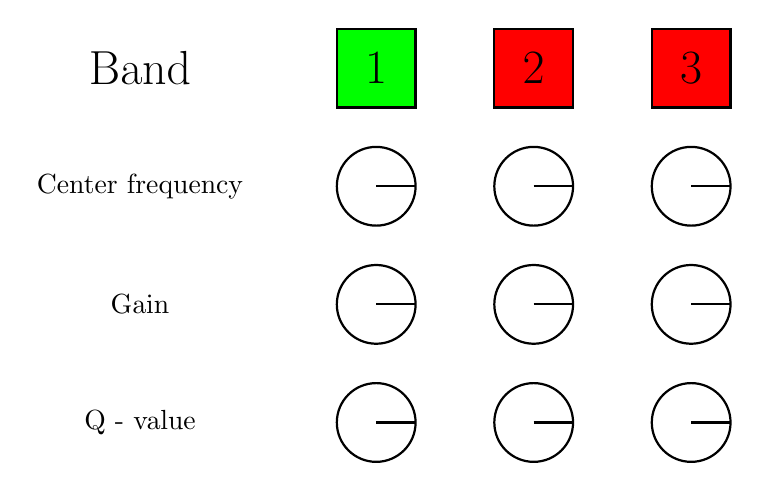
\begin{tikzpicture}
\draw[thick] (2,0) circle [radius=0.5] node at (-1,-0) {Q - value};
\draw[thick] (2,1.5) circle [radius=0.5] node at (-1,1.5) {Gain};
\draw[thick] (2,3) circle [radius=0.5] node at (-1,3) {Center frequency};
\draw node at (-1,4.5)[font=\LARGE]{Band};
\draw[thick][fill=green, draw=black](1.5,4) rectangle(2.5,5) node at (2,4.5)[font=\LARGE]{1};

\draw[thick] (4,0) circle [radius=0.5];
\draw[thick] (4,1.5) circle [radius=0.5];
\draw[thick] (4,3) circle [radius=0.5];
\draw[thick][fill=red, draw=black](1.5+2,4) rectangle(2.5+2,5) node at (2+2,4.5)[font=\LARGE]{2};

\draw[thick] (6,0) circle [radius=0.5];
\draw[thick] (6,1.5) circle [radius=0.5];
\draw[thick] (6,3) circle [radius=0.5];
\draw[thick][fill=red, draw=black](1.5+4,4) rectangle(2.5+4,5) node at (2+4,4.5)[font=\LARGE]{3};

\draw[thick](6,0) -- (6.5,0);
\draw[thick](6,1.5) -- (6.5,1.5);
\draw[thick](6,3) -- (6.5,3);

\draw[thick](4,0) -- (4.5,0);
\draw[thick](4,1.5) -- (4.5,1.5);
\draw[thick](4,3) -- (4.5,3);

\draw[thick](2,0) -- (2.5,0);
\draw[thick](2,1.5) -- (2.5,1.5);
\draw[thick](2,3) -- (2.5,3);
\end{tikzpicture}
%\caption{Developer user interface.}
%\label{fig:Dev_sug}
%\end{figure}
%
%The suggestion on \autoref{fig:Dev_sug} has push buttons on the bands so they can be toggled on and of while the center frequency, gain and Q - value for each band can be changed with the use of knobs. The suggestion will be accompanied by a big screen where the frequency response of the equalizer can be seen. 
%
%\subsection{User interface for the commercial user}
%The commercial user is the user which knows the implication of different the different settings of an equalizer but does not know anything about the technical aspect of an equalizer. This means that the interface needs to be simple and show what implpication a setting has on a system but leave out all technical aspects. 
%
%Because the commercial user only needs presets like for example "rock", "jazz" and "movie" the user only needs to have control of: 
%\begin{itemize}
%\item Presets.
%\end{itemize} 
%This leads to some different suggestions for a user interface which consist of a few buttons to keep it as simple as possible.
%
%
%\begin{figure}[H]
%\centering
%\begin{subfigure}[t]{0.47\textwidth}
%	\centering
%	\tikzsetnextfilename{InterfaceUser1}
%	\scalebox{0.2}{

\begin{tikzpicture}
\draw [thick](-10,6) circle [radius=3];
\draw [thick](11,6) circle [radius=3];
\draw [thick](-6,4) -- (7,4) -- (7,8) -- (-6,8) -- (-6,4);
\draw[fill] (-12,6) -- (-10,8) -- (-9,8) -- (-11,6) -- (-9,4) -- (-10,4) -- (-12,6);
\draw[fill](13,6) -- (11,8) -- (10,8) -- (12,6) -- (10,4) -- (11,4)--(13,6) ;
\node[scale=8.0] (c) at (0.5,6) {Presets};
\end{tikzpicture}}
%	\caption{Suggestion 1}
%	\label{fig:UI_sug_1}
%\end{subfigure}
%\hspace{6mm} 
%\begin{subfigure}[t]{0.47\textwidth}
%	\centering
%	\tikzsetnextfilename{InterfaceUser2}
%	\scalebox{0.6}{
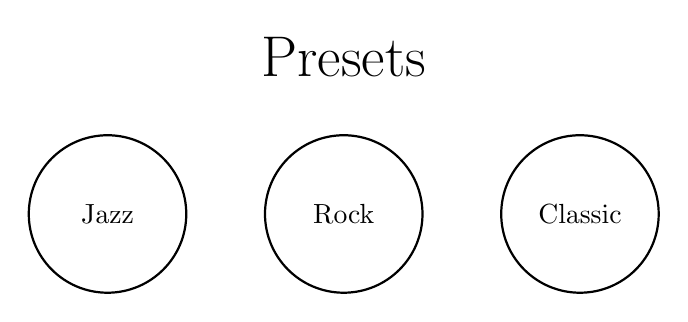
\begin{tikzpicture}
\draw [thick](0,0) circle [radius=1] node{Jazz};
\draw [thick](3,0) circle [radius=1] node{Rock};
\draw [thick](6,0) circle [radius=1] node{Classic};
\draw node at (3,2)[font=\huge]{Presets};
\end{tikzpicture}}
%	\caption{Suggestion 2}
%	\label{fig:UI_sug_2}
%\end{subfigure}
%\caption{Commercial user interface suggestions.}
%\label{fig:UI_sug}
%\end{figure}
%
%Suggestion one as seen on \autoref{fig:UI_sug_1} has two push buttons and a small screen so the user can interchange between different settings, while suggestion two has x number of push buttons which represents a preset each. The advantage of suggestion two is the overview and simplicity while suggestion one can have a larger number of presets without changing the appearance of the user interface. 
%
%The suggestions for the user interface for both the developer and the commercial user will be choosen in the requirement specification \todo[inline]{reference}  
%


\section{Chapter Conclusion}
This chapter has analyzed.